\section{Bucket \#1: Technical Improvements to \gls{osier}}

\subsection{Logical Dispatch Algorithm}

\begin{frame}
    \frametitle{What is the dispatch algorithm?}

    \begin{figure}
        \centering
        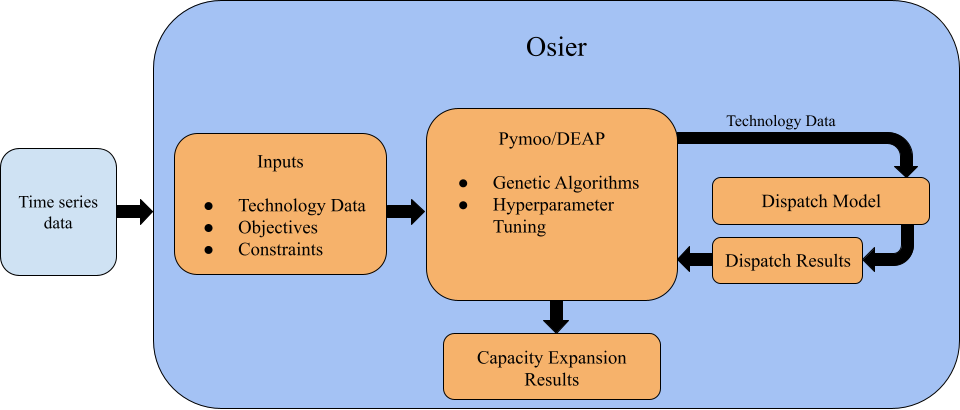
\includegraphics[width=\columnwidth]{../docs/figures/03_osier_chapter/osier_flow.png}
        \caption{Flow of data into and within \gls{osier}}
        \label{fig:osier-flow}
    \end{figure}
    % [Show the data flow diagram]

    % Osier works by leveraging genetic algorithsm... 
\end{frame}

\begin{frame}
    \frametitle{Comparing the two methods}

    \begin{columns}
        
        \column[t]{5cm}

        \begin{block}{Optimal Dispatch (Original Method)}
            \begin{itemize}[<+->]
                \item Select the decision variables, $x_{g,t}$, which minimize
                the operational cost of the model according to some constraints.
                \item Decision variables correspond to the \textit{generation}
                of each technology at each timestep in the model.
                \item Perfect foresight, guaranteed optimality.
            \end{itemize}
        \end{block}
        % \pause
        \column[t]{5cm}
        \begin{block}{Logical Dispatch (New Method)}
            \begin{itemize}[<+->]
                \item Simple algorithm
            \begin{enumerate}
                \item Sort the technologies by total operating cost (ties are
                broken by efficiency).
                \item For each demand timestep, calculate the power output for
                each technology until demand is met, or you run out of
                technologies.
            \end{enumerate}
            \item Myopic, dispatch optimality is not guaranteed.
            \end{itemize}
        \end{block}
    \end{columns}

\end{frame}


\begin{frame}
    \frametitle{Verifying the Original Method}

    \begin{figure}
        \centering
        \resizebox{0.75\columnwidth}{!}{%% Creator: Matplotlib, PGF backend
%%
%% To include the figure in your LaTeX document, write
%%   \input{<filename>.pgf}
%%
%% Make sure the required packages are loaded in your preamble
%%   \usepackage{pgf}
%%
%% Also ensure that all the required font packages are loaded; for instance,
%% the lmodern package is sometimes necessary when using math font.
%%   \usepackage{lmodern}
%%
%% Figures using additional raster images can only be included by \input if
%% they are in the same directory as the main LaTeX file. For loading figures
%% from other directories you can use the `import` package
%%   \usepackage{import}
%%
%% and then include the figures with
%%   \import{<path to file>}{<filename>.pgf}
%%
%% Matplotlib used the following preamble
%%   \def\mathdefault#1{#1}
%%   \everymath=\expandafter{\the\everymath\displaystyle}
%%   \IfFileExists{scrextend.sty}{
%%     \usepackage[fontsize=10.000000pt]{scrextend}
%%   }{
%%     \renewcommand{\normalsize}{\fontsize{10.000000}{12.000000}\selectfont}
%%     \normalsize
%%   }
%%   
%%   \makeatletter\@ifpackageloaded{underscore}{}{\usepackage[strings]{underscore}}\makeatother
%%
\begingroup%
\makeatletter%
\begin{pgfpicture}%
\pgfpathrectangle{\pgfpointorigin}{\pgfqpoint{7.900000in}{5.899894in}}%
\pgfusepath{use as bounding box, clip}%
\begin{pgfscope}%
\pgfsetbuttcap%
\pgfsetmiterjoin%
\definecolor{currentfill}{rgb}{1.000000,1.000000,1.000000}%
\pgfsetfillcolor{currentfill}%
\pgfsetlinewidth{0.000000pt}%
\definecolor{currentstroke}{rgb}{0.000000,0.000000,0.000000}%
\pgfsetstrokecolor{currentstroke}%
\pgfsetdash{}{0pt}%
\pgfpathmoveto{\pgfqpoint{0.000000in}{0.000000in}}%
\pgfpathlineto{\pgfqpoint{7.900000in}{0.000000in}}%
\pgfpathlineto{\pgfqpoint{7.900000in}{5.899894in}}%
\pgfpathlineto{\pgfqpoint{0.000000in}{5.899894in}}%
\pgfpathlineto{\pgfqpoint{0.000000in}{0.000000in}}%
\pgfpathclose%
\pgfusepath{fill}%
\end{pgfscope}%
\begin{pgfscope}%
\pgfsetbuttcap%
\pgfsetmiterjoin%
\definecolor{currentfill}{rgb}{1.000000,1.000000,1.000000}%
\pgfsetfillcolor{currentfill}%
\pgfsetlinewidth{0.000000pt}%
\definecolor{currentstroke}{rgb}{0.000000,0.000000,0.000000}%
\pgfsetstrokecolor{currentstroke}%
\pgfsetstrokeopacity{0.000000}%
\pgfsetdash{}{0pt}%
\pgfpathmoveto{\pgfqpoint{0.688192in}{0.670138in}}%
\pgfpathlineto{\pgfqpoint{7.800000in}{0.670138in}}%
\pgfpathlineto{\pgfqpoint{7.800000in}{5.731668in}}%
\pgfpathlineto{\pgfqpoint{0.688192in}{5.731668in}}%
\pgfpathlineto{\pgfqpoint{0.688192in}{0.670138in}}%
\pgfpathclose%
\pgfusepath{fill}%
\end{pgfscope}%
\begin{pgfscope}%
\pgfpathrectangle{\pgfqpoint{0.688192in}{0.670138in}}{\pgfqpoint{7.111808in}{5.061530in}}%
\pgfusepath{clip}%
\pgfsetbuttcap%
\pgfsetmiterjoin%
\definecolor{currentfill}{rgb}{0.501961,0.501961,0.501961}%
\pgfsetfillcolor{currentfill}%
\pgfsetfillopacity{0.500000}%
\pgfsetlinewidth{1.003750pt}%
\definecolor{currentstroke}{rgb}{0.501961,0.501961,0.501961}%
\pgfsetstrokecolor{currentstroke}%
\pgfsetstrokeopacity{0.500000}%
\pgfsetdash{}{0pt}%
\pgfpathmoveto{\pgfqpoint{0.749254in}{1.445149in}}%
\pgfpathlineto{\pgfqpoint{0.752983in}{1.252761in}}%
\pgfpathlineto{\pgfqpoint{0.754090in}{1.154399in}}%
\pgfpathlineto{\pgfqpoint{0.760839in}{1.136279in}}%
\pgfpathlineto{\pgfqpoint{0.764625in}{1.015211in}}%
\pgfpathlineto{\pgfqpoint{0.769073in}{0.982259in}}%
\pgfpathlineto{\pgfqpoint{0.771295in}{0.982065in}}%
\pgfpathlineto{\pgfqpoint{0.776750in}{0.941782in}}%
\pgfpathlineto{\pgfqpoint{0.777016in}{0.919143in}}%
\pgfpathlineto{\pgfqpoint{0.779964in}{0.894614in}}%
\pgfpathlineto{\pgfqpoint{0.781884in}{0.888672in}}%
\pgfpathlineto{\pgfqpoint{0.782833in}{0.883385in}}%
\pgfpathlineto{\pgfqpoint{0.782912in}{0.882838in}}%
\pgfpathlineto{\pgfqpoint{0.783279in}{0.849857in}}%
\pgfpathlineto{\pgfqpoint{0.783279in}{0.849857in}}%
\pgfpathlineto{\pgfqpoint{0.787475in}{0.843942in}}%
\pgfpathlineto{\pgfqpoint{0.791486in}{0.837055in}}%
\pgfpathlineto{\pgfqpoint{0.793302in}{0.809599in}}%
\pgfpathlineto{\pgfqpoint{0.793310in}{0.809534in}}%
\pgfpathlineto{\pgfqpoint{0.795978in}{0.801029in}}%
\pgfpathlineto{\pgfqpoint{0.796157in}{0.793846in}}%
\pgfpathlineto{\pgfqpoint{0.800976in}{0.790369in}}%
\pgfpathlineto{\pgfqpoint{0.807883in}{0.789563in}}%
\pgfpathlineto{\pgfqpoint{0.810327in}{0.766458in}}%
\pgfpathlineto{\pgfqpoint{0.816256in}{0.760843in}}%
\pgfpathlineto{\pgfqpoint{0.827191in}{0.759800in}}%
\pgfpathlineto{\pgfqpoint{0.830930in}{0.751031in}}%
\pgfpathlineto{\pgfqpoint{0.834764in}{0.749497in}}%
\pgfpathlineto{\pgfqpoint{0.837359in}{0.748345in}}%
\pgfpathlineto{\pgfqpoint{0.842310in}{0.745304in}}%
\pgfpathlineto{\pgfqpoint{0.842696in}{0.745162in}}%
\pgfpathlineto{\pgfqpoint{0.842811in}{0.745008in}}%
\pgfpathlineto{\pgfqpoint{0.849436in}{0.740184in}}%
\pgfpathlineto{\pgfqpoint{0.849953in}{0.739357in}}%
\pgfpathlineto{\pgfqpoint{0.850270in}{0.738398in}}%
\pgfpathlineto{\pgfqpoint{0.854347in}{0.736661in}}%
\pgfpathlineto{\pgfqpoint{0.872029in}{0.731700in}}%
\pgfpathlineto{\pgfqpoint{0.890835in}{0.724786in}}%
\pgfpathlineto{\pgfqpoint{0.916357in}{0.719853in}}%
\pgfpathlineto{\pgfqpoint{0.939729in}{0.718197in}}%
\pgfpathlineto{\pgfqpoint{0.940682in}{0.716009in}}%
\pgfpathlineto{\pgfqpoint{0.942062in}{0.712194in}}%
\pgfpathlineto{\pgfqpoint{0.945316in}{0.711471in}}%
\pgfpathlineto{\pgfqpoint{0.945763in}{0.710834in}}%
\pgfpathlineto{\pgfqpoint{0.946217in}{0.710820in}}%
\pgfpathlineto{\pgfqpoint{0.954596in}{0.710219in}}%
\pgfpathlineto{\pgfqpoint{0.958858in}{0.709014in}}%
\pgfpathlineto{\pgfqpoint{0.960596in}{0.708592in}}%
\pgfpathlineto{\pgfqpoint{0.987244in}{0.706065in}}%
\pgfpathlineto{\pgfqpoint{0.990735in}{0.704724in}}%
\pgfpathlineto{\pgfqpoint{0.990837in}{0.703282in}}%
\pgfpathlineto{\pgfqpoint{0.996565in}{0.703044in}}%
\pgfpathlineto{\pgfqpoint{1.010100in}{0.700622in}}%
\pgfpathlineto{\pgfqpoint{1.011096in}{0.700386in}}%
\pgfpathlineto{\pgfqpoint{1.016505in}{0.700376in}}%
\pgfpathlineto{\pgfqpoint{1.017496in}{0.699473in}}%
\pgfpathlineto{\pgfqpoint{1.070825in}{0.697151in}}%
\pgfpathlineto{\pgfqpoint{1.075000in}{0.692618in}}%
\pgfpathlineto{\pgfqpoint{1.077361in}{0.692269in}}%
\pgfpathlineto{\pgfqpoint{1.077372in}{0.692269in}}%
\pgfpathlineto{\pgfqpoint{1.084164in}{0.691950in}}%
\pgfpathlineto{\pgfqpoint{1.085816in}{0.691662in}}%
\pgfpathlineto{\pgfqpoint{1.102529in}{0.689352in}}%
\pgfpathlineto{\pgfqpoint{1.103303in}{0.689151in}}%
\pgfpathlineto{\pgfqpoint{1.108579in}{0.688860in}}%
\pgfpathlineto{\pgfqpoint{1.108617in}{0.688763in}}%
\pgfpathlineto{\pgfqpoint{1.109998in}{0.688225in}}%
\pgfpathlineto{\pgfqpoint{1.114241in}{0.688028in}}%
\pgfpathlineto{\pgfqpoint{1.116764in}{0.688006in}}%
\pgfpathlineto{\pgfqpoint{1.126908in}{0.687169in}}%
\pgfpathlineto{\pgfqpoint{1.128607in}{0.686506in}}%
\pgfpathlineto{\pgfqpoint{1.128867in}{0.686499in}}%
\pgfpathlineto{\pgfqpoint{1.147700in}{0.686452in}}%
\pgfpathlineto{\pgfqpoint{1.148995in}{0.685892in}}%
\pgfpathlineto{\pgfqpoint{1.151625in}{0.685778in}}%
\pgfpathlineto{\pgfqpoint{1.159390in}{0.685625in}}%
\pgfpathlineto{\pgfqpoint{1.164071in}{0.685586in}}%
\pgfpathlineto{\pgfqpoint{1.178009in}{0.685447in}}%
\pgfpathlineto{\pgfqpoint{1.197079in}{0.685403in}}%
\pgfpathlineto{\pgfqpoint{1.198965in}{0.685402in}}%
\pgfpathlineto{\pgfqpoint{1.200157in}{0.685395in}}%
\pgfpathlineto{\pgfqpoint{1.220931in}{0.685389in}}%
\pgfpathlineto{\pgfqpoint{1.315614in}{0.684844in}}%
\pgfpathlineto{\pgfqpoint{1.334128in}{0.684517in}}%
\pgfpathlineto{\pgfqpoint{1.363285in}{0.684419in}}%
\pgfpathlineto{\pgfqpoint{1.364139in}{0.684404in}}%
\pgfpathlineto{\pgfqpoint{1.376266in}{0.684291in}}%
\pgfpathlineto{\pgfqpoint{1.396594in}{0.684212in}}%
\pgfpathlineto{\pgfqpoint{1.399923in}{0.684150in}}%
\pgfpathlineto{\pgfqpoint{1.407033in}{0.684070in}}%
\pgfpathlineto{\pgfqpoint{1.444241in}{0.684035in}}%
\pgfpathlineto{\pgfqpoint{1.455660in}{0.683986in}}%
\pgfpathlineto{\pgfqpoint{1.469414in}{0.683962in}}%
\pgfpathlineto{\pgfqpoint{1.472622in}{0.683959in}}%
\pgfpathlineto{\pgfqpoint{1.473551in}{0.683948in}}%
\pgfpathlineto{\pgfqpoint{1.473926in}{0.683941in}}%
\pgfpathlineto{\pgfqpoint{1.474245in}{0.683935in}}%
\pgfpathlineto{\pgfqpoint{1.475910in}{0.683912in}}%
\pgfpathlineto{\pgfqpoint{1.477331in}{0.683875in}}%
\pgfpathlineto{\pgfqpoint{1.495917in}{0.683547in}}%
\pgfpathlineto{\pgfqpoint{1.503177in}{0.683449in}}%
\pgfpathlineto{\pgfqpoint{1.582513in}{0.683280in}}%
\pgfpathlineto{\pgfqpoint{1.658826in}{0.683277in}}%
\pgfpathlineto{\pgfqpoint{1.659921in}{0.683127in}}%
\pgfpathlineto{\pgfqpoint{1.663205in}{0.683065in}}%
\pgfpathlineto{\pgfqpoint{1.675058in}{0.682998in}}%
\pgfpathlineto{\pgfqpoint{1.678208in}{0.682876in}}%
\pgfpathlineto{\pgfqpoint{1.681839in}{0.682826in}}%
\pgfpathlineto{\pgfqpoint{1.684802in}{0.682783in}}%
\pgfpathlineto{\pgfqpoint{1.719213in}{0.682724in}}%
\pgfpathlineto{\pgfqpoint{1.731063in}{0.682549in}}%
\pgfpathlineto{\pgfqpoint{1.731531in}{0.682540in}}%
\pgfpathlineto{\pgfqpoint{1.731531in}{0.682540in}}%
\pgfpathlineto{\pgfqpoint{1.731710in}{0.682537in}}%
\pgfpathlineto{\pgfqpoint{1.732115in}{0.682529in}}%
\pgfpathlineto{\pgfqpoint{1.738010in}{0.682319in}}%
\pgfpathlineto{\pgfqpoint{1.738010in}{0.682319in}}%
\pgfpathlineto{\pgfqpoint{1.755173in}{0.682260in}}%
\pgfpathlineto{\pgfqpoint{1.759976in}{0.682015in}}%
\pgfpathlineto{\pgfqpoint{1.761288in}{0.681989in}}%
\pgfpathlineto{\pgfqpoint{1.765345in}{0.681943in}}%
\pgfpathlineto{\pgfqpoint{1.811432in}{0.681927in}}%
\pgfpathlineto{\pgfqpoint{1.811432in}{0.681927in}}%
\pgfpathlineto{\pgfqpoint{1.815579in}{0.681901in}}%
\pgfpathlineto{\pgfqpoint{1.826952in}{0.681747in}}%
\pgfpathlineto{\pgfqpoint{1.852021in}{0.681611in}}%
\pgfpathlineto{\pgfqpoint{1.892079in}{0.681466in}}%
\pgfpathlineto{\pgfqpoint{1.903233in}{0.681282in}}%
\pgfpathlineto{\pgfqpoint{1.928513in}{0.681173in}}%
\pgfpathlineto{\pgfqpoint{1.967310in}{0.681083in}}%
\pgfpathlineto{\pgfqpoint{1.970905in}{0.680890in}}%
\pgfpathlineto{\pgfqpoint{2.063345in}{0.680516in}}%
\pgfpathlineto{\pgfqpoint{2.225009in}{0.680020in}}%
\pgfpathlineto{\pgfqpoint{2.235916in}{0.679656in}}%
\pgfpathlineto{\pgfqpoint{2.237139in}{0.679645in}}%
\pgfpathlineto{\pgfqpoint{2.243733in}{0.679632in}}%
\pgfpathlineto{\pgfqpoint{2.244939in}{0.679615in}}%
\pgfpathlineto{\pgfqpoint{2.265105in}{0.679558in}}%
\pgfpathlineto{\pgfqpoint{2.378269in}{0.679052in}}%
\pgfpathlineto{\pgfqpoint{2.392882in}{0.678851in}}%
\pgfpathlineto{\pgfqpoint{2.429320in}{0.678525in}}%
\pgfpathlineto{\pgfqpoint{2.452500in}{0.678477in}}%
\pgfpathlineto{\pgfqpoint{2.489265in}{0.678468in}}%
\pgfpathlineto{\pgfqpoint{2.494145in}{0.678397in}}%
\pgfpathlineto{\pgfqpoint{2.509817in}{0.678139in}}%
\pgfpathlineto{\pgfqpoint{2.510252in}{0.678129in}}%
\pgfpathlineto{\pgfqpoint{2.542698in}{0.677943in}}%
\pgfpathlineto{\pgfqpoint{2.608500in}{0.677847in}}%
\pgfpathlineto{\pgfqpoint{2.672675in}{0.677398in}}%
\pgfpathlineto{\pgfqpoint{2.677313in}{0.677350in}}%
\pgfpathlineto{\pgfqpoint{2.911373in}{0.676955in}}%
\pgfpathlineto{\pgfqpoint{2.932466in}{0.676438in}}%
\pgfpathlineto{\pgfqpoint{2.976355in}{0.676171in}}%
\pgfpathlineto{\pgfqpoint{3.024552in}{0.675964in}}%
\pgfpathlineto{\pgfqpoint{3.280946in}{0.675128in}}%
\pgfpathlineto{\pgfqpoint{3.291859in}{0.674921in}}%
\pgfpathlineto{\pgfqpoint{3.560021in}{0.673854in}}%
\pgfpathlineto{\pgfqpoint{3.790533in}{0.673411in}}%
\pgfpathlineto{\pgfqpoint{3.825636in}{0.673260in}}%
\pgfpathlineto{\pgfqpoint{3.863667in}{0.673125in}}%
\pgfpathlineto{\pgfqpoint{3.986933in}{0.672748in}}%
\pgfpathlineto{\pgfqpoint{3.995987in}{0.672712in}}%
\pgfpathlineto{\pgfqpoint{4.155194in}{0.672354in}}%
\pgfpathlineto{\pgfqpoint{4.207141in}{0.672282in}}%
\pgfpathlineto{\pgfqpoint{4.213238in}{0.672266in}}%
\pgfpathlineto{\pgfqpoint{4.420707in}{0.672256in}}%
\pgfpathlineto{\pgfqpoint{4.421026in}{0.672255in}}%
\pgfpathlineto{\pgfqpoint{4.491507in}{0.672222in}}%
\pgfpathlineto{\pgfqpoint{4.576929in}{0.672144in}}%
\pgfpathlineto{\pgfqpoint{4.613721in}{0.672131in}}%
\pgfpathlineto{\pgfqpoint{4.631124in}{0.671946in}}%
\pgfpathlineto{\pgfqpoint{4.661935in}{0.671930in}}%
\pgfpathlineto{\pgfqpoint{4.688548in}{0.671723in}}%
\pgfpathlineto{\pgfqpoint{4.726657in}{0.671660in}}%
\pgfpathlineto{\pgfqpoint{4.735203in}{0.671563in}}%
\pgfpathlineto{\pgfqpoint{4.750941in}{0.671524in}}%
\pgfpathlineto{\pgfqpoint{4.764231in}{0.671484in}}%
\pgfpathlineto{\pgfqpoint{4.914508in}{0.671444in}}%
\pgfpathlineto{\pgfqpoint{4.924693in}{0.671413in}}%
\pgfpathlineto{\pgfqpoint{4.939656in}{0.671407in}}%
\pgfpathlineto{\pgfqpoint{4.965126in}{0.671366in}}%
\pgfpathlineto{\pgfqpoint{4.979341in}{0.671320in}}%
\pgfpathlineto{\pgfqpoint{4.994709in}{0.671264in}}%
\pgfpathlineto{\pgfqpoint{5.085461in}{0.671155in}}%
\pgfpathlineto{\pgfqpoint{5.135185in}{0.671116in}}%
\pgfpathlineto{\pgfqpoint{5.140992in}{0.670993in}}%
\pgfpathlineto{\pgfqpoint{5.159789in}{0.670855in}}%
\pgfpathlineto{\pgfqpoint{5.274608in}{0.670832in}}%
\pgfpathlineto{\pgfqpoint{5.274608in}{0.670832in}}%
\pgfpathlineto{\pgfqpoint{5.283066in}{0.670786in}}%
\pgfpathlineto{\pgfqpoint{5.359877in}{0.670710in}}%
\pgfpathlineto{\pgfqpoint{5.370884in}{0.670626in}}%
\pgfpathlineto{\pgfqpoint{5.527297in}{0.670601in}}%
\pgfpathlineto{\pgfqpoint{5.557238in}{0.670526in}}%
\pgfpathlineto{\pgfqpoint{5.614292in}{0.670505in}}%
\pgfpathlineto{\pgfqpoint{5.657223in}{0.670449in}}%
\pgfpathlineto{\pgfqpoint{5.714356in}{0.670428in}}%
\pgfpathlineto{\pgfqpoint{5.840166in}{0.670247in}}%
\pgfpathlineto{\pgfqpoint{6.004393in}{0.670138in}}%
\pgfpathlineto{\pgfqpoint{7.800000in}{0.684746in}}%
\pgfpathlineto{\pgfqpoint{7.619350in}{0.684865in}}%
\pgfpathlineto{\pgfqpoint{7.480959in}{0.685064in}}%
\pgfpathlineto{\pgfqpoint{7.418113in}{0.685088in}}%
\pgfpathlineto{\pgfqpoint{7.370888in}{0.685150in}}%
\pgfpathlineto{\pgfqpoint{7.308129in}{0.685172in}}%
\pgfpathlineto{\pgfqpoint{7.275194in}{0.685255in}}%
\pgfpathlineto{\pgfqpoint{7.103140in}{0.685283in}}%
\pgfpathlineto{\pgfqpoint{7.091032in}{0.685375in}}%
\pgfpathlineto{\pgfqpoint{7.006540in}{0.685458in}}%
\pgfpathlineto{\pgfqpoint{6.997236in}{0.685509in}}%
\pgfpathlineto{\pgfqpoint{6.997236in}{0.685509in}}%
\pgfpathlineto{\pgfqpoint{6.870936in}{0.685535in}}%
\pgfpathlineto{\pgfqpoint{6.850259in}{0.685685in}}%
\pgfpathlineto{\pgfqpoint{6.843871in}{0.685821in}}%
\pgfpathlineto{\pgfqpoint{6.789175in}{0.685864in}}%
\pgfpathlineto{\pgfqpoint{6.689348in}{0.685984in}}%
\pgfpathlineto{\pgfqpoint{6.672443in}{0.686045in}}%
\pgfpathlineto{\pgfqpoint{6.656806in}{0.686097in}}%
\pgfpathlineto{\pgfqpoint{6.628789in}{0.686141in}}%
\pgfpathlineto{\pgfqpoint{6.612329in}{0.686148in}}%
\pgfpathlineto{\pgfqpoint{6.601126in}{0.686182in}}%
\pgfpathlineto{\pgfqpoint{6.435822in}{0.686226in}}%
\pgfpathlineto{\pgfqpoint{6.421203in}{0.686270in}}%
\pgfpathlineto{\pgfqpoint{6.403891in}{0.686313in}}%
\pgfpathlineto{\pgfqpoint{6.394490in}{0.686420in}}%
\pgfpathlineto{\pgfqpoint{6.352570in}{0.686489in}}%
\pgfpathlineto{\pgfqpoint{6.323295in}{0.686716in}}%
\pgfpathlineto{\pgfqpoint{6.289404in}{0.686734in}}%
\pgfpathlineto{\pgfqpoint{6.270261in}{0.686938in}}%
\pgfpathlineto{\pgfqpoint{6.229790in}{0.686952in}}%
\pgfpathlineto{\pgfqpoint{6.135825in}{0.687037in}}%
\pgfpathlineto{\pgfqpoint{6.058296in}{0.687074in}}%
\pgfpathlineto{\pgfqpoint{6.057945in}{0.687076in}}%
\pgfpathlineto{\pgfqpoint{5.829729in}{0.687086in}}%
\pgfpathlineto{\pgfqpoint{5.823022in}{0.687104in}}%
\pgfpathlineto{\pgfqpoint{5.765880in}{0.687183in}}%
\pgfpathlineto{\pgfqpoint{5.590753in}{0.687577in}}%
\pgfpathlineto{\pgfqpoint{5.580794in}{0.687616in}}%
\pgfpathlineto{\pgfqpoint{5.445201in}{0.688032in}}%
\pgfpathlineto{\pgfqpoint{5.403367in}{0.688180in}}%
\pgfpathlineto{\pgfqpoint{5.364754in}{0.688346in}}%
\pgfpathlineto{\pgfqpoint{5.111190in}{0.688834in}}%
\pgfpathlineto{\pgfqpoint{4.816213in}{0.690007in}}%
\pgfpathlineto{\pgfqpoint{4.804209in}{0.690235in}}%
\pgfpathlineto{\pgfqpoint{4.522174in}{0.691154in}}%
\pgfpathlineto{\pgfqpoint{4.469159in}{0.691382in}}%
\pgfpathlineto{\pgfqpoint{4.420880in}{0.691675in}}%
\pgfpathlineto{\pgfqpoint{4.397678in}{0.692245in}}%
\pgfpathlineto{\pgfqpoint{4.140212in}{0.692679in}}%
\pgfpathlineto{\pgfqpoint{4.135110in}{0.692731in}}%
\pgfpathlineto{\pgfqpoint{4.064518in}{0.693225in}}%
\pgfpathlineto{\pgfqpoint{3.992135in}{0.693331in}}%
\pgfpathlineto{\pgfqpoint{3.956444in}{0.693536in}}%
\pgfpathlineto{\pgfqpoint{3.955967in}{0.693546in}}%
\pgfpathlineto{\pgfqpoint{3.938727in}{0.693830in}}%
\pgfpathlineto{\pgfqpoint{3.933359in}{0.693909in}}%
\pgfpathlineto{\pgfqpoint{3.892918in}{0.693918in}}%
\pgfpathlineto{\pgfqpoint{3.867419in}{0.693971in}}%
\pgfpathlineto{\pgfqpoint{3.827337in}{0.694330in}}%
\pgfpathlineto{\pgfqpoint{3.811263in}{0.694551in}}%
\pgfpathlineto{\pgfqpoint{3.686783in}{0.695107in}}%
\pgfpathlineto{\pgfqpoint{3.664601in}{0.695170in}}%
\pgfpathlineto{\pgfqpoint{3.663274in}{0.695189in}}%
\pgfpathlineto{\pgfqpoint{3.656021in}{0.695204in}}%
\pgfpathlineto{\pgfqpoint{3.654675in}{0.695216in}}%
\pgfpathlineto{\pgfqpoint{3.642678in}{0.695616in}}%
\pgfpathlineto{\pgfqpoint{3.464847in}{0.696161in}}%
\pgfpathlineto{\pgfqpoint{3.363163in}{0.696573in}}%
\pgfpathlineto{\pgfqpoint{3.359209in}{0.696784in}}%
\pgfpathlineto{\pgfqpoint{3.316532in}{0.696883in}}%
\pgfpathlineto{\pgfqpoint{3.288724in}{0.697004in}}%
\pgfpathlineto{\pgfqpoint{3.276454in}{0.697206in}}%
\pgfpathlineto{\pgfqpoint{3.232391in}{0.697366in}}%
\pgfpathlineto{\pgfqpoint{3.204814in}{0.697516in}}%
\pgfpathlineto{\pgfqpoint{3.192305in}{0.697685in}}%
\pgfpathlineto{\pgfqpoint{3.187743in}{0.697713in}}%
\pgfpathlineto{\pgfqpoint{3.187743in}{0.697713in}}%
\pgfpathlineto{\pgfqpoint{3.137047in}{0.697731in}}%
\pgfpathlineto{\pgfqpoint{3.132584in}{0.697781in}}%
\pgfpathlineto{\pgfqpoint{3.131141in}{0.697810in}}%
\pgfpathlineto{\pgfqpoint{3.125858in}{0.698080in}}%
\pgfpathlineto{\pgfqpoint{3.106979in}{0.698145in}}%
\pgfpathlineto{\pgfqpoint{3.106979in}{0.698145in}}%
\pgfpathlineto{\pgfqpoint{3.100494in}{0.698376in}}%
\pgfpathlineto{\pgfqpoint{3.100048in}{0.698385in}}%
\pgfpathlineto{\pgfqpoint{3.099852in}{0.698388in}}%
\pgfpathlineto{\pgfqpoint{3.099852in}{0.698388in}}%
\pgfpathlineto{\pgfqpoint{3.099336in}{0.698397in}}%
\pgfpathlineto{\pgfqpoint{3.086302in}{0.698590in}}%
\pgfpathlineto{\pgfqpoint{3.048450in}{0.698655in}}%
\pgfpathlineto{\pgfqpoint{3.045190in}{0.698703in}}%
\pgfpathlineto{\pgfqpoint{3.041196in}{0.698758in}}%
\pgfpathlineto{\pgfqpoint{3.037732in}{0.698892in}}%
\pgfpathlineto{\pgfqpoint{3.024693in}{0.698965in}}%
\pgfpathlineto{\pgfqpoint{3.021080in}{0.699034in}}%
\pgfpathlineto{\pgfqpoint{3.019876in}{0.699198in}}%
\pgfpathlineto{\pgfqpoint{2.935932in}{0.699202in}}%
\pgfpathlineto{\pgfqpoint{2.848662in}{0.699388in}}%
\pgfpathlineto{\pgfqpoint{2.840676in}{0.699496in}}%
\pgfpathlineto{\pgfqpoint{2.820232in}{0.699856in}}%
\pgfpathlineto{\pgfqpoint{2.818668in}{0.699897in}}%
\pgfpathlineto{\pgfqpoint{2.816837in}{0.699922in}}%
\pgfpathlineto{\pgfqpoint{2.816486in}{0.699929in}}%
\pgfpathlineto{\pgfqpoint{2.816074in}{0.699936in}}%
\pgfpathlineto{\pgfqpoint{2.815052in}{0.699949in}}%
\pgfpathlineto{\pgfqpoint{2.811523in}{0.699951in}}%
\pgfpathlineto{\pgfqpoint{2.796394in}{0.699978in}}%
\pgfpathlineto{\pgfqpoint{2.783832in}{0.700032in}}%
\pgfpathlineto{\pgfqpoint{2.742903in}{0.700071in}}%
\pgfpathlineto{\pgfqpoint{2.735082in}{0.700159in}}%
\pgfpathlineto{\pgfqpoint{2.731421in}{0.700227in}}%
\pgfpathlineto{\pgfqpoint{2.709060in}{0.700313in}}%
\pgfpathlineto{\pgfqpoint{2.695721in}{0.700438in}}%
\pgfpathlineto{\pgfqpoint{2.694781in}{0.700454in}}%
\pgfpathlineto{\pgfqpoint{2.662708in}{0.700563in}}%
\pgfpathlineto{\pgfqpoint{2.642343in}{0.700922in}}%
\pgfpathlineto{\pgfqpoint{2.538192in}{0.701522in}}%
\pgfpathlineto{\pgfqpoint{2.515340in}{0.701528in}}%
\pgfpathlineto{\pgfqpoint{2.514029in}{0.701536in}}%
\pgfpathlineto{\pgfqpoint{2.511954in}{0.701536in}}%
\pgfpathlineto{\pgfqpoint{2.490977in}{0.701585in}}%
\pgfpathlineto{\pgfqpoint{2.475646in}{0.701738in}}%
\pgfpathlineto{\pgfqpoint{2.470497in}{0.701782in}}%
\pgfpathlineto{\pgfqpoint{2.461955in}{0.701949in}}%
\pgfpathlineto{\pgfqpoint{2.459062in}{0.702074in}}%
\pgfpathlineto{\pgfqpoint{2.457637in}{0.702691in}}%
\pgfpathlineto{\pgfqpoint{2.436921in}{0.702743in}}%
\pgfpathlineto{\pgfqpoint{2.436635in}{0.702750in}}%
\pgfpathlineto{\pgfqpoint{2.434766in}{0.703479in}}%
\pgfpathlineto{\pgfqpoint{2.423608in}{0.704401in}}%
\pgfpathlineto{\pgfqpoint{2.420833in}{0.704424in}}%
\pgfpathlineto{\pgfqpoint{2.416166in}{0.704641in}}%
\pgfpathlineto{\pgfqpoint{2.414647in}{0.705233in}}%
\pgfpathlineto{\pgfqpoint{2.414604in}{0.705339in}}%
\pgfpathlineto{\pgfqpoint{2.408800in}{0.705660in}}%
\pgfpathlineto{\pgfqpoint{2.407949in}{0.705880in}}%
\pgfpathlineto{\pgfqpoint{2.389566in}{0.708422in}}%
\pgfpathlineto{\pgfqpoint{2.387748in}{0.708739in}}%
\pgfpathlineto{\pgfqpoint{2.380277in}{0.709090in}}%
\pgfpathlineto{\pgfqpoint{2.380264in}{0.709090in}}%
\pgfpathlineto{\pgfqpoint{2.377668in}{0.709474in}}%
\pgfpathlineto{\pgfqpoint{2.373075in}{0.714460in}}%
\pgfpathlineto{\pgfqpoint{2.314413in}{0.717013in}}%
\pgfpathlineto{\pgfqpoint{2.313323in}{0.718007in}}%
\pgfpathlineto{\pgfqpoint{2.307373in}{0.718018in}}%
\pgfpathlineto{\pgfqpoint{2.306278in}{0.718278in}}%
\pgfpathlineto{\pgfqpoint{2.291389in}{0.720942in}}%
\pgfpathlineto{\pgfqpoint{2.285088in}{0.721204in}}%
\pgfpathlineto{\pgfqpoint{2.284976in}{0.722790in}}%
\pgfpathlineto{\pgfqpoint{2.281136in}{0.724265in}}%
\pgfpathlineto{\pgfqpoint{2.251823in}{0.727045in}}%
\pgfpathlineto{\pgfqpoint{2.249911in}{0.727509in}}%
\pgfpathlineto{\pgfqpoint{2.245223in}{0.728835in}}%
\pgfpathlineto{\pgfqpoint{2.236007in}{0.729495in}}%
\pgfpathlineto{\pgfqpoint{2.235507in}{0.729511in}}%
\pgfpathlineto{\pgfqpoint{2.235016in}{0.730212in}}%
\pgfpathlineto{\pgfqpoint{2.231436in}{0.731007in}}%
\pgfpathlineto{\pgfqpoint{2.229917in}{0.735204in}}%
\pgfpathlineto{\pgfqpoint{2.228869in}{0.737610in}}%
\pgfpathlineto{\pgfqpoint{2.203161in}{0.739432in}}%
\pgfpathlineto{\pgfqpoint{2.175086in}{0.744858in}}%
\pgfpathlineto{\pgfqpoint{2.154400in}{0.752463in}}%
\pgfpathlineto{\pgfqpoint{2.134949in}{0.757921in}}%
\pgfpathlineto{\pgfqpoint{2.130465in}{0.759831in}}%
\pgfpathlineto{\pgfqpoint{2.130116in}{0.760887in}}%
\pgfpathlineto{\pgfqpoint{2.129547in}{0.761796in}}%
\pgfpathlineto{\pgfqpoint{2.122260in}{0.767103in}}%
\pgfpathlineto{\pgfqpoint{2.122133in}{0.767272in}}%
\pgfpathlineto{\pgfqpoint{2.121708in}{0.767428in}}%
\pgfpathlineto{\pgfqpoint{2.116263in}{0.770773in}}%
\pgfpathlineto{\pgfqpoint{2.113408in}{0.772041in}}%
\pgfpathlineto{\pgfqpoint{2.109190in}{0.773728in}}%
\pgfpathlineto{\pgfqpoint{2.105078in}{0.783373in}}%
\pgfpathlineto{\pgfqpoint{2.093049in}{0.784521in}}%
\pgfpathlineto{\pgfqpoint{2.086528in}{0.790698in}}%
\pgfpathlineto{\pgfqpoint{2.083839in}{0.816113in}}%
\pgfpathlineto{\pgfqpoint{2.076241in}{0.816999in}}%
\pgfpathlineto{\pgfqpoint{2.070940in}{0.820824in}}%
\pgfpathlineto{\pgfqpoint{2.070744in}{0.828726in}}%
\pgfpathlineto{\pgfqpoint{2.067808in}{0.838081in}}%
\pgfpathlineto{\pgfqpoint{2.067800in}{0.838153in}}%
\pgfpathlineto{\pgfqpoint{2.065802in}{0.868354in}}%
\pgfpathlineto{\pgfqpoint{2.061390in}{0.875930in}}%
\pgfpathlineto{\pgfqpoint{2.056775in}{0.882436in}}%
\pgfpathlineto{\pgfqpoint{2.056775in}{0.882436in}}%
\pgfpathlineto{\pgfqpoint{2.056370in}{0.918715in}}%
\pgfpathlineto{\pgfqpoint{2.056284in}{0.919317in}}%
\pgfpathlineto{\pgfqpoint{2.055240in}{0.925133in}}%
\pgfpathlineto{\pgfqpoint{2.053128in}{0.931670in}}%
\pgfpathlineto{\pgfqpoint{2.049885in}{0.958651in}}%
\pgfpathlineto{\pgfqpoint{2.049592in}{0.983554in}}%
\pgfpathlineto{\pgfqpoint{2.043592in}{1.027865in}}%
\pgfpathlineto{\pgfqpoint{2.041148in}{1.028078in}}%
\pgfpathlineto{\pgfqpoint{2.036255in}{1.064326in}}%
\pgfpathlineto{\pgfqpoint{2.032091in}{1.197500in}}%
\pgfpathlineto{\pgfqpoint{2.024666in}{1.217432in}}%
\pgfpathlineto{\pgfqpoint{2.023448in}{1.325631in}}%
\pgfpathlineto{\pgfqpoint{2.019347in}{1.537258in}}%
\pgfpathlineto{\pgfqpoint{0.749254in}{1.445149in}}%
\pgfpathclose%
\pgfusepath{stroke,fill}%
\end{pgfscope}%
\begin{pgfscope}%
\pgfpathrectangle{\pgfqpoint{0.688192in}{0.670138in}}{\pgfqpoint{7.111808in}{5.061530in}}%
\pgfusepath{clip}%
\pgfsetbuttcap%
\pgfsetroundjoin%
\pgfsetlinewidth{1.003750pt}%
\definecolor{currentstroke}{rgb}{1.000000,0.000000,0.000000}%
\pgfsetstrokecolor{currentstroke}%
\pgfsetdash{}{0pt}%
\pgfpathmoveto{\pgfqpoint{1.482100in}{5.217166in}}%
\pgfpathcurveto{\pgfqpoint{1.492995in}{5.217166in}}{\pgfqpoint{1.503446in}{5.221495in}}{\pgfqpoint{1.511150in}{5.229199in}}%
\pgfpathcurveto{\pgfqpoint{1.518855in}{5.236903in}}{\pgfqpoint{1.523183in}{5.247354in}}{\pgfqpoint{1.523183in}{5.258250in}}%
\pgfpathcurveto{\pgfqpoint{1.523183in}{5.269145in}}{\pgfqpoint{1.518855in}{5.279596in}}{\pgfqpoint{1.511150in}{5.287300in}}%
\pgfpathcurveto{\pgfqpoint{1.503446in}{5.295005in}}{\pgfqpoint{1.492995in}{5.299334in}}{\pgfqpoint{1.482100in}{5.299334in}}%
\pgfpathcurveto{\pgfqpoint{1.471204in}{5.299334in}}{\pgfqpoint{1.460753in}{5.295005in}}{\pgfqpoint{1.453049in}{5.287300in}}%
\pgfpathcurveto{\pgfqpoint{1.445344in}{5.279596in}}{\pgfqpoint{1.441016in}{5.269145in}}{\pgfqpoint{1.441016in}{5.258250in}}%
\pgfpathcurveto{\pgfqpoint{1.441016in}{5.247354in}}{\pgfqpoint{1.445344in}{5.236903in}}{\pgfqpoint{1.453049in}{5.229199in}}%
\pgfpathcurveto{\pgfqpoint{1.460753in}{5.221495in}}{\pgfqpoint{1.471204in}{5.217166in}}{\pgfqpoint{1.482100in}{5.217166in}}%
\pgfpathlineto{\pgfqpoint{1.482100in}{5.217166in}}%
\pgfpathclose%
\pgfusepath{stroke}%
\end{pgfscope}%
\begin{pgfscope}%
\pgfpathrectangle{\pgfqpoint{0.688192in}{0.670138in}}{\pgfqpoint{7.111808in}{5.061530in}}%
\pgfusepath{clip}%
\pgfsetbuttcap%
\pgfsetroundjoin%
\pgfsetlinewidth{1.003750pt}%
\definecolor{currentstroke}{rgb}{1.000000,0.000000,0.000000}%
\pgfsetstrokecolor{currentstroke}%
\pgfsetdash{}{0pt}%
\pgfpathmoveto{\pgfqpoint{1.164895in}{2.382394in}}%
\pgfpathcurveto{\pgfqpoint{1.175790in}{2.382394in}}{\pgfqpoint{1.186241in}{2.386722in}}{\pgfqpoint{1.193945in}{2.394427in}}%
\pgfpathcurveto{\pgfqpoint{1.201650in}{2.402131in}}{\pgfqpoint{1.205978in}{2.412582in}}{\pgfqpoint{1.205978in}{2.423477in}}%
\pgfpathcurveto{\pgfqpoint{1.205978in}{2.434373in}}{\pgfqpoint{1.201650in}{2.444824in}}{\pgfqpoint{1.193945in}{2.452528in}}%
\pgfpathcurveto{\pgfqpoint{1.186241in}{2.460232in}}{\pgfqpoint{1.175790in}{2.464561in}}{\pgfqpoint{1.164895in}{2.464561in}}%
\pgfpathcurveto{\pgfqpoint{1.153999in}{2.464561in}}{\pgfqpoint{1.143548in}{2.460232in}}{\pgfqpoint{1.135844in}{2.452528in}}%
\pgfpathcurveto{\pgfqpoint{1.128140in}{2.444824in}}{\pgfqpoint{1.123811in}{2.434373in}}{\pgfqpoint{1.123811in}{2.423477in}}%
\pgfpathcurveto{\pgfqpoint{1.123811in}{2.412582in}}{\pgfqpoint{1.128140in}{2.402131in}}{\pgfqpoint{1.135844in}{2.394427in}}%
\pgfpathcurveto{\pgfqpoint{1.143548in}{2.386722in}}{\pgfqpoint{1.153999in}{2.382394in}}{\pgfqpoint{1.164895in}{2.382394in}}%
\pgfpathlineto{\pgfqpoint{1.164895in}{2.382394in}}%
\pgfpathclose%
\pgfusepath{stroke}%
\end{pgfscope}%
\begin{pgfscope}%
\pgfpathrectangle{\pgfqpoint{0.688192in}{0.670138in}}{\pgfqpoint{7.111808in}{5.061530in}}%
\pgfusepath{clip}%
\pgfsetbuttcap%
\pgfsetroundjoin%
\pgfsetlinewidth{1.003750pt}%
\definecolor{currentstroke}{rgb}{1.000000,0.000000,0.000000}%
\pgfsetstrokecolor{currentstroke}%
\pgfsetdash{}{0pt}%
\pgfpathmoveto{\pgfqpoint{1.213667in}{2.459288in}}%
\pgfpathcurveto{\pgfqpoint{1.224562in}{2.459288in}}{\pgfqpoint{1.235013in}{2.463617in}}{\pgfqpoint{1.242717in}{2.471321in}}%
\pgfpathcurveto{\pgfqpoint{1.250422in}{2.479025in}}{\pgfqpoint{1.254750in}{2.489476in}}{\pgfqpoint{1.254750in}{2.500372in}}%
\pgfpathcurveto{\pgfqpoint{1.254750in}{2.511267in}}{\pgfqpoint{1.250422in}{2.521718in}}{\pgfqpoint{1.242717in}{2.529423in}}%
\pgfpathcurveto{\pgfqpoint{1.235013in}{2.537127in}}{\pgfqpoint{1.224562in}{2.541456in}}{\pgfqpoint{1.213667in}{2.541456in}}%
\pgfpathcurveto{\pgfqpoint{1.202771in}{2.541456in}}{\pgfqpoint{1.192320in}{2.537127in}}{\pgfqpoint{1.184616in}{2.529423in}}%
\pgfpathcurveto{\pgfqpoint{1.176912in}{2.521718in}}{\pgfqpoint{1.172583in}{2.511267in}}{\pgfqpoint{1.172583in}{2.500372in}}%
\pgfpathcurveto{\pgfqpoint{1.172583in}{2.489476in}}{\pgfqpoint{1.176912in}{2.479025in}}{\pgfqpoint{1.184616in}{2.471321in}}%
\pgfpathcurveto{\pgfqpoint{1.192320in}{2.463617in}}{\pgfqpoint{1.202771in}{2.459288in}}{\pgfqpoint{1.213667in}{2.459288in}}%
\pgfpathlineto{\pgfqpoint{1.213667in}{2.459288in}}%
\pgfpathclose%
\pgfusepath{stroke}%
\end{pgfscope}%
\begin{pgfscope}%
\pgfpathrectangle{\pgfqpoint{0.688192in}{0.670138in}}{\pgfqpoint{7.111808in}{5.061530in}}%
\pgfusepath{clip}%
\pgfsetbuttcap%
\pgfsetroundjoin%
\pgfsetlinewidth{1.003750pt}%
\definecolor{currentstroke}{rgb}{1.000000,0.000000,0.000000}%
\pgfsetstrokecolor{currentstroke}%
\pgfsetdash{}{0pt}%
\pgfpathmoveto{\pgfqpoint{1.371591in}{2.489555in}}%
\pgfpathcurveto{\pgfqpoint{1.382486in}{2.489555in}}{\pgfqpoint{1.392937in}{2.493884in}}{\pgfqpoint{1.400641in}{2.501588in}}%
\pgfpathcurveto{\pgfqpoint{1.408346in}{2.509293in}}{\pgfqpoint{1.412674in}{2.519743in}}{\pgfqpoint{1.412674in}{2.530639in}}%
\pgfpathcurveto{\pgfqpoint{1.412674in}{2.541534in}}{\pgfqpoint{1.408346in}{2.551985in}}{\pgfqpoint{1.400641in}{2.559690in}}%
\pgfpathcurveto{\pgfqpoint{1.392937in}{2.567394in}}{\pgfqpoint{1.382486in}{2.571723in}}{\pgfqpoint{1.371591in}{2.571723in}}%
\pgfpathcurveto{\pgfqpoint{1.360695in}{2.571723in}}{\pgfqpoint{1.350244in}{2.567394in}}{\pgfqpoint{1.342540in}{2.559690in}}%
\pgfpathcurveto{\pgfqpoint{1.334835in}{2.551985in}}{\pgfqpoint{1.330507in}{2.541534in}}{\pgfqpoint{1.330507in}{2.530639in}}%
\pgfpathcurveto{\pgfqpoint{1.330507in}{2.519743in}}{\pgfqpoint{1.334835in}{2.509293in}}{\pgfqpoint{1.342540in}{2.501588in}}%
\pgfpathcurveto{\pgfqpoint{1.350244in}{2.493884in}}{\pgfqpoint{1.360695in}{2.489555in}}{\pgfqpoint{1.371591in}{2.489555in}}%
\pgfpathlineto{\pgfqpoint{1.371591in}{2.489555in}}%
\pgfpathclose%
\pgfusepath{stroke}%
\end{pgfscope}%
\begin{pgfscope}%
\pgfpathrectangle{\pgfqpoint{0.688192in}{0.670138in}}{\pgfqpoint{7.111808in}{5.061530in}}%
\pgfusepath{clip}%
\pgfsetbuttcap%
\pgfsetroundjoin%
\pgfsetlinewidth{1.003750pt}%
\definecolor{currentstroke}{rgb}{1.000000,0.000000,0.000000}%
\pgfsetstrokecolor{currentstroke}%
\pgfsetdash{}{0pt}%
\pgfpathmoveto{\pgfqpoint{1.268438in}{2.623039in}}%
\pgfpathcurveto{\pgfqpoint{1.279334in}{2.623039in}}{\pgfqpoint{1.289784in}{2.627368in}}{\pgfqpoint{1.297489in}{2.635072in}}%
\pgfpathcurveto{\pgfqpoint{1.305193in}{2.642777in}}{\pgfqpoint{1.309522in}{2.653227in}}{\pgfqpoint{1.309522in}{2.664123in}}%
\pgfpathcurveto{\pgfqpoint{1.309522in}{2.675018in}}{\pgfqpoint{1.305193in}{2.685469in}}{\pgfqpoint{1.297489in}{2.693174in}}%
\pgfpathcurveto{\pgfqpoint{1.289784in}{2.700878in}}{\pgfqpoint{1.279334in}{2.705207in}}{\pgfqpoint{1.268438in}{2.705207in}}%
\pgfpathcurveto{\pgfqpoint{1.257542in}{2.705207in}}{\pgfqpoint{1.247092in}{2.700878in}}{\pgfqpoint{1.239387in}{2.693174in}}%
\pgfpathcurveto{\pgfqpoint{1.231683in}{2.685469in}}{\pgfqpoint{1.227354in}{2.675018in}}{\pgfqpoint{1.227354in}{2.664123in}}%
\pgfpathcurveto{\pgfqpoint{1.227354in}{2.653227in}}{\pgfqpoint{1.231683in}{2.642777in}}{\pgfqpoint{1.239387in}{2.635072in}}%
\pgfpathcurveto{\pgfqpoint{1.247092in}{2.627368in}}{\pgfqpoint{1.257542in}{2.623039in}}{\pgfqpoint{1.268438in}{2.623039in}}%
\pgfpathlineto{\pgfqpoint{1.268438in}{2.623039in}}%
\pgfpathclose%
\pgfusepath{stroke}%
\end{pgfscope}%
\begin{pgfscope}%
\pgfpathrectangle{\pgfqpoint{0.688192in}{0.670138in}}{\pgfqpoint{7.111808in}{5.061530in}}%
\pgfusepath{clip}%
\pgfsetbuttcap%
\pgfsetroundjoin%
\pgfsetlinewidth{1.003750pt}%
\definecolor{currentstroke}{rgb}{1.000000,0.000000,0.000000}%
\pgfsetstrokecolor{currentstroke}%
\pgfsetdash{}{0pt}%
\pgfpathmoveto{\pgfqpoint{1.190566in}{2.163432in}}%
\pgfpathcurveto{\pgfqpoint{1.201461in}{2.163432in}}{\pgfqpoint{1.211912in}{2.167761in}}{\pgfqpoint{1.219616in}{2.175465in}}%
\pgfpathcurveto{\pgfqpoint{1.227321in}{2.183169in}}{\pgfqpoint{1.231649in}{2.193620in}}{\pgfqpoint{1.231649in}{2.204516in}}%
\pgfpathcurveto{\pgfqpoint{1.231649in}{2.215411in}}{\pgfqpoint{1.227321in}{2.225862in}}{\pgfqpoint{1.219616in}{2.233566in}}%
\pgfpathcurveto{\pgfqpoint{1.211912in}{2.241271in}}{\pgfqpoint{1.201461in}{2.245600in}}{\pgfqpoint{1.190566in}{2.245600in}}%
\pgfpathcurveto{\pgfqpoint{1.179670in}{2.245600in}}{\pgfqpoint{1.169219in}{2.241271in}}{\pgfqpoint{1.161515in}{2.233566in}}%
\pgfpathcurveto{\pgfqpoint{1.153811in}{2.225862in}}{\pgfqpoint{1.149482in}{2.215411in}}{\pgfqpoint{1.149482in}{2.204516in}}%
\pgfpathcurveto{\pgfqpoint{1.149482in}{2.193620in}}{\pgfqpoint{1.153811in}{2.183169in}}{\pgfqpoint{1.161515in}{2.175465in}}%
\pgfpathcurveto{\pgfqpoint{1.169219in}{2.167761in}}{\pgfqpoint{1.179670in}{2.163432in}}{\pgfqpoint{1.190566in}{2.163432in}}%
\pgfpathlineto{\pgfqpoint{1.190566in}{2.163432in}}%
\pgfpathclose%
\pgfusepath{stroke}%
\end{pgfscope}%
\begin{pgfscope}%
\pgfpathrectangle{\pgfqpoint{0.688192in}{0.670138in}}{\pgfqpoint{7.111808in}{5.061530in}}%
\pgfusepath{clip}%
\pgfsetbuttcap%
\pgfsetroundjoin%
\pgfsetlinewidth{1.003750pt}%
\definecolor{currentstroke}{rgb}{1.000000,0.000000,0.000000}%
\pgfsetstrokecolor{currentstroke}%
\pgfsetdash{}{0pt}%
\pgfpathmoveto{\pgfqpoint{1.130491in}{1.831301in}}%
\pgfpathcurveto{\pgfqpoint{1.141386in}{1.831301in}}{\pgfqpoint{1.151837in}{1.835630in}}{\pgfqpoint{1.159542in}{1.843334in}}%
\pgfpathcurveto{\pgfqpoint{1.167246in}{1.851038in}}{\pgfqpoint{1.171575in}{1.861489in}}{\pgfqpoint{1.171575in}{1.872385in}}%
\pgfpathcurveto{\pgfqpoint{1.171575in}{1.883280in}}{\pgfqpoint{1.167246in}{1.893731in}}{\pgfqpoint{1.159542in}{1.901435in}}%
\pgfpathcurveto{\pgfqpoint{1.151837in}{1.909140in}}{\pgfqpoint{1.141386in}{1.913469in}}{\pgfqpoint{1.130491in}{1.913469in}}%
\pgfpathcurveto{\pgfqpoint{1.119595in}{1.913469in}}{\pgfqpoint{1.109145in}{1.909140in}}{\pgfqpoint{1.101440in}{1.901435in}}%
\pgfpathcurveto{\pgfqpoint{1.093736in}{1.893731in}}{\pgfqpoint{1.089407in}{1.883280in}}{\pgfqpoint{1.089407in}{1.872385in}}%
\pgfpathcurveto{\pgfqpoint{1.089407in}{1.861489in}}{\pgfqpoint{1.093736in}{1.851038in}}{\pgfqpoint{1.101440in}{1.843334in}}%
\pgfpathcurveto{\pgfqpoint{1.109145in}{1.835630in}}{\pgfqpoint{1.119595in}{1.831301in}}{\pgfqpoint{1.130491in}{1.831301in}}%
\pgfpathlineto{\pgfqpoint{1.130491in}{1.831301in}}%
\pgfpathclose%
\pgfusepath{stroke}%
\end{pgfscope}%
\begin{pgfscope}%
\pgfpathrectangle{\pgfqpoint{0.688192in}{0.670138in}}{\pgfqpoint{7.111808in}{5.061530in}}%
\pgfusepath{clip}%
\pgfsetbuttcap%
\pgfsetroundjoin%
\pgfsetlinewidth{1.003750pt}%
\definecolor{currentstroke}{rgb}{1.000000,0.000000,0.000000}%
\pgfsetstrokecolor{currentstroke}%
\pgfsetdash{}{0pt}%
\pgfpathmoveto{\pgfqpoint{1.127700in}{1.817179in}}%
\pgfpathcurveto{\pgfqpoint{1.138595in}{1.817179in}}{\pgfqpoint{1.149046in}{1.821508in}}{\pgfqpoint{1.156750in}{1.829212in}}%
\pgfpathcurveto{\pgfqpoint{1.164455in}{1.836917in}}{\pgfqpoint{1.168783in}{1.847367in}}{\pgfqpoint{1.168783in}{1.858263in}}%
\pgfpathcurveto{\pgfqpoint{1.168783in}{1.869158in}}{\pgfqpoint{1.164455in}{1.879609in}}{\pgfqpoint{1.156750in}{1.887314in}}%
\pgfpathcurveto{\pgfqpoint{1.149046in}{1.895018in}}{\pgfqpoint{1.138595in}{1.899347in}}{\pgfqpoint{1.127700in}{1.899347in}}%
\pgfpathcurveto{\pgfqpoint{1.116804in}{1.899347in}}{\pgfqpoint{1.106353in}{1.895018in}}{\pgfqpoint{1.098649in}{1.887314in}}%
\pgfpathcurveto{\pgfqpoint{1.090945in}{1.879609in}}{\pgfqpoint{1.086616in}{1.869158in}}{\pgfqpoint{1.086616in}{1.858263in}}%
\pgfpathcurveto{\pgfqpoint{1.086616in}{1.847367in}}{\pgfqpoint{1.090945in}{1.836917in}}{\pgfqpoint{1.098649in}{1.829212in}}%
\pgfpathcurveto{\pgfqpoint{1.106353in}{1.821508in}}{\pgfqpoint{1.116804in}{1.817179in}}{\pgfqpoint{1.127700in}{1.817179in}}%
\pgfpathlineto{\pgfqpoint{1.127700in}{1.817179in}}%
\pgfpathclose%
\pgfusepath{stroke}%
\end{pgfscope}%
\begin{pgfscope}%
\pgfpathrectangle{\pgfqpoint{0.688192in}{0.670138in}}{\pgfqpoint{7.111808in}{5.061530in}}%
\pgfusepath{clip}%
\pgfsetbuttcap%
\pgfsetroundjoin%
\pgfsetlinewidth{1.003750pt}%
\definecolor{currentstroke}{rgb}{1.000000,0.000000,0.000000}%
\pgfsetstrokecolor{currentstroke}%
\pgfsetdash{}{0pt}%
\pgfpathmoveto{\pgfqpoint{1.248471in}{2.325985in}}%
\pgfpathcurveto{\pgfqpoint{1.259367in}{2.325985in}}{\pgfqpoint{1.269818in}{2.330314in}}{\pgfqpoint{1.277522in}{2.338018in}}%
\pgfpathcurveto{\pgfqpoint{1.285226in}{2.345723in}}{\pgfqpoint{1.289555in}{2.356173in}}{\pgfqpoint{1.289555in}{2.367069in}}%
\pgfpathcurveto{\pgfqpoint{1.289555in}{2.377964in}}{\pgfqpoint{1.285226in}{2.388415in}}{\pgfqpoint{1.277522in}{2.396120in}}%
\pgfpathcurveto{\pgfqpoint{1.269818in}{2.403824in}}{\pgfqpoint{1.259367in}{2.408153in}}{\pgfqpoint{1.248471in}{2.408153in}}%
\pgfpathcurveto{\pgfqpoint{1.237576in}{2.408153in}}{\pgfqpoint{1.227125in}{2.403824in}}{\pgfqpoint{1.219421in}{2.396120in}}%
\pgfpathcurveto{\pgfqpoint{1.211716in}{2.388415in}}{\pgfqpoint{1.207387in}{2.377964in}}{\pgfqpoint{1.207387in}{2.367069in}}%
\pgfpathcurveto{\pgfqpoint{1.207387in}{2.356173in}}{\pgfqpoint{1.211716in}{2.345723in}}{\pgfqpoint{1.219421in}{2.338018in}}%
\pgfpathcurveto{\pgfqpoint{1.227125in}{2.330314in}}{\pgfqpoint{1.237576in}{2.325985in}}{\pgfqpoint{1.248471in}{2.325985in}}%
\pgfpathlineto{\pgfqpoint{1.248471in}{2.325985in}}%
\pgfpathclose%
\pgfusepath{stroke}%
\end{pgfscope}%
\begin{pgfscope}%
\pgfpathrectangle{\pgfqpoint{0.688192in}{0.670138in}}{\pgfqpoint{7.111808in}{5.061530in}}%
\pgfusepath{clip}%
\pgfsetbuttcap%
\pgfsetroundjoin%
\pgfsetlinewidth{1.003750pt}%
\definecolor{currentstroke}{rgb}{1.000000,0.000000,0.000000}%
\pgfsetstrokecolor{currentstroke}%
\pgfsetdash{}{0pt}%
\pgfpathmoveto{\pgfqpoint{1.229691in}{2.053609in}}%
\pgfpathcurveto{\pgfqpoint{1.240586in}{2.053609in}}{\pgfqpoint{1.251037in}{2.057938in}}{\pgfqpoint{1.258741in}{2.065643in}}%
\pgfpathcurveto{\pgfqpoint{1.266446in}{2.073347in}}{\pgfqpoint{1.270775in}{2.083798in}}{\pgfqpoint{1.270775in}{2.094693in}}%
\pgfpathcurveto{\pgfqpoint{1.270775in}{2.105589in}}{\pgfqpoint{1.266446in}{2.116040in}}{\pgfqpoint{1.258741in}{2.123744in}}%
\pgfpathcurveto{\pgfqpoint{1.251037in}{2.131448in}}{\pgfqpoint{1.240586in}{2.135777in}}{\pgfqpoint{1.229691in}{2.135777in}}%
\pgfpathcurveto{\pgfqpoint{1.218795in}{2.135777in}}{\pgfqpoint{1.208344in}{2.131448in}}{\pgfqpoint{1.200640in}{2.123744in}}%
\pgfpathcurveto{\pgfqpoint{1.192936in}{2.116040in}}{\pgfqpoint{1.188607in}{2.105589in}}{\pgfqpoint{1.188607in}{2.094693in}}%
\pgfpathcurveto{\pgfqpoint{1.188607in}{2.083798in}}{\pgfqpoint{1.192936in}{2.073347in}}{\pgfqpoint{1.200640in}{2.065643in}}%
\pgfpathcurveto{\pgfqpoint{1.208344in}{2.057938in}}{\pgfqpoint{1.218795in}{2.053609in}}{\pgfqpoint{1.229691in}{2.053609in}}%
\pgfpathlineto{\pgfqpoint{1.229691in}{2.053609in}}%
\pgfpathclose%
\pgfusepath{stroke}%
\end{pgfscope}%
\begin{pgfscope}%
\pgfpathrectangle{\pgfqpoint{0.688192in}{0.670138in}}{\pgfqpoint{7.111808in}{5.061530in}}%
\pgfusepath{clip}%
\pgfsetbuttcap%
\pgfsetroundjoin%
\pgfsetlinewidth{1.003750pt}%
\definecolor{currentstroke}{rgb}{1.000000,0.000000,0.000000}%
\pgfsetstrokecolor{currentstroke}%
\pgfsetdash{}{0pt}%
\pgfpathmoveto{\pgfqpoint{1.229448in}{2.049811in}}%
\pgfpathcurveto{\pgfqpoint{1.240343in}{2.049811in}}{\pgfqpoint{1.250794in}{2.054140in}}{\pgfqpoint{1.258498in}{2.061844in}}%
\pgfpathcurveto{\pgfqpoint{1.266203in}{2.069549in}}{\pgfqpoint{1.270531in}{2.079999in}}{\pgfqpoint{1.270531in}{2.090895in}}%
\pgfpathcurveto{\pgfqpoint{1.270531in}{2.101791in}}{\pgfqpoint{1.266203in}{2.112241in}}{\pgfqpoint{1.258498in}{2.119946in}}%
\pgfpathcurveto{\pgfqpoint{1.250794in}{2.127650in}}{\pgfqpoint{1.240343in}{2.131979in}}{\pgfqpoint{1.229448in}{2.131979in}}%
\pgfpathcurveto{\pgfqpoint{1.218552in}{2.131979in}}{\pgfqpoint{1.208101in}{2.127650in}}{\pgfqpoint{1.200397in}{2.119946in}}%
\pgfpathcurveto{\pgfqpoint{1.192692in}{2.112241in}}{\pgfqpoint{1.188364in}{2.101791in}}{\pgfqpoint{1.188364in}{2.090895in}}%
\pgfpathcurveto{\pgfqpoint{1.188364in}{2.079999in}}{\pgfqpoint{1.192692in}{2.069549in}}{\pgfqpoint{1.200397in}{2.061844in}}%
\pgfpathcurveto{\pgfqpoint{1.208101in}{2.054140in}}{\pgfqpoint{1.218552in}{2.049811in}}{\pgfqpoint{1.229448in}{2.049811in}}%
\pgfpathlineto{\pgfqpoint{1.229448in}{2.049811in}}%
\pgfpathclose%
\pgfusepath{stroke}%
\end{pgfscope}%
\begin{pgfscope}%
\pgfpathrectangle{\pgfqpoint{0.688192in}{0.670138in}}{\pgfqpoint{7.111808in}{5.061530in}}%
\pgfusepath{clip}%
\pgfsetbuttcap%
\pgfsetroundjoin%
\pgfsetlinewidth{1.003750pt}%
\definecolor{currentstroke}{rgb}{1.000000,0.000000,0.000000}%
\pgfsetstrokecolor{currentstroke}%
\pgfsetdash{}{0pt}%
\pgfpathmoveto{\pgfqpoint{1.227077in}{1.692979in}}%
\pgfpathcurveto{\pgfqpoint{1.237973in}{1.692979in}}{\pgfqpoint{1.248424in}{1.697308in}}{\pgfqpoint{1.256128in}{1.705012in}}%
\pgfpathcurveto{\pgfqpoint{1.263832in}{1.712717in}}{\pgfqpoint{1.268161in}{1.723168in}}{\pgfqpoint{1.268161in}{1.734063in}}%
\pgfpathcurveto{\pgfqpoint{1.268161in}{1.744959in}}{\pgfqpoint{1.263832in}{1.755410in}}{\pgfqpoint{1.256128in}{1.763114in}}%
\pgfpathcurveto{\pgfqpoint{1.248424in}{1.770818in}}{\pgfqpoint{1.237973in}{1.775147in}}{\pgfqpoint{1.227077in}{1.775147in}}%
\pgfpathcurveto{\pgfqpoint{1.216182in}{1.775147in}}{\pgfqpoint{1.205731in}{1.770818in}}{\pgfqpoint{1.198027in}{1.763114in}}%
\pgfpathcurveto{\pgfqpoint{1.190322in}{1.755410in}}{\pgfqpoint{1.185993in}{1.744959in}}{\pgfqpoint{1.185993in}{1.734063in}}%
\pgfpathcurveto{\pgfqpoint{1.185993in}{1.723168in}}{\pgfqpoint{1.190322in}{1.712717in}}{\pgfqpoint{1.198027in}{1.705012in}}%
\pgfpathcurveto{\pgfqpoint{1.205731in}{1.697308in}}{\pgfqpoint{1.216182in}{1.692979in}}{\pgfqpoint{1.227077in}{1.692979in}}%
\pgfpathlineto{\pgfqpoint{1.227077in}{1.692979in}}%
\pgfpathclose%
\pgfusepath{stroke}%
\end{pgfscope}%
\begin{pgfscope}%
\pgfpathrectangle{\pgfqpoint{0.688192in}{0.670138in}}{\pgfqpoint{7.111808in}{5.061530in}}%
\pgfusepath{clip}%
\pgfsetbuttcap%
\pgfsetroundjoin%
\pgfsetlinewidth{1.003750pt}%
\definecolor{currentstroke}{rgb}{1.000000,0.000000,0.000000}%
\pgfsetstrokecolor{currentstroke}%
\pgfsetdash{}{0pt}%
\pgfpathmoveto{\pgfqpoint{1.224567in}{1.695777in}}%
\pgfpathcurveto{\pgfqpoint{1.235463in}{1.695777in}}{\pgfqpoint{1.245914in}{1.700106in}}{\pgfqpoint{1.253618in}{1.707811in}}%
\pgfpathcurveto{\pgfqpoint{1.261322in}{1.715515in}}{\pgfqpoint{1.265651in}{1.725966in}}{\pgfqpoint{1.265651in}{1.736861in}}%
\pgfpathcurveto{\pgfqpoint{1.265651in}{1.747757in}}{\pgfqpoint{1.261322in}{1.758208in}}{\pgfqpoint{1.253618in}{1.765912in}}%
\pgfpathcurveto{\pgfqpoint{1.245914in}{1.773616in}}{\pgfqpoint{1.235463in}{1.777945in}}{\pgfqpoint{1.224567in}{1.777945in}}%
\pgfpathcurveto{\pgfqpoint{1.213672in}{1.777945in}}{\pgfqpoint{1.203221in}{1.773616in}}{\pgfqpoint{1.195517in}{1.765912in}}%
\pgfpathcurveto{\pgfqpoint{1.187812in}{1.758208in}}{\pgfqpoint{1.183483in}{1.747757in}}{\pgfqpoint{1.183483in}{1.736861in}}%
\pgfpathcurveto{\pgfqpoint{1.183483in}{1.725966in}}{\pgfqpoint{1.187812in}{1.715515in}}{\pgfqpoint{1.195517in}{1.707811in}}%
\pgfpathcurveto{\pgfqpoint{1.203221in}{1.700106in}}{\pgfqpoint{1.213672in}{1.695777in}}{\pgfqpoint{1.224567in}{1.695777in}}%
\pgfpathlineto{\pgfqpoint{1.224567in}{1.695777in}}%
\pgfpathclose%
\pgfusepath{stroke}%
\end{pgfscope}%
\begin{pgfscope}%
\pgfpathrectangle{\pgfqpoint{0.688192in}{0.670138in}}{\pgfqpoint{7.111808in}{5.061530in}}%
\pgfusepath{clip}%
\pgfsetbuttcap%
\pgfsetroundjoin%
\pgfsetlinewidth{1.003750pt}%
\definecolor{currentstroke}{rgb}{1.000000,0.000000,0.000000}%
\pgfsetstrokecolor{currentstroke}%
\pgfsetdash{}{0pt}%
\pgfpathmoveto{\pgfqpoint{1.384639in}{2.005194in}}%
\pgfpathcurveto{\pgfqpoint{1.395534in}{2.005194in}}{\pgfqpoint{1.405985in}{2.009522in}}{\pgfqpoint{1.413689in}{2.017227in}}%
\pgfpathcurveto{\pgfqpoint{1.421394in}{2.024931in}}{\pgfqpoint{1.425723in}{2.035382in}}{\pgfqpoint{1.425723in}{2.046277in}}%
\pgfpathcurveto{\pgfqpoint{1.425723in}{2.057173in}}{\pgfqpoint{1.421394in}{2.067624in}}{\pgfqpoint{1.413689in}{2.075328in}}%
\pgfpathcurveto{\pgfqpoint{1.405985in}{2.083032in}}{\pgfqpoint{1.395534in}{2.087361in}}{\pgfqpoint{1.384639in}{2.087361in}}%
\pgfpathcurveto{\pgfqpoint{1.373743in}{2.087361in}}{\pgfqpoint{1.363292in}{2.083032in}}{\pgfqpoint{1.355588in}{2.075328in}}%
\pgfpathcurveto{\pgfqpoint{1.347884in}{2.067624in}}{\pgfqpoint{1.343555in}{2.057173in}}{\pgfqpoint{1.343555in}{2.046277in}}%
\pgfpathcurveto{\pgfqpoint{1.343555in}{2.035382in}}{\pgfqpoint{1.347884in}{2.024931in}}{\pgfqpoint{1.355588in}{2.017227in}}%
\pgfpathcurveto{\pgfqpoint{1.363292in}{2.009522in}}{\pgfqpoint{1.373743in}{2.005194in}}{\pgfqpoint{1.384639in}{2.005194in}}%
\pgfpathlineto{\pgfqpoint{1.384639in}{2.005194in}}%
\pgfpathclose%
\pgfusepath{stroke}%
\end{pgfscope}%
\begin{pgfscope}%
\pgfpathrectangle{\pgfqpoint{0.688192in}{0.670138in}}{\pgfqpoint{7.111808in}{5.061530in}}%
\pgfusepath{clip}%
\pgfsetbuttcap%
\pgfsetroundjoin%
\pgfsetlinewidth{1.003750pt}%
\definecolor{currentstroke}{rgb}{1.000000,0.000000,0.000000}%
\pgfsetstrokecolor{currentstroke}%
\pgfsetdash{}{0pt}%
\pgfpathmoveto{\pgfqpoint{1.230001in}{1.676778in}}%
\pgfpathcurveto{\pgfqpoint{1.240897in}{1.676778in}}{\pgfqpoint{1.251347in}{1.681107in}}{\pgfqpoint{1.259052in}{1.688811in}}%
\pgfpathcurveto{\pgfqpoint{1.266756in}{1.696515in}}{\pgfqpoint{1.271085in}{1.706966in}}{\pgfqpoint{1.271085in}{1.717862in}}%
\pgfpathcurveto{\pgfqpoint{1.271085in}{1.728757in}}{\pgfqpoint{1.266756in}{1.739208in}}{\pgfqpoint{1.259052in}{1.746912in}}%
\pgfpathcurveto{\pgfqpoint{1.251347in}{1.754617in}}{\pgfqpoint{1.240897in}{1.758946in}}{\pgfqpoint{1.230001in}{1.758946in}}%
\pgfpathcurveto{\pgfqpoint{1.219106in}{1.758946in}}{\pgfqpoint{1.208655in}{1.754617in}}{\pgfqpoint{1.200950in}{1.746912in}}%
\pgfpathcurveto{\pgfqpoint{1.193246in}{1.739208in}}{\pgfqpoint{1.188917in}{1.728757in}}{\pgfqpoint{1.188917in}{1.717862in}}%
\pgfpathcurveto{\pgfqpoint{1.188917in}{1.706966in}}{\pgfqpoint{1.193246in}{1.696515in}}{\pgfqpoint{1.200950in}{1.688811in}}%
\pgfpathcurveto{\pgfqpoint{1.208655in}{1.681107in}}{\pgfqpoint{1.219106in}{1.676778in}}{\pgfqpoint{1.230001in}{1.676778in}}%
\pgfpathlineto{\pgfqpoint{1.230001in}{1.676778in}}%
\pgfpathclose%
\pgfusepath{stroke}%
\end{pgfscope}%
\begin{pgfscope}%
\pgfpathrectangle{\pgfqpoint{0.688192in}{0.670138in}}{\pgfqpoint{7.111808in}{5.061530in}}%
\pgfusepath{clip}%
\pgfsetbuttcap%
\pgfsetroundjoin%
\pgfsetlinewidth{1.003750pt}%
\definecolor{currentstroke}{rgb}{1.000000,0.000000,0.000000}%
\pgfsetstrokecolor{currentstroke}%
\pgfsetdash{}{0pt}%
\pgfpathmoveto{\pgfqpoint{1.350484in}{1.781832in}}%
\pgfpathcurveto{\pgfqpoint{1.361379in}{1.781832in}}{\pgfqpoint{1.371830in}{1.786161in}}{\pgfqpoint{1.379534in}{1.793865in}}%
\pgfpathcurveto{\pgfqpoint{1.387239in}{1.801569in}}{\pgfqpoint{1.391568in}{1.812020in}}{\pgfqpoint{1.391568in}{1.822916in}}%
\pgfpathcurveto{\pgfqpoint{1.391568in}{1.833811in}}{\pgfqpoint{1.387239in}{1.844262in}}{\pgfqpoint{1.379534in}{1.851966in}}%
\pgfpathcurveto{\pgfqpoint{1.371830in}{1.859671in}}{\pgfqpoint{1.361379in}{1.864000in}}{\pgfqpoint{1.350484in}{1.864000in}}%
\pgfpathcurveto{\pgfqpoint{1.339588in}{1.864000in}}{\pgfqpoint{1.329137in}{1.859671in}}{\pgfqpoint{1.321433in}{1.851966in}}%
\pgfpathcurveto{\pgfqpoint{1.313729in}{1.844262in}}{\pgfqpoint{1.309400in}{1.833811in}}{\pgfqpoint{1.309400in}{1.822916in}}%
\pgfpathcurveto{\pgfqpoint{1.309400in}{1.812020in}}{\pgfqpoint{1.313729in}{1.801569in}}{\pgfqpoint{1.321433in}{1.793865in}}%
\pgfpathcurveto{\pgfqpoint{1.329137in}{1.786161in}}{\pgfqpoint{1.339588in}{1.781832in}}{\pgfqpoint{1.350484in}{1.781832in}}%
\pgfpathlineto{\pgfqpoint{1.350484in}{1.781832in}}%
\pgfpathclose%
\pgfusepath{stroke}%
\end{pgfscope}%
\begin{pgfscope}%
\pgfpathrectangle{\pgfqpoint{0.688192in}{0.670138in}}{\pgfqpoint{7.111808in}{5.061530in}}%
\pgfusepath{clip}%
\pgfsetbuttcap%
\pgfsetroundjoin%
\pgfsetlinewidth{1.003750pt}%
\definecolor{currentstroke}{rgb}{1.000000,0.000000,0.000000}%
\pgfsetstrokecolor{currentstroke}%
\pgfsetdash{}{0pt}%
\pgfpathmoveto{\pgfqpoint{1.387370in}{1.722287in}}%
\pgfpathcurveto{\pgfqpoint{1.398265in}{1.722287in}}{\pgfqpoint{1.408716in}{1.726616in}}{\pgfqpoint{1.416420in}{1.734321in}}%
\pgfpathcurveto{\pgfqpoint{1.424125in}{1.742025in}}{\pgfqpoint{1.428453in}{1.752476in}}{\pgfqpoint{1.428453in}{1.763371in}}%
\pgfpathcurveto{\pgfqpoint{1.428453in}{1.774267in}}{\pgfqpoint{1.424125in}{1.784718in}}{\pgfqpoint{1.416420in}{1.792422in}}%
\pgfpathcurveto{\pgfqpoint{1.408716in}{1.800126in}}{\pgfqpoint{1.398265in}{1.804455in}}{\pgfqpoint{1.387370in}{1.804455in}}%
\pgfpathcurveto{\pgfqpoint{1.376474in}{1.804455in}}{\pgfqpoint{1.366023in}{1.800126in}}{\pgfqpoint{1.358319in}{1.792422in}}%
\pgfpathcurveto{\pgfqpoint{1.350615in}{1.784718in}}{\pgfqpoint{1.346286in}{1.774267in}}{\pgfqpoint{1.346286in}{1.763371in}}%
\pgfpathcurveto{\pgfqpoint{1.346286in}{1.752476in}}{\pgfqpoint{1.350615in}{1.742025in}}{\pgfqpoint{1.358319in}{1.734321in}}%
\pgfpathcurveto{\pgfqpoint{1.366023in}{1.726616in}}{\pgfqpoint{1.376474in}{1.722287in}}{\pgfqpoint{1.387370in}{1.722287in}}%
\pgfpathlineto{\pgfqpoint{1.387370in}{1.722287in}}%
\pgfpathclose%
\pgfusepath{stroke}%
\end{pgfscope}%
\begin{pgfscope}%
\pgfpathrectangle{\pgfqpoint{0.688192in}{0.670138in}}{\pgfqpoint{7.111808in}{5.061530in}}%
\pgfusepath{clip}%
\pgfsetbuttcap%
\pgfsetroundjoin%
\pgfsetlinewidth{1.003750pt}%
\definecolor{currentstroke}{rgb}{1.000000,0.000000,0.000000}%
\pgfsetstrokecolor{currentstroke}%
\pgfsetdash{}{0pt}%
\pgfpathmoveto{\pgfqpoint{1.214680in}{1.829222in}}%
\pgfpathcurveto{\pgfqpoint{1.225575in}{1.829222in}}{\pgfqpoint{1.236026in}{1.833551in}}{\pgfqpoint{1.243730in}{1.841255in}}%
\pgfpathcurveto{\pgfqpoint{1.251435in}{1.848960in}}{\pgfqpoint{1.255763in}{1.859410in}}{\pgfqpoint{1.255763in}{1.870306in}}%
\pgfpathcurveto{\pgfqpoint{1.255763in}{1.881202in}}{\pgfqpoint{1.251435in}{1.891652in}}{\pgfqpoint{1.243730in}{1.899357in}}%
\pgfpathcurveto{\pgfqpoint{1.236026in}{1.907061in}}{\pgfqpoint{1.225575in}{1.911390in}}{\pgfqpoint{1.214680in}{1.911390in}}%
\pgfpathcurveto{\pgfqpoint{1.203784in}{1.911390in}}{\pgfqpoint{1.193333in}{1.907061in}}{\pgfqpoint{1.185629in}{1.899357in}}%
\pgfpathcurveto{\pgfqpoint{1.177925in}{1.891652in}}{\pgfqpoint{1.173596in}{1.881202in}}{\pgfqpoint{1.173596in}{1.870306in}}%
\pgfpathcurveto{\pgfqpoint{1.173596in}{1.859410in}}{\pgfqpoint{1.177925in}{1.848960in}}{\pgfqpoint{1.185629in}{1.841255in}}%
\pgfpathcurveto{\pgfqpoint{1.193333in}{1.833551in}}{\pgfqpoint{1.203784in}{1.829222in}}{\pgfqpoint{1.214680in}{1.829222in}}%
\pgfpathlineto{\pgfqpoint{1.214680in}{1.829222in}}%
\pgfpathclose%
\pgfusepath{stroke}%
\end{pgfscope}%
\begin{pgfscope}%
\pgfpathrectangle{\pgfqpoint{0.688192in}{0.670138in}}{\pgfqpoint{7.111808in}{5.061530in}}%
\pgfusepath{clip}%
\pgfsetbuttcap%
\pgfsetroundjoin%
\pgfsetlinewidth{1.003750pt}%
\definecolor{currentstroke}{rgb}{1.000000,0.000000,0.000000}%
\pgfsetstrokecolor{currentstroke}%
\pgfsetdash{}{0pt}%
\pgfpathmoveto{\pgfqpoint{1.321264in}{1.626574in}}%
\pgfpathcurveto{\pgfqpoint{1.332159in}{1.626574in}}{\pgfqpoint{1.342610in}{1.630903in}}{\pgfqpoint{1.350315in}{1.638607in}}%
\pgfpathcurveto{\pgfqpoint{1.358019in}{1.646311in}}{\pgfqpoint{1.362348in}{1.656762in}}{\pgfqpoint{1.362348in}{1.667658in}}%
\pgfpathcurveto{\pgfqpoint{1.362348in}{1.678553in}}{\pgfqpoint{1.358019in}{1.689004in}}{\pgfqpoint{1.350315in}{1.696708in}}%
\pgfpathcurveto{\pgfqpoint{1.342610in}{1.704413in}}{\pgfqpoint{1.332159in}{1.708742in}}{\pgfqpoint{1.321264in}{1.708742in}}%
\pgfpathcurveto{\pgfqpoint{1.310368in}{1.708742in}}{\pgfqpoint{1.299917in}{1.704413in}}{\pgfqpoint{1.292213in}{1.696708in}}%
\pgfpathcurveto{\pgfqpoint{1.284509in}{1.689004in}}{\pgfqpoint{1.280180in}{1.678553in}}{\pgfqpoint{1.280180in}{1.667658in}}%
\pgfpathcurveto{\pgfqpoint{1.280180in}{1.656762in}}{\pgfqpoint{1.284509in}{1.646311in}}{\pgfqpoint{1.292213in}{1.638607in}}%
\pgfpathcurveto{\pgfqpoint{1.299917in}{1.630903in}}{\pgfqpoint{1.310368in}{1.626574in}}{\pgfqpoint{1.321264in}{1.626574in}}%
\pgfpathlineto{\pgfqpoint{1.321264in}{1.626574in}}%
\pgfpathclose%
\pgfusepath{stroke}%
\end{pgfscope}%
\begin{pgfscope}%
\pgfpathrectangle{\pgfqpoint{0.688192in}{0.670138in}}{\pgfqpoint{7.111808in}{5.061530in}}%
\pgfusepath{clip}%
\pgfsetbuttcap%
\pgfsetroundjoin%
\pgfsetlinewidth{1.003750pt}%
\definecolor{currentstroke}{rgb}{1.000000,0.000000,0.000000}%
\pgfsetstrokecolor{currentstroke}%
\pgfsetdash{}{0pt}%
\pgfpathmoveto{\pgfqpoint{1.361318in}{1.544167in}}%
\pgfpathcurveto{\pgfqpoint{1.372214in}{1.544167in}}{\pgfqpoint{1.382665in}{1.548496in}}{\pgfqpoint{1.390369in}{1.556200in}}%
\pgfpathcurveto{\pgfqpoint{1.398073in}{1.563905in}}{\pgfqpoint{1.402402in}{1.574356in}}{\pgfqpoint{1.402402in}{1.585251in}}%
\pgfpathcurveto{\pgfqpoint{1.402402in}{1.596147in}}{\pgfqpoint{1.398073in}{1.606597in}}{\pgfqpoint{1.390369in}{1.614302in}}%
\pgfpathcurveto{\pgfqpoint{1.382665in}{1.622006in}}{\pgfqpoint{1.372214in}{1.626335in}}{\pgfqpoint{1.361318in}{1.626335in}}%
\pgfpathcurveto{\pgfqpoint{1.350423in}{1.626335in}}{\pgfqpoint{1.339972in}{1.622006in}}{\pgfqpoint{1.332268in}{1.614302in}}%
\pgfpathcurveto{\pgfqpoint{1.324563in}{1.606597in}}{\pgfqpoint{1.320235in}{1.596147in}}{\pgfqpoint{1.320235in}{1.585251in}}%
\pgfpathcurveto{\pgfqpoint{1.320235in}{1.574356in}}{\pgfqpoint{1.324563in}{1.563905in}}{\pgfqpoint{1.332268in}{1.556200in}}%
\pgfpathcurveto{\pgfqpoint{1.339972in}{1.548496in}}{\pgfqpoint{1.350423in}{1.544167in}}{\pgfqpoint{1.361318in}{1.544167in}}%
\pgfpathlineto{\pgfqpoint{1.361318in}{1.544167in}}%
\pgfpathclose%
\pgfusepath{stroke}%
\end{pgfscope}%
\begin{pgfscope}%
\pgfpathrectangle{\pgfqpoint{0.688192in}{0.670138in}}{\pgfqpoint{7.111808in}{5.061530in}}%
\pgfusepath{clip}%
\pgfsetbuttcap%
\pgfsetroundjoin%
\pgfsetlinewidth{1.003750pt}%
\definecolor{currentstroke}{rgb}{1.000000,0.000000,0.000000}%
\pgfsetstrokecolor{currentstroke}%
\pgfsetdash{}{0pt}%
\pgfpathmoveto{\pgfqpoint{1.360232in}{1.579406in}}%
\pgfpathcurveto{\pgfqpoint{1.371128in}{1.579406in}}{\pgfqpoint{1.381579in}{1.583735in}}{\pgfqpoint{1.389283in}{1.591440in}}%
\pgfpathcurveto{\pgfqpoint{1.396987in}{1.599144in}}{\pgfqpoint{1.401316in}{1.609595in}}{\pgfqpoint{1.401316in}{1.620490in}}%
\pgfpathcurveto{\pgfqpoint{1.401316in}{1.631386in}}{\pgfqpoint{1.396987in}{1.641837in}}{\pgfqpoint{1.389283in}{1.649541in}}%
\pgfpathcurveto{\pgfqpoint{1.381579in}{1.657245in}}{\pgfqpoint{1.371128in}{1.661574in}}{\pgfqpoint{1.360232in}{1.661574in}}%
\pgfpathcurveto{\pgfqpoint{1.349337in}{1.661574in}}{\pgfqpoint{1.338886in}{1.657245in}}{\pgfqpoint{1.331182in}{1.649541in}}%
\pgfpathcurveto{\pgfqpoint{1.323477in}{1.641837in}}{\pgfqpoint{1.319148in}{1.631386in}}{\pgfqpoint{1.319148in}{1.620490in}}%
\pgfpathcurveto{\pgfqpoint{1.319148in}{1.609595in}}{\pgfqpoint{1.323477in}{1.599144in}}{\pgfqpoint{1.331182in}{1.591440in}}%
\pgfpathcurveto{\pgfqpoint{1.338886in}{1.583735in}}{\pgfqpoint{1.349337in}{1.579406in}}{\pgfqpoint{1.360232in}{1.579406in}}%
\pgfpathlineto{\pgfqpoint{1.360232in}{1.579406in}}%
\pgfpathclose%
\pgfusepath{stroke}%
\end{pgfscope}%
\begin{pgfscope}%
\pgfpathrectangle{\pgfqpoint{0.688192in}{0.670138in}}{\pgfqpoint{7.111808in}{5.061530in}}%
\pgfusepath{clip}%
\pgfsetbuttcap%
\pgfsetroundjoin%
\pgfsetlinewidth{1.003750pt}%
\definecolor{currentstroke}{rgb}{1.000000,0.000000,0.000000}%
\pgfsetstrokecolor{currentstroke}%
\pgfsetdash{}{0pt}%
\pgfpathmoveto{\pgfqpoint{1.215093in}{1.816528in}}%
\pgfpathcurveto{\pgfqpoint{1.225988in}{1.816528in}}{\pgfqpoint{1.236439in}{1.820857in}}{\pgfqpoint{1.244143in}{1.828562in}}%
\pgfpathcurveto{\pgfqpoint{1.251848in}{1.836266in}}{\pgfqpoint{1.256177in}{1.846717in}}{\pgfqpoint{1.256177in}{1.857612in}}%
\pgfpathcurveto{\pgfqpoint{1.256177in}{1.868508in}}{\pgfqpoint{1.251848in}{1.878959in}}{\pgfqpoint{1.244143in}{1.886663in}}%
\pgfpathcurveto{\pgfqpoint{1.236439in}{1.894367in}}{\pgfqpoint{1.225988in}{1.898696in}}{\pgfqpoint{1.215093in}{1.898696in}}%
\pgfpathcurveto{\pgfqpoint{1.204197in}{1.898696in}}{\pgfqpoint{1.193746in}{1.894367in}}{\pgfqpoint{1.186042in}{1.886663in}}%
\pgfpathcurveto{\pgfqpoint{1.178338in}{1.878959in}}{\pgfqpoint{1.174009in}{1.868508in}}{\pgfqpoint{1.174009in}{1.857612in}}%
\pgfpathcurveto{\pgfqpoint{1.174009in}{1.846717in}}{\pgfqpoint{1.178338in}{1.836266in}}{\pgfqpoint{1.186042in}{1.828562in}}%
\pgfpathcurveto{\pgfqpoint{1.193746in}{1.820857in}}{\pgfqpoint{1.204197in}{1.816528in}}{\pgfqpoint{1.215093in}{1.816528in}}%
\pgfpathlineto{\pgfqpoint{1.215093in}{1.816528in}}%
\pgfpathclose%
\pgfusepath{stroke}%
\end{pgfscope}%
\begin{pgfscope}%
\pgfpathrectangle{\pgfqpoint{0.688192in}{0.670138in}}{\pgfqpoint{7.111808in}{5.061530in}}%
\pgfusepath{clip}%
\pgfsetbuttcap%
\pgfsetroundjoin%
\pgfsetlinewidth{1.003750pt}%
\definecolor{currentstroke}{rgb}{1.000000,0.000000,0.000000}%
\pgfsetstrokecolor{currentstroke}%
\pgfsetdash{}{0pt}%
\pgfpathmoveto{\pgfqpoint{1.269489in}{2.005063in}}%
\pgfpathcurveto{\pgfqpoint{1.280384in}{2.005063in}}{\pgfqpoint{1.290835in}{2.009392in}}{\pgfqpoint{1.298539in}{2.017096in}}%
\pgfpathcurveto{\pgfqpoint{1.306244in}{2.024801in}}{\pgfqpoint{1.310573in}{2.035252in}}{\pgfqpoint{1.310573in}{2.046147in}}%
\pgfpathcurveto{\pgfqpoint{1.310573in}{2.057043in}}{\pgfqpoint{1.306244in}{2.067493in}}{\pgfqpoint{1.298539in}{2.075198in}}%
\pgfpathcurveto{\pgfqpoint{1.290835in}{2.082902in}}{\pgfqpoint{1.280384in}{2.087231in}}{\pgfqpoint{1.269489in}{2.087231in}}%
\pgfpathcurveto{\pgfqpoint{1.258593in}{2.087231in}}{\pgfqpoint{1.248142in}{2.082902in}}{\pgfqpoint{1.240438in}{2.075198in}}%
\pgfpathcurveto{\pgfqpoint{1.232734in}{2.067493in}}{\pgfqpoint{1.228405in}{2.057043in}}{\pgfqpoint{1.228405in}{2.046147in}}%
\pgfpathcurveto{\pgfqpoint{1.228405in}{2.035252in}}{\pgfqpoint{1.232734in}{2.024801in}}{\pgfqpoint{1.240438in}{2.017096in}}%
\pgfpathcurveto{\pgfqpoint{1.248142in}{2.009392in}}{\pgfqpoint{1.258593in}{2.005063in}}{\pgfqpoint{1.269489in}{2.005063in}}%
\pgfpathlineto{\pgfqpoint{1.269489in}{2.005063in}}%
\pgfpathclose%
\pgfusepath{stroke}%
\end{pgfscope}%
\begin{pgfscope}%
\pgfpathrectangle{\pgfqpoint{0.688192in}{0.670138in}}{\pgfqpoint{7.111808in}{5.061530in}}%
\pgfusepath{clip}%
\pgfsetbuttcap%
\pgfsetroundjoin%
\pgfsetlinewidth{1.003750pt}%
\definecolor{currentstroke}{rgb}{1.000000,0.000000,0.000000}%
\pgfsetstrokecolor{currentstroke}%
\pgfsetdash{}{0pt}%
\pgfpathmoveto{\pgfqpoint{1.234868in}{2.017024in}}%
\pgfpathcurveto{\pgfqpoint{1.245763in}{2.017024in}}{\pgfqpoint{1.256214in}{2.021353in}}{\pgfqpoint{1.263919in}{2.029057in}}%
\pgfpathcurveto{\pgfqpoint{1.271623in}{2.036762in}}{\pgfqpoint{1.275952in}{2.047212in}}{\pgfqpoint{1.275952in}{2.058108in}}%
\pgfpathcurveto{\pgfqpoint{1.275952in}{2.069004in}}{\pgfqpoint{1.271623in}{2.079454in}}{\pgfqpoint{1.263919in}{2.087159in}}%
\pgfpathcurveto{\pgfqpoint{1.256214in}{2.094863in}}{\pgfqpoint{1.245763in}{2.099192in}}{\pgfqpoint{1.234868in}{2.099192in}}%
\pgfpathcurveto{\pgfqpoint{1.223972in}{2.099192in}}{\pgfqpoint{1.213522in}{2.094863in}}{\pgfqpoint{1.205817in}{2.087159in}}%
\pgfpathcurveto{\pgfqpoint{1.198113in}{2.079454in}}{\pgfqpoint{1.193784in}{2.069004in}}{\pgfqpoint{1.193784in}{2.058108in}}%
\pgfpathcurveto{\pgfqpoint{1.193784in}{2.047212in}}{\pgfqpoint{1.198113in}{2.036762in}}{\pgfqpoint{1.205817in}{2.029057in}}%
\pgfpathcurveto{\pgfqpoint{1.213522in}{2.021353in}}{\pgfqpoint{1.223972in}{2.017024in}}{\pgfqpoint{1.234868in}{2.017024in}}%
\pgfpathlineto{\pgfqpoint{1.234868in}{2.017024in}}%
\pgfpathclose%
\pgfusepath{stroke}%
\end{pgfscope}%
\begin{pgfscope}%
\pgfpathrectangle{\pgfqpoint{0.688192in}{0.670138in}}{\pgfqpoint{7.111808in}{5.061530in}}%
\pgfusepath{clip}%
\pgfsetbuttcap%
\pgfsetroundjoin%
\pgfsetlinewidth{1.003750pt}%
\definecolor{currentstroke}{rgb}{1.000000,0.000000,0.000000}%
\pgfsetstrokecolor{currentstroke}%
\pgfsetdash{}{0pt}%
\pgfpathmoveto{\pgfqpoint{1.210918in}{1.826197in}}%
\pgfpathcurveto{\pgfqpoint{1.221814in}{1.826197in}}{\pgfqpoint{1.232265in}{1.830526in}}{\pgfqpoint{1.239969in}{1.838230in}}%
\pgfpathcurveto{\pgfqpoint{1.247673in}{1.845934in}}{\pgfqpoint{1.252002in}{1.856385in}}{\pgfqpoint{1.252002in}{1.867281in}}%
\pgfpathcurveto{\pgfqpoint{1.252002in}{1.878176in}}{\pgfqpoint{1.247673in}{1.888627in}}{\pgfqpoint{1.239969in}{1.896331in}}%
\pgfpathcurveto{\pgfqpoint{1.232265in}{1.904036in}}{\pgfqpoint{1.221814in}{1.908364in}}{\pgfqpoint{1.210918in}{1.908364in}}%
\pgfpathcurveto{\pgfqpoint{1.200023in}{1.908364in}}{\pgfqpoint{1.189572in}{1.904036in}}{\pgfqpoint{1.181867in}{1.896331in}}%
\pgfpathcurveto{\pgfqpoint{1.174163in}{1.888627in}}{\pgfqpoint{1.169834in}{1.878176in}}{\pgfqpoint{1.169834in}{1.867281in}}%
\pgfpathcurveto{\pgfqpoint{1.169834in}{1.856385in}}{\pgfqpoint{1.174163in}{1.845934in}}{\pgfqpoint{1.181867in}{1.838230in}}%
\pgfpathcurveto{\pgfqpoint{1.189572in}{1.830526in}}{\pgfqpoint{1.200023in}{1.826197in}}{\pgfqpoint{1.210918in}{1.826197in}}%
\pgfpathlineto{\pgfqpoint{1.210918in}{1.826197in}}%
\pgfpathclose%
\pgfusepath{stroke}%
\end{pgfscope}%
\begin{pgfscope}%
\pgfpathrectangle{\pgfqpoint{0.688192in}{0.670138in}}{\pgfqpoint{7.111808in}{5.061530in}}%
\pgfusepath{clip}%
\pgfsetbuttcap%
\pgfsetroundjoin%
\pgfsetlinewidth{1.003750pt}%
\definecolor{currentstroke}{rgb}{1.000000,0.000000,0.000000}%
\pgfsetstrokecolor{currentstroke}%
\pgfsetdash{}{0pt}%
\pgfpathmoveto{\pgfqpoint{0.688192in}{1.271741in}}%
\pgfpathcurveto{\pgfqpoint{0.699087in}{1.271741in}}{\pgfqpoint{0.709538in}{1.276070in}}{\pgfqpoint{0.717242in}{1.283775in}}%
\pgfpathcurveto{\pgfqpoint{0.724947in}{1.291479in}}{\pgfqpoint{0.729275in}{1.301930in}}{\pgfqpoint{0.729275in}{1.312825in}}%
\pgfpathcurveto{\pgfqpoint{0.729275in}{1.323721in}}{\pgfqpoint{0.724947in}{1.334172in}}{\pgfqpoint{0.717242in}{1.341876in}}%
\pgfpathcurveto{\pgfqpoint{0.709538in}{1.349580in}}{\pgfqpoint{0.699087in}{1.353909in}}{\pgfqpoint{0.688192in}{1.353909in}}%
\pgfpathcurveto{\pgfqpoint{0.677296in}{1.353909in}}{\pgfqpoint{0.666845in}{1.349580in}}{\pgfqpoint{0.659141in}{1.341876in}}%
\pgfpathcurveto{\pgfqpoint{0.651436in}{1.334172in}}{\pgfqpoint{0.647108in}{1.323721in}}{\pgfqpoint{0.647108in}{1.312825in}}%
\pgfpathcurveto{\pgfqpoint{0.647108in}{1.301930in}}{\pgfqpoint{0.651436in}{1.291479in}}{\pgfqpoint{0.659141in}{1.283775in}}%
\pgfpathcurveto{\pgfqpoint{0.666845in}{1.276070in}}{\pgfqpoint{0.677296in}{1.271741in}}{\pgfqpoint{0.688192in}{1.271741in}}%
\pgfpathlineto{\pgfqpoint{0.688192in}{1.271741in}}%
\pgfpathclose%
\pgfusepath{stroke}%
\end{pgfscope}%
\begin{pgfscope}%
\pgfpathrectangle{\pgfqpoint{0.688192in}{0.670138in}}{\pgfqpoint{7.111808in}{5.061530in}}%
\pgfusepath{clip}%
\pgfsetbuttcap%
\pgfsetroundjoin%
\pgfsetlinewidth{1.003750pt}%
\definecolor{currentstroke}{rgb}{0.000000,0.000000,0.000000}%
\pgfsetstrokecolor{currentstroke}%
\pgfsetdash{}{0pt}%
\pgfpathmoveto{\pgfqpoint{6.712361in}{2.552477in}}%
\pgfpathcurveto{\pgfqpoint{6.723257in}{2.552477in}}{\pgfqpoint{6.733708in}{2.556806in}}{\pgfqpoint{6.741412in}{2.564511in}}%
\pgfpathcurveto{\pgfqpoint{6.749116in}{2.572215in}}{\pgfqpoint{6.753445in}{2.582666in}}{\pgfqpoint{6.753445in}{2.593561in}}%
\pgfpathcurveto{\pgfqpoint{6.753445in}{2.604457in}}{\pgfqpoint{6.749116in}{2.614908in}}{\pgfqpoint{6.741412in}{2.622612in}}%
\pgfpathcurveto{\pgfqpoint{6.733708in}{2.630316in}}{\pgfqpoint{6.723257in}{2.634645in}}{\pgfqpoint{6.712361in}{2.634645in}}%
\pgfpathcurveto{\pgfqpoint{6.701466in}{2.634645in}}{\pgfqpoint{6.691015in}{2.630316in}}{\pgfqpoint{6.683311in}{2.622612in}}%
\pgfpathcurveto{\pgfqpoint{6.675606in}{2.614908in}}{\pgfqpoint{6.671277in}{2.604457in}}{\pgfqpoint{6.671277in}{2.593561in}}%
\pgfpathcurveto{\pgfqpoint{6.671277in}{2.582666in}}{\pgfqpoint{6.675606in}{2.572215in}}{\pgfqpoint{6.683311in}{2.564511in}}%
\pgfpathcurveto{\pgfqpoint{6.691015in}{2.556806in}}{\pgfqpoint{6.701466in}{2.552477in}}{\pgfqpoint{6.712361in}{2.552477in}}%
\pgfpathlineto{\pgfqpoint{6.712361in}{2.552477in}}%
\pgfpathclose%
\pgfusepath{stroke}%
\end{pgfscope}%
\begin{pgfscope}%
\pgfpathrectangle{\pgfqpoint{0.688192in}{0.670138in}}{\pgfqpoint{7.111808in}{5.061530in}}%
\pgfusepath{clip}%
\pgfsetbuttcap%
\pgfsetroundjoin%
\pgfsetlinewidth{1.003750pt}%
\definecolor{currentstroke}{rgb}{0.000000,0.000000,0.000000}%
\pgfsetstrokecolor{currentstroke}%
\pgfsetdash{}{0pt}%
\pgfpathmoveto{\pgfqpoint{2.489265in}{0.637384in}}%
\pgfpathcurveto{\pgfqpoint{2.500160in}{0.637384in}}{\pgfqpoint{2.510611in}{0.641713in}}{\pgfqpoint{2.518315in}{0.649417in}}%
\pgfpathcurveto{\pgfqpoint{2.526020in}{0.657122in}}{\pgfqpoint{2.530349in}{0.667572in}}{\pgfqpoint{2.530349in}{0.678468in}}%
\pgfpathcurveto{\pgfqpoint{2.530349in}{0.689364in}}{\pgfqpoint{2.526020in}{0.699814in}}{\pgfqpoint{2.518315in}{0.707519in}}%
\pgfpathcurveto{\pgfqpoint{2.510611in}{0.715223in}}{\pgfqpoint{2.500160in}{0.719552in}}{\pgfqpoint{2.489265in}{0.719552in}}%
\pgfpathcurveto{\pgfqpoint{2.478369in}{0.719552in}}{\pgfqpoint{2.467918in}{0.715223in}}{\pgfqpoint{2.460214in}{0.707519in}}%
\pgfpathcurveto{\pgfqpoint{2.452510in}{0.699814in}}{\pgfqpoint{2.448181in}{0.689364in}}{\pgfqpoint{2.448181in}{0.678468in}}%
\pgfpathcurveto{\pgfqpoint{2.448181in}{0.667572in}}{\pgfqpoint{2.452510in}{0.657122in}}{\pgfqpoint{2.460214in}{0.649417in}}%
\pgfpathcurveto{\pgfqpoint{2.467918in}{0.641713in}}{\pgfqpoint{2.478369in}{0.637384in}}{\pgfqpoint{2.489265in}{0.637384in}}%
\pgfusepath{stroke}%
\end{pgfscope}%
\begin{pgfscope}%
\pgfpathrectangle{\pgfqpoint{0.688192in}{0.670138in}}{\pgfqpoint{7.111808in}{5.061530in}}%
\pgfusepath{clip}%
\pgfsetbuttcap%
\pgfsetroundjoin%
\pgfsetlinewidth{1.003750pt}%
\definecolor{currentstroke}{rgb}{0.000000,0.000000,0.000000}%
\pgfsetstrokecolor{currentstroke}%
\pgfsetdash{}{0pt}%
\pgfpathmoveto{\pgfqpoint{0.990735in}{0.663640in}}%
\pgfpathcurveto{\pgfqpoint{1.001630in}{0.663640in}}{\pgfqpoint{1.012081in}{0.667969in}}{\pgfqpoint{1.019785in}{0.675673in}}%
\pgfpathcurveto{\pgfqpoint{1.027490in}{0.683378in}}{\pgfqpoint{1.031818in}{0.693828in}}{\pgfqpoint{1.031818in}{0.704724in}}%
\pgfpathcurveto{\pgfqpoint{1.031818in}{0.715620in}}{\pgfqpoint{1.027490in}{0.726070in}}{\pgfqpoint{1.019785in}{0.733775in}}%
\pgfpathcurveto{\pgfqpoint{1.012081in}{0.741479in}}{\pgfqpoint{1.001630in}{0.745808in}}{\pgfqpoint{0.990735in}{0.745808in}}%
\pgfpathcurveto{\pgfqpoint{0.979839in}{0.745808in}}{\pgfqpoint{0.969388in}{0.741479in}}{\pgfqpoint{0.961684in}{0.733775in}}%
\pgfpathcurveto{\pgfqpoint{0.953980in}{0.726070in}}{\pgfqpoint{0.949651in}{0.715620in}}{\pgfqpoint{0.949651in}{0.704724in}}%
\pgfpathcurveto{\pgfqpoint{0.949651in}{0.693828in}}{\pgfqpoint{0.953980in}{0.683378in}}{\pgfqpoint{0.961684in}{0.675673in}}%
\pgfpathcurveto{\pgfqpoint{0.969388in}{0.667969in}}{\pgfqpoint{0.979839in}{0.663640in}}{\pgfqpoint{0.990735in}{0.663640in}}%
\pgfusepath{stroke}%
\end{pgfscope}%
\begin{pgfscope}%
\pgfpathrectangle{\pgfqpoint{0.688192in}{0.670138in}}{\pgfqpoint{7.111808in}{5.061530in}}%
\pgfusepath{clip}%
\pgfsetbuttcap%
\pgfsetroundjoin%
\pgfsetlinewidth{1.003750pt}%
\definecolor{currentstroke}{rgb}{0.000000,0.000000,0.000000}%
\pgfsetstrokecolor{currentstroke}%
\pgfsetdash{}{0pt}%
\pgfpathmoveto{\pgfqpoint{3.224983in}{2.235929in}}%
\pgfpathcurveto{\pgfqpoint{3.235878in}{2.235929in}}{\pgfqpoint{3.246329in}{2.240258in}}{\pgfqpoint{3.254033in}{2.247962in}}%
\pgfpathcurveto{\pgfqpoint{3.261738in}{2.255666in}}{\pgfqpoint{3.266067in}{2.266117in}}{\pgfqpoint{3.266067in}{2.277013in}}%
\pgfpathcurveto{\pgfqpoint{3.266067in}{2.287908in}}{\pgfqpoint{3.261738in}{2.298359in}}{\pgfqpoint{3.254033in}{2.306063in}}%
\pgfpathcurveto{\pgfqpoint{3.246329in}{2.313768in}}{\pgfqpoint{3.235878in}{2.318096in}}{\pgfqpoint{3.224983in}{2.318096in}}%
\pgfpathcurveto{\pgfqpoint{3.214087in}{2.318096in}}{\pgfqpoint{3.203636in}{2.313768in}}{\pgfqpoint{3.195932in}{2.306063in}}%
\pgfpathcurveto{\pgfqpoint{3.188228in}{2.298359in}}{\pgfqpoint{3.183899in}{2.287908in}}{\pgfqpoint{3.183899in}{2.277013in}}%
\pgfpathcurveto{\pgfqpoint{3.183899in}{2.266117in}}{\pgfqpoint{3.188228in}{2.255666in}}{\pgfqpoint{3.195932in}{2.247962in}}%
\pgfpathcurveto{\pgfqpoint{3.203636in}{2.240258in}}{\pgfqpoint{3.214087in}{2.235929in}}{\pgfqpoint{3.224983in}{2.235929in}}%
\pgfpathlineto{\pgfqpoint{3.224983in}{2.235929in}}%
\pgfpathclose%
\pgfusepath{stroke}%
\end{pgfscope}%
\begin{pgfscope}%
\pgfpathrectangle{\pgfqpoint{0.688192in}{0.670138in}}{\pgfqpoint{7.111808in}{5.061530in}}%
\pgfusepath{clip}%
\pgfsetbuttcap%
\pgfsetroundjoin%
\pgfsetlinewidth{1.003750pt}%
\definecolor{currentstroke}{rgb}{0.000000,0.000000,0.000000}%
\pgfsetstrokecolor{currentstroke}%
\pgfsetdash{}{0pt}%
\pgfpathmoveto{\pgfqpoint{0.942062in}{0.671110in}}%
\pgfpathcurveto{\pgfqpoint{0.952958in}{0.671110in}}{\pgfqpoint{0.963408in}{0.675439in}}{\pgfqpoint{0.971113in}{0.683143in}}%
\pgfpathcurveto{\pgfqpoint{0.978817in}{0.690847in}}{\pgfqpoint{0.983146in}{0.701298in}}{\pgfqpoint{0.983146in}{0.712194in}}%
\pgfpathcurveto{\pgfqpoint{0.983146in}{0.723089in}}{\pgfqpoint{0.978817in}{0.733540in}}{\pgfqpoint{0.971113in}{0.741244in}}%
\pgfpathcurveto{\pgfqpoint{0.963408in}{0.748949in}}{\pgfqpoint{0.952958in}{0.753278in}}{\pgfqpoint{0.942062in}{0.753278in}}%
\pgfpathcurveto{\pgfqpoint{0.931166in}{0.753278in}}{\pgfqpoint{0.920716in}{0.748949in}}{\pgfqpoint{0.913011in}{0.741244in}}%
\pgfpathcurveto{\pgfqpoint{0.905307in}{0.733540in}}{\pgfqpoint{0.900978in}{0.723089in}}{\pgfqpoint{0.900978in}{0.712194in}}%
\pgfpathcurveto{\pgfqpoint{0.900978in}{0.701298in}}{\pgfqpoint{0.905307in}{0.690847in}}{\pgfqpoint{0.913011in}{0.683143in}}%
\pgfpathcurveto{\pgfqpoint{0.920716in}{0.675439in}}{\pgfqpoint{0.931166in}{0.671110in}}{\pgfqpoint{0.942062in}{0.671110in}}%
\pgfpathlineto{\pgfqpoint{0.942062in}{0.671110in}}%
\pgfpathclose%
\pgfusepath{stroke}%
\end{pgfscope}%
\begin{pgfscope}%
\pgfpathrectangle{\pgfqpoint{0.688192in}{0.670138in}}{\pgfqpoint{7.111808in}{5.061530in}}%
\pgfusepath{clip}%
\pgfsetbuttcap%
\pgfsetroundjoin%
\pgfsetlinewidth{1.003750pt}%
\definecolor{currentstroke}{rgb}{0.000000,0.000000,0.000000}%
\pgfsetstrokecolor{currentstroke}%
\pgfsetdash{}{0pt}%
\pgfpathmoveto{\pgfqpoint{2.436233in}{1.165480in}}%
\pgfpathcurveto{\pgfqpoint{2.447129in}{1.165480in}}{\pgfqpoint{2.457579in}{1.169809in}}{\pgfqpoint{2.465284in}{1.177514in}}%
\pgfpathcurveto{\pgfqpoint{2.472988in}{1.185218in}}{\pgfqpoint{2.477317in}{1.195669in}}{\pgfqpoint{2.477317in}{1.206564in}}%
\pgfpathcurveto{\pgfqpoint{2.477317in}{1.217460in}}{\pgfqpoint{2.472988in}{1.227911in}}{\pgfqpoint{2.465284in}{1.235615in}}%
\pgfpathcurveto{\pgfqpoint{2.457579in}{1.243319in}}{\pgfqpoint{2.447129in}{1.247648in}}{\pgfqpoint{2.436233in}{1.247648in}}%
\pgfpathcurveto{\pgfqpoint{2.425337in}{1.247648in}}{\pgfqpoint{2.414887in}{1.243319in}}{\pgfqpoint{2.407182in}{1.235615in}}%
\pgfpathcurveto{\pgfqpoint{2.399478in}{1.227911in}}{\pgfqpoint{2.395149in}{1.217460in}}{\pgfqpoint{2.395149in}{1.206564in}}%
\pgfpathcurveto{\pgfqpoint{2.395149in}{1.195669in}}{\pgfqpoint{2.399478in}{1.185218in}}{\pgfqpoint{2.407182in}{1.177514in}}%
\pgfpathcurveto{\pgfqpoint{2.414887in}{1.169809in}}{\pgfqpoint{2.425337in}{1.165480in}}{\pgfqpoint{2.436233in}{1.165480in}}%
\pgfpathlineto{\pgfqpoint{2.436233in}{1.165480in}}%
\pgfpathclose%
\pgfusepath{stroke}%
\end{pgfscope}%
\begin{pgfscope}%
\pgfpathrectangle{\pgfqpoint{0.688192in}{0.670138in}}{\pgfqpoint{7.111808in}{5.061530in}}%
\pgfusepath{clip}%
\pgfsetbuttcap%
\pgfsetroundjoin%
\pgfsetlinewidth{1.003750pt}%
\definecolor{currentstroke}{rgb}{0.000000,0.000000,0.000000}%
\pgfsetstrokecolor{currentstroke}%
\pgfsetdash{}{0pt}%
\pgfpathmoveto{\pgfqpoint{2.782315in}{1.300386in}}%
\pgfpathcurveto{\pgfqpoint{2.793210in}{1.300386in}}{\pgfqpoint{2.803661in}{1.304715in}}{\pgfqpoint{2.811365in}{1.312419in}}%
\pgfpathcurveto{\pgfqpoint{2.819070in}{1.320123in}}{\pgfqpoint{2.823399in}{1.330574in}}{\pgfqpoint{2.823399in}{1.341470in}}%
\pgfpathcurveto{\pgfqpoint{2.823399in}{1.352365in}}{\pgfqpoint{2.819070in}{1.362816in}}{\pgfqpoint{2.811365in}{1.370520in}}%
\pgfpathcurveto{\pgfqpoint{2.803661in}{1.378225in}}{\pgfqpoint{2.793210in}{1.382554in}}{\pgfqpoint{2.782315in}{1.382554in}}%
\pgfpathcurveto{\pgfqpoint{2.771419in}{1.382554in}}{\pgfqpoint{2.760968in}{1.378225in}}{\pgfqpoint{2.753264in}{1.370520in}}%
\pgfpathcurveto{\pgfqpoint{2.745560in}{1.362816in}}{\pgfqpoint{2.741231in}{1.352365in}}{\pgfqpoint{2.741231in}{1.341470in}}%
\pgfpathcurveto{\pgfqpoint{2.741231in}{1.330574in}}{\pgfqpoint{2.745560in}{1.320123in}}{\pgfqpoint{2.753264in}{1.312419in}}%
\pgfpathcurveto{\pgfqpoint{2.760968in}{1.304715in}}{\pgfqpoint{2.771419in}{1.300386in}}{\pgfqpoint{2.782315in}{1.300386in}}%
\pgfpathlineto{\pgfqpoint{2.782315in}{1.300386in}}%
\pgfpathclose%
\pgfusepath{stroke}%
\end{pgfscope}%
\begin{pgfscope}%
\pgfpathrectangle{\pgfqpoint{0.688192in}{0.670138in}}{\pgfqpoint{7.111808in}{5.061530in}}%
\pgfusepath{clip}%
\pgfsetbuttcap%
\pgfsetroundjoin%
\pgfsetlinewidth{1.003750pt}%
\definecolor{currentstroke}{rgb}{0.000000,0.000000,0.000000}%
\pgfsetstrokecolor{currentstroke}%
\pgfsetdash{}{0pt}%
\pgfpathmoveto{\pgfqpoint{3.213120in}{3.792894in}}%
\pgfpathcurveto{\pgfqpoint{3.224015in}{3.792894in}}{\pgfqpoint{3.234466in}{3.797222in}}{\pgfqpoint{3.242170in}{3.804927in}}%
\pgfpathcurveto{\pgfqpoint{3.249875in}{3.812631in}}{\pgfqpoint{3.254204in}{3.823082in}}{\pgfqpoint{3.254204in}{3.833977in}}%
\pgfpathcurveto{\pgfqpoint{3.254204in}{3.844873in}}{\pgfqpoint{3.249875in}{3.855324in}}{\pgfqpoint{3.242170in}{3.863028in}}%
\pgfpathcurveto{\pgfqpoint{3.234466in}{3.870733in}}{\pgfqpoint{3.224015in}{3.875061in}}{\pgfqpoint{3.213120in}{3.875061in}}%
\pgfpathcurveto{\pgfqpoint{3.202224in}{3.875061in}}{\pgfqpoint{3.191773in}{3.870733in}}{\pgfqpoint{3.184069in}{3.863028in}}%
\pgfpathcurveto{\pgfqpoint{3.176365in}{3.855324in}}{\pgfqpoint{3.172036in}{3.844873in}}{\pgfqpoint{3.172036in}{3.833977in}}%
\pgfpathcurveto{\pgfqpoint{3.172036in}{3.823082in}}{\pgfqpoint{3.176365in}{3.812631in}}{\pgfqpoint{3.184069in}{3.804927in}}%
\pgfpathcurveto{\pgfqpoint{3.191773in}{3.797222in}}{\pgfqpoint{3.202224in}{3.792894in}}{\pgfqpoint{3.213120in}{3.792894in}}%
\pgfpathlineto{\pgfqpoint{3.213120in}{3.792894in}}%
\pgfpathclose%
\pgfusepath{stroke}%
\end{pgfscope}%
\begin{pgfscope}%
\pgfpathrectangle{\pgfqpoint{0.688192in}{0.670138in}}{\pgfqpoint{7.111808in}{5.061530in}}%
\pgfusepath{clip}%
\pgfsetbuttcap%
\pgfsetroundjoin%
\pgfsetlinewidth{1.003750pt}%
\definecolor{currentstroke}{rgb}{0.000000,0.000000,0.000000}%
\pgfsetstrokecolor{currentstroke}%
\pgfsetdash{}{0pt}%
\pgfpathmoveto{\pgfqpoint{1.694175in}{2.535650in}}%
\pgfpathcurveto{\pgfqpoint{1.705070in}{2.535650in}}{\pgfqpoint{1.715521in}{2.539979in}}{\pgfqpoint{1.723225in}{2.547684in}}%
\pgfpathcurveto{\pgfqpoint{1.730930in}{2.555388in}}{\pgfqpoint{1.735258in}{2.565839in}}{\pgfqpoint{1.735258in}{2.576734in}}%
\pgfpathcurveto{\pgfqpoint{1.735258in}{2.587630in}}{\pgfqpoint{1.730930in}{2.598081in}}{\pgfqpoint{1.723225in}{2.605785in}}%
\pgfpathcurveto{\pgfqpoint{1.715521in}{2.613489in}}{\pgfqpoint{1.705070in}{2.617818in}}{\pgfqpoint{1.694175in}{2.617818in}}%
\pgfpathcurveto{\pgfqpoint{1.683279in}{2.617818in}}{\pgfqpoint{1.672828in}{2.613489in}}{\pgfqpoint{1.665124in}{2.605785in}}%
\pgfpathcurveto{\pgfqpoint{1.657419in}{2.598081in}}{\pgfqpoint{1.653091in}{2.587630in}}{\pgfqpoint{1.653091in}{2.576734in}}%
\pgfpathcurveto{\pgfqpoint{1.653091in}{2.565839in}}{\pgfqpoint{1.657419in}{2.555388in}}{\pgfqpoint{1.665124in}{2.547684in}}%
\pgfpathcurveto{\pgfqpoint{1.672828in}{2.539979in}}{\pgfqpoint{1.683279in}{2.535650in}}{\pgfqpoint{1.694175in}{2.535650in}}%
\pgfpathlineto{\pgfqpoint{1.694175in}{2.535650in}}%
\pgfpathclose%
\pgfusepath{stroke}%
\end{pgfscope}%
\begin{pgfscope}%
\pgfpathrectangle{\pgfqpoint{0.688192in}{0.670138in}}{\pgfqpoint{7.111808in}{5.061530in}}%
\pgfusepath{clip}%
\pgfsetbuttcap%
\pgfsetroundjoin%
\pgfsetlinewidth{1.003750pt}%
\definecolor{currentstroke}{rgb}{0.000000,0.000000,0.000000}%
\pgfsetstrokecolor{currentstroke}%
\pgfsetdash{}{0pt}%
\pgfpathmoveto{\pgfqpoint{5.607911in}{0.768226in}}%
\pgfpathcurveto{\pgfqpoint{5.618807in}{0.768226in}}{\pgfqpoint{5.629258in}{0.772555in}}{\pgfqpoint{5.636962in}{0.780259in}}%
\pgfpathcurveto{\pgfqpoint{5.644666in}{0.787964in}}{\pgfqpoint{5.648995in}{0.798415in}}{\pgfqpoint{5.648995in}{0.809310in}}%
\pgfpathcurveto{\pgfqpoint{5.648995in}{0.820206in}}{\pgfqpoint{5.644666in}{0.830656in}}{\pgfqpoint{5.636962in}{0.838361in}}%
\pgfpathcurveto{\pgfqpoint{5.629258in}{0.846065in}}{\pgfqpoint{5.618807in}{0.850394in}}{\pgfqpoint{5.607911in}{0.850394in}}%
\pgfpathcurveto{\pgfqpoint{5.597016in}{0.850394in}}{\pgfqpoint{5.586565in}{0.846065in}}{\pgfqpoint{5.578860in}{0.838361in}}%
\pgfpathcurveto{\pgfqpoint{5.571156in}{0.830656in}}{\pgfqpoint{5.566827in}{0.820206in}}{\pgfqpoint{5.566827in}{0.809310in}}%
\pgfpathcurveto{\pgfqpoint{5.566827in}{0.798415in}}{\pgfqpoint{5.571156in}{0.787964in}}{\pgfqpoint{5.578860in}{0.780259in}}%
\pgfpathcurveto{\pgfqpoint{5.586565in}{0.772555in}}{\pgfqpoint{5.597016in}{0.768226in}}{\pgfqpoint{5.607911in}{0.768226in}}%
\pgfpathlineto{\pgfqpoint{5.607911in}{0.768226in}}%
\pgfpathclose%
\pgfusepath{stroke}%
\end{pgfscope}%
\begin{pgfscope}%
\pgfpathrectangle{\pgfqpoint{0.688192in}{0.670138in}}{\pgfqpoint{7.111808in}{5.061530in}}%
\pgfusepath{clip}%
\pgfsetbuttcap%
\pgfsetroundjoin%
\pgfsetlinewidth{1.003750pt}%
\definecolor{currentstroke}{rgb}{0.000000,0.000000,0.000000}%
\pgfsetstrokecolor{currentstroke}%
\pgfsetdash{}{0pt}%
\pgfpathmoveto{\pgfqpoint{0.875052in}{1.726055in}}%
\pgfpathcurveto{\pgfqpoint{0.885947in}{1.726055in}}{\pgfqpoint{0.896398in}{1.730384in}}{\pgfqpoint{0.904102in}{1.738088in}}%
\pgfpathcurveto{\pgfqpoint{0.911807in}{1.745793in}}{\pgfqpoint{0.916136in}{1.756243in}}{\pgfqpoint{0.916136in}{1.767139in}}%
\pgfpathcurveto{\pgfqpoint{0.916136in}{1.778035in}}{\pgfqpoint{0.911807in}{1.788485in}}{\pgfqpoint{0.904102in}{1.796190in}}%
\pgfpathcurveto{\pgfqpoint{0.896398in}{1.803894in}}{\pgfqpoint{0.885947in}{1.808223in}}{\pgfqpoint{0.875052in}{1.808223in}}%
\pgfpathcurveto{\pgfqpoint{0.864156in}{1.808223in}}{\pgfqpoint{0.853705in}{1.803894in}}{\pgfqpoint{0.846001in}{1.796190in}}%
\pgfpathcurveto{\pgfqpoint{0.838297in}{1.788485in}}{\pgfqpoint{0.833968in}{1.778035in}}{\pgfqpoint{0.833968in}{1.767139in}}%
\pgfpathcurveto{\pgfqpoint{0.833968in}{1.756243in}}{\pgfqpoint{0.838297in}{1.745793in}}{\pgfqpoint{0.846001in}{1.738088in}}%
\pgfpathcurveto{\pgfqpoint{0.853705in}{1.730384in}}{\pgfqpoint{0.864156in}{1.726055in}}{\pgfqpoint{0.875052in}{1.726055in}}%
\pgfpathlineto{\pgfqpoint{0.875052in}{1.726055in}}%
\pgfpathclose%
\pgfusepath{stroke}%
\end{pgfscope}%
\begin{pgfscope}%
\pgfpathrectangle{\pgfqpoint{0.688192in}{0.670138in}}{\pgfqpoint{7.111808in}{5.061530in}}%
\pgfusepath{clip}%
\pgfsetbuttcap%
\pgfsetroundjoin%
\pgfsetlinewidth{1.003750pt}%
\definecolor{currentstroke}{rgb}{0.000000,0.000000,0.000000}%
\pgfsetstrokecolor{currentstroke}%
\pgfsetdash{}{0pt}%
\pgfpathmoveto{\pgfqpoint{1.761288in}{0.640905in}}%
\pgfpathcurveto{\pgfqpoint{1.772184in}{0.640905in}}{\pgfqpoint{1.782635in}{0.645234in}}{\pgfqpoint{1.790339in}{0.652938in}}%
\pgfpathcurveto{\pgfqpoint{1.798043in}{0.660642in}}{\pgfqpoint{1.802372in}{0.671093in}}{\pgfqpoint{1.802372in}{0.681989in}}%
\pgfpathcurveto{\pgfqpoint{1.802372in}{0.692884in}}{\pgfqpoint{1.798043in}{0.703335in}}{\pgfqpoint{1.790339in}{0.711039in}}%
\pgfpathcurveto{\pgfqpoint{1.782635in}{0.718744in}}{\pgfqpoint{1.772184in}{0.723073in}}{\pgfqpoint{1.761288in}{0.723073in}}%
\pgfpathcurveto{\pgfqpoint{1.750393in}{0.723073in}}{\pgfqpoint{1.739942in}{0.718744in}}{\pgfqpoint{1.732237in}{0.711039in}}%
\pgfpathcurveto{\pgfqpoint{1.724533in}{0.703335in}}{\pgfqpoint{1.720204in}{0.692884in}}{\pgfqpoint{1.720204in}{0.681989in}}%
\pgfpathcurveto{\pgfqpoint{1.720204in}{0.671093in}}{\pgfqpoint{1.724533in}{0.660642in}}{\pgfqpoint{1.732237in}{0.652938in}}%
\pgfpathcurveto{\pgfqpoint{1.739942in}{0.645234in}}{\pgfqpoint{1.750393in}{0.640905in}}{\pgfqpoint{1.761288in}{0.640905in}}%
\pgfusepath{stroke}%
\end{pgfscope}%
\begin{pgfscope}%
\pgfpathrectangle{\pgfqpoint{0.688192in}{0.670138in}}{\pgfqpoint{7.111808in}{5.061530in}}%
\pgfusepath{clip}%
\pgfsetbuttcap%
\pgfsetroundjoin%
\pgfsetlinewidth{1.003750pt}%
\definecolor{currentstroke}{rgb}{0.000000,0.000000,0.000000}%
\pgfsetstrokecolor{currentstroke}%
\pgfsetdash{}{0pt}%
\pgfpathmoveto{\pgfqpoint{4.576929in}{0.631060in}}%
\pgfpathcurveto{\pgfqpoint{4.587825in}{0.631060in}}{\pgfqpoint{4.598276in}{0.635389in}}{\pgfqpoint{4.605980in}{0.643094in}}%
\pgfpathcurveto{\pgfqpoint{4.613684in}{0.650798in}}{\pgfqpoint{4.618013in}{0.661249in}}{\pgfqpoint{4.618013in}{0.672144in}}%
\pgfpathcurveto{\pgfqpoint{4.618013in}{0.683040in}}{\pgfqpoint{4.613684in}{0.693491in}}{\pgfqpoint{4.605980in}{0.701195in}}%
\pgfpathcurveto{\pgfqpoint{4.598276in}{0.708899in}}{\pgfqpoint{4.587825in}{0.713228in}}{\pgfqpoint{4.576929in}{0.713228in}}%
\pgfpathcurveto{\pgfqpoint{4.566034in}{0.713228in}}{\pgfqpoint{4.555583in}{0.708899in}}{\pgfqpoint{4.547878in}{0.701195in}}%
\pgfpathcurveto{\pgfqpoint{4.540174in}{0.693491in}}{\pgfqpoint{4.535845in}{0.683040in}}{\pgfqpoint{4.535845in}{0.672144in}}%
\pgfpathcurveto{\pgfqpoint{4.535845in}{0.661249in}}{\pgfqpoint{4.540174in}{0.650798in}}{\pgfqpoint{4.547878in}{0.643094in}}%
\pgfpathcurveto{\pgfqpoint{4.555583in}{0.635389in}}{\pgfqpoint{4.566034in}{0.631060in}}{\pgfqpoint{4.576929in}{0.631060in}}%
\pgfusepath{stroke}%
\end{pgfscope}%
\begin{pgfscope}%
\pgfpathrectangle{\pgfqpoint{0.688192in}{0.670138in}}{\pgfqpoint{7.111808in}{5.061530in}}%
\pgfusepath{clip}%
\pgfsetbuttcap%
\pgfsetroundjoin%
\pgfsetlinewidth{1.003750pt}%
\definecolor{currentstroke}{rgb}{0.000000,0.000000,0.000000}%
\pgfsetstrokecolor{currentstroke}%
\pgfsetdash{}{0pt}%
\pgfpathmoveto{\pgfqpoint{1.128867in}{0.645415in}}%
\pgfpathcurveto{\pgfqpoint{1.139762in}{0.645415in}}{\pgfqpoint{1.150213in}{0.649744in}}{\pgfqpoint{1.157917in}{0.657449in}}%
\pgfpathcurveto{\pgfqpoint{1.165622in}{0.665153in}}{\pgfqpoint{1.169951in}{0.675604in}}{\pgfqpoint{1.169951in}{0.686499in}}%
\pgfpathcurveto{\pgfqpoint{1.169951in}{0.697395in}}{\pgfqpoint{1.165622in}{0.707846in}}{\pgfqpoint{1.157917in}{0.715550in}}%
\pgfpathcurveto{\pgfqpoint{1.150213in}{0.723254in}}{\pgfqpoint{1.139762in}{0.727583in}}{\pgfqpoint{1.128867in}{0.727583in}}%
\pgfpathcurveto{\pgfqpoint{1.117971in}{0.727583in}}{\pgfqpoint{1.107520in}{0.723254in}}{\pgfqpoint{1.099816in}{0.715550in}}%
\pgfpathcurveto{\pgfqpoint{1.092112in}{0.707846in}}{\pgfqpoint{1.087783in}{0.697395in}}{\pgfqpoint{1.087783in}{0.686499in}}%
\pgfpathcurveto{\pgfqpoint{1.087783in}{0.675604in}}{\pgfqpoint{1.092112in}{0.665153in}}{\pgfqpoint{1.099816in}{0.657449in}}%
\pgfpathcurveto{\pgfqpoint{1.107520in}{0.649744in}}{\pgfqpoint{1.117971in}{0.645415in}}{\pgfqpoint{1.128867in}{0.645415in}}%
\pgfusepath{stroke}%
\end{pgfscope}%
\begin{pgfscope}%
\pgfpathrectangle{\pgfqpoint{0.688192in}{0.670138in}}{\pgfqpoint{7.111808in}{5.061530in}}%
\pgfusepath{clip}%
\pgfsetbuttcap%
\pgfsetroundjoin%
\pgfsetlinewidth{1.003750pt}%
\definecolor{currentstroke}{rgb}{0.000000,0.000000,0.000000}%
\pgfsetstrokecolor{currentstroke}%
\pgfsetdash{}{0pt}%
\pgfpathmoveto{\pgfqpoint{4.965126in}{0.630283in}}%
\pgfpathcurveto{\pgfqpoint{4.976022in}{0.630283in}}{\pgfqpoint{4.986472in}{0.634611in}}{\pgfqpoint{4.994177in}{0.642316in}}%
\pgfpathcurveto{\pgfqpoint{5.001881in}{0.650020in}}{\pgfqpoint{5.006210in}{0.660471in}}{\pgfqpoint{5.006210in}{0.671366in}}%
\pgfpathcurveto{\pgfqpoint{5.006210in}{0.682262in}}{\pgfqpoint{5.001881in}{0.692713in}}{\pgfqpoint{4.994177in}{0.700417in}}%
\pgfpathcurveto{\pgfqpoint{4.986472in}{0.708122in}}{\pgfqpoint{4.976022in}{0.712450in}}{\pgfqpoint{4.965126in}{0.712450in}}%
\pgfpathcurveto{\pgfqpoint{4.954230in}{0.712450in}}{\pgfqpoint{4.943780in}{0.708122in}}{\pgfqpoint{4.936075in}{0.700417in}}%
\pgfpathcurveto{\pgfqpoint{4.928371in}{0.692713in}}{\pgfqpoint{4.924042in}{0.682262in}}{\pgfqpoint{4.924042in}{0.671366in}}%
\pgfpathcurveto{\pgfqpoint{4.924042in}{0.660471in}}{\pgfqpoint{4.928371in}{0.650020in}}{\pgfqpoint{4.936075in}{0.642316in}}%
\pgfpathcurveto{\pgfqpoint{4.943780in}{0.634611in}}{\pgfqpoint{4.954230in}{0.630283in}}{\pgfqpoint{4.965126in}{0.630283in}}%
\pgfusepath{stroke}%
\end{pgfscope}%
\begin{pgfscope}%
\pgfpathrectangle{\pgfqpoint{0.688192in}{0.670138in}}{\pgfqpoint{7.111808in}{5.061530in}}%
\pgfusepath{clip}%
\pgfsetbuttcap%
\pgfsetroundjoin%
\pgfsetlinewidth{1.003750pt}%
\definecolor{currentstroke}{rgb}{0.000000,0.000000,0.000000}%
\pgfsetstrokecolor{currentstroke}%
\pgfsetdash{}{0pt}%
\pgfpathmoveto{\pgfqpoint{2.056022in}{1.075198in}}%
\pgfpathcurveto{\pgfqpoint{2.066917in}{1.075198in}}{\pgfqpoint{2.077368in}{1.079527in}}{\pgfqpoint{2.085072in}{1.087231in}}%
\pgfpathcurveto{\pgfqpoint{2.092777in}{1.094936in}}{\pgfqpoint{2.097106in}{1.105386in}}{\pgfqpoint{2.097106in}{1.116282in}}%
\pgfpathcurveto{\pgfqpoint{2.097106in}{1.127178in}}{\pgfqpoint{2.092777in}{1.137628in}}{\pgfqpoint{2.085072in}{1.145333in}}%
\pgfpathcurveto{\pgfqpoint{2.077368in}{1.153037in}}{\pgfqpoint{2.066917in}{1.157366in}}{\pgfqpoint{2.056022in}{1.157366in}}%
\pgfpathcurveto{\pgfqpoint{2.045126in}{1.157366in}}{\pgfqpoint{2.034675in}{1.153037in}}{\pgfqpoint{2.026971in}{1.145333in}}%
\pgfpathcurveto{\pgfqpoint{2.019267in}{1.137628in}}{\pgfqpoint{2.014938in}{1.127178in}}{\pgfqpoint{2.014938in}{1.116282in}}%
\pgfpathcurveto{\pgfqpoint{2.014938in}{1.105386in}}{\pgfqpoint{2.019267in}{1.094936in}}{\pgfqpoint{2.026971in}{1.087231in}}%
\pgfpathcurveto{\pgfqpoint{2.034675in}{1.079527in}}{\pgfqpoint{2.045126in}{1.075198in}}{\pgfqpoint{2.056022in}{1.075198in}}%
\pgfpathlineto{\pgfqpoint{2.056022in}{1.075198in}}%
\pgfpathclose%
\pgfusepath{stroke}%
\end{pgfscope}%
\begin{pgfscope}%
\pgfpathrectangle{\pgfqpoint{0.688192in}{0.670138in}}{\pgfqpoint{7.111808in}{5.061530in}}%
\pgfusepath{clip}%
\pgfsetbuttcap%
\pgfsetroundjoin%
\pgfsetlinewidth{1.003750pt}%
\definecolor{currentstroke}{rgb}{0.000000,0.000000,0.000000}%
\pgfsetstrokecolor{currentstroke}%
\pgfsetdash{}{0pt}%
\pgfpathmoveto{\pgfqpoint{2.225009in}{0.638936in}}%
\pgfpathcurveto{\pgfqpoint{2.235905in}{0.638936in}}{\pgfqpoint{2.246356in}{0.643265in}}{\pgfqpoint{2.254060in}{0.650969in}}%
\pgfpathcurveto{\pgfqpoint{2.261764in}{0.658674in}}{\pgfqpoint{2.266093in}{0.669125in}}{\pgfqpoint{2.266093in}{0.680020in}}%
\pgfpathcurveto{\pgfqpoint{2.266093in}{0.690916in}}{\pgfqpoint{2.261764in}{0.701366in}}{\pgfqpoint{2.254060in}{0.709071in}}%
\pgfpathcurveto{\pgfqpoint{2.246356in}{0.716775in}}{\pgfqpoint{2.235905in}{0.721104in}}{\pgfqpoint{2.225009in}{0.721104in}}%
\pgfpathcurveto{\pgfqpoint{2.214114in}{0.721104in}}{\pgfqpoint{2.203663in}{0.716775in}}{\pgfqpoint{2.195959in}{0.709071in}}%
\pgfpathcurveto{\pgfqpoint{2.188254in}{0.701366in}}{\pgfqpoint{2.183926in}{0.690916in}}{\pgfqpoint{2.183926in}{0.680020in}}%
\pgfpathcurveto{\pgfqpoint{2.183926in}{0.669125in}}{\pgfqpoint{2.188254in}{0.658674in}}{\pgfqpoint{2.195959in}{0.650969in}}%
\pgfpathcurveto{\pgfqpoint{2.203663in}{0.643265in}}{\pgfqpoint{2.214114in}{0.638936in}}{\pgfqpoint{2.225009in}{0.638936in}}%
\pgfusepath{stroke}%
\end{pgfscope}%
\begin{pgfscope}%
\pgfpathrectangle{\pgfqpoint{0.688192in}{0.670138in}}{\pgfqpoint{7.111808in}{5.061530in}}%
\pgfusepath{clip}%
\pgfsetbuttcap%
\pgfsetroundjoin%
\pgfsetlinewidth{1.003750pt}%
\definecolor{currentstroke}{rgb}{0.000000,0.000000,0.000000}%
\pgfsetstrokecolor{currentstroke}%
\pgfsetdash{}{0pt}%
\pgfpathmoveto{\pgfqpoint{0.842310in}{0.704220in}}%
\pgfpathcurveto{\pgfqpoint{0.853205in}{0.704220in}}{\pgfqpoint{0.863656in}{0.708549in}}{\pgfqpoint{0.871361in}{0.716253in}}%
\pgfpathcurveto{\pgfqpoint{0.879065in}{0.723957in}}{\pgfqpoint{0.883394in}{0.734408in}}{\pgfqpoint{0.883394in}{0.745304in}}%
\pgfpathcurveto{\pgfqpoint{0.883394in}{0.756199in}}{\pgfqpoint{0.879065in}{0.766650in}}{\pgfqpoint{0.871361in}{0.774354in}}%
\pgfpathcurveto{\pgfqpoint{0.863656in}{0.782059in}}{\pgfqpoint{0.853205in}{0.786387in}}{\pgfqpoint{0.842310in}{0.786387in}}%
\pgfpathcurveto{\pgfqpoint{0.831414in}{0.786387in}}{\pgfqpoint{0.820964in}{0.782059in}}{\pgfqpoint{0.813259in}{0.774354in}}%
\pgfpathcurveto{\pgfqpoint{0.805555in}{0.766650in}}{\pgfqpoint{0.801226in}{0.756199in}}{\pgfqpoint{0.801226in}{0.745304in}}%
\pgfpathcurveto{\pgfqpoint{0.801226in}{0.734408in}}{\pgfqpoint{0.805555in}{0.723957in}}{\pgfqpoint{0.813259in}{0.716253in}}%
\pgfpathcurveto{\pgfqpoint{0.820964in}{0.708549in}}{\pgfqpoint{0.831414in}{0.704220in}}{\pgfqpoint{0.842310in}{0.704220in}}%
\pgfpathlineto{\pgfqpoint{0.842310in}{0.704220in}}%
\pgfpathclose%
\pgfusepath{stroke}%
\end{pgfscope}%
\begin{pgfscope}%
\pgfpathrectangle{\pgfqpoint{0.688192in}{0.670138in}}{\pgfqpoint{7.111808in}{5.061530in}}%
\pgfusepath{clip}%
\pgfsetbuttcap%
\pgfsetroundjoin%
\pgfsetlinewidth{1.003750pt}%
\definecolor{currentstroke}{rgb}{0.000000,0.000000,0.000000}%
\pgfsetstrokecolor{currentstroke}%
\pgfsetdash{}{0pt}%
\pgfpathmoveto{\pgfqpoint{0.854347in}{0.695577in}}%
\pgfpathcurveto{\pgfqpoint{0.865242in}{0.695577in}}{\pgfqpoint{0.875693in}{0.699906in}}{\pgfqpoint{0.883397in}{0.707611in}}%
\pgfpathcurveto{\pgfqpoint{0.891102in}{0.715315in}}{\pgfqpoint{0.895431in}{0.725766in}}{\pgfqpoint{0.895431in}{0.736661in}}%
\pgfpathcurveto{\pgfqpoint{0.895431in}{0.747557in}}{\pgfqpoint{0.891102in}{0.758008in}}{\pgfqpoint{0.883397in}{0.765712in}}%
\pgfpathcurveto{\pgfqpoint{0.875693in}{0.773416in}}{\pgfqpoint{0.865242in}{0.777745in}}{\pgfqpoint{0.854347in}{0.777745in}}%
\pgfpathcurveto{\pgfqpoint{0.843451in}{0.777745in}}{\pgfqpoint{0.833000in}{0.773416in}}{\pgfqpoint{0.825296in}{0.765712in}}%
\pgfpathcurveto{\pgfqpoint{0.817592in}{0.758008in}}{\pgfqpoint{0.813263in}{0.747557in}}{\pgfqpoint{0.813263in}{0.736661in}}%
\pgfpathcurveto{\pgfqpoint{0.813263in}{0.725766in}}{\pgfqpoint{0.817592in}{0.715315in}}{\pgfqpoint{0.825296in}{0.707611in}}%
\pgfpathcurveto{\pgfqpoint{0.833000in}{0.699906in}}{\pgfqpoint{0.843451in}{0.695577in}}{\pgfqpoint{0.854347in}{0.695577in}}%
\pgfpathlineto{\pgfqpoint{0.854347in}{0.695577in}}%
\pgfpathclose%
\pgfusepath{stroke}%
\end{pgfscope}%
\begin{pgfscope}%
\pgfpathrectangle{\pgfqpoint{0.688192in}{0.670138in}}{\pgfqpoint{7.111808in}{5.061530in}}%
\pgfusepath{clip}%
\pgfsetbuttcap%
\pgfsetroundjoin%
\pgfsetlinewidth{1.003750pt}%
\definecolor{currentstroke}{rgb}{0.000000,0.000000,0.000000}%
\pgfsetstrokecolor{currentstroke}%
\pgfsetdash{}{0pt}%
\pgfpathmoveto{\pgfqpoint{0.954596in}{0.669135in}}%
\pgfpathcurveto{\pgfqpoint{0.965492in}{0.669135in}}{\pgfqpoint{0.975942in}{0.673464in}}{\pgfqpoint{0.983647in}{0.681169in}}%
\pgfpathcurveto{\pgfqpoint{0.991351in}{0.688873in}}{\pgfqpoint{0.995680in}{0.699324in}}{\pgfqpoint{0.995680in}{0.710219in}}%
\pgfpathcurveto{\pgfqpoint{0.995680in}{0.721115in}}{\pgfqpoint{0.991351in}{0.731566in}}{\pgfqpoint{0.983647in}{0.739270in}}%
\pgfpathcurveto{\pgfqpoint{0.975942in}{0.746974in}}{\pgfqpoint{0.965492in}{0.751303in}}{\pgfqpoint{0.954596in}{0.751303in}}%
\pgfpathcurveto{\pgfqpoint{0.943700in}{0.751303in}}{\pgfqpoint{0.933250in}{0.746974in}}{\pgfqpoint{0.925545in}{0.739270in}}%
\pgfpathcurveto{\pgfqpoint{0.917841in}{0.731566in}}{\pgfqpoint{0.913512in}{0.721115in}}{\pgfqpoint{0.913512in}{0.710219in}}%
\pgfpathcurveto{\pgfqpoint{0.913512in}{0.699324in}}{\pgfqpoint{0.917841in}{0.688873in}}{\pgfqpoint{0.925545in}{0.681169in}}%
\pgfpathcurveto{\pgfqpoint{0.933250in}{0.673464in}}{\pgfqpoint{0.943700in}{0.669135in}}{\pgfqpoint{0.954596in}{0.669135in}}%
\pgfpathlineto{\pgfqpoint{0.954596in}{0.669135in}}%
\pgfpathclose%
\pgfusepath{stroke}%
\end{pgfscope}%
\begin{pgfscope}%
\pgfpathrectangle{\pgfqpoint{0.688192in}{0.670138in}}{\pgfqpoint{7.111808in}{5.061530in}}%
\pgfusepath{clip}%
\pgfsetbuttcap%
\pgfsetroundjoin%
\pgfsetlinewidth{1.003750pt}%
\definecolor{currentstroke}{rgb}{0.000000,0.000000,0.000000}%
\pgfsetstrokecolor{currentstroke}%
\pgfsetdash{}{0pt}%
\pgfpathmoveto{\pgfqpoint{6.702450in}{3.493359in}}%
\pgfpathcurveto{\pgfqpoint{6.713346in}{3.493359in}}{\pgfqpoint{6.723797in}{3.497688in}}{\pgfqpoint{6.731501in}{3.505392in}}%
\pgfpathcurveto{\pgfqpoint{6.739205in}{3.513096in}}{\pgfqpoint{6.743534in}{3.523547in}}{\pgfqpoint{6.743534in}{3.534443in}}%
\pgfpathcurveto{\pgfqpoint{6.743534in}{3.545338in}}{\pgfqpoint{6.739205in}{3.555789in}}{\pgfqpoint{6.731501in}{3.563493in}}%
\pgfpathcurveto{\pgfqpoint{6.723797in}{3.571198in}}{\pgfqpoint{6.713346in}{3.575527in}}{\pgfqpoint{6.702450in}{3.575527in}}%
\pgfpathcurveto{\pgfqpoint{6.691555in}{3.575527in}}{\pgfqpoint{6.681104in}{3.571198in}}{\pgfqpoint{6.673399in}{3.563493in}}%
\pgfpathcurveto{\pgfqpoint{6.665695in}{3.555789in}}{\pgfqpoint{6.661366in}{3.545338in}}{\pgfqpoint{6.661366in}{3.534443in}}%
\pgfpathcurveto{\pgfqpoint{6.661366in}{3.523547in}}{\pgfqpoint{6.665695in}{3.513096in}}{\pgfqpoint{6.673399in}{3.505392in}}%
\pgfpathcurveto{\pgfqpoint{6.681104in}{3.497688in}}{\pgfqpoint{6.691555in}{3.493359in}}{\pgfqpoint{6.702450in}{3.493359in}}%
\pgfpathlineto{\pgfqpoint{6.702450in}{3.493359in}}%
\pgfpathclose%
\pgfusepath{stroke}%
\end{pgfscope}%
\begin{pgfscope}%
\pgfpathrectangle{\pgfqpoint{0.688192in}{0.670138in}}{\pgfqpoint{7.111808in}{5.061530in}}%
\pgfusepath{clip}%
\pgfsetbuttcap%
\pgfsetroundjoin%
\pgfsetlinewidth{1.003750pt}%
\definecolor{currentstroke}{rgb}{0.000000,0.000000,0.000000}%
\pgfsetstrokecolor{currentstroke}%
\pgfsetdash{}{0pt}%
\pgfpathmoveto{\pgfqpoint{4.661935in}{0.630846in}}%
\pgfpathcurveto{\pgfqpoint{4.672830in}{0.630846in}}{\pgfqpoint{4.683281in}{0.635175in}}{\pgfqpoint{4.690985in}{0.642879in}}%
\pgfpathcurveto{\pgfqpoint{4.698690in}{0.650583in}}{\pgfqpoint{4.703018in}{0.661034in}}{\pgfqpoint{4.703018in}{0.671930in}}%
\pgfpathcurveto{\pgfqpoint{4.703018in}{0.682825in}}{\pgfqpoint{4.698690in}{0.693276in}}{\pgfqpoint{4.690985in}{0.700980in}}%
\pgfpathcurveto{\pgfqpoint{4.683281in}{0.708685in}}{\pgfqpoint{4.672830in}{0.713014in}}{\pgfqpoint{4.661935in}{0.713014in}}%
\pgfpathcurveto{\pgfqpoint{4.651039in}{0.713014in}}{\pgfqpoint{4.640588in}{0.708685in}}{\pgfqpoint{4.632884in}{0.700980in}}%
\pgfpathcurveto{\pgfqpoint{4.625180in}{0.693276in}}{\pgfqpoint{4.620851in}{0.682825in}}{\pgfqpoint{4.620851in}{0.671930in}}%
\pgfpathcurveto{\pgfqpoint{4.620851in}{0.661034in}}{\pgfqpoint{4.625180in}{0.650583in}}{\pgfqpoint{4.632884in}{0.642879in}}%
\pgfpathcurveto{\pgfqpoint{4.640588in}{0.635175in}}{\pgfqpoint{4.651039in}{0.630846in}}{\pgfqpoint{4.661935in}{0.630846in}}%
\pgfusepath{stroke}%
\end{pgfscope}%
\begin{pgfscope}%
\pgfpathrectangle{\pgfqpoint{0.688192in}{0.670138in}}{\pgfqpoint{7.111808in}{5.061530in}}%
\pgfusepath{clip}%
\pgfsetbuttcap%
\pgfsetroundjoin%
\pgfsetlinewidth{1.003750pt}%
\definecolor{currentstroke}{rgb}{0.000000,0.000000,0.000000}%
\pgfsetstrokecolor{currentstroke}%
\pgfsetdash{}{0pt}%
\pgfpathmoveto{\pgfqpoint{5.142949in}{0.659582in}}%
\pgfpathcurveto{\pgfqpoint{5.153844in}{0.659582in}}{\pgfqpoint{5.164295in}{0.663911in}}{\pgfqpoint{5.172000in}{0.671616in}}%
\pgfpathcurveto{\pgfqpoint{5.179704in}{0.679320in}}{\pgfqpoint{5.184033in}{0.689771in}}{\pgfqpoint{5.184033in}{0.700666in}}%
\pgfpathcurveto{\pgfqpoint{5.184033in}{0.711562in}}{\pgfqpoint{5.179704in}{0.722013in}}{\pgfqpoint{5.172000in}{0.729717in}}%
\pgfpathcurveto{\pgfqpoint{5.164295in}{0.737421in}}{\pgfqpoint{5.153844in}{0.741750in}}{\pgfqpoint{5.142949in}{0.741750in}}%
\pgfpathcurveto{\pgfqpoint{5.132053in}{0.741750in}}{\pgfqpoint{5.121603in}{0.737421in}}{\pgfqpoint{5.113898in}{0.729717in}}%
\pgfpathcurveto{\pgfqpoint{5.106194in}{0.722013in}}{\pgfqpoint{5.101865in}{0.711562in}}{\pgfqpoint{5.101865in}{0.700666in}}%
\pgfpathcurveto{\pgfqpoint{5.101865in}{0.689771in}}{\pgfqpoint{5.106194in}{0.679320in}}{\pgfqpoint{5.113898in}{0.671616in}}%
\pgfpathcurveto{\pgfqpoint{5.121603in}{0.663911in}}{\pgfqpoint{5.132053in}{0.659582in}}{\pgfqpoint{5.142949in}{0.659582in}}%
\pgfusepath{stroke}%
\end{pgfscope}%
\begin{pgfscope}%
\pgfpathrectangle{\pgfqpoint{0.688192in}{0.670138in}}{\pgfqpoint{7.111808in}{5.061530in}}%
\pgfusepath{clip}%
\pgfsetbuttcap%
\pgfsetroundjoin%
\pgfsetlinewidth{1.003750pt}%
\definecolor{currentstroke}{rgb}{0.000000,0.000000,0.000000}%
\pgfsetstrokecolor{currentstroke}%
\pgfsetdash{}{0pt}%
\pgfpathmoveto{\pgfqpoint{2.801640in}{0.701110in}}%
\pgfpathcurveto{\pgfqpoint{2.812536in}{0.701110in}}{\pgfqpoint{2.822986in}{0.705439in}}{\pgfqpoint{2.830691in}{0.713143in}}%
\pgfpathcurveto{\pgfqpoint{2.838395in}{0.720847in}}{\pgfqpoint{2.842724in}{0.731298in}}{\pgfqpoint{2.842724in}{0.742194in}}%
\pgfpathcurveto{\pgfqpoint{2.842724in}{0.753089in}}{\pgfqpoint{2.838395in}{0.763540in}}{\pgfqpoint{2.830691in}{0.771244in}}%
\pgfpathcurveto{\pgfqpoint{2.822986in}{0.778949in}}{\pgfqpoint{2.812536in}{0.783277in}}{\pgfqpoint{2.801640in}{0.783277in}}%
\pgfpathcurveto{\pgfqpoint{2.790745in}{0.783277in}}{\pgfqpoint{2.780294in}{0.778949in}}{\pgfqpoint{2.772589in}{0.771244in}}%
\pgfpathcurveto{\pgfqpoint{2.764885in}{0.763540in}}{\pgfqpoint{2.760556in}{0.753089in}}{\pgfqpoint{2.760556in}{0.742194in}}%
\pgfpathcurveto{\pgfqpoint{2.760556in}{0.731298in}}{\pgfqpoint{2.764885in}{0.720847in}}{\pgfqpoint{2.772589in}{0.713143in}}%
\pgfpathcurveto{\pgfqpoint{2.780294in}{0.705439in}}{\pgfqpoint{2.790745in}{0.701110in}}{\pgfqpoint{2.801640in}{0.701110in}}%
\pgfpathlineto{\pgfqpoint{2.801640in}{0.701110in}}%
\pgfpathclose%
\pgfusepath{stroke}%
\end{pgfscope}%
\begin{pgfscope}%
\pgfpathrectangle{\pgfqpoint{0.688192in}{0.670138in}}{\pgfqpoint{7.111808in}{5.061530in}}%
\pgfusepath{clip}%
\pgfsetbuttcap%
\pgfsetroundjoin%
\pgfsetlinewidth{1.003750pt}%
\definecolor{currentstroke}{rgb}{0.000000,0.000000,0.000000}%
\pgfsetstrokecolor{currentstroke}%
\pgfsetdash{}{0pt}%
\pgfpathmoveto{\pgfqpoint{3.949410in}{0.673831in}}%
\pgfpathcurveto{\pgfqpoint{3.960305in}{0.673831in}}{\pgfqpoint{3.970756in}{0.678159in}}{\pgfqpoint{3.978460in}{0.685864in}}%
\pgfpathcurveto{\pgfqpoint{3.986165in}{0.693568in}}{\pgfqpoint{3.990493in}{0.704019in}}{\pgfqpoint{3.990493in}{0.714915in}}%
\pgfpathcurveto{\pgfqpoint{3.990493in}{0.725810in}}{\pgfqpoint{3.986165in}{0.736261in}}{\pgfqpoint{3.978460in}{0.743965in}}%
\pgfpathcurveto{\pgfqpoint{3.970756in}{0.751670in}}{\pgfqpoint{3.960305in}{0.755998in}}{\pgfqpoint{3.949410in}{0.755998in}}%
\pgfpathcurveto{\pgfqpoint{3.938514in}{0.755998in}}{\pgfqpoint{3.928063in}{0.751670in}}{\pgfqpoint{3.920359in}{0.743965in}}%
\pgfpathcurveto{\pgfqpoint{3.912655in}{0.736261in}}{\pgfqpoint{3.908326in}{0.725810in}}{\pgfqpoint{3.908326in}{0.714915in}}%
\pgfpathcurveto{\pgfqpoint{3.908326in}{0.704019in}}{\pgfqpoint{3.912655in}{0.693568in}}{\pgfqpoint{3.920359in}{0.685864in}}%
\pgfpathcurveto{\pgfqpoint{3.928063in}{0.678159in}}{\pgfqpoint{3.938514in}{0.673831in}}{\pgfqpoint{3.949410in}{0.673831in}}%
\pgfpathlineto{\pgfqpoint{3.949410in}{0.673831in}}%
\pgfpathclose%
\pgfusepath{stroke}%
\end{pgfscope}%
\begin{pgfscope}%
\pgfpathrectangle{\pgfqpoint{0.688192in}{0.670138in}}{\pgfqpoint{7.111808in}{5.061530in}}%
\pgfusepath{clip}%
\pgfsetbuttcap%
\pgfsetroundjoin%
\pgfsetlinewidth{1.003750pt}%
\definecolor{currentstroke}{rgb}{0.000000,0.000000,0.000000}%
\pgfsetstrokecolor{currentstroke}%
\pgfsetdash{}{0pt}%
\pgfpathmoveto{\pgfqpoint{0.945763in}{0.669750in}}%
\pgfpathcurveto{\pgfqpoint{0.956659in}{0.669750in}}{\pgfqpoint{0.967110in}{0.674079in}}{\pgfqpoint{0.974814in}{0.681783in}}%
\pgfpathcurveto{\pgfqpoint{0.982518in}{0.689488in}}{\pgfqpoint{0.986847in}{0.699938in}}{\pgfqpoint{0.986847in}{0.710834in}}%
\pgfpathcurveto{\pgfqpoint{0.986847in}{0.721730in}}{\pgfqpoint{0.982518in}{0.732180in}}{\pgfqpoint{0.974814in}{0.739885in}}%
\pgfpathcurveto{\pgfqpoint{0.967110in}{0.747589in}}{\pgfqpoint{0.956659in}{0.751918in}}{\pgfqpoint{0.945763in}{0.751918in}}%
\pgfpathcurveto{\pgfqpoint{0.934868in}{0.751918in}}{\pgfqpoint{0.924417in}{0.747589in}}{\pgfqpoint{0.916713in}{0.739885in}}%
\pgfpathcurveto{\pgfqpoint{0.909008in}{0.732180in}}{\pgfqpoint{0.904679in}{0.721730in}}{\pgfqpoint{0.904679in}{0.710834in}}%
\pgfpathcurveto{\pgfqpoint{0.904679in}{0.699938in}}{\pgfqpoint{0.909008in}{0.689488in}}{\pgfqpoint{0.916713in}{0.681783in}}%
\pgfpathcurveto{\pgfqpoint{0.924417in}{0.674079in}}{\pgfqpoint{0.934868in}{0.669750in}}{\pgfqpoint{0.945763in}{0.669750in}}%
\pgfpathlineto{\pgfqpoint{0.945763in}{0.669750in}}%
\pgfpathclose%
\pgfusepath{stroke}%
\end{pgfscope}%
\begin{pgfscope}%
\pgfpathrectangle{\pgfqpoint{0.688192in}{0.670138in}}{\pgfqpoint{7.111808in}{5.061530in}}%
\pgfusepath{clip}%
\pgfsetbuttcap%
\pgfsetroundjoin%
\pgfsetlinewidth{1.003750pt}%
\definecolor{currentstroke}{rgb}{0.000000,0.000000,0.000000}%
\pgfsetstrokecolor{currentstroke}%
\pgfsetdash{}{0pt}%
\pgfpathmoveto{\pgfqpoint{4.213238in}{0.631182in}}%
\pgfpathcurveto{\pgfqpoint{4.224134in}{0.631182in}}{\pgfqpoint{4.234585in}{0.635511in}}{\pgfqpoint{4.242289in}{0.643215in}}%
\pgfpathcurveto{\pgfqpoint{4.249993in}{0.650919in}}{\pgfqpoint{4.254322in}{0.661370in}}{\pgfqpoint{4.254322in}{0.672266in}}%
\pgfpathcurveto{\pgfqpoint{4.254322in}{0.683161in}}{\pgfqpoint{4.249993in}{0.693612in}}{\pgfqpoint{4.242289in}{0.701317in}}%
\pgfpathcurveto{\pgfqpoint{4.234585in}{0.709021in}}{\pgfqpoint{4.224134in}{0.713350in}}{\pgfqpoint{4.213238in}{0.713350in}}%
\pgfpathcurveto{\pgfqpoint{4.202343in}{0.713350in}}{\pgfqpoint{4.191892in}{0.709021in}}{\pgfqpoint{4.184187in}{0.701317in}}%
\pgfpathcurveto{\pgfqpoint{4.176483in}{0.693612in}}{\pgfqpoint{4.172154in}{0.683161in}}{\pgfqpoint{4.172154in}{0.672266in}}%
\pgfpathcurveto{\pgfqpoint{4.172154in}{0.661370in}}{\pgfqpoint{4.176483in}{0.650919in}}{\pgfqpoint{4.184187in}{0.643215in}}%
\pgfpathcurveto{\pgfqpoint{4.191892in}{0.635511in}}{\pgfqpoint{4.202343in}{0.631182in}}{\pgfqpoint{4.213238in}{0.631182in}}%
\pgfusepath{stroke}%
\end{pgfscope}%
\begin{pgfscope}%
\pgfpathrectangle{\pgfqpoint{0.688192in}{0.670138in}}{\pgfqpoint{7.111808in}{5.061530in}}%
\pgfusepath{clip}%
\pgfsetbuttcap%
\pgfsetroundjoin%
\pgfsetlinewidth{1.003750pt}%
\definecolor{currentstroke}{rgb}{0.000000,0.000000,0.000000}%
\pgfsetstrokecolor{currentstroke}%
\pgfsetdash{}{0pt}%
\pgfpathmoveto{\pgfqpoint{1.898879in}{3.860723in}}%
\pgfpathcurveto{\pgfqpoint{1.909775in}{3.860723in}}{\pgfqpoint{1.920226in}{3.865052in}}{\pgfqpoint{1.927930in}{3.872756in}}%
\pgfpathcurveto{\pgfqpoint{1.935634in}{3.880461in}}{\pgfqpoint{1.939963in}{3.890911in}}{\pgfqpoint{1.939963in}{3.901807in}}%
\pgfpathcurveto{\pgfqpoint{1.939963in}{3.912703in}}{\pgfqpoint{1.935634in}{3.923153in}}{\pgfqpoint{1.927930in}{3.930858in}}%
\pgfpathcurveto{\pgfqpoint{1.920226in}{3.938562in}}{\pgfqpoint{1.909775in}{3.942891in}}{\pgfqpoint{1.898879in}{3.942891in}}%
\pgfpathcurveto{\pgfqpoint{1.887984in}{3.942891in}}{\pgfqpoint{1.877533in}{3.938562in}}{\pgfqpoint{1.869829in}{3.930858in}}%
\pgfpathcurveto{\pgfqpoint{1.862124in}{3.923153in}}{\pgfqpoint{1.857796in}{3.912703in}}{\pgfqpoint{1.857796in}{3.901807in}}%
\pgfpathcurveto{\pgfqpoint{1.857796in}{3.890911in}}{\pgfqpoint{1.862124in}{3.880461in}}{\pgfqpoint{1.869829in}{3.872756in}}%
\pgfpathcurveto{\pgfqpoint{1.877533in}{3.865052in}}{\pgfqpoint{1.887984in}{3.860723in}}{\pgfqpoint{1.898879in}{3.860723in}}%
\pgfpathlineto{\pgfqpoint{1.898879in}{3.860723in}}%
\pgfpathclose%
\pgfusepath{stroke}%
\end{pgfscope}%
\begin{pgfscope}%
\pgfpathrectangle{\pgfqpoint{0.688192in}{0.670138in}}{\pgfqpoint{7.111808in}{5.061530in}}%
\pgfusepath{clip}%
\pgfsetbuttcap%
\pgfsetroundjoin%
\pgfsetlinewidth{1.003750pt}%
\definecolor{currentstroke}{rgb}{0.000000,0.000000,0.000000}%
\pgfsetstrokecolor{currentstroke}%
\pgfsetdash{}{0pt}%
\pgfpathmoveto{\pgfqpoint{4.661935in}{0.630846in}}%
\pgfpathcurveto{\pgfqpoint{4.672830in}{0.630846in}}{\pgfqpoint{4.683281in}{0.635175in}}{\pgfqpoint{4.690985in}{0.642879in}}%
\pgfpathcurveto{\pgfqpoint{4.698690in}{0.650583in}}{\pgfqpoint{4.703018in}{0.661034in}}{\pgfqpoint{4.703018in}{0.671930in}}%
\pgfpathcurveto{\pgfqpoint{4.703018in}{0.682825in}}{\pgfqpoint{4.698690in}{0.693276in}}{\pgfqpoint{4.690985in}{0.700980in}}%
\pgfpathcurveto{\pgfqpoint{4.683281in}{0.708685in}}{\pgfqpoint{4.672830in}{0.713014in}}{\pgfqpoint{4.661935in}{0.713014in}}%
\pgfpathcurveto{\pgfqpoint{4.651039in}{0.713014in}}{\pgfqpoint{4.640588in}{0.708685in}}{\pgfqpoint{4.632884in}{0.700980in}}%
\pgfpathcurveto{\pgfqpoint{4.625180in}{0.693276in}}{\pgfqpoint{4.620851in}{0.682825in}}{\pgfqpoint{4.620851in}{0.671930in}}%
\pgfpathcurveto{\pgfqpoint{4.620851in}{0.661034in}}{\pgfqpoint{4.625180in}{0.650583in}}{\pgfqpoint{4.632884in}{0.642879in}}%
\pgfpathcurveto{\pgfqpoint{4.640588in}{0.635175in}}{\pgfqpoint{4.651039in}{0.630846in}}{\pgfqpoint{4.661935in}{0.630846in}}%
\pgfusepath{stroke}%
\end{pgfscope}%
\begin{pgfscope}%
\pgfpathrectangle{\pgfqpoint{0.688192in}{0.670138in}}{\pgfqpoint{7.111808in}{5.061530in}}%
\pgfusepath{clip}%
\pgfsetbuttcap%
\pgfsetroundjoin%
\pgfsetlinewidth{1.003750pt}%
\definecolor{currentstroke}{rgb}{0.000000,0.000000,0.000000}%
\pgfsetstrokecolor{currentstroke}%
\pgfsetdash{}{0pt}%
\pgfpathmoveto{\pgfqpoint{0.954596in}{0.669135in}}%
\pgfpathcurveto{\pgfqpoint{0.965492in}{0.669135in}}{\pgfqpoint{0.975942in}{0.673464in}}{\pgfqpoint{0.983647in}{0.681169in}}%
\pgfpathcurveto{\pgfqpoint{0.991351in}{0.688873in}}{\pgfqpoint{0.995680in}{0.699324in}}{\pgfqpoint{0.995680in}{0.710219in}}%
\pgfpathcurveto{\pgfqpoint{0.995680in}{0.721115in}}{\pgfqpoint{0.991351in}{0.731566in}}{\pgfqpoint{0.983647in}{0.739270in}}%
\pgfpathcurveto{\pgfqpoint{0.975942in}{0.746974in}}{\pgfqpoint{0.965492in}{0.751303in}}{\pgfqpoint{0.954596in}{0.751303in}}%
\pgfpathcurveto{\pgfqpoint{0.943700in}{0.751303in}}{\pgfqpoint{0.933250in}{0.746974in}}{\pgfqpoint{0.925545in}{0.739270in}}%
\pgfpathcurveto{\pgfqpoint{0.917841in}{0.731566in}}{\pgfqpoint{0.913512in}{0.721115in}}{\pgfqpoint{0.913512in}{0.710219in}}%
\pgfpathcurveto{\pgfqpoint{0.913512in}{0.699324in}}{\pgfqpoint{0.917841in}{0.688873in}}{\pgfqpoint{0.925545in}{0.681169in}}%
\pgfpathcurveto{\pgfqpoint{0.933250in}{0.673464in}}{\pgfqpoint{0.943700in}{0.669135in}}{\pgfqpoint{0.954596in}{0.669135in}}%
\pgfpathlineto{\pgfqpoint{0.954596in}{0.669135in}}%
\pgfpathclose%
\pgfusepath{stroke}%
\end{pgfscope}%
\begin{pgfscope}%
\pgfpathrectangle{\pgfqpoint{0.688192in}{0.670138in}}{\pgfqpoint{7.111808in}{5.061530in}}%
\pgfusepath{clip}%
\pgfsetbuttcap%
\pgfsetroundjoin%
\pgfsetlinewidth{1.003750pt}%
\definecolor{currentstroke}{rgb}{0.000000,0.000000,0.000000}%
\pgfsetstrokecolor{currentstroke}%
\pgfsetdash{}{0pt}%
\pgfpathmoveto{\pgfqpoint{5.812182in}{0.817903in}}%
\pgfpathcurveto{\pgfqpoint{5.823078in}{0.817903in}}{\pgfqpoint{5.833529in}{0.822232in}}{\pgfqpoint{5.841233in}{0.829936in}}%
\pgfpathcurveto{\pgfqpoint{5.848937in}{0.837640in}}{\pgfqpoint{5.853266in}{0.848091in}}{\pgfqpoint{5.853266in}{0.858987in}}%
\pgfpathcurveto{\pgfqpoint{5.853266in}{0.869882in}}{\pgfqpoint{5.848937in}{0.880333in}}{\pgfqpoint{5.841233in}{0.888037in}}%
\pgfpathcurveto{\pgfqpoint{5.833529in}{0.895742in}}{\pgfqpoint{5.823078in}{0.900070in}}{\pgfqpoint{5.812182in}{0.900070in}}%
\pgfpathcurveto{\pgfqpoint{5.801287in}{0.900070in}}{\pgfqpoint{5.790836in}{0.895742in}}{\pgfqpoint{5.783132in}{0.888037in}}%
\pgfpathcurveto{\pgfqpoint{5.775427in}{0.880333in}}{\pgfqpoint{5.771098in}{0.869882in}}{\pgfqpoint{5.771098in}{0.858987in}}%
\pgfpathcurveto{\pgfqpoint{5.771098in}{0.848091in}}{\pgfqpoint{5.775427in}{0.837640in}}{\pgfqpoint{5.783132in}{0.829936in}}%
\pgfpathcurveto{\pgfqpoint{5.790836in}{0.822232in}}{\pgfqpoint{5.801287in}{0.817903in}}{\pgfqpoint{5.812182in}{0.817903in}}%
\pgfpathlineto{\pgfqpoint{5.812182in}{0.817903in}}%
\pgfpathclose%
\pgfusepath{stroke}%
\end{pgfscope}%
\begin{pgfscope}%
\pgfpathrectangle{\pgfqpoint{0.688192in}{0.670138in}}{\pgfqpoint{7.111808in}{5.061530in}}%
\pgfusepath{clip}%
\pgfsetbuttcap%
\pgfsetroundjoin%
\pgfsetlinewidth{1.003750pt}%
\definecolor{currentstroke}{rgb}{0.000000,0.000000,0.000000}%
\pgfsetstrokecolor{currentstroke}%
\pgfsetdash{}{0pt}%
\pgfpathmoveto{\pgfqpoint{1.503177in}{0.642365in}}%
\pgfpathcurveto{\pgfqpoint{1.514073in}{0.642365in}}{\pgfqpoint{1.524523in}{0.646694in}}{\pgfqpoint{1.532228in}{0.654398in}}%
\pgfpathcurveto{\pgfqpoint{1.539932in}{0.662103in}}{\pgfqpoint{1.544261in}{0.672553in}}{\pgfqpoint{1.544261in}{0.683449in}}%
\pgfpathcurveto{\pgfqpoint{1.544261in}{0.694345in}}{\pgfqpoint{1.539932in}{0.704795in}}{\pgfqpoint{1.532228in}{0.712500in}}%
\pgfpathcurveto{\pgfqpoint{1.524523in}{0.720204in}}{\pgfqpoint{1.514073in}{0.724533in}}{\pgfqpoint{1.503177in}{0.724533in}}%
\pgfpathcurveto{\pgfqpoint{1.492281in}{0.724533in}}{\pgfqpoint{1.481831in}{0.720204in}}{\pgfqpoint{1.474126in}{0.712500in}}%
\pgfpathcurveto{\pgfqpoint{1.466422in}{0.704795in}}{\pgfqpoint{1.462093in}{0.694345in}}{\pgfqpoint{1.462093in}{0.683449in}}%
\pgfpathcurveto{\pgfqpoint{1.462093in}{0.672553in}}{\pgfqpoint{1.466422in}{0.662103in}}{\pgfqpoint{1.474126in}{0.654398in}}%
\pgfpathcurveto{\pgfqpoint{1.481831in}{0.646694in}}{\pgfqpoint{1.492281in}{0.642365in}}{\pgfqpoint{1.503177in}{0.642365in}}%
\pgfusepath{stroke}%
\end{pgfscope}%
\begin{pgfscope}%
\pgfpathrectangle{\pgfqpoint{0.688192in}{0.670138in}}{\pgfqpoint{7.111808in}{5.061530in}}%
\pgfusepath{clip}%
\pgfsetbuttcap%
\pgfsetroundjoin%
\pgfsetlinewidth{1.003750pt}%
\definecolor{currentstroke}{rgb}{0.000000,0.000000,0.000000}%
\pgfsetstrokecolor{currentstroke}%
\pgfsetdash{}{0pt}%
\pgfpathmoveto{\pgfqpoint{5.557238in}{0.629442in}}%
\pgfpathcurveto{\pgfqpoint{5.568133in}{0.629442in}}{\pgfqpoint{5.578584in}{0.633771in}}{\pgfqpoint{5.586288in}{0.641475in}}%
\pgfpathcurveto{\pgfqpoint{5.593993in}{0.649179in}}{\pgfqpoint{5.598322in}{0.659630in}}{\pgfqpoint{5.598322in}{0.670526in}}%
\pgfpathcurveto{\pgfqpoint{5.598322in}{0.681421in}}{\pgfqpoint{5.593993in}{0.691872in}}{\pgfqpoint{5.586288in}{0.699576in}}%
\pgfpathcurveto{\pgfqpoint{5.578584in}{0.707281in}}{\pgfqpoint{5.568133in}{0.711609in}}{\pgfqpoint{5.557238in}{0.711609in}}%
\pgfpathcurveto{\pgfqpoint{5.546342in}{0.711609in}}{\pgfqpoint{5.535891in}{0.707281in}}{\pgfqpoint{5.528187in}{0.699576in}}%
\pgfpathcurveto{\pgfqpoint{5.520483in}{0.691872in}}{\pgfqpoint{5.516154in}{0.681421in}}{\pgfqpoint{5.516154in}{0.670526in}}%
\pgfpathcurveto{\pgfqpoint{5.516154in}{0.659630in}}{\pgfqpoint{5.520483in}{0.649179in}}{\pgfqpoint{5.528187in}{0.641475in}}%
\pgfpathcurveto{\pgfqpoint{5.535891in}{0.633771in}}{\pgfqpoint{5.546342in}{0.629442in}}{\pgfqpoint{5.557238in}{0.629442in}}%
\pgfusepath{stroke}%
\end{pgfscope}%
\begin{pgfscope}%
\pgfpathrectangle{\pgfqpoint{0.688192in}{0.670138in}}{\pgfqpoint{7.111808in}{5.061530in}}%
\pgfusepath{clip}%
\pgfsetbuttcap%
\pgfsetroundjoin%
\pgfsetlinewidth{1.003750pt}%
\definecolor{currentstroke}{rgb}{0.000000,0.000000,0.000000}%
\pgfsetstrokecolor{currentstroke}%
\pgfsetdash{}{0pt}%
\pgfpathmoveto{\pgfqpoint{2.244939in}{0.638531in}}%
\pgfpathcurveto{\pgfqpoint{2.255835in}{0.638531in}}{\pgfqpoint{2.266286in}{0.642860in}}{\pgfqpoint{2.273990in}{0.650564in}}%
\pgfpathcurveto{\pgfqpoint{2.281695in}{0.658269in}}{\pgfqpoint{2.286023in}{0.668719in}}{\pgfqpoint{2.286023in}{0.679615in}}%
\pgfpathcurveto{\pgfqpoint{2.286023in}{0.690511in}}{\pgfqpoint{2.281695in}{0.700961in}}{\pgfqpoint{2.273990in}{0.708666in}}%
\pgfpathcurveto{\pgfqpoint{2.266286in}{0.716370in}}{\pgfqpoint{2.255835in}{0.720699in}}{\pgfqpoint{2.244939in}{0.720699in}}%
\pgfpathcurveto{\pgfqpoint{2.234044in}{0.720699in}}{\pgfqpoint{2.223593in}{0.716370in}}{\pgfqpoint{2.215889in}{0.708666in}}%
\pgfpathcurveto{\pgfqpoint{2.208184in}{0.700961in}}{\pgfqpoint{2.203856in}{0.690511in}}{\pgfqpoint{2.203856in}{0.679615in}}%
\pgfpathcurveto{\pgfqpoint{2.203856in}{0.668719in}}{\pgfqpoint{2.208184in}{0.658269in}}{\pgfqpoint{2.215889in}{0.650564in}}%
\pgfpathcurveto{\pgfqpoint{2.223593in}{0.642860in}}{\pgfqpoint{2.234044in}{0.638531in}}{\pgfqpoint{2.244939in}{0.638531in}}%
\pgfusepath{stroke}%
\end{pgfscope}%
\begin{pgfscope}%
\pgfpathrectangle{\pgfqpoint{0.688192in}{0.670138in}}{\pgfqpoint{7.111808in}{5.061530in}}%
\pgfusepath{clip}%
\pgfsetbuttcap%
\pgfsetroundjoin%
\pgfsetlinewidth{1.003750pt}%
\definecolor{currentstroke}{rgb}{0.000000,0.000000,0.000000}%
\pgfsetstrokecolor{currentstroke}%
\pgfsetdash{}{0pt}%
\pgfpathmoveto{\pgfqpoint{1.128607in}{0.645422in}}%
\pgfpathcurveto{\pgfqpoint{1.139503in}{0.645422in}}{\pgfqpoint{1.149954in}{0.649751in}}{\pgfqpoint{1.157658in}{0.657455in}}%
\pgfpathcurveto{\pgfqpoint{1.165362in}{0.665160in}}{\pgfqpoint{1.169691in}{0.675610in}}{\pgfqpoint{1.169691in}{0.686506in}}%
\pgfpathcurveto{\pgfqpoint{1.169691in}{0.697402in}}{\pgfqpoint{1.165362in}{0.707852in}}{\pgfqpoint{1.157658in}{0.715557in}}%
\pgfpathcurveto{\pgfqpoint{1.149954in}{0.723261in}}{\pgfqpoint{1.139503in}{0.727590in}}{\pgfqpoint{1.128607in}{0.727590in}}%
\pgfpathcurveto{\pgfqpoint{1.117712in}{0.727590in}}{\pgfqpoint{1.107261in}{0.723261in}}{\pgfqpoint{1.099556in}{0.715557in}}%
\pgfpathcurveto{\pgfqpoint{1.091852in}{0.707852in}}{\pgfqpoint{1.087523in}{0.697402in}}{\pgfqpoint{1.087523in}{0.686506in}}%
\pgfpathcurveto{\pgfqpoint{1.087523in}{0.675610in}}{\pgfqpoint{1.091852in}{0.665160in}}{\pgfqpoint{1.099556in}{0.657455in}}%
\pgfpathcurveto{\pgfqpoint{1.107261in}{0.649751in}}{\pgfqpoint{1.117712in}{0.645422in}}{\pgfqpoint{1.128607in}{0.645422in}}%
\pgfusepath{stroke}%
\end{pgfscope}%
\begin{pgfscope}%
\pgfpathrectangle{\pgfqpoint{0.688192in}{0.670138in}}{\pgfqpoint{7.111808in}{5.061530in}}%
\pgfusepath{clip}%
\pgfsetbuttcap%
\pgfsetroundjoin%
\pgfsetlinewidth{1.003750pt}%
\definecolor{currentstroke}{rgb}{0.000000,0.000000,0.000000}%
\pgfsetstrokecolor{currentstroke}%
\pgfsetdash{}{0pt}%
\pgfpathmoveto{\pgfqpoint{4.883398in}{0.731935in}}%
\pgfpathcurveto{\pgfqpoint{4.894294in}{0.731935in}}{\pgfqpoint{4.904745in}{0.736263in}}{\pgfqpoint{4.912449in}{0.743968in}}%
\pgfpathcurveto{\pgfqpoint{4.920153in}{0.751672in}}{\pgfqpoint{4.924482in}{0.762123in}}{\pgfqpoint{4.924482in}{0.773018in}}%
\pgfpathcurveto{\pgfqpoint{4.924482in}{0.783914in}}{\pgfqpoint{4.920153in}{0.794365in}}{\pgfqpoint{4.912449in}{0.802069in}}%
\pgfpathcurveto{\pgfqpoint{4.904745in}{0.809773in}}{\pgfqpoint{4.894294in}{0.814102in}}{\pgfqpoint{4.883398in}{0.814102in}}%
\pgfpathcurveto{\pgfqpoint{4.872503in}{0.814102in}}{\pgfqpoint{4.862052in}{0.809773in}}{\pgfqpoint{4.854348in}{0.802069in}}%
\pgfpathcurveto{\pgfqpoint{4.846643in}{0.794365in}}{\pgfqpoint{4.842314in}{0.783914in}}{\pgfqpoint{4.842314in}{0.773018in}}%
\pgfpathcurveto{\pgfqpoint{4.842314in}{0.762123in}}{\pgfqpoint{4.846643in}{0.751672in}}{\pgfqpoint{4.854348in}{0.743968in}}%
\pgfpathcurveto{\pgfqpoint{4.862052in}{0.736263in}}{\pgfqpoint{4.872503in}{0.731935in}}{\pgfqpoint{4.883398in}{0.731935in}}%
\pgfpathlineto{\pgfqpoint{4.883398in}{0.731935in}}%
\pgfpathclose%
\pgfusepath{stroke}%
\end{pgfscope}%
\begin{pgfscope}%
\pgfpathrectangle{\pgfqpoint{0.688192in}{0.670138in}}{\pgfqpoint{7.111808in}{5.061530in}}%
\pgfusepath{clip}%
\pgfsetbuttcap%
\pgfsetroundjoin%
\pgfsetlinewidth{1.003750pt}%
\definecolor{currentstroke}{rgb}{0.000000,0.000000,0.000000}%
\pgfsetstrokecolor{currentstroke}%
\pgfsetdash{}{0pt}%
\pgfpathmoveto{\pgfqpoint{1.495917in}{0.642463in}}%
\pgfpathcurveto{\pgfqpoint{1.506813in}{0.642463in}}{\pgfqpoint{1.517263in}{0.646792in}}{\pgfqpoint{1.524968in}{0.654497in}}%
\pgfpathcurveto{\pgfqpoint{1.532672in}{0.662201in}}{\pgfqpoint{1.537001in}{0.672652in}}{\pgfqpoint{1.537001in}{0.683547in}}%
\pgfpathcurveto{\pgfqpoint{1.537001in}{0.694443in}}{\pgfqpoint{1.532672in}{0.704894in}}{\pgfqpoint{1.524968in}{0.712598in}}%
\pgfpathcurveto{\pgfqpoint{1.517263in}{0.720302in}}{\pgfqpoint{1.506813in}{0.724631in}}{\pgfqpoint{1.495917in}{0.724631in}}%
\pgfpathcurveto{\pgfqpoint{1.485021in}{0.724631in}}{\pgfqpoint{1.474571in}{0.720302in}}{\pgfqpoint{1.466866in}{0.712598in}}%
\pgfpathcurveto{\pgfqpoint{1.459162in}{0.704894in}}{\pgfqpoint{1.454833in}{0.694443in}}{\pgfqpoint{1.454833in}{0.683547in}}%
\pgfpathcurveto{\pgfqpoint{1.454833in}{0.672652in}}{\pgfqpoint{1.459162in}{0.662201in}}{\pgfqpoint{1.466866in}{0.654497in}}%
\pgfpathcurveto{\pgfqpoint{1.474571in}{0.646792in}}{\pgfqpoint{1.485021in}{0.642463in}}{\pgfqpoint{1.495917in}{0.642463in}}%
\pgfusepath{stroke}%
\end{pgfscope}%
\begin{pgfscope}%
\pgfpathrectangle{\pgfqpoint{0.688192in}{0.670138in}}{\pgfqpoint{7.111808in}{5.061530in}}%
\pgfusepath{clip}%
\pgfsetbuttcap%
\pgfsetroundjoin%
\pgfsetlinewidth{1.003750pt}%
\definecolor{currentstroke}{rgb}{0.000000,0.000000,0.000000}%
\pgfsetstrokecolor{currentstroke}%
\pgfsetdash{}{0pt}%
\pgfpathmoveto{\pgfqpoint{1.077361in}{0.651185in}}%
\pgfpathcurveto{\pgfqpoint{1.088256in}{0.651185in}}{\pgfqpoint{1.098707in}{0.655514in}}{\pgfqpoint{1.106411in}{0.663218in}}%
\pgfpathcurveto{\pgfqpoint{1.114116in}{0.670923in}}{\pgfqpoint{1.118445in}{0.681373in}}{\pgfqpoint{1.118445in}{0.692269in}}%
\pgfpathcurveto{\pgfqpoint{1.118445in}{0.703165in}}{\pgfqpoint{1.114116in}{0.713615in}}{\pgfqpoint{1.106411in}{0.721320in}}%
\pgfpathcurveto{\pgfqpoint{1.098707in}{0.729024in}}{\pgfqpoint{1.088256in}{0.733353in}}{\pgfqpoint{1.077361in}{0.733353in}}%
\pgfpathcurveto{\pgfqpoint{1.066465in}{0.733353in}}{\pgfqpoint{1.056014in}{0.729024in}}{\pgfqpoint{1.048310in}{0.721320in}}%
\pgfpathcurveto{\pgfqpoint{1.040606in}{0.713615in}}{\pgfqpoint{1.036277in}{0.703165in}}{\pgfqpoint{1.036277in}{0.692269in}}%
\pgfpathcurveto{\pgfqpoint{1.036277in}{0.681373in}}{\pgfqpoint{1.040606in}{0.670923in}}{\pgfqpoint{1.048310in}{0.663218in}}%
\pgfpathcurveto{\pgfqpoint{1.056014in}{0.655514in}}{\pgfqpoint{1.066465in}{0.651185in}}{\pgfqpoint{1.077361in}{0.651185in}}%
\pgfusepath{stroke}%
\end{pgfscope}%
\begin{pgfscope}%
\pgfpathrectangle{\pgfqpoint{0.688192in}{0.670138in}}{\pgfqpoint{7.111808in}{5.061530in}}%
\pgfusepath{clip}%
\pgfsetbuttcap%
\pgfsetroundjoin%
\pgfsetlinewidth{1.003750pt}%
\definecolor{currentstroke}{rgb}{0.000000,0.000000,0.000000}%
\pgfsetstrokecolor{currentstroke}%
\pgfsetdash{}{0pt}%
\pgfpathmoveto{\pgfqpoint{4.959869in}{1.087095in}}%
\pgfpathcurveto{\pgfqpoint{4.970764in}{1.087095in}}{\pgfqpoint{4.981215in}{1.091424in}}{\pgfqpoint{4.988919in}{1.099129in}}%
\pgfpathcurveto{\pgfqpoint{4.996624in}{1.106833in}}{\pgfqpoint{5.000952in}{1.117284in}}{\pgfqpoint{5.000952in}{1.128179in}}%
\pgfpathcurveto{\pgfqpoint{5.000952in}{1.139075in}}{\pgfqpoint{4.996624in}{1.149526in}}{\pgfqpoint{4.988919in}{1.157230in}}%
\pgfpathcurveto{\pgfqpoint{4.981215in}{1.164934in}}{\pgfqpoint{4.970764in}{1.169263in}}{\pgfqpoint{4.959869in}{1.169263in}}%
\pgfpathcurveto{\pgfqpoint{4.948973in}{1.169263in}}{\pgfqpoint{4.938522in}{1.164934in}}{\pgfqpoint{4.930818in}{1.157230in}}%
\pgfpathcurveto{\pgfqpoint{4.923114in}{1.149526in}}{\pgfqpoint{4.918785in}{1.139075in}}{\pgfqpoint{4.918785in}{1.128179in}}%
\pgfpathcurveto{\pgfqpoint{4.918785in}{1.117284in}}{\pgfqpoint{4.923114in}{1.106833in}}{\pgfqpoint{4.930818in}{1.099129in}}%
\pgfpathcurveto{\pgfqpoint{4.938522in}{1.091424in}}{\pgfqpoint{4.948973in}{1.087095in}}{\pgfqpoint{4.959869in}{1.087095in}}%
\pgfpathlineto{\pgfqpoint{4.959869in}{1.087095in}}%
\pgfpathclose%
\pgfusepath{stroke}%
\end{pgfscope}%
\begin{pgfscope}%
\pgfpathrectangle{\pgfqpoint{0.688192in}{0.670138in}}{\pgfqpoint{7.111808in}{5.061530in}}%
\pgfusepath{clip}%
\pgfsetbuttcap%
\pgfsetroundjoin%
\pgfsetlinewidth{1.003750pt}%
\definecolor{currentstroke}{rgb}{0.000000,0.000000,0.000000}%
\pgfsetstrokecolor{currentstroke}%
\pgfsetdash{}{0pt}%
\pgfpathmoveto{\pgfqpoint{3.280946in}{0.634044in}}%
\pgfpathcurveto{\pgfqpoint{3.291842in}{0.634044in}}{\pgfqpoint{3.302293in}{0.638373in}}{\pgfqpoint{3.309997in}{0.646078in}}%
\pgfpathcurveto{\pgfqpoint{3.317701in}{0.653782in}}{\pgfqpoint{3.322030in}{0.664233in}}{\pgfqpoint{3.322030in}{0.675128in}}%
\pgfpathcurveto{\pgfqpoint{3.322030in}{0.686024in}}{\pgfqpoint{3.317701in}{0.696475in}}{\pgfqpoint{3.309997in}{0.704179in}}%
\pgfpathcurveto{\pgfqpoint{3.302293in}{0.711883in}}{\pgfqpoint{3.291842in}{0.716212in}}{\pgfqpoint{3.280946in}{0.716212in}}%
\pgfpathcurveto{\pgfqpoint{3.270051in}{0.716212in}}{\pgfqpoint{3.259600in}{0.711883in}}{\pgfqpoint{3.251896in}{0.704179in}}%
\pgfpathcurveto{\pgfqpoint{3.244191in}{0.696475in}}{\pgfqpoint{3.239862in}{0.686024in}}{\pgfqpoint{3.239862in}{0.675128in}}%
\pgfpathcurveto{\pgfqpoint{3.239862in}{0.664233in}}{\pgfqpoint{3.244191in}{0.653782in}}{\pgfqpoint{3.251896in}{0.646078in}}%
\pgfpathcurveto{\pgfqpoint{3.259600in}{0.638373in}}{\pgfqpoint{3.270051in}{0.634044in}}{\pgfqpoint{3.280946in}{0.634044in}}%
\pgfusepath{stroke}%
\end{pgfscope}%
\begin{pgfscope}%
\pgfpathrectangle{\pgfqpoint{0.688192in}{0.670138in}}{\pgfqpoint{7.111808in}{5.061530in}}%
\pgfusepath{clip}%
\pgfsetbuttcap%
\pgfsetroundjoin%
\pgfsetlinewidth{1.003750pt}%
\definecolor{currentstroke}{rgb}{0.000000,0.000000,0.000000}%
\pgfsetstrokecolor{currentstroke}%
\pgfsetdash{}{0pt}%
\pgfpathmoveto{\pgfqpoint{1.684802in}{0.641700in}}%
\pgfpathcurveto{\pgfqpoint{1.695698in}{0.641700in}}{\pgfqpoint{1.706148in}{0.646028in}}{\pgfqpoint{1.713853in}{0.653733in}}%
\pgfpathcurveto{\pgfqpoint{1.721557in}{0.661437in}}{\pgfqpoint{1.725886in}{0.671888in}}{\pgfqpoint{1.725886in}{0.682783in}}%
\pgfpathcurveto{\pgfqpoint{1.725886in}{0.693679in}}{\pgfqpoint{1.721557in}{0.704130in}}{\pgfqpoint{1.713853in}{0.711834in}}%
\pgfpathcurveto{\pgfqpoint{1.706148in}{0.719538in}}{\pgfqpoint{1.695698in}{0.723867in}}{\pgfqpoint{1.684802in}{0.723867in}}%
\pgfpathcurveto{\pgfqpoint{1.673907in}{0.723867in}}{\pgfqpoint{1.663456in}{0.719538in}}{\pgfqpoint{1.655751in}{0.711834in}}%
\pgfpathcurveto{\pgfqpoint{1.648047in}{0.704130in}}{\pgfqpoint{1.643718in}{0.693679in}}{\pgfqpoint{1.643718in}{0.682783in}}%
\pgfpathcurveto{\pgfqpoint{1.643718in}{0.671888in}}{\pgfqpoint{1.648047in}{0.661437in}}{\pgfqpoint{1.655751in}{0.653733in}}%
\pgfpathcurveto{\pgfqpoint{1.663456in}{0.646028in}}{\pgfqpoint{1.673907in}{0.641700in}}{\pgfqpoint{1.684802in}{0.641700in}}%
\pgfusepath{stroke}%
\end{pgfscope}%
\begin{pgfscope}%
\pgfpathrectangle{\pgfqpoint{0.688192in}{0.670138in}}{\pgfqpoint{7.111808in}{5.061530in}}%
\pgfusepath{clip}%
\pgfsetbuttcap%
\pgfsetroundjoin%
\pgfsetlinewidth{1.003750pt}%
\definecolor{currentstroke}{rgb}{0.000000,0.000000,0.000000}%
\pgfsetstrokecolor{currentstroke}%
\pgfsetdash{}{0pt}%
\pgfpathmoveto{\pgfqpoint{4.648652in}{0.735949in}}%
\pgfpathcurveto{\pgfqpoint{4.659547in}{0.735949in}}{\pgfqpoint{4.669998in}{0.740278in}}{\pgfqpoint{4.677703in}{0.747983in}}%
\pgfpathcurveto{\pgfqpoint{4.685407in}{0.755687in}}{\pgfqpoint{4.689736in}{0.766138in}}{\pgfqpoint{4.689736in}{0.777033in}}%
\pgfpathcurveto{\pgfqpoint{4.689736in}{0.787929in}}{\pgfqpoint{4.685407in}{0.798380in}}{\pgfqpoint{4.677703in}{0.806084in}}%
\pgfpathcurveto{\pgfqpoint{4.669998in}{0.813788in}}{\pgfqpoint{4.659547in}{0.818117in}}{\pgfqpoint{4.648652in}{0.818117in}}%
\pgfpathcurveto{\pgfqpoint{4.637756in}{0.818117in}}{\pgfqpoint{4.627305in}{0.813788in}}{\pgfqpoint{4.619601in}{0.806084in}}%
\pgfpathcurveto{\pgfqpoint{4.611897in}{0.798380in}}{\pgfqpoint{4.607568in}{0.787929in}}{\pgfqpoint{4.607568in}{0.777033in}}%
\pgfpathcurveto{\pgfqpoint{4.607568in}{0.766138in}}{\pgfqpoint{4.611897in}{0.755687in}}{\pgfqpoint{4.619601in}{0.747983in}}%
\pgfpathcurveto{\pgfqpoint{4.627305in}{0.740278in}}{\pgfqpoint{4.637756in}{0.735949in}}{\pgfqpoint{4.648652in}{0.735949in}}%
\pgfpathlineto{\pgfqpoint{4.648652in}{0.735949in}}%
\pgfpathclose%
\pgfusepath{stroke}%
\end{pgfscope}%
\begin{pgfscope}%
\pgfpathrectangle{\pgfqpoint{0.688192in}{0.670138in}}{\pgfqpoint{7.111808in}{5.061530in}}%
\pgfusepath{clip}%
\pgfsetbuttcap%
\pgfsetroundjoin%
\pgfsetlinewidth{1.003750pt}%
\definecolor{currentstroke}{rgb}{0.000000,0.000000,0.000000}%
\pgfsetstrokecolor{currentstroke}%
\pgfsetdash{}{0pt}%
\pgfpathmoveto{\pgfqpoint{2.801640in}{0.701110in}}%
\pgfpathcurveto{\pgfqpoint{2.812536in}{0.701110in}}{\pgfqpoint{2.822986in}{0.705439in}}{\pgfqpoint{2.830691in}{0.713143in}}%
\pgfpathcurveto{\pgfqpoint{2.838395in}{0.720847in}}{\pgfqpoint{2.842724in}{0.731298in}}{\pgfqpoint{2.842724in}{0.742194in}}%
\pgfpathcurveto{\pgfqpoint{2.842724in}{0.753089in}}{\pgfqpoint{2.838395in}{0.763540in}}{\pgfqpoint{2.830691in}{0.771244in}}%
\pgfpathcurveto{\pgfqpoint{2.822986in}{0.778949in}}{\pgfqpoint{2.812536in}{0.783277in}}{\pgfqpoint{2.801640in}{0.783277in}}%
\pgfpathcurveto{\pgfqpoint{2.790745in}{0.783277in}}{\pgfqpoint{2.780294in}{0.778949in}}{\pgfqpoint{2.772589in}{0.771244in}}%
\pgfpathcurveto{\pgfqpoint{2.764885in}{0.763540in}}{\pgfqpoint{2.760556in}{0.753089in}}{\pgfqpoint{2.760556in}{0.742194in}}%
\pgfpathcurveto{\pgfqpoint{2.760556in}{0.731298in}}{\pgfqpoint{2.764885in}{0.720847in}}{\pgfqpoint{2.772589in}{0.713143in}}%
\pgfpathcurveto{\pgfqpoint{2.780294in}{0.705439in}}{\pgfqpoint{2.790745in}{0.701110in}}{\pgfqpoint{2.801640in}{0.701110in}}%
\pgfpathlineto{\pgfqpoint{2.801640in}{0.701110in}}%
\pgfpathclose%
\pgfusepath{stroke}%
\end{pgfscope}%
\begin{pgfscope}%
\pgfpathrectangle{\pgfqpoint{0.688192in}{0.670138in}}{\pgfqpoint{7.111808in}{5.061530in}}%
\pgfusepath{clip}%
\pgfsetbuttcap%
\pgfsetroundjoin%
\pgfsetlinewidth{1.003750pt}%
\definecolor{currentstroke}{rgb}{0.000000,0.000000,0.000000}%
\pgfsetstrokecolor{currentstroke}%
\pgfsetdash{}{0pt}%
\pgfpathmoveto{\pgfqpoint{3.079529in}{1.758062in}}%
\pgfpathcurveto{\pgfqpoint{3.090425in}{1.758062in}}{\pgfqpoint{3.100875in}{1.762391in}}{\pgfqpoint{3.108580in}{1.770095in}}%
\pgfpathcurveto{\pgfqpoint{3.116284in}{1.777800in}}{\pgfqpoint{3.120613in}{1.788250in}}{\pgfqpoint{3.120613in}{1.799146in}}%
\pgfpathcurveto{\pgfqpoint{3.120613in}{1.810042in}}{\pgfqpoint{3.116284in}{1.820492in}}{\pgfqpoint{3.108580in}{1.828197in}}%
\pgfpathcurveto{\pgfqpoint{3.100875in}{1.835901in}}{\pgfqpoint{3.090425in}{1.840230in}}{\pgfqpoint{3.079529in}{1.840230in}}%
\pgfpathcurveto{\pgfqpoint{3.068634in}{1.840230in}}{\pgfqpoint{3.058183in}{1.835901in}}{\pgfqpoint{3.050478in}{1.828197in}}%
\pgfpathcurveto{\pgfqpoint{3.042774in}{1.820492in}}{\pgfqpoint{3.038445in}{1.810042in}}{\pgfqpoint{3.038445in}{1.799146in}}%
\pgfpathcurveto{\pgfqpoint{3.038445in}{1.788250in}}{\pgfqpoint{3.042774in}{1.777800in}}{\pgfqpoint{3.050478in}{1.770095in}}%
\pgfpathcurveto{\pgfqpoint{3.058183in}{1.762391in}}{\pgfqpoint{3.068634in}{1.758062in}}{\pgfqpoint{3.079529in}{1.758062in}}%
\pgfpathlineto{\pgfqpoint{3.079529in}{1.758062in}}%
\pgfpathclose%
\pgfusepath{stroke}%
\end{pgfscope}%
\begin{pgfscope}%
\pgfpathrectangle{\pgfqpoint{0.688192in}{0.670138in}}{\pgfqpoint{7.111808in}{5.061530in}}%
\pgfusepath{clip}%
\pgfsetbuttcap%
\pgfsetroundjoin%
\pgfsetlinewidth{1.003750pt}%
\definecolor{currentstroke}{rgb}{0.000000,0.000000,0.000000}%
\pgfsetstrokecolor{currentstroke}%
\pgfsetdash{}{0pt}%
\pgfpathmoveto{\pgfqpoint{6.736539in}{3.273526in}}%
\pgfpathcurveto{\pgfqpoint{6.747434in}{3.273526in}}{\pgfqpoint{6.757885in}{3.277854in}}{\pgfqpoint{6.765589in}{3.285559in}}%
\pgfpathcurveto{\pgfqpoint{6.773294in}{3.293263in}}{\pgfqpoint{6.777622in}{3.303714in}}{\pgfqpoint{6.777622in}{3.314609in}}%
\pgfpathcurveto{\pgfqpoint{6.777622in}{3.325505in}}{\pgfqpoint{6.773294in}{3.335956in}}{\pgfqpoint{6.765589in}{3.343660in}}%
\pgfpathcurveto{\pgfqpoint{6.757885in}{3.351364in}}{\pgfqpoint{6.747434in}{3.355693in}}{\pgfqpoint{6.736539in}{3.355693in}}%
\pgfpathcurveto{\pgfqpoint{6.725643in}{3.355693in}}{\pgfqpoint{6.715192in}{3.351364in}}{\pgfqpoint{6.707488in}{3.343660in}}%
\pgfpathcurveto{\pgfqpoint{6.699783in}{3.335956in}}{\pgfqpoint{6.695455in}{3.325505in}}{\pgfqpoint{6.695455in}{3.314609in}}%
\pgfpathcurveto{\pgfqpoint{6.695455in}{3.303714in}}{\pgfqpoint{6.699783in}{3.293263in}}{\pgfqpoint{6.707488in}{3.285559in}}%
\pgfpathcurveto{\pgfqpoint{6.715192in}{3.277854in}}{\pgfqpoint{6.725643in}{3.273526in}}{\pgfqpoint{6.736539in}{3.273526in}}%
\pgfpathlineto{\pgfqpoint{6.736539in}{3.273526in}}%
\pgfpathclose%
\pgfusepath{stroke}%
\end{pgfscope}%
\begin{pgfscope}%
\pgfpathrectangle{\pgfqpoint{0.688192in}{0.670138in}}{\pgfqpoint{7.111808in}{5.061530in}}%
\pgfusepath{clip}%
\pgfsetbuttcap%
\pgfsetroundjoin%
\pgfsetlinewidth{1.003750pt}%
\definecolor{currentstroke}{rgb}{0.000000,0.000000,0.000000}%
\pgfsetstrokecolor{currentstroke}%
\pgfsetdash{}{0pt}%
\pgfpathmoveto{\pgfqpoint{1.731710in}{0.641453in}}%
\pgfpathcurveto{\pgfqpoint{1.742605in}{0.641453in}}{\pgfqpoint{1.753056in}{0.645782in}}{\pgfqpoint{1.760760in}{0.653486in}}%
\pgfpathcurveto{\pgfqpoint{1.768465in}{0.661191in}}{\pgfqpoint{1.772794in}{0.671642in}}{\pgfqpoint{1.772794in}{0.682537in}}%
\pgfpathcurveto{\pgfqpoint{1.772794in}{0.693433in}}{\pgfqpoint{1.768465in}{0.703884in}}{\pgfqpoint{1.760760in}{0.711588in}}%
\pgfpathcurveto{\pgfqpoint{1.753056in}{0.719292in}}{\pgfqpoint{1.742605in}{0.723621in}}{\pgfqpoint{1.731710in}{0.723621in}}%
\pgfpathcurveto{\pgfqpoint{1.720814in}{0.723621in}}{\pgfqpoint{1.710363in}{0.719292in}}{\pgfqpoint{1.702659in}{0.711588in}}%
\pgfpathcurveto{\pgfqpoint{1.694955in}{0.703884in}}{\pgfqpoint{1.690626in}{0.693433in}}{\pgfqpoint{1.690626in}{0.682537in}}%
\pgfpathcurveto{\pgfqpoint{1.690626in}{0.671642in}}{\pgfqpoint{1.694955in}{0.661191in}}{\pgfqpoint{1.702659in}{0.653486in}}%
\pgfpathcurveto{\pgfqpoint{1.710363in}{0.645782in}}{\pgfqpoint{1.720814in}{0.641453in}}{\pgfqpoint{1.731710in}{0.641453in}}%
\pgfusepath{stroke}%
\end{pgfscope}%
\begin{pgfscope}%
\pgfpathrectangle{\pgfqpoint{0.688192in}{0.670138in}}{\pgfqpoint{7.111808in}{5.061530in}}%
\pgfusepath{clip}%
\pgfsetbuttcap%
\pgfsetroundjoin%
\pgfsetlinewidth{1.003750pt}%
\definecolor{currentstroke}{rgb}{0.000000,0.000000,0.000000}%
\pgfsetstrokecolor{currentstroke}%
\pgfsetdash{}{0pt}%
\pgfpathmoveto{\pgfqpoint{5.125130in}{3.920722in}}%
\pgfpathcurveto{\pgfqpoint{5.136026in}{3.920722in}}{\pgfqpoint{5.146477in}{3.925051in}}{\pgfqpoint{5.154181in}{3.932755in}}%
\pgfpathcurveto{\pgfqpoint{5.161885in}{3.940460in}}{\pgfqpoint{5.166214in}{3.950911in}}{\pgfqpoint{5.166214in}{3.961806in}}%
\pgfpathcurveto{\pgfqpoint{5.166214in}{3.972702in}}{\pgfqpoint{5.161885in}{3.983152in}}{\pgfqpoint{5.154181in}{3.990857in}}%
\pgfpathcurveto{\pgfqpoint{5.146477in}{3.998561in}}{\pgfqpoint{5.136026in}{4.002890in}}{\pgfqpoint{5.125130in}{4.002890in}}%
\pgfpathcurveto{\pgfqpoint{5.114235in}{4.002890in}}{\pgfqpoint{5.103784in}{3.998561in}}{\pgfqpoint{5.096080in}{3.990857in}}%
\pgfpathcurveto{\pgfqpoint{5.088375in}{3.983152in}}{\pgfqpoint{5.084047in}{3.972702in}}{\pgfqpoint{5.084047in}{3.961806in}}%
\pgfpathcurveto{\pgfqpoint{5.084047in}{3.950911in}}{\pgfqpoint{5.088375in}{3.940460in}}{\pgfqpoint{5.096080in}{3.932755in}}%
\pgfpathcurveto{\pgfqpoint{5.103784in}{3.925051in}}{\pgfqpoint{5.114235in}{3.920722in}}{\pgfqpoint{5.125130in}{3.920722in}}%
\pgfpathlineto{\pgfqpoint{5.125130in}{3.920722in}}%
\pgfpathclose%
\pgfusepath{stroke}%
\end{pgfscope}%
\begin{pgfscope}%
\pgfpathrectangle{\pgfqpoint{0.688192in}{0.670138in}}{\pgfqpoint{7.111808in}{5.061530in}}%
\pgfusepath{clip}%
\pgfsetbuttcap%
\pgfsetroundjoin%
\pgfsetlinewidth{1.003750pt}%
\definecolor{currentstroke}{rgb}{0.000000,0.000000,0.000000}%
\pgfsetstrokecolor{currentstroke}%
\pgfsetdash{}{0pt}%
\pgfpathmoveto{\pgfqpoint{0.939729in}{0.677113in}}%
\pgfpathcurveto{\pgfqpoint{0.950625in}{0.677113in}}{\pgfqpoint{0.961075in}{0.681442in}}{\pgfqpoint{0.968780in}{0.689146in}}%
\pgfpathcurveto{\pgfqpoint{0.976484in}{0.696850in}}{\pgfqpoint{0.980813in}{0.707301in}}{\pgfqpoint{0.980813in}{0.718197in}}%
\pgfpathcurveto{\pgfqpoint{0.980813in}{0.729092in}}{\pgfqpoint{0.976484in}{0.739543in}}{\pgfqpoint{0.968780in}{0.747247in}}%
\pgfpathcurveto{\pgfqpoint{0.961075in}{0.754952in}}{\pgfqpoint{0.950625in}{0.759281in}}{\pgfqpoint{0.939729in}{0.759281in}}%
\pgfpathcurveto{\pgfqpoint{0.928834in}{0.759281in}}{\pgfqpoint{0.918383in}{0.754952in}}{\pgfqpoint{0.910678in}{0.747247in}}%
\pgfpathcurveto{\pgfqpoint{0.902974in}{0.739543in}}{\pgfqpoint{0.898645in}{0.729092in}}{\pgfqpoint{0.898645in}{0.718197in}}%
\pgfpathcurveto{\pgfqpoint{0.898645in}{0.707301in}}{\pgfqpoint{0.902974in}{0.696850in}}{\pgfqpoint{0.910678in}{0.689146in}}%
\pgfpathcurveto{\pgfqpoint{0.918383in}{0.681442in}}{\pgfqpoint{0.928834in}{0.677113in}}{\pgfqpoint{0.939729in}{0.677113in}}%
\pgfpathlineto{\pgfqpoint{0.939729in}{0.677113in}}%
\pgfpathclose%
\pgfusepath{stroke}%
\end{pgfscope}%
\begin{pgfscope}%
\pgfpathrectangle{\pgfqpoint{0.688192in}{0.670138in}}{\pgfqpoint{7.111808in}{5.061530in}}%
\pgfusepath{clip}%
\pgfsetbuttcap%
\pgfsetroundjoin%
\pgfsetlinewidth{1.003750pt}%
\definecolor{currentstroke}{rgb}{0.000000,0.000000,0.000000}%
\pgfsetstrokecolor{currentstroke}%
\pgfsetdash{}{0pt}%
\pgfpathmoveto{\pgfqpoint{5.557238in}{0.629442in}}%
\pgfpathcurveto{\pgfqpoint{5.568133in}{0.629442in}}{\pgfqpoint{5.578584in}{0.633771in}}{\pgfqpoint{5.586288in}{0.641475in}}%
\pgfpathcurveto{\pgfqpoint{5.593993in}{0.649179in}}{\pgfqpoint{5.598322in}{0.659630in}}{\pgfqpoint{5.598322in}{0.670526in}}%
\pgfpathcurveto{\pgfqpoint{5.598322in}{0.681421in}}{\pgfqpoint{5.593993in}{0.691872in}}{\pgfqpoint{5.586288in}{0.699576in}}%
\pgfpathcurveto{\pgfqpoint{5.578584in}{0.707281in}}{\pgfqpoint{5.568133in}{0.711609in}}{\pgfqpoint{5.557238in}{0.711609in}}%
\pgfpathcurveto{\pgfqpoint{5.546342in}{0.711609in}}{\pgfqpoint{5.535891in}{0.707281in}}{\pgfqpoint{5.528187in}{0.699576in}}%
\pgfpathcurveto{\pgfqpoint{5.520483in}{0.691872in}}{\pgfqpoint{5.516154in}{0.681421in}}{\pgfqpoint{5.516154in}{0.670526in}}%
\pgfpathcurveto{\pgfqpoint{5.516154in}{0.659630in}}{\pgfqpoint{5.520483in}{0.649179in}}{\pgfqpoint{5.528187in}{0.641475in}}%
\pgfpathcurveto{\pgfqpoint{5.535891in}{0.633771in}}{\pgfqpoint{5.546342in}{0.629442in}}{\pgfqpoint{5.557238in}{0.629442in}}%
\pgfusepath{stroke}%
\end{pgfscope}%
\begin{pgfscope}%
\pgfpathrectangle{\pgfqpoint{0.688192in}{0.670138in}}{\pgfqpoint{7.111808in}{5.061530in}}%
\pgfusepath{clip}%
\pgfsetbuttcap%
\pgfsetroundjoin%
\pgfsetlinewidth{1.003750pt}%
\definecolor{currentstroke}{rgb}{0.000000,0.000000,0.000000}%
\pgfsetstrokecolor{currentstroke}%
\pgfsetdash{}{0pt}%
\pgfpathmoveto{\pgfqpoint{3.213120in}{3.792894in}}%
\pgfpathcurveto{\pgfqpoint{3.224015in}{3.792894in}}{\pgfqpoint{3.234466in}{3.797222in}}{\pgfqpoint{3.242170in}{3.804927in}}%
\pgfpathcurveto{\pgfqpoint{3.249875in}{3.812631in}}{\pgfqpoint{3.254204in}{3.823082in}}{\pgfqpoint{3.254204in}{3.833977in}}%
\pgfpathcurveto{\pgfqpoint{3.254204in}{3.844873in}}{\pgfqpoint{3.249875in}{3.855324in}}{\pgfqpoint{3.242170in}{3.863028in}}%
\pgfpathcurveto{\pgfqpoint{3.234466in}{3.870733in}}{\pgfqpoint{3.224015in}{3.875061in}}{\pgfqpoint{3.213120in}{3.875061in}}%
\pgfpathcurveto{\pgfqpoint{3.202224in}{3.875061in}}{\pgfqpoint{3.191773in}{3.870733in}}{\pgfqpoint{3.184069in}{3.863028in}}%
\pgfpathcurveto{\pgfqpoint{3.176365in}{3.855324in}}{\pgfqpoint{3.172036in}{3.844873in}}{\pgfqpoint{3.172036in}{3.833977in}}%
\pgfpathcurveto{\pgfqpoint{3.172036in}{3.823082in}}{\pgfqpoint{3.176365in}{3.812631in}}{\pgfqpoint{3.184069in}{3.804927in}}%
\pgfpathcurveto{\pgfqpoint{3.191773in}{3.797222in}}{\pgfqpoint{3.202224in}{3.792894in}}{\pgfqpoint{3.213120in}{3.792894in}}%
\pgfpathlineto{\pgfqpoint{3.213120in}{3.792894in}}%
\pgfpathclose%
\pgfusepath{stroke}%
\end{pgfscope}%
\begin{pgfscope}%
\pgfpathrectangle{\pgfqpoint{0.688192in}{0.670138in}}{\pgfqpoint{7.111808in}{5.061530in}}%
\pgfusepath{clip}%
\pgfsetbuttcap%
\pgfsetroundjoin%
\pgfsetlinewidth{1.003750pt}%
\definecolor{currentstroke}{rgb}{0.000000,0.000000,0.000000}%
\pgfsetstrokecolor{currentstroke}%
\pgfsetdash{}{0pt}%
\pgfpathmoveto{\pgfqpoint{4.491507in}{0.631138in}}%
\pgfpathcurveto{\pgfqpoint{4.502402in}{0.631138in}}{\pgfqpoint{4.512853in}{0.635467in}}{\pgfqpoint{4.520557in}{0.643171in}}%
\pgfpathcurveto{\pgfqpoint{4.528262in}{0.650875in}}{\pgfqpoint{4.532590in}{0.661326in}}{\pgfqpoint{4.532590in}{0.672222in}}%
\pgfpathcurveto{\pgfqpoint{4.532590in}{0.683117in}}{\pgfqpoint{4.528262in}{0.693568in}}{\pgfqpoint{4.520557in}{0.701272in}}%
\pgfpathcurveto{\pgfqpoint{4.512853in}{0.708977in}}{\pgfqpoint{4.502402in}{0.713305in}}{\pgfqpoint{4.491507in}{0.713305in}}%
\pgfpathcurveto{\pgfqpoint{4.480611in}{0.713305in}}{\pgfqpoint{4.470160in}{0.708977in}}{\pgfqpoint{4.462456in}{0.701272in}}%
\pgfpathcurveto{\pgfqpoint{4.454752in}{0.693568in}}{\pgfqpoint{4.450423in}{0.683117in}}{\pgfqpoint{4.450423in}{0.672222in}}%
\pgfpathcurveto{\pgfqpoint{4.450423in}{0.661326in}}{\pgfqpoint{4.454752in}{0.650875in}}{\pgfqpoint{4.462456in}{0.643171in}}%
\pgfpathcurveto{\pgfqpoint{4.470160in}{0.635467in}}{\pgfqpoint{4.480611in}{0.631138in}}{\pgfqpoint{4.491507in}{0.631138in}}%
\pgfusepath{stroke}%
\end{pgfscope}%
\begin{pgfscope}%
\pgfpathrectangle{\pgfqpoint{0.688192in}{0.670138in}}{\pgfqpoint{7.111808in}{5.061530in}}%
\pgfusepath{clip}%
\pgfsetbuttcap%
\pgfsetroundjoin%
\pgfsetlinewidth{1.003750pt}%
\definecolor{currentstroke}{rgb}{0.000000,0.000000,0.000000}%
\pgfsetstrokecolor{currentstroke}%
\pgfsetdash{}{0pt}%
\pgfpathmoveto{\pgfqpoint{5.539199in}{2.933666in}}%
\pgfpathcurveto{\pgfqpoint{5.550094in}{2.933666in}}{\pgfqpoint{5.560545in}{2.937995in}}{\pgfqpoint{5.568249in}{2.945699in}}%
\pgfpathcurveto{\pgfqpoint{5.575954in}{2.953404in}}{\pgfqpoint{5.580282in}{2.963855in}}{\pgfqpoint{5.580282in}{2.974750in}}%
\pgfpathcurveto{\pgfqpoint{5.580282in}{2.985646in}}{\pgfqpoint{5.575954in}{2.996097in}}{\pgfqpoint{5.568249in}{3.003801in}}%
\pgfpathcurveto{\pgfqpoint{5.560545in}{3.011505in}}{\pgfqpoint{5.550094in}{3.015834in}}{\pgfqpoint{5.539199in}{3.015834in}}%
\pgfpathcurveto{\pgfqpoint{5.528303in}{3.015834in}}{\pgfqpoint{5.517852in}{3.011505in}}{\pgfqpoint{5.510148in}{3.003801in}}%
\pgfpathcurveto{\pgfqpoint{5.502444in}{2.996097in}}{\pgfqpoint{5.498115in}{2.985646in}}{\pgfqpoint{5.498115in}{2.974750in}}%
\pgfpathcurveto{\pgfqpoint{5.498115in}{2.963855in}}{\pgfqpoint{5.502444in}{2.953404in}}{\pgfqpoint{5.510148in}{2.945699in}}%
\pgfpathcurveto{\pgfqpoint{5.517852in}{2.937995in}}{\pgfqpoint{5.528303in}{2.933666in}}{\pgfqpoint{5.539199in}{2.933666in}}%
\pgfpathlineto{\pgfqpoint{5.539199in}{2.933666in}}%
\pgfpathclose%
\pgfusepath{stroke}%
\end{pgfscope}%
\begin{pgfscope}%
\pgfpathrectangle{\pgfqpoint{0.688192in}{0.670138in}}{\pgfqpoint{7.111808in}{5.061530in}}%
\pgfusepath{clip}%
\pgfsetbuttcap%
\pgfsetroundjoin%
\pgfsetlinewidth{1.003750pt}%
\definecolor{currentstroke}{rgb}{0.000000,0.000000,0.000000}%
\pgfsetstrokecolor{currentstroke}%
\pgfsetdash{}{0pt}%
\pgfpathmoveto{\pgfqpoint{5.988781in}{0.754647in}}%
\pgfpathcurveto{\pgfqpoint{5.999677in}{0.754647in}}{\pgfqpoint{6.010128in}{0.758976in}}{\pgfqpoint{6.017832in}{0.766680in}}%
\pgfpathcurveto{\pgfqpoint{6.025536in}{0.774384in}}{\pgfqpoint{6.029865in}{0.784835in}}{\pgfqpoint{6.029865in}{0.795731in}}%
\pgfpathcurveto{\pgfqpoint{6.029865in}{0.806626in}}{\pgfqpoint{6.025536in}{0.817077in}}{\pgfqpoint{6.017832in}{0.824781in}}%
\pgfpathcurveto{\pgfqpoint{6.010128in}{0.832486in}}{\pgfqpoint{5.999677in}{0.836815in}}{\pgfqpoint{5.988781in}{0.836815in}}%
\pgfpathcurveto{\pgfqpoint{5.977886in}{0.836815in}}{\pgfqpoint{5.967435in}{0.832486in}}{\pgfqpoint{5.959731in}{0.824781in}}%
\pgfpathcurveto{\pgfqpoint{5.952026in}{0.817077in}}{\pgfqpoint{5.947698in}{0.806626in}}{\pgfqpoint{5.947698in}{0.795731in}}%
\pgfpathcurveto{\pgfqpoint{5.947698in}{0.784835in}}{\pgfqpoint{5.952026in}{0.774384in}}{\pgfqpoint{5.959731in}{0.766680in}}%
\pgfpathcurveto{\pgfqpoint{5.967435in}{0.758976in}}{\pgfqpoint{5.977886in}{0.754647in}}{\pgfqpoint{5.988781in}{0.754647in}}%
\pgfpathlineto{\pgfqpoint{5.988781in}{0.754647in}}%
\pgfpathclose%
\pgfusepath{stroke}%
\end{pgfscope}%
\begin{pgfscope}%
\pgfpathrectangle{\pgfqpoint{0.688192in}{0.670138in}}{\pgfqpoint{7.111808in}{5.061530in}}%
\pgfusepath{clip}%
\pgfsetbuttcap%
\pgfsetroundjoin%
\pgfsetlinewidth{1.003750pt}%
\definecolor{currentstroke}{rgb}{0.000000,0.000000,0.000000}%
\pgfsetstrokecolor{currentstroke}%
\pgfsetdash{}{0pt}%
\pgfpathmoveto{\pgfqpoint{1.363285in}{0.643335in}}%
\pgfpathcurveto{\pgfqpoint{1.374180in}{0.643335in}}{\pgfqpoint{1.384631in}{0.647663in}}{\pgfqpoint{1.392336in}{0.655368in}}%
\pgfpathcurveto{\pgfqpoint{1.400040in}{0.663072in}}{\pgfqpoint{1.404369in}{0.673523in}}{\pgfqpoint{1.404369in}{0.684419in}}%
\pgfpathcurveto{\pgfqpoint{1.404369in}{0.695314in}}{\pgfqpoint{1.400040in}{0.705765in}}{\pgfqpoint{1.392336in}{0.713469in}}%
\pgfpathcurveto{\pgfqpoint{1.384631in}{0.721174in}}{\pgfqpoint{1.374180in}{0.725502in}}{\pgfqpoint{1.363285in}{0.725502in}}%
\pgfpathcurveto{\pgfqpoint{1.352389in}{0.725502in}}{\pgfqpoint{1.341938in}{0.721174in}}{\pgfqpoint{1.334234in}{0.713469in}}%
\pgfpathcurveto{\pgfqpoint{1.326530in}{0.705765in}}{\pgfqpoint{1.322201in}{0.695314in}}{\pgfqpoint{1.322201in}{0.684419in}}%
\pgfpathcurveto{\pgfqpoint{1.322201in}{0.673523in}}{\pgfqpoint{1.326530in}{0.663072in}}{\pgfqpoint{1.334234in}{0.655368in}}%
\pgfpathcurveto{\pgfqpoint{1.341938in}{0.647663in}}{\pgfqpoint{1.352389in}{0.643335in}}{\pgfqpoint{1.363285in}{0.643335in}}%
\pgfusepath{stroke}%
\end{pgfscope}%
\begin{pgfscope}%
\pgfpathrectangle{\pgfqpoint{0.688192in}{0.670138in}}{\pgfqpoint{7.111808in}{5.061530in}}%
\pgfusepath{clip}%
\pgfsetbuttcap%
\pgfsetroundjoin%
\pgfsetlinewidth{1.003750pt}%
\definecolor{currentstroke}{rgb}{0.000000,0.000000,0.000000}%
\pgfsetstrokecolor{currentstroke}%
\pgfsetdash{}{0pt}%
\pgfpathmoveto{\pgfqpoint{5.505780in}{1.507933in}}%
\pgfpathcurveto{\pgfqpoint{5.516676in}{1.507933in}}{\pgfqpoint{5.527127in}{1.512262in}}{\pgfqpoint{5.534831in}{1.519966in}}%
\pgfpathcurveto{\pgfqpoint{5.542535in}{1.527671in}}{\pgfqpoint{5.546864in}{1.538122in}}{\pgfqpoint{5.546864in}{1.549017in}}%
\pgfpathcurveto{\pgfqpoint{5.546864in}{1.559913in}}{\pgfqpoint{5.542535in}{1.570364in}}{\pgfqpoint{5.534831in}{1.578068in}}%
\pgfpathcurveto{\pgfqpoint{5.527127in}{1.585772in}}{\pgfqpoint{5.516676in}{1.590101in}}{\pgfqpoint{5.505780in}{1.590101in}}%
\pgfpathcurveto{\pgfqpoint{5.494885in}{1.590101in}}{\pgfqpoint{5.484434in}{1.585772in}}{\pgfqpoint{5.476730in}{1.578068in}}%
\pgfpathcurveto{\pgfqpoint{5.469025in}{1.570364in}}{\pgfqpoint{5.464697in}{1.559913in}}{\pgfqpoint{5.464697in}{1.549017in}}%
\pgfpathcurveto{\pgfqpoint{5.464697in}{1.538122in}}{\pgfqpoint{5.469025in}{1.527671in}}{\pgfqpoint{5.476730in}{1.519966in}}%
\pgfpathcurveto{\pgfqpoint{5.484434in}{1.512262in}}{\pgfqpoint{5.494885in}{1.507933in}}{\pgfqpoint{5.505780in}{1.507933in}}%
\pgfpathlineto{\pgfqpoint{5.505780in}{1.507933in}}%
\pgfpathclose%
\pgfusepath{stroke}%
\end{pgfscope}%
\begin{pgfscope}%
\pgfpathrectangle{\pgfqpoint{0.688192in}{0.670138in}}{\pgfqpoint{7.111808in}{5.061530in}}%
\pgfusepath{clip}%
\pgfsetbuttcap%
\pgfsetroundjoin%
\pgfsetlinewidth{1.003750pt}%
\definecolor{currentstroke}{rgb}{0.000000,0.000000,0.000000}%
\pgfsetstrokecolor{currentstroke}%
\pgfsetdash{}{0pt}%
\pgfpathmoveto{\pgfqpoint{0.939729in}{0.677113in}}%
\pgfpathcurveto{\pgfqpoint{0.950625in}{0.677113in}}{\pgfqpoint{0.961075in}{0.681442in}}{\pgfqpoint{0.968780in}{0.689146in}}%
\pgfpathcurveto{\pgfqpoint{0.976484in}{0.696850in}}{\pgfqpoint{0.980813in}{0.707301in}}{\pgfqpoint{0.980813in}{0.718197in}}%
\pgfpathcurveto{\pgfqpoint{0.980813in}{0.729092in}}{\pgfqpoint{0.976484in}{0.739543in}}{\pgfqpoint{0.968780in}{0.747247in}}%
\pgfpathcurveto{\pgfqpoint{0.961075in}{0.754952in}}{\pgfqpoint{0.950625in}{0.759281in}}{\pgfqpoint{0.939729in}{0.759281in}}%
\pgfpathcurveto{\pgfqpoint{0.928834in}{0.759281in}}{\pgfqpoint{0.918383in}{0.754952in}}{\pgfqpoint{0.910678in}{0.747247in}}%
\pgfpathcurveto{\pgfqpoint{0.902974in}{0.739543in}}{\pgfqpoint{0.898645in}{0.729092in}}{\pgfqpoint{0.898645in}{0.718197in}}%
\pgfpathcurveto{\pgfqpoint{0.898645in}{0.707301in}}{\pgfqpoint{0.902974in}{0.696850in}}{\pgfqpoint{0.910678in}{0.689146in}}%
\pgfpathcurveto{\pgfqpoint{0.918383in}{0.681442in}}{\pgfqpoint{0.928834in}{0.677113in}}{\pgfqpoint{0.939729in}{0.677113in}}%
\pgfpathlineto{\pgfqpoint{0.939729in}{0.677113in}}%
\pgfpathclose%
\pgfusepath{stroke}%
\end{pgfscope}%
\begin{pgfscope}%
\pgfpathrectangle{\pgfqpoint{0.688192in}{0.670138in}}{\pgfqpoint{7.111808in}{5.061530in}}%
\pgfusepath{clip}%
\pgfsetbuttcap%
\pgfsetroundjoin%
\pgfsetlinewidth{1.003750pt}%
\definecolor{currentstroke}{rgb}{0.000000,0.000000,0.000000}%
\pgfsetstrokecolor{currentstroke}%
\pgfsetdash{}{0pt}%
\pgfpathmoveto{\pgfqpoint{5.673346in}{0.715770in}}%
\pgfpathcurveto{\pgfqpoint{5.684242in}{0.715770in}}{\pgfqpoint{5.694692in}{0.720099in}}{\pgfqpoint{5.702397in}{0.727803in}}%
\pgfpathcurveto{\pgfqpoint{5.710101in}{0.735508in}}{\pgfqpoint{5.714430in}{0.745958in}}{\pgfqpoint{5.714430in}{0.756854in}}%
\pgfpathcurveto{\pgfqpoint{5.714430in}{0.767749in}}{\pgfqpoint{5.710101in}{0.778200in}}{\pgfqpoint{5.702397in}{0.785905in}}%
\pgfpathcurveto{\pgfqpoint{5.694692in}{0.793609in}}{\pgfqpoint{5.684242in}{0.797938in}}{\pgfqpoint{5.673346in}{0.797938in}}%
\pgfpathcurveto{\pgfqpoint{5.662450in}{0.797938in}}{\pgfqpoint{5.652000in}{0.793609in}}{\pgfqpoint{5.644295in}{0.785905in}}%
\pgfpathcurveto{\pgfqpoint{5.636591in}{0.778200in}}{\pgfqpoint{5.632262in}{0.767749in}}{\pgfqpoint{5.632262in}{0.756854in}}%
\pgfpathcurveto{\pgfqpoint{5.632262in}{0.745958in}}{\pgfqpoint{5.636591in}{0.735508in}}{\pgfqpoint{5.644295in}{0.727803in}}%
\pgfpathcurveto{\pgfqpoint{5.652000in}{0.720099in}}{\pgfqpoint{5.662450in}{0.715770in}}{\pgfqpoint{5.673346in}{0.715770in}}%
\pgfpathlineto{\pgfqpoint{5.673346in}{0.715770in}}%
\pgfpathclose%
\pgfusepath{stroke}%
\end{pgfscope}%
\begin{pgfscope}%
\pgfpathrectangle{\pgfqpoint{0.688192in}{0.670138in}}{\pgfqpoint{7.111808in}{5.061530in}}%
\pgfusepath{clip}%
\pgfsetbuttcap%
\pgfsetroundjoin%
\pgfsetlinewidth{1.003750pt}%
\definecolor{currentstroke}{rgb}{0.000000,0.000000,0.000000}%
\pgfsetstrokecolor{currentstroke}%
\pgfsetdash{}{0pt}%
\pgfpathmoveto{\pgfqpoint{1.010100in}{0.659538in}}%
\pgfpathcurveto{\pgfqpoint{1.020996in}{0.659538in}}{\pgfqpoint{1.031447in}{0.663867in}}{\pgfqpoint{1.039151in}{0.671571in}}%
\pgfpathcurveto{\pgfqpoint{1.046856in}{0.679276in}}{\pgfqpoint{1.051184in}{0.689727in}}{\pgfqpoint{1.051184in}{0.700622in}}%
\pgfpathcurveto{\pgfqpoint{1.051184in}{0.711518in}}{\pgfqpoint{1.046856in}{0.721969in}}{\pgfqpoint{1.039151in}{0.729673in}}%
\pgfpathcurveto{\pgfqpoint{1.031447in}{0.737377in}}{\pgfqpoint{1.020996in}{0.741706in}}{\pgfqpoint{1.010100in}{0.741706in}}%
\pgfpathcurveto{\pgfqpoint{0.999205in}{0.741706in}}{\pgfqpoint{0.988754in}{0.737377in}}{\pgfqpoint{0.981050in}{0.729673in}}%
\pgfpathcurveto{\pgfqpoint{0.973345in}{0.721969in}}{\pgfqpoint{0.969017in}{0.711518in}}{\pgfqpoint{0.969017in}{0.700622in}}%
\pgfpathcurveto{\pgfqpoint{0.969017in}{0.689727in}}{\pgfqpoint{0.973345in}{0.679276in}}{\pgfqpoint{0.981050in}{0.671571in}}%
\pgfpathcurveto{\pgfqpoint{0.988754in}{0.663867in}}{\pgfqpoint{0.999205in}{0.659538in}}{\pgfqpoint{1.010100in}{0.659538in}}%
\pgfusepath{stroke}%
\end{pgfscope}%
\begin{pgfscope}%
\pgfpathrectangle{\pgfqpoint{0.688192in}{0.670138in}}{\pgfqpoint{7.111808in}{5.061530in}}%
\pgfusepath{clip}%
\pgfsetbuttcap%
\pgfsetroundjoin%
\pgfsetlinewidth{1.003750pt}%
\definecolor{currentstroke}{rgb}{0.000000,0.000000,0.000000}%
\pgfsetstrokecolor{currentstroke}%
\pgfsetdash{}{0pt}%
\pgfpathmoveto{\pgfqpoint{2.674298in}{3.704488in}}%
\pgfpathcurveto{\pgfqpoint{2.685194in}{3.704488in}}{\pgfqpoint{2.695645in}{3.708817in}}{\pgfqpoint{2.703349in}{3.716521in}}%
\pgfpathcurveto{\pgfqpoint{2.711053in}{3.724225in}}{\pgfqpoint{2.715382in}{3.734676in}}{\pgfqpoint{2.715382in}{3.745572in}}%
\pgfpathcurveto{\pgfqpoint{2.715382in}{3.756467in}}{\pgfqpoint{2.711053in}{3.766918in}}{\pgfqpoint{2.703349in}{3.774622in}}%
\pgfpathcurveto{\pgfqpoint{2.695645in}{3.782327in}}{\pgfqpoint{2.685194in}{3.786656in}}{\pgfqpoint{2.674298in}{3.786656in}}%
\pgfpathcurveto{\pgfqpoint{2.663403in}{3.786656in}}{\pgfqpoint{2.652952in}{3.782327in}}{\pgfqpoint{2.645248in}{3.774622in}}%
\pgfpathcurveto{\pgfqpoint{2.637543in}{3.766918in}}{\pgfqpoint{2.633214in}{3.756467in}}{\pgfqpoint{2.633214in}{3.745572in}}%
\pgfpathcurveto{\pgfqpoint{2.633214in}{3.734676in}}{\pgfqpoint{2.637543in}{3.724225in}}{\pgfqpoint{2.645248in}{3.716521in}}%
\pgfpathcurveto{\pgfqpoint{2.652952in}{3.708817in}}{\pgfqpoint{2.663403in}{3.704488in}}{\pgfqpoint{2.674298in}{3.704488in}}%
\pgfpathlineto{\pgfqpoint{2.674298in}{3.704488in}}%
\pgfpathclose%
\pgfusepath{stroke}%
\end{pgfscope}%
\begin{pgfscope}%
\pgfpathrectangle{\pgfqpoint{0.688192in}{0.670138in}}{\pgfqpoint{7.111808in}{5.061530in}}%
\pgfusepath{clip}%
\pgfsetbuttcap%
\pgfsetroundjoin%
\pgfsetlinewidth{1.003750pt}%
\definecolor{currentstroke}{rgb}{0.000000,0.000000,0.000000}%
\pgfsetstrokecolor{currentstroke}%
\pgfsetdash{}{0pt}%
\pgfpathmoveto{\pgfqpoint{1.178009in}{0.644363in}}%
\pgfpathcurveto{\pgfqpoint{1.188905in}{0.644363in}}{\pgfqpoint{1.199355in}{0.648692in}}{\pgfqpoint{1.207060in}{0.656396in}}%
\pgfpathcurveto{\pgfqpoint{1.214764in}{0.664100in}}{\pgfqpoint{1.219093in}{0.674551in}}{\pgfqpoint{1.219093in}{0.685447in}}%
\pgfpathcurveto{\pgfqpoint{1.219093in}{0.696342in}}{\pgfqpoint{1.214764in}{0.706793in}}{\pgfqpoint{1.207060in}{0.714497in}}%
\pgfpathcurveto{\pgfqpoint{1.199355in}{0.722202in}}{\pgfqpoint{1.188905in}{0.726531in}}{\pgfqpoint{1.178009in}{0.726531in}}%
\pgfpathcurveto{\pgfqpoint{1.167113in}{0.726531in}}{\pgfqpoint{1.156663in}{0.722202in}}{\pgfqpoint{1.148958in}{0.714497in}}%
\pgfpathcurveto{\pgfqpoint{1.141254in}{0.706793in}}{\pgfqpoint{1.136925in}{0.696342in}}{\pgfqpoint{1.136925in}{0.685447in}}%
\pgfpathcurveto{\pgfqpoint{1.136925in}{0.674551in}}{\pgfqpoint{1.141254in}{0.664100in}}{\pgfqpoint{1.148958in}{0.656396in}}%
\pgfpathcurveto{\pgfqpoint{1.156663in}{0.648692in}}{\pgfqpoint{1.167113in}{0.644363in}}{\pgfqpoint{1.178009in}{0.644363in}}%
\pgfusepath{stroke}%
\end{pgfscope}%
\begin{pgfscope}%
\pgfpathrectangle{\pgfqpoint{0.688192in}{0.670138in}}{\pgfqpoint{7.111808in}{5.061530in}}%
\pgfusepath{clip}%
\pgfsetbuttcap%
\pgfsetroundjoin%
\pgfsetlinewidth{1.003750pt}%
\definecolor{currentstroke}{rgb}{0.000000,0.000000,0.000000}%
\pgfsetstrokecolor{currentstroke}%
\pgfsetdash{}{0pt}%
\pgfpathmoveto{\pgfqpoint{1.407033in}{0.642986in}}%
\pgfpathcurveto{\pgfqpoint{1.417928in}{0.642986in}}{\pgfqpoint{1.428379in}{0.647315in}}{\pgfqpoint{1.436083in}{0.655020in}}%
\pgfpathcurveto{\pgfqpoint{1.443788in}{0.662724in}}{\pgfqpoint{1.448117in}{0.673175in}}{\pgfqpoint{1.448117in}{0.684070in}}%
\pgfpathcurveto{\pgfqpoint{1.448117in}{0.694966in}}{\pgfqpoint{1.443788in}{0.705417in}}{\pgfqpoint{1.436083in}{0.713121in}}%
\pgfpathcurveto{\pgfqpoint{1.428379in}{0.720825in}}{\pgfqpoint{1.417928in}{0.725154in}}{\pgfqpoint{1.407033in}{0.725154in}}%
\pgfpathcurveto{\pgfqpoint{1.396137in}{0.725154in}}{\pgfqpoint{1.385686in}{0.720825in}}{\pgfqpoint{1.377982in}{0.713121in}}%
\pgfpathcurveto{\pgfqpoint{1.370278in}{0.705417in}}{\pgfqpoint{1.365949in}{0.694966in}}{\pgfqpoint{1.365949in}{0.684070in}}%
\pgfpathcurveto{\pgfqpoint{1.365949in}{0.673175in}}{\pgfqpoint{1.370278in}{0.662724in}}{\pgfqpoint{1.377982in}{0.655020in}}%
\pgfpathcurveto{\pgfqpoint{1.385686in}{0.647315in}}{\pgfqpoint{1.396137in}{0.642986in}}{\pgfqpoint{1.407033in}{0.642986in}}%
\pgfusepath{stroke}%
\end{pgfscope}%
\begin{pgfscope}%
\pgfpathrectangle{\pgfqpoint{0.688192in}{0.670138in}}{\pgfqpoint{7.111808in}{5.061530in}}%
\pgfusepath{clip}%
\pgfsetbuttcap%
\pgfsetroundjoin%
\pgfsetlinewidth{1.003750pt}%
\definecolor{currentstroke}{rgb}{0.000000,0.000000,0.000000}%
\pgfsetstrokecolor{currentstroke}%
\pgfsetdash{}{0pt}%
\pgfpathmoveto{\pgfqpoint{1.108617in}{0.647679in}}%
\pgfpathcurveto{\pgfqpoint{1.119513in}{0.647679in}}{\pgfqpoint{1.129964in}{0.652008in}}{\pgfqpoint{1.137668in}{0.659712in}}%
\pgfpathcurveto{\pgfqpoint{1.145372in}{0.667417in}}{\pgfqpoint{1.149701in}{0.677868in}}{\pgfqpoint{1.149701in}{0.688763in}}%
\pgfpathcurveto{\pgfqpoint{1.149701in}{0.699659in}}{\pgfqpoint{1.145372in}{0.710109in}}{\pgfqpoint{1.137668in}{0.717814in}}%
\pgfpathcurveto{\pgfqpoint{1.129964in}{0.725518in}}{\pgfqpoint{1.119513in}{0.729847in}}{\pgfqpoint{1.108617in}{0.729847in}}%
\pgfpathcurveto{\pgfqpoint{1.097722in}{0.729847in}}{\pgfqpoint{1.087271in}{0.725518in}}{\pgfqpoint{1.079567in}{0.717814in}}%
\pgfpathcurveto{\pgfqpoint{1.071862in}{0.710109in}}{\pgfqpoint{1.067534in}{0.699659in}}{\pgfqpoint{1.067534in}{0.688763in}}%
\pgfpathcurveto{\pgfqpoint{1.067534in}{0.677868in}}{\pgfqpoint{1.071862in}{0.667417in}}{\pgfqpoint{1.079567in}{0.659712in}}%
\pgfpathcurveto{\pgfqpoint{1.087271in}{0.652008in}}{\pgfqpoint{1.097722in}{0.647679in}}{\pgfqpoint{1.108617in}{0.647679in}}%
\pgfusepath{stroke}%
\end{pgfscope}%
\begin{pgfscope}%
\pgfpathrectangle{\pgfqpoint{0.688192in}{0.670138in}}{\pgfqpoint{7.111808in}{5.061530in}}%
\pgfusepath{clip}%
\pgfsetbuttcap%
\pgfsetroundjoin%
\pgfsetlinewidth{1.003750pt}%
\definecolor{currentstroke}{rgb}{0.000000,0.000000,0.000000}%
\pgfsetstrokecolor{currentstroke}%
\pgfsetdash{}{0pt}%
\pgfpathmoveto{\pgfqpoint{1.198965in}{0.644318in}}%
\pgfpathcurveto{\pgfqpoint{1.209860in}{0.644318in}}{\pgfqpoint{1.220311in}{0.648647in}}{\pgfqpoint{1.228016in}{0.656352in}}%
\pgfpathcurveto{\pgfqpoint{1.235720in}{0.664056in}}{\pgfqpoint{1.240049in}{0.674507in}}{\pgfqpoint{1.240049in}{0.685402in}}%
\pgfpathcurveto{\pgfqpoint{1.240049in}{0.696298in}}{\pgfqpoint{1.235720in}{0.706749in}}{\pgfqpoint{1.228016in}{0.714453in}}%
\pgfpathcurveto{\pgfqpoint{1.220311in}{0.722157in}}{\pgfqpoint{1.209860in}{0.726486in}}{\pgfqpoint{1.198965in}{0.726486in}}%
\pgfpathcurveto{\pgfqpoint{1.188069in}{0.726486in}}{\pgfqpoint{1.177619in}{0.722157in}}{\pgfqpoint{1.169914in}{0.714453in}}%
\pgfpathcurveto{\pgfqpoint{1.162210in}{0.706749in}}{\pgfqpoint{1.157881in}{0.696298in}}{\pgfqpoint{1.157881in}{0.685402in}}%
\pgfpathcurveto{\pgfqpoint{1.157881in}{0.674507in}}{\pgfqpoint{1.162210in}{0.664056in}}{\pgfqpoint{1.169914in}{0.656352in}}%
\pgfpathcurveto{\pgfqpoint{1.177619in}{0.648647in}}{\pgfqpoint{1.188069in}{0.644318in}}{\pgfqpoint{1.198965in}{0.644318in}}%
\pgfusepath{stroke}%
\end{pgfscope}%
\begin{pgfscope}%
\pgfpathrectangle{\pgfqpoint{0.688192in}{0.670138in}}{\pgfqpoint{7.111808in}{5.061530in}}%
\pgfusepath{clip}%
\pgfsetbuttcap%
\pgfsetroundjoin%
\pgfsetlinewidth{1.003750pt}%
\definecolor{currentstroke}{rgb}{0.000000,0.000000,0.000000}%
\pgfsetstrokecolor{currentstroke}%
\pgfsetdash{}{0pt}%
\pgfpathmoveto{\pgfqpoint{0.939729in}{0.677113in}}%
\pgfpathcurveto{\pgfqpoint{0.950625in}{0.677113in}}{\pgfqpoint{0.961075in}{0.681442in}}{\pgfqpoint{0.968780in}{0.689146in}}%
\pgfpathcurveto{\pgfqpoint{0.976484in}{0.696850in}}{\pgfqpoint{0.980813in}{0.707301in}}{\pgfqpoint{0.980813in}{0.718197in}}%
\pgfpathcurveto{\pgfqpoint{0.980813in}{0.729092in}}{\pgfqpoint{0.976484in}{0.739543in}}{\pgfqpoint{0.968780in}{0.747247in}}%
\pgfpathcurveto{\pgfqpoint{0.961075in}{0.754952in}}{\pgfqpoint{0.950625in}{0.759281in}}{\pgfqpoint{0.939729in}{0.759281in}}%
\pgfpathcurveto{\pgfqpoint{0.928834in}{0.759281in}}{\pgfqpoint{0.918383in}{0.754952in}}{\pgfqpoint{0.910678in}{0.747247in}}%
\pgfpathcurveto{\pgfqpoint{0.902974in}{0.739543in}}{\pgfqpoint{0.898645in}{0.729092in}}{\pgfqpoint{0.898645in}{0.718197in}}%
\pgfpathcurveto{\pgfqpoint{0.898645in}{0.707301in}}{\pgfqpoint{0.902974in}{0.696850in}}{\pgfqpoint{0.910678in}{0.689146in}}%
\pgfpathcurveto{\pgfqpoint{0.918383in}{0.681442in}}{\pgfqpoint{0.928834in}{0.677113in}}{\pgfqpoint{0.939729in}{0.677113in}}%
\pgfpathlineto{\pgfqpoint{0.939729in}{0.677113in}}%
\pgfpathclose%
\pgfusepath{stroke}%
\end{pgfscope}%
\begin{pgfscope}%
\pgfpathrectangle{\pgfqpoint{0.688192in}{0.670138in}}{\pgfqpoint{7.111808in}{5.061530in}}%
\pgfusepath{clip}%
\pgfsetbuttcap%
\pgfsetroundjoin%
\pgfsetlinewidth{1.003750pt}%
\definecolor{currentstroke}{rgb}{0.000000,0.000000,0.000000}%
\pgfsetstrokecolor{currentstroke}%
\pgfsetdash{}{0pt}%
\pgfpathmoveto{\pgfqpoint{1.363285in}{0.643335in}}%
\pgfpathcurveto{\pgfqpoint{1.374180in}{0.643335in}}{\pgfqpoint{1.384631in}{0.647663in}}{\pgfqpoint{1.392336in}{0.655368in}}%
\pgfpathcurveto{\pgfqpoint{1.400040in}{0.663072in}}{\pgfqpoint{1.404369in}{0.673523in}}{\pgfqpoint{1.404369in}{0.684419in}}%
\pgfpathcurveto{\pgfqpoint{1.404369in}{0.695314in}}{\pgfqpoint{1.400040in}{0.705765in}}{\pgfqpoint{1.392336in}{0.713469in}}%
\pgfpathcurveto{\pgfqpoint{1.384631in}{0.721174in}}{\pgfqpoint{1.374180in}{0.725502in}}{\pgfqpoint{1.363285in}{0.725502in}}%
\pgfpathcurveto{\pgfqpoint{1.352389in}{0.725502in}}{\pgfqpoint{1.341938in}{0.721174in}}{\pgfqpoint{1.334234in}{0.713469in}}%
\pgfpathcurveto{\pgfqpoint{1.326530in}{0.705765in}}{\pgfqpoint{1.322201in}{0.695314in}}{\pgfqpoint{1.322201in}{0.684419in}}%
\pgfpathcurveto{\pgfqpoint{1.322201in}{0.673523in}}{\pgfqpoint{1.326530in}{0.663072in}}{\pgfqpoint{1.334234in}{0.655368in}}%
\pgfpathcurveto{\pgfqpoint{1.341938in}{0.647663in}}{\pgfqpoint{1.352389in}{0.643335in}}{\pgfqpoint{1.363285in}{0.643335in}}%
\pgfusepath{stroke}%
\end{pgfscope}%
\begin{pgfscope}%
\pgfpathrectangle{\pgfqpoint{0.688192in}{0.670138in}}{\pgfqpoint{7.111808in}{5.061530in}}%
\pgfusepath{clip}%
\pgfsetbuttcap%
\pgfsetroundjoin%
\pgfsetlinewidth{1.003750pt}%
\definecolor{currentstroke}{rgb}{0.000000,0.000000,0.000000}%
\pgfsetstrokecolor{currentstroke}%
\pgfsetdash{}{0pt}%
\pgfpathmoveto{\pgfqpoint{2.348683in}{2.153861in}}%
\pgfpathcurveto{\pgfqpoint{2.359578in}{2.153861in}}{\pgfqpoint{2.370029in}{2.158190in}}{\pgfqpoint{2.377733in}{2.165894in}}%
\pgfpathcurveto{\pgfqpoint{2.385438in}{2.173599in}}{\pgfqpoint{2.389767in}{2.184050in}}{\pgfqpoint{2.389767in}{2.194945in}}%
\pgfpathcurveto{\pgfqpoint{2.389767in}{2.205841in}}{\pgfqpoint{2.385438in}{2.216291in}}{\pgfqpoint{2.377733in}{2.223996in}}%
\pgfpathcurveto{\pgfqpoint{2.370029in}{2.231700in}}{\pgfqpoint{2.359578in}{2.236029in}}{\pgfqpoint{2.348683in}{2.236029in}}%
\pgfpathcurveto{\pgfqpoint{2.337787in}{2.236029in}}{\pgfqpoint{2.327336in}{2.231700in}}{\pgfqpoint{2.319632in}{2.223996in}}%
\pgfpathcurveto{\pgfqpoint{2.311928in}{2.216291in}}{\pgfqpoint{2.307599in}{2.205841in}}{\pgfqpoint{2.307599in}{2.194945in}}%
\pgfpathcurveto{\pgfqpoint{2.307599in}{2.184050in}}{\pgfqpoint{2.311928in}{2.173599in}}{\pgfqpoint{2.319632in}{2.165894in}}%
\pgfpathcurveto{\pgfqpoint{2.327336in}{2.158190in}}{\pgfqpoint{2.337787in}{2.153861in}}{\pgfqpoint{2.348683in}{2.153861in}}%
\pgfpathlineto{\pgfqpoint{2.348683in}{2.153861in}}%
\pgfpathclose%
\pgfusepath{stroke}%
\end{pgfscope}%
\begin{pgfscope}%
\pgfpathrectangle{\pgfqpoint{0.688192in}{0.670138in}}{\pgfqpoint{7.111808in}{5.061530in}}%
\pgfusepath{clip}%
\pgfsetbuttcap%
\pgfsetroundjoin%
\pgfsetlinewidth{1.003750pt}%
\definecolor{currentstroke}{rgb}{0.000000,0.000000,0.000000}%
\pgfsetstrokecolor{currentstroke}%
\pgfsetdash{}{0pt}%
\pgfpathmoveto{\pgfqpoint{2.324909in}{2.444468in}}%
\pgfpathcurveto{\pgfqpoint{2.335805in}{2.444468in}}{\pgfqpoint{2.346255in}{2.448797in}}{\pgfqpoint{2.353960in}{2.456501in}}%
\pgfpathcurveto{\pgfqpoint{2.361664in}{2.464205in}}{\pgfqpoint{2.365993in}{2.474656in}}{\pgfqpoint{2.365993in}{2.485552in}}%
\pgfpathcurveto{\pgfqpoint{2.365993in}{2.496447in}}{\pgfqpoint{2.361664in}{2.506898in}}{\pgfqpoint{2.353960in}{2.514602in}}%
\pgfpathcurveto{\pgfqpoint{2.346255in}{2.522307in}}{\pgfqpoint{2.335805in}{2.526636in}}{\pgfqpoint{2.324909in}{2.526636in}}%
\pgfpathcurveto{\pgfqpoint{2.314013in}{2.526636in}}{\pgfqpoint{2.303563in}{2.522307in}}{\pgfqpoint{2.295858in}{2.514602in}}%
\pgfpathcurveto{\pgfqpoint{2.288154in}{2.506898in}}{\pgfqpoint{2.283825in}{2.496447in}}{\pgfqpoint{2.283825in}{2.485552in}}%
\pgfpathcurveto{\pgfqpoint{2.283825in}{2.474656in}}{\pgfqpoint{2.288154in}{2.464205in}}{\pgfqpoint{2.295858in}{2.456501in}}%
\pgfpathcurveto{\pgfqpoint{2.303563in}{2.448797in}}{\pgfqpoint{2.314013in}{2.444468in}}{\pgfqpoint{2.324909in}{2.444468in}}%
\pgfpathlineto{\pgfqpoint{2.324909in}{2.444468in}}%
\pgfpathclose%
\pgfusepath{stroke}%
\end{pgfscope}%
\begin{pgfscope}%
\pgfpathrectangle{\pgfqpoint{0.688192in}{0.670138in}}{\pgfqpoint{7.111808in}{5.061530in}}%
\pgfusepath{clip}%
\pgfsetbuttcap%
\pgfsetroundjoin%
\pgfsetlinewidth{1.003750pt}%
\definecolor{currentstroke}{rgb}{0.000000,0.000000,0.000000}%
\pgfsetstrokecolor{currentstroke}%
\pgfsetdash{}{0pt}%
\pgfpathmoveto{\pgfqpoint{2.911373in}{0.635871in}}%
\pgfpathcurveto{\pgfqpoint{2.922269in}{0.635871in}}{\pgfqpoint{2.932719in}{0.640200in}}{\pgfqpoint{2.940424in}{0.647905in}}%
\pgfpathcurveto{\pgfqpoint{2.948128in}{0.655609in}}{\pgfqpoint{2.952457in}{0.666060in}}{\pgfqpoint{2.952457in}{0.676955in}}%
\pgfpathcurveto{\pgfqpoint{2.952457in}{0.687851in}}{\pgfqpoint{2.948128in}{0.698302in}}{\pgfqpoint{2.940424in}{0.706006in}}%
\pgfpathcurveto{\pgfqpoint{2.932719in}{0.713710in}}{\pgfqpoint{2.922269in}{0.718039in}}{\pgfqpoint{2.911373in}{0.718039in}}%
\pgfpathcurveto{\pgfqpoint{2.900477in}{0.718039in}}{\pgfqpoint{2.890027in}{0.713710in}}{\pgfqpoint{2.882322in}{0.706006in}}%
\pgfpathcurveto{\pgfqpoint{2.874618in}{0.698302in}}{\pgfqpoint{2.870289in}{0.687851in}}{\pgfqpoint{2.870289in}{0.676955in}}%
\pgfpathcurveto{\pgfqpoint{2.870289in}{0.666060in}}{\pgfqpoint{2.874618in}{0.655609in}}{\pgfqpoint{2.882322in}{0.647905in}}%
\pgfpathcurveto{\pgfqpoint{2.890027in}{0.640200in}}{\pgfqpoint{2.900477in}{0.635871in}}{\pgfqpoint{2.911373in}{0.635871in}}%
\pgfusepath{stroke}%
\end{pgfscope}%
\begin{pgfscope}%
\pgfpathrectangle{\pgfqpoint{0.688192in}{0.670138in}}{\pgfqpoint{7.111808in}{5.061530in}}%
\pgfusepath{clip}%
\pgfsetbuttcap%
\pgfsetroundjoin%
\pgfsetlinewidth{1.003750pt}%
\definecolor{currentstroke}{rgb}{0.000000,0.000000,0.000000}%
\pgfsetstrokecolor{currentstroke}%
\pgfsetdash{}{0pt}%
\pgfpathmoveto{\pgfqpoint{3.960835in}{1.502809in}}%
\pgfpathcurveto{\pgfqpoint{3.971731in}{1.502809in}}{\pgfqpoint{3.982182in}{1.507138in}}{\pgfqpoint{3.989886in}{1.514842in}}%
\pgfpathcurveto{\pgfqpoint{3.997590in}{1.522546in}}{\pgfqpoint{4.001919in}{1.532997in}}{\pgfqpoint{4.001919in}{1.543893in}}%
\pgfpathcurveto{\pgfqpoint{4.001919in}{1.554788in}}{\pgfqpoint{3.997590in}{1.565239in}}{\pgfqpoint{3.989886in}{1.572944in}}%
\pgfpathcurveto{\pgfqpoint{3.982182in}{1.580648in}}{\pgfqpoint{3.971731in}{1.584977in}}{\pgfqpoint{3.960835in}{1.584977in}}%
\pgfpathcurveto{\pgfqpoint{3.949940in}{1.584977in}}{\pgfqpoint{3.939489in}{1.580648in}}{\pgfqpoint{3.931785in}{1.572944in}}%
\pgfpathcurveto{\pgfqpoint{3.924080in}{1.565239in}}{\pgfqpoint{3.919751in}{1.554788in}}{\pgfqpoint{3.919751in}{1.543893in}}%
\pgfpathcurveto{\pgfqpoint{3.919751in}{1.532997in}}{\pgfqpoint{3.924080in}{1.522546in}}{\pgfqpoint{3.931785in}{1.514842in}}%
\pgfpathcurveto{\pgfqpoint{3.939489in}{1.507138in}}{\pgfqpoint{3.949940in}{1.502809in}}{\pgfqpoint{3.960835in}{1.502809in}}%
\pgfpathlineto{\pgfqpoint{3.960835in}{1.502809in}}%
\pgfpathclose%
\pgfusepath{stroke}%
\end{pgfscope}%
\begin{pgfscope}%
\pgfpathrectangle{\pgfqpoint{0.688192in}{0.670138in}}{\pgfqpoint{7.111808in}{5.061530in}}%
\pgfusepath{clip}%
\pgfsetbuttcap%
\pgfsetroundjoin%
\pgfsetlinewidth{1.003750pt}%
\definecolor{currentstroke}{rgb}{0.000000,0.000000,0.000000}%
\pgfsetstrokecolor{currentstroke}%
\pgfsetdash{}{0pt}%
\pgfpathmoveto{\pgfqpoint{1.970905in}{0.639806in}}%
\pgfpathcurveto{\pgfqpoint{1.981801in}{0.639806in}}{\pgfqpoint{1.992251in}{0.644135in}}{\pgfqpoint{1.999956in}{0.651839in}}%
\pgfpathcurveto{\pgfqpoint{2.007660in}{0.659543in}}{\pgfqpoint{2.011989in}{0.669994in}}{\pgfqpoint{2.011989in}{0.680890in}}%
\pgfpathcurveto{\pgfqpoint{2.011989in}{0.691785in}}{\pgfqpoint{2.007660in}{0.702236in}}{\pgfqpoint{1.999956in}{0.709941in}}%
\pgfpathcurveto{\pgfqpoint{1.992251in}{0.717645in}}{\pgfqpoint{1.981801in}{0.721974in}}{\pgfqpoint{1.970905in}{0.721974in}}%
\pgfpathcurveto{\pgfqpoint{1.960009in}{0.721974in}}{\pgfqpoint{1.949559in}{0.717645in}}{\pgfqpoint{1.941854in}{0.709941in}}%
\pgfpathcurveto{\pgfqpoint{1.934150in}{0.702236in}}{\pgfqpoint{1.929821in}{0.691785in}}{\pgfqpoint{1.929821in}{0.680890in}}%
\pgfpathcurveto{\pgfqpoint{1.929821in}{0.669994in}}{\pgfqpoint{1.934150in}{0.659543in}}{\pgfqpoint{1.941854in}{0.651839in}}%
\pgfpathcurveto{\pgfqpoint{1.949559in}{0.644135in}}{\pgfqpoint{1.960009in}{0.639806in}}{\pgfqpoint{1.970905in}{0.639806in}}%
\pgfusepath{stroke}%
\end{pgfscope}%
\begin{pgfscope}%
\pgfpathrectangle{\pgfqpoint{0.688192in}{0.670138in}}{\pgfqpoint{7.111808in}{5.061530in}}%
\pgfusepath{clip}%
\pgfsetbuttcap%
\pgfsetroundjoin%
\pgfsetlinewidth{1.003750pt}%
\definecolor{currentstroke}{rgb}{0.000000,0.000000,0.000000}%
\pgfsetstrokecolor{currentstroke}%
\pgfsetdash{}{0pt}%
\pgfpathmoveto{\pgfqpoint{1.663205in}{0.641981in}}%
\pgfpathcurveto{\pgfqpoint{1.674101in}{0.641981in}}{\pgfqpoint{1.684552in}{0.646310in}}{\pgfqpoint{1.692256in}{0.654014in}}%
\pgfpathcurveto{\pgfqpoint{1.699960in}{0.661719in}}{\pgfqpoint{1.704289in}{0.672169in}}{\pgfqpoint{1.704289in}{0.683065in}}%
\pgfpathcurveto{\pgfqpoint{1.704289in}{0.693961in}}{\pgfqpoint{1.699960in}{0.704411in}}{\pgfqpoint{1.692256in}{0.712116in}}%
\pgfpathcurveto{\pgfqpoint{1.684552in}{0.719820in}}{\pgfqpoint{1.674101in}{0.724149in}}{\pgfqpoint{1.663205in}{0.724149in}}%
\pgfpathcurveto{\pgfqpoint{1.652310in}{0.724149in}}{\pgfqpoint{1.641859in}{0.719820in}}{\pgfqpoint{1.634155in}{0.712116in}}%
\pgfpathcurveto{\pgfqpoint{1.626450in}{0.704411in}}{\pgfqpoint{1.622121in}{0.693961in}}{\pgfqpoint{1.622121in}{0.683065in}}%
\pgfpathcurveto{\pgfqpoint{1.622121in}{0.672169in}}{\pgfqpoint{1.626450in}{0.661719in}}{\pgfqpoint{1.634155in}{0.654014in}}%
\pgfpathcurveto{\pgfqpoint{1.641859in}{0.646310in}}{\pgfqpoint{1.652310in}{0.641981in}}{\pgfqpoint{1.663205in}{0.641981in}}%
\pgfusepath{stroke}%
\end{pgfscope}%
\begin{pgfscope}%
\pgfpathrectangle{\pgfqpoint{0.688192in}{0.670138in}}{\pgfqpoint{7.111808in}{5.061530in}}%
\pgfusepath{clip}%
\pgfsetbuttcap%
\pgfsetroundjoin%
\pgfsetlinewidth{1.003750pt}%
\definecolor{currentstroke}{rgb}{0.000000,0.000000,0.000000}%
\pgfsetstrokecolor{currentstroke}%
\pgfsetdash{}{0pt}%
\pgfpathmoveto{\pgfqpoint{5.602904in}{0.672237in}}%
\pgfpathcurveto{\pgfqpoint{5.613799in}{0.672237in}}{\pgfqpoint{5.624250in}{0.676566in}}{\pgfqpoint{5.631955in}{0.684270in}}%
\pgfpathcurveto{\pgfqpoint{5.639659in}{0.691974in}}{\pgfqpoint{5.643988in}{0.702425in}}{\pgfqpoint{5.643988in}{0.713321in}}%
\pgfpathcurveto{\pgfqpoint{5.643988in}{0.724216in}}{\pgfqpoint{5.639659in}{0.734667in}}{\pgfqpoint{5.631955in}{0.742371in}}%
\pgfpathcurveto{\pgfqpoint{5.624250in}{0.750076in}}{\pgfqpoint{5.613799in}{0.754404in}}{\pgfqpoint{5.602904in}{0.754404in}}%
\pgfpathcurveto{\pgfqpoint{5.592008in}{0.754404in}}{\pgfqpoint{5.581557in}{0.750076in}}{\pgfqpoint{5.573853in}{0.742371in}}%
\pgfpathcurveto{\pgfqpoint{5.566149in}{0.734667in}}{\pgfqpoint{5.561820in}{0.724216in}}{\pgfqpoint{5.561820in}{0.713321in}}%
\pgfpathcurveto{\pgfqpoint{5.561820in}{0.702425in}}{\pgfqpoint{5.566149in}{0.691974in}}{\pgfqpoint{5.573853in}{0.684270in}}%
\pgfpathcurveto{\pgfqpoint{5.581557in}{0.676566in}}{\pgfqpoint{5.592008in}{0.672237in}}{\pgfqpoint{5.602904in}{0.672237in}}%
\pgfpathlineto{\pgfqpoint{5.602904in}{0.672237in}}%
\pgfpathclose%
\pgfusepath{stroke}%
\end{pgfscope}%
\begin{pgfscope}%
\pgfpathrectangle{\pgfqpoint{0.688192in}{0.670138in}}{\pgfqpoint{7.111808in}{5.061530in}}%
\pgfusepath{clip}%
\pgfsetbuttcap%
\pgfsetroundjoin%
\pgfsetlinewidth{1.003750pt}%
\definecolor{currentstroke}{rgb}{0.000000,0.000000,0.000000}%
\pgfsetstrokecolor{currentstroke}%
\pgfsetdash{}{0pt}%
\pgfpathmoveto{\pgfqpoint{1.970905in}{0.639806in}}%
\pgfpathcurveto{\pgfqpoint{1.981801in}{0.639806in}}{\pgfqpoint{1.992251in}{0.644135in}}{\pgfqpoint{1.999956in}{0.651839in}}%
\pgfpathcurveto{\pgfqpoint{2.007660in}{0.659543in}}{\pgfqpoint{2.011989in}{0.669994in}}{\pgfqpoint{2.011989in}{0.680890in}}%
\pgfpathcurveto{\pgfqpoint{2.011989in}{0.691785in}}{\pgfqpoint{2.007660in}{0.702236in}}{\pgfqpoint{1.999956in}{0.709941in}}%
\pgfpathcurveto{\pgfqpoint{1.992251in}{0.717645in}}{\pgfqpoint{1.981801in}{0.721974in}}{\pgfqpoint{1.970905in}{0.721974in}}%
\pgfpathcurveto{\pgfqpoint{1.960009in}{0.721974in}}{\pgfqpoint{1.949559in}{0.717645in}}{\pgfqpoint{1.941854in}{0.709941in}}%
\pgfpathcurveto{\pgfqpoint{1.934150in}{0.702236in}}{\pgfqpoint{1.929821in}{0.691785in}}{\pgfqpoint{1.929821in}{0.680890in}}%
\pgfpathcurveto{\pgfqpoint{1.929821in}{0.669994in}}{\pgfqpoint{1.934150in}{0.659543in}}{\pgfqpoint{1.941854in}{0.651839in}}%
\pgfpathcurveto{\pgfqpoint{1.949559in}{0.644135in}}{\pgfqpoint{1.960009in}{0.639806in}}{\pgfqpoint{1.970905in}{0.639806in}}%
\pgfusepath{stroke}%
\end{pgfscope}%
\begin{pgfscope}%
\pgfpathrectangle{\pgfqpoint{0.688192in}{0.670138in}}{\pgfqpoint{7.111808in}{5.061530in}}%
\pgfusepath{clip}%
\pgfsetbuttcap%
\pgfsetroundjoin%
\pgfsetlinewidth{1.003750pt}%
\definecolor{currentstroke}{rgb}{0.000000,0.000000,0.000000}%
\pgfsetstrokecolor{currentstroke}%
\pgfsetdash{}{0pt}%
\pgfpathmoveto{\pgfqpoint{1.761288in}{0.640905in}}%
\pgfpathcurveto{\pgfqpoint{1.772184in}{0.640905in}}{\pgfqpoint{1.782635in}{0.645234in}}{\pgfqpoint{1.790339in}{0.652938in}}%
\pgfpathcurveto{\pgfqpoint{1.798043in}{0.660642in}}{\pgfqpoint{1.802372in}{0.671093in}}{\pgfqpoint{1.802372in}{0.681989in}}%
\pgfpathcurveto{\pgfqpoint{1.802372in}{0.692884in}}{\pgfqpoint{1.798043in}{0.703335in}}{\pgfqpoint{1.790339in}{0.711039in}}%
\pgfpathcurveto{\pgfqpoint{1.782635in}{0.718744in}}{\pgfqpoint{1.772184in}{0.723073in}}{\pgfqpoint{1.761288in}{0.723073in}}%
\pgfpathcurveto{\pgfqpoint{1.750393in}{0.723073in}}{\pgfqpoint{1.739942in}{0.718744in}}{\pgfqpoint{1.732237in}{0.711039in}}%
\pgfpathcurveto{\pgfqpoint{1.724533in}{0.703335in}}{\pgfqpoint{1.720204in}{0.692884in}}{\pgfqpoint{1.720204in}{0.681989in}}%
\pgfpathcurveto{\pgfqpoint{1.720204in}{0.671093in}}{\pgfqpoint{1.724533in}{0.660642in}}{\pgfqpoint{1.732237in}{0.652938in}}%
\pgfpathcurveto{\pgfqpoint{1.739942in}{0.645234in}}{\pgfqpoint{1.750393in}{0.640905in}}{\pgfqpoint{1.761288in}{0.640905in}}%
\pgfusepath{stroke}%
\end{pgfscope}%
\begin{pgfscope}%
\pgfpathrectangle{\pgfqpoint{0.688192in}{0.670138in}}{\pgfqpoint{7.111808in}{5.061530in}}%
\pgfusepath{clip}%
\pgfsetbuttcap%
\pgfsetroundjoin%
\pgfsetlinewidth{1.003750pt}%
\definecolor{currentstroke}{rgb}{0.000000,0.000000,0.000000}%
\pgfsetstrokecolor{currentstroke}%
\pgfsetdash{}{0pt}%
\pgfpathmoveto{\pgfqpoint{1.495917in}{0.642463in}}%
\pgfpathcurveto{\pgfqpoint{1.506813in}{0.642463in}}{\pgfqpoint{1.517263in}{0.646792in}}{\pgfqpoint{1.524968in}{0.654497in}}%
\pgfpathcurveto{\pgfqpoint{1.532672in}{0.662201in}}{\pgfqpoint{1.537001in}{0.672652in}}{\pgfqpoint{1.537001in}{0.683547in}}%
\pgfpathcurveto{\pgfqpoint{1.537001in}{0.694443in}}{\pgfqpoint{1.532672in}{0.704894in}}{\pgfqpoint{1.524968in}{0.712598in}}%
\pgfpathcurveto{\pgfqpoint{1.517263in}{0.720302in}}{\pgfqpoint{1.506813in}{0.724631in}}{\pgfqpoint{1.495917in}{0.724631in}}%
\pgfpathcurveto{\pgfqpoint{1.485021in}{0.724631in}}{\pgfqpoint{1.474571in}{0.720302in}}{\pgfqpoint{1.466866in}{0.712598in}}%
\pgfpathcurveto{\pgfqpoint{1.459162in}{0.704894in}}{\pgfqpoint{1.454833in}{0.694443in}}{\pgfqpoint{1.454833in}{0.683547in}}%
\pgfpathcurveto{\pgfqpoint{1.454833in}{0.672652in}}{\pgfqpoint{1.459162in}{0.662201in}}{\pgfqpoint{1.466866in}{0.654497in}}%
\pgfpathcurveto{\pgfqpoint{1.474571in}{0.646792in}}{\pgfqpoint{1.485021in}{0.642463in}}{\pgfqpoint{1.495917in}{0.642463in}}%
\pgfusepath{stroke}%
\end{pgfscope}%
\begin{pgfscope}%
\pgfpathrectangle{\pgfqpoint{0.688192in}{0.670138in}}{\pgfqpoint{7.111808in}{5.061530in}}%
\pgfusepath{clip}%
\pgfsetbuttcap%
\pgfsetroundjoin%
\pgfsetlinewidth{1.003750pt}%
\definecolor{currentstroke}{rgb}{0.000000,0.000000,0.000000}%
\pgfsetstrokecolor{currentstroke}%
\pgfsetdash{}{0pt}%
\pgfpathmoveto{\pgfqpoint{0.872029in}{0.690616in}}%
\pgfpathcurveto{\pgfqpoint{0.882925in}{0.690616in}}{\pgfqpoint{0.893376in}{0.694944in}}{\pgfqpoint{0.901080in}{0.702649in}}%
\pgfpathcurveto{\pgfqpoint{0.908784in}{0.710353in}}{\pgfqpoint{0.913113in}{0.720804in}}{\pgfqpoint{0.913113in}{0.731700in}}%
\pgfpathcurveto{\pgfqpoint{0.913113in}{0.742595in}}{\pgfqpoint{0.908784in}{0.753046in}}{\pgfqpoint{0.901080in}{0.760750in}}%
\pgfpathcurveto{\pgfqpoint{0.893376in}{0.768455in}}{\pgfqpoint{0.882925in}{0.772783in}}{\pgfqpoint{0.872029in}{0.772783in}}%
\pgfpathcurveto{\pgfqpoint{0.861134in}{0.772783in}}{\pgfqpoint{0.850683in}{0.768455in}}{\pgfqpoint{0.842979in}{0.760750in}}%
\pgfpathcurveto{\pgfqpoint{0.835274in}{0.753046in}}{\pgfqpoint{0.830945in}{0.742595in}}{\pgfqpoint{0.830945in}{0.731700in}}%
\pgfpathcurveto{\pgfqpoint{0.830945in}{0.720804in}}{\pgfqpoint{0.835274in}{0.710353in}}{\pgfqpoint{0.842979in}{0.702649in}}%
\pgfpathcurveto{\pgfqpoint{0.850683in}{0.694944in}}{\pgfqpoint{0.861134in}{0.690616in}}{\pgfqpoint{0.872029in}{0.690616in}}%
\pgfpathlineto{\pgfqpoint{0.872029in}{0.690616in}}%
\pgfpathclose%
\pgfusepath{stroke}%
\end{pgfscope}%
\begin{pgfscope}%
\pgfpathrectangle{\pgfqpoint{0.688192in}{0.670138in}}{\pgfqpoint{7.111808in}{5.061530in}}%
\pgfusepath{clip}%
\pgfsetbuttcap%
\pgfsetroundjoin%
\pgfsetlinewidth{1.003750pt}%
\definecolor{currentstroke}{rgb}{0.000000,0.000000,0.000000}%
\pgfsetstrokecolor{currentstroke}%
\pgfsetdash{}{0pt}%
\pgfpathmoveto{\pgfqpoint{2.244939in}{0.638531in}}%
\pgfpathcurveto{\pgfqpoint{2.255835in}{0.638531in}}{\pgfqpoint{2.266286in}{0.642860in}}{\pgfqpoint{2.273990in}{0.650564in}}%
\pgfpathcurveto{\pgfqpoint{2.281695in}{0.658269in}}{\pgfqpoint{2.286023in}{0.668719in}}{\pgfqpoint{2.286023in}{0.679615in}}%
\pgfpathcurveto{\pgfqpoint{2.286023in}{0.690511in}}{\pgfqpoint{2.281695in}{0.700961in}}{\pgfqpoint{2.273990in}{0.708666in}}%
\pgfpathcurveto{\pgfqpoint{2.266286in}{0.716370in}}{\pgfqpoint{2.255835in}{0.720699in}}{\pgfqpoint{2.244939in}{0.720699in}}%
\pgfpathcurveto{\pgfqpoint{2.234044in}{0.720699in}}{\pgfqpoint{2.223593in}{0.716370in}}{\pgfqpoint{2.215889in}{0.708666in}}%
\pgfpathcurveto{\pgfqpoint{2.208184in}{0.700961in}}{\pgfqpoint{2.203856in}{0.690511in}}{\pgfqpoint{2.203856in}{0.679615in}}%
\pgfpathcurveto{\pgfqpoint{2.203856in}{0.668719in}}{\pgfqpoint{2.208184in}{0.658269in}}{\pgfqpoint{2.215889in}{0.650564in}}%
\pgfpathcurveto{\pgfqpoint{2.223593in}{0.642860in}}{\pgfqpoint{2.234044in}{0.638531in}}{\pgfqpoint{2.244939in}{0.638531in}}%
\pgfusepath{stroke}%
\end{pgfscope}%
\begin{pgfscope}%
\pgfpathrectangle{\pgfqpoint{0.688192in}{0.670138in}}{\pgfqpoint{7.111808in}{5.061530in}}%
\pgfusepath{clip}%
\pgfsetbuttcap%
\pgfsetroundjoin%
\pgfsetlinewidth{1.003750pt}%
\definecolor{currentstroke}{rgb}{0.000000,0.000000,0.000000}%
\pgfsetstrokecolor{currentstroke}%
\pgfsetdash{}{0pt}%
\pgfpathmoveto{\pgfqpoint{2.458239in}{0.697123in}}%
\pgfpathcurveto{\pgfqpoint{2.469134in}{0.697123in}}{\pgfqpoint{2.479585in}{0.701452in}}{\pgfqpoint{2.487289in}{0.709157in}}%
\pgfpathcurveto{\pgfqpoint{2.494994in}{0.716861in}}{\pgfqpoint{2.499323in}{0.727312in}}{\pgfqpoint{2.499323in}{0.738207in}}%
\pgfpathcurveto{\pgfqpoint{2.499323in}{0.749103in}}{\pgfqpoint{2.494994in}{0.759554in}}{\pgfqpoint{2.487289in}{0.767258in}}%
\pgfpathcurveto{\pgfqpoint{2.479585in}{0.774962in}}{\pgfqpoint{2.469134in}{0.779291in}}{\pgfqpoint{2.458239in}{0.779291in}}%
\pgfpathcurveto{\pgfqpoint{2.447343in}{0.779291in}}{\pgfqpoint{2.436892in}{0.774962in}}{\pgfqpoint{2.429188in}{0.767258in}}%
\pgfpathcurveto{\pgfqpoint{2.421484in}{0.759554in}}{\pgfqpoint{2.417155in}{0.749103in}}{\pgfqpoint{2.417155in}{0.738207in}}%
\pgfpathcurveto{\pgfqpoint{2.417155in}{0.727312in}}{\pgfqpoint{2.421484in}{0.716861in}}{\pgfqpoint{2.429188in}{0.709157in}}%
\pgfpathcurveto{\pgfqpoint{2.436892in}{0.701452in}}{\pgfqpoint{2.447343in}{0.697123in}}{\pgfqpoint{2.458239in}{0.697123in}}%
\pgfpathlineto{\pgfqpoint{2.458239in}{0.697123in}}%
\pgfpathclose%
\pgfusepath{stroke}%
\end{pgfscope}%
\begin{pgfscope}%
\pgfpathrectangle{\pgfqpoint{0.688192in}{0.670138in}}{\pgfqpoint{7.111808in}{5.061530in}}%
\pgfusepath{clip}%
\pgfsetbuttcap%
\pgfsetroundjoin%
\pgfsetlinewidth{1.003750pt}%
\definecolor{currentstroke}{rgb}{0.000000,0.000000,0.000000}%
\pgfsetstrokecolor{currentstroke}%
\pgfsetdash{}{0pt}%
\pgfpathmoveto{\pgfqpoint{1.108617in}{0.647679in}}%
\pgfpathcurveto{\pgfqpoint{1.119513in}{0.647679in}}{\pgfqpoint{1.129964in}{0.652008in}}{\pgfqpoint{1.137668in}{0.659712in}}%
\pgfpathcurveto{\pgfqpoint{1.145372in}{0.667417in}}{\pgfqpoint{1.149701in}{0.677868in}}{\pgfqpoint{1.149701in}{0.688763in}}%
\pgfpathcurveto{\pgfqpoint{1.149701in}{0.699659in}}{\pgfqpoint{1.145372in}{0.710109in}}{\pgfqpoint{1.137668in}{0.717814in}}%
\pgfpathcurveto{\pgfqpoint{1.129964in}{0.725518in}}{\pgfqpoint{1.119513in}{0.729847in}}{\pgfqpoint{1.108617in}{0.729847in}}%
\pgfpathcurveto{\pgfqpoint{1.097722in}{0.729847in}}{\pgfqpoint{1.087271in}{0.725518in}}{\pgfqpoint{1.079567in}{0.717814in}}%
\pgfpathcurveto{\pgfqpoint{1.071862in}{0.710109in}}{\pgfqpoint{1.067534in}{0.699659in}}{\pgfqpoint{1.067534in}{0.688763in}}%
\pgfpathcurveto{\pgfqpoint{1.067534in}{0.677868in}}{\pgfqpoint{1.071862in}{0.667417in}}{\pgfqpoint{1.079567in}{0.659712in}}%
\pgfpathcurveto{\pgfqpoint{1.087271in}{0.652008in}}{\pgfqpoint{1.097722in}{0.647679in}}{\pgfqpoint{1.108617in}{0.647679in}}%
\pgfusepath{stroke}%
\end{pgfscope}%
\begin{pgfscope}%
\pgfpathrectangle{\pgfqpoint{0.688192in}{0.670138in}}{\pgfqpoint{7.111808in}{5.061530in}}%
\pgfusepath{clip}%
\pgfsetbuttcap%
\pgfsetroundjoin%
\pgfsetlinewidth{1.003750pt}%
\definecolor{currentstroke}{rgb}{0.000000,0.000000,0.000000}%
\pgfsetstrokecolor{currentstroke}%
\pgfsetdash{}{0pt}%
\pgfpathmoveto{\pgfqpoint{1.495917in}{0.642463in}}%
\pgfpathcurveto{\pgfqpoint{1.506813in}{0.642463in}}{\pgfqpoint{1.517263in}{0.646792in}}{\pgfqpoint{1.524968in}{0.654497in}}%
\pgfpathcurveto{\pgfqpoint{1.532672in}{0.662201in}}{\pgfqpoint{1.537001in}{0.672652in}}{\pgfqpoint{1.537001in}{0.683547in}}%
\pgfpathcurveto{\pgfqpoint{1.537001in}{0.694443in}}{\pgfqpoint{1.532672in}{0.704894in}}{\pgfqpoint{1.524968in}{0.712598in}}%
\pgfpathcurveto{\pgfqpoint{1.517263in}{0.720302in}}{\pgfqpoint{1.506813in}{0.724631in}}{\pgfqpoint{1.495917in}{0.724631in}}%
\pgfpathcurveto{\pgfqpoint{1.485021in}{0.724631in}}{\pgfqpoint{1.474571in}{0.720302in}}{\pgfqpoint{1.466866in}{0.712598in}}%
\pgfpathcurveto{\pgfqpoint{1.459162in}{0.704894in}}{\pgfqpoint{1.454833in}{0.694443in}}{\pgfqpoint{1.454833in}{0.683547in}}%
\pgfpathcurveto{\pgfqpoint{1.454833in}{0.672652in}}{\pgfqpoint{1.459162in}{0.662201in}}{\pgfqpoint{1.466866in}{0.654497in}}%
\pgfpathcurveto{\pgfqpoint{1.474571in}{0.646792in}}{\pgfqpoint{1.485021in}{0.642463in}}{\pgfqpoint{1.495917in}{0.642463in}}%
\pgfusepath{stroke}%
\end{pgfscope}%
\begin{pgfscope}%
\pgfpathrectangle{\pgfqpoint{0.688192in}{0.670138in}}{\pgfqpoint{7.111808in}{5.061530in}}%
\pgfusepath{clip}%
\pgfsetbuttcap%
\pgfsetroundjoin%
\pgfsetlinewidth{1.003750pt}%
\definecolor{currentstroke}{rgb}{0.000000,0.000000,0.000000}%
\pgfsetstrokecolor{currentstroke}%
\pgfsetdash{}{0pt}%
\pgfpathmoveto{\pgfqpoint{1.732115in}{0.641446in}}%
\pgfpathcurveto{\pgfqpoint{1.743010in}{0.641446in}}{\pgfqpoint{1.753461in}{0.645774in}}{\pgfqpoint{1.761165in}{0.653479in}}%
\pgfpathcurveto{\pgfqpoint{1.768870in}{0.661183in}}{\pgfqpoint{1.773199in}{0.671634in}}{\pgfqpoint{1.773199in}{0.682529in}}%
\pgfpathcurveto{\pgfqpoint{1.773199in}{0.693425in}}{\pgfqpoint{1.768870in}{0.703876in}}{\pgfqpoint{1.761165in}{0.711580in}}%
\pgfpathcurveto{\pgfqpoint{1.753461in}{0.719285in}}{\pgfqpoint{1.743010in}{0.723613in}}{\pgfqpoint{1.732115in}{0.723613in}}%
\pgfpathcurveto{\pgfqpoint{1.721219in}{0.723613in}}{\pgfqpoint{1.710768in}{0.719285in}}{\pgfqpoint{1.703064in}{0.711580in}}%
\pgfpathcurveto{\pgfqpoint{1.695360in}{0.703876in}}{\pgfqpoint{1.691031in}{0.693425in}}{\pgfqpoint{1.691031in}{0.682529in}}%
\pgfpathcurveto{\pgfqpoint{1.691031in}{0.671634in}}{\pgfqpoint{1.695360in}{0.661183in}}{\pgfqpoint{1.703064in}{0.653479in}}%
\pgfpathcurveto{\pgfqpoint{1.710768in}{0.645774in}}{\pgfqpoint{1.721219in}{0.641446in}}{\pgfqpoint{1.732115in}{0.641446in}}%
\pgfusepath{stroke}%
\end{pgfscope}%
\begin{pgfscope}%
\pgfpathrectangle{\pgfqpoint{0.688192in}{0.670138in}}{\pgfqpoint{7.111808in}{5.061530in}}%
\pgfusepath{clip}%
\pgfsetbuttcap%
\pgfsetroundjoin%
\pgfsetlinewidth{1.003750pt}%
\definecolor{currentstroke}{rgb}{0.000000,0.000000,0.000000}%
\pgfsetstrokecolor{currentstroke}%
\pgfsetdash{}{0pt}%
\pgfpathmoveto{\pgfqpoint{7.143599in}{1.867454in}}%
\pgfpathcurveto{\pgfqpoint{7.154494in}{1.867454in}}{\pgfqpoint{7.164945in}{1.871783in}}{\pgfqpoint{7.172649in}{1.879487in}}%
\pgfpathcurveto{\pgfqpoint{7.180354in}{1.887192in}}{\pgfqpoint{7.184683in}{1.897642in}}{\pgfqpoint{7.184683in}{1.908538in}}%
\pgfpathcurveto{\pgfqpoint{7.184683in}{1.919434in}}{\pgfqpoint{7.180354in}{1.929884in}}{\pgfqpoint{7.172649in}{1.937589in}}%
\pgfpathcurveto{\pgfqpoint{7.164945in}{1.945293in}}{\pgfqpoint{7.154494in}{1.949622in}}{\pgfqpoint{7.143599in}{1.949622in}}%
\pgfpathcurveto{\pgfqpoint{7.132703in}{1.949622in}}{\pgfqpoint{7.122252in}{1.945293in}}{\pgfqpoint{7.114548in}{1.937589in}}%
\pgfpathcurveto{\pgfqpoint{7.106844in}{1.929884in}}{\pgfqpoint{7.102515in}{1.919434in}}{\pgfqpoint{7.102515in}{1.908538in}}%
\pgfpathcurveto{\pgfqpoint{7.102515in}{1.897642in}}{\pgfqpoint{7.106844in}{1.887192in}}{\pgfqpoint{7.114548in}{1.879487in}}%
\pgfpathcurveto{\pgfqpoint{7.122252in}{1.871783in}}{\pgfqpoint{7.132703in}{1.867454in}}{\pgfqpoint{7.143599in}{1.867454in}}%
\pgfpathlineto{\pgfqpoint{7.143599in}{1.867454in}}%
\pgfpathclose%
\pgfusepath{stroke}%
\end{pgfscope}%
\begin{pgfscope}%
\pgfpathrectangle{\pgfqpoint{0.688192in}{0.670138in}}{\pgfqpoint{7.111808in}{5.061530in}}%
\pgfusepath{clip}%
\pgfsetbuttcap%
\pgfsetroundjoin%
\pgfsetlinewidth{1.003750pt}%
\definecolor{currentstroke}{rgb}{0.000000,0.000000,0.000000}%
\pgfsetstrokecolor{currentstroke}%
\pgfsetdash{}{0pt}%
\pgfpathmoveto{\pgfqpoint{4.420707in}{0.631172in}}%
\pgfpathcurveto{\pgfqpoint{4.431602in}{0.631172in}}{\pgfqpoint{4.442053in}{0.635501in}}{\pgfqpoint{4.449757in}{0.643206in}}%
\pgfpathcurveto{\pgfqpoint{4.457462in}{0.650910in}}{\pgfqpoint{4.461791in}{0.661361in}}{\pgfqpoint{4.461791in}{0.672256in}}%
\pgfpathcurveto{\pgfqpoint{4.461791in}{0.683152in}}{\pgfqpoint{4.457462in}{0.693603in}}{\pgfqpoint{4.449757in}{0.701307in}}%
\pgfpathcurveto{\pgfqpoint{4.442053in}{0.709011in}}{\pgfqpoint{4.431602in}{0.713340in}}{\pgfqpoint{4.420707in}{0.713340in}}%
\pgfpathcurveto{\pgfqpoint{4.409811in}{0.713340in}}{\pgfqpoint{4.399360in}{0.709011in}}{\pgfqpoint{4.391656in}{0.701307in}}%
\pgfpathcurveto{\pgfqpoint{4.383952in}{0.693603in}}{\pgfqpoint{4.379623in}{0.683152in}}{\pgfqpoint{4.379623in}{0.672256in}}%
\pgfpathcurveto{\pgfqpoint{4.379623in}{0.661361in}}{\pgfqpoint{4.383952in}{0.650910in}}{\pgfqpoint{4.391656in}{0.643206in}}%
\pgfpathcurveto{\pgfqpoint{4.399360in}{0.635501in}}{\pgfqpoint{4.409811in}{0.631172in}}{\pgfqpoint{4.420707in}{0.631172in}}%
\pgfusepath{stroke}%
\end{pgfscope}%
\begin{pgfscope}%
\pgfpathrectangle{\pgfqpoint{0.688192in}{0.670138in}}{\pgfqpoint{7.111808in}{5.061530in}}%
\pgfusepath{clip}%
\pgfsetbuttcap%
\pgfsetroundjoin%
\pgfsetlinewidth{1.003750pt}%
\definecolor{currentstroke}{rgb}{0.000000,0.000000,0.000000}%
\pgfsetstrokecolor{currentstroke}%
\pgfsetdash{}{0pt}%
\pgfpathmoveto{\pgfqpoint{1.731531in}{0.641456in}}%
\pgfpathcurveto{\pgfqpoint{1.742427in}{0.641456in}}{\pgfqpoint{1.752878in}{0.645785in}}{\pgfqpoint{1.760582in}{0.653489in}}%
\pgfpathcurveto{\pgfqpoint{1.768286in}{0.661194in}}{\pgfqpoint{1.772615in}{0.671645in}}{\pgfqpoint{1.772615in}{0.682540in}}%
\pgfpathcurveto{\pgfqpoint{1.772615in}{0.693436in}}{\pgfqpoint{1.768286in}{0.703886in}}{\pgfqpoint{1.760582in}{0.711591in}}%
\pgfpathcurveto{\pgfqpoint{1.752878in}{0.719295in}}{\pgfqpoint{1.742427in}{0.723624in}}{\pgfqpoint{1.731531in}{0.723624in}}%
\pgfpathcurveto{\pgfqpoint{1.720636in}{0.723624in}}{\pgfqpoint{1.710185in}{0.719295in}}{\pgfqpoint{1.702481in}{0.711591in}}%
\pgfpathcurveto{\pgfqpoint{1.694776in}{0.703886in}}{\pgfqpoint{1.690447in}{0.693436in}}{\pgfqpoint{1.690447in}{0.682540in}}%
\pgfpathcurveto{\pgfqpoint{1.690447in}{0.671645in}}{\pgfqpoint{1.694776in}{0.661194in}}{\pgfqpoint{1.702481in}{0.653489in}}%
\pgfpathcurveto{\pgfqpoint{1.710185in}{0.645785in}}{\pgfqpoint{1.720636in}{0.641456in}}{\pgfqpoint{1.731531in}{0.641456in}}%
\pgfusepath{stroke}%
\end{pgfscope}%
\begin{pgfscope}%
\pgfpathrectangle{\pgfqpoint{0.688192in}{0.670138in}}{\pgfqpoint{7.111808in}{5.061530in}}%
\pgfusepath{clip}%
\pgfsetbuttcap%
\pgfsetroundjoin%
\pgfsetlinewidth{1.003750pt}%
\definecolor{currentstroke}{rgb}{0.000000,0.000000,0.000000}%
\pgfsetstrokecolor{currentstroke}%
\pgfsetdash{}{0pt}%
\pgfpathmoveto{\pgfqpoint{1.469414in}{0.642878in}}%
\pgfpathcurveto{\pgfqpoint{1.480310in}{0.642878in}}{\pgfqpoint{1.490760in}{0.647207in}}{\pgfqpoint{1.498465in}{0.654911in}}%
\pgfpathcurveto{\pgfqpoint{1.506169in}{0.662615in}}{\pgfqpoint{1.510498in}{0.673066in}}{\pgfqpoint{1.510498in}{0.683962in}}%
\pgfpathcurveto{\pgfqpoint{1.510498in}{0.694857in}}{\pgfqpoint{1.506169in}{0.705308in}}{\pgfqpoint{1.498465in}{0.713012in}}%
\pgfpathcurveto{\pgfqpoint{1.490760in}{0.720717in}}{\pgfqpoint{1.480310in}{0.725046in}}{\pgfqpoint{1.469414in}{0.725046in}}%
\pgfpathcurveto{\pgfqpoint{1.458519in}{0.725046in}}{\pgfqpoint{1.448068in}{0.720717in}}{\pgfqpoint{1.440363in}{0.713012in}}%
\pgfpathcurveto{\pgfqpoint{1.432659in}{0.705308in}}{\pgfqpoint{1.428330in}{0.694857in}}{\pgfqpoint{1.428330in}{0.683962in}}%
\pgfpathcurveto{\pgfqpoint{1.428330in}{0.673066in}}{\pgfqpoint{1.432659in}{0.662615in}}{\pgfqpoint{1.440363in}{0.654911in}}%
\pgfpathcurveto{\pgfqpoint{1.448068in}{0.647207in}}{\pgfqpoint{1.458519in}{0.642878in}}{\pgfqpoint{1.469414in}{0.642878in}}%
\pgfusepath{stroke}%
\end{pgfscope}%
\begin{pgfscope}%
\pgfpathrectangle{\pgfqpoint{0.688192in}{0.670138in}}{\pgfqpoint{7.111808in}{5.061530in}}%
\pgfusepath{clip}%
\pgfsetbuttcap%
\pgfsetroundjoin%
\pgfsetlinewidth{1.003750pt}%
\definecolor{currentstroke}{rgb}{0.000000,0.000000,0.000000}%
\pgfsetstrokecolor{currentstroke}%
\pgfsetdash{}{0pt}%
\pgfpathmoveto{\pgfqpoint{2.952156in}{1.989543in}}%
\pgfpathcurveto{\pgfqpoint{2.963051in}{1.989543in}}{\pgfqpoint{2.973502in}{1.993872in}}{\pgfqpoint{2.981206in}{2.001576in}}%
\pgfpathcurveto{\pgfqpoint{2.988911in}{2.009281in}}{\pgfqpoint{2.993240in}{2.019731in}}{\pgfqpoint{2.993240in}{2.030627in}}%
\pgfpathcurveto{\pgfqpoint{2.993240in}{2.041522in}}{\pgfqpoint{2.988911in}{2.051973in}}{\pgfqpoint{2.981206in}{2.059678in}}%
\pgfpathcurveto{\pgfqpoint{2.973502in}{2.067382in}}{\pgfqpoint{2.963051in}{2.071711in}}{\pgfqpoint{2.952156in}{2.071711in}}%
\pgfpathcurveto{\pgfqpoint{2.941260in}{2.071711in}}{\pgfqpoint{2.930809in}{2.067382in}}{\pgfqpoint{2.923105in}{2.059678in}}%
\pgfpathcurveto{\pgfqpoint{2.915401in}{2.051973in}}{\pgfqpoint{2.911072in}{2.041522in}}{\pgfqpoint{2.911072in}{2.030627in}}%
\pgfpathcurveto{\pgfqpoint{2.911072in}{2.019731in}}{\pgfqpoint{2.915401in}{2.009281in}}{\pgfqpoint{2.923105in}{2.001576in}}%
\pgfpathcurveto{\pgfqpoint{2.930809in}{1.993872in}}{\pgfqpoint{2.941260in}{1.989543in}}{\pgfqpoint{2.952156in}{1.989543in}}%
\pgfpathlineto{\pgfqpoint{2.952156in}{1.989543in}}%
\pgfpathclose%
\pgfusepath{stroke}%
\end{pgfscope}%
\begin{pgfscope}%
\pgfpathrectangle{\pgfqpoint{0.688192in}{0.670138in}}{\pgfqpoint{7.111808in}{5.061530in}}%
\pgfusepath{clip}%
\pgfsetbuttcap%
\pgfsetroundjoin%
\pgfsetlinewidth{1.003750pt}%
\definecolor{currentstroke}{rgb}{0.000000,0.000000,0.000000}%
\pgfsetstrokecolor{currentstroke}%
\pgfsetdash{}{0pt}%
\pgfpathmoveto{\pgfqpoint{1.759976in}{0.640931in}}%
\pgfpathcurveto{\pgfqpoint{1.770871in}{0.640931in}}{\pgfqpoint{1.781322in}{0.645260in}}{\pgfqpoint{1.789027in}{0.652964in}}%
\pgfpathcurveto{\pgfqpoint{1.796731in}{0.660668in}}{\pgfqpoint{1.801060in}{0.671119in}}{\pgfqpoint{1.801060in}{0.682015in}}%
\pgfpathcurveto{\pgfqpoint{1.801060in}{0.692910in}}{\pgfqpoint{1.796731in}{0.703361in}}{\pgfqpoint{1.789027in}{0.711065in}}%
\pgfpathcurveto{\pgfqpoint{1.781322in}{0.718770in}}{\pgfqpoint{1.770871in}{0.723099in}}{\pgfqpoint{1.759976in}{0.723099in}}%
\pgfpathcurveto{\pgfqpoint{1.749080in}{0.723099in}}{\pgfqpoint{1.738629in}{0.718770in}}{\pgfqpoint{1.730925in}{0.711065in}}%
\pgfpathcurveto{\pgfqpoint{1.723221in}{0.703361in}}{\pgfqpoint{1.718892in}{0.692910in}}{\pgfqpoint{1.718892in}{0.682015in}}%
\pgfpathcurveto{\pgfqpoint{1.718892in}{0.671119in}}{\pgfqpoint{1.723221in}{0.660668in}}{\pgfqpoint{1.730925in}{0.652964in}}%
\pgfpathcurveto{\pgfqpoint{1.738629in}{0.645260in}}{\pgfqpoint{1.749080in}{0.640931in}}{\pgfqpoint{1.759976in}{0.640931in}}%
\pgfusepath{stroke}%
\end{pgfscope}%
\begin{pgfscope}%
\pgfpathrectangle{\pgfqpoint{0.688192in}{0.670138in}}{\pgfqpoint{7.111808in}{5.061530in}}%
\pgfusepath{clip}%
\pgfsetbuttcap%
\pgfsetroundjoin%
\pgfsetlinewidth{1.003750pt}%
\definecolor{currentstroke}{rgb}{0.000000,0.000000,0.000000}%
\pgfsetstrokecolor{currentstroke}%
\pgfsetdash{}{0pt}%
\pgfpathmoveto{\pgfqpoint{0.849953in}{0.698273in}}%
\pgfpathcurveto{\pgfqpoint{0.860849in}{0.698273in}}{\pgfqpoint{0.871300in}{0.702602in}}{\pgfqpoint{0.879004in}{0.710307in}}%
\pgfpathcurveto{\pgfqpoint{0.886709in}{0.718011in}}{\pgfqpoint{0.891037in}{0.728462in}}{\pgfqpoint{0.891037in}{0.739357in}}%
\pgfpathcurveto{\pgfqpoint{0.891037in}{0.750253in}}{\pgfqpoint{0.886709in}{0.760704in}}{\pgfqpoint{0.879004in}{0.768408in}}%
\pgfpathcurveto{\pgfqpoint{0.871300in}{0.776112in}}{\pgfqpoint{0.860849in}{0.780441in}}{\pgfqpoint{0.849953in}{0.780441in}}%
\pgfpathcurveto{\pgfqpoint{0.839058in}{0.780441in}}{\pgfqpoint{0.828607in}{0.776112in}}{\pgfqpoint{0.820903in}{0.768408in}}%
\pgfpathcurveto{\pgfqpoint{0.813198in}{0.760704in}}{\pgfqpoint{0.808870in}{0.750253in}}{\pgfqpoint{0.808870in}{0.739357in}}%
\pgfpathcurveto{\pgfqpoint{0.808870in}{0.728462in}}{\pgfqpoint{0.813198in}{0.718011in}}{\pgfqpoint{0.820903in}{0.710307in}}%
\pgfpathcurveto{\pgfqpoint{0.828607in}{0.702602in}}{\pgfqpoint{0.839058in}{0.698273in}}{\pgfqpoint{0.849953in}{0.698273in}}%
\pgfpathlineto{\pgfqpoint{0.849953in}{0.698273in}}%
\pgfpathclose%
\pgfusepath{stroke}%
\end{pgfscope}%
\begin{pgfscope}%
\pgfpathrectangle{\pgfqpoint{0.688192in}{0.670138in}}{\pgfqpoint{7.111808in}{5.061530in}}%
\pgfusepath{clip}%
\pgfsetbuttcap%
\pgfsetroundjoin%
\pgfsetlinewidth{1.003750pt}%
\definecolor{currentstroke}{rgb}{0.000000,0.000000,0.000000}%
\pgfsetstrokecolor{currentstroke}%
\pgfsetdash{}{0pt}%
\pgfpathmoveto{\pgfqpoint{1.077361in}{0.651185in}}%
\pgfpathcurveto{\pgfqpoint{1.088256in}{0.651185in}}{\pgfqpoint{1.098707in}{0.655514in}}{\pgfqpoint{1.106411in}{0.663218in}}%
\pgfpathcurveto{\pgfqpoint{1.114116in}{0.670923in}}{\pgfqpoint{1.118445in}{0.681373in}}{\pgfqpoint{1.118445in}{0.692269in}}%
\pgfpathcurveto{\pgfqpoint{1.118445in}{0.703165in}}{\pgfqpoint{1.114116in}{0.713615in}}{\pgfqpoint{1.106411in}{0.721320in}}%
\pgfpathcurveto{\pgfqpoint{1.098707in}{0.729024in}}{\pgfqpoint{1.088256in}{0.733353in}}{\pgfqpoint{1.077361in}{0.733353in}}%
\pgfpathcurveto{\pgfqpoint{1.066465in}{0.733353in}}{\pgfqpoint{1.056014in}{0.729024in}}{\pgfqpoint{1.048310in}{0.721320in}}%
\pgfpathcurveto{\pgfqpoint{1.040606in}{0.713615in}}{\pgfqpoint{1.036277in}{0.703165in}}{\pgfqpoint{1.036277in}{0.692269in}}%
\pgfpathcurveto{\pgfqpoint{1.036277in}{0.681373in}}{\pgfqpoint{1.040606in}{0.670923in}}{\pgfqpoint{1.048310in}{0.663218in}}%
\pgfpathcurveto{\pgfqpoint{1.056014in}{0.655514in}}{\pgfqpoint{1.066465in}{0.651185in}}{\pgfqpoint{1.077361in}{0.651185in}}%
\pgfusepath{stroke}%
\end{pgfscope}%
\begin{pgfscope}%
\pgfpathrectangle{\pgfqpoint{0.688192in}{0.670138in}}{\pgfqpoint{7.111808in}{5.061530in}}%
\pgfusepath{clip}%
\pgfsetbuttcap%
\pgfsetroundjoin%
\pgfsetlinewidth{1.003750pt}%
\definecolor{currentstroke}{rgb}{0.000000,0.000000,0.000000}%
\pgfsetstrokecolor{currentstroke}%
\pgfsetdash{}{0pt}%
\pgfpathmoveto{\pgfqpoint{2.911505in}{2.423179in}}%
\pgfpathcurveto{\pgfqpoint{2.922401in}{2.423179in}}{\pgfqpoint{2.932851in}{2.427508in}}{\pgfqpoint{2.940556in}{2.435212in}}%
\pgfpathcurveto{\pgfqpoint{2.948260in}{2.442916in}}{\pgfqpoint{2.952589in}{2.453367in}}{\pgfqpoint{2.952589in}{2.464263in}}%
\pgfpathcurveto{\pgfqpoint{2.952589in}{2.475158in}}{\pgfqpoint{2.948260in}{2.485609in}}{\pgfqpoint{2.940556in}{2.493313in}}%
\pgfpathcurveto{\pgfqpoint{2.932851in}{2.501018in}}{\pgfqpoint{2.922401in}{2.505346in}}{\pgfqpoint{2.911505in}{2.505346in}}%
\pgfpathcurveto{\pgfqpoint{2.900609in}{2.505346in}}{\pgfqpoint{2.890159in}{2.501018in}}{\pgfqpoint{2.882454in}{2.493313in}}%
\pgfpathcurveto{\pgfqpoint{2.874750in}{2.485609in}}{\pgfqpoint{2.870421in}{2.475158in}}{\pgfqpoint{2.870421in}{2.464263in}}%
\pgfpathcurveto{\pgfqpoint{2.870421in}{2.453367in}}{\pgfqpoint{2.874750in}{2.442916in}}{\pgfqpoint{2.882454in}{2.435212in}}%
\pgfpathcurveto{\pgfqpoint{2.890159in}{2.427508in}}{\pgfqpoint{2.900609in}{2.423179in}}{\pgfqpoint{2.911505in}{2.423179in}}%
\pgfpathlineto{\pgfqpoint{2.911505in}{2.423179in}}%
\pgfpathclose%
\pgfusepath{stroke}%
\end{pgfscope}%
\begin{pgfscope}%
\pgfpathrectangle{\pgfqpoint{0.688192in}{0.670138in}}{\pgfqpoint{7.111808in}{5.061530in}}%
\pgfusepath{clip}%
\pgfsetbuttcap%
\pgfsetroundjoin%
\pgfsetlinewidth{1.003750pt}%
\definecolor{currentstroke}{rgb}{0.000000,0.000000,0.000000}%
\pgfsetstrokecolor{currentstroke}%
\pgfsetdash{}{0pt}%
\pgfpathmoveto{\pgfqpoint{0.990735in}{0.663640in}}%
\pgfpathcurveto{\pgfqpoint{1.001630in}{0.663640in}}{\pgfqpoint{1.012081in}{0.667969in}}{\pgfqpoint{1.019785in}{0.675673in}}%
\pgfpathcurveto{\pgfqpoint{1.027490in}{0.683378in}}{\pgfqpoint{1.031818in}{0.693828in}}{\pgfqpoint{1.031818in}{0.704724in}}%
\pgfpathcurveto{\pgfqpoint{1.031818in}{0.715620in}}{\pgfqpoint{1.027490in}{0.726070in}}{\pgfqpoint{1.019785in}{0.733775in}}%
\pgfpathcurveto{\pgfqpoint{1.012081in}{0.741479in}}{\pgfqpoint{1.001630in}{0.745808in}}{\pgfqpoint{0.990735in}{0.745808in}}%
\pgfpathcurveto{\pgfqpoint{0.979839in}{0.745808in}}{\pgfqpoint{0.969388in}{0.741479in}}{\pgfqpoint{0.961684in}{0.733775in}}%
\pgfpathcurveto{\pgfqpoint{0.953980in}{0.726070in}}{\pgfqpoint{0.949651in}{0.715620in}}{\pgfqpoint{0.949651in}{0.704724in}}%
\pgfpathcurveto{\pgfqpoint{0.949651in}{0.693828in}}{\pgfqpoint{0.953980in}{0.683378in}}{\pgfqpoint{0.961684in}{0.675673in}}%
\pgfpathcurveto{\pgfqpoint{0.969388in}{0.667969in}}{\pgfqpoint{0.979839in}{0.663640in}}{\pgfqpoint{0.990735in}{0.663640in}}%
\pgfusepath{stroke}%
\end{pgfscope}%
\begin{pgfscope}%
\pgfpathrectangle{\pgfqpoint{0.688192in}{0.670138in}}{\pgfqpoint{7.111808in}{5.061530in}}%
\pgfusepath{clip}%
\pgfsetbuttcap%
\pgfsetroundjoin%
\pgfsetlinewidth{1.003750pt}%
\definecolor{currentstroke}{rgb}{0.000000,0.000000,0.000000}%
\pgfsetstrokecolor{currentstroke}%
\pgfsetdash{}{0pt}%
\pgfpathmoveto{\pgfqpoint{1.889926in}{2.920579in}}%
\pgfpathcurveto{\pgfqpoint{1.900822in}{2.920579in}}{\pgfqpoint{1.911273in}{2.924908in}}{\pgfqpoint{1.918977in}{2.932613in}}%
\pgfpathcurveto{\pgfqpoint{1.926681in}{2.940317in}}{\pgfqpoint{1.931010in}{2.950768in}}{\pgfqpoint{1.931010in}{2.961663in}}%
\pgfpathcurveto{\pgfqpoint{1.931010in}{2.972559in}}{\pgfqpoint{1.926681in}{2.983010in}}{\pgfqpoint{1.918977in}{2.990714in}}%
\pgfpathcurveto{\pgfqpoint{1.911273in}{2.998418in}}{\pgfqpoint{1.900822in}{3.002747in}}{\pgfqpoint{1.889926in}{3.002747in}}%
\pgfpathcurveto{\pgfqpoint{1.879031in}{3.002747in}}{\pgfqpoint{1.868580in}{2.998418in}}{\pgfqpoint{1.860876in}{2.990714in}}%
\pgfpathcurveto{\pgfqpoint{1.853171in}{2.983010in}}{\pgfqpoint{1.848843in}{2.972559in}}{\pgfqpoint{1.848843in}{2.961663in}}%
\pgfpathcurveto{\pgfqpoint{1.848843in}{2.950768in}}{\pgfqpoint{1.853171in}{2.940317in}}{\pgfqpoint{1.860876in}{2.932613in}}%
\pgfpathcurveto{\pgfqpoint{1.868580in}{2.924908in}}{\pgfqpoint{1.879031in}{2.920579in}}{\pgfqpoint{1.889926in}{2.920579in}}%
\pgfpathlineto{\pgfqpoint{1.889926in}{2.920579in}}%
\pgfpathclose%
\pgfusepath{stroke}%
\end{pgfscope}%
\begin{pgfscope}%
\pgfpathrectangle{\pgfqpoint{0.688192in}{0.670138in}}{\pgfqpoint{7.111808in}{5.061530in}}%
\pgfusepath{clip}%
\pgfsetbuttcap%
\pgfsetroundjoin%
\pgfsetlinewidth{1.003750pt}%
\definecolor{currentstroke}{rgb}{0.000000,0.000000,0.000000}%
\pgfsetstrokecolor{currentstroke}%
\pgfsetdash{}{0pt}%
\pgfpathmoveto{\pgfqpoint{5.370884in}{0.629542in}}%
\pgfpathcurveto{\pgfqpoint{5.381780in}{0.629542in}}{\pgfqpoint{5.392230in}{0.633871in}}{\pgfqpoint{5.399935in}{0.641576in}}%
\pgfpathcurveto{\pgfqpoint{5.407639in}{0.649280in}}{\pgfqpoint{5.411968in}{0.659731in}}{\pgfqpoint{5.411968in}{0.670626in}}%
\pgfpathcurveto{\pgfqpoint{5.411968in}{0.681522in}}{\pgfqpoint{5.407639in}{0.691973in}}{\pgfqpoint{5.399935in}{0.699677in}}%
\pgfpathcurveto{\pgfqpoint{5.392230in}{0.707381in}}{\pgfqpoint{5.381780in}{0.711710in}}{\pgfqpoint{5.370884in}{0.711710in}}%
\pgfpathcurveto{\pgfqpoint{5.359988in}{0.711710in}}{\pgfqpoint{5.349538in}{0.707381in}}{\pgfqpoint{5.341833in}{0.699677in}}%
\pgfpathcurveto{\pgfqpoint{5.334129in}{0.691973in}}{\pgfqpoint{5.329800in}{0.681522in}}{\pgfqpoint{5.329800in}{0.670626in}}%
\pgfpathcurveto{\pgfqpoint{5.329800in}{0.659731in}}{\pgfqpoint{5.334129in}{0.649280in}}{\pgfqpoint{5.341833in}{0.641576in}}%
\pgfpathcurveto{\pgfqpoint{5.349538in}{0.633871in}}{\pgfqpoint{5.359988in}{0.629542in}}{\pgfqpoint{5.370884in}{0.629542in}}%
\pgfusepath{stroke}%
\end{pgfscope}%
\begin{pgfscope}%
\pgfpathrectangle{\pgfqpoint{0.688192in}{0.670138in}}{\pgfqpoint{7.111808in}{5.061530in}}%
\pgfusepath{clip}%
\pgfsetbuttcap%
\pgfsetroundjoin%
\pgfsetlinewidth{1.003750pt}%
\definecolor{currentstroke}{rgb}{0.000000,0.000000,0.000000}%
\pgfsetstrokecolor{currentstroke}%
\pgfsetdash{}{0pt}%
\pgfpathmoveto{\pgfqpoint{5.946216in}{2.685863in}}%
\pgfpathcurveto{\pgfqpoint{5.957111in}{2.685863in}}{\pgfqpoint{5.967562in}{2.690192in}}{\pgfqpoint{5.975266in}{2.697896in}}%
\pgfpathcurveto{\pgfqpoint{5.982971in}{2.705601in}}{\pgfqpoint{5.987299in}{2.716051in}}{\pgfqpoint{5.987299in}{2.726947in}}%
\pgfpathcurveto{\pgfqpoint{5.987299in}{2.737843in}}{\pgfqpoint{5.982971in}{2.748293in}}{\pgfqpoint{5.975266in}{2.755998in}}%
\pgfpathcurveto{\pgfqpoint{5.967562in}{2.763702in}}{\pgfqpoint{5.957111in}{2.768031in}}{\pgfqpoint{5.946216in}{2.768031in}}%
\pgfpathcurveto{\pgfqpoint{5.935320in}{2.768031in}}{\pgfqpoint{5.924869in}{2.763702in}}{\pgfqpoint{5.917165in}{2.755998in}}%
\pgfpathcurveto{\pgfqpoint{5.909461in}{2.748293in}}{\pgfqpoint{5.905132in}{2.737843in}}{\pgfqpoint{5.905132in}{2.726947in}}%
\pgfpathcurveto{\pgfqpoint{5.905132in}{2.716051in}}{\pgfqpoint{5.909461in}{2.705601in}}{\pgfqpoint{5.917165in}{2.697896in}}%
\pgfpathcurveto{\pgfqpoint{5.924869in}{2.690192in}}{\pgfqpoint{5.935320in}{2.685863in}}{\pgfqpoint{5.946216in}{2.685863in}}%
\pgfpathlineto{\pgfqpoint{5.946216in}{2.685863in}}%
\pgfpathclose%
\pgfusepath{stroke}%
\end{pgfscope}%
\begin{pgfscope}%
\pgfpathrectangle{\pgfqpoint{0.688192in}{0.670138in}}{\pgfqpoint{7.111808in}{5.061530in}}%
\pgfusepath{clip}%
\pgfsetbuttcap%
\pgfsetroundjoin%
\pgfsetlinewidth{1.003750pt}%
\definecolor{currentstroke}{rgb}{0.000000,0.000000,0.000000}%
\pgfsetstrokecolor{currentstroke}%
\pgfsetdash{}{0pt}%
\pgfpathmoveto{\pgfqpoint{0.781884in}{0.847588in}}%
\pgfpathcurveto{\pgfqpoint{0.792780in}{0.847588in}}{\pgfqpoint{0.803230in}{0.851917in}}{\pgfqpoint{0.810935in}{0.859621in}}%
\pgfpathcurveto{\pgfqpoint{0.818639in}{0.867326in}}{\pgfqpoint{0.822968in}{0.877776in}}{\pgfqpoint{0.822968in}{0.888672in}}%
\pgfpathcurveto{\pgfqpoint{0.822968in}{0.899568in}}{\pgfqpoint{0.818639in}{0.910018in}}{\pgfqpoint{0.810935in}{0.917723in}}%
\pgfpathcurveto{\pgfqpoint{0.803230in}{0.925427in}}{\pgfqpoint{0.792780in}{0.929756in}}{\pgfqpoint{0.781884in}{0.929756in}}%
\pgfpathcurveto{\pgfqpoint{0.770989in}{0.929756in}}{\pgfqpoint{0.760538in}{0.925427in}}{\pgfqpoint{0.752833in}{0.917723in}}%
\pgfpathcurveto{\pgfqpoint{0.745129in}{0.910018in}}{\pgfqpoint{0.740800in}{0.899568in}}{\pgfqpoint{0.740800in}{0.888672in}}%
\pgfpathcurveto{\pgfqpoint{0.740800in}{0.877776in}}{\pgfqpoint{0.745129in}{0.867326in}}{\pgfqpoint{0.752833in}{0.859621in}}%
\pgfpathcurveto{\pgfqpoint{0.760538in}{0.851917in}}{\pgfqpoint{0.770989in}{0.847588in}}{\pgfqpoint{0.781884in}{0.847588in}}%
\pgfpathlineto{\pgfqpoint{0.781884in}{0.847588in}}%
\pgfpathclose%
\pgfusepath{stroke}%
\end{pgfscope}%
\begin{pgfscope}%
\pgfpathrectangle{\pgfqpoint{0.688192in}{0.670138in}}{\pgfqpoint{7.111808in}{5.061530in}}%
\pgfusepath{clip}%
\pgfsetbuttcap%
\pgfsetroundjoin%
\pgfsetlinewidth{1.003750pt}%
\definecolor{currentstroke}{rgb}{0.000000,0.000000,0.000000}%
\pgfsetstrokecolor{currentstroke}%
\pgfsetdash{}{0pt}%
\pgfpathmoveto{\pgfqpoint{4.773403in}{3.650217in}}%
\pgfpathcurveto{\pgfqpoint{4.784299in}{3.650217in}}{\pgfqpoint{4.794749in}{3.654546in}}{\pgfqpoint{4.802454in}{3.662251in}}%
\pgfpathcurveto{\pgfqpoint{4.810158in}{3.669955in}}{\pgfqpoint{4.814487in}{3.680406in}}{\pgfqpoint{4.814487in}{3.691301in}}%
\pgfpathcurveto{\pgfqpoint{4.814487in}{3.702197in}}{\pgfqpoint{4.810158in}{3.712648in}}{\pgfqpoint{4.802454in}{3.720352in}}%
\pgfpathcurveto{\pgfqpoint{4.794749in}{3.728056in}}{\pgfqpoint{4.784299in}{3.732385in}}{\pgfqpoint{4.773403in}{3.732385in}}%
\pgfpathcurveto{\pgfqpoint{4.762508in}{3.732385in}}{\pgfqpoint{4.752057in}{3.728056in}}{\pgfqpoint{4.744352in}{3.720352in}}%
\pgfpathcurveto{\pgfqpoint{4.736648in}{3.712648in}}{\pgfqpoint{4.732319in}{3.702197in}}{\pgfqpoint{4.732319in}{3.691301in}}%
\pgfpathcurveto{\pgfqpoint{4.732319in}{3.680406in}}{\pgfqpoint{4.736648in}{3.669955in}}{\pgfqpoint{4.744352in}{3.662251in}}%
\pgfpathcurveto{\pgfqpoint{4.752057in}{3.654546in}}{\pgfqpoint{4.762508in}{3.650217in}}{\pgfqpoint{4.773403in}{3.650217in}}%
\pgfpathlineto{\pgfqpoint{4.773403in}{3.650217in}}%
\pgfpathclose%
\pgfusepath{stroke}%
\end{pgfscope}%
\begin{pgfscope}%
\pgfpathrectangle{\pgfqpoint{0.688192in}{0.670138in}}{\pgfqpoint{7.111808in}{5.061530in}}%
\pgfusepath{clip}%
\pgfsetbuttcap%
\pgfsetroundjoin%
\pgfsetlinewidth{1.003750pt}%
\definecolor{currentstroke}{rgb}{0.000000,0.000000,0.000000}%
\pgfsetstrokecolor{currentstroke}%
\pgfsetdash{}{0pt}%
\pgfpathmoveto{\pgfqpoint{1.970905in}{0.639806in}}%
\pgfpathcurveto{\pgfqpoint{1.981801in}{0.639806in}}{\pgfqpoint{1.992251in}{0.644135in}}{\pgfqpoint{1.999956in}{0.651839in}}%
\pgfpathcurveto{\pgfqpoint{2.007660in}{0.659543in}}{\pgfqpoint{2.011989in}{0.669994in}}{\pgfqpoint{2.011989in}{0.680890in}}%
\pgfpathcurveto{\pgfqpoint{2.011989in}{0.691785in}}{\pgfqpoint{2.007660in}{0.702236in}}{\pgfqpoint{1.999956in}{0.709941in}}%
\pgfpathcurveto{\pgfqpoint{1.992251in}{0.717645in}}{\pgfqpoint{1.981801in}{0.721974in}}{\pgfqpoint{1.970905in}{0.721974in}}%
\pgfpathcurveto{\pgfqpoint{1.960009in}{0.721974in}}{\pgfqpoint{1.949559in}{0.717645in}}{\pgfqpoint{1.941854in}{0.709941in}}%
\pgfpathcurveto{\pgfqpoint{1.934150in}{0.702236in}}{\pgfqpoint{1.929821in}{0.691785in}}{\pgfqpoint{1.929821in}{0.680890in}}%
\pgfpathcurveto{\pgfqpoint{1.929821in}{0.669994in}}{\pgfqpoint{1.934150in}{0.659543in}}{\pgfqpoint{1.941854in}{0.651839in}}%
\pgfpathcurveto{\pgfqpoint{1.949559in}{0.644135in}}{\pgfqpoint{1.960009in}{0.639806in}}{\pgfqpoint{1.970905in}{0.639806in}}%
\pgfusepath{stroke}%
\end{pgfscope}%
\begin{pgfscope}%
\pgfpathrectangle{\pgfqpoint{0.688192in}{0.670138in}}{\pgfqpoint{7.111808in}{5.061530in}}%
\pgfusepath{clip}%
\pgfsetbuttcap%
\pgfsetroundjoin%
\pgfsetlinewidth{1.003750pt}%
\definecolor{currentstroke}{rgb}{0.000000,0.000000,0.000000}%
\pgfsetstrokecolor{currentstroke}%
\pgfsetdash{}{0pt}%
\pgfpathmoveto{\pgfqpoint{1.102529in}{0.648268in}}%
\pgfpathcurveto{\pgfqpoint{1.113424in}{0.648268in}}{\pgfqpoint{1.123875in}{0.652597in}}{\pgfqpoint{1.131579in}{0.660301in}}%
\pgfpathcurveto{\pgfqpoint{1.139284in}{0.668005in}}{\pgfqpoint{1.143613in}{0.678456in}}{\pgfqpoint{1.143613in}{0.689352in}}%
\pgfpathcurveto{\pgfqpoint{1.143613in}{0.700247in}}{\pgfqpoint{1.139284in}{0.710698in}}{\pgfqpoint{1.131579in}{0.718402in}}%
\pgfpathcurveto{\pgfqpoint{1.123875in}{0.726107in}}{\pgfqpoint{1.113424in}{0.730436in}}{\pgfqpoint{1.102529in}{0.730436in}}%
\pgfpathcurveto{\pgfqpoint{1.091633in}{0.730436in}}{\pgfqpoint{1.081182in}{0.726107in}}{\pgfqpoint{1.073478in}{0.718402in}}%
\pgfpathcurveto{\pgfqpoint{1.065774in}{0.710698in}}{\pgfqpoint{1.061445in}{0.700247in}}{\pgfqpoint{1.061445in}{0.689352in}}%
\pgfpathcurveto{\pgfqpoint{1.061445in}{0.678456in}}{\pgfqpoint{1.065774in}{0.668005in}}{\pgfqpoint{1.073478in}{0.660301in}}%
\pgfpathcurveto{\pgfqpoint{1.081182in}{0.652597in}}{\pgfqpoint{1.091633in}{0.648268in}}{\pgfqpoint{1.102529in}{0.648268in}}%
\pgfusepath{stroke}%
\end{pgfscope}%
\begin{pgfscope}%
\pgfpathrectangle{\pgfqpoint{0.688192in}{0.670138in}}{\pgfqpoint{7.111808in}{5.061530in}}%
\pgfusepath{clip}%
\pgfsetbuttcap%
\pgfsetroundjoin%
\pgfsetlinewidth{1.003750pt}%
\definecolor{currentstroke}{rgb}{0.000000,0.000000,0.000000}%
\pgfsetstrokecolor{currentstroke}%
\pgfsetdash{}{0pt}%
\pgfpathmoveto{\pgfqpoint{1.469414in}{0.642878in}}%
\pgfpathcurveto{\pgfqpoint{1.480310in}{0.642878in}}{\pgfqpoint{1.490760in}{0.647207in}}{\pgfqpoint{1.498465in}{0.654911in}}%
\pgfpathcurveto{\pgfqpoint{1.506169in}{0.662615in}}{\pgfqpoint{1.510498in}{0.673066in}}{\pgfqpoint{1.510498in}{0.683962in}}%
\pgfpathcurveto{\pgfqpoint{1.510498in}{0.694857in}}{\pgfqpoint{1.506169in}{0.705308in}}{\pgfqpoint{1.498465in}{0.713012in}}%
\pgfpathcurveto{\pgfqpoint{1.490760in}{0.720717in}}{\pgfqpoint{1.480310in}{0.725046in}}{\pgfqpoint{1.469414in}{0.725046in}}%
\pgfpathcurveto{\pgfqpoint{1.458519in}{0.725046in}}{\pgfqpoint{1.448068in}{0.720717in}}{\pgfqpoint{1.440363in}{0.713012in}}%
\pgfpathcurveto{\pgfqpoint{1.432659in}{0.705308in}}{\pgfqpoint{1.428330in}{0.694857in}}{\pgfqpoint{1.428330in}{0.683962in}}%
\pgfpathcurveto{\pgfqpoint{1.428330in}{0.673066in}}{\pgfqpoint{1.432659in}{0.662615in}}{\pgfqpoint{1.440363in}{0.654911in}}%
\pgfpathcurveto{\pgfqpoint{1.448068in}{0.647207in}}{\pgfqpoint{1.458519in}{0.642878in}}{\pgfqpoint{1.469414in}{0.642878in}}%
\pgfusepath{stroke}%
\end{pgfscope}%
\begin{pgfscope}%
\pgfpathrectangle{\pgfqpoint{0.688192in}{0.670138in}}{\pgfqpoint{7.111808in}{5.061530in}}%
\pgfusepath{clip}%
\pgfsetbuttcap%
\pgfsetroundjoin%
\pgfsetlinewidth{1.003750pt}%
\definecolor{currentstroke}{rgb}{0.000000,0.000000,0.000000}%
\pgfsetstrokecolor{currentstroke}%
\pgfsetdash{}{0pt}%
\pgfpathmoveto{\pgfqpoint{4.576929in}{0.631060in}}%
\pgfpathcurveto{\pgfqpoint{4.587825in}{0.631060in}}{\pgfqpoint{4.598276in}{0.635389in}}{\pgfqpoint{4.605980in}{0.643094in}}%
\pgfpathcurveto{\pgfqpoint{4.613684in}{0.650798in}}{\pgfqpoint{4.618013in}{0.661249in}}{\pgfqpoint{4.618013in}{0.672144in}}%
\pgfpathcurveto{\pgfqpoint{4.618013in}{0.683040in}}{\pgfqpoint{4.613684in}{0.693491in}}{\pgfqpoint{4.605980in}{0.701195in}}%
\pgfpathcurveto{\pgfqpoint{4.598276in}{0.708899in}}{\pgfqpoint{4.587825in}{0.713228in}}{\pgfqpoint{4.576929in}{0.713228in}}%
\pgfpathcurveto{\pgfqpoint{4.566034in}{0.713228in}}{\pgfqpoint{4.555583in}{0.708899in}}{\pgfqpoint{4.547878in}{0.701195in}}%
\pgfpathcurveto{\pgfqpoint{4.540174in}{0.693491in}}{\pgfqpoint{4.535845in}{0.683040in}}{\pgfqpoint{4.535845in}{0.672144in}}%
\pgfpathcurveto{\pgfqpoint{4.535845in}{0.661249in}}{\pgfqpoint{4.540174in}{0.650798in}}{\pgfqpoint{4.547878in}{0.643094in}}%
\pgfpathcurveto{\pgfqpoint{4.555583in}{0.635389in}}{\pgfqpoint{4.566034in}{0.631060in}}{\pgfqpoint{4.576929in}{0.631060in}}%
\pgfusepath{stroke}%
\end{pgfscope}%
\begin{pgfscope}%
\pgfpathrectangle{\pgfqpoint{0.688192in}{0.670138in}}{\pgfqpoint{7.111808in}{5.061530in}}%
\pgfusepath{clip}%
\pgfsetbuttcap%
\pgfsetroundjoin%
\pgfsetlinewidth{1.003750pt}%
\definecolor{currentstroke}{rgb}{0.000000,0.000000,0.000000}%
\pgfsetstrokecolor{currentstroke}%
\pgfsetdash{}{0pt}%
\pgfpathmoveto{\pgfqpoint{0.958858in}{0.667930in}}%
\pgfpathcurveto{\pgfqpoint{0.969753in}{0.667930in}}{\pgfqpoint{0.980204in}{0.672259in}}{\pgfqpoint{0.987908in}{0.679963in}}%
\pgfpathcurveto{\pgfqpoint{0.995613in}{0.687667in}}{\pgfqpoint{0.999941in}{0.698118in}}{\pgfqpoint{0.999941in}{0.709014in}}%
\pgfpathcurveto{\pgfqpoint{0.999941in}{0.719909in}}{\pgfqpoint{0.995613in}{0.730360in}}{\pgfqpoint{0.987908in}{0.738065in}}%
\pgfpathcurveto{\pgfqpoint{0.980204in}{0.745769in}}{\pgfqpoint{0.969753in}{0.750098in}}{\pgfqpoint{0.958858in}{0.750098in}}%
\pgfpathcurveto{\pgfqpoint{0.947962in}{0.750098in}}{\pgfqpoint{0.937511in}{0.745769in}}{\pgfqpoint{0.929807in}{0.738065in}}%
\pgfpathcurveto{\pgfqpoint{0.922102in}{0.730360in}}{\pgfqpoint{0.917774in}{0.719909in}}{\pgfqpoint{0.917774in}{0.709014in}}%
\pgfpathcurveto{\pgfqpoint{0.917774in}{0.698118in}}{\pgfqpoint{0.922102in}{0.687667in}}{\pgfqpoint{0.929807in}{0.679963in}}%
\pgfpathcurveto{\pgfqpoint{0.937511in}{0.672259in}}{\pgfqpoint{0.947962in}{0.667930in}}{\pgfqpoint{0.958858in}{0.667930in}}%
\pgfpathlineto{\pgfqpoint{0.958858in}{0.667930in}}%
\pgfpathclose%
\pgfusepath{stroke}%
\end{pgfscope}%
\begin{pgfscope}%
\pgfpathrectangle{\pgfqpoint{0.688192in}{0.670138in}}{\pgfqpoint{7.111808in}{5.061530in}}%
\pgfusepath{clip}%
\pgfsetbuttcap%
\pgfsetroundjoin%
\pgfsetlinewidth{1.003750pt}%
\definecolor{currentstroke}{rgb}{0.000000,0.000000,0.000000}%
\pgfsetstrokecolor{currentstroke}%
\pgfsetdash{}{0pt}%
\pgfpathmoveto{\pgfqpoint{6.176676in}{1.369910in}}%
\pgfpathcurveto{\pgfqpoint{6.187572in}{1.369910in}}{\pgfqpoint{6.198022in}{1.374239in}}{\pgfqpoint{6.205727in}{1.381943in}}%
\pgfpathcurveto{\pgfqpoint{6.213431in}{1.389648in}}{\pgfqpoint{6.217760in}{1.400099in}}{\pgfqpoint{6.217760in}{1.410994in}}%
\pgfpathcurveto{\pgfqpoint{6.217760in}{1.421890in}}{\pgfqpoint{6.213431in}{1.432340in}}{\pgfqpoint{6.205727in}{1.440045in}}%
\pgfpathcurveto{\pgfqpoint{6.198022in}{1.447749in}}{\pgfqpoint{6.187572in}{1.452078in}}{\pgfqpoint{6.176676in}{1.452078in}}%
\pgfpathcurveto{\pgfqpoint{6.165781in}{1.452078in}}{\pgfqpoint{6.155330in}{1.447749in}}{\pgfqpoint{6.147625in}{1.440045in}}%
\pgfpathcurveto{\pgfqpoint{6.139921in}{1.432340in}}{\pgfqpoint{6.135592in}{1.421890in}}{\pgfqpoint{6.135592in}{1.410994in}}%
\pgfpathcurveto{\pgfqpoint{6.135592in}{1.400099in}}{\pgfqpoint{6.139921in}{1.389648in}}{\pgfqpoint{6.147625in}{1.381943in}}%
\pgfpathcurveto{\pgfqpoint{6.155330in}{1.374239in}}{\pgfqpoint{6.165781in}{1.369910in}}{\pgfqpoint{6.176676in}{1.369910in}}%
\pgfpathlineto{\pgfqpoint{6.176676in}{1.369910in}}%
\pgfpathclose%
\pgfusepath{stroke}%
\end{pgfscope}%
\begin{pgfscope}%
\pgfpathrectangle{\pgfqpoint{0.688192in}{0.670138in}}{\pgfqpoint{7.111808in}{5.061530in}}%
\pgfusepath{clip}%
\pgfsetbuttcap%
\pgfsetroundjoin%
\pgfsetlinewidth{1.003750pt}%
\definecolor{currentstroke}{rgb}{0.000000,0.000000,0.000000}%
\pgfsetstrokecolor{currentstroke}%
\pgfsetdash{}{0pt}%
\pgfpathmoveto{\pgfqpoint{2.439145in}{4.149268in}}%
\pgfpathcurveto{\pgfqpoint{2.450040in}{4.149268in}}{\pgfqpoint{2.460491in}{4.153597in}}{\pgfqpoint{2.468195in}{4.161301in}}%
\pgfpathcurveto{\pgfqpoint{2.475900in}{4.169006in}}{\pgfqpoint{2.480229in}{4.179456in}}{\pgfqpoint{2.480229in}{4.190352in}}%
\pgfpathcurveto{\pgfqpoint{2.480229in}{4.201247in}}{\pgfqpoint{2.475900in}{4.211698in}}{\pgfqpoint{2.468195in}{4.219403in}}%
\pgfpathcurveto{\pgfqpoint{2.460491in}{4.227107in}}{\pgfqpoint{2.450040in}{4.231436in}}{\pgfqpoint{2.439145in}{4.231436in}}%
\pgfpathcurveto{\pgfqpoint{2.428249in}{4.231436in}}{\pgfqpoint{2.417798in}{4.227107in}}{\pgfqpoint{2.410094in}{4.219403in}}%
\pgfpathcurveto{\pgfqpoint{2.402390in}{4.211698in}}{\pgfqpoint{2.398061in}{4.201247in}}{\pgfqpoint{2.398061in}{4.190352in}}%
\pgfpathcurveto{\pgfqpoint{2.398061in}{4.179456in}}{\pgfqpoint{2.402390in}{4.169006in}}{\pgfqpoint{2.410094in}{4.161301in}}%
\pgfpathcurveto{\pgfqpoint{2.417798in}{4.153597in}}{\pgfqpoint{2.428249in}{4.149268in}}{\pgfqpoint{2.439145in}{4.149268in}}%
\pgfpathlineto{\pgfqpoint{2.439145in}{4.149268in}}%
\pgfpathclose%
\pgfusepath{stroke}%
\end{pgfscope}%
\begin{pgfscope}%
\pgfpathrectangle{\pgfqpoint{0.688192in}{0.670138in}}{\pgfqpoint{7.111808in}{5.061530in}}%
\pgfusepath{clip}%
\pgfsetbuttcap%
\pgfsetroundjoin%
\pgfsetlinewidth{1.003750pt}%
\definecolor{currentstroke}{rgb}{0.000000,0.000000,0.000000}%
\pgfsetstrokecolor{currentstroke}%
\pgfsetdash{}{0pt}%
\pgfpathmoveto{\pgfqpoint{2.387383in}{3.235956in}}%
\pgfpathcurveto{\pgfqpoint{2.398278in}{3.235956in}}{\pgfqpoint{2.408729in}{3.240285in}}{\pgfqpoint{2.416434in}{3.247989in}}%
\pgfpathcurveto{\pgfqpoint{2.424138in}{3.255693in}}{\pgfqpoint{2.428467in}{3.266144in}}{\pgfqpoint{2.428467in}{3.277040in}}%
\pgfpathcurveto{\pgfqpoint{2.428467in}{3.287935in}}{\pgfqpoint{2.424138in}{3.298386in}}{\pgfqpoint{2.416434in}{3.306090in}}%
\pgfpathcurveto{\pgfqpoint{2.408729in}{3.313795in}}{\pgfqpoint{2.398278in}{3.318123in}}{\pgfqpoint{2.387383in}{3.318123in}}%
\pgfpathcurveto{\pgfqpoint{2.376487in}{3.318123in}}{\pgfqpoint{2.366037in}{3.313795in}}{\pgfqpoint{2.358332in}{3.306090in}}%
\pgfpathcurveto{\pgfqpoint{2.350628in}{3.298386in}}{\pgfqpoint{2.346299in}{3.287935in}}{\pgfqpoint{2.346299in}{3.277040in}}%
\pgfpathcurveto{\pgfqpoint{2.346299in}{3.266144in}}{\pgfqpoint{2.350628in}{3.255693in}}{\pgfqpoint{2.358332in}{3.247989in}}%
\pgfpathcurveto{\pgfqpoint{2.366037in}{3.240285in}}{\pgfqpoint{2.376487in}{3.235956in}}{\pgfqpoint{2.387383in}{3.235956in}}%
\pgfpathlineto{\pgfqpoint{2.387383in}{3.235956in}}%
\pgfpathclose%
\pgfusepath{stroke}%
\end{pgfscope}%
\begin{pgfscope}%
\pgfpathrectangle{\pgfqpoint{0.688192in}{0.670138in}}{\pgfqpoint{7.111808in}{5.061530in}}%
\pgfusepath{clip}%
\pgfsetbuttcap%
\pgfsetroundjoin%
\pgfsetlinewidth{1.003750pt}%
\definecolor{currentstroke}{rgb}{0.000000,0.000000,0.000000}%
\pgfsetstrokecolor{currentstroke}%
\pgfsetdash{}{0pt}%
\pgfpathmoveto{\pgfqpoint{4.576929in}{0.631060in}}%
\pgfpathcurveto{\pgfqpoint{4.587825in}{0.631060in}}{\pgfqpoint{4.598276in}{0.635389in}}{\pgfqpoint{4.605980in}{0.643094in}}%
\pgfpathcurveto{\pgfqpoint{4.613684in}{0.650798in}}{\pgfqpoint{4.618013in}{0.661249in}}{\pgfqpoint{4.618013in}{0.672144in}}%
\pgfpathcurveto{\pgfqpoint{4.618013in}{0.683040in}}{\pgfqpoint{4.613684in}{0.693491in}}{\pgfqpoint{4.605980in}{0.701195in}}%
\pgfpathcurveto{\pgfqpoint{4.598276in}{0.708899in}}{\pgfqpoint{4.587825in}{0.713228in}}{\pgfqpoint{4.576929in}{0.713228in}}%
\pgfpathcurveto{\pgfqpoint{4.566034in}{0.713228in}}{\pgfqpoint{4.555583in}{0.708899in}}{\pgfqpoint{4.547878in}{0.701195in}}%
\pgfpathcurveto{\pgfqpoint{4.540174in}{0.693491in}}{\pgfqpoint{4.535845in}{0.683040in}}{\pgfqpoint{4.535845in}{0.672144in}}%
\pgfpathcurveto{\pgfqpoint{4.535845in}{0.661249in}}{\pgfqpoint{4.540174in}{0.650798in}}{\pgfqpoint{4.547878in}{0.643094in}}%
\pgfpathcurveto{\pgfqpoint{4.555583in}{0.635389in}}{\pgfqpoint{4.566034in}{0.631060in}}{\pgfqpoint{4.576929in}{0.631060in}}%
\pgfusepath{stroke}%
\end{pgfscope}%
\begin{pgfscope}%
\pgfpathrectangle{\pgfqpoint{0.688192in}{0.670138in}}{\pgfqpoint{7.111808in}{5.061530in}}%
\pgfusepath{clip}%
\pgfsetbuttcap%
\pgfsetroundjoin%
\pgfsetlinewidth{1.003750pt}%
\definecolor{currentstroke}{rgb}{0.000000,0.000000,0.000000}%
\pgfsetstrokecolor{currentstroke}%
\pgfsetdash{}{0pt}%
\pgfpathmoveto{\pgfqpoint{7.309293in}{2.583093in}}%
\pgfpathcurveto{\pgfqpoint{7.320189in}{2.583093in}}{\pgfqpoint{7.330639in}{2.587422in}}{\pgfqpoint{7.338344in}{2.595127in}}%
\pgfpathcurveto{\pgfqpoint{7.346048in}{2.602831in}}{\pgfqpoint{7.350377in}{2.613282in}}{\pgfqpoint{7.350377in}{2.624177in}}%
\pgfpathcurveto{\pgfqpoint{7.350377in}{2.635073in}}{\pgfqpoint{7.346048in}{2.645524in}}{\pgfqpoint{7.338344in}{2.653228in}}%
\pgfpathcurveto{\pgfqpoint{7.330639in}{2.660932in}}{\pgfqpoint{7.320189in}{2.665261in}}{\pgfqpoint{7.309293in}{2.665261in}}%
\pgfpathcurveto{\pgfqpoint{7.298397in}{2.665261in}}{\pgfqpoint{7.287947in}{2.660932in}}{\pgfqpoint{7.280242in}{2.653228in}}%
\pgfpathcurveto{\pgfqpoint{7.272538in}{2.645524in}}{\pgfqpoint{7.268209in}{2.635073in}}{\pgfqpoint{7.268209in}{2.624177in}}%
\pgfpathcurveto{\pgfqpoint{7.268209in}{2.613282in}}{\pgfqpoint{7.272538in}{2.602831in}}{\pgfqpoint{7.280242in}{2.595127in}}%
\pgfpathcurveto{\pgfqpoint{7.287947in}{2.587422in}}{\pgfqpoint{7.298397in}{2.583093in}}{\pgfqpoint{7.309293in}{2.583093in}}%
\pgfpathlineto{\pgfqpoint{7.309293in}{2.583093in}}%
\pgfpathclose%
\pgfusepath{stroke}%
\end{pgfscope}%
\begin{pgfscope}%
\pgfpathrectangle{\pgfqpoint{0.688192in}{0.670138in}}{\pgfqpoint{7.111808in}{5.061530in}}%
\pgfusepath{clip}%
\pgfsetbuttcap%
\pgfsetroundjoin%
\pgfsetlinewidth{1.003750pt}%
\definecolor{currentstroke}{rgb}{0.000000,0.000000,0.000000}%
\pgfsetstrokecolor{currentstroke}%
\pgfsetdash{}{0pt}%
\pgfpathmoveto{\pgfqpoint{0.940682in}{0.674925in}}%
\pgfpathcurveto{\pgfqpoint{0.951577in}{0.674925in}}{\pgfqpoint{0.962028in}{0.679254in}}{\pgfqpoint{0.969732in}{0.686959in}}%
\pgfpathcurveto{\pgfqpoint{0.977437in}{0.694663in}}{\pgfqpoint{0.981766in}{0.705114in}}{\pgfqpoint{0.981766in}{0.716009in}}%
\pgfpathcurveto{\pgfqpoint{0.981766in}{0.726905in}}{\pgfqpoint{0.977437in}{0.737356in}}{\pgfqpoint{0.969732in}{0.745060in}}%
\pgfpathcurveto{\pgfqpoint{0.962028in}{0.752764in}}{\pgfqpoint{0.951577in}{0.757093in}}{\pgfqpoint{0.940682in}{0.757093in}}%
\pgfpathcurveto{\pgfqpoint{0.929786in}{0.757093in}}{\pgfqpoint{0.919335in}{0.752764in}}{\pgfqpoint{0.911631in}{0.745060in}}%
\pgfpathcurveto{\pgfqpoint{0.903927in}{0.737356in}}{\pgfqpoint{0.899598in}{0.726905in}}{\pgfqpoint{0.899598in}{0.716009in}}%
\pgfpathcurveto{\pgfqpoint{0.899598in}{0.705114in}}{\pgfqpoint{0.903927in}{0.694663in}}{\pgfqpoint{0.911631in}{0.686959in}}%
\pgfpathcurveto{\pgfqpoint{0.919335in}{0.679254in}}{\pgfqpoint{0.929786in}{0.674925in}}{\pgfqpoint{0.940682in}{0.674925in}}%
\pgfpathlineto{\pgfqpoint{0.940682in}{0.674925in}}%
\pgfpathclose%
\pgfusepath{stroke}%
\end{pgfscope}%
\begin{pgfscope}%
\pgfpathrectangle{\pgfqpoint{0.688192in}{0.670138in}}{\pgfqpoint{7.111808in}{5.061530in}}%
\pgfusepath{clip}%
\pgfsetbuttcap%
\pgfsetroundjoin%
\pgfsetlinewidth{1.003750pt}%
\definecolor{currentstroke}{rgb}{0.000000,0.000000,0.000000}%
\pgfsetstrokecolor{currentstroke}%
\pgfsetdash{}{0pt}%
\pgfpathmoveto{\pgfqpoint{5.135185in}{0.630032in}}%
\pgfpathcurveto{\pgfqpoint{5.146081in}{0.630032in}}{\pgfqpoint{5.156532in}{0.634361in}}{\pgfqpoint{5.164236in}{0.642065in}}%
\pgfpathcurveto{\pgfqpoint{5.171940in}{0.649770in}}{\pgfqpoint{5.176269in}{0.660220in}}{\pgfqpoint{5.176269in}{0.671116in}}%
\pgfpathcurveto{\pgfqpoint{5.176269in}{0.682011in}}{\pgfqpoint{5.171940in}{0.692462in}}{\pgfqpoint{5.164236in}{0.700167in}}%
\pgfpathcurveto{\pgfqpoint{5.156532in}{0.707871in}}{\pgfqpoint{5.146081in}{0.712200in}}{\pgfqpoint{5.135185in}{0.712200in}}%
\pgfpathcurveto{\pgfqpoint{5.124290in}{0.712200in}}{\pgfqpoint{5.113839in}{0.707871in}}{\pgfqpoint{5.106135in}{0.700167in}}%
\pgfpathcurveto{\pgfqpoint{5.098430in}{0.692462in}}{\pgfqpoint{5.094101in}{0.682011in}}{\pgfqpoint{5.094101in}{0.671116in}}%
\pgfpathcurveto{\pgfqpoint{5.094101in}{0.660220in}}{\pgfqpoint{5.098430in}{0.649770in}}{\pgfqpoint{5.106135in}{0.642065in}}%
\pgfpathcurveto{\pgfqpoint{5.113839in}{0.634361in}}{\pgfqpoint{5.124290in}{0.630032in}}{\pgfqpoint{5.135185in}{0.630032in}}%
\pgfusepath{stroke}%
\end{pgfscope}%
\begin{pgfscope}%
\pgfpathrectangle{\pgfqpoint{0.688192in}{0.670138in}}{\pgfqpoint{7.111808in}{5.061530in}}%
\pgfusepath{clip}%
\pgfsetbuttcap%
\pgfsetroundjoin%
\pgfsetlinewidth{1.003750pt}%
\definecolor{currentstroke}{rgb}{0.000000,0.000000,0.000000}%
\pgfsetstrokecolor{currentstroke}%
\pgfsetdash{}{0pt}%
\pgfpathmoveto{\pgfqpoint{1.178009in}{0.644363in}}%
\pgfpathcurveto{\pgfqpoint{1.188905in}{0.644363in}}{\pgfqpoint{1.199355in}{0.648692in}}{\pgfqpoint{1.207060in}{0.656396in}}%
\pgfpathcurveto{\pgfqpoint{1.214764in}{0.664100in}}{\pgfqpoint{1.219093in}{0.674551in}}{\pgfqpoint{1.219093in}{0.685447in}}%
\pgfpathcurveto{\pgfqpoint{1.219093in}{0.696342in}}{\pgfqpoint{1.214764in}{0.706793in}}{\pgfqpoint{1.207060in}{0.714497in}}%
\pgfpathcurveto{\pgfqpoint{1.199355in}{0.722202in}}{\pgfqpoint{1.188905in}{0.726531in}}{\pgfqpoint{1.178009in}{0.726531in}}%
\pgfpathcurveto{\pgfqpoint{1.167113in}{0.726531in}}{\pgfqpoint{1.156663in}{0.722202in}}{\pgfqpoint{1.148958in}{0.714497in}}%
\pgfpathcurveto{\pgfqpoint{1.141254in}{0.706793in}}{\pgfqpoint{1.136925in}{0.696342in}}{\pgfqpoint{1.136925in}{0.685447in}}%
\pgfpathcurveto{\pgfqpoint{1.136925in}{0.674551in}}{\pgfqpoint{1.141254in}{0.664100in}}{\pgfqpoint{1.148958in}{0.656396in}}%
\pgfpathcurveto{\pgfqpoint{1.156663in}{0.648692in}}{\pgfqpoint{1.167113in}{0.644363in}}{\pgfqpoint{1.178009in}{0.644363in}}%
\pgfusepath{stroke}%
\end{pgfscope}%
\begin{pgfscope}%
\pgfpathrectangle{\pgfqpoint{0.688192in}{0.670138in}}{\pgfqpoint{7.111808in}{5.061530in}}%
\pgfusepath{clip}%
\pgfsetbuttcap%
\pgfsetroundjoin%
\pgfsetlinewidth{1.003750pt}%
\definecolor{currentstroke}{rgb}{0.000000,0.000000,0.000000}%
\pgfsetstrokecolor{currentstroke}%
\pgfsetdash{}{0pt}%
\pgfpathmoveto{\pgfqpoint{1.755173in}{0.641177in}}%
\pgfpathcurveto{\pgfqpoint{1.766069in}{0.641177in}}{\pgfqpoint{1.776519in}{0.645505in}}{\pgfqpoint{1.784224in}{0.653210in}}%
\pgfpathcurveto{\pgfqpoint{1.791928in}{0.660914in}}{\pgfqpoint{1.796257in}{0.671365in}}{\pgfqpoint{1.796257in}{0.682260in}}%
\pgfpathcurveto{\pgfqpoint{1.796257in}{0.693156in}}{\pgfqpoint{1.791928in}{0.703607in}}{\pgfqpoint{1.784224in}{0.711311in}}%
\pgfpathcurveto{\pgfqpoint{1.776519in}{0.719016in}}{\pgfqpoint{1.766069in}{0.723344in}}{\pgfqpoint{1.755173in}{0.723344in}}%
\pgfpathcurveto{\pgfqpoint{1.744277in}{0.723344in}}{\pgfqpoint{1.733827in}{0.719016in}}{\pgfqpoint{1.726122in}{0.711311in}}%
\pgfpathcurveto{\pgfqpoint{1.718418in}{0.703607in}}{\pgfqpoint{1.714089in}{0.693156in}}{\pgfqpoint{1.714089in}{0.682260in}}%
\pgfpathcurveto{\pgfqpoint{1.714089in}{0.671365in}}{\pgfqpoint{1.718418in}{0.660914in}}{\pgfqpoint{1.726122in}{0.653210in}}%
\pgfpathcurveto{\pgfqpoint{1.733827in}{0.645505in}}{\pgfqpoint{1.744277in}{0.641177in}}{\pgfqpoint{1.755173in}{0.641177in}}%
\pgfusepath{stroke}%
\end{pgfscope}%
\begin{pgfscope}%
\pgfpathrectangle{\pgfqpoint{0.688192in}{0.670138in}}{\pgfqpoint{7.111808in}{5.061530in}}%
\pgfusepath{clip}%
\pgfsetbuttcap%
\pgfsetroundjoin%
\pgfsetlinewidth{1.003750pt}%
\definecolor{currentstroke}{rgb}{0.000000,0.000000,0.000000}%
\pgfsetstrokecolor{currentstroke}%
\pgfsetdash{}{0pt}%
\pgfpathmoveto{\pgfqpoint{2.346757in}{1.590411in}}%
\pgfpathcurveto{\pgfqpoint{2.357653in}{1.590411in}}{\pgfqpoint{2.368104in}{1.594740in}}{\pgfqpoint{2.375808in}{1.602444in}}%
\pgfpathcurveto{\pgfqpoint{2.383512in}{1.610149in}}{\pgfqpoint{2.387841in}{1.620599in}}{\pgfqpoint{2.387841in}{1.631495in}}%
\pgfpathcurveto{\pgfqpoint{2.387841in}{1.642391in}}{\pgfqpoint{2.383512in}{1.652841in}}{\pgfqpoint{2.375808in}{1.660546in}}%
\pgfpathcurveto{\pgfqpoint{2.368104in}{1.668250in}}{\pgfqpoint{2.357653in}{1.672579in}}{\pgfqpoint{2.346757in}{1.672579in}}%
\pgfpathcurveto{\pgfqpoint{2.335862in}{1.672579in}}{\pgfqpoint{2.325411in}{1.668250in}}{\pgfqpoint{2.317707in}{1.660546in}}%
\pgfpathcurveto{\pgfqpoint{2.310002in}{1.652841in}}{\pgfqpoint{2.305674in}{1.642391in}}{\pgfqpoint{2.305674in}{1.631495in}}%
\pgfpathcurveto{\pgfqpoint{2.305674in}{1.620599in}}{\pgfqpoint{2.310002in}{1.610149in}}{\pgfqpoint{2.317707in}{1.602444in}}%
\pgfpathcurveto{\pgfqpoint{2.325411in}{1.594740in}}{\pgfqpoint{2.335862in}{1.590411in}}{\pgfqpoint{2.346757in}{1.590411in}}%
\pgfpathlineto{\pgfqpoint{2.346757in}{1.590411in}}%
\pgfpathclose%
\pgfusepath{stroke}%
\end{pgfscope}%
\begin{pgfscope}%
\pgfpathrectangle{\pgfqpoint{0.688192in}{0.670138in}}{\pgfqpoint{7.111808in}{5.061530in}}%
\pgfusepath{clip}%
\pgfsetbuttcap%
\pgfsetroundjoin%
\pgfsetlinewidth{1.003750pt}%
\definecolor{currentstroke}{rgb}{0.000000,0.000000,0.000000}%
\pgfsetstrokecolor{currentstroke}%
\pgfsetdash{}{0pt}%
\pgfpathmoveto{\pgfqpoint{5.370884in}{0.629542in}}%
\pgfpathcurveto{\pgfqpoint{5.381780in}{0.629542in}}{\pgfqpoint{5.392230in}{0.633871in}}{\pgfqpoint{5.399935in}{0.641576in}}%
\pgfpathcurveto{\pgfqpoint{5.407639in}{0.649280in}}{\pgfqpoint{5.411968in}{0.659731in}}{\pgfqpoint{5.411968in}{0.670626in}}%
\pgfpathcurveto{\pgfqpoint{5.411968in}{0.681522in}}{\pgfqpoint{5.407639in}{0.691973in}}{\pgfqpoint{5.399935in}{0.699677in}}%
\pgfpathcurveto{\pgfqpoint{5.392230in}{0.707381in}}{\pgfqpoint{5.381780in}{0.711710in}}{\pgfqpoint{5.370884in}{0.711710in}}%
\pgfpathcurveto{\pgfqpoint{5.359988in}{0.711710in}}{\pgfqpoint{5.349538in}{0.707381in}}{\pgfqpoint{5.341833in}{0.699677in}}%
\pgfpathcurveto{\pgfqpoint{5.334129in}{0.691973in}}{\pgfqpoint{5.329800in}{0.681522in}}{\pgfqpoint{5.329800in}{0.670626in}}%
\pgfpathcurveto{\pgfqpoint{5.329800in}{0.659731in}}{\pgfqpoint{5.334129in}{0.649280in}}{\pgfqpoint{5.341833in}{0.641576in}}%
\pgfpathcurveto{\pgfqpoint{5.349538in}{0.633871in}}{\pgfqpoint{5.359988in}{0.629542in}}{\pgfqpoint{5.370884in}{0.629542in}}%
\pgfusepath{stroke}%
\end{pgfscope}%
\begin{pgfscope}%
\pgfpathrectangle{\pgfqpoint{0.688192in}{0.670138in}}{\pgfqpoint{7.111808in}{5.061530in}}%
\pgfusepath{clip}%
\pgfsetbuttcap%
\pgfsetroundjoin%
\pgfsetlinewidth{1.003750pt}%
\definecolor{currentstroke}{rgb}{0.000000,0.000000,0.000000}%
\pgfsetstrokecolor{currentstroke}%
\pgfsetdash{}{0pt}%
\pgfpathmoveto{\pgfqpoint{2.429320in}{0.637441in}}%
\pgfpathcurveto{\pgfqpoint{2.440215in}{0.637441in}}{\pgfqpoint{2.450666in}{0.641770in}}{\pgfqpoint{2.458370in}{0.649474in}}%
\pgfpathcurveto{\pgfqpoint{2.466075in}{0.657178in}}{\pgfqpoint{2.470404in}{0.667629in}}{\pgfqpoint{2.470404in}{0.678525in}}%
\pgfpathcurveto{\pgfqpoint{2.470404in}{0.689420in}}{\pgfqpoint{2.466075in}{0.699871in}}{\pgfqpoint{2.458370in}{0.707575in}}%
\pgfpathcurveto{\pgfqpoint{2.450666in}{0.715280in}}{\pgfqpoint{2.440215in}{0.719609in}}{\pgfqpoint{2.429320in}{0.719609in}}%
\pgfpathcurveto{\pgfqpoint{2.418424in}{0.719609in}}{\pgfqpoint{2.407973in}{0.715280in}}{\pgfqpoint{2.400269in}{0.707575in}}%
\pgfpathcurveto{\pgfqpoint{2.392565in}{0.699871in}}{\pgfqpoint{2.388236in}{0.689420in}}{\pgfqpoint{2.388236in}{0.678525in}}%
\pgfpathcurveto{\pgfqpoint{2.388236in}{0.667629in}}{\pgfqpoint{2.392565in}{0.657178in}}{\pgfqpoint{2.400269in}{0.649474in}}%
\pgfpathcurveto{\pgfqpoint{2.407973in}{0.641770in}}{\pgfqpoint{2.418424in}{0.637441in}}{\pgfqpoint{2.429320in}{0.637441in}}%
\pgfusepath{stroke}%
\end{pgfscope}%
\begin{pgfscope}%
\pgfpathrectangle{\pgfqpoint{0.688192in}{0.670138in}}{\pgfqpoint{7.111808in}{5.061530in}}%
\pgfusepath{clip}%
\pgfsetbuttcap%
\pgfsetroundjoin%
\pgfsetlinewidth{1.003750pt}%
\definecolor{currentstroke}{rgb}{0.000000,0.000000,0.000000}%
\pgfsetstrokecolor{currentstroke}%
\pgfsetdash{}{0pt}%
\pgfpathmoveto{\pgfqpoint{1.495917in}{0.642463in}}%
\pgfpathcurveto{\pgfqpoint{1.506813in}{0.642463in}}{\pgfqpoint{1.517263in}{0.646792in}}{\pgfqpoint{1.524968in}{0.654497in}}%
\pgfpathcurveto{\pgfqpoint{1.532672in}{0.662201in}}{\pgfqpoint{1.537001in}{0.672652in}}{\pgfqpoint{1.537001in}{0.683547in}}%
\pgfpathcurveto{\pgfqpoint{1.537001in}{0.694443in}}{\pgfqpoint{1.532672in}{0.704894in}}{\pgfqpoint{1.524968in}{0.712598in}}%
\pgfpathcurveto{\pgfqpoint{1.517263in}{0.720302in}}{\pgfqpoint{1.506813in}{0.724631in}}{\pgfqpoint{1.495917in}{0.724631in}}%
\pgfpathcurveto{\pgfqpoint{1.485021in}{0.724631in}}{\pgfqpoint{1.474571in}{0.720302in}}{\pgfqpoint{1.466866in}{0.712598in}}%
\pgfpathcurveto{\pgfqpoint{1.459162in}{0.704894in}}{\pgfqpoint{1.454833in}{0.694443in}}{\pgfqpoint{1.454833in}{0.683547in}}%
\pgfpathcurveto{\pgfqpoint{1.454833in}{0.672652in}}{\pgfqpoint{1.459162in}{0.662201in}}{\pgfqpoint{1.466866in}{0.654497in}}%
\pgfpathcurveto{\pgfqpoint{1.474571in}{0.646792in}}{\pgfqpoint{1.485021in}{0.642463in}}{\pgfqpoint{1.495917in}{0.642463in}}%
\pgfusepath{stroke}%
\end{pgfscope}%
\begin{pgfscope}%
\pgfpathrectangle{\pgfqpoint{0.688192in}{0.670138in}}{\pgfqpoint{7.111808in}{5.061530in}}%
\pgfusepath{clip}%
\pgfsetbuttcap%
\pgfsetroundjoin%
\pgfsetlinewidth{1.003750pt}%
\definecolor{currentstroke}{rgb}{0.000000,0.000000,0.000000}%
\pgfsetstrokecolor{currentstroke}%
\pgfsetdash{}{0pt}%
\pgfpathmoveto{\pgfqpoint{6.005303in}{2.754155in}}%
\pgfpathcurveto{\pgfqpoint{6.016198in}{2.754155in}}{\pgfqpoint{6.026649in}{2.758484in}}{\pgfqpoint{6.034353in}{2.766188in}}%
\pgfpathcurveto{\pgfqpoint{6.042058in}{2.773893in}}{\pgfqpoint{6.046386in}{2.784344in}}{\pgfqpoint{6.046386in}{2.795239in}}%
\pgfpathcurveto{\pgfqpoint{6.046386in}{2.806135in}}{\pgfqpoint{6.042058in}{2.816586in}}{\pgfqpoint{6.034353in}{2.824290in}}%
\pgfpathcurveto{\pgfqpoint{6.026649in}{2.831994in}}{\pgfqpoint{6.016198in}{2.836323in}}{\pgfqpoint{6.005303in}{2.836323in}}%
\pgfpathcurveto{\pgfqpoint{5.994407in}{2.836323in}}{\pgfqpoint{5.983956in}{2.831994in}}{\pgfqpoint{5.976252in}{2.824290in}}%
\pgfpathcurveto{\pgfqpoint{5.968547in}{2.816586in}}{\pgfqpoint{5.964219in}{2.806135in}}{\pgfqpoint{5.964219in}{2.795239in}}%
\pgfpathcurveto{\pgfqpoint{5.964219in}{2.784344in}}{\pgfqpoint{5.968547in}{2.773893in}}{\pgfqpoint{5.976252in}{2.766188in}}%
\pgfpathcurveto{\pgfqpoint{5.983956in}{2.758484in}}{\pgfqpoint{5.994407in}{2.754155in}}{\pgfqpoint{6.005303in}{2.754155in}}%
\pgfpathlineto{\pgfqpoint{6.005303in}{2.754155in}}%
\pgfpathclose%
\pgfusepath{stroke}%
\end{pgfscope}%
\begin{pgfscope}%
\pgfpathrectangle{\pgfqpoint{0.688192in}{0.670138in}}{\pgfqpoint{7.111808in}{5.061530in}}%
\pgfusepath{clip}%
\pgfsetbuttcap%
\pgfsetroundjoin%
\pgfsetlinewidth{1.003750pt}%
\definecolor{currentstroke}{rgb}{0.000000,0.000000,0.000000}%
\pgfsetstrokecolor{currentstroke}%
\pgfsetdash{}{0pt}%
\pgfpathmoveto{\pgfqpoint{1.473926in}{0.642857in}}%
\pgfpathcurveto{\pgfqpoint{1.484821in}{0.642857in}}{\pgfqpoint{1.495272in}{0.647186in}}{\pgfqpoint{1.502976in}{0.654890in}}%
\pgfpathcurveto{\pgfqpoint{1.510681in}{0.662595in}}{\pgfqpoint{1.515009in}{0.673045in}}{\pgfqpoint{1.515009in}{0.683941in}}%
\pgfpathcurveto{\pgfqpoint{1.515009in}{0.694837in}}{\pgfqpoint{1.510681in}{0.705287in}}{\pgfqpoint{1.502976in}{0.712992in}}%
\pgfpathcurveto{\pgfqpoint{1.495272in}{0.720696in}}{\pgfqpoint{1.484821in}{0.725025in}}{\pgfqpoint{1.473926in}{0.725025in}}%
\pgfpathcurveto{\pgfqpoint{1.463030in}{0.725025in}}{\pgfqpoint{1.452579in}{0.720696in}}{\pgfqpoint{1.444875in}{0.712992in}}%
\pgfpathcurveto{\pgfqpoint{1.437171in}{0.705287in}}{\pgfqpoint{1.432842in}{0.694837in}}{\pgfqpoint{1.432842in}{0.683941in}}%
\pgfpathcurveto{\pgfqpoint{1.432842in}{0.673045in}}{\pgfqpoint{1.437171in}{0.662595in}}{\pgfqpoint{1.444875in}{0.654890in}}%
\pgfpathcurveto{\pgfqpoint{1.452579in}{0.647186in}}{\pgfqpoint{1.463030in}{0.642857in}}{\pgfqpoint{1.473926in}{0.642857in}}%
\pgfusepath{stroke}%
\end{pgfscope}%
\begin{pgfscope}%
\pgfpathrectangle{\pgfqpoint{0.688192in}{0.670138in}}{\pgfqpoint{7.111808in}{5.061530in}}%
\pgfusepath{clip}%
\pgfsetbuttcap%
\pgfsetroundjoin%
\pgfsetlinewidth{1.003750pt}%
\definecolor{currentstroke}{rgb}{0.000000,0.000000,0.000000}%
\pgfsetstrokecolor{currentstroke}%
\pgfsetdash{}{0pt}%
\pgfpathmoveto{\pgfqpoint{2.768315in}{3.990841in}}%
\pgfpathcurveto{\pgfqpoint{2.779211in}{3.990841in}}{\pgfqpoint{2.789661in}{3.995170in}}{\pgfqpoint{2.797366in}{4.002874in}}%
\pgfpathcurveto{\pgfqpoint{2.805070in}{4.010579in}}{\pgfqpoint{2.809399in}{4.021029in}}{\pgfqpoint{2.809399in}{4.031925in}}%
\pgfpathcurveto{\pgfqpoint{2.809399in}{4.042821in}}{\pgfqpoint{2.805070in}{4.053271in}}{\pgfqpoint{2.797366in}{4.060976in}}%
\pgfpathcurveto{\pgfqpoint{2.789661in}{4.068680in}}{\pgfqpoint{2.779211in}{4.073009in}}{\pgfqpoint{2.768315in}{4.073009in}}%
\pgfpathcurveto{\pgfqpoint{2.757419in}{4.073009in}}{\pgfqpoint{2.746969in}{4.068680in}}{\pgfqpoint{2.739264in}{4.060976in}}%
\pgfpathcurveto{\pgfqpoint{2.731560in}{4.053271in}}{\pgfqpoint{2.727231in}{4.042821in}}{\pgfqpoint{2.727231in}{4.031925in}}%
\pgfpathcurveto{\pgfqpoint{2.727231in}{4.021029in}}{\pgfqpoint{2.731560in}{4.010579in}}{\pgfqpoint{2.739264in}{4.002874in}}%
\pgfpathcurveto{\pgfqpoint{2.746969in}{3.995170in}}{\pgfqpoint{2.757419in}{3.990841in}}{\pgfqpoint{2.768315in}{3.990841in}}%
\pgfpathlineto{\pgfqpoint{2.768315in}{3.990841in}}%
\pgfpathclose%
\pgfusepath{stroke}%
\end{pgfscope}%
\begin{pgfscope}%
\pgfpathrectangle{\pgfqpoint{0.688192in}{0.670138in}}{\pgfqpoint{7.111808in}{5.061530in}}%
\pgfusepath{clip}%
\pgfsetbuttcap%
\pgfsetroundjoin%
\pgfsetlinewidth{1.003750pt}%
\definecolor{currentstroke}{rgb}{0.000000,0.000000,0.000000}%
\pgfsetstrokecolor{currentstroke}%
\pgfsetdash{}{0pt}%
\pgfpathmoveto{\pgfqpoint{2.510692in}{3.115711in}}%
\pgfpathcurveto{\pgfqpoint{2.521588in}{3.115711in}}{\pgfqpoint{2.532038in}{3.120040in}}{\pgfqpoint{2.539743in}{3.127744in}}%
\pgfpathcurveto{\pgfqpoint{2.547447in}{3.135448in}}{\pgfqpoint{2.551776in}{3.145899in}}{\pgfqpoint{2.551776in}{3.156795in}}%
\pgfpathcurveto{\pgfqpoint{2.551776in}{3.167690in}}{\pgfqpoint{2.547447in}{3.178141in}}{\pgfqpoint{2.539743in}{3.185845in}}%
\pgfpathcurveto{\pgfqpoint{2.532038in}{3.193550in}}{\pgfqpoint{2.521588in}{3.197878in}}{\pgfqpoint{2.510692in}{3.197878in}}%
\pgfpathcurveto{\pgfqpoint{2.499796in}{3.197878in}}{\pgfqpoint{2.489346in}{3.193550in}}{\pgfqpoint{2.481641in}{3.185845in}}%
\pgfpathcurveto{\pgfqpoint{2.473937in}{3.178141in}}{\pgfqpoint{2.469608in}{3.167690in}}{\pgfqpoint{2.469608in}{3.156795in}}%
\pgfpathcurveto{\pgfqpoint{2.469608in}{3.145899in}}{\pgfqpoint{2.473937in}{3.135448in}}{\pgfqpoint{2.481641in}{3.127744in}}%
\pgfpathcurveto{\pgfqpoint{2.489346in}{3.120040in}}{\pgfqpoint{2.499796in}{3.115711in}}{\pgfqpoint{2.510692in}{3.115711in}}%
\pgfpathlineto{\pgfqpoint{2.510692in}{3.115711in}}%
\pgfpathclose%
\pgfusepath{stroke}%
\end{pgfscope}%
\begin{pgfscope}%
\pgfpathrectangle{\pgfqpoint{0.688192in}{0.670138in}}{\pgfqpoint{7.111808in}{5.061530in}}%
\pgfusepath{clip}%
\pgfsetbuttcap%
\pgfsetroundjoin%
\pgfsetlinewidth{1.003750pt}%
\definecolor{currentstroke}{rgb}{0.000000,0.000000,0.000000}%
\pgfsetstrokecolor{currentstroke}%
\pgfsetdash{}{0pt}%
\pgfpathmoveto{\pgfqpoint{1.495917in}{0.642463in}}%
\pgfpathcurveto{\pgfqpoint{1.506813in}{0.642463in}}{\pgfqpoint{1.517263in}{0.646792in}}{\pgfqpoint{1.524968in}{0.654497in}}%
\pgfpathcurveto{\pgfqpoint{1.532672in}{0.662201in}}{\pgfqpoint{1.537001in}{0.672652in}}{\pgfqpoint{1.537001in}{0.683547in}}%
\pgfpathcurveto{\pgfqpoint{1.537001in}{0.694443in}}{\pgfqpoint{1.532672in}{0.704894in}}{\pgfqpoint{1.524968in}{0.712598in}}%
\pgfpathcurveto{\pgfqpoint{1.517263in}{0.720302in}}{\pgfqpoint{1.506813in}{0.724631in}}{\pgfqpoint{1.495917in}{0.724631in}}%
\pgfpathcurveto{\pgfqpoint{1.485021in}{0.724631in}}{\pgfqpoint{1.474571in}{0.720302in}}{\pgfqpoint{1.466866in}{0.712598in}}%
\pgfpathcurveto{\pgfqpoint{1.459162in}{0.704894in}}{\pgfqpoint{1.454833in}{0.694443in}}{\pgfqpoint{1.454833in}{0.683547in}}%
\pgfpathcurveto{\pgfqpoint{1.454833in}{0.672652in}}{\pgfqpoint{1.459162in}{0.662201in}}{\pgfqpoint{1.466866in}{0.654497in}}%
\pgfpathcurveto{\pgfqpoint{1.474571in}{0.646792in}}{\pgfqpoint{1.485021in}{0.642463in}}{\pgfqpoint{1.495917in}{0.642463in}}%
\pgfusepath{stroke}%
\end{pgfscope}%
\begin{pgfscope}%
\pgfpathrectangle{\pgfqpoint{0.688192in}{0.670138in}}{\pgfqpoint{7.111808in}{5.061530in}}%
\pgfusepath{clip}%
\pgfsetbuttcap%
\pgfsetroundjoin%
\pgfsetlinewidth{1.003750pt}%
\definecolor{currentstroke}{rgb}{0.000000,0.000000,0.000000}%
\pgfsetstrokecolor{currentstroke}%
\pgfsetdash{}{0pt}%
\pgfpathmoveto{\pgfqpoint{1.178009in}{0.644363in}}%
\pgfpathcurveto{\pgfqpoint{1.188905in}{0.644363in}}{\pgfqpoint{1.199355in}{0.648692in}}{\pgfqpoint{1.207060in}{0.656396in}}%
\pgfpathcurveto{\pgfqpoint{1.214764in}{0.664100in}}{\pgfqpoint{1.219093in}{0.674551in}}{\pgfqpoint{1.219093in}{0.685447in}}%
\pgfpathcurveto{\pgfqpoint{1.219093in}{0.696342in}}{\pgfqpoint{1.214764in}{0.706793in}}{\pgfqpoint{1.207060in}{0.714497in}}%
\pgfpathcurveto{\pgfqpoint{1.199355in}{0.722202in}}{\pgfqpoint{1.188905in}{0.726531in}}{\pgfqpoint{1.178009in}{0.726531in}}%
\pgfpathcurveto{\pgfqpoint{1.167113in}{0.726531in}}{\pgfqpoint{1.156663in}{0.722202in}}{\pgfqpoint{1.148958in}{0.714497in}}%
\pgfpathcurveto{\pgfqpoint{1.141254in}{0.706793in}}{\pgfqpoint{1.136925in}{0.696342in}}{\pgfqpoint{1.136925in}{0.685447in}}%
\pgfpathcurveto{\pgfqpoint{1.136925in}{0.674551in}}{\pgfqpoint{1.141254in}{0.664100in}}{\pgfqpoint{1.148958in}{0.656396in}}%
\pgfpathcurveto{\pgfqpoint{1.156663in}{0.648692in}}{\pgfqpoint{1.167113in}{0.644363in}}{\pgfqpoint{1.178009in}{0.644363in}}%
\pgfusepath{stroke}%
\end{pgfscope}%
\begin{pgfscope}%
\pgfpathrectangle{\pgfqpoint{0.688192in}{0.670138in}}{\pgfqpoint{7.111808in}{5.061530in}}%
\pgfusepath{clip}%
\pgfsetbuttcap%
\pgfsetroundjoin%
\pgfsetlinewidth{1.003750pt}%
\definecolor{currentstroke}{rgb}{0.000000,0.000000,0.000000}%
\pgfsetstrokecolor{currentstroke}%
\pgfsetdash{}{0pt}%
\pgfpathmoveto{\pgfqpoint{1.672396in}{2.153838in}}%
\pgfpathcurveto{\pgfqpoint{1.683291in}{2.153838in}}{\pgfqpoint{1.693742in}{2.158167in}}{\pgfqpoint{1.701446in}{2.165871in}}%
\pgfpathcurveto{\pgfqpoint{1.709151in}{2.173575in}}{\pgfqpoint{1.713480in}{2.184026in}}{\pgfqpoint{1.713480in}{2.194922in}}%
\pgfpathcurveto{\pgfqpoint{1.713480in}{2.205817in}}{\pgfqpoint{1.709151in}{2.216268in}}{\pgfqpoint{1.701446in}{2.223972in}}%
\pgfpathcurveto{\pgfqpoint{1.693742in}{2.231677in}}{\pgfqpoint{1.683291in}{2.236005in}}{\pgfqpoint{1.672396in}{2.236005in}}%
\pgfpathcurveto{\pgfqpoint{1.661500in}{2.236005in}}{\pgfqpoint{1.651049in}{2.231677in}}{\pgfqpoint{1.643345in}{2.223972in}}%
\pgfpathcurveto{\pgfqpoint{1.635641in}{2.216268in}}{\pgfqpoint{1.631312in}{2.205817in}}{\pgfqpoint{1.631312in}{2.194922in}}%
\pgfpathcurveto{\pgfqpoint{1.631312in}{2.184026in}}{\pgfqpoint{1.635641in}{2.173575in}}{\pgfqpoint{1.643345in}{2.165871in}}%
\pgfpathcurveto{\pgfqpoint{1.651049in}{2.158167in}}{\pgfqpoint{1.661500in}{2.153838in}}{\pgfqpoint{1.672396in}{2.153838in}}%
\pgfpathlineto{\pgfqpoint{1.672396in}{2.153838in}}%
\pgfpathclose%
\pgfusepath{stroke}%
\end{pgfscope}%
\begin{pgfscope}%
\pgfpathrectangle{\pgfqpoint{0.688192in}{0.670138in}}{\pgfqpoint{7.111808in}{5.061530in}}%
\pgfusepath{clip}%
\pgfsetbuttcap%
\pgfsetroundjoin%
\pgfsetlinewidth{1.003750pt}%
\definecolor{currentstroke}{rgb}{0.000000,0.000000,0.000000}%
\pgfsetstrokecolor{currentstroke}%
\pgfsetdash{}{0pt}%
\pgfpathmoveto{\pgfqpoint{4.688548in}{0.630639in}}%
\pgfpathcurveto{\pgfqpoint{4.699443in}{0.630639in}}{\pgfqpoint{4.709894in}{0.634968in}}{\pgfqpoint{4.717598in}{0.642672in}}%
\pgfpathcurveto{\pgfqpoint{4.725303in}{0.650377in}}{\pgfqpoint{4.729631in}{0.660827in}}{\pgfqpoint{4.729631in}{0.671723in}}%
\pgfpathcurveto{\pgfqpoint{4.729631in}{0.682619in}}{\pgfqpoint{4.725303in}{0.693069in}}{\pgfqpoint{4.717598in}{0.700774in}}%
\pgfpathcurveto{\pgfqpoint{4.709894in}{0.708478in}}{\pgfqpoint{4.699443in}{0.712807in}}{\pgfqpoint{4.688548in}{0.712807in}}%
\pgfpathcurveto{\pgfqpoint{4.677652in}{0.712807in}}{\pgfqpoint{4.667201in}{0.708478in}}{\pgfqpoint{4.659497in}{0.700774in}}%
\pgfpathcurveto{\pgfqpoint{4.651792in}{0.693069in}}{\pgfqpoint{4.647464in}{0.682619in}}{\pgfqpoint{4.647464in}{0.671723in}}%
\pgfpathcurveto{\pgfqpoint{4.647464in}{0.660827in}}{\pgfqpoint{4.651792in}{0.650377in}}{\pgfqpoint{4.659497in}{0.642672in}}%
\pgfpathcurveto{\pgfqpoint{4.667201in}{0.634968in}}{\pgfqpoint{4.677652in}{0.630639in}}{\pgfqpoint{4.688548in}{0.630639in}}%
\pgfusepath{stroke}%
\end{pgfscope}%
\begin{pgfscope}%
\pgfpathrectangle{\pgfqpoint{0.688192in}{0.670138in}}{\pgfqpoint{7.111808in}{5.061530in}}%
\pgfusepath{clip}%
\pgfsetbuttcap%
\pgfsetroundjoin%
\pgfsetlinewidth{1.003750pt}%
\definecolor{currentstroke}{rgb}{0.000000,0.000000,0.000000}%
\pgfsetstrokecolor{currentstroke}%
\pgfsetdash{}{0pt}%
\pgfpathmoveto{\pgfqpoint{3.291859in}{0.633837in}}%
\pgfpathcurveto{\pgfqpoint{3.302755in}{0.633837in}}{\pgfqpoint{3.313206in}{0.638166in}}{\pgfqpoint{3.320910in}{0.645871in}}%
\pgfpathcurveto{\pgfqpoint{3.328614in}{0.653575in}}{\pgfqpoint{3.332943in}{0.664026in}}{\pgfqpoint{3.332943in}{0.674921in}}%
\pgfpathcurveto{\pgfqpoint{3.332943in}{0.685817in}}{\pgfqpoint{3.328614in}{0.696268in}}{\pgfqpoint{3.320910in}{0.703972in}}%
\pgfpathcurveto{\pgfqpoint{3.313206in}{0.711676in}}{\pgfqpoint{3.302755in}{0.716005in}}{\pgfqpoint{3.291859in}{0.716005in}}%
\pgfpathcurveto{\pgfqpoint{3.280964in}{0.716005in}}{\pgfqpoint{3.270513in}{0.711676in}}{\pgfqpoint{3.262809in}{0.703972in}}%
\pgfpathcurveto{\pgfqpoint{3.255104in}{0.696268in}}{\pgfqpoint{3.250775in}{0.685817in}}{\pgfqpoint{3.250775in}{0.674921in}}%
\pgfpathcurveto{\pgfqpoint{3.250775in}{0.664026in}}{\pgfqpoint{3.255104in}{0.653575in}}{\pgfqpoint{3.262809in}{0.645871in}}%
\pgfpathcurveto{\pgfqpoint{3.270513in}{0.638166in}}{\pgfqpoint{3.280964in}{0.633837in}}{\pgfqpoint{3.291859in}{0.633837in}}%
\pgfusepath{stroke}%
\end{pgfscope}%
\begin{pgfscope}%
\pgfpathrectangle{\pgfqpoint{0.688192in}{0.670138in}}{\pgfqpoint{7.111808in}{5.061530in}}%
\pgfusepath{clip}%
\pgfsetbuttcap%
\pgfsetroundjoin%
\pgfsetlinewidth{1.003750pt}%
\definecolor{currentstroke}{rgb}{0.000000,0.000000,0.000000}%
\pgfsetstrokecolor{currentstroke}%
\pgfsetdash{}{0pt}%
\pgfpathmoveto{\pgfqpoint{1.659921in}{0.642043in}}%
\pgfpathcurveto{\pgfqpoint{1.670816in}{0.642043in}}{\pgfqpoint{1.681267in}{0.646372in}}{\pgfqpoint{1.688971in}{0.654076in}}%
\pgfpathcurveto{\pgfqpoint{1.696676in}{0.661781in}}{\pgfqpoint{1.701004in}{0.672232in}}{\pgfqpoint{1.701004in}{0.683127in}}%
\pgfpathcurveto{\pgfqpoint{1.701004in}{0.694023in}}{\pgfqpoint{1.696676in}{0.704473in}}{\pgfqpoint{1.688971in}{0.712178in}}%
\pgfpathcurveto{\pgfqpoint{1.681267in}{0.719882in}}{\pgfqpoint{1.670816in}{0.724211in}}{\pgfqpoint{1.659921in}{0.724211in}}%
\pgfpathcurveto{\pgfqpoint{1.649025in}{0.724211in}}{\pgfqpoint{1.638574in}{0.719882in}}{\pgfqpoint{1.630870in}{0.712178in}}%
\pgfpathcurveto{\pgfqpoint{1.623166in}{0.704473in}}{\pgfqpoint{1.618837in}{0.694023in}}{\pgfqpoint{1.618837in}{0.683127in}}%
\pgfpathcurveto{\pgfqpoint{1.618837in}{0.672232in}}{\pgfqpoint{1.623166in}{0.661781in}}{\pgfqpoint{1.630870in}{0.654076in}}%
\pgfpathcurveto{\pgfqpoint{1.638574in}{0.646372in}}{\pgfqpoint{1.649025in}{0.642043in}}{\pgfqpoint{1.659921in}{0.642043in}}%
\pgfusepath{stroke}%
\end{pgfscope}%
\begin{pgfscope}%
\pgfpathrectangle{\pgfqpoint{0.688192in}{0.670138in}}{\pgfqpoint{7.111808in}{5.061530in}}%
\pgfusepath{clip}%
\pgfsetbuttcap%
\pgfsetroundjoin%
\pgfsetlinewidth{1.003750pt}%
\definecolor{currentstroke}{rgb}{0.000000,0.000000,0.000000}%
\pgfsetstrokecolor{currentstroke}%
\pgfsetdash{}{0pt}%
\pgfpathmoveto{\pgfqpoint{5.283066in}{0.629702in}}%
\pgfpathcurveto{\pgfqpoint{5.293961in}{0.629702in}}{\pgfqpoint{5.304412in}{0.634031in}}{\pgfqpoint{5.312116in}{0.641735in}}%
\pgfpathcurveto{\pgfqpoint{5.319821in}{0.649439in}}{\pgfqpoint{5.324149in}{0.659890in}}{\pgfqpoint{5.324149in}{0.670786in}}%
\pgfpathcurveto{\pgfqpoint{5.324149in}{0.681681in}}{\pgfqpoint{5.319821in}{0.692132in}}{\pgfqpoint{5.312116in}{0.699837in}}%
\pgfpathcurveto{\pgfqpoint{5.304412in}{0.707541in}}{\pgfqpoint{5.293961in}{0.711870in}}{\pgfqpoint{5.283066in}{0.711870in}}%
\pgfpathcurveto{\pgfqpoint{5.272170in}{0.711870in}}{\pgfqpoint{5.261719in}{0.707541in}}{\pgfqpoint{5.254015in}{0.699837in}}%
\pgfpathcurveto{\pgfqpoint{5.246311in}{0.692132in}}{\pgfqpoint{5.241982in}{0.681681in}}{\pgfqpoint{5.241982in}{0.670786in}}%
\pgfpathcurveto{\pgfqpoint{5.241982in}{0.659890in}}{\pgfqpoint{5.246311in}{0.649439in}}{\pgfqpoint{5.254015in}{0.641735in}}%
\pgfpathcurveto{\pgfqpoint{5.261719in}{0.634031in}}{\pgfqpoint{5.272170in}{0.629702in}}{\pgfqpoint{5.283066in}{0.629702in}}%
\pgfusepath{stroke}%
\end{pgfscope}%
\begin{pgfscope}%
\pgfpathrectangle{\pgfqpoint{0.688192in}{0.670138in}}{\pgfqpoint{7.111808in}{5.061530in}}%
\pgfusepath{clip}%
\pgfsetbuttcap%
\pgfsetroundjoin%
\pgfsetlinewidth{1.003750pt}%
\definecolor{currentstroke}{rgb}{0.000000,0.000000,0.000000}%
\pgfsetstrokecolor{currentstroke}%
\pgfsetdash{}{0pt}%
\pgfpathmoveto{\pgfqpoint{1.363285in}{0.643335in}}%
\pgfpathcurveto{\pgfqpoint{1.374180in}{0.643335in}}{\pgfqpoint{1.384631in}{0.647663in}}{\pgfqpoint{1.392336in}{0.655368in}}%
\pgfpathcurveto{\pgfqpoint{1.400040in}{0.663072in}}{\pgfqpoint{1.404369in}{0.673523in}}{\pgfqpoint{1.404369in}{0.684419in}}%
\pgfpathcurveto{\pgfqpoint{1.404369in}{0.695314in}}{\pgfqpoint{1.400040in}{0.705765in}}{\pgfqpoint{1.392336in}{0.713469in}}%
\pgfpathcurveto{\pgfqpoint{1.384631in}{0.721174in}}{\pgfqpoint{1.374180in}{0.725502in}}{\pgfqpoint{1.363285in}{0.725502in}}%
\pgfpathcurveto{\pgfqpoint{1.352389in}{0.725502in}}{\pgfqpoint{1.341938in}{0.721174in}}{\pgfqpoint{1.334234in}{0.713469in}}%
\pgfpathcurveto{\pgfqpoint{1.326530in}{0.705765in}}{\pgfqpoint{1.322201in}{0.695314in}}{\pgfqpoint{1.322201in}{0.684419in}}%
\pgfpathcurveto{\pgfqpoint{1.322201in}{0.673523in}}{\pgfqpoint{1.326530in}{0.663072in}}{\pgfqpoint{1.334234in}{0.655368in}}%
\pgfpathcurveto{\pgfqpoint{1.341938in}{0.647663in}}{\pgfqpoint{1.352389in}{0.643335in}}{\pgfqpoint{1.363285in}{0.643335in}}%
\pgfusepath{stroke}%
\end{pgfscope}%
\begin{pgfscope}%
\pgfpathrectangle{\pgfqpoint{0.688192in}{0.670138in}}{\pgfqpoint{7.111808in}{5.061530in}}%
\pgfusepath{clip}%
\pgfsetbuttcap%
\pgfsetroundjoin%
\pgfsetlinewidth{1.003750pt}%
\definecolor{currentstroke}{rgb}{0.000000,0.000000,0.000000}%
\pgfsetstrokecolor{currentstroke}%
\pgfsetdash{}{0pt}%
\pgfpathmoveto{\pgfqpoint{0.958858in}{0.667930in}}%
\pgfpathcurveto{\pgfqpoint{0.969753in}{0.667930in}}{\pgfqpoint{0.980204in}{0.672259in}}{\pgfqpoint{0.987908in}{0.679963in}}%
\pgfpathcurveto{\pgfqpoint{0.995613in}{0.687667in}}{\pgfqpoint{0.999941in}{0.698118in}}{\pgfqpoint{0.999941in}{0.709014in}}%
\pgfpathcurveto{\pgfqpoint{0.999941in}{0.719909in}}{\pgfqpoint{0.995613in}{0.730360in}}{\pgfqpoint{0.987908in}{0.738065in}}%
\pgfpathcurveto{\pgfqpoint{0.980204in}{0.745769in}}{\pgfqpoint{0.969753in}{0.750098in}}{\pgfqpoint{0.958858in}{0.750098in}}%
\pgfpathcurveto{\pgfqpoint{0.947962in}{0.750098in}}{\pgfqpoint{0.937511in}{0.745769in}}{\pgfqpoint{0.929807in}{0.738065in}}%
\pgfpathcurveto{\pgfqpoint{0.922102in}{0.730360in}}{\pgfqpoint{0.917774in}{0.719909in}}{\pgfqpoint{0.917774in}{0.709014in}}%
\pgfpathcurveto{\pgfqpoint{0.917774in}{0.698118in}}{\pgfqpoint{0.922102in}{0.687667in}}{\pgfqpoint{0.929807in}{0.679963in}}%
\pgfpathcurveto{\pgfqpoint{0.937511in}{0.672259in}}{\pgfqpoint{0.947962in}{0.667930in}}{\pgfqpoint{0.958858in}{0.667930in}}%
\pgfpathlineto{\pgfqpoint{0.958858in}{0.667930in}}%
\pgfpathclose%
\pgfusepath{stroke}%
\end{pgfscope}%
\begin{pgfscope}%
\pgfpathrectangle{\pgfqpoint{0.688192in}{0.670138in}}{\pgfqpoint{7.111808in}{5.061530in}}%
\pgfusepath{clip}%
\pgfsetbuttcap%
\pgfsetroundjoin%
\pgfsetlinewidth{1.003750pt}%
\definecolor{currentstroke}{rgb}{0.000000,0.000000,0.000000}%
\pgfsetstrokecolor{currentstroke}%
\pgfsetdash{}{0pt}%
\pgfpathmoveto{\pgfqpoint{2.489265in}{0.637384in}}%
\pgfpathcurveto{\pgfqpoint{2.500160in}{0.637384in}}{\pgfqpoint{2.510611in}{0.641713in}}{\pgfqpoint{2.518315in}{0.649417in}}%
\pgfpathcurveto{\pgfqpoint{2.526020in}{0.657122in}}{\pgfqpoint{2.530349in}{0.667572in}}{\pgfqpoint{2.530349in}{0.678468in}}%
\pgfpathcurveto{\pgfqpoint{2.530349in}{0.689364in}}{\pgfqpoint{2.526020in}{0.699814in}}{\pgfqpoint{2.518315in}{0.707519in}}%
\pgfpathcurveto{\pgfqpoint{2.510611in}{0.715223in}}{\pgfqpoint{2.500160in}{0.719552in}}{\pgfqpoint{2.489265in}{0.719552in}}%
\pgfpathcurveto{\pgfqpoint{2.478369in}{0.719552in}}{\pgfqpoint{2.467918in}{0.715223in}}{\pgfqpoint{2.460214in}{0.707519in}}%
\pgfpathcurveto{\pgfqpoint{2.452510in}{0.699814in}}{\pgfqpoint{2.448181in}{0.689364in}}{\pgfqpoint{2.448181in}{0.678468in}}%
\pgfpathcurveto{\pgfqpoint{2.448181in}{0.667572in}}{\pgfqpoint{2.452510in}{0.657122in}}{\pgfqpoint{2.460214in}{0.649417in}}%
\pgfpathcurveto{\pgfqpoint{2.467918in}{0.641713in}}{\pgfqpoint{2.478369in}{0.637384in}}{\pgfqpoint{2.489265in}{0.637384in}}%
\pgfusepath{stroke}%
\end{pgfscope}%
\begin{pgfscope}%
\pgfpathrectangle{\pgfqpoint{0.688192in}{0.670138in}}{\pgfqpoint{7.111808in}{5.061530in}}%
\pgfusepath{clip}%
\pgfsetbuttcap%
\pgfsetroundjoin%
\pgfsetlinewidth{1.003750pt}%
\definecolor{currentstroke}{rgb}{0.000000,0.000000,0.000000}%
\pgfsetstrokecolor{currentstroke}%
\pgfsetdash{}{0pt}%
\pgfpathmoveto{\pgfqpoint{0.945763in}{0.669750in}}%
\pgfpathcurveto{\pgfqpoint{0.956659in}{0.669750in}}{\pgfqpoint{0.967110in}{0.674079in}}{\pgfqpoint{0.974814in}{0.681783in}}%
\pgfpathcurveto{\pgfqpoint{0.982518in}{0.689488in}}{\pgfqpoint{0.986847in}{0.699938in}}{\pgfqpoint{0.986847in}{0.710834in}}%
\pgfpathcurveto{\pgfqpoint{0.986847in}{0.721730in}}{\pgfqpoint{0.982518in}{0.732180in}}{\pgfqpoint{0.974814in}{0.739885in}}%
\pgfpathcurveto{\pgfqpoint{0.967110in}{0.747589in}}{\pgfqpoint{0.956659in}{0.751918in}}{\pgfqpoint{0.945763in}{0.751918in}}%
\pgfpathcurveto{\pgfqpoint{0.934868in}{0.751918in}}{\pgfqpoint{0.924417in}{0.747589in}}{\pgfqpoint{0.916713in}{0.739885in}}%
\pgfpathcurveto{\pgfqpoint{0.909008in}{0.732180in}}{\pgfqpoint{0.904679in}{0.721730in}}{\pgfqpoint{0.904679in}{0.710834in}}%
\pgfpathcurveto{\pgfqpoint{0.904679in}{0.699938in}}{\pgfqpoint{0.909008in}{0.689488in}}{\pgfqpoint{0.916713in}{0.681783in}}%
\pgfpathcurveto{\pgfqpoint{0.924417in}{0.674079in}}{\pgfqpoint{0.934868in}{0.669750in}}{\pgfqpoint{0.945763in}{0.669750in}}%
\pgfpathlineto{\pgfqpoint{0.945763in}{0.669750in}}%
\pgfpathclose%
\pgfusepath{stroke}%
\end{pgfscope}%
\begin{pgfscope}%
\pgfpathrectangle{\pgfqpoint{0.688192in}{0.670138in}}{\pgfqpoint{7.111808in}{5.061530in}}%
\pgfusepath{clip}%
\pgfsetbuttcap%
\pgfsetroundjoin%
\pgfsetlinewidth{1.003750pt}%
\definecolor{currentstroke}{rgb}{0.000000,0.000000,0.000000}%
\pgfsetstrokecolor{currentstroke}%
\pgfsetdash{}{0pt}%
\pgfpathmoveto{\pgfqpoint{5.359877in}{0.629627in}}%
\pgfpathcurveto{\pgfqpoint{5.370772in}{0.629627in}}{\pgfqpoint{5.381223in}{0.633955in}}{\pgfqpoint{5.388928in}{0.641660in}}%
\pgfpathcurveto{\pgfqpoint{5.396632in}{0.649364in}}{\pgfqpoint{5.400961in}{0.659815in}}{\pgfqpoint{5.400961in}{0.670710in}}%
\pgfpathcurveto{\pgfqpoint{5.400961in}{0.681606in}}{\pgfqpoint{5.396632in}{0.692057in}}{\pgfqpoint{5.388928in}{0.699761in}}%
\pgfpathcurveto{\pgfqpoint{5.381223in}{0.707465in}}{\pgfqpoint{5.370772in}{0.711794in}}{\pgfqpoint{5.359877in}{0.711794in}}%
\pgfpathcurveto{\pgfqpoint{5.348981in}{0.711794in}}{\pgfqpoint{5.338530in}{0.707465in}}{\pgfqpoint{5.330826in}{0.699761in}}%
\pgfpathcurveto{\pgfqpoint{5.323122in}{0.692057in}}{\pgfqpoint{5.318793in}{0.681606in}}{\pgfqpoint{5.318793in}{0.670710in}}%
\pgfpathcurveto{\pgfqpoint{5.318793in}{0.659815in}}{\pgfqpoint{5.323122in}{0.649364in}}{\pgfqpoint{5.330826in}{0.641660in}}%
\pgfpathcurveto{\pgfqpoint{5.338530in}{0.633955in}}{\pgfqpoint{5.348981in}{0.629627in}}{\pgfqpoint{5.359877in}{0.629627in}}%
\pgfusepath{stroke}%
\end{pgfscope}%
\begin{pgfscope}%
\pgfpathrectangle{\pgfqpoint{0.688192in}{0.670138in}}{\pgfqpoint{7.111808in}{5.061530in}}%
\pgfusepath{clip}%
\pgfsetbuttcap%
\pgfsetroundjoin%
\pgfsetlinewidth{1.003750pt}%
\definecolor{currentstroke}{rgb}{0.000000,0.000000,0.000000}%
\pgfsetstrokecolor{currentstroke}%
\pgfsetdash{}{0pt}%
\pgfpathmoveto{\pgfqpoint{1.732115in}{0.641446in}}%
\pgfpathcurveto{\pgfqpoint{1.743010in}{0.641446in}}{\pgfqpoint{1.753461in}{0.645774in}}{\pgfqpoint{1.761165in}{0.653479in}}%
\pgfpathcurveto{\pgfqpoint{1.768870in}{0.661183in}}{\pgfqpoint{1.773199in}{0.671634in}}{\pgfqpoint{1.773199in}{0.682529in}}%
\pgfpathcurveto{\pgfqpoint{1.773199in}{0.693425in}}{\pgfqpoint{1.768870in}{0.703876in}}{\pgfqpoint{1.761165in}{0.711580in}}%
\pgfpathcurveto{\pgfqpoint{1.753461in}{0.719285in}}{\pgfqpoint{1.743010in}{0.723613in}}{\pgfqpoint{1.732115in}{0.723613in}}%
\pgfpathcurveto{\pgfqpoint{1.721219in}{0.723613in}}{\pgfqpoint{1.710768in}{0.719285in}}{\pgfqpoint{1.703064in}{0.711580in}}%
\pgfpathcurveto{\pgfqpoint{1.695360in}{0.703876in}}{\pgfqpoint{1.691031in}{0.693425in}}{\pgfqpoint{1.691031in}{0.682529in}}%
\pgfpathcurveto{\pgfqpoint{1.691031in}{0.671634in}}{\pgfqpoint{1.695360in}{0.661183in}}{\pgfqpoint{1.703064in}{0.653479in}}%
\pgfpathcurveto{\pgfqpoint{1.710768in}{0.645774in}}{\pgfqpoint{1.721219in}{0.641446in}}{\pgfqpoint{1.732115in}{0.641446in}}%
\pgfusepath{stroke}%
\end{pgfscope}%
\begin{pgfscope}%
\pgfpathrectangle{\pgfqpoint{0.688192in}{0.670138in}}{\pgfqpoint{7.111808in}{5.061530in}}%
\pgfusepath{clip}%
\pgfsetbuttcap%
\pgfsetroundjoin%
\pgfsetlinewidth{1.003750pt}%
\definecolor{currentstroke}{rgb}{0.000000,0.000000,0.000000}%
\pgfsetstrokecolor{currentstroke}%
\pgfsetdash{}{0pt}%
\pgfpathmoveto{\pgfqpoint{5.983651in}{3.772302in}}%
\pgfpathcurveto{\pgfqpoint{5.994547in}{3.772302in}}{\pgfqpoint{6.004998in}{3.776630in}}{\pgfqpoint{6.012702in}{3.784335in}}%
\pgfpathcurveto{\pgfqpoint{6.020406in}{3.792039in}}{\pgfqpoint{6.024735in}{3.802490in}}{\pgfqpoint{6.024735in}{3.813385in}}%
\pgfpathcurveto{\pgfqpoint{6.024735in}{3.824281in}}{\pgfqpoint{6.020406in}{3.834732in}}{\pgfqpoint{6.012702in}{3.842436in}}%
\pgfpathcurveto{\pgfqpoint{6.004998in}{3.850140in}}{\pgfqpoint{5.994547in}{3.854469in}}{\pgfqpoint{5.983651in}{3.854469in}}%
\pgfpathcurveto{\pgfqpoint{5.972756in}{3.854469in}}{\pgfqpoint{5.962305in}{3.850140in}}{\pgfqpoint{5.954600in}{3.842436in}}%
\pgfpathcurveto{\pgfqpoint{5.946896in}{3.834732in}}{\pgfqpoint{5.942567in}{3.824281in}}{\pgfqpoint{5.942567in}{3.813385in}}%
\pgfpathcurveto{\pgfqpoint{5.942567in}{3.802490in}}{\pgfqpoint{5.946896in}{3.792039in}}{\pgfqpoint{5.954600in}{3.784335in}}%
\pgfpathcurveto{\pgfqpoint{5.962305in}{3.776630in}}{\pgfqpoint{5.972756in}{3.772302in}}{\pgfqpoint{5.983651in}{3.772302in}}%
\pgfpathlineto{\pgfqpoint{5.983651in}{3.772302in}}%
\pgfpathclose%
\pgfusepath{stroke}%
\end{pgfscope}%
\begin{pgfscope}%
\pgfpathrectangle{\pgfqpoint{0.688192in}{0.670138in}}{\pgfqpoint{7.111808in}{5.061530in}}%
\pgfusepath{clip}%
\pgfsetbuttcap%
\pgfsetroundjoin%
\pgfsetlinewidth{1.003750pt}%
\definecolor{currentstroke}{rgb}{0.000000,0.000000,0.000000}%
\pgfsetstrokecolor{currentstroke}%
\pgfsetdash{}{0pt}%
\pgfpathmoveto{\pgfqpoint{1.967310in}{0.639999in}}%
\pgfpathcurveto{\pgfqpoint{1.978206in}{0.639999in}}{\pgfqpoint{1.988657in}{0.644328in}}{\pgfqpoint{1.996361in}{0.652032in}}%
\pgfpathcurveto{\pgfqpoint{2.004065in}{0.659736in}}{\pgfqpoint{2.008394in}{0.670187in}}{\pgfqpoint{2.008394in}{0.681083in}}%
\pgfpathcurveto{\pgfqpoint{2.008394in}{0.691978in}}{\pgfqpoint{2.004065in}{0.702429in}}{\pgfqpoint{1.996361in}{0.710133in}}%
\pgfpathcurveto{\pgfqpoint{1.988657in}{0.717838in}}{\pgfqpoint{1.978206in}{0.722166in}}{\pgfqpoint{1.967310in}{0.722166in}}%
\pgfpathcurveto{\pgfqpoint{1.956415in}{0.722166in}}{\pgfqpoint{1.945964in}{0.717838in}}{\pgfqpoint{1.938259in}{0.710133in}}%
\pgfpathcurveto{\pgfqpoint{1.930555in}{0.702429in}}{\pgfqpoint{1.926226in}{0.691978in}}{\pgfqpoint{1.926226in}{0.681083in}}%
\pgfpathcurveto{\pgfqpoint{1.926226in}{0.670187in}}{\pgfqpoint{1.930555in}{0.659736in}}{\pgfqpoint{1.938259in}{0.652032in}}%
\pgfpathcurveto{\pgfqpoint{1.945964in}{0.644328in}}{\pgfqpoint{1.956415in}{0.639999in}}{\pgfqpoint{1.967310in}{0.639999in}}%
\pgfusepath{stroke}%
\end{pgfscope}%
\begin{pgfscope}%
\pgfpathrectangle{\pgfqpoint{0.688192in}{0.670138in}}{\pgfqpoint{7.111808in}{5.061530in}}%
\pgfusepath{clip}%
\pgfsetbuttcap%
\pgfsetroundjoin%
\pgfsetlinewidth{1.003750pt}%
\definecolor{currentstroke}{rgb}{0.000000,0.000000,0.000000}%
\pgfsetstrokecolor{currentstroke}%
\pgfsetdash{}{0pt}%
\pgfpathmoveto{\pgfqpoint{4.750941in}{0.630440in}}%
\pgfpathcurveto{\pgfqpoint{4.761837in}{0.630440in}}{\pgfqpoint{4.772288in}{0.634769in}}{\pgfqpoint{4.779992in}{0.642473in}}%
\pgfpathcurveto{\pgfqpoint{4.787696in}{0.650177in}}{\pgfqpoint{4.792025in}{0.660628in}}{\pgfqpoint{4.792025in}{0.671524in}}%
\pgfpathcurveto{\pgfqpoint{4.792025in}{0.682419in}}{\pgfqpoint{4.787696in}{0.692870in}}{\pgfqpoint{4.779992in}{0.700574in}}%
\pgfpathcurveto{\pgfqpoint{4.772288in}{0.708279in}}{\pgfqpoint{4.761837in}{0.712608in}}{\pgfqpoint{4.750941in}{0.712608in}}%
\pgfpathcurveto{\pgfqpoint{4.740046in}{0.712608in}}{\pgfqpoint{4.729595in}{0.708279in}}{\pgfqpoint{4.721891in}{0.700574in}}%
\pgfpathcurveto{\pgfqpoint{4.714186in}{0.692870in}}{\pgfqpoint{4.709858in}{0.682419in}}{\pgfqpoint{4.709858in}{0.671524in}}%
\pgfpathcurveto{\pgfqpoint{4.709858in}{0.660628in}}{\pgfqpoint{4.714186in}{0.650177in}}{\pgfqpoint{4.721891in}{0.642473in}}%
\pgfpathcurveto{\pgfqpoint{4.729595in}{0.634769in}}{\pgfqpoint{4.740046in}{0.630440in}}{\pgfqpoint{4.750941in}{0.630440in}}%
\pgfusepath{stroke}%
\end{pgfscope}%
\begin{pgfscope}%
\pgfpathrectangle{\pgfqpoint{0.688192in}{0.670138in}}{\pgfqpoint{7.111808in}{5.061530in}}%
\pgfusepath{clip}%
\pgfsetbuttcap%
\pgfsetroundjoin%
\pgfsetlinewidth{1.003750pt}%
\definecolor{currentstroke}{rgb}{0.000000,0.000000,0.000000}%
\pgfsetstrokecolor{currentstroke}%
\pgfsetdash{}{0pt}%
\pgfpathmoveto{\pgfqpoint{3.560021in}{0.632771in}}%
\pgfpathcurveto{\pgfqpoint{3.570916in}{0.632771in}}{\pgfqpoint{3.581367in}{0.637099in}}{\pgfqpoint{3.589071in}{0.644804in}}%
\pgfpathcurveto{\pgfqpoint{3.596776in}{0.652508in}}{\pgfqpoint{3.601105in}{0.662959in}}{\pgfqpoint{3.601105in}{0.673854in}}%
\pgfpathcurveto{\pgfqpoint{3.601105in}{0.684750in}}{\pgfqpoint{3.596776in}{0.695201in}}{\pgfqpoint{3.589071in}{0.702905in}}%
\pgfpathcurveto{\pgfqpoint{3.581367in}{0.710609in}}{\pgfqpoint{3.570916in}{0.714938in}}{\pgfqpoint{3.560021in}{0.714938in}}%
\pgfpathcurveto{\pgfqpoint{3.549125in}{0.714938in}}{\pgfqpoint{3.538674in}{0.710609in}}{\pgfqpoint{3.530970in}{0.702905in}}%
\pgfpathcurveto{\pgfqpoint{3.523266in}{0.695201in}}{\pgfqpoint{3.518937in}{0.684750in}}{\pgfqpoint{3.518937in}{0.673854in}}%
\pgfpathcurveto{\pgfqpoint{3.518937in}{0.662959in}}{\pgfqpoint{3.523266in}{0.652508in}}{\pgfqpoint{3.530970in}{0.644804in}}%
\pgfpathcurveto{\pgfqpoint{3.538674in}{0.637099in}}{\pgfqpoint{3.549125in}{0.632771in}}{\pgfqpoint{3.560021in}{0.632771in}}%
\pgfusepath{stroke}%
\end{pgfscope}%
\begin{pgfscope}%
\pgfpathrectangle{\pgfqpoint{0.688192in}{0.670138in}}{\pgfqpoint{7.111808in}{5.061530in}}%
\pgfusepath{clip}%
\pgfsetbuttcap%
\pgfsetroundjoin%
\pgfsetlinewidth{1.003750pt}%
\definecolor{currentstroke}{rgb}{0.000000,0.000000,0.000000}%
\pgfsetstrokecolor{currentstroke}%
\pgfsetdash{}{0pt}%
\pgfpathmoveto{\pgfqpoint{0.849436in}{0.699100in}}%
\pgfpathcurveto{\pgfqpoint{0.860331in}{0.699100in}}{\pgfqpoint{0.870782in}{0.703429in}}{\pgfqpoint{0.878486in}{0.711134in}}%
\pgfpathcurveto{\pgfqpoint{0.886191in}{0.718838in}}{\pgfqpoint{0.890519in}{0.729289in}}{\pgfqpoint{0.890519in}{0.740184in}}%
\pgfpathcurveto{\pgfqpoint{0.890519in}{0.751080in}}{\pgfqpoint{0.886191in}{0.761531in}}{\pgfqpoint{0.878486in}{0.769235in}}%
\pgfpathcurveto{\pgfqpoint{0.870782in}{0.776939in}}{\pgfqpoint{0.860331in}{0.781268in}}{\pgfqpoint{0.849436in}{0.781268in}}%
\pgfpathcurveto{\pgfqpoint{0.838540in}{0.781268in}}{\pgfqpoint{0.828089in}{0.776939in}}{\pgfqpoint{0.820385in}{0.769235in}}%
\pgfpathcurveto{\pgfqpoint{0.812681in}{0.761531in}}{\pgfqpoint{0.808352in}{0.751080in}}{\pgfqpoint{0.808352in}{0.740184in}}%
\pgfpathcurveto{\pgfqpoint{0.808352in}{0.729289in}}{\pgfqpoint{0.812681in}{0.718838in}}{\pgfqpoint{0.820385in}{0.711134in}}%
\pgfpathcurveto{\pgfqpoint{0.828089in}{0.703429in}}{\pgfqpoint{0.838540in}{0.699100in}}{\pgfqpoint{0.849436in}{0.699100in}}%
\pgfpathlineto{\pgfqpoint{0.849436in}{0.699100in}}%
\pgfpathclose%
\pgfusepath{stroke}%
\end{pgfscope}%
\begin{pgfscope}%
\pgfpathrectangle{\pgfqpoint{0.688192in}{0.670138in}}{\pgfqpoint{7.111808in}{5.061530in}}%
\pgfusepath{clip}%
\pgfsetbuttcap%
\pgfsetroundjoin%
\pgfsetlinewidth{1.003750pt}%
\definecolor{currentstroke}{rgb}{0.000000,0.000000,0.000000}%
\pgfsetstrokecolor{currentstroke}%
\pgfsetdash{}{0pt}%
\pgfpathmoveto{\pgfqpoint{0.960596in}{0.667508in}}%
\pgfpathcurveto{\pgfqpoint{0.971491in}{0.667508in}}{\pgfqpoint{0.981942in}{0.671837in}}{\pgfqpoint{0.989646in}{0.679542in}}%
\pgfpathcurveto{\pgfqpoint{0.997351in}{0.687246in}}{\pgfqpoint{1.001679in}{0.697697in}}{\pgfqpoint{1.001679in}{0.708592in}}%
\pgfpathcurveto{\pgfqpoint{1.001679in}{0.719488in}}{\pgfqpoint{0.997351in}{0.729939in}}{\pgfqpoint{0.989646in}{0.737643in}}%
\pgfpathcurveto{\pgfqpoint{0.981942in}{0.745347in}}{\pgfqpoint{0.971491in}{0.749676in}}{\pgfqpoint{0.960596in}{0.749676in}}%
\pgfpathcurveto{\pgfqpoint{0.949700in}{0.749676in}}{\pgfqpoint{0.939249in}{0.745347in}}{\pgfqpoint{0.931545in}{0.737643in}}%
\pgfpathcurveto{\pgfqpoint{0.923841in}{0.729939in}}{\pgfqpoint{0.919512in}{0.719488in}}{\pgfqpoint{0.919512in}{0.708592in}}%
\pgfpathcurveto{\pgfqpoint{0.919512in}{0.697697in}}{\pgfqpoint{0.923841in}{0.687246in}}{\pgfqpoint{0.931545in}{0.679542in}}%
\pgfpathcurveto{\pgfqpoint{0.939249in}{0.671837in}}{\pgfqpoint{0.949700in}{0.667508in}}{\pgfqpoint{0.960596in}{0.667508in}}%
\pgfusepath{stroke}%
\end{pgfscope}%
\begin{pgfscope}%
\pgfpathrectangle{\pgfqpoint{0.688192in}{0.670138in}}{\pgfqpoint{7.111808in}{5.061530in}}%
\pgfusepath{clip}%
\pgfsetbuttcap%
\pgfsetroundjoin%
\pgfsetlinewidth{1.003750pt}%
\definecolor{currentstroke}{rgb}{0.000000,0.000000,0.000000}%
\pgfsetstrokecolor{currentstroke}%
\pgfsetdash{}{0pt}%
\pgfpathmoveto{\pgfqpoint{1.108579in}{0.647776in}}%
\pgfpathcurveto{\pgfqpoint{1.119474in}{0.647776in}}{\pgfqpoint{1.129925in}{0.652105in}}{\pgfqpoint{1.137629in}{0.659809in}}%
\pgfpathcurveto{\pgfqpoint{1.145334in}{0.667513in}}{\pgfqpoint{1.149662in}{0.677964in}}{\pgfqpoint{1.149662in}{0.688860in}}%
\pgfpathcurveto{\pgfqpoint{1.149662in}{0.699755in}}{\pgfqpoint{1.145334in}{0.710206in}}{\pgfqpoint{1.137629in}{0.717910in}}%
\pgfpathcurveto{\pgfqpoint{1.129925in}{0.725615in}}{\pgfqpoint{1.119474in}{0.729944in}}{\pgfqpoint{1.108579in}{0.729944in}}%
\pgfpathcurveto{\pgfqpoint{1.097683in}{0.729944in}}{\pgfqpoint{1.087232in}{0.725615in}}{\pgfqpoint{1.079528in}{0.717910in}}%
\pgfpathcurveto{\pgfqpoint{1.071823in}{0.710206in}}{\pgfqpoint{1.067495in}{0.699755in}}{\pgfqpoint{1.067495in}{0.688860in}}%
\pgfpathcurveto{\pgfqpoint{1.067495in}{0.677964in}}{\pgfqpoint{1.071823in}{0.667513in}}{\pgfqpoint{1.079528in}{0.659809in}}%
\pgfpathcurveto{\pgfqpoint{1.087232in}{0.652105in}}{\pgfqpoint{1.097683in}{0.647776in}}{\pgfqpoint{1.108579in}{0.647776in}}%
\pgfusepath{stroke}%
\end{pgfscope}%
\begin{pgfscope}%
\pgfpathrectangle{\pgfqpoint{0.688192in}{0.670138in}}{\pgfqpoint{7.111808in}{5.061530in}}%
\pgfusepath{clip}%
\pgfsetbuttcap%
\pgfsetroundjoin%
\pgfsetlinewidth{1.003750pt}%
\definecolor{currentstroke}{rgb}{0.000000,0.000000,0.000000}%
\pgfsetstrokecolor{currentstroke}%
\pgfsetdash{}{0pt}%
\pgfpathmoveto{\pgfqpoint{1.495917in}{0.642463in}}%
\pgfpathcurveto{\pgfqpoint{1.506813in}{0.642463in}}{\pgfqpoint{1.517263in}{0.646792in}}{\pgfqpoint{1.524968in}{0.654497in}}%
\pgfpathcurveto{\pgfqpoint{1.532672in}{0.662201in}}{\pgfqpoint{1.537001in}{0.672652in}}{\pgfqpoint{1.537001in}{0.683547in}}%
\pgfpathcurveto{\pgfqpoint{1.537001in}{0.694443in}}{\pgfqpoint{1.532672in}{0.704894in}}{\pgfqpoint{1.524968in}{0.712598in}}%
\pgfpathcurveto{\pgfqpoint{1.517263in}{0.720302in}}{\pgfqpoint{1.506813in}{0.724631in}}{\pgfqpoint{1.495917in}{0.724631in}}%
\pgfpathcurveto{\pgfqpoint{1.485021in}{0.724631in}}{\pgfqpoint{1.474571in}{0.720302in}}{\pgfqpoint{1.466866in}{0.712598in}}%
\pgfpathcurveto{\pgfqpoint{1.459162in}{0.704894in}}{\pgfqpoint{1.454833in}{0.694443in}}{\pgfqpoint{1.454833in}{0.683547in}}%
\pgfpathcurveto{\pgfqpoint{1.454833in}{0.672652in}}{\pgfqpoint{1.459162in}{0.662201in}}{\pgfqpoint{1.466866in}{0.654497in}}%
\pgfpathcurveto{\pgfqpoint{1.474571in}{0.646792in}}{\pgfqpoint{1.485021in}{0.642463in}}{\pgfqpoint{1.495917in}{0.642463in}}%
\pgfusepath{stroke}%
\end{pgfscope}%
\begin{pgfscope}%
\pgfpathrectangle{\pgfqpoint{0.688192in}{0.670138in}}{\pgfqpoint{7.111808in}{5.061530in}}%
\pgfusepath{clip}%
\pgfsetbuttcap%
\pgfsetroundjoin%
\pgfsetlinewidth{1.003750pt}%
\definecolor{currentstroke}{rgb}{0.000000,0.000000,0.000000}%
\pgfsetstrokecolor{currentstroke}%
\pgfsetdash{}{0pt}%
\pgfpathmoveto{\pgfqpoint{1.444241in}{0.642951in}}%
\pgfpathcurveto{\pgfqpoint{1.455136in}{0.642951in}}{\pgfqpoint{1.465587in}{0.647280in}}{\pgfqpoint{1.473291in}{0.654984in}}%
\pgfpathcurveto{\pgfqpoint{1.480996in}{0.662688in}}{\pgfqpoint{1.485325in}{0.673139in}}{\pgfqpoint{1.485325in}{0.684035in}}%
\pgfpathcurveto{\pgfqpoint{1.485325in}{0.694930in}}{\pgfqpoint{1.480996in}{0.705381in}}{\pgfqpoint{1.473291in}{0.713085in}}%
\pgfpathcurveto{\pgfqpoint{1.465587in}{0.720790in}}{\pgfqpoint{1.455136in}{0.725119in}}{\pgfqpoint{1.444241in}{0.725119in}}%
\pgfpathcurveto{\pgfqpoint{1.433345in}{0.725119in}}{\pgfqpoint{1.422894in}{0.720790in}}{\pgfqpoint{1.415190in}{0.713085in}}%
\pgfpathcurveto{\pgfqpoint{1.407486in}{0.705381in}}{\pgfqpoint{1.403157in}{0.694930in}}{\pgfqpoint{1.403157in}{0.684035in}}%
\pgfpathcurveto{\pgfqpoint{1.403157in}{0.673139in}}{\pgfqpoint{1.407486in}{0.662688in}}{\pgfqpoint{1.415190in}{0.654984in}}%
\pgfpathcurveto{\pgfqpoint{1.422894in}{0.647280in}}{\pgfqpoint{1.433345in}{0.642951in}}{\pgfqpoint{1.444241in}{0.642951in}}%
\pgfusepath{stroke}%
\end{pgfscope}%
\begin{pgfscope}%
\pgfpathrectangle{\pgfqpoint{0.688192in}{0.670138in}}{\pgfqpoint{7.111808in}{5.061530in}}%
\pgfusepath{clip}%
\pgfsetbuttcap%
\pgfsetroundjoin%
\pgfsetlinewidth{1.003750pt}%
\definecolor{currentstroke}{rgb}{0.000000,0.000000,0.000000}%
\pgfsetstrokecolor{currentstroke}%
\pgfsetdash{}{0pt}%
\pgfpathmoveto{\pgfqpoint{1.761288in}{0.640905in}}%
\pgfpathcurveto{\pgfqpoint{1.772184in}{0.640905in}}{\pgfqpoint{1.782635in}{0.645234in}}{\pgfqpoint{1.790339in}{0.652938in}}%
\pgfpathcurveto{\pgfqpoint{1.798043in}{0.660642in}}{\pgfqpoint{1.802372in}{0.671093in}}{\pgfqpoint{1.802372in}{0.681989in}}%
\pgfpathcurveto{\pgfqpoint{1.802372in}{0.692884in}}{\pgfqpoint{1.798043in}{0.703335in}}{\pgfqpoint{1.790339in}{0.711039in}}%
\pgfpathcurveto{\pgfqpoint{1.782635in}{0.718744in}}{\pgfqpoint{1.772184in}{0.723073in}}{\pgfqpoint{1.761288in}{0.723073in}}%
\pgfpathcurveto{\pgfqpoint{1.750393in}{0.723073in}}{\pgfqpoint{1.739942in}{0.718744in}}{\pgfqpoint{1.732237in}{0.711039in}}%
\pgfpathcurveto{\pgfqpoint{1.724533in}{0.703335in}}{\pgfqpoint{1.720204in}{0.692884in}}{\pgfqpoint{1.720204in}{0.681989in}}%
\pgfpathcurveto{\pgfqpoint{1.720204in}{0.671093in}}{\pgfqpoint{1.724533in}{0.660642in}}{\pgfqpoint{1.732237in}{0.652938in}}%
\pgfpathcurveto{\pgfqpoint{1.739942in}{0.645234in}}{\pgfqpoint{1.750393in}{0.640905in}}{\pgfqpoint{1.761288in}{0.640905in}}%
\pgfusepath{stroke}%
\end{pgfscope}%
\begin{pgfscope}%
\pgfpathrectangle{\pgfqpoint{0.688192in}{0.670138in}}{\pgfqpoint{7.111808in}{5.061530in}}%
\pgfusepath{clip}%
\pgfsetbuttcap%
\pgfsetroundjoin%
\pgfsetlinewidth{1.003750pt}%
\definecolor{currentstroke}{rgb}{0.000000,0.000000,0.000000}%
\pgfsetstrokecolor{currentstroke}%
\pgfsetdash{}{0pt}%
\pgfpathmoveto{\pgfqpoint{5.274608in}{0.629748in}}%
\pgfpathcurveto{\pgfqpoint{5.285503in}{0.629748in}}{\pgfqpoint{5.295954in}{0.634077in}}{\pgfqpoint{5.303659in}{0.641781in}}%
\pgfpathcurveto{\pgfqpoint{5.311363in}{0.649486in}}{\pgfqpoint{5.315692in}{0.659937in}}{\pgfqpoint{5.315692in}{0.670832in}}%
\pgfpathcurveto{\pgfqpoint{5.315692in}{0.681728in}}{\pgfqpoint{5.311363in}{0.692179in}}{\pgfqpoint{5.303659in}{0.699883in}}%
\pgfpathcurveto{\pgfqpoint{5.295954in}{0.707587in}}{\pgfqpoint{5.285503in}{0.711916in}}{\pgfqpoint{5.274608in}{0.711916in}}%
\pgfpathcurveto{\pgfqpoint{5.263712in}{0.711916in}}{\pgfqpoint{5.253261in}{0.707587in}}{\pgfqpoint{5.245557in}{0.699883in}}%
\pgfpathcurveto{\pgfqpoint{5.237853in}{0.692179in}}{\pgfqpoint{5.233524in}{0.681728in}}{\pgfqpoint{5.233524in}{0.670832in}}%
\pgfpathcurveto{\pgfqpoint{5.233524in}{0.659937in}}{\pgfqpoint{5.237853in}{0.649486in}}{\pgfqpoint{5.245557in}{0.641781in}}%
\pgfpathcurveto{\pgfqpoint{5.253261in}{0.634077in}}{\pgfqpoint{5.263712in}{0.629748in}}{\pgfqpoint{5.274608in}{0.629748in}}%
\pgfusepath{stroke}%
\end{pgfscope}%
\begin{pgfscope}%
\pgfpathrectangle{\pgfqpoint{0.688192in}{0.670138in}}{\pgfqpoint{7.111808in}{5.061530in}}%
\pgfusepath{clip}%
\pgfsetbuttcap%
\pgfsetroundjoin%
\pgfsetlinewidth{1.003750pt}%
\definecolor{currentstroke}{rgb}{0.000000,0.000000,0.000000}%
\pgfsetstrokecolor{currentstroke}%
\pgfsetdash{}{0pt}%
\pgfpathmoveto{\pgfqpoint{2.348683in}{2.153861in}}%
\pgfpathcurveto{\pgfqpoint{2.359578in}{2.153861in}}{\pgfqpoint{2.370029in}{2.158190in}}{\pgfqpoint{2.377733in}{2.165894in}}%
\pgfpathcurveto{\pgfqpoint{2.385438in}{2.173599in}}{\pgfqpoint{2.389767in}{2.184050in}}{\pgfqpoint{2.389767in}{2.194945in}}%
\pgfpathcurveto{\pgfqpoint{2.389767in}{2.205841in}}{\pgfqpoint{2.385438in}{2.216291in}}{\pgfqpoint{2.377733in}{2.223996in}}%
\pgfpathcurveto{\pgfqpoint{2.370029in}{2.231700in}}{\pgfqpoint{2.359578in}{2.236029in}}{\pgfqpoint{2.348683in}{2.236029in}}%
\pgfpathcurveto{\pgfqpoint{2.337787in}{2.236029in}}{\pgfqpoint{2.327336in}{2.231700in}}{\pgfqpoint{2.319632in}{2.223996in}}%
\pgfpathcurveto{\pgfqpoint{2.311928in}{2.216291in}}{\pgfqpoint{2.307599in}{2.205841in}}{\pgfqpoint{2.307599in}{2.194945in}}%
\pgfpathcurveto{\pgfqpoint{2.307599in}{2.184050in}}{\pgfqpoint{2.311928in}{2.173599in}}{\pgfqpoint{2.319632in}{2.165894in}}%
\pgfpathcurveto{\pgfqpoint{2.327336in}{2.158190in}}{\pgfqpoint{2.337787in}{2.153861in}}{\pgfqpoint{2.348683in}{2.153861in}}%
\pgfpathlineto{\pgfqpoint{2.348683in}{2.153861in}}%
\pgfpathclose%
\pgfusepath{stroke}%
\end{pgfscope}%
\begin{pgfscope}%
\pgfpathrectangle{\pgfqpoint{0.688192in}{0.670138in}}{\pgfqpoint{7.111808in}{5.061530in}}%
\pgfusepath{clip}%
\pgfsetbuttcap%
\pgfsetroundjoin%
\pgfsetlinewidth{1.003750pt}%
\definecolor{currentstroke}{rgb}{0.000000,0.000000,0.000000}%
\pgfsetstrokecolor{currentstroke}%
\pgfsetdash{}{0pt}%
\pgfpathmoveto{\pgfqpoint{4.688548in}{0.630639in}}%
\pgfpathcurveto{\pgfqpoint{4.699443in}{0.630639in}}{\pgfqpoint{4.709894in}{0.634968in}}{\pgfqpoint{4.717598in}{0.642672in}}%
\pgfpathcurveto{\pgfqpoint{4.725303in}{0.650377in}}{\pgfqpoint{4.729631in}{0.660827in}}{\pgfqpoint{4.729631in}{0.671723in}}%
\pgfpathcurveto{\pgfqpoint{4.729631in}{0.682619in}}{\pgfqpoint{4.725303in}{0.693069in}}{\pgfqpoint{4.717598in}{0.700774in}}%
\pgfpathcurveto{\pgfqpoint{4.709894in}{0.708478in}}{\pgfqpoint{4.699443in}{0.712807in}}{\pgfqpoint{4.688548in}{0.712807in}}%
\pgfpathcurveto{\pgfqpoint{4.677652in}{0.712807in}}{\pgfqpoint{4.667201in}{0.708478in}}{\pgfqpoint{4.659497in}{0.700774in}}%
\pgfpathcurveto{\pgfqpoint{4.651792in}{0.693069in}}{\pgfqpoint{4.647464in}{0.682619in}}{\pgfqpoint{4.647464in}{0.671723in}}%
\pgfpathcurveto{\pgfqpoint{4.647464in}{0.660827in}}{\pgfqpoint{4.651792in}{0.650377in}}{\pgfqpoint{4.659497in}{0.642672in}}%
\pgfpathcurveto{\pgfqpoint{4.667201in}{0.634968in}}{\pgfqpoint{4.677652in}{0.630639in}}{\pgfqpoint{4.688548in}{0.630639in}}%
\pgfusepath{stroke}%
\end{pgfscope}%
\begin{pgfscope}%
\pgfpathrectangle{\pgfqpoint{0.688192in}{0.670138in}}{\pgfqpoint{7.111808in}{5.061530in}}%
\pgfusepath{clip}%
\pgfsetbuttcap%
\pgfsetroundjoin%
\pgfsetlinewidth{1.003750pt}%
\definecolor{currentstroke}{rgb}{0.000000,0.000000,0.000000}%
\pgfsetstrokecolor{currentstroke}%
\pgfsetdash{}{0pt}%
\pgfpathmoveto{\pgfqpoint{3.291859in}{0.633837in}}%
\pgfpathcurveto{\pgfqpoint{3.302755in}{0.633837in}}{\pgfqpoint{3.313206in}{0.638166in}}{\pgfqpoint{3.320910in}{0.645871in}}%
\pgfpathcurveto{\pgfqpoint{3.328614in}{0.653575in}}{\pgfqpoint{3.332943in}{0.664026in}}{\pgfqpoint{3.332943in}{0.674921in}}%
\pgfpathcurveto{\pgfqpoint{3.332943in}{0.685817in}}{\pgfqpoint{3.328614in}{0.696268in}}{\pgfqpoint{3.320910in}{0.703972in}}%
\pgfpathcurveto{\pgfqpoint{3.313206in}{0.711676in}}{\pgfqpoint{3.302755in}{0.716005in}}{\pgfqpoint{3.291859in}{0.716005in}}%
\pgfpathcurveto{\pgfqpoint{3.280964in}{0.716005in}}{\pgfqpoint{3.270513in}{0.711676in}}{\pgfqpoint{3.262809in}{0.703972in}}%
\pgfpathcurveto{\pgfqpoint{3.255104in}{0.696268in}}{\pgfqpoint{3.250775in}{0.685817in}}{\pgfqpoint{3.250775in}{0.674921in}}%
\pgfpathcurveto{\pgfqpoint{3.250775in}{0.664026in}}{\pgfqpoint{3.255104in}{0.653575in}}{\pgfqpoint{3.262809in}{0.645871in}}%
\pgfpathcurveto{\pgfqpoint{3.270513in}{0.638166in}}{\pgfqpoint{3.280964in}{0.633837in}}{\pgfqpoint{3.291859in}{0.633837in}}%
\pgfusepath{stroke}%
\end{pgfscope}%
\begin{pgfscope}%
\pgfpathrectangle{\pgfqpoint{0.688192in}{0.670138in}}{\pgfqpoint{7.111808in}{5.061530in}}%
\pgfusepath{clip}%
\pgfsetbuttcap%
\pgfsetroundjoin%
\pgfsetlinewidth{1.003750pt}%
\definecolor{currentstroke}{rgb}{0.000000,0.000000,0.000000}%
\pgfsetstrokecolor{currentstroke}%
\pgfsetdash{}{0pt}%
\pgfpathmoveto{\pgfqpoint{5.283066in}{0.629702in}}%
\pgfpathcurveto{\pgfqpoint{5.293961in}{0.629702in}}{\pgfqpoint{5.304412in}{0.634031in}}{\pgfqpoint{5.312116in}{0.641735in}}%
\pgfpathcurveto{\pgfqpoint{5.319821in}{0.649439in}}{\pgfqpoint{5.324149in}{0.659890in}}{\pgfqpoint{5.324149in}{0.670786in}}%
\pgfpathcurveto{\pgfqpoint{5.324149in}{0.681681in}}{\pgfqpoint{5.319821in}{0.692132in}}{\pgfqpoint{5.312116in}{0.699837in}}%
\pgfpathcurveto{\pgfqpoint{5.304412in}{0.707541in}}{\pgfqpoint{5.293961in}{0.711870in}}{\pgfqpoint{5.283066in}{0.711870in}}%
\pgfpathcurveto{\pgfqpoint{5.272170in}{0.711870in}}{\pgfqpoint{5.261719in}{0.707541in}}{\pgfqpoint{5.254015in}{0.699837in}}%
\pgfpathcurveto{\pgfqpoint{5.246311in}{0.692132in}}{\pgfqpoint{5.241982in}{0.681681in}}{\pgfqpoint{5.241982in}{0.670786in}}%
\pgfpathcurveto{\pgfqpoint{5.241982in}{0.659890in}}{\pgfqpoint{5.246311in}{0.649439in}}{\pgfqpoint{5.254015in}{0.641735in}}%
\pgfpathcurveto{\pgfqpoint{5.261719in}{0.634031in}}{\pgfqpoint{5.272170in}{0.629702in}}{\pgfqpoint{5.283066in}{0.629702in}}%
\pgfusepath{stroke}%
\end{pgfscope}%
\begin{pgfscope}%
\pgfpathrectangle{\pgfqpoint{0.688192in}{0.670138in}}{\pgfqpoint{7.111808in}{5.061530in}}%
\pgfusepath{clip}%
\pgfsetbuttcap%
\pgfsetroundjoin%
\pgfsetlinewidth{1.003750pt}%
\definecolor{currentstroke}{rgb}{0.000000,0.000000,0.000000}%
\pgfsetstrokecolor{currentstroke}%
\pgfsetdash{}{0pt}%
\pgfpathmoveto{\pgfqpoint{1.363285in}{0.643335in}}%
\pgfpathcurveto{\pgfqpoint{1.374180in}{0.643335in}}{\pgfqpoint{1.384631in}{0.647663in}}{\pgfqpoint{1.392336in}{0.655368in}}%
\pgfpathcurveto{\pgfqpoint{1.400040in}{0.663072in}}{\pgfqpoint{1.404369in}{0.673523in}}{\pgfqpoint{1.404369in}{0.684419in}}%
\pgfpathcurveto{\pgfqpoint{1.404369in}{0.695314in}}{\pgfqpoint{1.400040in}{0.705765in}}{\pgfqpoint{1.392336in}{0.713469in}}%
\pgfpathcurveto{\pgfqpoint{1.384631in}{0.721174in}}{\pgfqpoint{1.374180in}{0.725502in}}{\pgfqpoint{1.363285in}{0.725502in}}%
\pgfpathcurveto{\pgfqpoint{1.352389in}{0.725502in}}{\pgfqpoint{1.341938in}{0.721174in}}{\pgfqpoint{1.334234in}{0.713469in}}%
\pgfpathcurveto{\pgfqpoint{1.326530in}{0.705765in}}{\pgfqpoint{1.322201in}{0.695314in}}{\pgfqpoint{1.322201in}{0.684419in}}%
\pgfpathcurveto{\pgfqpoint{1.322201in}{0.673523in}}{\pgfqpoint{1.326530in}{0.663072in}}{\pgfqpoint{1.334234in}{0.655368in}}%
\pgfpathcurveto{\pgfqpoint{1.341938in}{0.647663in}}{\pgfqpoint{1.352389in}{0.643335in}}{\pgfqpoint{1.363285in}{0.643335in}}%
\pgfusepath{stroke}%
\end{pgfscope}%
\begin{pgfscope}%
\pgfpathrectangle{\pgfqpoint{0.688192in}{0.670138in}}{\pgfqpoint{7.111808in}{5.061530in}}%
\pgfusepath{clip}%
\pgfsetbuttcap%
\pgfsetroundjoin%
\pgfsetlinewidth{1.003750pt}%
\definecolor{currentstroke}{rgb}{0.000000,0.000000,0.000000}%
\pgfsetstrokecolor{currentstroke}%
\pgfsetdash{}{0pt}%
\pgfpathmoveto{\pgfqpoint{3.291859in}{0.633837in}}%
\pgfpathcurveto{\pgfqpoint{3.302755in}{0.633837in}}{\pgfqpoint{3.313206in}{0.638166in}}{\pgfqpoint{3.320910in}{0.645871in}}%
\pgfpathcurveto{\pgfqpoint{3.328614in}{0.653575in}}{\pgfqpoint{3.332943in}{0.664026in}}{\pgfqpoint{3.332943in}{0.674921in}}%
\pgfpathcurveto{\pgfqpoint{3.332943in}{0.685817in}}{\pgfqpoint{3.328614in}{0.696268in}}{\pgfqpoint{3.320910in}{0.703972in}}%
\pgfpathcurveto{\pgfqpoint{3.313206in}{0.711676in}}{\pgfqpoint{3.302755in}{0.716005in}}{\pgfqpoint{3.291859in}{0.716005in}}%
\pgfpathcurveto{\pgfqpoint{3.280964in}{0.716005in}}{\pgfqpoint{3.270513in}{0.711676in}}{\pgfqpoint{3.262809in}{0.703972in}}%
\pgfpathcurveto{\pgfqpoint{3.255104in}{0.696268in}}{\pgfqpoint{3.250775in}{0.685817in}}{\pgfqpoint{3.250775in}{0.674921in}}%
\pgfpathcurveto{\pgfqpoint{3.250775in}{0.664026in}}{\pgfqpoint{3.255104in}{0.653575in}}{\pgfqpoint{3.262809in}{0.645871in}}%
\pgfpathcurveto{\pgfqpoint{3.270513in}{0.638166in}}{\pgfqpoint{3.280964in}{0.633837in}}{\pgfqpoint{3.291859in}{0.633837in}}%
\pgfusepath{stroke}%
\end{pgfscope}%
\begin{pgfscope}%
\pgfpathrectangle{\pgfqpoint{0.688192in}{0.670138in}}{\pgfqpoint{7.111808in}{5.061530in}}%
\pgfusepath{clip}%
\pgfsetbuttcap%
\pgfsetroundjoin%
\pgfsetlinewidth{1.003750pt}%
\definecolor{currentstroke}{rgb}{0.000000,0.000000,0.000000}%
\pgfsetstrokecolor{currentstroke}%
\pgfsetdash{}{0pt}%
\pgfpathmoveto{\pgfqpoint{1.103303in}{0.648067in}}%
\pgfpathcurveto{\pgfqpoint{1.114198in}{0.648067in}}{\pgfqpoint{1.124649in}{0.652396in}}{\pgfqpoint{1.132353in}{0.660101in}}%
\pgfpathcurveto{\pgfqpoint{1.140058in}{0.667805in}}{\pgfqpoint{1.144386in}{0.678256in}}{\pgfqpoint{1.144386in}{0.689151in}}%
\pgfpathcurveto{\pgfqpoint{1.144386in}{0.700047in}}{\pgfqpoint{1.140058in}{0.710498in}}{\pgfqpoint{1.132353in}{0.718202in}}%
\pgfpathcurveto{\pgfqpoint{1.124649in}{0.725906in}}{\pgfqpoint{1.114198in}{0.730235in}}{\pgfqpoint{1.103303in}{0.730235in}}%
\pgfpathcurveto{\pgfqpoint{1.092407in}{0.730235in}}{\pgfqpoint{1.081956in}{0.725906in}}{\pgfqpoint{1.074252in}{0.718202in}}%
\pgfpathcurveto{\pgfqpoint{1.066548in}{0.710498in}}{\pgfqpoint{1.062219in}{0.700047in}}{\pgfqpoint{1.062219in}{0.689151in}}%
\pgfpathcurveto{\pgfqpoint{1.062219in}{0.678256in}}{\pgfqpoint{1.066548in}{0.667805in}}{\pgfqpoint{1.074252in}{0.660101in}}%
\pgfpathcurveto{\pgfqpoint{1.081956in}{0.652396in}}{\pgfqpoint{1.092407in}{0.648067in}}{\pgfqpoint{1.103303in}{0.648067in}}%
\pgfusepath{stroke}%
\end{pgfscope}%
\begin{pgfscope}%
\pgfpathrectangle{\pgfqpoint{0.688192in}{0.670138in}}{\pgfqpoint{7.111808in}{5.061530in}}%
\pgfusepath{clip}%
\pgfsetbuttcap%
\pgfsetroundjoin%
\pgfsetlinewidth{1.003750pt}%
\definecolor{currentstroke}{rgb}{0.000000,0.000000,0.000000}%
\pgfsetstrokecolor{currentstroke}%
\pgfsetdash{}{0pt}%
\pgfpathmoveto{\pgfqpoint{4.495422in}{4.650068in}}%
\pgfpathcurveto{\pgfqpoint{4.506318in}{4.650068in}}{\pgfqpoint{4.516769in}{4.654397in}}{\pgfqpoint{4.524473in}{4.662101in}}%
\pgfpathcurveto{\pgfqpoint{4.532177in}{4.669805in}}{\pgfqpoint{4.536506in}{4.680256in}}{\pgfqpoint{4.536506in}{4.691152in}}%
\pgfpathcurveto{\pgfqpoint{4.536506in}{4.702047in}}{\pgfqpoint{4.532177in}{4.712498in}}{\pgfqpoint{4.524473in}{4.720203in}}%
\pgfpathcurveto{\pgfqpoint{4.516769in}{4.727907in}}{\pgfqpoint{4.506318in}{4.732236in}}{\pgfqpoint{4.495422in}{4.732236in}}%
\pgfpathcurveto{\pgfqpoint{4.484527in}{4.732236in}}{\pgfqpoint{4.474076in}{4.727907in}}{\pgfqpoint{4.466371in}{4.720203in}}%
\pgfpathcurveto{\pgfqpoint{4.458667in}{4.712498in}}{\pgfqpoint{4.454338in}{4.702047in}}{\pgfqpoint{4.454338in}{4.691152in}}%
\pgfpathcurveto{\pgfqpoint{4.454338in}{4.680256in}}{\pgfqpoint{4.458667in}{4.669805in}}{\pgfqpoint{4.466371in}{4.662101in}}%
\pgfpathcurveto{\pgfqpoint{4.474076in}{4.654397in}}{\pgfqpoint{4.484527in}{4.650068in}}{\pgfqpoint{4.495422in}{4.650068in}}%
\pgfpathlineto{\pgfqpoint{4.495422in}{4.650068in}}%
\pgfpathclose%
\pgfusepath{stroke}%
\end{pgfscope}%
\begin{pgfscope}%
\pgfpathrectangle{\pgfqpoint{0.688192in}{0.670138in}}{\pgfqpoint{7.111808in}{5.061530in}}%
\pgfusepath{clip}%
\pgfsetbuttcap%
\pgfsetroundjoin%
\pgfsetlinewidth{1.003750pt}%
\definecolor{currentstroke}{rgb}{0.000000,0.000000,0.000000}%
\pgfsetstrokecolor{currentstroke}%
\pgfsetdash{}{0pt}%
\pgfpathmoveto{\pgfqpoint{1.128607in}{0.645422in}}%
\pgfpathcurveto{\pgfqpoint{1.139503in}{0.645422in}}{\pgfqpoint{1.149954in}{0.649751in}}{\pgfqpoint{1.157658in}{0.657455in}}%
\pgfpathcurveto{\pgfqpoint{1.165362in}{0.665160in}}{\pgfqpoint{1.169691in}{0.675610in}}{\pgfqpoint{1.169691in}{0.686506in}}%
\pgfpathcurveto{\pgfqpoint{1.169691in}{0.697402in}}{\pgfqpoint{1.165362in}{0.707852in}}{\pgfqpoint{1.157658in}{0.715557in}}%
\pgfpathcurveto{\pgfqpoint{1.149954in}{0.723261in}}{\pgfqpoint{1.139503in}{0.727590in}}{\pgfqpoint{1.128607in}{0.727590in}}%
\pgfpathcurveto{\pgfqpoint{1.117712in}{0.727590in}}{\pgfqpoint{1.107261in}{0.723261in}}{\pgfqpoint{1.099556in}{0.715557in}}%
\pgfpathcurveto{\pgfqpoint{1.091852in}{0.707852in}}{\pgfqpoint{1.087523in}{0.697402in}}{\pgfqpoint{1.087523in}{0.686506in}}%
\pgfpathcurveto{\pgfqpoint{1.087523in}{0.675610in}}{\pgfqpoint{1.091852in}{0.665160in}}{\pgfqpoint{1.099556in}{0.657455in}}%
\pgfpathcurveto{\pgfqpoint{1.107261in}{0.649751in}}{\pgfqpoint{1.117712in}{0.645422in}}{\pgfqpoint{1.128607in}{0.645422in}}%
\pgfusepath{stroke}%
\end{pgfscope}%
\begin{pgfscope}%
\pgfpathrectangle{\pgfqpoint{0.688192in}{0.670138in}}{\pgfqpoint{7.111808in}{5.061530in}}%
\pgfusepath{clip}%
\pgfsetbuttcap%
\pgfsetroundjoin%
\pgfsetlinewidth{1.003750pt}%
\definecolor{currentstroke}{rgb}{0.000000,0.000000,0.000000}%
\pgfsetstrokecolor{currentstroke}%
\pgfsetdash{}{0pt}%
\pgfpathmoveto{\pgfqpoint{2.429320in}{0.637441in}}%
\pgfpathcurveto{\pgfqpoint{2.440215in}{0.637441in}}{\pgfqpoint{2.450666in}{0.641770in}}{\pgfqpoint{2.458370in}{0.649474in}}%
\pgfpathcurveto{\pgfqpoint{2.466075in}{0.657178in}}{\pgfqpoint{2.470404in}{0.667629in}}{\pgfqpoint{2.470404in}{0.678525in}}%
\pgfpathcurveto{\pgfqpoint{2.470404in}{0.689420in}}{\pgfqpoint{2.466075in}{0.699871in}}{\pgfqpoint{2.458370in}{0.707575in}}%
\pgfpathcurveto{\pgfqpoint{2.450666in}{0.715280in}}{\pgfqpoint{2.440215in}{0.719609in}}{\pgfqpoint{2.429320in}{0.719609in}}%
\pgfpathcurveto{\pgfqpoint{2.418424in}{0.719609in}}{\pgfqpoint{2.407973in}{0.715280in}}{\pgfqpoint{2.400269in}{0.707575in}}%
\pgfpathcurveto{\pgfqpoint{2.392565in}{0.699871in}}{\pgfqpoint{2.388236in}{0.689420in}}{\pgfqpoint{2.388236in}{0.678525in}}%
\pgfpathcurveto{\pgfqpoint{2.388236in}{0.667629in}}{\pgfqpoint{2.392565in}{0.657178in}}{\pgfqpoint{2.400269in}{0.649474in}}%
\pgfpathcurveto{\pgfqpoint{2.407973in}{0.641770in}}{\pgfqpoint{2.418424in}{0.637441in}}{\pgfqpoint{2.429320in}{0.637441in}}%
\pgfusepath{stroke}%
\end{pgfscope}%
\begin{pgfscope}%
\pgfpathrectangle{\pgfqpoint{0.688192in}{0.670138in}}{\pgfqpoint{7.111808in}{5.061530in}}%
\pgfusepath{clip}%
\pgfsetbuttcap%
\pgfsetroundjoin%
\pgfsetlinewidth{1.003750pt}%
\definecolor{currentstroke}{rgb}{0.000000,0.000000,0.000000}%
\pgfsetstrokecolor{currentstroke}%
\pgfsetdash{}{0pt}%
\pgfpathmoveto{\pgfqpoint{1.495917in}{0.642463in}}%
\pgfpathcurveto{\pgfqpoint{1.506813in}{0.642463in}}{\pgfqpoint{1.517263in}{0.646792in}}{\pgfqpoint{1.524968in}{0.654497in}}%
\pgfpathcurveto{\pgfqpoint{1.532672in}{0.662201in}}{\pgfqpoint{1.537001in}{0.672652in}}{\pgfqpoint{1.537001in}{0.683547in}}%
\pgfpathcurveto{\pgfqpoint{1.537001in}{0.694443in}}{\pgfqpoint{1.532672in}{0.704894in}}{\pgfqpoint{1.524968in}{0.712598in}}%
\pgfpathcurveto{\pgfqpoint{1.517263in}{0.720302in}}{\pgfqpoint{1.506813in}{0.724631in}}{\pgfqpoint{1.495917in}{0.724631in}}%
\pgfpathcurveto{\pgfqpoint{1.485021in}{0.724631in}}{\pgfqpoint{1.474571in}{0.720302in}}{\pgfqpoint{1.466866in}{0.712598in}}%
\pgfpathcurveto{\pgfqpoint{1.459162in}{0.704894in}}{\pgfqpoint{1.454833in}{0.694443in}}{\pgfqpoint{1.454833in}{0.683547in}}%
\pgfpathcurveto{\pgfqpoint{1.454833in}{0.672652in}}{\pgfqpoint{1.459162in}{0.662201in}}{\pgfqpoint{1.466866in}{0.654497in}}%
\pgfpathcurveto{\pgfqpoint{1.474571in}{0.646792in}}{\pgfqpoint{1.485021in}{0.642463in}}{\pgfqpoint{1.495917in}{0.642463in}}%
\pgfusepath{stroke}%
\end{pgfscope}%
\begin{pgfscope}%
\pgfpathrectangle{\pgfqpoint{0.688192in}{0.670138in}}{\pgfqpoint{7.111808in}{5.061530in}}%
\pgfusepath{clip}%
\pgfsetbuttcap%
\pgfsetroundjoin%
\pgfsetlinewidth{1.003750pt}%
\definecolor{currentstroke}{rgb}{0.000000,0.000000,0.000000}%
\pgfsetstrokecolor{currentstroke}%
\pgfsetdash{}{0pt}%
\pgfpathmoveto{\pgfqpoint{3.863667in}{0.632041in}}%
\pgfpathcurveto{\pgfqpoint{3.874562in}{0.632041in}}{\pgfqpoint{3.885013in}{0.636370in}}{\pgfqpoint{3.892717in}{0.644075in}}%
\pgfpathcurveto{\pgfqpoint{3.900422in}{0.651779in}}{\pgfqpoint{3.904751in}{0.662230in}}{\pgfqpoint{3.904751in}{0.673125in}}%
\pgfpathcurveto{\pgfqpoint{3.904751in}{0.684021in}}{\pgfqpoint{3.900422in}{0.694472in}}{\pgfqpoint{3.892717in}{0.702176in}}%
\pgfpathcurveto{\pgfqpoint{3.885013in}{0.709880in}}{\pgfqpoint{3.874562in}{0.714209in}}{\pgfqpoint{3.863667in}{0.714209in}}%
\pgfpathcurveto{\pgfqpoint{3.852771in}{0.714209in}}{\pgfqpoint{3.842320in}{0.709880in}}{\pgfqpoint{3.834616in}{0.702176in}}%
\pgfpathcurveto{\pgfqpoint{3.826912in}{0.694472in}}{\pgfqpoint{3.822583in}{0.684021in}}{\pgfqpoint{3.822583in}{0.673125in}}%
\pgfpathcurveto{\pgfqpoint{3.822583in}{0.662230in}}{\pgfqpoint{3.826912in}{0.651779in}}{\pgfqpoint{3.834616in}{0.644075in}}%
\pgfpathcurveto{\pgfqpoint{3.842320in}{0.636370in}}{\pgfqpoint{3.852771in}{0.632041in}}{\pgfqpoint{3.863667in}{0.632041in}}%
\pgfusepath{stroke}%
\end{pgfscope}%
\begin{pgfscope}%
\pgfpathrectangle{\pgfqpoint{0.688192in}{0.670138in}}{\pgfqpoint{7.111808in}{5.061530in}}%
\pgfusepath{clip}%
\pgfsetbuttcap%
\pgfsetroundjoin%
\pgfsetlinewidth{1.003750pt}%
\definecolor{currentstroke}{rgb}{0.000000,0.000000,0.000000}%
\pgfsetstrokecolor{currentstroke}%
\pgfsetdash{}{0pt}%
\pgfpathmoveto{\pgfqpoint{4.885160in}{1.792974in}}%
\pgfpathcurveto{\pgfqpoint{4.896055in}{1.792974in}}{\pgfqpoint{4.906506in}{1.797303in}}{\pgfqpoint{4.914210in}{1.805007in}}%
\pgfpathcurveto{\pgfqpoint{4.921915in}{1.812711in}}{\pgfqpoint{4.926244in}{1.823162in}}{\pgfqpoint{4.926244in}{1.834058in}}%
\pgfpathcurveto{\pgfqpoint{4.926244in}{1.844953in}}{\pgfqpoint{4.921915in}{1.855404in}}{\pgfqpoint{4.914210in}{1.863108in}}%
\pgfpathcurveto{\pgfqpoint{4.906506in}{1.870813in}}{\pgfqpoint{4.896055in}{1.875142in}}{\pgfqpoint{4.885160in}{1.875142in}}%
\pgfpathcurveto{\pgfqpoint{4.874264in}{1.875142in}}{\pgfqpoint{4.863813in}{1.870813in}}{\pgfqpoint{4.856109in}{1.863108in}}%
\pgfpathcurveto{\pgfqpoint{4.848405in}{1.855404in}}{\pgfqpoint{4.844076in}{1.844953in}}{\pgfqpoint{4.844076in}{1.834058in}}%
\pgfpathcurveto{\pgfqpoint{4.844076in}{1.823162in}}{\pgfqpoint{4.848405in}{1.812711in}}{\pgfqpoint{4.856109in}{1.805007in}}%
\pgfpathcurveto{\pgfqpoint{4.863813in}{1.797303in}}{\pgfqpoint{4.874264in}{1.792974in}}{\pgfqpoint{4.885160in}{1.792974in}}%
\pgfpathlineto{\pgfqpoint{4.885160in}{1.792974in}}%
\pgfpathclose%
\pgfusepath{stroke}%
\end{pgfscope}%
\begin{pgfscope}%
\pgfpathrectangle{\pgfqpoint{0.688192in}{0.670138in}}{\pgfqpoint{7.111808in}{5.061530in}}%
\pgfusepath{clip}%
\pgfsetbuttcap%
\pgfsetroundjoin%
\pgfsetlinewidth{1.003750pt}%
\definecolor{currentstroke}{rgb}{0.000000,0.000000,0.000000}%
\pgfsetstrokecolor{currentstroke}%
\pgfsetdash{}{0pt}%
\pgfpathmoveto{\pgfqpoint{2.225009in}{0.638936in}}%
\pgfpathcurveto{\pgfqpoint{2.235905in}{0.638936in}}{\pgfqpoint{2.246356in}{0.643265in}}{\pgfqpoint{2.254060in}{0.650969in}}%
\pgfpathcurveto{\pgfqpoint{2.261764in}{0.658674in}}{\pgfqpoint{2.266093in}{0.669125in}}{\pgfqpoint{2.266093in}{0.680020in}}%
\pgfpathcurveto{\pgfqpoint{2.266093in}{0.690916in}}{\pgfqpoint{2.261764in}{0.701366in}}{\pgfqpoint{2.254060in}{0.709071in}}%
\pgfpathcurveto{\pgfqpoint{2.246356in}{0.716775in}}{\pgfqpoint{2.235905in}{0.721104in}}{\pgfqpoint{2.225009in}{0.721104in}}%
\pgfpathcurveto{\pgfqpoint{2.214114in}{0.721104in}}{\pgfqpoint{2.203663in}{0.716775in}}{\pgfqpoint{2.195959in}{0.709071in}}%
\pgfpathcurveto{\pgfqpoint{2.188254in}{0.701366in}}{\pgfqpoint{2.183926in}{0.690916in}}{\pgfqpoint{2.183926in}{0.680020in}}%
\pgfpathcurveto{\pgfqpoint{2.183926in}{0.669125in}}{\pgfqpoint{2.188254in}{0.658674in}}{\pgfqpoint{2.195959in}{0.650969in}}%
\pgfpathcurveto{\pgfqpoint{2.203663in}{0.643265in}}{\pgfqpoint{2.214114in}{0.638936in}}{\pgfqpoint{2.225009in}{0.638936in}}%
\pgfusepath{stroke}%
\end{pgfscope}%
\begin{pgfscope}%
\pgfpathrectangle{\pgfqpoint{0.688192in}{0.670138in}}{\pgfqpoint{7.111808in}{5.061530in}}%
\pgfusepath{clip}%
\pgfsetbuttcap%
\pgfsetroundjoin%
\pgfsetlinewidth{1.003750pt}%
\definecolor{currentstroke}{rgb}{0.000000,0.000000,0.000000}%
\pgfsetstrokecolor{currentstroke}%
\pgfsetdash{}{0pt}%
\pgfpathmoveto{\pgfqpoint{5.252788in}{2.395935in}}%
\pgfpathcurveto{\pgfqpoint{5.263684in}{2.395935in}}{\pgfqpoint{5.274134in}{2.400263in}}{\pgfqpoint{5.281839in}{2.407968in}}%
\pgfpathcurveto{\pgfqpoint{5.289543in}{2.415672in}}{\pgfqpoint{5.293872in}{2.426123in}}{\pgfqpoint{5.293872in}{2.437018in}}%
\pgfpathcurveto{\pgfqpoint{5.293872in}{2.447914in}}{\pgfqpoint{5.289543in}{2.458365in}}{\pgfqpoint{5.281839in}{2.466069in}}%
\pgfpathcurveto{\pgfqpoint{5.274134in}{2.473774in}}{\pgfqpoint{5.263684in}{2.478102in}}{\pgfqpoint{5.252788in}{2.478102in}}%
\pgfpathcurveto{\pgfqpoint{5.241893in}{2.478102in}}{\pgfqpoint{5.231442in}{2.473774in}}{\pgfqpoint{5.223737in}{2.466069in}}%
\pgfpathcurveto{\pgfqpoint{5.216033in}{2.458365in}}{\pgfqpoint{5.211704in}{2.447914in}}{\pgfqpoint{5.211704in}{2.437018in}}%
\pgfpathcurveto{\pgfqpoint{5.211704in}{2.426123in}}{\pgfqpoint{5.216033in}{2.415672in}}{\pgfqpoint{5.223737in}{2.407968in}}%
\pgfpathcurveto{\pgfqpoint{5.231442in}{2.400263in}}{\pgfqpoint{5.241893in}{2.395935in}}{\pgfqpoint{5.252788in}{2.395935in}}%
\pgfpathlineto{\pgfqpoint{5.252788in}{2.395935in}}%
\pgfpathclose%
\pgfusepath{stroke}%
\end{pgfscope}%
\begin{pgfscope}%
\pgfpathrectangle{\pgfqpoint{0.688192in}{0.670138in}}{\pgfqpoint{7.111808in}{5.061530in}}%
\pgfusepath{clip}%
\pgfsetbuttcap%
\pgfsetroundjoin%
\pgfsetlinewidth{1.003750pt}%
\definecolor{currentstroke}{rgb}{0.000000,0.000000,0.000000}%
\pgfsetstrokecolor{currentstroke}%
\pgfsetdash{}{0pt}%
\pgfpathmoveto{\pgfqpoint{1.363285in}{0.643335in}}%
\pgfpathcurveto{\pgfqpoint{1.374180in}{0.643335in}}{\pgfqpoint{1.384631in}{0.647663in}}{\pgfqpoint{1.392336in}{0.655368in}}%
\pgfpathcurveto{\pgfqpoint{1.400040in}{0.663072in}}{\pgfqpoint{1.404369in}{0.673523in}}{\pgfqpoint{1.404369in}{0.684419in}}%
\pgfpathcurveto{\pgfqpoint{1.404369in}{0.695314in}}{\pgfqpoint{1.400040in}{0.705765in}}{\pgfqpoint{1.392336in}{0.713469in}}%
\pgfpathcurveto{\pgfqpoint{1.384631in}{0.721174in}}{\pgfqpoint{1.374180in}{0.725502in}}{\pgfqpoint{1.363285in}{0.725502in}}%
\pgfpathcurveto{\pgfqpoint{1.352389in}{0.725502in}}{\pgfqpoint{1.341938in}{0.721174in}}{\pgfqpoint{1.334234in}{0.713469in}}%
\pgfpathcurveto{\pgfqpoint{1.326530in}{0.705765in}}{\pgfqpoint{1.322201in}{0.695314in}}{\pgfqpoint{1.322201in}{0.684419in}}%
\pgfpathcurveto{\pgfqpoint{1.322201in}{0.673523in}}{\pgfqpoint{1.326530in}{0.663072in}}{\pgfqpoint{1.334234in}{0.655368in}}%
\pgfpathcurveto{\pgfqpoint{1.341938in}{0.647663in}}{\pgfqpoint{1.352389in}{0.643335in}}{\pgfqpoint{1.363285in}{0.643335in}}%
\pgfusepath{stroke}%
\end{pgfscope}%
\begin{pgfscope}%
\pgfpathrectangle{\pgfqpoint{0.688192in}{0.670138in}}{\pgfqpoint{7.111808in}{5.061530in}}%
\pgfusepath{clip}%
\pgfsetbuttcap%
\pgfsetroundjoin%
\pgfsetlinewidth{1.003750pt}%
\definecolor{currentstroke}{rgb}{0.000000,0.000000,0.000000}%
\pgfsetstrokecolor{currentstroke}%
\pgfsetdash{}{0pt}%
\pgfpathmoveto{\pgfqpoint{2.745823in}{2.382906in}}%
\pgfpathcurveto{\pgfqpoint{2.756718in}{2.382906in}}{\pgfqpoint{2.767169in}{2.387235in}}{\pgfqpoint{2.774874in}{2.394939in}}%
\pgfpathcurveto{\pgfqpoint{2.782578in}{2.402644in}}{\pgfqpoint{2.786907in}{2.413095in}}{\pgfqpoint{2.786907in}{2.423990in}}%
\pgfpathcurveto{\pgfqpoint{2.786907in}{2.434886in}}{\pgfqpoint{2.782578in}{2.445337in}}{\pgfqpoint{2.774874in}{2.453041in}}%
\pgfpathcurveto{\pgfqpoint{2.767169in}{2.460745in}}{\pgfqpoint{2.756718in}{2.465074in}}{\pgfqpoint{2.745823in}{2.465074in}}%
\pgfpathcurveto{\pgfqpoint{2.734927in}{2.465074in}}{\pgfqpoint{2.724477in}{2.460745in}}{\pgfqpoint{2.716772in}{2.453041in}}%
\pgfpathcurveto{\pgfqpoint{2.709068in}{2.445337in}}{\pgfqpoint{2.704739in}{2.434886in}}{\pgfqpoint{2.704739in}{2.423990in}}%
\pgfpathcurveto{\pgfqpoint{2.704739in}{2.413095in}}{\pgfqpoint{2.709068in}{2.402644in}}{\pgfqpoint{2.716772in}{2.394939in}}%
\pgfpathcurveto{\pgfqpoint{2.724477in}{2.387235in}}{\pgfqpoint{2.734927in}{2.382906in}}{\pgfqpoint{2.745823in}{2.382906in}}%
\pgfpathlineto{\pgfqpoint{2.745823in}{2.382906in}}%
\pgfpathclose%
\pgfusepath{stroke}%
\end{pgfscope}%
\begin{pgfscope}%
\pgfpathrectangle{\pgfqpoint{0.688192in}{0.670138in}}{\pgfqpoint{7.111808in}{5.061530in}}%
\pgfusepath{clip}%
\pgfsetbuttcap%
\pgfsetroundjoin%
\pgfsetlinewidth{1.003750pt}%
\definecolor{currentstroke}{rgb}{0.000000,0.000000,0.000000}%
\pgfsetstrokecolor{currentstroke}%
\pgfsetdash{}{0pt}%
\pgfpathmoveto{\pgfqpoint{2.056022in}{1.075198in}}%
\pgfpathcurveto{\pgfqpoint{2.066917in}{1.075198in}}{\pgfqpoint{2.077368in}{1.079527in}}{\pgfqpoint{2.085072in}{1.087231in}}%
\pgfpathcurveto{\pgfqpoint{2.092777in}{1.094936in}}{\pgfqpoint{2.097106in}{1.105386in}}{\pgfqpoint{2.097106in}{1.116282in}}%
\pgfpathcurveto{\pgfqpoint{2.097106in}{1.127178in}}{\pgfqpoint{2.092777in}{1.137628in}}{\pgfqpoint{2.085072in}{1.145333in}}%
\pgfpathcurveto{\pgfqpoint{2.077368in}{1.153037in}}{\pgfqpoint{2.066917in}{1.157366in}}{\pgfqpoint{2.056022in}{1.157366in}}%
\pgfpathcurveto{\pgfqpoint{2.045126in}{1.157366in}}{\pgfqpoint{2.034675in}{1.153037in}}{\pgfqpoint{2.026971in}{1.145333in}}%
\pgfpathcurveto{\pgfqpoint{2.019267in}{1.137628in}}{\pgfqpoint{2.014938in}{1.127178in}}{\pgfqpoint{2.014938in}{1.116282in}}%
\pgfpathcurveto{\pgfqpoint{2.014938in}{1.105386in}}{\pgfqpoint{2.019267in}{1.094936in}}{\pgfqpoint{2.026971in}{1.087231in}}%
\pgfpathcurveto{\pgfqpoint{2.034675in}{1.079527in}}{\pgfqpoint{2.045126in}{1.075198in}}{\pgfqpoint{2.056022in}{1.075198in}}%
\pgfpathlineto{\pgfqpoint{2.056022in}{1.075198in}}%
\pgfpathclose%
\pgfusepath{stroke}%
\end{pgfscope}%
\begin{pgfscope}%
\pgfpathrectangle{\pgfqpoint{0.688192in}{0.670138in}}{\pgfqpoint{7.111808in}{5.061530in}}%
\pgfusepath{clip}%
\pgfsetbuttcap%
\pgfsetroundjoin%
\pgfsetlinewidth{1.003750pt}%
\definecolor{currentstroke}{rgb}{0.000000,0.000000,0.000000}%
\pgfsetstrokecolor{currentstroke}%
\pgfsetdash{}{0pt}%
\pgfpathmoveto{\pgfqpoint{1.495917in}{0.642463in}}%
\pgfpathcurveto{\pgfqpoint{1.506813in}{0.642463in}}{\pgfqpoint{1.517263in}{0.646792in}}{\pgfqpoint{1.524968in}{0.654497in}}%
\pgfpathcurveto{\pgfqpoint{1.532672in}{0.662201in}}{\pgfqpoint{1.537001in}{0.672652in}}{\pgfqpoint{1.537001in}{0.683547in}}%
\pgfpathcurveto{\pgfqpoint{1.537001in}{0.694443in}}{\pgfqpoint{1.532672in}{0.704894in}}{\pgfqpoint{1.524968in}{0.712598in}}%
\pgfpathcurveto{\pgfqpoint{1.517263in}{0.720302in}}{\pgfqpoint{1.506813in}{0.724631in}}{\pgfqpoint{1.495917in}{0.724631in}}%
\pgfpathcurveto{\pgfqpoint{1.485021in}{0.724631in}}{\pgfqpoint{1.474571in}{0.720302in}}{\pgfqpoint{1.466866in}{0.712598in}}%
\pgfpathcurveto{\pgfqpoint{1.459162in}{0.704894in}}{\pgfqpoint{1.454833in}{0.694443in}}{\pgfqpoint{1.454833in}{0.683547in}}%
\pgfpathcurveto{\pgfqpoint{1.454833in}{0.672652in}}{\pgfqpoint{1.459162in}{0.662201in}}{\pgfqpoint{1.466866in}{0.654497in}}%
\pgfpathcurveto{\pgfqpoint{1.474571in}{0.646792in}}{\pgfqpoint{1.485021in}{0.642463in}}{\pgfqpoint{1.495917in}{0.642463in}}%
\pgfusepath{stroke}%
\end{pgfscope}%
\begin{pgfscope}%
\pgfpathrectangle{\pgfqpoint{0.688192in}{0.670138in}}{\pgfqpoint{7.111808in}{5.061530in}}%
\pgfusepath{clip}%
\pgfsetbuttcap%
\pgfsetroundjoin%
\pgfsetlinewidth{1.003750pt}%
\definecolor{currentstroke}{rgb}{0.000000,0.000000,0.000000}%
\pgfsetstrokecolor{currentstroke}%
\pgfsetdash{}{0pt}%
\pgfpathmoveto{\pgfqpoint{5.992705in}{3.175063in}}%
\pgfpathcurveto{\pgfqpoint{6.003601in}{3.175063in}}{\pgfqpoint{6.014052in}{3.179392in}}{\pgfqpoint{6.021756in}{3.187096in}}%
\pgfpathcurveto{\pgfqpoint{6.029460in}{3.194800in}}{\pgfqpoint{6.033789in}{3.205251in}}{\pgfqpoint{6.033789in}{3.216147in}}%
\pgfpathcurveto{\pgfqpoint{6.033789in}{3.227042in}}{\pgfqpoint{6.029460in}{3.237493in}}{\pgfqpoint{6.021756in}{3.245197in}}%
\pgfpathcurveto{\pgfqpoint{6.014052in}{3.252902in}}{\pgfqpoint{6.003601in}{3.257230in}}{\pgfqpoint{5.992705in}{3.257230in}}%
\pgfpathcurveto{\pgfqpoint{5.981810in}{3.257230in}}{\pgfqpoint{5.971359in}{3.252902in}}{\pgfqpoint{5.963654in}{3.245197in}}%
\pgfpathcurveto{\pgfqpoint{5.955950in}{3.237493in}}{\pgfqpoint{5.951621in}{3.227042in}}{\pgfqpoint{5.951621in}{3.216147in}}%
\pgfpathcurveto{\pgfqpoint{5.951621in}{3.205251in}}{\pgfqpoint{5.955950in}{3.194800in}}{\pgfqpoint{5.963654in}{3.187096in}}%
\pgfpathcurveto{\pgfqpoint{5.971359in}{3.179392in}}{\pgfqpoint{5.981810in}{3.175063in}}{\pgfqpoint{5.992705in}{3.175063in}}%
\pgfpathlineto{\pgfqpoint{5.992705in}{3.175063in}}%
\pgfpathclose%
\pgfusepath{stroke}%
\end{pgfscope}%
\begin{pgfscope}%
\pgfpathrectangle{\pgfqpoint{0.688192in}{0.670138in}}{\pgfqpoint{7.111808in}{5.061530in}}%
\pgfusepath{clip}%
\pgfsetbuttcap%
\pgfsetroundjoin%
\pgfsetlinewidth{1.003750pt}%
\definecolor{currentstroke}{rgb}{0.000000,0.000000,0.000000}%
\pgfsetstrokecolor{currentstroke}%
\pgfsetdash{}{0pt}%
\pgfpathmoveto{\pgfqpoint{1.108579in}{0.647776in}}%
\pgfpathcurveto{\pgfqpoint{1.119474in}{0.647776in}}{\pgfqpoint{1.129925in}{0.652105in}}{\pgfqpoint{1.137629in}{0.659809in}}%
\pgfpathcurveto{\pgfqpoint{1.145334in}{0.667513in}}{\pgfqpoint{1.149662in}{0.677964in}}{\pgfqpoint{1.149662in}{0.688860in}}%
\pgfpathcurveto{\pgfqpoint{1.149662in}{0.699755in}}{\pgfqpoint{1.145334in}{0.710206in}}{\pgfqpoint{1.137629in}{0.717910in}}%
\pgfpathcurveto{\pgfqpoint{1.129925in}{0.725615in}}{\pgfqpoint{1.119474in}{0.729944in}}{\pgfqpoint{1.108579in}{0.729944in}}%
\pgfpathcurveto{\pgfqpoint{1.097683in}{0.729944in}}{\pgfqpoint{1.087232in}{0.725615in}}{\pgfqpoint{1.079528in}{0.717910in}}%
\pgfpathcurveto{\pgfqpoint{1.071823in}{0.710206in}}{\pgfqpoint{1.067495in}{0.699755in}}{\pgfqpoint{1.067495in}{0.688860in}}%
\pgfpathcurveto{\pgfqpoint{1.067495in}{0.677964in}}{\pgfqpoint{1.071823in}{0.667513in}}{\pgfqpoint{1.079528in}{0.659809in}}%
\pgfpathcurveto{\pgfqpoint{1.087232in}{0.652105in}}{\pgfqpoint{1.097683in}{0.647776in}}{\pgfqpoint{1.108579in}{0.647776in}}%
\pgfusepath{stroke}%
\end{pgfscope}%
\begin{pgfscope}%
\pgfpathrectangle{\pgfqpoint{0.688192in}{0.670138in}}{\pgfqpoint{7.111808in}{5.061530in}}%
\pgfusepath{clip}%
\pgfsetbuttcap%
\pgfsetroundjoin%
\pgfsetlinewidth{1.003750pt}%
\definecolor{currentstroke}{rgb}{0.000000,0.000000,0.000000}%
\pgfsetstrokecolor{currentstroke}%
\pgfsetdash{}{0pt}%
\pgfpathmoveto{\pgfqpoint{2.911373in}{0.635871in}}%
\pgfpathcurveto{\pgfqpoint{2.922269in}{0.635871in}}{\pgfqpoint{2.932719in}{0.640200in}}{\pgfqpoint{2.940424in}{0.647905in}}%
\pgfpathcurveto{\pgfqpoint{2.948128in}{0.655609in}}{\pgfqpoint{2.952457in}{0.666060in}}{\pgfqpoint{2.952457in}{0.676955in}}%
\pgfpathcurveto{\pgfqpoint{2.952457in}{0.687851in}}{\pgfqpoint{2.948128in}{0.698302in}}{\pgfqpoint{2.940424in}{0.706006in}}%
\pgfpathcurveto{\pgfqpoint{2.932719in}{0.713710in}}{\pgfqpoint{2.922269in}{0.718039in}}{\pgfqpoint{2.911373in}{0.718039in}}%
\pgfpathcurveto{\pgfqpoint{2.900477in}{0.718039in}}{\pgfqpoint{2.890027in}{0.713710in}}{\pgfqpoint{2.882322in}{0.706006in}}%
\pgfpathcurveto{\pgfqpoint{2.874618in}{0.698302in}}{\pgfqpoint{2.870289in}{0.687851in}}{\pgfqpoint{2.870289in}{0.676955in}}%
\pgfpathcurveto{\pgfqpoint{2.870289in}{0.666060in}}{\pgfqpoint{2.874618in}{0.655609in}}{\pgfqpoint{2.882322in}{0.647905in}}%
\pgfpathcurveto{\pgfqpoint{2.890027in}{0.640200in}}{\pgfqpoint{2.900477in}{0.635871in}}{\pgfqpoint{2.911373in}{0.635871in}}%
\pgfusepath{stroke}%
\end{pgfscope}%
\begin{pgfscope}%
\pgfpathrectangle{\pgfqpoint{0.688192in}{0.670138in}}{\pgfqpoint{7.111808in}{5.061530in}}%
\pgfusepath{clip}%
\pgfsetbuttcap%
\pgfsetroundjoin%
\pgfsetlinewidth{1.003750pt}%
\definecolor{currentstroke}{rgb}{0.000000,0.000000,0.000000}%
\pgfsetstrokecolor{currentstroke}%
\pgfsetdash{}{0pt}%
\pgfpathmoveto{\pgfqpoint{1.892079in}{0.640382in}}%
\pgfpathcurveto{\pgfqpoint{1.902974in}{0.640382in}}{\pgfqpoint{1.913425in}{0.644711in}}{\pgfqpoint{1.921129in}{0.652415in}}%
\pgfpathcurveto{\pgfqpoint{1.928834in}{0.660120in}}{\pgfqpoint{1.933163in}{0.670570in}}{\pgfqpoint{1.933163in}{0.681466in}}%
\pgfpathcurveto{\pgfqpoint{1.933163in}{0.692361in}}{\pgfqpoint{1.928834in}{0.702812in}}{\pgfqpoint{1.921129in}{0.710517in}}%
\pgfpathcurveto{\pgfqpoint{1.913425in}{0.718221in}}{\pgfqpoint{1.902974in}{0.722550in}}{\pgfqpoint{1.892079in}{0.722550in}}%
\pgfpathcurveto{\pgfqpoint{1.881183in}{0.722550in}}{\pgfqpoint{1.870732in}{0.718221in}}{\pgfqpoint{1.863028in}{0.710517in}}%
\pgfpathcurveto{\pgfqpoint{1.855324in}{0.702812in}}{\pgfqpoint{1.850995in}{0.692361in}}{\pgfqpoint{1.850995in}{0.681466in}}%
\pgfpathcurveto{\pgfqpoint{1.850995in}{0.670570in}}{\pgfqpoint{1.855324in}{0.660120in}}{\pgfqpoint{1.863028in}{0.652415in}}%
\pgfpathcurveto{\pgfqpoint{1.870732in}{0.644711in}}{\pgfqpoint{1.881183in}{0.640382in}}{\pgfqpoint{1.892079in}{0.640382in}}%
\pgfusepath{stroke}%
\end{pgfscope}%
\begin{pgfscope}%
\pgfpathrectangle{\pgfqpoint{0.688192in}{0.670138in}}{\pgfqpoint{7.111808in}{5.061530in}}%
\pgfusepath{clip}%
\pgfsetbuttcap%
\pgfsetroundjoin%
\pgfsetlinewidth{1.003750pt}%
\definecolor{currentstroke}{rgb}{0.000000,0.000000,0.000000}%
\pgfsetstrokecolor{currentstroke}%
\pgfsetdash{}{0pt}%
\pgfpathmoveto{\pgfqpoint{7.530702in}{0.740336in}}%
\pgfpathcurveto{\pgfqpoint{7.541598in}{0.740336in}}{\pgfqpoint{7.552049in}{0.744665in}}{\pgfqpoint{7.559753in}{0.752369in}}%
\pgfpathcurveto{\pgfqpoint{7.567457in}{0.760074in}}{\pgfqpoint{7.571786in}{0.770524in}}{\pgfqpoint{7.571786in}{0.781420in}}%
\pgfpathcurveto{\pgfqpoint{7.571786in}{0.792316in}}{\pgfqpoint{7.567457in}{0.802766in}}{\pgfqpoint{7.559753in}{0.810471in}}%
\pgfpathcurveto{\pgfqpoint{7.552049in}{0.818175in}}{\pgfqpoint{7.541598in}{0.822504in}}{\pgfqpoint{7.530702in}{0.822504in}}%
\pgfpathcurveto{\pgfqpoint{7.519807in}{0.822504in}}{\pgfqpoint{7.509356in}{0.818175in}}{\pgfqpoint{7.501652in}{0.810471in}}%
\pgfpathcurveto{\pgfqpoint{7.493947in}{0.802766in}}{\pgfqpoint{7.489618in}{0.792316in}}{\pgfqpoint{7.489618in}{0.781420in}}%
\pgfpathcurveto{\pgfqpoint{7.489618in}{0.770524in}}{\pgfqpoint{7.493947in}{0.760074in}}{\pgfqpoint{7.501652in}{0.752369in}}%
\pgfpathcurveto{\pgfqpoint{7.509356in}{0.744665in}}{\pgfqpoint{7.519807in}{0.740336in}}{\pgfqpoint{7.530702in}{0.740336in}}%
\pgfpathlineto{\pgfqpoint{7.530702in}{0.740336in}}%
\pgfpathclose%
\pgfusepath{stroke}%
\end{pgfscope}%
\begin{pgfscope}%
\pgfpathrectangle{\pgfqpoint{0.688192in}{0.670138in}}{\pgfqpoint{7.111808in}{5.061530in}}%
\pgfusepath{clip}%
\pgfsetbuttcap%
\pgfsetroundjoin%
\pgfsetlinewidth{1.003750pt}%
\definecolor{currentstroke}{rgb}{0.000000,0.000000,0.000000}%
\pgfsetstrokecolor{currentstroke}%
\pgfsetdash{}{0pt}%
\pgfpathmoveto{\pgfqpoint{5.260356in}{1.389874in}}%
\pgfpathcurveto{\pgfqpoint{5.271251in}{1.389874in}}{\pgfqpoint{5.281702in}{1.394203in}}{\pgfqpoint{5.289407in}{1.401907in}}%
\pgfpathcurveto{\pgfqpoint{5.297111in}{1.409611in}}{\pgfqpoint{5.301440in}{1.420062in}}{\pgfqpoint{5.301440in}{1.430958in}}%
\pgfpathcurveto{\pgfqpoint{5.301440in}{1.441853in}}{\pgfqpoint{5.297111in}{1.452304in}}{\pgfqpoint{5.289407in}{1.460008in}}%
\pgfpathcurveto{\pgfqpoint{5.281702in}{1.467713in}}{\pgfqpoint{5.271251in}{1.472042in}}{\pgfqpoint{5.260356in}{1.472042in}}%
\pgfpathcurveto{\pgfqpoint{5.249460in}{1.472042in}}{\pgfqpoint{5.239010in}{1.467713in}}{\pgfqpoint{5.231305in}{1.460008in}}%
\pgfpathcurveto{\pgfqpoint{5.223601in}{1.452304in}}{\pgfqpoint{5.219272in}{1.441853in}}{\pgfqpoint{5.219272in}{1.430958in}}%
\pgfpathcurveto{\pgfqpoint{5.219272in}{1.420062in}}{\pgfqpoint{5.223601in}{1.409611in}}{\pgfqpoint{5.231305in}{1.401907in}}%
\pgfpathcurveto{\pgfqpoint{5.239010in}{1.394203in}}{\pgfqpoint{5.249460in}{1.389874in}}{\pgfqpoint{5.260356in}{1.389874in}}%
\pgfpathlineto{\pgfqpoint{5.260356in}{1.389874in}}%
\pgfpathclose%
\pgfusepath{stroke}%
\end{pgfscope}%
\begin{pgfscope}%
\pgfpathrectangle{\pgfqpoint{0.688192in}{0.670138in}}{\pgfqpoint{7.111808in}{5.061530in}}%
\pgfusepath{clip}%
\pgfsetbuttcap%
\pgfsetroundjoin%
\pgfsetlinewidth{1.003750pt}%
\definecolor{currentstroke}{rgb}{0.000000,0.000000,0.000000}%
\pgfsetstrokecolor{currentstroke}%
\pgfsetdash{}{0pt}%
\pgfpathmoveto{\pgfqpoint{1.732115in}{0.641446in}}%
\pgfpathcurveto{\pgfqpoint{1.743010in}{0.641446in}}{\pgfqpoint{1.753461in}{0.645774in}}{\pgfqpoint{1.761165in}{0.653479in}}%
\pgfpathcurveto{\pgfqpoint{1.768870in}{0.661183in}}{\pgfqpoint{1.773199in}{0.671634in}}{\pgfqpoint{1.773199in}{0.682529in}}%
\pgfpathcurveto{\pgfqpoint{1.773199in}{0.693425in}}{\pgfqpoint{1.768870in}{0.703876in}}{\pgfqpoint{1.761165in}{0.711580in}}%
\pgfpathcurveto{\pgfqpoint{1.753461in}{0.719285in}}{\pgfqpoint{1.743010in}{0.723613in}}{\pgfqpoint{1.732115in}{0.723613in}}%
\pgfpathcurveto{\pgfqpoint{1.721219in}{0.723613in}}{\pgfqpoint{1.710768in}{0.719285in}}{\pgfqpoint{1.703064in}{0.711580in}}%
\pgfpathcurveto{\pgfqpoint{1.695360in}{0.703876in}}{\pgfqpoint{1.691031in}{0.693425in}}{\pgfqpoint{1.691031in}{0.682529in}}%
\pgfpathcurveto{\pgfqpoint{1.691031in}{0.671634in}}{\pgfqpoint{1.695360in}{0.661183in}}{\pgfqpoint{1.703064in}{0.653479in}}%
\pgfpathcurveto{\pgfqpoint{1.710768in}{0.645774in}}{\pgfqpoint{1.721219in}{0.641446in}}{\pgfqpoint{1.732115in}{0.641446in}}%
\pgfusepath{stroke}%
\end{pgfscope}%
\begin{pgfscope}%
\pgfpathrectangle{\pgfqpoint{0.688192in}{0.670138in}}{\pgfqpoint{7.111808in}{5.061530in}}%
\pgfusepath{clip}%
\pgfsetbuttcap%
\pgfsetroundjoin%
\pgfsetlinewidth{1.003750pt}%
\definecolor{currentstroke}{rgb}{0.000000,0.000000,0.000000}%
\pgfsetstrokecolor{currentstroke}%
\pgfsetdash{}{0pt}%
\pgfpathmoveto{\pgfqpoint{1.399923in}{0.643066in}}%
\pgfpathcurveto{\pgfqpoint{1.410818in}{0.643066in}}{\pgfqpoint{1.421269in}{0.647395in}}{\pgfqpoint{1.428973in}{0.655099in}}%
\pgfpathcurveto{\pgfqpoint{1.436678in}{0.662804in}}{\pgfqpoint{1.441006in}{0.673254in}}{\pgfqpoint{1.441006in}{0.684150in}}%
\pgfpathcurveto{\pgfqpoint{1.441006in}{0.695046in}}{\pgfqpoint{1.436678in}{0.705496in}}{\pgfqpoint{1.428973in}{0.713201in}}%
\pgfpathcurveto{\pgfqpoint{1.421269in}{0.720905in}}{\pgfqpoint{1.410818in}{0.725234in}}{\pgfqpoint{1.399923in}{0.725234in}}%
\pgfpathcurveto{\pgfqpoint{1.389027in}{0.725234in}}{\pgfqpoint{1.378576in}{0.720905in}}{\pgfqpoint{1.370872in}{0.713201in}}%
\pgfpathcurveto{\pgfqpoint{1.363168in}{0.705496in}}{\pgfqpoint{1.358839in}{0.695046in}}{\pgfqpoint{1.358839in}{0.684150in}}%
\pgfpathcurveto{\pgfqpoint{1.358839in}{0.673254in}}{\pgfqpoint{1.363168in}{0.662804in}}{\pgfqpoint{1.370872in}{0.655099in}}%
\pgfpathcurveto{\pgfqpoint{1.378576in}{0.647395in}}{\pgfqpoint{1.389027in}{0.643066in}}{\pgfqpoint{1.399923in}{0.643066in}}%
\pgfusepath{stroke}%
\end{pgfscope}%
\begin{pgfscope}%
\pgfpathrectangle{\pgfqpoint{0.688192in}{0.670138in}}{\pgfqpoint{7.111808in}{5.061530in}}%
\pgfusepath{clip}%
\pgfsetbuttcap%
\pgfsetroundjoin%
\pgfsetlinewidth{1.003750pt}%
\definecolor{currentstroke}{rgb}{0.000000,0.000000,0.000000}%
\pgfsetstrokecolor{currentstroke}%
\pgfsetdash{}{0pt}%
\pgfpathmoveto{\pgfqpoint{2.794622in}{0.693227in}}%
\pgfpathcurveto{\pgfqpoint{2.805518in}{0.693227in}}{\pgfqpoint{2.815968in}{0.697556in}}{\pgfqpoint{2.823673in}{0.705261in}}%
\pgfpathcurveto{\pgfqpoint{2.831377in}{0.712965in}}{\pgfqpoint{2.835706in}{0.723416in}}{\pgfqpoint{2.835706in}{0.734311in}}%
\pgfpathcurveto{\pgfqpoint{2.835706in}{0.745207in}}{\pgfqpoint{2.831377in}{0.755658in}}{\pgfqpoint{2.823673in}{0.763362in}}%
\pgfpathcurveto{\pgfqpoint{2.815968in}{0.771066in}}{\pgfqpoint{2.805518in}{0.775395in}}{\pgfqpoint{2.794622in}{0.775395in}}%
\pgfpathcurveto{\pgfqpoint{2.783726in}{0.775395in}}{\pgfqpoint{2.773276in}{0.771066in}}{\pgfqpoint{2.765571in}{0.763362in}}%
\pgfpathcurveto{\pgfqpoint{2.757867in}{0.755658in}}{\pgfqpoint{2.753538in}{0.745207in}}{\pgfqpoint{2.753538in}{0.734311in}}%
\pgfpathcurveto{\pgfqpoint{2.753538in}{0.723416in}}{\pgfqpoint{2.757867in}{0.712965in}}{\pgfqpoint{2.765571in}{0.705261in}}%
\pgfpathcurveto{\pgfqpoint{2.773276in}{0.697556in}}{\pgfqpoint{2.783726in}{0.693227in}}{\pgfqpoint{2.794622in}{0.693227in}}%
\pgfpathlineto{\pgfqpoint{2.794622in}{0.693227in}}%
\pgfpathclose%
\pgfusepath{stroke}%
\end{pgfscope}%
\begin{pgfscope}%
\pgfpathrectangle{\pgfqpoint{0.688192in}{0.670138in}}{\pgfqpoint{7.111808in}{5.061530in}}%
\pgfusepath{clip}%
\pgfsetbuttcap%
\pgfsetroundjoin%
\pgfsetlinewidth{1.003750pt}%
\definecolor{currentstroke}{rgb}{0.000000,0.000000,0.000000}%
\pgfsetstrokecolor{currentstroke}%
\pgfsetdash{}{0pt}%
\pgfpathmoveto{\pgfqpoint{2.458239in}{0.697123in}}%
\pgfpathcurveto{\pgfqpoint{2.469134in}{0.697123in}}{\pgfqpoint{2.479585in}{0.701452in}}{\pgfqpoint{2.487289in}{0.709157in}}%
\pgfpathcurveto{\pgfqpoint{2.494994in}{0.716861in}}{\pgfqpoint{2.499323in}{0.727312in}}{\pgfqpoint{2.499323in}{0.738207in}}%
\pgfpathcurveto{\pgfqpoint{2.499323in}{0.749103in}}{\pgfqpoint{2.494994in}{0.759554in}}{\pgfqpoint{2.487289in}{0.767258in}}%
\pgfpathcurveto{\pgfqpoint{2.479585in}{0.774962in}}{\pgfqpoint{2.469134in}{0.779291in}}{\pgfqpoint{2.458239in}{0.779291in}}%
\pgfpathcurveto{\pgfqpoint{2.447343in}{0.779291in}}{\pgfqpoint{2.436892in}{0.774962in}}{\pgfqpoint{2.429188in}{0.767258in}}%
\pgfpathcurveto{\pgfqpoint{2.421484in}{0.759554in}}{\pgfqpoint{2.417155in}{0.749103in}}{\pgfqpoint{2.417155in}{0.738207in}}%
\pgfpathcurveto{\pgfqpoint{2.417155in}{0.727312in}}{\pgfqpoint{2.421484in}{0.716861in}}{\pgfqpoint{2.429188in}{0.709157in}}%
\pgfpathcurveto{\pgfqpoint{2.436892in}{0.701452in}}{\pgfqpoint{2.447343in}{0.697123in}}{\pgfqpoint{2.458239in}{0.697123in}}%
\pgfpathlineto{\pgfqpoint{2.458239in}{0.697123in}}%
\pgfpathclose%
\pgfusepath{stroke}%
\end{pgfscope}%
\begin{pgfscope}%
\pgfpathrectangle{\pgfqpoint{0.688192in}{0.670138in}}{\pgfqpoint{7.111808in}{5.061530in}}%
\pgfusepath{clip}%
\pgfsetbuttcap%
\pgfsetroundjoin%
\pgfsetlinewidth{1.003750pt}%
\definecolor{currentstroke}{rgb}{0.000000,0.000000,0.000000}%
\pgfsetstrokecolor{currentstroke}%
\pgfsetdash{}{0pt}%
\pgfpathmoveto{\pgfqpoint{0.749254in}{1.404065in}}%
\pgfpathcurveto{\pgfqpoint{0.760150in}{1.404065in}}{\pgfqpoint{0.770600in}{1.408394in}}{\pgfqpoint{0.778305in}{1.416099in}}%
\pgfpathcurveto{\pgfqpoint{0.786009in}{1.423803in}}{\pgfqpoint{0.790338in}{1.434254in}}{\pgfqpoint{0.790338in}{1.445149in}}%
\pgfpathcurveto{\pgfqpoint{0.790338in}{1.456045in}}{\pgfqpoint{0.786009in}{1.466496in}}{\pgfqpoint{0.778305in}{1.474200in}}%
\pgfpathcurveto{\pgfqpoint{0.770600in}{1.481904in}}{\pgfqpoint{0.760150in}{1.486233in}}{\pgfqpoint{0.749254in}{1.486233in}}%
\pgfpathcurveto{\pgfqpoint{0.738358in}{1.486233in}}{\pgfqpoint{0.727908in}{1.481904in}}{\pgfqpoint{0.720203in}{1.474200in}}%
\pgfpathcurveto{\pgfqpoint{0.712499in}{1.466496in}}{\pgfqpoint{0.708170in}{1.456045in}}{\pgfqpoint{0.708170in}{1.445149in}}%
\pgfpathcurveto{\pgfqpoint{0.708170in}{1.434254in}}{\pgfqpoint{0.712499in}{1.423803in}}{\pgfqpoint{0.720203in}{1.416099in}}%
\pgfpathcurveto{\pgfqpoint{0.727908in}{1.408394in}}{\pgfqpoint{0.738358in}{1.404065in}}{\pgfqpoint{0.749254in}{1.404065in}}%
\pgfpathlineto{\pgfqpoint{0.749254in}{1.404065in}}%
\pgfpathclose%
\pgfusepath{stroke}%
\end{pgfscope}%
\begin{pgfscope}%
\pgfpathrectangle{\pgfqpoint{0.688192in}{0.670138in}}{\pgfqpoint{7.111808in}{5.061530in}}%
\pgfusepath{clip}%
\pgfsetbuttcap%
\pgfsetroundjoin%
\pgfsetlinewidth{1.003750pt}%
\definecolor{currentstroke}{rgb}{0.000000,0.000000,0.000000}%
\pgfsetstrokecolor{currentstroke}%
\pgfsetdash{}{0pt}%
\pgfpathmoveto{\pgfqpoint{4.420185in}{4.806141in}}%
\pgfpathcurveto{\pgfqpoint{4.431080in}{4.806141in}}{\pgfqpoint{4.441531in}{4.810469in}}{\pgfqpoint{4.449235in}{4.818174in}}%
\pgfpathcurveto{\pgfqpoint{4.456940in}{4.825878in}}{\pgfqpoint{4.461269in}{4.836329in}}{\pgfqpoint{4.461269in}{4.847224in}}%
\pgfpathcurveto{\pgfqpoint{4.461269in}{4.858120in}}{\pgfqpoint{4.456940in}{4.868571in}}{\pgfqpoint{4.449235in}{4.876275in}}%
\pgfpathcurveto{\pgfqpoint{4.441531in}{4.883980in}}{\pgfqpoint{4.431080in}{4.888308in}}{\pgfqpoint{4.420185in}{4.888308in}}%
\pgfpathcurveto{\pgfqpoint{4.409289in}{4.888308in}}{\pgfqpoint{4.398838in}{4.883980in}}{\pgfqpoint{4.391134in}{4.876275in}}%
\pgfpathcurveto{\pgfqpoint{4.383430in}{4.868571in}}{\pgfqpoint{4.379101in}{4.858120in}}{\pgfqpoint{4.379101in}{4.847224in}}%
\pgfpathcurveto{\pgfqpoint{4.379101in}{4.836329in}}{\pgfqpoint{4.383430in}{4.825878in}}{\pgfqpoint{4.391134in}{4.818174in}}%
\pgfpathcurveto{\pgfqpoint{4.398838in}{4.810469in}}{\pgfqpoint{4.409289in}{4.806141in}}{\pgfqpoint{4.420185in}{4.806141in}}%
\pgfpathlineto{\pgfqpoint{4.420185in}{4.806141in}}%
\pgfpathclose%
\pgfusepath{stroke}%
\end{pgfscope}%
\begin{pgfscope}%
\pgfpathrectangle{\pgfqpoint{0.688192in}{0.670138in}}{\pgfqpoint{7.111808in}{5.061530in}}%
\pgfusepath{clip}%
\pgfsetbuttcap%
\pgfsetroundjoin%
\pgfsetlinewidth{1.003750pt}%
\definecolor{currentstroke}{rgb}{0.000000,0.000000,0.000000}%
\pgfsetstrokecolor{currentstroke}%
\pgfsetdash{}{0pt}%
\pgfpathmoveto{\pgfqpoint{2.911373in}{0.635871in}}%
\pgfpathcurveto{\pgfqpoint{2.922269in}{0.635871in}}{\pgfqpoint{2.932719in}{0.640200in}}{\pgfqpoint{2.940424in}{0.647905in}}%
\pgfpathcurveto{\pgfqpoint{2.948128in}{0.655609in}}{\pgfqpoint{2.952457in}{0.666060in}}{\pgfqpoint{2.952457in}{0.676955in}}%
\pgfpathcurveto{\pgfqpoint{2.952457in}{0.687851in}}{\pgfqpoint{2.948128in}{0.698302in}}{\pgfqpoint{2.940424in}{0.706006in}}%
\pgfpathcurveto{\pgfqpoint{2.932719in}{0.713710in}}{\pgfqpoint{2.922269in}{0.718039in}}{\pgfqpoint{2.911373in}{0.718039in}}%
\pgfpathcurveto{\pgfqpoint{2.900477in}{0.718039in}}{\pgfqpoint{2.890027in}{0.713710in}}{\pgfqpoint{2.882322in}{0.706006in}}%
\pgfpathcurveto{\pgfqpoint{2.874618in}{0.698302in}}{\pgfqpoint{2.870289in}{0.687851in}}{\pgfqpoint{2.870289in}{0.676955in}}%
\pgfpathcurveto{\pgfqpoint{2.870289in}{0.666060in}}{\pgfqpoint{2.874618in}{0.655609in}}{\pgfqpoint{2.882322in}{0.647905in}}%
\pgfpathcurveto{\pgfqpoint{2.890027in}{0.640200in}}{\pgfqpoint{2.900477in}{0.635871in}}{\pgfqpoint{2.911373in}{0.635871in}}%
\pgfusepath{stroke}%
\end{pgfscope}%
\begin{pgfscope}%
\pgfpathrectangle{\pgfqpoint{0.688192in}{0.670138in}}{\pgfqpoint{7.111808in}{5.061530in}}%
\pgfusepath{clip}%
\pgfsetbuttcap%
\pgfsetroundjoin%
\pgfsetlinewidth{1.003750pt}%
\definecolor{currentstroke}{rgb}{0.000000,0.000000,0.000000}%
\pgfsetstrokecolor{currentstroke}%
\pgfsetdash{}{0pt}%
\pgfpathmoveto{\pgfqpoint{3.290259in}{0.889197in}}%
\pgfpathcurveto{\pgfqpoint{3.301154in}{0.889197in}}{\pgfqpoint{3.311605in}{0.893526in}}{\pgfqpoint{3.319309in}{0.901230in}}%
\pgfpathcurveto{\pgfqpoint{3.327014in}{0.908935in}}{\pgfqpoint{3.331342in}{0.919385in}}{\pgfqpoint{3.331342in}{0.930281in}}%
\pgfpathcurveto{\pgfqpoint{3.331342in}{0.941177in}}{\pgfqpoint{3.327014in}{0.951627in}}{\pgfqpoint{3.319309in}{0.959332in}}%
\pgfpathcurveto{\pgfqpoint{3.311605in}{0.967036in}}{\pgfqpoint{3.301154in}{0.971365in}}{\pgfqpoint{3.290259in}{0.971365in}}%
\pgfpathcurveto{\pgfqpoint{3.279363in}{0.971365in}}{\pgfqpoint{3.268912in}{0.967036in}}{\pgfqpoint{3.261208in}{0.959332in}}%
\pgfpathcurveto{\pgfqpoint{3.253504in}{0.951627in}}{\pgfqpoint{3.249175in}{0.941177in}}{\pgfqpoint{3.249175in}{0.930281in}}%
\pgfpathcurveto{\pgfqpoint{3.249175in}{0.919385in}}{\pgfqpoint{3.253504in}{0.908935in}}{\pgfqpoint{3.261208in}{0.901230in}}%
\pgfpathcurveto{\pgfqpoint{3.268912in}{0.893526in}}{\pgfqpoint{3.279363in}{0.889197in}}{\pgfqpoint{3.290259in}{0.889197in}}%
\pgfpathlineto{\pgfqpoint{3.290259in}{0.889197in}}%
\pgfpathclose%
\pgfusepath{stroke}%
\end{pgfscope}%
\begin{pgfscope}%
\pgfpathrectangle{\pgfqpoint{0.688192in}{0.670138in}}{\pgfqpoint{7.111808in}{5.061530in}}%
\pgfusepath{clip}%
\pgfsetbuttcap%
\pgfsetroundjoin%
\pgfsetlinewidth{1.003750pt}%
\definecolor{currentstroke}{rgb}{0.000000,0.000000,0.000000}%
\pgfsetstrokecolor{currentstroke}%
\pgfsetdash{}{0pt}%
\pgfpathmoveto{\pgfqpoint{2.056022in}{1.075198in}}%
\pgfpathcurveto{\pgfqpoint{2.066917in}{1.075198in}}{\pgfqpoint{2.077368in}{1.079527in}}{\pgfqpoint{2.085072in}{1.087231in}}%
\pgfpathcurveto{\pgfqpoint{2.092777in}{1.094936in}}{\pgfqpoint{2.097106in}{1.105386in}}{\pgfqpoint{2.097106in}{1.116282in}}%
\pgfpathcurveto{\pgfqpoint{2.097106in}{1.127178in}}{\pgfqpoint{2.092777in}{1.137628in}}{\pgfqpoint{2.085072in}{1.145333in}}%
\pgfpathcurveto{\pgfqpoint{2.077368in}{1.153037in}}{\pgfqpoint{2.066917in}{1.157366in}}{\pgfqpoint{2.056022in}{1.157366in}}%
\pgfpathcurveto{\pgfqpoint{2.045126in}{1.157366in}}{\pgfqpoint{2.034675in}{1.153037in}}{\pgfqpoint{2.026971in}{1.145333in}}%
\pgfpathcurveto{\pgfqpoint{2.019267in}{1.137628in}}{\pgfqpoint{2.014938in}{1.127178in}}{\pgfqpoint{2.014938in}{1.116282in}}%
\pgfpathcurveto{\pgfqpoint{2.014938in}{1.105386in}}{\pgfqpoint{2.019267in}{1.094936in}}{\pgfqpoint{2.026971in}{1.087231in}}%
\pgfpathcurveto{\pgfqpoint{2.034675in}{1.079527in}}{\pgfqpoint{2.045126in}{1.075198in}}{\pgfqpoint{2.056022in}{1.075198in}}%
\pgfpathlineto{\pgfqpoint{2.056022in}{1.075198in}}%
\pgfpathclose%
\pgfusepath{stroke}%
\end{pgfscope}%
\begin{pgfscope}%
\pgfpathrectangle{\pgfqpoint{0.688192in}{0.670138in}}{\pgfqpoint{7.111808in}{5.061530in}}%
\pgfusepath{clip}%
\pgfsetbuttcap%
\pgfsetroundjoin%
\pgfsetlinewidth{1.003750pt}%
\definecolor{currentstroke}{rgb}{0.000000,0.000000,0.000000}%
\pgfsetstrokecolor{currentstroke}%
\pgfsetdash{}{0pt}%
\pgfpathmoveto{\pgfqpoint{2.233371in}{1.183790in}}%
\pgfpathcurveto{\pgfqpoint{2.244266in}{1.183790in}}{\pgfqpoint{2.254717in}{1.188119in}}{\pgfqpoint{2.262421in}{1.195823in}}%
\pgfpathcurveto{\pgfqpoint{2.270126in}{1.203527in}}{\pgfqpoint{2.274454in}{1.213978in}}{\pgfqpoint{2.274454in}{1.224874in}}%
\pgfpathcurveto{\pgfqpoint{2.274454in}{1.235769in}}{\pgfqpoint{2.270126in}{1.246220in}}{\pgfqpoint{2.262421in}{1.253924in}}%
\pgfpathcurveto{\pgfqpoint{2.254717in}{1.261629in}}{\pgfqpoint{2.244266in}{1.265958in}}{\pgfqpoint{2.233371in}{1.265958in}}%
\pgfpathcurveto{\pgfqpoint{2.222475in}{1.265958in}}{\pgfqpoint{2.212024in}{1.261629in}}{\pgfqpoint{2.204320in}{1.253924in}}%
\pgfpathcurveto{\pgfqpoint{2.196615in}{1.246220in}}{\pgfqpoint{2.192287in}{1.235769in}}{\pgfqpoint{2.192287in}{1.224874in}}%
\pgfpathcurveto{\pgfqpoint{2.192287in}{1.213978in}}{\pgfqpoint{2.196615in}{1.203527in}}{\pgfqpoint{2.204320in}{1.195823in}}%
\pgfpathcurveto{\pgfqpoint{2.212024in}{1.188119in}}{\pgfqpoint{2.222475in}{1.183790in}}{\pgfqpoint{2.233371in}{1.183790in}}%
\pgfpathlineto{\pgfqpoint{2.233371in}{1.183790in}}%
\pgfpathclose%
\pgfusepath{stroke}%
\end{pgfscope}%
\begin{pgfscope}%
\pgfpathrectangle{\pgfqpoint{0.688192in}{0.670138in}}{\pgfqpoint{7.111808in}{5.061530in}}%
\pgfusepath{clip}%
\pgfsetbuttcap%
\pgfsetroundjoin%
\pgfsetlinewidth{1.003750pt}%
\definecolor{currentstroke}{rgb}{0.000000,0.000000,0.000000}%
\pgfsetstrokecolor{currentstroke}%
\pgfsetdash{}{0pt}%
\pgfpathmoveto{\pgfqpoint{1.102529in}{0.648268in}}%
\pgfpathcurveto{\pgfqpoint{1.113424in}{0.648268in}}{\pgfqpoint{1.123875in}{0.652597in}}{\pgfqpoint{1.131579in}{0.660301in}}%
\pgfpathcurveto{\pgfqpoint{1.139284in}{0.668005in}}{\pgfqpoint{1.143613in}{0.678456in}}{\pgfqpoint{1.143613in}{0.689352in}}%
\pgfpathcurveto{\pgfqpoint{1.143613in}{0.700247in}}{\pgfqpoint{1.139284in}{0.710698in}}{\pgfqpoint{1.131579in}{0.718402in}}%
\pgfpathcurveto{\pgfqpoint{1.123875in}{0.726107in}}{\pgfqpoint{1.113424in}{0.730436in}}{\pgfqpoint{1.102529in}{0.730436in}}%
\pgfpathcurveto{\pgfqpoint{1.091633in}{0.730436in}}{\pgfqpoint{1.081182in}{0.726107in}}{\pgfqpoint{1.073478in}{0.718402in}}%
\pgfpathcurveto{\pgfqpoint{1.065774in}{0.710698in}}{\pgfqpoint{1.061445in}{0.700247in}}{\pgfqpoint{1.061445in}{0.689352in}}%
\pgfpathcurveto{\pgfqpoint{1.061445in}{0.678456in}}{\pgfqpoint{1.065774in}{0.668005in}}{\pgfqpoint{1.073478in}{0.660301in}}%
\pgfpathcurveto{\pgfqpoint{1.081182in}{0.652597in}}{\pgfqpoint{1.091633in}{0.648268in}}{\pgfqpoint{1.102529in}{0.648268in}}%
\pgfusepath{stroke}%
\end{pgfscope}%
\begin{pgfscope}%
\pgfpathrectangle{\pgfqpoint{0.688192in}{0.670138in}}{\pgfqpoint{7.111808in}{5.061530in}}%
\pgfusepath{clip}%
\pgfsetbuttcap%
\pgfsetroundjoin%
\pgfsetlinewidth{1.003750pt}%
\definecolor{currentstroke}{rgb}{0.000000,0.000000,0.000000}%
\pgfsetstrokecolor{currentstroke}%
\pgfsetdash{}{0pt}%
\pgfpathmoveto{\pgfqpoint{0.850270in}{0.697314in}}%
\pgfpathcurveto{\pgfqpoint{0.861166in}{0.697314in}}{\pgfqpoint{0.871617in}{0.701642in}}{\pgfqpoint{0.879321in}{0.709347in}}%
\pgfpathcurveto{\pgfqpoint{0.887025in}{0.717051in}}{\pgfqpoint{0.891354in}{0.727502in}}{\pgfqpoint{0.891354in}{0.738398in}}%
\pgfpathcurveto{\pgfqpoint{0.891354in}{0.749293in}}{\pgfqpoint{0.887025in}{0.759744in}}{\pgfqpoint{0.879321in}{0.767448in}}%
\pgfpathcurveto{\pgfqpoint{0.871617in}{0.775153in}}{\pgfqpoint{0.861166in}{0.779481in}}{\pgfqpoint{0.850270in}{0.779481in}}%
\pgfpathcurveto{\pgfqpoint{0.839375in}{0.779481in}}{\pgfqpoint{0.828924in}{0.775153in}}{\pgfqpoint{0.821220in}{0.767448in}}%
\pgfpathcurveto{\pgfqpoint{0.813515in}{0.759744in}}{\pgfqpoint{0.809186in}{0.749293in}}{\pgfqpoint{0.809186in}{0.738398in}}%
\pgfpathcurveto{\pgfqpoint{0.809186in}{0.727502in}}{\pgfqpoint{0.813515in}{0.717051in}}{\pgfqpoint{0.821220in}{0.709347in}}%
\pgfpathcurveto{\pgfqpoint{0.828924in}{0.701642in}}{\pgfqpoint{0.839375in}{0.697314in}}{\pgfqpoint{0.850270in}{0.697314in}}%
\pgfpathlineto{\pgfqpoint{0.850270in}{0.697314in}}%
\pgfpathclose%
\pgfusepath{stroke}%
\end{pgfscope}%
\begin{pgfscope}%
\pgfpathrectangle{\pgfqpoint{0.688192in}{0.670138in}}{\pgfqpoint{7.111808in}{5.061530in}}%
\pgfusepath{clip}%
\pgfsetbuttcap%
\pgfsetroundjoin%
\pgfsetlinewidth{1.003750pt}%
\definecolor{currentstroke}{rgb}{0.000000,0.000000,0.000000}%
\pgfsetstrokecolor{currentstroke}%
\pgfsetdash{}{0pt}%
\pgfpathmoveto{\pgfqpoint{1.693830in}{2.533599in}}%
\pgfpathcurveto{\pgfqpoint{1.704726in}{2.533599in}}{\pgfqpoint{1.715177in}{2.537928in}}{\pgfqpoint{1.722881in}{2.545632in}}%
\pgfpathcurveto{\pgfqpoint{1.730585in}{2.553337in}}{\pgfqpoint{1.734914in}{2.563787in}}{\pgfqpoint{1.734914in}{2.574683in}}%
\pgfpathcurveto{\pgfqpoint{1.734914in}{2.585579in}}{\pgfqpoint{1.730585in}{2.596029in}}{\pgfqpoint{1.722881in}{2.603734in}}%
\pgfpathcurveto{\pgfqpoint{1.715177in}{2.611438in}}{\pgfqpoint{1.704726in}{2.615767in}}{\pgfqpoint{1.693830in}{2.615767in}}%
\pgfpathcurveto{\pgfqpoint{1.682935in}{2.615767in}}{\pgfqpoint{1.672484in}{2.611438in}}{\pgfqpoint{1.664779in}{2.603734in}}%
\pgfpathcurveto{\pgfqpoint{1.657075in}{2.596029in}}{\pgfqpoint{1.652746in}{2.585579in}}{\pgfqpoint{1.652746in}{2.574683in}}%
\pgfpathcurveto{\pgfqpoint{1.652746in}{2.563787in}}{\pgfqpoint{1.657075in}{2.553337in}}{\pgfqpoint{1.664779in}{2.545632in}}%
\pgfpathcurveto{\pgfqpoint{1.672484in}{2.537928in}}{\pgfqpoint{1.682935in}{2.533599in}}{\pgfqpoint{1.693830in}{2.533599in}}%
\pgfpathlineto{\pgfqpoint{1.693830in}{2.533599in}}%
\pgfpathclose%
\pgfusepath{stroke}%
\end{pgfscope}%
\begin{pgfscope}%
\pgfpathrectangle{\pgfqpoint{0.688192in}{0.670138in}}{\pgfqpoint{7.111808in}{5.061530in}}%
\pgfusepath{clip}%
\pgfsetbuttcap%
\pgfsetroundjoin%
\pgfsetlinewidth{1.003750pt}%
\definecolor{currentstroke}{rgb}{0.000000,0.000000,0.000000}%
\pgfsetstrokecolor{currentstroke}%
\pgfsetdash{}{0pt}%
\pgfpathmoveto{\pgfqpoint{1.672396in}{2.153838in}}%
\pgfpathcurveto{\pgfqpoint{1.683291in}{2.153838in}}{\pgfqpoint{1.693742in}{2.158167in}}{\pgfqpoint{1.701446in}{2.165871in}}%
\pgfpathcurveto{\pgfqpoint{1.709151in}{2.173575in}}{\pgfqpoint{1.713480in}{2.184026in}}{\pgfqpoint{1.713480in}{2.194922in}}%
\pgfpathcurveto{\pgfqpoint{1.713480in}{2.205817in}}{\pgfqpoint{1.709151in}{2.216268in}}{\pgfqpoint{1.701446in}{2.223972in}}%
\pgfpathcurveto{\pgfqpoint{1.693742in}{2.231677in}}{\pgfqpoint{1.683291in}{2.236005in}}{\pgfqpoint{1.672396in}{2.236005in}}%
\pgfpathcurveto{\pgfqpoint{1.661500in}{2.236005in}}{\pgfqpoint{1.651049in}{2.231677in}}{\pgfqpoint{1.643345in}{2.223972in}}%
\pgfpathcurveto{\pgfqpoint{1.635641in}{2.216268in}}{\pgfqpoint{1.631312in}{2.205817in}}{\pgfqpoint{1.631312in}{2.194922in}}%
\pgfpathcurveto{\pgfqpoint{1.631312in}{2.184026in}}{\pgfqpoint{1.635641in}{2.173575in}}{\pgfqpoint{1.643345in}{2.165871in}}%
\pgfpathcurveto{\pgfqpoint{1.651049in}{2.158167in}}{\pgfqpoint{1.661500in}{2.153838in}}{\pgfqpoint{1.672396in}{2.153838in}}%
\pgfpathlineto{\pgfqpoint{1.672396in}{2.153838in}}%
\pgfpathclose%
\pgfusepath{stroke}%
\end{pgfscope}%
\begin{pgfscope}%
\pgfpathrectangle{\pgfqpoint{0.688192in}{0.670138in}}{\pgfqpoint{7.111808in}{5.061530in}}%
\pgfusepath{clip}%
\pgfsetbuttcap%
\pgfsetroundjoin%
\pgfsetlinewidth{1.003750pt}%
\definecolor{currentstroke}{rgb}{0.000000,0.000000,0.000000}%
\pgfsetstrokecolor{currentstroke}%
\pgfsetdash{}{0pt}%
\pgfpathmoveto{\pgfqpoint{1.761288in}{0.640905in}}%
\pgfpathcurveto{\pgfqpoint{1.772184in}{0.640905in}}{\pgfqpoint{1.782635in}{0.645234in}}{\pgfqpoint{1.790339in}{0.652938in}}%
\pgfpathcurveto{\pgfqpoint{1.798043in}{0.660642in}}{\pgfqpoint{1.802372in}{0.671093in}}{\pgfqpoint{1.802372in}{0.681989in}}%
\pgfpathcurveto{\pgfqpoint{1.802372in}{0.692884in}}{\pgfqpoint{1.798043in}{0.703335in}}{\pgfqpoint{1.790339in}{0.711039in}}%
\pgfpathcurveto{\pgfqpoint{1.782635in}{0.718744in}}{\pgfqpoint{1.772184in}{0.723073in}}{\pgfqpoint{1.761288in}{0.723073in}}%
\pgfpathcurveto{\pgfqpoint{1.750393in}{0.723073in}}{\pgfqpoint{1.739942in}{0.718744in}}{\pgfqpoint{1.732237in}{0.711039in}}%
\pgfpathcurveto{\pgfqpoint{1.724533in}{0.703335in}}{\pgfqpoint{1.720204in}{0.692884in}}{\pgfqpoint{1.720204in}{0.681989in}}%
\pgfpathcurveto{\pgfqpoint{1.720204in}{0.671093in}}{\pgfqpoint{1.724533in}{0.660642in}}{\pgfqpoint{1.732237in}{0.652938in}}%
\pgfpathcurveto{\pgfqpoint{1.739942in}{0.645234in}}{\pgfqpoint{1.750393in}{0.640905in}}{\pgfqpoint{1.761288in}{0.640905in}}%
\pgfusepath{stroke}%
\end{pgfscope}%
\begin{pgfscope}%
\pgfpathrectangle{\pgfqpoint{0.688192in}{0.670138in}}{\pgfqpoint{7.111808in}{5.061530in}}%
\pgfusepath{clip}%
\pgfsetbuttcap%
\pgfsetroundjoin%
\pgfsetlinewidth{1.003750pt}%
\definecolor{currentstroke}{rgb}{0.000000,0.000000,0.000000}%
\pgfsetstrokecolor{currentstroke}%
\pgfsetdash{}{0pt}%
\pgfpathmoveto{\pgfqpoint{4.449664in}{0.700004in}}%
\pgfpathcurveto{\pgfqpoint{4.460560in}{0.700004in}}{\pgfqpoint{4.471010in}{0.704333in}}{\pgfqpoint{4.478715in}{0.712037in}}%
\pgfpathcurveto{\pgfqpoint{4.486419in}{0.719741in}}{\pgfqpoint{4.490748in}{0.730192in}}{\pgfqpoint{4.490748in}{0.741088in}}%
\pgfpathcurveto{\pgfqpoint{4.490748in}{0.751983in}}{\pgfqpoint{4.486419in}{0.762434in}}{\pgfqpoint{4.478715in}{0.770138in}}%
\pgfpathcurveto{\pgfqpoint{4.471010in}{0.777843in}}{\pgfqpoint{4.460560in}{0.782172in}}{\pgfqpoint{4.449664in}{0.782172in}}%
\pgfpathcurveto{\pgfqpoint{4.438768in}{0.782172in}}{\pgfqpoint{4.428318in}{0.777843in}}{\pgfqpoint{4.420613in}{0.770138in}}%
\pgfpathcurveto{\pgfqpoint{4.412909in}{0.762434in}}{\pgfqpoint{4.408580in}{0.751983in}}{\pgfqpoint{4.408580in}{0.741088in}}%
\pgfpathcurveto{\pgfqpoint{4.408580in}{0.730192in}}{\pgfqpoint{4.412909in}{0.719741in}}{\pgfqpoint{4.420613in}{0.712037in}}%
\pgfpathcurveto{\pgfqpoint{4.428318in}{0.704333in}}{\pgfqpoint{4.438768in}{0.700004in}}{\pgfqpoint{4.449664in}{0.700004in}}%
\pgfpathlineto{\pgfqpoint{4.449664in}{0.700004in}}%
\pgfpathclose%
\pgfusepath{stroke}%
\end{pgfscope}%
\begin{pgfscope}%
\pgfpathrectangle{\pgfqpoint{0.688192in}{0.670138in}}{\pgfqpoint{7.111808in}{5.061530in}}%
\pgfusepath{clip}%
\pgfsetbuttcap%
\pgfsetroundjoin%
\pgfsetlinewidth{1.003750pt}%
\definecolor{currentstroke}{rgb}{0.000000,0.000000,0.000000}%
\pgfsetstrokecolor{currentstroke}%
\pgfsetdash{}{0pt}%
\pgfpathmoveto{\pgfqpoint{0.842811in}{0.703924in}}%
\pgfpathcurveto{\pgfqpoint{0.853707in}{0.703924in}}{\pgfqpoint{0.864158in}{0.708253in}}{\pgfqpoint{0.871862in}{0.715957in}}%
\pgfpathcurveto{\pgfqpoint{0.879566in}{0.723662in}}{\pgfqpoint{0.883895in}{0.734112in}}{\pgfqpoint{0.883895in}{0.745008in}}%
\pgfpathcurveto{\pgfqpoint{0.883895in}{0.755904in}}{\pgfqpoint{0.879566in}{0.766354in}}{\pgfqpoint{0.871862in}{0.774059in}}%
\pgfpathcurveto{\pgfqpoint{0.864158in}{0.781763in}}{\pgfqpoint{0.853707in}{0.786092in}}{\pgfqpoint{0.842811in}{0.786092in}}%
\pgfpathcurveto{\pgfqpoint{0.831916in}{0.786092in}}{\pgfqpoint{0.821465in}{0.781763in}}{\pgfqpoint{0.813760in}{0.774059in}}%
\pgfpathcurveto{\pgfqpoint{0.806056in}{0.766354in}}{\pgfqpoint{0.801727in}{0.755904in}}{\pgfqpoint{0.801727in}{0.745008in}}%
\pgfpathcurveto{\pgfqpoint{0.801727in}{0.734112in}}{\pgfqpoint{0.806056in}{0.723662in}}{\pgfqpoint{0.813760in}{0.715957in}}%
\pgfpathcurveto{\pgfqpoint{0.821465in}{0.708253in}}{\pgfqpoint{0.831916in}{0.703924in}}{\pgfqpoint{0.842811in}{0.703924in}}%
\pgfpathlineto{\pgfqpoint{0.842811in}{0.703924in}}%
\pgfpathclose%
\pgfusepath{stroke}%
\end{pgfscope}%
\begin{pgfscope}%
\pgfpathrectangle{\pgfqpoint{0.688192in}{0.670138in}}{\pgfqpoint{7.111808in}{5.061530in}}%
\pgfusepath{clip}%
\pgfsetbuttcap%
\pgfsetroundjoin%
\pgfsetlinewidth{1.003750pt}%
\definecolor{currentstroke}{rgb}{0.000000,0.000000,0.000000}%
\pgfsetstrokecolor{currentstroke}%
\pgfsetdash{}{0pt}%
\pgfpathmoveto{\pgfqpoint{1.364139in}{0.643320in}}%
\pgfpathcurveto{\pgfqpoint{1.375035in}{0.643320in}}{\pgfqpoint{1.385486in}{0.647649in}}{\pgfqpoint{1.393190in}{0.655353in}}%
\pgfpathcurveto{\pgfqpoint{1.400894in}{0.663057in}}{\pgfqpoint{1.405223in}{0.673508in}}{\pgfqpoint{1.405223in}{0.684404in}}%
\pgfpathcurveto{\pgfqpoint{1.405223in}{0.695299in}}{\pgfqpoint{1.400894in}{0.705750in}}{\pgfqpoint{1.393190in}{0.713454in}}%
\pgfpathcurveto{\pgfqpoint{1.385486in}{0.721159in}}{\pgfqpoint{1.375035in}{0.725488in}}{\pgfqpoint{1.364139in}{0.725488in}}%
\pgfpathcurveto{\pgfqpoint{1.353244in}{0.725488in}}{\pgfqpoint{1.342793in}{0.721159in}}{\pgfqpoint{1.335089in}{0.713454in}}%
\pgfpathcurveto{\pgfqpoint{1.327384in}{0.705750in}}{\pgfqpoint{1.323055in}{0.695299in}}{\pgfqpoint{1.323055in}{0.684404in}}%
\pgfpathcurveto{\pgfqpoint{1.323055in}{0.673508in}}{\pgfqpoint{1.327384in}{0.663057in}}{\pgfqpoint{1.335089in}{0.655353in}}%
\pgfpathcurveto{\pgfqpoint{1.342793in}{0.647649in}}{\pgfqpoint{1.353244in}{0.643320in}}{\pgfqpoint{1.364139in}{0.643320in}}%
\pgfusepath{stroke}%
\end{pgfscope}%
\begin{pgfscope}%
\pgfpathrectangle{\pgfqpoint{0.688192in}{0.670138in}}{\pgfqpoint{7.111808in}{5.061530in}}%
\pgfusepath{clip}%
\pgfsetbuttcap%
\pgfsetroundjoin%
\pgfsetlinewidth{1.003750pt}%
\definecolor{currentstroke}{rgb}{0.000000,0.000000,0.000000}%
\pgfsetstrokecolor{currentstroke}%
\pgfsetdash{}{0pt}%
\pgfpathmoveto{\pgfqpoint{0.945763in}{0.669750in}}%
\pgfpathcurveto{\pgfqpoint{0.956659in}{0.669750in}}{\pgfqpoint{0.967110in}{0.674079in}}{\pgfqpoint{0.974814in}{0.681783in}}%
\pgfpathcurveto{\pgfqpoint{0.982518in}{0.689488in}}{\pgfqpoint{0.986847in}{0.699938in}}{\pgfqpoint{0.986847in}{0.710834in}}%
\pgfpathcurveto{\pgfqpoint{0.986847in}{0.721730in}}{\pgfqpoint{0.982518in}{0.732180in}}{\pgfqpoint{0.974814in}{0.739885in}}%
\pgfpathcurveto{\pgfqpoint{0.967110in}{0.747589in}}{\pgfqpoint{0.956659in}{0.751918in}}{\pgfqpoint{0.945763in}{0.751918in}}%
\pgfpathcurveto{\pgfqpoint{0.934868in}{0.751918in}}{\pgfqpoint{0.924417in}{0.747589in}}{\pgfqpoint{0.916713in}{0.739885in}}%
\pgfpathcurveto{\pgfqpoint{0.909008in}{0.732180in}}{\pgfqpoint{0.904679in}{0.721730in}}{\pgfqpoint{0.904679in}{0.710834in}}%
\pgfpathcurveto{\pgfqpoint{0.904679in}{0.699938in}}{\pgfqpoint{0.909008in}{0.689488in}}{\pgfqpoint{0.916713in}{0.681783in}}%
\pgfpathcurveto{\pgfqpoint{0.924417in}{0.674079in}}{\pgfqpoint{0.934868in}{0.669750in}}{\pgfqpoint{0.945763in}{0.669750in}}%
\pgfpathlineto{\pgfqpoint{0.945763in}{0.669750in}}%
\pgfpathclose%
\pgfusepath{stroke}%
\end{pgfscope}%
\begin{pgfscope}%
\pgfpathrectangle{\pgfqpoint{0.688192in}{0.670138in}}{\pgfqpoint{7.111808in}{5.061530in}}%
\pgfusepath{clip}%
\pgfsetbuttcap%
\pgfsetroundjoin%
\pgfsetlinewidth{1.003750pt}%
\definecolor{currentstroke}{rgb}{0.000000,0.000000,0.000000}%
\pgfsetstrokecolor{currentstroke}%
\pgfsetdash{}{0pt}%
\pgfpathmoveto{\pgfqpoint{1.903233in}{0.640199in}}%
\pgfpathcurveto{\pgfqpoint{1.914129in}{0.640199in}}{\pgfqpoint{1.924579in}{0.644527in}}{\pgfqpoint{1.932284in}{0.652232in}}%
\pgfpathcurveto{\pgfqpoint{1.939988in}{0.659936in}}{\pgfqpoint{1.944317in}{0.670387in}}{\pgfqpoint{1.944317in}{0.681282in}}%
\pgfpathcurveto{\pgfqpoint{1.944317in}{0.692178in}}{\pgfqpoint{1.939988in}{0.702629in}}{\pgfqpoint{1.932284in}{0.710333in}}%
\pgfpathcurveto{\pgfqpoint{1.924579in}{0.718038in}}{\pgfqpoint{1.914129in}{0.722366in}}{\pgfqpoint{1.903233in}{0.722366in}}%
\pgfpathcurveto{\pgfqpoint{1.892337in}{0.722366in}}{\pgfqpoint{1.881887in}{0.718038in}}{\pgfqpoint{1.874182in}{0.710333in}}%
\pgfpathcurveto{\pgfqpoint{1.866478in}{0.702629in}}{\pgfqpoint{1.862149in}{0.692178in}}{\pgfqpoint{1.862149in}{0.681282in}}%
\pgfpathcurveto{\pgfqpoint{1.862149in}{0.670387in}}{\pgfqpoint{1.866478in}{0.659936in}}{\pgfqpoint{1.874182in}{0.652232in}}%
\pgfpathcurveto{\pgfqpoint{1.881887in}{0.644527in}}{\pgfqpoint{1.892337in}{0.640199in}}{\pgfqpoint{1.903233in}{0.640199in}}%
\pgfusepath{stroke}%
\end{pgfscope}%
\begin{pgfscope}%
\pgfpathrectangle{\pgfqpoint{0.688192in}{0.670138in}}{\pgfqpoint{7.111808in}{5.061530in}}%
\pgfusepath{clip}%
\pgfsetbuttcap%
\pgfsetroundjoin%
\pgfsetlinewidth{1.003750pt}%
\definecolor{currentstroke}{rgb}{0.000000,0.000000,0.000000}%
\pgfsetstrokecolor{currentstroke}%
\pgfsetdash{}{0pt}%
\pgfpathmoveto{\pgfqpoint{2.500957in}{2.186214in}}%
\pgfpathcurveto{\pgfqpoint{2.511852in}{2.186214in}}{\pgfqpoint{2.522303in}{2.190543in}}{\pgfqpoint{2.530007in}{2.198247in}}%
\pgfpathcurveto{\pgfqpoint{2.537712in}{2.205951in}}{\pgfqpoint{2.542041in}{2.216402in}}{\pgfqpoint{2.542041in}{2.227298in}}%
\pgfpathcurveto{\pgfqpoint{2.542041in}{2.238193in}}{\pgfqpoint{2.537712in}{2.248644in}}{\pgfqpoint{2.530007in}{2.256349in}}%
\pgfpathcurveto{\pgfqpoint{2.522303in}{2.264053in}}{\pgfqpoint{2.511852in}{2.268382in}}{\pgfqpoint{2.500957in}{2.268382in}}%
\pgfpathcurveto{\pgfqpoint{2.490061in}{2.268382in}}{\pgfqpoint{2.479610in}{2.264053in}}{\pgfqpoint{2.471906in}{2.256349in}}%
\pgfpathcurveto{\pgfqpoint{2.464202in}{2.248644in}}{\pgfqpoint{2.459873in}{2.238193in}}{\pgfqpoint{2.459873in}{2.227298in}}%
\pgfpathcurveto{\pgfqpoint{2.459873in}{2.216402in}}{\pgfqpoint{2.464202in}{2.205951in}}{\pgfqpoint{2.471906in}{2.198247in}}%
\pgfpathcurveto{\pgfqpoint{2.479610in}{2.190543in}}{\pgfqpoint{2.490061in}{2.186214in}}{\pgfqpoint{2.500957in}{2.186214in}}%
\pgfpathlineto{\pgfqpoint{2.500957in}{2.186214in}}%
\pgfpathclose%
\pgfusepath{stroke}%
\end{pgfscope}%
\begin{pgfscope}%
\pgfpathrectangle{\pgfqpoint{0.688192in}{0.670138in}}{\pgfqpoint{7.111808in}{5.061530in}}%
\pgfusepath{clip}%
\pgfsetbuttcap%
\pgfsetroundjoin%
\pgfsetlinewidth{1.003750pt}%
\definecolor{currentstroke}{rgb}{0.000000,0.000000,0.000000}%
\pgfsetstrokecolor{currentstroke}%
\pgfsetdash{}{0pt}%
\pgfpathmoveto{\pgfqpoint{1.663205in}{0.641981in}}%
\pgfpathcurveto{\pgfqpoint{1.674101in}{0.641981in}}{\pgfqpoint{1.684552in}{0.646310in}}{\pgfqpoint{1.692256in}{0.654014in}}%
\pgfpathcurveto{\pgfqpoint{1.699960in}{0.661719in}}{\pgfqpoint{1.704289in}{0.672169in}}{\pgfqpoint{1.704289in}{0.683065in}}%
\pgfpathcurveto{\pgfqpoint{1.704289in}{0.693961in}}{\pgfqpoint{1.699960in}{0.704411in}}{\pgfqpoint{1.692256in}{0.712116in}}%
\pgfpathcurveto{\pgfqpoint{1.684552in}{0.719820in}}{\pgfqpoint{1.674101in}{0.724149in}}{\pgfqpoint{1.663205in}{0.724149in}}%
\pgfpathcurveto{\pgfqpoint{1.652310in}{0.724149in}}{\pgfqpoint{1.641859in}{0.719820in}}{\pgfqpoint{1.634155in}{0.712116in}}%
\pgfpathcurveto{\pgfqpoint{1.626450in}{0.704411in}}{\pgfqpoint{1.622121in}{0.693961in}}{\pgfqpoint{1.622121in}{0.683065in}}%
\pgfpathcurveto{\pgfqpoint{1.622121in}{0.672169in}}{\pgfqpoint{1.626450in}{0.661719in}}{\pgfqpoint{1.634155in}{0.654014in}}%
\pgfpathcurveto{\pgfqpoint{1.641859in}{0.646310in}}{\pgfqpoint{1.652310in}{0.641981in}}{\pgfqpoint{1.663205in}{0.641981in}}%
\pgfusepath{stroke}%
\end{pgfscope}%
\begin{pgfscope}%
\pgfpathrectangle{\pgfqpoint{0.688192in}{0.670138in}}{\pgfqpoint{7.111808in}{5.061530in}}%
\pgfusepath{clip}%
\pgfsetbuttcap%
\pgfsetroundjoin%
\pgfsetlinewidth{1.003750pt}%
\definecolor{currentstroke}{rgb}{0.000000,0.000000,0.000000}%
\pgfsetstrokecolor{currentstroke}%
\pgfsetdash{}{0pt}%
\pgfpathmoveto{\pgfqpoint{3.224983in}{2.235929in}}%
\pgfpathcurveto{\pgfqpoint{3.235878in}{2.235929in}}{\pgfqpoint{3.246329in}{2.240258in}}{\pgfqpoint{3.254033in}{2.247962in}}%
\pgfpathcurveto{\pgfqpoint{3.261738in}{2.255666in}}{\pgfqpoint{3.266067in}{2.266117in}}{\pgfqpoint{3.266067in}{2.277013in}}%
\pgfpathcurveto{\pgfqpoint{3.266067in}{2.287908in}}{\pgfqpoint{3.261738in}{2.298359in}}{\pgfqpoint{3.254033in}{2.306063in}}%
\pgfpathcurveto{\pgfqpoint{3.246329in}{2.313768in}}{\pgfqpoint{3.235878in}{2.318096in}}{\pgfqpoint{3.224983in}{2.318096in}}%
\pgfpathcurveto{\pgfqpoint{3.214087in}{2.318096in}}{\pgfqpoint{3.203636in}{2.313768in}}{\pgfqpoint{3.195932in}{2.306063in}}%
\pgfpathcurveto{\pgfqpoint{3.188228in}{2.298359in}}{\pgfqpoint{3.183899in}{2.287908in}}{\pgfqpoint{3.183899in}{2.277013in}}%
\pgfpathcurveto{\pgfqpoint{3.183899in}{2.266117in}}{\pgfqpoint{3.188228in}{2.255666in}}{\pgfqpoint{3.195932in}{2.247962in}}%
\pgfpathcurveto{\pgfqpoint{3.203636in}{2.240258in}}{\pgfqpoint{3.214087in}{2.235929in}}{\pgfqpoint{3.224983in}{2.235929in}}%
\pgfpathlineto{\pgfqpoint{3.224983in}{2.235929in}}%
\pgfpathclose%
\pgfusepath{stroke}%
\end{pgfscope}%
\begin{pgfscope}%
\pgfpathrectangle{\pgfqpoint{0.688192in}{0.670138in}}{\pgfqpoint{7.111808in}{5.061530in}}%
\pgfusepath{clip}%
\pgfsetbuttcap%
\pgfsetroundjoin%
\pgfsetlinewidth{1.003750pt}%
\definecolor{currentstroke}{rgb}{0.000000,0.000000,0.000000}%
\pgfsetstrokecolor{currentstroke}%
\pgfsetdash{}{0pt}%
\pgfpathmoveto{\pgfqpoint{5.252788in}{2.395935in}}%
\pgfpathcurveto{\pgfqpoint{5.263684in}{2.395935in}}{\pgfqpoint{5.274134in}{2.400263in}}{\pgfqpoint{5.281839in}{2.407968in}}%
\pgfpathcurveto{\pgfqpoint{5.289543in}{2.415672in}}{\pgfqpoint{5.293872in}{2.426123in}}{\pgfqpoint{5.293872in}{2.437018in}}%
\pgfpathcurveto{\pgfqpoint{5.293872in}{2.447914in}}{\pgfqpoint{5.289543in}{2.458365in}}{\pgfqpoint{5.281839in}{2.466069in}}%
\pgfpathcurveto{\pgfqpoint{5.274134in}{2.473774in}}{\pgfqpoint{5.263684in}{2.478102in}}{\pgfqpoint{5.252788in}{2.478102in}}%
\pgfpathcurveto{\pgfqpoint{5.241893in}{2.478102in}}{\pgfqpoint{5.231442in}{2.473774in}}{\pgfqpoint{5.223737in}{2.466069in}}%
\pgfpathcurveto{\pgfqpoint{5.216033in}{2.458365in}}{\pgfqpoint{5.211704in}{2.447914in}}{\pgfqpoint{5.211704in}{2.437018in}}%
\pgfpathcurveto{\pgfqpoint{5.211704in}{2.426123in}}{\pgfqpoint{5.216033in}{2.415672in}}{\pgfqpoint{5.223737in}{2.407968in}}%
\pgfpathcurveto{\pgfqpoint{5.231442in}{2.400263in}}{\pgfqpoint{5.241893in}{2.395935in}}{\pgfqpoint{5.252788in}{2.395935in}}%
\pgfpathlineto{\pgfqpoint{5.252788in}{2.395935in}}%
\pgfpathclose%
\pgfusepath{stroke}%
\end{pgfscope}%
\begin{pgfscope}%
\pgfpathrectangle{\pgfqpoint{0.688192in}{0.670138in}}{\pgfqpoint{7.111808in}{5.061530in}}%
\pgfusepath{clip}%
\pgfsetbuttcap%
\pgfsetroundjoin%
\pgfsetlinewidth{1.003750pt}%
\definecolor{currentstroke}{rgb}{0.000000,0.000000,0.000000}%
\pgfsetstrokecolor{currentstroke}%
\pgfsetdash{}{0pt}%
\pgfpathmoveto{\pgfqpoint{1.444241in}{0.642951in}}%
\pgfpathcurveto{\pgfqpoint{1.455136in}{0.642951in}}{\pgfqpoint{1.465587in}{0.647280in}}{\pgfqpoint{1.473291in}{0.654984in}}%
\pgfpathcurveto{\pgfqpoint{1.480996in}{0.662688in}}{\pgfqpoint{1.485325in}{0.673139in}}{\pgfqpoint{1.485325in}{0.684035in}}%
\pgfpathcurveto{\pgfqpoint{1.485325in}{0.694930in}}{\pgfqpoint{1.480996in}{0.705381in}}{\pgfqpoint{1.473291in}{0.713085in}}%
\pgfpathcurveto{\pgfqpoint{1.465587in}{0.720790in}}{\pgfqpoint{1.455136in}{0.725119in}}{\pgfqpoint{1.444241in}{0.725119in}}%
\pgfpathcurveto{\pgfqpoint{1.433345in}{0.725119in}}{\pgfqpoint{1.422894in}{0.720790in}}{\pgfqpoint{1.415190in}{0.713085in}}%
\pgfpathcurveto{\pgfqpoint{1.407486in}{0.705381in}}{\pgfqpoint{1.403157in}{0.694930in}}{\pgfqpoint{1.403157in}{0.684035in}}%
\pgfpathcurveto{\pgfqpoint{1.403157in}{0.673139in}}{\pgfqpoint{1.407486in}{0.662688in}}{\pgfqpoint{1.415190in}{0.654984in}}%
\pgfpathcurveto{\pgfqpoint{1.422894in}{0.647280in}}{\pgfqpoint{1.433345in}{0.642951in}}{\pgfqpoint{1.444241in}{0.642951in}}%
\pgfusepath{stroke}%
\end{pgfscope}%
\begin{pgfscope}%
\pgfpathrectangle{\pgfqpoint{0.688192in}{0.670138in}}{\pgfqpoint{7.111808in}{5.061530in}}%
\pgfusepath{clip}%
\pgfsetbuttcap%
\pgfsetroundjoin%
\pgfsetlinewidth{1.003750pt}%
\definecolor{currentstroke}{rgb}{0.000000,0.000000,0.000000}%
\pgfsetstrokecolor{currentstroke}%
\pgfsetdash{}{0pt}%
\pgfpathmoveto{\pgfqpoint{1.885375in}{3.246009in}}%
\pgfpathcurveto{\pgfqpoint{1.896270in}{3.246009in}}{\pgfqpoint{1.906721in}{3.250338in}}{\pgfqpoint{1.914425in}{3.258042in}}%
\pgfpathcurveto{\pgfqpoint{1.922130in}{3.265746in}}{\pgfqpoint{1.926458in}{3.276197in}}{\pgfqpoint{1.926458in}{3.287093in}}%
\pgfpathcurveto{\pgfqpoint{1.926458in}{3.297988in}}{\pgfqpoint{1.922130in}{3.308439in}}{\pgfqpoint{1.914425in}{3.316144in}}%
\pgfpathcurveto{\pgfqpoint{1.906721in}{3.323848in}}{\pgfqpoint{1.896270in}{3.328177in}}{\pgfqpoint{1.885375in}{3.328177in}}%
\pgfpathcurveto{\pgfqpoint{1.874479in}{3.328177in}}{\pgfqpoint{1.864028in}{3.323848in}}{\pgfqpoint{1.856324in}{3.316144in}}%
\pgfpathcurveto{\pgfqpoint{1.848620in}{3.308439in}}{\pgfqpoint{1.844291in}{3.297988in}}{\pgfqpoint{1.844291in}{3.287093in}}%
\pgfpathcurveto{\pgfqpoint{1.844291in}{3.276197in}}{\pgfqpoint{1.848620in}{3.265746in}}{\pgfqpoint{1.856324in}{3.258042in}}%
\pgfpathcurveto{\pgfqpoint{1.864028in}{3.250338in}}{\pgfqpoint{1.874479in}{3.246009in}}{\pgfqpoint{1.885375in}{3.246009in}}%
\pgfpathlineto{\pgfqpoint{1.885375in}{3.246009in}}%
\pgfpathclose%
\pgfusepath{stroke}%
\end{pgfscope}%
\begin{pgfscope}%
\pgfpathrectangle{\pgfqpoint{0.688192in}{0.670138in}}{\pgfqpoint{7.111808in}{5.061530in}}%
\pgfusepath{clip}%
\pgfsetbuttcap%
\pgfsetroundjoin%
\pgfsetlinewidth{1.003750pt}%
\definecolor{currentstroke}{rgb}{0.000000,0.000000,0.000000}%
\pgfsetstrokecolor{currentstroke}%
\pgfsetdash{}{0pt}%
\pgfpathmoveto{\pgfqpoint{4.353375in}{1.924389in}}%
\pgfpathcurveto{\pgfqpoint{4.364271in}{1.924389in}}{\pgfqpoint{4.374721in}{1.928718in}}{\pgfqpoint{4.382426in}{1.936422in}}%
\pgfpathcurveto{\pgfqpoint{4.390130in}{1.944126in}}{\pgfqpoint{4.394459in}{1.954577in}}{\pgfqpoint{4.394459in}{1.965473in}}%
\pgfpathcurveto{\pgfqpoint{4.394459in}{1.976368in}}{\pgfqpoint{4.390130in}{1.986819in}}{\pgfqpoint{4.382426in}{1.994524in}}%
\pgfpathcurveto{\pgfqpoint{4.374721in}{2.002228in}}{\pgfqpoint{4.364271in}{2.006557in}}{\pgfqpoint{4.353375in}{2.006557in}}%
\pgfpathcurveto{\pgfqpoint{4.342480in}{2.006557in}}{\pgfqpoint{4.332029in}{2.002228in}}{\pgfqpoint{4.324324in}{1.994524in}}%
\pgfpathcurveto{\pgfqpoint{4.316620in}{1.986819in}}{\pgfqpoint{4.312291in}{1.976368in}}{\pgfqpoint{4.312291in}{1.965473in}}%
\pgfpathcurveto{\pgfqpoint{4.312291in}{1.954577in}}{\pgfqpoint{4.316620in}{1.944126in}}{\pgfqpoint{4.324324in}{1.936422in}}%
\pgfpathcurveto{\pgfqpoint{4.332029in}{1.928718in}}{\pgfqpoint{4.342480in}{1.924389in}}{\pgfqpoint{4.353375in}{1.924389in}}%
\pgfpathlineto{\pgfqpoint{4.353375in}{1.924389in}}%
\pgfpathclose%
\pgfusepath{stroke}%
\end{pgfscope}%
\begin{pgfscope}%
\pgfpathrectangle{\pgfqpoint{0.688192in}{0.670138in}}{\pgfqpoint{7.111808in}{5.061530in}}%
\pgfusepath{clip}%
\pgfsetbuttcap%
\pgfsetroundjoin%
\pgfsetlinewidth{1.003750pt}%
\definecolor{currentstroke}{rgb}{0.000000,0.000000,0.000000}%
\pgfsetstrokecolor{currentstroke}%
\pgfsetdash{}{0pt}%
\pgfpathmoveto{\pgfqpoint{1.407033in}{0.642986in}}%
\pgfpathcurveto{\pgfqpoint{1.417928in}{0.642986in}}{\pgfqpoint{1.428379in}{0.647315in}}{\pgfqpoint{1.436083in}{0.655020in}}%
\pgfpathcurveto{\pgfqpoint{1.443788in}{0.662724in}}{\pgfqpoint{1.448117in}{0.673175in}}{\pgfqpoint{1.448117in}{0.684070in}}%
\pgfpathcurveto{\pgfqpoint{1.448117in}{0.694966in}}{\pgfqpoint{1.443788in}{0.705417in}}{\pgfqpoint{1.436083in}{0.713121in}}%
\pgfpathcurveto{\pgfqpoint{1.428379in}{0.720825in}}{\pgfqpoint{1.417928in}{0.725154in}}{\pgfqpoint{1.407033in}{0.725154in}}%
\pgfpathcurveto{\pgfqpoint{1.396137in}{0.725154in}}{\pgfqpoint{1.385686in}{0.720825in}}{\pgfqpoint{1.377982in}{0.713121in}}%
\pgfpathcurveto{\pgfqpoint{1.370278in}{0.705417in}}{\pgfqpoint{1.365949in}{0.694966in}}{\pgfqpoint{1.365949in}{0.684070in}}%
\pgfpathcurveto{\pgfqpoint{1.365949in}{0.673175in}}{\pgfqpoint{1.370278in}{0.662724in}}{\pgfqpoint{1.377982in}{0.655020in}}%
\pgfpathcurveto{\pgfqpoint{1.385686in}{0.647315in}}{\pgfqpoint{1.396137in}{0.642986in}}{\pgfqpoint{1.407033in}{0.642986in}}%
\pgfusepath{stroke}%
\end{pgfscope}%
\begin{pgfscope}%
\pgfpathrectangle{\pgfqpoint{0.688192in}{0.670138in}}{\pgfqpoint{7.111808in}{5.061530in}}%
\pgfusepath{clip}%
\pgfsetbuttcap%
\pgfsetroundjoin%
\pgfsetlinewidth{1.003750pt}%
\definecolor{currentstroke}{rgb}{0.000000,0.000000,0.000000}%
\pgfsetstrokecolor{currentstroke}%
\pgfsetdash{}{0pt}%
\pgfpathmoveto{\pgfqpoint{0.942062in}{0.671110in}}%
\pgfpathcurveto{\pgfqpoint{0.952958in}{0.671110in}}{\pgfqpoint{0.963408in}{0.675439in}}{\pgfqpoint{0.971113in}{0.683143in}}%
\pgfpathcurveto{\pgfqpoint{0.978817in}{0.690847in}}{\pgfqpoint{0.983146in}{0.701298in}}{\pgfqpoint{0.983146in}{0.712194in}}%
\pgfpathcurveto{\pgfqpoint{0.983146in}{0.723089in}}{\pgfqpoint{0.978817in}{0.733540in}}{\pgfqpoint{0.971113in}{0.741244in}}%
\pgfpathcurveto{\pgfqpoint{0.963408in}{0.748949in}}{\pgfqpoint{0.952958in}{0.753278in}}{\pgfqpoint{0.942062in}{0.753278in}}%
\pgfpathcurveto{\pgfqpoint{0.931166in}{0.753278in}}{\pgfqpoint{0.920716in}{0.748949in}}{\pgfqpoint{0.913011in}{0.741244in}}%
\pgfpathcurveto{\pgfqpoint{0.905307in}{0.733540in}}{\pgfqpoint{0.900978in}{0.723089in}}{\pgfqpoint{0.900978in}{0.712194in}}%
\pgfpathcurveto{\pgfqpoint{0.900978in}{0.701298in}}{\pgfqpoint{0.905307in}{0.690847in}}{\pgfqpoint{0.913011in}{0.683143in}}%
\pgfpathcurveto{\pgfqpoint{0.920716in}{0.675439in}}{\pgfqpoint{0.931166in}{0.671110in}}{\pgfqpoint{0.942062in}{0.671110in}}%
\pgfpathlineto{\pgfqpoint{0.942062in}{0.671110in}}%
\pgfpathclose%
\pgfusepath{stroke}%
\end{pgfscope}%
\begin{pgfscope}%
\pgfpathrectangle{\pgfqpoint{0.688192in}{0.670138in}}{\pgfqpoint{7.111808in}{5.061530in}}%
\pgfusepath{clip}%
\pgfsetbuttcap%
\pgfsetroundjoin%
\pgfsetlinewidth{1.003750pt}%
\definecolor{currentstroke}{rgb}{0.000000,0.000000,0.000000}%
\pgfsetstrokecolor{currentstroke}%
\pgfsetdash{}{0pt}%
\pgfpathmoveto{\pgfqpoint{5.254247in}{0.690349in}}%
\pgfpathcurveto{\pgfqpoint{5.265142in}{0.690349in}}{\pgfqpoint{5.275593in}{0.694678in}}{\pgfqpoint{5.283298in}{0.702382in}}%
\pgfpathcurveto{\pgfqpoint{5.291002in}{0.710086in}}{\pgfqpoint{5.295331in}{0.720537in}}{\pgfqpoint{5.295331in}{0.731433in}}%
\pgfpathcurveto{\pgfqpoint{5.295331in}{0.742328in}}{\pgfqpoint{5.291002in}{0.752779in}}{\pgfqpoint{5.283298in}{0.760484in}}%
\pgfpathcurveto{\pgfqpoint{5.275593in}{0.768188in}}{\pgfqpoint{5.265142in}{0.772517in}}{\pgfqpoint{5.254247in}{0.772517in}}%
\pgfpathcurveto{\pgfqpoint{5.243351in}{0.772517in}}{\pgfqpoint{5.232901in}{0.768188in}}{\pgfqpoint{5.225196in}{0.760484in}}%
\pgfpathcurveto{\pgfqpoint{5.217492in}{0.752779in}}{\pgfqpoint{5.213163in}{0.742328in}}{\pgfqpoint{5.213163in}{0.731433in}}%
\pgfpathcurveto{\pgfqpoint{5.213163in}{0.720537in}}{\pgfqpoint{5.217492in}{0.710086in}}{\pgfqpoint{5.225196in}{0.702382in}}%
\pgfpathcurveto{\pgfqpoint{5.232901in}{0.694678in}}{\pgfqpoint{5.243351in}{0.690349in}}{\pgfqpoint{5.254247in}{0.690349in}}%
\pgfpathlineto{\pgfqpoint{5.254247in}{0.690349in}}%
\pgfpathclose%
\pgfusepath{stroke}%
\end{pgfscope}%
\begin{pgfscope}%
\pgfpathrectangle{\pgfqpoint{0.688192in}{0.670138in}}{\pgfqpoint{7.111808in}{5.061530in}}%
\pgfusepath{clip}%
\pgfsetbuttcap%
\pgfsetroundjoin%
\pgfsetlinewidth{1.003750pt}%
\definecolor{currentstroke}{rgb}{0.000000,0.000000,0.000000}%
\pgfsetstrokecolor{currentstroke}%
\pgfsetdash{}{0pt}%
\pgfpathmoveto{\pgfqpoint{3.169391in}{2.270687in}}%
\pgfpathcurveto{\pgfqpoint{3.180287in}{2.270687in}}{\pgfqpoint{3.190737in}{2.275016in}}{\pgfqpoint{3.198442in}{2.282720in}}%
\pgfpathcurveto{\pgfqpoint{3.206146in}{2.290424in}}{\pgfqpoint{3.210475in}{2.300875in}}{\pgfqpoint{3.210475in}{2.311771in}}%
\pgfpathcurveto{\pgfqpoint{3.210475in}{2.322666in}}{\pgfqpoint{3.206146in}{2.333117in}}{\pgfqpoint{3.198442in}{2.340821in}}%
\pgfpathcurveto{\pgfqpoint{3.190737in}{2.348526in}}{\pgfqpoint{3.180287in}{2.352854in}}{\pgfqpoint{3.169391in}{2.352854in}}%
\pgfpathcurveto{\pgfqpoint{3.158495in}{2.352854in}}{\pgfqpoint{3.148045in}{2.348526in}}{\pgfqpoint{3.140340in}{2.340821in}}%
\pgfpathcurveto{\pgfqpoint{3.132636in}{2.333117in}}{\pgfqpoint{3.128307in}{2.322666in}}{\pgfqpoint{3.128307in}{2.311771in}}%
\pgfpathcurveto{\pgfqpoint{3.128307in}{2.300875in}}{\pgfqpoint{3.132636in}{2.290424in}}{\pgfqpoint{3.140340in}{2.282720in}}%
\pgfpathcurveto{\pgfqpoint{3.148045in}{2.275016in}}{\pgfqpoint{3.158495in}{2.270687in}}{\pgfqpoint{3.169391in}{2.270687in}}%
\pgfpathlineto{\pgfqpoint{3.169391in}{2.270687in}}%
\pgfpathclose%
\pgfusepath{stroke}%
\end{pgfscope}%
\begin{pgfscope}%
\pgfpathrectangle{\pgfqpoint{0.688192in}{0.670138in}}{\pgfqpoint{7.111808in}{5.061530in}}%
\pgfusepath{clip}%
\pgfsetbuttcap%
\pgfsetroundjoin%
\pgfsetlinewidth{1.003750pt}%
\definecolor{currentstroke}{rgb}{0.000000,0.000000,0.000000}%
\pgfsetstrokecolor{currentstroke}%
\pgfsetdash{}{0pt}%
\pgfpathmoveto{\pgfqpoint{1.477331in}{0.642791in}}%
\pgfpathcurveto{\pgfqpoint{1.488227in}{0.642791in}}{\pgfqpoint{1.498677in}{0.647120in}}{\pgfqpoint{1.506382in}{0.654824in}}%
\pgfpathcurveto{\pgfqpoint{1.514086in}{0.662528in}}{\pgfqpoint{1.518415in}{0.672979in}}{\pgfqpoint{1.518415in}{0.683875in}}%
\pgfpathcurveto{\pgfqpoint{1.518415in}{0.694770in}}{\pgfqpoint{1.514086in}{0.705221in}}{\pgfqpoint{1.506382in}{0.712926in}}%
\pgfpathcurveto{\pgfqpoint{1.498677in}{0.720630in}}{\pgfqpoint{1.488227in}{0.724959in}}{\pgfqpoint{1.477331in}{0.724959in}}%
\pgfpathcurveto{\pgfqpoint{1.466435in}{0.724959in}}{\pgfqpoint{1.455985in}{0.720630in}}{\pgfqpoint{1.448280in}{0.712926in}}%
\pgfpathcurveto{\pgfqpoint{1.440576in}{0.705221in}}{\pgfqpoint{1.436247in}{0.694770in}}{\pgfqpoint{1.436247in}{0.683875in}}%
\pgfpathcurveto{\pgfqpoint{1.436247in}{0.672979in}}{\pgfqpoint{1.440576in}{0.662528in}}{\pgfqpoint{1.448280in}{0.654824in}}%
\pgfpathcurveto{\pgfqpoint{1.455985in}{0.647120in}}{\pgfqpoint{1.466435in}{0.642791in}}{\pgfqpoint{1.477331in}{0.642791in}}%
\pgfusepath{stroke}%
\end{pgfscope}%
\begin{pgfscope}%
\pgfpathrectangle{\pgfqpoint{0.688192in}{0.670138in}}{\pgfqpoint{7.111808in}{5.061530in}}%
\pgfusepath{clip}%
\pgfsetbuttcap%
\pgfsetroundjoin%
\pgfsetlinewidth{1.003750pt}%
\definecolor{currentstroke}{rgb}{0.000000,0.000000,0.000000}%
\pgfsetstrokecolor{currentstroke}%
\pgfsetdash{}{0pt}%
\pgfpathmoveto{\pgfqpoint{4.957579in}{2.334771in}}%
\pgfpathcurveto{\pgfqpoint{4.968474in}{2.334771in}}{\pgfqpoint{4.978925in}{2.339100in}}{\pgfqpoint{4.986629in}{2.346804in}}%
\pgfpathcurveto{\pgfqpoint{4.994334in}{2.354509in}}{\pgfqpoint{4.998662in}{2.364959in}}{\pgfqpoint{4.998662in}{2.375855in}}%
\pgfpathcurveto{\pgfqpoint{4.998662in}{2.386750in}}{\pgfqpoint{4.994334in}{2.397201in}}{\pgfqpoint{4.986629in}{2.404906in}}%
\pgfpathcurveto{\pgfqpoint{4.978925in}{2.412610in}}{\pgfqpoint{4.968474in}{2.416939in}}{\pgfqpoint{4.957579in}{2.416939in}}%
\pgfpathcurveto{\pgfqpoint{4.946683in}{2.416939in}}{\pgfqpoint{4.936232in}{2.412610in}}{\pgfqpoint{4.928528in}{2.404906in}}%
\pgfpathcurveto{\pgfqpoint{4.920824in}{2.397201in}}{\pgfqpoint{4.916495in}{2.386750in}}{\pgfqpoint{4.916495in}{2.375855in}}%
\pgfpathcurveto{\pgfqpoint{4.916495in}{2.364959in}}{\pgfqpoint{4.920824in}{2.354509in}}{\pgfqpoint{4.928528in}{2.346804in}}%
\pgfpathcurveto{\pgfqpoint{4.936232in}{2.339100in}}{\pgfqpoint{4.946683in}{2.334771in}}{\pgfqpoint{4.957579in}{2.334771in}}%
\pgfpathlineto{\pgfqpoint{4.957579in}{2.334771in}}%
\pgfpathclose%
\pgfusepath{stroke}%
\end{pgfscope}%
\begin{pgfscope}%
\pgfpathrectangle{\pgfqpoint{0.688192in}{0.670138in}}{\pgfqpoint{7.111808in}{5.061530in}}%
\pgfusepath{clip}%
\pgfsetbuttcap%
\pgfsetroundjoin%
\pgfsetlinewidth{1.003750pt}%
\definecolor{currentstroke}{rgb}{0.000000,0.000000,0.000000}%
\pgfsetstrokecolor{currentstroke}%
\pgfsetdash{}{0pt}%
\pgfpathmoveto{\pgfqpoint{1.738010in}{0.641235in}}%
\pgfpathcurveto{\pgfqpoint{1.748906in}{0.641235in}}{\pgfqpoint{1.759357in}{0.645564in}}{\pgfqpoint{1.767061in}{0.653269in}}%
\pgfpathcurveto{\pgfqpoint{1.774765in}{0.660973in}}{\pgfqpoint{1.779094in}{0.671424in}}{\pgfqpoint{1.779094in}{0.682319in}}%
\pgfpathcurveto{\pgfqpoint{1.779094in}{0.693215in}}{\pgfqpoint{1.774765in}{0.703666in}}{\pgfqpoint{1.767061in}{0.711370in}}%
\pgfpathcurveto{\pgfqpoint{1.759357in}{0.719074in}}{\pgfqpoint{1.748906in}{0.723403in}}{\pgfqpoint{1.738010in}{0.723403in}}%
\pgfpathcurveto{\pgfqpoint{1.727115in}{0.723403in}}{\pgfqpoint{1.716664in}{0.719074in}}{\pgfqpoint{1.708960in}{0.711370in}}%
\pgfpathcurveto{\pgfqpoint{1.701255in}{0.703666in}}{\pgfqpoint{1.696926in}{0.693215in}}{\pgfqpoint{1.696926in}{0.682319in}}%
\pgfpathcurveto{\pgfqpoint{1.696926in}{0.671424in}}{\pgfqpoint{1.701255in}{0.660973in}}{\pgfqpoint{1.708960in}{0.653269in}}%
\pgfpathcurveto{\pgfqpoint{1.716664in}{0.645564in}}{\pgfqpoint{1.727115in}{0.641235in}}{\pgfqpoint{1.738010in}{0.641235in}}%
\pgfusepath{stroke}%
\end{pgfscope}%
\begin{pgfscope}%
\pgfpathrectangle{\pgfqpoint{0.688192in}{0.670138in}}{\pgfqpoint{7.111808in}{5.061530in}}%
\pgfusepath{clip}%
\pgfsetbuttcap%
\pgfsetroundjoin%
\pgfsetlinewidth{1.003750pt}%
\definecolor{currentstroke}{rgb}{0.000000,0.000000,0.000000}%
\pgfsetstrokecolor{currentstroke}%
\pgfsetdash{}{0pt}%
\pgfpathmoveto{\pgfqpoint{1.826952in}{0.640664in}}%
\pgfpathcurveto{\pgfqpoint{1.837847in}{0.640664in}}{\pgfqpoint{1.848298in}{0.644992in}}{\pgfqpoint{1.856002in}{0.652697in}}%
\pgfpathcurveto{\pgfqpoint{1.863707in}{0.660401in}}{\pgfqpoint{1.868035in}{0.670852in}}{\pgfqpoint{1.868035in}{0.681747in}}%
\pgfpathcurveto{\pgfqpoint{1.868035in}{0.692643in}}{\pgfqpoint{1.863707in}{0.703094in}}{\pgfqpoint{1.856002in}{0.710798in}}%
\pgfpathcurveto{\pgfqpoint{1.848298in}{0.718502in}}{\pgfqpoint{1.837847in}{0.722831in}}{\pgfqpoint{1.826952in}{0.722831in}}%
\pgfpathcurveto{\pgfqpoint{1.816056in}{0.722831in}}{\pgfqpoint{1.805605in}{0.718502in}}{\pgfqpoint{1.797901in}{0.710798in}}%
\pgfpathcurveto{\pgfqpoint{1.790197in}{0.703094in}}{\pgfqpoint{1.785868in}{0.692643in}}{\pgfqpoint{1.785868in}{0.681747in}}%
\pgfpathcurveto{\pgfqpoint{1.785868in}{0.670852in}}{\pgfqpoint{1.790197in}{0.660401in}}{\pgfqpoint{1.797901in}{0.652697in}}%
\pgfpathcurveto{\pgfqpoint{1.805605in}{0.644992in}}{\pgfqpoint{1.816056in}{0.640664in}}{\pgfqpoint{1.826952in}{0.640664in}}%
\pgfusepath{stroke}%
\end{pgfscope}%
\begin{pgfscope}%
\pgfpathrectangle{\pgfqpoint{0.688192in}{0.670138in}}{\pgfqpoint{7.111808in}{5.061530in}}%
\pgfusepath{clip}%
\pgfsetbuttcap%
\pgfsetroundjoin%
\pgfsetlinewidth{1.003750pt}%
\definecolor{currentstroke}{rgb}{0.000000,0.000000,0.000000}%
\pgfsetstrokecolor{currentstroke}%
\pgfsetdash{}{0pt}%
\pgfpathmoveto{\pgfqpoint{5.274608in}{0.629748in}}%
\pgfpathcurveto{\pgfqpoint{5.285503in}{0.629748in}}{\pgfqpoint{5.295954in}{0.634077in}}{\pgfqpoint{5.303659in}{0.641781in}}%
\pgfpathcurveto{\pgfqpoint{5.311363in}{0.649486in}}{\pgfqpoint{5.315692in}{0.659937in}}{\pgfqpoint{5.315692in}{0.670832in}}%
\pgfpathcurveto{\pgfqpoint{5.315692in}{0.681728in}}{\pgfqpoint{5.311363in}{0.692179in}}{\pgfqpoint{5.303659in}{0.699883in}}%
\pgfpathcurveto{\pgfqpoint{5.295954in}{0.707587in}}{\pgfqpoint{5.285503in}{0.711916in}}{\pgfqpoint{5.274608in}{0.711916in}}%
\pgfpathcurveto{\pgfqpoint{5.263712in}{0.711916in}}{\pgfqpoint{5.253261in}{0.707587in}}{\pgfqpoint{5.245557in}{0.699883in}}%
\pgfpathcurveto{\pgfqpoint{5.237853in}{0.692179in}}{\pgfqpoint{5.233524in}{0.681728in}}{\pgfqpoint{5.233524in}{0.670832in}}%
\pgfpathcurveto{\pgfqpoint{5.233524in}{0.659937in}}{\pgfqpoint{5.237853in}{0.649486in}}{\pgfqpoint{5.245557in}{0.641781in}}%
\pgfpathcurveto{\pgfqpoint{5.253261in}{0.634077in}}{\pgfqpoint{5.263712in}{0.629748in}}{\pgfqpoint{5.274608in}{0.629748in}}%
\pgfusepath{stroke}%
\end{pgfscope}%
\begin{pgfscope}%
\pgfpathrectangle{\pgfqpoint{0.688192in}{0.670138in}}{\pgfqpoint{7.111808in}{5.061530in}}%
\pgfusepath{clip}%
\pgfsetbuttcap%
\pgfsetroundjoin%
\pgfsetlinewidth{1.003750pt}%
\definecolor{currentstroke}{rgb}{0.000000,0.000000,0.000000}%
\pgfsetstrokecolor{currentstroke}%
\pgfsetdash{}{0pt}%
\pgfpathmoveto{\pgfqpoint{4.965126in}{0.630283in}}%
\pgfpathcurveto{\pgfqpoint{4.976022in}{0.630283in}}{\pgfqpoint{4.986472in}{0.634611in}}{\pgfqpoint{4.994177in}{0.642316in}}%
\pgfpathcurveto{\pgfqpoint{5.001881in}{0.650020in}}{\pgfqpoint{5.006210in}{0.660471in}}{\pgfqpoint{5.006210in}{0.671366in}}%
\pgfpathcurveto{\pgfqpoint{5.006210in}{0.682262in}}{\pgfqpoint{5.001881in}{0.692713in}}{\pgfqpoint{4.994177in}{0.700417in}}%
\pgfpathcurveto{\pgfqpoint{4.986472in}{0.708122in}}{\pgfqpoint{4.976022in}{0.712450in}}{\pgfqpoint{4.965126in}{0.712450in}}%
\pgfpathcurveto{\pgfqpoint{4.954230in}{0.712450in}}{\pgfqpoint{4.943780in}{0.708122in}}{\pgfqpoint{4.936075in}{0.700417in}}%
\pgfpathcurveto{\pgfqpoint{4.928371in}{0.692713in}}{\pgfqpoint{4.924042in}{0.682262in}}{\pgfqpoint{4.924042in}{0.671366in}}%
\pgfpathcurveto{\pgfqpoint{4.924042in}{0.660471in}}{\pgfqpoint{4.928371in}{0.650020in}}{\pgfqpoint{4.936075in}{0.642316in}}%
\pgfpathcurveto{\pgfqpoint{4.943780in}{0.634611in}}{\pgfqpoint{4.954230in}{0.630283in}}{\pgfqpoint{4.965126in}{0.630283in}}%
\pgfusepath{stroke}%
\end{pgfscope}%
\begin{pgfscope}%
\pgfpathrectangle{\pgfqpoint{0.688192in}{0.670138in}}{\pgfqpoint{7.111808in}{5.061530in}}%
\pgfusepath{clip}%
\pgfsetbuttcap%
\pgfsetroundjoin%
\pgfsetlinewidth{1.003750pt}%
\definecolor{currentstroke}{rgb}{0.000000,0.000000,0.000000}%
\pgfsetstrokecolor{currentstroke}%
\pgfsetdash{}{0pt}%
\pgfpathmoveto{\pgfqpoint{6.914205in}{3.400049in}}%
\pgfpathcurveto{\pgfqpoint{6.925101in}{3.400049in}}{\pgfqpoint{6.935552in}{3.404378in}}{\pgfqpoint{6.943256in}{3.412082in}}%
\pgfpathcurveto{\pgfqpoint{6.950960in}{3.419786in}}{\pgfqpoint{6.955289in}{3.430237in}}{\pgfqpoint{6.955289in}{3.441133in}}%
\pgfpathcurveto{\pgfqpoint{6.955289in}{3.452028in}}{\pgfqpoint{6.950960in}{3.462479in}}{\pgfqpoint{6.943256in}{3.470183in}}%
\pgfpathcurveto{\pgfqpoint{6.935552in}{3.477888in}}{\pgfqpoint{6.925101in}{3.482217in}}{\pgfqpoint{6.914205in}{3.482217in}}%
\pgfpathcurveto{\pgfqpoint{6.903310in}{3.482217in}}{\pgfqpoint{6.892859in}{3.477888in}}{\pgfqpoint{6.885155in}{3.470183in}}%
\pgfpathcurveto{\pgfqpoint{6.877450in}{3.462479in}}{\pgfqpoint{6.873121in}{3.452028in}}{\pgfqpoint{6.873121in}{3.441133in}}%
\pgfpathcurveto{\pgfqpoint{6.873121in}{3.430237in}}{\pgfqpoint{6.877450in}{3.419786in}}{\pgfqpoint{6.885155in}{3.412082in}}%
\pgfpathcurveto{\pgfqpoint{6.892859in}{3.404378in}}{\pgfqpoint{6.903310in}{3.400049in}}{\pgfqpoint{6.914205in}{3.400049in}}%
\pgfpathlineto{\pgfqpoint{6.914205in}{3.400049in}}%
\pgfpathclose%
\pgfusepath{stroke}%
\end{pgfscope}%
\begin{pgfscope}%
\pgfpathrectangle{\pgfqpoint{0.688192in}{0.670138in}}{\pgfqpoint{7.111808in}{5.061530in}}%
\pgfusepath{clip}%
\pgfsetbuttcap%
\pgfsetroundjoin%
\pgfsetlinewidth{1.003750pt}%
\definecolor{currentstroke}{rgb}{0.000000,0.000000,0.000000}%
\pgfsetstrokecolor{currentstroke}%
\pgfsetdash{}{0pt}%
\pgfpathmoveto{\pgfqpoint{0.990837in}{0.662198in}}%
\pgfpathcurveto{\pgfqpoint{1.001733in}{0.662198in}}{\pgfqpoint{1.012184in}{0.666527in}}{\pgfqpoint{1.019888in}{0.674231in}}%
\pgfpathcurveto{\pgfqpoint{1.027592in}{0.681936in}}{\pgfqpoint{1.031921in}{0.692386in}}{\pgfqpoint{1.031921in}{0.703282in}}%
\pgfpathcurveto{\pgfqpoint{1.031921in}{0.714178in}}{\pgfqpoint{1.027592in}{0.724628in}}{\pgfqpoint{1.019888in}{0.732333in}}%
\pgfpathcurveto{\pgfqpoint{1.012184in}{0.740037in}}{\pgfqpoint{1.001733in}{0.744366in}}{\pgfqpoint{0.990837in}{0.744366in}}%
\pgfpathcurveto{\pgfqpoint{0.979942in}{0.744366in}}{\pgfqpoint{0.969491in}{0.740037in}}{\pgfqpoint{0.961787in}{0.732333in}}%
\pgfpathcurveto{\pgfqpoint{0.954082in}{0.724628in}}{\pgfqpoint{0.949753in}{0.714178in}}{\pgfqpoint{0.949753in}{0.703282in}}%
\pgfpathcurveto{\pgfqpoint{0.949753in}{0.692386in}}{\pgfqpoint{0.954082in}{0.681936in}}{\pgfqpoint{0.961787in}{0.674231in}}%
\pgfpathcurveto{\pgfqpoint{0.969491in}{0.666527in}}{\pgfqpoint{0.979942in}{0.662198in}}{\pgfqpoint{0.990837in}{0.662198in}}%
\pgfusepath{stroke}%
\end{pgfscope}%
\begin{pgfscope}%
\pgfpathrectangle{\pgfqpoint{0.688192in}{0.670138in}}{\pgfqpoint{7.111808in}{5.061530in}}%
\pgfusepath{clip}%
\pgfsetbuttcap%
\pgfsetroundjoin%
\pgfsetlinewidth{1.003750pt}%
\definecolor{currentstroke}{rgb}{0.000000,0.000000,0.000000}%
\pgfsetstrokecolor{currentstroke}%
\pgfsetdash{}{0pt}%
\pgfpathmoveto{\pgfqpoint{6.070398in}{2.022877in}}%
\pgfpathcurveto{\pgfqpoint{6.081294in}{2.022877in}}{\pgfqpoint{6.091745in}{2.027206in}}{\pgfqpoint{6.099449in}{2.034910in}}%
\pgfpathcurveto{\pgfqpoint{6.107153in}{2.042614in}}{\pgfqpoint{6.111482in}{2.053065in}}{\pgfqpoint{6.111482in}{2.063961in}}%
\pgfpathcurveto{\pgfqpoint{6.111482in}{2.074856in}}{\pgfqpoint{6.107153in}{2.085307in}}{\pgfqpoint{6.099449in}{2.093011in}}%
\pgfpathcurveto{\pgfqpoint{6.091745in}{2.100716in}}{\pgfqpoint{6.081294in}{2.105045in}}{\pgfqpoint{6.070398in}{2.105045in}}%
\pgfpathcurveto{\pgfqpoint{6.059503in}{2.105045in}}{\pgfqpoint{6.049052in}{2.100716in}}{\pgfqpoint{6.041348in}{2.093011in}}%
\pgfpathcurveto{\pgfqpoint{6.033643in}{2.085307in}}{\pgfqpoint{6.029314in}{2.074856in}}{\pgfqpoint{6.029314in}{2.063961in}}%
\pgfpathcurveto{\pgfqpoint{6.029314in}{2.053065in}}{\pgfqpoint{6.033643in}{2.042614in}}{\pgfqpoint{6.041348in}{2.034910in}}%
\pgfpathcurveto{\pgfqpoint{6.049052in}{2.027206in}}{\pgfqpoint{6.059503in}{2.022877in}}{\pgfqpoint{6.070398in}{2.022877in}}%
\pgfpathlineto{\pgfqpoint{6.070398in}{2.022877in}}%
\pgfpathclose%
\pgfusepath{stroke}%
\end{pgfscope}%
\begin{pgfscope}%
\pgfpathrectangle{\pgfqpoint{0.688192in}{0.670138in}}{\pgfqpoint{7.111808in}{5.061530in}}%
\pgfusepath{clip}%
\pgfsetbuttcap%
\pgfsetroundjoin%
\pgfsetlinewidth{1.003750pt}%
\definecolor{currentstroke}{rgb}{0.000000,0.000000,0.000000}%
\pgfsetstrokecolor{currentstroke}%
\pgfsetdash{}{0pt}%
\pgfpathmoveto{\pgfqpoint{3.780438in}{0.873903in}}%
\pgfpathcurveto{\pgfqpoint{3.791333in}{0.873903in}}{\pgfqpoint{3.801784in}{0.878232in}}{\pgfqpoint{3.809488in}{0.885937in}}%
\pgfpathcurveto{\pgfqpoint{3.817193in}{0.893641in}}{\pgfqpoint{3.821522in}{0.904092in}}{\pgfqpoint{3.821522in}{0.914987in}}%
\pgfpathcurveto{\pgfqpoint{3.821522in}{0.925883in}}{\pgfqpoint{3.817193in}{0.936334in}}{\pgfqpoint{3.809488in}{0.944038in}}%
\pgfpathcurveto{\pgfqpoint{3.801784in}{0.951742in}}{\pgfqpoint{3.791333in}{0.956071in}}{\pgfqpoint{3.780438in}{0.956071in}}%
\pgfpathcurveto{\pgfqpoint{3.769542in}{0.956071in}}{\pgfqpoint{3.759091in}{0.951742in}}{\pgfqpoint{3.751387in}{0.944038in}}%
\pgfpathcurveto{\pgfqpoint{3.743683in}{0.936334in}}{\pgfqpoint{3.739354in}{0.925883in}}{\pgfqpoint{3.739354in}{0.914987in}}%
\pgfpathcurveto{\pgfqpoint{3.739354in}{0.904092in}}{\pgfqpoint{3.743683in}{0.893641in}}{\pgfqpoint{3.751387in}{0.885937in}}%
\pgfpathcurveto{\pgfqpoint{3.759091in}{0.878232in}}{\pgfqpoint{3.769542in}{0.873903in}}{\pgfqpoint{3.780438in}{0.873903in}}%
\pgfpathlineto{\pgfqpoint{3.780438in}{0.873903in}}%
\pgfpathclose%
\pgfusepath{stroke}%
\end{pgfscope}%
\begin{pgfscope}%
\pgfpathrectangle{\pgfqpoint{0.688192in}{0.670138in}}{\pgfqpoint{7.111808in}{5.061530in}}%
\pgfusepath{clip}%
\pgfsetbuttcap%
\pgfsetroundjoin%
\pgfsetlinewidth{1.003750pt}%
\definecolor{currentstroke}{rgb}{0.000000,0.000000,0.000000}%
\pgfsetstrokecolor{currentstroke}%
\pgfsetdash{}{0pt}%
\pgfpathmoveto{\pgfqpoint{1.407033in}{0.642986in}}%
\pgfpathcurveto{\pgfqpoint{1.417928in}{0.642986in}}{\pgfqpoint{1.428379in}{0.647315in}}{\pgfqpoint{1.436083in}{0.655020in}}%
\pgfpathcurveto{\pgfqpoint{1.443788in}{0.662724in}}{\pgfqpoint{1.448117in}{0.673175in}}{\pgfqpoint{1.448117in}{0.684070in}}%
\pgfpathcurveto{\pgfqpoint{1.448117in}{0.694966in}}{\pgfqpoint{1.443788in}{0.705417in}}{\pgfqpoint{1.436083in}{0.713121in}}%
\pgfpathcurveto{\pgfqpoint{1.428379in}{0.720825in}}{\pgfqpoint{1.417928in}{0.725154in}}{\pgfqpoint{1.407033in}{0.725154in}}%
\pgfpathcurveto{\pgfqpoint{1.396137in}{0.725154in}}{\pgfqpoint{1.385686in}{0.720825in}}{\pgfqpoint{1.377982in}{0.713121in}}%
\pgfpathcurveto{\pgfqpoint{1.370278in}{0.705417in}}{\pgfqpoint{1.365949in}{0.694966in}}{\pgfqpoint{1.365949in}{0.684070in}}%
\pgfpathcurveto{\pgfqpoint{1.365949in}{0.673175in}}{\pgfqpoint{1.370278in}{0.662724in}}{\pgfqpoint{1.377982in}{0.655020in}}%
\pgfpathcurveto{\pgfqpoint{1.385686in}{0.647315in}}{\pgfqpoint{1.396137in}{0.642986in}}{\pgfqpoint{1.407033in}{0.642986in}}%
\pgfusepath{stroke}%
\end{pgfscope}%
\begin{pgfscope}%
\pgfpathrectangle{\pgfqpoint{0.688192in}{0.670138in}}{\pgfqpoint{7.111808in}{5.061530in}}%
\pgfusepath{clip}%
\pgfsetbuttcap%
\pgfsetroundjoin%
\pgfsetlinewidth{1.003750pt}%
\definecolor{currentstroke}{rgb}{0.000000,0.000000,0.000000}%
\pgfsetstrokecolor{currentstroke}%
\pgfsetdash{}{0pt}%
\pgfpathmoveto{\pgfqpoint{5.135185in}{0.630032in}}%
\pgfpathcurveto{\pgfqpoint{5.146081in}{0.630032in}}{\pgfqpoint{5.156532in}{0.634361in}}{\pgfqpoint{5.164236in}{0.642065in}}%
\pgfpathcurveto{\pgfqpoint{5.171940in}{0.649770in}}{\pgfqpoint{5.176269in}{0.660220in}}{\pgfqpoint{5.176269in}{0.671116in}}%
\pgfpathcurveto{\pgfqpoint{5.176269in}{0.682011in}}{\pgfqpoint{5.171940in}{0.692462in}}{\pgfqpoint{5.164236in}{0.700167in}}%
\pgfpathcurveto{\pgfqpoint{5.156532in}{0.707871in}}{\pgfqpoint{5.146081in}{0.712200in}}{\pgfqpoint{5.135185in}{0.712200in}}%
\pgfpathcurveto{\pgfqpoint{5.124290in}{0.712200in}}{\pgfqpoint{5.113839in}{0.707871in}}{\pgfqpoint{5.106135in}{0.700167in}}%
\pgfpathcurveto{\pgfqpoint{5.098430in}{0.692462in}}{\pgfqpoint{5.094101in}{0.682011in}}{\pgfqpoint{5.094101in}{0.671116in}}%
\pgfpathcurveto{\pgfqpoint{5.094101in}{0.660220in}}{\pgfqpoint{5.098430in}{0.649770in}}{\pgfqpoint{5.106135in}{0.642065in}}%
\pgfpathcurveto{\pgfqpoint{5.113839in}{0.634361in}}{\pgfqpoint{5.124290in}{0.630032in}}{\pgfqpoint{5.135185in}{0.630032in}}%
\pgfusepath{stroke}%
\end{pgfscope}%
\begin{pgfscope}%
\pgfpathrectangle{\pgfqpoint{0.688192in}{0.670138in}}{\pgfqpoint{7.111808in}{5.061530in}}%
\pgfusepath{clip}%
\pgfsetbuttcap%
\pgfsetroundjoin%
\pgfsetlinewidth{1.003750pt}%
\definecolor{currentstroke}{rgb}{0.000000,0.000000,0.000000}%
\pgfsetstrokecolor{currentstroke}%
\pgfsetdash{}{0pt}%
\pgfpathmoveto{\pgfqpoint{5.140992in}{0.629909in}}%
\pgfpathcurveto{\pgfqpoint{5.151888in}{0.629909in}}{\pgfqpoint{5.162338in}{0.634237in}}{\pgfqpoint{5.170043in}{0.641942in}}%
\pgfpathcurveto{\pgfqpoint{5.177747in}{0.649646in}}{\pgfqpoint{5.182076in}{0.660097in}}{\pgfqpoint{5.182076in}{0.670993in}}%
\pgfpathcurveto{\pgfqpoint{5.182076in}{0.681888in}}{\pgfqpoint{5.177747in}{0.692339in}}{\pgfqpoint{5.170043in}{0.700043in}}%
\pgfpathcurveto{\pgfqpoint{5.162338in}{0.707748in}}{\pgfqpoint{5.151888in}{0.712076in}}{\pgfqpoint{5.140992in}{0.712076in}}%
\pgfpathcurveto{\pgfqpoint{5.130097in}{0.712076in}}{\pgfqpoint{5.119646in}{0.707748in}}{\pgfqpoint{5.111941in}{0.700043in}}%
\pgfpathcurveto{\pgfqpoint{5.104237in}{0.692339in}}{\pgfqpoint{5.099908in}{0.681888in}}{\pgfqpoint{5.099908in}{0.670993in}}%
\pgfpathcurveto{\pgfqpoint{5.099908in}{0.660097in}}{\pgfqpoint{5.104237in}{0.649646in}}{\pgfqpoint{5.111941in}{0.641942in}}%
\pgfpathcurveto{\pgfqpoint{5.119646in}{0.634237in}}{\pgfqpoint{5.130097in}{0.629909in}}{\pgfqpoint{5.140992in}{0.629909in}}%
\pgfusepath{stroke}%
\end{pgfscope}%
\begin{pgfscope}%
\pgfpathrectangle{\pgfqpoint{0.688192in}{0.670138in}}{\pgfqpoint{7.111808in}{5.061530in}}%
\pgfusepath{clip}%
\pgfsetbuttcap%
\pgfsetroundjoin%
\pgfsetlinewidth{1.003750pt}%
\definecolor{currentstroke}{rgb}{0.000000,0.000000,0.000000}%
\pgfsetstrokecolor{currentstroke}%
\pgfsetdash{}{0pt}%
\pgfpathmoveto{\pgfqpoint{1.159390in}{0.644542in}}%
\pgfpathcurveto{\pgfqpoint{1.170286in}{0.644542in}}{\pgfqpoint{1.180737in}{0.648870in}}{\pgfqpoint{1.188441in}{0.656575in}}%
\pgfpathcurveto{\pgfqpoint{1.196145in}{0.664279in}}{\pgfqpoint{1.200474in}{0.674730in}}{\pgfqpoint{1.200474in}{0.685625in}}%
\pgfpathcurveto{\pgfqpoint{1.200474in}{0.696521in}}{\pgfqpoint{1.196145in}{0.706972in}}{\pgfqpoint{1.188441in}{0.714676in}}%
\pgfpathcurveto{\pgfqpoint{1.180737in}{0.722380in}}{\pgfqpoint{1.170286in}{0.726709in}}{\pgfqpoint{1.159390in}{0.726709in}}%
\pgfpathcurveto{\pgfqpoint{1.148495in}{0.726709in}}{\pgfqpoint{1.138044in}{0.722380in}}{\pgfqpoint{1.130340in}{0.714676in}}%
\pgfpathcurveto{\pgfqpoint{1.122635in}{0.706972in}}{\pgfqpoint{1.118306in}{0.696521in}}{\pgfqpoint{1.118306in}{0.685625in}}%
\pgfpathcurveto{\pgfqpoint{1.118306in}{0.674730in}}{\pgfqpoint{1.122635in}{0.664279in}}{\pgfqpoint{1.130340in}{0.656575in}}%
\pgfpathcurveto{\pgfqpoint{1.138044in}{0.648870in}}{\pgfqpoint{1.148495in}{0.644542in}}{\pgfqpoint{1.159390in}{0.644542in}}%
\pgfusepath{stroke}%
\end{pgfscope}%
\begin{pgfscope}%
\pgfpathrectangle{\pgfqpoint{0.688192in}{0.670138in}}{\pgfqpoint{7.111808in}{5.061530in}}%
\pgfusepath{clip}%
\pgfsetbuttcap%
\pgfsetroundjoin%
\pgfsetlinewidth{1.003750pt}%
\definecolor{currentstroke}{rgb}{0.000000,0.000000,0.000000}%
\pgfsetstrokecolor{currentstroke}%
\pgfsetdash{}{0pt}%
\pgfpathmoveto{\pgfqpoint{3.863667in}{0.632041in}}%
\pgfpathcurveto{\pgfqpoint{3.874562in}{0.632041in}}{\pgfqpoint{3.885013in}{0.636370in}}{\pgfqpoint{3.892717in}{0.644075in}}%
\pgfpathcurveto{\pgfqpoint{3.900422in}{0.651779in}}{\pgfqpoint{3.904751in}{0.662230in}}{\pgfqpoint{3.904751in}{0.673125in}}%
\pgfpathcurveto{\pgfqpoint{3.904751in}{0.684021in}}{\pgfqpoint{3.900422in}{0.694472in}}{\pgfqpoint{3.892717in}{0.702176in}}%
\pgfpathcurveto{\pgfqpoint{3.885013in}{0.709880in}}{\pgfqpoint{3.874562in}{0.714209in}}{\pgfqpoint{3.863667in}{0.714209in}}%
\pgfpathcurveto{\pgfqpoint{3.852771in}{0.714209in}}{\pgfqpoint{3.842320in}{0.709880in}}{\pgfqpoint{3.834616in}{0.702176in}}%
\pgfpathcurveto{\pgfqpoint{3.826912in}{0.694472in}}{\pgfqpoint{3.822583in}{0.684021in}}{\pgfqpoint{3.822583in}{0.673125in}}%
\pgfpathcurveto{\pgfqpoint{3.822583in}{0.662230in}}{\pgfqpoint{3.826912in}{0.651779in}}{\pgfqpoint{3.834616in}{0.644075in}}%
\pgfpathcurveto{\pgfqpoint{3.842320in}{0.636370in}}{\pgfqpoint{3.852771in}{0.632041in}}{\pgfqpoint{3.863667in}{0.632041in}}%
\pgfusepath{stroke}%
\end{pgfscope}%
\begin{pgfscope}%
\pgfpathrectangle{\pgfqpoint{0.688192in}{0.670138in}}{\pgfqpoint{7.111808in}{5.061530in}}%
\pgfusepath{clip}%
\pgfsetbuttcap%
\pgfsetroundjoin%
\pgfsetlinewidth{1.003750pt}%
\definecolor{currentstroke}{rgb}{0.000000,0.000000,0.000000}%
\pgfsetstrokecolor{currentstroke}%
\pgfsetdash{}{0pt}%
\pgfpathmoveto{\pgfqpoint{0.749254in}{1.404065in}}%
\pgfpathcurveto{\pgfqpoint{0.760150in}{1.404065in}}{\pgfqpoint{0.770600in}{1.408394in}}{\pgfqpoint{0.778305in}{1.416099in}}%
\pgfpathcurveto{\pgfqpoint{0.786009in}{1.423803in}}{\pgfqpoint{0.790338in}{1.434254in}}{\pgfqpoint{0.790338in}{1.445149in}}%
\pgfpathcurveto{\pgfqpoint{0.790338in}{1.456045in}}{\pgfqpoint{0.786009in}{1.466496in}}{\pgfqpoint{0.778305in}{1.474200in}}%
\pgfpathcurveto{\pgfqpoint{0.770600in}{1.481904in}}{\pgfqpoint{0.760150in}{1.486233in}}{\pgfqpoint{0.749254in}{1.486233in}}%
\pgfpathcurveto{\pgfqpoint{0.738358in}{1.486233in}}{\pgfqpoint{0.727908in}{1.481904in}}{\pgfqpoint{0.720203in}{1.474200in}}%
\pgfpathcurveto{\pgfqpoint{0.712499in}{1.466496in}}{\pgfqpoint{0.708170in}{1.456045in}}{\pgfqpoint{0.708170in}{1.445149in}}%
\pgfpathcurveto{\pgfqpoint{0.708170in}{1.434254in}}{\pgfqpoint{0.712499in}{1.423803in}}{\pgfqpoint{0.720203in}{1.416099in}}%
\pgfpathcurveto{\pgfqpoint{0.727908in}{1.408394in}}{\pgfqpoint{0.738358in}{1.404065in}}{\pgfqpoint{0.749254in}{1.404065in}}%
\pgfpathlineto{\pgfqpoint{0.749254in}{1.404065in}}%
\pgfpathclose%
\pgfusepath{stroke}%
\end{pgfscope}%
\begin{pgfscope}%
\pgfpathrectangle{\pgfqpoint{0.688192in}{0.670138in}}{\pgfqpoint{7.111808in}{5.061530in}}%
\pgfusepath{clip}%
\pgfsetbuttcap%
\pgfsetroundjoin%
\pgfsetlinewidth{1.003750pt}%
\definecolor{currentstroke}{rgb}{0.000000,0.000000,0.000000}%
\pgfsetstrokecolor{currentstroke}%
\pgfsetdash{}{0pt}%
\pgfpathmoveto{\pgfqpoint{1.503177in}{0.642365in}}%
\pgfpathcurveto{\pgfqpoint{1.514073in}{0.642365in}}{\pgfqpoint{1.524523in}{0.646694in}}{\pgfqpoint{1.532228in}{0.654398in}}%
\pgfpathcurveto{\pgfqpoint{1.539932in}{0.662103in}}{\pgfqpoint{1.544261in}{0.672553in}}{\pgfqpoint{1.544261in}{0.683449in}}%
\pgfpathcurveto{\pgfqpoint{1.544261in}{0.694345in}}{\pgfqpoint{1.539932in}{0.704795in}}{\pgfqpoint{1.532228in}{0.712500in}}%
\pgfpathcurveto{\pgfqpoint{1.524523in}{0.720204in}}{\pgfqpoint{1.514073in}{0.724533in}}{\pgfqpoint{1.503177in}{0.724533in}}%
\pgfpathcurveto{\pgfqpoint{1.492281in}{0.724533in}}{\pgfqpoint{1.481831in}{0.720204in}}{\pgfqpoint{1.474126in}{0.712500in}}%
\pgfpathcurveto{\pgfqpoint{1.466422in}{0.704795in}}{\pgfqpoint{1.462093in}{0.694345in}}{\pgfqpoint{1.462093in}{0.683449in}}%
\pgfpathcurveto{\pgfqpoint{1.462093in}{0.672553in}}{\pgfqpoint{1.466422in}{0.662103in}}{\pgfqpoint{1.474126in}{0.654398in}}%
\pgfpathcurveto{\pgfqpoint{1.481831in}{0.646694in}}{\pgfqpoint{1.492281in}{0.642365in}}{\pgfqpoint{1.503177in}{0.642365in}}%
\pgfusepath{stroke}%
\end{pgfscope}%
\begin{pgfscope}%
\pgfpathrectangle{\pgfqpoint{0.688192in}{0.670138in}}{\pgfqpoint{7.111808in}{5.061530in}}%
\pgfusepath{clip}%
\pgfsetbuttcap%
\pgfsetroundjoin%
\pgfsetlinewidth{1.003750pt}%
\definecolor{currentstroke}{rgb}{0.000000,0.000000,0.000000}%
\pgfsetstrokecolor{currentstroke}%
\pgfsetdash{}{0pt}%
\pgfpathmoveto{\pgfqpoint{2.526063in}{2.676387in}}%
\pgfpathcurveto{\pgfqpoint{2.536958in}{2.676387in}}{\pgfqpoint{2.547409in}{2.680716in}}{\pgfqpoint{2.555114in}{2.688420in}}%
\pgfpathcurveto{\pgfqpoint{2.562818in}{2.696125in}}{\pgfqpoint{2.567147in}{2.706575in}}{\pgfqpoint{2.567147in}{2.717471in}}%
\pgfpathcurveto{\pgfqpoint{2.567147in}{2.728367in}}{\pgfqpoint{2.562818in}{2.738817in}}{\pgfqpoint{2.555114in}{2.746522in}}%
\pgfpathcurveto{\pgfqpoint{2.547409in}{2.754226in}}{\pgfqpoint{2.536958in}{2.758555in}}{\pgfqpoint{2.526063in}{2.758555in}}%
\pgfpathcurveto{\pgfqpoint{2.515167in}{2.758555in}}{\pgfqpoint{2.504716in}{2.754226in}}{\pgfqpoint{2.497012in}{2.746522in}}%
\pgfpathcurveto{\pgfqpoint{2.489308in}{2.738817in}}{\pgfqpoint{2.484979in}{2.728367in}}{\pgfqpoint{2.484979in}{2.717471in}}%
\pgfpathcurveto{\pgfqpoint{2.484979in}{2.706575in}}{\pgfqpoint{2.489308in}{2.696125in}}{\pgfqpoint{2.497012in}{2.688420in}}%
\pgfpathcurveto{\pgfqpoint{2.504716in}{2.680716in}}{\pgfqpoint{2.515167in}{2.676387in}}{\pgfqpoint{2.526063in}{2.676387in}}%
\pgfpathlineto{\pgfqpoint{2.526063in}{2.676387in}}%
\pgfpathclose%
\pgfusepath{stroke}%
\end{pgfscope}%
\begin{pgfscope}%
\pgfpathrectangle{\pgfqpoint{0.688192in}{0.670138in}}{\pgfqpoint{7.111808in}{5.061530in}}%
\pgfusepath{clip}%
\pgfsetbuttcap%
\pgfsetroundjoin%
\pgfsetlinewidth{1.003750pt}%
\definecolor{currentstroke}{rgb}{0.000000,0.000000,0.000000}%
\pgfsetstrokecolor{currentstroke}%
\pgfsetdash{}{0pt}%
\pgfpathmoveto{\pgfqpoint{4.207141in}{0.631198in}}%
\pgfpathcurveto{\pgfqpoint{4.218036in}{0.631198in}}{\pgfqpoint{4.228487in}{0.635527in}}{\pgfqpoint{4.236191in}{0.643231in}}%
\pgfpathcurveto{\pgfqpoint{4.243896in}{0.650936in}}{\pgfqpoint{4.248225in}{0.661387in}}{\pgfqpoint{4.248225in}{0.672282in}}%
\pgfpathcurveto{\pgfqpoint{4.248225in}{0.683178in}}{\pgfqpoint{4.243896in}{0.693629in}}{\pgfqpoint{4.236191in}{0.701333in}}%
\pgfpathcurveto{\pgfqpoint{4.228487in}{0.709037in}}{\pgfqpoint{4.218036in}{0.713366in}}{\pgfqpoint{4.207141in}{0.713366in}}%
\pgfpathcurveto{\pgfqpoint{4.196245in}{0.713366in}}{\pgfqpoint{4.185794in}{0.709037in}}{\pgfqpoint{4.178090in}{0.701333in}}%
\pgfpathcurveto{\pgfqpoint{4.170386in}{0.693629in}}{\pgfqpoint{4.166057in}{0.683178in}}{\pgfqpoint{4.166057in}{0.672282in}}%
\pgfpathcurveto{\pgfqpoint{4.166057in}{0.661387in}}{\pgfqpoint{4.170386in}{0.650936in}}{\pgfqpoint{4.178090in}{0.643231in}}%
\pgfpathcurveto{\pgfqpoint{4.185794in}{0.635527in}}{\pgfqpoint{4.196245in}{0.631198in}}{\pgfqpoint{4.207141in}{0.631198in}}%
\pgfusepath{stroke}%
\end{pgfscope}%
\begin{pgfscope}%
\pgfpathrectangle{\pgfqpoint{0.688192in}{0.670138in}}{\pgfqpoint{7.111808in}{5.061530in}}%
\pgfusepath{clip}%
\pgfsetbuttcap%
\pgfsetroundjoin%
\pgfsetlinewidth{1.003750pt}%
\definecolor{currentstroke}{rgb}{0.000000,0.000000,0.000000}%
\pgfsetstrokecolor{currentstroke}%
\pgfsetdash{}{0pt}%
\pgfpathmoveto{\pgfqpoint{1.503177in}{0.642365in}}%
\pgfpathcurveto{\pgfqpoint{1.514073in}{0.642365in}}{\pgfqpoint{1.524523in}{0.646694in}}{\pgfqpoint{1.532228in}{0.654398in}}%
\pgfpathcurveto{\pgfqpoint{1.539932in}{0.662103in}}{\pgfqpoint{1.544261in}{0.672553in}}{\pgfqpoint{1.544261in}{0.683449in}}%
\pgfpathcurveto{\pgfqpoint{1.544261in}{0.694345in}}{\pgfqpoint{1.539932in}{0.704795in}}{\pgfqpoint{1.532228in}{0.712500in}}%
\pgfpathcurveto{\pgfqpoint{1.524523in}{0.720204in}}{\pgfqpoint{1.514073in}{0.724533in}}{\pgfqpoint{1.503177in}{0.724533in}}%
\pgfpathcurveto{\pgfqpoint{1.492281in}{0.724533in}}{\pgfqpoint{1.481831in}{0.720204in}}{\pgfqpoint{1.474126in}{0.712500in}}%
\pgfpathcurveto{\pgfqpoint{1.466422in}{0.704795in}}{\pgfqpoint{1.462093in}{0.694345in}}{\pgfqpoint{1.462093in}{0.683449in}}%
\pgfpathcurveto{\pgfqpoint{1.462093in}{0.672553in}}{\pgfqpoint{1.466422in}{0.662103in}}{\pgfqpoint{1.474126in}{0.654398in}}%
\pgfpathcurveto{\pgfqpoint{1.481831in}{0.646694in}}{\pgfqpoint{1.492281in}{0.642365in}}{\pgfqpoint{1.503177in}{0.642365in}}%
\pgfusepath{stroke}%
\end{pgfscope}%
\begin{pgfscope}%
\pgfpathrectangle{\pgfqpoint{0.688192in}{0.670138in}}{\pgfqpoint{7.111808in}{5.061530in}}%
\pgfusepath{clip}%
\pgfsetbuttcap%
\pgfsetroundjoin%
\pgfsetlinewidth{1.003750pt}%
\definecolor{currentstroke}{rgb}{0.000000,0.000000,0.000000}%
\pgfsetstrokecolor{currentstroke}%
\pgfsetdash{}{0pt}%
\pgfpathmoveto{\pgfqpoint{2.410547in}{1.281058in}}%
\pgfpathcurveto{\pgfqpoint{2.421442in}{1.281058in}}{\pgfqpoint{2.431893in}{1.285387in}}{\pgfqpoint{2.439597in}{1.293091in}}%
\pgfpathcurveto{\pgfqpoint{2.447302in}{1.300795in}}{\pgfqpoint{2.451631in}{1.311246in}}{\pgfqpoint{2.451631in}{1.322142in}}%
\pgfpathcurveto{\pgfqpoint{2.451631in}{1.333037in}}{\pgfqpoint{2.447302in}{1.343488in}}{\pgfqpoint{2.439597in}{1.351192in}}%
\pgfpathcurveto{\pgfqpoint{2.431893in}{1.358897in}}{\pgfqpoint{2.421442in}{1.363226in}}{\pgfqpoint{2.410547in}{1.363226in}}%
\pgfpathcurveto{\pgfqpoint{2.399651in}{1.363226in}}{\pgfqpoint{2.389200in}{1.358897in}}{\pgfqpoint{2.381496in}{1.351192in}}%
\pgfpathcurveto{\pgfqpoint{2.373792in}{1.343488in}}{\pgfqpoint{2.369463in}{1.333037in}}{\pgfqpoint{2.369463in}{1.322142in}}%
\pgfpathcurveto{\pgfqpoint{2.369463in}{1.311246in}}{\pgfqpoint{2.373792in}{1.300795in}}{\pgfqpoint{2.381496in}{1.293091in}}%
\pgfpathcurveto{\pgfqpoint{2.389200in}{1.285387in}}{\pgfqpoint{2.399651in}{1.281058in}}{\pgfqpoint{2.410547in}{1.281058in}}%
\pgfpathlineto{\pgfqpoint{2.410547in}{1.281058in}}%
\pgfpathclose%
\pgfusepath{stroke}%
\end{pgfscope}%
\begin{pgfscope}%
\pgfpathrectangle{\pgfqpoint{0.688192in}{0.670138in}}{\pgfqpoint{7.111808in}{5.061530in}}%
\pgfusepath{clip}%
\pgfsetbuttcap%
\pgfsetroundjoin%
\pgfsetlinewidth{1.003750pt}%
\definecolor{currentstroke}{rgb}{0.000000,0.000000,0.000000}%
\pgfsetstrokecolor{currentstroke}%
\pgfsetdash{}{0pt}%
\pgfpathmoveto{\pgfqpoint{6.294942in}{0.759522in}}%
\pgfpathcurveto{\pgfqpoint{6.305837in}{0.759522in}}{\pgfqpoint{6.316288in}{0.763851in}}{\pgfqpoint{6.323992in}{0.771556in}}%
\pgfpathcurveto{\pgfqpoint{6.331697in}{0.779260in}}{\pgfqpoint{6.336026in}{0.789711in}}{\pgfqpoint{6.336026in}{0.800606in}}%
\pgfpathcurveto{\pgfqpoint{6.336026in}{0.811502in}}{\pgfqpoint{6.331697in}{0.821953in}}{\pgfqpoint{6.323992in}{0.829657in}}%
\pgfpathcurveto{\pgfqpoint{6.316288in}{0.837361in}}{\pgfqpoint{6.305837in}{0.841690in}}{\pgfqpoint{6.294942in}{0.841690in}}%
\pgfpathcurveto{\pgfqpoint{6.284046in}{0.841690in}}{\pgfqpoint{6.273595in}{0.837361in}}{\pgfqpoint{6.265891in}{0.829657in}}%
\pgfpathcurveto{\pgfqpoint{6.258187in}{0.821953in}}{\pgfqpoint{6.253858in}{0.811502in}}{\pgfqpoint{6.253858in}{0.800606in}}%
\pgfpathcurveto{\pgfqpoint{6.253858in}{0.789711in}}{\pgfqpoint{6.258187in}{0.779260in}}{\pgfqpoint{6.265891in}{0.771556in}}%
\pgfpathcurveto{\pgfqpoint{6.273595in}{0.763851in}}{\pgfqpoint{6.284046in}{0.759522in}}{\pgfqpoint{6.294942in}{0.759522in}}%
\pgfpathlineto{\pgfqpoint{6.294942in}{0.759522in}}%
\pgfpathclose%
\pgfusepath{stroke}%
\end{pgfscope}%
\begin{pgfscope}%
\pgfpathrectangle{\pgfqpoint{0.688192in}{0.670138in}}{\pgfqpoint{7.111808in}{5.061530in}}%
\pgfusepath{clip}%
\pgfsetbuttcap%
\pgfsetroundjoin%
\pgfsetlinewidth{1.003750pt}%
\definecolor{currentstroke}{rgb}{0.000000,0.000000,0.000000}%
\pgfsetstrokecolor{currentstroke}%
\pgfsetdash{}{0pt}%
\pgfpathmoveto{\pgfqpoint{1.503177in}{0.642365in}}%
\pgfpathcurveto{\pgfqpoint{1.514073in}{0.642365in}}{\pgfqpoint{1.524523in}{0.646694in}}{\pgfqpoint{1.532228in}{0.654398in}}%
\pgfpathcurveto{\pgfqpoint{1.539932in}{0.662103in}}{\pgfqpoint{1.544261in}{0.672553in}}{\pgfqpoint{1.544261in}{0.683449in}}%
\pgfpathcurveto{\pgfqpoint{1.544261in}{0.694345in}}{\pgfqpoint{1.539932in}{0.704795in}}{\pgfqpoint{1.532228in}{0.712500in}}%
\pgfpathcurveto{\pgfqpoint{1.524523in}{0.720204in}}{\pgfqpoint{1.514073in}{0.724533in}}{\pgfqpoint{1.503177in}{0.724533in}}%
\pgfpathcurveto{\pgfqpoint{1.492281in}{0.724533in}}{\pgfqpoint{1.481831in}{0.720204in}}{\pgfqpoint{1.474126in}{0.712500in}}%
\pgfpathcurveto{\pgfqpoint{1.466422in}{0.704795in}}{\pgfqpoint{1.462093in}{0.694345in}}{\pgfqpoint{1.462093in}{0.683449in}}%
\pgfpathcurveto{\pgfqpoint{1.462093in}{0.672553in}}{\pgfqpoint{1.466422in}{0.662103in}}{\pgfqpoint{1.474126in}{0.654398in}}%
\pgfpathcurveto{\pgfqpoint{1.481831in}{0.646694in}}{\pgfqpoint{1.492281in}{0.642365in}}{\pgfqpoint{1.503177in}{0.642365in}}%
\pgfusepath{stroke}%
\end{pgfscope}%
\begin{pgfscope}%
\pgfpathrectangle{\pgfqpoint{0.688192in}{0.670138in}}{\pgfqpoint{7.111808in}{5.061530in}}%
\pgfusepath{clip}%
\pgfsetbuttcap%
\pgfsetroundjoin%
\pgfsetlinewidth{1.003750pt}%
\definecolor{currentstroke}{rgb}{0.000000,0.000000,0.000000}%
\pgfsetstrokecolor{currentstroke}%
\pgfsetdash{}{0pt}%
\pgfpathmoveto{\pgfqpoint{1.198965in}{0.644318in}}%
\pgfpathcurveto{\pgfqpoint{1.209860in}{0.644318in}}{\pgfqpoint{1.220311in}{0.648647in}}{\pgfqpoint{1.228016in}{0.656352in}}%
\pgfpathcurveto{\pgfqpoint{1.235720in}{0.664056in}}{\pgfqpoint{1.240049in}{0.674507in}}{\pgfqpoint{1.240049in}{0.685402in}}%
\pgfpathcurveto{\pgfqpoint{1.240049in}{0.696298in}}{\pgfqpoint{1.235720in}{0.706749in}}{\pgfqpoint{1.228016in}{0.714453in}}%
\pgfpathcurveto{\pgfqpoint{1.220311in}{0.722157in}}{\pgfqpoint{1.209860in}{0.726486in}}{\pgfqpoint{1.198965in}{0.726486in}}%
\pgfpathcurveto{\pgfqpoint{1.188069in}{0.726486in}}{\pgfqpoint{1.177619in}{0.722157in}}{\pgfqpoint{1.169914in}{0.714453in}}%
\pgfpathcurveto{\pgfqpoint{1.162210in}{0.706749in}}{\pgfqpoint{1.157881in}{0.696298in}}{\pgfqpoint{1.157881in}{0.685402in}}%
\pgfpathcurveto{\pgfqpoint{1.157881in}{0.674507in}}{\pgfqpoint{1.162210in}{0.664056in}}{\pgfqpoint{1.169914in}{0.656352in}}%
\pgfpathcurveto{\pgfqpoint{1.177619in}{0.648647in}}{\pgfqpoint{1.188069in}{0.644318in}}{\pgfqpoint{1.198965in}{0.644318in}}%
\pgfusepath{stroke}%
\end{pgfscope}%
\begin{pgfscope}%
\pgfpathrectangle{\pgfqpoint{0.688192in}{0.670138in}}{\pgfqpoint{7.111808in}{5.061530in}}%
\pgfusepath{clip}%
\pgfsetbuttcap%
\pgfsetroundjoin%
\pgfsetlinewidth{1.003750pt}%
\definecolor{currentstroke}{rgb}{0.000000,0.000000,0.000000}%
\pgfsetstrokecolor{currentstroke}%
\pgfsetdash{}{0pt}%
\pgfpathmoveto{\pgfqpoint{4.726657in}{0.630576in}}%
\pgfpathcurveto{\pgfqpoint{4.737552in}{0.630576in}}{\pgfqpoint{4.748003in}{0.634905in}}{\pgfqpoint{4.755707in}{0.642610in}}%
\pgfpathcurveto{\pgfqpoint{4.763412in}{0.650314in}}{\pgfqpoint{4.767741in}{0.660765in}}{\pgfqpoint{4.767741in}{0.671660in}}%
\pgfpathcurveto{\pgfqpoint{4.767741in}{0.682556in}}{\pgfqpoint{4.763412in}{0.693007in}}{\pgfqpoint{4.755707in}{0.700711in}}%
\pgfpathcurveto{\pgfqpoint{4.748003in}{0.708415in}}{\pgfqpoint{4.737552in}{0.712744in}}{\pgfqpoint{4.726657in}{0.712744in}}%
\pgfpathcurveto{\pgfqpoint{4.715761in}{0.712744in}}{\pgfqpoint{4.705310in}{0.708415in}}{\pgfqpoint{4.697606in}{0.700711in}}%
\pgfpathcurveto{\pgfqpoint{4.689902in}{0.693007in}}{\pgfqpoint{4.685573in}{0.682556in}}{\pgfqpoint{4.685573in}{0.671660in}}%
\pgfpathcurveto{\pgfqpoint{4.685573in}{0.660765in}}{\pgfqpoint{4.689902in}{0.650314in}}{\pgfqpoint{4.697606in}{0.642610in}}%
\pgfpathcurveto{\pgfqpoint{4.705310in}{0.634905in}}{\pgfqpoint{4.715761in}{0.630576in}}{\pgfqpoint{4.726657in}{0.630576in}}%
\pgfusepath{stroke}%
\end{pgfscope}%
\begin{pgfscope}%
\pgfpathrectangle{\pgfqpoint{0.688192in}{0.670138in}}{\pgfqpoint{7.111808in}{5.061530in}}%
\pgfusepath{clip}%
\pgfsetbuttcap%
\pgfsetroundjoin%
\pgfsetlinewidth{1.003750pt}%
\definecolor{currentstroke}{rgb}{0.000000,0.000000,0.000000}%
\pgfsetstrokecolor{currentstroke}%
\pgfsetdash{}{0pt}%
\pgfpathmoveto{\pgfqpoint{4.948155in}{0.663796in}}%
\pgfpathcurveto{\pgfqpoint{4.959050in}{0.663796in}}{\pgfqpoint{4.969501in}{0.668125in}}{\pgfqpoint{4.977205in}{0.675829in}}%
\pgfpathcurveto{\pgfqpoint{4.984910in}{0.683533in}}{\pgfqpoint{4.989239in}{0.693984in}}{\pgfqpoint{4.989239in}{0.704880in}}%
\pgfpathcurveto{\pgfqpoint{4.989239in}{0.715775in}}{\pgfqpoint{4.984910in}{0.726226in}}{\pgfqpoint{4.977205in}{0.733930in}}%
\pgfpathcurveto{\pgfqpoint{4.969501in}{0.741635in}}{\pgfqpoint{4.959050in}{0.745964in}}{\pgfqpoint{4.948155in}{0.745964in}}%
\pgfpathcurveto{\pgfqpoint{4.937259in}{0.745964in}}{\pgfqpoint{4.926808in}{0.741635in}}{\pgfqpoint{4.919104in}{0.733930in}}%
\pgfpathcurveto{\pgfqpoint{4.911400in}{0.726226in}}{\pgfqpoint{4.907071in}{0.715775in}}{\pgfqpoint{4.907071in}{0.704880in}}%
\pgfpathcurveto{\pgfqpoint{4.907071in}{0.693984in}}{\pgfqpoint{4.911400in}{0.683533in}}{\pgfqpoint{4.919104in}{0.675829in}}%
\pgfpathcurveto{\pgfqpoint{4.926808in}{0.668125in}}{\pgfqpoint{4.937259in}{0.663796in}}{\pgfqpoint{4.948155in}{0.663796in}}%
\pgfusepath{stroke}%
\end{pgfscope}%
\begin{pgfscope}%
\pgfpathrectangle{\pgfqpoint{0.688192in}{0.670138in}}{\pgfqpoint{7.111808in}{5.061530in}}%
\pgfusepath{clip}%
\pgfsetbuttcap%
\pgfsetroundjoin%
\pgfsetlinewidth{1.003750pt}%
\definecolor{currentstroke}{rgb}{0.000000,0.000000,0.000000}%
\pgfsetstrokecolor{currentstroke}%
\pgfsetdash{}{0pt}%
\pgfpathmoveto{\pgfqpoint{0.946217in}{0.669736in}}%
\pgfpathcurveto{\pgfqpoint{0.957113in}{0.669736in}}{\pgfqpoint{0.967564in}{0.674065in}}{\pgfqpoint{0.975268in}{0.681769in}}%
\pgfpathcurveto{\pgfqpoint{0.982972in}{0.689473in}}{\pgfqpoint{0.987301in}{0.699924in}}{\pgfqpoint{0.987301in}{0.710820in}}%
\pgfpathcurveto{\pgfqpoint{0.987301in}{0.721715in}}{\pgfqpoint{0.982972in}{0.732166in}}{\pgfqpoint{0.975268in}{0.739870in}}%
\pgfpathcurveto{\pgfqpoint{0.967564in}{0.747575in}}{\pgfqpoint{0.957113in}{0.751904in}}{\pgfqpoint{0.946217in}{0.751904in}}%
\pgfpathcurveto{\pgfqpoint{0.935322in}{0.751904in}}{\pgfqpoint{0.924871in}{0.747575in}}{\pgfqpoint{0.917167in}{0.739870in}}%
\pgfpathcurveto{\pgfqpoint{0.909462in}{0.732166in}}{\pgfqpoint{0.905134in}{0.721715in}}{\pgfqpoint{0.905134in}{0.710820in}}%
\pgfpathcurveto{\pgfqpoint{0.905134in}{0.699924in}}{\pgfqpoint{0.909462in}{0.689473in}}{\pgfqpoint{0.917167in}{0.681769in}}%
\pgfpathcurveto{\pgfqpoint{0.924871in}{0.674065in}}{\pgfqpoint{0.935322in}{0.669736in}}{\pgfqpoint{0.946217in}{0.669736in}}%
\pgfpathlineto{\pgfqpoint{0.946217in}{0.669736in}}%
\pgfpathclose%
\pgfusepath{stroke}%
\end{pgfscope}%
\begin{pgfscope}%
\pgfpathrectangle{\pgfqpoint{0.688192in}{0.670138in}}{\pgfqpoint{7.111808in}{5.061530in}}%
\pgfusepath{clip}%
\pgfsetbuttcap%
\pgfsetroundjoin%
\pgfsetlinewidth{1.003750pt}%
\definecolor{currentstroke}{rgb}{0.000000,0.000000,0.000000}%
\pgfsetstrokecolor{currentstroke}%
\pgfsetdash{}{0pt}%
\pgfpathmoveto{\pgfqpoint{4.945557in}{0.670217in}}%
\pgfpathcurveto{\pgfqpoint{4.956453in}{0.670217in}}{\pgfqpoint{4.966903in}{0.674546in}}{\pgfqpoint{4.974608in}{0.682251in}}%
\pgfpathcurveto{\pgfqpoint{4.982312in}{0.689955in}}{\pgfqpoint{4.986641in}{0.700406in}}{\pgfqpoint{4.986641in}{0.711301in}}%
\pgfpathcurveto{\pgfqpoint{4.986641in}{0.722197in}}{\pgfqpoint{4.982312in}{0.732648in}}{\pgfqpoint{4.974608in}{0.740352in}}%
\pgfpathcurveto{\pgfqpoint{4.966903in}{0.748056in}}{\pgfqpoint{4.956453in}{0.752385in}}{\pgfqpoint{4.945557in}{0.752385in}}%
\pgfpathcurveto{\pgfqpoint{4.934662in}{0.752385in}}{\pgfqpoint{4.924211in}{0.748056in}}{\pgfqpoint{4.916506in}{0.740352in}}%
\pgfpathcurveto{\pgfqpoint{4.908802in}{0.732648in}}{\pgfqpoint{4.904473in}{0.722197in}}{\pgfqpoint{4.904473in}{0.711301in}}%
\pgfpathcurveto{\pgfqpoint{4.904473in}{0.700406in}}{\pgfqpoint{4.908802in}{0.689955in}}{\pgfqpoint{4.916506in}{0.682251in}}%
\pgfpathcurveto{\pgfqpoint{4.924211in}{0.674546in}}{\pgfqpoint{4.934662in}{0.670217in}}{\pgfqpoint{4.945557in}{0.670217in}}%
\pgfpathlineto{\pgfqpoint{4.945557in}{0.670217in}}%
\pgfpathclose%
\pgfusepath{stroke}%
\end{pgfscope}%
\begin{pgfscope}%
\pgfpathrectangle{\pgfqpoint{0.688192in}{0.670138in}}{\pgfqpoint{7.111808in}{5.061530in}}%
\pgfusepath{clip}%
\pgfsetbuttcap%
\pgfsetroundjoin%
\pgfsetlinewidth{1.003750pt}%
\definecolor{currentstroke}{rgb}{0.000000,0.000000,0.000000}%
\pgfsetstrokecolor{currentstroke}%
\pgfsetdash{}{0pt}%
\pgfpathmoveto{\pgfqpoint{2.494145in}{0.637313in}}%
\pgfpathcurveto{\pgfqpoint{2.505041in}{0.637313in}}{\pgfqpoint{2.515491in}{0.641642in}}{\pgfqpoint{2.523196in}{0.649346in}}%
\pgfpathcurveto{\pgfqpoint{2.530900in}{0.657051in}}{\pgfqpoint{2.535229in}{0.667501in}}{\pgfqpoint{2.535229in}{0.678397in}}%
\pgfpathcurveto{\pgfqpoint{2.535229in}{0.689293in}}{\pgfqpoint{2.530900in}{0.699743in}}{\pgfqpoint{2.523196in}{0.707448in}}%
\pgfpathcurveto{\pgfqpoint{2.515491in}{0.715152in}}{\pgfqpoint{2.505041in}{0.719481in}}{\pgfqpoint{2.494145in}{0.719481in}}%
\pgfpathcurveto{\pgfqpoint{2.483249in}{0.719481in}}{\pgfqpoint{2.472799in}{0.715152in}}{\pgfqpoint{2.465094in}{0.707448in}}%
\pgfpathcurveto{\pgfqpoint{2.457390in}{0.699743in}}{\pgfqpoint{2.453061in}{0.689293in}}{\pgfqpoint{2.453061in}{0.678397in}}%
\pgfpathcurveto{\pgfqpoint{2.453061in}{0.667501in}}{\pgfqpoint{2.457390in}{0.657051in}}{\pgfqpoint{2.465094in}{0.649346in}}%
\pgfpathcurveto{\pgfqpoint{2.472799in}{0.641642in}}{\pgfqpoint{2.483249in}{0.637313in}}{\pgfqpoint{2.494145in}{0.637313in}}%
\pgfusepath{stroke}%
\end{pgfscope}%
\begin{pgfscope}%
\pgfpathrectangle{\pgfqpoint{0.688192in}{0.670138in}}{\pgfqpoint{7.111808in}{5.061530in}}%
\pgfusepath{clip}%
\pgfsetbuttcap%
\pgfsetroundjoin%
\pgfsetlinewidth{1.003750pt}%
\definecolor{currentstroke}{rgb}{0.000000,0.000000,0.000000}%
\pgfsetstrokecolor{currentstroke}%
\pgfsetdash{}{0pt}%
\pgfpathmoveto{\pgfqpoint{2.452193in}{3.677100in}}%
\pgfpathcurveto{\pgfqpoint{2.463088in}{3.677100in}}{\pgfqpoint{2.473539in}{3.681429in}}{\pgfqpoint{2.481243in}{3.689133in}}%
\pgfpathcurveto{\pgfqpoint{2.488948in}{3.696837in}}{\pgfqpoint{2.493276in}{3.707288in}}{\pgfqpoint{2.493276in}{3.718184in}}%
\pgfpathcurveto{\pgfqpoint{2.493276in}{3.729079in}}{\pgfqpoint{2.488948in}{3.739530in}}{\pgfqpoint{2.481243in}{3.747234in}}%
\pgfpathcurveto{\pgfqpoint{2.473539in}{3.754939in}}{\pgfqpoint{2.463088in}{3.759268in}}{\pgfqpoint{2.452193in}{3.759268in}}%
\pgfpathcurveto{\pgfqpoint{2.441297in}{3.759268in}}{\pgfqpoint{2.430846in}{3.754939in}}{\pgfqpoint{2.423142in}{3.747234in}}%
\pgfpathcurveto{\pgfqpoint{2.415438in}{3.739530in}}{\pgfqpoint{2.411109in}{3.729079in}}{\pgfqpoint{2.411109in}{3.718184in}}%
\pgfpathcurveto{\pgfqpoint{2.411109in}{3.707288in}}{\pgfqpoint{2.415438in}{3.696837in}}{\pgfqpoint{2.423142in}{3.689133in}}%
\pgfpathcurveto{\pgfqpoint{2.430846in}{3.681429in}}{\pgfqpoint{2.441297in}{3.677100in}}{\pgfqpoint{2.452193in}{3.677100in}}%
\pgfpathlineto{\pgfqpoint{2.452193in}{3.677100in}}%
\pgfpathclose%
\pgfusepath{stroke}%
\end{pgfscope}%
\begin{pgfscope}%
\pgfpathrectangle{\pgfqpoint{0.688192in}{0.670138in}}{\pgfqpoint{7.111808in}{5.061530in}}%
\pgfusepath{clip}%
\pgfsetbuttcap%
\pgfsetroundjoin%
\pgfsetlinewidth{1.003750pt}%
\definecolor{currentstroke}{rgb}{0.000000,0.000000,0.000000}%
\pgfsetstrokecolor{currentstroke}%
\pgfsetdash{}{0pt}%
\pgfpathmoveto{\pgfqpoint{0.939729in}{0.677113in}}%
\pgfpathcurveto{\pgfqpoint{0.950625in}{0.677113in}}{\pgfqpoint{0.961075in}{0.681442in}}{\pgfqpoint{0.968780in}{0.689146in}}%
\pgfpathcurveto{\pgfqpoint{0.976484in}{0.696850in}}{\pgfqpoint{0.980813in}{0.707301in}}{\pgfqpoint{0.980813in}{0.718197in}}%
\pgfpathcurveto{\pgfqpoint{0.980813in}{0.729092in}}{\pgfqpoint{0.976484in}{0.739543in}}{\pgfqpoint{0.968780in}{0.747247in}}%
\pgfpathcurveto{\pgfqpoint{0.961075in}{0.754952in}}{\pgfqpoint{0.950625in}{0.759281in}}{\pgfqpoint{0.939729in}{0.759281in}}%
\pgfpathcurveto{\pgfqpoint{0.928834in}{0.759281in}}{\pgfqpoint{0.918383in}{0.754952in}}{\pgfqpoint{0.910678in}{0.747247in}}%
\pgfpathcurveto{\pgfqpoint{0.902974in}{0.739543in}}{\pgfqpoint{0.898645in}{0.729092in}}{\pgfqpoint{0.898645in}{0.718197in}}%
\pgfpathcurveto{\pgfqpoint{0.898645in}{0.707301in}}{\pgfqpoint{0.902974in}{0.696850in}}{\pgfqpoint{0.910678in}{0.689146in}}%
\pgfpathcurveto{\pgfqpoint{0.918383in}{0.681442in}}{\pgfqpoint{0.928834in}{0.677113in}}{\pgfqpoint{0.939729in}{0.677113in}}%
\pgfpathlineto{\pgfqpoint{0.939729in}{0.677113in}}%
\pgfpathclose%
\pgfusepath{stroke}%
\end{pgfscope}%
\begin{pgfscope}%
\pgfpathrectangle{\pgfqpoint{0.688192in}{0.670138in}}{\pgfqpoint{7.111808in}{5.061530in}}%
\pgfusepath{clip}%
\pgfsetbuttcap%
\pgfsetroundjoin%
\pgfsetlinewidth{1.003750pt}%
\definecolor{currentstroke}{rgb}{0.000000,0.000000,0.000000}%
\pgfsetstrokecolor{currentstroke}%
\pgfsetdash{}{0pt}%
\pgfpathmoveto{\pgfqpoint{5.359877in}{0.629627in}}%
\pgfpathcurveto{\pgfqpoint{5.370772in}{0.629627in}}{\pgfqpoint{5.381223in}{0.633955in}}{\pgfqpoint{5.388928in}{0.641660in}}%
\pgfpathcurveto{\pgfqpoint{5.396632in}{0.649364in}}{\pgfqpoint{5.400961in}{0.659815in}}{\pgfqpoint{5.400961in}{0.670710in}}%
\pgfpathcurveto{\pgfqpoint{5.400961in}{0.681606in}}{\pgfqpoint{5.396632in}{0.692057in}}{\pgfqpoint{5.388928in}{0.699761in}}%
\pgfpathcurveto{\pgfqpoint{5.381223in}{0.707465in}}{\pgfqpoint{5.370772in}{0.711794in}}{\pgfqpoint{5.359877in}{0.711794in}}%
\pgfpathcurveto{\pgfqpoint{5.348981in}{0.711794in}}{\pgfqpoint{5.338530in}{0.707465in}}{\pgfqpoint{5.330826in}{0.699761in}}%
\pgfpathcurveto{\pgfqpoint{5.323122in}{0.692057in}}{\pgfqpoint{5.318793in}{0.681606in}}{\pgfqpoint{5.318793in}{0.670710in}}%
\pgfpathcurveto{\pgfqpoint{5.318793in}{0.659815in}}{\pgfqpoint{5.323122in}{0.649364in}}{\pgfqpoint{5.330826in}{0.641660in}}%
\pgfpathcurveto{\pgfqpoint{5.338530in}{0.633955in}}{\pgfqpoint{5.348981in}{0.629627in}}{\pgfqpoint{5.359877in}{0.629627in}}%
\pgfusepath{stroke}%
\end{pgfscope}%
\begin{pgfscope}%
\pgfpathrectangle{\pgfqpoint{0.688192in}{0.670138in}}{\pgfqpoint{7.111808in}{5.061530in}}%
\pgfusepath{clip}%
\pgfsetbuttcap%
\pgfsetroundjoin%
\pgfsetlinewidth{1.003750pt}%
\definecolor{currentstroke}{rgb}{0.000000,0.000000,0.000000}%
\pgfsetstrokecolor{currentstroke}%
\pgfsetdash{}{0pt}%
\pgfpathmoveto{\pgfqpoint{1.473926in}{0.642857in}}%
\pgfpathcurveto{\pgfqpoint{1.484821in}{0.642857in}}{\pgfqpoint{1.495272in}{0.647186in}}{\pgfqpoint{1.502976in}{0.654890in}}%
\pgfpathcurveto{\pgfqpoint{1.510681in}{0.662595in}}{\pgfqpoint{1.515009in}{0.673045in}}{\pgfqpoint{1.515009in}{0.683941in}}%
\pgfpathcurveto{\pgfqpoint{1.515009in}{0.694837in}}{\pgfqpoint{1.510681in}{0.705287in}}{\pgfqpoint{1.502976in}{0.712992in}}%
\pgfpathcurveto{\pgfqpoint{1.495272in}{0.720696in}}{\pgfqpoint{1.484821in}{0.725025in}}{\pgfqpoint{1.473926in}{0.725025in}}%
\pgfpathcurveto{\pgfqpoint{1.463030in}{0.725025in}}{\pgfqpoint{1.452579in}{0.720696in}}{\pgfqpoint{1.444875in}{0.712992in}}%
\pgfpathcurveto{\pgfqpoint{1.437171in}{0.705287in}}{\pgfqpoint{1.432842in}{0.694837in}}{\pgfqpoint{1.432842in}{0.683941in}}%
\pgfpathcurveto{\pgfqpoint{1.432842in}{0.673045in}}{\pgfqpoint{1.437171in}{0.662595in}}{\pgfqpoint{1.444875in}{0.654890in}}%
\pgfpathcurveto{\pgfqpoint{1.452579in}{0.647186in}}{\pgfqpoint{1.463030in}{0.642857in}}{\pgfqpoint{1.473926in}{0.642857in}}%
\pgfusepath{stroke}%
\end{pgfscope}%
\begin{pgfscope}%
\pgfpathrectangle{\pgfqpoint{0.688192in}{0.670138in}}{\pgfqpoint{7.111808in}{5.061530in}}%
\pgfusepath{clip}%
\pgfsetbuttcap%
\pgfsetroundjoin%
\pgfsetlinewidth{1.003750pt}%
\definecolor{currentstroke}{rgb}{0.000000,0.000000,0.000000}%
\pgfsetstrokecolor{currentstroke}%
\pgfsetdash{}{0pt}%
\pgfpathmoveto{\pgfqpoint{2.707541in}{0.659864in}}%
\pgfpathcurveto{\pgfqpoint{2.718437in}{0.659864in}}{\pgfqpoint{2.728888in}{0.664193in}}{\pgfqpoint{2.736592in}{0.671897in}}%
\pgfpathcurveto{\pgfqpoint{2.744297in}{0.679601in}}{\pgfqpoint{2.748625in}{0.690052in}}{\pgfqpoint{2.748625in}{0.700948in}}%
\pgfpathcurveto{\pgfqpoint{2.748625in}{0.711843in}}{\pgfqpoint{2.744297in}{0.722294in}}{\pgfqpoint{2.736592in}{0.729998in}}%
\pgfpathcurveto{\pgfqpoint{2.728888in}{0.737703in}}{\pgfqpoint{2.718437in}{0.742031in}}{\pgfqpoint{2.707541in}{0.742031in}}%
\pgfpathcurveto{\pgfqpoint{2.696646in}{0.742031in}}{\pgfqpoint{2.686195in}{0.737703in}}{\pgfqpoint{2.678491in}{0.729998in}}%
\pgfpathcurveto{\pgfqpoint{2.670786in}{0.722294in}}{\pgfqpoint{2.666458in}{0.711843in}}{\pgfqpoint{2.666458in}{0.700948in}}%
\pgfpathcurveto{\pgfqpoint{2.666458in}{0.690052in}}{\pgfqpoint{2.670786in}{0.679601in}}{\pgfqpoint{2.678491in}{0.671897in}}%
\pgfpathcurveto{\pgfqpoint{2.686195in}{0.664193in}}{\pgfqpoint{2.696646in}{0.659864in}}{\pgfqpoint{2.707541in}{0.659864in}}%
\pgfusepath{stroke}%
\end{pgfscope}%
\begin{pgfscope}%
\pgfpathrectangle{\pgfqpoint{0.688192in}{0.670138in}}{\pgfqpoint{7.111808in}{5.061530in}}%
\pgfusepath{clip}%
\pgfsetbuttcap%
\pgfsetroundjoin%
\pgfsetlinewidth{1.003750pt}%
\definecolor{currentstroke}{rgb}{0.000000,0.000000,0.000000}%
\pgfsetstrokecolor{currentstroke}%
\pgfsetdash{}{0pt}%
\pgfpathmoveto{\pgfqpoint{1.178009in}{0.644363in}}%
\pgfpathcurveto{\pgfqpoint{1.188905in}{0.644363in}}{\pgfqpoint{1.199355in}{0.648692in}}{\pgfqpoint{1.207060in}{0.656396in}}%
\pgfpathcurveto{\pgfqpoint{1.214764in}{0.664100in}}{\pgfqpoint{1.219093in}{0.674551in}}{\pgfqpoint{1.219093in}{0.685447in}}%
\pgfpathcurveto{\pgfqpoint{1.219093in}{0.696342in}}{\pgfqpoint{1.214764in}{0.706793in}}{\pgfqpoint{1.207060in}{0.714497in}}%
\pgfpathcurveto{\pgfqpoint{1.199355in}{0.722202in}}{\pgfqpoint{1.188905in}{0.726531in}}{\pgfqpoint{1.178009in}{0.726531in}}%
\pgfpathcurveto{\pgfqpoint{1.167113in}{0.726531in}}{\pgfqpoint{1.156663in}{0.722202in}}{\pgfqpoint{1.148958in}{0.714497in}}%
\pgfpathcurveto{\pgfqpoint{1.141254in}{0.706793in}}{\pgfqpoint{1.136925in}{0.696342in}}{\pgfqpoint{1.136925in}{0.685447in}}%
\pgfpathcurveto{\pgfqpoint{1.136925in}{0.674551in}}{\pgfqpoint{1.141254in}{0.664100in}}{\pgfqpoint{1.148958in}{0.656396in}}%
\pgfpathcurveto{\pgfqpoint{1.156663in}{0.648692in}}{\pgfqpoint{1.167113in}{0.644363in}}{\pgfqpoint{1.178009in}{0.644363in}}%
\pgfusepath{stroke}%
\end{pgfscope}%
\begin{pgfscope}%
\pgfpathrectangle{\pgfqpoint{0.688192in}{0.670138in}}{\pgfqpoint{7.111808in}{5.061530in}}%
\pgfusepath{clip}%
\pgfsetbuttcap%
\pgfsetroundjoin%
\pgfsetlinewidth{1.003750pt}%
\definecolor{currentstroke}{rgb}{0.000000,0.000000,0.000000}%
\pgfsetstrokecolor{currentstroke}%
\pgfsetdash{}{0pt}%
\pgfpathmoveto{\pgfqpoint{1.178009in}{0.644363in}}%
\pgfpathcurveto{\pgfqpoint{1.188905in}{0.644363in}}{\pgfqpoint{1.199355in}{0.648692in}}{\pgfqpoint{1.207060in}{0.656396in}}%
\pgfpathcurveto{\pgfqpoint{1.214764in}{0.664100in}}{\pgfqpoint{1.219093in}{0.674551in}}{\pgfqpoint{1.219093in}{0.685447in}}%
\pgfpathcurveto{\pgfqpoint{1.219093in}{0.696342in}}{\pgfqpoint{1.214764in}{0.706793in}}{\pgfqpoint{1.207060in}{0.714497in}}%
\pgfpathcurveto{\pgfqpoint{1.199355in}{0.722202in}}{\pgfqpoint{1.188905in}{0.726531in}}{\pgfqpoint{1.178009in}{0.726531in}}%
\pgfpathcurveto{\pgfqpoint{1.167113in}{0.726531in}}{\pgfqpoint{1.156663in}{0.722202in}}{\pgfqpoint{1.148958in}{0.714497in}}%
\pgfpathcurveto{\pgfqpoint{1.141254in}{0.706793in}}{\pgfqpoint{1.136925in}{0.696342in}}{\pgfqpoint{1.136925in}{0.685447in}}%
\pgfpathcurveto{\pgfqpoint{1.136925in}{0.674551in}}{\pgfqpoint{1.141254in}{0.664100in}}{\pgfqpoint{1.148958in}{0.656396in}}%
\pgfpathcurveto{\pgfqpoint{1.156663in}{0.648692in}}{\pgfqpoint{1.167113in}{0.644363in}}{\pgfqpoint{1.178009in}{0.644363in}}%
\pgfusepath{stroke}%
\end{pgfscope}%
\begin{pgfscope}%
\pgfpathrectangle{\pgfqpoint{0.688192in}{0.670138in}}{\pgfqpoint{7.111808in}{5.061530in}}%
\pgfusepath{clip}%
\pgfsetbuttcap%
\pgfsetroundjoin%
\pgfsetlinewidth{1.003750pt}%
\definecolor{currentstroke}{rgb}{0.000000,0.000000,0.000000}%
\pgfsetstrokecolor{currentstroke}%
\pgfsetdash{}{0pt}%
\pgfpathmoveto{\pgfqpoint{4.979341in}{0.630236in}}%
\pgfpathcurveto{\pgfqpoint{4.990237in}{0.630236in}}{\pgfqpoint{5.000687in}{0.634565in}}{\pgfqpoint{5.008392in}{0.642269in}}%
\pgfpathcurveto{\pgfqpoint{5.016096in}{0.649973in}}{\pgfqpoint{5.020425in}{0.660424in}}{\pgfqpoint{5.020425in}{0.671320in}}%
\pgfpathcurveto{\pgfqpoint{5.020425in}{0.682215in}}{\pgfqpoint{5.016096in}{0.692666in}}{\pgfqpoint{5.008392in}{0.700370in}}%
\pgfpathcurveto{\pgfqpoint{5.000687in}{0.708075in}}{\pgfqpoint{4.990237in}{0.712403in}}{\pgfqpoint{4.979341in}{0.712403in}}%
\pgfpathcurveto{\pgfqpoint{4.968446in}{0.712403in}}{\pgfqpoint{4.957995in}{0.708075in}}{\pgfqpoint{4.950290in}{0.700370in}}%
\pgfpathcurveto{\pgfqpoint{4.942586in}{0.692666in}}{\pgfqpoint{4.938257in}{0.682215in}}{\pgfqpoint{4.938257in}{0.671320in}}%
\pgfpathcurveto{\pgfqpoint{4.938257in}{0.660424in}}{\pgfqpoint{4.942586in}{0.649973in}}{\pgfqpoint{4.950290in}{0.642269in}}%
\pgfpathcurveto{\pgfqpoint{4.957995in}{0.634565in}}{\pgfqpoint{4.968446in}{0.630236in}}{\pgfqpoint{4.979341in}{0.630236in}}%
\pgfusepath{stroke}%
\end{pgfscope}%
\begin{pgfscope}%
\pgfpathrectangle{\pgfqpoint{0.688192in}{0.670138in}}{\pgfqpoint{7.111808in}{5.061530in}}%
\pgfusepath{clip}%
\pgfsetbuttcap%
\pgfsetroundjoin%
\pgfsetlinewidth{1.003750pt}%
\definecolor{currentstroke}{rgb}{0.000000,0.000000,0.000000}%
\pgfsetstrokecolor{currentstroke}%
\pgfsetdash{}{0pt}%
\pgfpathmoveto{\pgfqpoint{0.954596in}{0.669135in}}%
\pgfpathcurveto{\pgfqpoint{0.965492in}{0.669135in}}{\pgfqpoint{0.975942in}{0.673464in}}{\pgfqpoint{0.983647in}{0.681169in}}%
\pgfpathcurveto{\pgfqpoint{0.991351in}{0.688873in}}{\pgfqpoint{0.995680in}{0.699324in}}{\pgfqpoint{0.995680in}{0.710219in}}%
\pgfpathcurveto{\pgfqpoint{0.995680in}{0.721115in}}{\pgfqpoint{0.991351in}{0.731566in}}{\pgfqpoint{0.983647in}{0.739270in}}%
\pgfpathcurveto{\pgfqpoint{0.975942in}{0.746974in}}{\pgfqpoint{0.965492in}{0.751303in}}{\pgfqpoint{0.954596in}{0.751303in}}%
\pgfpathcurveto{\pgfqpoint{0.943700in}{0.751303in}}{\pgfqpoint{0.933250in}{0.746974in}}{\pgfqpoint{0.925545in}{0.739270in}}%
\pgfpathcurveto{\pgfqpoint{0.917841in}{0.731566in}}{\pgfqpoint{0.913512in}{0.721115in}}{\pgfqpoint{0.913512in}{0.710219in}}%
\pgfpathcurveto{\pgfqpoint{0.913512in}{0.699324in}}{\pgfqpoint{0.917841in}{0.688873in}}{\pgfqpoint{0.925545in}{0.681169in}}%
\pgfpathcurveto{\pgfqpoint{0.933250in}{0.673464in}}{\pgfqpoint{0.943700in}{0.669135in}}{\pgfqpoint{0.954596in}{0.669135in}}%
\pgfpathlineto{\pgfqpoint{0.954596in}{0.669135in}}%
\pgfpathclose%
\pgfusepath{stroke}%
\end{pgfscope}%
\begin{pgfscope}%
\pgfpathrectangle{\pgfqpoint{0.688192in}{0.670138in}}{\pgfqpoint{7.111808in}{5.061530in}}%
\pgfusepath{clip}%
\pgfsetbuttcap%
\pgfsetroundjoin%
\pgfsetlinewidth{1.003750pt}%
\definecolor{currentstroke}{rgb}{0.000000,0.000000,0.000000}%
\pgfsetstrokecolor{currentstroke}%
\pgfsetdash{}{0pt}%
\pgfpathmoveto{\pgfqpoint{2.768315in}{3.990841in}}%
\pgfpathcurveto{\pgfqpoint{2.779211in}{3.990841in}}{\pgfqpoint{2.789661in}{3.995170in}}{\pgfqpoint{2.797366in}{4.002874in}}%
\pgfpathcurveto{\pgfqpoint{2.805070in}{4.010579in}}{\pgfqpoint{2.809399in}{4.021029in}}{\pgfqpoint{2.809399in}{4.031925in}}%
\pgfpathcurveto{\pgfqpoint{2.809399in}{4.042821in}}{\pgfqpoint{2.805070in}{4.053271in}}{\pgfqpoint{2.797366in}{4.060976in}}%
\pgfpathcurveto{\pgfqpoint{2.789661in}{4.068680in}}{\pgfqpoint{2.779211in}{4.073009in}}{\pgfqpoint{2.768315in}{4.073009in}}%
\pgfpathcurveto{\pgfqpoint{2.757419in}{4.073009in}}{\pgfqpoint{2.746969in}{4.068680in}}{\pgfqpoint{2.739264in}{4.060976in}}%
\pgfpathcurveto{\pgfqpoint{2.731560in}{4.053271in}}{\pgfqpoint{2.727231in}{4.042821in}}{\pgfqpoint{2.727231in}{4.031925in}}%
\pgfpathcurveto{\pgfqpoint{2.727231in}{4.021029in}}{\pgfqpoint{2.731560in}{4.010579in}}{\pgfqpoint{2.739264in}{4.002874in}}%
\pgfpathcurveto{\pgfqpoint{2.746969in}{3.995170in}}{\pgfqpoint{2.757419in}{3.990841in}}{\pgfqpoint{2.768315in}{3.990841in}}%
\pgfpathlineto{\pgfqpoint{2.768315in}{3.990841in}}%
\pgfpathclose%
\pgfusepath{stroke}%
\end{pgfscope}%
\begin{pgfscope}%
\pgfpathrectangle{\pgfqpoint{0.688192in}{0.670138in}}{\pgfqpoint{7.111808in}{5.061530in}}%
\pgfusepath{clip}%
\pgfsetbuttcap%
\pgfsetroundjoin%
\pgfsetlinewidth{1.003750pt}%
\definecolor{currentstroke}{rgb}{0.000000,0.000000,0.000000}%
\pgfsetstrokecolor{currentstroke}%
\pgfsetdash{}{0pt}%
\pgfpathmoveto{\pgfqpoint{0.954596in}{0.669135in}}%
\pgfpathcurveto{\pgfqpoint{0.965492in}{0.669135in}}{\pgfqpoint{0.975942in}{0.673464in}}{\pgfqpoint{0.983647in}{0.681169in}}%
\pgfpathcurveto{\pgfqpoint{0.991351in}{0.688873in}}{\pgfqpoint{0.995680in}{0.699324in}}{\pgfqpoint{0.995680in}{0.710219in}}%
\pgfpathcurveto{\pgfqpoint{0.995680in}{0.721115in}}{\pgfqpoint{0.991351in}{0.731566in}}{\pgfqpoint{0.983647in}{0.739270in}}%
\pgfpathcurveto{\pgfqpoint{0.975942in}{0.746974in}}{\pgfqpoint{0.965492in}{0.751303in}}{\pgfqpoint{0.954596in}{0.751303in}}%
\pgfpathcurveto{\pgfqpoint{0.943700in}{0.751303in}}{\pgfqpoint{0.933250in}{0.746974in}}{\pgfqpoint{0.925545in}{0.739270in}}%
\pgfpathcurveto{\pgfqpoint{0.917841in}{0.731566in}}{\pgfqpoint{0.913512in}{0.721115in}}{\pgfqpoint{0.913512in}{0.710219in}}%
\pgfpathcurveto{\pgfqpoint{0.913512in}{0.699324in}}{\pgfqpoint{0.917841in}{0.688873in}}{\pgfqpoint{0.925545in}{0.681169in}}%
\pgfpathcurveto{\pgfqpoint{0.933250in}{0.673464in}}{\pgfqpoint{0.943700in}{0.669135in}}{\pgfqpoint{0.954596in}{0.669135in}}%
\pgfpathlineto{\pgfqpoint{0.954596in}{0.669135in}}%
\pgfpathclose%
\pgfusepath{stroke}%
\end{pgfscope}%
\begin{pgfscope}%
\pgfpathrectangle{\pgfqpoint{0.688192in}{0.670138in}}{\pgfqpoint{7.111808in}{5.061530in}}%
\pgfusepath{clip}%
\pgfsetbuttcap%
\pgfsetroundjoin%
\pgfsetlinewidth{1.003750pt}%
\definecolor{currentstroke}{rgb}{0.000000,0.000000,0.000000}%
\pgfsetstrokecolor{currentstroke}%
\pgfsetdash{}{0pt}%
\pgfpathmoveto{\pgfqpoint{4.207141in}{0.631198in}}%
\pgfpathcurveto{\pgfqpoint{4.218036in}{0.631198in}}{\pgfqpoint{4.228487in}{0.635527in}}{\pgfqpoint{4.236191in}{0.643231in}}%
\pgfpathcurveto{\pgfqpoint{4.243896in}{0.650936in}}{\pgfqpoint{4.248225in}{0.661387in}}{\pgfqpoint{4.248225in}{0.672282in}}%
\pgfpathcurveto{\pgfqpoint{4.248225in}{0.683178in}}{\pgfqpoint{4.243896in}{0.693629in}}{\pgfqpoint{4.236191in}{0.701333in}}%
\pgfpathcurveto{\pgfqpoint{4.228487in}{0.709037in}}{\pgfqpoint{4.218036in}{0.713366in}}{\pgfqpoint{4.207141in}{0.713366in}}%
\pgfpathcurveto{\pgfqpoint{4.196245in}{0.713366in}}{\pgfqpoint{4.185794in}{0.709037in}}{\pgfqpoint{4.178090in}{0.701333in}}%
\pgfpathcurveto{\pgfqpoint{4.170386in}{0.693629in}}{\pgfqpoint{4.166057in}{0.683178in}}{\pgfqpoint{4.166057in}{0.672282in}}%
\pgfpathcurveto{\pgfqpoint{4.166057in}{0.661387in}}{\pgfqpoint{4.170386in}{0.650936in}}{\pgfqpoint{4.178090in}{0.643231in}}%
\pgfpathcurveto{\pgfqpoint{4.185794in}{0.635527in}}{\pgfqpoint{4.196245in}{0.631198in}}{\pgfqpoint{4.207141in}{0.631198in}}%
\pgfusepath{stroke}%
\end{pgfscope}%
\begin{pgfscope}%
\pgfpathrectangle{\pgfqpoint{0.688192in}{0.670138in}}{\pgfqpoint{7.111808in}{5.061530in}}%
\pgfusepath{clip}%
\pgfsetbuttcap%
\pgfsetroundjoin%
\pgfsetlinewidth{1.003750pt}%
\definecolor{currentstroke}{rgb}{0.000000,0.000000,0.000000}%
\pgfsetstrokecolor{currentstroke}%
\pgfsetdash{}{0pt}%
\pgfpathmoveto{\pgfqpoint{2.033007in}{1.968580in}}%
\pgfpathcurveto{\pgfqpoint{2.043903in}{1.968580in}}{\pgfqpoint{2.054354in}{1.972909in}}{\pgfqpoint{2.062058in}{1.980613in}}%
\pgfpathcurveto{\pgfqpoint{2.069762in}{1.988317in}}{\pgfqpoint{2.074091in}{1.998768in}}{\pgfqpoint{2.074091in}{2.009664in}}%
\pgfpathcurveto{\pgfqpoint{2.074091in}{2.020559in}}{\pgfqpoint{2.069762in}{2.031010in}}{\pgfqpoint{2.062058in}{2.038714in}}%
\pgfpathcurveto{\pgfqpoint{2.054354in}{2.046419in}}{\pgfqpoint{2.043903in}{2.050748in}}{\pgfqpoint{2.033007in}{2.050748in}}%
\pgfpathcurveto{\pgfqpoint{2.022112in}{2.050748in}}{\pgfqpoint{2.011661in}{2.046419in}}{\pgfqpoint{2.003957in}{2.038714in}}%
\pgfpathcurveto{\pgfqpoint{1.996252in}{2.031010in}}{\pgfqpoint{1.991923in}{2.020559in}}{\pgfqpoint{1.991923in}{2.009664in}}%
\pgfpathcurveto{\pgfqpoint{1.991923in}{1.998768in}}{\pgfqpoint{1.996252in}{1.988317in}}{\pgfqpoint{2.003957in}{1.980613in}}%
\pgfpathcurveto{\pgfqpoint{2.011661in}{1.972909in}}{\pgfqpoint{2.022112in}{1.968580in}}{\pgfqpoint{2.033007in}{1.968580in}}%
\pgfpathlineto{\pgfqpoint{2.033007in}{1.968580in}}%
\pgfpathclose%
\pgfusepath{stroke}%
\end{pgfscope}%
\begin{pgfscope}%
\pgfpathrectangle{\pgfqpoint{0.688192in}{0.670138in}}{\pgfqpoint{7.111808in}{5.061530in}}%
\pgfusepath{clip}%
\pgfsetbuttcap%
\pgfsetroundjoin%
\pgfsetlinewidth{1.003750pt}%
\definecolor{currentstroke}{rgb}{0.000000,0.000000,0.000000}%
\pgfsetstrokecolor{currentstroke}%
\pgfsetdash{}{0pt}%
\pgfpathmoveto{\pgfqpoint{4.965126in}{0.630283in}}%
\pgfpathcurveto{\pgfqpoint{4.976022in}{0.630283in}}{\pgfqpoint{4.986472in}{0.634611in}}{\pgfqpoint{4.994177in}{0.642316in}}%
\pgfpathcurveto{\pgfqpoint{5.001881in}{0.650020in}}{\pgfqpoint{5.006210in}{0.660471in}}{\pgfqpoint{5.006210in}{0.671366in}}%
\pgfpathcurveto{\pgfqpoint{5.006210in}{0.682262in}}{\pgfqpoint{5.001881in}{0.692713in}}{\pgfqpoint{4.994177in}{0.700417in}}%
\pgfpathcurveto{\pgfqpoint{4.986472in}{0.708122in}}{\pgfqpoint{4.976022in}{0.712450in}}{\pgfqpoint{4.965126in}{0.712450in}}%
\pgfpathcurveto{\pgfqpoint{4.954230in}{0.712450in}}{\pgfqpoint{4.943780in}{0.708122in}}{\pgfqpoint{4.936075in}{0.700417in}}%
\pgfpathcurveto{\pgfqpoint{4.928371in}{0.692713in}}{\pgfqpoint{4.924042in}{0.682262in}}{\pgfqpoint{4.924042in}{0.671366in}}%
\pgfpathcurveto{\pgfqpoint{4.924042in}{0.660471in}}{\pgfqpoint{4.928371in}{0.650020in}}{\pgfqpoint{4.936075in}{0.642316in}}%
\pgfpathcurveto{\pgfqpoint{4.943780in}{0.634611in}}{\pgfqpoint{4.954230in}{0.630283in}}{\pgfqpoint{4.965126in}{0.630283in}}%
\pgfusepath{stroke}%
\end{pgfscope}%
\begin{pgfscope}%
\pgfpathrectangle{\pgfqpoint{0.688192in}{0.670138in}}{\pgfqpoint{7.111808in}{5.061530in}}%
\pgfusepath{clip}%
\pgfsetbuttcap%
\pgfsetroundjoin%
\pgfsetlinewidth{1.003750pt}%
\definecolor{currentstroke}{rgb}{0.000000,0.000000,0.000000}%
\pgfsetstrokecolor{currentstroke}%
\pgfsetdash{}{0pt}%
\pgfpathmoveto{\pgfqpoint{1.151625in}{0.644694in}}%
\pgfpathcurveto{\pgfqpoint{1.162521in}{0.644694in}}{\pgfqpoint{1.172972in}{0.649023in}}{\pgfqpoint{1.180676in}{0.656727in}}%
\pgfpathcurveto{\pgfqpoint{1.188380in}{0.664431in}}{\pgfqpoint{1.192709in}{0.674882in}}{\pgfqpoint{1.192709in}{0.685778in}}%
\pgfpathcurveto{\pgfqpoint{1.192709in}{0.696673in}}{\pgfqpoint{1.188380in}{0.707124in}}{\pgfqpoint{1.180676in}{0.714828in}}%
\pgfpathcurveto{\pgfqpoint{1.172972in}{0.722533in}}{\pgfqpoint{1.162521in}{0.726862in}}{\pgfqpoint{1.151625in}{0.726862in}}%
\pgfpathcurveto{\pgfqpoint{1.140730in}{0.726862in}}{\pgfqpoint{1.130279in}{0.722533in}}{\pgfqpoint{1.122575in}{0.714828in}}%
\pgfpathcurveto{\pgfqpoint{1.114870in}{0.707124in}}{\pgfqpoint{1.110542in}{0.696673in}}{\pgfqpoint{1.110542in}{0.685778in}}%
\pgfpathcurveto{\pgfqpoint{1.110542in}{0.674882in}}{\pgfqpoint{1.114870in}{0.664431in}}{\pgfqpoint{1.122575in}{0.656727in}}%
\pgfpathcurveto{\pgfqpoint{1.130279in}{0.649023in}}{\pgfqpoint{1.140730in}{0.644694in}}{\pgfqpoint{1.151625in}{0.644694in}}%
\pgfusepath{stroke}%
\end{pgfscope}%
\begin{pgfscope}%
\pgfpathrectangle{\pgfqpoint{0.688192in}{0.670138in}}{\pgfqpoint{7.111808in}{5.061530in}}%
\pgfusepath{clip}%
\pgfsetbuttcap%
\pgfsetroundjoin%
\pgfsetlinewidth{1.003750pt}%
\definecolor{currentstroke}{rgb}{0.000000,0.000000,0.000000}%
\pgfsetstrokecolor{currentstroke}%
\pgfsetdash{}{0pt}%
\pgfpathmoveto{\pgfqpoint{6.063101in}{1.389347in}}%
\pgfpathcurveto{\pgfqpoint{6.073997in}{1.389347in}}{\pgfqpoint{6.084448in}{1.393675in}}{\pgfqpoint{6.092152in}{1.401380in}}%
\pgfpathcurveto{\pgfqpoint{6.099856in}{1.409084in}}{\pgfqpoint{6.104185in}{1.419535in}}{\pgfqpoint{6.104185in}{1.430431in}}%
\pgfpathcurveto{\pgfqpoint{6.104185in}{1.441326in}}{\pgfqpoint{6.099856in}{1.451777in}}{\pgfqpoint{6.092152in}{1.459481in}}%
\pgfpathcurveto{\pgfqpoint{6.084448in}{1.467186in}}{\pgfqpoint{6.073997in}{1.471514in}}{\pgfqpoint{6.063101in}{1.471514in}}%
\pgfpathcurveto{\pgfqpoint{6.052206in}{1.471514in}}{\pgfqpoint{6.041755in}{1.467186in}}{\pgfqpoint{6.034051in}{1.459481in}}%
\pgfpathcurveto{\pgfqpoint{6.026346in}{1.451777in}}{\pgfqpoint{6.022018in}{1.441326in}}{\pgfqpoint{6.022018in}{1.430431in}}%
\pgfpathcurveto{\pgfqpoint{6.022018in}{1.419535in}}{\pgfqpoint{6.026346in}{1.409084in}}{\pgfqpoint{6.034051in}{1.401380in}}%
\pgfpathcurveto{\pgfqpoint{6.041755in}{1.393675in}}{\pgfqpoint{6.052206in}{1.389347in}}{\pgfqpoint{6.063101in}{1.389347in}}%
\pgfpathlineto{\pgfqpoint{6.063101in}{1.389347in}}%
\pgfpathclose%
\pgfusepath{stroke}%
\end{pgfscope}%
\begin{pgfscope}%
\pgfpathrectangle{\pgfqpoint{0.688192in}{0.670138in}}{\pgfqpoint{7.111808in}{5.061530in}}%
\pgfusepath{clip}%
\pgfsetbuttcap%
\pgfsetroundjoin%
\pgfsetlinewidth{1.003750pt}%
\definecolor{currentstroke}{rgb}{0.000000,0.000000,0.000000}%
\pgfsetstrokecolor{currentstroke}%
\pgfsetdash{}{0pt}%
\pgfpathmoveto{\pgfqpoint{1.407033in}{0.642986in}}%
\pgfpathcurveto{\pgfqpoint{1.417928in}{0.642986in}}{\pgfqpoint{1.428379in}{0.647315in}}{\pgfqpoint{1.436083in}{0.655020in}}%
\pgfpathcurveto{\pgfqpoint{1.443788in}{0.662724in}}{\pgfqpoint{1.448117in}{0.673175in}}{\pgfqpoint{1.448117in}{0.684070in}}%
\pgfpathcurveto{\pgfqpoint{1.448117in}{0.694966in}}{\pgfqpoint{1.443788in}{0.705417in}}{\pgfqpoint{1.436083in}{0.713121in}}%
\pgfpathcurveto{\pgfqpoint{1.428379in}{0.720825in}}{\pgfqpoint{1.417928in}{0.725154in}}{\pgfqpoint{1.407033in}{0.725154in}}%
\pgfpathcurveto{\pgfqpoint{1.396137in}{0.725154in}}{\pgfqpoint{1.385686in}{0.720825in}}{\pgfqpoint{1.377982in}{0.713121in}}%
\pgfpathcurveto{\pgfqpoint{1.370278in}{0.705417in}}{\pgfqpoint{1.365949in}{0.694966in}}{\pgfqpoint{1.365949in}{0.684070in}}%
\pgfpathcurveto{\pgfqpoint{1.365949in}{0.673175in}}{\pgfqpoint{1.370278in}{0.662724in}}{\pgfqpoint{1.377982in}{0.655020in}}%
\pgfpathcurveto{\pgfqpoint{1.385686in}{0.647315in}}{\pgfqpoint{1.396137in}{0.642986in}}{\pgfqpoint{1.407033in}{0.642986in}}%
\pgfusepath{stroke}%
\end{pgfscope}%
\begin{pgfscope}%
\pgfpathrectangle{\pgfqpoint{0.688192in}{0.670138in}}{\pgfqpoint{7.111808in}{5.061530in}}%
\pgfusepath{clip}%
\pgfsetbuttcap%
\pgfsetroundjoin%
\pgfsetlinewidth{1.003750pt}%
\definecolor{currentstroke}{rgb}{0.000000,0.000000,0.000000}%
\pgfsetstrokecolor{currentstroke}%
\pgfsetdash{}{0pt}%
\pgfpathmoveto{\pgfqpoint{2.932466in}{0.635354in}}%
\pgfpathcurveto{\pgfqpoint{2.943362in}{0.635354in}}{\pgfqpoint{2.953812in}{0.639683in}}{\pgfqpoint{2.961517in}{0.647387in}}%
\pgfpathcurveto{\pgfqpoint{2.969221in}{0.655091in}}{\pgfqpoint{2.973550in}{0.665542in}}{\pgfqpoint{2.973550in}{0.676438in}}%
\pgfpathcurveto{\pgfqpoint{2.973550in}{0.687333in}}{\pgfqpoint{2.969221in}{0.697784in}}{\pgfqpoint{2.961517in}{0.705488in}}%
\pgfpathcurveto{\pgfqpoint{2.953812in}{0.713193in}}{\pgfqpoint{2.943362in}{0.717522in}}{\pgfqpoint{2.932466in}{0.717522in}}%
\pgfpathcurveto{\pgfqpoint{2.921571in}{0.717522in}}{\pgfqpoint{2.911120in}{0.713193in}}{\pgfqpoint{2.903415in}{0.705488in}}%
\pgfpathcurveto{\pgfqpoint{2.895711in}{0.697784in}}{\pgfqpoint{2.891382in}{0.687333in}}{\pgfqpoint{2.891382in}{0.676438in}}%
\pgfpathcurveto{\pgfqpoint{2.891382in}{0.665542in}}{\pgfqpoint{2.895711in}{0.655091in}}{\pgfqpoint{2.903415in}{0.647387in}}%
\pgfpathcurveto{\pgfqpoint{2.911120in}{0.639683in}}{\pgfqpoint{2.921571in}{0.635354in}}{\pgfqpoint{2.932466in}{0.635354in}}%
\pgfusepath{stroke}%
\end{pgfscope}%
\begin{pgfscope}%
\pgfpathrectangle{\pgfqpoint{0.688192in}{0.670138in}}{\pgfqpoint{7.111808in}{5.061530in}}%
\pgfusepath{clip}%
\pgfsetbuttcap%
\pgfsetroundjoin%
\pgfsetlinewidth{1.003750pt}%
\definecolor{currentstroke}{rgb}{0.000000,0.000000,0.000000}%
\pgfsetstrokecolor{currentstroke}%
\pgfsetdash{}{0pt}%
\pgfpathmoveto{\pgfqpoint{1.473551in}{0.642864in}}%
\pgfpathcurveto{\pgfqpoint{1.484447in}{0.642864in}}{\pgfqpoint{1.494898in}{0.647193in}}{\pgfqpoint{1.502602in}{0.654897in}}%
\pgfpathcurveto{\pgfqpoint{1.510306in}{0.662602in}}{\pgfqpoint{1.514635in}{0.673052in}}{\pgfqpoint{1.514635in}{0.683948in}}%
\pgfpathcurveto{\pgfqpoint{1.514635in}{0.694844in}}{\pgfqpoint{1.510306in}{0.705294in}}{\pgfqpoint{1.502602in}{0.712999in}}%
\pgfpathcurveto{\pgfqpoint{1.494898in}{0.720703in}}{\pgfqpoint{1.484447in}{0.725032in}}{\pgfqpoint{1.473551in}{0.725032in}}%
\pgfpathcurveto{\pgfqpoint{1.462656in}{0.725032in}}{\pgfqpoint{1.452205in}{0.720703in}}{\pgfqpoint{1.444500in}{0.712999in}}%
\pgfpathcurveto{\pgfqpoint{1.436796in}{0.705294in}}{\pgfqpoint{1.432467in}{0.694844in}}{\pgfqpoint{1.432467in}{0.683948in}}%
\pgfpathcurveto{\pgfqpoint{1.432467in}{0.673052in}}{\pgfqpoint{1.436796in}{0.662602in}}{\pgfqpoint{1.444500in}{0.654897in}}%
\pgfpathcurveto{\pgfqpoint{1.452205in}{0.647193in}}{\pgfqpoint{1.462656in}{0.642864in}}{\pgfqpoint{1.473551in}{0.642864in}}%
\pgfusepath{stroke}%
\end{pgfscope}%
\begin{pgfscope}%
\pgfpathrectangle{\pgfqpoint{0.688192in}{0.670138in}}{\pgfqpoint{7.111808in}{5.061530in}}%
\pgfusepath{clip}%
\pgfsetbuttcap%
\pgfsetroundjoin%
\pgfsetlinewidth{1.003750pt}%
\definecolor{currentstroke}{rgb}{0.000000,0.000000,0.000000}%
\pgfsetstrokecolor{currentstroke}%
\pgfsetdash{}{0pt}%
\pgfpathmoveto{\pgfqpoint{1.732115in}{0.641446in}}%
\pgfpathcurveto{\pgfqpoint{1.743010in}{0.641446in}}{\pgfqpoint{1.753461in}{0.645774in}}{\pgfqpoint{1.761165in}{0.653479in}}%
\pgfpathcurveto{\pgfqpoint{1.768870in}{0.661183in}}{\pgfqpoint{1.773199in}{0.671634in}}{\pgfqpoint{1.773199in}{0.682529in}}%
\pgfpathcurveto{\pgfqpoint{1.773199in}{0.693425in}}{\pgfqpoint{1.768870in}{0.703876in}}{\pgfqpoint{1.761165in}{0.711580in}}%
\pgfpathcurveto{\pgfqpoint{1.753461in}{0.719285in}}{\pgfqpoint{1.743010in}{0.723613in}}{\pgfqpoint{1.732115in}{0.723613in}}%
\pgfpathcurveto{\pgfqpoint{1.721219in}{0.723613in}}{\pgfqpoint{1.710768in}{0.719285in}}{\pgfqpoint{1.703064in}{0.711580in}}%
\pgfpathcurveto{\pgfqpoint{1.695360in}{0.703876in}}{\pgfqpoint{1.691031in}{0.693425in}}{\pgfqpoint{1.691031in}{0.682529in}}%
\pgfpathcurveto{\pgfqpoint{1.691031in}{0.671634in}}{\pgfqpoint{1.695360in}{0.661183in}}{\pgfqpoint{1.703064in}{0.653479in}}%
\pgfpathcurveto{\pgfqpoint{1.710768in}{0.645774in}}{\pgfqpoint{1.721219in}{0.641446in}}{\pgfqpoint{1.732115in}{0.641446in}}%
\pgfusepath{stroke}%
\end{pgfscope}%
\begin{pgfscope}%
\pgfpathrectangle{\pgfqpoint{0.688192in}{0.670138in}}{\pgfqpoint{7.111808in}{5.061530in}}%
\pgfusepath{clip}%
\pgfsetbuttcap%
\pgfsetroundjoin%
\pgfsetlinewidth{1.003750pt}%
\definecolor{currentstroke}{rgb}{0.000000,0.000000,0.000000}%
\pgfsetstrokecolor{currentstroke}%
\pgfsetdash{}{0pt}%
\pgfpathmoveto{\pgfqpoint{0.749254in}{1.404065in}}%
\pgfpathcurveto{\pgfqpoint{0.760150in}{1.404065in}}{\pgfqpoint{0.770600in}{1.408394in}}{\pgfqpoint{0.778305in}{1.416099in}}%
\pgfpathcurveto{\pgfqpoint{0.786009in}{1.423803in}}{\pgfqpoint{0.790338in}{1.434254in}}{\pgfqpoint{0.790338in}{1.445149in}}%
\pgfpathcurveto{\pgfqpoint{0.790338in}{1.456045in}}{\pgfqpoint{0.786009in}{1.466496in}}{\pgfqpoint{0.778305in}{1.474200in}}%
\pgfpathcurveto{\pgfqpoint{0.770600in}{1.481904in}}{\pgfqpoint{0.760150in}{1.486233in}}{\pgfqpoint{0.749254in}{1.486233in}}%
\pgfpathcurveto{\pgfqpoint{0.738358in}{1.486233in}}{\pgfqpoint{0.727908in}{1.481904in}}{\pgfqpoint{0.720203in}{1.474200in}}%
\pgfpathcurveto{\pgfqpoint{0.712499in}{1.466496in}}{\pgfqpoint{0.708170in}{1.456045in}}{\pgfqpoint{0.708170in}{1.445149in}}%
\pgfpathcurveto{\pgfqpoint{0.708170in}{1.434254in}}{\pgfqpoint{0.712499in}{1.423803in}}{\pgfqpoint{0.720203in}{1.416099in}}%
\pgfpathcurveto{\pgfqpoint{0.727908in}{1.408394in}}{\pgfqpoint{0.738358in}{1.404065in}}{\pgfqpoint{0.749254in}{1.404065in}}%
\pgfpathlineto{\pgfqpoint{0.749254in}{1.404065in}}%
\pgfpathclose%
\pgfusepath{stroke}%
\end{pgfscope}%
\begin{pgfscope}%
\pgfpathrectangle{\pgfqpoint{0.688192in}{0.670138in}}{\pgfqpoint{7.111808in}{5.061530in}}%
\pgfusepath{clip}%
\pgfsetbuttcap%
\pgfsetroundjoin%
\pgfsetlinewidth{1.003750pt}%
\definecolor{currentstroke}{rgb}{0.000000,0.000000,0.000000}%
\pgfsetstrokecolor{currentstroke}%
\pgfsetdash{}{0pt}%
\pgfpathmoveto{\pgfqpoint{2.768315in}{3.990841in}}%
\pgfpathcurveto{\pgfqpoint{2.779211in}{3.990841in}}{\pgfqpoint{2.789661in}{3.995170in}}{\pgfqpoint{2.797366in}{4.002874in}}%
\pgfpathcurveto{\pgfqpoint{2.805070in}{4.010579in}}{\pgfqpoint{2.809399in}{4.021029in}}{\pgfqpoint{2.809399in}{4.031925in}}%
\pgfpathcurveto{\pgfqpoint{2.809399in}{4.042821in}}{\pgfqpoint{2.805070in}{4.053271in}}{\pgfqpoint{2.797366in}{4.060976in}}%
\pgfpathcurveto{\pgfqpoint{2.789661in}{4.068680in}}{\pgfqpoint{2.779211in}{4.073009in}}{\pgfqpoint{2.768315in}{4.073009in}}%
\pgfpathcurveto{\pgfqpoint{2.757419in}{4.073009in}}{\pgfqpoint{2.746969in}{4.068680in}}{\pgfqpoint{2.739264in}{4.060976in}}%
\pgfpathcurveto{\pgfqpoint{2.731560in}{4.053271in}}{\pgfqpoint{2.727231in}{4.042821in}}{\pgfqpoint{2.727231in}{4.031925in}}%
\pgfpathcurveto{\pgfqpoint{2.727231in}{4.021029in}}{\pgfqpoint{2.731560in}{4.010579in}}{\pgfqpoint{2.739264in}{4.002874in}}%
\pgfpathcurveto{\pgfqpoint{2.746969in}{3.995170in}}{\pgfqpoint{2.757419in}{3.990841in}}{\pgfqpoint{2.768315in}{3.990841in}}%
\pgfpathlineto{\pgfqpoint{2.768315in}{3.990841in}}%
\pgfpathclose%
\pgfusepath{stroke}%
\end{pgfscope}%
\begin{pgfscope}%
\pgfpathrectangle{\pgfqpoint{0.688192in}{0.670138in}}{\pgfqpoint{7.111808in}{5.061530in}}%
\pgfusepath{clip}%
\pgfsetbuttcap%
\pgfsetroundjoin%
\pgfsetlinewidth{1.003750pt}%
\definecolor{currentstroke}{rgb}{0.000000,0.000000,0.000000}%
\pgfsetstrokecolor{currentstroke}%
\pgfsetdash{}{0pt}%
\pgfpathmoveto{\pgfqpoint{4.141773in}{2.223656in}}%
\pgfpathcurveto{\pgfqpoint{4.152669in}{2.223656in}}{\pgfqpoint{4.163119in}{2.227985in}}{\pgfqpoint{4.170824in}{2.235689in}}%
\pgfpathcurveto{\pgfqpoint{4.178528in}{2.243394in}}{\pgfqpoint{4.182857in}{2.253845in}}{\pgfqpoint{4.182857in}{2.264740in}}%
\pgfpathcurveto{\pgfqpoint{4.182857in}{2.275636in}}{\pgfqpoint{4.178528in}{2.286086in}}{\pgfqpoint{4.170824in}{2.293791in}}%
\pgfpathcurveto{\pgfqpoint{4.163119in}{2.301495in}}{\pgfqpoint{4.152669in}{2.305824in}}{\pgfqpoint{4.141773in}{2.305824in}}%
\pgfpathcurveto{\pgfqpoint{4.130877in}{2.305824in}}{\pgfqpoint{4.120427in}{2.301495in}}{\pgfqpoint{4.112722in}{2.293791in}}%
\pgfpathcurveto{\pgfqpoint{4.105018in}{2.286086in}}{\pgfqpoint{4.100689in}{2.275636in}}{\pgfqpoint{4.100689in}{2.264740in}}%
\pgfpathcurveto{\pgfqpoint{4.100689in}{2.253845in}}{\pgfqpoint{4.105018in}{2.243394in}}{\pgfqpoint{4.112722in}{2.235689in}}%
\pgfpathcurveto{\pgfqpoint{4.120427in}{2.227985in}}{\pgfqpoint{4.130877in}{2.223656in}}{\pgfqpoint{4.141773in}{2.223656in}}%
\pgfpathlineto{\pgfqpoint{4.141773in}{2.223656in}}%
\pgfpathclose%
\pgfusepath{stroke}%
\end{pgfscope}%
\begin{pgfscope}%
\pgfpathrectangle{\pgfqpoint{0.688192in}{0.670138in}}{\pgfqpoint{7.111808in}{5.061530in}}%
\pgfusepath{clip}%
\pgfsetbuttcap%
\pgfsetroundjoin%
\pgfsetlinewidth{1.003750pt}%
\definecolor{currentstroke}{rgb}{0.000000,0.000000,0.000000}%
\pgfsetstrokecolor{currentstroke}%
\pgfsetdash{}{0pt}%
\pgfpathmoveto{\pgfqpoint{1.967310in}{0.639999in}}%
\pgfpathcurveto{\pgfqpoint{1.978206in}{0.639999in}}{\pgfqpoint{1.988657in}{0.644328in}}{\pgfqpoint{1.996361in}{0.652032in}}%
\pgfpathcurveto{\pgfqpoint{2.004065in}{0.659736in}}{\pgfqpoint{2.008394in}{0.670187in}}{\pgfqpoint{2.008394in}{0.681083in}}%
\pgfpathcurveto{\pgfqpoint{2.008394in}{0.691978in}}{\pgfqpoint{2.004065in}{0.702429in}}{\pgfqpoint{1.996361in}{0.710133in}}%
\pgfpathcurveto{\pgfqpoint{1.988657in}{0.717838in}}{\pgfqpoint{1.978206in}{0.722166in}}{\pgfqpoint{1.967310in}{0.722166in}}%
\pgfpathcurveto{\pgfqpoint{1.956415in}{0.722166in}}{\pgfqpoint{1.945964in}{0.717838in}}{\pgfqpoint{1.938259in}{0.710133in}}%
\pgfpathcurveto{\pgfqpoint{1.930555in}{0.702429in}}{\pgfqpoint{1.926226in}{0.691978in}}{\pgfqpoint{1.926226in}{0.681083in}}%
\pgfpathcurveto{\pgfqpoint{1.926226in}{0.670187in}}{\pgfqpoint{1.930555in}{0.659736in}}{\pgfqpoint{1.938259in}{0.652032in}}%
\pgfpathcurveto{\pgfqpoint{1.945964in}{0.644328in}}{\pgfqpoint{1.956415in}{0.639999in}}{\pgfqpoint{1.967310in}{0.639999in}}%
\pgfusepath{stroke}%
\end{pgfscope}%
\begin{pgfscope}%
\pgfpathrectangle{\pgfqpoint{0.688192in}{0.670138in}}{\pgfqpoint{7.111808in}{5.061530in}}%
\pgfusepath{clip}%
\pgfsetbuttcap%
\pgfsetroundjoin%
\pgfsetlinewidth{1.003750pt}%
\definecolor{currentstroke}{rgb}{0.000000,0.000000,0.000000}%
\pgfsetstrokecolor{currentstroke}%
\pgfsetdash{}{0pt}%
\pgfpathmoveto{\pgfqpoint{4.170511in}{1.865457in}}%
\pgfpathcurveto{\pgfqpoint{4.181407in}{1.865457in}}{\pgfqpoint{4.191857in}{1.869786in}}{\pgfqpoint{4.199562in}{1.877490in}}%
\pgfpathcurveto{\pgfqpoint{4.207266in}{1.885195in}}{\pgfqpoint{4.211595in}{1.895645in}}{\pgfqpoint{4.211595in}{1.906541in}}%
\pgfpathcurveto{\pgfqpoint{4.211595in}{1.917436in}}{\pgfqpoint{4.207266in}{1.927887in}}{\pgfqpoint{4.199562in}{1.935592in}}%
\pgfpathcurveto{\pgfqpoint{4.191857in}{1.943296in}}{\pgfqpoint{4.181407in}{1.947625in}}{\pgfqpoint{4.170511in}{1.947625in}}%
\pgfpathcurveto{\pgfqpoint{4.159615in}{1.947625in}}{\pgfqpoint{4.149165in}{1.943296in}}{\pgfqpoint{4.141460in}{1.935592in}}%
\pgfpathcurveto{\pgfqpoint{4.133756in}{1.927887in}}{\pgfqpoint{4.129427in}{1.917436in}}{\pgfqpoint{4.129427in}{1.906541in}}%
\pgfpathcurveto{\pgfqpoint{4.129427in}{1.895645in}}{\pgfqpoint{4.133756in}{1.885195in}}{\pgfqpoint{4.141460in}{1.877490in}}%
\pgfpathcurveto{\pgfqpoint{4.149165in}{1.869786in}}{\pgfqpoint{4.159615in}{1.865457in}}{\pgfqpoint{4.170511in}{1.865457in}}%
\pgfpathlineto{\pgfqpoint{4.170511in}{1.865457in}}%
\pgfpathclose%
\pgfusepath{stroke}%
\end{pgfscope}%
\begin{pgfscope}%
\pgfpathrectangle{\pgfqpoint{0.688192in}{0.670138in}}{\pgfqpoint{7.111808in}{5.061530in}}%
\pgfusepath{clip}%
\pgfsetbuttcap%
\pgfsetroundjoin%
\pgfsetlinewidth{1.003750pt}%
\definecolor{currentstroke}{rgb}{0.000000,0.000000,0.000000}%
\pgfsetstrokecolor{currentstroke}%
\pgfsetdash{}{0pt}%
\pgfpathmoveto{\pgfqpoint{6.733668in}{3.149748in}}%
\pgfpathcurveto{\pgfqpoint{6.744563in}{3.149748in}}{\pgfqpoint{6.755014in}{3.154077in}}{\pgfqpoint{6.762719in}{3.161781in}}%
\pgfpathcurveto{\pgfqpoint{6.770423in}{3.169485in}}{\pgfqpoint{6.774752in}{3.179936in}}{\pgfqpoint{6.774752in}{3.190832in}}%
\pgfpathcurveto{\pgfqpoint{6.774752in}{3.201727in}}{\pgfqpoint{6.770423in}{3.212178in}}{\pgfqpoint{6.762719in}{3.219882in}}%
\pgfpathcurveto{\pgfqpoint{6.755014in}{3.227587in}}{\pgfqpoint{6.744563in}{3.231916in}}{\pgfqpoint{6.733668in}{3.231916in}}%
\pgfpathcurveto{\pgfqpoint{6.722772in}{3.231916in}}{\pgfqpoint{6.712322in}{3.227587in}}{\pgfqpoint{6.704617in}{3.219882in}}%
\pgfpathcurveto{\pgfqpoint{6.696913in}{3.212178in}}{\pgfqpoint{6.692584in}{3.201727in}}{\pgfqpoint{6.692584in}{3.190832in}}%
\pgfpathcurveto{\pgfqpoint{6.692584in}{3.179936in}}{\pgfqpoint{6.696913in}{3.169485in}}{\pgfqpoint{6.704617in}{3.161781in}}%
\pgfpathcurveto{\pgfqpoint{6.712322in}{3.154077in}}{\pgfqpoint{6.722772in}{3.149748in}}{\pgfqpoint{6.733668in}{3.149748in}}%
\pgfpathlineto{\pgfqpoint{6.733668in}{3.149748in}}%
\pgfpathclose%
\pgfusepath{stroke}%
\end{pgfscope}%
\begin{pgfscope}%
\pgfpathrectangle{\pgfqpoint{0.688192in}{0.670138in}}{\pgfqpoint{7.111808in}{5.061530in}}%
\pgfusepath{clip}%
\pgfsetbuttcap%
\pgfsetroundjoin%
\pgfsetlinewidth{1.003750pt}%
\definecolor{currentstroke}{rgb}{0.000000,0.000000,0.000000}%
\pgfsetstrokecolor{currentstroke}%
\pgfsetdash{}{0pt}%
\pgfpathmoveto{\pgfqpoint{3.291859in}{0.633837in}}%
\pgfpathcurveto{\pgfqpoint{3.302755in}{0.633837in}}{\pgfqpoint{3.313206in}{0.638166in}}{\pgfqpoint{3.320910in}{0.645871in}}%
\pgfpathcurveto{\pgfqpoint{3.328614in}{0.653575in}}{\pgfqpoint{3.332943in}{0.664026in}}{\pgfqpoint{3.332943in}{0.674921in}}%
\pgfpathcurveto{\pgfqpoint{3.332943in}{0.685817in}}{\pgfqpoint{3.328614in}{0.696268in}}{\pgfqpoint{3.320910in}{0.703972in}}%
\pgfpathcurveto{\pgfqpoint{3.313206in}{0.711676in}}{\pgfqpoint{3.302755in}{0.716005in}}{\pgfqpoint{3.291859in}{0.716005in}}%
\pgfpathcurveto{\pgfqpoint{3.280964in}{0.716005in}}{\pgfqpoint{3.270513in}{0.711676in}}{\pgfqpoint{3.262809in}{0.703972in}}%
\pgfpathcurveto{\pgfqpoint{3.255104in}{0.696268in}}{\pgfqpoint{3.250775in}{0.685817in}}{\pgfqpoint{3.250775in}{0.674921in}}%
\pgfpathcurveto{\pgfqpoint{3.250775in}{0.664026in}}{\pgfqpoint{3.255104in}{0.653575in}}{\pgfqpoint{3.262809in}{0.645871in}}%
\pgfpathcurveto{\pgfqpoint{3.270513in}{0.638166in}}{\pgfqpoint{3.280964in}{0.633837in}}{\pgfqpoint{3.291859in}{0.633837in}}%
\pgfusepath{stroke}%
\end{pgfscope}%
\begin{pgfscope}%
\pgfpathrectangle{\pgfqpoint{0.688192in}{0.670138in}}{\pgfqpoint{7.111808in}{5.061530in}}%
\pgfusepath{clip}%
\pgfsetbuttcap%
\pgfsetroundjoin%
\pgfsetlinewidth{1.003750pt}%
\definecolor{currentstroke}{rgb}{0.000000,0.000000,0.000000}%
\pgfsetstrokecolor{currentstroke}%
\pgfsetdash{}{0pt}%
\pgfpathmoveto{\pgfqpoint{0.850270in}{0.697314in}}%
\pgfpathcurveto{\pgfqpoint{0.861166in}{0.697314in}}{\pgfqpoint{0.871617in}{0.701642in}}{\pgfqpoint{0.879321in}{0.709347in}}%
\pgfpathcurveto{\pgfqpoint{0.887025in}{0.717051in}}{\pgfqpoint{0.891354in}{0.727502in}}{\pgfqpoint{0.891354in}{0.738398in}}%
\pgfpathcurveto{\pgfqpoint{0.891354in}{0.749293in}}{\pgfqpoint{0.887025in}{0.759744in}}{\pgfqpoint{0.879321in}{0.767448in}}%
\pgfpathcurveto{\pgfqpoint{0.871617in}{0.775153in}}{\pgfqpoint{0.861166in}{0.779481in}}{\pgfqpoint{0.850270in}{0.779481in}}%
\pgfpathcurveto{\pgfqpoint{0.839375in}{0.779481in}}{\pgfqpoint{0.828924in}{0.775153in}}{\pgfqpoint{0.821220in}{0.767448in}}%
\pgfpathcurveto{\pgfqpoint{0.813515in}{0.759744in}}{\pgfqpoint{0.809186in}{0.749293in}}{\pgfqpoint{0.809186in}{0.738398in}}%
\pgfpathcurveto{\pgfqpoint{0.809186in}{0.727502in}}{\pgfqpoint{0.813515in}{0.717051in}}{\pgfqpoint{0.821220in}{0.709347in}}%
\pgfpathcurveto{\pgfqpoint{0.828924in}{0.701642in}}{\pgfqpoint{0.839375in}{0.697314in}}{\pgfqpoint{0.850270in}{0.697314in}}%
\pgfpathlineto{\pgfqpoint{0.850270in}{0.697314in}}%
\pgfpathclose%
\pgfusepath{stroke}%
\end{pgfscope}%
\begin{pgfscope}%
\pgfpathrectangle{\pgfqpoint{0.688192in}{0.670138in}}{\pgfqpoint{7.111808in}{5.061530in}}%
\pgfusepath{clip}%
\pgfsetbuttcap%
\pgfsetroundjoin%
\pgfsetlinewidth{1.003750pt}%
\definecolor{currentstroke}{rgb}{0.000000,0.000000,0.000000}%
\pgfsetstrokecolor{currentstroke}%
\pgfsetdash{}{0pt}%
\pgfpathmoveto{\pgfqpoint{1.732115in}{0.641446in}}%
\pgfpathcurveto{\pgfqpoint{1.743010in}{0.641446in}}{\pgfqpoint{1.753461in}{0.645774in}}{\pgfqpoint{1.761165in}{0.653479in}}%
\pgfpathcurveto{\pgfqpoint{1.768870in}{0.661183in}}{\pgfqpoint{1.773199in}{0.671634in}}{\pgfqpoint{1.773199in}{0.682529in}}%
\pgfpathcurveto{\pgfqpoint{1.773199in}{0.693425in}}{\pgfqpoint{1.768870in}{0.703876in}}{\pgfqpoint{1.761165in}{0.711580in}}%
\pgfpathcurveto{\pgfqpoint{1.753461in}{0.719285in}}{\pgfqpoint{1.743010in}{0.723613in}}{\pgfqpoint{1.732115in}{0.723613in}}%
\pgfpathcurveto{\pgfqpoint{1.721219in}{0.723613in}}{\pgfqpoint{1.710768in}{0.719285in}}{\pgfqpoint{1.703064in}{0.711580in}}%
\pgfpathcurveto{\pgfqpoint{1.695360in}{0.703876in}}{\pgfqpoint{1.691031in}{0.693425in}}{\pgfqpoint{1.691031in}{0.682529in}}%
\pgfpathcurveto{\pgfqpoint{1.691031in}{0.671634in}}{\pgfqpoint{1.695360in}{0.661183in}}{\pgfqpoint{1.703064in}{0.653479in}}%
\pgfpathcurveto{\pgfqpoint{1.710768in}{0.645774in}}{\pgfqpoint{1.721219in}{0.641446in}}{\pgfqpoint{1.732115in}{0.641446in}}%
\pgfusepath{stroke}%
\end{pgfscope}%
\begin{pgfscope}%
\pgfpathrectangle{\pgfqpoint{0.688192in}{0.670138in}}{\pgfqpoint{7.111808in}{5.061530in}}%
\pgfusepath{clip}%
\pgfsetbuttcap%
\pgfsetroundjoin%
\pgfsetlinewidth{1.003750pt}%
\definecolor{currentstroke}{rgb}{0.000000,0.000000,0.000000}%
\pgfsetstrokecolor{currentstroke}%
\pgfsetdash{}{0pt}%
\pgfpathmoveto{\pgfqpoint{1.178009in}{0.644363in}}%
\pgfpathcurveto{\pgfqpoint{1.188905in}{0.644363in}}{\pgfqpoint{1.199355in}{0.648692in}}{\pgfqpoint{1.207060in}{0.656396in}}%
\pgfpathcurveto{\pgfqpoint{1.214764in}{0.664100in}}{\pgfqpoint{1.219093in}{0.674551in}}{\pgfqpoint{1.219093in}{0.685447in}}%
\pgfpathcurveto{\pgfqpoint{1.219093in}{0.696342in}}{\pgfqpoint{1.214764in}{0.706793in}}{\pgfqpoint{1.207060in}{0.714497in}}%
\pgfpathcurveto{\pgfqpoint{1.199355in}{0.722202in}}{\pgfqpoint{1.188905in}{0.726531in}}{\pgfqpoint{1.178009in}{0.726531in}}%
\pgfpathcurveto{\pgfqpoint{1.167113in}{0.726531in}}{\pgfqpoint{1.156663in}{0.722202in}}{\pgfqpoint{1.148958in}{0.714497in}}%
\pgfpathcurveto{\pgfqpoint{1.141254in}{0.706793in}}{\pgfqpoint{1.136925in}{0.696342in}}{\pgfqpoint{1.136925in}{0.685447in}}%
\pgfpathcurveto{\pgfqpoint{1.136925in}{0.674551in}}{\pgfqpoint{1.141254in}{0.664100in}}{\pgfqpoint{1.148958in}{0.656396in}}%
\pgfpathcurveto{\pgfqpoint{1.156663in}{0.648692in}}{\pgfqpoint{1.167113in}{0.644363in}}{\pgfqpoint{1.178009in}{0.644363in}}%
\pgfusepath{stroke}%
\end{pgfscope}%
\begin{pgfscope}%
\pgfpathrectangle{\pgfqpoint{0.688192in}{0.670138in}}{\pgfqpoint{7.111808in}{5.061530in}}%
\pgfusepath{clip}%
\pgfsetbuttcap%
\pgfsetroundjoin%
\pgfsetlinewidth{1.003750pt}%
\definecolor{currentstroke}{rgb}{0.000000,0.000000,0.000000}%
\pgfsetstrokecolor{currentstroke}%
\pgfsetdash{}{0pt}%
\pgfpathmoveto{\pgfqpoint{5.816581in}{0.663595in}}%
\pgfpathcurveto{\pgfqpoint{5.827477in}{0.663595in}}{\pgfqpoint{5.837927in}{0.667924in}}{\pgfqpoint{5.845632in}{0.675628in}}%
\pgfpathcurveto{\pgfqpoint{5.853336in}{0.683333in}}{\pgfqpoint{5.857665in}{0.693783in}}{\pgfqpoint{5.857665in}{0.704679in}}%
\pgfpathcurveto{\pgfqpoint{5.857665in}{0.715575in}}{\pgfqpoint{5.853336in}{0.726025in}}{\pgfqpoint{5.845632in}{0.733730in}}%
\pgfpathcurveto{\pgfqpoint{5.837927in}{0.741434in}}{\pgfqpoint{5.827477in}{0.745763in}}{\pgfqpoint{5.816581in}{0.745763in}}%
\pgfpathcurveto{\pgfqpoint{5.805685in}{0.745763in}}{\pgfqpoint{5.795235in}{0.741434in}}{\pgfqpoint{5.787530in}{0.733730in}}%
\pgfpathcurveto{\pgfqpoint{5.779826in}{0.726025in}}{\pgfqpoint{5.775497in}{0.715575in}}{\pgfqpoint{5.775497in}{0.704679in}}%
\pgfpathcurveto{\pgfqpoint{5.775497in}{0.693783in}}{\pgfqpoint{5.779826in}{0.683333in}}{\pgfqpoint{5.787530in}{0.675628in}}%
\pgfpathcurveto{\pgfqpoint{5.795235in}{0.667924in}}{\pgfqpoint{5.805685in}{0.663595in}}{\pgfqpoint{5.816581in}{0.663595in}}%
\pgfusepath{stroke}%
\end{pgfscope}%
\begin{pgfscope}%
\pgfpathrectangle{\pgfqpoint{0.688192in}{0.670138in}}{\pgfqpoint{7.111808in}{5.061530in}}%
\pgfusepath{clip}%
\pgfsetbuttcap%
\pgfsetroundjoin%
\pgfsetlinewidth{1.003750pt}%
\definecolor{currentstroke}{rgb}{0.000000,0.000000,0.000000}%
\pgfsetstrokecolor{currentstroke}%
\pgfsetdash{}{0pt}%
\pgfpathmoveto{\pgfqpoint{5.159789in}{0.629772in}}%
\pgfpathcurveto{\pgfqpoint{5.170685in}{0.629772in}}{\pgfqpoint{5.181136in}{0.634100in}}{\pgfqpoint{5.188840in}{0.641805in}}%
\pgfpathcurveto{\pgfqpoint{5.196544in}{0.649509in}}{\pgfqpoint{5.200873in}{0.659960in}}{\pgfqpoint{5.200873in}{0.670855in}}%
\pgfpathcurveto{\pgfqpoint{5.200873in}{0.681751in}}{\pgfqpoint{5.196544in}{0.692202in}}{\pgfqpoint{5.188840in}{0.699906in}}%
\pgfpathcurveto{\pgfqpoint{5.181136in}{0.707610in}}{\pgfqpoint{5.170685in}{0.711939in}}{\pgfqpoint{5.159789in}{0.711939in}}%
\pgfpathcurveto{\pgfqpoint{5.148894in}{0.711939in}}{\pgfqpoint{5.138443in}{0.707610in}}{\pgfqpoint{5.130739in}{0.699906in}}%
\pgfpathcurveto{\pgfqpoint{5.123034in}{0.692202in}}{\pgfqpoint{5.118705in}{0.681751in}}{\pgfqpoint{5.118705in}{0.670855in}}%
\pgfpathcurveto{\pgfqpoint{5.118705in}{0.659960in}}{\pgfqpoint{5.123034in}{0.649509in}}{\pgfqpoint{5.130739in}{0.641805in}}%
\pgfpathcurveto{\pgfqpoint{5.138443in}{0.634100in}}{\pgfqpoint{5.148894in}{0.629772in}}{\pgfqpoint{5.159789in}{0.629772in}}%
\pgfusepath{stroke}%
\end{pgfscope}%
\begin{pgfscope}%
\pgfpathrectangle{\pgfqpoint{0.688192in}{0.670138in}}{\pgfqpoint{7.111808in}{5.061530in}}%
\pgfusepath{clip}%
\pgfsetbuttcap%
\pgfsetroundjoin%
\pgfsetlinewidth{1.003750pt}%
\definecolor{currentstroke}{rgb}{0.000000,0.000000,0.000000}%
\pgfsetstrokecolor{currentstroke}%
\pgfsetdash{}{0pt}%
\pgfpathmoveto{\pgfqpoint{4.296409in}{1.792126in}}%
\pgfpathcurveto{\pgfqpoint{4.307305in}{1.792126in}}{\pgfqpoint{4.317755in}{1.796455in}}{\pgfqpoint{4.325460in}{1.804159in}}%
\pgfpathcurveto{\pgfqpoint{4.333164in}{1.811863in}}{\pgfqpoint{4.337493in}{1.822314in}}{\pgfqpoint{4.337493in}{1.833210in}}%
\pgfpathcurveto{\pgfqpoint{4.337493in}{1.844105in}}{\pgfqpoint{4.333164in}{1.854556in}}{\pgfqpoint{4.325460in}{1.862260in}}%
\pgfpathcurveto{\pgfqpoint{4.317755in}{1.869965in}}{\pgfqpoint{4.307305in}{1.874294in}}{\pgfqpoint{4.296409in}{1.874294in}}%
\pgfpathcurveto{\pgfqpoint{4.285513in}{1.874294in}}{\pgfqpoint{4.275063in}{1.869965in}}{\pgfqpoint{4.267358in}{1.862260in}}%
\pgfpathcurveto{\pgfqpoint{4.259654in}{1.854556in}}{\pgfqpoint{4.255325in}{1.844105in}}{\pgfqpoint{4.255325in}{1.833210in}}%
\pgfpathcurveto{\pgfqpoint{4.255325in}{1.822314in}}{\pgfqpoint{4.259654in}{1.811863in}}{\pgfqpoint{4.267358in}{1.804159in}}%
\pgfpathcurveto{\pgfqpoint{4.275063in}{1.796455in}}{\pgfqpoint{4.285513in}{1.792126in}}{\pgfqpoint{4.296409in}{1.792126in}}%
\pgfpathlineto{\pgfqpoint{4.296409in}{1.792126in}}%
\pgfpathclose%
\pgfusepath{stroke}%
\end{pgfscope}%
\begin{pgfscope}%
\pgfpathrectangle{\pgfqpoint{0.688192in}{0.670138in}}{\pgfqpoint{7.111808in}{5.061530in}}%
\pgfusepath{clip}%
\pgfsetbuttcap%
\pgfsetroundjoin%
\pgfsetlinewidth{1.003750pt}%
\definecolor{currentstroke}{rgb}{0.000000,0.000000,0.000000}%
\pgfsetstrokecolor{currentstroke}%
\pgfsetdash{}{0pt}%
\pgfpathmoveto{\pgfqpoint{2.500957in}{2.186214in}}%
\pgfpathcurveto{\pgfqpoint{2.511852in}{2.186214in}}{\pgfqpoint{2.522303in}{2.190543in}}{\pgfqpoint{2.530007in}{2.198247in}}%
\pgfpathcurveto{\pgfqpoint{2.537712in}{2.205951in}}{\pgfqpoint{2.542041in}{2.216402in}}{\pgfqpoint{2.542041in}{2.227298in}}%
\pgfpathcurveto{\pgfqpoint{2.542041in}{2.238193in}}{\pgfqpoint{2.537712in}{2.248644in}}{\pgfqpoint{2.530007in}{2.256349in}}%
\pgfpathcurveto{\pgfqpoint{2.522303in}{2.264053in}}{\pgfqpoint{2.511852in}{2.268382in}}{\pgfqpoint{2.500957in}{2.268382in}}%
\pgfpathcurveto{\pgfqpoint{2.490061in}{2.268382in}}{\pgfqpoint{2.479610in}{2.264053in}}{\pgfqpoint{2.471906in}{2.256349in}}%
\pgfpathcurveto{\pgfqpoint{2.464202in}{2.248644in}}{\pgfqpoint{2.459873in}{2.238193in}}{\pgfqpoint{2.459873in}{2.227298in}}%
\pgfpathcurveto{\pgfqpoint{2.459873in}{2.216402in}}{\pgfqpoint{2.464202in}{2.205951in}}{\pgfqpoint{2.471906in}{2.198247in}}%
\pgfpathcurveto{\pgfqpoint{2.479610in}{2.190543in}}{\pgfqpoint{2.490061in}{2.186214in}}{\pgfqpoint{2.500957in}{2.186214in}}%
\pgfpathlineto{\pgfqpoint{2.500957in}{2.186214in}}%
\pgfpathclose%
\pgfusepath{stroke}%
\end{pgfscope}%
\begin{pgfscope}%
\pgfpathrectangle{\pgfqpoint{0.688192in}{0.670138in}}{\pgfqpoint{7.111808in}{5.061530in}}%
\pgfusepath{clip}%
\pgfsetbuttcap%
\pgfsetroundjoin%
\pgfsetlinewidth{1.003750pt}%
\definecolor{currentstroke}{rgb}{0.000000,0.000000,0.000000}%
\pgfsetstrokecolor{currentstroke}%
\pgfsetdash{}{0pt}%
\pgfpathmoveto{\pgfqpoint{5.557238in}{0.629442in}}%
\pgfpathcurveto{\pgfqpoint{5.568133in}{0.629442in}}{\pgfqpoint{5.578584in}{0.633771in}}{\pgfqpoint{5.586288in}{0.641475in}}%
\pgfpathcurveto{\pgfqpoint{5.593993in}{0.649179in}}{\pgfqpoint{5.598322in}{0.659630in}}{\pgfqpoint{5.598322in}{0.670526in}}%
\pgfpathcurveto{\pgfqpoint{5.598322in}{0.681421in}}{\pgfqpoint{5.593993in}{0.691872in}}{\pgfqpoint{5.586288in}{0.699576in}}%
\pgfpathcurveto{\pgfqpoint{5.578584in}{0.707281in}}{\pgfqpoint{5.568133in}{0.711609in}}{\pgfqpoint{5.557238in}{0.711609in}}%
\pgfpathcurveto{\pgfqpoint{5.546342in}{0.711609in}}{\pgfqpoint{5.535891in}{0.707281in}}{\pgfqpoint{5.528187in}{0.699576in}}%
\pgfpathcurveto{\pgfqpoint{5.520483in}{0.691872in}}{\pgfqpoint{5.516154in}{0.681421in}}{\pgfqpoint{5.516154in}{0.670526in}}%
\pgfpathcurveto{\pgfqpoint{5.516154in}{0.659630in}}{\pgfqpoint{5.520483in}{0.649179in}}{\pgfqpoint{5.528187in}{0.641475in}}%
\pgfpathcurveto{\pgfqpoint{5.535891in}{0.633771in}}{\pgfqpoint{5.546342in}{0.629442in}}{\pgfqpoint{5.557238in}{0.629442in}}%
\pgfusepath{stroke}%
\end{pgfscope}%
\begin{pgfscope}%
\pgfpathrectangle{\pgfqpoint{0.688192in}{0.670138in}}{\pgfqpoint{7.111808in}{5.061530in}}%
\pgfusepath{clip}%
\pgfsetbuttcap%
\pgfsetroundjoin%
\pgfsetlinewidth{1.003750pt}%
\definecolor{currentstroke}{rgb}{0.000000,0.000000,0.000000}%
\pgfsetstrokecolor{currentstroke}%
\pgfsetdash{}{0pt}%
\pgfpathmoveto{\pgfqpoint{0.945763in}{0.669750in}}%
\pgfpathcurveto{\pgfqpoint{0.956659in}{0.669750in}}{\pgfqpoint{0.967110in}{0.674079in}}{\pgfqpoint{0.974814in}{0.681783in}}%
\pgfpathcurveto{\pgfqpoint{0.982518in}{0.689488in}}{\pgfqpoint{0.986847in}{0.699938in}}{\pgfqpoint{0.986847in}{0.710834in}}%
\pgfpathcurveto{\pgfqpoint{0.986847in}{0.721730in}}{\pgfqpoint{0.982518in}{0.732180in}}{\pgfqpoint{0.974814in}{0.739885in}}%
\pgfpathcurveto{\pgfqpoint{0.967110in}{0.747589in}}{\pgfqpoint{0.956659in}{0.751918in}}{\pgfqpoint{0.945763in}{0.751918in}}%
\pgfpathcurveto{\pgfqpoint{0.934868in}{0.751918in}}{\pgfqpoint{0.924417in}{0.747589in}}{\pgfqpoint{0.916713in}{0.739885in}}%
\pgfpathcurveto{\pgfqpoint{0.909008in}{0.732180in}}{\pgfqpoint{0.904679in}{0.721730in}}{\pgfqpoint{0.904679in}{0.710834in}}%
\pgfpathcurveto{\pgfqpoint{0.904679in}{0.699938in}}{\pgfqpoint{0.909008in}{0.689488in}}{\pgfqpoint{0.916713in}{0.681783in}}%
\pgfpathcurveto{\pgfqpoint{0.924417in}{0.674079in}}{\pgfqpoint{0.934868in}{0.669750in}}{\pgfqpoint{0.945763in}{0.669750in}}%
\pgfpathlineto{\pgfqpoint{0.945763in}{0.669750in}}%
\pgfpathclose%
\pgfusepath{stroke}%
\end{pgfscope}%
\begin{pgfscope}%
\pgfpathrectangle{\pgfqpoint{0.688192in}{0.670138in}}{\pgfqpoint{7.111808in}{5.061530in}}%
\pgfusepath{clip}%
\pgfsetbuttcap%
\pgfsetroundjoin%
\pgfsetlinewidth{1.003750pt}%
\definecolor{currentstroke}{rgb}{0.000000,0.000000,0.000000}%
\pgfsetstrokecolor{currentstroke}%
\pgfsetdash{}{0pt}%
\pgfpathmoveto{\pgfqpoint{1.469414in}{0.642878in}}%
\pgfpathcurveto{\pgfqpoint{1.480310in}{0.642878in}}{\pgfqpoint{1.490760in}{0.647207in}}{\pgfqpoint{1.498465in}{0.654911in}}%
\pgfpathcurveto{\pgfqpoint{1.506169in}{0.662615in}}{\pgfqpoint{1.510498in}{0.673066in}}{\pgfqpoint{1.510498in}{0.683962in}}%
\pgfpathcurveto{\pgfqpoint{1.510498in}{0.694857in}}{\pgfqpoint{1.506169in}{0.705308in}}{\pgfqpoint{1.498465in}{0.713012in}}%
\pgfpathcurveto{\pgfqpoint{1.490760in}{0.720717in}}{\pgfqpoint{1.480310in}{0.725046in}}{\pgfqpoint{1.469414in}{0.725046in}}%
\pgfpathcurveto{\pgfqpoint{1.458519in}{0.725046in}}{\pgfqpoint{1.448068in}{0.720717in}}{\pgfqpoint{1.440363in}{0.713012in}}%
\pgfpathcurveto{\pgfqpoint{1.432659in}{0.705308in}}{\pgfqpoint{1.428330in}{0.694857in}}{\pgfqpoint{1.428330in}{0.683962in}}%
\pgfpathcurveto{\pgfqpoint{1.428330in}{0.673066in}}{\pgfqpoint{1.432659in}{0.662615in}}{\pgfqpoint{1.440363in}{0.654911in}}%
\pgfpathcurveto{\pgfqpoint{1.448068in}{0.647207in}}{\pgfqpoint{1.458519in}{0.642878in}}{\pgfqpoint{1.469414in}{0.642878in}}%
\pgfusepath{stroke}%
\end{pgfscope}%
\begin{pgfscope}%
\pgfpathrectangle{\pgfqpoint{0.688192in}{0.670138in}}{\pgfqpoint{7.111808in}{5.061530in}}%
\pgfusepath{clip}%
\pgfsetbuttcap%
\pgfsetroundjoin%
\pgfsetlinewidth{1.003750pt}%
\definecolor{currentstroke}{rgb}{0.000000,0.000000,0.000000}%
\pgfsetstrokecolor{currentstroke}%
\pgfsetdash{}{0pt}%
\pgfpathmoveto{\pgfqpoint{2.439145in}{4.149268in}}%
\pgfpathcurveto{\pgfqpoint{2.450040in}{4.149268in}}{\pgfqpoint{2.460491in}{4.153597in}}{\pgfqpoint{2.468195in}{4.161301in}}%
\pgfpathcurveto{\pgfqpoint{2.475900in}{4.169006in}}{\pgfqpoint{2.480229in}{4.179456in}}{\pgfqpoint{2.480229in}{4.190352in}}%
\pgfpathcurveto{\pgfqpoint{2.480229in}{4.201248in}}{\pgfqpoint{2.475900in}{4.211698in}}{\pgfqpoint{2.468195in}{4.219403in}}%
\pgfpathcurveto{\pgfqpoint{2.460491in}{4.227107in}}{\pgfqpoint{2.450040in}{4.231436in}}{\pgfqpoint{2.439145in}{4.231436in}}%
\pgfpathcurveto{\pgfqpoint{2.428249in}{4.231436in}}{\pgfqpoint{2.417798in}{4.227107in}}{\pgfqpoint{2.410094in}{4.219403in}}%
\pgfpathcurveto{\pgfqpoint{2.402390in}{4.211698in}}{\pgfqpoint{2.398061in}{4.201248in}}{\pgfqpoint{2.398061in}{4.190352in}}%
\pgfpathcurveto{\pgfqpoint{2.398061in}{4.179456in}}{\pgfqpoint{2.402390in}{4.169006in}}{\pgfqpoint{2.410094in}{4.161301in}}%
\pgfpathcurveto{\pgfqpoint{2.417798in}{4.153597in}}{\pgfqpoint{2.428249in}{4.149268in}}{\pgfqpoint{2.439145in}{4.149268in}}%
\pgfpathlineto{\pgfqpoint{2.439145in}{4.149268in}}%
\pgfpathclose%
\pgfusepath{stroke}%
\end{pgfscope}%
\begin{pgfscope}%
\pgfpathrectangle{\pgfqpoint{0.688192in}{0.670138in}}{\pgfqpoint{7.111808in}{5.061530in}}%
\pgfusepath{clip}%
\pgfsetbuttcap%
\pgfsetroundjoin%
\pgfsetlinewidth{1.003750pt}%
\definecolor{currentstroke}{rgb}{0.000000,0.000000,0.000000}%
\pgfsetstrokecolor{currentstroke}%
\pgfsetdash{}{0pt}%
\pgfpathmoveto{\pgfqpoint{2.500957in}{2.186214in}}%
\pgfpathcurveto{\pgfqpoint{2.511852in}{2.186214in}}{\pgfqpoint{2.522303in}{2.190543in}}{\pgfqpoint{2.530007in}{2.198247in}}%
\pgfpathcurveto{\pgfqpoint{2.537712in}{2.205951in}}{\pgfqpoint{2.542041in}{2.216402in}}{\pgfqpoint{2.542041in}{2.227298in}}%
\pgfpathcurveto{\pgfqpoint{2.542041in}{2.238193in}}{\pgfqpoint{2.537712in}{2.248644in}}{\pgfqpoint{2.530007in}{2.256349in}}%
\pgfpathcurveto{\pgfqpoint{2.522303in}{2.264053in}}{\pgfqpoint{2.511852in}{2.268382in}}{\pgfqpoint{2.500957in}{2.268382in}}%
\pgfpathcurveto{\pgfqpoint{2.490061in}{2.268382in}}{\pgfqpoint{2.479610in}{2.264053in}}{\pgfqpoint{2.471906in}{2.256349in}}%
\pgfpathcurveto{\pgfqpoint{2.464202in}{2.248644in}}{\pgfqpoint{2.459873in}{2.238193in}}{\pgfqpoint{2.459873in}{2.227298in}}%
\pgfpathcurveto{\pgfqpoint{2.459873in}{2.216402in}}{\pgfqpoint{2.464202in}{2.205951in}}{\pgfqpoint{2.471906in}{2.198247in}}%
\pgfpathcurveto{\pgfqpoint{2.479610in}{2.190543in}}{\pgfqpoint{2.490061in}{2.186214in}}{\pgfqpoint{2.500957in}{2.186214in}}%
\pgfpathlineto{\pgfqpoint{2.500957in}{2.186214in}}%
\pgfpathclose%
\pgfusepath{stroke}%
\end{pgfscope}%
\begin{pgfscope}%
\pgfpathrectangle{\pgfqpoint{0.688192in}{0.670138in}}{\pgfqpoint{7.111808in}{5.061530in}}%
\pgfusepath{clip}%
\pgfsetbuttcap%
\pgfsetroundjoin%
\pgfsetlinewidth{1.003750pt}%
\definecolor{currentstroke}{rgb}{0.000000,0.000000,0.000000}%
\pgfsetstrokecolor{currentstroke}%
\pgfsetdash{}{0pt}%
\pgfpathmoveto{\pgfqpoint{4.965126in}{0.630283in}}%
\pgfpathcurveto{\pgfqpoint{4.976022in}{0.630283in}}{\pgfqpoint{4.986472in}{0.634611in}}{\pgfqpoint{4.994177in}{0.642316in}}%
\pgfpathcurveto{\pgfqpoint{5.001881in}{0.650020in}}{\pgfqpoint{5.006210in}{0.660471in}}{\pgfqpoint{5.006210in}{0.671366in}}%
\pgfpathcurveto{\pgfqpoint{5.006210in}{0.682262in}}{\pgfqpoint{5.001881in}{0.692713in}}{\pgfqpoint{4.994177in}{0.700417in}}%
\pgfpathcurveto{\pgfqpoint{4.986472in}{0.708122in}}{\pgfqpoint{4.976022in}{0.712450in}}{\pgfqpoint{4.965126in}{0.712450in}}%
\pgfpathcurveto{\pgfqpoint{4.954230in}{0.712450in}}{\pgfqpoint{4.943780in}{0.708122in}}{\pgfqpoint{4.936075in}{0.700417in}}%
\pgfpathcurveto{\pgfqpoint{4.928371in}{0.692713in}}{\pgfqpoint{4.924042in}{0.682262in}}{\pgfqpoint{4.924042in}{0.671366in}}%
\pgfpathcurveto{\pgfqpoint{4.924042in}{0.660471in}}{\pgfqpoint{4.928371in}{0.650020in}}{\pgfqpoint{4.936075in}{0.642316in}}%
\pgfpathcurveto{\pgfqpoint{4.943780in}{0.634611in}}{\pgfqpoint{4.954230in}{0.630283in}}{\pgfqpoint{4.965126in}{0.630283in}}%
\pgfusepath{stroke}%
\end{pgfscope}%
\begin{pgfscope}%
\pgfpathrectangle{\pgfqpoint{0.688192in}{0.670138in}}{\pgfqpoint{7.111808in}{5.061530in}}%
\pgfusepath{clip}%
\pgfsetbuttcap%
\pgfsetroundjoin%
\pgfsetlinewidth{1.003750pt}%
\definecolor{currentstroke}{rgb}{0.000000,0.000000,0.000000}%
\pgfsetstrokecolor{currentstroke}%
\pgfsetdash{}{0pt}%
\pgfpathmoveto{\pgfqpoint{2.158002in}{3.347740in}}%
\pgfpathcurveto{\pgfqpoint{2.168897in}{3.347740in}}{\pgfqpoint{2.179348in}{3.352069in}}{\pgfqpoint{2.187052in}{3.359773in}}%
\pgfpathcurveto{\pgfqpoint{2.194757in}{3.367478in}}{\pgfqpoint{2.199086in}{3.377928in}}{\pgfqpoint{2.199086in}{3.388824in}}%
\pgfpathcurveto{\pgfqpoint{2.199086in}{3.399720in}}{\pgfqpoint{2.194757in}{3.410170in}}{\pgfqpoint{2.187052in}{3.417875in}}%
\pgfpathcurveto{\pgfqpoint{2.179348in}{3.425579in}}{\pgfqpoint{2.168897in}{3.429908in}}{\pgfqpoint{2.158002in}{3.429908in}}%
\pgfpathcurveto{\pgfqpoint{2.147106in}{3.429908in}}{\pgfqpoint{2.136655in}{3.425579in}}{\pgfqpoint{2.128951in}{3.417875in}}%
\pgfpathcurveto{\pgfqpoint{2.121247in}{3.410170in}}{\pgfqpoint{2.116918in}{3.399720in}}{\pgfqpoint{2.116918in}{3.388824in}}%
\pgfpathcurveto{\pgfqpoint{2.116918in}{3.377928in}}{\pgfqpoint{2.121247in}{3.367478in}}{\pgfqpoint{2.128951in}{3.359773in}}%
\pgfpathcurveto{\pgfqpoint{2.136655in}{3.352069in}}{\pgfqpoint{2.147106in}{3.347740in}}{\pgfqpoint{2.158002in}{3.347740in}}%
\pgfpathlineto{\pgfqpoint{2.158002in}{3.347740in}}%
\pgfpathclose%
\pgfusepath{stroke}%
\end{pgfscope}%
\begin{pgfscope}%
\pgfpathrectangle{\pgfqpoint{0.688192in}{0.670138in}}{\pgfqpoint{7.111808in}{5.061530in}}%
\pgfusepath{clip}%
\pgfsetbuttcap%
\pgfsetroundjoin%
\pgfsetlinewidth{1.003750pt}%
\definecolor{currentstroke}{rgb}{0.000000,0.000000,0.000000}%
\pgfsetstrokecolor{currentstroke}%
\pgfsetdash{}{0pt}%
\pgfpathmoveto{\pgfqpoint{2.512089in}{1.884528in}}%
\pgfpathcurveto{\pgfqpoint{2.522985in}{1.884528in}}{\pgfqpoint{2.533436in}{1.888857in}}{\pgfqpoint{2.541140in}{1.896561in}}%
\pgfpathcurveto{\pgfqpoint{2.548844in}{1.904265in}}{\pgfqpoint{2.553173in}{1.914716in}}{\pgfqpoint{2.553173in}{1.925612in}}%
\pgfpathcurveto{\pgfqpoint{2.553173in}{1.936507in}}{\pgfqpoint{2.548844in}{1.946958in}}{\pgfqpoint{2.541140in}{1.954662in}}%
\pgfpathcurveto{\pgfqpoint{2.533436in}{1.962367in}}{\pgfqpoint{2.522985in}{1.966696in}}{\pgfqpoint{2.512089in}{1.966696in}}%
\pgfpathcurveto{\pgfqpoint{2.501194in}{1.966696in}}{\pgfqpoint{2.490743in}{1.962367in}}{\pgfqpoint{2.483039in}{1.954662in}}%
\pgfpathcurveto{\pgfqpoint{2.475334in}{1.946958in}}{\pgfqpoint{2.471005in}{1.936507in}}{\pgfqpoint{2.471005in}{1.925612in}}%
\pgfpathcurveto{\pgfqpoint{2.471005in}{1.914716in}}{\pgfqpoint{2.475334in}{1.904265in}}{\pgfqpoint{2.483039in}{1.896561in}}%
\pgfpathcurveto{\pgfqpoint{2.490743in}{1.888857in}}{\pgfqpoint{2.501194in}{1.884528in}}{\pgfqpoint{2.512089in}{1.884528in}}%
\pgfpathlineto{\pgfqpoint{2.512089in}{1.884528in}}%
\pgfpathclose%
\pgfusepath{stroke}%
\end{pgfscope}%
\begin{pgfscope}%
\pgfpathrectangle{\pgfqpoint{0.688192in}{0.670138in}}{\pgfqpoint{7.111808in}{5.061530in}}%
\pgfusepath{clip}%
\pgfsetbuttcap%
\pgfsetroundjoin%
\pgfsetlinewidth{1.003750pt}%
\definecolor{currentstroke}{rgb}{0.000000,0.000000,0.000000}%
\pgfsetstrokecolor{currentstroke}%
\pgfsetdash{}{0pt}%
\pgfpathmoveto{\pgfqpoint{0.810327in}{0.725375in}}%
\pgfpathcurveto{\pgfqpoint{0.821223in}{0.725375in}}{\pgfqpoint{0.831674in}{0.729703in}}{\pgfqpoint{0.839378in}{0.737408in}}%
\pgfpathcurveto{\pgfqpoint{0.847082in}{0.745112in}}{\pgfqpoint{0.851411in}{0.755563in}}{\pgfqpoint{0.851411in}{0.766458in}}%
\pgfpathcurveto{\pgfqpoint{0.851411in}{0.777354in}}{\pgfqpoint{0.847082in}{0.787805in}}{\pgfqpoint{0.839378in}{0.795509in}}%
\pgfpathcurveto{\pgfqpoint{0.831674in}{0.803213in}}{\pgfqpoint{0.821223in}{0.807542in}}{\pgfqpoint{0.810327in}{0.807542in}}%
\pgfpathcurveto{\pgfqpoint{0.799432in}{0.807542in}}{\pgfqpoint{0.788981in}{0.803213in}}{\pgfqpoint{0.781277in}{0.795509in}}%
\pgfpathcurveto{\pgfqpoint{0.773572in}{0.787805in}}{\pgfqpoint{0.769244in}{0.777354in}}{\pgfqpoint{0.769244in}{0.766458in}}%
\pgfpathcurveto{\pgfqpoint{0.769244in}{0.755563in}}{\pgfqpoint{0.773572in}{0.745112in}}{\pgfqpoint{0.781277in}{0.737408in}}%
\pgfpathcurveto{\pgfqpoint{0.788981in}{0.729703in}}{\pgfqpoint{0.799432in}{0.725375in}}{\pgfqpoint{0.810327in}{0.725375in}}%
\pgfpathlineto{\pgfqpoint{0.810327in}{0.725375in}}%
\pgfpathclose%
\pgfusepath{stroke}%
\end{pgfscope}%
\begin{pgfscope}%
\pgfpathrectangle{\pgfqpoint{0.688192in}{0.670138in}}{\pgfqpoint{7.111808in}{5.061530in}}%
\pgfusepath{clip}%
\pgfsetbuttcap%
\pgfsetroundjoin%
\pgfsetlinewidth{1.003750pt}%
\definecolor{currentstroke}{rgb}{0.000000,0.000000,0.000000}%
\pgfsetstrokecolor{currentstroke}%
\pgfsetdash{}{0pt}%
\pgfpathmoveto{\pgfqpoint{1.672396in}{2.153838in}}%
\pgfpathcurveto{\pgfqpoint{1.683291in}{2.153838in}}{\pgfqpoint{1.693742in}{2.158167in}}{\pgfqpoint{1.701446in}{2.165871in}}%
\pgfpathcurveto{\pgfqpoint{1.709151in}{2.173575in}}{\pgfqpoint{1.713480in}{2.184026in}}{\pgfqpoint{1.713480in}{2.194922in}}%
\pgfpathcurveto{\pgfqpoint{1.713480in}{2.205817in}}{\pgfqpoint{1.709151in}{2.216268in}}{\pgfqpoint{1.701446in}{2.223972in}}%
\pgfpathcurveto{\pgfqpoint{1.693742in}{2.231677in}}{\pgfqpoint{1.683291in}{2.236005in}}{\pgfqpoint{1.672396in}{2.236005in}}%
\pgfpathcurveto{\pgfqpoint{1.661500in}{2.236005in}}{\pgfqpoint{1.651049in}{2.231677in}}{\pgfqpoint{1.643345in}{2.223972in}}%
\pgfpathcurveto{\pgfqpoint{1.635641in}{2.216268in}}{\pgfqpoint{1.631312in}{2.205817in}}{\pgfqpoint{1.631312in}{2.194922in}}%
\pgfpathcurveto{\pgfqpoint{1.631312in}{2.184026in}}{\pgfqpoint{1.635641in}{2.173575in}}{\pgfqpoint{1.643345in}{2.165871in}}%
\pgfpathcurveto{\pgfqpoint{1.651049in}{2.158167in}}{\pgfqpoint{1.661500in}{2.153838in}}{\pgfqpoint{1.672396in}{2.153838in}}%
\pgfpathlineto{\pgfqpoint{1.672396in}{2.153838in}}%
\pgfpathclose%
\pgfusepath{stroke}%
\end{pgfscope}%
\begin{pgfscope}%
\pgfpathrectangle{\pgfqpoint{0.688192in}{0.670138in}}{\pgfqpoint{7.111808in}{5.061530in}}%
\pgfusepath{clip}%
\pgfsetbuttcap%
\pgfsetroundjoin%
\pgfsetlinewidth{1.003750pt}%
\definecolor{currentstroke}{rgb}{0.000000,0.000000,0.000000}%
\pgfsetstrokecolor{currentstroke}%
\pgfsetdash{}{0pt}%
\pgfpathmoveto{\pgfqpoint{0.854347in}{0.695577in}}%
\pgfpathcurveto{\pgfqpoint{0.865242in}{0.695577in}}{\pgfqpoint{0.875693in}{0.699906in}}{\pgfqpoint{0.883397in}{0.707611in}}%
\pgfpathcurveto{\pgfqpoint{0.891102in}{0.715315in}}{\pgfqpoint{0.895431in}{0.725766in}}{\pgfqpoint{0.895431in}{0.736661in}}%
\pgfpathcurveto{\pgfqpoint{0.895431in}{0.747557in}}{\pgfqpoint{0.891102in}{0.758008in}}{\pgfqpoint{0.883397in}{0.765712in}}%
\pgfpathcurveto{\pgfqpoint{0.875693in}{0.773416in}}{\pgfqpoint{0.865242in}{0.777745in}}{\pgfqpoint{0.854347in}{0.777745in}}%
\pgfpathcurveto{\pgfqpoint{0.843451in}{0.777745in}}{\pgfqpoint{0.833000in}{0.773416in}}{\pgfqpoint{0.825296in}{0.765712in}}%
\pgfpathcurveto{\pgfqpoint{0.817592in}{0.758008in}}{\pgfqpoint{0.813263in}{0.747557in}}{\pgfqpoint{0.813263in}{0.736661in}}%
\pgfpathcurveto{\pgfqpoint{0.813263in}{0.725766in}}{\pgfqpoint{0.817592in}{0.715315in}}{\pgfqpoint{0.825296in}{0.707611in}}%
\pgfpathcurveto{\pgfqpoint{0.833000in}{0.699906in}}{\pgfqpoint{0.843451in}{0.695577in}}{\pgfqpoint{0.854347in}{0.695577in}}%
\pgfpathlineto{\pgfqpoint{0.854347in}{0.695577in}}%
\pgfpathclose%
\pgfusepath{stroke}%
\end{pgfscope}%
\begin{pgfscope}%
\pgfpathrectangle{\pgfqpoint{0.688192in}{0.670138in}}{\pgfqpoint{7.111808in}{5.061530in}}%
\pgfusepath{clip}%
\pgfsetbuttcap%
\pgfsetroundjoin%
\pgfsetlinewidth{1.003750pt}%
\definecolor{currentstroke}{rgb}{0.000000,0.000000,0.000000}%
\pgfsetstrokecolor{currentstroke}%
\pgfsetdash{}{0pt}%
\pgfpathmoveto{\pgfqpoint{2.790066in}{0.669908in}}%
\pgfpathcurveto{\pgfqpoint{2.800961in}{0.669908in}}{\pgfqpoint{2.811412in}{0.674236in}}{\pgfqpoint{2.819116in}{0.681941in}}%
\pgfpathcurveto{\pgfqpoint{2.826821in}{0.689645in}}{\pgfqpoint{2.831149in}{0.700096in}}{\pgfqpoint{2.831149in}{0.710992in}}%
\pgfpathcurveto{\pgfqpoint{2.831149in}{0.721887in}}{\pgfqpoint{2.826821in}{0.732338in}}{\pgfqpoint{2.819116in}{0.740042in}}%
\pgfpathcurveto{\pgfqpoint{2.811412in}{0.747747in}}{\pgfqpoint{2.800961in}{0.752075in}}{\pgfqpoint{2.790066in}{0.752075in}}%
\pgfpathcurveto{\pgfqpoint{2.779170in}{0.752075in}}{\pgfqpoint{2.768719in}{0.747747in}}{\pgfqpoint{2.761015in}{0.740042in}}%
\pgfpathcurveto{\pgfqpoint{2.753311in}{0.732338in}}{\pgfqpoint{2.748982in}{0.721887in}}{\pgfqpoint{2.748982in}{0.710992in}}%
\pgfpathcurveto{\pgfqpoint{2.748982in}{0.700096in}}{\pgfqpoint{2.753311in}{0.689645in}}{\pgfqpoint{2.761015in}{0.681941in}}%
\pgfpathcurveto{\pgfqpoint{2.768719in}{0.674236in}}{\pgfqpoint{2.779170in}{0.669908in}}{\pgfqpoint{2.790066in}{0.669908in}}%
\pgfpathlineto{\pgfqpoint{2.790066in}{0.669908in}}%
\pgfpathclose%
\pgfusepath{stroke}%
\end{pgfscope}%
\begin{pgfscope}%
\pgfpathrectangle{\pgfqpoint{0.688192in}{0.670138in}}{\pgfqpoint{7.111808in}{5.061530in}}%
\pgfusepath{clip}%
\pgfsetbuttcap%
\pgfsetroundjoin%
\pgfsetlinewidth{1.003750pt}%
\definecolor{currentstroke}{rgb}{0.000000,0.000000,0.000000}%
\pgfsetstrokecolor{currentstroke}%
\pgfsetdash{}{0pt}%
\pgfpathmoveto{\pgfqpoint{5.792143in}{2.727751in}}%
\pgfpathcurveto{\pgfqpoint{5.803038in}{2.727751in}}{\pgfqpoint{5.813489in}{2.732079in}}{\pgfqpoint{5.821194in}{2.739784in}}%
\pgfpathcurveto{\pgfqpoint{5.828898in}{2.747488in}}{\pgfqpoint{5.833227in}{2.757939in}}{\pgfqpoint{5.833227in}{2.768835in}}%
\pgfpathcurveto{\pgfqpoint{5.833227in}{2.779730in}}{\pgfqpoint{5.828898in}{2.790181in}}{\pgfqpoint{5.821194in}{2.797885in}}%
\pgfpathcurveto{\pgfqpoint{5.813489in}{2.805590in}}{\pgfqpoint{5.803038in}{2.809918in}}{\pgfqpoint{5.792143in}{2.809918in}}%
\pgfpathcurveto{\pgfqpoint{5.781247in}{2.809918in}}{\pgfqpoint{5.770797in}{2.805590in}}{\pgfqpoint{5.763092in}{2.797885in}}%
\pgfpathcurveto{\pgfqpoint{5.755388in}{2.790181in}}{\pgfqpoint{5.751059in}{2.779730in}}{\pgfqpoint{5.751059in}{2.768835in}}%
\pgfpathcurveto{\pgfqpoint{5.751059in}{2.757939in}}{\pgfqpoint{5.755388in}{2.747488in}}{\pgfqpoint{5.763092in}{2.739784in}}%
\pgfpathcurveto{\pgfqpoint{5.770797in}{2.732079in}}{\pgfqpoint{5.781247in}{2.727751in}}{\pgfqpoint{5.792143in}{2.727751in}}%
\pgfpathlineto{\pgfqpoint{5.792143in}{2.727751in}}%
\pgfpathclose%
\pgfusepath{stroke}%
\end{pgfscope}%
\begin{pgfscope}%
\pgfpathrectangle{\pgfqpoint{0.688192in}{0.670138in}}{\pgfqpoint{7.111808in}{5.061530in}}%
\pgfusepath{clip}%
\pgfsetbuttcap%
\pgfsetroundjoin%
\pgfsetlinewidth{1.003750pt}%
\definecolor{currentstroke}{rgb}{0.000000,0.000000,0.000000}%
\pgfsetstrokecolor{currentstroke}%
\pgfsetdash{}{0pt}%
\pgfpathmoveto{\pgfqpoint{7.063065in}{2.756002in}}%
\pgfpathcurveto{\pgfqpoint{7.073961in}{2.756002in}}{\pgfqpoint{7.084412in}{2.760331in}}{\pgfqpoint{7.092116in}{2.768036in}}%
\pgfpathcurveto{\pgfqpoint{7.099820in}{2.775740in}}{\pgfqpoint{7.104149in}{2.786191in}}{\pgfqpoint{7.104149in}{2.797086in}}%
\pgfpathcurveto{\pgfqpoint{7.104149in}{2.807982in}}{\pgfqpoint{7.099820in}{2.818433in}}{\pgfqpoint{7.092116in}{2.826137in}}%
\pgfpathcurveto{\pgfqpoint{7.084412in}{2.833841in}}{\pgfqpoint{7.073961in}{2.838170in}}{\pgfqpoint{7.063065in}{2.838170in}}%
\pgfpathcurveto{\pgfqpoint{7.052170in}{2.838170in}}{\pgfqpoint{7.041719in}{2.833841in}}{\pgfqpoint{7.034014in}{2.826137in}}%
\pgfpathcurveto{\pgfqpoint{7.026310in}{2.818433in}}{\pgfqpoint{7.021981in}{2.807982in}}{\pgfqpoint{7.021981in}{2.797086in}}%
\pgfpathcurveto{\pgfqpoint{7.021981in}{2.786191in}}{\pgfqpoint{7.026310in}{2.775740in}}{\pgfqpoint{7.034014in}{2.768036in}}%
\pgfpathcurveto{\pgfqpoint{7.041719in}{2.760331in}}{\pgfqpoint{7.052170in}{2.756002in}}{\pgfqpoint{7.063065in}{2.756002in}}%
\pgfpathlineto{\pgfqpoint{7.063065in}{2.756002in}}%
\pgfpathclose%
\pgfusepath{stroke}%
\end{pgfscope}%
\begin{pgfscope}%
\pgfpathrectangle{\pgfqpoint{0.688192in}{0.670138in}}{\pgfqpoint{7.111808in}{5.061530in}}%
\pgfusepath{clip}%
\pgfsetbuttcap%
\pgfsetroundjoin%
\pgfsetlinewidth{1.003750pt}%
\definecolor{currentstroke}{rgb}{0.000000,0.000000,0.000000}%
\pgfsetstrokecolor{currentstroke}%
\pgfsetdash{}{0pt}%
\pgfpathmoveto{\pgfqpoint{0.996565in}{0.661960in}}%
\pgfpathcurveto{\pgfqpoint{1.007461in}{0.661960in}}{\pgfqpoint{1.017912in}{0.666289in}}{\pgfqpoint{1.025616in}{0.673993in}}%
\pgfpathcurveto{\pgfqpoint{1.033320in}{0.681697in}}{\pgfqpoint{1.037649in}{0.692148in}}{\pgfqpoint{1.037649in}{0.703044in}}%
\pgfpathcurveto{\pgfqpoint{1.037649in}{0.713939in}}{\pgfqpoint{1.033320in}{0.724390in}}{\pgfqpoint{1.025616in}{0.732095in}}%
\pgfpathcurveto{\pgfqpoint{1.017912in}{0.739799in}}{\pgfqpoint{1.007461in}{0.744128in}}{\pgfqpoint{0.996565in}{0.744128in}}%
\pgfpathcurveto{\pgfqpoint{0.985670in}{0.744128in}}{\pgfqpoint{0.975219in}{0.739799in}}{\pgfqpoint{0.967515in}{0.732095in}}%
\pgfpathcurveto{\pgfqpoint{0.959810in}{0.724390in}}{\pgfqpoint{0.955481in}{0.713939in}}{\pgfqpoint{0.955481in}{0.703044in}}%
\pgfpathcurveto{\pgfqpoint{0.955481in}{0.692148in}}{\pgfqpoint{0.959810in}{0.681697in}}{\pgfqpoint{0.967515in}{0.673993in}}%
\pgfpathcurveto{\pgfqpoint{0.975219in}{0.666289in}}{\pgfqpoint{0.985670in}{0.661960in}}{\pgfqpoint{0.996565in}{0.661960in}}%
\pgfusepath{stroke}%
\end{pgfscope}%
\begin{pgfscope}%
\pgfpathrectangle{\pgfqpoint{0.688192in}{0.670138in}}{\pgfqpoint{7.111808in}{5.061530in}}%
\pgfusepath{clip}%
\pgfsetbuttcap%
\pgfsetroundjoin%
\pgfsetlinewidth{1.003750pt}%
\definecolor{currentstroke}{rgb}{0.000000,0.000000,0.000000}%
\pgfsetstrokecolor{currentstroke}%
\pgfsetdash{}{0pt}%
\pgfpathmoveto{\pgfqpoint{4.979341in}{0.630236in}}%
\pgfpathcurveto{\pgfqpoint{4.990237in}{0.630236in}}{\pgfqpoint{5.000687in}{0.634565in}}{\pgfqpoint{5.008392in}{0.642269in}}%
\pgfpathcurveto{\pgfqpoint{5.016096in}{0.649973in}}{\pgfqpoint{5.020425in}{0.660424in}}{\pgfqpoint{5.020425in}{0.671320in}}%
\pgfpathcurveto{\pgfqpoint{5.020425in}{0.682215in}}{\pgfqpoint{5.016096in}{0.692666in}}{\pgfqpoint{5.008392in}{0.700370in}}%
\pgfpathcurveto{\pgfqpoint{5.000687in}{0.708075in}}{\pgfqpoint{4.990237in}{0.712403in}}{\pgfqpoint{4.979341in}{0.712403in}}%
\pgfpathcurveto{\pgfqpoint{4.968446in}{0.712403in}}{\pgfqpoint{4.957995in}{0.708075in}}{\pgfqpoint{4.950290in}{0.700370in}}%
\pgfpathcurveto{\pgfqpoint{4.942586in}{0.692666in}}{\pgfqpoint{4.938257in}{0.682215in}}{\pgfqpoint{4.938257in}{0.671320in}}%
\pgfpathcurveto{\pgfqpoint{4.938257in}{0.660424in}}{\pgfqpoint{4.942586in}{0.649973in}}{\pgfqpoint{4.950290in}{0.642269in}}%
\pgfpathcurveto{\pgfqpoint{4.957995in}{0.634565in}}{\pgfqpoint{4.968446in}{0.630236in}}{\pgfqpoint{4.979341in}{0.630236in}}%
\pgfusepath{stroke}%
\end{pgfscope}%
\begin{pgfscope}%
\pgfpathrectangle{\pgfqpoint{0.688192in}{0.670138in}}{\pgfqpoint{7.111808in}{5.061530in}}%
\pgfusepath{clip}%
\pgfsetbuttcap%
\pgfsetroundjoin%
\pgfsetlinewidth{1.003750pt}%
\definecolor{currentstroke}{rgb}{0.000000,0.000000,0.000000}%
\pgfsetstrokecolor{currentstroke}%
\pgfsetdash{}{0pt}%
\pgfpathmoveto{\pgfqpoint{7.370154in}{3.896576in}}%
\pgfpathcurveto{\pgfqpoint{7.381049in}{3.896576in}}{\pgfqpoint{7.391500in}{3.900905in}}{\pgfqpoint{7.399204in}{3.908609in}}%
\pgfpathcurveto{\pgfqpoint{7.406909in}{3.916314in}}{\pgfqpoint{7.411238in}{3.926764in}}{\pgfqpoint{7.411238in}{3.937660in}}%
\pgfpathcurveto{\pgfqpoint{7.411238in}{3.948555in}}{\pgfqpoint{7.406909in}{3.959006in}}{\pgfqpoint{7.399204in}{3.966711in}}%
\pgfpathcurveto{\pgfqpoint{7.391500in}{3.974415in}}{\pgfqpoint{7.381049in}{3.978744in}}{\pgfqpoint{7.370154in}{3.978744in}}%
\pgfpathcurveto{\pgfqpoint{7.359258in}{3.978744in}}{\pgfqpoint{7.348807in}{3.974415in}}{\pgfqpoint{7.341103in}{3.966711in}}%
\pgfpathcurveto{\pgfqpoint{7.333399in}{3.959006in}}{\pgfqpoint{7.329070in}{3.948555in}}{\pgfqpoint{7.329070in}{3.937660in}}%
\pgfpathcurveto{\pgfqpoint{7.329070in}{3.926764in}}{\pgfqpoint{7.333399in}{3.916314in}}{\pgfqpoint{7.341103in}{3.908609in}}%
\pgfpathcurveto{\pgfqpoint{7.348807in}{3.900905in}}{\pgfqpoint{7.359258in}{3.896576in}}{\pgfqpoint{7.370154in}{3.896576in}}%
\pgfpathlineto{\pgfqpoint{7.370154in}{3.896576in}}%
\pgfpathclose%
\pgfusepath{stroke}%
\end{pgfscope}%
\begin{pgfscope}%
\pgfpathrectangle{\pgfqpoint{0.688192in}{0.670138in}}{\pgfqpoint{7.111808in}{5.061530in}}%
\pgfusepath{clip}%
\pgfsetbuttcap%
\pgfsetroundjoin%
\pgfsetlinewidth{1.003750pt}%
\definecolor{currentstroke}{rgb}{0.000000,0.000000,0.000000}%
\pgfsetstrokecolor{currentstroke}%
\pgfsetdash{}{0pt}%
\pgfpathmoveto{\pgfqpoint{4.726657in}{0.630576in}}%
\pgfpathcurveto{\pgfqpoint{4.737552in}{0.630576in}}{\pgfqpoint{4.748003in}{0.634905in}}{\pgfqpoint{4.755707in}{0.642610in}}%
\pgfpathcurveto{\pgfqpoint{4.763412in}{0.650314in}}{\pgfqpoint{4.767741in}{0.660765in}}{\pgfqpoint{4.767741in}{0.671660in}}%
\pgfpathcurveto{\pgfqpoint{4.767741in}{0.682556in}}{\pgfqpoint{4.763412in}{0.693007in}}{\pgfqpoint{4.755707in}{0.700711in}}%
\pgfpathcurveto{\pgfqpoint{4.748003in}{0.708415in}}{\pgfqpoint{4.737552in}{0.712744in}}{\pgfqpoint{4.726657in}{0.712744in}}%
\pgfpathcurveto{\pgfqpoint{4.715761in}{0.712744in}}{\pgfqpoint{4.705310in}{0.708415in}}{\pgfqpoint{4.697606in}{0.700711in}}%
\pgfpathcurveto{\pgfqpoint{4.689902in}{0.693007in}}{\pgfqpoint{4.685573in}{0.682556in}}{\pgfqpoint{4.685573in}{0.671660in}}%
\pgfpathcurveto{\pgfqpoint{4.685573in}{0.660765in}}{\pgfqpoint{4.689902in}{0.650314in}}{\pgfqpoint{4.697606in}{0.642610in}}%
\pgfpathcurveto{\pgfqpoint{4.705310in}{0.634905in}}{\pgfqpoint{4.715761in}{0.630576in}}{\pgfqpoint{4.726657in}{0.630576in}}%
\pgfusepath{stroke}%
\end{pgfscope}%
\begin{pgfscope}%
\pgfpathrectangle{\pgfqpoint{0.688192in}{0.670138in}}{\pgfqpoint{7.111808in}{5.061530in}}%
\pgfusepath{clip}%
\pgfsetbuttcap%
\pgfsetroundjoin%
\pgfsetlinewidth{1.003750pt}%
\definecolor{currentstroke}{rgb}{0.000000,0.000000,0.000000}%
\pgfsetstrokecolor{currentstroke}%
\pgfsetdash{}{0pt}%
\pgfpathmoveto{\pgfqpoint{2.474846in}{3.185560in}}%
\pgfpathcurveto{\pgfqpoint{2.485742in}{3.185560in}}{\pgfqpoint{2.496193in}{3.189889in}}{\pgfqpoint{2.503897in}{3.197593in}}%
\pgfpathcurveto{\pgfqpoint{2.511601in}{3.205298in}}{\pgfqpoint{2.515930in}{3.215748in}}{\pgfqpoint{2.515930in}{3.226644in}}%
\pgfpathcurveto{\pgfqpoint{2.515930in}{3.237539in}}{\pgfqpoint{2.511601in}{3.247990in}}{\pgfqpoint{2.503897in}{3.255695in}}%
\pgfpathcurveto{\pgfqpoint{2.496193in}{3.263399in}}{\pgfqpoint{2.485742in}{3.267728in}}{\pgfqpoint{2.474846in}{3.267728in}}%
\pgfpathcurveto{\pgfqpoint{2.463951in}{3.267728in}}{\pgfqpoint{2.453500in}{3.263399in}}{\pgfqpoint{2.445796in}{3.255695in}}%
\pgfpathcurveto{\pgfqpoint{2.438091in}{3.247990in}}{\pgfqpoint{2.433762in}{3.237539in}}{\pgfqpoint{2.433762in}{3.226644in}}%
\pgfpathcurveto{\pgfqpoint{2.433762in}{3.215748in}}{\pgfqpoint{2.438091in}{3.205298in}}{\pgfqpoint{2.445796in}{3.197593in}}%
\pgfpathcurveto{\pgfqpoint{2.453500in}{3.189889in}}{\pgfqpoint{2.463951in}{3.185560in}}{\pgfqpoint{2.474846in}{3.185560in}}%
\pgfpathlineto{\pgfqpoint{2.474846in}{3.185560in}}%
\pgfpathclose%
\pgfusepath{stroke}%
\end{pgfscope}%
\begin{pgfscope}%
\pgfpathrectangle{\pgfqpoint{0.688192in}{0.670138in}}{\pgfqpoint{7.111808in}{5.061530in}}%
\pgfusepath{clip}%
\pgfsetbuttcap%
\pgfsetroundjoin%
\pgfsetlinewidth{1.003750pt}%
\definecolor{currentstroke}{rgb}{0.000000,0.000000,0.000000}%
\pgfsetstrokecolor{currentstroke}%
\pgfsetdash{}{0pt}%
\pgfpathmoveto{\pgfqpoint{2.911373in}{0.635871in}}%
\pgfpathcurveto{\pgfqpoint{2.922269in}{0.635871in}}{\pgfqpoint{2.932719in}{0.640200in}}{\pgfqpoint{2.940424in}{0.647905in}}%
\pgfpathcurveto{\pgfqpoint{2.948128in}{0.655609in}}{\pgfqpoint{2.952457in}{0.666060in}}{\pgfqpoint{2.952457in}{0.676955in}}%
\pgfpathcurveto{\pgfqpoint{2.952457in}{0.687851in}}{\pgfqpoint{2.948128in}{0.698302in}}{\pgfqpoint{2.940424in}{0.706006in}}%
\pgfpathcurveto{\pgfqpoint{2.932719in}{0.713710in}}{\pgfqpoint{2.922269in}{0.718039in}}{\pgfqpoint{2.911373in}{0.718039in}}%
\pgfpathcurveto{\pgfqpoint{2.900477in}{0.718039in}}{\pgfqpoint{2.890027in}{0.713710in}}{\pgfqpoint{2.882322in}{0.706006in}}%
\pgfpathcurveto{\pgfqpoint{2.874618in}{0.698302in}}{\pgfqpoint{2.870289in}{0.687851in}}{\pgfqpoint{2.870289in}{0.676955in}}%
\pgfpathcurveto{\pgfqpoint{2.870289in}{0.666060in}}{\pgfqpoint{2.874618in}{0.655609in}}{\pgfqpoint{2.882322in}{0.647905in}}%
\pgfpathcurveto{\pgfqpoint{2.890027in}{0.640200in}}{\pgfqpoint{2.900477in}{0.635871in}}{\pgfqpoint{2.911373in}{0.635871in}}%
\pgfusepath{stroke}%
\end{pgfscope}%
\begin{pgfscope}%
\pgfpathrectangle{\pgfqpoint{0.688192in}{0.670138in}}{\pgfqpoint{7.111808in}{5.061530in}}%
\pgfusepath{clip}%
\pgfsetbuttcap%
\pgfsetroundjoin%
\pgfsetlinewidth{1.003750pt}%
\definecolor{currentstroke}{rgb}{0.000000,0.000000,0.000000}%
\pgfsetstrokecolor{currentstroke}%
\pgfsetdash{}{0pt}%
\pgfpathmoveto{\pgfqpoint{1.075000in}{0.651535in}}%
\pgfpathcurveto{\pgfqpoint{1.085896in}{0.651535in}}{\pgfqpoint{1.096346in}{0.655863in}}{\pgfqpoint{1.104051in}{0.663568in}}%
\pgfpathcurveto{\pgfqpoint{1.111755in}{0.671272in}}{\pgfqpoint{1.116084in}{0.681723in}}{\pgfqpoint{1.116084in}{0.692618in}}%
\pgfpathcurveto{\pgfqpoint{1.116084in}{0.703514in}}{\pgfqpoint{1.111755in}{0.713965in}}{\pgfqpoint{1.104051in}{0.721669in}}%
\pgfpathcurveto{\pgfqpoint{1.096346in}{0.729373in}}{\pgfqpoint{1.085896in}{0.733702in}}{\pgfqpoint{1.075000in}{0.733702in}}%
\pgfpathcurveto{\pgfqpoint{1.064105in}{0.733702in}}{\pgfqpoint{1.053654in}{0.729373in}}{\pgfqpoint{1.045949in}{0.721669in}}%
\pgfpathcurveto{\pgfqpoint{1.038245in}{0.713965in}}{\pgfqpoint{1.033916in}{0.703514in}}{\pgfqpoint{1.033916in}{0.692618in}}%
\pgfpathcurveto{\pgfqpoint{1.033916in}{0.681723in}}{\pgfqpoint{1.038245in}{0.671272in}}{\pgfqpoint{1.045949in}{0.663568in}}%
\pgfpathcurveto{\pgfqpoint{1.053654in}{0.655863in}}{\pgfqpoint{1.064105in}{0.651535in}}{\pgfqpoint{1.075000in}{0.651535in}}%
\pgfusepath{stroke}%
\end{pgfscope}%
\begin{pgfscope}%
\pgfpathrectangle{\pgfqpoint{0.688192in}{0.670138in}}{\pgfqpoint{7.111808in}{5.061530in}}%
\pgfusepath{clip}%
\pgfsetbuttcap%
\pgfsetroundjoin%
\pgfsetlinewidth{1.003750pt}%
\definecolor{currentstroke}{rgb}{0.000000,0.000000,0.000000}%
\pgfsetstrokecolor{currentstroke}%
\pgfsetdash{}{0pt}%
\pgfpathmoveto{\pgfqpoint{0.940682in}{0.674925in}}%
\pgfpathcurveto{\pgfqpoint{0.951577in}{0.674925in}}{\pgfqpoint{0.962028in}{0.679254in}}{\pgfqpoint{0.969732in}{0.686959in}}%
\pgfpathcurveto{\pgfqpoint{0.977437in}{0.694663in}}{\pgfqpoint{0.981766in}{0.705114in}}{\pgfqpoint{0.981766in}{0.716009in}}%
\pgfpathcurveto{\pgfqpoint{0.981766in}{0.726905in}}{\pgfqpoint{0.977437in}{0.737356in}}{\pgfqpoint{0.969732in}{0.745060in}}%
\pgfpathcurveto{\pgfqpoint{0.962028in}{0.752764in}}{\pgfqpoint{0.951577in}{0.757093in}}{\pgfqpoint{0.940682in}{0.757093in}}%
\pgfpathcurveto{\pgfqpoint{0.929786in}{0.757093in}}{\pgfqpoint{0.919335in}{0.752764in}}{\pgfqpoint{0.911631in}{0.745060in}}%
\pgfpathcurveto{\pgfqpoint{0.903927in}{0.737356in}}{\pgfqpoint{0.899598in}{0.726905in}}{\pgfqpoint{0.899598in}{0.716009in}}%
\pgfpathcurveto{\pgfqpoint{0.899598in}{0.705114in}}{\pgfqpoint{0.903927in}{0.694663in}}{\pgfqpoint{0.911631in}{0.686959in}}%
\pgfpathcurveto{\pgfqpoint{0.919335in}{0.679254in}}{\pgfqpoint{0.929786in}{0.674925in}}{\pgfqpoint{0.940682in}{0.674925in}}%
\pgfpathlineto{\pgfqpoint{0.940682in}{0.674925in}}%
\pgfpathclose%
\pgfusepath{stroke}%
\end{pgfscope}%
\begin{pgfscope}%
\pgfpathrectangle{\pgfqpoint{0.688192in}{0.670138in}}{\pgfqpoint{7.111808in}{5.061530in}}%
\pgfusepath{clip}%
\pgfsetbuttcap%
\pgfsetroundjoin%
\pgfsetlinewidth{1.003750pt}%
\definecolor{currentstroke}{rgb}{0.000000,0.000000,0.000000}%
\pgfsetstrokecolor{currentstroke}%
\pgfsetdash{}{0pt}%
\pgfpathmoveto{\pgfqpoint{2.768315in}{3.990841in}}%
\pgfpathcurveto{\pgfqpoint{2.779211in}{3.990841in}}{\pgfqpoint{2.789661in}{3.995170in}}{\pgfqpoint{2.797366in}{4.002874in}}%
\pgfpathcurveto{\pgfqpoint{2.805070in}{4.010579in}}{\pgfqpoint{2.809399in}{4.021029in}}{\pgfqpoint{2.809399in}{4.031925in}}%
\pgfpathcurveto{\pgfqpoint{2.809399in}{4.042821in}}{\pgfqpoint{2.805070in}{4.053271in}}{\pgfqpoint{2.797366in}{4.060976in}}%
\pgfpathcurveto{\pgfqpoint{2.789661in}{4.068680in}}{\pgfqpoint{2.779211in}{4.073009in}}{\pgfqpoint{2.768315in}{4.073009in}}%
\pgfpathcurveto{\pgfqpoint{2.757419in}{4.073009in}}{\pgfqpoint{2.746969in}{4.068680in}}{\pgfqpoint{2.739264in}{4.060976in}}%
\pgfpathcurveto{\pgfqpoint{2.731560in}{4.053271in}}{\pgfqpoint{2.727231in}{4.042821in}}{\pgfqpoint{2.727231in}{4.031925in}}%
\pgfpathcurveto{\pgfqpoint{2.727231in}{4.021029in}}{\pgfqpoint{2.731560in}{4.010579in}}{\pgfqpoint{2.739264in}{4.002874in}}%
\pgfpathcurveto{\pgfqpoint{2.746969in}{3.995170in}}{\pgfqpoint{2.757419in}{3.990841in}}{\pgfqpoint{2.768315in}{3.990841in}}%
\pgfpathlineto{\pgfqpoint{2.768315in}{3.990841in}}%
\pgfpathclose%
\pgfusepath{stroke}%
\end{pgfscope}%
\begin{pgfscope}%
\pgfpathrectangle{\pgfqpoint{0.688192in}{0.670138in}}{\pgfqpoint{7.111808in}{5.061530in}}%
\pgfusepath{clip}%
\pgfsetbuttcap%
\pgfsetroundjoin%
\pgfsetlinewidth{1.003750pt}%
\definecolor{currentstroke}{rgb}{0.000000,0.000000,0.000000}%
\pgfsetstrokecolor{currentstroke}%
\pgfsetdash{}{0pt}%
\pgfpathmoveto{\pgfqpoint{5.820103in}{3.024991in}}%
\pgfpathcurveto{\pgfqpoint{5.830998in}{3.024991in}}{\pgfqpoint{5.841449in}{3.029320in}}{\pgfqpoint{5.849153in}{3.037025in}}%
\pgfpathcurveto{\pgfqpoint{5.856858in}{3.044729in}}{\pgfqpoint{5.861187in}{3.055180in}}{\pgfqpoint{5.861187in}{3.066075in}}%
\pgfpathcurveto{\pgfqpoint{5.861187in}{3.076971in}}{\pgfqpoint{5.856858in}{3.087422in}}{\pgfqpoint{5.849153in}{3.095126in}}%
\pgfpathcurveto{\pgfqpoint{5.841449in}{3.102830in}}{\pgfqpoint{5.830998in}{3.107159in}}{\pgfqpoint{5.820103in}{3.107159in}}%
\pgfpathcurveto{\pgfqpoint{5.809207in}{3.107159in}}{\pgfqpoint{5.798756in}{3.102830in}}{\pgfqpoint{5.791052in}{3.095126in}}%
\pgfpathcurveto{\pgfqpoint{5.783348in}{3.087422in}}{\pgfqpoint{5.779019in}{3.076971in}}{\pgfqpoint{5.779019in}{3.066075in}}%
\pgfpathcurveto{\pgfqpoint{5.779019in}{3.055180in}}{\pgfqpoint{5.783348in}{3.044729in}}{\pgfqpoint{5.791052in}{3.037025in}}%
\pgfpathcurveto{\pgfqpoint{5.798756in}{3.029320in}}{\pgfqpoint{5.809207in}{3.024991in}}{\pgfqpoint{5.820103in}{3.024991in}}%
\pgfpathlineto{\pgfqpoint{5.820103in}{3.024991in}}%
\pgfpathclose%
\pgfusepath{stroke}%
\end{pgfscope}%
\begin{pgfscope}%
\pgfpathrectangle{\pgfqpoint{0.688192in}{0.670138in}}{\pgfqpoint{7.111808in}{5.061530in}}%
\pgfusepath{clip}%
\pgfsetbuttcap%
\pgfsetroundjoin%
\pgfsetlinewidth{1.003750pt}%
\definecolor{currentstroke}{rgb}{0.000000,0.000000,0.000000}%
\pgfsetstrokecolor{currentstroke}%
\pgfsetdash{}{0pt}%
\pgfpathmoveto{\pgfqpoint{2.225009in}{0.638936in}}%
\pgfpathcurveto{\pgfqpoint{2.235905in}{0.638936in}}{\pgfqpoint{2.246356in}{0.643265in}}{\pgfqpoint{2.254060in}{0.650969in}}%
\pgfpathcurveto{\pgfqpoint{2.261764in}{0.658674in}}{\pgfqpoint{2.266093in}{0.669125in}}{\pgfqpoint{2.266093in}{0.680020in}}%
\pgfpathcurveto{\pgfqpoint{2.266093in}{0.690916in}}{\pgfqpoint{2.261764in}{0.701366in}}{\pgfqpoint{2.254060in}{0.709071in}}%
\pgfpathcurveto{\pgfqpoint{2.246356in}{0.716775in}}{\pgfqpoint{2.235905in}{0.721104in}}{\pgfqpoint{2.225009in}{0.721104in}}%
\pgfpathcurveto{\pgfqpoint{2.214114in}{0.721104in}}{\pgfqpoint{2.203663in}{0.716775in}}{\pgfqpoint{2.195959in}{0.709071in}}%
\pgfpathcurveto{\pgfqpoint{2.188254in}{0.701366in}}{\pgfqpoint{2.183926in}{0.690916in}}{\pgfqpoint{2.183926in}{0.680020in}}%
\pgfpathcurveto{\pgfqpoint{2.183926in}{0.669125in}}{\pgfqpoint{2.188254in}{0.658674in}}{\pgfqpoint{2.195959in}{0.650969in}}%
\pgfpathcurveto{\pgfqpoint{2.203663in}{0.643265in}}{\pgfqpoint{2.214114in}{0.638936in}}{\pgfqpoint{2.225009in}{0.638936in}}%
\pgfusepath{stroke}%
\end{pgfscope}%
\begin{pgfscope}%
\pgfpathrectangle{\pgfqpoint{0.688192in}{0.670138in}}{\pgfqpoint{7.111808in}{5.061530in}}%
\pgfusepath{clip}%
\pgfsetbuttcap%
\pgfsetroundjoin%
\pgfsetlinewidth{1.003750pt}%
\definecolor{currentstroke}{rgb}{0.000000,0.000000,0.000000}%
\pgfsetstrokecolor{currentstroke}%
\pgfsetdash{}{0pt}%
\pgfpathmoveto{\pgfqpoint{4.572123in}{1.653121in}}%
\pgfpathcurveto{\pgfqpoint{4.583018in}{1.653121in}}{\pgfqpoint{4.593469in}{1.657450in}}{\pgfqpoint{4.601173in}{1.665154in}}%
\pgfpathcurveto{\pgfqpoint{4.608878in}{1.672858in}}{\pgfqpoint{4.613207in}{1.683309in}}{\pgfqpoint{4.613207in}{1.694205in}}%
\pgfpathcurveto{\pgfqpoint{4.613207in}{1.705100in}}{\pgfqpoint{4.608878in}{1.715551in}}{\pgfqpoint{4.601173in}{1.723255in}}%
\pgfpathcurveto{\pgfqpoint{4.593469in}{1.730960in}}{\pgfqpoint{4.583018in}{1.735288in}}{\pgfqpoint{4.572123in}{1.735288in}}%
\pgfpathcurveto{\pgfqpoint{4.561227in}{1.735288in}}{\pgfqpoint{4.550776in}{1.730960in}}{\pgfqpoint{4.543072in}{1.723255in}}%
\pgfpathcurveto{\pgfqpoint{4.535368in}{1.715551in}}{\pgfqpoint{4.531039in}{1.705100in}}{\pgfqpoint{4.531039in}{1.694205in}}%
\pgfpathcurveto{\pgfqpoint{4.531039in}{1.683309in}}{\pgfqpoint{4.535368in}{1.672858in}}{\pgfqpoint{4.543072in}{1.665154in}}%
\pgfpathcurveto{\pgfqpoint{4.550776in}{1.657450in}}{\pgfqpoint{4.561227in}{1.653121in}}{\pgfqpoint{4.572123in}{1.653121in}}%
\pgfpathlineto{\pgfqpoint{4.572123in}{1.653121in}}%
\pgfpathclose%
\pgfusepath{stroke}%
\end{pgfscope}%
\begin{pgfscope}%
\pgfpathrectangle{\pgfqpoint{0.688192in}{0.670138in}}{\pgfqpoint{7.111808in}{5.061530in}}%
\pgfusepath{clip}%
\pgfsetbuttcap%
\pgfsetroundjoin%
\pgfsetlinewidth{1.003750pt}%
\definecolor{currentstroke}{rgb}{0.000000,0.000000,0.000000}%
\pgfsetstrokecolor{currentstroke}%
\pgfsetdash{}{0pt}%
\pgfpathmoveto{\pgfqpoint{5.370147in}{1.305328in}}%
\pgfpathcurveto{\pgfqpoint{5.381042in}{1.305328in}}{\pgfqpoint{5.391493in}{1.309656in}}{\pgfqpoint{5.399198in}{1.317361in}}%
\pgfpathcurveto{\pgfqpoint{5.406902in}{1.325065in}}{\pgfqpoint{5.411231in}{1.335516in}}{\pgfqpoint{5.411231in}{1.346411in}}%
\pgfpathcurveto{\pgfqpoint{5.411231in}{1.357307in}}{\pgfqpoint{5.406902in}{1.367758in}}{\pgfqpoint{5.399198in}{1.375462in}}%
\pgfpathcurveto{\pgfqpoint{5.391493in}{1.383166in}}{\pgfqpoint{5.381042in}{1.387495in}}{\pgfqpoint{5.370147in}{1.387495in}}%
\pgfpathcurveto{\pgfqpoint{5.359251in}{1.387495in}}{\pgfqpoint{5.348801in}{1.383166in}}{\pgfqpoint{5.341096in}{1.375462in}}%
\pgfpathcurveto{\pgfqpoint{5.333392in}{1.367758in}}{\pgfqpoint{5.329063in}{1.357307in}}{\pgfqpoint{5.329063in}{1.346411in}}%
\pgfpathcurveto{\pgfqpoint{5.329063in}{1.335516in}}{\pgfqpoint{5.333392in}{1.325065in}}{\pgfqpoint{5.341096in}{1.317361in}}%
\pgfpathcurveto{\pgfqpoint{5.348801in}{1.309656in}}{\pgfqpoint{5.359251in}{1.305328in}}{\pgfqpoint{5.370147in}{1.305328in}}%
\pgfpathlineto{\pgfqpoint{5.370147in}{1.305328in}}%
\pgfpathclose%
\pgfusepath{stroke}%
\end{pgfscope}%
\begin{pgfscope}%
\pgfpathrectangle{\pgfqpoint{0.688192in}{0.670138in}}{\pgfqpoint{7.111808in}{5.061530in}}%
\pgfusepath{clip}%
\pgfsetbuttcap%
\pgfsetroundjoin%
\pgfsetlinewidth{1.003750pt}%
\definecolor{currentstroke}{rgb}{0.000000,0.000000,0.000000}%
\pgfsetstrokecolor{currentstroke}%
\pgfsetdash{}{0pt}%
\pgfpathmoveto{\pgfqpoint{1.903233in}{0.640199in}}%
\pgfpathcurveto{\pgfqpoint{1.914129in}{0.640199in}}{\pgfqpoint{1.924579in}{0.644527in}}{\pgfqpoint{1.932284in}{0.652232in}}%
\pgfpathcurveto{\pgfqpoint{1.939988in}{0.659936in}}{\pgfqpoint{1.944317in}{0.670387in}}{\pgfqpoint{1.944317in}{0.681282in}}%
\pgfpathcurveto{\pgfqpoint{1.944317in}{0.692178in}}{\pgfqpoint{1.939988in}{0.702629in}}{\pgfqpoint{1.932284in}{0.710333in}}%
\pgfpathcurveto{\pgfqpoint{1.924579in}{0.718038in}}{\pgfqpoint{1.914129in}{0.722366in}}{\pgfqpoint{1.903233in}{0.722366in}}%
\pgfpathcurveto{\pgfqpoint{1.892337in}{0.722366in}}{\pgfqpoint{1.881887in}{0.718038in}}{\pgfqpoint{1.874182in}{0.710333in}}%
\pgfpathcurveto{\pgfqpoint{1.866478in}{0.702629in}}{\pgfqpoint{1.862149in}{0.692178in}}{\pgfqpoint{1.862149in}{0.681282in}}%
\pgfpathcurveto{\pgfqpoint{1.862149in}{0.670387in}}{\pgfqpoint{1.866478in}{0.659936in}}{\pgfqpoint{1.874182in}{0.652232in}}%
\pgfpathcurveto{\pgfqpoint{1.881887in}{0.644527in}}{\pgfqpoint{1.892337in}{0.640199in}}{\pgfqpoint{1.903233in}{0.640199in}}%
\pgfusepath{stroke}%
\end{pgfscope}%
\begin{pgfscope}%
\pgfpathrectangle{\pgfqpoint{0.688192in}{0.670138in}}{\pgfqpoint{7.111808in}{5.061530in}}%
\pgfusepath{clip}%
\pgfsetbuttcap%
\pgfsetroundjoin%
\pgfsetlinewidth{1.003750pt}%
\definecolor{currentstroke}{rgb}{0.000000,0.000000,0.000000}%
\pgfsetstrokecolor{currentstroke}%
\pgfsetdash{}{0pt}%
\pgfpathmoveto{\pgfqpoint{3.169391in}{2.270687in}}%
\pgfpathcurveto{\pgfqpoint{3.180287in}{2.270687in}}{\pgfqpoint{3.190737in}{2.275016in}}{\pgfqpoint{3.198442in}{2.282720in}}%
\pgfpathcurveto{\pgfqpoint{3.206146in}{2.290424in}}{\pgfqpoint{3.210475in}{2.300875in}}{\pgfqpoint{3.210475in}{2.311771in}}%
\pgfpathcurveto{\pgfqpoint{3.210475in}{2.322666in}}{\pgfqpoint{3.206146in}{2.333117in}}{\pgfqpoint{3.198442in}{2.340821in}}%
\pgfpathcurveto{\pgfqpoint{3.190737in}{2.348526in}}{\pgfqpoint{3.180287in}{2.352854in}}{\pgfqpoint{3.169391in}{2.352854in}}%
\pgfpathcurveto{\pgfqpoint{3.158495in}{2.352854in}}{\pgfqpoint{3.148045in}{2.348526in}}{\pgfqpoint{3.140340in}{2.340821in}}%
\pgfpathcurveto{\pgfqpoint{3.132636in}{2.333117in}}{\pgfqpoint{3.128307in}{2.322666in}}{\pgfqpoint{3.128307in}{2.311771in}}%
\pgfpathcurveto{\pgfqpoint{3.128307in}{2.300875in}}{\pgfqpoint{3.132636in}{2.290424in}}{\pgfqpoint{3.140340in}{2.282720in}}%
\pgfpathcurveto{\pgfqpoint{3.148045in}{2.275016in}}{\pgfqpoint{3.158495in}{2.270687in}}{\pgfqpoint{3.169391in}{2.270687in}}%
\pgfpathlineto{\pgfqpoint{3.169391in}{2.270687in}}%
\pgfpathclose%
\pgfusepath{stroke}%
\end{pgfscope}%
\begin{pgfscope}%
\pgfpathrectangle{\pgfqpoint{0.688192in}{0.670138in}}{\pgfqpoint{7.111808in}{5.061530in}}%
\pgfusepath{clip}%
\pgfsetbuttcap%
\pgfsetroundjoin%
\pgfsetlinewidth{1.003750pt}%
\definecolor{currentstroke}{rgb}{0.000000,0.000000,0.000000}%
\pgfsetstrokecolor{currentstroke}%
\pgfsetdash{}{0pt}%
\pgfpathmoveto{\pgfqpoint{1.407033in}{0.642986in}}%
\pgfpathcurveto{\pgfqpoint{1.417928in}{0.642986in}}{\pgfqpoint{1.428379in}{0.647315in}}{\pgfqpoint{1.436083in}{0.655020in}}%
\pgfpathcurveto{\pgfqpoint{1.443788in}{0.662724in}}{\pgfqpoint{1.448117in}{0.673175in}}{\pgfqpoint{1.448117in}{0.684070in}}%
\pgfpathcurveto{\pgfqpoint{1.448117in}{0.694966in}}{\pgfqpoint{1.443788in}{0.705417in}}{\pgfqpoint{1.436083in}{0.713121in}}%
\pgfpathcurveto{\pgfqpoint{1.428379in}{0.720825in}}{\pgfqpoint{1.417928in}{0.725154in}}{\pgfqpoint{1.407033in}{0.725154in}}%
\pgfpathcurveto{\pgfqpoint{1.396137in}{0.725154in}}{\pgfqpoint{1.385686in}{0.720825in}}{\pgfqpoint{1.377982in}{0.713121in}}%
\pgfpathcurveto{\pgfqpoint{1.370278in}{0.705417in}}{\pgfqpoint{1.365949in}{0.694966in}}{\pgfqpoint{1.365949in}{0.684070in}}%
\pgfpathcurveto{\pgfqpoint{1.365949in}{0.673175in}}{\pgfqpoint{1.370278in}{0.662724in}}{\pgfqpoint{1.377982in}{0.655020in}}%
\pgfpathcurveto{\pgfqpoint{1.385686in}{0.647315in}}{\pgfqpoint{1.396137in}{0.642986in}}{\pgfqpoint{1.407033in}{0.642986in}}%
\pgfusepath{stroke}%
\end{pgfscope}%
\begin{pgfscope}%
\pgfpathrectangle{\pgfqpoint{0.688192in}{0.670138in}}{\pgfqpoint{7.111808in}{5.061530in}}%
\pgfusepath{clip}%
\pgfsetbuttcap%
\pgfsetroundjoin%
\pgfsetlinewidth{1.003750pt}%
\definecolor{currentstroke}{rgb}{0.000000,0.000000,0.000000}%
\pgfsetstrokecolor{currentstroke}%
\pgfsetdash{}{0pt}%
\pgfpathmoveto{\pgfqpoint{0.749254in}{1.404065in}}%
\pgfpathcurveto{\pgfqpoint{0.760150in}{1.404065in}}{\pgfqpoint{0.770600in}{1.408394in}}{\pgfqpoint{0.778305in}{1.416099in}}%
\pgfpathcurveto{\pgfqpoint{0.786009in}{1.423803in}}{\pgfqpoint{0.790338in}{1.434254in}}{\pgfqpoint{0.790338in}{1.445149in}}%
\pgfpathcurveto{\pgfqpoint{0.790338in}{1.456045in}}{\pgfqpoint{0.786009in}{1.466496in}}{\pgfqpoint{0.778305in}{1.474200in}}%
\pgfpathcurveto{\pgfqpoint{0.770600in}{1.481904in}}{\pgfqpoint{0.760150in}{1.486233in}}{\pgfqpoint{0.749254in}{1.486233in}}%
\pgfpathcurveto{\pgfqpoint{0.738358in}{1.486233in}}{\pgfqpoint{0.727908in}{1.481904in}}{\pgfqpoint{0.720203in}{1.474200in}}%
\pgfpathcurveto{\pgfqpoint{0.712499in}{1.466496in}}{\pgfqpoint{0.708170in}{1.456045in}}{\pgfqpoint{0.708170in}{1.445149in}}%
\pgfpathcurveto{\pgfqpoint{0.708170in}{1.434254in}}{\pgfqpoint{0.712499in}{1.423803in}}{\pgfqpoint{0.720203in}{1.416099in}}%
\pgfpathcurveto{\pgfqpoint{0.727908in}{1.408394in}}{\pgfqpoint{0.738358in}{1.404065in}}{\pgfqpoint{0.749254in}{1.404065in}}%
\pgfpathlineto{\pgfqpoint{0.749254in}{1.404065in}}%
\pgfpathclose%
\pgfusepath{stroke}%
\end{pgfscope}%
\begin{pgfscope}%
\pgfpathrectangle{\pgfqpoint{0.688192in}{0.670138in}}{\pgfqpoint{7.111808in}{5.061530in}}%
\pgfusepath{clip}%
\pgfsetbuttcap%
\pgfsetroundjoin%
\pgfsetlinewidth{1.003750pt}%
\definecolor{currentstroke}{rgb}{0.000000,0.000000,0.000000}%
\pgfsetstrokecolor{currentstroke}%
\pgfsetdash{}{0pt}%
\pgfpathmoveto{\pgfqpoint{5.223268in}{0.784445in}}%
\pgfpathcurveto{\pgfqpoint{5.234163in}{0.784445in}}{\pgfqpoint{5.244614in}{0.788774in}}{\pgfqpoint{5.252318in}{0.796478in}}%
\pgfpathcurveto{\pgfqpoint{5.260023in}{0.804183in}}{\pgfqpoint{5.264352in}{0.814634in}}{\pgfqpoint{5.264352in}{0.825529in}}%
\pgfpathcurveto{\pgfqpoint{5.264352in}{0.836425in}}{\pgfqpoint{5.260023in}{0.846875in}}{\pgfqpoint{5.252318in}{0.854580in}}%
\pgfpathcurveto{\pgfqpoint{5.244614in}{0.862284in}}{\pgfqpoint{5.234163in}{0.866613in}}{\pgfqpoint{5.223268in}{0.866613in}}%
\pgfpathcurveto{\pgfqpoint{5.212372in}{0.866613in}}{\pgfqpoint{5.201921in}{0.862284in}}{\pgfqpoint{5.194217in}{0.854580in}}%
\pgfpathcurveto{\pgfqpoint{5.186513in}{0.846875in}}{\pgfqpoint{5.182184in}{0.836425in}}{\pgfqpoint{5.182184in}{0.825529in}}%
\pgfpathcurveto{\pgfqpoint{5.182184in}{0.814634in}}{\pgfqpoint{5.186513in}{0.804183in}}{\pgfqpoint{5.194217in}{0.796478in}}%
\pgfpathcurveto{\pgfqpoint{5.201921in}{0.788774in}}{\pgfqpoint{5.212372in}{0.784445in}}{\pgfqpoint{5.223268in}{0.784445in}}%
\pgfpathlineto{\pgfqpoint{5.223268in}{0.784445in}}%
\pgfpathclose%
\pgfusepath{stroke}%
\end{pgfscope}%
\begin{pgfscope}%
\pgfpathrectangle{\pgfqpoint{0.688192in}{0.670138in}}{\pgfqpoint{7.111808in}{5.061530in}}%
\pgfusepath{clip}%
\pgfsetbuttcap%
\pgfsetroundjoin%
\pgfsetlinewidth{1.003750pt}%
\definecolor{currentstroke}{rgb}{0.000000,0.000000,0.000000}%
\pgfsetstrokecolor{currentstroke}%
\pgfsetdash{}{0pt}%
\pgfpathmoveto{\pgfqpoint{1.151625in}{0.644694in}}%
\pgfpathcurveto{\pgfqpoint{1.162521in}{0.644694in}}{\pgfqpoint{1.172972in}{0.649023in}}{\pgfqpoint{1.180676in}{0.656727in}}%
\pgfpathcurveto{\pgfqpoint{1.188380in}{0.664431in}}{\pgfqpoint{1.192709in}{0.674882in}}{\pgfqpoint{1.192709in}{0.685778in}}%
\pgfpathcurveto{\pgfqpoint{1.192709in}{0.696673in}}{\pgfqpoint{1.188380in}{0.707124in}}{\pgfqpoint{1.180676in}{0.714828in}}%
\pgfpathcurveto{\pgfqpoint{1.172972in}{0.722533in}}{\pgfqpoint{1.162521in}{0.726862in}}{\pgfqpoint{1.151625in}{0.726862in}}%
\pgfpathcurveto{\pgfqpoint{1.140730in}{0.726862in}}{\pgfqpoint{1.130279in}{0.722533in}}{\pgfqpoint{1.122575in}{0.714828in}}%
\pgfpathcurveto{\pgfqpoint{1.114870in}{0.707124in}}{\pgfqpoint{1.110542in}{0.696673in}}{\pgfqpoint{1.110542in}{0.685778in}}%
\pgfpathcurveto{\pgfqpoint{1.110542in}{0.674882in}}{\pgfqpoint{1.114870in}{0.664431in}}{\pgfqpoint{1.122575in}{0.656727in}}%
\pgfpathcurveto{\pgfqpoint{1.130279in}{0.649023in}}{\pgfqpoint{1.140730in}{0.644694in}}{\pgfqpoint{1.151625in}{0.644694in}}%
\pgfusepath{stroke}%
\end{pgfscope}%
\begin{pgfscope}%
\pgfpathrectangle{\pgfqpoint{0.688192in}{0.670138in}}{\pgfqpoint{7.111808in}{5.061530in}}%
\pgfusepath{clip}%
\pgfsetbuttcap%
\pgfsetroundjoin%
\pgfsetlinewidth{1.003750pt}%
\definecolor{currentstroke}{rgb}{0.000000,0.000000,0.000000}%
\pgfsetstrokecolor{currentstroke}%
\pgfsetdash{}{0pt}%
\pgfpathmoveto{\pgfqpoint{2.265105in}{0.638474in}}%
\pgfpathcurveto{\pgfqpoint{2.276001in}{0.638474in}}{\pgfqpoint{2.286451in}{0.642803in}}{\pgfqpoint{2.294156in}{0.650507in}}%
\pgfpathcurveto{\pgfqpoint{2.301860in}{0.658211in}}{\pgfqpoint{2.306189in}{0.668662in}}{\pgfqpoint{2.306189in}{0.679558in}}%
\pgfpathcurveto{\pgfqpoint{2.306189in}{0.690453in}}{\pgfqpoint{2.301860in}{0.700904in}}{\pgfqpoint{2.294156in}{0.708608in}}%
\pgfpathcurveto{\pgfqpoint{2.286451in}{0.716313in}}{\pgfqpoint{2.276001in}{0.720642in}}{\pgfqpoint{2.265105in}{0.720642in}}%
\pgfpathcurveto{\pgfqpoint{2.254209in}{0.720642in}}{\pgfqpoint{2.243759in}{0.716313in}}{\pgfqpoint{2.236054in}{0.708608in}}%
\pgfpathcurveto{\pgfqpoint{2.228350in}{0.700904in}}{\pgfqpoint{2.224021in}{0.690453in}}{\pgfqpoint{2.224021in}{0.679558in}}%
\pgfpathcurveto{\pgfqpoint{2.224021in}{0.668662in}}{\pgfqpoint{2.228350in}{0.658211in}}{\pgfqpoint{2.236054in}{0.650507in}}%
\pgfpathcurveto{\pgfqpoint{2.243759in}{0.642803in}}{\pgfqpoint{2.254209in}{0.638474in}}{\pgfqpoint{2.265105in}{0.638474in}}%
\pgfusepath{stroke}%
\end{pgfscope}%
\begin{pgfscope}%
\pgfpathrectangle{\pgfqpoint{0.688192in}{0.670138in}}{\pgfqpoint{7.111808in}{5.061530in}}%
\pgfusepath{clip}%
\pgfsetbuttcap%
\pgfsetroundjoin%
\pgfsetlinewidth{1.003750pt}%
\definecolor{currentstroke}{rgb}{0.000000,0.000000,0.000000}%
\pgfsetstrokecolor{currentstroke}%
\pgfsetdash{}{0pt}%
\pgfpathmoveto{\pgfqpoint{1.495917in}{0.642463in}}%
\pgfpathcurveto{\pgfqpoint{1.506813in}{0.642463in}}{\pgfqpoint{1.517263in}{0.646792in}}{\pgfqpoint{1.524968in}{0.654497in}}%
\pgfpathcurveto{\pgfqpoint{1.532672in}{0.662201in}}{\pgfqpoint{1.537001in}{0.672652in}}{\pgfqpoint{1.537001in}{0.683547in}}%
\pgfpathcurveto{\pgfqpoint{1.537001in}{0.694443in}}{\pgfqpoint{1.532672in}{0.704894in}}{\pgfqpoint{1.524968in}{0.712598in}}%
\pgfpathcurveto{\pgfqpoint{1.517263in}{0.720302in}}{\pgfqpoint{1.506813in}{0.724631in}}{\pgfqpoint{1.495917in}{0.724631in}}%
\pgfpathcurveto{\pgfqpoint{1.485021in}{0.724631in}}{\pgfqpoint{1.474571in}{0.720302in}}{\pgfqpoint{1.466866in}{0.712598in}}%
\pgfpathcurveto{\pgfqpoint{1.459162in}{0.704894in}}{\pgfqpoint{1.454833in}{0.694443in}}{\pgfqpoint{1.454833in}{0.683547in}}%
\pgfpathcurveto{\pgfqpoint{1.454833in}{0.672652in}}{\pgfqpoint{1.459162in}{0.662201in}}{\pgfqpoint{1.466866in}{0.654497in}}%
\pgfpathcurveto{\pgfqpoint{1.474571in}{0.646792in}}{\pgfqpoint{1.485021in}{0.642463in}}{\pgfqpoint{1.495917in}{0.642463in}}%
\pgfusepath{stroke}%
\end{pgfscope}%
\begin{pgfscope}%
\pgfpathrectangle{\pgfqpoint{0.688192in}{0.670138in}}{\pgfqpoint{7.111808in}{5.061530in}}%
\pgfusepath{clip}%
\pgfsetbuttcap%
\pgfsetroundjoin%
\pgfsetlinewidth{1.003750pt}%
\definecolor{currentstroke}{rgb}{0.000000,0.000000,0.000000}%
\pgfsetstrokecolor{currentstroke}%
\pgfsetdash{}{0pt}%
\pgfpathmoveto{\pgfqpoint{2.429320in}{0.637441in}}%
\pgfpathcurveto{\pgfqpoint{2.440215in}{0.637441in}}{\pgfqpoint{2.450666in}{0.641770in}}{\pgfqpoint{2.458370in}{0.649474in}}%
\pgfpathcurveto{\pgfqpoint{2.466075in}{0.657178in}}{\pgfqpoint{2.470404in}{0.667629in}}{\pgfqpoint{2.470404in}{0.678525in}}%
\pgfpathcurveto{\pgfqpoint{2.470404in}{0.689420in}}{\pgfqpoint{2.466075in}{0.699871in}}{\pgfqpoint{2.458370in}{0.707575in}}%
\pgfpathcurveto{\pgfqpoint{2.450666in}{0.715280in}}{\pgfqpoint{2.440215in}{0.719609in}}{\pgfqpoint{2.429320in}{0.719609in}}%
\pgfpathcurveto{\pgfqpoint{2.418424in}{0.719609in}}{\pgfqpoint{2.407973in}{0.715280in}}{\pgfqpoint{2.400269in}{0.707575in}}%
\pgfpathcurveto{\pgfqpoint{2.392565in}{0.699871in}}{\pgfqpoint{2.388236in}{0.689420in}}{\pgfqpoint{2.388236in}{0.678525in}}%
\pgfpathcurveto{\pgfqpoint{2.388236in}{0.667629in}}{\pgfqpoint{2.392565in}{0.657178in}}{\pgfqpoint{2.400269in}{0.649474in}}%
\pgfpathcurveto{\pgfqpoint{2.407973in}{0.641770in}}{\pgfqpoint{2.418424in}{0.637441in}}{\pgfqpoint{2.429320in}{0.637441in}}%
\pgfusepath{stroke}%
\end{pgfscope}%
\begin{pgfscope}%
\pgfpathrectangle{\pgfqpoint{0.688192in}{0.670138in}}{\pgfqpoint{7.111808in}{5.061530in}}%
\pgfusepath{clip}%
\pgfsetbuttcap%
\pgfsetroundjoin%
\pgfsetlinewidth{1.003750pt}%
\definecolor{currentstroke}{rgb}{0.000000,0.000000,0.000000}%
\pgfsetstrokecolor{currentstroke}%
\pgfsetdash{}{0pt}%
\pgfpathmoveto{\pgfqpoint{5.542141in}{2.935103in}}%
\pgfpathcurveto{\pgfqpoint{5.553036in}{2.935103in}}{\pgfqpoint{5.563487in}{2.939432in}}{\pgfqpoint{5.571191in}{2.947136in}}%
\pgfpathcurveto{\pgfqpoint{5.578896in}{2.954840in}}{\pgfqpoint{5.583224in}{2.965291in}}{\pgfqpoint{5.583224in}{2.976187in}}%
\pgfpathcurveto{\pgfqpoint{5.583224in}{2.987082in}}{\pgfqpoint{5.578896in}{2.997533in}}{\pgfqpoint{5.571191in}{3.005237in}}%
\pgfpathcurveto{\pgfqpoint{5.563487in}{3.012942in}}{\pgfqpoint{5.553036in}{3.017271in}}{\pgfqpoint{5.542141in}{3.017271in}}%
\pgfpathcurveto{\pgfqpoint{5.531245in}{3.017271in}}{\pgfqpoint{5.520794in}{3.012942in}}{\pgfqpoint{5.513090in}{3.005237in}}%
\pgfpathcurveto{\pgfqpoint{5.505386in}{2.997533in}}{\pgfqpoint{5.501057in}{2.987082in}}{\pgfqpoint{5.501057in}{2.976187in}}%
\pgfpathcurveto{\pgfqpoint{5.501057in}{2.965291in}}{\pgfqpoint{5.505386in}{2.954840in}}{\pgfqpoint{5.513090in}{2.947136in}}%
\pgfpathcurveto{\pgfqpoint{5.520794in}{2.939432in}}{\pgfqpoint{5.531245in}{2.935103in}}{\pgfqpoint{5.542141in}{2.935103in}}%
\pgfpathlineto{\pgfqpoint{5.542141in}{2.935103in}}%
\pgfpathclose%
\pgfusepath{stroke}%
\end{pgfscope}%
\begin{pgfscope}%
\pgfpathrectangle{\pgfqpoint{0.688192in}{0.670138in}}{\pgfqpoint{7.111808in}{5.061530in}}%
\pgfusepath{clip}%
\pgfsetbuttcap%
\pgfsetroundjoin%
\pgfsetlinewidth{1.003750pt}%
\definecolor{currentstroke}{rgb}{0.000000,0.000000,0.000000}%
\pgfsetstrokecolor{currentstroke}%
\pgfsetdash{}{0pt}%
\pgfpathmoveto{\pgfqpoint{1.495917in}{0.642463in}}%
\pgfpathcurveto{\pgfqpoint{1.506813in}{0.642463in}}{\pgfqpoint{1.517263in}{0.646792in}}{\pgfqpoint{1.524968in}{0.654497in}}%
\pgfpathcurveto{\pgfqpoint{1.532672in}{0.662201in}}{\pgfqpoint{1.537001in}{0.672652in}}{\pgfqpoint{1.537001in}{0.683547in}}%
\pgfpathcurveto{\pgfqpoint{1.537001in}{0.694443in}}{\pgfqpoint{1.532672in}{0.704894in}}{\pgfqpoint{1.524968in}{0.712598in}}%
\pgfpathcurveto{\pgfqpoint{1.517263in}{0.720302in}}{\pgfqpoint{1.506813in}{0.724631in}}{\pgfqpoint{1.495917in}{0.724631in}}%
\pgfpathcurveto{\pgfqpoint{1.485021in}{0.724631in}}{\pgfqpoint{1.474571in}{0.720302in}}{\pgfqpoint{1.466866in}{0.712598in}}%
\pgfpathcurveto{\pgfqpoint{1.459162in}{0.704894in}}{\pgfqpoint{1.454833in}{0.694443in}}{\pgfqpoint{1.454833in}{0.683547in}}%
\pgfpathcurveto{\pgfqpoint{1.454833in}{0.672652in}}{\pgfqpoint{1.459162in}{0.662201in}}{\pgfqpoint{1.466866in}{0.654497in}}%
\pgfpathcurveto{\pgfqpoint{1.474571in}{0.646792in}}{\pgfqpoint{1.485021in}{0.642463in}}{\pgfqpoint{1.495917in}{0.642463in}}%
\pgfusepath{stroke}%
\end{pgfscope}%
\begin{pgfscope}%
\pgfpathrectangle{\pgfqpoint{0.688192in}{0.670138in}}{\pgfqpoint{7.111808in}{5.061530in}}%
\pgfusepath{clip}%
\pgfsetbuttcap%
\pgfsetroundjoin%
\pgfsetlinewidth{1.003750pt}%
\definecolor{currentstroke}{rgb}{0.000000,0.000000,0.000000}%
\pgfsetstrokecolor{currentstroke}%
\pgfsetdash{}{0pt}%
\pgfpathmoveto{\pgfqpoint{2.588475in}{0.663743in}}%
\pgfpathcurveto{\pgfqpoint{2.599371in}{0.663743in}}{\pgfqpoint{2.609822in}{0.668072in}}{\pgfqpoint{2.617526in}{0.675776in}}%
\pgfpathcurveto{\pgfqpoint{2.625231in}{0.683480in}}{\pgfqpoint{2.629559in}{0.693931in}}{\pgfqpoint{2.629559in}{0.704827in}}%
\pgfpathcurveto{\pgfqpoint{2.629559in}{0.715722in}}{\pgfqpoint{2.625231in}{0.726173in}}{\pgfqpoint{2.617526in}{0.733877in}}%
\pgfpathcurveto{\pgfqpoint{2.609822in}{0.741582in}}{\pgfqpoint{2.599371in}{0.745911in}}{\pgfqpoint{2.588475in}{0.745911in}}%
\pgfpathcurveto{\pgfqpoint{2.577580in}{0.745911in}}{\pgfqpoint{2.567129in}{0.741582in}}{\pgfqpoint{2.559425in}{0.733877in}}%
\pgfpathcurveto{\pgfqpoint{2.551720in}{0.726173in}}{\pgfqpoint{2.547392in}{0.715722in}}{\pgfqpoint{2.547392in}{0.704827in}}%
\pgfpathcurveto{\pgfqpoint{2.547392in}{0.693931in}}{\pgfqpoint{2.551720in}{0.683480in}}{\pgfqpoint{2.559425in}{0.675776in}}%
\pgfpathcurveto{\pgfqpoint{2.567129in}{0.668072in}}{\pgfqpoint{2.577580in}{0.663743in}}{\pgfqpoint{2.588475in}{0.663743in}}%
\pgfusepath{stroke}%
\end{pgfscope}%
\begin{pgfscope}%
\pgfpathrectangle{\pgfqpoint{0.688192in}{0.670138in}}{\pgfqpoint{7.111808in}{5.061530in}}%
\pgfusepath{clip}%
\pgfsetbuttcap%
\pgfsetroundjoin%
\pgfsetlinewidth{1.003750pt}%
\definecolor{currentstroke}{rgb}{0.000000,0.000000,0.000000}%
\pgfsetstrokecolor{currentstroke}%
\pgfsetdash{}{0pt}%
\pgfpathmoveto{\pgfqpoint{2.383761in}{0.938718in}}%
\pgfpathcurveto{\pgfqpoint{2.394657in}{0.938718in}}{\pgfqpoint{2.405108in}{0.943047in}}{\pgfqpoint{2.412812in}{0.950751in}}%
\pgfpathcurveto{\pgfqpoint{2.420516in}{0.958456in}}{\pgfqpoint{2.424845in}{0.968907in}}{\pgfqpoint{2.424845in}{0.979802in}}%
\pgfpathcurveto{\pgfqpoint{2.424845in}{0.990698in}}{\pgfqpoint{2.420516in}{1.001148in}}{\pgfqpoint{2.412812in}{1.008853in}}%
\pgfpathcurveto{\pgfqpoint{2.405108in}{1.016557in}}{\pgfqpoint{2.394657in}{1.020886in}}{\pgfqpoint{2.383761in}{1.020886in}}%
\pgfpathcurveto{\pgfqpoint{2.372866in}{1.020886in}}{\pgfqpoint{2.362415in}{1.016557in}}{\pgfqpoint{2.354711in}{1.008853in}}%
\pgfpathcurveto{\pgfqpoint{2.347006in}{1.001148in}}{\pgfqpoint{2.342677in}{0.990698in}}{\pgfqpoint{2.342677in}{0.979802in}}%
\pgfpathcurveto{\pgfqpoint{2.342677in}{0.968907in}}{\pgfqpoint{2.347006in}{0.958456in}}{\pgfqpoint{2.354711in}{0.950751in}}%
\pgfpathcurveto{\pgfqpoint{2.362415in}{0.943047in}}{\pgfqpoint{2.372866in}{0.938718in}}{\pgfqpoint{2.383761in}{0.938718in}}%
\pgfpathlineto{\pgfqpoint{2.383761in}{0.938718in}}%
\pgfpathclose%
\pgfusepath{stroke}%
\end{pgfscope}%
\begin{pgfscope}%
\pgfpathrectangle{\pgfqpoint{0.688192in}{0.670138in}}{\pgfqpoint{7.111808in}{5.061530in}}%
\pgfusepath{clip}%
\pgfsetbuttcap%
\pgfsetroundjoin%
\pgfsetlinewidth{1.003750pt}%
\definecolor{currentstroke}{rgb}{0.000000,0.000000,0.000000}%
\pgfsetstrokecolor{currentstroke}%
\pgfsetdash{}{0pt}%
\pgfpathmoveto{\pgfqpoint{6.712361in}{2.552477in}}%
\pgfpathcurveto{\pgfqpoint{6.723257in}{2.552477in}}{\pgfqpoint{6.733708in}{2.556806in}}{\pgfqpoint{6.741412in}{2.564511in}}%
\pgfpathcurveto{\pgfqpoint{6.749116in}{2.572215in}}{\pgfqpoint{6.753445in}{2.582666in}}{\pgfqpoint{6.753445in}{2.593561in}}%
\pgfpathcurveto{\pgfqpoint{6.753445in}{2.604457in}}{\pgfqpoint{6.749116in}{2.614908in}}{\pgfqpoint{6.741412in}{2.622612in}}%
\pgfpathcurveto{\pgfqpoint{6.733708in}{2.630316in}}{\pgfqpoint{6.723257in}{2.634645in}}{\pgfqpoint{6.712361in}{2.634645in}}%
\pgfpathcurveto{\pgfqpoint{6.701466in}{2.634645in}}{\pgfqpoint{6.691015in}{2.630316in}}{\pgfqpoint{6.683311in}{2.622612in}}%
\pgfpathcurveto{\pgfqpoint{6.675606in}{2.614908in}}{\pgfqpoint{6.671277in}{2.604457in}}{\pgfqpoint{6.671277in}{2.593561in}}%
\pgfpathcurveto{\pgfqpoint{6.671277in}{2.582666in}}{\pgfqpoint{6.675606in}{2.572215in}}{\pgfqpoint{6.683311in}{2.564511in}}%
\pgfpathcurveto{\pgfqpoint{6.691015in}{2.556806in}}{\pgfqpoint{6.701466in}{2.552477in}}{\pgfqpoint{6.712361in}{2.552477in}}%
\pgfpathlineto{\pgfqpoint{6.712361in}{2.552477in}}%
\pgfpathclose%
\pgfusepath{stroke}%
\end{pgfscope}%
\begin{pgfscope}%
\pgfpathrectangle{\pgfqpoint{0.688192in}{0.670138in}}{\pgfqpoint{7.111808in}{5.061530in}}%
\pgfusepath{clip}%
\pgfsetbuttcap%
\pgfsetroundjoin%
\pgfsetlinewidth{1.003750pt}%
\definecolor{currentstroke}{rgb}{0.000000,0.000000,0.000000}%
\pgfsetstrokecolor{currentstroke}%
\pgfsetdash{}{0pt}%
\pgfpathmoveto{\pgfqpoint{2.526063in}{2.676387in}}%
\pgfpathcurveto{\pgfqpoint{2.536958in}{2.676387in}}{\pgfqpoint{2.547409in}{2.680716in}}{\pgfqpoint{2.555114in}{2.688420in}}%
\pgfpathcurveto{\pgfqpoint{2.562818in}{2.696125in}}{\pgfqpoint{2.567147in}{2.706575in}}{\pgfqpoint{2.567147in}{2.717471in}}%
\pgfpathcurveto{\pgfqpoint{2.567147in}{2.728367in}}{\pgfqpoint{2.562818in}{2.738817in}}{\pgfqpoint{2.555114in}{2.746522in}}%
\pgfpathcurveto{\pgfqpoint{2.547409in}{2.754226in}}{\pgfqpoint{2.536958in}{2.758555in}}{\pgfqpoint{2.526063in}{2.758555in}}%
\pgfpathcurveto{\pgfqpoint{2.515167in}{2.758555in}}{\pgfqpoint{2.504716in}{2.754226in}}{\pgfqpoint{2.497012in}{2.746522in}}%
\pgfpathcurveto{\pgfqpoint{2.489308in}{2.738817in}}{\pgfqpoint{2.484979in}{2.728367in}}{\pgfqpoint{2.484979in}{2.717471in}}%
\pgfpathcurveto{\pgfqpoint{2.484979in}{2.706575in}}{\pgfqpoint{2.489308in}{2.696125in}}{\pgfqpoint{2.497012in}{2.688420in}}%
\pgfpathcurveto{\pgfqpoint{2.504716in}{2.680716in}}{\pgfqpoint{2.515167in}{2.676387in}}{\pgfqpoint{2.526063in}{2.676387in}}%
\pgfpathlineto{\pgfqpoint{2.526063in}{2.676387in}}%
\pgfpathclose%
\pgfusepath{stroke}%
\end{pgfscope}%
\begin{pgfscope}%
\pgfpathrectangle{\pgfqpoint{0.688192in}{0.670138in}}{\pgfqpoint{7.111808in}{5.061530in}}%
\pgfusepath{clip}%
\pgfsetbuttcap%
\pgfsetroundjoin%
\pgfsetlinewidth{1.003750pt}%
\definecolor{currentstroke}{rgb}{0.000000,0.000000,0.000000}%
\pgfsetstrokecolor{currentstroke}%
\pgfsetdash{}{0pt}%
\pgfpathmoveto{\pgfqpoint{0.962397in}{1.603179in}}%
\pgfpathcurveto{\pgfqpoint{0.973292in}{1.603179in}}{\pgfqpoint{0.983743in}{1.607508in}}{\pgfqpoint{0.991448in}{1.615212in}}%
\pgfpathcurveto{\pgfqpoint{0.999152in}{1.622916in}}{\pgfqpoint{1.003481in}{1.633367in}}{\pgfqpoint{1.003481in}{1.644263in}}%
\pgfpathcurveto{\pgfqpoint{1.003481in}{1.655158in}}{\pgfqpoint{0.999152in}{1.665609in}}{\pgfqpoint{0.991448in}{1.673313in}}%
\pgfpathcurveto{\pgfqpoint{0.983743in}{1.681018in}}{\pgfqpoint{0.973292in}{1.685347in}}{\pgfqpoint{0.962397in}{1.685347in}}%
\pgfpathcurveto{\pgfqpoint{0.951501in}{1.685347in}}{\pgfqpoint{0.941050in}{1.681018in}}{\pgfqpoint{0.933346in}{1.673313in}}%
\pgfpathcurveto{\pgfqpoint{0.925642in}{1.665609in}}{\pgfqpoint{0.921313in}{1.655158in}}{\pgfqpoint{0.921313in}{1.644263in}}%
\pgfpathcurveto{\pgfqpoint{0.921313in}{1.633367in}}{\pgfqpoint{0.925642in}{1.622916in}}{\pgfqpoint{0.933346in}{1.615212in}}%
\pgfpathcurveto{\pgfqpoint{0.941050in}{1.607508in}}{\pgfqpoint{0.951501in}{1.603179in}}{\pgfqpoint{0.962397in}{1.603179in}}%
\pgfpathlineto{\pgfqpoint{0.962397in}{1.603179in}}%
\pgfpathclose%
\pgfusepath{stroke}%
\end{pgfscope}%
\begin{pgfscope}%
\pgfpathrectangle{\pgfqpoint{0.688192in}{0.670138in}}{\pgfqpoint{7.111808in}{5.061530in}}%
\pgfusepath{clip}%
\pgfsetbuttcap%
\pgfsetroundjoin%
\pgfsetlinewidth{1.003750pt}%
\definecolor{currentstroke}{rgb}{0.000000,0.000000,0.000000}%
\pgfsetstrokecolor{currentstroke}%
\pgfsetdash{}{0pt}%
\pgfpathmoveto{\pgfqpoint{5.692400in}{3.514494in}}%
\pgfpathcurveto{\pgfqpoint{5.703296in}{3.514494in}}{\pgfqpoint{5.713747in}{3.518823in}}{\pgfqpoint{5.721451in}{3.526527in}}%
\pgfpathcurveto{\pgfqpoint{5.729155in}{3.534232in}}{\pgfqpoint{5.733484in}{3.544683in}}{\pgfqpoint{5.733484in}{3.555578in}}%
\pgfpathcurveto{\pgfqpoint{5.733484in}{3.566474in}}{\pgfqpoint{5.729155in}{3.576924in}}{\pgfqpoint{5.721451in}{3.584629in}}%
\pgfpathcurveto{\pgfqpoint{5.713747in}{3.592333in}}{\pgfqpoint{5.703296in}{3.596662in}}{\pgfqpoint{5.692400in}{3.596662in}}%
\pgfpathcurveto{\pgfqpoint{5.681505in}{3.596662in}}{\pgfqpoint{5.671054in}{3.592333in}}{\pgfqpoint{5.663350in}{3.584629in}}%
\pgfpathcurveto{\pgfqpoint{5.655645in}{3.576924in}}{\pgfqpoint{5.651316in}{3.566474in}}{\pgfqpoint{5.651316in}{3.555578in}}%
\pgfpathcurveto{\pgfqpoint{5.651316in}{3.544683in}}{\pgfqpoint{5.655645in}{3.534232in}}{\pgfqpoint{5.663350in}{3.526527in}}%
\pgfpathcurveto{\pgfqpoint{5.671054in}{3.518823in}}{\pgfqpoint{5.681505in}{3.514494in}}{\pgfqpoint{5.692400in}{3.514494in}}%
\pgfpathlineto{\pgfqpoint{5.692400in}{3.514494in}}%
\pgfpathclose%
\pgfusepath{stroke}%
\end{pgfscope}%
\begin{pgfscope}%
\pgfpathrectangle{\pgfqpoint{0.688192in}{0.670138in}}{\pgfqpoint{7.111808in}{5.061530in}}%
\pgfusepath{clip}%
\pgfsetbuttcap%
\pgfsetroundjoin%
\pgfsetlinewidth{1.003750pt}%
\definecolor{currentstroke}{rgb}{0.000000,0.000000,0.000000}%
\pgfsetstrokecolor{currentstroke}%
\pgfsetdash{}{0pt}%
\pgfpathmoveto{\pgfqpoint{0.987244in}{0.664981in}}%
\pgfpathcurveto{\pgfqpoint{0.998140in}{0.664981in}}{\pgfqpoint{1.008591in}{0.669310in}}{\pgfqpoint{1.016295in}{0.677014in}}%
\pgfpathcurveto{\pgfqpoint{1.023999in}{0.684719in}}{\pgfqpoint{1.028328in}{0.695169in}}{\pgfqpoint{1.028328in}{0.706065in}}%
\pgfpathcurveto{\pgfqpoint{1.028328in}{0.716961in}}{\pgfqpoint{1.023999in}{0.727411in}}{\pgfqpoint{1.016295in}{0.735116in}}%
\pgfpathcurveto{\pgfqpoint{1.008591in}{0.742820in}}{\pgfqpoint{0.998140in}{0.747149in}}{\pgfqpoint{0.987244in}{0.747149in}}%
\pgfpathcurveto{\pgfqpoint{0.976349in}{0.747149in}}{\pgfqpoint{0.965898in}{0.742820in}}{\pgfqpoint{0.958194in}{0.735116in}}%
\pgfpathcurveto{\pgfqpoint{0.950489in}{0.727411in}}{\pgfqpoint{0.946161in}{0.716961in}}{\pgfqpoint{0.946161in}{0.706065in}}%
\pgfpathcurveto{\pgfqpoint{0.946161in}{0.695169in}}{\pgfqpoint{0.950489in}{0.684719in}}{\pgfqpoint{0.958194in}{0.677014in}}%
\pgfpathcurveto{\pgfqpoint{0.965898in}{0.669310in}}{\pgfqpoint{0.976349in}{0.664981in}}{\pgfqpoint{0.987244in}{0.664981in}}%
\pgfusepath{stroke}%
\end{pgfscope}%
\begin{pgfscope}%
\pgfpathrectangle{\pgfqpoint{0.688192in}{0.670138in}}{\pgfqpoint{7.111808in}{5.061530in}}%
\pgfusepath{clip}%
\pgfsetbuttcap%
\pgfsetroundjoin%
\pgfsetlinewidth{1.003750pt}%
\definecolor{currentstroke}{rgb}{0.000000,0.000000,0.000000}%
\pgfsetstrokecolor{currentstroke}%
\pgfsetdash{}{0pt}%
\pgfpathmoveto{\pgfqpoint{2.768315in}{3.990841in}}%
\pgfpathcurveto{\pgfqpoint{2.779211in}{3.990841in}}{\pgfqpoint{2.789661in}{3.995170in}}{\pgfqpoint{2.797366in}{4.002874in}}%
\pgfpathcurveto{\pgfqpoint{2.805070in}{4.010579in}}{\pgfqpoint{2.809399in}{4.021029in}}{\pgfqpoint{2.809399in}{4.031925in}}%
\pgfpathcurveto{\pgfqpoint{2.809399in}{4.042821in}}{\pgfqpoint{2.805070in}{4.053271in}}{\pgfqpoint{2.797366in}{4.060976in}}%
\pgfpathcurveto{\pgfqpoint{2.789661in}{4.068680in}}{\pgfqpoint{2.779211in}{4.073009in}}{\pgfqpoint{2.768315in}{4.073009in}}%
\pgfpathcurveto{\pgfqpoint{2.757419in}{4.073009in}}{\pgfqpoint{2.746969in}{4.068680in}}{\pgfqpoint{2.739264in}{4.060976in}}%
\pgfpathcurveto{\pgfqpoint{2.731560in}{4.053271in}}{\pgfqpoint{2.727231in}{4.042821in}}{\pgfqpoint{2.727231in}{4.031925in}}%
\pgfpathcurveto{\pgfqpoint{2.727231in}{4.021029in}}{\pgfqpoint{2.731560in}{4.010579in}}{\pgfqpoint{2.739264in}{4.002874in}}%
\pgfpathcurveto{\pgfqpoint{2.746969in}{3.995170in}}{\pgfqpoint{2.757419in}{3.990841in}}{\pgfqpoint{2.768315in}{3.990841in}}%
\pgfpathlineto{\pgfqpoint{2.768315in}{3.990841in}}%
\pgfpathclose%
\pgfusepath{stroke}%
\end{pgfscope}%
\begin{pgfscope}%
\pgfpathrectangle{\pgfqpoint{0.688192in}{0.670138in}}{\pgfqpoint{7.111808in}{5.061530in}}%
\pgfusepath{clip}%
\pgfsetbuttcap%
\pgfsetroundjoin%
\pgfsetlinewidth{1.003750pt}%
\definecolor{currentstroke}{rgb}{0.000000,0.000000,0.000000}%
\pgfsetstrokecolor{currentstroke}%
\pgfsetdash{}{0pt}%
\pgfpathmoveto{\pgfqpoint{2.929728in}{1.495747in}}%
\pgfpathcurveto{\pgfqpoint{2.940624in}{1.495747in}}{\pgfqpoint{2.951074in}{1.500075in}}{\pgfqpoint{2.958779in}{1.507780in}}%
\pgfpathcurveto{\pgfqpoint{2.966483in}{1.515484in}}{\pgfqpoint{2.970812in}{1.525935in}}{\pgfqpoint{2.970812in}{1.536830in}}%
\pgfpathcurveto{\pgfqpoint{2.970812in}{1.547726in}}{\pgfqpoint{2.966483in}{1.558177in}}{\pgfqpoint{2.958779in}{1.565881in}}%
\pgfpathcurveto{\pgfqpoint{2.951074in}{1.573585in}}{\pgfqpoint{2.940624in}{1.577914in}}{\pgfqpoint{2.929728in}{1.577914in}}%
\pgfpathcurveto{\pgfqpoint{2.918833in}{1.577914in}}{\pgfqpoint{2.908382in}{1.573585in}}{\pgfqpoint{2.900677in}{1.565881in}}%
\pgfpathcurveto{\pgfqpoint{2.892973in}{1.558177in}}{\pgfqpoint{2.888644in}{1.547726in}}{\pgfqpoint{2.888644in}{1.536830in}}%
\pgfpathcurveto{\pgfqpoint{2.888644in}{1.525935in}}{\pgfqpoint{2.892973in}{1.515484in}}{\pgfqpoint{2.900677in}{1.507780in}}%
\pgfpathcurveto{\pgfqpoint{2.908382in}{1.500075in}}{\pgfqpoint{2.918833in}{1.495747in}}{\pgfqpoint{2.929728in}{1.495747in}}%
\pgfpathlineto{\pgfqpoint{2.929728in}{1.495747in}}%
\pgfpathclose%
\pgfusepath{stroke}%
\end{pgfscope}%
\begin{pgfscope}%
\pgfpathrectangle{\pgfqpoint{0.688192in}{0.670138in}}{\pgfqpoint{7.111808in}{5.061530in}}%
\pgfusepath{clip}%
\pgfsetbuttcap%
\pgfsetroundjoin%
\pgfsetlinewidth{1.003750pt}%
\definecolor{currentstroke}{rgb}{0.000000,0.000000,0.000000}%
\pgfsetstrokecolor{currentstroke}%
\pgfsetdash{}{0pt}%
\pgfpathmoveto{\pgfqpoint{1.719213in}{0.641640in}}%
\pgfpathcurveto{\pgfqpoint{1.730109in}{0.641640in}}{\pgfqpoint{1.740559in}{0.645969in}}{\pgfqpoint{1.748264in}{0.653673in}}%
\pgfpathcurveto{\pgfqpoint{1.755968in}{0.661377in}}{\pgfqpoint{1.760297in}{0.671828in}}{\pgfqpoint{1.760297in}{0.682724in}}%
\pgfpathcurveto{\pgfqpoint{1.760297in}{0.693619in}}{\pgfqpoint{1.755968in}{0.704070in}}{\pgfqpoint{1.748264in}{0.711774in}}%
\pgfpathcurveto{\pgfqpoint{1.740559in}{0.719479in}}{\pgfqpoint{1.730109in}{0.723807in}}{\pgfqpoint{1.719213in}{0.723807in}}%
\pgfpathcurveto{\pgfqpoint{1.708317in}{0.723807in}}{\pgfqpoint{1.697867in}{0.719479in}}{\pgfqpoint{1.690162in}{0.711774in}}%
\pgfpathcurveto{\pgfqpoint{1.682458in}{0.704070in}}{\pgfqpoint{1.678129in}{0.693619in}}{\pgfqpoint{1.678129in}{0.682724in}}%
\pgfpathcurveto{\pgfqpoint{1.678129in}{0.671828in}}{\pgfqpoint{1.682458in}{0.661377in}}{\pgfqpoint{1.690162in}{0.653673in}}%
\pgfpathcurveto{\pgfqpoint{1.697867in}{0.645969in}}{\pgfqpoint{1.708317in}{0.641640in}}{\pgfqpoint{1.719213in}{0.641640in}}%
\pgfusepath{stroke}%
\end{pgfscope}%
\begin{pgfscope}%
\pgfpathrectangle{\pgfqpoint{0.688192in}{0.670138in}}{\pgfqpoint{7.111808in}{5.061530in}}%
\pgfusepath{clip}%
\pgfsetbuttcap%
\pgfsetroundjoin%
\pgfsetlinewidth{1.003750pt}%
\definecolor{currentstroke}{rgb}{0.000000,0.000000,0.000000}%
\pgfsetstrokecolor{currentstroke}%
\pgfsetdash{}{0pt}%
\pgfpathmoveto{\pgfqpoint{0.945316in}{0.670387in}}%
\pgfpathcurveto{\pgfqpoint{0.956212in}{0.670387in}}{\pgfqpoint{0.966663in}{0.674716in}}{\pgfqpoint{0.974367in}{0.682420in}}%
\pgfpathcurveto{\pgfqpoint{0.982072in}{0.690125in}}{\pgfqpoint{0.986400in}{0.700576in}}{\pgfqpoint{0.986400in}{0.711471in}}%
\pgfpathcurveto{\pgfqpoint{0.986400in}{0.722367in}}{\pgfqpoint{0.982072in}{0.732818in}}{\pgfqpoint{0.974367in}{0.740522in}}%
\pgfpathcurveto{\pgfqpoint{0.966663in}{0.748226in}}{\pgfqpoint{0.956212in}{0.752555in}}{\pgfqpoint{0.945316in}{0.752555in}}%
\pgfpathcurveto{\pgfqpoint{0.934421in}{0.752555in}}{\pgfqpoint{0.923970in}{0.748226in}}{\pgfqpoint{0.916266in}{0.740522in}}%
\pgfpathcurveto{\pgfqpoint{0.908561in}{0.732818in}}{\pgfqpoint{0.904233in}{0.722367in}}{\pgfqpoint{0.904233in}{0.711471in}}%
\pgfpathcurveto{\pgfqpoint{0.904233in}{0.700576in}}{\pgfqpoint{0.908561in}{0.690125in}}{\pgfqpoint{0.916266in}{0.682420in}}%
\pgfpathcurveto{\pgfqpoint{0.923970in}{0.674716in}}{\pgfqpoint{0.934421in}{0.670387in}}{\pgfqpoint{0.945316in}{0.670387in}}%
\pgfpathlineto{\pgfqpoint{0.945316in}{0.670387in}}%
\pgfpathclose%
\pgfusepath{stroke}%
\end{pgfscope}%
\begin{pgfscope}%
\pgfpathrectangle{\pgfqpoint{0.688192in}{0.670138in}}{\pgfqpoint{7.111808in}{5.061530in}}%
\pgfusepath{clip}%
\pgfsetbuttcap%
\pgfsetroundjoin%
\pgfsetlinewidth{1.003750pt}%
\definecolor{currentstroke}{rgb}{0.000000,0.000000,0.000000}%
\pgfsetstrokecolor{currentstroke}%
\pgfsetdash{}{0pt}%
\pgfpathmoveto{\pgfqpoint{4.644178in}{1.702285in}}%
\pgfpathcurveto{\pgfqpoint{4.655074in}{1.702285in}}{\pgfqpoint{4.665525in}{1.706614in}}{\pgfqpoint{4.673229in}{1.714318in}}%
\pgfpathcurveto{\pgfqpoint{4.680933in}{1.722023in}}{\pgfqpoint{4.685262in}{1.732473in}}{\pgfqpoint{4.685262in}{1.743369in}}%
\pgfpathcurveto{\pgfqpoint{4.685262in}{1.754265in}}{\pgfqpoint{4.680933in}{1.764715in}}{\pgfqpoint{4.673229in}{1.772420in}}%
\pgfpathcurveto{\pgfqpoint{4.665525in}{1.780124in}}{\pgfqpoint{4.655074in}{1.784453in}}{\pgfqpoint{4.644178in}{1.784453in}}%
\pgfpathcurveto{\pgfqpoint{4.633283in}{1.784453in}}{\pgfqpoint{4.622832in}{1.780124in}}{\pgfqpoint{4.615128in}{1.772420in}}%
\pgfpathcurveto{\pgfqpoint{4.607423in}{1.764715in}}{\pgfqpoint{4.603094in}{1.754265in}}{\pgfqpoint{4.603094in}{1.743369in}}%
\pgfpathcurveto{\pgfqpoint{4.603094in}{1.732473in}}{\pgfqpoint{4.607423in}{1.722023in}}{\pgfqpoint{4.615128in}{1.714318in}}%
\pgfpathcurveto{\pgfqpoint{4.622832in}{1.706614in}}{\pgfqpoint{4.633283in}{1.702285in}}{\pgfqpoint{4.644178in}{1.702285in}}%
\pgfpathlineto{\pgfqpoint{4.644178in}{1.702285in}}%
\pgfpathclose%
\pgfusepath{stroke}%
\end{pgfscope}%
\begin{pgfscope}%
\pgfpathrectangle{\pgfqpoint{0.688192in}{0.670138in}}{\pgfqpoint{7.111808in}{5.061530in}}%
\pgfusepath{clip}%
\pgfsetbuttcap%
\pgfsetroundjoin%
\pgfsetlinewidth{1.003750pt}%
\definecolor{currentstroke}{rgb}{0.000000,0.000000,0.000000}%
\pgfsetstrokecolor{currentstroke}%
\pgfsetdash{}{0pt}%
\pgfpathmoveto{\pgfqpoint{2.244939in}{0.638531in}}%
\pgfpathcurveto{\pgfqpoint{2.255835in}{0.638531in}}{\pgfqpoint{2.266286in}{0.642860in}}{\pgfqpoint{2.273990in}{0.650564in}}%
\pgfpathcurveto{\pgfqpoint{2.281695in}{0.658269in}}{\pgfqpoint{2.286023in}{0.668719in}}{\pgfqpoint{2.286023in}{0.679615in}}%
\pgfpathcurveto{\pgfqpoint{2.286023in}{0.690511in}}{\pgfqpoint{2.281695in}{0.700961in}}{\pgfqpoint{2.273990in}{0.708666in}}%
\pgfpathcurveto{\pgfqpoint{2.266286in}{0.716370in}}{\pgfqpoint{2.255835in}{0.720699in}}{\pgfqpoint{2.244939in}{0.720699in}}%
\pgfpathcurveto{\pgfqpoint{2.234044in}{0.720699in}}{\pgfqpoint{2.223593in}{0.716370in}}{\pgfqpoint{2.215889in}{0.708666in}}%
\pgfpathcurveto{\pgfqpoint{2.208184in}{0.700961in}}{\pgfqpoint{2.203856in}{0.690511in}}{\pgfqpoint{2.203856in}{0.679615in}}%
\pgfpathcurveto{\pgfqpoint{2.203856in}{0.668719in}}{\pgfqpoint{2.208184in}{0.658269in}}{\pgfqpoint{2.215889in}{0.650564in}}%
\pgfpathcurveto{\pgfqpoint{2.223593in}{0.642860in}}{\pgfqpoint{2.234044in}{0.638531in}}{\pgfqpoint{2.244939in}{0.638531in}}%
\pgfusepath{stroke}%
\end{pgfscope}%
\begin{pgfscope}%
\pgfpathrectangle{\pgfqpoint{0.688192in}{0.670138in}}{\pgfqpoint{7.111808in}{5.061530in}}%
\pgfusepath{clip}%
\pgfsetbuttcap%
\pgfsetroundjoin%
\pgfsetlinewidth{1.003750pt}%
\definecolor{currentstroke}{rgb}{0.000000,0.000000,0.000000}%
\pgfsetstrokecolor{currentstroke}%
\pgfsetdash{}{0pt}%
\pgfpathmoveto{\pgfqpoint{3.280946in}{0.634044in}}%
\pgfpathcurveto{\pgfqpoint{3.291842in}{0.634044in}}{\pgfqpoint{3.302293in}{0.638373in}}{\pgfqpoint{3.309997in}{0.646078in}}%
\pgfpathcurveto{\pgfqpoint{3.317701in}{0.653782in}}{\pgfqpoint{3.322030in}{0.664233in}}{\pgfqpoint{3.322030in}{0.675128in}}%
\pgfpathcurveto{\pgfqpoint{3.322030in}{0.686024in}}{\pgfqpoint{3.317701in}{0.696475in}}{\pgfqpoint{3.309997in}{0.704179in}}%
\pgfpathcurveto{\pgfqpoint{3.302293in}{0.711883in}}{\pgfqpoint{3.291842in}{0.716212in}}{\pgfqpoint{3.280946in}{0.716212in}}%
\pgfpathcurveto{\pgfqpoint{3.270051in}{0.716212in}}{\pgfqpoint{3.259600in}{0.711883in}}{\pgfqpoint{3.251896in}{0.704179in}}%
\pgfpathcurveto{\pgfqpoint{3.244191in}{0.696475in}}{\pgfqpoint{3.239862in}{0.686024in}}{\pgfqpoint{3.239862in}{0.675128in}}%
\pgfpathcurveto{\pgfqpoint{3.239862in}{0.664233in}}{\pgfqpoint{3.244191in}{0.653782in}}{\pgfqpoint{3.251896in}{0.646078in}}%
\pgfpathcurveto{\pgfqpoint{3.259600in}{0.638373in}}{\pgfqpoint{3.270051in}{0.634044in}}{\pgfqpoint{3.280946in}{0.634044in}}%
\pgfusepath{stroke}%
\end{pgfscope}%
\begin{pgfscope}%
\pgfpathrectangle{\pgfqpoint{0.688192in}{0.670138in}}{\pgfqpoint{7.111808in}{5.061530in}}%
\pgfusepath{clip}%
\pgfsetbuttcap%
\pgfsetroundjoin%
\pgfsetlinewidth{1.003750pt}%
\definecolor{currentstroke}{rgb}{0.000000,0.000000,0.000000}%
\pgfsetstrokecolor{currentstroke}%
\pgfsetdash{}{0pt}%
\pgfpathmoveto{\pgfqpoint{0.946217in}{0.669736in}}%
\pgfpathcurveto{\pgfqpoint{0.957113in}{0.669736in}}{\pgfqpoint{0.967564in}{0.674065in}}{\pgfqpoint{0.975268in}{0.681769in}}%
\pgfpathcurveto{\pgfqpoint{0.982972in}{0.689473in}}{\pgfqpoint{0.987301in}{0.699924in}}{\pgfqpoint{0.987301in}{0.710820in}}%
\pgfpathcurveto{\pgfqpoint{0.987301in}{0.721715in}}{\pgfqpoint{0.982972in}{0.732166in}}{\pgfqpoint{0.975268in}{0.739870in}}%
\pgfpathcurveto{\pgfqpoint{0.967564in}{0.747575in}}{\pgfqpoint{0.957113in}{0.751904in}}{\pgfqpoint{0.946217in}{0.751904in}}%
\pgfpathcurveto{\pgfqpoint{0.935322in}{0.751904in}}{\pgfqpoint{0.924871in}{0.747575in}}{\pgfqpoint{0.917167in}{0.739870in}}%
\pgfpathcurveto{\pgfqpoint{0.909462in}{0.732166in}}{\pgfqpoint{0.905134in}{0.721715in}}{\pgfqpoint{0.905134in}{0.710820in}}%
\pgfpathcurveto{\pgfqpoint{0.905134in}{0.699924in}}{\pgfqpoint{0.909462in}{0.689473in}}{\pgfqpoint{0.917167in}{0.681769in}}%
\pgfpathcurveto{\pgfqpoint{0.924871in}{0.674065in}}{\pgfqpoint{0.935322in}{0.669736in}}{\pgfqpoint{0.946217in}{0.669736in}}%
\pgfpathlineto{\pgfqpoint{0.946217in}{0.669736in}}%
\pgfpathclose%
\pgfusepath{stroke}%
\end{pgfscope}%
\begin{pgfscope}%
\pgfpathrectangle{\pgfqpoint{0.688192in}{0.670138in}}{\pgfqpoint{7.111808in}{5.061530in}}%
\pgfusepath{clip}%
\pgfsetbuttcap%
\pgfsetroundjoin%
\pgfsetlinewidth{1.003750pt}%
\definecolor{currentstroke}{rgb}{0.000000,0.000000,0.000000}%
\pgfsetstrokecolor{currentstroke}%
\pgfsetdash{}{0pt}%
\pgfpathmoveto{\pgfqpoint{1.334128in}{0.643434in}}%
\pgfpathcurveto{\pgfqpoint{1.345023in}{0.643434in}}{\pgfqpoint{1.355474in}{0.647762in}}{\pgfqpoint{1.363178in}{0.655467in}}%
\pgfpathcurveto{\pgfqpoint{1.370883in}{0.663171in}}{\pgfqpoint{1.375211in}{0.673622in}}{\pgfqpoint{1.375211in}{0.684517in}}%
\pgfpathcurveto{\pgfqpoint{1.375211in}{0.695413in}}{\pgfqpoint{1.370883in}{0.705864in}}{\pgfqpoint{1.363178in}{0.713568in}}%
\pgfpathcurveto{\pgfqpoint{1.355474in}{0.721272in}}{\pgfqpoint{1.345023in}{0.725601in}}{\pgfqpoint{1.334128in}{0.725601in}}%
\pgfpathcurveto{\pgfqpoint{1.323232in}{0.725601in}}{\pgfqpoint{1.312781in}{0.721272in}}{\pgfqpoint{1.305077in}{0.713568in}}%
\pgfpathcurveto{\pgfqpoint{1.297373in}{0.705864in}}{\pgfqpoint{1.293044in}{0.695413in}}{\pgfqpoint{1.293044in}{0.684517in}}%
\pgfpathcurveto{\pgfqpoint{1.293044in}{0.673622in}}{\pgfqpoint{1.297373in}{0.663171in}}{\pgfqpoint{1.305077in}{0.655467in}}%
\pgfpathcurveto{\pgfqpoint{1.312781in}{0.647762in}}{\pgfqpoint{1.323232in}{0.643434in}}{\pgfqpoint{1.334128in}{0.643434in}}%
\pgfusepath{stroke}%
\end{pgfscope}%
\begin{pgfscope}%
\pgfpathrectangle{\pgfqpoint{0.688192in}{0.670138in}}{\pgfqpoint{7.111808in}{5.061530in}}%
\pgfusepath{clip}%
\pgfsetbuttcap%
\pgfsetroundjoin%
\pgfsetlinewidth{1.003750pt}%
\definecolor{currentstroke}{rgb}{0.000000,0.000000,0.000000}%
\pgfsetstrokecolor{currentstroke}%
\pgfsetdash{}{0pt}%
\pgfpathmoveto{\pgfqpoint{4.971049in}{1.047044in}}%
\pgfpathcurveto{\pgfqpoint{4.981945in}{1.047044in}}{\pgfqpoint{4.992396in}{1.051373in}}{\pgfqpoint{5.000100in}{1.059077in}}%
\pgfpathcurveto{\pgfqpoint{5.007804in}{1.066782in}}{\pgfqpoint{5.012133in}{1.077233in}}{\pgfqpoint{5.012133in}{1.088128in}}%
\pgfpathcurveto{\pgfqpoint{5.012133in}{1.099024in}}{\pgfqpoint{5.007804in}{1.109474in}}{\pgfqpoint{5.000100in}{1.117179in}}%
\pgfpathcurveto{\pgfqpoint{4.992396in}{1.124883in}}{\pgfqpoint{4.981945in}{1.129212in}}{\pgfqpoint{4.971049in}{1.129212in}}%
\pgfpathcurveto{\pgfqpoint{4.960154in}{1.129212in}}{\pgfqpoint{4.949703in}{1.124883in}}{\pgfqpoint{4.941998in}{1.117179in}}%
\pgfpathcurveto{\pgfqpoint{4.934294in}{1.109474in}}{\pgfqpoint{4.929965in}{1.099024in}}{\pgfqpoint{4.929965in}{1.088128in}}%
\pgfpathcurveto{\pgfqpoint{4.929965in}{1.077233in}}{\pgfqpoint{4.934294in}{1.066782in}}{\pgfqpoint{4.941998in}{1.059077in}}%
\pgfpathcurveto{\pgfqpoint{4.949703in}{1.051373in}}{\pgfqpoint{4.960154in}{1.047044in}}{\pgfqpoint{4.971049in}{1.047044in}}%
\pgfpathlineto{\pgfqpoint{4.971049in}{1.047044in}}%
\pgfpathclose%
\pgfusepath{stroke}%
\end{pgfscope}%
\begin{pgfscope}%
\pgfpathrectangle{\pgfqpoint{0.688192in}{0.670138in}}{\pgfqpoint{7.111808in}{5.061530in}}%
\pgfusepath{clip}%
\pgfsetbuttcap%
\pgfsetroundjoin%
\pgfsetlinewidth{1.003750pt}%
\definecolor{currentstroke}{rgb}{0.000000,0.000000,0.000000}%
\pgfsetstrokecolor{currentstroke}%
\pgfsetdash{}{0pt}%
\pgfpathmoveto{\pgfqpoint{2.346757in}{1.590411in}}%
\pgfpathcurveto{\pgfqpoint{2.357653in}{1.590411in}}{\pgfqpoint{2.368104in}{1.594740in}}{\pgfqpoint{2.375808in}{1.602444in}}%
\pgfpathcurveto{\pgfqpoint{2.383512in}{1.610149in}}{\pgfqpoint{2.387841in}{1.620599in}}{\pgfqpoint{2.387841in}{1.631495in}}%
\pgfpathcurveto{\pgfqpoint{2.387841in}{1.642391in}}{\pgfqpoint{2.383512in}{1.652841in}}{\pgfqpoint{2.375808in}{1.660546in}}%
\pgfpathcurveto{\pgfqpoint{2.368104in}{1.668250in}}{\pgfqpoint{2.357653in}{1.672579in}}{\pgfqpoint{2.346757in}{1.672579in}}%
\pgfpathcurveto{\pgfqpoint{2.335862in}{1.672579in}}{\pgfqpoint{2.325411in}{1.668250in}}{\pgfqpoint{2.317707in}{1.660546in}}%
\pgfpathcurveto{\pgfqpoint{2.310002in}{1.652841in}}{\pgfqpoint{2.305674in}{1.642391in}}{\pgfqpoint{2.305674in}{1.631495in}}%
\pgfpathcurveto{\pgfqpoint{2.305674in}{1.620599in}}{\pgfqpoint{2.310002in}{1.610149in}}{\pgfqpoint{2.317707in}{1.602444in}}%
\pgfpathcurveto{\pgfqpoint{2.325411in}{1.594740in}}{\pgfqpoint{2.335862in}{1.590411in}}{\pgfqpoint{2.346757in}{1.590411in}}%
\pgfpathlineto{\pgfqpoint{2.346757in}{1.590411in}}%
\pgfpathclose%
\pgfusepath{stroke}%
\end{pgfscope}%
\begin{pgfscope}%
\pgfpathrectangle{\pgfqpoint{0.688192in}{0.670138in}}{\pgfqpoint{7.111808in}{5.061530in}}%
\pgfusepath{clip}%
\pgfsetbuttcap%
\pgfsetroundjoin%
\pgfsetlinewidth{1.003750pt}%
\definecolor{currentstroke}{rgb}{0.000000,0.000000,0.000000}%
\pgfsetstrokecolor{currentstroke}%
\pgfsetdash{}{0pt}%
\pgfpathmoveto{\pgfqpoint{1.495917in}{0.642463in}}%
\pgfpathcurveto{\pgfqpoint{1.506813in}{0.642463in}}{\pgfqpoint{1.517263in}{0.646792in}}{\pgfqpoint{1.524968in}{0.654497in}}%
\pgfpathcurveto{\pgfqpoint{1.532672in}{0.662201in}}{\pgfqpoint{1.537001in}{0.672652in}}{\pgfqpoint{1.537001in}{0.683547in}}%
\pgfpathcurveto{\pgfqpoint{1.537001in}{0.694443in}}{\pgfqpoint{1.532672in}{0.704894in}}{\pgfqpoint{1.524968in}{0.712598in}}%
\pgfpathcurveto{\pgfqpoint{1.517263in}{0.720302in}}{\pgfqpoint{1.506813in}{0.724631in}}{\pgfqpoint{1.495917in}{0.724631in}}%
\pgfpathcurveto{\pgfqpoint{1.485021in}{0.724631in}}{\pgfqpoint{1.474571in}{0.720302in}}{\pgfqpoint{1.466866in}{0.712598in}}%
\pgfpathcurveto{\pgfqpoint{1.459162in}{0.704894in}}{\pgfqpoint{1.454833in}{0.694443in}}{\pgfqpoint{1.454833in}{0.683547in}}%
\pgfpathcurveto{\pgfqpoint{1.454833in}{0.672652in}}{\pgfqpoint{1.459162in}{0.662201in}}{\pgfqpoint{1.466866in}{0.654497in}}%
\pgfpathcurveto{\pgfqpoint{1.474571in}{0.646792in}}{\pgfqpoint{1.485021in}{0.642463in}}{\pgfqpoint{1.495917in}{0.642463in}}%
\pgfusepath{stroke}%
\end{pgfscope}%
\begin{pgfscope}%
\pgfpathrectangle{\pgfqpoint{0.688192in}{0.670138in}}{\pgfqpoint{7.111808in}{5.061530in}}%
\pgfusepath{clip}%
\pgfsetbuttcap%
\pgfsetroundjoin%
\pgfsetlinewidth{1.003750pt}%
\definecolor{currentstroke}{rgb}{0.000000,0.000000,0.000000}%
\pgfsetstrokecolor{currentstroke}%
\pgfsetdash{}{0pt}%
\pgfpathmoveto{\pgfqpoint{1.928513in}{0.640089in}}%
\pgfpathcurveto{\pgfqpoint{1.939409in}{0.640089in}}{\pgfqpoint{1.949859in}{0.644417in}}{\pgfqpoint{1.957564in}{0.652122in}}%
\pgfpathcurveto{\pgfqpoint{1.965268in}{0.659826in}}{\pgfqpoint{1.969597in}{0.670277in}}{\pgfqpoint{1.969597in}{0.681173in}}%
\pgfpathcurveto{\pgfqpoint{1.969597in}{0.692068in}}{\pgfqpoint{1.965268in}{0.702519in}}{\pgfqpoint{1.957564in}{0.710223in}}%
\pgfpathcurveto{\pgfqpoint{1.949859in}{0.717928in}}{\pgfqpoint{1.939409in}{0.722256in}}{\pgfqpoint{1.928513in}{0.722256in}}%
\pgfpathcurveto{\pgfqpoint{1.917618in}{0.722256in}}{\pgfqpoint{1.907167in}{0.717928in}}{\pgfqpoint{1.899462in}{0.710223in}}%
\pgfpathcurveto{\pgfqpoint{1.891758in}{0.702519in}}{\pgfqpoint{1.887429in}{0.692068in}}{\pgfqpoint{1.887429in}{0.681173in}}%
\pgfpathcurveto{\pgfqpoint{1.887429in}{0.670277in}}{\pgfqpoint{1.891758in}{0.659826in}}{\pgfqpoint{1.899462in}{0.652122in}}%
\pgfpathcurveto{\pgfqpoint{1.907167in}{0.644417in}}{\pgfqpoint{1.917618in}{0.640089in}}{\pgfqpoint{1.928513in}{0.640089in}}%
\pgfusepath{stroke}%
\end{pgfscope}%
\begin{pgfscope}%
\pgfpathrectangle{\pgfqpoint{0.688192in}{0.670138in}}{\pgfqpoint{7.111808in}{5.061530in}}%
\pgfusepath{clip}%
\pgfsetbuttcap%
\pgfsetroundjoin%
\pgfsetlinewidth{1.003750pt}%
\definecolor{currentstroke}{rgb}{0.000000,0.000000,0.000000}%
\pgfsetstrokecolor{currentstroke}%
\pgfsetdash{}{0pt}%
\pgfpathmoveto{\pgfqpoint{2.244939in}{0.638531in}}%
\pgfpathcurveto{\pgfqpoint{2.255835in}{0.638531in}}{\pgfqpoint{2.266286in}{0.642860in}}{\pgfqpoint{2.273990in}{0.650564in}}%
\pgfpathcurveto{\pgfqpoint{2.281695in}{0.658269in}}{\pgfqpoint{2.286023in}{0.668719in}}{\pgfqpoint{2.286023in}{0.679615in}}%
\pgfpathcurveto{\pgfqpoint{2.286023in}{0.690511in}}{\pgfqpoint{2.281695in}{0.700961in}}{\pgfqpoint{2.273990in}{0.708666in}}%
\pgfpathcurveto{\pgfqpoint{2.266286in}{0.716370in}}{\pgfqpoint{2.255835in}{0.720699in}}{\pgfqpoint{2.244939in}{0.720699in}}%
\pgfpathcurveto{\pgfqpoint{2.234044in}{0.720699in}}{\pgfqpoint{2.223593in}{0.716370in}}{\pgfqpoint{2.215889in}{0.708666in}}%
\pgfpathcurveto{\pgfqpoint{2.208184in}{0.700961in}}{\pgfqpoint{2.203856in}{0.690511in}}{\pgfqpoint{2.203856in}{0.679615in}}%
\pgfpathcurveto{\pgfqpoint{2.203856in}{0.668719in}}{\pgfqpoint{2.208184in}{0.658269in}}{\pgfqpoint{2.215889in}{0.650564in}}%
\pgfpathcurveto{\pgfqpoint{2.223593in}{0.642860in}}{\pgfqpoint{2.234044in}{0.638531in}}{\pgfqpoint{2.244939in}{0.638531in}}%
\pgfusepath{stroke}%
\end{pgfscope}%
\begin{pgfscope}%
\pgfpathrectangle{\pgfqpoint{0.688192in}{0.670138in}}{\pgfqpoint{7.111808in}{5.061530in}}%
\pgfusepath{clip}%
\pgfsetbuttcap%
\pgfsetroundjoin%
\pgfsetlinewidth{1.003750pt}%
\definecolor{currentstroke}{rgb}{0.000000,0.000000,0.000000}%
\pgfsetstrokecolor{currentstroke}%
\pgfsetdash{}{0pt}%
\pgfpathmoveto{\pgfqpoint{0.945316in}{0.670387in}}%
\pgfpathcurveto{\pgfqpoint{0.956212in}{0.670387in}}{\pgfqpoint{0.966663in}{0.674716in}}{\pgfqpoint{0.974367in}{0.682420in}}%
\pgfpathcurveto{\pgfqpoint{0.982072in}{0.690125in}}{\pgfqpoint{0.986400in}{0.700576in}}{\pgfqpoint{0.986400in}{0.711471in}}%
\pgfpathcurveto{\pgfqpoint{0.986400in}{0.722367in}}{\pgfqpoint{0.982072in}{0.732818in}}{\pgfqpoint{0.974367in}{0.740522in}}%
\pgfpathcurveto{\pgfqpoint{0.966663in}{0.748226in}}{\pgfqpoint{0.956212in}{0.752555in}}{\pgfqpoint{0.945316in}{0.752555in}}%
\pgfpathcurveto{\pgfqpoint{0.934421in}{0.752555in}}{\pgfqpoint{0.923970in}{0.748226in}}{\pgfqpoint{0.916266in}{0.740522in}}%
\pgfpathcurveto{\pgfqpoint{0.908561in}{0.732818in}}{\pgfqpoint{0.904233in}{0.722367in}}{\pgfqpoint{0.904233in}{0.711471in}}%
\pgfpathcurveto{\pgfqpoint{0.904233in}{0.700576in}}{\pgfqpoint{0.908561in}{0.690125in}}{\pgfqpoint{0.916266in}{0.682420in}}%
\pgfpathcurveto{\pgfqpoint{0.923970in}{0.674716in}}{\pgfqpoint{0.934421in}{0.670387in}}{\pgfqpoint{0.945316in}{0.670387in}}%
\pgfpathlineto{\pgfqpoint{0.945316in}{0.670387in}}%
\pgfpathclose%
\pgfusepath{stroke}%
\end{pgfscope}%
\begin{pgfscope}%
\pgfpathrectangle{\pgfqpoint{0.688192in}{0.670138in}}{\pgfqpoint{7.111808in}{5.061530in}}%
\pgfusepath{clip}%
\pgfsetbuttcap%
\pgfsetroundjoin%
\pgfsetlinewidth{1.003750pt}%
\definecolor{currentstroke}{rgb}{0.000000,0.000000,0.000000}%
\pgfsetstrokecolor{currentstroke}%
\pgfsetdash{}{0pt}%
\pgfpathmoveto{\pgfqpoint{3.005363in}{2.932506in}}%
\pgfpathcurveto{\pgfqpoint{3.016258in}{2.932506in}}{\pgfqpoint{3.026709in}{2.936835in}}{\pgfqpoint{3.034413in}{2.944540in}}%
\pgfpathcurveto{\pgfqpoint{3.042118in}{2.952244in}}{\pgfqpoint{3.046447in}{2.962695in}}{\pgfqpoint{3.046447in}{2.973590in}}%
\pgfpathcurveto{\pgfqpoint{3.046447in}{2.984486in}}{\pgfqpoint{3.042118in}{2.994937in}}{\pgfqpoint{3.034413in}{3.002641in}}%
\pgfpathcurveto{\pgfqpoint{3.026709in}{3.010345in}}{\pgfqpoint{3.016258in}{3.014674in}}{\pgfqpoint{3.005363in}{3.014674in}}%
\pgfpathcurveto{\pgfqpoint{2.994467in}{3.014674in}}{\pgfqpoint{2.984016in}{3.010345in}}{\pgfqpoint{2.976312in}{3.002641in}}%
\pgfpathcurveto{\pgfqpoint{2.968608in}{2.994937in}}{\pgfqpoint{2.964279in}{2.984486in}}{\pgfqpoint{2.964279in}{2.973590in}}%
\pgfpathcurveto{\pgfqpoint{2.964279in}{2.962695in}}{\pgfqpoint{2.968608in}{2.952244in}}{\pgfqpoint{2.976312in}{2.944540in}}%
\pgfpathcurveto{\pgfqpoint{2.984016in}{2.936835in}}{\pgfqpoint{2.994467in}{2.932506in}}{\pgfqpoint{3.005363in}{2.932506in}}%
\pgfpathlineto{\pgfqpoint{3.005363in}{2.932506in}}%
\pgfpathclose%
\pgfusepath{stroke}%
\end{pgfscope}%
\begin{pgfscope}%
\pgfpathrectangle{\pgfqpoint{0.688192in}{0.670138in}}{\pgfqpoint{7.111808in}{5.061530in}}%
\pgfusepath{clip}%
\pgfsetbuttcap%
\pgfsetroundjoin%
\pgfsetlinewidth{1.003750pt}%
\definecolor{currentstroke}{rgb}{0.000000,0.000000,0.000000}%
\pgfsetstrokecolor{currentstroke}%
\pgfsetdash{}{0pt}%
\pgfpathmoveto{\pgfqpoint{0.781884in}{0.847588in}}%
\pgfpathcurveto{\pgfqpoint{0.792780in}{0.847588in}}{\pgfqpoint{0.803230in}{0.851917in}}{\pgfqpoint{0.810935in}{0.859621in}}%
\pgfpathcurveto{\pgfqpoint{0.818639in}{0.867326in}}{\pgfqpoint{0.822968in}{0.877776in}}{\pgfqpoint{0.822968in}{0.888672in}}%
\pgfpathcurveto{\pgfqpoint{0.822968in}{0.899568in}}{\pgfqpoint{0.818639in}{0.910018in}}{\pgfqpoint{0.810935in}{0.917723in}}%
\pgfpathcurveto{\pgfqpoint{0.803230in}{0.925427in}}{\pgfqpoint{0.792780in}{0.929756in}}{\pgfqpoint{0.781884in}{0.929756in}}%
\pgfpathcurveto{\pgfqpoint{0.770989in}{0.929756in}}{\pgfqpoint{0.760538in}{0.925427in}}{\pgfqpoint{0.752833in}{0.917723in}}%
\pgfpathcurveto{\pgfqpoint{0.745129in}{0.910018in}}{\pgfqpoint{0.740800in}{0.899568in}}{\pgfqpoint{0.740800in}{0.888672in}}%
\pgfpathcurveto{\pgfqpoint{0.740800in}{0.877776in}}{\pgfqpoint{0.745129in}{0.867326in}}{\pgfqpoint{0.752833in}{0.859621in}}%
\pgfpathcurveto{\pgfqpoint{0.760538in}{0.851917in}}{\pgfqpoint{0.770989in}{0.847588in}}{\pgfqpoint{0.781884in}{0.847588in}}%
\pgfpathlineto{\pgfqpoint{0.781884in}{0.847588in}}%
\pgfpathclose%
\pgfusepath{stroke}%
\end{pgfscope}%
\begin{pgfscope}%
\pgfpathrectangle{\pgfqpoint{0.688192in}{0.670138in}}{\pgfqpoint{7.111808in}{5.061530in}}%
\pgfusepath{clip}%
\pgfsetbuttcap%
\pgfsetroundjoin%
\pgfsetlinewidth{1.003750pt}%
\definecolor{currentstroke}{rgb}{0.000000,0.000000,0.000000}%
\pgfsetstrokecolor{currentstroke}%
\pgfsetdash{}{0pt}%
\pgfpathmoveto{\pgfqpoint{0.939729in}{0.677113in}}%
\pgfpathcurveto{\pgfqpoint{0.950625in}{0.677113in}}{\pgfqpoint{0.961075in}{0.681442in}}{\pgfqpoint{0.968780in}{0.689146in}}%
\pgfpathcurveto{\pgfqpoint{0.976484in}{0.696850in}}{\pgfqpoint{0.980813in}{0.707301in}}{\pgfqpoint{0.980813in}{0.718197in}}%
\pgfpathcurveto{\pgfqpoint{0.980813in}{0.729092in}}{\pgfqpoint{0.976484in}{0.739543in}}{\pgfqpoint{0.968780in}{0.747247in}}%
\pgfpathcurveto{\pgfqpoint{0.961075in}{0.754952in}}{\pgfqpoint{0.950625in}{0.759281in}}{\pgfqpoint{0.939729in}{0.759281in}}%
\pgfpathcurveto{\pgfqpoint{0.928834in}{0.759281in}}{\pgfqpoint{0.918383in}{0.754952in}}{\pgfqpoint{0.910678in}{0.747247in}}%
\pgfpathcurveto{\pgfqpoint{0.902974in}{0.739543in}}{\pgfqpoint{0.898645in}{0.729092in}}{\pgfqpoint{0.898645in}{0.718197in}}%
\pgfpathcurveto{\pgfqpoint{0.898645in}{0.707301in}}{\pgfqpoint{0.902974in}{0.696850in}}{\pgfqpoint{0.910678in}{0.689146in}}%
\pgfpathcurveto{\pgfqpoint{0.918383in}{0.681442in}}{\pgfqpoint{0.928834in}{0.677113in}}{\pgfqpoint{0.939729in}{0.677113in}}%
\pgfpathlineto{\pgfqpoint{0.939729in}{0.677113in}}%
\pgfpathclose%
\pgfusepath{stroke}%
\end{pgfscope}%
\begin{pgfscope}%
\pgfpathrectangle{\pgfqpoint{0.688192in}{0.670138in}}{\pgfqpoint{7.111808in}{5.061530in}}%
\pgfusepath{clip}%
\pgfsetbuttcap%
\pgfsetroundjoin%
\pgfsetlinewidth{1.003750pt}%
\definecolor{currentstroke}{rgb}{0.000000,0.000000,0.000000}%
\pgfsetstrokecolor{currentstroke}%
\pgfsetdash{}{0pt}%
\pgfpathmoveto{\pgfqpoint{3.593895in}{4.545535in}}%
\pgfpathcurveto{\pgfqpoint{3.604791in}{4.545535in}}{\pgfqpoint{3.615242in}{4.549864in}}{\pgfqpoint{3.622946in}{4.557569in}}%
\pgfpathcurveto{\pgfqpoint{3.630650in}{4.565273in}}{\pgfqpoint{3.634979in}{4.575724in}}{\pgfqpoint{3.634979in}{4.586619in}}%
\pgfpathcurveto{\pgfqpoint{3.634979in}{4.597515in}}{\pgfqpoint{3.630650in}{4.607966in}}{\pgfqpoint{3.622946in}{4.615670in}}%
\pgfpathcurveto{\pgfqpoint{3.615242in}{4.623374in}}{\pgfqpoint{3.604791in}{4.627703in}}{\pgfqpoint{3.593895in}{4.627703in}}%
\pgfpathcurveto{\pgfqpoint{3.583000in}{4.627703in}}{\pgfqpoint{3.572549in}{4.623374in}}{\pgfqpoint{3.564844in}{4.615670in}}%
\pgfpathcurveto{\pgfqpoint{3.557140in}{4.607966in}}{\pgfqpoint{3.552811in}{4.597515in}}{\pgfqpoint{3.552811in}{4.586619in}}%
\pgfpathcurveto{\pgfqpoint{3.552811in}{4.575724in}}{\pgfqpoint{3.557140in}{4.565273in}}{\pgfqpoint{3.564844in}{4.557569in}}%
\pgfpathcurveto{\pgfqpoint{3.572549in}{4.549864in}}{\pgfqpoint{3.583000in}{4.545535in}}{\pgfqpoint{3.593895in}{4.545535in}}%
\pgfpathlineto{\pgfqpoint{3.593895in}{4.545535in}}%
\pgfpathclose%
\pgfusepath{stroke}%
\end{pgfscope}%
\begin{pgfscope}%
\pgfpathrectangle{\pgfqpoint{0.688192in}{0.670138in}}{\pgfqpoint{7.111808in}{5.061530in}}%
\pgfusepath{clip}%
\pgfsetbuttcap%
\pgfsetroundjoin%
\pgfsetlinewidth{1.003750pt}%
\definecolor{currentstroke}{rgb}{0.000000,0.000000,0.000000}%
\pgfsetstrokecolor{currentstroke}%
\pgfsetdash{}{0pt}%
\pgfpathmoveto{\pgfqpoint{2.864031in}{0.664569in}}%
\pgfpathcurveto{\pgfqpoint{2.874926in}{0.664569in}}{\pgfqpoint{2.885377in}{0.668898in}}{\pgfqpoint{2.893081in}{0.676602in}}%
\pgfpathcurveto{\pgfqpoint{2.900786in}{0.684306in}}{\pgfqpoint{2.905115in}{0.694757in}}{\pgfqpoint{2.905115in}{0.705653in}}%
\pgfpathcurveto{\pgfqpoint{2.905115in}{0.716548in}}{\pgfqpoint{2.900786in}{0.726999in}}{\pgfqpoint{2.893081in}{0.734703in}}%
\pgfpathcurveto{\pgfqpoint{2.885377in}{0.742408in}}{\pgfqpoint{2.874926in}{0.746736in}}{\pgfqpoint{2.864031in}{0.746736in}}%
\pgfpathcurveto{\pgfqpoint{2.853135in}{0.746736in}}{\pgfqpoint{2.842684in}{0.742408in}}{\pgfqpoint{2.834980in}{0.734703in}}%
\pgfpathcurveto{\pgfqpoint{2.827276in}{0.726999in}}{\pgfqpoint{2.822947in}{0.716548in}}{\pgfqpoint{2.822947in}{0.705653in}}%
\pgfpathcurveto{\pgfqpoint{2.822947in}{0.694757in}}{\pgfqpoint{2.827276in}{0.684306in}}{\pgfqpoint{2.834980in}{0.676602in}}%
\pgfpathcurveto{\pgfqpoint{2.842684in}{0.668898in}}{\pgfqpoint{2.853135in}{0.664569in}}{\pgfqpoint{2.864031in}{0.664569in}}%
\pgfusepath{stroke}%
\end{pgfscope}%
\begin{pgfscope}%
\pgfpathrectangle{\pgfqpoint{0.688192in}{0.670138in}}{\pgfqpoint{7.111808in}{5.061530in}}%
\pgfusepath{clip}%
\pgfsetbuttcap%
\pgfsetroundjoin%
\pgfsetlinewidth{1.003750pt}%
\definecolor{currentstroke}{rgb}{0.000000,0.000000,0.000000}%
\pgfsetstrokecolor{currentstroke}%
\pgfsetdash{}{0pt}%
\pgfpathmoveto{\pgfqpoint{0.849953in}{0.698273in}}%
\pgfpathcurveto{\pgfqpoint{0.860849in}{0.698273in}}{\pgfqpoint{0.871300in}{0.702602in}}{\pgfqpoint{0.879004in}{0.710307in}}%
\pgfpathcurveto{\pgfqpoint{0.886709in}{0.718011in}}{\pgfqpoint{0.891037in}{0.728462in}}{\pgfqpoint{0.891037in}{0.739357in}}%
\pgfpathcurveto{\pgfqpoint{0.891037in}{0.750253in}}{\pgfqpoint{0.886709in}{0.760704in}}{\pgfqpoint{0.879004in}{0.768408in}}%
\pgfpathcurveto{\pgfqpoint{0.871300in}{0.776112in}}{\pgfqpoint{0.860849in}{0.780441in}}{\pgfqpoint{0.849953in}{0.780441in}}%
\pgfpathcurveto{\pgfqpoint{0.839058in}{0.780441in}}{\pgfqpoint{0.828607in}{0.776112in}}{\pgfqpoint{0.820903in}{0.768408in}}%
\pgfpathcurveto{\pgfqpoint{0.813198in}{0.760704in}}{\pgfqpoint{0.808870in}{0.750253in}}{\pgfqpoint{0.808870in}{0.739357in}}%
\pgfpathcurveto{\pgfqpoint{0.808870in}{0.728462in}}{\pgfqpoint{0.813198in}{0.718011in}}{\pgfqpoint{0.820903in}{0.710307in}}%
\pgfpathcurveto{\pgfqpoint{0.828607in}{0.702602in}}{\pgfqpoint{0.839058in}{0.698273in}}{\pgfqpoint{0.849953in}{0.698273in}}%
\pgfpathlineto{\pgfqpoint{0.849953in}{0.698273in}}%
\pgfpathclose%
\pgfusepath{stroke}%
\end{pgfscope}%
\begin{pgfscope}%
\pgfpathrectangle{\pgfqpoint{0.688192in}{0.670138in}}{\pgfqpoint{7.111808in}{5.061530in}}%
\pgfusepath{clip}%
\pgfsetbuttcap%
\pgfsetroundjoin%
\pgfsetlinewidth{1.003750pt}%
\definecolor{currentstroke}{rgb}{0.000000,0.000000,0.000000}%
\pgfsetstrokecolor{currentstroke}%
\pgfsetdash{}{0pt}%
\pgfpathmoveto{\pgfqpoint{6.574362in}{1.061159in}}%
\pgfpathcurveto{\pgfqpoint{6.585258in}{1.061159in}}{\pgfqpoint{6.595709in}{1.065488in}}{\pgfqpoint{6.603413in}{1.073192in}}%
\pgfpathcurveto{\pgfqpoint{6.611117in}{1.080896in}}{\pgfqpoint{6.615446in}{1.091347in}}{\pgfqpoint{6.615446in}{1.102243in}}%
\pgfpathcurveto{\pgfqpoint{6.615446in}{1.113138in}}{\pgfqpoint{6.611117in}{1.123589in}}{\pgfqpoint{6.603413in}{1.131293in}}%
\pgfpathcurveto{\pgfqpoint{6.595709in}{1.138998in}}{\pgfqpoint{6.585258in}{1.143327in}}{\pgfqpoint{6.574362in}{1.143327in}}%
\pgfpathcurveto{\pgfqpoint{6.563467in}{1.143327in}}{\pgfqpoint{6.553016in}{1.138998in}}{\pgfqpoint{6.545311in}{1.131293in}}%
\pgfpathcurveto{\pgfqpoint{6.537607in}{1.123589in}}{\pgfqpoint{6.533278in}{1.113138in}}{\pgfqpoint{6.533278in}{1.102243in}}%
\pgfpathcurveto{\pgfqpoint{6.533278in}{1.091347in}}{\pgfqpoint{6.537607in}{1.080896in}}{\pgfqpoint{6.545311in}{1.073192in}}%
\pgfpathcurveto{\pgfqpoint{6.553016in}{1.065488in}}{\pgfqpoint{6.563467in}{1.061159in}}{\pgfqpoint{6.574362in}{1.061159in}}%
\pgfpathlineto{\pgfqpoint{6.574362in}{1.061159in}}%
\pgfpathclose%
\pgfusepath{stroke}%
\end{pgfscope}%
\begin{pgfscope}%
\pgfpathrectangle{\pgfqpoint{0.688192in}{0.670138in}}{\pgfqpoint{7.111808in}{5.061530in}}%
\pgfusepath{clip}%
\pgfsetbuttcap%
\pgfsetroundjoin%
\pgfsetlinewidth{1.003750pt}%
\definecolor{currentstroke}{rgb}{0.000000,0.000000,0.000000}%
\pgfsetstrokecolor{currentstroke}%
\pgfsetdash{}{0pt}%
\pgfpathmoveto{\pgfqpoint{0.754090in}{1.113315in}}%
\pgfpathcurveto{\pgfqpoint{0.764986in}{1.113315in}}{\pgfqpoint{0.775436in}{1.117644in}}{\pgfqpoint{0.783141in}{1.125348in}}%
\pgfpathcurveto{\pgfqpoint{0.790845in}{1.133052in}}{\pgfqpoint{0.795174in}{1.143503in}}{\pgfqpoint{0.795174in}{1.154399in}}%
\pgfpathcurveto{\pgfqpoint{0.795174in}{1.165294in}}{\pgfqpoint{0.790845in}{1.175745in}}{\pgfqpoint{0.783141in}{1.183450in}}%
\pgfpathcurveto{\pgfqpoint{0.775436in}{1.191154in}}{\pgfqpoint{0.764986in}{1.195483in}}{\pgfqpoint{0.754090in}{1.195483in}}%
\pgfpathcurveto{\pgfqpoint{0.743194in}{1.195483in}}{\pgfqpoint{0.732744in}{1.191154in}}{\pgfqpoint{0.725039in}{1.183450in}}%
\pgfpathcurveto{\pgfqpoint{0.717335in}{1.175745in}}{\pgfqpoint{0.713006in}{1.165294in}}{\pgfqpoint{0.713006in}{1.154399in}}%
\pgfpathcurveto{\pgfqpoint{0.713006in}{1.143503in}}{\pgfqpoint{0.717335in}{1.133052in}}{\pgfqpoint{0.725039in}{1.125348in}}%
\pgfpathcurveto{\pgfqpoint{0.732744in}{1.117644in}}{\pgfqpoint{0.743194in}{1.113315in}}{\pgfqpoint{0.754090in}{1.113315in}}%
\pgfpathlineto{\pgfqpoint{0.754090in}{1.113315in}}%
\pgfpathclose%
\pgfusepath{stroke}%
\end{pgfscope}%
\begin{pgfscope}%
\pgfpathrectangle{\pgfqpoint{0.688192in}{0.670138in}}{\pgfqpoint{7.111808in}{5.061530in}}%
\pgfusepath{clip}%
\pgfsetbuttcap%
\pgfsetroundjoin%
\pgfsetlinewidth{1.003750pt}%
\definecolor{currentstroke}{rgb}{0.000000,0.000000,0.000000}%
\pgfsetstrokecolor{currentstroke}%
\pgfsetdash{}{0pt}%
\pgfpathmoveto{\pgfqpoint{5.658790in}{1.473202in}}%
\pgfpathcurveto{\pgfqpoint{5.669686in}{1.473202in}}{\pgfqpoint{5.680137in}{1.477531in}}{\pgfqpoint{5.687841in}{1.485235in}}%
\pgfpathcurveto{\pgfqpoint{5.695545in}{1.492940in}}{\pgfqpoint{5.699874in}{1.503390in}}{\pgfqpoint{5.699874in}{1.514286in}}%
\pgfpathcurveto{\pgfqpoint{5.699874in}{1.525182in}}{\pgfqpoint{5.695545in}{1.535632in}}{\pgfqpoint{5.687841in}{1.543337in}}%
\pgfpathcurveto{\pgfqpoint{5.680137in}{1.551041in}}{\pgfqpoint{5.669686in}{1.555370in}}{\pgfqpoint{5.658790in}{1.555370in}}%
\pgfpathcurveto{\pgfqpoint{5.647895in}{1.555370in}}{\pgfqpoint{5.637444in}{1.551041in}}{\pgfqpoint{5.629740in}{1.543337in}}%
\pgfpathcurveto{\pgfqpoint{5.622035in}{1.535632in}}{\pgfqpoint{5.617707in}{1.525182in}}{\pgfqpoint{5.617707in}{1.514286in}}%
\pgfpathcurveto{\pgfqpoint{5.617707in}{1.503390in}}{\pgfqpoint{5.622035in}{1.492940in}}{\pgfqpoint{5.629740in}{1.485235in}}%
\pgfpathcurveto{\pgfqpoint{5.637444in}{1.477531in}}{\pgfqpoint{5.647895in}{1.473202in}}{\pgfqpoint{5.658790in}{1.473202in}}%
\pgfpathlineto{\pgfqpoint{5.658790in}{1.473202in}}%
\pgfpathclose%
\pgfusepath{stroke}%
\end{pgfscope}%
\begin{pgfscope}%
\pgfpathrectangle{\pgfqpoint{0.688192in}{0.670138in}}{\pgfqpoint{7.111808in}{5.061530in}}%
\pgfusepath{clip}%
\pgfsetbuttcap%
\pgfsetroundjoin%
\pgfsetlinewidth{1.003750pt}%
\definecolor{currentstroke}{rgb}{0.000000,0.000000,0.000000}%
\pgfsetstrokecolor{currentstroke}%
\pgfsetdash{}{0pt}%
\pgfpathmoveto{\pgfqpoint{6.128769in}{3.921881in}}%
\pgfpathcurveto{\pgfqpoint{6.139665in}{3.921881in}}{\pgfqpoint{6.150115in}{3.926210in}}{\pgfqpoint{6.157820in}{3.933914in}}%
\pgfpathcurveto{\pgfqpoint{6.165524in}{3.941619in}}{\pgfqpoint{6.169853in}{3.952069in}}{\pgfqpoint{6.169853in}{3.962965in}}%
\pgfpathcurveto{\pgfqpoint{6.169853in}{3.973861in}}{\pgfqpoint{6.165524in}{3.984311in}}{\pgfqpoint{6.157820in}{3.992016in}}%
\pgfpathcurveto{\pgfqpoint{6.150115in}{3.999720in}}{\pgfqpoint{6.139665in}{4.004049in}}{\pgfqpoint{6.128769in}{4.004049in}}%
\pgfpathcurveto{\pgfqpoint{6.117873in}{4.004049in}}{\pgfqpoint{6.107423in}{3.999720in}}{\pgfqpoint{6.099718in}{3.992016in}}%
\pgfpathcurveto{\pgfqpoint{6.092014in}{3.984311in}}{\pgfqpoint{6.087685in}{3.973861in}}{\pgfqpoint{6.087685in}{3.962965in}}%
\pgfpathcurveto{\pgfqpoint{6.087685in}{3.952069in}}{\pgfqpoint{6.092014in}{3.941619in}}{\pgfqpoint{6.099718in}{3.933914in}}%
\pgfpathcurveto{\pgfqpoint{6.107423in}{3.926210in}}{\pgfqpoint{6.117873in}{3.921881in}}{\pgfqpoint{6.128769in}{3.921881in}}%
\pgfpathlineto{\pgfqpoint{6.128769in}{3.921881in}}%
\pgfpathclose%
\pgfusepath{stroke}%
\end{pgfscope}%
\begin{pgfscope}%
\pgfpathrectangle{\pgfqpoint{0.688192in}{0.670138in}}{\pgfqpoint{7.111808in}{5.061530in}}%
\pgfusepath{clip}%
\pgfsetbuttcap%
\pgfsetroundjoin%
\pgfsetlinewidth{1.003750pt}%
\definecolor{currentstroke}{rgb}{0.000000,0.000000,0.000000}%
\pgfsetstrokecolor{currentstroke}%
\pgfsetdash{}{0pt}%
\pgfpathmoveto{\pgfqpoint{1.334128in}{0.643434in}}%
\pgfpathcurveto{\pgfqpoint{1.345023in}{0.643434in}}{\pgfqpoint{1.355474in}{0.647762in}}{\pgfqpoint{1.363178in}{0.655467in}}%
\pgfpathcurveto{\pgfqpoint{1.370883in}{0.663171in}}{\pgfqpoint{1.375211in}{0.673622in}}{\pgfqpoint{1.375211in}{0.684517in}}%
\pgfpathcurveto{\pgfqpoint{1.375211in}{0.695413in}}{\pgfqpoint{1.370883in}{0.705864in}}{\pgfqpoint{1.363178in}{0.713568in}}%
\pgfpathcurveto{\pgfqpoint{1.355474in}{0.721272in}}{\pgfqpoint{1.345023in}{0.725601in}}{\pgfqpoint{1.334128in}{0.725601in}}%
\pgfpathcurveto{\pgfqpoint{1.323232in}{0.725601in}}{\pgfqpoint{1.312781in}{0.721272in}}{\pgfqpoint{1.305077in}{0.713568in}}%
\pgfpathcurveto{\pgfqpoint{1.297373in}{0.705864in}}{\pgfqpoint{1.293044in}{0.695413in}}{\pgfqpoint{1.293044in}{0.684517in}}%
\pgfpathcurveto{\pgfqpoint{1.293044in}{0.673622in}}{\pgfqpoint{1.297373in}{0.663171in}}{\pgfqpoint{1.305077in}{0.655467in}}%
\pgfpathcurveto{\pgfqpoint{1.312781in}{0.647762in}}{\pgfqpoint{1.323232in}{0.643434in}}{\pgfqpoint{1.334128in}{0.643434in}}%
\pgfusepath{stroke}%
\end{pgfscope}%
\begin{pgfscope}%
\pgfpathrectangle{\pgfqpoint{0.688192in}{0.670138in}}{\pgfqpoint{7.111808in}{5.061530in}}%
\pgfusepath{clip}%
\pgfsetbuttcap%
\pgfsetroundjoin%
\pgfsetlinewidth{1.003750pt}%
\definecolor{currentstroke}{rgb}{0.000000,0.000000,0.000000}%
\pgfsetstrokecolor{currentstroke}%
\pgfsetdash{}{0pt}%
\pgfpathmoveto{\pgfqpoint{7.054099in}{2.908145in}}%
\pgfpathcurveto{\pgfqpoint{7.064994in}{2.908145in}}{\pgfqpoint{7.075445in}{2.912474in}}{\pgfqpoint{7.083149in}{2.920178in}}%
\pgfpathcurveto{\pgfqpoint{7.090854in}{2.927883in}}{\pgfqpoint{7.095183in}{2.938333in}}{\pgfqpoint{7.095183in}{2.949229in}}%
\pgfpathcurveto{\pgfqpoint{7.095183in}{2.960125in}}{\pgfqpoint{7.090854in}{2.970575in}}{\pgfqpoint{7.083149in}{2.978280in}}%
\pgfpathcurveto{\pgfqpoint{7.075445in}{2.985984in}}{\pgfqpoint{7.064994in}{2.990313in}}{\pgfqpoint{7.054099in}{2.990313in}}%
\pgfpathcurveto{\pgfqpoint{7.043203in}{2.990313in}}{\pgfqpoint{7.032752in}{2.985984in}}{\pgfqpoint{7.025048in}{2.978280in}}%
\pgfpathcurveto{\pgfqpoint{7.017344in}{2.970575in}}{\pgfqpoint{7.013015in}{2.960125in}}{\pgfqpoint{7.013015in}{2.949229in}}%
\pgfpathcurveto{\pgfqpoint{7.013015in}{2.938333in}}{\pgfqpoint{7.017344in}{2.927883in}}{\pgfqpoint{7.025048in}{2.920178in}}%
\pgfpathcurveto{\pgfqpoint{7.032752in}{2.912474in}}{\pgfqpoint{7.043203in}{2.908145in}}{\pgfqpoint{7.054099in}{2.908145in}}%
\pgfpathlineto{\pgfqpoint{7.054099in}{2.908145in}}%
\pgfpathclose%
\pgfusepath{stroke}%
\end{pgfscope}%
\begin{pgfscope}%
\pgfpathrectangle{\pgfqpoint{0.688192in}{0.670138in}}{\pgfqpoint{7.111808in}{5.061530in}}%
\pgfusepath{clip}%
\pgfsetbuttcap%
\pgfsetroundjoin%
\pgfsetlinewidth{1.003750pt}%
\definecolor{currentstroke}{rgb}{0.000000,0.000000,0.000000}%
\pgfsetstrokecolor{currentstroke}%
\pgfsetdash{}{0pt}%
\pgfpathmoveto{\pgfqpoint{6.063101in}{1.389347in}}%
\pgfpathcurveto{\pgfqpoint{6.073997in}{1.389347in}}{\pgfqpoint{6.084448in}{1.393675in}}{\pgfqpoint{6.092152in}{1.401380in}}%
\pgfpathcurveto{\pgfqpoint{6.099856in}{1.409084in}}{\pgfqpoint{6.104185in}{1.419535in}}{\pgfqpoint{6.104185in}{1.430431in}}%
\pgfpathcurveto{\pgfqpoint{6.104185in}{1.441326in}}{\pgfqpoint{6.099856in}{1.451777in}}{\pgfqpoint{6.092152in}{1.459481in}}%
\pgfpathcurveto{\pgfqpoint{6.084448in}{1.467186in}}{\pgfqpoint{6.073997in}{1.471514in}}{\pgfqpoint{6.063101in}{1.471514in}}%
\pgfpathcurveto{\pgfqpoint{6.052206in}{1.471514in}}{\pgfqpoint{6.041755in}{1.467186in}}{\pgfqpoint{6.034051in}{1.459481in}}%
\pgfpathcurveto{\pgfqpoint{6.026346in}{1.451777in}}{\pgfqpoint{6.022018in}{1.441326in}}{\pgfqpoint{6.022018in}{1.430431in}}%
\pgfpathcurveto{\pgfqpoint{6.022018in}{1.419535in}}{\pgfqpoint{6.026346in}{1.409084in}}{\pgfqpoint{6.034051in}{1.401380in}}%
\pgfpathcurveto{\pgfqpoint{6.041755in}{1.393675in}}{\pgfqpoint{6.052206in}{1.389347in}}{\pgfqpoint{6.063101in}{1.389347in}}%
\pgfpathlineto{\pgfqpoint{6.063101in}{1.389347in}}%
\pgfpathclose%
\pgfusepath{stroke}%
\end{pgfscope}%
\begin{pgfscope}%
\pgfpathrectangle{\pgfqpoint{0.688192in}{0.670138in}}{\pgfqpoint{7.111808in}{5.061530in}}%
\pgfusepath{clip}%
\pgfsetbuttcap%
\pgfsetroundjoin%
\pgfsetlinewidth{1.003750pt}%
\definecolor{currentstroke}{rgb}{0.000000,0.000000,0.000000}%
\pgfsetstrokecolor{currentstroke}%
\pgfsetdash{}{0pt}%
\pgfpathmoveto{\pgfqpoint{1.164071in}{0.644502in}}%
\pgfpathcurveto{\pgfqpoint{1.174967in}{0.644502in}}{\pgfqpoint{1.185418in}{0.648831in}}{\pgfqpoint{1.193122in}{0.656535in}}%
\pgfpathcurveto{\pgfqpoint{1.200826in}{0.664239in}}{\pgfqpoint{1.205155in}{0.674690in}}{\pgfqpoint{1.205155in}{0.685586in}}%
\pgfpathcurveto{\pgfqpoint{1.205155in}{0.696481in}}{\pgfqpoint{1.200826in}{0.706932in}}{\pgfqpoint{1.193122in}{0.714637in}}%
\pgfpathcurveto{\pgfqpoint{1.185418in}{0.722341in}}{\pgfqpoint{1.174967in}{0.726670in}}{\pgfqpoint{1.164071in}{0.726670in}}%
\pgfpathcurveto{\pgfqpoint{1.153176in}{0.726670in}}{\pgfqpoint{1.142725in}{0.722341in}}{\pgfqpoint{1.135021in}{0.714637in}}%
\pgfpathcurveto{\pgfqpoint{1.127316in}{0.706932in}}{\pgfqpoint{1.122988in}{0.696481in}}{\pgfqpoint{1.122988in}{0.685586in}}%
\pgfpathcurveto{\pgfqpoint{1.122988in}{0.674690in}}{\pgfqpoint{1.127316in}{0.664239in}}{\pgfqpoint{1.135021in}{0.656535in}}%
\pgfpathcurveto{\pgfqpoint{1.142725in}{0.648831in}}{\pgfqpoint{1.153176in}{0.644502in}}{\pgfqpoint{1.164071in}{0.644502in}}%
\pgfusepath{stroke}%
\end{pgfscope}%
\begin{pgfscope}%
\pgfpathrectangle{\pgfqpoint{0.688192in}{0.670138in}}{\pgfqpoint{7.111808in}{5.061530in}}%
\pgfusepath{clip}%
\pgfsetbuttcap%
\pgfsetroundjoin%
\pgfsetlinewidth{1.003750pt}%
\definecolor{currentstroke}{rgb}{0.000000,0.000000,0.000000}%
\pgfsetstrokecolor{currentstroke}%
\pgfsetdash{}{0pt}%
\pgfpathmoveto{\pgfqpoint{1.811432in}{0.640843in}}%
\pgfpathcurveto{\pgfqpoint{1.822328in}{0.640843in}}{\pgfqpoint{1.832779in}{0.645172in}}{\pgfqpoint{1.840483in}{0.652876in}}%
\pgfpathcurveto{\pgfqpoint{1.848187in}{0.660580in}}{\pgfqpoint{1.852516in}{0.671031in}}{\pgfqpoint{1.852516in}{0.681927in}}%
\pgfpathcurveto{\pgfqpoint{1.852516in}{0.692822in}}{\pgfqpoint{1.848187in}{0.703273in}}{\pgfqpoint{1.840483in}{0.710978in}}%
\pgfpathcurveto{\pgfqpoint{1.832779in}{0.718682in}}{\pgfqpoint{1.822328in}{0.723011in}}{\pgfqpoint{1.811432in}{0.723011in}}%
\pgfpathcurveto{\pgfqpoint{1.800537in}{0.723011in}}{\pgfqpoint{1.790086in}{0.718682in}}{\pgfqpoint{1.782381in}{0.710978in}}%
\pgfpathcurveto{\pgfqpoint{1.774677in}{0.703273in}}{\pgfqpoint{1.770348in}{0.692822in}}{\pgfqpoint{1.770348in}{0.681927in}}%
\pgfpathcurveto{\pgfqpoint{1.770348in}{0.671031in}}{\pgfqpoint{1.774677in}{0.660580in}}{\pgfqpoint{1.782381in}{0.652876in}}%
\pgfpathcurveto{\pgfqpoint{1.790086in}{0.645172in}}{\pgfqpoint{1.800537in}{0.640843in}}{\pgfqpoint{1.811432in}{0.640843in}}%
\pgfusepath{stroke}%
\end{pgfscope}%
\begin{pgfscope}%
\pgfpathrectangle{\pgfqpoint{0.688192in}{0.670138in}}{\pgfqpoint{7.111808in}{5.061530in}}%
\pgfusepath{clip}%
\pgfsetbuttcap%
\pgfsetroundjoin%
\pgfsetlinewidth{1.003750pt}%
\definecolor{currentstroke}{rgb}{0.000000,0.000000,0.000000}%
\pgfsetstrokecolor{currentstroke}%
\pgfsetdash{}{0pt}%
\pgfpathmoveto{\pgfqpoint{1.678208in}{0.641792in}}%
\pgfpathcurveto{\pgfqpoint{1.689103in}{0.641792in}}{\pgfqpoint{1.699554in}{0.646121in}}{\pgfqpoint{1.707258in}{0.653826in}}%
\pgfpathcurveto{\pgfqpoint{1.714963in}{0.661530in}}{\pgfqpoint{1.719292in}{0.671981in}}{\pgfqpoint{1.719292in}{0.682876in}}%
\pgfpathcurveto{\pgfqpoint{1.719292in}{0.693772in}}{\pgfqpoint{1.714963in}{0.704223in}}{\pgfqpoint{1.707258in}{0.711927in}}%
\pgfpathcurveto{\pgfqpoint{1.699554in}{0.719631in}}{\pgfqpoint{1.689103in}{0.723960in}}{\pgfqpoint{1.678208in}{0.723960in}}%
\pgfpathcurveto{\pgfqpoint{1.667312in}{0.723960in}}{\pgfqpoint{1.656861in}{0.719631in}}{\pgfqpoint{1.649157in}{0.711927in}}%
\pgfpathcurveto{\pgfqpoint{1.641453in}{0.704223in}}{\pgfqpoint{1.637124in}{0.693772in}}{\pgfqpoint{1.637124in}{0.682876in}}%
\pgfpathcurveto{\pgfqpoint{1.637124in}{0.671981in}}{\pgfqpoint{1.641453in}{0.661530in}}{\pgfqpoint{1.649157in}{0.653826in}}%
\pgfpathcurveto{\pgfqpoint{1.656861in}{0.646121in}}{\pgfqpoint{1.667312in}{0.641792in}}{\pgfqpoint{1.678208in}{0.641792in}}%
\pgfusepath{stroke}%
\end{pgfscope}%
\begin{pgfscope}%
\pgfpathrectangle{\pgfqpoint{0.688192in}{0.670138in}}{\pgfqpoint{7.111808in}{5.061530in}}%
\pgfusepath{clip}%
\pgfsetbuttcap%
\pgfsetroundjoin%
\pgfsetlinewidth{1.003750pt}%
\definecolor{currentstroke}{rgb}{0.000000,0.000000,0.000000}%
\pgfsetstrokecolor{currentstroke}%
\pgfsetdash{}{0pt}%
\pgfpathmoveto{\pgfqpoint{3.055486in}{1.754496in}}%
\pgfpathcurveto{\pgfqpoint{3.066382in}{1.754496in}}{\pgfqpoint{3.076833in}{1.758824in}}{\pgfqpoint{3.084537in}{1.766529in}}%
\pgfpathcurveto{\pgfqpoint{3.092241in}{1.774233in}}{\pgfqpoint{3.096570in}{1.784684in}}{\pgfqpoint{3.096570in}{1.795579in}}%
\pgfpathcurveto{\pgfqpoint{3.096570in}{1.806475in}}{\pgfqpoint{3.092241in}{1.816926in}}{\pgfqpoint{3.084537in}{1.824630in}}%
\pgfpathcurveto{\pgfqpoint{3.076833in}{1.832335in}}{\pgfqpoint{3.066382in}{1.836663in}}{\pgfqpoint{3.055486in}{1.836663in}}%
\pgfpathcurveto{\pgfqpoint{3.044591in}{1.836663in}}{\pgfqpoint{3.034140in}{1.832335in}}{\pgfqpoint{3.026436in}{1.824630in}}%
\pgfpathcurveto{\pgfqpoint{3.018731in}{1.816926in}}{\pgfqpoint{3.014402in}{1.806475in}}{\pgfqpoint{3.014402in}{1.795579in}}%
\pgfpathcurveto{\pgfqpoint{3.014402in}{1.784684in}}{\pgfqpoint{3.018731in}{1.774233in}}{\pgfqpoint{3.026436in}{1.766529in}}%
\pgfpathcurveto{\pgfqpoint{3.034140in}{1.758824in}}{\pgfqpoint{3.044591in}{1.754496in}}{\pgfqpoint{3.055486in}{1.754496in}}%
\pgfpathlineto{\pgfqpoint{3.055486in}{1.754496in}}%
\pgfpathclose%
\pgfusepath{stroke}%
\end{pgfscope}%
\begin{pgfscope}%
\pgfpathrectangle{\pgfqpoint{0.688192in}{0.670138in}}{\pgfqpoint{7.111808in}{5.061530in}}%
\pgfusepath{clip}%
\pgfsetbuttcap%
\pgfsetroundjoin%
\pgfsetlinewidth{1.003750pt}%
\definecolor{currentstroke}{rgb}{0.000000,0.000000,0.000000}%
\pgfsetstrokecolor{currentstroke}%
\pgfsetdash{}{0pt}%
\pgfpathmoveto{\pgfqpoint{1.469414in}{0.642878in}}%
\pgfpathcurveto{\pgfqpoint{1.480310in}{0.642878in}}{\pgfqpoint{1.490760in}{0.647207in}}{\pgfqpoint{1.498465in}{0.654911in}}%
\pgfpathcurveto{\pgfqpoint{1.506169in}{0.662615in}}{\pgfqpoint{1.510498in}{0.673066in}}{\pgfqpoint{1.510498in}{0.683962in}}%
\pgfpathcurveto{\pgfqpoint{1.510498in}{0.694857in}}{\pgfqpoint{1.506169in}{0.705308in}}{\pgfqpoint{1.498465in}{0.713012in}}%
\pgfpathcurveto{\pgfqpoint{1.490760in}{0.720717in}}{\pgfqpoint{1.480310in}{0.725046in}}{\pgfqpoint{1.469414in}{0.725046in}}%
\pgfpathcurveto{\pgfqpoint{1.458519in}{0.725046in}}{\pgfqpoint{1.448068in}{0.720717in}}{\pgfqpoint{1.440363in}{0.713012in}}%
\pgfpathcurveto{\pgfqpoint{1.432659in}{0.705308in}}{\pgfqpoint{1.428330in}{0.694857in}}{\pgfqpoint{1.428330in}{0.683962in}}%
\pgfpathcurveto{\pgfqpoint{1.428330in}{0.673066in}}{\pgfqpoint{1.432659in}{0.662615in}}{\pgfqpoint{1.440363in}{0.654911in}}%
\pgfpathcurveto{\pgfqpoint{1.448068in}{0.647207in}}{\pgfqpoint{1.458519in}{0.642878in}}{\pgfqpoint{1.469414in}{0.642878in}}%
\pgfusepath{stroke}%
\end{pgfscope}%
\begin{pgfscope}%
\pgfpathrectangle{\pgfqpoint{0.688192in}{0.670138in}}{\pgfqpoint{7.111808in}{5.061530in}}%
\pgfusepath{clip}%
\pgfsetbuttcap%
\pgfsetroundjoin%
\pgfsetlinewidth{1.003750pt}%
\definecolor{currentstroke}{rgb}{0.000000,0.000000,0.000000}%
\pgfsetstrokecolor{currentstroke}%
\pgfsetdash{}{0pt}%
\pgfpathmoveto{\pgfqpoint{1.719213in}{0.641640in}}%
\pgfpathcurveto{\pgfqpoint{1.730109in}{0.641640in}}{\pgfqpoint{1.740559in}{0.645969in}}{\pgfqpoint{1.748264in}{0.653673in}}%
\pgfpathcurveto{\pgfqpoint{1.755968in}{0.661377in}}{\pgfqpoint{1.760297in}{0.671828in}}{\pgfqpoint{1.760297in}{0.682724in}}%
\pgfpathcurveto{\pgfqpoint{1.760297in}{0.693619in}}{\pgfqpoint{1.755968in}{0.704070in}}{\pgfqpoint{1.748264in}{0.711774in}}%
\pgfpathcurveto{\pgfqpoint{1.740559in}{0.719479in}}{\pgfqpoint{1.730109in}{0.723807in}}{\pgfqpoint{1.719213in}{0.723807in}}%
\pgfpathcurveto{\pgfqpoint{1.708317in}{0.723807in}}{\pgfqpoint{1.697867in}{0.719479in}}{\pgfqpoint{1.690162in}{0.711774in}}%
\pgfpathcurveto{\pgfqpoint{1.682458in}{0.704070in}}{\pgfqpoint{1.678129in}{0.693619in}}{\pgfqpoint{1.678129in}{0.682724in}}%
\pgfpathcurveto{\pgfqpoint{1.678129in}{0.671828in}}{\pgfqpoint{1.682458in}{0.661377in}}{\pgfqpoint{1.690162in}{0.653673in}}%
\pgfpathcurveto{\pgfqpoint{1.697867in}{0.645969in}}{\pgfqpoint{1.708317in}{0.641640in}}{\pgfqpoint{1.719213in}{0.641640in}}%
\pgfusepath{stroke}%
\end{pgfscope}%
\begin{pgfscope}%
\pgfpathrectangle{\pgfqpoint{0.688192in}{0.670138in}}{\pgfqpoint{7.111808in}{5.061530in}}%
\pgfusepath{clip}%
\pgfsetbuttcap%
\pgfsetroundjoin%
\pgfsetlinewidth{1.003750pt}%
\definecolor{currentstroke}{rgb}{0.000000,0.000000,0.000000}%
\pgfsetstrokecolor{currentstroke}%
\pgfsetdash{}{0pt}%
\pgfpathmoveto{\pgfqpoint{0.842696in}{0.704078in}}%
\pgfpathcurveto{\pgfqpoint{0.853592in}{0.704078in}}{\pgfqpoint{0.864043in}{0.708407in}}{\pgfqpoint{0.871747in}{0.716112in}}%
\pgfpathcurveto{\pgfqpoint{0.879451in}{0.723816in}}{\pgfqpoint{0.883780in}{0.734267in}}{\pgfqpoint{0.883780in}{0.745162in}}%
\pgfpathcurveto{\pgfqpoint{0.883780in}{0.756058in}}{\pgfqpoint{0.879451in}{0.766509in}}{\pgfqpoint{0.871747in}{0.774213in}}%
\pgfpathcurveto{\pgfqpoint{0.864043in}{0.781917in}}{\pgfqpoint{0.853592in}{0.786246in}}{\pgfqpoint{0.842696in}{0.786246in}}%
\pgfpathcurveto{\pgfqpoint{0.831801in}{0.786246in}}{\pgfqpoint{0.821350in}{0.781917in}}{\pgfqpoint{0.813646in}{0.774213in}}%
\pgfpathcurveto{\pgfqpoint{0.805941in}{0.766509in}}{\pgfqpoint{0.801612in}{0.756058in}}{\pgfqpoint{0.801612in}{0.745162in}}%
\pgfpathcurveto{\pgfqpoint{0.801612in}{0.734267in}}{\pgfqpoint{0.805941in}{0.723816in}}{\pgfqpoint{0.813646in}{0.716112in}}%
\pgfpathcurveto{\pgfqpoint{0.821350in}{0.708407in}}{\pgfqpoint{0.831801in}{0.704078in}}{\pgfqpoint{0.842696in}{0.704078in}}%
\pgfpathlineto{\pgfqpoint{0.842696in}{0.704078in}}%
\pgfpathclose%
\pgfusepath{stroke}%
\end{pgfscope}%
\begin{pgfscope}%
\pgfpathrectangle{\pgfqpoint{0.688192in}{0.670138in}}{\pgfqpoint{7.111808in}{5.061530in}}%
\pgfusepath{clip}%
\pgfsetbuttcap%
\pgfsetroundjoin%
\pgfsetlinewidth{1.003750pt}%
\definecolor{currentstroke}{rgb}{0.000000,0.000000,0.000000}%
\pgfsetstrokecolor{currentstroke}%
\pgfsetdash{}{0pt}%
\pgfpathmoveto{\pgfqpoint{3.014199in}{3.949746in}}%
\pgfpathcurveto{\pgfqpoint{3.025094in}{3.949746in}}{\pgfqpoint{3.035545in}{3.954075in}}{\pgfqpoint{3.043249in}{3.961779in}}%
\pgfpathcurveto{\pgfqpoint{3.050954in}{3.969483in}}{\pgfqpoint{3.055283in}{3.979934in}}{\pgfqpoint{3.055283in}{3.990830in}}%
\pgfpathcurveto{\pgfqpoint{3.055283in}{4.001725in}}{\pgfqpoint{3.050954in}{4.012176in}}{\pgfqpoint{3.043249in}{4.019880in}}%
\pgfpathcurveto{\pgfqpoint{3.035545in}{4.027585in}}{\pgfqpoint{3.025094in}{4.031914in}}{\pgfqpoint{3.014199in}{4.031914in}}%
\pgfpathcurveto{\pgfqpoint{3.003303in}{4.031914in}}{\pgfqpoint{2.992852in}{4.027585in}}{\pgfqpoint{2.985148in}{4.019880in}}%
\pgfpathcurveto{\pgfqpoint{2.977444in}{4.012176in}}{\pgfqpoint{2.973115in}{4.001725in}}{\pgfqpoint{2.973115in}{3.990830in}}%
\pgfpathcurveto{\pgfqpoint{2.973115in}{3.979934in}}{\pgfqpoint{2.977444in}{3.969483in}}{\pgfqpoint{2.985148in}{3.961779in}}%
\pgfpathcurveto{\pgfqpoint{2.992852in}{3.954075in}}{\pgfqpoint{3.003303in}{3.949746in}}{\pgfqpoint{3.014199in}{3.949746in}}%
\pgfpathlineto{\pgfqpoint{3.014199in}{3.949746in}}%
\pgfpathclose%
\pgfusepath{stroke}%
\end{pgfscope}%
\begin{pgfscope}%
\pgfpathrectangle{\pgfqpoint{0.688192in}{0.670138in}}{\pgfqpoint{7.111808in}{5.061530in}}%
\pgfusepath{clip}%
\pgfsetbuttcap%
\pgfsetroundjoin%
\pgfsetlinewidth{1.003750pt}%
\definecolor{currentstroke}{rgb}{0.000000,0.000000,0.000000}%
\pgfsetstrokecolor{currentstroke}%
\pgfsetdash{}{0pt}%
\pgfpathmoveto{\pgfqpoint{1.198965in}{0.644318in}}%
\pgfpathcurveto{\pgfqpoint{1.209860in}{0.644318in}}{\pgfqpoint{1.220311in}{0.648647in}}{\pgfqpoint{1.228016in}{0.656352in}}%
\pgfpathcurveto{\pgfqpoint{1.235720in}{0.664056in}}{\pgfqpoint{1.240049in}{0.674507in}}{\pgfqpoint{1.240049in}{0.685402in}}%
\pgfpathcurveto{\pgfqpoint{1.240049in}{0.696298in}}{\pgfqpoint{1.235720in}{0.706749in}}{\pgfqpoint{1.228016in}{0.714453in}}%
\pgfpathcurveto{\pgfqpoint{1.220311in}{0.722157in}}{\pgfqpoint{1.209860in}{0.726486in}}{\pgfqpoint{1.198965in}{0.726486in}}%
\pgfpathcurveto{\pgfqpoint{1.188069in}{0.726486in}}{\pgfqpoint{1.177619in}{0.722157in}}{\pgfqpoint{1.169914in}{0.714453in}}%
\pgfpathcurveto{\pgfqpoint{1.162210in}{0.706749in}}{\pgfqpoint{1.157881in}{0.696298in}}{\pgfqpoint{1.157881in}{0.685402in}}%
\pgfpathcurveto{\pgfqpoint{1.157881in}{0.674507in}}{\pgfqpoint{1.162210in}{0.664056in}}{\pgfqpoint{1.169914in}{0.656352in}}%
\pgfpathcurveto{\pgfqpoint{1.177619in}{0.648647in}}{\pgfqpoint{1.188069in}{0.644318in}}{\pgfqpoint{1.198965in}{0.644318in}}%
\pgfusepath{stroke}%
\end{pgfscope}%
\begin{pgfscope}%
\pgfpathrectangle{\pgfqpoint{0.688192in}{0.670138in}}{\pgfqpoint{7.111808in}{5.061530in}}%
\pgfusepath{clip}%
\pgfsetbuttcap%
\pgfsetroundjoin%
\pgfsetlinewidth{1.003750pt}%
\definecolor{currentstroke}{rgb}{0.000000,0.000000,0.000000}%
\pgfsetstrokecolor{currentstroke}%
\pgfsetdash{}{0pt}%
\pgfpathmoveto{\pgfqpoint{1.967310in}{0.639999in}}%
\pgfpathcurveto{\pgfqpoint{1.978206in}{0.639999in}}{\pgfqpoint{1.988657in}{0.644328in}}{\pgfqpoint{1.996361in}{0.652032in}}%
\pgfpathcurveto{\pgfqpoint{2.004065in}{0.659736in}}{\pgfqpoint{2.008394in}{0.670187in}}{\pgfqpoint{2.008394in}{0.681083in}}%
\pgfpathcurveto{\pgfqpoint{2.008394in}{0.691978in}}{\pgfqpoint{2.004065in}{0.702429in}}{\pgfqpoint{1.996361in}{0.710133in}}%
\pgfpathcurveto{\pgfqpoint{1.988657in}{0.717838in}}{\pgfqpoint{1.978206in}{0.722166in}}{\pgfqpoint{1.967310in}{0.722166in}}%
\pgfpathcurveto{\pgfqpoint{1.956415in}{0.722166in}}{\pgfqpoint{1.945964in}{0.717838in}}{\pgfqpoint{1.938259in}{0.710133in}}%
\pgfpathcurveto{\pgfqpoint{1.930555in}{0.702429in}}{\pgfqpoint{1.926226in}{0.691978in}}{\pgfqpoint{1.926226in}{0.681083in}}%
\pgfpathcurveto{\pgfqpoint{1.926226in}{0.670187in}}{\pgfqpoint{1.930555in}{0.659736in}}{\pgfqpoint{1.938259in}{0.652032in}}%
\pgfpathcurveto{\pgfqpoint{1.945964in}{0.644328in}}{\pgfqpoint{1.956415in}{0.639999in}}{\pgfqpoint{1.967310in}{0.639999in}}%
\pgfusepath{stroke}%
\end{pgfscope}%
\begin{pgfscope}%
\pgfpathrectangle{\pgfqpoint{0.688192in}{0.670138in}}{\pgfqpoint{7.111808in}{5.061530in}}%
\pgfusepath{clip}%
\pgfsetbuttcap%
\pgfsetroundjoin%
\pgfsetlinewidth{1.003750pt}%
\definecolor{currentstroke}{rgb}{0.000000,0.000000,0.000000}%
\pgfsetstrokecolor{currentstroke}%
\pgfsetdash{}{0pt}%
\pgfpathmoveto{\pgfqpoint{4.491507in}{0.631138in}}%
\pgfpathcurveto{\pgfqpoint{4.502402in}{0.631138in}}{\pgfqpoint{4.512853in}{0.635467in}}{\pgfqpoint{4.520557in}{0.643171in}}%
\pgfpathcurveto{\pgfqpoint{4.528262in}{0.650875in}}{\pgfqpoint{4.532590in}{0.661326in}}{\pgfqpoint{4.532590in}{0.672222in}}%
\pgfpathcurveto{\pgfqpoint{4.532590in}{0.683117in}}{\pgfqpoint{4.528262in}{0.693568in}}{\pgfqpoint{4.520557in}{0.701272in}}%
\pgfpathcurveto{\pgfqpoint{4.512853in}{0.708977in}}{\pgfqpoint{4.502402in}{0.713305in}}{\pgfqpoint{4.491507in}{0.713305in}}%
\pgfpathcurveto{\pgfqpoint{4.480611in}{0.713305in}}{\pgfqpoint{4.470160in}{0.708977in}}{\pgfqpoint{4.462456in}{0.701272in}}%
\pgfpathcurveto{\pgfqpoint{4.454752in}{0.693568in}}{\pgfqpoint{4.450423in}{0.683117in}}{\pgfqpoint{4.450423in}{0.672222in}}%
\pgfpathcurveto{\pgfqpoint{4.450423in}{0.661326in}}{\pgfqpoint{4.454752in}{0.650875in}}{\pgfqpoint{4.462456in}{0.643171in}}%
\pgfpathcurveto{\pgfqpoint{4.470160in}{0.635467in}}{\pgfqpoint{4.480611in}{0.631138in}}{\pgfqpoint{4.491507in}{0.631138in}}%
\pgfusepath{stroke}%
\end{pgfscope}%
\begin{pgfscope}%
\pgfpathrectangle{\pgfqpoint{0.688192in}{0.670138in}}{\pgfqpoint{7.111808in}{5.061530in}}%
\pgfusepath{clip}%
\pgfsetbuttcap%
\pgfsetroundjoin%
\pgfsetlinewidth{1.003750pt}%
\definecolor{currentstroke}{rgb}{0.000000,0.000000,0.000000}%
\pgfsetstrokecolor{currentstroke}%
\pgfsetdash{}{0pt}%
\pgfpathmoveto{\pgfqpoint{2.429320in}{0.637441in}}%
\pgfpathcurveto{\pgfqpoint{2.440215in}{0.637441in}}{\pgfqpoint{2.450666in}{0.641770in}}{\pgfqpoint{2.458370in}{0.649474in}}%
\pgfpathcurveto{\pgfqpoint{2.466075in}{0.657178in}}{\pgfqpoint{2.470404in}{0.667629in}}{\pgfqpoint{2.470404in}{0.678525in}}%
\pgfpathcurveto{\pgfqpoint{2.470404in}{0.689420in}}{\pgfqpoint{2.466075in}{0.699871in}}{\pgfqpoint{2.458370in}{0.707575in}}%
\pgfpathcurveto{\pgfqpoint{2.450666in}{0.715280in}}{\pgfqpoint{2.440215in}{0.719609in}}{\pgfqpoint{2.429320in}{0.719609in}}%
\pgfpathcurveto{\pgfqpoint{2.418424in}{0.719609in}}{\pgfqpoint{2.407973in}{0.715280in}}{\pgfqpoint{2.400269in}{0.707575in}}%
\pgfpathcurveto{\pgfqpoint{2.392565in}{0.699871in}}{\pgfqpoint{2.388236in}{0.689420in}}{\pgfqpoint{2.388236in}{0.678525in}}%
\pgfpathcurveto{\pgfqpoint{2.388236in}{0.667629in}}{\pgfqpoint{2.392565in}{0.657178in}}{\pgfqpoint{2.400269in}{0.649474in}}%
\pgfpathcurveto{\pgfqpoint{2.407973in}{0.641770in}}{\pgfqpoint{2.418424in}{0.637441in}}{\pgfqpoint{2.429320in}{0.637441in}}%
\pgfusepath{stroke}%
\end{pgfscope}%
\begin{pgfscope}%
\pgfpathrectangle{\pgfqpoint{0.688192in}{0.670138in}}{\pgfqpoint{7.111808in}{5.061530in}}%
\pgfusepath{clip}%
\pgfsetbuttcap%
\pgfsetroundjoin%
\pgfsetlinewidth{1.003750pt}%
\definecolor{currentstroke}{rgb}{0.000000,0.000000,0.000000}%
\pgfsetstrokecolor{currentstroke}%
\pgfsetdash{}{0pt}%
\pgfpathmoveto{\pgfqpoint{2.763928in}{2.477598in}}%
\pgfpathcurveto{\pgfqpoint{2.774823in}{2.477598in}}{\pgfqpoint{2.785274in}{2.481927in}}{\pgfqpoint{2.792978in}{2.489632in}}%
\pgfpathcurveto{\pgfqpoint{2.800683in}{2.497336in}}{\pgfqpoint{2.805012in}{2.507787in}}{\pgfqpoint{2.805012in}{2.518682in}}%
\pgfpathcurveto{\pgfqpoint{2.805012in}{2.529578in}}{\pgfqpoint{2.800683in}{2.540029in}}{\pgfqpoint{2.792978in}{2.547733in}}%
\pgfpathcurveto{\pgfqpoint{2.785274in}{2.555437in}}{\pgfqpoint{2.774823in}{2.559766in}}{\pgfqpoint{2.763928in}{2.559766in}}%
\pgfpathcurveto{\pgfqpoint{2.753032in}{2.559766in}}{\pgfqpoint{2.742581in}{2.555437in}}{\pgfqpoint{2.734877in}{2.547733in}}%
\pgfpathcurveto{\pgfqpoint{2.727173in}{2.540029in}}{\pgfqpoint{2.722844in}{2.529578in}}{\pgfqpoint{2.722844in}{2.518682in}}%
\pgfpathcurveto{\pgfqpoint{2.722844in}{2.507787in}}{\pgfqpoint{2.727173in}{2.497336in}}{\pgfqpoint{2.734877in}{2.489632in}}%
\pgfpathcurveto{\pgfqpoint{2.742581in}{2.481927in}}{\pgfqpoint{2.753032in}{2.477598in}}{\pgfqpoint{2.763928in}{2.477598in}}%
\pgfpathlineto{\pgfqpoint{2.763928in}{2.477598in}}%
\pgfpathclose%
\pgfusepath{stroke}%
\end{pgfscope}%
\begin{pgfscope}%
\pgfpathrectangle{\pgfqpoint{0.688192in}{0.670138in}}{\pgfqpoint{7.111808in}{5.061530in}}%
\pgfusepath{clip}%
\pgfsetbuttcap%
\pgfsetroundjoin%
\pgfsetlinewidth{1.003750pt}%
\definecolor{currentstroke}{rgb}{0.000000,0.000000,0.000000}%
\pgfsetstrokecolor{currentstroke}%
\pgfsetdash{}{0pt}%
\pgfpathmoveto{\pgfqpoint{5.135185in}{0.630032in}}%
\pgfpathcurveto{\pgfqpoint{5.146081in}{0.630032in}}{\pgfqpoint{5.156532in}{0.634361in}}{\pgfqpoint{5.164236in}{0.642065in}}%
\pgfpathcurveto{\pgfqpoint{5.171940in}{0.649770in}}{\pgfqpoint{5.176269in}{0.660220in}}{\pgfqpoint{5.176269in}{0.671116in}}%
\pgfpathcurveto{\pgfqpoint{5.176269in}{0.682011in}}{\pgfqpoint{5.171940in}{0.692462in}}{\pgfqpoint{5.164236in}{0.700167in}}%
\pgfpathcurveto{\pgfqpoint{5.156532in}{0.707871in}}{\pgfqpoint{5.146081in}{0.712200in}}{\pgfqpoint{5.135185in}{0.712200in}}%
\pgfpathcurveto{\pgfqpoint{5.124290in}{0.712200in}}{\pgfqpoint{5.113839in}{0.707871in}}{\pgfqpoint{5.106135in}{0.700167in}}%
\pgfpathcurveto{\pgfqpoint{5.098430in}{0.692462in}}{\pgfqpoint{5.094101in}{0.682011in}}{\pgfqpoint{5.094101in}{0.671116in}}%
\pgfpathcurveto{\pgfqpoint{5.094101in}{0.660220in}}{\pgfqpoint{5.098430in}{0.649770in}}{\pgfqpoint{5.106135in}{0.642065in}}%
\pgfpathcurveto{\pgfqpoint{5.113839in}{0.634361in}}{\pgfqpoint{5.124290in}{0.630032in}}{\pgfqpoint{5.135185in}{0.630032in}}%
\pgfusepath{stroke}%
\end{pgfscope}%
\begin{pgfscope}%
\pgfpathrectangle{\pgfqpoint{0.688192in}{0.670138in}}{\pgfqpoint{7.111808in}{5.061530in}}%
\pgfusepath{clip}%
\pgfsetbuttcap%
\pgfsetroundjoin%
\pgfsetlinewidth{1.003750pt}%
\definecolor{currentstroke}{rgb}{0.000000,0.000000,0.000000}%
\pgfsetstrokecolor{currentstroke}%
\pgfsetdash{}{0pt}%
\pgfpathmoveto{\pgfqpoint{1.103303in}{0.648067in}}%
\pgfpathcurveto{\pgfqpoint{1.114198in}{0.648067in}}{\pgfqpoint{1.124649in}{0.652396in}}{\pgfqpoint{1.132353in}{0.660101in}}%
\pgfpathcurveto{\pgfqpoint{1.140058in}{0.667805in}}{\pgfqpoint{1.144386in}{0.678256in}}{\pgfqpoint{1.144386in}{0.689151in}}%
\pgfpathcurveto{\pgfqpoint{1.144386in}{0.700047in}}{\pgfqpoint{1.140058in}{0.710498in}}{\pgfqpoint{1.132353in}{0.718202in}}%
\pgfpathcurveto{\pgfqpoint{1.124649in}{0.725906in}}{\pgfqpoint{1.114198in}{0.730235in}}{\pgfqpoint{1.103303in}{0.730235in}}%
\pgfpathcurveto{\pgfqpoint{1.092407in}{0.730235in}}{\pgfqpoint{1.081956in}{0.725906in}}{\pgfqpoint{1.074252in}{0.718202in}}%
\pgfpathcurveto{\pgfqpoint{1.066548in}{0.710498in}}{\pgfqpoint{1.062219in}{0.700047in}}{\pgfqpoint{1.062219in}{0.689151in}}%
\pgfpathcurveto{\pgfqpoint{1.062219in}{0.678256in}}{\pgfqpoint{1.066548in}{0.667805in}}{\pgfqpoint{1.074252in}{0.660101in}}%
\pgfpathcurveto{\pgfqpoint{1.081956in}{0.652396in}}{\pgfqpoint{1.092407in}{0.648067in}}{\pgfqpoint{1.103303in}{0.648067in}}%
\pgfusepath{stroke}%
\end{pgfscope}%
\begin{pgfscope}%
\pgfpathrectangle{\pgfqpoint{0.688192in}{0.670138in}}{\pgfqpoint{7.111808in}{5.061530in}}%
\pgfusepath{clip}%
\pgfsetbuttcap%
\pgfsetroundjoin%
\pgfsetlinewidth{1.003750pt}%
\definecolor{currentstroke}{rgb}{0.000000,0.000000,0.000000}%
\pgfsetstrokecolor{currentstroke}%
\pgfsetdash{}{0pt}%
\pgfpathmoveto{\pgfqpoint{1.681839in}{0.641743in}}%
\pgfpathcurveto{\pgfqpoint{1.692735in}{0.641743in}}{\pgfqpoint{1.703185in}{0.646071in}}{\pgfqpoint{1.710890in}{0.653776in}}%
\pgfpathcurveto{\pgfqpoint{1.718594in}{0.661480in}}{\pgfqpoint{1.722923in}{0.671931in}}{\pgfqpoint{1.722923in}{0.682826in}}%
\pgfpathcurveto{\pgfqpoint{1.722923in}{0.693722in}}{\pgfqpoint{1.718594in}{0.704173in}}{\pgfqpoint{1.710890in}{0.711877in}}%
\pgfpathcurveto{\pgfqpoint{1.703185in}{0.719581in}}{\pgfqpoint{1.692735in}{0.723910in}}{\pgfqpoint{1.681839in}{0.723910in}}%
\pgfpathcurveto{\pgfqpoint{1.670943in}{0.723910in}}{\pgfqpoint{1.660493in}{0.719581in}}{\pgfqpoint{1.652788in}{0.711877in}}%
\pgfpathcurveto{\pgfqpoint{1.645084in}{0.704173in}}{\pgfqpoint{1.640755in}{0.693722in}}{\pgfqpoint{1.640755in}{0.682826in}}%
\pgfpathcurveto{\pgfqpoint{1.640755in}{0.671931in}}{\pgfqpoint{1.645084in}{0.661480in}}{\pgfqpoint{1.652788in}{0.653776in}}%
\pgfpathcurveto{\pgfqpoint{1.660493in}{0.646071in}}{\pgfqpoint{1.670943in}{0.641743in}}{\pgfqpoint{1.681839in}{0.641743in}}%
\pgfusepath{stroke}%
\end{pgfscope}%
\begin{pgfscope}%
\pgfpathrectangle{\pgfqpoint{0.688192in}{0.670138in}}{\pgfqpoint{7.111808in}{5.061530in}}%
\pgfusepath{clip}%
\pgfsetbuttcap%
\pgfsetroundjoin%
\pgfsetlinewidth{1.003750pt}%
\definecolor{currentstroke}{rgb}{0.000000,0.000000,0.000000}%
\pgfsetstrokecolor{currentstroke}%
\pgfsetdash{}{0pt}%
\pgfpathmoveto{\pgfqpoint{1.108617in}{0.647679in}}%
\pgfpathcurveto{\pgfqpoint{1.119513in}{0.647679in}}{\pgfqpoint{1.129964in}{0.652008in}}{\pgfqpoint{1.137668in}{0.659712in}}%
\pgfpathcurveto{\pgfqpoint{1.145372in}{0.667417in}}{\pgfqpoint{1.149701in}{0.677868in}}{\pgfqpoint{1.149701in}{0.688763in}}%
\pgfpathcurveto{\pgfqpoint{1.149701in}{0.699659in}}{\pgfqpoint{1.145372in}{0.710109in}}{\pgfqpoint{1.137668in}{0.717814in}}%
\pgfpathcurveto{\pgfqpoint{1.129964in}{0.725518in}}{\pgfqpoint{1.119513in}{0.729847in}}{\pgfqpoint{1.108617in}{0.729847in}}%
\pgfpathcurveto{\pgfqpoint{1.097722in}{0.729847in}}{\pgfqpoint{1.087271in}{0.725518in}}{\pgfqpoint{1.079567in}{0.717814in}}%
\pgfpathcurveto{\pgfqpoint{1.071862in}{0.710109in}}{\pgfqpoint{1.067534in}{0.699659in}}{\pgfqpoint{1.067534in}{0.688763in}}%
\pgfpathcurveto{\pgfqpoint{1.067534in}{0.677868in}}{\pgfqpoint{1.071862in}{0.667417in}}{\pgfqpoint{1.079567in}{0.659712in}}%
\pgfpathcurveto{\pgfqpoint{1.087271in}{0.652008in}}{\pgfqpoint{1.097722in}{0.647679in}}{\pgfqpoint{1.108617in}{0.647679in}}%
\pgfusepath{stroke}%
\end{pgfscope}%
\begin{pgfscope}%
\pgfpathrectangle{\pgfqpoint{0.688192in}{0.670138in}}{\pgfqpoint{7.111808in}{5.061530in}}%
\pgfusepath{clip}%
\pgfsetbuttcap%
\pgfsetroundjoin%
\pgfsetlinewidth{1.003750pt}%
\definecolor{currentstroke}{rgb}{0.000000,0.000000,0.000000}%
\pgfsetstrokecolor{currentstroke}%
\pgfsetdash{}{0pt}%
\pgfpathmoveto{\pgfqpoint{4.661935in}{0.630846in}}%
\pgfpathcurveto{\pgfqpoint{4.672830in}{0.630846in}}{\pgfqpoint{4.683281in}{0.635175in}}{\pgfqpoint{4.690985in}{0.642879in}}%
\pgfpathcurveto{\pgfqpoint{4.698690in}{0.650583in}}{\pgfqpoint{4.703018in}{0.661034in}}{\pgfqpoint{4.703018in}{0.671930in}}%
\pgfpathcurveto{\pgfqpoint{4.703018in}{0.682825in}}{\pgfqpoint{4.698690in}{0.693276in}}{\pgfqpoint{4.690985in}{0.700980in}}%
\pgfpathcurveto{\pgfqpoint{4.683281in}{0.708685in}}{\pgfqpoint{4.672830in}{0.713014in}}{\pgfqpoint{4.661935in}{0.713014in}}%
\pgfpathcurveto{\pgfqpoint{4.651039in}{0.713014in}}{\pgfqpoint{4.640588in}{0.708685in}}{\pgfqpoint{4.632884in}{0.700980in}}%
\pgfpathcurveto{\pgfqpoint{4.625180in}{0.693276in}}{\pgfqpoint{4.620851in}{0.682825in}}{\pgfqpoint{4.620851in}{0.671930in}}%
\pgfpathcurveto{\pgfqpoint{4.620851in}{0.661034in}}{\pgfqpoint{4.625180in}{0.650583in}}{\pgfqpoint{4.632884in}{0.642879in}}%
\pgfpathcurveto{\pgfqpoint{4.640588in}{0.635175in}}{\pgfqpoint{4.651039in}{0.630846in}}{\pgfqpoint{4.661935in}{0.630846in}}%
\pgfusepath{stroke}%
\end{pgfscope}%
\begin{pgfscope}%
\pgfpathrectangle{\pgfqpoint{0.688192in}{0.670138in}}{\pgfqpoint{7.111808in}{5.061530in}}%
\pgfusepath{clip}%
\pgfsetbuttcap%
\pgfsetroundjoin%
\pgfsetlinewidth{1.003750pt}%
\definecolor{currentstroke}{rgb}{0.000000,0.000000,0.000000}%
\pgfsetstrokecolor{currentstroke}%
\pgfsetdash{}{0pt}%
\pgfpathmoveto{\pgfqpoint{1.334128in}{0.643434in}}%
\pgfpathcurveto{\pgfqpoint{1.345023in}{0.643434in}}{\pgfqpoint{1.355474in}{0.647762in}}{\pgfqpoint{1.363178in}{0.655467in}}%
\pgfpathcurveto{\pgfqpoint{1.370883in}{0.663171in}}{\pgfqpoint{1.375211in}{0.673622in}}{\pgfqpoint{1.375211in}{0.684517in}}%
\pgfpathcurveto{\pgfqpoint{1.375211in}{0.695413in}}{\pgfqpoint{1.370883in}{0.705864in}}{\pgfqpoint{1.363178in}{0.713568in}}%
\pgfpathcurveto{\pgfqpoint{1.355474in}{0.721272in}}{\pgfqpoint{1.345023in}{0.725601in}}{\pgfqpoint{1.334128in}{0.725601in}}%
\pgfpathcurveto{\pgfqpoint{1.323232in}{0.725601in}}{\pgfqpoint{1.312781in}{0.721272in}}{\pgfqpoint{1.305077in}{0.713568in}}%
\pgfpathcurveto{\pgfqpoint{1.297373in}{0.705864in}}{\pgfqpoint{1.293044in}{0.695413in}}{\pgfqpoint{1.293044in}{0.684517in}}%
\pgfpathcurveto{\pgfqpoint{1.293044in}{0.673622in}}{\pgfqpoint{1.297373in}{0.663171in}}{\pgfqpoint{1.305077in}{0.655467in}}%
\pgfpathcurveto{\pgfqpoint{1.312781in}{0.647762in}}{\pgfqpoint{1.323232in}{0.643434in}}{\pgfqpoint{1.334128in}{0.643434in}}%
\pgfusepath{stroke}%
\end{pgfscope}%
\begin{pgfscope}%
\pgfpathrectangle{\pgfqpoint{0.688192in}{0.670138in}}{\pgfqpoint{7.111808in}{5.061530in}}%
\pgfusepath{clip}%
\pgfsetbuttcap%
\pgfsetroundjoin%
\pgfsetlinewidth{1.003750pt}%
\definecolor{currentstroke}{rgb}{0.000000,0.000000,0.000000}%
\pgfsetstrokecolor{currentstroke}%
\pgfsetdash{}{0pt}%
\pgfpathmoveto{\pgfqpoint{1.178009in}{0.644363in}}%
\pgfpathcurveto{\pgfqpoint{1.188905in}{0.644363in}}{\pgfqpoint{1.199355in}{0.648692in}}{\pgfqpoint{1.207060in}{0.656396in}}%
\pgfpathcurveto{\pgfqpoint{1.214764in}{0.664100in}}{\pgfqpoint{1.219093in}{0.674551in}}{\pgfqpoint{1.219093in}{0.685447in}}%
\pgfpathcurveto{\pgfqpoint{1.219093in}{0.696342in}}{\pgfqpoint{1.214764in}{0.706793in}}{\pgfqpoint{1.207060in}{0.714497in}}%
\pgfpathcurveto{\pgfqpoint{1.199355in}{0.722202in}}{\pgfqpoint{1.188905in}{0.726531in}}{\pgfqpoint{1.178009in}{0.726531in}}%
\pgfpathcurveto{\pgfqpoint{1.167113in}{0.726531in}}{\pgfqpoint{1.156663in}{0.722202in}}{\pgfqpoint{1.148958in}{0.714497in}}%
\pgfpathcurveto{\pgfqpoint{1.141254in}{0.706793in}}{\pgfqpoint{1.136925in}{0.696342in}}{\pgfqpoint{1.136925in}{0.685447in}}%
\pgfpathcurveto{\pgfqpoint{1.136925in}{0.674551in}}{\pgfqpoint{1.141254in}{0.664100in}}{\pgfqpoint{1.148958in}{0.656396in}}%
\pgfpathcurveto{\pgfqpoint{1.156663in}{0.648692in}}{\pgfqpoint{1.167113in}{0.644363in}}{\pgfqpoint{1.178009in}{0.644363in}}%
\pgfusepath{stroke}%
\end{pgfscope}%
\begin{pgfscope}%
\pgfpathrectangle{\pgfqpoint{0.688192in}{0.670138in}}{\pgfqpoint{7.111808in}{5.061530in}}%
\pgfusepath{clip}%
\pgfsetbuttcap%
\pgfsetroundjoin%
\pgfsetlinewidth{1.003750pt}%
\definecolor{currentstroke}{rgb}{0.000000,0.000000,0.000000}%
\pgfsetstrokecolor{currentstroke}%
\pgfsetdash{}{0pt}%
\pgfpathmoveto{\pgfqpoint{1.109998in}{0.647141in}}%
\pgfpathcurveto{\pgfqpoint{1.120894in}{0.647141in}}{\pgfqpoint{1.131345in}{0.651470in}}{\pgfqpoint{1.139049in}{0.659174in}}%
\pgfpathcurveto{\pgfqpoint{1.146753in}{0.666879in}}{\pgfqpoint{1.151082in}{0.677329in}}{\pgfqpoint{1.151082in}{0.688225in}}%
\pgfpathcurveto{\pgfqpoint{1.151082in}{0.699120in}}{\pgfqpoint{1.146753in}{0.709571in}}{\pgfqpoint{1.139049in}{0.717276in}}%
\pgfpathcurveto{\pgfqpoint{1.131345in}{0.724980in}}{\pgfqpoint{1.120894in}{0.729309in}}{\pgfqpoint{1.109998in}{0.729309in}}%
\pgfpathcurveto{\pgfqpoint{1.099103in}{0.729309in}}{\pgfqpoint{1.088652in}{0.724980in}}{\pgfqpoint{1.080948in}{0.717276in}}%
\pgfpathcurveto{\pgfqpoint{1.073243in}{0.709571in}}{\pgfqpoint{1.068914in}{0.699120in}}{\pgfqpoint{1.068914in}{0.688225in}}%
\pgfpathcurveto{\pgfqpoint{1.068914in}{0.677329in}}{\pgfqpoint{1.073243in}{0.666879in}}{\pgfqpoint{1.080948in}{0.659174in}}%
\pgfpathcurveto{\pgfqpoint{1.088652in}{0.651470in}}{\pgfqpoint{1.099103in}{0.647141in}}{\pgfqpoint{1.109998in}{0.647141in}}%
\pgfusepath{stroke}%
\end{pgfscope}%
\begin{pgfscope}%
\pgfpathrectangle{\pgfqpoint{0.688192in}{0.670138in}}{\pgfqpoint{7.111808in}{5.061530in}}%
\pgfusepath{clip}%
\pgfsetbuttcap%
\pgfsetroundjoin%
\pgfsetlinewidth{1.003750pt}%
\definecolor{currentstroke}{rgb}{0.000000,0.000000,0.000000}%
\pgfsetstrokecolor{currentstroke}%
\pgfsetdash{}{0pt}%
\pgfpathmoveto{\pgfqpoint{0.945763in}{0.669750in}}%
\pgfpathcurveto{\pgfqpoint{0.956659in}{0.669750in}}{\pgfqpoint{0.967110in}{0.674079in}}{\pgfqpoint{0.974814in}{0.681783in}}%
\pgfpathcurveto{\pgfqpoint{0.982518in}{0.689488in}}{\pgfqpoint{0.986847in}{0.699938in}}{\pgfqpoint{0.986847in}{0.710834in}}%
\pgfpathcurveto{\pgfqpoint{0.986847in}{0.721730in}}{\pgfqpoint{0.982518in}{0.732180in}}{\pgfqpoint{0.974814in}{0.739885in}}%
\pgfpathcurveto{\pgfqpoint{0.967110in}{0.747589in}}{\pgfqpoint{0.956659in}{0.751918in}}{\pgfqpoint{0.945763in}{0.751918in}}%
\pgfpathcurveto{\pgfqpoint{0.934868in}{0.751918in}}{\pgfqpoint{0.924417in}{0.747589in}}{\pgfqpoint{0.916713in}{0.739885in}}%
\pgfpathcurveto{\pgfqpoint{0.909008in}{0.732180in}}{\pgfqpoint{0.904679in}{0.721730in}}{\pgfqpoint{0.904679in}{0.710834in}}%
\pgfpathcurveto{\pgfqpoint{0.904679in}{0.699938in}}{\pgfqpoint{0.909008in}{0.689488in}}{\pgfqpoint{0.916713in}{0.681783in}}%
\pgfpathcurveto{\pgfqpoint{0.924417in}{0.674079in}}{\pgfqpoint{0.934868in}{0.669750in}}{\pgfqpoint{0.945763in}{0.669750in}}%
\pgfpathlineto{\pgfqpoint{0.945763in}{0.669750in}}%
\pgfpathclose%
\pgfusepath{stroke}%
\end{pgfscope}%
\begin{pgfscope}%
\pgfpathrectangle{\pgfqpoint{0.688192in}{0.670138in}}{\pgfqpoint{7.111808in}{5.061530in}}%
\pgfusepath{clip}%
\pgfsetbuttcap%
\pgfsetroundjoin%
\pgfsetlinewidth{1.003750pt}%
\definecolor{currentstroke}{rgb}{0.000000,0.000000,0.000000}%
\pgfsetstrokecolor{currentstroke}%
\pgfsetdash{}{0pt}%
\pgfpathmoveto{\pgfqpoint{4.463558in}{5.010906in}}%
\pgfpathcurveto{\pgfqpoint{4.474453in}{5.010906in}}{\pgfqpoint{4.484904in}{5.015235in}}{\pgfqpoint{4.492608in}{5.022939in}}%
\pgfpathcurveto{\pgfqpoint{4.500313in}{5.030643in}}{\pgfqpoint{4.504641in}{5.041094in}}{\pgfqpoint{4.504641in}{5.051990in}}%
\pgfpathcurveto{\pgfqpoint{4.504641in}{5.062885in}}{\pgfqpoint{4.500313in}{5.073336in}}{\pgfqpoint{4.492608in}{5.081040in}}%
\pgfpathcurveto{\pgfqpoint{4.484904in}{5.088745in}}{\pgfqpoint{4.474453in}{5.093073in}}{\pgfqpoint{4.463558in}{5.093073in}}%
\pgfpathcurveto{\pgfqpoint{4.452662in}{5.093073in}}{\pgfqpoint{4.442211in}{5.088745in}}{\pgfqpoint{4.434507in}{5.081040in}}%
\pgfpathcurveto{\pgfqpoint{4.426803in}{5.073336in}}{\pgfqpoint{4.422474in}{5.062885in}}{\pgfqpoint{4.422474in}{5.051990in}}%
\pgfpathcurveto{\pgfqpoint{4.422474in}{5.041094in}}{\pgfqpoint{4.426803in}{5.030643in}}{\pgfqpoint{4.434507in}{5.022939in}}%
\pgfpathcurveto{\pgfqpoint{4.442211in}{5.015235in}}{\pgfqpoint{4.452662in}{5.010906in}}{\pgfqpoint{4.463558in}{5.010906in}}%
\pgfpathlineto{\pgfqpoint{4.463558in}{5.010906in}}%
\pgfpathclose%
\pgfusepath{stroke}%
\end{pgfscope}%
\begin{pgfscope}%
\pgfpathrectangle{\pgfqpoint{0.688192in}{0.670138in}}{\pgfqpoint{7.111808in}{5.061530in}}%
\pgfusepath{clip}%
\pgfsetbuttcap%
\pgfsetroundjoin%
\pgfsetlinewidth{1.003750pt}%
\definecolor{currentstroke}{rgb}{0.000000,0.000000,0.000000}%
\pgfsetstrokecolor{currentstroke}%
\pgfsetdash{}{0pt}%
\pgfpathmoveto{\pgfqpoint{1.826952in}{0.640664in}}%
\pgfpathcurveto{\pgfqpoint{1.837847in}{0.640664in}}{\pgfqpoint{1.848298in}{0.644992in}}{\pgfqpoint{1.856002in}{0.652697in}}%
\pgfpathcurveto{\pgfqpoint{1.863707in}{0.660401in}}{\pgfqpoint{1.868035in}{0.670852in}}{\pgfqpoint{1.868035in}{0.681747in}}%
\pgfpathcurveto{\pgfqpoint{1.868035in}{0.692643in}}{\pgfqpoint{1.863707in}{0.703094in}}{\pgfqpoint{1.856002in}{0.710798in}}%
\pgfpathcurveto{\pgfqpoint{1.848298in}{0.718502in}}{\pgfqpoint{1.837847in}{0.722831in}}{\pgfqpoint{1.826952in}{0.722831in}}%
\pgfpathcurveto{\pgfqpoint{1.816056in}{0.722831in}}{\pgfqpoint{1.805605in}{0.718502in}}{\pgfqpoint{1.797901in}{0.710798in}}%
\pgfpathcurveto{\pgfqpoint{1.790197in}{0.703094in}}{\pgfqpoint{1.785868in}{0.692643in}}{\pgfqpoint{1.785868in}{0.681747in}}%
\pgfpathcurveto{\pgfqpoint{1.785868in}{0.670852in}}{\pgfqpoint{1.790197in}{0.660401in}}{\pgfqpoint{1.797901in}{0.652697in}}%
\pgfpathcurveto{\pgfqpoint{1.805605in}{0.644992in}}{\pgfqpoint{1.816056in}{0.640664in}}{\pgfqpoint{1.826952in}{0.640664in}}%
\pgfusepath{stroke}%
\end{pgfscope}%
\begin{pgfscope}%
\pgfpathrectangle{\pgfqpoint{0.688192in}{0.670138in}}{\pgfqpoint{7.111808in}{5.061530in}}%
\pgfusepath{clip}%
\pgfsetbuttcap%
\pgfsetroundjoin%
\pgfsetlinewidth{1.003750pt}%
\definecolor{currentstroke}{rgb}{0.000000,0.000000,0.000000}%
\pgfsetstrokecolor{currentstroke}%
\pgfsetdash{}{0pt}%
\pgfpathmoveto{\pgfqpoint{1.148995in}{0.644808in}}%
\pgfpathcurveto{\pgfqpoint{1.159890in}{0.644808in}}{\pgfqpoint{1.170341in}{0.649137in}}{\pgfqpoint{1.178045in}{0.656841in}}%
\pgfpathcurveto{\pgfqpoint{1.185750in}{0.664545in}}{\pgfqpoint{1.190079in}{0.674996in}}{\pgfqpoint{1.190079in}{0.685892in}}%
\pgfpathcurveto{\pgfqpoint{1.190079in}{0.696787in}}{\pgfqpoint{1.185750in}{0.707238in}}{\pgfqpoint{1.178045in}{0.714942in}}%
\pgfpathcurveto{\pgfqpoint{1.170341in}{0.722647in}}{\pgfqpoint{1.159890in}{0.726975in}}{\pgfqpoint{1.148995in}{0.726975in}}%
\pgfpathcurveto{\pgfqpoint{1.138099in}{0.726975in}}{\pgfqpoint{1.127648in}{0.722647in}}{\pgfqpoint{1.119944in}{0.714942in}}%
\pgfpathcurveto{\pgfqpoint{1.112240in}{0.707238in}}{\pgfqpoint{1.107911in}{0.696787in}}{\pgfqpoint{1.107911in}{0.685892in}}%
\pgfpathcurveto{\pgfqpoint{1.107911in}{0.674996in}}{\pgfqpoint{1.112240in}{0.664545in}}{\pgfqpoint{1.119944in}{0.656841in}}%
\pgfpathcurveto{\pgfqpoint{1.127648in}{0.649137in}}{\pgfqpoint{1.138099in}{0.644808in}}{\pgfqpoint{1.148995in}{0.644808in}}%
\pgfusepath{stroke}%
\end{pgfscope}%
\begin{pgfscope}%
\pgfpathrectangle{\pgfqpoint{0.688192in}{0.670138in}}{\pgfqpoint{7.111808in}{5.061530in}}%
\pgfusepath{clip}%
\pgfsetbuttcap%
\pgfsetroundjoin%
\pgfsetlinewidth{1.003750pt}%
\definecolor{currentstroke}{rgb}{0.000000,0.000000,0.000000}%
\pgfsetstrokecolor{currentstroke}%
\pgfsetdash{}{0pt}%
\pgfpathmoveto{\pgfqpoint{0.872029in}{0.690616in}}%
\pgfpathcurveto{\pgfqpoint{0.882925in}{0.690616in}}{\pgfqpoint{0.893376in}{0.694944in}}{\pgfqpoint{0.901080in}{0.702649in}}%
\pgfpathcurveto{\pgfqpoint{0.908784in}{0.710353in}}{\pgfqpoint{0.913113in}{0.720804in}}{\pgfqpoint{0.913113in}{0.731700in}}%
\pgfpathcurveto{\pgfqpoint{0.913113in}{0.742595in}}{\pgfqpoint{0.908784in}{0.753046in}}{\pgfqpoint{0.901080in}{0.760750in}}%
\pgfpathcurveto{\pgfqpoint{0.893376in}{0.768455in}}{\pgfqpoint{0.882925in}{0.772783in}}{\pgfqpoint{0.872029in}{0.772783in}}%
\pgfpathcurveto{\pgfqpoint{0.861134in}{0.772783in}}{\pgfqpoint{0.850683in}{0.768455in}}{\pgfqpoint{0.842979in}{0.760750in}}%
\pgfpathcurveto{\pgfqpoint{0.835274in}{0.753046in}}{\pgfqpoint{0.830945in}{0.742595in}}{\pgfqpoint{0.830945in}{0.731700in}}%
\pgfpathcurveto{\pgfqpoint{0.830945in}{0.720804in}}{\pgfqpoint{0.835274in}{0.710353in}}{\pgfqpoint{0.842979in}{0.702649in}}%
\pgfpathcurveto{\pgfqpoint{0.850683in}{0.694944in}}{\pgfqpoint{0.861134in}{0.690616in}}{\pgfqpoint{0.872029in}{0.690616in}}%
\pgfpathlineto{\pgfqpoint{0.872029in}{0.690616in}}%
\pgfpathclose%
\pgfusepath{stroke}%
\end{pgfscope}%
\begin{pgfscope}%
\pgfpathrectangle{\pgfqpoint{0.688192in}{0.670138in}}{\pgfqpoint{7.111808in}{5.061530in}}%
\pgfusepath{clip}%
\pgfsetbuttcap%
\pgfsetroundjoin%
\pgfsetlinewidth{1.003750pt}%
\definecolor{currentstroke}{rgb}{0.000000,0.000000,0.000000}%
\pgfsetstrokecolor{currentstroke}%
\pgfsetdash{}{0pt}%
\pgfpathmoveto{\pgfqpoint{0.842696in}{0.704078in}}%
\pgfpathcurveto{\pgfqpoint{0.853592in}{0.704078in}}{\pgfqpoint{0.864043in}{0.708407in}}{\pgfqpoint{0.871747in}{0.716112in}}%
\pgfpathcurveto{\pgfqpoint{0.879451in}{0.723816in}}{\pgfqpoint{0.883780in}{0.734267in}}{\pgfqpoint{0.883780in}{0.745162in}}%
\pgfpathcurveto{\pgfqpoint{0.883780in}{0.756058in}}{\pgfqpoint{0.879451in}{0.766509in}}{\pgfqpoint{0.871747in}{0.774213in}}%
\pgfpathcurveto{\pgfqpoint{0.864043in}{0.781917in}}{\pgfqpoint{0.853592in}{0.786246in}}{\pgfqpoint{0.842696in}{0.786246in}}%
\pgfpathcurveto{\pgfqpoint{0.831801in}{0.786246in}}{\pgfqpoint{0.821350in}{0.781917in}}{\pgfqpoint{0.813646in}{0.774213in}}%
\pgfpathcurveto{\pgfqpoint{0.805941in}{0.766509in}}{\pgfqpoint{0.801612in}{0.756058in}}{\pgfqpoint{0.801612in}{0.745162in}}%
\pgfpathcurveto{\pgfqpoint{0.801612in}{0.734267in}}{\pgfqpoint{0.805941in}{0.723816in}}{\pgfqpoint{0.813646in}{0.716112in}}%
\pgfpathcurveto{\pgfqpoint{0.821350in}{0.708407in}}{\pgfqpoint{0.831801in}{0.704078in}}{\pgfqpoint{0.842696in}{0.704078in}}%
\pgfpathlineto{\pgfqpoint{0.842696in}{0.704078in}}%
\pgfpathclose%
\pgfusepath{stroke}%
\end{pgfscope}%
\begin{pgfscope}%
\pgfpathrectangle{\pgfqpoint{0.688192in}{0.670138in}}{\pgfqpoint{7.111808in}{5.061530in}}%
\pgfusepath{clip}%
\pgfsetbuttcap%
\pgfsetroundjoin%
\pgfsetlinewidth{1.003750pt}%
\definecolor{currentstroke}{rgb}{0.000000,0.000000,0.000000}%
\pgfsetstrokecolor{currentstroke}%
\pgfsetdash{}{0pt}%
\pgfpathmoveto{\pgfqpoint{3.280946in}{0.634044in}}%
\pgfpathcurveto{\pgfqpoint{3.291842in}{0.634044in}}{\pgfqpoint{3.302293in}{0.638373in}}{\pgfqpoint{3.309997in}{0.646078in}}%
\pgfpathcurveto{\pgfqpoint{3.317701in}{0.653782in}}{\pgfqpoint{3.322030in}{0.664233in}}{\pgfqpoint{3.322030in}{0.675128in}}%
\pgfpathcurveto{\pgfqpoint{3.322030in}{0.686024in}}{\pgfqpoint{3.317701in}{0.696475in}}{\pgfqpoint{3.309997in}{0.704179in}}%
\pgfpathcurveto{\pgfqpoint{3.302293in}{0.711883in}}{\pgfqpoint{3.291842in}{0.716212in}}{\pgfqpoint{3.280946in}{0.716212in}}%
\pgfpathcurveto{\pgfqpoint{3.270051in}{0.716212in}}{\pgfqpoint{3.259600in}{0.711883in}}{\pgfqpoint{3.251896in}{0.704179in}}%
\pgfpathcurveto{\pgfqpoint{3.244191in}{0.696475in}}{\pgfqpoint{3.239862in}{0.686024in}}{\pgfqpoint{3.239862in}{0.675128in}}%
\pgfpathcurveto{\pgfqpoint{3.239862in}{0.664233in}}{\pgfqpoint{3.244191in}{0.653782in}}{\pgfqpoint{3.251896in}{0.646078in}}%
\pgfpathcurveto{\pgfqpoint{3.259600in}{0.638373in}}{\pgfqpoint{3.270051in}{0.634044in}}{\pgfqpoint{3.280946in}{0.634044in}}%
\pgfusepath{stroke}%
\end{pgfscope}%
\begin{pgfscope}%
\pgfpathrectangle{\pgfqpoint{0.688192in}{0.670138in}}{\pgfqpoint{7.111808in}{5.061530in}}%
\pgfusepath{clip}%
\pgfsetbuttcap%
\pgfsetroundjoin%
\pgfsetlinewidth{1.003750pt}%
\definecolor{currentstroke}{rgb}{0.000000,0.000000,0.000000}%
\pgfsetstrokecolor{currentstroke}%
\pgfsetdash{}{0pt}%
\pgfpathmoveto{\pgfqpoint{7.631530in}{2.110783in}}%
\pgfpathcurveto{\pgfqpoint{7.642425in}{2.110783in}}{\pgfqpoint{7.652876in}{2.115112in}}{\pgfqpoint{7.660580in}{2.122816in}}%
\pgfpathcurveto{\pgfqpoint{7.668285in}{2.130520in}}{\pgfqpoint{7.672614in}{2.140971in}}{\pgfqpoint{7.672614in}{2.151867in}}%
\pgfpathcurveto{\pgfqpoint{7.672614in}{2.162762in}}{\pgfqpoint{7.668285in}{2.173213in}}{\pgfqpoint{7.660580in}{2.180918in}}%
\pgfpathcurveto{\pgfqpoint{7.652876in}{2.188622in}}{\pgfqpoint{7.642425in}{2.192951in}}{\pgfqpoint{7.631530in}{2.192951in}}%
\pgfpathcurveto{\pgfqpoint{7.620634in}{2.192951in}}{\pgfqpoint{7.610183in}{2.188622in}}{\pgfqpoint{7.602479in}{2.180918in}}%
\pgfpathcurveto{\pgfqpoint{7.594775in}{2.173213in}}{\pgfqpoint{7.590446in}{2.162762in}}{\pgfqpoint{7.590446in}{2.151867in}}%
\pgfpathcurveto{\pgfqpoint{7.590446in}{2.140971in}}{\pgfqpoint{7.594775in}{2.130520in}}{\pgfqpoint{7.602479in}{2.122816in}}%
\pgfpathcurveto{\pgfqpoint{7.610183in}{2.115112in}}{\pgfqpoint{7.620634in}{2.110783in}}{\pgfqpoint{7.631530in}{2.110783in}}%
\pgfpathlineto{\pgfqpoint{7.631530in}{2.110783in}}%
\pgfpathclose%
\pgfusepath{stroke}%
\end{pgfscope}%
\begin{pgfscope}%
\pgfpathrectangle{\pgfqpoint{0.688192in}{0.670138in}}{\pgfqpoint{7.111808in}{5.061530in}}%
\pgfusepath{clip}%
\pgfsetbuttcap%
\pgfsetroundjoin%
\pgfsetlinewidth{1.003750pt}%
\definecolor{currentstroke}{rgb}{0.000000,0.000000,0.000000}%
\pgfsetstrokecolor{currentstroke}%
\pgfsetdash{}{0pt}%
\pgfpathmoveto{\pgfqpoint{3.809782in}{0.707059in}}%
\pgfpathcurveto{\pgfqpoint{3.820677in}{0.707059in}}{\pgfqpoint{3.831128in}{0.711388in}}{\pgfqpoint{3.838832in}{0.719093in}}%
\pgfpathcurveto{\pgfqpoint{3.846537in}{0.726797in}}{\pgfqpoint{3.850866in}{0.737248in}}{\pgfqpoint{3.850866in}{0.748143in}}%
\pgfpathcurveto{\pgfqpoint{3.850866in}{0.759039in}}{\pgfqpoint{3.846537in}{0.769490in}}{\pgfqpoint{3.838832in}{0.777194in}}%
\pgfpathcurveto{\pgfqpoint{3.831128in}{0.784898in}}{\pgfqpoint{3.820677in}{0.789227in}}{\pgfqpoint{3.809782in}{0.789227in}}%
\pgfpathcurveto{\pgfqpoint{3.798886in}{0.789227in}}{\pgfqpoint{3.788435in}{0.784898in}}{\pgfqpoint{3.780731in}{0.777194in}}%
\pgfpathcurveto{\pgfqpoint{3.773027in}{0.769490in}}{\pgfqpoint{3.768698in}{0.759039in}}{\pgfqpoint{3.768698in}{0.748143in}}%
\pgfpathcurveto{\pgfqpoint{3.768698in}{0.737248in}}{\pgfqpoint{3.773027in}{0.726797in}}{\pgfqpoint{3.780731in}{0.719093in}}%
\pgfpathcurveto{\pgfqpoint{3.788435in}{0.711388in}}{\pgfqpoint{3.798886in}{0.707059in}}{\pgfqpoint{3.809782in}{0.707059in}}%
\pgfpathlineto{\pgfqpoint{3.809782in}{0.707059in}}%
\pgfpathclose%
\pgfusepath{stroke}%
\end{pgfscope}%
\begin{pgfscope}%
\pgfpathrectangle{\pgfqpoint{0.688192in}{0.670138in}}{\pgfqpoint{7.111808in}{5.061530in}}%
\pgfusepath{clip}%
\pgfsetbuttcap%
\pgfsetroundjoin%
\pgfsetlinewidth{1.003750pt}%
\definecolor{currentstroke}{rgb}{0.000000,0.000000,0.000000}%
\pgfsetstrokecolor{currentstroke}%
\pgfsetdash{}{0pt}%
\pgfpathmoveto{\pgfqpoint{0.958858in}{0.667930in}}%
\pgfpathcurveto{\pgfqpoint{0.969753in}{0.667930in}}{\pgfqpoint{0.980204in}{0.672259in}}{\pgfqpoint{0.987908in}{0.679963in}}%
\pgfpathcurveto{\pgfqpoint{0.995613in}{0.687667in}}{\pgfqpoint{0.999941in}{0.698118in}}{\pgfqpoint{0.999941in}{0.709014in}}%
\pgfpathcurveto{\pgfqpoint{0.999941in}{0.719909in}}{\pgfqpoint{0.995613in}{0.730360in}}{\pgfqpoint{0.987908in}{0.738065in}}%
\pgfpathcurveto{\pgfqpoint{0.980204in}{0.745769in}}{\pgfqpoint{0.969753in}{0.750098in}}{\pgfqpoint{0.958858in}{0.750098in}}%
\pgfpathcurveto{\pgfqpoint{0.947962in}{0.750098in}}{\pgfqpoint{0.937511in}{0.745769in}}{\pgfqpoint{0.929807in}{0.738065in}}%
\pgfpathcurveto{\pgfqpoint{0.922102in}{0.730360in}}{\pgfqpoint{0.917774in}{0.719909in}}{\pgfqpoint{0.917774in}{0.709014in}}%
\pgfpathcurveto{\pgfqpoint{0.917774in}{0.698118in}}{\pgfqpoint{0.922102in}{0.687667in}}{\pgfqpoint{0.929807in}{0.679963in}}%
\pgfpathcurveto{\pgfqpoint{0.937511in}{0.672259in}}{\pgfqpoint{0.947962in}{0.667930in}}{\pgfqpoint{0.958858in}{0.667930in}}%
\pgfpathlineto{\pgfqpoint{0.958858in}{0.667930in}}%
\pgfpathclose%
\pgfusepath{stroke}%
\end{pgfscope}%
\begin{pgfscope}%
\pgfpathrectangle{\pgfqpoint{0.688192in}{0.670138in}}{\pgfqpoint{7.111808in}{5.061530in}}%
\pgfusepath{clip}%
\pgfsetbuttcap%
\pgfsetroundjoin%
\pgfsetlinewidth{1.003750pt}%
\definecolor{currentstroke}{rgb}{0.000000,0.000000,0.000000}%
\pgfsetstrokecolor{currentstroke}%
\pgfsetdash{}{0pt}%
\pgfpathmoveto{\pgfqpoint{1.731531in}{0.641456in}}%
\pgfpathcurveto{\pgfqpoint{1.742427in}{0.641456in}}{\pgfqpoint{1.752878in}{0.645785in}}{\pgfqpoint{1.760582in}{0.653489in}}%
\pgfpathcurveto{\pgfqpoint{1.768286in}{0.661194in}}{\pgfqpoint{1.772615in}{0.671645in}}{\pgfqpoint{1.772615in}{0.682540in}}%
\pgfpathcurveto{\pgfqpoint{1.772615in}{0.693436in}}{\pgfqpoint{1.768286in}{0.703886in}}{\pgfqpoint{1.760582in}{0.711591in}}%
\pgfpathcurveto{\pgfqpoint{1.752878in}{0.719295in}}{\pgfqpoint{1.742427in}{0.723624in}}{\pgfqpoint{1.731531in}{0.723624in}}%
\pgfpathcurveto{\pgfqpoint{1.720636in}{0.723624in}}{\pgfqpoint{1.710185in}{0.719295in}}{\pgfqpoint{1.702481in}{0.711591in}}%
\pgfpathcurveto{\pgfqpoint{1.694776in}{0.703886in}}{\pgfqpoint{1.690447in}{0.693436in}}{\pgfqpoint{1.690447in}{0.682540in}}%
\pgfpathcurveto{\pgfqpoint{1.690447in}{0.671645in}}{\pgfqpoint{1.694776in}{0.661194in}}{\pgfqpoint{1.702481in}{0.653489in}}%
\pgfpathcurveto{\pgfqpoint{1.710185in}{0.645785in}}{\pgfqpoint{1.720636in}{0.641456in}}{\pgfqpoint{1.731531in}{0.641456in}}%
\pgfusepath{stroke}%
\end{pgfscope}%
\begin{pgfscope}%
\pgfpathrectangle{\pgfqpoint{0.688192in}{0.670138in}}{\pgfqpoint{7.111808in}{5.061530in}}%
\pgfusepath{clip}%
\pgfsetbuttcap%
\pgfsetroundjoin%
\pgfsetlinewidth{1.003750pt}%
\definecolor{currentstroke}{rgb}{0.000000,0.000000,0.000000}%
\pgfsetstrokecolor{currentstroke}%
\pgfsetdash{}{0pt}%
\pgfpathmoveto{\pgfqpoint{1.198965in}{0.644318in}}%
\pgfpathcurveto{\pgfqpoint{1.209860in}{0.644318in}}{\pgfqpoint{1.220311in}{0.648647in}}{\pgfqpoint{1.228016in}{0.656352in}}%
\pgfpathcurveto{\pgfqpoint{1.235720in}{0.664056in}}{\pgfqpoint{1.240049in}{0.674507in}}{\pgfqpoint{1.240049in}{0.685402in}}%
\pgfpathcurveto{\pgfqpoint{1.240049in}{0.696298in}}{\pgfqpoint{1.235720in}{0.706749in}}{\pgfqpoint{1.228016in}{0.714453in}}%
\pgfpathcurveto{\pgfqpoint{1.220311in}{0.722157in}}{\pgfqpoint{1.209860in}{0.726486in}}{\pgfqpoint{1.198965in}{0.726486in}}%
\pgfpathcurveto{\pgfqpoint{1.188069in}{0.726486in}}{\pgfqpoint{1.177619in}{0.722157in}}{\pgfqpoint{1.169914in}{0.714453in}}%
\pgfpathcurveto{\pgfqpoint{1.162210in}{0.706749in}}{\pgfqpoint{1.157881in}{0.696298in}}{\pgfqpoint{1.157881in}{0.685402in}}%
\pgfpathcurveto{\pgfqpoint{1.157881in}{0.674507in}}{\pgfqpoint{1.162210in}{0.664056in}}{\pgfqpoint{1.169914in}{0.656352in}}%
\pgfpathcurveto{\pgfqpoint{1.177619in}{0.648647in}}{\pgfqpoint{1.188069in}{0.644318in}}{\pgfqpoint{1.198965in}{0.644318in}}%
\pgfusepath{stroke}%
\end{pgfscope}%
\begin{pgfscope}%
\pgfpathrectangle{\pgfqpoint{0.688192in}{0.670138in}}{\pgfqpoint{7.111808in}{5.061530in}}%
\pgfusepath{clip}%
\pgfsetbuttcap%
\pgfsetroundjoin%
\pgfsetlinewidth{1.003750pt}%
\definecolor{currentstroke}{rgb}{0.000000,0.000000,0.000000}%
\pgfsetstrokecolor{currentstroke}%
\pgfsetdash{}{0pt}%
\pgfpathmoveto{\pgfqpoint{2.603035in}{0.731524in}}%
\pgfpathcurveto{\pgfqpoint{2.613931in}{0.731524in}}{\pgfqpoint{2.624382in}{0.735853in}}{\pgfqpoint{2.632086in}{0.743557in}}%
\pgfpathcurveto{\pgfqpoint{2.639790in}{0.751261in}}{\pgfqpoint{2.644119in}{0.761712in}}{\pgfqpoint{2.644119in}{0.772608in}}%
\pgfpathcurveto{\pgfqpoint{2.644119in}{0.783503in}}{\pgfqpoint{2.639790in}{0.793954in}}{\pgfqpoint{2.632086in}{0.801659in}}%
\pgfpathcurveto{\pgfqpoint{2.624382in}{0.809363in}}{\pgfqpoint{2.613931in}{0.813692in}}{\pgfqpoint{2.603035in}{0.813692in}}%
\pgfpathcurveto{\pgfqpoint{2.592140in}{0.813692in}}{\pgfqpoint{2.581689in}{0.809363in}}{\pgfqpoint{2.573985in}{0.801659in}}%
\pgfpathcurveto{\pgfqpoint{2.566280in}{0.793954in}}{\pgfqpoint{2.561951in}{0.783503in}}{\pgfqpoint{2.561951in}{0.772608in}}%
\pgfpathcurveto{\pgfqpoint{2.561951in}{0.761712in}}{\pgfqpoint{2.566280in}{0.751261in}}{\pgfqpoint{2.573985in}{0.743557in}}%
\pgfpathcurveto{\pgfqpoint{2.581689in}{0.735853in}}{\pgfqpoint{2.592140in}{0.731524in}}{\pgfqpoint{2.603035in}{0.731524in}}%
\pgfpathlineto{\pgfqpoint{2.603035in}{0.731524in}}%
\pgfpathclose%
\pgfusepath{stroke}%
\end{pgfscope}%
\begin{pgfscope}%
\pgfpathrectangle{\pgfqpoint{0.688192in}{0.670138in}}{\pgfqpoint{7.111808in}{5.061530in}}%
\pgfusepath{clip}%
\pgfsetbuttcap%
\pgfsetroundjoin%
\pgfsetlinewidth{1.003750pt}%
\definecolor{currentstroke}{rgb}{0.000000,0.000000,0.000000}%
\pgfsetstrokecolor{currentstroke}%
\pgfsetdash{}{0pt}%
\pgfpathmoveto{\pgfqpoint{1.477331in}{0.642791in}}%
\pgfpathcurveto{\pgfqpoint{1.488227in}{0.642791in}}{\pgfqpoint{1.498677in}{0.647120in}}{\pgfqpoint{1.506382in}{0.654824in}}%
\pgfpathcurveto{\pgfqpoint{1.514086in}{0.662528in}}{\pgfqpoint{1.518415in}{0.672979in}}{\pgfqpoint{1.518415in}{0.683875in}}%
\pgfpathcurveto{\pgfqpoint{1.518415in}{0.694770in}}{\pgfqpoint{1.514086in}{0.705221in}}{\pgfqpoint{1.506382in}{0.712926in}}%
\pgfpathcurveto{\pgfqpoint{1.498677in}{0.720630in}}{\pgfqpoint{1.488227in}{0.724959in}}{\pgfqpoint{1.477331in}{0.724959in}}%
\pgfpathcurveto{\pgfqpoint{1.466435in}{0.724959in}}{\pgfqpoint{1.455985in}{0.720630in}}{\pgfqpoint{1.448280in}{0.712926in}}%
\pgfpathcurveto{\pgfqpoint{1.440576in}{0.705221in}}{\pgfqpoint{1.436247in}{0.694770in}}{\pgfqpoint{1.436247in}{0.683875in}}%
\pgfpathcurveto{\pgfqpoint{1.436247in}{0.672979in}}{\pgfqpoint{1.440576in}{0.662528in}}{\pgfqpoint{1.448280in}{0.654824in}}%
\pgfpathcurveto{\pgfqpoint{1.455985in}{0.647120in}}{\pgfqpoint{1.466435in}{0.642791in}}{\pgfqpoint{1.477331in}{0.642791in}}%
\pgfusepath{stroke}%
\end{pgfscope}%
\begin{pgfscope}%
\pgfpathrectangle{\pgfqpoint{0.688192in}{0.670138in}}{\pgfqpoint{7.111808in}{5.061530in}}%
\pgfusepath{clip}%
\pgfsetbuttcap%
\pgfsetroundjoin%
\pgfsetlinewidth{1.003750pt}%
\definecolor{currentstroke}{rgb}{0.000000,0.000000,0.000000}%
\pgfsetstrokecolor{currentstroke}%
\pgfsetdash{}{0pt}%
\pgfpathmoveto{\pgfqpoint{5.658790in}{1.473202in}}%
\pgfpathcurveto{\pgfqpoint{5.669686in}{1.473202in}}{\pgfqpoint{5.680137in}{1.477531in}}{\pgfqpoint{5.687841in}{1.485235in}}%
\pgfpathcurveto{\pgfqpoint{5.695545in}{1.492940in}}{\pgfqpoint{5.699874in}{1.503390in}}{\pgfqpoint{5.699874in}{1.514286in}}%
\pgfpathcurveto{\pgfqpoint{5.699874in}{1.525182in}}{\pgfqpoint{5.695545in}{1.535632in}}{\pgfqpoint{5.687841in}{1.543337in}}%
\pgfpathcurveto{\pgfqpoint{5.680137in}{1.551041in}}{\pgfqpoint{5.669686in}{1.555370in}}{\pgfqpoint{5.658790in}{1.555370in}}%
\pgfpathcurveto{\pgfqpoint{5.647895in}{1.555370in}}{\pgfqpoint{5.637444in}{1.551041in}}{\pgfqpoint{5.629740in}{1.543337in}}%
\pgfpathcurveto{\pgfqpoint{5.622035in}{1.535632in}}{\pgfqpoint{5.617707in}{1.525182in}}{\pgfqpoint{5.617707in}{1.514286in}}%
\pgfpathcurveto{\pgfqpoint{5.617707in}{1.503390in}}{\pgfqpoint{5.622035in}{1.492940in}}{\pgfqpoint{5.629740in}{1.485235in}}%
\pgfpathcurveto{\pgfqpoint{5.637444in}{1.477531in}}{\pgfqpoint{5.647895in}{1.473202in}}{\pgfqpoint{5.658790in}{1.473202in}}%
\pgfpathlineto{\pgfqpoint{5.658790in}{1.473202in}}%
\pgfpathclose%
\pgfusepath{stroke}%
\end{pgfscope}%
\begin{pgfscope}%
\pgfpathrectangle{\pgfqpoint{0.688192in}{0.670138in}}{\pgfqpoint{7.111808in}{5.061530in}}%
\pgfusepath{clip}%
\pgfsetbuttcap%
\pgfsetroundjoin%
\pgfsetlinewidth{1.003750pt}%
\definecolor{currentstroke}{rgb}{0.000000,0.000000,0.000000}%
\pgfsetstrokecolor{currentstroke}%
\pgfsetdash{}{0pt}%
\pgfpathmoveto{\pgfqpoint{0.946217in}{0.669736in}}%
\pgfpathcurveto{\pgfqpoint{0.957113in}{0.669736in}}{\pgfqpoint{0.967564in}{0.674065in}}{\pgfqpoint{0.975268in}{0.681769in}}%
\pgfpathcurveto{\pgfqpoint{0.982972in}{0.689473in}}{\pgfqpoint{0.987301in}{0.699924in}}{\pgfqpoint{0.987301in}{0.710820in}}%
\pgfpathcurveto{\pgfqpoint{0.987301in}{0.721715in}}{\pgfqpoint{0.982972in}{0.732166in}}{\pgfqpoint{0.975268in}{0.739870in}}%
\pgfpathcurveto{\pgfqpoint{0.967564in}{0.747575in}}{\pgfqpoint{0.957113in}{0.751904in}}{\pgfqpoint{0.946217in}{0.751904in}}%
\pgfpathcurveto{\pgfqpoint{0.935322in}{0.751904in}}{\pgfqpoint{0.924871in}{0.747575in}}{\pgfqpoint{0.917167in}{0.739870in}}%
\pgfpathcurveto{\pgfqpoint{0.909462in}{0.732166in}}{\pgfqpoint{0.905134in}{0.721715in}}{\pgfqpoint{0.905134in}{0.710820in}}%
\pgfpathcurveto{\pgfqpoint{0.905134in}{0.699924in}}{\pgfqpoint{0.909462in}{0.689473in}}{\pgfqpoint{0.917167in}{0.681769in}}%
\pgfpathcurveto{\pgfqpoint{0.924871in}{0.674065in}}{\pgfqpoint{0.935322in}{0.669736in}}{\pgfqpoint{0.946217in}{0.669736in}}%
\pgfpathlineto{\pgfqpoint{0.946217in}{0.669736in}}%
\pgfpathclose%
\pgfusepath{stroke}%
\end{pgfscope}%
\begin{pgfscope}%
\pgfpathrectangle{\pgfqpoint{0.688192in}{0.670138in}}{\pgfqpoint{7.111808in}{5.061530in}}%
\pgfusepath{clip}%
\pgfsetbuttcap%
\pgfsetroundjoin%
\pgfsetlinewidth{1.003750pt}%
\definecolor{currentstroke}{rgb}{0.000000,0.000000,0.000000}%
\pgfsetstrokecolor{currentstroke}%
\pgfsetdash{}{0pt}%
\pgfpathmoveto{\pgfqpoint{2.911373in}{0.635871in}}%
\pgfpathcurveto{\pgfqpoint{2.922269in}{0.635871in}}{\pgfqpoint{2.932719in}{0.640200in}}{\pgfqpoint{2.940424in}{0.647905in}}%
\pgfpathcurveto{\pgfqpoint{2.948128in}{0.655609in}}{\pgfqpoint{2.952457in}{0.666060in}}{\pgfqpoint{2.952457in}{0.676955in}}%
\pgfpathcurveto{\pgfqpoint{2.952457in}{0.687851in}}{\pgfqpoint{2.948128in}{0.698302in}}{\pgfqpoint{2.940424in}{0.706006in}}%
\pgfpathcurveto{\pgfqpoint{2.932719in}{0.713710in}}{\pgfqpoint{2.922269in}{0.718039in}}{\pgfqpoint{2.911373in}{0.718039in}}%
\pgfpathcurveto{\pgfqpoint{2.900477in}{0.718039in}}{\pgfqpoint{2.890027in}{0.713710in}}{\pgfqpoint{2.882322in}{0.706006in}}%
\pgfpathcurveto{\pgfqpoint{2.874618in}{0.698302in}}{\pgfqpoint{2.870289in}{0.687851in}}{\pgfqpoint{2.870289in}{0.676955in}}%
\pgfpathcurveto{\pgfqpoint{2.870289in}{0.666060in}}{\pgfqpoint{2.874618in}{0.655609in}}{\pgfqpoint{2.882322in}{0.647905in}}%
\pgfpathcurveto{\pgfqpoint{2.890027in}{0.640200in}}{\pgfqpoint{2.900477in}{0.635871in}}{\pgfqpoint{2.911373in}{0.635871in}}%
\pgfusepath{stroke}%
\end{pgfscope}%
\begin{pgfscope}%
\pgfpathrectangle{\pgfqpoint{0.688192in}{0.670138in}}{\pgfqpoint{7.111808in}{5.061530in}}%
\pgfusepath{clip}%
\pgfsetbuttcap%
\pgfsetroundjoin%
\pgfsetlinewidth{1.003750pt}%
\definecolor{currentstroke}{rgb}{0.000000,0.000000,0.000000}%
\pgfsetstrokecolor{currentstroke}%
\pgfsetdash{}{0pt}%
\pgfpathmoveto{\pgfqpoint{1.469414in}{0.642878in}}%
\pgfpathcurveto{\pgfqpoint{1.480310in}{0.642878in}}{\pgfqpoint{1.490760in}{0.647207in}}{\pgfqpoint{1.498465in}{0.654911in}}%
\pgfpathcurveto{\pgfqpoint{1.506169in}{0.662615in}}{\pgfqpoint{1.510498in}{0.673066in}}{\pgfqpoint{1.510498in}{0.683962in}}%
\pgfpathcurveto{\pgfqpoint{1.510498in}{0.694857in}}{\pgfqpoint{1.506169in}{0.705308in}}{\pgfqpoint{1.498465in}{0.713012in}}%
\pgfpathcurveto{\pgfqpoint{1.490760in}{0.720717in}}{\pgfqpoint{1.480310in}{0.725046in}}{\pgfqpoint{1.469414in}{0.725046in}}%
\pgfpathcurveto{\pgfqpoint{1.458519in}{0.725046in}}{\pgfqpoint{1.448068in}{0.720717in}}{\pgfqpoint{1.440363in}{0.713012in}}%
\pgfpathcurveto{\pgfqpoint{1.432659in}{0.705308in}}{\pgfqpoint{1.428330in}{0.694857in}}{\pgfqpoint{1.428330in}{0.683962in}}%
\pgfpathcurveto{\pgfqpoint{1.428330in}{0.673066in}}{\pgfqpoint{1.432659in}{0.662615in}}{\pgfqpoint{1.440363in}{0.654911in}}%
\pgfpathcurveto{\pgfqpoint{1.448068in}{0.647207in}}{\pgfqpoint{1.458519in}{0.642878in}}{\pgfqpoint{1.469414in}{0.642878in}}%
\pgfusepath{stroke}%
\end{pgfscope}%
\begin{pgfscope}%
\pgfpathrectangle{\pgfqpoint{0.688192in}{0.670138in}}{\pgfqpoint{7.111808in}{5.061530in}}%
\pgfusepath{clip}%
\pgfsetbuttcap%
\pgfsetroundjoin%
\pgfsetlinewidth{1.003750pt}%
\definecolor{currentstroke}{rgb}{0.000000,0.000000,0.000000}%
\pgfsetstrokecolor{currentstroke}%
\pgfsetdash{}{0pt}%
\pgfpathmoveto{\pgfqpoint{2.745823in}{2.382906in}}%
\pgfpathcurveto{\pgfqpoint{2.756718in}{2.382906in}}{\pgfqpoint{2.767169in}{2.387235in}}{\pgfqpoint{2.774874in}{2.394939in}}%
\pgfpathcurveto{\pgfqpoint{2.782578in}{2.402644in}}{\pgfqpoint{2.786907in}{2.413095in}}{\pgfqpoint{2.786907in}{2.423990in}}%
\pgfpathcurveto{\pgfqpoint{2.786907in}{2.434886in}}{\pgfqpoint{2.782578in}{2.445337in}}{\pgfqpoint{2.774874in}{2.453041in}}%
\pgfpathcurveto{\pgfqpoint{2.767169in}{2.460745in}}{\pgfqpoint{2.756718in}{2.465074in}}{\pgfqpoint{2.745823in}{2.465074in}}%
\pgfpathcurveto{\pgfqpoint{2.734927in}{2.465074in}}{\pgfqpoint{2.724477in}{2.460745in}}{\pgfqpoint{2.716772in}{2.453041in}}%
\pgfpathcurveto{\pgfqpoint{2.709068in}{2.445337in}}{\pgfqpoint{2.704739in}{2.434886in}}{\pgfqpoint{2.704739in}{2.423990in}}%
\pgfpathcurveto{\pgfqpoint{2.704739in}{2.413095in}}{\pgfqpoint{2.709068in}{2.402644in}}{\pgfqpoint{2.716772in}{2.394939in}}%
\pgfpathcurveto{\pgfqpoint{2.724477in}{2.387235in}}{\pgfqpoint{2.734927in}{2.382906in}}{\pgfqpoint{2.745823in}{2.382906in}}%
\pgfpathlineto{\pgfqpoint{2.745823in}{2.382906in}}%
\pgfpathclose%
\pgfusepath{stroke}%
\end{pgfscope}%
\begin{pgfscope}%
\pgfpathrectangle{\pgfqpoint{0.688192in}{0.670138in}}{\pgfqpoint{7.111808in}{5.061530in}}%
\pgfusepath{clip}%
\pgfsetbuttcap%
\pgfsetroundjoin%
\pgfsetlinewidth{1.003750pt}%
\definecolor{currentstroke}{rgb}{0.000000,0.000000,0.000000}%
\pgfsetstrokecolor{currentstroke}%
\pgfsetdash{}{0pt}%
\pgfpathmoveto{\pgfqpoint{1.198965in}{0.644318in}}%
\pgfpathcurveto{\pgfqpoint{1.209860in}{0.644318in}}{\pgfqpoint{1.220311in}{0.648647in}}{\pgfqpoint{1.228016in}{0.656352in}}%
\pgfpathcurveto{\pgfqpoint{1.235720in}{0.664056in}}{\pgfqpoint{1.240049in}{0.674507in}}{\pgfqpoint{1.240049in}{0.685402in}}%
\pgfpathcurveto{\pgfqpoint{1.240049in}{0.696298in}}{\pgfqpoint{1.235720in}{0.706749in}}{\pgfqpoint{1.228016in}{0.714453in}}%
\pgfpathcurveto{\pgfqpoint{1.220311in}{0.722157in}}{\pgfqpoint{1.209860in}{0.726486in}}{\pgfqpoint{1.198965in}{0.726486in}}%
\pgfpathcurveto{\pgfqpoint{1.188069in}{0.726486in}}{\pgfqpoint{1.177619in}{0.722157in}}{\pgfqpoint{1.169914in}{0.714453in}}%
\pgfpathcurveto{\pgfqpoint{1.162210in}{0.706749in}}{\pgfqpoint{1.157881in}{0.696298in}}{\pgfqpoint{1.157881in}{0.685402in}}%
\pgfpathcurveto{\pgfqpoint{1.157881in}{0.674507in}}{\pgfqpoint{1.162210in}{0.664056in}}{\pgfqpoint{1.169914in}{0.656352in}}%
\pgfpathcurveto{\pgfqpoint{1.177619in}{0.648647in}}{\pgfqpoint{1.188069in}{0.644318in}}{\pgfqpoint{1.198965in}{0.644318in}}%
\pgfusepath{stroke}%
\end{pgfscope}%
\begin{pgfscope}%
\pgfpathrectangle{\pgfqpoint{0.688192in}{0.670138in}}{\pgfqpoint{7.111808in}{5.061530in}}%
\pgfusepath{clip}%
\pgfsetbuttcap%
\pgfsetroundjoin%
\pgfsetlinewidth{1.003750pt}%
\definecolor{currentstroke}{rgb}{0.000000,0.000000,0.000000}%
\pgfsetstrokecolor{currentstroke}%
\pgfsetdash{}{0pt}%
\pgfpathmoveto{\pgfqpoint{1.948909in}{2.490221in}}%
\pgfpathcurveto{\pgfqpoint{1.959804in}{2.490221in}}{\pgfqpoint{1.970255in}{2.494550in}}{\pgfqpoint{1.977959in}{2.502254in}}%
\pgfpathcurveto{\pgfqpoint{1.985664in}{2.509958in}}{\pgfqpoint{1.989992in}{2.520409in}}{\pgfqpoint{1.989992in}{2.531305in}}%
\pgfpathcurveto{\pgfqpoint{1.989992in}{2.542200in}}{\pgfqpoint{1.985664in}{2.552651in}}{\pgfqpoint{1.977959in}{2.560355in}}%
\pgfpathcurveto{\pgfqpoint{1.970255in}{2.568060in}}{\pgfqpoint{1.959804in}{2.572389in}}{\pgfqpoint{1.948909in}{2.572389in}}%
\pgfpathcurveto{\pgfqpoint{1.938013in}{2.572389in}}{\pgfqpoint{1.927562in}{2.568060in}}{\pgfqpoint{1.919858in}{2.560355in}}%
\pgfpathcurveto{\pgfqpoint{1.912153in}{2.552651in}}{\pgfqpoint{1.907825in}{2.542200in}}{\pgfqpoint{1.907825in}{2.531305in}}%
\pgfpathcurveto{\pgfqpoint{1.907825in}{2.520409in}}{\pgfqpoint{1.912153in}{2.509958in}}{\pgfqpoint{1.919858in}{2.502254in}}%
\pgfpathcurveto{\pgfqpoint{1.927562in}{2.494550in}}{\pgfqpoint{1.938013in}{2.490221in}}{\pgfqpoint{1.948909in}{2.490221in}}%
\pgfpathlineto{\pgfqpoint{1.948909in}{2.490221in}}%
\pgfpathclose%
\pgfusepath{stroke}%
\end{pgfscope}%
\begin{pgfscope}%
\pgfpathrectangle{\pgfqpoint{0.688192in}{0.670138in}}{\pgfqpoint{7.111808in}{5.061530in}}%
\pgfusepath{clip}%
\pgfsetbuttcap%
\pgfsetroundjoin%
\pgfsetlinewidth{1.003750pt}%
\definecolor{currentstroke}{rgb}{0.000000,0.000000,0.000000}%
\pgfsetstrokecolor{currentstroke}%
\pgfsetdash{}{0pt}%
\pgfpathmoveto{\pgfqpoint{0.939729in}{0.677113in}}%
\pgfpathcurveto{\pgfqpoint{0.950625in}{0.677113in}}{\pgfqpoint{0.961075in}{0.681442in}}{\pgfqpoint{0.968780in}{0.689146in}}%
\pgfpathcurveto{\pgfqpoint{0.976484in}{0.696850in}}{\pgfqpoint{0.980813in}{0.707301in}}{\pgfqpoint{0.980813in}{0.718197in}}%
\pgfpathcurveto{\pgfqpoint{0.980813in}{0.729092in}}{\pgfqpoint{0.976484in}{0.739543in}}{\pgfqpoint{0.968780in}{0.747247in}}%
\pgfpathcurveto{\pgfqpoint{0.961075in}{0.754952in}}{\pgfqpoint{0.950625in}{0.759281in}}{\pgfqpoint{0.939729in}{0.759281in}}%
\pgfpathcurveto{\pgfqpoint{0.928834in}{0.759281in}}{\pgfqpoint{0.918383in}{0.754952in}}{\pgfqpoint{0.910678in}{0.747247in}}%
\pgfpathcurveto{\pgfqpoint{0.902974in}{0.739543in}}{\pgfqpoint{0.898645in}{0.729092in}}{\pgfqpoint{0.898645in}{0.718197in}}%
\pgfpathcurveto{\pgfqpoint{0.898645in}{0.707301in}}{\pgfqpoint{0.902974in}{0.696850in}}{\pgfqpoint{0.910678in}{0.689146in}}%
\pgfpathcurveto{\pgfqpoint{0.918383in}{0.681442in}}{\pgfqpoint{0.928834in}{0.677113in}}{\pgfqpoint{0.939729in}{0.677113in}}%
\pgfpathlineto{\pgfqpoint{0.939729in}{0.677113in}}%
\pgfpathclose%
\pgfusepath{stroke}%
\end{pgfscope}%
\begin{pgfscope}%
\pgfpathrectangle{\pgfqpoint{0.688192in}{0.670138in}}{\pgfqpoint{7.111808in}{5.061530in}}%
\pgfusepath{clip}%
\pgfsetbuttcap%
\pgfsetroundjoin%
\pgfsetlinewidth{1.003750pt}%
\definecolor{currentstroke}{rgb}{0.000000,0.000000,0.000000}%
\pgfsetstrokecolor{currentstroke}%
\pgfsetdash{}{0pt}%
\pgfpathmoveto{\pgfqpoint{0.795978in}{0.759945in}}%
\pgfpathcurveto{\pgfqpoint{0.806874in}{0.759945in}}{\pgfqpoint{0.817325in}{0.764274in}}{\pgfqpoint{0.825029in}{0.771978in}}%
\pgfpathcurveto{\pgfqpoint{0.832733in}{0.779683in}}{\pgfqpoint{0.837062in}{0.790133in}}{\pgfqpoint{0.837062in}{0.801029in}}%
\pgfpathcurveto{\pgfqpoint{0.837062in}{0.811925in}}{\pgfqpoint{0.832733in}{0.822375in}}{\pgfqpoint{0.825029in}{0.830080in}}%
\pgfpathcurveto{\pgfqpoint{0.817325in}{0.837784in}}{\pgfqpoint{0.806874in}{0.842113in}}{\pgfqpoint{0.795978in}{0.842113in}}%
\pgfpathcurveto{\pgfqpoint{0.785083in}{0.842113in}}{\pgfqpoint{0.774632in}{0.837784in}}{\pgfqpoint{0.766928in}{0.830080in}}%
\pgfpathcurveto{\pgfqpoint{0.759223in}{0.822375in}}{\pgfqpoint{0.754894in}{0.811925in}}{\pgfqpoint{0.754894in}{0.801029in}}%
\pgfpathcurveto{\pgfqpoint{0.754894in}{0.790133in}}{\pgfqpoint{0.759223in}{0.779683in}}{\pgfqpoint{0.766928in}{0.771978in}}%
\pgfpathcurveto{\pgfqpoint{0.774632in}{0.764274in}}{\pgfqpoint{0.785083in}{0.759945in}}{\pgfqpoint{0.795978in}{0.759945in}}%
\pgfpathlineto{\pgfqpoint{0.795978in}{0.759945in}}%
\pgfpathclose%
\pgfusepath{stroke}%
\end{pgfscope}%
\begin{pgfscope}%
\pgfpathrectangle{\pgfqpoint{0.688192in}{0.670138in}}{\pgfqpoint{7.111808in}{5.061530in}}%
\pgfusepath{clip}%
\pgfsetbuttcap%
\pgfsetroundjoin%
\pgfsetlinewidth{1.003750pt}%
\definecolor{currentstroke}{rgb}{0.000000,0.000000,0.000000}%
\pgfsetstrokecolor{currentstroke}%
\pgfsetdash{}{0pt}%
\pgfpathmoveto{\pgfqpoint{0.749254in}{1.404065in}}%
\pgfpathcurveto{\pgfqpoint{0.760150in}{1.404065in}}{\pgfqpoint{0.770600in}{1.408394in}}{\pgfqpoint{0.778305in}{1.416099in}}%
\pgfpathcurveto{\pgfqpoint{0.786009in}{1.423803in}}{\pgfqpoint{0.790338in}{1.434254in}}{\pgfqpoint{0.790338in}{1.445149in}}%
\pgfpathcurveto{\pgfqpoint{0.790338in}{1.456045in}}{\pgfqpoint{0.786009in}{1.466496in}}{\pgfqpoint{0.778305in}{1.474200in}}%
\pgfpathcurveto{\pgfqpoint{0.770600in}{1.481904in}}{\pgfqpoint{0.760150in}{1.486233in}}{\pgfqpoint{0.749254in}{1.486233in}}%
\pgfpathcurveto{\pgfqpoint{0.738358in}{1.486233in}}{\pgfqpoint{0.727908in}{1.481904in}}{\pgfqpoint{0.720203in}{1.474200in}}%
\pgfpathcurveto{\pgfqpoint{0.712499in}{1.466496in}}{\pgfqpoint{0.708170in}{1.456045in}}{\pgfqpoint{0.708170in}{1.445149in}}%
\pgfpathcurveto{\pgfqpoint{0.708170in}{1.434254in}}{\pgfqpoint{0.712499in}{1.423803in}}{\pgfqpoint{0.720203in}{1.416099in}}%
\pgfpathcurveto{\pgfqpoint{0.727908in}{1.408394in}}{\pgfqpoint{0.738358in}{1.404065in}}{\pgfqpoint{0.749254in}{1.404065in}}%
\pgfpathlineto{\pgfqpoint{0.749254in}{1.404065in}}%
\pgfpathclose%
\pgfusepath{stroke}%
\end{pgfscope}%
\begin{pgfscope}%
\pgfpathrectangle{\pgfqpoint{0.688192in}{0.670138in}}{\pgfqpoint{7.111808in}{5.061530in}}%
\pgfusepath{clip}%
\pgfsetbuttcap%
\pgfsetroundjoin%
\pgfsetlinewidth{1.003750pt}%
\definecolor{currentstroke}{rgb}{0.000000,0.000000,0.000000}%
\pgfsetstrokecolor{currentstroke}%
\pgfsetdash{}{0pt}%
\pgfpathmoveto{\pgfqpoint{1.444241in}{0.642951in}}%
\pgfpathcurveto{\pgfqpoint{1.455136in}{0.642951in}}{\pgfqpoint{1.465587in}{0.647280in}}{\pgfqpoint{1.473291in}{0.654984in}}%
\pgfpathcurveto{\pgfqpoint{1.480996in}{0.662688in}}{\pgfqpoint{1.485325in}{0.673139in}}{\pgfqpoint{1.485325in}{0.684035in}}%
\pgfpathcurveto{\pgfqpoint{1.485325in}{0.694930in}}{\pgfqpoint{1.480996in}{0.705381in}}{\pgfqpoint{1.473291in}{0.713085in}}%
\pgfpathcurveto{\pgfqpoint{1.465587in}{0.720790in}}{\pgfqpoint{1.455136in}{0.725119in}}{\pgfqpoint{1.444241in}{0.725119in}}%
\pgfpathcurveto{\pgfqpoint{1.433345in}{0.725119in}}{\pgfqpoint{1.422894in}{0.720790in}}{\pgfqpoint{1.415190in}{0.713085in}}%
\pgfpathcurveto{\pgfqpoint{1.407486in}{0.705381in}}{\pgfqpoint{1.403157in}{0.694930in}}{\pgfqpoint{1.403157in}{0.684035in}}%
\pgfpathcurveto{\pgfqpoint{1.403157in}{0.673139in}}{\pgfqpoint{1.407486in}{0.662688in}}{\pgfqpoint{1.415190in}{0.654984in}}%
\pgfpathcurveto{\pgfqpoint{1.422894in}{0.647280in}}{\pgfqpoint{1.433345in}{0.642951in}}{\pgfqpoint{1.444241in}{0.642951in}}%
\pgfusepath{stroke}%
\end{pgfscope}%
\begin{pgfscope}%
\pgfpathrectangle{\pgfqpoint{0.688192in}{0.670138in}}{\pgfqpoint{7.111808in}{5.061530in}}%
\pgfusepath{clip}%
\pgfsetbuttcap%
\pgfsetroundjoin%
\pgfsetlinewidth{1.003750pt}%
\definecolor{currentstroke}{rgb}{0.000000,0.000000,0.000000}%
\pgfsetstrokecolor{currentstroke}%
\pgfsetdash{}{0pt}%
\pgfpathmoveto{\pgfqpoint{1.148995in}{0.644808in}}%
\pgfpathcurveto{\pgfqpoint{1.159890in}{0.644808in}}{\pgfqpoint{1.170341in}{0.649137in}}{\pgfqpoint{1.178045in}{0.656841in}}%
\pgfpathcurveto{\pgfqpoint{1.185750in}{0.664545in}}{\pgfqpoint{1.190079in}{0.674996in}}{\pgfqpoint{1.190079in}{0.685892in}}%
\pgfpathcurveto{\pgfqpoint{1.190079in}{0.696787in}}{\pgfqpoint{1.185750in}{0.707238in}}{\pgfqpoint{1.178045in}{0.714942in}}%
\pgfpathcurveto{\pgfqpoint{1.170341in}{0.722647in}}{\pgfqpoint{1.159890in}{0.726975in}}{\pgfqpoint{1.148995in}{0.726975in}}%
\pgfpathcurveto{\pgfqpoint{1.138099in}{0.726975in}}{\pgfqpoint{1.127648in}{0.722647in}}{\pgfqpoint{1.119944in}{0.714942in}}%
\pgfpathcurveto{\pgfqpoint{1.112240in}{0.707238in}}{\pgfqpoint{1.107911in}{0.696787in}}{\pgfqpoint{1.107911in}{0.685892in}}%
\pgfpathcurveto{\pgfqpoint{1.107911in}{0.674996in}}{\pgfqpoint{1.112240in}{0.664545in}}{\pgfqpoint{1.119944in}{0.656841in}}%
\pgfpathcurveto{\pgfqpoint{1.127648in}{0.649137in}}{\pgfqpoint{1.138099in}{0.644808in}}{\pgfqpoint{1.148995in}{0.644808in}}%
\pgfusepath{stroke}%
\end{pgfscope}%
\begin{pgfscope}%
\pgfpathrectangle{\pgfqpoint{0.688192in}{0.670138in}}{\pgfqpoint{7.111808in}{5.061530in}}%
\pgfusepath{clip}%
\pgfsetbuttcap%
\pgfsetroundjoin%
\pgfsetlinewidth{1.003750pt}%
\definecolor{currentstroke}{rgb}{0.000000,0.000000,0.000000}%
\pgfsetstrokecolor{currentstroke}%
\pgfsetdash{}{0pt}%
\pgfpathmoveto{\pgfqpoint{4.965126in}{0.630283in}}%
\pgfpathcurveto{\pgfqpoint{4.976022in}{0.630283in}}{\pgfqpoint{4.986472in}{0.634611in}}{\pgfqpoint{4.994177in}{0.642316in}}%
\pgfpathcurveto{\pgfqpoint{5.001881in}{0.650020in}}{\pgfqpoint{5.006210in}{0.660471in}}{\pgfqpoint{5.006210in}{0.671366in}}%
\pgfpathcurveto{\pgfqpoint{5.006210in}{0.682262in}}{\pgfqpoint{5.001881in}{0.692713in}}{\pgfqpoint{4.994177in}{0.700417in}}%
\pgfpathcurveto{\pgfqpoint{4.986472in}{0.708122in}}{\pgfqpoint{4.976022in}{0.712450in}}{\pgfqpoint{4.965126in}{0.712450in}}%
\pgfpathcurveto{\pgfqpoint{4.954230in}{0.712450in}}{\pgfqpoint{4.943780in}{0.708122in}}{\pgfqpoint{4.936075in}{0.700417in}}%
\pgfpathcurveto{\pgfqpoint{4.928371in}{0.692713in}}{\pgfqpoint{4.924042in}{0.682262in}}{\pgfqpoint{4.924042in}{0.671366in}}%
\pgfpathcurveto{\pgfqpoint{4.924042in}{0.660471in}}{\pgfqpoint{4.928371in}{0.650020in}}{\pgfqpoint{4.936075in}{0.642316in}}%
\pgfpathcurveto{\pgfqpoint{4.943780in}{0.634611in}}{\pgfqpoint{4.954230in}{0.630283in}}{\pgfqpoint{4.965126in}{0.630283in}}%
\pgfusepath{stroke}%
\end{pgfscope}%
\begin{pgfscope}%
\pgfpathrectangle{\pgfqpoint{0.688192in}{0.670138in}}{\pgfqpoint{7.111808in}{5.061530in}}%
\pgfusepath{clip}%
\pgfsetbuttcap%
\pgfsetroundjoin%
\pgfsetlinewidth{1.003750pt}%
\definecolor{currentstroke}{rgb}{0.000000,0.000000,0.000000}%
\pgfsetstrokecolor{currentstroke}%
\pgfsetdash{}{0pt}%
\pgfpathmoveto{\pgfqpoint{1.681839in}{0.641743in}}%
\pgfpathcurveto{\pgfqpoint{1.692735in}{0.641743in}}{\pgfqpoint{1.703185in}{0.646071in}}{\pgfqpoint{1.710890in}{0.653776in}}%
\pgfpathcurveto{\pgfqpoint{1.718594in}{0.661480in}}{\pgfqpoint{1.722923in}{0.671931in}}{\pgfqpoint{1.722923in}{0.682826in}}%
\pgfpathcurveto{\pgfqpoint{1.722923in}{0.693722in}}{\pgfqpoint{1.718594in}{0.704173in}}{\pgfqpoint{1.710890in}{0.711877in}}%
\pgfpathcurveto{\pgfqpoint{1.703185in}{0.719581in}}{\pgfqpoint{1.692735in}{0.723910in}}{\pgfqpoint{1.681839in}{0.723910in}}%
\pgfpathcurveto{\pgfqpoint{1.670943in}{0.723910in}}{\pgfqpoint{1.660493in}{0.719581in}}{\pgfqpoint{1.652788in}{0.711877in}}%
\pgfpathcurveto{\pgfqpoint{1.645084in}{0.704173in}}{\pgfqpoint{1.640755in}{0.693722in}}{\pgfqpoint{1.640755in}{0.682826in}}%
\pgfpathcurveto{\pgfqpoint{1.640755in}{0.671931in}}{\pgfqpoint{1.645084in}{0.661480in}}{\pgfqpoint{1.652788in}{0.653776in}}%
\pgfpathcurveto{\pgfqpoint{1.660493in}{0.646071in}}{\pgfqpoint{1.670943in}{0.641743in}}{\pgfqpoint{1.681839in}{0.641743in}}%
\pgfusepath{stroke}%
\end{pgfscope}%
\begin{pgfscope}%
\pgfpathrectangle{\pgfqpoint{0.688192in}{0.670138in}}{\pgfqpoint{7.111808in}{5.061530in}}%
\pgfusepath{clip}%
\pgfsetbuttcap%
\pgfsetroundjoin%
\pgfsetlinewidth{1.003750pt}%
\definecolor{currentstroke}{rgb}{0.000000,0.000000,0.000000}%
\pgfsetstrokecolor{currentstroke}%
\pgfsetdash{}{0pt}%
\pgfpathmoveto{\pgfqpoint{1.103303in}{0.648067in}}%
\pgfpathcurveto{\pgfqpoint{1.114198in}{0.648067in}}{\pgfqpoint{1.124649in}{0.652396in}}{\pgfqpoint{1.132353in}{0.660101in}}%
\pgfpathcurveto{\pgfqpoint{1.140058in}{0.667805in}}{\pgfqpoint{1.144386in}{0.678256in}}{\pgfqpoint{1.144386in}{0.689151in}}%
\pgfpathcurveto{\pgfqpoint{1.144386in}{0.700047in}}{\pgfqpoint{1.140058in}{0.710498in}}{\pgfqpoint{1.132353in}{0.718202in}}%
\pgfpathcurveto{\pgfqpoint{1.124649in}{0.725906in}}{\pgfqpoint{1.114198in}{0.730235in}}{\pgfqpoint{1.103303in}{0.730235in}}%
\pgfpathcurveto{\pgfqpoint{1.092407in}{0.730235in}}{\pgfqpoint{1.081956in}{0.725906in}}{\pgfqpoint{1.074252in}{0.718202in}}%
\pgfpathcurveto{\pgfqpoint{1.066548in}{0.710498in}}{\pgfqpoint{1.062219in}{0.700047in}}{\pgfqpoint{1.062219in}{0.689151in}}%
\pgfpathcurveto{\pgfqpoint{1.062219in}{0.678256in}}{\pgfqpoint{1.066548in}{0.667805in}}{\pgfqpoint{1.074252in}{0.660101in}}%
\pgfpathcurveto{\pgfqpoint{1.081956in}{0.652396in}}{\pgfqpoint{1.092407in}{0.648067in}}{\pgfqpoint{1.103303in}{0.648067in}}%
\pgfusepath{stroke}%
\end{pgfscope}%
\begin{pgfscope}%
\pgfpathrectangle{\pgfqpoint{0.688192in}{0.670138in}}{\pgfqpoint{7.111808in}{5.061530in}}%
\pgfusepath{clip}%
\pgfsetbuttcap%
\pgfsetroundjoin%
\pgfsetlinewidth{1.003750pt}%
\definecolor{currentstroke}{rgb}{0.000000,0.000000,0.000000}%
\pgfsetstrokecolor{currentstroke}%
\pgfsetdash{}{0pt}%
\pgfpathmoveto{\pgfqpoint{4.421026in}{0.631171in}}%
\pgfpathcurveto{\pgfqpoint{4.431921in}{0.631171in}}{\pgfqpoint{4.442372in}{0.635500in}}{\pgfqpoint{4.450077in}{0.643204in}}%
\pgfpathcurveto{\pgfqpoint{4.457781in}{0.650909in}}{\pgfqpoint{4.462110in}{0.661359in}}{\pgfqpoint{4.462110in}{0.672255in}}%
\pgfpathcurveto{\pgfqpoint{4.462110in}{0.683150in}}{\pgfqpoint{4.457781in}{0.693601in}}{\pgfqpoint{4.450077in}{0.701306in}}%
\pgfpathcurveto{\pgfqpoint{4.442372in}{0.709010in}}{\pgfqpoint{4.431921in}{0.713339in}}{\pgfqpoint{4.421026in}{0.713339in}}%
\pgfpathcurveto{\pgfqpoint{4.410130in}{0.713339in}}{\pgfqpoint{4.399680in}{0.709010in}}{\pgfqpoint{4.391975in}{0.701306in}}%
\pgfpathcurveto{\pgfqpoint{4.384271in}{0.693601in}}{\pgfqpoint{4.379942in}{0.683150in}}{\pgfqpoint{4.379942in}{0.672255in}}%
\pgfpathcurveto{\pgfqpoint{4.379942in}{0.661359in}}{\pgfqpoint{4.384271in}{0.650909in}}{\pgfqpoint{4.391975in}{0.643204in}}%
\pgfpathcurveto{\pgfqpoint{4.399680in}{0.635500in}}{\pgfqpoint{4.410130in}{0.631171in}}{\pgfqpoint{4.421026in}{0.631171in}}%
\pgfusepath{stroke}%
\end{pgfscope}%
\begin{pgfscope}%
\pgfpathrectangle{\pgfqpoint{0.688192in}{0.670138in}}{\pgfqpoint{7.111808in}{5.061530in}}%
\pgfusepath{clip}%
\pgfsetbuttcap%
\pgfsetroundjoin%
\pgfsetlinewidth{1.003750pt}%
\definecolor{currentstroke}{rgb}{0.000000,0.000000,0.000000}%
\pgfsetstrokecolor{currentstroke}%
\pgfsetdash{}{0pt}%
\pgfpathmoveto{\pgfqpoint{1.970905in}{0.639806in}}%
\pgfpathcurveto{\pgfqpoint{1.981801in}{0.639806in}}{\pgfqpoint{1.992251in}{0.644135in}}{\pgfqpoint{1.999956in}{0.651839in}}%
\pgfpathcurveto{\pgfqpoint{2.007660in}{0.659543in}}{\pgfqpoint{2.011989in}{0.669994in}}{\pgfqpoint{2.011989in}{0.680890in}}%
\pgfpathcurveto{\pgfqpoint{2.011989in}{0.691785in}}{\pgfqpoint{2.007660in}{0.702236in}}{\pgfqpoint{1.999956in}{0.709941in}}%
\pgfpathcurveto{\pgfqpoint{1.992251in}{0.717645in}}{\pgfqpoint{1.981801in}{0.721974in}}{\pgfqpoint{1.970905in}{0.721974in}}%
\pgfpathcurveto{\pgfqpoint{1.960009in}{0.721974in}}{\pgfqpoint{1.949559in}{0.717645in}}{\pgfqpoint{1.941854in}{0.709941in}}%
\pgfpathcurveto{\pgfqpoint{1.934150in}{0.702236in}}{\pgfqpoint{1.929821in}{0.691785in}}{\pgfqpoint{1.929821in}{0.680890in}}%
\pgfpathcurveto{\pgfqpoint{1.929821in}{0.669994in}}{\pgfqpoint{1.934150in}{0.659543in}}{\pgfqpoint{1.941854in}{0.651839in}}%
\pgfpathcurveto{\pgfqpoint{1.949559in}{0.644135in}}{\pgfqpoint{1.960009in}{0.639806in}}{\pgfqpoint{1.970905in}{0.639806in}}%
\pgfusepath{stroke}%
\end{pgfscope}%
\begin{pgfscope}%
\pgfpathrectangle{\pgfqpoint{0.688192in}{0.670138in}}{\pgfqpoint{7.111808in}{5.061530in}}%
\pgfusepath{clip}%
\pgfsetbuttcap%
\pgfsetroundjoin%
\pgfsetlinewidth{1.003750pt}%
\definecolor{currentstroke}{rgb}{0.000000,0.000000,0.000000}%
\pgfsetstrokecolor{currentstroke}%
\pgfsetdash{}{0pt}%
\pgfpathmoveto{\pgfqpoint{0.827191in}{0.718716in}}%
\pgfpathcurveto{\pgfqpoint{0.838087in}{0.718716in}}{\pgfqpoint{0.848538in}{0.723045in}}{\pgfqpoint{0.856242in}{0.730749in}}%
\pgfpathcurveto{\pgfqpoint{0.863946in}{0.738453in}}{\pgfqpoint{0.868275in}{0.748904in}}{\pgfqpoint{0.868275in}{0.759800in}}%
\pgfpathcurveto{\pgfqpoint{0.868275in}{0.770695in}}{\pgfqpoint{0.863946in}{0.781146in}}{\pgfqpoint{0.856242in}{0.788850in}}%
\pgfpathcurveto{\pgfqpoint{0.848538in}{0.796555in}}{\pgfqpoint{0.838087in}{0.800884in}}{\pgfqpoint{0.827191in}{0.800884in}}%
\pgfpathcurveto{\pgfqpoint{0.816296in}{0.800884in}}{\pgfqpoint{0.805845in}{0.796555in}}{\pgfqpoint{0.798140in}{0.788850in}}%
\pgfpathcurveto{\pgfqpoint{0.790436in}{0.781146in}}{\pgfqpoint{0.786107in}{0.770695in}}{\pgfqpoint{0.786107in}{0.759800in}}%
\pgfpathcurveto{\pgfqpoint{0.786107in}{0.748904in}}{\pgfqpoint{0.790436in}{0.738453in}}{\pgfqpoint{0.798140in}{0.730749in}}%
\pgfpathcurveto{\pgfqpoint{0.805845in}{0.723045in}}{\pgfqpoint{0.816296in}{0.718716in}}{\pgfqpoint{0.827191in}{0.718716in}}%
\pgfpathlineto{\pgfqpoint{0.827191in}{0.718716in}}%
\pgfpathclose%
\pgfusepath{stroke}%
\end{pgfscope}%
\begin{pgfscope}%
\pgfpathrectangle{\pgfqpoint{0.688192in}{0.670138in}}{\pgfqpoint{7.111808in}{5.061530in}}%
\pgfusepath{clip}%
\pgfsetbuttcap%
\pgfsetroundjoin%
\pgfsetlinewidth{1.003750pt}%
\definecolor{currentstroke}{rgb}{0.000000,0.000000,0.000000}%
\pgfsetstrokecolor{currentstroke}%
\pgfsetdash{}{0pt}%
\pgfpathmoveto{\pgfqpoint{1.503177in}{0.642365in}}%
\pgfpathcurveto{\pgfqpoint{1.514073in}{0.642365in}}{\pgfqpoint{1.524523in}{0.646694in}}{\pgfqpoint{1.532228in}{0.654398in}}%
\pgfpathcurveto{\pgfqpoint{1.539932in}{0.662103in}}{\pgfqpoint{1.544261in}{0.672553in}}{\pgfqpoint{1.544261in}{0.683449in}}%
\pgfpathcurveto{\pgfqpoint{1.544261in}{0.694345in}}{\pgfqpoint{1.539932in}{0.704795in}}{\pgfqpoint{1.532228in}{0.712500in}}%
\pgfpathcurveto{\pgfqpoint{1.524523in}{0.720204in}}{\pgfqpoint{1.514073in}{0.724533in}}{\pgfqpoint{1.503177in}{0.724533in}}%
\pgfpathcurveto{\pgfqpoint{1.492281in}{0.724533in}}{\pgfqpoint{1.481831in}{0.720204in}}{\pgfqpoint{1.474126in}{0.712500in}}%
\pgfpathcurveto{\pgfqpoint{1.466422in}{0.704795in}}{\pgfqpoint{1.462093in}{0.694345in}}{\pgfqpoint{1.462093in}{0.683449in}}%
\pgfpathcurveto{\pgfqpoint{1.462093in}{0.672553in}}{\pgfqpoint{1.466422in}{0.662103in}}{\pgfqpoint{1.474126in}{0.654398in}}%
\pgfpathcurveto{\pgfqpoint{1.481831in}{0.646694in}}{\pgfqpoint{1.492281in}{0.642365in}}{\pgfqpoint{1.503177in}{0.642365in}}%
\pgfusepath{stroke}%
\end{pgfscope}%
\begin{pgfscope}%
\pgfpathrectangle{\pgfqpoint{0.688192in}{0.670138in}}{\pgfqpoint{7.111808in}{5.061530in}}%
\pgfusepath{clip}%
\pgfsetbuttcap%
\pgfsetroundjoin%
\pgfsetlinewidth{1.003750pt}%
\definecolor{currentstroke}{rgb}{0.000000,0.000000,0.000000}%
\pgfsetstrokecolor{currentstroke}%
\pgfsetdash{}{0pt}%
\pgfpathmoveto{\pgfqpoint{2.439145in}{4.149268in}}%
\pgfpathcurveto{\pgfqpoint{2.450040in}{4.149268in}}{\pgfqpoint{2.460491in}{4.153597in}}{\pgfqpoint{2.468195in}{4.161301in}}%
\pgfpathcurveto{\pgfqpoint{2.475900in}{4.169006in}}{\pgfqpoint{2.480229in}{4.179456in}}{\pgfqpoint{2.480229in}{4.190352in}}%
\pgfpathcurveto{\pgfqpoint{2.480229in}{4.201247in}}{\pgfqpoint{2.475900in}{4.211698in}}{\pgfqpoint{2.468195in}{4.219403in}}%
\pgfpathcurveto{\pgfqpoint{2.460491in}{4.227107in}}{\pgfqpoint{2.450040in}{4.231436in}}{\pgfqpoint{2.439145in}{4.231436in}}%
\pgfpathcurveto{\pgfqpoint{2.428249in}{4.231436in}}{\pgfqpoint{2.417798in}{4.227107in}}{\pgfqpoint{2.410094in}{4.219403in}}%
\pgfpathcurveto{\pgfqpoint{2.402390in}{4.211698in}}{\pgfqpoint{2.398061in}{4.201247in}}{\pgfqpoint{2.398061in}{4.190352in}}%
\pgfpathcurveto{\pgfqpoint{2.398061in}{4.179456in}}{\pgfqpoint{2.402390in}{4.169006in}}{\pgfqpoint{2.410094in}{4.161301in}}%
\pgfpathcurveto{\pgfqpoint{2.417798in}{4.153597in}}{\pgfqpoint{2.428249in}{4.149268in}}{\pgfqpoint{2.439145in}{4.149268in}}%
\pgfpathlineto{\pgfqpoint{2.439145in}{4.149268in}}%
\pgfpathclose%
\pgfusepath{stroke}%
\end{pgfscope}%
\begin{pgfscope}%
\pgfpathrectangle{\pgfqpoint{0.688192in}{0.670138in}}{\pgfqpoint{7.111808in}{5.061530in}}%
\pgfusepath{clip}%
\pgfsetbuttcap%
\pgfsetroundjoin%
\pgfsetlinewidth{1.003750pt}%
\definecolor{currentstroke}{rgb}{0.000000,0.000000,0.000000}%
\pgfsetstrokecolor{currentstroke}%
\pgfsetdash{}{0pt}%
\pgfpathmoveto{\pgfqpoint{4.576929in}{0.631060in}}%
\pgfpathcurveto{\pgfqpoint{4.587825in}{0.631060in}}{\pgfqpoint{4.598276in}{0.635389in}}{\pgfqpoint{4.605980in}{0.643094in}}%
\pgfpathcurveto{\pgfqpoint{4.613684in}{0.650798in}}{\pgfqpoint{4.618013in}{0.661249in}}{\pgfqpoint{4.618013in}{0.672144in}}%
\pgfpathcurveto{\pgfqpoint{4.618013in}{0.683040in}}{\pgfqpoint{4.613684in}{0.693491in}}{\pgfqpoint{4.605980in}{0.701195in}}%
\pgfpathcurveto{\pgfqpoint{4.598276in}{0.708899in}}{\pgfqpoint{4.587825in}{0.713228in}}{\pgfqpoint{4.576929in}{0.713228in}}%
\pgfpathcurveto{\pgfqpoint{4.566034in}{0.713228in}}{\pgfqpoint{4.555583in}{0.708899in}}{\pgfqpoint{4.547878in}{0.701195in}}%
\pgfpathcurveto{\pgfqpoint{4.540174in}{0.693491in}}{\pgfqpoint{4.535845in}{0.683040in}}{\pgfqpoint{4.535845in}{0.672144in}}%
\pgfpathcurveto{\pgfqpoint{4.535845in}{0.661249in}}{\pgfqpoint{4.540174in}{0.650798in}}{\pgfqpoint{4.547878in}{0.643094in}}%
\pgfpathcurveto{\pgfqpoint{4.555583in}{0.635389in}}{\pgfqpoint{4.566034in}{0.631060in}}{\pgfqpoint{4.576929in}{0.631060in}}%
\pgfusepath{stroke}%
\end{pgfscope}%
\begin{pgfscope}%
\pgfpathrectangle{\pgfqpoint{0.688192in}{0.670138in}}{\pgfqpoint{7.111808in}{5.061530in}}%
\pgfusepath{clip}%
\pgfsetbuttcap%
\pgfsetroundjoin%
\pgfsetlinewidth{1.003750pt}%
\definecolor{currentstroke}{rgb}{0.000000,0.000000,0.000000}%
\pgfsetstrokecolor{currentstroke}%
\pgfsetdash{}{0pt}%
\pgfpathmoveto{\pgfqpoint{1.473926in}{0.642857in}}%
\pgfpathcurveto{\pgfqpoint{1.484821in}{0.642857in}}{\pgfqpoint{1.495272in}{0.647186in}}{\pgfqpoint{1.502976in}{0.654890in}}%
\pgfpathcurveto{\pgfqpoint{1.510681in}{0.662595in}}{\pgfqpoint{1.515009in}{0.673045in}}{\pgfqpoint{1.515009in}{0.683941in}}%
\pgfpathcurveto{\pgfqpoint{1.515009in}{0.694837in}}{\pgfqpoint{1.510681in}{0.705287in}}{\pgfqpoint{1.502976in}{0.712992in}}%
\pgfpathcurveto{\pgfqpoint{1.495272in}{0.720696in}}{\pgfqpoint{1.484821in}{0.725025in}}{\pgfqpoint{1.473926in}{0.725025in}}%
\pgfpathcurveto{\pgfqpoint{1.463030in}{0.725025in}}{\pgfqpoint{1.452579in}{0.720696in}}{\pgfqpoint{1.444875in}{0.712992in}}%
\pgfpathcurveto{\pgfqpoint{1.437171in}{0.705287in}}{\pgfqpoint{1.432842in}{0.694837in}}{\pgfqpoint{1.432842in}{0.683941in}}%
\pgfpathcurveto{\pgfqpoint{1.432842in}{0.673045in}}{\pgfqpoint{1.437171in}{0.662595in}}{\pgfqpoint{1.444875in}{0.654890in}}%
\pgfpathcurveto{\pgfqpoint{1.452579in}{0.647186in}}{\pgfqpoint{1.463030in}{0.642857in}}{\pgfqpoint{1.473926in}{0.642857in}}%
\pgfusepath{stroke}%
\end{pgfscope}%
\begin{pgfscope}%
\pgfpathrectangle{\pgfqpoint{0.688192in}{0.670138in}}{\pgfqpoint{7.111808in}{5.061530in}}%
\pgfusepath{clip}%
\pgfsetbuttcap%
\pgfsetroundjoin%
\pgfsetlinewidth{1.003750pt}%
\definecolor{currentstroke}{rgb}{0.000000,0.000000,0.000000}%
\pgfsetstrokecolor{currentstroke}%
\pgfsetdash{}{0pt}%
\pgfpathmoveto{\pgfqpoint{4.304331in}{1.472410in}}%
\pgfpathcurveto{\pgfqpoint{4.315227in}{1.472410in}}{\pgfqpoint{4.325678in}{1.476739in}}{\pgfqpoint{4.333382in}{1.484443in}}%
\pgfpathcurveto{\pgfqpoint{4.341086in}{1.492147in}}{\pgfqpoint{4.345415in}{1.502598in}}{\pgfqpoint{4.345415in}{1.513494in}}%
\pgfpathcurveto{\pgfqpoint{4.345415in}{1.524389in}}{\pgfqpoint{4.341086in}{1.534840in}}{\pgfqpoint{4.333382in}{1.542544in}}%
\pgfpathcurveto{\pgfqpoint{4.325678in}{1.550249in}}{\pgfqpoint{4.315227in}{1.554577in}}{\pgfqpoint{4.304331in}{1.554577in}}%
\pgfpathcurveto{\pgfqpoint{4.293436in}{1.554577in}}{\pgfqpoint{4.282985in}{1.550249in}}{\pgfqpoint{4.275281in}{1.542544in}}%
\pgfpathcurveto{\pgfqpoint{4.267576in}{1.534840in}}{\pgfqpoint{4.263247in}{1.524389in}}{\pgfqpoint{4.263247in}{1.513494in}}%
\pgfpathcurveto{\pgfqpoint{4.263247in}{1.502598in}}{\pgfqpoint{4.267576in}{1.492147in}}{\pgfqpoint{4.275281in}{1.484443in}}%
\pgfpathcurveto{\pgfqpoint{4.282985in}{1.476739in}}{\pgfqpoint{4.293436in}{1.472410in}}{\pgfqpoint{4.304331in}{1.472410in}}%
\pgfpathlineto{\pgfqpoint{4.304331in}{1.472410in}}%
\pgfpathclose%
\pgfusepath{stroke}%
\end{pgfscope}%
\begin{pgfscope}%
\pgfpathrectangle{\pgfqpoint{0.688192in}{0.670138in}}{\pgfqpoint{7.111808in}{5.061530in}}%
\pgfusepath{clip}%
\pgfsetbuttcap%
\pgfsetroundjoin%
\pgfsetlinewidth{1.003750pt}%
\definecolor{currentstroke}{rgb}{0.000000,0.000000,0.000000}%
\pgfsetstrokecolor{currentstroke}%
\pgfsetdash{}{0pt}%
\pgfpathmoveto{\pgfqpoint{3.396005in}{0.769646in}}%
\pgfpathcurveto{\pgfqpoint{3.406901in}{0.769646in}}{\pgfqpoint{3.417352in}{0.773975in}}{\pgfqpoint{3.425056in}{0.781679in}}%
\pgfpathcurveto{\pgfqpoint{3.432761in}{0.789383in}}{\pgfqpoint{3.437089in}{0.799834in}}{\pgfqpoint{3.437089in}{0.810730in}}%
\pgfpathcurveto{\pgfqpoint{3.437089in}{0.821625in}}{\pgfqpoint{3.432761in}{0.832076in}}{\pgfqpoint{3.425056in}{0.839781in}}%
\pgfpathcurveto{\pgfqpoint{3.417352in}{0.847485in}}{\pgfqpoint{3.406901in}{0.851814in}}{\pgfqpoint{3.396005in}{0.851814in}}%
\pgfpathcurveto{\pgfqpoint{3.385110in}{0.851814in}}{\pgfqpoint{3.374659in}{0.847485in}}{\pgfqpoint{3.366955in}{0.839781in}}%
\pgfpathcurveto{\pgfqpoint{3.359250in}{0.832076in}}{\pgfqpoint{3.354922in}{0.821625in}}{\pgfqpoint{3.354922in}{0.810730in}}%
\pgfpathcurveto{\pgfqpoint{3.354922in}{0.799834in}}{\pgfqpoint{3.359250in}{0.789383in}}{\pgfqpoint{3.366955in}{0.781679in}}%
\pgfpathcurveto{\pgfqpoint{3.374659in}{0.773975in}}{\pgfqpoint{3.385110in}{0.769646in}}{\pgfqpoint{3.396005in}{0.769646in}}%
\pgfpathlineto{\pgfqpoint{3.396005in}{0.769646in}}%
\pgfpathclose%
\pgfusepath{stroke}%
\end{pgfscope}%
\begin{pgfscope}%
\pgfpathrectangle{\pgfqpoint{0.688192in}{0.670138in}}{\pgfqpoint{7.111808in}{5.061530in}}%
\pgfusepath{clip}%
\pgfsetbuttcap%
\pgfsetroundjoin%
\pgfsetlinewidth{1.003750pt}%
\definecolor{currentstroke}{rgb}{0.000000,0.000000,0.000000}%
\pgfsetstrokecolor{currentstroke}%
\pgfsetdash{}{0pt}%
\pgfpathmoveto{\pgfqpoint{4.420185in}{4.806141in}}%
\pgfpathcurveto{\pgfqpoint{4.431080in}{4.806141in}}{\pgfqpoint{4.441531in}{4.810469in}}{\pgfqpoint{4.449235in}{4.818174in}}%
\pgfpathcurveto{\pgfqpoint{4.456940in}{4.825878in}}{\pgfqpoint{4.461269in}{4.836329in}}{\pgfqpoint{4.461269in}{4.847224in}}%
\pgfpathcurveto{\pgfqpoint{4.461269in}{4.858120in}}{\pgfqpoint{4.456940in}{4.868571in}}{\pgfqpoint{4.449235in}{4.876275in}}%
\pgfpathcurveto{\pgfqpoint{4.441531in}{4.883980in}}{\pgfqpoint{4.431080in}{4.888308in}}{\pgfqpoint{4.420185in}{4.888308in}}%
\pgfpathcurveto{\pgfqpoint{4.409289in}{4.888308in}}{\pgfqpoint{4.398838in}{4.883980in}}{\pgfqpoint{4.391134in}{4.876275in}}%
\pgfpathcurveto{\pgfqpoint{4.383430in}{4.868571in}}{\pgfqpoint{4.379101in}{4.858120in}}{\pgfqpoint{4.379101in}{4.847224in}}%
\pgfpathcurveto{\pgfqpoint{4.379101in}{4.836329in}}{\pgfqpoint{4.383430in}{4.825878in}}{\pgfqpoint{4.391134in}{4.818174in}}%
\pgfpathcurveto{\pgfqpoint{4.398838in}{4.810469in}}{\pgfqpoint{4.409289in}{4.806141in}}{\pgfqpoint{4.420185in}{4.806141in}}%
\pgfpathlineto{\pgfqpoint{4.420185in}{4.806141in}}%
\pgfpathclose%
\pgfusepath{stroke}%
\end{pgfscope}%
\begin{pgfscope}%
\pgfpathrectangle{\pgfqpoint{0.688192in}{0.670138in}}{\pgfqpoint{7.111808in}{5.061530in}}%
\pgfusepath{clip}%
\pgfsetbuttcap%
\pgfsetroundjoin%
\pgfsetlinewidth{1.003750pt}%
\definecolor{currentstroke}{rgb}{0.000000,0.000000,0.000000}%
\pgfsetstrokecolor{currentstroke}%
\pgfsetdash{}{0pt}%
\pgfpathmoveto{\pgfqpoint{1.126908in}{0.646085in}}%
\pgfpathcurveto{\pgfqpoint{1.137803in}{0.646085in}}{\pgfqpoint{1.148254in}{0.650414in}}{\pgfqpoint{1.155958in}{0.658118in}}%
\pgfpathcurveto{\pgfqpoint{1.163663in}{0.665822in}}{\pgfqpoint{1.167991in}{0.676273in}}{\pgfqpoint{1.167991in}{0.687169in}}%
\pgfpathcurveto{\pgfqpoint{1.167991in}{0.698064in}}{\pgfqpoint{1.163663in}{0.708515in}}{\pgfqpoint{1.155958in}{0.716220in}}%
\pgfpathcurveto{\pgfqpoint{1.148254in}{0.723924in}}{\pgfqpoint{1.137803in}{0.728253in}}{\pgfqpoint{1.126908in}{0.728253in}}%
\pgfpathcurveto{\pgfqpoint{1.116012in}{0.728253in}}{\pgfqpoint{1.105561in}{0.723924in}}{\pgfqpoint{1.097857in}{0.716220in}}%
\pgfpathcurveto{\pgfqpoint{1.090153in}{0.708515in}}{\pgfqpoint{1.085824in}{0.698064in}}{\pgfqpoint{1.085824in}{0.687169in}}%
\pgfpathcurveto{\pgfqpoint{1.085824in}{0.676273in}}{\pgfqpoint{1.090153in}{0.665822in}}{\pgfqpoint{1.097857in}{0.658118in}}%
\pgfpathcurveto{\pgfqpoint{1.105561in}{0.650414in}}{\pgfqpoint{1.116012in}{0.646085in}}{\pgfqpoint{1.126908in}{0.646085in}}%
\pgfusepath{stroke}%
\end{pgfscope}%
\begin{pgfscope}%
\pgfpathrectangle{\pgfqpoint{0.688192in}{0.670138in}}{\pgfqpoint{7.111808in}{5.061530in}}%
\pgfusepath{clip}%
\pgfsetbuttcap%
\pgfsetroundjoin%
\pgfsetlinewidth{1.003750pt}%
\definecolor{currentstroke}{rgb}{0.000000,0.000000,0.000000}%
\pgfsetstrokecolor{currentstroke}%
\pgfsetdash{}{0pt}%
\pgfpathmoveto{\pgfqpoint{3.927110in}{3.524891in}}%
\pgfpathcurveto{\pgfqpoint{3.938005in}{3.524891in}}{\pgfqpoint{3.948456in}{3.529220in}}{\pgfqpoint{3.956160in}{3.536924in}}%
\pgfpathcurveto{\pgfqpoint{3.963865in}{3.544628in}}{\pgfqpoint{3.968194in}{3.555079in}}{\pgfqpoint{3.968194in}{3.565975in}}%
\pgfpathcurveto{\pgfqpoint{3.968194in}{3.576870in}}{\pgfqpoint{3.963865in}{3.587321in}}{\pgfqpoint{3.956160in}{3.595025in}}%
\pgfpathcurveto{\pgfqpoint{3.948456in}{3.602730in}}{\pgfqpoint{3.938005in}{3.607059in}}{\pgfqpoint{3.927110in}{3.607059in}}%
\pgfpathcurveto{\pgfqpoint{3.916214in}{3.607059in}}{\pgfqpoint{3.905763in}{3.602730in}}{\pgfqpoint{3.898059in}{3.595025in}}%
\pgfpathcurveto{\pgfqpoint{3.890355in}{3.587321in}}{\pgfqpoint{3.886026in}{3.576870in}}{\pgfqpoint{3.886026in}{3.565975in}}%
\pgfpathcurveto{\pgfqpoint{3.886026in}{3.555079in}}{\pgfqpoint{3.890355in}{3.544628in}}{\pgfqpoint{3.898059in}{3.536924in}}%
\pgfpathcurveto{\pgfqpoint{3.905763in}{3.529220in}}{\pgfqpoint{3.916214in}{3.524891in}}{\pgfqpoint{3.927110in}{3.524891in}}%
\pgfpathlineto{\pgfqpoint{3.927110in}{3.524891in}}%
\pgfpathclose%
\pgfusepath{stroke}%
\end{pgfscope}%
\begin{pgfscope}%
\pgfpathrectangle{\pgfqpoint{0.688192in}{0.670138in}}{\pgfqpoint{7.111808in}{5.061530in}}%
\pgfusepath{clip}%
\pgfsetbuttcap%
\pgfsetroundjoin%
\pgfsetlinewidth{1.003750pt}%
\definecolor{currentstroke}{rgb}{0.000000,0.000000,0.000000}%
\pgfsetstrokecolor{currentstroke}%
\pgfsetdash{}{0pt}%
\pgfpathmoveto{\pgfqpoint{4.615336in}{2.432243in}}%
\pgfpathcurveto{\pgfqpoint{4.626231in}{2.432243in}}{\pgfqpoint{4.636682in}{2.436572in}}{\pgfqpoint{4.644386in}{2.444277in}}%
\pgfpathcurveto{\pgfqpoint{4.652091in}{2.451981in}}{\pgfqpoint{4.656420in}{2.462432in}}{\pgfqpoint{4.656420in}{2.473327in}}%
\pgfpathcurveto{\pgfqpoint{4.656420in}{2.484223in}}{\pgfqpoint{4.652091in}{2.494674in}}{\pgfqpoint{4.644386in}{2.502378in}}%
\pgfpathcurveto{\pgfqpoint{4.636682in}{2.510082in}}{\pgfqpoint{4.626231in}{2.514411in}}{\pgfqpoint{4.615336in}{2.514411in}}%
\pgfpathcurveto{\pgfqpoint{4.604440in}{2.514411in}}{\pgfqpoint{4.593989in}{2.510082in}}{\pgfqpoint{4.586285in}{2.502378in}}%
\pgfpathcurveto{\pgfqpoint{4.578581in}{2.494674in}}{\pgfqpoint{4.574252in}{2.484223in}}{\pgfqpoint{4.574252in}{2.473327in}}%
\pgfpathcurveto{\pgfqpoint{4.574252in}{2.462432in}}{\pgfqpoint{4.578581in}{2.451981in}}{\pgfqpoint{4.586285in}{2.444277in}}%
\pgfpathcurveto{\pgfqpoint{4.593989in}{2.436572in}}{\pgfqpoint{4.604440in}{2.432243in}}{\pgfqpoint{4.615336in}{2.432243in}}%
\pgfpathlineto{\pgfqpoint{4.615336in}{2.432243in}}%
\pgfpathclose%
\pgfusepath{stroke}%
\end{pgfscope}%
\begin{pgfscope}%
\pgfpathrectangle{\pgfqpoint{0.688192in}{0.670138in}}{\pgfqpoint{7.111808in}{5.061530in}}%
\pgfusepath{clip}%
\pgfsetbuttcap%
\pgfsetroundjoin%
\pgfsetlinewidth{1.003750pt}%
\definecolor{currentstroke}{rgb}{0.000000,0.000000,0.000000}%
\pgfsetstrokecolor{currentstroke}%
\pgfsetdash{}{0pt}%
\pgfpathmoveto{\pgfqpoint{4.304331in}{1.472410in}}%
\pgfpathcurveto{\pgfqpoint{4.315227in}{1.472410in}}{\pgfqpoint{4.325678in}{1.476739in}}{\pgfqpoint{4.333382in}{1.484443in}}%
\pgfpathcurveto{\pgfqpoint{4.341086in}{1.492147in}}{\pgfqpoint{4.345415in}{1.502598in}}{\pgfqpoint{4.345415in}{1.513494in}}%
\pgfpathcurveto{\pgfqpoint{4.345415in}{1.524389in}}{\pgfqpoint{4.341086in}{1.534840in}}{\pgfqpoint{4.333382in}{1.542544in}}%
\pgfpathcurveto{\pgfqpoint{4.325678in}{1.550249in}}{\pgfqpoint{4.315227in}{1.554577in}}{\pgfqpoint{4.304331in}{1.554577in}}%
\pgfpathcurveto{\pgfqpoint{4.293436in}{1.554577in}}{\pgfqpoint{4.282985in}{1.550249in}}{\pgfqpoint{4.275281in}{1.542544in}}%
\pgfpathcurveto{\pgfqpoint{4.267576in}{1.534840in}}{\pgfqpoint{4.263247in}{1.524389in}}{\pgfqpoint{4.263247in}{1.513494in}}%
\pgfpathcurveto{\pgfqpoint{4.263247in}{1.502598in}}{\pgfqpoint{4.267576in}{1.492147in}}{\pgfqpoint{4.275281in}{1.484443in}}%
\pgfpathcurveto{\pgfqpoint{4.282985in}{1.476739in}}{\pgfqpoint{4.293436in}{1.472410in}}{\pgfqpoint{4.304331in}{1.472410in}}%
\pgfpathlineto{\pgfqpoint{4.304331in}{1.472410in}}%
\pgfpathclose%
\pgfusepath{stroke}%
\end{pgfscope}%
\begin{pgfscope}%
\pgfpathrectangle{\pgfqpoint{0.688192in}{0.670138in}}{\pgfqpoint{7.111808in}{5.061530in}}%
\pgfusepath{clip}%
\pgfsetbuttcap%
\pgfsetroundjoin%
\pgfsetlinewidth{1.003750pt}%
\definecolor{currentstroke}{rgb}{0.000000,0.000000,0.000000}%
\pgfsetstrokecolor{currentstroke}%
\pgfsetdash{}{0pt}%
\pgfpathmoveto{\pgfqpoint{1.178009in}{0.644363in}}%
\pgfpathcurveto{\pgfqpoint{1.188905in}{0.644363in}}{\pgfqpoint{1.199355in}{0.648692in}}{\pgfqpoint{1.207060in}{0.656396in}}%
\pgfpathcurveto{\pgfqpoint{1.214764in}{0.664100in}}{\pgfqpoint{1.219093in}{0.674551in}}{\pgfqpoint{1.219093in}{0.685447in}}%
\pgfpathcurveto{\pgfqpoint{1.219093in}{0.696342in}}{\pgfqpoint{1.214764in}{0.706793in}}{\pgfqpoint{1.207060in}{0.714497in}}%
\pgfpathcurveto{\pgfqpoint{1.199355in}{0.722202in}}{\pgfqpoint{1.188905in}{0.726531in}}{\pgfqpoint{1.178009in}{0.726531in}}%
\pgfpathcurveto{\pgfqpoint{1.167113in}{0.726531in}}{\pgfqpoint{1.156663in}{0.722202in}}{\pgfqpoint{1.148958in}{0.714497in}}%
\pgfpathcurveto{\pgfqpoint{1.141254in}{0.706793in}}{\pgfqpoint{1.136925in}{0.696342in}}{\pgfqpoint{1.136925in}{0.685447in}}%
\pgfpathcurveto{\pgfqpoint{1.136925in}{0.674551in}}{\pgfqpoint{1.141254in}{0.664100in}}{\pgfqpoint{1.148958in}{0.656396in}}%
\pgfpathcurveto{\pgfqpoint{1.156663in}{0.648692in}}{\pgfqpoint{1.167113in}{0.644363in}}{\pgfqpoint{1.178009in}{0.644363in}}%
\pgfusepath{stroke}%
\end{pgfscope}%
\begin{pgfscope}%
\pgfpathrectangle{\pgfqpoint{0.688192in}{0.670138in}}{\pgfqpoint{7.111808in}{5.061530in}}%
\pgfusepath{clip}%
\pgfsetbuttcap%
\pgfsetroundjoin%
\pgfsetlinewidth{1.003750pt}%
\definecolor{currentstroke}{rgb}{0.000000,0.000000,0.000000}%
\pgfsetstrokecolor{currentstroke}%
\pgfsetdash{}{0pt}%
\pgfpathmoveto{\pgfqpoint{1.969227in}{2.439076in}}%
\pgfpathcurveto{\pgfqpoint{1.980123in}{2.439076in}}{\pgfqpoint{1.990574in}{2.443405in}}{\pgfqpoint{1.998278in}{2.451109in}}%
\pgfpathcurveto{\pgfqpoint{2.005982in}{2.458813in}}{\pgfqpoint{2.010311in}{2.469264in}}{\pgfqpoint{2.010311in}{2.480160in}}%
\pgfpathcurveto{\pgfqpoint{2.010311in}{2.491055in}}{\pgfqpoint{2.005982in}{2.501506in}}{\pgfqpoint{1.998278in}{2.509211in}}%
\pgfpathcurveto{\pgfqpoint{1.990574in}{2.516915in}}{\pgfqpoint{1.980123in}{2.521244in}}{\pgfqpoint{1.969227in}{2.521244in}}%
\pgfpathcurveto{\pgfqpoint{1.958332in}{2.521244in}}{\pgfqpoint{1.947881in}{2.516915in}}{\pgfqpoint{1.940177in}{2.509211in}}%
\pgfpathcurveto{\pgfqpoint{1.932472in}{2.501506in}}{\pgfqpoint{1.928144in}{2.491055in}}{\pgfqpoint{1.928144in}{2.480160in}}%
\pgfpathcurveto{\pgfqpoint{1.928144in}{2.469264in}}{\pgfqpoint{1.932472in}{2.458813in}}{\pgfqpoint{1.940177in}{2.451109in}}%
\pgfpathcurveto{\pgfqpoint{1.947881in}{2.443405in}}{\pgfqpoint{1.958332in}{2.439076in}}{\pgfqpoint{1.969227in}{2.439076in}}%
\pgfpathlineto{\pgfqpoint{1.969227in}{2.439076in}}%
\pgfpathclose%
\pgfusepath{stroke}%
\end{pgfscope}%
\begin{pgfscope}%
\pgfpathrectangle{\pgfqpoint{0.688192in}{0.670138in}}{\pgfqpoint{7.111808in}{5.061530in}}%
\pgfusepath{clip}%
\pgfsetbuttcap%
\pgfsetroundjoin%
\pgfsetlinewidth{1.003750pt}%
\definecolor{currentstroke}{rgb}{0.000000,0.000000,0.000000}%
\pgfsetstrokecolor{currentstroke}%
\pgfsetdash{}{0pt}%
\pgfpathmoveto{\pgfqpoint{1.198965in}{0.644318in}}%
\pgfpathcurveto{\pgfqpoint{1.209860in}{0.644318in}}{\pgfqpoint{1.220311in}{0.648647in}}{\pgfqpoint{1.228016in}{0.656352in}}%
\pgfpathcurveto{\pgfqpoint{1.235720in}{0.664056in}}{\pgfqpoint{1.240049in}{0.674507in}}{\pgfqpoint{1.240049in}{0.685402in}}%
\pgfpathcurveto{\pgfqpoint{1.240049in}{0.696298in}}{\pgfqpoint{1.235720in}{0.706749in}}{\pgfqpoint{1.228016in}{0.714453in}}%
\pgfpathcurveto{\pgfqpoint{1.220311in}{0.722157in}}{\pgfqpoint{1.209860in}{0.726486in}}{\pgfqpoint{1.198965in}{0.726486in}}%
\pgfpathcurveto{\pgfqpoint{1.188069in}{0.726486in}}{\pgfqpoint{1.177619in}{0.722157in}}{\pgfqpoint{1.169914in}{0.714453in}}%
\pgfpathcurveto{\pgfqpoint{1.162210in}{0.706749in}}{\pgfqpoint{1.157881in}{0.696298in}}{\pgfqpoint{1.157881in}{0.685402in}}%
\pgfpathcurveto{\pgfqpoint{1.157881in}{0.674507in}}{\pgfqpoint{1.162210in}{0.664056in}}{\pgfqpoint{1.169914in}{0.656352in}}%
\pgfpathcurveto{\pgfqpoint{1.177619in}{0.648647in}}{\pgfqpoint{1.188069in}{0.644318in}}{\pgfqpoint{1.198965in}{0.644318in}}%
\pgfusepath{stroke}%
\end{pgfscope}%
\begin{pgfscope}%
\pgfpathrectangle{\pgfqpoint{0.688192in}{0.670138in}}{\pgfqpoint{7.111808in}{5.061530in}}%
\pgfusepath{clip}%
\pgfsetbuttcap%
\pgfsetroundjoin%
\pgfsetlinewidth{1.003750pt}%
\definecolor{currentstroke}{rgb}{0.000000,0.000000,0.000000}%
\pgfsetstrokecolor{currentstroke}%
\pgfsetdash{}{0pt}%
\pgfpathmoveto{\pgfqpoint{1.128867in}{0.645415in}}%
\pgfpathcurveto{\pgfqpoint{1.139762in}{0.645415in}}{\pgfqpoint{1.150213in}{0.649744in}}{\pgfqpoint{1.157917in}{0.657449in}}%
\pgfpathcurveto{\pgfqpoint{1.165622in}{0.665153in}}{\pgfqpoint{1.169951in}{0.675604in}}{\pgfqpoint{1.169951in}{0.686499in}}%
\pgfpathcurveto{\pgfqpoint{1.169951in}{0.697395in}}{\pgfqpoint{1.165622in}{0.707846in}}{\pgfqpoint{1.157917in}{0.715550in}}%
\pgfpathcurveto{\pgfqpoint{1.150213in}{0.723254in}}{\pgfqpoint{1.139762in}{0.727583in}}{\pgfqpoint{1.128867in}{0.727583in}}%
\pgfpathcurveto{\pgfqpoint{1.117971in}{0.727583in}}{\pgfqpoint{1.107520in}{0.723254in}}{\pgfqpoint{1.099816in}{0.715550in}}%
\pgfpathcurveto{\pgfqpoint{1.092112in}{0.707846in}}{\pgfqpoint{1.087783in}{0.697395in}}{\pgfqpoint{1.087783in}{0.686499in}}%
\pgfpathcurveto{\pgfqpoint{1.087783in}{0.675604in}}{\pgfqpoint{1.092112in}{0.665153in}}{\pgfqpoint{1.099816in}{0.657449in}}%
\pgfpathcurveto{\pgfqpoint{1.107520in}{0.649744in}}{\pgfqpoint{1.117971in}{0.645415in}}{\pgfqpoint{1.128867in}{0.645415in}}%
\pgfusepath{stroke}%
\end{pgfscope}%
\begin{pgfscope}%
\pgfpathrectangle{\pgfqpoint{0.688192in}{0.670138in}}{\pgfqpoint{7.111808in}{5.061530in}}%
\pgfusepath{clip}%
\pgfsetbuttcap%
\pgfsetroundjoin%
\pgfsetlinewidth{1.003750pt}%
\definecolor{currentstroke}{rgb}{0.000000,0.000000,0.000000}%
\pgfsetstrokecolor{currentstroke}%
\pgfsetdash{}{0pt}%
\pgfpathmoveto{\pgfqpoint{1.444241in}{0.642951in}}%
\pgfpathcurveto{\pgfqpoint{1.455136in}{0.642951in}}{\pgfqpoint{1.465587in}{0.647280in}}{\pgfqpoint{1.473291in}{0.654984in}}%
\pgfpathcurveto{\pgfqpoint{1.480996in}{0.662688in}}{\pgfqpoint{1.485325in}{0.673139in}}{\pgfqpoint{1.485325in}{0.684035in}}%
\pgfpathcurveto{\pgfqpoint{1.485325in}{0.694930in}}{\pgfqpoint{1.480996in}{0.705381in}}{\pgfqpoint{1.473291in}{0.713085in}}%
\pgfpathcurveto{\pgfqpoint{1.465587in}{0.720790in}}{\pgfqpoint{1.455136in}{0.725119in}}{\pgfqpoint{1.444241in}{0.725119in}}%
\pgfpathcurveto{\pgfqpoint{1.433345in}{0.725119in}}{\pgfqpoint{1.422894in}{0.720790in}}{\pgfqpoint{1.415190in}{0.713085in}}%
\pgfpathcurveto{\pgfqpoint{1.407486in}{0.705381in}}{\pgfqpoint{1.403157in}{0.694930in}}{\pgfqpoint{1.403157in}{0.684035in}}%
\pgfpathcurveto{\pgfqpoint{1.403157in}{0.673139in}}{\pgfqpoint{1.407486in}{0.662688in}}{\pgfqpoint{1.415190in}{0.654984in}}%
\pgfpathcurveto{\pgfqpoint{1.422894in}{0.647280in}}{\pgfqpoint{1.433345in}{0.642951in}}{\pgfqpoint{1.444241in}{0.642951in}}%
\pgfusepath{stroke}%
\end{pgfscope}%
\begin{pgfscope}%
\pgfpathrectangle{\pgfqpoint{0.688192in}{0.670138in}}{\pgfqpoint{7.111808in}{5.061530in}}%
\pgfusepath{clip}%
\pgfsetbuttcap%
\pgfsetroundjoin%
\pgfsetlinewidth{1.003750pt}%
\definecolor{currentstroke}{rgb}{0.000000,0.000000,0.000000}%
\pgfsetstrokecolor{currentstroke}%
\pgfsetdash{}{0pt}%
\pgfpathmoveto{\pgfqpoint{2.449592in}{3.982971in}}%
\pgfpathcurveto{\pgfqpoint{2.460487in}{3.982971in}}{\pgfqpoint{2.470938in}{3.987300in}}{\pgfqpoint{2.478642in}{3.995004in}}%
\pgfpathcurveto{\pgfqpoint{2.486347in}{4.002709in}}{\pgfqpoint{2.490675in}{4.013159in}}{\pgfqpoint{2.490675in}{4.024055in}}%
\pgfpathcurveto{\pgfqpoint{2.490675in}{4.034951in}}{\pgfqpoint{2.486347in}{4.045401in}}{\pgfqpoint{2.478642in}{4.053106in}}%
\pgfpathcurveto{\pgfqpoint{2.470938in}{4.060810in}}{\pgfqpoint{2.460487in}{4.065139in}}{\pgfqpoint{2.449592in}{4.065139in}}%
\pgfpathcurveto{\pgfqpoint{2.438696in}{4.065139in}}{\pgfqpoint{2.428245in}{4.060810in}}{\pgfqpoint{2.420541in}{4.053106in}}%
\pgfpathcurveto{\pgfqpoint{2.412836in}{4.045401in}}{\pgfqpoint{2.408508in}{4.034951in}}{\pgfqpoint{2.408508in}{4.024055in}}%
\pgfpathcurveto{\pgfqpoint{2.408508in}{4.013159in}}{\pgfqpoint{2.412836in}{4.002709in}}{\pgfqpoint{2.420541in}{3.995004in}}%
\pgfpathcurveto{\pgfqpoint{2.428245in}{3.987300in}}{\pgfqpoint{2.438696in}{3.982971in}}{\pgfqpoint{2.449592in}{3.982971in}}%
\pgfpathlineto{\pgfqpoint{2.449592in}{3.982971in}}%
\pgfpathclose%
\pgfusepath{stroke}%
\end{pgfscope}%
\begin{pgfscope}%
\pgfpathrectangle{\pgfqpoint{0.688192in}{0.670138in}}{\pgfqpoint{7.111808in}{5.061530in}}%
\pgfusepath{clip}%
\pgfsetbuttcap%
\pgfsetroundjoin%
\pgfsetlinewidth{1.003750pt}%
\definecolor{currentstroke}{rgb}{0.000000,0.000000,0.000000}%
\pgfsetstrokecolor{currentstroke}%
\pgfsetdash{}{0pt}%
\pgfpathmoveto{\pgfqpoint{5.505780in}{1.507933in}}%
\pgfpathcurveto{\pgfqpoint{5.516676in}{1.507933in}}{\pgfqpoint{5.527127in}{1.512262in}}{\pgfqpoint{5.534831in}{1.519966in}}%
\pgfpathcurveto{\pgfqpoint{5.542535in}{1.527671in}}{\pgfqpoint{5.546864in}{1.538122in}}{\pgfqpoint{5.546864in}{1.549017in}}%
\pgfpathcurveto{\pgfqpoint{5.546864in}{1.559913in}}{\pgfqpoint{5.542535in}{1.570364in}}{\pgfqpoint{5.534831in}{1.578068in}}%
\pgfpathcurveto{\pgfqpoint{5.527127in}{1.585772in}}{\pgfqpoint{5.516676in}{1.590101in}}{\pgfqpoint{5.505780in}{1.590101in}}%
\pgfpathcurveto{\pgfqpoint{5.494885in}{1.590101in}}{\pgfqpoint{5.484434in}{1.585772in}}{\pgfqpoint{5.476730in}{1.578068in}}%
\pgfpathcurveto{\pgfqpoint{5.469025in}{1.570364in}}{\pgfqpoint{5.464697in}{1.559913in}}{\pgfqpoint{5.464697in}{1.549017in}}%
\pgfpathcurveto{\pgfqpoint{5.464697in}{1.538122in}}{\pgfqpoint{5.469025in}{1.527671in}}{\pgfqpoint{5.476730in}{1.519966in}}%
\pgfpathcurveto{\pgfqpoint{5.484434in}{1.512262in}}{\pgfqpoint{5.494885in}{1.507933in}}{\pgfqpoint{5.505780in}{1.507933in}}%
\pgfpathlineto{\pgfqpoint{5.505780in}{1.507933in}}%
\pgfpathclose%
\pgfusepath{stroke}%
\end{pgfscope}%
\begin{pgfscope}%
\pgfpathrectangle{\pgfqpoint{0.688192in}{0.670138in}}{\pgfqpoint{7.111808in}{5.061530in}}%
\pgfusepath{clip}%
\pgfsetbuttcap%
\pgfsetroundjoin%
\pgfsetlinewidth{1.003750pt}%
\definecolor{currentstroke}{rgb}{0.000000,0.000000,0.000000}%
\pgfsetstrokecolor{currentstroke}%
\pgfsetdash{}{0pt}%
\pgfpathmoveto{\pgfqpoint{3.560021in}{0.632771in}}%
\pgfpathcurveto{\pgfqpoint{3.570916in}{0.632771in}}{\pgfqpoint{3.581367in}{0.637099in}}{\pgfqpoint{3.589071in}{0.644804in}}%
\pgfpathcurveto{\pgfqpoint{3.596776in}{0.652508in}}{\pgfqpoint{3.601105in}{0.662959in}}{\pgfqpoint{3.601105in}{0.673854in}}%
\pgfpathcurveto{\pgfqpoint{3.601105in}{0.684750in}}{\pgfqpoint{3.596776in}{0.695201in}}{\pgfqpoint{3.589071in}{0.702905in}}%
\pgfpathcurveto{\pgfqpoint{3.581367in}{0.710609in}}{\pgfqpoint{3.570916in}{0.714938in}}{\pgfqpoint{3.560021in}{0.714938in}}%
\pgfpathcurveto{\pgfqpoint{3.549125in}{0.714938in}}{\pgfqpoint{3.538674in}{0.710609in}}{\pgfqpoint{3.530970in}{0.702905in}}%
\pgfpathcurveto{\pgfqpoint{3.523266in}{0.695201in}}{\pgfqpoint{3.518937in}{0.684750in}}{\pgfqpoint{3.518937in}{0.673854in}}%
\pgfpathcurveto{\pgfqpoint{3.518937in}{0.662959in}}{\pgfqpoint{3.523266in}{0.652508in}}{\pgfqpoint{3.530970in}{0.644804in}}%
\pgfpathcurveto{\pgfqpoint{3.538674in}{0.637099in}}{\pgfqpoint{3.549125in}{0.632771in}}{\pgfqpoint{3.560021in}{0.632771in}}%
\pgfusepath{stroke}%
\end{pgfscope}%
\begin{pgfscope}%
\pgfpathrectangle{\pgfqpoint{0.688192in}{0.670138in}}{\pgfqpoint{7.111808in}{5.061530in}}%
\pgfusepath{clip}%
\pgfsetbuttcap%
\pgfsetroundjoin%
\pgfsetlinewidth{1.003750pt}%
\definecolor{currentstroke}{rgb}{0.000000,0.000000,0.000000}%
\pgfsetstrokecolor{currentstroke}%
\pgfsetdash{}{0pt}%
\pgfpathmoveto{\pgfqpoint{1.903233in}{0.640199in}}%
\pgfpathcurveto{\pgfqpoint{1.914129in}{0.640199in}}{\pgfqpoint{1.924579in}{0.644527in}}{\pgfqpoint{1.932284in}{0.652232in}}%
\pgfpathcurveto{\pgfqpoint{1.939988in}{0.659936in}}{\pgfqpoint{1.944317in}{0.670387in}}{\pgfqpoint{1.944317in}{0.681282in}}%
\pgfpathcurveto{\pgfqpoint{1.944317in}{0.692178in}}{\pgfqpoint{1.939988in}{0.702629in}}{\pgfqpoint{1.932284in}{0.710333in}}%
\pgfpathcurveto{\pgfqpoint{1.924579in}{0.718038in}}{\pgfqpoint{1.914129in}{0.722366in}}{\pgfqpoint{1.903233in}{0.722366in}}%
\pgfpathcurveto{\pgfqpoint{1.892337in}{0.722366in}}{\pgfqpoint{1.881887in}{0.718038in}}{\pgfqpoint{1.874182in}{0.710333in}}%
\pgfpathcurveto{\pgfqpoint{1.866478in}{0.702629in}}{\pgfqpoint{1.862149in}{0.692178in}}{\pgfqpoint{1.862149in}{0.681282in}}%
\pgfpathcurveto{\pgfqpoint{1.862149in}{0.670387in}}{\pgfqpoint{1.866478in}{0.659936in}}{\pgfqpoint{1.874182in}{0.652232in}}%
\pgfpathcurveto{\pgfqpoint{1.881887in}{0.644527in}}{\pgfqpoint{1.892337in}{0.640199in}}{\pgfqpoint{1.903233in}{0.640199in}}%
\pgfusepath{stroke}%
\end{pgfscope}%
\begin{pgfscope}%
\pgfpathrectangle{\pgfqpoint{0.688192in}{0.670138in}}{\pgfqpoint{7.111808in}{5.061530in}}%
\pgfusepath{clip}%
\pgfsetbuttcap%
\pgfsetroundjoin%
\pgfsetlinewidth{1.003750pt}%
\definecolor{currentstroke}{rgb}{0.000000,0.000000,0.000000}%
\pgfsetstrokecolor{currentstroke}%
\pgfsetdash{}{0pt}%
\pgfpathmoveto{\pgfqpoint{4.576929in}{0.631060in}}%
\pgfpathcurveto{\pgfqpoint{4.587825in}{0.631060in}}{\pgfqpoint{4.598276in}{0.635389in}}{\pgfqpoint{4.605980in}{0.643094in}}%
\pgfpathcurveto{\pgfqpoint{4.613684in}{0.650798in}}{\pgfqpoint{4.618013in}{0.661249in}}{\pgfqpoint{4.618013in}{0.672144in}}%
\pgfpathcurveto{\pgfqpoint{4.618013in}{0.683040in}}{\pgfqpoint{4.613684in}{0.693491in}}{\pgfqpoint{4.605980in}{0.701195in}}%
\pgfpathcurveto{\pgfqpoint{4.598276in}{0.708899in}}{\pgfqpoint{4.587825in}{0.713228in}}{\pgfqpoint{4.576929in}{0.713228in}}%
\pgfpathcurveto{\pgfqpoint{4.566034in}{0.713228in}}{\pgfqpoint{4.555583in}{0.708899in}}{\pgfqpoint{4.547878in}{0.701195in}}%
\pgfpathcurveto{\pgfqpoint{4.540174in}{0.693491in}}{\pgfqpoint{4.535845in}{0.683040in}}{\pgfqpoint{4.535845in}{0.672144in}}%
\pgfpathcurveto{\pgfqpoint{4.535845in}{0.661249in}}{\pgfqpoint{4.540174in}{0.650798in}}{\pgfqpoint{4.547878in}{0.643094in}}%
\pgfpathcurveto{\pgfqpoint{4.555583in}{0.635389in}}{\pgfqpoint{4.566034in}{0.631060in}}{\pgfqpoint{4.576929in}{0.631060in}}%
\pgfusepath{stroke}%
\end{pgfscope}%
\begin{pgfscope}%
\pgfpathrectangle{\pgfqpoint{0.688192in}{0.670138in}}{\pgfqpoint{7.111808in}{5.061530in}}%
\pgfusepath{clip}%
\pgfsetbuttcap%
\pgfsetroundjoin%
\pgfsetlinewidth{1.003750pt}%
\definecolor{currentstroke}{rgb}{0.000000,0.000000,0.000000}%
\pgfsetstrokecolor{currentstroke}%
\pgfsetdash{}{0pt}%
\pgfpathmoveto{\pgfqpoint{2.294956in}{0.723409in}}%
\pgfpathcurveto{\pgfqpoint{2.305852in}{0.723409in}}{\pgfqpoint{2.316303in}{0.727738in}}{\pgfqpoint{2.324007in}{0.735442in}}%
\pgfpathcurveto{\pgfqpoint{2.331711in}{0.743147in}}{\pgfqpoint{2.336040in}{0.753598in}}{\pgfqpoint{2.336040in}{0.764493in}}%
\pgfpathcurveto{\pgfqpoint{2.336040in}{0.775389in}}{\pgfqpoint{2.331711in}{0.785839in}}{\pgfqpoint{2.324007in}{0.793544in}}%
\pgfpathcurveto{\pgfqpoint{2.316303in}{0.801248in}}{\pgfqpoint{2.305852in}{0.805577in}}{\pgfqpoint{2.294956in}{0.805577in}}%
\pgfpathcurveto{\pgfqpoint{2.284061in}{0.805577in}}{\pgfqpoint{2.273610in}{0.801248in}}{\pgfqpoint{2.265906in}{0.793544in}}%
\pgfpathcurveto{\pgfqpoint{2.258201in}{0.785839in}}{\pgfqpoint{2.253872in}{0.775389in}}{\pgfqpoint{2.253872in}{0.764493in}}%
\pgfpathcurveto{\pgfqpoint{2.253872in}{0.753598in}}{\pgfqpoint{2.258201in}{0.743147in}}{\pgfqpoint{2.265906in}{0.735442in}}%
\pgfpathcurveto{\pgfqpoint{2.273610in}{0.727738in}}{\pgfqpoint{2.284061in}{0.723409in}}{\pgfqpoint{2.294956in}{0.723409in}}%
\pgfpathlineto{\pgfqpoint{2.294956in}{0.723409in}}%
\pgfpathclose%
\pgfusepath{stroke}%
\end{pgfscope}%
\begin{pgfscope}%
\pgfpathrectangle{\pgfqpoint{0.688192in}{0.670138in}}{\pgfqpoint{7.111808in}{5.061530in}}%
\pgfusepath{clip}%
\pgfsetbuttcap%
\pgfsetroundjoin%
\pgfsetlinewidth{1.003750pt}%
\definecolor{currentstroke}{rgb}{0.000000,0.000000,0.000000}%
\pgfsetstrokecolor{currentstroke}%
\pgfsetdash{}{0pt}%
\pgfpathmoveto{\pgfqpoint{3.563680in}{0.682356in}}%
\pgfpathcurveto{\pgfqpoint{3.574576in}{0.682356in}}{\pgfqpoint{3.585026in}{0.686685in}}{\pgfqpoint{3.592731in}{0.694389in}}%
\pgfpathcurveto{\pgfqpoint{3.600435in}{0.702094in}}{\pgfqpoint{3.604764in}{0.712545in}}{\pgfqpoint{3.604764in}{0.723440in}}%
\pgfpathcurveto{\pgfqpoint{3.604764in}{0.734336in}}{\pgfqpoint{3.600435in}{0.744786in}}{\pgfqpoint{3.592731in}{0.752491in}}%
\pgfpathcurveto{\pgfqpoint{3.585026in}{0.760195in}}{\pgfqpoint{3.574576in}{0.764524in}}{\pgfqpoint{3.563680in}{0.764524in}}%
\pgfpathcurveto{\pgfqpoint{3.552784in}{0.764524in}}{\pgfqpoint{3.542334in}{0.760195in}}{\pgfqpoint{3.534629in}{0.752491in}}%
\pgfpathcurveto{\pgfqpoint{3.526925in}{0.744786in}}{\pgfqpoint{3.522596in}{0.734336in}}{\pgfqpoint{3.522596in}{0.723440in}}%
\pgfpathcurveto{\pgfqpoint{3.522596in}{0.712545in}}{\pgfqpoint{3.526925in}{0.702094in}}{\pgfqpoint{3.534629in}{0.694389in}}%
\pgfpathcurveto{\pgfqpoint{3.542334in}{0.686685in}}{\pgfqpoint{3.552784in}{0.682356in}}{\pgfqpoint{3.563680in}{0.682356in}}%
\pgfpathlineto{\pgfqpoint{3.563680in}{0.682356in}}%
\pgfpathclose%
\pgfusepath{stroke}%
\end{pgfscope}%
\begin{pgfscope}%
\pgfpathrectangle{\pgfqpoint{0.688192in}{0.670138in}}{\pgfqpoint{7.111808in}{5.061530in}}%
\pgfusepath{clip}%
\pgfsetbuttcap%
\pgfsetroundjoin%
\pgfsetlinewidth{1.003750pt}%
\definecolor{currentstroke}{rgb}{0.000000,0.000000,0.000000}%
\pgfsetstrokecolor{currentstroke}%
\pgfsetdash{}{0pt}%
\pgfpathmoveto{\pgfqpoint{7.628730in}{2.472549in}}%
\pgfpathcurveto{\pgfqpoint{7.639626in}{2.472549in}}{\pgfqpoint{7.650077in}{2.476878in}}{\pgfqpoint{7.657781in}{2.484582in}}%
\pgfpathcurveto{\pgfqpoint{7.665485in}{2.492286in}}{\pgfqpoint{7.669814in}{2.502737in}}{\pgfqpoint{7.669814in}{2.513633in}}%
\pgfpathcurveto{\pgfqpoint{7.669814in}{2.524528in}}{\pgfqpoint{7.665485in}{2.534979in}}{\pgfqpoint{7.657781in}{2.542683in}}%
\pgfpathcurveto{\pgfqpoint{7.650077in}{2.550388in}}{\pgfqpoint{7.639626in}{2.554716in}}{\pgfqpoint{7.628730in}{2.554716in}}%
\pgfpathcurveto{\pgfqpoint{7.617835in}{2.554716in}}{\pgfqpoint{7.607384in}{2.550388in}}{\pgfqpoint{7.599680in}{2.542683in}}%
\pgfpathcurveto{\pgfqpoint{7.591975in}{2.534979in}}{\pgfqpoint{7.587647in}{2.524528in}}{\pgfqpoint{7.587647in}{2.513633in}}%
\pgfpathcurveto{\pgfqpoint{7.587647in}{2.502737in}}{\pgfqpoint{7.591975in}{2.492286in}}{\pgfqpoint{7.599680in}{2.484582in}}%
\pgfpathcurveto{\pgfqpoint{7.607384in}{2.476878in}}{\pgfqpoint{7.617835in}{2.472549in}}{\pgfqpoint{7.628730in}{2.472549in}}%
\pgfpathlineto{\pgfqpoint{7.628730in}{2.472549in}}%
\pgfpathclose%
\pgfusepath{stroke}%
\end{pgfscope}%
\begin{pgfscope}%
\pgfpathrectangle{\pgfqpoint{0.688192in}{0.670138in}}{\pgfqpoint{7.111808in}{5.061530in}}%
\pgfusepath{clip}%
\pgfsetbuttcap%
\pgfsetroundjoin%
\pgfsetlinewidth{1.003750pt}%
\definecolor{currentstroke}{rgb}{0.000000,0.000000,0.000000}%
\pgfsetstrokecolor{currentstroke}%
\pgfsetdash{}{0pt}%
\pgfpathmoveto{\pgfqpoint{6.249740in}{0.748741in}}%
\pgfpathcurveto{\pgfqpoint{6.260636in}{0.748741in}}{\pgfqpoint{6.271087in}{0.753070in}}{\pgfqpoint{6.278791in}{0.760774in}}%
\pgfpathcurveto{\pgfqpoint{6.286495in}{0.768479in}}{\pgfqpoint{6.290824in}{0.778930in}}{\pgfqpoint{6.290824in}{0.789825in}}%
\pgfpathcurveto{\pgfqpoint{6.290824in}{0.800721in}}{\pgfqpoint{6.286495in}{0.811171in}}{\pgfqpoint{6.278791in}{0.818876in}}%
\pgfpathcurveto{\pgfqpoint{6.271087in}{0.826580in}}{\pgfqpoint{6.260636in}{0.830909in}}{\pgfqpoint{6.249740in}{0.830909in}}%
\pgfpathcurveto{\pgfqpoint{6.238845in}{0.830909in}}{\pgfqpoint{6.228394in}{0.826580in}}{\pgfqpoint{6.220690in}{0.818876in}}%
\pgfpathcurveto{\pgfqpoint{6.212985in}{0.811171in}}{\pgfqpoint{6.208656in}{0.800721in}}{\pgfqpoint{6.208656in}{0.789825in}}%
\pgfpathcurveto{\pgfqpoint{6.208656in}{0.778930in}}{\pgfqpoint{6.212985in}{0.768479in}}{\pgfqpoint{6.220690in}{0.760774in}}%
\pgfpathcurveto{\pgfqpoint{6.228394in}{0.753070in}}{\pgfqpoint{6.238845in}{0.748741in}}{\pgfqpoint{6.249740in}{0.748741in}}%
\pgfpathlineto{\pgfqpoint{6.249740in}{0.748741in}}%
\pgfpathclose%
\pgfusepath{stroke}%
\end{pgfscope}%
\begin{pgfscope}%
\pgfpathrectangle{\pgfqpoint{0.688192in}{0.670138in}}{\pgfqpoint{7.111808in}{5.061530in}}%
\pgfusepath{clip}%
\pgfsetbuttcap%
\pgfsetroundjoin%
\pgfsetlinewidth{1.003750pt}%
\definecolor{currentstroke}{rgb}{0.000000,0.000000,0.000000}%
\pgfsetstrokecolor{currentstroke}%
\pgfsetdash{}{0pt}%
\pgfpathmoveto{\pgfqpoint{5.946216in}{2.685863in}}%
\pgfpathcurveto{\pgfqpoint{5.957111in}{2.685863in}}{\pgfqpoint{5.967562in}{2.690192in}}{\pgfqpoint{5.975266in}{2.697896in}}%
\pgfpathcurveto{\pgfqpoint{5.982971in}{2.705601in}}{\pgfqpoint{5.987299in}{2.716051in}}{\pgfqpoint{5.987299in}{2.726947in}}%
\pgfpathcurveto{\pgfqpoint{5.987299in}{2.737843in}}{\pgfqpoint{5.982971in}{2.748293in}}{\pgfqpoint{5.975266in}{2.755998in}}%
\pgfpathcurveto{\pgfqpoint{5.967562in}{2.763702in}}{\pgfqpoint{5.957111in}{2.768031in}}{\pgfqpoint{5.946216in}{2.768031in}}%
\pgfpathcurveto{\pgfqpoint{5.935320in}{2.768031in}}{\pgfqpoint{5.924869in}{2.763702in}}{\pgfqpoint{5.917165in}{2.755998in}}%
\pgfpathcurveto{\pgfqpoint{5.909461in}{2.748293in}}{\pgfqpoint{5.905132in}{2.737843in}}{\pgfqpoint{5.905132in}{2.726947in}}%
\pgfpathcurveto{\pgfqpoint{5.905132in}{2.716051in}}{\pgfqpoint{5.909461in}{2.705601in}}{\pgfqpoint{5.917165in}{2.697896in}}%
\pgfpathcurveto{\pgfqpoint{5.924869in}{2.690192in}}{\pgfqpoint{5.935320in}{2.685863in}}{\pgfqpoint{5.946216in}{2.685863in}}%
\pgfpathlineto{\pgfqpoint{5.946216in}{2.685863in}}%
\pgfpathclose%
\pgfusepath{stroke}%
\end{pgfscope}%
\begin{pgfscope}%
\pgfpathrectangle{\pgfqpoint{0.688192in}{0.670138in}}{\pgfqpoint{7.111808in}{5.061530in}}%
\pgfusepath{clip}%
\pgfsetbuttcap%
\pgfsetroundjoin%
\pgfsetlinewidth{1.003750pt}%
\definecolor{currentstroke}{rgb}{0.000000,0.000000,0.000000}%
\pgfsetstrokecolor{currentstroke}%
\pgfsetdash{}{0pt}%
\pgfpathmoveto{\pgfqpoint{5.142949in}{0.659582in}}%
\pgfpathcurveto{\pgfqpoint{5.153844in}{0.659582in}}{\pgfqpoint{5.164295in}{0.663911in}}{\pgfqpoint{5.172000in}{0.671616in}}%
\pgfpathcurveto{\pgfqpoint{5.179704in}{0.679320in}}{\pgfqpoint{5.184033in}{0.689771in}}{\pgfqpoint{5.184033in}{0.700666in}}%
\pgfpathcurveto{\pgfqpoint{5.184033in}{0.711562in}}{\pgfqpoint{5.179704in}{0.722013in}}{\pgfqpoint{5.172000in}{0.729717in}}%
\pgfpathcurveto{\pgfqpoint{5.164295in}{0.737421in}}{\pgfqpoint{5.153844in}{0.741750in}}{\pgfqpoint{5.142949in}{0.741750in}}%
\pgfpathcurveto{\pgfqpoint{5.132053in}{0.741750in}}{\pgfqpoint{5.121603in}{0.737421in}}{\pgfqpoint{5.113898in}{0.729717in}}%
\pgfpathcurveto{\pgfqpoint{5.106194in}{0.722013in}}{\pgfqpoint{5.101865in}{0.711562in}}{\pgfqpoint{5.101865in}{0.700666in}}%
\pgfpathcurveto{\pgfqpoint{5.101865in}{0.689771in}}{\pgfqpoint{5.106194in}{0.679320in}}{\pgfqpoint{5.113898in}{0.671616in}}%
\pgfpathcurveto{\pgfqpoint{5.121603in}{0.663911in}}{\pgfqpoint{5.132053in}{0.659582in}}{\pgfqpoint{5.142949in}{0.659582in}}%
\pgfusepath{stroke}%
\end{pgfscope}%
\begin{pgfscope}%
\pgfpathrectangle{\pgfqpoint{0.688192in}{0.670138in}}{\pgfqpoint{7.111808in}{5.061530in}}%
\pgfusepath{clip}%
\pgfsetbuttcap%
\pgfsetroundjoin%
\pgfsetlinewidth{1.003750pt}%
\definecolor{currentstroke}{rgb}{0.000000,0.000000,0.000000}%
\pgfsetstrokecolor{currentstroke}%
\pgfsetdash{}{0pt}%
\pgfpathmoveto{\pgfqpoint{0.816256in}{0.719759in}}%
\pgfpathcurveto{\pgfqpoint{0.827152in}{0.719759in}}{\pgfqpoint{0.837603in}{0.724088in}}{\pgfqpoint{0.845307in}{0.731792in}}%
\pgfpathcurveto{\pgfqpoint{0.853011in}{0.739496in}}{\pgfqpoint{0.857340in}{0.749947in}}{\pgfqpoint{0.857340in}{0.760843in}}%
\pgfpathcurveto{\pgfqpoint{0.857340in}{0.771738in}}{\pgfqpoint{0.853011in}{0.782189in}}{\pgfqpoint{0.845307in}{0.789893in}}%
\pgfpathcurveto{\pgfqpoint{0.837603in}{0.797598in}}{\pgfqpoint{0.827152in}{0.801926in}}{\pgfqpoint{0.816256in}{0.801926in}}%
\pgfpathcurveto{\pgfqpoint{0.805361in}{0.801926in}}{\pgfqpoint{0.794910in}{0.797598in}}{\pgfqpoint{0.787205in}{0.789893in}}%
\pgfpathcurveto{\pgfqpoint{0.779501in}{0.782189in}}{\pgfqpoint{0.775172in}{0.771738in}}{\pgfqpoint{0.775172in}{0.760843in}}%
\pgfpathcurveto{\pgfqpoint{0.775172in}{0.749947in}}{\pgfqpoint{0.779501in}{0.739496in}}{\pgfqpoint{0.787205in}{0.731792in}}%
\pgfpathcurveto{\pgfqpoint{0.794910in}{0.724088in}}{\pgfqpoint{0.805361in}{0.719759in}}{\pgfqpoint{0.816256in}{0.719759in}}%
\pgfpathlineto{\pgfqpoint{0.816256in}{0.719759in}}%
\pgfpathclose%
\pgfusepath{stroke}%
\end{pgfscope}%
\begin{pgfscope}%
\pgfpathrectangle{\pgfqpoint{0.688192in}{0.670138in}}{\pgfqpoint{7.111808in}{5.061530in}}%
\pgfusepath{clip}%
\pgfsetbuttcap%
\pgfsetroundjoin%
\pgfsetlinewidth{1.003750pt}%
\definecolor{currentstroke}{rgb}{0.000000,0.000000,0.000000}%
\pgfsetstrokecolor{currentstroke}%
\pgfsetdash{}{0pt}%
\pgfpathmoveto{\pgfqpoint{1.376266in}{0.643207in}}%
\pgfpathcurveto{\pgfqpoint{1.387161in}{0.643207in}}{\pgfqpoint{1.397612in}{0.647536in}}{\pgfqpoint{1.405316in}{0.655240in}}%
\pgfpathcurveto{\pgfqpoint{1.413021in}{0.662944in}}{\pgfqpoint{1.417349in}{0.673395in}}{\pgfqpoint{1.417349in}{0.684291in}}%
\pgfpathcurveto{\pgfqpoint{1.417349in}{0.695186in}}{\pgfqpoint{1.413021in}{0.705637in}}{\pgfqpoint{1.405316in}{0.713341in}}%
\pgfpathcurveto{\pgfqpoint{1.397612in}{0.721046in}}{\pgfqpoint{1.387161in}{0.725375in}}{\pgfqpoint{1.376266in}{0.725375in}}%
\pgfpathcurveto{\pgfqpoint{1.365370in}{0.725375in}}{\pgfqpoint{1.354919in}{0.721046in}}{\pgfqpoint{1.347215in}{0.713341in}}%
\pgfpathcurveto{\pgfqpoint{1.339511in}{0.705637in}}{\pgfqpoint{1.335182in}{0.695186in}}{\pgfqpoint{1.335182in}{0.684291in}}%
\pgfpathcurveto{\pgfqpoint{1.335182in}{0.673395in}}{\pgfqpoint{1.339511in}{0.662944in}}{\pgfqpoint{1.347215in}{0.655240in}}%
\pgfpathcurveto{\pgfqpoint{1.354919in}{0.647536in}}{\pgfqpoint{1.365370in}{0.643207in}}{\pgfqpoint{1.376266in}{0.643207in}}%
\pgfusepath{stroke}%
\end{pgfscope}%
\begin{pgfscope}%
\pgfpathrectangle{\pgfqpoint{0.688192in}{0.670138in}}{\pgfqpoint{7.111808in}{5.061530in}}%
\pgfusepath{clip}%
\pgfsetbuttcap%
\pgfsetroundjoin%
\pgfsetlinewidth{1.003750pt}%
\definecolor{currentstroke}{rgb}{0.000000,0.000000,0.000000}%
\pgfsetstrokecolor{currentstroke}%
\pgfsetdash{}{0pt}%
\pgfpathmoveto{\pgfqpoint{0.940682in}{0.674925in}}%
\pgfpathcurveto{\pgfqpoint{0.951577in}{0.674925in}}{\pgfqpoint{0.962028in}{0.679254in}}{\pgfqpoint{0.969732in}{0.686959in}}%
\pgfpathcurveto{\pgfqpoint{0.977437in}{0.694663in}}{\pgfqpoint{0.981766in}{0.705114in}}{\pgfqpoint{0.981766in}{0.716009in}}%
\pgfpathcurveto{\pgfqpoint{0.981766in}{0.726905in}}{\pgfqpoint{0.977437in}{0.737356in}}{\pgfqpoint{0.969732in}{0.745060in}}%
\pgfpathcurveto{\pgfqpoint{0.962028in}{0.752764in}}{\pgfqpoint{0.951577in}{0.757093in}}{\pgfqpoint{0.940682in}{0.757093in}}%
\pgfpathcurveto{\pgfqpoint{0.929786in}{0.757093in}}{\pgfqpoint{0.919335in}{0.752764in}}{\pgfqpoint{0.911631in}{0.745060in}}%
\pgfpathcurveto{\pgfqpoint{0.903927in}{0.737356in}}{\pgfqpoint{0.899598in}{0.726905in}}{\pgfqpoint{0.899598in}{0.716009in}}%
\pgfpathcurveto{\pgfqpoint{0.899598in}{0.705114in}}{\pgfqpoint{0.903927in}{0.694663in}}{\pgfqpoint{0.911631in}{0.686959in}}%
\pgfpathcurveto{\pgfqpoint{0.919335in}{0.679254in}}{\pgfqpoint{0.929786in}{0.674925in}}{\pgfqpoint{0.940682in}{0.674925in}}%
\pgfpathlineto{\pgfqpoint{0.940682in}{0.674925in}}%
\pgfpathclose%
\pgfusepath{stroke}%
\end{pgfscope}%
\begin{pgfscope}%
\pgfpathrectangle{\pgfqpoint{0.688192in}{0.670138in}}{\pgfqpoint{7.111808in}{5.061530in}}%
\pgfusepath{clip}%
\pgfsetbuttcap%
\pgfsetroundjoin%
\pgfsetlinewidth{1.003750pt}%
\definecolor{currentstroke}{rgb}{0.000000,0.000000,0.000000}%
\pgfsetstrokecolor{currentstroke}%
\pgfsetdash{}{0pt}%
\pgfpathmoveto{\pgfqpoint{1.103303in}{0.648067in}}%
\pgfpathcurveto{\pgfqpoint{1.114198in}{0.648067in}}{\pgfqpoint{1.124649in}{0.652396in}}{\pgfqpoint{1.132353in}{0.660101in}}%
\pgfpathcurveto{\pgfqpoint{1.140058in}{0.667805in}}{\pgfqpoint{1.144386in}{0.678256in}}{\pgfqpoint{1.144386in}{0.689151in}}%
\pgfpathcurveto{\pgfqpoint{1.144386in}{0.700047in}}{\pgfqpoint{1.140058in}{0.710498in}}{\pgfqpoint{1.132353in}{0.718202in}}%
\pgfpathcurveto{\pgfqpoint{1.124649in}{0.725906in}}{\pgfqpoint{1.114198in}{0.730235in}}{\pgfqpoint{1.103303in}{0.730235in}}%
\pgfpathcurveto{\pgfqpoint{1.092407in}{0.730235in}}{\pgfqpoint{1.081956in}{0.725906in}}{\pgfqpoint{1.074252in}{0.718202in}}%
\pgfpathcurveto{\pgfqpoint{1.066548in}{0.710498in}}{\pgfqpoint{1.062219in}{0.700047in}}{\pgfqpoint{1.062219in}{0.689151in}}%
\pgfpathcurveto{\pgfqpoint{1.062219in}{0.678256in}}{\pgfqpoint{1.066548in}{0.667805in}}{\pgfqpoint{1.074252in}{0.660101in}}%
\pgfpathcurveto{\pgfqpoint{1.081956in}{0.652396in}}{\pgfqpoint{1.092407in}{0.648067in}}{\pgfqpoint{1.103303in}{0.648067in}}%
\pgfusepath{stroke}%
\end{pgfscope}%
\begin{pgfscope}%
\pgfpathrectangle{\pgfqpoint{0.688192in}{0.670138in}}{\pgfqpoint{7.111808in}{5.061530in}}%
\pgfusepath{clip}%
\pgfsetbuttcap%
\pgfsetroundjoin%
\pgfsetlinewidth{1.003750pt}%
\definecolor{currentstroke}{rgb}{0.000000,0.000000,0.000000}%
\pgfsetstrokecolor{currentstroke}%
\pgfsetdash{}{0pt}%
\pgfpathmoveto{\pgfqpoint{2.603035in}{0.731524in}}%
\pgfpathcurveto{\pgfqpoint{2.613931in}{0.731524in}}{\pgfqpoint{2.624382in}{0.735853in}}{\pgfqpoint{2.632086in}{0.743557in}}%
\pgfpathcurveto{\pgfqpoint{2.639790in}{0.751261in}}{\pgfqpoint{2.644119in}{0.761712in}}{\pgfqpoint{2.644119in}{0.772608in}}%
\pgfpathcurveto{\pgfqpoint{2.644119in}{0.783503in}}{\pgfqpoint{2.639790in}{0.793954in}}{\pgfqpoint{2.632086in}{0.801659in}}%
\pgfpathcurveto{\pgfqpoint{2.624382in}{0.809363in}}{\pgfqpoint{2.613931in}{0.813692in}}{\pgfqpoint{2.603035in}{0.813692in}}%
\pgfpathcurveto{\pgfqpoint{2.592140in}{0.813692in}}{\pgfqpoint{2.581689in}{0.809363in}}{\pgfqpoint{2.573985in}{0.801659in}}%
\pgfpathcurveto{\pgfqpoint{2.566280in}{0.793954in}}{\pgfqpoint{2.561951in}{0.783503in}}{\pgfqpoint{2.561951in}{0.772608in}}%
\pgfpathcurveto{\pgfqpoint{2.561951in}{0.761712in}}{\pgfqpoint{2.566280in}{0.751261in}}{\pgfqpoint{2.573985in}{0.743557in}}%
\pgfpathcurveto{\pgfqpoint{2.581689in}{0.735853in}}{\pgfqpoint{2.592140in}{0.731524in}}{\pgfqpoint{2.603035in}{0.731524in}}%
\pgfpathlineto{\pgfqpoint{2.603035in}{0.731524in}}%
\pgfpathclose%
\pgfusepath{stroke}%
\end{pgfscope}%
\begin{pgfscope}%
\pgfpathrectangle{\pgfqpoint{0.688192in}{0.670138in}}{\pgfqpoint{7.111808in}{5.061530in}}%
\pgfusepath{clip}%
\pgfsetbuttcap%
\pgfsetroundjoin%
\pgfsetlinewidth{1.003750pt}%
\definecolor{currentstroke}{rgb}{0.000000,0.000000,0.000000}%
\pgfsetstrokecolor{currentstroke}%
\pgfsetdash{}{0pt}%
\pgfpathmoveto{\pgfqpoint{5.283066in}{0.629702in}}%
\pgfpathcurveto{\pgfqpoint{5.293961in}{0.629702in}}{\pgfqpoint{5.304412in}{0.634031in}}{\pgfqpoint{5.312116in}{0.641735in}}%
\pgfpathcurveto{\pgfqpoint{5.319821in}{0.649439in}}{\pgfqpoint{5.324149in}{0.659890in}}{\pgfqpoint{5.324149in}{0.670786in}}%
\pgfpathcurveto{\pgfqpoint{5.324149in}{0.681681in}}{\pgfqpoint{5.319821in}{0.692132in}}{\pgfqpoint{5.312116in}{0.699837in}}%
\pgfpathcurveto{\pgfqpoint{5.304412in}{0.707541in}}{\pgfqpoint{5.293961in}{0.711870in}}{\pgfqpoint{5.283066in}{0.711870in}}%
\pgfpathcurveto{\pgfqpoint{5.272170in}{0.711870in}}{\pgfqpoint{5.261719in}{0.707541in}}{\pgfqpoint{5.254015in}{0.699837in}}%
\pgfpathcurveto{\pgfqpoint{5.246311in}{0.692132in}}{\pgfqpoint{5.241982in}{0.681681in}}{\pgfqpoint{5.241982in}{0.670786in}}%
\pgfpathcurveto{\pgfqpoint{5.241982in}{0.659890in}}{\pgfqpoint{5.246311in}{0.649439in}}{\pgfqpoint{5.254015in}{0.641735in}}%
\pgfpathcurveto{\pgfqpoint{5.261719in}{0.634031in}}{\pgfqpoint{5.272170in}{0.629702in}}{\pgfqpoint{5.283066in}{0.629702in}}%
\pgfusepath{stroke}%
\end{pgfscope}%
\begin{pgfscope}%
\pgfpathrectangle{\pgfqpoint{0.688192in}{0.670138in}}{\pgfqpoint{7.111808in}{5.061530in}}%
\pgfusepath{clip}%
\pgfsetbuttcap%
\pgfsetroundjoin%
\pgfsetlinewidth{1.003750pt}%
\definecolor{currentstroke}{rgb}{0.000000,0.000000,0.000000}%
\pgfsetstrokecolor{currentstroke}%
\pgfsetdash{}{0pt}%
\pgfpathmoveto{\pgfqpoint{4.495422in}{4.650068in}}%
\pgfpathcurveto{\pgfqpoint{4.506318in}{4.650068in}}{\pgfqpoint{4.516769in}{4.654397in}}{\pgfqpoint{4.524473in}{4.662101in}}%
\pgfpathcurveto{\pgfqpoint{4.532177in}{4.669805in}}{\pgfqpoint{4.536506in}{4.680256in}}{\pgfqpoint{4.536506in}{4.691152in}}%
\pgfpathcurveto{\pgfqpoint{4.536506in}{4.702047in}}{\pgfqpoint{4.532177in}{4.712498in}}{\pgfqpoint{4.524473in}{4.720203in}}%
\pgfpathcurveto{\pgfqpoint{4.516769in}{4.727907in}}{\pgfqpoint{4.506318in}{4.732236in}}{\pgfqpoint{4.495422in}{4.732236in}}%
\pgfpathcurveto{\pgfqpoint{4.484527in}{4.732236in}}{\pgfqpoint{4.474076in}{4.727907in}}{\pgfqpoint{4.466371in}{4.720203in}}%
\pgfpathcurveto{\pgfqpoint{4.458667in}{4.712498in}}{\pgfqpoint{4.454338in}{4.702047in}}{\pgfqpoint{4.454338in}{4.691152in}}%
\pgfpathcurveto{\pgfqpoint{4.454338in}{4.680256in}}{\pgfqpoint{4.458667in}{4.669805in}}{\pgfqpoint{4.466371in}{4.662101in}}%
\pgfpathcurveto{\pgfqpoint{4.474076in}{4.654397in}}{\pgfqpoint{4.484527in}{4.650068in}}{\pgfqpoint{4.495422in}{4.650068in}}%
\pgfpathlineto{\pgfqpoint{4.495422in}{4.650068in}}%
\pgfpathclose%
\pgfusepath{stroke}%
\end{pgfscope}%
\begin{pgfscope}%
\pgfpathrectangle{\pgfqpoint{0.688192in}{0.670138in}}{\pgfqpoint{7.111808in}{5.061530in}}%
\pgfusepath{clip}%
\pgfsetbuttcap%
\pgfsetroundjoin%
\pgfsetlinewidth{1.003750pt}%
\definecolor{currentstroke}{rgb}{0.000000,0.000000,0.000000}%
\pgfsetstrokecolor{currentstroke}%
\pgfsetdash{}{0pt}%
\pgfpathmoveto{\pgfqpoint{1.663205in}{0.641981in}}%
\pgfpathcurveto{\pgfqpoint{1.674101in}{0.641981in}}{\pgfqpoint{1.684552in}{0.646310in}}{\pgfqpoint{1.692256in}{0.654014in}}%
\pgfpathcurveto{\pgfqpoint{1.699960in}{0.661719in}}{\pgfqpoint{1.704289in}{0.672169in}}{\pgfqpoint{1.704289in}{0.683065in}}%
\pgfpathcurveto{\pgfqpoint{1.704289in}{0.693961in}}{\pgfqpoint{1.699960in}{0.704411in}}{\pgfqpoint{1.692256in}{0.712116in}}%
\pgfpathcurveto{\pgfqpoint{1.684552in}{0.719820in}}{\pgfqpoint{1.674101in}{0.724149in}}{\pgfqpoint{1.663205in}{0.724149in}}%
\pgfpathcurveto{\pgfqpoint{1.652310in}{0.724149in}}{\pgfqpoint{1.641859in}{0.719820in}}{\pgfqpoint{1.634155in}{0.712116in}}%
\pgfpathcurveto{\pgfqpoint{1.626450in}{0.704411in}}{\pgfqpoint{1.622121in}{0.693961in}}{\pgfqpoint{1.622121in}{0.683065in}}%
\pgfpathcurveto{\pgfqpoint{1.622121in}{0.672169in}}{\pgfqpoint{1.626450in}{0.661719in}}{\pgfqpoint{1.634155in}{0.654014in}}%
\pgfpathcurveto{\pgfqpoint{1.641859in}{0.646310in}}{\pgfqpoint{1.652310in}{0.641981in}}{\pgfqpoint{1.663205in}{0.641981in}}%
\pgfusepath{stroke}%
\end{pgfscope}%
\begin{pgfscope}%
\pgfpathrectangle{\pgfqpoint{0.688192in}{0.670138in}}{\pgfqpoint{7.111808in}{5.061530in}}%
\pgfusepath{clip}%
\pgfsetbuttcap%
\pgfsetroundjoin%
\pgfsetlinewidth{1.003750pt}%
\definecolor{currentstroke}{rgb}{0.000000,0.000000,0.000000}%
\pgfsetstrokecolor{currentstroke}%
\pgfsetdash{}{0pt}%
\pgfpathmoveto{\pgfqpoint{1.364139in}{0.643320in}}%
\pgfpathcurveto{\pgfqpoint{1.375035in}{0.643320in}}{\pgfqpoint{1.385486in}{0.647649in}}{\pgfqpoint{1.393190in}{0.655353in}}%
\pgfpathcurveto{\pgfqpoint{1.400894in}{0.663057in}}{\pgfqpoint{1.405223in}{0.673508in}}{\pgfqpoint{1.405223in}{0.684404in}}%
\pgfpathcurveto{\pgfqpoint{1.405223in}{0.695299in}}{\pgfqpoint{1.400894in}{0.705750in}}{\pgfqpoint{1.393190in}{0.713454in}}%
\pgfpathcurveto{\pgfqpoint{1.385486in}{0.721159in}}{\pgfqpoint{1.375035in}{0.725488in}}{\pgfqpoint{1.364139in}{0.725488in}}%
\pgfpathcurveto{\pgfqpoint{1.353244in}{0.725488in}}{\pgfqpoint{1.342793in}{0.721159in}}{\pgfqpoint{1.335089in}{0.713454in}}%
\pgfpathcurveto{\pgfqpoint{1.327384in}{0.705750in}}{\pgfqpoint{1.323055in}{0.695299in}}{\pgfqpoint{1.323055in}{0.684404in}}%
\pgfpathcurveto{\pgfqpoint{1.323055in}{0.673508in}}{\pgfqpoint{1.327384in}{0.663057in}}{\pgfqpoint{1.335089in}{0.655353in}}%
\pgfpathcurveto{\pgfqpoint{1.342793in}{0.647649in}}{\pgfqpoint{1.353244in}{0.643320in}}{\pgfqpoint{1.364139in}{0.643320in}}%
\pgfusepath{stroke}%
\end{pgfscope}%
\begin{pgfscope}%
\pgfpathrectangle{\pgfqpoint{0.688192in}{0.670138in}}{\pgfqpoint{7.111808in}{5.061530in}}%
\pgfusepath{clip}%
\pgfsetbuttcap%
\pgfsetroundjoin%
\pgfsetlinewidth{1.003750pt}%
\definecolor{currentstroke}{rgb}{0.000000,0.000000,0.000000}%
\pgfsetstrokecolor{currentstroke}%
\pgfsetdash{}{0pt}%
\pgfpathmoveto{\pgfqpoint{3.618759in}{0.654558in}}%
\pgfpathcurveto{\pgfqpoint{3.629655in}{0.654558in}}{\pgfqpoint{3.640106in}{0.658887in}}{\pgfqpoint{3.647810in}{0.666591in}}%
\pgfpathcurveto{\pgfqpoint{3.655514in}{0.674295in}}{\pgfqpoint{3.659843in}{0.684746in}}{\pgfqpoint{3.659843in}{0.695642in}}%
\pgfpathcurveto{\pgfqpoint{3.659843in}{0.706537in}}{\pgfqpoint{3.655514in}{0.716988in}}{\pgfqpoint{3.647810in}{0.724692in}}%
\pgfpathcurveto{\pgfqpoint{3.640106in}{0.732397in}}{\pgfqpoint{3.629655in}{0.736726in}}{\pgfqpoint{3.618759in}{0.736726in}}%
\pgfpathcurveto{\pgfqpoint{3.607864in}{0.736726in}}{\pgfqpoint{3.597413in}{0.732397in}}{\pgfqpoint{3.589708in}{0.724692in}}%
\pgfpathcurveto{\pgfqpoint{3.582004in}{0.716988in}}{\pgfqpoint{3.577675in}{0.706537in}}{\pgfqpoint{3.577675in}{0.695642in}}%
\pgfpathcurveto{\pgfqpoint{3.577675in}{0.684746in}}{\pgfqpoint{3.582004in}{0.674295in}}{\pgfqpoint{3.589708in}{0.666591in}}%
\pgfpathcurveto{\pgfqpoint{3.597413in}{0.658887in}}{\pgfqpoint{3.607864in}{0.654558in}}{\pgfqpoint{3.618759in}{0.654558in}}%
\pgfusepath{stroke}%
\end{pgfscope}%
\begin{pgfscope}%
\pgfpathrectangle{\pgfqpoint{0.688192in}{0.670138in}}{\pgfqpoint{7.111808in}{5.061530in}}%
\pgfusepath{clip}%
\pgfsetbuttcap%
\pgfsetroundjoin%
\pgfsetlinewidth{1.003750pt}%
\definecolor{currentstroke}{rgb}{0.000000,0.000000,0.000000}%
\pgfsetstrokecolor{currentstroke}%
\pgfsetdash{}{0pt}%
\pgfpathmoveto{\pgfqpoint{1.815579in}{0.640817in}}%
\pgfpathcurveto{\pgfqpoint{1.826475in}{0.640817in}}{\pgfqpoint{1.836926in}{0.645146in}}{\pgfqpoint{1.844630in}{0.652851in}}%
\pgfpathcurveto{\pgfqpoint{1.852334in}{0.660555in}}{\pgfqpoint{1.856663in}{0.671006in}}{\pgfqpoint{1.856663in}{0.681901in}}%
\pgfpathcurveto{\pgfqpoint{1.856663in}{0.692797in}}{\pgfqpoint{1.852334in}{0.703248in}}{\pgfqpoint{1.844630in}{0.710952in}}%
\pgfpathcurveto{\pgfqpoint{1.836926in}{0.718656in}}{\pgfqpoint{1.826475in}{0.722985in}}{\pgfqpoint{1.815579in}{0.722985in}}%
\pgfpathcurveto{\pgfqpoint{1.804684in}{0.722985in}}{\pgfqpoint{1.794233in}{0.718656in}}{\pgfqpoint{1.786528in}{0.710952in}}%
\pgfpathcurveto{\pgfqpoint{1.778824in}{0.703248in}}{\pgfqpoint{1.774495in}{0.692797in}}{\pgfqpoint{1.774495in}{0.681901in}}%
\pgfpathcurveto{\pgfqpoint{1.774495in}{0.671006in}}{\pgfqpoint{1.778824in}{0.660555in}}{\pgfqpoint{1.786528in}{0.652851in}}%
\pgfpathcurveto{\pgfqpoint{1.794233in}{0.645146in}}{\pgfqpoint{1.804684in}{0.640817in}}{\pgfqpoint{1.815579in}{0.640817in}}%
\pgfusepath{stroke}%
\end{pgfscope}%
\begin{pgfscope}%
\pgfpathrectangle{\pgfqpoint{0.688192in}{0.670138in}}{\pgfqpoint{7.111808in}{5.061530in}}%
\pgfusepath{clip}%
\pgfsetbuttcap%
\pgfsetroundjoin%
\pgfsetlinewidth{1.003750pt}%
\definecolor{currentstroke}{rgb}{0.000000,0.000000,0.000000}%
\pgfsetstrokecolor{currentstroke}%
\pgfsetdash{}{0pt}%
\pgfpathmoveto{\pgfqpoint{4.576929in}{0.631060in}}%
\pgfpathcurveto{\pgfqpoint{4.587825in}{0.631060in}}{\pgfqpoint{4.598276in}{0.635389in}}{\pgfqpoint{4.605980in}{0.643094in}}%
\pgfpathcurveto{\pgfqpoint{4.613684in}{0.650798in}}{\pgfqpoint{4.618013in}{0.661249in}}{\pgfqpoint{4.618013in}{0.672144in}}%
\pgfpathcurveto{\pgfqpoint{4.618013in}{0.683040in}}{\pgfqpoint{4.613684in}{0.693491in}}{\pgfqpoint{4.605980in}{0.701195in}}%
\pgfpathcurveto{\pgfqpoint{4.598276in}{0.708899in}}{\pgfqpoint{4.587825in}{0.713228in}}{\pgfqpoint{4.576929in}{0.713228in}}%
\pgfpathcurveto{\pgfqpoint{4.566034in}{0.713228in}}{\pgfqpoint{4.555583in}{0.708899in}}{\pgfqpoint{4.547878in}{0.701195in}}%
\pgfpathcurveto{\pgfqpoint{4.540174in}{0.693491in}}{\pgfqpoint{4.535845in}{0.683040in}}{\pgfqpoint{4.535845in}{0.672144in}}%
\pgfpathcurveto{\pgfqpoint{4.535845in}{0.661249in}}{\pgfqpoint{4.540174in}{0.650798in}}{\pgfqpoint{4.547878in}{0.643094in}}%
\pgfpathcurveto{\pgfqpoint{4.555583in}{0.635389in}}{\pgfqpoint{4.566034in}{0.631060in}}{\pgfqpoint{4.576929in}{0.631060in}}%
\pgfusepath{stroke}%
\end{pgfscope}%
\begin{pgfscope}%
\pgfpathrectangle{\pgfqpoint{0.688192in}{0.670138in}}{\pgfqpoint{7.111808in}{5.061530in}}%
\pgfusepath{clip}%
\pgfsetbuttcap%
\pgfsetroundjoin%
\pgfsetlinewidth{1.003750pt}%
\definecolor{currentstroke}{rgb}{0.000000,0.000000,0.000000}%
\pgfsetstrokecolor{currentstroke}%
\pgfsetdash{}{0pt}%
\pgfpathmoveto{\pgfqpoint{4.661935in}{0.630846in}}%
\pgfpathcurveto{\pgfqpoint{4.672830in}{0.630846in}}{\pgfqpoint{4.683281in}{0.635175in}}{\pgfqpoint{4.690985in}{0.642879in}}%
\pgfpathcurveto{\pgfqpoint{4.698690in}{0.650583in}}{\pgfqpoint{4.703018in}{0.661034in}}{\pgfqpoint{4.703018in}{0.671930in}}%
\pgfpathcurveto{\pgfqpoint{4.703018in}{0.682825in}}{\pgfqpoint{4.698690in}{0.693276in}}{\pgfqpoint{4.690985in}{0.700980in}}%
\pgfpathcurveto{\pgfqpoint{4.683281in}{0.708685in}}{\pgfqpoint{4.672830in}{0.713014in}}{\pgfqpoint{4.661935in}{0.713014in}}%
\pgfpathcurveto{\pgfqpoint{4.651039in}{0.713014in}}{\pgfqpoint{4.640588in}{0.708685in}}{\pgfqpoint{4.632884in}{0.700980in}}%
\pgfpathcurveto{\pgfqpoint{4.625180in}{0.693276in}}{\pgfqpoint{4.620851in}{0.682825in}}{\pgfqpoint{4.620851in}{0.671930in}}%
\pgfpathcurveto{\pgfqpoint{4.620851in}{0.661034in}}{\pgfqpoint{4.625180in}{0.650583in}}{\pgfqpoint{4.632884in}{0.642879in}}%
\pgfpathcurveto{\pgfqpoint{4.640588in}{0.635175in}}{\pgfqpoint{4.651039in}{0.630846in}}{\pgfqpoint{4.661935in}{0.630846in}}%
\pgfusepath{stroke}%
\end{pgfscope}%
\begin{pgfscope}%
\pgfpathrectangle{\pgfqpoint{0.688192in}{0.670138in}}{\pgfqpoint{7.111808in}{5.061530in}}%
\pgfusepath{clip}%
\pgfsetbuttcap%
\pgfsetroundjoin%
\pgfsetlinewidth{1.003750pt}%
\definecolor{currentstroke}{rgb}{0.000000,0.000000,0.000000}%
\pgfsetstrokecolor{currentstroke}%
\pgfsetdash{}{0pt}%
\pgfpathmoveto{\pgfqpoint{1.198965in}{0.644318in}}%
\pgfpathcurveto{\pgfqpoint{1.209860in}{0.644318in}}{\pgfqpoint{1.220311in}{0.648647in}}{\pgfqpoint{1.228016in}{0.656352in}}%
\pgfpathcurveto{\pgfqpoint{1.235720in}{0.664056in}}{\pgfqpoint{1.240049in}{0.674507in}}{\pgfqpoint{1.240049in}{0.685402in}}%
\pgfpathcurveto{\pgfqpoint{1.240049in}{0.696298in}}{\pgfqpoint{1.235720in}{0.706749in}}{\pgfqpoint{1.228016in}{0.714453in}}%
\pgfpathcurveto{\pgfqpoint{1.220311in}{0.722157in}}{\pgfqpoint{1.209860in}{0.726486in}}{\pgfqpoint{1.198965in}{0.726486in}}%
\pgfpathcurveto{\pgfqpoint{1.188069in}{0.726486in}}{\pgfqpoint{1.177619in}{0.722157in}}{\pgfqpoint{1.169914in}{0.714453in}}%
\pgfpathcurveto{\pgfqpoint{1.162210in}{0.706749in}}{\pgfqpoint{1.157881in}{0.696298in}}{\pgfqpoint{1.157881in}{0.685402in}}%
\pgfpathcurveto{\pgfqpoint{1.157881in}{0.674507in}}{\pgfqpoint{1.162210in}{0.664056in}}{\pgfqpoint{1.169914in}{0.656352in}}%
\pgfpathcurveto{\pgfqpoint{1.177619in}{0.648647in}}{\pgfqpoint{1.188069in}{0.644318in}}{\pgfqpoint{1.198965in}{0.644318in}}%
\pgfusepath{stroke}%
\end{pgfscope}%
\begin{pgfscope}%
\pgfpathrectangle{\pgfqpoint{0.688192in}{0.670138in}}{\pgfqpoint{7.111808in}{5.061530in}}%
\pgfusepath{clip}%
\pgfsetbuttcap%
\pgfsetroundjoin%
\pgfsetlinewidth{1.003750pt}%
\definecolor{currentstroke}{rgb}{0.000000,0.000000,0.000000}%
\pgfsetstrokecolor{currentstroke}%
\pgfsetdash{}{0pt}%
\pgfpathmoveto{\pgfqpoint{5.657223in}{0.629365in}}%
\pgfpathcurveto{\pgfqpoint{5.668119in}{0.629365in}}{\pgfqpoint{5.678570in}{0.633694in}}{\pgfqpoint{5.686274in}{0.641399in}}%
\pgfpathcurveto{\pgfqpoint{5.693979in}{0.649103in}}{\pgfqpoint{5.698307in}{0.659554in}}{\pgfqpoint{5.698307in}{0.670449in}}%
\pgfpathcurveto{\pgfqpoint{5.698307in}{0.681345in}}{\pgfqpoint{5.693979in}{0.691796in}}{\pgfqpoint{5.686274in}{0.699500in}}%
\pgfpathcurveto{\pgfqpoint{5.678570in}{0.707204in}}{\pgfqpoint{5.668119in}{0.711533in}}{\pgfqpoint{5.657223in}{0.711533in}}%
\pgfpathcurveto{\pgfqpoint{5.646328in}{0.711533in}}{\pgfqpoint{5.635877in}{0.707204in}}{\pgfqpoint{5.628173in}{0.699500in}}%
\pgfpathcurveto{\pgfqpoint{5.620468in}{0.691796in}}{\pgfqpoint{5.616140in}{0.681345in}}{\pgfqpoint{5.616140in}{0.670449in}}%
\pgfpathcurveto{\pgfqpoint{5.616140in}{0.659554in}}{\pgfqpoint{5.620468in}{0.649103in}}{\pgfqpoint{5.628173in}{0.641399in}}%
\pgfpathcurveto{\pgfqpoint{5.635877in}{0.633694in}}{\pgfqpoint{5.646328in}{0.629365in}}{\pgfqpoint{5.657223in}{0.629365in}}%
\pgfusepath{stroke}%
\end{pgfscope}%
\begin{pgfscope}%
\pgfpathrectangle{\pgfqpoint{0.688192in}{0.670138in}}{\pgfqpoint{7.111808in}{5.061530in}}%
\pgfusepath{clip}%
\pgfsetbuttcap%
\pgfsetroundjoin%
\pgfsetlinewidth{1.003750pt}%
\definecolor{currentstroke}{rgb}{0.000000,0.000000,0.000000}%
\pgfsetstrokecolor{currentstroke}%
\pgfsetdash{}{0pt}%
\pgfpathmoveto{\pgfqpoint{1.407033in}{0.642986in}}%
\pgfpathcurveto{\pgfqpoint{1.417928in}{0.642986in}}{\pgfqpoint{1.428379in}{0.647315in}}{\pgfqpoint{1.436083in}{0.655020in}}%
\pgfpathcurveto{\pgfqpoint{1.443788in}{0.662724in}}{\pgfqpoint{1.448117in}{0.673175in}}{\pgfqpoint{1.448117in}{0.684070in}}%
\pgfpathcurveto{\pgfqpoint{1.448117in}{0.694966in}}{\pgfqpoint{1.443788in}{0.705417in}}{\pgfqpoint{1.436083in}{0.713121in}}%
\pgfpathcurveto{\pgfqpoint{1.428379in}{0.720825in}}{\pgfqpoint{1.417928in}{0.725154in}}{\pgfqpoint{1.407033in}{0.725154in}}%
\pgfpathcurveto{\pgfqpoint{1.396137in}{0.725154in}}{\pgfqpoint{1.385686in}{0.720825in}}{\pgfqpoint{1.377982in}{0.713121in}}%
\pgfpathcurveto{\pgfqpoint{1.370278in}{0.705417in}}{\pgfqpoint{1.365949in}{0.694966in}}{\pgfqpoint{1.365949in}{0.684070in}}%
\pgfpathcurveto{\pgfqpoint{1.365949in}{0.673175in}}{\pgfqpoint{1.370278in}{0.662724in}}{\pgfqpoint{1.377982in}{0.655020in}}%
\pgfpathcurveto{\pgfqpoint{1.385686in}{0.647315in}}{\pgfqpoint{1.396137in}{0.642986in}}{\pgfqpoint{1.407033in}{0.642986in}}%
\pgfusepath{stroke}%
\end{pgfscope}%
\begin{pgfscope}%
\pgfpathrectangle{\pgfqpoint{0.688192in}{0.670138in}}{\pgfqpoint{7.111808in}{5.061530in}}%
\pgfusepath{clip}%
\pgfsetbuttcap%
\pgfsetroundjoin%
\pgfsetlinewidth{1.003750pt}%
\definecolor{currentstroke}{rgb}{0.000000,0.000000,0.000000}%
\pgfsetstrokecolor{currentstroke}%
\pgfsetdash{}{0pt}%
\pgfpathmoveto{\pgfqpoint{1.473551in}{0.642864in}}%
\pgfpathcurveto{\pgfqpoint{1.484447in}{0.642864in}}{\pgfqpoint{1.494898in}{0.647193in}}{\pgfqpoint{1.502602in}{0.654897in}}%
\pgfpathcurveto{\pgfqpoint{1.510306in}{0.662602in}}{\pgfqpoint{1.514635in}{0.673052in}}{\pgfqpoint{1.514635in}{0.683948in}}%
\pgfpathcurveto{\pgfqpoint{1.514635in}{0.694844in}}{\pgfqpoint{1.510306in}{0.705294in}}{\pgfqpoint{1.502602in}{0.712999in}}%
\pgfpathcurveto{\pgfqpoint{1.494898in}{0.720703in}}{\pgfqpoint{1.484447in}{0.725032in}}{\pgfqpoint{1.473551in}{0.725032in}}%
\pgfpathcurveto{\pgfqpoint{1.462656in}{0.725032in}}{\pgfqpoint{1.452205in}{0.720703in}}{\pgfqpoint{1.444500in}{0.712999in}}%
\pgfpathcurveto{\pgfqpoint{1.436796in}{0.705294in}}{\pgfqpoint{1.432467in}{0.694844in}}{\pgfqpoint{1.432467in}{0.683948in}}%
\pgfpathcurveto{\pgfqpoint{1.432467in}{0.673052in}}{\pgfqpoint{1.436796in}{0.662602in}}{\pgfqpoint{1.444500in}{0.654897in}}%
\pgfpathcurveto{\pgfqpoint{1.452205in}{0.647193in}}{\pgfqpoint{1.462656in}{0.642864in}}{\pgfqpoint{1.473551in}{0.642864in}}%
\pgfusepath{stroke}%
\end{pgfscope}%
\begin{pgfscope}%
\pgfpathrectangle{\pgfqpoint{0.688192in}{0.670138in}}{\pgfqpoint{7.111808in}{5.061530in}}%
\pgfusepath{clip}%
\pgfsetbuttcap%
\pgfsetroundjoin%
\pgfsetlinewidth{1.003750pt}%
\definecolor{currentstroke}{rgb}{0.000000,0.000000,0.000000}%
\pgfsetstrokecolor{currentstroke}%
\pgfsetdash{}{0pt}%
\pgfpathmoveto{\pgfqpoint{4.957070in}{0.660271in}}%
\pgfpathcurveto{\pgfqpoint{4.967966in}{0.660271in}}{\pgfqpoint{4.978417in}{0.664600in}}{\pgfqpoint{4.986121in}{0.672304in}}%
\pgfpathcurveto{\pgfqpoint{4.993825in}{0.680009in}}{\pgfqpoint{4.998154in}{0.690460in}}{\pgfqpoint{4.998154in}{0.701355in}}%
\pgfpathcurveto{\pgfqpoint{4.998154in}{0.712251in}}{\pgfqpoint{4.993825in}{0.722701in}}{\pgfqpoint{4.986121in}{0.730406in}}%
\pgfpathcurveto{\pgfqpoint{4.978417in}{0.738110in}}{\pgfqpoint{4.967966in}{0.742439in}}{\pgfqpoint{4.957070in}{0.742439in}}%
\pgfpathcurveto{\pgfqpoint{4.946175in}{0.742439in}}{\pgfqpoint{4.935724in}{0.738110in}}{\pgfqpoint{4.928020in}{0.730406in}}%
\pgfpathcurveto{\pgfqpoint{4.920315in}{0.722701in}}{\pgfqpoint{4.915986in}{0.712251in}}{\pgfqpoint{4.915986in}{0.701355in}}%
\pgfpathcurveto{\pgfqpoint{4.915986in}{0.690460in}}{\pgfqpoint{4.920315in}{0.680009in}}{\pgfqpoint{4.928020in}{0.672304in}}%
\pgfpathcurveto{\pgfqpoint{4.935724in}{0.664600in}}{\pgfqpoint{4.946175in}{0.660271in}}{\pgfqpoint{4.957070in}{0.660271in}}%
\pgfusepath{stroke}%
\end{pgfscope}%
\begin{pgfscope}%
\pgfpathrectangle{\pgfqpoint{0.688192in}{0.670138in}}{\pgfqpoint{7.111808in}{5.061530in}}%
\pgfusepath{clip}%
\pgfsetbuttcap%
\pgfsetroundjoin%
\pgfsetlinewidth{1.003750pt}%
\definecolor{currentstroke}{rgb}{0.000000,0.000000,0.000000}%
\pgfsetstrokecolor{currentstroke}%
\pgfsetdash{}{0pt}%
\pgfpathmoveto{\pgfqpoint{2.512089in}{1.884528in}}%
\pgfpathcurveto{\pgfqpoint{2.522985in}{1.884528in}}{\pgfqpoint{2.533436in}{1.888857in}}{\pgfqpoint{2.541140in}{1.896561in}}%
\pgfpathcurveto{\pgfqpoint{2.548844in}{1.904265in}}{\pgfqpoint{2.553173in}{1.914716in}}{\pgfqpoint{2.553173in}{1.925612in}}%
\pgfpathcurveto{\pgfqpoint{2.553173in}{1.936507in}}{\pgfqpoint{2.548844in}{1.946958in}}{\pgfqpoint{2.541140in}{1.954662in}}%
\pgfpathcurveto{\pgfqpoint{2.533436in}{1.962367in}}{\pgfqpoint{2.522985in}{1.966696in}}{\pgfqpoint{2.512089in}{1.966696in}}%
\pgfpathcurveto{\pgfqpoint{2.501194in}{1.966696in}}{\pgfqpoint{2.490743in}{1.962367in}}{\pgfqpoint{2.483039in}{1.954662in}}%
\pgfpathcurveto{\pgfqpoint{2.475334in}{1.946958in}}{\pgfqpoint{2.471005in}{1.936507in}}{\pgfqpoint{2.471005in}{1.925612in}}%
\pgfpathcurveto{\pgfqpoint{2.471005in}{1.914716in}}{\pgfqpoint{2.475334in}{1.904265in}}{\pgfqpoint{2.483039in}{1.896561in}}%
\pgfpathcurveto{\pgfqpoint{2.490743in}{1.888857in}}{\pgfqpoint{2.501194in}{1.884528in}}{\pgfqpoint{2.512089in}{1.884528in}}%
\pgfpathlineto{\pgfqpoint{2.512089in}{1.884528in}}%
\pgfpathclose%
\pgfusepath{stroke}%
\end{pgfscope}%
\begin{pgfscope}%
\pgfpathrectangle{\pgfqpoint{0.688192in}{0.670138in}}{\pgfqpoint{7.111808in}{5.061530in}}%
\pgfusepath{clip}%
\pgfsetbuttcap%
\pgfsetroundjoin%
\pgfsetlinewidth{1.003750pt}%
\definecolor{currentstroke}{rgb}{0.000000,0.000000,0.000000}%
\pgfsetstrokecolor{currentstroke}%
\pgfsetdash{}{0pt}%
\pgfpathmoveto{\pgfqpoint{4.170511in}{1.865457in}}%
\pgfpathcurveto{\pgfqpoint{4.181407in}{1.865457in}}{\pgfqpoint{4.191857in}{1.869786in}}{\pgfqpoint{4.199562in}{1.877490in}}%
\pgfpathcurveto{\pgfqpoint{4.207266in}{1.885195in}}{\pgfqpoint{4.211595in}{1.895645in}}{\pgfqpoint{4.211595in}{1.906541in}}%
\pgfpathcurveto{\pgfqpoint{4.211595in}{1.917436in}}{\pgfqpoint{4.207266in}{1.927887in}}{\pgfqpoint{4.199562in}{1.935592in}}%
\pgfpathcurveto{\pgfqpoint{4.191857in}{1.943296in}}{\pgfqpoint{4.181407in}{1.947625in}}{\pgfqpoint{4.170511in}{1.947625in}}%
\pgfpathcurveto{\pgfqpoint{4.159615in}{1.947625in}}{\pgfqpoint{4.149165in}{1.943296in}}{\pgfqpoint{4.141460in}{1.935592in}}%
\pgfpathcurveto{\pgfqpoint{4.133756in}{1.927887in}}{\pgfqpoint{4.129427in}{1.917436in}}{\pgfqpoint{4.129427in}{1.906541in}}%
\pgfpathcurveto{\pgfqpoint{4.129427in}{1.895645in}}{\pgfqpoint{4.133756in}{1.885195in}}{\pgfqpoint{4.141460in}{1.877490in}}%
\pgfpathcurveto{\pgfqpoint{4.149165in}{1.869786in}}{\pgfqpoint{4.159615in}{1.865457in}}{\pgfqpoint{4.170511in}{1.865457in}}%
\pgfpathlineto{\pgfqpoint{4.170511in}{1.865457in}}%
\pgfpathclose%
\pgfusepath{stroke}%
\end{pgfscope}%
\begin{pgfscope}%
\pgfpathrectangle{\pgfqpoint{0.688192in}{0.670138in}}{\pgfqpoint{7.111808in}{5.061530in}}%
\pgfusepath{clip}%
\pgfsetbuttcap%
\pgfsetroundjoin%
\pgfsetlinewidth{1.003750pt}%
\definecolor{currentstroke}{rgb}{0.000000,0.000000,0.000000}%
\pgfsetstrokecolor{currentstroke}%
\pgfsetdash{}{0pt}%
\pgfpathmoveto{\pgfqpoint{2.166232in}{1.289290in}}%
\pgfpathcurveto{\pgfqpoint{2.177128in}{1.289290in}}{\pgfqpoint{2.187578in}{1.293619in}}{\pgfqpoint{2.195283in}{1.301324in}}%
\pgfpathcurveto{\pgfqpoint{2.202987in}{1.309028in}}{\pgfqpoint{2.207316in}{1.319479in}}{\pgfqpoint{2.207316in}{1.330374in}}%
\pgfpathcurveto{\pgfqpoint{2.207316in}{1.341270in}}{\pgfqpoint{2.202987in}{1.351721in}}{\pgfqpoint{2.195283in}{1.359425in}}%
\pgfpathcurveto{\pgfqpoint{2.187578in}{1.367129in}}{\pgfqpoint{2.177128in}{1.371458in}}{\pgfqpoint{2.166232in}{1.371458in}}%
\pgfpathcurveto{\pgfqpoint{2.155336in}{1.371458in}}{\pgfqpoint{2.144886in}{1.367129in}}{\pgfqpoint{2.137181in}{1.359425in}}%
\pgfpathcurveto{\pgfqpoint{2.129477in}{1.351721in}}{\pgfqpoint{2.125148in}{1.341270in}}{\pgfqpoint{2.125148in}{1.330374in}}%
\pgfpathcurveto{\pgfqpoint{2.125148in}{1.319479in}}{\pgfqpoint{2.129477in}{1.309028in}}{\pgfqpoint{2.137181in}{1.301324in}}%
\pgfpathcurveto{\pgfqpoint{2.144886in}{1.293619in}}{\pgfqpoint{2.155336in}{1.289290in}}{\pgfqpoint{2.166232in}{1.289290in}}%
\pgfpathlineto{\pgfqpoint{2.166232in}{1.289290in}}%
\pgfpathclose%
\pgfusepath{stroke}%
\end{pgfscope}%
\begin{pgfscope}%
\pgfpathrectangle{\pgfqpoint{0.688192in}{0.670138in}}{\pgfqpoint{7.111808in}{5.061530in}}%
\pgfusepath{clip}%
\pgfsetbuttcap%
\pgfsetroundjoin%
\pgfsetlinewidth{1.003750pt}%
\definecolor{currentstroke}{rgb}{0.000000,0.000000,0.000000}%
\pgfsetstrokecolor{currentstroke}%
\pgfsetdash{}{0pt}%
\pgfpathmoveto{\pgfqpoint{0.939729in}{0.677113in}}%
\pgfpathcurveto{\pgfqpoint{0.950625in}{0.677113in}}{\pgfqpoint{0.961075in}{0.681442in}}{\pgfqpoint{0.968780in}{0.689146in}}%
\pgfpathcurveto{\pgfqpoint{0.976484in}{0.696850in}}{\pgfqpoint{0.980813in}{0.707301in}}{\pgfqpoint{0.980813in}{0.718197in}}%
\pgfpathcurveto{\pgfqpoint{0.980813in}{0.729092in}}{\pgfqpoint{0.976484in}{0.739543in}}{\pgfqpoint{0.968780in}{0.747247in}}%
\pgfpathcurveto{\pgfqpoint{0.961075in}{0.754952in}}{\pgfqpoint{0.950625in}{0.759281in}}{\pgfqpoint{0.939729in}{0.759281in}}%
\pgfpathcurveto{\pgfqpoint{0.928834in}{0.759281in}}{\pgfqpoint{0.918383in}{0.754952in}}{\pgfqpoint{0.910678in}{0.747247in}}%
\pgfpathcurveto{\pgfqpoint{0.902974in}{0.739543in}}{\pgfqpoint{0.898645in}{0.729092in}}{\pgfqpoint{0.898645in}{0.718197in}}%
\pgfpathcurveto{\pgfqpoint{0.898645in}{0.707301in}}{\pgfqpoint{0.902974in}{0.696850in}}{\pgfqpoint{0.910678in}{0.689146in}}%
\pgfpathcurveto{\pgfqpoint{0.918383in}{0.681442in}}{\pgfqpoint{0.928834in}{0.677113in}}{\pgfqpoint{0.939729in}{0.677113in}}%
\pgfpathlineto{\pgfqpoint{0.939729in}{0.677113in}}%
\pgfpathclose%
\pgfusepath{stroke}%
\end{pgfscope}%
\begin{pgfscope}%
\pgfpathrectangle{\pgfqpoint{0.688192in}{0.670138in}}{\pgfqpoint{7.111808in}{5.061530in}}%
\pgfusepath{clip}%
\pgfsetbuttcap%
\pgfsetroundjoin%
\pgfsetlinewidth{1.003750pt}%
\definecolor{currentstroke}{rgb}{0.000000,0.000000,0.000000}%
\pgfsetstrokecolor{currentstroke}%
\pgfsetdash{}{0pt}%
\pgfpathmoveto{\pgfqpoint{0.849953in}{0.698273in}}%
\pgfpathcurveto{\pgfqpoint{0.860849in}{0.698273in}}{\pgfqpoint{0.871300in}{0.702602in}}{\pgfqpoint{0.879004in}{0.710307in}}%
\pgfpathcurveto{\pgfqpoint{0.886709in}{0.718011in}}{\pgfqpoint{0.891037in}{0.728462in}}{\pgfqpoint{0.891037in}{0.739357in}}%
\pgfpathcurveto{\pgfqpoint{0.891037in}{0.750253in}}{\pgfqpoint{0.886709in}{0.760704in}}{\pgfqpoint{0.879004in}{0.768408in}}%
\pgfpathcurveto{\pgfqpoint{0.871300in}{0.776112in}}{\pgfqpoint{0.860849in}{0.780441in}}{\pgfqpoint{0.849953in}{0.780441in}}%
\pgfpathcurveto{\pgfqpoint{0.839058in}{0.780441in}}{\pgfqpoint{0.828607in}{0.776112in}}{\pgfqpoint{0.820903in}{0.768408in}}%
\pgfpathcurveto{\pgfqpoint{0.813198in}{0.760704in}}{\pgfqpoint{0.808870in}{0.750253in}}{\pgfqpoint{0.808870in}{0.739357in}}%
\pgfpathcurveto{\pgfqpoint{0.808870in}{0.728462in}}{\pgfqpoint{0.813198in}{0.718011in}}{\pgfqpoint{0.820903in}{0.710307in}}%
\pgfpathcurveto{\pgfqpoint{0.828607in}{0.702602in}}{\pgfqpoint{0.839058in}{0.698273in}}{\pgfqpoint{0.849953in}{0.698273in}}%
\pgfpathlineto{\pgfqpoint{0.849953in}{0.698273in}}%
\pgfpathclose%
\pgfusepath{stroke}%
\end{pgfscope}%
\begin{pgfscope}%
\pgfpathrectangle{\pgfqpoint{0.688192in}{0.670138in}}{\pgfqpoint{7.111808in}{5.061530in}}%
\pgfusepath{clip}%
\pgfsetbuttcap%
\pgfsetroundjoin%
\pgfsetlinewidth{1.003750pt}%
\definecolor{currentstroke}{rgb}{0.000000,0.000000,0.000000}%
\pgfsetstrokecolor{currentstroke}%
\pgfsetdash{}{0pt}%
\pgfpathmoveto{\pgfqpoint{4.491507in}{0.631138in}}%
\pgfpathcurveto{\pgfqpoint{4.502402in}{0.631138in}}{\pgfqpoint{4.512853in}{0.635467in}}{\pgfqpoint{4.520557in}{0.643171in}}%
\pgfpathcurveto{\pgfqpoint{4.528262in}{0.650875in}}{\pgfqpoint{4.532590in}{0.661326in}}{\pgfqpoint{4.532590in}{0.672222in}}%
\pgfpathcurveto{\pgfqpoint{4.532590in}{0.683117in}}{\pgfqpoint{4.528262in}{0.693568in}}{\pgfqpoint{4.520557in}{0.701272in}}%
\pgfpathcurveto{\pgfqpoint{4.512853in}{0.708977in}}{\pgfqpoint{4.502402in}{0.713305in}}{\pgfqpoint{4.491507in}{0.713305in}}%
\pgfpathcurveto{\pgfqpoint{4.480611in}{0.713305in}}{\pgfqpoint{4.470160in}{0.708977in}}{\pgfqpoint{4.462456in}{0.701272in}}%
\pgfpathcurveto{\pgfqpoint{4.454752in}{0.693568in}}{\pgfqpoint{4.450423in}{0.683117in}}{\pgfqpoint{4.450423in}{0.672222in}}%
\pgfpathcurveto{\pgfqpoint{4.450423in}{0.661326in}}{\pgfqpoint{4.454752in}{0.650875in}}{\pgfqpoint{4.462456in}{0.643171in}}%
\pgfpathcurveto{\pgfqpoint{4.470160in}{0.635467in}}{\pgfqpoint{4.480611in}{0.631138in}}{\pgfqpoint{4.491507in}{0.631138in}}%
\pgfusepath{stroke}%
\end{pgfscope}%
\begin{pgfscope}%
\pgfpathrectangle{\pgfqpoint{0.688192in}{0.670138in}}{\pgfqpoint{7.111808in}{5.061530in}}%
\pgfusepath{clip}%
\pgfsetbuttcap%
\pgfsetroundjoin%
\pgfsetlinewidth{1.003750pt}%
\definecolor{currentstroke}{rgb}{0.000000,0.000000,0.000000}%
\pgfsetstrokecolor{currentstroke}%
\pgfsetdash{}{0pt}%
\pgfpathmoveto{\pgfqpoint{6.618775in}{2.150438in}}%
\pgfpathcurveto{\pgfqpoint{6.629670in}{2.150438in}}{\pgfqpoint{6.640121in}{2.154766in}}{\pgfqpoint{6.647825in}{2.162471in}}%
\pgfpathcurveto{\pgfqpoint{6.655530in}{2.170175in}}{\pgfqpoint{6.659859in}{2.180626in}}{\pgfqpoint{6.659859in}{2.191521in}}%
\pgfpathcurveto{\pgfqpoint{6.659859in}{2.202417in}}{\pgfqpoint{6.655530in}{2.212868in}}{\pgfqpoint{6.647825in}{2.220572in}}%
\pgfpathcurveto{\pgfqpoint{6.640121in}{2.228277in}}{\pgfqpoint{6.629670in}{2.232605in}}{\pgfqpoint{6.618775in}{2.232605in}}%
\pgfpathcurveto{\pgfqpoint{6.607879in}{2.232605in}}{\pgfqpoint{6.597428in}{2.228277in}}{\pgfqpoint{6.589724in}{2.220572in}}%
\pgfpathcurveto{\pgfqpoint{6.582020in}{2.212868in}}{\pgfqpoint{6.577691in}{2.202417in}}{\pgfqpoint{6.577691in}{2.191521in}}%
\pgfpathcurveto{\pgfqpoint{6.577691in}{2.180626in}}{\pgfqpoint{6.582020in}{2.170175in}}{\pgfqpoint{6.589724in}{2.162471in}}%
\pgfpathcurveto{\pgfqpoint{6.597428in}{2.154766in}}{\pgfqpoint{6.607879in}{2.150438in}}{\pgfqpoint{6.618775in}{2.150438in}}%
\pgfpathlineto{\pgfqpoint{6.618775in}{2.150438in}}%
\pgfpathclose%
\pgfusepath{stroke}%
\end{pgfscope}%
\begin{pgfscope}%
\pgfpathrectangle{\pgfqpoint{0.688192in}{0.670138in}}{\pgfqpoint{7.111808in}{5.061530in}}%
\pgfusepath{clip}%
\pgfsetbuttcap%
\pgfsetroundjoin%
\pgfsetlinewidth{1.003750pt}%
\definecolor{currentstroke}{rgb}{0.000000,0.000000,0.000000}%
\pgfsetstrokecolor{currentstroke}%
\pgfsetdash{}{0pt}%
\pgfpathmoveto{\pgfqpoint{0.849953in}{0.698273in}}%
\pgfpathcurveto{\pgfqpoint{0.860849in}{0.698273in}}{\pgfqpoint{0.871300in}{0.702602in}}{\pgfqpoint{0.879004in}{0.710307in}}%
\pgfpathcurveto{\pgfqpoint{0.886709in}{0.718011in}}{\pgfqpoint{0.891037in}{0.728462in}}{\pgfqpoint{0.891037in}{0.739357in}}%
\pgfpathcurveto{\pgfqpoint{0.891037in}{0.750253in}}{\pgfqpoint{0.886709in}{0.760704in}}{\pgfqpoint{0.879004in}{0.768408in}}%
\pgfpathcurveto{\pgfqpoint{0.871300in}{0.776112in}}{\pgfqpoint{0.860849in}{0.780441in}}{\pgfqpoint{0.849953in}{0.780441in}}%
\pgfpathcurveto{\pgfqpoint{0.839058in}{0.780441in}}{\pgfqpoint{0.828607in}{0.776112in}}{\pgfqpoint{0.820903in}{0.768408in}}%
\pgfpathcurveto{\pgfqpoint{0.813198in}{0.760704in}}{\pgfqpoint{0.808870in}{0.750253in}}{\pgfqpoint{0.808870in}{0.739357in}}%
\pgfpathcurveto{\pgfqpoint{0.808870in}{0.728462in}}{\pgfqpoint{0.813198in}{0.718011in}}{\pgfqpoint{0.820903in}{0.710307in}}%
\pgfpathcurveto{\pgfqpoint{0.828607in}{0.702602in}}{\pgfqpoint{0.839058in}{0.698273in}}{\pgfqpoint{0.849953in}{0.698273in}}%
\pgfpathlineto{\pgfqpoint{0.849953in}{0.698273in}}%
\pgfpathclose%
\pgfusepath{stroke}%
\end{pgfscope}%
\begin{pgfscope}%
\pgfpathrectangle{\pgfqpoint{0.688192in}{0.670138in}}{\pgfqpoint{7.111808in}{5.061530in}}%
\pgfusepath{clip}%
\pgfsetbuttcap%
\pgfsetroundjoin%
\pgfsetlinewidth{1.003750pt}%
\definecolor{currentstroke}{rgb}{0.000000,0.000000,0.000000}%
\pgfsetstrokecolor{currentstroke}%
\pgfsetdash{}{0pt}%
\pgfpathmoveto{\pgfqpoint{1.364139in}{0.643320in}}%
\pgfpathcurveto{\pgfqpoint{1.375035in}{0.643320in}}{\pgfqpoint{1.385486in}{0.647649in}}{\pgfqpoint{1.393190in}{0.655353in}}%
\pgfpathcurveto{\pgfqpoint{1.400894in}{0.663057in}}{\pgfqpoint{1.405223in}{0.673508in}}{\pgfqpoint{1.405223in}{0.684404in}}%
\pgfpathcurveto{\pgfqpoint{1.405223in}{0.695299in}}{\pgfqpoint{1.400894in}{0.705750in}}{\pgfqpoint{1.393190in}{0.713454in}}%
\pgfpathcurveto{\pgfqpoint{1.385486in}{0.721159in}}{\pgfqpoint{1.375035in}{0.725488in}}{\pgfqpoint{1.364139in}{0.725488in}}%
\pgfpathcurveto{\pgfqpoint{1.353244in}{0.725488in}}{\pgfqpoint{1.342793in}{0.721159in}}{\pgfqpoint{1.335089in}{0.713454in}}%
\pgfpathcurveto{\pgfqpoint{1.327384in}{0.705750in}}{\pgfqpoint{1.323055in}{0.695299in}}{\pgfqpoint{1.323055in}{0.684404in}}%
\pgfpathcurveto{\pgfqpoint{1.323055in}{0.673508in}}{\pgfqpoint{1.327384in}{0.663057in}}{\pgfqpoint{1.335089in}{0.655353in}}%
\pgfpathcurveto{\pgfqpoint{1.342793in}{0.647649in}}{\pgfqpoint{1.353244in}{0.643320in}}{\pgfqpoint{1.364139in}{0.643320in}}%
\pgfusepath{stroke}%
\end{pgfscope}%
\begin{pgfscope}%
\pgfpathrectangle{\pgfqpoint{0.688192in}{0.670138in}}{\pgfqpoint{7.111808in}{5.061530in}}%
\pgfusepath{clip}%
\pgfsetbuttcap%
\pgfsetroundjoin%
\pgfsetlinewidth{1.003750pt}%
\definecolor{currentstroke}{rgb}{0.000000,0.000000,0.000000}%
\pgfsetstrokecolor{currentstroke}%
\pgfsetdash{}{0pt}%
\pgfpathmoveto{\pgfqpoint{4.726657in}{0.630576in}}%
\pgfpathcurveto{\pgfqpoint{4.737552in}{0.630576in}}{\pgfqpoint{4.748003in}{0.634905in}}{\pgfqpoint{4.755707in}{0.642610in}}%
\pgfpathcurveto{\pgfqpoint{4.763412in}{0.650314in}}{\pgfqpoint{4.767741in}{0.660765in}}{\pgfqpoint{4.767741in}{0.671660in}}%
\pgfpathcurveto{\pgfqpoint{4.767741in}{0.682556in}}{\pgfqpoint{4.763412in}{0.693007in}}{\pgfqpoint{4.755707in}{0.700711in}}%
\pgfpathcurveto{\pgfqpoint{4.748003in}{0.708415in}}{\pgfqpoint{4.737552in}{0.712744in}}{\pgfqpoint{4.726657in}{0.712744in}}%
\pgfpathcurveto{\pgfqpoint{4.715761in}{0.712744in}}{\pgfqpoint{4.705310in}{0.708415in}}{\pgfqpoint{4.697606in}{0.700711in}}%
\pgfpathcurveto{\pgfqpoint{4.689902in}{0.693007in}}{\pgfqpoint{4.685573in}{0.682556in}}{\pgfqpoint{4.685573in}{0.671660in}}%
\pgfpathcurveto{\pgfqpoint{4.685573in}{0.660765in}}{\pgfqpoint{4.689902in}{0.650314in}}{\pgfqpoint{4.697606in}{0.642610in}}%
\pgfpathcurveto{\pgfqpoint{4.705310in}{0.634905in}}{\pgfqpoint{4.715761in}{0.630576in}}{\pgfqpoint{4.726657in}{0.630576in}}%
\pgfusepath{stroke}%
\end{pgfscope}%
\begin{pgfscope}%
\pgfpathrectangle{\pgfqpoint{0.688192in}{0.670138in}}{\pgfqpoint{7.111808in}{5.061530in}}%
\pgfusepath{clip}%
\pgfsetbuttcap%
\pgfsetroundjoin%
\pgfsetlinewidth{1.003750pt}%
\definecolor{currentstroke}{rgb}{0.000000,0.000000,0.000000}%
\pgfsetstrokecolor{currentstroke}%
\pgfsetdash{}{0pt}%
\pgfpathmoveto{\pgfqpoint{1.364139in}{0.643320in}}%
\pgfpathcurveto{\pgfqpoint{1.375035in}{0.643320in}}{\pgfqpoint{1.385486in}{0.647649in}}{\pgfqpoint{1.393190in}{0.655353in}}%
\pgfpathcurveto{\pgfqpoint{1.400894in}{0.663057in}}{\pgfqpoint{1.405223in}{0.673508in}}{\pgfqpoint{1.405223in}{0.684404in}}%
\pgfpathcurveto{\pgfqpoint{1.405223in}{0.695299in}}{\pgfqpoint{1.400894in}{0.705750in}}{\pgfqpoint{1.393190in}{0.713454in}}%
\pgfpathcurveto{\pgfqpoint{1.385486in}{0.721159in}}{\pgfqpoint{1.375035in}{0.725488in}}{\pgfqpoint{1.364139in}{0.725488in}}%
\pgfpathcurveto{\pgfqpoint{1.353244in}{0.725488in}}{\pgfqpoint{1.342793in}{0.721159in}}{\pgfqpoint{1.335089in}{0.713454in}}%
\pgfpathcurveto{\pgfqpoint{1.327384in}{0.705750in}}{\pgfqpoint{1.323055in}{0.695299in}}{\pgfqpoint{1.323055in}{0.684404in}}%
\pgfpathcurveto{\pgfqpoint{1.323055in}{0.673508in}}{\pgfqpoint{1.327384in}{0.663057in}}{\pgfqpoint{1.335089in}{0.655353in}}%
\pgfpathcurveto{\pgfqpoint{1.342793in}{0.647649in}}{\pgfqpoint{1.353244in}{0.643320in}}{\pgfqpoint{1.364139in}{0.643320in}}%
\pgfusepath{stroke}%
\end{pgfscope}%
\begin{pgfscope}%
\pgfpathrectangle{\pgfqpoint{0.688192in}{0.670138in}}{\pgfqpoint{7.111808in}{5.061530in}}%
\pgfusepath{clip}%
\pgfsetbuttcap%
\pgfsetroundjoin%
\pgfsetlinewidth{1.003750pt}%
\definecolor{currentstroke}{rgb}{0.000000,0.000000,0.000000}%
\pgfsetstrokecolor{currentstroke}%
\pgfsetdash{}{0pt}%
\pgfpathmoveto{\pgfqpoint{6.271456in}{4.564028in}}%
\pgfpathcurveto{\pgfqpoint{6.282351in}{4.564028in}}{\pgfqpoint{6.292802in}{4.568357in}}{\pgfqpoint{6.300506in}{4.576061in}}%
\pgfpathcurveto{\pgfqpoint{6.308211in}{4.583765in}}{\pgfqpoint{6.312539in}{4.594216in}}{\pgfqpoint{6.312539in}{4.605112in}}%
\pgfpathcurveto{\pgfqpoint{6.312539in}{4.616007in}}{\pgfqpoint{6.308211in}{4.626458in}}{\pgfqpoint{6.300506in}{4.634162in}}%
\pgfpathcurveto{\pgfqpoint{6.292802in}{4.641867in}}{\pgfqpoint{6.282351in}{4.646196in}}{\pgfqpoint{6.271456in}{4.646196in}}%
\pgfpathcurveto{\pgfqpoint{6.260560in}{4.646196in}}{\pgfqpoint{6.250109in}{4.641867in}}{\pgfqpoint{6.242405in}{4.634162in}}%
\pgfpathcurveto{\pgfqpoint{6.234700in}{4.626458in}}{\pgfqpoint{6.230372in}{4.616007in}}{\pgfqpoint{6.230372in}{4.605112in}}%
\pgfpathcurveto{\pgfqpoint{6.230372in}{4.594216in}}{\pgfqpoint{6.234700in}{4.583765in}}{\pgfqpoint{6.242405in}{4.576061in}}%
\pgfpathcurveto{\pgfqpoint{6.250109in}{4.568357in}}{\pgfqpoint{6.260560in}{4.564028in}}{\pgfqpoint{6.271456in}{4.564028in}}%
\pgfpathlineto{\pgfqpoint{6.271456in}{4.564028in}}%
\pgfpathclose%
\pgfusepath{stroke}%
\end{pgfscope}%
\begin{pgfscope}%
\pgfpathrectangle{\pgfqpoint{0.688192in}{0.670138in}}{\pgfqpoint{7.111808in}{5.061530in}}%
\pgfusepath{clip}%
\pgfsetbuttcap%
\pgfsetroundjoin%
\pgfsetlinewidth{1.003750pt}%
\definecolor{currentstroke}{rgb}{0.000000,0.000000,0.000000}%
\pgfsetstrokecolor{currentstroke}%
\pgfsetdash{}{0pt}%
\pgfpathmoveto{\pgfqpoint{5.527297in}{0.629518in}}%
\pgfpathcurveto{\pgfqpoint{5.538192in}{0.629518in}}{\pgfqpoint{5.548643in}{0.633846in}}{\pgfqpoint{5.556347in}{0.641551in}}%
\pgfpathcurveto{\pgfqpoint{5.564052in}{0.649255in}}{\pgfqpoint{5.568380in}{0.659706in}}{\pgfqpoint{5.568380in}{0.670601in}}%
\pgfpathcurveto{\pgfqpoint{5.568380in}{0.681497in}}{\pgfqpoint{5.564052in}{0.691948in}}{\pgfqpoint{5.556347in}{0.699652in}}%
\pgfpathcurveto{\pgfqpoint{5.548643in}{0.707356in}}{\pgfqpoint{5.538192in}{0.711685in}}{\pgfqpoint{5.527297in}{0.711685in}}%
\pgfpathcurveto{\pgfqpoint{5.516401in}{0.711685in}}{\pgfqpoint{5.505950in}{0.707356in}}{\pgfqpoint{5.498246in}{0.699652in}}%
\pgfpathcurveto{\pgfqpoint{5.490541in}{0.691948in}}{\pgfqpoint{5.486213in}{0.681497in}}{\pgfqpoint{5.486213in}{0.670601in}}%
\pgfpathcurveto{\pgfqpoint{5.486213in}{0.659706in}}{\pgfqpoint{5.490541in}{0.649255in}}{\pgfqpoint{5.498246in}{0.641551in}}%
\pgfpathcurveto{\pgfqpoint{5.505950in}{0.633846in}}{\pgfqpoint{5.516401in}{0.629518in}}{\pgfqpoint{5.527297in}{0.629518in}}%
\pgfusepath{stroke}%
\end{pgfscope}%
\begin{pgfscope}%
\pgfpathrectangle{\pgfqpoint{0.688192in}{0.670138in}}{\pgfqpoint{7.111808in}{5.061530in}}%
\pgfusepath{clip}%
\pgfsetbuttcap%
\pgfsetroundjoin%
\pgfsetlinewidth{1.003750pt}%
\definecolor{currentstroke}{rgb}{0.000000,0.000000,0.000000}%
\pgfsetstrokecolor{currentstroke}%
\pgfsetdash{}{0pt}%
\pgfpathmoveto{\pgfqpoint{1.147700in}{0.645369in}}%
\pgfpathcurveto{\pgfqpoint{1.158595in}{0.645369in}}{\pgfqpoint{1.169046in}{0.649697in}}{\pgfqpoint{1.176750in}{0.657402in}}%
\pgfpathcurveto{\pgfqpoint{1.184455in}{0.665106in}}{\pgfqpoint{1.188784in}{0.675557in}}{\pgfqpoint{1.188784in}{0.686452in}}%
\pgfpathcurveto{\pgfqpoint{1.188784in}{0.697348in}}{\pgfqpoint{1.184455in}{0.707799in}}{\pgfqpoint{1.176750in}{0.715503in}}%
\pgfpathcurveto{\pgfqpoint{1.169046in}{0.723207in}}{\pgfqpoint{1.158595in}{0.727536in}}{\pgfqpoint{1.147700in}{0.727536in}}%
\pgfpathcurveto{\pgfqpoint{1.136804in}{0.727536in}}{\pgfqpoint{1.126353in}{0.723207in}}{\pgfqpoint{1.118649in}{0.715503in}}%
\pgfpathcurveto{\pgfqpoint{1.110945in}{0.707799in}}{\pgfqpoint{1.106616in}{0.697348in}}{\pgfqpoint{1.106616in}{0.686452in}}%
\pgfpathcurveto{\pgfqpoint{1.106616in}{0.675557in}}{\pgfqpoint{1.110945in}{0.665106in}}{\pgfqpoint{1.118649in}{0.657402in}}%
\pgfpathcurveto{\pgfqpoint{1.126353in}{0.649697in}}{\pgfqpoint{1.136804in}{0.645369in}}{\pgfqpoint{1.147700in}{0.645369in}}%
\pgfusepath{stroke}%
\end{pgfscope}%
\begin{pgfscope}%
\pgfpathrectangle{\pgfqpoint{0.688192in}{0.670138in}}{\pgfqpoint{7.111808in}{5.061530in}}%
\pgfusepath{clip}%
\pgfsetbuttcap%
\pgfsetroundjoin%
\pgfsetlinewidth{1.003750pt}%
\definecolor{currentstroke}{rgb}{0.000000,0.000000,0.000000}%
\pgfsetstrokecolor{currentstroke}%
\pgfsetdash{}{0pt}%
\pgfpathmoveto{\pgfqpoint{1.103303in}{0.648067in}}%
\pgfpathcurveto{\pgfqpoint{1.114198in}{0.648067in}}{\pgfqpoint{1.124649in}{0.652396in}}{\pgfqpoint{1.132353in}{0.660101in}}%
\pgfpathcurveto{\pgfqpoint{1.140058in}{0.667805in}}{\pgfqpoint{1.144386in}{0.678256in}}{\pgfqpoint{1.144386in}{0.689151in}}%
\pgfpathcurveto{\pgfqpoint{1.144386in}{0.700047in}}{\pgfqpoint{1.140058in}{0.710498in}}{\pgfqpoint{1.132353in}{0.718202in}}%
\pgfpathcurveto{\pgfqpoint{1.124649in}{0.725906in}}{\pgfqpoint{1.114198in}{0.730235in}}{\pgfqpoint{1.103303in}{0.730235in}}%
\pgfpathcurveto{\pgfqpoint{1.092407in}{0.730235in}}{\pgfqpoint{1.081956in}{0.725906in}}{\pgfqpoint{1.074252in}{0.718202in}}%
\pgfpathcurveto{\pgfqpoint{1.066548in}{0.710498in}}{\pgfqpoint{1.062219in}{0.700047in}}{\pgfqpoint{1.062219in}{0.689151in}}%
\pgfpathcurveto{\pgfqpoint{1.062219in}{0.678256in}}{\pgfqpoint{1.066548in}{0.667805in}}{\pgfqpoint{1.074252in}{0.660101in}}%
\pgfpathcurveto{\pgfqpoint{1.081956in}{0.652396in}}{\pgfqpoint{1.092407in}{0.648067in}}{\pgfqpoint{1.103303in}{0.648067in}}%
\pgfusepath{stroke}%
\end{pgfscope}%
\begin{pgfscope}%
\pgfpathrectangle{\pgfqpoint{0.688192in}{0.670138in}}{\pgfqpoint{7.111808in}{5.061530in}}%
\pgfusepath{clip}%
\pgfsetbuttcap%
\pgfsetroundjoin%
\pgfsetlinewidth{1.003750pt}%
\definecolor{currentstroke}{rgb}{0.000000,0.000000,0.000000}%
\pgfsetstrokecolor{currentstroke}%
\pgfsetdash{}{0pt}%
\pgfpathmoveto{\pgfqpoint{0.834764in}{0.708414in}}%
\pgfpathcurveto{\pgfqpoint{0.845660in}{0.708414in}}{\pgfqpoint{0.856111in}{0.712742in}}{\pgfqpoint{0.863815in}{0.720447in}}%
\pgfpathcurveto{\pgfqpoint{0.871519in}{0.728151in}}{\pgfqpoint{0.875848in}{0.738602in}}{\pgfqpoint{0.875848in}{0.749497in}}%
\pgfpathcurveto{\pgfqpoint{0.875848in}{0.760393in}}{\pgfqpoint{0.871519in}{0.770844in}}{\pgfqpoint{0.863815in}{0.778548in}}%
\pgfpathcurveto{\pgfqpoint{0.856111in}{0.786252in}}{\pgfqpoint{0.845660in}{0.790581in}}{\pgfqpoint{0.834764in}{0.790581in}}%
\pgfpathcurveto{\pgfqpoint{0.823869in}{0.790581in}}{\pgfqpoint{0.813418in}{0.786252in}}{\pgfqpoint{0.805714in}{0.778548in}}%
\pgfpathcurveto{\pgfqpoint{0.798009in}{0.770844in}}{\pgfqpoint{0.793681in}{0.760393in}}{\pgfqpoint{0.793681in}{0.749497in}}%
\pgfpathcurveto{\pgfqpoint{0.793681in}{0.738602in}}{\pgfqpoint{0.798009in}{0.728151in}}{\pgfqpoint{0.805714in}{0.720447in}}%
\pgfpathcurveto{\pgfqpoint{0.813418in}{0.712742in}}{\pgfqpoint{0.823869in}{0.708414in}}{\pgfqpoint{0.834764in}{0.708414in}}%
\pgfpathlineto{\pgfqpoint{0.834764in}{0.708414in}}%
\pgfpathclose%
\pgfusepath{stroke}%
\end{pgfscope}%
\begin{pgfscope}%
\pgfpathrectangle{\pgfqpoint{0.688192in}{0.670138in}}{\pgfqpoint{7.111808in}{5.061530in}}%
\pgfusepath{clip}%
\pgfsetbuttcap%
\pgfsetroundjoin%
\pgfsetlinewidth{1.003750pt}%
\definecolor{currentstroke}{rgb}{0.000000,0.000000,0.000000}%
\pgfsetstrokecolor{currentstroke}%
\pgfsetdash{}{0pt}%
\pgfpathmoveto{\pgfqpoint{2.509817in}{0.637055in}}%
\pgfpathcurveto{\pgfqpoint{2.520713in}{0.637055in}}{\pgfqpoint{2.531164in}{0.641384in}}{\pgfqpoint{2.538868in}{0.649088in}}%
\pgfpathcurveto{\pgfqpoint{2.546572in}{0.656792in}}{\pgfqpoint{2.550901in}{0.667243in}}{\pgfqpoint{2.550901in}{0.678139in}}%
\pgfpathcurveto{\pgfqpoint{2.550901in}{0.689034in}}{\pgfqpoint{2.546572in}{0.699485in}}{\pgfqpoint{2.538868in}{0.707189in}}%
\pgfpathcurveto{\pgfqpoint{2.531164in}{0.714894in}}{\pgfqpoint{2.520713in}{0.719223in}}{\pgfqpoint{2.509817in}{0.719223in}}%
\pgfpathcurveto{\pgfqpoint{2.498922in}{0.719223in}}{\pgfqpoint{2.488471in}{0.714894in}}{\pgfqpoint{2.480767in}{0.707189in}}%
\pgfpathcurveto{\pgfqpoint{2.473062in}{0.699485in}}{\pgfqpoint{2.468733in}{0.689034in}}{\pgfqpoint{2.468733in}{0.678139in}}%
\pgfpathcurveto{\pgfqpoint{2.468733in}{0.667243in}}{\pgfqpoint{2.473062in}{0.656792in}}{\pgfqpoint{2.480767in}{0.649088in}}%
\pgfpathcurveto{\pgfqpoint{2.488471in}{0.641384in}}{\pgfqpoint{2.498922in}{0.637055in}}{\pgfqpoint{2.509817in}{0.637055in}}%
\pgfusepath{stroke}%
\end{pgfscope}%
\begin{pgfscope}%
\pgfpathrectangle{\pgfqpoint{0.688192in}{0.670138in}}{\pgfqpoint{7.111808in}{5.061530in}}%
\pgfusepath{clip}%
\pgfsetbuttcap%
\pgfsetroundjoin%
\pgfsetlinewidth{1.003750pt}%
\definecolor{currentstroke}{rgb}{0.000000,0.000000,0.000000}%
\pgfsetstrokecolor{currentstroke}%
\pgfsetdash{}{0pt}%
\pgfpathmoveto{\pgfqpoint{2.542698in}{0.636859in}}%
\pgfpathcurveto{\pgfqpoint{2.553593in}{0.636859in}}{\pgfqpoint{2.564044in}{0.641188in}}{\pgfqpoint{2.571749in}{0.648892in}}%
\pgfpathcurveto{\pgfqpoint{2.579453in}{0.656597in}}{\pgfqpoint{2.583782in}{0.667048in}}{\pgfqpoint{2.583782in}{0.677943in}}%
\pgfpathcurveto{\pgfqpoint{2.583782in}{0.688839in}}{\pgfqpoint{2.579453in}{0.699289in}}{\pgfqpoint{2.571749in}{0.706994in}}%
\pgfpathcurveto{\pgfqpoint{2.564044in}{0.714698in}}{\pgfqpoint{2.553593in}{0.719027in}}{\pgfqpoint{2.542698in}{0.719027in}}%
\pgfpathcurveto{\pgfqpoint{2.531802in}{0.719027in}}{\pgfqpoint{2.521352in}{0.714698in}}{\pgfqpoint{2.513647in}{0.706994in}}%
\pgfpathcurveto{\pgfqpoint{2.505943in}{0.699289in}}{\pgfqpoint{2.501614in}{0.688839in}}{\pgfqpoint{2.501614in}{0.677943in}}%
\pgfpathcurveto{\pgfqpoint{2.501614in}{0.667048in}}{\pgfqpoint{2.505943in}{0.656597in}}{\pgfqpoint{2.513647in}{0.648892in}}%
\pgfpathcurveto{\pgfqpoint{2.521352in}{0.641188in}}{\pgfqpoint{2.531802in}{0.636859in}}{\pgfqpoint{2.542698in}{0.636859in}}%
\pgfusepath{stroke}%
\end{pgfscope}%
\begin{pgfscope}%
\pgfpathrectangle{\pgfqpoint{0.688192in}{0.670138in}}{\pgfqpoint{7.111808in}{5.061530in}}%
\pgfusepath{clip}%
\pgfsetbuttcap%
\pgfsetroundjoin%
\pgfsetlinewidth{1.003750pt}%
\definecolor{currentstroke}{rgb}{0.000000,0.000000,0.000000}%
\pgfsetstrokecolor{currentstroke}%
\pgfsetdash{}{0pt}%
\pgfpathmoveto{\pgfqpoint{1.444241in}{0.642951in}}%
\pgfpathcurveto{\pgfqpoint{1.455136in}{0.642951in}}{\pgfqpoint{1.465587in}{0.647280in}}{\pgfqpoint{1.473291in}{0.654984in}}%
\pgfpathcurveto{\pgfqpoint{1.480996in}{0.662688in}}{\pgfqpoint{1.485325in}{0.673139in}}{\pgfqpoint{1.485325in}{0.684035in}}%
\pgfpathcurveto{\pgfqpoint{1.485325in}{0.694930in}}{\pgfqpoint{1.480996in}{0.705381in}}{\pgfqpoint{1.473291in}{0.713085in}}%
\pgfpathcurveto{\pgfqpoint{1.465587in}{0.720790in}}{\pgfqpoint{1.455136in}{0.725119in}}{\pgfqpoint{1.444241in}{0.725119in}}%
\pgfpathcurveto{\pgfqpoint{1.433345in}{0.725119in}}{\pgfqpoint{1.422894in}{0.720790in}}{\pgfqpoint{1.415190in}{0.713085in}}%
\pgfpathcurveto{\pgfqpoint{1.407486in}{0.705381in}}{\pgfqpoint{1.403157in}{0.694930in}}{\pgfqpoint{1.403157in}{0.684035in}}%
\pgfpathcurveto{\pgfqpoint{1.403157in}{0.673139in}}{\pgfqpoint{1.407486in}{0.662688in}}{\pgfqpoint{1.415190in}{0.654984in}}%
\pgfpathcurveto{\pgfqpoint{1.422894in}{0.647280in}}{\pgfqpoint{1.433345in}{0.642951in}}{\pgfqpoint{1.444241in}{0.642951in}}%
\pgfusepath{stroke}%
\end{pgfscope}%
\begin{pgfscope}%
\pgfpathrectangle{\pgfqpoint{0.688192in}{0.670138in}}{\pgfqpoint{7.111808in}{5.061530in}}%
\pgfusepath{clip}%
\pgfsetbuttcap%
\pgfsetroundjoin%
\pgfsetlinewidth{1.003750pt}%
\definecolor{currentstroke}{rgb}{0.000000,0.000000,0.000000}%
\pgfsetstrokecolor{currentstroke}%
\pgfsetdash{}{0pt}%
\pgfpathmoveto{\pgfqpoint{1.469414in}{0.642878in}}%
\pgfpathcurveto{\pgfqpoint{1.480310in}{0.642878in}}{\pgfqpoint{1.490760in}{0.647207in}}{\pgfqpoint{1.498465in}{0.654911in}}%
\pgfpathcurveto{\pgfqpoint{1.506169in}{0.662615in}}{\pgfqpoint{1.510498in}{0.673066in}}{\pgfqpoint{1.510498in}{0.683962in}}%
\pgfpathcurveto{\pgfqpoint{1.510498in}{0.694857in}}{\pgfqpoint{1.506169in}{0.705308in}}{\pgfqpoint{1.498465in}{0.713012in}}%
\pgfpathcurveto{\pgfqpoint{1.490760in}{0.720717in}}{\pgfqpoint{1.480310in}{0.725046in}}{\pgfqpoint{1.469414in}{0.725046in}}%
\pgfpathcurveto{\pgfqpoint{1.458519in}{0.725046in}}{\pgfqpoint{1.448068in}{0.720717in}}{\pgfqpoint{1.440363in}{0.713012in}}%
\pgfpathcurveto{\pgfqpoint{1.432659in}{0.705308in}}{\pgfqpoint{1.428330in}{0.694857in}}{\pgfqpoint{1.428330in}{0.683962in}}%
\pgfpathcurveto{\pgfqpoint{1.428330in}{0.673066in}}{\pgfqpoint{1.432659in}{0.662615in}}{\pgfqpoint{1.440363in}{0.654911in}}%
\pgfpathcurveto{\pgfqpoint{1.448068in}{0.647207in}}{\pgfqpoint{1.458519in}{0.642878in}}{\pgfqpoint{1.469414in}{0.642878in}}%
\pgfusepath{stroke}%
\end{pgfscope}%
\begin{pgfscope}%
\pgfpathrectangle{\pgfqpoint{0.688192in}{0.670138in}}{\pgfqpoint{7.111808in}{5.061530in}}%
\pgfusepath{clip}%
\pgfsetbuttcap%
\pgfsetroundjoin%
\pgfsetlinewidth{1.003750pt}%
\definecolor{currentstroke}{rgb}{0.000000,0.000000,0.000000}%
\pgfsetstrokecolor{currentstroke}%
\pgfsetdash{}{0pt}%
\pgfpathmoveto{\pgfqpoint{4.447883in}{3.462388in}}%
\pgfpathcurveto{\pgfqpoint{4.458778in}{3.462388in}}{\pgfqpoint{4.469229in}{3.466717in}}{\pgfqpoint{4.476934in}{3.474421in}}%
\pgfpathcurveto{\pgfqpoint{4.484638in}{3.482125in}}{\pgfqpoint{4.488967in}{3.492576in}}{\pgfqpoint{4.488967in}{3.503472in}}%
\pgfpathcurveto{\pgfqpoint{4.488967in}{3.514367in}}{\pgfqpoint{4.484638in}{3.524818in}}{\pgfqpoint{4.476934in}{3.532522in}}%
\pgfpathcurveto{\pgfqpoint{4.469229in}{3.540227in}}{\pgfqpoint{4.458778in}{3.544556in}}{\pgfqpoint{4.447883in}{3.544556in}}%
\pgfpathcurveto{\pgfqpoint{4.436987in}{3.544556in}}{\pgfqpoint{4.426536in}{3.540227in}}{\pgfqpoint{4.418832in}{3.532522in}}%
\pgfpathcurveto{\pgfqpoint{4.411128in}{3.524818in}}{\pgfqpoint{4.406799in}{3.514367in}}{\pgfqpoint{4.406799in}{3.503472in}}%
\pgfpathcurveto{\pgfqpoint{4.406799in}{3.492576in}}{\pgfqpoint{4.411128in}{3.482125in}}{\pgfqpoint{4.418832in}{3.474421in}}%
\pgfpathcurveto{\pgfqpoint{4.426536in}{3.466717in}}{\pgfqpoint{4.436987in}{3.462388in}}{\pgfqpoint{4.447883in}{3.462388in}}%
\pgfpathlineto{\pgfqpoint{4.447883in}{3.462388in}}%
\pgfpathclose%
\pgfusepath{stroke}%
\end{pgfscope}%
\begin{pgfscope}%
\pgfpathrectangle{\pgfqpoint{0.688192in}{0.670138in}}{\pgfqpoint{7.111808in}{5.061530in}}%
\pgfusepath{clip}%
\pgfsetbuttcap%
\pgfsetroundjoin%
\pgfsetlinewidth{1.003750pt}%
\definecolor{currentstroke}{rgb}{0.000000,0.000000,0.000000}%
\pgfsetstrokecolor{currentstroke}%
\pgfsetdash{}{0pt}%
\pgfpathmoveto{\pgfqpoint{6.268478in}{0.731839in}}%
\pgfpathcurveto{\pgfqpoint{6.279374in}{0.731839in}}{\pgfqpoint{6.289825in}{0.736167in}}{\pgfqpoint{6.297529in}{0.743872in}}%
\pgfpathcurveto{\pgfqpoint{6.305233in}{0.751576in}}{\pgfqpoint{6.309562in}{0.762027in}}{\pgfqpoint{6.309562in}{0.772922in}}%
\pgfpathcurveto{\pgfqpoint{6.309562in}{0.783818in}}{\pgfqpoint{6.305233in}{0.794269in}}{\pgfqpoint{6.297529in}{0.801973in}}%
\pgfpathcurveto{\pgfqpoint{6.289825in}{0.809677in}}{\pgfqpoint{6.279374in}{0.814006in}}{\pgfqpoint{6.268478in}{0.814006in}}%
\pgfpathcurveto{\pgfqpoint{6.257583in}{0.814006in}}{\pgfqpoint{6.247132in}{0.809677in}}{\pgfqpoint{6.239428in}{0.801973in}}%
\pgfpathcurveto{\pgfqpoint{6.231723in}{0.794269in}}{\pgfqpoint{6.227394in}{0.783818in}}{\pgfqpoint{6.227394in}{0.772922in}}%
\pgfpathcurveto{\pgfqpoint{6.227394in}{0.762027in}}{\pgfqpoint{6.231723in}{0.751576in}}{\pgfqpoint{6.239428in}{0.743872in}}%
\pgfpathcurveto{\pgfqpoint{6.247132in}{0.736167in}}{\pgfqpoint{6.257583in}{0.731839in}}{\pgfqpoint{6.268478in}{0.731839in}}%
\pgfpathlineto{\pgfqpoint{6.268478in}{0.731839in}}%
\pgfpathclose%
\pgfusepath{stroke}%
\end{pgfscope}%
\begin{pgfscope}%
\pgfpathrectangle{\pgfqpoint{0.688192in}{0.670138in}}{\pgfqpoint{7.111808in}{5.061530in}}%
\pgfusepath{clip}%
\pgfsetbuttcap%
\pgfsetroundjoin%
\pgfsetlinewidth{1.003750pt}%
\definecolor{currentstroke}{rgb}{0.000000,0.000000,0.000000}%
\pgfsetstrokecolor{currentstroke}%
\pgfsetdash{}{0pt}%
\pgfpathmoveto{\pgfqpoint{1.102529in}{0.648268in}}%
\pgfpathcurveto{\pgfqpoint{1.113424in}{0.648268in}}{\pgfqpoint{1.123875in}{0.652597in}}{\pgfqpoint{1.131579in}{0.660301in}}%
\pgfpathcurveto{\pgfqpoint{1.139284in}{0.668005in}}{\pgfqpoint{1.143613in}{0.678456in}}{\pgfqpoint{1.143613in}{0.689352in}}%
\pgfpathcurveto{\pgfqpoint{1.143613in}{0.700247in}}{\pgfqpoint{1.139284in}{0.710698in}}{\pgfqpoint{1.131579in}{0.718402in}}%
\pgfpathcurveto{\pgfqpoint{1.123875in}{0.726107in}}{\pgfqpoint{1.113424in}{0.730436in}}{\pgfqpoint{1.102529in}{0.730436in}}%
\pgfpathcurveto{\pgfqpoint{1.091633in}{0.730436in}}{\pgfqpoint{1.081182in}{0.726107in}}{\pgfqpoint{1.073478in}{0.718402in}}%
\pgfpathcurveto{\pgfqpoint{1.065774in}{0.710698in}}{\pgfqpoint{1.061445in}{0.700247in}}{\pgfqpoint{1.061445in}{0.689352in}}%
\pgfpathcurveto{\pgfqpoint{1.061445in}{0.678456in}}{\pgfqpoint{1.065774in}{0.668005in}}{\pgfqpoint{1.073478in}{0.660301in}}%
\pgfpathcurveto{\pgfqpoint{1.081182in}{0.652597in}}{\pgfqpoint{1.091633in}{0.648268in}}{\pgfqpoint{1.102529in}{0.648268in}}%
\pgfusepath{stroke}%
\end{pgfscope}%
\begin{pgfscope}%
\pgfpathrectangle{\pgfqpoint{0.688192in}{0.670138in}}{\pgfqpoint{7.111808in}{5.061530in}}%
\pgfusepath{clip}%
\pgfsetbuttcap%
\pgfsetroundjoin%
\pgfsetlinewidth{1.003750pt}%
\definecolor{currentstroke}{rgb}{0.000000,0.000000,0.000000}%
\pgfsetstrokecolor{currentstroke}%
\pgfsetdash{}{0pt}%
\pgfpathmoveto{\pgfqpoint{2.926347in}{3.587432in}}%
\pgfpathcurveto{\pgfqpoint{2.937243in}{3.587432in}}{\pgfqpoint{2.947694in}{3.591760in}}{\pgfqpoint{2.955398in}{3.599465in}}%
\pgfpathcurveto{\pgfqpoint{2.963102in}{3.607169in}}{\pgfqpoint{2.967431in}{3.617620in}}{\pgfqpoint{2.967431in}{3.628515in}}%
\pgfpathcurveto{\pgfqpoint{2.967431in}{3.639411in}}{\pgfqpoint{2.963102in}{3.649862in}}{\pgfqpoint{2.955398in}{3.657566in}}%
\pgfpathcurveto{\pgfqpoint{2.947694in}{3.665270in}}{\pgfqpoint{2.937243in}{3.669599in}}{\pgfqpoint{2.926347in}{3.669599in}}%
\pgfpathcurveto{\pgfqpoint{2.915452in}{3.669599in}}{\pgfqpoint{2.905001in}{3.665270in}}{\pgfqpoint{2.897297in}{3.657566in}}%
\pgfpathcurveto{\pgfqpoint{2.889592in}{3.649862in}}{\pgfqpoint{2.885263in}{3.639411in}}{\pgfqpoint{2.885263in}{3.628515in}}%
\pgfpathcurveto{\pgfqpoint{2.885263in}{3.617620in}}{\pgfqpoint{2.889592in}{3.607169in}}{\pgfqpoint{2.897297in}{3.599465in}}%
\pgfpathcurveto{\pgfqpoint{2.905001in}{3.591760in}}{\pgfqpoint{2.915452in}{3.587432in}}{\pgfqpoint{2.926347in}{3.587432in}}%
\pgfpathlineto{\pgfqpoint{2.926347in}{3.587432in}}%
\pgfpathclose%
\pgfusepath{stroke}%
\end{pgfscope}%
\begin{pgfscope}%
\pgfpathrectangle{\pgfqpoint{0.688192in}{0.670138in}}{\pgfqpoint{7.111808in}{5.061530in}}%
\pgfusepath{clip}%
\pgfsetbuttcap%
\pgfsetroundjoin%
\pgfsetlinewidth{1.003750pt}%
\definecolor{currentstroke}{rgb}{0.000000,0.000000,0.000000}%
\pgfsetstrokecolor{currentstroke}%
\pgfsetdash{}{0pt}%
\pgfpathmoveto{\pgfqpoint{1.663205in}{0.641981in}}%
\pgfpathcurveto{\pgfqpoint{1.674101in}{0.641981in}}{\pgfqpoint{1.684552in}{0.646310in}}{\pgfqpoint{1.692256in}{0.654014in}}%
\pgfpathcurveto{\pgfqpoint{1.699960in}{0.661719in}}{\pgfqpoint{1.704289in}{0.672169in}}{\pgfqpoint{1.704289in}{0.683065in}}%
\pgfpathcurveto{\pgfqpoint{1.704289in}{0.693961in}}{\pgfqpoint{1.699960in}{0.704411in}}{\pgfqpoint{1.692256in}{0.712116in}}%
\pgfpathcurveto{\pgfqpoint{1.684552in}{0.719820in}}{\pgfqpoint{1.674101in}{0.724149in}}{\pgfqpoint{1.663205in}{0.724149in}}%
\pgfpathcurveto{\pgfqpoint{1.652310in}{0.724149in}}{\pgfqpoint{1.641859in}{0.719820in}}{\pgfqpoint{1.634155in}{0.712116in}}%
\pgfpathcurveto{\pgfqpoint{1.626450in}{0.704411in}}{\pgfqpoint{1.622121in}{0.693961in}}{\pgfqpoint{1.622121in}{0.683065in}}%
\pgfpathcurveto{\pgfqpoint{1.622121in}{0.672169in}}{\pgfqpoint{1.626450in}{0.661719in}}{\pgfqpoint{1.634155in}{0.654014in}}%
\pgfpathcurveto{\pgfqpoint{1.641859in}{0.646310in}}{\pgfqpoint{1.652310in}{0.641981in}}{\pgfqpoint{1.663205in}{0.641981in}}%
\pgfusepath{stroke}%
\end{pgfscope}%
\begin{pgfscope}%
\pgfpathrectangle{\pgfqpoint{0.688192in}{0.670138in}}{\pgfqpoint{7.111808in}{5.061530in}}%
\pgfusepath{clip}%
\pgfsetbuttcap%
\pgfsetroundjoin%
\pgfsetlinewidth{1.003750pt}%
\definecolor{currentstroke}{rgb}{0.000000,0.000000,0.000000}%
\pgfsetstrokecolor{currentstroke}%
\pgfsetdash{}{0pt}%
\pgfpathmoveto{\pgfqpoint{0.973315in}{1.722109in}}%
\pgfpathcurveto{\pgfqpoint{0.984211in}{1.722109in}}{\pgfqpoint{0.994662in}{1.726438in}}{\pgfqpoint{1.002366in}{1.734142in}}%
\pgfpathcurveto{\pgfqpoint{1.010070in}{1.741846in}}{\pgfqpoint{1.014399in}{1.752297in}}{\pgfqpoint{1.014399in}{1.763193in}}%
\pgfpathcurveto{\pgfqpoint{1.014399in}{1.774088in}}{\pgfqpoint{1.010070in}{1.784539in}}{\pgfqpoint{1.002366in}{1.792243in}}%
\pgfpathcurveto{\pgfqpoint{0.994662in}{1.799948in}}{\pgfqpoint{0.984211in}{1.804277in}}{\pgfqpoint{0.973315in}{1.804277in}}%
\pgfpathcurveto{\pgfqpoint{0.962420in}{1.804277in}}{\pgfqpoint{0.951969in}{1.799948in}}{\pgfqpoint{0.944264in}{1.792243in}}%
\pgfpathcurveto{\pgfqpoint{0.936560in}{1.784539in}}{\pgfqpoint{0.932231in}{1.774088in}}{\pgfqpoint{0.932231in}{1.763193in}}%
\pgfpathcurveto{\pgfqpoint{0.932231in}{1.752297in}}{\pgfqpoint{0.936560in}{1.741846in}}{\pgfqpoint{0.944264in}{1.734142in}}%
\pgfpathcurveto{\pgfqpoint{0.951969in}{1.726438in}}{\pgfqpoint{0.962420in}{1.722109in}}{\pgfqpoint{0.973315in}{1.722109in}}%
\pgfpathlineto{\pgfqpoint{0.973315in}{1.722109in}}%
\pgfpathclose%
\pgfusepath{stroke}%
\end{pgfscope}%
\begin{pgfscope}%
\pgfpathrectangle{\pgfqpoint{0.688192in}{0.670138in}}{\pgfqpoint{7.111808in}{5.061530in}}%
\pgfusepath{clip}%
\pgfsetbuttcap%
\pgfsetroundjoin%
\pgfsetlinewidth{1.003750pt}%
\definecolor{currentstroke}{rgb}{0.000000,0.000000,0.000000}%
\pgfsetstrokecolor{currentstroke}%
\pgfsetdash{}{0pt}%
\pgfpathmoveto{\pgfqpoint{1.178009in}{0.644363in}}%
\pgfpathcurveto{\pgfqpoint{1.188905in}{0.644363in}}{\pgfqpoint{1.199355in}{0.648692in}}{\pgfqpoint{1.207060in}{0.656396in}}%
\pgfpathcurveto{\pgfqpoint{1.214764in}{0.664100in}}{\pgfqpoint{1.219093in}{0.674551in}}{\pgfqpoint{1.219093in}{0.685447in}}%
\pgfpathcurveto{\pgfqpoint{1.219093in}{0.696342in}}{\pgfqpoint{1.214764in}{0.706793in}}{\pgfqpoint{1.207060in}{0.714497in}}%
\pgfpathcurveto{\pgfqpoint{1.199355in}{0.722202in}}{\pgfqpoint{1.188905in}{0.726531in}}{\pgfqpoint{1.178009in}{0.726531in}}%
\pgfpathcurveto{\pgfqpoint{1.167113in}{0.726531in}}{\pgfqpoint{1.156663in}{0.722202in}}{\pgfqpoint{1.148958in}{0.714497in}}%
\pgfpathcurveto{\pgfqpoint{1.141254in}{0.706793in}}{\pgfqpoint{1.136925in}{0.696342in}}{\pgfqpoint{1.136925in}{0.685447in}}%
\pgfpathcurveto{\pgfqpoint{1.136925in}{0.674551in}}{\pgfqpoint{1.141254in}{0.664100in}}{\pgfqpoint{1.148958in}{0.656396in}}%
\pgfpathcurveto{\pgfqpoint{1.156663in}{0.648692in}}{\pgfqpoint{1.167113in}{0.644363in}}{\pgfqpoint{1.178009in}{0.644363in}}%
\pgfusepath{stroke}%
\end{pgfscope}%
\begin{pgfscope}%
\pgfpathrectangle{\pgfqpoint{0.688192in}{0.670138in}}{\pgfqpoint{7.111808in}{5.061530in}}%
\pgfusepath{clip}%
\pgfsetbuttcap%
\pgfsetroundjoin%
\pgfsetlinewidth{1.003750pt}%
\definecolor{currentstroke}{rgb}{0.000000,0.000000,0.000000}%
\pgfsetstrokecolor{currentstroke}%
\pgfsetdash{}{0pt}%
\pgfpathmoveto{\pgfqpoint{5.527297in}{0.629518in}}%
\pgfpathcurveto{\pgfqpoint{5.538192in}{0.629518in}}{\pgfqpoint{5.548643in}{0.633846in}}{\pgfqpoint{5.556347in}{0.641551in}}%
\pgfpathcurveto{\pgfqpoint{5.564052in}{0.649255in}}{\pgfqpoint{5.568380in}{0.659706in}}{\pgfqpoint{5.568380in}{0.670601in}}%
\pgfpathcurveto{\pgfqpoint{5.568380in}{0.681497in}}{\pgfqpoint{5.564052in}{0.691948in}}{\pgfqpoint{5.556347in}{0.699652in}}%
\pgfpathcurveto{\pgfqpoint{5.548643in}{0.707356in}}{\pgfqpoint{5.538192in}{0.711685in}}{\pgfqpoint{5.527297in}{0.711685in}}%
\pgfpathcurveto{\pgfqpoint{5.516401in}{0.711685in}}{\pgfqpoint{5.505950in}{0.707356in}}{\pgfqpoint{5.498246in}{0.699652in}}%
\pgfpathcurveto{\pgfqpoint{5.490541in}{0.691948in}}{\pgfqpoint{5.486213in}{0.681497in}}{\pgfqpoint{5.486213in}{0.670601in}}%
\pgfpathcurveto{\pgfqpoint{5.486213in}{0.659706in}}{\pgfqpoint{5.490541in}{0.649255in}}{\pgfqpoint{5.498246in}{0.641551in}}%
\pgfpathcurveto{\pgfqpoint{5.505950in}{0.633846in}}{\pgfqpoint{5.516401in}{0.629518in}}{\pgfqpoint{5.527297in}{0.629518in}}%
\pgfusepath{stroke}%
\end{pgfscope}%
\begin{pgfscope}%
\pgfpathrectangle{\pgfqpoint{0.688192in}{0.670138in}}{\pgfqpoint{7.111808in}{5.061530in}}%
\pgfusepath{clip}%
\pgfsetbuttcap%
\pgfsetroundjoin%
\pgfsetlinewidth{1.003750pt}%
\definecolor{currentstroke}{rgb}{0.000000,0.000000,0.000000}%
\pgfsetstrokecolor{currentstroke}%
\pgfsetdash{}{0pt}%
\pgfpathmoveto{\pgfqpoint{2.452193in}{3.677100in}}%
\pgfpathcurveto{\pgfqpoint{2.463088in}{3.677100in}}{\pgfqpoint{2.473539in}{3.681429in}}{\pgfqpoint{2.481243in}{3.689133in}}%
\pgfpathcurveto{\pgfqpoint{2.488948in}{3.696837in}}{\pgfqpoint{2.493276in}{3.707288in}}{\pgfqpoint{2.493276in}{3.718184in}}%
\pgfpathcurveto{\pgfqpoint{2.493276in}{3.729079in}}{\pgfqpoint{2.488948in}{3.739530in}}{\pgfqpoint{2.481243in}{3.747234in}}%
\pgfpathcurveto{\pgfqpoint{2.473539in}{3.754939in}}{\pgfqpoint{2.463088in}{3.759268in}}{\pgfqpoint{2.452193in}{3.759268in}}%
\pgfpathcurveto{\pgfqpoint{2.441297in}{3.759268in}}{\pgfqpoint{2.430846in}{3.754939in}}{\pgfqpoint{2.423142in}{3.747234in}}%
\pgfpathcurveto{\pgfqpoint{2.415438in}{3.739530in}}{\pgfqpoint{2.411109in}{3.729079in}}{\pgfqpoint{2.411109in}{3.718184in}}%
\pgfpathcurveto{\pgfqpoint{2.411109in}{3.707288in}}{\pgfqpoint{2.415438in}{3.696837in}}{\pgfqpoint{2.423142in}{3.689133in}}%
\pgfpathcurveto{\pgfqpoint{2.430846in}{3.681429in}}{\pgfqpoint{2.441297in}{3.677100in}}{\pgfqpoint{2.452193in}{3.677100in}}%
\pgfpathlineto{\pgfqpoint{2.452193in}{3.677100in}}%
\pgfpathclose%
\pgfusepath{stroke}%
\end{pgfscope}%
\begin{pgfscope}%
\pgfpathrectangle{\pgfqpoint{0.688192in}{0.670138in}}{\pgfqpoint{7.111808in}{5.061530in}}%
\pgfusepath{clip}%
\pgfsetbuttcap%
\pgfsetroundjoin%
\pgfsetlinewidth{1.003750pt}%
\definecolor{currentstroke}{rgb}{0.000000,0.000000,0.000000}%
\pgfsetstrokecolor{currentstroke}%
\pgfsetdash{}{0pt}%
\pgfpathmoveto{\pgfqpoint{0.939729in}{0.677113in}}%
\pgfpathcurveto{\pgfqpoint{0.950625in}{0.677113in}}{\pgfqpoint{0.961075in}{0.681442in}}{\pgfqpoint{0.968780in}{0.689146in}}%
\pgfpathcurveto{\pgfqpoint{0.976484in}{0.696850in}}{\pgfqpoint{0.980813in}{0.707301in}}{\pgfqpoint{0.980813in}{0.718197in}}%
\pgfpathcurveto{\pgfqpoint{0.980813in}{0.729092in}}{\pgfqpoint{0.976484in}{0.739543in}}{\pgfqpoint{0.968780in}{0.747247in}}%
\pgfpathcurveto{\pgfqpoint{0.961075in}{0.754952in}}{\pgfqpoint{0.950625in}{0.759281in}}{\pgfqpoint{0.939729in}{0.759281in}}%
\pgfpathcurveto{\pgfqpoint{0.928834in}{0.759281in}}{\pgfqpoint{0.918383in}{0.754952in}}{\pgfqpoint{0.910678in}{0.747247in}}%
\pgfpathcurveto{\pgfqpoint{0.902974in}{0.739543in}}{\pgfqpoint{0.898645in}{0.729092in}}{\pgfqpoint{0.898645in}{0.718197in}}%
\pgfpathcurveto{\pgfqpoint{0.898645in}{0.707301in}}{\pgfqpoint{0.902974in}{0.696850in}}{\pgfqpoint{0.910678in}{0.689146in}}%
\pgfpathcurveto{\pgfqpoint{0.918383in}{0.681442in}}{\pgfqpoint{0.928834in}{0.677113in}}{\pgfqpoint{0.939729in}{0.677113in}}%
\pgfpathlineto{\pgfqpoint{0.939729in}{0.677113in}}%
\pgfpathclose%
\pgfusepath{stroke}%
\end{pgfscope}%
\begin{pgfscope}%
\pgfpathrectangle{\pgfqpoint{0.688192in}{0.670138in}}{\pgfqpoint{7.111808in}{5.061530in}}%
\pgfusepath{clip}%
\pgfsetbuttcap%
\pgfsetroundjoin%
\pgfsetlinewidth{1.003750pt}%
\definecolor{currentstroke}{rgb}{0.000000,0.000000,0.000000}%
\pgfsetstrokecolor{currentstroke}%
\pgfsetdash{}{0pt}%
\pgfpathmoveto{\pgfqpoint{7.818522in}{3.422332in}}%
\pgfpathcurveto{\pgfqpoint{7.829418in}{3.422332in}}{\pgfqpoint{7.839869in}{3.426661in}}{\pgfqpoint{7.847573in}{3.434365in}}%
\pgfpathcurveto{\pgfqpoint{7.855277in}{3.442069in}}{\pgfqpoint{7.859606in}{3.452520in}}{\pgfqpoint{7.859606in}{3.463416in}}%
\pgfpathcurveto{\pgfqpoint{7.859606in}{3.474311in}}{\pgfqpoint{7.855277in}{3.484762in}}{\pgfqpoint{7.847573in}{3.492466in}}%
\pgfpathcurveto{\pgfqpoint{7.839869in}{3.500171in}}{\pgfqpoint{7.829418in}{3.504499in}}{\pgfqpoint{7.818522in}{3.504499in}}%
\pgfpathcurveto{\pgfqpoint{7.807627in}{3.504499in}}{\pgfqpoint{7.797176in}{3.500171in}}{\pgfqpoint{7.789472in}{3.492466in}}%
\pgfpathcurveto{\pgfqpoint{7.781767in}{3.484762in}}{\pgfqpoint{7.777438in}{3.474311in}}{\pgfqpoint{7.777438in}{3.463416in}}%
\pgfpathcurveto{\pgfqpoint{7.777438in}{3.452520in}}{\pgfqpoint{7.781767in}{3.442069in}}{\pgfqpoint{7.789472in}{3.434365in}}%
\pgfpathcurveto{\pgfqpoint{7.797176in}{3.426661in}}{\pgfqpoint{7.807627in}{3.422332in}}{\pgfqpoint{7.818522in}{3.422332in}}%
\pgfusepath{stroke}%
\end{pgfscope}%
\begin{pgfscope}%
\pgfpathrectangle{\pgfqpoint{0.688192in}{0.670138in}}{\pgfqpoint{7.111808in}{5.061530in}}%
\pgfusepath{clip}%
\pgfsetbuttcap%
\pgfsetroundjoin%
\pgfsetlinewidth{1.003750pt}%
\definecolor{currentstroke}{rgb}{0.000000,0.000000,0.000000}%
\pgfsetstrokecolor{currentstroke}%
\pgfsetdash{}{0pt}%
\pgfpathmoveto{\pgfqpoint{0.793302in}{0.768515in}}%
\pgfpathcurveto{\pgfqpoint{0.804198in}{0.768515in}}{\pgfqpoint{0.814648in}{0.772844in}}{\pgfqpoint{0.822353in}{0.780548in}}%
\pgfpathcurveto{\pgfqpoint{0.830057in}{0.788253in}}{\pgfqpoint{0.834386in}{0.798703in}}{\pgfqpoint{0.834386in}{0.809599in}}%
\pgfpathcurveto{\pgfqpoint{0.834386in}{0.820494in}}{\pgfqpoint{0.830057in}{0.830945in}}{\pgfqpoint{0.822353in}{0.838650in}}%
\pgfpathcurveto{\pgfqpoint{0.814648in}{0.846354in}}{\pgfqpoint{0.804198in}{0.850683in}}{\pgfqpoint{0.793302in}{0.850683in}}%
\pgfpathcurveto{\pgfqpoint{0.782407in}{0.850683in}}{\pgfqpoint{0.771956in}{0.846354in}}{\pgfqpoint{0.764251in}{0.838650in}}%
\pgfpathcurveto{\pgfqpoint{0.756547in}{0.830945in}}{\pgfqpoint{0.752218in}{0.820494in}}{\pgfqpoint{0.752218in}{0.809599in}}%
\pgfpathcurveto{\pgfqpoint{0.752218in}{0.798703in}}{\pgfqpoint{0.756547in}{0.788253in}}{\pgfqpoint{0.764251in}{0.780548in}}%
\pgfpathcurveto{\pgfqpoint{0.771956in}{0.772844in}}{\pgfqpoint{0.782407in}{0.768515in}}{\pgfqpoint{0.793302in}{0.768515in}}%
\pgfpathlineto{\pgfqpoint{0.793302in}{0.768515in}}%
\pgfpathclose%
\pgfusepath{stroke}%
\end{pgfscope}%
\begin{pgfscope}%
\pgfpathrectangle{\pgfqpoint{0.688192in}{0.670138in}}{\pgfqpoint{7.111808in}{5.061530in}}%
\pgfusepath{clip}%
\pgfsetbuttcap%
\pgfsetroundjoin%
\pgfsetlinewidth{1.003750pt}%
\definecolor{currentstroke}{rgb}{0.000000,0.000000,0.000000}%
\pgfsetstrokecolor{currentstroke}%
\pgfsetdash{}{0pt}%
\pgfpathmoveto{\pgfqpoint{5.137647in}{4.419439in}}%
\pgfpathcurveto{\pgfqpoint{5.148543in}{4.419439in}}{\pgfqpoint{5.158994in}{4.423768in}}{\pgfqpoint{5.166698in}{4.431473in}}%
\pgfpathcurveto{\pgfqpoint{5.174402in}{4.439177in}}{\pgfqpoint{5.178731in}{4.449628in}}{\pgfqpoint{5.178731in}{4.460523in}}%
\pgfpathcurveto{\pgfqpoint{5.178731in}{4.471419in}}{\pgfqpoint{5.174402in}{4.481870in}}{\pgfqpoint{5.166698in}{4.489574in}}%
\pgfpathcurveto{\pgfqpoint{5.158994in}{4.497278in}}{\pgfqpoint{5.148543in}{4.501607in}}{\pgfqpoint{5.137647in}{4.501607in}}%
\pgfpathcurveto{\pgfqpoint{5.126752in}{4.501607in}}{\pgfqpoint{5.116301in}{4.497278in}}{\pgfqpoint{5.108597in}{4.489574in}}%
\pgfpathcurveto{\pgfqpoint{5.100892in}{4.481870in}}{\pgfqpoint{5.096563in}{4.471419in}}{\pgfqpoint{5.096563in}{4.460523in}}%
\pgfpathcurveto{\pgfqpoint{5.096563in}{4.449628in}}{\pgfqpoint{5.100892in}{4.439177in}}{\pgfqpoint{5.108597in}{4.431473in}}%
\pgfpathcurveto{\pgfqpoint{5.116301in}{4.423768in}}{\pgfqpoint{5.126752in}{4.419439in}}{\pgfqpoint{5.137647in}{4.419439in}}%
\pgfpathlineto{\pgfqpoint{5.137647in}{4.419439in}}%
\pgfpathclose%
\pgfusepath{stroke}%
\end{pgfscope}%
\begin{pgfscope}%
\pgfpathrectangle{\pgfqpoint{0.688192in}{0.670138in}}{\pgfqpoint{7.111808in}{5.061530in}}%
\pgfusepath{clip}%
\pgfsetbuttcap%
\pgfsetroundjoin%
\pgfsetlinewidth{1.003750pt}%
\definecolor{currentstroke}{rgb}{0.000000,0.000000,0.000000}%
\pgfsetstrokecolor{currentstroke}%
\pgfsetdash{}{0pt}%
\pgfpathmoveto{\pgfqpoint{1.719213in}{0.641640in}}%
\pgfpathcurveto{\pgfqpoint{1.730109in}{0.641640in}}{\pgfqpoint{1.740559in}{0.645969in}}{\pgfqpoint{1.748264in}{0.653673in}}%
\pgfpathcurveto{\pgfqpoint{1.755968in}{0.661377in}}{\pgfqpoint{1.760297in}{0.671828in}}{\pgfqpoint{1.760297in}{0.682724in}}%
\pgfpathcurveto{\pgfqpoint{1.760297in}{0.693619in}}{\pgfqpoint{1.755968in}{0.704070in}}{\pgfqpoint{1.748264in}{0.711774in}}%
\pgfpathcurveto{\pgfqpoint{1.740559in}{0.719479in}}{\pgfqpoint{1.730109in}{0.723807in}}{\pgfqpoint{1.719213in}{0.723807in}}%
\pgfpathcurveto{\pgfqpoint{1.708317in}{0.723807in}}{\pgfqpoint{1.697867in}{0.719479in}}{\pgfqpoint{1.690162in}{0.711774in}}%
\pgfpathcurveto{\pgfqpoint{1.682458in}{0.704070in}}{\pgfqpoint{1.678129in}{0.693619in}}{\pgfqpoint{1.678129in}{0.682724in}}%
\pgfpathcurveto{\pgfqpoint{1.678129in}{0.671828in}}{\pgfqpoint{1.682458in}{0.661377in}}{\pgfqpoint{1.690162in}{0.653673in}}%
\pgfpathcurveto{\pgfqpoint{1.697867in}{0.645969in}}{\pgfqpoint{1.708317in}{0.641640in}}{\pgfqpoint{1.719213in}{0.641640in}}%
\pgfusepath{stroke}%
\end{pgfscope}%
\begin{pgfscope}%
\pgfpathrectangle{\pgfqpoint{0.688192in}{0.670138in}}{\pgfqpoint{7.111808in}{5.061530in}}%
\pgfusepath{clip}%
\pgfsetbuttcap%
\pgfsetroundjoin%
\pgfsetlinewidth{1.003750pt}%
\definecolor{currentstroke}{rgb}{0.000000,0.000000,0.000000}%
\pgfsetstrokecolor{currentstroke}%
\pgfsetdash{}{0pt}%
\pgfpathmoveto{\pgfqpoint{1.128607in}{0.645422in}}%
\pgfpathcurveto{\pgfqpoint{1.139503in}{0.645422in}}{\pgfqpoint{1.149954in}{0.649751in}}{\pgfqpoint{1.157658in}{0.657455in}}%
\pgfpathcurveto{\pgfqpoint{1.165362in}{0.665160in}}{\pgfqpoint{1.169691in}{0.675610in}}{\pgfqpoint{1.169691in}{0.686506in}}%
\pgfpathcurveto{\pgfqpoint{1.169691in}{0.697402in}}{\pgfqpoint{1.165362in}{0.707852in}}{\pgfqpoint{1.157658in}{0.715557in}}%
\pgfpathcurveto{\pgfqpoint{1.149954in}{0.723261in}}{\pgfqpoint{1.139503in}{0.727590in}}{\pgfqpoint{1.128607in}{0.727590in}}%
\pgfpathcurveto{\pgfqpoint{1.117712in}{0.727590in}}{\pgfqpoint{1.107261in}{0.723261in}}{\pgfqpoint{1.099556in}{0.715557in}}%
\pgfpathcurveto{\pgfqpoint{1.091852in}{0.707852in}}{\pgfqpoint{1.087523in}{0.697402in}}{\pgfqpoint{1.087523in}{0.686506in}}%
\pgfpathcurveto{\pgfqpoint{1.087523in}{0.675610in}}{\pgfqpoint{1.091852in}{0.665160in}}{\pgfqpoint{1.099556in}{0.657455in}}%
\pgfpathcurveto{\pgfqpoint{1.107261in}{0.649751in}}{\pgfqpoint{1.117712in}{0.645422in}}{\pgfqpoint{1.128607in}{0.645422in}}%
\pgfusepath{stroke}%
\end{pgfscope}%
\begin{pgfscope}%
\pgfpathrectangle{\pgfqpoint{0.688192in}{0.670138in}}{\pgfqpoint{7.111808in}{5.061530in}}%
\pgfusepath{clip}%
\pgfsetbuttcap%
\pgfsetroundjoin%
\pgfsetlinewidth{1.003750pt}%
\definecolor{currentstroke}{rgb}{0.000000,0.000000,0.000000}%
\pgfsetstrokecolor{currentstroke}%
\pgfsetdash{}{0pt}%
\pgfpathmoveto{\pgfqpoint{1.108617in}{0.647679in}}%
\pgfpathcurveto{\pgfqpoint{1.119513in}{0.647679in}}{\pgfqpoint{1.129964in}{0.652008in}}{\pgfqpoint{1.137668in}{0.659712in}}%
\pgfpathcurveto{\pgfqpoint{1.145372in}{0.667417in}}{\pgfqpoint{1.149701in}{0.677868in}}{\pgfqpoint{1.149701in}{0.688763in}}%
\pgfpathcurveto{\pgfqpoint{1.149701in}{0.699659in}}{\pgfqpoint{1.145372in}{0.710109in}}{\pgfqpoint{1.137668in}{0.717814in}}%
\pgfpathcurveto{\pgfqpoint{1.129964in}{0.725518in}}{\pgfqpoint{1.119513in}{0.729847in}}{\pgfqpoint{1.108617in}{0.729847in}}%
\pgfpathcurveto{\pgfqpoint{1.097722in}{0.729847in}}{\pgfqpoint{1.087271in}{0.725518in}}{\pgfqpoint{1.079567in}{0.717814in}}%
\pgfpathcurveto{\pgfqpoint{1.071862in}{0.710109in}}{\pgfqpoint{1.067534in}{0.699659in}}{\pgfqpoint{1.067534in}{0.688763in}}%
\pgfpathcurveto{\pgfqpoint{1.067534in}{0.677868in}}{\pgfqpoint{1.071862in}{0.667417in}}{\pgfqpoint{1.079567in}{0.659712in}}%
\pgfpathcurveto{\pgfqpoint{1.087271in}{0.652008in}}{\pgfqpoint{1.097722in}{0.647679in}}{\pgfqpoint{1.108617in}{0.647679in}}%
\pgfusepath{stroke}%
\end{pgfscope}%
\begin{pgfscope}%
\pgfpathrectangle{\pgfqpoint{0.688192in}{0.670138in}}{\pgfqpoint{7.111808in}{5.061530in}}%
\pgfusepath{clip}%
\pgfsetbuttcap%
\pgfsetroundjoin%
\pgfsetlinewidth{1.003750pt}%
\definecolor{currentstroke}{rgb}{0.000000,0.000000,0.000000}%
\pgfsetstrokecolor{currentstroke}%
\pgfsetdash{}{0pt}%
\pgfpathmoveto{\pgfqpoint{4.871883in}{0.687604in}}%
\pgfpathcurveto{\pgfqpoint{4.882778in}{0.687604in}}{\pgfqpoint{4.893229in}{0.691933in}}{\pgfqpoint{4.900934in}{0.699637in}}%
\pgfpathcurveto{\pgfqpoint{4.908638in}{0.707342in}}{\pgfqpoint{4.912967in}{0.717792in}}{\pgfqpoint{4.912967in}{0.728688in}}%
\pgfpathcurveto{\pgfqpoint{4.912967in}{0.739583in}}{\pgfqpoint{4.908638in}{0.750034in}}{\pgfqpoint{4.900934in}{0.757739in}}%
\pgfpathcurveto{\pgfqpoint{4.893229in}{0.765443in}}{\pgfqpoint{4.882778in}{0.769772in}}{\pgfqpoint{4.871883in}{0.769772in}}%
\pgfpathcurveto{\pgfqpoint{4.860987in}{0.769772in}}{\pgfqpoint{4.850536in}{0.765443in}}{\pgfqpoint{4.842832in}{0.757739in}}%
\pgfpathcurveto{\pgfqpoint{4.835128in}{0.750034in}}{\pgfqpoint{4.830799in}{0.739583in}}{\pgfqpoint{4.830799in}{0.728688in}}%
\pgfpathcurveto{\pgfqpoint{4.830799in}{0.717792in}}{\pgfqpoint{4.835128in}{0.707342in}}{\pgfqpoint{4.842832in}{0.699637in}}%
\pgfpathcurveto{\pgfqpoint{4.850536in}{0.691933in}}{\pgfqpoint{4.860987in}{0.687604in}}{\pgfqpoint{4.871883in}{0.687604in}}%
\pgfpathlineto{\pgfqpoint{4.871883in}{0.687604in}}%
\pgfpathclose%
\pgfusepath{stroke}%
\end{pgfscope}%
\begin{pgfscope}%
\pgfpathrectangle{\pgfqpoint{0.688192in}{0.670138in}}{\pgfqpoint{7.111808in}{5.061530in}}%
\pgfusepath{clip}%
\pgfsetbuttcap%
\pgfsetroundjoin%
\pgfsetlinewidth{1.003750pt}%
\definecolor{currentstroke}{rgb}{0.000000,0.000000,0.000000}%
\pgfsetstrokecolor{currentstroke}%
\pgfsetdash{}{0pt}%
\pgfpathmoveto{\pgfqpoint{0.945316in}{0.670387in}}%
\pgfpathcurveto{\pgfqpoint{0.956212in}{0.670387in}}{\pgfqpoint{0.966663in}{0.674716in}}{\pgfqpoint{0.974367in}{0.682420in}}%
\pgfpathcurveto{\pgfqpoint{0.982072in}{0.690125in}}{\pgfqpoint{0.986400in}{0.700576in}}{\pgfqpoint{0.986400in}{0.711471in}}%
\pgfpathcurveto{\pgfqpoint{0.986400in}{0.722367in}}{\pgfqpoint{0.982072in}{0.732818in}}{\pgfqpoint{0.974367in}{0.740522in}}%
\pgfpathcurveto{\pgfqpoint{0.966663in}{0.748226in}}{\pgfqpoint{0.956212in}{0.752555in}}{\pgfqpoint{0.945316in}{0.752555in}}%
\pgfpathcurveto{\pgfqpoint{0.934421in}{0.752555in}}{\pgfqpoint{0.923970in}{0.748226in}}{\pgfqpoint{0.916266in}{0.740522in}}%
\pgfpathcurveto{\pgfqpoint{0.908561in}{0.732818in}}{\pgfqpoint{0.904233in}{0.722367in}}{\pgfqpoint{0.904233in}{0.711471in}}%
\pgfpathcurveto{\pgfqpoint{0.904233in}{0.700576in}}{\pgfqpoint{0.908561in}{0.690125in}}{\pgfqpoint{0.916266in}{0.682420in}}%
\pgfpathcurveto{\pgfqpoint{0.923970in}{0.674716in}}{\pgfqpoint{0.934421in}{0.670387in}}{\pgfqpoint{0.945316in}{0.670387in}}%
\pgfpathlineto{\pgfqpoint{0.945316in}{0.670387in}}%
\pgfpathclose%
\pgfusepath{stroke}%
\end{pgfscope}%
\begin{pgfscope}%
\pgfpathrectangle{\pgfqpoint{0.688192in}{0.670138in}}{\pgfqpoint{7.111808in}{5.061530in}}%
\pgfusepath{clip}%
\pgfsetbuttcap%
\pgfsetroundjoin%
\pgfsetlinewidth{1.003750pt}%
\definecolor{currentstroke}{rgb}{0.000000,0.000000,0.000000}%
\pgfsetstrokecolor{currentstroke}%
\pgfsetdash{}{0pt}%
\pgfpathmoveto{\pgfqpoint{3.910157in}{1.714449in}}%
\pgfpathcurveto{\pgfqpoint{3.921053in}{1.714449in}}{\pgfqpoint{3.931504in}{1.718778in}}{\pgfqpoint{3.939208in}{1.726482in}}%
\pgfpathcurveto{\pgfqpoint{3.946912in}{1.734187in}}{\pgfqpoint{3.951241in}{1.744637in}}{\pgfqpoint{3.951241in}{1.755533in}}%
\pgfpathcurveto{\pgfqpoint{3.951241in}{1.766429in}}{\pgfqpoint{3.946912in}{1.776879in}}{\pgfqpoint{3.939208in}{1.784584in}}%
\pgfpathcurveto{\pgfqpoint{3.931504in}{1.792288in}}{\pgfqpoint{3.921053in}{1.796617in}}{\pgfqpoint{3.910157in}{1.796617in}}%
\pgfpathcurveto{\pgfqpoint{3.899262in}{1.796617in}}{\pgfqpoint{3.888811in}{1.792288in}}{\pgfqpoint{3.881107in}{1.784584in}}%
\pgfpathcurveto{\pgfqpoint{3.873402in}{1.776879in}}{\pgfqpoint{3.869073in}{1.766429in}}{\pgfqpoint{3.869073in}{1.755533in}}%
\pgfpathcurveto{\pgfqpoint{3.869073in}{1.744637in}}{\pgfqpoint{3.873402in}{1.734187in}}{\pgfqpoint{3.881107in}{1.726482in}}%
\pgfpathcurveto{\pgfqpoint{3.888811in}{1.718778in}}{\pgfqpoint{3.899262in}{1.714449in}}{\pgfqpoint{3.910157in}{1.714449in}}%
\pgfpathlineto{\pgfqpoint{3.910157in}{1.714449in}}%
\pgfpathclose%
\pgfusepath{stroke}%
\end{pgfscope}%
\begin{pgfscope}%
\pgfpathrectangle{\pgfqpoint{0.688192in}{0.670138in}}{\pgfqpoint{7.111808in}{5.061530in}}%
\pgfusepath{clip}%
\pgfsetbuttcap%
\pgfsetroundjoin%
\pgfsetlinewidth{1.003750pt}%
\definecolor{currentstroke}{rgb}{0.000000,0.000000,0.000000}%
\pgfsetstrokecolor{currentstroke}%
\pgfsetdash{}{0pt}%
\pgfpathmoveto{\pgfqpoint{1.070825in}{0.656067in}}%
\pgfpathcurveto{\pgfqpoint{1.081720in}{0.656067in}}{\pgfqpoint{1.092171in}{0.660396in}}{\pgfqpoint{1.099876in}{0.668100in}}%
\pgfpathcurveto{\pgfqpoint{1.107580in}{0.675805in}}{\pgfqpoint{1.111909in}{0.686256in}}{\pgfqpoint{1.111909in}{0.697151in}}%
\pgfpathcurveto{\pgfqpoint{1.111909in}{0.708047in}}{\pgfqpoint{1.107580in}{0.718498in}}{\pgfqpoint{1.099876in}{0.726202in}}%
\pgfpathcurveto{\pgfqpoint{1.092171in}{0.733906in}}{\pgfqpoint{1.081720in}{0.738235in}}{\pgfqpoint{1.070825in}{0.738235in}}%
\pgfpathcurveto{\pgfqpoint{1.059929in}{0.738235in}}{\pgfqpoint{1.049478in}{0.733906in}}{\pgfqpoint{1.041774in}{0.726202in}}%
\pgfpathcurveto{\pgfqpoint{1.034070in}{0.718498in}}{\pgfqpoint{1.029741in}{0.708047in}}{\pgfqpoint{1.029741in}{0.697151in}}%
\pgfpathcurveto{\pgfqpoint{1.029741in}{0.686256in}}{\pgfqpoint{1.034070in}{0.675805in}}{\pgfqpoint{1.041774in}{0.668100in}}%
\pgfpathcurveto{\pgfqpoint{1.049478in}{0.660396in}}{\pgfqpoint{1.059929in}{0.656067in}}{\pgfqpoint{1.070825in}{0.656067in}}%
\pgfusepath{stroke}%
\end{pgfscope}%
\begin{pgfscope}%
\pgfpathrectangle{\pgfqpoint{0.688192in}{0.670138in}}{\pgfqpoint{7.111808in}{5.061530in}}%
\pgfusepath{clip}%
\pgfsetbuttcap%
\pgfsetroundjoin%
\pgfsetlinewidth{1.003750pt}%
\definecolor{currentstroke}{rgb}{0.000000,0.000000,0.000000}%
\pgfsetstrokecolor{currentstroke}%
\pgfsetdash{}{0pt}%
\pgfpathmoveto{\pgfqpoint{5.827103in}{2.421561in}}%
\pgfpathcurveto{\pgfqpoint{5.837998in}{2.421561in}}{\pgfqpoint{5.848449in}{2.425890in}}{\pgfqpoint{5.856153in}{2.433594in}}%
\pgfpathcurveto{\pgfqpoint{5.863858in}{2.441299in}}{\pgfqpoint{5.868187in}{2.451749in}}{\pgfqpoint{5.868187in}{2.462645in}}%
\pgfpathcurveto{\pgfqpoint{5.868187in}{2.473540in}}{\pgfqpoint{5.863858in}{2.483991in}}{\pgfqpoint{5.856153in}{2.491696in}}%
\pgfpathcurveto{\pgfqpoint{5.848449in}{2.499400in}}{\pgfqpoint{5.837998in}{2.503729in}}{\pgfqpoint{5.827103in}{2.503729in}}%
\pgfpathcurveto{\pgfqpoint{5.816207in}{2.503729in}}{\pgfqpoint{5.805756in}{2.499400in}}{\pgfqpoint{5.798052in}{2.491696in}}%
\pgfpathcurveto{\pgfqpoint{5.790348in}{2.483991in}}{\pgfqpoint{5.786019in}{2.473540in}}{\pgfqpoint{5.786019in}{2.462645in}}%
\pgfpathcurveto{\pgfqpoint{5.786019in}{2.451749in}}{\pgfqpoint{5.790348in}{2.441299in}}{\pgfqpoint{5.798052in}{2.433594in}}%
\pgfpathcurveto{\pgfqpoint{5.805756in}{2.425890in}}{\pgfqpoint{5.816207in}{2.421561in}}{\pgfqpoint{5.827103in}{2.421561in}}%
\pgfpathlineto{\pgfqpoint{5.827103in}{2.421561in}}%
\pgfpathclose%
\pgfusepath{stroke}%
\end{pgfscope}%
\begin{pgfscope}%
\pgfpathrectangle{\pgfqpoint{0.688192in}{0.670138in}}{\pgfqpoint{7.111808in}{5.061530in}}%
\pgfusepath{clip}%
\pgfsetbuttcap%
\pgfsetroundjoin%
\pgfsetlinewidth{1.003750pt}%
\definecolor{currentstroke}{rgb}{0.000000,0.000000,0.000000}%
\pgfsetstrokecolor{currentstroke}%
\pgfsetdash{}{0pt}%
\pgfpathmoveto{\pgfqpoint{6.248880in}{0.749609in}}%
\pgfpathcurveto{\pgfqpoint{6.259776in}{0.749609in}}{\pgfqpoint{6.270227in}{0.753937in}}{\pgfqpoint{6.277931in}{0.761642in}}%
\pgfpathcurveto{\pgfqpoint{6.285635in}{0.769346in}}{\pgfqpoint{6.289964in}{0.779797in}}{\pgfqpoint{6.289964in}{0.790692in}}%
\pgfpathcurveto{\pgfqpoint{6.289964in}{0.801588in}}{\pgfqpoint{6.285635in}{0.812039in}}{\pgfqpoint{6.277931in}{0.819743in}}%
\pgfpathcurveto{\pgfqpoint{6.270227in}{0.827448in}}{\pgfqpoint{6.259776in}{0.831776in}}{\pgfqpoint{6.248880in}{0.831776in}}%
\pgfpathcurveto{\pgfqpoint{6.237985in}{0.831776in}}{\pgfqpoint{6.227534in}{0.827448in}}{\pgfqpoint{6.219830in}{0.819743in}}%
\pgfpathcurveto{\pgfqpoint{6.212125in}{0.812039in}}{\pgfqpoint{6.207796in}{0.801588in}}{\pgfqpoint{6.207796in}{0.790692in}}%
\pgfpathcurveto{\pgfqpoint{6.207796in}{0.779797in}}{\pgfqpoint{6.212125in}{0.769346in}}{\pgfqpoint{6.219830in}{0.761642in}}%
\pgfpathcurveto{\pgfqpoint{6.227534in}{0.753937in}}{\pgfqpoint{6.237985in}{0.749609in}}{\pgfqpoint{6.248880in}{0.749609in}}%
\pgfpathlineto{\pgfqpoint{6.248880in}{0.749609in}}%
\pgfpathclose%
\pgfusepath{stroke}%
\end{pgfscope}%
\begin{pgfscope}%
\pgfpathrectangle{\pgfqpoint{0.688192in}{0.670138in}}{\pgfqpoint{7.111808in}{5.061530in}}%
\pgfusepath{clip}%
\pgfsetbuttcap%
\pgfsetroundjoin%
\pgfsetlinewidth{1.003750pt}%
\definecolor{currentstroke}{rgb}{0.000000,0.000000,0.000000}%
\pgfsetstrokecolor{currentstroke}%
\pgfsetdash{}{0pt}%
\pgfpathmoveto{\pgfqpoint{0.781884in}{0.847588in}}%
\pgfpathcurveto{\pgfqpoint{0.792780in}{0.847588in}}{\pgfqpoint{0.803230in}{0.851917in}}{\pgfqpoint{0.810935in}{0.859621in}}%
\pgfpathcurveto{\pgfqpoint{0.818639in}{0.867326in}}{\pgfqpoint{0.822968in}{0.877776in}}{\pgfqpoint{0.822968in}{0.888672in}}%
\pgfpathcurveto{\pgfqpoint{0.822968in}{0.899568in}}{\pgfqpoint{0.818639in}{0.910018in}}{\pgfqpoint{0.810935in}{0.917723in}}%
\pgfpathcurveto{\pgfqpoint{0.803230in}{0.925427in}}{\pgfqpoint{0.792780in}{0.929756in}}{\pgfqpoint{0.781884in}{0.929756in}}%
\pgfpathcurveto{\pgfqpoint{0.770989in}{0.929756in}}{\pgfqpoint{0.760538in}{0.925427in}}{\pgfqpoint{0.752833in}{0.917723in}}%
\pgfpathcurveto{\pgfqpoint{0.745129in}{0.910018in}}{\pgfqpoint{0.740800in}{0.899568in}}{\pgfqpoint{0.740800in}{0.888672in}}%
\pgfpathcurveto{\pgfqpoint{0.740800in}{0.877776in}}{\pgfqpoint{0.745129in}{0.867326in}}{\pgfqpoint{0.752833in}{0.859621in}}%
\pgfpathcurveto{\pgfqpoint{0.760538in}{0.851917in}}{\pgfqpoint{0.770989in}{0.847588in}}{\pgfqpoint{0.781884in}{0.847588in}}%
\pgfpathlineto{\pgfqpoint{0.781884in}{0.847588in}}%
\pgfpathclose%
\pgfusepath{stroke}%
\end{pgfscope}%
\begin{pgfscope}%
\pgfpathrectangle{\pgfqpoint{0.688192in}{0.670138in}}{\pgfqpoint{7.111808in}{5.061530in}}%
\pgfusepath{clip}%
\pgfsetbuttcap%
\pgfsetroundjoin%
\pgfsetlinewidth{1.003750pt}%
\definecolor{currentstroke}{rgb}{0.000000,0.000000,0.000000}%
\pgfsetstrokecolor{currentstroke}%
\pgfsetdash{}{0pt}%
\pgfpathmoveto{\pgfqpoint{1.732115in}{0.641446in}}%
\pgfpathcurveto{\pgfqpoint{1.743010in}{0.641446in}}{\pgfqpoint{1.753461in}{0.645774in}}{\pgfqpoint{1.761165in}{0.653479in}}%
\pgfpathcurveto{\pgfqpoint{1.768870in}{0.661183in}}{\pgfqpoint{1.773199in}{0.671634in}}{\pgfqpoint{1.773199in}{0.682529in}}%
\pgfpathcurveto{\pgfqpoint{1.773199in}{0.693425in}}{\pgfqpoint{1.768870in}{0.703876in}}{\pgfqpoint{1.761165in}{0.711580in}}%
\pgfpathcurveto{\pgfqpoint{1.753461in}{0.719285in}}{\pgfqpoint{1.743010in}{0.723613in}}{\pgfqpoint{1.732115in}{0.723613in}}%
\pgfpathcurveto{\pgfqpoint{1.721219in}{0.723613in}}{\pgfqpoint{1.710768in}{0.719285in}}{\pgfqpoint{1.703064in}{0.711580in}}%
\pgfpathcurveto{\pgfqpoint{1.695360in}{0.703876in}}{\pgfqpoint{1.691031in}{0.693425in}}{\pgfqpoint{1.691031in}{0.682529in}}%
\pgfpathcurveto{\pgfqpoint{1.691031in}{0.671634in}}{\pgfqpoint{1.695360in}{0.661183in}}{\pgfqpoint{1.703064in}{0.653479in}}%
\pgfpathcurveto{\pgfqpoint{1.710768in}{0.645774in}}{\pgfqpoint{1.721219in}{0.641446in}}{\pgfqpoint{1.732115in}{0.641446in}}%
\pgfusepath{stroke}%
\end{pgfscope}%
\begin{pgfscope}%
\pgfpathrectangle{\pgfqpoint{0.688192in}{0.670138in}}{\pgfqpoint{7.111808in}{5.061530in}}%
\pgfusepath{clip}%
\pgfsetbuttcap%
\pgfsetroundjoin%
\pgfsetlinewidth{1.003750pt}%
\definecolor{currentstroke}{rgb}{0.000000,0.000000,0.000000}%
\pgfsetstrokecolor{currentstroke}%
\pgfsetdash{}{0pt}%
\pgfpathmoveto{\pgfqpoint{0.946217in}{0.669736in}}%
\pgfpathcurveto{\pgfqpoint{0.957113in}{0.669736in}}{\pgfqpoint{0.967564in}{0.674065in}}{\pgfqpoint{0.975268in}{0.681769in}}%
\pgfpathcurveto{\pgfqpoint{0.982972in}{0.689473in}}{\pgfqpoint{0.987301in}{0.699924in}}{\pgfqpoint{0.987301in}{0.710820in}}%
\pgfpathcurveto{\pgfqpoint{0.987301in}{0.721715in}}{\pgfqpoint{0.982972in}{0.732166in}}{\pgfqpoint{0.975268in}{0.739870in}}%
\pgfpathcurveto{\pgfqpoint{0.967564in}{0.747575in}}{\pgfqpoint{0.957113in}{0.751904in}}{\pgfqpoint{0.946217in}{0.751904in}}%
\pgfpathcurveto{\pgfqpoint{0.935322in}{0.751904in}}{\pgfqpoint{0.924871in}{0.747575in}}{\pgfqpoint{0.917167in}{0.739870in}}%
\pgfpathcurveto{\pgfqpoint{0.909462in}{0.732166in}}{\pgfqpoint{0.905134in}{0.721715in}}{\pgfqpoint{0.905134in}{0.710820in}}%
\pgfpathcurveto{\pgfqpoint{0.905134in}{0.699924in}}{\pgfqpoint{0.909462in}{0.689473in}}{\pgfqpoint{0.917167in}{0.681769in}}%
\pgfpathcurveto{\pgfqpoint{0.924871in}{0.674065in}}{\pgfqpoint{0.935322in}{0.669736in}}{\pgfqpoint{0.946217in}{0.669736in}}%
\pgfpathlineto{\pgfqpoint{0.946217in}{0.669736in}}%
\pgfpathclose%
\pgfusepath{stroke}%
\end{pgfscope}%
\begin{pgfscope}%
\pgfpathrectangle{\pgfqpoint{0.688192in}{0.670138in}}{\pgfqpoint{7.111808in}{5.061530in}}%
\pgfusepath{clip}%
\pgfsetbuttcap%
\pgfsetroundjoin%
\pgfsetlinewidth{1.003750pt}%
\definecolor{currentstroke}{rgb}{0.000000,0.000000,0.000000}%
\pgfsetstrokecolor{currentstroke}%
\pgfsetdash{}{0pt}%
\pgfpathmoveto{\pgfqpoint{0.939729in}{0.677113in}}%
\pgfpathcurveto{\pgfqpoint{0.950625in}{0.677113in}}{\pgfqpoint{0.961075in}{0.681442in}}{\pgfqpoint{0.968780in}{0.689146in}}%
\pgfpathcurveto{\pgfqpoint{0.976484in}{0.696850in}}{\pgfqpoint{0.980813in}{0.707301in}}{\pgfqpoint{0.980813in}{0.718197in}}%
\pgfpathcurveto{\pgfqpoint{0.980813in}{0.729092in}}{\pgfqpoint{0.976484in}{0.739543in}}{\pgfqpoint{0.968780in}{0.747247in}}%
\pgfpathcurveto{\pgfqpoint{0.961075in}{0.754952in}}{\pgfqpoint{0.950625in}{0.759281in}}{\pgfqpoint{0.939729in}{0.759281in}}%
\pgfpathcurveto{\pgfqpoint{0.928834in}{0.759281in}}{\pgfqpoint{0.918383in}{0.754952in}}{\pgfqpoint{0.910678in}{0.747247in}}%
\pgfpathcurveto{\pgfqpoint{0.902974in}{0.739543in}}{\pgfqpoint{0.898645in}{0.729092in}}{\pgfqpoint{0.898645in}{0.718197in}}%
\pgfpathcurveto{\pgfqpoint{0.898645in}{0.707301in}}{\pgfqpoint{0.902974in}{0.696850in}}{\pgfqpoint{0.910678in}{0.689146in}}%
\pgfpathcurveto{\pgfqpoint{0.918383in}{0.681442in}}{\pgfqpoint{0.928834in}{0.677113in}}{\pgfqpoint{0.939729in}{0.677113in}}%
\pgfpathlineto{\pgfqpoint{0.939729in}{0.677113in}}%
\pgfpathclose%
\pgfusepath{stroke}%
\end{pgfscope}%
\begin{pgfscope}%
\pgfpathrectangle{\pgfqpoint{0.688192in}{0.670138in}}{\pgfqpoint{7.111808in}{5.061530in}}%
\pgfusepath{clip}%
\pgfsetbuttcap%
\pgfsetroundjoin%
\pgfsetlinewidth{1.003750pt}%
\definecolor{currentstroke}{rgb}{0.000000,0.000000,0.000000}%
\pgfsetstrokecolor{currentstroke}%
\pgfsetdash{}{0pt}%
\pgfpathmoveto{\pgfqpoint{4.282099in}{2.830946in}}%
\pgfpathcurveto{\pgfqpoint{4.292995in}{2.830946in}}{\pgfqpoint{4.303446in}{2.835275in}}{\pgfqpoint{4.311150in}{2.842979in}}%
\pgfpathcurveto{\pgfqpoint{4.318854in}{2.850683in}}{\pgfqpoint{4.323183in}{2.861134in}}{\pgfqpoint{4.323183in}{2.872030in}}%
\pgfpathcurveto{\pgfqpoint{4.323183in}{2.882925in}}{\pgfqpoint{4.318854in}{2.893376in}}{\pgfqpoint{4.311150in}{2.901080in}}%
\pgfpathcurveto{\pgfqpoint{4.303446in}{2.908785in}}{\pgfqpoint{4.292995in}{2.913113in}}{\pgfqpoint{4.282099in}{2.913113in}}%
\pgfpathcurveto{\pgfqpoint{4.271204in}{2.913113in}}{\pgfqpoint{4.260753in}{2.908785in}}{\pgfqpoint{4.253049in}{2.901080in}}%
\pgfpathcurveto{\pgfqpoint{4.245344in}{2.893376in}}{\pgfqpoint{4.241015in}{2.882925in}}{\pgfqpoint{4.241015in}{2.872030in}}%
\pgfpathcurveto{\pgfqpoint{4.241015in}{2.861134in}}{\pgfqpoint{4.245344in}{2.850683in}}{\pgfqpoint{4.253049in}{2.842979in}}%
\pgfpathcurveto{\pgfqpoint{4.260753in}{2.835275in}}{\pgfqpoint{4.271204in}{2.830946in}}{\pgfqpoint{4.282099in}{2.830946in}}%
\pgfpathlineto{\pgfqpoint{4.282099in}{2.830946in}}%
\pgfpathclose%
\pgfusepath{stroke}%
\end{pgfscope}%
\begin{pgfscope}%
\pgfpathrectangle{\pgfqpoint{0.688192in}{0.670138in}}{\pgfqpoint{7.111808in}{5.061530in}}%
\pgfusepath{clip}%
\pgfsetbuttcap%
\pgfsetroundjoin%
\pgfsetlinewidth{1.003750pt}%
\definecolor{currentstroke}{rgb}{0.000000,0.000000,0.000000}%
\pgfsetstrokecolor{currentstroke}%
\pgfsetdash{}{0pt}%
\pgfpathmoveto{\pgfqpoint{1.148995in}{0.644808in}}%
\pgfpathcurveto{\pgfqpoint{1.159890in}{0.644808in}}{\pgfqpoint{1.170341in}{0.649137in}}{\pgfqpoint{1.178045in}{0.656841in}}%
\pgfpathcurveto{\pgfqpoint{1.185750in}{0.664545in}}{\pgfqpoint{1.190079in}{0.674996in}}{\pgfqpoint{1.190079in}{0.685892in}}%
\pgfpathcurveto{\pgfqpoint{1.190079in}{0.696787in}}{\pgfqpoint{1.185750in}{0.707238in}}{\pgfqpoint{1.178045in}{0.714942in}}%
\pgfpathcurveto{\pgfqpoint{1.170341in}{0.722647in}}{\pgfqpoint{1.159890in}{0.726975in}}{\pgfqpoint{1.148995in}{0.726975in}}%
\pgfpathcurveto{\pgfqpoint{1.138099in}{0.726975in}}{\pgfqpoint{1.127648in}{0.722647in}}{\pgfqpoint{1.119944in}{0.714942in}}%
\pgfpathcurveto{\pgfqpoint{1.112240in}{0.707238in}}{\pgfqpoint{1.107911in}{0.696787in}}{\pgfqpoint{1.107911in}{0.685892in}}%
\pgfpathcurveto{\pgfqpoint{1.107911in}{0.674996in}}{\pgfqpoint{1.112240in}{0.664545in}}{\pgfqpoint{1.119944in}{0.656841in}}%
\pgfpathcurveto{\pgfqpoint{1.127648in}{0.649137in}}{\pgfqpoint{1.138099in}{0.644808in}}{\pgfqpoint{1.148995in}{0.644808in}}%
\pgfusepath{stroke}%
\end{pgfscope}%
\begin{pgfscope}%
\pgfpathrectangle{\pgfqpoint{0.688192in}{0.670138in}}{\pgfqpoint{7.111808in}{5.061530in}}%
\pgfusepath{clip}%
\pgfsetbuttcap%
\pgfsetroundjoin%
\pgfsetlinewidth{1.003750pt}%
\definecolor{currentstroke}{rgb}{0.000000,0.000000,0.000000}%
\pgfsetstrokecolor{currentstroke}%
\pgfsetdash{}{0pt}%
\pgfpathmoveto{\pgfqpoint{4.576929in}{0.631060in}}%
\pgfpathcurveto{\pgfqpoint{4.587825in}{0.631060in}}{\pgfqpoint{4.598276in}{0.635389in}}{\pgfqpoint{4.605980in}{0.643094in}}%
\pgfpathcurveto{\pgfqpoint{4.613684in}{0.650798in}}{\pgfqpoint{4.618013in}{0.661249in}}{\pgfqpoint{4.618013in}{0.672144in}}%
\pgfpathcurveto{\pgfqpoint{4.618013in}{0.683040in}}{\pgfqpoint{4.613684in}{0.693491in}}{\pgfqpoint{4.605980in}{0.701195in}}%
\pgfpathcurveto{\pgfqpoint{4.598276in}{0.708899in}}{\pgfqpoint{4.587825in}{0.713228in}}{\pgfqpoint{4.576929in}{0.713228in}}%
\pgfpathcurveto{\pgfqpoint{4.566034in}{0.713228in}}{\pgfqpoint{4.555583in}{0.708899in}}{\pgfqpoint{4.547878in}{0.701195in}}%
\pgfpathcurveto{\pgfqpoint{4.540174in}{0.693491in}}{\pgfqpoint{4.535845in}{0.683040in}}{\pgfqpoint{4.535845in}{0.672144in}}%
\pgfpathcurveto{\pgfqpoint{4.535845in}{0.661249in}}{\pgfqpoint{4.540174in}{0.650798in}}{\pgfqpoint{4.547878in}{0.643094in}}%
\pgfpathcurveto{\pgfqpoint{4.555583in}{0.635389in}}{\pgfqpoint{4.566034in}{0.631060in}}{\pgfqpoint{4.576929in}{0.631060in}}%
\pgfusepath{stroke}%
\end{pgfscope}%
\begin{pgfscope}%
\pgfpathrectangle{\pgfqpoint{0.688192in}{0.670138in}}{\pgfqpoint{7.111808in}{5.061530in}}%
\pgfusepath{clip}%
\pgfsetbuttcap%
\pgfsetroundjoin%
\pgfsetlinewidth{1.003750pt}%
\definecolor{currentstroke}{rgb}{0.000000,0.000000,0.000000}%
\pgfsetstrokecolor{currentstroke}%
\pgfsetdash{}{0pt}%
\pgfpathmoveto{\pgfqpoint{0.854347in}{0.695577in}}%
\pgfpathcurveto{\pgfqpoint{0.865242in}{0.695577in}}{\pgfqpoint{0.875693in}{0.699906in}}{\pgfqpoint{0.883397in}{0.707611in}}%
\pgfpathcurveto{\pgfqpoint{0.891102in}{0.715315in}}{\pgfqpoint{0.895431in}{0.725766in}}{\pgfqpoint{0.895431in}{0.736661in}}%
\pgfpathcurveto{\pgfqpoint{0.895431in}{0.747557in}}{\pgfqpoint{0.891102in}{0.758008in}}{\pgfqpoint{0.883397in}{0.765712in}}%
\pgfpathcurveto{\pgfqpoint{0.875693in}{0.773416in}}{\pgfqpoint{0.865242in}{0.777745in}}{\pgfqpoint{0.854347in}{0.777745in}}%
\pgfpathcurveto{\pgfqpoint{0.843451in}{0.777745in}}{\pgfqpoint{0.833000in}{0.773416in}}{\pgfqpoint{0.825296in}{0.765712in}}%
\pgfpathcurveto{\pgfqpoint{0.817592in}{0.758008in}}{\pgfqpoint{0.813263in}{0.747557in}}{\pgfqpoint{0.813263in}{0.736661in}}%
\pgfpathcurveto{\pgfqpoint{0.813263in}{0.725766in}}{\pgfqpoint{0.817592in}{0.715315in}}{\pgfqpoint{0.825296in}{0.707611in}}%
\pgfpathcurveto{\pgfqpoint{0.833000in}{0.699906in}}{\pgfqpoint{0.843451in}{0.695577in}}{\pgfqpoint{0.854347in}{0.695577in}}%
\pgfpathlineto{\pgfqpoint{0.854347in}{0.695577in}}%
\pgfpathclose%
\pgfusepath{stroke}%
\end{pgfscope}%
\begin{pgfscope}%
\pgfpathrectangle{\pgfqpoint{0.688192in}{0.670138in}}{\pgfqpoint{7.111808in}{5.061530in}}%
\pgfusepath{clip}%
\pgfsetbuttcap%
\pgfsetroundjoin%
\pgfsetlinewidth{1.003750pt}%
\definecolor{currentstroke}{rgb}{0.000000,0.000000,0.000000}%
\pgfsetstrokecolor{currentstroke}%
\pgfsetdash{}{0pt}%
\pgfpathmoveto{\pgfqpoint{5.260959in}{0.802663in}}%
\pgfpathcurveto{\pgfqpoint{5.271854in}{0.802663in}}{\pgfqpoint{5.282305in}{0.806992in}}{\pgfqpoint{5.290010in}{0.814696in}}%
\pgfpathcurveto{\pgfqpoint{5.297714in}{0.822400in}}{\pgfqpoint{5.302043in}{0.832851in}}{\pgfqpoint{5.302043in}{0.843747in}}%
\pgfpathcurveto{\pgfqpoint{5.302043in}{0.854642in}}{\pgfqpoint{5.297714in}{0.865093in}}{\pgfqpoint{5.290010in}{0.872798in}}%
\pgfpathcurveto{\pgfqpoint{5.282305in}{0.880502in}}{\pgfqpoint{5.271854in}{0.884831in}}{\pgfqpoint{5.260959in}{0.884831in}}%
\pgfpathcurveto{\pgfqpoint{5.250063in}{0.884831in}}{\pgfqpoint{5.239612in}{0.880502in}}{\pgfqpoint{5.231908in}{0.872798in}}%
\pgfpathcurveto{\pgfqpoint{5.224204in}{0.865093in}}{\pgfqpoint{5.219875in}{0.854642in}}{\pgfqpoint{5.219875in}{0.843747in}}%
\pgfpathcurveto{\pgfqpoint{5.219875in}{0.832851in}}{\pgfqpoint{5.224204in}{0.822400in}}{\pgfqpoint{5.231908in}{0.814696in}}%
\pgfpathcurveto{\pgfqpoint{5.239612in}{0.806992in}}{\pgfqpoint{5.250063in}{0.802663in}}{\pgfqpoint{5.260959in}{0.802663in}}%
\pgfpathlineto{\pgfqpoint{5.260959in}{0.802663in}}%
\pgfpathclose%
\pgfusepath{stroke}%
\end{pgfscope}%
\begin{pgfscope}%
\pgfpathrectangle{\pgfqpoint{0.688192in}{0.670138in}}{\pgfqpoint{7.111808in}{5.061530in}}%
\pgfusepath{clip}%
\pgfsetbuttcap%
\pgfsetroundjoin%
\pgfsetlinewidth{1.003750pt}%
\definecolor{currentstroke}{rgb}{0.000000,0.000000,0.000000}%
\pgfsetstrokecolor{currentstroke}%
\pgfsetdash{}{0pt}%
\pgfpathmoveto{\pgfqpoint{0.940682in}{0.674925in}}%
\pgfpathcurveto{\pgfqpoint{0.951577in}{0.674925in}}{\pgfqpoint{0.962028in}{0.679254in}}{\pgfqpoint{0.969732in}{0.686959in}}%
\pgfpathcurveto{\pgfqpoint{0.977437in}{0.694663in}}{\pgfqpoint{0.981766in}{0.705114in}}{\pgfqpoint{0.981766in}{0.716009in}}%
\pgfpathcurveto{\pgfqpoint{0.981766in}{0.726905in}}{\pgfqpoint{0.977437in}{0.737356in}}{\pgfqpoint{0.969732in}{0.745060in}}%
\pgfpathcurveto{\pgfqpoint{0.962028in}{0.752764in}}{\pgfqpoint{0.951577in}{0.757093in}}{\pgfqpoint{0.940682in}{0.757093in}}%
\pgfpathcurveto{\pgfqpoint{0.929786in}{0.757093in}}{\pgfqpoint{0.919335in}{0.752764in}}{\pgfqpoint{0.911631in}{0.745060in}}%
\pgfpathcurveto{\pgfqpoint{0.903927in}{0.737356in}}{\pgfqpoint{0.899598in}{0.726905in}}{\pgfqpoint{0.899598in}{0.716009in}}%
\pgfpathcurveto{\pgfqpoint{0.899598in}{0.705114in}}{\pgfqpoint{0.903927in}{0.694663in}}{\pgfqpoint{0.911631in}{0.686959in}}%
\pgfpathcurveto{\pgfqpoint{0.919335in}{0.679254in}}{\pgfqpoint{0.929786in}{0.674925in}}{\pgfqpoint{0.940682in}{0.674925in}}%
\pgfpathlineto{\pgfqpoint{0.940682in}{0.674925in}}%
\pgfpathclose%
\pgfusepath{stroke}%
\end{pgfscope}%
\begin{pgfscope}%
\pgfpathrectangle{\pgfqpoint{0.688192in}{0.670138in}}{\pgfqpoint{7.111808in}{5.061530in}}%
\pgfusepath{clip}%
\pgfsetbuttcap%
\pgfsetroundjoin%
\pgfsetlinewidth{1.003750pt}%
\definecolor{currentstroke}{rgb}{0.000000,0.000000,0.000000}%
\pgfsetstrokecolor{currentstroke}%
\pgfsetdash{}{0pt}%
\pgfpathmoveto{\pgfqpoint{4.491507in}{0.631138in}}%
\pgfpathcurveto{\pgfqpoint{4.502402in}{0.631138in}}{\pgfqpoint{4.512853in}{0.635467in}}{\pgfqpoint{4.520557in}{0.643171in}}%
\pgfpathcurveto{\pgfqpoint{4.528262in}{0.650875in}}{\pgfqpoint{4.532590in}{0.661326in}}{\pgfqpoint{4.532590in}{0.672222in}}%
\pgfpathcurveto{\pgfqpoint{4.532590in}{0.683117in}}{\pgfqpoint{4.528262in}{0.693568in}}{\pgfqpoint{4.520557in}{0.701272in}}%
\pgfpathcurveto{\pgfqpoint{4.512853in}{0.708977in}}{\pgfqpoint{4.502402in}{0.713305in}}{\pgfqpoint{4.491507in}{0.713305in}}%
\pgfpathcurveto{\pgfqpoint{4.480611in}{0.713305in}}{\pgfqpoint{4.470160in}{0.708977in}}{\pgfqpoint{4.462456in}{0.701272in}}%
\pgfpathcurveto{\pgfqpoint{4.454752in}{0.693568in}}{\pgfqpoint{4.450423in}{0.683117in}}{\pgfqpoint{4.450423in}{0.672222in}}%
\pgfpathcurveto{\pgfqpoint{4.450423in}{0.661326in}}{\pgfqpoint{4.454752in}{0.650875in}}{\pgfqpoint{4.462456in}{0.643171in}}%
\pgfpathcurveto{\pgfqpoint{4.470160in}{0.635467in}}{\pgfqpoint{4.480611in}{0.631138in}}{\pgfqpoint{4.491507in}{0.631138in}}%
\pgfusepath{stroke}%
\end{pgfscope}%
\begin{pgfscope}%
\pgfpathrectangle{\pgfqpoint{0.688192in}{0.670138in}}{\pgfqpoint{7.111808in}{5.061530in}}%
\pgfusepath{clip}%
\pgfsetbuttcap%
\pgfsetroundjoin%
\pgfsetlinewidth{1.003750pt}%
\definecolor{currentstroke}{rgb}{0.000000,0.000000,0.000000}%
\pgfsetstrokecolor{currentstroke}%
\pgfsetdash{}{0pt}%
\pgfpathmoveto{\pgfqpoint{6.801853in}{3.956709in}}%
\pgfpathcurveto{\pgfqpoint{6.812749in}{3.956709in}}{\pgfqpoint{6.823199in}{3.961038in}}{\pgfqpoint{6.830904in}{3.968742in}}%
\pgfpathcurveto{\pgfqpoint{6.838608in}{3.976447in}}{\pgfqpoint{6.842937in}{3.986897in}}{\pgfqpoint{6.842937in}{3.997793in}}%
\pgfpathcurveto{\pgfqpoint{6.842937in}{4.008689in}}{\pgfqpoint{6.838608in}{4.019139in}}{\pgfqpoint{6.830904in}{4.026844in}}%
\pgfpathcurveto{\pgfqpoint{6.823199in}{4.034548in}}{\pgfqpoint{6.812749in}{4.038877in}}{\pgfqpoint{6.801853in}{4.038877in}}%
\pgfpathcurveto{\pgfqpoint{6.790957in}{4.038877in}}{\pgfqpoint{6.780507in}{4.034548in}}{\pgfqpoint{6.772802in}{4.026844in}}%
\pgfpathcurveto{\pgfqpoint{6.765098in}{4.019139in}}{\pgfqpoint{6.760769in}{4.008689in}}{\pgfqpoint{6.760769in}{3.997793in}}%
\pgfpathcurveto{\pgfqpoint{6.760769in}{3.986897in}}{\pgfqpoint{6.765098in}{3.976447in}}{\pgfqpoint{6.772802in}{3.968742in}}%
\pgfpathcurveto{\pgfqpoint{6.780507in}{3.961038in}}{\pgfqpoint{6.790957in}{3.956709in}}{\pgfqpoint{6.801853in}{3.956709in}}%
\pgfpathlineto{\pgfqpoint{6.801853in}{3.956709in}}%
\pgfpathclose%
\pgfusepath{stroke}%
\end{pgfscope}%
\begin{pgfscope}%
\pgfpathrectangle{\pgfqpoint{0.688192in}{0.670138in}}{\pgfqpoint{7.111808in}{5.061530in}}%
\pgfusepath{clip}%
\pgfsetbuttcap%
\pgfsetroundjoin%
\pgfsetlinewidth{1.003750pt}%
\definecolor{currentstroke}{rgb}{0.000000,0.000000,0.000000}%
\pgfsetstrokecolor{currentstroke}%
\pgfsetdash{}{0pt}%
\pgfpathmoveto{\pgfqpoint{1.178009in}{0.644363in}}%
\pgfpathcurveto{\pgfqpoint{1.188905in}{0.644363in}}{\pgfqpoint{1.199355in}{0.648692in}}{\pgfqpoint{1.207060in}{0.656396in}}%
\pgfpathcurveto{\pgfqpoint{1.214764in}{0.664100in}}{\pgfqpoint{1.219093in}{0.674551in}}{\pgfqpoint{1.219093in}{0.685447in}}%
\pgfpathcurveto{\pgfqpoint{1.219093in}{0.696342in}}{\pgfqpoint{1.214764in}{0.706793in}}{\pgfqpoint{1.207060in}{0.714497in}}%
\pgfpathcurveto{\pgfqpoint{1.199355in}{0.722202in}}{\pgfqpoint{1.188905in}{0.726531in}}{\pgfqpoint{1.178009in}{0.726531in}}%
\pgfpathcurveto{\pgfqpoint{1.167113in}{0.726531in}}{\pgfqpoint{1.156663in}{0.722202in}}{\pgfqpoint{1.148958in}{0.714497in}}%
\pgfpathcurveto{\pgfqpoint{1.141254in}{0.706793in}}{\pgfqpoint{1.136925in}{0.696342in}}{\pgfqpoint{1.136925in}{0.685447in}}%
\pgfpathcurveto{\pgfqpoint{1.136925in}{0.674551in}}{\pgfqpoint{1.141254in}{0.664100in}}{\pgfqpoint{1.148958in}{0.656396in}}%
\pgfpathcurveto{\pgfqpoint{1.156663in}{0.648692in}}{\pgfqpoint{1.167113in}{0.644363in}}{\pgfqpoint{1.178009in}{0.644363in}}%
\pgfusepath{stroke}%
\end{pgfscope}%
\begin{pgfscope}%
\pgfpathrectangle{\pgfqpoint{0.688192in}{0.670138in}}{\pgfqpoint{7.111808in}{5.061530in}}%
\pgfusepath{clip}%
\pgfsetbuttcap%
\pgfsetroundjoin%
\pgfsetlinewidth{1.003750pt}%
\definecolor{currentstroke}{rgb}{0.000000,0.000000,0.000000}%
\pgfsetstrokecolor{currentstroke}%
\pgfsetdash{}{0pt}%
\pgfpathmoveto{\pgfqpoint{6.958187in}{0.740934in}}%
\pgfpathcurveto{\pgfqpoint{6.969082in}{0.740934in}}{\pgfqpoint{6.979533in}{0.745263in}}{\pgfqpoint{6.987238in}{0.752968in}}%
\pgfpathcurveto{\pgfqpoint{6.994942in}{0.760672in}}{\pgfqpoint{6.999271in}{0.771123in}}{\pgfqpoint{6.999271in}{0.782018in}}%
\pgfpathcurveto{\pgfqpoint{6.999271in}{0.792914in}}{\pgfqpoint{6.994942in}{0.803365in}}{\pgfqpoint{6.987238in}{0.811069in}}%
\pgfpathcurveto{\pgfqpoint{6.979533in}{0.818773in}}{\pgfqpoint{6.969082in}{0.823102in}}{\pgfqpoint{6.958187in}{0.823102in}}%
\pgfpathcurveto{\pgfqpoint{6.947291in}{0.823102in}}{\pgfqpoint{6.936841in}{0.818773in}}{\pgfqpoint{6.929136in}{0.811069in}}%
\pgfpathcurveto{\pgfqpoint{6.921432in}{0.803365in}}{\pgfqpoint{6.917103in}{0.792914in}}{\pgfqpoint{6.917103in}{0.782018in}}%
\pgfpathcurveto{\pgfqpoint{6.917103in}{0.771123in}}{\pgfqpoint{6.921432in}{0.760672in}}{\pgfqpoint{6.929136in}{0.752968in}}%
\pgfpathcurveto{\pgfqpoint{6.936841in}{0.745263in}}{\pgfqpoint{6.947291in}{0.740934in}}{\pgfqpoint{6.958187in}{0.740934in}}%
\pgfpathlineto{\pgfqpoint{6.958187in}{0.740934in}}%
\pgfpathclose%
\pgfusepath{stroke}%
\end{pgfscope}%
\begin{pgfscope}%
\pgfpathrectangle{\pgfqpoint{0.688192in}{0.670138in}}{\pgfqpoint{7.111808in}{5.061530in}}%
\pgfusepath{clip}%
\pgfsetbuttcap%
\pgfsetroundjoin%
\pgfsetlinewidth{1.003750pt}%
\definecolor{currentstroke}{rgb}{0.000000,0.000000,0.000000}%
\pgfsetstrokecolor{currentstroke}%
\pgfsetdash{}{0pt}%
\pgfpathmoveto{\pgfqpoint{2.378269in}{0.637968in}}%
\pgfpathcurveto{\pgfqpoint{2.389164in}{0.637968in}}{\pgfqpoint{2.399615in}{0.642297in}}{\pgfqpoint{2.407320in}{0.650002in}}%
\pgfpathcurveto{\pgfqpoint{2.415024in}{0.657706in}}{\pgfqpoint{2.419353in}{0.668157in}}{\pgfqpoint{2.419353in}{0.679052in}}%
\pgfpathcurveto{\pgfqpoint{2.419353in}{0.689948in}}{\pgfqpoint{2.415024in}{0.700399in}}{\pgfqpoint{2.407320in}{0.708103in}}%
\pgfpathcurveto{\pgfqpoint{2.399615in}{0.715807in}}{\pgfqpoint{2.389164in}{0.720136in}}{\pgfqpoint{2.378269in}{0.720136in}}%
\pgfpathcurveto{\pgfqpoint{2.367373in}{0.720136in}}{\pgfqpoint{2.356923in}{0.715807in}}{\pgfqpoint{2.349218in}{0.708103in}}%
\pgfpathcurveto{\pgfqpoint{2.341514in}{0.700399in}}{\pgfqpoint{2.337185in}{0.689948in}}{\pgfqpoint{2.337185in}{0.679052in}}%
\pgfpathcurveto{\pgfqpoint{2.337185in}{0.668157in}}{\pgfqpoint{2.341514in}{0.657706in}}{\pgfqpoint{2.349218in}{0.650002in}}%
\pgfpathcurveto{\pgfqpoint{2.356923in}{0.642297in}}{\pgfqpoint{2.367373in}{0.637968in}}{\pgfqpoint{2.378269in}{0.637968in}}%
\pgfusepath{stroke}%
\end{pgfscope}%
\begin{pgfscope}%
\pgfpathrectangle{\pgfqpoint{0.688192in}{0.670138in}}{\pgfqpoint{7.111808in}{5.061530in}}%
\pgfusepath{clip}%
\pgfsetbuttcap%
\pgfsetroundjoin%
\pgfsetlinewidth{1.003750pt}%
\definecolor{currentstroke}{rgb}{0.000000,0.000000,0.000000}%
\pgfsetstrokecolor{currentstroke}%
\pgfsetdash{}{0pt}%
\pgfpathmoveto{\pgfqpoint{5.700380in}{1.353933in}}%
\pgfpathcurveto{\pgfqpoint{5.711276in}{1.353933in}}{\pgfqpoint{5.721726in}{1.358262in}}{\pgfqpoint{5.729431in}{1.365966in}}%
\pgfpathcurveto{\pgfqpoint{5.737135in}{1.373670in}}{\pgfqpoint{5.741464in}{1.384121in}}{\pgfqpoint{5.741464in}{1.395017in}}%
\pgfpathcurveto{\pgfqpoint{5.741464in}{1.405912in}}{\pgfqpoint{5.737135in}{1.416363in}}{\pgfqpoint{5.729431in}{1.424067in}}%
\pgfpathcurveto{\pgfqpoint{5.721726in}{1.431772in}}{\pgfqpoint{5.711276in}{1.436101in}}{\pgfqpoint{5.700380in}{1.436101in}}%
\pgfpathcurveto{\pgfqpoint{5.689484in}{1.436101in}}{\pgfqpoint{5.679034in}{1.431772in}}{\pgfqpoint{5.671329in}{1.424067in}}%
\pgfpathcurveto{\pgfqpoint{5.663625in}{1.416363in}}{\pgfqpoint{5.659296in}{1.405912in}}{\pgfqpoint{5.659296in}{1.395017in}}%
\pgfpathcurveto{\pgfqpoint{5.659296in}{1.384121in}}{\pgfqpoint{5.663625in}{1.373670in}}{\pgfqpoint{5.671329in}{1.365966in}}%
\pgfpathcurveto{\pgfqpoint{5.679034in}{1.358262in}}{\pgfqpoint{5.689484in}{1.353933in}}{\pgfqpoint{5.700380in}{1.353933in}}%
\pgfpathlineto{\pgfqpoint{5.700380in}{1.353933in}}%
\pgfpathclose%
\pgfusepath{stroke}%
\end{pgfscope}%
\begin{pgfscope}%
\pgfpathrectangle{\pgfqpoint{0.688192in}{0.670138in}}{\pgfqpoint{7.111808in}{5.061530in}}%
\pgfusepath{clip}%
\pgfsetbuttcap%
\pgfsetroundjoin%
\pgfsetlinewidth{1.003750pt}%
\definecolor{currentstroke}{rgb}{0.000000,0.000000,0.000000}%
\pgfsetstrokecolor{currentstroke}%
\pgfsetdash{}{0pt}%
\pgfpathmoveto{\pgfqpoint{4.292716in}{0.683341in}}%
\pgfpathcurveto{\pgfqpoint{4.303612in}{0.683341in}}{\pgfqpoint{4.314062in}{0.687670in}}{\pgfqpoint{4.321767in}{0.695374in}}%
\pgfpathcurveto{\pgfqpoint{4.329471in}{0.703079in}}{\pgfqpoint{4.333800in}{0.713529in}}{\pgfqpoint{4.333800in}{0.724425in}}%
\pgfpathcurveto{\pgfqpoint{4.333800in}{0.735321in}}{\pgfqpoint{4.329471in}{0.745771in}}{\pgfqpoint{4.321767in}{0.753476in}}%
\pgfpathcurveto{\pgfqpoint{4.314062in}{0.761180in}}{\pgfqpoint{4.303612in}{0.765509in}}{\pgfqpoint{4.292716in}{0.765509in}}%
\pgfpathcurveto{\pgfqpoint{4.281820in}{0.765509in}}{\pgfqpoint{4.271370in}{0.761180in}}{\pgfqpoint{4.263665in}{0.753476in}}%
\pgfpathcurveto{\pgfqpoint{4.255961in}{0.745771in}}{\pgfqpoint{4.251632in}{0.735321in}}{\pgfqpoint{4.251632in}{0.724425in}}%
\pgfpathcurveto{\pgfqpoint{4.251632in}{0.713529in}}{\pgfqpoint{4.255961in}{0.703079in}}{\pgfqpoint{4.263665in}{0.695374in}}%
\pgfpathcurveto{\pgfqpoint{4.271370in}{0.687670in}}{\pgfqpoint{4.281820in}{0.683341in}}{\pgfqpoint{4.292716in}{0.683341in}}%
\pgfpathlineto{\pgfqpoint{4.292716in}{0.683341in}}%
\pgfpathclose%
\pgfusepath{stroke}%
\end{pgfscope}%
\begin{pgfscope}%
\pgfpathrectangle{\pgfqpoint{0.688192in}{0.670138in}}{\pgfqpoint{7.111808in}{5.061530in}}%
\pgfusepath{clip}%
\pgfsetbuttcap%
\pgfsetroundjoin%
\pgfsetlinewidth{1.003750pt}%
\definecolor{currentstroke}{rgb}{0.000000,0.000000,0.000000}%
\pgfsetstrokecolor{currentstroke}%
\pgfsetdash{}{0pt}%
\pgfpathmoveto{\pgfqpoint{0.990735in}{0.663640in}}%
\pgfpathcurveto{\pgfqpoint{1.001630in}{0.663640in}}{\pgfqpoint{1.012081in}{0.667969in}}{\pgfqpoint{1.019785in}{0.675673in}}%
\pgfpathcurveto{\pgfqpoint{1.027490in}{0.683378in}}{\pgfqpoint{1.031818in}{0.693828in}}{\pgfqpoint{1.031818in}{0.704724in}}%
\pgfpathcurveto{\pgfqpoint{1.031818in}{0.715620in}}{\pgfqpoint{1.027490in}{0.726070in}}{\pgfqpoint{1.019785in}{0.733775in}}%
\pgfpathcurveto{\pgfqpoint{1.012081in}{0.741479in}}{\pgfqpoint{1.001630in}{0.745808in}}{\pgfqpoint{0.990735in}{0.745808in}}%
\pgfpathcurveto{\pgfqpoint{0.979839in}{0.745808in}}{\pgfqpoint{0.969388in}{0.741479in}}{\pgfqpoint{0.961684in}{0.733775in}}%
\pgfpathcurveto{\pgfqpoint{0.953980in}{0.726070in}}{\pgfqpoint{0.949651in}{0.715620in}}{\pgfqpoint{0.949651in}{0.704724in}}%
\pgfpathcurveto{\pgfqpoint{0.949651in}{0.693828in}}{\pgfqpoint{0.953980in}{0.683378in}}{\pgfqpoint{0.961684in}{0.675673in}}%
\pgfpathcurveto{\pgfqpoint{0.969388in}{0.667969in}}{\pgfqpoint{0.979839in}{0.663640in}}{\pgfqpoint{0.990735in}{0.663640in}}%
\pgfusepath{stroke}%
\end{pgfscope}%
\begin{pgfscope}%
\pgfpathrectangle{\pgfqpoint{0.688192in}{0.670138in}}{\pgfqpoint{7.111808in}{5.061530in}}%
\pgfusepath{clip}%
\pgfsetbuttcap%
\pgfsetroundjoin%
\pgfsetlinewidth{1.003750pt}%
\definecolor{currentstroke}{rgb}{0.000000,0.000000,0.000000}%
\pgfsetstrokecolor{currentstroke}%
\pgfsetdash{}{0pt}%
\pgfpathmoveto{\pgfqpoint{1.103303in}{0.648067in}}%
\pgfpathcurveto{\pgfqpoint{1.114198in}{0.648067in}}{\pgfqpoint{1.124649in}{0.652396in}}{\pgfqpoint{1.132353in}{0.660101in}}%
\pgfpathcurveto{\pgfqpoint{1.140058in}{0.667805in}}{\pgfqpoint{1.144386in}{0.678256in}}{\pgfqpoint{1.144386in}{0.689151in}}%
\pgfpathcurveto{\pgfqpoint{1.144386in}{0.700047in}}{\pgfqpoint{1.140058in}{0.710498in}}{\pgfqpoint{1.132353in}{0.718202in}}%
\pgfpathcurveto{\pgfqpoint{1.124649in}{0.725906in}}{\pgfqpoint{1.114198in}{0.730235in}}{\pgfqpoint{1.103303in}{0.730235in}}%
\pgfpathcurveto{\pgfqpoint{1.092407in}{0.730235in}}{\pgfqpoint{1.081956in}{0.725906in}}{\pgfqpoint{1.074252in}{0.718202in}}%
\pgfpathcurveto{\pgfqpoint{1.066548in}{0.710498in}}{\pgfqpoint{1.062219in}{0.700047in}}{\pgfqpoint{1.062219in}{0.689151in}}%
\pgfpathcurveto{\pgfqpoint{1.062219in}{0.678256in}}{\pgfqpoint{1.066548in}{0.667805in}}{\pgfqpoint{1.074252in}{0.660101in}}%
\pgfpathcurveto{\pgfqpoint{1.081956in}{0.652396in}}{\pgfqpoint{1.092407in}{0.648067in}}{\pgfqpoint{1.103303in}{0.648067in}}%
\pgfusepath{stroke}%
\end{pgfscope}%
\begin{pgfscope}%
\pgfpathrectangle{\pgfqpoint{0.688192in}{0.670138in}}{\pgfqpoint{7.111808in}{5.061530in}}%
\pgfusepath{clip}%
\pgfsetbuttcap%
\pgfsetroundjoin%
\pgfsetlinewidth{1.003750pt}%
\definecolor{currentstroke}{rgb}{0.000000,0.000000,0.000000}%
\pgfsetstrokecolor{currentstroke}%
\pgfsetdash{}{0pt}%
\pgfpathmoveto{\pgfqpoint{4.994709in}{0.630180in}}%
\pgfpathcurveto{\pgfqpoint{5.005605in}{0.630180in}}{\pgfqpoint{5.016056in}{0.634509in}}{\pgfqpoint{5.023760in}{0.642213in}}%
\pgfpathcurveto{\pgfqpoint{5.031464in}{0.649918in}}{\pgfqpoint{5.035793in}{0.660368in}}{\pgfqpoint{5.035793in}{0.671264in}}%
\pgfpathcurveto{\pgfqpoint{5.035793in}{0.682160in}}{\pgfqpoint{5.031464in}{0.692610in}}{\pgfqpoint{5.023760in}{0.700315in}}%
\pgfpathcurveto{\pgfqpoint{5.016056in}{0.708019in}}{\pgfqpoint{5.005605in}{0.712348in}}{\pgfqpoint{4.994709in}{0.712348in}}%
\pgfpathcurveto{\pgfqpoint{4.983814in}{0.712348in}}{\pgfqpoint{4.973363in}{0.708019in}}{\pgfqpoint{4.965658in}{0.700315in}}%
\pgfpathcurveto{\pgfqpoint{4.957954in}{0.692610in}}{\pgfqpoint{4.953625in}{0.682160in}}{\pgfqpoint{4.953625in}{0.671264in}}%
\pgfpathcurveto{\pgfqpoint{4.953625in}{0.660368in}}{\pgfqpoint{4.957954in}{0.649918in}}{\pgfqpoint{4.965658in}{0.642213in}}%
\pgfpathcurveto{\pgfqpoint{4.973363in}{0.634509in}}{\pgfqpoint{4.983814in}{0.630180in}}{\pgfqpoint{4.994709in}{0.630180in}}%
\pgfusepath{stroke}%
\end{pgfscope}%
\begin{pgfscope}%
\pgfpathrectangle{\pgfqpoint{0.688192in}{0.670138in}}{\pgfqpoint{7.111808in}{5.061530in}}%
\pgfusepath{clip}%
\pgfsetbuttcap%
\pgfsetroundjoin%
\pgfsetlinewidth{1.003750pt}%
\definecolor{currentstroke}{rgb}{0.000000,0.000000,0.000000}%
\pgfsetstrokecolor{currentstroke}%
\pgfsetdash{}{0pt}%
\pgfpathmoveto{\pgfqpoint{2.095056in}{2.791135in}}%
\pgfpathcurveto{\pgfqpoint{2.105952in}{2.791135in}}{\pgfqpoint{2.116403in}{2.795464in}}{\pgfqpoint{2.124107in}{2.803168in}}%
\pgfpathcurveto{\pgfqpoint{2.131811in}{2.810873in}}{\pgfqpoint{2.136140in}{2.821323in}}{\pgfqpoint{2.136140in}{2.832219in}}%
\pgfpathcurveto{\pgfqpoint{2.136140in}{2.843114in}}{\pgfqpoint{2.131811in}{2.853565in}}{\pgfqpoint{2.124107in}{2.861270in}}%
\pgfpathcurveto{\pgfqpoint{2.116403in}{2.868974in}}{\pgfqpoint{2.105952in}{2.873303in}}{\pgfqpoint{2.095056in}{2.873303in}}%
\pgfpathcurveto{\pgfqpoint{2.084161in}{2.873303in}}{\pgfqpoint{2.073710in}{2.868974in}}{\pgfqpoint{2.066006in}{2.861270in}}%
\pgfpathcurveto{\pgfqpoint{2.058301in}{2.853565in}}{\pgfqpoint{2.053973in}{2.843114in}}{\pgfqpoint{2.053973in}{2.832219in}}%
\pgfpathcurveto{\pgfqpoint{2.053973in}{2.821323in}}{\pgfqpoint{2.058301in}{2.810873in}}{\pgfqpoint{2.066006in}{2.803168in}}%
\pgfpathcurveto{\pgfqpoint{2.073710in}{2.795464in}}{\pgfqpoint{2.084161in}{2.791135in}}{\pgfqpoint{2.095056in}{2.791135in}}%
\pgfpathlineto{\pgfqpoint{2.095056in}{2.791135in}}%
\pgfpathclose%
\pgfusepath{stroke}%
\end{pgfscope}%
\begin{pgfscope}%
\pgfpathrectangle{\pgfqpoint{0.688192in}{0.670138in}}{\pgfqpoint{7.111808in}{5.061530in}}%
\pgfusepath{clip}%
\pgfsetbuttcap%
\pgfsetroundjoin%
\pgfsetlinewidth{1.003750pt}%
\definecolor{currentstroke}{rgb}{0.000000,0.000000,0.000000}%
\pgfsetstrokecolor{currentstroke}%
\pgfsetdash{}{0pt}%
\pgfpathmoveto{\pgfqpoint{4.956446in}{3.235816in}}%
\pgfpathcurveto{\pgfqpoint{4.967342in}{3.235816in}}{\pgfqpoint{4.977793in}{3.240145in}}{\pgfqpoint{4.985497in}{3.247849in}}%
\pgfpathcurveto{\pgfqpoint{4.993201in}{3.255553in}}{\pgfqpoint{4.997530in}{3.266004in}}{\pgfqpoint{4.997530in}{3.276900in}}%
\pgfpathcurveto{\pgfqpoint{4.997530in}{3.287795in}}{\pgfqpoint{4.993201in}{3.298246in}}{\pgfqpoint{4.985497in}{3.305950in}}%
\pgfpathcurveto{\pgfqpoint{4.977793in}{3.313655in}}{\pgfqpoint{4.967342in}{3.317984in}}{\pgfqpoint{4.956446in}{3.317984in}}%
\pgfpathcurveto{\pgfqpoint{4.945551in}{3.317984in}}{\pgfqpoint{4.935100in}{3.313655in}}{\pgfqpoint{4.927396in}{3.305950in}}%
\pgfpathcurveto{\pgfqpoint{4.919691in}{3.298246in}}{\pgfqpoint{4.915363in}{3.287795in}}{\pgfqpoint{4.915363in}{3.276900in}}%
\pgfpathcurveto{\pgfqpoint{4.915363in}{3.266004in}}{\pgfqpoint{4.919691in}{3.255553in}}{\pgfqpoint{4.927396in}{3.247849in}}%
\pgfpathcurveto{\pgfqpoint{4.935100in}{3.240145in}}{\pgfqpoint{4.945551in}{3.235816in}}{\pgfqpoint{4.956446in}{3.235816in}}%
\pgfpathlineto{\pgfqpoint{4.956446in}{3.235816in}}%
\pgfpathclose%
\pgfusepath{stroke}%
\end{pgfscope}%
\begin{pgfscope}%
\pgfpathrectangle{\pgfqpoint{0.688192in}{0.670138in}}{\pgfqpoint{7.111808in}{5.061530in}}%
\pgfusepath{clip}%
\pgfsetbuttcap%
\pgfsetroundjoin%
\pgfsetlinewidth{1.003750pt}%
\definecolor{currentstroke}{rgb}{0.000000,0.000000,0.000000}%
\pgfsetstrokecolor{currentstroke}%
\pgfsetdash{}{0pt}%
\pgfpathmoveto{\pgfqpoint{1.437795in}{2.104006in}}%
\pgfpathcurveto{\pgfqpoint{1.448691in}{2.104006in}}{\pgfqpoint{1.459141in}{2.108335in}}{\pgfqpoint{1.466846in}{2.116039in}}%
\pgfpathcurveto{\pgfqpoint{1.474550in}{2.123743in}}{\pgfqpoint{1.478879in}{2.134194in}}{\pgfqpoint{1.478879in}{2.145090in}}%
\pgfpathcurveto{\pgfqpoint{1.478879in}{2.155985in}}{\pgfqpoint{1.474550in}{2.166436in}}{\pgfqpoint{1.466846in}{2.174140in}}%
\pgfpathcurveto{\pgfqpoint{1.459141in}{2.181845in}}{\pgfqpoint{1.448691in}{2.186174in}}{\pgfqpoint{1.437795in}{2.186174in}}%
\pgfpathcurveto{\pgfqpoint{1.426899in}{2.186174in}}{\pgfqpoint{1.416449in}{2.181845in}}{\pgfqpoint{1.408744in}{2.174140in}}%
\pgfpathcurveto{\pgfqpoint{1.401040in}{2.166436in}}{\pgfqpoint{1.396711in}{2.155985in}}{\pgfqpoint{1.396711in}{2.145090in}}%
\pgfpathcurveto{\pgfqpoint{1.396711in}{2.134194in}}{\pgfqpoint{1.401040in}{2.123743in}}{\pgfqpoint{1.408744in}{2.116039in}}%
\pgfpathcurveto{\pgfqpoint{1.416449in}{2.108335in}}{\pgfqpoint{1.426899in}{2.104006in}}{\pgfqpoint{1.437795in}{2.104006in}}%
\pgfpathlineto{\pgfqpoint{1.437795in}{2.104006in}}%
\pgfpathclose%
\pgfusepath{stroke}%
\end{pgfscope}%
\begin{pgfscope}%
\pgfpathrectangle{\pgfqpoint{0.688192in}{0.670138in}}{\pgfqpoint{7.111808in}{5.061530in}}%
\pgfusepath{clip}%
\pgfsetbuttcap%
\pgfsetroundjoin%
\pgfsetlinewidth{1.003750pt}%
\definecolor{currentstroke}{rgb}{0.000000,0.000000,0.000000}%
\pgfsetstrokecolor{currentstroke}%
\pgfsetdash{}{0pt}%
\pgfpathmoveto{\pgfqpoint{2.319819in}{1.096027in}}%
\pgfpathcurveto{\pgfqpoint{2.330715in}{1.096027in}}{\pgfqpoint{2.341166in}{1.100356in}}{\pgfqpoint{2.348870in}{1.108061in}}%
\pgfpathcurveto{\pgfqpoint{2.356574in}{1.115765in}}{\pgfqpoint{2.360903in}{1.126216in}}{\pgfqpoint{2.360903in}{1.137111in}}%
\pgfpathcurveto{\pgfqpoint{2.360903in}{1.148007in}}{\pgfqpoint{2.356574in}{1.158458in}}{\pgfqpoint{2.348870in}{1.166162in}}%
\pgfpathcurveto{\pgfqpoint{2.341166in}{1.173866in}}{\pgfqpoint{2.330715in}{1.178195in}}{\pgfqpoint{2.319819in}{1.178195in}}%
\pgfpathcurveto{\pgfqpoint{2.308924in}{1.178195in}}{\pgfqpoint{2.298473in}{1.173866in}}{\pgfqpoint{2.290769in}{1.166162in}}%
\pgfpathcurveto{\pgfqpoint{2.283064in}{1.158458in}}{\pgfqpoint{2.278735in}{1.148007in}}{\pgfqpoint{2.278735in}{1.137111in}}%
\pgfpathcurveto{\pgfqpoint{2.278735in}{1.126216in}}{\pgfqpoint{2.283064in}{1.115765in}}{\pgfqpoint{2.290769in}{1.108061in}}%
\pgfpathcurveto{\pgfqpoint{2.298473in}{1.100356in}}{\pgfqpoint{2.308924in}{1.096027in}}{\pgfqpoint{2.319819in}{1.096027in}}%
\pgfpathlineto{\pgfqpoint{2.319819in}{1.096027in}}%
\pgfpathclose%
\pgfusepath{stroke}%
\end{pgfscope}%
\begin{pgfscope}%
\pgfpathrectangle{\pgfqpoint{0.688192in}{0.670138in}}{\pgfqpoint{7.111808in}{5.061530in}}%
\pgfusepath{clip}%
\pgfsetbuttcap%
\pgfsetroundjoin%
\pgfsetlinewidth{1.003750pt}%
\definecolor{currentstroke}{rgb}{0.000000,0.000000,0.000000}%
\pgfsetstrokecolor{currentstroke}%
\pgfsetdash{}{0pt}%
\pgfpathmoveto{\pgfqpoint{2.244939in}{0.638531in}}%
\pgfpathcurveto{\pgfqpoint{2.255835in}{0.638531in}}{\pgfqpoint{2.266286in}{0.642860in}}{\pgfqpoint{2.273990in}{0.650564in}}%
\pgfpathcurveto{\pgfqpoint{2.281695in}{0.658269in}}{\pgfqpoint{2.286023in}{0.668719in}}{\pgfqpoint{2.286023in}{0.679615in}}%
\pgfpathcurveto{\pgfqpoint{2.286023in}{0.690511in}}{\pgfqpoint{2.281695in}{0.700961in}}{\pgfqpoint{2.273990in}{0.708666in}}%
\pgfpathcurveto{\pgfqpoint{2.266286in}{0.716370in}}{\pgfqpoint{2.255835in}{0.720699in}}{\pgfqpoint{2.244939in}{0.720699in}}%
\pgfpathcurveto{\pgfqpoint{2.234044in}{0.720699in}}{\pgfqpoint{2.223593in}{0.716370in}}{\pgfqpoint{2.215889in}{0.708666in}}%
\pgfpathcurveto{\pgfqpoint{2.208184in}{0.700961in}}{\pgfqpoint{2.203856in}{0.690511in}}{\pgfqpoint{2.203856in}{0.679615in}}%
\pgfpathcurveto{\pgfqpoint{2.203856in}{0.668719in}}{\pgfqpoint{2.208184in}{0.658269in}}{\pgfqpoint{2.215889in}{0.650564in}}%
\pgfpathcurveto{\pgfqpoint{2.223593in}{0.642860in}}{\pgfqpoint{2.234044in}{0.638531in}}{\pgfqpoint{2.244939in}{0.638531in}}%
\pgfusepath{stroke}%
\end{pgfscope}%
\begin{pgfscope}%
\pgfpathrectangle{\pgfqpoint{0.688192in}{0.670138in}}{\pgfqpoint{7.111808in}{5.061530in}}%
\pgfusepath{clip}%
\pgfsetbuttcap%
\pgfsetroundjoin%
\pgfsetlinewidth{1.003750pt}%
\definecolor{currentstroke}{rgb}{0.000000,0.000000,0.000000}%
\pgfsetstrokecolor{currentstroke}%
\pgfsetdash{}{0pt}%
\pgfpathmoveto{\pgfqpoint{5.283066in}{0.629702in}}%
\pgfpathcurveto{\pgfqpoint{5.293961in}{0.629702in}}{\pgfqpoint{5.304412in}{0.634031in}}{\pgfqpoint{5.312116in}{0.641735in}}%
\pgfpathcurveto{\pgfqpoint{5.319821in}{0.649439in}}{\pgfqpoint{5.324149in}{0.659890in}}{\pgfqpoint{5.324149in}{0.670786in}}%
\pgfpathcurveto{\pgfqpoint{5.324149in}{0.681681in}}{\pgfqpoint{5.319821in}{0.692132in}}{\pgfqpoint{5.312116in}{0.699837in}}%
\pgfpathcurveto{\pgfqpoint{5.304412in}{0.707541in}}{\pgfqpoint{5.293961in}{0.711870in}}{\pgfqpoint{5.283066in}{0.711870in}}%
\pgfpathcurveto{\pgfqpoint{5.272170in}{0.711870in}}{\pgfqpoint{5.261719in}{0.707541in}}{\pgfqpoint{5.254015in}{0.699837in}}%
\pgfpathcurveto{\pgfqpoint{5.246311in}{0.692132in}}{\pgfqpoint{5.241982in}{0.681681in}}{\pgfqpoint{5.241982in}{0.670786in}}%
\pgfpathcurveto{\pgfqpoint{5.241982in}{0.659890in}}{\pgfqpoint{5.246311in}{0.649439in}}{\pgfqpoint{5.254015in}{0.641735in}}%
\pgfpathcurveto{\pgfqpoint{5.261719in}{0.634031in}}{\pgfqpoint{5.272170in}{0.629702in}}{\pgfqpoint{5.283066in}{0.629702in}}%
\pgfusepath{stroke}%
\end{pgfscope}%
\begin{pgfscope}%
\pgfpathrectangle{\pgfqpoint{0.688192in}{0.670138in}}{\pgfqpoint{7.111808in}{5.061530in}}%
\pgfusepath{clip}%
\pgfsetbuttcap%
\pgfsetmiterjoin%
\definecolor{currentfill}{rgb}{0.839216,0.152941,0.156863}%
\pgfsetfillcolor{currentfill}%
\pgfsetfillopacity{0.200000}%
\pgfsetlinewidth{1.003750pt}%
\definecolor{currentstroke}{rgb}{0.839216,0.152941,0.156863}%
\pgfsetstrokecolor{currentstroke}%
\pgfsetstrokeopacity{0.200000}%
\pgfsetdash{}{0pt}%
\pgfpathmoveto{\pgfqpoint{0.688192in}{0.670138in}}%
\pgfpathlineto{\pgfqpoint{1.952178in}{0.670138in}}%
\pgfpathlineto{\pgfqpoint{1.952178in}{5.731668in}}%
\pgfpathlineto{\pgfqpoint{0.688192in}{5.731668in}}%
\pgfpathlineto{\pgfqpoint{0.688192in}{0.670138in}}%
\pgfpathclose%
\pgfusepath{stroke,fill}%
\end{pgfscope}%
\begin{pgfscope}%
\pgfsetbuttcap%
\pgfsetmiterjoin%
\definecolor{currentfill}{rgb}{0.839216,0.152941,0.156863}%
\pgfsetfillcolor{currentfill}%
\pgfsetfillopacity{0.200000}%
\pgfsetlinewidth{1.003750pt}%
\definecolor{currentstroke}{rgb}{0.839216,0.152941,0.156863}%
\pgfsetstrokecolor{currentstroke}%
\pgfsetstrokeopacity{0.200000}%
\pgfsetdash{}{0pt}%
\pgfpathrectangle{\pgfqpoint{0.688192in}{0.670138in}}{\pgfqpoint{7.111808in}{5.061530in}}%
\pgfusepath{clip}%
\pgfpathmoveto{\pgfqpoint{0.688192in}{0.670138in}}%
\pgfpathlineto{\pgfqpoint{1.952178in}{0.670138in}}%
\pgfpathlineto{\pgfqpoint{1.952178in}{5.731668in}}%
\pgfpathlineto{\pgfqpoint{0.688192in}{5.731668in}}%
\pgfpathlineto{\pgfqpoint{0.688192in}{0.670138in}}%
\pgfpathclose%
\pgfusepath{clip}%
\pgfsys@defobject{currentpattern}{\pgfqpoint{0in}{0in}}{\pgfqpoint{1in}{1in}}{%
\begin{pgfscope}%
\pgfpathrectangle{\pgfqpoint{0in}{0in}}{\pgfqpoint{1in}{1in}}%
\pgfusepath{clip}%
\pgfpathmoveto{\pgfqpoint{-0.500000in}{0.500000in}}%
\pgfpathlineto{\pgfqpoint{0.500000in}{1.500000in}}%
\pgfpathmoveto{\pgfqpoint{-0.333333in}{0.333333in}}%
\pgfpathlineto{\pgfqpoint{0.666667in}{1.333333in}}%
\pgfpathmoveto{\pgfqpoint{-0.166667in}{0.166667in}}%
\pgfpathlineto{\pgfqpoint{0.833333in}{1.166667in}}%
\pgfpathmoveto{\pgfqpoint{0.000000in}{0.000000in}}%
\pgfpathlineto{\pgfqpoint{1.000000in}{1.000000in}}%
\pgfpathmoveto{\pgfqpoint{0.166667in}{-0.166667in}}%
\pgfpathlineto{\pgfqpoint{1.166667in}{0.833333in}}%
\pgfpathmoveto{\pgfqpoint{0.333333in}{-0.333333in}}%
\pgfpathlineto{\pgfqpoint{1.333333in}{0.666667in}}%
\pgfpathmoveto{\pgfqpoint{0.500000in}{-0.500000in}}%
\pgfpathlineto{\pgfqpoint{1.500000in}{0.500000in}}%
\pgfusepath{stroke}%
\end{pgfscope}%
}%
\pgfsys@transformshift{0.688192in}{0.670138in}%
\pgfsys@useobject{currentpattern}{}%
\pgfsys@transformshift{1in}{0in}%
\pgfsys@useobject{currentpattern}{}%
\pgfsys@transformshift{1in}{0in}%
\pgfsys@transformshift{-2in}{0in}%
\pgfsys@transformshift{0in}{1in}%
\pgfsys@useobject{currentpattern}{}%
\pgfsys@transformshift{1in}{0in}%
\pgfsys@useobject{currentpattern}{}%
\pgfsys@transformshift{1in}{0in}%
\pgfsys@transformshift{-2in}{0in}%
\pgfsys@transformshift{0in}{1in}%
\pgfsys@useobject{currentpattern}{}%
\pgfsys@transformshift{1in}{0in}%
\pgfsys@useobject{currentpattern}{}%
\pgfsys@transformshift{1in}{0in}%
\pgfsys@transformshift{-2in}{0in}%
\pgfsys@transformshift{0in}{1in}%
\pgfsys@useobject{currentpattern}{}%
\pgfsys@transformshift{1in}{0in}%
\pgfsys@useobject{currentpattern}{}%
\pgfsys@transformshift{1in}{0in}%
\pgfsys@transformshift{-2in}{0in}%
\pgfsys@transformshift{0in}{1in}%
\pgfsys@useobject{currentpattern}{}%
\pgfsys@transformshift{1in}{0in}%
\pgfsys@useobject{currentpattern}{}%
\pgfsys@transformshift{1in}{0in}%
\pgfsys@transformshift{-2in}{0in}%
\pgfsys@transformshift{0in}{1in}%
\pgfsys@useobject{currentpattern}{}%
\pgfsys@transformshift{1in}{0in}%
\pgfsys@useobject{currentpattern}{}%
\pgfsys@transformshift{1in}{0in}%
\pgfsys@transformshift{-2in}{0in}%
\pgfsys@transformshift{0in}{1in}%
\end{pgfscope}%
\begin{pgfscope}%
\pgfpathrectangle{\pgfqpoint{0.688192in}{0.670138in}}{\pgfqpoint{7.111808in}{5.061530in}}%
\pgfusepath{clip}%
\pgfsetrectcap%
\pgfsetroundjoin%
\pgfsetlinewidth{0.803000pt}%
\definecolor{currentstroke}{rgb}{0.690196,0.690196,0.690196}%
\pgfsetstrokecolor{currentstroke}%
\pgfsetdash{}{0pt}%
\pgfpathmoveto{\pgfqpoint{1.186342in}{0.670138in}}%
\pgfpathlineto{\pgfqpoint{1.186342in}{5.731668in}}%
\pgfusepath{stroke}%
\end{pgfscope}%
\begin{pgfscope}%
\pgfsetbuttcap%
\pgfsetroundjoin%
\definecolor{currentfill}{rgb}{0.000000,0.000000,0.000000}%
\pgfsetfillcolor{currentfill}%
\pgfsetlinewidth{0.803000pt}%
\definecolor{currentstroke}{rgb}{0.000000,0.000000,0.000000}%
\pgfsetstrokecolor{currentstroke}%
\pgfsetdash{}{0pt}%
\pgfsys@defobject{currentmarker}{\pgfqpoint{0.000000in}{-0.048611in}}{\pgfqpoint{0.000000in}{0.000000in}}{%
\pgfpathmoveto{\pgfqpoint{0.000000in}{0.000000in}}%
\pgfpathlineto{\pgfqpoint{0.000000in}{-0.048611in}}%
\pgfusepath{stroke,fill}%
}%
\begin{pgfscope}%
\pgfsys@transformshift{1.186342in}{0.670138in}%
\pgfsys@useobject{currentmarker}{}%
\end{pgfscope}%
\end{pgfscope}%
\begin{pgfscope}%
\definecolor{textcolor}{rgb}{0.000000,0.000000,0.000000}%
\pgfsetstrokecolor{textcolor}%
\pgfsetfillcolor{textcolor}%
\pgftext[x=1.186342in,y=0.572916in,,top]{\color{textcolor}{\rmfamily\fontsize{14.000000}{16.800000}\selectfont\catcode`\^=\active\def^{\ifmmode\sp\else\^{}\fi}\catcode`\%=\active\def%{\%}$\mathdefault{5500}$}}%
\end{pgfscope}%
\begin{pgfscope}%
\pgfpathrectangle{\pgfqpoint{0.688192in}{0.670138in}}{\pgfqpoint{7.111808in}{5.061530in}}%
\pgfusepath{clip}%
\pgfsetrectcap%
\pgfsetroundjoin%
\pgfsetlinewidth{0.803000pt}%
\definecolor{currentstroke}{rgb}{0.690196,0.690196,0.690196}%
\pgfsetstrokecolor{currentstroke}%
\pgfsetdash{}{0pt}%
\pgfpathmoveto{\pgfqpoint{2.380707in}{0.670138in}}%
\pgfpathlineto{\pgfqpoint{2.380707in}{5.731668in}}%
\pgfusepath{stroke}%
\end{pgfscope}%
\begin{pgfscope}%
\pgfsetbuttcap%
\pgfsetroundjoin%
\definecolor{currentfill}{rgb}{0.000000,0.000000,0.000000}%
\pgfsetfillcolor{currentfill}%
\pgfsetlinewidth{0.803000pt}%
\definecolor{currentstroke}{rgb}{0.000000,0.000000,0.000000}%
\pgfsetstrokecolor{currentstroke}%
\pgfsetdash{}{0pt}%
\pgfsys@defobject{currentmarker}{\pgfqpoint{0.000000in}{-0.048611in}}{\pgfqpoint{0.000000in}{0.000000in}}{%
\pgfpathmoveto{\pgfqpoint{0.000000in}{0.000000in}}%
\pgfpathlineto{\pgfqpoint{0.000000in}{-0.048611in}}%
\pgfusepath{stroke,fill}%
}%
\begin{pgfscope}%
\pgfsys@transformshift{2.380707in}{0.670138in}%
\pgfsys@useobject{currentmarker}{}%
\end{pgfscope}%
\end{pgfscope}%
\begin{pgfscope}%
\definecolor{textcolor}{rgb}{0.000000,0.000000,0.000000}%
\pgfsetstrokecolor{textcolor}%
\pgfsetfillcolor{textcolor}%
\pgftext[x=2.380707in,y=0.572916in,,top]{\color{textcolor}{\rmfamily\fontsize{14.000000}{16.800000}\selectfont\catcode`\^=\active\def^{\ifmmode\sp\else\^{}\fi}\catcode`\%=\active\def%{\%}$\mathdefault{6000}$}}%
\end{pgfscope}%
\begin{pgfscope}%
\pgfpathrectangle{\pgfqpoint{0.688192in}{0.670138in}}{\pgfqpoint{7.111808in}{5.061530in}}%
\pgfusepath{clip}%
\pgfsetrectcap%
\pgfsetroundjoin%
\pgfsetlinewidth{0.803000pt}%
\definecolor{currentstroke}{rgb}{0.690196,0.690196,0.690196}%
\pgfsetstrokecolor{currentstroke}%
\pgfsetdash{}{0pt}%
\pgfpathmoveto{\pgfqpoint{3.575072in}{0.670138in}}%
\pgfpathlineto{\pgfqpoint{3.575072in}{5.731668in}}%
\pgfusepath{stroke}%
\end{pgfscope}%
\begin{pgfscope}%
\pgfsetbuttcap%
\pgfsetroundjoin%
\definecolor{currentfill}{rgb}{0.000000,0.000000,0.000000}%
\pgfsetfillcolor{currentfill}%
\pgfsetlinewidth{0.803000pt}%
\definecolor{currentstroke}{rgb}{0.000000,0.000000,0.000000}%
\pgfsetstrokecolor{currentstroke}%
\pgfsetdash{}{0pt}%
\pgfsys@defobject{currentmarker}{\pgfqpoint{0.000000in}{-0.048611in}}{\pgfqpoint{0.000000in}{0.000000in}}{%
\pgfpathmoveto{\pgfqpoint{0.000000in}{0.000000in}}%
\pgfpathlineto{\pgfqpoint{0.000000in}{-0.048611in}}%
\pgfusepath{stroke,fill}%
}%
\begin{pgfscope}%
\pgfsys@transformshift{3.575072in}{0.670138in}%
\pgfsys@useobject{currentmarker}{}%
\end{pgfscope}%
\end{pgfscope}%
\begin{pgfscope}%
\definecolor{textcolor}{rgb}{0.000000,0.000000,0.000000}%
\pgfsetstrokecolor{textcolor}%
\pgfsetfillcolor{textcolor}%
\pgftext[x=3.575072in,y=0.572916in,,top]{\color{textcolor}{\rmfamily\fontsize{14.000000}{16.800000}\selectfont\catcode`\^=\active\def^{\ifmmode\sp\else\^{}\fi}\catcode`\%=\active\def%{\%}$\mathdefault{6500}$}}%
\end{pgfscope}%
\begin{pgfscope}%
\pgfpathrectangle{\pgfqpoint{0.688192in}{0.670138in}}{\pgfqpoint{7.111808in}{5.061530in}}%
\pgfusepath{clip}%
\pgfsetrectcap%
\pgfsetroundjoin%
\pgfsetlinewidth{0.803000pt}%
\definecolor{currentstroke}{rgb}{0.690196,0.690196,0.690196}%
\pgfsetstrokecolor{currentstroke}%
\pgfsetdash{}{0pt}%
\pgfpathmoveto{\pgfqpoint{4.769438in}{0.670138in}}%
\pgfpathlineto{\pgfqpoint{4.769438in}{5.731668in}}%
\pgfusepath{stroke}%
\end{pgfscope}%
\begin{pgfscope}%
\pgfsetbuttcap%
\pgfsetroundjoin%
\definecolor{currentfill}{rgb}{0.000000,0.000000,0.000000}%
\pgfsetfillcolor{currentfill}%
\pgfsetlinewidth{0.803000pt}%
\definecolor{currentstroke}{rgb}{0.000000,0.000000,0.000000}%
\pgfsetstrokecolor{currentstroke}%
\pgfsetdash{}{0pt}%
\pgfsys@defobject{currentmarker}{\pgfqpoint{0.000000in}{-0.048611in}}{\pgfqpoint{0.000000in}{0.000000in}}{%
\pgfpathmoveto{\pgfqpoint{0.000000in}{0.000000in}}%
\pgfpathlineto{\pgfqpoint{0.000000in}{-0.048611in}}%
\pgfusepath{stroke,fill}%
}%
\begin{pgfscope}%
\pgfsys@transformshift{4.769438in}{0.670138in}%
\pgfsys@useobject{currentmarker}{}%
\end{pgfscope}%
\end{pgfscope}%
\begin{pgfscope}%
\definecolor{textcolor}{rgb}{0.000000,0.000000,0.000000}%
\pgfsetstrokecolor{textcolor}%
\pgfsetfillcolor{textcolor}%
\pgftext[x=4.769438in,y=0.572916in,,top]{\color{textcolor}{\rmfamily\fontsize{14.000000}{16.800000}\selectfont\catcode`\^=\active\def^{\ifmmode\sp\else\^{}\fi}\catcode`\%=\active\def%{\%}$\mathdefault{7000}$}}%
\end{pgfscope}%
\begin{pgfscope}%
\pgfpathrectangle{\pgfqpoint{0.688192in}{0.670138in}}{\pgfqpoint{7.111808in}{5.061530in}}%
\pgfusepath{clip}%
\pgfsetrectcap%
\pgfsetroundjoin%
\pgfsetlinewidth{0.803000pt}%
\definecolor{currentstroke}{rgb}{0.690196,0.690196,0.690196}%
\pgfsetstrokecolor{currentstroke}%
\pgfsetdash{}{0pt}%
\pgfpathmoveto{\pgfqpoint{5.963803in}{0.670138in}}%
\pgfpathlineto{\pgfqpoint{5.963803in}{5.731668in}}%
\pgfusepath{stroke}%
\end{pgfscope}%
\begin{pgfscope}%
\pgfsetbuttcap%
\pgfsetroundjoin%
\definecolor{currentfill}{rgb}{0.000000,0.000000,0.000000}%
\pgfsetfillcolor{currentfill}%
\pgfsetlinewidth{0.803000pt}%
\definecolor{currentstroke}{rgb}{0.000000,0.000000,0.000000}%
\pgfsetstrokecolor{currentstroke}%
\pgfsetdash{}{0pt}%
\pgfsys@defobject{currentmarker}{\pgfqpoint{0.000000in}{-0.048611in}}{\pgfqpoint{0.000000in}{0.000000in}}{%
\pgfpathmoveto{\pgfqpoint{0.000000in}{0.000000in}}%
\pgfpathlineto{\pgfqpoint{0.000000in}{-0.048611in}}%
\pgfusepath{stroke,fill}%
}%
\begin{pgfscope}%
\pgfsys@transformshift{5.963803in}{0.670138in}%
\pgfsys@useobject{currentmarker}{}%
\end{pgfscope}%
\end{pgfscope}%
\begin{pgfscope}%
\definecolor{textcolor}{rgb}{0.000000,0.000000,0.000000}%
\pgfsetstrokecolor{textcolor}%
\pgfsetfillcolor{textcolor}%
\pgftext[x=5.963803in,y=0.572916in,,top]{\color{textcolor}{\rmfamily\fontsize{14.000000}{16.800000}\selectfont\catcode`\^=\active\def^{\ifmmode\sp\else\^{}\fi}\catcode`\%=\active\def%{\%}$\mathdefault{7500}$}}%
\end{pgfscope}%
\begin{pgfscope}%
\pgfpathrectangle{\pgfqpoint{0.688192in}{0.670138in}}{\pgfqpoint{7.111808in}{5.061530in}}%
\pgfusepath{clip}%
\pgfsetrectcap%
\pgfsetroundjoin%
\pgfsetlinewidth{0.803000pt}%
\definecolor{currentstroke}{rgb}{0.690196,0.690196,0.690196}%
\pgfsetstrokecolor{currentstroke}%
\pgfsetdash{}{0pt}%
\pgfpathmoveto{\pgfqpoint{7.158168in}{0.670138in}}%
\pgfpathlineto{\pgfqpoint{7.158168in}{5.731668in}}%
\pgfusepath{stroke}%
\end{pgfscope}%
\begin{pgfscope}%
\pgfsetbuttcap%
\pgfsetroundjoin%
\definecolor{currentfill}{rgb}{0.000000,0.000000,0.000000}%
\pgfsetfillcolor{currentfill}%
\pgfsetlinewidth{0.803000pt}%
\definecolor{currentstroke}{rgb}{0.000000,0.000000,0.000000}%
\pgfsetstrokecolor{currentstroke}%
\pgfsetdash{}{0pt}%
\pgfsys@defobject{currentmarker}{\pgfqpoint{0.000000in}{-0.048611in}}{\pgfqpoint{0.000000in}{0.000000in}}{%
\pgfpathmoveto{\pgfqpoint{0.000000in}{0.000000in}}%
\pgfpathlineto{\pgfqpoint{0.000000in}{-0.048611in}}%
\pgfusepath{stroke,fill}%
}%
\begin{pgfscope}%
\pgfsys@transformshift{7.158168in}{0.670138in}%
\pgfsys@useobject{currentmarker}{}%
\end{pgfscope}%
\end{pgfscope}%
\begin{pgfscope}%
\definecolor{textcolor}{rgb}{0.000000,0.000000,0.000000}%
\pgfsetstrokecolor{textcolor}%
\pgfsetfillcolor{textcolor}%
\pgftext[x=7.158168in,y=0.572916in,,top]{\color{textcolor}{\rmfamily\fontsize{14.000000}{16.800000}\selectfont\catcode`\^=\active\def^{\ifmmode\sp\else\^{}\fi}\catcode`\%=\active\def%{\%}$\mathdefault{8000}$}}%
\end{pgfscope}%
\begin{pgfscope}%
\definecolor{textcolor}{rgb}{0.000000,0.000000,0.000000}%
\pgfsetstrokecolor{textcolor}%
\pgfsetfillcolor{textcolor}%
\pgftext[x=4.244096in,y=0.339583in,,top]{\color{textcolor}{\rmfamily\fontsize{18.000000}{21.600000}\selectfont\catcode`\^=\active\def^{\ifmmode\sp\else\^{}\fi}\catcode`\%=\active\def%{\%}Total Cost [M\$]}}%
\end{pgfscope}%
\begin{pgfscope}%
\pgfpathrectangle{\pgfqpoint{0.688192in}{0.670138in}}{\pgfqpoint{7.111808in}{5.061530in}}%
\pgfusepath{clip}%
\pgfsetrectcap%
\pgfsetroundjoin%
\pgfsetlinewidth{0.803000pt}%
\definecolor{currentstroke}{rgb}{0.690196,0.690196,0.690196}%
\pgfsetstrokecolor{currentstroke}%
\pgfsetdash{}{0pt}%
\pgfpathmoveto{\pgfqpoint{0.688192in}{1.174861in}}%
\pgfpathlineto{\pgfqpoint{7.800000in}{1.174861in}}%
\pgfusepath{stroke}%
\end{pgfscope}%
\begin{pgfscope}%
\pgfsetbuttcap%
\pgfsetroundjoin%
\definecolor{currentfill}{rgb}{0.000000,0.000000,0.000000}%
\pgfsetfillcolor{currentfill}%
\pgfsetlinewidth{0.803000pt}%
\definecolor{currentstroke}{rgb}{0.000000,0.000000,0.000000}%
\pgfsetstrokecolor{currentstroke}%
\pgfsetdash{}{0pt}%
\pgfsys@defobject{currentmarker}{\pgfqpoint{-0.048611in}{0.000000in}}{\pgfqpoint{-0.000000in}{0.000000in}}{%
\pgfpathmoveto{\pgfqpoint{-0.000000in}{0.000000in}}%
\pgfpathlineto{\pgfqpoint{-0.048611in}{0.000000in}}%
\pgfusepath{stroke,fill}%
}%
\begin{pgfscope}%
\pgfsys@transformshift{0.688192in}{1.174861in}%
\pgfsys@useobject{currentmarker}{}%
\end{pgfscope}%
\end{pgfscope}%
\begin{pgfscope}%
\definecolor{textcolor}{rgb}{0.000000,0.000000,0.000000}%
\pgfsetstrokecolor{textcolor}%
\pgfsetfillcolor{textcolor}%
\pgftext[x=0.395138in, y=1.105417in, left, base]{\color{textcolor}{\rmfamily\fontsize{14.000000}{16.800000}\selectfont\catcode`\^=\active\def^{\ifmmode\sp\else\^{}\fi}\catcode`\%=\active\def%{\%}$\mathdefault{10}$}}%
\end{pgfscope}%
\begin{pgfscope}%
\pgfpathrectangle{\pgfqpoint{0.688192in}{0.670138in}}{\pgfqpoint{7.111808in}{5.061530in}}%
\pgfusepath{clip}%
\pgfsetrectcap%
\pgfsetroundjoin%
\pgfsetlinewidth{0.803000pt}%
\definecolor{currentstroke}{rgb}{0.690196,0.690196,0.690196}%
\pgfsetstrokecolor{currentstroke}%
\pgfsetdash{}{0pt}%
\pgfpathmoveto{\pgfqpoint{0.688192in}{1.825660in}}%
\pgfpathlineto{\pgfqpoint{7.800000in}{1.825660in}}%
\pgfusepath{stroke}%
\end{pgfscope}%
\begin{pgfscope}%
\pgfsetbuttcap%
\pgfsetroundjoin%
\definecolor{currentfill}{rgb}{0.000000,0.000000,0.000000}%
\pgfsetfillcolor{currentfill}%
\pgfsetlinewidth{0.803000pt}%
\definecolor{currentstroke}{rgb}{0.000000,0.000000,0.000000}%
\pgfsetstrokecolor{currentstroke}%
\pgfsetdash{}{0pt}%
\pgfsys@defobject{currentmarker}{\pgfqpoint{-0.048611in}{0.000000in}}{\pgfqpoint{-0.000000in}{0.000000in}}{%
\pgfpathmoveto{\pgfqpoint{-0.000000in}{0.000000in}}%
\pgfpathlineto{\pgfqpoint{-0.048611in}{0.000000in}}%
\pgfusepath{stroke,fill}%
}%
\begin{pgfscope}%
\pgfsys@transformshift{0.688192in}{1.825660in}%
\pgfsys@useobject{currentmarker}{}%
\end{pgfscope}%
\end{pgfscope}%
\begin{pgfscope}%
\definecolor{textcolor}{rgb}{0.000000,0.000000,0.000000}%
\pgfsetstrokecolor{textcolor}%
\pgfsetfillcolor{textcolor}%
\pgftext[x=0.395138in, y=1.756215in, left, base]{\color{textcolor}{\rmfamily\fontsize{14.000000}{16.800000}\selectfont\catcode`\^=\active\def^{\ifmmode\sp\else\^{}\fi}\catcode`\%=\active\def%{\%}$\mathdefault{20}$}}%
\end{pgfscope}%
\begin{pgfscope}%
\pgfpathrectangle{\pgfqpoint{0.688192in}{0.670138in}}{\pgfqpoint{7.111808in}{5.061530in}}%
\pgfusepath{clip}%
\pgfsetrectcap%
\pgfsetroundjoin%
\pgfsetlinewidth{0.803000pt}%
\definecolor{currentstroke}{rgb}{0.690196,0.690196,0.690196}%
\pgfsetstrokecolor{currentstroke}%
\pgfsetdash{}{0pt}%
\pgfpathmoveto{\pgfqpoint{0.688192in}{2.476458in}}%
\pgfpathlineto{\pgfqpoint{7.800000in}{2.476458in}}%
\pgfusepath{stroke}%
\end{pgfscope}%
\begin{pgfscope}%
\pgfsetbuttcap%
\pgfsetroundjoin%
\definecolor{currentfill}{rgb}{0.000000,0.000000,0.000000}%
\pgfsetfillcolor{currentfill}%
\pgfsetlinewidth{0.803000pt}%
\definecolor{currentstroke}{rgb}{0.000000,0.000000,0.000000}%
\pgfsetstrokecolor{currentstroke}%
\pgfsetdash{}{0pt}%
\pgfsys@defobject{currentmarker}{\pgfqpoint{-0.048611in}{0.000000in}}{\pgfqpoint{-0.000000in}{0.000000in}}{%
\pgfpathmoveto{\pgfqpoint{-0.000000in}{0.000000in}}%
\pgfpathlineto{\pgfqpoint{-0.048611in}{0.000000in}}%
\pgfusepath{stroke,fill}%
}%
\begin{pgfscope}%
\pgfsys@transformshift{0.688192in}{2.476458in}%
\pgfsys@useobject{currentmarker}{}%
\end{pgfscope}%
\end{pgfscope}%
\begin{pgfscope}%
\definecolor{textcolor}{rgb}{0.000000,0.000000,0.000000}%
\pgfsetstrokecolor{textcolor}%
\pgfsetfillcolor{textcolor}%
\pgftext[x=0.395138in, y=2.407014in, left, base]{\color{textcolor}{\rmfamily\fontsize{14.000000}{16.800000}\selectfont\catcode`\^=\active\def^{\ifmmode\sp\else\^{}\fi}\catcode`\%=\active\def%{\%}$\mathdefault{30}$}}%
\end{pgfscope}%
\begin{pgfscope}%
\pgfpathrectangle{\pgfqpoint{0.688192in}{0.670138in}}{\pgfqpoint{7.111808in}{5.061530in}}%
\pgfusepath{clip}%
\pgfsetrectcap%
\pgfsetroundjoin%
\pgfsetlinewidth{0.803000pt}%
\definecolor{currentstroke}{rgb}{0.690196,0.690196,0.690196}%
\pgfsetstrokecolor{currentstroke}%
\pgfsetdash{}{0pt}%
\pgfpathmoveto{\pgfqpoint{0.688192in}{3.127256in}}%
\pgfpathlineto{\pgfqpoint{7.800000in}{3.127256in}}%
\pgfusepath{stroke}%
\end{pgfscope}%
\begin{pgfscope}%
\pgfsetbuttcap%
\pgfsetroundjoin%
\definecolor{currentfill}{rgb}{0.000000,0.000000,0.000000}%
\pgfsetfillcolor{currentfill}%
\pgfsetlinewidth{0.803000pt}%
\definecolor{currentstroke}{rgb}{0.000000,0.000000,0.000000}%
\pgfsetstrokecolor{currentstroke}%
\pgfsetdash{}{0pt}%
\pgfsys@defobject{currentmarker}{\pgfqpoint{-0.048611in}{0.000000in}}{\pgfqpoint{-0.000000in}{0.000000in}}{%
\pgfpathmoveto{\pgfqpoint{-0.000000in}{0.000000in}}%
\pgfpathlineto{\pgfqpoint{-0.048611in}{0.000000in}}%
\pgfusepath{stroke,fill}%
}%
\begin{pgfscope}%
\pgfsys@transformshift{0.688192in}{3.127256in}%
\pgfsys@useobject{currentmarker}{}%
\end{pgfscope}%
\end{pgfscope}%
\begin{pgfscope}%
\definecolor{textcolor}{rgb}{0.000000,0.000000,0.000000}%
\pgfsetstrokecolor{textcolor}%
\pgfsetfillcolor{textcolor}%
\pgftext[x=0.395138in, y=3.057812in, left, base]{\color{textcolor}{\rmfamily\fontsize{14.000000}{16.800000}\selectfont\catcode`\^=\active\def^{\ifmmode\sp\else\^{}\fi}\catcode`\%=\active\def%{\%}$\mathdefault{40}$}}%
\end{pgfscope}%
\begin{pgfscope}%
\pgfpathrectangle{\pgfqpoint{0.688192in}{0.670138in}}{\pgfqpoint{7.111808in}{5.061530in}}%
\pgfusepath{clip}%
\pgfsetrectcap%
\pgfsetroundjoin%
\pgfsetlinewidth{0.803000pt}%
\definecolor{currentstroke}{rgb}{0.690196,0.690196,0.690196}%
\pgfsetstrokecolor{currentstroke}%
\pgfsetdash{}{0pt}%
\pgfpathmoveto{\pgfqpoint{0.688192in}{3.778054in}}%
\pgfpathlineto{\pgfqpoint{7.800000in}{3.778054in}}%
\pgfusepath{stroke}%
\end{pgfscope}%
\begin{pgfscope}%
\pgfsetbuttcap%
\pgfsetroundjoin%
\definecolor{currentfill}{rgb}{0.000000,0.000000,0.000000}%
\pgfsetfillcolor{currentfill}%
\pgfsetlinewidth{0.803000pt}%
\definecolor{currentstroke}{rgb}{0.000000,0.000000,0.000000}%
\pgfsetstrokecolor{currentstroke}%
\pgfsetdash{}{0pt}%
\pgfsys@defobject{currentmarker}{\pgfqpoint{-0.048611in}{0.000000in}}{\pgfqpoint{-0.000000in}{0.000000in}}{%
\pgfpathmoveto{\pgfqpoint{-0.000000in}{0.000000in}}%
\pgfpathlineto{\pgfqpoint{-0.048611in}{0.000000in}}%
\pgfusepath{stroke,fill}%
}%
\begin{pgfscope}%
\pgfsys@transformshift{0.688192in}{3.778054in}%
\pgfsys@useobject{currentmarker}{}%
\end{pgfscope}%
\end{pgfscope}%
\begin{pgfscope}%
\definecolor{textcolor}{rgb}{0.000000,0.000000,0.000000}%
\pgfsetstrokecolor{textcolor}%
\pgfsetfillcolor{textcolor}%
\pgftext[x=0.395138in, y=3.708610in, left, base]{\color{textcolor}{\rmfamily\fontsize{14.000000}{16.800000}\selectfont\catcode`\^=\active\def^{\ifmmode\sp\else\^{}\fi}\catcode`\%=\active\def%{\%}$\mathdefault{50}$}}%
\end{pgfscope}%
\begin{pgfscope}%
\pgfpathrectangle{\pgfqpoint{0.688192in}{0.670138in}}{\pgfqpoint{7.111808in}{5.061530in}}%
\pgfusepath{clip}%
\pgfsetrectcap%
\pgfsetroundjoin%
\pgfsetlinewidth{0.803000pt}%
\definecolor{currentstroke}{rgb}{0.690196,0.690196,0.690196}%
\pgfsetstrokecolor{currentstroke}%
\pgfsetdash{}{0pt}%
\pgfpathmoveto{\pgfqpoint{0.688192in}{4.428853in}}%
\pgfpathlineto{\pgfqpoint{7.800000in}{4.428853in}}%
\pgfusepath{stroke}%
\end{pgfscope}%
\begin{pgfscope}%
\pgfsetbuttcap%
\pgfsetroundjoin%
\definecolor{currentfill}{rgb}{0.000000,0.000000,0.000000}%
\pgfsetfillcolor{currentfill}%
\pgfsetlinewidth{0.803000pt}%
\definecolor{currentstroke}{rgb}{0.000000,0.000000,0.000000}%
\pgfsetstrokecolor{currentstroke}%
\pgfsetdash{}{0pt}%
\pgfsys@defobject{currentmarker}{\pgfqpoint{-0.048611in}{0.000000in}}{\pgfqpoint{-0.000000in}{0.000000in}}{%
\pgfpathmoveto{\pgfqpoint{-0.000000in}{0.000000in}}%
\pgfpathlineto{\pgfqpoint{-0.048611in}{0.000000in}}%
\pgfusepath{stroke,fill}%
}%
\begin{pgfscope}%
\pgfsys@transformshift{0.688192in}{4.428853in}%
\pgfsys@useobject{currentmarker}{}%
\end{pgfscope}%
\end{pgfscope}%
\begin{pgfscope}%
\definecolor{textcolor}{rgb}{0.000000,0.000000,0.000000}%
\pgfsetstrokecolor{textcolor}%
\pgfsetfillcolor{textcolor}%
\pgftext[x=0.395138in, y=4.359408in, left, base]{\color{textcolor}{\rmfamily\fontsize{14.000000}{16.800000}\selectfont\catcode`\^=\active\def^{\ifmmode\sp\else\^{}\fi}\catcode`\%=\active\def%{\%}$\mathdefault{60}$}}%
\end{pgfscope}%
\begin{pgfscope}%
\pgfpathrectangle{\pgfqpoint{0.688192in}{0.670138in}}{\pgfqpoint{7.111808in}{5.061530in}}%
\pgfusepath{clip}%
\pgfsetrectcap%
\pgfsetroundjoin%
\pgfsetlinewidth{0.803000pt}%
\definecolor{currentstroke}{rgb}{0.690196,0.690196,0.690196}%
\pgfsetstrokecolor{currentstroke}%
\pgfsetdash{}{0pt}%
\pgfpathmoveto{\pgfqpoint{0.688192in}{5.079651in}}%
\pgfpathlineto{\pgfqpoint{7.800000in}{5.079651in}}%
\pgfusepath{stroke}%
\end{pgfscope}%
\begin{pgfscope}%
\pgfsetbuttcap%
\pgfsetroundjoin%
\definecolor{currentfill}{rgb}{0.000000,0.000000,0.000000}%
\pgfsetfillcolor{currentfill}%
\pgfsetlinewidth{0.803000pt}%
\definecolor{currentstroke}{rgb}{0.000000,0.000000,0.000000}%
\pgfsetstrokecolor{currentstroke}%
\pgfsetdash{}{0pt}%
\pgfsys@defobject{currentmarker}{\pgfqpoint{-0.048611in}{0.000000in}}{\pgfqpoint{-0.000000in}{0.000000in}}{%
\pgfpathmoveto{\pgfqpoint{-0.000000in}{0.000000in}}%
\pgfpathlineto{\pgfqpoint{-0.048611in}{0.000000in}}%
\pgfusepath{stroke,fill}%
}%
\begin{pgfscope}%
\pgfsys@transformshift{0.688192in}{5.079651in}%
\pgfsys@useobject{currentmarker}{}%
\end{pgfscope}%
\end{pgfscope}%
\begin{pgfscope}%
\definecolor{textcolor}{rgb}{0.000000,0.000000,0.000000}%
\pgfsetstrokecolor{textcolor}%
\pgfsetfillcolor{textcolor}%
\pgftext[x=0.395138in, y=5.010207in, left, base]{\color{textcolor}{\rmfamily\fontsize{14.000000}{16.800000}\selectfont\catcode`\^=\active\def^{\ifmmode\sp\else\^{}\fi}\catcode`\%=\active\def%{\%}$\mathdefault{70}$}}%
\end{pgfscope}%
\begin{pgfscope}%
\pgfpathrectangle{\pgfqpoint{0.688192in}{0.670138in}}{\pgfqpoint{7.111808in}{5.061530in}}%
\pgfusepath{clip}%
\pgfsetrectcap%
\pgfsetroundjoin%
\pgfsetlinewidth{0.803000pt}%
\definecolor{currentstroke}{rgb}{0.690196,0.690196,0.690196}%
\pgfsetstrokecolor{currentstroke}%
\pgfsetdash{}{0pt}%
\pgfpathmoveto{\pgfqpoint{0.688192in}{5.730449in}}%
\pgfpathlineto{\pgfqpoint{7.800000in}{5.730449in}}%
\pgfusepath{stroke}%
\end{pgfscope}%
\begin{pgfscope}%
\pgfsetbuttcap%
\pgfsetroundjoin%
\definecolor{currentfill}{rgb}{0.000000,0.000000,0.000000}%
\pgfsetfillcolor{currentfill}%
\pgfsetlinewidth{0.803000pt}%
\definecolor{currentstroke}{rgb}{0.000000,0.000000,0.000000}%
\pgfsetstrokecolor{currentstroke}%
\pgfsetdash{}{0pt}%
\pgfsys@defobject{currentmarker}{\pgfqpoint{-0.048611in}{0.000000in}}{\pgfqpoint{-0.000000in}{0.000000in}}{%
\pgfpathmoveto{\pgfqpoint{-0.000000in}{0.000000in}}%
\pgfpathlineto{\pgfqpoint{-0.048611in}{0.000000in}}%
\pgfusepath{stroke,fill}%
}%
\begin{pgfscope}%
\pgfsys@transformshift{0.688192in}{5.730449in}%
\pgfsys@useobject{currentmarker}{}%
\end{pgfscope}%
\end{pgfscope}%
\begin{pgfscope}%
\definecolor{textcolor}{rgb}{0.000000,0.000000,0.000000}%
\pgfsetstrokecolor{textcolor}%
\pgfsetfillcolor{textcolor}%
\pgftext[x=0.395138in, y=5.661005in, left, base]{\color{textcolor}{\rmfamily\fontsize{14.000000}{16.800000}\selectfont\catcode`\^=\active\def^{\ifmmode\sp\else\^{}\fi}\catcode`\%=\active\def%{\%}$\mathdefault{80}$}}%
\end{pgfscope}%
\begin{pgfscope}%
\definecolor{textcolor}{rgb}{0.000000,0.000000,0.000000}%
\pgfsetstrokecolor{textcolor}%
\pgfsetfillcolor{textcolor}%
\pgftext[x=0.339583in,y=3.200903in,,bottom,rotate=90.000000]{\color{textcolor}{\rmfamily\fontsize{18.000000}{21.600000}\selectfont\catcode`\^=\active\def^{\ifmmode\sp\else\^{}\fi}\catcode`\%=\active\def%{\%}Emissions [MT CO$_2$eq]}}%
\end{pgfscope}%
\begin{pgfscope}%
\pgfpathrectangle{\pgfqpoint{0.688192in}{0.670138in}}{\pgfqpoint{7.111808in}{5.061530in}}%
\pgfusepath{clip}%
\pgfsetrectcap%
\pgfsetroundjoin%
\pgfsetlinewidth{1.505625pt}%
\definecolor{currentstroke}{rgb}{0.000000,0.000000,0.000000}%
\pgfsetstrokecolor{currentstroke}%
\pgfsetdash{}{0pt}%
\pgfpathmoveto{\pgfqpoint{0.749254in}{1.445149in}}%
\pgfpathlineto{\pgfqpoint{0.752983in}{1.252761in}}%
\pgfpathlineto{\pgfqpoint{0.754090in}{1.154399in}}%
\pgfpathlineto{\pgfqpoint{0.760839in}{1.136279in}}%
\pgfpathlineto{\pgfqpoint{0.764625in}{1.015211in}}%
\pgfpathlineto{\pgfqpoint{0.769073in}{0.982259in}}%
\pgfpathlineto{\pgfqpoint{0.771295in}{0.982065in}}%
\pgfpathlineto{\pgfqpoint{0.776750in}{0.941782in}}%
\pgfpathlineto{\pgfqpoint{0.777016in}{0.919143in}}%
\pgfpathlineto{\pgfqpoint{0.779964in}{0.894614in}}%
\pgfpathlineto{\pgfqpoint{0.781884in}{0.888672in}}%
\pgfpathlineto{\pgfqpoint{0.782912in}{0.882838in}}%
\pgfpathlineto{\pgfqpoint{0.783279in}{0.849857in}}%
\pgfpathlineto{\pgfqpoint{0.787475in}{0.843942in}}%
\pgfpathlineto{\pgfqpoint{0.791486in}{0.837055in}}%
\pgfpathlineto{\pgfqpoint{0.793310in}{0.809534in}}%
\pgfpathlineto{\pgfqpoint{0.795978in}{0.801029in}}%
\pgfpathlineto{\pgfqpoint{0.796157in}{0.793846in}}%
\pgfpathlineto{\pgfqpoint{0.800976in}{0.790369in}}%
\pgfpathlineto{\pgfqpoint{0.807883in}{0.789563in}}%
\pgfpathlineto{\pgfqpoint{0.810327in}{0.766458in}}%
\pgfpathlineto{\pgfqpoint{0.816256in}{0.760843in}}%
\pgfpathlineto{\pgfqpoint{0.827191in}{0.759800in}}%
\pgfpathlineto{\pgfqpoint{0.830930in}{0.751031in}}%
\pgfpathlineto{\pgfqpoint{0.837359in}{0.748345in}}%
\pgfpathlineto{\pgfqpoint{0.842811in}{0.745008in}}%
\pgfpathlineto{\pgfqpoint{0.849436in}{0.740184in}}%
\pgfpathlineto{\pgfqpoint{0.850270in}{0.738398in}}%
\pgfpathlineto{\pgfqpoint{0.854347in}{0.736661in}}%
\pgfpathlineto{\pgfqpoint{0.872029in}{0.731700in}}%
\pgfpathlineto{\pgfqpoint{0.890835in}{0.724786in}}%
\pgfpathlineto{\pgfqpoint{0.916357in}{0.719853in}}%
\pgfpathlineto{\pgfqpoint{0.939729in}{0.718197in}}%
\pgfpathlineto{\pgfqpoint{0.942062in}{0.712194in}}%
\pgfpathlineto{\pgfqpoint{0.945316in}{0.711471in}}%
\pgfpathlineto{\pgfqpoint{0.945763in}{0.710834in}}%
\pgfpathlineto{\pgfqpoint{0.946217in}{0.710820in}}%
\pgfpathlineto{\pgfqpoint{0.954596in}{0.710219in}}%
\pgfpathlineto{\pgfqpoint{0.960596in}{0.708592in}}%
\pgfpathlineto{\pgfqpoint{0.987244in}{0.706065in}}%
\pgfpathlineto{\pgfqpoint{0.990735in}{0.704724in}}%
\pgfpathlineto{\pgfqpoint{0.990837in}{0.703282in}}%
\pgfpathlineto{\pgfqpoint{0.996565in}{0.703044in}}%
\pgfpathlineto{\pgfqpoint{1.011096in}{0.700386in}}%
\pgfpathlineto{\pgfqpoint{1.016505in}{0.700376in}}%
\pgfpathlineto{\pgfqpoint{1.017496in}{0.699473in}}%
\pgfpathlineto{\pgfqpoint{1.070825in}{0.697151in}}%
\pgfpathlineto{\pgfqpoint{1.075000in}{0.692618in}}%
\pgfpathlineto{\pgfqpoint{1.077372in}{0.692269in}}%
\pgfpathlineto{\pgfqpoint{1.085816in}{0.691662in}}%
\pgfpathlineto{\pgfqpoint{1.103303in}{0.689151in}}%
\pgfpathlineto{\pgfqpoint{1.108617in}{0.688763in}}%
\pgfpathlineto{\pgfqpoint{1.109998in}{0.688225in}}%
\pgfpathlineto{\pgfqpoint{1.126908in}{0.687169in}}%
\pgfpathlineto{\pgfqpoint{1.128867in}{0.686499in}}%
\pgfpathlineto{\pgfqpoint{1.147700in}{0.686452in}}%
\pgfpathlineto{\pgfqpoint{1.148995in}{0.685892in}}%
\pgfpathlineto{\pgfqpoint{1.159390in}{0.685625in}}%
\pgfpathlineto{\pgfqpoint{1.200157in}{0.685395in}}%
\pgfpathlineto{\pgfqpoint{1.220931in}{0.685389in}}%
\pgfpathlineto{\pgfqpoint{1.495917in}{0.683547in}}%
\pgfpathlineto{\pgfqpoint{1.503177in}{0.683449in}}%
\pgfpathlineto{\pgfqpoint{1.681839in}{0.682826in}}%
\pgfpathlineto{\pgfqpoint{1.684802in}{0.682783in}}%
\pgfpathlineto{\pgfqpoint{1.732115in}{0.682529in}}%
\pgfpathlineto{\pgfqpoint{1.738010in}{0.682319in}}%
\pgfpathlineto{\pgfqpoint{1.761288in}{0.681989in}}%
\pgfpathlineto{\pgfqpoint{1.765345in}{0.681943in}}%
\pgfpathlineto{\pgfqpoint{1.826952in}{0.681747in}}%
\pgfpathlineto{\pgfqpoint{2.063345in}{0.680516in}}%
\pgfpathlineto{\pgfqpoint{2.225009in}{0.680020in}}%
\pgfpathlineto{\pgfqpoint{2.244939in}{0.679615in}}%
\pgfpathlineto{\pgfqpoint{2.378269in}{0.679052in}}%
\pgfpathlineto{\pgfqpoint{2.429320in}{0.678525in}}%
\pgfpathlineto{\pgfqpoint{2.510252in}{0.678129in}}%
\pgfpathlineto{\pgfqpoint{2.542698in}{0.677943in}}%
\pgfpathlineto{\pgfqpoint{2.608500in}{0.677847in}}%
\pgfpathlineto{\pgfqpoint{2.677313in}{0.677350in}}%
\pgfpathlineto{\pgfqpoint{2.911373in}{0.676955in}}%
\pgfpathlineto{\pgfqpoint{2.932466in}{0.676438in}}%
\pgfpathlineto{\pgfqpoint{3.024552in}{0.675964in}}%
\pgfpathlineto{\pgfqpoint{3.291859in}{0.674921in}}%
\pgfpathlineto{\pgfqpoint{3.560021in}{0.673854in}}%
\pgfpathlineto{\pgfqpoint{3.863667in}{0.673125in}}%
\pgfpathlineto{\pgfqpoint{4.213238in}{0.672266in}}%
\pgfpathlineto{\pgfqpoint{4.613721in}{0.672131in}}%
\pgfpathlineto{\pgfqpoint{4.631124in}{0.671946in}}%
\pgfpathlineto{\pgfqpoint{4.726657in}{0.671660in}}%
\pgfpathlineto{\pgfqpoint{4.764231in}{0.671484in}}%
\pgfpathlineto{\pgfqpoint{5.135185in}{0.671116in}}%
\pgfpathlineto{\pgfqpoint{5.159789in}{0.670855in}}%
\pgfpathlineto{\pgfqpoint{5.614292in}{0.670505in}}%
\pgfpathlineto{\pgfqpoint{6.004393in}{0.670138in}}%
\pgfpathlineto{\pgfqpoint{6.004393in}{0.670138in}}%
\pgfusepath{stroke}%
\end{pgfscope}%
\begin{pgfscope}%
\pgfpathrectangle{\pgfqpoint{0.688192in}{0.670138in}}{\pgfqpoint{7.111808in}{5.061530in}}%
\pgfusepath{clip}%
\pgfsetbuttcap%
\pgfsetroundjoin%
\definecolor{currentfill}{rgb}{0.000000,0.000000,0.000000}%
\pgfsetfillcolor{currentfill}%
\pgfsetlinewidth{1.003750pt}%
\definecolor{currentstroke}{rgb}{0.000000,0.000000,0.000000}%
\pgfsetstrokecolor{currentstroke}%
\pgfsetdash{}{0pt}%
\pgfsys@defobject{currentmarker}{\pgfqpoint{-0.006944in}{-0.006944in}}{\pgfqpoint{0.006944in}{0.006944in}}{%
\pgfpathmoveto{\pgfqpoint{0.000000in}{-0.006944in}}%
\pgfpathcurveto{\pgfqpoint{0.001842in}{-0.006944in}}{\pgfqpoint{0.003608in}{-0.006213in}}{\pgfqpoint{0.004910in}{-0.004910in}}%
\pgfpathcurveto{\pgfqpoint{0.006213in}{-0.003608in}}{\pgfqpoint{0.006944in}{-0.001842in}}{\pgfqpoint{0.006944in}{0.000000in}}%
\pgfpathcurveto{\pgfqpoint{0.006944in}{0.001842in}}{\pgfqpoint{0.006213in}{0.003608in}}{\pgfqpoint{0.004910in}{0.004910in}}%
\pgfpathcurveto{\pgfqpoint{0.003608in}{0.006213in}}{\pgfqpoint{0.001842in}{0.006944in}}{\pgfqpoint{0.000000in}{0.006944in}}%
\pgfpathcurveto{\pgfqpoint{-0.001842in}{0.006944in}}{\pgfqpoint{-0.003608in}{0.006213in}}{\pgfqpoint{-0.004910in}{0.004910in}}%
\pgfpathcurveto{\pgfqpoint{-0.006213in}{0.003608in}}{\pgfqpoint{-0.006944in}{0.001842in}}{\pgfqpoint{-0.006944in}{0.000000in}}%
\pgfpathcurveto{\pgfqpoint{-0.006944in}{-0.001842in}}{\pgfqpoint{-0.006213in}{-0.003608in}}{\pgfqpoint{-0.004910in}{-0.004910in}}%
\pgfpathcurveto{\pgfqpoint{-0.003608in}{-0.006213in}}{\pgfqpoint{-0.001842in}{-0.006944in}}{\pgfqpoint{0.000000in}{-0.006944in}}%
\pgfpathlineto{\pgfqpoint{0.000000in}{-0.006944in}}%
\pgfpathclose%
\pgfusepath{stroke,fill}%
}%
\begin{pgfscope}%
\pgfsys@transformshift{0.749254in}{1.445149in}%
\pgfsys@useobject{currentmarker}{}%
\end{pgfscope}%
\begin{pgfscope}%
\pgfsys@transformshift{0.752983in}{1.252761in}%
\pgfsys@useobject{currentmarker}{}%
\end{pgfscope}%
\begin{pgfscope}%
\pgfsys@transformshift{0.754090in}{1.154399in}%
\pgfsys@useobject{currentmarker}{}%
\end{pgfscope}%
\begin{pgfscope}%
\pgfsys@transformshift{0.760839in}{1.136279in}%
\pgfsys@useobject{currentmarker}{}%
\end{pgfscope}%
\begin{pgfscope}%
\pgfsys@transformshift{0.764625in}{1.015211in}%
\pgfsys@useobject{currentmarker}{}%
\end{pgfscope}%
\begin{pgfscope}%
\pgfsys@transformshift{0.769073in}{0.982259in}%
\pgfsys@useobject{currentmarker}{}%
\end{pgfscope}%
\begin{pgfscope}%
\pgfsys@transformshift{0.771295in}{0.982065in}%
\pgfsys@useobject{currentmarker}{}%
\end{pgfscope}%
\begin{pgfscope}%
\pgfsys@transformshift{0.776750in}{0.941782in}%
\pgfsys@useobject{currentmarker}{}%
\end{pgfscope}%
\begin{pgfscope}%
\pgfsys@transformshift{0.777016in}{0.919143in}%
\pgfsys@useobject{currentmarker}{}%
\end{pgfscope}%
\begin{pgfscope}%
\pgfsys@transformshift{0.779964in}{0.894614in}%
\pgfsys@useobject{currentmarker}{}%
\end{pgfscope}%
\begin{pgfscope}%
\pgfsys@transformshift{0.781884in}{0.888672in}%
\pgfsys@useobject{currentmarker}{}%
\end{pgfscope}%
\begin{pgfscope}%
\pgfsys@transformshift{0.782833in}{0.883385in}%
\pgfsys@useobject{currentmarker}{}%
\end{pgfscope}%
\begin{pgfscope}%
\pgfsys@transformshift{0.782912in}{0.882838in}%
\pgfsys@useobject{currentmarker}{}%
\end{pgfscope}%
\begin{pgfscope}%
\pgfsys@transformshift{0.783279in}{0.849857in}%
\pgfsys@useobject{currentmarker}{}%
\end{pgfscope}%
\begin{pgfscope}%
\pgfsys@transformshift{0.783279in}{0.849857in}%
\pgfsys@useobject{currentmarker}{}%
\end{pgfscope}%
\begin{pgfscope}%
\pgfsys@transformshift{0.787475in}{0.843942in}%
\pgfsys@useobject{currentmarker}{}%
\end{pgfscope}%
\begin{pgfscope}%
\pgfsys@transformshift{0.791486in}{0.837055in}%
\pgfsys@useobject{currentmarker}{}%
\end{pgfscope}%
\begin{pgfscope}%
\pgfsys@transformshift{0.793302in}{0.809599in}%
\pgfsys@useobject{currentmarker}{}%
\end{pgfscope}%
\begin{pgfscope}%
\pgfsys@transformshift{0.793310in}{0.809534in}%
\pgfsys@useobject{currentmarker}{}%
\end{pgfscope}%
\begin{pgfscope}%
\pgfsys@transformshift{0.795978in}{0.801029in}%
\pgfsys@useobject{currentmarker}{}%
\end{pgfscope}%
\begin{pgfscope}%
\pgfsys@transformshift{0.796157in}{0.793846in}%
\pgfsys@useobject{currentmarker}{}%
\end{pgfscope}%
\begin{pgfscope}%
\pgfsys@transformshift{0.800976in}{0.790369in}%
\pgfsys@useobject{currentmarker}{}%
\end{pgfscope}%
\begin{pgfscope}%
\pgfsys@transformshift{0.807883in}{0.789563in}%
\pgfsys@useobject{currentmarker}{}%
\end{pgfscope}%
\begin{pgfscope}%
\pgfsys@transformshift{0.810327in}{0.766458in}%
\pgfsys@useobject{currentmarker}{}%
\end{pgfscope}%
\begin{pgfscope}%
\pgfsys@transformshift{0.816256in}{0.760843in}%
\pgfsys@useobject{currentmarker}{}%
\end{pgfscope}%
\begin{pgfscope}%
\pgfsys@transformshift{0.827191in}{0.759800in}%
\pgfsys@useobject{currentmarker}{}%
\end{pgfscope}%
\begin{pgfscope}%
\pgfsys@transformshift{0.830930in}{0.751031in}%
\pgfsys@useobject{currentmarker}{}%
\end{pgfscope}%
\begin{pgfscope}%
\pgfsys@transformshift{0.834764in}{0.749497in}%
\pgfsys@useobject{currentmarker}{}%
\end{pgfscope}%
\begin{pgfscope}%
\pgfsys@transformshift{0.837359in}{0.748345in}%
\pgfsys@useobject{currentmarker}{}%
\end{pgfscope}%
\begin{pgfscope}%
\pgfsys@transformshift{0.842310in}{0.745304in}%
\pgfsys@useobject{currentmarker}{}%
\end{pgfscope}%
\begin{pgfscope}%
\pgfsys@transformshift{0.842696in}{0.745162in}%
\pgfsys@useobject{currentmarker}{}%
\end{pgfscope}%
\begin{pgfscope}%
\pgfsys@transformshift{0.842811in}{0.745008in}%
\pgfsys@useobject{currentmarker}{}%
\end{pgfscope}%
\begin{pgfscope}%
\pgfsys@transformshift{0.849436in}{0.740184in}%
\pgfsys@useobject{currentmarker}{}%
\end{pgfscope}%
\begin{pgfscope}%
\pgfsys@transformshift{0.849953in}{0.739357in}%
\pgfsys@useobject{currentmarker}{}%
\end{pgfscope}%
\begin{pgfscope}%
\pgfsys@transformshift{0.850270in}{0.738398in}%
\pgfsys@useobject{currentmarker}{}%
\end{pgfscope}%
\begin{pgfscope}%
\pgfsys@transformshift{0.854347in}{0.736661in}%
\pgfsys@useobject{currentmarker}{}%
\end{pgfscope}%
\begin{pgfscope}%
\pgfsys@transformshift{0.872029in}{0.731700in}%
\pgfsys@useobject{currentmarker}{}%
\end{pgfscope}%
\begin{pgfscope}%
\pgfsys@transformshift{0.890835in}{0.724786in}%
\pgfsys@useobject{currentmarker}{}%
\end{pgfscope}%
\begin{pgfscope}%
\pgfsys@transformshift{0.916357in}{0.719853in}%
\pgfsys@useobject{currentmarker}{}%
\end{pgfscope}%
\begin{pgfscope}%
\pgfsys@transformshift{0.939729in}{0.718197in}%
\pgfsys@useobject{currentmarker}{}%
\end{pgfscope}%
\begin{pgfscope}%
\pgfsys@transformshift{0.940682in}{0.716009in}%
\pgfsys@useobject{currentmarker}{}%
\end{pgfscope}%
\begin{pgfscope}%
\pgfsys@transformshift{0.942062in}{0.712194in}%
\pgfsys@useobject{currentmarker}{}%
\end{pgfscope}%
\begin{pgfscope}%
\pgfsys@transformshift{0.945316in}{0.711471in}%
\pgfsys@useobject{currentmarker}{}%
\end{pgfscope}%
\begin{pgfscope}%
\pgfsys@transformshift{0.945763in}{0.710834in}%
\pgfsys@useobject{currentmarker}{}%
\end{pgfscope}%
\begin{pgfscope}%
\pgfsys@transformshift{0.946217in}{0.710820in}%
\pgfsys@useobject{currentmarker}{}%
\end{pgfscope}%
\begin{pgfscope}%
\pgfsys@transformshift{0.954596in}{0.710219in}%
\pgfsys@useobject{currentmarker}{}%
\end{pgfscope}%
\begin{pgfscope}%
\pgfsys@transformshift{0.958858in}{0.709014in}%
\pgfsys@useobject{currentmarker}{}%
\end{pgfscope}%
\begin{pgfscope}%
\pgfsys@transformshift{0.960596in}{0.708592in}%
\pgfsys@useobject{currentmarker}{}%
\end{pgfscope}%
\begin{pgfscope}%
\pgfsys@transformshift{0.987244in}{0.706065in}%
\pgfsys@useobject{currentmarker}{}%
\end{pgfscope}%
\begin{pgfscope}%
\pgfsys@transformshift{0.990735in}{0.704724in}%
\pgfsys@useobject{currentmarker}{}%
\end{pgfscope}%
\begin{pgfscope}%
\pgfsys@transformshift{0.990837in}{0.703282in}%
\pgfsys@useobject{currentmarker}{}%
\end{pgfscope}%
\begin{pgfscope}%
\pgfsys@transformshift{0.996565in}{0.703044in}%
\pgfsys@useobject{currentmarker}{}%
\end{pgfscope}%
\begin{pgfscope}%
\pgfsys@transformshift{1.010100in}{0.700622in}%
\pgfsys@useobject{currentmarker}{}%
\end{pgfscope}%
\begin{pgfscope}%
\pgfsys@transformshift{1.011096in}{0.700386in}%
\pgfsys@useobject{currentmarker}{}%
\end{pgfscope}%
\begin{pgfscope}%
\pgfsys@transformshift{1.016505in}{0.700376in}%
\pgfsys@useobject{currentmarker}{}%
\end{pgfscope}%
\begin{pgfscope}%
\pgfsys@transformshift{1.017496in}{0.699473in}%
\pgfsys@useobject{currentmarker}{}%
\end{pgfscope}%
\begin{pgfscope}%
\pgfsys@transformshift{1.070825in}{0.697151in}%
\pgfsys@useobject{currentmarker}{}%
\end{pgfscope}%
\begin{pgfscope}%
\pgfsys@transformshift{1.075000in}{0.692618in}%
\pgfsys@useobject{currentmarker}{}%
\end{pgfscope}%
\begin{pgfscope}%
\pgfsys@transformshift{1.077361in}{0.692269in}%
\pgfsys@useobject{currentmarker}{}%
\end{pgfscope}%
\begin{pgfscope}%
\pgfsys@transformshift{1.077372in}{0.692269in}%
\pgfsys@useobject{currentmarker}{}%
\end{pgfscope}%
\begin{pgfscope}%
\pgfsys@transformshift{1.084164in}{0.691950in}%
\pgfsys@useobject{currentmarker}{}%
\end{pgfscope}%
\begin{pgfscope}%
\pgfsys@transformshift{1.085816in}{0.691662in}%
\pgfsys@useobject{currentmarker}{}%
\end{pgfscope}%
\begin{pgfscope}%
\pgfsys@transformshift{1.102529in}{0.689352in}%
\pgfsys@useobject{currentmarker}{}%
\end{pgfscope}%
\begin{pgfscope}%
\pgfsys@transformshift{1.103303in}{0.689151in}%
\pgfsys@useobject{currentmarker}{}%
\end{pgfscope}%
\begin{pgfscope}%
\pgfsys@transformshift{1.108579in}{0.688860in}%
\pgfsys@useobject{currentmarker}{}%
\end{pgfscope}%
\begin{pgfscope}%
\pgfsys@transformshift{1.108617in}{0.688763in}%
\pgfsys@useobject{currentmarker}{}%
\end{pgfscope}%
\begin{pgfscope}%
\pgfsys@transformshift{1.109998in}{0.688225in}%
\pgfsys@useobject{currentmarker}{}%
\end{pgfscope}%
\begin{pgfscope}%
\pgfsys@transformshift{1.114241in}{0.688028in}%
\pgfsys@useobject{currentmarker}{}%
\end{pgfscope}%
\begin{pgfscope}%
\pgfsys@transformshift{1.116764in}{0.688006in}%
\pgfsys@useobject{currentmarker}{}%
\end{pgfscope}%
\begin{pgfscope}%
\pgfsys@transformshift{1.126908in}{0.687169in}%
\pgfsys@useobject{currentmarker}{}%
\end{pgfscope}%
\begin{pgfscope}%
\pgfsys@transformshift{1.128607in}{0.686506in}%
\pgfsys@useobject{currentmarker}{}%
\end{pgfscope}%
\begin{pgfscope}%
\pgfsys@transformshift{1.128867in}{0.686499in}%
\pgfsys@useobject{currentmarker}{}%
\end{pgfscope}%
\begin{pgfscope}%
\pgfsys@transformshift{1.147700in}{0.686452in}%
\pgfsys@useobject{currentmarker}{}%
\end{pgfscope}%
\begin{pgfscope}%
\pgfsys@transformshift{1.148995in}{0.685892in}%
\pgfsys@useobject{currentmarker}{}%
\end{pgfscope}%
\begin{pgfscope}%
\pgfsys@transformshift{1.151625in}{0.685778in}%
\pgfsys@useobject{currentmarker}{}%
\end{pgfscope}%
\begin{pgfscope}%
\pgfsys@transformshift{1.159390in}{0.685625in}%
\pgfsys@useobject{currentmarker}{}%
\end{pgfscope}%
\begin{pgfscope}%
\pgfsys@transformshift{1.164071in}{0.685586in}%
\pgfsys@useobject{currentmarker}{}%
\end{pgfscope}%
\begin{pgfscope}%
\pgfsys@transformshift{1.178009in}{0.685447in}%
\pgfsys@useobject{currentmarker}{}%
\end{pgfscope}%
\begin{pgfscope}%
\pgfsys@transformshift{1.197079in}{0.685403in}%
\pgfsys@useobject{currentmarker}{}%
\end{pgfscope}%
\begin{pgfscope}%
\pgfsys@transformshift{1.198965in}{0.685402in}%
\pgfsys@useobject{currentmarker}{}%
\end{pgfscope}%
\begin{pgfscope}%
\pgfsys@transformshift{1.200157in}{0.685395in}%
\pgfsys@useobject{currentmarker}{}%
\end{pgfscope}%
\begin{pgfscope}%
\pgfsys@transformshift{1.220931in}{0.685389in}%
\pgfsys@useobject{currentmarker}{}%
\end{pgfscope}%
\begin{pgfscope}%
\pgfsys@transformshift{1.315614in}{0.684844in}%
\pgfsys@useobject{currentmarker}{}%
\end{pgfscope}%
\begin{pgfscope}%
\pgfsys@transformshift{1.334128in}{0.684517in}%
\pgfsys@useobject{currentmarker}{}%
\end{pgfscope}%
\begin{pgfscope}%
\pgfsys@transformshift{1.363285in}{0.684419in}%
\pgfsys@useobject{currentmarker}{}%
\end{pgfscope}%
\begin{pgfscope}%
\pgfsys@transformshift{1.364139in}{0.684404in}%
\pgfsys@useobject{currentmarker}{}%
\end{pgfscope}%
\begin{pgfscope}%
\pgfsys@transformshift{1.376266in}{0.684291in}%
\pgfsys@useobject{currentmarker}{}%
\end{pgfscope}%
\begin{pgfscope}%
\pgfsys@transformshift{1.396594in}{0.684212in}%
\pgfsys@useobject{currentmarker}{}%
\end{pgfscope}%
\begin{pgfscope}%
\pgfsys@transformshift{1.399923in}{0.684150in}%
\pgfsys@useobject{currentmarker}{}%
\end{pgfscope}%
\begin{pgfscope}%
\pgfsys@transformshift{1.407033in}{0.684070in}%
\pgfsys@useobject{currentmarker}{}%
\end{pgfscope}%
\begin{pgfscope}%
\pgfsys@transformshift{1.444241in}{0.684035in}%
\pgfsys@useobject{currentmarker}{}%
\end{pgfscope}%
\begin{pgfscope}%
\pgfsys@transformshift{1.455660in}{0.683986in}%
\pgfsys@useobject{currentmarker}{}%
\end{pgfscope}%
\begin{pgfscope}%
\pgfsys@transformshift{1.469414in}{0.683962in}%
\pgfsys@useobject{currentmarker}{}%
\end{pgfscope}%
\begin{pgfscope}%
\pgfsys@transformshift{1.472622in}{0.683959in}%
\pgfsys@useobject{currentmarker}{}%
\end{pgfscope}%
\begin{pgfscope}%
\pgfsys@transformshift{1.473551in}{0.683948in}%
\pgfsys@useobject{currentmarker}{}%
\end{pgfscope}%
\begin{pgfscope}%
\pgfsys@transformshift{1.473926in}{0.683941in}%
\pgfsys@useobject{currentmarker}{}%
\end{pgfscope}%
\begin{pgfscope}%
\pgfsys@transformshift{1.474245in}{0.683935in}%
\pgfsys@useobject{currentmarker}{}%
\end{pgfscope}%
\begin{pgfscope}%
\pgfsys@transformshift{1.475910in}{0.683912in}%
\pgfsys@useobject{currentmarker}{}%
\end{pgfscope}%
\begin{pgfscope}%
\pgfsys@transformshift{1.477331in}{0.683875in}%
\pgfsys@useobject{currentmarker}{}%
\end{pgfscope}%
\begin{pgfscope}%
\pgfsys@transformshift{1.495917in}{0.683547in}%
\pgfsys@useobject{currentmarker}{}%
\end{pgfscope}%
\begin{pgfscope}%
\pgfsys@transformshift{1.503177in}{0.683449in}%
\pgfsys@useobject{currentmarker}{}%
\end{pgfscope}%
\begin{pgfscope}%
\pgfsys@transformshift{1.582513in}{0.683280in}%
\pgfsys@useobject{currentmarker}{}%
\end{pgfscope}%
\begin{pgfscope}%
\pgfsys@transformshift{1.658826in}{0.683277in}%
\pgfsys@useobject{currentmarker}{}%
\end{pgfscope}%
\begin{pgfscope}%
\pgfsys@transformshift{1.659921in}{0.683127in}%
\pgfsys@useobject{currentmarker}{}%
\end{pgfscope}%
\begin{pgfscope}%
\pgfsys@transformshift{1.663205in}{0.683065in}%
\pgfsys@useobject{currentmarker}{}%
\end{pgfscope}%
\begin{pgfscope}%
\pgfsys@transformshift{1.675058in}{0.682998in}%
\pgfsys@useobject{currentmarker}{}%
\end{pgfscope}%
\begin{pgfscope}%
\pgfsys@transformshift{1.678208in}{0.682876in}%
\pgfsys@useobject{currentmarker}{}%
\end{pgfscope}%
\begin{pgfscope}%
\pgfsys@transformshift{1.681839in}{0.682826in}%
\pgfsys@useobject{currentmarker}{}%
\end{pgfscope}%
\begin{pgfscope}%
\pgfsys@transformshift{1.684802in}{0.682783in}%
\pgfsys@useobject{currentmarker}{}%
\end{pgfscope}%
\begin{pgfscope}%
\pgfsys@transformshift{1.719213in}{0.682724in}%
\pgfsys@useobject{currentmarker}{}%
\end{pgfscope}%
\begin{pgfscope}%
\pgfsys@transformshift{1.731063in}{0.682549in}%
\pgfsys@useobject{currentmarker}{}%
\end{pgfscope}%
\begin{pgfscope}%
\pgfsys@transformshift{1.731531in}{0.682540in}%
\pgfsys@useobject{currentmarker}{}%
\end{pgfscope}%
\begin{pgfscope}%
\pgfsys@transformshift{1.731531in}{0.682540in}%
\pgfsys@useobject{currentmarker}{}%
\end{pgfscope}%
\begin{pgfscope}%
\pgfsys@transformshift{1.731710in}{0.682537in}%
\pgfsys@useobject{currentmarker}{}%
\end{pgfscope}%
\begin{pgfscope}%
\pgfsys@transformshift{1.732115in}{0.682529in}%
\pgfsys@useobject{currentmarker}{}%
\end{pgfscope}%
\begin{pgfscope}%
\pgfsys@transformshift{1.738010in}{0.682319in}%
\pgfsys@useobject{currentmarker}{}%
\end{pgfscope}%
\begin{pgfscope}%
\pgfsys@transformshift{1.738010in}{0.682319in}%
\pgfsys@useobject{currentmarker}{}%
\end{pgfscope}%
\begin{pgfscope}%
\pgfsys@transformshift{1.755173in}{0.682260in}%
\pgfsys@useobject{currentmarker}{}%
\end{pgfscope}%
\begin{pgfscope}%
\pgfsys@transformshift{1.759976in}{0.682015in}%
\pgfsys@useobject{currentmarker}{}%
\end{pgfscope}%
\begin{pgfscope}%
\pgfsys@transformshift{1.761288in}{0.681989in}%
\pgfsys@useobject{currentmarker}{}%
\end{pgfscope}%
\begin{pgfscope}%
\pgfsys@transformshift{1.765345in}{0.681943in}%
\pgfsys@useobject{currentmarker}{}%
\end{pgfscope}%
\begin{pgfscope}%
\pgfsys@transformshift{1.811432in}{0.681927in}%
\pgfsys@useobject{currentmarker}{}%
\end{pgfscope}%
\begin{pgfscope}%
\pgfsys@transformshift{1.811432in}{0.681927in}%
\pgfsys@useobject{currentmarker}{}%
\end{pgfscope}%
\begin{pgfscope}%
\pgfsys@transformshift{1.815579in}{0.681901in}%
\pgfsys@useobject{currentmarker}{}%
\end{pgfscope}%
\begin{pgfscope}%
\pgfsys@transformshift{1.826952in}{0.681747in}%
\pgfsys@useobject{currentmarker}{}%
\end{pgfscope}%
\begin{pgfscope}%
\pgfsys@transformshift{1.852021in}{0.681611in}%
\pgfsys@useobject{currentmarker}{}%
\end{pgfscope}%
\begin{pgfscope}%
\pgfsys@transformshift{1.892079in}{0.681466in}%
\pgfsys@useobject{currentmarker}{}%
\end{pgfscope}%
\begin{pgfscope}%
\pgfsys@transformshift{1.903233in}{0.681282in}%
\pgfsys@useobject{currentmarker}{}%
\end{pgfscope}%
\begin{pgfscope}%
\pgfsys@transformshift{1.928513in}{0.681173in}%
\pgfsys@useobject{currentmarker}{}%
\end{pgfscope}%
\begin{pgfscope}%
\pgfsys@transformshift{1.967310in}{0.681083in}%
\pgfsys@useobject{currentmarker}{}%
\end{pgfscope}%
\begin{pgfscope}%
\pgfsys@transformshift{1.970905in}{0.680890in}%
\pgfsys@useobject{currentmarker}{}%
\end{pgfscope}%
\begin{pgfscope}%
\pgfsys@transformshift{2.063345in}{0.680516in}%
\pgfsys@useobject{currentmarker}{}%
\end{pgfscope}%
\begin{pgfscope}%
\pgfsys@transformshift{2.225009in}{0.680020in}%
\pgfsys@useobject{currentmarker}{}%
\end{pgfscope}%
\begin{pgfscope}%
\pgfsys@transformshift{2.235916in}{0.679656in}%
\pgfsys@useobject{currentmarker}{}%
\end{pgfscope}%
\begin{pgfscope}%
\pgfsys@transformshift{2.237139in}{0.679645in}%
\pgfsys@useobject{currentmarker}{}%
\end{pgfscope}%
\begin{pgfscope}%
\pgfsys@transformshift{2.243733in}{0.679632in}%
\pgfsys@useobject{currentmarker}{}%
\end{pgfscope}%
\begin{pgfscope}%
\pgfsys@transformshift{2.244939in}{0.679615in}%
\pgfsys@useobject{currentmarker}{}%
\end{pgfscope}%
\begin{pgfscope}%
\pgfsys@transformshift{2.265105in}{0.679558in}%
\pgfsys@useobject{currentmarker}{}%
\end{pgfscope}%
\begin{pgfscope}%
\pgfsys@transformshift{2.378269in}{0.679052in}%
\pgfsys@useobject{currentmarker}{}%
\end{pgfscope}%
\begin{pgfscope}%
\pgfsys@transformshift{2.392882in}{0.678851in}%
\pgfsys@useobject{currentmarker}{}%
\end{pgfscope}%
\begin{pgfscope}%
\pgfsys@transformshift{2.429320in}{0.678525in}%
\pgfsys@useobject{currentmarker}{}%
\end{pgfscope}%
\begin{pgfscope}%
\pgfsys@transformshift{2.452500in}{0.678477in}%
\pgfsys@useobject{currentmarker}{}%
\end{pgfscope}%
\begin{pgfscope}%
\pgfsys@transformshift{2.489265in}{0.678468in}%
\pgfsys@useobject{currentmarker}{}%
\end{pgfscope}%
\begin{pgfscope}%
\pgfsys@transformshift{2.494145in}{0.678397in}%
\pgfsys@useobject{currentmarker}{}%
\end{pgfscope}%
\begin{pgfscope}%
\pgfsys@transformshift{2.509817in}{0.678139in}%
\pgfsys@useobject{currentmarker}{}%
\end{pgfscope}%
\begin{pgfscope}%
\pgfsys@transformshift{2.510252in}{0.678129in}%
\pgfsys@useobject{currentmarker}{}%
\end{pgfscope}%
\begin{pgfscope}%
\pgfsys@transformshift{2.542698in}{0.677943in}%
\pgfsys@useobject{currentmarker}{}%
\end{pgfscope}%
\begin{pgfscope}%
\pgfsys@transformshift{2.608500in}{0.677847in}%
\pgfsys@useobject{currentmarker}{}%
\end{pgfscope}%
\begin{pgfscope}%
\pgfsys@transformshift{2.672675in}{0.677398in}%
\pgfsys@useobject{currentmarker}{}%
\end{pgfscope}%
\begin{pgfscope}%
\pgfsys@transformshift{2.677313in}{0.677350in}%
\pgfsys@useobject{currentmarker}{}%
\end{pgfscope}%
\begin{pgfscope}%
\pgfsys@transformshift{2.911373in}{0.676955in}%
\pgfsys@useobject{currentmarker}{}%
\end{pgfscope}%
\begin{pgfscope}%
\pgfsys@transformshift{2.932466in}{0.676438in}%
\pgfsys@useobject{currentmarker}{}%
\end{pgfscope}%
\begin{pgfscope}%
\pgfsys@transformshift{2.976355in}{0.676171in}%
\pgfsys@useobject{currentmarker}{}%
\end{pgfscope}%
\begin{pgfscope}%
\pgfsys@transformshift{3.024552in}{0.675964in}%
\pgfsys@useobject{currentmarker}{}%
\end{pgfscope}%
\begin{pgfscope}%
\pgfsys@transformshift{3.280946in}{0.675128in}%
\pgfsys@useobject{currentmarker}{}%
\end{pgfscope}%
\begin{pgfscope}%
\pgfsys@transformshift{3.291859in}{0.674921in}%
\pgfsys@useobject{currentmarker}{}%
\end{pgfscope}%
\begin{pgfscope}%
\pgfsys@transformshift{3.560021in}{0.673854in}%
\pgfsys@useobject{currentmarker}{}%
\end{pgfscope}%
\begin{pgfscope}%
\pgfsys@transformshift{3.790533in}{0.673411in}%
\pgfsys@useobject{currentmarker}{}%
\end{pgfscope}%
\begin{pgfscope}%
\pgfsys@transformshift{3.825636in}{0.673260in}%
\pgfsys@useobject{currentmarker}{}%
\end{pgfscope}%
\begin{pgfscope}%
\pgfsys@transformshift{3.863667in}{0.673125in}%
\pgfsys@useobject{currentmarker}{}%
\end{pgfscope}%
\begin{pgfscope}%
\pgfsys@transformshift{3.986933in}{0.672748in}%
\pgfsys@useobject{currentmarker}{}%
\end{pgfscope}%
\begin{pgfscope}%
\pgfsys@transformshift{3.995987in}{0.672712in}%
\pgfsys@useobject{currentmarker}{}%
\end{pgfscope}%
\begin{pgfscope}%
\pgfsys@transformshift{4.155194in}{0.672354in}%
\pgfsys@useobject{currentmarker}{}%
\end{pgfscope}%
\begin{pgfscope}%
\pgfsys@transformshift{4.207141in}{0.672282in}%
\pgfsys@useobject{currentmarker}{}%
\end{pgfscope}%
\begin{pgfscope}%
\pgfsys@transformshift{4.213238in}{0.672266in}%
\pgfsys@useobject{currentmarker}{}%
\end{pgfscope}%
\begin{pgfscope}%
\pgfsys@transformshift{4.420707in}{0.672256in}%
\pgfsys@useobject{currentmarker}{}%
\end{pgfscope}%
\begin{pgfscope}%
\pgfsys@transformshift{4.421026in}{0.672255in}%
\pgfsys@useobject{currentmarker}{}%
\end{pgfscope}%
\begin{pgfscope}%
\pgfsys@transformshift{4.491507in}{0.672222in}%
\pgfsys@useobject{currentmarker}{}%
\end{pgfscope}%
\begin{pgfscope}%
\pgfsys@transformshift{4.576929in}{0.672144in}%
\pgfsys@useobject{currentmarker}{}%
\end{pgfscope}%
\begin{pgfscope}%
\pgfsys@transformshift{4.613721in}{0.672131in}%
\pgfsys@useobject{currentmarker}{}%
\end{pgfscope}%
\begin{pgfscope}%
\pgfsys@transformshift{4.631124in}{0.671946in}%
\pgfsys@useobject{currentmarker}{}%
\end{pgfscope}%
\begin{pgfscope}%
\pgfsys@transformshift{4.661935in}{0.671930in}%
\pgfsys@useobject{currentmarker}{}%
\end{pgfscope}%
\begin{pgfscope}%
\pgfsys@transformshift{4.688548in}{0.671723in}%
\pgfsys@useobject{currentmarker}{}%
\end{pgfscope}%
\begin{pgfscope}%
\pgfsys@transformshift{4.726657in}{0.671660in}%
\pgfsys@useobject{currentmarker}{}%
\end{pgfscope}%
\begin{pgfscope}%
\pgfsys@transformshift{4.735203in}{0.671563in}%
\pgfsys@useobject{currentmarker}{}%
\end{pgfscope}%
\begin{pgfscope}%
\pgfsys@transformshift{4.750941in}{0.671524in}%
\pgfsys@useobject{currentmarker}{}%
\end{pgfscope}%
\begin{pgfscope}%
\pgfsys@transformshift{4.764231in}{0.671484in}%
\pgfsys@useobject{currentmarker}{}%
\end{pgfscope}%
\begin{pgfscope}%
\pgfsys@transformshift{4.914508in}{0.671444in}%
\pgfsys@useobject{currentmarker}{}%
\end{pgfscope}%
\begin{pgfscope}%
\pgfsys@transformshift{4.924693in}{0.671413in}%
\pgfsys@useobject{currentmarker}{}%
\end{pgfscope}%
\begin{pgfscope}%
\pgfsys@transformshift{4.939656in}{0.671407in}%
\pgfsys@useobject{currentmarker}{}%
\end{pgfscope}%
\begin{pgfscope}%
\pgfsys@transformshift{4.965126in}{0.671366in}%
\pgfsys@useobject{currentmarker}{}%
\end{pgfscope}%
\begin{pgfscope}%
\pgfsys@transformshift{4.979341in}{0.671320in}%
\pgfsys@useobject{currentmarker}{}%
\end{pgfscope}%
\begin{pgfscope}%
\pgfsys@transformshift{4.994709in}{0.671264in}%
\pgfsys@useobject{currentmarker}{}%
\end{pgfscope}%
\begin{pgfscope}%
\pgfsys@transformshift{5.085461in}{0.671155in}%
\pgfsys@useobject{currentmarker}{}%
\end{pgfscope}%
\begin{pgfscope}%
\pgfsys@transformshift{5.135185in}{0.671116in}%
\pgfsys@useobject{currentmarker}{}%
\end{pgfscope}%
\begin{pgfscope}%
\pgfsys@transformshift{5.140992in}{0.670993in}%
\pgfsys@useobject{currentmarker}{}%
\end{pgfscope}%
\begin{pgfscope}%
\pgfsys@transformshift{5.159789in}{0.670855in}%
\pgfsys@useobject{currentmarker}{}%
\end{pgfscope}%
\begin{pgfscope}%
\pgfsys@transformshift{5.274608in}{0.670832in}%
\pgfsys@useobject{currentmarker}{}%
\end{pgfscope}%
\begin{pgfscope}%
\pgfsys@transformshift{5.274608in}{0.670832in}%
\pgfsys@useobject{currentmarker}{}%
\end{pgfscope}%
\begin{pgfscope}%
\pgfsys@transformshift{5.283066in}{0.670786in}%
\pgfsys@useobject{currentmarker}{}%
\end{pgfscope}%
\begin{pgfscope}%
\pgfsys@transformshift{5.359877in}{0.670710in}%
\pgfsys@useobject{currentmarker}{}%
\end{pgfscope}%
\begin{pgfscope}%
\pgfsys@transformshift{5.370884in}{0.670626in}%
\pgfsys@useobject{currentmarker}{}%
\end{pgfscope}%
\begin{pgfscope}%
\pgfsys@transformshift{5.527297in}{0.670601in}%
\pgfsys@useobject{currentmarker}{}%
\end{pgfscope}%
\begin{pgfscope}%
\pgfsys@transformshift{5.557238in}{0.670526in}%
\pgfsys@useobject{currentmarker}{}%
\end{pgfscope}%
\begin{pgfscope}%
\pgfsys@transformshift{5.614292in}{0.670505in}%
\pgfsys@useobject{currentmarker}{}%
\end{pgfscope}%
\begin{pgfscope}%
\pgfsys@transformshift{5.657223in}{0.670449in}%
\pgfsys@useobject{currentmarker}{}%
\end{pgfscope}%
\begin{pgfscope}%
\pgfsys@transformshift{5.714356in}{0.670428in}%
\pgfsys@useobject{currentmarker}{}%
\end{pgfscope}%
\begin{pgfscope}%
\pgfsys@transformshift{5.840166in}{0.670247in}%
\pgfsys@useobject{currentmarker}{}%
\end{pgfscope}%
\begin{pgfscope}%
\pgfsys@transformshift{6.004393in}{0.670138in}%
\pgfsys@useobject{currentmarker}{}%
\end{pgfscope}%
\end{pgfscope}%
\begin{pgfscope}%
\pgfpathrectangle{\pgfqpoint{0.688192in}{0.670138in}}{\pgfqpoint{7.111808in}{5.061530in}}%
\pgfusepath{clip}%
\pgfsetrectcap%
\pgfsetroundjoin%
\pgfsetlinewidth{1.505625pt}%
\definecolor{currentstroke}{rgb}{0.501961,0.501961,0.501961}%
\pgfsetstrokecolor{currentstroke}%
\pgfsetstrokeopacity{0.500000}%
\pgfsetdash{}{0pt}%
\pgfpathmoveto{\pgfqpoint{2.019347in}{1.537258in}}%
\pgfpathlineto{\pgfqpoint{2.023448in}{1.325631in}}%
\pgfpathlineto{\pgfqpoint{2.024666in}{1.217432in}}%
\pgfpathlineto{\pgfqpoint{2.032091in}{1.197500in}}%
\pgfpathlineto{\pgfqpoint{2.036255in}{1.064326in}}%
\pgfpathlineto{\pgfqpoint{2.041148in}{1.028078in}}%
\pgfpathlineto{\pgfqpoint{2.043592in}{1.027865in}}%
\pgfpathlineto{\pgfqpoint{2.049592in}{0.983554in}}%
\pgfpathlineto{\pgfqpoint{2.049885in}{0.958651in}}%
\pgfpathlineto{\pgfqpoint{2.053128in}{0.931670in}}%
\pgfpathlineto{\pgfqpoint{2.055240in}{0.925133in}}%
\pgfpathlineto{\pgfqpoint{2.056370in}{0.918715in}}%
\pgfpathlineto{\pgfqpoint{2.056775in}{0.882436in}}%
\pgfpathlineto{\pgfqpoint{2.061390in}{0.875930in}}%
\pgfpathlineto{\pgfqpoint{2.065802in}{0.868354in}}%
\pgfpathlineto{\pgfqpoint{2.067808in}{0.838081in}}%
\pgfpathlineto{\pgfqpoint{2.070744in}{0.828726in}}%
\pgfpathlineto{\pgfqpoint{2.070940in}{0.820824in}}%
\pgfpathlineto{\pgfqpoint{2.076241in}{0.816999in}}%
\pgfpathlineto{\pgfqpoint{2.083839in}{0.816113in}}%
\pgfpathlineto{\pgfqpoint{2.086528in}{0.790698in}}%
\pgfpathlineto{\pgfqpoint{2.093049in}{0.784521in}}%
\pgfpathlineto{\pgfqpoint{2.105078in}{0.783373in}}%
\pgfpathlineto{\pgfqpoint{2.109190in}{0.773728in}}%
\pgfpathlineto{\pgfqpoint{2.116263in}{0.770773in}}%
\pgfpathlineto{\pgfqpoint{2.122260in}{0.767103in}}%
\pgfpathlineto{\pgfqpoint{2.129547in}{0.761796in}}%
\pgfpathlineto{\pgfqpoint{2.130465in}{0.759831in}}%
\pgfpathlineto{\pgfqpoint{2.134949in}{0.757921in}}%
\pgfpathlineto{\pgfqpoint{2.154400in}{0.752463in}}%
\pgfpathlineto{\pgfqpoint{2.175086in}{0.744858in}}%
\pgfpathlineto{\pgfqpoint{2.203161in}{0.739432in}}%
\pgfpathlineto{\pgfqpoint{2.228869in}{0.737610in}}%
\pgfpathlineto{\pgfqpoint{2.229917in}{0.735204in}}%
\pgfpathlineto{\pgfqpoint{2.231436in}{0.731007in}}%
\pgfpathlineto{\pgfqpoint{2.235016in}{0.730212in}}%
\pgfpathlineto{\pgfqpoint{2.235507in}{0.729511in}}%
\pgfpathlineto{\pgfqpoint{2.236007in}{0.729495in}}%
\pgfpathlineto{\pgfqpoint{2.245223in}{0.728835in}}%
\pgfpathlineto{\pgfqpoint{2.251823in}{0.727045in}}%
\pgfpathlineto{\pgfqpoint{2.281136in}{0.724265in}}%
\pgfpathlineto{\pgfqpoint{2.284976in}{0.722790in}}%
\pgfpathlineto{\pgfqpoint{2.285088in}{0.721204in}}%
\pgfpathlineto{\pgfqpoint{2.291389in}{0.720942in}}%
\pgfpathlineto{\pgfqpoint{2.307373in}{0.718018in}}%
\pgfpathlineto{\pgfqpoint{2.313323in}{0.718007in}}%
\pgfpathlineto{\pgfqpoint{2.314413in}{0.717013in}}%
\pgfpathlineto{\pgfqpoint{2.373075in}{0.714460in}}%
\pgfpathlineto{\pgfqpoint{2.377668in}{0.709474in}}%
\pgfpathlineto{\pgfqpoint{2.380277in}{0.709090in}}%
\pgfpathlineto{\pgfqpoint{2.389566in}{0.708422in}}%
\pgfpathlineto{\pgfqpoint{2.408800in}{0.705660in}}%
\pgfpathlineto{\pgfqpoint{2.414647in}{0.705233in}}%
\pgfpathlineto{\pgfqpoint{2.416166in}{0.704641in}}%
\pgfpathlineto{\pgfqpoint{2.423608in}{0.704401in}}%
\pgfpathlineto{\pgfqpoint{2.434766in}{0.703479in}}%
\pgfpathlineto{\pgfqpoint{2.436921in}{0.702743in}}%
\pgfpathlineto{\pgfqpoint{2.457637in}{0.702691in}}%
\pgfpathlineto{\pgfqpoint{2.459062in}{0.702074in}}%
\pgfpathlineto{\pgfqpoint{2.470497in}{0.701782in}}%
\pgfpathlineto{\pgfqpoint{2.515340in}{0.701528in}}%
\pgfpathlineto{\pgfqpoint{2.538192in}{0.701522in}}%
\pgfpathlineto{\pgfqpoint{2.820232in}{0.699856in}}%
\pgfpathlineto{\pgfqpoint{2.848662in}{0.699388in}}%
\pgfpathlineto{\pgfqpoint{3.045190in}{0.698703in}}%
\pgfpathlineto{\pgfqpoint{3.048450in}{0.698655in}}%
\pgfpathlineto{\pgfqpoint{3.100494in}{0.698376in}}%
\pgfpathlineto{\pgfqpoint{3.106979in}{0.698145in}}%
\pgfpathlineto{\pgfqpoint{3.132584in}{0.697781in}}%
\pgfpathlineto{\pgfqpoint{3.137047in}{0.697731in}}%
\pgfpathlineto{\pgfqpoint{3.204814in}{0.697516in}}%
\pgfpathlineto{\pgfqpoint{3.464847in}{0.696161in}}%
\pgfpathlineto{\pgfqpoint{3.642678in}{0.695616in}}%
\pgfpathlineto{\pgfqpoint{3.663274in}{0.695189in}}%
\pgfpathlineto{\pgfqpoint{3.686783in}{0.695107in}}%
\pgfpathlineto{\pgfqpoint{3.827337in}{0.694330in}}%
\pgfpathlineto{\pgfqpoint{3.892918in}{0.693918in}}%
\pgfpathlineto{\pgfqpoint{3.938727in}{0.693830in}}%
\pgfpathlineto{\pgfqpoint{3.956444in}{0.693536in}}%
\pgfpathlineto{\pgfqpoint{3.992135in}{0.693331in}}%
\pgfpathlineto{\pgfqpoint{4.064518in}{0.693225in}}%
\pgfpathlineto{\pgfqpoint{4.140212in}{0.692679in}}%
\pgfpathlineto{\pgfqpoint{4.397678in}{0.692245in}}%
\pgfpathlineto{\pgfqpoint{4.420880in}{0.691675in}}%
\pgfpathlineto{\pgfqpoint{4.522174in}{0.691154in}}%
\pgfpathlineto{\pgfqpoint{4.816213in}{0.690007in}}%
\pgfpathlineto{\pgfqpoint{5.111190in}{0.688834in}}%
\pgfpathlineto{\pgfqpoint{5.445201in}{0.688032in}}%
\pgfpathlineto{\pgfqpoint{5.829729in}{0.687086in}}%
\pgfpathlineto{\pgfqpoint{6.270261in}{0.686938in}}%
\pgfpathlineto{\pgfqpoint{6.289404in}{0.686734in}}%
\pgfpathlineto{\pgfqpoint{6.394490in}{0.686420in}}%
\pgfpathlineto{\pgfqpoint{6.421203in}{0.686270in}}%
\pgfpathlineto{\pgfqpoint{6.435822in}{0.686226in}}%
\pgfpathlineto{\pgfqpoint{6.789175in}{0.685864in}}%
\pgfpathlineto{\pgfqpoint{7.091032in}{0.685375in}}%
\pgfpathlineto{\pgfqpoint{7.103140in}{0.685283in}}%
\pgfpathlineto{\pgfqpoint{7.480959in}{0.685064in}}%
\pgfpathlineto{\pgfqpoint{7.800000in}{0.684746in}}%
\pgfpathlineto{\pgfqpoint{7.800000in}{0.684746in}}%
\pgfusepath{stroke}%
\end{pgfscope}%
\begin{pgfscope}%
\pgfsetrectcap%
\pgfsetmiterjoin%
\pgfsetlinewidth{0.803000pt}%
\definecolor{currentstroke}{rgb}{0.000000,0.000000,0.000000}%
\pgfsetstrokecolor{currentstroke}%
\pgfsetdash{}{0pt}%
\pgfpathmoveto{\pgfqpoint{0.688192in}{0.670138in}}%
\pgfpathlineto{\pgfqpoint{0.688192in}{5.731668in}}%
\pgfusepath{stroke}%
\end{pgfscope}%
\begin{pgfscope}%
\pgfsetrectcap%
\pgfsetmiterjoin%
\pgfsetlinewidth{0.803000pt}%
\definecolor{currentstroke}{rgb}{0.000000,0.000000,0.000000}%
\pgfsetstrokecolor{currentstroke}%
\pgfsetdash{}{0pt}%
\pgfpathmoveto{\pgfqpoint{7.800000in}{0.670138in}}%
\pgfpathlineto{\pgfqpoint{7.800000in}{5.731668in}}%
\pgfusepath{stroke}%
\end{pgfscope}%
\begin{pgfscope}%
\pgfsetrectcap%
\pgfsetmiterjoin%
\pgfsetlinewidth{0.803000pt}%
\definecolor{currentstroke}{rgb}{0.000000,0.000000,0.000000}%
\pgfsetstrokecolor{currentstroke}%
\pgfsetdash{}{0pt}%
\pgfpathmoveto{\pgfqpoint{0.688192in}{0.670138in}}%
\pgfpathlineto{\pgfqpoint{7.800000in}{0.670138in}}%
\pgfusepath{stroke}%
\end{pgfscope}%
\begin{pgfscope}%
\pgfsetrectcap%
\pgfsetmiterjoin%
\pgfsetlinewidth{0.803000pt}%
\definecolor{currentstroke}{rgb}{0.000000,0.000000,0.000000}%
\pgfsetstrokecolor{currentstroke}%
\pgfsetdash{}{0pt}%
\pgfpathmoveto{\pgfqpoint{0.688192in}{5.731668in}}%
\pgfpathlineto{\pgfqpoint{7.800000in}{5.731668in}}%
\pgfusepath{stroke}%
\end{pgfscope}%
\begin{pgfscope}%
\pgfsetbuttcap%
\pgfsetmiterjoin%
\pgfsetlinewidth{1.003750pt}%
\definecolor{currentstroke}{rgb}{0.000000,0.000000,0.000000}%
\pgfsetstrokecolor{currentstroke}%
\pgfsetstrokeopacity{0.500000}%
\pgfsetdash{}{0pt}%
\pgfpathmoveto{\pgfqpoint{0.640417in}{1.109781in}}%
\pgfpathlineto{\pgfqpoint{0.828032in}{1.109781in}}%
\pgfpathlineto{\pgfqpoint{0.828032in}{1.508065in}}%
\pgfpathlineto{\pgfqpoint{0.640417in}{1.508065in}}%
\pgfpathlineto{\pgfqpoint{0.640417in}{1.109781in}}%
\pgfpathclose%
\pgfpathmoveto{\pgfqpoint{4.244096in}{5.579823in}}%
\pgfpathquadraticcurveto{\pgfqpoint{2.442256in}{3.543944in}}{\pgfqpoint{0.640417in}{1.508065in}}%
\pgfpathmoveto{\pgfqpoint{7.586646in}{3.200903in}}%
\pgfpathquadraticcurveto{\pgfqpoint{4.207339in}{2.155342in}}{\pgfqpoint{0.828032in}{1.109781in}}%
\pgfusepath{stroke}%
\end{pgfscope}%
\begin{pgfscope}%
\pgfsetbuttcap%
\pgfsetmiterjoin%
\definecolor{currentfill}{rgb}{1.000000,1.000000,1.000000}%
\pgfsetfillcolor{currentfill}%
\pgfsetlinewidth{0.000000pt}%
\definecolor{currentstroke}{rgb}{0.000000,0.000000,0.000000}%
\pgfsetstrokecolor{currentstroke}%
\pgfsetstrokeopacity{0.000000}%
\pgfsetdash{}{0pt}%
\pgfpathmoveto{\pgfqpoint{4.244096in}{3.200903in}}%
\pgfpathlineto{\pgfqpoint{7.586646in}{3.200903in}}%
\pgfpathlineto{\pgfqpoint{7.586646in}{5.579823in}}%
\pgfpathlineto{\pgfqpoint{4.244096in}{5.579823in}}%
\pgfpathlineto{\pgfqpoint{4.244096in}{3.200903in}}%
\pgfpathclose%
\pgfusepath{fill}%
\end{pgfscope}%
\begin{pgfscope}%
\pgfpathrectangle{\pgfqpoint{4.244096in}{3.200903in}}{\pgfqpoint{3.342550in}{2.378919in}}%
\pgfusepath{clip}%
\pgfsetbuttcap%
\pgfsetmiterjoin%
\definecolor{currentfill}{rgb}{0.501961,0.501961,0.501961}%
\pgfsetfillcolor{currentfill}%
\pgfsetfillopacity{0.500000}%
\pgfsetlinewidth{1.003750pt}%
\definecolor{currentstroke}{rgb}{0.501961,0.501961,0.501961}%
\pgfsetstrokecolor{currentstroke}%
\pgfsetstrokeopacity{0.500000}%
\pgfsetdash{}{0pt}%
\pgfpathmoveto{\pgfqpoint{6.183131in}{5.204032in}}%
\pgfpathlineto{\pgfqpoint{6.249561in}{4.054913in}}%
\pgfpathlineto{\pgfqpoint{6.269290in}{3.467400in}}%
\pgfpathlineto{\pgfqpoint{6.389537in}{3.359169in}}%
\pgfpathlineto{\pgfqpoint{6.456979in}{2.636044in}}%
\pgfpathlineto{\pgfqpoint{6.536223in}{2.439219in}}%
\pgfpathlineto{\pgfqpoint{6.575820in}{2.438061in}}%
\pgfpathlineto{\pgfqpoint{6.672999in}{2.197456in}}%
\pgfpathlineto{\pgfqpoint{6.677744in}{2.062234in}}%
\pgfpathlineto{\pgfqpoint{6.730258in}{1.915726in}}%
\pgfpathlineto{\pgfqpoint{6.764468in}{1.880232in}}%
\pgfpathlineto{\pgfqpoint{6.781373in}{1.848654in}}%
\pgfpathlineto{\pgfqpoint{6.782778in}{1.845385in}}%
\pgfpathlineto{\pgfqpoint{6.789324in}{1.648392in}}%
\pgfpathlineto{\pgfqpoint{6.789324in}{1.648392in}}%
\pgfpathlineto{\pgfqpoint{6.864070in}{1.613063in}}%
\pgfpathlineto{\pgfqpoint{6.935536in}{1.571928in}}%
\pgfpathlineto{\pgfqpoint{6.967891in}{1.407934in}}%
\pgfpathlineto{\pgfqpoint{6.968024in}{1.407547in}}%
\pgfpathlineto{\pgfqpoint{7.015571in}{1.356747in}}%
\pgfpathlineto{\pgfqpoint{7.018753in}{1.313843in}}%
\pgfpathlineto{\pgfqpoint{7.104609in}{1.293074in}}%
\pgfpathlineto{\pgfqpoint{7.227669in}{1.288262in}}%
\pgfpathlineto{\pgfqpoint{7.271213in}{1.150259in}}%
\pgfpathlineto{\pgfqpoint{7.376840in}{1.116716in}}%
\pgfpathlineto{\pgfqpoint{7.571657in}{1.110486in}}%
\pgfpathlineto{\pgfqpoint{7.638262in}{1.058114in}}%
\pgfpathlineto{\pgfqpoint{7.706582in}{1.048952in}}%
\pgfpathlineto{\pgfqpoint{7.752811in}{1.042069in}}%
\pgfpathlineto{\pgfqpoint{7.841011in}{1.023902in}}%
\pgfpathlineto{\pgfqpoint{7.847894in}{1.023059in}}%
\pgfpathlineto{\pgfqpoint{7.849942in}{1.022137in}}%
\pgfpathlineto{\pgfqpoint{7.967962in}{0.993325in}}%
\pgfpathlineto{\pgfqpoint{7.977189in}{0.988385in}}%
\pgfpathlineto{\pgfqpoint{7.982834in}{0.982653in}}%
\pgfpathlineto{\pgfqpoint{8.055457in}{0.972283in}}%
\pgfpathlineto{\pgfqpoint{8.370492in}{0.942646in}}%
\pgfpathlineto{\pgfqpoint{8.705529in}{0.901352in}}%
\pgfpathlineto{\pgfqpoint{9.160238in}{0.871890in}}%
\pgfpathlineto{\pgfqpoint{9.576627in}{0.861995in}}%
\pgfpathlineto{\pgfqpoint{9.593600in}{0.848929in}}%
\pgfpathlineto{\pgfqpoint{9.618189in}{0.826140in}}%
\pgfpathlineto{\pgfqpoint{9.676172in}{0.821823in}}%
\pgfpathlineto{\pgfqpoint{9.684133in}{0.818018in}}%
\pgfpathlineto{\pgfqpoint{9.692223in}{0.817932in}}%
\pgfpathlineto{\pgfqpoint{9.841496in}{0.814346in}}%
\pgfpathlineto{\pgfqpoint{9.917418in}{0.807146in}}%
\pgfpathlineto{\pgfqpoint{9.948382in}{0.804628in}}%
\pgfpathlineto{\pgfqpoint{10.423157in}{0.789533in}}%
\pgfpathlineto{\pgfqpoint{10.485339in}{0.781523in}}%
\pgfpathlineto{\pgfqpoint{10.487167in}{0.772911in}}%
\pgfpathlineto{\pgfqpoint{10.589219in}{0.771488in}}%
\pgfpathlineto{\pgfqpoint{10.830360in}{0.757023in}}%
\pgfpathlineto{\pgfqpoint{10.848103in}{0.755610in}}%
\pgfpathlineto{\pgfqpoint{10.944464in}{0.755552in}}%
\pgfpathlineto{\pgfqpoint{10.962113in}{0.750156in}}%
\pgfpathlineto{\pgfqpoint{11.912222in}{0.736291in}}%
\pgfpathlineto{\pgfqpoint{11.986609in}{0.709217in}}%
\pgfpathlineto{\pgfqpoint{12.028667in}{0.707130in}}%
\pgfpathlineto{\pgfqpoint{12.028870in}{0.707130in}}%
\pgfpathlineto{\pgfqpoint{12.149871in}{0.705225in}}%
\pgfpathlineto{\pgfqpoint{12.179313in}{0.703504in}}%
\pgfpathlineto{\pgfqpoint{12.477058in}{0.689705in}}%
\pgfpathlineto{\pgfqpoint{12.490844in}{0.688509in}}%
\pgfpathlineto{\pgfqpoint{12.584840in}{0.686767in}}%
\pgfpathlineto{\pgfqpoint{12.585533in}{0.686190in}}%
\pgfpathlineto{\pgfqpoint{12.610134in}{0.682975in}}%
\pgfpathlineto{\pgfqpoint{12.685729in}{0.681799in}}%
\pgfpathlineto{\pgfqpoint{12.730674in}{0.681670in}}%
\pgfpathlineto{\pgfqpoint{12.911389in}{0.676667in}}%
\pgfpathlineto{\pgfqpoint{12.941669in}{0.672708in}}%
\pgfpathlineto{\pgfqpoint{12.946295in}{0.672668in}}%
\pgfpathlineto{\pgfqpoint{13.281821in}{0.672388in}}%
\pgfpathlineto{\pgfqpoint{13.304894in}{0.669039in}}%
\pgfpathlineto{\pgfqpoint{13.351761in}{0.668359in}}%
\pgfpathlineto{\pgfqpoint{13.490100in}{0.667448in}}%
\pgfpathlineto{\pgfqpoint{13.573499in}{0.667212in}}%
\pgfpathlineto{\pgfqpoint{13.821810in}{0.666382in}}%
\pgfpathlineto{\pgfqpoint{14.161557in}{0.666117in}}%
\pgfpathlineto{\pgfqpoint{14.195159in}{0.666116in}}%
\pgfpathlineto{\pgfqpoint{14.216394in}{0.666071in}}%
\pgfpathlineto{\pgfqpoint{14.586512in}{0.666039in}}%
\pgfpathlineto{\pgfqpoint{16.273377in}{0.662779in}}%
\pgfpathlineto{\pgfqpoint{16.603212in}{0.660831in}}%
\pgfpathlineto{\pgfqpoint{17.122676in}{0.660240in}}%
\pgfpathlineto{\pgfqpoint{17.137897in}{0.660151in}}%
\pgfpathlineto{\pgfqpoint{17.353940in}{0.659476in}}%
\pgfpathlineto{\pgfqpoint{17.716115in}{0.659004in}}%
\pgfpathlineto{\pgfqpoint{17.775411in}{0.658636in}}%
\pgfpathlineto{\pgfqpoint{17.902085in}{0.658159in}}%
\pgfpathlineto{\pgfqpoint{18.564983in}{0.657947in}}%
\pgfpathlineto{\pgfqpoint{18.768429in}{0.657657in}}%
\pgfpathlineto{\pgfqpoint{19.013470in}{0.657511in}}%
\pgfpathlineto{\pgfqpoint{19.070619in}{0.657497in}}%
\pgfpathlineto{\pgfqpoint{19.087175in}{0.657429in}}%
\pgfpathlineto{\pgfqpoint{19.093845in}{0.657388in}}%
\pgfpathlineto{\pgfqpoint{19.099542in}{0.657351in}}%
\pgfpathlineto{\pgfqpoint{19.129200in}{0.657212in}}%
\pgfpathlineto{\pgfqpoint{19.154518in}{0.656992in}}%
\pgfpathlineto{\pgfqpoint{19.485643in}{0.655036in}}%
\pgfpathlineto{\pgfqpoint{19.614987in}{0.654449in}}%
\pgfpathlineto{\pgfqpoint{21.028438in}{0.653442in}}%
\pgfpathlineto{\pgfqpoint{22.388020in}{0.653421in}}%
\pgfpathlineto{\pgfqpoint{22.407524in}{0.652526in}}%
\pgfpathlineto{\pgfqpoint{22.466045in}{0.652155in}}%
\pgfpathlineto{\pgfqpoint{22.677220in}{0.651758in}}%
\pgfpathlineto{\pgfqpoint{22.733327in}{0.651029in}}%
\pgfpathlineto{\pgfqpoint{22.798021in}{0.650730in}}%
\pgfpathlineto{\pgfqpoint{22.850812in}{0.650473in}}%
\pgfpathlineto{\pgfqpoint{23.463873in}{0.650116in}}%
\pgfpathlineto{\pgfqpoint{23.674988in}{0.649071in}}%
\pgfpathlineto{\pgfqpoint{23.683338in}{0.649020in}}%
\pgfpathlineto{\pgfqpoint{23.683338in}{0.649020in}}%
\pgfpathlineto{\pgfqpoint{23.686514in}{0.649003in}}%
\pgfpathlineto{\pgfqpoint{23.693730in}{0.648957in}}%
\pgfpathlineto{\pgfqpoint{23.798767in}{0.647701in}}%
\pgfpathlineto{\pgfqpoint{23.798767in}{0.647701in}}%
\pgfpathlineto{\pgfqpoint{24.104536in}{0.647350in}}%
\pgfpathlineto{\pgfqpoint{24.190103in}{0.645882in}}%
\pgfpathlineto{\pgfqpoint{24.213483in}{0.645727in}}%
\pgfpathlineto{\pgfqpoint{24.285755in}{0.645454in}}%
\pgfpathlineto{\pgfqpoint{25.106846in}{0.645357in}}%
\pgfpathlineto{\pgfqpoint{25.106846in}{0.645357in}}%
\pgfpathlineto{\pgfqpoint{25.180730in}{0.645205in}}%
\pgfpathlineto{\pgfqpoint{25.383339in}{0.644286in}}%
\pgfpathlineto{\pgfqpoint{25.829983in}{0.643473in}}%
\pgfpathlineto{\pgfqpoint{26.543641in}{0.642604in}}%
\pgfpathlineto{\pgfqpoint{26.742367in}{0.641508in}}%
\pgfpathlineto{\pgfqpoint{27.192755in}{0.640852in}}%
\pgfpathlineto{\pgfqpoint{27.883961in}{0.640314in}}%
\pgfpathlineto{\pgfqpoint{27.948008in}{0.639163in}}%
\pgfpathlineto{\pgfqpoint{29.594915in}{0.636927in}}%
\pgfpathlineto{\pgfqpoint{32.475120in}{0.633968in}}%
\pgfpathlineto{\pgfqpoint{32.669427in}{0.631796in}}%
\pgfpathlineto{\pgfqpoint{32.691227in}{0.631731in}}%
\pgfpathlineto{\pgfqpoint{32.808700in}{0.631651in}}%
\pgfpathlineto{\pgfqpoint{32.830192in}{0.631549in}}%
\pgfpathlineto{\pgfqpoint{33.189460in}{0.631207in}}%
\pgfpathlineto{\pgfqpoint{35.205583in}{0.628188in}}%
\pgfpathlineto{\pgfqpoint{35.465921in}{0.626984in}}%
\pgfpathlineto{\pgfqpoint{36.115103in}{0.625037in}}%
\pgfpathlineto{\pgfqpoint{36.528089in}{0.624750in}}%
\pgfpathlineto{\pgfqpoint{37.183078in}{0.624698in}}%
\pgfpathlineto{\pgfqpoint{37.270027in}{0.624274in}}%
\pgfpathlineto{\pgfqpoint{37.549244in}{0.622731in}}%
\pgfpathlineto{\pgfqpoint{37.556982in}{0.622673in}}%
\pgfpathlineto{\pgfqpoint{38.135042in}{0.621562in}}%
\pgfpathlineto{\pgfqpoint{39.307371in}{0.620988in}}%
\pgfpathlineto{\pgfqpoint{40.450708in}{0.618305in}}%
\pgfpathlineto{\pgfqpoint{40.533336in}{0.618020in}}%
\pgfpathlineto{\pgfqpoint{44.703339in}{0.615663in}}%
\pgfpathlineto{\pgfqpoint{45.079133in}{0.612571in}}%
\pgfpathlineto{\pgfqpoint{45.861065in}{0.610979in}}%
\pgfpathlineto{\pgfqpoint{46.719722in}{0.609743in}}%
\pgfpathlineto{\pgfqpoint{51.287641in}{0.604750in}}%
\pgfpathlineto{\pgfqpoint{51.482064in}{0.603514in}}%
\pgfpathlineto{\pgfqpoint{56.259615in}{0.597141in}}%
\pgfpathlineto{\pgfqpoint{60.366413in}{0.594494in}}%
\pgfpathlineto{\pgfqpoint{60.991810in}{0.593591in}}%
\pgfpathlineto{\pgfqpoint{61.669359in}{0.592787in}}%
\pgfpathlineto{\pgfqpoint{63.865471in}{0.590530in}}%
\pgfpathlineto{\pgfqpoint{64.026773in}{0.590319in}}%
\pgfpathlineto{\pgfqpoint{66.863188in}{0.588176in}}%
\pgfpathlineto{\pgfqpoint{67.788674in}{0.587750in}}%
\pgfpathlineto{\pgfqpoint{67.897307in}{0.587653in}}%
\pgfpathlineto{\pgfqpoint{71.593556in}{0.587596in}}%
\pgfpathlineto{\pgfqpoint{71.599242in}{0.587587in}}%
\pgfpathlineto{\pgfqpoint{72.854923in}{0.587388in}}%
\pgfpathlineto{\pgfqpoint{74.376808in}{0.586926in}}%
\pgfpathlineto{\pgfqpoint{75.032298in}{0.586847in}}%
\pgfpathlineto{\pgfqpoint{75.342338in}{0.585741in}}%
\pgfpathlineto{\pgfqpoint{75.891260in}{0.585645in}}%
\pgfpathlineto{\pgfqpoint{76.365395in}{0.584411in}}%
\pgfpathlineto{\pgfqpoint{77.044347in}{0.584036in}}%
\pgfpathlineto{\pgfqpoint{77.196610in}{0.583453in}}%
\pgfpathlineto{\pgfqpoint{77.477002in}{0.583220in}}%
\pgfpathlineto{\pgfqpoint{77.713773in}{0.582984in}}%
\pgfpathlineto{\pgfqpoint{80.391093in}{0.582743in}}%
\pgfpathlineto{\pgfqpoint{80.572547in}{0.582560in}}%
\pgfpathlineto{\pgfqpoint{80.839129in}{0.582522in}}%
\pgfpathlineto{\pgfqpoint{81.292905in}{0.582281in}}%
\pgfpathlineto{\pgfqpoint{81.546160in}{0.582001in}}%
\pgfpathlineto{\pgfqpoint{81.819957in}{0.581669in}}%
\pgfpathlineto{\pgfqpoint{83.436786in}{0.581017in}}%
\pgfpathlineto{\pgfqpoint{84.322673in}{0.580784in}}%
\pgfpathlineto{\pgfqpoint{84.426126in}{0.580047in}}%
\pgfpathlineto{\pgfqpoint{84.761016in}{0.579228in}}%
\pgfpathlineto{\pgfqpoint{86.806617in}{0.579090in}}%
\pgfpathlineto{\pgfqpoint{86.806617in}{0.579090in}}%
\pgfpathlineto{\pgfqpoint{86.957300in}{0.578813in}}%
\pgfpathlineto{\pgfqpoint{88.325766in}{0.578362in}}%
\pgfpathlineto{\pgfqpoint{88.521870in}{0.577860in}}%
\pgfpathlineto{\pgfqpoint{91.308507in}{0.577711in}}%
\pgfpathlineto{\pgfqpoint{91.841938in}{0.577258in}}%
\pgfpathlineto{\pgfqpoint{92.858407in}{0.577137in}}%
\pgfpathlineto{\pgfqpoint{93.623279in}{0.576803in}}%
\pgfpathlineto{\pgfqpoint{94.641142in}{0.576675in}}%
\pgfpathlineto{\pgfqpoint{96.882572in}{0.575594in}}%
\pgfpathlineto{\pgfqpoint{99.808438in}{0.574944in}}%
\pgfpathlineto{\pgfqpoint{131.798882in}{0.662193in}}%
\pgfpathlineto{\pgfqpoint{128.580430in}{0.662909in}}%
\pgfpathlineto{\pgfqpoint{126.114856in}{0.664098in}}%
\pgfpathlineto{\pgfqpoint{124.995207in}{0.664239in}}%
\pgfpathlineto{\pgfqpoint{124.153848in}{0.664606in}}%
\pgfpathlineto{\pgfqpoint{123.035732in}{0.664740in}}%
\pgfpathlineto{\pgfqpoint{122.448957in}{0.665238in}}%
\pgfpathlineto{\pgfqpoint{119.383657in}{0.665401in}}%
\pgfpathlineto{\pgfqpoint{119.167943in}{0.665954in}}%
\pgfpathlineto{\pgfqpoint{117.662630in}{0.666449in}}%
\pgfpathlineto{\pgfqpoint{117.496879in}{0.666754in}}%
\pgfpathlineto{\pgfqpoint{117.496879in}{0.666754in}}%
\pgfpathlineto{\pgfqpoint{115.246717in}{0.666906in}}%
\pgfpathlineto{\pgfqpoint{114.878338in}{0.667807in}}%
\pgfpathlineto{\pgfqpoint{114.764540in}{0.668618in}}%
\pgfpathlineto{\pgfqpoint{113.790065in}{0.668874in}}%
\pgfpathlineto{\pgfqpoint{112.011552in}{0.669591in}}%
\pgfpathlineto{\pgfqpoint{111.710376in}{0.669956in}}%
\pgfpathlineto{\pgfqpoint{111.431796in}{0.670264in}}%
\pgfpathlineto{\pgfqpoint{110.932643in}{0.670529in}}%
\pgfpathlineto{\pgfqpoint{110.639402in}{0.670571in}}%
\pgfpathlineto{\pgfqpoint{110.439803in}{0.670772in}}%
\pgfpathlineto{\pgfqpoint{107.494751in}{0.671038in}}%
\pgfpathlineto{\pgfqpoint{107.234302in}{0.671298in}}%
\pgfpathlineto{\pgfqpoint{106.925871in}{0.671553in}}%
\pgfpathlineto{\pgfqpoint{106.758382in}{0.672195in}}%
\pgfpathlineto{\pgfqpoint{106.011535in}{0.672607in}}%
\pgfpathlineto{\pgfqpoint{105.489986in}{0.673965in}}%
\pgfpathlineto{\pgfqpoint{104.886172in}{0.674070in}}%
\pgfpathlineto{\pgfqpoint{104.545128in}{0.675287in}}%
\pgfpathlineto{\pgfqpoint{103.824089in}{0.675374in}}%
\pgfpathlineto{\pgfqpoint{102.150016in}{0.675883in}}%
\pgfpathlineto{\pgfqpoint{100.768767in}{0.676101in}}%
\pgfpathlineto{\pgfqpoint{100.762512in}{0.676111in}}%
\pgfpathlineto{\pgfqpoint{96.696638in}{0.676173in}}%
\pgfpathlineto{\pgfqpoint{96.577141in}{0.676281in}}%
\pgfpathlineto{\pgfqpoint{95.559107in}{0.676749in}}%
\pgfpathlineto{\pgfqpoint{92.439051in}{0.679106in}}%
\pgfpathlineto{\pgfqpoint{92.261618in}{0.679338in}}%
\pgfpathlineto{\pgfqpoint{89.845895in}{0.681821in}}%
\pgfpathlineto{\pgfqpoint{89.100591in}{0.682705in}}%
\pgfpathlineto{\pgfqpoint{88.412654in}{0.683699in}}%
\pgfpathlineto{\pgfqpoint{83.895177in}{0.686611in}}%
\pgfpathlineto{\pgfqpoint{78.639871in}{0.693620in}}%
\pgfpathlineto{\pgfqpoint{78.426006in}{0.694980in}}%
\pgfpathlineto{\pgfqpoint{73.401295in}{0.700472in}}%
\pgfpathlineto{\pgfqpoint{72.456771in}{0.701832in}}%
\pgfpathlineto{\pgfqpoint{71.596647in}{0.703583in}}%
\pgfpathlineto{\pgfqpoint{71.183273in}{0.706985in}}%
\pgfpathlineto{\pgfqpoint{66.596270in}{0.709577in}}%
\pgfpathlineto{\pgfqpoint{66.505379in}{0.709891in}}%
\pgfpathlineto{\pgfqpoint{65.247709in}{0.712842in}}%
\pgfpathlineto{\pgfqpoint{63.958146in}{0.713474in}}%
\pgfpathlineto{\pgfqpoint{63.322280in}{0.714695in}}%
\pgfpathlineto{\pgfqpoint{63.313768in}{0.714760in}}%
\pgfpathlineto{\pgfqpoint{63.006630in}{0.716456in}}%
\pgfpathlineto{\pgfqpoint{62.910986in}{0.716923in}}%
\pgfpathlineto{\pgfqpoint{62.190498in}{0.716981in}}%
\pgfpathlineto{\pgfqpoint{61.736213in}{0.717296in}}%
\pgfpathlineto{\pgfqpoint{61.022113in}{0.719438in}}%
\pgfpathlineto{\pgfqpoint{60.735741in}{0.720762in}}%
\pgfpathlineto{\pgfqpoint{58.518006in}{0.724082in}}%
\pgfpathlineto{\pgfqpoint{58.122812in}{0.724459in}}%
\pgfpathlineto{\pgfqpoint{58.099171in}{0.724572in}}%
\pgfpathlineto{\pgfqpoint{57.969950in}{0.724659in}}%
\pgfpathlineto{\pgfqpoint{57.945970in}{0.724731in}}%
\pgfpathlineto{\pgfqpoint{57.732232in}{0.727120in}}%
\pgfpathlineto{\pgfqpoint{54.564007in}{0.730375in}}%
\pgfpathlineto{\pgfqpoint{52.752409in}{0.732835in}}%
\pgfpathlineto{\pgfqpoint{52.681958in}{0.734101in}}%
\pgfpathlineto{\pgfqpoint{51.921631in}{0.734692in}}%
\pgfpathlineto{\pgfqpoint{51.426204in}{0.735415in}}%
\pgfpathlineto{\pgfqpoint{51.207605in}{0.736620in}}%
\pgfpathlineto{\pgfqpoint{50.422582in}{0.737576in}}%
\pgfpathlineto{\pgfqpoint{49.931274in}{0.738470in}}%
\pgfpathlineto{\pgfqpoint{49.708403in}{0.739480in}}%
\pgfpathlineto{\pgfqpoint{49.627131in}{0.739648in}}%
\pgfpathlineto{\pgfqpoint{49.627131in}{0.739648in}}%
\pgfpathlineto{\pgfqpoint{48.723931in}{0.739755in}}%
\pgfpathlineto{\pgfqpoint{48.644432in}{0.740055in}}%
\pgfpathlineto{\pgfqpoint{48.618714in}{0.740226in}}%
\pgfpathlineto{\pgfqpoint{48.524590in}{0.741840in}}%
\pgfpathlineto{\pgfqpoint{48.188244in}{0.742226in}}%
\pgfpathlineto{\pgfqpoint{48.188244in}{0.742226in}}%
\pgfpathlineto{\pgfqpoint{48.072703in}{0.743608in}}%
\pgfpathlineto{\pgfqpoint{48.064766in}{0.743658in}}%
\pgfpathlineto{\pgfqpoint{48.061272in}{0.743678in}}%
\pgfpathlineto{\pgfqpoint{48.061272in}{0.743678in}}%
\pgfpathlineto{\pgfqpoint{48.052087in}{0.743734in}}%
\pgfpathlineto{\pgfqpoint{47.819861in}{0.744883in}}%
\pgfpathlineto{\pgfqpoint{47.145493in}{0.745276in}}%
\pgfpathlineto{\pgfqpoint{47.087424in}{0.745559in}}%
\pgfpathlineto{\pgfqpoint{47.016260in}{0.745887in}}%
\pgfpathlineto{\pgfqpoint{46.954542in}{0.746689in}}%
\pgfpathlineto{\pgfqpoint{46.722249in}{0.747126in}}%
\pgfpathlineto{\pgfqpoint{46.657877in}{0.747534in}}%
\pgfpathlineto{\pgfqpoint{46.636422in}{0.748518in}}%
\pgfpathlineto{\pgfqpoint{45.140882in}{0.748541in}}%
\pgfpathlineto{\pgfqpoint{43.586085in}{0.749650in}}%
\pgfpathlineto{\pgfqpoint{43.443808in}{0.750294in}}%
\pgfpathlineto{\pgfqpoint{43.079570in}{0.752447in}}%
\pgfpathlineto{\pgfqpoint{43.051721in}{0.752689in}}%
\pgfpathlineto{\pgfqpoint{43.019096in}{0.752842in}}%
\pgfpathlineto{\pgfqpoint{43.012830in}{0.752882in}}%
\pgfpathlineto{\pgfqpoint{43.005493in}{0.752928in}}%
\pgfpathlineto{\pgfqpoint{42.987281in}{0.753002in}}%
\pgfpathlineto{\pgfqpoint{42.924417in}{0.753017in}}%
\pgfpathlineto{\pgfqpoint{42.654872in}{0.753178in}}%
\pgfpathlineto{\pgfqpoint{42.431081in}{0.753497in}}%
\pgfpathlineto{\pgfqpoint{41.701894in}{0.753731in}}%
\pgfpathlineto{\pgfqpoint{41.562553in}{0.754255in}}%
\pgfpathlineto{\pgfqpoint{41.497327in}{0.754660in}}%
\pgfpathlineto{\pgfqpoint{41.098935in}{0.755179in}}%
\pgfpathlineto{\pgfqpoint{40.861287in}{0.755921in}}%
\pgfpathlineto{\pgfqpoint{40.844544in}{0.756019in}}%
\pgfpathlineto{\pgfqpoint{40.273133in}{0.756669in}}%
\pgfpathlineto{\pgfqpoint{39.910315in}{0.758812in}}%
\pgfpathlineto{\pgfqpoint{38.054764in}{0.762399in}}%
\pgfpathlineto{\pgfqpoint{37.647634in}{0.762433in}}%
\pgfpathlineto{\pgfqpoint{37.624276in}{0.762483in}}%
\pgfpathlineto{\pgfqpoint{37.587313in}{0.762484in}}%
\pgfpathlineto{\pgfqpoint{37.213591in}{0.762775in}}%
\pgfpathlineto{\pgfqpoint{36.940449in}{0.763689in}}%
\pgfpathlineto{\pgfqpoint{36.848710in}{0.763949in}}%
\pgfpathlineto{\pgfqpoint{36.696537in}{0.764950in}}%
\pgfpathlineto{\pgfqpoint{36.644984in}{0.765698in}}%
\pgfpathlineto{\pgfqpoint{36.619604in}{0.769382in}}%
\pgfpathlineto{\pgfqpoint{36.250524in}{0.769690in}}%
\pgfpathlineto{\pgfqpoint{36.245437in}{0.769734in}}%
\pgfpathlineto{\pgfqpoint{36.212129in}{0.774089in}}%
\pgfpathlineto{\pgfqpoint{36.013342in}{0.779592in}}%
\pgfpathlineto{\pgfqpoint{35.963902in}{0.779734in}}%
\pgfpathlineto{\pgfqpoint{35.880747in}{0.781028in}}%
\pgfpathlineto{\pgfqpoint{35.853687in}{0.784564in}}%
\pgfpathlineto{\pgfqpoint{35.852925in}{0.785199in}}%
\pgfpathlineto{\pgfqpoint{35.749529in}{0.787115in}}%
\pgfpathlineto{\pgfqpoint{35.734364in}{0.788431in}}%
\pgfpathlineto{\pgfqpoint{35.406844in}{0.803609in}}%
\pgfpathlineto{\pgfqpoint{35.374458in}{0.805503in}}%
\pgfpathlineto{\pgfqpoint{35.241357in}{0.807599in}}%
\pgfpathlineto{\pgfqpoint{35.241134in}{0.807599in}}%
\pgfpathlineto{\pgfqpoint{35.194870in}{0.809894in}}%
\pgfpathlineto{\pgfqpoint{35.113045in}{0.839675in}}%
\pgfpathlineto{\pgfqpoint{34.067924in}{0.854927in}}%
\pgfpathlineto{\pgfqpoint{34.048511in}{0.860862in}}%
\pgfpathlineto{\pgfqpoint{33.942513in}{0.860926in}}%
\pgfpathlineto{\pgfqpoint{33.922997in}{0.862481in}}%
\pgfpathlineto{\pgfqpoint{33.657741in}{0.878392in}}%
\pgfpathlineto{\pgfqpoint{33.545484in}{0.879957in}}%
\pgfpathlineto{\pgfqpoint{33.543473in}{0.889430in}}%
\pgfpathlineto{\pgfqpoint{33.475073in}{0.898242in}}%
\pgfpathlineto{\pgfqpoint{32.952821in}{0.914846in}}%
\pgfpathlineto{\pgfqpoint{32.918760in}{0.917616in}}%
\pgfpathlineto{\pgfqpoint{32.835245in}{0.925536in}}%
\pgfpathlineto{\pgfqpoint{32.671046in}{0.929481in}}%
\pgfpathlineto{\pgfqpoint{32.662146in}{0.929575in}}%
\pgfpathlineto{\pgfqpoint{32.653389in}{0.933761in}}%
\pgfpathlineto{\pgfqpoint{32.589609in}{0.938509in}}%
\pgfpathlineto{\pgfqpoint{32.562560in}{0.963578in}}%
\pgfpathlineto{\pgfqpoint{32.543890in}{0.977950in}}%
\pgfpathlineto{\pgfqpoint{32.085862in}{0.988834in}}%
\pgfpathlineto{\pgfqpoint{31.585682in}{1.021242in}}%
\pgfpathlineto{\pgfqpoint{31.217142in}{1.066666in}}%
\pgfpathlineto{\pgfqpoint{30.870603in}{1.099266in}}%
\pgfpathlineto{\pgfqpoint{30.790717in}{1.110673in}}%
\pgfpathlineto{\pgfqpoint{30.784508in}{1.116979in}}%
\pgfpathlineto{\pgfqpoint{30.774359in}{1.122412in}}%
\pgfpathlineto{\pgfqpoint{30.644536in}{1.154106in}}%
\pgfpathlineto{\pgfqpoint{30.642284in}{1.155120in}}%
\pgfpathlineto{\pgfqpoint{30.634713in}{1.156048in}}%
\pgfpathlineto{\pgfqpoint{30.537693in}{1.176031in}}%
\pgfpathlineto{\pgfqpoint{30.486840in}{1.183602in}}%
\pgfpathlineto{\pgfqpoint{30.411688in}{1.193680in}}%
\pgfpathlineto{\pgfqpoint{30.338423in}{1.251290in}}%
\pgfpathlineto{\pgfqpoint{30.124124in}{1.258142in}}%
\pgfpathlineto{\pgfqpoint{30.007935in}{1.295040in}}%
\pgfpathlineto{\pgfqpoint{29.960037in}{1.446843in}}%
\pgfpathlineto{\pgfqpoint{29.824670in}{1.452137in}}%
\pgfpathlineto{\pgfqpoint{29.730229in}{1.474982in}}%
\pgfpathlineto{\pgfqpoint{29.726728in}{1.522177in}}%
\pgfpathlineto{\pgfqpoint{29.674427in}{1.578058in}}%
\pgfpathlineto{\pgfqpoint{29.674280in}{1.578482in}}%
\pgfpathlineto{\pgfqpoint{29.638690in}{1.758877in}}%
\pgfpathlineto{\pgfqpoint{29.560077in}{1.804124in}}%
\pgfpathlineto{\pgfqpoint{29.477857in}{1.842987in}}%
\pgfpathlineto{\pgfqpoint{29.477857in}{1.842987in}}%
\pgfpathlineto{\pgfqpoint{29.470656in}{2.059679in}}%
\pgfpathlineto{\pgfqpoint{29.469111in}{2.063275in}}%
\pgfpathlineto{\pgfqpoint{29.450516in}{2.098010in}}%
\pgfpathlineto{\pgfqpoint{29.412884in}{2.137054in}}%
\pgfpathlineto{\pgfqpoint{29.355119in}{2.298213in}}%
\pgfpathlineto{\pgfqpoint{29.349899in}{2.446957in}}%
\pgfpathlineto{\pgfqpoint{29.243003in}{2.711622in}}%
\pgfpathlineto{\pgfqpoint{29.199446in}{2.712896in}}%
\pgfpathlineto{\pgfqpoint{29.112277in}{2.929403in}}%
\pgfpathlineto{\pgfqpoint{29.038091in}{3.724842in}}%
\pgfpathlineto{\pgfqpoint{28.905819in}{3.843895in}}%
\pgfpathlineto{\pgfqpoint{28.884118in}{4.490159in}}%
\pgfpathlineto{\pgfqpoint{28.811045in}{5.754191in}}%
\pgfpathlineto{\pgfqpoint{6.183131in}{5.204032in}}%
\pgfpathclose%
\pgfusepath{stroke,fill}%
\end{pgfscope}%
\begin{pgfscope}%
\pgfpathrectangle{\pgfqpoint{4.244096in}{3.200903in}}{\pgfqpoint{3.342550in}{2.378919in}}%
\pgfusepath{clip}%
\pgfsetbuttcap%
\pgfsetroundjoin%
\pgfsetlinewidth{1.003750pt}%
\definecolor{currentstroke}{rgb}{1.000000,0.000000,0.000000}%
\pgfsetstrokecolor{currentstroke}%
\pgfsetdash{}{0pt}%
\pgfpathmoveto{\pgfqpoint{19.239472in}{27.948364in}}%
\pgfpathcurveto{\pgfqpoint{19.247709in}{27.948364in}}{\pgfqpoint{19.255609in}{27.951636in}}{\pgfqpoint{19.261432in}{27.957460in}}%
\pgfpathcurveto{\pgfqpoint{19.267256in}{27.963284in}}{\pgfqpoint{19.270529in}{27.971184in}}{\pgfqpoint{19.270529in}{27.979420in}}%
\pgfpathcurveto{\pgfqpoint{19.270529in}{27.987657in}}{\pgfqpoint{19.267256in}{27.995557in}}{\pgfqpoint{19.261432in}{28.001381in}}%
\pgfpathcurveto{\pgfqpoint{19.255609in}{28.007205in}}{\pgfqpoint{19.247709in}{28.010477in}}{\pgfqpoint{19.239472in}{28.010477in}}%
\pgfpathcurveto{\pgfqpoint{19.231236in}{28.010477in}}{\pgfqpoint{19.223336in}{28.007205in}}{\pgfqpoint{19.217512in}{28.001381in}}%
\pgfpathcurveto{\pgfqpoint{19.211688in}{27.995557in}}{\pgfqpoint{19.208416in}{27.987657in}}{\pgfqpoint{19.208416in}{27.979420in}}%
\pgfpathcurveto{\pgfqpoint{19.208416in}{27.971184in}}{\pgfqpoint{19.211688in}{27.963284in}}{\pgfqpoint{19.217512in}{27.957460in}}%
\pgfpathcurveto{\pgfqpoint{19.223336in}{27.951636in}}{\pgfqpoint{19.231236in}{27.948364in}}{\pgfqpoint{19.239472in}{27.948364in}}%
\pgfusepath{stroke}%
\end{pgfscope}%
\begin{pgfscope}%
\pgfpathrectangle{\pgfqpoint{4.244096in}{3.200903in}}{\pgfqpoint{3.342550in}{2.378919in}}%
\pgfusepath{clip}%
\pgfsetbuttcap%
\pgfsetroundjoin%
\pgfsetlinewidth{1.003750pt}%
\definecolor{currentstroke}{rgb}{1.000000,0.000000,0.000000}%
\pgfsetstrokecolor{currentstroke}%
\pgfsetdash{}{0pt}%
\pgfpathmoveto{\pgfqpoint{13.588165in}{11.016463in}}%
\pgfpathcurveto{\pgfqpoint{13.596401in}{11.016463in}}{\pgfqpoint{13.604301in}{11.019735in}}{\pgfqpoint{13.610125in}{11.025559in}}%
\pgfpathcurveto{\pgfqpoint{13.615949in}{11.031383in}}{\pgfqpoint{13.619221in}{11.039283in}}{\pgfqpoint{13.619221in}{11.047520in}}%
\pgfpathcurveto{\pgfqpoint{13.619221in}{11.055756in}}{\pgfqpoint{13.615949in}{11.063656in}}{\pgfqpoint{13.610125in}{11.069480in}}%
\pgfpathcurveto{\pgfqpoint{13.604301in}{11.075304in}}{\pgfqpoint{13.596401in}{11.078576in}}{\pgfqpoint{13.588165in}{11.078576in}}%
\pgfpathcurveto{\pgfqpoint{13.579928in}{11.078576in}}{\pgfqpoint{13.572028in}{11.075304in}}{\pgfqpoint{13.566204in}{11.069480in}}%
\pgfpathcurveto{\pgfqpoint{13.560380in}{11.063656in}}{\pgfqpoint{13.557108in}{11.055756in}}{\pgfqpoint{13.557108in}{11.047520in}}%
\pgfpathcurveto{\pgfqpoint{13.557108in}{11.039283in}}{\pgfqpoint{13.560380in}{11.031383in}}{\pgfqpoint{13.566204in}{11.025559in}}%
\pgfpathcurveto{\pgfqpoint{13.572028in}{11.019735in}}{\pgfqpoint{13.579928in}{11.016463in}}{\pgfqpoint{13.588165in}{11.016463in}}%
\pgfusepath{stroke}%
\end{pgfscope}%
\begin{pgfscope}%
\pgfpathrectangle{\pgfqpoint{4.244096in}{3.200903in}}{\pgfqpoint{3.342550in}{2.378919in}}%
\pgfusepath{clip}%
\pgfsetbuttcap%
\pgfsetroundjoin%
\pgfsetlinewidth{1.003750pt}%
\definecolor{currentstroke}{rgb}{1.000000,0.000000,0.000000}%
\pgfsetstrokecolor{currentstroke}%
\pgfsetdash{}{0pt}%
\pgfpathmoveto{\pgfqpoint{14.457083in}{11.475748in}}%
\pgfpathcurveto{\pgfqpoint{14.465319in}{11.475748in}}{\pgfqpoint{14.473219in}{11.479020in}}{\pgfqpoint{14.479043in}{11.484844in}}%
\pgfpathcurveto{\pgfqpoint{14.484867in}{11.490668in}}{\pgfqpoint{14.488140in}{11.498568in}}{\pgfqpoint{14.488140in}{11.506805in}}%
\pgfpathcurveto{\pgfqpoint{14.488140in}{11.515041in}}{\pgfqpoint{14.484867in}{11.522941in}}{\pgfqpoint{14.479043in}{11.528765in}}%
\pgfpathcurveto{\pgfqpoint{14.473219in}{11.534589in}}{\pgfqpoint{14.465319in}{11.537861in}}{\pgfqpoint{14.457083in}{11.537861in}}%
\pgfpathcurveto{\pgfqpoint{14.448847in}{11.537861in}}{\pgfqpoint{14.440947in}{11.534589in}}{\pgfqpoint{14.435123in}{11.528765in}}%
\pgfpathcurveto{\pgfqpoint{14.429299in}{11.522941in}}{\pgfqpoint{14.426027in}{11.515041in}}{\pgfqpoint{14.426027in}{11.506805in}}%
\pgfpathcurveto{\pgfqpoint{14.426027in}{11.498568in}}{\pgfqpoint{14.429299in}{11.490668in}}{\pgfqpoint{14.435123in}{11.484844in}}%
\pgfpathcurveto{\pgfqpoint{14.440947in}{11.479020in}}{\pgfqpoint{14.448847in}{11.475748in}}{\pgfqpoint{14.457083in}{11.475748in}}%
\pgfusepath{stroke}%
\end{pgfscope}%
\begin{pgfscope}%
\pgfpathrectangle{\pgfqpoint{4.244096in}{3.200903in}}{\pgfqpoint{3.342550in}{2.378919in}}%
\pgfusepath{clip}%
\pgfsetbuttcap%
\pgfsetroundjoin%
\pgfsetlinewidth{1.003750pt}%
\definecolor{currentstroke}{rgb}{1.000000,0.000000,0.000000}%
\pgfsetstrokecolor{currentstroke}%
\pgfsetdash{}{0pt}%
\pgfpathmoveto{\pgfqpoint{17.270649in}{11.656531in}}%
\pgfpathcurveto{\pgfqpoint{17.278886in}{11.656531in}}{\pgfqpoint{17.286786in}{11.659804in}}{\pgfqpoint{17.292610in}{11.665627in}}%
\pgfpathcurveto{\pgfqpoint{17.298434in}{11.671451in}}{\pgfqpoint{17.301706in}{11.679351in}}{\pgfqpoint{17.301706in}{11.687588in}}%
\pgfpathcurveto{\pgfqpoint{17.301706in}{11.695824in}}{\pgfqpoint{17.298434in}{11.703724in}}{\pgfqpoint{17.292610in}{11.709548in}}%
\pgfpathcurveto{\pgfqpoint{17.286786in}{11.715372in}}{\pgfqpoint{17.278886in}{11.718644in}}{\pgfqpoint{17.270649in}{11.718644in}}%
\pgfpathcurveto{\pgfqpoint{17.262413in}{11.718644in}}{\pgfqpoint{17.254513in}{11.715372in}}{\pgfqpoint{17.248689in}{11.709548in}}%
\pgfpathcurveto{\pgfqpoint{17.242865in}{11.703724in}}{\pgfqpoint{17.239593in}{11.695824in}}{\pgfqpoint{17.239593in}{11.687588in}}%
\pgfpathcurveto{\pgfqpoint{17.239593in}{11.679351in}}{\pgfqpoint{17.242865in}{11.671451in}}{\pgfqpoint{17.248689in}{11.665627in}}%
\pgfpathcurveto{\pgfqpoint{17.254513in}{11.659804in}}{\pgfqpoint{17.262413in}{11.656531in}}{\pgfqpoint{17.270649in}{11.656531in}}%
\pgfusepath{stroke}%
\end{pgfscope}%
\begin{pgfscope}%
\pgfpathrectangle{\pgfqpoint{4.244096in}{3.200903in}}{\pgfqpoint{3.342550in}{2.378919in}}%
\pgfusepath{clip}%
\pgfsetbuttcap%
\pgfsetroundjoin%
\pgfsetlinewidth{1.003750pt}%
\definecolor{currentstroke}{rgb}{1.000000,0.000000,0.000000}%
\pgfsetstrokecolor{currentstroke}%
\pgfsetdash{}{0pt}%
\pgfpathmoveto{\pgfqpoint{15.432888in}{12.453822in}}%
\pgfpathcurveto{\pgfqpoint{15.441124in}{12.453822in}}{\pgfqpoint{15.449024in}{12.457094in}}{\pgfqpoint{15.454848in}{12.462918in}}%
\pgfpathcurveto{\pgfqpoint{15.460672in}{12.468742in}}{\pgfqpoint{15.463944in}{12.476642in}}{\pgfqpoint{15.463944in}{12.484878in}}%
\pgfpathcurveto{\pgfqpoint{15.463944in}{12.493115in}}{\pgfqpoint{15.460672in}{12.501015in}}{\pgfqpoint{15.454848in}{12.506839in}}%
\pgfpathcurveto{\pgfqpoint{15.449024in}{12.512662in}}{\pgfqpoint{15.441124in}{12.515935in}}{\pgfqpoint{15.432888in}{12.515935in}}%
\pgfpathcurveto{\pgfqpoint{15.424651in}{12.515935in}}{\pgfqpoint{15.416751in}{12.512662in}}{\pgfqpoint{15.410927in}{12.506839in}}%
\pgfpathcurveto{\pgfqpoint{15.405104in}{12.501015in}}{\pgfqpoint{15.401831in}{12.493115in}}{\pgfqpoint{15.401831in}{12.484878in}}%
\pgfpathcurveto{\pgfqpoint{15.401831in}{12.476642in}}{\pgfqpoint{15.405104in}{12.468742in}}{\pgfqpoint{15.410927in}{12.462918in}}%
\pgfpathcurveto{\pgfqpoint{15.416751in}{12.457094in}}{\pgfqpoint{15.424651in}{12.453822in}}{\pgfqpoint{15.432888in}{12.453822in}}%
\pgfusepath{stroke}%
\end{pgfscope}%
\begin{pgfscope}%
\pgfpathrectangle{\pgfqpoint{4.244096in}{3.200903in}}{\pgfqpoint{3.342550in}{2.378919in}}%
\pgfusepath{clip}%
\pgfsetbuttcap%
\pgfsetroundjoin%
\pgfsetlinewidth{1.003750pt}%
\definecolor{currentstroke}{rgb}{1.000000,0.000000,0.000000}%
\pgfsetstrokecolor{currentstroke}%
\pgfsetdash{}{0pt}%
\pgfpathmoveto{\pgfqpoint{14.045517in}{9.708619in}}%
\pgfpathcurveto{\pgfqpoint{14.053754in}{9.708619in}}{\pgfqpoint{14.061654in}{9.711892in}}{\pgfqpoint{14.067478in}{9.717716in}}%
\pgfpathcurveto{\pgfqpoint{14.073302in}{9.723540in}}{\pgfqpoint{14.076574in}{9.731440in}}{\pgfqpoint{14.076574in}{9.739676in}}%
\pgfpathcurveto{\pgfqpoint{14.076574in}{9.747912in}}{\pgfqpoint{14.073302in}{9.755812in}}{\pgfqpoint{14.067478in}{9.761636in}}%
\pgfpathcurveto{\pgfqpoint{14.061654in}{9.767460in}}{\pgfqpoint{14.053754in}{9.770732in}}{\pgfqpoint{14.045517in}{9.770732in}}%
\pgfpathcurveto{\pgfqpoint{14.037281in}{9.770732in}}{\pgfqpoint{14.029381in}{9.767460in}}{\pgfqpoint{14.023557in}{9.761636in}}%
\pgfpathcurveto{\pgfqpoint{14.017733in}{9.755812in}}{\pgfqpoint{14.014461in}{9.747912in}}{\pgfqpoint{14.014461in}{9.739676in}}%
\pgfpathcurveto{\pgfqpoint{14.014461in}{9.731440in}}{\pgfqpoint{14.017733in}{9.723540in}}{\pgfqpoint{14.023557in}{9.717716in}}%
\pgfpathcurveto{\pgfqpoint{14.029381in}{9.711892in}}{\pgfqpoint{14.037281in}{9.708619in}}{\pgfqpoint{14.045517in}{9.708619in}}%
\pgfusepath{stroke}%
\end{pgfscope}%
\begin{pgfscope}%
\pgfpathrectangle{\pgfqpoint{4.244096in}{3.200903in}}{\pgfqpoint{3.342550in}{2.378919in}}%
\pgfusepath{clip}%
\pgfsetbuttcap%
\pgfsetroundjoin%
\pgfsetlinewidth{1.003750pt}%
\definecolor{currentstroke}{rgb}{1.000000,0.000000,0.000000}%
\pgfsetstrokecolor{currentstroke}%
\pgfsetdash{}{0pt}%
\pgfpathmoveto{\pgfqpoint{12.975229in}{7.724824in}}%
\pgfpathcurveto{\pgfqpoint{12.983466in}{7.724824in}}{\pgfqpoint{12.991366in}{7.728096in}}{\pgfqpoint{12.997190in}{7.733920in}}%
\pgfpathcurveto{\pgfqpoint{13.003014in}{7.739744in}}{\pgfqpoint{13.006286in}{7.747644in}}{\pgfqpoint{13.006286in}{7.755880in}}%
\pgfpathcurveto{\pgfqpoint{13.006286in}{7.764117in}}{\pgfqpoint{13.003014in}{7.772017in}}{\pgfqpoint{12.997190in}{7.777841in}}%
\pgfpathcurveto{\pgfqpoint{12.991366in}{7.783664in}}{\pgfqpoint{12.983466in}{7.786937in}}{\pgfqpoint{12.975229in}{7.786937in}}%
\pgfpathcurveto{\pgfqpoint{12.966993in}{7.786937in}}{\pgfqpoint{12.959093in}{7.783664in}}{\pgfqpoint{12.953269in}{7.777841in}}%
\pgfpathcurveto{\pgfqpoint{12.947445in}{7.772017in}}{\pgfqpoint{12.944173in}{7.764117in}}{\pgfqpoint{12.944173in}{7.755880in}}%
\pgfpathcurveto{\pgfqpoint{12.944173in}{7.747644in}}{\pgfqpoint{12.947445in}{7.739744in}}{\pgfqpoint{12.953269in}{7.733920in}}%
\pgfpathcurveto{\pgfqpoint{12.959093in}{7.728096in}}{\pgfqpoint{12.966993in}{7.724824in}}{\pgfqpoint{12.975229in}{7.724824in}}%
\pgfusepath{stroke}%
\end{pgfscope}%
\begin{pgfscope}%
\pgfpathrectangle{\pgfqpoint{4.244096in}{3.200903in}}{\pgfqpoint{3.342550in}{2.378919in}}%
\pgfusepath{clip}%
\pgfsetbuttcap%
\pgfsetroundjoin%
\pgfsetlinewidth{1.003750pt}%
\definecolor{currentstroke}{rgb}{1.000000,0.000000,0.000000}%
\pgfsetstrokecolor{currentstroke}%
\pgfsetdash{}{0pt}%
\pgfpathmoveto{\pgfqpoint{12.925500in}{7.640475in}}%
\pgfpathcurveto{\pgfqpoint{12.933736in}{7.640475in}}{\pgfqpoint{12.941637in}{7.643748in}}{\pgfqpoint{12.947460in}{7.649572in}}%
\pgfpathcurveto{\pgfqpoint{12.953284in}{7.655395in}}{\pgfqpoint{12.956557in}{7.663295in}}{\pgfqpoint{12.956557in}{7.671532in}}%
\pgfpathcurveto{\pgfqpoint{12.956557in}{7.679768in}}{\pgfqpoint{12.953284in}{7.687668in}}{\pgfqpoint{12.947460in}{7.693492in}}%
\pgfpathcurveto{\pgfqpoint{12.941637in}{7.699316in}}{\pgfqpoint{12.933736in}{7.702588in}}{\pgfqpoint{12.925500in}{7.702588in}}%
\pgfpathcurveto{\pgfqpoint{12.917264in}{7.702588in}}{\pgfqpoint{12.909364in}{7.699316in}}{\pgfqpoint{12.903540in}{7.693492in}}%
\pgfpathcurveto{\pgfqpoint{12.897716in}{7.687668in}}{\pgfqpoint{12.894444in}{7.679768in}}{\pgfqpoint{12.894444in}{7.671532in}}%
\pgfpathcurveto{\pgfqpoint{12.894444in}{7.663295in}}{\pgfqpoint{12.897716in}{7.655395in}}{\pgfqpoint{12.903540in}{7.649572in}}%
\pgfpathcurveto{\pgfqpoint{12.909364in}{7.643748in}}{\pgfqpoint{12.917264in}{7.640475in}}{\pgfqpoint{12.925500in}{7.640475in}}%
\pgfusepath{stroke}%
\end{pgfscope}%
\begin{pgfscope}%
\pgfpathrectangle{\pgfqpoint{4.244096in}{3.200903in}}{\pgfqpoint{3.342550in}{2.378919in}}%
\pgfusepath{clip}%
\pgfsetbuttcap%
\pgfsetroundjoin%
\pgfsetlinewidth{1.003750pt}%
\definecolor{currentstroke}{rgb}{1.000000,0.000000,0.000000}%
\pgfsetstrokecolor{currentstroke}%
\pgfsetdash{}{0pt}%
\pgfpathmoveto{\pgfqpoint{15.077163in}{10.679539in}}%
\pgfpathcurveto{\pgfqpoint{15.085399in}{10.679539in}}{\pgfqpoint{15.093299in}{10.682811in}}{\pgfqpoint{15.099123in}{10.688635in}}%
\pgfpathcurveto{\pgfqpoint{15.104947in}{10.694459in}}{\pgfqpoint{15.108220in}{10.702359in}}{\pgfqpoint{15.108220in}{10.710595in}}%
\pgfpathcurveto{\pgfqpoint{15.108220in}{10.718831in}}{\pgfqpoint{15.104947in}{10.726731in}}{\pgfqpoint{15.099123in}{10.732555in}}%
\pgfpathcurveto{\pgfqpoint{15.093299in}{10.738379in}}{\pgfqpoint{15.085399in}{10.741652in}}{\pgfqpoint{15.077163in}{10.741652in}}%
\pgfpathcurveto{\pgfqpoint{15.068927in}{10.741652in}}{\pgfqpoint{15.061027in}{10.738379in}}{\pgfqpoint{15.055203in}{10.732555in}}%
\pgfpathcurveto{\pgfqpoint{15.049379in}{10.726731in}}{\pgfqpoint{15.046107in}{10.718831in}}{\pgfqpoint{15.046107in}{10.710595in}}%
\pgfpathcurveto{\pgfqpoint{15.046107in}{10.702359in}}{\pgfqpoint{15.049379in}{10.694459in}}{\pgfqpoint{15.055203in}{10.688635in}}%
\pgfpathcurveto{\pgfqpoint{15.061027in}{10.682811in}}{\pgfqpoint{15.068927in}{10.679539in}}{\pgfqpoint{15.077163in}{10.679539in}}%
\pgfusepath{stroke}%
\end{pgfscope}%
\begin{pgfscope}%
\pgfpathrectangle{\pgfqpoint{4.244096in}{3.200903in}}{\pgfqpoint{3.342550in}{2.378919in}}%
\pgfusepath{clip}%
\pgfsetbuttcap%
\pgfsetroundjoin%
\pgfsetlinewidth{1.003750pt}%
\definecolor{currentstroke}{rgb}{1.000000,0.000000,0.000000}%
\pgfsetstrokecolor{currentstroke}%
\pgfsetdash{}{0pt}%
\pgfpathmoveto{\pgfqpoint{14.742570in}{9.052657in}}%
\pgfpathcurveto{\pgfqpoint{14.750807in}{9.052657in}}{\pgfqpoint{14.758707in}{9.055930in}}{\pgfqpoint{14.764531in}{9.061754in}}%
\pgfpathcurveto{\pgfqpoint{14.770355in}{9.067578in}}{\pgfqpoint{14.773627in}{9.075478in}}{\pgfqpoint{14.773627in}{9.083714in}}%
\pgfpathcurveto{\pgfqpoint{14.773627in}{9.091950in}}{\pgfqpoint{14.770355in}{9.099850in}}{\pgfqpoint{14.764531in}{9.105674in}}%
\pgfpathcurveto{\pgfqpoint{14.758707in}{9.111498in}}{\pgfqpoint{14.750807in}{9.114770in}}{\pgfqpoint{14.742570in}{9.114770in}}%
\pgfpathcurveto{\pgfqpoint{14.734334in}{9.114770in}}{\pgfqpoint{14.726434in}{9.111498in}}{\pgfqpoint{14.720610in}{9.105674in}}%
\pgfpathcurveto{\pgfqpoint{14.714786in}{9.099850in}}{\pgfqpoint{14.711514in}{9.091950in}}{\pgfqpoint{14.711514in}{9.083714in}}%
\pgfpathcurveto{\pgfqpoint{14.711514in}{9.075478in}}{\pgfqpoint{14.714786in}{9.067578in}}{\pgfqpoint{14.720610in}{9.061754in}}%
\pgfpathcurveto{\pgfqpoint{14.726434in}{9.055930in}}{\pgfqpoint{14.734334in}{9.052657in}}{\pgfqpoint{14.742570in}{9.052657in}}%
\pgfusepath{stroke}%
\end{pgfscope}%
\begin{pgfscope}%
\pgfpathrectangle{\pgfqpoint{4.244096in}{3.200903in}}{\pgfqpoint{3.342550in}{2.378919in}}%
\pgfusepath{clip}%
\pgfsetbuttcap%
\pgfsetroundjoin%
\pgfsetlinewidth{1.003750pt}%
\definecolor{currentstroke}{rgb}{1.000000,0.000000,0.000000}%
\pgfsetstrokecolor{currentstroke}%
\pgfsetdash{}{0pt}%
\pgfpathmoveto{\pgfqpoint{14.738236in}{9.029971in}}%
\pgfpathcurveto{\pgfqpoint{14.746472in}{9.029971in}}{\pgfqpoint{14.754372in}{9.033243in}}{\pgfqpoint{14.760196in}{9.039067in}}%
\pgfpathcurveto{\pgfqpoint{14.766020in}{9.044891in}}{\pgfqpoint{14.769293in}{9.052791in}}{\pgfqpoint{14.769293in}{9.061027in}}%
\pgfpathcurveto{\pgfqpoint{14.769293in}{9.069264in}}{\pgfqpoint{14.766020in}{9.077164in}}{\pgfqpoint{14.760196in}{9.082988in}}%
\pgfpathcurveto{\pgfqpoint{14.754372in}{9.088811in}}{\pgfqpoint{14.746472in}{9.092084in}}{\pgfqpoint{14.738236in}{9.092084in}}%
\pgfpathcurveto{\pgfqpoint{14.730000in}{9.092084in}}{\pgfqpoint{14.722100in}{9.088811in}}{\pgfqpoint{14.716276in}{9.082988in}}%
\pgfpathcurveto{\pgfqpoint{14.710452in}{9.077164in}}{\pgfqpoint{14.707180in}{9.069264in}}{\pgfqpoint{14.707180in}{9.061027in}}%
\pgfpathcurveto{\pgfqpoint{14.707180in}{9.052791in}}{\pgfqpoint{14.710452in}{9.044891in}}{\pgfqpoint{14.716276in}{9.039067in}}%
\pgfpathcurveto{\pgfqpoint{14.722100in}{9.033243in}}{\pgfqpoint{14.730000in}{9.029971in}}{\pgfqpoint{14.738236in}{9.029971in}}%
\pgfusepath{stroke}%
\end{pgfscope}%
\begin{pgfscope}%
\pgfpathrectangle{\pgfqpoint{4.244096in}{3.200903in}}{\pgfqpoint{3.342550in}{2.378919in}}%
\pgfusepath{clip}%
\pgfsetbuttcap%
\pgfsetroundjoin%
\pgfsetlinewidth{1.003750pt}%
\definecolor{currentstroke}{rgb}{1.000000,0.000000,0.000000}%
\pgfsetstrokecolor{currentstroke}%
\pgfsetdash{}{0pt}%
\pgfpathmoveto{\pgfqpoint{14.696009in}{6.898639in}}%
\pgfpathcurveto{\pgfqpoint{14.704245in}{6.898639in}}{\pgfqpoint{14.712145in}{6.901911in}}{\pgfqpoint{14.717969in}{6.907735in}}%
\pgfpathcurveto{\pgfqpoint{14.723793in}{6.913559in}}{\pgfqpoint{14.727065in}{6.921459in}}{\pgfqpoint{14.727065in}{6.929696in}}%
\pgfpathcurveto{\pgfqpoint{14.727065in}{6.937932in}}{\pgfqpoint{14.723793in}{6.945832in}}{\pgfqpoint{14.717969in}{6.951656in}}%
\pgfpathcurveto{\pgfqpoint{14.712145in}{6.957480in}}{\pgfqpoint{14.704245in}{6.960752in}}{\pgfqpoint{14.696009in}{6.960752in}}%
\pgfpathcurveto{\pgfqpoint{14.687773in}{6.960752in}}{\pgfqpoint{14.679872in}{6.957480in}}{\pgfqpoint{14.674049in}{6.951656in}}%
\pgfpathcurveto{\pgfqpoint{14.668225in}{6.945832in}}{\pgfqpoint{14.664952in}{6.937932in}}{\pgfqpoint{14.664952in}{6.929696in}}%
\pgfpathcurveto{\pgfqpoint{14.664952in}{6.921459in}}{\pgfqpoint{14.668225in}{6.913559in}}{\pgfqpoint{14.674049in}{6.907735in}}%
\pgfpathcurveto{\pgfqpoint{14.679872in}{6.901911in}}{\pgfqpoint{14.687773in}{6.898639in}}{\pgfqpoint{14.696009in}{6.898639in}}%
\pgfusepath{stroke}%
\end{pgfscope}%
\begin{pgfscope}%
\pgfpathrectangle{\pgfqpoint{4.244096in}{3.200903in}}{\pgfqpoint{3.342550in}{2.378919in}}%
\pgfusepath{clip}%
\pgfsetbuttcap%
\pgfsetroundjoin%
\pgfsetlinewidth{1.003750pt}%
\definecolor{currentstroke}{rgb}{1.000000,0.000000,0.000000}%
\pgfsetstrokecolor{currentstroke}%
\pgfsetdash{}{0pt}%
\pgfpathmoveto{\pgfqpoint{14.651290in}{6.915351in}}%
\pgfpathcurveto{\pgfqpoint{14.659527in}{6.915351in}}{\pgfqpoint{14.667427in}{6.918624in}}{\pgfqpoint{14.673251in}{6.924448in}}%
\pgfpathcurveto{\pgfqpoint{14.679075in}{6.930272in}}{\pgfqpoint{14.682347in}{6.938172in}}{\pgfqpoint{14.682347in}{6.946408in}}%
\pgfpathcurveto{\pgfqpoint{14.682347in}{6.954644in}}{\pgfqpoint{14.679075in}{6.962544in}}{\pgfqpoint{14.673251in}{6.968368in}}%
\pgfpathcurveto{\pgfqpoint{14.667427in}{6.974192in}}{\pgfqpoint{14.659527in}{6.977464in}}{\pgfqpoint{14.651290in}{6.977464in}}%
\pgfpathcurveto{\pgfqpoint{14.643054in}{6.977464in}}{\pgfqpoint{14.635154in}{6.974192in}}{\pgfqpoint{14.629330in}{6.968368in}}%
\pgfpathcurveto{\pgfqpoint{14.623506in}{6.962544in}}{\pgfqpoint{14.620234in}{6.954644in}}{\pgfqpoint{14.620234in}{6.946408in}}%
\pgfpathcurveto{\pgfqpoint{14.620234in}{6.938172in}}{\pgfqpoint{14.623506in}{6.930272in}}{\pgfqpoint{14.629330in}{6.924448in}}%
\pgfpathcurveto{\pgfqpoint{14.635154in}{6.918624in}}{\pgfqpoint{14.643054in}{6.915351in}}{\pgfqpoint{14.651290in}{6.915351in}}%
\pgfusepath{stroke}%
\end{pgfscope}%
\begin{pgfscope}%
\pgfpathrectangle{\pgfqpoint{4.244096in}{3.200903in}}{\pgfqpoint{3.342550in}{2.378919in}}%
\pgfusepath{clip}%
\pgfsetbuttcap%
\pgfsetroundjoin%
\pgfsetlinewidth{1.003750pt}%
\definecolor{currentstroke}{rgb}{1.000000,0.000000,0.000000}%
\pgfsetstrokecolor{currentstroke}%
\pgfsetdash{}{0pt}%
\pgfpathmoveto{\pgfqpoint{17.503116in}{8.763473in}}%
\pgfpathcurveto{\pgfqpoint{17.511352in}{8.763473in}}{\pgfqpoint{17.519252in}{8.766746in}}{\pgfqpoint{17.525076in}{8.772570in}}%
\pgfpathcurveto{\pgfqpoint{17.530900in}{8.778393in}}{\pgfqpoint{17.534172in}{8.786293in}}{\pgfqpoint{17.534172in}{8.794530in}}%
\pgfpathcurveto{\pgfqpoint{17.534172in}{8.802766in}}{\pgfqpoint{17.530900in}{8.810666in}}{\pgfqpoint{17.525076in}{8.816490in}}%
\pgfpathcurveto{\pgfqpoint{17.519252in}{8.822314in}}{\pgfqpoint{17.511352in}{8.825586in}}{\pgfqpoint{17.503116in}{8.825586in}}%
\pgfpathcurveto{\pgfqpoint{17.494880in}{8.825586in}}{\pgfqpoint{17.486980in}{8.822314in}}{\pgfqpoint{17.481156in}{8.816490in}}%
\pgfpathcurveto{\pgfqpoint{17.475332in}{8.810666in}}{\pgfqpoint{17.472059in}{8.802766in}}{\pgfqpoint{17.472059in}{8.794530in}}%
\pgfpathcurveto{\pgfqpoint{17.472059in}{8.786293in}}{\pgfqpoint{17.475332in}{8.778393in}}{\pgfqpoint{17.481156in}{8.772570in}}%
\pgfpathcurveto{\pgfqpoint{17.486980in}{8.766746in}}{\pgfqpoint{17.494880in}{8.763473in}}{\pgfqpoint{17.503116in}{8.763473in}}%
\pgfusepath{stroke}%
\end{pgfscope}%
\begin{pgfscope}%
\pgfpathrectangle{\pgfqpoint{4.244096in}{3.200903in}}{\pgfqpoint{3.342550in}{2.378919in}}%
\pgfusepath{clip}%
\pgfsetbuttcap%
\pgfsetroundjoin%
\pgfsetlinewidth{1.003750pt}%
\definecolor{currentstroke}{rgb}{1.000000,0.000000,0.000000}%
\pgfsetstrokecolor{currentstroke}%
\pgfsetdash{}{0pt}%
\pgfpathmoveto{\pgfqpoint{14.748100in}{6.801868in}}%
\pgfpathcurveto{\pgfqpoint{14.756336in}{6.801868in}}{\pgfqpoint{14.764236in}{6.805141in}}{\pgfqpoint{14.770060in}{6.810965in}}%
\pgfpathcurveto{\pgfqpoint{14.775884in}{6.816788in}}{\pgfqpoint{14.779156in}{6.824688in}}{\pgfqpoint{14.779156in}{6.832925in}}%
\pgfpathcurveto{\pgfqpoint{14.779156in}{6.841161in}}{\pgfqpoint{14.775884in}{6.849061in}}{\pgfqpoint{14.770060in}{6.854885in}}%
\pgfpathcurveto{\pgfqpoint{14.764236in}{6.860709in}}{\pgfqpoint{14.756336in}{6.863981in}}{\pgfqpoint{14.748100in}{6.863981in}}%
\pgfpathcurveto{\pgfqpoint{14.739863in}{6.863981in}}{\pgfqpoint{14.731963in}{6.860709in}}{\pgfqpoint{14.726139in}{6.854885in}}%
\pgfpathcurveto{\pgfqpoint{14.720316in}{6.849061in}}{\pgfqpoint{14.717043in}{6.841161in}}{\pgfqpoint{14.717043in}{6.832925in}}%
\pgfpathcurveto{\pgfqpoint{14.717043in}{6.824688in}}{\pgfqpoint{14.720316in}{6.816788in}}{\pgfqpoint{14.726139in}{6.810965in}}%
\pgfpathcurveto{\pgfqpoint{14.731963in}{6.805141in}}{\pgfqpoint{14.739863in}{6.801868in}}{\pgfqpoint{14.748100in}{6.801868in}}%
\pgfusepath{stroke}%
\end{pgfscope}%
\begin{pgfscope}%
\pgfpathrectangle{\pgfqpoint{4.244096in}{3.200903in}}{\pgfqpoint{3.342550in}{2.378919in}}%
\pgfusepath{clip}%
\pgfsetbuttcap%
\pgfsetroundjoin%
\pgfsetlinewidth{1.003750pt}%
\definecolor{currentstroke}{rgb}{1.000000,0.000000,0.000000}%
\pgfsetstrokecolor{currentstroke}%
\pgfsetdash{}{0pt}%
\pgfpathmoveto{\pgfqpoint{16.894613in}{7.429349in}}%
\pgfpathcurveto{\pgfqpoint{16.902849in}{7.429349in}}{\pgfqpoint{16.910749in}{7.432621in}}{\pgfqpoint{16.916573in}{7.438445in}}%
\pgfpathcurveto{\pgfqpoint{16.922397in}{7.444269in}}{\pgfqpoint{16.925669in}{7.452169in}}{\pgfqpoint{16.925669in}{7.460405in}}%
\pgfpathcurveto{\pgfqpoint{16.925669in}{7.468641in}}{\pgfqpoint{16.922397in}{7.476541in}}{\pgfqpoint{16.916573in}{7.482365in}}%
\pgfpathcurveto{\pgfqpoint{16.910749in}{7.488189in}}{\pgfqpoint{16.902849in}{7.491462in}}{\pgfqpoint{16.894613in}{7.491462in}}%
\pgfpathcurveto{\pgfqpoint{16.886376in}{7.491462in}}{\pgfqpoint{16.878476in}{7.488189in}}{\pgfqpoint{16.872653in}{7.482365in}}%
\pgfpathcurveto{\pgfqpoint{16.866829in}{7.476541in}}{\pgfqpoint{16.863556in}{7.468641in}}{\pgfqpoint{16.863556in}{7.460405in}}%
\pgfpathcurveto{\pgfqpoint{16.863556in}{7.452169in}}{\pgfqpoint{16.866829in}{7.444269in}}{\pgfqpoint{16.872653in}{7.438445in}}%
\pgfpathcurveto{\pgfqpoint{16.878476in}{7.432621in}}{\pgfqpoint{16.886376in}{7.429349in}}{\pgfqpoint{16.894613in}{7.429349in}}%
\pgfusepath{stroke}%
\end{pgfscope}%
\begin{pgfscope}%
\pgfpathrectangle{\pgfqpoint{4.244096in}{3.200903in}}{\pgfqpoint{3.342550in}{2.378919in}}%
\pgfusepath{clip}%
\pgfsetbuttcap%
\pgfsetroundjoin%
\pgfsetlinewidth{1.003750pt}%
\definecolor{currentstroke}{rgb}{1.000000,0.000000,0.000000}%
\pgfsetstrokecolor{currentstroke}%
\pgfsetdash{}{0pt}%
\pgfpathmoveto{\pgfqpoint{17.551769in}{7.073694in}}%
\pgfpathcurveto{\pgfqpoint{17.560005in}{7.073694in}}{\pgfqpoint{17.567905in}{7.076967in}}{\pgfqpoint{17.573729in}{7.082791in}}%
\pgfpathcurveto{\pgfqpoint{17.579553in}{7.088615in}}{\pgfqpoint{17.582825in}{7.096515in}}{\pgfqpoint{17.582825in}{7.104751in}}%
\pgfpathcurveto{\pgfqpoint{17.582825in}{7.112987in}}{\pgfqpoint{17.579553in}{7.120887in}}{\pgfqpoint{17.573729in}{7.126711in}}%
\pgfpathcurveto{\pgfqpoint{17.567905in}{7.132535in}}{\pgfqpoint{17.560005in}{7.135807in}}{\pgfqpoint{17.551769in}{7.135807in}}%
\pgfpathcurveto{\pgfqpoint{17.543532in}{7.135807in}}{\pgfqpoint{17.535632in}{7.132535in}}{\pgfqpoint{17.529808in}{7.126711in}}%
\pgfpathcurveto{\pgfqpoint{17.523984in}{7.120887in}}{\pgfqpoint{17.520712in}{7.112987in}}{\pgfqpoint{17.520712in}{7.104751in}}%
\pgfpathcurveto{\pgfqpoint{17.520712in}{7.096515in}}{\pgfqpoint{17.523984in}{7.088615in}}{\pgfqpoint{17.529808in}{7.082791in}}%
\pgfpathcurveto{\pgfqpoint{17.535632in}{7.076967in}}{\pgfqpoint{17.543532in}{7.073694in}}{\pgfqpoint{17.551769in}{7.073694in}}%
\pgfusepath{stroke}%
\end{pgfscope}%
\begin{pgfscope}%
\pgfpathrectangle{\pgfqpoint{4.244096in}{3.200903in}}{\pgfqpoint{3.342550in}{2.378919in}}%
\pgfusepath{clip}%
\pgfsetbuttcap%
\pgfsetroundjoin%
\pgfsetlinewidth{1.003750pt}%
\definecolor{currentstroke}{rgb}{1.000000,0.000000,0.000000}%
\pgfsetstrokecolor{currentstroke}%
\pgfsetdash{}{0pt}%
\pgfpathmoveto{\pgfqpoint{14.475131in}{7.712408in}}%
\pgfpathcurveto{\pgfqpoint{14.483368in}{7.712408in}}{\pgfqpoint{14.491268in}{7.715680in}}{\pgfqpoint{14.497092in}{7.721504in}}%
\pgfpathcurveto{\pgfqpoint{14.502915in}{7.727328in}}{\pgfqpoint{14.506188in}{7.735228in}}{\pgfqpoint{14.506188in}{7.743464in}}%
\pgfpathcurveto{\pgfqpoint{14.506188in}{7.751701in}}{\pgfqpoint{14.502915in}{7.759601in}}{\pgfqpoint{14.497092in}{7.765425in}}%
\pgfpathcurveto{\pgfqpoint{14.491268in}{7.771248in}}{\pgfqpoint{14.483368in}{7.774521in}}{\pgfqpoint{14.475131in}{7.774521in}}%
\pgfpathcurveto{\pgfqpoint{14.466895in}{7.774521in}}{\pgfqpoint{14.458995in}{7.771248in}}{\pgfqpoint{14.453171in}{7.765425in}}%
\pgfpathcurveto{\pgfqpoint{14.447347in}{7.759601in}}{\pgfqpoint{14.444075in}{7.751701in}}{\pgfqpoint{14.444075in}{7.743464in}}%
\pgfpathcurveto{\pgfqpoint{14.444075in}{7.735228in}}{\pgfqpoint{14.447347in}{7.727328in}}{\pgfqpoint{14.453171in}{7.721504in}}%
\pgfpathcurveto{\pgfqpoint{14.458995in}{7.715680in}}{\pgfqpoint{14.466895in}{7.712408in}}{\pgfqpoint{14.475131in}{7.712408in}}%
\pgfusepath{stroke}%
\end{pgfscope}%
\begin{pgfscope}%
\pgfpathrectangle{\pgfqpoint{4.244096in}{3.200903in}}{\pgfqpoint{3.342550in}{2.378919in}}%
\pgfusepath{clip}%
\pgfsetbuttcap%
\pgfsetroundjoin%
\pgfsetlinewidth{1.003750pt}%
\definecolor{currentstroke}{rgb}{1.000000,0.000000,0.000000}%
\pgfsetstrokecolor{currentstroke}%
\pgfsetdash{}{0pt}%
\pgfpathmoveto{\pgfqpoint{16.374031in}{6.502004in}}%
\pgfpathcurveto{\pgfqpoint{16.382267in}{6.502004in}}{\pgfqpoint{16.390167in}{6.505276in}}{\pgfqpoint{16.395991in}{6.511100in}}%
\pgfpathcurveto{\pgfqpoint{16.401815in}{6.516924in}}{\pgfqpoint{16.405087in}{6.524824in}}{\pgfqpoint{16.405087in}{6.533060in}}%
\pgfpathcurveto{\pgfqpoint{16.405087in}{6.541297in}}{\pgfqpoint{16.401815in}{6.549197in}}{\pgfqpoint{16.395991in}{6.555021in}}%
\pgfpathcurveto{\pgfqpoint{16.390167in}{6.560845in}}{\pgfqpoint{16.382267in}{6.564117in}}{\pgfqpoint{16.374031in}{6.564117in}}%
\pgfpathcurveto{\pgfqpoint{16.365795in}{6.564117in}}{\pgfqpoint{16.357895in}{6.560845in}}{\pgfqpoint{16.352071in}{6.555021in}}%
\pgfpathcurveto{\pgfqpoint{16.346247in}{6.549197in}}{\pgfqpoint{16.342974in}{6.541297in}}{\pgfqpoint{16.342974in}{6.533060in}}%
\pgfpathcurveto{\pgfqpoint{16.342974in}{6.524824in}}{\pgfqpoint{16.346247in}{6.516924in}}{\pgfqpoint{16.352071in}{6.511100in}}%
\pgfpathcurveto{\pgfqpoint{16.357895in}{6.505276in}}{\pgfqpoint{16.365795in}{6.502004in}}{\pgfqpoint{16.374031in}{6.502004in}}%
\pgfusepath{stroke}%
\end{pgfscope}%
\begin{pgfscope}%
\pgfpathrectangle{\pgfqpoint{4.244096in}{3.200903in}}{\pgfqpoint{3.342550in}{2.378919in}}%
\pgfusepath{clip}%
\pgfsetbuttcap%
\pgfsetroundjoin%
\pgfsetlinewidth{1.003750pt}%
\definecolor{currentstroke}{rgb}{1.000000,0.000000,0.000000}%
\pgfsetstrokecolor{currentstroke}%
\pgfsetdash{}{0pt}%
\pgfpathmoveto{\pgfqpoint{17.087643in}{6.009794in}}%
\pgfpathcurveto{\pgfqpoint{17.095879in}{6.009794in}}{\pgfqpoint{17.103779in}{6.013067in}}{\pgfqpoint{17.109603in}{6.018891in}}%
\pgfpathcurveto{\pgfqpoint{17.115427in}{6.024715in}}{\pgfqpoint{17.118699in}{6.032615in}}{\pgfqpoint{17.118699in}{6.040851in}}%
\pgfpathcurveto{\pgfqpoint{17.118699in}{6.049087in}}{\pgfqpoint{17.115427in}{6.056987in}}{\pgfqpoint{17.109603in}{6.062811in}}%
\pgfpathcurveto{\pgfqpoint{17.103779in}{6.068635in}}{\pgfqpoint{17.095879in}{6.071907in}}{\pgfqpoint{17.087643in}{6.071907in}}%
\pgfpathcurveto{\pgfqpoint{17.079407in}{6.071907in}}{\pgfqpoint{17.071507in}{6.068635in}}{\pgfqpoint{17.065683in}{6.062811in}}%
\pgfpathcurveto{\pgfqpoint{17.059859in}{6.056987in}}{\pgfqpoint{17.056586in}{6.049087in}}{\pgfqpoint{17.056586in}{6.040851in}}%
\pgfpathcurveto{\pgfqpoint{17.056586in}{6.032615in}}{\pgfqpoint{17.059859in}{6.024715in}}{\pgfqpoint{17.065683in}{6.018891in}}%
\pgfpathcurveto{\pgfqpoint{17.071507in}{6.013067in}}{\pgfqpoint{17.079407in}{6.009794in}}{\pgfqpoint{17.087643in}{6.009794in}}%
\pgfusepath{stroke}%
\end{pgfscope}%
\begin{pgfscope}%
\pgfpathrectangle{\pgfqpoint{4.244096in}{3.200903in}}{\pgfqpoint{3.342550in}{2.378919in}}%
\pgfusepath{clip}%
\pgfsetbuttcap%
\pgfsetroundjoin%
\pgfsetlinewidth{1.003750pt}%
\definecolor{currentstroke}{rgb}{1.000000,0.000000,0.000000}%
\pgfsetstrokecolor{currentstroke}%
\pgfsetdash{}{0pt}%
\pgfpathmoveto{\pgfqpoint{17.068290in}{6.220276in}}%
\pgfpathcurveto{\pgfqpoint{17.076527in}{6.220276in}}{\pgfqpoint{17.084427in}{6.223548in}}{\pgfqpoint{17.090251in}{6.229372in}}%
\pgfpathcurveto{\pgfqpoint{17.096075in}{6.235196in}}{\pgfqpoint{17.099347in}{6.243096in}}{\pgfqpoint{17.099347in}{6.251332in}}%
\pgfpathcurveto{\pgfqpoint{17.099347in}{6.259568in}}{\pgfqpoint{17.096075in}{6.267468in}}{\pgfqpoint{17.090251in}{6.273292in}}%
\pgfpathcurveto{\pgfqpoint{17.084427in}{6.279116in}}{\pgfqpoint{17.076527in}{6.282389in}}{\pgfqpoint{17.068290in}{6.282389in}}%
\pgfpathcurveto{\pgfqpoint{17.060054in}{6.282389in}}{\pgfqpoint{17.052154in}{6.279116in}}{\pgfqpoint{17.046330in}{6.273292in}}%
\pgfpathcurveto{\pgfqpoint{17.040506in}{6.267468in}}{\pgfqpoint{17.037234in}{6.259568in}}{\pgfqpoint{17.037234in}{6.251332in}}%
\pgfpathcurveto{\pgfqpoint{17.037234in}{6.243096in}}{\pgfqpoint{17.040506in}{6.235196in}}{\pgfqpoint{17.046330in}{6.229372in}}%
\pgfpathcurveto{\pgfqpoint{17.052154in}{6.223548in}}{\pgfqpoint{17.060054in}{6.220276in}}{\pgfqpoint{17.068290in}{6.220276in}}%
\pgfusepath{stroke}%
\end{pgfscope}%
\begin{pgfscope}%
\pgfpathrectangle{\pgfqpoint{4.244096in}{3.200903in}}{\pgfqpoint{3.342550in}{2.378919in}}%
\pgfusepath{clip}%
\pgfsetbuttcap%
\pgfsetroundjoin%
\pgfsetlinewidth{1.003750pt}%
\definecolor{currentstroke}{rgb}{1.000000,0.000000,0.000000}%
\pgfsetstrokecolor{currentstroke}%
\pgfsetdash{}{0pt}%
\pgfpathmoveto{\pgfqpoint{14.482491in}{7.636590in}}%
\pgfpathcurveto{\pgfqpoint{14.490728in}{7.636590in}}{\pgfqpoint{14.498628in}{7.639862in}}{\pgfqpoint{14.504451in}{7.645686in}}%
\pgfpathcurveto{\pgfqpoint{14.510275in}{7.651510in}}{\pgfqpoint{14.513548in}{7.659410in}}{\pgfqpoint{14.513548in}{7.667646in}}%
\pgfpathcurveto{\pgfqpoint{14.513548in}{7.675882in}}{\pgfqpoint{14.510275in}{7.683782in}}{\pgfqpoint{14.504451in}{7.689606in}}%
\pgfpathcurveto{\pgfqpoint{14.498628in}{7.695430in}}{\pgfqpoint{14.490728in}{7.698703in}}{\pgfqpoint{14.482491in}{7.698703in}}%
\pgfpathcurveto{\pgfqpoint{14.474255in}{7.698703in}}{\pgfqpoint{14.466355in}{7.695430in}}{\pgfqpoint{14.460531in}{7.689606in}}%
\pgfpathcurveto{\pgfqpoint{14.454707in}{7.683782in}}{\pgfqpoint{14.451435in}{7.675882in}}{\pgfqpoint{14.451435in}{7.667646in}}%
\pgfpathcurveto{\pgfqpoint{14.451435in}{7.659410in}}{\pgfqpoint{14.454707in}{7.651510in}}{\pgfqpoint{14.460531in}{7.645686in}}%
\pgfpathcurveto{\pgfqpoint{14.466355in}{7.639862in}}{\pgfqpoint{14.474255in}{7.636590in}}{\pgfqpoint{14.482491in}{7.636590in}}%
\pgfusepath{stroke}%
\end{pgfscope}%
\begin{pgfscope}%
\pgfpathrectangle{\pgfqpoint{4.244096in}{3.200903in}}{\pgfqpoint{3.342550in}{2.378919in}}%
\pgfusepath{clip}%
\pgfsetbuttcap%
\pgfsetroundjoin%
\pgfsetlinewidth{1.003750pt}%
\definecolor{currentstroke}{rgb}{1.000000,0.000000,0.000000}%
\pgfsetstrokecolor{currentstroke}%
\pgfsetdash{}{0pt}%
\pgfpathmoveto{\pgfqpoint{15.451609in}{8.762695in}}%
\pgfpathcurveto{\pgfqpoint{15.459845in}{8.762695in}}{\pgfqpoint{15.467745in}{8.765967in}}{\pgfqpoint{15.473569in}{8.771791in}}%
\pgfpathcurveto{\pgfqpoint{15.479393in}{8.777615in}}{\pgfqpoint{15.482665in}{8.785515in}}{\pgfqpoint{15.482665in}{8.793752in}}%
\pgfpathcurveto{\pgfqpoint{15.482665in}{8.801988in}}{\pgfqpoint{15.479393in}{8.809888in}}{\pgfqpoint{15.473569in}{8.815712in}}%
\pgfpathcurveto{\pgfqpoint{15.467745in}{8.821536in}}{\pgfqpoint{15.459845in}{8.824808in}}{\pgfqpoint{15.451609in}{8.824808in}}%
\pgfpathcurveto{\pgfqpoint{15.443373in}{8.824808in}}{\pgfqpoint{15.435473in}{8.821536in}}{\pgfqpoint{15.429649in}{8.815712in}}%
\pgfpathcurveto{\pgfqpoint{15.423825in}{8.809888in}}{\pgfqpoint{15.420552in}{8.801988in}}{\pgfqpoint{15.420552in}{8.793752in}}%
\pgfpathcurveto{\pgfqpoint{15.420552in}{8.785515in}}{\pgfqpoint{15.423825in}{8.777615in}}{\pgfqpoint{15.429649in}{8.771791in}}%
\pgfpathcurveto{\pgfqpoint{15.435473in}{8.765967in}}{\pgfqpoint{15.443373in}{8.762695in}}{\pgfqpoint{15.451609in}{8.762695in}}%
\pgfusepath{stroke}%
\end{pgfscope}%
\begin{pgfscope}%
\pgfpathrectangle{\pgfqpoint{4.244096in}{3.200903in}}{\pgfqpoint{3.342550in}{2.378919in}}%
\pgfusepath{clip}%
\pgfsetbuttcap%
\pgfsetroundjoin%
\pgfsetlinewidth{1.003750pt}%
\definecolor{currentstroke}{rgb}{1.000000,0.000000,0.000000}%
\pgfsetstrokecolor{currentstroke}%
\pgfsetdash{}{0pt}%
\pgfpathmoveto{\pgfqpoint{14.834805in}{8.834137in}}%
\pgfpathcurveto{\pgfqpoint{14.843042in}{8.834137in}}{\pgfqpoint{14.850942in}{8.837409in}}{\pgfqpoint{14.856766in}{8.843233in}}%
\pgfpathcurveto{\pgfqpoint{14.862589in}{8.849057in}}{\pgfqpoint{14.865862in}{8.856957in}}{\pgfqpoint{14.865862in}{8.865193in}}%
\pgfpathcurveto{\pgfqpoint{14.865862in}{8.873430in}}{\pgfqpoint{14.862589in}{8.881330in}}{\pgfqpoint{14.856766in}{8.887154in}}%
\pgfpathcurveto{\pgfqpoint{14.850942in}{8.892978in}}{\pgfqpoint{14.843042in}{8.896250in}}{\pgfqpoint{14.834805in}{8.896250in}}%
\pgfpathcurveto{\pgfqpoint{14.826569in}{8.896250in}}{\pgfqpoint{14.818669in}{8.892978in}}{\pgfqpoint{14.812845in}{8.887154in}}%
\pgfpathcurveto{\pgfqpoint{14.807021in}{8.881330in}}{\pgfqpoint{14.803749in}{8.873430in}}{\pgfqpoint{14.803749in}{8.865193in}}%
\pgfpathcurveto{\pgfqpoint{14.803749in}{8.856957in}}{\pgfqpoint{14.807021in}{8.849057in}}{\pgfqpoint{14.812845in}{8.843233in}}%
\pgfpathcurveto{\pgfqpoint{14.818669in}{8.837409in}}{\pgfqpoint{14.826569in}{8.834137in}}{\pgfqpoint{14.834805in}{8.834137in}}%
\pgfusepath{stroke}%
\end{pgfscope}%
\begin{pgfscope}%
\pgfpathrectangle{\pgfqpoint{4.244096in}{3.200903in}}{\pgfqpoint{3.342550in}{2.378919in}}%
\pgfusepath{clip}%
\pgfsetbuttcap%
\pgfsetroundjoin%
\pgfsetlinewidth{1.003750pt}%
\definecolor{currentstroke}{rgb}{1.000000,0.000000,0.000000}%
\pgfsetstrokecolor{currentstroke}%
\pgfsetdash{}{0pt}%
\pgfpathmoveto{\pgfqpoint{14.408118in}{7.694337in}}%
\pgfpathcurveto{\pgfqpoint{14.416354in}{7.694337in}}{\pgfqpoint{14.424254in}{7.697610in}}{\pgfqpoint{14.430078in}{7.703434in}}%
\pgfpathcurveto{\pgfqpoint{14.435902in}{7.709258in}}{\pgfqpoint{14.439175in}{7.717158in}}{\pgfqpoint{14.439175in}{7.725394in}}%
\pgfpathcurveto{\pgfqpoint{14.439175in}{7.733630in}}{\pgfqpoint{14.435902in}{7.741530in}}{\pgfqpoint{14.430078in}{7.747354in}}%
\pgfpathcurveto{\pgfqpoint{14.424254in}{7.753178in}}{\pgfqpoint{14.416354in}{7.756450in}}{\pgfqpoint{14.408118in}{7.756450in}}%
\pgfpathcurveto{\pgfqpoint{14.399882in}{7.756450in}}{\pgfqpoint{14.391982in}{7.753178in}}{\pgfqpoint{14.386158in}{7.747354in}}%
\pgfpathcurveto{\pgfqpoint{14.380334in}{7.741530in}}{\pgfqpoint{14.377062in}{7.733630in}}{\pgfqpoint{14.377062in}{7.725394in}}%
\pgfpathcurveto{\pgfqpoint{14.377062in}{7.717158in}}{\pgfqpoint{14.380334in}{7.709258in}}{\pgfqpoint{14.386158in}{7.703434in}}%
\pgfpathcurveto{\pgfqpoint{14.391982in}{7.697610in}}{\pgfqpoint{14.399882in}{7.694337in}}{\pgfqpoint{14.408118in}{7.694337in}}%
\pgfusepath{stroke}%
\end{pgfscope}%
\begin{pgfscope}%
\pgfpathrectangle{\pgfqpoint{4.244096in}{3.200903in}}{\pgfqpoint{3.342550in}{2.378919in}}%
\pgfusepath{clip}%
\pgfsetbuttcap%
\pgfsetroundjoin%
\pgfsetlinewidth{1.003750pt}%
\definecolor{currentstroke}{rgb}{1.000000,0.000000,0.000000}%
\pgfsetstrokecolor{currentstroke}%
\pgfsetdash{}{0pt}%
\pgfpathmoveto{\pgfqpoint{5.095246in}{4.382614in}}%
\pgfpathcurveto{\pgfqpoint{5.103482in}{4.382614in}}{\pgfqpoint{5.111382in}{4.385886in}}{\pgfqpoint{5.117206in}{4.391710in}}%
\pgfpathcurveto{\pgfqpoint{5.123030in}{4.397534in}}{\pgfqpoint{5.126302in}{4.405434in}}{\pgfqpoint{5.126302in}{4.413670in}}%
\pgfpathcurveto{\pgfqpoint{5.126302in}{4.421907in}}{\pgfqpoint{5.123030in}{4.429807in}}{\pgfqpoint{5.117206in}{4.435631in}}%
\pgfpathcurveto{\pgfqpoint{5.111382in}{4.441455in}}{\pgfqpoint{5.103482in}{4.444727in}}{\pgfqpoint{5.095246in}{4.444727in}}%
\pgfpathcurveto{\pgfqpoint{5.087010in}{4.444727in}}{\pgfqpoint{5.079110in}{4.441455in}}{\pgfqpoint{5.073286in}{4.435631in}}%
\pgfpathcurveto{\pgfqpoint{5.067462in}{4.429807in}}{\pgfqpoint{5.064189in}{4.421907in}}{\pgfqpoint{5.064189in}{4.413670in}}%
\pgfpathcurveto{\pgfqpoint{5.064189in}{4.405434in}}{\pgfqpoint{5.067462in}{4.397534in}}{\pgfqpoint{5.073286in}{4.391710in}}%
\pgfpathcurveto{\pgfqpoint{5.079110in}{4.385886in}}{\pgfqpoint{5.087010in}{4.382614in}}{\pgfqpoint{5.095246in}{4.382614in}}%
\pgfpathlineto{\pgfqpoint{5.095246in}{4.382614in}}%
\pgfpathclose%
\pgfusepath{stroke}%
\end{pgfscope}%
\begin{pgfscope}%
\pgfpathrectangle{\pgfqpoint{4.244096in}{3.200903in}}{\pgfqpoint{3.342550in}{2.378919in}}%
\pgfusepath{clip}%
\pgfsetbuttcap%
\pgfsetmiterjoin%
\definecolor{currentfill}{rgb}{0.839216,0.152941,0.156863}%
\pgfsetfillcolor{currentfill}%
\pgfsetfillopacity{0.200000}%
\pgfsetlinewidth{1.003750pt}%
\definecolor{currentstroke}{rgb}{0.839216,0.152941,0.156863}%
\pgfsetstrokecolor{currentstroke}%
\pgfsetstrokeopacity{0.200000}%
\pgfsetdash{}{0pt}%
\pgfpathmoveto{\pgfqpoint{5.095246in}{3.200903in}}%
\pgfpathlineto{\pgfqpoint{27.614371in}{3.200903in}}%
\pgfpathlineto{\pgfqpoint{27.614371in}{5.579823in}}%
\pgfpathlineto{\pgfqpoint{5.095246in}{5.579823in}}%
\pgfpathlineto{\pgfqpoint{5.095246in}{3.200903in}}%
\pgfpathclose%
\pgfusepath{stroke,fill}%
\end{pgfscope}%
\begin{pgfscope}%
\pgfsetbuttcap%
\pgfsetmiterjoin%
\definecolor{currentfill}{rgb}{0.839216,0.152941,0.156863}%
\pgfsetfillcolor{currentfill}%
\pgfsetfillopacity{0.200000}%
\pgfsetlinewidth{1.003750pt}%
\definecolor{currentstroke}{rgb}{0.839216,0.152941,0.156863}%
\pgfsetstrokecolor{currentstroke}%
\pgfsetstrokeopacity{0.200000}%
\pgfsetdash{}{0pt}%
\pgfpathrectangle{\pgfqpoint{4.244096in}{3.200903in}}{\pgfqpoint{3.342550in}{2.378919in}}%
\pgfusepath{clip}%
\pgfpathmoveto{\pgfqpoint{5.095246in}{3.200903in}}%
\pgfpathlineto{\pgfqpoint{27.614371in}{3.200903in}}%
\pgfpathlineto{\pgfqpoint{27.614371in}{5.579823in}}%
\pgfpathlineto{\pgfqpoint{5.095246in}{5.579823in}}%
\pgfpathlineto{\pgfqpoint{5.095246in}{3.200903in}}%
\pgfpathclose%
\pgfusepath{clip}%
\pgfsys@defobject{currentpattern}{\pgfqpoint{0in}{0in}}{\pgfqpoint{1in}{1in}}{%
\begin{pgfscope}%
\pgfpathrectangle{\pgfqpoint{0in}{0in}}{\pgfqpoint{1in}{1in}}%
\pgfusepath{clip}%
\pgfpathmoveto{\pgfqpoint{-0.500000in}{0.500000in}}%
\pgfpathlineto{\pgfqpoint{0.500000in}{1.500000in}}%
\pgfpathmoveto{\pgfqpoint{-0.333333in}{0.333333in}}%
\pgfpathlineto{\pgfqpoint{0.666667in}{1.333333in}}%
\pgfpathmoveto{\pgfqpoint{-0.166667in}{0.166667in}}%
\pgfpathlineto{\pgfqpoint{0.833333in}{1.166667in}}%
\pgfpathmoveto{\pgfqpoint{0.000000in}{0.000000in}}%
\pgfpathlineto{\pgfqpoint{1.000000in}{1.000000in}}%
\pgfpathmoveto{\pgfqpoint{0.166667in}{-0.166667in}}%
\pgfpathlineto{\pgfqpoint{1.166667in}{0.833333in}}%
\pgfpathmoveto{\pgfqpoint{0.333333in}{-0.333333in}}%
\pgfpathlineto{\pgfqpoint{1.333333in}{0.666667in}}%
\pgfpathmoveto{\pgfqpoint{0.500000in}{-0.500000in}}%
\pgfpathlineto{\pgfqpoint{1.500000in}{0.500000in}}%
\pgfusepath{stroke}%
\end{pgfscope}%
}%
\pgfsys@transformshift{5.095246in}{3.200903in}%
\pgfsys@useobject{currentpattern}{}%
\pgfsys@transformshift{1in}{0in}%
\pgfsys@useobject{currentpattern}{}%
\pgfsys@transformshift{1in}{0in}%
\pgfsys@useobject{currentpattern}{}%
\pgfsys@transformshift{1in}{0in}%
\pgfsys@useobject{currentpattern}{}%
\pgfsys@transformshift{1in}{0in}%
\pgfsys@useobject{currentpattern}{}%
\pgfsys@transformshift{1in}{0in}%
\pgfsys@useobject{currentpattern}{}%
\pgfsys@transformshift{1in}{0in}%
\pgfsys@useobject{currentpattern}{}%
\pgfsys@transformshift{1in}{0in}%
\pgfsys@useobject{currentpattern}{}%
\pgfsys@transformshift{1in}{0in}%
\pgfsys@useobject{currentpattern}{}%
\pgfsys@transformshift{1in}{0in}%
\pgfsys@useobject{currentpattern}{}%
\pgfsys@transformshift{1in}{0in}%
\pgfsys@useobject{currentpattern}{}%
\pgfsys@transformshift{1in}{0in}%
\pgfsys@useobject{currentpattern}{}%
\pgfsys@transformshift{1in}{0in}%
\pgfsys@useobject{currentpattern}{}%
\pgfsys@transformshift{1in}{0in}%
\pgfsys@useobject{currentpattern}{}%
\pgfsys@transformshift{1in}{0in}%
\pgfsys@useobject{currentpattern}{}%
\pgfsys@transformshift{1in}{0in}%
\pgfsys@useobject{currentpattern}{}%
\pgfsys@transformshift{1in}{0in}%
\pgfsys@useobject{currentpattern}{}%
\pgfsys@transformshift{1in}{0in}%
\pgfsys@useobject{currentpattern}{}%
\pgfsys@transformshift{1in}{0in}%
\pgfsys@useobject{currentpattern}{}%
\pgfsys@transformshift{1in}{0in}%
\pgfsys@useobject{currentpattern}{}%
\pgfsys@transformshift{1in}{0in}%
\pgfsys@useobject{currentpattern}{}%
\pgfsys@transformshift{1in}{0in}%
\pgfsys@useobject{currentpattern}{}%
\pgfsys@transformshift{1in}{0in}%
\pgfsys@useobject{currentpattern}{}%
\pgfsys@transformshift{1in}{0in}%
\pgfsys@transformshift{-23in}{0in}%
\pgfsys@transformshift{0in}{1in}%
\pgfsys@useobject{currentpattern}{}%
\pgfsys@transformshift{1in}{0in}%
\pgfsys@useobject{currentpattern}{}%
\pgfsys@transformshift{1in}{0in}%
\pgfsys@useobject{currentpattern}{}%
\pgfsys@transformshift{1in}{0in}%
\pgfsys@useobject{currentpattern}{}%
\pgfsys@transformshift{1in}{0in}%
\pgfsys@useobject{currentpattern}{}%
\pgfsys@transformshift{1in}{0in}%
\pgfsys@useobject{currentpattern}{}%
\pgfsys@transformshift{1in}{0in}%
\pgfsys@useobject{currentpattern}{}%
\pgfsys@transformshift{1in}{0in}%
\pgfsys@useobject{currentpattern}{}%
\pgfsys@transformshift{1in}{0in}%
\pgfsys@useobject{currentpattern}{}%
\pgfsys@transformshift{1in}{0in}%
\pgfsys@useobject{currentpattern}{}%
\pgfsys@transformshift{1in}{0in}%
\pgfsys@useobject{currentpattern}{}%
\pgfsys@transformshift{1in}{0in}%
\pgfsys@useobject{currentpattern}{}%
\pgfsys@transformshift{1in}{0in}%
\pgfsys@useobject{currentpattern}{}%
\pgfsys@transformshift{1in}{0in}%
\pgfsys@useobject{currentpattern}{}%
\pgfsys@transformshift{1in}{0in}%
\pgfsys@useobject{currentpattern}{}%
\pgfsys@transformshift{1in}{0in}%
\pgfsys@useobject{currentpattern}{}%
\pgfsys@transformshift{1in}{0in}%
\pgfsys@useobject{currentpattern}{}%
\pgfsys@transformshift{1in}{0in}%
\pgfsys@useobject{currentpattern}{}%
\pgfsys@transformshift{1in}{0in}%
\pgfsys@useobject{currentpattern}{}%
\pgfsys@transformshift{1in}{0in}%
\pgfsys@useobject{currentpattern}{}%
\pgfsys@transformshift{1in}{0in}%
\pgfsys@useobject{currentpattern}{}%
\pgfsys@transformshift{1in}{0in}%
\pgfsys@useobject{currentpattern}{}%
\pgfsys@transformshift{1in}{0in}%
\pgfsys@useobject{currentpattern}{}%
\pgfsys@transformshift{1in}{0in}%
\pgfsys@transformshift{-23in}{0in}%
\pgfsys@transformshift{0in}{1in}%
\pgfsys@useobject{currentpattern}{}%
\pgfsys@transformshift{1in}{0in}%
\pgfsys@useobject{currentpattern}{}%
\pgfsys@transformshift{1in}{0in}%
\pgfsys@useobject{currentpattern}{}%
\pgfsys@transformshift{1in}{0in}%
\pgfsys@useobject{currentpattern}{}%
\pgfsys@transformshift{1in}{0in}%
\pgfsys@useobject{currentpattern}{}%
\pgfsys@transformshift{1in}{0in}%
\pgfsys@useobject{currentpattern}{}%
\pgfsys@transformshift{1in}{0in}%
\pgfsys@useobject{currentpattern}{}%
\pgfsys@transformshift{1in}{0in}%
\pgfsys@useobject{currentpattern}{}%
\pgfsys@transformshift{1in}{0in}%
\pgfsys@useobject{currentpattern}{}%
\pgfsys@transformshift{1in}{0in}%
\pgfsys@useobject{currentpattern}{}%
\pgfsys@transformshift{1in}{0in}%
\pgfsys@useobject{currentpattern}{}%
\pgfsys@transformshift{1in}{0in}%
\pgfsys@useobject{currentpattern}{}%
\pgfsys@transformshift{1in}{0in}%
\pgfsys@useobject{currentpattern}{}%
\pgfsys@transformshift{1in}{0in}%
\pgfsys@useobject{currentpattern}{}%
\pgfsys@transformshift{1in}{0in}%
\pgfsys@useobject{currentpattern}{}%
\pgfsys@transformshift{1in}{0in}%
\pgfsys@useobject{currentpattern}{}%
\pgfsys@transformshift{1in}{0in}%
\pgfsys@useobject{currentpattern}{}%
\pgfsys@transformshift{1in}{0in}%
\pgfsys@useobject{currentpattern}{}%
\pgfsys@transformshift{1in}{0in}%
\pgfsys@useobject{currentpattern}{}%
\pgfsys@transformshift{1in}{0in}%
\pgfsys@useobject{currentpattern}{}%
\pgfsys@transformshift{1in}{0in}%
\pgfsys@useobject{currentpattern}{}%
\pgfsys@transformshift{1in}{0in}%
\pgfsys@useobject{currentpattern}{}%
\pgfsys@transformshift{1in}{0in}%
\pgfsys@useobject{currentpattern}{}%
\pgfsys@transformshift{1in}{0in}%
\pgfsys@transformshift{-23in}{0in}%
\pgfsys@transformshift{0in}{1in}%
\end{pgfscope}%
\begin{pgfscope}%
\pgfpathrectangle{\pgfqpoint{4.244096in}{3.200903in}}{\pgfqpoint{3.342550in}{2.378919in}}%
\pgfusepath{clip}%
\pgfsetrectcap%
\pgfsetroundjoin%
\pgfsetlinewidth{0.803000pt}%
\definecolor{currentstroke}{rgb}{0.690196,0.690196,0.690196}%
\pgfsetstrokecolor{currentstroke}%
\pgfsetdash{}{0pt}%
\pgfpathmoveto{\pgfqpoint{4.607620in}{3.200903in}}%
\pgfpathlineto{\pgfqpoint{4.607620in}{5.579823in}}%
\pgfusepath{stroke}%
\end{pgfscope}%
\begin{pgfscope}%
\pgfsetbuttcap%
\pgfsetroundjoin%
\definecolor{currentfill}{rgb}{0.000000,0.000000,0.000000}%
\pgfsetfillcolor{currentfill}%
\pgfsetlinewidth{0.803000pt}%
\definecolor{currentstroke}{rgb}{0.000000,0.000000,0.000000}%
\pgfsetstrokecolor{currentstroke}%
\pgfsetdash{}{0pt}%
\pgfsys@defobject{currentmarker}{\pgfqpoint{0.000000in}{-0.048611in}}{\pgfqpoint{0.000000in}{0.000000in}}{%
\pgfpathmoveto{\pgfqpoint{0.000000in}{0.000000in}}%
\pgfpathlineto{\pgfqpoint{0.000000in}{-0.048611in}}%
\pgfusepath{stroke,fill}%
}%
\begin{pgfscope}%
\pgfsys@transformshift{4.607620in}{3.200903in}%
\pgfsys@useobject{currentmarker}{}%
\end{pgfscope}%
\end{pgfscope}%
\begin{pgfscope}%
\definecolor{textcolor}{rgb}{0.000000,0.000000,0.000000}%
\pgfsetstrokecolor{textcolor}%
\pgfsetfillcolor{textcolor}%
\pgftext[x=4.607620in,y=3.103681in,,top]{\color{textcolor}{\rmfamily\fontsize{14.000000}{16.800000}\selectfont\catcode`\^=\active\def^{\ifmmode\sp\else\^{}\fi}\catcode`\%=\active\def%{\%}$\mathdefault{5280}$}}%
\end{pgfscope}%
\begin{pgfscope}%
\pgfpathrectangle{\pgfqpoint{4.244096in}{3.200903in}}{\pgfqpoint{3.342550in}{2.378919in}}%
\pgfusepath{clip}%
\pgfsetrectcap%
\pgfsetroundjoin%
\pgfsetlinewidth{0.803000pt}%
\definecolor{currentstroke}{rgb}{0.690196,0.690196,0.690196}%
\pgfsetstrokecolor{currentstroke}%
\pgfsetdash{}{0pt}%
\pgfpathmoveto{\pgfqpoint{5.458771in}{3.200903in}}%
\pgfpathlineto{\pgfqpoint{5.458771in}{5.579823in}}%
\pgfusepath{stroke}%
\end{pgfscope}%
\begin{pgfscope}%
\pgfsetbuttcap%
\pgfsetroundjoin%
\definecolor{currentfill}{rgb}{0.000000,0.000000,0.000000}%
\pgfsetfillcolor{currentfill}%
\pgfsetlinewidth{0.803000pt}%
\definecolor{currentstroke}{rgb}{0.000000,0.000000,0.000000}%
\pgfsetstrokecolor{currentstroke}%
\pgfsetdash{}{0pt}%
\pgfsys@defobject{currentmarker}{\pgfqpoint{0.000000in}{-0.048611in}}{\pgfqpoint{0.000000in}{0.000000in}}{%
\pgfpathmoveto{\pgfqpoint{0.000000in}{0.000000in}}%
\pgfpathlineto{\pgfqpoint{0.000000in}{-0.048611in}}%
\pgfusepath{stroke,fill}%
}%
\begin{pgfscope}%
\pgfsys@transformshift{5.458771in}{3.200903in}%
\pgfsys@useobject{currentmarker}{}%
\end{pgfscope}%
\end{pgfscope}%
\begin{pgfscope}%
\definecolor{textcolor}{rgb}{0.000000,0.000000,0.000000}%
\pgfsetstrokecolor{textcolor}%
\pgfsetfillcolor{textcolor}%
\pgftext[x=5.458771in,y=3.103681in,,top]{\color{textcolor}{\rmfamily\fontsize{14.000000}{16.800000}\selectfont\catcode`\^=\active\def^{\ifmmode\sp\else\^{}\fi}\catcode`\%=\active\def%{\%}$\mathdefault{5300}$}}%
\end{pgfscope}%
\begin{pgfscope}%
\pgfpathrectangle{\pgfqpoint{4.244096in}{3.200903in}}{\pgfqpoint{3.342550in}{2.378919in}}%
\pgfusepath{clip}%
\pgfsetrectcap%
\pgfsetroundjoin%
\pgfsetlinewidth{0.803000pt}%
\definecolor{currentstroke}{rgb}{0.690196,0.690196,0.690196}%
\pgfsetstrokecolor{currentstroke}%
\pgfsetdash{}{0pt}%
\pgfpathmoveto{\pgfqpoint{6.309921in}{3.200903in}}%
\pgfpathlineto{\pgfqpoint{6.309921in}{5.579823in}}%
\pgfusepath{stroke}%
\end{pgfscope}%
\begin{pgfscope}%
\pgfsetbuttcap%
\pgfsetroundjoin%
\definecolor{currentfill}{rgb}{0.000000,0.000000,0.000000}%
\pgfsetfillcolor{currentfill}%
\pgfsetlinewidth{0.803000pt}%
\definecolor{currentstroke}{rgb}{0.000000,0.000000,0.000000}%
\pgfsetstrokecolor{currentstroke}%
\pgfsetdash{}{0pt}%
\pgfsys@defobject{currentmarker}{\pgfqpoint{0.000000in}{-0.048611in}}{\pgfqpoint{0.000000in}{0.000000in}}{%
\pgfpathmoveto{\pgfqpoint{0.000000in}{0.000000in}}%
\pgfpathlineto{\pgfqpoint{0.000000in}{-0.048611in}}%
\pgfusepath{stroke,fill}%
}%
\begin{pgfscope}%
\pgfsys@transformshift{6.309921in}{3.200903in}%
\pgfsys@useobject{currentmarker}{}%
\end{pgfscope}%
\end{pgfscope}%
\begin{pgfscope}%
\definecolor{textcolor}{rgb}{0.000000,0.000000,0.000000}%
\pgfsetstrokecolor{textcolor}%
\pgfsetfillcolor{textcolor}%
\pgftext[x=6.309921in,y=3.103681in,,top]{\color{textcolor}{\rmfamily\fontsize{14.000000}{16.800000}\selectfont\catcode`\^=\active\def^{\ifmmode\sp\else\^{}\fi}\catcode`\%=\active\def%{\%}$\mathdefault{5320}$}}%
\end{pgfscope}%
\begin{pgfscope}%
\pgfpathrectangle{\pgfqpoint{4.244096in}{3.200903in}}{\pgfqpoint{3.342550in}{2.378919in}}%
\pgfusepath{clip}%
\pgfsetrectcap%
\pgfsetroundjoin%
\pgfsetlinewidth{0.803000pt}%
\definecolor{currentstroke}{rgb}{0.690196,0.690196,0.690196}%
\pgfsetstrokecolor{currentstroke}%
\pgfsetdash{}{0pt}%
\pgfpathmoveto{\pgfqpoint{7.161071in}{3.200903in}}%
\pgfpathlineto{\pgfqpoint{7.161071in}{5.579823in}}%
\pgfusepath{stroke}%
\end{pgfscope}%
\begin{pgfscope}%
\pgfsetbuttcap%
\pgfsetroundjoin%
\definecolor{currentfill}{rgb}{0.000000,0.000000,0.000000}%
\pgfsetfillcolor{currentfill}%
\pgfsetlinewidth{0.803000pt}%
\definecolor{currentstroke}{rgb}{0.000000,0.000000,0.000000}%
\pgfsetstrokecolor{currentstroke}%
\pgfsetdash{}{0pt}%
\pgfsys@defobject{currentmarker}{\pgfqpoint{0.000000in}{-0.048611in}}{\pgfqpoint{0.000000in}{0.000000in}}{%
\pgfpathmoveto{\pgfqpoint{0.000000in}{0.000000in}}%
\pgfpathlineto{\pgfqpoint{0.000000in}{-0.048611in}}%
\pgfusepath{stroke,fill}%
}%
\begin{pgfscope}%
\pgfsys@transformshift{7.161071in}{3.200903in}%
\pgfsys@useobject{currentmarker}{}%
\end{pgfscope}%
\end{pgfscope}%
\begin{pgfscope}%
\definecolor{textcolor}{rgb}{0.000000,0.000000,0.000000}%
\pgfsetstrokecolor{textcolor}%
\pgfsetfillcolor{textcolor}%
\pgftext[x=7.161071in,y=3.103681in,,top]{\color{textcolor}{\rmfamily\fontsize{14.000000}{16.800000}\selectfont\catcode`\^=\active\def^{\ifmmode\sp\else\^{}\fi}\catcode`\%=\active\def%{\%}$\mathdefault{5340}$}}%
\end{pgfscope}%
\begin{pgfscope}%
\pgfpathrectangle{\pgfqpoint{4.244096in}{3.200903in}}{\pgfqpoint{3.342550in}{2.378919in}}%
\pgfusepath{clip}%
\pgfsetrectcap%
\pgfsetroundjoin%
\pgfsetlinewidth{0.803000pt}%
\definecolor{currentstroke}{rgb}{0.690196,0.690196,0.690196}%
\pgfsetstrokecolor{currentstroke}%
\pgfsetdash{}{0pt}%
\pgfpathmoveto{\pgfqpoint{4.244096in}{3.589621in}}%
\pgfpathlineto{\pgfqpoint{7.586646in}{3.589621in}}%
\pgfusepath{stroke}%
\end{pgfscope}%
\begin{pgfscope}%
\pgfsetbuttcap%
\pgfsetroundjoin%
\definecolor{currentfill}{rgb}{0.000000,0.000000,0.000000}%
\pgfsetfillcolor{currentfill}%
\pgfsetlinewidth{0.803000pt}%
\definecolor{currentstroke}{rgb}{0.000000,0.000000,0.000000}%
\pgfsetstrokecolor{currentstroke}%
\pgfsetdash{}{0pt}%
\pgfsys@defobject{currentmarker}{\pgfqpoint{-0.048611in}{0.000000in}}{\pgfqpoint{-0.000000in}{0.000000in}}{%
\pgfpathmoveto{\pgfqpoint{-0.000000in}{0.000000in}}%
\pgfpathlineto{\pgfqpoint{-0.048611in}{0.000000in}}%
\pgfusepath{stroke,fill}%
}%
\begin{pgfscope}%
\pgfsys@transformshift{4.244096in}{3.589621in}%
\pgfsys@useobject{currentmarker}{}%
\end{pgfscope}%
\end{pgfscope}%
\begin{pgfscope}%
\definecolor{textcolor}{rgb}{0.000000,0.000000,0.000000}%
\pgfsetstrokecolor{textcolor}%
\pgfsetfillcolor{textcolor}%
\pgftext[x=3.951043in, y=3.520176in, left, base]{\color{textcolor}{\rmfamily\fontsize{14.000000}{16.800000}\selectfont\catcode`\^=\active\def^{\ifmmode\sp\else\^{}\fi}\catcode`\%=\active\def%{\%}$\mathdefault{10}$}}%
\end{pgfscope}%
\begin{pgfscope}%
\pgfpathrectangle{\pgfqpoint{4.244096in}{3.200903in}}{\pgfqpoint{3.342550in}{2.378919in}}%
\pgfusepath{clip}%
\pgfsetrectcap%
\pgfsetroundjoin%
\pgfsetlinewidth{0.803000pt}%
\definecolor{currentstroke}{rgb}{0.690196,0.690196,0.690196}%
\pgfsetstrokecolor{currentstroke}%
\pgfsetdash{}{0pt}%
\pgfpathmoveto{\pgfqpoint{4.244096in}{4.367055in}}%
\pgfpathlineto{\pgfqpoint{7.586646in}{4.367055in}}%
\pgfusepath{stroke}%
\end{pgfscope}%
\begin{pgfscope}%
\pgfsetbuttcap%
\pgfsetroundjoin%
\definecolor{currentfill}{rgb}{0.000000,0.000000,0.000000}%
\pgfsetfillcolor{currentfill}%
\pgfsetlinewidth{0.803000pt}%
\definecolor{currentstroke}{rgb}{0.000000,0.000000,0.000000}%
\pgfsetstrokecolor{currentstroke}%
\pgfsetdash{}{0pt}%
\pgfsys@defobject{currentmarker}{\pgfqpoint{-0.048611in}{0.000000in}}{\pgfqpoint{-0.000000in}{0.000000in}}{%
\pgfpathmoveto{\pgfqpoint{-0.000000in}{0.000000in}}%
\pgfpathlineto{\pgfqpoint{-0.048611in}{0.000000in}}%
\pgfusepath{stroke,fill}%
}%
\begin{pgfscope}%
\pgfsys@transformshift{4.244096in}{4.367055in}%
\pgfsys@useobject{currentmarker}{}%
\end{pgfscope}%
\end{pgfscope}%
\begin{pgfscope}%
\definecolor{textcolor}{rgb}{0.000000,0.000000,0.000000}%
\pgfsetstrokecolor{textcolor}%
\pgfsetfillcolor{textcolor}%
\pgftext[x=3.951043in, y=4.297611in, left, base]{\color{textcolor}{\rmfamily\fontsize{14.000000}{16.800000}\selectfont\catcode`\^=\active\def^{\ifmmode\sp\else\^{}\fi}\catcode`\%=\active\def%{\%}$\mathdefault{12}$}}%
\end{pgfscope}%
\begin{pgfscope}%
\pgfpathrectangle{\pgfqpoint{4.244096in}{3.200903in}}{\pgfqpoint{3.342550in}{2.378919in}}%
\pgfusepath{clip}%
\pgfsetrectcap%
\pgfsetroundjoin%
\pgfsetlinewidth{0.803000pt}%
\definecolor{currentstroke}{rgb}{0.690196,0.690196,0.690196}%
\pgfsetstrokecolor{currentstroke}%
\pgfsetdash{}{0pt}%
\pgfpathmoveto{\pgfqpoint{4.244096in}{5.144490in}}%
\pgfpathlineto{\pgfqpoint{7.586646in}{5.144490in}}%
\pgfusepath{stroke}%
\end{pgfscope}%
\begin{pgfscope}%
\pgfsetbuttcap%
\pgfsetroundjoin%
\definecolor{currentfill}{rgb}{0.000000,0.000000,0.000000}%
\pgfsetfillcolor{currentfill}%
\pgfsetlinewidth{0.803000pt}%
\definecolor{currentstroke}{rgb}{0.000000,0.000000,0.000000}%
\pgfsetstrokecolor{currentstroke}%
\pgfsetdash{}{0pt}%
\pgfsys@defobject{currentmarker}{\pgfqpoint{-0.048611in}{0.000000in}}{\pgfqpoint{-0.000000in}{0.000000in}}{%
\pgfpathmoveto{\pgfqpoint{-0.000000in}{0.000000in}}%
\pgfpathlineto{\pgfqpoint{-0.048611in}{0.000000in}}%
\pgfusepath{stroke,fill}%
}%
\begin{pgfscope}%
\pgfsys@transformshift{4.244096in}{5.144490in}%
\pgfsys@useobject{currentmarker}{}%
\end{pgfscope}%
\end{pgfscope}%
\begin{pgfscope}%
\definecolor{textcolor}{rgb}{0.000000,0.000000,0.000000}%
\pgfsetstrokecolor{textcolor}%
\pgfsetfillcolor{textcolor}%
\pgftext[x=3.951043in, y=5.075046in, left, base]{\color{textcolor}{\rmfamily\fontsize{14.000000}{16.800000}\selectfont\catcode`\^=\active\def^{\ifmmode\sp\else\^{}\fi}\catcode`\%=\active\def%{\%}$\mathdefault{14}$}}%
\end{pgfscope}%
\begin{pgfscope}%
\pgfpathrectangle{\pgfqpoint{4.244096in}{3.200903in}}{\pgfqpoint{3.342550in}{2.378919in}}%
\pgfusepath{clip}%
\pgfsetrectcap%
\pgfsetroundjoin%
\pgfsetlinewidth{1.505625pt}%
\definecolor{currentstroke}{rgb}{0.000000,0.000000,0.000000}%
\pgfsetstrokecolor{currentstroke}%
\pgfsetdash{}{0pt}%
\pgfpathmoveto{\pgfqpoint{6.183131in}{5.204032in}}%
\pgfpathlineto{\pgfqpoint{6.249561in}{4.054913in}}%
\pgfpathlineto{\pgfqpoint{6.269290in}{3.467400in}}%
\pgfpathlineto{\pgfqpoint{6.389537in}{3.359169in}}%
\pgfpathlineto{\pgfqpoint{6.404531in}{3.198403in}}%
\pgfpathlineto{\pgfqpoint{6.404531in}{3.198403in}}%
\pgfusepath{stroke}%
\end{pgfscope}%
\begin{pgfscope}%
\pgfpathrectangle{\pgfqpoint{4.244096in}{3.200903in}}{\pgfqpoint{3.342550in}{2.378919in}}%
\pgfusepath{clip}%
\pgfsetbuttcap%
\pgfsetroundjoin%
\definecolor{currentfill}{rgb}{0.000000,0.000000,0.000000}%
\pgfsetfillcolor{currentfill}%
\pgfsetlinewidth{1.003750pt}%
\definecolor{currentstroke}{rgb}{0.000000,0.000000,0.000000}%
\pgfsetstrokecolor{currentstroke}%
\pgfsetdash{}{0pt}%
\pgfsys@defobject{currentmarker}{\pgfqpoint{-0.041667in}{-0.041667in}}{\pgfqpoint{0.041667in}{0.041667in}}{%
\pgfpathmoveto{\pgfqpoint{0.000000in}{-0.041667in}}%
\pgfpathcurveto{\pgfqpoint{0.011050in}{-0.041667in}}{\pgfqpoint{0.021649in}{-0.037276in}}{\pgfqpoint{0.029463in}{-0.029463in}}%
\pgfpathcurveto{\pgfqpoint{0.037276in}{-0.021649in}}{\pgfqpoint{0.041667in}{-0.011050in}}{\pgfqpoint{0.041667in}{0.000000in}}%
\pgfpathcurveto{\pgfqpoint{0.041667in}{0.011050in}}{\pgfqpoint{0.037276in}{0.021649in}}{\pgfqpoint{0.029463in}{0.029463in}}%
\pgfpathcurveto{\pgfqpoint{0.021649in}{0.037276in}}{\pgfqpoint{0.011050in}{0.041667in}}{\pgfqpoint{0.000000in}{0.041667in}}%
\pgfpathcurveto{\pgfqpoint{-0.011050in}{0.041667in}}{\pgfqpoint{-0.021649in}{0.037276in}}{\pgfqpoint{-0.029463in}{0.029463in}}%
\pgfpathcurveto{\pgfqpoint{-0.037276in}{0.021649in}}{\pgfqpoint{-0.041667in}{0.011050in}}{\pgfqpoint{-0.041667in}{0.000000in}}%
\pgfpathcurveto{\pgfqpoint{-0.041667in}{-0.011050in}}{\pgfqpoint{-0.037276in}{-0.021649in}}{\pgfqpoint{-0.029463in}{-0.029463in}}%
\pgfpathcurveto{\pgfqpoint{-0.021649in}{-0.037276in}}{\pgfqpoint{-0.011050in}{-0.041667in}}{\pgfqpoint{0.000000in}{-0.041667in}}%
\pgfpathlineto{\pgfqpoint{0.000000in}{-0.041667in}}%
\pgfpathclose%
\pgfusepath{stroke,fill}%
}%
\begin{pgfscope}%
\pgfsys@transformshift{6.183131in}{5.204032in}%
\pgfsys@useobject{currentmarker}{}%
\end{pgfscope}%
\begin{pgfscope}%
\pgfsys@transformshift{6.249561in}{4.054913in}%
\pgfsys@useobject{currentmarker}{}%
\end{pgfscope}%
\begin{pgfscope}%
\pgfsys@transformshift{6.269290in}{3.467400in}%
\pgfsys@useobject{currentmarker}{}%
\end{pgfscope}%
\begin{pgfscope}%
\pgfsys@transformshift{6.389537in}{3.359169in}%
\pgfsys@useobject{currentmarker}{}%
\end{pgfscope}%
\begin{pgfscope}%
\pgfsys@transformshift{6.456979in}{2.636044in}%
\pgfsys@useobject{currentmarker}{}%
\end{pgfscope}%
\begin{pgfscope}%
\pgfsys@transformshift{6.536223in}{2.439219in}%
\pgfsys@useobject{currentmarker}{}%
\end{pgfscope}%
\begin{pgfscope}%
\pgfsys@transformshift{6.575820in}{2.438061in}%
\pgfsys@useobject{currentmarker}{}%
\end{pgfscope}%
\begin{pgfscope}%
\pgfsys@transformshift{6.672999in}{2.197456in}%
\pgfsys@useobject{currentmarker}{}%
\end{pgfscope}%
\begin{pgfscope}%
\pgfsys@transformshift{6.677744in}{2.062234in}%
\pgfsys@useobject{currentmarker}{}%
\end{pgfscope}%
\begin{pgfscope}%
\pgfsys@transformshift{6.730258in}{1.915726in}%
\pgfsys@useobject{currentmarker}{}%
\end{pgfscope}%
\begin{pgfscope}%
\pgfsys@transformshift{6.764468in}{1.880232in}%
\pgfsys@useobject{currentmarker}{}%
\end{pgfscope}%
\begin{pgfscope}%
\pgfsys@transformshift{6.781373in}{1.848654in}%
\pgfsys@useobject{currentmarker}{}%
\end{pgfscope}%
\begin{pgfscope}%
\pgfsys@transformshift{6.782778in}{1.845385in}%
\pgfsys@useobject{currentmarker}{}%
\end{pgfscope}%
\begin{pgfscope}%
\pgfsys@transformshift{6.789324in}{1.648392in}%
\pgfsys@useobject{currentmarker}{}%
\end{pgfscope}%
\begin{pgfscope}%
\pgfsys@transformshift{6.789324in}{1.648392in}%
\pgfsys@useobject{currentmarker}{}%
\end{pgfscope}%
\begin{pgfscope}%
\pgfsys@transformshift{6.864070in}{1.613063in}%
\pgfsys@useobject{currentmarker}{}%
\end{pgfscope}%
\begin{pgfscope}%
\pgfsys@transformshift{6.935536in}{1.571928in}%
\pgfsys@useobject{currentmarker}{}%
\end{pgfscope}%
\begin{pgfscope}%
\pgfsys@transformshift{6.967891in}{1.407934in}%
\pgfsys@useobject{currentmarker}{}%
\end{pgfscope}%
\begin{pgfscope}%
\pgfsys@transformshift{6.968024in}{1.407547in}%
\pgfsys@useobject{currentmarker}{}%
\end{pgfscope}%
\begin{pgfscope}%
\pgfsys@transformshift{7.015571in}{1.356747in}%
\pgfsys@useobject{currentmarker}{}%
\end{pgfscope}%
\begin{pgfscope}%
\pgfsys@transformshift{7.018753in}{1.313843in}%
\pgfsys@useobject{currentmarker}{}%
\end{pgfscope}%
\begin{pgfscope}%
\pgfsys@transformshift{7.104609in}{1.293074in}%
\pgfsys@useobject{currentmarker}{}%
\end{pgfscope}%
\begin{pgfscope}%
\pgfsys@transformshift{7.227669in}{1.288262in}%
\pgfsys@useobject{currentmarker}{}%
\end{pgfscope}%
\begin{pgfscope}%
\pgfsys@transformshift{7.271213in}{1.150259in}%
\pgfsys@useobject{currentmarker}{}%
\end{pgfscope}%
\begin{pgfscope}%
\pgfsys@transformshift{7.376840in}{1.116716in}%
\pgfsys@useobject{currentmarker}{}%
\end{pgfscope}%
\begin{pgfscope}%
\pgfsys@transformshift{7.571657in}{1.110486in}%
\pgfsys@useobject{currentmarker}{}%
\end{pgfscope}%
\begin{pgfscope}%
\pgfsys@transformshift{7.638262in}{1.058114in}%
\pgfsys@useobject{currentmarker}{}%
\end{pgfscope}%
\begin{pgfscope}%
\pgfsys@transformshift{7.706582in}{1.048952in}%
\pgfsys@useobject{currentmarker}{}%
\end{pgfscope}%
\begin{pgfscope}%
\pgfsys@transformshift{7.752811in}{1.042069in}%
\pgfsys@useobject{currentmarker}{}%
\end{pgfscope}%
\begin{pgfscope}%
\pgfsys@transformshift{7.841011in}{1.023902in}%
\pgfsys@useobject{currentmarker}{}%
\end{pgfscope}%
\begin{pgfscope}%
\pgfsys@transformshift{7.847894in}{1.023059in}%
\pgfsys@useobject{currentmarker}{}%
\end{pgfscope}%
\begin{pgfscope}%
\pgfsys@transformshift{7.849942in}{1.022137in}%
\pgfsys@useobject{currentmarker}{}%
\end{pgfscope}%
\begin{pgfscope}%
\pgfsys@transformshift{7.967962in}{0.993325in}%
\pgfsys@useobject{currentmarker}{}%
\end{pgfscope}%
\begin{pgfscope}%
\pgfsys@transformshift{7.977189in}{0.988385in}%
\pgfsys@useobject{currentmarker}{}%
\end{pgfscope}%
\begin{pgfscope}%
\pgfsys@transformshift{7.982834in}{0.982653in}%
\pgfsys@useobject{currentmarker}{}%
\end{pgfscope}%
\begin{pgfscope}%
\pgfsys@transformshift{8.055457in}{0.972283in}%
\pgfsys@useobject{currentmarker}{}%
\end{pgfscope}%
\begin{pgfscope}%
\pgfsys@transformshift{8.370492in}{0.942646in}%
\pgfsys@useobject{currentmarker}{}%
\end{pgfscope}%
\begin{pgfscope}%
\pgfsys@transformshift{8.705529in}{0.901352in}%
\pgfsys@useobject{currentmarker}{}%
\end{pgfscope}%
\begin{pgfscope}%
\pgfsys@transformshift{9.160238in}{0.871890in}%
\pgfsys@useobject{currentmarker}{}%
\end{pgfscope}%
\begin{pgfscope}%
\pgfsys@transformshift{9.576627in}{0.861995in}%
\pgfsys@useobject{currentmarker}{}%
\end{pgfscope}%
\begin{pgfscope}%
\pgfsys@transformshift{9.593600in}{0.848929in}%
\pgfsys@useobject{currentmarker}{}%
\end{pgfscope}%
\begin{pgfscope}%
\pgfsys@transformshift{9.618189in}{0.826140in}%
\pgfsys@useobject{currentmarker}{}%
\end{pgfscope}%
\begin{pgfscope}%
\pgfsys@transformshift{9.676172in}{0.821823in}%
\pgfsys@useobject{currentmarker}{}%
\end{pgfscope}%
\begin{pgfscope}%
\pgfsys@transformshift{9.684133in}{0.818018in}%
\pgfsys@useobject{currentmarker}{}%
\end{pgfscope}%
\begin{pgfscope}%
\pgfsys@transformshift{9.692223in}{0.817932in}%
\pgfsys@useobject{currentmarker}{}%
\end{pgfscope}%
\begin{pgfscope}%
\pgfsys@transformshift{9.841496in}{0.814346in}%
\pgfsys@useobject{currentmarker}{}%
\end{pgfscope}%
\begin{pgfscope}%
\pgfsys@transformshift{9.917418in}{0.807146in}%
\pgfsys@useobject{currentmarker}{}%
\end{pgfscope}%
\begin{pgfscope}%
\pgfsys@transformshift{9.948382in}{0.804628in}%
\pgfsys@useobject{currentmarker}{}%
\end{pgfscope}%
\begin{pgfscope}%
\pgfsys@transformshift{10.423157in}{0.789533in}%
\pgfsys@useobject{currentmarker}{}%
\end{pgfscope}%
\begin{pgfscope}%
\pgfsys@transformshift{10.485339in}{0.781523in}%
\pgfsys@useobject{currentmarker}{}%
\end{pgfscope}%
\begin{pgfscope}%
\pgfsys@transformshift{10.487167in}{0.772911in}%
\pgfsys@useobject{currentmarker}{}%
\end{pgfscope}%
\begin{pgfscope}%
\pgfsys@transformshift{10.589219in}{0.771488in}%
\pgfsys@useobject{currentmarker}{}%
\end{pgfscope}%
\begin{pgfscope}%
\pgfsys@transformshift{10.830360in}{0.757023in}%
\pgfsys@useobject{currentmarker}{}%
\end{pgfscope}%
\begin{pgfscope}%
\pgfsys@transformshift{10.848103in}{0.755610in}%
\pgfsys@useobject{currentmarker}{}%
\end{pgfscope}%
\begin{pgfscope}%
\pgfsys@transformshift{10.944464in}{0.755552in}%
\pgfsys@useobject{currentmarker}{}%
\end{pgfscope}%
\begin{pgfscope}%
\pgfsys@transformshift{10.962113in}{0.750156in}%
\pgfsys@useobject{currentmarker}{}%
\end{pgfscope}%
\begin{pgfscope}%
\pgfsys@transformshift{11.912222in}{0.736291in}%
\pgfsys@useobject{currentmarker}{}%
\end{pgfscope}%
\begin{pgfscope}%
\pgfsys@transformshift{11.986609in}{0.709217in}%
\pgfsys@useobject{currentmarker}{}%
\end{pgfscope}%
\begin{pgfscope}%
\pgfsys@transformshift{12.028667in}{0.707130in}%
\pgfsys@useobject{currentmarker}{}%
\end{pgfscope}%
\begin{pgfscope}%
\pgfsys@transformshift{12.028870in}{0.707130in}%
\pgfsys@useobject{currentmarker}{}%
\end{pgfscope}%
\begin{pgfscope}%
\pgfsys@transformshift{12.149871in}{0.705225in}%
\pgfsys@useobject{currentmarker}{}%
\end{pgfscope}%
\begin{pgfscope}%
\pgfsys@transformshift{12.179313in}{0.703504in}%
\pgfsys@useobject{currentmarker}{}%
\end{pgfscope}%
\begin{pgfscope}%
\pgfsys@transformshift{12.477058in}{0.689705in}%
\pgfsys@useobject{currentmarker}{}%
\end{pgfscope}%
\begin{pgfscope}%
\pgfsys@transformshift{12.490844in}{0.688509in}%
\pgfsys@useobject{currentmarker}{}%
\end{pgfscope}%
\begin{pgfscope}%
\pgfsys@transformshift{12.584840in}{0.686767in}%
\pgfsys@useobject{currentmarker}{}%
\end{pgfscope}%
\begin{pgfscope}%
\pgfsys@transformshift{12.585533in}{0.686190in}%
\pgfsys@useobject{currentmarker}{}%
\end{pgfscope}%
\begin{pgfscope}%
\pgfsys@transformshift{12.610134in}{0.682975in}%
\pgfsys@useobject{currentmarker}{}%
\end{pgfscope}%
\begin{pgfscope}%
\pgfsys@transformshift{12.685729in}{0.681799in}%
\pgfsys@useobject{currentmarker}{}%
\end{pgfscope}%
\begin{pgfscope}%
\pgfsys@transformshift{12.730674in}{0.681670in}%
\pgfsys@useobject{currentmarker}{}%
\end{pgfscope}%
\begin{pgfscope}%
\pgfsys@transformshift{12.911389in}{0.676667in}%
\pgfsys@useobject{currentmarker}{}%
\end{pgfscope}%
\begin{pgfscope}%
\pgfsys@transformshift{12.941669in}{0.672708in}%
\pgfsys@useobject{currentmarker}{}%
\end{pgfscope}%
\begin{pgfscope}%
\pgfsys@transformshift{12.946295in}{0.672668in}%
\pgfsys@useobject{currentmarker}{}%
\end{pgfscope}%
\begin{pgfscope}%
\pgfsys@transformshift{13.281821in}{0.672388in}%
\pgfsys@useobject{currentmarker}{}%
\end{pgfscope}%
\begin{pgfscope}%
\pgfsys@transformshift{13.304894in}{0.669039in}%
\pgfsys@useobject{currentmarker}{}%
\end{pgfscope}%
\begin{pgfscope}%
\pgfsys@transformshift{13.351761in}{0.668359in}%
\pgfsys@useobject{currentmarker}{}%
\end{pgfscope}%
\begin{pgfscope}%
\pgfsys@transformshift{13.490100in}{0.667448in}%
\pgfsys@useobject{currentmarker}{}%
\end{pgfscope}%
\begin{pgfscope}%
\pgfsys@transformshift{13.573499in}{0.667212in}%
\pgfsys@useobject{currentmarker}{}%
\end{pgfscope}%
\begin{pgfscope}%
\pgfsys@transformshift{13.821810in}{0.666382in}%
\pgfsys@useobject{currentmarker}{}%
\end{pgfscope}%
\begin{pgfscope}%
\pgfsys@transformshift{14.161557in}{0.666117in}%
\pgfsys@useobject{currentmarker}{}%
\end{pgfscope}%
\begin{pgfscope}%
\pgfsys@transformshift{14.195159in}{0.666116in}%
\pgfsys@useobject{currentmarker}{}%
\end{pgfscope}%
\begin{pgfscope}%
\pgfsys@transformshift{14.216394in}{0.666071in}%
\pgfsys@useobject{currentmarker}{}%
\end{pgfscope}%
\begin{pgfscope}%
\pgfsys@transformshift{14.586512in}{0.666039in}%
\pgfsys@useobject{currentmarker}{}%
\end{pgfscope}%
\begin{pgfscope}%
\pgfsys@transformshift{16.273377in}{0.662779in}%
\pgfsys@useobject{currentmarker}{}%
\end{pgfscope}%
\begin{pgfscope}%
\pgfsys@transformshift{16.603212in}{0.660831in}%
\pgfsys@useobject{currentmarker}{}%
\end{pgfscope}%
\begin{pgfscope}%
\pgfsys@transformshift{17.122676in}{0.660240in}%
\pgfsys@useobject{currentmarker}{}%
\end{pgfscope}%
\begin{pgfscope}%
\pgfsys@transformshift{17.137897in}{0.660151in}%
\pgfsys@useobject{currentmarker}{}%
\end{pgfscope}%
\begin{pgfscope}%
\pgfsys@transformshift{17.353940in}{0.659476in}%
\pgfsys@useobject{currentmarker}{}%
\end{pgfscope}%
\begin{pgfscope}%
\pgfsys@transformshift{17.716115in}{0.659004in}%
\pgfsys@useobject{currentmarker}{}%
\end{pgfscope}%
\begin{pgfscope}%
\pgfsys@transformshift{17.775411in}{0.658636in}%
\pgfsys@useobject{currentmarker}{}%
\end{pgfscope}%
\begin{pgfscope}%
\pgfsys@transformshift{17.902085in}{0.658159in}%
\pgfsys@useobject{currentmarker}{}%
\end{pgfscope}%
\begin{pgfscope}%
\pgfsys@transformshift{18.564983in}{0.657947in}%
\pgfsys@useobject{currentmarker}{}%
\end{pgfscope}%
\begin{pgfscope}%
\pgfsys@transformshift{18.768429in}{0.657657in}%
\pgfsys@useobject{currentmarker}{}%
\end{pgfscope}%
\begin{pgfscope}%
\pgfsys@transformshift{19.013470in}{0.657511in}%
\pgfsys@useobject{currentmarker}{}%
\end{pgfscope}%
\begin{pgfscope}%
\pgfsys@transformshift{19.070619in}{0.657497in}%
\pgfsys@useobject{currentmarker}{}%
\end{pgfscope}%
\begin{pgfscope}%
\pgfsys@transformshift{19.087175in}{0.657429in}%
\pgfsys@useobject{currentmarker}{}%
\end{pgfscope}%
\begin{pgfscope}%
\pgfsys@transformshift{19.093845in}{0.657388in}%
\pgfsys@useobject{currentmarker}{}%
\end{pgfscope}%
\begin{pgfscope}%
\pgfsys@transformshift{19.099542in}{0.657351in}%
\pgfsys@useobject{currentmarker}{}%
\end{pgfscope}%
\begin{pgfscope}%
\pgfsys@transformshift{19.129200in}{0.657212in}%
\pgfsys@useobject{currentmarker}{}%
\end{pgfscope}%
\begin{pgfscope}%
\pgfsys@transformshift{19.154518in}{0.656992in}%
\pgfsys@useobject{currentmarker}{}%
\end{pgfscope}%
\begin{pgfscope}%
\pgfsys@transformshift{19.485643in}{0.655036in}%
\pgfsys@useobject{currentmarker}{}%
\end{pgfscope}%
\begin{pgfscope}%
\pgfsys@transformshift{19.614987in}{0.654449in}%
\pgfsys@useobject{currentmarker}{}%
\end{pgfscope}%
\begin{pgfscope}%
\pgfsys@transformshift{21.028438in}{0.653442in}%
\pgfsys@useobject{currentmarker}{}%
\end{pgfscope}%
\begin{pgfscope}%
\pgfsys@transformshift{22.388020in}{0.653421in}%
\pgfsys@useobject{currentmarker}{}%
\end{pgfscope}%
\begin{pgfscope}%
\pgfsys@transformshift{22.407524in}{0.652526in}%
\pgfsys@useobject{currentmarker}{}%
\end{pgfscope}%
\begin{pgfscope}%
\pgfsys@transformshift{22.466045in}{0.652155in}%
\pgfsys@useobject{currentmarker}{}%
\end{pgfscope}%
\begin{pgfscope}%
\pgfsys@transformshift{22.677220in}{0.651758in}%
\pgfsys@useobject{currentmarker}{}%
\end{pgfscope}%
\begin{pgfscope}%
\pgfsys@transformshift{22.733327in}{0.651029in}%
\pgfsys@useobject{currentmarker}{}%
\end{pgfscope}%
\begin{pgfscope}%
\pgfsys@transformshift{22.798021in}{0.650730in}%
\pgfsys@useobject{currentmarker}{}%
\end{pgfscope}%
\begin{pgfscope}%
\pgfsys@transformshift{22.850812in}{0.650473in}%
\pgfsys@useobject{currentmarker}{}%
\end{pgfscope}%
\begin{pgfscope}%
\pgfsys@transformshift{23.463873in}{0.650116in}%
\pgfsys@useobject{currentmarker}{}%
\end{pgfscope}%
\begin{pgfscope}%
\pgfsys@transformshift{23.674988in}{0.649071in}%
\pgfsys@useobject{currentmarker}{}%
\end{pgfscope}%
\begin{pgfscope}%
\pgfsys@transformshift{23.683338in}{0.649020in}%
\pgfsys@useobject{currentmarker}{}%
\end{pgfscope}%
\begin{pgfscope}%
\pgfsys@transformshift{23.683338in}{0.649020in}%
\pgfsys@useobject{currentmarker}{}%
\end{pgfscope}%
\begin{pgfscope}%
\pgfsys@transformshift{23.686514in}{0.649003in}%
\pgfsys@useobject{currentmarker}{}%
\end{pgfscope}%
\begin{pgfscope}%
\pgfsys@transformshift{23.693730in}{0.648957in}%
\pgfsys@useobject{currentmarker}{}%
\end{pgfscope}%
\begin{pgfscope}%
\pgfsys@transformshift{23.798767in}{0.647701in}%
\pgfsys@useobject{currentmarker}{}%
\end{pgfscope}%
\begin{pgfscope}%
\pgfsys@transformshift{23.798767in}{0.647701in}%
\pgfsys@useobject{currentmarker}{}%
\end{pgfscope}%
\begin{pgfscope}%
\pgfsys@transformshift{24.104536in}{0.647350in}%
\pgfsys@useobject{currentmarker}{}%
\end{pgfscope}%
\begin{pgfscope}%
\pgfsys@transformshift{24.190103in}{0.645882in}%
\pgfsys@useobject{currentmarker}{}%
\end{pgfscope}%
\begin{pgfscope}%
\pgfsys@transformshift{24.213483in}{0.645727in}%
\pgfsys@useobject{currentmarker}{}%
\end{pgfscope}%
\begin{pgfscope}%
\pgfsys@transformshift{24.285755in}{0.645454in}%
\pgfsys@useobject{currentmarker}{}%
\end{pgfscope}%
\begin{pgfscope}%
\pgfsys@transformshift{25.106846in}{0.645357in}%
\pgfsys@useobject{currentmarker}{}%
\end{pgfscope}%
\begin{pgfscope}%
\pgfsys@transformshift{25.106846in}{0.645357in}%
\pgfsys@useobject{currentmarker}{}%
\end{pgfscope}%
\begin{pgfscope}%
\pgfsys@transformshift{25.180730in}{0.645205in}%
\pgfsys@useobject{currentmarker}{}%
\end{pgfscope}%
\begin{pgfscope}%
\pgfsys@transformshift{25.383339in}{0.644286in}%
\pgfsys@useobject{currentmarker}{}%
\end{pgfscope}%
\begin{pgfscope}%
\pgfsys@transformshift{25.829983in}{0.643473in}%
\pgfsys@useobject{currentmarker}{}%
\end{pgfscope}%
\begin{pgfscope}%
\pgfsys@transformshift{26.543641in}{0.642604in}%
\pgfsys@useobject{currentmarker}{}%
\end{pgfscope}%
\begin{pgfscope}%
\pgfsys@transformshift{26.742367in}{0.641508in}%
\pgfsys@useobject{currentmarker}{}%
\end{pgfscope}%
\begin{pgfscope}%
\pgfsys@transformshift{27.192755in}{0.640852in}%
\pgfsys@useobject{currentmarker}{}%
\end{pgfscope}%
\begin{pgfscope}%
\pgfsys@transformshift{27.883961in}{0.640314in}%
\pgfsys@useobject{currentmarker}{}%
\end{pgfscope}%
\begin{pgfscope}%
\pgfsys@transformshift{27.948008in}{0.639163in}%
\pgfsys@useobject{currentmarker}{}%
\end{pgfscope}%
\begin{pgfscope}%
\pgfsys@transformshift{29.594915in}{0.636927in}%
\pgfsys@useobject{currentmarker}{}%
\end{pgfscope}%
\begin{pgfscope}%
\pgfsys@transformshift{32.475120in}{0.633968in}%
\pgfsys@useobject{currentmarker}{}%
\end{pgfscope}%
\begin{pgfscope}%
\pgfsys@transformshift{32.669427in}{0.631796in}%
\pgfsys@useobject{currentmarker}{}%
\end{pgfscope}%
\begin{pgfscope}%
\pgfsys@transformshift{32.691227in}{0.631731in}%
\pgfsys@useobject{currentmarker}{}%
\end{pgfscope}%
\begin{pgfscope}%
\pgfsys@transformshift{32.808700in}{0.631651in}%
\pgfsys@useobject{currentmarker}{}%
\end{pgfscope}%
\begin{pgfscope}%
\pgfsys@transformshift{32.830192in}{0.631549in}%
\pgfsys@useobject{currentmarker}{}%
\end{pgfscope}%
\begin{pgfscope}%
\pgfsys@transformshift{33.189460in}{0.631207in}%
\pgfsys@useobject{currentmarker}{}%
\end{pgfscope}%
\begin{pgfscope}%
\pgfsys@transformshift{35.205583in}{0.628188in}%
\pgfsys@useobject{currentmarker}{}%
\end{pgfscope}%
\begin{pgfscope}%
\pgfsys@transformshift{35.465921in}{0.626984in}%
\pgfsys@useobject{currentmarker}{}%
\end{pgfscope}%
\begin{pgfscope}%
\pgfsys@transformshift{36.115103in}{0.625037in}%
\pgfsys@useobject{currentmarker}{}%
\end{pgfscope}%
\begin{pgfscope}%
\pgfsys@transformshift{36.528089in}{0.624750in}%
\pgfsys@useobject{currentmarker}{}%
\end{pgfscope}%
\begin{pgfscope}%
\pgfsys@transformshift{37.183078in}{0.624698in}%
\pgfsys@useobject{currentmarker}{}%
\end{pgfscope}%
\begin{pgfscope}%
\pgfsys@transformshift{37.270027in}{0.624274in}%
\pgfsys@useobject{currentmarker}{}%
\end{pgfscope}%
\begin{pgfscope}%
\pgfsys@transformshift{37.549244in}{0.622731in}%
\pgfsys@useobject{currentmarker}{}%
\end{pgfscope}%
\begin{pgfscope}%
\pgfsys@transformshift{37.556982in}{0.622673in}%
\pgfsys@useobject{currentmarker}{}%
\end{pgfscope}%
\begin{pgfscope}%
\pgfsys@transformshift{38.135042in}{0.621562in}%
\pgfsys@useobject{currentmarker}{}%
\end{pgfscope}%
\begin{pgfscope}%
\pgfsys@transformshift{39.307371in}{0.620988in}%
\pgfsys@useobject{currentmarker}{}%
\end{pgfscope}%
\begin{pgfscope}%
\pgfsys@transformshift{40.450708in}{0.618305in}%
\pgfsys@useobject{currentmarker}{}%
\end{pgfscope}%
\begin{pgfscope}%
\pgfsys@transformshift{40.533336in}{0.618020in}%
\pgfsys@useobject{currentmarker}{}%
\end{pgfscope}%
\begin{pgfscope}%
\pgfsys@transformshift{44.703339in}{0.615663in}%
\pgfsys@useobject{currentmarker}{}%
\end{pgfscope}%
\begin{pgfscope}%
\pgfsys@transformshift{45.079133in}{0.612571in}%
\pgfsys@useobject{currentmarker}{}%
\end{pgfscope}%
\begin{pgfscope}%
\pgfsys@transformshift{45.861065in}{0.610979in}%
\pgfsys@useobject{currentmarker}{}%
\end{pgfscope}%
\begin{pgfscope}%
\pgfsys@transformshift{46.719722in}{0.609743in}%
\pgfsys@useobject{currentmarker}{}%
\end{pgfscope}%
\begin{pgfscope}%
\pgfsys@transformshift{51.287641in}{0.604750in}%
\pgfsys@useobject{currentmarker}{}%
\end{pgfscope}%
\begin{pgfscope}%
\pgfsys@transformshift{51.482064in}{0.603514in}%
\pgfsys@useobject{currentmarker}{}%
\end{pgfscope}%
\begin{pgfscope}%
\pgfsys@transformshift{56.259615in}{0.597141in}%
\pgfsys@useobject{currentmarker}{}%
\end{pgfscope}%
\begin{pgfscope}%
\pgfsys@transformshift{60.366413in}{0.594494in}%
\pgfsys@useobject{currentmarker}{}%
\end{pgfscope}%
\begin{pgfscope}%
\pgfsys@transformshift{60.991810in}{0.593591in}%
\pgfsys@useobject{currentmarker}{}%
\end{pgfscope}%
\begin{pgfscope}%
\pgfsys@transformshift{61.669359in}{0.592787in}%
\pgfsys@useobject{currentmarker}{}%
\end{pgfscope}%
\begin{pgfscope}%
\pgfsys@transformshift{63.865471in}{0.590530in}%
\pgfsys@useobject{currentmarker}{}%
\end{pgfscope}%
\begin{pgfscope}%
\pgfsys@transformshift{64.026773in}{0.590319in}%
\pgfsys@useobject{currentmarker}{}%
\end{pgfscope}%
\begin{pgfscope}%
\pgfsys@transformshift{66.863188in}{0.588176in}%
\pgfsys@useobject{currentmarker}{}%
\end{pgfscope}%
\begin{pgfscope}%
\pgfsys@transformshift{67.788674in}{0.587750in}%
\pgfsys@useobject{currentmarker}{}%
\end{pgfscope}%
\begin{pgfscope}%
\pgfsys@transformshift{67.897307in}{0.587653in}%
\pgfsys@useobject{currentmarker}{}%
\end{pgfscope}%
\begin{pgfscope}%
\pgfsys@transformshift{71.593556in}{0.587596in}%
\pgfsys@useobject{currentmarker}{}%
\end{pgfscope}%
\begin{pgfscope}%
\pgfsys@transformshift{71.599242in}{0.587587in}%
\pgfsys@useobject{currentmarker}{}%
\end{pgfscope}%
\begin{pgfscope}%
\pgfsys@transformshift{72.854923in}{0.587388in}%
\pgfsys@useobject{currentmarker}{}%
\end{pgfscope}%
\begin{pgfscope}%
\pgfsys@transformshift{74.376808in}{0.586926in}%
\pgfsys@useobject{currentmarker}{}%
\end{pgfscope}%
\begin{pgfscope}%
\pgfsys@transformshift{75.032298in}{0.586847in}%
\pgfsys@useobject{currentmarker}{}%
\end{pgfscope}%
\begin{pgfscope}%
\pgfsys@transformshift{75.342338in}{0.585741in}%
\pgfsys@useobject{currentmarker}{}%
\end{pgfscope}%
\begin{pgfscope}%
\pgfsys@transformshift{75.891260in}{0.585645in}%
\pgfsys@useobject{currentmarker}{}%
\end{pgfscope}%
\begin{pgfscope}%
\pgfsys@transformshift{76.365395in}{0.584411in}%
\pgfsys@useobject{currentmarker}{}%
\end{pgfscope}%
\begin{pgfscope}%
\pgfsys@transformshift{77.044347in}{0.584036in}%
\pgfsys@useobject{currentmarker}{}%
\end{pgfscope}%
\begin{pgfscope}%
\pgfsys@transformshift{77.196610in}{0.583453in}%
\pgfsys@useobject{currentmarker}{}%
\end{pgfscope}%
\begin{pgfscope}%
\pgfsys@transformshift{77.477002in}{0.583220in}%
\pgfsys@useobject{currentmarker}{}%
\end{pgfscope}%
\begin{pgfscope}%
\pgfsys@transformshift{77.713773in}{0.582984in}%
\pgfsys@useobject{currentmarker}{}%
\end{pgfscope}%
\begin{pgfscope}%
\pgfsys@transformshift{80.391093in}{0.582743in}%
\pgfsys@useobject{currentmarker}{}%
\end{pgfscope}%
\begin{pgfscope}%
\pgfsys@transformshift{80.572547in}{0.582560in}%
\pgfsys@useobject{currentmarker}{}%
\end{pgfscope}%
\begin{pgfscope}%
\pgfsys@transformshift{80.839129in}{0.582522in}%
\pgfsys@useobject{currentmarker}{}%
\end{pgfscope}%
\begin{pgfscope}%
\pgfsys@transformshift{81.292905in}{0.582281in}%
\pgfsys@useobject{currentmarker}{}%
\end{pgfscope}%
\begin{pgfscope}%
\pgfsys@transformshift{81.546160in}{0.582001in}%
\pgfsys@useobject{currentmarker}{}%
\end{pgfscope}%
\begin{pgfscope}%
\pgfsys@transformshift{81.819957in}{0.581669in}%
\pgfsys@useobject{currentmarker}{}%
\end{pgfscope}%
\begin{pgfscope}%
\pgfsys@transformshift{83.436786in}{0.581017in}%
\pgfsys@useobject{currentmarker}{}%
\end{pgfscope}%
\begin{pgfscope}%
\pgfsys@transformshift{84.322673in}{0.580784in}%
\pgfsys@useobject{currentmarker}{}%
\end{pgfscope}%
\begin{pgfscope}%
\pgfsys@transformshift{84.426126in}{0.580047in}%
\pgfsys@useobject{currentmarker}{}%
\end{pgfscope}%
\begin{pgfscope}%
\pgfsys@transformshift{84.761016in}{0.579228in}%
\pgfsys@useobject{currentmarker}{}%
\end{pgfscope}%
\begin{pgfscope}%
\pgfsys@transformshift{86.806617in}{0.579090in}%
\pgfsys@useobject{currentmarker}{}%
\end{pgfscope}%
\begin{pgfscope}%
\pgfsys@transformshift{86.806617in}{0.579090in}%
\pgfsys@useobject{currentmarker}{}%
\end{pgfscope}%
\begin{pgfscope}%
\pgfsys@transformshift{86.957300in}{0.578813in}%
\pgfsys@useobject{currentmarker}{}%
\end{pgfscope}%
\begin{pgfscope}%
\pgfsys@transformshift{88.325766in}{0.578362in}%
\pgfsys@useobject{currentmarker}{}%
\end{pgfscope}%
\begin{pgfscope}%
\pgfsys@transformshift{88.521870in}{0.577860in}%
\pgfsys@useobject{currentmarker}{}%
\end{pgfscope}%
\begin{pgfscope}%
\pgfsys@transformshift{91.308507in}{0.577711in}%
\pgfsys@useobject{currentmarker}{}%
\end{pgfscope}%
\begin{pgfscope}%
\pgfsys@transformshift{91.841938in}{0.577258in}%
\pgfsys@useobject{currentmarker}{}%
\end{pgfscope}%
\begin{pgfscope}%
\pgfsys@transformshift{92.858407in}{0.577137in}%
\pgfsys@useobject{currentmarker}{}%
\end{pgfscope}%
\begin{pgfscope}%
\pgfsys@transformshift{93.623279in}{0.576803in}%
\pgfsys@useobject{currentmarker}{}%
\end{pgfscope}%
\begin{pgfscope}%
\pgfsys@transformshift{94.641142in}{0.576675in}%
\pgfsys@useobject{currentmarker}{}%
\end{pgfscope}%
\begin{pgfscope}%
\pgfsys@transformshift{96.882572in}{0.575594in}%
\pgfsys@useobject{currentmarker}{}%
\end{pgfscope}%
\begin{pgfscope}%
\pgfsys@transformshift{99.808438in}{0.574944in}%
\pgfsys@useobject{currentmarker}{}%
\end{pgfscope}%
\end{pgfscope}%
\begin{pgfscope}%
\pgfpathrectangle{\pgfqpoint{4.244096in}{3.200903in}}{\pgfqpoint{3.342550in}{2.378919in}}%
\pgfusepath{clip}%
\pgfsetrectcap%
\pgfsetroundjoin%
\pgfsetlinewidth{1.505625pt}%
\definecolor{currentstroke}{rgb}{0.501961,0.501961,0.501961}%
\pgfsetstrokecolor{currentstroke}%
\pgfsetstrokeopacity{0.500000}%
\pgfsetdash{}{0pt}%
\pgfpathmoveto{\pgfqpoint{0.000000in}{0.000000in}}%
\pgfusepath{stroke}%
\end{pgfscope}%
\begin{pgfscope}%
\pgfsetrectcap%
\pgfsetmiterjoin%
\pgfsetlinewidth{0.803000pt}%
\definecolor{currentstroke}{rgb}{0.000000,0.000000,0.000000}%
\pgfsetstrokecolor{currentstroke}%
\pgfsetdash{}{0pt}%
\pgfpathmoveto{\pgfqpoint{4.244096in}{3.200903in}}%
\pgfpathlineto{\pgfqpoint{4.244096in}{5.579823in}}%
\pgfusepath{stroke}%
\end{pgfscope}%
\begin{pgfscope}%
\pgfsetrectcap%
\pgfsetmiterjoin%
\pgfsetlinewidth{0.803000pt}%
\definecolor{currentstroke}{rgb}{0.000000,0.000000,0.000000}%
\pgfsetstrokecolor{currentstroke}%
\pgfsetdash{}{0pt}%
\pgfpathmoveto{\pgfqpoint{7.586646in}{3.200903in}}%
\pgfpathlineto{\pgfqpoint{7.586646in}{5.579823in}}%
\pgfusepath{stroke}%
\end{pgfscope}%
\begin{pgfscope}%
\pgfsetrectcap%
\pgfsetmiterjoin%
\pgfsetlinewidth{0.803000pt}%
\definecolor{currentstroke}{rgb}{0.000000,0.000000,0.000000}%
\pgfsetstrokecolor{currentstroke}%
\pgfsetdash{}{0pt}%
\pgfpathmoveto{\pgfqpoint{4.244096in}{3.200903in}}%
\pgfpathlineto{\pgfqpoint{7.586646in}{3.200903in}}%
\pgfusepath{stroke}%
\end{pgfscope}%
\begin{pgfscope}%
\pgfsetrectcap%
\pgfsetmiterjoin%
\pgfsetlinewidth{0.803000pt}%
\definecolor{currentstroke}{rgb}{0.000000,0.000000,0.000000}%
\pgfsetstrokecolor{currentstroke}%
\pgfsetdash{}{0pt}%
\pgfpathmoveto{\pgfqpoint{4.244096in}{5.579823in}}%
\pgfpathlineto{\pgfqpoint{7.586646in}{5.579823in}}%
\pgfusepath{stroke}%
\end{pgfscope}%
\begin{pgfscope}%
\pgfsetbuttcap%
\pgfsetmiterjoin%
\definecolor{currentfill}{rgb}{1.000000,1.000000,1.000000}%
\pgfsetfillcolor{currentfill}%
\pgfsetlinewidth{1.003750pt}%
\definecolor{currentstroke}{rgb}{0.800000,0.800000,0.800000}%
\pgfsetstrokecolor{currentstroke}%
\pgfsetdash{}{0pt}%
\pgfpathmoveto{\pgfqpoint{4.239573in}{0.781249in}}%
\pgfpathlineto{\pgfqpoint{7.644444in}{0.781249in}}%
\pgfpathquadraticcurveto{\pgfqpoint{7.688889in}{0.781249in}}{\pgfqpoint{7.688889in}{0.825694in}}%
\pgfpathlineto{\pgfqpoint{7.688889in}{2.504473in}}%
\pgfpathquadraticcurveto{\pgfqpoint{7.688889in}{2.548917in}}{\pgfqpoint{7.644444in}{2.548917in}}%
\pgfpathlineto{\pgfqpoint{4.239573in}{2.548917in}}%
\pgfpathquadraticcurveto{\pgfqpoint{4.195129in}{2.548917in}}{\pgfqpoint{4.195129in}{2.504473in}}%
\pgfpathlineto{\pgfqpoint{4.195129in}{0.825694in}}%
\pgfpathquadraticcurveto{\pgfqpoint{4.195129in}{0.781249in}}{\pgfqpoint{4.239573in}{0.781249in}}%
\pgfpathlineto{\pgfqpoint{4.239573in}{0.781249in}}%
\pgfpathclose%
\pgfusepath{stroke,fill}%
\end{pgfscope}%
\begin{pgfscope}%
\pgfsetrectcap%
\pgfsetroundjoin%
\pgfsetlinewidth{1.505625pt}%
\definecolor{currentstroke}{rgb}{0.000000,0.000000,0.000000}%
\pgfsetstrokecolor{currentstroke}%
\pgfsetdash{}{0pt}%
\pgfpathmoveto{\pgfqpoint{4.284018in}{2.371140in}}%
\pgfpathlineto{\pgfqpoint{4.506240in}{2.371140in}}%
\pgfpathlineto{\pgfqpoint{4.728462in}{2.371140in}}%
\pgfusepath{stroke}%
\end{pgfscope}%
\begin{pgfscope}%
\pgfsetbuttcap%
\pgfsetroundjoin%
\definecolor{currentfill}{rgb}{0.000000,0.000000,0.000000}%
\pgfsetfillcolor{currentfill}%
\pgfsetlinewidth{1.003750pt}%
\definecolor{currentstroke}{rgb}{0.000000,0.000000,0.000000}%
\pgfsetstrokecolor{currentstroke}%
\pgfsetdash{}{0pt}%
\pgfsys@defobject{currentmarker}{\pgfqpoint{-0.006944in}{-0.006944in}}{\pgfqpoint{0.006944in}{0.006944in}}{%
\pgfpathmoveto{\pgfqpoint{0.000000in}{-0.006944in}}%
\pgfpathcurveto{\pgfqpoint{0.001842in}{-0.006944in}}{\pgfqpoint{0.003608in}{-0.006213in}}{\pgfqpoint{0.004910in}{-0.004910in}}%
\pgfpathcurveto{\pgfqpoint{0.006213in}{-0.003608in}}{\pgfqpoint{0.006944in}{-0.001842in}}{\pgfqpoint{0.006944in}{0.000000in}}%
\pgfpathcurveto{\pgfqpoint{0.006944in}{0.001842in}}{\pgfqpoint{0.006213in}{0.003608in}}{\pgfqpoint{0.004910in}{0.004910in}}%
\pgfpathcurveto{\pgfqpoint{0.003608in}{0.006213in}}{\pgfqpoint{0.001842in}{0.006944in}}{\pgfqpoint{0.000000in}{0.006944in}}%
\pgfpathcurveto{\pgfqpoint{-0.001842in}{0.006944in}}{\pgfqpoint{-0.003608in}{0.006213in}}{\pgfqpoint{-0.004910in}{0.004910in}}%
\pgfpathcurveto{\pgfqpoint{-0.006213in}{0.003608in}}{\pgfqpoint{-0.006944in}{0.001842in}}{\pgfqpoint{-0.006944in}{0.000000in}}%
\pgfpathcurveto{\pgfqpoint{-0.006944in}{-0.001842in}}{\pgfqpoint{-0.006213in}{-0.003608in}}{\pgfqpoint{-0.004910in}{-0.004910in}}%
\pgfpathcurveto{\pgfqpoint{-0.003608in}{-0.006213in}}{\pgfqpoint{-0.001842in}{-0.006944in}}{\pgfqpoint{0.000000in}{-0.006944in}}%
\pgfpathlineto{\pgfqpoint{0.000000in}{-0.006944in}}%
\pgfpathclose%
\pgfusepath{stroke,fill}%
}%
\begin{pgfscope}%
\pgfsys@transformshift{4.506240in}{2.371140in}%
\pgfsys@useobject{currentmarker}{}%
\end{pgfscope}%
\end{pgfscope}%
\begin{pgfscope}%
\definecolor{textcolor}{rgb}{0.000000,0.000000,0.000000}%
\pgfsetstrokecolor{textcolor}%
\pgfsetfillcolor{textcolor}%
\pgftext[x=4.906240in,y=2.293362in,left,base]{\color{textcolor}{\rmfamily\fontsize{16.000000}{19.200000}\selectfont\catcode`\^=\active\def^{\ifmmode\sp\else\^{}\fi}\catcode`\%=\active\def%{\%}osier}}%
\end{pgfscope}%
\begin{pgfscope}%
\pgfsetrectcap%
\pgfsetroundjoin%
\pgfsetlinewidth{1.505625pt}%
\definecolor{currentstroke}{rgb}{0.501961,0.501961,0.501961}%
\pgfsetstrokecolor{currentstroke}%
\pgfsetstrokeopacity{0.500000}%
\pgfsetdash{}{0pt}%
\pgfpathmoveto{\pgfqpoint{4.284018in}{2.033563in}}%
\pgfpathlineto{\pgfqpoint{4.506240in}{2.033563in}}%
\pgfpathlineto{\pgfqpoint{4.728462in}{2.033563in}}%
\pgfusepath{stroke}%
\end{pgfscope}%
\begin{pgfscope}%
\definecolor{textcolor}{rgb}{0.000000,0.000000,0.000000}%
\pgfsetstrokecolor{textcolor}%
\pgfsetfillcolor{textcolor}%
\pgftext[x=4.906240in,y=1.955785in,left,base]{\color{textcolor}{\rmfamily\fontsize{16.000000}{19.200000}\selectfont\catcode`\^=\active\def^{\ifmmode\sp\else\^{}\fi}\catcode`\%=\active\def%{\%}near-optimal space (osier)}}%
\end{pgfscope}%
\begin{pgfscope}%
\pgfsetbuttcap%
\pgfsetroundjoin%
\pgfsetlinewidth{1.003750pt}%
\definecolor{currentstroke}{rgb}{1.000000,0.000000,0.000000}%
\pgfsetstrokecolor{currentstroke}%
\pgfsetdash{}{0pt}%
\pgfpathmoveto{\pgfqpoint{4.506240in}{1.635458in}}%
\pgfpathcurveto{\pgfqpoint{4.517135in}{1.635458in}}{\pgfqpoint{4.527586in}{1.639786in}}{\pgfqpoint{4.535291in}{1.647491in}}%
\pgfpathcurveto{\pgfqpoint{4.542995in}{1.655195in}}{\pgfqpoint{4.547324in}{1.665646in}}{\pgfqpoint{4.547324in}{1.676541in}}%
\pgfpathcurveto{\pgfqpoint{4.547324in}{1.687437in}}{\pgfqpoint{4.542995in}{1.697888in}}{\pgfqpoint{4.535291in}{1.705592in}}%
\pgfpathcurveto{\pgfqpoint{4.527586in}{1.713296in}}{\pgfqpoint{4.517135in}{1.717625in}}{\pgfqpoint{4.506240in}{1.717625in}}%
\pgfpathcurveto{\pgfqpoint{4.495344in}{1.717625in}}{\pgfqpoint{4.484894in}{1.713296in}}{\pgfqpoint{4.477189in}{1.705592in}}%
\pgfpathcurveto{\pgfqpoint{4.469485in}{1.697888in}}{\pgfqpoint{4.465156in}{1.687437in}}{\pgfqpoint{4.465156in}{1.676541in}}%
\pgfpathcurveto{\pgfqpoint{4.465156in}{1.665646in}}{\pgfqpoint{4.469485in}{1.655195in}}{\pgfqpoint{4.477189in}{1.647491in}}%
\pgfpathcurveto{\pgfqpoint{4.484894in}{1.639786in}}{\pgfqpoint{4.495344in}{1.635458in}}{\pgfqpoint{4.506240in}{1.635458in}}%
\pgfpathlineto{\pgfqpoint{4.506240in}{1.635458in}}%
\pgfpathclose%
\pgfusepath{stroke}%
\end{pgfscope}%
\begin{pgfscope}%
\definecolor{textcolor}{rgb}{0.000000,0.000000,0.000000}%
\pgfsetstrokecolor{textcolor}%
\pgfsetfillcolor{textcolor}%
\pgftext[x=4.906240in,y=1.618208in,left,base]{\color{textcolor}{\rmfamily\fontsize{16.000000}{19.200000}\selectfont\catcode`\^=\active\def^{\ifmmode\sp\else\^{}\fi}\catcode`\%=\active\def%{\%}temoa+mga}}%
\end{pgfscope}%
\begin{pgfscope}%
\pgfsetbuttcap%
\pgfsetroundjoin%
\pgfsetlinewidth{1.003750pt}%
\definecolor{currentstroke}{rgb}{0.000000,0.000000,0.000000}%
\pgfsetstrokecolor{currentstroke}%
\pgfsetdash{}{0pt}%
\pgfpathmoveto{\pgfqpoint{4.506240in}{1.297881in}}%
\pgfpathcurveto{\pgfqpoint{4.517135in}{1.297881in}}{\pgfqpoint{4.527586in}{1.302210in}}{\pgfqpoint{4.535291in}{1.309914in}}%
\pgfpathcurveto{\pgfqpoint{4.542995in}{1.317618in}}{\pgfqpoint{4.547324in}{1.328069in}}{\pgfqpoint{4.547324in}{1.338965in}}%
\pgfpathcurveto{\pgfqpoint{4.547324in}{1.349860in}}{\pgfqpoint{4.542995in}{1.360311in}}{\pgfqpoint{4.535291in}{1.368015in}}%
\pgfpathcurveto{\pgfqpoint{4.527586in}{1.375720in}}{\pgfqpoint{4.517135in}{1.380048in}}{\pgfqpoint{4.506240in}{1.380048in}}%
\pgfpathcurveto{\pgfqpoint{4.495344in}{1.380048in}}{\pgfqpoint{4.484894in}{1.375720in}}{\pgfqpoint{4.477189in}{1.368015in}}%
\pgfpathcurveto{\pgfqpoint{4.469485in}{1.360311in}}{\pgfqpoint{4.465156in}{1.349860in}}{\pgfqpoint{4.465156in}{1.338965in}}%
\pgfpathcurveto{\pgfqpoint{4.465156in}{1.328069in}}{\pgfqpoint{4.469485in}{1.317618in}}{\pgfqpoint{4.477189in}{1.309914in}}%
\pgfpathcurveto{\pgfqpoint{4.484894in}{1.302210in}}{\pgfqpoint{4.495344in}{1.297881in}}{\pgfqpoint{4.506240in}{1.297881in}}%
\pgfpathlineto{\pgfqpoint{4.506240in}{1.297881in}}%
\pgfpathclose%
\pgfusepath{stroke}%
\end{pgfscope}%
\begin{pgfscope}%
\definecolor{textcolor}{rgb}{0.000000,0.000000,0.000000}%
\pgfsetstrokecolor{textcolor}%
\pgfsetfillcolor{textcolor}%
\pgftext[x=4.906240in,y=1.280631in,left,base]{\color{textcolor}{\rmfamily\fontsize{16.000000}{19.200000}\selectfont\catcode`\^=\active\def^{\ifmmode\sp\else\^{}\fi}\catcode`\%=\active\def%{\%}osier (tested points)}}%
\end{pgfscope}%
\begin{pgfscope}%
\pgfsetbuttcap%
\pgfsetmiterjoin%
\definecolor{currentfill}{rgb}{0.839216,0.152941,0.156863}%
\pgfsetfillcolor{currentfill}%
\pgfsetfillopacity{0.200000}%
\pgfsetlinewidth{1.003750pt}%
\definecolor{currentstroke}{rgb}{0.839216,0.152941,0.156863}%
\pgfsetstrokecolor{currentstroke}%
\pgfsetstrokeopacity{0.200000}%
\pgfsetdash{}{0pt}%
\pgfpathmoveto{\pgfqpoint{4.284018in}{0.929937in}}%
\pgfpathlineto{\pgfqpoint{4.728462in}{0.929937in}}%
\pgfpathlineto{\pgfqpoint{4.728462in}{1.085493in}}%
\pgfpathlineto{\pgfqpoint{4.284018in}{1.085493in}}%
\pgfpathlineto{\pgfqpoint{4.284018in}{0.929937in}}%
\pgfpathclose%
\pgfusepath{stroke,fill}%
\end{pgfscope}%
\begin{pgfscope}%
\pgfsetbuttcap%
\pgfsetmiterjoin%
\definecolor{currentfill}{rgb}{0.839216,0.152941,0.156863}%
\pgfsetfillcolor{currentfill}%
\pgfsetfillopacity{0.200000}%
\pgfsetlinewidth{1.003750pt}%
\definecolor{currentstroke}{rgb}{0.839216,0.152941,0.156863}%
\pgfsetstrokecolor{currentstroke}%
\pgfsetstrokeopacity{0.200000}%
\pgfsetdash{}{0pt}%
\pgfpathmoveto{\pgfqpoint{4.284018in}{0.929937in}}%
\pgfpathlineto{\pgfqpoint{4.728462in}{0.929937in}}%
\pgfpathlineto{\pgfqpoint{4.728462in}{1.085493in}}%
\pgfpathlineto{\pgfqpoint{4.284018in}{1.085493in}}%
\pgfpathlineto{\pgfqpoint{4.284018in}{0.929937in}}%
\pgfpathclose%
\pgfusepath{clip}%
\pgfsys@defobject{currentpattern}{\pgfqpoint{0in}{0in}}{\pgfqpoint{1in}{1in}}{%
\begin{pgfscope}%
\pgfpathrectangle{\pgfqpoint{0in}{0in}}{\pgfqpoint{1in}{1in}}%
\pgfusepath{clip}%
\pgfpathmoveto{\pgfqpoint{-0.500000in}{0.500000in}}%
\pgfpathlineto{\pgfqpoint{0.500000in}{1.500000in}}%
\pgfpathmoveto{\pgfqpoint{-0.333333in}{0.333333in}}%
\pgfpathlineto{\pgfqpoint{0.666667in}{1.333333in}}%
\pgfpathmoveto{\pgfqpoint{-0.166667in}{0.166667in}}%
\pgfpathlineto{\pgfqpoint{0.833333in}{1.166667in}}%
\pgfpathmoveto{\pgfqpoint{0.000000in}{0.000000in}}%
\pgfpathlineto{\pgfqpoint{1.000000in}{1.000000in}}%
\pgfpathmoveto{\pgfqpoint{0.166667in}{-0.166667in}}%
\pgfpathlineto{\pgfqpoint{1.166667in}{0.833333in}}%
\pgfpathmoveto{\pgfqpoint{0.333333in}{-0.333333in}}%
\pgfpathlineto{\pgfqpoint{1.333333in}{0.666667in}}%
\pgfpathmoveto{\pgfqpoint{0.500000in}{-0.500000in}}%
\pgfpathlineto{\pgfqpoint{1.500000in}{0.500000in}}%
\pgfusepath{stroke}%
\end{pgfscope}%
}%
\pgfsys@transformshift{4.284018in}{0.929937in}%
\pgfsys@useobject{currentpattern}{}%
\pgfsys@transformshift{1in}{0in}%
\pgfsys@transformshift{-1in}{0in}%
\pgfsys@transformshift{0in}{1in}%
\end{pgfscope}%
\begin{pgfscope}%
\definecolor{textcolor}{rgb}{0.000000,0.000000,0.000000}%
\pgfsetstrokecolor{textcolor}%
\pgfsetfillcolor{textcolor}%
\pgftext[x=4.906240in,y=0.929937in,left,base]{\color{textcolor}{\rmfamily\fontsize{16.000000}{19.200000}\selectfont\catcode`\^=\active\def^{\ifmmode\sp\else\^{}\fi}\catcode`\%=\active\def%{\%}near-optimal space (Temoa)}}%
\end{pgfscope}%
\end{pgfpicture}%
\makeatother%
\endgroup%
}
        \caption{Comparison of the least-cost solutions from \gls{osier} and
        \gls{temoa}, as well as their sub-optimal spaces.
        \boldorange{\gls{osier}'s least-cost solution is within 0.5\% of
        \gls{temoa}'s}.}
        \label{fig:osier-temoa-benchmark}
    \end{figure}
\end{frame}

\begin{frame}
    \frametitle{\textit{In silico} Experiments}

    In order to verify the new dispatch algorithm I conducted several 
    experiments.
    \pause
    \begin{block}{Direct comparison}
        Compare the dispatch results from the two algorithms with three different technology mixes.
        \begin{enumerate}
            \item Natural Gas and Nuclear
            \item ``\dots'' plus Wind
            \item ``\dots'' plus Storage
        \end{enumerate}
    \end{block}
    \pause
    \begin{block}{Time scaling}
        Measure the solve time for each algorithm as the number of modeled timesteps increases.
    \end{block}
    \pause
    \begin{block}{Thread scaling}
        Demonstrate parallelization with the the new dispatch algorithm.
    \end{block}
\end{frame}

\begin{frame}
    \frametitle{Verifying the New Method}

    \begin{table}
        \centering
        \caption{Results from a small study comparing the two dispatch
        algorithms. \boldorange{Except for case three, the two algorithms show
        perfect agreement.}}
        \label{tab:alg-comparison}
        \resizebox{0.8\columnwidth}{!}{\begin{tabular}{llllllr}
\toprule
Case & Natural Gas & Nuclear & Wind & Storage & Optimizer & Value \\
\midrule
1&\checkmark&\checkmark&&& Logical & 1.84954 \\
1&\checkmark&\checkmark&&& Optimal & 1.84954 \\
2&\checkmark&\checkmark&\checkmark&& Logical & 0.85499 \\
2&\checkmark&\checkmark&\checkmark&& Optimal & 0.85499 \\
3&\checkmark&\checkmark&\checkmark&\checkmark& Logical & 0.73009 \\
3&\checkmark&\checkmark&\checkmark&\checkmark& Optimal & 0.58797 \\
\bottomrule
\end{tabular}
}
    \end{table}

\end{frame}

% \begin{frame} \frametitle{Comparing the methods}

%     \begin{enumerate} \item The original algorithm is a linear program and
%         optimizes all timesteps simultaneously. \item The new algorithm is
%         based on merit order rules, the least expensive technology is
%         dispatched first. This algorithm is myopic. \end{enumerate}
    
% \end{frame}

\begin{frame}
    \frametitle{Time scaling for two dispatch algorithms}

    \begin{figure}
        \centering
        \resizebox{0.75\columnwidth}{!}{%% Creator: Matplotlib, PGF backend
%%
%% To include the figure in your LaTeX document, write
%%   \input{<filename>.pgf}
%%
%% Make sure the required packages are loaded in your preamble
%%   \usepackage{pgf}
%%
%% Also ensure that all the required font packages are loaded; for instance,
%% the lmodern package is sometimes necessary when using math font.
%%   \usepackage{lmodern}
%%
%% Figures using additional raster images can only be included by \input if
%% they are in the same directory as the main LaTeX file. For loading figures
%% from other directories you can use the `import` package
%%   \usepackage{import}
%%
%% and then include the figures with
%%   \import{<path to file>}{<filename>.pgf}
%%
%% Matplotlib used the following preamble
%%   \def\mathdefault#1{#1}
%%   \everymath=\expandafter{\the\everymath\displaystyle}
%%   \IfFileExists{scrextend.sty}{
%%     \usepackage[fontsize=10.000000pt]{scrextend}
%%   }{
%%     \renewcommand{\normalsize}{\fontsize{10.000000}{12.000000}\selectfont}
%%     \normalsize
%%   }
%%   
%%   \makeatletter\@ifpackageloaded{underscore}{}{\usepackage[strings]{underscore}}\makeatother
%%
\begingroup%
\makeatletter%
\begin{pgfpicture}%
\pgfpathrectangle{\pgfpointorigin}{\pgfqpoint{7.064581in}{5.411797in}}%
\pgfusepath{use as bounding box, clip}%
\begin{pgfscope}%
\pgfsetbuttcap%
\pgfsetmiterjoin%
\definecolor{currentfill}{rgb}{1.000000,1.000000,1.000000}%
\pgfsetfillcolor{currentfill}%
\pgfsetlinewidth{0.000000pt}%
\definecolor{currentstroke}{rgb}{0.000000,0.000000,0.000000}%
\pgfsetstrokecolor{currentstroke}%
\pgfsetdash{}{0pt}%
\pgfpathmoveto{\pgfqpoint{0.000000in}{0.000000in}}%
\pgfpathlineto{\pgfqpoint{7.064581in}{0.000000in}}%
\pgfpathlineto{\pgfqpoint{7.064581in}{5.411797in}}%
\pgfpathlineto{\pgfqpoint{0.000000in}{5.411797in}}%
\pgfpathlineto{\pgfqpoint{0.000000in}{0.000000in}}%
\pgfpathclose%
\pgfusepath{fill}%
\end{pgfscope}%
\begin{pgfscope}%
\pgfsetbuttcap%
\pgfsetmiterjoin%
\definecolor{currentfill}{rgb}{1.000000,1.000000,1.000000}%
\pgfsetfillcolor{currentfill}%
\pgfsetlinewidth{0.000000pt}%
\definecolor{currentstroke}{rgb}{0.000000,0.000000,0.000000}%
\pgfsetstrokecolor{currentstroke}%
\pgfsetstrokeopacity{0.000000}%
\pgfsetdash{}{0pt}%
\pgfpathmoveto{\pgfqpoint{0.764581in}{0.643904in}}%
\pgfpathlineto{\pgfqpoint{6.964581in}{0.643904in}}%
\pgfpathlineto{\pgfqpoint{6.964581in}{5.263904in}}%
\pgfpathlineto{\pgfqpoint{0.764581in}{5.263904in}}%
\pgfpathlineto{\pgfqpoint{0.764581in}{0.643904in}}%
\pgfpathclose%
\pgfusepath{fill}%
\end{pgfscope}%
\begin{pgfscope}%
\pgfpathrectangle{\pgfqpoint{0.764581in}{0.643904in}}{\pgfqpoint{6.200000in}{4.620000in}}%
\pgfusepath{clip}%
\pgfsetrectcap%
\pgfsetroundjoin%
\pgfsetlinewidth{0.803000pt}%
\definecolor{currentstroke}{rgb}{0.690196,0.690196,0.690196}%
\pgfsetstrokecolor{currentstroke}%
\pgfsetdash{}{0pt}%
\pgfpathmoveto{\pgfqpoint{0.764581in}{0.643904in}}%
\pgfpathlineto{\pgfqpoint{0.764581in}{5.263904in}}%
\pgfusepath{stroke}%
\end{pgfscope}%
\begin{pgfscope}%
\pgfsetbuttcap%
\pgfsetroundjoin%
\definecolor{currentfill}{rgb}{0.000000,0.000000,0.000000}%
\pgfsetfillcolor{currentfill}%
\pgfsetlinewidth{0.803000pt}%
\definecolor{currentstroke}{rgb}{0.000000,0.000000,0.000000}%
\pgfsetstrokecolor{currentstroke}%
\pgfsetdash{}{0pt}%
\pgfsys@defobject{currentmarker}{\pgfqpoint{0.000000in}{-0.048611in}}{\pgfqpoint{0.000000in}{0.000000in}}{%
\pgfpathmoveto{\pgfqpoint{0.000000in}{0.000000in}}%
\pgfpathlineto{\pgfqpoint{0.000000in}{-0.048611in}}%
\pgfusepath{stroke,fill}%
}%
\begin{pgfscope}%
\pgfsys@transformshift{0.764581in}{0.643904in}%
\pgfsys@useobject{currentmarker}{}%
\end{pgfscope}%
\end{pgfscope}%
\begin{pgfscope}%
\definecolor{textcolor}{rgb}{0.000000,0.000000,0.000000}%
\pgfsetstrokecolor{textcolor}%
\pgfsetfillcolor{textcolor}%
\pgftext[x=0.764581in,y=0.546682in,,top]{\color{textcolor}{\rmfamily\fontsize{14.000000}{16.800000}\selectfont\catcode`\^=\active\def^{\ifmmode\sp\else\^{}\fi}\catcode`\%=\active\def%{\%}$\mathdefault{10^{0}}$}}%
\end{pgfscope}%
\begin{pgfscope}%
\pgfpathrectangle{\pgfqpoint{0.764581in}{0.643904in}}{\pgfqpoint{6.200000in}{4.620000in}}%
\pgfusepath{clip}%
\pgfsetrectcap%
\pgfsetroundjoin%
\pgfsetlinewidth{0.803000pt}%
\definecolor{currentstroke}{rgb}{0.690196,0.690196,0.690196}%
\pgfsetstrokecolor{currentstroke}%
\pgfsetdash{}{0pt}%
\pgfpathmoveto{\pgfqpoint{3.184288in}{0.643904in}}%
\pgfpathlineto{\pgfqpoint{3.184288in}{5.263904in}}%
\pgfusepath{stroke}%
\end{pgfscope}%
\begin{pgfscope}%
\pgfsetbuttcap%
\pgfsetroundjoin%
\definecolor{currentfill}{rgb}{0.000000,0.000000,0.000000}%
\pgfsetfillcolor{currentfill}%
\pgfsetlinewidth{0.803000pt}%
\definecolor{currentstroke}{rgb}{0.000000,0.000000,0.000000}%
\pgfsetstrokecolor{currentstroke}%
\pgfsetdash{}{0pt}%
\pgfsys@defobject{currentmarker}{\pgfqpoint{0.000000in}{-0.048611in}}{\pgfqpoint{0.000000in}{0.000000in}}{%
\pgfpathmoveto{\pgfqpoint{0.000000in}{0.000000in}}%
\pgfpathlineto{\pgfqpoint{0.000000in}{-0.048611in}}%
\pgfusepath{stroke,fill}%
}%
\begin{pgfscope}%
\pgfsys@transformshift{3.184288in}{0.643904in}%
\pgfsys@useobject{currentmarker}{}%
\end{pgfscope}%
\end{pgfscope}%
\begin{pgfscope}%
\definecolor{textcolor}{rgb}{0.000000,0.000000,0.000000}%
\pgfsetstrokecolor{textcolor}%
\pgfsetfillcolor{textcolor}%
\pgftext[x=3.184288in,y=0.546682in,,top]{\color{textcolor}{\rmfamily\fontsize{14.000000}{16.800000}\selectfont\catcode`\^=\active\def^{\ifmmode\sp\else\^{}\fi}\catcode`\%=\active\def%{\%}$\mathdefault{10^{1}}$}}%
\end{pgfscope}%
\begin{pgfscope}%
\pgfpathrectangle{\pgfqpoint{0.764581in}{0.643904in}}{\pgfqpoint{6.200000in}{4.620000in}}%
\pgfusepath{clip}%
\pgfsetrectcap%
\pgfsetroundjoin%
\pgfsetlinewidth{0.803000pt}%
\definecolor{currentstroke}{rgb}{0.690196,0.690196,0.690196}%
\pgfsetstrokecolor{currentstroke}%
\pgfsetdash{}{0pt}%
\pgfpathmoveto{\pgfqpoint{5.603996in}{0.643904in}}%
\pgfpathlineto{\pgfqpoint{5.603996in}{5.263904in}}%
\pgfusepath{stroke}%
\end{pgfscope}%
\begin{pgfscope}%
\pgfsetbuttcap%
\pgfsetroundjoin%
\definecolor{currentfill}{rgb}{0.000000,0.000000,0.000000}%
\pgfsetfillcolor{currentfill}%
\pgfsetlinewidth{0.803000pt}%
\definecolor{currentstroke}{rgb}{0.000000,0.000000,0.000000}%
\pgfsetstrokecolor{currentstroke}%
\pgfsetdash{}{0pt}%
\pgfsys@defobject{currentmarker}{\pgfqpoint{0.000000in}{-0.048611in}}{\pgfqpoint{0.000000in}{0.000000in}}{%
\pgfpathmoveto{\pgfqpoint{0.000000in}{0.000000in}}%
\pgfpathlineto{\pgfqpoint{0.000000in}{-0.048611in}}%
\pgfusepath{stroke,fill}%
}%
\begin{pgfscope}%
\pgfsys@transformshift{5.603996in}{0.643904in}%
\pgfsys@useobject{currentmarker}{}%
\end{pgfscope}%
\end{pgfscope}%
\begin{pgfscope}%
\definecolor{textcolor}{rgb}{0.000000,0.000000,0.000000}%
\pgfsetstrokecolor{textcolor}%
\pgfsetfillcolor{textcolor}%
\pgftext[x=5.603996in,y=0.546682in,,top]{\color{textcolor}{\rmfamily\fontsize{14.000000}{16.800000}\selectfont\catcode`\^=\active\def^{\ifmmode\sp\else\^{}\fi}\catcode`\%=\active\def%{\%}$\mathdefault{10^{2}}$}}%
\end{pgfscope}%
\begin{pgfscope}%
\pgfpathrectangle{\pgfqpoint{0.764581in}{0.643904in}}{\pgfqpoint{6.200000in}{4.620000in}}%
\pgfusepath{clip}%
\pgfsetbuttcap%
\pgfsetroundjoin%
\pgfsetlinewidth{0.803000pt}%
\definecolor{currentstroke}{rgb}{0.690196,0.690196,0.690196}%
\pgfsetstrokecolor{currentstroke}%
\pgfsetstrokeopacity{0.200000}%
\pgfsetdash{{2.960000pt}{1.280000pt}}{0.000000pt}%
\pgfpathmoveto{\pgfqpoint{1.492985in}{0.643904in}}%
\pgfpathlineto{\pgfqpoint{1.492985in}{5.263904in}}%
\pgfusepath{stroke}%
\end{pgfscope}%
\begin{pgfscope}%
\pgfsetbuttcap%
\pgfsetroundjoin%
\definecolor{currentfill}{rgb}{0.000000,0.000000,0.000000}%
\pgfsetfillcolor{currentfill}%
\pgfsetlinewidth{0.602250pt}%
\definecolor{currentstroke}{rgb}{0.000000,0.000000,0.000000}%
\pgfsetstrokecolor{currentstroke}%
\pgfsetdash{}{0pt}%
\pgfsys@defobject{currentmarker}{\pgfqpoint{0.000000in}{-0.027778in}}{\pgfqpoint{0.000000in}{0.000000in}}{%
\pgfpathmoveto{\pgfqpoint{0.000000in}{0.000000in}}%
\pgfpathlineto{\pgfqpoint{0.000000in}{-0.027778in}}%
\pgfusepath{stroke,fill}%
}%
\begin{pgfscope}%
\pgfsys@transformshift{1.492985in}{0.643904in}%
\pgfsys@useobject{currentmarker}{}%
\end{pgfscope}%
\end{pgfscope}%
\begin{pgfscope}%
\pgfpathrectangle{\pgfqpoint{0.764581in}{0.643904in}}{\pgfqpoint{6.200000in}{4.620000in}}%
\pgfusepath{clip}%
\pgfsetbuttcap%
\pgfsetroundjoin%
\pgfsetlinewidth{0.803000pt}%
\definecolor{currentstroke}{rgb}{0.690196,0.690196,0.690196}%
\pgfsetstrokecolor{currentstroke}%
\pgfsetstrokeopacity{0.200000}%
\pgfsetdash{{2.960000pt}{1.280000pt}}{0.000000pt}%
\pgfpathmoveto{\pgfqpoint{1.919075in}{0.643904in}}%
\pgfpathlineto{\pgfqpoint{1.919075in}{5.263904in}}%
\pgfusepath{stroke}%
\end{pgfscope}%
\begin{pgfscope}%
\pgfsetbuttcap%
\pgfsetroundjoin%
\definecolor{currentfill}{rgb}{0.000000,0.000000,0.000000}%
\pgfsetfillcolor{currentfill}%
\pgfsetlinewidth{0.602250pt}%
\definecolor{currentstroke}{rgb}{0.000000,0.000000,0.000000}%
\pgfsetstrokecolor{currentstroke}%
\pgfsetdash{}{0pt}%
\pgfsys@defobject{currentmarker}{\pgfqpoint{0.000000in}{-0.027778in}}{\pgfqpoint{0.000000in}{0.000000in}}{%
\pgfpathmoveto{\pgfqpoint{0.000000in}{0.000000in}}%
\pgfpathlineto{\pgfqpoint{0.000000in}{-0.027778in}}%
\pgfusepath{stroke,fill}%
}%
\begin{pgfscope}%
\pgfsys@transformshift{1.919075in}{0.643904in}%
\pgfsys@useobject{currentmarker}{}%
\end{pgfscope}%
\end{pgfscope}%
\begin{pgfscope}%
\pgfpathrectangle{\pgfqpoint{0.764581in}{0.643904in}}{\pgfqpoint{6.200000in}{4.620000in}}%
\pgfusepath{clip}%
\pgfsetbuttcap%
\pgfsetroundjoin%
\pgfsetlinewidth{0.803000pt}%
\definecolor{currentstroke}{rgb}{0.690196,0.690196,0.690196}%
\pgfsetstrokecolor{currentstroke}%
\pgfsetstrokeopacity{0.200000}%
\pgfsetdash{{2.960000pt}{1.280000pt}}{0.000000pt}%
\pgfpathmoveto{\pgfqpoint{2.221390in}{0.643904in}}%
\pgfpathlineto{\pgfqpoint{2.221390in}{5.263904in}}%
\pgfusepath{stroke}%
\end{pgfscope}%
\begin{pgfscope}%
\pgfsetbuttcap%
\pgfsetroundjoin%
\definecolor{currentfill}{rgb}{0.000000,0.000000,0.000000}%
\pgfsetfillcolor{currentfill}%
\pgfsetlinewidth{0.602250pt}%
\definecolor{currentstroke}{rgb}{0.000000,0.000000,0.000000}%
\pgfsetstrokecolor{currentstroke}%
\pgfsetdash{}{0pt}%
\pgfsys@defobject{currentmarker}{\pgfqpoint{0.000000in}{-0.027778in}}{\pgfqpoint{0.000000in}{0.000000in}}{%
\pgfpathmoveto{\pgfqpoint{0.000000in}{0.000000in}}%
\pgfpathlineto{\pgfqpoint{0.000000in}{-0.027778in}}%
\pgfusepath{stroke,fill}%
}%
\begin{pgfscope}%
\pgfsys@transformshift{2.221390in}{0.643904in}%
\pgfsys@useobject{currentmarker}{}%
\end{pgfscope}%
\end{pgfscope}%
\begin{pgfscope}%
\pgfpathrectangle{\pgfqpoint{0.764581in}{0.643904in}}{\pgfqpoint{6.200000in}{4.620000in}}%
\pgfusepath{clip}%
\pgfsetbuttcap%
\pgfsetroundjoin%
\pgfsetlinewidth{0.803000pt}%
\definecolor{currentstroke}{rgb}{0.690196,0.690196,0.690196}%
\pgfsetstrokecolor{currentstroke}%
\pgfsetstrokeopacity{0.200000}%
\pgfsetdash{{2.960000pt}{1.280000pt}}{0.000000pt}%
\pgfpathmoveto{\pgfqpoint{2.455884in}{0.643904in}}%
\pgfpathlineto{\pgfqpoint{2.455884in}{5.263904in}}%
\pgfusepath{stroke}%
\end{pgfscope}%
\begin{pgfscope}%
\pgfsetbuttcap%
\pgfsetroundjoin%
\definecolor{currentfill}{rgb}{0.000000,0.000000,0.000000}%
\pgfsetfillcolor{currentfill}%
\pgfsetlinewidth{0.602250pt}%
\definecolor{currentstroke}{rgb}{0.000000,0.000000,0.000000}%
\pgfsetstrokecolor{currentstroke}%
\pgfsetdash{}{0pt}%
\pgfsys@defobject{currentmarker}{\pgfqpoint{0.000000in}{-0.027778in}}{\pgfqpoint{0.000000in}{0.000000in}}{%
\pgfpathmoveto{\pgfqpoint{0.000000in}{0.000000in}}%
\pgfpathlineto{\pgfqpoint{0.000000in}{-0.027778in}}%
\pgfusepath{stroke,fill}%
}%
\begin{pgfscope}%
\pgfsys@transformshift{2.455884in}{0.643904in}%
\pgfsys@useobject{currentmarker}{}%
\end{pgfscope}%
\end{pgfscope}%
\begin{pgfscope}%
\pgfpathrectangle{\pgfqpoint{0.764581in}{0.643904in}}{\pgfqpoint{6.200000in}{4.620000in}}%
\pgfusepath{clip}%
\pgfsetbuttcap%
\pgfsetroundjoin%
\pgfsetlinewidth{0.803000pt}%
\definecolor{currentstroke}{rgb}{0.690196,0.690196,0.690196}%
\pgfsetstrokecolor{currentstroke}%
\pgfsetstrokeopacity{0.200000}%
\pgfsetdash{{2.960000pt}{1.280000pt}}{0.000000pt}%
\pgfpathmoveto{\pgfqpoint{2.647479in}{0.643904in}}%
\pgfpathlineto{\pgfqpoint{2.647479in}{5.263904in}}%
\pgfusepath{stroke}%
\end{pgfscope}%
\begin{pgfscope}%
\pgfsetbuttcap%
\pgfsetroundjoin%
\definecolor{currentfill}{rgb}{0.000000,0.000000,0.000000}%
\pgfsetfillcolor{currentfill}%
\pgfsetlinewidth{0.602250pt}%
\definecolor{currentstroke}{rgb}{0.000000,0.000000,0.000000}%
\pgfsetstrokecolor{currentstroke}%
\pgfsetdash{}{0pt}%
\pgfsys@defobject{currentmarker}{\pgfqpoint{0.000000in}{-0.027778in}}{\pgfqpoint{0.000000in}{0.000000in}}{%
\pgfpathmoveto{\pgfqpoint{0.000000in}{0.000000in}}%
\pgfpathlineto{\pgfqpoint{0.000000in}{-0.027778in}}%
\pgfusepath{stroke,fill}%
}%
\begin{pgfscope}%
\pgfsys@transformshift{2.647479in}{0.643904in}%
\pgfsys@useobject{currentmarker}{}%
\end{pgfscope}%
\end{pgfscope}%
\begin{pgfscope}%
\pgfpathrectangle{\pgfqpoint{0.764581in}{0.643904in}}{\pgfqpoint{6.200000in}{4.620000in}}%
\pgfusepath{clip}%
\pgfsetbuttcap%
\pgfsetroundjoin%
\pgfsetlinewidth{0.803000pt}%
\definecolor{currentstroke}{rgb}{0.690196,0.690196,0.690196}%
\pgfsetstrokecolor{currentstroke}%
\pgfsetstrokeopacity{0.200000}%
\pgfsetdash{{2.960000pt}{1.280000pt}}{0.000000pt}%
\pgfpathmoveto{\pgfqpoint{2.809471in}{0.643904in}}%
\pgfpathlineto{\pgfqpoint{2.809471in}{5.263904in}}%
\pgfusepath{stroke}%
\end{pgfscope}%
\begin{pgfscope}%
\pgfsetbuttcap%
\pgfsetroundjoin%
\definecolor{currentfill}{rgb}{0.000000,0.000000,0.000000}%
\pgfsetfillcolor{currentfill}%
\pgfsetlinewidth{0.602250pt}%
\definecolor{currentstroke}{rgb}{0.000000,0.000000,0.000000}%
\pgfsetstrokecolor{currentstroke}%
\pgfsetdash{}{0pt}%
\pgfsys@defobject{currentmarker}{\pgfqpoint{0.000000in}{-0.027778in}}{\pgfqpoint{0.000000in}{0.000000in}}{%
\pgfpathmoveto{\pgfqpoint{0.000000in}{0.000000in}}%
\pgfpathlineto{\pgfqpoint{0.000000in}{-0.027778in}}%
\pgfusepath{stroke,fill}%
}%
\begin{pgfscope}%
\pgfsys@transformshift{2.809471in}{0.643904in}%
\pgfsys@useobject{currentmarker}{}%
\end{pgfscope}%
\end{pgfscope}%
\begin{pgfscope}%
\pgfpathrectangle{\pgfqpoint{0.764581in}{0.643904in}}{\pgfqpoint{6.200000in}{4.620000in}}%
\pgfusepath{clip}%
\pgfsetbuttcap%
\pgfsetroundjoin%
\pgfsetlinewidth{0.803000pt}%
\definecolor{currentstroke}{rgb}{0.690196,0.690196,0.690196}%
\pgfsetstrokecolor{currentstroke}%
\pgfsetstrokeopacity{0.200000}%
\pgfsetdash{{2.960000pt}{1.280000pt}}{0.000000pt}%
\pgfpathmoveto{\pgfqpoint{2.949795in}{0.643904in}}%
\pgfpathlineto{\pgfqpoint{2.949795in}{5.263904in}}%
\pgfusepath{stroke}%
\end{pgfscope}%
\begin{pgfscope}%
\pgfsetbuttcap%
\pgfsetroundjoin%
\definecolor{currentfill}{rgb}{0.000000,0.000000,0.000000}%
\pgfsetfillcolor{currentfill}%
\pgfsetlinewidth{0.602250pt}%
\definecolor{currentstroke}{rgb}{0.000000,0.000000,0.000000}%
\pgfsetstrokecolor{currentstroke}%
\pgfsetdash{}{0pt}%
\pgfsys@defobject{currentmarker}{\pgfqpoint{0.000000in}{-0.027778in}}{\pgfqpoint{0.000000in}{0.000000in}}{%
\pgfpathmoveto{\pgfqpoint{0.000000in}{0.000000in}}%
\pgfpathlineto{\pgfqpoint{0.000000in}{-0.027778in}}%
\pgfusepath{stroke,fill}%
}%
\begin{pgfscope}%
\pgfsys@transformshift{2.949795in}{0.643904in}%
\pgfsys@useobject{currentmarker}{}%
\end{pgfscope}%
\end{pgfscope}%
\begin{pgfscope}%
\pgfpathrectangle{\pgfqpoint{0.764581in}{0.643904in}}{\pgfqpoint{6.200000in}{4.620000in}}%
\pgfusepath{clip}%
\pgfsetbuttcap%
\pgfsetroundjoin%
\pgfsetlinewidth{0.803000pt}%
\definecolor{currentstroke}{rgb}{0.690196,0.690196,0.690196}%
\pgfsetstrokecolor{currentstroke}%
\pgfsetstrokeopacity{0.200000}%
\pgfsetdash{{2.960000pt}{1.280000pt}}{0.000000pt}%
\pgfpathmoveto{\pgfqpoint{3.073569in}{0.643904in}}%
\pgfpathlineto{\pgfqpoint{3.073569in}{5.263904in}}%
\pgfusepath{stroke}%
\end{pgfscope}%
\begin{pgfscope}%
\pgfsetbuttcap%
\pgfsetroundjoin%
\definecolor{currentfill}{rgb}{0.000000,0.000000,0.000000}%
\pgfsetfillcolor{currentfill}%
\pgfsetlinewidth{0.602250pt}%
\definecolor{currentstroke}{rgb}{0.000000,0.000000,0.000000}%
\pgfsetstrokecolor{currentstroke}%
\pgfsetdash{}{0pt}%
\pgfsys@defobject{currentmarker}{\pgfqpoint{0.000000in}{-0.027778in}}{\pgfqpoint{0.000000in}{0.000000in}}{%
\pgfpathmoveto{\pgfqpoint{0.000000in}{0.000000in}}%
\pgfpathlineto{\pgfqpoint{0.000000in}{-0.027778in}}%
\pgfusepath{stroke,fill}%
}%
\begin{pgfscope}%
\pgfsys@transformshift{3.073569in}{0.643904in}%
\pgfsys@useobject{currentmarker}{}%
\end{pgfscope}%
\end{pgfscope}%
\begin{pgfscope}%
\pgfpathrectangle{\pgfqpoint{0.764581in}{0.643904in}}{\pgfqpoint{6.200000in}{4.620000in}}%
\pgfusepath{clip}%
\pgfsetbuttcap%
\pgfsetroundjoin%
\pgfsetlinewidth{0.803000pt}%
\definecolor{currentstroke}{rgb}{0.690196,0.690196,0.690196}%
\pgfsetstrokecolor{currentstroke}%
\pgfsetstrokeopacity{0.200000}%
\pgfsetdash{{2.960000pt}{1.280000pt}}{0.000000pt}%
\pgfpathmoveto{\pgfqpoint{3.912693in}{0.643904in}}%
\pgfpathlineto{\pgfqpoint{3.912693in}{5.263904in}}%
\pgfusepath{stroke}%
\end{pgfscope}%
\begin{pgfscope}%
\pgfsetbuttcap%
\pgfsetroundjoin%
\definecolor{currentfill}{rgb}{0.000000,0.000000,0.000000}%
\pgfsetfillcolor{currentfill}%
\pgfsetlinewidth{0.602250pt}%
\definecolor{currentstroke}{rgb}{0.000000,0.000000,0.000000}%
\pgfsetstrokecolor{currentstroke}%
\pgfsetdash{}{0pt}%
\pgfsys@defobject{currentmarker}{\pgfqpoint{0.000000in}{-0.027778in}}{\pgfqpoint{0.000000in}{0.000000in}}{%
\pgfpathmoveto{\pgfqpoint{0.000000in}{0.000000in}}%
\pgfpathlineto{\pgfqpoint{0.000000in}{-0.027778in}}%
\pgfusepath{stroke,fill}%
}%
\begin{pgfscope}%
\pgfsys@transformshift{3.912693in}{0.643904in}%
\pgfsys@useobject{currentmarker}{}%
\end{pgfscope}%
\end{pgfscope}%
\begin{pgfscope}%
\pgfpathrectangle{\pgfqpoint{0.764581in}{0.643904in}}{\pgfqpoint{6.200000in}{4.620000in}}%
\pgfusepath{clip}%
\pgfsetbuttcap%
\pgfsetroundjoin%
\pgfsetlinewidth{0.803000pt}%
\definecolor{currentstroke}{rgb}{0.690196,0.690196,0.690196}%
\pgfsetstrokecolor{currentstroke}%
\pgfsetstrokeopacity{0.200000}%
\pgfsetdash{{2.960000pt}{1.280000pt}}{0.000000pt}%
\pgfpathmoveto{\pgfqpoint{4.338782in}{0.643904in}}%
\pgfpathlineto{\pgfqpoint{4.338782in}{5.263904in}}%
\pgfusepath{stroke}%
\end{pgfscope}%
\begin{pgfscope}%
\pgfsetbuttcap%
\pgfsetroundjoin%
\definecolor{currentfill}{rgb}{0.000000,0.000000,0.000000}%
\pgfsetfillcolor{currentfill}%
\pgfsetlinewidth{0.602250pt}%
\definecolor{currentstroke}{rgb}{0.000000,0.000000,0.000000}%
\pgfsetstrokecolor{currentstroke}%
\pgfsetdash{}{0pt}%
\pgfsys@defobject{currentmarker}{\pgfqpoint{0.000000in}{-0.027778in}}{\pgfqpoint{0.000000in}{0.000000in}}{%
\pgfpathmoveto{\pgfqpoint{0.000000in}{0.000000in}}%
\pgfpathlineto{\pgfqpoint{0.000000in}{-0.027778in}}%
\pgfusepath{stroke,fill}%
}%
\begin{pgfscope}%
\pgfsys@transformshift{4.338782in}{0.643904in}%
\pgfsys@useobject{currentmarker}{}%
\end{pgfscope}%
\end{pgfscope}%
\begin{pgfscope}%
\pgfpathrectangle{\pgfqpoint{0.764581in}{0.643904in}}{\pgfqpoint{6.200000in}{4.620000in}}%
\pgfusepath{clip}%
\pgfsetbuttcap%
\pgfsetroundjoin%
\pgfsetlinewidth{0.803000pt}%
\definecolor{currentstroke}{rgb}{0.690196,0.690196,0.690196}%
\pgfsetstrokecolor{currentstroke}%
\pgfsetstrokeopacity{0.200000}%
\pgfsetdash{{2.960000pt}{1.280000pt}}{0.000000pt}%
\pgfpathmoveto{\pgfqpoint{4.641098in}{0.643904in}}%
\pgfpathlineto{\pgfqpoint{4.641098in}{5.263904in}}%
\pgfusepath{stroke}%
\end{pgfscope}%
\begin{pgfscope}%
\pgfsetbuttcap%
\pgfsetroundjoin%
\definecolor{currentfill}{rgb}{0.000000,0.000000,0.000000}%
\pgfsetfillcolor{currentfill}%
\pgfsetlinewidth{0.602250pt}%
\definecolor{currentstroke}{rgb}{0.000000,0.000000,0.000000}%
\pgfsetstrokecolor{currentstroke}%
\pgfsetdash{}{0pt}%
\pgfsys@defobject{currentmarker}{\pgfqpoint{0.000000in}{-0.027778in}}{\pgfqpoint{0.000000in}{0.000000in}}{%
\pgfpathmoveto{\pgfqpoint{0.000000in}{0.000000in}}%
\pgfpathlineto{\pgfqpoint{0.000000in}{-0.027778in}}%
\pgfusepath{stroke,fill}%
}%
\begin{pgfscope}%
\pgfsys@transformshift{4.641098in}{0.643904in}%
\pgfsys@useobject{currentmarker}{}%
\end{pgfscope}%
\end{pgfscope}%
\begin{pgfscope}%
\pgfpathrectangle{\pgfqpoint{0.764581in}{0.643904in}}{\pgfqpoint{6.200000in}{4.620000in}}%
\pgfusepath{clip}%
\pgfsetbuttcap%
\pgfsetroundjoin%
\pgfsetlinewidth{0.803000pt}%
\definecolor{currentstroke}{rgb}{0.690196,0.690196,0.690196}%
\pgfsetstrokecolor{currentstroke}%
\pgfsetstrokeopacity{0.200000}%
\pgfsetdash{{2.960000pt}{1.280000pt}}{0.000000pt}%
\pgfpathmoveto{\pgfqpoint{4.875592in}{0.643904in}}%
\pgfpathlineto{\pgfqpoint{4.875592in}{5.263904in}}%
\pgfusepath{stroke}%
\end{pgfscope}%
\begin{pgfscope}%
\pgfsetbuttcap%
\pgfsetroundjoin%
\definecolor{currentfill}{rgb}{0.000000,0.000000,0.000000}%
\pgfsetfillcolor{currentfill}%
\pgfsetlinewidth{0.602250pt}%
\definecolor{currentstroke}{rgb}{0.000000,0.000000,0.000000}%
\pgfsetstrokecolor{currentstroke}%
\pgfsetdash{}{0pt}%
\pgfsys@defobject{currentmarker}{\pgfqpoint{0.000000in}{-0.027778in}}{\pgfqpoint{0.000000in}{0.000000in}}{%
\pgfpathmoveto{\pgfqpoint{0.000000in}{0.000000in}}%
\pgfpathlineto{\pgfqpoint{0.000000in}{-0.027778in}}%
\pgfusepath{stroke,fill}%
}%
\begin{pgfscope}%
\pgfsys@transformshift{4.875592in}{0.643904in}%
\pgfsys@useobject{currentmarker}{}%
\end{pgfscope}%
\end{pgfscope}%
\begin{pgfscope}%
\pgfpathrectangle{\pgfqpoint{0.764581in}{0.643904in}}{\pgfqpoint{6.200000in}{4.620000in}}%
\pgfusepath{clip}%
\pgfsetbuttcap%
\pgfsetroundjoin%
\pgfsetlinewidth{0.803000pt}%
\definecolor{currentstroke}{rgb}{0.690196,0.690196,0.690196}%
\pgfsetstrokecolor{currentstroke}%
\pgfsetstrokeopacity{0.200000}%
\pgfsetdash{{2.960000pt}{1.280000pt}}{0.000000pt}%
\pgfpathmoveto{\pgfqpoint{5.067187in}{0.643904in}}%
\pgfpathlineto{\pgfqpoint{5.067187in}{5.263904in}}%
\pgfusepath{stroke}%
\end{pgfscope}%
\begin{pgfscope}%
\pgfsetbuttcap%
\pgfsetroundjoin%
\definecolor{currentfill}{rgb}{0.000000,0.000000,0.000000}%
\pgfsetfillcolor{currentfill}%
\pgfsetlinewidth{0.602250pt}%
\definecolor{currentstroke}{rgb}{0.000000,0.000000,0.000000}%
\pgfsetstrokecolor{currentstroke}%
\pgfsetdash{}{0pt}%
\pgfsys@defobject{currentmarker}{\pgfqpoint{0.000000in}{-0.027778in}}{\pgfqpoint{0.000000in}{0.000000in}}{%
\pgfpathmoveto{\pgfqpoint{0.000000in}{0.000000in}}%
\pgfpathlineto{\pgfqpoint{0.000000in}{-0.027778in}}%
\pgfusepath{stroke,fill}%
}%
\begin{pgfscope}%
\pgfsys@transformshift{5.067187in}{0.643904in}%
\pgfsys@useobject{currentmarker}{}%
\end{pgfscope}%
\end{pgfscope}%
\begin{pgfscope}%
\pgfpathrectangle{\pgfqpoint{0.764581in}{0.643904in}}{\pgfqpoint{6.200000in}{4.620000in}}%
\pgfusepath{clip}%
\pgfsetbuttcap%
\pgfsetroundjoin%
\pgfsetlinewidth{0.803000pt}%
\definecolor{currentstroke}{rgb}{0.690196,0.690196,0.690196}%
\pgfsetstrokecolor{currentstroke}%
\pgfsetstrokeopacity{0.200000}%
\pgfsetdash{{2.960000pt}{1.280000pt}}{0.000000pt}%
\pgfpathmoveto{\pgfqpoint{5.229179in}{0.643904in}}%
\pgfpathlineto{\pgfqpoint{5.229179in}{5.263904in}}%
\pgfusepath{stroke}%
\end{pgfscope}%
\begin{pgfscope}%
\pgfsetbuttcap%
\pgfsetroundjoin%
\definecolor{currentfill}{rgb}{0.000000,0.000000,0.000000}%
\pgfsetfillcolor{currentfill}%
\pgfsetlinewidth{0.602250pt}%
\definecolor{currentstroke}{rgb}{0.000000,0.000000,0.000000}%
\pgfsetstrokecolor{currentstroke}%
\pgfsetdash{}{0pt}%
\pgfsys@defobject{currentmarker}{\pgfqpoint{0.000000in}{-0.027778in}}{\pgfqpoint{0.000000in}{0.000000in}}{%
\pgfpathmoveto{\pgfqpoint{0.000000in}{0.000000in}}%
\pgfpathlineto{\pgfqpoint{0.000000in}{-0.027778in}}%
\pgfusepath{stroke,fill}%
}%
\begin{pgfscope}%
\pgfsys@transformshift{5.229179in}{0.643904in}%
\pgfsys@useobject{currentmarker}{}%
\end{pgfscope}%
\end{pgfscope}%
\begin{pgfscope}%
\pgfpathrectangle{\pgfqpoint{0.764581in}{0.643904in}}{\pgfqpoint{6.200000in}{4.620000in}}%
\pgfusepath{clip}%
\pgfsetbuttcap%
\pgfsetroundjoin%
\pgfsetlinewidth{0.803000pt}%
\definecolor{currentstroke}{rgb}{0.690196,0.690196,0.690196}%
\pgfsetstrokecolor{currentstroke}%
\pgfsetstrokeopacity{0.200000}%
\pgfsetdash{{2.960000pt}{1.280000pt}}{0.000000pt}%
\pgfpathmoveto{\pgfqpoint{5.369502in}{0.643904in}}%
\pgfpathlineto{\pgfqpoint{5.369502in}{5.263904in}}%
\pgfusepath{stroke}%
\end{pgfscope}%
\begin{pgfscope}%
\pgfsetbuttcap%
\pgfsetroundjoin%
\definecolor{currentfill}{rgb}{0.000000,0.000000,0.000000}%
\pgfsetfillcolor{currentfill}%
\pgfsetlinewidth{0.602250pt}%
\definecolor{currentstroke}{rgb}{0.000000,0.000000,0.000000}%
\pgfsetstrokecolor{currentstroke}%
\pgfsetdash{}{0pt}%
\pgfsys@defobject{currentmarker}{\pgfqpoint{0.000000in}{-0.027778in}}{\pgfqpoint{0.000000in}{0.000000in}}{%
\pgfpathmoveto{\pgfqpoint{0.000000in}{0.000000in}}%
\pgfpathlineto{\pgfqpoint{0.000000in}{-0.027778in}}%
\pgfusepath{stroke,fill}%
}%
\begin{pgfscope}%
\pgfsys@transformshift{5.369502in}{0.643904in}%
\pgfsys@useobject{currentmarker}{}%
\end{pgfscope}%
\end{pgfscope}%
\begin{pgfscope}%
\pgfpathrectangle{\pgfqpoint{0.764581in}{0.643904in}}{\pgfqpoint{6.200000in}{4.620000in}}%
\pgfusepath{clip}%
\pgfsetbuttcap%
\pgfsetroundjoin%
\pgfsetlinewidth{0.803000pt}%
\definecolor{currentstroke}{rgb}{0.690196,0.690196,0.690196}%
\pgfsetstrokecolor{currentstroke}%
\pgfsetstrokeopacity{0.200000}%
\pgfsetdash{{2.960000pt}{1.280000pt}}{0.000000pt}%
\pgfpathmoveto{\pgfqpoint{5.493277in}{0.643904in}}%
\pgfpathlineto{\pgfqpoint{5.493277in}{5.263904in}}%
\pgfusepath{stroke}%
\end{pgfscope}%
\begin{pgfscope}%
\pgfsetbuttcap%
\pgfsetroundjoin%
\definecolor{currentfill}{rgb}{0.000000,0.000000,0.000000}%
\pgfsetfillcolor{currentfill}%
\pgfsetlinewidth{0.602250pt}%
\definecolor{currentstroke}{rgb}{0.000000,0.000000,0.000000}%
\pgfsetstrokecolor{currentstroke}%
\pgfsetdash{}{0pt}%
\pgfsys@defobject{currentmarker}{\pgfqpoint{0.000000in}{-0.027778in}}{\pgfqpoint{0.000000in}{0.000000in}}{%
\pgfpathmoveto{\pgfqpoint{0.000000in}{0.000000in}}%
\pgfpathlineto{\pgfqpoint{0.000000in}{-0.027778in}}%
\pgfusepath{stroke,fill}%
}%
\begin{pgfscope}%
\pgfsys@transformshift{5.493277in}{0.643904in}%
\pgfsys@useobject{currentmarker}{}%
\end{pgfscope}%
\end{pgfscope}%
\begin{pgfscope}%
\pgfpathrectangle{\pgfqpoint{0.764581in}{0.643904in}}{\pgfqpoint{6.200000in}{4.620000in}}%
\pgfusepath{clip}%
\pgfsetbuttcap%
\pgfsetroundjoin%
\pgfsetlinewidth{0.803000pt}%
\definecolor{currentstroke}{rgb}{0.690196,0.690196,0.690196}%
\pgfsetstrokecolor{currentstroke}%
\pgfsetstrokeopacity{0.200000}%
\pgfsetdash{{2.960000pt}{1.280000pt}}{0.000000pt}%
\pgfpathmoveto{\pgfqpoint{6.332401in}{0.643904in}}%
\pgfpathlineto{\pgfqpoint{6.332401in}{5.263904in}}%
\pgfusepath{stroke}%
\end{pgfscope}%
\begin{pgfscope}%
\pgfsetbuttcap%
\pgfsetroundjoin%
\definecolor{currentfill}{rgb}{0.000000,0.000000,0.000000}%
\pgfsetfillcolor{currentfill}%
\pgfsetlinewidth{0.602250pt}%
\definecolor{currentstroke}{rgb}{0.000000,0.000000,0.000000}%
\pgfsetstrokecolor{currentstroke}%
\pgfsetdash{}{0pt}%
\pgfsys@defobject{currentmarker}{\pgfqpoint{0.000000in}{-0.027778in}}{\pgfqpoint{0.000000in}{0.000000in}}{%
\pgfpathmoveto{\pgfqpoint{0.000000in}{0.000000in}}%
\pgfpathlineto{\pgfqpoint{0.000000in}{-0.027778in}}%
\pgfusepath{stroke,fill}%
}%
\begin{pgfscope}%
\pgfsys@transformshift{6.332401in}{0.643904in}%
\pgfsys@useobject{currentmarker}{}%
\end{pgfscope}%
\end{pgfscope}%
\begin{pgfscope}%
\pgfpathrectangle{\pgfqpoint{0.764581in}{0.643904in}}{\pgfqpoint{6.200000in}{4.620000in}}%
\pgfusepath{clip}%
\pgfsetbuttcap%
\pgfsetroundjoin%
\pgfsetlinewidth{0.803000pt}%
\definecolor{currentstroke}{rgb}{0.690196,0.690196,0.690196}%
\pgfsetstrokecolor{currentstroke}%
\pgfsetstrokeopacity{0.200000}%
\pgfsetdash{{2.960000pt}{1.280000pt}}{0.000000pt}%
\pgfpathmoveto{\pgfqpoint{6.758490in}{0.643904in}}%
\pgfpathlineto{\pgfqpoint{6.758490in}{5.263904in}}%
\pgfusepath{stroke}%
\end{pgfscope}%
\begin{pgfscope}%
\pgfsetbuttcap%
\pgfsetroundjoin%
\definecolor{currentfill}{rgb}{0.000000,0.000000,0.000000}%
\pgfsetfillcolor{currentfill}%
\pgfsetlinewidth{0.602250pt}%
\definecolor{currentstroke}{rgb}{0.000000,0.000000,0.000000}%
\pgfsetstrokecolor{currentstroke}%
\pgfsetdash{}{0pt}%
\pgfsys@defobject{currentmarker}{\pgfqpoint{0.000000in}{-0.027778in}}{\pgfqpoint{0.000000in}{0.000000in}}{%
\pgfpathmoveto{\pgfqpoint{0.000000in}{0.000000in}}%
\pgfpathlineto{\pgfqpoint{0.000000in}{-0.027778in}}%
\pgfusepath{stroke,fill}%
}%
\begin{pgfscope}%
\pgfsys@transformshift{6.758490in}{0.643904in}%
\pgfsys@useobject{currentmarker}{}%
\end{pgfscope}%
\end{pgfscope}%
\begin{pgfscope}%
\definecolor{textcolor}{rgb}{0.000000,0.000000,0.000000}%
\pgfsetstrokecolor{textcolor}%
\pgfsetfillcolor{textcolor}%
\pgftext[x=3.864581in,y=0.313349in,,top]{\color{textcolor}{\rmfamily\fontsize{18.000000}{21.600000}\selectfont\catcode`\^=\active\def^{\ifmmode\sp\else\^{}\fi}\catcode`\%=\active\def%{\%}Number of Modeled Days}}%
\end{pgfscope}%
\begin{pgfscope}%
\pgfpathrectangle{\pgfqpoint{0.764581in}{0.643904in}}{\pgfqpoint{6.200000in}{4.620000in}}%
\pgfusepath{clip}%
\pgfsetrectcap%
\pgfsetroundjoin%
\pgfsetlinewidth{0.803000pt}%
\definecolor{currentstroke}{rgb}{0.690196,0.690196,0.690196}%
\pgfsetstrokecolor{currentstroke}%
\pgfsetdash{}{0pt}%
\pgfpathmoveto{\pgfqpoint{0.764581in}{2.067685in}}%
\pgfpathlineto{\pgfqpoint{6.964581in}{2.067685in}}%
\pgfusepath{stroke}%
\end{pgfscope}%
\begin{pgfscope}%
\pgfsetbuttcap%
\pgfsetroundjoin%
\definecolor{currentfill}{rgb}{0.000000,0.000000,0.000000}%
\pgfsetfillcolor{currentfill}%
\pgfsetlinewidth{0.803000pt}%
\definecolor{currentstroke}{rgb}{0.000000,0.000000,0.000000}%
\pgfsetstrokecolor{currentstroke}%
\pgfsetdash{}{0pt}%
\pgfsys@defobject{currentmarker}{\pgfqpoint{-0.048611in}{0.000000in}}{\pgfqpoint{-0.000000in}{0.000000in}}{%
\pgfpathmoveto{\pgfqpoint{-0.000000in}{0.000000in}}%
\pgfpathlineto{\pgfqpoint{-0.048611in}{0.000000in}}%
\pgfusepath{stroke,fill}%
}%
\begin{pgfscope}%
\pgfsys@transformshift{0.764581in}{2.067685in}%
\pgfsys@useobject{currentmarker}{}%
\end{pgfscope}%
\end{pgfscope}%
\begin{pgfscope}%
\definecolor{textcolor}{rgb}{0.000000,0.000000,0.000000}%
\pgfsetstrokecolor{textcolor}%
\pgfsetfillcolor{textcolor}%
\pgftext[x=0.395138in, y=1.998240in, left, base]{\color{textcolor}{\rmfamily\fontsize{14.000000}{16.800000}\selectfont\catcode`\^=\active\def^{\ifmmode\sp\else\^{}\fi}\catcode`\%=\active\def%{\%}$\mathdefault{10^{1}}$}}%
\end{pgfscope}%
\begin{pgfscope}%
\pgfpathrectangle{\pgfqpoint{0.764581in}{0.643904in}}{\pgfqpoint{6.200000in}{4.620000in}}%
\pgfusepath{clip}%
\pgfsetrectcap%
\pgfsetroundjoin%
\pgfsetlinewidth{0.803000pt}%
\definecolor{currentstroke}{rgb}{0.690196,0.690196,0.690196}%
\pgfsetstrokecolor{currentstroke}%
\pgfsetdash{}{0pt}%
\pgfpathmoveto{\pgfqpoint{0.764581in}{3.655018in}}%
\pgfpathlineto{\pgfqpoint{6.964581in}{3.655018in}}%
\pgfusepath{stroke}%
\end{pgfscope}%
\begin{pgfscope}%
\pgfsetbuttcap%
\pgfsetroundjoin%
\definecolor{currentfill}{rgb}{0.000000,0.000000,0.000000}%
\pgfsetfillcolor{currentfill}%
\pgfsetlinewidth{0.803000pt}%
\definecolor{currentstroke}{rgb}{0.000000,0.000000,0.000000}%
\pgfsetstrokecolor{currentstroke}%
\pgfsetdash{}{0pt}%
\pgfsys@defobject{currentmarker}{\pgfqpoint{-0.048611in}{0.000000in}}{\pgfqpoint{-0.000000in}{0.000000in}}{%
\pgfpathmoveto{\pgfqpoint{-0.000000in}{0.000000in}}%
\pgfpathlineto{\pgfqpoint{-0.048611in}{0.000000in}}%
\pgfusepath{stroke,fill}%
}%
\begin{pgfscope}%
\pgfsys@transformshift{0.764581in}{3.655018in}%
\pgfsys@useobject{currentmarker}{}%
\end{pgfscope}%
\end{pgfscope}%
\begin{pgfscope}%
\definecolor{textcolor}{rgb}{0.000000,0.000000,0.000000}%
\pgfsetstrokecolor{textcolor}%
\pgfsetfillcolor{textcolor}%
\pgftext[x=0.395138in, y=3.585574in, left, base]{\color{textcolor}{\rmfamily\fontsize{14.000000}{16.800000}\selectfont\catcode`\^=\active\def^{\ifmmode\sp\else\^{}\fi}\catcode`\%=\active\def%{\%}$\mathdefault{10^{2}}$}}%
\end{pgfscope}%
\begin{pgfscope}%
\pgfpathrectangle{\pgfqpoint{0.764581in}{0.643904in}}{\pgfqpoint{6.200000in}{4.620000in}}%
\pgfusepath{clip}%
\pgfsetrectcap%
\pgfsetroundjoin%
\pgfsetlinewidth{0.803000pt}%
\definecolor{currentstroke}{rgb}{0.690196,0.690196,0.690196}%
\pgfsetstrokecolor{currentstroke}%
\pgfsetdash{}{0pt}%
\pgfpathmoveto{\pgfqpoint{0.764581in}{5.242352in}}%
\pgfpathlineto{\pgfqpoint{6.964581in}{5.242352in}}%
\pgfusepath{stroke}%
\end{pgfscope}%
\begin{pgfscope}%
\pgfsetbuttcap%
\pgfsetroundjoin%
\definecolor{currentfill}{rgb}{0.000000,0.000000,0.000000}%
\pgfsetfillcolor{currentfill}%
\pgfsetlinewidth{0.803000pt}%
\definecolor{currentstroke}{rgb}{0.000000,0.000000,0.000000}%
\pgfsetstrokecolor{currentstroke}%
\pgfsetdash{}{0pt}%
\pgfsys@defobject{currentmarker}{\pgfqpoint{-0.048611in}{0.000000in}}{\pgfqpoint{-0.000000in}{0.000000in}}{%
\pgfpathmoveto{\pgfqpoint{-0.000000in}{0.000000in}}%
\pgfpathlineto{\pgfqpoint{-0.048611in}{0.000000in}}%
\pgfusepath{stroke,fill}%
}%
\begin{pgfscope}%
\pgfsys@transformshift{0.764581in}{5.242352in}%
\pgfsys@useobject{currentmarker}{}%
\end{pgfscope}%
\end{pgfscope}%
\begin{pgfscope}%
\definecolor{textcolor}{rgb}{0.000000,0.000000,0.000000}%
\pgfsetstrokecolor{textcolor}%
\pgfsetfillcolor{textcolor}%
\pgftext[x=0.395138in, y=5.172908in, left, base]{\color{textcolor}{\rmfamily\fontsize{14.000000}{16.800000}\selectfont\catcode`\^=\active\def^{\ifmmode\sp\else\^{}\fi}\catcode`\%=\active\def%{\%}$\mathdefault{10^{3}}$}}%
\end{pgfscope}%
\begin{pgfscope}%
\pgfpathrectangle{\pgfqpoint{0.764581in}{0.643904in}}{\pgfqpoint{6.200000in}{4.620000in}}%
\pgfusepath{clip}%
\pgfsetbuttcap%
\pgfsetroundjoin%
\pgfsetlinewidth{0.803000pt}%
\definecolor{currentstroke}{rgb}{0.690196,0.690196,0.690196}%
\pgfsetstrokecolor{currentstroke}%
\pgfsetstrokeopacity{0.200000}%
\pgfsetdash{{2.960000pt}{1.280000pt}}{0.000000pt}%
\pgfpathmoveto{\pgfqpoint{0.764581in}{0.958186in}}%
\pgfpathlineto{\pgfqpoint{6.964581in}{0.958186in}}%
\pgfusepath{stroke}%
\end{pgfscope}%
\begin{pgfscope}%
\pgfsetbuttcap%
\pgfsetroundjoin%
\definecolor{currentfill}{rgb}{0.000000,0.000000,0.000000}%
\pgfsetfillcolor{currentfill}%
\pgfsetlinewidth{0.602250pt}%
\definecolor{currentstroke}{rgb}{0.000000,0.000000,0.000000}%
\pgfsetstrokecolor{currentstroke}%
\pgfsetdash{}{0pt}%
\pgfsys@defobject{currentmarker}{\pgfqpoint{-0.027778in}{0.000000in}}{\pgfqpoint{-0.000000in}{0.000000in}}{%
\pgfpathmoveto{\pgfqpoint{-0.000000in}{0.000000in}}%
\pgfpathlineto{\pgfqpoint{-0.027778in}{0.000000in}}%
\pgfusepath{stroke,fill}%
}%
\begin{pgfscope}%
\pgfsys@transformshift{0.764581in}{0.958186in}%
\pgfsys@useobject{currentmarker}{}%
\end{pgfscope}%
\end{pgfscope}%
\begin{pgfscope}%
\pgfpathrectangle{\pgfqpoint{0.764581in}{0.643904in}}{\pgfqpoint{6.200000in}{4.620000in}}%
\pgfusepath{clip}%
\pgfsetbuttcap%
\pgfsetroundjoin%
\pgfsetlinewidth{0.803000pt}%
\definecolor{currentstroke}{rgb}{0.690196,0.690196,0.690196}%
\pgfsetstrokecolor{currentstroke}%
\pgfsetstrokeopacity{0.200000}%
\pgfsetdash{{2.960000pt}{1.280000pt}}{0.000000pt}%
\pgfpathmoveto{\pgfqpoint{0.764581in}{1.237701in}}%
\pgfpathlineto{\pgfqpoint{6.964581in}{1.237701in}}%
\pgfusepath{stroke}%
\end{pgfscope}%
\begin{pgfscope}%
\pgfsetbuttcap%
\pgfsetroundjoin%
\definecolor{currentfill}{rgb}{0.000000,0.000000,0.000000}%
\pgfsetfillcolor{currentfill}%
\pgfsetlinewidth{0.602250pt}%
\definecolor{currentstroke}{rgb}{0.000000,0.000000,0.000000}%
\pgfsetstrokecolor{currentstroke}%
\pgfsetdash{}{0pt}%
\pgfsys@defobject{currentmarker}{\pgfqpoint{-0.027778in}{0.000000in}}{\pgfqpoint{-0.000000in}{0.000000in}}{%
\pgfpathmoveto{\pgfqpoint{-0.000000in}{0.000000in}}%
\pgfpathlineto{\pgfqpoint{-0.027778in}{0.000000in}}%
\pgfusepath{stroke,fill}%
}%
\begin{pgfscope}%
\pgfsys@transformshift{0.764581in}{1.237701in}%
\pgfsys@useobject{currentmarker}{}%
\end{pgfscope}%
\end{pgfscope}%
\begin{pgfscope}%
\pgfpathrectangle{\pgfqpoint{0.764581in}{0.643904in}}{\pgfqpoint{6.200000in}{4.620000in}}%
\pgfusepath{clip}%
\pgfsetbuttcap%
\pgfsetroundjoin%
\pgfsetlinewidth{0.803000pt}%
\definecolor{currentstroke}{rgb}{0.690196,0.690196,0.690196}%
\pgfsetstrokecolor{currentstroke}%
\pgfsetstrokeopacity{0.200000}%
\pgfsetdash{{2.960000pt}{1.280000pt}}{0.000000pt}%
\pgfpathmoveto{\pgfqpoint{0.764581in}{1.436021in}}%
\pgfpathlineto{\pgfqpoint{6.964581in}{1.436021in}}%
\pgfusepath{stroke}%
\end{pgfscope}%
\begin{pgfscope}%
\pgfsetbuttcap%
\pgfsetroundjoin%
\definecolor{currentfill}{rgb}{0.000000,0.000000,0.000000}%
\pgfsetfillcolor{currentfill}%
\pgfsetlinewidth{0.602250pt}%
\definecolor{currentstroke}{rgb}{0.000000,0.000000,0.000000}%
\pgfsetstrokecolor{currentstroke}%
\pgfsetdash{}{0pt}%
\pgfsys@defobject{currentmarker}{\pgfqpoint{-0.027778in}{0.000000in}}{\pgfqpoint{-0.000000in}{0.000000in}}{%
\pgfpathmoveto{\pgfqpoint{-0.000000in}{0.000000in}}%
\pgfpathlineto{\pgfqpoint{-0.027778in}{0.000000in}}%
\pgfusepath{stroke,fill}%
}%
\begin{pgfscope}%
\pgfsys@transformshift{0.764581in}{1.436021in}%
\pgfsys@useobject{currentmarker}{}%
\end{pgfscope}%
\end{pgfscope}%
\begin{pgfscope}%
\pgfpathrectangle{\pgfqpoint{0.764581in}{0.643904in}}{\pgfqpoint{6.200000in}{4.620000in}}%
\pgfusepath{clip}%
\pgfsetbuttcap%
\pgfsetroundjoin%
\pgfsetlinewidth{0.803000pt}%
\definecolor{currentstroke}{rgb}{0.690196,0.690196,0.690196}%
\pgfsetstrokecolor{currentstroke}%
\pgfsetstrokeopacity{0.200000}%
\pgfsetdash{{2.960000pt}{1.280000pt}}{0.000000pt}%
\pgfpathmoveto{\pgfqpoint{0.764581in}{1.589849in}}%
\pgfpathlineto{\pgfqpoint{6.964581in}{1.589849in}}%
\pgfusepath{stroke}%
\end{pgfscope}%
\begin{pgfscope}%
\pgfsetbuttcap%
\pgfsetroundjoin%
\definecolor{currentfill}{rgb}{0.000000,0.000000,0.000000}%
\pgfsetfillcolor{currentfill}%
\pgfsetlinewidth{0.602250pt}%
\definecolor{currentstroke}{rgb}{0.000000,0.000000,0.000000}%
\pgfsetstrokecolor{currentstroke}%
\pgfsetdash{}{0pt}%
\pgfsys@defobject{currentmarker}{\pgfqpoint{-0.027778in}{0.000000in}}{\pgfqpoint{-0.000000in}{0.000000in}}{%
\pgfpathmoveto{\pgfqpoint{-0.000000in}{0.000000in}}%
\pgfpathlineto{\pgfqpoint{-0.027778in}{0.000000in}}%
\pgfusepath{stroke,fill}%
}%
\begin{pgfscope}%
\pgfsys@transformshift{0.764581in}{1.589849in}%
\pgfsys@useobject{currentmarker}{}%
\end{pgfscope}%
\end{pgfscope}%
\begin{pgfscope}%
\pgfpathrectangle{\pgfqpoint{0.764581in}{0.643904in}}{\pgfqpoint{6.200000in}{4.620000in}}%
\pgfusepath{clip}%
\pgfsetbuttcap%
\pgfsetroundjoin%
\pgfsetlinewidth{0.803000pt}%
\definecolor{currentstroke}{rgb}{0.690196,0.690196,0.690196}%
\pgfsetstrokecolor{currentstroke}%
\pgfsetstrokeopacity{0.200000}%
\pgfsetdash{{2.960000pt}{1.280000pt}}{0.000000pt}%
\pgfpathmoveto{\pgfqpoint{0.764581in}{1.715536in}}%
\pgfpathlineto{\pgfqpoint{6.964581in}{1.715536in}}%
\pgfusepath{stroke}%
\end{pgfscope}%
\begin{pgfscope}%
\pgfsetbuttcap%
\pgfsetroundjoin%
\definecolor{currentfill}{rgb}{0.000000,0.000000,0.000000}%
\pgfsetfillcolor{currentfill}%
\pgfsetlinewidth{0.602250pt}%
\definecolor{currentstroke}{rgb}{0.000000,0.000000,0.000000}%
\pgfsetstrokecolor{currentstroke}%
\pgfsetdash{}{0pt}%
\pgfsys@defobject{currentmarker}{\pgfqpoint{-0.027778in}{0.000000in}}{\pgfqpoint{-0.000000in}{0.000000in}}{%
\pgfpathmoveto{\pgfqpoint{-0.000000in}{0.000000in}}%
\pgfpathlineto{\pgfqpoint{-0.027778in}{0.000000in}}%
\pgfusepath{stroke,fill}%
}%
\begin{pgfscope}%
\pgfsys@transformshift{0.764581in}{1.715536in}%
\pgfsys@useobject{currentmarker}{}%
\end{pgfscope}%
\end{pgfscope}%
\begin{pgfscope}%
\pgfpathrectangle{\pgfqpoint{0.764581in}{0.643904in}}{\pgfqpoint{6.200000in}{4.620000in}}%
\pgfusepath{clip}%
\pgfsetbuttcap%
\pgfsetroundjoin%
\pgfsetlinewidth{0.803000pt}%
\definecolor{currentstroke}{rgb}{0.690196,0.690196,0.690196}%
\pgfsetstrokecolor{currentstroke}%
\pgfsetstrokeopacity{0.200000}%
\pgfsetdash{{2.960000pt}{1.280000pt}}{0.000000pt}%
\pgfpathmoveto{\pgfqpoint{0.764581in}{1.821803in}}%
\pgfpathlineto{\pgfqpoint{6.964581in}{1.821803in}}%
\pgfusepath{stroke}%
\end{pgfscope}%
\begin{pgfscope}%
\pgfsetbuttcap%
\pgfsetroundjoin%
\definecolor{currentfill}{rgb}{0.000000,0.000000,0.000000}%
\pgfsetfillcolor{currentfill}%
\pgfsetlinewidth{0.602250pt}%
\definecolor{currentstroke}{rgb}{0.000000,0.000000,0.000000}%
\pgfsetstrokecolor{currentstroke}%
\pgfsetdash{}{0pt}%
\pgfsys@defobject{currentmarker}{\pgfqpoint{-0.027778in}{0.000000in}}{\pgfqpoint{-0.000000in}{0.000000in}}{%
\pgfpathmoveto{\pgfqpoint{-0.000000in}{0.000000in}}%
\pgfpathlineto{\pgfqpoint{-0.027778in}{0.000000in}}%
\pgfusepath{stroke,fill}%
}%
\begin{pgfscope}%
\pgfsys@transformshift{0.764581in}{1.821803in}%
\pgfsys@useobject{currentmarker}{}%
\end{pgfscope}%
\end{pgfscope}%
\begin{pgfscope}%
\pgfpathrectangle{\pgfqpoint{0.764581in}{0.643904in}}{\pgfqpoint{6.200000in}{4.620000in}}%
\pgfusepath{clip}%
\pgfsetbuttcap%
\pgfsetroundjoin%
\pgfsetlinewidth{0.803000pt}%
\definecolor{currentstroke}{rgb}{0.690196,0.690196,0.690196}%
\pgfsetstrokecolor{currentstroke}%
\pgfsetstrokeopacity{0.200000}%
\pgfsetdash{{2.960000pt}{1.280000pt}}{0.000000pt}%
\pgfpathmoveto{\pgfqpoint{0.764581in}{1.913856in}}%
\pgfpathlineto{\pgfqpoint{6.964581in}{1.913856in}}%
\pgfusepath{stroke}%
\end{pgfscope}%
\begin{pgfscope}%
\pgfsetbuttcap%
\pgfsetroundjoin%
\definecolor{currentfill}{rgb}{0.000000,0.000000,0.000000}%
\pgfsetfillcolor{currentfill}%
\pgfsetlinewidth{0.602250pt}%
\definecolor{currentstroke}{rgb}{0.000000,0.000000,0.000000}%
\pgfsetstrokecolor{currentstroke}%
\pgfsetdash{}{0pt}%
\pgfsys@defobject{currentmarker}{\pgfqpoint{-0.027778in}{0.000000in}}{\pgfqpoint{-0.000000in}{0.000000in}}{%
\pgfpathmoveto{\pgfqpoint{-0.000000in}{0.000000in}}%
\pgfpathlineto{\pgfqpoint{-0.027778in}{0.000000in}}%
\pgfusepath{stroke,fill}%
}%
\begin{pgfscope}%
\pgfsys@transformshift{0.764581in}{1.913856in}%
\pgfsys@useobject{currentmarker}{}%
\end{pgfscope}%
\end{pgfscope}%
\begin{pgfscope}%
\pgfpathrectangle{\pgfqpoint{0.764581in}{0.643904in}}{\pgfqpoint{6.200000in}{4.620000in}}%
\pgfusepath{clip}%
\pgfsetbuttcap%
\pgfsetroundjoin%
\pgfsetlinewidth{0.803000pt}%
\definecolor{currentstroke}{rgb}{0.690196,0.690196,0.690196}%
\pgfsetstrokecolor{currentstroke}%
\pgfsetstrokeopacity{0.200000}%
\pgfsetdash{{2.960000pt}{1.280000pt}}{0.000000pt}%
\pgfpathmoveto{\pgfqpoint{0.764581in}{1.995052in}}%
\pgfpathlineto{\pgfqpoint{6.964581in}{1.995052in}}%
\pgfusepath{stroke}%
\end{pgfscope}%
\begin{pgfscope}%
\pgfsetbuttcap%
\pgfsetroundjoin%
\definecolor{currentfill}{rgb}{0.000000,0.000000,0.000000}%
\pgfsetfillcolor{currentfill}%
\pgfsetlinewidth{0.602250pt}%
\definecolor{currentstroke}{rgb}{0.000000,0.000000,0.000000}%
\pgfsetstrokecolor{currentstroke}%
\pgfsetdash{}{0pt}%
\pgfsys@defobject{currentmarker}{\pgfqpoint{-0.027778in}{0.000000in}}{\pgfqpoint{-0.000000in}{0.000000in}}{%
\pgfpathmoveto{\pgfqpoint{-0.000000in}{0.000000in}}%
\pgfpathlineto{\pgfqpoint{-0.027778in}{0.000000in}}%
\pgfusepath{stroke,fill}%
}%
\begin{pgfscope}%
\pgfsys@transformshift{0.764581in}{1.995052in}%
\pgfsys@useobject{currentmarker}{}%
\end{pgfscope}%
\end{pgfscope}%
\begin{pgfscope}%
\pgfpathrectangle{\pgfqpoint{0.764581in}{0.643904in}}{\pgfqpoint{6.200000in}{4.620000in}}%
\pgfusepath{clip}%
\pgfsetbuttcap%
\pgfsetroundjoin%
\pgfsetlinewidth{0.803000pt}%
\definecolor{currentstroke}{rgb}{0.690196,0.690196,0.690196}%
\pgfsetstrokecolor{currentstroke}%
\pgfsetstrokeopacity{0.200000}%
\pgfsetdash{{2.960000pt}{1.280000pt}}{0.000000pt}%
\pgfpathmoveto{\pgfqpoint{0.764581in}{2.545520in}}%
\pgfpathlineto{\pgfqpoint{6.964581in}{2.545520in}}%
\pgfusepath{stroke}%
\end{pgfscope}%
\begin{pgfscope}%
\pgfsetbuttcap%
\pgfsetroundjoin%
\definecolor{currentfill}{rgb}{0.000000,0.000000,0.000000}%
\pgfsetfillcolor{currentfill}%
\pgfsetlinewidth{0.602250pt}%
\definecolor{currentstroke}{rgb}{0.000000,0.000000,0.000000}%
\pgfsetstrokecolor{currentstroke}%
\pgfsetdash{}{0pt}%
\pgfsys@defobject{currentmarker}{\pgfqpoint{-0.027778in}{0.000000in}}{\pgfqpoint{-0.000000in}{0.000000in}}{%
\pgfpathmoveto{\pgfqpoint{-0.000000in}{0.000000in}}%
\pgfpathlineto{\pgfqpoint{-0.027778in}{0.000000in}}%
\pgfusepath{stroke,fill}%
}%
\begin{pgfscope}%
\pgfsys@transformshift{0.764581in}{2.545520in}%
\pgfsys@useobject{currentmarker}{}%
\end{pgfscope}%
\end{pgfscope}%
\begin{pgfscope}%
\pgfpathrectangle{\pgfqpoint{0.764581in}{0.643904in}}{\pgfqpoint{6.200000in}{4.620000in}}%
\pgfusepath{clip}%
\pgfsetbuttcap%
\pgfsetroundjoin%
\pgfsetlinewidth{0.803000pt}%
\definecolor{currentstroke}{rgb}{0.690196,0.690196,0.690196}%
\pgfsetstrokecolor{currentstroke}%
\pgfsetstrokeopacity{0.200000}%
\pgfsetdash{{2.960000pt}{1.280000pt}}{0.000000pt}%
\pgfpathmoveto{\pgfqpoint{0.764581in}{2.825035in}}%
\pgfpathlineto{\pgfqpoint{6.964581in}{2.825035in}}%
\pgfusepath{stroke}%
\end{pgfscope}%
\begin{pgfscope}%
\pgfsetbuttcap%
\pgfsetroundjoin%
\definecolor{currentfill}{rgb}{0.000000,0.000000,0.000000}%
\pgfsetfillcolor{currentfill}%
\pgfsetlinewidth{0.602250pt}%
\definecolor{currentstroke}{rgb}{0.000000,0.000000,0.000000}%
\pgfsetstrokecolor{currentstroke}%
\pgfsetdash{}{0pt}%
\pgfsys@defobject{currentmarker}{\pgfqpoint{-0.027778in}{0.000000in}}{\pgfqpoint{-0.000000in}{0.000000in}}{%
\pgfpathmoveto{\pgfqpoint{-0.000000in}{0.000000in}}%
\pgfpathlineto{\pgfqpoint{-0.027778in}{0.000000in}}%
\pgfusepath{stroke,fill}%
}%
\begin{pgfscope}%
\pgfsys@transformshift{0.764581in}{2.825035in}%
\pgfsys@useobject{currentmarker}{}%
\end{pgfscope}%
\end{pgfscope}%
\begin{pgfscope}%
\pgfpathrectangle{\pgfqpoint{0.764581in}{0.643904in}}{\pgfqpoint{6.200000in}{4.620000in}}%
\pgfusepath{clip}%
\pgfsetbuttcap%
\pgfsetroundjoin%
\pgfsetlinewidth{0.803000pt}%
\definecolor{currentstroke}{rgb}{0.690196,0.690196,0.690196}%
\pgfsetstrokecolor{currentstroke}%
\pgfsetstrokeopacity{0.200000}%
\pgfsetdash{{2.960000pt}{1.280000pt}}{0.000000pt}%
\pgfpathmoveto{\pgfqpoint{0.764581in}{3.023355in}}%
\pgfpathlineto{\pgfqpoint{6.964581in}{3.023355in}}%
\pgfusepath{stroke}%
\end{pgfscope}%
\begin{pgfscope}%
\pgfsetbuttcap%
\pgfsetroundjoin%
\definecolor{currentfill}{rgb}{0.000000,0.000000,0.000000}%
\pgfsetfillcolor{currentfill}%
\pgfsetlinewidth{0.602250pt}%
\definecolor{currentstroke}{rgb}{0.000000,0.000000,0.000000}%
\pgfsetstrokecolor{currentstroke}%
\pgfsetdash{}{0pt}%
\pgfsys@defobject{currentmarker}{\pgfqpoint{-0.027778in}{0.000000in}}{\pgfqpoint{-0.000000in}{0.000000in}}{%
\pgfpathmoveto{\pgfqpoint{-0.000000in}{0.000000in}}%
\pgfpathlineto{\pgfqpoint{-0.027778in}{0.000000in}}%
\pgfusepath{stroke,fill}%
}%
\begin{pgfscope}%
\pgfsys@transformshift{0.764581in}{3.023355in}%
\pgfsys@useobject{currentmarker}{}%
\end{pgfscope}%
\end{pgfscope}%
\begin{pgfscope}%
\pgfpathrectangle{\pgfqpoint{0.764581in}{0.643904in}}{\pgfqpoint{6.200000in}{4.620000in}}%
\pgfusepath{clip}%
\pgfsetbuttcap%
\pgfsetroundjoin%
\pgfsetlinewidth{0.803000pt}%
\definecolor{currentstroke}{rgb}{0.690196,0.690196,0.690196}%
\pgfsetstrokecolor{currentstroke}%
\pgfsetstrokeopacity{0.200000}%
\pgfsetdash{{2.960000pt}{1.280000pt}}{0.000000pt}%
\pgfpathmoveto{\pgfqpoint{0.764581in}{3.177183in}}%
\pgfpathlineto{\pgfqpoint{6.964581in}{3.177183in}}%
\pgfusepath{stroke}%
\end{pgfscope}%
\begin{pgfscope}%
\pgfsetbuttcap%
\pgfsetroundjoin%
\definecolor{currentfill}{rgb}{0.000000,0.000000,0.000000}%
\pgfsetfillcolor{currentfill}%
\pgfsetlinewidth{0.602250pt}%
\definecolor{currentstroke}{rgb}{0.000000,0.000000,0.000000}%
\pgfsetstrokecolor{currentstroke}%
\pgfsetdash{}{0pt}%
\pgfsys@defobject{currentmarker}{\pgfqpoint{-0.027778in}{0.000000in}}{\pgfqpoint{-0.000000in}{0.000000in}}{%
\pgfpathmoveto{\pgfqpoint{-0.000000in}{0.000000in}}%
\pgfpathlineto{\pgfqpoint{-0.027778in}{0.000000in}}%
\pgfusepath{stroke,fill}%
}%
\begin{pgfscope}%
\pgfsys@transformshift{0.764581in}{3.177183in}%
\pgfsys@useobject{currentmarker}{}%
\end{pgfscope}%
\end{pgfscope}%
\begin{pgfscope}%
\pgfpathrectangle{\pgfqpoint{0.764581in}{0.643904in}}{\pgfqpoint{6.200000in}{4.620000in}}%
\pgfusepath{clip}%
\pgfsetbuttcap%
\pgfsetroundjoin%
\pgfsetlinewidth{0.803000pt}%
\definecolor{currentstroke}{rgb}{0.690196,0.690196,0.690196}%
\pgfsetstrokecolor{currentstroke}%
\pgfsetstrokeopacity{0.200000}%
\pgfsetdash{{2.960000pt}{1.280000pt}}{0.000000pt}%
\pgfpathmoveto{\pgfqpoint{0.764581in}{3.302870in}}%
\pgfpathlineto{\pgfqpoint{6.964581in}{3.302870in}}%
\pgfusepath{stroke}%
\end{pgfscope}%
\begin{pgfscope}%
\pgfsetbuttcap%
\pgfsetroundjoin%
\definecolor{currentfill}{rgb}{0.000000,0.000000,0.000000}%
\pgfsetfillcolor{currentfill}%
\pgfsetlinewidth{0.602250pt}%
\definecolor{currentstroke}{rgb}{0.000000,0.000000,0.000000}%
\pgfsetstrokecolor{currentstroke}%
\pgfsetdash{}{0pt}%
\pgfsys@defobject{currentmarker}{\pgfqpoint{-0.027778in}{0.000000in}}{\pgfqpoint{-0.000000in}{0.000000in}}{%
\pgfpathmoveto{\pgfqpoint{-0.000000in}{0.000000in}}%
\pgfpathlineto{\pgfqpoint{-0.027778in}{0.000000in}}%
\pgfusepath{stroke,fill}%
}%
\begin{pgfscope}%
\pgfsys@transformshift{0.764581in}{3.302870in}%
\pgfsys@useobject{currentmarker}{}%
\end{pgfscope}%
\end{pgfscope}%
\begin{pgfscope}%
\pgfpathrectangle{\pgfqpoint{0.764581in}{0.643904in}}{\pgfqpoint{6.200000in}{4.620000in}}%
\pgfusepath{clip}%
\pgfsetbuttcap%
\pgfsetroundjoin%
\pgfsetlinewidth{0.803000pt}%
\definecolor{currentstroke}{rgb}{0.690196,0.690196,0.690196}%
\pgfsetstrokecolor{currentstroke}%
\pgfsetstrokeopacity{0.200000}%
\pgfsetdash{{2.960000pt}{1.280000pt}}{0.000000pt}%
\pgfpathmoveto{\pgfqpoint{0.764581in}{3.409137in}}%
\pgfpathlineto{\pgfqpoint{6.964581in}{3.409137in}}%
\pgfusepath{stroke}%
\end{pgfscope}%
\begin{pgfscope}%
\pgfsetbuttcap%
\pgfsetroundjoin%
\definecolor{currentfill}{rgb}{0.000000,0.000000,0.000000}%
\pgfsetfillcolor{currentfill}%
\pgfsetlinewidth{0.602250pt}%
\definecolor{currentstroke}{rgb}{0.000000,0.000000,0.000000}%
\pgfsetstrokecolor{currentstroke}%
\pgfsetdash{}{0pt}%
\pgfsys@defobject{currentmarker}{\pgfqpoint{-0.027778in}{0.000000in}}{\pgfqpoint{-0.000000in}{0.000000in}}{%
\pgfpathmoveto{\pgfqpoint{-0.000000in}{0.000000in}}%
\pgfpathlineto{\pgfqpoint{-0.027778in}{0.000000in}}%
\pgfusepath{stroke,fill}%
}%
\begin{pgfscope}%
\pgfsys@transformshift{0.764581in}{3.409137in}%
\pgfsys@useobject{currentmarker}{}%
\end{pgfscope}%
\end{pgfscope}%
\begin{pgfscope}%
\pgfpathrectangle{\pgfqpoint{0.764581in}{0.643904in}}{\pgfqpoint{6.200000in}{4.620000in}}%
\pgfusepath{clip}%
\pgfsetbuttcap%
\pgfsetroundjoin%
\pgfsetlinewidth{0.803000pt}%
\definecolor{currentstroke}{rgb}{0.690196,0.690196,0.690196}%
\pgfsetstrokecolor{currentstroke}%
\pgfsetstrokeopacity{0.200000}%
\pgfsetdash{{2.960000pt}{1.280000pt}}{0.000000pt}%
\pgfpathmoveto{\pgfqpoint{0.764581in}{3.501190in}}%
\pgfpathlineto{\pgfqpoint{6.964581in}{3.501190in}}%
\pgfusepath{stroke}%
\end{pgfscope}%
\begin{pgfscope}%
\pgfsetbuttcap%
\pgfsetroundjoin%
\definecolor{currentfill}{rgb}{0.000000,0.000000,0.000000}%
\pgfsetfillcolor{currentfill}%
\pgfsetlinewidth{0.602250pt}%
\definecolor{currentstroke}{rgb}{0.000000,0.000000,0.000000}%
\pgfsetstrokecolor{currentstroke}%
\pgfsetdash{}{0pt}%
\pgfsys@defobject{currentmarker}{\pgfqpoint{-0.027778in}{0.000000in}}{\pgfqpoint{-0.000000in}{0.000000in}}{%
\pgfpathmoveto{\pgfqpoint{-0.000000in}{0.000000in}}%
\pgfpathlineto{\pgfqpoint{-0.027778in}{0.000000in}}%
\pgfusepath{stroke,fill}%
}%
\begin{pgfscope}%
\pgfsys@transformshift{0.764581in}{3.501190in}%
\pgfsys@useobject{currentmarker}{}%
\end{pgfscope}%
\end{pgfscope}%
\begin{pgfscope}%
\pgfpathrectangle{\pgfqpoint{0.764581in}{0.643904in}}{\pgfqpoint{6.200000in}{4.620000in}}%
\pgfusepath{clip}%
\pgfsetbuttcap%
\pgfsetroundjoin%
\pgfsetlinewidth{0.803000pt}%
\definecolor{currentstroke}{rgb}{0.690196,0.690196,0.690196}%
\pgfsetstrokecolor{currentstroke}%
\pgfsetstrokeopacity{0.200000}%
\pgfsetdash{{2.960000pt}{1.280000pt}}{0.000000pt}%
\pgfpathmoveto{\pgfqpoint{0.764581in}{3.582386in}}%
\pgfpathlineto{\pgfqpoint{6.964581in}{3.582386in}}%
\pgfusepath{stroke}%
\end{pgfscope}%
\begin{pgfscope}%
\pgfsetbuttcap%
\pgfsetroundjoin%
\definecolor{currentfill}{rgb}{0.000000,0.000000,0.000000}%
\pgfsetfillcolor{currentfill}%
\pgfsetlinewidth{0.602250pt}%
\definecolor{currentstroke}{rgb}{0.000000,0.000000,0.000000}%
\pgfsetstrokecolor{currentstroke}%
\pgfsetdash{}{0pt}%
\pgfsys@defobject{currentmarker}{\pgfqpoint{-0.027778in}{0.000000in}}{\pgfqpoint{-0.000000in}{0.000000in}}{%
\pgfpathmoveto{\pgfqpoint{-0.000000in}{0.000000in}}%
\pgfpathlineto{\pgfqpoint{-0.027778in}{0.000000in}}%
\pgfusepath{stroke,fill}%
}%
\begin{pgfscope}%
\pgfsys@transformshift{0.764581in}{3.582386in}%
\pgfsys@useobject{currentmarker}{}%
\end{pgfscope}%
\end{pgfscope}%
\begin{pgfscope}%
\pgfpathrectangle{\pgfqpoint{0.764581in}{0.643904in}}{\pgfqpoint{6.200000in}{4.620000in}}%
\pgfusepath{clip}%
\pgfsetbuttcap%
\pgfsetroundjoin%
\pgfsetlinewidth{0.803000pt}%
\definecolor{currentstroke}{rgb}{0.690196,0.690196,0.690196}%
\pgfsetstrokecolor{currentstroke}%
\pgfsetstrokeopacity{0.200000}%
\pgfsetdash{{2.960000pt}{1.280000pt}}{0.000000pt}%
\pgfpathmoveto{\pgfqpoint{0.764581in}{4.132854in}}%
\pgfpathlineto{\pgfqpoint{6.964581in}{4.132854in}}%
\pgfusepath{stroke}%
\end{pgfscope}%
\begin{pgfscope}%
\pgfsetbuttcap%
\pgfsetroundjoin%
\definecolor{currentfill}{rgb}{0.000000,0.000000,0.000000}%
\pgfsetfillcolor{currentfill}%
\pgfsetlinewidth{0.602250pt}%
\definecolor{currentstroke}{rgb}{0.000000,0.000000,0.000000}%
\pgfsetstrokecolor{currentstroke}%
\pgfsetdash{}{0pt}%
\pgfsys@defobject{currentmarker}{\pgfqpoint{-0.027778in}{0.000000in}}{\pgfqpoint{-0.000000in}{0.000000in}}{%
\pgfpathmoveto{\pgfqpoint{-0.000000in}{0.000000in}}%
\pgfpathlineto{\pgfqpoint{-0.027778in}{0.000000in}}%
\pgfusepath{stroke,fill}%
}%
\begin{pgfscope}%
\pgfsys@transformshift{0.764581in}{4.132854in}%
\pgfsys@useobject{currentmarker}{}%
\end{pgfscope}%
\end{pgfscope}%
\begin{pgfscope}%
\pgfpathrectangle{\pgfqpoint{0.764581in}{0.643904in}}{\pgfqpoint{6.200000in}{4.620000in}}%
\pgfusepath{clip}%
\pgfsetbuttcap%
\pgfsetroundjoin%
\pgfsetlinewidth{0.803000pt}%
\definecolor{currentstroke}{rgb}{0.690196,0.690196,0.690196}%
\pgfsetstrokecolor{currentstroke}%
\pgfsetstrokeopacity{0.200000}%
\pgfsetdash{{2.960000pt}{1.280000pt}}{0.000000pt}%
\pgfpathmoveto{\pgfqpoint{0.764581in}{4.412369in}}%
\pgfpathlineto{\pgfqpoint{6.964581in}{4.412369in}}%
\pgfusepath{stroke}%
\end{pgfscope}%
\begin{pgfscope}%
\pgfsetbuttcap%
\pgfsetroundjoin%
\definecolor{currentfill}{rgb}{0.000000,0.000000,0.000000}%
\pgfsetfillcolor{currentfill}%
\pgfsetlinewidth{0.602250pt}%
\definecolor{currentstroke}{rgb}{0.000000,0.000000,0.000000}%
\pgfsetstrokecolor{currentstroke}%
\pgfsetdash{}{0pt}%
\pgfsys@defobject{currentmarker}{\pgfqpoint{-0.027778in}{0.000000in}}{\pgfqpoint{-0.000000in}{0.000000in}}{%
\pgfpathmoveto{\pgfqpoint{-0.000000in}{0.000000in}}%
\pgfpathlineto{\pgfqpoint{-0.027778in}{0.000000in}}%
\pgfusepath{stroke,fill}%
}%
\begin{pgfscope}%
\pgfsys@transformshift{0.764581in}{4.412369in}%
\pgfsys@useobject{currentmarker}{}%
\end{pgfscope}%
\end{pgfscope}%
\begin{pgfscope}%
\pgfpathrectangle{\pgfqpoint{0.764581in}{0.643904in}}{\pgfqpoint{6.200000in}{4.620000in}}%
\pgfusepath{clip}%
\pgfsetbuttcap%
\pgfsetroundjoin%
\pgfsetlinewidth{0.803000pt}%
\definecolor{currentstroke}{rgb}{0.690196,0.690196,0.690196}%
\pgfsetstrokecolor{currentstroke}%
\pgfsetstrokeopacity{0.200000}%
\pgfsetdash{{2.960000pt}{1.280000pt}}{0.000000pt}%
\pgfpathmoveto{\pgfqpoint{0.764581in}{4.610689in}}%
\pgfpathlineto{\pgfqpoint{6.964581in}{4.610689in}}%
\pgfusepath{stroke}%
\end{pgfscope}%
\begin{pgfscope}%
\pgfsetbuttcap%
\pgfsetroundjoin%
\definecolor{currentfill}{rgb}{0.000000,0.000000,0.000000}%
\pgfsetfillcolor{currentfill}%
\pgfsetlinewidth{0.602250pt}%
\definecolor{currentstroke}{rgb}{0.000000,0.000000,0.000000}%
\pgfsetstrokecolor{currentstroke}%
\pgfsetdash{}{0pt}%
\pgfsys@defobject{currentmarker}{\pgfqpoint{-0.027778in}{0.000000in}}{\pgfqpoint{-0.000000in}{0.000000in}}{%
\pgfpathmoveto{\pgfqpoint{-0.000000in}{0.000000in}}%
\pgfpathlineto{\pgfqpoint{-0.027778in}{0.000000in}}%
\pgfusepath{stroke,fill}%
}%
\begin{pgfscope}%
\pgfsys@transformshift{0.764581in}{4.610689in}%
\pgfsys@useobject{currentmarker}{}%
\end{pgfscope}%
\end{pgfscope}%
\begin{pgfscope}%
\pgfpathrectangle{\pgfqpoint{0.764581in}{0.643904in}}{\pgfqpoint{6.200000in}{4.620000in}}%
\pgfusepath{clip}%
\pgfsetbuttcap%
\pgfsetroundjoin%
\pgfsetlinewidth{0.803000pt}%
\definecolor{currentstroke}{rgb}{0.690196,0.690196,0.690196}%
\pgfsetstrokecolor{currentstroke}%
\pgfsetstrokeopacity{0.200000}%
\pgfsetdash{{2.960000pt}{1.280000pt}}{0.000000pt}%
\pgfpathmoveto{\pgfqpoint{0.764581in}{4.764517in}}%
\pgfpathlineto{\pgfqpoint{6.964581in}{4.764517in}}%
\pgfusepath{stroke}%
\end{pgfscope}%
\begin{pgfscope}%
\pgfsetbuttcap%
\pgfsetroundjoin%
\definecolor{currentfill}{rgb}{0.000000,0.000000,0.000000}%
\pgfsetfillcolor{currentfill}%
\pgfsetlinewidth{0.602250pt}%
\definecolor{currentstroke}{rgb}{0.000000,0.000000,0.000000}%
\pgfsetstrokecolor{currentstroke}%
\pgfsetdash{}{0pt}%
\pgfsys@defobject{currentmarker}{\pgfqpoint{-0.027778in}{0.000000in}}{\pgfqpoint{-0.000000in}{0.000000in}}{%
\pgfpathmoveto{\pgfqpoint{-0.000000in}{0.000000in}}%
\pgfpathlineto{\pgfqpoint{-0.027778in}{0.000000in}}%
\pgfusepath{stroke,fill}%
}%
\begin{pgfscope}%
\pgfsys@transformshift{0.764581in}{4.764517in}%
\pgfsys@useobject{currentmarker}{}%
\end{pgfscope}%
\end{pgfscope}%
\begin{pgfscope}%
\pgfpathrectangle{\pgfqpoint{0.764581in}{0.643904in}}{\pgfqpoint{6.200000in}{4.620000in}}%
\pgfusepath{clip}%
\pgfsetbuttcap%
\pgfsetroundjoin%
\pgfsetlinewidth{0.803000pt}%
\definecolor{currentstroke}{rgb}{0.690196,0.690196,0.690196}%
\pgfsetstrokecolor{currentstroke}%
\pgfsetstrokeopacity{0.200000}%
\pgfsetdash{{2.960000pt}{1.280000pt}}{0.000000pt}%
\pgfpathmoveto{\pgfqpoint{0.764581in}{4.890204in}}%
\pgfpathlineto{\pgfqpoint{6.964581in}{4.890204in}}%
\pgfusepath{stroke}%
\end{pgfscope}%
\begin{pgfscope}%
\pgfsetbuttcap%
\pgfsetroundjoin%
\definecolor{currentfill}{rgb}{0.000000,0.000000,0.000000}%
\pgfsetfillcolor{currentfill}%
\pgfsetlinewidth{0.602250pt}%
\definecolor{currentstroke}{rgb}{0.000000,0.000000,0.000000}%
\pgfsetstrokecolor{currentstroke}%
\pgfsetdash{}{0pt}%
\pgfsys@defobject{currentmarker}{\pgfqpoint{-0.027778in}{0.000000in}}{\pgfqpoint{-0.000000in}{0.000000in}}{%
\pgfpathmoveto{\pgfqpoint{-0.000000in}{0.000000in}}%
\pgfpathlineto{\pgfqpoint{-0.027778in}{0.000000in}}%
\pgfusepath{stroke,fill}%
}%
\begin{pgfscope}%
\pgfsys@transformshift{0.764581in}{4.890204in}%
\pgfsys@useobject{currentmarker}{}%
\end{pgfscope}%
\end{pgfscope}%
\begin{pgfscope}%
\pgfpathrectangle{\pgfqpoint{0.764581in}{0.643904in}}{\pgfqpoint{6.200000in}{4.620000in}}%
\pgfusepath{clip}%
\pgfsetbuttcap%
\pgfsetroundjoin%
\pgfsetlinewidth{0.803000pt}%
\definecolor{currentstroke}{rgb}{0.690196,0.690196,0.690196}%
\pgfsetstrokecolor{currentstroke}%
\pgfsetstrokeopacity{0.200000}%
\pgfsetdash{{2.960000pt}{1.280000pt}}{0.000000pt}%
\pgfpathmoveto{\pgfqpoint{0.764581in}{4.996471in}}%
\pgfpathlineto{\pgfqpoint{6.964581in}{4.996471in}}%
\pgfusepath{stroke}%
\end{pgfscope}%
\begin{pgfscope}%
\pgfsetbuttcap%
\pgfsetroundjoin%
\definecolor{currentfill}{rgb}{0.000000,0.000000,0.000000}%
\pgfsetfillcolor{currentfill}%
\pgfsetlinewidth{0.602250pt}%
\definecolor{currentstroke}{rgb}{0.000000,0.000000,0.000000}%
\pgfsetstrokecolor{currentstroke}%
\pgfsetdash{}{0pt}%
\pgfsys@defobject{currentmarker}{\pgfqpoint{-0.027778in}{0.000000in}}{\pgfqpoint{-0.000000in}{0.000000in}}{%
\pgfpathmoveto{\pgfqpoint{-0.000000in}{0.000000in}}%
\pgfpathlineto{\pgfqpoint{-0.027778in}{0.000000in}}%
\pgfusepath{stroke,fill}%
}%
\begin{pgfscope}%
\pgfsys@transformshift{0.764581in}{4.996471in}%
\pgfsys@useobject{currentmarker}{}%
\end{pgfscope}%
\end{pgfscope}%
\begin{pgfscope}%
\pgfpathrectangle{\pgfqpoint{0.764581in}{0.643904in}}{\pgfqpoint{6.200000in}{4.620000in}}%
\pgfusepath{clip}%
\pgfsetbuttcap%
\pgfsetroundjoin%
\pgfsetlinewidth{0.803000pt}%
\definecolor{currentstroke}{rgb}{0.690196,0.690196,0.690196}%
\pgfsetstrokecolor{currentstroke}%
\pgfsetstrokeopacity{0.200000}%
\pgfsetdash{{2.960000pt}{1.280000pt}}{0.000000pt}%
\pgfpathmoveto{\pgfqpoint{0.764581in}{5.088524in}}%
\pgfpathlineto{\pgfqpoint{6.964581in}{5.088524in}}%
\pgfusepath{stroke}%
\end{pgfscope}%
\begin{pgfscope}%
\pgfsetbuttcap%
\pgfsetroundjoin%
\definecolor{currentfill}{rgb}{0.000000,0.000000,0.000000}%
\pgfsetfillcolor{currentfill}%
\pgfsetlinewidth{0.602250pt}%
\definecolor{currentstroke}{rgb}{0.000000,0.000000,0.000000}%
\pgfsetstrokecolor{currentstroke}%
\pgfsetdash{}{0pt}%
\pgfsys@defobject{currentmarker}{\pgfqpoint{-0.027778in}{0.000000in}}{\pgfqpoint{-0.000000in}{0.000000in}}{%
\pgfpathmoveto{\pgfqpoint{-0.000000in}{0.000000in}}%
\pgfpathlineto{\pgfqpoint{-0.027778in}{0.000000in}}%
\pgfusepath{stroke,fill}%
}%
\begin{pgfscope}%
\pgfsys@transformshift{0.764581in}{5.088524in}%
\pgfsys@useobject{currentmarker}{}%
\end{pgfscope}%
\end{pgfscope}%
\begin{pgfscope}%
\pgfpathrectangle{\pgfqpoint{0.764581in}{0.643904in}}{\pgfqpoint{6.200000in}{4.620000in}}%
\pgfusepath{clip}%
\pgfsetbuttcap%
\pgfsetroundjoin%
\pgfsetlinewidth{0.803000pt}%
\definecolor{currentstroke}{rgb}{0.690196,0.690196,0.690196}%
\pgfsetstrokecolor{currentstroke}%
\pgfsetstrokeopacity{0.200000}%
\pgfsetdash{{2.960000pt}{1.280000pt}}{0.000000pt}%
\pgfpathmoveto{\pgfqpoint{0.764581in}{5.169720in}}%
\pgfpathlineto{\pgfqpoint{6.964581in}{5.169720in}}%
\pgfusepath{stroke}%
\end{pgfscope}%
\begin{pgfscope}%
\pgfsetbuttcap%
\pgfsetroundjoin%
\definecolor{currentfill}{rgb}{0.000000,0.000000,0.000000}%
\pgfsetfillcolor{currentfill}%
\pgfsetlinewidth{0.602250pt}%
\definecolor{currentstroke}{rgb}{0.000000,0.000000,0.000000}%
\pgfsetstrokecolor{currentstroke}%
\pgfsetdash{}{0pt}%
\pgfsys@defobject{currentmarker}{\pgfqpoint{-0.027778in}{0.000000in}}{\pgfqpoint{-0.000000in}{0.000000in}}{%
\pgfpathmoveto{\pgfqpoint{-0.000000in}{0.000000in}}%
\pgfpathlineto{\pgfqpoint{-0.027778in}{0.000000in}}%
\pgfusepath{stroke,fill}%
}%
\begin{pgfscope}%
\pgfsys@transformshift{0.764581in}{5.169720in}%
\pgfsys@useobject{currentmarker}{}%
\end{pgfscope}%
\end{pgfscope}%
\begin{pgfscope}%
\definecolor{textcolor}{rgb}{0.000000,0.000000,0.000000}%
\pgfsetstrokecolor{textcolor}%
\pgfsetfillcolor{textcolor}%
\pgftext[x=0.339583in,y=2.953904in,,bottom,rotate=90.000000]{\color{textcolor}{\rmfamily\fontsize{18.000000}{21.600000}\selectfont\catcode`\^=\active\def^{\ifmmode\sp\else\^{}\fi}\catcode`\%=\active\def%{\%}Time [seconds]}}%
\end{pgfscope}%
\begin{pgfscope}%
\pgfsetrectcap%
\pgfsetmiterjoin%
\pgfsetlinewidth{0.803000pt}%
\definecolor{currentstroke}{rgb}{0.000000,0.000000,0.000000}%
\pgfsetstrokecolor{currentstroke}%
\pgfsetdash{}{0pt}%
\pgfpathmoveto{\pgfqpoint{0.764581in}{0.643904in}}%
\pgfpathlineto{\pgfqpoint{0.764581in}{5.263904in}}%
\pgfusepath{stroke}%
\end{pgfscope}%
\begin{pgfscope}%
\pgfsetrectcap%
\pgfsetmiterjoin%
\pgfsetlinewidth{0.803000pt}%
\definecolor{currentstroke}{rgb}{0.000000,0.000000,0.000000}%
\pgfsetstrokecolor{currentstroke}%
\pgfsetdash{}{0pt}%
\pgfpathmoveto{\pgfqpoint{6.964581in}{0.643904in}}%
\pgfpathlineto{\pgfqpoint{6.964581in}{5.263904in}}%
\pgfusepath{stroke}%
\end{pgfscope}%
\begin{pgfscope}%
\pgfsetrectcap%
\pgfsetmiterjoin%
\pgfsetlinewidth{0.803000pt}%
\definecolor{currentstroke}{rgb}{0.000000,0.000000,0.000000}%
\pgfsetstrokecolor{currentstroke}%
\pgfsetdash{}{0pt}%
\pgfpathmoveto{\pgfqpoint{0.764581in}{0.643904in}}%
\pgfpathlineto{\pgfqpoint{6.964581in}{0.643904in}}%
\pgfusepath{stroke}%
\end{pgfscope}%
\begin{pgfscope}%
\pgfsetrectcap%
\pgfsetmiterjoin%
\pgfsetlinewidth{0.803000pt}%
\definecolor{currentstroke}{rgb}{0.000000,0.000000,0.000000}%
\pgfsetstrokecolor{currentstroke}%
\pgfsetdash{}{0pt}%
\pgfpathmoveto{\pgfqpoint{0.764581in}{5.263904in}}%
\pgfpathlineto{\pgfqpoint{6.964581in}{5.263904in}}%
\pgfusepath{stroke}%
\end{pgfscope}%
\begin{pgfscope}%
\pgfpathrectangle{\pgfqpoint{0.764581in}{0.643904in}}{\pgfqpoint{6.200000in}{4.620000in}}%
\pgfusepath{clip}%
\pgfsetrectcap%
\pgfsetroundjoin%
\pgfsetlinewidth{1.505625pt}%
\definecolor{currentstroke}{rgb}{0.000000,0.000000,1.000000}%
\pgfsetstrokecolor{currentstroke}%
\pgfsetdash{}{0pt}%
\pgfpathmoveto{\pgfqpoint{0.764581in}{0.853904in}}%
\pgfpathlineto{\pgfqpoint{2.455884in}{1.625606in}}%
\pgfpathlineto{\pgfqpoint{3.184288in}{2.056435in}}%
\pgfpathlineto{\pgfqpoint{4.147187in}{2.648049in}}%
\pgfpathlineto{\pgfqpoint{4.875592in}{3.110216in}}%
\pgfpathlineto{\pgfqpoint{5.603996in}{3.550323in}}%
\pgfpathlineto{\pgfqpoint{6.332401in}{4.052710in}}%
\pgfpathlineto{\pgfqpoint{6.758490in}{4.325160in}}%
\pgfpathlineto{\pgfqpoint{6.964581in}{4.448402in}}%
\pgfusepath{stroke}%
\end{pgfscope}%
\begin{pgfscope}%
\pgfpathrectangle{\pgfqpoint{0.764581in}{0.643904in}}{\pgfqpoint{6.200000in}{4.620000in}}%
\pgfusepath{clip}%
\pgfsetbuttcap%
\pgfsetroundjoin%
\definecolor{currentfill}{rgb}{0.000000,0.000000,1.000000}%
\pgfsetfillcolor{currentfill}%
\pgfsetlinewidth{1.003750pt}%
\definecolor{currentstroke}{rgb}{0.000000,0.000000,1.000000}%
\pgfsetstrokecolor{currentstroke}%
\pgfsetdash{}{0pt}%
\pgfsys@defobject{currentmarker}{\pgfqpoint{-0.041667in}{-0.041667in}}{\pgfqpoint{0.041667in}{0.041667in}}{%
\pgfpathmoveto{\pgfqpoint{0.000000in}{-0.041667in}}%
\pgfpathcurveto{\pgfqpoint{0.011050in}{-0.041667in}}{\pgfqpoint{0.021649in}{-0.037276in}}{\pgfqpoint{0.029463in}{-0.029463in}}%
\pgfpathcurveto{\pgfqpoint{0.037276in}{-0.021649in}}{\pgfqpoint{0.041667in}{-0.011050in}}{\pgfqpoint{0.041667in}{0.000000in}}%
\pgfpathcurveto{\pgfqpoint{0.041667in}{0.011050in}}{\pgfqpoint{0.037276in}{0.021649in}}{\pgfqpoint{0.029463in}{0.029463in}}%
\pgfpathcurveto{\pgfqpoint{0.021649in}{0.037276in}}{\pgfqpoint{0.011050in}{0.041667in}}{\pgfqpoint{0.000000in}{0.041667in}}%
\pgfpathcurveto{\pgfqpoint{-0.011050in}{0.041667in}}{\pgfqpoint{-0.021649in}{0.037276in}}{\pgfqpoint{-0.029463in}{0.029463in}}%
\pgfpathcurveto{\pgfqpoint{-0.037276in}{0.021649in}}{\pgfqpoint{-0.041667in}{0.011050in}}{\pgfqpoint{-0.041667in}{0.000000in}}%
\pgfpathcurveto{\pgfqpoint{-0.041667in}{-0.011050in}}{\pgfqpoint{-0.037276in}{-0.021649in}}{\pgfqpoint{-0.029463in}{-0.029463in}}%
\pgfpathcurveto{\pgfqpoint{-0.021649in}{-0.037276in}}{\pgfqpoint{-0.011050in}{-0.041667in}}{\pgfqpoint{0.000000in}{-0.041667in}}%
\pgfpathlineto{\pgfqpoint{0.000000in}{-0.041667in}}%
\pgfpathclose%
\pgfusepath{stroke,fill}%
}%
\begin{pgfscope}%
\pgfsys@transformshift{0.764581in}{0.853904in}%
\pgfsys@useobject{currentmarker}{}%
\end{pgfscope}%
\begin{pgfscope}%
\pgfsys@transformshift{2.455884in}{1.625606in}%
\pgfsys@useobject{currentmarker}{}%
\end{pgfscope}%
\begin{pgfscope}%
\pgfsys@transformshift{3.184288in}{2.056435in}%
\pgfsys@useobject{currentmarker}{}%
\end{pgfscope}%
\begin{pgfscope}%
\pgfsys@transformshift{4.147187in}{2.648049in}%
\pgfsys@useobject{currentmarker}{}%
\end{pgfscope}%
\begin{pgfscope}%
\pgfsys@transformshift{4.875592in}{3.110216in}%
\pgfsys@useobject{currentmarker}{}%
\end{pgfscope}%
\begin{pgfscope}%
\pgfsys@transformshift{5.603996in}{3.550323in}%
\pgfsys@useobject{currentmarker}{}%
\end{pgfscope}%
\begin{pgfscope}%
\pgfsys@transformshift{6.332401in}{4.052710in}%
\pgfsys@useobject{currentmarker}{}%
\end{pgfscope}%
\begin{pgfscope}%
\pgfsys@transformshift{6.758490in}{4.325160in}%
\pgfsys@useobject{currentmarker}{}%
\end{pgfscope}%
\begin{pgfscope}%
\pgfsys@transformshift{6.964581in}{4.448402in}%
\pgfsys@useobject{currentmarker}{}%
\end{pgfscope}%
\end{pgfscope}%
\begin{pgfscope}%
\pgfpathrectangle{\pgfqpoint{0.764581in}{0.643904in}}{\pgfqpoint{6.200000in}{4.620000in}}%
\pgfusepath{clip}%
\pgfsetbuttcap%
\pgfsetroundjoin%
\pgfsetlinewidth{1.505625pt}%
\definecolor{currentstroke}{rgb}{1.000000,0.000000,0.000000}%
\pgfsetstrokecolor{currentstroke}%
\pgfsetdash{{5.550000pt}{2.400000pt}}{0.000000pt}%
\pgfpathmoveto{\pgfqpoint{0.764581in}{3.393336in}}%
\pgfpathlineto{\pgfqpoint{2.455884in}{3.469107in}}%
\pgfpathlineto{\pgfqpoint{3.184288in}{3.545769in}}%
\pgfpathlineto{\pgfqpoint{4.147187in}{3.728731in}}%
\pgfpathlineto{\pgfqpoint{4.875592in}{3.946418in}}%
\pgfpathlineto{\pgfqpoint{5.603996in}{4.254357in}}%
\pgfpathlineto{\pgfqpoint{6.332401in}{4.649383in}}%
\pgfpathlineto{\pgfqpoint{6.758490in}{4.916608in}}%
\pgfpathlineto{\pgfqpoint{6.964581in}{5.053904in}}%
\pgfusepath{stroke}%
\end{pgfscope}%
\begin{pgfscope}%
\pgfpathrectangle{\pgfqpoint{0.764581in}{0.643904in}}{\pgfqpoint{6.200000in}{4.620000in}}%
\pgfusepath{clip}%
\pgfsetbuttcap%
\pgfsetroundjoin%
\definecolor{currentfill}{rgb}{1.000000,0.000000,0.000000}%
\pgfsetfillcolor{currentfill}%
\pgfsetlinewidth{1.003750pt}%
\definecolor{currentstroke}{rgb}{1.000000,0.000000,0.000000}%
\pgfsetstrokecolor{currentstroke}%
\pgfsetdash{}{0pt}%
\pgfsys@defobject{currentmarker}{\pgfqpoint{-0.041667in}{-0.041667in}}{\pgfqpoint{0.041667in}{0.041667in}}{%
\pgfpathmoveto{\pgfqpoint{0.000000in}{-0.041667in}}%
\pgfpathcurveto{\pgfqpoint{0.011050in}{-0.041667in}}{\pgfqpoint{0.021649in}{-0.037276in}}{\pgfqpoint{0.029463in}{-0.029463in}}%
\pgfpathcurveto{\pgfqpoint{0.037276in}{-0.021649in}}{\pgfqpoint{0.041667in}{-0.011050in}}{\pgfqpoint{0.041667in}{0.000000in}}%
\pgfpathcurveto{\pgfqpoint{0.041667in}{0.011050in}}{\pgfqpoint{0.037276in}{0.021649in}}{\pgfqpoint{0.029463in}{0.029463in}}%
\pgfpathcurveto{\pgfqpoint{0.021649in}{0.037276in}}{\pgfqpoint{0.011050in}{0.041667in}}{\pgfqpoint{0.000000in}{0.041667in}}%
\pgfpathcurveto{\pgfqpoint{-0.011050in}{0.041667in}}{\pgfqpoint{-0.021649in}{0.037276in}}{\pgfqpoint{-0.029463in}{0.029463in}}%
\pgfpathcurveto{\pgfqpoint{-0.037276in}{0.021649in}}{\pgfqpoint{-0.041667in}{0.011050in}}{\pgfqpoint{-0.041667in}{0.000000in}}%
\pgfpathcurveto{\pgfqpoint{-0.041667in}{-0.011050in}}{\pgfqpoint{-0.037276in}{-0.021649in}}{\pgfqpoint{-0.029463in}{-0.029463in}}%
\pgfpathcurveto{\pgfqpoint{-0.021649in}{-0.037276in}}{\pgfqpoint{-0.011050in}{-0.041667in}}{\pgfqpoint{0.000000in}{-0.041667in}}%
\pgfpathlineto{\pgfqpoint{0.000000in}{-0.041667in}}%
\pgfpathclose%
\pgfusepath{stroke,fill}%
}%
\begin{pgfscope}%
\pgfsys@transformshift{0.764581in}{3.393336in}%
\pgfsys@useobject{currentmarker}{}%
\end{pgfscope}%
\begin{pgfscope}%
\pgfsys@transformshift{2.455884in}{3.469107in}%
\pgfsys@useobject{currentmarker}{}%
\end{pgfscope}%
\begin{pgfscope}%
\pgfsys@transformshift{3.184288in}{3.545769in}%
\pgfsys@useobject{currentmarker}{}%
\end{pgfscope}%
\begin{pgfscope}%
\pgfsys@transformshift{4.147187in}{3.728731in}%
\pgfsys@useobject{currentmarker}{}%
\end{pgfscope}%
\begin{pgfscope}%
\pgfsys@transformshift{4.875592in}{3.946418in}%
\pgfsys@useobject{currentmarker}{}%
\end{pgfscope}%
\begin{pgfscope}%
\pgfsys@transformshift{5.603996in}{4.254357in}%
\pgfsys@useobject{currentmarker}{}%
\end{pgfscope}%
\begin{pgfscope}%
\pgfsys@transformshift{6.332401in}{4.649383in}%
\pgfsys@useobject{currentmarker}{}%
\end{pgfscope}%
\begin{pgfscope}%
\pgfsys@transformshift{6.758490in}{4.916608in}%
\pgfsys@useobject{currentmarker}{}%
\end{pgfscope}%
\begin{pgfscope}%
\pgfsys@transformshift{6.964581in}{5.053904in}%
\pgfsys@useobject{currentmarker}{}%
\end{pgfscope}%
\end{pgfscope}%
\begin{pgfscope}%
\pgfsetbuttcap%
\pgfsetmiterjoin%
\definecolor{currentfill}{rgb}{1.000000,1.000000,1.000000}%
\pgfsetfillcolor{currentfill}%
\pgfsetfillopacity{0.800000}%
\pgfsetlinewidth{1.003750pt}%
\definecolor{currentstroke}{rgb}{0.800000,0.800000,0.800000}%
\pgfsetstrokecolor{currentstroke}%
\pgfsetstrokeopacity{0.800000}%
\pgfsetdash{}{0pt}%
\pgfpathmoveto{\pgfqpoint{0.920136in}{4.437207in}}%
\pgfpathlineto{\pgfqpoint{3.236863in}{4.437207in}}%
\pgfpathquadraticcurveto{\pgfqpoint{3.281307in}{4.437207in}}{\pgfqpoint{3.281307in}{4.481651in}}%
\pgfpathlineto{\pgfqpoint{3.281307in}{5.108348in}}%
\pgfpathquadraticcurveto{\pgfqpoint{3.281307in}{5.152793in}}{\pgfqpoint{3.236863in}{5.152793in}}%
\pgfpathlineto{\pgfqpoint{0.920136in}{5.152793in}}%
\pgfpathquadraticcurveto{\pgfqpoint{0.875692in}{5.152793in}}{\pgfqpoint{0.875692in}{5.108348in}}%
\pgfpathlineto{\pgfqpoint{0.875692in}{4.481651in}}%
\pgfpathquadraticcurveto{\pgfqpoint{0.875692in}{4.437207in}}{\pgfqpoint{0.920136in}{4.437207in}}%
\pgfpathlineto{\pgfqpoint{0.920136in}{4.437207in}}%
\pgfpathclose%
\pgfusepath{stroke,fill}%
\end{pgfscope}%
\begin{pgfscope}%
\pgfsetrectcap%
\pgfsetroundjoin%
\pgfsetlinewidth{1.505625pt}%
\definecolor{currentstroke}{rgb}{0.000000,0.000000,1.000000}%
\pgfsetstrokecolor{currentstroke}%
\pgfsetdash{}{0pt}%
\pgfpathmoveto{\pgfqpoint{0.964581in}{4.975015in}}%
\pgfpathlineto{\pgfqpoint{1.186803in}{4.975015in}}%
\pgfpathlineto{\pgfqpoint{1.409025in}{4.975015in}}%
\pgfusepath{stroke}%
\end{pgfscope}%
\begin{pgfscope}%
\pgfsetbuttcap%
\pgfsetroundjoin%
\definecolor{currentfill}{rgb}{0.000000,0.000000,1.000000}%
\pgfsetfillcolor{currentfill}%
\pgfsetlinewidth{1.003750pt}%
\definecolor{currentstroke}{rgb}{0.000000,0.000000,1.000000}%
\pgfsetstrokecolor{currentstroke}%
\pgfsetdash{}{0pt}%
\pgfsys@defobject{currentmarker}{\pgfqpoint{-0.041667in}{-0.041667in}}{\pgfqpoint{0.041667in}{0.041667in}}{%
\pgfpathmoveto{\pgfqpoint{0.000000in}{-0.041667in}}%
\pgfpathcurveto{\pgfqpoint{0.011050in}{-0.041667in}}{\pgfqpoint{0.021649in}{-0.037276in}}{\pgfqpoint{0.029463in}{-0.029463in}}%
\pgfpathcurveto{\pgfqpoint{0.037276in}{-0.021649in}}{\pgfqpoint{0.041667in}{-0.011050in}}{\pgfqpoint{0.041667in}{0.000000in}}%
\pgfpathcurveto{\pgfqpoint{0.041667in}{0.011050in}}{\pgfqpoint{0.037276in}{0.021649in}}{\pgfqpoint{0.029463in}{0.029463in}}%
\pgfpathcurveto{\pgfqpoint{0.021649in}{0.037276in}}{\pgfqpoint{0.011050in}{0.041667in}}{\pgfqpoint{0.000000in}{0.041667in}}%
\pgfpathcurveto{\pgfqpoint{-0.011050in}{0.041667in}}{\pgfqpoint{-0.021649in}{0.037276in}}{\pgfqpoint{-0.029463in}{0.029463in}}%
\pgfpathcurveto{\pgfqpoint{-0.037276in}{0.021649in}}{\pgfqpoint{-0.041667in}{0.011050in}}{\pgfqpoint{-0.041667in}{0.000000in}}%
\pgfpathcurveto{\pgfqpoint{-0.041667in}{-0.011050in}}{\pgfqpoint{-0.037276in}{-0.021649in}}{\pgfqpoint{-0.029463in}{-0.029463in}}%
\pgfpathcurveto{\pgfqpoint{-0.021649in}{-0.037276in}}{\pgfqpoint{-0.011050in}{-0.041667in}}{\pgfqpoint{0.000000in}{-0.041667in}}%
\pgfpathlineto{\pgfqpoint{0.000000in}{-0.041667in}}%
\pgfpathclose%
\pgfusepath{stroke,fill}%
}%
\begin{pgfscope}%
\pgfsys@transformshift{1.186803in}{4.975015in}%
\pgfsys@useobject{currentmarker}{}%
\end{pgfscope}%
\end{pgfscope}%
\begin{pgfscope}%
\definecolor{textcolor}{rgb}{0.000000,0.000000,0.000000}%
\pgfsetstrokecolor{textcolor}%
\pgfsetfillcolor{textcolor}%
\pgftext[x=1.586803in,y=4.897237in,left,base]{\color{textcolor}{\rmfamily\fontsize{16.000000}{19.200000}\selectfont\catcode`\^=\active\def^{\ifmmode\sp\else\^{}\fi}\catcode`\%=\active\def%{\%}logical dispatch}}%
\end{pgfscope}%
\begin{pgfscope}%
\pgfsetbuttcap%
\pgfsetroundjoin%
\pgfsetlinewidth{1.505625pt}%
\definecolor{currentstroke}{rgb}{1.000000,0.000000,0.000000}%
\pgfsetstrokecolor{currentstroke}%
\pgfsetdash{{5.550000pt}{2.400000pt}}{0.000000pt}%
\pgfpathmoveto{\pgfqpoint{0.964581in}{4.650555in}}%
\pgfpathlineto{\pgfqpoint{1.186803in}{4.650555in}}%
\pgfpathlineto{\pgfqpoint{1.409025in}{4.650555in}}%
\pgfusepath{stroke}%
\end{pgfscope}%
\begin{pgfscope}%
\pgfsetbuttcap%
\pgfsetroundjoin%
\definecolor{currentfill}{rgb}{1.000000,0.000000,0.000000}%
\pgfsetfillcolor{currentfill}%
\pgfsetlinewidth{1.003750pt}%
\definecolor{currentstroke}{rgb}{1.000000,0.000000,0.000000}%
\pgfsetstrokecolor{currentstroke}%
\pgfsetdash{}{0pt}%
\pgfsys@defobject{currentmarker}{\pgfqpoint{-0.041667in}{-0.041667in}}{\pgfqpoint{0.041667in}{0.041667in}}{%
\pgfpathmoveto{\pgfqpoint{0.000000in}{-0.041667in}}%
\pgfpathcurveto{\pgfqpoint{0.011050in}{-0.041667in}}{\pgfqpoint{0.021649in}{-0.037276in}}{\pgfqpoint{0.029463in}{-0.029463in}}%
\pgfpathcurveto{\pgfqpoint{0.037276in}{-0.021649in}}{\pgfqpoint{0.041667in}{-0.011050in}}{\pgfqpoint{0.041667in}{0.000000in}}%
\pgfpathcurveto{\pgfqpoint{0.041667in}{0.011050in}}{\pgfqpoint{0.037276in}{0.021649in}}{\pgfqpoint{0.029463in}{0.029463in}}%
\pgfpathcurveto{\pgfqpoint{0.021649in}{0.037276in}}{\pgfqpoint{0.011050in}{0.041667in}}{\pgfqpoint{0.000000in}{0.041667in}}%
\pgfpathcurveto{\pgfqpoint{-0.011050in}{0.041667in}}{\pgfqpoint{-0.021649in}{0.037276in}}{\pgfqpoint{-0.029463in}{0.029463in}}%
\pgfpathcurveto{\pgfqpoint{-0.037276in}{0.021649in}}{\pgfqpoint{-0.041667in}{0.011050in}}{\pgfqpoint{-0.041667in}{0.000000in}}%
\pgfpathcurveto{\pgfqpoint{-0.041667in}{-0.011050in}}{\pgfqpoint{-0.037276in}{-0.021649in}}{\pgfqpoint{-0.029463in}{-0.029463in}}%
\pgfpathcurveto{\pgfqpoint{-0.021649in}{-0.037276in}}{\pgfqpoint{-0.011050in}{-0.041667in}}{\pgfqpoint{0.000000in}{-0.041667in}}%
\pgfpathlineto{\pgfqpoint{0.000000in}{-0.041667in}}%
\pgfpathclose%
\pgfusepath{stroke,fill}%
}%
\begin{pgfscope}%
\pgfsys@transformshift{1.186803in}{4.650555in}%
\pgfsys@useobject{currentmarker}{}%
\end{pgfscope}%
\end{pgfscope}%
\begin{pgfscope}%
\definecolor{textcolor}{rgb}{0.000000,0.000000,0.000000}%
\pgfsetstrokecolor{textcolor}%
\pgfsetfillcolor{textcolor}%
\pgftext[x=1.586803in,y=4.572777in,left,base]{\color{textcolor}{\rmfamily\fontsize{16.000000}{19.200000}\selectfont\catcode`\^=\active\def^{\ifmmode\sp\else\^{}\fi}\catcode`\%=\active\def%{\%}optimal dispatch}}%
\end{pgfscope}%
\end{pgfpicture}%
\makeatother%
\endgroup%
}
        \caption{Scaling results for the two dispatch algorithms.
        \boldorange{The logical dispatch algorithm demonstrates a 2.5x - 40x
        speedup over the original formulation.}}
        \label{fig:time-scaling}
    \end{figure}
    
\end{frame}


\begin{frame}
    \frametitle{Demonstrating parallelization}

    \begin{figure}
        \centering
        \resizebox{0.75\columnwidth}{!}{%% Creator: Matplotlib, PGF backend
%%
%% To include the figure in your LaTeX document, write
%%   \input{<filename>.pgf}
%%
%% Make sure the required packages are loaded in your preamble
%%   \usepackage{pgf}
%%
%% Also ensure that all the required font packages are loaded; for instance,
%% the lmodern package is sometimes necessary when using math font.
%%   \usepackage{lmodern}
%%
%% Figures using additional raster images can only be included by \input if
%% they are in the same directory as the main LaTeX file. For loading figures
%% from other directories you can use the `import` package
%%   \usepackage{import}
%%
%% and then include the figures with
%%   \import{<path to file>}{<filename>.pgf}
%%
%% Matplotlib used the following preamble
%%   \def\mathdefault#1{#1}
%%   \everymath=\expandafter{\the\everymath\displaystyle}
%%   \IfFileExists{scrextend.sty}{
%%     \usepackage[fontsize=10.000000pt]{scrextend}
%%   }{
%%     \renewcommand{\normalsize}{\fontsize{10.000000}{12.000000}\selectfont}
%%     \normalsize
%%   }
%%   
%%   \makeatletter\@ifpackageloaded{underscore}{}{\usepackage[strings]{underscore}}\makeatother
%%
\begingroup%
\makeatletter%
\begin{pgfpicture}%
\pgfpathrectangle{\pgfpointorigin}{\pgfqpoint{7.135065in}{5.363904in}}%
\pgfusepath{use as bounding box, clip}%
\begin{pgfscope}%
\pgfsetbuttcap%
\pgfsetmiterjoin%
\definecolor{currentfill}{rgb}{1.000000,1.000000,1.000000}%
\pgfsetfillcolor{currentfill}%
\pgfsetlinewidth{0.000000pt}%
\definecolor{currentstroke}{rgb}{0.000000,0.000000,0.000000}%
\pgfsetstrokecolor{currentstroke}%
\pgfsetdash{}{0pt}%
\pgfpathmoveto{\pgfqpoint{0.000000in}{0.000000in}}%
\pgfpathlineto{\pgfqpoint{7.135065in}{0.000000in}}%
\pgfpathlineto{\pgfqpoint{7.135065in}{5.363904in}}%
\pgfpathlineto{\pgfqpoint{0.000000in}{5.363904in}}%
\pgfpathlineto{\pgfqpoint{0.000000in}{0.000000in}}%
\pgfpathclose%
\pgfusepath{fill}%
\end{pgfscope}%
\begin{pgfscope}%
\pgfsetbuttcap%
\pgfsetmiterjoin%
\definecolor{currentfill}{rgb}{1.000000,1.000000,1.000000}%
\pgfsetfillcolor{currentfill}%
\pgfsetlinewidth{0.000000pt}%
\definecolor{currentstroke}{rgb}{0.000000,0.000000,0.000000}%
\pgfsetstrokecolor{currentstroke}%
\pgfsetstrokeopacity{0.000000}%
\pgfsetdash{}{0pt}%
\pgfpathmoveto{\pgfqpoint{0.688192in}{0.643904in}}%
\pgfpathlineto{\pgfqpoint{6.888192in}{0.643904in}}%
\pgfpathlineto{\pgfqpoint{6.888192in}{5.263904in}}%
\pgfpathlineto{\pgfqpoint{0.688192in}{5.263904in}}%
\pgfpathlineto{\pgfqpoint{0.688192in}{0.643904in}}%
\pgfpathclose%
\pgfusepath{fill}%
\end{pgfscope}%
\begin{pgfscope}%
\pgfpathrectangle{\pgfqpoint{0.688192in}{0.643904in}}{\pgfqpoint{6.200000in}{4.620000in}}%
\pgfusepath{clip}%
\pgfsetrectcap%
\pgfsetroundjoin%
\pgfsetlinewidth{0.803000pt}%
\definecolor{currentstroke}{rgb}{0.690196,0.690196,0.690196}%
\pgfsetstrokecolor{currentstroke}%
\pgfsetdash{}{0pt}%
\pgfpathmoveto{\pgfqpoint{1.219620in}{0.643904in}}%
\pgfpathlineto{\pgfqpoint{1.219620in}{5.263904in}}%
\pgfusepath{stroke}%
\end{pgfscope}%
\begin{pgfscope}%
\pgfsetbuttcap%
\pgfsetroundjoin%
\definecolor{currentfill}{rgb}{0.000000,0.000000,0.000000}%
\pgfsetfillcolor{currentfill}%
\pgfsetlinewidth{0.803000pt}%
\definecolor{currentstroke}{rgb}{0.000000,0.000000,0.000000}%
\pgfsetstrokecolor{currentstroke}%
\pgfsetdash{}{0pt}%
\pgfsys@defobject{currentmarker}{\pgfqpoint{0.000000in}{-0.048611in}}{\pgfqpoint{0.000000in}{0.000000in}}{%
\pgfpathmoveto{\pgfqpoint{0.000000in}{0.000000in}}%
\pgfpathlineto{\pgfqpoint{0.000000in}{-0.048611in}}%
\pgfusepath{stroke,fill}%
}%
\begin{pgfscope}%
\pgfsys@transformshift{1.219620in}{0.643904in}%
\pgfsys@useobject{currentmarker}{}%
\end{pgfscope}%
\end{pgfscope}%
\begin{pgfscope}%
\definecolor{textcolor}{rgb}{0.000000,0.000000,0.000000}%
\pgfsetstrokecolor{textcolor}%
\pgfsetfillcolor{textcolor}%
\pgftext[x=1.219620in,y=0.546682in,,top]{\color{textcolor}{\rmfamily\fontsize{14.000000}{16.800000}\selectfont\catcode`\^=\active\def^{\ifmmode\sp\else\^{}\fi}\catcode`\%=\active\def%{\%}$\mathdefault{40}$}}%
\end{pgfscope}%
\begin{pgfscope}%
\pgfpathrectangle{\pgfqpoint{0.688192in}{0.643904in}}{\pgfqpoint{6.200000in}{4.620000in}}%
\pgfusepath{clip}%
\pgfsetrectcap%
\pgfsetroundjoin%
\pgfsetlinewidth{0.803000pt}%
\definecolor{currentstroke}{rgb}{0.690196,0.690196,0.690196}%
\pgfsetstrokecolor{currentstroke}%
\pgfsetdash{}{0pt}%
\pgfpathmoveto{\pgfqpoint{1.928192in}{0.643904in}}%
\pgfpathlineto{\pgfqpoint{1.928192in}{5.263904in}}%
\pgfusepath{stroke}%
\end{pgfscope}%
\begin{pgfscope}%
\pgfsetbuttcap%
\pgfsetroundjoin%
\definecolor{currentfill}{rgb}{0.000000,0.000000,0.000000}%
\pgfsetfillcolor{currentfill}%
\pgfsetlinewidth{0.803000pt}%
\definecolor{currentstroke}{rgb}{0.000000,0.000000,0.000000}%
\pgfsetstrokecolor{currentstroke}%
\pgfsetdash{}{0pt}%
\pgfsys@defobject{currentmarker}{\pgfqpoint{0.000000in}{-0.048611in}}{\pgfqpoint{0.000000in}{0.000000in}}{%
\pgfpathmoveto{\pgfqpoint{0.000000in}{0.000000in}}%
\pgfpathlineto{\pgfqpoint{0.000000in}{-0.048611in}}%
\pgfusepath{stroke,fill}%
}%
\begin{pgfscope}%
\pgfsys@transformshift{1.928192in}{0.643904in}%
\pgfsys@useobject{currentmarker}{}%
\end{pgfscope}%
\end{pgfscope}%
\begin{pgfscope}%
\definecolor{textcolor}{rgb}{0.000000,0.000000,0.000000}%
\pgfsetstrokecolor{textcolor}%
\pgfsetfillcolor{textcolor}%
\pgftext[x=1.928192in,y=0.546682in,,top]{\color{textcolor}{\rmfamily\fontsize{14.000000}{16.800000}\selectfont\catcode`\^=\active\def^{\ifmmode\sp\else\^{}\fi}\catcode`\%=\active\def%{\%}$\mathdefault{60}$}}%
\end{pgfscope}%
\begin{pgfscope}%
\pgfpathrectangle{\pgfqpoint{0.688192in}{0.643904in}}{\pgfqpoint{6.200000in}{4.620000in}}%
\pgfusepath{clip}%
\pgfsetrectcap%
\pgfsetroundjoin%
\pgfsetlinewidth{0.803000pt}%
\definecolor{currentstroke}{rgb}{0.690196,0.690196,0.690196}%
\pgfsetstrokecolor{currentstroke}%
\pgfsetdash{}{0pt}%
\pgfpathmoveto{\pgfqpoint{2.636763in}{0.643904in}}%
\pgfpathlineto{\pgfqpoint{2.636763in}{5.263904in}}%
\pgfusepath{stroke}%
\end{pgfscope}%
\begin{pgfscope}%
\pgfsetbuttcap%
\pgfsetroundjoin%
\definecolor{currentfill}{rgb}{0.000000,0.000000,0.000000}%
\pgfsetfillcolor{currentfill}%
\pgfsetlinewidth{0.803000pt}%
\definecolor{currentstroke}{rgb}{0.000000,0.000000,0.000000}%
\pgfsetstrokecolor{currentstroke}%
\pgfsetdash{}{0pt}%
\pgfsys@defobject{currentmarker}{\pgfqpoint{0.000000in}{-0.048611in}}{\pgfqpoint{0.000000in}{0.000000in}}{%
\pgfpathmoveto{\pgfqpoint{0.000000in}{0.000000in}}%
\pgfpathlineto{\pgfqpoint{0.000000in}{-0.048611in}}%
\pgfusepath{stroke,fill}%
}%
\begin{pgfscope}%
\pgfsys@transformshift{2.636763in}{0.643904in}%
\pgfsys@useobject{currentmarker}{}%
\end{pgfscope}%
\end{pgfscope}%
\begin{pgfscope}%
\definecolor{textcolor}{rgb}{0.000000,0.000000,0.000000}%
\pgfsetstrokecolor{textcolor}%
\pgfsetfillcolor{textcolor}%
\pgftext[x=2.636763in,y=0.546682in,,top]{\color{textcolor}{\rmfamily\fontsize{14.000000}{16.800000}\selectfont\catcode`\^=\active\def^{\ifmmode\sp\else\^{}\fi}\catcode`\%=\active\def%{\%}$\mathdefault{80}$}}%
\end{pgfscope}%
\begin{pgfscope}%
\pgfpathrectangle{\pgfqpoint{0.688192in}{0.643904in}}{\pgfqpoint{6.200000in}{4.620000in}}%
\pgfusepath{clip}%
\pgfsetrectcap%
\pgfsetroundjoin%
\pgfsetlinewidth{0.803000pt}%
\definecolor{currentstroke}{rgb}{0.690196,0.690196,0.690196}%
\pgfsetstrokecolor{currentstroke}%
\pgfsetdash{}{0pt}%
\pgfpathmoveto{\pgfqpoint{3.345334in}{0.643904in}}%
\pgfpathlineto{\pgfqpoint{3.345334in}{5.263904in}}%
\pgfusepath{stroke}%
\end{pgfscope}%
\begin{pgfscope}%
\pgfsetbuttcap%
\pgfsetroundjoin%
\definecolor{currentfill}{rgb}{0.000000,0.000000,0.000000}%
\pgfsetfillcolor{currentfill}%
\pgfsetlinewidth{0.803000pt}%
\definecolor{currentstroke}{rgb}{0.000000,0.000000,0.000000}%
\pgfsetstrokecolor{currentstroke}%
\pgfsetdash{}{0pt}%
\pgfsys@defobject{currentmarker}{\pgfqpoint{0.000000in}{-0.048611in}}{\pgfqpoint{0.000000in}{0.000000in}}{%
\pgfpathmoveto{\pgfqpoint{0.000000in}{0.000000in}}%
\pgfpathlineto{\pgfqpoint{0.000000in}{-0.048611in}}%
\pgfusepath{stroke,fill}%
}%
\begin{pgfscope}%
\pgfsys@transformshift{3.345334in}{0.643904in}%
\pgfsys@useobject{currentmarker}{}%
\end{pgfscope}%
\end{pgfscope}%
\begin{pgfscope}%
\definecolor{textcolor}{rgb}{0.000000,0.000000,0.000000}%
\pgfsetstrokecolor{textcolor}%
\pgfsetfillcolor{textcolor}%
\pgftext[x=3.345334in,y=0.546682in,,top]{\color{textcolor}{\rmfamily\fontsize{14.000000}{16.800000}\selectfont\catcode`\^=\active\def^{\ifmmode\sp\else\^{}\fi}\catcode`\%=\active\def%{\%}$\mathdefault{100}$}}%
\end{pgfscope}%
\begin{pgfscope}%
\pgfpathrectangle{\pgfqpoint{0.688192in}{0.643904in}}{\pgfqpoint{6.200000in}{4.620000in}}%
\pgfusepath{clip}%
\pgfsetrectcap%
\pgfsetroundjoin%
\pgfsetlinewidth{0.803000pt}%
\definecolor{currentstroke}{rgb}{0.690196,0.690196,0.690196}%
\pgfsetstrokecolor{currentstroke}%
\pgfsetdash{}{0pt}%
\pgfpathmoveto{\pgfqpoint{4.053906in}{0.643904in}}%
\pgfpathlineto{\pgfqpoint{4.053906in}{5.263904in}}%
\pgfusepath{stroke}%
\end{pgfscope}%
\begin{pgfscope}%
\pgfsetbuttcap%
\pgfsetroundjoin%
\definecolor{currentfill}{rgb}{0.000000,0.000000,0.000000}%
\pgfsetfillcolor{currentfill}%
\pgfsetlinewidth{0.803000pt}%
\definecolor{currentstroke}{rgb}{0.000000,0.000000,0.000000}%
\pgfsetstrokecolor{currentstroke}%
\pgfsetdash{}{0pt}%
\pgfsys@defobject{currentmarker}{\pgfqpoint{0.000000in}{-0.048611in}}{\pgfqpoint{0.000000in}{0.000000in}}{%
\pgfpathmoveto{\pgfqpoint{0.000000in}{0.000000in}}%
\pgfpathlineto{\pgfqpoint{0.000000in}{-0.048611in}}%
\pgfusepath{stroke,fill}%
}%
\begin{pgfscope}%
\pgfsys@transformshift{4.053906in}{0.643904in}%
\pgfsys@useobject{currentmarker}{}%
\end{pgfscope}%
\end{pgfscope}%
\begin{pgfscope}%
\definecolor{textcolor}{rgb}{0.000000,0.000000,0.000000}%
\pgfsetstrokecolor{textcolor}%
\pgfsetfillcolor{textcolor}%
\pgftext[x=4.053906in,y=0.546682in,,top]{\color{textcolor}{\rmfamily\fontsize{14.000000}{16.800000}\selectfont\catcode`\^=\active\def^{\ifmmode\sp\else\^{}\fi}\catcode`\%=\active\def%{\%}$\mathdefault{120}$}}%
\end{pgfscope}%
\begin{pgfscope}%
\pgfpathrectangle{\pgfqpoint{0.688192in}{0.643904in}}{\pgfqpoint{6.200000in}{4.620000in}}%
\pgfusepath{clip}%
\pgfsetrectcap%
\pgfsetroundjoin%
\pgfsetlinewidth{0.803000pt}%
\definecolor{currentstroke}{rgb}{0.690196,0.690196,0.690196}%
\pgfsetstrokecolor{currentstroke}%
\pgfsetdash{}{0pt}%
\pgfpathmoveto{\pgfqpoint{4.762477in}{0.643904in}}%
\pgfpathlineto{\pgfqpoint{4.762477in}{5.263904in}}%
\pgfusepath{stroke}%
\end{pgfscope}%
\begin{pgfscope}%
\pgfsetbuttcap%
\pgfsetroundjoin%
\definecolor{currentfill}{rgb}{0.000000,0.000000,0.000000}%
\pgfsetfillcolor{currentfill}%
\pgfsetlinewidth{0.803000pt}%
\definecolor{currentstroke}{rgb}{0.000000,0.000000,0.000000}%
\pgfsetstrokecolor{currentstroke}%
\pgfsetdash{}{0pt}%
\pgfsys@defobject{currentmarker}{\pgfqpoint{0.000000in}{-0.048611in}}{\pgfqpoint{0.000000in}{0.000000in}}{%
\pgfpathmoveto{\pgfqpoint{0.000000in}{0.000000in}}%
\pgfpathlineto{\pgfqpoint{0.000000in}{-0.048611in}}%
\pgfusepath{stroke,fill}%
}%
\begin{pgfscope}%
\pgfsys@transformshift{4.762477in}{0.643904in}%
\pgfsys@useobject{currentmarker}{}%
\end{pgfscope}%
\end{pgfscope}%
\begin{pgfscope}%
\definecolor{textcolor}{rgb}{0.000000,0.000000,0.000000}%
\pgfsetstrokecolor{textcolor}%
\pgfsetfillcolor{textcolor}%
\pgftext[x=4.762477in,y=0.546682in,,top]{\color{textcolor}{\rmfamily\fontsize{14.000000}{16.800000}\selectfont\catcode`\^=\active\def^{\ifmmode\sp\else\^{}\fi}\catcode`\%=\active\def%{\%}$\mathdefault{140}$}}%
\end{pgfscope}%
\begin{pgfscope}%
\pgfpathrectangle{\pgfqpoint{0.688192in}{0.643904in}}{\pgfqpoint{6.200000in}{4.620000in}}%
\pgfusepath{clip}%
\pgfsetrectcap%
\pgfsetroundjoin%
\pgfsetlinewidth{0.803000pt}%
\definecolor{currentstroke}{rgb}{0.690196,0.690196,0.690196}%
\pgfsetstrokecolor{currentstroke}%
\pgfsetdash{}{0pt}%
\pgfpathmoveto{\pgfqpoint{5.471049in}{0.643904in}}%
\pgfpathlineto{\pgfqpoint{5.471049in}{5.263904in}}%
\pgfusepath{stroke}%
\end{pgfscope}%
\begin{pgfscope}%
\pgfsetbuttcap%
\pgfsetroundjoin%
\definecolor{currentfill}{rgb}{0.000000,0.000000,0.000000}%
\pgfsetfillcolor{currentfill}%
\pgfsetlinewidth{0.803000pt}%
\definecolor{currentstroke}{rgb}{0.000000,0.000000,0.000000}%
\pgfsetstrokecolor{currentstroke}%
\pgfsetdash{}{0pt}%
\pgfsys@defobject{currentmarker}{\pgfqpoint{0.000000in}{-0.048611in}}{\pgfqpoint{0.000000in}{0.000000in}}{%
\pgfpathmoveto{\pgfqpoint{0.000000in}{0.000000in}}%
\pgfpathlineto{\pgfqpoint{0.000000in}{-0.048611in}}%
\pgfusepath{stroke,fill}%
}%
\begin{pgfscope}%
\pgfsys@transformshift{5.471049in}{0.643904in}%
\pgfsys@useobject{currentmarker}{}%
\end{pgfscope}%
\end{pgfscope}%
\begin{pgfscope}%
\definecolor{textcolor}{rgb}{0.000000,0.000000,0.000000}%
\pgfsetstrokecolor{textcolor}%
\pgfsetfillcolor{textcolor}%
\pgftext[x=5.471049in,y=0.546682in,,top]{\color{textcolor}{\rmfamily\fontsize{14.000000}{16.800000}\selectfont\catcode`\^=\active\def^{\ifmmode\sp\else\^{}\fi}\catcode`\%=\active\def%{\%}$\mathdefault{160}$}}%
\end{pgfscope}%
\begin{pgfscope}%
\pgfpathrectangle{\pgfqpoint{0.688192in}{0.643904in}}{\pgfqpoint{6.200000in}{4.620000in}}%
\pgfusepath{clip}%
\pgfsetrectcap%
\pgfsetroundjoin%
\pgfsetlinewidth{0.803000pt}%
\definecolor{currentstroke}{rgb}{0.690196,0.690196,0.690196}%
\pgfsetstrokecolor{currentstroke}%
\pgfsetdash{}{0pt}%
\pgfpathmoveto{\pgfqpoint{6.179620in}{0.643904in}}%
\pgfpathlineto{\pgfqpoint{6.179620in}{5.263904in}}%
\pgfusepath{stroke}%
\end{pgfscope}%
\begin{pgfscope}%
\pgfsetbuttcap%
\pgfsetroundjoin%
\definecolor{currentfill}{rgb}{0.000000,0.000000,0.000000}%
\pgfsetfillcolor{currentfill}%
\pgfsetlinewidth{0.803000pt}%
\definecolor{currentstroke}{rgb}{0.000000,0.000000,0.000000}%
\pgfsetstrokecolor{currentstroke}%
\pgfsetdash{}{0pt}%
\pgfsys@defobject{currentmarker}{\pgfqpoint{0.000000in}{-0.048611in}}{\pgfqpoint{0.000000in}{0.000000in}}{%
\pgfpathmoveto{\pgfqpoint{0.000000in}{0.000000in}}%
\pgfpathlineto{\pgfqpoint{0.000000in}{-0.048611in}}%
\pgfusepath{stroke,fill}%
}%
\begin{pgfscope}%
\pgfsys@transformshift{6.179620in}{0.643904in}%
\pgfsys@useobject{currentmarker}{}%
\end{pgfscope}%
\end{pgfscope}%
\begin{pgfscope}%
\definecolor{textcolor}{rgb}{0.000000,0.000000,0.000000}%
\pgfsetstrokecolor{textcolor}%
\pgfsetfillcolor{textcolor}%
\pgftext[x=6.179620in,y=0.546682in,,top]{\color{textcolor}{\rmfamily\fontsize{14.000000}{16.800000}\selectfont\catcode`\^=\active\def^{\ifmmode\sp\else\^{}\fi}\catcode`\%=\active\def%{\%}$\mathdefault{180}$}}%
\end{pgfscope}%
\begin{pgfscope}%
\pgfpathrectangle{\pgfqpoint{0.688192in}{0.643904in}}{\pgfqpoint{6.200000in}{4.620000in}}%
\pgfusepath{clip}%
\pgfsetrectcap%
\pgfsetroundjoin%
\pgfsetlinewidth{0.803000pt}%
\definecolor{currentstroke}{rgb}{0.690196,0.690196,0.690196}%
\pgfsetstrokecolor{currentstroke}%
\pgfsetdash{}{0pt}%
\pgfpathmoveto{\pgfqpoint{6.888192in}{0.643904in}}%
\pgfpathlineto{\pgfqpoint{6.888192in}{5.263904in}}%
\pgfusepath{stroke}%
\end{pgfscope}%
\begin{pgfscope}%
\pgfsetbuttcap%
\pgfsetroundjoin%
\definecolor{currentfill}{rgb}{0.000000,0.000000,0.000000}%
\pgfsetfillcolor{currentfill}%
\pgfsetlinewidth{0.803000pt}%
\definecolor{currentstroke}{rgb}{0.000000,0.000000,0.000000}%
\pgfsetstrokecolor{currentstroke}%
\pgfsetdash{}{0pt}%
\pgfsys@defobject{currentmarker}{\pgfqpoint{0.000000in}{-0.048611in}}{\pgfqpoint{0.000000in}{0.000000in}}{%
\pgfpathmoveto{\pgfqpoint{0.000000in}{0.000000in}}%
\pgfpathlineto{\pgfqpoint{0.000000in}{-0.048611in}}%
\pgfusepath{stroke,fill}%
}%
\begin{pgfscope}%
\pgfsys@transformshift{6.888192in}{0.643904in}%
\pgfsys@useobject{currentmarker}{}%
\end{pgfscope}%
\end{pgfscope}%
\begin{pgfscope}%
\definecolor{textcolor}{rgb}{0.000000,0.000000,0.000000}%
\pgfsetstrokecolor{textcolor}%
\pgfsetfillcolor{textcolor}%
\pgftext[x=6.888192in,y=0.546682in,,top]{\color{textcolor}{\rmfamily\fontsize{14.000000}{16.800000}\selectfont\catcode`\^=\active\def^{\ifmmode\sp\else\^{}\fi}\catcode`\%=\active\def%{\%}$\mathdefault{200}$}}%
\end{pgfscope}%
\begin{pgfscope}%
\pgfpathrectangle{\pgfqpoint{0.688192in}{0.643904in}}{\pgfqpoint{6.200000in}{4.620000in}}%
\pgfusepath{clip}%
\pgfsetbuttcap%
\pgfsetroundjoin%
\pgfsetlinewidth{0.803000pt}%
\definecolor{currentstroke}{rgb}{0.690196,0.690196,0.690196}%
\pgfsetstrokecolor{currentstroke}%
\pgfsetstrokeopacity{0.200000}%
\pgfsetdash{{2.960000pt}{1.280000pt}}{0.000000pt}%
\pgfpathmoveto{\pgfqpoint{0.688192in}{0.643904in}}%
\pgfpathlineto{\pgfqpoint{0.688192in}{5.263904in}}%
\pgfusepath{stroke}%
\end{pgfscope}%
\begin{pgfscope}%
\pgfsetbuttcap%
\pgfsetroundjoin%
\definecolor{currentfill}{rgb}{0.000000,0.000000,0.000000}%
\pgfsetfillcolor{currentfill}%
\pgfsetlinewidth{0.602250pt}%
\definecolor{currentstroke}{rgb}{0.000000,0.000000,0.000000}%
\pgfsetstrokecolor{currentstroke}%
\pgfsetdash{}{0pt}%
\pgfsys@defobject{currentmarker}{\pgfqpoint{0.000000in}{-0.027778in}}{\pgfqpoint{0.000000in}{0.000000in}}{%
\pgfpathmoveto{\pgfqpoint{0.000000in}{0.000000in}}%
\pgfpathlineto{\pgfqpoint{0.000000in}{-0.027778in}}%
\pgfusepath{stroke,fill}%
}%
\begin{pgfscope}%
\pgfsys@transformshift{0.688192in}{0.643904in}%
\pgfsys@useobject{currentmarker}{}%
\end{pgfscope}%
\end{pgfscope}%
\begin{pgfscope}%
\pgfpathrectangle{\pgfqpoint{0.688192in}{0.643904in}}{\pgfqpoint{6.200000in}{4.620000in}}%
\pgfusepath{clip}%
\pgfsetbuttcap%
\pgfsetroundjoin%
\pgfsetlinewidth{0.803000pt}%
\definecolor{currentstroke}{rgb}{0.690196,0.690196,0.690196}%
\pgfsetstrokecolor{currentstroke}%
\pgfsetstrokeopacity{0.200000}%
\pgfsetdash{{2.960000pt}{1.280000pt}}{0.000000pt}%
\pgfpathmoveto{\pgfqpoint{0.865334in}{0.643904in}}%
\pgfpathlineto{\pgfqpoint{0.865334in}{5.263904in}}%
\pgfusepath{stroke}%
\end{pgfscope}%
\begin{pgfscope}%
\pgfsetbuttcap%
\pgfsetroundjoin%
\definecolor{currentfill}{rgb}{0.000000,0.000000,0.000000}%
\pgfsetfillcolor{currentfill}%
\pgfsetlinewidth{0.602250pt}%
\definecolor{currentstroke}{rgb}{0.000000,0.000000,0.000000}%
\pgfsetstrokecolor{currentstroke}%
\pgfsetdash{}{0pt}%
\pgfsys@defobject{currentmarker}{\pgfqpoint{0.000000in}{-0.027778in}}{\pgfqpoint{0.000000in}{0.000000in}}{%
\pgfpathmoveto{\pgfqpoint{0.000000in}{0.000000in}}%
\pgfpathlineto{\pgfqpoint{0.000000in}{-0.027778in}}%
\pgfusepath{stroke,fill}%
}%
\begin{pgfscope}%
\pgfsys@transformshift{0.865334in}{0.643904in}%
\pgfsys@useobject{currentmarker}{}%
\end{pgfscope}%
\end{pgfscope}%
\begin{pgfscope}%
\pgfpathrectangle{\pgfqpoint{0.688192in}{0.643904in}}{\pgfqpoint{6.200000in}{4.620000in}}%
\pgfusepath{clip}%
\pgfsetbuttcap%
\pgfsetroundjoin%
\pgfsetlinewidth{0.803000pt}%
\definecolor{currentstroke}{rgb}{0.690196,0.690196,0.690196}%
\pgfsetstrokecolor{currentstroke}%
\pgfsetstrokeopacity{0.200000}%
\pgfsetdash{{2.960000pt}{1.280000pt}}{0.000000pt}%
\pgfpathmoveto{\pgfqpoint{1.042477in}{0.643904in}}%
\pgfpathlineto{\pgfqpoint{1.042477in}{5.263904in}}%
\pgfusepath{stroke}%
\end{pgfscope}%
\begin{pgfscope}%
\pgfsetbuttcap%
\pgfsetroundjoin%
\definecolor{currentfill}{rgb}{0.000000,0.000000,0.000000}%
\pgfsetfillcolor{currentfill}%
\pgfsetlinewidth{0.602250pt}%
\definecolor{currentstroke}{rgb}{0.000000,0.000000,0.000000}%
\pgfsetstrokecolor{currentstroke}%
\pgfsetdash{}{0pt}%
\pgfsys@defobject{currentmarker}{\pgfqpoint{0.000000in}{-0.027778in}}{\pgfqpoint{0.000000in}{0.000000in}}{%
\pgfpathmoveto{\pgfqpoint{0.000000in}{0.000000in}}%
\pgfpathlineto{\pgfqpoint{0.000000in}{-0.027778in}}%
\pgfusepath{stroke,fill}%
}%
\begin{pgfscope}%
\pgfsys@transformshift{1.042477in}{0.643904in}%
\pgfsys@useobject{currentmarker}{}%
\end{pgfscope}%
\end{pgfscope}%
\begin{pgfscope}%
\pgfpathrectangle{\pgfqpoint{0.688192in}{0.643904in}}{\pgfqpoint{6.200000in}{4.620000in}}%
\pgfusepath{clip}%
\pgfsetbuttcap%
\pgfsetroundjoin%
\pgfsetlinewidth{0.803000pt}%
\definecolor{currentstroke}{rgb}{0.690196,0.690196,0.690196}%
\pgfsetstrokecolor{currentstroke}%
\pgfsetstrokeopacity{0.200000}%
\pgfsetdash{{2.960000pt}{1.280000pt}}{0.000000pt}%
\pgfpathmoveto{\pgfqpoint{1.396763in}{0.643904in}}%
\pgfpathlineto{\pgfqpoint{1.396763in}{5.263904in}}%
\pgfusepath{stroke}%
\end{pgfscope}%
\begin{pgfscope}%
\pgfsetbuttcap%
\pgfsetroundjoin%
\definecolor{currentfill}{rgb}{0.000000,0.000000,0.000000}%
\pgfsetfillcolor{currentfill}%
\pgfsetlinewidth{0.602250pt}%
\definecolor{currentstroke}{rgb}{0.000000,0.000000,0.000000}%
\pgfsetstrokecolor{currentstroke}%
\pgfsetdash{}{0pt}%
\pgfsys@defobject{currentmarker}{\pgfqpoint{0.000000in}{-0.027778in}}{\pgfqpoint{0.000000in}{0.000000in}}{%
\pgfpathmoveto{\pgfqpoint{0.000000in}{0.000000in}}%
\pgfpathlineto{\pgfqpoint{0.000000in}{-0.027778in}}%
\pgfusepath{stroke,fill}%
}%
\begin{pgfscope}%
\pgfsys@transformshift{1.396763in}{0.643904in}%
\pgfsys@useobject{currentmarker}{}%
\end{pgfscope}%
\end{pgfscope}%
\begin{pgfscope}%
\pgfpathrectangle{\pgfqpoint{0.688192in}{0.643904in}}{\pgfqpoint{6.200000in}{4.620000in}}%
\pgfusepath{clip}%
\pgfsetbuttcap%
\pgfsetroundjoin%
\pgfsetlinewidth{0.803000pt}%
\definecolor{currentstroke}{rgb}{0.690196,0.690196,0.690196}%
\pgfsetstrokecolor{currentstroke}%
\pgfsetstrokeopacity{0.200000}%
\pgfsetdash{{2.960000pt}{1.280000pt}}{0.000000pt}%
\pgfpathmoveto{\pgfqpoint{1.573906in}{0.643904in}}%
\pgfpathlineto{\pgfqpoint{1.573906in}{5.263904in}}%
\pgfusepath{stroke}%
\end{pgfscope}%
\begin{pgfscope}%
\pgfsetbuttcap%
\pgfsetroundjoin%
\definecolor{currentfill}{rgb}{0.000000,0.000000,0.000000}%
\pgfsetfillcolor{currentfill}%
\pgfsetlinewidth{0.602250pt}%
\definecolor{currentstroke}{rgb}{0.000000,0.000000,0.000000}%
\pgfsetstrokecolor{currentstroke}%
\pgfsetdash{}{0pt}%
\pgfsys@defobject{currentmarker}{\pgfqpoint{0.000000in}{-0.027778in}}{\pgfqpoint{0.000000in}{0.000000in}}{%
\pgfpathmoveto{\pgfqpoint{0.000000in}{0.000000in}}%
\pgfpathlineto{\pgfqpoint{0.000000in}{-0.027778in}}%
\pgfusepath{stroke,fill}%
}%
\begin{pgfscope}%
\pgfsys@transformshift{1.573906in}{0.643904in}%
\pgfsys@useobject{currentmarker}{}%
\end{pgfscope}%
\end{pgfscope}%
\begin{pgfscope}%
\pgfpathrectangle{\pgfqpoint{0.688192in}{0.643904in}}{\pgfqpoint{6.200000in}{4.620000in}}%
\pgfusepath{clip}%
\pgfsetbuttcap%
\pgfsetroundjoin%
\pgfsetlinewidth{0.803000pt}%
\definecolor{currentstroke}{rgb}{0.690196,0.690196,0.690196}%
\pgfsetstrokecolor{currentstroke}%
\pgfsetstrokeopacity{0.200000}%
\pgfsetdash{{2.960000pt}{1.280000pt}}{0.000000pt}%
\pgfpathmoveto{\pgfqpoint{1.751049in}{0.643904in}}%
\pgfpathlineto{\pgfqpoint{1.751049in}{5.263904in}}%
\pgfusepath{stroke}%
\end{pgfscope}%
\begin{pgfscope}%
\pgfsetbuttcap%
\pgfsetroundjoin%
\definecolor{currentfill}{rgb}{0.000000,0.000000,0.000000}%
\pgfsetfillcolor{currentfill}%
\pgfsetlinewidth{0.602250pt}%
\definecolor{currentstroke}{rgb}{0.000000,0.000000,0.000000}%
\pgfsetstrokecolor{currentstroke}%
\pgfsetdash{}{0pt}%
\pgfsys@defobject{currentmarker}{\pgfqpoint{0.000000in}{-0.027778in}}{\pgfqpoint{0.000000in}{0.000000in}}{%
\pgfpathmoveto{\pgfqpoint{0.000000in}{0.000000in}}%
\pgfpathlineto{\pgfqpoint{0.000000in}{-0.027778in}}%
\pgfusepath{stroke,fill}%
}%
\begin{pgfscope}%
\pgfsys@transformshift{1.751049in}{0.643904in}%
\pgfsys@useobject{currentmarker}{}%
\end{pgfscope}%
\end{pgfscope}%
\begin{pgfscope}%
\pgfpathrectangle{\pgfqpoint{0.688192in}{0.643904in}}{\pgfqpoint{6.200000in}{4.620000in}}%
\pgfusepath{clip}%
\pgfsetbuttcap%
\pgfsetroundjoin%
\pgfsetlinewidth{0.803000pt}%
\definecolor{currentstroke}{rgb}{0.690196,0.690196,0.690196}%
\pgfsetstrokecolor{currentstroke}%
\pgfsetstrokeopacity{0.200000}%
\pgfsetdash{{2.960000pt}{1.280000pt}}{0.000000pt}%
\pgfpathmoveto{\pgfqpoint{2.105334in}{0.643904in}}%
\pgfpathlineto{\pgfqpoint{2.105334in}{5.263904in}}%
\pgfusepath{stroke}%
\end{pgfscope}%
\begin{pgfscope}%
\pgfsetbuttcap%
\pgfsetroundjoin%
\definecolor{currentfill}{rgb}{0.000000,0.000000,0.000000}%
\pgfsetfillcolor{currentfill}%
\pgfsetlinewidth{0.602250pt}%
\definecolor{currentstroke}{rgb}{0.000000,0.000000,0.000000}%
\pgfsetstrokecolor{currentstroke}%
\pgfsetdash{}{0pt}%
\pgfsys@defobject{currentmarker}{\pgfqpoint{0.000000in}{-0.027778in}}{\pgfqpoint{0.000000in}{0.000000in}}{%
\pgfpathmoveto{\pgfqpoint{0.000000in}{0.000000in}}%
\pgfpathlineto{\pgfqpoint{0.000000in}{-0.027778in}}%
\pgfusepath{stroke,fill}%
}%
\begin{pgfscope}%
\pgfsys@transformshift{2.105334in}{0.643904in}%
\pgfsys@useobject{currentmarker}{}%
\end{pgfscope}%
\end{pgfscope}%
\begin{pgfscope}%
\pgfpathrectangle{\pgfqpoint{0.688192in}{0.643904in}}{\pgfqpoint{6.200000in}{4.620000in}}%
\pgfusepath{clip}%
\pgfsetbuttcap%
\pgfsetroundjoin%
\pgfsetlinewidth{0.803000pt}%
\definecolor{currentstroke}{rgb}{0.690196,0.690196,0.690196}%
\pgfsetstrokecolor{currentstroke}%
\pgfsetstrokeopacity{0.200000}%
\pgfsetdash{{2.960000pt}{1.280000pt}}{0.000000pt}%
\pgfpathmoveto{\pgfqpoint{2.282477in}{0.643904in}}%
\pgfpathlineto{\pgfqpoint{2.282477in}{5.263904in}}%
\pgfusepath{stroke}%
\end{pgfscope}%
\begin{pgfscope}%
\pgfsetbuttcap%
\pgfsetroundjoin%
\definecolor{currentfill}{rgb}{0.000000,0.000000,0.000000}%
\pgfsetfillcolor{currentfill}%
\pgfsetlinewidth{0.602250pt}%
\definecolor{currentstroke}{rgb}{0.000000,0.000000,0.000000}%
\pgfsetstrokecolor{currentstroke}%
\pgfsetdash{}{0pt}%
\pgfsys@defobject{currentmarker}{\pgfqpoint{0.000000in}{-0.027778in}}{\pgfqpoint{0.000000in}{0.000000in}}{%
\pgfpathmoveto{\pgfqpoint{0.000000in}{0.000000in}}%
\pgfpathlineto{\pgfqpoint{0.000000in}{-0.027778in}}%
\pgfusepath{stroke,fill}%
}%
\begin{pgfscope}%
\pgfsys@transformshift{2.282477in}{0.643904in}%
\pgfsys@useobject{currentmarker}{}%
\end{pgfscope}%
\end{pgfscope}%
\begin{pgfscope}%
\pgfpathrectangle{\pgfqpoint{0.688192in}{0.643904in}}{\pgfqpoint{6.200000in}{4.620000in}}%
\pgfusepath{clip}%
\pgfsetbuttcap%
\pgfsetroundjoin%
\pgfsetlinewidth{0.803000pt}%
\definecolor{currentstroke}{rgb}{0.690196,0.690196,0.690196}%
\pgfsetstrokecolor{currentstroke}%
\pgfsetstrokeopacity{0.200000}%
\pgfsetdash{{2.960000pt}{1.280000pt}}{0.000000pt}%
\pgfpathmoveto{\pgfqpoint{2.459620in}{0.643904in}}%
\pgfpathlineto{\pgfqpoint{2.459620in}{5.263904in}}%
\pgfusepath{stroke}%
\end{pgfscope}%
\begin{pgfscope}%
\pgfsetbuttcap%
\pgfsetroundjoin%
\definecolor{currentfill}{rgb}{0.000000,0.000000,0.000000}%
\pgfsetfillcolor{currentfill}%
\pgfsetlinewidth{0.602250pt}%
\definecolor{currentstroke}{rgb}{0.000000,0.000000,0.000000}%
\pgfsetstrokecolor{currentstroke}%
\pgfsetdash{}{0pt}%
\pgfsys@defobject{currentmarker}{\pgfqpoint{0.000000in}{-0.027778in}}{\pgfqpoint{0.000000in}{0.000000in}}{%
\pgfpathmoveto{\pgfqpoint{0.000000in}{0.000000in}}%
\pgfpathlineto{\pgfqpoint{0.000000in}{-0.027778in}}%
\pgfusepath{stroke,fill}%
}%
\begin{pgfscope}%
\pgfsys@transformshift{2.459620in}{0.643904in}%
\pgfsys@useobject{currentmarker}{}%
\end{pgfscope}%
\end{pgfscope}%
\begin{pgfscope}%
\pgfpathrectangle{\pgfqpoint{0.688192in}{0.643904in}}{\pgfqpoint{6.200000in}{4.620000in}}%
\pgfusepath{clip}%
\pgfsetbuttcap%
\pgfsetroundjoin%
\pgfsetlinewidth{0.803000pt}%
\definecolor{currentstroke}{rgb}{0.690196,0.690196,0.690196}%
\pgfsetstrokecolor{currentstroke}%
\pgfsetstrokeopacity{0.200000}%
\pgfsetdash{{2.960000pt}{1.280000pt}}{0.000000pt}%
\pgfpathmoveto{\pgfqpoint{2.813906in}{0.643904in}}%
\pgfpathlineto{\pgfqpoint{2.813906in}{5.263904in}}%
\pgfusepath{stroke}%
\end{pgfscope}%
\begin{pgfscope}%
\pgfsetbuttcap%
\pgfsetroundjoin%
\definecolor{currentfill}{rgb}{0.000000,0.000000,0.000000}%
\pgfsetfillcolor{currentfill}%
\pgfsetlinewidth{0.602250pt}%
\definecolor{currentstroke}{rgb}{0.000000,0.000000,0.000000}%
\pgfsetstrokecolor{currentstroke}%
\pgfsetdash{}{0pt}%
\pgfsys@defobject{currentmarker}{\pgfqpoint{0.000000in}{-0.027778in}}{\pgfqpoint{0.000000in}{0.000000in}}{%
\pgfpathmoveto{\pgfqpoint{0.000000in}{0.000000in}}%
\pgfpathlineto{\pgfqpoint{0.000000in}{-0.027778in}}%
\pgfusepath{stroke,fill}%
}%
\begin{pgfscope}%
\pgfsys@transformshift{2.813906in}{0.643904in}%
\pgfsys@useobject{currentmarker}{}%
\end{pgfscope}%
\end{pgfscope}%
\begin{pgfscope}%
\pgfpathrectangle{\pgfqpoint{0.688192in}{0.643904in}}{\pgfqpoint{6.200000in}{4.620000in}}%
\pgfusepath{clip}%
\pgfsetbuttcap%
\pgfsetroundjoin%
\pgfsetlinewidth{0.803000pt}%
\definecolor{currentstroke}{rgb}{0.690196,0.690196,0.690196}%
\pgfsetstrokecolor{currentstroke}%
\pgfsetstrokeopacity{0.200000}%
\pgfsetdash{{2.960000pt}{1.280000pt}}{0.000000pt}%
\pgfpathmoveto{\pgfqpoint{2.991049in}{0.643904in}}%
\pgfpathlineto{\pgfqpoint{2.991049in}{5.263904in}}%
\pgfusepath{stroke}%
\end{pgfscope}%
\begin{pgfscope}%
\pgfsetbuttcap%
\pgfsetroundjoin%
\definecolor{currentfill}{rgb}{0.000000,0.000000,0.000000}%
\pgfsetfillcolor{currentfill}%
\pgfsetlinewidth{0.602250pt}%
\definecolor{currentstroke}{rgb}{0.000000,0.000000,0.000000}%
\pgfsetstrokecolor{currentstroke}%
\pgfsetdash{}{0pt}%
\pgfsys@defobject{currentmarker}{\pgfqpoint{0.000000in}{-0.027778in}}{\pgfqpoint{0.000000in}{0.000000in}}{%
\pgfpathmoveto{\pgfqpoint{0.000000in}{0.000000in}}%
\pgfpathlineto{\pgfqpoint{0.000000in}{-0.027778in}}%
\pgfusepath{stroke,fill}%
}%
\begin{pgfscope}%
\pgfsys@transformshift{2.991049in}{0.643904in}%
\pgfsys@useobject{currentmarker}{}%
\end{pgfscope}%
\end{pgfscope}%
\begin{pgfscope}%
\pgfpathrectangle{\pgfqpoint{0.688192in}{0.643904in}}{\pgfqpoint{6.200000in}{4.620000in}}%
\pgfusepath{clip}%
\pgfsetbuttcap%
\pgfsetroundjoin%
\pgfsetlinewidth{0.803000pt}%
\definecolor{currentstroke}{rgb}{0.690196,0.690196,0.690196}%
\pgfsetstrokecolor{currentstroke}%
\pgfsetstrokeopacity{0.200000}%
\pgfsetdash{{2.960000pt}{1.280000pt}}{0.000000pt}%
\pgfpathmoveto{\pgfqpoint{3.168192in}{0.643904in}}%
\pgfpathlineto{\pgfqpoint{3.168192in}{5.263904in}}%
\pgfusepath{stroke}%
\end{pgfscope}%
\begin{pgfscope}%
\pgfsetbuttcap%
\pgfsetroundjoin%
\definecolor{currentfill}{rgb}{0.000000,0.000000,0.000000}%
\pgfsetfillcolor{currentfill}%
\pgfsetlinewidth{0.602250pt}%
\definecolor{currentstroke}{rgb}{0.000000,0.000000,0.000000}%
\pgfsetstrokecolor{currentstroke}%
\pgfsetdash{}{0pt}%
\pgfsys@defobject{currentmarker}{\pgfqpoint{0.000000in}{-0.027778in}}{\pgfqpoint{0.000000in}{0.000000in}}{%
\pgfpathmoveto{\pgfqpoint{0.000000in}{0.000000in}}%
\pgfpathlineto{\pgfqpoint{0.000000in}{-0.027778in}}%
\pgfusepath{stroke,fill}%
}%
\begin{pgfscope}%
\pgfsys@transformshift{3.168192in}{0.643904in}%
\pgfsys@useobject{currentmarker}{}%
\end{pgfscope}%
\end{pgfscope}%
\begin{pgfscope}%
\pgfpathrectangle{\pgfqpoint{0.688192in}{0.643904in}}{\pgfqpoint{6.200000in}{4.620000in}}%
\pgfusepath{clip}%
\pgfsetbuttcap%
\pgfsetroundjoin%
\pgfsetlinewidth{0.803000pt}%
\definecolor{currentstroke}{rgb}{0.690196,0.690196,0.690196}%
\pgfsetstrokecolor{currentstroke}%
\pgfsetstrokeopacity{0.200000}%
\pgfsetdash{{2.960000pt}{1.280000pt}}{0.000000pt}%
\pgfpathmoveto{\pgfqpoint{3.522477in}{0.643904in}}%
\pgfpathlineto{\pgfqpoint{3.522477in}{5.263904in}}%
\pgfusepath{stroke}%
\end{pgfscope}%
\begin{pgfscope}%
\pgfsetbuttcap%
\pgfsetroundjoin%
\definecolor{currentfill}{rgb}{0.000000,0.000000,0.000000}%
\pgfsetfillcolor{currentfill}%
\pgfsetlinewidth{0.602250pt}%
\definecolor{currentstroke}{rgb}{0.000000,0.000000,0.000000}%
\pgfsetstrokecolor{currentstroke}%
\pgfsetdash{}{0pt}%
\pgfsys@defobject{currentmarker}{\pgfqpoint{0.000000in}{-0.027778in}}{\pgfqpoint{0.000000in}{0.000000in}}{%
\pgfpathmoveto{\pgfqpoint{0.000000in}{0.000000in}}%
\pgfpathlineto{\pgfqpoint{0.000000in}{-0.027778in}}%
\pgfusepath{stroke,fill}%
}%
\begin{pgfscope}%
\pgfsys@transformshift{3.522477in}{0.643904in}%
\pgfsys@useobject{currentmarker}{}%
\end{pgfscope}%
\end{pgfscope}%
\begin{pgfscope}%
\pgfpathrectangle{\pgfqpoint{0.688192in}{0.643904in}}{\pgfqpoint{6.200000in}{4.620000in}}%
\pgfusepath{clip}%
\pgfsetbuttcap%
\pgfsetroundjoin%
\pgfsetlinewidth{0.803000pt}%
\definecolor{currentstroke}{rgb}{0.690196,0.690196,0.690196}%
\pgfsetstrokecolor{currentstroke}%
\pgfsetstrokeopacity{0.200000}%
\pgfsetdash{{2.960000pt}{1.280000pt}}{0.000000pt}%
\pgfpathmoveto{\pgfqpoint{3.699620in}{0.643904in}}%
\pgfpathlineto{\pgfqpoint{3.699620in}{5.263904in}}%
\pgfusepath{stroke}%
\end{pgfscope}%
\begin{pgfscope}%
\pgfsetbuttcap%
\pgfsetroundjoin%
\definecolor{currentfill}{rgb}{0.000000,0.000000,0.000000}%
\pgfsetfillcolor{currentfill}%
\pgfsetlinewidth{0.602250pt}%
\definecolor{currentstroke}{rgb}{0.000000,0.000000,0.000000}%
\pgfsetstrokecolor{currentstroke}%
\pgfsetdash{}{0pt}%
\pgfsys@defobject{currentmarker}{\pgfqpoint{0.000000in}{-0.027778in}}{\pgfqpoint{0.000000in}{0.000000in}}{%
\pgfpathmoveto{\pgfqpoint{0.000000in}{0.000000in}}%
\pgfpathlineto{\pgfqpoint{0.000000in}{-0.027778in}}%
\pgfusepath{stroke,fill}%
}%
\begin{pgfscope}%
\pgfsys@transformshift{3.699620in}{0.643904in}%
\pgfsys@useobject{currentmarker}{}%
\end{pgfscope}%
\end{pgfscope}%
\begin{pgfscope}%
\pgfpathrectangle{\pgfqpoint{0.688192in}{0.643904in}}{\pgfqpoint{6.200000in}{4.620000in}}%
\pgfusepath{clip}%
\pgfsetbuttcap%
\pgfsetroundjoin%
\pgfsetlinewidth{0.803000pt}%
\definecolor{currentstroke}{rgb}{0.690196,0.690196,0.690196}%
\pgfsetstrokecolor{currentstroke}%
\pgfsetstrokeopacity{0.200000}%
\pgfsetdash{{2.960000pt}{1.280000pt}}{0.000000pt}%
\pgfpathmoveto{\pgfqpoint{3.876763in}{0.643904in}}%
\pgfpathlineto{\pgfqpoint{3.876763in}{5.263904in}}%
\pgfusepath{stroke}%
\end{pgfscope}%
\begin{pgfscope}%
\pgfsetbuttcap%
\pgfsetroundjoin%
\definecolor{currentfill}{rgb}{0.000000,0.000000,0.000000}%
\pgfsetfillcolor{currentfill}%
\pgfsetlinewidth{0.602250pt}%
\definecolor{currentstroke}{rgb}{0.000000,0.000000,0.000000}%
\pgfsetstrokecolor{currentstroke}%
\pgfsetdash{}{0pt}%
\pgfsys@defobject{currentmarker}{\pgfqpoint{0.000000in}{-0.027778in}}{\pgfqpoint{0.000000in}{0.000000in}}{%
\pgfpathmoveto{\pgfqpoint{0.000000in}{0.000000in}}%
\pgfpathlineto{\pgfqpoint{0.000000in}{-0.027778in}}%
\pgfusepath{stroke,fill}%
}%
\begin{pgfscope}%
\pgfsys@transformshift{3.876763in}{0.643904in}%
\pgfsys@useobject{currentmarker}{}%
\end{pgfscope}%
\end{pgfscope}%
\begin{pgfscope}%
\pgfpathrectangle{\pgfqpoint{0.688192in}{0.643904in}}{\pgfqpoint{6.200000in}{4.620000in}}%
\pgfusepath{clip}%
\pgfsetbuttcap%
\pgfsetroundjoin%
\pgfsetlinewidth{0.803000pt}%
\definecolor{currentstroke}{rgb}{0.690196,0.690196,0.690196}%
\pgfsetstrokecolor{currentstroke}%
\pgfsetstrokeopacity{0.200000}%
\pgfsetdash{{2.960000pt}{1.280000pt}}{0.000000pt}%
\pgfpathmoveto{\pgfqpoint{4.231049in}{0.643904in}}%
\pgfpathlineto{\pgfqpoint{4.231049in}{5.263904in}}%
\pgfusepath{stroke}%
\end{pgfscope}%
\begin{pgfscope}%
\pgfsetbuttcap%
\pgfsetroundjoin%
\definecolor{currentfill}{rgb}{0.000000,0.000000,0.000000}%
\pgfsetfillcolor{currentfill}%
\pgfsetlinewidth{0.602250pt}%
\definecolor{currentstroke}{rgb}{0.000000,0.000000,0.000000}%
\pgfsetstrokecolor{currentstroke}%
\pgfsetdash{}{0pt}%
\pgfsys@defobject{currentmarker}{\pgfqpoint{0.000000in}{-0.027778in}}{\pgfqpoint{0.000000in}{0.000000in}}{%
\pgfpathmoveto{\pgfqpoint{0.000000in}{0.000000in}}%
\pgfpathlineto{\pgfqpoint{0.000000in}{-0.027778in}}%
\pgfusepath{stroke,fill}%
}%
\begin{pgfscope}%
\pgfsys@transformshift{4.231049in}{0.643904in}%
\pgfsys@useobject{currentmarker}{}%
\end{pgfscope}%
\end{pgfscope}%
\begin{pgfscope}%
\pgfpathrectangle{\pgfqpoint{0.688192in}{0.643904in}}{\pgfqpoint{6.200000in}{4.620000in}}%
\pgfusepath{clip}%
\pgfsetbuttcap%
\pgfsetroundjoin%
\pgfsetlinewidth{0.803000pt}%
\definecolor{currentstroke}{rgb}{0.690196,0.690196,0.690196}%
\pgfsetstrokecolor{currentstroke}%
\pgfsetstrokeopacity{0.200000}%
\pgfsetdash{{2.960000pt}{1.280000pt}}{0.000000pt}%
\pgfpathmoveto{\pgfqpoint{4.408192in}{0.643904in}}%
\pgfpathlineto{\pgfqpoint{4.408192in}{5.263904in}}%
\pgfusepath{stroke}%
\end{pgfscope}%
\begin{pgfscope}%
\pgfsetbuttcap%
\pgfsetroundjoin%
\definecolor{currentfill}{rgb}{0.000000,0.000000,0.000000}%
\pgfsetfillcolor{currentfill}%
\pgfsetlinewidth{0.602250pt}%
\definecolor{currentstroke}{rgb}{0.000000,0.000000,0.000000}%
\pgfsetstrokecolor{currentstroke}%
\pgfsetdash{}{0pt}%
\pgfsys@defobject{currentmarker}{\pgfqpoint{0.000000in}{-0.027778in}}{\pgfqpoint{0.000000in}{0.000000in}}{%
\pgfpathmoveto{\pgfqpoint{0.000000in}{0.000000in}}%
\pgfpathlineto{\pgfqpoint{0.000000in}{-0.027778in}}%
\pgfusepath{stroke,fill}%
}%
\begin{pgfscope}%
\pgfsys@transformshift{4.408192in}{0.643904in}%
\pgfsys@useobject{currentmarker}{}%
\end{pgfscope}%
\end{pgfscope}%
\begin{pgfscope}%
\pgfpathrectangle{\pgfqpoint{0.688192in}{0.643904in}}{\pgfqpoint{6.200000in}{4.620000in}}%
\pgfusepath{clip}%
\pgfsetbuttcap%
\pgfsetroundjoin%
\pgfsetlinewidth{0.803000pt}%
\definecolor{currentstroke}{rgb}{0.690196,0.690196,0.690196}%
\pgfsetstrokecolor{currentstroke}%
\pgfsetstrokeopacity{0.200000}%
\pgfsetdash{{2.960000pt}{1.280000pt}}{0.000000pt}%
\pgfpathmoveto{\pgfqpoint{4.585334in}{0.643904in}}%
\pgfpathlineto{\pgfqpoint{4.585334in}{5.263904in}}%
\pgfusepath{stroke}%
\end{pgfscope}%
\begin{pgfscope}%
\pgfsetbuttcap%
\pgfsetroundjoin%
\definecolor{currentfill}{rgb}{0.000000,0.000000,0.000000}%
\pgfsetfillcolor{currentfill}%
\pgfsetlinewidth{0.602250pt}%
\definecolor{currentstroke}{rgb}{0.000000,0.000000,0.000000}%
\pgfsetstrokecolor{currentstroke}%
\pgfsetdash{}{0pt}%
\pgfsys@defobject{currentmarker}{\pgfqpoint{0.000000in}{-0.027778in}}{\pgfqpoint{0.000000in}{0.000000in}}{%
\pgfpathmoveto{\pgfqpoint{0.000000in}{0.000000in}}%
\pgfpathlineto{\pgfqpoint{0.000000in}{-0.027778in}}%
\pgfusepath{stroke,fill}%
}%
\begin{pgfscope}%
\pgfsys@transformshift{4.585334in}{0.643904in}%
\pgfsys@useobject{currentmarker}{}%
\end{pgfscope}%
\end{pgfscope}%
\begin{pgfscope}%
\pgfpathrectangle{\pgfqpoint{0.688192in}{0.643904in}}{\pgfqpoint{6.200000in}{4.620000in}}%
\pgfusepath{clip}%
\pgfsetbuttcap%
\pgfsetroundjoin%
\pgfsetlinewidth{0.803000pt}%
\definecolor{currentstroke}{rgb}{0.690196,0.690196,0.690196}%
\pgfsetstrokecolor{currentstroke}%
\pgfsetstrokeopacity{0.200000}%
\pgfsetdash{{2.960000pt}{1.280000pt}}{0.000000pt}%
\pgfpathmoveto{\pgfqpoint{4.939620in}{0.643904in}}%
\pgfpathlineto{\pgfqpoint{4.939620in}{5.263904in}}%
\pgfusepath{stroke}%
\end{pgfscope}%
\begin{pgfscope}%
\pgfsetbuttcap%
\pgfsetroundjoin%
\definecolor{currentfill}{rgb}{0.000000,0.000000,0.000000}%
\pgfsetfillcolor{currentfill}%
\pgfsetlinewidth{0.602250pt}%
\definecolor{currentstroke}{rgb}{0.000000,0.000000,0.000000}%
\pgfsetstrokecolor{currentstroke}%
\pgfsetdash{}{0pt}%
\pgfsys@defobject{currentmarker}{\pgfqpoint{0.000000in}{-0.027778in}}{\pgfqpoint{0.000000in}{0.000000in}}{%
\pgfpathmoveto{\pgfqpoint{0.000000in}{0.000000in}}%
\pgfpathlineto{\pgfqpoint{0.000000in}{-0.027778in}}%
\pgfusepath{stroke,fill}%
}%
\begin{pgfscope}%
\pgfsys@transformshift{4.939620in}{0.643904in}%
\pgfsys@useobject{currentmarker}{}%
\end{pgfscope}%
\end{pgfscope}%
\begin{pgfscope}%
\pgfpathrectangle{\pgfqpoint{0.688192in}{0.643904in}}{\pgfqpoint{6.200000in}{4.620000in}}%
\pgfusepath{clip}%
\pgfsetbuttcap%
\pgfsetroundjoin%
\pgfsetlinewidth{0.803000pt}%
\definecolor{currentstroke}{rgb}{0.690196,0.690196,0.690196}%
\pgfsetstrokecolor{currentstroke}%
\pgfsetstrokeopacity{0.200000}%
\pgfsetdash{{2.960000pt}{1.280000pt}}{0.000000pt}%
\pgfpathmoveto{\pgfqpoint{5.116763in}{0.643904in}}%
\pgfpathlineto{\pgfqpoint{5.116763in}{5.263904in}}%
\pgfusepath{stroke}%
\end{pgfscope}%
\begin{pgfscope}%
\pgfsetbuttcap%
\pgfsetroundjoin%
\definecolor{currentfill}{rgb}{0.000000,0.000000,0.000000}%
\pgfsetfillcolor{currentfill}%
\pgfsetlinewidth{0.602250pt}%
\definecolor{currentstroke}{rgb}{0.000000,0.000000,0.000000}%
\pgfsetstrokecolor{currentstroke}%
\pgfsetdash{}{0pt}%
\pgfsys@defobject{currentmarker}{\pgfqpoint{0.000000in}{-0.027778in}}{\pgfqpoint{0.000000in}{0.000000in}}{%
\pgfpathmoveto{\pgfqpoint{0.000000in}{0.000000in}}%
\pgfpathlineto{\pgfqpoint{0.000000in}{-0.027778in}}%
\pgfusepath{stroke,fill}%
}%
\begin{pgfscope}%
\pgfsys@transformshift{5.116763in}{0.643904in}%
\pgfsys@useobject{currentmarker}{}%
\end{pgfscope}%
\end{pgfscope}%
\begin{pgfscope}%
\pgfpathrectangle{\pgfqpoint{0.688192in}{0.643904in}}{\pgfqpoint{6.200000in}{4.620000in}}%
\pgfusepath{clip}%
\pgfsetbuttcap%
\pgfsetroundjoin%
\pgfsetlinewidth{0.803000pt}%
\definecolor{currentstroke}{rgb}{0.690196,0.690196,0.690196}%
\pgfsetstrokecolor{currentstroke}%
\pgfsetstrokeopacity{0.200000}%
\pgfsetdash{{2.960000pt}{1.280000pt}}{0.000000pt}%
\pgfpathmoveto{\pgfqpoint{5.293906in}{0.643904in}}%
\pgfpathlineto{\pgfqpoint{5.293906in}{5.263904in}}%
\pgfusepath{stroke}%
\end{pgfscope}%
\begin{pgfscope}%
\pgfsetbuttcap%
\pgfsetroundjoin%
\definecolor{currentfill}{rgb}{0.000000,0.000000,0.000000}%
\pgfsetfillcolor{currentfill}%
\pgfsetlinewidth{0.602250pt}%
\definecolor{currentstroke}{rgb}{0.000000,0.000000,0.000000}%
\pgfsetstrokecolor{currentstroke}%
\pgfsetdash{}{0pt}%
\pgfsys@defobject{currentmarker}{\pgfqpoint{0.000000in}{-0.027778in}}{\pgfqpoint{0.000000in}{0.000000in}}{%
\pgfpathmoveto{\pgfqpoint{0.000000in}{0.000000in}}%
\pgfpathlineto{\pgfqpoint{0.000000in}{-0.027778in}}%
\pgfusepath{stroke,fill}%
}%
\begin{pgfscope}%
\pgfsys@transformshift{5.293906in}{0.643904in}%
\pgfsys@useobject{currentmarker}{}%
\end{pgfscope}%
\end{pgfscope}%
\begin{pgfscope}%
\pgfpathrectangle{\pgfqpoint{0.688192in}{0.643904in}}{\pgfqpoint{6.200000in}{4.620000in}}%
\pgfusepath{clip}%
\pgfsetbuttcap%
\pgfsetroundjoin%
\pgfsetlinewidth{0.803000pt}%
\definecolor{currentstroke}{rgb}{0.690196,0.690196,0.690196}%
\pgfsetstrokecolor{currentstroke}%
\pgfsetstrokeopacity{0.200000}%
\pgfsetdash{{2.960000pt}{1.280000pt}}{0.000000pt}%
\pgfpathmoveto{\pgfqpoint{5.648192in}{0.643904in}}%
\pgfpathlineto{\pgfqpoint{5.648192in}{5.263904in}}%
\pgfusepath{stroke}%
\end{pgfscope}%
\begin{pgfscope}%
\pgfsetbuttcap%
\pgfsetroundjoin%
\definecolor{currentfill}{rgb}{0.000000,0.000000,0.000000}%
\pgfsetfillcolor{currentfill}%
\pgfsetlinewidth{0.602250pt}%
\definecolor{currentstroke}{rgb}{0.000000,0.000000,0.000000}%
\pgfsetstrokecolor{currentstroke}%
\pgfsetdash{}{0pt}%
\pgfsys@defobject{currentmarker}{\pgfqpoint{0.000000in}{-0.027778in}}{\pgfqpoint{0.000000in}{0.000000in}}{%
\pgfpathmoveto{\pgfqpoint{0.000000in}{0.000000in}}%
\pgfpathlineto{\pgfqpoint{0.000000in}{-0.027778in}}%
\pgfusepath{stroke,fill}%
}%
\begin{pgfscope}%
\pgfsys@transformshift{5.648192in}{0.643904in}%
\pgfsys@useobject{currentmarker}{}%
\end{pgfscope}%
\end{pgfscope}%
\begin{pgfscope}%
\pgfpathrectangle{\pgfqpoint{0.688192in}{0.643904in}}{\pgfqpoint{6.200000in}{4.620000in}}%
\pgfusepath{clip}%
\pgfsetbuttcap%
\pgfsetroundjoin%
\pgfsetlinewidth{0.803000pt}%
\definecolor{currentstroke}{rgb}{0.690196,0.690196,0.690196}%
\pgfsetstrokecolor{currentstroke}%
\pgfsetstrokeopacity{0.200000}%
\pgfsetdash{{2.960000pt}{1.280000pt}}{0.000000pt}%
\pgfpathmoveto{\pgfqpoint{5.825334in}{0.643904in}}%
\pgfpathlineto{\pgfqpoint{5.825334in}{5.263904in}}%
\pgfusepath{stroke}%
\end{pgfscope}%
\begin{pgfscope}%
\pgfsetbuttcap%
\pgfsetroundjoin%
\definecolor{currentfill}{rgb}{0.000000,0.000000,0.000000}%
\pgfsetfillcolor{currentfill}%
\pgfsetlinewidth{0.602250pt}%
\definecolor{currentstroke}{rgb}{0.000000,0.000000,0.000000}%
\pgfsetstrokecolor{currentstroke}%
\pgfsetdash{}{0pt}%
\pgfsys@defobject{currentmarker}{\pgfqpoint{0.000000in}{-0.027778in}}{\pgfqpoint{0.000000in}{0.000000in}}{%
\pgfpathmoveto{\pgfqpoint{0.000000in}{0.000000in}}%
\pgfpathlineto{\pgfqpoint{0.000000in}{-0.027778in}}%
\pgfusepath{stroke,fill}%
}%
\begin{pgfscope}%
\pgfsys@transformshift{5.825334in}{0.643904in}%
\pgfsys@useobject{currentmarker}{}%
\end{pgfscope}%
\end{pgfscope}%
\begin{pgfscope}%
\pgfpathrectangle{\pgfqpoint{0.688192in}{0.643904in}}{\pgfqpoint{6.200000in}{4.620000in}}%
\pgfusepath{clip}%
\pgfsetbuttcap%
\pgfsetroundjoin%
\pgfsetlinewidth{0.803000pt}%
\definecolor{currentstroke}{rgb}{0.690196,0.690196,0.690196}%
\pgfsetstrokecolor{currentstroke}%
\pgfsetstrokeopacity{0.200000}%
\pgfsetdash{{2.960000pt}{1.280000pt}}{0.000000pt}%
\pgfpathmoveto{\pgfqpoint{6.002477in}{0.643904in}}%
\pgfpathlineto{\pgfqpoint{6.002477in}{5.263904in}}%
\pgfusepath{stroke}%
\end{pgfscope}%
\begin{pgfscope}%
\pgfsetbuttcap%
\pgfsetroundjoin%
\definecolor{currentfill}{rgb}{0.000000,0.000000,0.000000}%
\pgfsetfillcolor{currentfill}%
\pgfsetlinewidth{0.602250pt}%
\definecolor{currentstroke}{rgb}{0.000000,0.000000,0.000000}%
\pgfsetstrokecolor{currentstroke}%
\pgfsetdash{}{0pt}%
\pgfsys@defobject{currentmarker}{\pgfqpoint{0.000000in}{-0.027778in}}{\pgfqpoint{0.000000in}{0.000000in}}{%
\pgfpathmoveto{\pgfqpoint{0.000000in}{0.000000in}}%
\pgfpathlineto{\pgfqpoint{0.000000in}{-0.027778in}}%
\pgfusepath{stroke,fill}%
}%
\begin{pgfscope}%
\pgfsys@transformshift{6.002477in}{0.643904in}%
\pgfsys@useobject{currentmarker}{}%
\end{pgfscope}%
\end{pgfscope}%
\begin{pgfscope}%
\pgfpathrectangle{\pgfqpoint{0.688192in}{0.643904in}}{\pgfqpoint{6.200000in}{4.620000in}}%
\pgfusepath{clip}%
\pgfsetbuttcap%
\pgfsetroundjoin%
\pgfsetlinewidth{0.803000pt}%
\definecolor{currentstroke}{rgb}{0.690196,0.690196,0.690196}%
\pgfsetstrokecolor{currentstroke}%
\pgfsetstrokeopacity{0.200000}%
\pgfsetdash{{2.960000pt}{1.280000pt}}{0.000000pt}%
\pgfpathmoveto{\pgfqpoint{6.356763in}{0.643904in}}%
\pgfpathlineto{\pgfqpoint{6.356763in}{5.263904in}}%
\pgfusepath{stroke}%
\end{pgfscope}%
\begin{pgfscope}%
\pgfsetbuttcap%
\pgfsetroundjoin%
\definecolor{currentfill}{rgb}{0.000000,0.000000,0.000000}%
\pgfsetfillcolor{currentfill}%
\pgfsetlinewidth{0.602250pt}%
\definecolor{currentstroke}{rgb}{0.000000,0.000000,0.000000}%
\pgfsetstrokecolor{currentstroke}%
\pgfsetdash{}{0pt}%
\pgfsys@defobject{currentmarker}{\pgfqpoint{0.000000in}{-0.027778in}}{\pgfqpoint{0.000000in}{0.000000in}}{%
\pgfpathmoveto{\pgfqpoint{0.000000in}{0.000000in}}%
\pgfpathlineto{\pgfqpoint{0.000000in}{-0.027778in}}%
\pgfusepath{stroke,fill}%
}%
\begin{pgfscope}%
\pgfsys@transformshift{6.356763in}{0.643904in}%
\pgfsys@useobject{currentmarker}{}%
\end{pgfscope}%
\end{pgfscope}%
\begin{pgfscope}%
\pgfpathrectangle{\pgfqpoint{0.688192in}{0.643904in}}{\pgfqpoint{6.200000in}{4.620000in}}%
\pgfusepath{clip}%
\pgfsetbuttcap%
\pgfsetroundjoin%
\pgfsetlinewidth{0.803000pt}%
\definecolor{currentstroke}{rgb}{0.690196,0.690196,0.690196}%
\pgfsetstrokecolor{currentstroke}%
\pgfsetstrokeopacity{0.200000}%
\pgfsetdash{{2.960000pt}{1.280000pt}}{0.000000pt}%
\pgfpathmoveto{\pgfqpoint{6.533906in}{0.643904in}}%
\pgfpathlineto{\pgfqpoint{6.533906in}{5.263904in}}%
\pgfusepath{stroke}%
\end{pgfscope}%
\begin{pgfscope}%
\pgfsetbuttcap%
\pgfsetroundjoin%
\definecolor{currentfill}{rgb}{0.000000,0.000000,0.000000}%
\pgfsetfillcolor{currentfill}%
\pgfsetlinewidth{0.602250pt}%
\definecolor{currentstroke}{rgb}{0.000000,0.000000,0.000000}%
\pgfsetstrokecolor{currentstroke}%
\pgfsetdash{}{0pt}%
\pgfsys@defobject{currentmarker}{\pgfqpoint{0.000000in}{-0.027778in}}{\pgfqpoint{0.000000in}{0.000000in}}{%
\pgfpathmoveto{\pgfqpoint{0.000000in}{0.000000in}}%
\pgfpathlineto{\pgfqpoint{0.000000in}{-0.027778in}}%
\pgfusepath{stroke,fill}%
}%
\begin{pgfscope}%
\pgfsys@transformshift{6.533906in}{0.643904in}%
\pgfsys@useobject{currentmarker}{}%
\end{pgfscope}%
\end{pgfscope}%
\begin{pgfscope}%
\pgfpathrectangle{\pgfqpoint{0.688192in}{0.643904in}}{\pgfqpoint{6.200000in}{4.620000in}}%
\pgfusepath{clip}%
\pgfsetbuttcap%
\pgfsetroundjoin%
\pgfsetlinewidth{0.803000pt}%
\definecolor{currentstroke}{rgb}{0.690196,0.690196,0.690196}%
\pgfsetstrokecolor{currentstroke}%
\pgfsetstrokeopacity{0.200000}%
\pgfsetdash{{2.960000pt}{1.280000pt}}{0.000000pt}%
\pgfpathmoveto{\pgfqpoint{6.711049in}{0.643904in}}%
\pgfpathlineto{\pgfqpoint{6.711049in}{5.263904in}}%
\pgfusepath{stroke}%
\end{pgfscope}%
\begin{pgfscope}%
\pgfsetbuttcap%
\pgfsetroundjoin%
\definecolor{currentfill}{rgb}{0.000000,0.000000,0.000000}%
\pgfsetfillcolor{currentfill}%
\pgfsetlinewidth{0.602250pt}%
\definecolor{currentstroke}{rgb}{0.000000,0.000000,0.000000}%
\pgfsetstrokecolor{currentstroke}%
\pgfsetdash{}{0pt}%
\pgfsys@defobject{currentmarker}{\pgfqpoint{0.000000in}{-0.027778in}}{\pgfqpoint{0.000000in}{0.000000in}}{%
\pgfpathmoveto{\pgfqpoint{0.000000in}{0.000000in}}%
\pgfpathlineto{\pgfqpoint{0.000000in}{-0.027778in}}%
\pgfusepath{stroke,fill}%
}%
\begin{pgfscope}%
\pgfsys@transformshift{6.711049in}{0.643904in}%
\pgfsys@useobject{currentmarker}{}%
\end{pgfscope}%
\end{pgfscope}%
\begin{pgfscope}%
\definecolor{textcolor}{rgb}{0.000000,0.000000,0.000000}%
\pgfsetstrokecolor{textcolor}%
\pgfsetfillcolor{textcolor}%
\pgftext[x=3.788192in,y=0.313349in,,top]{\color{textcolor}{\rmfamily\fontsize{18.000000}{21.600000}\selectfont\catcode`\^=\active\def^{\ifmmode\sp\else\^{}\fi}\catcode`\%=\active\def%{\%}Population per Generation}}%
\end{pgfscope}%
\begin{pgfscope}%
\pgfpathrectangle{\pgfqpoint{0.688192in}{0.643904in}}{\pgfqpoint{6.200000in}{4.620000in}}%
\pgfusepath{clip}%
\pgfsetrectcap%
\pgfsetroundjoin%
\pgfsetlinewidth{0.803000pt}%
\definecolor{currentstroke}{rgb}{0.690196,0.690196,0.690196}%
\pgfsetstrokecolor{currentstroke}%
\pgfsetdash{}{0pt}%
\pgfpathmoveto{\pgfqpoint{0.688192in}{1.118118in}}%
\pgfpathlineto{\pgfqpoint{6.888192in}{1.118118in}}%
\pgfusepath{stroke}%
\end{pgfscope}%
\begin{pgfscope}%
\pgfsetbuttcap%
\pgfsetroundjoin%
\definecolor{currentfill}{rgb}{0.000000,0.000000,0.000000}%
\pgfsetfillcolor{currentfill}%
\pgfsetlinewidth{0.803000pt}%
\definecolor{currentstroke}{rgb}{0.000000,0.000000,0.000000}%
\pgfsetstrokecolor{currentstroke}%
\pgfsetdash{}{0pt}%
\pgfsys@defobject{currentmarker}{\pgfqpoint{-0.048611in}{0.000000in}}{\pgfqpoint{-0.000000in}{0.000000in}}{%
\pgfpathmoveto{\pgfqpoint{-0.000000in}{0.000000in}}%
\pgfpathlineto{\pgfqpoint{-0.048611in}{0.000000in}}%
\pgfusepath{stroke,fill}%
}%
\begin{pgfscope}%
\pgfsys@transformshift{0.688192in}{1.118118in}%
\pgfsys@useobject{currentmarker}{}%
\end{pgfscope}%
\end{pgfscope}%
\begin{pgfscope}%
\definecolor{textcolor}{rgb}{0.000000,0.000000,0.000000}%
\pgfsetstrokecolor{textcolor}%
\pgfsetfillcolor{textcolor}%
\pgftext[x=0.493054in, y=1.048674in, left, base]{\color{textcolor}{\rmfamily\fontsize{14.000000}{16.800000}\selectfont\catcode`\^=\active\def^{\ifmmode\sp\else\^{}\fi}\catcode`\%=\active\def%{\%}$\mathdefault{5}$}}%
\end{pgfscope}%
\begin{pgfscope}%
\pgfpathrectangle{\pgfqpoint{0.688192in}{0.643904in}}{\pgfqpoint{6.200000in}{4.620000in}}%
\pgfusepath{clip}%
\pgfsetrectcap%
\pgfsetroundjoin%
\pgfsetlinewidth{0.803000pt}%
\definecolor{currentstroke}{rgb}{0.690196,0.690196,0.690196}%
\pgfsetstrokecolor{currentstroke}%
\pgfsetdash{}{0pt}%
\pgfpathmoveto{\pgfqpoint{0.688192in}{1.925862in}}%
\pgfpathlineto{\pgfqpoint{6.888192in}{1.925862in}}%
\pgfusepath{stroke}%
\end{pgfscope}%
\begin{pgfscope}%
\pgfsetbuttcap%
\pgfsetroundjoin%
\definecolor{currentfill}{rgb}{0.000000,0.000000,0.000000}%
\pgfsetfillcolor{currentfill}%
\pgfsetlinewidth{0.803000pt}%
\definecolor{currentstroke}{rgb}{0.000000,0.000000,0.000000}%
\pgfsetstrokecolor{currentstroke}%
\pgfsetdash{}{0pt}%
\pgfsys@defobject{currentmarker}{\pgfqpoint{-0.048611in}{0.000000in}}{\pgfqpoint{-0.000000in}{0.000000in}}{%
\pgfpathmoveto{\pgfqpoint{-0.000000in}{0.000000in}}%
\pgfpathlineto{\pgfqpoint{-0.048611in}{0.000000in}}%
\pgfusepath{stroke,fill}%
}%
\begin{pgfscope}%
\pgfsys@transformshift{0.688192in}{1.925862in}%
\pgfsys@useobject{currentmarker}{}%
\end{pgfscope}%
\end{pgfscope}%
\begin{pgfscope}%
\definecolor{textcolor}{rgb}{0.000000,0.000000,0.000000}%
\pgfsetstrokecolor{textcolor}%
\pgfsetfillcolor{textcolor}%
\pgftext[x=0.395138in, y=1.856418in, left, base]{\color{textcolor}{\rmfamily\fontsize{14.000000}{16.800000}\selectfont\catcode`\^=\active\def^{\ifmmode\sp\else\^{}\fi}\catcode`\%=\active\def%{\%}$\mathdefault{10}$}}%
\end{pgfscope}%
\begin{pgfscope}%
\pgfpathrectangle{\pgfqpoint{0.688192in}{0.643904in}}{\pgfqpoint{6.200000in}{4.620000in}}%
\pgfusepath{clip}%
\pgfsetrectcap%
\pgfsetroundjoin%
\pgfsetlinewidth{0.803000pt}%
\definecolor{currentstroke}{rgb}{0.690196,0.690196,0.690196}%
\pgfsetstrokecolor{currentstroke}%
\pgfsetdash{}{0pt}%
\pgfpathmoveto{\pgfqpoint{0.688192in}{2.733606in}}%
\pgfpathlineto{\pgfqpoint{6.888192in}{2.733606in}}%
\pgfusepath{stroke}%
\end{pgfscope}%
\begin{pgfscope}%
\pgfsetbuttcap%
\pgfsetroundjoin%
\definecolor{currentfill}{rgb}{0.000000,0.000000,0.000000}%
\pgfsetfillcolor{currentfill}%
\pgfsetlinewidth{0.803000pt}%
\definecolor{currentstroke}{rgb}{0.000000,0.000000,0.000000}%
\pgfsetstrokecolor{currentstroke}%
\pgfsetdash{}{0pt}%
\pgfsys@defobject{currentmarker}{\pgfqpoint{-0.048611in}{0.000000in}}{\pgfqpoint{-0.000000in}{0.000000in}}{%
\pgfpathmoveto{\pgfqpoint{-0.000000in}{0.000000in}}%
\pgfpathlineto{\pgfqpoint{-0.048611in}{0.000000in}}%
\pgfusepath{stroke,fill}%
}%
\begin{pgfscope}%
\pgfsys@transformshift{0.688192in}{2.733606in}%
\pgfsys@useobject{currentmarker}{}%
\end{pgfscope}%
\end{pgfscope}%
\begin{pgfscope}%
\definecolor{textcolor}{rgb}{0.000000,0.000000,0.000000}%
\pgfsetstrokecolor{textcolor}%
\pgfsetfillcolor{textcolor}%
\pgftext[x=0.395138in, y=2.664162in, left, base]{\color{textcolor}{\rmfamily\fontsize{14.000000}{16.800000}\selectfont\catcode`\^=\active\def^{\ifmmode\sp\else\^{}\fi}\catcode`\%=\active\def%{\%}$\mathdefault{15}$}}%
\end{pgfscope}%
\begin{pgfscope}%
\pgfpathrectangle{\pgfqpoint{0.688192in}{0.643904in}}{\pgfqpoint{6.200000in}{4.620000in}}%
\pgfusepath{clip}%
\pgfsetrectcap%
\pgfsetroundjoin%
\pgfsetlinewidth{0.803000pt}%
\definecolor{currentstroke}{rgb}{0.690196,0.690196,0.690196}%
\pgfsetstrokecolor{currentstroke}%
\pgfsetdash{}{0pt}%
\pgfpathmoveto{\pgfqpoint{0.688192in}{3.541350in}}%
\pgfpathlineto{\pgfqpoint{6.888192in}{3.541350in}}%
\pgfusepath{stroke}%
\end{pgfscope}%
\begin{pgfscope}%
\pgfsetbuttcap%
\pgfsetroundjoin%
\definecolor{currentfill}{rgb}{0.000000,0.000000,0.000000}%
\pgfsetfillcolor{currentfill}%
\pgfsetlinewidth{0.803000pt}%
\definecolor{currentstroke}{rgb}{0.000000,0.000000,0.000000}%
\pgfsetstrokecolor{currentstroke}%
\pgfsetdash{}{0pt}%
\pgfsys@defobject{currentmarker}{\pgfqpoint{-0.048611in}{0.000000in}}{\pgfqpoint{-0.000000in}{0.000000in}}{%
\pgfpathmoveto{\pgfqpoint{-0.000000in}{0.000000in}}%
\pgfpathlineto{\pgfqpoint{-0.048611in}{0.000000in}}%
\pgfusepath{stroke,fill}%
}%
\begin{pgfscope}%
\pgfsys@transformshift{0.688192in}{3.541350in}%
\pgfsys@useobject{currentmarker}{}%
\end{pgfscope}%
\end{pgfscope}%
\begin{pgfscope}%
\definecolor{textcolor}{rgb}{0.000000,0.000000,0.000000}%
\pgfsetstrokecolor{textcolor}%
\pgfsetfillcolor{textcolor}%
\pgftext[x=0.395138in, y=3.471906in, left, base]{\color{textcolor}{\rmfamily\fontsize{14.000000}{16.800000}\selectfont\catcode`\^=\active\def^{\ifmmode\sp\else\^{}\fi}\catcode`\%=\active\def%{\%}$\mathdefault{20}$}}%
\end{pgfscope}%
\begin{pgfscope}%
\pgfpathrectangle{\pgfqpoint{0.688192in}{0.643904in}}{\pgfqpoint{6.200000in}{4.620000in}}%
\pgfusepath{clip}%
\pgfsetrectcap%
\pgfsetroundjoin%
\pgfsetlinewidth{0.803000pt}%
\definecolor{currentstroke}{rgb}{0.690196,0.690196,0.690196}%
\pgfsetstrokecolor{currentstroke}%
\pgfsetdash{}{0pt}%
\pgfpathmoveto{\pgfqpoint{0.688192in}{4.349094in}}%
\pgfpathlineto{\pgfqpoint{6.888192in}{4.349094in}}%
\pgfusepath{stroke}%
\end{pgfscope}%
\begin{pgfscope}%
\pgfsetbuttcap%
\pgfsetroundjoin%
\definecolor{currentfill}{rgb}{0.000000,0.000000,0.000000}%
\pgfsetfillcolor{currentfill}%
\pgfsetlinewidth{0.803000pt}%
\definecolor{currentstroke}{rgb}{0.000000,0.000000,0.000000}%
\pgfsetstrokecolor{currentstroke}%
\pgfsetdash{}{0pt}%
\pgfsys@defobject{currentmarker}{\pgfqpoint{-0.048611in}{0.000000in}}{\pgfqpoint{-0.000000in}{0.000000in}}{%
\pgfpathmoveto{\pgfqpoint{-0.000000in}{0.000000in}}%
\pgfpathlineto{\pgfqpoint{-0.048611in}{0.000000in}}%
\pgfusepath{stroke,fill}%
}%
\begin{pgfscope}%
\pgfsys@transformshift{0.688192in}{4.349094in}%
\pgfsys@useobject{currentmarker}{}%
\end{pgfscope}%
\end{pgfscope}%
\begin{pgfscope}%
\definecolor{textcolor}{rgb}{0.000000,0.000000,0.000000}%
\pgfsetstrokecolor{textcolor}%
\pgfsetfillcolor{textcolor}%
\pgftext[x=0.395138in, y=4.279650in, left, base]{\color{textcolor}{\rmfamily\fontsize{14.000000}{16.800000}\selectfont\catcode`\^=\active\def^{\ifmmode\sp\else\^{}\fi}\catcode`\%=\active\def%{\%}$\mathdefault{25}$}}%
\end{pgfscope}%
\begin{pgfscope}%
\pgfpathrectangle{\pgfqpoint{0.688192in}{0.643904in}}{\pgfqpoint{6.200000in}{4.620000in}}%
\pgfusepath{clip}%
\pgfsetrectcap%
\pgfsetroundjoin%
\pgfsetlinewidth{0.803000pt}%
\definecolor{currentstroke}{rgb}{0.690196,0.690196,0.690196}%
\pgfsetstrokecolor{currentstroke}%
\pgfsetdash{}{0pt}%
\pgfpathmoveto{\pgfqpoint{0.688192in}{5.156838in}}%
\pgfpathlineto{\pgfqpoint{6.888192in}{5.156838in}}%
\pgfusepath{stroke}%
\end{pgfscope}%
\begin{pgfscope}%
\pgfsetbuttcap%
\pgfsetroundjoin%
\definecolor{currentfill}{rgb}{0.000000,0.000000,0.000000}%
\pgfsetfillcolor{currentfill}%
\pgfsetlinewidth{0.803000pt}%
\definecolor{currentstroke}{rgb}{0.000000,0.000000,0.000000}%
\pgfsetstrokecolor{currentstroke}%
\pgfsetdash{}{0pt}%
\pgfsys@defobject{currentmarker}{\pgfqpoint{-0.048611in}{0.000000in}}{\pgfqpoint{-0.000000in}{0.000000in}}{%
\pgfpathmoveto{\pgfqpoint{-0.000000in}{0.000000in}}%
\pgfpathlineto{\pgfqpoint{-0.048611in}{0.000000in}}%
\pgfusepath{stroke,fill}%
}%
\begin{pgfscope}%
\pgfsys@transformshift{0.688192in}{5.156838in}%
\pgfsys@useobject{currentmarker}{}%
\end{pgfscope}%
\end{pgfscope}%
\begin{pgfscope}%
\definecolor{textcolor}{rgb}{0.000000,0.000000,0.000000}%
\pgfsetstrokecolor{textcolor}%
\pgfsetfillcolor{textcolor}%
\pgftext[x=0.395138in, y=5.087394in, left, base]{\color{textcolor}{\rmfamily\fontsize{14.000000}{16.800000}\selectfont\catcode`\^=\active\def^{\ifmmode\sp\else\^{}\fi}\catcode`\%=\active\def%{\%}$\mathdefault{30}$}}%
\end{pgfscope}%
\begin{pgfscope}%
\pgfpathrectangle{\pgfqpoint{0.688192in}{0.643904in}}{\pgfqpoint{6.200000in}{4.620000in}}%
\pgfusepath{clip}%
\pgfsetbuttcap%
\pgfsetroundjoin%
\pgfsetlinewidth{0.803000pt}%
\definecolor{currentstroke}{rgb}{0.690196,0.690196,0.690196}%
\pgfsetstrokecolor{currentstroke}%
\pgfsetstrokeopacity{0.200000}%
\pgfsetdash{{2.960000pt}{1.280000pt}}{0.000000pt}%
\pgfpathmoveto{\pgfqpoint{0.688192in}{0.795020in}}%
\pgfpathlineto{\pgfqpoint{6.888192in}{0.795020in}}%
\pgfusepath{stroke}%
\end{pgfscope}%
\begin{pgfscope}%
\pgfsetbuttcap%
\pgfsetroundjoin%
\definecolor{currentfill}{rgb}{0.000000,0.000000,0.000000}%
\pgfsetfillcolor{currentfill}%
\pgfsetlinewidth{0.602250pt}%
\definecolor{currentstroke}{rgb}{0.000000,0.000000,0.000000}%
\pgfsetstrokecolor{currentstroke}%
\pgfsetdash{}{0pt}%
\pgfsys@defobject{currentmarker}{\pgfqpoint{-0.027778in}{0.000000in}}{\pgfqpoint{-0.000000in}{0.000000in}}{%
\pgfpathmoveto{\pgfqpoint{-0.000000in}{0.000000in}}%
\pgfpathlineto{\pgfqpoint{-0.027778in}{0.000000in}}%
\pgfusepath{stroke,fill}%
}%
\begin{pgfscope}%
\pgfsys@transformshift{0.688192in}{0.795020in}%
\pgfsys@useobject{currentmarker}{}%
\end{pgfscope}%
\end{pgfscope}%
\begin{pgfscope}%
\pgfpathrectangle{\pgfqpoint{0.688192in}{0.643904in}}{\pgfqpoint{6.200000in}{4.620000in}}%
\pgfusepath{clip}%
\pgfsetbuttcap%
\pgfsetroundjoin%
\pgfsetlinewidth{0.803000pt}%
\definecolor{currentstroke}{rgb}{0.690196,0.690196,0.690196}%
\pgfsetstrokecolor{currentstroke}%
\pgfsetstrokeopacity{0.200000}%
\pgfsetdash{{2.960000pt}{1.280000pt}}{0.000000pt}%
\pgfpathmoveto{\pgfqpoint{0.688192in}{0.956569in}}%
\pgfpathlineto{\pgfqpoint{6.888192in}{0.956569in}}%
\pgfusepath{stroke}%
\end{pgfscope}%
\begin{pgfscope}%
\pgfsetbuttcap%
\pgfsetroundjoin%
\definecolor{currentfill}{rgb}{0.000000,0.000000,0.000000}%
\pgfsetfillcolor{currentfill}%
\pgfsetlinewidth{0.602250pt}%
\definecolor{currentstroke}{rgb}{0.000000,0.000000,0.000000}%
\pgfsetstrokecolor{currentstroke}%
\pgfsetdash{}{0pt}%
\pgfsys@defobject{currentmarker}{\pgfqpoint{-0.027778in}{0.000000in}}{\pgfqpoint{-0.000000in}{0.000000in}}{%
\pgfpathmoveto{\pgfqpoint{-0.000000in}{0.000000in}}%
\pgfpathlineto{\pgfqpoint{-0.027778in}{0.000000in}}%
\pgfusepath{stroke,fill}%
}%
\begin{pgfscope}%
\pgfsys@transformshift{0.688192in}{0.956569in}%
\pgfsys@useobject{currentmarker}{}%
\end{pgfscope}%
\end{pgfscope}%
\begin{pgfscope}%
\pgfpathrectangle{\pgfqpoint{0.688192in}{0.643904in}}{\pgfqpoint{6.200000in}{4.620000in}}%
\pgfusepath{clip}%
\pgfsetbuttcap%
\pgfsetroundjoin%
\pgfsetlinewidth{0.803000pt}%
\definecolor{currentstroke}{rgb}{0.690196,0.690196,0.690196}%
\pgfsetstrokecolor{currentstroke}%
\pgfsetstrokeopacity{0.200000}%
\pgfsetdash{{2.960000pt}{1.280000pt}}{0.000000pt}%
\pgfpathmoveto{\pgfqpoint{0.688192in}{1.279667in}}%
\pgfpathlineto{\pgfqpoint{6.888192in}{1.279667in}}%
\pgfusepath{stroke}%
\end{pgfscope}%
\begin{pgfscope}%
\pgfsetbuttcap%
\pgfsetroundjoin%
\definecolor{currentfill}{rgb}{0.000000,0.000000,0.000000}%
\pgfsetfillcolor{currentfill}%
\pgfsetlinewidth{0.602250pt}%
\definecolor{currentstroke}{rgb}{0.000000,0.000000,0.000000}%
\pgfsetstrokecolor{currentstroke}%
\pgfsetdash{}{0pt}%
\pgfsys@defobject{currentmarker}{\pgfqpoint{-0.027778in}{0.000000in}}{\pgfqpoint{-0.000000in}{0.000000in}}{%
\pgfpathmoveto{\pgfqpoint{-0.000000in}{0.000000in}}%
\pgfpathlineto{\pgfqpoint{-0.027778in}{0.000000in}}%
\pgfusepath{stroke,fill}%
}%
\begin{pgfscope}%
\pgfsys@transformshift{0.688192in}{1.279667in}%
\pgfsys@useobject{currentmarker}{}%
\end{pgfscope}%
\end{pgfscope}%
\begin{pgfscope}%
\pgfpathrectangle{\pgfqpoint{0.688192in}{0.643904in}}{\pgfqpoint{6.200000in}{4.620000in}}%
\pgfusepath{clip}%
\pgfsetbuttcap%
\pgfsetroundjoin%
\pgfsetlinewidth{0.803000pt}%
\definecolor{currentstroke}{rgb}{0.690196,0.690196,0.690196}%
\pgfsetstrokecolor{currentstroke}%
\pgfsetstrokeopacity{0.200000}%
\pgfsetdash{{2.960000pt}{1.280000pt}}{0.000000pt}%
\pgfpathmoveto{\pgfqpoint{0.688192in}{1.441215in}}%
\pgfpathlineto{\pgfqpoint{6.888192in}{1.441215in}}%
\pgfusepath{stroke}%
\end{pgfscope}%
\begin{pgfscope}%
\pgfsetbuttcap%
\pgfsetroundjoin%
\definecolor{currentfill}{rgb}{0.000000,0.000000,0.000000}%
\pgfsetfillcolor{currentfill}%
\pgfsetlinewidth{0.602250pt}%
\definecolor{currentstroke}{rgb}{0.000000,0.000000,0.000000}%
\pgfsetstrokecolor{currentstroke}%
\pgfsetdash{}{0pt}%
\pgfsys@defobject{currentmarker}{\pgfqpoint{-0.027778in}{0.000000in}}{\pgfqpoint{-0.000000in}{0.000000in}}{%
\pgfpathmoveto{\pgfqpoint{-0.000000in}{0.000000in}}%
\pgfpathlineto{\pgfqpoint{-0.027778in}{0.000000in}}%
\pgfusepath{stroke,fill}%
}%
\begin{pgfscope}%
\pgfsys@transformshift{0.688192in}{1.441215in}%
\pgfsys@useobject{currentmarker}{}%
\end{pgfscope}%
\end{pgfscope}%
\begin{pgfscope}%
\pgfpathrectangle{\pgfqpoint{0.688192in}{0.643904in}}{\pgfqpoint{6.200000in}{4.620000in}}%
\pgfusepath{clip}%
\pgfsetbuttcap%
\pgfsetroundjoin%
\pgfsetlinewidth{0.803000pt}%
\definecolor{currentstroke}{rgb}{0.690196,0.690196,0.690196}%
\pgfsetstrokecolor{currentstroke}%
\pgfsetstrokeopacity{0.200000}%
\pgfsetdash{{2.960000pt}{1.280000pt}}{0.000000pt}%
\pgfpathmoveto{\pgfqpoint{0.688192in}{1.602764in}}%
\pgfpathlineto{\pgfqpoint{6.888192in}{1.602764in}}%
\pgfusepath{stroke}%
\end{pgfscope}%
\begin{pgfscope}%
\pgfsetbuttcap%
\pgfsetroundjoin%
\definecolor{currentfill}{rgb}{0.000000,0.000000,0.000000}%
\pgfsetfillcolor{currentfill}%
\pgfsetlinewidth{0.602250pt}%
\definecolor{currentstroke}{rgb}{0.000000,0.000000,0.000000}%
\pgfsetstrokecolor{currentstroke}%
\pgfsetdash{}{0pt}%
\pgfsys@defobject{currentmarker}{\pgfqpoint{-0.027778in}{0.000000in}}{\pgfqpoint{-0.000000in}{0.000000in}}{%
\pgfpathmoveto{\pgfqpoint{-0.000000in}{0.000000in}}%
\pgfpathlineto{\pgfqpoint{-0.027778in}{0.000000in}}%
\pgfusepath{stroke,fill}%
}%
\begin{pgfscope}%
\pgfsys@transformshift{0.688192in}{1.602764in}%
\pgfsys@useobject{currentmarker}{}%
\end{pgfscope}%
\end{pgfscope}%
\begin{pgfscope}%
\pgfpathrectangle{\pgfqpoint{0.688192in}{0.643904in}}{\pgfqpoint{6.200000in}{4.620000in}}%
\pgfusepath{clip}%
\pgfsetbuttcap%
\pgfsetroundjoin%
\pgfsetlinewidth{0.803000pt}%
\definecolor{currentstroke}{rgb}{0.690196,0.690196,0.690196}%
\pgfsetstrokecolor{currentstroke}%
\pgfsetstrokeopacity{0.200000}%
\pgfsetdash{{2.960000pt}{1.280000pt}}{0.000000pt}%
\pgfpathmoveto{\pgfqpoint{0.688192in}{1.764313in}}%
\pgfpathlineto{\pgfqpoint{6.888192in}{1.764313in}}%
\pgfusepath{stroke}%
\end{pgfscope}%
\begin{pgfscope}%
\pgfsetbuttcap%
\pgfsetroundjoin%
\definecolor{currentfill}{rgb}{0.000000,0.000000,0.000000}%
\pgfsetfillcolor{currentfill}%
\pgfsetlinewidth{0.602250pt}%
\definecolor{currentstroke}{rgb}{0.000000,0.000000,0.000000}%
\pgfsetstrokecolor{currentstroke}%
\pgfsetdash{}{0pt}%
\pgfsys@defobject{currentmarker}{\pgfqpoint{-0.027778in}{0.000000in}}{\pgfqpoint{-0.000000in}{0.000000in}}{%
\pgfpathmoveto{\pgfqpoint{-0.000000in}{0.000000in}}%
\pgfpathlineto{\pgfqpoint{-0.027778in}{0.000000in}}%
\pgfusepath{stroke,fill}%
}%
\begin{pgfscope}%
\pgfsys@transformshift{0.688192in}{1.764313in}%
\pgfsys@useobject{currentmarker}{}%
\end{pgfscope}%
\end{pgfscope}%
\begin{pgfscope}%
\pgfpathrectangle{\pgfqpoint{0.688192in}{0.643904in}}{\pgfqpoint{6.200000in}{4.620000in}}%
\pgfusepath{clip}%
\pgfsetbuttcap%
\pgfsetroundjoin%
\pgfsetlinewidth{0.803000pt}%
\definecolor{currentstroke}{rgb}{0.690196,0.690196,0.690196}%
\pgfsetstrokecolor{currentstroke}%
\pgfsetstrokeopacity{0.200000}%
\pgfsetdash{{2.960000pt}{1.280000pt}}{0.000000pt}%
\pgfpathmoveto{\pgfqpoint{0.688192in}{2.087411in}}%
\pgfpathlineto{\pgfqpoint{6.888192in}{2.087411in}}%
\pgfusepath{stroke}%
\end{pgfscope}%
\begin{pgfscope}%
\pgfsetbuttcap%
\pgfsetroundjoin%
\definecolor{currentfill}{rgb}{0.000000,0.000000,0.000000}%
\pgfsetfillcolor{currentfill}%
\pgfsetlinewidth{0.602250pt}%
\definecolor{currentstroke}{rgb}{0.000000,0.000000,0.000000}%
\pgfsetstrokecolor{currentstroke}%
\pgfsetdash{}{0pt}%
\pgfsys@defobject{currentmarker}{\pgfqpoint{-0.027778in}{0.000000in}}{\pgfqpoint{-0.000000in}{0.000000in}}{%
\pgfpathmoveto{\pgfqpoint{-0.000000in}{0.000000in}}%
\pgfpathlineto{\pgfqpoint{-0.027778in}{0.000000in}}%
\pgfusepath{stroke,fill}%
}%
\begin{pgfscope}%
\pgfsys@transformshift{0.688192in}{2.087411in}%
\pgfsys@useobject{currentmarker}{}%
\end{pgfscope}%
\end{pgfscope}%
\begin{pgfscope}%
\pgfpathrectangle{\pgfqpoint{0.688192in}{0.643904in}}{\pgfqpoint{6.200000in}{4.620000in}}%
\pgfusepath{clip}%
\pgfsetbuttcap%
\pgfsetroundjoin%
\pgfsetlinewidth{0.803000pt}%
\definecolor{currentstroke}{rgb}{0.690196,0.690196,0.690196}%
\pgfsetstrokecolor{currentstroke}%
\pgfsetstrokeopacity{0.200000}%
\pgfsetdash{{2.960000pt}{1.280000pt}}{0.000000pt}%
\pgfpathmoveto{\pgfqpoint{0.688192in}{2.248960in}}%
\pgfpathlineto{\pgfqpoint{6.888192in}{2.248960in}}%
\pgfusepath{stroke}%
\end{pgfscope}%
\begin{pgfscope}%
\pgfsetbuttcap%
\pgfsetroundjoin%
\definecolor{currentfill}{rgb}{0.000000,0.000000,0.000000}%
\pgfsetfillcolor{currentfill}%
\pgfsetlinewidth{0.602250pt}%
\definecolor{currentstroke}{rgb}{0.000000,0.000000,0.000000}%
\pgfsetstrokecolor{currentstroke}%
\pgfsetdash{}{0pt}%
\pgfsys@defobject{currentmarker}{\pgfqpoint{-0.027778in}{0.000000in}}{\pgfqpoint{-0.000000in}{0.000000in}}{%
\pgfpathmoveto{\pgfqpoint{-0.000000in}{0.000000in}}%
\pgfpathlineto{\pgfqpoint{-0.027778in}{0.000000in}}%
\pgfusepath{stroke,fill}%
}%
\begin{pgfscope}%
\pgfsys@transformshift{0.688192in}{2.248960in}%
\pgfsys@useobject{currentmarker}{}%
\end{pgfscope}%
\end{pgfscope}%
\begin{pgfscope}%
\pgfpathrectangle{\pgfqpoint{0.688192in}{0.643904in}}{\pgfqpoint{6.200000in}{4.620000in}}%
\pgfusepath{clip}%
\pgfsetbuttcap%
\pgfsetroundjoin%
\pgfsetlinewidth{0.803000pt}%
\definecolor{currentstroke}{rgb}{0.690196,0.690196,0.690196}%
\pgfsetstrokecolor{currentstroke}%
\pgfsetstrokeopacity{0.200000}%
\pgfsetdash{{2.960000pt}{1.280000pt}}{0.000000pt}%
\pgfpathmoveto{\pgfqpoint{0.688192in}{2.410508in}}%
\pgfpathlineto{\pgfqpoint{6.888192in}{2.410508in}}%
\pgfusepath{stroke}%
\end{pgfscope}%
\begin{pgfscope}%
\pgfsetbuttcap%
\pgfsetroundjoin%
\definecolor{currentfill}{rgb}{0.000000,0.000000,0.000000}%
\pgfsetfillcolor{currentfill}%
\pgfsetlinewidth{0.602250pt}%
\definecolor{currentstroke}{rgb}{0.000000,0.000000,0.000000}%
\pgfsetstrokecolor{currentstroke}%
\pgfsetdash{}{0pt}%
\pgfsys@defobject{currentmarker}{\pgfqpoint{-0.027778in}{0.000000in}}{\pgfqpoint{-0.000000in}{0.000000in}}{%
\pgfpathmoveto{\pgfqpoint{-0.000000in}{0.000000in}}%
\pgfpathlineto{\pgfqpoint{-0.027778in}{0.000000in}}%
\pgfusepath{stroke,fill}%
}%
\begin{pgfscope}%
\pgfsys@transformshift{0.688192in}{2.410508in}%
\pgfsys@useobject{currentmarker}{}%
\end{pgfscope}%
\end{pgfscope}%
\begin{pgfscope}%
\pgfpathrectangle{\pgfqpoint{0.688192in}{0.643904in}}{\pgfqpoint{6.200000in}{4.620000in}}%
\pgfusepath{clip}%
\pgfsetbuttcap%
\pgfsetroundjoin%
\pgfsetlinewidth{0.803000pt}%
\definecolor{currentstroke}{rgb}{0.690196,0.690196,0.690196}%
\pgfsetstrokecolor{currentstroke}%
\pgfsetstrokeopacity{0.200000}%
\pgfsetdash{{2.960000pt}{1.280000pt}}{0.000000pt}%
\pgfpathmoveto{\pgfqpoint{0.688192in}{2.572057in}}%
\pgfpathlineto{\pgfqpoint{6.888192in}{2.572057in}}%
\pgfusepath{stroke}%
\end{pgfscope}%
\begin{pgfscope}%
\pgfsetbuttcap%
\pgfsetroundjoin%
\definecolor{currentfill}{rgb}{0.000000,0.000000,0.000000}%
\pgfsetfillcolor{currentfill}%
\pgfsetlinewidth{0.602250pt}%
\definecolor{currentstroke}{rgb}{0.000000,0.000000,0.000000}%
\pgfsetstrokecolor{currentstroke}%
\pgfsetdash{}{0pt}%
\pgfsys@defobject{currentmarker}{\pgfqpoint{-0.027778in}{0.000000in}}{\pgfqpoint{-0.000000in}{0.000000in}}{%
\pgfpathmoveto{\pgfqpoint{-0.000000in}{0.000000in}}%
\pgfpathlineto{\pgfqpoint{-0.027778in}{0.000000in}}%
\pgfusepath{stroke,fill}%
}%
\begin{pgfscope}%
\pgfsys@transformshift{0.688192in}{2.572057in}%
\pgfsys@useobject{currentmarker}{}%
\end{pgfscope}%
\end{pgfscope}%
\begin{pgfscope}%
\pgfpathrectangle{\pgfqpoint{0.688192in}{0.643904in}}{\pgfqpoint{6.200000in}{4.620000in}}%
\pgfusepath{clip}%
\pgfsetbuttcap%
\pgfsetroundjoin%
\pgfsetlinewidth{0.803000pt}%
\definecolor{currentstroke}{rgb}{0.690196,0.690196,0.690196}%
\pgfsetstrokecolor{currentstroke}%
\pgfsetstrokeopacity{0.200000}%
\pgfsetdash{{2.960000pt}{1.280000pt}}{0.000000pt}%
\pgfpathmoveto{\pgfqpoint{0.688192in}{2.895155in}}%
\pgfpathlineto{\pgfqpoint{6.888192in}{2.895155in}}%
\pgfusepath{stroke}%
\end{pgfscope}%
\begin{pgfscope}%
\pgfsetbuttcap%
\pgfsetroundjoin%
\definecolor{currentfill}{rgb}{0.000000,0.000000,0.000000}%
\pgfsetfillcolor{currentfill}%
\pgfsetlinewidth{0.602250pt}%
\definecolor{currentstroke}{rgb}{0.000000,0.000000,0.000000}%
\pgfsetstrokecolor{currentstroke}%
\pgfsetdash{}{0pt}%
\pgfsys@defobject{currentmarker}{\pgfqpoint{-0.027778in}{0.000000in}}{\pgfqpoint{-0.000000in}{0.000000in}}{%
\pgfpathmoveto{\pgfqpoint{-0.000000in}{0.000000in}}%
\pgfpathlineto{\pgfqpoint{-0.027778in}{0.000000in}}%
\pgfusepath{stroke,fill}%
}%
\begin{pgfscope}%
\pgfsys@transformshift{0.688192in}{2.895155in}%
\pgfsys@useobject{currentmarker}{}%
\end{pgfscope}%
\end{pgfscope}%
\begin{pgfscope}%
\pgfpathrectangle{\pgfqpoint{0.688192in}{0.643904in}}{\pgfqpoint{6.200000in}{4.620000in}}%
\pgfusepath{clip}%
\pgfsetbuttcap%
\pgfsetroundjoin%
\pgfsetlinewidth{0.803000pt}%
\definecolor{currentstroke}{rgb}{0.690196,0.690196,0.690196}%
\pgfsetstrokecolor{currentstroke}%
\pgfsetstrokeopacity{0.200000}%
\pgfsetdash{{2.960000pt}{1.280000pt}}{0.000000pt}%
\pgfpathmoveto{\pgfqpoint{0.688192in}{3.056704in}}%
\pgfpathlineto{\pgfqpoint{6.888192in}{3.056704in}}%
\pgfusepath{stroke}%
\end{pgfscope}%
\begin{pgfscope}%
\pgfsetbuttcap%
\pgfsetroundjoin%
\definecolor{currentfill}{rgb}{0.000000,0.000000,0.000000}%
\pgfsetfillcolor{currentfill}%
\pgfsetlinewidth{0.602250pt}%
\definecolor{currentstroke}{rgb}{0.000000,0.000000,0.000000}%
\pgfsetstrokecolor{currentstroke}%
\pgfsetdash{}{0pt}%
\pgfsys@defobject{currentmarker}{\pgfqpoint{-0.027778in}{0.000000in}}{\pgfqpoint{-0.000000in}{0.000000in}}{%
\pgfpathmoveto{\pgfqpoint{-0.000000in}{0.000000in}}%
\pgfpathlineto{\pgfqpoint{-0.027778in}{0.000000in}}%
\pgfusepath{stroke,fill}%
}%
\begin{pgfscope}%
\pgfsys@transformshift{0.688192in}{3.056704in}%
\pgfsys@useobject{currentmarker}{}%
\end{pgfscope}%
\end{pgfscope}%
\begin{pgfscope}%
\pgfpathrectangle{\pgfqpoint{0.688192in}{0.643904in}}{\pgfqpoint{6.200000in}{4.620000in}}%
\pgfusepath{clip}%
\pgfsetbuttcap%
\pgfsetroundjoin%
\pgfsetlinewidth{0.803000pt}%
\definecolor{currentstroke}{rgb}{0.690196,0.690196,0.690196}%
\pgfsetstrokecolor{currentstroke}%
\pgfsetstrokeopacity{0.200000}%
\pgfsetdash{{2.960000pt}{1.280000pt}}{0.000000pt}%
\pgfpathmoveto{\pgfqpoint{0.688192in}{3.218253in}}%
\pgfpathlineto{\pgfqpoint{6.888192in}{3.218253in}}%
\pgfusepath{stroke}%
\end{pgfscope}%
\begin{pgfscope}%
\pgfsetbuttcap%
\pgfsetroundjoin%
\definecolor{currentfill}{rgb}{0.000000,0.000000,0.000000}%
\pgfsetfillcolor{currentfill}%
\pgfsetlinewidth{0.602250pt}%
\definecolor{currentstroke}{rgb}{0.000000,0.000000,0.000000}%
\pgfsetstrokecolor{currentstroke}%
\pgfsetdash{}{0pt}%
\pgfsys@defobject{currentmarker}{\pgfqpoint{-0.027778in}{0.000000in}}{\pgfqpoint{-0.000000in}{0.000000in}}{%
\pgfpathmoveto{\pgfqpoint{-0.000000in}{0.000000in}}%
\pgfpathlineto{\pgfqpoint{-0.027778in}{0.000000in}}%
\pgfusepath{stroke,fill}%
}%
\begin{pgfscope}%
\pgfsys@transformshift{0.688192in}{3.218253in}%
\pgfsys@useobject{currentmarker}{}%
\end{pgfscope}%
\end{pgfscope}%
\begin{pgfscope}%
\pgfpathrectangle{\pgfqpoint{0.688192in}{0.643904in}}{\pgfqpoint{6.200000in}{4.620000in}}%
\pgfusepath{clip}%
\pgfsetbuttcap%
\pgfsetroundjoin%
\pgfsetlinewidth{0.803000pt}%
\definecolor{currentstroke}{rgb}{0.690196,0.690196,0.690196}%
\pgfsetstrokecolor{currentstroke}%
\pgfsetstrokeopacity{0.200000}%
\pgfsetdash{{2.960000pt}{1.280000pt}}{0.000000pt}%
\pgfpathmoveto{\pgfqpoint{0.688192in}{3.379801in}}%
\pgfpathlineto{\pgfqpoint{6.888192in}{3.379801in}}%
\pgfusepath{stroke}%
\end{pgfscope}%
\begin{pgfscope}%
\pgfsetbuttcap%
\pgfsetroundjoin%
\definecolor{currentfill}{rgb}{0.000000,0.000000,0.000000}%
\pgfsetfillcolor{currentfill}%
\pgfsetlinewidth{0.602250pt}%
\definecolor{currentstroke}{rgb}{0.000000,0.000000,0.000000}%
\pgfsetstrokecolor{currentstroke}%
\pgfsetdash{}{0pt}%
\pgfsys@defobject{currentmarker}{\pgfqpoint{-0.027778in}{0.000000in}}{\pgfqpoint{-0.000000in}{0.000000in}}{%
\pgfpathmoveto{\pgfqpoint{-0.000000in}{0.000000in}}%
\pgfpathlineto{\pgfqpoint{-0.027778in}{0.000000in}}%
\pgfusepath{stroke,fill}%
}%
\begin{pgfscope}%
\pgfsys@transformshift{0.688192in}{3.379801in}%
\pgfsys@useobject{currentmarker}{}%
\end{pgfscope}%
\end{pgfscope}%
\begin{pgfscope}%
\pgfpathrectangle{\pgfqpoint{0.688192in}{0.643904in}}{\pgfqpoint{6.200000in}{4.620000in}}%
\pgfusepath{clip}%
\pgfsetbuttcap%
\pgfsetroundjoin%
\pgfsetlinewidth{0.803000pt}%
\definecolor{currentstroke}{rgb}{0.690196,0.690196,0.690196}%
\pgfsetstrokecolor{currentstroke}%
\pgfsetstrokeopacity{0.200000}%
\pgfsetdash{{2.960000pt}{1.280000pt}}{0.000000pt}%
\pgfpathmoveto{\pgfqpoint{0.688192in}{3.702899in}}%
\pgfpathlineto{\pgfqpoint{6.888192in}{3.702899in}}%
\pgfusepath{stroke}%
\end{pgfscope}%
\begin{pgfscope}%
\pgfsetbuttcap%
\pgfsetroundjoin%
\definecolor{currentfill}{rgb}{0.000000,0.000000,0.000000}%
\pgfsetfillcolor{currentfill}%
\pgfsetlinewidth{0.602250pt}%
\definecolor{currentstroke}{rgb}{0.000000,0.000000,0.000000}%
\pgfsetstrokecolor{currentstroke}%
\pgfsetdash{}{0pt}%
\pgfsys@defobject{currentmarker}{\pgfqpoint{-0.027778in}{0.000000in}}{\pgfqpoint{-0.000000in}{0.000000in}}{%
\pgfpathmoveto{\pgfqpoint{-0.000000in}{0.000000in}}%
\pgfpathlineto{\pgfqpoint{-0.027778in}{0.000000in}}%
\pgfusepath{stroke,fill}%
}%
\begin{pgfscope}%
\pgfsys@transformshift{0.688192in}{3.702899in}%
\pgfsys@useobject{currentmarker}{}%
\end{pgfscope}%
\end{pgfscope}%
\begin{pgfscope}%
\pgfpathrectangle{\pgfqpoint{0.688192in}{0.643904in}}{\pgfqpoint{6.200000in}{4.620000in}}%
\pgfusepath{clip}%
\pgfsetbuttcap%
\pgfsetroundjoin%
\pgfsetlinewidth{0.803000pt}%
\definecolor{currentstroke}{rgb}{0.690196,0.690196,0.690196}%
\pgfsetstrokecolor{currentstroke}%
\pgfsetstrokeopacity{0.200000}%
\pgfsetdash{{2.960000pt}{1.280000pt}}{0.000000pt}%
\pgfpathmoveto{\pgfqpoint{0.688192in}{3.864448in}}%
\pgfpathlineto{\pgfqpoint{6.888192in}{3.864448in}}%
\pgfusepath{stroke}%
\end{pgfscope}%
\begin{pgfscope}%
\pgfsetbuttcap%
\pgfsetroundjoin%
\definecolor{currentfill}{rgb}{0.000000,0.000000,0.000000}%
\pgfsetfillcolor{currentfill}%
\pgfsetlinewidth{0.602250pt}%
\definecolor{currentstroke}{rgb}{0.000000,0.000000,0.000000}%
\pgfsetstrokecolor{currentstroke}%
\pgfsetdash{}{0pt}%
\pgfsys@defobject{currentmarker}{\pgfqpoint{-0.027778in}{0.000000in}}{\pgfqpoint{-0.000000in}{0.000000in}}{%
\pgfpathmoveto{\pgfqpoint{-0.000000in}{0.000000in}}%
\pgfpathlineto{\pgfqpoint{-0.027778in}{0.000000in}}%
\pgfusepath{stroke,fill}%
}%
\begin{pgfscope}%
\pgfsys@transformshift{0.688192in}{3.864448in}%
\pgfsys@useobject{currentmarker}{}%
\end{pgfscope}%
\end{pgfscope}%
\begin{pgfscope}%
\pgfpathrectangle{\pgfqpoint{0.688192in}{0.643904in}}{\pgfqpoint{6.200000in}{4.620000in}}%
\pgfusepath{clip}%
\pgfsetbuttcap%
\pgfsetroundjoin%
\pgfsetlinewidth{0.803000pt}%
\definecolor{currentstroke}{rgb}{0.690196,0.690196,0.690196}%
\pgfsetstrokecolor{currentstroke}%
\pgfsetstrokeopacity{0.200000}%
\pgfsetdash{{2.960000pt}{1.280000pt}}{0.000000pt}%
\pgfpathmoveto{\pgfqpoint{0.688192in}{4.025997in}}%
\pgfpathlineto{\pgfqpoint{6.888192in}{4.025997in}}%
\pgfusepath{stroke}%
\end{pgfscope}%
\begin{pgfscope}%
\pgfsetbuttcap%
\pgfsetroundjoin%
\definecolor{currentfill}{rgb}{0.000000,0.000000,0.000000}%
\pgfsetfillcolor{currentfill}%
\pgfsetlinewidth{0.602250pt}%
\definecolor{currentstroke}{rgb}{0.000000,0.000000,0.000000}%
\pgfsetstrokecolor{currentstroke}%
\pgfsetdash{}{0pt}%
\pgfsys@defobject{currentmarker}{\pgfqpoint{-0.027778in}{0.000000in}}{\pgfqpoint{-0.000000in}{0.000000in}}{%
\pgfpathmoveto{\pgfqpoint{-0.000000in}{0.000000in}}%
\pgfpathlineto{\pgfqpoint{-0.027778in}{0.000000in}}%
\pgfusepath{stroke,fill}%
}%
\begin{pgfscope}%
\pgfsys@transformshift{0.688192in}{4.025997in}%
\pgfsys@useobject{currentmarker}{}%
\end{pgfscope}%
\end{pgfscope}%
\begin{pgfscope}%
\pgfpathrectangle{\pgfqpoint{0.688192in}{0.643904in}}{\pgfqpoint{6.200000in}{4.620000in}}%
\pgfusepath{clip}%
\pgfsetbuttcap%
\pgfsetroundjoin%
\pgfsetlinewidth{0.803000pt}%
\definecolor{currentstroke}{rgb}{0.690196,0.690196,0.690196}%
\pgfsetstrokecolor{currentstroke}%
\pgfsetstrokeopacity{0.200000}%
\pgfsetdash{{2.960000pt}{1.280000pt}}{0.000000pt}%
\pgfpathmoveto{\pgfqpoint{0.688192in}{4.187545in}}%
\pgfpathlineto{\pgfqpoint{6.888192in}{4.187545in}}%
\pgfusepath{stroke}%
\end{pgfscope}%
\begin{pgfscope}%
\pgfsetbuttcap%
\pgfsetroundjoin%
\definecolor{currentfill}{rgb}{0.000000,0.000000,0.000000}%
\pgfsetfillcolor{currentfill}%
\pgfsetlinewidth{0.602250pt}%
\definecolor{currentstroke}{rgb}{0.000000,0.000000,0.000000}%
\pgfsetstrokecolor{currentstroke}%
\pgfsetdash{}{0pt}%
\pgfsys@defobject{currentmarker}{\pgfqpoint{-0.027778in}{0.000000in}}{\pgfqpoint{-0.000000in}{0.000000in}}{%
\pgfpathmoveto{\pgfqpoint{-0.000000in}{0.000000in}}%
\pgfpathlineto{\pgfqpoint{-0.027778in}{0.000000in}}%
\pgfusepath{stroke,fill}%
}%
\begin{pgfscope}%
\pgfsys@transformshift{0.688192in}{4.187545in}%
\pgfsys@useobject{currentmarker}{}%
\end{pgfscope}%
\end{pgfscope}%
\begin{pgfscope}%
\pgfpathrectangle{\pgfqpoint{0.688192in}{0.643904in}}{\pgfqpoint{6.200000in}{4.620000in}}%
\pgfusepath{clip}%
\pgfsetbuttcap%
\pgfsetroundjoin%
\pgfsetlinewidth{0.803000pt}%
\definecolor{currentstroke}{rgb}{0.690196,0.690196,0.690196}%
\pgfsetstrokecolor{currentstroke}%
\pgfsetstrokeopacity{0.200000}%
\pgfsetdash{{2.960000pt}{1.280000pt}}{0.000000pt}%
\pgfpathmoveto{\pgfqpoint{0.688192in}{4.510643in}}%
\pgfpathlineto{\pgfqpoint{6.888192in}{4.510643in}}%
\pgfusepath{stroke}%
\end{pgfscope}%
\begin{pgfscope}%
\pgfsetbuttcap%
\pgfsetroundjoin%
\definecolor{currentfill}{rgb}{0.000000,0.000000,0.000000}%
\pgfsetfillcolor{currentfill}%
\pgfsetlinewidth{0.602250pt}%
\definecolor{currentstroke}{rgb}{0.000000,0.000000,0.000000}%
\pgfsetstrokecolor{currentstroke}%
\pgfsetdash{}{0pt}%
\pgfsys@defobject{currentmarker}{\pgfqpoint{-0.027778in}{0.000000in}}{\pgfqpoint{-0.000000in}{0.000000in}}{%
\pgfpathmoveto{\pgfqpoint{-0.000000in}{0.000000in}}%
\pgfpathlineto{\pgfqpoint{-0.027778in}{0.000000in}}%
\pgfusepath{stroke,fill}%
}%
\begin{pgfscope}%
\pgfsys@transformshift{0.688192in}{4.510643in}%
\pgfsys@useobject{currentmarker}{}%
\end{pgfscope}%
\end{pgfscope}%
\begin{pgfscope}%
\pgfpathrectangle{\pgfqpoint{0.688192in}{0.643904in}}{\pgfqpoint{6.200000in}{4.620000in}}%
\pgfusepath{clip}%
\pgfsetbuttcap%
\pgfsetroundjoin%
\pgfsetlinewidth{0.803000pt}%
\definecolor{currentstroke}{rgb}{0.690196,0.690196,0.690196}%
\pgfsetstrokecolor{currentstroke}%
\pgfsetstrokeopacity{0.200000}%
\pgfsetdash{{2.960000pt}{1.280000pt}}{0.000000pt}%
\pgfpathmoveto{\pgfqpoint{0.688192in}{4.672192in}}%
\pgfpathlineto{\pgfqpoint{6.888192in}{4.672192in}}%
\pgfusepath{stroke}%
\end{pgfscope}%
\begin{pgfscope}%
\pgfsetbuttcap%
\pgfsetroundjoin%
\definecolor{currentfill}{rgb}{0.000000,0.000000,0.000000}%
\pgfsetfillcolor{currentfill}%
\pgfsetlinewidth{0.602250pt}%
\definecolor{currentstroke}{rgb}{0.000000,0.000000,0.000000}%
\pgfsetstrokecolor{currentstroke}%
\pgfsetdash{}{0pt}%
\pgfsys@defobject{currentmarker}{\pgfqpoint{-0.027778in}{0.000000in}}{\pgfqpoint{-0.000000in}{0.000000in}}{%
\pgfpathmoveto{\pgfqpoint{-0.000000in}{0.000000in}}%
\pgfpathlineto{\pgfqpoint{-0.027778in}{0.000000in}}%
\pgfusepath{stroke,fill}%
}%
\begin{pgfscope}%
\pgfsys@transformshift{0.688192in}{4.672192in}%
\pgfsys@useobject{currentmarker}{}%
\end{pgfscope}%
\end{pgfscope}%
\begin{pgfscope}%
\pgfpathrectangle{\pgfqpoint{0.688192in}{0.643904in}}{\pgfqpoint{6.200000in}{4.620000in}}%
\pgfusepath{clip}%
\pgfsetbuttcap%
\pgfsetroundjoin%
\pgfsetlinewidth{0.803000pt}%
\definecolor{currentstroke}{rgb}{0.690196,0.690196,0.690196}%
\pgfsetstrokecolor{currentstroke}%
\pgfsetstrokeopacity{0.200000}%
\pgfsetdash{{2.960000pt}{1.280000pt}}{0.000000pt}%
\pgfpathmoveto{\pgfqpoint{0.688192in}{4.833741in}}%
\pgfpathlineto{\pgfqpoint{6.888192in}{4.833741in}}%
\pgfusepath{stroke}%
\end{pgfscope}%
\begin{pgfscope}%
\pgfsetbuttcap%
\pgfsetroundjoin%
\definecolor{currentfill}{rgb}{0.000000,0.000000,0.000000}%
\pgfsetfillcolor{currentfill}%
\pgfsetlinewidth{0.602250pt}%
\definecolor{currentstroke}{rgb}{0.000000,0.000000,0.000000}%
\pgfsetstrokecolor{currentstroke}%
\pgfsetdash{}{0pt}%
\pgfsys@defobject{currentmarker}{\pgfqpoint{-0.027778in}{0.000000in}}{\pgfqpoint{-0.000000in}{0.000000in}}{%
\pgfpathmoveto{\pgfqpoint{-0.000000in}{0.000000in}}%
\pgfpathlineto{\pgfqpoint{-0.027778in}{0.000000in}}%
\pgfusepath{stroke,fill}%
}%
\begin{pgfscope}%
\pgfsys@transformshift{0.688192in}{4.833741in}%
\pgfsys@useobject{currentmarker}{}%
\end{pgfscope}%
\end{pgfscope}%
\begin{pgfscope}%
\pgfpathrectangle{\pgfqpoint{0.688192in}{0.643904in}}{\pgfqpoint{6.200000in}{4.620000in}}%
\pgfusepath{clip}%
\pgfsetbuttcap%
\pgfsetroundjoin%
\pgfsetlinewidth{0.803000pt}%
\definecolor{currentstroke}{rgb}{0.690196,0.690196,0.690196}%
\pgfsetstrokecolor{currentstroke}%
\pgfsetstrokeopacity{0.200000}%
\pgfsetdash{{2.960000pt}{1.280000pt}}{0.000000pt}%
\pgfpathmoveto{\pgfqpoint{0.688192in}{4.995290in}}%
\pgfpathlineto{\pgfqpoint{6.888192in}{4.995290in}}%
\pgfusepath{stroke}%
\end{pgfscope}%
\begin{pgfscope}%
\pgfsetbuttcap%
\pgfsetroundjoin%
\definecolor{currentfill}{rgb}{0.000000,0.000000,0.000000}%
\pgfsetfillcolor{currentfill}%
\pgfsetlinewidth{0.602250pt}%
\definecolor{currentstroke}{rgb}{0.000000,0.000000,0.000000}%
\pgfsetstrokecolor{currentstroke}%
\pgfsetdash{}{0pt}%
\pgfsys@defobject{currentmarker}{\pgfqpoint{-0.027778in}{0.000000in}}{\pgfqpoint{-0.000000in}{0.000000in}}{%
\pgfpathmoveto{\pgfqpoint{-0.000000in}{0.000000in}}%
\pgfpathlineto{\pgfqpoint{-0.027778in}{0.000000in}}%
\pgfusepath{stroke,fill}%
}%
\begin{pgfscope}%
\pgfsys@transformshift{0.688192in}{4.995290in}%
\pgfsys@useobject{currentmarker}{}%
\end{pgfscope}%
\end{pgfscope}%
\begin{pgfscope}%
\definecolor{textcolor}{rgb}{0.000000,0.000000,0.000000}%
\pgfsetstrokecolor{textcolor}%
\pgfsetfillcolor{textcolor}%
\pgftext[x=0.339583in,y=2.953904in,,bottom,rotate=90.000000]{\color{textcolor}{\rmfamily\fontsize{18.000000}{21.600000}\selectfont\catcode`\^=\active\def^{\ifmmode\sp\else\^{}\fi}\catcode`\%=\active\def%{\%}Time [seconds]}}%
\end{pgfscope}%
\begin{pgfscope}%
\pgfpathrectangle{\pgfqpoint{0.688192in}{0.643904in}}{\pgfqpoint{6.200000in}{4.620000in}}%
\pgfusepath{clip}%
\pgfsetrectcap%
\pgfsetroundjoin%
\pgfsetlinewidth{1.505625pt}%
\definecolor{currentstroke}{rgb}{0.007843,0.243137,1.000000}%
\pgfsetstrokecolor{currentstroke}%
\pgfsetdash{}{0pt}%
\pgfpathmoveto{\pgfqpoint{0.688192in}{0.944593in}}%
\pgfpathlineto{\pgfqpoint{1.573906in}{1.613312in}}%
\pgfpathlineto{\pgfqpoint{3.345334in}{2.774081in}}%
\pgfpathlineto{\pgfqpoint{6.888192in}{5.053904in}}%
\pgfusepath{stroke}%
\end{pgfscope}%
\begin{pgfscope}%
\pgfpathrectangle{\pgfqpoint{0.688192in}{0.643904in}}{\pgfqpoint{6.200000in}{4.620000in}}%
\pgfusepath{clip}%
\pgfsetbuttcap%
\pgfsetroundjoin%
\definecolor{currentfill}{rgb}{0.007843,0.243137,1.000000}%
\pgfsetfillcolor{currentfill}%
\pgfsetlinewidth{0.752812pt}%
\definecolor{currentstroke}{rgb}{1.000000,1.000000,1.000000}%
\pgfsetstrokecolor{currentstroke}%
\pgfsetdash{}{0pt}%
\pgfsys@defobject{currentmarker}{\pgfqpoint{-0.041667in}{-0.041667in}}{\pgfqpoint{0.041667in}{0.041667in}}{%
\pgfpathmoveto{\pgfqpoint{0.000000in}{-0.041667in}}%
\pgfpathcurveto{\pgfqpoint{0.011050in}{-0.041667in}}{\pgfqpoint{0.021649in}{-0.037276in}}{\pgfqpoint{0.029463in}{-0.029463in}}%
\pgfpathcurveto{\pgfqpoint{0.037276in}{-0.021649in}}{\pgfqpoint{0.041667in}{-0.011050in}}{\pgfqpoint{0.041667in}{0.000000in}}%
\pgfpathcurveto{\pgfqpoint{0.041667in}{0.011050in}}{\pgfqpoint{0.037276in}{0.021649in}}{\pgfqpoint{0.029463in}{0.029463in}}%
\pgfpathcurveto{\pgfqpoint{0.021649in}{0.037276in}}{\pgfqpoint{0.011050in}{0.041667in}}{\pgfqpoint{0.000000in}{0.041667in}}%
\pgfpathcurveto{\pgfqpoint{-0.011050in}{0.041667in}}{\pgfqpoint{-0.021649in}{0.037276in}}{\pgfqpoint{-0.029463in}{0.029463in}}%
\pgfpathcurveto{\pgfqpoint{-0.037276in}{0.021649in}}{\pgfqpoint{-0.041667in}{0.011050in}}{\pgfqpoint{-0.041667in}{0.000000in}}%
\pgfpathcurveto{\pgfqpoint{-0.041667in}{-0.011050in}}{\pgfqpoint{-0.037276in}{-0.021649in}}{\pgfqpoint{-0.029463in}{-0.029463in}}%
\pgfpathcurveto{\pgfqpoint{-0.021649in}{-0.037276in}}{\pgfqpoint{-0.011050in}{-0.041667in}}{\pgfqpoint{0.000000in}{-0.041667in}}%
\pgfpathlineto{\pgfqpoint{0.000000in}{-0.041667in}}%
\pgfpathclose%
\pgfusepath{stroke,fill}%
}%
\begin{pgfscope}%
\pgfsys@transformshift{0.688192in}{0.944593in}%
\pgfsys@useobject{currentmarker}{}%
\end{pgfscope}%
\begin{pgfscope}%
\pgfsys@transformshift{1.573906in}{1.613312in}%
\pgfsys@useobject{currentmarker}{}%
\end{pgfscope}%
\begin{pgfscope}%
\pgfsys@transformshift{3.345334in}{2.774081in}%
\pgfsys@useobject{currentmarker}{}%
\end{pgfscope}%
\begin{pgfscope}%
\pgfsys@transformshift{6.888192in}{5.053904in}%
\pgfsys@useobject{currentmarker}{}%
\end{pgfscope}%
\end{pgfscope}%
\begin{pgfscope}%
\pgfpathrectangle{\pgfqpoint{0.688192in}{0.643904in}}{\pgfqpoint{6.200000in}{4.620000in}}%
\pgfusepath{clip}%
\pgfsetbuttcap%
\pgfsetroundjoin%
\pgfsetlinewidth{1.505625pt}%
\definecolor{currentstroke}{rgb}{1.000000,0.486275,0.000000}%
\pgfsetstrokecolor{currentstroke}%
\pgfsetdash{{6.000000pt}{2.250000pt}}{0.000000pt}%
\pgfpathmoveto{\pgfqpoint{0.688192in}{0.937993in}}%
\pgfpathlineto{\pgfqpoint{1.573906in}{1.570977in}}%
\pgfpathlineto{\pgfqpoint{3.345334in}{2.596766in}}%
\pgfpathlineto{\pgfqpoint{6.888192in}{4.725093in}}%
\pgfusepath{stroke}%
\end{pgfscope}%
\begin{pgfscope}%
\pgfpathrectangle{\pgfqpoint{0.688192in}{0.643904in}}{\pgfqpoint{6.200000in}{4.620000in}}%
\pgfusepath{clip}%
\pgfsetbuttcap%
\pgfsetroundjoin%
\definecolor{currentfill}{rgb}{1.000000,0.486275,0.000000}%
\pgfsetfillcolor{currentfill}%
\pgfsetlinewidth{0.752812pt}%
\definecolor{currentstroke}{rgb}{1.000000,1.000000,1.000000}%
\pgfsetstrokecolor{currentstroke}%
\pgfsetdash{}{0pt}%
\pgfsys@defobject{currentmarker}{\pgfqpoint{-0.041667in}{-0.041667in}}{\pgfqpoint{0.041667in}{0.041667in}}{%
\pgfpathmoveto{\pgfqpoint{0.000000in}{-0.041667in}}%
\pgfpathcurveto{\pgfqpoint{0.011050in}{-0.041667in}}{\pgfqpoint{0.021649in}{-0.037276in}}{\pgfqpoint{0.029463in}{-0.029463in}}%
\pgfpathcurveto{\pgfqpoint{0.037276in}{-0.021649in}}{\pgfqpoint{0.041667in}{-0.011050in}}{\pgfqpoint{0.041667in}{0.000000in}}%
\pgfpathcurveto{\pgfqpoint{0.041667in}{0.011050in}}{\pgfqpoint{0.037276in}{0.021649in}}{\pgfqpoint{0.029463in}{0.029463in}}%
\pgfpathcurveto{\pgfqpoint{0.021649in}{0.037276in}}{\pgfqpoint{0.011050in}{0.041667in}}{\pgfqpoint{0.000000in}{0.041667in}}%
\pgfpathcurveto{\pgfqpoint{-0.011050in}{0.041667in}}{\pgfqpoint{-0.021649in}{0.037276in}}{\pgfqpoint{-0.029463in}{0.029463in}}%
\pgfpathcurveto{\pgfqpoint{-0.037276in}{0.021649in}}{\pgfqpoint{-0.041667in}{0.011050in}}{\pgfqpoint{-0.041667in}{0.000000in}}%
\pgfpathcurveto{\pgfqpoint{-0.041667in}{-0.011050in}}{\pgfqpoint{-0.037276in}{-0.021649in}}{\pgfqpoint{-0.029463in}{-0.029463in}}%
\pgfpathcurveto{\pgfqpoint{-0.021649in}{-0.037276in}}{\pgfqpoint{-0.011050in}{-0.041667in}}{\pgfqpoint{0.000000in}{-0.041667in}}%
\pgfpathlineto{\pgfqpoint{0.000000in}{-0.041667in}}%
\pgfpathclose%
\pgfusepath{stroke,fill}%
}%
\begin{pgfscope}%
\pgfsys@transformshift{0.688192in}{0.937993in}%
\pgfsys@useobject{currentmarker}{}%
\end{pgfscope}%
\begin{pgfscope}%
\pgfsys@transformshift{1.573906in}{1.570977in}%
\pgfsys@useobject{currentmarker}{}%
\end{pgfscope}%
\begin{pgfscope}%
\pgfsys@transformshift{3.345334in}{2.596766in}%
\pgfsys@useobject{currentmarker}{}%
\end{pgfscope}%
\begin{pgfscope}%
\pgfsys@transformshift{6.888192in}{4.725093in}%
\pgfsys@useobject{currentmarker}{}%
\end{pgfscope}%
\end{pgfscope}%
\begin{pgfscope}%
\pgfpathrectangle{\pgfqpoint{0.688192in}{0.643904in}}{\pgfqpoint{6.200000in}{4.620000in}}%
\pgfusepath{clip}%
\pgfsetbuttcap%
\pgfsetroundjoin%
\pgfsetlinewidth{1.505625pt}%
\definecolor{currentstroke}{rgb}{0.101961,0.788235,0.219608}%
\pgfsetstrokecolor{currentstroke}%
\pgfsetdash{{1.500000pt}{1.500000pt}}{0.000000pt}%
\pgfpathmoveto{\pgfqpoint{0.688192in}{0.853904in}}%
\pgfpathlineto{\pgfqpoint{1.573906in}{1.519257in}}%
\pgfpathlineto{\pgfqpoint{3.345334in}{2.702531in}}%
\pgfpathlineto{\pgfqpoint{6.888192in}{4.463327in}}%
\pgfusepath{stroke}%
\end{pgfscope}%
\begin{pgfscope}%
\pgfpathrectangle{\pgfqpoint{0.688192in}{0.643904in}}{\pgfqpoint{6.200000in}{4.620000in}}%
\pgfusepath{clip}%
\pgfsetbuttcap%
\pgfsetroundjoin%
\definecolor{currentfill}{rgb}{0.101961,0.788235,0.219608}%
\pgfsetfillcolor{currentfill}%
\pgfsetlinewidth{0.752812pt}%
\definecolor{currentstroke}{rgb}{1.000000,1.000000,1.000000}%
\pgfsetstrokecolor{currentstroke}%
\pgfsetdash{}{0pt}%
\pgfsys@defobject{currentmarker}{\pgfqpoint{-0.041667in}{-0.041667in}}{\pgfqpoint{0.041667in}{0.041667in}}{%
\pgfpathmoveto{\pgfqpoint{0.000000in}{-0.041667in}}%
\pgfpathcurveto{\pgfqpoint{0.011050in}{-0.041667in}}{\pgfqpoint{0.021649in}{-0.037276in}}{\pgfqpoint{0.029463in}{-0.029463in}}%
\pgfpathcurveto{\pgfqpoint{0.037276in}{-0.021649in}}{\pgfqpoint{0.041667in}{-0.011050in}}{\pgfqpoint{0.041667in}{0.000000in}}%
\pgfpathcurveto{\pgfqpoint{0.041667in}{0.011050in}}{\pgfqpoint{0.037276in}{0.021649in}}{\pgfqpoint{0.029463in}{0.029463in}}%
\pgfpathcurveto{\pgfqpoint{0.021649in}{0.037276in}}{\pgfqpoint{0.011050in}{0.041667in}}{\pgfqpoint{0.000000in}{0.041667in}}%
\pgfpathcurveto{\pgfqpoint{-0.011050in}{0.041667in}}{\pgfqpoint{-0.021649in}{0.037276in}}{\pgfqpoint{-0.029463in}{0.029463in}}%
\pgfpathcurveto{\pgfqpoint{-0.037276in}{0.021649in}}{\pgfqpoint{-0.041667in}{0.011050in}}{\pgfqpoint{-0.041667in}{0.000000in}}%
\pgfpathcurveto{\pgfqpoint{-0.041667in}{-0.011050in}}{\pgfqpoint{-0.037276in}{-0.021649in}}{\pgfqpoint{-0.029463in}{-0.029463in}}%
\pgfpathcurveto{\pgfqpoint{-0.021649in}{-0.037276in}}{\pgfqpoint{-0.011050in}{-0.041667in}}{\pgfqpoint{0.000000in}{-0.041667in}}%
\pgfpathlineto{\pgfqpoint{0.000000in}{-0.041667in}}%
\pgfpathclose%
\pgfusepath{stroke,fill}%
}%
\begin{pgfscope}%
\pgfsys@transformshift{0.688192in}{0.853904in}%
\pgfsys@useobject{currentmarker}{}%
\end{pgfscope}%
\begin{pgfscope}%
\pgfsys@transformshift{1.573906in}{1.519257in}%
\pgfsys@useobject{currentmarker}{}%
\end{pgfscope}%
\begin{pgfscope}%
\pgfsys@transformshift{3.345334in}{2.702531in}%
\pgfsys@useobject{currentmarker}{}%
\end{pgfscope}%
\begin{pgfscope}%
\pgfsys@transformshift{6.888192in}{4.463327in}%
\pgfsys@useobject{currentmarker}{}%
\end{pgfscope}%
\end{pgfscope}%
\begin{pgfscope}%
\pgfpathrectangle{\pgfqpoint{0.688192in}{0.643904in}}{\pgfqpoint{6.200000in}{4.620000in}}%
\pgfusepath{clip}%
\pgfsetbuttcap%
\pgfsetroundjoin%
\pgfsetlinewidth{1.505625pt}%
\definecolor{currentstroke}{rgb}{0.909804,0.000000,0.043137}%
\pgfsetstrokecolor{currentstroke}%
\pgfsetdash{{4.500000pt}{1.875000pt}{2.250000pt}{1.875000pt}}{0.000000pt}%
\pgfpathmoveto{\pgfqpoint{0.688192in}{0.858156in}}%
\pgfpathlineto{\pgfqpoint{1.573906in}{1.407561in}}%
\pgfpathlineto{\pgfqpoint{3.345334in}{2.117402in}}%
\pgfpathlineto{\pgfqpoint{6.888192in}{4.376203in}}%
\pgfusepath{stroke}%
\end{pgfscope}%
\begin{pgfscope}%
\pgfpathrectangle{\pgfqpoint{0.688192in}{0.643904in}}{\pgfqpoint{6.200000in}{4.620000in}}%
\pgfusepath{clip}%
\pgfsetbuttcap%
\pgfsetroundjoin%
\definecolor{currentfill}{rgb}{0.909804,0.000000,0.043137}%
\pgfsetfillcolor{currentfill}%
\pgfsetlinewidth{0.752812pt}%
\definecolor{currentstroke}{rgb}{1.000000,1.000000,1.000000}%
\pgfsetstrokecolor{currentstroke}%
\pgfsetdash{}{0pt}%
\pgfsys@defobject{currentmarker}{\pgfqpoint{-0.041667in}{-0.041667in}}{\pgfqpoint{0.041667in}{0.041667in}}{%
\pgfpathmoveto{\pgfqpoint{0.000000in}{-0.041667in}}%
\pgfpathcurveto{\pgfqpoint{0.011050in}{-0.041667in}}{\pgfqpoint{0.021649in}{-0.037276in}}{\pgfqpoint{0.029463in}{-0.029463in}}%
\pgfpathcurveto{\pgfqpoint{0.037276in}{-0.021649in}}{\pgfqpoint{0.041667in}{-0.011050in}}{\pgfqpoint{0.041667in}{0.000000in}}%
\pgfpathcurveto{\pgfqpoint{0.041667in}{0.011050in}}{\pgfqpoint{0.037276in}{0.021649in}}{\pgfqpoint{0.029463in}{0.029463in}}%
\pgfpathcurveto{\pgfqpoint{0.021649in}{0.037276in}}{\pgfqpoint{0.011050in}{0.041667in}}{\pgfqpoint{0.000000in}{0.041667in}}%
\pgfpathcurveto{\pgfqpoint{-0.011050in}{0.041667in}}{\pgfqpoint{-0.021649in}{0.037276in}}{\pgfqpoint{-0.029463in}{0.029463in}}%
\pgfpathcurveto{\pgfqpoint{-0.037276in}{0.021649in}}{\pgfqpoint{-0.041667in}{0.011050in}}{\pgfqpoint{-0.041667in}{0.000000in}}%
\pgfpathcurveto{\pgfqpoint{-0.041667in}{-0.011050in}}{\pgfqpoint{-0.037276in}{-0.021649in}}{\pgfqpoint{-0.029463in}{-0.029463in}}%
\pgfpathcurveto{\pgfqpoint{-0.021649in}{-0.037276in}}{\pgfqpoint{-0.011050in}{-0.041667in}}{\pgfqpoint{0.000000in}{-0.041667in}}%
\pgfpathlineto{\pgfqpoint{0.000000in}{-0.041667in}}%
\pgfpathclose%
\pgfusepath{stroke,fill}%
}%
\begin{pgfscope}%
\pgfsys@transformshift{0.688192in}{0.858156in}%
\pgfsys@useobject{currentmarker}{}%
\end{pgfscope}%
\begin{pgfscope}%
\pgfsys@transformshift{1.573906in}{1.407561in}%
\pgfsys@useobject{currentmarker}{}%
\end{pgfscope}%
\begin{pgfscope}%
\pgfsys@transformshift{3.345334in}{2.117402in}%
\pgfsys@useobject{currentmarker}{}%
\end{pgfscope}%
\begin{pgfscope}%
\pgfsys@transformshift{6.888192in}{4.376203in}%
\pgfsys@useobject{currentmarker}{}%
\end{pgfscope}%
\end{pgfscope}%
\begin{pgfscope}%
\pgfpathrectangle{\pgfqpoint{0.688192in}{0.643904in}}{\pgfqpoint{6.200000in}{4.620000in}}%
\pgfusepath{clip}%
\pgfsetbuttcap%
\pgfsetroundjoin%
\pgfsetlinewidth{1.505625pt}%
\definecolor{currentstroke}{rgb}{0.545098,0.168627,0.886275}%
\pgfsetstrokecolor{currentstroke}%
\pgfsetdash{{7.500000pt}{1.500000pt}{1.500000pt}{1.500000pt}}{0.000000pt}%
\pgfpathmoveto{\pgfqpoint{0.688192in}{0.876810in}}%
\pgfpathlineto{\pgfqpoint{1.573906in}{1.419924in}}%
\pgfpathlineto{\pgfqpoint{3.345334in}{2.445519in}}%
\pgfpathlineto{\pgfqpoint{6.888192in}{4.301315in}}%
\pgfusepath{stroke}%
\end{pgfscope}%
\begin{pgfscope}%
\pgfpathrectangle{\pgfqpoint{0.688192in}{0.643904in}}{\pgfqpoint{6.200000in}{4.620000in}}%
\pgfusepath{clip}%
\pgfsetbuttcap%
\pgfsetroundjoin%
\definecolor{currentfill}{rgb}{0.545098,0.168627,0.886275}%
\pgfsetfillcolor{currentfill}%
\pgfsetlinewidth{0.752812pt}%
\definecolor{currentstroke}{rgb}{1.000000,1.000000,1.000000}%
\pgfsetstrokecolor{currentstroke}%
\pgfsetdash{}{0pt}%
\pgfsys@defobject{currentmarker}{\pgfqpoint{-0.041667in}{-0.041667in}}{\pgfqpoint{0.041667in}{0.041667in}}{%
\pgfpathmoveto{\pgfqpoint{0.000000in}{-0.041667in}}%
\pgfpathcurveto{\pgfqpoint{0.011050in}{-0.041667in}}{\pgfqpoint{0.021649in}{-0.037276in}}{\pgfqpoint{0.029463in}{-0.029463in}}%
\pgfpathcurveto{\pgfqpoint{0.037276in}{-0.021649in}}{\pgfqpoint{0.041667in}{-0.011050in}}{\pgfqpoint{0.041667in}{0.000000in}}%
\pgfpathcurveto{\pgfqpoint{0.041667in}{0.011050in}}{\pgfqpoint{0.037276in}{0.021649in}}{\pgfqpoint{0.029463in}{0.029463in}}%
\pgfpathcurveto{\pgfqpoint{0.021649in}{0.037276in}}{\pgfqpoint{0.011050in}{0.041667in}}{\pgfqpoint{0.000000in}{0.041667in}}%
\pgfpathcurveto{\pgfqpoint{-0.011050in}{0.041667in}}{\pgfqpoint{-0.021649in}{0.037276in}}{\pgfqpoint{-0.029463in}{0.029463in}}%
\pgfpathcurveto{\pgfqpoint{-0.037276in}{0.021649in}}{\pgfqpoint{-0.041667in}{0.011050in}}{\pgfqpoint{-0.041667in}{0.000000in}}%
\pgfpathcurveto{\pgfqpoint{-0.041667in}{-0.011050in}}{\pgfqpoint{-0.037276in}{-0.021649in}}{\pgfqpoint{-0.029463in}{-0.029463in}}%
\pgfpathcurveto{\pgfqpoint{-0.021649in}{-0.037276in}}{\pgfqpoint{-0.011050in}{-0.041667in}}{\pgfqpoint{0.000000in}{-0.041667in}}%
\pgfpathlineto{\pgfqpoint{0.000000in}{-0.041667in}}%
\pgfpathclose%
\pgfusepath{stroke,fill}%
}%
\begin{pgfscope}%
\pgfsys@transformshift{0.688192in}{0.876810in}%
\pgfsys@useobject{currentmarker}{}%
\end{pgfscope}%
\begin{pgfscope}%
\pgfsys@transformshift{1.573906in}{1.419924in}%
\pgfsys@useobject{currentmarker}{}%
\end{pgfscope}%
\begin{pgfscope}%
\pgfsys@transformshift{3.345334in}{2.445519in}%
\pgfsys@useobject{currentmarker}{}%
\end{pgfscope}%
\begin{pgfscope}%
\pgfsys@transformshift{6.888192in}{4.301315in}%
\pgfsys@useobject{currentmarker}{}%
\end{pgfscope}%
\end{pgfscope}%
\begin{pgfscope}%
\pgfsetrectcap%
\pgfsetmiterjoin%
\pgfsetlinewidth{0.803000pt}%
\definecolor{currentstroke}{rgb}{0.000000,0.000000,0.000000}%
\pgfsetstrokecolor{currentstroke}%
\pgfsetdash{}{0pt}%
\pgfpathmoveto{\pgfqpoint{0.688192in}{0.643904in}}%
\pgfpathlineto{\pgfqpoint{0.688192in}{5.263904in}}%
\pgfusepath{stroke}%
\end{pgfscope}%
\begin{pgfscope}%
\pgfsetrectcap%
\pgfsetmiterjoin%
\pgfsetlinewidth{0.803000pt}%
\definecolor{currentstroke}{rgb}{0.000000,0.000000,0.000000}%
\pgfsetstrokecolor{currentstroke}%
\pgfsetdash{}{0pt}%
\pgfpathmoveto{\pgfqpoint{6.888192in}{0.643904in}}%
\pgfpathlineto{\pgfqpoint{6.888192in}{5.263904in}}%
\pgfusepath{stroke}%
\end{pgfscope}%
\begin{pgfscope}%
\pgfsetrectcap%
\pgfsetmiterjoin%
\pgfsetlinewidth{0.803000pt}%
\definecolor{currentstroke}{rgb}{0.000000,0.000000,0.000000}%
\pgfsetstrokecolor{currentstroke}%
\pgfsetdash{}{0pt}%
\pgfpathmoveto{\pgfqpoint{0.688192in}{0.643904in}}%
\pgfpathlineto{\pgfqpoint{6.888192in}{0.643904in}}%
\pgfusepath{stroke}%
\end{pgfscope}%
\begin{pgfscope}%
\pgfsetrectcap%
\pgfsetmiterjoin%
\pgfsetlinewidth{0.803000pt}%
\definecolor{currentstroke}{rgb}{0.000000,0.000000,0.000000}%
\pgfsetstrokecolor{currentstroke}%
\pgfsetdash{}{0pt}%
\pgfpathmoveto{\pgfqpoint{0.688192in}{5.263904in}}%
\pgfpathlineto{\pgfqpoint{6.888192in}{5.263904in}}%
\pgfusepath{stroke}%
\end{pgfscope}%
\begin{pgfscope}%
\pgfsetbuttcap%
\pgfsetmiterjoin%
\definecolor{currentfill}{rgb}{1.000000,1.000000,1.000000}%
\pgfsetfillcolor{currentfill}%
\pgfsetfillopacity{0.800000}%
\pgfsetlinewidth{1.003750pt}%
\definecolor{currentstroke}{rgb}{0.800000,0.800000,0.800000}%
\pgfsetstrokecolor{currentstroke}%
\pgfsetstrokeopacity{0.800000}%
\pgfsetdash{}{0pt}%
\pgfpathmoveto{\pgfqpoint{0.824303in}{3.458351in}}%
\pgfpathlineto{\pgfqpoint{2.578541in}{3.458351in}}%
\pgfpathquadraticcurveto{\pgfqpoint{2.617430in}{3.458351in}}{\pgfqpoint{2.617430in}{3.497240in}}%
\pgfpathlineto{\pgfqpoint{2.617430in}{5.127793in}}%
\pgfpathquadraticcurveto{\pgfqpoint{2.617430in}{5.166682in}}{\pgfqpoint{2.578541in}{5.166682in}}%
\pgfpathlineto{\pgfqpoint{0.824303in}{5.166682in}}%
\pgfpathquadraticcurveto{\pgfqpoint{0.785414in}{5.166682in}}{\pgfqpoint{0.785414in}{5.127793in}}%
\pgfpathlineto{\pgfqpoint{0.785414in}{3.497240in}}%
\pgfpathquadraticcurveto{\pgfqpoint{0.785414in}{3.458351in}}{\pgfqpoint{0.824303in}{3.458351in}}%
\pgfpathlineto{\pgfqpoint{0.824303in}{3.458351in}}%
\pgfpathclose%
\pgfusepath{stroke,fill}%
\end{pgfscope}%
\begin{pgfscope}%
\definecolor{textcolor}{rgb}{0.000000,0.000000,0.000000}%
\pgfsetstrokecolor{textcolor}%
\pgfsetfillcolor{textcolor}%
\pgftext[x=0.863192in,y=4.950015in,left,base]{\color{textcolor}{\rmfamily\fontsize{14.000000}{16.800000}\selectfont\catcode`\^=\active\def^{\ifmmode\sp\else\^{}\fi}\catcode`\%=\active\def%{\%}Number of Threads}}%
\end{pgfscope}%
\begin{pgfscope}%
\pgfsetrectcap%
\pgfsetroundjoin%
\pgfsetlinewidth{1.505625pt}%
\definecolor{currentstroke}{rgb}{0.007843,0.243137,1.000000}%
\pgfsetstrokecolor{currentstroke}%
\pgfsetdash{}{0pt}%
\pgfpathmoveto{\pgfqpoint{1.331284in}{4.743071in}}%
\pgfpathlineto{\pgfqpoint{1.525729in}{4.743071in}}%
\pgfpathlineto{\pgfqpoint{1.720173in}{4.743071in}}%
\pgfusepath{stroke}%
\end{pgfscope}%
\begin{pgfscope}%
\pgfsetbuttcap%
\pgfsetroundjoin%
\definecolor{currentfill}{rgb}{0.007843,0.243137,1.000000}%
\pgfsetfillcolor{currentfill}%
\pgfsetlinewidth{0.752812pt}%
\definecolor{currentstroke}{rgb}{1.000000,1.000000,1.000000}%
\pgfsetstrokecolor{currentstroke}%
\pgfsetdash{}{0pt}%
\pgfsys@defobject{currentmarker}{\pgfqpoint{-0.041667in}{-0.041667in}}{\pgfqpoint{0.041667in}{0.041667in}}{%
\pgfpathmoveto{\pgfqpoint{0.000000in}{-0.041667in}}%
\pgfpathcurveto{\pgfqpoint{0.011050in}{-0.041667in}}{\pgfqpoint{0.021649in}{-0.037276in}}{\pgfqpoint{0.029463in}{-0.029463in}}%
\pgfpathcurveto{\pgfqpoint{0.037276in}{-0.021649in}}{\pgfqpoint{0.041667in}{-0.011050in}}{\pgfqpoint{0.041667in}{0.000000in}}%
\pgfpathcurveto{\pgfqpoint{0.041667in}{0.011050in}}{\pgfqpoint{0.037276in}{0.021649in}}{\pgfqpoint{0.029463in}{0.029463in}}%
\pgfpathcurveto{\pgfqpoint{0.021649in}{0.037276in}}{\pgfqpoint{0.011050in}{0.041667in}}{\pgfqpoint{0.000000in}{0.041667in}}%
\pgfpathcurveto{\pgfqpoint{-0.011050in}{0.041667in}}{\pgfqpoint{-0.021649in}{0.037276in}}{\pgfqpoint{-0.029463in}{0.029463in}}%
\pgfpathcurveto{\pgfqpoint{-0.037276in}{0.021649in}}{\pgfqpoint{-0.041667in}{0.011050in}}{\pgfqpoint{-0.041667in}{0.000000in}}%
\pgfpathcurveto{\pgfqpoint{-0.041667in}{-0.011050in}}{\pgfqpoint{-0.037276in}{-0.021649in}}{\pgfqpoint{-0.029463in}{-0.029463in}}%
\pgfpathcurveto{\pgfqpoint{-0.021649in}{-0.037276in}}{\pgfqpoint{-0.011050in}{-0.041667in}}{\pgfqpoint{0.000000in}{-0.041667in}}%
\pgfpathlineto{\pgfqpoint{0.000000in}{-0.041667in}}%
\pgfpathclose%
\pgfusepath{stroke,fill}%
}%
\begin{pgfscope}%
\pgfsys@transformshift{1.525729in}{4.743071in}%
\pgfsys@useobject{currentmarker}{}%
\end{pgfscope}%
\end{pgfscope}%
\begin{pgfscope}%
\definecolor{textcolor}{rgb}{0.000000,0.000000,0.000000}%
\pgfsetstrokecolor{textcolor}%
\pgfsetfillcolor{textcolor}%
\pgftext[x=1.875729in,y=4.675016in,left,base]{\color{textcolor}{\rmfamily\fontsize{14.000000}{16.800000}\selectfont\catcode`\^=\active\def^{\ifmmode\sp\else\^{}\fi}\catcode`\%=\active\def%{\%}1}}%
\end{pgfscope}%
\begin{pgfscope}%
\pgfsetbuttcap%
\pgfsetroundjoin%
\pgfsetlinewidth{1.505625pt}%
\definecolor{currentstroke}{rgb}{1.000000,0.486275,0.000000}%
\pgfsetstrokecolor{currentstroke}%
\pgfsetdash{{6.000000pt}{2.250000pt}}{0.000000pt}%
\pgfpathmoveto{\pgfqpoint{1.331284in}{4.468072in}}%
\pgfpathlineto{\pgfqpoint{1.525729in}{4.468072in}}%
\pgfpathlineto{\pgfqpoint{1.720173in}{4.468072in}}%
\pgfusepath{stroke}%
\end{pgfscope}%
\begin{pgfscope}%
\pgfsetbuttcap%
\pgfsetroundjoin%
\definecolor{currentfill}{rgb}{1.000000,0.486275,0.000000}%
\pgfsetfillcolor{currentfill}%
\pgfsetlinewidth{0.752812pt}%
\definecolor{currentstroke}{rgb}{1.000000,1.000000,1.000000}%
\pgfsetstrokecolor{currentstroke}%
\pgfsetdash{}{0pt}%
\pgfsys@defobject{currentmarker}{\pgfqpoint{-0.041667in}{-0.041667in}}{\pgfqpoint{0.041667in}{0.041667in}}{%
\pgfpathmoveto{\pgfqpoint{0.000000in}{-0.041667in}}%
\pgfpathcurveto{\pgfqpoint{0.011050in}{-0.041667in}}{\pgfqpoint{0.021649in}{-0.037276in}}{\pgfqpoint{0.029463in}{-0.029463in}}%
\pgfpathcurveto{\pgfqpoint{0.037276in}{-0.021649in}}{\pgfqpoint{0.041667in}{-0.011050in}}{\pgfqpoint{0.041667in}{0.000000in}}%
\pgfpathcurveto{\pgfqpoint{0.041667in}{0.011050in}}{\pgfqpoint{0.037276in}{0.021649in}}{\pgfqpoint{0.029463in}{0.029463in}}%
\pgfpathcurveto{\pgfqpoint{0.021649in}{0.037276in}}{\pgfqpoint{0.011050in}{0.041667in}}{\pgfqpoint{0.000000in}{0.041667in}}%
\pgfpathcurveto{\pgfqpoint{-0.011050in}{0.041667in}}{\pgfqpoint{-0.021649in}{0.037276in}}{\pgfqpoint{-0.029463in}{0.029463in}}%
\pgfpathcurveto{\pgfqpoint{-0.037276in}{0.021649in}}{\pgfqpoint{-0.041667in}{0.011050in}}{\pgfqpoint{-0.041667in}{0.000000in}}%
\pgfpathcurveto{\pgfqpoint{-0.041667in}{-0.011050in}}{\pgfqpoint{-0.037276in}{-0.021649in}}{\pgfqpoint{-0.029463in}{-0.029463in}}%
\pgfpathcurveto{\pgfqpoint{-0.021649in}{-0.037276in}}{\pgfqpoint{-0.011050in}{-0.041667in}}{\pgfqpoint{0.000000in}{-0.041667in}}%
\pgfpathlineto{\pgfqpoint{0.000000in}{-0.041667in}}%
\pgfpathclose%
\pgfusepath{stroke,fill}%
}%
\begin{pgfscope}%
\pgfsys@transformshift{1.525729in}{4.468072in}%
\pgfsys@useobject{currentmarker}{}%
\end{pgfscope}%
\end{pgfscope}%
\begin{pgfscope}%
\definecolor{textcolor}{rgb}{0.000000,0.000000,0.000000}%
\pgfsetstrokecolor{textcolor}%
\pgfsetfillcolor{textcolor}%
\pgftext[x=1.875729in,y=4.400016in,left,base]{\color{textcolor}{\rmfamily\fontsize{14.000000}{16.800000}\selectfont\catcode`\^=\active\def^{\ifmmode\sp\else\^{}\fi}\catcode`\%=\active\def%{\%}2}}%
\end{pgfscope}%
\begin{pgfscope}%
\pgfsetbuttcap%
\pgfsetroundjoin%
\pgfsetlinewidth{1.505625pt}%
\definecolor{currentstroke}{rgb}{0.101961,0.788235,0.219608}%
\pgfsetstrokecolor{currentstroke}%
\pgfsetdash{{1.500000pt}{1.500000pt}}{0.000000pt}%
\pgfpathmoveto{\pgfqpoint{1.331284in}{4.193072in}}%
\pgfpathlineto{\pgfqpoint{1.525729in}{4.193072in}}%
\pgfpathlineto{\pgfqpoint{1.720173in}{4.193072in}}%
\pgfusepath{stroke}%
\end{pgfscope}%
\begin{pgfscope}%
\pgfsetbuttcap%
\pgfsetroundjoin%
\definecolor{currentfill}{rgb}{0.101961,0.788235,0.219608}%
\pgfsetfillcolor{currentfill}%
\pgfsetlinewidth{0.752812pt}%
\definecolor{currentstroke}{rgb}{1.000000,1.000000,1.000000}%
\pgfsetstrokecolor{currentstroke}%
\pgfsetdash{}{0pt}%
\pgfsys@defobject{currentmarker}{\pgfqpoint{-0.041667in}{-0.041667in}}{\pgfqpoint{0.041667in}{0.041667in}}{%
\pgfpathmoveto{\pgfqpoint{0.000000in}{-0.041667in}}%
\pgfpathcurveto{\pgfqpoint{0.011050in}{-0.041667in}}{\pgfqpoint{0.021649in}{-0.037276in}}{\pgfqpoint{0.029463in}{-0.029463in}}%
\pgfpathcurveto{\pgfqpoint{0.037276in}{-0.021649in}}{\pgfqpoint{0.041667in}{-0.011050in}}{\pgfqpoint{0.041667in}{0.000000in}}%
\pgfpathcurveto{\pgfqpoint{0.041667in}{0.011050in}}{\pgfqpoint{0.037276in}{0.021649in}}{\pgfqpoint{0.029463in}{0.029463in}}%
\pgfpathcurveto{\pgfqpoint{0.021649in}{0.037276in}}{\pgfqpoint{0.011050in}{0.041667in}}{\pgfqpoint{0.000000in}{0.041667in}}%
\pgfpathcurveto{\pgfqpoint{-0.011050in}{0.041667in}}{\pgfqpoint{-0.021649in}{0.037276in}}{\pgfqpoint{-0.029463in}{0.029463in}}%
\pgfpathcurveto{\pgfqpoint{-0.037276in}{0.021649in}}{\pgfqpoint{-0.041667in}{0.011050in}}{\pgfqpoint{-0.041667in}{0.000000in}}%
\pgfpathcurveto{\pgfqpoint{-0.041667in}{-0.011050in}}{\pgfqpoint{-0.037276in}{-0.021649in}}{\pgfqpoint{-0.029463in}{-0.029463in}}%
\pgfpathcurveto{\pgfqpoint{-0.021649in}{-0.037276in}}{\pgfqpoint{-0.011050in}{-0.041667in}}{\pgfqpoint{0.000000in}{-0.041667in}}%
\pgfpathlineto{\pgfqpoint{0.000000in}{-0.041667in}}%
\pgfpathclose%
\pgfusepath{stroke,fill}%
}%
\begin{pgfscope}%
\pgfsys@transformshift{1.525729in}{4.193072in}%
\pgfsys@useobject{currentmarker}{}%
\end{pgfscope}%
\end{pgfscope}%
\begin{pgfscope}%
\definecolor{textcolor}{rgb}{0.000000,0.000000,0.000000}%
\pgfsetstrokecolor{textcolor}%
\pgfsetfillcolor{textcolor}%
\pgftext[x=1.875729in,y=4.125016in,left,base]{\color{textcolor}{\rmfamily\fontsize{14.000000}{16.800000}\selectfont\catcode`\^=\active\def^{\ifmmode\sp\else\^{}\fi}\catcode`\%=\active\def%{\%}4}}%
\end{pgfscope}%
\begin{pgfscope}%
\pgfsetbuttcap%
\pgfsetroundjoin%
\pgfsetlinewidth{1.505625pt}%
\definecolor{currentstroke}{rgb}{0.909804,0.000000,0.043137}%
\pgfsetstrokecolor{currentstroke}%
\pgfsetdash{{4.500000pt}{1.875000pt}{2.250000pt}{1.875000pt}}{0.000000pt}%
\pgfpathmoveto{\pgfqpoint{1.331284in}{3.918072in}}%
\pgfpathlineto{\pgfqpoint{1.525729in}{3.918072in}}%
\pgfpathlineto{\pgfqpoint{1.720173in}{3.918072in}}%
\pgfusepath{stroke}%
\end{pgfscope}%
\begin{pgfscope}%
\pgfsetbuttcap%
\pgfsetroundjoin%
\definecolor{currentfill}{rgb}{0.909804,0.000000,0.043137}%
\pgfsetfillcolor{currentfill}%
\pgfsetlinewidth{0.752812pt}%
\definecolor{currentstroke}{rgb}{1.000000,1.000000,1.000000}%
\pgfsetstrokecolor{currentstroke}%
\pgfsetdash{}{0pt}%
\pgfsys@defobject{currentmarker}{\pgfqpoint{-0.041667in}{-0.041667in}}{\pgfqpoint{0.041667in}{0.041667in}}{%
\pgfpathmoveto{\pgfqpoint{0.000000in}{-0.041667in}}%
\pgfpathcurveto{\pgfqpoint{0.011050in}{-0.041667in}}{\pgfqpoint{0.021649in}{-0.037276in}}{\pgfqpoint{0.029463in}{-0.029463in}}%
\pgfpathcurveto{\pgfqpoint{0.037276in}{-0.021649in}}{\pgfqpoint{0.041667in}{-0.011050in}}{\pgfqpoint{0.041667in}{0.000000in}}%
\pgfpathcurveto{\pgfqpoint{0.041667in}{0.011050in}}{\pgfqpoint{0.037276in}{0.021649in}}{\pgfqpoint{0.029463in}{0.029463in}}%
\pgfpathcurveto{\pgfqpoint{0.021649in}{0.037276in}}{\pgfqpoint{0.011050in}{0.041667in}}{\pgfqpoint{0.000000in}{0.041667in}}%
\pgfpathcurveto{\pgfqpoint{-0.011050in}{0.041667in}}{\pgfqpoint{-0.021649in}{0.037276in}}{\pgfqpoint{-0.029463in}{0.029463in}}%
\pgfpathcurveto{\pgfqpoint{-0.037276in}{0.021649in}}{\pgfqpoint{-0.041667in}{0.011050in}}{\pgfqpoint{-0.041667in}{0.000000in}}%
\pgfpathcurveto{\pgfqpoint{-0.041667in}{-0.011050in}}{\pgfqpoint{-0.037276in}{-0.021649in}}{\pgfqpoint{-0.029463in}{-0.029463in}}%
\pgfpathcurveto{\pgfqpoint{-0.021649in}{-0.037276in}}{\pgfqpoint{-0.011050in}{-0.041667in}}{\pgfqpoint{0.000000in}{-0.041667in}}%
\pgfpathlineto{\pgfqpoint{0.000000in}{-0.041667in}}%
\pgfpathclose%
\pgfusepath{stroke,fill}%
}%
\begin{pgfscope}%
\pgfsys@transformshift{1.525729in}{3.918072in}%
\pgfsys@useobject{currentmarker}{}%
\end{pgfscope}%
\end{pgfscope}%
\begin{pgfscope}%
\definecolor{textcolor}{rgb}{0.000000,0.000000,0.000000}%
\pgfsetstrokecolor{textcolor}%
\pgfsetfillcolor{textcolor}%
\pgftext[x=1.875729in,y=3.850017in,left,base]{\color{textcolor}{\rmfamily\fontsize{14.000000}{16.800000}\selectfont\catcode`\^=\active\def^{\ifmmode\sp\else\^{}\fi}\catcode`\%=\active\def%{\%}8}}%
\end{pgfscope}%
\begin{pgfscope}%
\pgfsetbuttcap%
\pgfsetroundjoin%
\pgfsetlinewidth{1.505625pt}%
\definecolor{currentstroke}{rgb}{0.545098,0.168627,0.886275}%
\pgfsetstrokecolor{currentstroke}%
\pgfsetdash{{7.500000pt}{1.500000pt}{1.500000pt}{1.500000pt}}{0.000000pt}%
\pgfpathmoveto{\pgfqpoint{1.331284in}{3.643073in}}%
\pgfpathlineto{\pgfqpoint{1.525729in}{3.643073in}}%
\pgfpathlineto{\pgfqpoint{1.720173in}{3.643073in}}%
\pgfusepath{stroke}%
\end{pgfscope}%
\begin{pgfscope}%
\pgfsetbuttcap%
\pgfsetroundjoin%
\definecolor{currentfill}{rgb}{0.545098,0.168627,0.886275}%
\pgfsetfillcolor{currentfill}%
\pgfsetlinewidth{0.752812pt}%
\definecolor{currentstroke}{rgb}{1.000000,1.000000,1.000000}%
\pgfsetstrokecolor{currentstroke}%
\pgfsetdash{}{0pt}%
\pgfsys@defobject{currentmarker}{\pgfqpoint{-0.041667in}{-0.041667in}}{\pgfqpoint{0.041667in}{0.041667in}}{%
\pgfpathmoveto{\pgfqpoint{0.000000in}{-0.041667in}}%
\pgfpathcurveto{\pgfqpoint{0.011050in}{-0.041667in}}{\pgfqpoint{0.021649in}{-0.037276in}}{\pgfqpoint{0.029463in}{-0.029463in}}%
\pgfpathcurveto{\pgfqpoint{0.037276in}{-0.021649in}}{\pgfqpoint{0.041667in}{-0.011050in}}{\pgfqpoint{0.041667in}{0.000000in}}%
\pgfpathcurveto{\pgfqpoint{0.041667in}{0.011050in}}{\pgfqpoint{0.037276in}{0.021649in}}{\pgfqpoint{0.029463in}{0.029463in}}%
\pgfpathcurveto{\pgfqpoint{0.021649in}{0.037276in}}{\pgfqpoint{0.011050in}{0.041667in}}{\pgfqpoint{0.000000in}{0.041667in}}%
\pgfpathcurveto{\pgfqpoint{-0.011050in}{0.041667in}}{\pgfqpoint{-0.021649in}{0.037276in}}{\pgfqpoint{-0.029463in}{0.029463in}}%
\pgfpathcurveto{\pgfqpoint{-0.037276in}{0.021649in}}{\pgfqpoint{-0.041667in}{0.011050in}}{\pgfqpoint{-0.041667in}{0.000000in}}%
\pgfpathcurveto{\pgfqpoint{-0.041667in}{-0.011050in}}{\pgfqpoint{-0.037276in}{-0.021649in}}{\pgfqpoint{-0.029463in}{-0.029463in}}%
\pgfpathcurveto{\pgfqpoint{-0.021649in}{-0.037276in}}{\pgfqpoint{-0.011050in}{-0.041667in}}{\pgfqpoint{0.000000in}{-0.041667in}}%
\pgfpathlineto{\pgfqpoint{0.000000in}{-0.041667in}}%
\pgfpathclose%
\pgfusepath{stroke,fill}%
}%
\begin{pgfscope}%
\pgfsys@transformshift{1.525729in}{3.643073in}%
\pgfsys@useobject{currentmarker}{}%
\end{pgfscope}%
\end{pgfscope}%
\begin{pgfscope}%
\definecolor{textcolor}{rgb}{0.000000,0.000000,0.000000}%
\pgfsetstrokecolor{textcolor}%
\pgfsetfillcolor{textcolor}%
\pgftext[x=1.875729in,y=3.575017in,left,base]{\color{textcolor}{\rmfamily\fontsize{14.000000}{16.800000}\selectfont\catcode`\^=\active\def^{\ifmmode\sp\else\^{}\fi}\catcode`\%=\active\def%{\%}12}}%
\end{pgfscope}%
\end{pgfpicture}%
\makeatother%
\endgroup%
}
        \caption{\boldorange{The logical dispatch algorithm unlocks
        parallelization.}}
        \label{fig:parallel}
    \end{figure}
\end{frame}

\begin{frame}
    \frametitle{Summary Comparison}

    Benefits of logical dispatch

    \begin{enumerate}
        \item faster
        \item allows parallelization
        \item more accessible
        \begin{itemize}
            \item simpler algorithm / easier to understand
            \item does not require an external solver
        \end{itemize}
    \end{enumerate}

\end{frame}


\subsection{N-Dimensional \gls{mga}}

\begin{frame}
    \frametitle{What is \gls{mga}?}

    \begin{columns}
        \column[t]{3.5cm}
        \begin{block}{The \gls{mga} Idea}
            \begin{enumerate}[<+->]
                \item There may be appealing solutions in a model's inferior
                space due to \boldorange{structural uncertainty}.
                \item We \boldorange{relax the objective function} by a fixed \% 
                \item Then efficiently sample sub-optimal space by looking for
                \boldorange{``maximally different solutions''} \cite{decarolis_using_2011}.
            \end{enumerate}    
        \end{block}
        % \pause
    \column[t]{7cm}
        \begin{figure}
            \centering
            % \resizebox{!}{0.6\textheight}{%% Creator: Matplotlib, PGF backend
%%
%% To include the figure in your LaTeX document, write
%%   \input{<filename>.pgf}
%%
%% Make sure the required packages are loaded in your preamble
%%   \usepackage{pgf}
%%
%% Also ensure that all the required font packages are loaded; for instance,
%% the lmodern package is sometimes necessary when using math font.
%%   \usepackage{lmodern}
%%
%% Figures using additional raster images can only be included by \input if
%% they are in the same directory as the main LaTeX file. For loading figures
%% from other directories you can use the `import` package
%%   \usepackage{import}
%%
%% and then include the figures with
%%   \import{<path to file>}{<filename>.pgf}
%%
%% Matplotlib used the following preamble
%%   \def\mathdefault#1{#1}
%%   \everymath=\expandafter{\the\everymath\displaystyle}
%%   \IfFileExists{scrextend.sty}{
%%     \usepackage[fontsize=10.000000pt]{scrextend}
%%   }{
%%     \renewcommand{\normalsize}{\fontsize{10.000000}{12.000000}\selectfont}
%%     \normalsize
%%   }
%%   
%%   \ifdefined\pdftexversion\else  % non-pdftex case.
%%     \usepackage{fontspec}
%%     \setmainfont{DejaVuSerif.ttf}[Path=\detokenize{/Users/samdotson/miniforge3/envs/2025-dotson-thesis/lib/python3.11/site-packages/matplotlib/mpl-data/fonts/ttf/}]
%%     \setsansfont{DejaVuSans.ttf}[Path=\detokenize{/Users/samdotson/miniforge3/envs/2025-dotson-thesis/lib/python3.11/site-packages/matplotlib/mpl-data/fonts/ttf/}]
%%     \setmonofont{DejaVuSansMono.ttf}[Path=\detokenize{/Users/samdotson/miniforge3/envs/2025-dotson-thesis/lib/python3.11/site-packages/matplotlib/mpl-data/fonts/ttf/}]
%%   \fi
%%   \makeatletter\@ifpackageloaded{underscore}{}{\usepackage[strings]{underscore}}\makeatother
%%
\begingroup%
\makeatletter%
\begin{pgfpicture}%
\pgfpathrectangle{\pgfpointorigin}{\pgfqpoint{7.930676in}{5.968802in}}%
\pgfusepath{use as bounding box, clip}%
\begin{pgfscope}%
\pgfsetbuttcap%
\pgfsetmiterjoin%
\definecolor{currentfill}{rgb}{1.000000,1.000000,1.000000}%
\pgfsetfillcolor{currentfill}%
\pgfsetlinewidth{0.000000pt}%
\definecolor{currentstroke}{rgb}{0.000000,0.000000,0.000000}%
\pgfsetstrokecolor{currentstroke}%
\pgfsetdash{}{0pt}%
\pgfpathmoveto{\pgfqpoint{0.000000in}{0.000000in}}%
\pgfpathlineto{\pgfqpoint{7.930676in}{0.000000in}}%
\pgfpathlineto{\pgfqpoint{7.930676in}{5.968802in}}%
\pgfpathlineto{\pgfqpoint{0.000000in}{5.968802in}}%
\pgfpathlineto{\pgfqpoint{0.000000in}{0.000000in}}%
\pgfpathclose%
\pgfusepath{fill}%
\end{pgfscope}%
\begin{pgfscope}%
\pgfsetbuttcap%
\pgfsetmiterjoin%
\definecolor{currentfill}{rgb}{1.000000,1.000000,1.000000}%
\pgfsetfillcolor{currentfill}%
\pgfsetlinewidth{0.000000pt}%
\definecolor{currentstroke}{rgb}{0.000000,0.000000,0.000000}%
\pgfsetstrokecolor{currentstroke}%
\pgfsetstrokeopacity{0.000000}%
\pgfsetdash{}{0pt}%
\pgfpathmoveto{\pgfqpoint{0.771832in}{0.709782in}}%
\pgfpathlineto{\pgfqpoint{7.830676in}{0.709782in}}%
\pgfpathlineto{\pgfqpoint{7.830676in}{5.118077in}}%
\pgfpathlineto{\pgfqpoint{0.771832in}{5.118077in}}%
\pgfpathlineto{\pgfqpoint{0.771832in}{0.709782in}}%
\pgfpathclose%
\pgfusepath{fill}%
\end{pgfscope}%
\begin{pgfscope}%
\pgfpathrectangle{\pgfqpoint{0.771832in}{0.709782in}}{\pgfqpoint{7.058844in}{4.408296in}}%
\pgfusepath{clip}%
\pgfsetbuttcap%
\pgfsetroundjoin%
\definecolor{currentfill}{rgb}{0.000000,0.000000,0.000000}%
\pgfsetfillcolor{currentfill}%
\pgfsetlinewidth{1.003750pt}%
\definecolor{currentstroke}{rgb}{0.000000,0.000000,0.000000}%
\pgfsetstrokecolor{currentstroke}%
\pgfsetdash{}{0pt}%
\pgfsys@defobject{currentmarker}{\pgfqpoint{-0.065881in}{-0.065881in}}{\pgfqpoint{0.065881in}{0.065881in}}{%
\pgfpathmoveto{\pgfqpoint{0.000000in}{-0.065881in}}%
\pgfpathcurveto{\pgfqpoint{0.017472in}{-0.065881in}}{\pgfqpoint{0.034230in}{-0.058939in}}{\pgfqpoint{0.046585in}{-0.046585in}}%
\pgfpathcurveto{\pgfqpoint{0.058939in}{-0.034230in}}{\pgfqpoint{0.065881in}{-0.017472in}}{\pgfqpoint{0.065881in}{0.000000in}}%
\pgfpathcurveto{\pgfqpoint{0.065881in}{0.017472in}}{\pgfqpoint{0.058939in}{0.034230in}}{\pgfqpoint{0.046585in}{0.046585in}}%
\pgfpathcurveto{\pgfqpoint{0.034230in}{0.058939in}}{\pgfqpoint{0.017472in}{0.065881in}}{\pgfqpoint{0.000000in}{0.065881in}}%
\pgfpathcurveto{\pgfqpoint{-0.017472in}{0.065881in}}{\pgfqpoint{-0.034230in}{0.058939in}}{\pgfqpoint{-0.046585in}{0.046585in}}%
\pgfpathcurveto{\pgfqpoint{-0.058939in}{0.034230in}}{\pgfqpoint{-0.065881in}{0.017472in}}{\pgfqpoint{-0.065881in}{0.000000in}}%
\pgfpathcurveto{\pgfqpoint{-0.065881in}{-0.017472in}}{\pgfqpoint{-0.058939in}{-0.034230in}}{\pgfqpoint{-0.046585in}{-0.046585in}}%
\pgfpathcurveto{\pgfqpoint{-0.034230in}{-0.058939in}}{\pgfqpoint{-0.017472in}{-0.065881in}}{\pgfqpoint{0.000000in}{-0.065881in}}%
\pgfpathlineto{\pgfqpoint{0.000000in}{-0.065881in}}%
\pgfpathclose%
\pgfusepath{stroke,fill}%
}%
\begin{pgfscope}%
\pgfsys@transformshift{4.622110in}{2.312798in}%
\pgfsys@useobject{currentmarker}{}%
\end{pgfscope}%
\end{pgfscope}%
\begin{pgfscope}%
\pgfpathrectangle{\pgfqpoint{0.771832in}{0.709782in}}{\pgfqpoint{7.058844in}{4.408296in}}%
\pgfusepath{clip}%
\pgfsetbuttcap%
\pgfsetroundjoin%
\definecolor{currentfill}{rgb}{1.000000,1.000000,1.000000}%
\pgfsetfillcolor{currentfill}%
\pgfsetlinewidth{1.003750pt}%
\definecolor{currentstroke}{rgb}{0.000000,0.000000,0.000000}%
\pgfsetstrokecolor{currentstroke}%
\pgfsetdash{}{0pt}%
\pgfsys@defobject{currentmarker}{\pgfqpoint{-0.065881in}{-0.065881in}}{\pgfqpoint{0.065881in}{0.065881in}}{%
\pgfpathmoveto{\pgfqpoint{0.000000in}{-0.065881in}}%
\pgfpathcurveto{\pgfqpoint{0.017472in}{-0.065881in}}{\pgfqpoint{0.034230in}{-0.058939in}}{\pgfqpoint{0.046585in}{-0.046585in}}%
\pgfpathcurveto{\pgfqpoint{0.058939in}{-0.034230in}}{\pgfqpoint{0.065881in}{-0.017472in}}{\pgfqpoint{0.065881in}{0.000000in}}%
\pgfpathcurveto{\pgfqpoint{0.065881in}{0.017472in}}{\pgfqpoint{0.058939in}{0.034230in}}{\pgfqpoint{0.046585in}{0.046585in}}%
\pgfpathcurveto{\pgfqpoint{0.034230in}{0.058939in}}{\pgfqpoint{0.017472in}{0.065881in}}{\pgfqpoint{0.000000in}{0.065881in}}%
\pgfpathcurveto{\pgfqpoint{-0.017472in}{0.065881in}}{\pgfqpoint{-0.034230in}{0.058939in}}{\pgfqpoint{-0.046585in}{0.046585in}}%
\pgfpathcurveto{\pgfqpoint{-0.058939in}{0.034230in}}{\pgfqpoint{-0.065881in}{0.017472in}}{\pgfqpoint{-0.065881in}{0.000000in}}%
\pgfpathcurveto{\pgfqpoint{-0.065881in}{-0.017472in}}{\pgfqpoint{-0.058939in}{-0.034230in}}{\pgfqpoint{-0.046585in}{-0.046585in}}%
\pgfpathcurveto{\pgfqpoint{-0.034230in}{-0.058939in}}{\pgfqpoint{-0.017472in}{-0.065881in}}{\pgfqpoint{0.000000in}{-0.065881in}}%
\pgfpathlineto{\pgfqpoint{0.000000in}{-0.065881in}}%
\pgfpathclose%
\pgfusepath{stroke,fill}%
}%
\begin{pgfscope}%
\pgfsys@transformshift{7.188963in}{0.709782in}%
\pgfsys@useobject{currentmarker}{}%
\end{pgfscope}%
\end{pgfscope}%
\begin{pgfscope}%
\pgfpathrectangle{\pgfqpoint{0.771832in}{0.709782in}}{\pgfqpoint{7.058844in}{4.408296in}}%
\pgfusepath{clip}%
\pgfsetrectcap%
\pgfsetroundjoin%
\pgfsetlinewidth{0.803000pt}%
\definecolor{currentstroke}{rgb}{0.501961,0.501961,0.501961}%
\pgfsetstrokecolor{currentstroke}%
\pgfsetstrokeopacity{0.300000}%
\pgfsetdash{}{0pt}%
\pgfpathmoveto{\pgfqpoint{0.771832in}{0.709782in}}%
\pgfpathlineto{\pgfqpoint{0.771832in}{5.118077in}}%
\pgfusepath{stroke}%
\end{pgfscope}%
\begin{pgfscope}%
\pgfsetbuttcap%
\pgfsetroundjoin%
\definecolor{currentfill}{rgb}{0.000000,0.000000,0.000000}%
\pgfsetfillcolor{currentfill}%
\pgfsetlinewidth{0.803000pt}%
\definecolor{currentstroke}{rgb}{0.000000,0.000000,0.000000}%
\pgfsetstrokecolor{currentstroke}%
\pgfsetdash{}{0pt}%
\pgfsys@defobject{currentmarker}{\pgfqpoint{0.000000in}{-0.048611in}}{\pgfqpoint{0.000000in}{0.000000in}}{%
\pgfpathmoveto{\pgfqpoint{0.000000in}{0.000000in}}%
\pgfpathlineto{\pgfqpoint{0.000000in}{-0.048611in}}%
\pgfusepath{stroke,fill}%
}%
\begin{pgfscope}%
\pgfsys@transformshift{0.771832in}{0.709782in}%
\pgfsys@useobject{currentmarker}{}%
\end{pgfscope}%
\end{pgfscope}%
\begin{pgfscope}%
\definecolor{textcolor}{rgb}{0.000000,0.000000,0.000000}%
\pgfsetstrokecolor{textcolor}%
\pgfsetfillcolor{textcolor}%
\pgftext[x=0.771832in,y=0.612559in,,top]{\color{textcolor}{\rmfamily\fontsize{14.000000}{16.800000}\selectfont\catcode`\^=\active\def^{\ifmmode\sp\else\^{}\fi}\catcode`\%=\active\def%{\%}$\mathdefault{0.0}$}}%
\end{pgfscope}%
\begin{pgfscope}%
\pgfpathrectangle{\pgfqpoint{0.771832in}{0.709782in}}{\pgfqpoint{7.058844in}{4.408296in}}%
\pgfusepath{clip}%
\pgfsetrectcap%
\pgfsetroundjoin%
\pgfsetlinewidth{0.803000pt}%
\definecolor{currentstroke}{rgb}{0.501961,0.501961,0.501961}%
\pgfsetstrokecolor{currentstroke}%
\pgfsetstrokeopacity{0.300000}%
\pgfsetdash{}{0pt}%
\pgfpathmoveto{\pgfqpoint{2.055258in}{0.709782in}}%
\pgfpathlineto{\pgfqpoint{2.055258in}{5.118077in}}%
\pgfusepath{stroke}%
\end{pgfscope}%
\begin{pgfscope}%
\pgfsetbuttcap%
\pgfsetroundjoin%
\definecolor{currentfill}{rgb}{0.000000,0.000000,0.000000}%
\pgfsetfillcolor{currentfill}%
\pgfsetlinewidth{0.803000pt}%
\definecolor{currentstroke}{rgb}{0.000000,0.000000,0.000000}%
\pgfsetstrokecolor{currentstroke}%
\pgfsetdash{}{0pt}%
\pgfsys@defobject{currentmarker}{\pgfqpoint{0.000000in}{-0.048611in}}{\pgfqpoint{0.000000in}{0.000000in}}{%
\pgfpathmoveto{\pgfqpoint{0.000000in}{0.000000in}}%
\pgfpathlineto{\pgfqpoint{0.000000in}{-0.048611in}}%
\pgfusepath{stroke,fill}%
}%
\begin{pgfscope}%
\pgfsys@transformshift{2.055258in}{0.709782in}%
\pgfsys@useobject{currentmarker}{}%
\end{pgfscope}%
\end{pgfscope}%
\begin{pgfscope}%
\definecolor{textcolor}{rgb}{0.000000,0.000000,0.000000}%
\pgfsetstrokecolor{textcolor}%
\pgfsetfillcolor{textcolor}%
\pgftext[x=2.055258in,y=0.612559in,,top]{\color{textcolor}{\rmfamily\fontsize{14.000000}{16.800000}\selectfont\catcode`\^=\active\def^{\ifmmode\sp\else\^{}\fi}\catcode`\%=\active\def%{\%}$\mathdefault{0.2}$}}%
\end{pgfscope}%
\begin{pgfscope}%
\pgfpathrectangle{\pgfqpoint{0.771832in}{0.709782in}}{\pgfqpoint{7.058844in}{4.408296in}}%
\pgfusepath{clip}%
\pgfsetrectcap%
\pgfsetroundjoin%
\pgfsetlinewidth{0.803000pt}%
\definecolor{currentstroke}{rgb}{0.501961,0.501961,0.501961}%
\pgfsetstrokecolor{currentstroke}%
\pgfsetstrokeopacity{0.300000}%
\pgfsetdash{}{0pt}%
\pgfpathmoveto{\pgfqpoint{3.338684in}{0.709782in}}%
\pgfpathlineto{\pgfqpoint{3.338684in}{5.118077in}}%
\pgfusepath{stroke}%
\end{pgfscope}%
\begin{pgfscope}%
\pgfsetbuttcap%
\pgfsetroundjoin%
\definecolor{currentfill}{rgb}{0.000000,0.000000,0.000000}%
\pgfsetfillcolor{currentfill}%
\pgfsetlinewidth{0.803000pt}%
\definecolor{currentstroke}{rgb}{0.000000,0.000000,0.000000}%
\pgfsetstrokecolor{currentstroke}%
\pgfsetdash{}{0pt}%
\pgfsys@defobject{currentmarker}{\pgfqpoint{0.000000in}{-0.048611in}}{\pgfqpoint{0.000000in}{0.000000in}}{%
\pgfpathmoveto{\pgfqpoint{0.000000in}{0.000000in}}%
\pgfpathlineto{\pgfqpoint{0.000000in}{-0.048611in}}%
\pgfusepath{stroke,fill}%
}%
\begin{pgfscope}%
\pgfsys@transformshift{3.338684in}{0.709782in}%
\pgfsys@useobject{currentmarker}{}%
\end{pgfscope}%
\end{pgfscope}%
\begin{pgfscope}%
\definecolor{textcolor}{rgb}{0.000000,0.000000,0.000000}%
\pgfsetstrokecolor{textcolor}%
\pgfsetfillcolor{textcolor}%
\pgftext[x=3.338684in,y=0.612559in,,top]{\color{textcolor}{\rmfamily\fontsize{14.000000}{16.800000}\selectfont\catcode`\^=\active\def^{\ifmmode\sp\else\^{}\fi}\catcode`\%=\active\def%{\%}$\mathdefault{0.4}$}}%
\end{pgfscope}%
\begin{pgfscope}%
\pgfpathrectangle{\pgfqpoint{0.771832in}{0.709782in}}{\pgfqpoint{7.058844in}{4.408296in}}%
\pgfusepath{clip}%
\pgfsetrectcap%
\pgfsetroundjoin%
\pgfsetlinewidth{0.803000pt}%
\definecolor{currentstroke}{rgb}{0.501961,0.501961,0.501961}%
\pgfsetstrokecolor{currentstroke}%
\pgfsetstrokeopacity{0.300000}%
\pgfsetdash{}{0pt}%
\pgfpathmoveto{\pgfqpoint{4.622110in}{0.709782in}}%
\pgfpathlineto{\pgfqpoint{4.622110in}{5.118077in}}%
\pgfusepath{stroke}%
\end{pgfscope}%
\begin{pgfscope}%
\pgfsetbuttcap%
\pgfsetroundjoin%
\definecolor{currentfill}{rgb}{0.000000,0.000000,0.000000}%
\pgfsetfillcolor{currentfill}%
\pgfsetlinewidth{0.803000pt}%
\definecolor{currentstroke}{rgb}{0.000000,0.000000,0.000000}%
\pgfsetstrokecolor{currentstroke}%
\pgfsetdash{}{0pt}%
\pgfsys@defobject{currentmarker}{\pgfqpoint{0.000000in}{-0.048611in}}{\pgfqpoint{0.000000in}{0.000000in}}{%
\pgfpathmoveto{\pgfqpoint{0.000000in}{0.000000in}}%
\pgfpathlineto{\pgfqpoint{0.000000in}{-0.048611in}}%
\pgfusepath{stroke,fill}%
}%
\begin{pgfscope}%
\pgfsys@transformshift{4.622110in}{0.709782in}%
\pgfsys@useobject{currentmarker}{}%
\end{pgfscope}%
\end{pgfscope}%
\begin{pgfscope}%
\definecolor{textcolor}{rgb}{0.000000,0.000000,0.000000}%
\pgfsetstrokecolor{textcolor}%
\pgfsetfillcolor{textcolor}%
\pgftext[x=4.622110in,y=0.612559in,,top]{\color{textcolor}{\rmfamily\fontsize{14.000000}{16.800000}\selectfont\catcode`\^=\active\def^{\ifmmode\sp\else\^{}\fi}\catcode`\%=\active\def%{\%}$\mathdefault{0.6}$}}%
\end{pgfscope}%
\begin{pgfscope}%
\pgfpathrectangle{\pgfqpoint{0.771832in}{0.709782in}}{\pgfqpoint{7.058844in}{4.408296in}}%
\pgfusepath{clip}%
\pgfsetrectcap%
\pgfsetroundjoin%
\pgfsetlinewidth{0.803000pt}%
\definecolor{currentstroke}{rgb}{0.501961,0.501961,0.501961}%
\pgfsetstrokecolor{currentstroke}%
\pgfsetstrokeopacity{0.300000}%
\pgfsetdash{}{0pt}%
\pgfpathmoveto{\pgfqpoint{5.905537in}{0.709782in}}%
\pgfpathlineto{\pgfqpoint{5.905537in}{5.118077in}}%
\pgfusepath{stroke}%
\end{pgfscope}%
\begin{pgfscope}%
\pgfsetbuttcap%
\pgfsetroundjoin%
\definecolor{currentfill}{rgb}{0.000000,0.000000,0.000000}%
\pgfsetfillcolor{currentfill}%
\pgfsetlinewidth{0.803000pt}%
\definecolor{currentstroke}{rgb}{0.000000,0.000000,0.000000}%
\pgfsetstrokecolor{currentstroke}%
\pgfsetdash{}{0pt}%
\pgfsys@defobject{currentmarker}{\pgfqpoint{0.000000in}{-0.048611in}}{\pgfqpoint{0.000000in}{0.000000in}}{%
\pgfpathmoveto{\pgfqpoint{0.000000in}{0.000000in}}%
\pgfpathlineto{\pgfqpoint{0.000000in}{-0.048611in}}%
\pgfusepath{stroke,fill}%
}%
\begin{pgfscope}%
\pgfsys@transformshift{5.905537in}{0.709782in}%
\pgfsys@useobject{currentmarker}{}%
\end{pgfscope}%
\end{pgfscope}%
\begin{pgfscope}%
\definecolor{textcolor}{rgb}{0.000000,0.000000,0.000000}%
\pgfsetstrokecolor{textcolor}%
\pgfsetfillcolor{textcolor}%
\pgftext[x=5.905537in,y=0.612559in,,top]{\color{textcolor}{\rmfamily\fontsize{14.000000}{16.800000}\selectfont\catcode`\^=\active\def^{\ifmmode\sp\else\^{}\fi}\catcode`\%=\active\def%{\%}$\mathdefault{0.8}$}}%
\end{pgfscope}%
\begin{pgfscope}%
\pgfpathrectangle{\pgfqpoint{0.771832in}{0.709782in}}{\pgfqpoint{7.058844in}{4.408296in}}%
\pgfusepath{clip}%
\pgfsetrectcap%
\pgfsetroundjoin%
\pgfsetlinewidth{0.803000pt}%
\definecolor{currentstroke}{rgb}{0.501961,0.501961,0.501961}%
\pgfsetstrokecolor{currentstroke}%
\pgfsetstrokeopacity{0.300000}%
\pgfsetdash{}{0pt}%
\pgfpathmoveto{\pgfqpoint{7.188963in}{0.709782in}}%
\pgfpathlineto{\pgfqpoint{7.188963in}{5.118077in}}%
\pgfusepath{stroke}%
\end{pgfscope}%
\begin{pgfscope}%
\pgfsetbuttcap%
\pgfsetroundjoin%
\definecolor{currentfill}{rgb}{0.000000,0.000000,0.000000}%
\pgfsetfillcolor{currentfill}%
\pgfsetlinewidth{0.803000pt}%
\definecolor{currentstroke}{rgb}{0.000000,0.000000,0.000000}%
\pgfsetstrokecolor{currentstroke}%
\pgfsetdash{}{0pt}%
\pgfsys@defobject{currentmarker}{\pgfqpoint{0.000000in}{-0.048611in}}{\pgfqpoint{0.000000in}{0.000000in}}{%
\pgfpathmoveto{\pgfqpoint{0.000000in}{0.000000in}}%
\pgfpathlineto{\pgfqpoint{0.000000in}{-0.048611in}}%
\pgfusepath{stroke,fill}%
}%
\begin{pgfscope}%
\pgfsys@transformshift{7.188963in}{0.709782in}%
\pgfsys@useobject{currentmarker}{}%
\end{pgfscope}%
\end{pgfscope}%
\begin{pgfscope}%
\definecolor{textcolor}{rgb}{0.000000,0.000000,0.000000}%
\pgfsetstrokecolor{textcolor}%
\pgfsetfillcolor{textcolor}%
\pgftext[x=7.188963in,y=0.612559in,,top]{\color{textcolor}{\rmfamily\fontsize{14.000000}{16.800000}\selectfont\catcode`\^=\active\def^{\ifmmode\sp\else\^{}\fi}\catcode`\%=\active\def%{\%}$\mathdefault{1.0}$}}%
\end{pgfscope}%
\begin{pgfscope}%
\definecolor{textcolor}{rgb}{0.000000,0.000000,0.000000}%
\pgfsetstrokecolor{textcolor}%
\pgfsetfillcolor{textcolor}%
\pgftext[x=4.301254in,y=0.368826in,,top]{\color{textcolor}{\rmfamily\fontsize{20.000000}{24.000000}\selectfont\catcode`\^=\active\def^{\ifmmode\sp\else\^{}\fi}\catcode`\%=\active\def%{\%}x$_1$}}%
\end{pgfscope}%
\begin{pgfscope}%
\pgfpathrectangle{\pgfqpoint{0.771832in}{0.709782in}}{\pgfqpoint{7.058844in}{4.408296in}}%
\pgfusepath{clip}%
\pgfsetrectcap%
\pgfsetroundjoin%
\pgfsetlinewidth{0.803000pt}%
\definecolor{currentstroke}{rgb}{0.501961,0.501961,0.501961}%
\pgfsetstrokecolor{currentstroke}%
\pgfsetstrokeopacity{0.300000}%
\pgfsetdash{}{0pt}%
\pgfpathmoveto{\pgfqpoint{0.771832in}{0.709782in}}%
\pgfpathlineto{\pgfqpoint{7.830676in}{0.709782in}}%
\pgfusepath{stroke}%
\end{pgfscope}%
\begin{pgfscope}%
\pgfsetbuttcap%
\pgfsetroundjoin%
\definecolor{currentfill}{rgb}{0.000000,0.000000,0.000000}%
\pgfsetfillcolor{currentfill}%
\pgfsetlinewidth{0.803000pt}%
\definecolor{currentstroke}{rgb}{0.000000,0.000000,0.000000}%
\pgfsetstrokecolor{currentstroke}%
\pgfsetdash{}{0pt}%
\pgfsys@defobject{currentmarker}{\pgfqpoint{-0.048611in}{0.000000in}}{\pgfqpoint{-0.000000in}{0.000000in}}{%
\pgfpathmoveto{\pgfqpoint{-0.000000in}{0.000000in}}%
\pgfpathlineto{\pgfqpoint{-0.048611in}{0.000000in}}%
\pgfusepath{stroke,fill}%
}%
\begin{pgfscope}%
\pgfsys@transformshift{0.771832in}{0.709782in}%
\pgfsys@useobject{currentmarker}{}%
\end{pgfscope}%
\end{pgfscope}%
\begin{pgfscope}%
\definecolor{textcolor}{rgb}{0.000000,0.000000,0.000000}%
\pgfsetstrokecolor{textcolor}%
\pgfsetfillcolor{textcolor}%
\pgftext[x=0.424381in, y=0.635915in, left, base]{\color{textcolor}{\rmfamily\fontsize{14.000000}{16.800000}\selectfont\catcode`\^=\active\def^{\ifmmode\sp\else\^{}\fi}\catcode`\%=\active\def%{\%}$\mathdefault{0.0}$}}%
\end{pgfscope}%
\begin{pgfscope}%
\pgfpathrectangle{\pgfqpoint{0.771832in}{0.709782in}}{\pgfqpoint{7.058844in}{4.408296in}}%
\pgfusepath{clip}%
\pgfsetrectcap%
\pgfsetroundjoin%
\pgfsetlinewidth{0.803000pt}%
\definecolor{currentstroke}{rgb}{0.501961,0.501961,0.501961}%
\pgfsetstrokecolor{currentstroke}%
\pgfsetstrokeopacity{0.300000}%
\pgfsetdash{}{0pt}%
\pgfpathmoveto{\pgfqpoint{0.771832in}{1.511290in}}%
\pgfpathlineto{\pgfqpoint{7.830676in}{1.511290in}}%
\pgfusepath{stroke}%
\end{pgfscope}%
\begin{pgfscope}%
\pgfsetbuttcap%
\pgfsetroundjoin%
\definecolor{currentfill}{rgb}{0.000000,0.000000,0.000000}%
\pgfsetfillcolor{currentfill}%
\pgfsetlinewidth{0.803000pt}%
\definecolor{currentstroke}{rgb}{0.000000,0.000000,0.000000}%
\pgfsetstrokecolor{currentstroke}%
\pgfsetdash{}{0pt}%
\pgfsys@defobject{currentmarker}{\pgfqpoint{-0.048611in}{0.000000in}}{\pgfqpoint{-0.000000in}{0.000000in}}{%
\pgfpathmoveto{\pgfqpoint{-0.000000in}{0.000000in}}%
\pgfpathlineto{\pgfqpoint{-0.048611in}{0.000000in}}%
\pgfusepath{stroke,fill}%
}%
\begin{pgfscope}%
\pgfsys@transformshift{0.771832in}{1.511290in}%
\pgfsys@useobject{currentmarker}{}%
\end{pgfscope}%
\end{pgfscope}%
\begin{pgfscope}%
\definecolor{textcolor}{rgb}{0.000000,0.000000,0.000000}%
\pgfsetstrokecolor{textcolor}%
\pgfsetfillcolor{textcolor}%
\pgftext[x=0.424381in, y=1.437424in, left, base]{\color{textcolor}{\rmfamily\fontsize{14.000000}{16.800000}\selectfont\catcode`\^=\active\def^{\ifmmode\sp\else\^{}\fi}\catcode`\%=\active\def%{\%}$\mathdefault{0.2}$}}%
\end{pgfscope}%
\begin{pgfscope}%
\pgfpathrectangle{\pgfqpoint{0.771832in}{0.709782in}}{\pgfqpoint{7.058844in}{4.408296in}}%
\pgfusepath{clip}%
\pgfsetrectcap%
\pgfsetroundjoin%
\pgfsetlinewidth{0.803000pt}%
\definecolor{currentstroke}{rgb}{0.501961,0.501961,0.501961}%
\pgfsetstrokecolor{currentstroke}%
\pgfsetstrokeopacity{0.300000}%
\pgfsetdash{}{0pt}%
\pgfpathmoveto{\pgfqpoint{0.771832in}{2.312798in}}%
\pgfpathlineto{\pgfqpoint{7.830676in}{2.312798in}}%
\pgfusepath{stroke}%
\end{pgfscope}%
\begin{pgfscope}%
\pgfsetbuttcap%
\pgfsetroundjoin%
\definecolor{currentfill}{rgb}{0.000000,0.000000,0.000000}%
\pgfsetfillcolor{currentfill}%
\pgfsetlinewidth{0.803000pt}%
\definecolor{currentstroke}{rgb}{0.000000,0.000000,0.000000}%
\pgfsetstrokecolor{currentstroke}%
\pgfsetdash{}{0pt}%
\pgfsys@defobject{currentmarker}{\pgfqpoint{-0.048611in}{0.000000in}}{\pgfqpoint{-0.000000in}{0.000000in}}{%
\pgfpathmoveto{\pgfqpoint{-0.000000in}{0.000000in}}%
\pgfpathlineto{\pgfqpoint{-0.048611in}{0.000000in}}%
\pgfusepath{stroke,fill}%
}%
\begin{pgfscope}%
\pgfsys@transformshift{0.771832in}{2.312798in}%
\pgfsys@useobject{currentmarker}{}%
\end{pgfscope}%
\end{pgfscope}%
\begin{pgfscope}%
\definecolor{textcolor}{rgb}{0.000000,0.000000,0.000000}%
\pgfsetstrokecolor{textcolor}%
\pgfsetfillcolor{textcolor}%
\pgftext[x=0.424381in, y=2.238932in, left, base]{\color{textcolor}{\rmfamily\fontsize{14.000000}{16.800000}\selectfont\catcode`\^=\active\def^{\ifmmode\sp\else\^{}\fi}\catcode`\%=\active\def%{\%}$\mathdefault{0.4}$}}%
\end{pgfscope}%
\begin{pgfscope}%
\pgfpathrectangle{\pgfqpoint{0.771832in}{0.709782in}}{\pgfqpoint{7.058844in}{4.408296in}}%
\pgfusepath{clip}%
\pgfsetrectcap%
\pgfsetroundjoin%
\pgfsetlinewidth{0.803000pt}%
\definecolor{currentstroke}{rgb}{0.501961,0.501961,0.501961}%
\pgfsetstrokecolor{currentstroke}%
\pgfsetstrokeopacity{0.300000}%
\pgfsetdash{}{0pt}%
\pgfpathmoveto{\pgfqpoint{0.771832in}{3.114307in}}%
\pgfpathlineto{\pgfqpoint{7.830676in}{3.114307in}}%
\pgfusepath{stroke}%
\end{pgfscope}%
\begin{pgfscope}%
\pgfsetbuttcap%
\pgfsetroundjoin%
\definecolor{currentfill}{rgb}{0.000000,0.000000,0.000000}%
\pgfsetfillcolor{currentfill}%
\pgfsetlinewidth{0.803000pt}%
\definecolor{currentstroke}{rgb}{0.000000,0.000000,0.000000}%
\pgfsetstrokecolor{currentstroke}%
\pgfsetdash{}{0pt}%
\pgfsys@defobject{currentmarker}{\pgfqpoint{-0.048611in}{0.000000in}}{\pgfqpoint{-0.000000in}{0.000000in}}{%
\pgfpathmoveto{\pgfqpoint{-0.000000in}{0.000000in}}%
\pgfpathlineto{\pgfqpoint{-0.048611in}{0.000000in}}%
\pgfusepath{stroke,fill}%
}%
\begin{pgfscope}%
\pgfsys@transformshift{0.771832in}{3.114307in}%
\pgfsys@useobject{currentmarker}{}%
\end{pgfscope}%
\end{pgfscope}%
\begin{pgfscope}%
\definecolor{textcolor}{rgb}{0.000000,0.000000,0.000000}%
\pgfsetstrokecolor{textcolor}%
\pgfsetfillcolor{textcolor}%
\pgftext[x=0.424381in, y=3.040440in, left, base]{\color{textcolor}{\rmfamily\fontsize{14.000000}{16.800000}\selectfont\catcode`\^=\active\def^{\ifmmode\sp\else\^{}\fi}\catcode`\%=\active\def%{\%}$\mathdefault{0.6}$}}%
\end{pgfscope}%
\begin{pgfscope}%
\pgfpathrectangle{\pgfqpoint{0.771832in}{0.709782in}}{\pgfqpoint{7.058844in}{4.408296in}}%
\pgfusepath{clip}%
\pgfsetrectcap%
\pgfsetroundjoin%
\pgfsetlinewidth{0.803000pt}%
\definecolor{currentstroke}{rgb}{0.501961,0.501961,0.501961}%
\pgfsetstrokecolor{currentstroke}%
\pgfsetstrokeopacity{0.300000}%
\pgfsetdash{}{0pt}%
\pgfpathmoveto{\pgfqpoint{0.771832in}{3.915815in}}%
\pgfpathlineto{\pgfqpoint{7.830676in}{3.915815in}}%
\pgfusepath{stroke}%
\end{pgfscope}%
\begin{pgfscope}%
\pgfsetbuttcap%
\pgfsetroundjoin%
\definecolor{currentfill}{rgb}{0.000000,0.000000,0.000000}%
\pgfsetfillcolor{currentfill}%
\pgfsetlinewidth{0.803000pt}%
\definecolor{currentstroke}{rgb}{0.000000,0.000000,0.000000}%
\pgfsetstrokecolor{currentstroke}%
\pgfsetdash{}{0pt}%
\pgfsys@defobject{currentmarker}{\pgfqpoint{-0.048611in}{0.000000in}}{\pgfqpoint{-0.000000in}{0.000000in}}{%
\pgfpathmoveto{\pgfqpoint{-0.000000in}{0.000000in}}%
\pgfpathlineto{\pgfqpoint{-0.048611in}{0.000000in}}%
\pgfusepath{stroke,fill}%
}%
\begin{pgfscope}%
\pgfsys@transformshift{0.771832in}{3.915815in}%
\pgfsys@useobject{currentmarker}{}%
\end{pgfscope}%
\end{pgfscope}%
\begin{pgfscope}%
\definecolor{textcolor}{rgb}{0.000000,0.000000,0.000000}%
\pgfsetstrokecolor{textcolor}%
\pgfsetfillcolor{textcolor}%
\pgftext[x=0.424381in, y=3.841949in, left, base]{\color{textcolor}{\rmfamily\fontsize{14.000000}{16.800000}\selectfont\catcode`\^=\active\def^{\ifmmode\sp\else\^{}\fi}\catcode`\%=\active\def%{\%}$\mathdefault{0.8}$}}%
\end{pgfscope}%
\begin{pgfscope}%
\pgfpathrectangle{\pgfqpoint{0.771832in}{0.709782in}}{\pgfqpoint{7.058844in}{4.408296in}}%
\pgfusepath{clip}%
\pgfsetrectcap%
\pgfsetroundjoin%
\pgfsetlinewidth{0.803000pt}%
\definecolor{currentstroke}{rgb}{0.501961,0.501961,0.501961}%
\pgfsetstrokecolor{currentstroke}%
\pgfsetstrokeopacity{0.300000}%
\pgfsetdash{}{0pt}%
\pgfpathmoveto{\pgfqpoint{0.771832in}{4.717323in}}%
\pgfpathlineto{\pgfqpoint{7.830676in}{4.717323in}}%
\pgfusepath{stroke}%
\end{pgfscope}%
\begin{pgfscope}%
\pgfsetbuttcap%
\pgfsetroundjoin%
\definecolor{currentfill}{rgb}{0.000000,0.000000,0.000000}%
\pgfsetfillcolor{currentfill}%
\pgfsetlinewidth{0.803000pt}%
\definecolor{currentstroke}{rgb}{0.000000,0.000000,0.000000}%
\pgfsetstrokecolor{currentstroke}%
\pgfsetdash{}{0pt}%
\pgfsys@defobject{currentmarker}{\pgfqpoint{-0.048611in}{0.000000in}}{\pgfqpoint{-0.000000in}{0.000000in}}{%
\pgfpathmoveto{\pgfqpoint{-0.000000in}{0.000000in}}%
\pgfpathlineto{\pgfqpoint{-0.048611in}{0.000000in}}%
\pgfusepath{stroke,fill}%
}%
\begin{pgfscope}%
\pgfsys@transformshift{0.771832in}{4.717323in}%
\pgfsys@useobject{currentmarker}{}%
\end{pgfscope}%
\end{pgfscope}%
\begin{pgfscope}%
\definecolor{textcolor}{rgb}{0.000000,0.000000,0.000000}%
\pgfsetstrokecolor{textcolor}%
\pgfsetfillcolor{textcolor}%
\pgftext[x=0.424381in, y=4.643457in, left, base]{\color{textcolor}{\rmfamily\fontsize{14.000000}{16.800000}\selectfont\catcode`\^=\active\def^{\ifmmode\sp\else\^{}\fi}\catcode`\%=\active\def%{\%}$\mathdefault{1.0}$}}%
\end{pgfscope}%
\begin{pgfscope}%
\definecolor{textcolor}{rgb}{0.000000,0.000000,0.000000}%
\pgfsetstrokecolor{textcolor}%
\pgfsetfillcolor{textcolor}%
\pgftext[x=0.368826in,y=2.913929in,,bottom,rotate=90.000000]{\color{textcolor}{\rmfamily\fontsize{20.000000}{24.000000}\selectfont\catcode`\^=\active\def^{\ifmmode\sp\else\^{}\fi}\catcode`\%=\active\def%{\%}x$_2$}}%
\end{pgfscope}%
\begin{pgfscope}%
\pgfpathrectangle{\pgfqpoint{0.771832in}{0.709782in}}{\pgfqpoint{7.058844in}{4.408296in}}%
\pgfusepath{clip}%
\pgfsetrectcap%
\pgfsetroundjoin%
\pgfsetlinewidth{1.505625pt}%
\definecolor{currentstroke}{rgb}{0.000000,0.000000,0.000000}%
\pgfsetstrokecolor{currentstroke}%
\pgfsetdash{}{0pt}%
\pgfpathmoveto{\pgfqpoint{7.188963in}{0.709782in}}%
\pgfpathlineto{\pgfqpoint{0.771832in}{4.717323in}}%
\pgfusepath{stroke}%
\end{pgfscope}%
\begin{pgfscope}%
\pgfpathrectangle{\pgfqpoint{0.771832in}{0.709782in}}{\pgfqpoint{7.058844in}{4.408296in}}%
\pgfusepath{clip}%
\pgfsetrectcap%
\pgfsetroundjoin%
\pgfsetlinewidth{1.505625pt}%
\definecolor{currentstroke}{rgb}{0.501961,0.501961,0.501961}%
\pgfsetstrokecolor{currentstroke}%
\pgfsetdash{}{0pt}%
\pgfpathmoveto{\pgfqpoint{7.188963in}{0.709782in}}%
\pgfpathlineto{\pgfqpoint{0.771832in}{3.915815in}}%
\pgfusepath{stroke}%
\end{pgfscope}%
\begin{pgfscope}%
\pgfpathrectangle{\pgfqpoint{0.771832in}{0.709782in}}{\pgfqpoint{7.058844in}{4.408296in}}%
\pgfusepath{clip}%
\pgfsetbuttcap%
\pgfsetroundjoin%
\pgfsetlinewidth{1.505625pt}%
\definecolor{currentstroke}{rgb}{0.501961,0.501961,0.501961}%
\pgfsetstrokecolor{currentstroke}%
\pgfsetdash{{5.550000pt}{2.400000pt}}{0.000000pt}%
\pgfpathmoveto{\pgfqpoint{7.830676in}{0.709782in}}%
\pgfpathlineto{\pgfqpoint{0.771832in}{4.236418in}}%
\pgfusepath{stroke}%
\end{pgfscope}%
\begin{pgfscope}%
\pgfsetrectcap%
\pgfsetmiterjoin%
\pgfsetlinewidth{0.803000pt}%
\definecolor{currentstroke}{rgb}{0.000000,0.000000,0.000000}%
\pgfsetstrokecolor{currentstroke}%
\pgfsetdash{}{0pt}%
\pgfpathmoveto{\pgfqpoint{0.771832in}{0.709782in}}%
\pgfpathlineto{\pgfqpoint{0.771832in}{5.118077in}}%
\pgfusepath{stroke}%
\end{pgfscope}%
\begin{pgfscope}%
\pgfsetrectcap%
\pgfsetmiterjoin%
\pgfsetlinewidth{0.803000pt}%
\definecolor{currentstroke}{rgb}{0.000000,0.000000,0.000000}%
\pgfsetstrokecolor{currentstroke}%
\pgfsetdash{}{0pt}%
\pgfpathmoveto{\pgfqpoint{7.830676in}{0.709782in}}%
\pgfpathlineto{\pgfqpoint{7.830676in}{5.118077in}}%
\pgfusepath{stroke}%
\end{pgfscope}%
\begin{pgfscope}%
\pgfsetrectcap%
\pgfsetmiterjoin%
\pgfsetlinewidth{0.803000pt}%
\definecolor{currentstroke}{rgb}{0.000000,0.000000,0.000000}%
\pgfsetstrokecolor{currentstroke}%
\pgfsetdash{}{0pt}%
\pgfpathmoveto{\pgfqpoint{0.771832in}{0.709782in}}%
\pgfpathlineto{\pgfqpoint{7.830676in}{0.709782in}}%
\pgfusepath{stroke}%
\end{pgfscope}%
\begin{pgfscope}%
\pgfsetrectcap%
\pgfsetmiterjoin%
\pgfsetlinewidth{0.803000pt}%
\definecolor{currentstroke}{rgb}{0.000000,0.000000,0.000000}%
\pgfsetstrokecolor{currentstroke}%
\pgfsetdash{}{0pt}%
\pgfpathmoveto{\pgfqpoint{0.771832in}{5.118077in}}%
\pgfpathlineto{\pgfqpoint{7.830676in}{5.118077in}}%
\pgfusepath{stroke}%
\end{pgfscope}%
\begin{pgfscope}%
\pgfsetroundcap%
\pgfsetroundjoin%
\pgfsetlinewidth{1.003750pt}%
\definecolor{currentstroke}{rgb}{0.000000,0.000000,0.000000}%
\pgfsetstrokecolor{currentstroke}%
\pgfsetdash{}{0pt}%
\pgfpathmoveto{\pgfqpoint{5.449588in}{1.037174in}}%
\pgfpathquadraticcurveto{\pgfqpoint{6.305624in}{0.876048in}}{\pgfqpoint{7.151295in}{0.716871in}}%
\pgfusepath{stroke}%
\end{pgfscope}%
\begin{pgfscope}%
\pgfsetroundcap%
\pgfsetroundjoin%
\pgfsetlinewidth{1.003750pt}%
\definecolor{currentstroke}{rgb}{0.000000,0.000000,0.000000}%
\pgfsetstrokecolor{currentstroke}%
\pgfsetdash{}{0pt}%
\pgfpathmoveto{\pgfqpoint{7.087448in}{0.798140in}}%
\pgfpathlineto{\pgfqpoint{7.151295in}{0.716871in}}%
\pgfpathlineto{\pgfqpoint{7.062271in}{0.664377in}}%
\pgfusepath{stroke}%
\end{pgfscope}%
\begin{pgfscope}%
\definecolor{textcolor}{rgb}{0.000000,0.000000,0.000000}%
\pgfsetstrokecolor{textcolor}%
\pgfsetfillcolor{textcolor}%
\pgftext[x=3.980397in,y=1.110536in,left,base]{\color{textcolor}{\rmfamily\fontsize{14.000000}{16.800000}\selectfont\catcode`\^=\active\def^{\ifmmode\sp\else\^{}\fi}\catcode`\%=\active\def%{\%}Optimum: (1, 0)}}%
\end{pgfscope}%
\begin{pgfscope}%
\pgfsetroundcap%
\pgfsetroundjoin%
\pgfsetlinewidth{1.003750pt}%
\definecolor{currentstroke}{rgb}{0.000000,0.000000,0.000000}%
\pgfsetstrokecolor{currentstroke}%
\pgfsetdash{}{0pt}%
\pgfpathmoveto{\pgfqpoint{5.949744in}{2.638706in}}%
\pgfpathquadraticcurveto{\pgfqpoint{5.299414in}{2.479063in}}{\pgfqpoint{4.659326in}{2.321934in}}%
\pgfusepath{stroke}%
\end{pgfscope}%
\begin{pgfscope}%
\pgfsetroundcap%
\pgfsetroundjoin%
\pgfsetlinewidth{1.003750pt}%
\definecolor{currentstroke}{rgb}{0.000000,0.000000,0.000000}%
\pgfsetstrokecolor{currentstroke}%
\pgfsetdash{}{0pt}%
\pgfpathmoveto{\pgfqpoint{4.751085in}{2.274383in}}%
\pgfpathlineto{\pgfqpoint{4.659326in}{2.321934in}}%
\pgfpathlineto{\pgfqpoint{4.718636in}{2.406569in}}%
\pgfusepath{stroke}%
\end{pgfscope}%
\begin{pgfscope}%
\definecolor{textcolor}{rgb}{0.000000,0.000000,0.000000}%
\pgfsetstrokecolor{textcolor}%
\pgfsetfillcolor{textcolor}%
\pgftext[x=5.263823in,y=2.713552in,left,base]{\color{textcolor}{\rmfamily\fontsize{14.000000}{16.800000}\selectfont\catcode`\^=\active\def^{\ifmmode\sp\else\^{}\fi}\catcode`\%=\active\def%{\%}MGA Solution: (0.6, 0.4)}}%
\end{pgfscope}%
\begin{pgfscope}%
\definecolor{textcolor}{rgb}{0.000000,0.000000,0.000000}%
\pgfsetstrokecolor{textcolor}%
\pgfsetfillcolor{textcolor}%
\pgftext[x=4.301254in,y=5.201411in,,base]{\color{textcolor}{\rmfamily\fontsize{20.000000}{24.000000}\selectfont\catcode`\^=\active\def^{\ifmmode\sp\else\^{}\fi}\catcode`\%=\active\def%{\%}Design Space}}%
\end{pgfscope}%
\begin{pgfscope}%
\pgfsetbuttcap%
\pgfsetmiterjoin%
\definecolor{currentfill}{rgb}{0.300000,0.300000,0.300000}%
\pgfsetfillcolor{currentfill}%
\pgfsetfillopacity{0.500000}%
\pgfsetlinewidth{1.003750pt}%
\definecolor{currentstroke}{rgb}{0.300000,0.300000,0.300000}%
\pgfsetstrokecolor{currentstroke}%
\pgfsetstrokeopacity{0.500000}%
\pgfsetdash{}{0pt}%
\pgfpathmoveto{\pgfqpoint{4.681326in}{3.934007in}}%
\pgfpathlineto{\pgfqpoint{7.702898in}{3.934007in}}%
\pgfpathquadraticcurveto{\pgfqpoint{7.747343in}{3.934007in}}{\pgfqpoint{7.747343in}{3.978451in}}%
\pgfpathlineto{\pgfqpoint{7.747343in}{4.934744in}}%
\pgfpathquadraticcurveto{\pgfqpoint{7.747343in}{4.979189in}}{\pgfqpoint{7.702898in}{4.979189in}}%
\pgfpathlineto{\pgfqpoint{4.681326in}{4.979189in}}%
\pgfpathquadraticcurveto{\pgfqpoint{4.636882in}{4.979189in}}{\pgfqpoint{4.636882in}{4.934744in}}%
\pgfpathlineto{\pgfqpoint{4.636882in}{3.978451in}}%
\pgfpathquadraticcurveto{\pgfqpoint{4.636882in}{3.934007in}}{\pgfqpoint{4.681326in}{3.934007in}}%
\pgfpathlineto{\pgfqpoint{4.681326in}{3.934007in}}%
\pgfpathclose%
\pgfusepath{stroke,fill}%
\end{pgfscope}%
\begin{pgfscope}%
\pgfsetbuttcap%
\pgfsetmiterjoin%
\definecolor{currentfill}{rgb}{1.000000,1.000000,1.000000}%
\pgfsetfillcolor{currentfill}%
\pgfsetlinewidth{1.003750pt}%
\definecolor{currentstroke}{rgb}{0.800000,0.800000,0.800000}%
\pgfsetstrokecolor{currentstroke}%
\pgfsetdash{}{0pt}%
\pgfpathmoveto{\pgfqpoint{4.653548in}{3.961785in}}%
\pgfpathlineto{\pgfqpoint{7.675120in}{3.961785in}}%
\pgfpathquadraticcurveto{\pgfqpoint{7.719565in}{3.961785in}}{\pgfqpoint{7.719565in}{4.006229in}}%
\pgfpathlineto{\pgfqpoint{7.719565in}{4.962522in}}%
\pgfpathquadraticcurveto{\pgfqpoint{7.719565in}{5.006966in}}{\pgfqpoint{7.675120in}{5.006966in}}%
\pgfpathlineto{\pgfqpoint{4.653548in}{5.006966in}}%
\pgfpathquadraticcurveto{\pgfqpoint{4.609104in}{5.006966in}}{\pgfqpoint{4.609104in}{4.962522in}}%
\pgfpathlineto{\pgfqpoint{4.609104in}{4.006229in}}%
\pgfpathquadraticcurveto{\pgfqpoint{4.609104in}{3.961785in}}{\pgfqpoint{4.653548in}{3.961785in}}%
\pgfpathlineto{\pgfqpoint{4.653548in}{3.961785in}}%
\pgfpathclose%
\pgfusepath{stroke,fill}%
\end{pgfscope}%
\begin{pgfscope}%
\pgfsetrectcap%
\pgfsetroundjoin%
\pgfsetlinewidth{1.505625pt}%
\definecolor{currentstroke}{rgb}{0.000000,0.000000,0.000000}%
\pgfsetstrokecolor{currentstroke}%
\pgfsetdash{}{0pt}%
\pgfpathmoveto{\pgfqpoint{4.697993in}{4.827018in}}%
\pgfpathlineto{\pgfqpoint{4.920215in}{4.827018in}}%
\pgfpathlineto{\pgfqpoint{5.142437in}{4.827018in}}%
\pgfusepath{stroke}%
\end{pgfscope}%
\begin{pgfscope}%
\definecolor{textcolor}{rgb}{0.000000,0.000000,0.000000}%
\pgfsetstrokecolor{textcolor}%
\pgfsetfillcolor{textcolor}%
\pgftext[x=5.320215in,y=4.749241in,left,base]{\color{textcolor}{\rmfamily\fontsize{16.000000}{19.200000}\selectfont\catcode`\^=\active\def^{\ifmmode\sp\else\^{}\fi}\catcode`\%=\active\def%{\%}x$_1$ + x$_2$ = 1}}%
\end{pgfscope}%
\begin{pgfscope}%
\pgfsetrectcap%
\pgfsetroundjoin%
\pgfsetlinewidth{1.505625pt}%
\definecolor{currentstroke}{rgb}{0.501961,0.501961,0.501961}%
\pgfsetstrokecolor{currentstroke}%
\pgfsetdash{}{0pt}%
\pgfpathmoveto{\pgfqpoint{4.697993in}{4.500847in}}%
\pgfpathlineto{\pgfqpoint{4.920215in}{4.500847in}}%
\pgfpathlineto{\pgfqpoint{5.142437in}{4.500847in}}%
\pgfusepath{stroke}%
\end{pgfscope}%
\begin{pgfscope}%
\definecolor{textcolor}{rgb}{0.000000,0.000000,0.000000}%
\pgfsetstrokecolor{textcolor}%
\pgfsetfillcolor{textcolor}%
\pgftext[x=5.320215in,y=4.423069in,left,base]{\color{textcolor}{\rmfamily\fontsize{16.000000}{19.200000}\selectfont\catcode`\^=\active\def^{\ifmmode\sp\else\^{}\fi}\catcode`\%=\active\def%{\%}min(c$_1$x$_1$ + c$_2$x$_2$)}}%
\end{pgfscope}%
\begin{pgfscope}%
\pgfsetbuttcap%
\pgfsetroundjoin%
\pgfsetlinewidth{1.505625pt}%
\definecolor{currentstroke}{rgb}{0.501961,0.501961,0.501961}%
\pgfsetstrokecolor{currentstroke}%
\pgfsetdash{{5.550000pt}{2.400000pt}}{0.000000pt}%
\pgfpathmoveto{\pgfqpoint{4.697993in}{4.174675in}}%
\pgfpathlineto{\pgfqpoint{4.920215in}{4.174675in}}%
\pgfpathlineto{\pgfqpoint{5.142437in}{4.174675in}}%
\pgfusepath{stroke}%
\end{pgfscope}%
\begin{pgfscope}%
\definecolor{textcolor}{rgb}{0.000000,0.000000,0.000000}%
\pgfsetstrokecolor{textcolor}%
\pgfsetfillcolor{textcolor}%
\pgftext[x=5.320215in,y=4.096897in,left,base]{\color{textcolor}{\rmfamily\fontsize{16.000000}{19.200000}\selectfont\catcode`\^=\active\def^{\ifmmode\sp\else\^{}\fi}\catcode`\%=\active\def%{\%}c$_1$x$_1$ + c$_2$x$_2$ $\leq c_1\cdot$slack}}%
\end{pgfscope}%
\begin{pgfscope}%
\definecolor{textcolor}{rgb}{0.000000,0.000000,0.000000}%
\pgfsetstrokecolor{textcolor}%
\pgfsetfillcolor{textcolor}%
\pgftext[x=3.980676in,y=5.868802in,,top]{\color{textcolor}{\rmfamily\fontsize{24.000000}{28.800000}\selectfont\catcode`\^=\active\def^{\ifmmode\sp\else\^{}\fi}\catcode`\%=\active\def%{\%}Modeling-to-Generate-Alternatives}}%
\end{pgfscope}%
\end{pgfpicture}%
\makeatother%
\endgroup%
}
            \resizebox{\columnwidth}{!}{%% Creator: Matplotlib, PGF backend
%%
%% To include the figure in your LaTeX document, write
%%   \input{<filename>.pgf}
%%
%% Make sure the required packages are loaded in your preamble
%%   \usepackage{pgf}
%%
%% Also ensure that all the required font packages are loaded; for instance,
%% the lmodern package is sometimes necessary when using math font.
%%   \usepackage{lmodern}
%%
%% Figures using additional raster images can only be included by \input if
%% they are in the same directory as the main LaTeX file. For loading figures
%% from other directories you can use the `import` package
%%   \usepackage{import}
%%
%% and then include the figures with
%%   \import{<path to file>}{<filename>.pgf}
%%
%% Matplotlib used the following preamble
%%   \def\mathdefault#1{#1}
%%   \everymath=\expandafter{\the\everymath\displaystyle}
%%   \IfFileExists{scrextend.sty}{
%%     \usepackage[fontsize=10.000000pt]{scrextend}
%%   }{
%%     \renewcommand{\normalsize}{\fontsize{10.000000}{12.000000}\selectfont}
%%     \normalsize
%%   }
%%   
%%   \ifdefined\pdftexversion\else  % non-pdftex case.
%%     \usepackage{fontspec}
%%     \setmainfont{DejaVuSerif.ttf}[Path=\detokenize{/Users/samdotson/miniforge3/envs/2025-dotson-thesis/lib/python3.11/site-packages/matplotlib/mpl-data/fonts/ttf/}]
%%     \setsansfont{DejaVuSans.ttf}[Path=\detokenize{/Users/samdotson/miniforge3/envs/2025-dotson-thesis/lib/python3.11/site-packages/matplotlib/mpl-data/fonts/ttf/}]
%%     \setmonofont{DejaVuSansMono.ttf}[Path=\detokenize{/Users/samdotson/miniforge3/envs/2025-dotson-thesis/lib/python3.11/site-packages/matplotlib/mpl-data/fonts/ttf/}]
%%   \fi
%%   \makeatletter\@ifpackageloaded{underscore}{}{\usepackage[strings]{underscore}}\makeatother
%%
\begingroup%
\makeatletter%
\begin{pgfpicture}%
\pgfpathrectangle{\pgfpointorigin}{\pgfqpoint{7.930676in}{5.968802in}}%
\pgfusepath{use as bounding box, clip}%
\begin{pgfscope}%
\pgfsetbuttcap%
\pgfsetmiterjoin%
\definecolor{currentfill}{rgb}{1.000000,1.000000,1.000000}%
\pgfsetfillcolor{currentfill}%
\pgfsetlinewidth{0.000000pt}%
\definecolor{currentstroke}{rgb}{0.000000,0.000000,0.000000}%
\pgfsetstrokecolor{currentstroke}%
\pgfsetdash{}{0pt}%
\pgfpathmoveto{\pgfqpoint{0.000000in}{0.000000in}}%
\pgfpathlineto{\pgfqpoint{7.930676in}{0.000000in}}%
\pgfpathlineto{\pgfqpoint{7.930676in}{5.968802in}}%
\pgfpathlineto{\pgfqpoint{0.000000in}{5.968802in}}%
\pgfpathlineto{\pgfqpoint{0.000000in}{0.000000in}}%
\pgfpathclose%
\pgfusepath{fill}%
\end{pgfscope}%
\begin{pgfscope}%
\pgfsetbuttcap%
\pgfsetmiterjoin%
\definecolor{currentfill}{rgb}{1.000000,1.000000,1.000000}%
\pgfsetfillcolor{currentfill}%
\pgfsetlinewidth{0.000000pt}%
\definecolor{currentstroke}{rgb}{0.000000,0.000000,0.000000}%
\pgfsetstrokecolor{currentstroke}%
\pgfsetstrokeopacity{0.000000}%
\pgfsetdash{}{0pt}%
\pgfpathmoveto{\pgfqpoint{0.771832in}{0.709782in}}%
\pgfpathlineto{\pgfqpoint{7.830676in}{0.709782in}}%
\pgfpathlineto{\pgfqpoint{7.830676in}{5.118077in}}%
\pgfpathlineto{\pgfqpoint{0.771832in}{5.118077in}}%
\pgfpathlineto{\pgfqpoint{0.771832in}{0.709782in}}%
\pgfpathclose%
\pgfusepath{fill}%
\end{pgfscope}%
\begin{pgfscope}%
\pgfpathrectangle{\pgfqpoint{0.771832in}{0.709782in}}{\pgfqpoint{7.058844in}{4.408296in}}%
\pgfusepath{clip}%
\pgfsetbuttcap%
\pgfsetroundjoin%
\definecolor{currentfill}{rgb}{0.000000,0.000000,0.000000}%
\pgfsetfillcolor{currentfill}%
\pgfsetlinewidth{1.003750pt}%
\definecolor{currentstroke}{rgb}{0.000000,0.000000,0.000000}%
\pgfsetstrokecolor{currentstroke}%
\pgfsetdash{}{0pt}%
\pgfsys@defobject{currentmarker}{\pgfqpoint{-0.065881in}{-0.065881in}}{\pgfqpoint{0.065881in}{0.065881in}}{%
\pgfpathmoveto{\pgfqpoint{0.000000in}{-0.065881in}}%
\pgfpathcurveto{\pgfqpoint{0.017472in}{-0.065881in}}{\pgfqpoint{0.034230in}{-0.058939in}}{\pgfqpoint{0.046585in}{-0.046585in}}%
\pgfpathcurveto{\pgfqpoint{0.058939in}{-0.034230in}}{\pgfqpoint{0.065881in}{-0.017472in}}{\pgfqpoint{0.065881in}{0.000000in}}%
\pgfpathcurveto{\pgfqpoint{0.065881in}{0.017472in}}{\pgfqpoint{0.058939in}{0.034230in}}{\pgfqpoint{0.046585in}{0.046585in}}%
\pgfpathcurveto{\pgfqpoint{0.034230in}{0.058939in}}{\pgfqpoint{0.017472in}{0.065881in}}{\pgfqpoint{0.000000in}{0.065881in}}%
\pgfpathcurveto{\pgfqpoint{-0.017472in}{0.065881in}}{\pgfqpoint{-0.034230in}{0.058939in}}{\pgfqpoint{-0.046585in}{0.046585in}}%
\pgfpathcurveto{\pgfqpoint{-0.058939in}{0.034230in}}{\pgfqpoint{-0.065881in}{0.017472in}}{\pgfqpoint{-0.065881in}{0.000000in}}%
\pgfpathcurveto{\pgfqpoint{-0.065881in}{-0.017472in}}{\pgfqpoint{-0.058939in}{-0.034230in}}{\pgfqpoint{-0.046585in}{-0.046585in}}%
\pgfpathcurveto{\pgfqpoint{-0.034230in}{-0.058939in}}{\pgfqpoint{-0.017472in}{-0.065881in}}{\pgfqpoint{0.000000in}{-0.065881in}}%
\pgfpathlineto{\pgfqpoint{0.000000in}{-0.065881in}}%
\pgfpathclose%
\pgfusepath{stroke,fill}%
}%
\begin{pgfscope}%
\pgfsys@transformshift{4.622110in}{2.312798in}%
\pgfsys@useobject{currentmarker}{}%
\end{pgfscope}%
\end{pgfscope}%
\begin{pgfscope}%
\pgfpathrectangle{\pgfqpoint{0.771832in}{0.709782in}}{\pgfqpoint{7.058844in}{4.408296in}}%
\pgfusepath{clip}%
\pgfsetbuttcap%
\pgfsetroundjoin%
\definecolor{currentfill}{rgb}{1.000000,1.000000,1.000000}%
\pgfsetfillcolor{currentfill}%
\pgfsetlinewidth{1.003750pt}%
\definecolor{currentstroke}{rgb}{0.000000,0.000000,0.000000}%
\pgfsetstrokecolor{currentstroke}%
\pgfsetdash{}{0pt}%
\pgfsys@defobject{currentmarker}{\pgfqpoint{-0.065881in}{-0.065881in}}{\pgfqpoint{0.065881in}{0.065881in}}{%
\pgfpathmoveto{\pgfqpoint{0.000000in}{-0.065881in}}%
\pgfpathcurveto{\pgfqpoint{0.017472in}{-0.065881in}}{\pgfqpoint{0.034230in}{-0.058939in}}{\pgfqpoint{0.046585in}{-0.046585in}}%
\pgfpathcurveto{\pgfqpoint{0.058939in}{-0.034230in}}{\pgfqpoint{0.065881in}{-0.017472in}}{\pgfqpoint{0.065881in}{0.000000in}}%
\pgfpathcurveto{\pgfqpoint{0.065881in}{0.017472in}}{\pgfqpoint{0.058939in}{0.034230in}}{\pgfqpoint{0.046585in}{0.046585in}}%
\pgfpathcurveto{\pgfqpoint{0.034230in}{0.058939in}}{\pgfqpoint{0.017472in}{0.065881in}}{\pgfqpoint{0.000000in}{0.065881in}}%
\pgfpathcurveto{\pgfqpoint{-0.017472in}{0.065881in}}{\pgfqpoint{-0.034230in}{0.058939in}}{\pgfqpoint{-0.046585in}{0.046585in}}%
\pgfpathcurveto{\pgfqpoint{-0.058939in}{0.034230in}}{\pgfqpoint{-0.065881in}{0.017472in}}{\pgfqpoint{-0.065881in}{0.000000in}}%
\pgfpathcurveto{\pgfqpoint{-0.065881in}{-0.017472in}}{\pgfqpoint{-0.058939in}{-0.034230in}}{\pgfqpoint{-0.046585in}{-0.046585in}}%
\pgfpathcurveto{\pgfqpoint{-0.034230in}{-0.058939in}}{\pgfqpoint{-0.017472in}{-0.065881in}}{\pgfqpoint{0.000000in}{-0.065881in}}%
\pgfpathlineto{\pgfqpoint{0.000000in}{-0.065881in}}%
\pgfpathclose%
\pgfusepath{stroke,fill}%
}%
\begin{pgfscope}%
\pgfsys@transformshift{7.188963in}{0.709782in}%
\pgfsys@useobject{currentmarker}{}%
\end{pgfscope}%
\end{pgfscope}%
\begin{pgfscope}%
\pgfpathrectangle{\pgfqpoint{0.771832in}{0.709782in}}{\pgfqpoint{7.058844in}{4.408296in}}%
\pgfusepath{clip}%
\pgfsetrectcap%
\pgfsetroundjoin%
\pgfsetlinewidth{0.803000pt}%
\definecolor{currentstroke}{rgb}{0.501961,0.501961,0.501961}%
\pgfsetstrokecolor{currentstroke}%
\pgfsetstrokeopacity{0.300000}%
\pgfsetdash{}{0pt}%
\pgfpathmoveto{\pgfqpoint{0.771832in}{0.709782in}}%
\pgfpathlineto{\pgfqpoint{0.771832in}{5.118077in}}%
\pgfusepath{stroke}%
\end{pgfscope}%
\begin{pgfscope}%
\pgfsetbuttcap%
\pgfsetroundjoin%
\definecolor{currentfill}{rgb}{0.000000,0.000000,0.000000}%
\pgfsetfillcolor{currentfill}%
\pgfsetlinewidth{0.803000pt}%
\definecolor{currentstroke}{rgb}{0.000000,0.000000,0.000000}%
\pgfsetstrokecolor{currentstroke}%
\pgfsetdash{}{0pt}%
\pgfsys@defobject{currentmarker}{\pgfqpoint{0.000000in}{-0.048611in}}{\pgfqpoint{0.000000in}{0.000000in}}{%
\pgfpathmoveto{\pgfqpoint{0.000000in}{0.000000in}}%
\pgfpathlineto{\pgfqpoint{0.000000in}{-0.048611in}}%
\pgfusepath{stroke,fill}%
}%
\begin{pgfscope}%
\pgfsys@transformshift{0.771832in}{0.709782in}%
\pgfsys@useobject{currentmarker}{}%
\end{pgfscope}%
\end{pgfscope}%
\begin{pgfscope}%
\definecolor{textcolor}{rgb}{0.000000,0.000000,0.000000}%
\pgfsetstrokecolor{textcolor}%
\pgfsetfillcolor{textcolor}%
\pgftext[x=0.771832in,y=0.612559in,,top]{\color{textcolor}{\rmfamily\fontsize{14.000000}{16.800000}\selectfont\catcode`\^=\active\def^{\ifmmode\sp\else\^{}\fi}\catcode`\%=\active\def%{\%}$\mathdefault{0.0}$}}%
\end{pgfscope}%
\begin{pgfscope}%
\pgfpathrectangle{\pgfqpoint{0.771832in}{0.709782in}}{\pgfqpoint{7.058844in}{4.408296in}}%
\pgfusepath{clip}%
\pgfsetrectcap%
\pgfsetroundjoin%
\pgfsetlinewidth{0.803000pt}%
\definecolor{currentstroke}{rgb}{0.501961,0.501961,0.501961}%
\pgfsetstrokecolor{currentstroke}%
\pgfsetstrokeopacity{0.300000}%
\pgfsetdash{}{0pt}%
\pgfpathmoveto{\pgfqpoint{2.055258in}{0.709782in}}%
\pgfpathlineto{\pgfqpoint{2.055258in}{5.118077in}}%
\pgfusepath{stroke}%
\end{pgfscope}%
\begin{pgfscope}%
\pgfsetbuttcap%
\pgfsetroundjoin%
\definecolor{currentfill}{rgb}{0.000000,0.000000,0.000000}%
\pgfsetfillcolor{currentfill}%
\pgfsetlinewidth{0.803000pt}%
\definecolor{currentstroke}{rgb}{0.000000,0.000000,0.000000}%
\pgfsetstrokecolor{currentstroke}%
\pgfsetdash{}{0pt}%
\pgfsys@defobject{currentmarker}{\pgfqpoint{0.000000in}{-0.048611in}}{\pgfqpoint{0.000000in}{0.000000in}}{%
\pgfpathmoveto{\pgfqpoint{0.000000in}{0.000000in}}%
\pgfpathlineto{\pgfqpoint{0.000000in}{-0.048611in}}%
\pgfusepath{stroke,fill}%
}%
\begin{pgfscope}%
\pgfsys@transformshift{2.055258in}{0.709782in}%
\pgfsys@useobject{currentmarker}{}%
\end{pgfscope}%
\end{pgfscope}%
\begin{pgfscope}%
\definecolor{textcolor}{rgb}{0.000000,0.000000,0.000000}%
\pgfsetstrokecolor{textcolor}%
\pgfsetfillcolor{textcolor}%
\pgftext[x=2.055258in,y=0.612559in,,top]{\color{textcolor}{\rmfamily\fontsize{14.000000}{16.800000}\selectfont\catcode`\^=\active\def^{\ifmmode\sp\else\^{}\fi}\catcode`\%=\active\def%{\%}$\mathdefault{0.2}$}}%
\end{pgfscope}%
\begin{pgfscope}%
\pgfpathrectangle{\pgfqpoint{0.771832in}{0.709782in}}{\pgfqpoint{7.058844in}{4.408296in}}%
\pgfusepath{clip}%
\pgfsetrectcap%
\pgfsetroundjoin%
\pgfsetlinewidth{0.803000pt}%
\definecolor{currentstroke}{rgb}{0.501961,0.501961,0.501961}%
\pgfsetstrokecolor{currentstroke}%
\pgfsetstrokeopacity{0.300000}%
\pgfsetdash{}{0pt}%
\pgfpathmoveto{\pgfqpoint{3.338684in}{0.709782in}}%
\pgfpathlineto{\pgfqpoint{3.338684in}{5.118077in}}%
\pgfusepath{stroke}%
\end{pgfscope}%
\begin{pgfscope}%
\pgfsetbuttcap%
\pgfsetroundjoin%
\definecolor{currentfill}{rgb}{0.000000,0.000000,0.000000}%
\pgfsetfillcolor{currentfill}%
\pgfsetlinewidth{0.803000pt}%
\definecolor{currentstroke}{rgb}{0.000000,0.000000,0.000000}%
\pgfsetstrokecolor{currentstroke}%
\pgfsetdash{}{0pt}%
\pgfsys@defobject{currentmarker}{\pgfqpoint{0.000000in}{-0.048611in}}{\pgfqpoint{0.000000in}{0.000000in}}{%
\pgfpathmoveto{\pgfqpoint{0.000000in}{0.000000in}}%
\pgfpathlineto{\pgfqpoint{0.000000in}{-0.048611in}}%
\pgfusepath{stroke,fill}%
}%
\begin{pgfscope}%
\pgfsys@transformshift{3.338684in}{0.709782in}%
\pgfsys@useobject{currentmarker}{}%
\end{pgfscope}%
\end{pgfscope}%
\begin{pgfscope}%
\definecolor{textcolor}{rgb}{0.000000,0.000000,0.000000}%
\pgfsetstrokecolor{textcolor}%
\pgfsetfillcolor{textcolor}%
\pgftext[x=3.338684in,y=0.612559in,,top]{\color{textcolor}{\rmfamily\fontsize{14.000000}{16.800000}\selectfont\catcode`\^=\active\def^{\ifmmode\sp\else\^{}\fi}\catcode`\%=\active\def%{\%}$\mathdefault{0.4}$}}%
\end{pgfscope}%
\begin{pgfscope}%
\pgfpathrectangle{\pgfqpoint{0.771832in}{0.709782in}}{\pgfqpoint{7.058844in}{4.408296in}}%
\pgfusepath{clip}%
\pgfsetrectcap%
\pgfsetroundjoin%
\pgfsetlinewidth{0.803000pt}%
\definecolor{currentstroke}{rgb}{0.501961,0.501961,0.501961}%
\pgfsetstrokecolor{currentstroke}%
\pgfsetstrokeopacity{0.300000}%
\pgfsetdash{}{0pt}%
\pgfpathmoveto{\pgfqpoint{4.622110in}{0.709782in}}%
\pgfpathlineto{\pgfqpoint{4.622110in}{5.118077in}}%
\pgfusepath{stroke}%
\end{pgfscope}%
\begin{pgfscope}%
\pgfsetbuttcap%
\pgfsetroundjoin%
\definecolor{currentfill}{rgb}{0.000000,0.000000,0.000000}%
\pgfsetfillcolor{currentfill}%
\pgfsetlinewidth{0.803000pt}%
\definecolor{currentstroke}{rgb}{0.000000,0.000000,0.000000}%
\pgfsetstrokecolor{currentstroke}%
\pgfsetdash{}{0pt}%
\pgfsys@defobject{currentmarker}{\pgfqpoint{0.000000in}{-0.048611in}}{\pgfqpoint{0.000000in}{0.000000in}}{%
\pgfpathmoveto{\pgfqpoint{0.000000in}{0.000000in}}%
\pgfpathlineto{\pgfqpoint{0.000000in}{-0.048611in}}%
\pgfusepath{stroke,fill}%
}%
\begin{pgfscope}%
\pgfsys@transformshift{4.622110in}{0.709782in}%
\pgfsys@useobject{currentmarker}{}%
\end{pgfscope}%
\end{pgfscope}%
\begin{pgfscope}%
\definecolor{textcolor}{rgb}{0.000000,0.000000,0.000000}%
\pgfsetstrokecolor{textcolor}%
\pgfsetfillcolor{textcolor}%
\pgftext[x=4.622110in,y=0.612559in,,top]{\color{textcolor}{\rmfamily\fontsize{14.000000}{16.800000}\selectfont\catcode`\^=\active\def^{\ifmmode\sp\else\^{}\fi}\catcode`\%=\active\def%{\%}$\mathdefault{0.6}$}}%
\end{pgfscope}%
\begin{pgfscope}%
\pgfpathrectangle{\pgfqpoint{0.771832in}{0.709782in}}{\pgfqpoint{7.058844in}{4.408296in}}%
\pgfusepath{clip}%
\pgfsetrectcap%
\pgfsetroundjoin%
\pgfsetlinewidth{0.803000pt}%
\definecolor{currentstroke}{rgb}{0.501961,0.501961,0.501961}%
\pgfsetstrokecolor{currentstroke}%
\pgfsetstrokeopacity{0.300000}%
\pgfsetdash{}{0pt}%
\pgfpathmoveto{\pgfqpoint{5.905537in}{0.709782in}}%
\pgfpathlineto{\pgfqpoint{5.905537in}{5.118077in}}%
\pgfusepath{stroke}%
\end{pgfscope}%
\begin{pgfscope}%
\pgfsetbuttcap%
\pgfsetroundjoin%
\definecolor{currentfill}{rgb}{0.000000,0.000000,0.000000}%
\pgfsetfillcolor{currentfill}%
\pgfsetlinewidth{0.803000pt}%
\definecolor{currentstroke}{rgb}{0.000000,0.000000,0.000000}%
\pgfsetstrokecolor{currentstroke}%
\pgfsetdash{}{0pt}%
\pgfsys@defobject{currentmarker}{\pgfqpoint{0.000000in}{-0.048611in}}{\pgfqpoint{0.000000in}{0.000000in}}{%
\pgfpathmoveto{\pgfqpoint{0.000000in}{0.000000in}}%
\pgfpathlineto{\pgfqpoint{0.000000in}{-0.048611in}}%
\pgfusepath{stroke,fill}%
}%
\begin{pgfscope}%
\pgfsys@transformshift{5.905537in}{0.709782in}%
\pgfsys@useobject{currentmarker}{}%
\end{pgfscope}%
\end{pgfscope}%
\begin{pgfscope}%
\definecolor{textcolor}{rgb}{0.000000,0.000000,0.000000}%
\pgfsetstrokecolor{textcolor}%
\pgfsetfillcolor{textcolor}%
\pgftext[x=5.905537in,y=0.612559in,,top]{\color{textcolor}{\rmfamily\fontsize{14.000000}{16.800000}\selectfont\catcode`\^=\active\def^{\ifmmode\sp\else\^{}\fi}\catcode`\%=\active\def%{\%}$\mathdefault{0.8}$}}%
\end{pgfscope}%
\begin{pgfscope}%
\pgfpathrectangle{\pgfqpoint{0.771832in}{0.709782in}}{\pgfqpoint{7.058844in}{4.408296in}}%
\pgfusepath{clip}%
\pgfsetrectcap%
\pgfsetroundjoin%
\pgfsetlinewidth{0.803000pt}%
\definecolor{currentstroke}{rgb}{0.501961,0.501961,0.501961}%
\pgfsetstrokecolor{currentstroke}%
\pgfsetstrokeopacity{0.300000}%
\pgfsetdash{}{0pt}%
\pgfpathmoveto{\pgfqpoint{7.188963in}{0.709782in}}%
\pgfpathlineto{\pgfqpoint{7.188963in}{5.118077in}}%
\pgfusepath{stroke}%
\end{pgfscope}%
\begin{pgfscope}%
\pgfsetbuttcap%
\pgfsetroundjoin%
\definecolor{currentfill}{rgb}{0.000000,0.000000,0.000000}%
\pgfsetfillcolor{currentfill}%
\pgfsetlinewidth{0.803000pt}%
\definecolor{currentstroke}{rgb}{0.000000,0.000000,0.000000}%
\pgfsetstrokecolor{currentstroke}%
\pgfsetdash{}{0pt}%
\pgfsys@defobject{currentmarker}{\pgfqpoint{0.000000in}{-0.048611in}}{\pgfqpoint{0.000000in}{0.000000in}}{%
\pgfpathmoveto{\pgfqpoint{0.000000in}{0.000000in}}%
\pgfpathlineto{\pgfqpoint{0.000000in}{-0.048611in}}%
\pgfusepath{stroke,fill}%
}%
\begin{pgfscope}%
\pgfsys@transformshift{7.188963in}{0.709782in}%
\pgfsys@useobject{currentmarker}{}%
\end{pgfscope}%
\end{pgfscope}%
\begin{pgfscope}%
\definecolor{textcolor}{rgb}{0.000000,0.000000,0.000000}%
\pgfsetstrokecolor{textcolor}%
\pgfsetfillcolor{textcolor}%
\pgftext[x=7.188963in,y=0.612559in,,top]{\color{textcolor}{\rmfamily\fontsize{14.000000}{16.800000}\selectfont\catcode`\^=\active\def^{\ifmmode\sp\else\^{}\fi}\catcode`\%=\active\def%{\%}$\mathdefault{1.0}$}}%
\end{pgfscope}%
\begin{pgfscope}%
\definecolor{textcolor}{rgb}{0.000000,0.000000,0.000000}%
\pgfsetstrokecolor{textcolor}%
\pgfsetfillcolor{textcolor}%
\pgftext[x=4.301254in,y=0.368826in,,top]{\color{textcolor}{\rmfamily\fontsize{20.000000}{24.000000}\selectfont\catcode`\^=\active\def^{\ifmmode\sp\else\^{}\fi}\catcode`\%=\active\def%{\%}x$_1$}}%
\end{pgfscope}%
\begin{pgfscope}%
\pgfpathrectangle{\pgfqpoint{0.771832in}{0.709782in}}{\pgfqpoint{7.058844in}{4.408296in}}%
\pgfusepath{clip}%
\pgfsetrectcap%
\pgfsetroundjoin%
\pgfsetlinewidth{0.803000pt}%
\definecolor{currentstroke}{rgb}{0.501961,0.501961,0.501961}%
\pgfsetstrokecolor{currentstroke}%
\pgfsetstrokeopacity{0.300000}%
\pgfsetdash{}{0pt}%
\pgfpathmoveto{\pgfqpoint{0.771832in}{0.709782in}}%
\pgfpathlineto{\pgfqpoint{7.830676in}{0.709782in}}%
\pgfusepath{stroke}%
\end{pgfscope}%
\begin{pgfscope}%
\pgfsetbuttcap%
\pgfsetroundjoin%
\definecolor{currentfill}{rgb}{0.000000,0.000000,0.000000}%
\pgfsetfillcolor{currentfill}%
\pgfsetlinewidth{0.803000pt}%
\definecolor{currentstroke}{rgb}{0.000000,0.000000,0.000000}%
\pgfsetstrokecolor{currentstroke}%
\pgfsetdash{}{0pt}%
\pgfsys@defobject{currentmarker}{\pgfqpoint{-0.048611in}{0.000000in}}{\pgfqpoint{-0.000000in}{0.000000in}}{%
\pgfpathmoveto{\pgfqpoint{-0.000000in}{0.000000in}}%
\pgfpathlineto{\pgfqpoint{-0.048611in}{0.000000in}}%
\pgfusepath{stroke,fill}%
}%
\begin{pgfscope}%
\pgfsys@transformshift{0.771832in}{0.709782in}%
\pgfsys@useobject{currentmarker}{}%
\end{pgfscope}%
\end{pgfscope}%
\begin{pgfscope}%
\definecolor{textcolor}{rgb}{0.000000,0.000000,0.000000}%
\pgfsetstrokecolor{textcolor}%
\pgfsetfillcolor{textcolor}%
\pgftext[x=0.424381in, y=0.635915in, left, base]{\color{textcolor}{\rmfamily\fontsize{14.000000}{16.800000}\selectfont\catcode`\^=\active\def^{\ifmmode\sp\else\^{}\fi}\catcode`\%=\active\def%{\%}$\mathdefault{0.0}$}}%
\end{pgfscope}%
\begin{pgfscope}%
\pgfpathrectangle{\pgfqpoint{0.771832in}{0.709782in}}{\pgfqpoint{7.058844in}{4.408296in}}%
\pgfusepath{clip}%
\pgfsetrectcap%
\pgfsetroundjoin%
\pgfsetlinewidth{0.803000pt}%
\definecolor{currentstroke}{rgb}{0.501961,0.501961,0.501961}%
\pgfsetstrokecolor{currentstroke}%
\pgfsetstrokeopacity{0.300000}%
\pgfsetdash{}{0pt}%
\pgfpathmoveto{\pgfqpoint{0.771832in}{1.511290in}}%
\pgfpathlineto{\pgfqpoint{7.830676in}{1.511290in}}%
\pgfusepath{stroke}%
\end{pgfscope}%
\begin{pgfscope}%
\pgfsetbuttcap%
\pgfsetroundjoin%
\definecolor{currentfill}{rgb}{0.000000,0.000000,0.000000}%
\pgfsetfillcolor{currentfill}%
\pgfsetlinewidth{0.803000pt}%
\definecolor{currentstroke}{rgb}{0.000000,0.000000,0.000000}%
\pgfsetstrokecolor{currentstroke}%
\pgfsetdash{}{0pt}%
\pgfsys@defobject{currentmarker}{\pgfqpoint{-0.048611in}{0.000000in}}{\pgfqpoint{-0.000000in}{0.000000in}}{%
\pgfpathmoveto{\pgfqpoint{-0.000000in}{0.000000in}}%
\pgfpathlineto{\pgfqpoint{-0.048611in}{0.000000in}}%
\pgfusepath{stroke,fill}%
}%
\begin{pgfscope}%
\pgfsys@transformshift{0.771832in}{1.511290in}%
\pgfsys@useobject{currentmarker}{}%
\end{pgfscope}%
\end{pgfscope}%
\begin{pgfscope}%
\definecolor{textcolor}{rgb}{0.000000,0.000000,0.000000}%
\pgfsetstrokecolor{textcolor}%
\pgfsetfillcolor{textcolor}%
\pgftext[x=0.424381in, y=1.437424in, left, base]{\color{textcolor}{\rmfamily\fontsize{14.000000}{16.800000}\selectfont\catcode`\^=\active\def^{\ifmmode\sp\else\^{}\fi}\catcode`\%=\active\def%{\%}$\mathdefault{0.2}$}}%
\end{pgfscope}%
\begin{pgfscope}%
\pgfpathrectangle{\pgfqpoint{0.771832in}{0.709782in}}{\pgfqpoint{7.058844in}{4.408296in}}%
\pgfusepath{clip}%
\pgfsetrectcap%
\pgfsetroundjoin%
\pgfsetlinewidth{0.803000pt}%
\definecolor{currentstroke}{rgb}{0.501961,0.501961,0.501961}%
\pgfsetstrokecolor{currentstroke}%
\pgfsetstrokeopacity{0.300000}%
\pgfsetdash{}{0pt}%
\pgfpathmoveto{\pgfqpoint{0.771832in}{2.312798in}}%
\pgfpathlineto{\pgfqpoint{7.830676in}{2.312798in}}%
\pgfusepath{stroke}%
\end{pgfscope}%
\begin{pgfscope}%
\pgfsetbuttcap%
\pgfsetroundjoin%
\definecolor{currentfill}{rgb}{0.000000,0.000000,0.000000}%
\pgfsetfillcolor{currentfill}%
\pgfsetlinewidth{0.803000pt}%
\definecolor{currentstroke}{rgb}{0.000000,0.000000,0.000000}%
\pgfsetstrokecolor{currentstroke}%
\pgfsetdash{}{0pt}%
\pgfsys@defobject{currentmarker}{\pgfqpoint{-0.048611in}{0.000000in}}{\pgfqpoint{-0.000000in}{0.000000in}}{%
\pgfpathmoveto{\pgfqpoint{-0.000000in}{0.000000in}}%
\pgfpathlineto{\pgfqpoint{-0.048611in}{0.000000in}}%
\pgfusepath{stroke,fill}%
}%
\begin{pgfscope}%
\pgfsys@transformshift{0.771832in}{2.312798in}%
\pgfsys@useobject{currentmarker}{}%
\end{pgfscope}%
\end{pgfscope}%
\begin{pgfscope}%
\definecolor{textcolor}{rgb}{0.000000,0.000000,0.000000}%
\pgfsetstrokecolor{textcolor}%
\pgfsetfillcolor{textcolor}%
\pgftext[x=0.424381in, y=2.238932in, left, base]{\color{textcolor}{\rmfamily\fontsize{14.000000}{16.800000}\selectfont\catcode`\^=\active\def^{\ifmmode\sp\else\^{}\fi}\catcode`\%=\active\def%{\%}$\mathdefault{0.4}$}}%
\end{pgfscope}%
\begin{pgfscope}%
\pgfpathrectangle{\pgfqpoint{0.771832in}{0.709782in}}{\pgfqpoint{7.058844in}{4.408296in}}%
\pgfusepath{clip}%
\pgfsetrectcap%
\pgfsetroundjoin%
\pgfsetlinewidth{0.803000pt}%
\definecolor{currentstroke}{rgb}{0.501961,0.501961,0.501961}%
\pgfsetstrokecolor{currentstroke}%
\pgfsetstrokeopacity{0.300000}%
\pgfsetdash{}{0pt}%
\pgfpathmoveto{\pgfqpoint{0.771832in}{3.114307in}}%
\pgfpathlineto{\pgfqpoint{7.830676in}{3.114307in}}%
\pgfusepath{stroke}%
\end{pgfscope}%
\begin{pgfscope}%
\pgfsetbuttcap%
\pgfsetroundjoin%
\definecolor{currentfill}{rgb}{0.000000,0.000000,0.000000}%
\pgfsetfillcolor{currentfill}%
\pgfsetlinewidth{0.803000pt}%
\definecolor{currentstroke}{rgb}{0.000000,0.000000,0.000000}%
\pgfsetstrokecolor{currentstroke}%
\pgfsetdash{}{0pt}%
\pgfsys@defobject{currentmarker}{\pgfqpoint{-0.048611in}{0.000000in}}{\pgfqpoint{-0.000000in}{0.000000in}}{%
\pgfpathmoveto{\pgfqpoint{-0.000000in}{0.000000in}}%
\pgfpathlineto{\pgfqpoint{-0.048611in}{0.000000in}}%
\pgfusepath{stroke,fill}%
}%
\begin{pgfscope}%
\pgfsys@transformshift{0.771832in}{3.114307in}%
\pgfsys@useobject{currentmarker}{}%
\end{pgfscope}%
\end{pgfscope}%
\begin{pgfscope}%
\definecolor{textcolor}{rgb}{0.000000,0.000000,0.000000}%
\pgfsetstrokecolor{textcolor}%
\pgfsetfillcolor{textcolor}%
\pgftext[x=0.424381in, y=3.040440in, left, base]{\color{textcolor}{\rmfamily\fontsize{14.000000}{16.800000}\selectfont\catcode`\^=\active\def^{\ifmmode\sp\else\^{}\fi}\catcode`\%=\active\def%{\%}$\mathdefault{0.6}$}}%
\end{pgfscope}%
\begin{pgfscope}%
\pgfpathrectangle{\pgfqpoint{0.771832in}{0.709782in}}{\pgfqpoint{7.058844in}{4.408296in}}%
\pgfusepath{clip}%
\pgfsetrectcap%
\pgfsetroundjoin%
\pgfsetlinewidth{0.803000pt}%
\definecolor{currentstroke}{rgb}{0.501961,0.501961,0.501961}%
\pgfsetstrokecolor{currentstroke}%
\pgfsetstrokeopacity{0.300000}%
\pgfsetdash{}{0pt}%
\pgfpathmoveto{\pgfqpoint{0.771832in}{3.915815in}}%
\pgfpathlineto{\pgfqpoint{7.830676in}{3.915815in}}%
\pgfusepath{stroke}%
\end{pgfscope}%
\begin{pgfscope}%
\pgfsetbuttcap%
\pgfsetroundjoin%
\definecolor{currentfill}{rgb}{0.000000,0.000000,0.000000}%
\pgfsetfillcolor{currentfill}%
\pgfsetlinewidth{0.803000pt}%
\definecolor{currentstroke}{rgb}{0.000000,0.000000,0.000000}%
\pgfsetstrokecolor{currentstroke}%
\pgfsetdash{}{0pt}%
\pgfsys@defobject{currentmarker}{\pgfqpoint{-0.048611in}{0.000000in}}{\pgfqpoint{-0.000000in}{0.000000in}}{%
\pgfpathmoveto{\pgfqpoint{-0.000000in}{0.000000in}}%
\pgfpathlineto{\pgfqpoint{-0.048611in}{0.000000in}}%
\pgfusepath{stroke,fill}%
}%
\begin{pgfscope}%
\pgfsys@transformshift{0.771832in}{3.915815in}%
\pgfsys@useobject{currentmarker}{}%
\end{pgfscope}%
\end{pgfscope}%
\begin{pgfscope}%
\definecolor{textcolor}{rgb}{0.000000,0.000000,0.000000}%
\pgfsetstrokecolor{textcolor}%
\pgfsetfillcolor{textcolor}%
\pgftext[x=0.424381in, y=3.841949in, left, base]{\color{textcolor}{\rmfamily\fontsize{14.000000}{16.800000}\selectfont\catcode`\^=\active\def^{\ifmmode\sp\else\^{}\fi}\catcode`\%=\active\def%{\%}$\mathdefault{0.8}$}}%
\end{pgfscope}%
\begin{pgfscope}%
\pgfpathrectangle{\pgfqpoint{0.771832in}{0.709782in}}{\pgfqpoint{7.058844in}{4.408296in}}%
\pgfusepath{clip}%
\pgfsetrectcap%
\pgfsetroundjoin%
\pgfsetlinewidth{0.803000pt}%
\definecolor{currentstroke}{rgb}{0.501961,0.501961,0.501961}%
\pgfsetstrokecolor{currentstroke}%
\pgfsetstrokeopacity{0.300000}%
\pgfsetdash{}{0pt}%
\pgfpathmoveto{\pgfqpoint{0.771832in}{4.717323in}}%
\pgfpathlineto{\pgfqpoint{7.830676in}{4.717323in}}%
\pgfusepath{stroke}%
\end{pgfscope}%
\begin{pgfscope}%
\pgfsetbuttcap%
\pgfsetroundjoin%
\definecolor{currentfill}{rgb}{0.000000,0.000000,0.000000}%
\pgfsetfillcolor{currentfill}%
\pgfsetlinewidth{0.803000pt}%
\definecolor{currentstroke}{rgb}{0.000000,0.000000,0.000000}%
\pgfsetstrokecolor{currentstroke}%
\pgfsetdash{}{0pt}%
\pgfsys@defobject{currentmarker}{\pgfqpoint{-0.048611in}{0.000000in}}{\pgfqpoint{-0.000000in}{0.000000in}}{%
\pgfpathmoveto{\pgfqpoint{-0.000000in}{0.000000in}}%
\pgfpathlineto{\pgfqpoint{-0.048611in}{0.000000in}}%
\pgfusepath{stroke,fill}%
}%
\begin{pgfscope}%
\pgfsys@transformshift{0.771832in}{4.717323in}%
\pgfsys@useobject{currentmarker}{}%
\end{pgfscope}%
\end{pgfscope}%
\begin{pgfscope}%
\definecolor{textcolor}{rgb}{0.000000,0.000000,0.000000}%
\pgfsetstrokecolor{textcolor}%
\pgfsetfillcolor{textcolor}%
\pgftext[x=0.424381in, y=4.643457in, left, base]{\color{textcolor}{\rmfamily\fontsize{14.000000}{16.800000}\selectfont\catcode`\^=\active\def^{\ifmmode\sp\else\^{}\fi}\catcode`\%=\active\def%{\%}$\mathdefault{1.0}$}}%
\end{pgfscope}%
\begin{pgfscope}%
\definecolor{textcolor}{rgb}{0.000000,0.000000,0.000000}%
\pgfsetstrokecolor{textcolor}%
\pgfsetfillcolor{textcolor}%
\pgftext[x=0.368826in,y=2.913929in,,bottom,rotate=90.000000]{\color{textcolor}{\rmfamily\fontsize{20.000000}{24.000000}\selectfont\catcode`\^=\active\def^{\ifmmode\sp\else\^{}\fi}\catcode`\%=\active\def%{\%}x$_2$}}%
\end{pgfscope}%
\begin{pgfscope}%
\pgfpathrectangle{\pgfqpoint{0.771832in}{0.709782in}}{\pgfqpoint{7.058844in}{4.408296in}}%
\pgfusepath{clip}%
\pgfsetrectcap%
\pgfsetroundjoin%
\pgfsetlinewidth{1.505625pt}%
\definecolor{currentstroke}{rgb}{0.000000,0.000000,0.000000}%
\pgfsetstrokecolor{currentstroke}%
\pgfsetdash{}{0pt}%
\pgfpathmoveto{\pgfqpoint{7.188963in}{0.709782in}}%
\pgfpathlineto{\pgfqpoint{0.771832in}{4.717323in}}%
\pgfusepath{stroke}%
\end{pgfscope}%
\begin{pgfscope}%
\pgfpathrectangle{\pgfqpoint{0.771832in}{0.709782in}}{\pgfqpoint{7.058844in}{4.408296in}}%
\pgfusepath{clip}%
\pgfsetrectcap%
\pgfsetroundjoin%
\pgfsetlinewidth{1.505625pt}%
\definecolor{currentstroke}{rgb}{0.501961,0.501961,0.501961}%
\pgfsetstrokecolor{currentstroke}%
\pgfsetdash{}{0pt}%
\pgfpathmoveto{\pgfqpoint{7.188963in}{0.709782in}}%
\pgfpathlineto{\pgfqpoint{0.771832in}{3.915815in}}%
\pgfusepath{stroke}%
\end{pgfscope}%
\begin{pgfscope}%
\pgfpathrectangle{\pgfqpoint{0.771832in}{0.709782in}}{\pgfqpoint{7.058844in}{4.408296in}}%
\pgfusepath{clip}%
\pgfsetbuttcap%
\pgfsetroundjoin%
\pgfsetlinewidth{1.505625pt}%
\definecolor{currentstroke}{rgb}{0.501961,0.501961,0.501961}%
\pgfsetstrokecolor{currentstroke}%
\pgfsetdash{{5.550000pt}{2.400000pt}}{0.000000pt}%
\pgfpathmoveto{\pgfqpoint{7.830676in}{0.709782in}}%
\pgfpathlineto{\pgfqpoint{0.771832in}{4.236418in}}%
\pgfusepath{stroke}%
\end{pgfscope}%
\begin{pgfscope}%
\pgfsetrectcap%
\pgfsetmiterjoin%
\pgfsetlinewidth{0.803000pt}%
\definecolor{currentstroke}{rgb}{0.000000,0.000000,0.000000}%
\pgfsetstrokecolor{currentstroke}%
\pgfsetdash{}{0pt}%
\pgfpathmoveto{\pgfqpoint{0.771832in}{0.709782in}}%
\pgfpathlineto{\pgfqpoint{0.771832in}{5.118077in}}%
\pgfusepath{stroke}%
\end{pgfscope}%
\begin{pgfscope}%
\pgfsetrectcap%
\pgfsetmiterjoin%
\pgfsetlinewidth{0.803000pt}%
\definecolor{currentstroke}{rgb}{0.000000,0.000000,0.000000}%
\pgfsetstrokecolor{currentstroke}%
\pgfsetdash{}{0pt}%
\pgfpathmoveto{\pgfqpoint{7.830676in}{0.709782in}}%
\pgfpathlineto{\pgfqpoint{7.830676in}{5.118077in}}%
\pgfusepath{stroke}%
\end{pgfscope}%
\begin{pgfscope}%
\pgfsetrectcap%
\pgfsetmiterjoin%
\pgfsetlinewidth{0.803000pt}%
\definecolor{currentstroke}{rgb}{0.000000,0.000000,0.000000}%
\pgfsetstrokecolor{currentstroke}%
\pgfsetdash{}{0pt}%
\pgfpathmoveto{\pgfqpoint{0.771832in}{0.709782in}}%
\pgfpathlineto{\pgfqpoint{7.830676in}{0.709782in}}%
\pgfusepath{stroke}%
\end{pgfscope}%
\begin{pgfscope}%
\pgfsetrectcap%
\pgfsetmiterjoin%
\pgfsetlinewidth{0.803000pt}%
\definecolor{currentstroke}{rgb}{0.000000,0.000000,0.000000}%
\pgfsetstrokecolor{currentstroke}%
\pgfsetdash{}{0pt}%
\pgfpathmoveto{\pgfqpoint{0.771832in}{5.118077in}}%
\pgfpathlineto{\pgfqpoint{7.830676in}{5.118077in}}%
\pgfusepath{stroke}%
\end{pgfscope}%
\begin{pgfscope}%
\pgfsetroundcap%
\pgfsetroundjoin%
\pgfsetlinewidth{1.003750pt}%
\definecolor{currentstroke}{rgb}{0.000000,0.000000,0.000000}%
\pgfsetstrokecolor{currentstroke}%
\pgfsetdash{}{0pt}%
\pgfpathmoveto{\pgfqpoint{5.449588in}{1.037174in}}%
\pgfpathquadraticcurveto{\pgfqpoint{6.305624in}{0.876048in}}{\pgfqpoint{7.151295in}{0.716871in}}%
\pgfusepath{stroke}%
\end{pgfscope}%
\begin{pgfscope}%
\pgfsetroundcap%
\pgfsetroundjoin%
\pgfsetlinewidth{1.003750pt}%
\definecolor{currentstroke}{rgb}{0.000000,0.000000,0.000000}%
\pgfsetstrokecolor{currentstroke}%
\pgfsetdash{}{0pt}%
\pgfpathmoveto{\pgfqpoint{7.087448in}{0.798140in}}%
\pgfpathlineto{\pgfqpoint{7.151295in}{0.716871in}}%
\pgfpathlineto{\pgfqpoint{7.062271in}{0.664377in}}%
\pgfusepath{stroke}%
\end{pgfscope}%
\begin{pgfscope}%
\definecolor{textcolor}{rgb}{0.000000,0.000000,0.000000}%
\pgfsetstrokecolor{textcolor}%
\pgfsetfillcolor{textcolor}%
\pgftext[x=3.980397in,y=1.110536in,left,base]{\color{textcolor}{\rmfamily\fontsize{14.000000}{16.800000}\selectfont\catcode`\^=\active\def^{\ifmmode\sp\else\^{}\fi}\catcode`\%=\active\def%{\%}Optimum: (1, 0)}}%
\end{pgfscope}%
\begin{pgfscope}%
\pgfsetroundcap%
\pgfsetroundjoin%
\pgfsetlinewidth{1.003750pt}%
\definecolor{currentstroke}{rgb}{0.000000,0.000000,0.000000}%
\pgfsetstrokecolor{currentstroke}%
\pgfsetdash{}{0pt}%
\pgfpathmoveto{\pgfqpoint{5.949744in}{2.638706in}}%
\pgfpathquadraticcurveto{\pgfqpoint{5.299414in}{2.479063in}}{\pgfqpoint{4.659326in}{2.321934in}}%
\pgfusepath{stroke}%
\end{pgfscope}%
\begin{pgfscope}%
\pgfsetroundcap%
\pgfsetroundjoin%
\pgfsetlinewidth{1.003750pt}%
\definecolor{currentstroke}{rgb}{0.000000,0.000000,0.000000}%
\pgfsetstrokecolor{currentstroke}%
\pgfsetdash{}{0pt}%
\pgfpathmoveto{\pgfqpoint{4.751085in}{2.274383in}}%
\pgfpathlineto{\pgfqpoint{4.659326in}{2.321934in}}%
\pgfpathlineto{\pgfqpoint{4.718636in}{2.406569in}}%
\pgfusepath{stroke}%
\end{pgfscope}%
\begin{pgfscope}%
\definecolor{textcolor}{rgb}{0.000000,0.000000,0.000000}%
\pgfsetstrokecolor{textcolor}%
\pgfsetfillcolor{textcolor}%
\pgftext[x=5.263823in,y=2.713552in,left,base]{\color{textcolor}{\rmfamily\fontsize{14.000000}{16.800000}\selectfont\catcode`\^=\active\def^{\ifmmode\sp\else\^{}\fi}\catcode`\%=\active\def%{\%}MGA Solution: (0.6, 0.4)}}%
\end{pgfscope}%
\begin{pgfscope}%
\definecolor{textcolor}{rgb}{0.000000,0.000000,0.000000}%
\pgfsetstrokecolor{textcolor}%
\pgfsetfillcolor{textcolor}%
\pgftext[x=4.301254in,y=5.201411in,,base]{\color{textcolor}{\rmfamily\fontsize{20.000000}{24.000000}\selectfont\catcode`\^=\active\def^{\ifmmode\sp\else\^{}\fi}\catcode`\%=\active\def%{\%}Design Space}}%
\end{pgfscope}%
\begin{pgfscope}%
\pgfsetbuttcap%
\pgfsetmiterjoin%
\definecolor{currentfill}{rgb}{0.300000,0.300000,0.300000}%
\pgfsetfillcolor{currentfill}%
\pgfsetfillopacity{0.500000}%
\pgfsetlinewidth{1.003750pt}%
\definecolor{currentstroke}{rgb}{0.300000,0.300000,0.300000}%
\pgfsetstrokecolor{currentstroke}%
\pgfsetstrokeopacity{0.500000}%
\pgfsetdash{}{0pt}%
\pgfpathmoveto{\pgfqpoint{4.681326in}{3.934007in}}%
\pgfpathlineto{\pgfqpoint{7.702898in}{3.934007in}}%
\pgfpathquadraticcurveto{\pgfqpoint{7.747343in}{3.934007in}}{\pgfqpoint{7.747343in}{3.978451in}}%
\pgfpathlineto{\pgfqpoint{7.747343in}{4.934744in}}%
\pgfpathquadraticcurveto{\pgfqpoint{7.747343in}{4.979189in}}{\pgfqpoint{7.702898in}{4.979189in}}%
\pgfpathlineto{\pgfqpoint{4.681326in}{4.979189in}}%
\pgfpathquadraticcurveto{\pgfqpoint{4.636882in}{4.979189in}}{\pgfqpoint{4.636882in}{4.934744in}}%
\pgfpathlineto{\pgfqpoint{4.636882in}{3.978451in}}%
\pgfpathquadraticcurveto{\pgfqpoint{4.636882in}{3.934007in}}{\pgfqpoint{4.681326in}{3.934007in}}%
\pgfpathlineto{\pgfqpoint{4.681326in}{3.934007in}}%
\pgfpathclose%
\pgfusepath{stroke,fill}%
\end{pgfscope}%
\begin{pgfscope}%
\pgfsetbuttcap%
\pgfsetmiterjoin%
\definecolor{currentfill}{rgb}{1.000000,1.000000,1.000000}%
\pgfsetfillcolor{currentfill}%
\pgfsetlinewidth{1.003750pt}%
\definecolor{currentstroke}{rgb}{0.800000,0.800000,0.800000}%
\pgfsetstrokecolor{currentstroke}%
\pgfsetdash{}{0pt}%
\pgfpathmoveto{\pgfqpoint{4.653548in}{3.961785in}}%
\pgfpathlineto{\pgfqpoint{7.675120in}{3.961785in}}%
\pgfpathquadraticcurveto{\pgfqpoint{7.719565in}{3.961785in}}{\pgfqpoint{7.719565in}{4.006229in}}%
\pgfpathlineto{\pgfqpoint{7.719565in}{4.962522in}}%
\pgfpathquadraticcurveto{\pgfqpoint{7.719565in}{5.006966in}}{\pgfqpoint{7.675120in}{5.006966in}}%
\pgfpathlineto{\pgfqpoint{4.653548in}{5.006966in}}%
\pgfpathquadraticcurveto{\pgfqpoint{4.609104in}{5.006966in}}{\pgfqpoint{4.609104in}{4.962522in}}%
\pgfpathlineto{\pgfqpoint{4.609104in}{4.006229in}}%
\pgfpathquadraticcurveto{\pgfqpoint{4.609104in}{3.961785in}}{\pgfqpoint{4.653548in}{3.961785in}}%
\pgfpathlineto{\pgfqpoint{4.653548in}{3.961785in}}%
\pgfpathclose%
\pgfusepath{stroke,fill}%
\end{pgfscope}%
\begin{pgfscope}%
\pgfsetrectcap%
\pgfsetroundjoin%
\pgfsetlinewidth{1.505625pt}%
\definecolor{currentstroke}{rgb}{0.000000,0.000000,0.000000}%
\pgfsetstrokecolor{currentstroke}%
\pgfsetdash{}{0pt}%
\pgfpathmoveto{\pgfqpoint{4.697993in}{4.827018in}}%
\pgfpathlineto{\pgfqpoint{4.920215in}{4.827018in}}%
\pgfpathlineto{\pgfqpoint{5.142437in}{4.827018in}}%
\pgfusepath{stroke}%
\end{pgfscope}%
\begin{pgfscope}%
\definecolor{textcolor}{rgb}{0.000000,0.000000,0.000000}%
\pgfsetstrokecolor{textcolor}%
\pgfsetfillcolor{textcolor}%
\pgftext[x=5.320215in,y=4.749241in,left,base]{\color{textcolor}{\rmfamily\fontsize{16.000000}{19.200000}\selectfont\catcode`\^=\active\def^{\ifmmode\sp\else\^{}\fi}\catcode`\%=\active\def%{\%}x$_1$ + x$_2$ = 1}}%
\end{pgfscope}%
\begin{pgfscope}%
\pgfsetrectcap%
\pgfsetroundjoin%
\pgfsetlinewidth{1.505625pt}%
\definecolor{currentstroke}{rgb}{0.501961,0.501961,0.501961}%
\pgfsetstrokecolor{currentstroke}%
\pgfsetdash{}{0pt}%
\pgfpathmoveto{\pgfqpoint{4.697993in}{4.500847in}}%
\pgfpathlineto{\pgfqpoint{4.920215in}{4.500847in}}%
\pgfpathlineto{\pgfqpoint{5.142437in}{4.500847in}}%
\pgfusepath{stroke}%
\end{pgfscope}%
\begin{pgfscope}%
\definecolor{textcolor}{rgb}{0.000000,0.000000,0.000000}%
\pgfsetstrokecolor{textcolor}%
\pgfsetfillcolor{textcolor}%
\pgftext[x=5.320215in,y=4.423069in,left,base]{\color{textcolor}{\rmfamily\fontsize{16.000000}{19.200000}\selectfont\catcode`\^=\active\def^{\ifmmode\sp\else\^{}\fi}\catcode`\%=\active\def%{\%}min(c$_1$x$_1$ + c$_2$x$_2$)}}%
\end{pgfscope}%
\begin{pgfscope}%
\pgfsetbuttcap%
\pgfsetroundjoin%
\pgfsetlinewidth{1.505625pt}%
\definecolor{currentstroke}{rgb}{0.501961,0.501961,0.501961}%
\pgfsetstrokecolor{currentstroke}%
\pgfsetdash{{5.550000pt}{2.400000pt}}{0.000000pt}%
\pgfpathmoveto{\pgfqpoint{4.697993in}{4.174675in}}%
\pgfpathlineto{\pgfqpoint{4.920215in}{4.174675in}}%
\pgfpathlineto{\pgfqpoint{5.142437in}{4.174675in}}%
\pgfusepath{stroke}%
\end{pgfscope}%
\begin{pgfscope}%
\definecolor{textcolor}{rgb}{0.000000,0.000000,0.000000}%
\pgfsetstrokecolor{textcolor}%
\pgfsetfillcolor{textcolor}%
\pgftext[x=5.320215in,y=4.096897in,left,base]{\color{textcolor}{\rmfamily\fontsize{16.000000}{19.200000}\selectfont\catcode`\^=\active\def^{\ifmmode\sp\else\^{}\fi}\catcode`\%=\active\def%{\%}c$_1$x$_1$ + c$_2$x$_2$ $\leq c_1\cdot$slack}}%
\end{pgfscope}%
\begin{pgfscope}%
\definecolor{textcolor}{rgb}{0.000000,0.000000,0.000000}%
\pgfsetstrokecolor{textcolor}%
\pgfsetfillcolor{textcolor}%
\pgftext[x=3.980676in,y=5.868802in,,top]{\color{textcolor}{\rmfamily\fontsize{24.000000}{28.800000}\selectfont\catcode`\^=\active\def^{\ifmmode\sp\else\^{}\fi}\catcode`\%=\active\def%{\%}Modeling-to-Generate-Alternatives}}%
\end{pgfscope}%
\end{pgfpicture}%
\makeatother%
\endgroup%
}
            \caption{Simple \gls{mga} procedure.}
        \end{figure}
    \end{columns}
\end{frame}

\begin{frame}
    \frametitle{N-Dimensional \gls{mga}}
    \begin{figure}
        \centering
        \resizebox{\columnwidth}{!}{%% Creator: Matplotlib, PGF backend
%%
%% To include the figure in your LaTeX document, write
%%   \input{<filename>.pgf}
%%
%% Make sure the required packages are loaded in your preamble
%%   \usepackage{pgf}
%%
%% Also ensure that all the required font packages are loaded; for instance,
%% the lmodern package is sometimes necessary when using math font.
%%   \usepackage{lmodern}
%%
%% Figures using additional raster images can only be included by \input if
%% they are in the same directory as the main LaTeX file. For loading figures
%% from other directories you can use the `import` package
%%   \usepackage{import}
%%
%% and then include the figures with
%%   \import{<path to file>}{<filename>.pgf}
%%
%% Matplotlib used the following preamble
%%   \def\mathdefault#1{#1}
%%   \everymath=\expandafter{\the\everymath\displaystyle}
%%   \IfFileExists{scrextend.sty}{
%%     \usepackage[fontsize=10.000000pt]{scrextend}
%%   }{
%%     \renewcommand{\normalsize}{\fontsize{10.000000}{12.000000}\selectfont}
%%     \normalsize
%%   }
%%   
%%   \makeatletter\@ifpackageloaded{underscore}{}{\usepackage[strings]{underscore}}\makeatother
%%
\begingroup%
\makeatletter%
\begin{pgfpicture}%
\pgfpathrectangle{\pgfpointorigin}{\pgfqpoint{13.900000in}{5.900000in}}%
\pgfusepath{use as bounding box, clip}%
\begin{pgfscope}%
\pgfsetbuttcap%
\pgfsetmiterjoin%
\definecolor{currentfill}{rgb}{1.000000,1.000000,1.000000}%
\pgfsetfillcolor{currentfill}%
\pgfsetlinewidth{0.000000pt}%
\definecolor{currentstroke}{rgb}{0.000000,0.000000,0.000000}%
\pgfsetstrokecolor{currentstroke}%
\pgfsetdash{}{0pt}%
\pgfpathmoveto{\pgfqpoint{0.000000in}{0.000000in}}%
\pgfpathlineto{\pgfqpoint{13.900000in}{0.000000in}}%
\pgfpathlineto{\pgfqpoint{13.900000in}{5.900000in}}%
\pgfpathlineto{\pgfqpoint{0.000000in}{5.900000in}}%
\pgfpathlineto{\pgfqpoint{0.000000in}{0.000000in}}%
\pgfpathclose%
\pgfusepath{fill}%
\end{pgfscope}%
\begin{pgfscope}%
\pgfsetbuttcap%
\pgfsetmiterjoin%
\definecolor{currentfill}{rgb}{1.000000,1.000000,1.000000}%
\pgfsetfillcolor{currentfill}%
\pgfsetlinewidth{0.000000pt}%
\definecolor{currentstroke}{rgb}{0.000000,0.000000,0.000000}%
\pgfsetstrokecolor{currentstroke}%
\pgfsetstrokeopacity{0.000000}%
\pgfsetdash{}{0pt}%
\pgfpathmoveto{\pgfqpoint{0.393053in}{0.375000in}}%
\pgfpathlineto{\pgfqpoint{6.749886in}{0.375000in}}%
\pgfpathlineto{\pgfqpoint{6.749886in}{5.550000in}}%
\pgfpathlineto{\pgfqpoint{0.393053in}{5.550000in}}%
\pgfpathlineto{\pgfqpoint{0.393053in}{0.375000in}}%
\pgfpathclose%
\pgfusepath{fill}%
\end{pgfscope}%
\begin{pgfscope}%
\pgfpathrectangle{\pgfqpoint{0.393053in}{0.375000in}}{\pgfqpoint{6.356833in}{5.175000in}}%
\pgfusepath{clip}%
\pgfsetbuttcap%
\pgfsetroundjoin%
\pgfsetlinewidth{1.003750pt}%
\definecolor{currentstroke}{rgb}{0.827451,0.827451,0.827451}%
\pgfsetstrokecolor{currentstroke}%
\pgfsetdash{}{0pt}%
\pgfpathmoveto{\pgfqpoint{1.092331in}{2.381241in}}%
\pgfpathcurveto{\pgfqpoint{1.103381in}{2.381241in}}{\pgfqpoint{1.113980in}{2.385631in}}{\pgfqpoint{1.121794in}{2.393444in}}%
\pgfpathcurveto{\pgfqpoint{1.129608in}{2.401258in}}{\pgfqpoint{1.133998in}{2.411857in}}{\pgfqpoint{1.133998in}{2.422907in}}%
\pgfpathcurveto{\pgfqpoint{1.133998in}{2.433957in}}{\pgfqpoint{1.129608in}{2.444556in}}{\pgfqpoint{1.121794in}{2.452370in}}%
\pgfpathcurveto{\pgfqpoint{1.113980in}{2.460184in}}{\pgfqpoint{1.103381in}{2.464574in}}{\pgfqpoint{1.092331in}{2.464574in}}%
\pgfpathcurveto{\pgfqpoint{1.081281in}{2.464574in}}{\pgfqpoint{1.070682in}{2.460184in}}{\pgfqpoint{1.062868in}{2.452370in}}%
\pgfpathcurveto{\pgfqpoint{1.055055in}{2.444556in}}{\pgfqpoint{1.050664in}{2.433957in}}{\pgfqpoint{1.050664in}{2.422907in}}%
\pgfpathcurveto{\pgfqpoint{1.050664in}{2.411857in}}{\pgfqpoint{1.055055in}{2.401258in}}{\pgfqpoint{1.062868in}{2.393444in}}%
\pgfpathcurveto{\pgfqpoint{1.070682in}{2.385631in}}{\pgfqpoint{1.081281in}{2.381241in}}{\pgfqpoint{1.092331in}{2.381241in}}%
\pgfpathlineto{\pgfqpoint{1.092331in}{2.381241in}}%
\pgfpathclose%
\pgfusepath{stroke}%
\end{pgfscope}%
\begin{pgfscope}%
\pgfpathrectangle{\pgfqpoint{0.393053in}{0.375000in}}{\pgfqpoint{6.356833in}{5.175000in}}%
\pgfusepath{clip}%
\pgfsetbuttcap%
\pgfsetroundjoin%
\pgfsetlinewidth{1.003750pt}%
\definecolor{currentstroke}{rgb}{0.827451,0.827451,0.827451}%
\pgfsetstrokecolor{currentstroke}%
\pgfsetdash{}{0pt}%
\pgfpathmoveto{\pgfqpoint{2.036490in}{1.340063in}}%
\pgfpathcurveto{\pgfqpoint{2.047540in}{1.340063in}}{\pgfqpoint{2.058139in}{1.344454in}}{\pgfqpoint{2.065953in}{1.352267in}}%
\pgfpathcurveto{\pgfqpoint{2.073767in}{1.360081in}}{\pgfqpoint{2.078157in}{1.370680in}}{\pgfqpoint{2.078157in}{1.381730in}}%
\pgfpathcurveto{\pgfqpoint{2.078157in}{1.392780in}}{\pgfqpoint{2.073767in}{1.403379in}}{\pgfqpoint{2.065953in}{1.411193in}}%
\pgfpathcurveto{\pgfqpoint{2.058139in}{1.419007in}}{\pgfqpoint{2.047540in}{1.423397in}}{\pgfqpoint{2.036490in}{1.423397in}}%
\pgfpathcurveto{\pgfqpoint{2.025440in}{1.423397in}}{\pgfqpoint{2.014841in}{1.419007in}}{\pgfqpoint{2.007027in}{1.411193in}}%
\pgfpathcurveto{\pgfqpoint{1.999214in}{1.403379in}}{\pgfqpoint{1.994824in}{1.392780in}}{\pgfqpoint{1.994824in}{1.381730in}}%
\pgfpathcurveto{\pgfqpoint{1.994824in}{1.370680in}}{\pgfqpoint{1.999214in}{1.360081in}}{\pgfqpoint{2.007027in}{1.352267in}}%
\pgfpathcurveto{\pgfqpoint{2.014841in}{1.344454in}}{\pgfqpoint{2.025440in}{1.340063in}}{\pgfqpoint{2.036490in}{1.340063in}}%
\pgfpathlineto{\pgfqpoint{2.036490in}{1.340063in}}%
\pgfpathclose%
\pgfusepath{stroke}%
\end{pgfscope}%
\begin{pgfscope}%
\pgfpathrectangle{\pgfqpoint{0.393053in}{0.375000in}}{\pgfqpoint{6.356833in}{5.175000in}}%
\pgfusepath{clip}%
\pgfsetbuttcap%
\pgfsetroundjoin%
\pgfsetlinewidth{1.003750pt}%
\definecolor{currentstroke}{rgb}{0.827451,0.827451,0.827451}%
\pgfsetstrokecolor{currentstroke}%
\pgfsetdash{}{0pt}%
\pgfpathmoveto{\pgfqpoint{1.616394in}{1.795125in}}%
\pgfpathcurveto{\pgfqpoint{1.627444in}{1.795125in}}{\pgfqpoint{1.638043in}{1.799515in}}{\pgfqpoint{1.645857in}{1.807329in}}%
\pgfpathcurveto{\pgfqpoint{1.653671in}{1.815142in}}{\pgfqpoint{1.658061in}{1.825742in}}{\pgfqpoint{1.658061in}{1.836792in}}%
\pgfpathcurveto{\pgfqpoint{1.658061in}{1.847842in}}{\pgfqpoint{1.653671in}{1.858441in}}{\pgfqpoint{1.645857in}{1.866254in}}%
\pgfpathcurveto{\pgfqpoint{1.638043in}{1.874068in}}{\pgfqpoint{1.627444in}{1.878458in}}{\pgfqpoint{1.616394in}{1.878458in}}%
\pgfpathcurveto{\pgfqpoint{1.605344in}{1.878458in}}{\pgfqpoint{1.594745in}{1.874068in}}{\pgfqpoint{1.586931in}{1.866254in}}%
\pgfpathcurveto{\pgfqpoint{1.579118in}{1.858441in}}{\pgfqpoint{1.574728in}{1.847842in}}{\pgfqpoint{1.574728in}{1.836792in}}%
\pgfpathcurveto{\pgfqpoint{1.574728in}{1.825742in}}{\pgfqpoint{1.579118in}{1.815142in}}{\pgfqpoint{1.586931in}{1.807329in}}%
\pgfpathcurveto{\pgfqpoint{1.594745in}{1.799515in}}{\pgfqpoint{1.605344in}{1.795125in}}{\pgfqpoint{1.616394in}{1.795125in}}%
\pgfpathlineto{\pgfqpoint{1.616394in}{1.795125in}}%
\pgfpathclose%
\pgfusepath{stroke}%
\end{pgfscope}%
\begin{pgfscope}%
\pgfpathrectangle{\pgfqpoint{0.393053in}{0.375000in}}{\pgfqpoint{6.356833in}{5.175000in}}%
\pgfusepath{clip}%
\pgfsetbuttcap%
\pgfsetroundjoin%
\pgfsetlinewidth{1.003750pt}%
\definecolor{currentstroke}{rgb}{0.827451,0.827451,0.827451}%
\pgfsetstrokecolor{currentstroke}%
\pgfsetdash{}{0pt}%
\pgfpathmoveto{\pgfqpoint{1.388153in}{1.896293in}}%
\pgfpathcurveto{\pgfqpoint{1.399204in}{1.896293in}}{\pgfqpoint{1.409803in}{1.900683in}}{\pgfqpoint{1.417616in}{1.908497in}}%
\pgfpathcurveto{\pgfqpoint{1.425430in}{1.916310in}}{\pgfqpoint{1.429820in}{1.926909in}}{\pgfqpoint{1.429820in}{1.937959in}}%
\pgfpathcurveto{\pgfqpoint{1.429820in}{1.949010in}}{\pgfqpoint{1.425430in}{1.959609in}}{\pgfqpoint{1.417616in}{1.967422in}}%
\pgfpathcurveto{\pgfqpoint{1.409803in}{1.975236in}}{\pgfqpoint{1.399204in}{1.979626in}}{\pgfqpoint{1.388153in}{1.979626in}}%
\pgfpathcurveto{\pgfqpoint{1.377103in}{1.979626in}}{\pgfqpoint{1.366504in}{1.975236in}}{\pgfqpoint{1.358691in}{1.967422in}}%
\pgfpathcurveto{\pgfqpoint{1.350877in}{1.959609in}}{\pgfqpoint{1.346487in}{1.949010in}}{\pgfqpoint{1.346487in}{1.937959in}}%
\pgfpathcurveto{\pgfqpoint{1.346487in}{1.926909in}}{\pgfqpoint{1.350877in}{1.916310in}}{\pgfqpoint{1.358691in}{1.908497in}}%
\pgfpathcurveto{\pgfqpoint{1.366504in}{1.900683in}}{\pgfqpoint{1.377103in}{1.896293in}}{\pgfqpoint{1.388153in}{1.896293in}}%
\pgfpathlineto{\pgfqpoint{1.388153in}{1.896293in}}%
\pgfpathclose%
\pgfusepath{stroke}%
\end{pgfscope}%
\begin{pgfscope}%
\pgfpathrectangle{\pgfqpoint{0.393053in}{0.375000in}}{\pgfqpoint{6.356833in}{5.175000in}}%
\pgfusepath{clip}%
\pgfsetbuttcap%
\pgfsetroundjoin%
\pgfsetlinewidth{1.003750pt}%
\definecolor{currentstroke}{rgb}{0.827451,0.827451,0.827451}%
\pgfsetstrokecolor{currentstroke}%
\pgfsetdash{}{0pt}%
\pgfpathmoveto{\pgfqpoint{3.880256in}{0.594158in}}%
\pgfpathcurveto{\pgfqpoint{3.891307in}{0.594158in}}{\pgfqpoint{3.901906in}{0.598548in}}{\pgfqpoint{3.909719in}{0.606362in}}%
\pgfpathcurveto{\pgfqpoint{3.917533in}{0.614176in}}{\pgfqpoint{3.921923in}{0.624775in}}{\pgfqpoint{3.921923in}{0.635825in}}%
\pgfpathcurveto{\pgfqpoint{3.921923in}{0.646875in}}{\pgfqpoint{3.917533in}{0.657474in}}{\pgfqpoint{3.909719in}{0.665288in}}%
\pgfpathcurveto{\pgfqpoint{3.901906in}{0.673101in}}{\pgfqpoint{3.891307in}{0.677492in}}{\pgfqpoint{3.880256in}{0.677492in}}%
\pgfpathcurveto{\pgfqpoint{3.869206in}{0.677492in}}{\pgfqpoint{3.858607in}{0.673101in}}{\pgfqpoint{3.850794in}{0.665288in}}%
\pgfpathcurveto{\pgfqpoint{3.842980in}{0.657474in}}{\pgfqpoint{3.838590in}{0.646875in}}{\pgfqpoint{3.838590in}{0.635825in}}%
\pgfpathcurveto{\pgfqpoint{3.838590in}{0.624775in}}{\pgfqpoint{3.842980in}{0.614176in}}{\pgfqpoint{3.850794in}{0.606362in}}%
\pgfpathcurveto{\pgfqpoint{3.858607in}{0.598548in}}{\pgfqpoint{3.869206in}{0.594158in}}{\pgfqpoint{3.880256in}{0.594158in}}%
\pgfpathlineto{\pgfqpoint{3.880256in}{0.594158in}}%
\pgfpathclose%
\pgfusepath{stroke}%
\end{pgfscope}%
\begin{pgfscope}%
\pgfpathrectangle{\pgfqpoint{0.393053in}{0.375000in}}{\pgfqpoint{6.356833in}{5.175000in}}%
\pgfusepath{clip}%
\pgfsetbuttcap%
\pgfsetroundjoin%
\pgfsetlinewidth{1.003750pt}%
\definecolor{currentstroke}{rgb}{0.827451,0.827451,0.827451}%
\pgfsetstrokecolor{currentstroke}%
\pgfsetdash{}{0pt}%
\pgfpathmoveto{\pgfqpoint{1.463696in}{1.814748in}}%
\pgfpathcurveto{\pgfqpoint{1.474746in}{1.814748in}}{\pgfqpoint{1.485345in}{1.819138in}}{\pgfqpoint{1.493159in}{1.826952in}}%
\pgfpathcurveto{\pgfqpoint{1.500972in}{1.834766in}}{\pgfqpoint{1.505362in}{1.845365in}}{\pgfqpoint{1.505362in}{1.856415in}}%
\pgfpathcurveto{\pgfqpoint{1.505362in}{1.867465in}}{\pgfqpoint{1.500972in}{1.878064in}}{\pgfqpoint{1.493159in}{1.885878in}}%
\pgfpathcurveto{\pgfqpoint{1.485345in}{1.893691in}}{\pgfqpoint{1.474746in}{1.898081in}}{\pgfqpoint{1.463696in}{1.898081in}}%
\pgfpathcurveto{\pgfqpoint{1.452646in}{1.898081in}}{\pgfqpoint{1.442047in}{1.893691in}}{\pgfqpoint{1.434233in}{1.885878in}}%
\pgfpathcurveto{\pgfqpoint{1.426419in}{1.878064in}}{\pgfqpoint{1.422029in}{1.867465in}}{\pgfqpoint{1.422029in}{1.856415in}}%
\pgfpathcurveto{\pgfqpoint{1.422029in}{1.845365in}}{\pgfqpoint{1.426419in}{1.834766in}}{\pgfqpoint{1.434233in}{1.826952in}}%
\pgfpathcurveto{\pgfqpoint{1.442047in}{1.819138in}}{\pgfqpoint{1.452646in}{1.814748in}}{\pgfqpoint{1.463696in}{1.814748in}}%
\pgfpathlineto{\pgfqpoint{1.463696in}{1.814748in}}%
\pgfpathclose%
\pgfusepath{stroke}%
\end{pgfscope}%
\begin{pgfscope}%
\pgfpathrectangle{\pgfqpoint{0.393053in}{0.375000in}}{\pgfqpoint{6.356833in}{5.175000in}}%
\pgfusepath{clip}%
\pgfsetbuttcap%
\pgfsetroundjoin%
\pgfsetlinewidth{1.003750pt}%
\definecolor{currentstroke}{rgb}{0.827451,0.827451,0.827451}%
\pgfsetstrokecolor{currentstroke}%
\pgfsetdash{}{0pt}%
\pgfpathmoveto{\pgfqpoint{0.610193in}{3.339690in}}%
\pgfpathcurveto{\pgfqpoint{0.621243in}{3.339690in}}{\pgfqpoint{0.631842in}{3.344080in}}{\pgfqpoint{0.639655in}{3.351894in}}%
\pgfpathcurveto{\pgfqpoint{0.647469in}{3.359707in}}{\pgfqpoint{0.651859in}{3.370306in}}{\pgfqpoint{0.651859in}{3.381357in}}%
\pgfpathcurveto{\pgfqpoint{0.651859in}{3.392407in}}{\pgfqpoint{0.647469in}{3.403006in}}{\pgfqpoint{0.639655in}{3.410819in}}%
\pgfpathcurveto{\pgfqpoint{0.631842in}{3.418633in}}{\pgfqpoint{0.621243in}{3.423023in}}{\pgfqpoint{0.610193in}{3.423023in}}%
\pgfpathcurveto{\pgfqpoint{0.599143in}{3.423023in}}{\pgfqpoint{0.588544in}{3.418633in}}{\pgfqpoint{0.580730in}{3.410819in}}%
\pgfpathcurveto{\pgfqpoint{0.572916in}{3.403006in}}{\pgfqpoint{0.568526in}{3.392407in}}{\pgfqpoint{0.568526in}{3.381357in}}%
\pgfpathcurveto{\pgfqpoint{0.568526in}{3.370306in}}{\pgfqpoint{0.572916in}{3.359707in}}{\pgfqpoint{0.580730in}{3.351894in}}%
\pgfpathcurveto{\pgfqpoint{0.588544in}{3.344080in}}{\pgfqpoint{0.599143in}{3.339690in}}{\pgfqpoint{0.610193in}{3.339690in}}%
\pgfpathlineto{\pgfqpoint{0.610193in}{3.339690in}}%
\pgfpathclose%
\pgfusepath{stroke}%
\end{pgfscope}%
\begin{pgfscope}%
\pgfpathrectangle{\pgfqpoint{0.393053in}{0.375000in}}{\pgfqpoint{6.356833in}{5.175000in}}%
\pgfusepath{clip}%
\pgfsetbuttcap%
\pgfsetroundjoin%
\pgfsetlinewidth{1.003750pt}%
\definecolor{currentstroke}{rgb}{0.827451,0.827451,0.827451}%
\pgfsetstrokecolor{currentstroke}%
\pgfsetdash{}{0pt}%
\pgfpathmoveto{\pgfqpoint{1.909651in}{1.444209in}}%
\pgfpathcurveto{\pgfqpoint{1.920701in}{1.444209in}}{\pgfqpoint{1.931300in}{1.448599in}}{\pgfqpoint{1.939114in}{1.456413in}}%
\pgfpathcurveto{\pgfqpoint{1.946927in}{1.464226in}}{\pgfqpoint{1.951318in}{1.474825in}}{\pgfqpoint{1.951318in}{1.485875in}}%
\pgfpathcurveto{\pgfqpoint{1.951318in}{1.496926in}}{\pgfqpoint{1.946927in}{1.507525in}}{\pgfqpoint{1.939114in}{1.515338in}}%
\pgfpathcurveto{\pgfqpoint{1.931300in}{1.523152in}}{\pgfqpoint{1.920701in}{1.527542in}}{\pgfqpoint{1.909651in}{1.527542in}}%
\pgfpathcurveto{\pgfqpoint{1.898601in}{1.527542in}}{\pgfqpoint{1.888002in}{1.523152in}}{\pgfqpoint{1.880188in}{1.515338in}}%
\pgfpathcurveto{\pgfqpoint{1.872375in}{1.507525in}}{\pgfqpoint{1.867984in}{1.496926in}}{\pgfqpoint{1.867984in}{1.485875in}}%
\pgfpathcurveto{\pgfqpoint{1.867984in}{1.474825in}}{\pgfqpoint{1.872375in}{1.464226in}}{\pgfqpoint{1.880188in}{1.456413in}}%
\pgfpathcurveto{\pgfqpoint{1.888002in}{1.448599in}}{\pgfqpoint{1.898601in}{1.444209in}}{\pgfqpoint{1.909651in}{1.444209in}}%
\pgfpathlineto{\pgfqpoint{1.909651in}{1.444209in}}%
\pgfpathclose%
\pgfusepath{stroke}%
\end{pgfscope}%
\begin{pgfscope}%
\pgfpathrectangle{\pgfqpoint{0.393053in}{0.375000in}}{\pgfqpoint{6.356833in}{5.175000in}}%
\pgfusepath{clip}%
\pgfsetbuttcap%
\pgfsetroundjoin%
\pgfsetlinewidth{1.003750pt}%
\definecolor{currentstroke}{rgb}{0.827451,0.827451,0.827451}%
\pgfsetstrokecolor{currentstroke}%
\pgfsetdash{}{0pt}%
\pgfpathmoveto{\pgfqpoint{1.253491in}{2.045656in}}%
\pgfpathcurveto{\pgfqpoint{1.264541in}{2.045656in}}{\pgfqpoint{1.275140in}{2.050046in}}{\pgfqpoint{1.282953in}{2.057860in}}%
\pgfpathcurveto{\pgfqpoint{1.290767in}{2.065674in}}{\pgfqpoint{1.295157in}{2.076273in}}{\pgfqpoint{1.295157in}{2.087323in}}%
\pgfpathcurveto{\pgfqpoint{1.295157in}{2.098373in}}{\pgfqpoint{1.290767in}{2.108972in}}{\pgfqpoint{1.282953in}{2.116786in}}%
\pgfpathcurveto{\pgfqpoint{1.275140in}{2.124599in}}{\pgfqpoint{1.264541in}{2.128990in}}{\pgfqpoint{1.253491in}{2.128990in}}%
\pgfpathcurveto{\pgfqpoint{1.242440in}{2.128990in}}{\pgfqpoint{1.231841in}{2.124599in}}{\pgfqpoint{1.224028in}{2.116786in}}%
\pgfpathcurveto{\pgfqpoint{1.216214in}{2.108972in}}{\pgfqpoint{1.211824in}{2.098373in}}{\pgfqpoint{1.211824in}{2.087323in}}%
\pgfpathcurveto{\pgfqpoint{1.211824in}{2.076273in}}{\pgfqpoint{1.216214in}{2.065674in}}{\pgfqpoint{1.224028in}{2.057860in}}%
\pgfpathcurveto{\pgfqpoint{1.231841in}{2.050046in}}{\pgfqpoint{1.242440in}{2.045656in}}{\pgfqpoint{1.253491in}{2.045656in}}%
\pgfpathlineto{\pgfqpoint{1.253491in}{2.045656in}}%
\pgfpathclose%
\pgfusepath{stroke}%
\end{pgfscope}%
\begin{pgfscope}%
\pgfpathrectangle{\pgfqpoint{0.393053in}{0.375000in}}{\pgfqpoint{6.356833in}{5.175000in}}%
\pgfusepath{clip}%
\pgfsetbuttcap%
\pgfsetroundjoin%
\pgfsetlinewidth{1.003750pt}%
\definecolor{currentstroke}{rgb}{0.827451,0.827451,0.827451}%
\pgfsetstrokecolor{currentstroke}%
\pgfsetdash{}{0pt}%
\pgfpathmoveto{\pgfqpoint{2.352374in}{1.159706in}}%
\pgfpathcurveto{\pgfqpoint{2.363424in}{1.159706in}}{\pgfqpoint{2.374023in}{1.164096in}}{\pgfqpoint{2.381836in}{1.171910in}}%
\pgfpathcurveto{\pgfqpoint{2.389650in}{1.179724in}}{\pgfqpoint{2.394040in}{1.190323in}}{\pgfqpoint{2.394040in}{1.201373in}}%
\pgfpathcurveto{\pgfqpoint{2.394040in}{1.212423in}}{\pgfqpoint{2.389650in}{1.223022in}}{\pgfqpoint{2.381836in}{1.230835in}}%
\pgfpathcurveto{\pgfqpoint{2.374023in}{1.238649in}}{\pgfqpoint{2.363424in}{1.243039in}}{\pgfqpoint{2.352374in}{1.243039in}}%
\pgfpathcurveto{\pgfqpoint{2.341324in}{1.243039in}}{\pgfqpoint{2.330725in}{1.238649in}}{\pgfqpoint{2.322911in}{1.230835in}}%
\pgfpathcurveto{\pgfqpoint{2.315097in}{1.223022in}}{\pgfqpoint{2.310707in}{1.212423in}}{\pgfqpoint{2.310707in}{1.201373in}}%
\pgfpathcurveto{\pgfqpoint{2.310707in}{1.190323in}}{\pgfqpoint{2.315097in}{1.179724in}}{\pgfqpoint{2.322911in}{1.171910in}}%
\pgfpathcurveto{\pgfqpoint{2.330725in}{1.164096in}}{\pgfqpoint{2.341324in}{1.159706in}}{\pgfqpoint{2.352374in}{1.159706in}}%
\pgfpathlineto{\pgfqpoint{2.352374in}{1.159706in}}%
\pgfpathclose%
\pgfusepath{stroke}%
\end{pgfscope}%
\begin{pgfscope}%
\pgfpathrectangle{\pgfqpoint{0.393053in}{0.375000in}}{\pgfqpoint{6.356833in}{5.175000in}}%
\pgfusepath{clip}%
\pgfsetbuttcap%
\pgfsetroundjoin%
\pgfsetlinewidth{1.003750pt}%
\definecolor{currentstroke}{rgb}{0.827451,0.827451,0.827451}%
\pgfsetstrokecolor{currentstroke}%
\pgfsetdash{}{0pt}%
\pgfpathmoveto{\pgfqpoint{0.455840in}{3.833482in}}%
\pgfpathcurveto{\pgfqpoint{0.466890in}{3.833482in}}{\pgfqpoint{0.477489in}{3.837873in}}{\pgfqpoint{0.485303in}{3.845686in}}%
\pgfpathcurveto{\pgfqpoint{0.493117in}{3.853500in}}{\pgfqpoint{0.497507in}{3.864099in}}{\pgfqpoint{0.497507in}{3.875149in}}%
\pgfpathcurveto{\pgfqpoint{0.497507in}{3.886199in}}{\pgfqpoint{0.493117in}{3.896798in}}{\pgfqpoint{0.485303in}{3.904612in}}%
\pgfpathcurveto{\pgfqpoint{0.477489in}{3.912425in}}{\pgfqpoint{0.466890in}{3.916816in}}{\pgfqpoint{0.455840in}{3.916816in}}%
\pgfpathcurveto{\pgfqpoint{0.444790in}{3.916816in}}{\pgfqpoint{0.434191in}{3.912425in}}{\pgfqpoint{0.426377in}{3.904612in}}%
\pgfpathcurveto{\pgfqpoint{0.418564in}{3.896798in}}{\pgfqpoint{0.414173in}{3.886199in}}{\pgfqpoint{0.414173in}{3.875149in}}%
\pgfpathcurveto{\pgfqpoint{0.414173in}{3.864099in}}{\pgfqpoint{0.418564in}{3.853500in}}{\pgfqpoint{0.426377in}{3.845686in}}%
\pgfpathcurveto{\pgfqpoint{0.434191in}{3.837873in}}{\pgfqpoint{0.444790in}{3.833482in}}{\pgfqpoint{0.455840in}{3.833482in}}%
\pgfpathlineto{\pgfqpoint{0.455840in}{3.833482in}}%
\pgfpathclose%
\pgfusepath{stroke}%
\end{pgfscope}%
\begin{pgfscope}%
\pgfpathrectangle{\pgfqpoint{0.393053in}{0.375000in}}{\pgfqpoint{6.356833in}{5.175000in}}%
\pgfusepath{clip}%
\pgfsetbuttcap%
\pgfsetroundjoin%
\pgfsetlinewidth{1.003750pt}%
\definecolor{currentstroke}{rgb}{0.827451,0.827451,0.827451}%
\pgfsetstrokecolor{currentstroke}%
\pgfsetdash{}{0pt}%
\pgfpathmoveto{\pgfqpoint{1.186674in}{2.128077in}}%
\pgfpathcurveto{\pgfqpoint{1.197724in}{2.128077in}}{\pgfqpoint{1.208323in}{2.132467in}}{\pgfqpoint{1.216137in}{2.140281in}}%
\pgfpathcurveto{\pgfqpoint{1.223950in}{2.148095in}}{\pgfqpoint{1.228341in}{2.158694in}}{\pgfqpoint{1.228341in}{2.169744in}}%
\pgfpathcurveto{\pgfqpoint{1.228341in}{2.180794in}}{\pgfqpoint{1.223950in}{2.191393in}}{\pgfqpoint{1.216137in}{2.199207in}}%
\pgfpathcurveto{\pgfqpoint{1.208323in}{2.207020in}}{\pgfqpoint{1.197724in}{2.211411in}}{\pgfqpoint{1.186674in}{2.211411in}}%
\pgfpathcurveto{\pgfqpoint{1.175624in}{2.211411in}}{\pgfqpoint{1.165025in}{2.207020in}}{\pgfqpoint{1.157211in}{2.199207in}}%
\pgfpathcurveto{\pgfqpoint{1.149397in}{2.191393in}}{\pgfqpoint{1.145007in}{2.180794in}}{\pgfqpoint{1.145007in}{2.169744in}}%
\pgfpathcurveto{\pgfqpoint{1.145007in}{2.158694in}}{\pgfqpoint{1.149397in}{2.148095in}}{\pgfqpoint{1.157211in}{2.140281in}}%
\pgfpathcurveto{\pgfqpoint{1.165025in}{2.132467in}}{\pgfqpoint{1.175624in}{2.128077in}}{\pgfqpoint{1.186674in}{2.128077in}}%
\pgfpathlineto{\pgfqpoint{1.186674in}{2.128077in}}%
\pgfpathclose%
\pgfusepath{stroke}%
\end{pgfscope}%
\begin{pgfscope}%
\pgfpathrectangle{\pgfqpoint{0.393053in}{0.375000in}}{\pgfqpoint{6.356833in}{5.175000in}}%
\pgfusepath{clip}%
\pgfsetbuttcap%
\pgfsetroundjoin%
\pgfsetlinewidth{1.003750pt}%
\definecolor{currentstroke}{rgb}{0.827451,0.827451,0.827451}%
\pgfsetstrokecolor{currentstroke}%
\pgfsetdash{}{0pt}%
\pgfpathmoveto{\pgfqpoint{3.097658in}{0.775315in}}%
\pgfpathcurveto{\pgfqpoint{3.108708in}{0.775315in}}{\pgfqpoint{3.119307in}{0.779705in}}{\pgfqpoint{3.127121in}{0.787519in}}%
\pgfpathcurveto{\pgfqpoint{3.134935in}{0.795332in}}{\pgfqpoint{3.139325in}{0.805931in}}{\pgfqpoint{3.139325in}{0.816981in}}%
\pgfpathcurveto{\pgfqpoint{3.139325in}{0.828032in}}{\pgfqpoint{3.134935in}{0.838631in}}{\pgfqpoint{3.127121in}{0.846444in}}%
\pgfpathcurveto{\pgfqpoint{3.119307in}{0.854258in}}{\pgfqpoint{3.108708in}{0.858648in}}{\pgfqpoint{3.097658in}{0.858648in}}%
\pgfpathcurveto{\pgfqpoint{3.086608in}{0.858648in}}{\pgfqpoint{3.076009in}{0.854258in}}{\pgfqpoint{3.068195in}{0.846444in}}%
\pgfpathcurveto{\pgfqpoint{3.060382in}{0.838631in}}{\pgfqpoint{3.055992in}{0.828032in}}{\pgfqpoint{3.055992in}{0.816981in}}%
\pgfpathcurveto{\pgfqpoint{3.055992in}{0.805931in}}{\pgfqpoint{3.060382in}{0.795332in}}{\pgfqpoint{3.068195in}{0.787519in}}%
\pgfpathcurveto{\pgfqpoint{3.076009in}{0.779705in}}{\pgfqpoint{3.086608in}{0.775315in}}{\pgfqpoint{3.097658in}{0.775315in}}%
\pgfpathlineto{\pgfqpoint{3.097658in}{0.775315in}}%
\pgfpathclose%
\pgfusepath{stroke}%
\end{pgfscope}%
\begin{pgfscope}%
\pgfpathrectangle{\pgfqpoint{0.393053in}{0.375000in}}{\pgfqpoint{6.356833in}{5.175000in}}%
\pgfusepath{clip}%
\pgfsetbuttcap%
\pgfsetroundjoin%
\pgfsetlinewidth{1.003750pt}%
\definecolor{currentstroke}{rgb}{0.827451,0.827451,0.827451}%
\pgfsetstrokecolor{currentstroke}%
\pgfsetdash{}{0pt}%
\pgfpathmoveto{\pgfqpoint{4.283632in}{0.443541in}}%
\pgfpathcurveto{\pgfqpoint{4.294682in}{0.443541in}}{\pgfqpoint{4.305281in}{0.447931in}}{\pgfqpoint{4.313095in}{0.455745in}}%
\pgfpathcurveto{\pgfqpoint{4.320908in}{0.463559in}}{\pgfqpoint{4.325299in}{0.474158in}}{\pgfqpoint{4.325299in}{0.485208in}}%
\pgfpathcurveto{\pgfqpoint{4.325299in}{0.496258in}}{\pgfqpoint{4.320908in}{0.506857in}}{\pgfqpoint{4.313095in}{0.514670in}}%
\pgfpathcurveto{\pgfqpoint{4.305281in}{0.522484in}}{\pgfqpoint{4.294682in}{0.526874in}}{\pgfqpoint{4.283632in}{0.526874in}}%
\pgfpathcurveto{\pgfqpoint{4.272582in}{0.526874in}}{\pgfqpoint{4.261983in}{0.522484in}}{\pgfqpoint{4.254169in}{0.514670in}}%
\pgfpathcurveto{\pgfqpoint{4.246356in}{0.506857in}}{\pgfqpoint{4.241965in}{0.496258in}}{\pgfqpoint{4.241965in}{0.485208in}}%
\pgfpathcurveto{\pgfqpoint{4.241965in}{0.474158in}}{\pgfqpoint{4.246356in}{0.463559in}}{\pgfqpoint{4.254169in}{0.455745in}}%
\pgfpathcurveto{\pgfqpoint{4.261983in}{0.447931in}}{\pgfqpoint{4.272582in}{0.443541in}}{\pgfqpoint{4.283632in}{0.443541in}}%
\pgfpathlineto{\pgfqpoint{4.283632in}{0.443541in}}%
\pgfpathclose%
\pgfusepath{stroke}%
\end{pgfscope}%
\begin{pgfscope}%
\pgfpathrectangle{\pgfqpoint{0.393053in}{0.375000in}}{\pgfqpoint{6.356833in}{5.175000in}}%
\pgfusepath{clip}%
\pgfsetbuttcap%
\pgfsetroundjoin%
\pgfsetlinewidth{1.003750pt}%
\definecolor{currentstroke}{rgb}{0.827451,0.827451,0.827451}%
\pgfsetstrokecolor{currentstroke}%
\pgfsetdash{}{0pt}%
\pgfpathmoveto{\pgfqpoint{2.582769in}{1.048231in}}%
\pgfpathcurveto{\pgfqpoint{2.593819in}{1.048231in}}{\pgfqpoint{2.604418in}{1.052621in}}{\pgfqpoint{2.612231in}{1.060435in}}%
\pgfpathcurveto{\pgfqpoint{2.620045in}{1.068248in}}{\pgfqpoint{2.624435in}{1.078848in}}{\pgfqpoint{2.624435in}{1.089898in}}%
\pgfpathcurveto{\pgfqpoint{2.624435in}{1.100948in}}{\pgfqpoint{2.620045in}{1.111547in}}{\pgfqpoint{2.612231in}{1.119360in}}%
\pgfpathcurveto{\pgfqpoint{2.604418in}{1.127174in}}{\pgfqpoint{2.593819in}{1.131564in}}{\pgfqpoint{2.582769in}{1.131564in}}%
\pgfpathcurveto{\pgfqpoint{2.571718in}{1.131564in}}{\pgfqpoint{2.561119in}{1.127174in}}{\pgfqpoint{2.553306in}{1.119360in}}%
\pgfpathcurveto{\pgfqpoint{2.545492in}{1.111547in}}{\pgfqpoint{2.541102in}{1.100948in}}{\pgfqpoint{2.541102in}{1.089898in}}%
\pgfpathcurveto{\pgfqpoint{2.541102in}{1.078848in}}{\pgfqpoint{2.545492in}{1.068248in}}{\pgfqpoint{2.553306in}{1.060435in}}%
\pgfpathcurveto{\pgfqpoint{2.561119in}{1.052621in}}{\pgfqpoint{2.571718in}{1.048231in}}{\pgfqpoint{2.582769in}{1.048231in}}%
\pgfpathlineto{\pgfqpoint{2.582769in}{1.048231in}}%
\pgfpathclose%
\pgfusepath{stroke}%
\end{pgfscope}%
\begin{pgfscope}%
\pgfpathrectangle{\pgfqpoint{0.393053in}{0.375000in}}{\pgfqpoint{6.356833in}{5.175000in}}%
\pgfusepath{clip}%
\pgfsetbuttcap%
\pgfsetroundjoin%
\pgfsetlinewidth{1.003750pt}%
\definecolor{currentstroke}{rgb}{0.827451,0.827451,0.827451}%
\pgfsetstrokecolor{currentstroke}%
\pgfsetdash{}{0pt}%
\pgfpathmoveto{\pgfqpoint{0.474470in}{3.727925in}}%
\pgfpathcurveto{\pgfqpoint{0.485520in}{3.727925in}}{\pgfqpoint{0.496119in}{3.732315in}}{\pgfqpoint{0.503933in}{3.740129in}}%
\pgfpathcurveto{\pgfqpoint{0.511746in}{3.747943in}}{\pgfqpoint{0.516137in}{3.758542in}}{\pgfqpoint{0.516137in}{3.769592in}}%
\pgfpathcurveto{\pgfqpoint{0.516137in}{3.780642in}}{\pgfqpoint{0.511746in}{3.791241in}}{\pgfqpoint{0.503933in}{3.799055in}}%
\pgfpathcurveto{\pgfqpoint{0.496119in}{3.806868in}}{\pgfqpoint{0.485520in}{3.811259in}}{\pgfqpoint{0.474470in}{3.811259in}}%
\pgfpathcurveto{\pgfqpoint{0.463420in}{3.811259in}}{\pgfqpoint{0.452821in}{3.806868in}}{\pgfqpoint{0.445007in}{3.799055in}}%
\pgfpathcurveto{\pgfqpoint{0.437194in}{3.791241in}}{\pgfqpoint{0.432803in}{3.780642in}}{\pgfqpoint{0.432803in}{3.769592in}}%
\pgfpathcurveto{\pgfqpoint{0.432803in}{3.758542in}}{\pgfqpoint{0.437194in}{3.747943in}}{\pgfqpoint{0.445007in}{3.740129in}}%
\pgfpathcurveto{\pgfqpoint{0.452821in}{3.732315in}}{\pgfqpoint{0.463420in}{3.727925in}}{\pgfqpoint{0.474470in}{3.727925in}}%
\pgfpathlineto{\pgfqpoint{0.474470in}{3.727925in}}%
\pgfpathclose%
\pgfusepath{stroke}%
\end{pgfscope}%
\begin{pgfscope}%
\pgfpathrectangle{\pgfqpoint{0.393053in}{0.375000in}}{\pgfqpoint{6.356833in}{5.175000in}}%
\pgfusepath{clip}%
\pgfsetbuttcap%
\pgfsetroundjoin%
\pgfsetlinewidth{1.003750pt}%
\definecolor{currentstroke}{rgb}{0.827451,0.827451,0.827451}%
\pgfsetstrokecolor{currentstroke}%
\pgfsetdash{}{0pt}%
\pgfpathmoveto{\pgfqpoint{1.493790in}{1.813114in}}%
\pgfpathcurveto{\pgfqpoint{1.504840in}{1.813114in}}{\pgfqpoint{1.515439in}{1.817505in}}{\pgfqpoint{1.523252in}{1.825318in}}%
\pgfpathcurveto{\pgfqpoint{1.531066in}{1.833132in}}{\pgfqpoint{1.535456in}{1.843731in}}{\pgfqpoint{1.535456in}{1.854781in}}%
\pgfpathcurveto{\pgfqpoint{1.535456in}{1.865831in}}{\pgfqpoint{1.531066in}{1.876430in}}{\pgfqpoint{1.523252in}{1.884244in}}%
\pgfpathcurveto{\pgfqpoint{1.515439in}{1.892058in}}{\pgfqpoint{1.504840in}{1.896448in}}{\pgfqpoint{1.493790in}{1.896448in}}%
\pgfpathcurveto{\pgfqpoint{1.482740in}{1.896448in}}{\pgfqpoint{1.472140in}{1.892058in}}{\pgfqpoint{1.464327in}{1.884244in}}%
\pgfpathcurveto{\pgfqpoint{1.456513in}{1.876430in}}{\pgfqpoint{1.452123in}{1.865831in}}{\pgfqpoint{1.452123in}{1.854781in}}%
\pgfpathcurveto{\pgfqpoint{1.452123in}{1.843731in}}{\pgfqpoint{1.456513in}{1.833132in}}{\pgfqpoint{1.464327in}{1.825318in}}%
\pgfpathcurveto{\pgfqpoint{1.472140in}{1.817505in}}{\pgfqpoint{1.482740in}{1.813114in}}{\pgfqpoint{1.493790in}{1.813114in}}%
\pgfpathlineto{\pgfqpoint{1.493790in}{1.813114in}}%
\pgfpathclose%
\pgfusepath{stroke}%
\end{pgfscope}%
\begin{pgfscope}%
\pgfpathrectangle{\pgfqpoint{0.393053in}{0.375000in}}{\pgfqpoint{6.356833in}{5.175000in}}%
\pgfusepath{clip}%
\pgfsetbuttcap%
\pgfsetroundjoin%
\pgfsetlinewidth{1.003750pt}%
\definecolor{currentstroke}{rgb}{0.827451,0.827451,0.827451}%
\pgfsetstrokecolor{currentstroke}%
\pgfsetdash{}{0pt}%
\pgfpathmoveto{\pgfqpoint{1.687372in}{1.621104in}}%
\pgfpathcurveto{\pgfqpoint{1.698422in}{1.621104in}}{\pgfqpoint{1.709022in}{1.625494in}}{\pgfqpoint{1.716835in}{1.633308in}}%
\pgfpathcurveto{\pgfqpoint{1.724649in}{1.641122in}}{\pgfqpoint{1.729039in}{1.651721in}}{\pgfqpoint{1.729039in}{1.662771in}}%
\pgfpathcurveto{\pgfqpoint{1.729039in}{1.673821in}}{\pgfqpoint{1.724649in}{1.684420in}}{\pgfqpoint{1.716835in}{1.692234in}}%
\pgfpathcurveto{\pgfqpoint{1.709022in}{1.700047in}}{\pgfqpoint{1.698422in}{1.704437in}}{\pgfqpoint{1.687372in}{1.704437in}}%
\pgfpathcurveto{\pgfqpoint{1.676322in}{1.704437in}}{\pgfqpoint{1.665723in}{1.700047in}}{\pgfqpoint{1.657910in}{1.692234in}}%
\pgfpathcurveto{\pgfqpoint{1.650096in}{1.684420in}}{\pgfqpoint{1.645706in}{1.673821in}}{\pgfqpoint{1.645706in}{1.662771in}}%
\pgfpathcurveto{\pgfqpoint{1.645706in}{1.651721in}}{\pgfqpoint{1.650096in}{1.641122in}}{\pgfqpoint{1.657910in}{1.633308in}}%
\pgfpathcurveto{\pgfqpoint{1.665723in}{1.625494in}}{\pgfqpoint{1.676322in}{1.621104in}}{\pgfqpoint{1.687372in}{1.621104in}}%
\pgfpathlineto{\pgfqpoint{1.687372in}{1.621104in}}%
\pgfpathclose%
\pgfusepath{stroke}%
\end{pgfscope}%
\begin{pgfscope}%
\pgfpathrectangle{\pgfqpoint{0.393053in}{0.375000in}}{\pgfqpoint{6.356833in}{5.175000in}}%
\pgfusepath{clip}%
\pgfsetbuttcap%
\pgfsetroundjoin%
\pgfsetlinewidth{1.003750pt}%
\definecolor{currentstroke}{rgb}{0.827451,0.827451,0.827451}%
\pgfsetstrokecolor{currentstroke}%
\pgfsetdash{}{0pt}%
\pgfpathmoveto{\pgfqpoint{3.592196in}{0.693461in}}%
\pgfpathcurveto{\pgfqpoint{3.603246in}{0.693461in}}{\pgfqpoint{3.613845in}{0.697851in}}{\pgfqpoint{3.621659in}{0.705665in}}%
\pgfpathcurveto{\pgfqpoint{3.629472in}{0.713479in}}{\pgfqpoint{3.633862in}{0.724078in}}{\pgfqpoint{3.633862in}{0.735128in}}%
\pgfpathcurveto{\pgfqpoint{3.633862in}{0.746178in}}{\pgfqpoint{3.629472in}{0.756777in}}{\pgfqpoint{3.621659in}{0.764591in}}%
\pgfpathcurveto{\pgfqpoint{3.613845in}{0.772404in}}{\pgfqpoint{3.603246in}{0.776794in}}{\pgfqpoint{3.592196in}{0.776794in}}%
\pgfpathcurveto{\pgfqpoint{3.581146in}{0.776794in}}{\pgfqpoint{3.570547in}{0.772404in}}{\pgfqpoint{3.562733in}{0.764591in}}%
\pgfpathcurveto{\pgfqpoint{3.554919in}{0.756777in}}{\pgfqpoint{3.550529in}{0.746178in}}{\pgfqpoint{3.550529in}{0.735128in}}%
\pgfpathcurveto{\pgfqpoint{3.550529in}{0.724078in}}{\pgfqpoint{3.554919in}{0.713479in}}{\pgfqpoint{3.562733in}{0.705665in}}%
\pgfpathcurveto{\pgfqpoint{3.570547in}{0.697851in}}{\pgfqpoint{3.581146in}{0.693461in}}{\pgfqpoint{3.592196in}{0.693461in}}%
\pgfpathlineto{\pgfqpoint{3.592196in}{0.693461in}}%
\pgfpathclose%
\pgfusepath{stroke}%
\end{pgfscope}%
\begin{pgfscope}%
\pgfpathrectangle{\pgfqpoint{0.393053in}{0.375000in}}{\pgfqpoint{6.356833in}{5.175000in}}%
\pgfusepath{clip}%
\pgfsetbuttcap%
\pgfsetroundjoin%
\pgfsetlinewidth{1.003750pt}%
\definecolor{currentstroke}{rgb}{0.827451,0.827451,0.827451}%
\pgfsetstrokecolor{currentstroke}%
\pgfsetdash{}{0pt}%
\pgfpathmoveto{\pgfqpoint{0.947650in}{2.625936in}}%
\pgfpathcurveto{\pgfqpoint{0.958700in}{2.625936in}}{\pgfqpoint{0.969299in}{2.630326in}}{\pgfqpoint{0.977112in}{2.638140in}}%
\pgfpathcurveto{\pgfqpoint{0.984926in}{2.645953in}}{\pgfqpoint{0.989316in}{2.656552in}}{\pgfqpoint{0.989316in}{2.667602in}}%
\pgfpathcurveto{\pgfqpoint{0.989316in}{2.678652in}}{\pgfqpoint{0.984926in}{2.689252in}}{\pgfqpoint{0.977112in}{2.697065in}}%
\pgfpathcurveto{\pgfqpoint{0.969299in}{2.704879in}}{\pgfqpoint{0.958700in}{2.709269in}}{\pgfqpoint{0.947650in}{2.709269in}}%
\pgfpathcurveto{\pgfqpoint{0.936600in}{2.709269in}}{\pgfqpoint{0.926000in}{2.704879in}}{\pgfqpoint{0.918187in}{2.697065in}}%
\pgfpathcurveto{\pgfqpoint{0.910373in}{2.689252in}}{\pgfqpoint{0.905983in}{2.678652in}}{\pgfqpoint{0.905983in}{2.667602in}}%
\pgfpathcurveto{\pgfqpoint{0.905983in}{2.656552in}}{\pgfqpoint{0.910373in}{2.645953in}}{\pgfqpoint{0.918187in}{2.638140in}}%
\pgfpathcurveto{\pgfqpoint{0.926000in}{2.630326in}}{\pgfqpoint{0.936600in}{2.625936in}}{\pgfqpoint{0.947650in}{2.625936in}}%
\pgfpathlineto{\pgfqpoint{0.947650in}{2.625936in}}%
\pgfpathclose%
\pgfusepath{stroke}%
\end{pgfscope}%
\begin{pgfscope}%
\pgfpathrectangle{\pgfqpoint{0.393053in}{0.375000in}}{\pgfqpoint{6.356833in}{5.175000in}}%
\pgfusepath{clip}%
\pgfsetbuttcap%
\pgfsetroundjoin%
\pgfsetlinewidth{1.003750pt}%
\definecolor{currentstroke}{rgb}{0.827451,0.827451,0.827451}%
\pgfsetstrokecolor{currentstroke}%
\pgfsetdash{}{0pt}%
\pgfpathmoveto{\pgfqpoint{2.796329in}{0.903359in}}%
\pgfpathcurveto{\pgfqpoint{2.807379in}{0.903359in}}{\pgfqpoint{2.817978in}{0.907749in}}{\pgfqpoint{2.825792in}{0.915563in}}%
\pgfpathcurveto{\pgfqpoint{2.833605in}{0.923376in}}{\pgfqpoint{2.837995in}{0.933975in}}{\pgfqpoint{2.837995in}{0.945025in}}%
\pgfpathcurveto{\pgfqpoint{2.837995in}{0.956076in}}{\pgfqpoint{2.833605in}{0.966675in}}{\pgfqpoint{2.825792in}{0.974488in}}%
\pgfpathcurveto{\pgfqpoint{2.817978in}{0.982302in}}{\pgfqpoint{2.807379in}{0.986692in}}{\pgfqpoint{2.796329in}{0.986692in}}%
\pgfpathcurveto{\pgfqpoint{2.785279in}{0.986692in}}{\pgfqpoint{2.774680in}{0.982302in}}{\pgfqpoint{2.766866in}{0.974488in}}%
\pgfpathcurveto{\pgfqpoint{2.759052in}{0.966675in}}{\pgfqpoint{2.754662in}{0.956076in}}{\pgfqpoint{2.754662in}{0.945025in}}%
\pgfpathcurveto{\pgfqpoint{2.754662in}{0.933975in}}{\pgfqpoint{2.759052in}{0.923376in}}{\pgfqpoint{2.766866in}{0.915563in}}%
\pgfpathcurveto{\pgfqpoint{2.774680in}{0.907749in}}{\pgfqpoint{2.785279in}{0.903359in}}{\pgfqpoint{2.796329in}{0.903359in}}%
\pgfpathlineto{\pgfqpoint{2.796329in}{0.903359in}}%
\pgfpathclose%
\pgfusepath{stroke}%
\end{pgfscope}%
\begin{pgfscope}%
\pgfpathrectangle{\pgfqpoint{0.393053in}{0.375000in}}{\pgfqpoint{6.356833in}{5.175000in}}%
\pgfusepath{clip}%
\pgfsetbuttcap%
\pgfsetroundjoin%
\pgfsetlinewidth{1.003750pt}%
\definecolor{currentstroke}{rgb}{0.827451,0.827451,0.827451}%
\pgfsetstrokecolor{currentstroke}%
\pgfsetdash{}{0pt}%
\pgfpathmoveto{\pgfqpoint{1.671050in}{1.714593in}}%
\pgfpathcurveto{\pgfqpoint{1.682100in}{1.714593in}}{\pgfqpoint{1.692699in}{1.718984in}}{\pgfqpoint{1.700512in}{1.726797in}}%
\pgfpathcurveto{\pgfqpoint{1.708326in}{1.734611in}}{\pgfqpoint{1.712716in}{1.745210in}}{\pgfqpoint{1.712716in}{1.756260in}}%
\pgfpathcurveto{\pgfqpoint{1.712716in}{1.767310in}}{\pgfqpoint{1.708326in}{1.777909in}}{\pgfqpoint{1.700512in}{1.785723in}}%
\pgfpathcurveto{\pgfqpoint{1.692699in}{1.793537in}}{\pgfqpoint{1.682100in}{1.797927in}}{\pgfqpoint{1.671050in}{1.797927in}}%
\pgfpathcurveto{\pgfqpoint{1.659999in}{1.797927in}}{\pgfqpoint{1.649400in}{1.793537in}}{\pgfqpoint{1.641587in}{1.785723in}}%
\pgfpathcurveto{\pgfqpoint{1.633773in}{1.777909in}}{\pgfqpoint{1.629383in}{1.767310in}}{\pgfqpoint{1.629383in}{1.756260in}}%
\pgfpathcurveto{\pgfqpoint{1.629383in}{1.745210in}}{\pgfqpoint{1.633773in}{1.734611in}}{\pgfqpoint{1.641587in}{1.726797in}}%
\pgfpathcurveto{\pgfqpoint{1.649400in}{1.718984in}}{\pgfqpoint{1.659999in}{1.714593in}}{\pgfqpoint{1.671050in}{1.714593in}}%
\pgfpathlineto{\pgfqpoint{1.671050in}{1.714593in}}%
\pgfpathclose%
\pgfusepath{stroke}%
\end{pgfscope}%
\begin{pgfscope}%
\pgfpathrectangle{\pgfqpoint{0.393053in}{0.375000in}}{\pgfqpoint{6.356833in}{5.175000in}}%
\pgfusepath{clip}%
\pgfsetbuttcap%
\pgfsetroundjoin%
\pgfsetlinewidth{1.003750pt}%
\definecolor{currentstroke}{rgb}{0.827451,0.827451,0.827451}%
\pgfsetstrokecolor{currentstroke}%
\pgfsetdash{}{0pt}%
\pgfpathmoveto{\pgfqpoint{2.498084in}{1.056522in}}%
\pgfpathcurveto{\pgfqpoint{2.509134in}{1.056522in}}{\pgfqpoint{2.519733in}{1.060912in}}{\pgfqpoint{2.527547in}{1.068726in}}%
\pgfpathcurveto{\pgfqpoint{2.535360in}{1.076539in}}{\pgfqpoint{2.539750in}{1.087138in}}{\pgfqpoint{2.539750in}{1.098188in}}%
\pgfpathcurveto{\pgfqpoint{2.539750in}{1.109239in}}{\pgfqpoint{2.535360in}{1.119838in}}{\pgfqpoint{2.527547in}{1.127651in}}%
\pgfpathcurveto{\pgfqpoint{2.519733in}{1.135465in}}{\pgfqpoint{2.509134in}{1.139855in}}{\pgfqpoint{2.498084in}{1.139855in}}%
\pgfpathcurveto{\pgfqpoint{2.487034in}{1.139855in}}{\pgfqpoint{2.476435in}{1.135465in}}{\pgfqpoint{2.468621in}{1.127651in}}%
\pgfpathcurveto{\pgfqpoint{2.460807in}{1.119838in}}{\pgfqpoint{2.456417in}{1.109239in}}{\pgfqpoint{2.456417in}{1.098188in}}%
\pgfpathcurveto{\pgfqpoint{2.456417in}{1.087138in}}{\pgfqpoint{2.460807in}{1.076539in}}{\pgfqpoint{2.468621in}{1.068726in}}%
\pgfpathcurveto{\pgfqpoint{2.476435in}{1.060912in}}{\pgfqpoint{2.487034in}{1.056522in}}{\pgfqpoint{2.498084in}{1.056522in}}%
\pgfpathlineto{\pgfqpoint{2.498084in}{1.056522in}}%
\pgfpathclose%
\pgfusepath{stroke}%
\end{pgfscope}%
\begin{pgfscope}%
\pgfpathrectangle{\pgfqpoint{0.393053in}{0.375000in}}{\pgfqpoint{6.356833in}{5.175000in}}%
\pgfusepath{clip}%
\pgfsetbuttcap%
\pgfsetroundjoin%
\pgfsetlinewidth{1.003750pt}%
\definecolor{currentstroke}{rgb}{0.827451,0.827451,0.827451}%
\pgfsetstrokecolor{currentstroke}%
\pgfsetdash{}{0pt}%
\pgfpathmoveto{\pgfqpoint{0.868151in}{2.818774in}}%
\pgfpathcurveto{\pgfqpoint{0.879201in}{2.818774in}}{\pgfqpoint{0.889800in}{2.823165in}}{\pgfqpoint{0.897614in}{2.830978in}}%
\pgfpathcurveto{\pgfqpoint{0.905428in}{2.838792in}}{\pgfqpoint{0.909818in}{2.849391in}}{\pgfqpoint{0.909818in}{2.860441in}}%
\pgfpathcurveto{\pgfqpoint{0.909818in}{2.871491in}}{\pgfqpoint{0.905428in}{2.882090in}}{\pgfqpoint{0.897614in}{2.889904in}}%
\pgfpathcurveto{\pgfqpoint{0.889800in}{2.897717in}}{\pgfqpoint{0.879201in}{2.902108in}}{\pgfqpoint{0.868151in}{2.902108in}}%
\pgfpathcurveto{\pgfqpoint{0.857101in}{2.902108in}}{\pgfqpoint{0.846502in}{2.897717in}}{\pgfqpoint{0.838688in}{2.889904in}}%
\pgfpathcurveto{\pgfqpoint{0.830875in}{2.882090in}}{\pgfqpoint{0.826484in}{2.871491in}}{\pgfqpoint{0.826484in}{2.860441in}}%
\pgfpathcurveto{\pgfqpoint{0.826484in}{2.849391in}}{\pgfqpoint{0.830875in}{2.838792in}}{\pgfqpoint{0.838688in}{2.830978in}}%
\pgfpathcurveto{\pgfqpoint{0.846502in}{2.823165in}}{\pgfqpoint{0.857101in}{2.818774in}}{\pgfqpoint{0.868151in}{2.818774in}}%
\pgfpathlineto{\pgfqpoint{0.868151in}{2.818774in}}%
\pgfpathclose%
\pgfusepath{stroke}%
\end{pgfscope}%
\begin{pgfscope}%
\pgfpathrectangle{\pgfqpoint{0.393053in}{0.375000in}}{\pgfqpoint{6.356833in}{5.175000in}}%
\pgfusepath{clip}%
\pgfsetbuttcap%
\pgfsetroundjoin%
\pgfsetlinewidth{1.003750pt}%
\definecolor{currentstroke}{rgb}{0.827451,0.827451,0.827451}%
\pgfsetstrokecolor{currentstroke}%
\pgfsetdash{}{0pt}%
\pgfpathmoveto{\pgfqpoint{2.437419in}{1.106016in}}%
\pgfpathcurveto{\pgfqpoint{2.448469in}{1.106016in}}{\pgfqpoint{2.459069in}{1.110406in}}{\pgfqpoint{2.466882in}{1.118219in}}%
\pgfpathcurveto{\pgfqpoint{2.474696in}{1.126033in}}{\pgfqpoint{2.479086in}{1.136632in}}{\pgfqpoint{2.479086in}{1.147682in}}%
\pgfpathcurveto{\pgfqpoint{2.479086in}{1.158732in}}{\pgfqpoint{2.474696in}{1.169331in}}{\pgfqpoint{2.466882in}{1.177145in}}%
\pgfpathcurveto{\pgfqpoint{2.459069in}{1.184959in}}{\pgfqpoint{2.448469in}{1.189349in}}{\pgfqpoint{2.437419in}{1.189349in}}%
\pgfpathcurveto{\pgfqpoint{2.426369in}{1.189349in}}{\pgfqpoint{2.415770in}{1.184959in}}{\pgfqpoint{2.407957in}{1.177145in}}%
\pgfpathcurveto{\pgfqpoint{2.400143in}{1.169331in}}{\pgfqpoint{2.395753in}{1.158732in}}{\pgfqpoint{2.395753in}{1.147682in}}%
\pgfpathcurveto{\pgfqpoint{2.395753in}{1.136632in}}{\pgfqpoint{2.400143in}{1.126033in}}{\pgfqpoint{2.407957in}{1.118219in}}%
\pgfpathcurveto{\pgfqpoint{2.415770in}{1.110406in}}{\pgfqpoint{2.426369in}{1.106016in}}{\pgfqpoint{2.437419in}{1.106016in}}%
\pgfpathlineto{\pgfqpoint{2.437419in}{1.106016in}}%
\pgfpathclose%
\pgfusepath{stroke}%
\end{pgfscope}%
\begin{pgfscope}%
\pgfpathrectangle{\pgfqpoint{0.393053in}{0.375000in}}{\pgfqpoint{6.356833in}{5.175000in}}%
\pgfusepath{clip}%
\pgfsetbuttcap%
\pgfsetroundjoin%
\pgfsetlinewidth{1.003750pt}%
\definecolor{currentstroke}{rgb}{0.827451,0.827451,0.827451}%
\pgfsetstrokecolor{currentstroke}%
\pgfsetdash{}{0pt}%
\pgfpathmoveto{\pgfqpoint{0.921910in}{2.777569in}}%
\pgfpathcurveto{\pgfqpoint{0.932960in}{2.777569in}}{\pgfqpoint{0.943559in}{2.781959in}}{\pgfqpoint{0.951373in}{2.789773in}}%
\pgfpathcurveto{\pgfqpoint{0.959186in}{2.797586in}}{\pgfqpoint{0.963577in}{2.808185in}}{\pgfqpoint{0.963577in}{2.819235in}}%
\pgfpathcurveto{\pgfqpoint{0.963577in}{2.830286in}}{\pgfqpoint{0.959186in}{2.840885in}}{\pgfqpoint{0.951373in}{2.848698in}}%
\pgfpathcurveto{\pgfqpoint{0.943559in}{2.856512in}}{\pgfqpoint{0.932960in}{2.860902in}}{\pgfqpoint{0.921910in}{2.860902in}}%
\pgfpathcurveto{\pgfqpoint{0.910860in}{2.860902in}}{\pgfqpoint{0.900261in}{2.856512in}}{\pgfqpoint{0.892447in}{2.848698in}}%
\pgfpathcurveto{\pgfqpoint{0.884633in}{2.840885in}}{\pgfqpoint{0.880243in}{2.830286in}}{\pgfqpoint{0.880243in}{2.819235in}}%
\pgfpathcurveto{\pgfqpoint{0.880243in}{2.808185in}}{\pgfqpoint{0.884633in}{2.797586in}}{\pgfqpoint{0.892447in}{2.789773in}}%
\pgfpathcurveto{\pgfqpoint{0.900261in}{2.781959in}}{\pgfqpoint{0.910860in}{2.777569in}}{\pgfqpoint{0.921910in}{2.777569in}}%
\pgfpathlineto{\pgfqpoint{0.921910in}{2.777569in}}%
\pgfpathclose%
\pgfusepath{stroke}%
\end{pgfscope}%
\begin{pgfscope}%
\pgfpathrectangle{\pgfqpoint{0.393053in}{0.375000in}}{\pgfqpoint{6.356833in}{5.175000in}}%
\pgfusepath{clip}%
\pgfsetbuttcap%
\pgfsetroundjoin%
\pgfsetlinewidth{1.003750pt}%
\definecolor{currentstroke}{rgb}{0.827451,0.827451,0.827451}%
\pgfsetstrokecolor{currentstroke}%
\pgfsetdash{}{0pt}%
\pgfpathmoveto{\pgfqpoint{3.649696in}{0.625044in}}%
\pgfpathcurveto{\pgfqpoint{3.660746in}{0.625044in}}{\pgfqpoint{3.671345in}{0.629434in}}{\pgfqpoint{3.679159in}{0.637248in}}%
\pgfpathcurveto{\pgfqpoint{3.686972in}{0.645061in}}{\pgfqpoint{3.691363in}{0.655660in}}{\pgfqpoint{3.691363in}{0.666710in}}%
\pgfpathcurveto{\pgfqpoint{3.691363in}{0.677761in}}{\pgfqpoint{3.686972in}{0.688360in}}{\pgfqpoint{3.679159in}{0.696173in}}%
\pgfpathcurveto{\pgfqpoint{3.671345in}{0.703987in}}{\pgfqpoint{3.660746in}{0.708377in}}{\pgfqpoint{3.649696in}{0.708377in}}%
\pgfpathcurveto{\pgfqpoint{3.638646in}{0.708377in}}{\pgfqpoint{3.628047in}{0.703987in}}{\pgfqpoint{3.620233in}{0.696173in}}%
\pgfpathcurveto{\pgfqpoint{3.612420in}{0.688360in}}{\pgfqpoint{3.608029in}{0.677761in}}{\pgfqpoint{3.608029in}{0.666710in}}%
\pgfpathcurveto{\pgfqpoint{3.608029in}{0.655660in}}{\pgfqpoint{3.612420in}{0.645061in}}{\pgfqpoint{3.620233in}{0.637248in}}%
\pgfpathcurveto{\pgfqpoint{3.628047in}{0.629434in}}{\pgfqpoint{3.638646in}{0.625044in}}{\pgfqpoint{3.649696in}{0.625044in}}%
\pgfpathlineto{\pgfqpoint{3.649696in}{0.625044in}}%
\pgfpathclose%
\pgfusepath{stroke}%
\end{pgfscope}%
\begin{pgfscope}%
\pgfpathrectangle{\pgfqpoint{0.393053in}{0.375000in}}{\pgfqpoint{6.356833in}{5.175000in}}%
\pgfusepath{clip}%
\pgfsetbuttcap%
\pgfsetroundjoin%
\pgfsetlinewidth{1.003750pt}%
\definecolor{currentstroke}{rgb}{0.827451,0.827451,0.827451}%
\pgfsetstrokecolor{currentstroke}%
\pgfsetdash{}{0pt}%
\pgfpathmoveto{\pgfqpoint{0.762565in}{3.034222in}}%
\pgfpathcurveto{\pgfqpoint{0.773615in}{3.034222in}}{\pgfqpoint{0.784214in}{3.038612in}}{\pgfqpoint{0.792028in}{3.046426in}}%
\pgfpathcurveto{\pgfqpoint{0.799841in}{3.054240in}}{\pgfqpoint{0.804232in}{3.064839in}}{\pgfqpoint{0.804232in}{3.075889in}}%
\pgfpathcurveto{\pgfqpoint{0.804232in}{3.086939in}}{\pgfqpoint{0.799841in}{3.097538in}}{\pgfqpoint{0.792028in}{3.105352in}}%
\pgfpathcurveto{\pgfqpoint{0.784214in}{3.113165in}}{\pgfqpoint{0.773615in}{3.117556in}}{\pgfqpoint{0.762565in}{3.117556in}}%
\pgfpathcurveto{\pgfqpoint{0.751515in}{3.117556in}}{\pgfqpoint{0.740916in}{3.113165in}}{\pgfqpoint{0.733102in}{3.105352in}}%
\pgfpathcurveto{\pgfqpoint{0.725289in}{3.097538in}}{\pgfqpoint{0.720898in}{3.086939in}}{\pgfqpoint{0.720898in}{3.075889in}}%
\pgfpathcurveto{\pgfqpoint{0.720898in}{3.064839in}}{\pgfqpoint{0.725289in}{3.054240in}}{\pgfqpoint{0.733102in}{3.046426in}}%
\pgfpathcurveto{\pgfqpoint{0.740916in}{3.038612in}}{\pgfqpoint{0.751515in}{3.034222in}}{\pgfqpoint{0.762565in}{3.034222in}}%
\pgfpathlineto{\pgfqpoint{0.762565in}{3.034222in}}%
\pgfpathclose%
\pgfusepath{stroke}%
\end{pgfscope}%
\begin{pgfscope}%
\pgfpathrectangle{\pgfqpoint{0.393053in}{0.375000in}}{\pgfqpoint{6.356833in}{5.175000in}}%
\pgfusepath{clip}%
\pgfsetbuttcap%
\pgfsetroundjoin%
\pgfsetlinewidth{1.003750pt}%
\definecolor{currentstroke}{rgb}{0.827451,0.827451,0.827451}%
\pgfsetstrokecolor{currentstroke}%
\pgfsetdash{}{0pt}%
\pgfpathmoveto{\pgfqpoint{1.457810in}{1.831739in}}%
\pgfpathcurveto{\pgfqpoint{1.468860in}{1.831739in}}{\pgfqpoint{1.479459in}{1.836129in}}{\pgfqpoint{1.487273in}{1.843943in}}%
\pgfpathcurveto{\pgfqpoint{1.495086in}{1.851756in}}{\pgfqpoint{1.499477in}{1.862355in}}{\pgfqpoint{1.499477in}{1.873406in}}%
\pgfpathcurveto{\pgfqpoint{1.499477in}{1.884456in}}{\pgfqpoint{1.495086in}{1.895055in}}{\pgfqpoint{1.487273in}{1.902868in}}%
\pgfpathcurveto{\pgfqpoint{1.479459in}{1.910682in}}{\pgfqpoint{1.468860in}{1.915072in}}{\pgfqpoint{1.457810in}{1.915072in}}%
\pgfpathcurveto{\pgfqpoint{1.446760in}{1.915072in}}{\pgfqpoint{1.436161in}{1.910682in}}{\pgfqpoint{1.428347in}{1.902868in}}%
\pgfpathcurveto{\pgfqpoint{1.420533in}{1.895055in}}{\pgfqpoint{1.416143in}{1.884456in}}{\pgfqpoint{1.416143in}{1.873406in}}%
\pgfpathcurveto{\pgfqpoint{1.416143in}{1.862355in}}{\pgfqpoint{1.420533in}{1.851756in}}{\pgfqpoint{1.428347in}{1.843943in}}%
\pgfpathcurveto{\pgfqpoint{1.436161in}{1.836129in}}{\pgfqpoint{1.446760in}{1.831739in}}{\pgfqpoint{1.457810in}{1.831739in}}%
\pgfpathlineto{\pgfqpoint{1.457810in}{1.831739in}}%
\pgfpathclose%
\pgfusepath{stroke}%
\end{pgfscope}%
\begin{pgfscope}%
\pgfpathrectangle{\pgfqpoint{0.393053in}{0.375000in}}{\pgfqpoint{6.356833in}{5.175000in}}%
\pgfusepath{clip}%
\pgfsetbuttcap%
\pgfsetroundjoin%
\pgfsetlinewidth{1.003750pt}%
\definecolor{currentstroke}{rgb}{0.827451,0.827451,0.827451}%
\pgfsetstrokecolor{currentstroke}%
\pgfsetdash{}{0pt}%
\pgfpathmoveto{\pgfqpoint{0.418752in}{4.107793in}}%
\pgfpathcurveto{\pgfqpoint{0.429802in}{4.107793in}}{\pgfqpoint{0.440401in}{4.112183in}}{\pgfqpoint{0.448215in}{4.119996in}}%
\pgfpathcurveto{\pgfqpoint{0.456028in}{4.127810in}}{\pgfqpoint{0.460419in}{4.138409in}}{\pgfqpoint{0.460419in}{4.149459in}}%
\pgfpathcurveto{\pgfqpoint{0.460419in}{4.160509in}}{\pgfqpoint{0.456028in}{4.171108in}}{\pgfqpoint{0.448215in}{4.178922in}}%
\pgfpathcurveto{\pgfqpoint{0.440401in}{4.186736in}}{\pgfqpoint{0.429802in}{4.191126in}}{\pgfqpoint{0.418752in}{4.191126in}}%
\pgfpathcurveto{\pgfqpoint{0.407702in}{4.191126in}}{\pgfqpoint{0.397103in}{4.186736in}}{\pgfqpoint{0.389289in}{4.178922in}}%
\pgfpathcurveto{\pgfqpoint{0.381476in}{4.171108in}}{\pgfqpoint{0.377085in}{4.160509in}}{\pgfqpoint{0.377085in}{4.149459in}}%
\pgfpathcurveto{\pgfqpoint{0.377085in}{4.138409in}}{\pgfqpoint{0.381476in}{4.127810in}}{\pgfqpoint{0.389289in}{4.119996in}}%
\pgfpathcurveto{\pgfqpoint{0.397103in}{4.112183in}}{\pgfqpoint{0.407702in}{4.107793in}}{\pgfqpoint{0.418752in}{4.107793in}}%
\pgfpathlineto{\pgfqpoint{0.418752in}{4.107793in}}%
\pgfpathclose%
\pgfusepath{stroke}%
\end{pgfscope}%
\begin{pgfscope}%
\pgfpathrectangle{\pgfqpoint{0.393053in}{0.375000in}}{\pgfqpoint{6.356833in}{5.175000in}}%
\pgfusepath{clip}%
\pgfsetbuttcap%
\pgfsetroundjoin%
\pgfsetlinewidth{1.003750pt}%
\definecolor{currentstroke}{rgb}{0.827451,0.827451,0.827451}%
\pgfsetstrokecolor{currentstroke}%
\pgfsetdash{}{0pt}%
\pgfpathmoveto{\pgfqpoint{1.306751in}{1.985193in}}%
\pgfpathcurveto{\pgfqpoint{1.317801in}{1.985193in}}{\pgfqpoint{1.328400in}{1.989583in}}{\pgfqpoint{1.336214in}{1.997397in}}%
\pgfpathcurveto{\pgfqpoint{1.344027in}{2.005210in}}{\pgfqpoint{1.348418in}{2.015809in}}{\pgfqpoint{1.348418in}{2.026859in}}%
\pgfpathcurveto{\pgfqpoint{1.348418in}{2.037909in}}{\pgfqpoint{1.344027in}{2.048509in}}{\pgfqpoint{1.336214in}{2.056322in}}%
\pgfpathcurveto{\pgfqpoint{1.328400in}{2.064136in}}{\pgfqpoint{1.317801in}{2.068526in}}{\pgfqpoint{1.306751in}{2.068526in}}%
\pgfpathcurveto{\pgfqpoint{1.295701in}{2.068526in}}{\pgfqpoint{1.285102in}{2.064136in}}{\pgfqpoint{1.277288in}{2.056322in}}%
\pgfpathcurveto{\pgfqpoint{1.269475in}{2.048509in}}{\pgfqpoint{1.265084in}{2.037909in}}{\pgfqpoint{1.265084in}{2.026859in}}%
\pgfpathcurveto{\pgfqpoint{1.265084in}{2.015809in}}{\pgfqpoint{1.269475in}{2.005210in}}{\pgfqpoint{1.277288in}{1.997397in}}%
\pgfpathcurveto{\pgfqpoint{1.285102in}{1.989583in}}{\pgfqpoint{1.295701in}{1.985193in}}{\pgfqpoint{1.306751in}{1.985193in}}%
\pgfpathlineto{\pgfqpoint{1.306751in}{1.985193in}}%
\pgfpathclose%
\pgfusepath{stroke}%
\end{pgfscope}%
\begin{pgfscope}%
\pgfpathrectangle{\pgfqpoint{0.393053in}{0.375000in}}{\pgfqpoint{6.356833in}{5.175000in}}%
\pgfusepath{clip}%
\pgfsetbuttcap%
\pgfsetroundjoin%
\pgfsetlinewidth{1.003750pt}%
\definecolor{currentstroke}{rgb}{0.827451,0.827451,0.827451}%
\pgfsetstrokecolor{currentstroke}%
\pgfsetdash{}{0pt}%
\pgfpathmoveto{\pgfqpoint{0.537744in}{3.497149in}}%
\pgfpathcurveto{\pgfqpoint{0.548795in}{3.497149in}}{\pgfqpoint{0.559394in}{3.501540in}}{\pgfqpoint{0.567207in}{3.509353in}}%
\pgfpathcurveto{\pgfqpoint{0.575021in}{3.517167in}}{\pgfqpoint{0.579411in}{3.527766in}}{\pgfqpoint{0.579411in}{3.538816in}}%
\pgfpathcurveto{\pgfqpoint{0.579411in}{3.549866in}}{\pgfqpoint{0.575021in}{3.560465in}}{\pgfqpoint{0.567207in}{3.568279in}}%
\pgfpathcurveto{\pgfqpoint{0.559394in}{3.576092in}}{\pgfqpoint{0.548795in}{3.580483in}}{\pgfqpoint{0.537744in}{3.580483in}}%
\pgfpathcurveto{\pgfqpoint{0.526694in}{3.580483in}}{\pgfqpoint{0.516095in}{3.576092in}}{\pgfqpoint{0.508282in}{3.568279in}}%
\pgfpathcurveto{\pgfqpoint{0.500468in}{3.560465in}}{\pgfqpoint{0.496078in}{3.549866in}}{\pgfqpoint{0.496078in}{3.538816in}}%
\pgfpathcurveto{\pgfqpoint{0.496078in}{3.527766in}}{\pgfqpoint{0.500468in}{3.517167in}}{\pgfqpoint{0.508282in}{3.509353in}}%
\pgfpathcurveto{\pgfqpoint{0.516095in}{3.501540in}}{\pgfqpoint{0.526694in}{3.497149in}}{\pgfqpoint{0.537744in}{3.497149in}}%
\pgfpathlineto{\pgfqpoint{0.537744in}{3.497149in}}%
\pgfpathclose%
\pgfusepath{stroke}%
\end{pgfscope}%
\begin{pgfscope}%
\pgfpathrectangle{\pgfqpoint{0.393053in}{0.375000in}}{\pgfqpoint{6.356833in}{5.175000in}}%
\pgfusepath{clip}%
\pgfsetbuttcap%
\pgfsetroundjoin%
\pgfsetlinewidth{1.003750pt}%
\definecolor{currentstroke}{rgb}{0.827451,0.827451,0.827451}%
\pgfsetstrokecolor{currentstroke}%
\pgfsetdash{}{0pt}%
\pgfpathmoveto{\pgfqpoint{1.255595in}{2.043062in}}%
\pgfpathcurveto{\pgfqpoint{1.266645in}{2.043062in}}{\pgfqpoint{1.277244in}{2.047452in}}{\pgfqpoint{1.285058in}{2.055266in}}%
\pgfpathcurveto{\pgfqpoint{1.292872in}{2.063079in}}{\pgfqpoint{1.297262in}{2.073678in}}{\pgfqpoint{1.297262in}{2.084728in}}%
\pgfpathcurveto{\pgfqpoint{1.297262in}{2.095779in}}{\pgfqpoint{1.292872in}{2.106378in}}{\pgfqpoint{1.285058in}{2.114191in}}%
\pgfpathcurveto{\pgfqpoint{1.277244in}{2.122005in}}{\pgfqpoint{1.266645in}{2.126395in}}{\pgfqpoint{1.255595in}{2.126395in}}%
\pgfpathcurveto{\pgfqpoint{1.244545in}{2.126395in}}{\pgfqpoint{1.233946in}{2.122005in}}{\pgfqpoint{1.226132in}{2.114191in}}%
\pgfpathcurveto{\pgfqpoint{1.218319in}{2.106378in}}{\pgfqpoint{1.213928in}{2.095779in}}{\pgfqpoint{1.213928in}{2.084728in}}%
\pgfpathcurveto{\pgfqpoint{1.213928in}{2.073678in}}{\pgfqpoint{1.218319in}{2.063079in}}{\pgfqpoint{1.226132in}{2.055266in}}%
\pgfpathcurveto{\pgfqpoint{1.233946in}{2.047452in}}{\pgfqpoint{1.244545in}{2.043062in}}{\pgfqpoint{1.255595in}{2.043062in}}%
\pgfpathlineto{\pgfqpoint{1.255595in}{2.043062in}}%
\pgfpathclose%
\pgfusepath{stroke}%
\end{pgfscope}%
\begin{pgfscope}%
\pgfpathrectangle{\pgfqpoint{0.393053in}{0.375000in}}{\pgfqpoint{6.356833in}{5.175000in}}%
\pgfusepath{clip}%
\pgfsetbuttcap%
\pgfsetroundjoin%
\pgfsetlinewidth{1.003750pt}%
\definecolor{currentstroke}{rgb}{0.827451,0.827451,0.827451}%
\pgfsetstrokecolor{currentstroke}%
\pgfsetdash{}{0pt}%
\pgfpathmoveto{\pgfqpoint{0.580211in}{3.378166in}}%
\pgfpathcurveto{\pgfqpoint{0.591261in}{3.378166in}}{\pgfqpoint{0.601860in}{3.382556in}}{\pgfqpoint{0.609674in}{3.390370in}}%
\pgfpathcurveto{\pgfqpoint{0.617487in}{3.398183in}}{\pgfqpoint{0.621878in}{3.408782in}}{\pgfqpoint{0.621878in}{3.419833in}}%
\pgfpathcurveto{\pgfqpoint{0.621878in}{3.430883in}}{\pgfqpoint{0.617487in}{3.441482in}}{\pgfqpoint{0.609674in}{3.449295in}}%
\pgfpathcurveto{\pgfqpoint{0.601860in}{3.457109in}}{\pgfqpoint{0.591261in}{3.461499in}}{\pgfqpoint{0.580211in}{3.461499in}}%
\pgfpathcurveto{\pgfqpoint{0.569161in}{3.461499in}}{\pgfqpoint{0.558562in}{3.457109in}}{\pgfqpoint{0.550748in}{3.449295in}}%
\pgfpathcurveto{\pgfqpoint{0.542935in}{3.441482in}}{\pgfqpoint{0.538544in}{3.430883in}}{\pgfqpoint{0.538544in}{3.419833in}}%
\pgfpathcurveto{\pgfqpoint{0.538544in}{3.408782in}}{\pgfqpoint{0.542935in}{3.398183in}}{\pgfqpoint{0.550748in}{3.390370in}}%
\pgfpathcurveto{\pgfqpoint{0.558562in}{3.382556in}}{\pgfqpoint{0.569161in}{3.378166in}}{\pgfqpoint{0.580211in}{3.378166in}}%
\pgfpathlineto{\pgfqpoint{0.580211in}{3.378166in}}%
\pgfpathclose%
\pgfusepath{stroke}%
\end{pgfscope}%
\begin{pgfscope}%
\pgfpathrectangle{\pgfqpoint{0.393053in}{0.375000in}}{\pgfqpoint{6.356833in}{5.175000in}}%
\pgfusepath{clip}%
\pgfsetbuttcap%
\pgfsetroundjoin%
\pgfsetlinewidth{1.003750pt}%
\definecolor{currentstroke}{rgb}{0.827451,0.827451,0.827451}%
\pgfsetstrokecolor{currentstroke}%
\pgfsetdash{}{0pt}%
\pgfpathmoveto{\pgfqpoint{3.893477in}{0.565646in}}%
\pgfpathcurveto{\pgfqpoint{3.904527in}{0.565646in}}{\pgfqpoint{3.915126in}{0.570036in}}{\pgfqpoint{3.922939in}{0.577850in}}%
\pgfpathcurveto{\pgfqpoint{3.930753in}{0.585664in}}{\pgfqpoint{3.935143in}{0.596263in}}{\pgfqpoint{3.935143in}{0.607313in}}%
\pgfpathcurveto{\pgfqpoint{3.935143in}{0.618363in}}{\pgfqpoint{3.930753in}{0.628962in}}{\pgfqpoint{3.922939in}{0.636776in}}%
\pgfpathcurveto{\pgfqpoint{3.915126in}{0.644589in}}{\pgfqpoint{3.904527in}{0.648980in}}{\pgfqpoint{3.893477in}{0.648980in}}%
\pgfpathcurveto{\pgfqpoint{3.882426in}{0.648980in}}{\pgfqpoint{3.871827in}{0.644589in}}{\pgfqpoint{3.864014in}{0.636776in}}%
\pgfpathcurveto{\pgfqpoint{3.856200in}{0.628962in}}{\pgfqpoint{3.851810in}{0.618363in}}{\pgfqpoint{3.851810in}{0.607313in}}%
\pgfpathcurveto{\pgfqpoint{3.851810in}{0.596263in}}{\pgfqpoint{3.856200in}{0.585664in}}{\pgfqpoint{3.864014in}{0.577850in}}%
\pgfpathcurveto{\pgfqpoint{3.871827in}{0.570036in}}{\pgfqpoint{3.882426in}{0.565646in}}{\pgfqpoint{3.893477in}{0.565646in}}%
\pgfpathlineto{\pgfqpoint{3.893477in}{0.565646in}}%
\pgfpathclose%
\pgfusepath{stroke}%
\end{pgfscope}%
\begin{pgfscope}%
\pgfpathrectangle{\pgfqpoint{0.393053in}{0.375000in}}{\pgfqpoint{6.356833in}{5.175000in}}%
\pgfusepath{clip}%
\pgfsetbuttcap%
\pgfsetroundjoin%
\pgfsetlinewidth{1.003750pt}%
\definecolor{currentstroke}{rgb}{0.827451,0.827451,0.827451}%
\pgfsetstrokecolor{currentstroke}%
\pgfsetdash{}{0pt}%
\pgfpathmoveto{\pgfqpoint{4.898856in}{0.391247in}}%
\pgfpathcurveto{\pgfqpoint{4.909906in}{0.391247in}}{\pgfqpoint{4.920505in}{0.395637in}}{\pgfqpoint{4.928319in}{0.403450in}}%
\pgfpathcurveto{\pgfqpoint{4.936132in}{0.411264in}}{\pgfqpoint{4.940523in}{0.421863in}}{\pgfqpoint{4.940523in}{0.432913in}}%
\pgfpathcurveto{\pgfqpoint{4.940523in}{0.443963in}}{\pgfqpoint{4.936132in}{0.454562in}}{\pgfqpoint{4.928319in}{0.462376in}}%
\pgfpathcurveto{\pgfqpoint{4.920505in}{0.470190in}}{\pgfqpoint{4.909906in}{0.474580in}}{\pgfqpoint{4.898856in}{0.474580in}}%
\pgfpathcurveto{\pgfqpoint{4.887806in}{0.474580in}}{\pgfqpoint{4.877207in}{0.470190in}}{\pgfqpoint{4.869393in}{0.462376in}}%
\pgfpathcurveto{\pgfqpoint{4.861580in}{0.454562in}}{\pgfqpoint{4.857189in}{0.443963in}}{\pgfqpoint{4.857189in}{0.432913in}}%
\pgfpathcurveto{\pgfqpoint{4.857189in}{0.421863in}}{\pgfqpoint{4.861580in}{0.411264in}}{\pgfqpoint{4.869393in}{0.403450in}}%
\pgfpathcurveto{\pgfqpoint{4.877207in}{0.395637in}}{\pgfqpoint{4.887806in}{0.391247in}}{\pgfqpoint{4.898856in}{0.391247in}}%
\pgfpathlineto{\pgfqpoint{4.898856in}{0.391247in}}%
\pgfpathclose%
\pgfusepath{stroke}%
\end{pgfscope}%
\begin{pgfscope}%
\pgfpathrectangle{\pgfqpoint{0.393053in}{0.375000in}}{\pgfqpoint{6.356833in}{5.175000in}}%
\pgfusepath{clip}%
\pgfsetbuttcap%
\pgfsetroundjoin%
\pgfsetlinewidth{1.003750pt}%
\definecolor{currentstroke}{rgb}{0.827451,0.827451,0.827451}%
\pgfsetstrokecolor{currentstroke}%
\pgfsetdash{}{0pt}%
\pgfpathmoveto{\pgfqpoint{1.843211in}{1.515821in}}%
\pgfpathcurveto{\pgfqpoint{1.854261in}{1.515821in}}{\pgfqpoint{1.864860in}{1.520211in}}{\pgfqpoint{1.872674in}{1.528025in}}%
\pgfpathcurveto{\pgfqpoint{1.880487in}{1.535838in}}{\pgfqpoint{1.884878in}{1.546437in}}{\pgfqpoint{1.884878in}{1.557487in}}%
\pgfpathcurveto{\pgfqpoint{1.884878in}{1.568537in}}{\pgfqpoint{1.880487in}{1.579136in}}{\pgfqpoint{1.872674in}{1.586950in}}%
\pgfpathcurveto{\pgfqpoint{1.864860in}{1.594764in}}{\pgfqpoint{1.854261in}{1.599154in}}{\pgfqpoint{1.843211in}{1.599154in}}%
\pgfpathcurveto{\pgfqpoint{1.832161in}{1.599154in}}{\pgfqpoint{1.821562in}{1.594764in}}{\pgfqpoint{1.813748in}{1.586950in}}%
\pgfpathcurveto{\pgfqpoint{1.805934in}{1.579136in}}{\pgfqpoint{1.801544in}{1.568537in}}{\pgfqpoint{1.801544in}{1.557487in}}%
\pgfpathcurveto{\pgfqpoint{1.801544in}{1.546437in}}{\pgfqpoint{1.805934in}{1.535838in}}{\pgfqpoint{1.813748in}{1.528025in}}%
\pgfpathcurveto{\pgfqpoint{1.821562in}{1.520211in}}{\pgfqpoint{1.832161in}{1.515821in}}{\pgfqpoint{1.843211in}{1.515821in}}%
\pgfpathlineto{\pgfqpoint{1.843211in}{1.515821in}}%
\pgfpathclose%
\pgfusepath{stroke}%
\end{pgfscope}%
\begin{pgfscope}%
\pgfpathrectangle{\pgfqpoint{0.393053in}{0.375000in}}{\pgfqpoint{6.356833in}{5.175000in}}%
\pgfusepath{clip}%
\pgfsetbuttcap%
\pgfsetroundjoin%
\pgfsetlinewidth{1.003750pt}%
\definecolor{currentstroke}{rgb}{0.827451,0.827451,0.827451}%
\pgfsetstrokecolor{currentstroke}%
\pgfsetdash{}{0pt}%
\pgfpathmoveto{\pgfqpoint{1.680974in}{1.628980in}}%
\pgfpathcurveto{\pgfqpoint{1.692024in}{1.628980in}}{\pgfqpoint{1.702623in}{1.633370in}}{\pgfqpoint{1.710437in}{1.641184in}}%
\pgfpathcurveto{\pgfqpoint{1.718250in}{1.648997in}}{\pgfqpoint{1.722641in}{1.659596in}}{\pgfqpoint{1.722641in}{1.670646in}}%
\pgfpathcurveto{\pgfqpoint{1.722641in}{1.681697in}}{\pgfqpoint{1.718250in}{1.692296in}}{\pgfqpoint{1.710437in}{1.700109in}}%
\pgfpathcurveto{\pgfqpoint{1.702623in}{1.707923in}}{\pgfqpoint{1.692024in}{1.712313in}}{\pgfqpoint{1.680974in}{1.712313in}}%
\pgfpathcurveto{\pgfqpoint{1.669924in}{1.712313in}}{\pgfqpoint{1.659325in}{1.707923in}}{\pgfqpoint{1.651511in}{1.700109in}}%
\pgfpathcurveto{\pgfqpoint{1.643698in}{1.692296in}}{\pgfqpoint{1.639307in}{1.681697in}}{\pgfqpoint{1.639307in}{1.670646in}}%
\pgfpathcurveto{\pgfqpoint{1.639307in}{1.659596in}}{\pgfqpoint{1.643698in}{1.648997in}}{\pgfqpoint{1.651511in}{1.641184in}}%
\pgfpathcurveto{\pgfqpoint{1.659325in}{1.633370in}}{\pgfqpoint{1.669924in}{1.628980in}}{\pgfqpoint{1.680974in}{1.628980in}}%
\pgfpathlineto{\pgfqpoint{1.680974in}{1.628980in}}%
\pgfpathclose%
\pgfusepath{stroke}%
\end{pgfscope}%
\begin{pgfscope}%
\pgfpathrectangle{\pgfqpoint{0.393053in}{0.375000in}}{\pgfqpoint{6.356833in}{5.175000in}}%
\pgfusepath{clip}%
\pgfsetbuttcap%
\pgfsetroundjoin%
\pgfsetlinewidth{1.003750pt}%
\definecolor{currentstroke}{rgb}{0.827451,0.827451,0.827451}%
\pgfsetstrokecolor{currentstroke}%
\pgfsetdash{}{0pt}%
\pgfpathmoveto{\pgfqpoint{0.652600in}{3.123417in}}%
\pgfpathcurveto{\pgfqpoint{0.663650in}{3.123417in}}{\pgfqpoint{0.674249in}{3.127808in}}{\pgfqpoint{0.682062in}{3.135621in}}%
\pgfpathcurveto{\pgfqpoint{0.689876in}{3.143435in}}{\pgfqpoint{0.694266in}{3.154034in}}{\pgfqpoint{0.694266in}{3.165084in}}%
\pgfpathcurveto{\pgfqpoint{0.694266in}{3.176134in}}{\pgfqpoint{0.689876in}{3.186733in}}{\pgfqpoint{0.682062in}{3.194547in}}%
\pgfpathcurveto{\pgfqpoint{0.674249in}{3.202360in}}{\pgfqpoint{0.663650in}{3.206751in}}{\pgfqpoint{0.652600in}{3.206751in}}%
\pgfpathcurveto{\pgfqpoint{0.641549in}{3.206751in}}{\pgfqpoint{0.630950in}{3.202360in}}{\pgfqpoint{0.623137in}{3.194547in}}%
\pgfpathcurveto{\pgfqpoint{0.615323in}{3.186733in}}{\pgfqpoint{0.610933in}{3.176134in}}{\pgfqpoint{0.610933in}{3.165084in}}%
\pgfpathcurveto{\pgfqpoint{0.610933in}{3.154034in}}{\pgfqpoint{0.615323in}{3.143435in}}{\pgfqpoint{0.623137in}{3.135621in}}%
\pgfpathcurveto{\pgfqpoint{0.630950in}{3.127808in}}{\pgfqpoint{0.641549in}{3.123417in}}{\pgfqpoint{0.652600in}{3.123417in}}%
\pgfpathlineto{\pgfqpoint{0.652600in}{3.123417in}}%
\pgfpathclose%
\pgfusepath{stroke}%
\end{pgfscope}%
\begin{pgfscope}%
\pgfpathrectangle{\pgfqpoint{0.393053in}{0.375000in}}{\pgfqpoint{6.356833in}{5.175000in}}%
\pgfusepath{clip}%
\pgfsetbuttcap%
\pgfsetroundjoin%
\pgfsetlinewidth{1.003750pt}%
\definecolor{currentstroke}{rgb}{0.827451,0.827451,0.827451}%
\pgfsetstrokecolor{currentstroke}%
\pgfsetdash{}{0pt}%
\pgfpathmoveto{\pgfqpoint{4.229679in}{0.486406in}}%
\pgfpathcurveto{\pgfqpoint{4.240729in}{0.486406in}}{\pgfqpoint{4.251328in}{0.490796in}}{\pgfqpoint{4.259142in}{0.498610in}}%
\pgfpathcurveto{\pgfqpoint{4.266956in}{0.506423in}}{\pgfqpoint{4.271346in}{0.517022in}}{\pgfqpoint{4.271346in}{0.528072in}}%
\pgfpathcurveto{\pgfqpoint{4.271346in}{0.539123in}}{\pgfqpoint{4.266956in}{0.549722in}}{\pgfqpoint{4.259142in}{0.557535in}}%
\pgfpathcurveto{\pgfqpoint{4.251328in}{0.565349in}}{\pgfqpoint{4.240729in}{0.569739in}}{\pgfqpoint{4.229679in}{0.569739in}}%
\pgfpathcurveto{\pgfqpoint{4.218629in}{0.569739in}}{\pgfqpoint{4.208030in}{0.565349in}}{\pgfqpoint{4.200216in}{0.557535in}}%
\pgfpathcurveto{\pgfqpoint{4.192403in}{0.549722in}}{\pgfqpoint{4.188013in}{0.539123in}}{\pgfqpoint{4.188013in}{0.528072in}}%
\pgfpathcurveto{\pgfqpoint{4.188013in}{0.517022in}}{\pgfqpoint{4.192403in}{0.506423in}}{\pgfqpoint{4.200216in}{0.498610in}}%
\pgfpathcurveto{\pgfqpoint{4.208030in}{0.490796in}}{\pgfqpoint{4.218629in}{0.486406in}}{\pgfqpoint{4.229679in}{0.486406in}}%
\pgfpathlineto{\pgfqpoint{4.229679in}{0.486406in}}%
\pgfpathclose%
\pgfusepath{stroke}%
\end{pgfscope}%
\begin{pgfscope}%
\pgfpathrectangle{\pgfqpoint{0.393053in}{0.375000in}}{\pgfqpoint{6.356833in}{5.175000in}}%
\pgfusepath{clip}%
\pgfsetbuttcap%
\pgfsetroundjoin%
\pgfsetlinewidth{1.003750pt}%
\definecolor{currentstroke}{rgb}{0.827451,0.827451,0.827451}%
\pgfsetstrokecolor{currentstroke}%
\pgfsetdash{}{0pt}%
\pgfpathmoveto{\pgfqpoint{2.204630in}{1.411646in}}%
\pgfpathcurveto{\pgfqpoint{2.215680in}{1.411646in}}{\pgfqpoint{2.226279in}{1.416036in}}{\pgfqpoint{2.234093in}{1.423850in}}%
\pgfpathcurveto{\pgfqpoint{2.241907in}{1.431663in}}{\pgfqpoint{2.246297in}{1.442262in}}{\pgfqpoint{2.246297in}{1.453313in}}%
\pgfpathcurveto{\pgfqpoint{2.246297in}{1.464363in}}{\pgfqpoint{2.241907in}{1.474962in}}{\pgfqpoint{2.234093in}{1.482775in}}%
\pgfpathcurveto{\pgfqpoint{2.226279in}{1.490589in}}{\pgfqpoint{2.215680in}{1.494979in}}{\pgfqpoint{2.204630in}{1.494979in}}%
\pgfpathcurveto{\pgfqpoint{2.193580in}{1.494979in}}{\pgfqpoint{2.182981in}{1.490589in}}{\pgfqpoint{2.175167in}{1.482775in}}%
\pgfpathcurveto{\pgfqpoint{2.167354in}{1.474962in}}{\pgfqpoint{2.162963in}{1.464363in}}{\pgfqpoint{2.162963in}{1.453313in}}%
\pgfpathcurveto{\pgfqpoint{2.162963in}{1.442262in}}{\pgfqpoint{2.167354in}{1.431663in}}{\pgfqpoint{2.175167in}{1.423850in}}%
\pgfpathcurveto{\pgfqpoint{2.182981in}{1.416036in}}{\pgfqpoint{2.193580in}{1.411646in}}{\pgfqpoint{2.204630in}{1.411646in}}%
\pgfpathlineto{\pgfqpoint{2.204630in}{1.411646in}}%
\pgfpathclose%
\pgfusepath{stroke}%
\end{pgfscope}%
\begin{pgfscope}%
\pgfpathrectangle{\pgfqpoint{0.393053in}{0.375000in}}{\pgfqpoint{6.356833in}{5.175000in}}%
\pgfusepath{clip}%
\pgfsetbuttcap%
\pgfsetroundjoin%
\pgfsetlinewidth{1.003750pt}%
\definecolor{currentstroke}{rgb}{0.827451,0.827451,0.827451}%
\pgfsetstrokecolor{currentstroke}%
\pgfsetdash{}{0pt}%
\pgfpathmoveto{\pgfqpoint{1.252210in}{2.215695in}}%
\pgfpathcurveto{\pgfqpoint{1.263260in}{2.215695in}}{\pgfqpoint{1.273859in}{2.220085in}}{\pgfqpoint{1.281673in}{2.227899in}}%
\pgfpathcurveto{\pgfqpoint{1.289486in}{2.235712in}}{\pgfqpoint{1.293877in}{2.246311in}}{\pgfqpoint{1.293877in}{2.257361in}}%
\pgfpathcurveto{\pgfqpoint{1.293877in}{2.268412in}}{\pgfqpoint{1.289486in}{2.279011in}}{\pgfqpoint{1.281673in}{2.286824in}}%
\pgfpathcurveto{\pgfqpoint{1.273859in}{2.294638in}}{\pgfqpoint{1.263260in}{2.299028in}}{\pgfqpoint{1.252210in}{2.299028in}}%
\pgfpathcurveto{\pgfqpoint{1.241160in}{2.299028in}}{\pgfqpoint{1.230561in}{2.294638in}}{\pgfqpoint{1.222747in}{2.286824in}}%
\pgfpathcurveto{\pgfqpoint{1.214934in}{2.279011in}}{\pgfqpoint{1.210543in}{2.268412in}}{\pgfqpoint{1.210543in}{2.257361in}}%
\pgfpathcurveto{\pgfqpoint{1.210543in}{2.246311in}}{\pgfqpoint{1.214934in}{2.235712in}}{\pgfqpoint{1.222747in}{2.227899in}}%
\pgfpathcurveto{\pgfqpoint{1.230561in}{2.220085in}}{\pgfqpoint{1.241160in}{2.215695in}}{\pgfqpoint{1.252210in}{2.215695in}}%
\pgfpathlineto{\pgfqpoint{1.252210in}{2.215695in}}%
\pgfpathclose%
\pgfusepath{stroke}%
\end{pgfscope}%
\begin{pgfscope}%
\pgfpathrectangle{\pgfqpoint{0.393053in}{0.375000in}}{\pgfqpoint{6.356833in}{5.175000in}}%
\pgfusepath{clip}%
\pgfsetbuttcap%
\pgfsetroundjoin%
\pgfsetlinewidth{1.003750pt}%
\definecolor{currentstroke}{rgb}{0.827451,0.827451,0.827451}%
\pgfsetstrokecolor{currentstroke}%
\pgfsetdash{}{0pt}%
\pgfpathmoveto{\pgfqpoint{3.448233in}{0.853167in}}%
\pgfpathcurveto{\pgfqpoint{3.459284in}{0.853167in}}{\pgfqpoint{3.469883in}{0.857557in}}{\pgfqpoint{3.477696in}{0.865370in}}%
\pgfpathcurveto{\pgfqpoint{3.485510in}{0.873184in}}{\pgfqpoint{3.489900in}{0.883783in}}{\pgfqpoint{3.489900in}{0.894833in}}%
\pgfpathcurveto{\pgfqpoint{3.489900in}{0.905883in}}{\pgfqpoint{3.485510in}{0.916482in}}{\pgfqpoint{3.477696in}{0.924296in}}%
\pgfpathcurveto{\pgfqpoint{3.469883in}{0.932110in}}{\pgfqpoint{3.459284in}{0.936500in}}{\pgfqpoint{3.448233in}{0.936500in}}%
\pgfpathcurveto{\pgfqpoint{3.437183in}{0.936500in}}{\pgfqpoint{3.426584in}{0.932110in}}{\pgfqpoint{3.418771in}{0.924296in}}%
\pgfpathcurveto{\pgfqpoint{3.410957in}{0.916482in}}{\pgfqpoint{3.406567in}{0.905883in}}{\pgfqpoint{3.406567in}{0.894833in}}%
\pgfpathcurveto{\pgfqpoint{3.406567in}{0.883783in}}{\pgfqpoint{3.410957in}{0.873184in}}{\pgfqpoint{3.418771in}{0.865370in}}%
\pgfpathcurveto{\pgfqpoint{3.426584in}{0.857557in}}{\pgfqpoint{3.437183in}{0.853167in}}{\pgfqpoint{3.448233in}{0.853167in}}%
\pgfpathlineto{\pgfqpoint{3.448233in}{0.853167in}}%
\pgfpathclose%
\pgfusepath{stroke}%
\end{pgfscope}%
\begin{pgfscope}%
\pgfpathrectangle{\pgfqpoint{0.393053in}{0.375000in}}{\pgfqpoint{6.356833in}{5.175000in}}%
\pgfusepath{clip}%
\pgfsetbuttcap%
\pgfsetroundjoin%
\pgfsetlinewidth{1.003750pt}%
\definecolor{currentstroke}{rgb}{0.827451,0.827451,0.827451}%
\pgfsetstrokecolor{currentstroke}%
\pgfsetdash{}{0pt}%
\pgfpathmoveto{\pgfqpoint{3.530781in}{0.847740in}}%
\pgfpathcurveto{\pgfqpoint{3.541831in}{0.847740in}}{\pgfqpoint{3.552430in}{0.852130in}}{\pgfqpoint{3.560244in}{0.859944in}}%
\pgfpathcurveto{\pgfqpoint{3.568057in}{0.867757in}}{\pgfqpoint{3.572448in}{0.878356in}}{\pgfqpoint{3.572448in}{0.889407in}}%
\pgfpathcurveto{\pgfqpoint{3.572448in}{0.900457in}}{\pgfqpoint{3.568057in}{0.911056in}}{\pgfqpoint{3.560244in}{0.918869in}}%
\pgfpathcurveto{\pgfqpoint{3.552430in}{0.926683in}}{\pgfqpoint{3.541831in}{0.931073in}}{\pgfqpoint{3.530781in}{0.931073in}}%
\pgfpathcurveto{\pgfqpoint{3.519731in}{0.931073in}}{\pgfqpoint{3.509132in}{0.926683in}}{\pgfqpoint{3.501318in}{0.918869in}}%
\pgfpathcurveto{\pgfqpoint{3.493504in}{0.911056in}}{\pgfqpoint{3.489114in}{0.900457in}}{\pgfqpoint{3.489114in}{0.889407in}}%
\pgfpathcurveto{\pgfqpoint{3.489114in}{0.878356in}}{\pgfqpoint{3.493504in}{0.867757in}}{\pgfqpoint{3.501318in}{0.859944in}}%
\pgfpathcurveto{\pgfqpoint{3.509132in}{0.852130in}}{\pgfqpoint{3.519731in}{0.847740in}}{\pgfqpoint{3.530781in}{0.847740in}}%
\pgfpathlineto{\pgfqpoint{3.530781in}{0.847740in}}%
\pgfpathclose%
\pgfusepath{stroke}%
\end{pgfscope}%
\begin{pgfscope}%
\pgfpathrectangle{\pgfqpoint{0.393053in}{0.375000in}}{\pgfqpoint{6.356833in}{5.175000in}}%
\pgfusepath{clip}%
\pgfsetbuttcap%
\pgfsetroundjoin%
\pgfsetlinewidth{1.003750pt}%
\definecolor{currentstroke}{rgb}{0.827451,0.827451,0.827451}%
\pgfsetstrokecolor{currentstroke}%
\pgfsetdash{}{0pt}%
\pgfpathmoveto{\pgfqpoint{0.970121in}{2.719437in}}%
\pgfpathcurveto{\pgfqpoint{0.981171in}{2.719437in}}{\pgfqpoint{0.991770in}{2.723827in}}{\pgfqpoint{0.999584in}{2.731641in}}%
\pgfpathcurveto{\pgfqpoint{1.007397in}{2.739454in}}{\pgfqpoint{1.011788in}{2.750053in}}{\pgfqpoint{1.011788in}{2.761103in}}%
\pgfpathcurveto{\pgfqpoint{1.011788in}{2.772154in}}{\pgfqpoint{1.007397in}{2.782753in}}{\pgfqpoint{0.999584in}{2.790566in}}%
\pgfpathcurveto{\pgfqpoint{0.991770in}{2.798380in}}{\pgfqpoint{0.981171in}{2.802770in}}{\pgfqpoint{0.970121in}{2.802770in}}%
\pgfpathcurveto{\pgfqpoint{0.959071in}{2.802770in}}{\pgfqpoint{0.948472in}{2.798380in}}{\pgfqpoint{0.940658in}{2.790566in}}%
\pgfpathcurveto{\pgfqpoint{0.932845in}{2.782753in}}{\pgfqpoint{0.928454in}{2.772154in}}{\pgfqpoint{0.928454in}{2.761103in}}%
\pgfpathcurveto{\pgfqpoint{0.928454in}{2.750053in}}{\pgfqpoint{0.932845in}{2.739454in}}{\pgfqpoint{0.940658in}{2.731641in}}%
\pgfpathcurveto{\pgfqpoint{0.948472in}{2.723827in}}{\pgfqpoint{0.959071in}{2.719437in}}{\pgfqpoint{0.970121in}{2.719437in}}%
\pgfpathlineto{\pgfqpoint{0.970121in}{2.719437in}}%
\pgfpathclose%
\pgfusepath{stroke}%
\end{pgfscope}%
\begin{pgfscope}%
\pgfpathrectangle{\pgfqpoint{0.393053in}{0.375000in}}{\pgfqpoint{6.356833in}{5.175000in}}%
\pgfusepath{clip}%
\pgfsetbuttcap%
\pgfsetroundjoin%
\pgfsetlinewidth{1.003750pt}%
\definecolor{currentstroke}{rgb}{0.827451,0.827451,0.827451}%
\pgfsetstrokecolor{currentstroke}%
\pgfsetdash{}{0pt}%
\pgfpathmoveto{\pgfqpoint{2.975443in}{0.952053in}}%
\pgfpathcurveto{\pgfqpoint{2.986493in}{0.952053in}}{\pgfqpoint{2.997092in}{0.956443in}}{\pgfqpoint{3.004906in}{0.964257in}}%
\pgfpathcurveto{\pgfqpoint{3.012719in}{0.972071in}}{\pgfqpoint{3.017110in}{0.982670in}}{\pgfqpoint{3.017110in}{0.993720in}}%
\pgfpathcurveto{\pgfqpoint{3.017110in}{1.004770in}}{\pgfqpoint{3.012719in}{1.015369in}}{\pgfqpoint{3.004906in}{1.023183in}}%
\pgfpathcurveto{\pgfqpoint{2.997092in}{1.030996in}}{\pgfqpoint{2.986493in}{1.035386in}}{\pgfqpoint{2.975443in}{1.035386in}}%
\pgfpathcurveto{\pgfqpoint{2.964393in}{1.035386in}}{\pgfqpoint{2.953794in}{1.030996in}}{\pgfqpoint{2.945980in}{1.023183in}}%
\pgfpathcurveto{\pgfqpoint{2.938166in}{1.015369in}}{\pgfqpoint{2.933776in}{1.004770in}}{\pgfqpoint{2.933776in}{0.993720in}}%
\pgfpathcurveto{\pgfqpoint{2.933776in}{0.982670in}}{\pgfqpoint{2.938166in}{0.972071in}}{\pgfqpoint{2.945980in}{0.964257in}}%
\pgfpathcurveto{\pgfqpoint{2.953794in}{0.956443in}}{\pgfqpoint{2.964393in}{0.952053in}}{\pgfqpoint{2.975443in}{0.952053in}}%
\pgfpathlineto{\pgfqpoint{2.975443in}{0.952053in}}%
\pgfpathclose%
\pgfusepath{stroke}%
\end{pgfscope}%
\begin{pgfscope}%
\pgfpathrectangle{\pgfqpoint{0.393053in}{0.375000in}}{\pgfqpoint{6.356833in}{5.175000in}}%
\pgfusepath{clip}%
\pgfsetbuttcap%
\pgfsetroundjoin%
\pgfsetlinewidth{1.003750pt}%
\definecolor{currentstroke}{rgb}{0.827451,0.827451,0.827451}%
\pgfsetstrokecolor{currentstroke}%
\pgfsetdash{}{0pt}%
\pgfpathmoveto{\pgfqpoint{3.073650in}{0.935575in}}%
\pgfpathcurveto{\pgfqpoint{3.084700in}{0.935575in}}{\pgfqpoint{3.095299in}{0.939965in}}{\pgfqpoint{3.103113in}{0.947779in}}%
\pgfpathcurveto{\pgfqpoint{3.110927in}{0.955592in}}{\pgfqpoint{3.115317in}{0.966191in}}{\pgfqpoint{3.115317in}{0.977242in}}%
\pgfpathcurveto{\pgfqpoint{3.115317in}{0.988292in}}{\pgfqpoint{3.110927in}{0.998891in}}{\pgfqpoint{3.103113in}{1.006704in}}%
\pgfpathcurveto{\pgfqpoint{3.095299in}{1.014518in}}{\pgfqpoint{3.084700in}{1.018908in}}{\pgfqpoint{3.073650in}{1.018908in}}%
\pgfpathcurveto{\pgfqpoint{3.062600in}{1.018908in}}{\pgfqpoint{3.052001in}{1.014518in}}{\pgfqpoint{3.044187in}{1.006704in}}%
\pgfpathcurveto{\pgfqpoint{3.036374in}{0.998891in}}{\pgfqpoint{3.031984in}{0.988292in}}{\pgfqpoint{3.031984in}{0.977242in}}%
\pgfpathcurveto{\pgfqpoint{3.031984in}{0.966191in}}{\pgfqpoint{3.036374in}{0.955592in}}{\pgfqpoint{3.044187in}{0.947779in}}%
\pgfpathcurveto{\pgfqpoint{3.052001in}{0.939965in}}{\pgfqpoint{3.062600in}{0.935575in}}{\pgfqpoint{3.073650in}{0.935575in}}%
\pgfpathlineto{\pgfqpoint{3.073650in}{0.935575in}}%
\pgfpathclose%
\pgfusepath{stroke}%
\end{pgfscope}%
\begin{pgfscope}%
\pgfpathrectangle{\pgfqpoint{0.393053in}{0.375000in}}{\pgfqpoint{6.356833in}{5.175000in}}%
\pgfusepath{clip}%
\pgfsetbuttcap%
\pgfsetroundjoin%
\pgfsetlinewidth{1.003750pt}%
\definecolor{currentstroke}{rgb}{0.827451,0.827451,0.827451}%
\pgfsetstrokecolor{currentstroke}%
\pgfsetdash{}{0pt}%
\pgfpathmoveto{\pgfqpoint{2.578528in}{1.236168in}}%
\pgfpathcurveto{\pgfqpoint{2.589578in}{1.236168in}}{\pgfqpoint{2.600177in}{1.240558in}}{\pgfqpoint{2.607991in}{1.248372in}}%
\pgfpathcurveto{\pgfqpoint{2.615805in}{1.256185in}}{\pgfqpoint{2.620195in}{1.266784in}}{\pgfqpoint{2.620195in}{1.277835in}}%
\pgfpathcurveto{\pgfqpoint{2.620195in}{1.288885in}}{\pgfqpoint{2.615805in}{1.299484in}}{\pgfqpoint{2.607991in}{1.307297in}}%
\pgfpathcurveto{\pgfqpoint{2.600177in}{1.315111in}}{\pgfqpoint{2.589578in}{1.319501in}}{\pgfqpoint{2.578528in}{1.319501in}}%
\pgfpathcurveto{\pgfqpoint{2.567478in}{1.319501in}}{\pgfqpoint{2.556879in}{1.315111in}}{\pgfqpoint{2.549065in}{1.307297in}}%
\pgfpathcurveto{\pgfqpoint{2.541252in}{1.299484in}}{\pgfqpoint{2.536861in}{1.288885in}}{\pgfqpoint{2.536861in}{1.277835in}}%
\pgfpathcurveto{\pgfqpoint{2.536861in}{1.266784in}}{\pgfqpoint{2.541252in}{1.256185in}}{\pgfqpoint{2.549065in}{1.248372in}}%
\pgfpathcurveto{\pgfqpoint{2.556879in}{1.240558in}}{\pgfqpoint{2.567478in}{1.236168in}}{\pgfqpoint{2.578528in}{1.236168in}}%
\pgfpathlineto{\pgfqpoint{2.578528in}{1.236168in}}%
\pgfpathclose%
\pgfusepath{stroke}%
\end{pgfscope}%
\begin{pgfscope}%
\pgfpathrectangle{\pgfqpoint{0.393053in}{0.375000in}}{\pgfqpoint{6.356833in}{5.175000in}}%
\pgfusepath{clip}%
\pgfsetbuttcap%
\pgfsetroundjoin%
\pgfsetlinewidth{1.003750pt}%
\definecolor{currentstroke}{rgb}{0.827451,0.827451,0.827451}%
\pgfsetstrokecolor{currentstroke}%
\pgfsetdash{}{0pt}%
\pgfpathmoveto{\pgfqpoint{3.662350in}{0.729635in}}%
\pgfpathcurveto{\pgfqpoint{3.673400in}{0.729635in}}{\pgfqpoint{3.683999in}{0.734025in}}{\pgfqpoint{3.691813in}{0.741839in}}%
\pgfpathcurveto{\pgfqpoint{3.699626in}{0.749652in}}{\pgfqpoint{3.704016in}{0.760251in}}{\pgfqpoint{3.704016in}{0.771301in}}%
\pgfpathcurveto{\pgfqpoint{3.704016in}{0.782352in}}{\pgfqpoint{3.699626in}{0.792951in}}{\pgfqpoint{3.691813in}{0.800764in}}%
\pgfpathcurveto{\pgfqpoint{3.683999in}{0.808578in}}{\pgfqpoint{3.673400in}{0.812968in}}{\pgfqpoint{3.662350in}{0.812968in}}%
\pgfpathcurveto{\pgfqpoint{3.651300in}{0.812968in}}{\pgfqpoint{3.640701in}{0.808578in}}{\pgfqpoint{3.632887in}{0.800764in}}%
\pgfpathcurveto{\pgfqpoint{3.625073in}{0.792951in}}{\pgfqpoint{3.620683in}{0.782352in}}{\pgfqpoint{3.620683in}{0.771301in}}%
\pgfpathcurveto{\pgfqpoint{3.620683in}{0.760251in}}{\pgfqpoint{3.625073in}{0.749652in}}{\pgfqpoint{3.632887in}{0.741839in}}%
\pgfpathcurveto{\pgfqpoint{3.640701in}{0.734025in}}{\pgfqpoint{3.651300in}{0.729635in}}{\pgfqpoint{3.662350in}{0.729635in}}%
\pgfpathlineto{\pgfqpoint{3.662350in}{0.729635in}}%
\pgfpathclose%
\pgfusepath{stroke}%
\end{pgfscope}%
\begin{pgfscope}%
\pgfpathrectangle{\pgfqpoint{0.393053in}{0.375000in}}{\pgfqpoint{6.356833in}{5.175000in}}%
\pgfusepath{clip}%
\pgfsetbuttcap%
\pgfsetroundjoin%
\pgfsetlinewidth{1.003750pt}%
\definecolor{currentstroke}{rgb}{0.827451,0.827451,0.827451}%
\pgfsetstrokecolor{currentstroke}%
\pgfsetdash{}{0pt}%
\pgfpathmoveto{\pgfqpoint{1.260728in}{2.046542in}}%
\pgfpathcurveto{\pgfqpoint{1.271778in}{2.046542in}}{\pgfqpoint{1.282377in}{2.050933in}}{\pgfqpoint{1.290191in}{2.058746in}}%
\pgfpathcurveto{\pgfqpoint{1.298005in}{2.066560in}}{\pgfqpoint{1.302395in}{2.077159in}}{\pgfqpoint{1.302395in}{2.088209in}}%
\pgfpathcurveto{\pgfqpoint{1.302395in}{2.099259in}}{\pgfqpoint{1.298005in}{2.109858in}}{\pgfqpoint{1.290191in}{2.117672in}}%
\pgfpathcurveto{\pgfqpoint{1.282377in}{2.125486in}}{\pgfqpoint{1.271778in}{2.129876in}}{\pgfqpoint{1.260728in}{2.129876in}}%
\pgfpathcurveto{\pgfqpoint{1.249678in}{2.129876in}}{\pgfqpoint{1.239079in}{2.125486in}}{\pgfqpoint{1.231265in}{2.117672in}}%
\pgfpathcurveto{\pgfqpoint{1.223452in}{2.109858in}}{\pgfqpoint{1.219061in}{2.099259in}}{\pgfqpoint{1.219061in}{2.088209in}}%
\pgfpathcurveto{\pgfqpoint{1.219061in}{2.077159in}}{\pgfqpoint{1.223452in}{2.066560in}}{\pgfqpoint{1.231265in}{2.058746in}}%
\pgfpathcurveto{\pgfqpoint{1.239079in}{2.050933in}}{\pgfqpoint{1.249678in}{2.046542in}}{\pgfqpoint{1.260728in}{2.046542in}}%
\pgfpathlineto{\pgfqpoint{1.260728in}{2.046542in}}%
\pgfpathclose%
\pgfusepath{stroke}%
\end{pgfscope}%
\begin{pgfscope}%
\pgfpathrectangle{\pgfqpoint{0.393053in}{0.375000in}}{\pgfqpoint{6.356833in}{5.175000in}}%
\pgfusepath{clip}%
\pgfsetbuttcap%
\pgfsetroundjoin%
\pgfsetlinewidth{1.003750pt}%
\definecolor{currentstroke}{rgb}{0.827451,0.827451,0.827451}%
\pgfsetstrokecolor{currentstroke}%
\pgfsetdash{}{0pt}%
\pgfpathmoveto{\pgfqpoint{1.274887in}{2.046521in}}%
\pgfpathcurveto{\pgfqpoint{1.285937in}{2.046521in}}{\pgfqpoint{1.296536in}{2.050911in}}{\pgfqpoint{1.304350in}{2.058725in}}%
\pgfpathcurveto{\pgfqpoint{1.312164in}{2.066538in}}{\pgfqpoint{1.316554in}{2.077137in}}{\pgfqpoint{1.316554in}{2.088187in}}%
\pgfpathcurveto{\pgfqpoint{1.316554in}{2.099237in}}{\pgfqpoint{1.312164in}{2.109836in}}{\pgfqpoint{1.304350in}{2.117650in}}%
\pgfpathcurveto{\pgfqpoint{1.296536in}{2.125464in}}{\pgfqpoint{1.285937in}{2.129854in}}{\pgfqpoint{1.274887in}{2.129854in}}%
\pgfpathcurveto{\pgfqpoint{1.263837in}{2.129854in}}{\pgfqpoint{1.253238in}{2.125464in}}{\pgfqpoint{1.245425in}{2.117650in}}%
\pgfpathcurveto{\pgfqpoint{1.237611in}{2.109836in}}{\pgfqpoint{1.233221in}{2.099237in}}{\pgfqpoint{1.233221in}{2.088187in}}%
\pgfpathcurveto{\pgfqpoint{1.233221in}{2.077137in}}{\pgfqpoint{1.237611in}{2.066538in}}{\pgfqpoint{1.245425in}{2.058725in}}%
\pgfpathcurveto{\pgfqpoint{1.253238in}{2.050911in}}{\pgfqpoint{1.263837in}{2.046521in}}{\pgfqpoint{1.274887in}{2.046521in}}%
\pgfpathlineto{\pgfqpoint{1.274887in}{2.046521in}}%
\pgfpathclose%
\pgfusepath{stroke}%
\end{pgfscope}%
\begin{pgfscope}%
\pgfpathrectangle{\pgfqpoint{0.393053in}{0.375000in}}{\pgfqpoint{6.356833in}{5.175000in}}%
\pgfusepath{clip}%
\pgfsetbuttcap%
\pgfsetroundjoin%
\pgfsetlinewidth{1.003750pt}%
\definecolor{currentstroke}{rgb}{0.827451,0.827451,0.827451}%
\pgfsetstrokecolor{currentstroke}%
\pgfsetdash{}{0pt}%
\pgfpathmoveto{\pgfqpoint{5.128133in}{0.470706in}}%
\pgfpathcurveto{\pgfqpoint{5.139183in}{0.470706in}}{\pgfqpoint{5.149782in}{0.475096in}}{\pgfqpoint{5.157596in}{0.482910in}}%
\pgfpathcurveto{\pgfqpoint{5.165409in}{0.490723in}}{\pgfqpoint{5.169800in}{0.501322in}}{\pgfqpoint{5.169800in}{0.512372in}}%
\pgfpathcurveto{\pgfqpoint{5.169800in}{0.523422in}}{\pgfqpoint{5.165409in}{0.534021in}}{\pgfqpoint{5.157596in}{0.541835in}}%
\pgfpathcurveto{\pgfqpoint{5.149782in}{0.549649in}}{\pgfqpoint{5.139183in}{0.554039in}}{\pgfqpoint{5.128133in}{0.554039in}}%
\pgfpathcurveto{\pgfqpoint{5.117083in}{0.554039in}}{\pgfqpoint{5.106484in}{0.549649in}}{\pgfqpoint{5.098670in}{0.541835in}}%
\pgfpathcurveto{\pgfqpoint{5.090857in}{0.534021in}}{\pgfqpoint{5.086466in}{0.523422in}}{\pgfqpoint{5.086466in}{0.512372in}}%
\pgfpathcurveto{\pgfqpoint{5.086466in}{0.501322in}}{\pgfqpoint{5.090857in}{0.490723in}}{\pgfqpoint{5.098670in}{0.482910in}}%
\pgfpathcurveto{\pgfqpoint{5.106484in}{0.475096in}}{\pgfqpoint{5.117083in}{0.470706in}}{\pgfqpoint{5.128133in}{0.470706in}}%
\pgfpathlineto{\pgfqpoint{5.128133in}{0.470706in}}%
\pgfpathclose%
\pgfusepath{stroke}%
\end{pgfscope}%
\begin{pgfscope}%
\pgfpathrectangle{\pgfqpoint{0.393053in}{0.375000in}}{\pgfqpoint{6.356833in}{5.175000in}}%
\pgfusepath{clip}%
\pgfsetbuttcap%
\pgfsetroundjoin%
\pgfsetlinewidth{1.003750pt}%
\definecolor{currentstroke}{rgb}{0.827451,0.827451,0.827451}%
\pgfsetstrokecolor{currentstroke}%
\pgfsetdash{}{0pt}%
\pgfpathmoveto{\pgfqpoint{1.893927in}{1.548232in}}%
\pgfpathcurveto{\pgfqpoint{1.904977in}{1.548232in}}{\pgfqpoint{1.915576in}{1.552622in}}{\pgfqpoint{1.923390in}{1.560435in}}%
\pgfpathcurveto{\pgfqpoint{1.931203in}{1.568249in}}{\pgfqpoint{1.935594in}{1.578848in}}{\pgfqpoint{1.935594in}{1.589898in}}%
\pgfpathcurveto{\pgfqpoint{1.935594in}{1.600948in}}{\pgfqpoint{1.931203in}{1.611547in}}{\pgfqpoint{1.923390in}{1.619361in}}%
\pgfpathcurveto{\pgfqpoint{1.915576in}{1.627175in}}{\pgfqpoint{1.904977in}{1.631565in}}{\pgfqpoint{1.893927in}{1.631565in}}%
\pgfpathcurveto{\pgfqpoint{1.882877in}{1.631565in}}{\pgfqpoint{1.872278in}{1.627175in}}{\pgfqpoint{1.864464in}{1.619361in}}%
\pgfpathcurveto{\pgfqpoint{1.856650in}{1.611547in}}{\pgfqpoint{1.852260in}{1.600948in}}{\pgfqpoint{1.852260in}{1.589898in}}%
\pgfpathcurveto{\pgfqpoint{1.852260in}{1.578848in}}{\pgfqpoint{1.856650in}{1.568249in}}{\pgfqpoint{1.864464in}{1.560435in}}%
\pgfpathcurveto{\pgfqpoint{1.872278in}{1.552622in}}{\pgfqpoint{1.882877in}{1.548232in}}{\pgfqpoint{1.893927in}{1.548232in}}%
\pgfpathlineto{\pgfqpoint{1.893927in}{1.548232in}}%
\pgfpathclose%
\pgfusepath{stroke}%
\end{pgfscope}%
\begin{pgfscope}%
\pgfpathrectangle{\pgfqpoint{0.393053in}{0.375000in}}{\pgfqpoint{6.356833in}{5.175000in}}%
\pgfusepath{clip}%
\pgfsetbuttcap%
\pgfsetroundjoin%
\pgfsetlinewidth{1.003750pt}%
\definecolor{currentstroke}{rgb}{0.827451,0.827451,0.827451}%
\pgfsetstrokecolor{currentstroke}%
\pgfsetdash{}{0pt}%
\pgfpathmoveto{\pgfqpoint{1.760243in}{1.825127in}}%
\pgfpathcurveto{\pgfqpoint{1.771293in}{1.825127in}}{\pgfqpoint{1.781892in}{1.829517in}}{\pgfqpoint{1.789706in}{1.837331in}}%
\pgfpathcurveto{\pgfqpoint{1.797520in}{1.845144in}}{\pgfqpoint{1.801910in}{1.855743in}}{\pgfqpoint{1.801910in}{1.866793in}}%
\pgfpathcurveto{\pgfqpoint{1.801910in}{1.877843in}}{\pgfqpoint{1.797520in}{1.888442in}}{\pgfqpoint{1.789706in}{1.896256in}}%
\pgfpathcurveto{\pgfqpoint{1.781892in}{1.904070in}}{\pgfqpoint{1.771293in}{1.908460in}}{\pgfqpoint{1.760243in}{1.908460in}}%
\pgfpathcurveto{\pgfqpoint{1.749193in}{1.908460in}}{\pgfqpoint{1.738594in}{1.904070in}}{\pgfqpoint{1.730781in}{1.896256in}}%
\pgfpathcurveto{\pgfqpoint{1.722967in}{1.888442in}}{\pgfqpoint{1.718577in}{1.877843in}}{\pgfqpoint{1.718577in}{1.866793in}}%
\pgfpathcurveto{\pgfqpoint{1.718577in}{1.855743in}}{\pgfqpoint{1.722967in}{1.845144in}}{\pgfqpoint{1.730781in}{1.837331in}}%
\pgfpathcurveto{\pgfqpoint{1.738594in}{1.829517in}}{\pgfqpoint{1.749193in}{1.825127in}}{\pgfqpoint{1.760243in}{1.825127in}}%
\pgfpathlineto{\pgfqpoint{1.760243in}{1.825127in}}%
\pgfpathclose%
\pgfusepath{stroke}%
\end{pgfscope}%
\begin{pgfscope}%
\pgfpathrectangle{\pgfqpoint{0.393053in}{0.375000in}}{\pgfqpoint{6.356833in}{5.175000in}}%
\pgfusepath{clip}%
\pgfsetbuttcap%
\pgfsetroundjoin%
\pgfsetlinewidth{1.003750pt}%
\definecolor{currentstroke}{rgb}{0.827451,0.827451,0.827451}%
\pgfsetstrokecolor{currentstroke}%
\pgfsetdash{}{0pt}%
\pgfpathmoveto{\pgfqpoint{1.712338in}{2.041709in}}%
\pgfpathcurveto{\pgfqpoint{1.723388in}{2.041709in}}{\pgfqpoint{1.733987in}{2.046100in}}{\pgfqpoint{1.741801in}{2.053913in}}%
\pgfpathcurveto{\pgfqpoint{1.749614in}{2.061727in}}{\pgfqpoint{1.754004in}{2.072326in}}{\pgfqpoint{1.754004in}{2.083376in}}%
\pgfpathcurveto{\pgfqpoint{1.754004in}{2.094426in}}{\pgfqpoint{1.749614in}{2.105025in}}{\pgfqpoint{1.741801in}{2.112839in}}%
\pgfpathcurveto{\pgfqpoint{1.733987in}{2.120652in}}{\pgfqpoint{1.723388in}{2.125043in}}{\pgfqpoint{1.712338in}{2.125043in}}%
\pgfpathcurveto{\pgfqpoint{1.701288in}{2.125043in}}{\pgfqpoint{1.690689in}{2.120652in}}{\pgfqpoint{1.682875in}{2.112839in}}%
\pgfpathcurveto{\pgfqpoint{1.675061in}{2.105025in}}{\pgfqpoint{1.670671in}{2.094426in}}{\pgfqpoint{1.670671in}{2.083376in}}%
\pgfpathcurveto{\pgfqpoint{1.670671in}{2.072326in}}{\pgfqpoint{1.675061in}{2.061727in}}{\pgfqpoint{1.682875in}{2.053913in}}%
\pgfpathcurveto{\pgfqpoint{1.690689in}{2.046100in}}{\pgfqpoint{1.701288in}{2.041709in}}{\pgfqpoint{1.712338in}{2.041709in}}%
\pgfpathlineto{\pgfqpoint{1.712338in}{2.041709in}}%
\pgfpathclose%
\pgfusepath{stroke}%
\end{pgfscope}%
\begin{pgfscope}%
\pgfpathrectangle{\pgfqpoint{0.393053in}{0.375000in}}{\pgfqpoint{6.356833in}{5.175000in}}%
\pgfusepath{clip}%
\pgfsetbuttcap%
\pgfsetroundjoin%
\pgfsetlinewidth{1.003750pt}%
\definecolor{currentstroke}{rgb}{0.827451,0.827451,0.827451}%
\pgfsetstrokecolor{currentstroke}%
\pgfsetdash{}{0pt}%
\pgfpathmoveto{\pgfqpoint{1.864918in}{1.670322in}}%
\pgfpathcurveto{\pgfqpoint{1.875968in}{1.670322in}}{\pgfqpoint{1.886567in}{1.674712in}}{\pgfqpoint{1.894381in}{1.682526in}}%
\pgfpathcurveto{\pgfqpoint{1.902195in}{1.690339in}}{\pgfqpoint{1.906585in}{1.700938in}}{\pgfqpoint{1.906585in}{1.711988in}}%
\pgfpathcurveto{\pgfqpoint{1.906585in}{1.723038in}}{\pgfqpoint{1.902195in}{1.733637in}}{\pgfqpoint{1.894381in}{1.741451in}}%
\pgfpathcurveto{\pgfqpoint{1.886567in}{1.749265in}}{\pgfqpoint{1.875968in}{1.753655in}}{\pgfqpoint{1.864918in}{1.753655in}}%
\pgfpathcurveto{\pgfqpoint{1.853868in}{1.753655in}}{\pgfqpoint{1.843269in}{1.749265in}}{\pgfqpoint{1.835456in}{1.741451in}}%
\pgfpathcurveto{\pgfqpoint{1.827642in}{1.733637in}}{\pgfqpoint{1.823252in}{1.723038in}}{\pgfqpoint{1.823252in}{1.711988in}}%
\pgfpathcurveto{\pgfqpoint{1.823252in}{1.700938in}}{\pgfqpoint{1.827642in}{1.690339in}}{\pgfqpoint{1.835456in}{1.682526in}}%
\pgfpathcurveto{\pgfqpoint{1.843269in}{1.674712in}}{\pgfqpoint{1.853868in}{1.670322in}}{\pgfqpoint{1.864918in}{1.670322in}}%
\pgfpathlineto{\pgfqpoint{1.864918in}{1.670322in}}%
\pgfpathclose%
\pgfusepath{stroke}%
\end{pgfscope}%
\begin{pgfscope}%
\pgfpathrectangle{\pgfqpoint{0.393053in}{0.375000in}}{\pgfqpoint{6.356833in}{5.175000in}}%
\pgfusepath{clip}%
\pgfsetbuttcap%
\pgfsetroundjoin%
\pgfsetlinewidth{1.003750pt}%
\definecolor{currentstroke}{rgb}{0.827451,0.827451,0.827451}%
\pgfsetstrokecolor{currentstroke}%
\pgfsetdash{}{0pt}%
\pgfpathmoveto{\pgfqpoint{0.669503in}{3.263449in}}%
\pgfpathcurveto{\pgfqpoint{0.680554in}{3.263449in}}{\pgfqpoint{0.691153in}{3.267840in}}{\pgfqpoint{0.698966in}{3.275653in}}%
\pgfpathcurveto{\pgfqpoint{0.706780in}{3.283467in}}{\pgfqpoint{0.711170in}{3.294066in}}{\pgfqpoint{0.711170in}{3.305116in}}%
\pgfpathcurveto{\pgfqpoint{0.711170in}{3.316166in}}{\pgfqpoint{0.706780in}{3.326765in}}{\pgfqpoint{0.698966in}{3.334579in}}%
\pgfpathcurveto{\pgfqpoint{0.691153in}{3.342392in}}{\pgfqpoint{0.680554in}{3.346783in}}{\pgfqpoint{0.669503in}{3.346783in}}%
\pgfpathcurveto{\pgfqpoint{0.658453in}{3.346783in}}{\pgfqpoint{0.647854in}{3.342392in}}{\pgfqpoint{0.640041in}{3.334579in}}%
\pgfpathcurveto{\pgfqpoint{0.632227in}{3.326765in}}{\pgfqpoint{0.627837in}{3.316166in}}{\pgfqpoint{0.627837in}{3.305116in}}%
\pgfpathcurveto{\pgfqpoint{0.627837in}{3.294066in}}{\pgfqpoint{0.632227in}{3.283467in}}{\pgfqpoint{0.640041in}{3.275653in}}%
\pgfpathcurveto{\pgfqpoint{0.647854in}{3.267840in}}{\pgfqpoint{0.658453in}{3.263449in}}{\pgfqpoint{0.669503in}{3.263449in}}%
\pgfpathlineto{\pgfqpoint{0.669503in}{3.263449in}}%
\pgfpathclose%
\pgfusepath{stroke}%
\end{pgfscope}%
\begin{pgfscope}%
\pgfpathrectangle{\pgfqpoint{0.393053in}{0.375000in}}{\pgfqpoint{6.356833in}{5.175000in}}%
\pgfusepath{clip}%
\pgfsetbuttcap%
\pgfsetroundjoin%
\pgfsetlinewidth{1.003750pt}%
\definecolor{currentstroke}{rgb}{0.827451,0.827451,0.827451}%
\pgfsetstrokecolor{currentstroke}%
\pgfsetdash{}{0pt}%
\pgfpathmoveto{\pgfqpoint{4.942541in}{0.603946in}}%
\pgfpathcurveto{\pgfqpoint{4.953591in}{0.603946in}}{\pgfqpoint{4.964190in}{0.608336in}}{\pgfqpoint{4.972003in}{0.616150in}}%
\pgfpathcurveto{\pgfqpoint{4.979817in}{0.623963in}}{\pgfqpoint{4.984207in}{0.634563in}}{\pgfqpoint{4.984207in}{0.645613in}}%
\pgfpathcurveto{\pgfqpoint{4.984207in}{0.656663in}}{\pgfqpoint{4.979817in}{0.667262in}}{\pgfqpoint{4.972003in}{0.675075in}}%
\pgfpathcurveto{\pgfqpoint{4.964190in}{0.682889in}}{\pgfqpoint{4.953591in}{0.687279in}}{\pgfqpoint{4.942541in}{0.687279in}}%
\pgfpathcurveto{\pgfqpoint{4.931490in}{0.687279in}}{\pgfqpoint{4.920891in}{0.682889in}}{\pgfqpoint{4.913078in}{0.675075in}}%
\pgfpathcurveto{\pgfqpoint{4.905264in}{0.667262in}}{\pgfqpoint{4.900874in}{0.656663in}}{\pgfqpoint{4.900874in}{0.645613in}}%
\pgfpathcurveto{\pgfqpoint{4.900874in}{0.634563in}}{\pgfqpoint{4.905264in}{0.623963in}}{\pgfqpoint{4.913078in}{0.616150in}}%
\pgfpathcurveto{\pgfqpoint{4.920891in}{0.608336in}}{\pgfqpoint{4.931490in}{0.603946in}}{\pgfqpoint{4.942541in}{0.603946in}}%
\pgfpathlineto{\pgfqpoint{4.942541in}{0.603946in}}%
\pgfpathclose%
\pgfusepath{stroke}%
\end{pgfscope}%
\begin{pgfscope}%
\pgfpathrectangle{\pgfqpoint{0.393053in}{0.375000in}}{\pgfqpoint{6.356833in}{5.175000in}}%
\pgfusepath{clip}%
\pgfsetbuttcap%
\pgfsetroundjoin%
\pgfsetlinewidth{1.003750pt}%
\definecolor{currentstroke}{rgb}{0.827451,0.827451,0.827451}%
\pgfsetstrokecolor{currentstroke}%
\pgfsetdash{}{0pt}%
\pgfpathmoveto{\pgfqpoint{2.263432in}{1.528542in}}%
\pgfpathcurveto{\pgfqpoint{2.274482in}{1.528542in}}{\pgfqpoint{2.285081in}{1.532932in}}{\pgfqpoint{2.292895in}{1.540746in}}%
\pgfpathcurveto{\pgfqpoint{2.300708in}{1.548560in}}{\pgfqpoint{2.305098in}{1.559159in}}{\pgfqpoint{2.305098in}{1.570209in}}%
\pgfpathcurveto{\pgfqpoint{2.305098in}{1.581259in}}{\pgfqpoint{2.300708in}{1.591858in}}{\pgfqpoint{2.292895in}{1.599672in}}%
\pgfpathcurveto{\pgfqpoint{2.285081in}{1.607485in}}{\pgfqpoint{2.274482in}{1.611875in}}{\pgfqpoint{2.263432in}{1.611875in}}%
\pgfpathcurveto{\pgfqpoint{2.252382in}{1.611875in}}{\pgfqpoint{2.241783in}{1.607485in}}{\pgfqpoint{2.233969in}{1.599672in}}%
\pgfpathcurveto{\pgfqpoint{2.226155in}{1.591858in}}{\pgfqpoint{2.221765in}{1.581259in}}{\pgfqpoint{2.221765in}{1.570209in}}%
\pgfpathcurveto{\pgfqpoint{2.221765in}{1.559159in}}{\pgfqpoint{2.226155in}{1.548560in}}{\pgfqpoint{2.233969in}{1.540746in}}%
\pgfpathcurveto{\pgfqpoint{2.241783in}{1.532932in}}{\pgfqpoint{2.252382in}{1.528542in}}{\pgfqpoint{2.263432in}{1.528542in}}%
\pgfpathlineto{\pgfqpoint{2.263432in}{1.528542in}}%
\pgfpathclose%
\pgfusepath{stroke}%
\end{pgfscope}%
\begin{pgfscope}%
\pgfpathrectangle{\pgfqpoint{0.393053in}{0.375000in}}{\pgfqpoint{6.356833in}{5.175000in}}%
\pgfusepath{clip}%
\pgfsetbuttcap%
\pgfsetroundjoin%
\pgfsetlinewidth{1.003750pt}%
\definecolor{currentstroke}{rgb}{0.827451,0.827451,0.827451}%
\pgfsetstrokecolor{currentstroke}%
\pgfsetdash{}{0pt}%
\pgfpathmoveto{\pgfqpoint{2.282585in}{1.436760in}}%
\pgfpathcurveto{\pgfqpoint{2.293635in}{1.436760in}}{\pgfqpoint{2.304234in}{1.441150in}}{\pgfqpoint{2.312048in}{1.448963in}}%
\pgfpathcurveto{\pgfqpoint{2.319861in}{1.456777in}}{\pgfqpoint{2.324252in}{1.467376in}}{\pgfqpoint{2.324252in}{1.478426in}}%
\pgfpathcurveto{\pgfqpoint{2.324252in}{1.489476in}}{\pgfqpoint{2.319861in}{1.500075in}}{\pgfqpoint{2.312048in}{1.507889in}}%
\pgfpathcurveto{\pgfqpoint{2.304234in}{1.515703in}}{\pgfqpoint{2.293635in}{1.520093in}}{\pgfqpoint{2.282585in}{1.520093in}}%
\pgfpathcurveto{\pgfqpoint{2.271535in}{1.520093in}}{\pgfqpoint{2.260936in}{1.515703in}}{\pgfqpoint{2.253122in}{1.507889in}}%
\pgfpathcurveto{\pgfqpoint{2.245309in}{1.500075in}}{\pgfqpoint{2.240918in}{1.489476in}}{\pgfqpoint{2.240918in}{1.478426in}}%
\pgfpathcurveto{\pgfqpoint{2.240918in}{1.467376in}}{\pgfqpoint{2.245309in}{1.456777in}}{\pgfqpoint{2.253122in}{1.448963in}}%
\pgfpathcurveto{\pgfqpoint{2.260936in}{1.441150in}}{\pgfqpoint{2.271535in}{1.436760in}}{\pgfqpoint{2.282585in}{1.436760in}}%
\pgfpathlineto{\pgfqpoint{2.282585in}{1.436760in}}%
\pgfpathclose%
\pgfusepath{stroke}%
\end{pgfscope}%
\begin{pgfscope}%
\pgfpathrectangle{\pgfqpoint{0.393053in}{0.375000in}}{\pgfqpoint{6.356833in}{5.175000in}}%
\pgfusepath{clip}%
\pgfsetbuttcap%
\pgfsetroundjoin%
\pgfsetlinewidth{1.003750pt}%
\definecolor{currentstroke}{rgb}{0.827451,0.827451,0.827451}%
\pgfsetstrokecolor{currentstroke}%
\pgfsetdash{}{0pt}%
\pgfpathmoveto{\pgfqpoint{0.977927in}{3.008457in}}%
\pgfpathcurveto{\pgfqpoint{0.988977in}{3.008457in}}{\pgfqpoint{0.999576in}{3.012848in}}{\pgfqpoint{1.007390in}{3.020661in}}%
\pgfpathcurveto{\pgfqpoint{1.015204in}{3.028475in}}{\pgfqpoint{1.019594in}{3.039074in}}{\pgfqpoint{1.019594in}{3.050124in}}%
\pgfpathcurveto{\pgfqpoint{1.019594in}{3.061174in}}{\pgfqpoint{1.015204in}{3.071773in}}{\pgfqpoint{1.007390in}{3.079587in}}%
\pgfpathcurveto{\pgfqpoint{0.999576in}{3.087400in}}{\pgfqpoint{0.988977in}{3.091791in}}{\pgfqpoint{0.977927in}{3.091791in}}%
\pgfpathcurveto{\pgfqpoint{0.966877in}{3.091791in}}{\pgfqpoint{0.956278in}{3.087400in}}{\pgfqpoint{0.948465in}{3.079587in}}%
\pgfpathcurveto{\pgfqpoint{0.940651in}{3.071773in}}{\pgfqpoint{0.936261in}{3.061174in}}{\pgfqpoint{0.936261in}{3.050124in}}%
\pgfpathcurveto{\pgfqpoint{0.936261in}{3.039074in}}{\pgfqpoint{0.940651in}{3.028475in}}{\pgfqpoint{0.948465in}{3.020661in}}%
\pgfpathcurveto{\pgfqpoint{0.956278in}{3.012848in}}{\pgfqpoint{0.966877in}{3.008457in}}{\pgfqpoint{0.977927in}{3.008457in}}%
\pgfpathlineto{\pgfqpoint{0.977927in}{3.008457in}}%
\pgfpathclose%
\pgfusepath{stroke}%
\end{pgfscope}%
\begin{pgfscope}%
\pgfpathrectangle{\pgfqpoint{0.393053in}{0.375000in}}{\pgfqpoint{6.356833in}{5.175000in}}%
\pgfusepath{clip}%
\pgfsetbuttcap%
\pgfsetroundjoin%
\pgfsetlinewidth{1.003750pt}%
\definecolor{currentstroke}{rgb}{0.827451,0.827451,0.827451}%
\pgfsetstrokecolor{currentstroke}%
\pgfsetdash{}{0pt}%
\pgfpathmoveto{\pgfqpoint{1.177335in}{2.903141in}}%
\pgfpathcurveto{\pgfqpoint{1.188385in}{2.903141in}}{\pgfqpoint{1.198984in}{2.907532in}}{\pgfqpoint{1.206798in}{2.915345in}}%
\pgfpathcurveto{\pgfqpoint{1.214611in}{2.923159in}}{\pgfqpoint{1.219002in}{2.933758in}}{\pgfqpoint{1.219002in}{2.944808in}}%
\pgfpathcurveto{\pgfqpoint{1.219002in}{2.955858in}}{\pgfqpoint{1.214611in}{2.966457in}}{\pgfqpoint{1.206798in}{2.974271in}}%
\pgfpathcurveto{\pgfqpoint{1.198984in}{2.982084in}}{\pgfqpoint{1.188385in}{2.986475in}}{\pgfqpoint{1.177335in}{2.986475in}}%
\pgfpathcurveto{\pgfqpoint{1.166285in}{2.986475in}}{\pgfqpoint{1.155686in}{2.982084in}}{\pgfqpoint{1.147872in}{2.974271in}}%
\pgfpathcurveto{\pgfqpoint{1.140059in}{2.966457in}}{\pgfqpoint{1.135668in}{2.955858in}}{\pgfqpoint{1.135668in}{2.944808in}}%
\pgfpathcurveto{\pgfqpoint{1.135668in}{2.933758in}}{\pgfqpoint{1.140059in}{2.923159in}}{\pgfqpoint{1.147872in}{2.915345in}}%
\pgfpathcurveto{\pgfqpoint{1.155686in}{2.907532in}}{\pgfqpoint{1.166285in}{2.903141in}}{\pgfqpoint{1.177335in}{2.903141in}}%
\pgfpathlineto{\pgfqpoint{1.177335in}{2.903141in}}%
\pgfpathclose%
\pgfusepath{stroke}%
\end{pgfscope}%
\begin{pgfscope}%
\pgfpathrectangle{\pgfqpoint{0.393053in}{0.375000in}}{\pgfqpoint{6.356833in}{5.175000in}}%
\pgfusepath{clip}%
\pgfsetbuttcap%
\pgfsetroundjoin%
\pgfsetlinewidth{1.003750pt}%
\definecolor{currentstroke}{rgb}{0.827451,0.827451,0.827451}%
\pgfsetstrokecolor{currentstroke}%
\pgfsetdash{}{0pt}%
\pgfpathmoveto{\pgfqpoint{3.053346in}{1.090590in}}%
\pgfpathcurveto{\pgfqpoint{3.064396in}{1.090590in}}{\pgfqpoint{3.074995in}{1.094981in}}{\pgfqpoint{3.082809in}{1.102794in}}%
\pgfpathcurveto{\pgfqpoint{3.090622in}{1.110608in}}{\pgfqpoint{3.095013in}{1.121207in}}{\pgfqpoint{3.095013in}{1.132257in}}%
\pgfpathcurveto{\pgfqpoint{3.095013in}{1.143307in}}{\pgfqpoint{3.090622in}{1.153906in}}{\pgfqpoint{3.082809in}{1.161720in}}%
\pgfpathcurveto{\pgfqpoint{3.074995in}{1.169533in}}{\pgfqpoint{3.064396in}{1.173924in}}{\pgfqpoint{3.053346in}{1.173924in}}%
\pgfpathcurveto{\pgfqpoint{3.042296in}{1.173924in}}{\pgfqpoint{3.031697in}{1.169533in}}{\pgfqpoint{3.023883in}{1.161720in}}%
\pgfpathcurveto{\pgfqpoint{3.016070in}{1.153906in}}{\pgfqpoint{3.011679in}{1.143307in}}{\pgfqpoint{3.011679in}{1.132257in}}%
\pgfpathcurveto{\pgfqpoint{3.011679in}{1.121207in}}{\pgfqpoint{3.016070in}{1.110608in}}{\pgfqpoint{3.023883in}{1.102794in}}%
\pgfpathcurveto{\pgfqpoint{3.031697in}{1.094981in}}{\pgfqpoint{3.042296in}{1.090590in}}{\pgfqpoint{3.053346in}{1.090590in}}%
\pgfpathlineto{\pgfqpoint{3.053346in}{1.090590in}}%
\pgfpathclose%
\pgfusepath{stroke}%
\end{pgfscope}%
\begin{pgfscope}%
\pgfpathrectangle{\pgfqpoint{0.393053in}{0.375000in}}{\pgfqpoint{6.356833in}{5.175000in}}%
\pgfusepath{clip}%
\pgfsetbuttcap%
\pgfsetroundjoin%
\pgfsetlinewidth{1.003750pt}%
\definecolor{currentstroke}{rgb}{0.827451,0.827451,0.827451}%
\pgfsetstrokecolor{currentstroke}%
\pgfsetdash{}{0pt}%
\pgfpathmoveto{\pgfqpoint{3.318513in}{1.024145in}}%
\pgfpathcurveto{\pgfqpoint{3.329563in}{1.024145in}}{\pgfqpoint{3.340162in}{1.028535in}}{\pgfqpoint{3.347975in}{1.036349in}}%
\pgfpathcurveto{\pgfqpoint{3.355789in}{1.044162in}}{\pgfqpoint{3.360179in}{1.054761in}}{\pgfqpoint{3.360179in}{1.065811in}}%
\pgfpathcurveto{\pgfqpoint{3.360179in}{1.076861in}}{\pgfqpoint{3.355789in}{1.087461in}}{\pgfqpoint{3.347975in}{1.095274in}}%
\pgfpathcurveto{\pgfqpoint{3.340162in}{1.103088in}}{\pgfqpoint{3.329563in}{1.107478in}}{\pgfqpoint{3.318513in}{1.107478in}}%
\pgfpathcurveto{\pgfqpoint{3.307462in}{1.107478in}}{\pgfqpoint{3.296863in}{1.103088in}}{\pgfqpoint{3.289050in}{1.095274in}}%
\pgfpathcurveto{\pgfqpoint{3.281236in}{1.087461in}}{\pgfqpoint{3.276846in}{1.076861in}}{\pgfqpoint{3.276846in}{1.065811in}}%
\pgfpathcurveto{\pgfqpoint{3.276846in}{1.054761in}}{\pgfqpoint{3.281236in}{1.044162in}}{\pgfqpoint{3.289050in}{1.036349in}}%
\pgfpathcurveto{\pgfqpoint{3.296863in}{1.028535in}}{\pgfqpoint{3.307462in}{1.024145in}}{\pgfqpoint{3.318513in}{1.024145in}}%
\pgfpathlineto{\pgfqpoint{3.318513in}{1.024145in}}%
\pgfpathclose%
\pgfusepath{stroke}%
\end{pgfscope}%
\begin{pgfscope}%
\pgfpathrectangle{\pgfqpoint{0.393053in}{0.375000in}}{\pgfqpoint{6.356833in}{5.175000in}}%
\pgfusepath{clip}%
\pgfsetbuttcap%
\pgfsetroundjoin%
\pgfsetlinewidth{1.003750pt}%
\definecolor{currentstroke}{rgb}{0.827451,0.827451,0.827451}%
\pgfsetstrokecolor{currentstroke}%
\pgfsetdash{}{0pt}%
\pgfpathmoveto{\pgfqpoint{4.338031in}{0.752683in}}%
\pgfpathcurveto{\pgfqpoint{4.349081in}{0.752683in}}{\pgfqpoint{4.359680in}{0.757073in}}{\pgfqpoint{4.367493in}{0.764887in}}%
\pgfpathcurveto{\pgfqpoint{4.375307in}{0.772700in}}{\pgfqpoint{4.379697in}{0.783300in}}{\pgfqpoint{4.379697in}{0.794350in}}%
\pgfpathcurveto{\pgfqpoint{4.379697in}{0.805400in}}{\pgfqpoint{4.375307in}{0.815999in}}{\pgfqpoint{4.367493in}{0.823812in}}%
\pgfpathcurveto{\pgfqpoint{4.359680in}{0.831626in}}{\pgfqpoint{4.349081in}{0.836016in}}{\pgfqpoint{4.338031in}{0.836016in}}%
\pgfpathcurveto{\pgfqpoint{4.326981in}{0.836016in}}{\pgfqpoint{4.316381in}{0.831626in}}{\pgfqpoint{4.308568in}{0.823812in}}%
\pgfpathcurveto{\pgfqpoint{4.300754in}{0.815999in}}{\pgfqpoint{4.296364in}{0.805400in}}{\pgfqpoint{4.296364in}{0.794350in}}%
\pgfpathcurveto{\pgfqpoint{4.296364in}{0.783300in}}{\pgfqpoint{4.300754in}{0.772700in}}{\pgfqpoint{4.308568in}{0.764887in}}%
\pgfpathcurveto{\pgfqpoint{4.316381in}{0.757073in}}{\pgfqpoint{4.326981in}{0.752683in}}{\pgfqpoint{4.338031in}{0.752683in}}%
\pgfpathlineto{\pgfqpoint{4.338031in}{0.752683in}}%
\pgfpathclose%
\pgfusepath{stroke}%
\end{pgfscope}%
\begin{pgfscope}%
\pgfpathrectangle{\pgfqpoint{0.393053in}{0.375000in}}{\pgfqpoint{6.356833in}{5.175000in}}%
\pgfusepath{clip}%
\pgfsetbuttcap%
\pgfsetroundjoin%
\pgfsetlinewidth{1.003750pt}%
\definecolor{currentstroke}{rgb}{0.827451,0.827451,0.827451}%
\pgfsetstrokecolor{currentstroke}%
\pgfsetdash{}{0pt}%
\pgfpathmoveto{\pgfqpoint{3.925280in}{0.780281in}}%
\pgfpathcurveto{\pgfqpoint{3.936330in}{0.780281in}}{\pgfqpoint{3.946929in}{0.784671in}}{\pgfqpoint{3.954742in}{0.792484in}}%
\pgfpathcurveto{\pgfqpoint{3.962556in}{0.800298in}}{\pgfqpoint{3.966946in}{0.810897in}}{\pgfqpoint{3.966946in}{0.821947in}}%
\pgfpathcurveto{\pgfqpoint{3.966946in}{0.832997in}}{\pgfqpoint{3.962556in}{0.843596in}}{\pgfqpoint{3.954742in}{0.851410in}}%
\pgfpathcurveto{\pgfqpoint{3.946929in}{0.859224in}}{\pgfqpoint{3.936330in}{0.863614in}}{\pgfqpoint{3.925280in}{0.863614in}}%
\pgfpathcurveto{\pgfqpoint{3.914229in}{0.863614in}}{\pgfqpoint{3.903630in}{0.859224in}}{\pgfqpoint{3.895817in}{0.851410in}}%
\pgfpathcurveto{\pgfqpoint{3.888003in}{0.843596in}}{\pgfqpoint{3.883613in}{0.832997in}}{\pgfqpoint{3.883613in}{0.821947in}}%
\pgfpathcurveto{\pgfqpoint{3.883613in}{0.810897in}}{\pgfqpoint{3.888003in}{0.800298in}}{\pgfqpoint{3.895817in}{0.792484in}}%
\pgfpathcurveto{\pgfqpoint{3.903630in}{0.784671in}}{\pgfqpoint{3.914229in}{0.780281in}}{\pgfqpoint{3.925280in}{0.780281in}}%
\pgfpathlineto{\pgfqpoint{3.925280in}{0.780281in}}%
\pgfpathclose%
\pgfusepath{stroke}%
\end{pgfscope}%
\begin{pgfscope}%
\pgfpathrectangle{\pgfqpoint{0.393053in}{0.375000in}}{\pgfqpoint{6.356833in}{5.175000in}}%
\pgfusepath{clip}%
\pgfsetbuttcap%
\pgfsetroundjoin%
\pgfsetlinewidth{1.003750pt}%
\definecolor{currentstroke}{rgb}{0.827451,0.827451,0.827451}%
\pgfsetstrokecolor{currentstroke}%
\pgfsetdash{}{0pt}%
\pgfpathmoveto{\pgfqpoint{1.350353in}{2.107036in}}%
\pgfpathcurveto{\pgfqpoint{1.361403in}{2.107036in}}{\pgfqpoint{1.372002in}{2.111426in}}{\pgfqpoint{1.379815in}{2.119240in}}%
\pgfpathcurveto{\pgfqpoint{1.387629in}{2.127053in}}{\pgfqpoint{1.392019in}{2.137652in}}{\pgfqpoint{1.392019in}{2.148703in}}%
\pgfpathcurveto{\pgfqpoint{1.392019in}{2.159753in}}{\pgfqpoint{1.387629in}{2.170352in}}{\pgfqpoint{1.379815in}{2.178165in}}%
\pgfpathcurveto{\pgfqpoint{1.372002in}{2.185979in}}{\pgfqpoint{1.361403in}{2.190369in}}{\pgfqpoint{1.350353in}{2.190369in}}%
\pgfpathcurveto{\pgfqpoint{1.339302in}{2.190369in}}{\pgfqpoint{1.328703in}{2.185979in}}{\pgfqpoint{1.320890in}{2.178165in}}%
\pgfpathcurveto{\pgfqpoint{1.313076in}{2.170352in}}{\pgfqpoint{1.308686in}{2.159753in}}{\pgfqpoint{1.308686in}{2.148703in}}%
\pgfpathcurveto{\pgfqpoint{1.308686in}{2.137652in}}{\pgfqpoint{1.313076in}{2.127053in}}{\pgfqpoint{1.320890in}{2.119240in}}%
\pgfpathcurveto{\pgfqpoint{1.328703in}{2.111426in}}{\pgfqpoint{1.339302in}{2.107036in}}{\pgfqpoint{1.350353in}{2.107036in}}%
\pgfpathlineto{\pgfqpoint{1.350353in}{2.107036in}}%
\pgfpathclose%
\pgfusepath{stroke}%
\end{pgfscope}%
\begin{pgfscope}%
\pgfpathrectangle{\pgfqpoint{0.393053in}{0.375000in}}{\pgfqpoint{6.356833in}{5.175000in}}%
\pgfusepath{clip}%
\pgfsetbuttcap%
\pgfsetroundjoin%
\pgfsetlinewidth{1.003750pt}%
\definecolor{currentstroke}{rgb}{0.827451,0.827451,0.827451}%
\pgfsetstrokecolor{currentstroke}%
\pgfsetdash{}{0pt}%
\pgfpathmoveto{\pgfqpoint{1.461271in}{2.053176in}}%
\pgfpathcurveto{\pgfqpoint{1.472321in}{2.053176in}}{\pgfqpoint{1.482920in}{2.057566in}}{\pgfqpoint{1.490733in}{2.065380in}}%
\pgfpathcurveto{\pgfqpoint{1.498547in}{2.073193in}}{\pgfqpoint{1.502937in}{2.083792in}}{\pgfqpoint{1.502937in}{2.094842in}}%
\pgfpathcurveto{\pgfqpoint{1.502937in}{2.105893in}}{\pgfqpoint{1.498547in}{2.116492in}}{\pgfqpoint{1.490733in}{2.124305in}}%
\pgfpathcurveto{\pgfqpoint{1.482920in}{2.132119in}}{\pgfqpoint{1.472321in}{2.136509in}}{\pgfqpoint{1.461271in}{2.136509in}}%
\pgfpathcurveto{\pgfqpoint{1.450220in}{2.136509in}}{\pgfqpoint{1.439621in}{2.132119in}}{\pgfqpoint{1.431808in}{2.124305in}}%
\pgfpathcurveto{\pgfqpoint{1.423994in}{2.116492in}}{\pgfqpoint{1.419604in}{2.105893in}}{\pgfqpoint{1.419604in}{2.094842in}}%
\pgfpathcurveto{\pgfqpoint{1.419604in}{2.083792in}}{\pgfqpoint{1.423994in}{2.073193in}}{\pgfqpoint{1.431808in}{2.065380in}}%
\pgfpathcurveto{\pgfqpoint{1.439621in}{2.057566in}}{\pgfqpoint{1.450220in}{2.053176in}}{\pgfqpoint{1.461271in}{2.053176in}}%
\pgfpathlineto{\pgfqpoint{1.461271in}{2.053176in}}%
\pgfpathclose%
\pgfusepath{stroke}%
\end{pgfscope}%
\begin{pgfscope}%
\pgfpathrectangle{\pgfqpoint{0.393053in}{0.375000in}}{\pgfqpoint{6.356833in}{5.175000in}}%
\pgfusepath{clip}%
\pgfsetbuttcap%
\pgfsetroundjoin%
\pgfsetlinewidth{1.003750pt}%
\definecolor{currentstroke}{rgb}{0.827451,0.827451,0.827451}%
\pgfsetstrokecolor{currentstroke}%
\pgfsetdash{}{0pt}%
\pgfpathmoveto{\pgfqpoint{1.286931in}{2.268304in}}%
\pgfpathcurveto{\pgfqpoint{1.297981in}{2.268304in}}{\pgfqpoint{1.308580in}{2.272695in}}{\pgfqpoint{1.316394in}{2.280508in}}%
\pgfpathcurveto{\pgfqpoint{1.324208in}{2.288322in}}{\pgfqpoint{1.328598in}{2.298921in}}{\pgfqpoint{1.328598in}{2.309971in}}%
\pgfpathcurveto{\pgfqpoint{1.328598in}{2.321021in}}{\pgfqpoint{1.324208in}{2.331620in}}{\pgfqpoint{1.316394in}{2.339434in}}%
\pgfpathcurveto{\pgfqpoint{1.308580in}{2.347247in}}{\pgfqpoint{1.297981in}{2.351638in}}{\pgfqpoint{1.286931in}{2.351638in}}%
\pgfpathcurveto{\pgfqpoint{1.275881in}{2.351638in}}{\pgfqpoint{1.265282in}{2.347247in}}{\pgfqpoint{1.257469in}{2.339434in}}%
\pgfpathcurveto{\pgfqpoint{1.249655in}{2.331620in}}{\pgfqpoint{1.245265in}{2.321021in}}{\pgfqpoint{1.245265in}{2.309971in}}%
\pgfpathcurveto{\pgfqpoint{1.245265in}{2.298921in}}{\pgfqpoint{1.249655in}{2.288322in}}{\pgfqpoint{1.257469in}{2.280508in}}%
\pgfpathcurveto{\pgfqpoint{1.265282in}{2.272695in}}{\pgfqpoint{1.275881in}{2.268304in}}{\pgfqpoint{1.286931in}{2.268304in}}%
\pgfpathlineto{\pgfqpoint{1.286931in}{2.268304in}}%
\pgfpathclose%
\pgfusepath{stroke}%
\end{pgfscope}%
\begin{pgfscope}%
\pgfpathrectangle{\pgfqpoint{0.393053in}{0.375000in}}{\pgfqpoint{6.356833in}{5.175000in}}%
\pgfusepath{clip}%
\pgfsetbuttcap%
\pgfsetroundjoin%
\pgfsetlinewidth{1.003750pt}%
\definecolor{currentstroke}{rgb}{0.827451,0.827451,0.827451}%
\pgfsetstrokecolor{currentstroke}%
\pgfsetdash{}{0pt}%
\pgfpathmoveto{\pgfqpoint{5.137809in}{0.487765in}}%
\pgfpathcurveto{\pgfqpoint{5.148859in}{0.487765in}}{\pgfqpoint{5.159458in}{0.492155in}}{\pgfqpoint{5.167271in}{0.499969in}}%
\pgfpathcurveto{\pgfqpoint{5.175085in}{0.507783in}}{\pgfqpoint{5.179475in}{0.518382in}}{\pgfqpoint{5.179475in}{0.529432in}}%
\pgfpathcurveto{\pgfqpoint{5.179475in}{0.540482in}}{\pgfqpoint{5.175085in}{0.551081in}}{\pgfqpoint{5.167271in}{0.558895in}}%
\pgfpathcurveto{\pgfqpoint{5.159458in}{0.566708in}}{\pgfqpoint{5.148859in}{0.571098in}}{\pgfqpoint{5.137809in}{0.571098in}}%
\pgfpathcurveto{\pgfqpoint{5.126758in}{0.571098in}}{\pgfqpoint{5.116159in}{0.566708in}}{\pgfqpoint{5.108346in}{0.558895in}}%
\pgfpathcurveto{\pgfqpoint{5.100532in}{0.551081in}}{\pgfqpoint{5.096142in}{0.540482in}}{\pgfqpoint{5.096142in}{0.529432in}}%
\pgfpathcurveto{\pgfqpoint{5.096142in}{0.518382in}}{\pgfqpoint{5.100532in}{0.507783in}}{\pgfqpoint{5.108346in}{0.499969in}}%
\pgfpathcurveto{\pgfqpoint{5.116159in}{0.492155in}}{\pgfqpoint{5.126758in}{0.487765in}}{\pgfqpoint{5.137809in}{0.487765in}}%
\pgfpathlineto{\pgfqpoint{5.137809in}{0.487765in}}%
\pgfpathclose%
\pgfusepath{stroke}%
\end{pgfscope}%
\begin{pgfscope}%
\pgfpathrectangle{\pgfqpoint{0.393053in}{0.375000in}}{\pgfqpoint{6.356833in}{5.175000in}}%
\pgfusepath{clip}%
\pgfsetbuttcap%
\pgfsetroundjoin%
\pgfsetlinewidth{1.003750pt}%
\definecolor{currentstroke}{rgb}{0.827451,0.827451,0.827451}%
\pgfsetstrokecolor{currentstroke}%
\pgfsetdash{}{0pt}%
\pgfpathmoveto{\pgfqpoint{1.806681in}{1.831268in}}%
\pgfpathcurveto{\pgfqpoint{1.817731in}{1.831268in}}{\pgfqpoint{1.828330in}{1.835658in}}{\pgfqpoint{1.836144in}{1.843472in}}%
\pgfpathcurveto{\pgfqpoint{1.843957in}{1.851285in}}{\pgfqpoint{1.848348in}{1.861884in}}{\pgfqpoint{1.848348in}{1.872935in}}%
\pgfpathcurveto{\pgfqpoint{1.848348in}{1.883985in}}{\pgfqpoint{1.843957in}{1.894584in}}{\pgfqpoint{1.836144in}{1.902397in}}%
\pgfpathcurveto{\pgfqpoint{1.828330in}{1.910211in}}{\pgfqpoint{1.817731in}{1.914601in}}{\pgfqpoint{1.806681in}{1.914601in}}%
\pgfpathcurveto{\pgfqpoint{1.795631in}{1.914601in}}{\pgfqpoint{1.785032in}{1.910211in}}{\pgfqpoint{1.777218in}{1.902397in}}%
\pgfpathcurveto{\pgfqpoint{1.769405in}{1.894584in}}{\pgfqpoint{1.765014in}{1.883985in}}{\pgfqpoint{1.765014in}{1.872935in}}%
\pgfpathcurveto{\pgfqpoint{1.765014in}{1.861884in}}{\pgfqpoint{1.769405in}{1.851285in}}{\pgfqpoint{1.777218in}{1.843472in}}%
\pgfpathcurveto{\pgfqpoint{1.785032in}{1.835658in}}{\pgfqpoint{1.795631in}{1.831268in}}{\pgfqpoint{1.806681in}{1.831268in}}%
\pgfpathlineto{\pgfqpoint{1.806681in}{1.831268in}}%
\pgfpathclose%
\pgfusepath{stroke}%
\end{pgfscope}%
\begin{pgfscope}%
\pgfpathrectangle{\pgfqpoint{0.393053in}{0.375000in}}{\pgfqpoint{6.356833in}{5.175000in}}%
\pgfusepath{clip}%
\pgfsetbuttcap%
\pgfsetroundjoin%
\pgfsetlinewidth{1.003750pt}%
\definecolor{currentstroke}{rgb}{0.827451,0.827451,0.827451}%
\pgfsetstrokecolor{currentstroke}%
\pgfsetdash{}{0pt}%
\pgfpathmoveto{\pgfqpoint{1.983774in}{1.752458in}}%
\pgfpathcurveto{\pgfqpoint{1.994824in}{1.752458in}}{\pgfqpoint{2.005423in}{1.756849in}}{\pgfqpoint{2.013237in}{1.764662in}}%
\pgfpathcurveto{\pgfqpoint{2.021051in}{1.772476in}}{\pgfqpoint{2.025441in}{1.783075in}}{\pgfqpoint{2.025441in}{1.794125in}}%
\pgfpathcurveto{\pgfqpoint{2.025441in}{1.805175in}}{\pgfqpoint{2.021051in}{1.815774in}}{\pgfqpoint{2.013237in}{1.823588in}}%
\pgfpathcurveto{\pgfqpoint{2.005423in}{1.831401in}}{\pgfqpoint{1.994824in}{1.835792in}}{\pgfqpoint{1.983774in}{1.835792in}}%
\pgfpathcurveto{\pgfqpoint{1.972724in}{1.835792in}}{\pgfqpoint{1.962125in}{1.831401in}}{\pgfqpoint{1.954311in}{1.823588in}}%
\pgfpathcurveto{\pgfqpoint{1.946498in}{1.815774in}}{\pgfqpoint{1.942108in}{1.805175in}}{\pgfqpoint{1.942108in}{1.794125in}}%
\pgfpathcurveto{\pgfqpoint{1.942108in}{1.783075in}}{\pgfqpoint{1.946498in}{1.772476in}}{\pgfqpoint{1.954311in}{1.764662in}}%
\pgfpathcurveto{\pgfqpoint{1.962125in}{1.756849in}}{\pgfqpoint{1.972724in}{1.752458in}}{\pgfqpoint{1.983774in}{1.752458in}}%
\pgfpathlineto{\pgfqpoint{1.983774in}{1.752458in}}%
\pgfpathclose%
\pgfusepath{stroke}%
\end{pgfscope}%
\begin{pgfscope}%
\pgfpathrectangle{\pgfqpoint{0.393053in}{0.375000in}}{\pgfqpoint{6.356833in}{5.175000in}}%
\pgfusepath{clip}%
\pgfsetbuttcap%
\pgfsetroundjoin%
\pgfsetlinewidth{1.003750pt}%
\definecolor{currentstroke}{rgb}{0.827451,0.827451,0.827451}%
\pgfsetstrokecolor{currentstroke}%
\pgfsetdash{}{0pt}%
\pgfpathmoveto{\pgfqpoint{2.916369in}{1.691886in}}%
\pgfpathcurveto{\pgfqpoint{2.927419in}{1.691886in}}{\pgfqpoint{2.938018in}{1.696276in}}{\pgfqpoint{2.945832in}{1.704090in}}%
\pgfpathcurveto{\pgfqpoint{2.953645in}{1.711903in}}{\pgfqpoint{2.958035in}{1.722502in}}{\pgfqpoint{2.958035in}{1.733553in}}%
\pgfpathcurveto{\pgfqpoint{2.958035in}{1.744603in}}{\pgfqpoint{2.953645in}{1.755202in}}{\pgfqpoint{2.945832in}{1.763015in}}%
\pgfpathcurveto{\pgfqpoint{2.938018in}{1.770829in}}{\pgfqpoint{2.927419in}{1.775219in}}{\pgfqpoint{2.916369in}{1.775219in}}%
\pgfpathcurveto{\pgfqpoint{2.905319in}{1.775219in}}{\pgfqpoint{2.894720in}{1.770829in}}{\pgfqpoint{2.886906in}{1.763015in}}%
\pgfpathcurveto{\pgfqpoint{2.879092in}{1.755202in}}{\pgfqpoint{2.874702in}{1.744603in}}{\pgfqpoint{2.874702in}{1.733553in}}%
\pgfpathcurveto{\pgfqpoint{2.874702in}{1.722502in}}{\pgfqpoint{2.879092in}{1.711903in}}{\pgfqpoint{2.886906in}{1.704090in}}%
\pgfpathcurveto{\pgfqpoint{2.894720in}{1.696276in}}{\pgfqpoint{2.905319in}{1.691886in}}{\pgfqpoint{2.916369in}{1.691886in}}%
\pgfpathlineto{\pgfqpoint{2.916369in}{1.691886in}}%
\pgfpathclose%
\pgfusepath{stroke}%
\end{pgfscope}%
\begin{pgfscope}%
\pgfpathrectangle{\pgfqpoint{0.393053in}{0.375000in}}{\pgfqpoint{6.356833in}{5.175000in}}%
\pgfusepath{clip}%
\pgfsetbuttcap%
\pgfsetroundjoin%
\pgfsetlinewidth{1.003750pt}%
\definecolor{currentstroke}{rgb}{0.827451,0.827451,0.827451}%
\pgfsetstrokecolor{currentstroke}%
\pgfsetdash{}{0pt}%
\pgfpathmoveto{\pgfqpoint{3.360869in}{1.081733in}}%
\pgfpathcurveto{\pgfqpoint{3.371919in}{1.081733in}}{\pgfqpoint{3.382518in}{1.086123in}}{\pgfqpoint{3.390332in}{1.093936in}}%
\pgfpathcurveto{\pgfqpoint{3.398145in}{1.101750in}}{\pgfqpoint{3.402535in}{1.112349in}}{\pgfqpoint{3.402535in}{1.123399in}}%
\pgfpathcurveto{\pgfqpoint{3.402535in}{1.134449in}}{\pgfqpoint{3.398145in}{1.145048in}}{\pgfqpoint{3.390332in}{1.152862in}}%
\pgfpathcurveto{\pgfqpoint{3.382518in}{1.160676in}}{\pgfqpoint{3.371919in}{1.165066in}}{\pgfqpoint{3.360869in}{1.165066in}}%
\pgfpathcurveto{\pgfqpoint{3.349819in}{1.165066in}}{\pgfqpoint{3.339220in}{1.160676in}}{\pgfqpoint{3.331406in}{1.152862in}}%
\pgfpathcurveto{\pgfqpoint{3.323592in}{1.145048in}}{\pgfqpoint{3.319202in}{1.134449in}}{\pgfqpoint{3.319202in}{1.123399in}}%
\pgfpathcurveto{\pgfqpoint{3.319202in}{1.112349in}}{\pgfqpoint{3.323592in}{1.101750in}}{\pgfqpoint{3.331406in}{1.093936in}}%
\pgfpathcurveto{\pgfqpoint{3.339220in}{1.086123in}}{\pgfqpoint{3.349819in}{1.081733in}}{\pgfqpoint{3.360869in}{1.081733in}}%
\pgfpathlineto{\pgfqpoint{3.360869in}{1.081733in}}%
\pgfpathclose%
\pgfusepath{stroke}%
\end{pgfscope}%
\begin{pgfscope}%
\pgfpathrectangle{\pgfqpoint{0.393053in}{0.375000in}}{\pgfqpoint{6.356833in}{5.175000in}}%
\pgfusepath{clip}%
\pgfsetbuttcap%
\pgfsetroundjoin%
\pgfsetlinewidth{1.003750pt}%
\definecolor{currentstroke}{rgb}{0.827451,0.827451,0.827451}%
\pgfsetstrokecolor{currentstroke}%
\pgfsetdash{}{0pt}%
\pgfpathmoveto{\pgfqpoint{4.459424in}{0.831339in}}%
\pgfpathcurveto{\pgfqpoint{4.470474in}{0.831339in}}{\pgfqpoint{4.481073in}{0.835729in}}{\pgfqpoint{4.488887in}{0.843543in}}%
\pgfpathcurveto{\pgfqpoint{4.496700in}{0.851357in}}{\pgfqpoint{4.501091in}{0.861956in}}{\pgfqpoint{4.501091in}{0.873006in}}%
\pgfpathcurveto{\pgfqpoint{4.501091in}{0.884056in}}{\pgfqpoint{4.496700in}{0.894655in}}{\pgfqpoint{4.488887in}{0.902469in}}%
\pgfpathcurveto{\pgfqpoint{4.481073in}{0.910282in}}{\pgfqpoint{4.470474in}{0.914673in}}{\pgfqpoint{4.459424in}{0.914673in}}%
\pgfpathcurveto{\pgfqpoint{4.448374in}{0.914673in}}{\pgfqpoint{4.437775in}{0.910282in}}{\pgfqpoint{4.429961in}{0.902469in}}%
\pgfpathcurveto{\pgfqpoint{4.422148in}{0.894655in}}{\pgfqpoint{4.417757in}{0.884056in}}{\pgfqpoint{4.417757in}{0.873006in}}%
\pgfpathcurveto{\pgfqpoint{4.417757in}{0.861956in}}{\pgfqpoint{4.422148in}{0.851357in}}{\pgfqpoint{4.429961in}{0.843543in}}%
\pgfpathcurveto{\pgfqpoint{4.437775in}{0.835729in}}{\pgfqpoint{4.448374in}{0.831339in}}{\pgfqpoint{4.459424in}{0.831339in}}%
\pgfpathlineto{\pgfqpoint{4.459424in}{0.831339in}}%
\pgfpathclose%
\pgfusepath{stroke}%
\end{pgfscope}%
\begin{pgfscope}%
\pgfpathrectangle{\pgfqpoint{0.393053in}{0.375000in}}{\pgfqpoint{6.356833in}{5.175000in}}%
\pgfusepath{clip}%
\pgfsetbuttcap%
\pgfsetroundjoin%
\pgfsetlinewidth{1.003750pt}%
\definecolor{currentstroke}{rgb}{0.827451,0.827451,0.827451}%
\pgfsetstrokecolor{currentstroke}%
\pgfsetdash{}{0pt}%
\pgfpathmoveto{\pgfqpoint{4.302682in}{0.880322in}}%
\pgfpathcurveto{\pgfqpoint{4.313732in}{0.880322in}}{\pgfqpoint{4.324331in}{0.884712in}}{\pgfqpoint{4.332144in}{0.892526in}}%
\pgfpathcurveto{\pgfqpoint{4.339958in}{0.900339in}}{\pgfqpoint{4.344348in}{0.910938in}}{\pgfqpoint{4.344348in}{0.921988in}}%
\pgfpathcurveto{\pgfqpoint{4.344348in}{0.933039in}}{\pgfqpoint{4.339958in}{0.943638in}}{\pgfqpoint{4.332144in}{0.951451in}}%
\pgfpathcurveto{\pgfqpoint{4.324331in}{0.959265in}}{\pgfqpoint{4.313732in}{0.963655in}}{\pgfqpoint{4.302682in}{0.963655in}}%
\pgfpathcurveto{\pgfqpoint{4.291632in}{0.963655in}}{\pgfqpoint{4.281033in}{0.959265in}}{\pgfqpoint{4.273219in}{0.951451in}}%
\pgfpathcurveto{\pgfqpoint{4.265405in}{0.943638in}}{\pgfqpoint{4.261015in}{0.933039in}}{\pgfqpoint{4.261015in}{0.921988in}}%
\pgfpathcurveto{\pgfqpoint{4.261015in}{0.910938in}}{\pgfqpoint{4.265405in}{0.900339in}}{\pgfqpoint{4.273219in}{0.892526in}}%
\pgfpathcurveto{\pgfqpoint{4.281033in}{0.884712in}}{\pgfqpoint{4.291632in}{0.880322in}}{\pgfqpoint{4.302682in}{0.880322in}}%
\pgfpathlineto{\pgfqpoint{4.302682in}{0.880322in}}%
\pgfpathclose%
\pgfusepath{stroke}%
\end{pgfscope}%
\begin{pgfscope}%
\pgfpathrectangle{\pgfqpoint{0.393053in}{0.375000in}}{\pgfqpoint{6.356833in}{5.175000in}}%
\pgfusepath{clip}%
\pgfsetbuttcap%
\pgfsetroundjoin%
\pgfsetlinewidth{1.003750pt}%
\definecolor{currentstroke}{rgb}{0.827451,0.827451,0.827451}%
\pgfsetstrokecolor{currentstroke}%
\pgfsetdash{}{0pt}%
\pgfpathmoveto{\pgfqpoint{4.803817in}{0.795027in}}%
\pgfpathcurveto{\pgfqpoint{4.814867in}{0.795027in}}{\pgfqpoint{4.825466in}{0.799417in}}{\pgfqpoint{4.833280in}{0.807231in}}%
\pgfpathcurveto{\pgfqpoint{4.841093in}{0.815045in}}{\pgfqpoint{4.845483in}{0.825644in}}{\pgfqpoint{4.845483in}{0.836694in}}%
\pgfpathcurveto{\pgfqpoint{4.845483in}{0.847744in}}{\pgfqpoint{4.841093in}{0.858343in}}{\pgfqpoint{4.833280in}{0.866156in}}%
\pgfpathcurveto{\pgfqpoint{4.825466in}{0.873970in}}{\pgfqpoint{4.814867in}{0.878360in}}{\pgfqpoint{4.803817in}{0.878360in}}%
\pgfpathcurveto{\pgfqpoint{4.792767in}{0.878360in}}{\pgfqpoint{4.782168in}{0.873970in}}{\pgfqpoint{4.774354in}{0.866156in}}%
\pgfpathcurveto{\pgfqpoint{4.766540in}{0.858343in}}{\pgfqpoint{4.762150in}{0.847744in}}{\pgfqpoint{4.762150in}{0.836694in}}%
\pgfpathcurveto{\pgfqpoint{4.762150in}{0.825644in}}{\pgfqpoint{4.766540in}{0.815045in}}{\pgfqpoint{4.774354in}{0.807231in}}%
\pgfpathcurveto{\pgfqpoint{4.782168in}{0.799417in}}{\pgfqpoint{4.792767in}{0.795027in}}{\pgfqpoint{4.803817in}{0.795027in}}%
\pgfpathlineto{\pgfqpoint{4.803817in}{0.795027in}}%
\pgfpathclose%
\pgfusepath{stroke}%
\end{pgfscope}%
\begin{pgfscope}%
\pgfpathrectangle{\pgfqpoint{0.393053in}{0.375000in}}{\pgfqpoint{6.356833in}{5.175000in}}%
\pgfusepath{clip}%
\pgfsetbuttcap%
\pgfsetroundjoin%
\pgfsetlinewidth{1.003750pt}%
\definecolor{currentstroke}{rgb}{0.827451,0.827451,0.827451}%
\pgfsetstrokecolor{currentstroke}%
\pgfsetdash{}{0pt}%
\pgfpathmoveto{\pgfqpoint{1.355945in}{2.392613in}}%
\pgfpathcurveto{\pgfqpoint{1.366995in}{2.392613in}}{\pgfqpoint{1.377594in}{2.397003in}}{\pgfqpoint{1.385408in}{2.404817in}}%
\pgfpathcurveto{\pgfqpoint{1.393221in}{2.412631in}}{\pgfqpoint{1.397612in}{2.423230in}}{\pgfqpoint{1.397612in}{2.434280in}}%
\pgfpathcurveto{\pgfqpoint{1.397612in}{2.445330in}}{\pgfqpoint{1.393221in}{2.455929in}}{\pgfqpoint{1.385408in}{2.463742in}}%
\pgfpathcurveto{\pgfqpoint{1.377594in}{2.471556in}}{\pgfqpoint{1.366995in}{2.475946in}}{\pgfqpoint{1.355945in}{2.475946in}}%
\pgfpathcurveto{\pgfqpoint{1.344895in}{2.475946in}}{\pgfqpoint{1.334296in}{2.471556in}}{\pgfqpoint{1.326482in}{2.463742in}}%
\pgfpathcurveto{\pgfqpoint{1.318669in}{2.455929in}}{\pgfqpoint{1.314278in}{2.445330in}}{\pgfqpoint{1.314278in}{2.434280in}}%
\pgfpathcurveto{\pgfqpoint{1.314278in}{2.423230in}}{\pgfqpoint{1.318669in}{2.412631in}}{\pgfqpoint{1.326482in}{2.404817in}}%
\pgfpathcurveto{\pgfqpoint{1.334296in}{2.397003in}}{\pgfqpoint{1.344895in}{2.392613in}}{\pgfqpoint{1.355945in}{2.392613in}}%
\pgfpathlineto{\pgfqpoint{1.355945in}{2.392613in}}%
\pgfpathclose%
\pgfusepath{stroke}%
\end{pgfscope}%
\begin{pgfscope}%
\pgfpathrectangle{\pgfqpoint{0.393053in}{0.375000in}}{\pgfqpoint{6.356833in}{5.175000in}}%
\pgfusepath{clip}%
\pgfsetbuttcap%
\pgfsetroundjoin%
\pgfsetlinewidth{1.003750pt}%
\definecolor{currentstroke}{rgb}{0.827451,0.827451,0.827451}%
\pgfsetstrokecolor{currentstroke}%
\pgfsetdash{}{0pt}%
\pgfpathmoveto{\pgfqpoint{1.293215in}{2.631475in}}%
\pgfpathcurveto{\pgfqpoint{1.304265in}{2.631475in}}{\pgfqpoint{1.314864in}{2.635866in}}{\pgfqpoint{1.322678in}{2.643679in}}%
\pgfpathcurveto{\pgfqpoint{1.330491in}{2.651493in}}{\pgfqpoint{1.334882in}{2.662092in}}{\pgfqpoint{1.334882in}{2.673142in}}%
\pgfpathcurveto{\pgfqpoint{1.334882in}{2.684192in}}{\pgfqpoint{1.330491in}{2.694791in}}{\pgfqpoint{1.322678in}{2.702605in}}%
\pgfpathcurveto{\pgfqpoint{1.314864in}{2.710418in}}{\pgfqpoint{1.304265in}{2.714809in}}{\pgfqpoint{1.293215in}{2.714809in}}%
\pgfpathcurveto{\pgfqpoint{1.282165in}{2.714809in}}{\pgfqpoint{1.271566in}{2.710418in}}{\pgfqpoint{1.263752in}{2.702605in}}%
\pgfpathcurveto{\pgfqpoint{1.255939in}{2.694791in}}{\pgfqpoint{1.251548in}{2.684192in}}{\pgfqpoint{1.251548in}{2.673142in}}%
\pgfpathcurveto{\pgfqpoint{1.251548in}{2.662092in}}{\pgfqpoint{1.255939in}{2.651493in}}{\pgfqpoint{1.263752in}{2.643679in}}%
\pgfpathcurveto{\pgfqpoint{1.271566in}{2.635866in}}{\pgfqpoint{1.282165in}{2.631475in}}{\pgfqpoint{1.293215in}{2.631475in}}%
\pgfpathlineto{\pgfqpoint{1.293215in}{2.631475in}}%
\pgfpathclose%
\pgfusepath{stroke}%
\end{pgfscope}%
\begin{pgfscope}%
\pgfpathrectangle{\pgfqpoint{0.393053in}{0.375000in}}{\pgfqpoint{6.356833in}{5.175000in}}%
\pgfusepath{clip}%
\pgfsetbuttcap%
\pgfsetroundjoin%
\pgfsetlinewidth{1.003750pt}%
\definecolor{currentstroke}{rgb}{0.827451,0.827451,0.827451}%
\pgfsetstrokecolor{currentstroke}%
\pgfsetdash{}{0pt}%
\pgfpathmoveto{\pgfqpoint{5.273810in}{0.561810in}}%
\pgfpathcurveto{\pgfqpoint{5.284861in}{0.561810in}}{\pgfqpoint{5.295460in}{0.566200in}}{\pgfqpoint{5.303273in}{0.574014in}}%
\pgfpathcurveto{\pgfqpoint{5.311087in}{0.581827in}}{\pgfqpoint{5.315477in}{0.592426in}}{\pgfqpoint{5.315477in}{0.603477in}}%
\pgfpathcurveto{\pgfqpoint{5.315477in}{0.614527in}}{\pgfqpoint{5.311087in}{0.625126in}}{\pgfqpoint{5.303273in}{0.632939in}}%
\pgfpathcurveto{\pgfqpoint{5.295460in}{0.640753in}}{\pgfqpoint{5.284861in}{0.645143in}}{\pgfqpoint{5.273810in}{0.645143in}}%
\pgfpathcurveto{\pgfqpoint{5.262760in}{0.645143in}}{\pgfqpoint{5.252161in}{0.640753in}}{\pgfqpoint{5.244348in}{0.632939in}}%
\pgfpathcurveto{\pgfqpoint{5.236534in}{0.625126in}}{\pgfqpoint{5.232144in}{0.614527in}}{\pgfqpoint{5.232144in}{0.603477in}}%
\pgfpathcurveto{\pgfqpoint{5.232144in}{0.592426in}}{\pgfqpoint{5.236534in}{0.581827in}}{\pgfqpoint{5.244348in}{0.574014in}}%
\pgfpathcurveto{\pgfqpoint{5.252161in}{0.566200in}}{\pgfqpoint{5.262760in}{0.561810in}}{\pgfqpoint{5.273810in}{0.561810in}}%
\pgfpathlineto{\pgfqpoint{5.273810in}{0.561810in}}%
\pgfpathclose%
\pgfusepath{stroke}%
\end{pgfscope}%
\begin{pgfscope}%
\pgfpathrectangle{\pgfqpoint{0.393053in}{0.375000in}}{\pgfqpoint{6.356833in}{5.175000in}}%
\pgfusepath{clip}%
\pgfsetbuttcap%
\pgfsetroundjoin%
\pgfsetlinewidth{1.003750pt}%
\definecolor{currentstroke}{rgb}{0.827451,0.827451,0.827451}%
\pgfsetstrokecolor{currentstroke}%
\pgfsetdash{}{0pt}%
\pgfpathmoveto{\pgfqpoint{1.859283in}{2.358637in}}%
\pgfpathcurveto{\pgfqpoint{1.870333in}{2.358637in}}{\pgfqpoint{1.880932in}{2.363027in}}{\pgfqpoint{1.888745in}{2.370841in}}%
\pgfpathcurveto{\pgfqpoint{1.896559in}{2.378654in}}{\pgfqpoint{1.900949in}{2.389253in}}{\pgfqpoint{1.900949in}{2.400304in}}%
\pgfpathcurveto{\pgfqpoint{1.900949in}{2.411354in}}{\pgfqpoint{1.896559in}{2.421953in}}{\pgfqpoint{1.888745in}{2.429766in}}%
\pgfpathcurveto{\pgfqpoint{1.880932in}{2.437580in}}{\pgfqpoint{1.870333in}{2.441970in}}{\pgfqpoint{1.859283in}{2.441970in}}%
\pgfpathcurveto{\pgfqpoint{1.848233in}{2.441970in}}{\pgfqpoint{1.837634in}{2.437580in}}{\pgfqpoint{1.829820in}{2.429766in}}%
\pgfpathcurveto{\pgfqpoint{1.822006in}{2.421953in}}{\pgfqpoint{1.817616in}{2.411354in}}{\pgfqpoint{1.817616in}{2.400304in}}%
\pgfpathcurveto{\pgfqpoint{1.817616in}{2.389253in}}{\pgfqpoint{1.822006in}{2.378654in}}{\pgfqpoint{1.829820in}{2.370841in}}%
\pgfpathcurveto{\pgfqpoint{1.837634in}{2.363027in}}{\pgfqpoint{1.848233in}{2.358637in}}{\pgfqpoint{1.859283in}{2.358637in}}%
\pgfpathlineto{\pgfqpoint{1.859283in}{2.358637in}}%
\pgfpathclose%
\pgfusepath{stroke}%
\end{pgfscope}%
\begin{pgfscope}%
\pgfpathrectangle{\pgfqpoint{0.393053in}{0.375000in}}{\pgfqpoint{6.356833in}{5.175000in}}%
\pgfusepath{clip}%
\pgfsetbuttcap%
\pgfsetroundjoin%
\pgfsetlinewidth{1.003750pt}%
\definecolor{currentstroke}{rgb}{0.827451,0.827451,0.827451}%
\pgfsetstrokecolor{currentstroke}%
\pgfsetdash{}{0pt}%
\pgfpathmoveto{\pgfqpoint{2.405446in}{2.076936in}}%
\pgfpathcurveto{\pgfqpoint{2.416496in}{2.076936in}}{\pgfqpoint{2.427095in}{2.081326in}}{\pgfqpoint{2.434909in}{2.089140in}}%
\pgfpathcurveto{\pgfqpoint{2.442722in}{2.096954in}}{\pgfqpoint{2.447113in}{2.107553in}}{\pgfqpoint{2.447113in}{2.118603in}}%
\pgfpathcurveto{\pgfqpoint{2.447113in}{2.129653in}}{\pgfqpoint{2.442722in}{2.140252in}}{\pgfqpoint{2.434909in}{2.148066in}}%
\pgfpathcurveto{\pgfqpoint{2.427095in}{2.155879in}}{\pgfqpoint{2.416496in}{2.160269in}}{\pgfqpoint{2.405446in}{2.160269in}}%
\pgfpathcurveto{\pgfqpoint{2.394396in}{2.160269in}}{\pgfqpoint{2.383797in}{2.155879in}}{\pgfqpoint{2.375983in}{2.148066in}}%
\pgfpathcurveto{\pgfqpoint{2.368170in}{2.140252in}}{\pgfqpoint{2.363779in}{2.129653in}}{\pgfqpoint{2.363779in}{2.118603in}}%
\pgfpathcurveto{\pgfqpoint{2.363779in}{2.107553in}}{\pgfqpoint{2.368170in}{2.096954in}}{\pgfqpoint{2.375983in}{2.089140in}}%
\pgfpathcurveto{\pgfqpoint{2.383797in}{2.081326in}}{\pgfqpoint{2.394396in}{2.076936in}}{\pgfqpoint{2.405446in}{2.076936in}}%
\pgfpathlineto{\pgfqpoint{2.405446in}{2.076936in}}%
\pgfpathclose%
\pgfusepath{stroke}%
\end{pgfscope}%
\begin{pgfscope}%
\pgfpathrectangle{\pgfqpoint{0.393053in}{0.375000in}}{\pgfqpoint{6.356833in}{5.175000in}}%
\pgfusepath{clip}%
\pgfsetbuttcap%
\pgfsetroundjoin%
\pgfsetlinewidth{1.003750pt}%
\definecolor{currentstroke}{rgb}{0.827451,0.827451,0.827451}%
\pgfsetstrokecolor{currentstroke}%
\pgfsetdash{}{0pt}%
\pgfpathmoveto{\pgfqpoint{2.530188in}{2.066339in}}%
\pgfpathcurveto{\pgfqpoint{2.541238in}{2.066339in}}{\pgfqpoint{2.551837in}{2.070730in}}{\pgfqpoint{2.559651in}{2.078543in}}%
\pgfpathcurveto{\pgfqpoint{2.567465in}{2.086357in}}{\pgfqpoint{2.571855in}{2.096956in}}{\pgfqpoint{2.571855in}{2.108006in}}%
\pgfpathcurveto{\pgfqpoint{2.571855in}{2.119056in}}{\pgfqpoint{2.567465in}{2.129655in}}{\pgfqpoint{2.559651in}{2.137469in}}%
\pgfpathcurveto{\pgfqpoint{2.551837in}{2.145282in}}{\pgfqpoint{2.541238in}{2.149673in}}{\pgfqpoint{2.530188in}{2.149673in}}%
\pgfpathcurveto{\pgfqpoint{2.519138in}{2.149673in}}{\pgfqpoint{2.508539in}{2.145282in}}{\pgfqpoint{2.500726in}{2.137469in}}%
\pgfpathcurveto{\pgfqpoint{2.492912in}{2.129655in}}{\pgfqpoint{2.488522in}{2.119056in}}{\pgfqpoint{2.488522in}{2.108006in}}%
\pgfpathcurveto{\pgfqpoint{2.488522in}{2.096956in}}{\pgfqpoint{2.492912in}{2.086357in}}{\pgfqpoint{2.500726in}{2.078543in}}%
\pgfpathcurveto{\pgfqpoint{2.508539in}{2.070730in}}{\pgfqpoint{2.519138in}{2.066339in}}{\pgfqpoint{2.530188in}{2.066339in}}%
\pgfpathlineto{\pgfqpoint{2.530188in}{2.066339in}}%
\pgfpathclose%
\pgfusepath{stroke}%
\end{pgfscope}%
\begin{pgfscope}%
\pgfpathrectangle{\pgfqpoint{0.393053in}{0.375000in}}{\pgfqpoint{6.356833in}{5.175000in}}%
\pgfusepath{clip}%
\pgfsetbuttcap%
\pgfsetroundjoin%
\pgfsetlinewidth{1.003750pt}%
\definecolor{currentstroke}{rgb}{0.827451,0.827451,0.827451}%
\pgfsetstrokecolor{currentstroke}%
\pgfsetdash{}{0pt}%
\pgfpathmoveto{\pgfqpoint{2.047664in}{2.235271in}}%
\pgfpathcurveto{\pgfqpoint{2.058714in}{2.235271in}}{\pgfqpoint{2.069313in}{2.239662in}}{\pgfqpoint{2.077127in}{2.247475in}}%
\pgfpathcurveto{\pgfqpoint{2.084940in}{2.255289in}}{\pgfqpoint{2.089331in}{2.265888in}}{\pgfqpoint{2.089331in}{2.276938in}}%
\pgfpathcurveto{\pgfqpoint{2.089331in}{2.287988in}}{\pgfqpoint{2.084940in}{2.298587in}}{\pgfqpoint{2.077127in}{2.306401in}}%
\pgfpathcurveto{\pgfqpoint{2.069313in}{2.314214in}}{\pgfqpoint{2.058714in}{2.318605in}}{\pgfqpoint{2.047664in}{2.318605in}}%
\pgfpathcurveto{\pgfqpoint{2.036614in}{2.318605in}}{\pgfqpoint{2.026015in}{2.314214in}}{\pgfqpoint{2.018201in}{2.306401in}}%
\pgfpathcurveto{\pgfqpoint{2.010388in}{2.298587in}}{\pgfqpoint{2.005997in}{2.287988in}}{\pgfqpoint{2.005997in}{2.276938in}}%
\pgfpathcurveto{\pgfqpoint{2.005997in}{2.265888in}}{\pgfqpoint{2.010388in}{2.255289in}}{\pgfqpoint{2.018201in}{2.247475in}}%
\pgfpathcurveto{\pgfqpoint{2.026015in}{2.239662in}}{\pgfqpoint{2.036614in}{2.235271in}}{\pgfqpoint{2.047664in}{2.235271in}}%
\pgfpathlineto{\pgfqpoint{2.047664in}{2.235271in}}%
\pgfpathclose%
\pgfusepath{stroke}%
\end{pgfscope}%
\begin{pgfscope}%
\pgfpathrectangle{\pgfqpoint{0.393053in}{0.375000in}}{\pgfqpoint{6.356833in}{5.175000in}}%
\pgfusepath{clip}%
\pgfsetbuttcap%
\pgfsetroundjoin%
\pgfsetlinewidth{1.003750pt}%
\definecolor{currentstroke}{rgb}{0.827451,0.827451,0.827451}%
\pgfsetstrokecolor{currentstroke}%
\pgfsetdash{}{0pt}%
\pgfpathmoveto{\pgfqpoint{2.979019in}{1.983017in}}%
\pgfpathcurveto{\pgfqpoint{2.990069in}{1.983017in}}{\pgfqpoint{3.000668in}{1.987407in}}{\pgfqpoint{3.008482in}{1.995221in}}%
\pgfpathcurveto{\pgfqpoint{3.016296in}{2.003035in}}{\pgfqpoint{3.020686in}{2.013634in}}{\pgfqpoint{3.020686in}{2.024684in}}%
\pgfpathcurveto{\pgfqpoint{3.020686in}{2.035734in}}{\pgfqpoint{3.016296in}{2.046333in}}{\pgfqpoint{3.008482in}{2.054147in}}%
\pgfpathcurveto{\pgfqpoint{3.000668in}{2.061960in}}{\pgfqpoint{2.990069in}{2.066351in}}{\pgfqpoint{2.979019in}{2.066351in}}%
\pgfpathcurveto{\pgfqpoint{2.967969in}{2.066351in}}{\pgfqpoint{2.957370in}{2.061960in}}{\pgfqpoint{2.949556in}{2.054147in}}%
\pgfpathcurveto{\pgfqpoint{2.941743in}{2.046333in}}{\pgfqpoint{2.937353in}{2.035734in}}{\pgfqpoint{2.937353in}{2.024684in}}%
\pgfpathcurveto{\pgfqpoint{2.937353in}{2.013634in}}{\pgfqpoint{2.941743in}{2.003035in}}{\pgfqpoint{2.949556in}{1.995221in}}%
\pgfpathcurveto{\pgfqpoint{2.957370in}{1.987407in}}{\pgfqpoint{2.967969in}{1.983017in}}{\pgfqpoint{2.979019in}{1.983017in}}%
\pgfpathlineto{\pgfqpoint{2.979019in}{1.983017in}}%
\pgfpathclose%
\pgfusepath{stroke}%
\end{pgfscope}%
\begin{pgfscope}%
\pgfpathrectangle{\pgfqpoint{0.393053in}{0.375000in}}{\pgfqpoint{6.356833in}{5.175000in}}%
\pgfusepath{clip}%
\pgfsetbuttcap%
\pgfsetroundjoin%
\pgfsetlinewidth{1.003750pt}%
\definecolor{currentstroke}{rgb}{0.827451,0.827451,0.827451}%
\pgfsetstrokecolor{currentstroke}%
\pgfsetdash{}{0pt}%
\pgfpathmoveto{\pgfqpoint{3.666311in}{1.262542in}}%
\pgfpathcurveto{\pgfqpoint{3.677361in}{1.262542in}}{\pgfqpoint{3.687960in}{1.266933in}}{\pgfqpoint{3.695774in}{1.274746in}}%
\pgfpathcurveto{\pgfqpoint{3.703588in}{1.282560in}}{\pgfqpoint{3.707978in}{1.293159in}}{\pgfqpoint{3.707978in}{1.304209in}}%
\pgfpathcurveto{\pgfqpoint{3.707978in}{1.315259in}}{\pgfqpoint{3.703588in}{1.325858in}}{\pgfqpoint{3.695774in}{1.333672in}}%
\pgfpathcurveto{\pgfqpoint{3.687960in}{1.341486in}}{\pgfqpoint{3.677361in}{1.345876in}}{\pgfqpoint{3.666311in}{1.345876in}}%
\pgfpathcurveto{\pgfqpoint{3.655261in}{1.345876in}}{\pgfqpoint{3.644662in}{1.341486in}}{\pgfqpoint{3.636848in}{1.333672in}}%
\pgfpathcurveto{\pgfqpoint{3.629035in}{1.325858in}}{\pgfqpoint{3.624644in}{1.315259in}}{\pgfqpoint{3.624644in}{1.304209in}}%
\pgfpathcurveto{\pgfqpoint{3.624644in}{1.293159in}}{\pgfqpoint{3.629035in}{1.282560in}}{\pgfqpoint{3.636848in}{1.274746in}}%
\pgfpathcurveto{\pgfqpoint{3.644662in}{1.266933in}}{\pgfqpoint{3.655261in}{1.262542in}}{\pgfqpoint{3.666311in}{1.262542in}}%
\pgfpathlineto{\pgfqpoint{3.666311in}{1.262542in}}%
\pgfpathclose%
\pgfusepath{stroke}%
\end{pgfscope}%
\begin{pgfscope}%
\pgfpathrectangle{\pgfqpoint{0.393053in}{0.375000in}}{\pgfqpoint{6.356833in}{5.175000in}}%
\pgfusepath{clip}%
\pgfsetbuttcap%
\pgfsetroundjoin%
\pgfsetlinewidth{1.003750pt}%
\definecolor{currentstroke}{rgb}{0.827451,0.827451,0.827451}%
\pgfsetstrokecolor{currentstroke}%
\pgfsetdash{}{0pt}%
\pgfpathmoveto{\pgfqpoint{3.407815in}{1.595979in}}%
\pgfpathcurveto{\pgfqpoint{3.418865in}{1.595979in}}{\pgfqpoint{3.429464in}{1.600369in}}{\pgfqpoint{3.437278in}{1.608183in}}%
\pgfpathcurveto{\pgfqpoint{3.445091in}{1.615996in}}{\pgfqpoint{3.449481in}{1.626595in}}{\pgfqpoint{3.449481in}{1.637645in}}%
\pgfpathcurveto{\pgfqpoint{3.449481in}{1.648695in}}{\pgfqpoint{3.445091in}{1.659294in}}{\pgfqpoint{3.437278in}{1.667108in}}%
\pgfpathcurveto{\pgfqpoint{3.429464in}{1.674922in}}{\pgfqpoint{3.418865in}{1.679312in}}{\pgfqpoint{3.407815in}{1.679312in}}%
\pgfpathcurveto{\pgfqpoint{3.396765in}{1.679312in}}{\pgfqpoint{3.386166in}{1.674922in}}{\pgfqpoint{3.378352in}{1.667108in}}%
\pgfpathcurveto{\pgfqpoint{3.370538in}{1.659294in}}{\pgfqpoint{3.366148in}{1.648695in}}{\pgfqpoint{3.366148in}{1.637645in}}%
\pgfpathcurveto{\pgfqpoint{3.366148in}{1.626595in}}{\pgfqpoint{3.370538in}{1.615996in}}{\pgfqpoint{3.378352in}{1.608183in}}%
\pgfpathcurveto{\pgfqpoint{3.386166in}{1.600369in}}{\pgfqpoint{3.396765in}{1.595979in}}{\pgfqpoint{3.407815in}{1.595979in}}%
\pgfpathlineto{\pgfqpoint{3.407815in}{1.595979in}}%
\pgfpathclose%
\pgfusepath{stroke}%
\end{pgfscope}%
\begin{pgfscope}%
\pgfpathrectangle{\pgfqpoint{0.393053in}{0.375000in}}{\pgfqpoint{6.356833in}{5.175000in}}%
\pgfusepath{clip}%
\pgfsetbuttcap%
\pgfsetroundjoin%
\pgfsetlinewidth{1.003750pt}%
\definecolor{currentstroke}{rgb}{0.827451,0.827451,0.827451}%
\pgfsetstrokecolor{currentstroke}%
\pgfsetdash{}{0pt}%
\pgfpathmoveto{\pgfqpoint{4.630868in}{0.989199in}}%
\pgfpathcurveto{\pgfqpoint{4.641918in}{0.989199in}}{\pgfqpoint{4.652517in}{0.993589in}}{\pgfqpoint{4.660331in}{1.001403in}}%
\pgfpathcurveto{\pgfqpoint{4.668145in}{1.009216in}}{\pgfqpoint{4.672535in}{1.019815in}}{\pgfqpoint{4.672535in}{1.030866in}}%
\pgfpathcurveto{\pgfqpoint{4.672535in}{1.041916in}}{\pgfqpoint{4.668145in}{1.052515in}}{\pgfqpoint{4.660331in}{1.060328in}}%
\pgfpathcurveto{\pgfqpoint{4.652517in}{1.068142in}}{\pgfqpoint{4.641918in}{1.072532in}}{\pgfqpoint{4.630868in}{1.072532in}}%
\pgfpathcurveto{\pgfqpoint{4.619818in}{1.072532in}}{\pgfqpoint{4.609219in}{1.068142in}}{\pgfqpoint{4.601406in}{1.060328in}}%
\pgfpathcurveto{\pgfqpoint{4.593592in}{1.052515in}}{\pgfqpoint{4.589202in}{1.041916in}}{\pgfqpoint{4.589202in}{1.030866in}}%
\pgfpathcurveto{\pgfqpoint{4.589202in}{1.019815in}}{\pgfqpoint{4.593592in}{1.009216in}}{\pgfqpoint{4.601406in}{1.001403in}}%
\pgfpathcurveto{\pgfqpoint{4.609219in}{0.993589in}}{\pgfqpoint{4.619818in}{0.989199in}}{\pgfqpoint{4.630868in}{0.989199in}}%
\pgfpathlineto{\pgfqpoint{4.630868in}{0.989199in}}%
\pgfpathclose%
\pgfusepath{stroke}%
\end{pgfscope}%
\begin{pgfscope}%
\pgfpathrectangle{\pgfqpoint{0.393053in}{0.375000in}}{\pgfqpoint{6.356833in}{5.175000in}}%
\pgfusepath{clip}%
\pgfsetbuttcap%
\pgfsetroundjoin%
\pgfsetlinewidth{1.003750pt}%
\definecolor{currentstroke}{rgb}{0.827451,0.827451,0.827451}%
\pgfsetstrokecolor{currentstroke}%
\pgfsetdash{}{0pt}%
\pgfpathmoveto{\pgfqpoint{1.398867in}{2.806411in}}%
\pgfpathcurveto{\pgfqpoint{1.409917in}{2.806411in}}{\pgfqpoint{1.420516in}{2.810801in}}{\pgfqpoint{1.428329in}{2.818615in}}%
\pgfpathcurveto{\pgfqpoint{1.436143in}{2.826429in}}{\pgfqpoint{1.440533in}{2.837028in}}{\pgfqpoint{1.440533in}{2.848078in}}%
\pgfpathcurveto{\pgfqpoint{1.440533in}{2.859128in}}{\pgfqpoint{1.436143in}{2.869727in}}{\pgfqpoint{1.428329in}{2.877541in}}%
\pgfpathcurveto{\pgfqpoint{1.420516in}{2.885354in}}{\pgfqpoint{1.409917in}{2.889745in}}{\pgfqpoint{1.398867in}{2.889745in}}%
\pgfpathcurveto{\pgfqpoint{1.387816in}{2.889745in}}{\pgfqpoint{1.377217in}{2.885354in}}{\pgfqpoint{1.369404in}{2.877541in}}%
\pgfpathcurveto{\pgfqpoint{1.361590in}{2.869727in}}{\pgfqpoint{1.357200in}{2.859128in}}{\pgfqpoint{1.357200in}{2.848078in}}%
\pgfpathcurveto{\pgfqpoint{1.357200in}{2.837028in}}{\pgfqpoint{1.361590in}{2.826429in}}{\pgfqpoint{1.369404in}{2.818615in}}%
\pgfpathcurveto{\pgfqpoint{1.377217in}{2.810801in}}{\pgfqpoint{1.387816in}{2.806411in}}{\pgfqpoint{1.398867in}{2.806411in}}%
\pgfpathlineto{\pgfqpoint{1.398867in}{2.806411in}}%
\pgfpathclose%
\pgfusepath{stroke}%
\end{pgfscope}%
\begin{pgfscope}%
\pgfpathrectangle{\pgfqpoint{0.393053in}{0.375000in}}{\pgfqpoint{6.356833in}{5.175000in}}%
\pgfusepath{clip}%
\pgfsetbuttcap%
\pgfsetroundjoin%
\pgfsetlinewidth{1.003750pt}%
\definecolor{currentstroke}{rgb}{0.827451,0.827451,0.827451}%
\pgfsetstrokecolor{currentstroke}%
\pgfsetdash{}{0pt}%
\pgfpathmoveto{\pgfqpoint{1.665651in}{2.690508in}}%
\pgfpathcurveto{\pgfqpoint{1.676701in}{2.690508in}}{\pgfqpoint{1.687300in}{2.694898in}}{\pgfqpoint{1.695113in}{2.702712in}}%
\pgfpathcurveto{\pgfqpoint{1.702927in}{2.710525in}}{\pgfqpoint{1.707317in}{2.721124in}}{\pgfqpoint{1.707317in}{2.732174in}}%
\pgfpathcurveto{\pgfqpoint{1.707317in}{2.743225in}}{\pgfqpoint{1.702927in}{2.753824in}}{\pgfqpoint{1.695113in}{2.761637in}}%
\pgfpathcurveto{\pgfqpoint{1.687300in}{2.769451in}}{\pgfqpoint{1.676701in}{2.773841in}}{\pgfqpoint{1.665651in}{2.773841in}}%
\pgfpathcurveto{\pgfqpoint{1.654600in}{2.773841in}}{\pgfqpoint{1.644001in}{2.769451in}}{\pgfqpoint{1.636188in}{2.761637in}}%
\pgfpathcurveto{\pgfqpoint{1.628374in}{2.753824in}}{\pgfqpoint{1.623984in}{2.743225in}}{\pgfqpoint{1.623984in}{2.732174in}}%
\pgfpathcurveto{\pgfqpoint{1.623984in}{2.721124in}}{\pgfqpoint{1.628374in}{2.710525in}}{\pgfqpoint{1.636188in}{2.702712in}}%
\pgfpathcurveto{\pgfqpoint{1.644001in}{2.694898in}}{\pgfqpoint{1.654600in}{2.690508in}}{\pgfqpoint{1.665651in}{2.690508in}}%
\pgfpathlineto{\pgfqpoint{1.665651in}{2.690508in}}%
\pgfpathclose%
\pgfusepath{stroke}%
\end{pgfscope}%
\begin{pgfscope}%
\pgfpathrectangle{\pgfqpoint{0.393053in}{0.375000in}}{\pgfqpoint{6.356833in}{5.175000in}}%
\pgfusepath{clip}%
\pgfsetbuttcap%
\pgfsetroundjoin%
\pgfsetlinewidth{1.003750pt}%
\definecolor{currentstroke}{rgb}{0.827451,0.827451,0.827451}%
\pgfsetstrokecolor{currentstroke}%
\pgfsetdash{}{0pt}%
\pgfpathmoveto{\pgfqpoint{3.554528in}{1.660486in}}%
\pgfpathcurveto{\pgfqpoint{3.565578in}{1.660486in}}{\pgfqpoint{3.576177in}{1.664877in}}{\pgfqpoint{3.583991in}{1.672690in}}%
\pgfpathcurveto{\pgfqpoint{3.591804in}{1.680504in}}{\pgfqpoint{3.596195in}{1.691103in}}{\pgfqpoint{3.596195in}{1.702153in}}%
\pgfpathcurveto{\pgfqpoint{3.596195in}{1.713203in}}{\pgfqpoint{3.591804in}{1.723802in}}{\pgfqpoint{3.583991in}{1.731616in}}%
\pgfpathcurveto{\pgfqpoint{3.576177in}{1.739429in}}{\pgfqpoint{3.565578in}{1.743820in}}{\pgfqpoint{3.554528in}{1.743820in}}%
\pgfpathcurveto{\pgfqpoint{3.543478in}{1.743820in}}{\pgfqpoint{3.532879in}{1.739429in}}{\pgfqpoint{3.525065in}{1.731616in}}%
\pgfpathcurveto{\pgfqpoint{3.517252in}{1.723802in}}{\pgfqpoint{3.512861in}{1.713203in}}{\pgfqpoint{3.512861in}{1.702153in}}%
\pgfpathcurveto{\pgfqpoint{3.512861in}{1.691103in}}{\pgfqpoint{3.517252in}{1.680504in}}{\pgfqpoint{3.525065in}{1.672690in}}%
\pgfpathcurveto{\pgfqpoint{3.532879in}{1.664877in}}{\pgfqpoint{3.543478in}{1.660486in}}{\pgfqpoint{3.554528in}{1.660486in}}%
\pgfpathlineto{\pgfqpoint{3.554528in}{1.660486in}}%
\pgfpathclose%
\pgfusepath{stroke}%
\end{pgfscope}%
\begin{pgfscope}%
\pgfpathrectangle{\pgfqpoint{0.393053in}{0.375000in}}{\pgfqpoint{6.356833in}{5.175000in}}%
\pgfusepath{clip}%
\pgfsetbuttcap%
\pgfsetroundjoin%
\pgfsetlinewidth{1.003750pt}%
\definecolor{currentstroke}{rgb}{0.827451,0.827451,0.827451}%
\pgfsetstrokecolor{currentstroke}%
\pgfsetdash{}{0pt}%
\pgfpathmoveto{\pgfqpoint{4.130219in}{1.886699in}}%
\pgfpathcurveto{\pgfqpoint{4.141270in}{1.886699in}}{\pgfqpoint{4.151869in}{1.891089in}}{\pgfqpoint{4.159682in}{1.898903in}}%
\pgfpathcurveto{\pgfqpoint{4.167496in}{1.906716in}}{\pgfqpoint{4.171886in}{1.917315in}}{\pgfqpoint{4.171886in}{1.928365in}}%
\pgfpathcurveto{\pgfqpoint{4.171886in}{1.939416in}}{\pgfqpoint{4.167496in}{1.950015in}}{\pgfqpoint{4.159682in}{1.957828in}}%
\pgfpathcurveto{\pgfqpoint{4.151869in}{1.965642in}}{\pgfqpoint{4.141270in}{1.970032in}}{\pgfqpoint{4.130219in}{1.970032in}}%
\pgfpathcurveto{\pgfqpoint{4.119169in}{1.970032in}}{\pgfqpoint{4.108570in}{1.965642in}}{\pgfqpoint{4.100757in}{1.957828in}}%
\pgfpathcurveto{\pgfqpoint{4.092943in}{1.950015in}}{\pgfqpoint{4.088553in}{1.939416in}}{\pgfqpoint{4.088553in}{1.928365in}}%
\pgfpathcurveto{\pgfqpoint{4.088553in}{1.917315in}}{\pgfqpoint{4.092943in}{1.906716in}}{\pgfqpoint{4.100757in}{1.898903in}}%
\pgfpathcurveto{\pgfqpoint{4.108570in}{1.891089in}}{\pgfqpoint{4.119169in}{1.886699in}}{\pgfqpoint{4.130219in}{1.886699in}}%
\pgfpathlineto{\pgfqpoint{4.130219in}{1.886699in}}%
\pgfpathclose%
\pgfusepath{stroke}%
\end{pgfscope}%
\begin{pgfscope}%
\pgfpathrectangle{\pgfqpoint{0.393053in}{0.375000in}}{\pgfqpoint{6.356833in}{5.175000in}}%
\pgfusepath{clip}%
\pgfsetbuttcap%
\pgfsetroundjoin%
\pgfsetlinewidth{1.003750pt}%
\definecolor{currentstroke}{rgb}{0.827451,0.827451,0.827451}%
\pgfsetstrokecolor{currentstroke}%
\pgfsetdash{}{0pt}%
\pgfpathmoveto{\pgfqpoint{4.369789in}{1.803195in}}%
\pgfpathcurveto{\pgfqpoint{4.380839in}{1.803195in}}{\pgfqpoint{4.391439in}{1.807585in}}{\pgfqpoint{4.399252in}{1.815399in}}%
\pgfpathcurveto{\pgfqpoint{4.407066in}{1.823213in}}{\pgfqpoint{4.411456in}{1.833812in}}{\pgfqpoint{4.411456in}{1.844862in}}%
\pgfpathcurveto{\pgfqpoint{4.411456in}{1.855912in}}{\pgfqpoint{4.407066in}{1.866511in}}{\pgfqpoint{4.399252in}{1.874325in}}%
\pgfpathcurveto{\pgfqpoint{4.391439in}{1.882138in}}{\pgfqpoint{4.380839in}{1.886528in}}{\pgfqpoint{4.369789in}{1.886528in}}%
\pgfpathcurveto{\pgfqpoint{4.358739in}{1.886528in}}{\pgfqpoint{4.348140in}{1.882138in}}{\pgfqpoint{4.340327in}{1.874325in}}%
\pgfpathcurveto{\pgfqpoint{4.332513in}{1.866511in}}{\pgfqpoint{4.328123in}{1.855912in}}{\pgfqpoint{4.328123in}{1.844862in}}%
\pgfpathcurveto{\pgfqpoint{4.328123in}{1.833812in}}{\pgfqpoint{4.332513in}{1.823213in}}{\pgfqpoint{4.340327in}{1.815399in}}%
\pgfpathcurveto{\pgfqpoint{4.348140in}{1.807585in}}{\pgfqpoint{4.358739in}{1.803195in}}{\pgfqpoint{4.369789in}{1.803195in}}%
\pgfpathlineto{\pgfqpoint{4.369789in}{1.803195in}}%
\pgfpathclose%
\pgfusepath{stroke}%
\end{pgfscope}%
\begin{pgfscope}%
\pgfpathrectangle{\pgfqpoint{0.393053in}{0.375000in}}{\pgfqpoint{6.356833in}{5.175000in}}%
\pgfusepath{clip}%
\pgfsetbuttcap%
\pgfsetroundjoin%
\pgfsetlinewidth{1.003750pt}%
\definecolor{currentstroke}{rgb}{0.827451,0.827451,0.827451}%
\pgfsetstrokecolor{currentstroke}%
\pgfsetdash{}{0pt}%
\pgfpathmoveto{\pgfqpoint{0.522483in}{3.797326in}}%
\pgfpathcurveto{\pgfqpoint{0.533533in}{3.797326in}}{\pgfqpoint{0.544133in}{3.801716in}}{\pgfqpoint{0.551946in}{3.809530in}}%
\pgfpathcurveto{\pgfqpoint{0.559760in}{3.817344in}}{\pgfqpoint{0.564150in}{3.827943in}}{\pgfqpoint{0.564150in}{3.838993in}}%
\pgfpathcurveto{\pgfqpoint{0.564150in}{3.850043in}}{\pgfqpoint{0.559760in}{3.860642in}}{\pgfqpoint{0.551946in}{3.868456in}}%
\pgfpathcurveto{\pgfqpoint{0.544133in}{3.876269in}}{\pgfqpoint{0.533533in}{3.880660in}}{\pgfqpoint{0.522483in}{3.880660in}}%
\pgfpathcurveto{\pgfqpoint{0.511433in}{3.880660in}}{\pgfqpoint{0.500834in}{3.876269in}}{\pgfqpoint{0.493021in}{3.868456in}}%
\pgfpathcurveto{\pgfqpoint{0.485207in}{3.860642in}}{\pgfqpoint{0.480817in}{3.850043in}}{\pgfqpoint{0.480817in}{3.838993in}}%
\pgfpathcurveto{\pgfqpoint{0.480817in}{3.827943in}}{\pgfqpoint{0.485207in}{3.817344in}}{\pgfqpoint{0.493021in}{3.809530in}}%
\pgfpathcurveto{\pgfqpoint{0.500834in}{3.801716in}}{\pgfqpoint{0.511433in}{3.797326in}}{\pgfqpoint{0.522483in}{3.797326in}}%
\pgfpathlineto{\pgfqpoint{0.522483in}{3.797326in}}%
\pgfpathclose%
\pgfusepath{stroke}%
\end{pgfscope}%
\begin{pgfscope}%
\pgfpathrectangle{\pgfqpoint{0.393053in}{0.375000in}}{\pgfqpoint{6.356833in}{5.175000in}}%
\pgfusepath{clip}%
\pgfsetbuttcap%
\pgfsetroundjoin%
\pgfsetlinewidth{1.003750pt}%
\definecolor{currentstroke}{rgb}{0.827451,0.827451,0.827451}%
\pgfsetstrokecolor{currentstroke}%
\pgfsetdash{}{0pt}%
\pgfpathmoveto{\pgfqpoint{0.851347in}{3.094066in}}%
\pgfpathcurveto{\pgfqpoint{0.862397in}{3.094066in}}{\pgfqpoint{0.872996in}{3.098456in}}{\pgfqpoint{0.880810in}{3.106269in}}%
\pgfpathcurveto{\pgfqpoint{0.888623in}{3.114083in}}{\pgfqpoint{0.893014in}{3.124682in}}{\pgfqpoint{0.893014in}{3.135732in}}%
\pgfpathcurveto{\pgfqpoint{0.893014in}{3.146782in}}{\pgfqpoint{0.888623in}{3.157381in}}{\pgfqpoint{0.880810in}{3.165195in}}%
\pgfpathcurveto{\pgfqpoint{0.872996in}{3.173009in}}{\pgfqpoint{0.862397in}{3.177399in}}{\pgfqpoint{0.851347in}{3.177399in}}%
\pgfpathcurveto{\pgfqpoint{0.840297in}{3.177399in}}{\pgfqpoint{0.829698in}{3.173009in}}{\pgfqpoint{0.821884in}{3.165195in}}%
\pgfpathcurveto{\pgfqpoint{0.814071in}{3.157381in}}{\pgfqpoint{0.809680in}{3.146782in}}{\pgfqpoint{0.809680in}{3.135732in}}%
\pgfpathcurveto{\pgfqpoint{0.809680in}{3.124682in}}{\pgfqpoint{0.814071in}{3.114083in}}{\pgfqpoint{0.821884in}{3.106269in}}%
\pgfpathcurveto{\pgfqpoint{0.829698in}{3.098456in}}{\pgfqpoint{0.840297in}{3.094066in}}{\pgfqpoint{0.851347in}{3.094066in}}%
\pgfpathlineto{\pgfqpoint{0.851347in}{3.094066in}}%
\pgfpathclose%
\pgfusepath{stroke}%
\end{pgfscope}%
\begin{pgfscope}%
\pgfpathrectangle{\pgfqpoint{0.393053in}{0.375000in}}{\pgfqpoint{6.356833in}{5.175000in}}%
\pgfusepath{clip}%
\pgfsetbuttcap%
\pgfsetroundjoin%
\pgfsetlinewidth{1.003750pt}%
\definecolor{currentstroke}{rgb}{0.827451,0.827451,0.827451}%
\pgfsetstrokecolor{currentstroke}%
\pgfsetdash{}{0pt}%
\pgfpathmoveto{\pgfqpoint{1.046962in}{2.844710in}}%
\pgfpathcurveto{\pgfqpoint{1.058012in}{2.844710in}}{\pgfqpoint{1.068611in}{2.849100in}}{\pgfqpoint{1.076425in}{2.856914in}}%
\pgfpathcurveto{\pgfqpoint{1.084238in}{2.864727in}}{\pgfqpoint{1.088629in}{2.875326in}}{\pgfqpoint{1.088629in}{2.886376in}}%
\pgfpathcurveto{\pgfqpoint{1.088629in}{2.897427in}}{\pgfqpoint{1.084238in}{2.908026in}}{\pgfqpoint{1.076425in}{2.915839in}}%
\pgfpathcurveto{\pgfqpoint{1.068611in}{2.923653in}}{\pgfqpoint{1.058012in}{2.928043in}}{\pgfqpoint{1.046962in}{2.928043in}}%
\pgfpathcurveto{\pgfqpoint{1.035912in}{2.928043in}}{\pgfqpoint{1.025313in}{2.923653in}}{\pgfqpoint{1.017499in}{2.915839in}}%
\pgfpathcurveto{\pgfqpoint{1.009686in}{2.908026in}}{\pgfqpoint{1.005295in}{2.897427in}}{\pgfqpoint{1.005295in}{2.886376in}}%
\pgfpathcurveto{\pgfqpoint{1.005295in}{2.875326in}}{\pgfqpoint{1.009686in}{2.864727in}}{\pgfqpoint{1.017499in}{2.856914in}}%
\pgfpathcurveto{\pgfqpoint{1.025313in}{2.849100in}}{\pgfqpoint{1.035912in}{2.844710in}}{\pgfqpoint{1.046962in}{2.844710in}}%
\pgfpathlineto{\pgfqpoint{1.046962in}{2.844710in}}%
\pgfpathclose%
\pgfusepath{stroke}%
\end{pgfscope}%
\begin{pgfscope}%
\pgfpathrectangle{\pgfqpoint{0.393053in}{0.375000in}}{\pgfqpoint{6.356833in}{5.175000in}}%
\pgfusepath{clip}%
\pgfsetbuttcap%
\pgfsetroundjoin%
\pgfsetlinewidth{1.003750pt}%
\definecolor{currentstroke}{rgb}{0.827451,0.827451,0.827451}%
\pgfsetstrokecolor{currentstroke}%
\pgfsetdash{}{0pt}%
\pgfpathmoveto{\pgfqpoint{0.901021in}{3.096155in}}%
\pgfpathcurveto{\pgfqpoint{0.912071in}{3.096155in}}{\pgfqpoint{0.922670in}{3.100545in}}{\pgfqpoint{0.930484in}{3.108359in}}%
\pgfpathcurveto{\pgfqpoint{0.938297in}{3.116173in}}{\pgfqpoint{0.942688in}{3.126772in}}{\pgfqpoint{0.942688in}{3.137822in}}%
\pgfpathcurveto{\pgfqpoint{0.942688in}{3.148872in}}{\pgfqpoint{0.938297in}{3.159471in}}{\pgfqpoint{0.930484in}{3.167285in}}%
\pgfpathcurveto{\pgfqpoint{0.922670in}{3.175098in}}{\pgfqpoint{0.912071in}{3.179488in}}{\pgfqpoint{0.901021in}{3.179488in}}%
\pgfpathcurveto{\pgfqpoint{0.889971in}{3.179488in}}{\pgfqpoint{0.879372in}{3.175098in}}{\pgfqpoint{0.871558in}{3.167285in}}%
\pgfpathcurveto{\pgfqpoint{0.863745in}{3.159471in}}{\pgfqpoint{0.859354in}{3.148872in}}{\pgfqpoint{0.859354in}{3.137822in}}%
\pgfpathcurveto{\pgfqpoint{0.859354in}{3.126772in}}{\pgfqpoint{0.863745in}{3.116173in}}{\pgfqpoint{0.871558in}{3.108359in}}%
\pgfpathcurveto{\pgfqpoint{0.879372in}{3.100545in}}{\pgfqpoint{0.889971in}{3.096155in}}{\pgfqpoint{0.901021in}{3.096155in}}%
\pgfpathlineto{\pgfqpoint{0.901021in}{3.096155in}}%
\pgfpathclose%
\pgfusepath{stroke}%
\end{pgfscope}%
\begin{pgfscope}%
\pgfpathrectangle{\pgfqpoint{0.393053in}{0.375000in}}{\pgfqpoint{6.356833in}{5.175000in}}%
\pgfusepath{clip}%
\pgfsetbuttcap%
\pgfsetroundjoin%
\pgfsetlinewidth{1.003750pt}%
\definecolor{currentstroke}{rgb}{0.827451,0.827451,0.827451}%
\pgfsetstrokecolor{currentstroke}%
\pgfsetdash{}{0pt}%
\pgfpathmoveto{\pgfqpoint{1.053407in}{2.878421in}}%
\pgfpathcurveto{\pgfqpoint{1.064458in}{2.878421in}}{\pgfqpoint{1.075057in}{2.882811in}}{\pgfqpoint{1.082870in}{2.890625in}}%
\pgfpathcurveto{\pgfqpoint{1.090684in}{2.898439in}}{\pgfqpoint{1.095074in}{2.909038in}}{\pgfqpoint{1.095074in}{2.920088in}}%
\pgfpathcurveto{\pgfqpoint{1.095074in}{2.931138in}}{\pgfqpoint{1.090684in}{2.941737in}}{\pgfqpoint{1.082870in}{2.949551in}}%
\pgfpathcurveto{\pgfqpoint{1.075057in}{2.957364in}}{\pgfqpoint{1.064458in}{2.961755in}}{\pgfqpoint{1.053407in}{2.961755in}}%
\pgfpathcurveto{\pgfqpoint{1.042357in}{2.961755in}}{\pgfqpoint{1.031758in}{2.957364in}}{\pgfqpoint{1.023945in}{2.949551in}}%
\pgfpathcurveto{\pgfqpoint{1.016131in}{2.941737in}}{\pgfqpoint{1.011741in}{2.931138in}}{\pgfqpoint{1.011741in}{2.920088in}}%
\pgfpathcurveto{\pgfqpoint{1.011741in}{2.909038in}}{\pgfqpoint{1.016131in}{2.898439in}}{\pgfqpoint{1.023945in}{2.890625in}}%
\pgfpathcurveto{\pgfqpoint{1.031758in}{2.882811in}}{\pgfqpoint{1.042357in}{2.878421in}}{\pgfqpoint{1.053407in}{2.878421in}}%
\pgfpathlineto{\pgfqpoint{1.053407in}{2.878421in}}%
\pgfpathclose%
\pgfusepath{stroke}%
\end{pgfscope}%
\begin{pgfscope}%
\pgfpathrectangle{\pgfqpoint{0.393053in}{0.375000in}}{\pgfqpoint{6.356833in}{5.175000in}}%
\pgfusepath{clip}%
\pgfsetbuttcap%
\pgfsetroundjoin%
\pgfsetlinewidth{1.003750pt}%
\definecolor{currentstroke}{rgb}{0.827451,0.827451,0.827451}%
\pgfsetstrokecolor{currentstroke}%
\pgfsetdash{}{0pt}%
\pgfpathmoveto{\pgfqpoint{1.737782in}{2.203176in}}%
\pgfpathcurveto{\pgfqpoint{1.748832in}{2.203176in}}{\pgfqpoint{1.759431in}{2.207566in}}{\pgfqpoint{1.767245in}{2.215380in}}%
\pgfpathcurveto{\pgfqpoint{1.775058in}{2.223193in}}{\pgfqpoint{1.779449in}{2.233792in}}{\pgfqpoint{1.779449in}{2.244843in}}%
\pgfpathcurveto{\pgfqpoint{1.779449in}{2.255893in}}{\pgfqpoint{1.775058in}{2.266492in}}{\pgfqpoint{1.767245in}{2.274305in}}%
\pgfpathcurveto{\pgfqpoint{1.759431in}{2.282119in}}{\pgfqpoint{1.748832in}{2.286509in}}{\pgfqpoint{1.737782in}{2.286509in}}%
\pgfpathcurveto{\pgfqpoint{1.726732in}{2.286509in}}{\pgfqpoint{1.716133in}{2.282119in}}{\pgfqpoint{1.708319in}{2.274305in}}%
\pgfpathcurveto{\pgfqpoint{1.700506in}{2.266492in}}{\pgfqpoint{1.696115in}{2.255893in}}{\pgfqpoint{1.696115in}{2.244843in}}%
\pgfpathcurveto{\pgfqpoint{1.696115in}{2.233792in}}{\pgfqpoint{1.700506in}{2.223193in}}{\pgfqpoint{1.708319in}{2.215380in}}%
\pgfpathcurveto{\pgfqpoint{1.716133in}{2.207566in}}{\pgfqpoint{1.726732in}{2.203176in}}{\pgfqpoint{1.737782in}{2.203176in}}%
\pgfpathlineto{\pgfqpoint{1.737782in}{2.203176in}}%
\pgfpathclose%
\pgfusepath{stroke}%
\end{pgfscope}%
\begin{pgfscope}%
\pgfpathrectangle{\pgfqpoint{0.393053in}{0.375000in}}{\pgfqpoint{6.356833in}{5.175000in}}%
\pgfusepath{clip}%
\pgfsetbuttcap%
\pgfsetroundjoin%
\pgfsetlinewidth{1.003750pt}%
\definecolor{currentstroke}{rgb}{0.827451,0.827451,0.827451}%
\pgfsetstrokecolor{currentstroke}%
\pgfsetdash{}{0pt}%
\pgfpathmoveto{\pgfqpoint{1.553604in}{2.718990in}}%
\pgfpathcurveto{\pgfqpoint{1.564654in}{2.718990in}}{\pgfqpoint{1.575253in}{2.723381in}}{\pgfqpoint{1.583066in}{2.731194in}}%
\pgfpathcurveto{\pgfqpoint{1.590880in}{2.739008in}}{\pgfqpoint{1.595270in}{2.749607in}}{\pgfqpoint{1.595270in}{2.760657in}}%
\pgfpathcurveto{\pgfqpoint{1.595270in}{2.771707in}}{\pgfqpoint{1.590880in}{2.782306in}}{\pgfqpoint{1.583066in}{2.790120in}}%
\pgfpathcurveto{\pgfqpoint{1.575253in}{2.797934in}}{\pgfqpoint{1.564654in}{2.802324in}}{\pgfqpoint{1.553604in}{2.802324in}}%
\pgfpathcurveto{\pgfqpoint{1.542553in}{2.802324in}}{\pgfqpoint{1.531954in}{2.797934in}}{\pgfqpoint{1.524141in}{2.790120in}}%
\pgfpathcurveto{\pgfqpoint{1.516327in}{2.782306in}}{\pgfqpoint{1.511937in}{2.771707in}}{\pgfqpoint{1.511937in}{2.760657in}}%
\pgfpathcurveto{\pgfqpoint{1.511937in}{2.749607in}}{\pgfqpoint{1.516327in}{2.739008in}}{\pgfqpoint{1.524141in}{2.731194in}}%
\pgfpathcurveto{\pgfqpoint{1.531954in}{2.723381in}}{\pgfqpoint{1.542553in}{2.718990in}}{\pgfqpoint{1.553604in}{2.718990in}}%
\pgfpathlineto{\pgfqpoint{1.553604in}{2.718990in}}%
\pgfpathclose%
\pgfusepath{stroke}%
\end{pgfscope}%
\begin{pgfscope}%
\pgfpathrectangle{\pgfqpoint{0.393053in}{0.375000in}}{\pgfqpoint{6.356833in}{5.175000in}}%
\pgfusepath{clip}%
\pgfsetbuttcap%
\pgfsetroundjoin%
\pgfsetlinewidth{1.003750pt}%
\definecolor{currentstroke}{rgb}{0.827451,0.827451,0.827451}%
\pgfsetstrokecolor{currentstroke}%
\pgfsetdash{}{0pt}%
\pgfpathmoveto{\pgfqpoint{1.092331in}{2.381241in}}%
\pgfpathcurveto{\pgfqpoint{1.103381in}{2.381241in}}{\pgfqpoint{1.113980in}{2.385631in}}{\pgfqpoint{1.121794in}{2.393444in}}%
\pgfpathcurveto{\pgfqpoint{1.129608in}{2.401258in}}{\pgfqpoint{1.133998in}{2.411857in}}{\pgfqpoint{1.133998in}{2.422907in}}%
\pgfpathcurveto{\pgfqpoint{1.133998in}{2.433957in}}{\pgfqpoint{1.129608in}{2.444556in}}{\pgfqpoint{1.121794in}{2.452370in}}%
\pgfpathcurveto{\pgfqpoint{1.113980in}{2.460184in}}{\pgfqpoint{1.103381in}{2.464574in}}{\pgfqpoint{1.092331in}{2.464574in}}%
\pgfpathcurveto{\pgfqpoint{1.081281in}{2.464574in}}{\pgfqpoint{1.070682in}{2.460184in}}{\pgfqpoint{1.062868in}{2.452370in}}%
\pgfpathcurveto{\pgfqpoint{1.055055in}{2.444556in}}{\pgfqpoint{1.050664in}{2.433957in}}{\pgfqpoint{1.050664in}{2.422907in}}%
\pgfpathcurveto{\pgfqpoint{1.050664in}{2.411857in}}{\pgfqpoint{1.055055in}{2.401258in}}{\pgfqpoint{1.062868in}{2.393444in}}%
\pgfpathcurveto{\pgfqpoint{1.070682in}{2.385631in}}{\pgfqpoint{1.081281in}{2.381241in}}{\pgfqpoint{1.092331in}{2.381241in}}%
\pgfpathlineto{\pgfqpoint{1.092331in}{2.381241in}}%
\pgfpathclose%
\pgfusepath{stroke}%
\end{pgfscope}%
\begin{pgfscope}%
\pgfpathrectangle{\pgfqpoint{0.393053in}{0.375000in}}{\pgfqpoint{6.356833in}{5.175000in}}%
\pgfusepath{clip}%
\pgfsetbuttcap%
\pgfsetroundjoin%
\pgfsetlinewidth{1.003750pt}%
\definecolor{currentstroke}{rgb}{0.827451,0.827451,0.827451}%
\pgfsetstrokecolor{currentstroke}%
\pgfsetdash{}{0pt}%
\pgfpathmoveto{\pgfqpoint{2.036490in}{1.340063in}}%
\pgfpathcurveto{\pgfqpoint{2.047540in}{1.340063in}}{\pgfqpoint{2.058139in}{1.344454in}}{\pgfqpoint{2.065953in}{1.352267in}}%
\pgfpathcurveto{\pgfqpoint{2.073767in}{1.360081in}}{\pgfqpoint{2.078157in}{1.370680in}}{\pgfqpoint{2.078157in}{1.381730in}}%
\pgfpathcurveto{\pgfqpoint{2.078157in}{1.392780in}}{\pgfqpoint{2.073767in}{1.403379in}}{\pgfqpoint{2.065953in}{1.411193in}}%
\pgfpathcurveto{\pgfqpoint{2.058139in}{1.419007in}}{\pgfqpoint{2.047540in}{1.423397in}}{\pgfqpoint{2.036490in}{1.423397in}}%
\pgfpathcurveto{\pgfqpoint{2.025440in}{1.423397in}}{\pgfqpoint{2.014841in}{1.419007in}}{\pgfqpoint{2.007027in}{1.411193in}}%
\pgfpathcurveto{\pgfqpoint{1.999214in}{1.403379in}}{\pgfqpoint{1.994824in}{1.392780in}}{\pgfqpoint{1.994824in}{1.381730in}}%
\pgfpathcurveto{\pgfqpoint{1.994824in}{1.370680in}}{\pgfqpoint{1.999214in}{1.360081in}}{\pgfqpoint{2.007027in}{1.352267in}}%
\pgfpathcurveto{\pgfqpoint{2.014841in}{1.344454in}}{\pgfqpoint{2.025440in}{1.340063in}}{\pgfqpoint{2.036490in}{1.340063in}}%
\pgfpathlineto{\pgfqpoint{2.036490in}{1.340063in}}%
\pgfpathclose%
\pgfusepath{stroke}%
\end{pgfscope}%
\begin{pgfscope}%
\pgfpathrectangle{\pgfqpoint{0.393053in}{0.375000in}}{\pgfqpoint{6.356833in}{5.175000in}}%
\pgfusepath{clip}%
\pgfsetbuttcap%
\pgfsetroundjoin%
\pgfsetlinewidth{1.003750pt}%
\definecolor{currentstroke}{rgb}{0.827451,0.827451,0.827451}%
\pgfsetstrokecolor{currentstroke}%
\pgfsetdash{}{0pt}%
\pgfpathmoveto{\pgfqpoint{1.616394in}{1.795125in}}%
\pgfpathcurveto{\pgfqpoint{1.627444in}{1.795125in}}{\pgfqpoint{1.638043in}{1.799515in}}{\pgfqpoint{1.645857in}{1.807329in}}%
\pgfpathcurveto{\pgfqpoint{1.653671in}{1.815142in}}{\pgfqpoint{1.658061in}{1.825742in}}{\pgfqpoint{1.658061in}{1.836792in}}%
\pgfpathcurveto{\pgfqpoint{1.658061in}{1.847842in}}{\pgfqpoint{1.653671in}{1.858441in}}{\pgfqpoint{1.645857in}{1.866254in}}%
\pgfpathcurveto{\pgfqpoint{1.638043in}{1.874068in}}{\pgfqpoint{1.627444in}{1.878458in}}{\pgfqpoint{1.616394in}{1.878458in}}%
\pgfpathcurveto{\pgfqpoint{1.605344in}{1.878458in}}{\pgfqpoint{1.594745in}{1.874068in}}{\pgfqpoint{1.586931in}{1.866254in}}%
\pgfpathcurveto{\pgfqpoint{1.579118in}{1.858441in}}{\pgfqpoint{1.574728in}{1.847842in}}{\pgfqpoint{1.574728in}{1.836792in}}%
\pgfpathcurveto{\pgfqpoint{1.574728in}{1.825742in}}{\pgfqpoint{1.579118in}{1.815142in}}{\pgfqpoint{1.586931in}{1.807329in}}%
\pgfpathcurveto{\pgfqpoint{1.594745in}{1.799515in}}{\pgfqpoint{1.605344in}{1.795125in}}{\pgfqpoint{1.616394in}{1.795125in}}%
\pgfpathlineto{\pgfqpoint{1.616394in}{1.795125in}}%
\pgfpathclose%
\pgfusepath{stroke}%
\end{pgfscope}%
\begin{pgfscope}%
\pgfpathrectangle{\pgfqpoint{0.393053in}{0.375000in}}{\pgfqpoint{6.356833in}{5.175000in}}%
\pgfusepath{clip}%
\pgfsetbuttcap%
\pgfsetroundjoin%
\pgfsetlinewidth{1.003750pt}%
\definecolor{currentstroke}{rgb}{0.827451,0.827451,0.827451}%
\pgfsetstrokecolor{currentstroke}%
\pgfsetdash{}{0pt}%
\pgfpathmoveto{\pgfqpoint{1.388153in}{1.896293in}}%
\pgfpathcurveto{\pgfqpoint{1.399204in}{1.896293in}}{\pgfqpoint{1.409803in}{1.900683in}}{\pgfqpoint{1.417616in}{1.908497in}}%
\pgfpathcurveto{\pgfqpoint{1.425430in}{1.916310in}}{\pgfqpoint{1.429820in}{1.926909in}}{\pgfqpoint{1.429820in}{1.937959in}}%
\pgfpathcurveto{\pgfqpoint{1.429820in}{1.949010in}}{\pgfqpoint{1.425430in}{1.959609in}}{\pgfqpoint{1.417616in}{1.967422in}}%
\pgfpathcurveto{\pgfqpoint{1.409803in}{1.975236in}}{\pgfqpoint{1.399204in}{1.979626in}}{\pgfqpoint{1.388153in}{1.979626in}}%
\pgfpathcurveto{\pgfqpoint{1.377103in}{1.979626in}}{\pgfqpoint{1.366504in}{1.975236in}}{\pgfqpoint{1.358691in}{1.967422in}}%
\pgfpathcurveto{\pgfqpoint{1.350877in}{1.959609in}}{\pgfqpoint{1.346487in}{1.949010in}}{\pgfqpoint{1.346487in}{1.937959in}}%
\pgfpathcurveto{\pgfqpoint{1.346487in}{1.926909in}}{\pgfqpoint{1.350877in}{1.916310in}}{\pgfqpoint{1.358691in}{1.908497in}}%
\pgfpathcurveto{\pgfqpoint{1.366504in}{1.900683in}}{\pgfqpoint{1.377103in}{1.896293in}}{\pgfqpoint{1.388153in}{1.896293in}}%
\pgfpathlineto{\pgfqpoint{1.388153in}{1.896293in}}%
\pgfpathclose%
\pgfusepath{stroke}%
\end{pgfscope}%
\begin{pgfscope}%
\pgfpathrectangle{\pgfqpoint{0.393053in}{0.375000in}}{\pgfqpoint{6.356833in}{5.175000in}}%
\pgfusepath{clip}%
\pgfsetbuttcap%
\pgfsetroundjoin%
\pgfsetlinewidth{1.003750pt}%
\definecolor{currentstroke}{rgb}{0.827451,0.827451,0.827451}%
\pgfsetstrokecolor{currentstroke}%
\pgfsetdash{}{0pt}%
\pgfpathmoveto{\pgfqpoint{3.880256in}{0.594158in}}%
\pgfpathcurveto{\pgfqpoint{3.891307in}{0.594158in}}{\pgfqpoint{3.901906in}{0.598548in}}{\pgfqpoint{3.909719in}{0.606362in}}%
\pgfpathcurveto{\pgfqpoint{3.917533in}{0.614176in}}{\pgfqpoint{3.921923in}{0.624775in}}{\pgfqpoint{3.921923in}{0.635825in}}%
\pgfpathcurveto{\pgfqpoint{3.921923in}{0.646875in}}{\pgfqpoint{3.917533in}{0.657474in}}{\pgfqpoint{3.909719in}{0.665288in}}%
\pgfpathcurveto{\pgfqpoint{3.901906in}{0.673101in}}{\pgfqpoint{3.891307in}{0.677492in}}{\pgfqpoint{3.880256in}{0.677492in}}%
\pgfpathcurveto{\pgfqpoint{3.869206in}{0.677492in}}{\pgfqpoint{3.858607in}{0.673101in}}{\pgfqpoint{3.850794in}{0.665288in}}%
\pgfpathcurveto{\pgfqpoint{3.842980in}{0.657474in}}{\pgfqpoint{3.838590in}{0.646875in}}{\pgfqpoint{3.838590in}{0.635825in}}%
\pgfpathcurveto{\pgfqpoint{3.838590in}{0.624775in}}{\pgfqpoint{3.842980in}{0.614176in}}{\pgfqpoint{3.850794in}{0.606362in}}%
\pgfpathcurveto{\pgfqpoint{3.858607in}{0.598548in}}{\pgfqpoint{3.869206in}{0.594158in}}{\pgfqpoint{3.880256in}{0.594158in}}%
\pgfpathlineto{\pgfqpoint{3.880256in}{0.594158in}}%
\pgfpathclose%
\pgfusepath{stroke}%
\end{pgfscope}%
\begin{pgfscope}%
\pgfpathrectangle{\pgfqpoint{0.393053in}{0.375000in}}{\pgfqpoint{6.356833in}{5.175000in}}%
\pgfusepath{clip}%
\pgfsetbuttcap%
\pgfsetroundjoin%
\pgfsetlinewidth{1.003750pt}%
\definecolor{currentstroke}{rgb}{0.827451,0.827451,0.827451}%
\pgfsetstrokecolor{currentstroke}%
\pgfsetdash{}{0pt}%
\pgfpathmoveto{\pgfqpoint{1.463696in}{1.814748in}}%
\pgfpathcurveto{\pgfqpoint{1.474746in}{1.814748in}}{\pgfqpoint{1.485345in}{1.819138in}}{\pgfqpoint{1.493159in}{1.826952in}}%
\pgfpathcurveto{\pgfqpoint{1.500972in}{1.834766in}}{\pgfqpoint{1.505362in}{1.845365in}}{\pgfqpoint{1.505362in}{1.856415in}}%
\pgfpathcurveto{\pgfqpoint{1.505362in}{1.867465in}}{\pgfqpoint{1.500972in}{1.878064in}}{\pgfqpoint{1.493159in}{1.885878in}}%
\pgfpathcurveto{\pgfqpoint{1.485345in}{1.893691in}}{\pgfqpoint{1.474746in}{1.898081in}}{\pgfqpoint{1.463696in}{1.898081in}}%
\pgfpathcurveto{\pgfqpoint{1.452646in}{1.898081in}}{\pgfqpoint{1.442047in}{1.893691in}}{\pgfqpoint{1.434233in}{1.885878in}}%
\pgfpathcurveto{\pgfqpoint{1.426419in}{1.878064in}}{\pgfqpoint{1.422029in}{1.867465in}}{\pgfqpoint{1.422029in}{1.856415in}}%
\pgfpathcurveto{\pgfqpoint{1.422029in}{1.845365in}}{\pgfqpoint{1.426419in}{1.834766in}}{\pgfqpoint{1.434233in}{1.826952in}}%
\pgfpathcurveto{\pgfqpoint{1.442047in}{1.819138in}}{\pgfqpoint{1.452646in}{1.814748in}}{\pgfqpoint{1.463696in}{1.814748in}}%
\pgfpathlineto{\pgfqpoint{1.463696in}{1.814748in}}%
\pgfpathclose%
\pgfusepath{stroke}%
\end{pgfscope}%
\begin{pgfscope}%
\pgfpathrectangle{\pgfqpoint{0.393053in}{0.375000in}}{\pgfqpoint{6.356833in}{5.175000in}}%
\pgfusepath{clip}%
\pgfsetbuttcap%
\pgfsetroundjoin%
\pgfsetlinewidth{1.003750pt}%
\definecolor{currentstroke}{rgb}{0.827451,0.827451,0.827451}%
\pgfsetstrokecolor{currentstroke}%
\pgfsetdash{}{0pt}%
\pgfpathmoveto{\pgfqpoint{1.909651in}{1.444209in}}%
\pgfpathcurveto{\pgfqpoint{1.920701in}{1.444209in}}{\pgfqpoint{1.931300in}{1.448599in}}{\pgfqpoint{1.939114in}{1.456413in}}%
\pgfpathcurveto{\pgfqpoint{1.946927in}{1.464226in}}{\pgfqpoint{1.951318in}{1.474825in}}{\pgfqpoint{1.951318in}{1.485875in}}%
\pgfpathcurveto{\pgfqpoint{1.951318in}{1.496926in}}{\pgfqpoint{1.946927in}{1.507525in}}{\pgfqpoint{1.939114in}{1.515338in}}%
\pgfpathcurveto{\pgfqpoint{1.931300in}{1.523152in}}{\pgfqpoint{1.920701in}{1.527542in}}{\pgfqpoint{1.909651in}{1.527542in}}%
\pgfpathcurveto{\pgfqpoint{1.898601in}{1.527542in}}{\pgfqpoint{1.888002in}{1.523152in}}{\pgfqpoint{1.880188in}{1.515338in}}%
\pgfpathcurveto{\pgfqpoint{1.872375in}{1.507525in}}{\pgfqpoint{1.867984in}{1.496926in}}{\pgfqpoint{1.867984in}{1.485875in}}%
\pgfpathcurveto{\pgfqpoint{1.867984in}{1.474825in}}{\pgfqpoint{1.872375in}{1.464226in}}{\pgfqpoint{1.880188in}{1.456413in}}%
\pgfpathcurveto{\pgfqpoint{1.888002in}{1.448599in}}{\pgfqpoint{1.898601in}{1.444209in}}{\pgfqpoint{1.909651in}{1.444209in}}%
\pgfpathlineto{\pgfqpoint{1.909651in}{1.444209in}}%
\pgfpathclose%
\pgfusepath{stroke}%
\end{pgfscope}%
\begin{pgfscope}%
\pgfpathrectangle{\pgfqpoint{0.393053in}{0.375000in}}{\pgfqpoint{6.356833in}{5.175000in}}%
\pgfusepath{clip}%
\pgfsetbuttcap%
\pgfsetroundjoin%
\pgfsetlinewidth{1.003750pt}%
\definecolor{currentstroke}{rgb}{0.827451,0.827451,0.827451}%
\pgfsetstrokecolor{currentstroke}%
\pgfsetdash{}{0pt}%
\pgfpathmoveto{\pgfqpoint{1.253491in}{2.045656in}}%
\pgfpathcurveto{\pgfqpoint{1.264541in}{2.045656in}}{\pgfqpoint{1.275140in}{2.050046in}}{\pgfqpoint{1.282953in}{2.057860in}}%
\pgfpathcurveto{\pgfqpoint{1.290767in}{2.065674in}}{\pgfqpoint{1.295157in}{2.076273in}}{\pgfqpoint{1.295157in}{2.087323in}}%
\pgfpathcurveto{\pgfqpoint{1.295157in}{2.098373in}}{\pgfqpoint{1.290767in}{2.108972in}}{\pgfqpoint{1.282953in}{2.116786in}}%
\pgfpathcurveto{\pgfqpoint{1.275140in}{2.124599in}}{\pgfqpoint{1.264541in}{2.128990in}}{\pgfqpoint{1.253491in}{2.128990in}}%
\pgfpathcurveto{\pgfqpoint{1.242440in}{2.128990in}}{\pgfqpoint{1.231841in}{2.124599in}}{\pgfqpoint{1.224028in}{2.116786in}}%
\pgfpathcurveto{\pgfqpoint{1.216214in}{2.108972in}}{\pgfqpoint{1.211824in}{2.098373in}}{\pgfqpoint{1.211824in}{2.087323in}}%
\pgfpathcurveto{\pgfqpoint{1.211824in}{2.076273in}}{\pgfqpoint{1.216214in}{2.065674in}}{\pgfqpoint{1.224028in}{2.057860in}}%
\pgfpathcurveto{\pgfqpoint{1.231841in}{2.050046in}}{\pgfqpoint{1.242440in}{2.045656in}}{\pgfqpoint{1.253491in}{2.045656in}}%
\pgfpathlineto{\pgfqpoint{1.253491in}{2.045656in}}%
\pgfpathclose%
\pgfusepath{stroke}%
\end{pgfscope}%
\begin{pgfscope}%
\pgfpathrectangle{\pgfqpoint{0.393053in}{0.375000in}}{\pgfqpoint{6.356833in}{5.175000in}}%
\pgfusepath{clip}%
\pgfsetbuttcap%
\pgfsetroundjoin%
\pgfsetlinewidth{1.003750pt}%
\definecolor{currentstroke}{rgb}{0.827451,0.827451,0.827451}%
\pgfsetstrokecolor{currentstroke}%
\pgfsetdash{}{0pt}%
\pgfpathmoveto{\pgfqpoint{2.352374in}{1.159706in}}%
\pgfpathcurveto{\pgfqpoint{2.363424in}{1.159706in}}{\pgfqpoint{2.374023in}{1.164096in}}{\pgfqpoint{2.381836in}{1.171910in}}%
\pgfpathcurveto{\pgfqpoint{2.389650in}{1.179724in}}{\pgfqpoint{2.394040in}{1.190323in}}{\pgfqpoint{2.394040in}{1.201373in}}%
\pgfpathcurveto{\pgfqpoint{2.394040in}{1.212423in}}{\pgfqpoint{2.389650in}{1.223022in}}{\pgfqpoint{2.381836in}{1.230835in}}%
\pgfpathcurveto{\pgfqpoint{2.374023in}{1.238649in}}{\pgfqpoint{2.363424in}{1.243039in}}{\pgfqpoint{2.352374in}{1.243039in}}%
\pgfpathcurveto{\pgfqpoint{2.341324in}{1.243039in}}{\pgfqpoint{2.330725in}{1.238649in}}{\pgfqpoint{2.322911in}{1.230835in}}%
\pgfpathcurveto{\pgfqpoint{2.315097in}{1.223022in}}{\pgfqpoint{2.310707in}{1.212423in}}{\pgfqpoint{2.310707in}{1.201373in}}%
\pgfpathcurveto{\pgfqpoint{2.310707in}{1.190323in}}{\pgfqpoint{2.315097in}{1.179724in}}{\pgfqpoint{2.322911in}{1.171910in}}%
\pgfpathcurveto{\pgfqpoint{2.330725in}{1.164096in}}{\pgfqpoint{2.341324in}{1.159706in}}{\pgfqpoint{2.352374in}{1.159706in}}%
\pgfpathlineto{\pgfqpoint{2.352374in}{1.159706in}}%
\pgfpathclose%
\pgfusepath{stroke}%
\end{pgfscope}%
\begin{pgfscope}%
\pgfpathrectangle{\pgfqpoint{0.393053in}{0.375000in}}{\pgfqpoint{6.356833in}{5.175000in}}%
\pgfusepath{clip}%
\pgfsetbuttcap%
\pgfsetroundjoin%
\pgfsetlinewidth{1.003750pt}%
\definecolor{currentstroke}{rgb}{0.827451,0.827451,0.827451}%
\pgfsetstrokecolor{currentstroke}%
\pgfsetdash{}{0pt}%
\pgfpathmoveto{\pgfqpoint{0.455840in}{3.833482in}}%
\pgfpathcurveto{\pgfqpoint{0.466890in}{3.833482in}}{\pgfqpoint{0.477489in}{3.837873in}}{\pgfqpoint{0.485303in}{3.845686in}}%
\pgfpathcurveto{\pgfqpoint{0.493117in}{3.853500in}}{\pgfqpoint{0.497507in}{3.864099in}}{\pgfqpoint{0.497507in}{3.875149in}}%
\pgfpathcurveto{\pgfqpoint{0.497507in}{3.886199in}}{\pgfqpoint{0.493117in}{3.896798in}}{\pgfqpoint{0.485303in}{3.904612in}}%
\pgfpathcurveto{\pgfqpoint{0.477489in}{3.912425in}}{\pgfqpoint{0.466890in}{3.916816in}}{\pgfqpoint{0.455840in}{3.916816in}}%
\pgfpathcurveto{\pgfqpoint{0.444790in}{3.916816in}}{\pgfqpoint{0.434191in}{3.912425in}}{\pgfqpoint{0.426377in}{3.904612in}}%
\pgfpathcurveto{\pgfqpoint{0.418564in}{3.896798in}}{\pgfqpoint{0.414173in}{3.886199in}}{\pgfqpoint{0.414173in}{3.875149in}}%
\pgfpathcurveto{\pgfqpoint{0.414173in}{3.864099in}}{\pgfqpoint{0.418564in}{3.853500in}}{\pgfqpoint{0.426377in}{3.845686in}}%
\pgfpathcurveto{\pgfqpoint{0.434191in}{3.837873in}}{\pgfqpoint{0.444790in}{3.833482in}}{\pgfqpoint{0.455840in}{3.833482in}}%
\pgfpathlineto{\pgfqpoint{0.455840in}{3.833482in}}%
\pgfpathclose%
\pgfusepath{stroke}%
\end{pgfscope}%
\begin{pgfscope}%
\pgfpathrectangle{\pgfqpoint{0.393053in}{0.375000in}}{\pgfqpoint{6.356833in}{5.175000in}}%
\pgfusepath{clip}%
\pgfsetbuttcap%
\pgfsetroundjoin%
\pgfsetlinewidth{1.003750pt}%
\definecolor{currentstroke}{rgb}{0.827451,0.827451,0.827451}%
\pgfsetstrokecolor{currentstroke}%
\pgfsetdash{}{0pt}%
\pgfpathmoveto{\pgfqpoint{1.186674in}{2.128077in}}%
\pgfpathcurveto{\pgfqpoint{1.197724in}{2.128077in}}{\pgfqpoint{1.208323in}{2.132467in}}{\pgfqpoint{1.216137in}{2.140281in}}%
\pgfpathcurveto{\pgfqpoint{1.223950in}{2.148095in}}{\pgfqpoint{1.228341in}{2.158694in}}{\pgfqpoint{1.228341in}{2.169744in}}%
\pgfpathcurveto{\pgfqpoint{1.228341in}{2.180794in}}{\pgfqpoint{1.223950in}{2.191393in}}{\pgfqpoint{1.216137in}{2.199207in}}%
\pgfpathcurveto{\pgfqpoint{1.208323in}{2.207020in}}{\pgfqpoint{1.197724in}{2.211411in}}{\pgfqpoint{1.186674in}{2.211411in}}%
\pgfpathcurveto{\pgfqpoint{1.175624in}{2.211411in}}{\pgfqpoint{1.165025in}{2.207020in}}{\pgfqpoint{1.157211in}{2.199207in}}%
\pgfpathcurveto{\pgfqpoint{1.149397in}{2.191393in}}{\pgfqpoint{1.145007in}{2.180794in}}{\pgfqpoint{1.145007in}{2.169744in}}%
\pgfpathcurveto{\pgfqpoint{1.145007in}{2.158694in}}{\pgfqpoint{1.149397in}{2.148095in}}{\pgfqpoint{1.157211in}{2.140281in}}%
\pgfpathcurveto{\pgfqpoint{1.165025in}{2.132467in}}{\pgfqpoint{1.175624in}{2.128077in}}{\pgfqpoint{1.186674in}{2.128077in}}%
\pgfpathlineto{\pgfqpoint{1.186674in}{2.128077in}}%
\pgfpathclose%
\pgfusepath{stroke}%
\end{pgfscope}%
\begin{pgfscope}%
\pgfpathrectangle{\pgfqpoint{0.393053in}{0.375000in}}{\pgfqpoint{6.356833in}{5.175000in}}%
\pgfusepath{clip}%
\pgfsetbuttcap%
\pgfsetroundjoin%
\pgfsetlinewidth{1.003750pt}%
\definecolor{currentstroke}{rgb}{0.827451,0.827451,0.827451}%
\pgfsetstrokecolor{currentstroke}%
\pgfsetdash{}{0pt}%
\pgfpathmoveto{\pgfqpoint{3.097658in}{0.775315in}}%
\pgfpathcurveto{\pgfqpoint{3.108708in}{0.775315in}}{\pgfqpoint{3.119307in}{0.779705in}}{\pgfqpoint{3.127121in}{0.787519in}}%
\pgfpathcurveto{\pgfqpoint{3.134935in}{0.795332in}}{\pgfqpoint{3.139325in}{0.805931in}}{\pgfqpoint{3.139325in}{0.816981in}}%
\pgfpathcurveto{\pgfqpoint{3.139325in}{0.828032in}}{\pgfqpoint{3.134935in}{0.838631in}}{\pgfqpoint{3.127121in}{0.846444in}}%
\pgfpathcurveto{\pgfqpoint{3.119307in}{0.854258in}}{\pgfqpoint{3.108708in}{0.858648in}}{\pgfqpoint{3.097658in}{0.858648in}}%
\pgfpathcurveto{\pgfqpoint{3.086608in}{0.858648in}}{\pgfqpoint{3.076009in}{0.854258in}}{\pgfqpoint{3.068195in}{0.846444in}}%
\pgfpathcurveto{\pgfqpoint{3.060382in}{0.838631in}}{\pgfqpoint{3.055992in}{0.828032in}}{\pgfqpoint{3.055992in}{0.816981in}}%
\pgfpathcurveto{\pgfqpoint{3.055992in}{0.805931in}}{\pgfqpoint{3.060382in}{0.795332in}}{\pgfqpoint{3.068195in}{0.787519in}}%
\pgfpathcurveto{\pgfqpoint{3.076009in}{0.779705in}}{\pgfqpoint{3.086608in}{0.775315in}}{\pgfqpoint{3.097658in}{0.775315in}}%
\pgfpathlineto{\pgfqpoint{3.097658in}{0.775315in}}%
\pgfpathclose%
\pgfusepath{stroke}%
\end{pgfscope}%
\begin{pgfscope}%
\pgfpathrectangle{\pgfqpoint{0.393053in}{0.375000in}}{\pgfqpoint{6.356833in}{5.175000in}}%
\pgfusepath{clip}%
\pgfsetbuttcap%
\pgfsetroundjoin%
\pgfsetlinewidth{1.003750pt}%
\definecolor{currentstroke}{rgb}{0.827451,0.827451,0.827451}%
\pgfsetstrokecolor{currentstroke}%
\pgfsetdash{}{0pt}%
\pgfpathmoveto{\pgfqpoint{4.283632in}{0.443541in}}%
\pgfpathcurveto{\pgfqpoint{4.294682in}{0.443541in}}{\pgfqpoint{4.305281in}{0.447931in}}{\pgfqpoint{4.313095in}{0.455745in}}%
\pgfpathcurveto{\pgfqpoint{4.320908in}{0.463559in}}{\pgfqpoint{4.325299in}{0.474158in}}{\pgfqpoint{4.325299in}{0.485208in}}%
\pgfpathcurveto{\pgfqpoint{4.325299in}{0.496258in}}{\pgfqpoint{4.320908in}{0.506857in}}{\pgfqpoint{4.313095in}{0.514670in}}%
\pgfpathcurveto{\pgfqpoint{4.305281in}{0.522484in}}{\pgfqpoint{4.294682in}{0.526874in}}{\pgfqpoint{4.283632in}{0.526874in}}%
\pgfpathcurveto{\pgfqpoint{4.272582in}{0.526874in}}{\pgfqpoint{4.261983in}{0.522484in}}{\pgfqpoint{4.254169in}{0.514670in}}%
\pgfpathcurveto{\pgfqpoint{4.246356in}{0.506857in}}{\pgfqpoint{4.241965in}{0.496258in}}{\pgfqpoint{4.241965in}{0.485208in}}%
\pgfpathcurveto{\pgfqpoint{4.241965in}{0.474158in}}{\pgfqpoint{4.246356in}{0.463559in}}{\pgfqpoint{4.254169in}{0.455745in}}%
\pgfpathcurveto{\pgfqpoint{4.261983in}{0.447931in}}{\pgfqpoint{4.272582in}{0.443541in}}{\pgfqpoint{4.283632in}{0.443541in}}%
\pgfpathlineto{\pgfqpoint{4.283632in}{0.443541in}}%
\pgfpathclose%
\pgfusepath{stroke}%
\end{pgfscope}%
\begin{pgfscope}%
\pgfpathrectangle{\pgfqpoint{0.393053in}{0.375000in}}{\pgfqpoint{6.356833in}{5.175000in}}%
\pgfusepath{clip}%
\pgfsetbuttcap%
\pgfsetroundjoin%
\pgfsetlinewidth{1.003750pt}%
\definecolor{currentstroke}{rgb}{0.827451,0.827451,0.827451}%
\pgfsetstrokecolor{currentstroke}%
\pgfsetdash{}{0pt}%
\pgfpathmoveto{\pgfqpoint{2.582769in}{1.048231in}}%
\pgfpathcurveto{\pgfqpoint{2.593819in}{1.048231in}}{\pgfqpoint{2.604418in}{1.052621in}}{\pgfqpoint{2.612231in}{1.060435in}}%
\pgfpathcurveto{\pgfqpoint{2.620045in}{1.068248in}}{\pgfqpoint{2.624435in}{1.078848in}}{\pgfqpoint{2.624435in}{1.089898in}}%
\pgfpathcurveto{\pgfqpoint{2.624435in}{1.100948in}}{\pgfqpoint{2.620045in}{1.111547in}}{\pgfqpoint{2.612231in}{1.119360in}}%
\pgfpathcurveto{\pgfqpoint{2.604418in}{1.127174in}}{\pgfqpoint{2.593819in}{1.131564in}}{\pgfqpoint{2.582769in}{1.131564in}}%
\pgfpathcurveto{\pgfqpoint{2.571718in}{1.131564in}}{\pgfqpoint{2.561119in}{1.127174in}}{\pgfqpoint{2.553306in}{1.119360in}}%
\pgfpathcurveto{\pgfqpoint{2.545492in}{1.111547in}}{\pgfqpoint{2.541102in}{1.100948in}}{\pgfqpoint{2.541102in}{1.089898in}}%
\pgfpathcurveto{\pgfqpoint{2.541102in}{1.078848in}}{\pgfqpoint{2.545492in}{1.068248in}}{\pgfqpoint{2.553306in}{1.060435in}}%
\pgfpathcurveto{\pgfqpoint{2.561119in}{1.052621in}}{\pgfqpoint{2.571718in}{1.048231in}}{\pgfqpoint{2.582769in}{1.048231in}}%
\pgfpathlineto{\pgfqpoint{2.582769in}{1.048231in}}%
\pgfpathclose%
\pgfusepath{stroke}%
\end{pgfscope}%
\begin{pgfscope}%
\pgfpathrectangle{\pgfqpoint{0.393053in}{0.375000in}}{\pgfqpoint{6.356833in}{5.175000in}}%
\pgfusepath{clip}%
\pgfsetbuttcap%
\pgfsetroundjoin%
\pgfsetlinewidth{1.003750pt}%
\definecolor{currentstroke}{rgb}{0.827451,0.827451,0.827451}%
\pgfsetstrokecolor{currentstroke}%
\pgfsetdash{}{0pt}%
\pgfpathmoveto{\pgfqpoint{0.474470in}{3.727925in}}%
\pgfpathcurveto{\pgfqpoint{0.485520in}{3.727925in}}{\pgfqpoint{0.496119in}{3.732315in}}{\pgfqpoint{0.503933in}{3.740129in}}%
\pgfpathcurveto{\pgfqpoint{0.511746in}{3.747943in}}{\pgfqpoint{0.516137in}{3.758542in}}{\pgfqpoint{0.516137in}{3.769592in}}%
\pgfpathcurveto{\pgfqpoint{0.516137in}{3.780642in}}{\pgfqpoint{0.511746in}{3.791241in}}{\pgfqpoint{0.503933in}{3.799055in}}%
\pgfpathcurveto{\pgfqpoint{0.496119in}{3.806868in}}{\pgfqpoint{0.485520in}{3.811259in}}{\pgfqpoint{0.474470in}{3.811259in}}%
\pgfpathcurveto{\pgfqpoint{0.463420in}{3.811259in}}{\pgfqpoint{0.452821in}{3.806868in}}{\pgfqpoint{0.445007in}{3.799055in}}%
\pgfpathcurveto{\pgfqpoint{0.437194in}{3.791241in}}{\pgfqpoint{0.432803in}{3.780642in}}{\pgfqpoint{0.432803in}{3.769592in}}%
\pgfpathcurveto{\pgfqpoint{0.432803in}{3.758542in}}{\pgfqpoint{0.437194in}{3.747943in}}{\pgfqpoint{0.445007in}{3.740129in}}%
\pgfpathcurveto{\pgfqpoint{0.452821in}{3.732315in}}{\pgfqpoint{0.463420in}{3.727925in}}{\pgfqpoint{0.474470in}{3.727925in}}%
\pgfpathlineto{\pgfqpoint{0.474470in}{3.727925in}}%
\pgfpathclose%
\pgfusepath{stroke}%
\end{pgfscope}%
\begin{pgfscope}%
\pgfpathrectangle{\pgfqpoint{0.393053in}{0.375000in}}{\pgfqpoint{6.356833in}{5.175000in}}%
\pgfusepath{clip}%
\pgfsetbuttcap%
\pgfsetroundjoin%
\pgfsetlinewidth{1.003750pt}%
\definecolor{currentstroke}{rgb}{0.827451,0.827451,0.827451}%
\pgfsetstrokecolor{currentstroke}%
\pgfsetdash{}{0pt}%
\pgfpathmoveto{\pgfqpoint{1.493790in}{1.813114in}}%
\pgfpathcurveto{\pgfqpoint{1.504840in}{1.813114in}}{\pgfqpoint{1.515439in}{1.817505in}}{\pgfqpoint{1.523252in}{1.825318in}}%
\pgfpathcurveto{\pgfqpoint{1.531066in}{1.833132in}}{\pgfqpoint{1.535456in}{1.843731in}}{\pgfqpoint{1.535456in}{1.854781in}}%
\pgfpathcurveto{\pgfqpoint{1.535456in}{1.865831in}}{\pgfqpoint{1.531066in}{1.876430in}}{\pgfqpoint{1.523252in}{1.884244in}}%
\pgfpathcurveto{\pgfqpoint{1.515439in}{1.892058in}}{\pgfqpoint{1.504840in}{1.896448in}}{\pgfqpoint{1.493790in}{1.896448in}}%
\pgfpathcurveto{\pgfqpoint{1.482740in}{1.896448in}}{\pgfqpoint{1.472140in}{1.892058in}}{\pgfqpoint{1.464327in}{1.884244in}}%
\pgfpathcurveto{\pgfqpoint{1.456513in}{1.876430in}}{\pgfqpoint{1.452123in}{1.865831in}}{\pgfqpoint{1.452123in}{1.854781in}}%
\pgfpathcurveto{\pgfqpoint{1.452123in}{1.843731in}}{\pgfqpoint{1.456513in}{1.833132in}}{\pgfqpoint{1.464327in}{1.825318in}}%
\pgfpathcurveto{\pgfqpoint{1.472140in}{1.817505in}}{\pgfqpoint{1.482740in}{1.813114in}}{\pgfqpoint{1.493790in}{1.813114in}}%
\pgfpathlineto{\pgfqpoint{1.493790in}{1.813114in}}%
\pgfpathclose%
\pgfusepath{stroke}%
\end{pgfscope}%
\begin{pgfscope}%
\pgfpathrectangle{\pgfqpoint{0.393053in}{0.375000in}}{\pgfqpoint{6.356833in}{5.175000in}}%
\pgfusepath{clip}%
\pgfsetbuttcap%
\pgfsetroundjoin%
\pgfsetlinewidth{1.003750pt}%
\definecolor{currentstroke}{rgb}{0.827451,0.827451,0.827451}%
\pgfsetstrokecolor{currentstroke}%
\pgfsetdash{}{0pt}%
\pgfpathmoveto{\pgfqpoint{1.687372in}{1.621104in}}%
\pgfpathcurveto{\pgfqpoint{1.698422in}{1.621104in}}{\pgfqpoint{1.709022in}{1.625494in}}{\pgfqpoint{1.716835in}{1.633308in}}%
\pgfpathcurveto{\pgfqpoint{1.724649in}{1.641122in}}{\pgfqpoint{1.729039in}{1.651721in}}{\pgfqpoint{1.729039in}{1.662771in}}%
\pgfpathcurveto{\pgfqpoint{1.729039in}{1.673821in}}{\pgfqpoint{1.724649in}{1.684420in}}{\pgfqpoint{1.716835in}{1.692234in}}%
\pgfpathcurveto{\pgfqpoint{1.709022in}{1.700047in}}{\pgfqpoint{1.698422in}{1.704437in}}{\pgfqpoint{1.687372in}{1.704437in}}%
\pgfpathcurveto{\pgfqpoint{1.676322in}{1.704437in}}{\pgfqpoint{1.665723in}{1.700047in}}{\pgfqpoint{1.657910in}{1.692234in}}%
\pgfpathcurveto{\pgfqpoint{1.650096in}{1.684420in}}{\pgfqpoint{1.645706in}{1.673821in}}{\pgfqpoint{1.645706in}{1.662771in}}%
\pgfpathcurveto{\pgfqpoint{1.645706in}{1.651721in}}{\pgfqpoint{1.650096in}{1.641122in}}{\pgfqpoint{1.657910in}{1.633308in}}%
\pgfpathcurveto{\pgfqpoint{1.665723in}{1.625494in}}{\pgfqpoint{1.676322in}{1.621104in}}{\pgfqpoint{1.687372in}{1.621104in}}%
\pgfpathlineto{\pgfqpoint{1.687372in}{1.621104in}}%
\pgfpathclose%
\pgfusepath{stroke}%
\end{pgfscope}%
\begin{pgfscope}%
\pgfpathrectangle{\pgfqpoint{0.393053in}{0.375000in}}{\pgfqpoint{6.356833in}{5.175000in}}%
\pgfusepath{clip}%
\pgfsetbuttcap%
\pgfsetroundjoin%
\pgfsetlinewidth{1.003750pt}%
\definecolor{currentstroke}{rgb}{0.827451,0.827451,0.827451}%
\pgfsetstrokecolor{currentstroke}%
\pgfsetdash{}{0pt}%
\pgfpathmoveto{\pgfqpoint{3.592196in}{0.693461in}}%
\pgfpathcurveto{\pgfqpoint{3.603246in}{0.693461in}}{\pgfqpoint{3.613845in}{0.697851in}}{\pgfqpoint{3.621659in}{0.705665in}}%
\pgfpathcurveto{\pgfqpoint{3.629472in}{0.713479in}}{\pgfqpoint{3.633862in}{0.724078in}}{\pgfqpoint{3.633862in}{0.735128in}}%
\pgfpathcurveto{\pgfqpoint{3.633862in}{0.746178in}}{\pgfqpoint{3.629472in}{0.756777in}}{\pgfqpoint{3.621659in}{0.764591in}}%
\pgfpathcurveto{\pgfqpoint{3.613845in}{0.772404in}}{\pgfqpoint{3.603246in}{0.776794in}}{\pgfqpoint{3.592196in}{0.776794in}}%
\pgfpathcurveto{\pgfqpoint{3.581146in}{0.776794in}}{\pgfqpoint{3.570547in}{0.772404in}}{\pgfqpoint{3.562733in}{0.764591in}}%
\pgfpathcurveto{\pgfqpoint{3.554919in}{0.756777in}}{\pgfqpoint{3.550529in}{0.746178in}}{\pgfqpoint{3.550529in}{0.735128in}}%
\pgfpathcurveto{\pgfqpoint{3.550529in}{0.724078in}}{\pgfqpoint{3.554919in}{0.713479in}}{\pgfqpoint{3.562733in}{0.705665in}}%
\pgfpathcurveto{\pgfqpoint{3.570547in}{0.697851in}}{\pgfqpoint{3.581146in}{0.693461in}}{\pgfqpoint{3.592196in}{0.693461in}}%
\pgfpathlineto{\pgfqpoint{3.592196in}{0.693461in}}%
\pgfpathclose%
\pgfusepath{stroke}%
\end{pgfscope}%
\begin{pgfscope}%
\pgfpathrectangle{\pgfqpoint{0.393053in}{0.375000in}}{\pgfqpoint{6.356833in}{5.175000in}}%
\pgfusepath{clip}%
\pgfsetbuttcap%
\pgfsetroundjoin%
\pgfsetlinewidth{1.003750pt}%
\definecolor{currentstroke}{rgb}{0.827451,0.827451,0.827451}%
\pgfsetstrokecolor{currentstroke}%
\pgfsetdash{}{0pt}%
\pgfpathmoveto{\pgfqpoint{0.947650in}{2.625936in}}%
\pgfpathcurveto{\pgfqpoint{0.958700in}{2.625936in}}{\pgfqpoint{0.969299in}{2.630326in}}{\pgfqpoint{0.977112in}{2.638140in}}%
\pgfpathcurveto{\pgfqpoint{0.984926in}{2.645953in}}{\pgfqpoint{0.989316in}{2.656552in}}{\pgfqpoint{0.989316in}{2.667602in}}%
\pgfpathcurveto{\pgfqpoint{0.989316in}{2.678652in}}{\pgfqpoint{0.984926in}{2.689252in}}{\pgfqpoint{0.977112in}{2.697065in}}%
\pgfpathcurveto{\pgfqpoint{0.969299in}{2.704879in}}{\pgfqpoint{0.958700in}{2.709269in}}{\pgfqpoint{0.947650in}{2.709269in}}%
\pgfpathcurveto{\pgfqpoint{0.936600in}{2.709269in}}{\pgfqpoint{0.926000in}{2.704879in}}{\pgfqpoint{0.918187in}{2.697065in}}%
\pgfpathcurveto{\pgfqpoint{0.910373in}{2.689252in}}{\pgfqpoint{0.905983in}{2.678652in}}{\pgfqpoint{0.905983in}{2.667602in}}%
\pgfpathcurveto{\pgfqpoint{0.905983in}{2.656552in}}{\pgfqpoint{0.910373in}{2.645953in}}{\pgfqpoint{0.918187in}{2.638140in}}%
\pgfpathcurveto{\pgfqpoint{0.926000in}{2.630326in}}{\pgfqpoint{0.936600in}{2.625936in}}{\pgfqpoint{0.947650in}{2.625936in}}%
\pgfpathlineto{\pgfqpoint{0.947650in}{2.625936in}}%
\pgfpathclose%
\pgfusepath{stroke}%
\end{pgfscope}%
\begin{pgfscope}%
\pgfpathrectangle{\pgfqpoint{0.393053in}{0.375000in}}{\pgfqpoint{6.356833in}{5.175000in}}%
\pgfusepath{clip}%
\pgfsetbuttcap%
\pgfsetroundjoin%
\pgfsetlinewidth{1.003750pt}%
\definecolor{currentstroke}{rgb}{0.827451,0.827451,0.827451}%
\pgfsetstrokecolor{currentstroke}%
\pgfsetdash{}{0pt}%
\pgfpathmoveto{\pgfqpoint{2.796329in}{0.903359in}}%
\pgfpathcurveto{\pgfqpoint{2.807379in}{0.903359in}}{\pgfqpoint{2.817978in}{0.907749in}}{\pgfqpoint{2.825792in}{0.915563in}}%
\pgfpathcurveto{\pgfqpoint{2.833605in}{0.923376in}}{\pgfqpoint{2.837995in}{0.933975in}}{\pgfqpoint{2.837995in}{0.945025in}}%
\pgfpathcurveto{\pgfqpoint{2.837995in}{0.956076in}}{\pgfqpoint{2.833605in}{0.966675in}}{\pgfqpoint{2.825792in}{0.974488in}}%
\pgfpathcurveto{\pgfqpoint{2.817978in}{0.982302in}}{\pgfqpoint{2.807379in}{0.986692in}}{\pgfqpoint{2.796329in}{0.986692in}}%
\pgfpathcurveto{\pgfqpoint{2.785279in}{0.986692in}}{\pgfqpoint{2.774680in}{0.982302in}}{\pgfqpoint{2.766866in}{0.974488in}}%
\pgfpathcurveto{\pgfqpoint{2.759052in}{0.966675in}}{\pgfqpoint{2.754662in}{0.956076in}}{\pgfqpoint{2.754662in}{0.945025in}}%
\pgfpathcurveto{\pgfqpoint{2.754662in}{0.933975in}}{\pgfqpoint{2.759052in}{0.923376in}}{\pgfqpoint{2.766866in}{0.915563in}}%
\pgfpathcurveto{\pgfqpoint{2.774680in}{0.907749in}}{\pgfqpoint{2.785279in}{0.903359in}}{\pgfqpoint{2.796329in}{0.903359in}}%
\pgfpathlineto{\pgfqpoint{2.796329in}{0.903359in}}%
\pgfpathclose%
\pgfusepath{stroke}%
\end{pgfscope}%
\begin{pgfscope}%
\pgfpathrectangle{\pgfqpoint{0.393053in}{0.375000in}}{\pgfqpoint{6.356833in}{5.175000in}}%
\pgfusepath{clip}%
\pgfsetbuttcap%
\pgfsetroundjoin%
\pgfsetlinewidth{1.003750pt}%
\definecolor{currentstroke}{rgb}{0.827451,0.827451,0.827451}%
\pgfsetstrokecolor{currentstroke}%
\pgfsetdash{}{0pt}%
\pgfpathmoveto{\pgfqpoint{1.671050in}{1.714593in}}%
\pgfpathcurveto{\pgfqpoint{1.682100in}{1.714593in}}{\pgfqpoint{1.692699in}{1.718984in}}{\pgfqpoint{1.700512in}{1.726797in}}%
\pgfpathcurveto{\pgfqpoint{1.708326in}{1.734611in}}{\pgfqpoint{1.712716in}{1.745210in}}{\pgfqpoint{1.712716in}{1.756260in}}%
\pgfpathcurveto{\pgfqpoint{1.712716in}{1.767310in}}{\pgfqpoint{1.708326in}{1.777909in}}{\pgfqpoint{1.700512in}{1.785723in}}%
\pgfpathcurveto{\pgfqpoint{1.692699in}{1.793537in}}{\pgfqpoint{1.682100in}{1.797927in}}{\pgfqpoint{1.671050in}{1.797927in}}%
\pgfpathcurveto{\pgfqpoint{1.659999in}{1.797927in}}{\pgfqpoint{1.649400in}{1.793537in}}{\pgfqpoint{1.641587in}{1.785723in}}%
\pgfpathcurveto{\pgfqpoint{1.633773in}{1.777909in}}{\pgfqpoint{1.629383in}{1.767310in}}{\pgfqpoint{1.629383in}{1.756260in}}%
\pgfpathcurveto{\pgfqpoint{1.629383in}{1.745210in}}{\pgfqpoint{1.633773in}{1.734611in}}{\pgfqpoint{1.641587in}{1.726797in}}%
\pgfpathcurveto{\pgfqpoint{1.649400in}{1.718984in}}{\pgfqpoint{1.659999in}{1.714593in}}{\pgfqpoint{1.671050in}{1.714593in}}%
\pgfpathlineto{\pgfqpoint{1.671050in}{1.714593in}}%
\pgfpathclose%
\pgfusepath{stroke}%
\end{pgfscope}%
\begin{pgfscope}%
\pgfpathrectangle{\pgfqpoint{0.393053in}{0.375000in}}{\pgfqpoint{6.356833in}{5.175000in}}%
\pgfusepath{clip}%
\pgfsetbuttcap%
\pgfsetroundjoin%
\pgfsetlinewidth{1.003750pt}%
\definecolor{currentstroke}{rgb}{0.827451,0.827451,0.827451}%
\pgfsetstrokecolor{currentstroke}%
\pgfsetdash{}{0pt}%
\pgfpathmoveto{\pgfqpoint{2.498084in}{1.056522in}}%
\pgfpathcurveto{\pgfqpoint{2.509134in}{1.056522in}}{\pgfqpoint{2.519733in}{1.060912in}}{\pgfqpoint{2.527547in}{1.068726in}}%
\pgfpathcurveto{\pgfqpoint{2.535360in}{1.076539in}}{\pgfqpoint{2.539750in}{1.087138in}}{\pgfqpoint{2.539750in}{1.098188in}}%
\pgfpathcurveto{\pgfqpoint{2.539750in}{1.109239in}}{\pgfqpoint{2.535360in}{1.119838in}}{\pgfqpoint{2.527547in}{1.127651in}}%
\pgfpathcurveto{\pgfqpoint{2.519733in}{1.135465in}}{\pgfqpoint{2.509134in}{1.139855in}}{\pgfqpoint{2.498084in}{1.139855in}}%
\pgfpathcurveto{\pgfqpoint{2.487034in}{1.139855in}}{\pgfqpoint{2.476435in}{1.135465in}}{\pgfqpoint{2.468621in}{1.127651in}}%
\pgfpathcurveto{\pgfqpoint{2.460807in}{1.119838in}}{\pgfqpoint{2.456417in}{1.109239in}}{\pgfqpoint{2.456417in}{1.098188in}}%
\pgfpathcurveto{\pgfqpoint{2.456417in}{1.087138in}}{\pgfqpoint{2.460807in}{1.076539in}}{\pgfqpoint{2.468621in}{1.068726in}}%
\pgfpathcurveto{\pgfqpoint{2.476435in}{1.060912in}}{\pgfqpoint{2.487034in}{1.056522in}}{\pgfqpoint{2.498084in}{1.056522in}}%
\pgfpathlineto{\pgfqpoint{2.498084in}{1.056522in}}%
\pgfpathclose%
\pgfusepath{stroke}%
\end{pgfscope}%
\begin{pgfscope}%
\pgfpathrectangle{\pgfqpoint{0.393053in}{0.375000in}}{\pgfqpoint{6.356833in}{5.175000in}}%
\pgfusepath{clip}%
\pgfsetbuttcap%
\pgfsetroundjoin%
\pgfsetlinewidth{1.003750pt}%
\definecolor{currentstroke}{rgb}{0.827451,0.827451,0.827451}%
\pgfsetstrokecolor{currentstroke}%
\pgfsetdash{}{0pt}%
\pgfpathmoveto{\pgfqpoint{0.868151in}{2.818774in}}%
\pgfpathcurveto{\pgfqpoint{0.879201in}{2.818774in}}{\pgfqpoint{0.889800in}{2.823165in}}{\pgfqpoint{0.897614in}{2.830978in}}%
\pgfpathcurveto{\pgfqpoint{0.905428in}{2.838792in}}{\pgfqpoint{0.909818in}{2.849391in}}{\pgfqpoint{0.909818in}{2.860441in}}%
\pgfpathcurveto{\pgfqpoint{0.909818in}{2.871491in}}{\pgfqpoint{0.905428in}{2.882090in}}{\pgfqpoint{0.897614in}{2.889904in}}%
\pgfpathcurveto{\pgfqpoint{0.889800in}{2.897717in}}{\pgfqpoint{0.879201in}{2.902108in}}{\pgfqpoint{0.868151in}{2.902108in}}%
\pgfpathcurveto{\pgfqpoint{0.857101in}{2.902108in}}{\pgfqpoint{0.846502in}{2.897717in}}{\pgfqpoint{0.838688in}{2.889904in}}%
\pgfpathcurveto{\pgfqpoint{0.830875in}{2.882090in}}{\pgfqpoint{0.826484in}{2.871491in}}{\pgfqpoint{0.826484in}{2.860441in}}%
\pgfpathcurveto{\pgfqpoint{0.826484in}{2.849391in}}{\pgfqpoint{0.830875in}{2.838792in}}{\pgfqpoint{0.838688in}{2.830978in}}%
\pgfpathcurveto{\pgfqpoint{0.846502in}{2.823165in}}{\pgfqpoint{0.857101in}{2.818774in}}{\pgfqpoint{0.868151in}{2.818774in}}%
\pgfpathlineto{\pgfqpoint{0.868151in}{2.818774in}}%
\pgfpathclose%
\pgfusepath{stroke}%
\end{pgfscope}%
\begin{pgfscope}%
\pgfpathrectangle{\pgfqpoint{0.393053in}{0.375000in}}{\pgfqpoint{6.356833in}{5.175000in}}%
\pgfusepath{clip}%
\pgfsetbuttcap%
\pgfsetroundjoin%
\pgfsetlinewidth{1.003750pt}%
\definecolor{currentstroke}{rgb}{0.827451,0.827451,0.827451}%
\pgfsetstrokecolor{currentstroke}%
\pgfsetdash{}{0pt}%
\pgfpathmoveto{\pgfqpoint{2.437419in}{1.106016in}}%
\pgfpathcurveto{\pgfqpoint{2.448469in}{1.106016in}}{\pgfqpoint{2.459069in}{1.110406in}}{\pgfqpoint{2.466882in}{1.118219in}}%
\pgfpathcurveto{\pgfqpoint{2.474696in}{1.126033in}}{\pgfqpoint{2.479086in}{1.136632in}}{\pgfqpoint{2.479086in}{1.147682in}}%
\pgfpathcurveto{\pgfqpoint{2.479086in}{1.158732in}}{\pgfqpoint{2.474696in}{1.169331in}}{\pgfqpoint{2.466882in}{1.177145in}}%
\pgfpathcurveto{\pgfqpoint{2.459069in}{1.184959in}}{\pgfqpoint{2.448469in}{1.189349in}}{\pgfqpoint{2.437419in}{1.189349in}}%
\pgfpathcurveto{\pgfqpoint{2.426369in}{1.189349in}}{\pgfqpoint{2.415770in}{1.184959in}}{\pgfqpoint{2.407957in}{1.177145in}}%
\pgfpathcurveto{\pgfqpoint{2.400143in}{1.169331in}}{\pgfqpoint{2.395753in}{1.158732in}}{\pgfqpoint{2.395753in}{1.147682in}}%
\pgfpathcurveto{\pgfqpoint{2.395753in}{1.136632in}}{\pgfqpoint{2.400143in}{1.126033in}}{\pgfqpoint{2.407957in}{1.118219in}}%
\pgfpathcurveto{\pgfqpoint{2.415770in}{1.110406in}}{\pgfqpoint{2.426369in}{1.106016in}}{\pgfqpoint{2.437419in}{1.106016in}}%
\pgfpathlineto{\pgfqpoint{2.437419in}{1.106016in}}%
\pgfpathclose%
\pgfusepath{stroke}%
\end{pgfscope}%
\begin{pgfscope}%
\pgfpathrectangle{\pgfqpoint{0.393053in}{0.375000in}}{\pgfqpoint{6.356833in}{5.175000in}}%
\pgfusepath{clip}%
\pgfsetbuttcap%
\pgfsetroundjoin%
\pgfsetlinewidth{1.003750pt}%
\definecolor{currentstroke}{rgb}{0.827451,0.827451,0.827451}%
\pgfsetstrokecolor{currentstroke}%
\pgfsetdash{}{0pt}%
\pgfpathmoveto{\pgfqpoint{0.921910in}{2.777569in}}%
\pgfpathcurveto{\pgfqpoint{0.932960in}{2.777569in}}{\pgfqpoint{0.943559in}{2.781959in}}{\pgfqpoint{0.951373in}{2.789773in}}%
\pgfpathcurveto{\pgfqpoint{0.959186in}{2.797586in}}{\pgfqpoint{0.963577in}{2.808185in}}{\pgfqpoint{0.963577in}{2.819235in}}%
\pgfpathcurveto{\pgfqpoint{0.963577in}{2.830286in}}{\pgfqpoint{0.959186in}{2.840885in}}{\pgfqpoint{0.951373in}{2.848698in}}%
\pgfpathcurveto{\pgfqpoint{0.943559in}{2.856512in}}{\pgfqpoint{0.932960in}{2.860902in}}{\pgfqpoint{0.921910in}{2.860902in}}%
\pgfpathcurveto{\pgfqpoint{0.910860in}{2.860902in}}{\pgfqpoint{0.900261in}{2.856512in}}{\pgfqpoint{0.892447in}{2.848698in}}%
\pgfpathcurveto{\pgfqpoint{0.884633in}{2.840885in}}{\pgfqpoint{0.880243in}{2.830286in}}{\pgfqpoint{0.880243in}{2.819235in}}%
\pgfpathcurveto{\pgfqpoint{0.880243in}{2.808185in}}{\pgfqpoint{0.884633in}{2.797586in}}{\pgfqpoint{0.892447in}{2.789773in}}%
\pgfpathcurveto{\pgfqpoint{0.900261in}{2.781959in}}{\pgfqpoint{0.910860in}{2.777569in}}{\pgfqpoint{0.921910in}{2.777569in}}%
\pgfpathlineto{\pgfqpoint{0.921910in}{2.777569in}}%
\pgfpathclose%
\pgfusepath{stroke}%
\end{pgfscope}%
\begin{pgfscope}%
\pgfpathrectangle{\pgfqpoint{0.393053in}{0.375000in}}{\pgfqpoint{6.356833in}{5.175000in}}%
\pgfusepath{clip}%
\pgfsetbuttcap%
\pgfsetroundjoin%
\pgfsetlinewidth{1.003750pt}%
\definecolor{currentstroke}{rgb}{0.827451,0.827451,0.827451}%
\pgfsetstrokecolor{currentstroke}%
\pgfsetdash{}{0pt}%
\pgfpathmoveto{\pgfqpoint{3.649696in}{0.625044in}}%
\pgfpathcurveto{\pgfqpoint{3.660746in}{0.625044in}}{\pgfqpoint{3.671345in}{0.629434in}}{\pgfqpoint{3.679159in}{0.637248in}}%
\pgfpathcurveto{\pgfqpoint{3.686972in}{0.645061in}}{\pgfqpoint{3.691363in}{0.655660in}}{\pgfqpoint{3.691363in}{0.666710in}}%
\pgfpathcurveto{\pgfqpoint{3.691363in}{0.677761in}}{\pgfqpoint{3.686972in}{0.688360in}}{\pgfqpoint{3.679159in}{0.696173in}}%
\pgfpathcurveto{\pgfqpoint{3.671345in}{0.703987in}}{\pgfqpoint{3.660746in}{0.708377in}}{\pgfqpoint{3.649696in}{0.708377in}}%
\pgfpathcurveto{\pgfqpoint{3.638646in}{0.708377in}}{\pgfqpoint{3.628047in}{0.703987in}}{\pgfqpoint{3.620233in}{0.696173in}}%
\pgfpathcurveto{\pgfqpoint{3.612420in}{0.688360in}}{\pgfqpoint{3.608029in}{0.677761in}}{\pgfqpoint{3.608029in}{0.666710in}}%
\pgfpathcurveto{\pgfqpoint{3.608029in}{0.655660in}}{\pgfqpoint{3.612420in}{0.645061in}}{\pgfqpoint{3.620233in}{0.637248in}}%
\pgfpathcurveto{\pgfqpoint{3.628047in}{0.629434in}}{\pgfqpoint{3.638646in}{0.625044in}}{\pgfqpoint{3.649696in}{0.625044in}}%
\pgfpathlineto{\pgfqpoint{3.649696in}{0.625044in}}%
\pgfpathclose%
\pgfusepath{stroke}%
\end{pgfscope}%
\begin{pgfscope}%
\pgfpathrectangle{\pgfqpoint{0.393053in}{0.375000in}}{\pgfqpoint{6.356833in}{5.175000in}}%
\pgfusepath{clip}%
\pgfsetbuttcap%
\pgfsetroundjoin%
\pgfsetlinewidth{1.003750pt}%
\definecolor{currentstroke}{rgb}{0.827451,0.827451,0.827451}%
\pgfsetstrokecolor{currentstroke}%
\pgfsetdash{}{0pt}%
\pgfpathmoveto{\pgfqpoint{0.762565in}{3.034222in}}%
\pgfpathcurveto{\pgfqpoint{0.773615in}{3.034222in}}{\pgfqpoint{0.784214in}{3.038612in}}{\pgfqpoint{0.792028in}{3.046426in}}%
\pgfpathcurveto{\pgfqpoint{0.799841in}{3.054240in}}{\pgfqpoint{0.804232in}{3.064839in}}{\pgfqpoint{0.804232in}{3.075889in}}%
\pgfpathcurveto{\pgfqpoint{0.804232in}{3.086939in}}{\pgfqpoint{0.799841in}{3.097538in}}{\pgfqpoint{0.792028in}{3.105352in}}%
\pgfpathcurveto{\pgfqpoint{0.784214in}{3.113165in}}{\pgfqpoint{0.773615in}{3.117556in}}{\pgfqpoint{0.762565in}{3.117556in}}%
\pgfpathcurveto{\pgfqpoint{0.751515in}{3.117556in}}{\pgfqpoint{0.740916in}{3.113165in}}{\pgfqpoint{0.733102in}{3.105352in}}%
\pgfpathcurveto{\pgfqpoint{0.725289in}{3.097538in}}{\pgfqpoint{0.720898in}{3.086939in}}{\pgfqpoint{0.720898in}{3.075889in}}%
\pgfpathcurveto{\pgfqpoint{0.720898in}{3.064839in}}{\pgfqpoint{0.725289in}{3.054240in}}{\pgfqpoint{0.733102in}{3.046426in}}%
\pgfpathcurveto{\pgfqpoint{0.740916in}{3.038612in}}{\pgfqpoint{0.751515in}{3.034222in}}{\pgfqpoint{0.762565in}{3.034222in}}%
\pgfpathlineto{\pgfqpoint{0.762565in}{3.034222in}}%
\pgfpathclose%
\pgfusepath{stroke}%
\end{pgfscope}%
\begin{pgfscope}%
\pgfpathrectangle{\pgfqpoint{0.393053in}{0.375000in}}{\pgfqpoint{6.356833in}{5.175000in}}%
\pgfusepath{clip}%
\pgfsetbuttcap%
\pgfsetroundjoin%
\pgfsetlinewidth{1.003750pt}%
\definecolor{currentstroke}{rgb}{0.827451,0.827451,0.827451}%
\pgfsetstrokecolor{currentstroke}%
\pgfsetdash{}{0pt}%
\pgfpathmoveto{\pgfqpoint{1.457810in}{1.831739in}}%
\pgfpathcurveto{\pgfqpoint{1.468860in}{1.831739in}}{\pgfqpoint{1.479459in}{1.836129in}}{\pgfqpoint{1.487273in}{1.843943in}}%
\pgfpathcurveto{\pgfqpoint{1.495086in}{1.851756in}}{\pgfqpoint{1.499477in}{1.862355in}}{\pgfqpoint{1.499477in}{1.873406in}}%
\pgfpathcurveto{\pgfqpoint{1.499477in}{1.884456in}}{\pgfqpoint{1.495086in}{1.895055in}}{\pgfqpoint{1.487273in}{1.902868in}}%
\pgfpathcurveto{\pgfqpoint{1.479459in}{1.910682in}}{\pgfqpoint{1.468860in}{1.915072in}}{\pgfqpoint{1.457810in}{1.915072in}}%
\pgfpathcurveto{\pgfqpoint{1.446760in}{1.915072in}}{\pgfqpoint{1.436161in}{1.910682in}}{\pgfqpoint{1.428347in}{1.902868in}}%
\pgfpathcurveto{\pgfqpoint{1.420533in}{1.895055in}}{\pgfqpoint{1.416143in}{1.884456in}}{\pgfqpoint{1.416143in}{1.873406in}}%
\pgfpathcurveto{\pgfqpoint{1.416143in}{1.862355in}}{\pgfqpoint{1.420533in}{1.851756in}}{\pgfqpoint{1.428347in}{1.843943in}}%
\pgfpathcurveto{\pgfqpoint{1.436161in}{1.836129in}}{\pgfqpoint{1.446760in}{1.831739in}}{\pgfqpoint{1.457810in}{1.831739in}}%
\pgfpathlineto{\pgfqpoint{1.457810in}{1.831739in}}%
\pgfpathclose%
\pgfusepath{stroke}%
\end{pgfscope}%
\begin{pgfscope}%
\pgfpathrectangle{\pgfqpoint{0.393053in}{0.375000in}}{\pgfqpoint{6.356833in}{5.175000in}}%
\pgfusepath{clip}%
\pgfsetbuttcap%
\pgfsetroundjoin%
\pgfsetlinewidth{1.003750pt}%
\definecolor{currentstroke}{rgb}{0.827451,0.827451,0.827451}%
\pgfsetstrokecolor{currentstroke}%
\pgfsetdash{}{0pt}%
\pgfpathmoveto{\pgfqpoint{0.418752in}{4.107793in}}%
\pgfpathcurveto{\pgfqpoint{0.429802in}{4.107793in}}{\pgfqpoint{0.440401in}{4.112183in}}{\pgfqpoint{0.448215in}{4.119996in}}%
\pgfpathcurveto{\pgfqpoint{0.456028in}{4.127810in}}{\pgfqpoint{0.460419in}{4.138409in}}{\pgfqpoint{0.460419in}{4.149459in}}%
\pgfpathcurveto{\pgfqpoint{0.460419in}{4.160509in}}{\pgfqpoint{0.456028in}{4.171108in}}{\pgfqpoint{0.448215in}{4.178922in}}%
\pgfpathcurveto{\pgfqpoint{0.440401in}{4.186736in}}{\pgfqpoint{0.429802in}{4.191126in}}{\pgfqpoint{0.418752in}{4.191126in}}%
\pgfpathcurveto{\pgfqpoint{0.407702in}{4.191126in}}{\pgfqpoint{0.397103in}{4.186736in}}{\pgfqpoint{0.389289in}{4.178922in}}%
\pgfpathcurveto{\pgfqpoint{0.381476in}{4.171108in}}{\pgfqpoint{0.377085in}{4.160509in}}{\pgfqpoint{0.377085in}{4.149459in}}%
\pgfpathcurveto{\pgfqpoint{0.377085in}{4.138409in}}{\pgfqpoint{0.381476in}{4.127810in}}{\pgfqpoint{0.389289in}{4.119996in}}%
\pgfpathcurveto{\pgfqpoint{0.397103in}{4.112183in}}{\pgfqpoint{0.407702in}{4.107793in}}{\pgfqpoint{0.418752in}{4.107793in}}%
\pgfpathlineto{\pgfqpoint{0.418752in}{4.107793in}}%
\pgfpathclose%
\pgfusepath{stroke}%
\end{pgfscope}%
\begin{pgfscope}%
\pgfpathrectangle{\pgfqpoint{0.393053in}{0.375000in}}{\pgfqpoint{6.356833in}{5.175000in}}%
\pgfusepath{clip}%
\pgfsetbuttcap%
\pgfsetroundjoin%
\pgfsetlinewidth{1.003750pt}%
\definecolor{currentstroke}{rgb}{0.827451,0.827451,0.827451}%
\pgfsetstrokecolor{currentstroke}%
\pgfsetdash{}{0pt}%
\pgfpathmoveto{\pgfqpoint{1.306751in}{1.985193in}}%
\pgfpathcurveto{\pgfqpoint{1.317801in}{1.985193in}}{\pgfqpoint{1.328400in}{1.989583in}}{\pgfqpoint{1.336214in}{1.997397in}}%
\pgfpathcurveto{\pgfqpoint{1.344027in}{2.005210in}}{\pgfqpoint{1.348418in}{2.015809in}}{\pgfqpoint{1.348418in}{2.026859in}}%
\pgfpathcurveto{\pgfqpoint{1.348418in}{2.037909in}}{\pgfqpoint{1.344027in}{2.048509in}}{\pgfqpoint{1.336214in}{2.056322in}}%
\pgfpathcurveto{\pgfqpoint{1.328400in}{2.064136in}}{\pgfqpoint{1.317801in}{2.068526in}}{\pgfqpoint{1.306751in}{2.068526in}}%
\pgfpathcurveto{\pgfqpoint{1.295701in}{2.068526in}}{\pgfqpoint{1.285102in}{2.064136in}}{\pgfqpoint{1.277288in}{2.056322in}}%
\pgfpathcurveto{\pgfqpoint{1.269475in}{2.048509in}}{\pgfqpoint{1.265084in}{2.037909in}}{\pgfqpoint{1.265084in}{2.026859in}}%
\pgfpathcurveto{\pgfqpoint{1.265084in}{2.015809in}}{\pgfqpoint{1.269475in}{2.005210in}}{\pgfqpoint{1.277288in}{1.997397in}}%
\pgfpathcurveto{\pgfqpoint{1.285102in}{1.989583in}}{\pgfqpoint{1.295701in}{1.985193in}}{\pgfqpoint{1.306751in}{1.985193in}}%
\pgfpathlineto{\pgfqpoint{1.306751in}{1.985193in}}%
\pgfpathclose%
\pgfusepath{stroke}%
\end{pgfscope}%
\begin{pgfscope}%
\pgfpathrectangle{\pgfqpoint{0.393053in}{0.375000in}}{\pgfqpoint{6.356833in}{5.175000in}}%
\pgfusepath{clip}%
\pgfsetbuttcap%
\pgfsetroundjoin%
\pgfsetlinewidth{1.003750pt}%
\definecolor{currentstroke}{rgb}{0.827451,0.827451,0.827451}%
\pgfsetstrokecolor{currentstroke}%
\pgfsetdash{}{0pt}%
\pgfpathmoveto{\pgfqpoint{0.537744in}{3.497149in}}%
\pgfpathcurveto{\pgfqpoint{0.548795in}{3.497149in}}{\pgfqpoint{0.559394in}{3.501540in}}{\pgfqpoint{0.567207in}{3.509353in}}%
\pgfpathcurveto{\pgfqpoint{0.575021in}{3.517167in}}{\pgfqpoint{0.579411in}{3.527766in}}{\pgfqpoint{0.579411in}{3.538816in}}%
\pgfpathcurveto{\pgfqpoint{0.579411in}{3.549866in}}{\pgfqpoint{0.575021in}{3.560465in}}{\pgfqpoint{0.567207in}{3.568279in}}%
\pgfpathcurveto{\pgfqpoint{0.559394in}{3.576092in}}{\pgfqpoint{0.548795in}{3.580483in}}{\pgfqpoint{0.537744in}{3.580483in}}%
\pgfpathcurveto{\pgfqpoint{0.526694in}{3.580483in}}{\pgfqpoint{0.516095in}{3.576092in}}{\pgfqpoint{0.508282in}{3.568279in}}%
\pgfpathcurveto{\pgfqpoint{0.500468in}{3.560465in}}{\pgfqpoint{0.496078in}{3.549866in}}{\pgfqpoint{0.496078in}{3.538816in}}%
\pgfpathcurveto{\pgfqpoint{0.496078in}{3.527766in}}{\pgfqpoint{0.500468in}{3.517167in}}{\pgfqpoint{0.508282in}{3.509353in}}%
\pgfpathcurveto{\pgfqpoint{0.516095in}{3.501540in}}{\pgfqpoint{0.526694in}{3.497149in}}{\pgfqpoint{0.537744in}{3.497149in}}%
\pgfpathlineto{\pgfqpoint{0.537744in}{3.497149in}}%
\pgfpathclose%
\pgfusepath{stroke}%
\end{pgfscope}%
\begin{pgfscope}%
\pgfpathrectangle{\pgfqpoint{0.393053in}{0.375000in}}{\pgfqpoint{6.356833in}{5.175000in}}%
\pgfusepath{clip}%
\pgfsetbuttcap%
\pgfsetroundjoin%
\pgfsetlinewidth{1.003750pt}%
\definecolor{currentstroke}{rgb}{0.827451,0.827451,0.827451}%
\pgfsetstrokecolor{currentstroke}%
\pgfsetdash{}{0pt}%
\pgfpathmoveto{\pgfqpoint{1.255595in}{2.043062in}}%
\pgfpathcurveto{\pgfqpoint{1.266645in}{2.043062in}}{\pgfqpoint{1.277244in}{2.047452in}}{\pgfqpoint{1.285058in}{2.055266in}}%
\pgfpathcurveto{\pgfqpoint{1.292872in}{2.063079in}}{\pgfqpoint{1.297262in}{2.073678in}}{\pgfqpoint{1.297262in}{2.084728in}}%
\pgfpathcurveto{\pgfqpoint{1.297262in}{2.095779in}}{\pgfqpoint{1.292872in}{2.106378in}}{\pgfqpoint{1.285058in}{2.114191in}}%
\pgfpathcurveto{\pgfqpoint{1.277244in}{2.122005in}}{\pgfqpoint{1.266645in}{2.126395in}}{\pgfqpoint{1.255595in}{2.126395in}}%
\pgfpathcurveto{\pgfqpoint{1.244545in}{2.126395in}}{\pgfqpoint{1.233946in}{2.122005in}}{\pgfqpoint{1.226132in}{2.114191in}}%
\pgfpathcurveto{\pgfqpoint{1.218319in}{2.106378in}}{\pgfqpoint{1.213928in}{2.095779in}}{\pgfqpoint{1.213928in}{2.084728in}}%
\pgfpathcurveto{\pgfqpoint{1.213928in}{2.073678in}}{\pgfqpoint{1.218319in}{2.063079in}}{\pgfqpoint{1.226132in}{2.055266in}}%
\pgfpathcurveto{\pgfqpoint{1.233946in}{2.047452in}}{\pgfqpoint{1.244545in}{2.043062in}}{\pgfqpoint{1.255595in}{2.043062in}}%
\pgfpathlineto{\pgfqpoint{1.255595in}{2.043062in}}%
\pgfpathclose%
\pgfusepath{stroke}%
\end{pgfscope}%
\begin{pgfscope}%
\pgfpathrectangle{\pgfqpoint{0.393053in}{0.375000in}}{\pgfqpoint{6.356833in}{5.175000in}}%
\pgfusepath{clip}%
\pgfsetbuttcap%
\pgfsetroundjoin%
\pgfsetlinewidth{1.003750pt}%
\definecolor{currentstroke}{rgb}{0.827451,0.827451,0.827451}%
\pgfsetstrokecolor{currentstroke}%
\pgfsetdash{}{0pt}%
\pgfpathmoveto{\pgfqpoint{0.580211in}{3.378166in}}%
\pgfpathcurveto{\pgfqpoint{0.591261in}{3.378166in}}{\pgfqpoint{0.601860in}{3.382556in}}{\pgfqpoint{0.609674in}{3.390370in}}%
\pgfpathcurveto{\pgfqpoint{0.617487in}{3.398183in}}{\pgfqpoint{0.621878in}{3.408782in}}{\pgfqpoint{0.621878in}{3.419833in}}%
\pgfpathcurveto{\pgfqpoint{0.621878in}{3.430883in}}{\pgfqpoint{0.617487in}{3.441482in}}{\pgfqpoint{0.609674in}{3.449295in}}%
\pgfpathcurveto{\pgfqpoint{0.601860in}{3.457109in}}{\pgfqpoint{0.591261in}{3.461499in}}{\pgfqpoint{0.580211in}{3.461499in}}%
\pgfpathcurveto{\pgfqpoint{0.569161in}{3.461499in}}{\pgfqpoint{0.558562in}{3.457109in}}{\pgfqpoint{0.550748in}{3.449295in}}%
\pgfpathcurveto{\pgfqpoint{0.542935in}{3.441482in}}{\pgfqpoint{0.538544in}{3.430883in}}{\pgfqpoint{0.538544in}{3.419833in}}%
\pgfpathcurveto{\pgfqpoint{0.538544in}{3.408782in}}{\pgfqpoint{0.542935in}{3.398183in}}{\pgfqpoint{0.550748in}{3.390370in}}%
\pgfpathcurveto{\pgfqpoint{0.558562in}{3.382556in}}{\pgfqpoint{0.569161in}{3.378166in}}{\pgfqpoint{0.580211in}{3.378166in}}%
\pgfpathlineto{\pgfqpoint{0.580211in}{3.378166in}}%
\pgfpathclose%
\pgfusepath{stroke}%
\end{pgfscope}%
\begin{pgfscope}%
\pgfpathrectangle{\pgfqpoint{0.393053in}{0.375000in}}{\pgfqpoint{6.356833in}{5.175000in}}%
\pgfusepath{clip}%
\pgfsetbuttcap%
\pgfsetroundjoin%
\pgfsetlinewidth{1.003750pt}%
\definecolor{currentstroke}{rgb}{0.827451,0.827451,0.827451}%
\pgfsetstrokecolor{currentstroke}%
\pgfsetdash{}{0pt}%
\pgfpathmoveto{\pgfqpoint{3.893477in}{0.565646in}}%
\pgfpathcurveto{\pgfqpoint{3.904527in}{0.565646in}}{\pgfqpoint{3.915126in}{0.570036in}}{\pgfqpoint{3.922939in}{0.577850in}}%
\pgfpathcurveto{\pgfqpoint{3.930753in}{0.585664in}}{\pgfqpoint{3.935143in}{0.596263in}}{\pgfqpoint{3.935143in}{0.607313in}}%
\pgfpathcurveto{\pgfqpoint{3.935143in}{0.618363in}}{\pgfqpoint{3.930753in}{0.628962in}}{\pgfqpoint{3.922939in}{0.636776in}}%
\pgfpathcurveto{\pgfqpoint{3.915126in}{0.644589in}}{\pgfqpoint{3.904527in}{0.648980in}}{\pgfqpoint{3.893477in}{0.648980in}}%
\pgfpathcurveto{\pgfqpoint{3.882426in}{0.648980in}}{\pgfqpoint{3.871827in}{0.644589in}}{\pgfqpoint{3.864014in}{0.636776in}}%
\pgfpathcurveto{\pgfqpoint{3.856200in}{0.628962in}}{\pgfqpoint{3.851810in}{0.618363in}}{\pgfqpoint{3.851810in}{0.607313in}}%
\pgfpathcurveto{\pgfqpoint{3.851810in}{0.596263in}}{\pgfqpoint{3.856200in}{0.585664in}}{\pgfqpoint{3.864014in}{0.577850in}}%
\pgfpathcurveto{\pgfqpoint{3.871827in}{0.570036in}}{\pgfqpoint{3.882426in}{0.565646in}}{\pgfqpoint{3.893477in}{0.565646in}}%
\pgfpathlineto{\pgfqpoint{3.893477in}{0.565646in}}%
\pgfpathclose%
\pgfusepath{stroke}%
\end{pgfscope}%
\begin{pgfscope}%
\pgfpathrectangle{\pgfqpoint{0.393053in}{0.375000in}}{\pgfqpoint{6.356833in}{5.175000in}}%
\pgfusepath{clip}%
\pgfsetbuttcap%
\pgfsetroundjoin%
\pgfsetlinewidth{1.003750pt}%
\definecolor{currentstroke}{rgb}{0.827451,0.827451,0.827451}%
\pgfsetstrokecolor{currentstroke}%
\pgfsetdash{}{0pt}%
\pgfpathmoveto{\pgfqpoint{4.898856in}{0.391247in}}%
\pgfpathcurveto{\pgfqpoint{4.909906in}{0.391247in}}{\pgfqpoint{4.920505in}{0.395637in}}{\pgfqpoint{4.928319in}{0.403450in}}%
\pgfpathcurveto{\pgfqpoint{4.936132in}{0.411264in}}{\pgfqpoint{4.940523in}{0.421863in}}{\pgfqpoint{4.940523in}{0.432913in}}%
\pgfpathcurveto{\pgfqpoint{4.940523in}{0.443963in}}{\pgfqpoint{4.936132in}{0.454562in}}{\pgfqpoint{4.928319in}{0.462376in}}%
\pgfpathcurveto{\pgfqpoint{4.920505in}{0.470190in}}{\pgfqpoint{4.909906in}{0.474580in}}{\pgfqpoint{4.898856in}{0.474580in}}%
\pgfpathcurveto{\pgfqpoint{4.887806in}{0.474580in}}{\pgfqpoint{4.877207in}{0.470190in}}{\pgfqpoint{4.869393in}{0.462376in}}%
\pgfpathcurveto{\pgfqpoint{4.861580in}{0.454562in}}{\pgfqpoint{4.857189in}{0.443963in}}{\pgfqpoint{4.857189in}{0.432913in}}%
\pgfpathcurveto{\pgfqpoint{4.857189in}{0.421863in}}{\pgfqpoint{4.861580in}{0.411264in}}{\pgfqpoint{4.869393in}{0.403450in}}%
\pgfpathcurveto{\pgfqpoint{4.877207in}{0.395637in}}{\pgfqpoint{4.887806in}{0.391247in}}{\pgfqpoint{4.898856in}{0.391247in}}%
\pgfpathlineto{\pgfqpoint{4.898856in}{0.391247in}}%
\pgfpathclose%
\pgfusepath{stroke}%
\end{pgfscope}%
\begin{pgfscope}%
\pgfpathrectangle{\pgfqpoint{0.393053in}{0.375000in}}{\pgfqpoint{6.356833in}{5.175000in}}%
\pgfusepath{clip}%
\pgfsetbuttcap%
\pgfsetroundjoin%
\pgfsetlinewidth{1.003750pt}%
\definecolor{currentstroke}{rgb}{0.827451,0.827451,0.827451}%
\pgfsetstrokecolor{currentstroke}%
\pgfsetdash{}{0pt}%
\pgfpathmoveto{\pgfqpoint{1.843211in}{1.515821in}}%
\pgfpathcurveto{\pgfqpoint{1.854261in}{1.515821in}}{\pgfqpoint{1.864860in}{1.520211in}}{\pgfqpoint{1.872674in}{1.528025in}}%
\pgfpathcurveto{\pgfqpoint{1.880487in}{1.535838in}}{\pgfqpoint{1.884878in}{1.546437in}}{\pgfqpoint{1.884878in}{1.557487in}}%
\pgfpathcurveto{\pgfqpoint{1.884878in}{1.568537in}}{\pgfqpoint{1.880487in}{1.579136in}}{\pgfqpoint{1.872674in}{1.586950in}}%
\pgfpathcurveto{\pgfqpoint{1.864860in}{1.594764in}}{\pgfqpoint{1.854261in}{1.599154in}}{\pgfqpoint{1.843211in}{1.599154in}}%
\pgfpathcurveto{\pgfqpoint{1.832161in}{1.599154in}}{\pgfqpoint{1.821562in}{1.594764in}}{\pgfqpoint{1.813748in}{1.586950in}}%
\pgfpathcurveto{\pgfqpoint{1.805934in}{1.579136in}}{\pgfqpoint{1.801544in}{1.568537in}}{\pgfqpoint{1.801544in}{1.557487in}}%
\pgfpathcurveto{\pgfqpoint{1.801544in}{1.546437in}}{\pgfqpoint{1.805934in}{1.535838in}}{\pgfqpoint{1.813748in}{1.528025in}}%
\pgfpathcurveto{\pgfqpoint{1.821562in}{1.520211in}}{\pgfqpoint{1.832161in}{1.515821in}}{\pgfqpoint{1.843211in}{1.515821in}}%
\pgfpathlineto{\pgfqpoint{1.843211in}{1.515821in}}%
\pgfpathclose%
\pgfusepath{stroke}%
\end{pgfscope}%
\begin{pgfscope}%
\pgfpathrectangle{\pgfqpoint{0.393053in}{0.375000in}}{\pgfqpoint{6.356833in}{5.175000in}}%
\pgfusepath{clip}%
\pgfsetbuttcap%
\pgfsetroundjoin%
\pgfsetlinewidth{1.003750pt}%
\definecolor{currentstroke}{rgb}{0.827451,0.827451,0.827451}%
\pgfsetstrokecolor{currentstroke}%
\pgfsetdash{}{0pt}%
\pgfpathmoveto{\pgfqpoint{1.680974in}{1.628980in}}%
\pgfpathcurveto{\pgfqpoint{1.692024in}{1.628980in}}{\pgfqpoint{1.702623in}{1.633370in}}{\pgfqpoint{1.710437in}{1.641184in}}%
\pgfpathcurveto{\pgfqpoint{1.718250in}{1.648997in}}{\pgfqpoint{1.722641in}{1.659596in}}{\pgfqpoint{1.722641in}{1.670646in}}%
\pgfpathcurveto{\pgfqpoint{1.722641in}{1.681697in}}{\pgfqpoint{1.718250in}{1.692296in}}{\pgfqpoint{1.710437in}{1.700109in}}%
\pgfpathcurveto{\pgfqpoint{1.702623in}{1.707923in}}{\pgfqpoint{1.692024in}{1.712313in}}{\pgfqpoint{1.680974in}{1.712313in}}%
\pgfpathcurveto{\pgfqpoint{1.669924in}{1.712313in}}{\pgfqpoint{1.659325in}{1.707923in}}{\pgfqpoint{1.651511in}{1.700109in}}%
\pgfpathcurveto{\pgfqpoint{1.643698in}{1.692296in}}{\pgfqpoint{1.639307in}{1.681697in}}{\pgfqpoint{1.639307in}{1.670646in}}%
\pgfpathcurveto{\pgfqpoint{1.639307in}{1.659596in}}{\pgfqpoint{1.643698in}{1.648997in}}{\pgfqpoint{1.651511in}{1.641184in}}%
\pgfpathcurveto{\pgfqpoint{1.659325in}{1.633370in}}{\pgfqpoint{1.669924in}{1.628980in}}{\pgfqpoint{1.680974in}{1.628980in}}%
\pgfpathlineto{\pgfqpoint{1.680974in}{1.628980in}}%
\pgfpathclose%
\pgfusepath{stroke}%
\end{pgfscope}%
\begin{pgfscope}%
\pgfpathrectangle{\pgfqpoint{0.393053in}{0.375000in}}{\pgfqpoint{6.356833in}{5.175000in}}%
\pgfusepath{clip}%
\pgfsetbuttcap%
\pgfsetroundjoin%
\pgfsetlinewidth{1.003750pt}%
\definecolor{currentstroke}{rgb}{0.827451,0.827451,0.827451}%
\pgfsetstrokecolor{currentstroke}%
\pgfsetdash{}{0pt}%
\pgfpathmoveto{\pgfqpoint{0.652600in}{3.123417in}}%
\pgfpathcurveto{\pgfqpoint{0.663650in}{3.123417in}}{\pgfqpoint{0.674249in}{3.127808in}}{\pgfqpoint{0.682062in}{3.135621in}}%
\pgfpathcurveto{\pgfqpoint{0.689876in}{3.143435in}}{\pgfqpoint{0.694266in}{3.154034in}}{\pgfqpoint{0.694266in}{3.165084in}}%
\pgfpathcurveto{\pgfqpoint{0.694266in}{3.176134in}}{\pgfqpoint{0.689876in}{3.186733in}}{\pgfqpoint{0.682062in}{3.194547in}}%
\pgfpathcurveto{\pgfqpoint{0.674249in}{3.202360in}}{\pgfqpoint{0.663650in}{3.206751in}}{\pgfqpoint{0.652600in}{3.206751in}}%
\pgfpathcurveto{\pgfqpoint{0.641549in}{3.206751in}}{\pgfqpoint{0.630950in}{3.202360in}}{\pgfqpoint{0.623137in}{3.194547in}}%
\pgfpathcurveto{\pgfqpoint{0.615323in}{3.186733in}}{\pgfqpoint{0.610933in}{3.176134in}}{\pgfqpoint{0.610933in}{3.165084in}}%
\pgfpathcurveto{\pgfqpoint{0.610933in}{3.154034in}}{\pgfqpoint{0.615323in}{3.143435in}}{\pgfqpoint{0.623137in}{3.135621in}}%
\pgfpathcurveto{\pgfqpoint{0.630950in}{3.127808in}}{\pgfqpoint{0.641549in}{3.123417in}}{\pgfqpoint{0.652600in}{3.123417in}}%
\pgfpathlineto{\pgfqpoint{0.652600in}{3.123417in}}%
\pgfpathclose%
\pgfusepath{stroke}%
\end{pgfscope}%
\begin{pgfscope}%
\pgfpathrectangle{\pgfqpoint{0.393053in}{0.375000in}}{\pgfqpoint{6.356833in}{5.175000in}}%
\pgfusepath{clip}%
\pgfsetbuttcap%
\pgfsetroundjoin%
\pgfsetlinewidth{1.003750pt}%
\definecolor{currentstroke}{rgb}{0.827451,0.827451,0.827451}%
\pgfsetstrokecolor{currentstroke}%
\pgfsetdash{}{0pt}%
\pgfpathmoveto{\pgfqpoint{0.878661in}{2.805605in}}%
\pgfpathcurveto{\pgfqpoint{0.889711in}{2.805605in}}{\pgfqpoint{0.900310in}{2.809995in}}{\pgfqpoint{0.908123in}{2.817809in}}%
\pgfpathcurveto{\pgfqpoint{0.915937in}{2.825623in}}{\pgfqpoint{0.920327in}{2.836222in}}{\pgfqpoint{0.920327in}{2.847272in}}%
\pgfpathcurveto{\pgfqpoint{0.920327in}{2.858322in}}{\pgfqpoint{0.915937in}{2.868921in}}{\pgfqpoint{0.908123in}{2.876735in}}%
\pgfpathcurveto{\pgfqpoint{0.900310in}{2.884548in}}{\pgfqpoint{0.889711in}{2.888938in}}{\pgfqpoint{0.878661in}{2.888938in}}%
\pgfpathcurveto{\pgfqpoint{0.867610in}{2.888938in}}{\pgfqpoint{0.857011in}{2.884548in}}{\pgfqpoint{0.849198in}{2.876735in}}%
\pgfpathcurveto{\pgfqpoint{0.841384in}{2.868921in}}{\pgfqpoint{0.836994in}{2.858322in}}{\pgfqpoint{0.836994in}{2.847272in}}%
\pgfpathcurveto{\pgfqpoint{0.836994in}{2.836222in}}{\pgfqpoint{0.841384in}{2.825623in}}{\pgfqpoint{0.849198in}{2.817809in}}%
\pgfpathcurveto{\pgfqpoint{0.857011in}{2.809995in}}{\pgfqpoint{0.867610in}{2.805605in}}{\pgfqpoint{0.878661in}{2.805605in}}%
\pgfpathlineto{\pgfqpoint{0.878661in}{2.805605in}}%
\pgfpathclose%
\pgfusepath{stroke}%
\end{pgfscope}%
\begin{pgfscope}%
\pgfpathrectangle{\pgfqpoint{0.393053in}{0.375000in}}{\pgfqpoint{6.356833in}{5.175000in}}%
\pgfusepath{clip}%
\pgfsetbuttcap%
\pgfsetroundjoin%
\pgfsetlinewidth{1.003750pt}%
\definecolor{currentstroke}{rgb}{0.827451,0.827451,0.827451}%
\pgfsetstrokecolor{currentstroke}%
\pgfsetdash{}{0pt}%
\pgfpathmoveto{\pgfqpoint{1.006155in}{2.578482in}}%
\pgfpathcurveto{\pgfqpoint{1.017205in}{2.578482in}}{\pgfqpoint{1.027804in}{2.582873in}}{\pgfqpoint{1.035618in}{2.590686in}}%
\pgfpathcurveto{\pgfqpoint{1.043431in}{2.598500in}}{\pgfqpoint{1.047821in}{2.609099in}}{\pgfqpoint{1.047821in}{2.620149in}}%
\pgfpathcurveto{\pgfqpoint{1.047821in}{2.631199in}}{\pgfqpoint{1.043431in}{2.641798in}}{\pgfqpoint{1.035618in}{2.649612in}}%
\pgfpathcurveto{\pgfqpoint{1.027804in}{2.657426in}}{\pgfqpoint{1.017205in}{2.661816in}}{\pgfqpoint{1.006155in}{2.661816in}}%
\pgfpathcurveto{\pgfqpoint{0.995105in}{2.661816in}}{\pgfqpoint{0.984506in}{2.657426in}}{\pgfqpoint{0.976692in}{2.649612in}}%
\pgfpathcurveto{\pgfqpoint{0.968878in}{2.641798in}}{\pgfqpoint{0.964488in}{2.631199in}}{\pgfqpoint{0.964488in}{2.620149in}}%
\pgfpathcurveto{\pgfqpoint{0.964488in}{2.609099in}}{\pgfqpoint{0.968878in}{2.598500in}}{\pgfqpoint{0.976692in}{2.590686in}}%
\pgfpathcurveto{\pgfqpoint{0.984506in}{2.582873in}}{\pgfqpoint{0.995105in}{2.578482in}}{\pgfqpoint{1.006155in}{2.578482in}}%
\pgfpathlineto{\pgfqpoint{1.006155in}{2.578482in}}%
\pgfpathclose%
\pgfusepath{stroke}%
\end{pgfscope}%
\begin{pgfscope}%
\pgfpathrectangle{\pgfqpoint{0.393053in}{0.375000in}}{\pgfqpoint{6.356833in}{5.175000in}}%
\pgfusepath{clip}%
\pgfsetbuttcap%
\pgfsetroundjoin%
\pgfsetlinewidth{1.003750pt}%
\definecolor{currentstroke}{rgb}{0.827451,0.827451,0.827451}%
\pgfsetstrokecolor{currentstroke}%
\pgfsetdash{}{0pt}%
\pgfpathmoveto{\pgfqpoint{4.927239in}{0.379634in}}%
\pgfpathcurveto{\pgfqpoint{4.938289in}{0.379634in}}{\pgfqpoint{4.948888in}{0.384025in}}{\pgfqpoint{4.956702in}{0.391838in}}%
\pgfpathcurveto{\pgfqpoint{4.964516in}{0.399652in}}{\pgfqpoint{4.968906in}{0.410251in}}{\pgfqpoint{4.968906in}{0.421301in}}%
\pgfpathcurveto{\pgfqpoint{4.968906in}{0.432351in}}{\pgfqpoint{4.964516in}{0.442950in}}{\pgfqpoint{4.956702in}{0.450764in}}%
\pgfpathcurveto{\pgfqpoint{4.948888in}{0.458578in}}{\pgfqpoint{4.938289in}{0.462968in}}{\pgfqpoint{4.927239in}{0.462968in}}%
\pgfpathcurveto{\pgfqpoint{4.916189in}{0.462968in}}{\pgfqpoint{4.905590in}{0.458578in}}{\pgfqpoint{4.897776in}{0.450764in}}%
\pgfpathcurveto{\pgfqpoint{4.889963in}{0.442950in}}{\pgfqpoint{4.885572in}{0.432351in}}{\pgfqpoint{4.885572in}{0.421301in}}%
\pgfpathcurveto{\pgfqpoint{4.885572in}{0.410251in}}{\pgfqpoint{4.889963in}{0.399652in}}{\pgfqpoint{4.897776in}{0.391838in}}%
\pgfpathcurveto{\pgfqpoint{4.905590in}{0.384025in}}{\pgfqpoint{4.916189in}{0.379634in}}{\pgfqpoint{4.927239in}{0.379634in}}%
\pgfpathlineto{\pgfqpoint{4.927239in}{0.379634in}}%
\pgfpathclose%
\pgfusepath{stroke}%
\end{pgfscope}%
\begin{pgfscope}%
\pgfpathrectangle{\pgfqpoint{0.393053in}{0.375000in}}{\pgfqpoint{6.356833in}{5.175000in}}%
\pgfusepath{clip}%
\pgfsetbuttcap%
\pgfsetroundjoin%
\pgfsetlinewidth{1.003750pt}%
\definecolor{currentstroke}{rgb}{0.827451,0.827451,0.827451}%
\pgfsetstrokecolor{currentstroke}%
\pgfsetdash{}{0pt}%
\pgfpathmoveto{\pgfqpoint{1.291595in}{1.999205in}}%
\pgfpathcurveto{\pgfqpoint{1.302646in}{1.999205in}}{\pgfqpoint{1.313245in}{2.003595in}}{\pgfqpoint{1.321058in}{2.011409in}}%
\pgfpathcurveto{\pgfqpoint{1.328872in}{2.019222in}}{\pgfqpoint{1.333262in}{2.029821in}}{\pgfqpoint{1.333262in}{2.040872in}}%
\pgfpathcurveto{\pgfqpoint{1.333262in}{2.051922in}}{\pgfqpoint{1.328872in}{2.062521in}}{\pgfqpoint{1.321058in}{2.070334in}}%
\pgfpathcurveto{\pgfqpoint{1.313245in}{2.078148in}}{\pgfqpoint{1.302646in}{2.082538in}}{\pgfqpoint{1.291595in}{2.082538in}}%
\pgfpathcurveto{\pgfqpoint{1.280545in}{2.082538in}}{\pgfqpoint{1.269946in}{2.078148in}}{\pgfqpoint{1.262133in}{2.070334in}}%
\pgfpathcurveto{\pgfqpoint{1.254319in}{2.062521in}}{\pgfqpoint{1.249929in}{2.051922in}}{\pgfqpoint{1.249929in}{2.040872in}}%
\pgfpathcurveto{\pgfqpoint{1.249929in}{2.029821in}}{\pgfqpoint{1.254319in}{2.019222in}}{\pgfqpoint{1.262133in}{2.011409in}}%
\pgfpathcurveto{\pgfqpoint{1.269946in}{2.003595in}}{\pgfqpoint{1.280545in}{1.999205in}}{\pgfqpoint{1.291595in}{1.999205in}}%
\pgfpathlineto{\pgfqpoint{1.291595in}{1.999205in}}%
\pgfpathclose%
\pgfusepath{stroke}%
\end{pgfscope}%
\begin{pgfscope}%
\pgfpathrectangle{\pgfqpoint{0.393053in}{0.375000in}}{\pgfqpoint{6.356833in}{5.175000in}}%
\pgfusepath{clip}%
\pgfsetbuttcap%
\pgfsetroundjoin%
\pgfsetlinewidth{1.003750pt}%
\definecolor{currentstroke}{rgb}{0.827451,0.827451,0.827451}%
\pgfsetstrokecolor{currentstroke}%
\pgfsetdash{}{0pt}%
\pgfpathmoveto{\pgfqpoint{1.702004in}{1.599430in}}%
\pgfpathcurveto{\pgfqpoint{1.713054in}{1.599430in}}{\pgfqpoint{1.723653in}{1.603820in}}{\pgfqpoint{1.731467in}{1.611633in}}%
\pgfpathcurveto{\pgfqpoint{1.739281in}{1.619447in}}{\pgfqpoint{1.743671in}{1.630046in}}{\pgfqpoint{1.743671in}{1.641096in}}%
\pgfpathcurveto{\pgfqpoint{1.743671in}{1.652146in}}{\pgfqpoint{1.739281in}{1.662745in}}{\pgfqpoint{1.731467in}{1.670559in}}%
\pgfpathcurveto{\pgfqpoint{1.723653in}{1.678373in}}{\pgfqpoint{1.713054in}{1.682763in}}{\pgfqpoint{1.702004in}{1.682763in}}%
\pgfpathcurveto{\pgfqpoint{1.690954in}{1.682763in}}{\pgfqpoint{1.680355in}{1.678373in}}{\pgfqpoint{1.672541in}{1.670559in}}%
\pgfpathcurveto{\pgfqpoint{1.664728in}{1.662745in}}{\pgfqpoint{1.660338in}{1.652146in}}{\pgfqpoint{1.660338in}{1.641096in}}%
\pgfpathcurveto{\pgfqpoint{1.660338in}{1.630046in}}{\pgfqpoint{1.664728in}{1.619447in}}{\pgfqpoint{1.672541in}{1.611633in}}%
\pgfpathcurveto{\pgfqpoint{1.680355in}{1.603820in}}{\pgfqpoint{1.690954in}{1.599430in}}{\pgfqpoint{1.702004in}{1.599430in}}%
\pgfpathlineto{\pgfqpoint{1.702004in}{1.599430in}}%
\pgfpathclose%
\pgfusepath{stroke}%
\end{pgfscope}%
\begin{pgfscope}%
\pgfpathrectangle{\pgfqpoint{0.393053in}{0.375000in}}{\pgfqpoint{6.356833in}{5.175000in}}%
\pgfusepath{clip}%
\pgfsetbuttcap%
\pgfsetroundjoin%
\pgfsetlinewidth{1.003750pt}%
\definecolor{currentstroke}{rgb}{0.827451,0.827451,0.827451}%
\pgfsetstrokecolor{currentstroke}%
\pgfsetdash{}{0pt}%
\pgfpathmoveto{\pgfqpoint{1.008971in}{2.512431in}}%
\pgfpathcurveto{\pgfqpoint{1.020021in}{2.512431in}}{\pgfqpoint{1.030620in}{2.516821in}}{\pgfqpoint{1.038434in}{2.524635in}}%
\pgfpathcurveto{\pgfqpoint{1.046247in}{2.532448in}}{\pgfqpoint{1.050637in}{2.543047in}}{\pgfqpoint{1.050637in}{2.554097in}}%
\pgfpathcurveto{\pgfqpoint{1.050637in}{2.565148in}}{\pgfqpoint{1.046247in}{2.575747in}}{\pgfqpoint{1.038434in}{2.583560in}}%
\pgfpathcurveto{\pgfqpoint{1.030620in}{2.591374in}}{\pgfqpoint{1.020021in}{2.595764in}}{\pgfqpoint{1.008971in}{2.595764in}}%
\pgfpathcurveto{\pgfqpoint{0.997921in}{2.595764in}}{\pgfqpoint{0.987322in}{2.591374in}}{\pgfqpoint{0.979508in}{2.583560in}}%
\pgfpathcurveto{\pgfqpoint{0.971694in}{2.575747in}}{\pgfqpoint{0.967304in}{2.565148in}}{\pgfqpoint{0.967304in}{2.554097in}}%
\pgfpathcurveto{\pgfqpoint{0.967304in}{2.543047in}}{\pgfqpoint{0.971694in}{2.532448in}}{\pgfqpoint{0.979508in}{2.524635in}}%
\pgfpathcurveto{\pgfqpoint{0.987322in}{2.516821in}}{\pgfqpoint{0.997921in}{2.512431in}}{\pgfqpoint{1.008971in}{2.512431in}}%
\pgfpathlineto{\pgfqpoint{1.008971in}{2.512431in}}%
\pgfpathclose%
\pgfusepath{stroke}%
\end{pgfscope}%
\begin{pgfscope}%
\pgfpathrectangle{\pgfqpoint{0.393053in}{0.375000in}}{\pgfqpoint{6.356833in}{5.175000in}}%
\pgfusepath{clip}%
\pgfsetbuttcap%
\pgfsetroundjoin%
\pgfsetlinewidth{1.003750pt}%
\definecolor{currentstroke}{rgb}{0.827451,0.827451,0.827451}%
\pgfsetstrokecolor{currentstroke}%
\pgfsetdash{}{0pt}%
\pgfpathmoveto{\pgfqpoint{0.583953in}{3.273995in}}%
\pgfpathcurveto{\pgfqpoint{0.595003in}{3.273995in}}{\pgfqpoint{0.605602in}{3.278385in}}{\pgfqpoint{0.613416in}{3.286198in}}%
\pgfpathcurveto{\pgfqpoint{0.621229in}{3.294012in}}{\pgfqpoint{0.625620in}{3.304611in}}{\pgfqpoint{0.625620in}{3.315661in}}%
\pgfpathcurveto{\pgfqpoint{0.625620in}{3.326711in}}{\pgfqpoint{0.621229in}{3.337310in}}{\pgfqpoint{0.613416in}{3.345124in}}%
\pgfpathcurveto{\pgfqpoint{0.605602in}{3.352938in}}{\pgfqpoint{0.595003in}{3.357328in}}{\pgfqpoint{0.583953in}{3.357328in}}%
\pgfpathcurveto{\pgfqpoint{0.572903in}{3.357328in}}{\pgfqpoint{0.562304in}{3.352938in}}{\pgfqpoint{0.554490in}{3.345124in}}%
\pgfpathcurveto{\pgfqpoint{0.546677in}{3.337310in}}{\pgfqpoint{0.542286in}{3.326711in}}{\pgfqpoint{0.542286in}{3.315661in}}%
\pgfpathcurveto{\pgfqpoint{0.542286in}{3.304611in}}{\pgfqpoint{0.546677in}{3.294012in}}{\pgfqpoint{0.554490in}{3.286198in}}%
\pgfpathcurveto{\pgfqpoint{0.562304in}{3.278385in}}{\pgfqpoint{0.572903in}{3.273995in}}{\pgfqpoint{0.583953in}{3.273995in}}%
\pgfpathlineto{\pgfqpoint{0.583953in}{3.273995in}}%
\pgfpathclose%
\pgfusepath{stroke}%
\end{pgfscope}%
\begin{pgfscope}%
\pgfpathrectangle{\pgfqpoint{0.393053in}{0.375000in}}{\pgfqpoint{6.356833in}{5.175000in}}%
\pgfusepath{clip}%
\pgfsetbuttcap%
\pgfsetroundjoin%
\pgfsetlinewidth{1.003750pt}%
\definecolor{currentstroke}{rgb}{0.827451,0.827451,0.827451}%
\pgfsetstrokecolor{currentstroke}%
\pgfsetdash{}{0pt}%
\pgfpathmoveto{\pgfqpoint{1.224501in}{2.087879in}}%
\pgfpathcurveto{\pgfqpoint{1.235551in}{2.087879in}}{\pgfqpoint{1.246150in}{2.092269in}}{\pgfqpoint{1.253963in}{2.100083in}}%
\pgfpathcurveto{\pgfqpoint{1.261777in}{2.107896in}}{\pgfqpoint{1.266167in}{2.118495in}}{\pgfqpoint{1.266167in}{2.129546in}}%
\pgfpathcurveto{\pgfqpoint{1.266167in}{2.140596in}}{\pgfqpoint{1.261777in}{2.151195in}}{\pgfqpoint{1.253963in}{2.159008in}}%
\pgfpathcurveto{\pgfqpoint{1.246150in}{2.166822in}}{\pgfqpoint{1.235551in}{2.171212in}}{\pgfqpoint{1.224501in}{2.171212in}}%
\pgfpathcurveto{\pgfqpoint{1.213451in}{2.171212in}}{\pgfqpoint{1.202852in}{2.166822in}}{\pgfqpoint{1.195038in}{2.159008in}}%
\pgfpathcurveto{\pgfqpoint{1.187224in}{2.151195in}}{\pgfqpoint{1.182834in}{2.140596in}}{\pgfqpoint{1.182834in}{2.129546in}}%
\pgfpathcurveto{\pgfqpoint{1.182834in}{2.118495in}}{\pgfqpoint{1.187224in}{2.107896in}}{\pgfqpoint{1.195038in}{2.100083in}}%
\pgfpathcurveto{\pgfqpoint{1.202852in}{2.092269in}}{\pgfqpoint{1.213451in}{2.087879in}}{\pgfqpoint{1.224501in}{2.087879in}}%
\pgfpathlineto{\pgfqpoint{1.224501in}{2.087879in}}%
\pgfpathclose%
\pgfusepath{stroke}%
\end{pgfscope}%
\begin{pgfscope}%
\pgfpathrectangle{\pgfqpoint{0.393053in}{0.375000in}}{\pgfqpoint{6.356833in}{5.175000in}}%
\pgfusepath{clip}%
\pgfsetbuttcap%
\pgfsetroundjoin%
\pgfsetlinewidth{1.003750pt}%
\definecolor{currentstroke}{rgb}{0.827451,0.827451,0.827451}%
\pgfsetstrokecolor{currentstroke}%
\pgfsetdash{}{0pt}%
\pgfpathmoveto{\pgfqpoint{4.169452in}{0.483485in}}%
\pgfpathcurveto{\pgfqpoint{4.180503in}{0.483485in}}{\pgfqpoint{4.191102in}{0.487876in}}{\pgfqpoint{4.198915in}{0.495689in}}%
\pgfpathcurveto{\pgfqpoint{4.206729in}{0.503503in}}{\pgfqpoint{4.211119in}{0.514102in}}{\pgfqpoint{4.211119in}{0.525152in}}%
\pgfpathcurveto{\pgfqpoint{4.211119in}{0.536202in}}{\pgfqpoint{4.206729in}{0.546801in}}{\pgfqpoint{4.198915in}{0.554615in}}%
\pgfpathcurveto{\pgfqpoint{4.191102in}{0.562429in}}{\pgfqpoint{4.180503in}{0.566819in}}{\pgfqpoint{4.169452in}{0.566819in}}%
\pgfpathcurveto{\pgfqpoint{4.158402in}{0.566819in}}{\pgfqpoint{4.147803in}{0.562429in}}{\pgfqpoint{4.139990in}{0.554615in}}%
\pgfpathcurveto{\pgfqpoint{4.132176in}{0.546801in}}{\pgfqpoint{4.127786in}{0.536202in}}{\pgfqpoint{4.127786in}{0.525152in}}%
\pgfpathcurveto{\pgfqpoint{4.127786in}{0.514102in}}{\pgfqpoint{4.132176in}{0.503503in}}{\pgfqpoint{4.139990in}{0.495689in}}%
\pgfpathcurveto{\pgfqpoint{4.147803in}{0.487876in}}{\pgfqpoint{4.158402in}{0.483485in}}{\pgfqpoint{4.169452in}{0.483485in}}%
\pgfpathlineto{\pgfqpoint{4.169452in}{0.483485in}}%
\pgfpathclose%
\pgfusepath{stroke}%
\end{pgfscope}%
\begin{pgfscope}%
\pgfpathrectangle{\pgfqpoint{0.393053in}{0.375000in}}{\pgfqpoint{6.356833in}{5.175000in}}%
\pgfusepath{clip}%
\pgfsetbuttcap%
\pgfsetroundjoin%
\pgfsetlinewidth{1.003750pt}%
\definecolor{currentstroke}{rgb}{0.827451,0.827451,0.827451}%
\pgfsetstrokecolor{currentstroke}%
\pgfsetdash{}{0pt}%
\pgfpathmoveto{\pgfqpoint{1.195477in}{2.118618in}}%
\pgfpathcurveto{\pgfqpoint{1.206527in}{2.118618in}}{\pgfqpoint{1.217126in}{2.123008in}}{\pgfqpoint{1.224940in}{2.130821in}}%
\pgfpathcurveto{\pgfqpoint{1.232753in}{2.138635in}}{\pgfqpoint{1.237144in}{2.149234in}}{\pgfqpoint{1.237144in}{2.160284in}}%
\pgfpathcurveto{\pgfqpoint{1.237144in}{2.171334in}}{\pgfqpoint{1.232753in}{2.181933in}}{\pgfqpoint{1.224940in}{2.189747in}}%
\pgfpathcurveto{\pgfqpoint{1.217126in}{2.197561in}}{\pgfqpoint{1.206527in}{2.201951in}}{\pgfqpoint{1.195477in}{2.201951in}}%
\pgfpathcurveto{\pgfqpoint{1.184427in}{2.201951in}}{\pgfqpoint{1.173828in}{2.197561in}}{\pgfqpoint{1.166014in}{2.189747in}}%
\pgfpathcurveto{\pgfqpoint{1.158201in}{2.181933in}}{\pgfqpoint{1.153810in}{2.171334in}}{\pgfqpoint{1.153810in}{2.160284in}}%
\pgfpathcurveto{\pgfqpoint{1.153810in}{2.149234in}}{\pgfqpoint{1.158201in}{2.138635in}}{\pgfqpoint{1.166014in}{2.130821in}}%
\pgfpathcurveto{\pgfqpoint{1.173828in}{2.123008in}}{\pgfqpoint{1.184427in}{2.118618in}}{\pgfqpoint{1.195477in}{2.118618in}}%
\pgfpathlineto{\pgfqpoint{1.195477in}{2.118618in}}%
\pgfpathclose%
\pgfusepath{stroke}%
\end{pgfscope}%
\begin{pgfscope}%
\pgfpathrectangle{\pgfqpoint{0.393053in}{0.375000in}}{\pgfqpoint{6.356833in}{5.175000in}}%
\pgfusepath{clip}%
\pgfsetbuttcap%
\pgfsetroundjoin%
\pgfsetlinewidth{1.003750pt}%
\definecolor{currentstroke}{rgb}{0.827451,0.827451,0.827451}%
\pgfsetstrokecolor{currentstroke}%
\pgfsetdash{}{0pt}%
\pgfpathmoveto{\pgfqpoint{3.256902in}{0.730828in}}%
\pgfpathcurveto{\pgfqpoint{3.267953in}{0.730828in}}{\pgfqpoint{3.278552in}{0.735218in}}{\pgfqpoint{3.286365in}{0.743032in}}%
\pgfpathcurveto{\pgfqpoint{3.294179in}{0.750846in}}{\pgfqpoint{3.298569in}{0.761445in}}{\pgfqpoint{3.298569in}{0.772495in}}%
\pgfpathcurveto{\pgfqpoint{3.298569in}{0.783545in}}{\pgfqpoint{3.294179in}{0.794144in}}{\pgfqpoint{3.286365in}{0.801958in}}%
\pgfpathcurveto{\pgfqpoint{3.278552in}{0.809771in}}{\pgfqpoint{3.267953in}{0.814162in}}{\pgfqpoint{3.256902in}{0.814162in}}%
\pgfpathcurveto{\pgfqpoint{3.245852in}{0.814162in}}{\pgfqpoint{3.235253in}{0.809771in}}{\pgfqpoint{3.227440in}{0.801958in}}%
\pgfpathcurveto{\pgfqpoint{3.219626in}{0.794144in}}{\pgfqpoint{3.215236in}{0.783545in}}{\pgfqpoint{3.215236in}{0.772495in}}%
\pgfpathcurveto{\pgfqpoint{3.215236in}{0.761445in}}{\pgfqpoint{3.219626in}{0.750846in}}{\pgfqpoint{3.227440in}{0.743032in}}%
\pgfpathcurveto{\pgfqpoint{3.235253in}{0.735218in}}{\pgfqpoint{3.245852in}{0.730828in}}{\pgfqpoint{3.256902in}{0.730828in}}%
\pgfpathlineto{\pgfqpoint{3.256902in}{0.730828in}}%
\pgfpathclose%
\pgfusepath{stroke}%
\end{pgfscope}%
\begin{pgfscope}%
\pgfpathrectangle{\pgfqpoint{0.393053in}{0.375000in}}{\pgfqpoint{6.356833in}{5.175000in}}%
\pgfusepath{clip}%
\pgfsetbuttcap%
\pgfsetroundjoin%
\pgfsetlinewidth{1.003750pt}%
\definecolor{currentstroke}{rgb}{0.827451,0.827451,0.827451}%
\pgfsetstrokecolor{currentstroke}%
\pgfsetdash{}{0pt}%
\pgfpathmoveto{\pgfqpoint{1.980937in}{1.385443in}}%
\pgfpathcurveto{\pgfqpoint{1.991987in}{1.385443in}}{\pgfqpoint{2.002586in}{1.389833in}}{\pgfqpoint{2.010399in}{1.397647in}}%
\pgfpathcurveto{\pgfqpoint{2.018213in}{1.405460in}}{\pgfqpoint{2.022603in}{1.416059in}}{\pgfqpoint{2.022603in}{1.427109in}}%
\pgfpathcurveto{\pgfqpoint{2.022603in}{1.438160in}}{\pgfqpoint{2.018213in}{1.448759in}}{\pgfqpoint{2.010399in}{1.456572in}}%
\pgfpathcurveto{\pgfqpoint{2.002586in}{1.464386in}}{\pgfqpoint{1.991987in}{1.468776in}}{\pgfqpoint{1.980937in}{1.468776in}}%
\pgfpathcurveto{\pgfqpoint{1.969886in}{1.468776in}}{\pgfqpoint{1.959287in}{1.464386in}}{\pgfqpoint{1.951474in}{1.456572in}}%
\pgfpathcurveto{\pgfqpoint{1.943660in}{1.448759in}}{\pgfqpoint{1.939270in}{1.438160in}}{\pgfqpoint{1.939270in}{1.427109in}}%
\pgfpathcurveto{\pgfqpoint{1.939270in}{1.416059in}}{\pgfqpoint{1.943660in}{1.405460in}}{\pgfqpoint{1.951474in}{1.397647in}}%
\pgfpathcurveto{\pgfqpoint{1.959287in}{1.389833in}}{\pgfqpoint{1.969886in}{1.385443in}}{\pgfqpoint{1.980937in}{1.385443in}}%
\pgfpathlineto{\pgfqpoint{1.980937in}{1.385443in}}%
\pgfpathclose%
\pgfusepath{stroke}%
\end{pgfscope}%
\begin{pgfscope}%
\pgfpathrectangle{\pgfqpoint{0.393053in}{0.375000in}}{\pgfqpoint{6.356833in}{5.175000in}}%
\pgfusepath{clip}%
\pgfsetbuttcap%
\pgfsetroundjoin%
\pgfsetlinewidth{1.003750pt}%
\definecolor{currentstroke}{rgb}{0.827451,0.827451,0.827451}%
\pgfsetstrokecolor{currentstroke}%
\pgfsetdash{}{0pt}%
\pgfpathmoveto{\pgfqpoint{2.124283in}{1.277669in}}%
\pgfpathcurveto{\pgfqpoint{2.135334in}{1.277669in}}{\pgfqpoint{2.145933in}{1.282059in}}{\pgfqpoint{2.153746in}{1.289873in}}%
\pgfpathcurveto{\pgfqpoint{2.161560in}{1.297686in}}{\pgfqpoint{2.165950in}{1.308286in}}{\pgfqpoint{2.165950in}{1.319336in}}%
\pgfpathcurveto{\pgfqpoint{2.165950in}{1.330386in}}{\pgfqpoint{2.161560in}{1.340985in}}{\pgfqpoint{2.153746in}{1.348798in}}%
\pgfpathcurveto{\pgfqpoint{2.145933in}{1.356612in}}{\pgfqpoint{2.135334in}{1.361002in}}{\pgfqpoint{2.124283in}{1.361002in}}%
\pgfpathcurveto{\pgfqpoint{2.113233in}{1.361002in}}{\pgfqpoint{2.102634in}{1.356612in}}{\pgfqpoint{2.094821in}{1.348798in}}%
\pgfpathcurveto{\pgfqpoint{2.087007in}{1.340985in}}{\pgfqpoint{2.082617in}{1.330386in}}{\pgfqpoint{2.082617in}{1.319336in}}%
\pgfpathcurveto{\pgfqpoint{2.082617in}{1.308286in}}{\pgfqpoint{2.087007in}{1.297686in}}{\pgfqpoint{2.094821in}{1.289873in}}%
\pgfpathcurveto{\pgfqpoint{2.102634in}{1.282059in}}{\pgfqpoint{2.113233in}{1.277669in}}{\pgfqpoint{2.124283in}{1.277669in}}%
\pgfpathlineto{\pgfqpoint{2.124283in}{1.277669in}}%
\pgfpathclose%
\pgfusepath{stroke}%
\end{pgfscope}%
\begin{pgfscope}%
\pgfpathrectangle{\pgfqpoint{0.393053in}{0.375000in}}{\pgfqpoint{6.356833in}{5.175000in}}%
\pgfusepath{clip}%
\pgfsetbuttcap%
\pgfsetroundjoin%
\pgfsetlinewidth{1.003750pt}%
\definecolor{currentstroke}{rgb}{0.827451,0.827451,0.827451}%
\pgfsetstrokecolor{currentstroke}%
\pgfsetdash{}{0pt}%
\pgfpathmoveto{\pgfqpoint{1.050681in}{2.479907in}}%
\pgfpathcurveto{\pgfqpoint{1.061731in}{2.479907in}}{\pgfqpoint{1.072330in}{2.484297in}}{\pgfqpoint{1.080144in}{2.492111in}}%
\pgfpathcurveto{\pgfqpoint{1.087957in}{2.499925in}}{\pgfqpoint{1.092347in}{2.510524in}}{\pgfqpoint{1.092347in}{2.521574in}}%
\pgfpathcurveto{\pgfqpoint{1.092347in}{2.532624in}}{\pgfqpoint{1.087957in}{2.543223in}}{\pgfqpoint{1.080144in}{2.551037in}}%
\pgfpathcurveto{\pgfqpoint{1.072330in}{2.558850in}}{\pgfqpoint{1.061731in}{2.563240in}}{\pgfqpoint{1.050681in}{2.563240in}}%
\pgfpathcurveto{\pgfqpoint{1.039631in}{2.563240in}}{\pgfqpoint{1.029032in}{2.558850in}}{\pgfqpoint{1.021218in}{2.551037in}}%
\pgfpathcurveto{\pgfqpoint{1.013404in}{2.543223in}}{\pgfqpoint{1.009014in}{2.532624in}}{\pgfqpoint{1.009014in}{2.521574in}}%
\pgfpathcurveto{\pgfqpoint{1.009014in}{2.510524in}}{\pgfqpoint{1.013404in}{2.499925in}}{\pgfqpoint{1.021218in}{2.492111in}}%
\pgfpathcurveto{\pgfqpoint{1.029032in}{2.484297in}}{\pgfqpoint{1.039631in}{2.479907in}}{\pgfqpoint{1.050681in}{2.479907in}}%
\pgfpathlineto{\pgfqpoint{1.050681in}{2.479907in}}%
\pgfpathclose%
\pgfusepath{stroke}%
\end{pgfscope}%
\begin{pgfscope}%
\pgfpathrectangle{\pgfqpoint{0.393053in}{0.375000in}}{\pgfqpoint{6.356833in}{5.175000in}}%
\pgfusepath{clip}%
\pgfsetbuttcap%
\pgfsetroundjoin%
\pgfsetlinewidth{1.003750pt}%
\definecolor{currentstroke}{rgb}{0.827451,0.827451,0.827451}%
\pgfsetstrokecolor{currentstroke}%
\pgfsetdash{}{0pt}%
\pgfpathmoveto{\pgfqpoint{0.499793in}{3.640317in}}%
\pgfpathcurveto{\pgfqpoint{0.510843in}{3.640317in}}{\pgfqpoint{0.521442in}{3.644707in}}{\pgfqpoint{0.529256in}{3.652521in}}%
\pgfpathcurveto{\pgfqpoint{0.537070in}{3.660334in}}{\pgfqpoint{0.541460in}{3.670934in}}{\pgfqpoint{0.541460in}{3.681984in}}%
\pgfpathcurveto{\pgfqpoint{0.541460in}{3.693034in}}{\pgfqpoint{0.537070in}{3.703633in}}{\pgfqpoint{0.529256in}{3.711446in}}%
\pgfpathcurveto{\pgfqpoint{0.521442in}{3.719260in}}{\pgfqpoint{0.510843in}{3.723650in}}{\pgfqpoint{0.499793in}{3.723650in}}%
\pgfpathcurveto{\pgfqpoint{0.488743in}{3.723650in}}{\pgfqpoint{0.478144in}{3.719260in}}{\pgfqpoint{0.470331in}{3.711446in}}%
\pgfpathcurveto{\pgfqpoint{0.462517in}{3.703633in}}{\pgfqpoint{0.458127in}{3.693034in}}{\pgfqpoint{0.458127in}{3.681984in}}%
\pgfpathcurveto{\pgfqpoint{0.458127in}{3.670934in}}{\pgfqpoint{0.462517in}{3.660334in}}{\pgfqpoint{0.470331in}{3.652521in}}%
\pgfpathcurveto{\pgfqpoint{0.478144in}{3.644707in}}{\pgfqpoint{0.488743in}{3.640317in}}{\pgfqpoint{0.499793in}{3.640317in}}%
\pgfpathlineto{\pgfqpoint{0.499793in}{3.640317in}}%
\pgfpathclose%
\pgfusepath{stroke}%
\end{pgfscope}%
\begin{pgfscope}%
\pgfpathrectangle{\pgfqpoint{0.393053in}{0.375000in}}{\pgfqpoint{6.356833in}{5.175000in}}%
\pgfusepath{clip}%
\pgfsetbuttcap%
\pgfsetroundjoin%
\pgfsetlinewidth{1.003750pt}%
\definecolor{currentstroke}{rgb}{0.827451,0.827451,0.827451}%
\pgfsetstrokecolor{currentstroke}%
\pgfsetdash{}{0pt}%
\pgfpathmoveto{\pgfqpoint{0.646474in}{3.151616in}}%
\pgfpathcurveto{\pgfqpoint{0.657525in}{3.151616in}}{\pgfqpoint{0.668124in}{3.156006in}}{\pgfqpoint{0.675937in}{3.163820in}}%
\pgfpathcurveto{\pgfqpoint{0.683751in}{3.171634in}}{\pgfqpoint{0.688141in}{3.182233in}}{\pgfqpoint{0.688141in}{3.193283in}}%
\pgfpathcurveto{\pgfqpoint{0.688141in}{3.204333in}}{\pgfqpoint{0.683751in}{3.214932in}}{\pgfqpoint{0.675937in}{3.222745in}}%
\pgfpathcurveto{\pgfqpoint{0.668124in}{3.230559in}}{\pgfqpoint{0.657525in}{3.234949in}}{\pgfqpoint{0.646474in}{3.234949in}}%
\pgfpathcurveto{\pgfqpoint{0.635424in}{3.234949in}}{\pgfqpoint{0.624825in}{3.230559in}}{\pgfqpoint{0.617012in}{3.222745in}}%
\pgfpathcurveto{\pgfqpoint{0.609198in}{3.214932in}}{\pgfqpoint{0.604808in}{3.204333in}}{\pgfqpoint{0.604808in}{3.193283in}}%
\pgfpathcurveto{\pgfqpoint{0.604808in}{3.182233in}}{\pgfqpoint{0.609198in}{3.171634in}}{\pgfqpoint{0.617012in}{3.163820in}}%
\pgfpathcurveto{\pgfqpoint{0.624825in}{3.156006in}}{\pgfqpoint{0.635424in}{3.151616in}}{\pgfqpoint{0.646474in}{3.151616in}}%
\pgfpathlineto{\pgfqpoint{0.646474in}{3.151616in}}%
\pgfpathclose%
\pgfusepath{stroke}%
\end{pgfscope}%
\begin{pgfscope}%
\pgfpathrectangle{\pgfqpoint{0.393053in}{0.375000in}}{\pgfqpoint{6.356833in}{5.175000in}}%
\pgfusepath{clip}%
\pgfsetbuttcap%
\pgfsetroundjoin%
\pgfsetlinewidth{1.003750pt}%
\definecolor{currentstroke}{rgb}{0.827451,0.827451,0.827451}%
\pgfsetstrokecolor{currentstroke}%
\pgfsetdash{}{0pt}%
\pgfpathmoveto{\pgfqpoint{3.695118in}{0.605158in}}%
\pgfpathcurveto{\pgfqpoint{3.706168in}{0.605158in}}{\pgfqpoint{3.716767in}{0.609548in}}{\pgfqpoint{3.724581in}{0.617362in}}%
\pgfpathcurveto{\pgfqpoint{3.732394in}{0.625175in}}{\pgfqpoint{3.736785in}{0.635775in}}{\pgfqpoint{3.736785in}{0.646825in}}%
\pgfpathcurveto{\pgfqpoint{3.736785in}{0.657875in}}{\pgfqpoint{3.732394in}{0.668474in}}{\pgfqpoint{3.724581in}{0.676287in}}%
\pgfpathcurveto{\pgfqpoint{3.716767in}{0.684101in}}{\pgfqpoint{3.706168in}{0.688491in}}{\pgfqpoint{3.695118in}{0.688491in}}%
\pgfpathcurveto{\pgfqpoint{3.684068in}{0.688491in}}{\pgfqpoint{3.673469in}{0.684101in}}{\pgfqpoint{3.665655in}{0.676287in}}%
\pgfpathcurveto{\pgfqpoint{3.657842in}{0.668474in}}{\pgfqpoint{3.653451in}{0.657875in}}{\pgfqpoint{3.653451in}{0.646825in}}%
\pgfpathcurveto{\pgfqpoint{3.653451in}{0.635775in}}{\pgfqpoint{3.657842in}{0.625175in}}{\pgfqpoint{3.665655in}{0.617362in}}%
\pgfpathcurveto{\pgfqpoint{3.673469in}{0.609548in}}{\pgfqpoint{3.684068in}{0.605158in}}{\pgfqpoint{3.695118in}{0.605158in}}%
\pgfpathlineto{\pgfqpoint{3.695118in}{0.605158in}}%
\pgfpathclose%
\pgfusepath{stroke}%
\end{pgfscope}%
\begin{pgfscope}%
\pgfpathrectangle{\pgfqpoint{0.393053in}{0.375000in}}{\pgfqpoint{6.356833in}{5.175000in}}%
\pgfusepath{clip}%
\pgfsetbuttcap%
\pgfsetroundjoin%
\pgfsetlinewidth{1.003750pt}%
\definecolor{currentstroke}{rgb}{0.827451,0.827451,0.827451}%
\pgfsetstrokecolor{currentstroke}%
\pgfsetdash{}{0pt}%
\pgfpathmoveto{\pgfqpoint{1.365917in}{1.953195in}}%
\pgfpathcurveto{\pgfqpoint{1.376967in}{1.953195in}}{\pgfqpoint{1.387566in}{1.957586in}}{\pgfqpoint{1.395380in}{1.965399in}}%
\pgfpathcurveto{\pgfqpoint{1.403193in}{1.973213in}}{\pgfqpoint{1.407584in}{1.983812in}}{\pgfqpoint{1.407584in}{1.994862in}}%
\pgfpathcurveto{\pgfqpoint{1.407584in}{2.005912in}}{\pgfqpoint{1.403193in}{2.016511in}}{\pgfqpoint{1.395380in}{2.024325in}}%
\pgfpathcurveto{\pgfqpoint{1.387566in}{2.032138in}}{\pgfqpoint{1.376967in}{2.036529in}}{\pgfqpoint{1.365917in}{2.036529in}}%
\pgfpathcurveto{\pgfqpoint{1.354867in}{2.036529in}}{\pgfqpoint{1.344268in}{2.032138in}}{\pgfqpoint{1.336454in}{2.024325in}}%
\pgfpathcurveto{\pgfqpoint{1.328641in}{2.016511in}}{\pgfqpoint{1.324250in}{2.005912in}}{\pgfqpoint{1.324250in}{1.994862in}}%
\pgfpathcurveto{\pgfqpoint{1.324250in}{1.983812in}}{\pgfqpoint{1.328641in}{1.973213in}}{\pgfqpoint{1.336454in}{1.965399in}}%
\pgfpathcurveto{\pgfqpoint{1.344268in}{1.957586in}}{\pgfqpoint{1.354867in}{1.953195in}}{\pgfqpoint{1.365917in}{1.953195in}}%
\pgfpathlineto{\pgfqpoint{1.365917in}{1.953195in}}%
\pgfpathclose%
\pgfusepath{stroke}%
\end{pgfscope}%
\begin{pgfscope}%
\pgfpathrectangle{\pgfqpoint{0.393053in}{0.375000in}}{\pgfqpoint{6.356833in}{5.175000in}}%
\pgfusepath{clip}%
\pgfsetbuttcap%
\pgfsetroundjoin%
\pgfsetlinewidth{1.003750pt}%
\definecolor{currentstroke}{rgb}{0.827451,0.827451,0.827451}%
\pgfsetstrokecolor{currentstroke}%
\pgfsetdash{}{0pt}%
\pgfpathmoveto{\pgfqpoint{2.287965in}{1.196822in}}%
\pgfpathcurveto{\pgfqpoint{2.299015in}{1.196822in}}{\pgfqpoint{2.309614in}{1.201212in}}{\pgfqpoint{2.317427in}{1.209026in}}%
\pgfpathcurveto{\pgfqpoint{2.325241in}{1.216839in}}{\pgfqpoint{2.329631in}{1.227438in}}{\pgfqpoint{2.329631in}{1.238488in}}%
\pgfpathcurveto{\pgfqpoint{2.329631in}{1.249539in}}{\pgfqpoint{2.325241in}{1.260138in}}{\pgfqpoint{2.317427in}{1.267951in}}%
\pgfpathcurveto{\pgfqpoint{2.309614in}{1.275765in}}{\pgfqpoint{2.299015in}{1.280155in}}{\pgfqpoint{2.287965in}{1.280155in}}%
\pgfpathcurveto{\pgfqpoint{2.276915in}{1.280155in}}{\pgfqpoint{2.266316in}{1.275765in}}{\pgfqpoint{2.258502in}{1.267951in}}%
\pgfpathcurveto{\pgfqpoint{2.250688in}{1.260138in}}{\pgfqpoint{2.246298in}{1.249539in}}{\pgfqpoint{2.246298in}{1.238488in}}%
\pgfpathcurveto{\pgfqpoint{2.246298in}{1.227438in}}{\pgfqpoint{2.250688in}{1.216839in}}{\pgfqpoint{2.258502in}{1.209026in}}%
\pgfpathcurveto{\pgfqpoint{2.266316in}{1.201212in}}{\pgfqpoint{2.276915in}{1.196822in}}{\pgfqpoint{2.287965in}{1.196822in}}%
\pgfpathlineto{\pgfqpoint{2.287965in}{1.196822in}}%
\pgfpathclose%
\pgfusepath{stroke}%
\end{pgfscope}%
\begin{pgfscope}%
\pgfpathrectangle{\pgfqpoint{0.393053in}{0.375000in}}{\pgfqpoint{6.356833in}{5.175000in}}%
\pgfusepath{clip}%
\pgfsetbuttcap%
\pgfsetroundjoin%
\pgfsetlinewidth{1.003750pt}%
\definecolor{currentstroke}{rgb}{0.827451,0.827451,0.827451}%
\pgfsetstrokecolor{currentstroke}%
\pgfsetdash{}{0pt}%
\pgfpathmoveto{\pgfqpoint{2.591408in}{1.044742in}}%
\pgfpathcurveto{\pgfqpoint{2.602459in}{1.044742in}}{\pgfqpoint{2.613058in}{1.049132in}}{\pgfqpoint{2.620871in}{1.056945in}}%
\pgfpathcurveto{\pgfqpoint{2.628685in}{1.064759in}}{\pgfqpoint{2.633075in}{1.075358in}}{\pgfqpoint{2.633075in}{1.086408in}}%
\pgfpathcurveto{\pgfqpoint{2.633075in}{1.097458in}}{\pgfqpoint{2.628685in}{1.108057in}}{\pgfqpoint{2.620871in}{1.115871in}}%
\pgfpathcurveto{\pgfqpoint{2.613058in}{1.123685in}}{\pgfqpoint{2.602459in}{1.128075in}}{\pgfqpoint{2.591408in}{1.128075in}}%
\pgfpathcurveto{\pgfqpoint{2.580358in}{1.128075in}}{\pgfqpoint{2.569759in}{1.123685in}}{\pgfqpoint{2.561946in}{1.115871in}}%
\pgfpathcurveto{\pgfqpoint{2.554132in}{1.108057in}}{\pgfqpoint{2.549742in}{1.097458in}}{\pgfqpoint{2.549742in}{1.086408in}}%
\pgfpathcurveto{\pgfqpoint{2.549742in}{1.075358in}}{\pgfqpoint{2.554132in}{1.064759in}}{\pgfqpoint{2.561946in}{1.056945in}}%
\pgfpathcurveto{\pgfqpoint{2.569759in}{1.049132in}}{\pgfqpoint{2.580358in}{1.044742in}}{\pgfqpoint{2.591408in}{1.044742in}}%
\pgfpathlineto{\pgfqpoint{2.591408in}{1.044742in}}%
\pgfpathclose%
\pgfusepath{stroke}%
\end{pgfscope}%
\begin{pgfscope}%
\pgfpathrectangle{\pgfqpoint{0.393053in}{0.375000in}}{\pgfqpoint{6.356833in}{5.175000in}}%
\pgfusepath{clip}%
\pgfsetbuttcap%
\pgfsetroundjoin%
\pgfsetlinewidth{1.003750pt}%
\definecolor{currentstroke}{rgb}{0.827451,0.827451,0.827451}%
\pgfsetstrokecolor{currentstroke}%
\pgfsetdash{}{0pt}%
\pgfpathmoveto{\pgfqpoint{1.858747in}{1.496619in}}%
\pgfpathcurveto{\pgfqpoint{1.869797in}{1.496619in}}{\pgfqpoint{1.880396in}{1.501009in}}{\pgfqpoint{1.888209in}{1.508823in}}%
\pgfpathcurveto{\pgfqpoint{1.896023in}{1.516636in}}{\pgfqpoint{1.900413in}{1.527236in}}{\pgfqpoint{1.900413in}{1.538286in}}%
\pgfpathcurveto{\pgfqpoint{1.900413in}{1.549336in}}{\pgfqpoint{1.896023in}{1.559935in}}{\pgfqpoint{1.888209in}{1.567748in}}%
\pgfpathcurveto{\pgfqpoint{1.880396in}{1.575562in}}{\pgfqpoint{1.869797in}{1.579952in}}{\pgfqpoint{1.858747in}{1.579952in}}%
\pgfpathcurveto{\pgfqpoint{1.847696in}{1.579952in}}{\pgfqpoint{1.837097in}{1.575562in}}{\pgfqpoint{1.829284in}{1.567748in}}%
\pgfpathcurveto{\pgfqpoint{1.821470in}{1.559935in}}{\pgfqpoint{1.817080in}{1.549336in}}{\pgfqpoint{1.817080in}{1.538286in}}%
\pgfpathcurveto{\pgfqpoint{1.817080in}{1.527236in}}{\pgfqpoint{1.821470in}{1.516636in}}{\pgfqpoint{1.829284in}{1.508823in}}%
\pgfpathcurveto{\pgfqpoint{1.837097in}{1.501009in}}{\pgfqpoint{1.847696in}{1.496619in}}{\pgfqpoint{1.858747in}{1.496619in}}%
\pgfpathlineto{\pgfqpoint{1.858747in}{1.496619in}}%
\pgfpathclose%
\pgfusepath{stroke}%
\end{pgfscope}%
\begin{pgfscope}%
\pgfpathrectangle{\pgfqpoint{0.393053in}{0.375000in}}{\pgfqpoint{6.356833in}{5.175000in}}%
\pgfusepath{clip}%
\pgfsetbuttcap%
\pgfsetroundjoin%
\pgfsetlinewidth{1.003750pt}%
\definecolor{currentstroke}{rgb}{0.827451,0.827451,0.827451}%
\pgfsetstrokecolor{currentstroke}%
\pgfsetdash{}{0pt}%
\pgfpathmoveto{\pgfqpoint{1.790986in}{1.580405in}}%
\pgfpathcurveto{\pgfqpoint{1.802036in}{1.580405in}}{\pgfqpoint{1.812635in}{1.584795in}}{\pgfqpoint{1.820449in}{1.592608in}}%
\pgfpathcurveto{\pgfqpoint{1.828263in}{1.600422in}}{\pgfqpoint{1.832653in}{1.611021in}}{\pgfqpoint{1.832653in}{1.622071in}}%
\pgfpathcurveto{\pgfqpoint{1.832653in}{1.633121in}}{\pgfqpoint{1.828263in}{1.643720in}}{\pgfqpoint{1.820449in}{1.651534in}}%
\pgfpathcurveto{\pgfqpoint{1.812635in}{1.659348in}}{\pgfqpoint{1.802036in}{1.663738in}}{\pgfqpoint{1.790986in}{1.663738in}}%
\pgfpathcurveto{\pgfqpoint{1.779936in}{1.663738in}}{\pgfqpoint{1.769337in}{1.659348in}}{\pgfqpoint{1.761523in}{1.651534in}}%
\pgfpathcurveto{\pgfqpoint{1.753710in}{1.643720in}}{\pgfqpoint{1.749319in}{1.633121in}}{\pgfqpoint{1.749319in}{1.622071in}}%
\pgfpathcurveto{\pgfqpoint{1.749319in}{1.611021in}}{\pgfqpoint{1.753710in}{1.600422in}}{\pgfqpoint{1.761523in}{1.592608in}}%
\pgfpathcurveto{\pgfqpoint{1.769337in}{1.584795in}}{\pgfqpoint{1.779936in}{1.580405in}}{\pgfqpoint{1.790986in}{1.580405in}}%
\pgfpathlineto{\pgfqpoint{1.790986in}{1.580405in}}%
\pgfpathclose%
\pgfusepath{stroke}%
\end{pgfscope}%
\begin{pgfscope}%
\pgfpathrectangle{\pgfqpoint{0.393053in}{0.375000in}}{\pgfqpoint{6.356833in}{5.175000in}}%
\pgfusepath{clip}%
\pgfsetbuttcap%
\pgfsetroundjoin%
\pgfsetlinewidth{1.003750pt}%
\definecolor{currentstroke}{rgb}{0.827451,0.827451,0.827451}%
\pgfsetstrokecolor{currentstroke}%
\pgfsetdash{}{0pt}%
\pgfpathmoveto{\pgfqpoint{0.430992in}{4.025736in}}%
\pgfpathcurveto{\pgfqpoint{0.442043in}{4.025736in}}{\pgfqpoint{0.452642in}{4.030127in}}{\pgfqpoint{0.460455in}{4.037940in}}%
\pgfpathcurveto{\pgfqpoint{0.468269in}{4.045754in}}{\pgfqpoint{0.472659in}{4.056353in}}{\pgfqpoint{0.472659in}{4.067403in}}%
\pgfpathcurveto{\pgfqpoint{0.472659in}{4.078453in}}{\pgfqpoint{0.468269in}{4.089052in}}{\pgfqpoint{0.460455in}{4.096866in}}%
\pgfpathcurveto{\pgfqpoint{0.452642in}{4.104679in}}{\pgfqpoint{0.442043in}{4.109070in}}{\pgfqpoint{0.430992in}{4.109070in}}%
\pgfpathcurveto{\pgfqpoint{0.419942in}{4.109070in}}{\pgfqpoint{0.409343in}{4.104679in}}{\pgfqpoint{0.401530in}{4.096866in}}%
\pgfpathcurveto{\pgfqpoint{0.393716in}{4.089052in}}{\pgfqpoint{0.389326in}{4.078453in}}{\pgfqpoint{0.389326in}{4.067403in}}%
\pgfpathcurveto{\pgfqpoint{0.389326in}{4.056353in}}{\pgfqpoint{0.393716in}{4.045754in}}{\pgfqpoint{0.401530in}{4.037940in}}%
\pgfpathcurveto{\pgfqpoint{0.409343in}{4.030127in}}{\pgfqpoint{0.419942in}{4.025736in}}{\pgfqpoint{0.430992in}{4.025736in}}%
\pgfpathlineto{\pgfqpoint{0.430992in}{4.025736in}}%
\pgfpathclose%
\pgfusepath{stroke}%
\end{pgfscope}%
\begin{pgfscope}%
\pgfpathrectangle{\pgfqpoint{0.393053in}{0.375000in}}{\pgfqpoint{6.356833in}{5.175000in}}%
\pgfusepath{clip}%
\pgfsetbuttcap%
\pgfsetroundjoin%
\pgfsetlinewidth{1.003750pt}%
\definecolor{currentstroke}{rgb}{0.827451,0.827451,0.827451}%
\pgfsetstrokecolor{currentstroke}%
\pgfsetdash{}{0pt}%
\pgfpathmoveto{\pgfqpoint{2.905386in}{0.884940in}}%
\pgfpathcurveto{\pgfqpoint{2.916436in}{0.884940in}}{\pgfqpoint{2.927035in}{0.889330in}}{\pgfqpoint{2.934849in}{0.897144in}}%
\pgfpathcurveto{\pgfqpoint{2.942663in}{0.904957in}}{\pgfqpoint{2.947053in}{0.915556in}}{\pgfqpoint{2.947053in}{0.926606in}}%
\pgfpathcurveto{\pgfqpoint{2.947053in}{0.937657in}}{\pgfqpoint{2.942663in}{0.948256in}}{\pgfqpoint{2.934849in}{0.956069in}}%
\pgfpathcurveto{\pgfqpoint{2.927035in}{0.963883in}}{\pgfqpoint{2.916436in}{0.968273in}}{\pgfqpoint{2.905386in}{0.968273in}}%
\pgfpathcurveto{\pgfqpoint{2.894336in}{0.968273in}}{\pgfqpoint{2.883737in}{0.963883in}}{\pgfqpoint{2.875923in}{0.956069in}}%
\pgfpathcurveto{\pgfqpoint{2.868110in}{0.948256in}}{\pgfqpoint{2.863720in}{0.937657in}}{\pgfqpoint{2.863720in}{0.926606in}}%
\pgfpathcurveto{\pgfqpoint{2.863720in}{0.915556in}}{\pgfqpoint{2.868110in}{0.904957in}}{\pgfqpoint{2.875923in}{0.897144in}}%
\pgfpathcurveto{\pgfqpoint{2.883737in}{0.889330in}}{\pgfqpoint{2.894336in}{0.884940in}}{\pgfqpoint{2.905386in}{0.884940in}}%
\pgfpathlineto{\pgfqpoint{2.905386in}{0.884940in}}%
\pgfpathclose%
\pgfusepath{stroke}%
\end{pgfscope}%
\begin{pgfscope}%
\pgfpathrectangle{\pgfqpoint{0.393053in}{0.375000in}}{\pgfqpoint{6.356833in}{5.175000in}}%
\pgfusepath{clip}%
\pgfsetbuttcap%
\pgfsetroundjoin%
\pgfsetlinewidth{1.003750pt}%
\definecolor{currentstroke}{rgb}{0.827451,0.827451,0.827451}%
\pgfsetstrokecolor{currentstroke}%
\pgfsetdash{}{0pt}%
\pgfpathmoveto{\pgfqpoint{4.173270in}{0.457379in}}%
\pgfpathcurveto{\pgfqpoint{4.184320in}{0.457379in}}{\pgfqpoint{4.194919in}{0.461770in}}{\pgfqpoint{4.202733in}{0.469583in}}%
\pgfpathcurveto{\pgfqpoint{4.210547in}{0.477397in}}{\pgfqpoint{4.214937in}{0.487996in}}{\pgfqpoint{4.214937in}{0.499046in}}%
\pgfpathcurveto{\pgfqpoint{4.214937in}{0.510096in}}{\pgfqpoint{4.210547in}{0.520695in}}{\pgfqpoint{4.202733in}{0.528509in}}%
\pgfpathcurveto{\pgfqpoint{4.194919in}{0.536322in}}{\pgfqpoint{4.184320in}{0.540713in}}{\pgfqpoint{4.173270in}{0.540713in}}%
\pgfpathcurveto{\pgfqpoint{4.162220in}{0.540713in}}{\pgfqpoint{4.151621in}{0.536322in}}{\pgfqpoint{4.143807in}{0.528509in}}%
\pgfpathcurveto{\pgfqpoint{4.135994in}{0.520695in}}{\pgfqpoint{4.131604in}{0.510096in}}{\pgfqpoint{4.131604in}{0.499046in}}%
\pgfpathcurveto{\pgfqpoint{4.131604in}{0.487996in}}{\pgfqpoint{4.135994in}{0.477397in}}{\pgfqpoint{4.143807in}{0.469583in}}%
\pgfpathcurveto{\pgfqpoint{4.151621in}{0.461770in}}{\pgfqpoint{4.162220in}{0.457379in}}{\pgfqpoint{4.173270in}{0.457379in}}%
\pgfpathlineto{\pgfqpoint{4.173270in}{0.457379in}}%
\pgfpathclose%
\pgfusepath{stroke}%
\end{pgfscope}%
\begin{pgfscope}%
\pgfpathrectangle{\pgfqpoint{0.393053in}{0.375000in}}{\pgfqpoint{6.356833in}{5.175000in}}%
\pgfusepath{clip}%
\pgfsetbuttcap%
\pgfsetroundjoin%
\pgfsetlinewidth{1.003750pt}%
\definecolor{currentstroke}{rgb}{0.827451,0.827451,0.827451}%
\pgfsetstrokecolor{currentstroke}%
\pgfsetdash{}{0pt}%
\pgfpathmoveto{\pgfqpoint{0.435142in}{3.936498in}}%
\pgfpathcurveto{\pgfqpoint{0.446192in}{3.936498in}}{\pgfqpoint{0.456791in}{3.940888in}}{\pgfqpoint{0.464605in}{3.948702in}}%
\pgfpathcurveto{\pgfqpoint{0.472419in}{3.956516in}}{\pgfqpoint{0.476809in}{3.967115in}}{\pgfqpoint{0.476809in}{3.978165in}}%
\pgfpathcurveto{\pgfqpoint{0.476809in}{3.989215in}}{\pgfqpoint{0.472419in}{3.999814in}}{\pgfqpoint{0.464605in}{4.007627in}}%
\pgfpathcurveto{\pgfqpoint{0.456791in}{4.015441in}}{\pgfqpoint{0.446192in}{4.019831in}}{\pgfqpoint{0.435142in}{4.019831in}}%
\pgfpathcurveto{\pgfqpoint{0.424092in}{4.019831in}}{\pgfqpoint{0.413493in}{4.015441in}}{\pgfqpoint{0.405679in}{4.007627in}}%
\pgfpathcurveto{\pgfqpoint{0.397866in}{3.999814in}}{\pgfqpoint{0.393475in}{3.989215in}}{\pgfqpoint{0.393475in}{3.978165in}}%
\pgfpathcurveto{\pgfqpoint{0.393475in}{3.967115in}}{\pgfqpoint{0.397866in}{3.956516in}}{\pgfqpoint{0.405679in}{3.948702in}}%
\pgfpathcurveto{\pgfqpoint{0.413493in}{3.940888in}}{\pgfqpoint{0.424092in}{3.936498in}}{\pgfqpoint{0.435142in}{3.936498in}}%
\pgfpathlineto{\pgfqpoint{0.435142in}{3.936498in}}%
\pgfpathclose%
\pgfusepath{stroke}%
\end{pgfscope}%
\begin{pgfscope}%
\pgfpathrectangle{\pgfqpoint{0.393053in}{0.375000in}}{\pgfqpoint{6.356833in}{5.175000in}}%
\pgfusepath{clip}%
\pgfsetbuttcap%
\pgfsetroundjoin%
\pgfsetlinewidth{1.003750pt}%
\definecolor{currentstroke}{rgb}{0.827451,0.827451,0.827451}%
\pgfsetstrokecolor{currentstroke}%
\pgfsetdash{}{0pt}%
\pgfpathmoveto{\pgfqpoint{1.618902in}{1.791320in}}%
\pgfpathcurveto{\pgfqpoint{1.629952in}{1.791320in}}{\pgfqpoint{1.640551in}{1.795710in}}{\pgfqpoint{1.648364in}{1.803524in}}%
\pgfpathcurveto{\pgfqpoint{1.656178in}{1.811338in}}{\pgfqpoint{1.660568in}{1.821937in}}{\pgfqpoint{1.660568in}{1.832987in}}%
\pgfpathcurveto{\pgfqpoint{1.660568in}{1.844037in}}{\pgfqpoint{1.656178in}{1.854636in}}{\pgfqpoint{1.648364in}{1.862450in}}%
\pgfpathcurveto{\pgfqpoint{1.640551in}{1.870263in}}{\pgfqpoint{1.629952in}{1.874653in}}{\pgfqpoint{1.618902in}{1.874653in}}%
\pgfpathcurveto{\pgfqpoint{1.607851in}{1.874653in}}{\pgfqpoint{1.597252in}{1.870263in}}{\pgfqpoint{1.589439in}{1.862450in}}%
\pgfpathcurveto{\pgfqpoint{1.581625in}{1.854636in}}{\pgfqpoint{1.577235in}{1.844037in}}{\pgfqpoint{1.577235in}{1.832987in}}%
\pgfpathcurveto{\pgfqpoint{1.577235in}{1.821937in}}{\pgfqpoint{1.581625in}{1.811338in}}{\pgfqpoint{1.589439in}{1.803524in}}%
\pgfpathcurveto{\pgfqpoint{1.597252in}{1.795710in}}{\pgfqpoint{1.607851in}{1.791320in}}{\pgfqpoint{1.618902in}{1.791320in}}%
\pgfpathlineto{\pgfqpoint{1.618902in}{1.791320in}}%
\pgfpathclose%
\pgfusepath{stroke}%
\end{pgfscope}%
\begin{pgfscope}%
\pgfpathrectangle{\pgfqpoint{0.393053in}{0.375000in}}{\pgfqpoint{6.356833in}{5.175000in}}%
\pgfusepath{clip}%
\pgfsetbuttcap%
\pgfsetroundjoin%
\pgfsetlinewidth{1.003750pt}%
\definecolor{currentstroke}{rgb}{0.827451,0.827451,0.827451}%
\pgfsetstrokecolor{currentstroke}%
\pgfsetdash{}{0pt}%
\pgfpathmoveto{\pgfqpoint{2.514644in}{1.050767in}}%
\pgfpathcurveto{\pgfqpoint{2.525694in}{1.050767in}}{\pgfqpoint{2.536293in}{1.055158in}}{\pgfqpoint{2.544106in}{1.062971in}}%
\pgfpathcurveto{\pgfqpoint{2.551920in}{1.070785in}}{\pgfqpoint{2.556310in}{1.081384in}}{\pgfqpoint{2.556310in}{1.092434in}}%
\pgfpathcurveto{\pgfqpoint{2.556310in}{1.103484in}}{\pgfqpoint{2.551920in}{1.114083in}}{\pgfqpoint{2.544106in}{1.121897in}}%
\pgfpathcurveto{\pgfqpoint{2.536293in}{1.129711in}}{\pgfqpoint{2.525694in}{1.134101in}}{\pgfqpoint{2.514644in}{1.134101in}}%
\pgfpathcurveto{\pgfqpoint{2.503593in}{1.134101in}}{\pgfqpoint{2.492994in}{1.129711in}}{\pgfqpoint{2.485181in}{1.121897in}}%
\pgfpathcurveto{\pgfqpoint{2.477367in}{1.114083in}}{\pgfqpoint{2.472977in}{1.103484in}}{\pgfqpoint{2.472977in}{1.092434in}}%
\pgfpathcurveto{\pgfqpoint{2.472977in}{1.081384in}}{\pgfqpoint{2.477367in}{1.070785in}}{\pgfqpoint{2.485181in}{1.062971in}}%
\pgfpathcurveto{\pgfqpoint{2.492994in}{1.055158in}}{\pgfqpoint{2.503593in}{1.050767in}}{\pgfqpoint{2.514644in}{1.050767in}}%
\pgfpathlineto{\pgfqpoint{2.514644in}{1.050767in}}%
\pgfpathclose%
\pgfusepath{stroke}%
\end{pgfscope}%
\begin{pgfscope}%
\pgfpathrectangle{\pgfqpoint{0.393053in}{0.375000in}}{\pgfqpoint{6.356833in}{5.175000in}}%
\pgfusepath{clip}%
\pgfsetbuttcap%
\pgfsetroundjoin%
\pgfsetlinewidth{1.003750pt}%
\definecolor{currentstroke}{rgb}{0.827451,0.827451,0.827451}%
\pgfsetstrokecolor{currentstroke}%
\pgfsetdash{}{0pt}%
\pgfpathmoveto{\pgfqpoint{3.694432in}{0.605429in}}%
\pgfpathcurveto{\pgfqpoint{3.705482in}{0.605429in}}{\pgfqpoint{3.716081in}{0.609820in}}{\pgfqpoint{3.723895in}{0.617633in}}%
\pgfpathcurveto{\pgfqpoint{3.731708in}{0.625447in}}{\pgfqpoint{3.736098in}{0.636046in}}{\pgfqpoint{3.736098in}{0.647096in}}%
\pgfpathcurveto{\pgfqpoint{3.736098in}{0.658146in}}{\pgfqpoint{3.731708in}{0.668745in}}{\pgfqpoint{3.723895in}{0.676559in}}%
\pgfpathcurveto{\pgfqpoint{3.716081in}{0.684372in}}{\pgfqpoint{3.705482in}{0.688763in}}{\pgfqpoint{3.694432in}{0.688763in}}%
\pgfpathcurveto{\pgfqpoint{3.683382in}{0.688763in}}{\pgfqpoint{3.672783in}{0.684372in}}{\pgfqpoint{3.664969in}{0.676559in}}%
\pgfpathcurveto{\pgfqpoint{3.657155in}{0.668745in}}{\pgfqpoint{3.652765in}{0.658146in}}{\pgfqpoint{3.652765in}{0.647096in}}%
\pgfpathcurveto{\pgfqpoint{3.652765in}{0.636046in}}{\pgfqpoint{3.657155in}{0.625447in}}{\pgfqpoint{3.664969in}{0.617633in}}%
\pgfpathcurveto{\pgfqpoint{3.672783in}{0.609820in}}{\pgfqpoint{3.683382in}{0.605429in}}{\pgfqpoint{3.694432in}{0.605429in}}%
\pgfpathlineto{\pgfqpoint{3.694432in}{0.605429in}}%
\pgfpathclose%
\pgfusepath{stroke}%
\end{pgfscope}%
\begin{pgfscope}%
\pgfpathrectangle{\pgfqpoint{0.393053in}{0.375000in}}{\pgfqpoint{6.356833in}{5.175000in}}%
\pgfusepath{clip}%
\pgfsetbuttcap%
\pgfsetroundjoin%
\pgfsetlinewidth{1.003750pt}%
\definecolor{currentstroke}{rgb}{0.827451,0.827451,0.827451}%
\pgfsetstrokecolor{currentstroke}%
\pgfsetdash{}{0pt}%
\pgfpathmoveto{\pgfqpoint{1.393668in}{1.940253in}}%
\pgfpathcurveto{\pgfqpoint{1.404718in}{1.940253in}}{\pgfqpoint{1.415317in}{1.944643in}}{\pgfqpoint{1.423131in}{1.952457in}}%
\pgfpathcurveto{\pgfqpoint{1.430944in}{1.960270in}}{\pgfqpoint{1.435335in}{1.970869in}}{\pgfqpoint{1.435335in}{1.981919in}}%
\pgfpathcurveto{\pgfqpoint{1.435335in}{1.992969in}}{\pgfqpoint{1.430944in}{2.003568in}}{\pgfqpoint{1.423131in}{2.011382in}}%
\pgfpathcurveto{\pgfqpoint{1.415317in}{2.019196in}}{\pgfqpoint{1.404718in}{2.023586in}}{\pgfqpoint{1.393668in}{2.023586in}}%
\pgfpathcurveto{\pgfqpoint{1.382618in}{2.023586in}}{\pgfqpoint{1.372019in}{2.019196in}}{\pgfqpoint{1.364205in}{2.011382in}}%
\pgfpathcurveto{\pgfqpoint{1.356392in}{2.003568in}}{\pgfqpoint{1.352001in}{1.992969in}}{\pgfqpoint{1.352001in}{1.981919in}}%
\pgfpathcurveto{\pgfqpoint{1.352001in}{1.970869in}}{\pgfqpoint{1.356392in}{1.960270in}}{\pgfqpoint{1.364205in}{1.952457in}}%
\pgfpathcurveto{\pgfqpoint{1.372019in}{1.944643in}}{\pgfqpoint{1.382618in}{1.940253in}}{\pgfqpoint{1.393668in}{1.940253in}}%
\pgfpathlineto{\pgfqpoint{1.393668in}{1.940253in}}%
\pgfpathclose%
\pgfusepath{stroke}%
\end{pgfscope}%
\begin{pgfscope}%
\pgfpathrectangle{\pgfqpoint{0.393053in}{0.375000in}}{\pgfqpoint{6.356833in}{5.175000in}}%
\pgfusepath{clip}%
\pgfsetbuttcap%
\pgfsetroundjoin%
\pgfsetlinewidth{1.003750pt}%
\definecolor{currentstroke}{rgb}{0.827451,0.827451,0.827451}%
\pgfsetstrokecolor{currentstroke}%
\pgfsetdash{}{0pt}%
\pgfpathmoveto{\pgfqpoint{3.110740in}{0.870644in}}%
\pgfpathcurveto{\pgfqpoint{3.121790in}{0.870644in}}{\pgfqpoint{3.132389in}{0.875034in}}{\pgfqpoint{3.140202in}{0.882848in}}%
\pgfpathcurveto{\pgfqpoint{3.148016in}{0.890661in}}{\pgfqpoint{3.152406in}{0.901261in}}{\pgfqpoint{3.152406in}{0.912311in}}%
\pgfpathcurveto{\pgfqpoint{3.152406in}{0.923361in}}{\pgfqpoint{3.148016in}{0.933960in}}{\pgfqpoint{3.140202in}{0.941773in}}%
\pgfpathcurveto{\pgfqpoint{3.132389in}{0.949587in}}{\pgfqpoint{3.121790in}{0.953977in}}{\pgfqpoint{3.110740in}{0.953977in}}%
\pgfpathcurveto{\pgfqpoint{3.099690in}{0.953977in}}{\pgfqpoint{3.089090in}{0.949587in}}{\pgfqpoint{3.081277in}{0.941773in}}%
\pgfpathcurveto{\pgfqpoint{3.073463in}{0.933960in}}{\pgfqpoint{3.069073in}{0.923361in}}{\pgfqpoint{3.069073in}{0.912311in}}%
\pgfpathcurveto{\pgfqpoint{3.069073in}{0.901261in}}{\pgfqpoint{3.073463in}{0.890661in}}{\pgfqpoint{3.081277in}{0.882848in}}%
\pgfpathcurveto{\pgfqpoint{3.089090in}{0.875034in}}{\pgfqpoint{3.099690in}{0.870644in}}{\pgfqpoint{3.110740in}{0.870644in}}%
\pgfpathlineto{\pgfqpoint{3.110740in}{0.870644in}}%
\pgfpathclose%
\pgfusepath{stroke}%
\end{pgfscope}%
\begin{pgfscope}%
\pgfpathrectangle{\pgfqpoint{0.393053in}{0.375000in}}{\pgfqpoint{6.356833in}{5.175000in}}%
\pgfusepath{clip}%
\pgfsetbuttcap%
\pgfsetroundjoin%
\pgfsetlinewidth{1.003750pt}%
\definecolor{currentstroke}{rgb}{0.827451,0.827451,0.827451}%
\pgfsetstrokecolor{currentstroke}%
\pgfsetdash{}{0pt}%
\pgfpathmoveto{\pgfqpoint{0.970121in}{2.719437in}}%
\pgfpathcurveto{\pgfqpoint{0.981171in}{2.719437in}}{\pgfqpoint{0.991770in}{2.723827in}}{\pgfqpoint{0.999584in}{2.731641in}}%
\pgfpathcurveto{\pgfqpoint{1.007397in}{2.739454in}}{\pgfqpoint{1.011788in}{2.750053in}}{\pgfqpoint{1.011788in}{2.761103in}}%
\pgfpathcurveto{\pgfqpoint{1.011788in}{2.772154in}}{\pgfqpoint{1.007397in}{2.782753in}}{\pgfqpoint{0.999584in}{2.790566in}}%
\pgfpathcurveto{\pgfqpoint{0.991770in}{2.798380in}}{\pgfqpoint{0.981171in}{2.802770in}}{\pgfqpoint{0.970121in}{2.802770in}}%
\pgfpathcurveto{\pgfqpoint{0.959071in}{2.802770in}}{\pgfqpoint{0.948472in}{2.798380in}}{\pgfqpoint{0.940658in}{2.790566in}}%
\pgfpathcurveto{\pgfqpoint{0.932845in}{2.782753in}}{\pgfqpoint{0.928454in}{2.772154in}}{\pgfqpoint{0.928454in}{2.761103in}}%
\pgfpathcurveto{\pgfqpoint{0.928454in}{2.750053in}}{\pgfqpoint{0.932845in}{2.739454in}}{\pgfqpoint{0.940658in}{2.731641in}}%
\pgfpathcurveto{\pgfqpoint{0.948472in}{2.723827in}}{\pgfqpoint{0.959071in}{2.719437in}}{\pgfqpoint{0.970121in}{2.719437in}}%
\pgfpathlineto{\pgfqpoint{0.970121in}{2.719437in}}%
\pgfpathclose%
\pgfusepath{stroke}%
\end{pgfscope}%
\begin{pgfscope}%
\pgfpathrectangle{\pgfqpoint{0.393053in}{0.375000in}}{\pgfqpoint{6.356833in}{5.175000in}}%
\pgfusepath{clip}%
\pgfsetbuttcap%
\pgfsetroundjoin%
\pgfsetlinewidth{1.003750pt}%
\definecolor{currentstroke}{rgb}{0.827451,0.827451,0.827451}%
\pgfsetstrokecolor{currentstroke}%
\pgfsetdash{}{0pt}%
\pgfpathmoveto{\pgfqpoint{2.834525in}{0.919593in}}%
\pgfpathcurveto{\pgfqpoint{2.845575in}{0.919593in}}{\pgfqpoint{2.856174in}{0.923983in}}{\pgfqpoint{2.863987in}{0.931797in}}%
\pgfpathcurveto{\pgfqpoint{2.871801in}{0.939610in}}{\pgfqpoint{2.876191in}{0.950209in}}{\pgfqpoint{2.876191in}{0.961260in}}%
\pgfpathcurveto{\pgfqpoint{2.876191in}{0.972310in}}{\pgfqpoint{2.871801in}{0.982909in}}{\pgfqpoint{2.863987in}{0.990722in}}%
\pgfpathcurveto{\pgfqpoint{2.856174in}{0.998536in}}{\pgfqpoint{2.845575in}{1.002926in}}{\pgfqpoint{2.834525in}{1.002926in}}%
\pgfpathcurveto{\pgfqpoint{2.823475in}{1.002926in}}{\pgfqpoint{2.812876in}{0.998536in}}{\pgfqpoint{2.805062in}{0.990722in}}%
\pgfpathcurveto{\pgfqpoint{2.797248in}{0.982909in}}{\pgfqpoint{2.792858in}{0.972310in}}{\pgfqpoint{2.792858in}{0.961260in}}%
\pgfpathcurveto{\pgfqpoint{2.792858in}{0.950209in}}{\pgfqpoint{2.797248in}{0.939610in}}{\pgfqpoint{2.805062in}{0.931797in}}%
\pgfpathcurveto{\pgfqpoint{2.812876in}{0.923983in}}{\pgfqpoint{2.823475in}{0.919593in}}{\pgfqpoint{2.834525in}{0.919593in}}%
\pgfpathlineto{\pgfqpoint{2.834525in}{0.919593in}}%
\pgfpathclose%
\pgfusepath{stroke}%
\end{pgfscope}%
\begin{pgfscope}%
\pgfpathrectangle{\pgfqpoint{0.393053in}{0.375000in}}{\pgfqpoint{6.356833in}{5.175000in}}%
\pgfusepath{clip}%
\pgfsetbuttcap%
\pgfsetroundjoin%
\pgfsetlinewidth{1.003750pt}%
\definecolor{currentstroke}{rgb}{0.827451,0.827451,0.827451}%
\pgfsetstrokecolor{currentstroke}%
\pgfsetdash{}{0pt}%
\pgfpathmoveto{\pgfqpoint{3.662350in}{0.729635in}}%
\pgfpathcurveto{\pgfqpoint{3.673400in}{0.729635in}}{\pgfqpoint{3.683999in}{0.734025in}}{\pgfqpoint{3.691813in}{0.741839in}}%
\pgfpathcurveto{\pgfqpoint{3.699626in}{0.749652in}}{\pgfqpoint{3.704016in}{0.760251in}}{\pgfqpoint{3.704016in}{0.771301in}}%
\pgfpathcurveto{\pgfqpoint{3.704016in}{0.782352in}}{\pgfqpoint{3.699626in}{0.792951in}}{\pgfqpoint{3.691813in}{0.800764in}}%
\pgfpathcurveto{\pgfqpoint{3.683999in}{0.808578in}}{\pgfqpoint{3.673400in}{0.812968in}}{\pgfqpoint{3.662350in}{0.812968in}}%
\pgfpathcurveto{\pgfqpoint{3.651300in}{0.812968in}}{\pgfqpoint{3.640701in}{0.808578in}}{\pgfqpoint{3.632887in}{0.800764in}}%
\pgfpathcurveto{\pgfqpoint{3.625073in}{0.792951in}}{\pgfqpoint{3.620683in}{0.782352in}}{\pgfqpoint{3.620683in}{0.771301in}}%
\pgfpathcurveto{\pgfqpoint{3.620683in}{0.760251in}}{\pgfqpoint{3.625073in}{0.749652in}}{\pgfqpoint{3.632887in}{0.741839in}}%
\pgfpathcurveto{\pgfqpoint{3.640701in}{0.734025in}}{\pgfqpoint{3.651300in}{0.729635in}}{\pgfqpoint{3.662350in}{0.729635in}}%
\pgfpathlineto{\pgfqpoint{3.662350in}{0.729635in}}%
\pgfpathclose%
\pgfusepath{stroke}%
\end{pgfscope}%
\begin{pgfscope}%
\pgfpathrectangle{\pgfqpoint{0.393053in}{0.375000in}}{\pgfqpoint{6.356833in}{5.175000in}}%
\pgfusepath{clip}%
\pgfsetbuttcap%
\pgfsetroundjoin%
\pgfsetlinewidth{1.003750pt}%
\definecolor{currentstroke}{rgb}{0.827451,0.827451,0.827451}%
\pgfsetstrokecolor{currentstroke}%
\pgfsetdash{}{0pt}%
\pgfpathmoveto{\pgfqpoint{3.668244in}{0.630867in}}%
\pgfpathcurveto{\pgfqpoint{3.679294in}{0.630867in}}{\pgfqpoint{3.689893in}{0.635257in}}{\pgfqpoint{3.697707in}{0.643071in}}%
\pgfpathcurveto{\pgfqpoint{3.705521in}{0.650884in}}{\pgfqpoint{3.709911in}{0.661483in}}{\pgfqpoint{3.709911in}{0.672534in}}%
\pgfpathcurveto{\pgfqpoint{3.709911in}{0.683584in}}{\pgfqpoint{3.705521in}{0.694183in}}{\pgfqpoint{3.697707in}{0.701996in}}%
\pgfpathcurveto{\pgfqpoint{3.689893in}{0.709810in}}{\pgfqpoint{3.679294in}{0.714200in}}{\pgfqpoint{3.668244in}{0.714200in}}%
\pgfpathcurveto{\pgfqpoint{3.657194in}{0.714200in}}{\pgfqpoint{3.646595in}{0.709810in}}{\pgfqpoint{3.638781in}{0.701996in}}%
\pgfpathcurveto{\pgfqpoint{3.630968in}{0.694183in}}{\pgfqpoint{3.626578in}{0.683584in}}{\pgfqpoint{3.626578in}{0.672534in}}%
\pgfpathcurveto{\pgfqpoint{3.626578in}{0.661483in}}{\pgfqpoint{3.630968in}{0.650884in}}{\pgfqpoint{3.638781in}{0.643071in}}%
\pgfpathcurveto{\pgfqpoint{3.646595in}{0.635257in}}{\pgfqpoint{3.657194in}{0.630867in}}{\pgfqpoint{3.668244in}{0.630867in}}%
\pgfpathlineto{\pgfqpoint{3.668244in}{0.630867in}}%
\pgfpathclose%
\pgfusepath{stroke}%
\end{pgfscope}%
\begin{pgfscope}%
\pgfpathrectangle{\pgfqpoint{0.393053in}{0.375000in}}{\pgfqpoint{6.356833in}{5.175000in}}%
\pgfusepath{clip}%
\pgfsetbuttcap%
\pgfsetroundjoin%
\pgfsetlinewidth{1.003750pt}%
\definecolor{currentstroke}{rgb}{0.827451,0.827451,0.827451}%
\pgfsetstrokecolor{currentstroke}%
\pgfsetdash{}{0pt}%
\pgfpathmoveto{\pgfqpoint{1.260728in}{2.046542in}}%
\pgfpathcurveto{\pgfqpoint{1.271778in}{2.046542in}}{\pgfqpoint{1.282377in}{2.050933in}}{\pgfqpoint{1.290191in}{2.058746in}}%
\pgfpathcurveto{\pgfqpoint{1.298005in}{2.066560in}}{\pgfqpoint{1.302395in}{2.077159in}}{\pgfqpoint{1.302395in}{2.088209in}}%
\pgfpathcurveto{\pgfqpoint{1.302395in}{2.099259in}}{\pgfqpoint{1.298005in}{2.109858in}}{\pgfqpoint{1.290191in}{2.117672in}}%
\pgfpathcurveto{\pgfqpoint{1.282377in}{2.125486in}}{\pgfqpoint{1.271778in}{2.129876in}}{\pgfqpoint{1.260728in}{2.129876in}}%
\pgfpathcurveto{\pgfqpoint{1.249678in}{2.129876in}}{\pgfqpoint{1.239079in}{2.125486in}}{\pgfqpoint{1.231265in}{2.117672in}}%
\pgfpathcurveto{\pgfqpoint{1.223452in}{2.109858in}}{\pgfqpoint{1.219061in}{2.099259in}}{\pgfqpoint{1.219061in}{2.088209in}}%
\pgfpathcurveto{\pgfqpoint{1.219061in}{2.077159in}}{\pgfqpoint{1.223452in}{2.066560in}}{\pgfqpoint{1.231265in}{2.058746in}}%
\pgfpathcurveto{\pgfqpoint{1.239079in}{2.050933in}}{\pgfqpoint{1.249678in}{2.046542in}}{\pgfqpoint{1.260728in}{2.046542in}}%
\pgfpathlineto{\pgfqpoint{1.260728in}{2.046542in}}%
\pgfpathclose%
\pgfusepath{stroke}%
\end{pgfscope}%
\begin{pgfscope}%
\pgfpathrectangle{\pgfqpoint{0.393053in}{0.375000in}}{\pgfqpoint{6.356833in}{5.175000in}}%
\pgfusepath{clip}%
\pgfsetbuttcap%
\pgfsetroundjoin%
\pgfsetlinewidth{1.003750pt}%
\definecolor{currentstroke}{rgb}{0.827451,0.827451,0.827451}%
\pgfsetstrokecolor{currentstroke}%
\pgfsetdash{}{0pt}%
\pgfpathmoveto{\pgfqpoint{1.274887in}{2.046521in}}%
\pgfpathcurveto{\pgfqpoint{1.285937in}{2.046521in}}{\pgfqpoint{1.296536in}{2.050911in}}{\pgfqpoint{1.304350in}{2.058725in}}%
\pgfpathcurveto{\pgfqpoint{1.312164in}{2.066538in}}{\pgfqpoint{1.316554in}{2.077137in}}{\pgfqpoint{1.316554in}{2.088187in}}%
\pgfpathcurveto{\pgfqpoint{1.316554in}{2.099237in}}{\pgfqpoint{1.312164in}{2.109836in}}{\pgfqpoint{1.304350in}{2.117650in}}%
\pgfpathcurveto{\pgfqpoint{1.296536in}{2.125464in}}{\pgfqpoint{1.285937in}{2.129854in}}{\pgfqpoint{1.274887in}{2.129854in}}%
\pgfpathcurveto{\pgfqpoint{1.263837in}{2.129854in}}{\pgfqpoint{1.253238in}{2.125464in}}{\pgfqpoint{1.245425in}{2.117650in}}%
\pgfpathcurveto{\pgfqpoint{1.237611in}{2.109836in}}{\pgfqpoint{1.233221in}{2.099237in}}{\pgfqpoint{1.233221in}{2.088187in}}%
\pgfpathcurveto{\pgfqpoint{1.233221in}{2.077137in}}{\pgfqpoint{1.237611in}{2.066538in}}{\pgfqpoint{1.245425in}{2.058725in}}%
\pgfpathcurveto{\pgfqpoint{1.253238in}{2.050911in}}{\pgfqpoint{1.263837in}{2.046521in}}{\pgfqpoint{1.274887in}{2.046521in}}%
\pgfpathlineto{\pgfqpoint{1.274887in}{2.046521in}}%
\pgfpathclose%
\pgfusepath{stroke}%
\end{pgfscope}%
\begin{pgfscope}%
\pgfpathrectangle{\pgfqpoint{0.393053in}{0.375000in}}{\pgfqpoint{6.356833in}{5.175000in}}%
\pgfusepath{clip}%
\pgfsetbuttcap%
\pgfsetroundjoin%
\pgfsetlinewidth{1.003750pt}%
\definecolor{currentstroke}{rgb}{0.827451,0.827451,0.827451}%
\pgfsetstrokecolor{currentstroke}%
\pgfsetdash{}{0pt}%
\pgfpathmoveto{\pgfqpoint{3.923522in}{0.572263in}}%
\pgfpathcurveto{\pgfqpoint{3.934572in}{0.572263in}}{\pgfqpoint{3.945171in}{0.576653in}}{\pgfqpoint{3.952985in}{0.584467in}}%
\pgfpathcurveto{\pgfqpoint{3.960798in}{0.592281in}}{\pgfqpoint{3.965188in}{0.602880in}}{\pgfqpoint{3.965188in}{0.613930in}}%
\pgfpathcurveto{\pgfqpoint{3.965188in}{0.624980in}}{\pgfqpoint{3.960798in}{0.635579in}}{\pgfqpoint{3.952985in}{0.643393in}}%
\pgfpathcurveto{\pgfqpoint{3.945171in}{0.651206in}}{\pgfqpoint{3.934572in}{0.655597in}}{\pgfqpoint{3.923522in}{0.655597in}}%
\pgfpathcurveto{\pgfqpoint{3.912472in}{0.655597in}}{\pgfqpoint{3.901873in}{0.651206in}}{\pgfqpoint{3.894059in}{0.643393in}}%
\pgfpathcurveto{\pgfqpoint{3.886245in}{0.635579in}}{\pgfqpoint{3.881855in}{0.624980in}}{\pgfqpoint{3.881855in}{0.613930in}}%
\pgfpathcurveto{\pgfqpoint{3.881855in}{0.602880in}}{\pgfqpoint{3.886245in}{0.592281in}}{\pgfqpoint{3.894059in}{0.584467in}}%
\pgfpathcurveto{\pgfqpoint{3.901873in}{0.576653in}}{\pgfqpoint{3.912472in}{0.572263in}}{\pgfqpoint{3.923522in}{0.572263in}}%
\pgfpathlineto{\pgfqpoint{3.923522in}{0.572263in}}%
\pgfpathclose%
\pgfusepath{stroke}%
\end{pgfscope}%
\begin{pgfscope}%
\pgfpathrectangle{\pgfqpoint{0.393053in}{0.375000in}}{\pgfqpoint{6.356833in}{5.175000in}}%
\pgfusepath{clip}%
\pgfsetbuttcap%
\pgfsetroundjoin%
\pgfsetlinewidth{1.003750pt}%
\definecolor{currentstroke}{rgb}{0.827451,0.827451,0.827451}%
\pgfsetstrokecolor{currentstroke}%
\pgfsetdash{}{0pt}%
\pgfpathmoveto{\pgfqpoint{0.832747in}{3.136019in}}%
\pgfpathcurveto{\pgfqpoint{0.843797in}{3.136019in}}{\pgfqpoint{0.854396in}{3.140409in}}{\pgfqpoint{0.862210in}{3.148223in}}%
\pgfpathcurveto{\pgfqpoint{0.870024in}{3.156036in}}{\pgfqpoint{0.874414in}{3.166635in}}{\pgfqpoint{0.874414in}{3.177685in}}%
\pgfpathcurveto{\pgfqpoint{0.874414in}{3.188735in}}{\pgfqpoint{0.870024in}{3.199334in}}{\pgfqpoint{0.862210in}{3.207148in}}%
\pgfpathcurveto{\pgfqpoint{0.854396in}{3.214962in}}{\pgfqpoint{0.843797in}{3.219352in}}{\pgfqpoint{0.832747in}{3.219352in}}%
\pgfpathcurveto{\pgfqpoint{0.821697in}{3.219352in}}{\pgfqpoint{0.811098in}{3.214962in}}{\pgfqpoint{0.803284in}{3.207148in}}%
\pgfpathcurveto{\pgfqpoint{0.795471in}{3.199334in}}{\pgfqpoint{0.791081in}{3.188735in}}{\pgfqpoint{0.791081in}{3.177685in}}%
\pgfpathcurveto{\pgfqpoint{0.791081in}{3.166635in}}{\pgfqpoint{0.795471in}{3.156036in}}{\pgfqpoint{0.803284in}{3.148223in}}%
\pgfpathcurveto{\pgfqpoint{0.811098in}{3.140409in}}{\pgfqpoint{0.821697in}{3.136019in}}{\pgfqpoint{0.832747in}{3.136019in}}%
\pgfpathlineto{\pgfqpoint{0.832747in}{3.136019in}}%
\pgfpathclose%
\pgfusepath{stroke}%
\end{pgfscope}%
\begin{pgfscope}%
\pgfpathrectangle{\pgfqpoint{0.393053in}{0.375000in}}{\pgfqpoint{6.356833in}{5.175000in}}%
\pgfusepath{clip}%
\pgfsetbuttcap%
\pgfsetroundjoin%
\pgfsetlinewidth{1.003750pt}%
\definecolor{currentstroke}{rgb}{0.827451,0.827451,0.827451}%
\pgfsetstrokecolor{currentstroke}%
\pgfsetdash{}{0pt}%
\pgfpathmoveto{\pgfqpoint{5.564780in}{0.432326in}}%
\pgfpathcurveto{\pgfqpoint{5.575830in}{0.432326in}}{\pgfqpoint{5.586429in}{0.436716in}}{\pgfqpoint{5.594243in}{0.444530in}}%
\pgfpathcurveto{\pgfqpoint{5.602057in}{0.452343in}}{\pgfqpoint{5.606447in}{0.462942in}}{\pgfqpoint{5.606447in}{0.473992in}}%
\pgfpathcurveto{\pgfqpoint{5.606447in}{0.485043in}}{\pgfqpoint{5.602057in}{0.495642in}}{\pgfqpoint{5.594243in}{0.503455in}}%
\pgfpathcurveto{\pgfqpoint{5.586429in}{0.511269in}}{\pgfqpoint{5.575830in}{0.515659in}}{\pgfqpoint{5.564780in}{0.515659in}}%
\pgfpathcurveto{\pgfqpoint{5.553730in}{0.515659in}}{\pgfqpoint{5.543131in}{0.511269in}}{\pgfqpoint{5.535317in}{0.503455in}}%
\pgfpathcurveto{\pgfqpoint{5.527504in}{0.495642in}}{\pgfqpoint{5.523114in}{0.485043in}}{\pgfqpoint{5.523114in}{0.473992in}}%
\pgfpathcurveto{\pgfqpoint{5.523114in}{0.462942in}}{\pgfqpoint{5.527504in}{0.452343in}}{\pgfqpoint{5.535317in}{0.444530in}}%
\pgfpathcurveto{\pgfqpoint{5.543131in}{0.436716in}}{\pgfqpoint{5.553730in}{0.432326in}}{\pgfqpoint{5.564780in}{0.432326in}}%
\pgfpathlineto{\pgfqpoint{5.564780in}{0.432326in}}%
\pgfpathclose%
\pgfusepath{stroke}%
\end{pgfscope}%
\begin{pgfscope}%
\pgfpathrectangle{\pgfqpoint{0.393053in}{0.375000in}}{\pgfqpoint{6.356833in}{5.175000in}}%
\pgfusepath{clip}%
\pgfsetbuttcap%
\pgfsetroundjoin%
\pgfsetlinewidth{1.003750pt}%
\definecolor{currentstroke}{rgb}{0.827451,0.827451,0.827451}%
\pgfsetstrokecolor{currentstroke}%
\pgfsetdash{}{0pt}%
\pgfpathmoveto{\pgfqpoint{1.331869in}{2.038531in}}%
\pgfpathcurveto{\pgfqpoint{1.342919in}{2.038531in}}{\pgfqpoint{1.353518in}{2.042922in}}{\pgfqpoint{1.361331in}{2.050735in}}%
\pgfpathcurveto{\pgfqpoint{1.369145in}{2.058549in}}{\pgfqpoint{1.373535in}{2.069148in}}{\pgfqpoint{1.373535in}{2.080198in}}%
\pgfpathcurveto{\pgfqpoint{1.373535in}{2.091248in}}{\pgfqpoint{1.369145in}{2.101847in}}{\pgfqpoint{1.361331in}{2.109661in}}%
\pgfpathcurveto{\pgfqpoint{1.353518in}{2.117475in}}{\pgfqpoint{1.342919in}{2.121865in}}{\pgfqpoint{1.331869in}{2.121865in}}%
\pgfpathcurveto{\pgfqpoint{1.320818in}{2.121865in}}{\pgfqpoint{1.310219in}{2.117475in}}{\pgfqpoint{1.302406in}{2.109661in}}%
\pgfpathcurveto{\pgfqpoint{1.294592in}{2.101847in}}{\pgfqpoint{1.290202in}{2.091248in}}{\pgfqpoint{1.290202in}{2.080198in}}%
\pgfpathcurveto{\pgfqpoint{1.290202in}{2.069148in}}{\pgfqpoint{1.294592in}{2.058549in}}{\pgfqpoint{1.302406in}{2.050735in}}%
\pgfpathcurveto{\pgfqpoint{1.310219in}{2.042922in}}{\pgfqpoint{1.320818in}{2.038531in}}{\pgfqpoint{1.331869in}{2.038531in}}%
\pgfpathlineto{\pgfqpoint{1.331869in}{2.038531in}}%
\pgfpathclose%
\pgfusepath{stroke}%
\end{pgfscope}%
\begin{pgfscope}%
\pgfpathrectangle{\pgfqpoint{0.393053in}{0.375000in}}{\pgfqpoint{6.356833in}{5.175000in}}%
\pgfusepath{clip}%
\pgfsetbuttcap%
\pgfsetroundjoin%
\pgfsetlinewidth{1.003750pt}%
\definecolor{currentstroke}{rgb}{0.827451,0.827451,0.827451}%
\pgfsetstrokecolor{currentstroke}%
\pgfsetdash{}{0pt}%
\pgfpathmoveto{\pgfqpoint{1.707565in}{1.606245in}}%
\pgfpathcurveto{\pgfqpoint{1.718615in}{1.606245in}}{\pgfqpoint{1.729214in}{1.610635in}}{\pgfqpoint{1.737028in}{1.618449in}}%
\pgfpathcurveto{\pgfqpoint{1.744842in}{1.626263in}}{\pgfqpoint{1.749232in}{1.636862in}}{\pgfqpoint{1.749232in}{1.647912in}}%
\pgfpathcurveto{\pgfqpoint{1.749232in}{1.658962in}}{\pgfqpoint{1.744842in}{1.669561in}}{\pgfqpoint{1.737028in}{1.677375in}}%
\pgfpathcurveto{\pgfqpoint{1.729214in}{1.685188in}}{\pgfqpoint{1.718615in}{1.689578in}}{\pgfqpoint{1.707565in}{1.689578in}}%
\pgfpathcurveto{\pgfqpoint{1.696515in}{1.689578in}}{\pgfqpoint{1.685916in}{1.685188in}}{\pgfqpoint{1.678102in}{1.677375in}}%
\pgfpathcurveto{\pgfqpoint{1.670289in}{1.669561in}}{\pgfqpoint{1.665899in}{1.658962in}}{\pgfqpoint{1.665899in}{1.647912in}}%
\pgfpathcurveto{\pgfqpoint{1.665899in}{1.636862in}}{\pgfqpoint{1.670289in}{1.626263in}}{\pgfqpoint{1.678102in}{1.618449in}}%
\pgfpathcurveto{\pgfqpoint{1.685916in}{1.610635in}}{\pgfqpoint{1.696515in}{1.606245in}}{\pgfqpoint{1.707565in}{1.606245in}}%
\pgfpathlineto{\pgfqpoint{1.707565in}{1.606245in}}%
\pgfpathclose%
\pgfusepath{stroke}%
\end{pgfscope}%
\begin{pgfscope}%
\pgfpathrectangle{\pgfqpoint{0.393053in}{0.375000in}}{\pgfqpoint{6.356833in}{5.175000in}}%
\pgfusepath{clip}%
\pgfsetbuttcap%
\pgfsetroundjoin%
\pgfsetlinewidth{1.003750pt}%
\definecolor{currentstroke}{rgb}{0.827451,0.827451,0.827451}%
\pgfsetstrokecolor{currentstroke}%
\pgfsetdash{}{0pt}%
\pgfpathmoveto{\pgfqpoint{0.610193in}{3.339690in}}%
\pgfpathcurveto{\pgfqpoint{0.621243in}{3.339690in}}{\pgfqpoint{0.631842in}{3.344080in}}{\pgfqpoint{0.639655in}{3.351894in}}%
\pgfpathcurveto{\pgfqpoint{0.647469in}{3.359707in}}{\pgfqpoint{0.651859in}{3.370306in}}{\pgfqpoint{0.651859in}{3.381357in}}%
\pgfpathcurveto{\pgfqpoint{0.651859in}{3.392407in}}{\pgfqpoint{0.647469in}{3.403006in}}{\pgfqpoint{0.639655in}{3.410819in}}%
\pgfpathcurveto{\pgfqpoint{0.631842in}{3.418633in}}{\pgfqpoint{0.621243in}{3.423023in}}{\pgfqpoint{0.610193in}{3.423023in}}%
\pgfpathcurveto{\pgfqpoint{0.599143in}{3.423023in}}{\pgfqpoint{0.588544in}{3.418633in}}{\pgfqpoint{0.580730in}{3.410819in}}%
\pgfpathcurveto{\pgfqpoint{0.572916in}{3.403006in}}{\pgfqpoint{0.568526in}{3.392407in}}{\pgfqpoint{0.568526in}{3.381357in}}%
\pgfpathcurveto{\pgfqpoint{0.568526in}{3.370306in}}{\pgfqpoint{0.572916in}{3.359707in}}{\pgfqpoint{0.580730in}{3.351894in}}%
\pgfpathcurveto{\pgfqpoint{0.588544in}{3.344080in}}{\pgfqpoint{0.599143in}{3.339690in}}{\pgfqpoint{0.610193in}{3.339690in}}%
\pgfpathlineto{\pgfqpoint{0.610193in}{3.339690in}}%
\pgfpathclose%
\pgfusepath{stroke}%
\end{pgfscope}%
\begin{pgfscope}%
\pgfpathrectangle{\pgfqpoint{0.393053in}{0.375000in}}{\pgfqpoint{6.356833in}{5.175000in}}%
\pgfusepath{clip}%
\pgfsetbuttcap%
\pgfsetroundjoin%
\pgfsetlinewidth{1.003750pt}%
\definecolor{currentstroke}{rgb}{0.827451,0.827451,0.827451}%
\pgfsetstrokecolor{currentstroke}%
\pgfsetdash{}{0pt}%
\pgfpathmoveto{\pgfqpoint{1.252210in}{2.215695in}}%
\pgfpathcurveto{\pgfqpoint{1.263260in}{2.215695in}}{\pgfqpoint{1.273859in}{2.220085in}}{\pgfqpoint{1.281673in}{2.227899in}}%
\pgfpathcurveto{\pgfqpoint{1.289486in}{2.235712in}}{\pgfqpoint{1.293877in}{2.246311in}}{\pgfqpoint{1.293877in}{2.257361in}}%
\pgfpathcurveto{\pgfqpoint{1.293877in}{2.268412in}}{\pgfqpoint{1.289486in}{2.279011in}}{\pgfqpoint{1.281673in}{2.286824in}}%
\pgfpathcurveto{\pgfqpoint{1.273859in}{2.294638in}}{\pgfqpoint{1.263260in}{2.299028in}}{\pgfqpoint{1.252210in}{2.299028in}}%
\pgfpathcurveto{\pgfqpoint{1.241160in}{2.299028in}}{\pgfqpoint{1.230561in}{2.294638in}}{\pgfqpoint{1.222747in}{2.286824in}}%
\pgfpathcurveto{\pgfqpoint{1.214934in}{2.279011in}}{\pgfqpoint{1.210543in}{2.268412in}}{\pgfqpoint{1.210543in}{2.257361in}}%
\pgfpathcurveto{\pgfqpoint{1.210543in}{2.246311in}}{\pgfqpoint{1.214934in}{2.235712in}}{\pgfqpoint{1.222747in}{2.227899in}}%
\pgfpathcurveto{\pgfqpoint{1.230561in}{2.220085in}}{\pgfqpoint{1.241160in}{2.215695in}}{\pgfqpoint{1.252210in}{2.215695in}}%
\pgfpathlineto{\pgfqpoint{1.252210in}{2.215695in}}%
\pgfpathclose%
\pgfusepath{stroke}%
\end{pgfscope}%
\begin{pgfscope}%
\pgfpathrectangle{\pgfqpoint{0.393053in}{0.375000in}}{\pgfqpoint{6.356833in}{5.175000in}}%
\pgfusepath{clip}%
\pgfsetbuttcap%
\pgfsetroundjoin%
\pgfsetlinewidth{1.003750pt}%
\definecolor{currentstroke}{rgb}{0.827451,0.827451,0.827451}%
\pgfsetstrokecolor{currentstroke}%
\pgfsetdash{}{0pt}%
\pgfpathmoveto{\pgfqpoint{1.234766in}{2.234095in}}%
\pgfpathcurveto{\pgfqpoint{1.245817in}{2.234095in}}{\pgfqpoint{1.256416in}{2.238485in}}{\pgfqpoint{1.264229in}{2.246299in}}%
\pgfpathcurveto{\pgfqpoint{1.272043in}{2.254113in}}{\pgfqpoint{1.276433in}{2.264712in}}{\pgfqpoint{1.276433in}{2.275762in}}%
\pgfpathcurveto{\pgfqpoint{1.276433in}{2.286812in}}{\pgfqpoint{1.272043in}{2.297411in}}{\pgfqpoint{1.264229in}{2.305224in}}%
\pgfpathcurveto{\pgfqpoint{1.256416in}{2.313038in}}{\pgfqpoint{1.245817in}{2.317428in}}{\pgfqpoint{1.234766in}{2.317428in}}%
\pgfpathcurveto{\pgfqpoint{1.223716in}{2.317428in}}{\pgfqpoint{1.213117in}{2.313038in}}{\pgfqpoint{1.205304in}{2.305224in}}%
\pgfpathcurveto{\pgfqpoint{1.197490in}{2.297411in}}{\pgfqpoint{1.193100in}{2.286812in}}{\pgfqpoint{1.193100in}{2.275762in}}%
\pgfpathcurveto{\pgfqpoint{1.193100in}{2.264712in}}{\pgfqpoint{1.197490in}{2.254113in}}{\pgfqpoint{1.205304in}{2.246299in}}%
\pgfpathcurveto{\pgfqpoint{1.213117in}{2.238485in}}{\pgfqpoint{1.223716in}{2.234095in}}{\pgfqpoint{1.234766in}{2.234095in}}%
\pgfpathlineto{\pgfqpoint{1.234766in}{2.234095in}}%
\pgfpathclose%
\pgfusepath{stroke}%
\end{pgfscope}%
\begin{pgfscope}%
\pgfpathrectangle{\pgfqpoint{0.393053in}{0.375000in}}{\pgfqpoint{6.356833in}{5.175000in}}%
\pgfusepath{clip}%
\pgfsetbuttcap%
\pgfsetroundjoin%
\pgfsetlinewidth{1.003750pt}%
\definecolor{currentstroke}{rgb}{0.827451,0.827451,0.827451}%
\pgfsetstrokecolor{currentstroke}%
\pgfsetdash{}{0pt}%
\pgfpathmoveto{\pgfqpoint{3.282049in}{0.765764in}}%
\pgfpathcurveto{\pgfqpoint{3.293099in}{0.765764in}}{\pgfqpoint{3.303698in}{0.770154in}}{\pgfqpoint{3.311512in}{0.777968in}}%
\pgfpathcurveto{\pgfqpoint{3.319326in}{0.785782in}}{\pgfqpoint{3.323716in}{0.796381in}}{\pgfqpoint{3.323716in}{0.807431in}}%
\pgfpathcurveto{\pgfqpoint{3.323716in}{0.818481in}}{\pgfqpoint{3.319326in}{0.829080in}}{\pgfqpoint{3.311512in}{0.836894in}}%
\pgfpathcurveto{\pgfqpoint{3.303698in}{0.844707in}}{\pgfqpoint{3.293099in}{0.849097in}}{\pgfqpoint{3.282049in}{0.849097in}}%
\pgfpathcurveto{\pgfqpoint{3.270999in}{0.849097in}}{\pgfqpoint{3.260400in}{0.844707in}}{\pgfqpoint{3.252587in}{0.836894in}}%
\pgfpathcurveto{\pgfqpoint{3.244773in}{0.829080in}}{\pgfqpoint{3.240383in}{0.818481in}}{\pgfqpoint{3.240383in}{0.807431in}}%
\pgfpathcurveto{\pgfqpoint{3.240383in}{0.796381in}}{\pgfqpoint{3.244773in}{0.785782in}}{\pgfqpoint{3.252587in}{0.777968in}}%
\pgfpathcurveto{\pgfqpoint{3.260400in}{0.770154in}}{\pgfqpoint{3.270999in}{0.765764in}}{\pgfqpoint{3.282049in}{0.765764in}}%
\pgfpathlineto{\pgfqpoint{3.282049in}{0.765764in}}%
\pgfpathclose%
\pgfusepath{stroke}%
\end{pgfscope}%
\begin{pgfscope}%
\pgfpathrectangle{\pgfqpoint{0.393053in}{0.375000in}}{\pgfqpoint{6.356833in}{5.175000in}}%
\pgfusepath{clip}%
\pgfsetbuttcap%
\pgfsetroundjoin%
\pgfsetlinewidth{1.003750pt}%
\definecolor{currentstroke}{rgb}{0.827451,0.827451,0.827451}%
\pgfsetstrokecolor{currentstroke}%
\pgfsetdash{}{0pt}%
\pgfpathmoveto{\pgfqpoint{3.611658in}{0.763879in}}%
\pgfpathcurveto{\pgfqpoint{3.622708in}{0.763879in}}{\pgfqpoint{3.633307in}{0.768269in}}{\pgfqpoint{3.641121in}{0.776083in}}%
\pgfpathcurveto{\pgfqpoint{3.648934in}{0.783896in}}{\pgfqpoint{3.653325in}{0.794496in}}{\pgfqpoint{3.653325in}{0.805546in}}%
\pgfpathcurveto{\pgfqpoint{3.653325in}{0.816596in}}{\pgfqpoint{3.648934in}{0.827195in}}{\pgfqpoint{3.641121in}{0.835008in}}%
\pgfpathcurveto{\pgfqpoint{3.633307in}{0.842822in}}{\pgfqpoint{3.622708in}{0.847212in}}{\pgfqpoint{3.611658in}{0.847212in}}%
\pgfpathcurveto{\pgfqpoint{3.600608in}{0.847212in}}{\pgfqpoint{3.590009in}{0.842822in}}{\pgfqpoint{3.582195in}{0.835008in}}%
\pgfpathcurveto{\pgfqpoint{3.574381in}{0.827195in}}{\pgfqpoint{3.569991in}{0.816596in}}{\pgfqpoint{3.569991in}{0.805546in}}%
\pgfpathcurveto{\pgfqpoint{3.569991in}{0.794496in}}{\pgfqpoint{3.574381in}{0.783896in}}{\pgfqpoint{3.582195in}{0.776083in}}%
\pgfpathcurveto{\pgfqpoint{3.590009in}{0.768269in}}{\pgfqpoint{3.600608in}{0.763879in}}{\pgfqpoint{3.611658in}{0.763879in}}%
\pgfpathlineto{\pgfqpoint{3.611658in}{0.763879in}}%
\pgfpathclose%
\pgfusepath{stroke}%
\end{pgfscope}%
\begin{pgfscope}%
\pgfpathrectangle{\pgfqpoint{0.393053in}{0.375000in}}{\pgfqpoint{6.356833in}{5.175000in}}%
\pgfusepath{clip}%
\pgfsetbuttcap%
\pgfsetroundjoin%
\pgfsetlinewidth{1.003750pt}%
\definecolor{currentstroke}{rgb}{0.827451,0.827451,0.827451}%
\pgfsetstrokecolor{currentstroke}%
\pgfsetdash{}{0pt}%
\pgfpathmoveto{\pgfqpoint{2.044607in}{1.403018in}}%
\pgfpathcurveto{\pgfqpoint{2.055657in}{1.403018in}}{\pgfqpoint{2.066256in}{1.407409in}}{\pgfqpoint{2.074070in}{1.415222in}}%
\pgfpathcurveto{\pgfqpoint{2.081883in}{1.423036in}}{\pgfqpoint{2.086273in}{1.433635in}}{\pgfqpoint{2.086273in}{1.444685in}}%
\pgfpathcurveto{\pgfqpoint{2.086273in}{1.455735in}}{\pgfqpoint{2.081883in}{1.466334in}}{\pgfqpoint{2.074070in}{1.474148in}}%
\pgfpathcurveto{\pgfqpoint{2.066256in}{1.481961in}}{\pgfqpoint{2.055657in}{1.486352in}}{\pgfqpoint{2.044607in}{1.486352in}}%
\pgfpathcurveto{\pgfqpoint{2.033557in}{1.486352in}}{\pgfqpoint{2.022958in}{1.481961in}}{\pgfqpoint{2.015144in}{1.474148in}}%
\pgfpathcurveto{\pgfqpoint{2.007330in}{1.466334in}}{\pgfqpoint{2.002940in}{1.455735in}}{\pgfqpoint{2.002940in}{1.444685in}}%
\pgfpathcurveto{\pgfqpoint{2.002940in}{1.433635in}}{\pgfqpoint{2.007330in}{1.423036in}}{\pgfqpoint{2.015144in}{1.415222in}}%
\pgfpathcurveto{\pgfqpoint{2.022958in}{1.407409in}}{\pgfqpoint{2.033557in}{1.403018in}}{\pgfqpoint{2.044607in}{1.403018in}}%
\pgfpathlineto{\pgfqpoint{2.044607in}{1.403018in}}%
\pgfpathclose%
\pgfusepath{stroke}%
\end{pgfscope}%
\begin{pgfscope}%
\pgfpathrectangle{\pgfqpoint{0.393053in}{0.375000in}}{\pgfqpoint{6.356833in}{5.175000in}}%
\pgfusepath{clip}%
\pgfsetbuttcap%
\pgfsetroundjoin%
\pgfsetlinewidth{1.003750pt}%
\definecolor{currentstroke}{rgb}{0.827451,0.827451,0.827451}%
\pgfsetstrokecolor{currentstroke}%
\pgfsetdash{}{0pt}%
\pgfpathmoveto{\pgfqpoint{0.669503in}{3.263449in}}%
\pgfpathcurveto{\pgfqpoint{0.680554in}{3.263449in}}{\pgfqpoint{0.691153in}{3.267840in}}{\pgfqpoint{0.698966in}{3.275653in}}%
\pgfpathcurveto{\pgfqpoint{0.706780in}{3.283467in}}{\pgfqpoint{0.711170in}{3.294066in}}{\pgfqpoint{0.711170in}{3.305116in}}%
\pgfpathcurveto{\pgfqpoint{0.711170in}{3.316166in}}{\pgfqpoint{0.706780in}{3.326765in}}{\pgfqpoint{0.698966in}{3.334579in}}%
\pgfpathcurveto{\pgfqpoint{0.691153in}{3.342392in}}{\pgfqpoint{0.680554in}{3.346783in}}{\pgfqpoint{0.669503in}{3.346783in}}%
\pgfpathcurveto{\pgfqpoint{0.658453in}{3.346783in}}{\pgfqpoint{0.647854in}{3.342392in}}{\pgfqpoint{0.640041in}{3.334579in}}%
\pgfpathcurveto{\pgfqpoint{0.632227in}{3.326765in}}{\pgfqpoint{0.627837in}{3.316166in}}{\pgfqpoint{0.627837in}{3.305116in}}%
\pgfpathcurveto{\pgfqpoint{0.627837in}{3.294066in}}{\pgfqpoint{0.632227in}{3.283467in}}{\pgfqpoint{0.640041in}{3.275653in}}%
\pgfpathcurveto{\pgfqpoint{0.647854in}{3.267840in}}{\pgfqpoint{0.658453in}{3.263449in}}{\pgfqpoint{0.669503in}{3.263449in}}%
\pgfpathlineto{\pgfqpoint{0.669503in}{3.263449in}}%
\pgfpathclose%
\pgfusepath{stroke}%
\end{pgfscope}%
\begin{pgfscope}%
\pgfpathrectangle{\pgfqpoint{0.393053in}{0.375000in}}{\pgfqpoint{6.356833in}{5.175000in}}%
\pgfusepath{clip}%
\pgfsetbuttcap%
\pgfsetroundjoin%
\pgfsetlinewidth{1.003750pt}%
\definecolor{currentstroke}{rgb}{0.827451,0.827451,0.827451}%
\pgfsetstrokecolor{currentstroke}%
\pgfsetdash{}{0pt}%
\pgfpathmoveto{\pgfqpoint{2.440737in}{1.390559in}}%
\pgfpathcurveto{\pgfqpoint{2.451787in}{1.390559in}}{\pgfqpoint{2.462386in}{1.394949in}}{\pgfqpoint{2.470200in}{1.402763in}}%
\pgfpathcurveto{\pgfqpoint{2.478013in}{1.410577in}}{\pgfqpoint{2.482404in}{1.421176in}}{\pgfqpoint{2.482404in}{1.432226in}}%
\pgfpathcurveto{\pgfqpoint{2.482404in}{1.443276in}}{\pgfqpoint{2.478013in}{1.453875in}}{\pgfqpoint{2.470200in}{1.461689in}}%
\pgfpathcurveto{\pgfqpoint{2.462386in}{1.469502in}}{\pgfqpoint{2.451787in}{1.473892in}}{\pgfqpoint{2.440737in}{1.473892in}}%
\pgfpathcurveto{\pgfqpoint{2.429687in}{1.473892in}}{\pgfqpoint{2.419088in}{1.469502in}}{\pgfqpoint{2.411274in}{1.461689in}}%
\pgfpathcurveto{\pgfqpoint{2.403461in}{1.453875in}}{\pgfqpoint{2.399070in}{1.443276in}}{\pgfqpoint{2.399070in}{1.432226in}}%
\pgfpathcurveto{\pgfqpoint{2.399070in}{1.421176in}}{\pgfqpoint{2.403461in}{1.410577in}}{\pgfqpoint{2.411274in}{1.402763in}}%
\pgfpathcurveto{\pgfqpoint{2.419088in}{1.394949in}}{\pgfqpoint{2.429687in}{1.390559in}}{\pgfqpoint{2.440737in}{1.390559in}}%
\pgfpathlineto{\pgfqpoint{2.440737in}{1.390559in}}%
\pgfpathclose%
\pgfusepath{stroke}%
\end{pgfscope}%
\begin{pgfscope}%
\pgfpathrectangle{\pgfqpoint{0.393053in}{0.375000in}}{\pgfqpoint{6.356833in}{5.175000in}}%
\pgfusepath{clip}%
\pgfsetbuttcap%
\pgfsetroundjoin%
\pgfsetlinewidth{1.003750pt}%
\definecolor{currentstroke}{rgb}{0.827451,0.827451,0.827451}%
\pgfsetstrokecolor{currentstroke}%
\pgfsetdash{}{0pt}%
\pgfpathmoveto{\pgfqpoint{2.787676in}{1.049368in}}%
\pgfpathcurveto{\pgfqpoint{2.798726in}{1.049368in}}{\pgfqpoint{2.809325in}{1.053758in}}{\pgfqpoint{2.817139in}{1.061572in}}%
\pgfpathcurveto{\pgfqpoint{2.824953in}{1.069386in}}{\pgfqpoint{2.829343in}{1.079985in}}{\pgfqpoint{2.829343in}{1.091035in}}%
\pgfpathcurveto{\pgfqpoint{2.829343in}{1.102085in}}{\pgfqpoint{2.824953in}{1.112684in}}{\pgfqpoint{2.817139in}{1.120498in}}%
\pgfpathcurveto{\pgfqpoint{2.809325in}{1.128311in}}{\pgfqpoint{2.798726in}{1.132701in}}{\pgfqpoint{2.787676in}{1.132701in}}%
\pgfpathcurveto{\pgfqpoint{2.776626in}{1.132701in}}{\pgfqpoint{2.766027in}{1.128311in}}{\pgfqpoint{2.758213in}{1.120498in}}%
\pgfpathcurveto{\pgfqpoint{2.750400in}{1.112684in}}{\pgfqpoint{2.746009in}{1.102085in}}{\pgfqpoint{2.746009in}{1.091035in}}%
\pgfpathcurveto{\pgfqpoint{2.746009in}{1.079985in}}{\pgfqpoint{2.750400in}{1.069386in}}{\pgfqpoint{2.758213in}{1.061572in}}%
\pgfpathcurveto{\pgfqpoint{2.766027in}{1.053758in}}{\pgfqpoint{2.776626in}{1.049368in}}{\pgfqpoint{2.787676in}{1.049368in}}%
\pgfpathlineto{\pgfqpoint{2.787676in}{1.049368in}}%
\pgfpathclose%
\pgfusepath{stroke}%
\end{pgfscope}%
\begin{pgfscope}%
\pgfpathrectangle{\pgfqpoint{0.393053in}{0.375000in}}{\pgfqpoint{6.356833in}{5.175000in}}%
\pgfusepath{clip}%
\pgfsetbuttcap%
\pgfsetroundjoin%
\pgfsetlinewidth{1.003750pt}%
\definecolor{currentstroke}{rgb}{0.827451,0.827451,0.827451}%
\pgfsetstrokecolor{currentstroke}%
\pgfsetdash{}{0pt}%
\pgfpathmoveto{\pgfqpoint{1.893927in}{1.548232in}}%
\pgfpathcurveto{\pgfqpoint{1.904977in}{1.548232in}}{\pgfqpoint{1.915576in}{1.552622in}}{\pgfqpoint{1.923390in}{1.560435in}}%
\pgfpathcurveto{\pgfqpoint{1.931203in}{1.568249in}}{\pgfqpoint{1.935594in}{1.578848in}}{\pgfqpoint{1.935594in}{1.589898in}}%
\pgfpathcurveto{\pgfqpoint{1.935594in}{1.600948in}}{\pgfqpoint{1.931203in}{1.611547in}}{\pgfqpoint{1.923390in}{1.619361in}}%
\pgfpathcurveto{\pgfqpoint{1.915576in}{1.627175in}}{\pgfqpoint{1.904977in}{1.631565in}}{\pgfqpoint{1.893927in}{1.631565in}}%
\pgfpathcurveto{\pgfqpoint{1.882877in}{1.631565in}}{\pgfqpoint{1.872278in}{1.627175in}}{\pgfqpoint{1.864464in}{1.619361in}}%
\pgfpathcurveto{\pgfqpoint{1.856650in}{1.611547in}}{\pgfqpoint{1.852260in}{1.600948in}}{\pgfqpoint{1.852260in}{1.589898in}}%
\pgfpathcurveto{\pgfqpoint{1.852260in}{1.578848in}}{\pgfqpoint{1.856650in}{1.568249in}}{\pgfqpoint{1.864464in}{1.560435in}}%
\pgfpathcurveto{\pgfqpoint{1.872278in}{1.552622in}}{\pgfqpoint{1.882877in}{1.548232in}}{\pgfqpoint{1.893927in}{1.548232in}}%
\pgfpathlineto{\pgfqpoint{1.893927in}{1.548232in}}%
\pgfpathclose%
\pgfusepath{stroke}%
\end{pgfscope}%
\begin{pgfscope}%
\pgfpathrectangle{\pgfqpoint{0.393053in}{0.375000in}}{\pgfqpoint{6.356833in}{5.175000in}}%
\pgfusepath{clip}%
\pgfsetbuttcap%
\pgfsetroundjoin%
\pgfsetlinewidth{1.003750pt}%
\definecolor{currentstroke}{rgb}{0.827451,0.827451,0.827451}%
\pgfsetstrokecolor{currentstroke}%
\pgfsetdash{}{0pt}%
\pgfpathmoveto{\pgfqpoint{1.868551in}{1.561864in}}%
\pgfpathcurveto{\pgfqpoint{1.879601in}{1.561864in}}{\pgfqpoint{1.890200in}{1.566254in}}{\pgfqpoint{1.898014in}{1.574068in}}%
\pgfpathcurveto{\pgfqpoint{1.905828in}{1.581882in}}{\pgfqpoint{1.910218in}{1.592481in}}{\pgfqpoint{1.910218in}{1.603531in}}%
\pgfpathcurveto{\pgfqpoint{1.910218in}{1.614581in}}{\pgfqpoint{1.905828in}{1.625180in}}{\pgfqpoint{1.898014in}{1.632993in}}%
\pgfpathcurveto{\pgfqpoint{1.890200in}{1.640807in}}{\pgfqpoint{1.879601in}{1.645197in}}{\pgfqpoint{1.868551in}{1.645197in}}%
\pgfpathcurveto{\pgfqpoint{1.857501in}{1.645197in}}{\pgfqpoint{1.846902in}{1.640807in}}{\pgfqpoint{1.839089in}{1.632993in}}%
\pgfpathcurveto{\pgfqpoint{1.831275in}{1.625180in}}{\pgfqpoint{1.826885in}{1.614581in}}{\pgfqpoint{1.826885in}{1.603531in}}%
\pgfpathcurveto{\pgfqpoint{1.826885in}{1.592481in}}{\pgfqpoint{1.831275in}{1.581882in}}{\pgfqpoint{1.839089in}{1.574068in}}%
\pgfpathcurveto{\pgfqpoint{1.846902in}{1.566254in}}{\pgfqpoint{1.857501in}{1.561864in}}{\pgfqpoint{1.868551in}{1.561864in}}%
\pgfpathlineto{\pgfqpoint{1.868551in}{1.561864in}}%
\pgfpathclose%
\pgfusepath{stroke}%
\end{pgfscope}%
\begin{pgfscope}%
\pgfpathrectangle{\pgfqpoint{0.393053in}{0.375000in}}{\pgfqpoint{6.356833in}{5.175000in}}%
\pgfusepath{clip}%
\pgfsetbuttcap%
\pgfsetroundjoin%
\pgfsetlinewidth{1.003750pt}%
\definecolor{currentstroke}{rgb}{0.827451,0.827451,0.827451}%
\pgfsetstrokecolor{currentstroke}%
\pgfsetdash{}{0pt}%
\pgfpathmoveto{\pgfqpoint{4.229679in}{0.486406in}}%
\pgfpathcurveto{\pgfqpoint{4.240729in}{0.486406in}}{\pgfqpoint{4.251328in}{0.490796in}}{\pgfqpoint{4.259142in}{0.498610in}}%
\pgfpathcurveto{\pgfqpoint{4.266956in}{0.506423in}}{\pgfqpoint{4.271346in}{0.517022in}}{\pgfqpoint{4.271346in}{0.528072in}}%
\pgfpathcurveto{\pgfqpoint{4.271346in}{0.539123in}}{\pgfqpoint{4.266956in}{0.549722in}}{\pgfqpoint{4.259142in}{0.557535in}}%
\pgfpathcurveto{\pgfqpoint{4.251328in}{0.565349in}}{\pgfqpoint{4.240729in}{0.569739in}}{\pgfqpoint{4.229679in}{0.569739in}}%
\pgfpathcurveto{\pgfqpoint{4.218629in}{0.569739in}}{\pgfqpoint{4.208030in}{0.565349in}}{\pgfqpoint{4.200216in}{0.557535in}}%
\pgfpathcurveto{\pgfqpoint{4.192403in}{0.549722in}}{\pgfqpoint{4.188013in}{0.539123in}}{\pgfqpoint{4.188013in}{0.528072in}}%
\pgfpathcurveto{\pgfqpoint{4.188013in}{0.517022in}}{\pgfqpoint{4.192403in}{0.506423in}}{\pgfqpoint{4.200216in}{0.498610in}}%
\pgfpathcurveto{\pgfqpoint{4.208030in}{0.490796in}}{\pgfqpoint{4.218629in}{0.486406in}}{\pgfqpoint{4.229679in}{0.486406in}}%
\pgfpathlineto{\pgfqpoint{4.229679in}{0.486406in}}%
\pgfpathclose%
\pgfusepath{stroke}%
\end{pgfscope}%
\begin{pgfscope}%
\pgfpathrectangle{\pgfqpoint{0.393053in}{0.375000in}}{\pgfqpoint{6.356833in}{5.175000in}}%
\pgfusepath{clip}%
\pgfsetbuttcap%
\pgfsetroundjoin%
\pgfsetlinewidth{1.003750pt}%
\definecolor{currentstroke}{rgb}{0.827451,0.827451,0.827451}%
\pgfsetstrokecolor{currentstroke}%
\pgfsetdash{}{0pt}%
\pgfpathmoveto{\pgfqpoint{5.128133in}{0.470706in}}%
\pgfpathcurveto{\pgfqpoint{5.139183in}{0.470706in}}{\pgfqpoint{5.149782in}{0.475096in}}{\pgfqpoint{5.157596in}{0.482910in}}%
\pgfpathcurveto{\pgfqpoint{5.165409in}{0.490723in}}{\pgfqpoint{5.169800in}{0.501322in}}{\pgfqpoint{5.169800in}{0.512372in}}%
\pgfpathcurveto{\pgfqpoint{5.169800in}{0.523422in}}{\pgfqpoint{5.165409in}{0.534021in}}{\pgfqpoint{5.157596in}{0.541835in}}%
\pgfpathcurveto{\pgfqpoint{5.149782in}{0.549649in}}{\pgfqpoint{5.139183in}{0.554039in}}{\pgfqpoint{5.128133in}{0.554039in}}%
\pgfpathcurveto{\pgfqpoint{5.117083in}{0.554039in}}{\pgfqpoint{5.106484in}{0.549649in}}{\pgfqpoint{5.098670in}{0.541835in}}%
\pgfpathcurveto{\pgfqpoint{5.090857in}{0.534021in}}{\pgfqpoint{5.086466in}{0.523422in}}{\pgfqpoint{5.086466in}{0.512372in}}%
\pgfpathcurveto{\pgfqpoint{5.086466in}{0.501322in}}{\pgfqpoint{5.090857in}{0.490723in}}{\pgfqpoint{5.098670in}{0.482910in}}%
\pgfpathcurveto{\pgfqpoint{5.106484in}{0.475096in}}{\pgfqpoint{5.117083in}{0.470706in}}{\pgfqpoint{5.128133in}{0.470706in}}%
\pgfpathlineto{\pgfqpoint{5.128133in}{0.470706in}}%
\pgfpathclose%
\pgfusepath{stroke}%
\end{pgfscope}%
\begin{pgfscope}%
\pgfpathrectangle{\pgfqpoint{0.393053in}{0.375000in}}{\pgfqpoint{6.356833in}{5.175000in}}%
\pgfusepath{clip}%
\pgfsetbuttcap%
\pgfsetroundjoin%
\pgfsetlinewidth{1.003750pt}%
\definecolor{currentstroke}{rgb}{0.827451,0.827451,0.827451}%
\pgfsetstrokecolor{currentstroke}%
\pgfsetdash{}{0pt}%
\pgfpathmoveto{\pgfqpoint{5.135829in}{0.466814in}}%
\pgfpathcurveto{\pgfqpoint{5.146879in}{0.466814in}}{\pgfqpoint{5.157478in}{0.471204in}}{\pgfqpoint{5.165292in}{0.479018in}}%
\pgfpathcurveto{\pgfqpoint{5.173106in}{0.486832in}}{\pgfqpoint{5.177496in}{0.497431in}}{\pgfqpoint{5.177496in}{0.508481in}}%
\pgfpathcurveto{\pgfqpoint{5.177496in}{0.519531in}}{\pgfqpoint{5.173106in}{0.530130in}}{\pgfqpoint{5.165292in}{0.537944in}}%
\pgfpathcurveto{\pgfqpoint{5.157478in}{0.545757in}}{\pgfqpoint{5.146879in}{0.550147in}}{\pgfqpoint{5.135829in}{0.550147in}}%
\pgfpathcurveto{\pgfqpoint{5.124779in}{0.550147in}}{\pgfqpoint{5.114180in}{0.545757in}}{\pgfqpoint{5.106367in}{0.537944in}}%
\pgfpathcurveto{\pgfqpoint{5.098553in}{0.530130in}}{\pgfqpoint{5.094163in}{0.519531in}}{\pgfqpoint{5.094163in}{0.508481in}}%
\pgfpathcurveto{\pgfqpoint{5.094163in}{0.497431in}}{\pgfqpoint{5.098553in}{0.486832in}}{\pgfqpoint{5.106367in}{0.479018in}}%
\pgfpathcurveto{\pgfqpoint{5.114180in}{0.471204in}}{\pgfqpoint{5.124779in}{0.466814in}}{\pgfqpoint{5.135829in}{0.466814in}}%
\pgfpathlineto{\pgfqpoint{5.135829in}{0.466814in}}%
\pgfpathclose%
\pgfusepath{stroke}%
\end{pgfscope}%
\begin{pgfscope}%
\pgfpathrectangle{\pgfqpoint{0.393053in}{0.375000in}}{\pgfqpoint{6.356833in}{5.175000in}}%
\pgfusepath{clip}%
\pgfsetbuttcap%
\pgfsetroundjoin%
\pgfsetlinewidth{1.003750pt}%
\definecolor{currentstroke}{rgb}{0.827451,0.827451,0.827451}%
\pgfsetstrokecolor{currentstroke}%
\pgfsetdash{}{0pt}%
\pgfpathmoveto{\pgfqpoint{4.213992in}{0.486413in}}%
\pgfpathcurveto{\pgfqpoint{4.225042in}{0.486413in}}{\pgfqpoint{4.235641in}{0.490803in}}{\pgfqpoint{4.243454in}{0.498616in}}%
\pgfpathcurveto{\pgfqpoint{4.251268in}{0.506430in}}{\pgfqpoint{4.255658in}{0.517029in}}{\pgfqpoint{4.255658in}{0.528079in}}%
\pgfpathcurveto{\pgfqpoint{4.255658in}{0.539129in}}{\pgfqpoint{4.251268in}{0.549728in}}{\pgfqpoint{4.243454in}{0.557542in}}%
\pgfpathcurveto{\pgfqpoint{4.235641in}{0.565356in}}{\pgfqpoint{4.225042in}{0.569746in}}{\pgfqpoint{4.213992in}{0.569746in}}%
\pgfpathcurveto{\pgfqpoint{4.202942in}{0.569746in}}{\pgfqpoint{4.192343in}{0.565356in}}{\pgfqpoint{4.184529in}{0.557542in}}%
\pgfpathcurveto{\pgfqpoint{4.176715in}{0.549728in}}{\pgfqpoint{4.172325in}{0.539129in}}{\pgfqpoint{4.172325in}{0.528079in}}%
\pgfpathcurveto{\pgfqpoint{4.172325in}{0.517029in}}{\pgfqpoint{4.176715in}{0.506430in}}{\pgfqpoint{4.184529in}{0.498616in}}%
\pgfpathcurveto{\pgfqpoint{4.192343in}{0.490803in}}{\pgfqpoint{4.202942in}{0.486413in}}{\pgfqpoint{4.213992in}{0.486413in}}%
\pgfpathlineto{\pgfqpoint{4.213992in}{0.486413in}}%
\pgfpathclose%
\pgfusepath{stroke}%
\end{pgfscope}%
\begin{pgfscope}%
\pgfpathrectangle{\pgfqpoint{0.393053in}{0.375000in}}{\pgfqpoint{6.356833in}{5.175000in}}%
\pgfusepath{clip}%
\pgfsetbuttcap%
\pgfsetroundjoin%
\pgfsetlinewidth{1.003750pt}%
\definecolor{currentstroke}{rgb}{0.827451,0.827451,0.827451}%
\pgfsetstrokecolor{currentstroke}%
\pgfsetdash{}{0pt}%
\pgfpathmoveto{\pgfqpoint{2.578528in}{1.236168in}}%
\pgfpathcurveto{\pgfqpoint{2.589578in}{1.236168in}}{\pgfqpoint{2.600177in}{1.240558in}}{\pgfqpoint{2.607991in}{1.248372in}}%
\pgfpathcurveto{\pgfqpoint{2.615805in}{1.256185in}}{\pgfqpoint{2.620195in}{1.266784in}}{\pgfqpoint{2.620195in}{1.277835in}}%
\pgfpathcurveto{\pgfqpoint{2.620195in}{1.288885in}}{\pgfqpoint{2.615805in}{1.299484in}}{\pgfqpoint{2.607991in}{1.307297in}}%
\pgfpathcurveto{\pgfqpoint{2.600177in}{1.315111in}}{\pgfqpoint{2.589578in}{1.319501in}}{\pgfqpoint{2.578528in}{1.319501in}}%
\pgfpathcurveto{\pgfqpoint{2.567478in}{1.319501in}}{\pgfqpoint{2.556879in}{1.315111in}}{\pgfqpoint{2.549065in}{1.307297in}}%
\pgfpathcurveto{\pgfqpoint{2.541252in}{1.299484in}}{\pgfqpoint{2.536861in}{1.288885in}}{\pgfqpoint{2.536861in}{1.277835in}}%
\pgfpathcurveto{\pgfqpoint{2.536861in}{1.266784in}}{\pgfqpoint{2.541252in}{1.256185in}}{\pgfqpoint{2.549065in}{1.248372in}}%
\pgfpathcurveto{\pgfqpoint{2.556879in}{1.240558in}}{\pgfqpoint{2.567478in}{1.236168in}}{\pgfqpoint{2.578528in}{1.236168in}}%
\pgfpathlineto{\pgfqpoint{2.578528in}{1.236168in}}%
\pgfpathclose%
\pgfusepath{stroke}%
\end{pgfscope}%
\begin{pgfscope}%
\pgfpathrectangle{\pgfqpoint{0.393053in}{0.375000in}}{\pgfqpoint{6.356833in}{5.175000in}}%
\pgfusepath{clip}%
\pgfsetbuttcap%
\pgfsetroundjoin%
\pgfsetlinewidth{1.003750pt}%
\definecolor{currentstroke}{rgb}{0.827451,0.827451,0.827451}%
\pgfsetstrokecolor{currentstroke}%
\pgfsetdash{}{0pt}%
\pgfpathmoveto{\pgfqpoint{2.665438in}{1.111968in}}%
\pgfpathcurveto{\pgfqpoint{2.676489in}{1.111968in}}{\pgfqpoint{2.687088in}{1.116358in}}{\pgfqpoint{2.694901in}{1.124171in}}%
\pgfpathcurveto{\pgfqpoint{2.702715in}{1.131985in}}{\pgfqpoint{2.707105in}{1.142584in}}{\pgfqpoint{2.707105in}{1.153634in}}%
\pgfpathcurveto{\pgfqpoint{2.707105in}{1.164684in}}{\pgfqpoint{2.702715in}{1.175283in}}{\pgfqpoint{2.694901in}{1.183097in}}%
\pgfpathcurveto{\pgfqpoint{2.687088in}{1.190911in}}{\pgfqpoint{2.676489in}{1.195301in}}{\pgfqpoint{2.665438in}{1.195301in}}%
\pgfpathcurveto{\pgfqpoint{2.654388in}{1.195301in}}{\pgfqpoint{2.643789in}{1.190911in}}{\pgfqpoint{2.635976in}{1.183097in}}%
\pgfpathcurveto{\pgfqpoint{2.628162in}{1.175283in}}{\pgfqpoint{2.623772in}{1.164684in}}{\pgfqpoint{2.623772in}{1.153634in}}%
\pgfpathcurveto{\pgfqpoint{2.623772in}{1.142584in}}{\pgfqpoint{2.628162in}{1.131985in}}{\pgfqpoint{2.635976in}{1.124171in}}%
\pgfpathcurveto{\pgfqpoint{2.643789in}{1.116358in}}{\pgfqpoint{2.654388in}{1.111968in}}{\pgfqpoint{2.665438in}{1.111968in}}%
\pgfpathlineto{\pgfqpoint{2.665438in}{1.111968in}}%
\pgfpathclose%
\pgfusepath{stroke}%
\end{pgfscope}%
\begin{pgfscope}%
\pgfpathrectangle{\pgfqpoint{0.393053in}{0.375000in}}{\pgfqpoint{6.356833in}{5.175000in}}%
\pgfusepath{clip}%
\pgfsetbuttcap%
\pgfsetroundjoin%
\pgfsetlinewidth{1.003750pt}%
\definecolor{currentstroke}{rgb}{0.827451,0.827451,0.827451}%
\pgfsetstrokecolor{currentstroke}%
\pgfsetdash{}{0pt}%
\pgfpathmoveto{\pgfqpoint{0.977927in}{3.008457in}}%
\pgfpathcurveto{\pgfqpoint{0.988977in}{3.008457in}}{\pgfqpoint{0.999576in}{3.012848in}}{\pgfqpoint{1.007390in}{3.020661in}}%
\pgfpathcurveto{\pgfqpoint{1.015204in}{3.028475in}}{\pgfqpoint{1.019594in}{3.039074in}}{\pgfqpoint{1.019594in}{3.050124in}}%
\pgfpathcurveto{\pgfqpoint{1.019594in}{3.061174in}}{\pgfqpoint{1.015204in}{3.071773in}}{\pgfqpoint{1.007390in}{3.079587in}}%
\pgfpathcurveto{\pgfqpoint{0.999576in}{3.087400in}}{\pgfqpoint{0.988977in}{3.091791in}}{\pgfqpoint{0.977927in}{3.091791in}}%
\pgfpathcurveto{\pgfqpoint{0.966877in}{3.091791in}}{\pgfqpoint{0.956278in}{3.087400in}}{\pgfqpoint{0.948465in}{3.079587in}}%
\pgfpathcurveto{\pgfqpoint{0.940651in}{3.071773in}}{\pgfqpoint{0.936261in}{3.061174in}}{\pgfqpoint{0.936261in}{3.050124in}}%
\pgfpathcurveto{\pgfqpoint{0.936261in}{3.039074in}}{\pgfqpoint{0.940651in}{3.028475in}}{\pgfqpoint{0.948465in}{3.020661in}}%
\pgfpathcurveto{\pgfqpoint{0.956278in}{3.012848in}}{\pgfqpoint{0.966877in}{3.008457in}}{\pgfqpoint{0.977927in}{3.008457in}}%
\pgfpathlineto{\pgfqpoint{0.977927in}{3.008457in}}%
\pgfpathclose%
\pgfusepath{stroke}%
\end{pgfscope}%
\begin{pgfscope}%
\pgfpathrectangle{\pgfqpoint{0.393053in}{0.375000in}}{\pgfqpoint{6.356833in}{5.175000in}}%
\pgfusepath{clip}%
\pgfsetbuttcap%
\pgfsetroundjoin%
\pgfsetlinewidth{1.003750pt}%
\definecolor{currentstroke}{rgb}{0.827451,0.827451,0.827451}%
\pgfsetstrokecolor{currentstroke}%
\pgfsetdash{}{0pt}%
\pgfpathmoveto{\pgfqpoint{5.137809in}{0.487765in}}%
\pgfpathcurveto{\pgfqpoint{5.148859in}{0.487765in}}{\pgfqpoint{5.159458in}{0.492155in}}{\pgfqpoint{5.167271in}{0.499969in}}%
\pgfpathcurveto{\pgfqpoint{5.175085in}{0.507783in}}{\pgfqpoint{5.179475in}{0.518382in}}{\pgfqpoint{5.179475in}{0.529432in}}%
\pgfpathcurveto{\pgfqpoint{5.179475in}{0.540482in}}{\pgfqpoint{5.175085in}{0.551081in}}{\pgfqpoint{5.167271in}{0.558895in}}%
\pgfpathcurveto{\pgfqpoint{5.159458in}{0.566708in}}{\pgfqpoint{5.148859in}{0.571098in}}{\pgfqpoint{5.137809in}{0.571098in}}%
\pgfpathcurveto{\pgfqpoint{5.126758in}{0.571098in}}{\pgfqpoint{5.116159in}{0.566708in}}{\pgfqpoint{5.108346in}{0.558895in}}%
\pgfpathcurveto{\pgfqpoint{5.100532in}{0.551081in}}{\pgfqpoint{5.096142in}{0.540482in}}{\pgfqpoint{5.096142in}{0.529432in}}%
\pgfpathcurveto{\pgfqpoint{5.096142in}{0.518382in}}{\pgfqpoint{5.100532in}{0.507783in}}{\pgfqpoint{5.108346in}{0.499969in}}%
\pgfpathcurveto{\pgfqpoint{5.116159in}{0.492155in}}{\pgfqpoint{5.126758in}{0.487765in}}{\pgfqpoint{5.137809in}{0.487765in}}%
\pgfpathlineto{\pgfqpoint{5.137809in}{0.487765in}}%
\pgfpathclose%
\pgfusepath{stroke}%
\end{pgfscope}%
\begin{pgfscope}%
\pgfpathrectangle{\pgfqpoint{0.393053in}{0.375000in}}{\pgfqpoint{6.356833in}{5.175000in}}%
\pgfusepath{clip}%
\pgfsetbuttcap%
\pgfsetroundjoin%
\pgfsetlinewidth{1.003750pt}%
\definecolor{currentstroke}{rgb}{0.827451,0.827451,0.827451}%
\pgfsetstrokecolor{currentstroke}%
\pgfsetdash{}{0pt}%
\pgfpathmoveto{\pgfqpoint{3.811752in}{0.656898in}}%
\pgfpathcurveto{\pgfqpoint{3.822802in}{0.656898in}}{\pgfqpoint{3.833401in}{0.661288in}}{\pgfqpoint{3.841215in}{0.669102in}}%
\pgfpathcurveto{\pgfqpoint{3.849028in}{0.676915in}}{\pgfqpoint{3.853419in}{0.687514in}}{\pgfqpoint{3.853419in}{0.698564in}}%
\pgfpathcurveto{\pgfqpoint{3.853419in}{0.709615in}}{\pgfqpoint{3.849028in}{0.720214in}}{\pgfqpoint{3.841215in}{0.728027in}}%
\pgfpathcurveto{\pgfqpoint{3.833401in}{0.735841in}}{\pgfqpoint{3.822802in}{0.740231in}}{\pgfqpoint{3.811752in}{0.740231in}}%
\pgfpathcurveto{\pgfqpoint{3.800702in}{0.740231in}}{\pgfqpoint{3.790103in}{0.735841in}}{\pgfqpoint{3.782289in}{0.728027in}}%
\pgfpathcurveto{\pgfqpoint{3.774476in}{0.720214in}}{\pgfqpoint{3.770085in}{0.709615in}}{\pgfqpoint{3.770085in}{0.698564in}}%
\pgfpathcurveto{\pgfqpoint{3.770085in}{0.687514in}}{\pgfqpoint{3.774476in}{0.676915in}}{\pgfqpoint{3.782289in}{0.669102in}}%
\pgfpathcurveto{\pgfqpoint{3.790103in}{0.661288in}}{\pgfqpoint{3.800702in}{0.656898in}}{\pgfqpoint{3.811752in}{0.656898in}}%
\pgfpathlineto{\pgfqpoint{3.811752in}{0.656898in}}%
\pgfpathclose%
\pgfusepath{stroke}%
\end{pgfscope}%
\begin{pgfscope}%
\pgfpathrectangle{\pgfqpoint{0.393053in}{0.375000in}}{\pgfqpoint{6.356833in}{5.175000in}}%
\pgfusepath{clip}%
\pgfsetbuttcap%
\pgfsetroundjoin%
\pgfsetlinewidth{1.003750pt}%
\definecolor{currentstroke}{rgb}{0.827451,0.827451,0.827451}%
\pgfsetstrokecolor{currentstroke}%
\pgfsetdash{}{0pt}%
\pgfpathmoveto{\pgfqpoint{2.036490in}{1.340063in}}%
\pgfpathcurveto{\pgfqpoint{2.047540in}{1.340063in}}{\pgfqpoint{2.058139in}{1.344454in}}{\pgfqpoint{2.065953in}{1.352267in}}%
\pgfpathcurveto{\pgfqpoint{2.073767in}{1.360081in}}{\pgfqpoint{2.078157in}{1.370680in}}{\pgfqpoint{2.078157in}{1.381730in}}%
\pgfpathcurveto{\pgfqpoint{2.078157in}{1.392780in}}{\pgfqpoint{2.073767in}{1.403379in}}{\pgfqpoint{2.065953in}{1.411193in}}%
\pgfpathcurveto{\pgfqpoint{2.058139in}{1.419007in}}{\pgfqpoint{2.047540in}{1.423397in}}{\pgfqpoint{2.036490in}{1.423397in}}%
\pgfpathcurveto{\pgfqpoint{2.025440in}{1.423397in}}{\pgfqpoint{2.014841in}{1.419007in}}{\pgfqpoint{2.007027in}{1.411193in}}%
\pgfpathcurveto{\pgfqpoint{1.999214in}{1.403379in}}{\pgfqpoint{1.994824in}{1.392780in}}{\pgfqpoint{1.994824in}{1.381730in}}%
\pgfpathcurveto{\pgfqpoint{1.994824in}{1.370680in}}{\pgfqpoint{1.999214in}{1.360081in}}{\pgfqpoint{2.007027in}{1.352267in}}%
\pgfpathcurveto{\pgfqpoint{2.014841in}{1.344454in}}{\pgfqpoint{2.025440in}{1.340063in}}{\pgfqpoint{2.036490in}{1.340063in}}%
\pgfpathlineto{\pgfqpoint{2.036490in}{1.340063in}}%
\pgfpathclose%
\pgfusepath{stroke}%
\end{pgfscope}%
\begin{pgfscope}%
\pgfpathrectangle{\pgfqpoint{0.393053in}{0.375000in}}{\pgfqpoint{6.356833in}{5.175000in}}%
\pgfusepath{clip}%
\pgfsetbuttcap%
\pgfsetroundjoin%
\pgfsetlinewidth{1.003750pt}%
\definecolor{currentstroke}{rgb}{0.827451,0.827451,0.827451}%
\pgfsetstrokecolor{currentstroke}%
\pgfsetdash{}{0pt}%
\pgfpathmoveto{\pgfqpoint{1.388153in}{1.896293in}}%
\pgfpathcurveto{\pgfqpoint{1.399204in}{1.896293in}}{\pgfqpoint{1.409803in}{1.900683in}}{\pgfqpoint{1.417616in}{1.908497in}}%
\pgfpathcurveto{\pgfqpoint{1.425430in}{1.916310in}}{\pgfqpoint{1.429820in}{1.926909in}}{\pgfqpoint{1.429820in}{1.937959in}}%
\pgfpathcurveto{\pgfqpoint{1.429820in}{1.949010in}}{\pgfqpoint{1.425430in}{1.959609in}}{\pgfqpoint{1.417616in}{1.967422in}}%
\pgfpathcurveto{\pgfqpoint{1.409803in}{1.975236in}}{\pgfqpoint{1.399204in}{1.979626in}}{\pgfqpoint{1.388153in}{1.979626in}}%
\pgfpathcurveto{\pgfqpoint{1.377103in}{1.979626in}}{\pgfqpoint{1.366504in}{1.975236in}}{\pgfqpoint{1.358691in}{1.967422in}}%
\pgfpathcurveto{\pgfqpoint{1.350877in}{1.959609in}}{\pgfqpoint{1.346487in}{1.949010in}}{\pgfqpoint{1.346487in}{1.937959in}}%
\pgfpathcurveto{\pgfqpoint{1.346487in}{1.926909in}}{\pgfqpoint{1.350877in}{1.916310in}}{\pgfqpoint{1.358691in}{1.908497in}}%
\pgfpathcurveto{\pgfqpoint{1.366504in}{1.900683in}}{\pgfqpoint{1.377103in}{1.896293in}}{\pgfqpoint{1.388153in}{1.896293in}}%
\pgfpathlineto{\pgfqpoint{1.388153in}{1.896293in}}%
\pgfpathclose%
\pgfusepath{stroke}%
\end{pgfscope}%
\begin{pgfscope}%
\pgfpathrectangle{\pgfqpoint{0.393053in}{0.375000in}}{\pgfqpoint{6.356833in}{5.175000in}}%
\pgfusepath{clip}%
\pgfsetbuttcap%
\pgfsetroundjoin%
\pgfsetlinewidth{1.003750pt}%
\definecolor{currentstroke}{rgb}{0.827451,0.827451,0.827451}%
\pgfsetstrokecolor{currentstroke}%
\pgfsetdash{}{0pt}%
\pgfpathmoveto{\pgfqpoint{1.463696in}{1.814748in}}%
\pgfpathcurveto{\pgfqpoint{1.474746in}{1.814748in}}{\pgfqpoint{1.485345in}{1.819138in}}{\pgfqpoint{1.493159in}{1.826952in}}%
\pgfpathcurveto{\pgfqpoint{1.500972in}{1.834766in}}{\pgfqpoint{1.505362in}{1.845365in}}{\pgfqpoint{1.505362in}{1.856415in}}%
\pgfpathcurveto{\pgfqpoint{1.505362in}{1.867465in}}{\pgfqpoint{1.500972in}{1.878064in}}{\pgfqpoint{1.493159in}{1.885878in}}%
\pgfpathcurveto{\pgfqpoint{1.485345in}{1.893691in}}{\pgfqpoint{1.474746in}{1.898081in}}{\pgfqpoint{1.463696in}{1.898081in}}%
\pgfpathcurveto{\pgfqpoint{1.452646in}{1.898081in}}{\pgfqpoint{1.442047in}{1.893691in}}{\pgfqpoint{1.434233in}{1.885878in}}%
\pgfpathcurveto{\pgfqpoint{1.426419in}{1.878064in}}{\pgfqpoint{1.422029in}{1.867465in}}{\pgfqpoint{1.422029in}{1.856415in}}%
\pgfpathcurveto{\pgfqpoint{1.422029in}{1.845365in}}{\pgfqpoint{1.426419in}{1.834766in}}{\pgfqpoint{1.434233in}{1.826952in}}%
\pgfpathcurveto{\pgfqpoint{1.442047in}{1.819138in}}{\pgfqpoint{1.452646in}{1.814748in}}{\pgfqpoint{1.463696in}{1.814748in}}%
\pgfpathlineto{\pgfqpoint{1.463696in}{1.814748in}}%
\pgfpathclose%
\pgfusepath{stroke}%
\end{pgfscope}%
\begin{pgfscope}%
\pgfpathrectangle{\pgfqpoint{0.393053in}{0.375000in}}{\pgfqpoint{6.356833in}{5.175000in}}%
\pgfusepath{clip}%
\pgfsetbuttcap%
\pgfsetroundjoin%
\pgfsetlinewidth{1.003750pt}%
\definecolor{currentstroke}{rgb}{0.827451,0.827451,0.827451}%
\pgfsetstrokecolor{currentstroke}%
\pgfsetdash{}{0pt}%
\pgfpathmoveto{\pgfqpoint{1.909651in}{1.444209in}}%
\pgfpathcurveto{\pgfqpoint{1.920701in}{1.444209in}}{\pgfqpoint{1.931300in}{1.448599in}}{\pgfqpoint{1.939114in}{1.456413in}}%
\pgfpathcurveto{\pgfqpoint{1.946927in}{1.464226in}}{\pgfqpoint{1.951318in}{1.474825in}}{\pgfqpoint{1.951318in}{1.485875in}}%
\pgfpathcurveto{\pgfqpoint{1.951318in}{1.496926in}}{\pgfqpoint{1.946927in}{1.507525in}}{\pgfqpoint{1.939114in}{1.515338in}}%
\pgfpathcurveto{\pgfqpoint{1.931300in}{1.523152in}}{\pgfqpoint{1.920701in}{1.527542in}}{\pgfqpoint{1.909651in}{1.527542in}}%
\pgfpathcurveto{\pgfqpoint{1.898601in}{1.527542in}}{\pgfqpoint{1.888002in}{1.523152in}}{\pgfqpoint{1.880188in}{1.515338in}}%
\pgfpathcurveto{\pgfqpoint{1.872375in}{1.507525in}}{\pgfqpoint{1.867984in}{1.496926in}}{\pgfqpoint{1.867984in}{1.485875in}}%
\pgfpathcurveto{\pgfqpoint{1.867984in}{1.474825in}}{\pgfqpoint{1.872375in}{1.464226in}}{\pgfqpoint{1.880188in}{1.456413in}}%
\pgfpathcurveto{\pgfqpoint{1.888002in}{1.448599in}}{\pgfqpoint{1.898601in}{1.444209in}}{\pgfqpoint{1.909651in}{1.444209in}}%
\pgfpathlineto{\pgfqpoint{1.909651in}{1.444209in}}%
\pgfpathclose%
\pgfusepath{stroke}%
\end{pgfscope}%
\begin{pgfscope}%
\pgfpathrectangle{\pgfqpoint{0.393053in}{0.375000in}}{\pgfqpoint{6.356833in}{5.175000in}}%
\pgfusepath{clip}%
\pgfsetbuttcap%
\pgfsetroundjoin%
\pgfsetlinewidth{1.003750pt}%
\definecolor{currentstroke}{rgb}{0.827451,0.827451,0.827451}%
\pgfsetstrokecolor{currentstroke}%
\pgfsetdash{}{0pt}%
\pgfpathmoveto{\pgfqpoint{1.253491in}{2.045656in}}%
\pgfpathcurveto{\pgfqpoint{1.264541in}{2.045656in}}{\pgfqpoint{1.275140in}{2.050046in}}{\pgfqpoint{1.282953in}{2.057860in}}%
\pgfpathcurveto{\pgfqpoint{1.290767in}{2.065674in}}{\pgfqpoint{1.295157in}{2.076273in}}{\pgfqpoint{1.295157in}{2.087323in}}%
\pgfpathcurveto{\pgfqpoint{1.295157in}{2.098373in}}{\pgfqpoint{1.290767in}{2.108972in}}{\pgfqpoint{1.282953in}{2.116786in}}%
\pgfpathcurveto{\pgfqpoint{1.275140in}{2.124599in}}{\pgfqpoint{1.264541in}{2.128990in}}{\pgfqpoint{1.253491in}{2.128990in}}%
\pgfpathcurveto{\pgfqpoint{1.242440in}{2.128990in}}{\pgfqpoint{1.231841in}{2.124599in}}{\pgfqpoint{1.224028in}{2.116786in}}%
\pgfpathcurveto{\pgfqpoint{1.216214in}{2.108972in}}{\pgfqpoint{1.211824in}{2.098373in}}{\pgfqpoint{1.211824in}{2.087323in}}%
\pgfpathcurveto{\pgfqpoint{1.211824in}{2.076273in}}{\pgfqpoint{1.216214in}{2.065674in}}{\pgfqpoint{1.224028in}{2.057860in}}%
\pgfpathcurveto{\pgfqpoint{1.231841in}{2.050046in}}{\pgfqpoint{1.242440in}{2.045656in}}{\pgfqpoint{1.253491in}{2.045656in}}%
\pgfpathlineto{\pgfqpoint{1.253491in}{2.045656in}}%
\pgfpathclose%
\pgfusepath{stroke}%
\end{pgfscope}%
\begin{pgfscope}%
\pgfpathrectangle{\pgfqpoint{0.393053in}{0.375000in}}{\pgfqpoint{6.356833in}{5.175000in}}%
\pgfusepath{clip}%
\pgfsetbuttcap%
\pgfsetroundjoin%
\pgfsetlinewidth{1.003750pt}%
\definecolor{currentstroke}{rgb}{0.827451,0.827451,0.827451}%
\pgfsetstrokecolor{currentstroke}%
\pgfsetdash{}{0pt}%
\pgfpathmoveto{\pgfqpoint{2.352374in}{1.159706in}}%
\pgfpathcurveto{\pgfqpoint{2.363424in}{1.159706in}}{\pgfqpoint{2.374023in}{1.164096in}}{\pgfqpoint{2.381836in}{1.171910in}}%
\pgfpathcurveto{\pgfqpoint{2.389650in}{1.179724in}}{\pgfqpoint{2.394040in}{1.190323in}}{\pgfqpoint{2.394040in}{1.201373in}}%
\pgfpathcurveto{\pgfqpoint{2.394040in}{1.212423in}}{\pgfqpoint{2.389650in}{1.223022in}}{\pgfqpoint{2.381836in}{1.230835in}}%
\pgfpathcurveto{\pgfqpoint{2.374023in}{1.238649in}}{\pgfqpoint{2.363424in}{1.243039in}}{\pgfqpoint{2.352374in}{1.243039in}}%
\pgfpathcurveto{\pgfqpoint{2.341324in}{1.243039in}}{\pgfqpoint{2.330725in}{1.238649in}}{\pgfqpoint{2.322911in}{1.230835in}}%
\pgfpathcurveto{\pgfqpoint{2.315097in}{1.223022in}}{\pgfqpoint{2.310707in}{1.212423in}}{\pgfqpoint{2.310707in}{1.201373in}}%
\pgfpathcurveto{\pgfqpoint{2.310707in}{1.190323in}}{\pgfqpoint{2.315097in}{1.179724in}}{\pgfqpoint{2.322911in}{1.171910in}}%
\pgfpathcurveto{\pgfqpoint{2.330725in}{1.164096in}}{\pgfqpoint{2.341324in}{1.159706in}}{\pgfqpoint{2.352374in}{1.159706in}}%
\pgfpathlineto{\pgfqpoint{2.352374in}{1.159706in}}%
\pgfpathclose%
\pgfusepath{stroke}%
\end{pgfscope}%
\begin{pgfscope}%
\pgfpathrectangle{\pgfqpoint{0.393053in}{0.375000in}}{\pgfqpoint{6.356833in}{5.175000in}}%
\pgfusepath{clip}%
\pgfsetbuttcap%
\pgfsetroundjoin%
\pgfsetlinewidth{1.003750pt}%
\definecolor{currentstroke}{rgb}{0.827451,0.827451,0.827451}%
\pgfsetstrokecolor{currentstroke}%
\pgfsetdash{}{0pt}%
\pgfpathmoveto{\pgfqpoint{0.455840in}{3.833482in}}%
\pgfpathcurveto{\pgfqpoint{0.466890in}{3.833482in}}{\pgfqpoint{0.477489in}{3.837873in}}{\pgfqpoint{0.485303in}{3.845686in}}%
\pgfpathcurveto{\pgfqpoint{0.493117in}{3.853500in}}{\pgfqpoint{0.497507in}{3.864099in}}{\pgfqpoint{0.497507in}{3.875149in}}%
\pgfpathcurveto{\pgfqpoint{0.497507in}{3.886199in}}{\pgfqpoint{0.493117in}{3.896798in}}{\pgfqpoint{0.485303in}{3.904612in}}%
\pgfpathcurveto{\pgfqpoint{0.477489in}{3.912425in}}{\pgfqpoint{0.466890in}{3.916816in}}{\pgfqpoint{0.455840in}{3.916816in}}%
\pgfpathcurveto{\pgfqpoint{0.444790in}{3.916816in}}{\pgfqpoint{0.434191in}{3.912425in}}{\pgfqpoint{0.426377in}{3.904612in}}%
\pgfpathcurveto{\pgfqpoint{0.418564in}{3.896798in}}{\pgfqpoint{0.414173in}{3.886199in}}{\pgfqpoint{0.414173in}{3.875149in}}%
\pgfpathcurveto{\pgfqpoint{0.414173in}{3.864099in}}{\pgfqpoint{0.418564in}{3.853500in}}{\pgfqpoint{0.426377in}{3.845686in}}%
\pgfpathcurveto{\pgfqpoint{0.434191in}{3.837873in}}{\pgfqpoint{0.444790in}{3.833482in}}{\pgfqpoint{0.455840in}{3.833482in}}%
\pgfpathlineto{\pgfqpoint{0.455840in}{3.833482in}}%
\pgfpathclose%
\pgfusepath{stroke}%
\end{pgfscope}%
\begin{pgfscope}%
\pgfpathrectangle{\pgfqpoint{0.393053in}{0.375000in}}{\pgfqpoint{6.356833in}{5.175000in}}%
\pgfusepath{clip}%
\pgfsetbuttcap%
\pgfsetroundjoin%
\pgfsetlinewidth{1.003750pt}%
\definecolor{currentstroke}{rgb}{0.827451,0.827451,0.827451}%
\pgfsetstrokecolor{currentstroke}%
\pgfsetdash{}{0pt}%
\pgfpathmoveto{\pgfqpoint{1.186674in}{2.128077in}}%
\pgfpathcurveto{\pgfqpoint{1.197724in}{2.128077in}}{\pgfqpoint{1.208323in}{2.132467in}}{\pgfqpoint{1.216137in}{2.140281in}}%
\pgfpathcurveto{\pgfqpoint{1.223950in}{2.148095in}}{\pgfqpoint{1.228341in}{2.158694in}}{\pgfqpoint{1.228341in}{2.169744in}}%
\pgfpathcurveto{\pgfqpoint{1.228341in}{2.180794in}}{\pgfqpoint{1.223950in}{2.191393in}}{\pgfqpoint{1.216137in}{2.199207in}}%
\pgfpathcurveto{\pgfqpoint{1.208323in}{2.207020in}}{\pgfqpoint{1.197724in}{2.211411in}}{\pgfqpoint{1.186674in}{2.211411in}}%
\pgfpathcurveto{\pgfqpoint{1.175624in}{2.211411in}}{\pgfqpoint{1.165025in}{2.207020in}}{\pgfqpoint{1.157211in}{2.199207in}}%
\pgfpathcurveto{\pgfqpoint{1.149397in}{2.191393in}}{\pgfqpoint{1.145007in}{2.180794in}}{\pgfqpoint{1.145007in}{2.169744in}}%
\pgfpathcurveto{\pgfqpoint{1.145007in}{2.158694in}}{\pgfqpoint{1.149397in}{2.148095in}}{\pgfqpoint{1.157211in}{2.140281in}}%
\pgfpathcurveto{\pgfqpoint{1.165025in}{2.132467in}}{\pgfqpoint{1.175624in}{2.128077in}}{\pgfqpoint{1.186674in}{2.128077in}}%
\pgfpathlineto{\pgfqpoint{1.186674in}{2.128077in}}%
\pgfpathclose%
\pgfusepath{stroke}%
\end{pgfscope}%
\begin{pgfscope}%
\pgfpathrectangle{\pgfqpoint{0.393053in}{0.375000in}}{\pgfqpoint{6.356833in}{5.175000in}}%
\pgfusepath{clip}%
\pgfsetbuttcap%
\pgfsetroundjoin%
\pgfsetlinewidth{1.003750pt}%
\definecolor{currentstroke}{rgb}{0.827451,0.827451,0.827451}%
\pgfsetstrokecolor{currentstroke}%
\pgfsetdash{}{0pt}%
\pgfpathmoveto{\pgfqpoint{3.097658in}{0.775315in}}%
\pgfpathcurveto{\pgfqpoint{3.108708in}{0.775315in}}{\pgfqpoint{3.119307in}{0.779705in}}{\pgfqpoint{3.127121in}{0.787519in}}%
\pgfpathcurveto{\pgfqpoint{3.134935in}{0.795332in}}{\pgfqpoint{3.139325in}{0.805931in}}{\pgfqpoint{3.139325in}{0.816981in}}%
\pgfpathcurveto{\pgfqpoint{3.139325in}{0.828032in}}{\pgfqpoint{3.134935in}{0.838631in}}{\pgfqpoint{3.127121in}{0.846444in}}%
\pgfpathcurveto{\pgfqpoint{3.119307in}{0.854258in}}{\pgfqpoint{3.108708in}{0.858648in}}{\pgfqpoint{3.097658in}{0.858648in}}%
\pgfpathcurveto{\pgfqpoint{3.086608in}{0.858648in}}{\pgfqpoint{3.076009in}{0.854258in}}{\pgfqpoint{3.068195in}{0.846444in}}%
\pgfpathcurveto{\pgfqpoint{3.060382in}{0.838631in}}{\pgfqpoint{3.055992in}{0.828032in}}{\pgfqpoint{3.055992in}{0.816981in}}%
\pgfpathcurveto{\pgfqpoint{3.055992in}{0.805931in}}{\pgfqpoint{3.060382in}{0.795332in}}{\pgfqpoint{3.068195in}{0.787519in}}%
\pgfpathcurveto{\pgfqpoint{3.076009in}{0.779705in}}{\pgfqpoint{3.086608in}{0.775315in}}{\pgfqpoint{3.097658in}{0.775315in}}%
\pgfpathlineto{\pgfqpoint{3.097658in}{0.775315in}}%
\pgfpathclose%
\pgfusepath{stroke}%
\end{pgfscope}%
\begin{pgfscope}%
\pgfpathrectangle{\pgfqpoint{0.393053in}{0.375000in}}{\pgfqpoint{6.356833in}{5.175000in}}%
\pgfusepath{clip}%
\pgfsetbuttcap%
\pgfsetroundjoin%
\pgfsetlinewidth{1.003750pt}%
\definecolor{currentstroke}{rgb}{0.827451,0.827451,0.827451}%
\pgfsetstrokecolor{currentstroke}%
\pgfsetdash{}{0pt}%
\pgfpathmoveto{\pgfqpoint{4.283632in}{0.443541in}}%
\pgfpathcurveto{\pgfqpoint{4.294682in}{0.443541in}}{\pgfqpoint{4.305281in}{0.447931in}}{\pgfqpoint{4.313095in}{0.455745in}}%
\pgfpathcurveto{\pgfqpoint{4.320908in}{0.463559in}}{\pgfqpoint{4.325299in}{0.474158in}}{\pgfqpoint{4.325299in}{0.485208in}}%
\pgfpathcurveto{\pgfqpoint{4.325299in}{0.496258in}}{\pgfqpoint{4.320908in}{0.506857in}}{\pgfqpoint{4.313095in}{0.514670in}}%
\pgfpathcurveto{\pgfqpoint{4.305281in}{0.522484in}}{\pgfqpoint{4.294682in}{0.526874in}}{\pgfqpoint{4.283632in}{0.526874in}}%
\pgfpathcurveto{\pgfqpoint{4.272582in}{0.526874in}}{\pgfqpoint{4.261983in}{0.522484in}}{\pgfqpoint{4.254169in}{0.514670in}}%
\pgfpathcurveto{\pgfqpoint{4.246356in}{0.506857in}}{\pgfqpoint{4.241965in}{0.496258in}}{\pgfqpoint{4.241965in}{0.485208in}}%
\pgfpathcurveto{\pgfqpoint{4.241965in}{0.474158in}}{\pgfqpoint{4.246356in}{0.463559in}}{\pgfqpoint{4.254169in}{0.455745in}}%
\pgfpathcurveto{\pgfqpoint{4.261983in}{0.447931in}}{\pgfqpoint{4.272582in}{0.443541in}}{\pgfqpoint{4.283632in}{0.443541in}}%
\pgfpathlineto{\pgfqpoint{4.283632in}{0.443541in}}%
\pgfpathclose%
\pgfusepath{stroke}%
\end{pgfscope}%
\begin{pgfscope}%
\pgfpathrectangle{\pgfqpoint{0.393053in}{0.375000in}}{\pgfqpoint{6.356833in}{5.175000in}}%
\pgfusepath{clip}%
\pgfsetbuttcap%
\pgfsetroundjoin%
\pgfsetlinewidth{1.003750pt}%
\definecolor{currentstroke}{rgb}{0.827451,0.827451,0.827451}%
\pgfsetstrokecolor{currentstroke}%
\pgfsetdash{}{0pt}%
\pgfpathmoveto{\pgfqpoint{2.582769in}{1.048231in}}%
\pgfpathcurveto{\pgfqpoint{2.593819in}{1.048231in}}{\pgfqpoint{2.604418in}{1.052621in}}{\pgfqpoint{2.612231in}{1.060435in}}%
\pgfpathcurveto{\pgfqpoint{2.620045in}{1.068248in}}{\pgfqpoint{2.624435in}{1.078848in}}{\pgfqpoint{2.624435in}{1.089898in}}%
\pgfpathcurveto{\pgfqpoint{2.624435in}{1.100948in}}{\pgfqpoint{2.620045in}{1.111547in}}{\pgfqpoint{2.612231in}{1.119360in}}%
\pgfpathcurveto{\pgfqpoint{2.604418in}{1.127174in}}{\pgfqpoint{2.593819in}{1.131564in}}{\pgfqpoint{2.582769in}{1.131564in}}%
\pgfpathcurveto{\pgfqpoint{2.571718in}{1.131564in}}{\pgfqpoint{2.561119in}{1.127174in}}{\pgfqpoint{2.553306in}{1.119360in}}%
\pgfpathcurveto{\pgfqpoint{2.545492in}{1.111547in}}{\pgfqpoint{2.541102in}{1.100948in}}{\pgfqpoint{2.541102in}{1.089898in}}%
\pgfpathcurveto{\pgfqpoint{2.541102in}{1.078848in}}{\pgfqpoint{2.545492in}{1.068248in}}{\pgfqpoint{2.553306in}{1.060435in}}%
\pgfpathcurveto{\pgfqpoint{2.561119in}{1.052621in}}{\pgfqpoint{2.571718in}{1.048231in}}{\pgfqpoint{2.582769in}{1.048231in}}%
\pgfpathlineto{\pgfqpoint{2.582769in}{1.048231in}}%
\pgfpathclose%
\pgfusepath{stroke}%
\end{pgfscope}%
\begin{pgfscope}%
\pgfpathrectangle{\pgfqpoint{0.393053in}{0.375000in}}{\pgfqpoint{6.356833in}{5.175000in}}%
\pgfusepath{clip}%
\pgfsetbuttcap%
\pgfsetroundjoin%
\pgfsetlinewidth{1.003750pt}%
\definecolor{currentstroke}{rgb}{0.827451,0.827451,0.827451}%
\pgfsetstrokecolor{currentstroke}%
\pgfsetdash{}{0pt}%
\pgfpathmoveto{\pgfqpoint{0.474470in}{3.727925in}}%
\pgfpathcurveto{\pgfqpoint{0.485520in}{3.727925in}}{\pgfqpoint{0.496119in}{3.732315in}}{\pgfqpoint{0.503933in}{3.740129in}}%
\pgfpathcurveto{\pgfqpoint{0.511746in}{3.747943in}}{\pgfqpoint{0.516137in}{3.758542in}}{\pgfqpoint{0.516137in}{3.769592in}}%
\pgfpathcurveto{\pgfqpoint{0.516137in}{3.780642in}}{\pgfqpoint{0.511746in}{3.791241in}}{\pgfqpoint{0.503933in}{3.799055in}}%
\pgfpathcurveto{\pgfqpoint{0.496119in}{3.806868in}}{\pgfqpoint{0.485520in}{3.811259in}}{\pgfqpoint{0.474470in}{3.811259in}}%
\pgfpathcurveto{\pgfqpoint{0.463420in}{3.811259in}}{\pgfqpoint{0.452821in}{3.806868in}}{\pgfqpoint{0.445007in}{3.799055in}}%
\pgfpathcurveto{\pgfqpoint{0.437194in}{3.791241in}}{\pgfqpoint{0.432803in}{3.780642in}}{\pgfqpoint{0.432803in}{3.769592in}}%
\pgfpathcurveto{\pgfqpoint{0.432803in}{3.758542in}}{\pgfqpoint{0.437194in}{3.747943in}}{\pgfqpoint{0.445007in}{3.740129in}}%
\pgfpathcurveto{\pgfqpoint{0.452821in}{3.732315in}}{\pgfqpoint{0.463420in}{3.727925in}}{\pgfqpoint{0.474470in}{3.727925in}}%
\pgfpathlineto{\pgfqpoint{0.474470in}{3.727925in}}%
\pgfpathclose%
\pgfusepath{stroke}%
\end{pgfscope}%
\begin{pgfscope}%
\pgfpathrectangle{\pgfqpoint{0.393053in}{0.375000in}}{\pgfqpoint{6.356833in}{5.175000in}}%
\pgfusepath{clip}%
\pgfsetbuttcap%
\pgfsetroundjoin%
\pgfsetlinewidth{1.003750pt}%
\definecolor{currentstroke}{rgb}{0.827451,0.827451,0.827451}%
\pgfsetstrokecolor{currentstroke}%
\pgfsetdash{}{0pt}%
\pgfpathmoveto{\pgfqpoint{1.493790in}{1.813114in}}%
\pgfpathcurveto{\pgfqpoint{1.504840in}{1.813114in}}{\pgfqpoint{1.515439in}{1.817505in}}{\pgfqpoint{1.523252in}{1.825318in}}%
\pgfpathcurveto{\pgfqpoint{1.531066in}{1.833132in}}{\pgfqpoint{1.535456in}{1.843731in}}{\pgfqpoint{1.535456in}{1.854781in}}%
\pgfpathcurveto{\pgfqpoint{1.535456in}{1.865831in}}{\pgfqpoint{1.531066in}{1.876430in}}{\pgfqpoint{1.523252in}{1.884244in}}%
\pgfpathcurveto{\pgfqpoint{1.515439in}{1.892058in}}{\pgfqpoint{1.504840in}{1.896448in}}{\pgfqpoint{1.493790in}{1.896448in}}%
\pgfpathcurveto{\pgfqpoint{1.482740in}{1.896448in}}{\pgfqpoint{1.472140in}{1.892058in}}{\pgfqpoint{1.464327in}{1.884244in}}%
\pgfpathcurveto{\pgfqpoint{1.456513in}{1.876430in}}{\pgfqpoint{1.452123in}{1.865831in}}{\pgfqpoint{1.452123in}{1.854781in}}%
\pgfpathcurveto{\pgfqpoint{1.452123in}{1.843731in}}{\pgfqpoint{1.456513in}{1.833132in}}{\pgfqpoint{1.464327in}{1.825318in}}%
\pgfpathcurveto{\pgfqpoint{1.472140in}{1.817505in}}{\pgfqpoint{1.482740in}{1.813114in}}{\pgfqpoint{1.493790in}{1.813114in}}%
\pgfpathlineto{\pgfqpoint{1.493790in}{1.813114in}}%
\pgfpathclose%
\pgfusepath{stroke}%
\end{pgfscope}%
\begin{pgfscope}%
\pgfpathrectangle{\pgfqpoint{0.393053in}{0.375000in}}{\pgfqpoint{6.356833in}{5.175000in}}%
\pgfusepath{clip}%
\pgfsetbuttcap%
\pgfsetroundjoin%
\pgfsetlinewidth{1.003750pt}%
\definecolor{currentstroke}{rgb}{0.827451,0.827451,0.827451}%
\pgfsetstrokecolor{currentstroke}%
\pgfsetdash{}{0pt}%
\pgfpathmoveto{\pgfqpoint{1.687372in}{1.621104in}}%
\pgfpathcurveto{\pgfqpoint{1.698422in}{1.621104in}}{\pgfqpoint{1.709022in}{1.625494in}}{\pgfqpoint{1.716835in}{1.633308in}}%
\pgfpathcurveto{\pgfqpoint{1.724649in}{1.641122in}}{\pgfqpoint{1.729039in}{1.651721in}}{\pgfqpoint{1.729039in}{1.662771in}}%
\pgfpathcurveto{\pgfqpoint{1.729039in}{1.673821in}}{\pgfqpoint{1.724649in}{1.684420in}}{\pgfqpoint{1.716835in}{1.692234in}}%
\pgfpathcurveto{\pgfqpoint{1.709022in}{1.700047in}}{\pgfqpoint{1.698422in}{1.704437in}}{\pgfqpoint{1.687372in}{1.704437in}}%
\pgfpathcurveto{\pgfqpoint{1.676322in}{1.704437in}}{\pgfqpoint{1.665723in}{1.700047in}}{\pgfqpoint{1.657910in}{1.692234in}}%
\pgfpathcurveto{\pgfqpoint{1.650096in}{1.684420in}}{\pgfqpoint{1.645706in}{1.673821in}}{\pgfqpoint{1.645706in}{1.662771in}}%
\pgfpathcurveto{\pgfqpoint{1.645706in}{1.651721in}}{\pgfqpoint{1.650096in}{1.641122in}}{\pgfqpoint{1.657910in}{1.633308in}}%
\pgfpathcurveto{\pgfqpoint{1.665723in}{1.625494in}}{\pgfqpoint{1.676322in}{1.621104in}}{\pgfqpoint{1.687372in}{1.621104in}}%
\pgfpathlineto{\pgfqpoint{1.687372in}{1.621104in}}%
\pgfpathclose%
\pgfusepath{stroke}%
\end{pgfscope}%
\begin{pgfscope}%
\pgfpathrectangle{\pgfqpoint{0.393053in}{0.375000in}}{\pgfqpoint{6.356833in}{5.175000in}}%
\pgfusepath{clip}%
\pgfsetbuttcap%
\pgfsetroundjoin%
\pgfsetlinewidth{1.003750pt}%
\definecolor{currentstroke}{rgb}{0.827451,0.827451,0.827451}%
\pgfsetstrokecolor{currentstroke}%
\pgfsetdash{}{0pt}%
\pgfpathmoveto{\pgfqpoint{0.947650in}{2.625936in}}%
\pgfpathcurveto{\pgfqpoint{0.958700in}{2.625936in}}{\pgfqpoint{0.969299in}{2.630326in}}{\pgfqpoint{0.977112in}{2.638140in}}%
\pgfpathcurveto{\pgfqpoint{0.984926in}{2.645953in}}{\pgfqpoint{0.989316in}{2.656552in}}{\pgfqpoint{0.989316in}{2.667602in}}%
\pgfpathcurveto{\pgfqpoint{0.989316in}{2.678652in}}{\pgfqpoint{0.984926in}{2.689252in}}{\pgfqpoint{0.977112in}{2.697065in}}%
\pgfpathcurveto{\pgfqpoint{0.969299in}{2.704879in}}{\pgfqpoint{0.958700in}{2.709269in}}{\pgfqpoint{0.947650in}{2.709269in}}%
\pgfpathcurveto{\pgfqpoint{0.936600in}{2.709269in}}{\pgfqpoint{0.926000in}{2.704879in}}{\pgfqpoint{0.918187in}{2.697065in}}%
\pgfpathcurveto{\pgfqpoint{0.910373in}{2.689252in}}{\pgfqpoint{0.905983in}{2.678652in}}{\pgfqpoint{0.905983in}{2.667602in}}%
\pgfpathcurveto{\pgfqpoint{0.905983in}{2.656552in}}{\pgfqpoint{0.910373in}{2.645953in}}{\pgfqpoint{0.918187in}{2.638140in}}%
\pgfpathcurveto{\pgfqpoint{0.926000in}{2.630326in}}{\pgfqpoint{0.936600in}{2.625936in}}{\pgfqpoint{0.947650in}{2.625936in}}%
\pgfpathlineto{\pgfqpoint{0.947650in}{2.625936in}}%
\pgfpathclose%
\pgfusepath{stroke}%
\end{pgfscope}%
\begin{pgfscope}%
\pgfpathrectangle{\pgfqpoint{0.393053in}{0.375000in}}{\pgfqpoint{6.356833in}{5.175000in}}%
\pgfusepath{clip}%
\pgfsetbuttcap%
\pgfsetroundjoin%
\pgfsetlinewidth{1.003750pt}%
\definecolor{currentstroke}{rgb}{0.827451,0.827451,0.827451}%
\pgfsetstrokecolor{currentstroke}%
\pgfsetdash{}{0pt}%
\pgfpathmoveto{\pgfqpoint{2.796329in}{0.903359in}}%
\pgfpathcurveto{\pgfqpoint{2.807379in}{0.903359in}}{\pgfqpoint{2.817978in}{0.907749in}}{\pgfqpoint{2.825792in}{0.915563in}}%
\pgfpathcurveto{\pgfqpoint{2.833605in}{0.923376in}}{\pgfqpoint{2.837995in}{0.933975in}}{\pgfqpoint{2.837995in}{0.945025in}}%
\pgfpathcurveto{\pgfqpoint{2.837995in}{0.956076in}}{\pgfqpoint{2.833605in}{0.966675in}}{\pgfqpoint{2.825792in}{0.974488in}}%
\pgfpathcurveto{\pgfqpoint{2.817978in}{0.982302in}}{\pgfqpoint{2.807379in}{0.986692in}}{\pgfqpoint{2.796329in}{0.986692in}}%
\pgfpathcurveto{\pgfqpoint{2.785279in}{0.986692in}}{\pgfqpoint{2.774680in}{0.982302in}}{\pgfqpoint{2.766866in}{0.974488in}}%
\pgfpathcurveto{\pgfqpoint{2.759052in}{0.966675in}}{\pgfqpoint{2.754662in}{0.956076in}}{\pgfqpoint{2.754662in}{0.945025in}}%
\pgfpathcurveto{\pgfqpoint{2.754662in}{0.933975in}}{\pgfqpoint{2.759052in}{0.923376in}}{\pgfqpoint{2.766866in}{0.915563in}}%
\pgfpathcurveto{\pgfqpoint{2.774680in}{0.907749in}}{\pgfqpoint{2.785279in}{0.903359in}}{\pgfqpoint{2.796329in}{0.903359in}}%
\pgfpathlineto{\pgfqpoint{2.796329in}{0.903359in}}%
\pgfpathclose%
\pgfusepath{stroke}%
\end{pgfscope}%
\begin{pgfscope}%
\pgfpathrectangle{\pgfqpoint{0.393053in}{0.375000in}}{\pgfqpoint{6.356833in}{5.175000in}}%
\pgfusepath{clip}%
\pgfsetbuttcap%
\pgfsetroundjoin%
\pgfsetlinewidth{1.003750pt}%
\definecolor{currentstroke}{rgb}{0.827451,0.827451,0.827451}%
\pgfsetstrokecolor{currentstroke}%
\pgfsetdash{}{0pt}%
\pgfpathmoveto{\pgfqpoint{2.498084in}{1.056522in}}%
\pgfpathcurveto{\pgfqpoint{2.509134in}{1.056522in}}{\pgfqpoint{2.519733in}{1.060912in}}{\pgfqpoint{2.527547in}{1.068726in}}%
\pgfpathcurveto{\pgfqpoint{2.535360in}{1.076539in}}{\pgfqpoint{2.539750in}{1.087138in}}{\pgfqpoint{2.539750in}{1.098188in}}%
\pgfpathcurveto{\pgfqpoint{2.539750in}{1.109239in}}{\pgfqpoint{2.535360in}{1.119838in}}{\pgfqpoint{2.527547in}{1.127651in}}%
\pgfpathcurveto{\pgfqpoint{2.519733in}{1.135465in}}{\pgfqpoint{2.509134in}{1.139855in}}{\pgfqpoint{2.498084in}{1.139855in}}%
\pgfpathcurveto{\pgfqpoint{2.487034in}{1.139855in}}{\pgfqpoint{2.476435in}{1.135465in}}{\pgfqpoint{2.468621in}{1.127651in}}%
\pgfpathcurveto{\pgfqpoint{2.460807in}{1.119838in}}{\pgfqpoint{2.456417in}{1.109239in}}{\pgfqpoint{2.456417in}{1.098188in}}%
\pgfpathcurveto{\pgfqpoint{2.456417in}{1.087138in}}{\pgfqpoint{2.460807in}{1.076539in}}{\pgfqpoint{2.468621in}{1.068726in}}%
\pgfpathcurveto{\pgfqpoint{2.476435in}{1.060912in}}{\pgfqpoint{2.487034in}{1.056522in}}{\pgfqpoint{2.498084in}{1.056522in}}%
\pgfpathlineto{\pgfqpoint{2.498084in}{1.056522in}}%
\pgfpathclose%
\pgfusepath{stroke}%
\end{pgfscope}%
\begin{pgfscope}%
\pgfpathrectangle{\pgfqpoint{0.393053in}{0.375000in}}{\pgfqpoint{6.356833in}{5.175000in}}%
\pgfusepath{clip}%
\pgfsetbuttcap%
\pgfsetroundjoin%
\pgfsetlinewidth{1.003750pt}%
\definecolor{currentstroke}{rgb}{0.827451,0.827451,0.827451}%
\pgfsetstrokecolor{currentstroke}%
\pgfsetdash{}{0pt}%
\pgfpathmoveto{\pgfqpoint{0.868151in}{2.818774in}}%
\pgfpathcurveto{\pgfqpoint{0.879201in}{2.818774in}}{\pgfqpoint{0.889800in}{2.823165in}}{\pgfqpoint{0.897614in}{2.830978in}}%
\pgfpathcurveto{\pgfqpoint{0.905428in}{2.838792in}}{\pgfqpoint{0.909818in}{2.849391in}}{\pgfqpoint{0.909818in}{2.860441in}}%
\pgfpathcurveto{\pgfqpoint{0.909818in}{2.871491in}}{\pgfqpoint{0.905428in}{2.882090in}}{\pgfqpoint{0.897614in}{2.889904in}}%
\pgfpathcurveto{\pgfqpoint{0.889800in}{2.897717in}}{\pgfqpoint{0.879201in}{2.902108in}}{\pgfqpoint{0.868151in}{2.902108in}}%
\pgfpathcurveto{\pgfqpoint{0.857101in}{2.902108in}}{\pgfqpoint{0.846502in}{2.897717in}}{\pgfqpoint{0.838688in}{2.889904in}}%
\pgfpathcurveto{\pgfqpoint{0.830875in}{2.882090in}}{\pgfqpoint{0.826484in}{2.871491in}}{\pgfqpoint{0.826484in}{2.860441in}}%
\pgfpathcurveto{\pgfqpoint{0.826484in}{2.849391in}}{\pgfqpoint{0.830875in}{2.838792in}}{\pgfqpoint{0.838688in}{2.830978in}}%
\pgfpathcurveto{\pgfqpoint{0.846502in}{2.823165in}}{\pgfqpoint{0.857101in}{2.818774in}}{\pgfqpoint{0.868151in}{2.818774in}}%
\pgfpathlineto{\pgfqpoint{0.868151in}{2.818774in}}%
\pgfpathclose%
\pgfusepath{stroke}%
\end{pgfscope}%
\begin{pgfscope}%
\pgfpathrectangle{\pgfqpoint{0.393053in}{0.375000in}}{\pgfqpoint{6.356833in}{5.175000in}}%
\pgfusepath{clip}%
\pgfsetbuttcap%
\pgfsetroundjoin%
\pgfsetlinewidth{1.003750pt}%
\definecolor{currentstroke}{rgb}{0.827451,0.827451,0.827451}%
\pgfsetstrokecolor{currentstroke}%
\pgfsetdash{}{0pt}%
\pgfpathmoveto{\pgfqpoint{2.437419in}{1.106016in}}%
\pgfpathcurveto{\pgfqpoint{2.448469in}{1.106016in}}{\pgfqpoint{2.459069in}{1.110406in}}{\pgfqpoint{2.466882in}{1.118219in}}%
\pgfpathcurveto{\pgfqpoint{2.474696in}{1.126033in}}{\pgfqpoint{2.479086in}{1.136632in}}{\pgfqpoint{2.479086in}{1.147682in}}%
\pgfpathcurveto{\pgfqpoint{2.479086in}{1.158732in}}{\pgfqpoint{2.474696in}{1.169331in}}{\pgfqpoint{2.466882in}{1.177145in}}%
\pgfpathcurveto{\pgfqpoint{2.459069in}{1.184959in}}{\pgfqpoint{2.448469in}{1.189349in}}{\pgfqpoint{2.437419in}{1.189349in}}%
\pgfpathcurveto{\pgfqpoint{2.426369in}{1.189349in}}{\pgfqpoint{2.415770in}{1.184959in}}{\pgfqpoint{2.407957in}{1.177145in}}%
\pgfpathcurveto{\pgfqpoint{2.400143in}{1.169331in}}{\pgfqpoint{2.395753in}{1.158732in}}{\pgfqpoint{2.395753in}{1.147682in}}%
\pgfpathcurveto{\pgfqpoint{2.395753in}{1.136632in}}{\pgfqpoint{2.400143in}{1.126033in}}{\pgfqpoint{2.407957in}{1.118219in}}%
\pgfpathcurveto{\pgfqpoint{2.415770in}{1.110406in}}{\pgfqpoint{2.426369in}{1.106016in}}{\pgfqpoint{2.437419in}{1.106016in}}%
\pgfpathlineto{\pgfqpoint{2.437419in}{1.106016in}}%
\pgfpathclose%
\pgfusepath{stroke}%
\end{pgfscope}%
\begin{pgfscope}%
\pgfpathrectangle{\pgfqpoint{0.393053in}{0.375000in}}{\pgfqpoint{6.356833in}{5.175000in}}%
\pgfusepath{clip}%
\pgfsetbuttcap%
\pgfsetroundjoin%
\pgfsetlinewidth{1.003750pt}%
\definecolor{currentstroke}{rgb}{0.827451,0.827451,0.827451}%
\pgfsetstrokecolor{currentstroke}%
\pgfsetdash{}{0pt}%
\pgfpathmoveto{\pgfqpoint{0.921910in}{2.777569in}}%
\pgfpathcurveto{\pgfqpoint{0.932960in}{2.777569in}}{\pgfqpoint{0.943559in}{2.781959in}}{\pgfqpoint{0.951373in}{2.789773in}}%
\pgfpathcurveto{\pgfqpoint{0.959186in}{2.797586in}}{\pgfqpoint{0.963577in}{2.808185in}}{\pgfqpoint{0.963577in}{2.819235in}}%
\pgfpathcurveto{\pgfqpoint{0.963577in}{2.830286in}}{\pgfqpoint{0.959186in}{2.840885in}}{\pgfqpoint{0.951373in}{2.848698in}}%
\pgfpathcurveto{\pgfqpoint{0.943559in}{2.856512in}}{\pgfqpoint{0.932960in}{2.860902in}}{\pgfqpoint{0.921910in}{2.860902in}}%
\pgfpathcurveto{\pgfqpoint{0.910860in}{2.860902in}}{\pgfqpoint{0.900261in}{2.856512in}}{\pgfqpoint{0.892447in}{2.848698in}}%
\pgfpathcurveto{\pgfqpoint{0.884633in}{2.840885in}}{\pgfqpoint{0.880243in}{2.830286in}}{\pgfqpoint{0.880243in}{2.819235in}}%
\pgfpathcurveto{\pgfqpoint{0.880243in}{2.808185in}}{\pgfqpoint{0.884633in}{2.797586in}}{\pgfqpoint{0.892447in}{2.789773in}}%
\pgfpathcurveto{\pgfqpoint{0.900261in}{2.781959in}}{\pgfqpoint{0.910860in}{2.777569in}}{\pgfqpoint{0.921910in}{2.777569in}}%
\pgfpathlineto{\pgfqpoint{0.921910in}{2.777569in}}%
\pgfpathclose%
\pgfusepath{stroke}%
\end{pgfscope}%
\begin{pgfscope}%
\pgfpathrectangle{\pgfqpoint{0.393053in}{0.375000in}}{\pgfqpoint{6.356833in}{5.175000in}}%
\pgfusepath{clip}%
\pgfsetbuttcap%
\pgfsetroundjoin%
\pgfsetlinewidth{1.003750pt}%
\definecolor{currentstroke}{rgb}{0.827451,0.827451,0.827451}%
\pgfsetstrokecolor{currentstroke}%
\pgfsetdash{}{0pt}%
\pgfpathmoveto{\pgfqpoint{3.649696in}{0.625044in}}%
\pgfpathcurveto{\pgfqpoint{3.660746in}{0.625044in}}{\pgfqpoint{3.671345in}{0.629434in}}{\pgfqpoint{3.679159in}{0.637248in}}%
\pgfpathcurveto{\pgfqpoint{3.686972in}{0.645061in}}{\pgfqpoint{3.691363in}{0.655660in}}{\pgfqpoint{3.691363in}{0.666710in}}%
\pgfpathcurveto{\pgfqpoint{3.691363in}{0.677761in}}{\pgfqpoint{3.686972in}{0.688360in}}{\pgfqpoint{3.679159in}{0.696173in}}%
\pgfpathcurveto{\pgfqpoint{3.671345in}{0.703987in}}{\pgfqpoint{3.660746in}{0.708377in}}{\pgfqpoint{3.649696in}{0.708377in}}%
\pgfpathcurveto{\pgfqpoint{3.638646in}{0.708377in}}{\pgfqpoint{3.628047in}{0.703987in}}{\pgfqpoint{3.620233in}{0.696173in}}%
\pgfpathcurveto{\pgfqpoint{3.612420in}{0.688360in}}{\pgfqpoint{3.608029in}{0.677761in}}{\pgfqpoint{3.608029in}{0.666710in}}%
\pgfpathcurveto{\pgfqpoint{3.608029in}{0.655660in}}{\pgfqpoint{3.612420in}{0.645061in}}{\pgfqpoint{3.620233in}{0.637248in}}%
\pgfpathcurveto{\pgfqpoint{3.628047in}{0.629434in}}{\pgfqpoint{3.638646in}{0.625044in}}{\pgfqpoint{3.649696in}{0.625044in}}%
\pgfpathlineto{\pgfqpoint{3.649696in}{0.625044in}}%
\pgfpathclose%
\pgfusepath{stroke}%
\end{pgfscope}%
\begin{pgfscope}%
\pgfpathrectangle{\pgfqpoint{0.393053in}{0.375000in}}{\pgfqpoint{6.356833in}{5.175000in}}%
\pgfusepath{clip}%
\pgfsetbuttcap%
\pgfsetroundjoin%
\pgfsetlinewidth{1.003750pt}%
\definecolor{currentstroke}{rgb}{0.827451,0.827451,0.827451}%
\pgfsetstrokecolor{currentstroke}%
\pgfsetdash{}{0pt}%
\pgfpathmoveto{\pgfqpoint{1.457810in}{1.831739in}}%
\pgfpathcurveto{\pgfqpoint{1.468860in}{1.831739in}}{\pgfqpoint{1.479459in}{1.836129in}}{\pgfqpoint{1.487273in}{1.843943in}}%
\pgfpathcurveto{\pgfqpoint{1.495086in}{1.851756in}}{\pgfqpoint{1.499477in}{1.862355in}}{\pgfqpoint{1.499477in}{1.873406in}}%
\pgfpathcurveto{\pgfqpoint{1.499477in}{1.884456in}}{\pgfqpoint{1.495086in}{1.895055in}}{\pgfqpoint{1.487273in}{1.902868in}}%
\pgfpathcurveto{\pgfqpoint{1.479459in}{1.910682in}}{\pgfqpoint{1.468860in}{1.915072in}}{\pgfqpoint{1.457810in}{1.915072in}}%
\pgfpathcurveto{\pgfqpoint{1.446760in}{1.915072in}}{\pgfqpoint{1.436161in}{1.910682in}}{\pgfqpoint{1.428347in}{1.902868in}}%
\pgfpathcurveto{\pgfqpoint{1.420533in}{1.895055in}}{\pgfqpoint{1.416143in}{1.884456in}}{\pgfqpoint{1.416143in}{1.873406in}}%
\pgfpathcurveto{\pgfqpoint{1.416143in}{1.862355in}}{\pgfqpoint{1.420533in}{1.851756in}}{\pgfqpoint{1.428347in}{1.843943in}}%
\pgfpathcurveto{\pgfqpoint{1.436161in}{1.836129in}}{\pgfqpoint{1.446760in}{1.831739in}}{\pgfqpoint{1.457810in}{1.831739in}}%
\pgfpathlineto{\pgfqpoint{1.457810in}{1.831739in}}%
\pgfpathclose%
\pgfusepath{stroke}%
\end{pgfscope}%
\begin{pgfscope}%
\pgfpathrectangle{\pgfqpoint{0.393053in}{0.375000in}}{\pgfqpoint{6.356833in}{5.175000in}}%
\pgfusepath{clip}%
\pgfsetbuttcap%
\pgfsetroundjoin%
\pgfsetlinewidth{1.003750pt}%
\definecolor{currentstroke}{rgb}{0.827451,0.827451,0.827451}%
\pgfsetstrokecolor{currentstroke}%
\pgfsetdash{}{0pt}%
\pgfpathmoveto{\pgfqpoint{0.418752in}{4.107793in}}%
\pgfpathcurveto{\pgfqpoint{0.429802in}{4.107793in}}{\pgfqpoint{0.440401in}{4.112183in}}{\pgfqpoint{0.448215in}{4.119996in}}%
\pgfpathcurveto{\pgfqpoint{0.456028in}{4.127810in}}{\pgfqpoint{0.460419in}{4.138409in}}{\pgfqpoint{0.460419in}{4.149459in}}%
\pgfpathcurveto{\pgfqpoint{0.460419in}{4.160509in}}{\pgfqpoint{0.456028in}{4.171108in}}{\pgfqpoint{0.448215in}{4.178922in}}%
\pgfpathcurveto{\pgfqpoint{0.440401in}{4.186736in}}{\pgfqpoint{0.429802in}{4.191126in}}{\pgfqpoint{0.418752in}{4.191126in}}%
\pgfpathcurveto{\pgfqpoint{0.407702in}{4.191126in}}{\pgfqpoint{0.397103in}{4.186736in}}{\pgfqpoint{0.389289in}{4.178922in}}%
\pgfpathcurveto{\pgfqpoint{0.381476in}{4.171108in}}{\pgfqpoint{0.377085in}{4.160509in}}{\pgfqpoint{0.377085in}{4.149459in}}%
\pgfpathcurveto{\pgfqpoint{0.377085in}{4.138409in}}{\pgfqpoint{0.381476in}{4.127810in}}{\pgfqpoint{0.389289in}{4.119996in}}%
\pgfpathcurveto{\pgfqpoint{0.397103in}{4.112183in}}{\pgfqpoint{0.407702in}{4.107793in}}{\pgfqpoint{0.418752in}{4.107793in}}%
\pgfpathlineto{\pgfqpoint{0.418752in}{4.107793in}}%
\pgfpathclose%
\pgfusepath{stroke}%
\end{pgfscope}%
\begin{pgfscope}%
\pgfpathrectangle{\pgfqpoint{0.393053in}{0.375000in}}{\pgfqpoint{6.356833in}{5.175000in}}%
\pgfusepath{clip}%
\pgfsetbuttcap%
\pgfsetroundjoin%
\pgfsetlinewidth{1.003750pt}%
\definecolor{currentstroke}{rgb}{0.827451,0.827451,0.827451}%
\pgfsetstrokecolor{currentstroke}%
\pgfsetdash{}{0pt}%
\pgfpathmoveto{\pgfqpoint{1.306751in}{1.985193in}}%
\pgfpathcurveto{\pgfqpoint{1.317801in}{1.985193in}}{\pgfqpoint{1.328400in}{1.989583in}}{\pgfqpoint{1.336214in}{1.997397in}}%
\pgfpathcurveto{\pgfqpoint{1.344027in}{2.005210in}}{\pgfqpoint{1.348418in}{2.015809in}}{\pgfqpoint{1.348418in}{2.026859in}}%
\pgfpathcurveto{\pgfqpoint{1.348418in}{2.037909in}}{\pgfqpoint{1.344027in}{2.048509in}}{\pgfqpoint{1.336214in}{2.056322in}}%
\pgfpathcurveto{\pgfqpoint{1.328400in}{2.064136in}}{\pgfqpoint{1.317801in}{2.068526in}}{\pgfqpoint{1.306751in}{2.068526in}}%
\pgfpathcurveto{\pgfqpoint{1.295701in}{2.068526in}}{\pgfqpoint{1.285102in}{2.064136in}}{\pgfqpoint{1.277288in}{2.056322in}}%
\pgfpathcurveto{\pgfqpoint{1.269475in}{2.048509in}}{\pgfqpoint{1.265084in}{2.037909in}}{\pgfqpoint{1.265084in}{2.026859in}}%
\pgfpathcurveto{\pgfqpoint{1.265084in}{2.015809in}}{\pgfqpoint{1.269475in}{2.005210in}}{\pgfqpoint{1.277288in}{1.997397in}}%
\pgfpathcurveto{\pgfqpoint{1.285102in}{1.989583in}}{\pgfqpoint{1.295701in}{1.985193in}}{\pgfqpoint{1.306751in}{1.985193in}}%
\pgfpathlineto{\pgfqpoint{1.306751in}{1.985193in}}%
\pgfpathclose%
\pgfusepath{stroke}%
\end{pgfscope}%
\begin{pgfscope}%
\pgfpathrectangle{\pgfqpoint{0.393053in}{0.375000in}}{\pgfqpoint{6.356833in}{5.175000in}}%
\pgfusepath{clip}%
\pgfsetbuttcap%
\pgfsetroundjoin%
\pgfsetlinewidth{1.003750pt}%
\definecolor{currentstroke}{rgb}{0.827451,0.827451,0.827451}%
\pgfsetstrokecolor{currentstroke}%
\pgfsetdash{}{0pt}%
\pgfpathmoveto{\pgfqpoint{1.255595in}{2.043062in}}%
\pgfpathcurveto{\pgfqpoint{1.266645in}{2.043062in}}{\pgfqpoint{1.277244in}{2.047452in}}{\pgfqpoint{1.285058in}{2.055266in}}%
\pgfpathcurveto{\pgfqpoint{1.292872in}{2.063079in}}{\pgfqpoint{1.297262in}{2.073678in}}{\pgfqpoint{1.297262in}{2.084728in}}%
\pgfpathcurveto{\pgfqpoint{1.297262in}{2.095779in}}{\pgfqpoint{1.292872in}{2.106378in}}{\pgfqpoint{1.285058in}{2.114191in}}%
\pgfpathcurveto{\pgfqpoint{1.277244in}{2.122005in}}{\pgfqpoint{1.266645in}{2.126395in}}{\pgfqpoint{1.255595in}{2.126395in}}%
\pgfpathcurveto{\pgfqpoint{1.244545in}{2.126395in}}{\pgfqpoint{1.233946in}{2.122005in}}{\pgfqpoint{1.226132in}{2.114191in}}%
\pgfpathcurveto{\pgfqpoint{1.218319in}{2.106378in}}{\pgfqpoint{1.213928in}{2.095779in}}{\pgfqpoint{1.213928in}{2.084728in}}%
\pgfpathcurveto{\pgfqpoint{1.213928in}{2.073678in}}{\pgfqpoint{1.218319in}{2.063079in}}{\pgfqpoint{1.226132in}{2.055266in}}%
\pgfpathcurveto{\pgfqpoint{1.233946in}{2.047452in}}{\pgfqpoint{1.244545in}{2.043062in}}{\pgfqpoint{1.255595in}{2.043062in}}%
\pgfpathlineto{\pgfqpoint{1.255595in}{2.043062in}}%
\pgfpathclose%
\pgfusepath{stroke}%
\end{pgfscope}%
\begin{pgfscope}%
\pgfpathrectangle{\pgfqpoint{0.393053in}{0.375000in}}{\pgfqpoint{6.356833in}{5.175000in}}%
\pgfusepath{clip}%
\pgfsetbuttcap%
\pgfsetroundjoin%
\pgfsetlinewidth{1.003750pt}%
\definecolor{currentstroke}{rgb}{0.827451,0.827451,0.827451}%
\pgfsetstrokecolor{currentstroke}%
\pgfsetdash{}{0pt}%
\pgfpathmoveto{\pgfqpoint{0.580211in}{3.378166in}}%
\pgfpathcurveto{\pgfqpoint{0.591261in}{3.378166in}}{\pgfqpoint{0.601860in}{3.382556in}}{\pgfqpoint{0.609674in}{3.390370in}}%
\pgfpathcurveto{\pgfqpoint{0.617487in}{3.398183in}}{\pgfqpoint{0.621878in}{3.408782in}}{\pgfqpoint{0.621878in}{3.419833in}}%
\pgfpathcurveto{\pgfqpoint{0.621878in}{3.430883in}}{\pgfqpoint{0.617487in}{3.441482in}}{\pgfqpoint{0.609674in}{3.449295in}}%
\pgfpathcurveto{\pgfqpoint{0.601860in}{3.457109in}}{\pgfqpoint{0.591261in}{3.461499in}}{\pgfqpoint{0.580211in}{3.461499in}}%
\pgfpathcurveto{\pgfqpoint{0.569161in}{3.461499in}}{\pgfqpoint{0.558562in}{3.457109in}}{\pgfqpoint{0.550748in}{3.449295in}}%
\pgfpathcurveto{\pgfqpoint{0.542935in}{3.441482in}}{\pgfqpoint{0.538544in}{3.430883in}}{\pgfqpoint{0.538544in}{3.419833in}}%
\pgfpathcurveto{\pgfqpoint{0.538544in}{3.408782in}}{\pgfqpoint{0.542935in}{3.398183in}}{\pgfqpoint{0.550748in}{3.390370in}}%
\pgfpathcurveto{\pgfqpoint{0.558562in}{3.382556in}}{\pgfqpoint{0.569161in}{3.378166in}}{\pgfqpoint{0.580211in}{3.378166in}}%
\pgfpathlineto{\pgfqpoint{0.580211in}{3.378166in}}%
\pgfpathclose%
\pgfusepath{stroke}%
\end{pgfscope}%
\begin{pgfscope}%
\pgfpathrectangle{\pgfqpoint{0.393053in}{0.375000in}}{\pgfqpoint{6.356833in}{5.175000in}}%
\pgfusepath{clip}%
\pgfsetbuttcap%
\pgfsetroundjoin%
\pgfsetlinewidth{1.003750pt}%
\definecolor{currentstroke}{rgb}{0.827451,0.827451,0.827451}%
\pgfsetstrokecolor{currentstroke}%
\pgfsetdash{}{0pt}%
\pgfpathmoveto{\pgfqpoint{3.893477in}{0.565646in}}%
\pgfpathcurveto{\pgfqpoint{3.904527in}{0.565646in}}{\pgfqpoint{3.915126in}{0.570036in}}{\pgfqpoint{3.922939in}{0.577850in}}%
\pgfpathcurveto{\pgfqpoint{3.930753in}{0.585664in}}{\pgfqpoint{3.935143in}{0.596263in}}{\pgfqpoint{3.935143in}{0.607313in}}%
\pgfpathcurveto{\pgfqpoint{3.935143in}{0.618363in}}{\pgfqpoint{3.930753in}{0.628962in}}{\pgfqpoint{3.922939in}{0.636776in}}%
\pgfpathcurveto{\pgfqpoint{3.915126in}{0.644589in}}{\pgfqpoint{3.904527in}{0.648980in}}{\pgfqpoint{3.893477in}{0.648980in}}%
\pgfpathcurveto{\pgfqpoint{3.882426in}{0.648980in}}{\pgfqpoint{3.871827in}{0.644589in}}{\pgfqpoint{3.864014in}{0.636776in}}%
\pgfpathcurveto{\pgfqpoint{3.856200in}{0.628962in}}{\pgfqpoint{3.851810in}{0.618363in}}{\pgfqpoint{3.851810in}{0.607313in}}%
\pgfpathcurveto{\pgfqpoint{3.851810in}{0.596263in}}{\pgfqpoint{3.856200in}{0.585664in}}{\pgfqpoint{3.864014in}{0.577850in}}%
\pgfpathcurveto{\pgfqpoint{3.871827in}{0.570036in}}{\pgfqpoint{3.882426in}{0.565646in}}{\pgfqpoint{3.893477in}{0.565646in}}%
\pgfpathlineto{\pgfqpoint{3.893477in}{0.565646in}}%
\pgfpathclose%
\pgfusepath{stroke}%
\end{pgfscope}%
\begin{pgfscope}%
\pgfpathrectangle{\pgfqpoint{0.393053in}{0.375000in}}{\pgfqpoint{6.356833in}{5.175000in}}%
\pgfusepath{clip}%
\pgfsetbuttcap%
\pgfsetroundjoin%
\pgfsetlinewidth{1.003750pt}%
\definecolor{currentstroke}{rgb}{0.827451,0.827451,0.827451}%
\pgfsetstrokecolor{currentstroke}%
\pgfsetdash{}{0pt}%
\pgfpathmoveto{\pgfqpoint{4.898856in}{0.391247in}}%
\pgfpathcurveto{\pgfqpoint{4.909906in}{0.391247in}}{\pgfqpoint{4.920505in}{0.395637in}}{\pgfqpoint{4.928319in}{0.403450in}}%
\pgfpathcurveto{\pgfqpoint{4.936132in}{0.411264in}}{\pgfqpoint{4.940523in}{0.421863in}}{\pgfqpoint{4.940523in}{0.432913in}}%
\pgfpathcurveto{\pgfqpoint{4.940523in}{0.443963in}}{\pgfqpoint{4.936132in}{0.454562in}}{\pgfqpoint{4.928319in}{0.462376in}}%
\pgfpathcurveto{\pgfqpoint{4.920505in}{0.470190in}}{\pgfqpoint{4.909906in}{0.474580in}}{\pgfqpoint{4.898856in}{0.474580in}}%
\pgfpathcurveto{\pgfqpoint{4.887806in}{0.474580in}}{\pgfqpoint{4.877207in}{0.470190in}}{\pgfqpoint{4.869393in}{0.462376in}}%
\pgfpathcurveto{\pgfqpoint{4.861580in}{0.454562in}}{\pgfqpoint{4.857189in}{0.443963in}}{\pgfqpoint{4.857189in}{0.432913in}}%
\pgfpathcurveto{\pgfqpoint{4.857189in}{0.421863in}}{\pgfqpoint{4.861580in}{0.411264in}}{\pgfqpoint{4.869393in}{0.403450in}}%
\pgfpathcurveto{\pgfqpoint{4.877207in}{0.395637in}}{\pgfqpoint{4.887806in}{0.391247in}}{\pgfqpoint{4.898856in}{0.391247in}}%
\pgfpathlineto{\pgfqpoint{4.898856in}{0.391247in}}%
\pgfpathclose%
\pgfusepath{stroke}%
\end{pgfscope}%
\begin{pgfscope}%
\pgfpathrectangle{\pgfqpoint{0.393053in}{0.375000in}}{\pgfqpoint{6.356833in}{5.175000in}}%
\pgfusepath{clip}%
\pgfsetbuttcap%
\pgfsetroundjoin%
\pgfsetlinewidth{1.003750pt}%
\definecolor{currentstroke}{rgb}{0.827451,0.827451,0.827451}%
\pgfsetstrokecolor{currentstroke}%
\pgfsetdash{}{0pt}%
\pgfpathmoveto{\pgfqpoint{1.843211in}{1.515821in}}%
\pgfpathcurveto{\pgfqpoint{1.854261in}{1.515821in}}{\pgfqpoint{1.864860in}{1.520211in}}{\pgfqpoint{1.872674in}{1.528025in}}%
\pgfpathcurveto{\pgfqpoint{1.880487in}{1.535838in}}{\pgfqpoint{1.884878in}{1.546437in}}{\pgfqpoint{1.884878in}{1.557487in}}%
\pgfpathcurveto{\pgfqpoint{1.884878in}{1.568537in}}{\pgfqpoint{1.880487in}{1.579136in}}{\pgfqpoint{1.872674in}{1.586950in}}%
\pgfpathcurveto{\pgfqpoint{1.864860in}{1.594764in}}{\pgfqpoint{1.854261in}{1.599154in}}{\pgfqpoint{1.843211in}{1.599154in}}%
\pgfpathcurveto{\pgfqpoint{1.832161in}{1.599154in}}{\pgfqpoint{1.821562in}{1.594764in}}{\pgfqpoint{1.813748in}{1.586950in}}%
\pgfpathcurveto{\pgfqpoint{1.805934in}{1.579136in}}{\pgfqpoint{1.801544in}{1.568537in}}{\pgfqpoint{1.801544in}{1.557487in}}%
\pgfpathcurveto{\pgfqpoint{1.801544in}{1.546437in}}{\pgfqpoint{1.805934in}{1.535838in}}{\pgfqpoint{1.813748in}{1.528025in}}%
\pgfpathcurveto{\pgfqpoint{1.821562in}{1.520211in}}{\pgfqpoint{1.832161in}{1.515821in}}{\pgfqpoint{1.843211in}{1.515821in}}%
\pgfpathlineto{\pgfqpoint{1.843211in}{1.515821in}}%
\pgfpathclose%
\pgfusepath{stroke}%
\end{pgfscope}%
\begin{pgfscope}%
\pgfpathrectangle{\pgfqpoint{0.393053in}{0.375000in}}{\pgfqpoint{6.356833in}{5.175000in}}%
\pgfusepath{clip}%
\pgfsetbuttcap%
\pgfsetroundjoin%
\pgfsetlinewidth{1.003750pt}%
\definecolor{currentstroke}{rgb}{0.827451,0.827451,0.827451}%
\pgfsetstrokecolor{currentstroke}%
\pgfsetdash{}{0pt}%
\pgfpathmoveto{\pgfqpoint{1.680974in}{1.628980in}}%
\pgfpathcurveto{\pgfqpoint{1.692024in}{1.628980in}}{\pgfqpoint{1.702623in}{1.633370in}}{\pgfqpoint{1.710437in}{1.641184in}}%
\pgfpathcurveto{\pgfqpoint{1.718250in}{1.648997in}}{\pgfqpoint{1.722641in}{1.659596in}}{\pgfqpoint{1.722641in}{1.670646in}}%
\pgfpathcurveto{\pgfqpoint{1.722641in}{1.681697in}}{\pgfqpoint{1.718250in}{1.692296in}}{\pgfqpoint{1.710437in}{1.700109in}}%
\pgfpathcurveto{\pgfqpoint{1.702623in}{1.707923in}}{\pgfqpoint{1.692024in}{1.712313in}}{\pgfqpoint{1.680974in}{1.712313in}}%
\pgfpathcurveto{\pgfqpoint{1.669924in}{1.712313in}}{\pgfqpoint{1.659325in}{1.707923in}}{\pgfqpoint{1.651511in}{1.700109in}}%
\pgfpathcurveto{\pgfqpoint{1.643698in}{1.692296in}}{\pgfqpoint{1.639307in}{1.681697in}}{\pgfqpoint{1.639307in}{1.670646in}}%
\pgfpathcurveto{\pgfqpoint{1.639307in}{1.659596in}}{\pgfqpoint{1.643698in}{1.648997in}}{\pgfqpoint{1.651511in}{1.641184in}}%
\pgfpathcurveto{\pgfqpoint{1.659325in}{1.633370in}}{\pgfqpoint{1.669924in}{1.628980in}}{\pgfqpoint{1.680974in}{1.628980in}}%
\pgfpathlineto{\pgfqpoint{1.680974in}{1.628980in}}%
\pgfpathclose%
\pgfusepath{stroke}%
\end{pgfscope}%
\begin{pgfscope}%
\pgfpathrectangle{\pgfqpoint{0.393053in}{0.375000in}}{\pgfqpoint{6.356833in}{5.175000in}}%
\pgfusepath{clip}%
\pgfsetbuttcap%
\pgfsetroundjoin%
\pgfsetlinewidth{1.003750pt}%
\definecolor{currentstroke}{rgb}{0.827451,0.827451,0.827451}%
\pgfsetstrokecolor{currentstroke}%
\pgfsetdash{}{0pt}%
\pgfpathmoveto{\pgfqpoint{0.652600in}{3.123417in}}%
\pgfpathcurveto{\pgfqpoint{0.663650in}{3.123417in}}{\pgfqpoint{0.674249in}{3.127808in}}{\pgfqpoint{0.682062in}{3.135621in}}%
\pgfpathcurveto{\pgfqpoint{0.689876in}{3.143435in}}{\pgfqpoint{0.694266in}{3.154034in}}{\pgfqpoint{0.694266in}{3.165084in}}%
\pgfpathcurveto{\pgfqpoint{0.694266in}{3.176134in}}{\pgfqpoint{0.689876in}{3.186733in}}{\pgfqpoint{0.682062in}{3.194547in}}%
\pgfpathcurveto{\pgfqpoint{0.674249in}{3.202360in}}{\pgfqpoint{0.663650in}{3.206751in}}{\pgfqpoint{0.652600in}{3.206751in}}%
\pgfpathcurveto{\pgfqpoint{0.641549in}{3.206751in}}{\pgfqpoint{0.630950in}{3.202360in}}{\pgfqpoint{0.623137in}{3.194547in}}%
\pgfpathcurveto{\pgfqpoint{0.615323in}{3.186733in}}{\pgfqpoint{0.610933in}{3.176134in}}{\pgfqpoint{0.610933in}{3.165084in}}%
\pgfpathcurveto{\pgfqpoint{0.610933in}{3.154034in}}{\pgfqpoint{0.615323in}{3.143435in}}{\pgfqpoint{0.623137in}{3.135621in}}%
\pgfpathcurveto{\pgfqpoint{0.630950in}{3.127808in}}{\pgfqpoint{0.641549in}{3.123417in}}{\pgfqpoint{0.652600in}{3.123417in}}%
\pgfpathlineto{\pgfqpoint{0.652600in}{3.123417in}}%
\pgfpathclose%
\pgfusepath{stroke}%
\end{pgfscope}%
\begin{pgfscope}%
\pgfpathrectangle{\pgfqpoint{0.393053in}{0.375000in}}{\pgfqpoint{6.356833in}{5.175000in}}%
\pgfusepath{clip}%
\pgfsetbuttcap%
\pgfsetroundjoin%
\pgfsetlinewidth{1.003750pt}%
\definecolor{currentstroke}{rgb}{0.827451,0.827451,0.827451}%
\pgfsetstrokecolor{currentstroke}%
\pgfsetdash{}{0pt}%
\pgfpathmoveto{\pgfqpoint{0.878661in}{2.805605in}}%
\pgfpathcurveto{\pgfqpoint{0.889711in}{2.805605in}}{\pgfqpoint{0.900310in}{2.809995in}}{\pgfqpoint{0.908123in}{2.817809in}}%
\pgfpathcurveto{\pgfqpoint{0.915937in}{2.825623in}}{\pgfqpoint{0.920327in}{2.836222in}}{\pgfqpoint{0.920327in}{2.847272in}}%
\pgfpathcurveto{\pgfqpoint{0.920327in}{2.858322in}}{\pgfqpoint{0.915937in}{2.868921in}}{\pgfqpoint{0.908123in}{2.876735in}}%
\pgfpathcurveto{\pgfqpoint{0.900310in}{2.884548in}}{\pgfqpoint{0.889711in}{2.888938in}}{\pgfqpoint{0.878661in}{2.888938in}}%
\pgfpathcurveto{\pgfqpoint{0.867610in}{2.888938in}}{\pgfqpoint{0.857011in}{2.884548in}}{\pgfqpoint{0.849198in}{2.876735in}}%
\pgfpathcurveto{\pgfqpoint{0.841384in}{2.868921in}}{\pgfqpoint{0.836994in}{2.858322in}}{\pgfqpoint{0.836994in}{2.847272in}}%
\pgfpathcurveto{\pgfqpoint{0.836994in}{2.836222in}}{\pgfqpoint{0.841384in}{2.825623in}}{\pgfqpoint{0.849198in}{2.817809in}}%
\pgfpathcurveto{\pgfqpoint{0.857011in}{2.809995in}}{\pgfqpoint{0.867610in}{2.805605in}}{\pgfqpoint{0.878661in}{2.805605in}}%
\pgfpathlineto{\pgfqpoint{0.878661in}{2.805605in}}%
\pgfpathclose%
\pgfusepath{stroke}%
\end{pgfscope}%
\begin{pgfscope}%
\pgfpathrectangle{\pgfqpoint{0.393053in}{0.375000in}}{\pgfqpoint{6.356833in}{5.175000in}}%
\pgfusepath{clip}%
\pgfsetbuttcap%
\pgfsetroundjoin%
\pgfsetlinewidth{1.003750pt}%
\definecolor{currentstroke}{rgb}{0.827451,0.827451,0.827451}%
\pgfsetstrokecolor{currentstroke}%
\pgfsetdash{}{0pt}%
\pgfpathmoveto{\pgfqpoint{4.927239in}{0.379634in}}%
\pgfpathcurveto{\pgfqpoint{4.938289in}{0.379634in}}{\pgfqpoint{4.948888in}{0.384025in}}{\pgfqpoint{4.956702in}{0.391838in}}%
\pgfpathcurveto{\pgfqpoint{4.964516in}{0.399652in}}{\pgfqpoint{4.968906in}{0.410251in}}{\pgfqpoint{4.968906in}{0.421301in}}%
\pgfpathcurveto{\pgfqpoint{4.968906in}{0.432351in}}{\pgfqpoint{4.964516in}{0.442950in}}{\pgfqpoint{4.956702in}{0.450764in}}%
\pgfpathcurveto{\pgfqpoint{4.948888in}{0.458578in}}{\pgfqpoint{4.938289in}{0.462968in}}{\pgfqpoint{4.927239in}{0.462968in}}%
\pgfpathcurveto{\pgfqpoint{4.916189in}{0.462968in}}{\pgfqpoint{4.905590in}{0.458578in}}{\pgfqpoint{4.897776in}{0.450764in}}%
\pgfpathcurveto{\pgfqpoint{4.889963in}{0.442950in}}{\pgfqpoint{4.885572in}{0.432351in}}{\pgfqpoint{4.885572in}{0.421301in}}%
\pgfpathcurveto{\pgfqpoint{4.885572in}{0.410251in}}{\pgfqpoint{4.889963in}{0.399652in}}{\pgfqpoint{4.897776in}{0.391838in}}%
\pgfpathcurveto{\pgfqpoint{4.905590in}{0.384025in}}{\pgfqpoint{4.916189in}{0.379634in}}{\pgfqpoint{4.927239in}{0.379634in}}%
\pgfpathlineto{\pgfqpoint{4.927239in}{0.379634in}}%
\pgfpathclose%
\pgfusepath{stroke}%
\end{pgfscope}%
\begin{pgfscope}%
\pgfpathrectangle{\pgfqpoint{0.393053in}{0.375000in}}{\pgfqpoint{6.356833in}{5.175000in}}%
\pgfusepath{clip}%
\pgfsetbuttcap%
\pgfsetroundjoin%
\pgfsetlinewidth{1.003750pt}%
\definecolor{currentstroke}{rgb}{0.827451,0.827451,0.827451}%
\pgfsetstrokecolor{currentstroke}%
\pgfsetdash{}{0pt}%
\pgfpathmoveto{\pgfqpoint{1.291595in}{1.999205in}}%
\pgfpathcurveto{\pgfqpoint{1.302646in}{1.999205in}}{\pgfqpoint{1.313245in}{2.003595in}}{\pgfqpoint{1.321058in}{2.011409in}}%
\pgfpathcurveto{\pgfqpoint{1.328872in}{2.019222in}}{\pgfqpoint{1.333262in}{2.029821in}}{\pgfqpoint{1.333262in}{2.040872in}}%
\pgfpathcurveto{\pgfqpoint{1.333262in}{2.051922in}}{\pgfqpoint{1.328872in}{2.062521in}}{\pgfqpoint{1.321058in}{2.070334in}}%
\pgfpathcurveto{\pgfqpoint{1.313245in}{2.078148in}}{\pgfqpoint{1.302646in}{2.082538in}}{\pgfqpoint{1.291595in}{2.082538in}}%
\pgfpathcurveto{\pgfqpoint{1.280545in}{2.082538in}}{\pgfqpoint{1.269946in}{2.078148in}}{\pgfqpoint{1.262133in}{2.070334in}}%
\pgfpathcurveto{\pgfqpoint{1.254319in}{2.062521in}}{\pgfqpoint{1.249929in}{2.051922in}}{\pgfqpoint{1.249929in}{2.040872in}}%
\pgfpathcurveto{\pgfqpoint{1.249929in}{2.029821in}}{\pgfqpoint{1.254319in}{2.019222in}}{\pgfqpoint{1.262133in}{2.011409in}}%
\pgfpathcurveto{\pgfqpoint{1.269946in}{2.003595in}}{\pgfqpoint{1.280545in}{1.999205in}}{\pgfqpoint{1.291595in}{1.999205in}}%
\pgfpathlineto{\pgfqpoint{1.291595in}{1.999205in}}%
\pgfpathclose%
\pgfusepath{stroke}%
\end{pgfscope}%
\begin{pgfscope}%
\pgfpathrectangle{\pgfqpoint{0.393053in}{0.375000in}}{\pgfqpoint{6.356833in}{5.175000in}}%
\pgfusepath{clip}%
\pgfsetbuttcap%
\pgfsetroundjoin%
\pgfsetlinewidth{1.003750pt}%
\definecolor{currentstroke}{rgb}{0.827451,0.827451,0.827451}%
\pgfsetstrokecolor{currentstroke}%
\pgfsetdash{}{0pt}%
\pgfpathmoveto{\pgfqpoint{1.702004in}{1.599430in}}%
\pgfpathcurveto{\pgfqpoint{1.713054in}{1.599430in}}{\pgfqpoint{1.723653in}{1.603820in}}{\pgfqpoint{1.731467in}{1.611633in}}%
\pgfpathcurveto{\pgfqpoint{1.739281in}{1.619447in}}{\pgfqpoint{1.743671in}{1.630046in}}{\pgfqpoint{1.743671in}{1.641096in}}%
\pgfpathcurveto{\pgfqpoint{1.743671in}{1.652146in}}{\pgfqpoint{1.739281in}{1.662745in}}{\pgfqpoint{1.731467in}{1.670559in}}%
\pgfpathcurveto{\pgfqpoint{1.723653in}{1.678373in}}{\pgfqpoint{1.713054in}{1.682763in}}{\pgfqpoint{1.702004in}{1.682763in}}%
\pgfpathcurveto{\pgfqpoint{1.690954in}{1.682763in}}{\pgfqpoint{1.680355in}{1.678373in}}{\pgfqpoint{1.672541in}{1.670559in}}%
\pgfpathcurveto{\pgfqpoint{1.664728in}{1.662745in}}{\pgfqpoint{1.660338in}{1.652146in}}{\pgfqpoint{1.660338in}{1.641096in}}%
\pgfpathcurveto{\pgfqpoint{1.660338in}{1.630046in}}{\pgfqpoint{1.664728in}{1.619447in}}{\pgfqpoint{1.672541in}{1.611633in}}%
\pgfpathcurveto{\pgfqpoint{1.680355in}{1.603820in}}{\pgfqpoint{1.690954in}{1.599430in}}{\pgfqpoint{1.702004in}{1.599430in}}%
\pgfpathlineto{\pgfqpoint{1.702004in}{1.599430in}}%
\pgfpathclose%
\pgfusepath{stroke}%
\end{pgfscope}%
\begin{pgfscope}%
\pgfpathrectangle{\pgfqpoint{0.393053in}{0.375000in}}{\pgfqpoint{6.356833in}{5.175000in}}%
\pgfusepath{clip}%
\pgfsetbuttcap%
\pgfsetroundjoin%
\pgfsetlinewidth{1.003750pt}%
\definecolor{currentstroke}{rgb}{0.827451,0.827451,0.827451}%
\pgfsetstrokecolor{currentstroke}%
\pgfsetdash{}{0pt}%
\pgfpathmoveto{\pgfqpoint{0.583953in}{3.273995in}}%
\pgfpathcurveto{\pgfqpoint{0.595003in}{3.273995in}}{\pgfqpoint{0.605602in}{3.278385in}}{\pgfqpoint{0.613416in}{3.286198in}}%
\pgfpathcurveto{\pgfqpoint{0.621229in}{3.294012in}}{\pgfqpoint{0.625620in}{3.304611in}}{\pgfqpoint{0.625620in}{3.315661in}}%
\pgfpathcurveto{\pgfqpoint{0.625620in}{3.326711in}}{\pgfqpoint{0.621229in}{3.337310in}}{\pgfqpoint{0.613416in}{3.345124in}}%
\pgfpathcurveto{\pgfqpoint{0.605602in}{3.352938in}}{\pgfqpoint{0.595003in}{3.357328in}}{\pgfqpoint{0.583953in}{3.357328in}}%
\pgfpathcurveto{\pgfqpoint{0.572903in}{3.357328in}}{\pgfqpoint{0.562304in}{3.352938in}}{\pgfqpoint{0.554490in}{3.345124in}}%
\pgfpathcurveto{\pgfqpoint{0.546677in}{3.337310in}}{\pgfqpoint{0.542286in}{3.326711in}}{\pgfqpoint{0.542286in}{3.315661in}}%
\pgfpathcurveto{\pgfqpoint{0.542286in}{3.304611in}}{\pgfqpoint{0.546677in}{3.294012in}}{\pgfqpoint{0.554490in}{3.286198in}}%
\pgfpathcurveto{\pgfqpoint{0.562304in}{3.278385in}}{\pgfqpoint{0.572903in}{3.273995in}}{\pgfqpoint{0.583953in}{3.273995in}}%
\pgfpathlineto{\pgfqpoint{0.583953in}{3.273995in}}%
\pgfpathclose%
\pgfusepath{stroke}%
\end{pgfscope}%
\begin{pgfscope}%
\pgfpathrectangle{\pgfqpoint{0.393053in}{0.375000in}}{\pgfqpoint{6.356833in}{5.175000in}}%
\pgfusepath{clip}%
\pgfsetbuttcap%
\pgfsetroundjoin%
\pgfsetlinewidth{1.003750pt}%
\definecolor{currentstroke}{rgb}{0.827451,0.827451,0.827451}%
\pgfsetstrokecolor{currentstroke}%
\pgfsetdash{}{0pt}%
\pgfpathmoveto{\pgfqpoint{1.224501in}{2.087879in}}%
\pgfpathcurveto{\pgfqpoint{1.235551in}{2.087879in}}{\pgfqpoint{1.246150in}{2.092269in}}{\pgfqpoint{1.253963in}{2.100083in}}%
\pgfpathcurveto{\pgfqpoint{1.261777in}{2.107896in}}{\pgfqpoint{1.266167in}{2.118495in}}{\pgfqpoint{1.266167in}{2.129546in}}%
\pgfpathcurveto{\pgfqpoint{1.266167in}{2.140596in}}{\pgfqpoint{1.261777in}{2.151195in}}{\pgfqpoint{1.253963in}{2.159008in}}%
\pgfpathcurveto{\pgfqpoint{1.246150in}{2.166822in}}{\pgfqpoint{1.235551in}{2.171212in}}{\pgfqpoint{1.224501in}{2.171212in}}%
\pgfpathcurveto{\pgfqpoint{1.213451in}{2.171212in}}{\pgfqpoint{1.202852in}{2.166822in}}{\pgfqpoint{1.195038in}{2.159008in}}%
\pgfpathcurveto{\pgfqpoint{1.187224in}{2.151195in}}{\pgfqpoint{1.182834in}{2.140596in}}{\pgfqpoint{1.182834in}{2.129546in}}%
\pgfpathcurveto{\pgfqpoint{1.182834in}{2.118495in}}{\pgfqpoint{1.187224in}{2.107896in}}{\pgfqpoint{1.195038in}{2.100083in}}%
\pgfpathcurveto{\pgfqpoint{1.202852in}{2.092269in}}{\pgfqpoint{1.213451in}{2.087879in}}{\pgfqpoint{1.224501in}{2.087879in}}%
\pgfpathlineto{\pgfqpoint{1.224501in}{2.087879in}}%
\pgfpathclose%
\pgfusepath{stroke}%
\end{pgfscope}%
\begin{pgfscope}%
\pgfpathrectangle{\pgfqpoint{0.393053in}{0.375000in}}{\pgfqpoint{6.356833in}{5.175000in}}%
\pgfusepath{clip}%
\pgfsetbuttcap%
\pgfsetroundjoin%
\pgfsetlinewidth{1.003750pt}%
\definecolor{currentstroke}{rgb}{0.827451,0.827451,0.827451}%
\pgfsetstrokecolor{currentstroke}%
\pgfsetdash{}{0pt}%
\pgfpathmoveto{\pgfqpoint{4.169452in}{0.483485in}}%
\pgfpathcurveto{\pgfqpoint{4.180503in}{0.483485in}}{\pgfqpoint{4.191102in}{0.487876in}}{\pgfqpoint{4.198915in}{0.495689in}}%
\pgfpathcurveto{\pgfqpoint{4.206729in}{0.503503in}}{\pgfqpoint{4.211119in}{0.514102in}}{\pgfqpoint{4.211119in}{0.525152in}}%
\pgfpathcurveto{\pgfqpoint{4.211119in}{0.536202in}}{\pgfqpoint{4.206729in}{0.546801in}}{\pgfqpoint{4.198915in}{0.554615in}}%
\pgfpathcurveto{\pgfqpoint{4.191102in}{0.562429in}}{\pgfqpoint{4.180503in}{0.566819in}}{\pgfqpoint{4.169452in}{0.566819in}}%
\pgfpathcurveto{\pgfqpoint{4.158402in}{0.566819in}}{\pgfqpoint{4.147803in}{0.562429in}}{\pgfqpoint{4.139990in}{0.554615in}}%
\pgfpathcurveto{\pgfqpoint{4.132176in}{0.546801in}}{\pgfqpoint{4.127786in}{0.536202in}}{\pgfqpoint{4.127786in}{0.525152in}}%
\pgfpathcurveto{\pgfqpoint{4.127786in}{0.514102in}}{\pgfqpoint{4.132176in}{0.503503in}}{\pgfqpoint{4.139990in}{0.495689in}}%
\pgfpathcurveto{\pgfqpoint{4.147803in}{0.487876in}}{\pgfqpoint{4.158402in}{0.483485in}}{\pgfqpoint{4.169452in}{0.483485in}}%
\pgfpathlineto{\pgfqpoint{4.169452in}{0.483485in}}%
\pgfpathclose%
\pgfusepath{stroke}%
\end{pgfscope}%
\begin{pgfscope}%
\pgfpathrectangle{\pgfqpoint{0.393053in}{0.375000in}}{\pgfqpoint{6.356833in}{5.175000in}}%
\pgfusepath{clip}%
\pgfsetbuttcap%
\pgfsetroundjoin%
\pgfsetlinewidth{1.003750pt}%
\definecolor{currentstroke}{rgb}{0.827451,0.827451,0.827451}%
\pgfsetstrokecolor{currentstroke}%
\pgfsetdash{}{0pt}%
\pgfpathmoveto{\pgfqpoint{1.195477in}{2.118618in}}%
\pgfpathcurveto{\pgfqpoint{1.206527in}{2.118618in}}{\pgfqpoint{1.217126in}{2.123008in}}{\pgfqpoint{1.224940in}{2.130821in}}%
\pgfpathcurveto{\pgfqpoint{1.232753in}{2.138635in}}{\pgfqpoint{1.237144in}{2.149234in}}{\pgfqpoint{1.237144in}{2.160284in}}%
\pgfpathcurveto{\pgfqpoint{1.237144in}{2.171334in}}{\pgfqpoint{1.232753in}{2.181933in}}{\pgfqpoint{1.224940in}{2.189747in}}%
\pgfpathcurveto{\pgfqpoint{1.217126in}{2.197561in}}{\pgfqpoint{1.206527in}{2.201951in}}{\pgfqpoint{1.195477in}{2.201951in}}%
\pgfpathcurveto{\pgfqpoint{1.184427in}{2.201951in}}{\pgfqpoint{1.173828in}{2.197561in}}{\pgfqpoint{1.166014in}{2.189747in}}%
\pgfpathcurveto{\pgfqpoint{1.158201in}{2.181933in}}{\pgfqpoint{1.153810in}{2.171334in}}{\pgfqpoint{1.153810in}{2.160284in}}%
\pgfpathcurveto{\pgfqpoint{1.153810in}{2.149234in}}{\pgfqpoint{1.158201in}{2.138635in}}{\pgfqpoint{1.166014in}{2.130821in}}%
\pgfpathcurveto{\pgfqpoint{1.173828in}{2.123008in}}{\pgfqpoint{1.184427in}{2.118618in}}{\pgfqpoint{1.195477in}{2.118618in}}%
\pgfpathlineto{\pgfqpoint{1.195477in}{2.118618in}}%
\pgfpathclose%
\pgfusepath{stroke}%
\end{pgfscope}%
\begin{pgfscope}%
\pgfpathrectangle{\pgfqpoint{0.393053in}{0.375000in}}{\pgfqpoint{6.356833in}{5.175000in}}%
\pgfusepath{clip}%
\pgfsetbuttcap%
\pgfsetroundjoin%
\pgfsetlinewidth{1.003750pt}%
\definecolor{currentstroke}{rgb}{0.827451,0.827451,0.827451}%
\pgfsetstrokecolor{currentstroke}%
\pgfsetdash{}{0pt}%
\pgfpathmoveto{\pgfqpoint{3.256902in}{0.730828in}}%
\pgfpathcurveto{\pgfqpoint{3.267953in}{0.730828in}}{\pgfqpoint{3.278552in}{0.735218in}}{\pgfqpoint{3.286365in}{0.743032in}}%
\pgfpathcurveto{\pgfqpoint{3.294179in}{0.750846in}}{\pgfqpoint{3.298569in}{0.761445in}}{\pgfqpoint{3.298569in}{0.772495in}}%
\pgfpathcurveto{\pgfqpoint{3.298569in}{0.783545in}}{\pgfqpoint{3.294179in}{0.794144in}}{\pgfqpoint{3.286365in}{0.801958in}}%
\pgfpathcurveto{\pgfqpoint{3.278552in}{0.809771in}}{\pgfqpoint{3.267953in}{0.814162in}}{\pgfqpoint{3.256902in}{0.814162in}}%
\pgfpathcurveto{\pgfqpoint{3.245852in}{0.814162in}}{\pgfqpoint{3.235253in}{0.809771in}}{\pgfqpoint{3.227440in}{0.801958in}}%
\pgfpathcurveto{\pgfqpoint{3.219626in}{0.794144in}}{\pgfqpoint{3.215236in}{0.783545in}}{\pgfqpoint{3.215236in}{0.772495in}}%
\pgfpathcurveto{\pgfqpoint{3.215236in}{0.761445in}}{\pgfqpoint{3.219626in}{0.750846in}}{\pgfqpoint{3.227440in}{0.743032in}}%
\pgfpathcurveto{\pgfqpoint{3.235253in}{0.735218in}}{\pgfqpoint{3.245852in}{0.730828in}}{\pgfqpoint{3.256902in}{0.730828in}}%
\pgfpathlineto{\pgfqpoint{3.256902in}{0.730828in}}%
\pgfpathclose%
\pgfusepath{stroke}%
\end{pgfscope}%
\begin{pgfscope}%
\pgfpathrectangle{\pgfqpoint{0.393053in}{0.375000in}}{\pgfqpoint{6.356833in}{5.175000in}}%
\pgfusepath{clip}%
\pgfsetbuttcap%
\pgfsetroundjoin%
\pgfsetlinewidth{1.003750pt}%
\definecolor{currentstroke}{rgb}{0.827451,0.827451,0.827451}%
\pgfsetstrokecolor{currentstroke}%
\pgfsetdash{}{0pt}%
\pgfpathmoveto{\pgfqpoint{1.980937in}{1.385443in}}%
\pgfpathcurveto{\pgfqpoint{1.991987in}{1.385443in}}{\pgfqpoint{2.002586in}{1.389833in}}{\pgfqpoint{2.010399in}{1.397647in}}%
\pgfpathcurveto{\pgfqpoint{2.018213in}{1.405460in}}{\pgfqpoint{2.022603in}{1.416059in}}{\pgfqpoint{2.022603in}{1.427109in}}%
\pgfpathcurveto{\pgfqpoint{2.022603in}{1.438160in}}{\pgfqpoint{2.018213in}{1.448759in}}{\pgfqpoint{2.010399in}{1.456572in}}%
\pgfpathcurveto{\pgfqpoint{2.002586in}{1.464386in}}{\pgfqpoint{1.991987in}{1.468776in}}{\pgfqpoint{1.980937in}{1.468776in}}%
\pgfpathcurveto{\pgfqpoint{1.969886in}{1.468776in}}{\pgfqpoint{1.959287in}{1.464386in}}{\pgfqpoint{1.951474in}{1.456572in}}%
\pgfpathcurveto{\pgfqpoint{1.943660in}{1.448759in}}{\pgfqpoint{1.939270in}{1.438160in}}{\pgfqpoint{1.939270in}{1.427109in}}%
\pgfpathcurveto{\pgfqpoint{1.939270in}{1.416059in}}{\pgfqpoint{1.943660in}{1.405460in}}{\pgfqpoint{1.951474in}{1.397647in}}%
\pgfpathcurveto{\pgfqpoint{1.959287in}{1.389833in}}{\pgfqpoint{1.969886in}{1.385443in}}{\pgfqpoint{1.980937in}{1.385443in}}%
\pgfpathlineto{\pgfqpoint{1.980937in}{1.385443in}}%
\pgfpathclose%
\pgfusepath{stroke}%
\end{pgfscope}%
\begin{pgfscope}%
\pgfpathrectangle{\pgfqpoint{0.393053in}{0.375000in}}{\pgfqpoint{6.356833in}{5.175000in}}%
\pgfusepath{clip}%
\pgfsetbuttcap%
\pgfsetroundjoin%
\pgfsetlinewidth{1.003750pt}%
\definecolor{currentstroke}{rgb}{0.827451,0.827451,0.827451}%
\pgfsetstrokecolor{currentstroke}%
\pgfsetdash{}{0pt}%
\pgfpathmoveto{\pgfqpoint{2.124283in}{1.277669in}}%
\pgfpathcurveto{\pgfqpoint{2.135334in}{1.277669in}}{\pgfqpoint{2.145933in}{1.282059in}}{\pgfqpoint{2.153746in}{1.289873in}}%
\pgfpathcurveto{\pgfqpoint{2.161560in}{1.297686in}}{\pgfqpoint{2.165950in}{1.308286in}}{\pgfqpoint{2.165950in}{1.319336in}}%
\pgfpathcurveto{\pgfqpoint{2.165950in}{1.330386in}}{\pgfqpoint{2.161560in}{1.340985in}}{\pgfqpoint{2.153746in}{1.348798in}}%
\pgfpathcurveto{\pgfqpoint{2.145933in}{1.356612in}}{\pgfqpoint{2.135334in}{1.361002in}}{\pgfqpoint{2.124283in}{1.361002in}}%
\pgfpathcurveto{\pgfqpoint{2.113233in}{1.361002in}}{\pgfqpoint{2.102634in}{1.356612in}}{\pgfqpoint{2.094821in}{1.348798in}}%
\pgfpathcurveto{\pgfqpoint{2.087007in}{1.340985in}}{\pgfqpoint{2.082617in}{1.330386in}}{\pgfqpoint{2.082617in}{1.319336in}}%
\pgfpathcurveto{\pgfqpoint{2.082617in}{1.308286in}}{\pgfqpoint{2.087007in}{1.297686in}}{\pgfqpoint{2.094821in}{1.289873in}}%
\pgfpathcurveto{\pgfqpoint{2.102634in}{1.282059in}}{\pgfqpoint{2.113233in}{1.277669in}}{\pgfqpoint{2.124283in}{1.277669in}}%
\pgfpathlineto{\pgfqpoint{2.124283in}{1.277669in}}%
\pgfpathclose%
\pgfusepath{stroke}%
\end{pgfscope}%
\begin{pgfscope}%
\pgfpathrectangle{\pgfqpoint{0.393053in}{0.375000in}}{\pgfqpoint{6.356833in}{5.175000in}}%
\pgfusepath{clip}%
\pgfsetbuttcap%
\pgfsetroundjoin%
\pgfsetlinewidth{1.003750pt}%
\definecolor{currentstroke}{rgb}{0.827451,0.827451,0.827451}%
\pgfsetstrokecolor{currentstroke}%
\pgfsetdash{}{0pt}%
\pgfpathmoveto{\pgfqpoint{1.050681in}{2.479907in}}%
\pgfpathcurveto{\pgfqpoint{1.061731in}{2.479907in}}{\pgfqpoint{1.072330in}{2.484297in}}{\pgfqpoint{1.080144in}{2.492111in}}%
\pgfpathcurveto{\pgfqpoint{1.087957in}{2.499925in}}{\pgfqpoint{1.092347in}{2.510524in}}{\pgfqpoint{1.092347in}{2.521574in}}%
\pgfpathcurveto{\pgfqpoint{1.092347in}{2.532624in}}{\pgfqpoint{1.087957in}{2.543223in}}{\pgfqpoint{1.080144in}{2.551037in}}%
\pgfpathcurveto{\pgfqpoint{1.072330in}{2.558850in}}{\pgfqpoint{1.061731in}{2.563240in}}{\pgfqpoint{1.050681in}{2.563240in}}%
\pgfpathcurveto{\pgfqpoint{1.039631in}{2.563240in}}{\pgfqpoint{1.029032in}{2.558850in}}{\pgfqpoint{1.021218in}{2.551037in}}%
\pgfpathcurveto{\pgfqpoint{1.013404in}{2.543223in}}{\pgfqpoint{1.009014in}{2.532624in}}{\pgfqpoint{1.009014in}{2.521574in}}%
\pgfpathcurveto{\pgfqpoint{1.009014in}{2.510524in}}{\pgfqpoint{1.013404in}{2.499925in}}{\pgfqpoint{1.021218in}{2.492111in}}%
\pgfpathcurveto{\pgfqpoint{1.029032in}{2.484297in}}{\pgfqpoint{1.039631in}{2.479907in}}{\pgfqpoint{1.050681in}{2.479907in}}%
\pgfpathlineto{\pgfqpoint{1.050681in}{2.479907in}}%
\pgfpathclose%
\pgfusepath{stroke}%
\end{pgfscope}%
\begin{pgfscope}%
\pgfpathrectangle{\pgfqpoint{0.393053in}{0.375000in}}{\pgfqpoint{6.356833in}{5.175000in}}%
\pgfusepath{clip}%
\pgfsetbuttcap%
\pgfsetroundjoin%
\pgfsetlinewidth{1.003750pt}%
\definecolor{currentstroke}{rgb}{0.827451,0.827451,0.827451}%
\pgfsetstrokecolor{currentstroke}%
\pgfsetdash{}{0pt}%
\pgfpathmoveto{\pgfqpoint{0.499793in}{3.640317in}}%
\pgfpathcurveto{\pgfqpoint{0.510843in}{3.640317in}}{\pgfqpoint{0.521442in}{3.644707in}}{\pgfqpoint{0.529256in}{3.652521in}}%
\pgfpathcurveto{\pgfqpoint{0.537070in}{3.660334in}}{\pgfqpoint{0.541460in}{3.670934in}}{\pgfqpoint{0.541460in}{3.681984in}}%
\pgfpathcurveto{\pgfqpoint{0.541460in}{3.693034in}}{\pgfqpoint{0.537070in}{3.703633in}}{\pgfqpoint{0.529256in}{3.711446in}}%
\pgfpathcurveto{\pgfqpoint{0.521442in}{3.719260in}}{\pgfqpoint{0.510843in}{3.723650in}}{\pgfqpoint{0.499793in}{3.723650in}}%
\pgfpathcurveto{\pgfqpoint{0.488743in}{3.723650in}}{\pgfqpoint{0.478144in}{3.719260in}}{\pgfqpoint{0.470331in}{3.711446in}}%
\pgfpathcurveto{\pgfqpoint{0.462517in}{3.703633in}}{\pgfqpoint{0.458127in}{3.693034in}}{\pgfqpoint{0.458127in}{3.681984in}}%
\pgfpathcurveto{\pgfqpoint{0.458127in}{3.670934in}}{\pgfqpoint{0.462517in}{3.660334in}}{\pgfqpoint{0.470331in}{3.652521in}}%
\pgfpathcurveto{\pgfqpoint{0.478144in}{3.644707in}}{\pgfqpoint{0.488743in}{3.640317in}}{\pgfqpoint{0.499793in}{3.640317in}}%
\pgfpathlineto{\pgfqpoint{0.499793in}{3.640317in}}%
\pgfpathclose%
\pgfusepath{stroke}%
\end{pgfscope}%
\begin{pgfscope}%
\pgfpathrectangle{\pgfqpoint{0.393053in}{0.375000in}}{\pgfqpoint{6.356833in}{5.175000in}}%
\pgfusepath{clip}%
\pgfsetbuttcap%
\pgfsetroundjoin%
\pgfsetlinewidth{1.003750pt}%
\definecolor{currentstroke}{rgb}{0.827451,0.827451,0.827451}%
\pgfsetstrokecolor{currentstroke}%
\pgfsetdash{}{0pt}%
\pgfpathmoveto{\pgfqpoint{0.646474in}{3.151616in}}%
\pgfpathcurveto{\pgfqpoint{0.657525in}{3.151616in}}{\pgfqpoint{0.668124in}{3.156006in}}{\pgfqpoint{0.675937in}{3.163820in}}%
\pgfpathcurveto{\pgfqpoint{0.683751in}{3.171634in}}{\pgfqpoint{0.688141in}{3.182233in}}{\pgfqpoint{0.688141in}{3.193283in}}%
\pgfpathcurveto{\pgfqpoint{0.688141in}{3.204333in}}{\pgfqpoint{0.683751in}{3.214932in}}{\pgfqpoint{0.675937in}{3.222745in}}%
\pgfpathcurveto{\pgfqpoint{0.668124in}{3.230559in}}{\pgfqpoint{0.657525in}{3.234949in}}{\pgfqpoint{0.646474in}{3.234949in}}%
\pgfpathcurveto{\pgfqpoint{0.635424in}{3.234949in}}{\pgfqpoint{0.624825in}{3.230559in}}{\pgfqpoint{0.617012in}{3.222745in}}%
\pgfpathcurveto{\pgfqpoint{0.609198in}{3.214932in}}{\pgfqpoint{0.604808in}{3.204333in}}{\pgfqpoint{0.604808in}{3.193283in}}%
\pgfpathcurveto{\pgfqpoint{0.604808in}{3.182233in}}{\pgfqpoint{0.609198in}{3.171634in}}{\pgfqpoint{0.617012in}{3.163820in}}%
\pgfpathcurveto{\pgfqpoint{0.624825in}{3.156006in}}{\pgfqpoint{0.635424in}{3.151616in}}{\pgfqpoint{0.646474in}{3.151616in}}%
\pgfpathlineto{\pgfqpoint{0.646474in}{3.151616in}}%
\pgfpathclose%
\pgfusepath{stroke}%
\end{pgfscope}%
\begin{pgfscope}%
\pgfpathrectangle{\pgfqpoint{0.393053in}{0.375000in}}{\pgfqpoint{6.356833in}{5.175000in}}%
\pgfusepath{clip}%
\pgfsetbuttcap%
\pgfsetroundjoin%
\pgfsetlinewidth{1.003750pt}%
\definecolor{currentstroke}{rgb}{0.827451,0.827451,0.827451}%
\pgfsetstrokecolor{currentstroke}%
\pgfsetdash{}{0pt}%
\pgfpathmoveto{\pgfqpoint{3.695118in}{0.605158in}}%
\pgfpathcurveto{\pgfqpoint{3.706168in}{0.605158in}}{\pgfqpoint{3.716767in}{0.609548in}}{\pgfqpoint{3.724581in}{0.617362in}}%
\pgfpathcurveto{\pgfqpoint{3.732394in}{0.625175in}}{\pgfqpoint{3.736785in}{0.635775in}}{\pgfqpoint{3.736785in}{0.646825in}}%
\pgfpathcurveto{\pgfqpoint{3.736785in}{0.657875in}}{\pgfqpoint{3.732394in}{0.668474in}}{\pgfqpoint{3.724581in}{0.676287in}}%
\pgfpathcurveto{\pgfqpoint{3.716767in}{0.684101in}}{\pgfqpoint{3.706168in}{0.688491in}}{\pgfqpoint{3.695118in}{0.688491in}}%
\pgfpathcurveto{\pgfqpoint{3.684068in}{0.688491in}}{\pgfqpoint{3.673469in}{0.684101in}}{\pgfqpoint{3.665655in}{0.676287in}}%
\pgfpathcurveto{\pgfqpoint{3.657842in}{0.668474in}}{\pgfqpoint{3.653451in}{0.657875in}}{\pgfqpoint{3.653451in}{0.646825in}}%
\pgfpathcurveto{\pgfqpoint{3.653451in}{0.635775in}}{\pgfqpoint{3.657842in}{0.625175in}}{\pgfqpoint{3.665655in}{0.617362in}}%
\pgfpathcurveto{\pgfqpoint{3.673469in}{0.609548in}}{\pgfqpoint{3.684068in}{0.605158in}}{\pgfqpoint{3.695118in}{0.605158in}}%
\pgfpathlineto{\pgfqpoint{3.695118in}{0.605158in}}%
\pgfpathclose%
\pgfusepath{stroke}%
\end{pgfscope}%
\begin{pgfscope}%
\pgfpathrectangle{\pgfqpoint{0.393053in}{0.375000in}}{\pgfqpoint{6.356833in}{5.175000in}}%
\pgfusepath{clip}%
\pgfsetbuttcap%
\pgfsetroundjoin%
\pgfsetlinewidth{1.003750pt}%
\definecolor{currentstroke}{rgb}{0.827451,0.827451,0.827451}%
\pgfsetstrokecolor{currentstroke}%
\pgfsetdash{}{0pt}%
\pgfpathmoveto{\pgfqpoint{1.365917in}{1.953195in}}%
\pgfpathcurveto{\pgfqpoint{1.376967in}{1.953195in}}{\pgfqpoint{1.387566in}{1.957586in}}{\pgfqpoint{1.395380in}{1.965399in}}%
\pgfpathcurveto{\pgfqpoint{1.403193in}{1.973213in}}{\pgfqpoint{1.407584in}{1.983812in}}{\pgfqpoint{1.407584in}{1.994862in}}%
\pgfpathcurveto{\pgfqpoint{1.407584in}{2.005912in}}{\pgfqpoint{1.403193in}{2.016511in}}{\pgfqpoint{1.395380in}{2.024325in}}%
\pgfpathcurveto{\pgfqpoint{1.387566in}{2.032138in}}{\pgfqpoint{1.376967in}{2.036529in}}{\pgfqpoint{1.365917in}{2.036529in}}%
\pgfpathcurveto{\pgfqpoint{1.354867in}{2.036529in}}{\pgfqpoint{1.344268in}{2.032138in}}{\pgfqpoint{1.336454in}{2.024325in}}%
\pgfpathcurveto{\pgfqpoint{1.328641in}{2.016511in}}{\pgfqpoint{1.324250in}{2.005912in}}{\pgfqpoint{1.324250in}{1.994862in}}%
\pgfpathcurveto{\pgfqpoint{1.324250in}{1.983812in}}{\pgfqpoint{1.328641in}{1.973213in}}{\pgfqpoint{1.336454in}{1.965399in}}%
\pgfpathcurveto{\pgfqpoint{1.344268in}{1.957586in}}{\pgfqpoint{1.354867in}{1.953195in}}{\pgfqpoint{1.365917in}{1.953195in}}%
\pgfpathlineto{\pgfqpoint{1.365917in}{1.953195in}}%
\pgfpathclose%
\pgfusepath{stroke}%
\end{pgfscope}%
\begin{pgfscope}%
\pgfpathrectangle{\pgfqpoint{0.393053in}{0.375000in}}{\pgfqpoint{6.356833in}{5.175000in}}%
\pgfusepath{clip}%
\pgfsetbuttcap%
\pgfsetroundjoin%
\pgfsetlinewidth{1.003750pt}%
\definecolor{currentstroke}{rgb}{0.827451,0.827451,0.827451}%
\pgfsetstrokecolor{currentstroke}%
\pgfsetdash{}{0pt}%
\pgfpathmoveto{\pgfqpoint{2.287965in}{1.196822in}}%
\pgfpathcurveto{\pgfqpoint{2.299015in}{1.196822in}}{\pgfqpoint{2.309614in}{1.201212in}}{\pgfqpoint{2.317427in}{1.209026in}}%
\pgfpathcurveto{\pgfqpoint{2.325241in}{1.216839in}}{\pgfqpoint{2.329631in}{1.227438in}}{\pgfqpoint{2.329631in}{1.238488in}}%
\pgfpathcurveto{\pgfqpoint{2.329631in}{1.249539in}}{\pgfqpoint{2.325241in}{1.260138in}}{\pgfqpoint{2.317427in}{1.267951in}}%
\pgfpathcurveto{\pgfqpoint{2.309614in}{1.275765in}}{\pgfqpoint{2.299015in}{1.280155in}}{\pgfqpoint{2.287965in}{1.280155in}}%
\pgfpathcurveto{\pgfqpoint{2.276915in}{1.280155in}}{\pgfqpoint{2.266316in}{1.275765in}}{\pgfqpoint{2.258502in}{1.267951in}}%
\pgfpathcurveto{\pgfqpoint{2.250688in}{1.260138in}}{\pgfqpoint{2.246298in}{1.249539in}}{\pgfqpoint{2.246298in}{1.238488in}}%
\pgfpathcurveto{\pgfqpoint{2.246298in}{1.227438in}}{\pgfqpoint{2.250688in}{1.216839in}}{\pgfqpoint{2.258502in}{1.209026in}}%
\pgfpathcurveto{\pgfqpoint{2.266316in}{1.201212in}}{\pgfqpoint{2.276915in}{1.196822in}}{\pgfqpoint{2.287965in}{1.196822in}}%
\pgfpathlineto{\pgfqpoint{2.287965in}{1.196822in}}%
\pgfpathclose%
\pgfusepath{stroke}%
\end{pgfscope}%
\begin{pgfscope}%
\pgfpathrectangle{\pgfqpoint{0.393053in}{0.375000in}}{\pgfqpoint{6.356833in}{5.175000in}}%
\pgfusepath{clip}%
\pgfsetbuttcap%
\pgfsetroundjoin%
\pgfsetlinewidth{1.003750pt}%
\definecolor{currentstroke}{rgb}{0.827451,0.827451,0.827451}%
\pgfsetstrokecolor{currentstroke}%
\pgfsetdash{}{0pt}%
\pgfpathmoveto{\pgfqpoint{1.858747in}{1.496619in}}%
\pgfpathcurveto{\pgfqpoint{1.869797in}{1.496619in}}{\pgfqpoint{1.880396in}{1.501009in}}{\pgfqpoint{1.888209in}{1.508823in}}%
\pgfpathcurveto{\pgfqpoint{1.896023in}{1.516636in}}{\pgfqpoint{1.900413in}{1.527236in}}{\pgfqpoint{1.900413in}{1.538286in}}%
\pgfpathcurveto{\pgfqpoint{1.900413in}{1.549336in}}{\pgfqpoint{1.896023in}{1.559935in}}{\pgfqpoint{1.888209in}{1.567748in}}%
\pgfpathcurveto{\pgfqpoint{1.880396in}{1.575562in}}{\pgfqpoint{1.869797in}{1.579952in}}{\pgfqpoint{1.858747in}{1.579952in}}%
\pgfpathcurveto{\pgfqpoint{1.847696in}{1.579952in}}{\pgfqpoint{1.837097in}{1.575562in}}{\pgfqpoint{1.829284in}{1.567748in}}%
\pgfpathcurveto{\pgfqpoint{1.821470in}{1.559935in}}{\pgfqpoint{1.817080in}{1.549336in}}{\pgfqpoint{1.817080in}{1.538286in}}%
\pgfpathcurveto{\pgfqpoint{1.817080in}{1.527236in}}{\pgfqpoint{1.821470in}{1.516636in}}{\pgfqpoint{1.829284in}{1.508823in}}%
\pgfpathcurveto{\pgfqpoint{1.837097in}{1.501009in}}{\pgfqpoint{1.847696in}{1.496619in}}{\pgfqpoint{1.858747in}{1.496619in}}%
\pgfpathlineto{\pgfqpoint{1.858747in}{1.496619in}}%
\pgfpathclose%
\pgfusepath{stroke}%
\end{pgfscope}%
\begin{pgfscope}%
\pgfpathrectangle{\pgfqpoint{0.393053in}{0.375000in}}{\pgfqpoint{6.356833in}{5.175000in}}%
\pgfusepath{clip}%
\pgfsetbuttcap%
\pgfsetroundjoin%
\pgfsetlinewidth{1.003750pt}%
\definecolor{currentstroke}{rgb}{0.827451,0.827451,0.827451}%
\pgfsetstrokecolor{currentstroke}%
\pgfsetdash{}{0pt}%
\pgfpathmoveto{\pgfqpoint{0.430992in}{4.025736in}}%
\pgfpathcurveto{\pgfqpoint{0.442043in}{4.025736in}}{\pgfqpoint{0.452642in}{4.030127in}}{\pgfqpoint{0.460455in}{4.037940in}}%
\pgfpathcurveto{\pgfqpoint{0.468269in}{4.045754in}}{\pgfqpoint{0.472659in}{4.056353in}}{\pgfqpoint{0.472659in}{4.067403in}}%
\pgfpathcurveto{\pgfqpoint{0.472659in}{4.078453in}}{\pgfqpoint{0.468269in}{4.089052in}}{\pgfqpoint{0.460455in}{4.096866in}}%
\pgfpathcurveto{\pgfqpoint{0.452642in}{4.104679in}}{\pgfqpoint{0.442043in}{4.109070in}}{\pgfqpoint{0.430992in}{4.109070in}}%
\pgfpathcurveto{\pgfqpoint{0.419942in}{4.109070in}}{\pgfqpoint{0.409343in}{4.104679in}}{\pgfqpoint{0.401530in}{4.096866in}}%
\pgfpathcurveto{\pgfqpoint{0.393716in}{4.089052in}}{\pgfqpoint{0.389326in}{4.078453in}}{\pgfqpoint{0.389326in}{4.067403in}}%
\pgfpathcurveto{\pgfqpoint{0.389326in}{4.056353in}}{\pgfqpoint{0.393716in}{4.045754in}}{\pgfqpoint{0.401530in}{4.037940in}}%
\pgfpathcurveto{\pgfqpoint{0.409343in}{4.030127in}}{\pgfqpoint{0.419942in}{4.025736in}}{\pgfqpoint{0.430992in}{4.025736in}}%
\pgfpathlineto{\pgfqpoint{0.430992in}{4.025736in}}%
\pgfpathclose%
\pgfusepath{stroke}%
\end{pgfscope}%
\begin{pgfscope}%
\pgfpathrectangle{\pgfqpoint{0.393053in}{0.375000in}}{\pgfqpoint{6.356833in}{5.175000in}}%
\pgfusepath{clip}%
\pgfsetbuttcap%
\pgfsetroundjoin%
\pgfsetlinewidth{1.003750pt}%
\definecolor{currentstroke}{rgb}{0.827451,0.827451,0.827451}%
\pgfsetstrokecolor{currentstroke}%
\pgfsetdash{}{0pt}%
\pgfpathmoveto{\pgfqpoint{2.905386in}{0.884940in}}%
\pgfpathcurveto{\pgfqpoint{2.916436in}{0.884940in}}{\pgfqpoint{2.927035in}{0.889330in}}{\pgfqpoint{2.934849in}{0.897144in}}%
\pgfpathcurveto{\pgfqpoint{2.942663in}{0.904957in}}{\pgfqpoint{2.947053in}{0.915556in}}{\pgfqpoint{2.947053in}{0.926606in}}%
\pgfpathcurveto{\pgfqpoint{2.947053in}{0.937657in}}{\pgfqpoint{2.942663in}{0.948256in}}{\pgfqpoint{2.934849in}{0.956069in}}%
\pgfpathcurveto{\pgfqpoint{2.927035in}{0.963883in}}{\pgfqpoint{2.916436in}{0.968273in}}{\pgfqpoint{2.905386in}{0.968273in}}%
\pgfpathcurveto{\pgfqpoint{2.894336in}{0.968273in}}{\pgfqpoint{2.883737in}{0.963883in}}{\pgfqpoint{2.875923in}{0.956069in}}%
\pgfpathcurveto{\pgfqpoint{2.868110in}{0.948256in}}{\pgfqpoint{2.863720in}{0.937657in}}{\pgfqpoint{2.863720in}{0.926606in}}%
\pgfpathcurveto{\pgfqpoint{2.863720in}{0.915556in}}{\pgfqpoint{2.868110in}{0.904957in}}{\pgfqpoint{2.875923in}{0.897144in}}%
\pgfpathcurveto{\pgfqpoint{2.883737in}{0.889330in}}{\pgfqpoint{2.894336in}{0.884940in}}{\pgfqpoint{2.905386in}{0.884940in}}%
\pgfpathlineto{\pgfqpoint{2.905386in}{0.884940in}}%
\pgfpathclose%
\pgfusepath{stroke}%
\end{pgfscope}%
\begin{pgfscope}%
\pgfpathrectangle{\pgfqpoint{0.393053in}{0.375000in}}{\pgfqpoint{6.356833in}{5.175000in}}%
\pgfusepath{clip}%
\pgfsetbuttcap%
\pgfsetroundjoin%
\pgfsetlinewidth{1.003750pt}%
\definecolor{currentstroke}{rgb}{0.827451,0.827451,0.827451}%
\pgfsetstrokecolor{currentstroke}%
\pgfsetdash{}{0pt}%
\pgfpathmoveto{\pgfqpoint{4.173270in}{0.457379in}}%
\pgfpathcurveto{\pgfqpoint{4.184320in}{0.457379in}}{\pgfqpoint{4.194919in}{0.461770in}}{\pgfqpoint{4.202733in}{0.469583in}}%
\pgfpathcurveto{\pgfqpoint{4.210547in}{0.477397in}}{\pgfqpoint{4.214937in}{0.487996in}}{\pgfqpoint{4.214937in}{0.499046in}}%
\pgfpathcurveto{\pgfqpoint{4.214937in}{0.510096in}}{\pgfqpoint{4.210547in}{0.520695in}}{\pgfqpoint{4.202733in}{0.528509in}}%
\pgfpathcurveto{\pgfqpoint{4.194919in}{0.536322in}}{\pgfqpoint{4.184320in}{0.540713in}}{\pgfqpoint{4.173270in}{0.540713in}}%
\pgfpathcurveto{\pgfqpoint{4.162220in}{0.540713in}}{\pgfqpoint{4.151621in}{0.536322in}}{\pgfqpoint{4.143807in}{0.528509in}}%
\pgfpathcurveto{\pgfqpoint{4.135994in}{0.520695in}}{\pgfqpoint{4.131604in}{0.510096in}}{\pgfqpoint{4.131604in}{0.499046in}}%
\pgfpathcurveto{\pgfqpoint{4.131604in}{0.487996in}}{\pgfqpoint{4.135994in}{0.477397in}}{\pgfqpoint{4.143807in}{0.469583in}}%
\pgfpathcurveto{\pgfqpoint{4.151621in}{0.461770in}}{\pgfqpoint{4.162220in}{0.457379in}}{\pgfqpoint{4.173270in}{0.457379in}}%
\pgfpathlineto{\pgfqpoint{4.173270in}{0.457379in}}%
\pgfpathclose%
\pgfusepath{stroke}%
\end{pgfscope}%
\begin{pgfscope}%
\pgfpathrectangle{\pgfqpoint{0.393053in}{0.375000in}}{\pgfqpoint{6.356833in}{5.175000in}}%
\pgfusepath{clip}%
\pgfsetbuttcap%
\pgfsetroundjoin%
\pgfsetlinewidth{1.003750pt}%
\definecolor{currentstroke}{rgb}{0.827451,0.827451,0.827451}%
\pgfsetstrokecolor{currentstroke}%
\pgfsetdash{}{0pt}%
\pgfpathmoveto{\pgfqpoint{0.435142in}{3.936498in}}%
\pgfpathcurveto{\pgfqpoint{0.446192in}{3.936498in}}{\pgfqpoint{0.456791in}{3.940888in}}{\pgfqpoint{0.464605in}{3.948702in}}%
\pgfpathcurveto{\pgfqpoint{0.472419in}{3.956516in}}{\pgfqpoint{0.476809in}{3.967115in}}{\pgfqpoint{0.476809in}{3.978165in}}%
\pgfpathcurveto{\pgfqpoint{0.476809in}{3.989215in}}{\pgfqpoint{0.472419in}{3.999814in}}{\pgfqpoint{0.464605in}{4.007627in}}%
\pgfpathcurveto{\pgfqpoint{0.456791in}{4.015441in}}{\pgfqpoint{0.446192in}{4.019831in}}{\pgfqpoint{0.435142in}{4.019831in}}%
\pgfpathcurveto{\pgfqpoint{0.424092in}{4.019831in}}{\pgfqpoint{0.413493in}{4.015441in}}{\pgfqpoint{0.405679in}{4.007627in}}%
\pgfpathcurveto{\pgfqpoint{0.397866in}{3.999814in}}{\pgfqpoint{0.393475in}{3.989215in}}{\pgfqpoint{0.393475in}{3.978165in}}%
\pgfpathcurveto{\pgfqpoint{0.393475in}{3.967115in}}{\pgfqpoint{0.397866in}{3.956516in}}{\pgfqpoint{0.405679in}{3.948702in}}%
\pgfpathcurveto{\pgfqpoint{0.413493in}{3.940888in}}{\pgfqpoint{0.424092in}{3.936498in}}{\pgfqpoint{0.435142in}{3.936498in}}%
\pgfpathlineto{\pgfqpoint{0.435142in}{3.936498in}}%
\pgfpathclose%
\pgfusepath{stroke}%
\end{pgfscope}%
\begin{pgfscope}%
\pgfpathrectangle{\pgfqpoint{0.393053in}{0.375000in}}{\pgfqpoint{6.356833in}{5.175000in}}%
\pgfusepath{clip}%
\pgfsetbuttcap%
\pgfsetroundjoin%
\pgfsetlinewidth{1.003750pt}%
\definecolor{currentstroke}{rgb}{0.827451,0.827451,0.827451}%
\pgfsetstrokecolor{currentstroke}%
\pgfsetdash{}{0pt}%
\pgfpathmoveto{\pgfqpoint{2.514644in}{1.050767in}}%
\pgfpathcurveto{\pgfqpoint{2.525694in}{1.050767in}}{\pgfqpoint{2.536293in}{1.055158in}}{\pgfqpoint{2.544106in}{1.062971in}}%
\pgfpathcurveto{\pgfqpoint{2.551920in}{1.070785in}}{\pgfqpoint{2.556310in}{1.081384in}}{\pgfqpoint{2.556310in}{1.092434in}}%
\pgfpathcurveto{\pgfqpoint{2.556310in}{1.103484in}}{\pgfqpoint{2.551920in}{1.114083in}}{\pgfqpoint{2.544106in}{1.121897in}}%
\pgfpathcurveto{\pgfqpoint{2.536293in}{1.129711in}}{\pgfqpoint{2.525694in}{1.134101in}}{\pgfqpoint{2.514644in}{1.134101in}}%
\pgfpathcurveto{\pgfqpoint{2.503593in}{1.134101in}}{\pgfqpoint{2.492994in}{1.129711in}}{\pgfqpoint{2.485181in}{1.121897in}}%
\pgfpathcurveto{\pgfqpoint{2.477367in}{1.114083in}}{\pgfqpoint{2.472977in}{1.103484in}}{\pgfqpoint{2.472977in}{1.092434in}}%
\pgfpathcurveto{\pgfqpoint{2.472977in}{1.081384in}}{\pgfqpoint{2.477367in}{1.070785in}}{\pgfqpoint{2.485181in}{1.062971in}}%
\pgfpathcurveto{\pgfqpoint{2.492994in}{1.055158in}}{\pgfqpoint{2.503593in}{1.050767in}}{\pgfqpoint{2.514644in}{1.050767in}}%
\pgfpathlineto{\pgfqpoint{2.514644in}{1.050767in}}%
\pgfpathclose%
\pgfusepath{stroke}%
\end{pgfscope}%
\begin{pgfscope}%
\pgfpathrectangle{\pgfqpoint{0.393053in}{0.375000in}}{\pgfqpoint{6.356833in}{5.175000in}}%
\pgfusepath{clip}%
\pgfsetbuttcap%
\pgfsetroundjoin%
\pgfsetlinewidth{1.003750pt}%
\definecolor{currentstroke}{rgb}{0.827451,0.827451,0.827451}%
\pgfsetstrokecolor{currentstroke}%
\pgfsetdash{}{0pt}%
\pgfpathmoveto{\pgfqpoint{3.694432in}{0.605429in}}%
\pgfpathcurveto{\pgfqpoint{3.705482in}{0.605429in}}{\pgfqpoint{3.716081in}{0.609820in}}{\pgfqpoint{3.723895in}{0.617633in}}%
\pgfpathcurveto{\pgfqpoint{3.731708in}{0.625447in}}{\pgfqpoint{3.736098in}{0.636046in}}{\pgfqpoint{3.736098in}{0.647096in}}%
\pgfpathcurveto{\pgfqpoint{3.736098in}{0.658146in}}{\pgfqpoint{3.731708in}{0.668745in}}{\pgfqpoint{3.723895in}{0.676559in}}%
\pgfpathcurveto{\pgfqpoint{3.716081in}{0.684372in}}{\pgfqpoint{3.705482in}{0.688763in}}{\pgfqpoint{3.694432in}{0.688763in}}%
\pgfpathcurveto{\pgfqpoint{3.683382in}{0.688763in}}{\pgfqpoint{3.672783in}{0.684372in}}{\pgfqpoint{3.664969in}{0.676559in}}%
\pgfpathcurveto{\pgfqpoint{3.657155in}{0.668745in}}{\pgfqpoint{3.652765in}{0.658146in}}{\pgfqpoint{3.652765in}{0.647096in}}%
\pgfpathcurveto{\pgfqpoint{3.652765in}{0.636046in}}{\pgfqpoint{3.657155in}{0.625447in}}{\pgfqpoint{3.664969in}{0.617633in}}%
\pgfpathcurveto{\pgfqpoint{3.672783in}{0.609820in}}{\pgfqpoint{3.683382in}{0.605429in}}{\pgfqpoint{3.694432in}{0.605429in}}%
\pgfpathlineto{\pgfqpoint{3.694432in}{0.605429in}}%
\pgfpathclose%
\pgfusepath{stroke}%
\end{pgfscope}%
\begin{pgfscope}%
\pgfpathrectangle{\pgfqpoint{0.393053in}{0.375000in}}{\pgfqpoint{6.356833in}{5.175000in}}%
\pgfusepath{clip}%
\pgfsetbuttcap%
\pgfsetroundjoin%
\pgfsetlinewidth{1.003750pt}%
\definecolor{currentstroke}{rgb}{0.827451,0.827451,0.827451}%
\pgfsetstrokecolor{currentstroke}%
\pgfsetdash{}{0pt}%
\pgfpathmoveto{\pgfqpoint{2.145018in}{1.265722in}}%
\pgfpathcurveto{\pgfqpoint{2.156069in}{1.265722in}}{\pgfqpoint{2.166668in}{1.270112in}}{\pgfqpoint{2.174481in}{1.277926in}}%
\pgfpathcurveto{\pgfqpoint{2.182295in}{1.285739in}}{\pgfqpoint{2.186685in}{1.296338in}}{\pgfqpoint{2.186685in}{1.307389in}}%
\pgfpathcurveto{\pgfqpoint{2.186685in}{1.318439in}}{\pgfqpoint{2.182295in}{1.329038in}}{\pgfqpoint{2.174481in}{1.336851in}}%
\pgfpathcurveto{\pgfqpoint{2.166668in}{1.344665in}}{\pgfqpoint{2.156069in}{1.349055in}}{\pgfqpoint{2.145018in}{1.349055in}}%
\pgfpathcurveto{\pgfqpoint{2.133968in}{1.349055in}}{\pgfqpoint{2.123369in}{1.344665in}}{\pgfqpoint{2.115556in}{1.336851in}}%
\pgfpathcurveto{\pgfqpoint{2.107742in}{1.329038in}}{\pgfqpoint{2.103352in}{1.318439in}}{\pgfqpoint{2.103352in}{1.307389in}}%
\pgfpathcurveto{\pgfqpoint{2.103352in}{1.296338in}}{\pgfqpoint{2.107742in}{1.285739in}}{\pgfqpoint{2.115556in}{1.277926in}}%
\pgfpathcurveto{\pgfqpoint{2.123369in}{1.270112in}}{\pgfqpoint{2.133968in}{1.265722in}}{\pgfqpoint{2.145018in}{1.265722in}}%
\pgfpathlineto{\pgfqpoint{2.145018in}{1.265722in}}%
\pgfpathclose%
\pgfusepath{stroke}%
\end{pgfscope}%
\begin{pgfscope}%
\pgfpathrectangle{\pgfqpoint{0.393053in}{0.375000in}}{\pgfqpoint{6.356833in}{5.175000in}}%
\pgfusepath{clip}%
\pgfsetbuttcap%
\pgfsetroundjoin%
\pgfsetlinewidth{1.003750pt}%
\definecolor{currentstroke}{rgb}{0.827451,0.827451,0.827451}%
\pgfsetstrokecolor{currentstroke}%
\pgfsetdash{}{0pt}%
\pgfpathmoveto{\pgfqpoint{5.017789in}{0.367635in}}%
\pgfpathcurveto{\pgfqpoint{5.028839in}{0.367635in}}{\pgfqpoint{5.039438in}{0.372025in}}{\pgfqpoint{5.047252in}{0.379839in}}%
\pgfpathcurveto{\pgfqpoint{5.055065in}{0.387652in}}{\pgfqpoint{5.059456in}{0.398251in}}{\pgfqpoint{5.059456in}{0.409302in}}%
\pgfpathcurveto{\pgfqpoint{5.059456in}{0.420352in}}{\pgfqpoint{5.055065in}{0.430951in}}{\pgfqpoint{5.047252in}{0.438764in}}%
\pgfpathcurveto{\pgfqpoint{5.039438in}{0.446578in}}{\pgfqpoint{5.028839in}{0.450968in}}{\pgfqpoint{5.017789in}{0.450968in}}%
\pgfpathcurveto{\pgfqpoint{5.006739in}{0.450968in}}{\pgfqpoint{4.996140in}{0.446578in}}{\pgfqpoint{4.988326in}{0.438764in}}%
\pgfpathcurveto{\pgfqpoint{4.980512in}{0.430951in}}{\pgfqpoint{4.976122in}{0.420352in}}{\pgfqpoint{4.976122in}{0.409302in}}%
\pgfpathcurveto{\pgfqpoint{4.976122in}{0.398251in}}{\pgfqpoint{4.980512in}{0.387652in}}{\pgfqpoint{4.988326in}{0.379839in}}%
\pgfpathcurveto{\pgfqpoint{4.996140in}{0.372025in}}{\pgfqpoint{5.006739in}{0.367635in}}{\pgfqpoint{5.017789in}{0.367635in}}%
\pgfusepath{stroke}%
\end{pgfscope}%
\begin{pgfscope}%
\pgfpathrectangle{\pgfqpoint{0.393053in}{0.375000in}}{\pgfqpoint{6.356833in}{5.175000in}}%
\pgfusepath{clip}%
\pgfsetbuttcap%
\pgfsetroundjoin%
\pgfsetlinewidth{1.003750pt}%
\definecolor{currentstroke}{rgb}{0.827451,0.827451,0.827451}%
\pgfsetstrokecolor{currentstroke}%
\pgfsetdash{}{0pt}%
\pgfpathmoveto{\pgfqpoint{1.123487in}{2.207492in}}%
\pgfpathcurveto{\pgfqpoint{1.134537in}{2.207492in}}{\pgfqpoint{1.145136in}{2.211882in}}{\pgfqpoint{1.152950in}{2.219696in}}%
\pgfpathcurveto{\pgfqpoint{1.160763in}{2.227510in}}{\pgfqpoint{1.165153in}{2.238109in}}{\pgfqpoint{1.165153in}{2.249159in}}%
\pgfpathcurveto{\pgfqpoint{1.165153in}{2.260209in}}{\pgfqpoint{1.160763in}{2.270808in}}{\pgfqpoint{1.152950in}{2.278622in}}%
\pgfpathcurveto{\pgfqpoint{1.145136in}{2.286435in}}{\pgfqpoint{1.134537in}{2.290825in}}{\pgfqpoint{1.123487in}{2.290825in}}%
\pgfpathcurveto{\pgfqpoint{1.112437in}{2.290825in}}{\pgfqpoint{1.101838in}{2.286435in}}{\pgfqpoint{1.094024in}{2.278622in}}%
\pgfpathcurveto{\pgfqpoint{1.086210in}{2.270808in}}{\pgfqpoint{1.081820in}{2.260209in}}{\pgfqpoint{1.081820in}{2.249159in}}%
\pgfpathcurveto{\pgfqpoint{1.081820in}{2.238109in}}{\pgfqpoint{1.086210in}{2.227510in}}{\pgfqpoint{1.094024in}{2.219696in}}%
\pgfpathcurveto{\pgfqpoint{1.101838in}{2.211882in}}{\pgfqpoint{1.112437in}{2.207492in}}{\pgfqpoint{1.123487in}{2.207492in}}%
\pgfpathlineto{\pgfqpoint{1.123487in}{2.207492in}}%
\pgfpathclose%
\pgfusepath{stroke}%
\end{pgfscope}%
\begin{pgfscope}%
\pgfpathrectangle{\pgfqpoint{0.393053in}{0.375000in}}{\pgfqpoint{6.356833in}{5.175000in}}%
\pgfusepath{clip}%
\pgfsetbuttcap%
\pgfsetroundjoin%
\pgfsetlinewidth{1.003750pt}%
\definecolor{currentstroke}{rgb}{0.827451,0.827451,0.827451}%
\pgfsetstrokecolor{currentstroke}%
\pgfsetdash{}{0pt}%
\pgfpathmoveto{\pgfqpoint{2.043944in}{1.333426in}}%
\pgfpathcurveto{\pgfqpoint{2.054995in}{1.333426in}}{\pgfqpoint{2.065594in}{1.337816in}}{\pgfqpoint{2.073407in}{1.345629in}}%
\pgfpathcurveto{\pgfqpoint{2.081221in}{1.353443in}}{\pgfqpoint{2.085611in}{1.364042in}}{\pgfqpoint{2.085611in}{1.375092in}}%
\pgfpathcurveto{\pgfqpoint{2.085611in}{1.386142in}}{\pgfqpoint{2.081221in}{1.396741in}}{\pgfqpoint{2.073407in}{1.404555in}}%
\pgfpathcurveto{\pgfqpoint{2.065594in}{1.412369in}}{\pgfqpoint{2.054995in}{1.416759in}}{\pgfqpoint{2.043944in}{1.416759in}}%
\pgfpathcurveto{\pgfqpoint{2.032894in}{1.416759in}}{\pgfqpoint{2.022295in}{1.412369in}}{\pgfqpoint{2.014482in}{1.404555in}}%
\pgfpathcurveto{\pgfqpoint{2.006668in}{1.396741in}}{\pgfqpoint{2.002278in}{1.386142in}}{\pgfqpoint{2.002278in}{1.375092in}}%
\pgfpathcurveto{\pgfqpoint{2.002278in}{1.364042in}}{\pgfqpoint{2.006668in}{1.353443in}}{\pgfqpoint{2.014482in}{1.345629in}}%
\pgfpathcurveto{\pgfqpoint{2.022295in}{1.337816in}}{\pgfqpoint{2.032894in}{1.333426in}}{\pgfqpoint{2.043944in}{1.333426in}}%
\pgfpathlineto{\pgfqpoint{2.043944in}{1.333426in}}%
\pgfpathclose%
\pgfusepath{stroke}%
\end{pgfscope}%
\begin{pgfscope}%
\pgfpathrectangle{\pgfqpoint{0.393053in}{0.375000in}}{\pgfqpoint{6.356833in}{5.175000in}}%
\pgfusepath{clip}%
\pgfsetbuttcap%
\pgfsetroundjoin%
\pgfsetlinewidth{1.003750pt}%
\definecolor{currentstroke}{rgb}{0.827451,0.827451,0.827451}%
\pgfsetstrokecolor{currentstroke}%
\pgfsetdash{}{0pt}%
\pgfpathmoveto{\pgfqpoint{0.527354in}{3.462173in}}%
\pgfpathcurveto{\pgfqpoint{0.538404in}{3.462173in}}{\pgfqpoint{0.549003in}{3.466563in}}{\pgfqpoint{0.556817in}{3.474377in}}%
\pgfpathcurveto{\pgfqpoint{0.564631in}{3.482190in}}{\pgfqpoint{0.569021in}{3.492790in}}{\pgfqpoint{0.569021in}{3.503840in}}%
\pgfpathcurveto{\pgfqpoint{0.569021in}{3.514890in}}{\pgfqpoint{0.564631in}{3.525489in}}{\pgfqpoint{0.556817in}{3.533302in}}%
\pgfpathcurveto{\pgfqpoint{0.549003in}{3.541116in}}{\pgfqpoint{0.538404in}{3.545506in}}{\pgfqpoint{0.527354in}{3.545506in}}%
\pgfpathcurveto{\pgfqpoint{0.516304in}{3.545506in}}{\pgfqpoint{0.505705in}{3.541116in}}{\pgfqpoint{0.497891in}{3.533302in}}%
\pgfpathcurveto{\pgfqpoint{0.490078in}{3.525489in}}{\pgfqpoint{0.485687in}{3.514890in}}{\pgfqpoint{0.485687in}{3.503840in}}%
\pgfpathcurveto{\pgfqpoint{0.485687in}{3.492790in}}{\pgfqpoint{0.490078in}{3.482190in}}{\pgfqpoint{0.497891in}{3.474377in}}%
\pgfpathcurveto{\pgfqpoint{0.505705in}{3.466563in}}{\pgfqpoint{0.516304in}{3.462173in}}{\pgfqpoint{0.527354in}{3.462173in}}%
\pgfpathlineto{\pgfqpoint{0.527354in}{3.462173in}}%
\pgfpathclose%
\pgfusepath{stroke}%
\end{pgfscope}%
\begin{pgfscope}%
\pgfpathrectangle{\pgfqpoint{0.393053in}{0.375000in}}{\pgfqpoint{6.356833in}{5.175000in}}%
\pgfusepath{clip}%
\pgfsetbuttcap%
\pgfsetroundjoin%
\pgfsetlinewidth{1.003750pt}%
\definecolor{currentstroke}{rgb}{0.827451,0.827451,0.827451}%
\pgfsetstrokecolor{currentstroke}%
\pgfsetdash{}{0pt}%
\pgfpathmoveto{\pgfqpoint{1.614675in}{1.708400in}}%
\pgfpathcurveto{\pgfqpoint{1.625725in}{1.708400in}}{\pgfqpoint{1.636324in}{1.712790in}}{\pgfqpoint{1.644137in}{1.720604in}}%
\pgfpathcurveto{\pgfqpoint{1.651951in}{1.728417in}}{\pgfqpoint{1.656341in}{1.739016in}}{\pgfqpoint{1.656341in}{1.750066in}}%
\pgfpathcurveto{\pgfqpoint{1.656341in}{1.761117in}}{\pgfqpoint{1.651951in}{1.771716in}}{\pgfqpoint{1.644137in}{1.779529in}}%
\pgfpathcurveto{\pgfqpoint{1.636324in}{1.787343in}}{\pgfqpoint{1.625725in}{1.791733in}}{\pgfqpoint{1.614675in}{1.791733in}}%
\pgfpathcurveto{\pgfqpoint{1.603625in}{1.791733in}}{\pgfqpoint{1.593025in}{1.787343in}}{\pgfqpoint{1.585212in}{1.779529in}}%
\pgfpathcurveto{\pgfqpoint{1.577398in}{1.771716in}}{\pgfqpoint{1.573008in}{1.761117in}}{\pgfqpoint{1.573008in}{1.750066in}}%
\pgfpathcurveto{\pgfqpoint{1.573008in}{1.739016in}}{\pgfqpoint{1.577398in}{1.728417in}}{\pgfqpoint{1.585212in}{1.720604in}}%
\pgfpathcurveto{\pgfqpoint{1.593025in}{1.712790in}}{\pgfqpoint{1.603625in}{1.708400in}}{\pgfqpoint{1.614675in}{1.708400in}}%
\pgfpathlineto{\pgfqpoint{1.614675in}{1.708400in}}%
\pgfpathclose%
\pgfusepath{stroke}%
\end{pgfscope}%
\begin{pgfscope}%
\pgfpathrectangle{\pgfqpoint{0.393053in}{0.375000in}}{\pgfqpoint{6.356833in}{5.175000in}}%
\pgfusepath{clip}%
\pgfsetbuttcap%
\pgfsetroundjoin%
\pgfsetlinewidth{1.003750pt}%
\definecolor{currentstroke}{rgb}{0.827451,0.827451,0.827451}%
\pgfsetstrokecolor{currentstroke}%
\pgfsetdash{}{0pt}%
\pgfpathmoveto{\pgfqpoint{1.882270in}{1.458195in}}%
\pgfpathcurveto{\pgfqpoint{1.893321in}{1.458195in}}{\pgfqpoint{1.903920in}{1.462585in}}{\pgfqpoint{1.911733in}{1.470399in}}%
\pgfpathcurveto{\pgfqpoint{1.919547in}{1.478213in}}{\pgfqpoint{1.923937in}{1.488812in}}{\pgfqpoint{1.923937in}{1.499862in}}%
\pgfpathcurveto{\pgfqpoint{1.923937in}{1.510912in}}{\pgfqpoint{1.919547in}{1.521511in}}{\pgfqpoint{1.911733in}{1.529325in}}%
\pgfpathcurveto{\pgfqpoint{1.903920in}{1.537138in}}{\pgfqpoint{1.893321in}{1.541529in}}{\pgfqpoint{1.882270in}{1.541529in}}%
\pgfpathcurveto{\pgfqpoint{1.871220in}{1.541529in}}{\pgfqpoint{1.860621in}{1.537138in}}{\pgfqpoint{1.852808in}{1.529325in}}%
\pgfpathcurveto{\pgfqpoint{1.844994in}{1.521511in}}{\pgfqpoint{1.840604in}{1.510912in}}{\pgfqpoint{1.840604in}{1.499862in}}%
\pgfpathcurveto{\pgfqpoint{1.840604in}{1.488812in}}{\pgfqpoint{1.844994in}{1.478213in}}{\pgfqpoint{1.852808in}{1.470399in}}%
\pgfpathcurveto{\pgfqpoint{1.860621in}{1.462585in}}{\pgfqpoint{1.871220in}{1.458195in}}{\pgfqpoint{1.882270in}{1.458195in}}%
\pgfpathlineto{\pgfqpoint{1.882270in}{1.458195in}}%
\pgfpathclose%
\pgfusepath{stroke}%
\end{pgfscope}%
\begin{pgfscope}%
\pgfpathrectangle{\pgfqpoint{0.393053in}{0.375000in}}{\pgfqpoint{6.356833in}{5.175000in}}%
\pgfusepath{clip}%
\pgfsetbuttcap%
\pgfsetroundjoin%
\pgfsetlinewidth{1.003750pt}%
\definecolor{currentstroke}{rgb}{0.827451,0.827451,0.827451}%
\pgfsetstrokecolor{currentstroke}%
\pgfsetdash{}{0pt}%
\pgfpathmoveto{\pgfqpoint{0.997743in}{2.491784in}}%
\pgfpathcurveto{\pgfqpoint{1.008793in}{2.491784in}}{\pgfqpoint{1.019392in}{2.496174in}}{\pgfqpoint{1.027206in}{2.503988in}}%
\pgfpathcurveto{\pgfqpoint{1.035019in}{2.511802in}}{\pgfqpoint{1.039410in}{2.522401in}}{\pgfqpoint{1.039410in}{2.533451in}}%
\pgfpathcurveto{\pgfqpoint{1.039410in}{2.544501in}}{\pgfqpoint{1.035019in}{2.555100in}}{\pgfqpoint{1.027206in}{2.562914in}}%
\pgfpathcurveto{\pgfqpoint{1.019392in}{2.570727in}}{\pgfqpoint{1.008793in}{2.575118in}}{\pgfqpoint{0.997743in}{2.575118in}}%
\pgfpathcurveto{\pgfqpoint{0.986693in}{2.575118in}}{\pgfqpoint{0.976094in}{2.570727in}}{\pgfqpoint{0.968280in}{2.562914in}}%
\pgfpathcurveto{\pgfqpoint{0.960466in}{2.555100in}}{\pgfqpoint{0.956076in}{2.544501in}}{\pgfqpoint{0.956076in}{2.533451in}}%
\pgfpathcurveto{\pgfqpoint{0.956076in}{2.522401in}}{\pgfqpoint{0.960466in}{2.511802in}}{\pgfqpoint{0.968280in}{2.503988in}}%
\pgfpathcurveto{\pgfqpoint{0.976094in}{2.496174in}}{\pgfqpoint{0.986693in}{2.491784in}}{\pgfqpoint{0.997743in}{2.491784in}}%
\pgfpathlineto{\pgfqpoint{0.997743in}{2.491784in}}%
\pgfpathclose%
\pgfusepath{stroke}%
\end{pgfscope}%
\begin{pgfscope}%
\pgfpathrectangle{\pgfqpoint{0.393053in}{0.375000in}}{\pgfqpoint{6.356833in}{5.175000in}}%
\pgfusepath{clip}%
\pgfsetbuttcap%
\pgfsetroundjoin%
\pgfsetlinewidth{1.003750pt}%
\definecolor{currentstroke}{rgb}{0.827451,0.827451,0.827451}%
\pgfsetstrokecolor{currentstroke}%
\pgfsetdash{}{0pt}%
\pgfpathmoveto{\pgfqpoint{0.423946in}{4.069027in}}%
\pgfpathcurveto{\pgfqpoint{0.434996in}{4.069027in}}{\pgfqpoint{0.445595in}{4.073417in}}{\pgfqpoint{0.453408in}{4.081231in}}%
\pgfpathcurveto{\pgfqpoint{0.461222in}{4.089045in}}{\pgfqpoint{0.465612in}{4.099644in}}{\pgfqpoint{0.465612in}{4.110694in}}%
\pgfpathcurveto{\pgfqpoint{0.465612in}{4.121744in}}{\pgfqpoint{0.461222in}{4.132343in}}{\pgfqpoint{0.453408in}{4.140157in}}%
\pgfpathcurveto{\pgfqpoint{0.445595in}{4.147970in}}{\pgfqpoint{0.434996in}{4.152361in}}{\pgfqpoint{0.423946in}{4.152361in}}%
\pgfpathcurveto{\pgfqpoint{0.412896in}{4.152361in}}{\pgfqpoint{0.402297in}{4.147970in}}{\pgfqpoint{0.394483in}{4.140157in}}%
\pgfpathcurveto{\pgfqpoint{0.386669in}{4.132343in}}{\pgfqpoint{0.382279in}{4.121744in}}{\pgfqpoint{0.382279in}{4.110694in}}%
\pgfpathcurveto{\pgfqpoint{0.382279in}{4.099644in}}{\pgfqpoint{0.386669in}{4.089045in}}{\pgfqpoint{0.394483in}{4.081231in}}%
\pgfpathcurveto{\pgfqpoint{0.402297in}{4.073417in}}{\pgfqpoint{0.412896in}{4.069027in}}{\pgfqpoint{0.423946in}{4.069027in}}%
\pgfpathlineto{\pgfqpoint{0.423946in}{4.069027in}}%
\pgfpathclose%
\pgfusepath{stroke}%
\end{pgfscope}%
\begin{pgfscope}%
\pgfpathrectangle{\pgfqpoint{0.393053in}{0.375000in}}{\pgfqpoint{6.356833in}{5.175000in}}%
\pgfusepath{clip}%
\pgfsetbuttcap%
\pgfsetroundjoin%
\pgfsetlinewidth{1.003750pt}%
\definecolor{currentstroke}{rgb}{0.827451,0.827451,0.827451}%
\pgfsetstrokecolor{currentstroke}%
\pgfsetdash{}{0pt}%
\pgfpathmoveto{\pgfqpoint{1.256856in}{2.039646in}}%
\pgfpathcurveto{\pgfqpoint{1.267906in}{2.039646in}}{\pgfqpoint{1.278505in}{2.044036in}}{\pgfqpoint{1.286319in}{2.051849in}}%
\pgfpathcurveto{\pgfqpoint{1.294132in}{2.059663in}}{\pgfqpoint{1.298523in}{2.070262in}}{\pgfqpoint{1.298523in}{2.081312in}}%
\pgfpathcurveto{\pgfqpoint{1.298523in}{2.092362in}}{\pgfqpoint{1.294132in}{2.102961in}}{\pgfqpoint{1.286319in}{2.110775in}}%
\pgfpathcurveto{\pgfqpoint{1.278505in}{2.118589in}}{\pgfqpoint{1.267906in}{2.122979in}}{\pgfqpoint{1.256856in}{2.122979in}}%
\pgfpathcurveto{\pgfqpoint{1.245806in}{2.122979in}}{\pgfqpoint{1.235207in}{2.118589in}}{\pgfqpoint{1.227393in}{2.110775in}}%
\pgfpathcurveto{\pgfqpoint{1.219580in}{2.102961in}}{\pgfqpoint{1.215189in}{2.092362in}}{\pgfqpoint{1.215189in}{2.081312in}}%
\pgfpathcurveto{\pgfqpoint{1.215189in}{2.070262in}}{\pgfqpoint{1.219580in}{2.059663in}}{\pgfqpoint{1.227393in}{2.051849in}}%
\pgfpathcurveto{\pgfqpoint{1.235207in}{2.044036in}}{\pgfqpoint{1.245806in}{2.039646in}}{\pgfqpoint{1.256856in}{2.039646in}}%
\pgfpathlineto{\pgfqpoint{1.256856in}{2.039646in}}%
\pgfpathclose%
\pgfusepath{stroke}%
\end{pgfscope}%
\begin{pgfscope}%
\pgfpathrectangle{\pgfqpoint{0.393053in}{0.375000in}}{\pgfqpoint{6.356833in}{5.175000in}}%
\pgfusepath{clip}%
\pgfsetbuttcap%
\pgfsetroundjoin%
\pgfsetlinewidth{1.003750pt}%
\definecolor{currentstroke}{rgb}{0.827451,0.827451,0.827451}%
\pgfsetstrokecolor{currentstroke}%
\pgfsetdash{}{0pt}%
\pgfpathmoveto{\pgfqpoint{2.477308in}{1.087549in}}%
\pgfpathcurveto{\pgfqpoint{2.488358in}{1.087549in}}{\pgfqpoint{2.498957in}{1.091940in}}{\pgfqpoint{2.506771in}{1.099753in}}%
\pgfpathcurveto{\pgfqpoint{2.514584in}{1.107567in}}{\pgfqpoint{2.518974in}{1.118166in}}{\pgfqpoint{2.518974in}{1.129216in}}%
\pgfpathcurveto{\pgfqpoint{2.518974in}{1.140266in}}{\pgfqpoint{2.514584in}{1.150865in}}{\pgfqpoint{2.506771in}{1.158679in}}%
\pgfpathcurveto{\pgfqpoint{2.498957in}{1.166492in}}{\pgfqpoint{2.488358in}{1.170883in}}{\pgfqpoint{2.477308in}{1.170883in}}%
\pgfpathcurveto{\pgfqpoint{2.466258in}{1.170883in}}{\pgfqpoint{2.455659in}{1.166492in}}{\pgfqpoint{2.447845in}{1.158679in}}%
\pgfpathcurveto{\pgfqpoint{2.440031in}{1.150865in}}{\pgfqpoint{2.435641in}{1.140266in}}{\pgfqpoint{2.435641in}{1.129216in}}%
\pgfpathcurveto{\pgfqpoint{2.435641in}{1.118166in}}{\pgfqpoint{2.440031in}{1.107567in}}{\pgfqpoint{2.447845in}{1.099753in}}%
\pgfpathcurveto{\pgfqpoint{2.455659in}{1.091940in}}{\pgfqpoint{2.466258in}{1.087549in}}{\pgfqpoint{2.477308in}{1.087549in}}%
\pgfpathlineto{\pgfqpoint{2.477308in}{1.087549in}}%
\pgfpathclose%
\pgfusepath{stroke}%
\end{pgfscope}%
\begin{pgfscope}%
\pgfpathrectangle{\pgfqpoint{0.393053in}{0.375000in}}{\pgfqpoint{6.356833in}{5.175000in}}%
\pgfusepath{clip}%
\pgfsetbuttcap%
\pgfsetroundjoin%
\pgfsetlinewidth{1.003750pt}%
\definecolor{currentstroke}{rgb}{0.827451,0.827451,0.827451}%
\pgfsetstrokecolor{currentstroke}%
\pgfsetdash{}{0pt}%
\pgfpathmoveto{\pgfqpoint{4.176160in}{0.456257in}}%
\pgfpathcurveto{\pgfqpoint{4.187210in}{0.456257in}}{\pgfqpoint{4.197809in}{0.460647in}}{\pgfqpoint{4.205623in}{0.468461in}}%
\pgfpathcurveto{\pgfqpoint{4.213436in}{0.476274in}}{\pgfqpoint{4.217827in}{0.486873in}}{\pgfqpoint{4.217827in}{0.497923in}}%
\pgfpathcurveto{\pgfqpoint{4.217827in}{0.508973in}}{\pgfqpoint{4.213436in}{0.519572in}}{\pgfqpoint{4.205623in}{0.527386in}}%
\pgfpathcurveto{\pgfqpoint{4.197809in}{0.535200in}}{\pgfqpoint{4.187210in}{0.539590in}}{\pgfqpoint{4.176160in}{0.539590in}}%
\pgfpathcurveto{\pgfqpoint{4.165110in}{0.539590in}}{\pgfqpoint{4.154511in}{0.535200in}}{\pgfqpoint{4.146697in}{0.527386in}}%
\pgfpathcurveto{\pgfqpoint{4.138883in}{0.519572in}}{\pgfqpoint{4.134493in}{0.508973in}}{\pgfqpoint{4.134493in}{0.497923in}}%
\pgfpathcurveto{\pgfqpoint{4.134493in}{0.486873in}}{\pgfqpoint{4.138883in}{0.476274in}}{\pgfqpoint{4.146697in}{0.468461in}}%
\pgfpathcurveto{\pgfqpoint{4.154511in}{0.460647in}}{\pgfqpoint{4.165110in}{0.456257in}}{\pgfqpoint{4.176160in}{0.456257in}}%
\pgfpathlineto{\pgfqpoint{4.176160in}{0.456257in}}%
\pgfpathclose%
\pgfusepath{stroke}%
\end{pgfscope}%
\begin{pgfscope}%
\pgfpathrectangle{\pgfqpoint{0.393053in}{0.375000in}}{\pgfqpoint{6.356833in}{5.175000in}}%
\pgfusepath{clip}%
\pgfsetbuttcap%
\pgfsetroundjoin%
\pgfsetlinewidth{1.003750pt}%
\definecolor{currentstroke}{rgb}{0.827451,0.827451,0.827451}%
\pgfsetstrokecolor{currentstroke}%
\pgfsetdash{}{0pt}%
\pgfpathmoveto{\pgfqpoint{1.041837in}{2.483497in}}%
\pgfpathcurveto{\pgfqpoint{1.052887in}{2.483497in}}{\pgfqpoint{1.063486in}{2.487887in}}{\pgfqpoint{1.071300in}{2.495701in}}%
\pgfpathcurveto{\pgfqpoint{1.079113in}{2.503514in}}{\pgfqpoint{1.083503in}{2.514113in}}{\pgfqpoint{1.083503in}{2.525164in}}%
\pgfpathcurveto{\pgfqpoint{1.083503in}{2.536214in}}{\pgfqpoint{1.079113in}{2.546813in}}{\pgfqpoint{1.071300in}{2.554626in}}%
\pgfpathcurveto{\pgfqpoint{1.063486in}{2.562440in}}{\pgfqpoint{1.052887in}{2.566830in}}{\pgfqpoint{1.041837in}{2.566830in}}%
\pgfpathcurveto{\pgfqpoint{1.030787in}{2.566830in}}{\pgfqpoint{1.020188in}{2.562440in}}{\pgfqpoint{1.012374in}{2.554626in}}%
\pgfpathcurveto{\pgfqpoint{1.004560in}{2.546813in}}{\pgfqpoint{1.000170in}{2.536214in}}{\pgfqpoint{1.000170in}{2.525164in}}%
\pgfpathcurveto{\pgfqpoint{1.000170in}{2.514113in}}{\pgfqpoint{1.004560in}{2.503514in}}{\pgfqpoint{1.012374in}{2.495701in}}%
\pgfpathcurveto{\pgfqpoint{1.020188in}{2.487887in}}{\pgfqpoint{1.030787in}{2.483497in}}{\pgfqpoint{1.041837in}{2.483497in}}%
\pgfpathlineto{\pgfqpoint{1.041837in}{2.483497in}}%
\pgfpathclose%
\pgfusepath{stroke}%
\end{pgfscope}%
\begin{pgfscope}%
\pgfpathrectangle{\pgfqpoint{0.393053in}{0.375000in}}{\pgfqpoint{6.356833in}{5.175000in}}%
\pgfusepath{clip}%
\pgfsetbuttcap%
\pgfsetroundjoin%
\pgfsetlinewidth{1.003750pt}%
\definecolor{currentstroke}{rgb}{0.827451,0.827451,0.827451}%
\pgfsetstrokecolor{currentstroke}%
\pgfsetdash{}{0pt}%
\pgfpathmoveto{\pgfqpoint{0.396398in}{4.410130in}}%
\pgfpathcurveto{\pgfqpoint{0.407448in}{4.410130in}}{\pgfqpoint{0.418047in}{4.414521in}}{\pgfqpoint{0.425861in}{4.422334in}}%
\pgfpathcurveto{\pgfqpoint{0.433674in}{4.430148in}}{\pgfqpoint{0.438064in}{4.440747in}}{\pgfqpoint{0.438064in}{4.451797in}}%
\pgfpathcurveto{\pgfqpoint{0.438064in}{4.462847in}}{\pgfqpoint{0.433674in}{4.473446in}}{\pgfqpoint{0.425861in}{4.481260in}}%
\pgfpathcurveto{\pgfqpoint{0.418047in}{4.489073in}}{\pgfqpoint{0.407448in}{4.493464in}}{\pgfqpoint{0.396398in}{4.493464in}}%
\pgfpathcurveto{\pgfqpoint{0.385348in}{4.493464in}}{\pgfqpoint{0.374749in}{4.489073in}}{\pgfqpoint{0.366935in}{4.481260in}}%
\pgfpathcurveto{\pgfqpoint{0.359121in}{4.473446in}}{\pgfqpoint{0.354731in}{4.462847in}}{\pgfqpoint{0.354731in}{4.451797in}}%
\pgfpathcurveto{\pgfqpoint{0.354731in}{4.440747in}}{\pgfqpoint{0.359121in}{4.430148in}}{\pgfqpoint{0.366935in}{4.422334in}}%
\pgfpathcurveto{\pgfqpoint{0.374749in}{4.414521in}}{\pgfqpoint{0.385348in}{4.410130in}}{\pgfqpoint{0.396398in}{4.410130in}}%
\pgfpathlineto{\pgfqpoint{0.396398in}{4.410130in}}%
\pgfpathclose%
\pgfusepath{stroke}%
\end{pgfscope}%
\begin{pgfscope}%
\pgfpathrectangle{\pgfqpoint{0.393053in}{0.375000in}}{\pgfqpoint{6.356833in}{5.175000in}}%
\pgfusepath{clip}%
\pgfsetbuttcap%
\pgfsetroundjoin%
\pgfsetlinewidth{1.003750pt}%
\definecolor{currentstroke}{rgb}{0.827451,0.827451,0.827451}%
\pgfsetstrokecolor{currentstroke}%
\pgfsetdash{}{0pt}%
\pgfpathmoveto{\pgfqpoint{0.931735in}{2.733617in}}%
\pgfpathcurveto{\pgfqpoint{0.942785in}{2.733617in}}{\pgfqpoint{0.953384in}{2.738008in}}{\pgfqpoint{0.961197in}{2.745821in}}%
\pgfpathcurveto{\pgfqpoint{0.969011in}{2.753635in}}{\pgfqpoint{0.973401in}{2.764234in}}{\pgfqpoint{0.973401in}{2.775284in}}%
\pgfpathcurveto{\pgfqpoint{0.973401in}{2.786334in}}{\pgfqpoint{0.969011in}{2.796933in}}{\pgfqpoint{0.961197in}{2.804747in}}%
\pgfpathcurveto{\pgfqpoint{0.953384in}{2.812560in}}{\pgfqpoint{0.942785in}{2.816951in}}{\pgfqpoint{0.931735in}{2.816951in}}%
\pgfpathcurveto{\pgfqpoint{0.920684in}{2.816951in}}{\pgfqpoint{0.910085in}{2.812560in}}{\pgfqpoint{0.902272in}{2.804747in}}%
\pgfpathcurveto{\pgfqpoint{0.894458in}{2.796933in}}{\pgfqpoint{0.890068in}{2.786334in}}{\pgfqpoint{0.890068in}{2.775284in}}%
\pgfpathcurveto{\pgfqpoint{0.890068in}{2.764234in}}{\pgfqpoint{0.894458in}{2.753635in}}{\pgfqpoint{0.902272in}{2.745821in}}%
\pgfpathcurveto{\pgfqpoint{0.910085in}{2.738008in}}{\pgfqpoint{0.920684in}{2.733617in}}{\pgfqpoint{0.931735in}{2.733617in}}%
\pgfpathlineto{\pgfqpoint{0.931735in}{2.733617in}}%
\pgfpathclose%
\pgfusepath{stroke}%
\end{pgfscope}%
\begin{pgfscope}%
\pgfpathrectangle{\pgfqpoint{0.393053in}{0.375000in}}{\pgfqpoint{6.356833in}{5.175000in}}%
\pgfusepath{clip}%
\pgfsetbuttcap%
\pgfsetroundjoin%
\pgfsetlinewidth{1.003750pt}%
\definecolor{currentstroke}{rgb}{0.827451,0.827451,0.827451}%
\pgfsetstrokecolor{currentstroke}%
\pgfsetdash{}{0pt}%
\pgfpathmoveto{\pgfqpoint{3.748752in}{0.577226in}}%
\pgfpathcurveto{\pgfqpoint{3.759802in}{0.577226in}}{\pgfqpoint{3.770401in}{0.581616in}}{\pgfqpoint{3.778214in}{0.589430in}}%
\pgfpathcurveto{\pgfqpoint{3.786028in}{0.597244in}}{\pgfqpoint{3.790418in}{0.607843in}}{\pgfqpoint{3.790418in}{0.618893in}}%
\pgfpathcurveto{\pgfqpoint{3.790418in}{0.629943in}}{\pgfqpoint{3.786028in}{0.640542in}}{\pgfqpoint{3.778214in}{0.648356in}}%
\pgfpathcurveto{\pgfqpoint{3.770401in}{0.656169in}}{\pgfqpoint{3.759802in}{0.660559in}}{\pgfqpoint{3.748752in}{0.660559in}}%
\pgfpathcurveto{\pgfqpoint{3.737702in}{0.660559in}}{\pgfqpoint{3.727103in}{0.656169in}}{\pgfqpoint{3.719289in}{0.648356in}}%
\pgfpathcurveto{\pgfqpoint{3.711475in}{0.640542in}}{\pgfqpoint{3.707085in}{0.629943in}}{\pgfqpoint{3.707085in}{0.618893in}}%
\pgfpathcurveto{\pgfqpoint{3.707085in}{0.607843in}}{\pgfqpoint{3.711475in}{0.597244in}}{\pgfqpoint{3.719289in}{0.589430in}}%
\pgfpathcurveto{\pgfqpoint{3.727103in}{0.581616in}}{\pgfqpoint{3.737702in}{0.577226in}}{\pgfqpoint{3.748752in}{0.577226in}}%
\pgfpathlineto{\pgfqpoint{3.748752in}{0.577226in}}%
\pgfpathclose%
\pgfusepath{stroke}%
\end{pgfscope}%
\begin{pgfscope}%
\pgfpathrectangle{\pgfqpoint{0.393053in}{0.375000in}}{\pgfqpoint{6.356833in}{5.175000in}}%
\pgfusepath{clip}%
\pgfsetbuttcap%
\pgfsetroundjoin%
\pgfsetlinewidth{1.003750pt}%
\definecolor{currentstroke}{rgb}{0.827451,0.827451,0.827451}%
\pgfsetstrokecolor{currentstroke}%
\pgfsetdash{}{0pt}%
\pgfpathmoveto{\pgfqpoint{0.612319in}{3.180269in}}%
\pgfpathcurveto{\pgfqpoint{0.623369in}{3.180269in}}{\pgfqpoint{0.633968in}{3.184660in}}{\pgfqpoint{0.641781in}{3.192473in}}%
\pgfpathcurveto{\pgfqpoint{0.649595in}{3.200287in}}{\pgfqpoint{0.653985in}{3.210886in}}{\pgfqpoint{0.653985in}{3.221936in}}%
\pgfpathcurveto{\pgfqpoint{0.653985in}{3.232986in}}{\pgfqpoint{0.649595in}{3.243585in}}{\pgfqpoint{0.641781in}{3.251399in}}%
\pgfpathcurveto{\pgfqpoint{0.633968in}{3.259212in}}{\pgfqpoint{0.623369in}{3.263603in}}{\pgfqpoint{0.612319in}{3.263603in}}%
\pgfpathcurveto{\pgfqpoint{0.601269in}{3.263603in}}{\pgfqpoint{0.590669in}{3.259212in}}{\pgfqpoint{0.582856in}{3.251399in}}%
\pgfpathcurveto{\pgfqpoint{0.575042in}{3.243585in}}{\pgfqpoint{0.570652in}{3.232986in}}{\pgfqpoint{0.570652in}{3.221936in}}%
\pgfpathcurveto{\pgfqpoint{0.570652in}{3.210886in}}{\pgfqpoint{0.575042in}{3.200287in}}{\pgfqpoint{0.582856in}{3.192473in}}%
\pgfpathcurveto{\pgfqpoint{0.590669in}{3.184660in}}{\pgfqpoint{0.601269in}{3.180269in}}{\pgfqpoint{0.612319in}{3.180269in}}%
\pgfpathlineto{\pgfqpoint{0.612319in}{3.180269in}}%
\pgfpathclose%
\pgfusepath{stroke}%
\end{pgfscope}%
\begin{pgfscope}%
\pgfpathrectangle{\pgfqpoint{0.393053in}{0.375000in}}{\pgfqpoint{6.356833in}{5.175000in}}%
\pgfusepath{clip}%
\pgfsetbuttcap%
\pgfsetroundjoin%
\pgfsetlinewidth{1.003750pt}%
\definecolor{currentstroke}{rgb}{0.827451,0.827451,0.827451}%
\pgfsetstrokecolor{currentstroke}%
\pgfsetdash{}{0pt}%
\pgfpathmoveto{\pgfqpoint{4.534846in}{0.422259in}}%
\pgfpathcurveto{\pgfqpoint{4.545896in}{0.422259in}}{\pgfqpoint{4.556495in}{0.426649in}}{\pgfqpoint{4.564308in}{0.434463in}}%
\pgfpathcurveto{\pgfqpoint{4.572122in}{0.442276in}}{\pgfqpoint{4.576512in}{0.452875in}}{\pgfqpoint{4.576512in}{0.463926in}}%
\pgfpathcurveto{\pgfqpoint{4.576512in}{0.474976in}}{\pgfqpoint{4.572122in}{0.485575in}}{\pgfqpoint{4.564308in}{0.493388in}}%
\pgfpathcurveto{\pgfqpoint{4.556495in}{0.501202in}}{\pgfqpoint{4.545896in}{0.505592in}}{\pgfqpoint{4.534846in}{0.505592in}}%
\pgfpathcurveto{\pgfqpoint{4.523795in}{0.505592in}}{\pgfqpoint{4.513196in}{0.501202in}}{\pgfqpoint{4.505383in}{0.493388in}}%
\pgfpathcurveto{\pgfqpoint{4.497569in}{0.485575in}}{\pgfqpoint{4.493179in}{0.474976in}}{\pgfqpoint{4.493179in}{0.463926in}}%
\pgfpathcurveto{\pgfqpoint{4.493179in}{0.452875in}}{\pgfqpoint{4.497569in}{0.442276in}}{\pgfqpoint{4.505383in}{0.434463in}}%
\pgfpathcurveto{\pgfqpoint{4.513196in}{0.426649in}}{\pgfqpoint{4.523795in}{0.422259in}}{\pgfqpoint{4.534846in}{0.422259in}}%
\pgfpathlineto{\pgfqpoint{4.534846in}{0.422259in}}%
\pgfpathclose%
\pgfusepath{stroke}%
\end{pgfscope}%
\begin{pgfscope}%
\pgfpathrectangle{\pgfqpoint{0.393053in}{0.375000in}}{\pgfqpoint{6.356833in}{5.175000in}}%
\pgfusepath{clip}%
\pgfsetbuttcap%
\pgfsetroundjoin%
\pgfsetlinewidth{1.003750pt}%
\definecolor{currentstroke}{rgb}{0.827451,0.827451,0.827451}%
\pgfsetstrokecolor{currentstroke}%
\pgfsetdash{}{0pt}%
\pgfpathmoveto{\pgfqpoint{2.585362in}{1.005073in}}%
\pgfpathcurveto{\pgfqpoint{2.596412in}{1.005073in}}{\pgfqpoint{2.607011in}{1.009463in}}{\pgfqpoint{2.614824in}{1.017277in}}%
\pgfpathcurveto{\pgfqpoint{2.622638in}{1.025090in}}{\pgfqpoint{2.627028in}{1.035689in}}{\pgfqpoint{2.627028in}{1.046740in}}%
\pgfpathcurveto{\pgfqpoint{2.627028in}{1.057790in}}{\pgfqpoint{2.622638in}{1.068389in}}{\pgfqpoint{2.614824in}{1.076202in}}%
\pgfpathcurveto{\pgfqpoint{2.607011in}{1.084016in}}{\pgfqpoint{2.596412in}{1.088406in}}{\pgfqpoint{2.585362in}{1.088406in}}%
\pgfpathcurveto{\pgfqpoint{2.574311in}{1.088406in}}{\pgfqpoint{2.563712in}{1.084016in}}{\pgfqpoint{2.555899in}{1.076202in}}%
\pgfpathcurveto{\pgfqpoint{2.548085in}{1.068389in}}{\pgfqpoint{2.543695in}{1.057790in}}{\pgfqpoint{2.543695in}{1.046740in}}%
\pgfpathcurveto{\pgfqpoint{2.543695in}{1.035689in}}{\pgfqpoint{2.548085in}{1.025090in}}{\pgfqpoint{2.555899in}{1.017277in}}%
\pgfpathcurveto{\pgfqpoint{2.563712in}{1.009463in}}{\pgfqpoint{2.574311in}{1.005073in}}{\pgfqpoint{2.585362in}{1.005073in}}%
\pgfpathlineto{\pgfqpoint{2.585362in}{1.005073in}}%
\pgfpathclose%
\pgfusepath{stroke}%
\end{pgfscope}%
\begin{pgfscope}%
\pgfpathrectangle{\pgfqpoint{0.393053in}{0.375000in}}{\pgfqpoint{6.356833in}{5.175000in}}%
\pgfusepath{clip}%
\pgfsetbuttcap%
\pgfsetroundjoin%
\pgfsetlinewidth{1.003750pt}%
\definecolor{currentstroke}{rgb}{0.827451,0.827451,0.827451}%
\pgfsetstrokecolor{currentstroke}%
\pgfsetdash{}{0pt}%
\pgfpathmoveto{\pgfqpoint{3.083461in}{0.827183in}}%
\pgfpathcurveto{\pgfqpoint{3.094511in}{0.827183in}}{\pgfqpoint{3.105110in}{0.831573in}}{\pgfqpoint{3.112924in}{0.839387in}}%
\pgfpathcurveto{\pgfqpoint{3.120738in}{0.847200in}}{\pgfqpoint{3.125128in}{0.857799in}}{\pgfqpoint{3.125128in}{0.868849in}}%
\pgfpathcurveto{\pgfqpoint{3.125128in}{0.879900in}}{\pgfqpoint{3.120738in}{0.890499in}}{\pgfqpoint{3.112924in}{0.898312in}}%
\pgfpathcurveto{\pgfqpoint{3.105110in}{0.906126in}}{\pgfqpoint{3.094511in}{0.910516in}}{\pgfqpoint{3.083461in}{0.910516in}}%
\pgfpathcurveto{\pgfqpoint{3.072411in}{0.910516in}}{\pgfqpoint{3.061812in}{0.906126in}}{\pgfqpoint{3.053999in}{0.898312in}}%
\pgfpathcurveto{\pgfqpoint{3.046185in}{0.890499in}}{\pgfqpoint{3.041795in}{0.879900in}}{\pgfqpoint{3.041795in}{0.868849in}}%
\pgfpathcurveto{\pgfqpoint{3.041795in}{0.857799in}}{\pgfqpoint{3.046185in}{0.847200in}}{\pgfqpoint{3.053999in}{0.839387in}}%
\pgfpathcurveto{\pgfqpoint{3.061812in}{0.831573in}}{\pgfqpoint{3.072411in}{0.827183in}}{\pgfqpoint{3.083461in}{0.827183in}}%
\pgfpathlineto{\pgfqpoint{3.083461in}{0.827183in}}%
\pgfpathclose%
\pgfusepath{stroke}%
\end{pgfscope}%
\begin{pgfscope}%
\pgfpathrectangle{\pgfqpoint{0.393053in}{0.375000in}}{\pgfqpoint{6.356833in}{5.175000in}}%
\pgfusepath{clip}%
\pgfsetbuttcap%
\pgfsetroundjoin%
\pgfsetlinewidth{1.003750pt}%
\definecolor{currentstroke}{rgb}{0.827451,0.827451,0.827451}%
\pgfsetstrokecolor{currentstroke}%
\pgfsetdash{}{0pt}%
\pgfpathmoveto{\pgfqpoint{1.387587in}{1.896348in}}%
\pgfpathcurveto{\pgfqpoint{1.398637in}{1.896348in}}{\pgfqpoint{1.409236in}{1.900738in}}{\pgfqpoint{1.417050in}{1.908552in}}%
\pgfpathcurveto{\pgfqpoint{1.424863in}{1.916366in}}{\pgfqpoint{1.429254in}{1.926965in}}{\pgfqpoint{1.429254in}{1.938015in}}%
\pgfpathcurveto{\pgfqpoint{1.429254in}{1.949065in}}{\pgfqpoint{1.424863in}{1.959664in}}{\pgfqpoint{1.417050in}{1.967477in}}%
\pgfpathcurveto{\pgfqpoint{1.409236in}{1.975291in}}{\pgfqpoint{1.398637in}{1.979681in}}{\pgfqpoint{1.387587in}{1.979681in}}%
\pgfpathcurveto{\pgfqpoint{1.376537in}{1.979681in}}{\pgfqpoint{1.365938in}{1.975291in}}{\pgfqpoint{1.358124in}{1.967477in}}%
\pgfpathcurveto{\pgfqpoint{1.350311in}{1.959664in}}{\pgfqpoint{1.345920in}{1.949065in}}{\pgfqpoint{1.345920in}{1.938015in}}%
\pgfpathcurveto{\pgfqpoint{1.345920in}{1.926965in}}{\pgfqpoint{1.350311in}{1.916366in}}{\pgfqpoint{1.358124in}{1.908552in}}%
\pgfpathcurveto{\pgfqpoint{1.365938in}{1.900738in}}{\pgfqpoint{1.376537in}{1.896348in}}{\pgfqpoint{1.387587in}{1.896348in}}%
\pgfpathlineto{\pgfqpoint{1.387587in}{1.896348in}}%
\pgfpathclose%
\pgfusepath{stroke}%
\end{pgfscope}%
\begin{pgfscope}%
\pgfpathrectangle{\pgfqpoint{0.393053in}{0.375000in}}{\pgfqpoint{6.356833in}{5.175000in}}%
\pgfusepath{clip}%
\pgfsetbuttcap%
\pgfsetroundjoin%
\pgfsetlinewidth{1.003750pt}%
\definecolor{currentstroke}{rgb}{0.827451,0.827451,0.827451}%
\pgfsetstrokecolor{currentstroke}%
\pgfsetdash{}{0pt}%
\pgfpathmoveto{\pgfqpoint{3.142172in}{0.759581in}}%
\pgfpathcurveto{\pgfqpoint{3.153222in}{0.759581in}}{\pgfqpoint{3.163821in}{0.763971in}}{\pgfqpoint{3.171635in}{0.771785in}}%
\pgfpathcurveto{\pgfqpoint{3.179449in}{0.779598in}}{\pgfqpoint{3.183839in}{0.790197in}}{\pgfqpoint{3.183839in}{0.801247in}}%
\pgfpathcurveto{\pgfqpoint{3.183839in}{0.812297in}}{\pgfqpoint{3.179449in}{0.822896in}}{\pgfqpoint{3.171635in}{0.830710in}}%
\pgfpathcurveto{\pgfqpoint{3.163821in}{0.838524in}}{\pgfqpoint{3.153222in}{0.842914in}}{\pgfqpoint{3.142172in}{0.842914in}}%
\pgfpathcurveto{\pgfqpoint{3.131122in}{0.842914in}}{\pgfqpoint{3.120523in}{0.838524in}}{\pgfqpoint{3.112710in}{0.830710in}}%
\pgfpathcurveto{\pgfqpoint{3.104896in}{0.822896in}}{\pgfqpoint{3.100506in}{0.812297in}}{\pgfqpoint{3.100506in}{0.801247in}}%
\pgfpathcurveto{\pgfqpoint{3.100506in}{0.790197in}}{\pgfqpoint{3.104896in}{0.779598in}}{\pgfqpoint{3.112710in}{0.771785in}}%
\pgfpathcurveto{\pgfqpoint{3.120523in}{0.763971in}}{\pgfqpoint{3.131122in}{0.759581in}}{\pgfqpoint{3.142172in}{0.759581in}}%
\pgfpathlineto{\pgfqpoint{3.142172in}{0.759581in}}%
\pgfpathclose%
\pgfusepath{stroke}%
\end{pgfscope}%
\begin{pgfscope}%
\pgfpathrectangle{\pgfqpoint{0.393053in}{0.375000in}}{\pgfqpoint{6.356833in}{5.175000in}}%
\pgfusepath{clip}%
\pgfsetbuttcap%
\pgfsetroundjoin%
\pgfsetlinewidth{1.003750pt}%
\definecolor{currentstroke}{rgb}{0.827451,0.827451,0.827451}%
\pgfsetstrokecolor{currentstroke}%
\pgfsetdash{}{0pt}%
\pgfpathmoveto{\pgfqpoint{1.075039in}{2.317616in}}%
\pgfpathcurveto{\pgfqpoint{1.086090in}{2.317616in}}{\pgfqpoint{1.096689in}{2.322006in}}{\pgfqpoint{1.104502in}{2.329819in}}%
\pgfpathcurveto{\pgfqpoint{1.112316in}{2.337633in}}{\pgfqpoint{1.116706in}{2.348232in}}{\pgfqpoint{1.116706in}{2.359282in}}%
\pgfpathcurveto{\pgfqpoint{1.116706in}{2.370332in}}{\pgfqpoint{1.112316in}{2.380931in}}{\pgfqpoint{1.104502in}{2.388745in}}%
\pgfpathcurveto{\pgfqpoint{1.096689in}{2.396559in}}{\pgfqpoint{1.086090in}{2.400949in}}{\pgfqpoint{1.075039in}{2.400949in}}%
\pgfpathcurveto{\pgfqpoint{1.063989in}{2.400949in}}{\pgfqpoint{1.053390in}{2.396559in}}{\pgfqpoint{1.045577in}{2.388745in}}%
\pgfpathcurveto{\pgfqpoint{1.037763in}{2.380931in}}{\pgfqpoint{1.033373in}{2.370332in}}{\pgfqpoint{1.033373in}{2.359282in}}%
\pgfpathcurveto{\pgfqpoint{1.033373in}{2.348232in}}{\pgfqpoint{1.037763in}{2.337633in}}{\pgfqpoint{1.045577in}{2.329819in}}%
\pgfpathcurveto{\pgfqpoint{1.053390in}{2.322006in}}{\pgfqpoint{1.063989in}{2.317616in}}{\pgfqpoint{1.075039in}{2.317616in}}%
\pgfpathlineto{\pgfqpoint{1.075039in}{2.317616in}}%
\pgfpathclose%
\pgfusepath{stroke}%
\end{pgfscope}%
\begin{pgfscope}%
\pgfpathrectangle{\pgfqpoint{0.393053in}{0.375000in}}{\pgfqpoint{6.356833in}{5.175000in}}%
\pgfusepath{clip}%
\pgfsetbuttcap%
\pgfsetroundjoin%
\pgfsetlinewidth{1.003750pt}%
\definecolor{currentstroke}{rgb}{0.827451,0.827451,0.827451}%
\pgfsetstrokecolor{currentstroke}%
\pgfsetdash{}{0pt}%
\pgfpathmoveto{\pgfqpoint{0.483847in}{3.664437in}}%
\pgfpathcurveto{\pgfqpoint{0.494897in}{3.664437in}}{\pgfqpoint{0.505496in}{3.668827in}}{\pgfqpoint{0.513309in}{3.676640in}}%
\pgfpathcurveto{\pgfqpoint{0.521123in}{3.684454in}}{\pgfqpoint{0.525513in}{3.695053in}}{\pgfqpoint{0.525513in}{3.706103in}}%
\pgfpathcurveto{\pgfqpoint{0.525513in}{3.717153in}}{\pgfqpoint{0.521123in}{3.727752in}}{\pgfqpoint{0.513309in}{3.735566in}}%
\pgfpathcurveto{\pgfqpoint{0.505496in}{3.743380in}}{\pgfqpoint{0.494897in}{3.747770in}}{\pgfqpoint{0.483847in}{3.747770in}}%
\pgfpathcurveto{\pgfqpoint{0.472797in}{3.747770in}}{\pgfqpoint{0.462198in}{3.743380in}}{\pgfqpoint{0.454384in}{3.735566in}}%
\pgfpathcurveto{\pgfqpoint{0.446570in}{3.727752in}}{\pgfqpoint{0.442180in}{3.717153in}}{\pgfqpoint{0.442180in}{3.706103in}}%
\pgfpathcurveto{\pgfqpoint{0.442180in}{3.695053in}}{\pgfqpoint{0.446570in}{3.684454in}}{\pgfqpoint{0.454384in}{3.676640in}}%
\pgfpathcurveto{\pgfqpoint{0.462198in}{3.668827in}}{\pgfqpoint{0.472797in}{3.664437in}}{\pgfqpoint{0.483847in}{3.664437in}}%
\pgfpathlineto{\pgfqpoint{0.483847in}{3.664437in}}%
\pgfpathclose%
\pgfusepath{stroke}%
\end{pgfscope}%
\begin{pgfscope}%
\pgfpathrectangle{\pgfqpoint{0.393053in}{0.375000in}}{\pgfqpoint{6.356833in}{5.175000in}}%
\pgfusepath{clip}%
\pgfsetbuttcap%
\pgfsetroundjoin%
\pgfsetlinewidth{1.003750pt}%
\definecolor{currentstroke}{rgb}{0.827451,0.827451,0.827451}%
\pgfsetstrokecolor{currentstroke}%
\pgfsetdash{}{0pt}%
\pgfpathmoveto{\pgfqpoint{2.061096in}{1.323279in}}%
\pgfpathcurveto{\pgfqpoint{2.072146in}{1.323279in}}{\pgfqpoint{2.082745in}{1.327669in}}{\pgfqpoint{2.090559in}{1.335483in}}%
\pgfpathcurveto{\pgfqpoint{2.098372in}{1.343297in}}{\pgfqpoint{2.102763in}{1.353896in}}{\pgfqpoint{2.102763in}{1.364946in}}%
\pgfpathcurveto{\pgfqpoint{2.102763in}{1.375996in}}{\pgfqpoint{2.098372in}{1.386595in}}{\pgfqpoint{2.090559in}{1.394408in}}%
\pgfpathcurveto{\pgfqpoint{2.082745in}{1.402222in}}{\pgfqpoint{2.072146in}{1.406612in}}{\pgfqpoint{2.061096in}{1.406612in}}%
\pgfpathcurveto{\pgfqpoint{2.050046in}{1.406612in}}{\pgfqpoint{2.039447in}{1.402222in}}{\pgfqpoint{2.031633in}{1.394408in}}%
\pgfpathcurveto{\pgfqpoint{2.023819in}{1.386595in}}{\pgfqpoint{2.019429in}{1.375996in}}{\pgfqpoint{2.019429in}{1.364946in}}%
\pgfpathcurveto{\pgfqpoint{2.019429in}{1.353896in}}{\pgfqpoint{2.023819in}{1.343297in}}{\pgfqpoint{2.031633in}{1.335483in}}%
\pgfpathcurveto{\pgfqpoint{2.039447in}{1.327669in}}{\pgfqpoint{2.050046in}{1.323279in}}{\pgfqpoint{2.061096in}{1.323279in}}%
\pgfpathlineto{\pgfqpoint{2.061096in}{1.323279in}}%
\pgfpathclose%
\pgfusepath{stroke}%
\end{pgfscope}%
\begin{pgfscope}%
\pgfpathrectangle{\pgfqpoint{0.393053in}{0.375000in}}{\pgfqpoint{6.356833in}{5.175000in}}%
\pgfusepath{clip}%
\pgfsetbuttcap%
\pgfsetroundjoin%
\pgfsetlinewidth{1.003750pt}%
\definecolor{currentstroke}{rgb}{0.827451,0.827451,0.827451}%
\pgfsetstrokecolor{currentstroke}%
\pgfsetdash{}{0pt}%
\pgfpathmoveto{\pgfqpoint{0.672197in}{3.023099in}}%
\pgfpathcurveto{\pgfqpoint{0.683247in}{3.023099in}}{\pgfqpoint{0.693846in}{3.027489in}}{\pgfqpoint{0.701660in}{3.035303in}}%
\pgfpathcurveto{\pgfqpoint{0.709473in}{3.043116in}}{\pgfqpoint{0.713863in}{3.053715in}}{\pgfqpoint{0.713863in}{3.064766in}}%
\pgfpathcurveto{\pgfqpoint{0.713863in}{3.075816in}}{\pgfqpoint{0.709473in}{3.086415in}}{\pgfqpoint{0.701660in}{3.094228in}}%
\pgfpathcurveto{\pgfqpoint{0.693846in}{3.102042in}}{\pgfqpoint{0.683247in}{3.106432in}}{\pgfqpoint{0.672197in}{3.106432in}}%
\pgfpathcurveto{\pgfqpoint{0.661147in}{3.106432in}}{\pgfqpoint{0.650548in}{3.102042in}}{\pgfqpoint{0.642734in}{3.094228in}}%
\pgfpathcurveto{\pgfqpoint{0.634920in}{3.086415in}}{\pgfqpoint{0.630530in}{3.075816in}}{\pgfqpoint{0.630530in}{3.064766in}}%
\pgfpathcurveto{\pgfqpoint{0.630530in}{3.053715in}}{\pgfqpoint{0.634920in}{3.043116in}}{\pgfqpoint{0.642734in}{3.035303in}}%
\pgfpathcurveto{\pgfqpoint{0.650548in}{3.027489in}}{\pgfqpoint{0.661147in}{3.023099in}}{\pgfqpoint{0.672197in}{3.023099in}}%
\pgfpathlineto{\pgfqpoint{0.672197in}{3.023099in}}%
\pgfpathclose%
\pgfusepath{stroke}%
\end{pgfscope}%
\begin{pgfscope}%
\pgfpathrectangle{\pgfqpoint{0.393053in}{0.375000in}}{\pgfqpoint{6.356833in}{5.175000in}}%
\pgfusepath{clip}%
\pgfsetbuttcap%
\pgfsetroundjoin%
\pgfsetlinewidth{1.003750pt}%
\definecolor{currentstroke}{rgb}{0.827451,0.827451,0.827451}%
\pgfsetstrokecolor{currentstroke}%
\pgfsetdash{}{0pt}%
\pgfpathmoveto{\pgfqpoint{5.388083in}{0.344848in}}%
\pgfpathcurveto{\pgfqpoint{5.399133in}{0.344848in}}{\pgfqpoint{5.409732in}{0.349238in}}{\pgfqpoint{5.417546in}{0.357052in}}%
\pgfpathcurveto{\pgfqpoint{5.425360in}{0.364865in}}{\pgfqpoint{5.429750in}{0.375464in}}{\pgfqpoint{5.429750in}{0.386514in}}%
\pgfpathcurveto{\pgfqpoint{5.429750in}{0.397565in}}{\pgfqpoint{5.425360in}{0.408164in}}{\pgfqpoint{5.417546in}{0.415977in}}%
\pgfpathcurveto{\pgfqpoint{5.409732in}{0.423791in}}{\pgfqpoint{5.399133in}{0.428181in}}{\pgfqpoint{5.388083in}{0.428181in}}%
\pgfpathcurveto{\pgfqpoint{5.377033in}{0.428181in}}{\pgfqpoint{5.366434in}{0.423791in}}{\pgfqpoint{5.358620in}{0.415977in}}%
\pgfpathcurveto{\pgfqpoint{5.350807in}{0.408164in}}{\pgfqpoint{5.346417in}{0.397565in}}{\pgfqpoint{5.346417in}{0.386514in}}%
\pgfpathcurveto{\pgfqpoint{5.346417in}{0.375464in}}{\pgfqpoint{5.350807in}{0.364865in}}{\pgfqpoint{5.358620in}{0.357052in}}%
\pgfpathcurveto{\pgfqpoint{5.366434in}{0.349238in}}{\pgfqpoint{5.377033in}{0.344848in}}{\pgfqpoint{5.388083in}{0.344848in}}%
\pgfusepath{stroke}%
\end{pgfscope}%
\begin{pgfscope}%
\pgfpathrectangle{\pgfqpoint{0.393053in}{0.375000in}}{\pgfqpoint{6.356833in}{5.175000in}}%
\pgfusepath{clip}%
\pgfsetbuttcap%
\pgfsetroundjoin%
\pgfsetlinewidth{1.003750pt}%
\definecolor{currentstroke}{rgb}{0.827451,0.827451,0.827451}%
\pgfsetstrokecolor{currentstroke}%
\pgfsetdash{}{0pt}%
\pgfpathmoveto{\pgfqpoint{4.852716in}{0.410760in}}%
\pgfpathcurveto{\pgfqpoint{4.863766in}{0.410760in}}{\pgfqpoint{4.874365in}{0.415150in}}{\pgfqpoint{4.882179in}{0.422963in}}%
\pgfpathcurveto{\pgfqpoint{4.889992in}{0.430777in}}{\pgfqpoint{4.894383in}{0.441376in}}{\pgfqpoint{4.894383in}{0.452426in}}%
\pgfpathcurveto{\pgfqpoint{4.894383in}{0.463476in}}{\pgfqpoint{4.889992in}{0.474075in}}{\pgfqpoint{4.882179in}{0.481889in}}%
\pgfpathcurveto{\pgfqpoint{4.874365in}{0.489703in}}{\pgfqpoint{4.863766in}{0.494093in}}{\pgfqpoint{4.852716in}{0.494093in}}%
\pgfpathcurveto{\pgfqpoint{4.841666in}{0.494093in}}{\pgfqpoint{4.831067in}{0.489703in}}{\pgfqpoint{4.823253in}{0.481889in}}%
\pgfpathcurveto{\pgfqpoint{4.815439in}{0.474075in}}{\pgfqpoint{4.811049in}{0.463476in}}{\pgfqpoint{4.811049in}{0.452426in}}%
\pgfpathcurveto{\pgfqpoint{4.811049in}{0.441376in}}{\pgfqpoint{4.815439in}{0.430777in}}{\pgfqpoint{4.823253in}{0.422963in}}%
\pgfpathcurveto{\pgfqpoint{4.831067in}{0.415150in}}{\pgfqpoint{4.841666in}{0.410760in}}{\pgfqpoint{4.852716in}{0.410760in}}%
\pgfpathlineto{\pgfqpoint{4.852716in}{0.410760in}}%
\pgfpathclose%
\pgfusepath{stroke}%
\end{pgfscope}%
\begin{pgfscope}%
\pgfpathrectangle{\pgfqpoint{0.393053in}{0.375000in}}{\pgfqpoint{6.356833in}{5.175000in}}%
\pgfusepath{clip}%
\pgfsetbuttcap%
\pgfsetroundjoin%
\pgfsetlinewidth{1.003750pt}%
\definecolor{currentstroke}{rgb}{0.827451,0.827451,0.827451}%
\pgfsetstrokecolor{currentstroke}%
\pgfsetdash{}{0pt}%
\pgfpathmoveto{\pgfqpoint{2.076849in}{1.314285in}}%
\pgfpathcurveto{\pgfqpoint{2.087899in}{1.314285in}}{\pgfqpoint{2.098498in}{1.318675in}}{\pgfqpoint{2.106312in}{1.326489in}}%
\pgfpathcurveto{\pgfqpoint{2.114125in}{1.334302in}}{\pgfqpoint{2.118516in}{1.344901in}}{\pgfqpoint{2.118516in}{1.355952in}}%
\pgfpathcurveto{\pgfqpoint{2.118516in}{1.367002in}}{\pgfqpoint{2.114125in}{1.377601in}}{\pgfqpoint{2.106312in}{1.385414in}}%
\pgfpathcurveto{\pgfqpoint{2.098498in}{1.393228in}}{\pgfqpoint{2.087899in}{1.397618in}}{\pgfqpoint{2.076849in}{1.397618in}}%
\pgfpathcurveto{\pgfqpoint{2.065799in}{1.397618in}}{\pgfqpoint{2.055200in}{1.393228in}}{\pgfqpoint{2.047386in}{1.385414in}}%
\pgfpathcurveto{\pgfqpoint{2.039573in}{1.377601in}}{\pgfqpoint{2.035182in}{1.367002in}}{\pgfqpoint{2.035182in}{1.355952in}}%
\pgfpathcurveto{\pgfqpoint{2.035182in}{1.344901in}}{\pgfqpoint{2.039573in}{1.334302in}}{\pgfqpoint{2.047386in}{1.326489in}}%
\pgfpathcurveto{\pgfqpoint{2.055200in}{1.318675in}}{\pgfqpoint{2.065799in}{1.314285in}}{\pgfqpoint{2.076849in}{1.314285in}}%
\pgfpathlineto{\pgfqpoint{2.076849in}{1.314285in}}%
\pgfpathclose%
\pgfusepath{stroke}%
\end{pgfscope}%
\begin{pgfscope}%
\pgfpathrectangle{\pgfqpoint{0.393053in}{0.375000in}}{\pgfqpoint{6.356833in}{5.175000in}}%
\pgfusepath{clip}%
\pgfsetbuttcap%
\pgfsetroundjoin%
\pgfsetlinewidth{1.003750pt}%
\definecolor{currentstroke}{rgb}{0.827451,0.827451,0.827451}%
\pgfsetstrokecolor{currentstroke}%
\pgfsetdash{}{0pt}%
\pgfpathmoveto{\pgfqpoint{0.611155in}{3.254921in}}%
\pgfpathcurveto{\pgfqpoint{0.622206in}{3.254921in}}{\pgfqpoint{0.632805in}{3.259311in}}{\pgfqpoint{0.640618in}{3.267124in}}%
\pgfpathcurveto{\pgfqpoint{0.648432in}{3.274938in}}{\pgfqpoint{0.652822in}{3.285537in}}{\pgfqpoint{0.652822in}{3.296587in}}%
\pgfpathcurveto{\pgfqpoint{0.652822in}{3.307637in}}{\pgfqpoint{0.648432in}{3.318236in}}{\pgfqpoint{0.640618in}{3.326050in}}%
\pgfpathcurveto{\pgfqpoint{0.632805in}{3.333864in}}{\pgfqpoint{0.622206in}{3.338254in}}{\pgfqpoint{0.611155in}{3.338254in}}%
\pgfpathcurveto{\pgfqpoint{0.600105in}{3.338254in}}{\pgfqpoint{0.589506in}{3.333864in}}{\pgfqpoint{0.581693in}{3.326050in}}%
\pgfpathcurveto{\pgfqpoint{0.573879in}{3.318236in}}{\pgfqpoint{0.569489in}{3.307637in}}{\pgfqpoint{0.569489in}{3.296587in}}%
\pgfpathcurveto{\pgfqpoint{0.569489in}{3.285537in}}{\pgfqpoint{0.573879in}{3.274938in}}{\pgfqpoint{0.581693in}{3.267124in}}%
\pgfpathcurveto{\pgfqpoint{0.589506in}{3.259311in}}{\pgfqpoint{0.600105in}{3.254921in}}{\pgfqpoint{0.611155in}{3.254921in}}%
\pgfpathlineto{\pgfqpoint{0.611155in}{3.254921in}}%
\pgfpathclose%
\pgfusepath{stroke}%
\end{pgfscope}%
\begin{pgfscope}%
\pgfpathrectangle{\pgfqpoint{0.393053in}{0.375000in}}{\pgfqpoint{6.356833in}{5.175000in}}%
\pgfusepath{clip}%
\pgfsetbuttcap%
\pgfsetroundjoin%
\pgfsetlinewidth{1.003750pt}%
\definecolor{currentstroke}{rgb}{0.827451,0.827451,0.827451}%
\pgfsetstrokecolor{currentstroke}%
\pgfsetdash{}{0pt}%
\pgfpathmoveto{\pgfqpoint{1.768411in}{1.566057in}}%
\pgfpathcurveto{\pgfqpoint{1.779461in}{1.566057in}}{\pgfqpoint{1.790060in}{1.570447in}}{\pgfqpoint{1.797874in}{1.578261in}}%
\pgfpathcurveto{\pgfqpoint{1.805687in}{1.586074in}}{\pgfqpoint{1.810077in}{1.596673in}}{\pgfqpoint{1.810077in}{1.607723in}}%
\pgfpathcurveto{\pgfqpoint{1.810077in}{1.618773in}}{\pgfqpoint{1.805687in}{1.629373in}}{\pgfqpoint{1.797874in}{1.637186in}}%
\pgfpathcurveto{\pgfqpoint{1.790060in}{1.645000in}}{\pgfqpoint{1.779461in}{1.649390in}}{\pgfqpoint{1.768411in}{1.649390in}}%
\pgfpathcurveto{\pgfqpoint{1.757361in}{1.649390in}}{\pgfqpoint{1.746762in}{1.645000in}}{\pgfqpoint{1.738948in}{1.637186in}}%
\pgfpathcurveto{\pgfqpoint{1.731134in}{1.629373in}}{\pgfqpoint{1.726744in}{1.618773in}}{\pgfqpoint{1.726744in}{1.607723in}}%
\pgfpathcurveto{\pgfqpoint{1.726744in}{1.596673in}}{\pgfqpoint{1.731134in}{1.586074in}}{\pgfqpoint{1.738948in}{1.578261in}}%
\pgfpathcurveto{\pgfqpoint{1.746762in}{1.570447in}}{\pgfqpoint{1.757361in}{1.566057in}}{\pgfqpoint{1.768411in}{1.566057in}}%
\pgfpathlineto{\pgfqpoint{1.768411in}{1.566057in}}%
\pgfpathclose%
\pgfusepath{stroke}%
\end{pgfscope}%
\begin{pgfscope}%
\pgfpathrectangle{\pgfqpoint{0.393053in}{0.375000in}}{\pgfqpoint{6.356833in}{5.175000in}}%
\pgfusepath{clip}%
\pgfsetbuttcap%
\pgfsetroundjoin%
\pgfsetlinewidth{1.003750pt}%
\definecolor{currentstroke}{rgb}{0.827451,0.827451,0.827451}%
\pgfsetstrokecolor{currentstroke}%
\pgfsetdash{}{0pt}%
\pgfpathmoveto{\pgfqpoint{0.765086in}{2.832905in}}%
\pgfpathcurveto{\pgfqpoint{0.776136in}{2.832905in}}{\pgfqpoint{0.786735in}{2.837296in}}{\pgfqpoint{0.794549in}{2.845109in}}%
\pgfpathcurveto{\pgfqpoint{0.802362in}{2.852923in}}{\pgfqpoint{0.806753in}{2.863522in}}{\pgfqpoint{0.806753in}{2.874572in}}%
\pgfpathcurveto{\pgfqpoint{0.806753in}{2.885622in}}{\pgfqpoint{0.802362in}{2.896221in}}{\pgfqpoint{0.794549in}{2.904035in}}%
\pgfpathcurveto{\pgfqpoint{0.786735in}{2.911849in}}{\pgfqpoint{0.776136in}{2.916239in}}{\pgfqpoint{0.765086in}{2.916239in}}%
\pgfpathcurveto{\pgfqpoint{0.754036in}{2.916239in}}{\pgfqpoint{0.743437in}{2.911849in}}{\pgfqpoint{0.735623in}{2.904035in}}%
\pgfpathcurveto{\pgfqpoint{0.727810in}{2.896221in}}{\pgfqpoint{0.723419in}{2.885622in}}{\pgfqpoint{0.723419in}{2.874572in}}%
\pgfpathcurveto{\pgfqpoint{0.723419in}{2.863522in}}{\pgfqpoint{0.727810in}{2.852923in}}{\pgfqpoint{0.735623in}{2.845109in}}%
\pgfpathcurveto{\pgfqpoint{0.743437in}{2.837296in}}{\pgfqpoint{0.754036in}{2.832905in}}{\pgfqpoint{0.765086in}{2.832905in}}%
\pgfpathlineto{\pgfqpoint{0.765086in}{2.832905in}}%
\pgfpathclose%
\pgfusepath{stroke}%
\end{pgfscope}%
\begin{pgfscope}%
\pgfpathrectangle{\pgfqpoint{0.393053in}{0.375000in}}{\pgfqpoint{6.356833in}{5.175000in}}%
\pgfusepath{clip}%
\pgfsetbuttcap%
\pgfsetroundjoin%
\pgfsetlinewidth{1.003750pt}%
\definecolor{currentstroke}{rgb}{0.827451,0.827451,0.827451}%
\pgfsetstrokecolor{currentstroke}%
\pgfsetdash{}{0pt}%
\pgfpathmoveto{\pgfqpoint{3.463913in}{0.638701in}}%
\pgfpathcurveto{\pgfqpoint{3.474963in}{0.638701in}}{\pgfqpoint{3.485562in}{0.643091in}}{\pgfqpoint{3.493376in}{0.650905in}}%
\pgfpathcurveto{\pgfqpoint{3.501190in}{0.658718in}}{\pgfqpoint{3.505580in}{0.669317in}}{\pgfqpoint{3.505580in}{0.680367in}}%
\pgfpathcurveto{\pgfqpoint{3.505580in}{0.691418in}}{\pgfqpoint{3.501190in}{0.702017in}}{\pgfqpoint{3.493376in}{0.709830in}}%
\pgfpathcurveto{\pgfqpoint{3.485562in}{0.717644in}}{\pgfqpoint{3.474963in}{0.722034in}}{\pgfqpoint{3.463913in}{0.722034in}}%
\pgfpathcurveto{\pgfqpoint{3.452863in}{0.722034in}}{\pgfqpoint{3.442264in}{0.717644in}}{\pgfqpoint{3.434451in}{0.709830in}}%
\pgfpathcurveto{\pgfqpoint{3.426637in}{0.702017in}}{\pgfqpoint{3.422247in}{0.691418in}}{\pgfqpoint{3.422247in}{0.680367in}}%
\pgfpathcurveto{\pgfqpoint{3.422247in}{0.669317in}}{\pgfqpoint{3.426637in}{0.658718in}}{\pgfqpoint{3.434451in}{0.650905in}}%
\pgfpathcurveto{\pgfqpoint{3.442264in}{0.643091in}}{\pgfqpoint{3.452863in}{0.638701in}}{\pgfqpoint{3.463913in}{0.638701in}}%
\pgfpathlineto{\pgfqpoint{3.463913in}{0.638701in}}%
\pgfpathclose%
\pgfusepath{stroke}%
\end{pgfscope}%
\begin{pgfscope}%
\pgfpathrectangle{\pgfqpoint{0.393053in}{0.375000in}}{\pgfqpoint{6.356833in}{5.175000in}}%
\pgfusepath{clip}%
\pgfsetbuttcap%
\pgfsetroundjoin%
\pgfsetlinewidth{1.003750pt}%
\definecolor{currentstroke}{rgb}{0.827451,0.827451,0.827451}%
\pgfsetstrokecolor{currentstroke}%
\pgfsetdash{}{0pt}%
\pgfpathmoveto{\pgfqpoint{1.375643in}{1.906128in}}%
\pgfpathcurveto{\pgfqpoint{1.386694in}{1.906128in}}{\pgfqpoint{1.397293in}{1.910518in}}{\pgfqpoint{1.405106in}{1.918331in}}%
\pgfpathcurveto{\pgfqpoint{1.412920in}{1.926145in}}{\pgfqpoint{1.417310in}{1.936744in}}{\pgfqpoint{1.417310in}{1.947794in}}%
\pgfpathcurveto{\pgfqpoint{1.417310in}{1.958844in}}{\pgfqpoint{1.412920in}{1.969443in}}{\pgfqpoint{1.405106in}{1.977257in}}%
\pgfpathcurveto{\pgfqpoint{1.397293in}{1.985071in}}{\pgfqpoint{1.386694in}{1.989461in}}{\pgfqpoint{1.375643in}{1.989461in}}%
\pgfpathcurveto{\pgfqpoint{1.364593in}{1.989461in}}{\pgfqpoint{1.353994in}{1.985071in}}{\pgfqpoint{1.346181in}{1.977257in}}%
\pgfpathcurveto{\pgfqpoint{1.338367in}{1.969443in}}{\pgfqpoint{1.333977in}{1.958844in}}{\pgfqpoint{1.333977in}{1.947794in}}%
\pgfpathcurveto{\pgfqpoint{1.333977in}{1.936744in}}{\pgfqpoint{1.338367in}{1.926145in}}{\pgfqpoint{1.346181in}{1.918331in}}%
\pgfpathcurveto{\pgfqpoint{1.353994in}{1.910518in}}{\pgfqpoint{1.364593in}{1.906128in}}{\pgfqpoint{1.375643in}{1.906128in}}%
\pgfpathlineto{\pgfqpoint{1.375643in}{1.906128in}}%
\pgfpathclose%
\pgfusepath{stroke}%
\end{pgfscope}%
\begin{pgfscope}%
\pgfpathrectangle{\pgfqpoint{0.393053in}{0.375000in}}{\pgfqpoint{6.356833in}{5.175000in}}%
\pgfusepath{clip}%
\pgfsetbuttcap%
\pgfsetroundjoin%
\pgfsetlinewidth{1.003750pt}%
\definecolor{currentstroke}{rgb}{0.827451,0.827451,0.827451}%
\pgfsetstrokecolor{currentstroke}%
\pgfsetdash{}{0pt}%
\pgfpathmoveto{\pgfqpoint{0.538696in}{3.440120in}}%
\pgfpathcurveto{\pgfqpoint{0.549746in}{3.440120in}}{\pgfqpoint{0.560345in}{3.444510in}}{\pgfqpoint{0.568159in}{3.452323in}}%
\pgfpathcurveto{\pgfqpoint{0.575972in}{3.460137in}}{\pgfqpoint{0.580363in}{3.470736in}}{\pgfqpoint{0.580363in}{3.481786in}}%
\pgfpathcurveto{\pgfqpoint{0.580363in}{3.492836in}}{\pgfqpoint{0.575972in}{3.503435in}}{\pgfqpoint{0.568159in}{3.511249in}}%
\pgfpathcurveto{\pgfqpoint{0.560345in}{3.519063in}}{\pgfqpoint{0.549746in}{3.523453in}}{\pgfqpoint{0.538696in}{3.523453in}}%
\pgfpathcurveto{\pgfqpoint{0.527646in}{3.523453in}}{\pgfqpoint{0.517047in}{3.519063in}}{\pgfqpoint{0.509233in}{3.511249in}}%
\pgfpathcurveto{\pgfqpoint{0.501420in}{3.503435in}}{\pgfqpoint{0.497029in}{3.492836in}}{\pgfqpoint{0.497029in}{3.481786in}}%
\pgfpathcurveto{\pgfqpoint{0.497029in}{3.470736in}}{\pgfqpoint{0.501420in}{3.460137in}}{\pgfqpoint{0.509233in}{3.452323in}}%
\pgfpathcurveto{\pgfqpoint{0.517047in}{3.444510in}}{\pgfqpoint{0.527646in}{3.440120in}}{\pgfqpoint{0.538696in}{3.440120in}}%
\pgfpathlineto{\pgfqpoint{0.538696in}{3.440120in}}%
\pgfpathclose%
\pgfusepath{stroke}%
\end{pgfscope}%
\begin{pgfscope}%
\pgfpathrectangle{\pgfqpoint{0.393053in}{0.375000in}}{\pgfqpoint{6.356833in}{5.175000in}}%
\pgfusepath{clip}%
\pgfsetbuttcap%
\pgfsetroundjoin%
\pgfsetlinewidth{1.003750pt}%
\definecolor{currentstroke}{rgb}{0.827451,0.827451,0.827451}%
\pgfsetstrokecolor{currentstroke}%
\pgfsetdash{}{0pt}%
\pgfpathmoveto{\pgfqpoint{3.397541in}{0.662535in}}%
\pgfpathcurveto{\pgfqpoint{3.408591in}{0.662535in}}{\pgfqpoint{3.419190in}{0.666925in}}{\pgfqpoint{3.427004in}{0.674738in}}%
\pgfpathcurveto{\pgfqpoint{3.434817in}{0.682552in}}{\pgfqpoint{3.439208in}{0.693151in}}{\pgfqpoint{3.439208in}{0.704201in}}%
\pgfpathcurveto{\pgfqpoint{3.439208in}{0.715251in}}{\pgfqpoint{3.434817in}{0.725850in}}{\pgfqpoint{3.427004in}{0.733664in}}%
\pgfpathcurveto{\pgfqpoint{3.419190in}{0.741478in}}{\pgfqpoint{3.408591in}{0.745868in}}{\pgfqpoint{3.397541in}{0.745868in}}%
\pgfpathcurveto{\pgfqpoint{3.386491in}{0.745868in}}{\pgfqpoint{3.375892in}{0.741478in}}{\pgfqpoint{3.368078in}{0.733664in}}%
\pgfpathcurveto{\pgfqpoint{3.360265in}{0.725850in}}{\pgfqpoint{3.355874in}{0.715251in}}{\pgfqpoint{3.355874in}{0.704201in}}%
\pgfpathcurveto{\pgfqpoint{3.355874in}{0.693151in}}{\pgfqpoint{3.360265in}{0.682552in}}{\pgfqpoint{3.368078in}{0.674738in}}%
\pgfpathcurveto{\pgfqpoint{3.375892in}{0.666925in}}{\pgfqpoint{3.386491in}{0.662535in}}{\pgfqpoint{3.397541in}{0.662535in}}%
\pgfpathlineto{\pgfqpoint{3.397541in}{0.662535in}}%
\pgfpathclose%
\pgfusepath{stroke}%
\end{pgfscope}%
\begin{pgfscope}%
\pgfpathrectangle{\pgfqpoint{0.393053in}{0.375000in}}{\pgfqpoint{6.356833in}{5.175000in}}%
\pgfusepath{clip}%
\pgfsetbuttcap%
\pgfsetroundjoin%
\pgfsetlinewidth{1.003750pt}%
\definecolor{currentstroke}{rgb}{0.827451,0.827451,0.827451}%
\pgfsetstrokecolor{currentstroke}%
\pgfsetdash{}{0pt}%
\pgfpathmoveto{\pgfqpoint{0.531017in}{3.497297in}}%
\pgfpathcurveto{\pgfqpoint{0.542067in}{3.497297in}}{\pgfqpoint{0.552666in}{3.501687in}}{\pgfqpoint{0.560480in}{3.509501in}}%
\pgfpathcurveto{\pgfqpoint{0.568293in}{3.517314in}}{\pgfqpoint{0.572683in}{3.527913in}}{\pgfqpoint{0.572683in}{3.538964in}}%
\pgfpathcurveto{\pgfqpoint{0.572683in}{3.550014in}}{\pgfqpoint{0.568293in}{3.560613in}}{\pgfqpoint{0.560480in}{3.568426in}}%
\pgfpathcurveto{\pgfqpoint{0.552666in}{3.576240in}}{\pgfqpoint{0.542067in}{3.580630in}}{\pgfqpoint{0.531017in}{3.580630in}}%
\pgfpathcurveto{\pgfqpoint{0.519967in}{3.580630in}}{\pgfqpoint{0.509368in}{3.576240in}}{\pgfqpoint{0.501554in}{3.568426in}}%
\pgfpathcurveto{\pgfqpoint{0.493740in}{3.560613in}}{\pgfqpoint{0.489350in}{3.550014in}}{\pgfqpoint{0.489350in}{3.538964in}}%
\pgfpathcurveto{\pgfqpoint{0.489350in}{3.527913in}}{\pgfqpoint{0.493740in}{3.517314in}}{\pgfqpoint{0.501554in}{3.509501in}}%
\pgfpathcurveto{\pgfqpoint{0.509368in}{3.501687in}}{\pgfqpoint{0.519967in}{3.497297in}}{\pgfqpoint{0.531017in}{3.497297in}}%
\pgfpathlineto{\pgfqpoint{0.531017in}{3.497297in}}%
\pgfpathclose%
\pgfusepath{stroke}%
\end{pgfscope}%
\begin{pgfscope}%
\pgfpathrectangle{\pgfqpoint{0.393053in}{0.375000in}}{\pgfqpoint{6.356833in}{5.175000in}}%
\pgfusepath{clip}%
\pgfsetbuttcap%
\pgfsetroundjoin%
\pgfsetlinewidth{1.003750pt}%
\definecolor{currentstroke}{rgb}{0.827451,0.827451,0.827451}%
\pgfsetstrokecolor{currentstroke}%
\pgfsetdash{}{0pt}%
\pgfpathmoveto{\pgfqpoint{5.473312in}{0.379973in}}%
\pgfpathcurveto{\pgfqpoint{5.484362in}{0.379973in}}{\pgfqpoint{5.494961in}{0.384363in}}{\pgfqpoint{5.502774in}{0.392177in}}%
\pgfpathcurveto{\pgfqpoint{5.510588in}{0.399990in}}{\pgfqpoint{5.514978in}{0.410589in}}{\pgfqpoint{5.514978in}{0.421639in}}%
\pgfpathcurveto{\pgfqpoint{5.514978in}{0.432689in}}{\pgfqpoint{5.510588in}{0.443289in}}{\pgfqpoint{5.502774in}{0.451102in}}%
\pgfpathcurveto{\pgfqpoint{5.494961in}{0.458916in}}{\pgfqpoint{5.484362in}{0.463306in}}{\pgfqpoint{5.473312in}{0.463306in}}%
\pgfpathcurveto{\pgfqpoint{5.462261in}{0.463306in}}{\pgfqpoint{5.451662in}{0.458916in}}{\pgfqpoint{5.443849in}{0.451102in}}%
\pgfpathcurveto{\pgfqpoint{5.436035in}{0.443289in}}{\pgfqpoint{5.431645in}{0.432689in}}{\pgfqpoint{5.431645in}{0.421639in}}%
\pgfpathcurveto{\pgfqpoint{5.431645in}{0.410589in}}{\pgfqpoint{5.436035in}{0.399990in}}{\pgfqpoint{5.443849in}{0.392177in}}%
\pgfpathcurveto{\pgfqpoint{5.451662in}{0.384363in}}{\pgfqpoint{5.462261in}{0.379973in}}{\pgfqpoint{5.473312in}{0.379973in}}%
\pgfpathlineto{\pgfqpoint{5.473312in}{0.379973in}}%
\pgfpathclose%
\pgfusepath{stroke}%
\end{pgfscope}%
\begin{pgfscope}%
\pgfpathrectangle{\pgfqpoint{0.393053in}{0.375000in}}{\pgfqpoint{6.356833in}{5.175000in}}%
\pgfusepath{clip}%
\pgfsetbuttcap%
\pgfsetroundjoin%
\pgfsetlinewidth{1.003750pt}%
\definecolor{currentstroke}{rgb}{0.827451,0.827451,0.827451}%
\pgfsetstrokecolor{currentstroke}%
\pgfsetdash{}{0pt}%
\pgfpathmoveto{\pgfqpoint{4.727163in}{0.448145in}}%
\pgfpathcurveto{\pgfqpoint{4.738213in}{0.448145in}}{\pgfqpoint{4.748812in}{0.452535in}}{\pgfqpoint{4.756626in}{0.460349in}}%
\pgfpathcurveto{\pgfqpoint{4.764439in}{0.468162in}}{\pgfqpoint{4.768830in}{0.478761in}}{\pgfqpoint{4.768830in}{0.489811in}}%
\pgfpathcurveto{\pgfqpoint{4.768830in}{0.500861in}}{\pgfqpoint{4.764439in}{0.511460in}}{\pgfqpoint{4.756626in}{0.519274in}}%
\pgfpathcurveto{\pgfqpoint{4.748812in}{0.527088in}}{\pgfqpoint{4.738213in}{0.531478in}}{\pgfqpoint{4.727163in}{0.531478in}}%
\pgfpathcurveto{\pgfqpoint{4.716113in}{0.531478in}}{\pgfqpoint{4.705514in}{0.527088in}}{\pgfqpoint{4.697700in}{0.519274in}}%
\pgfpathcurveto{\pgfqpoint{4.689887in}{0.511460in}}{\pgfqpoint{4.685496in}{0.500861in}}{\pgfqpoint{4.685496in}{0.489811in}}%
\pgfpathcurveto{\pgfqpoint{4.685496in}{0.478761in}}{\pgfqpoint{4.689887in}{0.468162in}}{\pgfqpoint{4.697700in}{0.460349in}}%
\pgfpathcurveto{\pgfqpoint{4.705514in}{0.452535in}}{\pgfqpoint{4.716113in}{0.448145in}}{\pgfqpoint{4.727163in}{0.448145in}}%
\pgfpathlineto{\pgfqpoint{4.727163in}{0.448145in}}%
\pgfpathclose%
\pgfusepath{stroke}%
\end{pgfscope}%
\begin{pgfscope}%
\pgfpathrectangle{\pgfqpoint{0.393053in}{0.375000in}}{\pgfqpoint{6.356833in}{5.175000in}}%
\pgfusepath{clip}%
\pgfsetbuttcap%
\pgfsetroundjoin%
\pgfsetlinewidth{1.003750pt}%
\definecolor{currentstroke}{rgb}{0.827451,0.827451,0.827451}%
\pgfsetstrokecolor{currentstroke}%
\pgfsetdash{}{0pt}%
\pgfpathmoveto{\pgfqpoint{2.253356in}{1.299787in}}%
\pgfpathcurveto{\pgfqpoint{2.264406in}{1.299787in}}{\pgfqpoint{2.275005in}{1.304178in}}{\pgfqpoint{2.282819in}{1.311991in}}%
\pgfpathcurveto{\pgfqpoint{2.290632in}{1.319805in}}{\pgfqpoint{2.295023in}{1.330404in}}{\pgfqpoint{2.295023in}{1.341454in}}%
\pgfpathcurveto{\pgfqpoint{2.295023in}{1.352504in}}{\pgfqpoint{2.290632in}{1.363103in}}{\pgfqpoint{2.282819in}{1.370917in}}%
\pgfpathcurveto{\pgfqpoint{2.275005in}{1.378730in}}{\pgfqpoint{2.264406in}{1.383121in}}{\pgfqpoint{2.253356in}{1.383121in}}%
\pgfpathcurveto{\pgfqpoint{2.242306in}{1.383121in}}{\pgfqpoint{2.231707in}{1.378730in}}{\pgfqpoint{2.223893in}{1.370917in}}%
\pgfpathcurveto{\pgfqpoint{2.216080in}{1.363103in}}{\pgfqpoint{2.211689in}{1.352504in}}{\pgfqpoint{2.211689in}{1.341454in}}%
\pgfpathcurveto{\pgfqpoint{2.211689in}{1.330404in}}{\pgfqpoint{2.216080in}{1.319805in}}{\pgfqpoint{2.223893in}{1.311991in}}%
\pgfpathcurveto{\pgfqpoint{2.231707in}{1.304178in}}{\pgfqpoint{2.242306in}{1.299787in}}{\pgfqpoint{2.253356in}{1.299787in}}%
\pgfpathlineto{\pgfqpoint{2.253356in}{1.299787in}}%
\pgfpathclose%
\pgfusepath{stroke}%
\end{pgfscope}%
\begin{pgfscope}%
\pgfpathrectangle{\pgfqpoint{0.393053in}{0.375000in}}{\pgfqpoint{6.356833in}{5.175000in}}%
\pgfusepath{clip}%
\pgfsetbuttcap%
\pgfsetroundjoin%
\pgfsetlinewidth{1.003750pt}%
\definecolor{currentstroke}{rgb}{0.827451,0.827451,0.827451}%
\pgfsetstrokecolor{currentstroke}%
\pgfsetdash{}{0pt}%
\pgfpathmoveto{\pgfqpoint{2.574273in}{1.118285in}}%
\pgfpathcurveto{\pgfqpoint{2.585323in}{1.118285in}}{\pgfqpoint{2.595922in}{1.122676in}}{\pgfqpoint{2.603735in}{1.130489in}}%
\pgfpathcurveto{\pgfqpoint{2.611549in}{1.138303in}}{\pgfqpoint{2.615939in}{1.148902in}}{\pgfqpoint{2.615939in}{1.159952in}}%
\pgfpathcurveto{\pgfqpoint{2.615939in}{1.171002in}}{\pgfqpoint{2.611549in}{1.181601in}}{\pgfqpoint{2.603735in}{1.189415in}}%
\pgfpathcurveto{\pgfqpoint{2.595922in}{1.197228in}}{\pgfqpoint{2.585323in}{1.201619in}}{\pgfqpoint{2.574273in}{1.201619in}}%
\pgfpathcurveto{\pgfqpoint{2.563222in}{1.201619in}}{\pgfqpoint{2.552623in}{1.197228in}}{\pgfqpoint{2.544810in}{1.189415in}}%
\pgfpathcurveto{\pgfqpoint{2.536996in}{1.181601in}}{\pgfqpoint{2.532606in}{1.171002in}}{\pgfqpoint{2.532606in}{1.159952in}}%
\pgfpathcurveto{\pgfqpoint{2.532606in}{1.148902in}}{\pgfqpoint{2.536996in}{1.138303in}}{\pgfqpoint{2.544810in}{1.130489in}}%
\pgfpathcurveto{\pgfqpoint{2.552623in}{1.122676in}}{\pgfqpoint{2.563222in}{1.118285in}}{\pgfqpoint{2.574273in}{1.118285in}}%
\pgfpathlineto{\pgfqpoint{2.574273in}{1.118285in}}%
\pgfpathclose%
\pgfusepath{stroke}%
\end{pgfscope}%
\begin{pgfscope}%
\pgfpathrectangle{\pgfqpoint{0.393053in}{0.375000in}}{\pgfqpoint{6.356833in}{5.175000in}}%
\pgfusepath{clip}%
\pgfsetbuttcap%
\pgfsetroundjoin%
\pgfsetlinewidth{1.003750pt}%
\definecolor{currentstroke}{rgb}{0.827451,0.827451,0.827451}%
\pgfsetstrokecolor{currentstroke}%
\pgfsetdash{}{0pt}%
\pgfpathmoveto{\pgfqpoint{1.092331in}{2.381241in}}%
\pgfpathcurveto{\pgfqpoint{1.103381in}{2.381241in}}{\pgfqpoint{1.113980in}{2.385631in}}{\pgfqpoint{1.121794in}{2.393444in}}%
\pgfpathcurveto{\pgfqpoint{1.129608in}{2.401258in}}{\pgfqpoint{1.133998in}{2.411857in}}{\pgfqpoint{1.133998in}{2.422907in}}%
\pgfpathcurveto{\pgfqpoint{1.133998in}{2.433957in}}{\pgfqpoint{1.129608in}{2.444556in}}{\pgfqpoint{1.121794in}{2.452370in}}%
\pgfpathcurveto{\pgfqpoint{1.113980in}{2.460184in}}{\pgfqpoint{1.103381in}{2.464574in}}{\pgfqpoint{1.092331in}{2.464574in}}%
\pgfpathcurveto{\pgfqpoint{1.081281in}{2.464574in}}{\pgfqpoint{1.070682in}{2.460184in}}{\pgfqpoint{1.062868in}{2.452370in}}%
\pgfpathcurveto{\pgfqpoint{1.055055in}{2.444556in}}{\pgfqpoint{1.050664in}{2.433957in}}{\pgfqpoint{1.050664in}{2.422907in}}%
\pgfpathcurveto{\pgfqpoint{1.050664in}{2.411857in}}{\pgfqpoint{1.055055in}{2.401258in}}{\pgfqpoint{1.062868in}{2.393444in}}%
\pgfpathcurveto{\pgfqpoint{1.070682in}{2.385631in}}{\pgfqpoint{1.081281in}{2.381241in}}{\pgfqpoint{1.092331in}{2.381241in}}%
\pgfpathlineto{\pgfqpoint{1.092331in}{2.381241in}}%
\pgfpathclose%
\pgfusepath{stroke}%
\end{pgfscope}%
\begin{pgfscope}%
\pgfpathrectangle{\pgfqpoint{0.393053in}{0.375000in}}{\pgfqpoint{6.356833in}{5.175000in}}%
\pgfusepath{clip}%
\pgfsetbuttcap%
\pgfsetroundjoin%
\pgfsetlinewidth{1.003750pt}%
\definecolor{currentstroke}{rgb}{0.827451,0.827451,0.827451}%
\pgfsetstrokecolor{currentstroke}%
\pgfsetdash{}{0pt}%
\pgfpathmoveto{\pgfqpoint{0.669503in}{3.263449in}}%
\pgfpathcurveto{\pgfqpoint{0.680554in}{3.263449in}}{\pgfqpoint{0.691153in}{3.267840in}}{\pgfqpoint{0.698966in}{3.275653in}}%
\pgfpathcurveto{\pgfqpoint{0.706780in}{3.283467in}}{\pgfqpoint{0.711170in}{3.294066in}}{\pgfqpoint{0.711170in}{3.305116in}}%
\pgfpathcurveto{\pgfqpoint{0.711170in}{3.316166in}}{\pgfqpoint{0.706780in}{3.326765in}}{\pgfqpoint{0.698966in}{3.334579in}}%
\pgfpathcurveto{\pgfqpoint{0.691153in}{3.342392in}}{\pgfqpoint{0.680554in}{3.346783in}}{\pgfqpoint{0.669503in}{3.346783in}}%
\pgfpathcurveto{\pgfqpoint{0.658453in}{3.346783in}}{\pgfqpoint{0.647854in}{3.342392in}}{\pgfqpoint{0.640041in}{3.334579in}}%
\pgfpathcurveto{\pgfqpoint{0.632227in}{3.326765in}}{\pgfqpoint{0.627837in}{3.316166in}}{\pgfqpoint{0.627837in}{3.305116in}}%
\pgfpathcurveto{\pgfqpoint{0.627837in}{3.294066in}}{\pgfqpoint{0.632227in}{3.283467in}}{\pgfqpoint{0.640041in}{3.275653in}}%
\pgfpathcurveto{\pgfqpoint{0.647854in}{3.267840in}}{\pgfqpoint{0.658453in}{3.263449in}}{\pgfqpoint{0.669503in}{3.263449in}}%
\pgfpathlineto{\pgfqpoint{0.669503in}{3.263449in}}%
\pgfpathclose%
\pgfusepath{stroke}%
\end{pgfscope}%
\begin{pgfscope}%
\pgfpathrectangle{\pgfqpoint{0.393053in}{0.375000in}}{\pgfqpoint{6.356833in}{5.175000in}}%
\pgfusepath{clip}%
\pgfsetbuttcap%
\pgfsetroundjoin%
\pgfsetlinewidth{1.003750pt}%
\definecolor{currentstroke}{rgb}{0.827451,0.827451,0.827451}%
\pgfsetstrokecolor{currentstroke}%
\pgfsetdash{}{0pt}%
\pgfpathmoveto{\pgfqpoint{2.834525in}{0.919593in}}%
\pgfpathcurveto{\pgfqpoint{2.845575in}{0.919593in}}{\pgfqpoint{2.856174in}{0.923983in}}{\pgfqpoint{2.863987in}{0.931797in}}%
\pgfpathcurveto{\pgfqpoint{2.871801in}{0.939610in}}{\pgfqpoint{2.876191in}{0.950209in}}{\pgfqpoint{2.876191in}{0.961260in}}%
\pgfpathcurveto{\pgfqpoint{2.876191in}{0.972310in}}{\pgfqpoint{2.871801in}{0.982909in}}{\pgfqpoint{2.863987in}{0.990722in}}%
\pgfpathcurveto{\pgfqpoint{2.856174in}{0.998536in}}{\pgfqpoint{2.845575in}{1.002926in}}{\pgfqpoint{2.834525in}{1.002926in}}%
\pgfpathcurveto{\pgfqpoint{2.823475in}{1.002926in}}{\pgfqpoint{2.812876in}{0.998536in}}{\pgfqpoint{2.805062in}{0.990722in}}%
\pgfpathcurveto{\pgfqpoint{2.797248in}{0.982909in}}{\pgfqpoint{2.792858in}{0.972310in}}{\pgfqpoint{2.792858in}{0.961260in}}%
\pgfpathcurveto{\pgfqpoint{2.792858in}{0.950209in}}{\pgfqpoint{2.797248in}{0.939610in}}{\pgfqpoint{2.805062in}{0.931797in}}%
\pgfpathcurveto{\pgfqpoint{2.812876in}{0.923983in}}{\pgfqpoint{2.823475in}{0.919593in}}{\pgfqpoint{2.834525in}{0.919593in}}%
\pgfpathlineto{\pgfqpoint{2.834525in}{0.919593in}}%
\pgfpathclose%
\pgfusepath{stroke}%
\end{pgfscope}%
\begin{pgfscope}%
\pgfpathrectangle{\pgfqpoint{0.393053in}{0.375000in}}{\pgfqpoint{6.356833in}{5.175000in}}%
\pgfusepath{clip}%
\pgfsetbuttcap%
\pgfsetroundjoin%
\pgfsetlinewidth{1.003750pt}%
\definecolor{currentstroke}{rgb}{0.827451,0.827451,0.827451}%
\pgfsetstrokecolor{currentstroke}%
\pgfsetdash{}{0pt}%
\pgfpathmoveto{\pgfqpoint{4.229679in}{0.486406in}}%
\pgfpathcurveto{\pgfqpoint{4.240729in}{0.486406in}}{\pgfqpoint{4.251328in}{0.490796in}}{\pgfqpoint{4.259142in}{0.498610in}}%
\pgfpathcurveto{\pgfqpoint{4.266956in}{0.506423in}}{\pgfqpoint{4.271346in}{0.517022in}}{\pgfqpoint{4.271346in}{0.528072in}}%
\pgfpathcurveto{\pgfqpoint{4.271346in}{0.539123in}}{\pgfqpoint{4.266956in}{0.549722in}}{\pgfqpoint{4.259142in}{0.557535in}}%
\pgfpathcurveto{\pgfqpoint{4.251328in}{0.565349in}}{\pgfqpoint{4.240729in}{0.569739in}}{\pgfqpoint{4.229679in}{0.569739in}}%
\pgfpathcurveto{\pgfqpoint{4.218629in}{0.569739in}}{\pgfqpoint{4.208030in}{0.565349in}}{\pgfqpoint{4.200216in}{0.557535in}}%
\pgfpathcurveto{\pgfqpoint{4.192403in}{0.549722in}}{\pgfqpoint{4.188013in}{0.539123in}}{\pgfqpoint{4.188013in}{0.528072in}}%
\pgfpathcurveto{\pgfqpoint{4.188013in}{0.517022in}}{\pgfqpoint{4.192403in}{0.506423in}}{\pgfqpoint{4.200216in}{0.498610in}}%
\pgfpathcurveto{\pgfqpoint{4.208030in}{0.490796in}}{\pgfqpoint{4.218629in}{0.486406in}}{\pgfqpoint{4.229679in}{0.486406in}}%
\pgfpathlineto{\pgfqpoint{4.229679in}{0.486406in}}%
\pgfpathclose%
\pgfusepath{stroke}%
\end{pgfscope}%
\begin{pgfscope}%
\pgfpathrectangle{\pgfqpoint{0.393053in}{0.375000in}}{\pgfqpoint{6.356833in}{5.175000in}}%
\pgfusepath{clip}%
\pgfsetbuttcap%
\pgfsetroundjoin%
\pgfsetlinewidth{1.003750pt}%
\definecolor{currentstroke}{rgb}{0.827451,0.827451,0.827451}%
\pgfsetstrokecolor{currentstroke}%
\pgfsetdash{}{0pt}%
\pgfpathmoveto{\pgfqpoint{0.396398in}{4.410130in}}%
\pgfpathcurveto{\pgfqpoint{0.407448in}{4.410130in}}{\pgfqpoint{0.418047in}{4.414521in}}{\pgfqpoint{0.425861in}{4.422334in}}%
\pgfpathcurveto{\pgfqpoint{0.433674in}{4.430148in}}{\pgfqpoint{0.438064in}{4.440747in}}{\pgfqpoint{0.438064in}{4.451797in}}%
\pgfpathcurveto{\pgfqpoint{0.438064in}{4.462847in}}{\pgfqpoint{0.433674in}{4.473446in}}{\pgfqpoint{0.425861in}{4.481260in}}%
\pgfpathcurveto{\pgfqpoint{0.418047in}{4.489073in}}{\pgfqpoint{0.407448in}{4.493464in}}{\pgfqpoint{0.396398in}{4.493464in}}%
\pgfpathcurveto{\pgfqpoint{0.385348in}{4.493464in}}{\pgfqpoint{0.374749in}{4.489073in}}{\pgfqpoint{0.366935in}{4.481260in}}%
\pgfpathcurveto{\pgfqpoint{0.359121in}{4.473446in}}{\pgfqpoint{0.354731in}{4.462847in}}{\pgfqpoint{0.354731in}{4.451797in}}%
\pgfpathcurveto{\pgfqpoint{0.354731in}{4.440747in}}{\pgfqpoint{0.359121in}{4.430148in}}{\pgfqpoint{0.366935in}{4.422334in}}%
\pgfpathcurveto{\pgfqpoint{0.374749in}{4.414521in}}{\pgfqpoint{0.385348in}{4.410130in}}{\pgfqpoint{0.396398in}{4.410130in}}%
\pgfpathlineto{\pgfqpoint{0.396398in}{4.410130in}}%
\pgfpathclose%
\pgfusepath{stroke}%
\end{pgfscope}%
\begin{pgfscope}%
\pgfpathrectangle{\pgfqpoint{0.393053in}{0.375000in}}{\pgfqpoint{6.356833in}{5.175000in}}%
\pgfusepath{clip}%
\pgfsetbuttcap%
\pgfsetroundjoin%
\pgfsetlinewidth{1.003750pt}%
\definecolor{currentstroke}{rgb}{0.827451,0.827451,0.827451}%
\pgfsetstrokecolor{currentstroke}%
\pgfsetdash{}{0pt}%
\pgfpathmoveto{\pgfqpoint{5.388083in}{0.344848in}}%
\pgfpathcurveto{\pgfqpoint{5.399133in}{0.344848in}}{\pgfqpoint{5.409732in}{0.349238in}}{\pgfqpoint{5.417546in}{0.357052in}}%
\pgfpathcurveto{\pgfqpoint{5.425360in}{0.364865in}}{\pgfqpoint{5.429750in}{0.375464in}}{\pgfqpoint{5.429750in}{0.386514in}}%
\pgfpathcurveto{\pgfqpoint{5.429750in}{0.397565in}}{\pgfqpoint{5.425360in}{0.408164in}}{\pgfqpoint{5.417546in}{0.415977in}}%
\pgfpathcurveto{\pgfqpoint{5.409732in}{0.423791in}}{\pgfqpoint{5.399133in}{0.428181in}}{\pgfqpoint{5.388083in}{0.428181in}}%
\pgfpathcurveto{\pgfqpoint{5.377033in}{0.428181in}}{\pgfqpoint{5.366434in}{0.423791in}}{\pgfqpoint{5.358620in}{0.415977in}}%
\pgfpathcurveto{\pgfqpoint{5.350807in}{0.408164in}}{\pgfqpoint{5.346417in}{0.397565in}}{\pgfqpoint{5.346417in}{0.386514in}}%
\pgfpathcurveto{\pgfqpoint{5.346417in}{0.375464in}}{\pgfqpoint{5.350807in}{0.364865in}}{\pgfqpoint{5.358620in}{0.357052in}}%
\pgfpathcurveto{\pgfqpoint{5.366434in}{0.349238in}}{\pgfqpoint{5.377033in}{0.344848in}}{\pgfqpoint{5.388083in}{0.344848in}}%
\pgfusepath{stroke}%
\end{pgfscope}%
\begin{pgfscope}%
\pgfpathrectangle{\pgfqpoint{0.393053in}{0.375000in}}{\pgfqpoint{6.356833in}{5.175000in}}%
\pgfusepath{clip}%
\pgfsetbuttcap%
\pgfsetroundjoin%
\pgfsetlinewidth{1.003750pt}%
\definecolor{currentstroke}{rgb}{0.827451,0.827451,0.827451}%
\pgfsetstrokecolor{currentstroke}%
\pgfsetdash{}{0pt}%
\pgfpathmoveto{\pgfqpoint{3.954008in}{0.515189in}}%
\pgfpathcurveto{\pgfqpoint{3.965058in}{0.515189in}}{\pgfqpoint{3.975657in}{0.519579in}}{\pgfqpoint{3.983471in}{0.527393in}}%
\pgfpathcurveto{\pgfqpoint{3.991284in}{0.535206in}}{\pgfqpoint{3.995675in}{0.545805in}}{\pgfqpoint{3.995675in}{0.556855in}}%
\pgfpathcurveto{\pgfqpoint{3.995675in}{0.567905in}}{\pgfqpoint{3.991284in}{0.578504in}}{\pgfqpoint{3.983471in}{0.586318in}}%
\pgfpathcurveto{\pgfqpoint{3.975657in}{0.594132in}}{\pgfqpoint{3.965058in}{0.598522in}}{\pgfqpoint{3.954008in}{0.598522in}}%
\pgfpathcurveto{\pgfqpoint{3.942958in}{0.598522in}}{\pgfqpoint{3.932359in}{0.594132in}}{\pgfqpoint{3.924545in}{0.586318in}}%
\pgfpathcurveto{\pgfqpoint{3.916732in}{0.578504in}}{\pgfqpoint{3.912341in}{0.567905in}}{\pgfqpoint{3.912341in}{0.556855in}}%
\pgfpathcurveto{\pgfqpoint{3.912341in}{0.545805in}}{\pgfqpoint{3.916732in}{0.535206in}}{\pgfqpoint{3.924545in}{0.527393in}}%
\pgfpathcurveto{\pgfqpoint{3.932359in}{0.519579in}}{\pgfqpoint{3.942958in}{0.515189in}}{\pgfqpoint{3.954008in}{0.515189in}}%
\pgfpathlineto{\pgfqpoint{3.954008in}{0.515189in}}%
\pgfpathclose%
\pgfusepath{stroke}%
\end{pgfscope}%
\begin{pgfscope}%
\pgfpathrectangle{\pgfqpoint{0.393053in}{0.375000in}}{\pgfqpoint{6.356833in}{5.175000in}}%
\pgfusepath{clip}%
\pgfsetbuttcap%
\pgfsetroundjoin%
\pgfsetlinewidth{1.003750pt}%
\definecolor{currentstroke}{rgb}{0.827451,0.827451,0.827451}%
\pgfsetstrokecolor{currentstroke}%
\pgfsetdash{}{0pt}%
\pgfpathmoveto{\pgfqpoint{0.418752in}{4.107793in}}%
\pgfpathcurveto{\pgfqpoint{0.429802in}{4.107793in}}{\pgfqpoint{0.440401in}{4.112183in}}{\pgfqpoint{0.448215in}{4.119996in}}%
\pgfpathcurveto{\pgfqpoint{0.456028in}{4.127810in}}{\pgfqpoint{0.460419in}{4.138409in}}{\pgfqpoint{0.460419in}{4.149459in}}%
\pgfpathcurveto{\pgfqpoint{0.460419in}{4.160509in}}{\pgfqpoint{0.456028in}{4.171108in}}{\pgfqpoint{0.448215in}{4.178922in}}%
\pgfpathcurveto{\pgfqpoint{0.440401in}{4.186736in}}{\pgfqpoint{0.429802in}{4.191126in}}{\pgfqpoint{0.418752in}{4.191126in}}%
\pgfpathcurveto{\pgfqpoint{0.407702in}{4.191126in}}{\pgfqpoint{0.397103in}{4.186736in}}{\pgfqpoint{0.389289in}{4.178922in}}%
\pgfpathcurveto{\pgfqpoint{0.381476in}{4.171108in}}{\pgfqpoint{0.377085in}{4.160509in}}{\pgfqpoint{0.377085in}{4.149459in}}%
\pgfpathcurveto{\pgfqpoint{0.377085in}{4.138409in}}{\pgfqpoint{0.381476in}{4.127810in}}{\pgfqpoint{0.389289in}{4.119996in}}%
\pgfpathcurveto{\pgfqpoint{0.397103in}{4.112183in}}{\pgfqpoint{0.407702in}{4.107793in}}{\pgfqpoint{0.418752in}{4.107793in}}%
\pgfpathlineto{\pgfqpoint{0.418752in}{4.107793in}}%
\pgfpathclose%
\pgfusepath{stroke}%
\end{pgfscope}%
\begin{pgfscope}%
\pgfpathrectangle{\pgfqpoint{0.393053in}{0.375000in}}{\pgfqpoint{6.356833in}{5.175000in}}%
\pgfusepath{clip}%
\pgfsetbuttcap%
\pgfsetroundjoin%
\pgfsetlinewidth{1.003750pt}%
\definecolor{currentstroke}{rgb}{0.827451,0.827451,0.827451}%
\pgfsetstrokecolor{currentstroke}%
\pgfsetdash{}{0pt}%
\pgfpathmoveto{\pgfqpoint{0.672197in}{3.023099in}}%
\pgfpathcurveto{\pgfqpoint{0.683247in}{3.023099in}}{\pgfqpoint{0.693846in}{3.027489in}}{\pgfqpoint{0.701660in}{3.035303in}}%
\pgfpathcurveto{\pgfqpoint{0.709473in}{3.043116in}}{\pgfqpoint{0.713863in}{3.053715in}}{\pgfqpoint{0.713863in}{3.064766in}}%
\pgfpathcurveto{\pgfqpoint{0.713863in}{3.075816in}}{\pgfqpoint{0.709473in}{3.086415in}}{\pgfqpoint{0.701660in}{3.094228in}}%
\pgfpathcurveto{\pgfqpoint{0.693846in}{3.102042in}}{\pgfqpoint{0.683247in}{3.106432in}}{\pgfqpoint{0.672197in}{3.106432in}}%
\pgfpathcurveto{\pgfqpoint{0.661147in}{3.106432in}}{\pgfqpoint{0.650548in}{3.102042in}}{\pgfqpoint{0.642734in}{3.094228in}}%
\pgfpathcurveto{\pgfqpoint{0.634920in}{3.086415in}}{\pgfqpoint{0.630530in}{3.075816in}}{\pgfqpoint{0.630530in}{3.064766in}}%
\pgfpathcurveto{\pgfqpoint{0.630530in}{3.053715in}}{\pgfqpoint{0.634920in}{3.043116in}}{\pgfqpoint{0.642734in}{3.035303in}}%
\pgfpathcurveto{\pgfqpoint{0.650548in}{3.027489in}}{\pgfqpoint{0.661147in}{3.023099in}}{\pgfqpoint{0.672197in}{3.023099in}}%
\pgfpathlineto{\pgfqpoint{0.672197in}{3.023099in}}%
\pgfpathclose%
\pgfusepath{stroke}%
\end{pgfscope}%
\begin{pgfscope}%
\pgfpathrectangle{\pgfqpoint{0.393053in}{0.375000in}}{\pgfqpoint{6.356833in}{5.175000in}}%
\pgfusepath{clip}%
\pgfsetbuttcap%
\pgfsetroundjoin%
\pgfsetlinewidth{1.003750pt}%
\definecolor{currentstroke}{rgb}{0.827451,0.827451,0.827451}%
\pgfsetstrokecolor{currentstroke}%
\pgfsetdash{}{0pt}%
\pgfpathmoveto{\pgfqpoint{5.142473in}{0.360415in}}%
\pgfpathcurveto{\pgfqpoint{5.153523in}{0.360415in}}{\pgfqpoint{5.164122in}{0.364805in}}{\pgfqpoint{5.171936in}{0.372618in}}%
\pgfpathcurveto{\pgfqpoint{5.179749in}{0.380432in}}{\pgfqpoint{5.184140in}{0.391031in}}{\pgfqpoint{5.184140in}{0.402081in}}%
\pgfpathcurveto{\pgfqpoint{5.184140in}{0.413131in}}{\pgfqpoint{5.179749in}{0.423730in}}{\pgfqpoint{5.171936in}{0.431544in}}%
\pgfpathcurveto{\pgfqpoint{5.164122in}{0.439358in}}{\pgfqpoint{5.153523in}{0.443748in}}{\pgfqpoint{5.142473in}{0.443748in}}%
\pgfpathcurveto{\pgfqpoint{5.131423in}{0.443748in}}{\pgfqpoint{5.120824in}{0.439358in}}{\pgfqpoint{5.113010in}{0.431544in}}%
\pgfpathcurveto{\pgfqpoint{5.105196in}{0.423730in}}{\pgfqpoint{5.100806in}{0.413131in}}{\pgfqpoint{5.100806in}{0.402081in}}%
\pgfpathcurveto{\pgfqpoint{5.100806in}{0.391031in}}{\pgfqpoint{5.105196in}{0.380432in}}{\pgfqpoint{5.113010in}{0.372618in}}%
\pgfpathcurveto{\pgfqpoint{5.120824in}{0.364805in}}{\pgfqpoint{5.131423in}{0.360415in}}{\pgfqpoint{5.142473in}{0.360415in}}%
\pgfusepath{stroke}%
\end{pgfscope}%
\begin{pgfscope}%
\pgfpathrectangle{\pgfqpoint{0.393053in}{0.375000in}}{\pgfqpoint{6.356833in}{5.175000in}}%
\pgfusepath{clip}%
\pgfsetbuttcap%
\pgfsetroundjoin%
\pgfsetlinewidth{1.003750pt}%
\definecolor{currentstroke}{rgb}{0.827451,0.827451,0.827451}%
\pgfsetstrokecolor{currentstroke}%
\pgfsetdash{}{0pt}%
\pgfpathmoveto{\pgfqpoint{4.655370in}{0.409439in}}%
\pgfpathcurveto{\pgfqpoint{4.666420in}{0.409439in}}{\pgfqpoint{4.677019in}{0.413829in}}{\pgfqpoint{4.684833in}{0.421642in}}%
\pgfpathcurveto{\pgfqpoint{4.692646in}{0.429456in}}{\pgfqpoint{4.697036in}{0.440055in}}{\pgfqpoint{4.697036in}{0.451105in}}%
\pgfpathcurveto{\pgfqpoint{4.697036in}{0.462155in}}{\pgfqpoint{4.692646in}{0.472754in}}{\pgfqpoint{4.684833in}{0.480568in}}%
\pgfpathcurveto{\pgfqpoint{4.677019in}{0.488382in}}{\pgfqpoint{4.666420in}{0.492772in}}{\pgfqpoint{4.655370in}{0.492772in}}%
\pgfpathcurveto{\pgfqpoint{4.644320in}{0.492772in}}{\pgfqpoint{4.633721in}{0.488382in}}{\pgfqpoint{4.625907in}{0.480568in}}%
\pgfpathcurveto{\pgfqpoint{4.618093in}{0.472754in}}{\pgfqpoint{4.613703in}{0.462155in}}{\pgfqpoint{4.613703in}{0.451105in}}%
\pgfpathcurveto{\pgfqpoint{4.613703in}{0.440055in}}{\pgfqpoint{4.618093in}{0.429456in}}{\pgfqpoint{4.625907in}{0.421642in}}%
\pgfpathcurveto{\pgfqpoint{4.633721in}{0.413829in}}{\pgfqpoint{4.644320in}{0.409439in}}{\pgfqpoint{4.655370in}{0.409439in}}%
\pgfpathlineto{\pgfqpoint{4.655370in}{0.409439in}}%
\pgfpathclose%
\pgfusepath{stroke}%
\end{pgfscope}%
\begin{pgfscope}%
\pgfpathrectangle{\pgfqpoint{0.393053in}{0.375000in}}{\pgfqpoint{6.356833in}{5.175000in}}%
\pgfusepath{clip}%
\pgfsetbuttcap%
\pgfsetroundjoin%
\pgfsetlinewidth{1.003750pt}%
\definecolor{currentstroke}{rgb}{0.827451,0.827451,0.827451}%
\pgfsetstrokecolor{currentstroke}%
\pgfsetdash{}{0pt}%
\pgfpathmoveto{\pgfqpoint{0.765086in}{2.832905in}}%
\pgfpathcurveto{\pgfqpoint{0.776136in}{2.832905in}}{\pgfqpoint{0.786735in}{2.837296in}}{\pgfqpoint{0.794549in}{2.845109in}}%
\pgfpathcurveto{\pgfqpoint{0.802362in}{2.852923in}}{\pgfqpoint{0.806753in}{2.863522in}}{\pgfqpoint{0.806753in}{2.874572in}}%
\pgfpathcurveto{\pgfqpoint{0.806753in}{2.885622in}}{\pgfqpoint{0.802362in}{2.896221in}}{\pgfqpoint{0.794549in}{2.904035in}}%
\pgfpathcurveto{\pgfqpoint{0.786735in}{2.911849in}}{\pgfqpoint{0.776136in}{2.916239in}}{\pgfqpoint{0.765086in}{2.916239in}}%
\pgfpathcurveto{\pgfqpoint{0.754036in}{2.916239in}}{\pgfqpoint{0.743437in}{2.911849in}}{\pgfqpoint{0.735623in}{2.904035in}}%
\pgfpathcurveto{\pgfqpoint{0.727810in}{2.896221in}}{\pgfqpoint{0.723419in}{2.885622in}}{\pgfqpoint{0.723419in}{2.874572in}}%
\pgfpathcurveto{\pgfqpoint{0.723419in}{2.863522in}}{\pgfqpoint{0.727810in}{2.852923in}}{\pgfqpoint{0.735623in}{2.845109in}}%
\pgfpathcurveto{\pgfqpoint{0.743437in}{2.837296in}}{\pgfqpoint{0.754036in}{2.832905in}}{\pgfqpoint{0.765086in}{2.832905in}}%
\pgfpathlineto{\pgfqpoint{0.765086in}{2.832905in}}%
\pgfpathclose%
\pgfusepath{stroke}%
\end{pgfscope}%
\begin{pgfscope}%
\pgfpathrectangle{\pgfqpoint{0.393053in}{0.375000in}}{\pgfqpoint{6.356833in}{5.175000in}}%
\pgfusepath{clip}%
\pgfsetbuttcap%
\pgfsetroundjoin%
\pgfsetlinewidth{1.003750pt}%
\definecolor{currentstroke}{rgb}{0.827451,0.827451,0.827451}%
\pgfsetstrokecolor{currentstroke}%
\pgfsetdash{}{0pt}%
\pgfpathmoveto{\pgfqpoint{0.911466in}{2.525583in}}%
\pgfpathcurveto{\pgfqpoint{0.922516in}{2.525583in}}{\pgfqpoint{0.933116in}{2.529974in}}{\pgfqpoint{0.940929in}{2.537787in}}%
\pgfpathcurveto{\pgfqpoint{0.948743in}{2.545601in}}{\pgfqpoint{0.953133in}{2.556200in}}{\pgfqpoint{0.953133in}{2.567250in}}%
\pgfpathcurveto{\pgfqpoint{0.953133in}{2.578300in}}{\pgfqpoint{0.948743in}{2.588899in}}{\pgfqpoint{0.940929in}{2.596713in}}%
\pgfpathcurveto{\pgfqpoint{0.933116in}{2.604526in}}{\pgfqpoint{0.922516in}{2.608917in}}{\pgfqpoint{0.911466in}{2.608917in}}%
\pgfpathcurveto{\pgfqpoint{0.900416in}{2.608917in}}{\pgfqpoint{0.889817in}{2.604526in}}{\pgfqpoint{0.882004in}{2.596713in}}%
\pgfpathcurveto{\pgfqpoint{0.874190in}{2.588899in}}{\pgfqpoint{0.869800in}{2.578300in}}{\pgfqpoint{0.869800in}{2.567250in}}%
\pgfpathcurveto{\pgfqpoint{0.869800in}{2.556200in}}{\pgfqpoint{0.874190in}{2.545601in}}{\pgfqpoint{0.882004in}{2.537787in}}%
\pgfpathcurveto{\pgfqpoint{0.889817in}{2.529974in}}{\pgfqpoint{0.900416in}{2.525583in}}{\pgfqpoint{0.911466in}{2.525583in}}%
\pgfpathlineto{\pgfqpoint{0.911466in}{2.525583in}}%
\pgfpathclose%
\pgfusepath{stroke}%
\end{pgfscope}%
\begin{pgfscope}%
\pgfpathrectangle{\pgfqpoint{0.393053in}{0.375000in}}{\pgfqpoint{6.356833in}{5.175000in}}%
\pgfusepath{clip}%
\pgfsetbuttcap%
\pgfsetroundjoin%
\pgfsetlinewidth{1.003750pt}%
\definecolor{currentstroke}{rgb}{0.827451,0.827451,0.827451}%
\pgfsetstrokecolor{currentstroke}%
\pgfsetdash{}{0pt}%
\pgfpathmoveto{\pgfqpoint{1.614675in}{1.708400in}}%
\pgfpathcurveto{\pgfqpoint{1.625725in}{1.708400in}}{\pgfqpoint{1.636324in}{1.712790in}}{\pgfqpoint{1.644137in}{1.720604in}}%
\pgfpathcurveto{\pgfqpoint{1.651951in}{1.728417in}}{\pgfqpoint{1.656341in}{1.739016in}}{\pgfqpoint{1.656341in}{1.750066in}}%
\pgfpathcurveto{\pgfqpoint{1.656341in}{1.761117in}}{\pgfqpoint{1.651951in}{1.771716in}}{\pgfqpoint{1.644137in}{1.779529in}}%
\pgfpathcurveto{\pgfqpoint{1.636324in}{1.787343in}}{\pgfqpoint{1.625725in}{1.791733in}}{\pgfqpoint{1.614675in}{1.791733in}}%
\pgfpathcurveto{\pgfqpoint{1.603625in}{1.791733in}}{\pgfqpoint{1.593025in}{1.787343in}}{\pgfqpoint{1.585212in}{1.779529in}}%
\pgfpathcurveto{\pgfqpoint{1.577398in}{1.771716in}}{\pgfqpoint{1.573008in}{1.761117in}}{\pgfqpoint{1.573008in}{1.750066in}}%
\pgfpathcurveto{\pgfqpoint{1.573008in}{1.739016in}}{\pgfqpoint{1.577398in}{1.728417in}}{\pgfqpoint{1.585212in}{1.720604in}}%
\pgfpathcurveto{\pgfqpoint{1.593025in}{1.712790in}}{\pgfqpoint{1.603625in}{1.708400in}}{\pgfqpoint{1.614675in}{1.708400in}}%
\pgfpathlineto{\pgfqpoint{1.614675in}{1.708400in}}%
\pgfpathclose%
\pgfusepath{stroke}%
\end{pgfscope}%
\begin{pgfscope}%
\pgfpathrectangle{\pgfqpoint{0.393053in}{0.375000in}}{\pgfqpoint{6.356833in}{5.175000in}}%
\pgfusepath{clip}%
\pgfsetbuttcap%
\pgfsetroundjoin%
\pgfsetlinewidth{1.003750pt}%
\definecolor{currentstroke}{rgb}{0.827451,0.827451,0.827451}%
\pgfsetstrokecolor{currentstroke}%
\pgfsetdash{}{0pt}%
\pgfpathmoveto{\pgfqpoint{0.849130in}{2.701883in}}%
\pgfpathcurveto{\pgfqpoint{0.860180in}{2.701883in}}{\pgfqpoint{0.870779in}{2.706274in}}{\pgfqpoint{0.878592in}{2.714087in}}%
\pgfpathcurveto{\pgfqpoint{0.886406in}{2.721901in}}{\pgfqpoint{0.890796in}{2.732500in}}{\pgfqpoint{0.890796in}{2.743550in}}%
\pgfpathcurveto{\pgfqpoint{0.890796in}{2.754600in}}{\pgfqpoint{0.886406in}{2.765199in}}{\pgfqpoint{0.878592in}{2.773013in}}%
\pgfpathcurveto{\pgfqpoint{0.870779in}{2.780826in}}{\pgfqpoint{0.860180in}{2.785217in}}{\pgfqpoint{0.849130in}{2.785217in}}%
\pgfpathcurveto{\pgfqpoint{0.838079in}{2.785217in}}{\pgfqpoint{0.827480in}{2.780826in}}{\pgfqpoint{0.819667in}{2.773013in}}%
\pgfpathcurveto{\pgfqpoint{0.811853in}{2.765199in}}{\pgfqpoint{0.807463in}{2.754600in}}{\pgfqpoint{0.807463in}{2.743550in}}%
\pgfpathcurveto{\pgfqpoint{0.807463in}{2.732500in}}{\pgfqpoint{0.811853in}{2.721901in}}{\pgfqpoint{0.819667in}{2.714087in}}%
\pgfpathcurveto{\pgfqpoint{0.827480in}{2.706274in}}{\pgfqpoint{0.838079in}{2.701883in}}{\pgfqpoint{0.849130in}{2.701883in}}%
\pgfpathlineto{\pgfqpoint{0.849130in}{2.701883in}}%
\pgfpathclose%
\pgfusepath{stroke}%
\end{pgfscope}%
\begin{pgfscope}%
\pgfpathrectangle{\pgfqpoint{0.393053in}{0.375000in}}{\pgfqpoint{6.356833in}{5.175000in}}%
\pgfusepath{clip}%
\pgfsetbuttcap%
\pgfsetroundjoin%
\pgfsetlinewidth{1.003750pt}%
\definecolor{currentstroke}{rgb}{0.827451,0.827451,0.827451}%
\pgfsetstrokecolor{currentstroke}%
\pgfsetdash{}{0pt}%
\pgfpathmoveto{\pgfqpoint{4.898856in}{0.391247in}}%
\pgfpathcurveto{\pgfqpoint{4.909906in}{0.391247in}}{\pgfqpoint{4.920505in}{0.395637in}}{\pgfqpoint{4.928319in}{0.403450in}}%
\pgfpathcurveto{\pgfqpoint{4.936132in}{0.411264in}}{\pgfqpoint{4.940523in}{0.421863in}}{\pgfqpoint{4.940523in}{0.432913in}}%
\pgfpathcurveto{\pgfqpoint{4.940523in}{0.443963in}}{\pgfqpoint{4.936132in}{0.454562in}}{\pgfqpoint{4.928319in}{0.462376in}}%
\pgfpathcurveto{\pgfqpoint{4.920505in}{0.470190in}}{\pgfqpoint{4.909906in}{0.474580in}}{\pgfqpoint{4.898856in}{0.474580in}}%
\pgfpathcurveto{\pgfqpoint{4.887806in}{0.474580in}}{\pgfqpoint{4.877207in}{0.470190in}}{\pgfqpoint{4.869393in}{0.462376in}}%
\pgfpathcurveto{\pgfqpoint{4.861580in}{0.454562in}}{\pgfqpoint{4.857189in}{0.443963in}}{\pgfqpoint{4.857189in}{0.432913in}}%
\pgfpathcurveto{\pgfqpoint{4.857189in}{0.421863in}}{\pgfqpoint{4.861580in}{0.411264in}}{\pgfqpoint{4.869393in}{0.403450in}}%
\pgfpathcurveto{\pgfqpoint{4.877207in}{0.395637in}}{\pgfqpoint{4.887806in}{0.391247in}}{\pgfqpoint{4.898856in}{0.391247in}}%
\pgfpathlineto{\pgfqpoint{4.898856in}{0.391247in}}%
\pgfpathclose%
\pgfusepath{stroke}%
\end{pgfscope}%
\begin{pgfscope}%
\pgfpathrectangle{\pgfqpoint{0.393053in}{0.375000in}}{\pgfqpoint{6.356833in}{5.175000in}}%
\pgfusepath{clip}%
\pgfsetbuttcap%
\pgfsetroundjoin%
\pgfsetlinewidth{1.003750pt}%
\definecolor{currentstroke}{rgb}{0.827451,0.827451,0.827451}%
\pgfsetstrokecolor{currentstroke}%
\pgfsetdash{}{0pt}%
\pgfpathmoveto{\pgfqpoint{0.455840in}{3.833482in}}%
\pgfpathcurveto{\pgfqpoint{0.466890in}{3.833482in}}{\pgfqpoint{0.477489in}{3.837873in}}{\pgfqpoint{0.485303in}{3.845686in}}%
\pgfpathcurveto{\pgfqpoint{0.493117in}{3.853500in}}{\pgfqpoint{0.497507in}{3.864099in}}{\pgfqpoint{0.497507in}{3.875149in}}%
\pgfpathcurveto{\pgfqpoint{0.497507in}{3.886199in}}{\pgfqpoint{0.493117in}{3.896798in}}{\pgfqpoint{0.485303in}{3.904612in}}%
\pgfpathcurveto{\pgfqpoint{0.477489in}{3.912425in}}{\pgfqpoint{0.466890in}{3.916816in}}{\pgfqpoint{0.455840in}{3.916816in}}%
\pgfpathcurveto{\pgfqpoint{0.444790in}{3.916816in}}{\pgfqpoint{0.434191in}{3.912425in}}{\pgfqpoint{0.426377in}{3.904612in}}%
\pgfpathcurveto{\pgfqpoint{0.418564in}{3.896798in}}{\pgfqpoint{0.414173in}{3.886199in}}{\pgfqpoint{0.414173in}{3.875149in}}%
\pgfpathcurveto{\pgfqpoint{0.414173in}{3.864099in}}{\pgfqpoint{0.418564in}{3.853500in}}{\pgfqpoint{0.426377in}{3.845686in}}%
\pgfpathcurveto{\pgfqpoint{0.434191in}{3.837873in}}{\pgfqpoint{0.444790in}{3.833482in}}{\pgfqpoint{0.455840in}{3.833482in}}%
\pgfpathlineto{\pgfqpoint{0.455840in}{3.833482in}}%
\pgfpathclose%
\pgfusepath{stroke}%
\end{pgfscope}%
\begin{pgfscope}%
\pgfpathrectangle{\pgfqpoint{0.393053in}{0.375000in}}{\pgfqpoint{6.356833in}{5.175000in}}%
\pgfusepath{clip}%
\pgfsetbuttcap%
\pgfsetroundjoin%
\pgfsetlinewidth{1.003750pt}%
\definecolor{currentstroke}{rgb}{0.827451,0.827451,0.827451}%
\pgfsetstrokecolor{currentstroke}%
\pgfsetdash{}{0pt}%
\pgfpathmoveto{\pgfqpoint{4.169452in}{0.483485in}}%
\pgfpathcurveto{\pgfqpoint{4.180503in}{0.483485in}}{\pgfqpoint{4.191102in}{0.487876in}}{\pgfqpoint{4.198915in}{0.495689in}}%
\pgfpathcurveto{\pgfqpoint{4.206729in}{0.503503in}}{\pgfqpoint{4.211119in}{0.514102in}}{\pgfqpoint{4.211119in}{0.525152in}}%
\pgfpathcurveto{\pgfqpoint{4.211119in}{0.536202in}}{\pgfqpoint{4.206729in}{0.546801in}}{\pgfqpoint{4.198915in}{0.554615in}}%
\pgfpathcurveto{\pgfqpoint{4.191102in}{0.562429in}}{\pgfqpoint{4.180503in}{0.566819in}}{\pgfqpoint{4.169452in}{0.566819in}}%
\pgfpathcurveto{\pgfqpoint{4.158402in}{0.566819in}}{\pgfqpoint{4.147803in}{0.562429in}}{\pgfqpoint{4.139990in}{0.554615in}}%
\pgfpathcurveto{\pgfqpoint{4.132176in}{0.546801in}}{\pgfqpoint{4.127786in}{0.536202in}}{\pgfqpoint{4.127786in}{0.525152in}}%
\pgfpathcurveto{\pgfqpoint{4.127786in}{0.514102in}}{\pgfqpoint{4.132176in}{0.503503in}}{\pgfqpoint{4.139990in}{0.495689in}}%
\pgfpathcurveto{\pgfqpoint{4.147803in}{0.487876in}}{\pgfqpoint{4.158402in}{0.483485in}}{\pgfqpoint{4.169452in}{0.483485in}}%
\pgfpathlineto{\pgfqpoint{4.169452in}{0.483485in}}%
\pgfpathclose%
\pgfusepath{stroke}%
\end{pgfscope}%
\begin{pgfscope}%
\pgfpathrectangle{\pgfqpoint{0.393053in}{0.375000in}}{\pgfqpoint{6.356833in}{5.175000in}}%
\pgfusepath{clip}%
\pgfsetbuttcap%
\pgfsetroundjoin%
\pgfsetlinewidth{1.003750pt}%
\definecolor{currentstroke}{rgb}{0.827451,0.827451,0.827451}%
\pgfsetstrokecolor{currentstroke}%
\pgfsetdash{}{0pt}%
\pgfpathmoveto{\pgfqpoint{4.449412in}{0.418377in}}%
\pgfpathcurveto{\pgfqpoint{4.460462in}{0.418377in}}{\pgfqpoint{4.471061in}{0.422767in}}{\pgfqpoint{4.478875in}{0.430581in}}%
\pgfpathcurveto{\pgfqpoint{4.486688in}{0.438394in}}{\pgfqpoint{4.491079in}{0.448993in}}{\pgfqpoint{4.491079in}{0.460044in}}%
\pgfpathcurveto{\pgfqpoint{4.491079in}{0.471094in}}{\pgfqpoint{4.486688in}{0.481693in}}{\pgfqpoint{4.478875in}{0.489506in}}%
\pgfpathcurveto{\pgfqpoint{4.471061in}{0.497320in}}{\pgfqpoint{4.460462in}{0.501710in}}{\pgfqpoint{4.449412in}{0.501710in}}%
\pgfpathcurveto{\pgfqpoint{4.438362in}{0.501710in}}{\pgfqpoint{4.427763in}{0.497320in}}{\pgfqpoint{4.419949in}{0.489506in}}%
\pgfpathcurveto{\pgfqpoint{4.412136in}{0.481693in}}{\pgfqpoint{4.407745in}{0.471094in}}{\pgfqpoint{4.407745in}{0.460044in}}%
\pgfpathcurveto{\pgfqpoint{4.407745in}{0.448993in}}{\pgfqpoint{4.412136in}{0.438394in}}{\pgfqpoint{4.419949in}{0.430581in}}%
\pgfpathcurveto{\pgfqpoint{4.427763in}{0.422767in}}{\pgfqpoint{4.438362in}{0.418377in}}{\pgfqpoint{4.449412in}{0.418377in}}%
\pgfpathlineto{\pgfqpoint{4.449412in}{0.418377in}}%
\pgfpathclose%
\pgfusepath{stroke}%
\end{pgfscope}%
\begin{pgfscope}%
\pgfpathrectangle{\pgfqpoint{0.393053in}{0.375000in}}{\pgfqpoint{6.356833in}{5.175000in}}%
\pgfusepath{clip}%
\pgfsetbuttcap%
\pgfsetroundjoin%
\pgfsetlinewidth{1.003750pt}%
\definecolor{currentstroke}{rgb}{0.827451,0.827451,0.827451}%
\pgfsetstrokecolor{currentstroke}%
\pgfsetdash{}{0pt}%
\pgfpathmoveto{\pgfqpoint{2.693530in}{0.950710in}}%
\pgfpathcurveto{\pgfqpoint{2.704580in}{0.950710in}}{\pgfqpoint{2.715179in}{0.955100in}}{\pgfqpoint{2.722993in}{0.962914in}}%
\pgfpathcurveto{\pgfqpoint{2.730806in}{0.970727in}}{\pgfqpoint{2.735197in}{0.981326in}}{\pgfqpoint{2.735197in}{0.992376in}}%
\pgfpathcurveto{\pgfqpoint{2.735197in}{1.003427in}}{\pgfqpoint{2.730806in}{1.014026in}}{\pgfqpoint{2.722993in}{1.021839in}}%
\pgfpathcurveto{\pgfqpoint{2.715179in}{1.029653in}}{\pgfqpoint{2.704580in}{1.034043in}}{\pgfqpoint{2.693530in}{1.034043in}}%
\pgfpathcurveto{\pgfqpoint{2.682480in}{1.034043in}}{\pgfqpoint{2.671881in}{1.029653in}}{\pgfqpoint{2.664067in}{1.021839in}}%
\pgfpathcurveto{\pgfqpoint{2.656254in}{1.014026in}}{\pgfqpoint{2.651863in}{1.003427in}}{\pgfqpoint{2.651863in}{0.992376in}}%
\pgfpathcurveto{\pgfqpoint{2.651863in}{0.981326in}}{\pgfqpoint{2.656254in}{0.970727in}}{\pgfqpoint{2.664067in}{0.962914in}}%
\pgfpathcurveto{\pgfqpoint{2.671881in}{0.955100in}}{\pgfqpoint{2.682480in}{0.950710in}}{\pgfqpoint{2.693530in}{0.950710in}}%
\pgfpathlineto{\pgfqpoint{2.693530in}{0.950710in}}%
\pgfpathclose%
\pgfusepath{stroke}%
\end{pgfscope}%
\begin{pgfscope}%
\pgfpathrectangle{\pgfqpoint{0.393053in}{0.375000in}}{\pgfqpoint{6.356833in}{5.175000in}}%
\pgfusepath{clip}%
\pgfsetbuttcap%
\pgfsetroundjoin%
\pgfsetlinewidth{1.003750pt}%
\definecolor{currentstroke}{rgb}{0.827451,0.827451,0.827451}%
\pgfsetstrokecolor{currentstroke}%
\pgfsetdash{}{0pt}%
\pgfpathmoveto{\pgfqpoint{3.774127in}{0.547432in}}%
\pgfpathcurveto{\pgfqpoint{3.785177in}{0.547432in}}{\pgfqpoint{3.795776in}{0.551822in}}{\pgfqpoint{3.803589in}{0.559636in}}%
\pgfpathcurveto{\pgfqpoint{3.811403in}{0.567450in}}{\pgfqpoint{3.815793in}{0.578049in}}{\pgfqpoint{3.815793in}{0.589099in}}%
\pgfpathcurveto{\pgfqpoint{3.815793in}{0.600149in}}{\pgfqpoint{3.811403in}{0.610748in}}{\pgfqpoint{3.803589in}{0.618562in}}%
\pgfpathcurveto{\pgfqpoint{3.795776in}{0.626375in}}{\pgfqpoint{3.785177in}{0.630766in}}{\pgfqpoint{3.774127in}{0.630766in}}%
\pgfpathcurveto{\pgfqpoint{3.763077in}{0.630766in}}{\pgfqpoint{3.752478in}{0.626375in}}{\pgfqpoint{3.744664in}{0.618562in}}%
\pgfpathcurveto{\pgfqpoint{3.736850in}{0.610748in}}{\pgfqpoint{3.732460in}{0.600149in}}{\pgfqpoint{3.732460in}{0.589099in}}%
\pgfpathcurveto{\pgfqpoint{3.732460in}{0.578049in}}{\pgfqpoint{3.736850in}{0.567450in}}{\pgfqpoint{3.744664in}{0.559636in}}%
\pgfpathcurveto{\pgfqpoint{3.752478in}{0.551822in}}{\pgfqpoint{3.763077in}{0.547432in}}{\pgfqpoint{3.774127in}{0.547432in}}%
\pgfpathlineto{\pgfqpoint{3.774127in}{0.547432in}}%
\pgfpathclose%
\pgfusepath{stroke}%
\end{pgfscope}%
\begin{pgfscope}%
\pgfpathrectangle{\pgfqpoint{0.393053in}{0.375000in}}{\pgfqpoint{6.356833in}{5.175000in}}%
\pgfusepath{clip}%
\pgfsetbuttcap%
\pgfsetroundjoin%
\pgfsetlinewidth{1.003750pt}%
\definecolor{currentstroke}{rgb}{0.827451,0.827451,0.827451}%
\pgfsetstrokecolor{currentstroke}%
\pgfsetdash{}{0pt}%
\pgfpathmoveto{\pgfqpoint{0.911294in}{2.681526in}}%
\pgfpathcurveto{\pgfqpoint{0.922344in}{2.681526in}}{\pgfqpoint{0.932943in}{2.685916in}}{\pgfqpoint{0.940757in}{2.693730in}}%
\pgfpathcurveto{\pgfqpoint{0.948571in}{2.701544in}}{\pgfqpoint{0.952961in}{2.712143in}}{\pgfqpoint{0.952961in}{2.723193in}}%
\pgfpathcurveto{\pgfqpoint{0.952961in}{2.734243in}}{\pgfqpoint{0.948571in}{2.744842in}}{\pgfqpoint{0.940757in}{2.752655in}}%
\pgfpathcurveto{\pgfqpoint{0.932943in}{2.760469in}}{\pgfqpoint{0.922344in}{2.764859in}}{\pgfqpoint{0.911294in}{2.764859in}}%
\pgfpathcurveto{\pgfqpoint{0.900244in}{2.764859in}}{\pgfqpoint{0.889645in}{2.760469in}}{\pgfqpoint{0.881831in}{2.752655in}}%
\pgfpathcurveto{\pgfqpoint{0.874018in}{2.744842in}}{\pgfqpoint{0.869627in}{2.734243in}}{\pgfqpoint{0.869627in}{2.723193in}}%
\pgfpathcurveto{\pgfqpoint{0.869627in}{2.712143in}}{\pgfqpoint{0.874018in}{2.701544in}}{\pgfqpoint{0.881831in}{2.693730in}}%
\pgfpathcurveto{\pgfqpoint{0.889645in}{2.685916in}}{\pgfqpoint{0.900244in}{2.681526in}}{\pgfqpoint{0.911294in}{2.681526in}}%
\pgfpathlineto{\pgfqpoint{0.911294in}{2.681526in}}%
\pgfpathclose%
\pgfusepath{stroke}%
\end{pgfscope}%
\begin{pgfscope}%
\pgfpathrectangle{\pgfqpoint{0.393053in}{0.375000in}}{\pgfqpoint{6.356833in}{5.175000in}}%
\pgfusepath{clip}%
\pgfsetbuttcap%
\pgfsetroundjoin%
\pgfsetlinewidth{1.003750pt}%
\definecolor{currentstroke}{rgb}{0.827451,0.827451,0.827451}%
\pgfsetstrokecolor{currentstroke}%
\pgfsetdash{}{0pt}%
\pgfpathmoveto{\pgfqpoint{3.649696in}{0.625044in}}%
\pgfpathcurveto{\pgfqpoint{3.660746in}{0.625044in}}{\pgfqpoint{3.671345in}{0.629434in}}{\pgfqpoint{3.679159in}{0.637248in}}%
\pgfpathcurveto{\pgfqpoint{3.686972in}{0.645061in}}{\pgfqpoint{3.691363in}{0.655660in}}{\pgfqpoint{3.691363in}{0.666710in}}%
\pgfpathcurveto{\pgfqpoint{3.691363in}{0.677761in}}{\pgfqpoint{3.686972in}{0.688360in}}{\pgfqpoint{3.679159in}{0.696173in}}%
\pgfpathcurveto{\pgfqpoint{3.671345in}{0.703987in}}{\pgfqpoint{3.660746in}{0.708377in}}{\pgfqpoint{3.649696in}{0.708377in}}%
\pgfpathcurveto{\pgfqpoint{3.638646in}{0.708377in}}{\pgfqpoint{3.628047in}{0.703987in}}{\pgfqpoint{3.620233in}{0.696173in}}%
\pgfpathcurveto{\pgfqpoint{3.612420in}{0.688360in}}{\pgfqpoint{3.608029in}{0.677761in}}{\pgfqpoint{3.608029in}{0.666710in}}%
\pgfpathcurveto{\pgfqpoint{3.608029in}{0.655660in}}{\pgfqpoint{3.612420in}{0.645061in}}{\pgfqpoint{3.620233in}{0.637248in}}%
\pgfpathcurveto{\pgfqpoint{3.628047in}{0.629434in}}{\pgfqpoint{3.638646in}{0.625044in}}{\pgfqpoint{3.649696in}{0.625044in}}%
\pgfpathlineto{\pgfqpoint{3.649696in}{0.625044in}}%
\pgfpathclose%
\pgfusepath{stroke}%
\end{pgfscope}%
\begin{pgfscope}%
\pgfpathrectangle{\pgfqpoint{0.393053in}{0.375000in}}{\pgfqpoint{6.356833in}{5.175000in}}%
\pgfusepath{clip}%
\pgfsetbuttcap%
\pgfsetroundjoin%
\pgfsetlinewidth{1.003750pt}%
\definecolor{currentstroke}{rgb}{0.827451,0.827451,0.827451}%
\pgfsetstrokecolor{currentstroke}%
\pgfsetdash{}{0pt}%
\pgfpathmoveto{\pgfqpoint{2.953536in}{0.827530in}}%
\pgfpathcurveto{\pgfqpoint{2.964586in}{0.827530in}}{\pgfqpoint{2.975185in}{0.831920in}}{\pgfqpoint{2.982999in}{0.839734in}}%
\pgfpathcurveto{\pgfqpoint{2.990812in}{0.847548in}}{\pgfqpoint{2.995203in}{0.858147in}}{\pgfqpoint{2.995203in}{0.869197in}}%
\pgfpathcurveto{\pgfqpoint{2.995203in}{0.880247in}}{\pgfqpoint{2.990812in}{0.890846in}}{\pgfqpoint{2.982999in}{0.898659in}}%
\pgfpathcurveto{\pgfqpoint{2.975185in}{0.906473in}}{\pgfqpoint{2.964586in}{0.910863in}}{\pgfqpoint{2.953536in}{0.910863in}}%
\pgfpathcurveto{\pgfqpoint{2.942486in}{0.910863in}}{\pgfqpoint{2.931887in}{0.906473in}}{\pgfqpoint{2.924073in}{0.898659in}}%
\pgfpathcurveto{\pgfqpoint{2.916260in}{0.890846in}}{\pgfqpoint{2.911869in}{0.880247in}}{\pgfqpoint{2.911869in}{0.869197in}}%
\pgfpathcurveto{\pgfqpoint{2.911869in}{0.858147in}}{\pgfqpoint{2.916260in}{0.847548in}}{\pgfqpoint{2.924073in}{0.839734in}}%
\pgfpathcurveto{\pgfqpoint{2.931887in}{0.831920in}}{\pgfqpoint{2.942486in}{0.827530in}}{\pgfqpoint{2.953536in}{0.827530in}}%
\pgfpathlineto{\pgfqpoint{2.953536in}{0.827530in}}%
\pgfpathclose%
\pgfusepath{stroke}%
\end{pgfscope}%
\begin{pgfscope}%
\pgfpathrectangle{\pgfqpoint{0.393053in}{0.375000in}}{\pgfqpoint{6.356833in}{5.175000in}}%
\pgfusepath{clip}%
\pgfsetbuttcap%
\pgfsetroundjoin%
\pgfsetlinewidth{1.003750pt}%
\definecolor{currentstroke}{rgb}{0.827451,0.827451,0.827451}%
\pgfsetstrokecolor{currentstroke}%
\pgfsetdash{}{0pt}%
\pgfpathmoveto{\pgfqpoint{1.019447in}{2.455876in}}%
\pgfpathcurveto{\pgfqpoint{1.030497in}{2.455876in}}{\pgfqpoint{1.041096in}{2.460267in}}{\pgfqpoint{1.048910in}{2.468080in}}%
\pgfpathcurveto{\pgfqpoint{1.056723in}{2.475894in}}{\pgfqpoint{1.061113in}{2.486493in}}{\pgfqpoint{1.061113in}{2.497543in}}%
\pgfpathcurveto{\pgfqpoint{1.061113in}{2.508593in}}{\pgfqpoint{1.056723in}{2.519192in}}{\pgfqpoint{1.048910in}{2.527006in}}%
\pgfpathcurveto{\pgfqpoint{1.041096in}{2.534819in}}{\pgfqpoint{1.030497in}{2.539210in}}{\pgfqpoint{1.019447in}{2.539210in}}%
\pgfpathcurveto{\pgfqpoint{1.008397in}{2.539210in}}{\pgfqpoint{0.997798in}{2.534819in}}{\pgfqpoint{0.989984in}{2.527006in}}%
\pgfpathcurveto{\pgfqpoint{0.982170in}{2.519192in}}{\pgfqpoint{0.977780in}{2.508593in}}{\pgfqpoint{0.977780in}{2.497543in}}%
\pgfpathcurveto{\pgfqpoint{0.977780in}{2.486493in}}{\pgfqpoint{0.982170in}{2.475894in}}{\pgfqpoint{0.989984in}{2.468080in}}%
\pgfpathcurveto{\pgfqpoint{0.997798in}{2.460267in}}{\pgfqpoint{1.008397in}{2.455876in}}{\pgfqpoint{1.019447in}{2.455876in}}%
\pgfpathlineto{\pgfqpoint{1.019447in}{2.455876in}}%
\pgfpathclose%
\pgfusepath{stroke}%
\end{pgfscope}%
\begin{pgfscope}%
\pgfpathrectangle{\pgfqpoint{0.393053in}{0.375000in}}{\pgfqpoint{6.356833in}{5.175000in}}%
\pgfusepath{clip}%
\pgfsetbuttcap%
\pgfsetroundjoin%
\pgfsetlinewidth{1.003750pt}%
\definecolor{currentstroke}{rgb}{0.827451,0.827451,0.827451}%
\pgfsetstrokecolor{currentstroke}%
\pgfsetdash{}{0pt}%
\pgfpathmoveto{\pgfqpoint{2.352374in}{1.159706in}}%
\pgfpathcurveto{\pgfqpoint{2.363424in}{1.159706in}}{\pgfqpoint{2.374023in}{1.164096in}}{\pgfqpoint{2.381836in}{1.171910in}}%
\pgfpathcurveto{\pgfqpoint{2.389650in}{1.179724in}}{\pgfqpoint{2.394040in}{1.190323in}}{\pgfqpoint{2.394040in}{1.201373in}}%
\pgfpathcurveto{\pgfqpoint{2.394040in}{1.212423in}}{\pgfqpoint{2.389650in}{1.223022in}}{\pgfqpoint{2.381836in}{1.230835in}}%
\pgfpathcurveto{\pgfqpoint{2.374023in}{1.238649in}}{\pgfqpoint{2.363424in}{1.243039in}}{\pgfqpoint{2.352374in}{1.243039in}}%
\pgfpathcurveto{\pgfqpoint{2.341324in}{1.243039in}}{\pgfqpoint{2.330725in}{1.238649in}}{\pgfqpoint{2.322911in}{1.230835in}}%
\pgfpathcurveto{\pgfqpoint{2.315097in}{1.223022in}}{\pgfqpoint{2.310707in}{1.212423in}}{\pgfqpoint{2.310707in}{1.201373in}}%
\pgfpathcurveto{\pgfqpoint{2.310707in}{1.190323in}}{\pgfqpoint{2.315097in}{1.179724in}}{\pgfqpoint{2.322911in}{1.171910in}}%
\pgfpathcurveto{\pgfqpoint{2.330725in}{1.164096in}}{\pgfqpoint{2.341324in}{1.159706in}}{\pgfqpoint{2.352374in}{1.159706in}}%
\pgfpathlineto{\pgfqpoint{2.352374in}{1.159706in}}%
\pgfpathclose%
\pgfusepath{stroke}%
\end{pgfscope}%
\begin{pgfscope}%
\pgfpathrectangle{\pgfqpoint{0.393053in}{0.375000in}}{\pgfqpoint{6.356833in}{5.175000in}}%
\pgfusepath{clip}%
\pgfsetbuttcap%
\pgfsetroundjoin%
\pgfsetlinewidth{1.003750pt}%
\definecolor{currentstroke}{rgb}{0.827451,0.827451,0.827451}%
\pgfsetstrokecolor{currentstroke}%
\pgfsetdash{}{0pt}%
\pgfpathmoveto{\pgfqpoint{1.536415in}{1.768054in}}%
\pgfpathcurveto{\pgfqpoint{1.547466in}{1.768054in}}{\pgfqpoint{1.558065in}{1.772444in}}{\pgfqpoint{1.565878in}{1.780258in}}%
\pgfpathcurveto{\pgfqpoint{1.573692in}{1.788071in}}{\pgfqpoint{1.578082in}{1.798670in}}{\pgfqpoint{1.578082in}{1.809720in}}%
\pgfpathcurveto{\pgfqpoint{1.578082in}{1.820770in}}{\pgfqpoint{1.573692in}{1.831370in}}{\pgfqpoint{1.565878in}{1.839183in}}%
\pgfpathcurveto{\pgfqpoint{1.558065in}{1.846997in}}{\pgfqpoint{1.547466in}{1.851387in}}{\pgfqpoint{1.536415in}{1.851387in}}%
\pgfpathcurveto{\pgfqpoint{1.525365in}{1.851387in}}{\pgfqpoint{1.514766in}{1.846997in}}{\pgfqpoint{1.506953in}{1.839183in}}%
\pgfpathcurveto{\pgfqpoint{1.499139in}{1.831370in}}{\pgfqpoint{1.494749in}{1.820770in}}{\pgfqpoint{1.494749in}{1.809720in}}%
\pgfpathcurveto{\pgfqpoint{1.494749in}{1.798670in}}{\pgfqpoint{1.499139in}{1.788071in}}{\pgfqpoint{1.506953in}{1.780258in}}%
\pgfpathcurveto{\pgfqpoint{1.514766in}{1.772444in}}{\pgfqpoint{1.525365in}{1.768054in}}{\pgfqpoint{1.536415in}{1.768054in}}%
\pgfpathlineto{\pgfqpoint{1.536415in}{1.768054in}}%
\pgfpathclose%
\pgfusepath{stroke}%
\end{pgfscope}%
\begin{pgfscope}%
\pgfpathrectangle{\pgfqpoint{0.393053in}{0.375000in}}{\pgfqpoint{6.356833in}{5.175000in}}%
\pgfusepath{clip}%
\pgfsetbuttcap%
\pgfsetroundjoin%
\pgfsetlinewidth{1.003750pt}%
\definecolor{currentstroke}{rgb}{0.827451,0.827451,0.827451}%
\pgfsetstrokecolor{currentstroke}%
\pgfsetdash{}{0pt}%
\pgfpathmoveto{\pgfqpoint{0.580211in}{3.378166in}}%
\pgfpathcurveto{\pgfqpoint{0.591261in}{3.378166in}}{\pgfqpoint{0.601860in}{3.382556in}}{\pgfqpoint{0.609674in}{3.390370in}}%
\pgfpathcurveto{\pgfqpoint{0.617487in}{3.398183in}}{\pgfqpoint{0.621878in}{3.408782in}}{\pgfqpoint{0.621878in}{3.419833in}}%
\pgfpathcurveto{\pgfqpoint{0.621878in}{3.430883in}}{\pgfqpoint{0.617487in}{3.441482in}}{\pgfqpoint{0.609674in}{3.449295in}}%
\pgfpathcurveto{\pgfqpoint{0.601860in}{3.457109in}}{\pgfqpoint{0.591261in}{3.461499in}}{\pgfqpoint{0.580211in}{3.461499in}}%
\pgfpathcurveto{\pgfqpoint{0.569161in}{3.461499in}}{\pgfqpoint{0.558562in}{3.457109in}}{\pgfqpoint{0.550748in}{3.449295in}}%
\pgfpathcurveto{\pgfqpoint{0.542935in}{3.441482in}}{\pgfqpoint{0.538544in}{3.430883in}}{\pgfqpoint{0.538544in}{3.419833in}}%
\pgfpathcurveto{\pgfqpoint{0.538544in}{3.408782in}}{\pgfqpoint{0.542935in}{3.398183in}}{\pgfqpoint{0.550748in}{3.390370in}}%
\pgfpathcurveto{\pgfqpoint{0.558562in}{3.382556in}}{\pgfqpoint{0.569161in}{3.378166in}}{\pgfqpoint{0.580211in}{3.378166in}}%
\pgfpathlineto{\pgfqpoint{0.580211in}{3.378166in}}%
\pgfpathclose%
\pgfusepath{stroke}%
\end{pgfscope}%
\begin{pgfscope}%
\pgfpathrectangle{\pgfqpoint{0.393053in}{0.375000in}}{\pgfqpoint{6.356833in}{5.175000in}}%
\pgfusepath{clip}%
\pgfsetbuttcap%
\pgfsetroundjoin%
\pgfsetlinewidth{1.003750pt}%
\definecolor{currentstroke}{rgb}{0.827451,0.827451,0.827451}%
\pgfsetstrokecolor{currentstroke}%
\pgfsetdash{}{0pt}%
\pgfpathmoveto{\pgfqpoint{0.773700in}{2.823025in}}%
\pgfpathcurveto{\pgfqpoint{0.784750in}{2.823025in}}{\pgfqpoint{0.795350in}{2.827415in}}{\pgfqpoint{0.803163in}{2.835229in}}%
\pgfpathcurveto{\pgfqpoint{0.810977in}{2.843042in}}{\pgfqpoint{0.815367in}{2.853641in}}{\pgfqpoint{0.815367in}{2.864691in}}%
\pgfpathcurveto{\pgfqpoint{0.815367in}{2.875742in}}{\pgfqpoint{0.810977in}{2.886341in}}{\pgfqpoint{0.803163in}{2.894154in}}%
\pgfpathcurveto{\pgfqpoint{0.795350in}{2.901968in}}{\pgfqpoint{0.784750in}{2.906358in}}{\pgfqpoint{0.773700in}{2.906358in}}%
\pgfpathcurveto{\pgfqpoint{0.762650in}{2.906358in}}{\pgfqpoint{0.752051in}{2.901968in}}{\pgfqpoint{0.744238in}{2.894154in}}%
\pgfpathcurveto{\pgfqpoint{0.736424in}{2.886341in}}{\pgfqpoint{0.732034in}{2.875742in}}{\pgfqpoint{0.732034in}{2.864691in}}%
\pgfpathcurveto{\pgfqpoint{0.732034in}{2.853641in}}{\pgfqpoint{0.736424in}{2.843042in}}{\pgfqpoint{0.744238in}{2.835229in}}%
\pgfpathcurveto{\pgfqpoint{0.752051in}{2.827415in}}{\pgfqpoint{0.762650in}{2.823025in}}{\pgfqpoint{0.773700in}{2.823025in}}%
\pgfpathlineto{\pgfqpoint{0.773700in}{2.823025in}}%
\pgfpathclose%
\pgfusepath{stroke}%
\end{pgfscope}%
\begin{pgfscope}%
\pgfpathrectangle{\pgfqpoint{0.393053in}{0.375000in}}{\pgfqpoint{6.356833in}{5.175000in}}%
\pgfusepath{clip}%
\pgfsetbuttcap%
\pgfsetroundjoin%
\pgfsetlinewidth{1.003750pt}%
\definecolor{currentstroke}{rgb}{0.827451,0.827451,0.827451}%
\pgfsetstrokecolor{currentstroke}%
\pgfsetdash{}{0pt}%
\pgfpathmoveto{\pgfqpoint{1.768411in}{1.566057in}}%
\pgfpathcurveto{\pgfqpoint{1.779461in}{1.566057in}}{\pgfqpoint{1.790060in}{1.570447in}}{\pgfqpoint{1.797874in}{1.578261in}}%
\pgfpathcurveto{\pgfqpoint{1.805687in}{1.586074in}}{\pgfqpoint{1.810077in}{1.596673in}}{\pgfqpoint{1.810077in}{1.607723in}}%
\pgfpathcurveto{\pgfqpoint{1.810077in}{1.618773in}}{\pgfqpoint{1.805687in}{1.629373in}}{\pgfqpoint{1.797874in}{1.637186in}}%
\pgfpathcurveto{\pgfqpoint{1.790060in}{1.645000in}}{\pgfqpoint{1.779461in}{1.649390in}}{\pgfqpoint{1.768411in}{1.649390in}}%
\pgfpathcurveto{\pgfqpoint{1.757361in}{1.649390in}}{\pgfqpoint{1.746762in}{1.645000in}}{\pgfqpoint{1.738948in}{1.637186in}}%
\pgfpathcurveto{\pgfqpoint{1.731134in}{1.629373in}}{\pgfqpoint{1.726744in}{1.618773in}}{\pgfqpoint{1.726744in}{1.607723in}}%
\pgfpathcurveto{\pgfqpoint{1.726744in}{1.596673in}}{\pgfqpoint{1.731134in}{1.586074in}}{\pgfqpoint{1.738948in}{1.578261in}}%
\pgfpathcurveto{\pgfqpoint{1.746762in}{1.570447in}}{\pgfqpoint{1.757361in}{1.566057in}}{\pgfqpoint{1.768411in}{1.566057in}}%
\pgfpathlineto{\pgfqpoint{1.768411in}{1.566057in}}%
\pgfpathclose%
\pgfusepath{stroke}%
\end{pgfscope}%
\begin{pgfscope}%
\pgfpathrectangle{\pgfqpoint{0.393053in}{0.375000in}}{\pgfqpoint{6.356833in}{5.175000in}}%
\pgfusepath{clip}%
\pgfsetbuttcap%
\pgfsetroundjoin%
\pgfsetlinewidth{1.003750pt}%
\definecolor{currentstroke}{rgb}{0.827451,0.827451,0.827451}%
\pgfsetstrokecolor{currentstroke}%
\pgfsetdash{}{0pt}%
\pgfpathmoveto{\pgfqpoint{2.796329in}{0.903359in}}%
\pgfpathcurveto{\pgfqpoint{2.807379in}{0.903359in}}{\pgfqpoint{2.817978in}{0.907749in}}{\pgfqpoint{2.825792in}{0.915563in}}%
\pgfpathcurveto{\pgfqpoint{2.833605in}{0.923376in}}{\pgfqpoint{2.837995in}{0.933975in}}{\pgfqpoint{2.837995in}{0.945025in}}%
\pgfpathcurveto{\pgfqpoint{2.837995in}{0.956076in}}{\pgfqpoint{2.833605in}{0.966675in}}{\pgfqpoint{2.825792in}{0.974488in}}%
\pgfpathcurveto{\pgfqpoint{2.817978in}{0.982302in}}{\pgfqpoint{2.807379in}{0.986692in}}{\pgfqpoint{2.796329in}{0.986692in}}%
\pgfpathcurveto{\pgfqpoint{2.785279in}{0.986692in}}{\pgfqpoint{2.774680in}{0.982302in}}{\pgfqpoint{2.766866in}{0.974488in}}%
\pgfpathcurveto{\pgfqpoint{2.759052in}{0.966675in}}{\pgfqpoint{2.754662in}{0.956076in}}{\pgfqpoint{2.754662in}{0.945025in}}%
\pgfpathcurveto{\pgfqpoint{2.754662in}{0.933975in}}{\pgfqpoint{2.759052in}{0.923376in}}{\pgfqpoint{2.766866in}{0.915563in}}%
\pgfpathcurveto{\pgfqpoint{2.774680in}{0.907749in}}{\pgfqpoint{2.785279in}{0.903359in}}{\pgfqpoint{2.796329in}{0.903359in}}%
\pgfpathlineto{\pgfqpoint{2.796329in}{0.903359in}}%
\pgfpathclose%
\pgfusepath{stroke}%
\end{pgfscope}%
\begin{pgfscope}%
\pgfpathrectangle{\pgfqpoint{0.393053in}{0.375000in}}{\pgfqpoint{6.356833in}{5.175000in}}%
\pgfusepath{clip}%
\pgfsetbuttcap%
\pgfsetroundjoin%
\pgfsetlinewidth{1.003750pt}%
\definecolor{currentstroke}{rgb}{0.827451,0.827451,0.827451}%
\pgfsetstrokecolor{currentstroke}%
\pgfsetdash{}{0pt}%
\pgfpathmoveto{\pgfqpoint{5.017789in}{0.367635in}}%
\pgfpathcurveto{\pgfqpoint{5.028839in}{0.367635in}}{\pgfqpoint{5.039438in}{0.372025in}}{\pgfqpoint{5.047252in}{0.379839in}}%
\pgfpathcurveto{\pgfqpoint{5.055065in}{0.387652in}}{\pgfqpoint{5.059456in}{0.398251in}}{\pgfqpoint{5.059456in}{0.409302in}}%
\pgfpathcurveto{\pgfqpoint{5.059456in}{0.420352in}}{\pgfqpoint{5.055065in}{0.430951in}}{\pgfqpoint{5.047252in}{0.438764in}}%
\pgfpathcurveto{\pgfqpoint{5.039438in}{0.446578in}}{\pgfqpoint{5.028839in}{0.450968in}}{\pgfqpoint{5.017789in}{0.450968in}}%
\pgfpathcurveto{\pgfqpoint{5.006739in}{0.450968in}}{\pgfqpoint{4.996140in}{0.446578in}}{\pgfqpoint{4.988326in}{0.438764in}}%
\pgfpathcurveto{\pgfqpoint{4.980512in}{0.430951in}}{\pgfqpoint{4.976122in}{0.420352in}}{\pgfqpoint{4.976122in}{0.409302in}}%
\pgfpathcurveto{\pgfqpoint{4.976122in}{0.398251in}}{\pgfqpoint{4.980512in}{0.387652in}}{\pgfqpoint{4.988326in}{0.379839in}}%
\pgfpathcurveto{\pgfqpoint{4.996140in}{0.372025in}}{\pgfqpoint{5.006739in}{0.367635in}}{\pgfqpoint{5.017789in}{0.367635in}}%
\pgfusepath{stroke}%
\end{pgfscope}%
\begin{pgfscope}%
\pgfpathrectangle{\pgfqpoint{0.393053in}{0.375000in}}{\pgfqpoint{6.356833in}{5.175000in}}%
\pgfusepath{clip}%
\pgfsetbuttcap%
\pgfsetroundjoin%
\pgfsetlinewidth{1.003750pt}%
\definecolor{currentstroke}{rgb}{0.827451,0.827451,0.827451}%
\pgfsetstrokecolor{currentstroke}%
\pgfsetdash{}{0pt}%
\pgfpathmoveto{\pgfqpoint{0.474470in}{3.727925in}}%
\pgfpathcurveto{\pgfqpoint{0.485520in}{3.727925in}}{\pgfqpoint{0.496119in}{3.732315in}}{\pgfqpoint{0.503933in}{3.740129in}}%
\pgfpathcurveto{\pgfqpoint{0.511746in}{3.747943in}}{\pgfqpoint{0.516137in}{3.758542in}}{\pgfqpoint{0.516137in}{3.769592in}}%
\pgfpathcurveto{\pgfqpoint{0.516137in}{3.780642in}}{\pgfqpoint{0.511746in}{3.791241in}}{\pgfqpoint{0.503933in}{3.799055in}}%
\pgfpathcurveto{\pgfqpoint{0.496119in}{3.806868in}}{\pgfqpoint{0.485520in}{3.811259in}}{\pgfqpoint{0.474470in}{3.811259in}}%
\pgfpathcurveto{\pgfqpoint{0.463420in}{3.811259in}}{\pgfqpoint{0.452821in}{3.806868in}}{\pgfqpoint{0.445007in}{3.799055in}}%
\pgfpathcurveto{\pgfqpoint{0.437194in}{3.791241in}}{\pgfqpoint{0.432803in}{3.780642in}}{\pgfqpoint{0.432803in}{3.769592in}}%
\pgfpathcurveto{\pgfqpoint{0.432803in}{3.758542in}}{\pgfqpoint{0.437194in}{3.747943in}}{\pgfqpoint{0.445007in}{3.740129in}}%
\pgfpathcurveto{\pgfqpoint{0.452821in}{3.732315in}}{\pgfqpoint{0.463420in}{3.727925in}}{\pgfqpoint{0.474470in}{3.727925in}}%
\pgfpathlineto{\pgfqpoint{0.474470in}{3.727925in}}%
\pgfpathclose%
\pgfusepath{stroke}%
\end{pgfscope}%
\begin{pgfscope}%
\pgfpathrectangle{\pgfqpoint{0.393053in}{0.375000in}}{\pgfqpoint{6.356833in}{5.175000in}}%
\pgfusepath{clip}%
\pgfsetbuttcap%
\pgfsetroundjoin%
\pgfsetlinewidth{1.003750pt}%
\definecolor{currentstroke}{rgb}{0.827451,0.827451,0.827451}%
\pgfsetstrokecolor{currentstroke}%
\pgfsetdash{}{0pt}%
\pgfpathmoveto{\pgfqpoint{1.063961in}{2.328288in}}%
\pgfpathcurveto{\pgfqpoint{1.075011in}{2.328288in}}{\pgfqpoint{1.085610in}{2.332678in}}{\pgfqpoint{1.093424in}{2.340492in}}%
\pgfpathcurveto{\pgfqpoint{1.101237in}{2.348306in}}{\pgfqpoint{1.105627in}{2.358905in}}{\pgfqpoint{1.105627in}{2.369955in}}%
\pgfpathcurveto{\pgfqpoint{1.105627in}{2.381005in}}{\pgfqpoint{1.101237in}{2.391604in}}{\pgfqpoint{1.093424in}{2.399418in}}%
\pgfpathcurveto{\pgfqpoint{1.085610in}{2.407231in}}{\pgfqpoint{1.075011in}{2.411621in}}{\pgfqpoint{1.063961in}{2.411621in}}%
\pgfpathcurveto{\pgfqpoint{1.052911in}{2.411621in}}{\pgfqpoint{1.042312in}{2.407231in}}{\pgfqpoint{1.034498in}{2.399418in}}%
\pgfpathcurveto{\pgfqpoint{1.026684in}{2.391604in}}{\pgfqpoint{1.022294in}{2.381005in}}{\pgfqpoint{1.022294in}{2.369955in}}%
\pgfpathcurveto{\pgfqpoint{1.022294in}{2.358905in}}{\pgfqpoint{1.026684in}{2.348306in}}{\pgfqpoint{1.034498in}{2.340492in}}%
\pgfpathcurveto{\pgfqpoint{1.042312in}{2.332678in}}{\pgfqpoint{1.052911in}{2.328288in}}{\pgfqpoint{1.063961in}{2.328288in}}%
\pgfpathlineto{\pgfqpoint{1.063961in}{2.328288in}}%
\pgfpathclose%
\pgfusepath{stroke}%
\end{pgfscope}%
\begin{pgfscope}%
\pgfpathrectangle{\pgfqpoint{0.393053in}{0.375000in}}{\pgfqpoint{6.356833in}{5.175000in}}%
\pgfusepath{clip}%
\pgfsetbuttcap%
\pgfsetroundjoin%
\pgfsetlinewidth{1.003750pt}%
\definecolor{currentstroke}{rgb}{0.827451,0.827451,0.827451}%
\pgfsetstrokecolor{currentstroke}%
\pgfsetdash{}{0pt}%
\pgfpathmoveto{\pgfqpoint{3.335111in}{0.673028in}}%
\pgfpathcurveto{\pgfqpoint{3.346161in}{0.673028in}}{\pgfqpoint{3.356760in}{0.677418in}}{\pgfqpoint{3.364573in}{0.685232in}}%
\pgfpathcurveto{\pgfqpoint{3.372387in}{0.693045in}}{\pgfqpoint{3.376777in}{0.703644in}}{\pgfqpoint{3.376777in}{0.714695in}}%
\pgfpathcurveto{\pgfqpoint{3.376777in}{0.725745in}}{\pgfqpoint{3.372387in}{0.736344in}}{\pgfqpoint{3.364573in}{0.744157in}}%
\pgfpathcurveto{\pgfqpoint{3.356760in}{0.751971in}}{\pgfqpoint{3.346161in}{0.756361in}}{\pgfqpoint{3.335111in}{0.756361in}}%
\pgfpathcurveto{\pgfqpoint{3.324061in}{0.756361in}}{\pgfqpoint{3.313461in}{0.751971in}}{\pgfqpoint{3.305648in}{0.744157in}}%
\pgfpathcurveto{\pgfqpoint{3.297834in}{0.736344in}}{\pgfqpoint{3.293444in}{0.725745in}}{\pgfqpoint{3.293444in}{0.714695in}}%
\pgfpathcurveto{\pgfqpoint{3.293444in}{0.703644in}}{\pgfqpoint{3.297834in}{0.693045in}}{\pgfqpoint{3.305648in}{0.685232in}}%
\pgfpathcurveto{\pgfqpoint{3.313461in}{0.677418in}}{\pgfqpoint{3.324061in}{0.673028in}}{\pgfqpoint{3.335111in}{0.673028in}}%
\pgfpathlineto{\pgfqpoint{3.335111in}{0.673028in}}%
\pgfpathclose%
\pgfusepath{stroke}%
\end{pgfscope}%
\begin{pgfscope}%
\pgfpathrectangle{\pgfqpoint{0.393053in}{0.375000in}}{\pgfqpoint{6.356833in}{5.175000in}}%
\pgfusepath{clip}%
\pgfsetbuttcap%
\pgfsetroundjoin%
\pgfsetlinewidth{1.003750pt}%
\definecolor{currentstroke}{rgb}{0.827451,0.827451,0.827451}%
\pgfsetstrokecolor{currentstroke}%
\pgfsetdash{}{0pt}%
\pgfpathmoveto{\pgfqpoint{0.583953in}{3.273995in}}%
\pgfpathcurveto{\pgfqpoint{0.595003in}{3.273995in}}{\pgfqpoint{0.605602in}{3.278385in}}{\pgfqpoint{0.613416in}{3.286198in}}%
\pgfpathcurveto{\pgfqpoint{0.621229in}{3.294012in}}{\pgfqpoint{0.625620in}{3.304611in}}{\pgfqpoint{0.625620in}{3.315661in}}%
\pgfpathcurveto{\pgfqpoint{0.625620in}{3.326711in}}{\pgfqpoint{0.621229in}{3.337310in}}{\pgfqpoint{0.613416in}{3.345124in}}%
\pgfpathcurveto{\pgfqpoint{0.605602in}{3.352938in}}{\pgfqpoint{0.595003in}{3.357328in}}{\pgfqpoint{0.583953in}{3.357328in}}%
\pgfpathcurveto{\pgfqpoint{0.572903in}{3.357328in}}{\pgfqpoint{0.562304in}{3.352938in}}{\pgfqpoint{0.554490in}{3.345124in}}%
\pgfpathcurveto{\pgfqpoint{0.546677in}{3.337310in}}{\pgfqpoint{0.542286in}{3.326711in}}{\pgfqpoint{0.542286in}{3.315661in}}%
\pgfpathcurveto{\pgfqpoint{0.542286in}{3.304611in}}{\pgfqpoint{0.546677in}{3.294012in}}{\pgfqpoint{0.554490in}{3.286198in}}%
\pgfpathcurveto{\pgfqpoint{0.562304in}{3.278385in}}{\pgfqpoint{0.572903in}{3.273995in}}{\pgfqpoint{0.583953in}{3.273995in}}%
\pgfpathlineto{\pgfqpoint{0.583953in}{3.273995in}}%
\pgfpathclose%
\pgfusepath{stroke}%
\end{pgfscope}%
\begin{pgfscope}%
\pgfpathrectangle{\pgfqpoint{0.393053in}{0.375000in}}{\pgfqpoint{6.356833in}{5.175000in}}%
\pgfusepath{clip}%
\pgfsetbuttcap%
\pgfsetroundjoin%
\pgfsetlinewidth{1.003750pt}%
\definecolor{currentstroke}{rgb}{0.827451,0.827451,0.827451}%
\pgfsetstrokecolor{currentstroke}%
\pgfsetdash{}{0pt}%
\pgfpathmoveto{\pgfqpoint{2.230001in}{1.209659in}}%
\pgfpathcurveto{\pgfqpoint{2.241051in}{1.209659in}}{\pgfqpoint{2.251650in}{1.214049in}}{\pgfqpoint{2.259463in}{1.221862in}}%
\pgfpathcurveto{\pgfqpoint{2.267277in}{1.229676in}}{\pgfqpoint{2.271667in}{1.240275in}}{\pgfqpoint{2.271667in}{1.251325in}}%
\pgfpathcurveto{\pgfqpoint{2.271667in}{1.262375in}}{\pgfqpoint{2.267277in}{1.272974in}}{\pgfqpoint{2.259463in}{1.280788in}}%
\pgfpathcurveto{\pgfqpoint{2.251650in}{1.288602in}}{\pgfqpoint{2.241051in}{1.292992in}}{\pgfqpoint{2.230001in}{1.292992in}}%
\pgfpathcurveto{\pgfqpoint{2.218950in}{1.292992in}}{\pgfqpoint{2.208351in}{1.288602in}}{\pgfqpoint{2.200538in}{1.280788in}}%
\pgfpathcurveto{\pgfqpoint{2.192724in}{1.272974in}}{\pgfqpoint{2.188334in}{1.262375in}}{\pgfqpoint{2.188334in}{1.251325in}}%
\pgfpathcurveto{\pgfqpoint{2.188334in}{1.240275in}}{\pgfqpoint{2.192724in}{1.229676in}}{\pgfqpoint{2.200538in}{1.221862in}}%
\pgfpathcurveto{\pgfqpoint{2.208351in}{1.214049in}}{\pgfqpoint{2.218950in}{1.209659in}}{\pgfqpoint{2.230001in}{1.209659in}}%
\pgfpathlineto{\pgfqpoint{2.230001in}{1.209659in}}%
\pgfpathclose%
\pgfusepath{stroke}%
\end{pgfscope}%
\begin{pgfscope}%
\pgfpathrectangle{\pgfqpoint{0.393053in}{0.375000in}}{\pgfqpoint{6.356833in}{5.175000in}}%
\pgfusepath{clip}%
\pgfsetbuttcap%
\pgfsetroundjoin%
\pgfsetlinewidth{1.003750pt}%
\definecolor{currentstroke}{rgb}{0.827451,0.827451,0.827451}%
\pgfsetstrokecolor{currentstroke}%
\pgfsetdash{}{0pt}%
\pgfpathmoveto{\pgfqpoint{4.537650in}{0.413917in}}%
\pgfpathcurveto{\pgfqpoint{4.548700in}{0.413917in}}{\pgfqpoint{4.559300in}{0.418307in}}{\pgfqpoint{4.567113in}{0.426121in}}%
\pgfpathcurveto{\pgfqpoint{4.574927in}{0.433935in}}{\pgfqpoint{4.579317in}{0.444534in}}{\pgfqpoint{4.579317in}{0.455584in}}%
\pgfpathcurveto{\pgfqpoint{4.579317in}{0.466634in}}{\pgfqpoint{4.574927in}{0.477233in}}{\pgfqpoint{4.567113in}{0.485047in}}%
\pgfpathcurveto{\pgfqpoint{4.559300in}{0.492860in}}{\pgfqpoint{4.548700in}{0.497250in}}{\pgfqpoint{4.537650in}{0.497250in}}%
\pgfpathcurveto{\pgfqpoint{4.526600in}{0.497250in}}{\pgfqpoint{4.516001in}{0.492860in}}{\pgfqpoint{4.508188in}{0.485047in}}%
\pgfpathcurveto{\pgfqpoint{4.500374in}{0.477233in}}{\pgfqpoint{4.495984in}{0.466634in}}{\pgfqpoint{4.495984in}{0.455584in}}%
\pgfpathcurveto{\pgfqpoint{4.495984in}{0.444534in}}{\pgfqpoint{4.500374in}{0.433935in}}{\pgfqpoint{4.508188in}{0.426121in}}%
\pgfpathcurveto{\pgfqpoint{4.516001in}{0.418307in}}{\pgfqpoint{4.526600in}{0.413917in}}{\pgfqpoint{4.537650in}{0.413917in}}%
\pgfpathlineto{\pgfqpoint{4.537650in}{0.413917in}}%
\pgfpathclose%
\pgfusepath{stroke}%
\end{pgfscope}%
\begin{pgfscope}%
\pgfpathrectangle{\pgfqpoint{0.393053in}{0.375000in}}{\pgfqpoint{6.356833in}{5.175000in}}%
\pgfusepath{clip}%
\pgfsetbuttcap%
\pgfsetroundjoin%
\pgfsetlinewidth{1.003750pt}%
\definecolor{currentstroke}{rgb}{0.827451,0.827451,0.827451}%
\pgfsetstrokecolor{currentstroke}%
\pgfsetdash{}{0pt}%
\pgfpathmoveto{\pgfqpoint{3.463913in}{0.638701in}}%
\pgfpathcurveto{\pgfqpoint{3.474963in}{0.638701in}}{\pgfqpoint{3.485562in}{0.643091in}}{\pgfqpoint{3.493376in}{0.650905in}}%
\pgfpathcurveto{\pgfqpoint{3.501190in}{0.658718in}}{\pgfqpoint{3.505580in}{0.669317in}}{\pgfqpoint{3.505580in}{0.680367in}}%
\pgfpathcurveto{\pgfqpoint{3.505580in}{0.691418in}}{\pgfqpoint{3.501190in}{0.702017in}}{\pgfqpoint{3.493376in}{0.709830in}}%
\pgfpathcurveto{\pgfqpoint{3.485562in}{0.717644in}}{\pgfqpoint{3.474963in}{0.722034in}}{\pgfqpoint{3.463913in}{0.722034in}}%
\pgfpathcurveto{\pgfqpoint{3.452863in}{0.722034in}}{\pgfqpoint{3.442264in}{0.717644in}}{\pgfqpoint{3.434451in}{0.709830in}}%
\pgfpathcurveto{\pgfqpoint{3.426637in}{0.702017in}}{\pgfqpoint{3.422247in}{0.691418in}}{\pgfqpoint{3.422247in}{0.680367in}}%
\pgfpathcurveto{\pgfqpoint{3.422247in}{0.669317in}}{\pgfqpoint{3.426637in}{0.658718in}}{\pgfqpoint{3.434451in}{0.650905in}}%
\pgfpathcurveto{\pgfqpoint{3.442264in}{0.643091in}}{\pgfqpoint{3.452863in}{0.638701in}}{\pgfqpoint{3.463913in}{0.638701in}}%
\pgfpathlineto{\pgfqpoint{3.463913in}{0.638701in}}%
\pgfpathclose%
\pgfusepath{stroke}%
\end{pgfscope}%
\begin{pgfscope}%
\pgfpathrectangle{\pgfqpoint{0.393053in}{0.375000in}}{\pgfqpoint{6.356833in}{5.175000in}}%
\pgfusepath{clip}%
\pgfsetbuttcap%
\pgfsetroundjoin%
\pgfsetlinewidth{1.003750pt}%
\definecolor{currentstroke}{rgb}{0.827451,0.827451,0.827451}%
\pgfsetstrokecolor{currentstroke}%
\pgfsetdash{}{0pt}%
\pgfpathmoveto{\pgfqpoint{2.437419in}{1.106016in}}%
\pgfpathcurveto{\pgfqpoint{2.448469in}{1.106016in}}{\pgfqpoint{2.459069in}{1.110406in}}{\pgfqpoint{2.466882in}{1.118219in}}%
\pgfpathcurveto{\pgfqpoint{2.474696in}{1.126033in}}{\pgfqpoint{2.479086in}{1.136632in}}{\pgfqpoint{2.479086in}{1.147682in}}%
\pgfpathcurveto{\pgfqpoint{2.479086in}{1.158732in}}{\pgfqpoint{2.474696in}{1.169331in}}{\pgfqpoint{2.466882in}{1.177145in}}%
\pgfpathcurveto{\pgfqpoint{2.459069in}{1.184959in}}{\pgfqpoint{2.448469in}{1.189349in}}{\pgfqpoint{2.437419in}{1.189349in}}%
\pgfpathcurveto{\pgfqpoint{2.426369in}{1.189349in}}{\pgfqpoint{2.415770in}{1.184959in}}{\pgfqpoint{2.407957in}{1.177145in}}%
\pgfpathcurveto{\pgfqpoint{2.400143in}{1.169331in}}{\pgfqpoint{2.395753in}{1.158732in}}{\pgfqpoint{2.395753in}{1.147682in}}%
\pgfpathcurveto{\pgfqpoint{2.395753in}{1.136632in}}{\pgfqpoint{2.400143in}{1.126033in}}{\pgfqpoint{2.407957in}{1.118219in}}%
\pgfpathcurveto{\pgfqpoint{2.415770in}{1.110406in}}{\pgfqpoint{2.426369in}{1.106016in}}{\pgfqpoint{2.437419in}{1.106016in}}%
\pgfpathlineto{\pgfqpoint{2.437419in}{1.106016in}}%
\pgfpathclose%
\pgfusepath{stroke}%
\end{pgfscope}%
\begin{pgfscope}%
\pgfpathrectangle{\pgfqpoint{0.393053in}{0.375000in}}{\pgfqpoint{6.356833in}{5.175000in}}%
\pgfusepath{clip}%
\pgfsetbuttcap%
\pgfsetroundjoin%
\pgfsetlinewidth{1.003750pt}%
\definecolor{currentstroke}{rgb}{0.827451,0.827451,0.827451}%
\pgfsetstrokecolor{currentstroke}%
\pgfsetdash{}{0pt}%
\pgfpathmoveto{\pgfqpoint{0.435142in}{3.936498in}}%
\pgfpathcurveto{\pgfqpoint{0.446192in}{3.936498in}}{\pgfqpoint{0.456791in}{3.940888in}}{\pgfqpoint{0.464605in}{3.948702in}}%
\pgfpathcurveto{\pgfqpoint{0.472419in}{3.956516in}}{\pgfqpoint{0.476809in}{3.967115in}}{\pgfqpoint{0.476809in}{3.978165in}}%
\pgfpathcurveto{\pgfqpoint{0.476809in}{3.989215in}}{\pgfqpoint{0.472419in}{3.999814in}}{\pgfqpoint{0.464605in}{4.007627in}}%
\pgfpathcurveto{\pgfqpoint{0.456791in}{4.015441in}}{\pgfqpoint{0.446192in}{4.019831in}}{\pgfqpoint{0.435142in}{4.019831in}}%
\pgfpathcurveto{\pgfqpoint{0.424092in}{4.019831in}}{\pgfqpoint{0.413493in}{4.015441in}}{\pgfqpoint{0.405679in}{4.007627in}}%
\pgfpathcurveto{\pgfqpoint{0.397866in}{3.999814in}}{\pgfqpoint{0.393475in}{3.989215in}}{\pgfqpoint{0.393475in}{3.978165in}}%
\pgfpathcurveto{\pgfqpoint{0.393475in}{3.967115in}}{\pgfqpoint{0.397866in}{3.956516in}}{\pgfqpoint{0.405679in}{3.948702in}}%
\pgfpathcurveto{\pgfqpoint{0.413493in}{3.940888in}}{\pgfqpoint{0.424092in}{3.936498in}}{\pgfqpoint{0.435142in}{3.936498in}}%
\pgfpathlineto{\pgfqpoint{0.435142in}{3.936498in}}%
\pgfpathclose%
\pgfusepath{stroke}%
\end{pgfscope}%
\begin{pgfscope}%
\pgfpathrectangle{\pgfqpoint{0.393053in}{0.375000in}}{\pgfqpoint{6.356833in}{5.175000in}}%
\pgfusepath{clip}%
\pgfsetbuttcap%
\pgfsetroundjoin%
\pgfsetlinewidth{1.003750pt}%
\definecolor{currentstroke}{rgb}{0.827451,0.827451,0.827451}%
\pgfsetstrokecolor{currentstroke}%
\pgfsetdash{}{0pt}%
\pgfpathmoveto{\pgfqpoint{3.053820in}{0.786671in}}%
\pgfpathcurveto{\pgfqpoint{3.064870in}{0.786671in}}{\pgfqpoint{3.075469in}{0.791061in}}{\pgfqpoint{3.083282in}{0.798875in}}%
\pgfpathcurveto{\pgfqpoint{3.091096in}{0.806688in}}{\pgfqpoint{3.095486in}{0.817287in}}{\pgfqpoint{3.095486in}{0.828338in}}%
\pgfpathcurveto{\pgfqpoint{3.095486in}{0.839388in}}{\pgfqpoint{3.091096in}{0.849987in}}{\pgfqpoint{3.083282in}{0.857800in}}%
\pgfpathcurveto{\pgfqpoint{3.075469in}{0.865614in}}{\pgfqpoint{3.064870in}{0.870004in}}{\pgfqpoint{3.053820in}{0.870004in}}%
\pgfpathcurveto{\pgfqpoint{3.042770in}{0.870004in}}{\pgfqpoint{3.032171in}{0.865614in}}{\pgfqpoint{3.024357in}{0.857800in}}%
\pgfpathcurveto{\pgfqpoint{3.016543in}{0.849987in}}{\pgfqpoint{3.012153in}{0.839388in}}{\pgfqpoint{3.012153in}{0.828338in}}%
\pgfpathcurveto{\pgfqpoint{3.012153in}{0.817287in}}{\pgfqpoint{3.016543in}{0.806688in}}{\pgfqpoint{3.024357in}{0.798875in}}%
\pgfpathcurveto{\pgfqpoint{3.032171in}{0.791061in}}{\pgfqpoint{3.042770in}{0.786671in}}{\pgfqpoint{3.053820in}{0.786671in}}%
\pgfpathlineto{\pgfqpoint{3.053820in}{0.786671in}}%
\pgfpathclose%
\pgfusepath{stroke}%
\end{pgfscope}%
\begin{pgfscope}%
\pgfpathrectangle{\pgfqpoint{0.393053in}{0.375000in}}{\pgfqpoint{6.356833in}{5.175000in}}%
\pgfusepath{clip}%
\pgfsetbuttcap%
\pgfsetroundjoin%
\pgfsetlinewidth{1.003750pt}%
\definecolor{currentstroke}{rgb}{0.827451,0.827451,0.827451}%
\pgfsetstrokecolor{currentstroke}%
\pgfsetdash{}{0pt}%
\pgfpathmoveto{\pgfqpoint{3.256902in}{0.730828in}}%
\pgfpathcurveto{\pgfqpoint{3.267953in}{0.730828in}}{\pgfqpoint{3.278552in}{0.735218in}}{\pgfqpoint{3.286365in}{0.743032in}}%
\pgfpathcurveto{\pgfqpoint{3.294179in}{0.750846in}}{\pgfqpoint{3.298569in}{0.761445in}}{\pgfqpoint{3.298569in}{0.772495in}}%
\pgfpathcurveto{\pgfqpoint{3.298569in}{0.783545in}}{\pgfqpoint{3.294179in}{0.794144in}}{\pgfqpoint{3.286365in}{0.801958in}}%
\pgfpathcurveto{\pgfqpoint{3.278552in}{0.809771in}}{\pgfqpoint{3.267953in}{0.814162in}}{\pgfqpoint{3.256902in}{0.814162in}}%
\pgfpathcurveto{\pgfqpoint{3.245852in}{0.814162in}}{\pgfqpoint{3.235253in}{0.809771in}}{\pgfqpoint{3.227440in}{0.801958in}}%
\pgfpathcurveto{\pgfqpoint{3.219626in}{0.794144in}}{\pgfqpoint{3.215236in}{0.783545in}}{\pgfqpoint{3.215236in}{0.772495in}}%
\pgfpathcurveto{\pgfqpoint{3.215236in}{0.761445in}}{\pgfqpoint{3.219626in}{0.750846in}}{\pgfqpoint{3.227440in}{0.743032in}}%
\pgfpathcurveto{\pgfqpoint{3.235253in}{0.735218in}}{\pgfqpoint{3.245852in}{0.730828in}}{\pgfqpoint{3.256902in}{0.730828in}}%
\pgfpathlineto{\pgfqpoint{3.256902in}{0.730828in}}%
\pgfpathclose%
\pgfusepath{stroke}%
\end{pgfscope}%
\begin{pgfscope}%
\pgfpathrectangle{\pgfqpoint{0.393053in}{0.375000in}}{\pgfqpoint{6.356833in}{5.175000in}}%
\pgfusepath{clip}%
\pgfsetbuttcap%
\pgfsetroundjoin%
\pgfsetlinewidth{1.003750pt}%
\definecolor{currentstroke}{rgb}{0.827451,0.827451,0.827451}%
\pgfsetstrokecolor{currentstroke}%
\pgfsetdash{}{0pt}%
\pgfpathmoveto{\pgfqpoint{4.284366in}{0.438620in}}%
\pgfpathcurveto{\pgfqpoint{4.295416in}{0.438620in}}{\pgfqpoint{4.306015in}{0.443011in}}{\pgfqpoint{4.313828in}{0.450824in}}%
\pgfpathcurveto{\pgfqpoint{4.321642in}{0.458638in}}{\pgfqpoint{4.326032in}{0.469237in}}{\pgfqpoint{4.326032in}{0.480287in}}%
\pgfpathcurveto{\pgfqpoint{4.326032in}{0.491337in}}{\pgfqpoint{4.321642in}{0.501936in}}{\pgfqpoint{4.313828in}{0.509750in}}%
\pgfpathcurveto{\pgfqpoint{4.306015in}{0.517563in}}{\pgfqpoint{4.295416in}{0.521954in}}{\pgfqpoint{4.284366in}{0.521954in}}%
\pgfpathcurveto{\pgfqpoint{4.273315in}{0.521954in}}{\pgfqpoint{4.262716in}{0.517563in}}{\pgfqpoint{4.254903in}{0.509750in}}%
\pgfpathcurveto{\pgfqpoint{4.247089in}{0.501936in}}{\pgfqpoint{4.242699in}{0.491337in}}{\pgfqpoint{4.242699in}{0.480287in}}%
\pgfpathcurveto{\pgfqpoint{4.242699in}{0.469237in}}{\pgfqpoint{4.247089in}{0.458638in}}{\pgfqpoint{4.254903in}{0.450824in}}%
\pgfpathcurveto{\pgfqpoint{4.262716in}{0.443011in}}{\pgfqpoint{4.273315in}{0.438620in}}{\pgfqpoint{4.284366in}{0.438620in}}%
\pgfpathlineto{\pgfqpoint{4.284366in}{0.438620in}}%
\pgfpathclose%
\pgfusepath{stroke}%
\end{pgfscope}%
\begin{pgfscope}%
\pgfpathrectangle{\pgfqpoint{0.393053in}{0.375000in}}{\pgfqpoint{6.356833in}{5.175000in}}%
\pgfusepath{clip}%
\pgfsetbuttcap%
\pgfsetroundjoin%
\pgfsetlinewidth{1.003750pt}%
\definecolor{currentstroke}{rgb}{0.827451,0.827451,0.827451}%
\pgfsetstrokecolor{currentstroke}%
\pgfsetdash{}{0pt}%
\pgfpathmoveto{\pgfqpoint{0.997743in}{2.491784in}}%
\pgfpathcurveto{\pgfqpoint{1.008793in}{2.491784in}}{\pgfqpoint{1.019392in}{2.496174in}}{\pgfqpoint{1.027206in}{2.503988in}}%
\pgfpathcurveto{\pgfqpoint{1.035019in}{2.511802in}}{\pgfqpoint{1.039410in}{2.522401in}}{\pgfqpoint{1.039410in}{2.533451in}}%
\pgfpathcurveto{\pgfqpoint{1.039410in}{2.544501in}}{\pgfqpoint{1.035019in}{2.555100in}}{\pgfqpoint{1.027206in}{2.562914in}}%
\pgfpathcurveto{\pgfqpoint{1.019392in}{2.570727in}}{\pgfqpoint{1.008793in}{2.575118in}}{\pgfqpoint{0.997743in}{2.575118in}}%
\pgfpathcurveto{\pgfqpoint{0.986693in}{2.575118in}}{\pgfqpoint{0.976094in}{2.570727in}}{\pgfqpoint{0.968280in}{2.562914in}}%
\pgfpathcurveto{\pgfqpoint{0.960466in}{2.555100in}}{\pgfqpoint{0.956076in}{2.544501in}}{\pgfqpoint{0.956076in}{2.533451in}}%
\pgfpathcurveto{\pgfqpoint{0.956076in}{2.522401in}}{\pgfqpoint{0.960466in}{2.511802in}}{\pgfqpoint{0.968280in}{2.503988in}}%
\pgfpathcurveto{\pgfqpoint{0.976094in}{2.496174in}}{\pgfqpoint{0.986693in}{2.491784in}}{\pgfqpoint{0.997743in}{2.491784in}}%
\pgfpathlineto{\pgfqpoint{0.997743in}{2.491784in}}%
\pgfpathclose%
\pgfusepath{stroke}%
\end{pgfscope}%
\begin{pgfscope}%
\pgfpathrectangle{\pgfqpoint{0.393053in}{0.375000in}}{\pgfqpoint{6.356833in}{5.175000in}}%
\pgfusepath{clip}%
\pgfsetbuttcap%
\pgfsetroundjoin%
\pgfsetlinewidth{1.003750pt}%
\definecolor{currentstroke}{rgb}{0.827451,0.827451,0.827451}%
\pgfsetstrokecolor{currentstroke}%
\pgfsetdash{}{0pt}%
\pgfpathmoveto{\pgfqpoint{1.123487in}{2.207492in}}%
\pgfpathcurveto{\pgfqpoint{1.134537in}{2.207492in}}{\pgfqpoint{1.145136in}{2.211882in}}{\pgfqpoint{1.152950in}{2.219696in}}%
\pgfpathcurveto{\pgfqpoint{1.160763in}{2.227510in}}{\pgfqpoint{1.165153in}{2.238109in}}{\pgfqpoint{1.165153in}{2.249159in}}%
\pgfpathcurveto{\pgfqpoint{1.165153in}{2.260209in}}{\pgfqpoint{1.160763in}{2.270808in}}{\pgfqpoint{1.152950in}{2.278622in}}%
\pgfpathcurveto{\pgfqpoint{1.145136in}{2.286435in}}{\pgfqpoint{1.134537in}{2.290825in}}{\pgfqpoint{1.123487in}{2.290825in}}%
\pgfpathcurveto{\pgfqpoint{1.112437in}{2.290825in}}{\pgfqpoint{1.101838in}{2.286435in}}{\pgfqpoint{1.094024in}{2.278622in}}%
\pgfpathcurveto{\pgfqpoint{1.086210in}{2.270808in}}{\pgfqpoint{1.081820in}{2.260209in}}{\pgfqpoint{1.081820in}{2.249159in}}%
\pgfpathcurveto{\pgfqpoint{1.081820in}{2.238109in}}{\pgfqpoint{1.086210in}{2.227510in}}{\pgfqpoint{1.094024in}{2.219696in}}%
\pgfpathcurveto{\pgfqpoint{1.101838in}{2.211882in}}{\pgfqpoint{1.112437in}{2.207492in}}{\pgfqpoint{1.123487in}{2.207492in}}%
\pgfpathlineto{\pgfqpoint{1.123487in}{2.207492in}}%
\pgfpathclose%
\pgfusepath{stroke}%
\end{pgfscope}%
\begin{pgfscope}%
\pgfpathrectangle{\pgfqpoint{0.393053in}{0.375000in}}{\pgfqpoint{6.356833in}{5.175000in}}%
\pgfusepath{clip}%
\pgfsetbuttcap%
\pgfsetroundjoin%
\pgfsetlinewidth{1.003750pt}%
\definecolor{currentstroke}{rgb}{0.827451,0.827451,0.827451}%
\pgfsetstrokecolor{currentstroke}%
\pgfsetdash{}{0pt}%
\pgfpathmoveto{\pgfqpoint{2.145018in}{1.265722in}}%
\pgfpathcurveto{\pgfqpoint{2.156069in}{1.265722in}}{\pgfqpoint{2.166668in}{1.270112in}}{\pgfqpoint{2.174481in}{1.277926in}}%
\pgfpathcurveto{\pgfqpoint{2.182295in}{1.285739in}}{\pgfqpoint{2.186685in}{1.296338in}}{\pgfqpoint{2.186685in}{1.307389in}}%
\pgfpathcurveto{\pgfqpoint{2.186685in}{1.318439in}}{\pgfqpoint{2.182295in}{1.329038in}}{\pgfqpoint{2.174481in}{1.336851in}}%
\pgfpathcurveto{\pgfqpoint{2.166668in}{1.344665in}}{\pgfqpoint{2.156069in}{1.349055in}}{\pgfqpoint{2.145018in}{1.349055in}}%
\pgfpathcurveto{\pgfqpoint{2.133968in}{1.349055in}}{\pgfqpoint{2.123369in}{1.344665in}}{\pgfqpoint{2.115556in}{1.336851in}}%
\pgfpathcurveto{\pgfqpoint{2.107742in}{1.329038in}}{\pgfqpoint{2.103352in}{1.318439in}}{\pgfqpoint{2.103352in}{1.307389in}}%
\pgfpathcurveto{\pgfqpoint{2.103352in}{1.296338in}}{\pgfqpoint{2.107742in}{1.285739in}}{\pgfqpoint{2.115556in}{1.277926in}}%
\pgfpathcurveto{\pgfqpoint{2.123369in}{1.270112in}}{\pgfqpoint{2.133968in}{1.265722in}}{\pgfqpoint{2.145018in}{1.265722in}}%
\pgfpathlineto{\pgfqpoint{2.145018in}{1.265722in}}%
\pgfpathclose%
\pgfusepath{stroke}%
\end{pgfscope}%
\begin{pgfscope}%
\pgfpathrectangle{\pgfqpoint{0.393053in}{0.375000in}}{\pgfqpoint{6.356833in}{5.175000in}}%
\pgfusepath{clip}%
\pgfsetbuttcap%
\pgfsetroundjoin%
\pgfsetlinewidth{1.003750pt}%
\definecolor{currentstroke}{rgb}{0.827451,0.827451,0.827451}%
\pgfsetstrokecolor{currentstroke}%
\pgfsetdash{}{0pt}%
\pgfpathmoveto{\pgfqpoint{1.078224in}{2.311634in}}%
\pgfpathcurveto{\pgfqpoint{1.089274in}{2.311634in}}{\pgfqpoint{1.099873in}{2.316024in}}{\pgfqpoint{1.107686in}{2.323838in}}%
\pgfpathcurveto{\pgfqpoint{1.115500in}{2.331651in}}{\pgfqpoint{1.119890in}{2.342250in}}{\pgfqpoint{1.119890in}{2.353300in}}%
\pgfpathcurveto{\pgfqpoint{1.119890in}{2.364351in}}{\pgfqpoint{1.115500in}{2.374950in}}{\pgfqpoint{1.107686in}{2.382763in}}%
\pgfpathcurveto{\pgfqpoint{1.099873in}{2.390577in}}{\pgfqpoint{1.089274in}{2.394967in}}{\pgfqpoint{1.078224in}{2.394967in}}%
\pgfpathcurveto{\pgfqpoint{1.067173in}{2.394967in}}{\pgfqpoint{1.056574in}{2.390577in}}{\pgfqpoint{1.048761in}{2.382763in}}%
\pgfpathcurveto{\pgfqpoint{1.040947in}{2.374950in}}{\pgfqpoint{1.036557in}{2.364351in}}{\pgfqpoint{1.036557in}{2.353300in}}%
\pgfpathcurveto{\pgfqpoint{1.036557in}{2.342250in}}{\pgfqpoint{1.040947in}{2.331651in}}{\pgfqpoint{1.048761in}{2.323838in}}%
\pgfpathcurveto{\pgfqpoint{1.056574in}{2.316024in}}{\pgfqpoint{1.067173in}{2.311634in}}{\pgfqpoint{1.078224in}{2.311634in}}%
\pgfpathlineto{\pgfqpoint{1.078224in}{2.311634in}}%
\pgfpathclose%
\pgfusepath{stroke}%
\end{pgfscope}%
\begin{pgfscope}%
\pgfpathrectangle{\pgfqpoint{0.393053in}{0.375000in}}{\pgfqpoint{6.356833in}{5.175000in}}%
\pgfusepath{clip}%
\pgfsetbuttcap%
\pgfsetroundjoin%
\pgfsetlinewidth{1.003750pt}%
\definecolor{currentstroke}{rgb}{0.827451,0.827451,0.827451}%
\pgfsetstrokecolor{currentstroke}%
\pgfsetdash{}{0pt}%
\pgfpathmoveto{\pgfqpoint{0.651937in}{3.079342in}}%
\pgfpathcurveto{\pgfqpoint{0.662987in}{3.079342in}}{\pgfqpoint{0.673586in}{3.083732in}}{\pgfqpoint{0.681400in}{3.091546in}}%
\pgfpathcurveto{\pgfqpoint{0.689213in}{3.099359in}}{\pgfqpoint{0.693604in}{3.109958in}}{\pgfqpoint{0.693604in}{3.121009in}}%
\pgfpathcurveto{\pgfqpoint{0.693604in}{3.132059in}}{\pgfqpoint{0.689213in}{3.142658in}}{\pgfqpoint{0.681400in}{3.150471in}}%
\pgfpathcurveto{\pgfqpoint{0.673586in}{3.158285in}}{\pgfqpoint{0.662987in}{3.162675in}}{\pgfqpoint{0.651937in}{3.162675in}}%
\pgfpathcurveto{\pgfqpoint{0.640887in}{3.162675in}}{\pgfqpoint{0.630288in}{3.158285in}}{\pgfqpoint{0.622474in}{3.150471in}}%
\pgfpathcurveto{\pgfqpoint{0.614660in}{3.142658in}}{\pgfqpoint{0.610270in}{3.132059in}}{\pgfqpoint{0.610270in}{3.121009in}}%
\pgfpathcurveto{\pgfqpoint{0.610270in}{3.109958in}}{\pgfqpoint{0.614660in}{3.099359in}}{\pgfqpoint{0.622474in}{3.091546in}}%
\pgfpathcurveto{\pgfqpoint{0.630288in}{3.083732in}}{\pgfqpoint{0.640887in}{3.079342in}}{\pgfqpoint{0.651937in}{3.079342in}}%
\pgfpathlineto{\pgfqpoint{0.651937in}{3.079342in}}%
\pgfpathclose%
\pgfusepath{stroke}%
\end{pgfscope}%
\begin{pgfscope}%
\pgfpathrectangle{\pgfqpoint{0.393053in}{0.375000in}}{\pgfqpoint{6.356833in}{5.175000in}}%
\pgfusepath{clip}%
\pgfsetbuttcap%
\pgfsetroundjoin%
\pgfsetlinewidth{1.003750pt}%
\definecolor{currentstroke}{rgb}{0.827451,0.827451,0.827451}%
\pgfsetstrokecolor{currentstroke}%
\pgfsetdash{}{0pt}%
\pgfpathmoveto{\pgfqpoint{1.680974in}{1.628980in}}%
\pgfpathcurveto{\pgfqpoint{1.692024in}{1.628980in}}{\pgfqpoint{1.702623in}{1.633370in}}{\pgfqpoint{1.710437in}{1.641184in}}%
\pgfpathcurveto{\pgfqpoint{1.718250in}{1.648997in}}{\pgfqpoint{1.722641in}{1.659596in}}{\pgfqpoint{1.722641in}{1.670646in}}%
\pgfpathcurveto{\pgfqpoint{1.722641in}{1.681697in}}{\pgfqpoint{1.718250in}{1.692296in}}{\pgfqpoint{1.710437in}{1.700109in}}%
\pgfpathcurveto{\pgfqpoint{1.702623in}{1.707923in}}{\pgfqpoint{1.692024in}{1.712313in}}{\pgfqpoint{1.680974in}{1.712313in}}%
\pgfpathcurveto{\pgfqpoint{1.669924in}{1.712313in}}{\pgfqpoint{1.659325in}{1.707923in}}{\pgfqpoint{1.651511in}{1.700109in}}%
\pgfpathcurveto{\pgfqpoint{1.643698in}{1.692296in}}{\pgfqpoint{1.639307in}{1.681697in}}{\pgfqpoint{1.639307in}{1.670646in}}%
\pgfpathcurveto{\pgfqpoint{1.639307in}{1.659596in}}{\pgfqpoint{1.643698in}{1.648997in}}{\pgfqpoint{1.651511in}{1.641184in}}%
\pgfpathcurveto{\pgfqpoint{1.659325in}{1.633370in}}{\pgfqpoint{1.669924in}{1.628980in}}{\pgfqpoint{1.680974in}{1.628980in}}%
\pgfpathlineto{\pgfqpoint{1.680974in}{1.628980in}}%
\pgfpathclose%
\pgfusepath{stroke}%
\end{pgfscope}%
\begin{pgfscope}%
\pgfpathrectangle{\pgfqpoint{0.393053in}{0.375000in}}{\pgfqpoint{6.356833in}{5.175000in}}%
\pgfusepath{clip}%
\pgfsetbuttcap%
\pgfsetroundjoin%
\pgfsetlinewidth{1.003750pt}%
\definecolor{currentstroke}{rgb}{0.827451,0.827451,0.827451}%
\pgfsetstrokecolor{currentstroke}%
\pgfsetdash{}{0pt}%
\pgfpathmoveto{\pgfqpoint{1.843211in}{1.515821in}}%
\pgfpathcurveto{\pgfqpoint{1.854261in}{1.515821in}}{\pgfqpoint{1.864860in}{1.520211in}}{\pgfqpoint{1.872674in}{1.528025in}}%
\pgfpathcurveto{\pgfqpoint{1.880487in}{1.535838in}}{\pgfqpoint{1.884878in}{1.546437in}}{\pgfqpoint{1.884878in}{1.557487in}}%
\pgfpathcurveto{\pgfqpoint{1.884878in}{1.568537in}}{\pgfqpoint{1.880487in}{1.579136in}}{\pgfqpoint{1.872674in}{1.586950in}}%
\pgfpathcurveto{\pgfqpoint{1.864860in}{1.594764in}}{\pgfqpoint{1.854261in}{1.599154in}}{\pgfqpoint{1.843211in}{1.599154in}}%
\pgfpathcurveto{\pgfqpoint{1.832161in}{1.599154in}}{\pgfqpoint{1.821562in}{1.594764in}}{\pgfqpoint{1.813748in}{1.586950in}}%
\pgfpathcurveto{\pgfqpoint{1.805934in}{1.579136in}}{\pgfqpoint{1.801544in}{1.568537in}}{\pgfqpoint{1.801544in}{1.557487in}}%
\pgfpathcurveto{\pgfqpoint{1.801544in}{1.546437in}}{\pgfqpoint{1.805934in}{1.535838in}}{\pgfqpoint{1.813748in}{1.528025in}}%
\pgfpathcurveto{\pgfqpoint{1.821562in}{1.520211in}}{\pgfqpoint{1.832161in}{1.515821in}}{\pgfqpoint{1.843211in}{1.515821in}}%
\pgfpathlineto{\pgfqpoint{1.843211in}{1.515821in}}%
\pgfpathclose%
\pgfusepath{stroke}%
\end{pgfscope}%
\begin{pgfscope}%
\pgfpathrectangle{\pgfqpoint{0.393053in}{0.375000in}}{\pgfqpoint{6.356833in}{5.175000in}}%
\pgfusepath{clip}%
\pgfsetbuttcap%
\pgfsetroundjoin%
\pgfsetlinewidth{1.003750pt}%
\definecolor{currentstroke}{rgb}{0.827451,0.827451,0.827451}%
\pgfsetstrokecolor{currentstroke}%
\pgfsetdash{}{0pt}%
\pgfpathmoveto{\pgfqpoint{2.632835in}{1.000527in}}%
\pgfpathcurveto{\pgfqpoint{2.643885in}{1.000527in}}{\pgfqpoint{2.654484in}{1.004918in}}{\pgfqpoint{2.662297in}{1.012731in}}%
\pgfpathcurveto{\pgfqpoint{2.670111in}{1.020545in}}{\pgfqpoint{2.674501in}{1.031144in}}{\pgfqpoint{2.674501in}{1.042194in}}%
\pgfpathcurveto{\pgfqpoint{2.674501in}{1.053244in}}{\pgfqpoint{2.670111in}{1.063843in}}{\pgfqpoint{2.662297in}{1.071657in}}%
\pgfpathcurveto{\pgfqpoint{2.654484in}{1.079471in}}{\pgfqpoint{2.643885in}{1.083861in}}{\pgfqpoint{2.632835in}{1.083861in}}%
\pgfpathcurveto{\pgfqpoint{2.621785in}{1.083861in}}{\pgfqpoint{2.611186in}{1.079471in}}{\pgfqpoint{2.603372in}{1.071657in}}%
\pgfpathcurveto{\pgfqpoint{2.595558in}{1.063843in}}{\pgfqpoint{2.591168in}{1.053244in}}{\pgfqpoint{2.591168in}{1.042194in}}%
\pgfpathcurveto{\pgfqpoint{2.591168in}{1.031144in}}{\pgfqpoint{2.595558in}{1.020545in}}{\pgfqpoint{2.603372in}{1.012731in}}%
\pgfpathcurveto{\pgfqpoint{2.611186in}{1.004918in}}{\pgfqpoint{2.621785in}{1.000527in}}{\pgfqpoint{2.632835in}{1.000527in}}%
\pgfpathlineto{\pgfqpoint{2.632835in}{1.000527in}}%
\pgfpathclose%
\pgfusepath{stroke}%
\end{pgfscope}%
\begin{pgfscope}%
\pgfpathrectangle{\pgfqpoint{0.393053in}{0.375000in}}{\pgfqpoint{6.356833in}{5.175000in}}%
\pgfusepath{clip}%
\pgfsetbuttcap%
\pgfsetroundjoin%
\pgfsetlinewidth{1.003750pt}%
\definecolor{currentstroke}{rgb}{0.827451,0.827451,0.827451}%
\pgfsetstrokecolor{currentstroke}%
\pgfsetdash{}{0pt}%
\pgfpathmoveto{\pgfqpoint{0.429666in}{3.982254in}}%
\pgfpathcurveto{\pgfqpoint{0.440716in}{3.982254in}}{\pgfqpoint{0.451315in}{3.986644in}}{\pgfqpoint{0.459129in}{3.994458in}}%
\pgfpathcurveto{\pgfqpoint{0.466942in}{4.002271in}}{\pgfqpoint{0.471332in}{4.012870in}}{\pgfqpoint{0.471332in}{4.023920in}}%
\pgfpathcurveto{\pgfqpoint{0.471332in}{4.034970in}}{\pgfqpoint{0.466942in}{4.045570in}}{\pgfqpoint{0.459129in}{4.053383in}}%
\pgfpathcurveto{\pgfqpoint{0.451315in}{4.061197in}}{\pgfqpoint{0.440716in}{4.065587in}}{\pgfqpoint{0.429666in}{4.065587in}}%
\pgfpathcurveto{\pgfqpoint{0.418616in}{4.065587in}}{\pgfqpoint{0.408017in}{4.061197in}}{\pgfqpoint{0.400203in}{4.053383in}}%
\pgfpathcurveto{\pgfqpoint{0.392389in}{4.045570in}}{\pgfqpoint{0.387999in}{4.034970in}}{\pgfqpoint{0.387999in}{4.023920in}}%
\pgfpathcurveto{\pgfqpoint{0.387999in}{4.012870in}}{\pgfqpoint{0.392389in}{4.002271in}}{\pgfqpoint{0.400203in}{3.994458in}}%
\pgfpathcurveto{\pgfqpoint{0.408017in}{3.986644in}}{\pgfqpoint{0.418616in}{3.982254in}}{\pgfqpoint{0.429666in}{3.982254in}}%
\pgfpathlineto{\pgfqpoint{0.429666in}{3.982254in}}%
\pgfpathclose%
\pgfusepath{stroke}%
\end{pgfscope}%
\begin{pgfscope}%
\pgfpathrectangle{\pgfqpoint{0.393053in}{0.375000in}}{\pgfqpoint{6.356833in}{5.175000in}}%
\pgfusepath{clip}%
\pgfsetbuttcap%
\pgfsetroundjoin%
\pgfsetlinewidth{1.003750pt}%
\definecolor{currentstroke}{rgb}{0.827451,0.827451,0.827451}%
\pgfsetstrokecolor{currentstroke}%
\pgfsetdash{}{0pt}%
\pgfpathmoveto{\pgfqpoint{2.905386in}{0.884940in}}%
\pgfpathcurveto{\pgfqpoint{2.916436in}{0.884940in}}{\pgfqpoint{2.927035in}{0.889330in}}{\pgfqpoint{2.934849in}{0.897144in}}%
\pgfpathcurveto{\pgfqpoint{2.942663in}{0.904957in}}{\pgfqpoint{2.947053in}{0.915556in}}{\pgfqpoint{2.947053in}{0.926606in}}%
\pgfpathcurveto{\pgfqpoint{2.947053in}{0.937657in}}{\pgfqpoint{2.942663in}{0.948256in}}{\pgfqpoint{2.934849in}{0.956069in}}%
\pgfpathcurveto{\pgfqpoint{2.927035in}{0.963883in}}{\pgfqpoint{2.916436in}{0.968273in}}{\pgfqpoint{2.905386in}{0.968273in}}%
\pgfpathcurveto{\pgfqpoint{2.894336in}{0.968273in}}{\pgfqpoint{2.883737in}{0.963883in}}{\pgfqpoint{2.875923in}{0.956069in}}%
\pgfpathcurveto{\pgfqpoint{2.868110in}{0.948256in}}{\pgfqpoint{2.863720in}{0.937657in}}{\pgfqpoint{2.863720in}{0.926606in}}%
\pgfpathcurveto{\pgfqpoint{2.863720in}{0.915556in}}{\pgfqpoint{2.868110in}{0.904957in}}{\pgfqpoint{2.875923in}{0.897144in}}%
\pgfpathcurveto{\pgfqpoint{2.883737in}{0.889330in}}{\pgfqpoint{2.894336in}{0.884940in}}{\pgfqpoint{2.905386in}{0.884940in}}%
\pgfpathlineto{\pgfqpoint{2.905386in}{0.884940in}}%
\pgfpathclose%
\pgfusepath{stroke}%
\end{pgfscope}%
\begin{pgfscope}%
\pgfpathrectangle{\pgfqpoint{0.393053in}{0.375000in}}{\pgfqpoint{6.356833in}{5.175000in}}%
\pgfusepath{clip}%
\pgfsetbuttcap%
\pgfsetroundjoin%
\pgfsetlinewidth{1.003750pt}%
\definecolor{currentstroke}{rgb}{0.827451,0.827451,0.827451}%
\pgfsetstrokecolor{currentstroke}%
\pgfsetdash{}{0pt}%
\pgfpathmoveto{\pgfqpoint{0.519167in}{3.558335in}}%
\pgfpathcurveto{\pgfqpoint{0.530217in}{3.558335in}}{\pgfqpoint{0.540816in}{3.562726in}}{\pgfqpoint{0.548630in}{3.570539in}}%
\pgfpathcurveto{\pgfqpoint{0.556443in}{3.578353in}}{\pgfqpoint{0.560834in}{3.588952in}}{\pgfqpoint{0.560834in}{3.600002in}}%
\pgfpathcurveto{\pgfqpoint{0.560834in}{3.611052in}}{\pgfqpoint{0.556443in}{3.621651in}}{\pgfqpoint{0.548630in}{3.629465in}}%
\pgfpathcurveto{\pgfqpoint{0.540816in}{3.637278in}}{\pgfqpoint{0.530217in}{3.641669in}}{\pgfqpoint{0.519167in}{3.641669in}}%
\pgfpathcurveto{\pgfqpoint{0.508117in}{3.641669in}}{\pgfqpoint{0.497518in}{3.637278in}}{\pgfqpoint{0.489704in}{3.629465in}}%
\pgfpathcurveto{\pgfqpoint{0.481891in}{3.621651in}}{\pgfqpoint{0.477500in}{3.611052in}}{\pgfqpoint{0.477500in}{3.600002in}}%
\pgfpathcurveto{\pgfqpoint{0.477500in}{3.588952in}}{\pgfqpoint{0.481891in}{3.578353in}}{\pgfqpoint{0.489704in}{3.570539in}}%
\pgfpathcurveto{\pgfqpoint{0.497518in}{3.562726in}}{\pgfqpoint{0.508117in}{3.558335in}}{\pgfqpoint{0.519167in}{3.558335in}}%
\pgfpathlineto{\pgfqpoint{0.519167in}{3.558335in}}%
\pgfpathclose%
\pgfusepath{stroke}%
\end{pgfscope}%
\begin{pgfscope}%
\pgfpathrectangle{\pgfqpoint{0.393053in}{0.375000in}}{\pgfqpoint{6.356833in}{5.175000in}}%
\pgfusepath{clip}%
\pgfsetbuttcap%
\pgfsetroundjoin%
\pgfsetlinewidth{1.003750pt}%
\definecolor{currentstroke}{rgb}{0.827451,0.827451,0.827451}%
\pgfsetstrokecolor{currentstroke}%
\pgfsetdash{}{0pt}%
\pgfpathmoveto{\pgfqpoint{1.186674in}{2.128077in}}%
\pgfpathcurveto{\pgfqpoint{1.197724in}{2.128077in}}{\pgfqpoint{1.208323in}{2.132467in}}{\pgfqpoint{1.216137in}{2.140281in}}%
\pgfpathcurveto{\pgfqpoint{1.223950in}{2.148095in}}{\pgfqpoint{1.228341in}{2.158694in}}{\pgfqpoint{1.228341in}{2.169744in}}%
\pgfpathcurveto{\pgfqpoint{1.228341in}{2.180794in}}{\pgfqpoint{1.223950in}{2.191393in}}{\pgfqpoint{1.216137in}{2.199207in}}%
\pgfpathcurveto{\pgfqpoint{1.208323in}{2.207020in}}{\pgfqpoint{1.197724in}{2.211411in}}{\pgfqpoint{1.186674in}{2.211411in}}%
\pgfpathcurveto{\pgfqpoint{1.175624in}{2.211411in}}{\pgfqpoint{1.165025in}{2.207020in}}{\pgfqpoint{1.157211in}{2.199207in}}%
\pgfpathcurveto{\pgfqpoint{1.149397in}{2.191393in}}{\pgfqpoint{1.145007in}{2.180794in}}{\pgfqpoint{1.145007in}{2.169744in}}%
\pgfpathcurveto{\pgfqpoint{1.145007in}{2.158694in}}{\pgfqpoint{1.149397in}{2.148095in}}{\pgfqpoint{1.157211in}{2.140281in}}%
\pgfpathcurveto{\pgfqpoint{1.165025in}{2.132467in}}{\pgfqpoint{1.175624in}{2.128077in}}{\pgfqpoint{1.186674in}{2.128077in}}%
\pgfpathlineto{\pgfqpoint{1.186674in}{2.128077in}}%
\pgfpathclose%
\pgfusepath{stroke}%
\end{pgfscope}%
\begin{pgfscope}%
\pgfpathrectangle{\pgfqpoint{0.393053in}{0.375000in}}{\pgfqpoint{6.356833in}{5.175000in}}%
\pgfusepath{clip}%
\pgfsetbuttcap%
\pgfsetroundjoin%
\pgfsetlinewidth{1.003750pt}%
\definecolor{currentstroke}{rgb}{0.827451,0.827451,0.827451}%
\pgfsetstrokecolor{currentstroke}%
\pgfsetdash{}{0pt}%
\pgfpathmoveto{\pgfqpoint{1.354968in}{1.928632in}}%
\pgfpathcurveto{\pgfqpoint{1.366018in}{1.928632in}}{\pgfqpoint{1.376617in}{1.933022in}}{\pgfqpoint{1.384431in}{1.940836in}}%
\pgfpathcurveto{\pgfqpoint{1.392245in}{1.948650in}}{\pgfqpoint{1.396635in}{1.959249in}}{\pgfqpoint{1.396635in}{1.970299in}}%
\pgfpathcurveto{\pgfqpoint{1.396635in}{1.981349in}}{\pgfqpoint{1.392245in}{1.991948in}}{\pgfqpoint{1.384431in}{1.999762in}}%
\pgfpathcurveto{\pgfqpoint{1.376617in}{2.007575in}}{\pgfqpoint{1.366018in}{2.011966in}}{\pgfqpoint{1.354968in}{2.011966in}}%
\pgfpathcurveto{\pgfqpoint{1.343918in}{2.011966in}}{\pgfqpoint{1.333319in}{2.007575in}}{\pgfqpoint{1.325505in}{1.999762in}}%
\pgfpathcurveto{\pgfqpoint{1.317692in}{1.991948in}}{\pgfqpoint{1.313302in}{1.981349in}}{\pgfqpoint{1.313302in}{1.970299in}}%
\pgfpathcurveto{\pgfqpoint{1.313302in}{1.959249in}}{\pgfqpoint{1.317692in}{1.948650in}}{\pgfqpoint{1.325505in}{1.940836in}}%
\pgfpathcurveto{\pgfqpoint{1.333319in}{1.933022in}}{\pgfqpoint{1.343918in}{1.928632in}}{\pgfqpoint{1.354968in}{1.928632in}}%
\pgfpathlineto{\pgfqpoint{1.354968in}{1.928632in}}%
\pgfpathclose%
\pgfusepath{stroke}%
\end{pgfscope}%
\begin{pgfscope}%
\pgfpathrectangle{\pgfqpoint{0.393053in}{0.375000in}}{\pgfqpoint{6.356833in}{5.175000in}}%
\pgfusepath{clip}%
\pgfsetbuttcap%
\pgfsetroundjoin%
\pgfsetlinewidth{1.003750pt}%
\definecolor{currentstroke}{rgb}{0.827451,0.827451,0.827451}%
\pgfsetstrokecolor{currentstroke}%
\pgfsetdash{}{0pt}%
\pgfpathmoveto{\pgfqpoint{0.423946in}{4.069027in}}%
\pgfpathcurveto{\pgfqpoint{0.434996in}{4.069027in}}{\pgfqpoint{0.445595in}{4.073417in}}{\pgfqpoint{0.453408in}{4.081231in}}%
\pgfpathcurveto{\pgfqpoint{0.461222in}{4.089045in}}{\pgfqpoint{0.465612in}{4.099644in}}{\pgfqpoint{0.465612in}{4.110694in}}%
\pgfpathcurveto{\pgfqpoint{0.465612in}{4.121744in}}{\pgfqpoint{0.461222in}{4.132343in}}{\pgfqpoint{0.453408in}{4.140157in}}%
\pgfpathcurveto{\pgfqpoint{0.445595in}{4.147970in}}{\pgfqpoint{0.434996in}{4.152361in}}{\pgfqpoint{0.423946in}{4.152361in}}%
\pgfpathcurveto{\pgfqpoint{0.412896in}{4.152361in}}{\pgfqpoint{0.402297in}{4.147970in}}{\pgfqpoint{0.394483in}{4.140157in}}%
\pgfpathcurveto{\pgfqpoint{0.386669in}{4.132343in}}{\pgfqpoint{0.382279in}{4.121744in}}{\pgfqpoint{0.382279in}{4.110694in}}%
\pgfpathcurveto{\pgfqpoint{0.382279in}{4.099644in}}{\pgfqpoint{0.386669in}{4.089045in}}{\pgfqpoint{0.394483in}{4.081231in}}%
\pgfpathcurveto{\pgfqpoint{0.402297in}{4.073417in}}{\pgfqpoint{0.412896in}{4.069027in}}{\pgfqpoint{0.423946in}{4.069027in}}%
\pgfpathlineto{\pgfqpoint{0.423946in}{4.069027in}}%
\pgfpathclose%
\pgfusepath{stroke}%
\end{pgfscope}%
\begin{pgfscope}%
\pgfpathrectangle{\pgfqpoint{0.393053in}{0.375000in}}{\pgfqpoint{6.356833in}{5.175000in}}%
\pgfusepath{clip}%
\pgfsetbuttcap%
\pgfsetroundjoin%
\pgfsetlinewidth{1.003750pt}%
\definecolor{currentstroke}{rgb}{0.827451,0.827451,0.827451}%
\pgfsetstrokecolor{currentstroke}%
\pgfsetdash{}{0pt}%
\pgfpathmoveto{\pgfqpoint{0.646474in}{3.151616in}}%
\pgfpathcurveto{\pgfqpoint{0.657525in}{3.151616in}}{\pgfqpoint{0.668124in}{3.156006in}}{\pgfqpoint{0.675937in}{3.163820in}}%
\pgfpathcurveto{\pgfqpoint{0.683751in}{3.171634in}}{\pgfqpoint{0.688141in}{3.182233in}}{\pgfqpoint{0.688141in}{3.193283in}}%
\pgfpathcurveto{\pgfqpoint{0.688141in}{3.204333in}}{\pgfqpoint{0.683751in}{3.214932in}}{\pgfqpoint{0.675937in}{3.222745in}}%
\pgfpathcurveto{\pgfqpoint{0.668124in}{3.230559in}}{\pgfqpoint{0.657525in}{3.234949in}}{\pgfqpoint{0.646474in}{3.234949in}}%
\pgfpathcurveto{\pgfqpoint{0.635424in}{3.234949in}}{\pgfqpoint{0.624825in}{3.230559in}}{\pgfqpoint{0.617012in}{3.222745in}}%
\pgfpathcurveto{\pgfqpoint{0.609198in}{3.214932in}}{\pgfqpoint{0.604808in}{3.204333in}}{\pgfqpoint{0.604808in}{3.193283in}}%
\pgfpathcurveto{\pgfqpoint{0.604808in}{3.182233in}}{\pgfqpoint{0.609198in}{3.171634in}}{\pgfqpoint{0.617012in}{3.163820in}}%
\pgfpathcurveto{\pgfqpoint{0.624825in}{3.156006in}}{\pgfqpoint{0.635424in}{3.151616in}}{\pgfqpoint{0.646474in}{3.151616in}}%
\pgfpathlineto{\pgfqpoint{0.646474in}{3.151616in}}%
\pgfpathclose%
\pgfusepath{stroke}%
\end{pgfscope}%
\begin{pgfscope}%
\pgfpathrectangle{\pgfqpoint{0.393053in}{0.375000in}}{\pgfqpoint{6.356833in}{5.175000in}}%
\pgfusepath{clip}%
\pgfsetbuttcap%
\pgfsetroundjoin%
\pgfsetlinewidth{1.003750pt}%
\definecolor{currentstroke}{rgb}{0.827451,0.827451,0.827451}%
\pgfsetstrokecolor{currentstroke}%
\pgfsetdash{}{0pt}%
\pgfpathmoveto{\pgfqpoint{1.130293in}{2.198725in}}%
\pgfpathcurveto{\pgfqpoint{1.141343in}{2.198725in}}{\pgfqpoint{1.151942in}{2.203115in}}{\pgfqpoint{1.159755in}{2.210929in}}%
\pgfpathcurveto{\pgfqpoint{1.167569in}{2.218743in}}{\pgfqpoint{1.171959in}{2.229342in}}{\pgfqpoint{1.171959in}{2.240392in}}%
\pgfpathcurveto{\pgfqpoint{1.171959in}{2.251442in}}{\pgfqpoint{1.167569in}{2.262041in}}{\pgfqpoint{1.159755in}{2.269854in}}%
\pgfpathcurveto{\pgfqpoint{1.151942in}{2.277668in}}{\pgfqpoint{1.141343in}{2.282058in}}{\pgfqpoint{1.130293in}{2.282058in}}%
\pgfpathcurveto{\pgfqpoint{1.119243in}{2.282058in}}{\pgfqpoint{1.108644in}{2.277668in}}{\pgfqpoint{1.100830in}{2.269854in}}%
\pgfpathcurveto{\pgfqpoint{1.093016in}{2.262041in}}{\pgfqpoint{1.088626in}{2.251442in}}{\pgfqpoint{1.088626in}{2.240392in}}%
\pgfpathcurveto{\pgfqpoint{1.088626in}{2.229342in}}{\pgfqpoint{1.093016in}{2.218743in}}{\pgfqpoint{1.100830in}{2.210929in}}%
\pgfpathcurveto{\pgfqpoint{1.108644in}{2.203115in}}{\pgfqpoint{1.119243in}{2.198725in}}{\pgfqpoint{1.130293in}{2.198725in}}%
\pgfpathlineto{\pgfqpoint{1.130293in}{2.198725in}}%
\pgfpathclose%
\pgfusepath{stroke}%
\end{pgfscope}%
\begin{pgfscope}%
\pgfpathrectangle{\pgfqpoint{0.393053in}{0.375000in}}{\pgfqpoint{6.356833in}{5.175000in}}%
\pgfusepath{clip}%
\pgfsetbuttcap%
\pgfsetroundjoin%
\pgfsetlinewidth{1.003750pt}%
\definecolor{currentstroke}{rgb}{0.827451,0.827451,0.827451}%
\pgfsetstrokecolor{currentstroke}%
\pgfsetdash{}{0pt}%
\pgfpathmoveto{\pgfqpoint{1.980937in}{1.385443in}}%
\pgfpathcurveto{\pgfqpoint{1.991987in}{1.385443in}}{\pgfqpoint{2.002586in}{1.389833in}}{\pgfqpoint{2.010399in}{1.397647in}}%
\pgfpathcurveto{\pgfqpoint{2.018213in}{1.405460in}}{\pgfqpoint{2.022603in}{1.416059in}}{\pgfqpoint{2.022603in}{1.427109in}}%
\pgfpathcurveto{\pgfqpoint{2.022603in}{1.438160in}}{\pgfqpoint{2.018213in}{1.448759in}}{\pgfqpoint{2.010399in}{1.456572in}}%
\pgfpathcurveto{\pgfqpoint{2.002586in}{1.464386in}}{\pgfqpoint{1.991987in}{1.468776in}}{\pgfqpoint{1.980937in}{1.468776in}}%
\pgfpathcurveto{\pgfqpoint{1.969886in}{1.468776in}}{\pgfqpoint{1.959287in}{1.464386in}}{\pgfqpoint{1.951474in}{1.456572in}}%
\pgfpathcurveto{\pgfqpoint{1.943660in}{1.448759in}}{\pgfqpoint{1.939270in}{1.438160in}}{\pgfqpoint{1.939270in}{1.427109in}}%
\pgfpathcurveto{\pgfqpoint{1.939270in}{1.416059in}}{\pgfqpoint{1.943660in}{1.405460in}}{\pgfqpoint{1.951474in}{1.397647in}}%
\pgfpathcurveto{\pgfqpoint{1.959287in}{1.389833in}}{\pgfqpoint{1.969886in}{1.385443in}}{\pgfqpoint{1.980937in}{1.385443in}}%
\pgfpathlineto{\pgfqpoint{1.980937in}{1.385443in}}%
\pgfpathclose%
\pgfusepath{stroke}%
\end{pgfscope}%
\begin{pgfscope}%
\pgfpathrectangle{\pgfqpoint{0.393053in}{0.375000in}}{\pgfqpoint{6.356833in}{5.175000in}}%
\pgfusepath{clip}%
\pgfsetbuttcap%
\pgfsetroundjoin%
\pgfsetlinewidth{1.003750pt}%
\definecolor{currentstroke}{rgb}{0.827451,0.827451,0.827451}%
\pgfsetstrokecolor{currentstroke}%
\pgfsetdash{}{0pt}%
\pgfpathmoveto{\pgfqpoint{0.538696in}{3.440120in}}%
\pgfpathcurveto{\pgfqpoint{0.549746in}{3.440120in}}{\pgfqpoint{0.560345in}{3.444510in}}{\pgfqpoint{0.568159in}{3.452323in}}%
\pgfpathcurveto{\pgfqpoint{0.575972in}{3.460137in}}{\pgfqpoint{0.580363in}{3.470736in}}{\pgfqpoint{0.580363in}{3.481786in}}%
\pgfpathcurveto{\pgfqpoint{0.580363in}{3.492836in}}{\pgfqpoint{0.575972in}{3.503435in}}{\pgfqpoint{0.568159in}{3.511249in}}%
\pgfpathcurveto{\pgfqpoint{0.560345in}{3.519063in}}{\pgfqpoint{0.549746in}{3.523453in}}{\pgfqpoint{0.538696in}{3.523453in}}%
\pgfpathcurveto{\pgfqpoint{0.527646in}{3.523453in}}{\pgfqpoint{0.517047in}{3.519063in}}{\pgfqpoint{0.509233in}{3.511249in}}%
\pgfpathcurveto{\pgfqpoint{0.501420in}{3.503435in}}{\pgfqpoint{0.497029in}{3.492836in}}{\pgfqpoint{0.497029in}{3.481786in}}%
\pgfpathcurveto{\pgfqpoint{0.497029in}{3.470736in}}{\pgfqpoint{0.501420in}{3.460137in}}{\pgfqpoint{0.509233in}{3.452323in}}%
\pgfpathcurveto{\pgfqpoint{0.517047in}{3.444510in}}{\pgfqpoint{0.527646in}{3.440120in}}{\pgfqpoint{0.538696in}{3.440120in}}%
\pgfpathlineto{\pgfqpoint{0.538696in}{3.440120in}}%
\pgfpathclose%
\pgfusepath{stroke}%
\end{pgfscope}%
\begin{pgfscope}%
\pgfpathrectangle{\pgfqpoint{0.393053in}{0.375000in}}{\pgfqpoint{6.356833in}{5.175000in}}%
\pgfusepath{clip}%
\pgfsetbuttcap%
\pgfsetroundjoin%
\pgfsetlinewidth{1.003750pt}%
\definecolor{currentstroke}{rgb}{0.827451,0.827451,0.827451}%
\pgfsetstrokecolor{currentstroke}%
\pgfsetdash{}{0pt}%
\pgfpathmoveto{\pgfqpoint{2.585362in}{1.005073in}}%
\pgfpathcurveto{\pgfqpoint{2.596412in}{1.005073in}}{\pgfqpoint{2.607011in}{1.009463in}}{\pgfqpoint{2.614824in}{1.017277in}}%
\pgfpathcurveto{\pgfqpoint{2.622638in}{1.025090in}}{\pgfqpoint{2.627028in}{1.035689in}}{\pgfqpoint{2.627028in}{1.046740in}}%
\pgfpathcurveto{\pgfqpoint{2.627028in}{1.057790in}}{\pgfqpoint{2.622638in}{1.068389in}}{\pgfqpoint{2.614824in}{1.076202in}}%
\pgfpathcurveto{\pgfqpoint{2.607011in}{1.084016in}}{\pgfqpoint{2.596412in}{1.088406in}}{\pgfqpoint{2.585362in}{1.088406in}}%
\pgfpathcurveto{\pgfqpoint{2.574311in}{1.088406in}}{\pgfqpoint{2.563712in}{1.084016in}}{\pgfqpoint{2.555899in}{1.076202in}}%
\pgfpathcurveto{\pgfqpoint{2.548085in}{1.068389in}}{\pgfqpoint{2.543695in}{1.057790in}}{\pgfqpoint{2.543695in}{1.046740in}}%
\pgfpathcurveto{\pgfqpoint{2.543695in}{1.035689in}}{\pgfqpoint{2.548085in}{1.025090in}}{\pgfqpoint{2.555899in}{1.017277in}}%
\pgfpathcurveto{\pgfqpoint{2.563712in}{1.009463in}}{\pgfqpoint{2.574311in}{1.005073in}}{\pgfqpoint{2.585362in}{1.005073in}}%
\pgfpathlineto{\pgfqpoint{2.585362in}{1.005073in}}%
\pgfpathclose%
\pgfusepath{stroke}%
\end{pgfscope}%
\begin{pgfscope}%
\pgfpathrectangle{\pgfqpoint{0.393053in}{0.375000in}}{\pgfqpoint{6.356833in}{5.175000in}}%
\pgfusepath{clip}%
\pgfsetbuttcap%
\pgfsetroundjoin%
\pgfsetlinewidth{1.003750pt}%
\definecolor{currentstroke}{rgb}{0.827451,0.827451,0.827451}%
\pgfsetstrokecolor{currentstroke}%
\pgfsetdash{}{0pt}%
\pgfpathmoveto{\pgfqpoint{1.306751in}{1.985193in}}%
\pgfpathcurveto{\pgfqpoint{1.317801in}{1.985193in}}{\pgfqpoint{1.328400in}{1.989583in}}{\pgfqpoint{1.336214in}{1.997397in}}%
\pgfpathcurveto{\pgfqpoint{1.344027in}{2.005210in}}{\pgfqpoint{1.348418in}{2.015809in}}{\pgfqpoint{1.348418in}{2.026859in}}%
\pgfpathcurveto{\pgfqpoint{1.348418in}{2.037909in}}{\pgfqpoint{1.344027in}{2.048509in}}{\pgfqpoint{1.336214in}{2.056322in}}%
\pgfpathcurveto{\pgfqpoint{1.328400in}{2.064136in}}{\pgfqpoint{1.317801in}{2.068526in}}{\pgfqpoint{1.306751in}{2.068526in}}%
\pgfpathcurveto{\pgfqpoint{1.295701in}{2.068526in}}{\pgfqpoint{1.285102in}{2.064136in}}{\pgfqpoint{1.277288in}{2.056322in}}%
\pgfpathcurveto{\pgfqpoint{1.269475in}{2.048509in}}{\pgfqpoint{1.265084in}{2.037909in}}{\pgfqpoint{1.265084in}{2.026859in}}%
\pgfpathcurveto{\pgfqpoint{1.265084in}{2.015809in}}{\pgfqpoint{1.269475in}{2.005210in}}{\pgfqpoint{1.277288in}{1.997397in}}%
\pgfpathcurveto{\pgfqpoint{1.285102in}{1.989583in}}{\pgfqpoint{1.295701in}{1.985193in}}{\pgfqpoint{1.306751in}{1.985193in}}%
\pgfpathlineto{\pgfqpoint{1.306751in}{1.985193in}}%
\pgfpathclose%
\pgfusepath{stroke}%
\end{pgfscope}%
\begin{pgfscope}%
\pgfpathrectangle{\pgfqpoint{0.393053in}{0.375000in}}{\pgfqpoint{6.356833in}{5.175000in}}%
\pgfusepath{clip}%
\pgfsetbuttcap%
\pgfsetroundjoin%
\pgfsetlinewidth{1.003750pt}%
\definecolor{currentstroke}{rgb}{0.827451,0.827451,0.827451}%
\pgfsetstrokecolor{currentstroke}%
\pgfsetdash{}{0pt}%
\pgfpathmoveto{\pgfqpoint{1.418682in}{1.883025in}}%
\pgfpathcurveto{\pgfqpoint{1.429732in}{1.883025in}}{\pgfqpoint{1.440331in}{1.887415in}}{\pgfqpoint{1.448145in}{1.895229in}}%
\pgfpathcurveto{\pgfqpoint{1.455958in}{1.903043in}}{\pgfqpoint{1.460349in}{1.913642in}}{\pgfqpoint{1.460349in}{1.924692in}}%
\pgfpathcurveto{\pgfqpoint{1.460349in}{1.935742in}}{\pgfqpoint{1.455958in}{1.946341in}}{\pgfqpoint{1.448145in}{1.954155in}}%
\pgfpathcurveto{\pgfqpoint{1.440331in}{1.961968in}}{\pgfqpoint{1.429732in}{1.966358in}}{\pgfqpoint{1.418682in}{1.966358in}}%
\pgfpathcurveto{\pgfqpoint{1.407632in}{1.966358in}}{\pgfqpoint{1.397033in}{1.961968in}}{\pgfqpoint{1.389219in}{1.954155in}}%
\pgfpathcurveto{\pgfqpoint{1.381406in}{1.946341in}}{\pgfqpoint{1.377015in}{1.935742in}}{\pgfqpoint{1.377015in}{1.924692in}}%
\pgfpathcurveto{\pgfqpoint{1.377015in}{1.913642in}}{\pgfqpoint{1.381406in}{1.903043in}}{\pgfqpoint{1.389219in}{1.895229in}}%
\pgfpathcurveto{\pgfqpoint{1.397033in}{1.887415in}}{\pgfqpoint{1.407632in}{1.883025in}}{\pgfqpoint{1.418682in}{1.883025in}}%
\pgfpathlineto{\pgfqpoint{1.418682in}{1.883025in}}%
\pgfpathclose%
\pgfusepath{stroke}%
\end{pgfscope}%
\begin{pgfscope}%
\pgfpathrectangle{\pgfqpoint{0.393053in}{0.375000in}}{\pgfqpoint{6.356833in}{5.175000in}}%
\pgfusepath{clip}%
\pgfsetbuttcap%
\pgfsetroundjoin%
\pgfsetlinewidth{1.003750pt}%
\definecolor{currentstroke}{rgb}{0.827451,0.827451,0.827451}%
\pgfsetstrokecolor{currentstroke}%
\pgfsetdash{}{0pt}%
\pgfpathmoveto{\pgfqpoint{1.702004in}{1.599430in}}%
\pgfpathcurveto{\pgfqpoint{1.713054in}{1.599430in}}{\pgfqpoint{1.723653in}{1.603820in}}{\pgfqpoint{1.731467in}{1.611633in}}%
\pgfpathcurveto{\pgfqpoint{1.739281in}{1.619447in}}{\pgfqpoint{1.743671in}{1.630046in}}{\pgfqpoint{1.743671in}{1.641096in}}%
\pgfpathcurveto{\pgfqpoint{1.743671in}{1.652146in}}{\pgfqpoint{1.739281in}{1.662745in}}{\pgfqpoint{1.731467in}{1.670559in}}%
\pgfpathcurveto{\pgfqpoint{1.723653in}{1.678373in}}{\pgfqpoint{1.713054in}{1.682763in}}{\pgfqpoint{1.702004in}{1.682763in}}%
\pgfpathcurveto{\pgfqpoint{1.690954in}{1.682763in}}{\pgfqpoint{1.680355in}{1.678373in}}{\pgfqpoint{1.672541in}{1.670559in}}%
\pgfpathcurveto{\pgfqpoint{1.664728in}{1.662745in}}{\pgfqpoint{1.660338in}{1.652146in}}{\pgfqpoint{1.660338in}{1.641096in}}%
\pgfpathcurveto{\pgfqpoint{1.660338in}{1.630046in}}{\pgfqpoint{1.664728in}{1.619447in}}{\pgfqpoint{1.672541in}{1.611633in}}%
\pgfpathcurveto{\pgfqpoint{1.680355in}{1.603820in}}{\pgfqpoint{1.690954in}{1.599430in}}{\pgfqpoint{1.702004in}{1.599430in}}%
\pgfpathlineto{\pgfqpoint{1.702004in}{1.599430in}}%
\pgfpathclose%
\pgfusepath{stroke}%
\end{pgfscope}%
\begin{pgfscope}%
\pgfpathrectangle{\pgfqpoint{0.393053in}{0.375000in}}{\pgfqpoint{6.356833in}{5.175000in}}%
\pgfusepath{clip}%
\pgfsetbuttcap%
\pgfsetroundjoin%
\pgfsetlinewidth{1.003750pt}%
\definecolor{currentstroke}{rgb}{0.827451,0.827451,0.827451}%
\pgfsetstrokecolor{currentstroke}%
\pgfsetdash{}{0pt}%
\pgfpathmoveto{\pgfqpoint{4.927239in}{0.379634in}}%
\pgfpathcurveto{\pgfqpoint{4.938289in}{0.379634in}}{\pgfqpoint{4.948888in}{0.384025in}}{\pgfqpoint{4.956702in}{0.391838in}}%
\pgfpathcurveto{\pgfqpoint{4.964516in}{0.399652in}}{\pgfqpoint{4.968906in}{0.410251in}}{\pgfqpoint{4.968906in}{0.421301in}}%
\pgfpathcurveto{\pgfqpoint{4.968906in}{0.432351in}}{\pgfqpoint{4.964516in}{0.442950in}}{\pgfqpoint{4.956702in}{0.450764in}}%
\pgfpathcurveto{\pgfqpoint{4.948888in}{0.458578in}}{\pgfqpoint{4.938289in}{0.462968in}}{\pgfqpoint{4.927239in}{0.462968in}}%
\pgfpathcurveto{\pgfqpoint{4.916189in}{0.462968in}}{\pgfqpoint{4.905590in}{0.458578in}}{\pgfqpoint{4.897776in}{0.450764in}}%
\pgfpathcurveto{\pgfqpoint{4.889963in}{0.442950in}}{\pgfqpoint{4.885572in}{0.432351in}}{\pgfqpoint{4.885572in}{0.421301in}}%
\pgfpathcurveto{\pgfqpoint{4.885572in}{0.410251in}}{\pgfqpoint{4.889963in}{0.399652in}}{\pgfqpoint{4.897776in}{0.391838in}}%
\pgfpathcurveto{\pgfqpoint{4.905590in}{0.384025in}}{\pgfqpoint{4.916189in}{0.379634in}}{\pgfqpoint{4.927239in}{0.379634in}}%
\pgfpathlineto{\pgfqpoint{4.927239in}{0.379634in}}%
\pgfpathclose%
\pgfusepath{stroke}%
\end{pgfscope}%
\begin{pgfscope}%
\pgfpathrectangle{\pgfqpoint{0.393053in}{0.375000in}}{\pgfqpoint{6.356833in}{5.175000in}}%
\pgfusepath{clip}%
\pgfsetbuttcap%
\pgfsetroundjoin%
\pgfsetlinewidth{1.003750pt}%
\definecolor{currentstroke}{rgb}{0.827451,0.827451,0.827451}%
\pgfsetstrokecolor{currentstroke}%
\pgfsetdash{}{0pt}%
\pgfpathmoveto{\pgfqpoint{0.601770in}{3.214331in}}%
\pgfpathcurveto{\pgfqpoint{0.612820in}{3.214331in}}{\pgfqpoint{0.623419in}{3.218722in}}{\pgfqpoint{0.631233in}{3.226535in}}%
\pgfpathcurveto{\pgfqpoint{0.639046in}{3.234349in}}{\pgfqpoint{0.643437in}{3.244948in}}{\pgfqpoint{0.643437in}{3.255998in}}%
\pgfpathcurveto{\pgfqpoint{0.643437in}{3.267048in}}{\pgfqpoint{0.639046in}{3.277647in}}{\pgfqpoint{0.631233in}{3.285461in}}%
\pgfpathcurveto{\pgfqpoint{0.623419in}{3.293275in}}{\pgfqpoint{0.612820in}{3.297665in}}{\pgfqpoint{0.601770in}{3.297665in}}%
\pgfpathcurveto{\pgfqpoint{0.590720in}{3.297665in}}{\pgfqpoint{0.580121in}{3.293275in}}{\pgfqpoint{0.572307in}{3.285461in}}%
\pgfpathcurveto{\pgfqpoint{0.564494in}{3.277647in}}{\pgfqpoint{0.560103in}{3.267048in}}{\pgfqpoint{0.560103in}{3.255998in}}%
\pgfpathcurveto{\pgfqpoint{0.560103in}{3.244948in}}{\pgfqpoint{0.564494in}{3.234349in}}{\pgfqpoint{0.572307in}{3.226535in}}%
\pgfpathcurveto{\pgfqpoint{0.580121in}{3.218722in}}{\pgfqpoint{0.590720in}{3.214331in}}{\pgfqpoint{0.601770in}{3.214331in}}%
\pgfpathlineto{\pgfqpoint{0.601770in}{3.214331in}}%
\pgfpathclose%
\pgfusepath{stroke}%
\end{pgfscope}%
\begin{pgfscope}%
\pgfpathrectangle{\pgfqpoint{0.393053in}{0.375000in}}{\pgfqpoint{6.356833in}{5.175000in}}%
\pgfusepath{clip}%
\pgfsetbuttcap%
\pgfsetroundjoin%
\pgfsetlinewidth{1.003750pt}%
\definecolor{currentstroke}{rgb}{0.827451,0.827451,0.827451}%
\pgfsetstrokecolor{currentstroke}%
\pgfsetdash{}{0pt}%
\pgfpathmoveto{\pgfqpoint{3.397541in}{0.662535in}}%
\pgfpathcurveto{\pgfqpoint{3.408591in}{0.662535in}}{\pgfqpoint{3.419190in}{0.666925in}}{\pgfqpoint{3.427004in}{0.674738in}}%
\pgfpathcurveto{\pgfqpoint{3.434817in}{0.682552in}}{\pgfqpoint{3.439208in}{0.693151in}}{\pgfqpoint{3.439208in}{0.704201in}}%
\pgfpathcurveto{\pgfqpoint{3.439208in}{0.715251in}}{\pgfqpoint{3.434817in}{0.725850in}}{\pgfqpoint{3.427004in}{0.733664in}}%
\pgfpathcurveto{\pgfqpoint{3.419190in}{0.741478in}}{\pgfqpoint{3.408591in}{0.745868in}}{\pgfqpoint{3.397541in}{0.745868in}}%
\pgfpathcurveto{\pgfqpoint{3.386491in}{0.745868in}}{\pgfqpoint{3.375892in}{0.741478in}}{\pgfqpoint{3.368078in}{0.733664in}}%
\pgfpathcurveto{\pgfqpoint{3.360265in}{0.725850in}}{\pgfqpoint{3.355874in}{0.715251in}}{\pgfqpoint{3.355874in}{0.704201in}}%
\pgfpathcurveto{\pgfqpoint{3.355874in}{0.693151in}}{\pgfqpoint{3.360265in}{0.682552in}}{\pgfqpoint{3.368078in}{0.674738in}}%
\pgfpathcurveto{\pgfqpoint{3.375892in}{0.666925in}}{\pgfqpoint{3.386491in}{0.662535in}}{\pgfqpoint{3.397541in}{0.662535in}}%
\pgfpathlineto{\pgfqpoint{3.397541in}{0.662535in}}%
\pgfpathclose%
\pgfusepath{stroke}%
\end{pgfscope}%
\begin{pgfscope}%
\pgfpathrectangle{\pgfqpoint{0.393053in}{0.375000in}}{\pgfqpoint{6.356833in}{5.175000in}}%
\pgfusepath{clip}%
\pgfsetbuttcap%
\pgfsetroundjoin%
\pgfsetlinewidth{1.003750pt}%
\definecolor{currentstroke}{rgb}{0.827451,0.827451,0.827451}%
\pgfsetstrokecolor{currentstroke}%
\pgfsetdash{}{0pt}%
\pgfpathmoveto{\pgfqpoint{1.951105in}{1.400378in}}%
\pgfpathcurveto{\pgfqpoint{1.962155in}{1.400378in}}{\pgfqpoint{1.972754in}{1.404768in}}{\pgfqpoint{1.980568in}{1.412582in}}%
\pgfpathcurveto{\pgfqpoint{1.988382in}{1.420396in}}{\pgfqpoint{1.992772in}{1.430995in}}{\pgfqpoint{1.992772in}{1.442045in}}%
\pgfpathcurveto{\pgfqpoint{1.992772in}{1.453095in}}{\pgfqpoint{1.988382in}{1.463694in}}{\pgfqpoint{1.980568in}{1.471507in}}%
\pgfpathcurveto{\pgfqpoint{1.972754in}{1.479321in}}{\pgfqpoint{1.962155in}{1.483711in}}{\pgfqpoint{1.951105in}{1.483711in}}%
\pgfpathcurveto{\pgfqpoint{1.940055in}{1.483711in}}{\pgfqpoint{1.929456in}{1.479321in}}{\pgfqpoint{1.921642in}{1.471507in}}%
\pgfpathcurveto{\pgfqpoint{1.913829in}{1.463694in}}{\pgfqpoint{1.909439in}{1.453095in}}{\pgfqpoint{1.909439in}{1.442045in}}%
\pgfpathcurveto{\pgfqpoint{1.909439in}{1.430995in}}{\pgfqpoint{1.913829in}{1.420396in}}{\pgfqpoint{1.921642in}{1.412582in}}%
\pgfpathcurveto{\pgfqpoint{1.929456in}{1.404768in}}{\pgfqpoint{1.940055in}{1.400378in}}{\pgfqpoint{1.951105in}{1.400378in}}%
\pgfpathlineto{\pgfqpoint{1.951105in}{1.400378in}}%
\pgfpathclose%
\pgfusepath{stroke}%
\end{pgfscope}%
\begin{pgfscope}%
\pgfpathrectangle{\pgfqpoint{0.393053in}{0.375000in}}{\pgfqpoint{6.356833in}{5.175000in}}%
\pgfusepath{clip}%
\pgfsetbuttcap%
\pgfsetroundjoin%
\pgfsetlinewidth{1.003750pt}%
\definecolor{currentstroke}{rgb}{0.827451,0.827451,0.827451}%
\pgfsetstrokecolor{currentstroke}%
\pgfsetdash{}{0pt}%
\pgfpathmoveto{\pgfqpoint{1.224501in}{2.087879in}}%
\pgfpathcurveto{\pgfqpoint{1.235551in}{2.087879in}}{\pgfqpoint{1.246150in}{2.092269in}}{\pgfqpoint{1.253963in}{2.100083in}}%
\pgfpathcurveto{\pgfqpoint{1.261777in}{2.107896in}}{\pgfqpoint{1.266167in}{2.118495in}}{\pgfqpoint{1.266167in}{2.129546in}}%
\pgfpathcurveto{\pgfqpoint{1.266167in}{2.140596in}}{\pgfqpoint{1.261777in}{2.151195in}}{\pgfqpoint{1.253963in}{2.159008in}}%
\pgfpathcurveto{\pgfqpoint{1.246150in}{2.166822in}}{\pgfqpoint{1.235551in}{2.171212in}}{\pgfqpoint{1.224501in}{2.171212in}}%
\pgfpathcurveto{\pgfqpoint{1.213451in}{2.171212in}}{\pgfqpoint{1.202852in}{2.166822in}}{\pgfqpoint{1.195038in}{2.159008in}}%
\pgfpathcurveto{\pgfqpoint{1.187224in}{2.151195in}}{\pgfqpoint{1.182834in}{2.140596in}}{\pgfqpoint{1.182834in}{2.129546in}}%
\pgfpathcurveto{\pgfqpoint{1.182834in}{2.118495in}}{\pgfqpoint{1.187224in}{2.107896in}}{\pgfqpoint{1.195038in}{2.100083in}}%
\pgfpathcurveto{\pgfqpoint{1.202852in}{2.092269in}}{\pgfqpoint{1.213451in}{2.087879in}}{\pgfqpoint{1.224501in}{2.087879in}}%
\pgfpathlineto{\pgfqpoint{1.224501in}{2.087879in}}%
\pgfpathclose%
\pgfusepath{stroke}%
\end{pgfscope}%
\begin{pgfscope}%
\pgfpathrectangle{\pgfqpoint{0.393053in}{0.375000in}}{\pgfqpoint{6.356833in}{5.175000in}}%
\pgfusepath{clip}%
\pgfsetbuttcap%
\pgfsetroundjoin%
\pgfsetlinewidth{1.003750pt}%
\definecolor{currentstroke}{rgb}{0.827451,0.827451,0.827451}%
\pgfsetstrokecolor{currentstroke}%
\pgfsetdash{}{0pt}%
\pgfpathmoveto{\pgfqpoint{2.870546in}{0.897562in}}%
\pgfpathcurveto{\pgfqpoint{2.881596in}{0.897562in}}{\pgfqpoint{2.892195in}{0.901953in}}{\pgfqpoint{2.900009in}{0.909766in}}%
\pgfpathcurveto{\pgfqpoint{2.907823in}{0.917580in}}{\pgfqpoint{2.912213in}{0.928179in}}{\pgfqpoint{2.912213in}{0.939229in}}%
\pgfpathcurveto{\pgfqpoint{2.912213in}{0.950279in}}{\pgfqpoint{2.907823in}{0.960878in}}{\pgfqpoint{2.900009in}{0.968692in}}%
\pgfpathcurveto{\pgfqpoint{2.892195in}{0.976505in}}{\pgfqpoint{2.881596in}{0.980896in}}{\pgfqpoint{2.870546in}{0.980896in}}%
\pgfpathcurveto{\pgfqpoint{2.859496in}{0.980896in}}{\pgfqpoint{2.848897in}{0.976505in}}{\pgfqpoint{2.841083in}{0.968692in}}%
\pgfpathcurveto{\pgfqpoint{2.833270in}{0.960878in}}{\pgfqpoint{2.828880in}{0.950279in}}{\pgfqpoint{2.828880in}{0.939229in}}%
\pgfpathcurveto{\pgfqpoint{2.828880in}{0.928179in}}{\pgfqpoint{2.833270in}{0.917580in}}{\pgfqpoint{2.841083in}{0.909766in}}%
\pgfpathcurveto{\pgfqpoint{2.848897in}{0.901953in}}{\pgfqpoint{2.859496in}{0.897562in}}{\pgfqpoint{2.870546in}{0.897562in}}%
\pgfpathlineto{\pgfqpoint{2.870546in}{0.897562in}}%
\pgfpathclose%
\pgfusepath{stroke}%
\end{pgfscope}%
\begin{pgfscope}%
\pgfpathrectangle{\pgfqpoint{0.393053in}{0.375000in}}{\pgfqpoint{6.356833in}{5.175000in}}%
\pgfusepath{clip}%
\pgfsetbuttcap%
\pgfsetroundjoin%
\pgfsetlinewidth{1.003750pt}%
\definecolor{currentstroke}{rgb}{0.827451,0.827451,0.827451}%
\pgfsetstrokecolor{currentstroke}%
\pgfsetdash{}{0pt}%
\pgfpathmoveto{\pgfqpoint{0.483847in}{3.664437in}}%
\pgfpathcurveto{\pgfqpoint{0.494897in}{3.664437in}}{\pgfqpoint{0.505496in}{3.668827in}}{\pgfqpoint{0.513309in}{3.676640in}}%
\pgfpathcurveto{\pgfqpoint{0.521123in}{3.684454in}}{\pgfqpoint{0.525513in}{3.695053in}}{\pgfqpoint{0.525513in}{3.706103in}}%
\pgfpathcurveto{\pgfqpoint{0.525513in}{3.717153in}}{\pgfqpoint{0.521123in}{3.727752in}}{\pgfqpoint{0.513309in}{3.735566in}}%
\pgfpathcurveto{\pgfqpoint{0.505496in}{3.743380in}}{\pgfqpoint{0.494897in}{3.747770in}}{\pgfqpoint{0.483847in}{3.747770in}}%
\pgfpathcurveto{\pgfqpoint{0.472797in}{3.747770in}}{\pgfqpoint{0.462198in}{3.743380in}}{\pgfqpoint{0.454384in}{3.735566in}}%
\pgfpathcurveto{\pgfqpoint{0.446570in}{3.727752in}}{\pgfqpoint{0.442180in}{3.717153in}}{\pgfqpoint{0.442180in}{3.706103in}}%
\pgfpathcurveto{\pgfqpoint{0.442180in}{3.695053in}}{\pgfqpoint{0.446570in}{3.684454in}}{\pgfqpoint{0.454384in}{3.676640in}}%
\pgfpathcurveto{\pgfqpoint{0.462198in}{3.668827in}}{\pgfqpoint{0.472797in}{3.664437in}}{\pgfqpoint{0.483847in}{3.664437in}}%
\pgfpathlineto{\pgfqpoint{0.483847in}{3.664437in}}%
\pgfpathclose%
\pgfusepath{stroke}%
\end{pgfscope}%
\begin{pgfscope}%
\pgfpathrectangle{\pgfqpoint{0.393053in}{0.375000in}}{\pgfqpoint{6.356833in}{5.175000in}}%
\pgfusepath{clip}%
\pgfsetbuttcap%
\pgfsetroundjoin%
\pgfsetlinewidth{1.003750pt}%
\definecolor{currentstroke}{rgb}{0.827451,0.827451,0.827451}%
\pgfsetstrokecolor{currentstroke}%
\pgfsetdash{}{0pt}%
\pgfpathmoveto{\pgfqpoint{3.142172in}{0.759581in}}%
\pgfpathcurveto{\pgfqpoint{3.153222in}{0.759581in}}{\pgfqpoint{3.163821in}{0.763971in}}{\pgfqpoint{3.171635in}{0.771785in}}%
\pgfpathcurveto{\pgfqpoint{3.179449in}{0.779598in}}{\pgfqpoint{3.183839in}{0.790197in}}{\pgfqpoint{3.183839in}{0.801247in}}%
\pgfpathcurveto{\pgfqpoint{3.183839in}{0.812297in}}{\pgfqpoint{3.179449in}{0.822896in}}{\pgfqpoint{3.171635in}{0.830710in}}%
\pgfpathcurveto{\pgfqpoint{3.163821in}{0.838524in}}{\pgfqpoint{3.153222in}{0.842914in}}{\pgfqpoint{3.142172in}{0.842914in}}%
\pgfpathcurveto{\pgfqpoint{3.131122in}{0.842914in}}{\pgfqpoint{3.120523in}{0.838524in}}{\pgfqpoint{3.112710in}{0.830710in}}%
\pgfpathcurveto{\pgfqpoint{3.104896in}{0.822896in}}{\pgfqpoint{3.100506in}{0.812297in}}{\pgfqpoint{3.100506in}{0.801247in}}%
\pgfpathcurveto{\pgfqpoint{3.100506in}{0.790197in}}{\pgfqpoint{3.104896in}{0.779598in}}{\pgfqpoint{3.112710in}{0.771785in}}%
\pgfpathcurveto{\pgfqpoint{3.120523in}{0.763971in}}{\pgfqpoint{3.131122in}{0.759581in}}{\pgfqpoint{3.142172in}{0.759581in}}%
\pgfpathlineto{\pgfqpoint{3.142172in}{0.759581in}}%
\pgfpathclose%
\pgfusepath{stroke}%
\end{pgfscope}%
\begin{pgfscope}%
\pgfpathrectangle{\pgfqpoint{0.393053in}{0.375000in}}{\pgfqpoint{6.356833in}{5.175000in}}%
\pgfusepath{clip}%
\pgfsetbuttcap%
\pgfsetroundjoin%
\pgfsetlinewidth{1.003750pt}%
\definecolor{currentstroke}{rgb}{0.827451,0.827451,0.827451}%
\pgfsetstrokecolor{currentstroke}%
\pgfsetdash{}{0pt}%
\pgfpathmoveto{\pgfqpoint{1.493790in}{1.813114in}}%
\pgfpathcurveto{\pgfqpoint{1.504840in}{1.813114in}}{\pgfqpoint{1.515439in}{1.817505in}}{\pgfqpoint{1.523252in}{1.825318in}}%
\pgfpathcurveto{\pgfqpoint{1.531066in}{1.833132in}}{\pgfqpoint{1.535456in}{1.843731in}}{\pgfqpoint{1.535456in}{1.854781in}}%
\pgfpathcurveto{\pgfqpoint{1.535456in}{1.865831in}}{\pgfqpoint{1.531066in}{1.876430in}}{\pgfqpoint{1.523252in}{1.884244in}}%
\pgfpathcurveto{\pgfqpoint{1.515439in}{1.892058in}}{\pgfqpoint{1.504840in}{1.896448in}}{\pgfqpoint{1.493790in}{1.896448in}}%
\pgfpathcurveto{\pgfqpoint{1.482740in}{1.896448in}}{\pgfqpoint{1.472140in}{1.892058in}}{\pgfqpoint{1.464327in}{1.884244in}}%
\pgfpathcurveto{\pgfqpoint{1.456513in}{1.876430in}}{\pgfqpoint{1.452123in}{1.865831in}}{\pgfqpoint{1.452123in}{1.854781in}}%
\pgfpathcurveto{\pgfqpoint{1.452123in}{1.843731in}}{\pgfqpoint{1.456513in}{1.833132in}}{\pgfqpoint{1.464327in}{1.825318in}}%
\pgfpathcurveto{\pgfqpoint{1.472140in}{1.817505in}}{\pgfqpoint{1.482740in}{1.813114in}}{\pgfqpoint{1.493790in}{1.813114in}}%
\pgfpathlineto{\pgfqpoint{1.493790in}{1.813114in}}%
\pgfpathclose%
\pgfusepath{stroke}%
\end{pgfscope}%
\begin{pgfscope}%
\pgfpathrectangle{\pgfqpoint{0.393053in}{0.375000in}}{\pgfqpoint{6.356833in}{5.175000in}}%
\pgfusepath{clip}%
\pgfsetbuttcap%
\pgfsetroundjoin%
\pgfsetlinewidth{1.003750pt}%
\definecolor{currentstroke}{rgb}{0.827451,0.827451,0.827451}%
\pgfsetstrokecolor{currentstroke}%
\pgfsetdash{}{0pt}%
\pgfpathmoveto{\pgfqpoint{4.283632in}{0.443541in}}%
\pgfpathcurveto{\pgfqpoint{4.294682in}{0.443541in}}{\pgfqpoint{4.305281in}{0.447931in}}{\pgfqpoint{4.313095in}{0.455745in}}%
\pgfpathcurveto{\pgfqpoint{4.320908in}{0.463559in}}{\pgfqpoint{4.325299in}{0.474158in}}{\pgfqpoint{4.325299in}{0.485208in}}%
\pgfpathcurveto{\pgfqpoint{4.325299in}{0.496258in}}{\pgfqpoint{4.320908in}{0.506857in}}{\pgfqpoint{4.313095in}{0.514670in}}%
\pgfpathcurveto{\pgfqpoint{4.305281in}{0.522484in}}{\pgfqpoint{4.294682in}{0.526874in}}{\pgfqpoint{4.283632in}{0.526874in}}%
\pgfpathcurveto{\pgfqpoint{4.272582in}{0.526874in}}{\pgfqpoint{4.261983in}{0.522484in}}{\pgfqpoint{4.254169in}{0.514670in}}%
\pgfpathcurveto{\pgfqpoint{4.246356in}{0.506857in}}{\pgfqpoint{4.241965in}{0.496258in}}{\pgfqpoint{4.241965in}{0.485208in}}%
\pgfpathcurveto{\pgfqpoint{4.241965in}{0.474158in}}{\pgfqpoint{4.246356in}{0.463559in}}{\pgfqpoint{4.254169in}{0.455745in}}%
\pgfpathcurveto{\pgfqpoint{4.261983in}{0.447931in}}{\pgfqpoint{4.272582in}{0.443541in}}{\pgfqpoint{4.283632in}{0.443541in}}%
\pgfpathlineto{\pgfqpoint{4.283632in}{0.443541in}}%
\pgfpathclose%
\pgfusepath{stroke}%
\end{pgfscope}%
\begin{pgfscope}%
\pgfpathrectangle{\pgfqpoint{0.393053in}{0.375000in}}{\pgfqpoint{6.356833in}{5.175000in}}%
\pgfusepath{clip}%
\pgfsetbuttcap%
\pgfsetroundjoin%
\pgfsetlinewidth{1.003750pt}%
\definecolor{currentstroke}{rgb}{0.827451,0.827451,0.827451}%
\pgfsetstrokecolor{currentstroke}%
\pgfsetdash{}{0pt}%
\pgfpathmoveto{\pgfqpoint{1.457810in}{1.831739in}}%
\pgfpathcurveto{\pgfqpoint{1.468860in}{1.831739in}}{\pgfqpoint{1.479459in}{1.836129in}}{\pgfqpoint{1.487273in}{1.843943in}}%
\pgfpathcurveto{\pgfqpoint{1.495086in}{1.851756in}}{\pgfqpoint{1.499477in}{1.862355in}}{\pgfqpoint{1.499477in}{1.873406in}}%
\pgfpathcurveto{\pgfqpoint{1.499477in}{1.884456in}}{\pgfqpoint{1.495086in}{1.895055in}}{\pgfqpoint{1.487273in}{1.902868in}}%
\pgfpathcurveto{\pgfqpoint{1.479459in}{1.910682in}}{\pgfqpoint{1.468860in}{1.915072in}}{\pgfqpoint{1.457810in}{1.915072in}}%
\pgfpathcurveto{\pgfqpoint{1.446760in}{1.915072in}}{\pgfqpoint{1.436161in}{1.910682in}}{\pgfqpoint{1.428347in}{1.902868in}}%
\pgfpathcurveto{\pgfqpoint{1.420533in}{1.895055in}}{\pgfqpoint{1.416143in}{1.884456in}}{\pgfqpoint{1.416143in}{1.873406in}}%
\pgfpathcurveto{\pgfqpoint{1.416143in}{1.862355in}}{\pgfqpoint{1.420533in}{1.851756in}}{\pgfqpoint{1.428347in}{1.843943in}}%
\pgfpathcurveto{\pgfqpoint{1.436161in}{1.836129in}}{\pgfqpoint{1.446760in}{1.831739in}}{\pgfqpoint{1.457810in}{1.831739in}}%
\pgfpathlineto{\pgfqpoint{1.457810in}{1.831739in}}%
\pgfpathclose%
\pgfusepath{stroke}%
\end{pgfscope}%
\begin{pgfscope}%
\pgfpathrectangle{\pgfqpoint{0.393053in}{0.375000in}}{\pgfqpoint{6.356833in}{5.175000in}}%
\pgfusepath{clip}%
\pgfsetbuttcap%
\pgfsetroundjoin%
\pgfsetlinewidth{1.003750pt}%
\definecolor{currentstroke}{rgb}{0.827451,0.827451,0.827451}%
\pgfsetstrokecolor{currentstroke}%
\pgfsetdash{}{0pt}%
\pgfpathmoveto{\pgfqpoint{4.176160in}{0.456257in}}%
\pgfpathcurveto{\pgfqpoint{4.187210in}{0.456257in}}{\pgfqpoint{4.197809in}{0.460647in}}{\pgfqpoint{4.205623in}{0.468461in}}%
\pgfpathcurveto{\pgfqpoint{4.213436in}{0.476274in}}{\pgfqpoint{4.217827in}{0.486873in}}{\pgfqpoint{4.217827in}{0.497923in}}%
\pgfpathcurveto{\pgfqpoint{4.217827in}{0.508973in}}{\pgfqpoint{4.213436in}{0.519572in}}{\pgfqpoint{4.205623in}{0.527386in}}%
\pgfpathcurveto{\pgfqpoint{4.197809in}{0.535200in}}{\pgfqpoint{4.187210in}{0.539590in}}{\pgfqpoint{4.176160in}{0.539590in}}%
\pgfpathcurveto{\pgfqpoint{4.165110in}{0.539590in}}{\pgfqpoint{4.154511in}{0.535200in}}{\pgfqpoint{4.146697in}{0.527386in}}%
\pgfpathcurveto{\pgfqpoint{4.138883in}{0.519572in}}{\pgfqpoint{4.134493in}{0.508973in}}{\pgfqpoint{4.134493in}{0.497923in}}%
\pgfpathcurveto{\pgfqpoint{4.134493in}{0.486873in}}{\pgfqpoint{4.138883in}{0.476274in}}{\pgfqpoint{4.146697in}{0.468461in}}%
\pgfpathcurveto{\pgfqpoint{4.154511in}{0.460647in}}{\pgfqpoint{4.165110in}{0.456257in}}{\pgfqpoint{4.176160in}{0.456257in}}%
\pgfpathlineto{\pgfqpoint{4.176160in}{0.456257in}}%
\pgfpathclose%
\pgfusepath{stroke}%
\end{pgfscope}%
\begin{pgfscope}%
\pgfpathrectangle{\pgfqpoint{0.393053in}{0.375000in}}{\pgfqpoint{6.356833in}{5.175000in}}%
\pgfusepath{clip}%
\pgfsetbuttcap%
\pgfsetroundjoin%
\pgfsetlinewidth{1.003750pt}%
\definecolor{currentstroke}{rgb}{0.827451,0.827451,0.827451}%
\pgfsetstrokecolor{currentstroke}%
\pgfsetdash{}{0pt}%
\pgfpathmoveto{\pgfqpoint{2.036490in}{1.340063in}}%
\pgfpathcurveto{\pgfqpoint{2.047540in}{1.340063in}}{\pgfqpoint{2.058139in}{1.344454in}}{\pgfqpoint{2.065953in}{1.352267in}}%
\pgfpathcurveto{\pgfqpoint{2.073767in}{1.360081in}}{\pgfqpoint{2.078157in}{1.370680in}}{\pgfqpoint{2.078157in}{1.381730in}}%
\pgfpathcurveto{\pgfqpoint{2.078157in}{1.392780in}}{\pgfqpoint{2.073767in}{1.403379in}}{\pgfqpoint{2.065953in}{1.411193in}}%
\pgfpathcurveto{\pgfqpoint{2.058139in}{1.419007in}}{\pgfqpoint{2.047540in}{1.423397in}}{\pgfqpoint{2.036490in}{1.423397in}}%
\pgfpathcurveto{\pgfqpoint{2.025440in}{1.423397in}}{\pgfqpoint{2.014841in}{1.419007in}}{\pgfqpoint{2.007027in}{1.411193in}}%
\pgfpathcurveto{\pgfqpoint{1.999214in}{1.403379in}}{\pgfqpoint{1.994824in}{1.392780in}}{\pgfqpoint{1.994824in}{1.381730in}}%
\pgfpathcurveto{\pgfqpoint{1.994824in}{1.370680in}}{\pgfqpoint{1.999214in}{1.360081in}}{\pgfqpoint{2.007027in}{1.352267in}}%
\pgfpathcurveto{\pgfqpoint{2.014841in}{1.344454in}}{\pgfqpoint{2.025440in}{1.340063in}}{\pgfqpoint{2.036490in}{1.340063in}}%
\pgfpathlineto{\pgfqpoint{2.036490in}{1.340063in}}%
\pgfpathclose%
\pgfusepath{stroke}%
\end{pgfscope}%
\begin{pgfscope}%
\pgfpathrectangle{\pgfqpoint{0.393053in}{0.375000in}}{\pgfqpoint{6.356833in}{5.175000in}}%
\pgfusepath{clip}%
\pgfsetbuttcap%
\pgfsetroundjoin%
\pgfsetlinewidth{1.003750pt}%
\definecolor{currentstroke}{rgb}{0.827451,0.827451,0.827451}%
\pgfsetstrokecolor{currentstroke}%
\pgfsetdash{}{0pt}%
\pgfpathmoveto{\pgfqpoint{2.525895in}{1.037541in}}%
\pgfpathcurveto{\pgfqpoint{2.536945in}{1.037541in}}{\pgfqpoint{2.547544in}{1.041932in}}{\pgfqpoint{2.555358in}{1.049745in}}%
\pgfpathcurveto{\pgfqpoint{2.563172in}{1.057559in}}{\pgfqpoint{2.567562in}{1.068158in}}{\pgfqpoint{2.567562in}{1.079208in}}%
\pgfpathcurveto{\pgfqpoint{2.567562in}{1.090258in}}{\pgfqpoint{2.563172in}{1.100857in}}{\pgfqpoint{2.555358in}{1.108671in}}%
\pgfpathcurveto{\pgfqpoint{2.547544in}{1.116484in}}{\pgfqpoint{2.536945in}{1.120875in}}{\pgfqpoint{2.525895in}{1.120875in}}%
\pgfpathcurveto{\pgfqpoint{2.514845in}{1.120875in}}{\pgfqpoint{2.504246in}{1.116484in}}{\pgfqpoint{2.496432in}{1.108671in}}%
\pgfpathcurveto{\pgfqpoint{2.488619in}{1.100857in}}{\pgfqpoint{2.484228in}{1.090258in}}{\pgfqpoint{2.484228in}{1.079208in}}%
\pgfpathcurveto{\pgfqpoint{2.484228in}{1.068158in}}{\pgfqpoint{2.488619in}{1.057559in}}{\pgfqpoint{2.496432in}{1.049745in}}%
\pgfpathcurveto{\pgfqpoint{2.504246in}{1.041932in}}{\pgfqpoint{2.514845in}{1.037541in}}{\pgfqpoint{2.525895in}{1.037541in}}%
\pgfpathlineto{\pgfqpoint{2.525895in}{1.037541in}}%
\pgfpathclose%
\pgfusepath{stroke}%
\end{pgfscope}%
\begin{pgfscope}%
\pgfpathrectangle{\pgfqpoint{0.393053in}{0.375000in}}{\pgfqpoint{6.356833in}{5.175000in}}%
\pgfusepath{clip}%
\pgfsetbuttcap%
\pgfsetroundjoin%
\pgfsetlinewidth{1.003750pt}%
\definecolor{currentstroke}{rgb}{0.827451,0.827451,0.827451}%
\pgfsetstrokecolor{currentstroke}%
\pgfsetdash{}{0pt}%
\pgfpathmoveto{\pgfqpoint{0.525326in}{3.470591in}}%
\pgfpathcurveto{\pgfqpoint{0.536376in}{3.470591in}}{\pgfqpoint{0.546975in}{3.474982in}}{\pgfqpoint{0.554788in}{3.482795in}}%
\pgfpathcurveto{\pgfqpoint{0.562602in}{3.490609in}}{\pgfqpoint{0.566992in}{3.501208in}}{\pgfqpoint{0.566992in}{3.512258in}}%
\pgfpathcurveto{\pgfqpoint{0.566992in}{3.523308in}}{\pgfqpoint{0.562602in}{3.533907in}}{\pgfqpoint{0.554788in}{3.541721in}}%
\pgfpathcurveto{\pgfqpoint{0.546975in}{3.549534in}}{\pgfqpoint{0.536376in}{3.553925in}}{\pgfqpoint{0.525326in}{3.553925in}}%
\pgfpathcurveto{\pgfqpoint{0.514275in}{3.553925in}}{\pgfqpoint{0.503676in}{3.549534in}}{\pgfqpoint{0.495863in}{3.541721in}}%
\pgfpathcurveto{\pgfqpoint{0.488049in}{3.533907in}}{\pgfqpoint{0.483659in}{3.523308in}}{\pgfqpoint{0.483659in}{3.512258in}}%
\pgfpathcurveto{\pgfqpoint{0.483659in}{3.501208in}}{\pgfqpoint{0.488049in}{3.490609in}}{\pgfqpoint{0.495863in}{3.482795in}}%
\pgfpathcurveto{\pgfqpoint{0.503676in}{3.474982in}}{\pgfqpoint{0.514275in}{3.470591in}}{\pgfqpoint{0.525326in}{3.470591in}}%
\pgfpathlineto{\pgfqpoint{0.525326in}{3.470591in}}%
\pgfpathclose%
\pgfusepath{stroke}%
\end{pgfscope}%
\begin{pgfscope}%
\pgfpathrectangle{\pgfqpoint{0.393053in}{0.375000in}}{\pgfqpoint{6.356833in}{5.175000in}}%
\pgfusepath{clip}%
\pgfsetbuttcap%
\pgfsetroundjoin%
\pgfsetlinewidth{1.003750pt}%
\definecolor{currentstroke}{rgb}{0.827451,0.827451,0.827451}%
\pgfsetstrokecolor{currentstroke}%
\pgfsetdash{}{0pt}%
\pgfpathmoveto{\pgfqpoint{0.612319in}{3.180269in}}%
\pgfpathcurveto{\pgfqpoint{0.623369in}{3.180269in}}{\pgfqpoint{0.633968in}{3.184660in}}{\pgfqpoint{0.641781in}{3.192473in}}%
\pgfpathcurveto{\pgfqpoint{0.649595in}{3.200287in}}{\pgfqpoint{0.653985in}{3.210886in}}{\pgfqpoint{0.653985in}{3.221936in}}%
\pgfpathcurveto{\pgfqpoint{0.653985in}{3.232986in}}{\pgfqpoint{0.649595in}{3.243585in}}{\pgfqpoint{0.641781in}{3.251399in}}%
\pgfpathcurveto{\pgfqpoint{0.633968in}{3.259212in}}{\pgfqpoint{0.623369in}{3.263603in}}{\pgfqpoint{0.612319in}{3.263603in}}%
\pgfpathcurveto{\pgfqpoint{0.601269in}{3.263603in}}{\pgfqpoint{0.590669in}{3.259212in}}{\pgfqpoint{0.582856in}{3.251399in}}%
\pgfpathcurveto{\pgfqpoint{0.575042in}{3.243585in}}{\pgfqpoint{0.570652in}{3.232986in}}{\pgfqpoint{0.570652in}{3.221936in}}%
\pgfpathcurveto{\pgfqpoint{0.570652in}{3.210886in}}{\pgfqpoint{0.575042in}{3.200287in}}{\pgfqpoint{0.582856in}{3.192473in}}%
\pgfpathcurveto{\pgfqpoint{0.590669in}{3.184660in}}{\pgfqpoint{0.601269in}{3.180269in}}{\pgfqpoint{0.612319in}{3.180269in}}%
\pgfpathlineto{\pgfqpoint{0.612319in}{3.180269in}}%
\pgfpathclose%
\pgfusepath{stroke}%
\end{pgfscope}%
\begin{pgfscope}%
\pgfpathrectangle{\pgfqpoint{0.393053in}{0.375000in}}{\pgfqpoint{6.356833in}{5.175000in}}%
\pgfusepath{clip}%
\pgfsetbuttcap%
\pgfsetroundjoin%
\pgfsetlinewidth{1.003750pt}%
\definecolor{currentstroke}{rgb}{0.827451,0.827451,0.827451}%
\pgfsetstrokecolor{currentstroke}%
\pgfsetdash{}{0pt}%
\pgfpathmoveto{\pgfqpoint{3.097658in}{0.775315in}}%
\pgfpathcurveto{\pgfqpoint{3.108708in}{0.775315in}}{\pgfqpoint{3.119307in}{0.779705in}}{\pgfqpoint{3.127121in}{0.787519in}}%
\pgfpathcurveto{\pgfqpoint{3.134935in}{0.795332in}}{\pgfqpoint{3.139325in}{0.805931in}}{\pgfqpoint{3.139325in}{0.816981in}}%
\pgfpathcurveto{\pgfqpoint{3.139325in}{0.828032in}}{\pgfqpoint{3.134935in}{0.838631in}}{\pgfqpoint{3.127121in}{0.846444in}}%
\pgfpathcurveto{\pgfqpoint{3.119307in}{0.854258in}}{\pgfqpoint{3.108708in}{0.858648in}}{\pgfqpoint{3.097658in}{0.858648in}}%
\pgfpathcurveto{\pgfqpoint{3.086608in}{0.858648in}}{\pgfqpoint{3.076009in}{0.854258in}}{\pgfqpoint{3.068195in}{0.846444in}}%
\pgfpathcurveto{\pgfqpoint{3.060382in}{0.838631in}}{\pgfqpoint{3.055992in}{0.828032in}}{\pgfqpoint{3.055992in}{0.816981in}}%
\pgfpathcurveto{\pgfqpoint{3.055992in}{0.805931in}}{\pgfqpoint{3.060382in}{0.795332in}}{\pgfqpoint{3.068195in}{0.787519in}}%
\pgfpathcurveto{\pgfqpoint{3.076009in}{0.779705in}}{\pgfqpoint{3.086608in}{0.775315in}}{\pgfqpoint{3.097658in}{0.775315in}}%
\pgfpathlineto{\pgfqpoint{3.097658in}{0.775315in}}%
\pgfpathclose%
\pgfusepath{stroke}%
\end{pgfscope}%
\begin{pgfscope}%
\pgfpathrectangle{\pgfqpoint{0.393053in}{0.375000in}}{\pgfqpoint{6.356833in}{5.175000in}}%
\pgfusepath{clip}%
\pgfsetbuttcap%
\pgfsetroundjoin%
\pgfsetlinewidth{1.003750pt}%
\definecolor{currentstroke}{rgb}{0.827451,0.827451,0.827451}%
\pgfsetstrokecolor{currentstroke}%
\pgfsetdash{}{0pt}%
\pgfpathmoveto{\pgfqpoint{2.477308in}{1.087549in}}%
\pgfpathcurveto{\pgfqpoint{2.488358in}{1.087549in}}{\pgfqpoint{2.498957in}{1.091940in}}{\pgfqpoint{2.506771in}{1.099753in}}%
\pgfpathcurveto{\pgfqpoint{2.514584in}{1.107567in}}{\pgfqpoint{2.518974in}{1.118166in}}{\pgfqpoint{2.518974in}{1.129216in}}%
\pgfpathcurveto{\pgfqpoint{2.518974in}{1.140266in}}{\pgfqpoint{2.514584in}{1.150865in}}{\pgfqpoint{2.506771in}{1.158679in}}%
\pgfpathcurveto{\pgfqpoint{2.498957in}{1.166492in}}{\pgfqpoint{2.488358in}{1.170883in}}{\pgfqpoint{2.477308in}{1.170883in}}%
\pgfpathcurveto{\pgfqpoint{2.466258in}{1.170883in}}{\pgfqpoint{2.455659in}{1.166492in}}{\pgfqpoint{2.447845in}{1.158679in}}%
\pgfpathcurveto{\pgfqpoint{2.440031in}{1.150865in}}{\pgfqpoint{2.435641in}{1.140266in}}{\pgfqpoint{2.435641in}{1.129216in}}%
\pgfpathcurveto{\pgfqpoint{2.435641in}{1.118166in}}{\pgfqpoint{2.440031in}{1.107567in}}{\pgfqpoint{2.447845in}{1.099753in}}%
\pgfpathcurveto{\pgfqpoint{2.455659in}{1.091940in}}{\pgfqpoint{2.466258in}{1.087549in}}{\pgfqpoint{2.477308in}{1.087549in}}%
\pgfpathlineto{\pgfqpoint{2.477308in}{1.087549in}}%
\pgfpathclose%
\pgfusepath{stroke}%
\end{pgfscope}%
\begin{pgfscope}%
\pgfpathrectangle{\pgfqpoint{0.393053in}{0.375000in}}{\pgfqpoint{6.356833in}{5.175000in}}%
\pgfusepath{clip}%
\pgfsetbuttcap%
\pgfsetroundjoin%
\pgfsetlinewidth{1.003750pt}%
\definecolor{currentstroke}{rgb}{0.827451,0.827451,0.827451}%
\pgfsetstrokecolor{currentstroke}%
\pgfsetdash{}{0pt}%
\pgfpathmoveto{\pgfqpoint{2.287965in}{1.196822in}}%
\pgfpathcurveto{\pgfqpoint{2.299015in}{1.196822in}}{\pgfqpoint{2.309614in}{1.201212in}}{\pgfqpoint{2.317427in}{1.209026in}}%
\pgfpathcurveto{\pgfqpoint{2.325241in}{1.216839in}}{\pgfqpoint{2.329631in}{1.227438in}}{\pgfqpoint{2.329631in}{1.238488in}}%
\pgfpathcurveto{\pgfqpoint{2.329631in}{1.249539in}}{\pgfqpoint{2.325241in}{1.260138in}}{\pgfqpoint{2.317427in}{1.267951in}}%
\pgfpathcurveto{\pgfqpoint{2.309614in}{1.275765in}}{\pgfqpoint{2.299015in}{1.280155in}}{\pgfqpoint{2.287965in}{1.280155in}}%
\pgfpathcurveto{\pgfqpoint{2.276915in}{1.280155in}}{\pgfqpoint{2.266316in}{1.275765in}}{\pgfqpoint{2.258502in}{1.267951in}}%
\pgfpathcurveto{\pgfqpoint{2.250688in}{1.260138in}}{\pgfqpoint{2.246298in}{1.249539in}}{\pgfqpoint{2.246298in}{1.238488in}}%
\pgfpathcurveto{\pgfqpoint{2.246298in}{1.227438in}}{\pgfqpoint{2.250688in}{1.216839in}}{\pgfqpoint{2.258502in}{1.209026in}}%
\pgfpathcurveto{\pgfqpoint{2.266316in}{1.201212in}}{\pgfqpoint{2.276915in}{1.196822in}}{\pgfqpoint{2.287965in}{1.196822in}}%
\pgfpathlineto{\pgfqpoint{2.287965in}{1.196822in}}%
\pgfpathclose%
\pgfusepath{stroke}%
\end{pgfscope}%
\begin{pgfscope}%
\pgfpathrectangle{\pgfqpoint{0.393053in}{0.375000in}}{\pgfqpoint{6.356833in}{5.175000in}}%
\pgfusepath{clip}%
\pgfsetbuttcap%
\pgfsetroundjoin%
\pgfsetlinewidth{1.003750pt}%
\definecolor{currentstroke}{rgb}{0.827451,0.827451,0.827451}%
\pgfsetstrokecolor{currentstroke}%
\pgfsetdash{}{0pt}%
\pgfpathmoveto{\pgfqpoint{0.508412in}{3.594376in}}%
\pgfpathcurveto{\pgfqpoint{0.519462in}{3.594376in}}{\pgfqpoint{0.530061in}{3.598766in}}{\pgfqpoint{0.537874in}{3.606580in}}%
\pgfpathcurveto{\pgfqpoint{0.545688in}{3.614393in}}{\pgfqpoint{0.550078in}{3.624992in}}{\pgfqpoint{0.550078in}{3.636042in}}%
\pgfpathcurveto{\pgfqpoint{0.550078in}{3.647092in}}{\pgfqpoint{0.545688in}{3.657692in}}{\pgfqpoint{0.537874in}{3.665505in}}%
\pgfpathcurveto{\pgfqpoint{0.530061in}{3.673319in}}{\pgfqpoint{0.519462in}{3.677709in}}{\pgfqpoint{0.508412in}{3.677709in}}%
\pgfpathcurveto{\pgfqpoint{0.497361in}{3.677709in}}{\pgfqpoint{0.486762in}{3.673319in}}{\pgfqpoint{0.478949in}{3.665505in}}%
\pgfpathcurveto{\pgfqpoint{0.471135in}{3.657692in}}{\pgfqpoint{0.466745in}{3.647092in}}{\pgfqpoint{0.466745in}{3.636042in}}%
\pgfpathcurveto{\pgfqpoint{0.466745in}{3.624992in}}{\pgfqpoint{0.471135in}{3.614393in}}{\pgfqpoint{0.478949in}{3.606580in}}%
\pgfpathcurveto{\pgfqpoint{0.486762in}{3.598766in}}{\pgfqpoint{0.497361in}{3.594376in}}{\pgfqpoint{0.508412in}{3.594376in}}%
\pgfpathlineto{\pgfqpoint{0.508412in}{3.594376in}}%
\pgfpathclose%
\pgfusepath{stroke}%
\end{pgfscope}%
\begin{pgfscope}%
\pgfpathrectangle{\pgfqpoint{0.393053in}{0.375000in}}{\pgfqpoint{6.356833in}{5.175000in}}%
\pgfusepath{clip}%
\pgfsetbuttcap%
\pgfsetroundjoin%
\pgfsetlinewidth{1.003750pt}%
\definecolor{currentstroke}{rgb}{0.827451,0.827451,0.827451}%
\pgfsetstrokecolor{currentstroke}%
\pgfsetdash{}{0pt}%
\pgfpathmoveto{\pgfqpoint{1.291595in}{1.999205in}}%
\pgfpathcurveto{\pgfqpoint{1.302646in}{1.999205in}}{\pgfqpoint{1.313245in}{2.003595in}}{\pgfqpoint{1.321058in}{2.011409in}}%
\pgfpathcurveto{\pgfqpoint{1.328872in}{2.019222in}}{\pgfqpoint{1.333262in}{2.029821in}}{\pgfqpoint{1.333262in}{2.040872in}}%
\pgfpathcurveto{\pgfqpoint{1.333262in}{2.051922in}}{\pgfqpoint{1.328872in}{2.062521in}}{\pgfqpoint{1.321058in}{2.070334in}}%
\pgfpathcurveto{\pgfqpoint{1.313245in}{2.078148in}}{\pgfqpoint{1.302646in}{2.082538in}}{\pgfqpoint{1.291595in}{2.082538in}}%
\pgfpathcurveto{\pgfqpoint{1.280545in}{2.082538in}}{\pgfqpoint{1.269946in}{2.078148in}}{\pgfqpoint{1.262133in}{2.070334in}}%
\pgfpathcurveto{\pgfqpoint{1.254319in}{2.062521in}}{\pgfqpoint{1.249929in}{2.051922in}}{\pgfqpoint{1.249929in}{2.040872in}}%
\pgfpathcurveto{\pgfqpoint{1.249929in}{2.029821in}}{\pgfqpoint{1.254319in}{2.019222in}}{\pgfqpoint{1.262133in}{2.011409in}}%
\pgfpathcurveto{\pgfqpoint{1.269946in}{2.003595in}}{\pgfqpoint{1.280545in}{1.999205in}}{\pgfqpoint{1.291595in}{1.999205in}}%
\pgfpathlineto{\pgfqpoint{1.291595in}{1.999205in}}%
\pgfpathclose%
\pgfusepath{stroke}%
\end{pgfscope}%
\begin{pgfscope}%
\pgfpathrectangle{\pgfqpoint{0.393053in}{0.375000in}}{\pgfqpoint{6.356833in}{5.175000in}}%
\pgfusepath{clip}%
\pgfsetbuttcap%
\pgfsetroundjoin%
\pgfsetlinewidth{1.003750pt}%
\definecolor{currentstroke}{rgb}{0.827451,0.827451,0.827451}%
\pgfsetstrokecolor{currentstroke}%
\pgfsetdash{}{0pt}%
\pgfpathmoveto{\pgfqpoint{1.882270in}{1.458195in}}%
\pgfpathcurveto{\pgfqpoint{1.893321in}{1.458195in}}{\pgfqpoint{1.903920in}{1.462585in}}{\pgfqpoint{1.911733in}{1.470399in}}%
\pgfpathcurveto{\pgfqpoint{1.919547in}{1.478213in}}{\pgfqpoint{1.923937in}{1.488812in}}{\pgfqpoint{1.923937in}{1.499862in}}%
\pgfpathcurveto{\pgfqpoint{1.923937in}{1.510912in}}{\pgfqpoint{1.919547in}{1.521511in}}{\pgfqpoint{1.911733in}{1.529325in}}%
\pgfpathcurveto{\pgfqpoint{1.903920in}{1.537138in}}{\pgfqpoint{1.893321in}{1.541529in}}{\pgfqpoint{1.882270in}{1.541529in}}%
\pgfpathcurveto{\pgfqpoint{1.871220in}{1.541529in}}{\pgfqpoint{1.860621in}{1.537138in}}{\pgfqpoint{1.852808in}{1.529325in}}%
\pgfpathcurveto{\pgfqpoint{1.844994in}{1.521511in}}{\pgfqpoint{1.840604in}{1.510912in}}{\pgfqpoint{1.840604in}{1.499862in}}%
\pgfpathcurveto{\pgfqpoint{1.840604in}{1.488812in}}{\pgfqpoint{1.844994in}{1.478213in}}{\pgfqpoint{1.852808in}{1.470399in}}%
\pgfpathcurveto{\pgfqpoint{1.860621in}{1.462585in}}{\pgfqpoint{1.871220in}{1.458195in}}{\pgfqpoint{1.882270in}{1.458195in}}%
\pgfpathlineto{\pgfqpoint{1.882270in}{1.458195in}}%
\pgfpathclose%
\pgfusepath{stroke}%
\end{pgfscope}%
\begin{pgfscope}%
\pgfpathrectangle{\pgfqpoint{0.393053in}{0.375000in}}{\pgfqpoint{6.356833in}{5.175000in}}%
\pgfusepath{clip}%
\pgfsetbuttcap%
\pgfsetroundjoin%
\pgfsetlinewidth{1.003750pt}%
\definecolor{currentstroke}{rgb}{0.827451,0.827451,0.827451}%
\pgfsetstrokecolor{currentstroke}%
\pgfsetdash{}{0pt}%
\pgfpathmoveto{\pgfqpoint{1.858747in}{1.496619in}}%
\pgfpathcurveto{\pgfqpoint{1.869797in}{1.496619in}}{\pgfqpoint{1.880396in}{1.501009in}}{\pgfqpoint{1.888209in}{1.508823in}}%
\pgfpathcurveto{\pgfqpoint{1.896023in}{1.516636in}}{\pgfqpoint{1.900413in}{1.527236in}}{\pgfqpoint{1.900413in}{1.538286in}}%
\pgfpathcurveto{\pgfqpoint{1.900413in}{1.549336in}}{\pgfqpoint{1.896023in}{1.559935in}}{\pgfqpoint{1.888209in}{1.567748in}}%
\pgfpathcurveto{\pgfqpoint{1.880396in}{1.575562in}}{\pgfqpoint{1.869797in}{1.579952in}}{\pgfqpoint{1.858747in}{1.579952in}}%
\pgfpathcurveto{\pgfqpoint{1.847696in}{1.579952in}}{\pgfqpoint{1.837097in}{1.575562in}}{\pgfqpoint{1.829284in}{1.567748in}}%
\pgfpathcurveto{\pgfqpoint{1.821470in}{1.559935in}}{\pgfqpoint{1.817080in}{1.549336in}}{\pgfqpoint{1.817080in}{1.538286in}}%
\pgfpathcurveto{\pgfqpoint{1.817080in}{1.527236in}}{\pgfqpoint{1.821470in}{1.516636in}}{\pgfqpoint{1.829284in}{1.508823in}}%
\pgfpathcurveto{\pgfqpoint{1.837097in}{1.501009in}}{\pgfqpoint{1.847696in}{1.496619in}}{\pgfqpoint{1.858747in}{1.496619in}}%
\pgfpathlineto{\pgfqpoint{1.858747in}{1.496619in}}%
\pgfpathclose%
\pgfusepath{stroke}%
\end{pgfscope}%
\begin{pgfscope}%
\pgfpathrectangle{\pgfqpoint{0.393053in}{0.375000in}}{\pgfqpoint{6.356833in}{5.175000in}}%
\pgfusepath{clip}%
\pgfsetbuttcap%
\pgfsetroundjoin%
\pgfsetlinewidth{1.003750pt}%
\definecolor{currentstroke}{rgb}{0.827451,0.827451,0.827451}%
\pgfsetstrokecolor{currentstroke}%
\pgfsetdash{}{0pt}%
\pgfpathmoveto{\pgfqpoint{2.124283in}{1.277669in}}%
\pgfpathcurveto{\pgfqpoint{2.135334in}{1.277669in}}{\pgfqpoint{2.145933in}{1.282059in}}{\pgfqpoint{2.153746in}{1.289873in}}%
\pgfpathcurveto{\pgfqpoint{2.161560in}{1.297686in}}{\pgfqpoint{2.165950in}{1.308286in}}{\pgfqpoint{2.165950in}{1.319336in}}%
\pgfpathcurveto{\pgfqpoint{2.165950in}{1.330386in}}{\pgfqpoint{2.161560in}{1.340985in}}{\pgfqpoint{2.153746in}{1.348798in}}%
\pgfpathcurveto{\pgfqpoint{2.145933in}{1.356612in}}{\pgfqpoint{2.135334in}{1.361002in}}{\pgfqpoint{2.124283in}{1.361002in}}%
\pgfpathcurveto{\pgfqpoint{2.113233in}{1.361002in}}{\pgfqpoint{2.102634in}{1.356612in}}{\pgfqpoint{2.094821in}{1.348798in}}%
\pgfpathcurveto{\pgfqpoint{2.087007in}{1.340985in}}{\pgfqpoint{2.082617in}{1.330386in}}{\pgfqpoint{2.082617in}{1.319336in}}%
\pgfpathcurveto{\pgfqpoint{2.082617in}{1.308286in}}{\pgfqpoint{2.087007in}{1.297686in}}{\pgfqpoint{2.094821in}{1.289873in}}%
\pgfpathcurveto{\pgfqpoint{2.102634in}{1.282059in}}{\pgfqpoint{2.113233in}{1.277669in}}{\pgfqpoint{2.124283in}{1.277669in}}%
\pgfpathlineto{\pgfqpoint{2.124283in}{1.277669in}}%
\pgfpathclose%
\pgfusepath{stroke}%
\end{pgfscope}%
\begin{pgfscope}%
\pgfpathrectangle{\pgfqpoint{0.393053in}{0.375000in}}{\pgfqpoint{6.356833in}{5.175000in}}%
\pgfusepath{clip}%
\pgfsetbuttcap%
\pgfsetroundjoin%
\pgfsetlinewidth{1.003750pt}%
\definecolor{currentstroke}{rgb}{0.827451,0.827451,0.827451}%
\pgfsetstrokecolor{currentstroke}%
\pgfsetdash{}{0pt}%
\pgfpathmoveto{\pgfqpoint{3.184302in}{0.739704in}}%
\pgfpathcurveto{\pgfqpoint{3.195352in}{0.739704in}}{\pgfqpoint{3.205951in}{0.744095in}}{\pgfqpoint{3.213765in}{0.751908in}}%
\pgfpathcurveto{\pgfqpoint{3.221578in}{0.759722in}}{\pgfqpoint{3.225969in}{0.770321in}}{\pgfqpoint{3.225969in}{0.781371in}}%
\pgfpathcurveto{\pgfqpoint{3.225969in}{0.792421in}}{\pgfqpoint{3.221578in}{0.803020in}}{\pgfqpoint{3.213765in}{0.810834in}}%
\pgfpathcurveto{\pgfqpoint{3.205951in}{0.818647in}}{\pgfqpoint{3.195352in}{0.823038in}}{\pgfqpoint{3.184302in}{0.823038in}}%
\pgfpathcurveto{\pgfqpoint{3.173252in}{0.823038in}}{\pgfqpoint{3.162653in}{0.818647in}}{\pgfqpoint{3.154839in}{0.810834in}}%
\pgfpathcurveto{\pgfqpoint{3.147026in}{0.803020in}}{\pgfqpoint{3.142635in}{0.792421in}}{\pgfqpoint{3.142635in}{0.781371in}}%
\pgfpathcurveto{\pgfqpoint{3.142635in}{0.770321in}}{\pgfqpoint{3.147026in}{0.759722in}}{\pgfqpoint{3.154839in}{0.751908in}}%
\pgfpathcurveto{\pgfqpoint{3.162653in}{0.744095in}}{\pgfqpoint{3.173252in}{0.739704in}}{\pgfqpoint{3.184302in}{0.739704in}}%
\pgfpathlineto{\pgfqpoint{3.184302in}{0.739704in}}%
\pgfpathclose%
\pgfusepath{stroke}%
\end{pgfscope}%
\begin{pgfscope}%
\pgfpathrectangle{\pgfqpoint{0.393053in}{0.375000in}}{\pgfqpoint{6.356833in}{5.175000in}}%
\pgfusepath{clip}%
\pgfsetbuttcap%
\pgfsetroundjoin%
\pgfsetlinewidth{1.003750pt}%
\definecolor{currentstroke}{rgb}{0.827451,0.827451,0.827451}%
\pgfsetstrokecolor{currentstroke}%
\pgfsetdash{}{0pt}%
\pgfpathmoveto{\pgfqpoint{1.911625in}{1.440877in}}%
\pgfpathcurveto{\pgfqpoint{1.922675in}{1.440877in}}{\pgfqpoint{1.933274in}{1.445267in}}{\pgfqpoint{1.941087in}{1.453081in}}%
\pgfpathcurveto{\pgfqpoint{1.948901in}{1.460894in}}{\pgfqpoint{1.953291in}{1.471493in}}{\pgfqpoint{1.953291in}{1.482543in}}%
\pgfpathcurveto{\pgfqpoint{1.953291in}{1.493594in}}{\pgfqpoint{1.948901in}{1.504193in}}{\pgfqpoint{1.941087in}{1.512006in}}%
\pgfpathcurveto{\pgfqpoint{1.933274in}{1.519820in}}{\pgfqpoint{1.922675in}{1.524210in}}{\pgfqpoint{1.911625in}{1.524210in}}%
\pgfpathcurveto{\pgfqpoint{1.900574in}{1.524210in}}{\pgfqpoint{1.889975in}{1.519820in}}{\pgfqpoint{1.882162in}{1.512006in}}%
\pgfpathcurveto{\pgfqpoint{1.874348in}{1.504193in}}{\pgfqpoint{1.869958in}{1.493594in}}{\pgfqpoint{1.869958in}{1.482543in}}%
\pgfpathcurveto{\pgfqpoint{1.869958in}{1.471493in}}{\pgfqpoint{1.874348in}{1.460894in}}{\pgfqpoint{1.882162in}{1.453081in}}%
\pgfpathcurveto{\pgfqpoint{1.889975in}{1.445267in}}{\pgfqpoint{1.900574in}{1.440877in}}{\pgfqpoint{1.911625in}{1.440877in}}%
\pgfpathlineto{\pgfqpoint{1.911625in}{1.440877in}}%
\pgfpathclose%
\pgfusepath{stroke}%
\end{pgfscope}%
\begin{pgfscope}%
\pgfpathrectangle{\pgfqpoint{0.393053in}{0.375000in}}{\pgfqpoint{6.356833in}{5.175000in}}%
\pgfusepath{clip}%
\pgfsetbuttcap%
\pgfsetroundjoin%
\pgfsetlinewidth{1.003750pt}%
\definecolor{currentstroke}{rgb}{0.827451,0.827451,0.827451}%
\pgfsetstrokecolor{currentstroke}%
\pgfsetdash{}{0pt}%
\pgfpathmoveto{\pgfqpoint{2.103640in}{1.312371in}}%
\pgfpathcurveto{\pgfqpoint{2.114690in}{1.312371in}}{\pgfqpoint{2.125289in}{1.316762in}}{\pgfqpoint{2.133103in}{1.324575in}}%
\pgfpathcurveto{\pgfqpoint{2.140916in}{1.332389in}}{\pgfqpoint{2.145307in}{1.342988in}}{\pgfqpoint{2.145307in}{1.354038in}}%
\pgfpathcurveto{\pgfqpoint{2.145307in}{1.365088in}}{\pgfqpoint{2.140916in}{1.375687in}}{\pgfqpoint{2.133103in}{1.383501in}}%
\pgfpathcurveto{\pgfqpoint{2.125289in}{1.391314in}}{\pgfqpoint{2.114690in}{1.395705in}}{\pgfqpoint{2.103640in}{1.395705in}}%
\pgfpathcurveto{\pgfqpoint{2.092590in}{1.395705in}}{\pgfqpoint{2.081991in}{1.391314in}}{\pgfqpoint{2.074177in}{1.383501in}}%
\pgfpathcurveto{\pgfqpoint{2.066364in}{1.375687in}}{\pgfqpoint{2.061973in}{1.365088in}}{\pgfqpoint{2.061973in}{1.354038in}}%
\pgfpathcurveto{\pgfqpoint{2.061973in}{1.342988in}}{\pgfqpoint{2.066364in}{1.332389in}}{\pgfqpoint{2.074177in}{1.324575in}}%
\pgfpathcurveto{\pgfqpoint{2.081991in}{1.316762in}}{\pgfqpoint{2.092590in}{1.312371in}}{\pgfqpoint{2.103640in}{1.312371in}}%
\pgfpathlineto{\pgfqpoint{2.103640in}{1.312371in}}%
\pgfpathclose%
\pgfusepath{stroke}%
\end{pgfscope}%
\begin{pgfscope}%
\pgfpathrectangle{\pgfqpoint{0.393053in}{0.375000in}}{\pgfqpoint{6.356833in}{5.175000in}}%
\pgfusepath{clip}%
\pgfsetbuttcap%
\pgfsetroundjoin%
\pgfsetlinewidth{1.003750pt}%
\definecolor{currentstroke}{rgb}{0.827451,0.827451,0.827451}%
\pgfsetstrokecolor{currentstroke}%
\pgfsetdash{}{0pt}%
\pgfpathmoveto{\pgfqpoint{1.256856in}{2.039646in}}%
\pgfpathcurveto{\pgfqpoint{1.267906in}{2.039646in}}{\pgfqpoint{1.278505in}{2.044036in}}{\pgfqpoint{1.286319in}{2.051849in}}%
\pgfpathcurveto{\pgfqpoint{1.294132in}{2.059663in}}{\pgfqpoint{1.298523in}{2.070262in}}{\pgfqpoint{1.298523in}{2.081312in}}%
\pgfpathcurveto{\pgfqpoint{1.298523in}{2.092362in}}{\pgfqpoint{1.294132in}{2.102961in}}{\pgfqpoint{1.286319in}{2.110775in}}%
\pgfpathcurveto{\pgfqpoint{1.278505in}{2.118589in}}{\pgfqpoint{1.267906in}{2.122979in}}{\pgfqpoint{1.256856in}{2.122979in}}%
\pgfpathcurveto{\pgfqpoint{1.245806in}{2.122979in}}{\pgfqpoint{1.235207in}{2.118589in}}{\pgfqpoint{1.227393in}{2.110775in}}%
\pgfpathcurveto{\pgfqpoint{1.219580in}{2.102961in}}{\pgfqpoint{1.215189in}{2.092362in}}{\pgfqpoint{1.215189in}{2.081312in}}%
\pgfpathcurveto{\pgfqpoint{1.215189in}{2.070262in}}{\pgfqpoint{1.219580in}{2.059663in}}{\pgfqpoint{1.227393in}{2.051849in}}%
\pgfpathcurveto{\pgfqpoint{1.235207in}{2.044036in}}{\pgfqpoint{1.245806in}{2.039646in}}{\pgfqpoint{1.256856in}{2.039646in}}%
\pgfpathlineto{\pgfqpoint{1.256856in}{2.039646in}}%
\pgfpathclose%
\pgfusepath{stroke}%
\end{pgfscope}%
\begin{pgfscope}%
\pgfpathrectangle{\pgfqpoint{0.393053in}{0.375000in}}{\pgfqpoint{6.356833in}{5.175000in}}%
\pgfusepath{clip}%
\pgfsetbuttcap%
\pgfsetroundjoin%
\pgfsetlinewidth{1.003750pt}%
\definecolor{currentstroke}{rgb}{0.827451,0.827451,0.827451}%
\pgfsetstrokecolor{currentstroke}%
\pgfsetdash{}{0pt}%
\pgfpathmoveto{\pgfqpoint{3.746487in}{0.578247in}}%
\pgfpathcurveto{\pgfqpoint{3.757537in}{0.578247in}}{\pgfqpoint{3.768136in}{0.582637in}}{\pgfqpoint{3.775950in}{0.590451in}}%
\pgfpathcurveto{\pgfqpoint{3.783763in}{0.598264in}}{\pgfqpoint{3.788154in}{0.608863in}}{\pgfqpoint{3.788154in}{0.619914in}}%
\pgfpathcurveto{\pgfqpoint{3.788154in}{0.630964in}}{\pgfqpoint{3.783763in}{0.641563in}}{\pgfqpoint{3.775950in}{0.649376in}}%
\pgfpathcurveto{\pgfqpoint{3.768136in}{0.657190in}}{\pgfqpoint{3.757537in}{0.661580in}}{\pgfqpoint{3.746487in}{0.661580in}}%
\pgfpathcurveto{\pgfqpoint{3.735437in}{0.661580in}}{\pgfqpoint{3.724838in}{0.657190in}}{\pgfqpoint{3.717024in}{0.649376in}}%
\pgfpathcurveto{\pgfqpoint{3.709211in}{0.641563in}}{\pgfqpoint{3.704820in}{0.630964in}}{\pgfqpoint{3.704820in}{0.619914in}}%
\pgfpathcurveto{\pgfqpoint{3.704820in}{0.608863in}}{\pgfqpoint{3.709211in}{0.598264in}}{\pgfqpoint{3.717024in}{0.590451in}}%
\pgfpathcurveto{\pgfqpoint{3.724838in}{0.582637in}}{\pgfqpoint{3.735437in}{0.578247in}}{\pgfqpoint{3.746487in}{0.578247in}}%
\pgfpathlineto{\pgfqpoint{3.746487in}{0.578247in}}%
\pgfpathclose%
\pgfusepath{stroke}%
\end{pgfscope}%
\begin{pgfscope}%
\pgfpathrectangle{\pgfqpoint{0.393053in}{0.375000in}}{\pgfqpoint{6.356833in}{5.175000in}}%
\pgfusepath{clip}%
\pgfsetbuttcap%
\pgfsetroundjoin%
\pgfsetlinewidth{1.003750pt}%
\definecolor{currentstroke}{rgb}{0.827451,0.827451,0.827451}%
\pgfsetstrokecolor{currentstroke}%
\pgfsetdash{}{0pt}%
\pgfpathmoveto{\pgfqpoint{1.195439in}{2.114255in}}%
\pgfpathcurveto{\pgfqpoint{1.206489in}{2.114255in}}{\pgfqpoint{1.217089in}{2.118645in}}{\pgfqpoint{1.224902in}{2.126458in}}%
\pgfpathcurveto{\pgfqpoint{1.232716in}{2.134272in}}{\pgfqpoint{1.237106in}{2.144871in}}{\pgfqpoint{1.237106in}{2.155921in}}%
\pgfpathcurveto{\pgfqpoint{1.237106in}{2.166971in}}{\pgfqpoint{1.232716in}{2.177570in}}{\pgfqpoint{1.224902in}{2.185384in}}%
\pgfpathcurveto{\pgfqpoint{1.217089in}{2.193198in}}{\pgfqpoint{1.206489in}{2.197588in}}{\pgfqpoint{1.195439in}{2.197588in}}%
\pgfpathcurveto{\pgfqpoint{1.184389in}{2.197588in}}{\pgfqpoint{1.173790in}{2.193198in}}{\pgfqpoint{1.165977in}{2.185384in}}%
\pgfpathcurveto{\pgfqpoint{1.158163in}{2.177570in}}{\pgfqpoint{1.153773in}{2.166971in}}{\pgfqpoint{1.153773in}{2.155921in}}%
\pgfpathcurveto{\pgfqpoint{1.153773in}{2.144871in}}{\pgfqpoint{1.158163in}{2.134272in}}{\pgfqpoint{1.165977in}{2.126458in}}%
\pgfpathcurveto{\pgfqpoint{1.173790in}{2.118645in}}{\pgfqpoint{1.184389in}{2.114255in}}{\pgfqpoint{1.195439in}{2.114255in}}%
\pgfpathlineto{\pgfqpoint{1.195439in}{2.114255in}}%
\pgfpathclose%
\pgfusepath{stroke}%
\end{pgfscope}%
\begin{pgfscope}%
\pgfpathrectangle{\pgfqpoint{0.393053in}{0.375000in}}{\pgfqpoint{6.356833in}{5.175000in}}%
\pgfusepath{clip}%
\pgfsetbuttcap%
\pgfsetroundjoin%
\pgfsetlinewidth{1.003750pt}%
\definecolor{currentstroke}{rgb}{0.827451,0.827451,0.827451}%
\pgfsetstrokecolor{currentstroke}%
\pgfsetdash{}{0pt}%
\pgfpathmoveto{\pgfqpoint{3.695118in}{0.605158in}}%
\pgfpathcurveto{\pgfqpoint{3.706168in}{0.605158in}}{\pgfqpoint{3.716767in}{0.609548in}}{\pgfqpoint{3.724581in}{0.617362in}}%
\pgfpathcurveto{\pgfqpoint{3.732394in}{0.625175in}}{\pgfqpoint{3.736785in}{0.635775in}}{\pgfqpoint{3.736785in}{0.646825in}}%
\pgfpathcurveto{\pgfqpoint{3.736785in}{0.657875in}}{\pgfqpoint{3.732394in}{0.668474in}}{\pgfqpoint{3.724581in}{0.676287in}}%
\pgfpathcurveto{\pgfqpoint{3.716767in}{0.684101in}}{\pgfqpoint{3.706168in}{0.688491in}}{\pgfqpoint{3.695118in}{0.688491in}}%
\pgfpathcurveto{\pgfqpoint{3.684068in}{0.688491in}}{\pgfqpoint{3.673469in}{0.684101in}}{\pgfqpoint{3.665655in}{0.676287in}}%
\pgfpathcurveto{\pgfqpoint{3.657842in}{0.668474in}}{\pgfqpoint{3.653451in}{0.657875in}}{\pgfqpoint{3.653451in}{0.646825in}}%
\pgfpathcurveto{\pgfqpoint{3.653451in}{0.635775in}}{\pgfqpoint{3.657842in}{0.625175in}}{\pgfqpoint{3.665655in}{0.617362in}}%
\pgfpathcurveto{\pgfqpoint{3.673469in}{0.609548in}}{\pgfqpoint{3.684068in}{0.605158in}}{\pgfqpoint{3.695118in}{0.605158in}}%
\pgfpathlineto{\pgfqpoint{3.695118in}{0.605158in}}%
\pgfpathclose%
\pgfusepath{stroke}%
\end{pgfscope}%
\begin{pgfscope}%
\pgfpathrectangle{\pgfqpoint{0.393053in}{0.375000in}}{\pgfqpoint{6.356833in}{5.175000in}}%
\pgfusepath{clip}%
\pgfsetbuttcap%
\pgfsetroundjoin%
\pgfsetlinewidth{1.003750pt}%
\definecolor{currentstroke}{rgb}{0.827451,0.827451,0.827451}%
\pgfsetstrokecolor{currentstroke}%
\pgfsetdash{}{0pt}%
\pgfpathmoveto{\pgfqpoint{3.210188in}{0.736681in}}%
\pgfpathcurveto{\pgfqpoint{3.221238in}{0.736681in}}{\pgfqpoint{3.231837in}{0.741071in}}{\pgfqpoint{3.239651in}{0.748885in}}%
\pgfpathcurveto{\pgfqpoint{3.247464in}{0.756699in}}{\pgfqpoint{3.251855in}{0.767298in}}{\pgfqpoint{3.251855in}{0.778348in}}%
\pgfpathcurveto{\pgfqpoint{3.251855in}{0.789398in}}{\pgfqpoint{3.247464in}{0.799997in}}{\pgfqpoint{3.239651in}{0.807810in}}%
\pgfpathcurveto{\pgfqpoint{3.231837in}{0.815624in}}{\pgfqpoint{3.221238in}{0.820014in}}{\pgfqpoint{3.210188in}{0.820014in}}%
\pgfpathcurveto{\pgfqpoint{3.199138in}{0.820014in}}{\pgfqpoint{3.188539in}{0.815624in}}{\pgfqpoint{3.180725in}{0.807810in}}%
\pgfpathcurveto{\pgfqpoint{3.172912in}{0.799997in}}{\pgfqpoint{3.168521in}{0.789398in}}{\pgfqpoint{3.168521in}{0.778348in}}%
\pgfpathcurveto{\pgfqpoint{3.168521in}{0.767298in}}{\pgfqpoint{3.172912in}{0.756699in}}{\pgfqpoint{3.180725in}{0.748885in}}%
\pgfpathcurveto{\pgfqpoint{3.188539in}{0.741071in}}{\pgfqpoint{3.199138in}{0.736681in}}{\pgfqpoint{3.210188in}{0.736681in}}%
\pgfpathlineto{\pgfqpoint{3.210188in}{0.736681in}}%
\pgfpathclose%
\pgfusepath{stroke}%
\end{pgfscope}%
\begin{pgfscope}%
\pgfpathrectangle{\pgfqpoint{0.393053in}{0.375000in}}{\pgfqpoint{6.356833in}{5.175000in}}%
\pgfusepath{clip}%
\pgfsetbuttcap%
\pgfsetroundjoin%
\pgfsetlinewidth{1.003750pt}%
\definecolor{currentstroke}{rgb}{0.827451,0.827451,0.827451}%
\pgfsetstrokecolor{currentstroke}%
\pgfsetdash{}{0pt}%
\pgfpathmoveto{\pgfqpoint{2.498084in}{1.056522in}}%
\pgfpathcurveto{\pgfqpoint{2.509134in}{1.056522in}}{\pgfqpoint{2.519733in}{1.060912in}}{\pgfqpoint{2.527547in}{1.068726in}}%
\pgfpathcurveto{\pgfqpoint{2.535360in}{1.076539in}}{\pgfqpoint{2.539750in}{1.087138in}}{\pgfqpoint{2.539750in}{1.098188in}}%
\pgfpathcurveto{\pgfqpoint{2.539750in}{1.109239in}}{\pgfqpoint{2.535360in}{1.119838in}}{\pgfqpoint{2.527547in}{1.127651in}}%
\pgfpathcurveto{\pgfqpoint{2.519733in}{1.135465in}}{\pgfqpoint{2.509134in}{1.139855in}}{\pgfqpoint{2.498084in}{1.139855in}}%
\pgfpathcurveto{\pgfqpoint{2.487034in}{1.139855in}}{\pgfqpoint{2.476435in}{1.135465in}}{\pgfqpoint{2.468621in}{1.127651in}}%
\pgfpathcurveto{\pgfqpoint{2.460807in}{1.119838in}}{\pgfqpoint{2.456417in}{1.109239in}}{\pgfqpoint{2.456417in}{1.098188in}}%
\pgfpathcurveto{\pgfqpoint{2.456417in}{1.087138in}}{\pgfqpoint{2.460807in}{1.076539in}}{\pgfqpoint{2.468621in}{1.068726in}}%
\pgfpathcurveto{\pgfqpoint{2.476435in}{1.060912in}}{\pgfqpoint{2.487034in}{1.056522in}}{\pgfqpoint{2.498084in}{1.056522in}}%
\pgfpathlineto{\pgfqpoint{2.498084in}{1.056522in}}%
\pgfpathclose%
\pgfusepath{stroke}%
\end{pgfscope}%
\begin{pgfscope}%
\pgfpathrectangle{\pgfqpoint{0.393053in}{0.375000in}}{\pgfqpoint{6.356833in}{5.175000in}}%
\pgfusepath{clip}%
\pgfsetbuttcap%
\pgfsetroundjoin%
\pgfsetlinewidth{1.003750pt}%
\definecolor{currentstroke}{rgb}{0.827451,0.827451,0.827451}%
\pgfsetstrokecolor{currentstroke}%
\pgfsetdash{}{0pt}%
\pgfpathmoveto{\pgfqpoint{3.440404in}{0.644692in}}%
\pgfpathcurveto{\pgfqpoint{3.451454in}{0.644692in}}{\pgfqpoint{3.462053in}{0.649082in}}{\pgfqpoint{3.469866in}{0.656896in}}%
\pgfpathcurveto{\pgfqpoint{3.477680in}{0.664710in}}{\pgfqpoint{3.482070in}{0.675309in}}{\pgfqpoint{3.482070in}{0.686359in}}%
\pgfpathcurveto{\pgfqpoint{3.482070in}{0.697409in}}{\pgfqpoint{3.477680in}{0.708008in}}{\pgfqpoint{3.469866in}{0.715822in}}%
\pgfpathcurveto{\pgfqpoint{3.462053in}{0.723635in}}{\pgfqpoint{3.451454in}{0.728025in}}{\pgfqpoint{3.440404in}{0.728025in}}%
\pgfpathcurveto{\pgfqpoint{3.429353in}{0.728025in}}{\pgfqpoint{3.418754in}{0.723635in}}{\pgfqpoint{3.410941in}{0.715822in}}%
\pgfpathcurveto{\pgfqpoint{3.403127in}{0.708008in}}{\pgfqpoint{3.398737in}{0.697409in}}{\pgfqpoint{3.398737in}{0.686359in}}%
\pgfpathcurveto{\pgfqpoint{3.398737in}{0.675309in}}{\pgfqpoint{3.403127in}{0.664710in}}{\pgfqpoint{3.410941in}{0.656896in}}%
\pgfpathcurveto{\pgfqpoint{3.418754in}{0.649082in}}{\pgfqpoint{3.429353in}{0.644692in}}{\pgfqpoint{3.440404in}{0.644692in}}%
\pgfpathlineto{\pgfqpoint{3.440404in}{0.644692in}}%
\pgfpathclose%
\pgfusepath{stroke}%
\end{pgfscope}%
\begin{pgfscope}%
\pgfpathrectangle{\pgfqpoint{0.393053in}{0.375000in}}{\pgfqpoint{6.356833in}{5.175000in}}%
\pgfusepath{clip}%
\pgfsetbuttcap%
\pgfsetroundjoin%
\pgfsetlinewidth{1.003750pt}%
\definecolor{currentstroke}{rgb}{0.827451,0.827451,0.827451}%
\pgfsetstrokecolor{currentstroke}%
\pgfsetdash{}{0pt}%
\pgfpathmoveto{\pgfqpoint{1.250251in}{2.047500in}}%
\pgfpathcurveto{\pgfqpoint{1.261301in}{2.047500in}}{\pgfqpoint{1.271900in}{2.051890in}}{\pgfqpoint{1.279714in}{2.059704in}}%
\pgfpathcurveto{\pgfqpoint{1.287527in}{2.067518in}}{\pgfqpoint{1.291918in}{2.078117in}}{\pgfqpoint{1.291918in}{2.089167in}}%
\pgfpathcurveto{\pgfqpoint{1.291918in}{2.100217in}}{\pgfqpoint{1.287527in}{2.110816in}}{\pgfqpoint{1.279714in}{2.118630in}}%
\pgfpathcurveto{\pgfqpoint{1.271900in}{2.126443in}}{\pgfqpoint{1.261301in}{2.130833in}}{\pgfqpoint{1.250251in}{2.130833in}}%
\pgfpathcurveto{\pgfqpoint{1.239201in}{2.130833in}}{\pgfqpoint{1.228602in}{2.126443in}}{\pgfqpoint{1.220788in}{2.118630in}}%
\pgfpathcurveto{\pgfqpoint{1.212974in}{2.110816in}}{\pgfqpoint{1.208584in}{2.100217in}}{\pgfqpoint{1.208584in}{2.089167in}}%
\pgfpathcurveto{\pgfqpoint{1.208584in}{2.078117in}}{\pgfqpoint{1.212974in}{2.067518in}}{\pgfqpoint{1.220788in}{2.059704in}}%
\pgfpathcurveto{\pgfqpoint{1.228602in}{2.051890in}}{\pgfqpoint{1.239201in}{2.047500in}}{\pgfqpoint{1.250251in}{2.047500in}}%
\pgfpathlineto{\pgfqpoint{1.250251in}{2.047500in}}%
\pgfpathclose%
\pgfusepath{stroke}%
\end{pgfscope}%
\begin{pgfscope}%
\pgfpathrectangle{\pgfqpoint{0.393053in}{0.375000in}}{\pgfqpoint{6.356833in}{5.175000in}}%
\pgfusepath{clip}%
\pgfsetbuttcap%
\pgfsetroundjoin%
\pgfsetlinewidth{1.003750pt}%
\definecolor{currentstroke}{rgb}{0.827451,0.827451,0.827451}%
\pgfsetstrokecolor{currentstroke}%
\pgfsetdash{}{0pt}%
\pgfpathmoveto{\pgfqpoint{2.280509in}{1.199195in}}%
\pgfpathcurveto{\pgfqpoint{2.291559in}{1.199195in}}{\pgfqpoint{2.302158in}{1.203585in}}{\pgfqpoint{2.309972in}{1.211399in}}%
\pgfpathcurveto{\pgfqpoint{2.317785in}{1.219212in}}{\pgfqpoint{2.322176in}{1.229811in}}{\pgfqpoint{2.322176in}{1.240862in}}%
\pgfpathcurveto{\pgfqpoint{2.322176in}{1.251912in}}{\pgfqpoint{2.317785in}{1.262511in}}{\pgfqpoint{2.309972in}{1.270324in}}%
\pgfpathcurveto{\pgfqpoint{2.302158in}{1.278138in}}{\pgfqpoint{2.291559in}{1.282528in}}{\pgfqpoint{2.280509in}{1.282528in}}%
\pgfpathcurveto{\pgfqpoint{2.269459in}{1.282528in}}{\pgfqpoint{2.258860in}{1.278138in}}{\pgfqpoint{2.251046in}{1.270324in}}%
\pgfpathcurveto{\pgfqpoint{2.243232in}{1.262511in}}{\pgfqpoint{2.238842in}{1.251912in}}{\pgfqpoint{2.238842in}{1.240862in}}%
\pgfpathcurveto{\pgfqpoint{2.238842in}{1.229811in}}{\pgfqpoint{2.243232in}{1.219212in}}{\pgfqpoint{2.251046in}{1.211399in}}%
\pgfpathcurveto{\pgfqpoint{2.258860in}{1.203585in}}{\pgfqpoint{2.269459in}{1.199195in}}{\pgfqpoint{2.280509in}{1.199195in}}%
\pgfpathlineto{\pgfqpoint{2.280509in}{1.199195in}}%
\pgfpathclose%
\pgfusepath{stroke}%
\end{pgfscope}%
\begin{pgfscope}%
\pgfpathrectangle{\pgfqpoint{0.393053in}{0.375000in}}{\pgfqpoint{6.356833in}{5.175000in}}%
\pgfusepath{clip}%
\pgfsetbuttcap%
\pgfsetroundjoin%
\pgfsetlinewidth{1.003750pt}%
\definecolor{currentstroke}{rgb}{0.827451,0.827451,0.827451}%
\pgfsetstrokecolor{currentstroke}%
\pgfsetdash{}{0pt}%
\pgfpathmoveto{\pgfqpoint{1.375643in}{1.906128in}}%
\pgfpathcurveto{\pgfqpoint{1.386694in}{1.906128in}}{\pgfqpoint{1.397293in}{1.910518in}}{\pgfqpoint{1.405106in}{1.918331in}}%
\pgfpathcurveto{\pgfqpoint{1.412920in}{1.926145in}}{\pgfqpoint{1.417310in}{1.936744in}}{\pgfqpoint{1.417310in}{1.947794in}}%
\pgfpathcurveto{\pgfqpoint{1.417310in}{1.958844in}}{\pgfqpoint{1.412920in}{1.969443in}}{\pgfqpoint{1.405106in}{1.977257in}}%
\pgfpathcurveto{\pgfqpoint{1.397293in}{1.985071in}}{\pgfqpoint{1.386694in}{1.989461in}}{\pgfqpoint{1.375643in}{1.989461in}}%
\pgfpathcurveto{\pgfqpoint{1.364593in}{1.989461in}}{\pgfqpoint{1.353994in}{1.985071in}}{\pgfqpoint{1.346181in}{1.977257in}}%
\pgfpathcurveto{\pgfqpoint{1.338367in}{1.969443in}}{\pgfqpoint{1.333977in}{1.958844in}}{\pgfqpoint{1.333977in}{1.947794in}}%
\pgfpathcurveto{\pgfqpoint{1.333977in}{1.936744in}}{\pgfqpoint{1.338367in}{1.926145in}}{\pgfqpoint{1.346181in}{1.918331in}}%
\pgfpathcurveto{\pgfqpoint{1.353994in}{1.910518in}}{\pgfqpoint{1.364593in}{1.906128in}}{\pgfqpoint{1.375643in}{1.906128in}}%
\pgfpathlineto{\pgfqpoint{1.375643in}{1.906128in}}%
\pgfpathclose%
\pgfusepath{stroke}%
\end{pgfscope}%
\begin{pgfscope}%
\pgfpathrectangle{\pgfqpoint{0.393053in}{0.375000in}}{\pgfqpoint{6.356833in}{5.175000in}}%
\pgfusepath{clip}%
\pgfsetbuttcap%
\pgfsetroundjoin%
\pgfsetlinewidth{1.003750pt}%
\definecolor{currentstroke}{rgb}{0.827451,0.827451,0.827451}%
\pgfsetstrokecolor{currentstroke}%
\pgfsetdash{}{0pt}%
\pgfpathmoveto{\pgfqpoint{3.694432in}{0.605429in}}%
\pgfpathcurveto{\pgfqpoint{3.705482in}{0.605429in}}{\pgfqpoint{3.716081in}{0.609820in}}{\pgfqpoint{3.723895in}{0.617633in}}%
\pgfpathcurveto{\pgfqpoint{3.731708in}{0.625447in}}{\pgfqpoint{3.736098in}{0.636046in}}{\pgfqpoint{3.736098in}{0.647096in}}%
\pgfpathcurveto{\pgfqpoint{3.736098in}{0.658146in}}{\pgfqpoint{3.731708in}{0.668745in}}{\pgfqpoint{3.723895in}{0.676559in}}%
\pgfpathcurveto{\pgfqpoint{3.716081in}{0.684372in}}{\pgfqpoint{3.705482in}{0.688763in}}{\pgfqpoint{3.694432in}{0.688763in}}%
\pgfpathcurveto{\pgfqpoint{3.683382in}{0.688763in}}{\pgfqpoint{3.672783in}{0.684372in}}{\pgfqpoint{3.664969in}{0.676559in}}%
\pgfpathcurveto{\pgfqpoint{3.657155in}{0.668745in}}{\pgfqpoint{3.652765in}{0.658146in}}{\pgfqpoint{3.652765in}{0.647096in}}%
\pgfpathcurveto{\pgfqpoint{3.652765in}{0.636046in}}{\pgfqpoint{3.657155in}{0.625447in}}{\pgfqpoint{3.664969in}{0.617633in}}%
\pgfpathcurveto{\pgfqpoint{3.672783in}{0.609820in}}{\pgfqpoint{3.683382in}{0.605429in}}{\pgfqpoint{3.694432in}{0.605429in}}%
\pgfpathlineto{\pgfqpoint{3.694432in}{0.605429in}}%
\pgfpathclose%
\pgfusepath{stroke}%
\end{pgfscope}%
\begin{pgfscope}%
\pgfpathrectangle{\pgfqpoint{0.393053in}{0.375000in}}{\pgfqpoint{6.356833in}{5.175000in}}%
\pgfusepath{clip}%
\pgfsetbuttcap%
\pgfsetroundjoin%
\pgfsetlinewidth{1.003750pt}%
\definecolor{currentstroke}{rgb}{0.827451,0.827451,0.827451}%
\pgfsetstrokecolor{currentstroke}%
\pgfsetdash{}{0pt}%
\pgfpathmoveto{\pgfqpoint{0.396398in}{4.410130in}}%
\pgfpathcurveto{\pgfqpoint{0.407448in}{4.410130in}}{\pgfqpoint{0.418047in}{4.414521in}}{\pgfqpoint{0.425861in}{4.422334in}}%
\pgfpathcurveto{\pgfqpoint{0.433674in}{4.430148in}}{\pgfqpoint{0.438064in}{4.440747in}}{\pgfqpoint{0.438064in}{4.451797in}}%
\pgfpathcurveto{\pgfqpoint{0.438064in}{4.462847in}}{\pgfqpoint{0.433674in}{4.473446in}}{\pgfqpoint{0.425861in}{4.481260in}}%
\pgfpathcurveto{\pgfqpoint{0.418047in}{4.489073in}}{\pgfqpoint{0.407448in}{4.493464in}}{\pgfqpoint{0.396398in}{4.493464in}}%
\pgfpathcurveto{\pgfqpoint{0.385348in}{4.493464in}}{\pgfqpoint{0.374749in}{4.489073in}}{\pgfqpoint{0.366935in}{4.481260in}}%
\pgfpathcurveto{\pgfqpoint{0.359121in}{4.473446in}}{\pgfqpoint{0.354731in}{4.462847in}}{\pgfqpoint{0.354731in}{4.451797in}}%
\pgfpathcurveto{\pgfqpoint{0.354731in}{4.440747in}}{\pgfqpoint{0.359121in}{4.430148in}}{\pgfqpoint{0.366935in}{4.422334in}}%
\pgfpathcurveto{\pgfqpoint{0.374749in}{4.414521in}}{\pgfqpoint{0.385348in}{4.410130in}}{\pgfqpoint{0.396398in}{4.410130in}}%
\pgfpathlineto{\pgfqpoint{0.396398in}{4.410130in}}%
\pgfpathclose%
\pgfusepath{stroke}%
\end{pgfscope}%
\begin{pgfscope}%
\pgfpathrectangle{\pgfqpoint{0.393053in}{0.375000in}}{\pgfqpoint{6.356833in}{5.175000in}}%
\pgfusepath{clip}%
\pgfsetbuttcap%
\pgfsetroundjoin%
\pgfsetlinewidth{1.003750pt}%
\definecolor{currentstroke}{rgb}{0.827451,0.827451,0.827451}%
\pgfsetstrokecolor{currentstroke}%
\pgfsetdash{}{0pt}%
\pgfpathmoveto{\pgfqpoint{5.710861in}{0.339184in}}%
\pgfpathcurveto{\pgfqpoint{5.721911in}{0.339184in}}{\pgfqpoint{5.732510in}{0.343574in}}{\pgfqpoint{5.740323in}{0.351388in}}%
\pgfpathcurveto{\pgfqpoint{5.748137in}{0.359201in}}{\pgfqpoint{5.752527in}{0.369800in}}{\pgfqpoint{5.752527in}{0.380851in}}%
\pgfpathcurveto{\pgfqpoint{5.752527in}{0.391901in}}{\pgfqpoint{5.748137in}{0.402500in}}{\pgfqpoint{5.740323in}{0.410313in}}%
\pgfpathcurveto{\pgfqpoint{5.732510in}{0.418127in}}{\pgfqpoint{5.721911in}{0.422517in}}{\pgfqpoint{5.710861in}{0.422517in}}%
\pgfpathcurveto{\pgfqpoint{5.699810in}{0.422517in}}{\pgfqpoint{5.689211in}{0.418127in}}{\pgfqpoint{5.681398in}{0.410313in}}%
\pgfpathcurveto{\pgfqpoint{5.673584in}{0.402500in}}{\pgfqpoint{5.669194in}{0.391901in}}{\pgfqpoint{5.669194in}{0.380851in}}%
\pgfpathcurveto{\pgfqpoint{5.669194in}{0.369800in}}{\pgfqpoint{5.673584in}{0.359201in}}{\pgfqpoint{5.681398in}{0.351388in}}%
\pgfpathcurveto{\pgfqpoint{5.689211in}{0.343574in}}{\pgfqpoint{5.699810in}{0.339184in}}{\pgfqpoint{5.710861in}{0.339184in}}%
\pgfusepath{stroke}%
\end{pgfscope}%
\begin{pgfscope}%
\pgfpathrectangle{\pgfqpoint{0.393053in}{0.375000in}}{\pgfqpoint{6.356833in}{5.175000in}}%
\pgfusepath{clip}%
\pgfsetbuttcap%
\pgfsetroundjoin%
\pgfsetlinewidth{1.003750pt}%
\definecolor{currentstroke}{rgb}{0.827451,0.827451,0.827451}%
\pgfsetstrokecolor{currentstroke}%
\pgfsetdash{}{0pt}%
\pgfpathmoveto{\pgfqpoint{5.339131in}{0.342839in}}%
\pgfpathcurveto{\pgfqpoint{5.350181in}{0.342839in}}{\pgfqpoint{5.360780in}{0.347229in}}{\pgfqpoint{5.368594in}{0.355043in}}%
\pgfpathcurveto{\pgfqpoint{5.376407in}{0.362857in}}{\pgfqpoint{5.380798in}{0.373456in}}{\pgfqpoint{5.380798in}{0.384506in}}%
\pgfpathcurveto{\pgfqpoint{5.380798in}{0.395556in}}{\pgfqpoint{5.376407in}{0.406155in}}{\pgfqpoint{5.368594in}{0.413968in}}%
\pgfpathcurveto{\pgfqpoint{5.360780in}{0.421782in}}{\pgfqpoint{5.350181in}{0.426172in}}{\pgfqpoint{5.339131in}{0.426172in}}%
\pgfpathcurveto{\pgfqpoint{5.328081in}{0.426172in}}{\pgfqpoint{5.317482in}{0.421782in}}{\pgfqpoint{5.309668in}{0.413968in}}%
\pgfpathcurveto{\pgfqpoint{5.301855in}{0.406155in}}{\pgfqpoint{5.297464in}{0.395556in}}{\pgfqpoint{5.297464in}{0.384506in}}%
\pgfpathcurveto{\pgfqpoint{5.297464in}{0.373456in}}{\pgfqpoint{5.301855in}{0.362857in}}{\pgfqpoint{5.309668in}{0.355043in}}%
\pgfpathcurveto{\pgfqpoint{5.317482in}{0.347229in}}{\pgfqpoint{5.328081in}{0.342839in}}{\pgfqpoint{5.339131in}{0.342839in}}%
\pgfusepath{stroke}%
\end{pgfscope}%
\begin{pgfscope}%
\pgfpathrectangle{\pgfqpoint{0.393053in}{0.375000in}}{\pgfqpoint{6.356833in}{5.175000in}}%
\pgfusepath{clip}%
\pgfsetbuttcap%
\pgfsetroundjoin%
\pgfsetlinewidth{1.003750pt}%
\definecolor{currentstroke}{rgb}{0.827451,0.827451,0.827451}%
\pgfsetstrokecolor{currentstroke}%
\pgfsetdash{}{0pt}%
\pgfpathmoveto{\pgfqpoint{4.655370in}{0.409439in}}%
\pgfpathcurveto{\pgfqpoint{4.666420in}{0.409439in}}{\pgfqpoint{4.677019in}{0.413829in}}{\pgfqpoint{4.684833in}{0.421642in}}%
\pgfpathcurveto{\pgfqpoint{4.692646in}{0.429456in}}{\pgfqpoint{4.697036in}{0.440055in}}{\pgfqpoint{4.697036in}{0.451105in}}%
\pgfpathcurveto{\pgfqpoint{4.697036in}{0.462155in}}{\pgfqpoint{4.692646in}{0.472754in}}{\pgfqpoint{4.684833in}{0.480568in}}%
\pgfpathcurveto{\pgfqpoint{4.677019in}{0.488382in}}{\pgfqpoint{4.666420in}{0.492772in}}{\pgfqpoint{4.655370in}{0.492772in}}%
\pgfpathcurveto{\pgfqpoint{4.644320in}{0.492772in}}{\pgfqpoint{4.633721in}{0.488382in}}{\pgfqpoint{4.625907in}{0.480568in}}%
\pgfpathcurveto{\pgfqpoint{4.618093in}{0.472754in}}{\pgfqpoint{4.613703in}{0.462155in}}{\pgfqpoint{4.613703in}{0.451105in}}%
\pgfpathcurveto{\pgfqpoint{4.613703in}{0.440055in}}{\pgfqpoint{4.618093in}{0.429456in}}{\pgfqpoint{4.625907in}{0.421642in}}%
\pgfpathcurveto{\pgfqpoint{4.633721in}{0.413829in}}{\pgfqpoint{4.644320in}{0.409439in}}{\pgfqpoint{4.655370in}{0.409439in}}%
\pgfpathlineto{\pgfqpoint{4.655370in}{0.409439in}}%
\pgfpathclose%
\pgfusepath{stroke}%
\end{pgfscope}%
\begin{pgfscope}%
\pgfpathrectangle{\pgfqpoint{0.393053in}{0.375000in}}{\pgfqpoint{6.356833in}{5.175000in}}%
\pgfusepath{clip}%
\pgfsetbuttcap%
\pgfsetroundjoin%
\pgfsetlinewidth{1.003750pt}%
\definecolor{currentstroke}{rgb}{0.827451,0.827451,0.827451}%
\pgfsetstrokecolor{currentstroke}%
\pgfsetdash{}{0pt}%
\pgfpathmoveto{\pgfqpoint{0.399634in}{4.323598in}}%
\pgfpathcurveto{\pgfqpoint{0.410684in}{4.323598in}}{\pgfqpoint{0.421283in}{4.327988in}}{\pgfqpoint{0.429097in}{4.335802in}}%
\pgfpathcurveto{\pgfqpoint{0.436910in}{4.343616in}}{\pgfqpoint{0.441301in}{4.354215in}}{\pgfqpoint{0.441301in}{4.365265in}}%
\pgfpathcurveto{\pgfqpoint{0.441301in}{4.376315in}}{\pgfqpoint{0.436910in}{4.386914in}}{\pgfqpoint{0.429097in}{4.394727in}}%
\pgfpathcurveto{\pgfqpoint{0.421283in}{4.402541in}}{\pgfqpoint{0.410684in}{4.406931in}}{\pgfqpoint{0.399634in}{4.406931in}}%
\pgfpathcurveto{\pgfqpoint{0.388584in}{4.406931in}}{\pgfqpoint{0.377985in}{4.402541in}}{\pgfqpoint{0.370171in}{4.394727in}}%
\pgfpathcurveto{\pgfqpoint{0.362357in}{4.386914in}}{\pgfqpoint{0.357967in}{4.376315in}}{\pgfqpoint{0.357967in}{4.365265in}}%
\pgfpathcurveto{\pgfqpoint{0.357967in}{4.354215in}}{\pgfqpoint{0.362357in}{4.343616in}}{\pgfqpoint{0.370171in}{4.335802in}}%
\pgfpathcurveto{\pgfqpoint{0.377985in}{4.327988in}}{\pgfqpoint{0.388584in}{4.323598in}}{\pgfqpoint{0.399634in}{4.323598in}}%
\pgfpathlineto{\pgfqpoint{0.399634in}{4.323598in}}%
\pgfpathclose%
\pgfusepath{stroke}%
\end{pgfscope}%
\begin{pgfscope}%
\pgfpathrectangle{\pgfqpoint{0.393053in}{0.375000in}}{\pgfqpoint{6.356833in}{5.175000in}}%
\pgfusepath{clip}%
\pgfsetbuttcap%
\pgfsetroundjoin%
\pgfsetlinewidth{1.003750pt}%
\definecolor{currentstroke}{rgb}{0.827451,0.827451,0.827451}%
\pgfsetstrokecolor{currentstroke}%
\pgfsetdash{}{0pt}%
\pgfpathmoveto{\pgfqpoint{3.774127in}{0.547432in}}%
\pgfpathcurveto{\pgfqpoint{3.785177in}{0.547432in}}{\pgfqpoint{3.795776in}{0.551822in}}{\pgfqpoint{3.803589in}{0.559636in}}%
\pgfpathcurveto{\pgfqpoint{3.811403in}{0.567450in}}{\pgfqpoint{3.815793in}{0.578049in}}{\pgfqpoint{3.815793in}{0.589099in}}%
\pgfpathcurveto{\pgfqpoint{3.815793in}{0.600149in}}{\pgfqpoint{3.811403in}{0.610748in}}{\pgfqpoint{3.803589in}{0.618562in}}%
\pgfpathcurveto{\pgfqpoint{3.795776in}{0.626375in}}{\pgfqpoint{3.785177in}{0.630766in}}{\pgfqpoint{3.774127in}{0.630766in}}%
\pgfpathcurveto{\pgfqpoint{3.763077in}{0.630766in}}{\pgfqpoint{3.752478in}{0.626375in}}{\pgfqpoint{3.744664in}{0.618562in}}%
\pgfpathcurveto{\pgfqpoint{3.736850in}{0.610748in}}{\pgfqpoint{3.732460in}{0.600149in}}{\pgfqpoint{3.732460in}{0.589099in}}%
\pgfpathcurveto{\pgfqpoint{3.732460in}{0.578049in}}{\pgfqpoint{3.736850in}{0.567450in}}{\pgfqpoint{3.744664in}{0.559636in}}%
\pgfpathcurveto{\pgfqpoint{3.752478in}{0.551822in}}{\pgfqpoint{3.763077in}{0.547432in}}{\pgfqpoint{3.774127in}{0.547432in}}%
\pgfpathlineto{\pgfqpoint{3.774127in}{0.547432in}}%
\pgfpathclose%
\pgfusepath{stroke}%
\end{pgfscope}%
\begin{pgfscope}%
\pgfpathrectangle{\pgfqpoint{0.393053in}{0.375000in}}{\pgfqpoint{6.356833in}{5.175000in}}%
\pgfusepath{clip}%
\pgfsetbuttcap%
\pgfsetroundjoin%
\pgfsetlinewidth{1.003750pt}%
\definecolor{currentstroke}{rgb}{0.827451,0.827451,0.827451}%
\pgfsetstrokecolor{currentstroke}%
\pgfsetdash{}{0pt}%
\pgfpathmoveto{\pgfqpoint{5.142473in}{0.360415in}}%
\pgfpathcurveto{\pgfqpoint{5.153523in}{0.360415in}}{\pgfqpoint{5.164122in}{0.364805in}}{\pgfqpoint{5.171936in}{0.372618in}}%
\pgfpathcurveto{\pgfqpoint{5.179749in}{0.380432in}}{\pgfqpoint{5.184140in}{0.391031in}}{\pgfqpoint{5.184140in}{0.402081in}}%
\pgfpathcurveto{\pgfqpoint{5.184140in}{0.413131in}}{\pgfqpoint{5.179749in}{0.423730in}}{\pgfqpoint{5.171936in}{0.431544in}}%
\pgfpathcurveto{\pgfqpoint{5.164122in}{0.439358in}}{\pgfqpoint{5.153523in}{0.443748in}}{\pgfqpoint{5.142473in}{0.443748in}}%
\pgfpathcurveto{\pgfqpoint{5.131423in}{0.443748in}}{\pgfqpoint{5.120824in}{0.439358in}}{\pgfqpoint{5.113010in}{0.431544in}}%
\pgfpathcurveto{\pgfqpoint{5.105196in}{0.423730in}}{\pgfqpoint{5.100806in}{0.413131in}}{\pgfqpoint{5.100806in}{0.402081in}}%
\pgfpathcurveto{\pgfqpoint{5.100806in}{0.391031in}}{\pgfqpoint{5.105196in}{0.380432in}}{\pgfqpoint{5.113010in}{0.372618in}}%
\pgfpathcurveto{\pgfqpoint{5.120824in}{0.364805in}}{\pgfqpoint{5.131423in}{0.360415in}}{\pgfqpoint{5.142473in}{0.360415in}}%
\pgfusepath{stroke}%
\end{pgfscope}%
\begin{pgfscope}%
\pgfpathrectangle{\pgfqpoint{0.393053in}{0.375000in}}{\pgfqpoint{6.356833in}{5.175000in}}%
\pgfusepath{clip}%
\pgfsetbuttcap%
\pgfsetroundjoin%
\pgfsetlinewidth{1.003750pt}%
\definecolor{currentstroke}{rgb}{0.827451,0.827451,0.827451}%
\pgfsetstrokecolor{currentstroke}%
\pgfsetdash{}{0pt}%
\pgfpathmoveto{\pgfqpoint{0.743892in}{2.889747in}}%
\pgfpathcurveto{\pgfqpoint{0.754942in}{2.889747in}}{\pgfqpoint{0.765541in}{2.894137in}}{\pgfqpoint{0.773355in}{2.901951in}}%
\pgfpathcurveto{\pgfqpoint{0.781168in}{2.909765in}}{\pgfqpoint{0.785558in}{2.920364in}}{\pgfqpoint{0.785558in}{2.931414in}}%
\pgfpathcurveto{\pgfqpoint{0.785558in}{2.942464in}}{\pgfqpoint{0.781168in}{2.953063in}}{\pgfqpoint{0.773355in}{2.960877in}}%
\pgfpathcurveto{\pgfqpoint{0.765541in}{2.968690in}}{\pgfqpoint{0.754942in}{2.973081in}}{\pgfqpoint{0.743892in}{2.973081in}}%
\pgfpathcurveto{\pgfqpoint{0.732842in}{2.973081in}}{\pgfqpoint{0.722243in}{2.968690in}}{\pgfqpoint{0.714429in}{2.960877in}}%
\pgfpathcurveto{\pgfqpoint{0.706615in}{2.953063in}}{\pgfqpoint{0.702225in}{2.942464in}}{\pgfqpoint{0.702225in}{2.931414in}}%
\pgfpathcurveto{\pgfqpoint{0.702225in}{2.920364in}}{\pgfqpoint{0.706615in}{2.909765in}}{\pgfqpoint{0.714429in}{2.901951in}}%
\pgfpathcurveto{\pgfqpoint{0.722243in}{2.894137in}}{\pgfqpoint{0.732842in}{2.889747in}}{\pgfqpoint{0.743892in}{2.889747in}}%
\pgfpathlineto{\pgfqpoint{0.743892in}{2.889747in}}%
\pgfpathclose%
\pgfusepath{stroke}%
\end{pgfscope}%
\begin{pgfscope}%
\pgfpathrectangle{\pgfqpoint{0.393053in}{0.375000in}}{\pgfqpoint{6.356833in}{5.175000in}}%
\pgfusepath{clip}%
\pgfsetbuttcap%
\pgfsetroundjoin%
\pgfsetlinewidth{1.003750pt}%
\definecolor{currentstroke}{rgb}{0.827451,0.827451,0.827451}%
\pgfsetstrokecolor{currentstroke}%
\pgfsetdash{}{0pt}%
\pgfpathmoveto{\pgfqpoint{0.672197in}{3.023099in}}%
\pgfpathcurveto{\pgfqpoint{0.683247in}{3.023099in}}{\pgfqpoint{0.693846in}{3.027489in}}{\pgfqpoint{0.701660in}{3.035303in}}%
\pgfpathcurveto{\pgfqpoint{0.709473in}{3.043116in}}{\pgfqpoint{0.713863in}{3.053715in}}{\pgfqpoint{0.713863in}{3.064766in}}%
\pgfpathcurveto{\pgfqpoint{0.713863in}{3.075816in}}{\pgfqpoint{0.709473in}{3.086415in}}{\pgfqpoint{0.701660in}{3.094228in}}%
\pgfpathcurveto{\pgfqpoint{0.693846in}{3.102042in}}{\pgfqpoint{0.683247in}{3.106432in}}{\pgfqpoint{0.672197in}{3.106432in}}%
\pgfpathcurveto{\pgfqpoint{0.661147in}{3.106432in}}{\pgfqpoint{0.650548in}{3.102042in}}{\pgfqpoint{0.642734in}{3.094228in}}%
\pgfpathcurveto{\pgfqpoint{0.634920in}{3.086415in}}{\pgfqpoint{0.630530in}{3.075816in}}{\pgfqpoint{0.630530in}{3.064766in}}%
\pgfpathcurveto{\pgfqpoint{0.630530in}{3.053715in}}{\pgfqpoint{0.634920in}{3.043116in}}{\pgfqpoint{0.642734in}{3.035303in}}%
\pgfpathcurveto{\pgfqpoint{0.650548in}{3.027489in}}{\pgfqpoint{0.661147in}{3.023099in}}{\pgfqpoint{0.672197in}{3.023099in}}%
\pgfpathlineto{\pgfqpoint{0.672197in}{3.023099in}}%
\pgfpathclose%
\pgfusepath{stroke}%
\end{pgfscope}%
\begin{pgfscope}%
\pgfpathrectangle{\pgfqpoint{0.393053in}{0.375000in}}{\pgfqpoint{6.356833in}{5.175000in}}%
\pgfusepath{clip}%
\pgfsetbuttcap%
\pgfsetroundjoin%
\pgfsetlinewidth{1.003750pt}%
\definecolor{currentstroke}{rgb}{0.827451,0.827451,0.827451}%
\pgfsetstrokecolor{currentstroke}%
\pgfsetdash{}{0pt}%
\pgfpathmoveto{\pgfqpoint{0.418752in}{4.107793in}}%
\pgfpathcurveto{\pgfqpoint{0.429802in}{4.107793in}}{\pgfqpoint{0.440401in}{4.112183in}}{\pgfqpoint{0.448215in}{4.119996in}}%
\pgfpathcurveto{\pgfqpoint{0.456028in}{4.127810in}}{\pgfqpoint{0.460419in}{4.138409in}}{\pgfqpoint{0.460419in}{4.149459in}}%
\pgfpathcurveto{\pgfqpoint{0.460419in}{4.160509in}}{\pgfqpoint{0.456028in}{4.171108in}}{\pgfqpoint{0.448215in}{4.178922in}}%
\pgfpathcurveto{\pgfqpoint{0.440401in}{4.186736in}}{\pgfqpoint{0.429802in}{4.191126in}}{\pgfqpoint{0.418752in}{4.191126in}}%
\pgfpathcurveto{\pgfqpoint{0.407702in}{4.191126in}}{\pgfqpoint{0.397103in}{4.186736in}}{\pgfqpoint{0.389289in}{4.178922in}}%
\pgfpathcurveto{\pgfqpoint{0.381476in}{4.171108in}}{\pgfqpoint{0.377085in}{4.160509in}}{\pgfqpoint{0.377085in}{4.149459in}}%
\pgfpathcurveto{\pgfqpoint{0.377085in}{4.138409in}}{\pgfqpoint{0.381476in}{4.127810in}}{\pgfqpoint{0.389289in}{4.119996in}}%
\pgfpathcurveto{\pgfqpoint{0.397103in}{4.112183in}}{\pgfqpoint{0.407702in}{4.107793in}}{\pgfqpoint{0.418752in}{4.107793in}}%
\pgfpathlineto{\pgfqpoint{0.418752in}{4.107793in}}%
\pgfpathclose%
\pgfusepath{stroke}%
\end{pgfscope}%
\begin{pgfscope}%
\pgfpathrectangle{\pgfqpoint{0.393053in}{0.375000in}}{\pgfqpoint{6.356833in}{5.175000in}}%
\pgfusepath{clip}%
\pgfsetbuttcap%
\pgfsetroundjoin%
\pgfsetlinewidth{1.003750pt}%
\definecolor{currentstroke}{rgb}{0.827451,0.827451,0.827451}%
\pgfsetstrokecolor{currentstroke}%
\pgfsetdash{}{0pt}%
\pgfpathmoveto{\pgfqpoint{0.849130in}{2.701883in}}%
\pgfpathcurveto{\pgfqpoint{0.860180in}{2.701883in}}{\pgfqpoint{0.870779in}{2.706274in}}{\pgfqpoint{0.878592in}{2.714087in}}%
\pgfpathcurveto{\pgfqpoint{0.886406in}{2.721901in}}{\pgfqpoint{0.890796in}{2.732500in}}{\pgfqpoint{0.890796in}{2.743550in}}%
\pgfpathcurveto{\pgfqpoint{0.890796in}{2.754600in}}{\pgfqpoint{0.886406in}{2.765199in}}{\pgfqpoint{0.878592in}{2.773013in}}%
\pgfpathcurveto{\pgfqpoint{0.870779in}{2.780826in}}{\pgfqpoint{0.860180in}{2.785217in}}{\pgfqpoint{0.849130in}{2.785217in}}%
\pgfpathcurveto{\pgfqpoint{0.838079in}{2.785217in}}{\pgfqpoint{0.827480in}{2.780826in}}{\pgfqpoint{0.819667in}{2.773013in}}%
\pgfpathcurveto{\pgfqpoint{0.811853in}{2.765199in}}{\pgfqpoint{0.807463in}{2.754600in}}{\pgfqpoint{0.807463in}{2.743550in}}%
\pgfpathcurveto{\pgfqpoint{0.807463in}{2.732500in}}{\pgfqpoint{0.811853in}{2.721901in}}{\pgfqpoint{0.819667in}{2.714087in}}%
\pgfpathcurveto{\pgfqpoint{0.827480in}{2.706274in}}{\pgfqpoint{0.838079in}{2.701883in}}{\pgfqpoint{0.849130in}{2.701883in}}%
\pgfpathlineto{\pgfqpoint{0.849130in}{2.701883in}}%
\pgfpathclose%
\pgfusepath{stroke}%
\end{pgfscope}%
\begin{pgfscope}%
\pgfpathrectangle{\pgfqpoint{0.393053in}{0.375000in}}{\pgfqpoint{6.356833in}{5.175000in}}%
\pgfusepath{clip}%
\pgfsetbuttcap%
\pgfsetroundjoin%
\pgfsetlinewidth{1.003750pt}%
\definecolor{currentstroke}{rgb}{0.827451,0.827451,0.827451}%
\pgfsetstrokecolor{currentstroke}%
\pgfsetdash{}{0pt}%
\pgfpathmoveto{\pgfqpoint{4.898856in}{0.391247in}}%
\pgfpathcurveto{\pgfqpoint{4.909906in}{0.391247in}}{\pgfqpoint{4.920505in}{0.395637in}}{\pgfqpoint{4.928319in}{0.403450in}}%
\pgfpathcurveto{\pgfqpoint{4.936132in}{0.411264in}}{\pgfqpoint{4.940523in}{0.421863in}}{\pgfqpoint{4.940523in}{0.432913in}}%
\pgfpathcurveto{\pgfqpoint{4.940523in}{0.443963in}}{\pgfqpoint{4.936132in}{0.454562in}}{\pgfqpoint{4.928319in}{0.462376in}}%
\pgfpathcurveto{\pgfqpoint{4.920505in}{0.470190in}}{\pgfqpoint{4.909906in}{0.474580in}}{\pgfqpoint{4.898856in}{0.474580in}}%
\pgfpathcurveto{\pgfqpoint{4.887806in}{0.474580in}}{\pgfqpoint{4.877207in}{0.470190in}}{\pgfqpoint{4.869393in}{0.462376in}}%
\pgfpathcurveto{\pgfqpoint{4.861580in}{0.454562in}}{\pgfqpoint{4.857189in}{0.443963in}}{\pgfqpoint{4.857189in}{0.432913in}}%
\pgfpathcurveto{\pgfqpoint{4.857189in}{0.421863in}}{\pgfqpoint{4.861580in}{0.411264in}}{\pgfqpoint{4.869393in}{0.403450in}}%
\pgfpathcurveto{\pgfqpoint{4.877207in}{0.395637in}}{\pgfqpoint{4.887806in}{0.391247in}}{\pgfqpoint{4.898856in}{0.391247in}}%
\pgfpathlineto{\pgfqpoint{4.898856in}{0.391247in}}%
\pgfpathclose%
\pgfusepath{stroke}%
\end{pgfscope}%
\begin{pgfscope}%
\pgfpathrectangle{\pgfqpoint{0.393053in}{0.375000in}}{\pgfqpoint{6.356833in}{5.175000in}}%
\pgfusepath{clip}%
\pgfsetbuttcap%
\pgfsetroundjoin%
\pgfsetlinewidth{1.003750pt}%
\definecolor{currentstroke}{rgb}{0.827451,0.827451,0.827451}%
\pgfsetstrokecolor{currentstroke}%
\pgfsetdash{}{0pt}%
\pgfpathmoveto{\pgfqpoint{2.953536in}{0.827530in}}%
\pgfpathcurveto{\pgfqpoint{2.964586in}{0.827530in}}{\pgfqpoint{2.975185in}{0.831920in}}{\pgfqpoint{2.982999in}{0.839734in}}%
\pgfpathcurveto{\pgfqpoint{2.990812in}{0.847548in}}{\pgfqpoint{2.995203in}{0.858147in}}{\pgfqpoint{2.995203in}{0.869197in}}%
\pgfpathcurveto{\pgfqpoint{2.995203in}{0.880247in}}{\pgfqpoint{2.990812in}{0.890846in}}{\pgfqpoint{2.982999in}{0.898659in}}%
\pgfpathcurveto{\pgfqpoint{2.975185in}{0.906473in}}{\pgfqpoint{2.964586in}{0.910863in}}{\pgfqpoint{2.953536in}{0.910863in}}%
\pgfpathcurveto{\pgfqpoint{2.942486in}{0.910863in}}{\pgfqpoint{2.931887in}{0.906473in}}{\pgfqpoint{2.924073in}{0.898659in}}%
\pgfpathcurveto{\pgfqpoint{2.916260in}{0.890846in}}{\pgfqpoint{2.911869in}{0.880247in}}{\pgfqpoint{2.911869in}{0.869197in}}%
\pgfpathcurveto{\pgfqpoint{2.911869in}{0.858147in}}{\pgfqpoint{2.916260in}{0.847548in}}{\pgfqpoint{2.924073in}{0.839734in}}%
\pgfpathcurveto{\pgfqpoint{2.931887in}{0.831920in}}{\pgfqpoint{2.942486in}{0.827530in}}{\pgfqpoint{2.953536in}{0.827530in}}%
\pgfpathlineto{\pgfqpoint{2.953536in}{0.827530in}}%
\pgfpathclose%
\pgfusepath{stroke}%
\end{pgfscope}%
\begin{pgfscope}%
\pgfpathrectangle{\pgfqpoint{0.393053in}{0.375000in}}{\pgfqpoint{6.356833in}{5.175000in}}%
\pgfusepath{clip}%
\pgfsetbuttcap%
\pgfsetroundjoin%
\pgfsetlinewidth{1.003750pt}%
\definecolor{currentstroke}{rgb}{0.827451,0.827451,0.827451}%
\pgfsetstrokecolor{currentstroke}%
\pgfsetdash{}{0pt}%
\pgfpathmoveto{\pgfqpoint{3.649696in}{0.625044in}}%
\pgfpathcurveto{\pgfqpoint{3.660746in}{0.625044in}}{\pgfqpoint{3.671345in}{0.629434in}}{\pgfqpoint{3.679159in}{0.637248in}}%
\pgfpathcurveto{\pgfqpoint{3.686972in}{0.645061in}}{\pgfqpoint{3.691363in}{0.655660in}}{\pgfqpoint{3.691363in}{0.666710in}}%
\pgfpathcurveto{\pgfqpoint{3.691363in}{0.677761in}}{\pgfqpoint{3.686972in}{0.688360in}}{\pgfqpoint{3.679159in}{0.696173in}}%
\pgfpathcurveto{\pgfqpoint{3.671345in}{0.703987in}}{\pgfqpoint{3.660746in}{0.708377in}}{\pgfqpoint{3.649696in}{0.708377in}}%
\pgfpathcurveto{\pgfqpoint{3.638646in}{0.708377in}}{\pgfqpoint{3.628047in}{0.703987in}}{\pgfqpoint{3.620233in}{0.696173in}}%
\pgfpathcurveto{\pgfqpoint{3.612420in}{0.688360in}}{\pgfqpoint{3.608029in}{0.677761in}}{\pgfqpoint{3.608029in}{0.666710in}}%
\pgfpathcurveto{\pgfqpoint{3.608029in}{0.655660in}}{\pgfqpoint{3.612420in}{0.645061in}}{\pgfqpoint{3.620233in}{0.637248in}}%
\pgfpathcurveto{\pgfqpoint{3.628047in}{0.629434in}}{\pgfqpoint{3.638646in}{0.625044in}}{\pgfqpoint{3.649696in}{0.625044in}}%
\pgfpathlineto{\pgfqpoint{3.649696in}{0.625044in}}%
\pgfpathclose%
\pgfusepath{stroke}%
\end{pgfscope}%
\begin{pgfscope}%
\pgfpathrectangle{\pgfqpoint{0.393053in}{0.375000in}}{\pgfqpoint{6.356833in}{5.175000in}}%
\pgfusepath{clip}%
\pgfsetbuttcap%
\pgfsetroundjoin%
\pgfsetlinewidth{1.003750pt}%
\definecolor{currentstroke}{rgb}{0.827451,0.827451,0.827451}%
\pgfsetstrokecolor{currentstroke}%
\pgfsetdash{}{0pt}%
\pgfpathmoveto{\pgfqpoint{4.065017in}{0.476607in}}%
\pgfpathcurveto{\pgfqpoint{4.076067in}{0.476607in}}{\pgfqpoint{4.086666in}{0.480997in}}{\pgfqpoint{4.094480in}{0.488811in}}%
\pgfpathcurveto{\pgfqpoint{4.102293in}{0.496625in}}{\pgfqpoint{4.106684in}{0.507224in}}{\pgfqpoint{4.106684in}{0.518274in}}%
\pgfpathcurveto{\pgfqpoint{4.106684in}{0.529324in}}{\pgfqpoint{4.102293in}{0.539923in}}{\pgfqpoint{4.094480in}{0.547737in}}%
\pgfpathcurveto{\pgfqpoint{4.086666in}{0.555550in}}{\pgfqpoint{4.076067in}{0.559941in}}{\pgfqpoint{4.065017in}{0.559941in}}%
\pgfpathcurveto{\pgfqpoint{4.053967in}{0.559941in}}{\pgfqpoint{4.043368in}{0.555550in}}{\pgfqpoint{4.035554in}{0.547737in}}%
\pgfpathcurveto{\pgfqpoint{4.027741in}{0.539923in}}{\pgfqpoint{4.023350in}{0.529324in}}{\pgfqpoint{4.023350in}{0.518274in}}%
\pgfpathcurveto{\pgfqpoint{4.023350in}{0.507224in}}{\pgfqpoint{4.027741in}{0.496625in}}{\pgfqpoint{4.035554in}{0.488811in}}%
\pgfpathcurveto{\pgfqpoint{4.043368in}{0.480997in}}{\pgfqpoint{4.053967in}{0.476607in}}{\pgfqpoint{4.065017in}{0.476607in}}%
\pgfpathlineto{\pgfqpoint{4.065017in}{0.476607in}}%
\pgfpathclose%
\pgfusepath{stroke}%
\end{pgfscope}%
\begin{pgfscope}%
\pgfpathrectangle{\pgfqpoint{0.393053in}{0.375000in}}{\pgfqpoint{6.356833in}{5.175000in}}%
\pgfusepath{clip}%
\pgfsetbuttcap%
\pgfsetroundjoin%
\pgfsetlinewidth{1.003750pt}%
\definecolor{currentstroke}{rgb}{0.827451,0.827451,0.827451}%
\pgfsetstrokecolor{currentstroke}%
\pgfsetdash{}{0pt}%
\pgfpathmoveto{\pgfqpoint{1.614675in}{1.708400in}}%
\pgfpathcurveto{\pgfqpoint{1.625725in}{1.708400in}}{\pgfqpoint{1.636324in}{1.712790in}}{\pgfqpoint{1.644137in}{1.720604in}}%
\pgfpathcurveto{\pgfqpoint{1.651951in}{1.728417in}}{\pgfqpoint{1.656341in}{1.739016in}}{\pgfqpoint{1.656341in}{1.750066in}}%
\pgfpathcurveto{\pgfqpoint{1.656341in}{1.761117in}}{\pgfqpoint{1.651951in}{1.771716in}}{\pgfqpoint{1.644137in}{1.779529in}}%
\pgfpathcurveto{\pgfqpoint{1.636324in}{1.787343in}}{\pgfqpoint{1.625725in}{1.791733in}}{\pgfqpoint{1.614675in}{1.791733in}}%
\pgfpathcurveto{\pgfqpoint{1.603625in}{1.791733in}}{\pgfqpoint{1.593025in}{1.787343in}}{\pgfqpoint{1.585212in}{1.779529in}}%
\pgfpathcurveto{\pgfqpoint{1.577398in}{1.771716in}}{\pgfqpoint{1.573008in}{1.761117in}}{\pgfqpoint{1.573008in}{1.750066in}}%
\pgfpathcurveto{\pgfqpoint{1.573008in}{1.739016in}}{\pgfqpoint{1.577398in}{1.728417in}}{\pgfqpoint{1.585212in}{1.720604in}}%
\pgfpathcurveto{\pgfqpoint{1.593025in}{1.712790in}}{\pgfqpoint{1.603625in}{1.708400in}}{\pgfqpoint{1.614675in}{1.708400in}}%
\pgfpathlineto{\pgfqpoint{1.614675in}{1.708400in}}%
\pgfpathclose%
\pgfusepath{stroke}%
\end{pgfscope}%
\begin{pgfscope}%
\pgfpathrectangle{\pgfqpoint{0.393053in}{0.375000in}}{\pgfqpoint{6.356833in}{5.175000in}}%
\pgfusepath{clip}%
\pgfsetbuttcap%
\pgfsetroundjoin%
\pgfsetlinewidth{1.003750pt}%
\definecolor{currentstroke}{rgb}{0.827451,0.827451,0.827451}%
\pgfsetstrokecolor{currentstroke}%
\pgfsetdash{}{0pt}%
\pgfpathmoveto{\pgfqpoint{4.176160in}{0.456257in}}%
\pgfpathcurveto{\pgfqpoint{4.187210in}{0.456257in}}{\pgfqpoint{4.197809in}{0.460647in}}{\pgfqpoint{4.205623in}{0.468461in}}%
\pgfpathcurveto{\pgfqpoint{4.213436in}{0.476274in}}{\pgfqpoint{4.217827in}{0.486873in}}{\pgfqpoint{4.217827in}{0.497923in}}%
\pgfpathcurveto{\pgfqpoint{4.217827in}{0.508973in}}{\pgfqpoint{4.213436in}{0.519572in}}{\pgfqpoint{4.205623in}{0.527386in}}%
\pgfpathcurveto{\pgfqpoint{4.197809in}{0.535200in}}{\pgfqpoint{4.187210in}{0.539590in}}{\pgfqpoint{4.176160in}{0.539590in}}%
\pgfpathcurveto{\pgfqpoint{4.165110in}{0.539590in}}{\pgfqpoint{4.154511in}{0.535200in}}{\pgfqpoint{4.146697in}{0.527386in}}%
\pgfpathcurveto{\pgfqpoint{4.138883in}{0.519572in}}{\pgfqpoint{4.134493in}{0.508973in}}{\pgfqpoint{4.134493in}{0.497923in}}%
\pgfpathcurveto{\pgfqpoint{4.134493in}{0.486873in}}{\pgfqpoint{4.138883in}{0.476274in}}{\pgfqpoint{4.146697in}{0.468461in}}%
\pgfpathcurveto{\pgfqpoint{4.154511in}{0.460647in}}{\pgfqpoint{4.165110in}{0.456257in}}{\pgfqpoint{4.176160in}{0.456257in}}%
\pgfpathlineto{\pgfqpoint{4.176160in}{0.456257in}}%
\pgfpathclose%
\pgfusepath{stroke}%
\end{pgfscope}%
\begin{pgfscope}%
\pgfpathrectangle{\pgfqpoint{0.393053in}{0.375000in}}{\pgfqpoint{6.356833in}{5.175000in}}%
\pgfusepath{clip}%
\pgfsetbuttcap%
\pgfsetroundjoin%
\pgfsetlinewidth{1.003750pt}%
\definecolor{currentstroke}{rgb}{0.827451,0.827451,0.827451}%
\pgfsetstrokecolor{currentstroke}%
\pgfsetdash{}{0pt}%
\pgfpathmoveto{\pgfqpoint{2.862547in}{0.868774in}}%
\pgfpathcurveto{\pgfqpoint{2.873597in}{0.868774in}}{\pgfqpoint{2.884196in}{0.873164in}}{\pgfqpoint{2.892010in}{0.880977in}}%
\pgfpathcurveto{\pgfqpoint{2.899824in}{0.888791in}}{\pgfqpoint{2.904214in}{0.899390in}}{\pgfqpoint{2.904214in}{0.910440in}}%
\pgfpathcurveto{\pgfqpoint{2.904214in}{0.921490in}}{\pgfqpoint{2.899824in}{0.932089in}}{\pgfqpoint{2.892010in}{0.939903in}}%
\pgfpathcurveto{\pgfqpoint{2.884196in}{0.947717in}}{\pgfqpoint{2.873597in}{0.952107in}}{\pgfqpoint{2.862547in}{0.952107in}}%
\pgfpathcurveto{\pgfqpoint{2.851497in}{0.952107in}}{\pgfqpoint{2.840898in}{0.947717in}}{\pgfqpoint{2.833084in}{0.939903in}}%
\pgfpathcurveto{\pgfqpoint{2.825271in}{0.932089in}}{\pgfqpoint{2.820880in}{0.921490in}}{\pgfqpoint{2.820880in}{0.910440in}}%
\pgfpathcurveto{\pgfqpoint{2.820880in}{0.899390in}}{\pgfqpoint{2.825271in}{0.888791in}}{\pgfqpoint{2.833084in}{0.880977in}}%
\pgfpathcurveto{\pgfqpoint{2.840898in}{0.873164in}}{\pgfqpoint{2.851497in}{0.868774in}}{\pgfqpoint{2.862547in}{0.868774in}}%
\pgfpathlineto{\pgfqpoint{2.862547in}{0.868774in}}%
\pgfpathclose%
\pgfusepath{stroke}%
\end{pgfscope}%
\begin{pgfscope}%
\pgfpathrectangle{\pgfqpoint{0.393053in}{0.375000in}}{\pgfqpoint{6.356833in}{5.175000in}}%
\pgfusepath{clip}%
\pgfsetbuttcap%
\pgfsetroundjoin%
\pgfsetlinewidth{1.003750pt}%
\definecolor{currentstroke}{rgb}{0.827451,0.827451,0.827451}%
\pgfsetstrokecolor{currentstroke}%
\pgfsetdash{}{0pt}%
\pgfpathmoveto{\pgfqpoint{0.773700in}{2.823025in}}%
\pgfpathcurveto{\pgfqpoint{0.784750in}{2.823025in}}{\pgfqpoint{0.795350in}{2.827415in}}{\pgfqpoint{0.803163in}{2.835229in}}%
\pgfpathcurveto{\pgfqpoint{0.810977in}{2.843042in}}{\pgfqpoint{0.815367in}{2.853641in}}{\pgfqpoint{0.815367in}{2.864691in}}%
\pgfpathcurveto{\pgfqpoint{0.815367in}{2.875742in}}{\pgfqpoint{0.810977in}{2.886341in}}{\pgfqpoint{0.803163in}{2.894154in}}%
\pgfpathcurveto{\pgfqpoint{0.795350in}{2.901968in}}{\pgfqpoint{0.784750in}{2.906358in}}{\pgfqpoint{0.773700in}{2.906358in}}%
\pgfpathcurveto{\pgfqpoint{0.762650in}{2.906358in}}{\pgfqpoint{0.752051in}{2.901968in}}{\pgfqpoint{0.744238in}{2.894154in}}%
\pgfpathcurveto{\pgfqpoint{0.736424in}{2.886341in}}{\pgfqpoint{0.732034in}{2.875742in}}{\pgfqpoint{0.732034in}{2.864691in}}%
\pgfpathcurveto{\pgfqpoint{0.732034in}{2.853641in}}{\pgfqpoint{0.736424in}{2.843042in}}{\pgfqpoint{0.744238in}{2.835229in}}%
\pgfpathcurveto{\pgfqpoint{0.752051in}{2.827415in}}{\pgfqpoint{0.762650in}{2.823025in}}{\pgfqpoint{0.773700in}{2.823025in}}%
\pgfpathlineto{\pgfqpoint{0.773700in}{2.823025in}}%
\pgfpathclose%
\pgfusepath{stroke}%
\end{pgfscope}%
\begin{pgfscope}%
\pgfpathrectangle{\pgfqpoint{0.393053in}{0.375000in}}{\pgfqpoint{6.356833in}{5.175000in}}%
\pgfusepath{clip}%
\pgfsetbuttcap%
\pgfsetroundjoin%
\pgfsetlinewidth{1.003750pt}%
\definecolor{currentstroke}{rgb}{0.827451,0.827451,0.827451}%
\pgfsetstrokecolor{currentstroke}%
\pgfsetdash{}{0pt}%
\pgfpathmoveto{\pgfqpoint{0.580211in}{3.378166in}}%
\pgfpathcurveto{\pgfqpoint{0.591261in}{3.378166in}}{\pgfqpoint{0.601860in}{3.382556in}}{\pgfqpoint{0.609674in}{3.390370in}}%
\pgfpathcurveto{\pgfqpoint{0.617487in}{3.398183in}}{\pgfqpoint{0.621878in}{3.408782in}}{\pgfqpoint{0.621878in}{3.419833in}}%
\pgfpathcurveto{\pgfqpoint{0.621878in}{3.430883in}}{\pgfqpoint{0.617487in}{3.441482in}}{\pgfqpoint{0.609674in}{3.449295in}}%
\pgfpathcurveto{\pgfqpoint{0.601860in}{3.457109in}}{\pgfqpoint{0.591261in}{3.461499in}}{\pgfqpoint{0.580211in}{3.461499in}}%
\pgfpathcurveto{\pgfqpoint{0.569161in}{3.461499in}}{\pgfqpoint{0.558562in}{3.457109in}}{\pgfqpoint{0.550748in}{3.449295in}}%
\pgfpathcurveto{\pgfqpoint{0.542935in}{3.441482in}}{\pgfqpoint{0.538544in}{3.430883in}}{\pgfqpoint{0.538544in}{3.419833in}}%
\pgfpathcurveto{\pgfqpoint{0.538544in}{3.408782in}}{\pgfqpoint{0.542935in}{3.398183in}}{\pgfqpoint{0.550748in}{3.390370in}}%
\pgfpathcurveto{\pgfqpoint{0.558562in}{3.382556in}}{\pgfqpoint{0.569161in}{3.378166in}}{\pgfqpoint{0.580211in}{3.378166in}}%
\pgfpathlineto{\pgfqpoint{0.580211in}{3.378166in}}%
\pgfpathclose%
\pgfusepath{stroke}%
\end{pgfscope}%
\begin{pgfscope}%
\pgfpathrectangle{\pgfqpoint{0.393053in}{0.375000in}}{\pgfqpoint{6.356833in}{5.175000in}}%
\pgfusepath{clip}%
\pgfsetbuttcap%
\pgfsetroundjoin%
\pgfsetlinewidth{1.003750pt}%
\definecolor{currentstroke}{rgb}{0.827451,0.827451,0.827451}%
\pgfsetstrokecolor{currentstroke}%
\pgfsetdash{}{0pt}%
\pgfpathmoveto{\pgfqpoint{5.017789in}{0.367635in}}%
\pgfpathcurveto{\pgfqpoint{5.028839in}{0.367635in}}{\pgfqpoint{5.039438in}{0.372025in}}{\pgfqpoint{5.047252in}{0.379839in}}%
\pgfpathcurveto{\pgfqpoint{5.055065in}{0.387652in}}{\pgfqpoint{5.059456in}{0.398251in}}{\pgfqpoint{5.059456in}{0.409302in}}%
\pgfpathcurveto{\pgfqpoint{5.059456in}{0.420352in}}{\pgfqpoint{5.055065in}{0.430951in}}{\pgfqpoint{5.047252in}{0.438764in}}%
\pgfpathcurveto{\pgfqpoint{5.039438in}{0.446578in}}{\pgfqpoint{5.028839in}{0.450968in}}{\pgfqpoint{5.017789in}{0.450968in}}%
\pgfpathcurveto{\pgfqpoint{5.006739in}{0.450968in}}{\pgfqpoint{4.996140in}{0.446578in}}{\pgfqpoint{4.988326in}{0.438764in}}%
\pgfpathcurveto{\pgfqpoint{4.980512in}{0.430951in}}{\pgfqpoint{4.976122in}{0.420352in}}{\pgfqpoint{4.976122in}{0.409302in}}%
\pgfpathcurveto{\pgfqpoint{4.976122in}{0.398251in}}{\pgfqpoint{4.980512in}{0.387652in}}{\pgfqpoint{4.988326in}{0.379839in}}%
\pgfpathcurveto{\pgfqpoint{4.996140in}{0.372025in}}{\pgfqpoint{5.006739in}{0.367635in}}{\pgfqpoint{5.017789in}{0.367635in}}%
\pgfusepath{stroke}%
\end{pgfscope}%
\begin{pgfscope}%
\pgfpathrectangle{\pgfqpoint{0.393053in}{0.375000in}}{\pgfqpoint{6.356833in}{5.175000in}}%
\pgfusepath{clip}%
\pgfsetbuttcap%
\pgfsetroundjoin%
\pgfsetlinewidth{1.003750pt}%
\definecolor{currentstroke}{rgb}{0.827451,0.827451,0.827451}%
\pgfsetstrokecolor{currentstroke}%
\pgfsetdash{}{0pt}%
\pgfpathmoveto{\pgfqpoint{0.583953in}{3.273995in}}%
\pgfpathcurveto{\pgfqpoint{0.595003in}{3.273995in}}{\pgfqpoint{0.605602in}{3.278385in}}{\pgfqpoint{0.613416in}{3.286198in}}%
\pgfpathcurveto{\pgfqpoint{0.621229in}{3.294012in}}{\pgfqpoint{0.625620in}{3.304611in}}{\pgfqpoint{0.625620in}{3.315661in}}%
\pgfpathcurveto{\pgfqpoint{0.625620in}{3.326711in}}{\pgfqpoint{0.621229in}{3.337310in}}{\pgfqpoint{0.613416in}{3.345124in}}%
\pgfpathcurveto{\pgfqpoint{0.605602in}{3.352938in}}{\pgfqpoint{0.595003in}{3.357328in}}{\pgfqpoint{0.583953in}{3.357328in}}%
\pgfpathcurveto{\pgfqpoint{0.572903in}{3.357328in}}{\pgfqpoint{0.562304in}{3.352938in}}{\pgfqpoint{0.554490in}{3.345124in}}%
\pgfpathcurveto{\pgfqpoint{0.546677in}{3.337310in}}{\pgfqpoint{0.542286in}{3.326711in}}{\pgfqpoint{0.542286in}{3.315661in}}%
\pgfpathcurveto{\pgfqpoint{0.542286in}{3.304611in}}{\pgfqpoint{0.546677in}{3.294012in}}{\pgfqpoint{0.554490in}{3.286198in}}%
\pgfpathcurveto{\pgfqpoint{0.562304in}{3.278385in}}{\pgfqpoint{0.572903in}{3.273995in}}{\pgfqpoint{0.583953in}{3.273995in}}%
\pgfpathlineto{\pgfqpoint{0.583953in}{3.273995in}}%
\pgfpathclose%
\pgfusepath{stroke}%
\end{pgfscope}%
\begin{pgfscope}%
\pgfpathrectangle{\pgfqpoint{0.393053in}{0.375000in}}{\pgfqpoint{6.356833in}{5.175000in}}%
\pgfusepath{clip}%
\pgfsetbuttcap%
\pgfsetroundjoin%
\pgfsetlinewidth{1.003750pt}%
\definecolor{currentstroke}{rgb}{0.827451,0.827451,0.827451}%
\pgfsetstrokecolor{currentstroke}%
\pgfsetdash{}{0pt}%
\pgfpathmoveto{\pgfqpoint{0.905111in}{2.683698in}}%
\pgfpathcurveto{\pgfqpoint{0.916161in}{2.683698in}}{\pgfqpoint{0.926760in}{2.688088in}}{\pgfqpoint{0.934574in}{2.695902in}}%
\pgfpathcurveto{\pgfqpoint{0.942388in}{2.703715in}}{\pgfqpoint{0.946778in}{2.714314in}}{\pgfqpoint{0.946778in}{2.725364in}}%
\pgfpathcurveto{\pgfqpoint{0.946778in}{2.736415in}}{\pgfqpoint{0.942388in}{2.747014in}}{\pgfqpoint{0.934574in}{2.754827in}}%
\pgfpathcurveto{\pgfqpoint{0.926760in}{2.762641in}}{\pgfqpoint{0.916161in}{2.767031in}}{\pgfqpoint{0.905111in}{2.767031in}}%
\pgfpathcurveto{\pgfqpoint{0.894061in}{2.767031in}}{\pgfqpoint{0.883462in}{2.762641in}}{\pgfqpoint{0.875649in}{2.754827in}}%
\pgfpathcurveto{\pgfqpoint{0.867835in}{2.747014in}}{\pgfqpoint{0.863445in}{2.736415in}}{\pgfqpoint{0.863445in}{2.725364in}}%
\pgfpathcurveto{\pgfqpoint{0.863445in}{2.714314in}}{\pgfqpoint{0.867835in}{2.703715in}}{\pgfqpoint{0.875649in}{2.695902in}}%
\pgfpathcurveto{\pgfqpoint{0.883462in}{2.688088in}}{\pgfqpoint{0.894061in}{2.683698in}}{\pgfqpoint{0.905111in}{2.683698in}}%
\pgfpathlineto{\pgfqpoint{0.905111in}{2.683698in}}%
\pgfpathclose%
\pgfusepath{stroke}%
\end{pgfscope}%
\begin{pgfscope}%
\pgfpathrectangle{\pgfqpoint{0.393053in}{0.375000in}}{\pgfqpoint{6.356833in}{5.175000in}}%
\pgfusepath{clip}%
\pgfsetbuttcap%
\pgfsetroundjoin%
\pgfsetlinewidth{1.003750pt}%
\definecolor{currentstroke}{rgb}{0.827451,0.827451,0.827451}%
\pgfsetstrokecolor{currentstroke}%
\pgfsetdash{}{0pt}%
\pgfpathmoveto{\pgfqpoint{3.954008in}{0.515189in}}%
\pgfpathcurveto{\pgfqpoint{3.965058in}{0.515189in}}{\pgfqpoint{3.975657in}{0.519579in}}{\pgfqpoint{3.983471in}{0.527393in}}%
\pgfpathcurveto{\pgfqpoint{3.991284in}{0.535206in}}{\pgfqpoint{3.995675in}{0.545805in}}{\pgfqpoint{3.995675in}{0.556855in}}%
\pgfpathcurveto{\pgfqpoint{3.995675in}{0.567905in}}{\pgfqpoint{3.991284in}{0.578504in}}{\pgfqpoint{3.983471in}{0.586318in}}%
\pgfpathcurveto{\pgfqpoint{3.975657in}{0.594132in}}{\pgfqpoint{3.965058in}{0.598522in}}{\pgfqpoint{3.954008in}{0.598522in}}%
\pgfpathcurveto{\pgfqpoint{3.942958in}{0.598522in}}{\pgfqpoint{3.932359in}{0.594132in}}{\pgfqpoint{3.924545in}{0.586318in}}%
\pgfpathcurveto{\pgfqpoint{3.916732in}{0.578504in}}{\pgfqpoint{3.912341in}{0.567905in}}{\pgfqpoint{3.912341in}{0.556855in}}%
\pgfpathcurveto{\pgfqpoint{3.912341in}{0.545805in}}{\pgfqpoint{3.916732in}{0.535206in}}{\pgfqpoint{3.924545in}{0.527393in}}%
\pgfpathcurveto{\pgfqpoint{3.932359in}{0.519579in}}{\pgfqpoint{3.942958in}{0.515189in}}{\pgfqpoint{3.954008in}{0.515189in}}%
\pgfpathlineto{\pgfqpoint{3.954008in}{0.515189in}}%
\pgfpathclose%
\pgfusepath{stroke}%
\end{pgfscope}%
\begin{pgfscope}%
\pgfpathrectangle{\pgfqpoint{0.393053in}{0.375000in}}{\pgfqpoint{6.356833in}{5.175000in}}%
\pgfusepath{clip}%
\pgfsetbuttcap%
\pgfsetroundjoin%
\pgfsetlinewidth{1.003750pt}%
\definecolor{currentstroke}{rgb}{0.827451,0.827451,0.827451}%
\pgfsetstrokecolor{currentstroke}%
\pgfsetdash{}{0pt}%
\pgfpathmoveto{\pgfqpoint{3.677938in}{0.575928in}}%
\pgfpathcurveto{\pgfqpoint{3.688988in}{0.575928in}}{\pgfqpoint{3.699587in}{0.580318in}}{\pgfqpoint{3.707401in}{0.588132in}}%
\pgfpathcurveto{\pgfqpoint{3.715214in}{0.595945in}}{\pgfqpoint{3.719604in}{0.606544in}}{\pgfqpoint{3.719604in}{0.617595in}}%
\pgfpathcurveto{\pgfqpoint{3.719604in}{0.628645in}}{\pgfqpoint{3.715214in}{0.639244in}}{\pgfqpoint{3.707401in}{0.647057in}}%
\pgfpathcurveto{\pgfqpoint{3.699587in}{0.654871in}}{\pgfqpoint{3.688988in}{0.659261in}}{\pgfqpoint{3.677938in}{0.659261in}}%
\pgfpathcurveto{\pgfqpoint{3.666888in}{0.659261in}}{\pgfqpoint{3.656289in}{0.654871in}}{\pgfqpoint{3.648475in}{0.647057in}}%
\pgfpathcurveto{\pgfqpoint{3.640661in}{0.639244in}}{\pgfqpoint{3.636271in}{0.628645in}}{\pgfqpoint{3.636271in}{0.617595in}}%
\pgfpathcurveto{\pgfqpoint{3.636271in}{0.606544in}}{\pgfqpoint{3.640661in}{0.595945in}}{\pgfqpoint{3.648475in}{0.588132in}}%
\pgfpathcurveto{\pgfqpoint{3.656289in}{0.580318in}}{\pgfqpoint{3.666888in}{0.575928in}}{\pgfqpoint{3.677938in}{0.575928in}}%
\pgfpathlineto{\pgfqpoint{3.677938in}{0.575928in}}%
\pgfpathclose%
\pgfusepath{stroke}%
\end{pgfscope}%
\begin{pgfscope}%
\pgfpathrectangle{\pgfqpoint{0.393053in}{0.375000in}}{\pgfqpoint{6.356833in}{5.175000in}}%
\pgfusepath{clip}%
\pgfsetbuttcap%
\pgfsetroundjoin%
\pgfsetlinewidth{1.003750pt}%
\definecolor{currentstroke}{rgb}{0.827451,0.827451,0.827451}%
\pgfsetstrokecolor{currentstroke}%
\pgfsetdash{}{0pt}%
\pgfpathmoveto{\pgfqpoint{2.230001in}{1.209659in}}%
\pgfpathcurveto{\pgfqpoint{2.241051in}{1.209659in}}{\pgfqpoint{2.251650in}{1.214049in}}{\pgfqpoint{2.259463in}{1.221862in}}%
\pgfpathcurveto{\pgfqpoint{2.267277in}{1.229676in}}{\pgfqpoint{2.271667in}{1.240275in}}{\pgfqpoint{2.271667in}{1.251325in}}%
\pgfpathcurveto{\pgfqpoint{2.271667in}{1.262375in}}{\pgfqpoint{2.267277in}{1.272974in}}{\pgfqpoint{2.259463in}{1.280788in}}%
\pgfpathcurveto{\pgfqpoint{2.251650in}{1.288602in}}{\pgfqpoint{2.241051in}{1.292992in}}{\pgfqpoint{2.230001in}{1.292992in}}%
\pgfpathcurveto{\pgfqpoint{2.218950in}{1.292992in}}{\pgfqpoint{2.208351in}{1.288602in}}{\pgfqpoint{2.200538in}{1.280788in}}%
\pgfpathcurveto{\pgfqpoint{2.192724in}{1.272974in}}{\pgfqpoint{2.188334in}{1.262375in}}{\pgfqpoint{2.188334in}{1.251325in}}%
\pgfpathcurveto{\pgfqpoint{2.188334in}{1.240275in}}{\pgfqpoint{2.192724in}{1.229676in}}{\pgfqpoint{2.200538in}{1.221862in}}%
\pgfpathcurveto{\pgfqpoint{2.208351in}{1.214049in}}{\pgfqpoint{2.218950in}{1.209659in}}{\pgfqpoint{2.230001in}{1.209659in}}%
\pgfpathlineto{\pgfqpoint{2.230001in}{1.209659in}}%
\pgfpathclose%
\pgfusepath{stroke}%
\end{pgfscope}%
\begin{pgfscope}%
\pgfpathrectangle{\pgfqpoint{0.393053in}{0.375000in}}{\pgfqpoint{6.356833in}{5.175000in}}%
\pgfusepath{clip}%
\pgfsetbuttcap%
\pgfsetroundjoin%
\pgfsetlinewidth{1.003750pt}%
\definecolor{currentstroke}{rgb}{0.827451,0.827451,0.827451}%
\pgfsetstrokecolor{currentstroke}%
\pgfsetdash{}{0pt}%
\pgfpathmoveto{\pgfqpoint{1.019447in}{2.455876in}}%
\pgfpathcurveto{\pgfqpoint{1.030497in}{2.455876in}}{\pgfqpoint{1.041096in}{2.460267in}}{\pgfqpoint{1.048910in}{2.468080in}}%
\pgfpathcurveto{\pgfqpoint{1.056723in}{2.475894in}}{\pgfqpoint{1.061113in}{2.486493in}}{\pgfqpoint{1.061113in}{2.497543in}}%
\pgfpathcurveto{\pgfqpoint{1.061113in}{2.508593in}}{\pgfqpoint{1.056723in}{2.519192in}}{\pgfqpoint{1.048910in}{2.527006in}}%
\pgfpathcurveto{\pgfqpoint{1.041096in}{2.534819in}}{\pgfqpoint{1.030497in}{2.539210in}}{\pgfqpoint{1.019447in}{2.539210in}}%
\pgfpathcurveto{\pgfqpoint{1.008397in}{2.539210in}}{\pgfqpoint{0.997798in}{2.534819in}}{\pgfqpoint{0.989984in}{2.527006in}}%
\pgfpathcurveto{\pgfqpoint{0.982170in}{2.519192in}}{\pgfqpoint{0.977780in}{2.508593in}}{\pgfqpoint{0.977780in}{2.497543in}}%
\pgfpathcurveto{\pgfqpoint{0.977780in}{2.486493in}}{\pgfqpoint{0.982170in}{2.475894in}}{\pgfqpoint{0.989984in}{2.468080in}}%
\pgfpathcurveto{\pgfqpoint{0.997798in}{2.460267in}}{\pgfqpoint{1.008397in}{2.455876in}}{\pgfqpoint{1.019447in}{2.455876in}}%
\pgfpathlineto{\pgfqpoint{1.019447in}{2.455876in}}%
\pgfpathclose%
\pgfusepath{stroke}%
\end{pgfscope}%
\begin{pgfscope}%
\pgfpathrectangle{\pgfqpoint{0.393053in}{0.375000in}}{\pgfqpoint{6.356833in}{5.175000in}}%
\pgfusepath{clip}%
\pgfsetbuttcap%
\pgfsetroundjoin%
\pgfsetlinewidth{1.003750pt}%
\definecolor{currentstroke}{rgb}{0.827451,0.827451,0.827451}%
\pgfsetstrokecolor{currentstroke}%
\pgfsetdash{}{0pt}%
\pgfpathmoveto{\pgfqpoint{0.911257in}{2.570368in}}%
\pgfpathcurveto{\pgfqpoint{0.922307in}{2.570368in}}{\pgfqpoint{0.932906in}{2.574759in}}{\pgfqpoint{0.940720in}{2.582572in}}%
\pgfpathcurveto{\pgfqpoint{0.948533in}{2.590386in}}{\pgfqpoint{0.952923in}{2.600985in}}{\pgfqpoint{0.952923in}{2.612035in}}%
\pgfpathcurveto{\pgfqpoint{0.952923in}{2.623085in}}{\pgfqpoint{0.948533in}{2.633684in}}{\pgfqpoint{0.940720in}{2.641498in}}%
\pgfpathcurveto{\pgfqpoint{0.932906in}{2.649311in}}{\pgfqpoint{0.922307in}{2.653702in}}{\pgfqpoint{0.911257in}{2.653702in}}%
\pgfpathcurveto{\pgfqpoint{0.900207in}{2.653702in}}{\pgfqpoint{0.889608in}{2.649311in}}{\pgfqpoint{0.881794in}{2.641498in}}%
\pgfpathcurveto{\pgfqpoint{0.873980in}{2.633684in}}{\pgfqpoint{0.869590in}{2.623085in}}{\pgfqpoint{0.869590in}{2.612035in}}%
\pgfpathcurveto{\pgfqpoint{0.869590in}{2.600985in}}{\pgfqpoint{0.873980in}{2.590386in}}{\pgfqpoint{0.881794in}{2.582572in}}%
\pgfpathcurveto{\pgfqpoint{0.889608in}{2.574759in}}{\pgfqpoint{0.900207in}{2.570368in}}{\pgfqpoint{0.911257in}{2.570368in}}%
\pgfpathlineto{\pgfqpoint{0.911257in}{2.570368in}}%
\pgfpathclose%
\pgfusepath{stroke}%
\end{pgfscope}%
\begin{pgfscope}%
\pgfpathrectangle{\pgfqpoint{0.393053in}{0.375000in}}{\pgfqpoint{6.356833in}{5.175000in}}%
\pgfusepath{clip}%
\pgfsetbuttcap%
\pgfsetroundjoin%
\pgfsetlinewidth{1.003750pt}%
\definecolor{currentstroke}{rgb}{0.827451,0.827451,0.827451}%
\pgfsetstrokecolor{currentstroke}%
\pgfsetdash{}{0pt}%
\pgfpathmoveto{\pgfqpoint{3.053820in}{0.786671in}}%
\pgfpathcurveto{\pgfqpoint{3.064870in}{0.786671in}}{\pgfqpoint{3.075469in}{0.791061in}}{\pgfqpoint{3.083282in}{0.798875in}}%
\pgfpathcurveto{\pgfqpoint{3.091096in}{0.806688in}}{\pgfqpoint{3.095486in}{0.817287in}}{\pgfqpoint{3.095486in}{0.828338in}}%
\pgfpathcurveto{\pgfqpoint{3.095486in}{0.839388in}}{\pgfqpoint{3.091096in}{0.849987in}}{\pgfqpoint{3.083282in}{0.857800in}}%
\pgfpathcurveto{\pgfqpoint{3.075469in}{0.865614in}}{\pgfqpoint{3.064870in}{0.870004in}}{\pgfqpoint{3.053820in}{0.870004in}}%
\pgfpathcurveto{\pgfqpoint{3.042770in}{0.870004in}}{\pgfqpoint{3.032171in}{0.865614in}}{\pgfqpoint{3.024357in}{0.857800in}}%
\pgfpathcurveto{\pgfqpoint{3.016543in}{0.849987in}}{\pgfqpoint{3.012153in}{0.839388in}}{\pgfqpoint{3.012153in}{0.828338in}}%
\pgfpathcurveto{\pgfqpoint{3.012153in}{0.817287in}}{\pgfqpoint{3.016543in}{0.806688in}}{\pgfqpoint{3.024357in}{0.798875in}}%
\pgfpathcurveto{\pgfqpoint{3.032171in}{0.791061in}}{\pgfqpoint{3.042770in}{0.786671in}}{\pgfqpoint{3.053820in}{0.786671in}}%
\pgfpathlineto{\pgfqpoint{3.053820in}{0.786671in}}%
\pgfpathclose%
\pgfusepath{stroke}%
\end{pgfscope}%
\begin{pgfscope}%
\pgfpathrectangle{\pgfqpoint{0.393053in}{0.375000in}}{\pgfqpoint{6.356833in}{5.175000in}}%
\pgfusepath{clip}%
\pgfsetbuttcap%
\pgfsetroundjoin%
\pgfsetlinewidth{1.003750pt}%
\definecolor{currentstroke}{rgb}{0.827451,0.827451,0.827451}%
\pgfsetstrokecolor{currentstroke}%
\pgfsetdash{}{0pt}%
\pgfpathmoveto{\pgfqpoint{1.040104in}{2.359499in}}%
\pgfpathcurveto{\pgfqpoint{1.051154in}{2.359499in}}{\pgfqpoint{1.061753in}{2.363889in}}{\pgfqpoint{1.069567in}{2.371703in}}%
\pgfpathcurveto{\pgfqpoint{1.077381in}{2.379516in}}{\pgfqpoint{1.081771in}{2.390115in}}{\pgfqpoint{1.081771in}{2.401165in}}%
\pgfpathcurveto{\pgfqpoint{1.081771in}{2.412215in}}{\pgfqpoint{1.077381in}{2.422814in}}{\pgfqpoint{1.069567in}{2.430628in}}%
\pgfpathcurveto{\pgfqpoint{1.061753in}{2.438442in}}{\pgfqpoint{1.051154in}{2.442832in}}{\pgfqpoint{1.040104in}{2.442832in}}%
\pgfpathcurveto{\pgfqpoint{1.029054in}{2.442832in}}{\pgfqpoint{1.018455in}{2.438442in}}{\pgfqpoint{1.010641in}{2.430628in}}%
\pgfpathcurveto{\pgfqpoint{1.002828in}{2.422814in}}{\pgfqpoint{0.998437in}{2.412215in}}{\pgfqpoint{0.998437in}{2.401165in}}%
\pgfpathcurveto{\pgfqpoint{0.998437in}{2.390115in}}{\pgfqpoint{1.002828in}{2.379516in}}{\pgfqpoint{1.010641in}{2.371703in}}%
\pgfpathcurveto{\pgfqpoint{1.018455in}{2.363889in}}{\pgfqpoint{1.029054in}{2.359499in}}{\pgfqpoint{1.040104in}{2.359499in}}%
\pgfpathlineto{\pgfqpoint{1.040104in}{2.359499in}}%
\pgfpathclose%
\pgfusepath{stroke}%
\end{pgfscope}%
\begin{pgfscope}%
\pgfpathrectangle{\pgfqpoint{0.393053in}{0.375000in}}{\pgfqpoint{6.356833in}{5.175000in}}%
\pgfusepath{clip}%
\pgfsetbuttcap%
\pgfsetroundjoin%
\pgfsetlinewidth{1.003750pt}%
\definecolor{currentstroke}{rgb}{0.827451,0.827451,0.827451}%
\pgfsetstrokecolor{currentstroke}%
\pgfsetdash{}{0pt}%
\pgfpathmoveto{\pgfqpoint{3.464896in}{0.638283in}}%
\pgfpathcurveto{\pgfqpoint{3.475946in}{0.638283in}}{\pgfqpoint{3.486545in}{0.642673in}}{\pgfqpoint{3.494359in}{0.650486in}}%
\pgfpathcurveto{\pgfqpoint{3.502173in}{0.658300in}}{\pgfqpoint{3.506563in}{0.668899in}}{\pgfqpoint{3.506563in}{0.679949in}}%
\pgfpathcurveto{\pgfqpoint{3.506563in}{0.690999in}}{\pgfqpoint{3.502173in}{0.701598in}}{\pgfqpoint{3.494359in}{0.709412in}}%
\pgfpathcurveto{\pgfqpoint{3.486545in}{0.717226in}}{\pgfqpoint{3.475946in}{0.721616in}}{\pgfqpoint{3.464896in}{0.721616in}}%
\pgfpathcurveto{\pgfqpoint{3.453846in}{0.721616in}}{\pgfqpoint{3.443247in}{0.717226in}}{\pgfqpoint{3.435433in}{0.709412in}}%
\pgfpathcurveto{\pgfqpoint{3.427620in}{0.701598in}}{\pgfqpoint{3.423230in}{0.690999in}}{\pgfqpoint{3.423230in}{0.679949in}}%
\pgfpathcurveto{\pgfqpoint{3.423230in}{0.668899in}}{\pgfqpoint{3.427620in}{0.658300in}}{\pgfqpoint{3.435433in}{0.650486in}}%
\pgfpathcurveto{\pgfqpoint{3.443247in}{0.642673in}}{\pgfqpoint{3.453846in}{0.638283in}}{\pgfqpoint{3.464896in}{0.638283in}}%
\pgfpathlineto{\pgfqpoint{3.464896in}{0.638283in}}%
\pgfpathclose%
\pgfusepath{stroke}%
\end{pgfscope}%
\begin{pgfscope}%
\pgfpathrectangle{\pgfqpoint{0.393053in}{0.375000in}}{\pgfqpoint{6.356833in}{5.175000in}}%
\pgfusepath{clip}%
\pgfsetbuttcap%
\pgfsetroundjoin%
\pgfsetlinewidth{1.003750pt}%
\definecolor{currentstroke}{rgb}{0.827451,0.827451,0.827451}%
\pgfsetstrokecolor{currentstroke}%
\pgfsetdash{}{0pt}%
\pgfpathmoveto{\pgfqpoint{4.537650in}{0.413917in}}%
\pgfpathcurveto{\pgfqpoint{4.548700in}{0.413917in}}{\pgfqpoint{4.559300in}{0.418307in}}{\pgfqpoint{4.567113in}{0.426121in}}%
\pgfpathcurveto{\pgfqpoint{4.574927in}{0.433935in}}{\pgfqpoint{4.579317in}{0.444534in}}{\pgfqpoint{4.579317in}{0.455584in}}%
\pgfpathcurveto{\pgfqpoint{4.579317in}{0.466634in}}{\pgfqpoint{4.574927in}{0.477233in}}{\pgfqpoint{4.567113in}{0.485047in}}%
\pgfpathcurveto{\pgfqpoint{4.559300in}{0.492860in}}{\pgfqpoint{4.548700in}{0.497250in}}{\pgfqpoint{4.537650in}{0.497250in}}%
\pgfpathcurveto{\pgfqpoint{4.526600in}{0.497250in}}{\pgfqpoint{4.516001in}{0.492860in}}{\pgfqpoint{4.508188in}{0.485047in}}%
\pgfpathcurveto{\pgfqpoint{4.500374in}{0.477233in}}{\pgfqpoint{4.495984in}{0.466634in}}{\pgfqpoint{4.495984in}{0.455584in}}%
\pgfpathcurveto{\pgfqpoint{4.495984in}{0.444534in}}{\pgfqpoint{4.500374in}{0.433935in}}{\pgfqpoint{4.508188in}{0.426121in}}%
\pgfpathcurveto{\pgfqpoint{4.516001in}{0.418307in}}{\pgfqpoint{4.526600in}{0.413917in}}{\pgfqpoint{4.537650in}{0.413917in}}%
\pgfpathlineto{\pgfqpoint{4.537650in}{0.413917in}}%
\pgfpathclose%
\pgfusepath{stroke}%
\end{pgfscope}%
\begin{pgfscope}%
\pgfpathrectangle{\pgfqpoint{0.393053in}{0.375000in}}{\pgfqpoint{6.356833in}{5.175000in}}%
\pgfusepath{clip}%
\pgfsetbuttcap%
\pgfsetroundjoin%
\pgfsetlinewidth{1.003750pt}%
\definecolor{currentstroke}{rgb}{0.827451,0.827451,0.827451}%
\pgfsetstrokecolor{currentstroke}%
\pgfsetdash{}{0pt}%
\pgfpathmoveto{\pgfqpoint{0.997743in}{2.491784in}}%
\pgfpathcurveto{\pgfqpoint{1.008793in}{2.491784in}}{\pgfqpoint{1.019392in}{2.496174in}}{\pgfqpoint{1.027206in}{2.503988in}}%
\pgfpathcurveto{\pgfqpoint{1.035019in}{2.511802in}}{\pgfqpoint{1.039410in}{2.522401in}}{\pgfqpoint{1.039410in}{2.533451in}}%
\pgfpathcurveto{\pgfqpoint{1.039410in}{2.544501in}}{\pgfqpoint{1.035019in}{2.555100in}}{\pgfqpoint{1.027206in}{2.562914in}}%
\pgfpathcurveto{\pgfqpoint{1.019392in}{2.570727in}}{\pgfqpoint{1.008793in}{2.575118in}}{\pgfqpoint{0.997743in}{2.575118in}}%
\pgfpathcurveto{\pgfqpoint{0.986693in}{2.575118in}}{\pgfqpoint{0.976094in}{2.570727in}}{\pgfqpoint{0.968280in}{2.562914in}}%
\pgfpathcurveto{\pgfqpoint{0.960466in}{2.555100in}}{\pgfqpoint{0.956076in}{2.544501in}}{\pgfqpoint{0.956076in}{2.533451in}}%
\pgfpathcurveto{\pgfqpoint{0.956076in}{2.522401in}}{\pgfqpoint{0.960466in}{2.511802in}}{\pgfqpoint{0.968280in}{2.503988in}}%
\pgfpathcurveto{\pgfqpoint{0.976094in}{2.496174in}}{\pgfqpoint{0.986693in}{2.491784in}}{\pgfqpoint{0.997743in}{2.491784in}}%
\pgfpathlineto{\pgfqpoint{0.997743in}{2.491784in}}%
\pgfpathclose%
\pgfusepath{stroke}%
\end{pgfscope}%
\begin{pgfscope}%
\pgfpathrectangle{\pgfqpoint{0.393053in}{0.375000in}}{\pgfqpoint{6.356833in}{5.175000in}}%
\pgfusepath{clip}%
\pgfsetbuttcap%
\pgfsetroundjoin%
\pgfsetlinewidth{1.003750pt}%
\definecolor{currentstroke}{rgb}{0.827451,0.827451,0.827451}%
\pgfsetstrokecolor{currentstroke}%
\pgfsetdash{}{0pt}%
\pgfpathmoveto{\pgfqpoint{0.474470in}{3.727925in}}%
\pgfpathcurveto{\pgfqpoint{0.485520in}{3.727925in}}{\pgfqpoint{0.496119in}{3.732315in}}{\pgfqpoint{0.503933in}{3.740129in}}%
\pgfpathcurveto{\pgfqpoint{0.511746in}{3.747943in}}{\pgfqpoint{0.516137in}{3.758542in}}{\pgfqpoint{0.516137in}{3.769592in}}%
\pgfpathcurveto{\pgfqpoint{0.516137in}{3.780642in}}{\pgfqpoint{0.511746in}{3.791241in}}{\pgfqpoint{0.503933in}{3.799055in}}%
\pgfpathcurveto{\pgfqpoint{0.496119in}{3.806868in}}{\pgfqpoint{0.485520in}{3.811259in}}{\pgfqpoint{0.474470in}{3.811259in}}%
\pgfpathcurveto{\pgfqpoint{0.463420in}{3.811259in}}{\pgfqpoint{0.452821in}{3.806868in}}{\pgfqpoint{0.445007in}{3.799055in}}%
\pgfpathcurveto{\pgfqpoint{0.437194in}{3.791241in}}{\pgfqpoint{0.432803in}{3.780642in}}{\pgfqpoint{0.432803in}{3.769592in}}%
\pgfpathcurveto{\pgfqpoint{0.432803in}{3.758542in}}{\pgfqpoint{0.437194in}{3.747943in}}{\pgfqpoint{0.445007in}{3.740129in}}%
\pgfpathcurveto{\pgfqpoint{0.452821in}{3.732315in}}{\pgfqpoint{0.463420in}{3.727925in}}{\pgfqpoint{0.474470in}{3.727925in}}%
\pgfpathlineto{\pgfqpoint{0.474470in}{3.727925in}}%
\pgfpathclose%
\pgfusepath{stroke}%
\end{pgfscope}%
\begin{pgfscope}%
\pgfpathrectangle{\pgfqpoint{0.393053in}{0.375000in}}{\pgfqpoint{6.356833in}{5.175000in}}%
\pgfusepath{clip}%
\pgfsetbuttcap%
\pgfsetroundjoin%
\pgfsetlinewidth{1.003750pt}%
\definecolor{currentstroke}{rgb}{0.827451,0.827451,0.827451}%
\pgfsetstrokecolor{currentstroke}%
\pgfsetdash{}{0pt}%
\pgfpathmoveto{\pgfqpoint{2.145018in}{1.265722in}}%
\pgfpathcurveto{\pgfqpoint{2.156069in}{1.265722in}}{\pgfqpoint{2.166668in}{1.270112in}}{\pgfqpoint{2.174481in}{1.277926in}}%
\pgfpathcurveto{\pgfqpoint{2.182295in}{1.285739in}}{\pgfqpoint{2.186685in}{1.296338in}}{\pgfqpoint{2.186685in}{1.307389in}}%
\pgfpathcurveto{\pgfqpoint{2.186685in}{1.318439in}}{\pgfqpoint{2.182295in}{1.329038in}}{\pgfqpoint{2.174481in}{1.336851in}}%
\pgfpathcurveto{\pgfqpoint{2.166668in}{1.344665in}}{\pgfqpoint{2.156069in}{1.349055in}}{\pgfqpoint{2.145018in}{1.349055in}}%
\pgfpathcurveto{\pgfqpoint{2.133968in}{1.349055in}}{\pgfqpoint{2.123369in}{1.344665in}}{\pgfqpoint{2.115556in}{1.336851in}}%
\pgfpathcurveto{\pgfqpoint{2.107742in}{1.329038in}}{\pgfqpoint{2.103352in}{1.318439in}}{\pgfqpoint{2.103352in}{1.307389in}}%
\pgfpathcurveto{\pgfqpoint{2.103352in}{1.296338in}}{\pgfqpoint{2.107742in}{1.285739in}}{\pgfqpoint{2.115556in}{1.277926in}}%
\pgfpathcurveto{\pgfqpoint{2.123369in}{1.270112in}}{\pgfqpoint{2.133968in}{1.265722in}}{\pgfqpoint{2.145018in}{1.265722in}}%
\pgfpathlineto{\pgfqpoint{2.145018in}{1.265722in}}%
\pgfpathclose%
\pgfusepath{stroke}%
\end{pgfscope}%
\begin{pgfscope}%
\pgfpathrectangle{\pgfqpoint{0.393053in}{0.375000in}}{\pgfqpoint{6.356833in}{5.175000in}}%
\pgfusepath{clip}%
\pgfsetbuttcap%
\pgfsetroundjoin%
\pgfsetlinewidth{1.003750pt}%
\definecolor{currentstroke}{rgb}{0.827451,0.827451,0.827451}%
\pgfsetstrokecolor{currentstroke}%
\pgfsetdash{}{0pt}%
\pgfpathmoveto{\pgfqpoint{0.911466in}{2.525583in}}%
\pgfpathcurveto{\pgfqpoint{0.922516in}{2.525583in}}{\pgfqpoint{0.933116in}{2.529974in}}{\pgfqpoint{0.940929in}{2.537787in}}%
\pgfpathcurveto{\pgfqpoint{0.948743in}{2.545601in}}{\pgfqpoint{0.953133in}{2.556200in}}{\pgfqpoint{0.953133in}{2.567250in}}%
\pgfpathcurveto{\pgfqpoint{0.953133in}{2.578300in}}{\pgfqpoint{0.948743in}{2.588899in}}{\pgfqpoint{0.940929in}{2.596713in}}%
\pgfpathcurveto{\pgfqpoint{0.933116in}{2.604526in}}{\pgfqpoint{0.922516in}{2.608917in}}{\pgfqpoint{0.911466in}{2.608917in}}%
\pgfpathcurveto{\pgfqpoint{0.900416in}{2.608917in}}{\pgfqpoint{0.889817in}{2.604526in}}{\pgfqpoint{0.882004in}{2.596713in}}%
\pgfpathcurveto{\pgfqpoint{0.874190in}{2.588899in}}{\pgfqpoint{0.869800in}{2.578300in}}{\pgfqpoint{0.869800in}{2.567250in}}%
\pgfpathcurveto{\pgfqpoint{0.869800in}{2.556200in}}{\pgfqpoint{0.874190in}{2.545601in}}{\pgfqpoint{0.882004in}{2.537787in}}%
\pgfpathcurveto{\pgfqpoint{0.889817in}{2.529974in}}{\pgfqpoint{0.900416in}{2.525583in}}{\pgfqpoint{0.911466in}{2.525583in}}%
\pgfpathlineto{\pgfqpoint{0.911466in}{2.525583in}}%
\pgfpathclose%
\pgfusepath{stroke}%
\end{pgfscope}%
\begin{pgfscope}%
\pgfpathrectangle{\pgfqpoint{0.393053in}{0.375000in}}{\pgfqpoint{6.356833in}{5.175000in}}%
\pgfusepath{clip}%
\pgfsetbuttcap%
\pgfsetroundjoin%
\pgfsetlinewidth{1.003750pt}%
\definecolor{currentstroke}{rgb}{0.827451,0.827451,0.827451}%
\pgfsetstrokecolor{currentstroke}%
\pgfsetdash{}{0pt}%
\pgfpathmoveto{\pgfqpoint{0.455840in}{3.833482in}}%
\pgfpathcurveto{\pgfqpoint{0.466890in}{3.833482in}}{\pgfqpoint{0.477489in}{3.837873in}}{\pgfqpoint{0.485303in}{3.845686in}}%
\pgfpathcurveto{\pgfqpoint{0.493117in}{3.853500in}}{\pgfqpoint{0.497507in}{3.864099in}}{\pgfqpoint{0.497507in}{3.875149in}}%
\pgfpathcurveto{\pgfqpoint{0.497507in}{3.886199in}}{\pgfqpoint{0.493117in}{3.896798in}}{\pgfqpoint{0.485303in}{3.904612in}}%
\pgfpathcurveto{\pgfqpoint{0.477489in}{3.912425in}}{\pgfqpoint{0.466890in}{3.916816in}}{\pgfqpoint{0.455840in}{3.916816in}}%
\pgfpathcurveto{\pgfqpoint{0.444790in}{3.916816in}}{\pgfqpoint{0.434191in}{3.912425in}}{\pgfqpoint{0.426377in}{3.904612in}}%
\pgfpathcurveto{\pgfqpoint{0.418564in}{3.896798in}}{\pgfqpoint{0.414173in}{3.886199in}}{\pgfqpoint{0.414173in}{3.875149in}}%
\pgfpathcurveto{\pgfqpoint{0.414173in}{3.864099in}}{\pgfqpoint{0.418564in}{3.853500in}}{\pgfqpoint{0.426377in}{3.845686in}}%
\pgfpathcurveto{\pgfqpoint{0.434191in}{3.837873in}}{\pgfqpoint{0.444790in}{3.833482in}}{\pgfqpoint{0.455840in}{3.833482in}}%
\pgfpathlineto{\pgfqpoint{0.455840in}{3.833482in}}%
\pgfpathclose%
\pgfusepath{stroke}%
\end{pgfscope}%
\begin{pgfscope}%
\pgfpathrectangle{\pgfqpoint{0.393053in}{0.375000in}}{\pgfqpoint{6.356833in}{5.175000in}}%
\pgfusepath{clip}%
\pgfsetbuttcap%
\pgfsetroundjoin%
\pgfsetlinewidth{1.003750pt}%
\definecolor{currentstroke}{rgb}{0.827451,0.827451,0.827451}%
\pgfsetstrokecolor{currentstroke}%
\pgfsetdash{}{0pt}%
\pgfpathmoveto{\pgfqpoint{0.651937in}{3.079342in}}%
\pgfpathcurveto{\pgfqpoint{0.662987in}{3.079342in}}{\pgfqpoint{0.673586in}{3.083732in}}{\pgfqpoint{0.681400in}{3.091546in}}%
\pgfpathcurveto{\pgfqpoint{0.689213in}{3.099359in}}{\pgfqpoint{0.693604in}{3.109958in}}{\pgfqpoint{0.693604in}{3.121009in}}%
\pgfpathcurveto{\pgfqpoint{0.693604in}{3.132059in}}{\pgfqpoint{0.689213in}{3.142658in}}{\pgfqpoint{0.681400in}{3.150471in}}%
\pgfpathcurveto{\pgfqpoint{0.673586in}{3.158285in}}{\pgfqpoint{0.662987in}{3.162675in}}{\pgfqpoint{0.651937in}{3.162675in}}%
\pgfpathcurveto{\pgfqpoint{0.640887in}{3.162675in}}{\pgfqpoint{0.630288in}{3.158285in}}{\pgfqpoint{0.622474in}{3.150471in}}%
\pgfpathcurveto{\pgfqpoint{0.614660in}{3.142658in}}{\pgfqpoint{0.610270in}{3.132059in}}{\pgfqpoint{0.610270in}{3.121009in}}%
\pgfpathcurveto{\pgfqpoint{0.610270in}{3.109958in}}{\pgfqpoint{0.614660in}{3.099359in}}{\pgfqpoint{0.622474in}{3.091546in}}%
\pgfpathcurveto{\pgfqpoint{0.630288in}{3.083732in}}{\pgfqpoint{0.640887in}{3.079342in}}{\pgfqpoint{0.651937in}{3.079342in}}%
\pgfpathlineto{\pgfqpoint{0.651937in}{3.079342in}}%
\pgfpathclose%
\pgfusepath{stroke}%
\end{pgfscope}%
\begin{pgfscope}%
\pgfpathrectangle{\pgfqpoint{0.393053in}{0.375000in}}{\pgfqpoint{6.356833in}{5.175000in}}%
\pgfusepath{clip}%
\pgfsetbuttcap%
\pgfsetroundjoin%
\pgfsetlinewidth{1.003750pt}%
\definecolor{currentstroke}{rgb}{0.827451,0.827451,0.827451}%
\pgfsetstrokecolor{currentstroke}%
\pgfsetdash{}{0pt}%
\pgfpathmoveto{\pgfqpoint{2.036490in}{1.340063in}}%
\pgfpathcurveto{\pgfqpoint{2.047540in}{1.340063in}}{\pgfqpoint{2.058139in}{1.344454in}}{\pgfqpoint{2.065953in}{1.352267in}}%
\pgfpathcurveto{\pgfqpoint{2.073767in}{1.360081in}}{\pgfqpoint{2.078157in}{1.370680in}}{\pgfqpoint{2.078157in}{1.381730in}}%
\pgfpathcurveto{\pgfqpoint{2.078157in}{1.392780in}}{\pgfqpoint{2.073767in}{1.403379in}}{\pgfqpoint{2.065953in}{1.411193in}}%
\pgfpathcurveto{\pgfqpoint{2.058139in}{1.419007in}}{\pgfqpoint{2.047540in}{1.423397in}}{\pgfqpoint{2.036490in}{1.423397in}}%
\pgfpathcurveto{\pgfqpoint{2.025440in}{1.423397in}}{\pgfqpoint{2.014841in}{1.419007in}}{\pgfqpoint{2.007027in}{1.411193in}}%
\pgfpathcurveto{\pgfqpoint{1.999214in}{1.403379in}}{\pgfqpoint{1.994824in}{1.392780in}}{\pgfqpoint{1.994824in}{1.381730in}}%
\pgfpathcurveto{\pgfqpoint{1.994824in}{1.370680in}}{\pgfqpoint{1.999214in}{1.360081in}}{\pgfqpoint{2.007027in}{1.352267in}}%
\pgfpathcurveto{\pgfqpoint{2.014841in}{1.344454in}}{\pgfqpoint{2.025440in}{1.340063in}}{\pgfqpoint{2.036490in}{1.340063in}}%
\pgfpathlineto{\pgfqpoint{2.036490in}{1.340063in}}%
\pgfpathclose%
\pgfusepath{stroke}%
\end{pgfscope}%
\begin{pgfscope}%
\pgfpathrectangle{\pgfqpoint{0.393053in}{0.375000in}}{\pgfqpoint{6.356833in}{5.175000in}}%
\pgfusepath{clip}%
\pgfsetbuttcap%
\pgfsetroundjoin%
\pgfsetlinewidth{1.003750pt}%
\definecolor{currentstroke}{rgb}{0.827451,0.827451,0.827451}%
\pgfsetstrokecolor{currentstroke}%
\pgfsetdash{}{0pt}%
\pgfpathmoveto{\pgfqpoint{2.629511in}{0.982910in}}%
\pgfpathcurveto{\pgfqpoint{2.640562in}{0.982910in}}{\pgfqpoint{2.651161in}{0.987300in}}{\pgfqpoint{2.658974in}{0.995114in}}%
\pgfpathcurveto{\pgfqpoint{2.666788in}{1.002928in}}{\pgfqpoint{2.671178in}{1.013527in}}{\pgfqpoint{2.671178in}{1.024577in}}%
\pgfpathcurveto{\pgfqpoint{2.671178in}{1.035627in}}{\pgfqpoint{2.666788in}{1.046226in}}{\pgfqpoint{2.658974in}{1.054040in}}%
\pgfpathcurveto{\pgfqpoint{2.651161in}{1.061853in}}{\pgfqpoint{2.640562in}{1.066243in}}{\pgfqpoint{2.629511in}{1.066243in}}%
\pgfpathcurveto{\pgfqpoint{2.618461in}{1.066243in}}{\pgfqpoint{2.607862in}{1.061853in}}{\pgfqpoint{2.600049in}{1.054040in}}%
\pgfpathcurveto{\pgfqpoint{2.592235in}{1.046226in}}{\pgfqpoint{2.587845in}{1.035627in}}{\pgfqpoint{2.587845in}{1.024577in}}%
\pgfpathcurveto{\pgfqpoint{2.587845in}{1.013527in}}{\pgfqpoint{2.592235in}{1.002928in}}{\pgfqpoint{2.600049in}{0.995114in}}%
\pgfpathcurveto{\pgfqpoint{2.607862in}{0.987300in}}{\pgfqpoint{2.618461in}{0.982910in}}{\pgfqpoint{2.629511in}{0.982910in}}%
\pgfpathlineto{\pgfqpoint{2.629511in}{0.982910in}}%
\pgfpathclose%
\pgfusepath{stroke}%
\end{pgfscope}%
\begin{pgfscope}%
\pgfpathrectangle{\pgfqpoint{0.393053in}{0.375000in}}{\pgfqpoint{6.356833in}{5.175000in}}%
\pgfusepath{clip}%
\pgfsetbuttcap%
\pgfsetroundjoin%
\pgfsetlinewidth{1.003750pt}%
\definecolor{currentstroke}{rgb}{0.827451,0.827451,0.827451}%
\pgfsetstrokecolor{currentstroke}%
\pgfsetdash{}{0pt}%
\pgfpathmoveto{\pgfqpoint{4.310929in}{0.438129in}}%
\pgfpathcurveto{\pgfqpoint{4.321979in}{0.438129in}}{\pgfqpoint{4.332578in}{0.442519in}}{\pgfqpoint{4.340392in}{0.450333in}}%
\pgfpathcurveto{\pgfqpoint{4.348205in}{0.458147in}}{\pgfqpoint{4.352595in}{0.468746in}}{\pgfqpoint{4.352595in}{0.479796in}}%
\pgfpathcurveto{\pgfqpoint{4.352595in}{0.490846in}}{\pgfqpoint{4.348205in}{0.501445in}}{\pgfqpoint{4.340392in}{0.509258in}}%
\pgfpathcurveto{\pgfqpoint{4.332578in}{0.517072in}}{\pgfqpoint{4.321979in}{0.521462in}}{\pgfqpoint{4.310929in}{0.521462in}}%
\pgfpathcurveto{\pgfqpoint{4.299879in}{0.521462in}}{\pgfqpoint{4.289280in}{0.517072in}}{\pgfqpoint{4.281466in}{0.509258in}}%
\pgfpathcurveto{\pgfqpoint{4.273652in}{0.501445in}}{\pgfqpoint{4.269262in}{0.490846in}}{\pgfqpoint{4.269262in}{0.479796in}}%
\pgfpathcurveto{\pgfqpoint{4.269262in}{0.468746in}}{\pgfqpoint{4.273652in}{0.458147in}}{\pgfqpoint{4.281466in}{0.450333in}}%
\pgfpathcurveto{\pgfqpoint{4.289280in}{0.442519in}}{\pgfqpoint{4.299879in}{0.438129in}}{\pgfqpoint{4.310929in}{0.438129in}}%
\pgfpathlineto{\pgfqpoint{4.310929in}{0.438129in}}%
\pgfpathclose%
\pgfusepath{stroke}%
\end{pgfscope}%
\begin{pgfscope}%
\pgfpathrectangle{\pgfqpoint{0.393053in}{0.375000in}}{\pgfqpoint{6.356833in}{5.175000in}}%
\pgfusepath{clip}%
\pgfsetbuttcap%
\pgfsetroundjoin%
\pgfsetlinewidth{1.003750pt}%
\definecolor{currentstroke}{rgb}{0.827451,0.827451,0.827451}%
\pgfsetstrokecolor{currentstroke}%
\pgfsetdash{}{0pt}%
\pgfpathmoveto{\pgfqpoint{0.519167in}{3.558335in}}%
\pgfpathcurveto{\pgfqpoint{0.530217in}{3.558335in}}{\pgfqpoint{0.540816in}{3.562726in}}{\pgfqpoint{0.548630in}{3.570539in}}%
\pgfpathcurveto{\pgfqpoint{0.556443in}{3.578353in}}{\pgfqpoint{0.560834in}{3.588952in}}{\pgfqpoint{0.560834in}{3.600002in}}%
\pgfpathcurveto{\pgfqpoint{0.560834in}{3.611052in}}{\pgfqpoint{0.556443in}{3.621651in}}{\pgfqpoint{0.548630in}{3.629465in}}%
\pgfpathcurveto{\pgfqpoint{0.540816in}{3.637278in}}{\pgfqpoint{0.530217in}{3.641669in}}{\pgfqpoint{0.519167in}{3.641669in}}%
\pgfpathcurveto{\pgfqpoint{0.508117in}{3.641669in}}{\pgfqpoint{0.497518in}{3.637278in}}{\pgfqpoint{0.489704in}{3.629465in}}%
\pgfpathcurveto{\pgfqpoint{0.481891in}{3.621651in}}{\pgfqpoint{0.477500in}{3.611052in}}{\pgfqpoint{0.477500in}{3.600002in}}%
\pgfpathcurveto{\pgfqpoint{0.477500in}{3.588952in}}{\pgfqpoint{0.481891in}{3.578353in}}{\pgfqpoint{0.489704in}{3.570539in}}%
\pgfpathcurveto{\pgfqpoint{0.497518in}{3.562726in}}{\pgfqpoint{0.508117in}{3.558335in}}{\pgfqpoint{0.519167in}{3.558335in}}%
\pgfpathlineto{\pgfqpoint{0.519167in}{3.558335in}}%
\pgfpathclose%
\pgfusepath{stroke}%
\end{pgfscope}%
\begin{pgfscope}%
\pgfpathrectangle{\pgfqpoint{0.393053in}{0.375000in}}{\pgfqpoint{6.356833in}{5.175000in}}%
\pgfusepath{clip}%
\pgfsetbuttcap%
\pgfsetroundjoin%
\pgfsetlinewidth{1.003750pt}%
\definecolor{currentstroke}{rgb}{0.827451,0.827451,0.827451}%
\pgfsetstrokecolor{currentstroke}%
\pgfsetdash{}{0pt}%
\pgfpathmoveto{\pgfqpoint{1.680974in}{1.628980in}}%
\pgfpathcurveto{\pgfqpoint{1.692024in}{1.628980in}}{\pgfqpoint{1.702623in}{1.633370in}}{\pgfqpoint{1.710437in}{1.641184in}}%
\pgfpathcurveto{\pgfqpoint{1.718250in}{1.648997in}}{\pgfqpoint{1.722641in}{1.659596in}}{\pgfqpoint{1.722641in}{1.670646in}}%
\pgfpathcurveto{\pgfqpoint{1.722641in}{1.681697in}}{\pgfqpoint{1.718250in}{1.692296in}}{\pgfqpoint{1.710437in}{1.700109in}}%
\pgfpathcurveto{\pgfqpoint{1.702623in}{1.707923in}}{\pgfqpoint{1.692024in}{1.712313in}}{\pgfqpoint{1.680974in}{1.712313in}}%
\pgfpathcurveto{\pgfqpoint{1.669924in}{1.712313in}}{\pgfqpoint{1.659325in}{1.707923in}}{\pgfqpoint{1.651511in}{1.700109in}}%
\pgfpathcurveto{\pgfqpoint{1.643698in}{1.692296in}}{\pgfqpoint{1.639307in}{1.681697in}}{\pgfqpoint{1.639307in}{1.670646in}}%
\pgfpathcurveto{\pgfqpoint{1.639307in}{1.659596in}}{\pgfqpoint{1.643698in}{1.648997in}}{\pgfqpoint{1.651511in}{1.641184in}}%
\pgfpathcurveto{\pgfqpoint{1.659325in}{1.633370in}}{\pgfqpoint{1.669924in}{1.628980in}}{\pgfqpoint{1.680974in}{1.628980in}}%
\pgfpathlineto{\pgfqpoint{1.680974in}{1.628980in}}%
\pgfpathclose%
\pgfusepath{stroke}%
\end{pgfscope}%
\begin{pgfscope}%
\pgfpathrectangle{\pgfqpoint{0.393053in}{0.375000in}}{\pgfqpoint{6.356833in}{5.175000in}}%
\pgfusepath{clip}%
\pgfsetbuttcap%
\pgfsetroundjoin%
\pgfsetlinewidth{1.003750pt}%
\definecolor{currentstroke}{rgb}{0.827451,0.827451,0.827451}%
\pgfsetstrokecolor{currentstroke}%
\pgfsetdash{}{0pt}%
\pgfpathmoveto{\pgfqpoint{0.508412in}{3.594376in}}%
\pgfpathcurveto{\pgfqpoint{0.519462in}{3.594376in}}{\pgfqpoint{0.530061in}{3.598766in}}{\pgfqpoint{0.537874in}{3.606580in}}%
\pgfpathcurveto{\pgfqpoint{0.545688in}{3.614393in}}{\pgfqpoint{0.550078in}{3.624992in}}{\pgfqpoint{0.550078in}{3.636042in}}%
\pgfpathcurveto{\pgfqpoint{0.550078in}{3.647092in}}{\pgfqpoint{0.545688in}{3.657692in}}{\pgfqpoint{0.537874in}{3.665505in}}%
\pgfpathcurveto{\pgfqpoint{0.530061in}{3.673319in}}{\pgfqpoint{0.519462in}{3.677709in}}{\pgfqpoint{0.508412in}{3.677709in}}%
\pgfpathcurveto{\pgfqpoint{0.497361in}{3.677709in}}{\pgfqpoint{0.486762in}{3.673319in}}{\pgfqpoint{0.478949in}{3.665505in}}%
\pgfpathcurveto{\pgfqpoint{0.471135in}{3.657692in}}{\pgfqpoint{0.466745in}{3.647092in}}{\pgfqpoint{0.466745in}{3.636042in}}%
\pgfpathcurveto{\pgfqpoint{0.466745in}{3.624992in}}{\pgfqpoint{0.471135in}{3.614393in}}{\pgfqpoint{0.478949in}{3.606580in}}%
\pgfpathcurveto{\pgfqpoint{0.486762in}{3.598766in}}{\pgfqpoint{0.497361in}{3.594376in}}{\pgfqpoint{0.508412in}{3.594376in}}%
\pgfpathlineto{\pgfqpoint{0.508412in}{3.594376in}}%
\pgfpathclose%
\pgfusepath{stroke}%
\end{pgfscope}%
\begin{pgfscope}%
\pgfpathrectangle{\pgfqpoint{0.393053in}{0.375000in}}{\pgfqpoint{6.356833in}{5.175000in}}%
\pgfusepath{clip}%
\pgfsetbuttcap%
\pgfsetroundjoin%
\pgfsetlinewidth{1.003750pt}%
\definecolor{currentstroke}{rgb}{0.827451,0.827451,0.827451}%
\pgfsetstrokecolor{currentstroke}%
\pgfsetdash{}{0pt}%
\pgfpathmoveto{\pgfqpoint{1.354968in}{1.928632in}}%
\pgfpathcurveto{\pgfqpoint{1.366018in}{1.928632in}}{\pgfqpoint{1.376617in}{1.933022in}}{\pgfqpoint{1.384431in}{1.940836in}}%
\pgfpathcurveto{\pgfqpoint{1.392245in}{1.948650in}}{\pgfqpoint{1.396635in}{1.959249in}}{\pgfqpoint{1.396635in}{1.970299in}}%
\pgfpathcurveto{\pgfqpoint{1.396635in}{1.981349in}}{\pgfqpoint{1.392245in}{1.991948in}}{\pgfqpoint{1.384431in}{1.999762in}}%
\pgfpathcurveto{\pgfqpoint{1.376617in}{2.007575in}}{\pgfqpoint{1.366018in}{2.011966in}}{\pgfqpoint{1.354968in}{2.011966in}}%
\pgfpathcurveto{\pgfqpoint{1.343918in}{2.011966in}}{\pgfqpoint{1.333319in}{2.007575in}}{\pgfqpoint{1.325505in}{1.999762in}}%
\pgfpathcurveto{\pgfqpoint{1.317692in}{1.991948in}}{\pgfqpoint{1.313302in}{1.981349in}}{\pgfqpoint{1.313302in}{1.970299in}}%
\pgfpathcurveto{\pgfqpoint{1.313302in}{1.959249in}}{\pgfqpoint{1.317692in}{1.948650in}}{\pgfqpoint{1.325505in}{1.940836in}}%
\pgfpathcurveto{\pgfqpoint{1.333319in}{1.933022in}}{\pgfqpoint{1.343918in}{1.928632in}}{\pgfqpoint{1.354968in}{1.928632in}}%
\pgfpathlineto{\pgfqpoint{1.354968in}{1.928632in}}%
\pgfpathclose%
\pgfusepath{stroke}%
\end{pgfscope}%
\begin{pgfscope}%
\pgfpathrectangle{\pgfqpoint{0.393053in}{0.375000in}}{\pgfqpoint{6.356833in}{5.175000in}}%
\pgfusepath{clip}%
\pgfsetbuttcap%
\pgfsetroundjoin%
\pgfsetlinewidth{1.003750pt}%
\definecolor{currentstroke}{rgb}{0.827451,0.827451,0.827451}%
\pgfsetstrokecolor{currentstroke}%
\pgfsetdash{}{0pt}%
\pgfpathmoveto{\pgfqpoint{0.646039in}{3.145596in}}%
\pgfpathcurveto{\pgfqpoint{0.657089in}{3.145596in}}{\pgfqpoint{0.667688in}{3.149986in}}{\pgfqpoint{0.675502in}{3.157800in}}%
\pgfpathcurveto{\pgfqpoint{0.683316in}{3.165613in}}{\pgfqpoint{0.687706in}{3.176212in}}{\pgfqpoint{0.687706in}{3.187263in}}%
\pgfpathcurveto{\pgfqpoint{0.687706in}{3.198313in}}{\pgfqpoint{0.683316in}{3.208912in}}{\pgfqpoint{0.675502in}{3.216725in}}%
\pgfpathcurveto{\pgfqpoint{0.667688in}{3.224539in}}{\pgfqpoint{0.657089in}{3.228929in}}{\pgfqpoint{0.646039in}{3.228929in}}%
\pgfpathcurveto{\pgfqpoint{0.634989in}{3.228929in}}{\pgfqpoint{0.624390in}{3.224539in}}{\pgfqpoint{0.616576in}{3.216725in}}%
\pgfpathcurveto{\pgfqpoint{0.608763in}{3.208912in}}{\pgfqpoint{0.604373in}{3.198313in}}{\pgfqpoint{0.604373in}{3.187263in}}%
\pgfpathcurveto{\pgfqpoint{0.604373in}{3.176212in}}{\pgfqpoint{0.608763in}{3.165613in}}{\pgfqpoint{0.616576in}{3.157800in}}%
\pgfpathcurveto{\pgfqpoint{0.624390in}{3.149986in}}{\pgfqpoint{0.634989in}{3.145596in}}{\pgfqpoint{0.646039in}{3.145596in}}%
\pgfpathlineto{\pgfqpoint{0.646039in}{3.145596in}}%
\pgfpathclose%
\pgfusepath{stroke}%
\end{pgfscope}%
\begin{pgfscope}%
\pgfpathrectangle{\pgfqpoint{0.393053in}{0.375000in}}{\pgfqpoint{6.356833in}{5.175000in}}%
\pgfusepath{clip}%
\pgfsetbuttcap%
\pgfsetroundjoin%
\pgfsetlinewidth{1.003750pt}%
\definecolor{currentstroke}{rgb}{0.827451,0.827451,0.827451}%
\pgfsetstrokecolor{currentstroke}%
\pgfsetdash{}{0pt}%
\pgfpathmoveto{\pgfqpoint{1.843211in}{1.515821in}}%
\pgfpathcurveto{\pgfqpoint{1.854261in}{1.515821in}}{\pgfqpoint{1.864860in}{1.520211in}}{\pgfqpoint{1.872674in}{1.528025in}}%
\pgfpathcurveto{\pgfqpoint{1.880487in}{1.535838in}}{\pgfqpoint{1.884878in}{1.546437in}}{\pgfqpoint{1.884878in}{1.557487in}}%
\pgfpathcurveto{\pgfqpoint{1.884878in}{1.568537in}}{\pgfqpoint{1.880487in}{1.579136in}}{\pgfqpoint{1.872674in}{1.586950in}}%
\pgfpathcurveto{\pgfqpoint{1.864860in}{1.594764in}}{\pgfqpoint{1.854261in}{1.599154in}}{\pgfqpoint{1.843211in}{1.599154in}}%
\pgfpathcurveto{\pgfqpoint{1.832161in}{1.599154in}}{\pgfqpoint{1.821562in}{1.594764in}}{\pgfqpoint{1.813748in}{1.586950in}}%
\pgfpathcurveto{\pgfqpoint{1.805934in}{1.579136in}}{\pgfqpoint{1.801544in}{1.568537in}}{\pgfqpoint{1.801544in}{1.557487in}}%
\pgfpathcurveto{\pgfqpoint{1.801544in}{1.546437in}}{\pgfqpoint{1.805934in}{1.535838in}}{\pgfqpoint{1.813748in}{1.528025in}}%
\pgfpathcurveto{\pgfqpoint{1.821562in}{1.520211in}}{\pgfqpoint{1.832161in}{1.515821in}}{\pgfqpoint{1.843211in}{1.515821in}}%
\pgfpathlineto{\pgfqpoint{1.843211in}{1.515821in}}%
\pgfpathclose%
\pgfusepath{stroke}%
\end{pgfscope}%
\begin{pgfscope}%
\pgfpathrectangle{\pgfqpoint{0.393053in}{0.375000in}}{\pgfqpoint{6.356833in}{5.175000in}}%
\pgfusepath{clip}%
\pgfsetbuttcap%
\pgfsetroundjoin%
\pgfsetlinewidth{1.003750pt}%
\definecolor{currentstroke}{rgb}{0.827451,0.827451,0.827451}%
\pgfsetstrokecolor{currentstroke}%
\pgfsetdash{}{0pt}%
\pgfpathmoveto{\pgfqpoint{2.103640in}{1.312371in}}%
\pgfpathcurveto{\pgfqpoint{2.114690in}{1.312371in}}{\pgfqpoint{2.125289in}{1.316762in}}{\pgfqpoint{2.133103in}{1.324575in}}%
\pgfpathcurveto{\pgfqpoint{2.140916in}{1.332389in}}{\pgfqpoint{2.145307in}{1.342988in}}{\pgfqpoint{2.145307in}{1.354038in}}%
\pgfpathcurveto{\pgfqpoint{2.145307in}{1.365088in}}{\pgfqpoint{2.140916in}{1.375687in}}{\pgfqpoint{2.133103in}{1.383501in}}%
\pgfpathcurveto{\pgfqpoint{2.125289in}{1.391314in}}{\pgfqpoint{2.114690in}{1.395705in}}{\pgfqpoint{2.103640in}{1.395705in}}%
\pgfpathcurveto{\pgfqpoint{2.092590in}{1.395705in}}{\pgfqpoint{2.081991in}{1.391314in}}{\pgfqpoint{2.074177in}{1.383501in}}%
\pgfpathcurveto{\pgfqpoint{2.066364in}{1.375687in}}{\pgfqpoint{2.061973in}{1.365088in}}{\pgfqpoint{2.061973in}{1.354038in}}%
\pgfpathcurveto{\pgfqpoint{2.061973in}{1.342988in}}{\pgfqpoint{2.066364in}{1.332389in}}{\pgfqpoint{2.074177in}{1.324575in}}%
\pgfpathcurveto{\pgfqpoint{2.081991in}{1.316762in}}{\pgfqpoint{2.092590in}{1.312371in}}{\pgfqpoint{2.103640in}{1.312371in}}%
\pgfpathlineto{\pgfqpoint{2.103640in}{1.312371in}}%
\pgfpathclose%
\pgfusepath{stroke}%
\end{pgfscope}%
\begin{pgfscope}%
\pgfpathrectangle{\pgfqpoint{0.393053in}{0.375000in}}{\pgfqpoint{6.356833in}{5.175000in}}%
\pgfusepath{clip}%
\pgfsetbuttcap%
\pgfsetroundjoin%
\pgfsetlinewidth{1.003750pt}%
\definecolor{currentstroke}{rgb}{0.827451,0.827451,0.827451}%
\pgfsetstrokecolor{currentstroke}%
\pgfsetdash{}{0pt}%
\pgfpathmoveto{\pgfqpoint{3.256902in}{0.730828in}}%
\pgfpathcurveto{\pgfqpoint{3.267953in}{0.730828in}}{\pgfqpoint{3.278552in}{0.735218in}}{\pgfqpoint{3.286365in}{0.743032in}}%
\pgfpathcurveto{\pgfqpoint{3.294179in}{0.750846in}}{\pgfqpoint{3.298569in}{0.761445in}}{\pgfqpoint{3.298569in}{0.772495in}}%
\pgfpathcurveto{\pgfqpoint{3.298569in}{0.783545in}}{\pgfqpoint{3.294179in}{0.794144in}}{\pgfqpoint{3.286365in}{0.801958in}}%
\pgfpathcurveto{\pgfqpoint{3.278552in}{0.809771in}}{\pgfqpoint{3.267953in}{0.814162in}}{\pgfqpoint{3.256902in}{0.814162in}}%
\pgfpathcurveto{\pgfqpoint{3.245852in}{0.814162in}}{\pgfqpoint{3.235253in}{0.809771in}}{\pgfqpoint{3.227440in}{0.801958in}}%
\pgfpathcurveto{\pgfqpoint{3.219626in}{0.794144in}}{\pgfqpoint{3.215236in}{0.783545in}}{\pgfqpoint{3.215236in}{0.772495in}}%
\pgfpathcurveto{\pgfqpoint{3.215236in}{0.761445in}}{\pgfqpoint{3.219626in}{0.750846in}}{\pgfqpoint{3.227440in}{0.743032in}}%
\pgfpathcurveto{\pgfqpoint{3.235253in}{0.735218in}}{\pgfqpoint{3.245852in}{0.730828in}}{\pgfqpoint{3.256902in}{0.730828in}}%
\pgfpathlineto{\pgfqpoint{3.256902in}{0.730828in}}%
\pgfpathclose%
\pgfusepath{stroke}%
\end{pgfscope}%
\begin{pgfscope}%
\pgfpathrectangle{\pgfqpoint{0.393053in}{0.375000in}}{\pgfqpoint{6.356833in}{5.175000in}}%
\pgfusepath{clip}%
\pgfsetbuttcap%
\pgfsetroundjoin%
\pgfsetlinewidth{1.003750pt}%
\definecolor{currentstroke}{rgb}{0.827451,0.827451,0.827451}%
\pgfsetstrokecolor{currentstroke}%
\pgfsetdash{}{0pt}%
\pgfpathmoveto{\pgfqpoint{0.483847in}{3.664437in}}%
\pgfpathcurveto{\pgfqpoint{0.494897in}{3.664437in}}{\pgfqpoint{0.505496in}{3.668827in}}{\pgfqpoint{0.513309in}{3.676640in}}%
\pgfpathcurveto{\pgfqpoint{0.521123in}{3.684454in}}{\pgfqpoint{0.525513in}{3.695053in}}{\pgfqpoint{0.525513in}{3.706103in}}%
\pgfpathcurveto{\pgfqpoint{0.525513in}{3.717153in}}{\pgfqpoint{0.521123in}{3.727752in}}{\pgfqpoint{0.513309in}{3.735566in}}%
\pgfpathcurveto{\pgfqpoint{0.505496in}{3.743380in}}{\pgfqpoint{0.494897in}{3.747770in}}{\pgfqpoint{0.483847in}{3.747770in}}%
\pgfpathcurveto{\pgfqpoint{0.472797in}{3.747770in}}{\pgfqpoint{0.462198in}{3.743380in}}{\pgfqpoint{0.454384in}{3.735566in}}%
\pgfpathcurveto{\pgfqpoint{0.446570in}{3.727752in}}{\pgfqpoint{0.442180in}{3.717153in}}{\pgfqpoint{0.442180in}{3.706103in}}%
\pgfpathcurveto{\pgfqpoint{0.442180in}{3.695053in}}{\pgfqpoint{0.446570in}{3.684454in}}{\pgfqpoint{0.454384in}{3.676640in}}%
\pgfpathcurveto{\pgfqpoint{0.462198in}{3.668827in}}{\pgfqpoint{0.472797in}{3.664437in}}{\pgfqpoint{0.483847in}{3.664437in}}%
\pgfpathlineto{\pgfqpoint{0.483847in}{3.664437in}}%
\pgfpathclose%
\pgfusepath{stroke}%
\end{pgfscope}%
\begin{pgfscope}%
\pgfpathrectangle{\pgfqpoint{0.393053in}{0.375000in}}{\pgfqpoint{6.356833in}{5.175000in}}%
\pgfusepath{clip}%
\pgfsetbuttcap%
\pgfsetroundjoin%
\pgfsetlinewidth{1.003750pt}%
\definecolor{currentstroke}{rgb}{0.827451,0.827451,0.827451}%
\pgfsetstrokecolor{currentstroke}%
\pgfsetdash{}{0pt}%
\pgfpathmoveto{\pgfqpoint{1.702004in}{1.599430in}}%
\pgfpathcurveto{\pgfqpoint{1.713054in}{1.599430in}}{\pgfqpoint{1.723653in}{1.603820in}}{\pgfqpoint{1.731467in}{1.611633in}}%
\pgfpathcurveto{\pgfqpoint{1.739281in}{1.619447in}}{\pgfqpoint{1.743671in}{1.630046in}}{\pgfqpoint{1.743671in}{1.641096in}}%
\pgfpathcurveto{\pgfqpoint{1.743671in}{1.652146in}}{\pgfqpoint{1.739281in}{1.662745in}}{\pgfqpoint{1.731467in}{1.670559in}}%
\pgfpathcurveto{\pgfqpoint{1.723653in}{1.678373in}}{\pgfqpoint{1.713054in}{1.682763in}}{\pgfqpoint{1.702004in}{1.682763in}}%
\pgfpathcurveto{\pgfqpoint{1.690954in}{1.682763in}}{\pgfqpoint{1.680355in}{1.678373in}}{\pgfqpoint{1.672541in}{1.670559in}}%
\pgfpathcurveto{\pgfqpoint{1.664728in}{1.662745in}}{\pgfqpoint{1.660338in}{1.652146in}}{\pgfqpoint{1.660338in}{1.641096in}}%
\pgfpathcurveto{\pgfqpoint{1.660338in}{1.630046in}}{\pgfqpoint{1.664728in}{1.619447in}}{\pgfqpoint{1.672541in}{1.611633in}}%
\pgfpathcurveto{\pgfqpoint{1.680355in}{1.603820in}}{\pgfqpoint{1.690954in}{1.599430in}}{\pgfqpoint{1.702004in}{1.599430in}}%
\pgfpathlineto{\pgfqpoint{1.702004in}{1.599430in}}%
\pgfpathclose%
\pgfusepath{stroke}%
\end{pgfscope}%
\begin{pgfscope}%
\pgfpathrectangle{\pgfqpoint{0.393053in}{0.375000in}}{\pgfqpoint{6.356833in}{5.175000in}}%
\pgfusepath{clip}%
\pgfsetbuttcap%
\pgfsetroundjoin%
\pgfsetlinewidth{1.003750pt}%
\definecolor{currentstroke}{rgb}{0.827451,0.827451,0.827451}%
\pgfsetstrokecolor{currentstroke}%
\pgfsetdash{}{0pt}%
\pgfpathmoveto{\pgfqpoint{2.796329in}{0.903359in}}%
\pgfpathcurveto{\pgfqpoint{2.807379in}{0.903359in}}{\pgfqpoint{2.817978in}{0.907749in}}{\pgfqpoint{2.825792in}{0.915563in}}%
\pgfpathcurveto{\pgfqpoint{2.833605in}{0.923376in}}{\pgfqpoint{2.837995in}{0.933975in}}{\pgfqpoint{2.837995in}{0.945025in}}%
\pgfpathcurveto{\pgfqpoint{2.837995in}{0.956076in}}{\pgfqpoint{2.833605in}{0.966675in}}{\pgfqpoint{2.825792in}{0.974488in}}%
\pgfpathcurveto{\pgfqpoint{2.817978in}{0.982302in}}{\pgfqpoint{2.807379in}{0.986692in}}{\pgfqpoint{2.796329in}{0.986692in}}%
\pgfpathcurveto{\pgfqpoint{2.785279in}{0.986692in}}{\pgfqpoint{2.774680in}{0.982302in}}{\pgfqpoint{2.766866in}{0.974488in}}%
\pgfpathcurveto{\pgfqpoint{2.759052in}{0.966675in}}{\pgfqpoint{2.754662in}{0.956076in}}{\pgfqpoint{2.754662in}{0.945025in}}%
\pgfpathcurveto{\pgfqpoint{2.754662in}{0.933975in}}{\pgfqpoint{2.759052in}{0.923376in}}{\pgfqpoint{2.766866in}{0.915563in}}%
\pgfpathcurveto{\pgfqpoint{2.774680in}{0.907749in}}{\pgfqpoint{2.785279in}{0.903359in}}{\pgfqpoint{2.796329in}{0.903359in}}%
\pgfpathlineto{\pgfqpoint{2.796329in}{0.903359in}}%
\pgfpathclose%
\pgfusepath{stroke}%
\end{pgfscope}%
\begin{pgfscope}%
\pgfpathrectangle{\pgfqpoint{0.393053in}{0.375000in}}{\pgfqpoint{6.356833in}{5.175000in}}%
\pgfusepath{clip}%
\pgfsetbuttcap%
\pgfsetroundjoin%
\pgfsetlinewidth{1.003750pt}%
\definecolor{currentstroke}{rgb}{0.827451,0.827451,0.827451}%
\pgfsetstrokecolor{currentstroke}%
\pgfsetdash{}{0pt}%
\pgfpathmoveto{\pgfqpoint{1.493790in}{1.813114in}}%
\pgfpathcurveto{\pgfqpoint{1.504840in}{1.813114in}}{\pgfqpoint{1.515439in}{1.817505in}}{\pgfqpoint{1.523252in}{1.825318in}}%
\pgfpathcurveto{\pgfqpoint{1.531066in}{1.833132in}}{\pgfqpoint{1.535456in}{1.843731in}}{\pgfqpoint{1.535456in}{1.854781in}}%
\pgfpathcurveto{\pgfqpoint{1.535456in}{1.865831in}}{\pgfqpoint{1.531066in}{1.876430in}}{\pgfqpoint{1.523252in}{1.884244in}}%
\pgfpathcurveto{\pgfqpoint{1.515439in}{1.892058in}}{\pgfqpoint{1.504840in}{1.896448in}}{\pgfqpoint{1.493790in}{1.896448in}}%
\pgfpathcurveto{\pgfqpoint{1.482740in}{1.896448in}}{\pgfqpoint{1.472140in}{1.892058in}}{\pgfqpoint{1.464327in}{1.884244in}}%
\pgfpathcurveto{\pgfqpoint{1.456513in}{1.876430in}}{\pgfqpoint{1.452123in}{1.865831in}}{\pgfqpoint{1.452123in}{1.854781in}}%
\pgfpathcurveto{\pgfqpoint{1.452123in}{1.843731in}}{\pgfqpoint{1.456513in}{1.833132in}}{\pgfqpoint{1.464327in}{1.825318in}}%
\pgfpathcurveto{\pgfqpoint{1.472140in}{1.817505in}}{\pgfqpoint{1.482740in}{1.813114in}}{\pgfqpoint{1.493790in}{1.813114in}}%
\pgfpathlineto{\pgfqpoint{1.493790in}{1.813114in}}%
\pgfpathclose%
\pgfusepath{stroke}%
\end{pgfscope}%
\begin{pgfscope}%
\pgfpathrectangle{\pgfqpoint{0.393053in}{0.375000in}}{\pgfqpoint{6.356833in}{5.175000in}}%
\pgfusepath{clip}%
\pgfsetbuttcap%
\pgfsetroundjoin%
\pgfsetlinewidth{1.003750pt}%
\definecolor{currentstroke}{rgb}{0.827451,0.827451,0.827451}%
\pgfsetstrokecolor{currentstroke}%
\pgfsetdash{}{0pt}%
\pgfpathmoveto{\pgfqpoint{1.536415in}{1.768054in}}%
\pgfpathcurveto{\pgfqpoint{1.547466in}{1.768054in}}{\pgfqpoint{1.558065in}{1.772444in}}{\pgfqpoint{1.565878in}{1.780258in}}%
\pgfpathcurveto{\pgfqpoint{1.573692in}{1.788071in}}{\pgfqpoint{1.578082in}{1.798670in}}{\pgfqpoint{1.578082in}{1.809720in}}%
\pgfpathcurveto{\pgfqpoint{1.578082in}{1.820770in}}{\pgfqpoint{1.573692in}{1.831370in}}{\pgfqpoint{1.565878in}{1.839183in}}%
\pgfpathcurveto{\pgfqpoint{1.558065in}{1.846997in}}{\pgfqpoint{1.547466in}{1.851387in}}{\pgfqpoint{1.536415in}{1.851387in}}%
\pgfpathcurveto{\pgfqpoint{1.525365in}{1.851387in}}{\pgfqpoint{1.514766in}{1.846997in}}{\pgfqpoint{1.506953in}{1.839183in}}%
\pgfpathcurveto{\pgfqpoint{1.499139in}{1.831370in}}{\pgfqpoint{1.494749in}{1.820770in}}{\pgfqpoint{1.494749in}{1.809720in}}%
\pgfpathcurveto{\pgfqpoint{1.494749in}{1.798670in}}{\pgfqpoint{1.499139in}{1.788071in}}{\pgfqpoint{1.506953in}{1.780258in}}%
\pgfpathcurveto{\pgfqpoint{1.514766in}{1.772444in}}{\pgfqpoint{1.525365in}{1.768054in}}{\pgfqpoint{1.536415in}{1.768054in}}%
\pgfpathlineto{\pgfqpoint{1.536415in}{1.768054in}}%
\pgfpathclose%
\pgfusepath{stroke}%
\end{pgfscope}%
\begin{pgfscope}%
\pgfpathrectangle{\pgfqpoint{0.393053in}{0.375000in}}{\pgfqpoint{6.356833in}{5.175000in}}%
\pgfusepath{clip}%
\pgfsetbuttcap%
\pgfsetroundjoin%
\pgfsetlinewidth{1.003750pt}%
\definecolor{currentstroke}{rgb}{0.827451,0.827451,0.827451}%
\pgfsetstrokecolor{currentstroke}%
\pgfsetdash{}{0pt}%
\pgfpathmoveto{\pgfqpoint{0.537535in}{3.433752in}}%
\pgfpathcurveto{\pgfqpoint{0.548585in}{3.433752in}}{\pgfqpoint{0.559184in}{3.438142in}}{\pgfqpoint{0.566998in}{3.445955in}}%
\pgfpathcurveto{\pgfqpoint{0.574811in}{3.453769in}}{\pgfqpoint{0.579202in}{3.464368in}}{\pgfqpoint{0.579202in}{3.475418in}}%
\pgfpathcurveto{\pgfqpoint{0.579202in}{3.486468in}}{\pgfqpoint{0.574811in}{3.497067in}}{\pgfqpoint{0.566998in}{3.504881in}}%
\pgfpathcurveto{\pgfqpoint{0.559184in}{3.512695in}}{\pgfqpoint{0.548585in}{3.517085in}}{\pgfqpoint{0.537535in}{3.517085in}}%
\pgfpathcurveto{\pgfqpoint{0.526485in}{3.517085in}}{\pgfqpoint{0.515886in}{3.512695in}}{\pgfqpoint{0.508072in}{3.504881in}}%
\pgfpathcurveto{\pgfqpoint{0.500259in}{3.497067in}}{\pgfqpoint{0.495868in}{3.486468in}}{\pgfqpoint{0.495868in}{3.475418in}}%
\pgfpathcurveto{\pgfqpoint{0.495868in}{3.464368in}}{\pgfqpoint{0.500259in}{3.453769in}}{\pgfqpoint{0.508072in}{3.445955in}}%
\pgfpathcurveto{\pgfqpoint{0.515886in}{3.438142in}}{\pgfqpoint{0.526485in}{3.433752in}}{\pgfqpoint{0.537535in}{3.433752in}}%
\pgfpathlineto{\pgfqpoint{0.537535in}{3.433752in}}%
\pgfpathclose%
\pgfusepath{stroke}%
\end{pgfscope}%
\begin{pgfscope}%
\pgfpathrectangle{\pgfqpoint{0.393053in}{0.375000in}}{\pgfqpoint{6.356833in}{5.175000in}}%
\pgfusepath{clip}%
\pgfsetbuttcap%
\pgfsetroundjoin%
\pgfsetlinewidth{1.003750pt}%
\definecolor{currentstroke}{rgb}{0.827451,0.827451,0.827451}%
\pgfsetstrokecolor{currentstroke}%
\pgfsetdash{}{0pt}%
\pgfpathmoveto{\pgfqpoint{1.576544in}{1.754527in}}%
\pgfpathcurveto{\pgfqpoint{1.587594in}{1.754527in}}{\pgfqpoint{1.598193in}{1.758917in}}{\pgfqpoint{1.606007in}{1.766731in}}%
\pgfpathcurveto{\pgfqpoint{1.613821in}{1.774544in}}{\pgfqpoint{1.618211in}{1.785143in}}{\pgfqpoint{1.618211in}{1.796194in}}%
\pgfpathcurveto{\pgfqpoint{1.618211in}{1.807244in}}{\pgfqpoint{1.613821in}{1.817843in}}{\pgfqpoint{1.606007in}{1.825656in}}%
\pgfpathcurveto{\pgfqpoint{1.598193in}{1.833470in}}{\pgfqpoint{1.587594in}{1.837860in}}{\pgfqpoint{1.576544in}{1.837860in}}%
\pgfpathcurveto{\pgfqpoint{1.565494in}{1.837860in}}{\pgfqpoint{1.554895in}{1.833470in}}{\pgfqpoint{1.547082in}{1.825656in}}%
\pgfpathcurveto{\pgfqpoint{1.539268in}{1.817843in}}{\pgfqpoint{1.534878in}{1.807244in}}{\pgfqpoint{1.534878in}{1.796194in}}%
\pgfpathcurveto{\pgfqpoint{1.534878in}{1.785143in}}{\pgfqpoint{1.539268in}{1.774544in}}{\pgfqpoint{1.547082in}{1.766731in}}%
\pgfpathcurveto{\pgfqpoint{1.554895in}{1.758917in}}{\pgfqpoint{1.565494in}{1.754527in}}{\pgfqpoint{1.576544in}{1.754527in}}%
\pgfpathlineto{\pgfqpoint{1.576544in}{1.754527in}}%
\pgfpathclose%
\pgfusepath{stroke}%
\end{pgfscope}%
\begin{pgfscope}%
\pgfpathrectangle{\pgfqpoint{0.393053in}{0.375000in}}{\pgfqpoint{6.356833in}{5.175000in}}%
\pgfusepath{clip}%
\pgfsetbuttcap%
\pgfsetroundjoin%
\pgfsetlinewidth{1.003750pt}%
\definecolor{currentstroke}{rgb}{0.827451,0.827451,0.827451}%
\pgfsetstrokecolor{currentstroke}%
\pgfsetdash{}{0pt}%
\pgfpathmoveto{\pgfqpoint{1.306751in}{1.985193in}}%
\pgfpathcurveto{\pgfqpoint{1.317801in}{1.985193in}}{\pgfqpoint{1.328400in}{1.989583in}}{\pgfqpoint{1.336214in}{1.997397in}}%
\pgfpathcurveto{\pgfqpoint{1.344027in}{2.005210in}}{\pgfqpoint{1.348418in}{2.015809in}}{\pgfqpoint{1.348418in}{2.026859in}}%
\pgfpathcurveto{\pgfqpoint{1.348418in}{2.037909in}}{\pgfqpoint{1.344027in}{2.048509in}}{\pgfqpoint{1.336214in}{2.056322in}}%
\pgfpathcurveto{\pgfqpoint{1.328400in}{2.064136in}}{\pgfqpoint{1.317801in}{2.068526in}}{\pgfqpoint{1.306751in}{2.068526in}}%
\pgfpathcurveto{\pgfqpoint{1.295701in}{2.068526in}}{\pgfqpoint{1.285102in}{2.064136in}}{\pgfqpoint{1.277288in}{2.056322in}}%
\pgfpathcurveto{\pgfqpoint{1.269475in}{2.048509in}}{\pgfqpoint{1.265084in}{2.037909in}}{\pgfqpoint{1.265084in}{2.026859in}}%
\pgfpathcurveto{\pgfqpoint{1.265084in}{2.015809in}}{\pgfqpoint{1.269475in}{2.005210in}}{\pgfqpoint{1.277288in}{1.997397in}}%
\pgfpathcurveto{\pgfqpoint{1.285102in}{1.989583in}}{\pgfqpoint{1.295701in}{1.985193in}}{\pgfqpoint{1.306751in}{1.985193in}}%
\pgfpathlineto{\pgfqpoint{1.306751in}{1.985193in}}%
\pgfpathclose%
\pgfusepath{stroke}%
\end{pgfscope}%
\begin{pgfscope}%
\pgfpathrectangle{\pgfqpoint{0.393053in}{0.375000in}}{\pgfqpoint{6.356833in}{5.175000in}}%
\pgfusepath{clip}%
\pgfsetbuttcap%
\pgfsetroundjoin%
\pgfsetlinewidth{1.003750pt}%
\definecolor{currentstroke}{rgb}{0.827451,0.827451,0.827451}%
\pgfsetstrokecolor{currentstroke}%
\pgfsetdash{}{0pt}%
\pgfpathmoveto{\pgfqpoint{0.452170in}{3.855614in}}%
\pgfpathcurveto{\pgfqpoint{0.463220in}{3.855614in}}{\pgfqpoint{0.473819in}{3.860005in}}{\pgfqpoint{0.481633in}{3.867818in}}%
\pgfpathcurveto{\pgfqpoint{0.489447in}{3.875632in}}{\pgfqpoint{0.493837in}{3.886231in}}{\pgfqpoint{0.493837in}{3.897281in}}%
\pgfpathcurveto{\pgfqpoint{0.493837in}{3.908331in}}{\pgfqpoint{0.489447in}{3.918930in}}{\pgfqpoint{0.481633in}{3.926744in}}%
\pgfpathcurveto{\pgfqpoint{0.473819in}{3.934557in}}{\pgfqpoint{0.463220in}{3.938948in}}{\pgfqpoint{0.452170in}{3.938948in}}%
\pgfpathcurveto{\pgfqpoint{0.441120in}{3.938948in}}{\pgfqpoint{0.430521in}{3.934557in}}{\pgfqpoint{0.422707in}{3.926744in}}%
\pgfpathcurveto{\pgfqpoint{0.414894in}{3.918930in}}{\pgfqpoint{0.410503in}{3.908331in}}{\pgfqpoint{0.410503in}{3.897281in}}%
\pgfpathcurveto{\pgfqpoint{0.410503in}{3.886231in}}{\pgfqpoint{0.414894in}{3.875632in}}{\pgfqpoint{0.422707in}{3.867818in}}%
\pgfpathcurveto{\pgfqpoint{0.430521in}{3.860005in}}{\pgfqpoint{0.441120in}{3.855614in}}{\pgfqpoint{0.452170in}{3.855614in}}%
\pgfpathlineto{\pgfqpoint{0.452170in}{3.855614in}}%
\pgfpathclose%
\pgfusepath{stroke}%
\end{pgfscope}%
\begin{pgfscope}%
\pgfpathrectangle{\pgfqpoint{0.393053in}{0.375000in}}{\pgfqpoint{6.356833in}{5.175000in}}%
\pgfusepath{clip}%
\pgfsetbuttcap%
\pgfsetroundjoin%
\pgfsetlinewidth{1.003750pt}%
\definecolor{currentstroke}{rgb}{0.827451,0.827451,0.827451}%
\pgfsetstrokecolor{currentstroke}%
\pgfsetdash{}{0pt}%
\pgfpathmoveto{\pgfqpoint{2.366777in}{1.146192in}}%
\pgfpathcurveto{\pgfqpoint{2.377827in}{1.146192in}}{\pgfqpoint{2.388426in}{1.150582in}}{\pgfqpoint{2.396240in}{1.158396in}}%
\pgfpathcurveto{\pgfqpoint{2.404053in}{1.166210in}}{\pgfqpoint{2.408444in}{1.176809in}}{\pgfqpoint{2.408444in}{1.187859in}}%
\pgfpathcurveto{\pgfqpoint{2.408444in}{1.198909in}}{\pgfqpoint{2.404053in}{1.209508in}}{\pgfqpoint{2.396240in}{1.217322in}}%
\pgfpathcurveto{\pgfqpoint{2.388426in}{1.225135in}}{\pgfqpoint{2.377827in}{1.229525in}}{\pgfqpoint{2.366777in}{1.229525in}}%
\pgfpathcurveto{\pgfqpoint{2.355727in}{1.229525in}}{\pgfqpoint{2.345128in}{1.225135in}}{\pgfqpoint{2.337314in}{1.217322in}}%
\pgfpathcurveto{\pgfqpoint{2.329501in}{1.209508in}}{\pgfqpoint{2.325110in}{1.198909in}}{\pgfqpoint{2.325110in}{1.187859in}}%
\pgfpathcurveto{\pgfqpoint{2.325110in}{1.176809in}}{\pgfqpoint{2.329501in}{1.166210in}}{\pgfqpoint{2.337314in}{1.158396in}}%
\pgfpathcurveto{\pgfqpoint{2.345128in}{1.150582in}}{\pgfqpoint{2.355727in}{1.146192in}}{\pgfqpoint{2.366777in}{1.146192in}}%
\pgfpathlineto{\pgfqpoint{2.366777in}{1.146192in}}%
\pgfpathclose%
\pgfusepath{stroke}%
\end{pgfscope}%
\begin{pgfscope}%
\pgfpathrectangle{\pgfqpoint{0.393053in}{0.375000in}}{\pgfqpoint{6.356833in}{5.175000in}}%
\pgfusepath{clip}%
\pgfsetbuttcap%
\pgfsetroundjoin%
\pgfsetlinewidth{1.003750pt}%
\definecolor{currentstroke}{rgb}{0.827451,0.827451,0.827451}%
\pgfsetstrokecolor{currentstroke}%
\pgfsetdash{}{0pt}%
\pgfpathmoveto{\pgfqpoint{2.693530in}{0.950710in}}%
\pgfpathcurveto{\pgfqpoint{2.704580in}{0.950710in}}{\pgfqpoint{2.715179in}{0.955100in}}{\pgfqpoint{2.722993in}{0.962914in}}%
\pgfpathcurveto{\pgfqpoint{2.730806in}{0.970727in}}{\pgfqpoint{2.735197in}{0.981326in}}{\pgfqpoint{2.735197in}{0.992376in}}%
\pgfpathcurveto{\pgfqpoint{2.735197in}{1.003427in}}{\pgfqpoint{2.730806in}{1.014026in}}{\pgfqpoint{2.722993in}{1.021839in}}%
\pgfpathcurveto{\pgfqpoint{2.715179in}{1.029653in}}{\pgfqpoint{2.704580in}{1.034043in}}{\pgfqpoint{2.693530in}{1.034043in}}%
\pgfpathcurveto{\pgfqpoint{2.682480in}{1.034043in}}{\pgfqpoint{2.671881in}{1.029653in}}{\pgfqpoint{2.664067in}{1.021839in}}%
\pgfpathcurveto{\pgfqpoint{2.656254in}{1.014026in}}{\pgfqpoint{2.651863in}{1.003427in}}{\pgfqpoint{2.651863in}{0.992376in}}%
\pgfpathcurveto{\pgfqpoint{2.651863in}{0.981326in}}{\pgfqpoint{2.656254in}{0.970727in}}{\pgfqpoint{2.664067in}{0.962914in}}%
\pgfpathcurveto{\pgfqpoint{2.671881in}{0.955100in}}{\pgfqpoint{2.682480in}{0.950710in}}{\pgfqpoint{2.693530in}{0.950710in}}%
\pgfpathlineto{\pgfqpoint{2.693530in}{0.950710in}}%
\pgfpathclose%
\pgfusepath{stroke}%
\end{pgfscope}%
\begin{pgfscope}%
\pgfpathrectangle{\pgfqpoint{0.393053in}{0.375000in}}{\pgfqpoint{6.356833in}{5.175000in}}%
\pgfusepath{clip}%
\pgfsetbuttcap%
\pgfsetroundjoin%
\pgfsetlinewidth{1.003750pt}%
\definecolor{currentstroke}{rgb}{0.827451,0.827451,0.827451}%
\pgfsetstrokecolor{currentstroke}%
\pgfsetdash{}{0pt}%
\pgfpathmoveto{\pgfqpoint{3.308571in}{0.683593in}}%
\pgfpathcurveto{\pgfqpoint{3.319621in}{0.683593in}}{\pgfqpoint{3.330220in}{0.687984in}}{\pgfqpoint{3.338034in}{0.695797in}}%
\pgfpathcurveto{\pgfqpoint{3.345848in}{0.703611in}}{\pgfqpoint{3.350238in}{0.714210in}}{\pgfqpoint{3.350238in}{0.725260in}}%
\pgfpathcurveto{\pgfqpoint{3.350238in}{0.736310in}}{\pgfqpoint{3.345848in}{0.746909in}}{\pgfqpoint{3.338034in}{0.754723in}}%
\pgfpathcurveto{\pgfqpoint{3.330220in}{0.762537in}}{\pgfqpoint{3.319621in}{0.766927in}}{\pgfqpoint{3.308571in}{0.766927in}}%
\pgfpathcurveto{\pgfqpoint{3.297521in}{0.766927in}}{\pgfqpoint{3.286922in}{0.762537in}}{\pgfqpoint{3.279108in}{0.754723in}}%
\pgfpathcurveto{\pgfqpoint{3.271295in}{0.746909in}}{\pgfqpoint{3.266904in}{0.736310in}}{\pgfqpoint{3.266904in}{0.725260in}}%
\pgfpathcurveto{\pgfqpoint{3.266904in}{0.714210in}}{\pgfqpoint{3.271295in}{0.703611in}}{\pgfqpoint{3.279108in}{0.695797in}}%
\pgfpathcurveto{\pgfqpoint{3.286922in}{0.687984in}}{\pgfqpoint{3.297521in}{0.683593in}}{\pgfqpoint{3.308571in}{0.683593in}}%
\pgfpathlineto{\pgfqpoint{3.308571in}{0.683593in}}%
\pgfpathclose%
\pgfusepath{stroke}%
\end{pgfscope}%
\begin{pgfscope}%
\pgfpathrectangle{\pgfqpoint{0.393053in}{0.375000in}}{\pgfqpoint{6.356833in}{5.175000in}}%
\pgfusepath{clip}%
\pgfsetbuttcap%
\pgfsetroundjoin%
\pgfsetlinewidth{1.003750pt}%
\definecolor{currentstroke}{rgb}{0.827451,0.827451,0.827451}%
\pgfsetstrokecolor{currentstroke}%
\pgfsetdash{}{0pt}%
\pgfpathmoveto{\pgfqpoint{4.445943in}{0.425176in}}%
\pgfpathcurveto{\pgfqpoint{4.456993in}{0.425176in}}{\pgfqpoint{4.467592in}{0.429567in}}{\pgfqpoint{4.475406in}{0.437380in}}%
\pgfpathcurveto{\pgfqpoint{4.483219in}{0.445194in}}{\pgfqpoint{4.487610in}{0.455793in}}{\pgfqpoint{4.487610in}{0.466843in}}%
\pgfpathcurveto{\pgfqpoint{4.487610in}{0.477893in}}{\pgfqpoint{4.483219in}{0.488492in}}{\pgfqpoint{4.475406in}{0.496306in}}%
\pgfpathcurveto{\pgfqpoint{4.467592in}{0.504119in}}{\pgfqpoint{4.456993in}{0.508510in}}{\pgfqpoint{4.445943in}{0.508510in}}%
\pgfpathcurveto{\pgfqpoint{4.434893in}{0.508510in}}{\pgfqpoint{4.424294in}{0.504119in}}{\pgfqpoint{4.416480in}{0.496306in}}%
\pgfpathcurveto{\pgfqpoint{4.408667in}{0.488492in}}{\pgfqpoint{4.404276in}{0.477893in}}{\pgfqpoint{4.404276in}{0.466843in}}%
\pgfpathcurveto{\pgfqpoint{4.404276in}{0.455793in}}{\pgfqpoint{4.408667in}{0.445194in}}{\pgfqpoint{4.416480in}{0.437380in}}%
\pgfpathcurveto{\pgfqpoint{4.424294in}{0.429567in}}{\pgfqpoint{4.434893in}{0.425176in}}{\pgfqpoint{4.445943in}{0.425176in}}%
\pgfpathlineto{\pgfqpoint{4.445943in}{0.425176in}}%
\pgfpathclose%
\pgfusepath{stroke}%
\end{pgfscope}%
\begin{pgfscope}%
\pgfpathrectangle{\pgfqpoint{0.393053in}{0.375000in}}{\pgfqpoint{6.356833in}{5.175000in}}%
\pgfusepath{clip}%
\pgfsetbuttcap%
\pgfsetroundjoin%
\pgfsetlinewidth{1.003750pt}%
\definecolor{currentstroke}{rgb}{0.827451,0.827451,0.827451}%
\pgfsetstrokecolor{currentstroke}%
\pgfsetdash{}{0pt}%
\pgfpathmoveto{\pgfqpoint{3.967155in}{0.512418in}}%
\pgfpathcurveto{\pgfqpoint{3.978205in}{0.512418in}}{\pgfqpoint{3.988804in}{0.516808in}}{\pgfqpoint{3.996618in}{0.524622in}}%
\pgfpathcurveto{\pgfqpoint{4.004431in}{0.532435in}}{\pgfqpoint{4.008822in}{0.543034in}}{\pgfqpoint{4.008822in}{0.554084in}}%
\pgfpathcurveto{\pgfqpoint{4.008822in}{0.565134in}}{\pgfqpoint{4.004431in}{0.575733in}}{\pgfqpoint{3.996618in}{0.583547in}}%
\pgfpathcurveto{\pgfqpoint{3.988804in}{0.591361in}}{\pgfqpoint{3.978205in}{0.595751in}}{\pgfqpoint{3.967155in}{0.595751in}}%
\pgfpathcurveto{\pgfqpoint{3.956105in}{0.595751in}}{\pgfqpoint{3.945506in}{0.591361in}}{\pgfqpoint{3.937692in}{0.583547in}}%
\pgfpathcurveto{\pgfqpoint{3.929879in}{0.575733in}}{\pgfqpoint{3.925488in}{0.565134in}}{\pgfqpoint{3.925488in}{0.554084in}}%
\pgfpathcurveto{\pgfqpoint{3.925488in}{0.543034in}}{\pgfqpoint{3.929879in}{0.532435in}}{\pgfqpoint{3.937692in}{0.524622in}}%
\pgfpathcurveto{\pgfqpoint{3.945506in}{0.516808in}}{\pgfqpoint{3.956105in}{0.512418in}}{\pgfqpoint{3.967155in}{0.512418in}}%
\pgfpathlineto{\pgfqpoint{3.967155in}{0.512418in}}%
\pgfpathclose%
\pgfusepath{stroke}%
\end{pgfscope}%
\begin{pgfscope}%
\pgfpathrectangle{\pgfqpoint{0.393053in}{0.375000in}}{\pgfqpoint{6.356833in}{5.175000in}}%
\pgfusepath{clip}%
\pgfsetbuttcap%
\pgfsetroundjoin%
\pgfsetlinewidth{1.003750pt}%
\definecolor{currentstroke}{rgb}{0.827451,0.827451,0.827451}%
\pgfsetstrokecolor{currentstroke}%
\pgfsetdash{}{0pt}%
\pgfpathmoveto{\pgfqpoint{4.927239in}{0.379634in}}%
\pgfpathcurveto{\pgfqpoint{4.938289in}{0.379634in}}{\pgfqpoint{4.948888in}{0.384025in}}{\pgfqpoint{4.956702in}{0.391838in}}%
\pgfpathcurveto{\pgfqpoint{4.964516in}{0.399652in}}{\pgfqpoint{4.968906in}{0.410251in}}{\pgfqpoint{4.968906in}{0.421301in}}%
\pgfpathcurveto{\pgfqpoint{4.968906in}{0.432351in}}{\pgfqpoint{4.964516in}{0.442950in}}{\pgfqpoint{4.956702in}{0.450764in}}%
\pgfpathcurveto{\pgfqpoint{4.948888in}{0.458578in}}{\pgfqpoint{4.938289in}{0.462968in}}{\pgfqpoint{4.927239in}{0.462968in}}%
\pgfpathcurveto{\pgfqpoint{4.916189in}{0.462968in}}{\pgfqpoint{4.905590in}{0.458578in}}{\pgfqpoint{4.897776in}{0.450764in}}%
\pgfpathcurveto{\pgfqpoint{4.889963in}{0.442950in}}{\pgfqpoint{4.885572in}{0.432351in}}{\pgfqpoint{4.885572in}{0.421301in}}%
\pgfpathcurveto{\pgfqpoint{4.885572in}{0.410251in}}{\pgfqpoint{4.889963in}{0.399652in}}{\pgfqpoint{4.897776in}{0.391838in}}%
\pgfpathcurveto{\pgfqpoint{4.905590in}{0.384025in}}{\pgfqpoint{4.916189in}{0.379634in}}{\pgfqpoint{4.927239in}{0.379634in}}%
\pgfpathlineto{\pgfqpoint{4.927239in}{0.379634in}}%
\pgfpathclose%
\pgfusepath{stroke}%
\end{pgfscope}%
\begin{pgfscope}%
\pgfpathrectangle{\pgfqpoint{0.393053in}{0.375000in}}{\pgfqpoint{6.356833in}{5.175000in}}%
\pgfusepath{clip}%
\pgfsetbuttcap%
\pgfsetroundjoin%
\pgfsetlinewidth{1.003750pt}%
\definecolor{currentstroke}{rgb}{0.827451,0.827451,0.827451}%
\pgfsetstrokecolor{currentstroke}%
\pgfsetdash{}{0pt}%
\pgfpathmoveto{\pgfqpoint{2.352374in}{1.159706in}}%
\pgfpathcurveto{\pgfqpoint{2.363424in}{1.159706in}}{\pgfqpoint{2.374023in}{1.164096in}}{\pgfqpoint{2.381836in}{1.171910in}}%
\pgfpathcurveto{\pgfqpoint{2.389650in}{1.179724in}}{\pgfqpoint{2.394040in}{1.190323in}}{\pgfqpoint{2.394040in}{1.201373in}}%
\pgfpathcurveto{\pgfqpoint{2.394040in}{1.212423in}}{\pgfqpoint{2.389650in}{1.223022in}}{\pgfqpoint{2.381836in}{1.230835in}}%
\pgfpathcurveto{\pgfqpoint{2.374023in}{1.238649in}}{\pgfqpoint{2.363424in}{1.243039in}}{\pgfqpoint{2.352374in}{1.243039in}}%
\pgfpathcurveto{\pgfqpoint{2.341324in}{1.243039in}}{\pgfqpoint{2.330725in}{1.238649in}}{\pgfqpoint{2.322911in}{1.230835in}}%
\pgfpathcurveto{\pgfqpoint{2.315097in}{1.223022in}}{\pgfqpoint{2.310707in}{1.212423in}}{\pgfqpoint{2.310707in}{1.201373in}}%
\pgfpathcurveto{\pgfqpoint{2.310707in}{1.190323in}}{\pgfqpoint{2.315097in}{1.179724in}}{\pgfqpoint{2.322911in}{1.171910in}}%
\pgfpathcurveto{\pgfqpoint{2.330725in}{1.164096in}}{\pgfqpoint{2.341324in}{1.159706in}}{\pgfqpoint{2.352374in}{1.159706in}}%
\pgfpathlineto{\pgfqpoint{2.352374in}{1.159706in}}%
\pgfpathclose%
\pgfusepath{stroke}%
\end{pgfscope}%
\begin{pgfscope}%
\pgfpathrectangle{\pgfqpoint{0.393053in}{0.375000in}}{\pgfqpoint{6.356833in}{5.175000in}}%
\pgfusepath{clip}%
\pgfsetbuttcap%
\pgfsetroundjoin%
\pgfsetlinewidth{1.003750pt}%
\definecolor{currentstroke}{rgb}{0.827451,0.827451,0.827451}%
\pgfsetstrokecolor{currentstroke}%
\pgfsetdash{}{0pt}%
\pgfpathmoveto{\pgfqpoint{1.768437in}{1.558678in}}%
\pgfpathcurveto{\pgfqpoint{1.779488in}{1.558678in}}{\pgfqpoint{1.790087in}{1.563068in}}{\pgfqpoint{1.797900in}{1.570882in}}%
\pgfpathcurveto{\pgfqpoint{1.805714in}{1.578696in}}{\pgfqpoint{1.810104in}{1.589295in}}{\pgfqpoint{1.810104in}{1.600345in}}%
\pgfpathcurveto{\pgfqpoint{1.810104in}{1.611395in}}{\pgfqpoint{1.805714in}{1.621994in}}{\pgfqpoint{1.797900in}{1.629807in}}%
\pgfpathcurveto{\pgfqpoint{1.790087in}{1.637621in}}{\pgfqpoint{1.779488in}{1.642011in}}{\pgfqpoint{1.768437in}{1.642011in}}%
\pgfpathcurveto{\pgfqpoint{1.757387in}{1.642011in}}{\pgfqpoint{1.746788in}{1.637621in}}{\pgfqpoint{1.738975in}{1.629807in}}%
\pgfpathcurveto{\pgfqpoint{1.731161in}{1.621994in}}{\pgfqpoint{1.726771in}{1.611395in}}{\pgfqpoint{1.726771in}{1.600345in}}%
\pgfpathcurveto{\pgfqpoint{1.726771in}{1.589295in}}{\pgfqpoint{1.731161in}{1.578696in}}{\pgfqpoint{1.738975in}{1.570882in}}%
\pgfpathcurveto{\pgfqpoint{1.746788in}{1.563068in}}{\pgfqpoint{1.757387in}{1.558678in}}{\pgfqpoint{1.768437in}{1.558678in}}%
\pgfpathlineto{\pgfqpoint{1.768437in}{1.558678in}}%
\pgfpathclose%
\pgfusepath{stroke}%
\end{pgfscope}%
\begin{pgfscope}%
\pgfpathrectangle{\pgfqpoint{0.393053in}{0.375000in}}{\pgfqpoint{6.356833in}{5.175000in}}%
\pgfusepath{clip}%
\pgfsetbuttcap%
\pgfsetroundjoin%
\pgfsetlinewidth{1.003750pt}%
\definecolor{currentstroke}{rgb}{0.827451,0.827451,0.827451}%
\pgfsetstrokecolor{currentstroke}%
\pgfsetdash{}{0pt}%
\pgfpathmoveto{\pgfqpoint{0.525326in}{3.470591in}}%
\pgfpathcurveto{\pgfqpoint{0.536376in}{3.470591in}}{\pgfqpoint{0.546975in}{3.474982in}}{\pgfqpoint{0.554788in}{3.482795in}}%
\pgfpathcurveto{\pgfqpoint{0.562602in}{3.490609in}}{\pgfqpoint{0.566992in}{3.501208in}}{\pgfqpoint{0.566992in}{3.512258in}}%
\pgfpathcurveto{\pgfqpoint{0.566992in}{3.523308in}}{\pgfqpoint{0.562602in}{3.533907in}}{\pgfqpoint{0.554788in}{3.541721in}}%
\pgfpathcurveto{\pgfqpoint{0.546975in}{3.549534in}}{\pgfqpoint{0.536376in}{3.553925in}}{\pgfqpoint{0.525326in}{3.553925in}}%
\pgfpathcurveto{\pgfqpoint{0.514275in}{3.553925in}}{\pgfqpoint{0.503676in}{3.549534in}}{\pgfqpoint{0.495863in}{3.541721in}}%
\pgfpathcurveto{\pgfqpoint{0.488049in}{3.533907in}}{\pgfqpoint{0.483659in}{3.523308in}}{\pgfqpoint{0.483659in}{3.512258in}}%
\pgfpathcurveto{\pgfqpoint{0.483659in}{3.501208in}}{\pgfqpoint{0.488049in}{3.490609in}}{\pgfqpoint{0.495863in}{3.482795in}}%
\pgfpathcurveto{\pgfqpoint{0.503676in}{3.474982in}}{\pgfqpoint{0.514275in}{3.470591in}}{\pgfqpoint{0.525326in}{3.470591in}}%
\pgfpathlineto{\pgfqpoint{0.525326in}{3.470591in}}%
\pgfpathclose%
\pgfusepath{stroke}%
\end{pgfscope}%
\begin{pgfscope}%
\pgfpathrectangle{\pgfqpoint{0.393053in}{0.375000in}}{\pgfqpoint{6.356833in}{5.175000in}}%
\pgfusepath{clip}%
\pgfsetbuttcap%
\pgfsetroundjoin%
\pgfsetlinewidth{1.003750pt}%
\definecolor{currentstroke}{rgb}{0.827451,0.827451,0.827451}%
\pgfsetstrokecolor{currentstroke}%
\pgfsetdash{}{0pt}%
\pgfpathmoveto{\pgfqpoint{4.275388in}{0.441212in}}%
\pgfpathcurveto{\pgfqpoint{4.286438in}{0.441212in}}{\pgfqpoint{4.297038in}{0.445602in}}{\pgfqpoint{4.304851in}{0.453416in}}%
\pgfpathcurveto{\pgfqpoint{4.312665in}{0.461229in}}{\pgfqpoint{4.317055in}{0.471828in}}{\pgfqpoint{4.317055in}{0.482878in}}%
\pgfpathcurveto{\pgfqpoint{4.317055in}{0.493928in}}{\pgfqpoint{4.312665in}{0.504527in}}{\pgfqpoint{4.304851in}{0.512341in}}%
\pgfpathcurveto{\pgfqpoint{4.297038in}{0.520155in}}{\pgfqpoint{4.286438in}{0.524545in}}{\pgfqpoint{4.275388in}{0.524545in}}%
\pgfpathcurveto{\pgfqpoint{4.264338in}{0.524545in}}{\pgfqpoint{4.253739in}{0.520155in}}{\pgfqpoint{4.245926in}{0.512341in}}%
\pgfpathcurveto{\pgfqpoint{4.238112in}{0.504527in}}{\pgfqpoint{4.233722in}{0.493928in}}{\pgfqpoint{4.233722in}{0.482878in}}%
\pgfpathcurveto{\pgfqpoint{4.233722in}{0.471828in}}{\pgfqpoint{4.238112in}{0.461229in}}{\pgfqpoint{4.245926in}{0.453416in}}%
\pgfpathcurveto{\pgfqpoint{4.253739in}{0.445602in}}{\pgfqpoint{4.264338in}{0.441212in}}{\pgfqpoint{4.275388in}{0.441212in}}%
\pgfpathlineto{\pgfqpoint{4.275388in}{0.441212in}}%
\pgfpathclose%
\pgfusepath{stroke}%
\end{pgfscope}%
\begin{pgfscope}%
\pgfpathrectangle{\pgfqpoint{0.393053in}{0.375000in}}{\pgfqpoint{6.356833in}{5.175000in}}%
\pgfusepath{clip}%
\pgfsetbuttcap%
\pgfsetroundjoin%
\pgfsetlinewidth{1.003750pt}%
\definecolor{currentstroke}{rgb}{0.827451,0.827451,0.827451}%
\pgfsetstrokecolor{currentstroke}%
\pgfsetdash{}{0pt}%
\pgfpathmoveto{\pgfqpoint{1.911625in}{1.440877in}}%
\pgfpathcurveto{\pgfqpoint{1.922675in}{1.440877in}}{\pgfqpoint{1.933274in}{1.445267in}}{\pgfqpoint{1.941087in}{1.453081in}}%
\pgfpathcurveto{\pgfqpoint{1.948901in}{1.460894in}}{\pgfqpoint{1.953291in}{1.471493in}}{\pgfqpoint{1.953291in}{1.482543in}}%
\pgfpathcurveto{\pgfqpoint{1.953291in}{1.493594in}}{\pgfqpoint{1.948901in}{1.504193in}}{\pgfqpoint{1.941087in}{1.512006in}}%
\pgfpathcurveto{\pgfqpoint{1.933274in}{1.519820in}}{\pgfqpoint{1.922675in}{1.524210in}}{\pgfqpoint{1.911625in}{1.524210in}}%
\pgfpathcurveto{\pgfqpoint{1.900574in}{1.524210in}}{\pgfqpoint{1.889975in}{1.519820in}}{\pgfqpoint{1.882162in}{1.512006in}}%
\pgfpathcurveto{\pgfqpoint{1.874348in}{1.504193in}}{\pgfqpoint{1.869958in}{1.493594in}}{\pgfqpoint{1.869958in}{1.482543in}}%
\pgfpathcurveto{\pgfqpoint{1.869958in}{1.471493in}}{\pgfqpoint{1.874348in}{1.460894in}}{\pgfqpoint{1.882162in}{1.453081in}}%
\pgfpathcurveto{\pgfqpoint{1.889975in}{1.445267in}}{\pgfqpoint{1.900574in}{1.440877in}}{\pgfqpoint{1.911625in}{1.440877in}}%
\pgfpathlineto{\pgfqpoint{1.911625in}{1.440877in}}%
\pgfpathclose%
\pgfusepath{stroke}%
\end{pgfscope}%
\begin{pgfscope}%
\pgfpathrectangle{\pgfqpoint{0.393053in}{0.375000in}}{\pgfqpoint{6.356833in}{5.175000in}}%
\pgfusepath{clip}%
\pgfsetbuttcap%
\pgfsetroundjoin%
\pgfsetlinewidth{1.003750pt}%
\definecolor{currentstroke}{rgb}{0.827451,0.827451,0.827451}%
\pgfsetstrokecolor{currentstroke}%
\pgfsetdash{}{0pt}%
\pgfpathmoveto{\pgfqpoint{0.435142in}{3.936498in}}%
\pgfpathcurveto{\pgfqpoint{0.446192in}{3.936498in}}{\pgfqpoint{0.456791in}{3.940888in}}{\pgfqpoint{0.464605in}{3.948702in}}%
\pgfpathcurveto{\pgfqpoint{0.472419in}{3.956516in}}{\pgfqpoint{0.476809in}{3.967115in}}{\pgfqpoint{0.476809in}{3.978165in}}%
\pgfpathcurveto{\pgfqpoint{0.476809in}{3.989215in}}{\pgfqpoint{0.472419in}{3.999814in}}{\pgfqpoint{0.464605in}{4.007627in}}%
\pgfpathcurveto{\pgfqpoint{0.456791in}{4.015441in}}{\pgfqpoint{0.446192in}{4.019831in}}{\pgfqpoint{0.435142in}{4.019831in}}%
\pgfpathcurveto{\pgfqpoint{0.424092in}{4.019831in}}{\pgfqpoint{0.413493in}{4.015441in}}{\pgfqpoint{0.405679in}{4.007627in}}%
\pgfpathcurveto{\pgfqpoint{0.397866in}{3.999814in}}{\pgfqpoint{0.393475in}{3.989215in}}{\pgfqpoint{0.393475in}{3.978165in}}%
\pgfpathcurveto{\pgfqpoint{0.393475in}{3.967115in}}{\pgfqpoint{0.397866in}{3.956516in}}{\pgfqpoint{0.405679in}{3.948702in}}%
\pgfpathcurveto{\pgfqpoint{0.413493in}{3.940888in}}{\pgfqpoint{0.424092in}{3.936498in}}{\pgfqpoint{0.435142in}{3.936498in}}%
\pgfpathlineto{\pgfqpoint{0.435142in}{3.936498in}}%
\pgfpathclose%
\pgfusepath{stroke}%
\end{pgfscope}%
\begin{pgfscope}%
\pgfpathrectangle{\pgfqpoint{0.393053in}{0.375000in}}{\pgfqpoint{6.356833in}{5.175000in}}%
\pgfusepath{clip}%
\pgfsetbuttcap%
\pgfsetroundjoin%
\pgfsetlinewidth{1.003750pt}%
\definecolor{currentstroke}{rgb}{0.827451,0.827451,0.827451}%
\pgfsetstrokecolor{currentstroke}%
\pgfsetdash{}{0pt}%
\pgfpathmoveto{\pgfqpoint{2.437419in}{1.106016in}}%
\pgfpathcurveto{\pgfqpoint{2.448469in}{1.106016in}}{\pgfqpoint{2.459069in}{1.110406in}}{\pgfqpoint{2.466882in}{1.118219in}}%
\pgfpathcurveto{\pgfqpoint{2.474696in}{1.126033in}}{\pgfqpoint{2.479086in}{1.136632in}}{\pgfqpoint{2.479086in}{1.147682in}}%
\pgfpathcurveto{\pgfqpoint{2.479086in}{1.158732in}}{\pgfqpoint{2.474696in}{1.169331in}}{\pgfqpoint{2.466882in}{1.177145in}}%
\pgfpathcurveto{\pgfqpoint{2.459069in}{1.184959in}}{\pgfqpoint{2.448469in}{1.189349in}}{\pgfqpoint{2.437419in}{1.189349in}}%
\pgfpathcurveto{\pgfqpoint{2.426369in}{1.189349in}}{\pgfqpoint{2.415770in}{1.184959in}}{\pgfqpoint{2.407957in}{1.177145in}}%
\pgfpathcurveto{\pgfqpoint{2.400143in}{1.169331in}}{\pgfqpoint{2.395753in}{1.158732in}}{\pgfqpoint{2.395753in}{1.147682in}}%
\pgfpathcurveto{\pgfqpoint{2.395753in}{1.136632in}}{\pgfqpoint{2.400143in}{1.126033in}}{\pgfqpoint{2.407957in}{1.118219in}}%
\pgfpathcurveto{\pgfqpoint{2.415770in}{1.110406in}}{\pgfqpoint{2.426369in}{1.106016in}}{\pgfqpoint{2.437419in}{1.106016in}}%
\pgfpathlineto{\pgfqpoint{2.437419in}{1.106016in}}%
\pgfpathclose%
\pgfusepath{stroke}%
\end{pgfscope}%
\begin{pgfscope}%
\pgfpathrectangle{\pgfqpoint{0.393053in}{0.375000in}}{\pgfqpoint{6.356833in}{5.175000in}}%
\pgfusepath{clip}%
\pgfsetbuttcap%
\pgfsetroundjoin%
\pgfsetlinewidth{1.003750pt}%
\definecolor{currentstroke}{rgb}{0.827451,0.827451,0.827451}%
\pgfsetstrokecolor{currentstroke}%
\pgfsetdash{}{0pt}%
\pgfpathmoveto{\pgfqpoint{1.882270in}{1.458195in}}%
\pgfpathcurveto{\pgfqpoint{1.893321in}{1.458195in}}{\pgfqpoint{1.903920in}{1.462585in}}{\pgfqpoint{1.911733in}{1.470399in}}%
\pgfpathcurveto{\pgfqpoint{1.919547in}{1.478213in}}{\pgfqpoint{1.923937in}{1.488812in}}{\pgfqpoint{1.923937in}{1.499862in}}%
\pgfpathcurveto{\pgfqpoint{1.923937in}{1.510912in}}{\pgfqpoint{1.919547in}{1.521511in}}{\pgfqpoint{1.911733in}{1.529325in}}%
\pgfpathcurveto{\pgfqpoint{1.903920in}{1.537138in}}{\pgfqpoint{1.893321in}{1.541529in}}{\pgfqpoint{1.882270in}{1.541529in}}%
\pgfpathcurveto{\pgfqpoint{1.871220in}{1.541529in}}{\pgfqpoint{1.860621in}{1.537138in}}{\pgfqpoint{1.852808in}{1.529325in}}%
\pgfpathcurveto{\pgfqpoint{1.844994in}{1.521511in}}{\pgfqpoint{1.840604in}{1.510912in}}{\pgfqpoint{1.840604in}{1.499862in}}%
\pgfpathcurveto{\pgfqpoint{1.840604in}{1.488812in}}{\pgfqpoint{1.844994in}{1.478213in}}{\pgfqpoint{1.852808in}{1.470399in}}%
\pgfpathcurveto{\pgfqpoint{1.860621in}{1.462585in}}{\pgfqpoint{1.871220in}{1.458195in}}{\pgfqpoint{1.882270in}{1.458195in}}%
\pgfpathlineto{\pgfqpoint{1.882270in}{1.458195in}}%
\pgfpathclose%
\pgfusepath{stroke}%
\end{pgfscope}%
\begin{pgfscope}%
\pgfpathrectangle{\pgfqpoint{0.393053in}{0.375000in}}{\pgfqpoint{6.356833in}{5.175000in}}%
\pgfusepath{clip}%
\pgfsetbuttcap%
\pgfsetroundjoin%
\pgfsetlinewidth{1.003750pt}%
\definecolor{currentstroke}{rgb}{0.827451,0.827451,0.827451}%
\pgfsetstrokecolor{currentstroke}%
\pgfsetdash{}{0pt}%
\pgfpathmoveto{\pgfqpoint{2.287965in}{1.196822in}}%
\pgfpathcurveto{\pgfqpoint{2.299015in}{1.196822in}}{\pgfqpoint{2.309614in}{1.201212in}}{\pgfqpoint{2.317427in}{1.209026in}}%
\pgfpathcurveto{\pgfqpoint{2.325241in}{1.216839in}}{\pgfqpoint{2.329631in}{1.227438in}}{\pgfqpoint{2.329631in}{1.238488in}}%
\pgfpathcurveto{\pgfqpoint{2.329631in}{1.249539in}}{\pgfqpoint{2.325241in}{1.260138in}}{\pgfqpoint{2.317427in}{1.267951in}}%
\pgfpathcurveto{\pgfqpoint{2.309614in}{1.275765in}}{\pgfqpoint{2.299015in}{1.280155in}}{\pgfqpoint{2.287965in}{1.280155in}}%
\pgfpathcurveto{\pgfqpoint{2.276915in}{1.280155in}}{\pgfqpoint{2.266316in}{1.275765in}}{\pgfqpoint{2.258502in}{1.267951in}}%
\pgfpathcurveto{\pgfqpoint{2.250688in}{1.260138in}}{\pgfqpoint{2.246298in}{1.249539in}}{\pgfqpoint{2.246298in}{1.238488in}}%
\pgfpathcurveto{\pgfqpoint{2.246298in}{1.227438in}}{\pgfqpoint{2.250688in}{1.216839in}}{\pgfqpoint{2.258502in}{1.209026in}}%
\pgfpathcurveto{\pgfqpoint{2.266316in}{1.201212in}}{\pgfqpoint{2.276915in}{1.196822in}}{\pgfqpoint{2.287965in}{1.196822in}}%
\pgfpathlineto{\pgfqpoint{2.287965in}{1.196822in}}%
\pgfpathclose%
\pgfusepath{stroke}%
\end{pgfscope}%
\begin{pgfscope}%
\pgfpathrectangle{\pgfqpoint{0.393053in}{0.375000in}}{\pgfqpoint{6.356833in}{5.175000in}}%
\pgfusepath{clip}%
\pgfsetbuttcap%
\pgfsetroundjoin%
\pgfsetlinewidth{1.003750pt}%
\definecolor{currentstroke}{rgb}{0.827451,0.827451,0.827451}%
\pgfsetstrokecolor{currentstroke}%
\pgfsetdash{}{0pt}%
\pgfpathmoveto{\pgfqpoint{0.429666in}{3.982254in}}%
\pgfpathcurveto{\pgfqpoint{0.440716in}{3.982254in}}{\pgfqpoint{0.451315in}{3.986644in}}{\pgfqpoint{0.459129in}{3.994458in}}%
\pgfpathcurveto{\pgfqpoint{0.466942in}{4.002271in}}{\pgfqpoint{0.471332in}{4.012870in}}{\pgfqpoint{0.471332in}{4.023920in}}%
\pgfpathcurveto{\pgfqpoint{0.471332in}{4.034970in}}{\pgfqpoint{0.466942in}{4.045570in}}{\pgfqpoint{0.459129in}{4.053383in}}%
\pgfpathcurveto{\pgfqpoint{0.451315in}{4.061197in}}{\pgfqpoint{0.440716in}{4.065587in}}{\pgfqpoint{0.429666in}{4.065587in}}%
\pgfpathcurveto{\pgfqpoint{0.418616in}{4.065587in}}{\pgfqpoint{0.408017in}{4.061197in}}{\pgfqpoint{0.400203in}{4.053383in}}%
\pgfpathcurveto{\pgfqpoint{0.392389in}{4.045570in}}{\pgfqpoint{0.387999in}{4.034970in}}{\pgfqpoint{0.387999in}{4.023920in}}%
\pgfpathcurveto{\pgfqpoint{0.387999in}{4.012870in}}{\pgfqpoint{0.392389in}{4.002271in}}{\pgfqpoint{0.400203in}{3.994458in}}%
\pgfpathcurveto{\pgfqpoint{0.408017in}{3.986644in}}{\pgfqpoint{0.418616in}{3.982254in}}{\pgfqpoint{0.429666in}{3.982254in}}%
\pgfpathlineto{\pgfqpoint{0.429666in}{3.982254in}}%
\pgfpathclose%
\pgfusepath{stroke}%
\end{pgfscope}%
\begin{pgfscope}%
\pgfpathrectangle{\pgfqpoint{0.393053in}{0.375000in}}{\pgfqpoint{6.356833in}{5.175000in}}%
\pgfusepath{clip}%
\pgfsetbuttcap%
\pgfsetroundjoin%
\pgfsetlinewidth{1.003750pt}%
\definecolor{currentstroke}{rgb}{0.827451,0.827451,0.827451}%
\pgfsetstrokecolor{currentstroke}%
\pgfsetdash{}{0pt}%
\pgfpathmoveto{\pgfqpoint{0.601770in}{3.214331in}}%
\pgfpathcurveto{\pgfqpoint{0.612820in}{3.214331in}}{\pgfqpoint{0.623419in}{3.218722in}}{\pgfqpoint{0.631233in}{3.226535in}}%
\pgfpathcurveto{\pgfqpoint{0.639046in}{3.234349in}}{\pgfqpoint{0.643437in}{3.244948in}}{\pgfqpoint{0.643437in}{3.255998in}}%
\pgfpathcurveto{\pgfqpoint{0.643437in}{3.267048in}}{\pgfqpoint{0.639046in}{3.277647in}}{\pgfqpoint{0.631233in}{3.285461in}}%
\pgfpathcurveto{\pgfqpoint{0.623419in}{3.293275in}}{\pgfqpoint{0.612820in}{3.297665in}}{\pgfqpoint{0.601770in}{3.297665in}}%
\pgfpathcurveto{\pgfqpoint{0.590720in}{3.297665in}}{\pgfqpoint{0.580121in}{3.293275in}}{\pgfqpoint{0.572307in}{3.285461in}}%
\pgfpathcurveto{\pgfqpoint{0.564494in}{3.277647in}}{\pgfqpoint{0.560103in}{3.267048in}}{\pgfqpoint{0.560103in}{3.255998in}}%
\pgfpathcurveto{\pgfqpoint{0.560103in}{3.244948in}}{\pgfqpoint{0.564494in}{3.234349in}}{\pgfqpoint{0.572307in}{3.226535in}}%
\pgfpathcurveto{\pgfqpoint{0.580121in}{3.218722in}}{\pgfqpoint{0.590720in}{3.214331in}}{\pgfqpoint{0.601770in}{3.214331in}}%
\pgfpathlineto{\pgfqpoint{0.601770in}{3.214331in}}%
\pgfpathclose%
\pgfusepath{stroke}%
\end{pgfscope}%
\begin{pgfscope}%
\pgfpathrectangle{\pgfqpoint{0.393053in}{0.375000in}}{\pgfqpoint{6.356833in}{5.175000in}}%
\pgfusepath{clip}%
\pgfsetbuttcap%
\pgfsetroundjoin%
\pgfsetlinewidth{1.003750pt}%
\definecolor{currentstroke}{rgb}{0.827451,0.827451,0.827451}%
\pgfsetstrokecolor{currentstroke}%
\pgfsetdash{}{0pt}%
\pgfpathmoveto{\pgfqpoint{2.477308in}{1.087549in}}%
\pgfpathcurveto{\pgfqpoint{2.488358in}{1.087549in}}{\pgfqpoint{2.498957in}{1.091940in}}{\pgfqpoint{2.506771in}{1.099753in}}%
\pgfpathcurveto{\pgfqpoint{2.514584in}{1.107567in}}{\pgfqpoint{2.518974in}{1.118166in}}{\pgfqpoint{2.518974in}{1.129216in}}%
\pgfpathcurveto{\pgfqpoint{2.518974in}{1.140266in}}{\pgfqpoint{2.514584in}{1.150865in}}{\pgfqpoint{2.506771in}{1.158679in}}%
\pgfpathcurveto{\pgfqpoint{2.498957in}{1.166492in}}{\pgfqpoint{2.488358in}{1.170883in}}{\pgfqpoint{2.477308in}{1.170883in}}%
\pgfpathcurveto{\pgfqpoint{2.466258in}{1.170883in}}{\pgfqpoint{2.455659in}{1.166492in}}{\pgfqpoint{2.447845in}{1.158679in}}%
\pgfpathcurveto{\pgfqpoint{2.440031in}{1.150865in}}{\pgfqpoint{2.435641in}{1.140266in}}{\pgfqpoint{2.435641in}{1.129216in}}%
\pgfpathcurveto{\pgfqpoint{2.435641in}{1.118166in}}{\pgfqpoint{2.440031in}{1.107567in}}{\pgfqpoint{2.447845in}{1.099753in}}%
\pgfpathcurveto{\pgfqpoint{2.455659in}{1.091940in}}{\pgfqpoint{2.466258in}{1.087549in}}{\pgfqpoint{2.477308in}{1.087549in}}%
\pgfpathlineto{\pgfqpoint{2.477308in}{1.087549in}}%
\pgfpathclose%
\pgfusepath{stroke}%
\end{pgfscope}%
\begin{pgfscope}%
\pgfpathrectangle{\pgfqpoint{0.393053in}{0.375000in}}{\pgfqpoint{6.356833in}{5.175000in}}%
\pgfusepath{clip}%
\pgfsetbuttcap%
\pgfsetroundjoin%
\pgfsetlinewidth{1.003750pt}%
\definecolor{currentstroke}{rgb}{0.827451,0.827451,0.827451}%
\pgfsetstrokecolor{currentstroke}%
\pgfsetdash{}{0pt}%
\pgfpathmoveto{\pgfqpoint{1.167227in}{2.196399in}}%
\pgfpathcurveto{\pgfqpoint{1.178278in}{2.196399in}}{\pgfqpoint{1.188877in}{2.200789in}}{\pgfqpoint{1.196690in}{2.208603in}}%
\pgfpathcurveto{\pgfqpoint{1.204504in}{2.216416in}}{\pgfqpoint{1.208894in}{2.227016in}}{\pgfqpoint{1.208894in}{2.238066in}}%
\pgfpathcurveto{\pgfqpoint{1.208894in}{2.249116in}}{\pgfqpoint{1.204504in}{2.259715in}}{\pgfqpoint{1.196690in}{2.267528in}}%
\pgfpathcurveto{\pgfqpoint{1.188877in}{2.275342in}}{\pgfqpoint{1.178278in}{2.279732in}}{\pgfqpoint{1.167227in}{2.279732in}}%
\pgfpathcurveto{\pgfqpoint{1.156177in}{2.279732in}}{\pgfqpoint{1.145578in}{2.275342in}}{\pgfqpoint{1.137765in}{2.267528in}}%
\pgfpathcurveto{\pgfqpoint{1.129951in}{2.259715in}}{\pgfqpoint{1.125561in}{2.249116in}}{\pgfqpoint{1.125561in}{2.238066in}}%
\pgfpathcurveto{\pgfqpoint{1.125561in}{2.227016in}}{\pgfqpoint{1.129951in}{2.216416in}}{\pgfqpoint{1.137765in}{2.208603in}}%
\pgfpathcurveto{\pgfqpoint{1.145578in}{2.200789in}}{\pgfqpoint{1.156177in}{2.196399in}}{\pgfqpoint{1.167227in}{2.196399in}}%
\pgfpathlineto{\pgfqpoint{1.167227in}{2.196399in}}%
\pgfpathclose%
\pgfusepath{stroke}%
\end{pgfscope}%
\begin{pgfscope}%
\pgfpathrectangle{\pgfqpoint{0.393053in}{0.375000in}}{\pgfqpoint{6.356833in}{5.175000in}}%
\pgfusepath{clip}%
\pgfsetbuttcap%
\pgfsetroundjoin%
\pgfsetlinewidth{1.003750pt}%
\definecolor{currentstroke}{rgb}{0.827451,0.827451,0.827451}%
\pgfsetstrokecolor{currentstroke}%
\pgfsetdash{}{0pt}%
\pgfpathmoveto{\pgfqpoint{1.291595in}{1.999205in}}%
\pgfpathcurveto{\pgfqpoint{1.302646in}{1.999205in}}{\pgfqpoint{1.313245in}{2.003595in}}{\pgfqpoint{1.321058in}{2.011409in}}%
\pgfpathcurveto{\pgfqpoint{1.328872in}{2.019222in}}{\pgfqpoint{1.333262in}{2.029821in}}{\pgfqpoint{1.333262in}{2.040872in}}%
\pgfpathcurveto{\pgfqpoint{1.333262in}{2.051922in}}{\pgfqpoint{1.328872in}{2.062521in}}{\pgfqpoint{1.321058in}{2.070334in}}%
\pgfpathcurveto{\pgfqpoint{1.313245in}{2.078148in}}{\pgfqpoint{1.302646in}{2.082538in}}{\pgfqpoint{1.291595in}{2.082538in}}%
\pgfpathcurveto{\pgfqpoint{1.280545in}{2.082538in}}{\pgfqpoint{1.269946in}{2.078148in}}{\pgfqpoint{1.262133in}{2.070334in}}%
\pgfpathcurveto{\pgfqpoint{1.254319in}{2.062521in}}{\pgfqpoint{1.249929in}{2.051922in}}{\pgfqpoint{1.249929in}{2.040872in}}%
\pgfpathcurveto{\pgfqpoint{1.249929in}{2.029821in}}{\pgfqpoint{1.254319in}{2.019222in}}{\pgfqpoint{1.262133in}{2.011409in}}%
\pgfpathcurveto{\pgfqpoint{1.269946in}{2.003595in}}{\pgfqpoint{1.280545in}{1.999205in}}{\pgfqpoint{1.291595in}{1.999205in}}%
\pgfpathlineto{\pgfqpoint{1.291595in}{1.999205in}}%
\pgfpathclose%
\pgfusepath{stroke}%
\end{pgfscope}%
\begin{pgfscope}%
\pgfpathrectangle{\pgfqpoint{0.393053in}{0.375000in}}{\pgfqpoint{6.356833in}{5.175000in}}%
\pgfusepath{clip}%
\pgfsetbuttcap%
\pgfsetroundjoin%
\pgfsetlinewidth{1.003750pt}%
\definecolor{currentstroke}{rgb}{0.827451,0.827451,0.827451}%
\pgfsetstrokecolor{currentstroke}%
\pgfsetdash{}{0pt}%
\pgfpathmoveto{\pgfqpoint{2.585362in}{1.005073in}}%
\pgfpathcurveto{\pgfqpoint{2.596412in}{1.005073in}}{\pgfqpoint{2.607011in}{1.009463in}}{\pgfqpoint{2.614824in}{1.017277in}}%
\pgfpathcurveto{\pgfqpoint{2.622638in}{1.025090in}}{\pgfqpoint{2.627028in}{1.035689in}}{\pgfqpoint{2.627028in}{1.046740in}}%
\pgfpathcurveto{\pgfqpoint{2.627028in}{1.057790in}}{\pgfqpoint{2.622638in}{1.068389in}}{\pgfqpoint{2.614824in}{1.076202in}}%
\pgfpathcurveto{\pgfqpoint{2.607011in}{1.084016in}}{\pgfqpoint{2.596412in}{1.088406in}}{\pgfqpoint{2.585362in}{1.088406in}}%
\pgfpathcurveto{\pgfqpoint{2.574311in}{1.088406in}}{\pgfqpoint{2.563712in}{1.084016in}}{\pgfqpoint{2.555899in}{1.076202in}}%
\pgfpathcurveto{\pgfqpoint{2.548085in}{1.068389in}}{\pgfqpoint{2.543695in}{1.057790in}}{\pgfqpoint{2.543695in}{1.046740in}}%
\pgfpathcurveto{\pgfqpoint{2.543695in}{1.035689in}}{\pgfqpoint{2.548085in}{1.025090in}}{\pgfqpoint{2.555899in}{1.017277in}}%
\pgfpathcurveto{\pgfqpoint{2.563712in}{1.009463in}}{\pgfqpoint{2.574311in}{1.005073in}}{\pgfqpoint{2.585362in}{1.005073in}}%
\pgfpathlineto{\pgfqpoint{2.585362in}{1.005073in}}%
\pgfpathclose%
\pgfusepath{stroke}%
\end{pgfscope}%
\begin{pgfscope}%
\pgfpathrectangle{\pgfqpoint{0.393053in}{0.375000in}}{\pgfqpoint{6.356833in}{5.175000in}}%
\pgfusepath{clip}%
\pgfsetbuttcap%
\pgfsetroundjoin%
\pgfsetlinewidth{1.003750pt}%
\definecolor{currentstroke}{rgb}{0.827451,0.827451,0.827451}%
\pgfsetstrokecolor{currentstroke}%
\pgfsetdash{}{0pt}%
\pgfpathmoveto{\pgfqpoint{1.768411in}{1.566057in}}%
\pgfpathcurveto{\pgfqpoint{1.779461in}{1.566057in}}{\pgfqpoint{1.790060in}{1.570447in}}{\pgfqpoint{1.797874in}{1.578261in}}%
\pgfpathcurveto{\pgfqpoint{1.805687in}{1.586074in}}{\pgfqpoint{1.810077in}{1.596673in}}{\pgfqpoint{1.810077in}{1.607723in}}%
\pgfpathcurveto{\pgfqpoint{1.810077in}{1.618773in}}{\pgfqpoint{1.805687in}{1.629373in}}{\pgfqpoint{1.797874in}{1.637186in}}%
\pgfpathcurveto{\pgfqpoint{1.790060in}{1.645000in}}{\pgfqpoint{1.779461in}{1.649390in}}{\pgfqpoint{1.768411in}{1.649390in}}%
\pgfpathcurveto{\pgfqpoint{1.757361in}{1.649390in}}{\pgfqpoint{1.746762in}{1.645000in}}{\pgfqpoint{1.738948in}{1.637186in}}%
\pgfpathcurveto{\pgfqpoint{1.731134in}{1.629373in}}{\pgfqpoint{1.726744in}{1.618773in}}{\pgfqpoint{1.726744in}{1.607723in}}%
\pgfpathcurveto{\pgfqpoint{1.726744in}{1.596673in}}{\pgfqpoint{1.731134in}{1.586074in}}{\pgfqpoint{1.738948in}{1.578261in}}%
\pgfpathcurveto{\pgfqpoint{1.746762in}{1.570447in}}{\pgfqpoint{1.757361in}{1.566057in}}{\pgfqpoint{1.768411in}{1.566057in}}%
\pgfpathlineto{\pgfqpoint{1.768411in}{1.566057in}}%
\pgfpathclose%
\pgfusepath{stroke}%
\end{pgfscope}%
\begin{pgfscope}%
\pgfpathrectangle{\pgfqpoint{0.393053in}{0.375000in}}{\pgfqpoint{6.356833in}{5.175000in}}%
\pgfusepath{clip}%
\pgfsetbuttcap%
\pgfsetroundjoin%
\pgfsetlinewidth{1.003750pt}%
\definecolor{currentstroke}{rgb}{0.827451,0.827451,0.827451}%
\pgfsetstrokecolor{currentstroke}%
\pgfsetdash{}{0pt}%
\pgfpathmoveto{\pgfqpoint{1.375643in}{1.906128in}}%
\pgfpathcurveto{\pgfqpoint{1.386694in}{1.906128in}}{\pgfqpoint{1.397293in}{1.910518in}}{\pgfqpoint{1.405106in}{1.918331in}}%
\pgfpathcurveto{\pgfqpoint{1.412920in}{1.926145in}}{\pgfqpoint{1.417310in}{1.936744in}}{\pgfqpoint{1.417310in}{1.947794in}}%
\pgfpathcurveto{\pgfqpoint{1.417310in}{1.958844in}}{\pgfqpoint{1.412920in}{1.969443in}}{\pgfqpoint{1.405106in}{1.977257in}}%
\pgfpathcurveto{\pgfqpoint{1.397293in}{1.985071in}}{\pgfqpoint{1.386694in}{1.989461in}}{\pgfqpoint{1.375643in}{1.989461in}}%
\pgfpathcurveto{\pgfqpoint{1.364593in}{1.989461in}}{\pgfqpoint{1.353994in}{1.985071in}}{\pgfqpoint{1.346181in}{1.977257in}}%
\pgfpathcurveto{\pgfqpoint{1.338367in}{1.969443in}}{\pgfqpoint{1.333977in}{1.958844in}}{\pgfqpoint{1.333977in}{1.947794in}}%
\pgfpathcurveto{\pgfqpoint{1.333977in}{1.936744in}}{\pgfqpoint{1.338367in}{1.926145in}}{\pgfqpoint{1.346181in}{1.918331in}}%
\pgfpathcurveto{\pgfqpoint{1.353994in}{1.910518in}}{\pgfqpoint{1.364593in}{1.906128in}}{\pgfqpoint{1.375643in}{1.906128in}}%
\pgfpathlineto{\pgfqpoint{1.375643in}{1.906128in}}%
\pgfpathclose%
\pgfusepath{stroke}%
\end{pgfscope}%
\begin{pgfscope}%
\pgfpathrectangle{\pgfqpoint{0.393053in}{0.375000in}}{\pgfqpoint{6.356833in}{5.175000in}}%
\pgfusepath{clip}%
\pgfsetbuttcap%
\pgfsetroundjoin%
\pgfsetlinewidth{1.003750pt}%
\definecolor{currentstroke}{rgb}{0.827451,0.827451,0.827451}%
\pgfsetstrokecolor{currentstroke}%
\pgfsetdash{}{0pt}%
\pgfpathmoveto{\pgfqpoint{0.424181in}{4.027299in}}%
\pgfpathcurveto{\pgfqpoint{0.435231in}{4.027299in}}{\pgfqpoint{0.445830in}{4.031689in}}{\pgfqpoint{0.453644in}{4.039503in}}%
\pgfpathcurveto{\pgfqpoint{0.461458in}{4.047316in}}{\pgfqpoint{0.465848in}{4.057915in}}{\pgfqpoint{0.465848in}{4.068966in}}%
\pgfpathcurveto{\pgfqpoint{0.465848in}{4.080016in}}{\pgfqpoint{0.461458in}{4.090615in}}{\pgfqpoint{0.453644in}{4.098428in}}%
\pgfpathcurveto{\pgfqpoint{0.445830in}{4.106242in}}{\pgfqpoint{0.435231in}{4.110632in}}{\pgfqpoint{0.424181in}{4.110632in}}%
\pgfpathcurveto{\pgfqpoint{0.413131in}{4.110632in}}{\pgfqpoint{0.402532in}{4.106242in}}{\pgfqpoint{0.394719in}{4.098428in}}%
\pgfpathcurveto{\pgfqpoint{0.386905in}{4.090615in}}{\pgfqpoint{0.382515in}{4.080016in}}{\pgfqpoint{0.382515in}{4.068966in}}%
\pgfpathcurveto{\pgfqpoint{0.382515in}{4.057915in}}{\pgfqpoint{0.386905in}{4.047316in}}{\pgfqpoint{0.394719in}{4.039503in}}%
\pgfpathcurveto{\pgfqpoint{0.402532in}{4.031689in}}{\pgfqpoint{0.413131in}{4.027299in}}{\pgfqpoint{0.424181in}{4.027299in}}%
\pgfpathlineto{\pgfqpoint{0.424181in}{4.027299in}}%
\pgfpathclose%
\pgfusepath{stroke}%
\end{pgfscope}%
\begin{pgfscope}%
\pgfpathrectangle{\pgfqpoint{0.393053in}{0.375000in}}{\pgfqpoint{6.356833in}{5.175000in}}%
\pgfusepath{clip}%
\pgfsetbuttcap%
\pgfsetroundjoin%
\pgfsetlinewidth{1.003750pt}%
\definecolor{currentstroke}{rgb}{0.827451,0.827451,0.827451}%
\pgfsetstrokecolor{currentstroke}%
\pgfsetdash{}{0pt}%
\pgfpathmoveto{\pgfqpoint{0.765086in}{2.832905in}}%
\pgfpathcurveto{\pgfqpoint{0.776136in}{2.832905in}}{\pgfqpoint{0.786735in}{2.837296in}}{\pgfqpoint{0.794549in}{2.845109in}}%
\pgfpathcurveto{\pgfqpoint{0.802362in}{2.852923in}}{\pgfqpoint{0.806753in}{2.863522in}}{\pgfqpoint{0.806753in}{2.874572in}}%
\pgfpathcurveto{\pgfqpoint{0.806753in}{2.885622in}}{\pgfqpoint{0.802362in}{2.896221in}}{\pgfqpoint{0.794549in}{2.904035in}}%
\pgfpathcurveto{\pgfqpoint{0.786735in}{2.911849in}}{\pgfqpoint{0.776136in}{2.916239in}}{\pgfqpoint{0.765086in}{2.916239in}}%
\pgfpathcurveto{\pgfqpoint{0.754036in}{2.916239in}}{\pgfqpoint{0.743437in}{2.911849in}}{\pgfqpoint{0.735623in}{2.904035in}}%
\pgfpathcurveto{\pgfqpoint{0.727810in}{2.896221in}}{\pgfqpoint{0.723419in}{2.885622in}}{\pgfqpoint{0.723419in}{2.874572in}}%
\pgfpathcurveto{\pgfqpoint{0.723419in}{2.863522in}}{\pgfqpoint{0.727810in}{2.852923in}}{\pgfqpoint{0.735623in}{2.845109in}}%
\pgfpathcurveto{\pgfqpoint{0.743437in}{2.837296in}}{\pgfqpoint{0.754036in}{2.832905in}}{\pgfqpoint{0.765086in}{2.832905in}}%
\pgfpathlineto{\pgfqpoint{0.765086in}{2.832905in}}%
\pgfpathclose%
\pgfusepath{stroke}%
\end{pgfscope}%
\begin{pgfscope}%
\pgfpathrectangle{\pgfqpoint{0.393053in}{0.375000in}}{\pgfqpoint{6.356833in}{5.175000in}}%
\pgfusepath{clip}%
\pgfsetbuttcap%
\pgfsetroundjoin%
\pgfsetlinewidth{1.003750pt}%
\definecolor{currentstroke}{rgb}{0.827451,0.827451,0.827451}%
\pgfsetstrokecolor{currentstroke}%
\pgfsetdash{}{0pt}%
\pgfpathmoveto{\pgfqpoint{0.397999in}{4.365942in}}%
\pgfpathcurveto{\pgfqpoint{0.409049in}{4.365942in}}{\pgfqpoint{0.419648in}{4.370333in}}{\pgfqpoint{0.427461in}{4.378146in}}%
\pgfpathcurveto{\pgfqpoint{0.435275in}{4.385960in}}{\pgfqpoint{0.439665in}{4.396559in}}{\pgfqpoint{0.439665in}{4.407609in}}%
\pgfpathcurveto{\pgfqpoint{0.439665in}{4.418659in}}{\pgfqpoint{0.435275in}{4.429258in}}{\pgfqpoint{0.427461in}{4.437072in}}%
\pgfpathcurveto{\pgfqpoint{0.419648in}{4.444885in}}{\pgfqpoint{0.409049in}{4.449276in}}{\pgfqpoint{0.397999in}{4.449276in}}%
\pgfpathcurveto{\pgfqpoint{0.386948in}{4.449276in}}{\pgfqpoint{0.376349in}{4.444885in}}{\pgfqpoint{0.368536in}{4.437072in}}%
\pgfpathcurveto{\pgfqpoint{0.360722in}{4.429258in}}{\pgfqpoint{0.356332in}{4.418659in}}{\pgfqpoint{0.356332in}{4.407609in}}%
\pgfpathcurveto{\pgfqpoint{0.356332in}{4.396559in}}{\pgfqpoint{0.360722in}{4.385960in}}{\pgfqpoint{0.368536in}{4.378146in}}%
\pgfpathcurveto{\pgfqpoint{0.376349in}{4.370333in}}{\pgfqpoint{0.386948in}{4.365942in}}{\pgfqpoint{0.397999in}{4.365942in}}%
\pgfpathlineto{\pgfqpoint{0.397999in}{4.365942in}}%
\pgfpathclose%
\pgfusepath{stroke}%
\end{pgfscope}%
\begin{pgfscope}%
\pgfpathrectangle{\pgfqpoint{0.393053in}{0.375000in}}{\pgfqpoint{6.356833in}{5.175000in}}%
\pgfusepath{clip}%
\pgfsetbuttcap%
\pgfsetroundjoin%
\pgfsetlinewidth{1.003750pt}%
\definecolor{currentstroke}{rgb}{0.827451,0.827451,0.827451}%
\pgfsetstrokecolor{currentstroke}%
\pgfsetdash{}{0pt}%
\pgfpathmoveto{\pgfqpoint{2.000452in}{1.370955in}}%
\pgfpathcurveto{\pgfqpoint{2.011502in}{1.370955in}}{\pgfqpoint{2.022101in}{1.375345in}}{\pgfqpoint{2.029914in}{1.383159in}}%
\pgfpathcurveto{\pgfqpoint{2.037728in}{1.390972in}}{\pgfqpoint{2.042118in}{1.401571in}}{\pgfqpoint{2.042118in}{1.412622in}}%
\pgfpathcurveto{\pgfqpoint{2.042118in}{1.423672in}}{\pgfqpoint{2.037728in}{1.434271in}}{\pgfqpoint{2.029914in}{1.442084in}}%
\pgfpathcurveto{\pgfqpoint{2.022101in}{1.449898in}}{\pgfqpoint{2.011502in}{1.454288in}}{\pgfqpoint{2.000452in}{1.454288in}}%
\pgfpathcurveto{\pgfqpoint{1.989401in}{1.454288in}}{\pgfqpoint{1.978802in}{1.449898in}}{\pgfqpoint{1.970989in}{1.442084in}}%
\pgfpathcurveto{\pgfqpoint{1.963175in}{1.434271in}}{\pgfqpoint{1.958785in}{1.423672in}}{\pgfqpoint{1.958785in}{1.412622in}}%
\pgfpathcurveto{\pgfqpoint{1.958785in}{1.401571in}}{\pgfqpoint{1.963175in}{1.390972in}}{\pgfqpoint{1.970989in}{1.383159in}}%
\pgfpathcurveto{\pgfqpoint{1.978802in}{1.375345in}}{\pgfqpoint{1.989401in}{1.370955in}}{\pgfqpoint{2.000452in}{1.370955in}}%
\pgfpathlineto{\pgfqpoint{2.000452in}{1.370955in}}%
\pgfpathclose%
\pgfusepath{stroke}%
\end{pgfscope}%
\begin{pgfscope}%
\pgfpathrectangle{\pgfqpoint{0.393053in}{0.375000in}}{\pgfqpoint{6.356833in}{5.175000in}}%
\pgfusepath{clip}%
\pgfsetbuttcap%
\pgfsetroundjoin%
\pgfsetlinewidth{1.003750pt}%
\definecolor{currentstroke}{rgb}{0.827451,0.827451,0.827451}%
\pgfsetstrokecolor{currentstroke}%
\pgfsetdash{}{0pt}%
\pgfpathmoveto{\pgfqpoint{1.858747in}{1.496619in}}%
\pgfpathcurveto{\pgfqpoint{1.869797in}{1.496619in}}{\pgfqpoint{1.880396in}{1.501009in}}{\pgfqpoint{1.888209in}{1.508823in}}%
\pgfpathcurveto{\pgfqpoint{1.896023in}{1.516636in}}{\pgfqpoint{1.900413in}{1.527236in}}{\pgfqpoint{1.900413in}{1.538286in}}%
\pgfpathcurveto{\pgfqpoint{1.900413in}{1.549336in}}{\pgfqpoint{1.896023in}{1.559935in}}{\pgfqpoint{1.888209in}{1.567748in}}%
\pgfpathcurveto{\pgfqpoint{1.880396in}{1.575562in}}{\pgfqpoint{1.869797in}{1.579952in}}{\pgfqpoint{1.858747in}{1.579952in}}%
\pgfpathcurveto{\pgfqpoint{1.847696in}{1.579952in}}{\pgfqpoint{1.837097in}{1.575562in}}{\pgfqpoint{1.829284in}{1.567748in}}%
\pgfpathcurveto{\pgfqpoint{1.821470in}{1.559935in}}{\pgfqpoint{1.817080in}{1.549336in}}{\pgfqpoint{1.817080in}{1.538286in}}%
\pgfpathcurveto{\pgfqpoint{1.817080in}{1.527236in}}{\pgfqpoint{1.821470in}{1.516636in}}{\pgfqpoint{1.829284in}{1.508823in}}%
\pgfpathcurveto{\pgfqpoint{1.837097in}{1.501009in}}{\pgfqpoint{1.847696in}{1.496619in}}{\pgfqpoint{1.858747in}{1.496619in}}%
\pgfpathlineto{\pgfqpoint{1.858747in}{1.496619in}}%
\pgfpathclose%
\pgfusepath{stroke}%
\end{pgfscope}%
\begin{pgfscope}%
\pgfpathrectangle{\pgfqpoint{0.393053in}{0.375000in}}{\pgfqpoint{6.356833in}{5.175000in}}%
\pgfusepath{clip}%
\pgfsetbuttcap%
\pgfsetroundjoin%
\pgfsetlinewidth{1.003750pt}%
\definecolor{currentstroke}{rgb}{0.827451,0.827451,0.827451}%
\pgfsetstrokecolor{currentstroke}%
\pgfsetdash{}{0pt}%
\pgfpathmoveto{\pgfqpoint{2.498084in}{1.056522in}}%
\pgfpathcurveto{\pgfqpoint{2.509134in}{1.056522in}}{\pgfqpoint{2.519733in}{1.060912in}}{\pgfqpoint{2.527547in}{1.068726in}}%
\pgfpathcurveto{\pgfqpoint{2.535360in}{1.076539in}}{\pgfqpoint{2.539750in}{1.087138in}}{\pgfqpoint{2.539750in}{1.098188in}}%
\pgfpathcurveto{\pgfqpoint{2.539750in}{1.109239in}}{\pgfqpoint{2.535360in}{1.119838in}}{\pgfqpoint{2.527547in}{1.127651in}}%
\pgfpathcurveto{\pgfqpoint{2.519733in}{1.135465in}}{\pgfqpoint{2.509134in}{1.139855in}}{\pgfqpoint{2.498084in}{1.139855in}}%
\pgfpathcurveto{\pgfqpoint{2.487034in}{1.139855in}}{\pgfqpoint{2.476435in}{1.135465in}}{\pgfqpoint{2.468621in}{1.127651in}}%
\pgfpathcurveto{\pgfqpoint{2.460807in}{1.119838in}}{\pgfqpoint{2.456417in}{1.109239in}}{\pgfqpoint{2.456417in}{1.098188in}}%
\pgfpathcurveto{\pgfqpoint{2.456417in}{1.087138in}}{\pgfqpoint{2.460807in}{1.076539in}}{\pgfqpoint{2.468621in}{1.068726in}}%
\pgfpathcurveto{\pgfqpoint{2.476435in}{1.060912in}}{\pgfqpoint{2.487034in}{1.056522in}}{\pgfqpoint{2.498084in}{1.056522in}}%
\pgfpathlineto{\pgfqpoint{2.498084in}{1.056522in}}%
\pgfpathclose%
\pgfusepath{stroke}%
\end{pgfscope}%
\begin{pgfscope}%
\pgfpathrectangle{\pgfqpoint{0.393053in}{0.375000in}}{\pgfqpoint{6.356833in}{5.175000in}}%
\pgfusepath{clip}%
\pgfsetbuttcap%
\pgfsetroundjoin%
\pgfsetlinewidth{1.003750pt}%
\definecolor{currentstroke}{rgb}{0.827451,0.827451,0.827451}%
\pgfsetstrokecolor{currentstroke}%
\pgfsetdash{}{0pt}%
\pgfpathmoveto{\pgfqpoint{1.078224in}{2.311634in}}%
\pgfpathcurveto{\pgfqpoint{1.089274in}{2.311634in}}{\pgfqpoint{1.099873in}{2.316024in}}{\pgfqpoint{1.107686in}{2.323838in}}%
\pgfpathcurveto{\pgfqpoint{1.115500in}{2.331651in}}{\pgfqpoint{1.119890in}{2.342250in}}{\pgfqpoint{1.119890in}{2.353300in}}%
\pgfpathcurveto{\pgfqpoint{1.119890in}{2.364351in}}{\pgfqpoint{1.115500in}{2.374950in}}{\pgfqpoint{1.107686in}{2.382763in}}%
\pgfpathcurveto{\pgfqpoint{1.099873in}{2.390577in}}{\pgfqpoint{1.089274in}{2.394967in}}{\pgfqpoint{1.078224in}{2.394967in}}%
\pgfpathcurveto{\pgfqpoint{1.067173in}{2.394967in}}{\pgfqpoint{1.056574in}{2.390577in}}{\pgfqpoint{1.048761in}{2.382763in}}%
\pgfpathcurveto{\pgfqpoint{1.040947in}{2.374950in}}{\pgfqpoint{1.036557in}{2.364351in}}{\pgfqpoint{1.036557in}{2.353300in}}%
\pgfpathcurveto{\pgfqpoint{1.036557in}{2.342250in}}{\pgfqpoint{1.040947in}{2.331651in}}{\pgfqpoint{1.048761in}{2.323838in}}%
\pgfpathcurveto{\pgfqpoint{1.056574in}{2.316024in}}{\pgfqpoint{1.067173in}{2.311634in}}{\pgfqpoint{1.078224in}{2.311634in}}%
\pgfpathlineto{\pgfqpoint{1.078224in}{2.311634in}}%
\pgfpathclose%
\pgfusepath{stroke}%
\end{pgfscope}%
\begin{pgfscope}%
\pgfpathrectangle{\pgfqpoint{0.393053in}{0.375000in}}{\pgfqpoint{6.356833in}{5.175000in}}%
\pgfusepath{clip}%
\pgfsetbuttcap%
\pgfsetroundjoin%
\pgfsetlinewidth{1.003750pt}%
\definecolor{currentstroke}{rgb}{0.827451,0.827451,0.827451}%
\pgfsetstrokecolor{currentstroke}%
\pgfsetdash{}{0pt}%
\pgfpathmoveto{\pgfqpoint{1.176673in}{2.141426in}}%
\pgfpathcurveto{\pgfqpoint{1.187723in}{2.141426in}}{\pgfqpoint{1.198322in}{2.145816in}}{\pgfqpoint{1.206136in}{2.153630in}}%
\pgfpathcurveto{\pgfqpoint{1.213949in}{2.161444in}}{\pgfqpoint{1.218340in}{2.172043in}}{\pgfqpoint{1.218340in}{2.183093in}}%
\pgfpathcurveto{\pgfqpoint{1.218340in}{2.194143in}}{\pgfqpoint{1.213949in}{2.204742in}}{\pgfqpoint{1.206136in}{2.212556in}}%
\pgfpathcurveto{\pgfqpoint{1.198322in}{2.220369in}}{\pgfqpoint{1.187723in}{2.224759in}}{\pgfqpoint{1.176673in}{2.224759in}}%
\pgfpathcurveto{\pgfqpoint{1.165623in}{2.224759in}}{\pgfqpoint{1.155024in}{2.220369in}}{\pgfqpoint{1.147210in}{2.212556in}}%
\pgfpathcurveto{\pgfqpoint{1.139396in}{2.204742in}}{\pgfqpoint{1.135006in}{2.194143in}}{\pgfqpoint{1.135006in}{2.183093in}}%
\pgfpathcurveto{\pgfqpoint{1.135006in}{2.172043in}}{\pgfqpoint{1.139396in}{2.161444in}}{\pgfqpoint{1.147210in}{2.153630in}}%
\pgfpathcurveto{\pgfqpoint{1.155024in}{2.145816in}}{\pgfqpoint{1.165623in}{2.141426in}}{\pgfqpoint{1.176673in}{2.141426in}}%
\pgfpathlineto{\pgfqpoint{1.176673in}{2.141426in}}%
\pgfpathclose%
\pgfusepath{stroke}%
\end{pgfscope}%
\begin{pgfscope}%
\pgfpathrectangle{\pgfqpoint{0.393053in}{0.375000in}}{\pgfqpoint{6.356833in}{5.175000in}}%
\pgfusepath{clip}%
\pgfsetbuttcap%
\pgfsetroundjoin%
\pgfsetlinewidth{1.003750pt}%
\definecolor{currentstroke}{rgb}{0.827451,0.827451,0.827451}%
\pgfsetstrokecolor{currentstroke}%
\pgfsetdash{}{0pt}%
\pgfpathmoveto{\pgfqpoint{2.525895in}{1.037541in}}%
\pgfpathcurveto{\pgfqpoint{2.536945in}{1.037541in}}{\pgfqpoint{2.547544in}{1.041932in}}{\pgfqpoint{2.555358in}{1.049745in}}%
\pgfpathcurveto{\pgfqpoint{2.563172in}{1.057559in}}{\pgfqpoint{2.567562in}{1.068158in}}{\pgfqpoint{2.567562in}{1.079208in}}%
\pgfpathcurveto{\pgfqpoint{2.567562in}{1.090258in}}{\pgfqpoint{2.563172in}{1.100857in}}{\pgfqpoint{2.555358in}{1.108671in}}%
\pgfpathcurveto{\pgfqpoint{2.547544in}{1.116484in}}{\pgfqpoint{2.536945in}{1.120875in}}{\pgfqpoint{2.525895in}{1.120875in}}%
\pgfpathcurveto{\pgfqpoint{2.514845in}{1.120875in}}{\pgfqpoint{2.504246in}{1.116484in}}{\pgfqpoint{2.496432in}{1.108671in}}%
\pgfpathcurveto{\pgfqpoint{2.488619in}{1.100857in}}{\pgfqpoint{2.484228in}{1.090258in}}{\pgfqpoint{2.484228in}{1.079208in}}%
\pgfpathcurveto{\pgfqpoint{2.484228in}{1.068158in}}{\pgfqpoint{2.488619in}{1.057559in}}{\pgfqpoint{2.496432in}{1.049745in}}%
\pgfpathcurveto{\pgfqpoint{2.504246in}{1.041932in}}{\pgfqpoint{2.514845in}{1.037541in}}{\pgfqpoint{2.525895in}{1.037541in}}%
\pgfpathlineto{\pgfqpoint{2.525895in}{1.037541in}}%
\pgfpathclose%
\pgfusepath{stroke}%
\end{pgfscope}%
\begin{pgfscope}%
\pgfpathrectangle{\pgfqpoint{0.393053in}{0.375000in}}{\pgfqpoint{6.356833in}{5.175000in}}%
\pgfusepath{clip}%
\pgfsetbuttcap%
\pgfsetroundjoin%
\pgfsetlinewidth{1.003750pt}%
\definecolor{currentstroke}{rgb}{0.827451,0.827451,0.827451}%
\pgfsetstrokecolor{currentstroke}%
\pgfsetdash{}{0pt}%
\pgfpathmoveto{\pgfqpoint{1.093823in}{2.259190in}}%
\pgfpathcurveto{\pgfqpoint{1.104873in}{2.259190in}}{\pgfqpoint{1.115472in}{2.263580in}}{\pgfqpoint{1.123286in}{2.271394in}}%
\pgfpathcurveto{\pgfqpoint{1.131099in}{2.279207in}}{\pgfqpoint{1.135489in}{2.289806in}}{\pgfqpoint{1.135489in}{2.300856in}}%
\pgfpathcurveto{\pgfqpoint{1.135489in}{2.311906in}}{\pgfqpoint{1.131099in}{2.322505in}}{\pgfqpoint{1.123286in}{2.330319in}}%
\pgfpathcurveto{\pgfqpoint{1.115472in}{2.338133in}}{\pgfqpoint{1.104873in}{2.342523in}}{\pgfqpoint{1.093823in}{2.342523in}}%
\pgfpathcurveto{\pgfqpoint{1.082773in}{2.342523in}}{\pgfqpoint{1.072174in}{2.338133in}}{\pgfqpoint{1.064360in}{2.330319in}}%
\pgfpathcurveto{\pgfqpoint{1.056546in}{2.322505in}}{\pgfqpoint{1.052156in}{2.311906in}}{\pgfqpoint{1.052156in}{2.300856in}}%
\pgfpathcurveto{\pgfqpoint{1.052156in}{2.289806in}}{\pgfqpoint{1.056546in}{2.279207in}}{\pgfqpoint{1.064360in}{2.271394in}}%
\pgfpathcurveto{\pgfqpoint{1.072174in}{2.263580in}}{\pgfqpoint{1.082773in}{2.259190in}}{\pgfqpoint{1.093823in}{2.259190in}}%
\pgfpathlineto{\pgfqpoint{1.093823in}{2.259190in}}%
\pgfpathclose%
\pgfusepath{stroke}%
\end{pgfscope}%
\begin{pgfscope}%
\pgfpathrectangle{\pgfqpoint{0.393053in}{0.375000in}}{\pgfqpoint{6.356833in}{5.175000in}}%
\pgfusepath{clip}%
\pgfsetbuttcap%
\pgfsetroundjoin%
\pgfsetlinewidth{1.003750pt}%
\definecolor{currentstroke}{rgb}{0.827451,0.827451,0.827451}%
\pgfsetstrokecolor{currentstroke}%
\pgfsetdash{}{0pt}%
\pgfpathmoveto{\pgfqpoint{0.612319in}{3.180269in}}%
\pgfpathcurveto{\pgfqpoint{0.623369in}{3.180269in}}{\pgfqpoint{0.633968in}{3.184660in}}{\pgfqpoint{0.641781in}{3.192473in}}%
\pgfpathcurveto{\pgfqpoint{0.649595in}{3.200287in}}{\pgfqpoint{0.653985in}{3.210886in}}{\pgfqpoint{0.653985in}{3.221936in}}%
\pgfpathcurveto{\pgfqpoint{0.653985in}{3.232986in}}{\pgfqpoint{0.649595in}{3.243585in}}{\pgfqpoint{0.641781in}{3.251399in}}%
\pgfpathcurveto{\pgfqpoint{0.633968in}{3.259212in}}{\pgfqpoint{0.623369in}{3.263603in}}{\pgfqpoint{0.612319in}{3.263603in}}%
\pgfpathcurveto{\pgfqpoint{0.601269in}{3.263603in}}{\pgfqpoint{0.590669in}{3.259212in}}{\pgfqpoint{0.582856in}{3.251399in}}%
\pgfpathcurveto{\pgfqpoint{0.575042in}{3.243585in}}{\pgfqpoint{0.570652in}{3.232986in}}{\pgfqpoint{0.570652in}{3.221936in}}%
\pgfpathcurveto{\pgfqpoint{0.570652in}{3.210886in}}{\pgfqpoint{0.575042in}{3.200287in}}{\pgfqpoint{0.582856in}{3.192473in}}%
\pgfpathcurveto{\pgfqpoint{0.590669in}{3.184660in}}{\pgfqpoint{0.601269in}{3.180269in}}{\pgfqpoint{0.612319in}{3.180269in}}%
\pgfpathlineto{\pgfqpoint{0.612319in}{3.180269in}}%
\pgfpathclose%
\pgfusepath{stroke}%
\end{pgfscope}%
\begin{pgfscope}%
\pgfpathrectangle{\pgfqpoint{0.393053in}{0.375000in}}{\pgfqpoint{6.356833in}{5.175000in}}%
\pgfusepath{clip}%
\pgfsetbuttcap%
\pgfsetroundjoin%
\pgfsetlinewidth{1.003750pt}%
\definecolor{currentstroke}{rgb}{0.827451,0.827451,0.827451}%
\pgfsetstrokecolor{currentstroke}%
\pgfsetdash{}{0pt}%
\pgfpathmoveto{\pgfqpoint{1.256856in}{2.039646in}}%
\pgfpathcurveto{\pgfqpoint{1.267906in}{2.039646in}}{\pgfqpoint{1.278505in}{2.044036in}}{\pgfqpoint{1.286319in}{2.051849in}}%
\pgfpathcurveto{\pgfqpoint{1.294132in}{2.059663in}}{\pgfqpoint{1.298523in}{2.070262in}}{\pgfqpoint{1.298523in}{2.081312in}}%
\pgfpathcurveto{\pgfqpoint{1.298523in}{2.092362in}}{\pgfqpoint{1.294132in}{2.102961in}}{\pgfqpoint{1.286319in}{2.110775in}}%
\pgfpathcurveto{\pgfqpoint{1.278505in}{2.118589in}}{\pgfqpoint{1.267906in}{2.122979in}}{\pgfqpoint{1.256856in}{2.122979in}}%
\pgfpathcurveto{\pgfqpoint{1.245806in}{2.122979in}}{\pgfqpoint{1.235207in}{2.118589in}}{\pgfqpoint{1.227393in}{2.110775in}}%
\pgfpathcurveto{\pgfqpoint{1.219580in}{2.102961in}}{\pgfqpoint{1.215189in}{2.092362in}}{\pgfqpoint{1.215189in}{2.081312in}}%
\pgfpathcurveto{\pgfqpoint{1.215189in}{2.070262in}}{\pgfqpoint{1.219580in}{2.059663in}}{\pgfqpoint{1.227393in}{2.051849in}}%
\pgfpathcurveto{\pgfqpoint{1.235207in}{2.044036in}}{\pgfqpoint{1.245806in}{2.039646in}}{\pgfqpoint{1.256856in}{2.039646in}}%
\pgfpathlineto{\pgfqpoint{1.256856in}{2.039646in}}%
\pgfpathclose%
\pgfusepath{stroke}%
\end{pgfscope}%
\begin{pgfscope}%
\pgfpathrectangle{\pgfqpoint{0.393053in}{0.375000in}}{\pgfqpoint{6.356833in}{5.175000in}}%
\pgfusepath{clip}%
\pgfsetbuttcap%
\pgfsetroundjoin%
\pgfsetlinewidth{1.003750pt}%
\definecolor{currentstroke}{rgb}{0.827451,0.827451,0.827451}%
\pgfsetstrokecolor{currentstroke}%
\pgfsetdash{}{0pt}%
\pgfpathmoveto{\pgfqpoint{2.124283in}{1.277669in}}%
\pgfpathcurveto{\pgfqpoint{2.135334in}{1.277669in}}{\pgfqpoint{2.145933in}{1.282059in}}{\pgfqpoint{2.153746in}{1.289873in}}%
\pgfpathcurveto{\pgfqpoint{2.161560in}{1.297686in}}{\pgfqpoint{2.165950in}{1.308286in}}{\pgfqpoint{2.165950in}{1.319336in}}%
\pgfpathcurveto{\pgfqpoint{2.165950in}{1.330386in}}{\pgfqpoint{2.161560in}{1.340985in}}{\pgfqpoint{2.153746in}{1.348798in}}%
\pgfpathcurveto{\pgfqpoint{2.145933in}{1.356612in}}{\pgfqpoint{2.135334in}{1.361002in}}{\pgfqpoint{2.124283in}{1.361002in}}%
\pgfpathcurveto{\pgfqpoint{2.113233in}{1.361002in}}{\pgfqpoint{2.102634in}{1.356612in}}{\pgfqpoint{2.094821in}{1.348798in}}%
\pgfpathcurveto{\pgfqpoint{2.087007in}{1.340985in}}{\pgfqpoint{2.082617in}{1.330386in}}{\pgfqpoint{2.082617in}{1.319336in}}%
\pgfpathcurveto{\pgfqpoint{2.082617in}{1.308286in}}{\pgfqpoint{2.087007in}{1.297686in}}{\pgfqpoint{2.094821in}{1.289873in}}%
\pgfpathcurveto{\pgfqpoint{2.102634in}{1.282059in}}{\pgfqpoint{2.113233in}{1.277669in}}{\pgfqpoint{2.124283in}{1.277669in}}%
\pgfpathlineto{\pgfqpoint{2.124283in}{1.277669in}}%
\pgfpathclose%
\pgfusepath{stroke}%
\end{pgfscope}%
\begin{pgfscope}%
\pgfpathrectangle{\pgfqpoint{0.393053in}{0.375000in}}{\pgfqpoint{6.356833in}{5.175000in}}%
\pgfusepath{clip}%
\pgfsetbuttcap%
\pgfsetroundjoin%
\pgfsetlinewidth{1.003750pt}%
\definecolor{currentstroke}{rgb}{0.827451,0.827451,0.827451}%
\pgfsetstrokecolor{currentstroke}%
\pgfsetdash{}{0pt}%
\pgfpathmoveto{\pgfqpoint{1.457810in}{1.831739in}}%
\pgfpathcurveto{\pgfqpoint{1.468860in}{1.831739in}}{\pgfqpoint{1.479459in}{1.836129in}}{\pgfqpoint{1.487273in}{1.843943in}}%
\pgfpathcurveto{\pgfqpoint{1.495086in}{1.851756in}}{\pgfqpoint{1.499477in}{1.862355in}}{\pgfqpoint{1.499477in}{1.873406in}}%
\pgfpathcurveto{\pgfqpoint{1.499477in}{1.884456in}}{\pgfqpoint{1.495086in}{1.895055in}}{\pgfqpoint{1.487273in}{1.902868in}}%
\pgfpathcurveto{\pgfqpoint{1.479459in}{1.910682in}}{\pgfqpoint{1.468860in}{1.915072in}}{\pgfqpoint{1.457810in}{1.915072in}}%
\pgfpathcurveto{\pgfqpoint{1.446760in}{1.915072in}}{\pgfqpoint{1.436161in}{1.910682in}}{\pgfqpoint{1.428347in}{1.902868in}}%
\pgfpathcurveto{\pgfqpoint{1.420533in}{1.895055in}}{\pgfqpoint{1.416143in}{1.884456in}}{\pgfqpoint{1.416143in}{1.873406in}}%
\pgfpathcurveto{\pgfqpoint{1.416143in}{1.862355in}}{\pgfqpoint{1.420533in}{1.851756in}}{\pgfqpoint{1.428347in}{1.843943in}}%
\pgfpathcurveto{\pgfqpoint{1.436161in}{1.836129in}}{\pgfqpoint{1.446760in}{1.831739in}}{\pgfqpoint{1.457810in}{1.831739in}}%
\pgfpathlineto{\pgfqpoint{1.457810in}{1.831739in}}%
\pgfpathclose%
\pgfusepath{stroke}%
\end{pgfscope}%
\begin{pgfscope}%
\pgfpathrectangle{\pgfqpoint{0.393053in}{0.375000in}}{\pgfqpoint{6.356833in}{5.175000in}}%
\pgfusepath{clip}%
\pgfsetbuttcap%
\pgfsetroundjoin%
\pgfsetlinewidth{1.003750pt}%
\definecolor{currentstroke}{rgb}{0.827451,0.827451,0.827451}%
\pgfsetstrokecolor{currentstroke}%
\pgfsetdash{}{0pt}%
\pgfpathmoveto{\pgfqpoint{2.578507in}{1.035661in}}%
\pgfpathcurveto{\pgfqpoint{2.589557in}{1.035661in}}{\pgfqpoint{2.600156in}{1.040051in}}{\pgfqpoint{2.607970in}{1.047865in}}%
\pgfpathcurveto{\pgfqpoint{2.615783in}{1.055678in}}{\pgfqpoint{2.620173in}{1.066277in}}{\pgfqpoint{2.620173in}{1.077327in}}%
\pgfpathcurveto{\pgfqpoint{2.620173in}{1.088378in}}{\pgfqpoint{2.615783in}{1.098977in}}{\pgfqpoint{2.607970in}{1.106790in}}%
\pgfpathcurveto{\pgfqpoint{2.600156in}{1.114604in}}{\pgfqpoint{2.589557in}{1.118994in}}{\pgfqpoint{2.578507in}{1.118994in}}%
\pgfpathcurveto{\pgfqpoint{2.567457in}{1.118994in}}{\pgfqpoint{2.556858in}{1.114604in}}{\pgfqpoint{2.549044in}{1.106790in}}%
\pgfpathcurveto{\pgfqpoint{2.541230in}{1.098977in}}{\pgfqpoint{2.536840in}{1.088378in}}{\pgfqpoint{2.536840in}{1.077327in}}%
\pgfpathcurveto{\pgfqpoint{2.536840in}{1.066277in}}{\pgfqpoint{2.541230in}{1.055678in}}{\pgfqpoint{2.549044in}{1.047865in}}%
\pgfpathcurveto{\pgfqpoint{2.556858in}{1.040051in}}{\pgfqpoint{2.567457in}{1.035661in}}{\pgfqpoint{2.578507in}{1.035661in}}%
\pgfpathlineto{\pgfqpoint{2.578507in}{1.035661in}}%
\pgfpathclose%
\pgfusepath{stroke}%
\end{pgfscope}%
\begin{pgfscope}%
\pgfpathrectangle{\pgfqpoint{0.393053in}{0.375000in}}{\pgfqpoint{6.356833in}{5.175000in}}%
\pgfusepath{clip}%
\pgfsetbuttcap%
\pgfsetroundjoin%
\pgfsetlinewidth{1.003750pt}%
\definecolor{currentstroke}{rgb}{0.827451,0.827451,0.827451}%
\pgfsetstrokecolor{currentstroke}%
\pgfsetdash{}{0pt}%
\pgfpathmoveto{\pgfqpoint{3.184302in}{0.739704in}}%
\pgfpathcurveto{\pgfqpoint{3.195352in}{0.739704in}}{\pgfqpoint{3.205951in}{0.744095in}}{\pgfqpoint{3.213765in}{0.751908in}}%
\pgfpathcurveto{\pgfqpoint{3.221578in}{0.759722in}}{\pgfqpoint{3.225969in}{0.770321in}}{\pgfqpoint{3.225969in}{0.781371in}}%
\pgfpathcurveto{\pgfqpoint{3.225969in}{0.792421in}}{\pgfqpoint{3.221578in}{0.803020in}}{\pgfqpoint{3.213765in}{0.810834in}}%
\pgfpathcurveto{\pgfqpoint{3.205951in}{0.818647in}}{\pgfqpoint{3.195352in}{0.823038in}}{\pgfqpoint{3.184302in}{0.823038in}}%
\pgfpathcurveto{\pgfqpoint{3.173252in}{0.823038in}}{\pgfqpoint{3.162653in}{0.818647in}}{\pgfqpoint{3.154839in}{0.810834in}}%
\pgfpathcurveto{\pgfqpoint{3.147026in}{0.803020in}}{\pgfqpoint{3.142635in}{0.792421in}}{\pgfqpoint{3.142635in}{0.781371in}}%
\pgfpathcurveto{\pgfqpoint{3.142635in}{0.770321in}}{\pgfqpoint{3.147026in}{0.759722in}}{\pgfqpoint{3.154839in}{0.751908in}}%
\pgfpathcurveto{\pgfqpoint{3.162653in}{0.744095in}}{\pgfqpoint{3.173252in}{0.739704in}}{\pgfqpoint{3.184302in}{0.739704in}}%
\pgfpathlineto{\pgfqpoint{3.184302in}{0.739704in}}%
\pgfpathclose%
\pgfusepath{stroke}%
\end{pgfscope}%
\begin{pgfscope}%
\pgfpathrectangle{\pgfqpoint{0.393053in}{0.375000in}}{\pgfqpoint{6.356833in}{5.175000in}}%
\pgfusepath{clip}%
\pgfsetbuttcap%
\pgfsetroundjoin%
\pgfsetlinewidth{1.003750pt}%
\definecolor{currentstroke}{rgb}{0.827451,0.827451,0.827451}%
\pgfsetstrokecolor{currentstroke}%
\pgfsetdash{}{0pt}%
\pgfpathmoveto{\pgfqpoint{3.440404in}{0.644692in}}%
\pgfpathcurveto{\pgfqpoint{3.451454in}{0.644692in}}{\pgfqpoint{3.462053in}{0.649082in}}{\pgfqpoint{3.469866in}{0.656896in}}%
\pgfpathcurveto{\pgfqpoint{3.477680in}{0.664710in}}{\pgfqpoint{3.482070in}{0.675309in}}{\pgfqpoint{3.482070in}{0.686359in}}%
\pgfpathcurveto{\pgfqpoint{3.482070in}{0.697409in}}{\pgfqpoint{3.477680in}{0.708008in}}{\pgfqpoint{3.469866in}{0.715822in}}%
\pgfpathcurveto{\pgfqpoint{3.462053in}{0.723635in}}{\pgfqpoint{3.451454in}{0.728025in}}{\pgfqpoint{3.440404in}{0.728025in}}%
\pgfpathcurveto{\pgfqpoint{3.429353in}{0.728025in}}{\pgfqpoint{3.418754in}{0.723635in}}{\pgfqpoint{3.410941in}{0.715822in}}%
\pgfpathcurveto{\pgfqpoint{3.403127in}{0.708008in}}{\pgfqpoint{3.398737in}{0.697409in}}{\pgfqpoint{3.398737in}{0.686359in}}%
\pgfpathcurveto{\pgfqpoint{3.398737in}{0.675309in}}{\pgfqpoint{3.403127in}{0.664710in}}{\pgfqpoint{3.410941in}{0.656896in}}%
\pgfpathcurveto{\pgfqpoint{3.418754in}{0.649082in}}{\pgfqpoint{3.429353in}{0.644692in}}{\pgfqpoint{3.440404in}{0.644692in}}%
\pgfpathlineto{\pgfqpoint{3.440404in}{0.644692in}}%
\pgfpathclose%
\pgfusepath{stroke}%
\end{pgfscope}%
\begin{pgfscope}%
\pgfpathrectangle{\pgfqpoint{0.393053in}{0.375000in}}{\pgfqpoint{6.356833in}{5.175000in}}%
\pgfusepath{clip}%
\pgfsetbuttcap%
\pgfsetroundjoin%
\pgfsetlinewidth{1.003750pt}%
\definecolor{currentstroke}{rgb}{0.827451,0.827451,0.827451}%
\pgfsetstrokecolor{currentstroke}%
\pgfsetdash{}{0pt}%
\pgfpathmoveto{\pgfqpoint{1.115030in}{2.257910in}}%
\pgfpathcurveto{\pgfqpoint{1.126080in}{2.257910in}}{\pgfqpoint{1.136679in}{2.262300in}}{\pgfqpoint{1.144493in}{2.270114in}}%
\pgfpathcurveto{\pgfqpoint{1.152307in}{2.277927in}}{\pgfqpoint{1.156697in}{2.288526in}}{\pgfqpoint{1.156697in}{2.299576in}}%
\pgfpathcurveto{\pgfqpoint{1.156697in}{2.310626in}}{\pgfqpoint{1.152307in}{2.321226in}}{\pgfqpoint{1.144493in}{2.329039in}}%
\pgfpathcurveto{\pgfqpoint{1.136679in}{2.336853in}}{\pgfqpoint{1.126080in}{2.341243in}}{\pgfqpoint{1.115030in}{2.341243in}}%
\pgfpathcurveto{\pgfqpoint{1.103980in}{2.341243in}}{\pgfqpoint{1.093381in}{2.336853in}}{\pgfqpoint{1.085567in}{2.329039in}}%
\pgfpathcurveto{\pgfqpoint{1.077754in}{2.321226in}}{\pgfqpoint{1.073364in}{2.310626in}}{\pgfqpoint{1.073364in}{2.299576in}}%
\pgfpathcurveto{\pgfqpoint{1.073364in}{2.288526in}}{\pgfqpoint{1.077754in}{2.277927in}}{\pgfqpoint{1.085567in}{2.270114in}}%
\pgfpathcurveto{\pgfqpoint{1.093381in}{2.262300in}}{\pgfqpoint{1.103980in}{2.257910in}}{\pgfqpoint{1.115030in}{2.257910in}}%
\pgfpathlineto{\pgfqpoint{1.115030in}{2.257910in}}%
\pgfpathclose%
\pgfusepath{stroke}%
\end{pgfscope}%
\begin{pgfscope}%
\pgfpathrectangle{\pgfqpoint{0.393053in}{0.375000in}}{\pgfqpoint{6.356833in}{5.175000in}}%
\pgfusepath{clip}%
\pgfsetbuttcap%
\pgfsetroundjoin%
\pgfsetlinewidth{1.003750pt}%
\definecolor{currentstroke}{rgb}{0.827451,0.827451,0.827451}%
\pgfsetstrokecolor{currentstroke}%
\pgfsetdash{}{0pt}%
\pgfpathmoveto{\pgfqpoint{3.397541in}{0.662535in}}%
\pgfpathcurveto{\pgfqpoint{3.408591in}{0.662535in}}{\pgfqpoint{3.419190in}{0.666925in}}{\pgfqpoint{3.427004in}{0.674738in}}%
\pgfpathcurveto{\pgfqpoint{3.434817in}{0.682552in}}{\pgfqpoint{3.439208in}{0.693151in}}{\pgfqpoint{3.439208in}{0.704201in}}%
\pgfpathcurveto{\pgfqpoint{3.439208in}{0.715251in}}{\pgfqpoint{3.434817in}{0.725850in}}{\pgfqpoint{3.427004in}{0.733664in}}%
\pgfpathcurveto{\pgfqpoint{3.419190in}{0.741478in}}{\pgfqpoint{3.408591in}{0.745868in}}{\pgfqpoint{3.397541in}{0.745868in}}%
\pgfpathcurveto{\pgfqpoint{3.386491in}{0.745868in}}{\pgfqpoint{3.375892in}{0.741478in}}{\pgfqpoint{3.368078in}{0.733664in}}%
\pgfpathcurveto{\pgfqpoint{3.360265in}{0.725850in}}{\pgfqpoint{3.355874in}{0.715251in}}{\pgfqpoint{3.355874in}{0.704201in}}%
\pgfpathcurveto{\pgfqpoint{3.355874in}{0.693151in}}{\pgfqpoint{3.360265in}{0.682552in}}{\pgfqpoint{3.368078in}{0.674738in}}%
\pgfpathcurveto{\pgfqpoint{3.375892in}{0.666925in}}{\pgfqpoint{3.386491in}{0.662535in}}{\pgfqpoint{3.397541in}{0.662535in}}%
\pgfpathlineto{\pgfqpoint{3.397541in}{0.662535in}}%
\pgfpathclose%
\pgfusepath{stroke}%
\end{pgfscope}%
\begin{pgfscope}%
\pgfpathrectangle{\pgfqpoint{0.393053in}{0.375000in}}{\pgfqpoint{6.356833in}{5.175000in}}%
\pgfusepath{clip}%
\pgfsetbuttcap%
\pgfsetroundjoin%
\pgfsetlinewidth{1.003750pt}%
\definecolor{currentstroke}{rgb}{0.827451,0.827451,0.827451}%
\pgfsetstrokecolor{currentstroke}%
\pgfsetdash{}{0pt}%
\pgfpathmoveto{\pgfqpoint{0.393825in}{4.495013in}}%
\pgfpathcurveto{\pgfqpoint{0.404875in}{4.495013in}}{\pgfqpoint{0.415474in}{4.499403in}}{\pgfqpoint{0.423288in}{4.507217in}}%
\pgfpathcurveto{\pgfqpoint{0.431101in}{4.515030in}}{\pgfqpoint{0.435492in}{4.525629in}}{\pgfqpoint{0.435492in}{4.536679in}}%
\pgfpathcurveto{\pgfqpoint{0.435492in}{4.547730in}}{\pgfqpoint{0.431101in}{4.558329in}}{\pgfqpoint{0.423288in}{4.566142in}}%
\pgfpathcurveto{\pgfqpoint{0.415474in}{4.573956in}}{\pgfqpoint{0.404875in}{4.578346in}}{\pgfqpoint{0.393825in}{4.578346in}}%
\pgfpathcurveto{\pgfqpoint{0.382775in}{4.578346in}}{\pgfqpoint{0.372176in}{4.573956in}}{\pgfqpoint{0.364362in}{4.566142in}}%
\pgfpathcurveto{\pgfqpoint{0.356548in}{4.558329in}}{\pgfqpoint{0.352158in}{4.547730in}}{\pgfqpoint{0.352158in}{4.536679in}}%
\pgfpathcurveto{\pgfqpoint{0.352158in}{4.525629in}}{\pgfqpoint{0.356548in}{4.515030in}}{\pgfqpoint{0.364362in}{4.507217in}}%
\pgfpathcurveto{\pgfqpoint{0.372176in}{4.499403in}}{\pgfqpoint{0.382775in}{4.495013in}}{\pgfqpoint{0.393825in}{4.495013in}}%
\pgfpathlineto{\pgfqpoint{0.393825in}{4.495013in}}%
\pgfpathclose%
\pgfusepath{stroke}%
\end{pgfscope}%
\begin{pgfscope}%
\pgfpathrectangle{\pgfqpoint{0.393053in}{0.375000in}}{\pgfqpoint{6.356833in}{5.175000in}}%
\pgfusepath{clip}%
\pgfsetbuttcap%
\pgfsetroundjoin%
\pgfsetlinewidth{1.003750pt}%
\definecolor{currentstroke}{rgb}{0.827451,0.827451,0.827451}%
\pgfsetstrokecolor{currentstroke}%
\pgfsetdash{}{0pt}%
\pgfpathmoveto{\pgfqpoint{5.707928in}{0.337346in}}%
\pgfpathcurveto{\pgfqpoint{5.718979in}{0.337346in}}{\pgfqpoint{5.729578in}{0.341736in}}{\pgfqpoint{5.737391in}{0.349550in}}%
\pgfpathcurveto{\pgfqpoint{5.745205in}{0.357363in}}{\pgfqpoint{5.749595in}{0.367962in}}{\pgfqpoint{5.749595in}{0.379012in}}%
\pgfpathcurveto{\pgfqpoint{5.749595in}{0.390063in}}{\pgfqpoint{5.745205in}{0.400662in}}{\pgfqpoint{5.737391in}{0.408475in}}%
\pgfpathcurveto{\pgfqpoint{5.729578in}{0.416289in}}{\pgfqpoint{5.718979in}{0.420679in}}{\pgfqpoint{5.707928in}{0.420679in}}%
\pgfpathcurveto{\pgfqpoint{5.696878in}{0.420679in}}{\pgfqpoint{5.686279in}{0.416289in}}{\pgfqpoint{5.678466in}{0.408475in}}%
\pgfpathcurveto{\pgfqpoint{5.670652in}{0.400662in}}{\pgfqpoint{5.666262in}{0.390063in}}{\pgfqpoint{5.666262in}{0.379012in}}%
\pgfpathcurveto{\pgfqpoint{5.666262in}{0.367962in}}{\pgfqpoint{5.670652in}{0.357363in}}{\pgfqpoint{5.678466in}{0.349550in}}%
\pgfpathcurveto{\pgfqpoint{5.686279in}{0.341736in}}{\pgfqpoint{5.696878in}{0.337346in}}{\pgfqpoint{5.707928in}{0.337346in}}%
\pgfusepath{stroke}%
\end{pgfscope}%
\begin{pgfscope}%
\pgfpathrectangle{\pgfqpoint{0.393053in}{0.375000in}}{\pgfqpoint{6.356833in}{5.175000in}}%
\pgfusepath{clip}%
\pgfsetbuttcap%
\pgfsetroundjoin%
\pgfsetlinewidth{1.003750pt}%
\definecolor{currentstroke}{rgb}{0.827451,0.827451,0.827451}%
\pgfsetstrokecolor{currentstroke}%
\pgfsetdash{}{0pt}%
\pgfpathmoveto{\pgfqpoint{4.655370in}{0.409439in}}%
\pgfpathcurveto{\pgfqpoint{4.666420in}{0.409439in}}{\pgfqpoint{4.677019in}{0.413829in}}{\pgfqpoint{4.684833in}{0.421642in}}%
\pgfpathcurveto{\pgfqpoint{4.692646in}{0.429456in}}{\pgfqpoint{4.697036in}{0.440055in}}{\pgfqpoint{4.697036in}{0.451105in}}%
\pgfpathcurveto{\pgfqpoint{4.697036in}{0.462155in}}{\pgfqpoint{4.692646in}{0.472754in}}{\pgfqpoint{4.684833in}{0.480568in}}%
\pgfpathcurveto{\pgfqpoint{4.677019in}{0.488382in}}{\pgfqpoint{4.666420in}{0.492772in}}{\pgfqpoint{4.655370in}{0.492772in}}%
\pgfpathcurveto{\pgfqpoint{4.644320in}{0.492772in}}{\pgfqpoint{4.633721in}{0.488382in}}{\pgfqpoint{4.625907in}{0.480568in}}%
\pgfpathcurveto{\pgfqpoint{4.618093in}{0.472754in}}{\pgfqpoint{4.613703in}{0.462155in}}{\pgfqpoint{4.613703in}{0.451105in}}%
\pgfpathcurveto{\pgfqpoint{4.613703in}{0.440055in}}{\pgfqpoint{4.618093in}{0.429456in}}{\pgfqpoint{4.625907in}{0.421642in}}%
\pgfpathcurveto{\pgfqpoint{4.633721in}{0.413829in}}{\pgfqpoint{4.644320in}{0.409439in}}{\pgfqpoint{4.655370in}{0.409439in}}%
\pgfpathlineto{\pgfqpoint{4.655370in}{0.409439in}}%
\pgfpathclose%
\pgfusepath{stroke}%
\end{pgfscope}%
\begin{pgfscope}%
\pgfpathrectangle{\pgfqpoint{0.393053in}{0.375000in}}{\pgfqpoint{6.356833in}{5.175000in}}%
\pgfusepath{clip}%
\pgfsetbuttcap%
\pgfsetroundjoin%
\pgfsetlinewidth{1.003750pt}%
\definecolor{currentstroke}{rgb}{0.827451,0.827451,0.827451}%
\pgfsetstrokecolor{currentstroke}%
\pgfsetdash{}{0pt}%
\pgfpathmoveto{\pgfqpoint{5.524477in}{0.341503in}}%
\pgfpathcurveto{\pgfqpoint{5.535528in}{0.341503in}}{\pgfqpoint{5.546127in}{0.345894in}}{\pgfqpoint{5.553940in}{0.353707in}}%
\pgfpathcurveto{\pgfqpoint{5.561754in}{0.361521in}}{\pgfqpoint{5.566144in}{0.372120in}}{\pgfqpoint{5.566144in}{0.383170in}}%
\pgfpathcurveto{\pgfqpoint{5.566144in}{0.394220in}}{\pgfqpoint{5.561754in}{0.404819in}}{\pgfqpoint{5.553940in}{0.412633in}}%
\pgfpathcurveto{\pgfqpoint{5.546127in}{0.420446in}}{\pgfqpoint{5.535528in}{0.424837in}}{\pgfqpoint{5.524477in}{0.424837in}}%
\pgfpathcurveto{\pgfqpoint{5.513427in}{0.424837in}}{\pgfqpoint{5.502828in}{0.420446in}}{\pgfqpoint{5.495015in}{0.412633in}}%
\pgfpathcurveto{\pgfqpoint{5.487201in}{0.404819in}}{\pgfqpoint{5.482811in}{0.394220in}}{\pgfqpoint{5.482811in}{0.383170in}}%
\pgfpathcurveto{\pgfqpoint{5.482811in}{0.372120in}}{\pgfqpoint{5.487201in}{0.361521in}}{\pgfqpoint{5.495015in}{0.353707in}}%
\pgfpathcurveto{\pgfqpoint{5.502828in}{0.345894in}}{\pgfqpoint{5.513427in}{0.341503in}}{\pgfqpoint{5.524477in}{0.341503in}}%
\pgfusepath{stroke}%
\end{pgfscope}%
\begin{pgfscope}%
\pgfpathrectangle{\pgfqpoint{0.393053in}{0.375000in}}{\pgfqpoint{6.356833in}{5.175000in}}%
\pgfusepath{clip}%
\pgfsetbuttcap%
\pgfsetroundjoin%
\pgfsetlinewidth{1.003750pt}%
\definecolor{currentstroke}{rgb}{0.827451,0.827451,0.827451}%
\pgfsetstrokecolor{currentstroke}%
\pgfsetdash{}{0pt}%
\pgfpathmoveto{\pgfqpoint{5.142473in}{0.360415in}}%
\pgfpathcurveto{\pgfqpoint{5.153523in}{0.360415in}}{\pgfqpoint{5.164122in}{0.364805in}}{\pgfqpoint{5.171936in}{0.372618in}}%
\pgfpathcurveto{\pgfqpoint{5.179749in}{0.380432in}}{\pgfqpoint{5.184140in}{0.391031in}}{\pgfqpoint{5.184140in}{0.402081in}}%
\pgfpathcurveto{\pgfqpoint{5.184140in}{0.413131in}}{\pgfqpoint{5.179749in}{0.423730in}}{\pgfqpoint{5.171936in}{0.431544in}}%
\pgfpathcurveto{\pgfqpoint{5.164122in}{0.439358in}}{\pgfqpoint{5.153523in}{0.443748in}}{\pgfqpoint{5.142473in}{0.443748in}}%
\pgfpathcurveto{\pgfqpoint{5.131423in}{0.443748in}}{\pgfqpoint{5.120824in}{0.439358in}}{\pgfqpoint{5.113010in}{0.431544in}}%
\pgfpathcurveto{\pgfqpoint{5.105196in}{0.423730in}}{\pgfqpoint{5.100806in}{0.413131in}}{\pgfqpoint{5.100806in}{0.402081in}}%
\pgfpathcurveto{\pgfqpoint{5.100806in}{0.391031in}}{\pgfqpoint{5.105196in}{0.380432in}}{\pgfqpoint{5.113010in}{0.372618in}}%
\pgfpathcurveto{\pgfqpoint{5.120824in}{0.364805in}}{\pgfqpoint{5.131423in}{0.360415in}}{\pgfqpoint{5.142473in}{0.360415in}}%
\pgfusepath{stroke}%
\end{pgfscope}%
\begin{pgfscope}%
\pgfpathrectangle{\pgfqpoint{0.393053in}{0.375000in}}{\pgfqpoint{6.356833in}{5.175000in}}%
\pgfusepath{clip}%
\pgfsetbuttcap%
\pgfsetroundjoin%
\pgfsetlinewidth{1.003750pt}%
\definecolor{currentstroke}{rgb}{0.827451,0.827451,0.827451}%
\pgfsetstrokecolor{currentstroke}%
\pgfsetdash{}{0pt}%
\pgfpathmoveto{\pgfqpoint{0.399634in}{4.323598in}}%
\pgfpathcurveto{\pgfqpoint{0.410684in}{4.323598in}}{\pgfqpoint{0.421283in}{4.327988in}}{\pgfqpoint{0.429097in}{4.335802in}}%
\pgfpathcurveto{\pgfqpoint{0.436910in}{4.343616in}}{\pgfqpoint{0.441301in}{4.354215in}}{\pgfqpoint{0.441301in}{4.365265in}}%
\pgfpathcurveto{\pgfqpoint{0.441301in}{4.376315in}}{\pgfqpoint{0.436910in}{4.386914in}}{\pgfqpoint{0.429097in}{4.394727in}}%
\pgfpathcurveto{\pgfqpoint{0.421283in}{4.402541in}}{\pgfqpoint{0.410684in}{4.406931in}}{\pgfqpoint{0.399634in}{4.406931in}}%
\pgfpathcurveto{\pgfqpoint{0.388584in}{4.406931in}}{\pgfqpoint{0.377985in}{4.402541in}}{\pgfqpoint{0.370171in}{4.394727in}}%
\pgfpathcurveto{\pgfqpoint{0.362357in}{4.386914in}}{\pgfqpoint{0.357967in}{4.376315in}}{\pgfqpoint{0.357967in}{4.365265in}}%
\pgfpathcurveto{\pgfqpoint{0.357967in}{4.354215in}}{\pgfqpoint{0.362357in}{4.343616in}}{\pgfqpoint{0.370171in}{4.335802in}}%
\pgfpathcurveto{\pgfqpoint{0.377985in}{4.327988in}}{\pgfqpoint{0.388584in}{4.323598in}}{\pgfqpoint{0.399634in}{4.323598in}}%
\pgfpathlineto{\pgfqpoint{0.399634in}{4.323598in}}%
\pgfpathclose%
\pgfusepath{stroke}%
\end{pgfscope}%
\begin{pgfscope}%
\pgfpathrectangle{\pgfqpoint{0.393053in}{0.375000in}}{\pgfqpoint{6.356833in}{5.175000in}}%
\pgfusepath{clip}%
\pgfsetbuttcap%
\pgfsetroundjoin%
\pgfsetlinewidth{1.003750pt}%
\definecolor{currentstroke}{rgb}{0.827451,0.827451,0.827451}%
\pgfsetstrokecolor{currentstroke}%
\pgfsetdash{}{0pt}%
\pgfpathmoveto{\pgfqpoint{4.898856in}{0.391247in}}%
\pgfpathcurveto{\pgfqpoint{4.909906in}{0.391247in}}{\pgfqpoint{4.920505in}{0.395637in}}{\pgfqpoint{4.928319in}{0.403450in}}%
\pgfpathcurveto{\pgfqpoint{4.936132in}{0.411264in}}{\pgfqpoint{4.940523in}{0.421863in}}{\pgfqpoint{4.940523in}{0.432913in}}%
\pgfpathcurveto{\pgfqpoint{4.940523in}{0.443963in}}{\pgfqpoint{4.936132in}{0.454562in}}{\pgfqpoint{4.928319in}{0.462376in}}%
\pgfpathcurveto{\pgfqpoint{4.920505in}{0.470190in}}{\pgfqpoint{4.909906in}{0.474580in}}{\pgfqpoint{4.898856in}{0.474580in}}%
\pgfpathcurveto{\pgfqpoint{4.887806in}{0.474580in}}{\pgfqpoint{4.877207in}{0.470190in}}{\pgfqpoint{4.869393in}{0.462376in}}%
\pgfpathcurveto{\pgfqpoint{4.861580in}{0.454562in}}{\pgfqpoint{4.857189in}{0.443963in}}{\pgfqpoint{4.857189in}{0.432913in}}%
\pgfpathcurveto{\pgfqpoint{4.857189in}{0.421863in}}{\pgfqpoint{4.861580in}{0.411264in}}{\pgfqpoint{4.869393in}{0.403450in}}%
\pgfpathcurveto{\pgfqpoint{4.877207in}{0.395637in}}{\pgfqpoint{4.887806in}{0.391247in}}{\pgfqpoint{4.898856in}{0.391247in}}%
\pgfpathlineto{\pgfqpoint{4.898856in}{0.391247in}}%
\pgfpathclose%
\pgfusepath{stroke}%
\end{pgfscope}%
\begin{pgfscope}%
\pgfpathrectangle{\pgfqpoint{0.393053in}{0.375000in}}{\pgfqpoint{6.356833in}{5.175000in}}%
\pgfusepath{clip}%
\pgfsetbuttcap%
\pgfsetroundjoin%
\pgfsetlinewidth{1.003750pt}%
\definecolor{currentstroke}{rgb}{0.827451,0.827451,0.827451}%
\pgfsetstrokecolor{currentstroke}%
\pgfsetdash{}{0pt}%
\pgfpathmoveto{\pgfqpoint{0.418752in}{4.107793in}}%
\pgfpathcurveto{\pgfqpoint{0.429802in}{4.107793in}}{\pgfqpoint{0.440401in}{4.112183in}}{\pgfqpoint{0.448215in}{4.119996in}}%
\pgfpathcurveto{\pgfqpoint{0.456028in}{4.127810in}}{\pgfqpoint{0.460419in}{4.138409in}}{\pgfqpoint{0.460419in}{4.149459in}}%
\pgfpathcurveto{\pgfqpoint{0.460419in}{4.160509in}}{\pgfqpoint{0.456028in}{4.171108in}}{\pgfqpoint{0.448215in}{4.178922in}}%
\pgfpathcurveto{\pgfqpoint{0.440401in}{4.186736in}}{\pgfqpoint{0.429802in}{4.191126in}}{\pgfqpoint{0.418752in}{4.191126in}}%
\pgfpathcurveto{\pgfqpoint{0.407702in}{4.191126in}}{\pgfqpoint{0.397103in}{4.186736in}}{\pgfqpoint{0.389289in}{4.178922in}}%
\pgfpathcurveto{\pgfqpoint{0.381476in}{4.171108in}}{\pgfqpoint{0.377085in}{4.160509in}}{\pgfqpoint{0.377085in}{4.149459in}}%
\pgfpathcurveto{\pgfqpoint{0.377085in}{4.138409in}}{\pgfqpoint{0.381476in}{4.127810in}}{\pgfqpoint{0.389289in}{4.119996in}}%
\pgfpathcurveto{\pgfqpoint{0.397103in}{4.112183in}}{\pgfqpoint{0.407702in}{4.107793in}}{\pgfqpoint{0.418752in}{4.107793in}}%
\pgfpathlineto{\pgfqpoint{0.418752in}{4.107793in}}%
\pgfpathclose%
\pgfusepath{stroke}%
\end{pgfscope}%
\begin{pgfscope}%
\pgfpathrectangle{\pgfqpoint{0.393053in}{0.375000in}}{\pgfqpoint{6.356833in}{5.175000in}}%
\pgfusepath{clip}%
\pgfsetbuttcap%
\pgfsetroundjoin%
\pgfsetlinewidth{1.003750pt}%
\definecolor{currentstroke}{rgb}{0.827451,0.827451,0.827451}%
\pgfsetstrokecolor{currentstroke}%
\pgfsetdash{}{0pt}%
\pgfpathmoveto{\pgfqpoint{3.649696in}{0.625044in}}%
\pgfpathcurveto{\pgfqpoint{3.660746in}{0.625044in}}{\pgfqpoint{3.671345in}{0.629434in}}{\pgfqpoint{3.679159in}{0.637248in}}%
\pgfpathcurveto{\pgfqpoint{3.686972in}{0.645061in}}{\pgfqpoint{3.691363in}{0.655660in}}{\pgfqpoint{3.691363in}{0.666710in}}%
\pgfpathcurveto{\pgfqpoint{3.691363in}{0.677761in}}{\pgfqpoint{3.686972in}{0.688360in}}{\pgfqpoint{3.679159in}{0.696173in}}%
\pgfpathcurveto{\pgfqpoint{3.671345in}{0.703987in}}{\pgfqpoint{3.660746in}{0.708377in}}{\pgfqpoint{3.649696in}{0.708377in}}%
\pgfpathcurveto{\pgfqpoint{3.638646in}{0.708377in}}{\pgfqpoint{3.628047in}{0.703987in}}{\pgfqpoint{3.620233in}{0.696173in}}%
\pgfpathcurveto{\pgfqpoint{3.612420in}{0.688360in}}{\pgfqpoint{3.608029in}{0.677761in}}{\pgfqpoint{3.608029in}{0.666710in}}%
\pgfpathcurveto{\pgfqpoint{3.608029in}{0.655660in}}{\pgfqpoint{3.612420in}{0.645061in}}{\pgfqpoint{3.620233in}{0.637248in}}%
\pgfpathcurveto{\pgfqpoint{3.628047in}{0.629434in}}{\pgfqpoint{3.638646in}{0.625044in}}{\pgfqpoint{3.649696in}{0.625044in}}%
\pgfpathlineto{\pgfqpoint{3.649696in}{0.625044in}}%
\pgfpathclose%
\pgfusepath{stroke}%
\end{pgfscope}%
\begin{pgfscope}%
\pgfpathrectangle{\pgfqpoint{0.393053in}{0.375000in}}{\pgfqpoint{6.356833in}{5.175000in}}%
\pgfusepath{clip}%
\pgfsetbuttcap%
\pgfsetroundjoin%
\pgfsetlinewidth{1.003750pt}%
\definecolor{currentstroke}{rgb}{0.827451,0.827451,0.827451}%
\pgfsetstrokecolor{currentstroke}%
\pgfsetdash{}{0pt}%
\pgfpathmoveto{\pgfqpoint{2.693530in}{0.950710in}}%
\pgfpathcurveto{\pgfqpoint{2.704580in}{0.950710in}}{\pgfqpoint{2.715179in}{0.955100in}}{\pgfqpoint{2.722993in}{0.962914in}}%
\pgfpathcurveto{\pgfqpoint{2.730806in}{0.970727in}}{\pgfqpoint{2.735197in}{0.981326in}}{\pgfqpoint{2.735197in}{0.992376in}}%
\pgfpathcurveto{\pgfqpoint{2.735197in}{1.003427in}}{\pgfqpoint{2.730806in}{1.014026in}}{\pgfqpoint{2.722993in}{1.021839in}}%
\pgfpathcurveto{\pgfqpoint{2.715179in}{1.029653in}}{\pgfqpoint{2.704580in}{1.034043in}}{\pgfqpoint{2.693530in}{1.034043in}}%
\pgfpathcurveto{\pgfqpoint{2.682480in}{1.034043in}}{\pgfqpoint{2.671881in}{1.029653in}}{\pgfqpoint{2.664067in}{1.021839in}}%
\pgfpathcurveto{\pgfqpoint{2.656254in}{1.014026in}}{\pgfqpoint{2.651863in}{1.003427in}}{\pgfqpoint{2.651863in}{0.992376in}}%
\pgfpathcurveto{\pgfqpoint{2.651863in}{0.981326in}}{\pgfqpoint{2.656254in}{0.970727in}}{\pgfqpoint{2.664067in}{0.962914in}}%
\pgfpathcurveto{\pgfqpoint{2.671881in}{0.955100in}}{\pgfqpoint{2.682480in}{0.950710in}}{\pgfqpoint{2.693530in}{0.950710in}}%
\pgfpathlineto{\pgfqpoint{2.693530in}{0.950710in}}%
\pgfpathclose%
\pgfusepath{stroke}%
\end{pgfscope}%
\begin{pgfscope}%
\pgfpathrectangle{\pgfqpoint{0.393053in}{0.375000in}}{\pgfqpoint{6.356833in}{5.175000in}}%
\pgfusepath{clip}%
\pgfsetbuttcap%
\pgfsetroundjoin%
\pgfsetlinewidth{1.003750pt}%
\definecolor{currentstroke}{rgb}{0.827451,0.827451,0.827451}%
\pgfsetstrokecolor{currentstroke}%
\pgfsetdash{}{0pt}%
\pgfpathmoveto{\pgfqpoint{3.184302in}{0.739704in}}%
\pgfpathcurveto{\pgfqpoint{3.195352in}{0.739704in}}{\pgfqpoint{3.205951in}{0.744095in}}{\pgfqpoint{3.213765in}{0.751908in}}%
\pgfpathcurveto{\pgfqpoint{3.221578in}{0.759722in}}{\pgfqpoint{3.225969in}{0.770321in}}{\pgfqpoint{3.225969in}{0.781371in}}%
\pgfpathcurveto{\pgfqpoint{3.225969in}{0.792421in}}{\pgfqpoint{3.221578in}{0.803020in}}{\pgfqpoint{3.213765in}{0.810834in}}%
\pgfpathcurveto{\pgfqpoint{3.205951in}{0.818647in}}{\pgfqpoint{3.195352in}{0.823038in}}{\pgfqpoint{3.184302in}{0.823038in}}%
\pgfpathcurveto{\pgfqpoint{3.173252in}{0.823038in}}{\pgfqpoint{3.162653in}{0.818647in}}{\pgfqpoint{3.154839in}{0.810834in}}%
\pgfpathcurveto{\pgfqpoint{3.147026in}{0.803020in}}{\pgfqpoint{3.142635in}{0.792421in}}{\pgfqpoint{3.142635in}{0.781371in}}%
\pgfpathcurveto{\pgfqpoint{3.142635in}{0.770321in}}{\pgfqpoint{3.147026in}{0.759722in}}{\pgfqpoint{3.154839in}{0.751908in}}%
\pgfpathcurveto{\pgfqpoint{3.162653in}{0.744095in}}{\pgfqpoint{3.173252in}{0.739704in}}{\pgfqpoint{3.184302in}{0.739704in}}%
\pgfpathlineto{\pgfqpoint{3.184302in}{0.739704in}}%
\pgfpathclose%
\pgfusepath{stroke}%
\end{pgfscope}%
\begin{pgfscope}%
\pgfpathrectangle{\pgfqpoint{0.393053in}{0.375000in}}{\pgfqpoint{6.356833in}{5.175000in}}%
\pgfusepath{clip}%
\pgfsetbuttcap%
\pgfsetroundjoin%
\pgfsetlinewidth{1.003750pt}%
\definecolor{currentstroke}{rgb}{0.827451,0.827451,0.827451}%
\pgfsetstrokecolor{currentstroke}%
\pgfsetdash{}{0pt}%
\pgfpathmoveto{\pgfqpoint{0.474470in}{3.727925in}}%
\pgfpathcurveto{\pgfqpoint{0.485520in}{3.727925in}}{\pgfqpoint{0.496119in}{3.732315in}}{\pgfqpoint{0.503933in}{3.740129in}}%
\pgfpathcurveto{\pgfqpoint{0.511746in}{3.747943in}}{\pgfqpoint{0.516137in}{3.758542in}}{\pgfqpoint{0.516137in}{3.769592in}}%
\pgfpathcurveto{\pgfqpoint{0.516137in}{3.780642in}}{\pgfqpoint{0.511746in}{3.791241in}}{\pgfqpoint{0.503933in}{3.799055in}}%
\pgfpathcurveto{\pgfqpoint{0.496119in}{3.806868in}}{\pgfqpoint{0.485520in}{3.811259in}}{\pgfqpoint{0.474470in}{3.811259in}}%
\pgfpathcurveto{\pgfqpoint{0.463420in}{3.811259in}}{\pgfqpoint{0.452821in}{3.806868in}}{\pgfqpoint{0.445007in}{3.799055in}}%
\pgfpathcurveto{\pgfqpoint{0.437194in}{3.791241in}}{\pgfqpoint{0.432803in}{3.780642in}}{\pgfqpoint{0.432803in}{3.769592in}}%
\pgfpathcurveto{\pgfqpoint{0.432803in}{3.758542in}}{\pgfqpoint{0.437194in}{3.747943in}}{\pgfqpoint{0.445007in}{3.740129in}}%
\pgfpathcurveto{\pgfqpoint{0.452821in}{3.732315in}}{\pgfqpoint{0.463420in}{3.727925in}}{\pgfqpoint{0.474470in}{3.727925in}}%
\pgfpathlineto{\pgfqpoint{0.474470in}{3.727925in}}%
\pgfpathclose%
\pgfusepath{stroke}%
\end{pgfscope}%
\begin{pgfscope}%
\pgfpathrectangle{\pgfqpoint{0.393053in}{0.375000in}}{\pgfqpoint{6.356833in}{5.175000in}}%
\pgfusepath{clip}%
\pgfsetbuttcap%
\pgfsetroundjoin%
\pgfsetlinewidth{1.003750pt}%
\definecolor{currentstroke}{rgb}{0.827451,0.827451,0.827451}%
\pgfsetstrokecolor{currentstroke}%
\pgfsetdash{}{0pt}%
\pgfpathmoveto{\pgfqpoint{1.040104in}{2.359499in}}%
\pgfpathcurveto{\pgfqpoint{1.051154in}{2.359499in}}{\pgfqpoint{1.061753in}{2.363889in}}{\pgfqpoint{1.069567in}{2.371703in}}%
\pgfpathcurveto{\pgfqpoint{1.077381in}{2.379516in}}{\pgfqpoint{1.081771in}{2.390115in}}{\pgfqpoint{1.081771in}{2.401165in}}%
\pgfpathcurveto{\pgfqpoint{1.081771in}{2.412215in}}{\pgfqpoint{1.077381in}{2.422814in}}{\pgfqpoint{1.069567in}{2.430628in}}%
\pgfpathcurveto{\pgfqpoint{1.061753in}{2.438442in}}{\pgfqpoint{1.051154in}{2.442832in}}{\pgfqpoint{1.040104in}{2.442832in}}%
\pgfpathcurveto{\pgfqpoint{1.029054in}{2.442832in}}{\pgfqpoint{1.018455in}{2.438442in}}{\pgfqpoint{1.010641in}{2.430628in}}%
\pgfpathcurveto{\pgfqpoint{1.002828in}{2.422814in}}{\pgfqpoint{0.998437in}{2.412215in}}{\pgfqpoint{0.998437in}{2.401165in}}%
\pgfpathcurveto{\pgfqpoint{0.998437in}{2.390115in}}{\pgfqpoint{1.002828in}{2.379516in}}{\pgfqpoint{1.010641in}{2.371703in}}%
\pgfpathcurveto{\pgfqpoint{1.018455in}{2.363889in}}{\pgfqpoint{1.029054in}{2.359499in}}{\pgfqpoint{1.040104in}{2.359499in}}%
\pgfpathlineto{\pgfqpoint{1.040104in}{2.359499in}}%
\pgfpathclose%
\pgfusepath{stroke}%
\end{pgfscope}%
\begin{pgfscope}%
\pgfpathrectangle{\pgfqpoint{0.393053in}{0.375000in}}{\pgfqpoint{6.356833in}{5.175000in}}%
\pgfusepath{clip}%
\pgfsetbuttcap%
\pgfsetroundjoin%
\pgfsetlinewidth{1.003750pt}%
\definecolor{currentstroke}{rgb}{0.827451,0.827451,0.827451}%
\pgfsetstrokecolor{currentstroke}%
\pgfsetdash{}{0pt}%
\pgfpathmoveto{\pgfqpoint{1.457810in}{1.831739in}}%
\pgfpathcurveto{\pgfqpoint{1.468860in}{1.831739in}}{\pgfqpoint{1.479459in}{1.836129in}}{\pgfqpoint{1.487273in}{1.843943in}}%
\pgfpathcurveto{\pgfqpoint{1.495086in}{1.851756in}}{\pgfqpoint{1.499477in}{1.862355in}}{\pgfqpoint{1.499477in}{1.873406in}}%
\pgfpathcurveto{\pgfqpoint{1.499477in}{1.884456in}}{\pgfqpoint{1.495086in}{1.895055in}}{\pgfqpoint{1.487273in}{1.902868in}}%
\pgfpathcurveto{\pgfqpoint{1.479459in}{1.910682in}}{\pgfqpoint{1.468860in}{1.915072in}}{\pgfqpoint{1.457810in}{1.915072in}}%
\pgfpathcurveto{\pgfqpoint{1.446760in}{1.915072in}}{\pgfqpoint{1.436161in}{1.910682in}}{\pgfqpoint{1.428347in}{1.902868in}}%
\pgfpathcurveto{\pgfqpoint{1.420533in}{1.895055in}}{\pgfqpoint{1.416143in}{1.884456in}}{\pgfqpoint{1.416143in}{1.873406in}}%
\pgfpathcurveto{\pgfqpoint{1.416143in}{1.862355in}}{\pgfqpoint{1.420533in}{1.851756in}}{\pgfqpoint{1.428347in}{1.843943in}}%
\pgfpathcurveto{\pgfqpoint{1.436161in}{1.836129in}}{\pgfqpoint{1.446760in}{1.831739in}}{\pgfqpoint{1.457810in}{1.831739in}}%
\pgfpathlineto{\pgfqpoint{1.457810in}{1.831739in}}%
\pgfpathclose%
\pgfusepath{stroke}%
\end{pgfscope}%
\begin{pgfscope}%
\pgfpathrectangle{\pgfqpoint{0.393053in}{0.375000in}}{\pgfqpoint{6.356833in}{5.175000in}}%
\pgfusepath{clip}%
\pgfsetbuttcap%
\pgfsetroundjoin%
\pgfsetlinewidth{1.003750pt}%
\definecolor{currentstroke}{rgb}{0.827451,0.827451,0.827451}%
\pgfsetstrokecolor{currentstroke}%
\pgfsetdash{}{0pt}%
\pgfpathmoveto{\pgfqpoint{3.464896in}{0.638283in}}%
\pgfpathcurveto{\pgfqpoint{3.475946in}{0.638283in}}{\pgfqpoint{3.486545in}{0.642673in}}{\pgfqpoint{3.494359in}{0.650486in}}%
\pgfpathcurveto{\pgfqpoint{3.502173in}{0.658300in}}{\pgfqpoint{3.506563in}{0.668899in}}{\pgfqpoint{3.506563in}{0.679949in}}%
\pgfpathcurveto{\pgfqpoint{3.506563in}{0.690999in}}{\pgfqpoint{3.502173in}{0.701598in}}{\pgfqpoint{3.494359in}{0.709412in}}%
\pgfpathcurveto{\pgfqpoint{3.486545in}{0.717226in}}{\pgfqpoint{3.475946in}{0.721616in}}{\pgfqpoint{3.464896in}{0.721616in}}%
\pgfpathcurveto{\pgfqpoint{3.453846in}{0.721616in}}{\pgfqpoint{3.443247in}{0.717226in}}{\pgfqpoint{3.435433in}{0.709412in}}%
\pgfpathcurveto{\pgfqpoint{3.427620in}{0.701598in}}{\pgfqpoint{3.423230in}{0.690999in}}{\pgfqpoint{3.423230in}{0.679949in}}%
\pgfpathcurveto{\pgfqpoint{3.423230in}{0.668899in}}{\pgfqpoint{3.427620in}{0.658300in}}{\pgfqpoint{3.435433in}{0.650486in}}%
\pgfpathcurveto{\pgfqpoint{3.443247in}{0.642673in}}{\pgfqpoint{3.453846in}{0.638283in}}{\pgfqpoint{3.464896in}{0.638283in}}%
\pgfpathlineto{\pgfqpoint{3.464896in}{0.638283in}}%
\pgfpathclose%
\pgfusepath{stroke}%
\end{pgfscope}%
\begin{pgfscope}%
\pgfpathrectangle{\pgfqpoint{0.393053in}{0.375000in}}{\pgfqpoint{6.356833in}{5.175000in}}%
\pgfusepath{clip}%
\pgfsetbuttcap%
\pgfsetroundjoin%
\pgfsetlinewidth{1.003750pt}%
\definecolor{currentstroke}{rgb}{0.827451,0.827451,0.827451}%
\pgfsetstrokecolor{currentstroke}%
\pgfsetdash{}{0pt}%
\pgfpathmoveto{\pgfqpoint{2.230001in}{1.209659in}}%
\pgfpathcurveto{\pgfqpoint{2.241051in}{1.209659in}}{\pgfqpoint{2.251650in}{1.214049in}}{\pgfqpoint{2.259463in}{1.221862in}}%
\pgfpathcurveto{\pgfqpoint{2.267277in}{1.229676in}}{\pgfqpoint{2.271667in}{1.240275in}}{\pgfqpoint{2.271667in}{1.251325in}}%
\pgfpathcurveto{\pgfqpoint{2.271667in}{1.262375in}}{\pgfqpoint{2.267277in}{1.272974in}}{\pgfqpoint{2.259463in}{1.280788in}}%
\pgfpathcurveto{\pgfqpoint{2.251650in}{1.288602in}}{\pgfqpoint{2.241051in}{1.292992in}}{\pgfqpoint{2.230001in}{1.292992in}}%
\pgfpathcurveto{\pgfqpoint{2.218950in}{1.292992in}}{\pgfqpoint{2.208351in}{1.288602in}}{\pgfqpoint{2.200538in}{1.280788in}}%
\pgfpathcurveto{\pgfqpoint{2.192724in}{1.272974in}}{\pgfqpoint{2.188334in}{1.262375in}}{\pgfqpoint{2.188334in}{1.251325in}}%
\pgfpathcurveto{\pgfqpoint{2.188334in}{1.240275in}}{\pgfqpoint{2.192724in}{1.229676in}}{\pgfqpoint{2.200538in}{1.221862in}}%
\pgfpathcurveto{\pgfqpoint{2.208351in}{1.214049in}}{\pgfqpoint{2.218950in}{1.209659in}}{\pgfqpoint{2.230001in}{1.209659in}}%
\pgfpathlineto{\pgfqpoint{2.230001in}{1.209659in}}%
\pgfpathclose%
\pgfusepath{stroke}%
\end{pgfscope}%
\begin{pgfscope}%
\pgfpathrectangle{\pgfqpoint{0.393053in}{0.375000in}}{\pgfqpoint{6.356833in}{5.175000in}}%
\pgfusepath{clip}%
\pgfsetbuttcap%
\pgfsetroundjoin%
\pgfsetlinewidth{1.003750pt}%
\definecolor{currentstroke}{rgb}{0.827451,0.827451,0.827451}%
\pgfsetstrokecolor{currentstroke}%
\pgfsetdash{}{0pt}%
\pgfpathmoveto{\pgfqpoint{0.806869in}{2.717160in}}%
\pgfpathcurveto{\pgfqpoint{0.817919in}{2.717160in}}{\pgfqpoint{0.828518in}{2.721550in}}{\pgfqpoint{0.836332in}{2.729363in}}%
\pgfpathcurveto{\pgfqpoint{0.844145in}{2.737177in}}{\pgfqpoint{0.848536in}{2.747776in}}{\pgfqpoint{0.848536in}{2.758826in}}%
\pgfpathcurveto{\pgfqpoint{0.848536in}{2.769876in}}{\pgfqpoint{0.844145in}{2.780475in}}{\pgfqpoint{0.836332in}{2.788289in}}%
\pgfpathcurveto{\pgfqpoint{0.828518in}{2.796103in}}{\pgfqpoint{0.817919in}{2.800493in}}{\pgfqpoint{0.806869in}{2.800493in}}%
\pgfpathcurveto{\pgfqpoint{0.795819in}{2.800493in}}{\pgfqpoint{0.785220in}{2.796103in}}{\pgfqpoint{0.777406in}{2.788289in}}%
\pgfpathcurveto{\pgfqpoint{0.769593in}{2.780475in}}{\pgfqpoint{0.765202in}{2.769876in}}{\pgfqpoint{0.765202in}{2.758826in}}%
\pgfpathcurveto{\pgfqpoint{0.765202in}{2.747776in}}{\pgfqpoint{0.769593in}{2.737177in}}{\pgfqpoint{0.777406in}{2.729363in}}%
\pgfpathcurveto{\pgfqpoint{0.785220in}{2.721550in}}{\pgfqpoint{0.795819in}{2.717160in}}{\pgfqpoint{0.806869in}{2.717160in}}%
\pgfpathlineto{\pgfqpoint{0.806869in}{2.717160in}}%
\pgfpathclose%
\pgfusepath{stroke}%
\end{pgfscope}%
\begin{pgfscope}%
\pgfpathrectangle{\pgfqpoint{0.393053in}{0.375000in}}{\pgfqpoint{6.356833in}{5.175000in}}%
\pgfusepath{clip}%
\pgfsetbuttcap%
\pgfsetroundjoin%
\pgfsetlinewidth{1.003750pt}%
\definecolor{currentstroke}{rgb}{0.827451,0.827451,0.827451}%
\pgfsetstrokecolor{currentstroke}%
\pgfsetdash{}{0pt}%
\pgfpathmoveto{\pgfqpoint{0.905111in}{2.683698in}}%
\pgfpathcurveto{\pgfqpoint{0.916161in}{2.683698in}}{\pgfqpoint{0.926760in}{2.688088in}}{\pgfqpoint{0.934574in}{2.695902in}}%
\pgfpathcurveto{\pgfqpoint{0.942388in}{2.703715in}}{\pgfqpoint{0.946778in}{2.714314in}}{\pgfqpoint{0.946778in}{2.725364in}}%
\pgfpathcurveto{\pgfqpoint{0.946778in}{2.736415in}}{\pgfqpoint{0.942388in}{2.747014in}}{\pgfqpoint{0.934574in}{2.754827in}}%
\pgfpathcurveto{\pgfqpoint{0.926760in}{2.762641in}}{\pgfqpoint{0.916161in}{2.767031in}}{\pgfqpoint{0.905111in}{2.767031in}}%
\pgfpathcurveto{\pgfqpoint{0.894061in}{2.767031in}}{\pgfqpoint{0.883462in}{2.762641in}}{\pgfqpoint{0.875649in}{2.754827in}}%
\pgfpathcurveto{\pgfqpoint{0.867835in}{2.747014in}}{\pgfqpoint{0.863445in}{2.736415in}}{\pgfqpoint{0.863445in}{2.725364in}}%
\pgfpathcurveto{\pgfqpoint{0.863445in}{2.714314in}}{\pgfqpoint{0.867835in}{2.703715in}}{\pgfqpoint{0.875649in}{2.695902in}}%
\pgfpathcurveto{\pgfqpoint{0.883462in}{2.688088in}}{\pgfqpoint{0.894061in}{2.683698in}}{\pgfqpoint{0.905111in}{2.683698in}}%
\pgfpathlineto{\pgfqpoint{0.905111in}{2.683698in}}%
\pgfpathclose%
\pgfusepath{stroke}%
\end{pgfscope}%
\begin{pgfscope}%
\pgfpathrectangle{\pgfqpoint{0.393053in}{0.375000in}}{\pgfqpoint{6.356833in}{5.175000in}}%
\pgfusepath{clip}%
\pgfsetbuttcap%
\pgfsetroundjoin%
\pgfsetlinewidth{1.003750pt}%
\definecolor{currentstroke}{rgb}{0.827451,0.827451,0.827451}%
\pgfsetstrokecolor{currentstroke}%
\pgfsetdash{}{0pt}%
\pgfpathmoveto{\pgfqpoint{3.308571in}{0.683593in}}%
\pgfpathcurveto{\pgfqpoint{3.319621in}{0.683593in}}{\pgfqpoint{3.330220in}{0.687984in}}{\pgfqpoint{3.338034in}{0.695797in}}%
\pgfpathcurveto{\pgfqpoint{3.345848in}{0.703611in}}{\pgfqpoint{3.350238in}{0.714210in}}{\pgfqpoint{3.350238in}{0.725260in}}%
\pgfpathcurveto{\pgfqpoint{3.350238in}{0.736310in}}{\pgfqpoint{3.345848in}{0.746909in}}{\pgfqpoint{3.338034in}{0.754723in}}%
\pgfpathcurveto{\pgfqpoint{3.330220in}{0.762537in}}{\pgfqpoint{3.319621in}{0.766927in}}{\pgfqpoint{3.308571in}{0.766927in}}%
\pgfpathcurveto{\pgfqpoint{3.297521in}{0.766927in}}{\pgfqpoint{3.286922in}{0.762537in}}{\pgfqpoint{3.279108in}{0.754723in}}%
\pgfpathcurveto{\pgfqpoint{3.271295in}{0.746909in}}{\pgfqpoint{3.266904in}{0.736310in}}{\pgfqpoint{3.266904in}{0.725260in}}%
\pgfpathcurveto{\pgfqpoint{3.266904in}{0.714210in}}{\pgfqpoint{3.271295in}{0.703611in}}{\pgfqpoint{3.279108in}{0.695797in}}%
\pgfpathcurveto{\pgfqpoint{3.286922in}{0.687984in}}{\pgfqpoint{3.297521in}{0.683593in}}{\pgfqpoint{3.308571in}{0.683593in}}%
\pgfpathlineto{\pgfqpoint{3.308571in}{0.683593in}}%
\pgfpathclose%
\pgfusepath{stroke}%
\end{pgfscope}%
\begin{pgfscope}%
\pgfpathrectangle{\pgfqpoint{0.393053in}{0.375000in}}{\pgfqpoint{6.356833in}{5.175000in}}%
\pgfusepath{clip}%
\pgfsetbuttcap%
\pgfsetroundjoin%
\pgfsetlinewidth{1.003750pt}%
\definecolor{currentstroke}{rgb}{0.827451,0.827451,0.827451}%
\pgfsetstrokecolor{currentstroke}%
\pgfsetdash{}{0pt}%
\pgfpathmoveto{\pgfqpoint{3.844148in}{0.542510in}}%
\pgfpathcurveto{\pgfqpoint{3.855198in}{0.542510in}}{\pgfqpoint{3.865797in}{0.546901in}}{\pgfqpoint{3.873610in}{0.554714in}}%
\pgfpathcurveto{\pgfqpoint{3.881424in}{0.562528in}}{\pgfqpoint{3.885814in}{0.573127in}}{\pgfqpoint{3.885814in}{0.584177in}}%
\pgfpathcurveto{\pgfqpoint{3.885814in}{0.595227in}}{\pgfqpoint{3.881424in}{0.605826in}}{\pgfqpoint{3.873610in}{0.613640in}}%
\pgfpathcurveto{\pgfqpoint{3.865797in}{0.621453in}}{\pgfqpoint{3.855198in}{0.625844in}}{\pgfqpoint{3.844148in}{0.625844in}}%
\pgfpathcurveto{\pgfqpoint{3.833097in}{0.625844in}}{\pgfqpoint{3.822498in}{0.621453in}}{\pgfqpoint{3.814685in}{0.613640in}}%
\pgfpathcurveto{\pgfqpoint{3.806871in}{0.605826in}}{\pgfqpoint{3.802481in}{0.595227in}}{\pgfqpoint{3.802481in}{0.584177in}}%
\pgfpathcurveto{\pgfqpoint{3.802481in}{0.573127in}}{\pgfqpoint{3.806871in}{0.562528in}}{\pgfqpoint{3.814685in}{0.554714in}}%
\pgfpathcurveto{\pgfqpoint{3.822498in}{0.546901in}}{\pgfqpoint{3.833097in}{0.542510in}}{\pgfqpoint{3.844148in}{0.542510in}}%
\pgfpathlineto{\pgfqpoint{3.844148in}{0.542510in}}%
\pgfpathclose%
\pgfusepath{stroke}%
\end{pgfscope}%
\begin{pgfscope}%
\pgfpathrectangle{\pgfqpoint{0.393053in}{0.375000in}}{\pgfqpoint{6.356833in}{5.175000in}}%
\pgfusepath{clip}%
\pgfsetbuttcap%
\pgfsetroundjoin%
\pgfsetlinewidth{1.003750pt}%
\definecolor{currentstroke}{rgb}{0.827451,0.827451,0.827451}%
\pgfsetstrokecolor{currentstroke}%
\pgfsetdash{}{0pt}%
\pgfpathmoveto{\pgfqpoint{5.339131in}{0.342839in}}%
\pgfpathcurveto{\pgfqpoint{5.350181in}{0.342839in}}{\pgfqpoint{5.360780in}{0.347229in}}{\pgfqpoint{5.368594in}{0.355043in}}%
\pgfpathcurveto{\pgfqpoint{5.376407in}{0.362857in}}{\pgfqpoint{5.380798in}{0.373456in}}{\pgfqpoint{5.380798in}{0.384506in}}%
\pgfpathcurveto{\pgfqpoint{5.380798in}{0.395556in}}{\pgfqpoint{5.376407in}{0.406155in}}{\pgfqpoint{5.368594in}{0.413968in}}%
\pgfpathcurveto{\pgfqpoint{5.360780in}{0.421782in}}{\pgfqpoint{5.350181in}{0.426172in}}{\pgfqpoint{5.339131in}{0.426172in}}%
\pgfpathcurveto{\pgfqpoint{5.328081in}{0.426172in}}{\pgfqpoint{5.317482in}{0.421782in}}{\pgfqpoint{5.309668in}{0.413968in}}%
\pgfpathcurveto{\pgfqpoint{5.301855in}{0.406155in}}{\pgfqpoint{5.297464in}{0.395556in}}{\pgfqpoint{5.297464in}{0.384506in}}%
\pgfpathcurveto{\pgfqpoint{5.297464in}{0.373456in}}{\pgfqpoint{5.301855in}{0.362857in}}{\pgfqpoint{5.309668in}{0.355043in}}%
\pgfpathcurveto{\pgfqpoint{5.317482in}{0.347229in}}{\pgfqpoint{5.328081in}{0.342839in}}{\pgfqpoint{5.339131in}{0.342839in}}%
\pgfusepath{stroke}%
\end{pgfscope}%
\begin{pgfscope}%
\pgfpathrectangle{\pgfqpoint{0.393053in}{0.375000in}}{\pgfqpoint{6.356833in}{5.175000in}}%
\pgfusepath{clip}%
\pgfsetbuttcap%
\pgfsetroundjoin%
\pgfsetlinewidth{1.003750pt}%
\definecolor{currentstroke}{rgb}{0.827451,0.827451,0.827451}%
\pgfsetstrokecolor{currentstroke}%
\pgfsetdash{}{0pt}%
\pgfpathmoveto{\pgfqpoint{4.537650in}{0.413917in}}%
\pgfpathcurveto{\pgfqpoint{4.548700in}{0.413917in}}{\pgfqpoint{4.559300in}{0.418307in}}{\pgfqpoint{4.567113in}{0.426121in}}%
\pgfpathcurveto{\pgfqpoint{4.574927in}{0.433935in}}{\pgfqpoint{4.579317in}{0.444534in}}{\pgfqpoint{4.579317in}{0.455584in}}%
\pgfpathcurveto{\pgfqpoint{4.579317in}{0.466634in}}{\pgfqpoint{4.574927in}{0.477233in}}{\pgfqpoint{4.567113in}{0.485047in}}%
\pgfpathcurveto{\pgfqpoint{4.559300in}{0.492860in}}{\pgfqpoint{4.548700in}{0.497250in}}{\pgfqpoint{4.537650in}{0.497250in}}%
\pgfpathcurveto{\pgfqpoint{4.526600in}{0.497250in}}{\pgfqpoint{4.516001in}{0.492860in}}{\pgfqpoint{4.508188in}{0.485047in}}%
\pgfpathcurveto{\pgfqpoint{4.500374in}{0.477233in}}{\pgfqpoint{4.495984in}{0.466634in}}{\pgfqpoint{4.495984in}{0.455584in}}%
\pgfpathcurveto{\pgfqpoint{4.495984in}{0.444534in}}{\pgfqpoint{4.500374in}{0.433935in}}{\pgfqpoint{4.508188in}{0.426121in}}%
\pgfpathcurveto{\pgfqpoint{4.516001in}{0.418307in}}{\pgfqpoint{4.526600in}{0.413917in}}{\pgfqpoint{4.537650in}{0.413917in}}%
\pgfpathlineto{\pgfqpoint{4.537650in}{0.413917in}}%
\pgfpathclose%
\pgfusepath{stroke}%
\end{pgfscope}%
\begin{pgfscope}%
\pgfpathrectangle{\pgfqpoint{0.393053in}{0.375000in}}{\pgfqpoint{6.356833in}{5.175000in}}%
\pgfusepath{clip}%
\pgfsetbuttcap%
\pgfsetroundjoin%
\pgfsetlinewidth{1.003750pt}%
\definecolor{currentstroke}{rgb}{0.827451,0.827451,0.827451}%
\pgfsetstrokecolor{currentstroke}%
\pgfsetdash{}{0pt}%
\pgfpathmoveto{\pgfqpoint{4.065017in}{0.476607in}}%
\pgfpathcurveto{\pgfqpoint{4.076067in}{0.476607in}}{\pgfqpoint{4.086666in}{0.480997in}}{\pgfqpoint{4.094480in}{0.488811in}}%
\pgfpathcurveto{\pgfqpoint{4.102293in}{0.496625in}}{\pgfqpoint{4.106684in}{0.507224in}}{\pgfqpoint{4.106684in}{0.518274in}}%
\pgfpathcurveto{\pgfqpoint{4.106684in}{0.529324in}}{\pgfqpoint{4.102293in}{0.539923in}}{\pgfqpoint{4.094480in}{0.547737in}}%
\pgfpathcurveto{\pgfqpoint{4.086666in}{0.555550in}}{\pgfqpoint{4.076067in}{0.559941in}}{\pgfqpoint{4.065017in}{0.559941in}}%
\pgfpathcurveto{\pgfqpoint{4.053967in}{0.559941in}}{\pgfqpoint{4.043368in}{0.555550in}}{\pgfqpoint{4.035554in}{0.547737in}}%
\pgfpathcurveto{\pgfqpoint{4.027741in}{0.539923in}}{\pgfqpoint{4.023350in}{0.529324in}}{\pgfqpoint{4.023350in}{0.518274in}}%
\pgfpathcurveto{\pgfqpoint{4.023350in}{0.507224in}}{\pgfqpoint{4.027741in}{0.496625in}}{\pgfqpoint{4.035554in}{0.488811in}}%
\pgfpathcurveto{\pgfqpoint{4.043368in}{0.480997in}}{\pgfqpoint{4.053967in}{0.476607in}}{\pgfqpoint{4.065017in}{0.476607in}}%
\pgfpathlineto{\pgfqpoint{4.065017in}{0.476607in}}%
\pgfpathclose%
\pgfusepath{stroke}%
\end{pgfscope}%
\begin{pgfscope}%
\pgfpathrectangle{\pgfqpoint{0.393053in}{0.375000in}}{\pgfqpoint{6.356833in}{5.175000in}}%
\pgfusepath{clip}%
\pgfsetbuttcap%
\pgfsetroundjoin%
\pgfsetlinewidth{1.003750pt}%
\definecolor{currentstroke}{rgb}{0.827451,0.827451,0.827451}%
\pgfsetstrokecolor{currentstroke}%
\pgfsetdash{}{0pt}%
\pgfpathmoveto{\pgfqpoint{2.000452in}{1.370955in}}%
\pgfpathcurveto{\pgfqpoint{2.011502in}{1.370955in}}{\pgfqpoint{2.022101in}{1.375345in}}{\pgfqpoint{2.029914in}{1.383159in}}%
\pgfpathcurveto{\pgfqpoint{2.037728in}{1.390972in}}{\pgfqpoint{2.042118in}{1.401571in}}{\pgfqpoint{2.042118in}{1.412622in}}%
\pgfpathcurveto{\pgfqpoint{2.042118in}{1.423672in}}{\pgfqpoint{2.037728in}{1.434271in}}{\pgfqpoint{2.029914in}{1.442084in}}%
\pgfpathcurveto{\pgfqpoint{2.022101in}{1.449898in}}{\pgfqpoint{2.011502in}{1.454288in}}{\pgfqpoint{2.000452in}{1.454288in}}%
\pgfpathcurveto{\pgfqpoint{1.989401in}{1.454288in}}{\pgfqpoint{1.978802in}{1.449898in}}{\pgfqpoint{1.970989in}{1.442084in}}%
\pgfpathcurveto{\pgfqpoint{1.963175in}{1.434271in}}{\pgfqpoint{1.958785in}{1.423672in}}{\pgfqpoint{1.958785in}{1.412622in}}%
\pgfpathcurveto{\pgfqpoint{1.958785in}{1.401571in}}{\pgfqpoint{1.963175in}{1.390972in}}{\pgfqpoint{1.970989in}{1.383159in}}%
\pgfpathcurveto{\pgfqpoint{1.978802in}{1.375345in}}{\pgfqpoint{1.989401in}{1.370955in}}{\pgfqpoint{2.000452in}{1.370955in}}%
\pgfpathlineto{\pgfqpoint{2.000452in}{1.370955in}}%
\pgfpathclose%
\pgfusepath{stroke}%
\end{pgfscope}%
\begin{pgfscope}%
\pgfpathrectangle{\pgfqpoint{0.393053in}{0.375000in}}{\pgfqpoint{6.356833in}{5.175000in}}%
\pgfusepath{clip}%
\pgfsetbuttcap%
\pgfsetroundjoin%
\pgfsetlinewidth{1.003750pt}%
\definecolor{currentstroke}{rgb}{0.827451,0.827451,0.827451}%
\pgfsetstrokecolor{currentstroke}%
\pgfsetdash{}{0pt}%
\pgfpathmoveto{\pgfqpoint{1.019447in}{2.455876in}}%
\pgfpathcurveto{\pgfqpoint{1.030497in}{2.455876in}}{\pgfqpoint{1.041096in}{2.460267in}}{\pgfqpoint{1.048910in}{2.468080in}}%
\pgfpathcurveto{\pgfqpoint{1.056723in}{2.475894in}}{\pgfqpoint{1.061113in}{2.486493in}}{\pgfqpoint{1.061113in}{2.497543in}}%
\pgfpathcurveto{\pgfqpoint{1.061113in}{2.508593in}}{\pgfqpoint{1.056723in}{2.519192in}}{\pgfqpoint{1.048910in}{2.527006in}}%
\pgfpathcurveto{\pgfqpoint{1.041096in}{2.534819in}}{\pgfqpoint{1.030497in}{2.539210in}}{\pgfqpoint{1.019447in}{2.539210in}}%
\pgfpathcurveto{\pgfqpoint{1.008397in}{2.539210in}}{\pgfqpoint{0.997798in}{2.534819in}}{\pgfqpoint{0.989984in}{2.527006in}}%
\pgfpathcurveto{\pgfqpoint{0.982170in}{2.519192in}}{\pgfqpoint{0.977780in}{2.508593in}}{\pgfqpoint{0.977780in}{2.497543in}}%
\pgfpathcurveto{\pgfqpoint{0.977780in}{2.486493in}}{\pgfqpoint{0.982170in}{2.475894in}}{\pgfqpoint{0.989984in}{2.468080in}}%
\pgfpathcurveto{\pgfqpoint{0.997798in}{2.460267in}}{\pgfqpoint{1.008397in}{2.455876in}}{\pgfqpoint{1.019447in}{2.455876in}}%
\pgfpathlineto{\pgfqpoint{1.019447in}{2.455876in}}%
\pgfpathclose%
\pgfusepath{stroke}%
\end{pgfscope}%
\begin{pgfscope}%
\pgfpathrectangle{\pgfqpoint{0.393053in}{0.375000in}}{\pgfqpoint{6.356833in}{5.175000in}}%
\pgfusepath{clip}%
\pgfsetbuttcap%
\pgfsetroundjoin%
\pgfsetlinewidth{1.003750pt}%
\definecolor{currentstroke}{rgb}{0.827451,0.827451,0.827451}%
\pgfsetstrokecolor{currentstroke}%
\pgfsetdash{}{0pt}%
\pgfpathmoveto{\pgfqpoint{1.234935in}{2.069821in}}%
\pgfpathcurveto{\pgfqpoint{1.245986in}{2.069821in}}{\pgfqpoint{1.256585in}{2.074212in}}{\pgfqpoint{1.264398in}{2.082025in}}%
\pgfpathcurveto{\pgfqpoint{1.272212in}{2.089839in}}{\pgfqpoint{1.276602in}{2.100438in}}{\pgfqpoint{1.276602in}{2.111488in}}%
\pgfpathcurveto{\pgfqpoint{1.276602in}{2.122538in}}{\pgfqpoint{1.272212in}{2.133137in}}{\pgfqpoint{1.264398in}{2.140951in}}%
\pgfpathcurveto{\pgfqpoint{1.256585in}{2.148764in}}{\pgfqpoint{1.245986in}{2.153155in}}{\pgfqpoint{1.234935in}{2.153155in}}%
\pgfpathcurveto{\pgfqpoint{1.223885in}{2.153155in}}{\pgfqpoint{1.213286in}{2.148764in}}{\pgfqpoint{1.205473in}{2.140951in}}%
\pgfpathcurveto{\pgfqpoint{1.197659in}{2.133137in}}{\pgfqpoint{1.193269in}{2.122538in}}{\pgfqpoint{1.193269in}{2.111488in}}%
\pgfpathcurveto{\pgfqpoint{1.193269in}{2.100438in}}{\pgfqpoint{1.197659in}{2.089839in}}{\pgfqpoint{1.205473in}{2.082025in}}%
\pgfpathcurveto{\pgfqpoint{1.213286in}{2.074212in}}{\pgfqpoint{1.223885in}{2.069821in}}{\pgfqpoint{1.234935in}{2.069821in}}%
\pgfpathlineto{\pgfqpoint{1.234935in}{2.069821in}}%
\pgfpathclose%
\pgfusepath{stroke}%
\end{pgfscope}%
\begin{pgfscope}%
\pgfpathrectangle{\pgfqpoint{0.393053in}{0.375000in}}{\pgfqpoint{6.356833in}{5.175000in}}%
\pgfusepath{clip}%
\pgfsetbuttcap%
\pgfsetroundjoin%
\pgfsetlinewidth{1.003750pt}%
\definecolor{currentstroke}{rgb}{0.827451,0.827451,0.827451}%
\pgfsetstrokecolor{currentstroke}%
\pgfsetdash{}{0pt}%
\pgfpathmoveto{\pgfqpoint{0.911257in}{2.570368in}}%
\pgfpathcurveto{\pgfqpoint{0.922307in}{2.570368in}}{\pgfqpoint{0.932906in}{2.574759in}}{\pgfqpoint{0.940720in}{2.582572in}}%
\pgfpathcurveto{\pgfqpoint{0.948533in}{2.590386in}}{\pgfqpoint{0.952923in}{2.600985in}}{\pgfqpoint{0.952923in}{2.612035in}}%
\pgfpathcurveto{\pgfqpoint{0.952923in}{2.623085in}}{\pgfqpoint{0.948533in}{2.633684in}}{\pgfqpoint{0.940720in}{2.641498in}}%
\pgfpathcurveto{\pgfqpoint{0.932906in}{2.649311in}}{\pgfqpoint{0.922307in}{2.653702in}}{\pgfqpoint{0.911257in}{2.653702in}}%
\pgfpathcurveto{\pgfqpoint{0.900207in}{2.653702in}}{\pgfqpoint{0.889608in}{2.649311in}}{\pgfqpoint{0.881794in}{2.641498in}}%
\pgfpathcurveto{\pgfqpoint{0.873980in}{2.633684in}}{\pgfqpoint{0.869590in}{2.623085in}}{\pgfqpoint{0.869590in}{2.612035in}}%
\pgfpathcurveto{\pgfqpoint{0.869590in}{2.600985in}}{\pgfqpoint{0.873980in}{2.590386in}}{\pgfqpoint{0.881794in}{2.582572in}}%
\pgfpathcurveto{\pgfqpoint{0.889608in}{2.574759in}}{\pgfqpoint{0.900207in}{2.570368in}}{\pgfqpoint{0.911257in}{2.570368in}}%
\pgfpathlineto{\pgfqpoint{0.911257in}{2.570368in}}%
\pgfpathclose%
\pgfusepath{stroke}%
\end{pgfscope}%
\begin{pgfscope}%
\pgfpathrectangle{\pgfqpoint{0.393053in}{0.375000in}}{\pgfqpoint{6.356833in}{5.175000in}}%
\pgfusepath{clip}%
\pgfsetbuttcap%
\pgfsetroundjoin%
\pgfsetlinewidth{1.003750pt}%
\definecolor{currentstroke}{rgb}{0.827451,0.827451,0.827451}%
\pgfsetstrokecolor{currentstroke}%
\pgfsetdash{}{0pt}%
\pgfpathmoveto{\pgfqpoint{1.375643in}{1.906128in}}%
\pgfpathcurveto{\pgfqpoint{1.386694in}{1.906128in}}{\pgfqpoint{1.397293in}{1.910518in}}{\pgfqpoint{1.405106in}{1.918331in}}%
\pgfpathcurveto{\pgfqpoint{1.412920in}{1.926145in}}{\pgfqpoint{1.417310in}{1.936744in}}{\pgfqpoint{1.417310in}{1.947794in}}%
\pgfpathcurveto{\pgfqpoint{1.417310in}{1.958844in}}{\pgfqpoint{1.412920in}{1.969443in}}{\pgfqpoint{1.405106in}{1.977257in}}%
\pgfpathcurveto{\pgfqpoint{1.397293in}{1.985071in}}{\pgfqpoint{1.386694in}{1.989461in}}{\pgfqpoint{1.375643in}{1.989461in}}%
\pgfpathcurveto{\pgfqpoint{1.364593in}{1.989461in}}{\pgfqpoint{1.353994in}{1.985071in}}{\pgfqpoint{1.346181in}{1.977257in}}%
\pgfpathcurveto{\pgfqpoint{1.338367in}{1.969443in}}{\pgfqpoint{1.333977in}{1.958844in}}{\pgfqpoint{1.333977in}{1.947794in}}%
\pgfpathcurveto{\pgfqpoint{1.333977in}{1.936744in}}{\pgfqpoint{1.338367in}{1.926145in}}{\pgfqpoint{1.346181in}{1.918331in}}%
\pgfpathcurveto{\pgfqpoint{1.353994in}{1.910518in}}{\pgfqpoint{1.364593in}{1.906128in}}{\pgfqpoint{1.375643in}{1.906128in}}%
\pgfpathlineto{\pgfqpoint{1.375643in}{1.906128in}}%
\pgfpathclose%
\pgfusepath{stroke}%
\end{pgfscope}%
\begin{pgfscope}%
\pgfpathrectangle{\pgfqpoint{0.393053in}{0.375000in}}{\pgfqpoint{6.356833in}{5.175000in}}%
\pgfusepath{clip}%
\pgfsetbuttcap%
\pgfsetroundjoin%
\pgfsetlinewidth{1.003750pt}%
\definecolor{currentstroke}{rgb}{0.827451,0.827451,0.827451}%
\pgfsetstrokecolor{currentstroke}%
\pgfsetdash{}{0pt}%
\pgfpathmoveto{\pgfqpoint{0.483847in}{3.664437in}}%
\pgfpathcurveto{\pgfqpoint{0.494897in}{3.664437in}}{\pgfqpoint{0.505496in}{3.668827in}}{\pgfqpoint{0.513309in}{3.676640in}}%
\pgfpathcurveto{\pgfqpoint{0.521123in}{3.684454in}}{\pgfqpoint{0.525513in}{3.695053in}}{\pgfqpoint{0.525513in}{3.706103in}}%
\pgfpathcurveto{\pgfqpoint{0.525513in}{3.717153in}}{\pgfqpoint{0.521123in}{3.727752in}}{\pgfqpoint{0.513309in}{3.735566in}}%
\pgfpathcurveto{\pgfqpoint{0.505496in}{3.743380in}}{\pgfqpoint{0.494897in}{3.747770in}}{\pgfqpoint{0.483847in}{3.747770in}}%
\pgfpathcurveto{\pgfqpoint{0.472797in}{3.747770in}}{\pgfqpoint{0.462198in}{3.743380in}}{\pgfqpoint{0.454384in}{3.735566in}}%
\pgfpathcurveto{\pgfqpoint{0.446570in}{3.727752in}}{\pgfqpoint{0.442180in}{3.717153in}}{\pgfqpoint{0.442180in}{3.706103in}}%
\pgfpathcurveto{\pgfqpoint{0.442180in}{3.695053in}}{\pgfqpoint{0.446570in}{3.684454in}}{\pgfqpoint{0.454384in}{3.676640in}}%
\pgfpathcurveto{\pgfqpoint{0.462198in}{3.668827in}}{\pgfqpoint{0.472797in}{3.664437in}}{\pgfqpoint{0.483847in}{3.664437in}}%
\pgfpathlineto{\pgfqpoint{0.483847in}{3.664437in}}%
\pgfpathclose%
\pgfusepath{stroke}%
\end{pgfscope}%
\begin{pgfscope}%
\pgfpathrectangle{\pgfqpoint{0.393053in}{0.375000in}}{\pgfqpoint{6.356833in}{5.175000in}}%
\pgfusepath{clip}%
\pgfsetbuttcap%
\pgfsetroundjoin%
\pgfsetlinewidth{1.003750pt}%
\definecolor{currentstroke}{rgb}{0.827451,0.827451,0.827451}%
\pgfsetstrokecolor{currentstroke}%
\pgfsetdash{}{0pt}%
\pgfpathmoveto{\pgfqpoint{3.256902in}{0.730828in}}%
\pgfpathcurveto{\pgfqpoint{3.267953in}{0.730828in}}{\pgfqpoint{3.278552in}{0.735218in}}{\pgfqpoint{3.286365in}{0.743032in}}%
\pgfpathcurveto{\pgfqpoint{3.294179in}{0.750846in}}{\pgfqpoint{3.298569in}{0.761445in}}{\pgfqpoint{3.298569in}{0.772495in}}%
\pgfpathcurveto{\pgfqpoint{3.298569in}{0.783545in}}{\pgfqpoint{3.294179in}{0.794144in}}{\pgfqpoint{3.286365in}{0.801958in}}%
\pgfpathcurveto{\pgfqpoint{3.278552in}{0.809771in}}{\pgfqpoint{3.267953in}{0.814162in}}{\pgfqpoint{3.256902in}{0.814162in}}%
\pgfpathcurveto{\pgfqpoint{3.245852in}{0.814162in}}{\pgfqpoint{3.235253in}{0.809771in}}{\pgfqpoint{3.227440in}{0.801958in}}%
\pgfpathcurveto{\pgfqpoint{3.219626in}{0.794144in}}{\pgfqpoint{3.215236in}{0.783545in}}{\pgfqpoint{3.215236in}{0.772495in}}%
\pgfpathcurveto{\pgfqpoint{3.215236in}{0.761445in}}{\pgfqpoint{3.219626in}{0.750846in}}{\pgfqpoint{3.227440in}{0.743032in}}%
\pgfpathcurveto{\pgfqpoint{3.235253in}{0.735218in}}{\pgfqpoint{3.245852in}{0.730828in}}{\pgfqpoint{3.256902in}{0.730828in}}%
\pgfpathlineto{\pgfqpoint{3.256902in}{0.730828in}}%
\pgfpathclose%
\pgfusepath{stroke}%
\end{pgfscope}%
\begin{pgfscope}%
\pgfpathrectangle{\pgfqpoint{0.393053in}{0.375000in}}{\pgfqpoint{6.356833in}{5.175000in}}%
\pgfusepath{clip}%
\pgfsetbuttcap%
\pgfsetroundjoin%
\pgfsetlinewidth{1.003750pt}%
\definecolor{currentstroke}{rgb}{0.827451,0.827451,0.827451}%
\pgfsetstrokecolor{currentstroke}%
\pgfsetdash{}{0pt}%
\pgfpathmoveto{\pgfqpoint{2.145018in}{1.265722in}}%
\pgfpathcurveto{\pgfqpoint{2.156069in}{1.265722in}}{\pgfqpoint{2.166668in}{1.270112in}}{\pgfqpoint{2.174481in}{1.277926in}}%
\pgfpathcurveto{\pgfqpoint{2.182295in}{1.285739in}}{\pgfqpoint{2.186685in}{1.296338in}}{\pgfqpoint{2.186685in}{1.307389in}}%
\pgfpathcurveto{\pgfqpoint{2.186685in}{1.318439in}}{\pgfqpoint{2.182295in}{1.329038in}}{\pgfqpoint{2.174481in}{1.336851in}}%
\pgfpathcurveto{\pgfqpoint{2.166668in}{1.344665in}}{\pgfqpoint{2.156069in}{1.349055in}}{\pgfqpoint{2.145018in}{1.349055in}}%
\pgfpathcurveto{\pgfqpoint{2.133968in}{1.349055in}}{\pgfqpoint{2.123369in}{1.344665in}}{\pgfqpoint{2.115556in}{1.336851in}}%
\pgfpathcurveto{\pgfqpoint{2.107742in}{1.329038in}}{\pgfqpoint{2.103352in}{1.318439in}}{\pgfqpoint{2.103352in}{1.307389in}}%
\pgfpathcurveto{\pgfqpoint{2.103352in}{1.296338in}}{\pgfqpoint{2.107742in}{1.285739in}}{\pgfqpoint{2.115556in}{1.277926in}}%
\pgfpathcurveto{\pgfqpoint{2.123369in}{1.270112in}}{\pgfqpoint{2.133968in}{1.265722in}}{\pgfqpoint{2.145018in}{1.265722in}}%
\pgfpathlineto{\pgfqpoint{2.145018in}{1.265722in}}%
\pgfpathclose%
\pgfusepath{stroke}%
\end{pgfscope}%
\begin{pgfscope}%
\pgfpathrectangle{\pgfqpoint{0.393053in}{0.375000in}}{\pgfqpoint{6.356833in}{5.175000in}}%
\pgfusepath{clip}%
\pgfsetbuttcap%
\pgfsetroundjoin%
\pgfsetlinewidth{1.003750pt}%
\definecolor{currentstroke}{rgb}{0.827451,0.827451,0.827451}%
\pgfsetstrokecolor{currentstroke}%
\pgfsetdash{}{0pt}%
\pgfpathmoveto{\pgfqpoint{1.167227in}{2.196399in}}%
\pgfpathcurveto{\pgfqpoint{1.178278in}{2.196399in}}{\pgfqpoint{1.188877in}{2.200789in}}{\pgfqpoint{1.196690in}{2.208603in}}%
\pgfpathcurveto{\pgfqpoint{1.204504in}{2.216416in}}{\pgfqpoint{1.208894in}{2.227016in}}{\pgfqpoint{1.208894in}{2.238066in}}%
\pgfpathcurveto{\pgfqpoint{1.208894in}{2.249116in}}{\pgfqpoint{1.204504in}{2.259715in}}{\pgfqpoint{1.196690in}{2.267528in}}%
\pgfpathcurveto{\pgfqpoint{1.188877in}{2.275342in}}{\pgfqpoint{1.178278in}{2.279732in}}{\pgfqpoint{1.167227in}{2.279732in}}%
\pgfpathcurveto{\pgfqpoint{1.156177in}{2.279732in}}{\pgfqpoint{1.145578in}{2.275342in}}{\pgfqpoint{1.137765in}{2.267528in}}%
\pgfpathcurveto{\pgfqpoint{1.129951in}{2.259715in}}{\pgfqpoint{1.125561in}{2.249116in}}{\pgfqpoint{1.125561in}{2.238066in}}%
\pgfpathcurveto{\pgfqpoint{1.125561in}{2.227016in}}{\pgfqpoint{1.129951in}{2.216416in}}{\pgfqpoint{1.137765in}{2.208603in}}%
\pgfpathcurveto{\pgfqpoint{1.145578in}{2.200789in}}{\pgfqpoint{1.156177in}{2.196399in}}{\pgfqpoint{1.167227in}{2.196399in}}%
\pgfpathlineto{\pgfqpoint{1.167227in}{2.196399in}}%
\pgfpathclose%
\pgfusepath{stroke}%
\end{pgfscope}%
\begin{pgfscope}%
\pgfpathrectangle{\pgfqpoint{0.393053in}{0.375000in}}{\pgfqpoint{6.356833in}{5.175000in}}%
\pgfusepath{clip}%
\pgfsetbuttcap%
\pgfsetroundjoin%
\pgfsetlinewidth{1.003750pt}%
\definecolor{currentstroke}{rgb}{0.827451,0.827451,0.827451}%
\pgfsetstrokecolor{currentstroke}%
\pgfsetdash{}{0pt}%
\pgfpathmoveto{\pgfqpoint{2.862547in}{0.868774in}}%
\pgfpathcurveto{\pgfqpoint{2.873597in}{0.868774in}}{\pgfqpoint{2.884196in}{0.873164in}}{\pgfqpoint{2.892010in}{0.880977in}}%
\pgfpathcurveto{\pgfqpoint{2.899824in}{0.888791in}}{\pgfqpoint{2.904214in}{0.899390in}}{\pgfqpoint{2.904214in}{0.910440in}}%
\pgfpathcurveto{\pgfqpoint{2.904214in}{0.921490in}}{\pgfqpoint{2.899824in}{0.932089in}}{\pgfqpoint{2.892010in}{0.939903in}}%
\pgfpathcurveto{\pgfqpoint{2.884196in}{0.947717in}}{\pgfqpoint{2.873597in}{0.952107in}}{\pgfqpoint{2.862547in}{0.952107in}}%
\pgfpathcurveto{\pgfqpoint{2.851497in}{0.952107in}}{\pgfqpoint{2.840898in}{0.947717in}}{\pgfqpoint{2.833084in}{0.939903in}}%
\pgfpathcurveto{\pgfqpoint{2.825271in}{0.932089in}}{\pgfqpoint{2.820880in}{0.921490in}}{\pgfqpoint{2.820880in}{0.910440in}}%
\pgfpathcurveto{\pgfqpoint{2.820880in}{0.899390in}}{\pgfqpoint{2.825271in}{0.888791in}}{\pgfqpoint{2.833084in}{0.880977in}}%
\pgfpathcurveto{\pgfqpoint{2.840898in}{0.873164in}}{\pgfqpoint{2.851497in}{0.868774in}}{\pgfqpoint{2.862547in}{0.868774in}}%
\pgfpathlineto{\pgfqpoint{2.862547in}{0.868774in}}%
\pgfpathclose%
\pgfusepath{stroke}%
\end{pgfscope}%
\begin{pgfscope}%
\pgfpathrectangle{\pgfqpoint{0.393053in}{0.375000in}}{\pgfqpoint{6.356833in}{5.175000in}}%
\pgfusepath{clip}%
\pgfsetbuttcap%
\pgfsetroundjoin%
\pgfsetlinewidth{1.003750pt}%
\definecolor{currentstroke}{rgb}{0.827451,0.827451,0.827451}%
\pgfsetstrokecolor{currentstroke}%
\pgfsetdash{}{0pt}%
\pgfpathmoveto{\pgfqpoint{4.310929in}{0.438129in}}%
\pgfpathcurveto{\pgfqpoint{4.321979in}{0.438129in}}{\pgfqpoint{4.332578in}{0.442519in}}{\pgfqpoint{4.340392in}{0.450333in}}%
\pgfpathcurveto{\pgfqpoint{4.348205in}{0.458147in}}{\pgfqpoint{4.352595in}{0.468746in}}{\pgfqpoint{4.352595in}{0.479796in}}%
\pgfpathcurveto{\pgfqpoint{4.352595in}{0.490846in}}{\pgfqpoint{4.348205in}{0.501445in}}{\pgfqpoint{4.340392in}{0.509258in}}%
\pgfpathcurveto{\pgfqpoint{4.332578in}{0.517072in}}{\pgfqpoint{4.321979in}{0.521462in}}{\pgfqpoint{4.310929in}{0.521462in}}%
\pgfpathcurveto{\pgfqpoint{4.299879in}{0.521462in}}{\pgfqpoint{4.289280in}{0.517072in}}{\pgfqpoint{4.281466in}{0.509258in}}%
\pgfpathcurveto{\pgfqpoint{4.273652in}{0.501445in}}{\pgfqpoint{4.269262in}{0.490846in}}{\pgfqpoint{4.269262in}{0.479796in}}%
\pgfpathcurveto{\pgfqpoint{4.269262in}{0.468746in}}{\pgfqpoint{4.273652in}{0.458147in}}{\pgfqpoint{4.281466in}{0.450333in}}%
\pgfpathcurveto{\pgfqpoint{4.289280in}{0.442519in}}{\pgfqpoint{4.299879in}{0.438129in}}{\pgfqpoint{4.310929in}{0.438129in}}%
\pgfpathlineto{\pgfqpoint{4.310929in}{0.438129in}}%
\pgfpathclose%
\pgfusepath{stroke}%
\end{pgfscope}%
\begin{pgfscope}%
\pgfpathrectangle{\pgfqpoint{0.393053in}{0.375000in}}{\pgfqpoint{6.356833in}{5.175000in}}%
\pgfusepath{clip}%
\pgfsetbuttcap%
\pgfsetroundjoin%
\pgfsetlinewidth{1.003750pt}%
\definecolor{currentstroke}{rgb}{0.827451,0.827451,0.827451}%
\pgfsetstrokecolor{currentstroke}%
\pgfsetdash{}{0pt}%
\pgfpathmoveto{\pgfqpoint{3.077370in}{0.783906in}}%
\pgfpathcurveto{\pgfqpoint{3.088420in}{0.783906in}}{\pgfqpoint{3.099019in}{0.788296in}}{\pgfqpoint{3.106832in}{0.796110in}}%
\pgfpathcurveto{\pgfqpoint{3.114646in}{0.803924in}}{\pgfqpoint{3.119036in}{0.814523in}}{\pgfqpoint{3.119036in}{0.825573in}}%
\pgfpathcurveto{\pgfqpoint{3.119036in}{0.836623in}}{\pgfqpoint{3.114646in}{0.847222in}}{\pgfqpoint{3.106832in}{0.855036in}}%
\pgfpathcurveto{\pgfqpoint{3.099019in}{0.862849in}}{\pgfqpoint{3.088420in}{0.867239in}}{\pgfqpoint{3.077370in}{0.867239in}}%
\pgfpathcurveto{\pgfqpoint{3.066319in}{0.867239in}}{\pgfqpoint{3.055720in}{0.862849in}}{\pgfqpoint{3.047907in}{0.855036in}}%
\pgfpathcurveto{\pgfqpoint{3.040093in}{0.847222in}}{\pgfqpoint{3.035703in}{0.836623in}}{\pgfqpoint{3.035703in}{0.825573in}}%
\pgfpathcurveto{\pgfqpoint{3.035703in}{0.814523in}}{\pgfqpoint{3.040093in}{0.803924in}}{\pgfqpoint{3.047907in}{0.796110in}}%
\pgfpathcurveto{\pgfqpoint{3.055720in}{0.788296in}}{\pgfqpoint{3.066319in}{0.783906in}}{\pgfqpoint{3.077370in}{0.783906in}}%
\pgfpathlineto{\pgfqpoint{3.077370in}{0.783906in}}%
\pgfpathclose%
\pgfusepath{stroke}%
\end{pgfscope}%
\begin{pgfscope}%
\pgfpathrectangle{\pgfqpoint{0.393053in}{0.375000in}}{\pgfqpoint{6.356833in}{5.175000in}}%
\pgfusepath{clip}%
\pgfsetbuttcap%
\pgfsetroundjoin%
\pgfsetlinewidth{1.003750pt}%
\definecolor{currentstroke}{rgb}{0.827451,0.827451,0.827451}%
\pgfsetstrokecolor{currentstroke}%
\pgfsetdash{}{0pt}%
\pgfpathmoveto{\pgfqpoint{0.773700in}{2.823025in}}%
\pgfpathcurveto{\pgfqpoint{0.784750in}{2.823025in}}{\pgfqpoint{0.795350in}{2.827415in}}{\pgfqpoint{0.803163in}{2.835229in}}%
\pgfpathcurveto{\pgfqpoint{0.810977in}{2.843042in}}{\pgfqpoint{0.815367in}{2.853641in}}{\pgfqpoint{0.815367in}{2.864691in}}%
\pgfpathcurveto{\pgfqpoint{0.815367in}{2.875742in}}{\pgfqpoint{0.810977in}{2.886341in}}{\pgfqpoint{0.803163in}{2.894154in}}%
\pgfpathcurveto{\pgfqpoint{0.795350in}{2.901968in}}{\pgfqpoint{0.784750in}{2.906358in}}{\pgfqpoint{0.773700in}{2.906358in}}%
\pgfpathcurveto{\pgfqpoint{0.762650in}{2.906358in}}{\pgfqpoint{0.752051in}{2.901968in}}{\pgfqpoint{0.744238in}{2.894154in}}%
\pgfpathcurveto{\pgfqpoint{0.736424in}{2.886341in}}{\pgfqpoint{0.732034in}{2.875742in}}{\pgfqpoint{0.732034in}{2.864691in}}%
\pgfpathcurveto{\pgfqpoint{0.732034in}{2.853641in}}{\pgfqpoint{0.736424in}{2.843042in}}{\pgfqpoint{0.744238in}{2.835229in}}%
\pgfpathcurveto{\pgfqpoint{0.752051in}{2.827415in}}{\pgfqpoint{0.762650in}{2.823025in}}{\pgfqpoint{0.773700in}{2.823025in}}%
\pgfpathlineto{\pgfqpoint{0.773700in}{2.823025in}}%
\pgfpathclose%
\pgfusepath{stroke}%
\end{pgfscope}%
\begin{pgfscope}%
\pgfpathrectangle{\pgfqpoint{0.393053in}{0.375000in}}{\pgfqpoint{6.356833in}{5.175000in}}%
\pgfusepath{clip}%
\pgfsetbuttcap%
\pgfsetroundjoin%
\pgfsetlinewidth{1.003750pt}%
\definecolor{currentstroke}{rgb}{0.827451,0.827451,0.827451}%
\pgfsetstrokecolor{currentstroke}%
\pgfsetdash{}{0pt}%
\pgfpathmoveto{\pgfqpoint{5.340211in}{0.342419in}}%
\pgfpathcurveto{\pgfqpoint{5.351261in}{0.342419in}}{\pgfqpoint{5.361860in}{0.346810in}}{\pgfqpoint{5.369673in}{0.354623in}}%
\pgfpathcurveto{\pgfqpoint{5.377487in}{0.362437in}}{\pgfqpoint{5.381877in}{0.373036in}}{\pgfqpoint{5.381877in}{0.384086in}}%
\pgfpathcurveto{\pgfqpoint{5.381877in}{0.395136in}}{\pgfqpoint{5.377487in}{0.405735in}}{\pgfqpoint{5.369673in}{0.413549in}}%
\pgfpathcurveto{\pgfqpoint{5.361860in}{0.421362in}}{\pgfqpoint{5.351261in}{0.425753in}}{\pgfqpoint{5.340211in}{0.425753in}}%
\pgfpathcurveto{\pgfqpoint{5.329160in}{0.425753in}}{\pgfqpoint{5.318561in}{0.421362in}}{\pgfqpoint{5.310748in}{0.413549in}}%
\pgfpathcurveto{\pgfqpoint{5.302934in}{0.405735in}}{\pgfqpoint{5.298544in}{0.395136in}}{\pgfqpoint{5.298544in}{0.384086in}}%
\pgfpathcurveto{\pgfqpoint{5.298544in}{0.373036in}}{\pgfqpoint{5.302934in}{0.362437in}}{\pgfqpoint{5.310748in}{0.354623in}}%
\pgfpathcurveto{\pgfqpoint{5.318561in}{0.346810in}}{\pgfqpoint{5.329160in}{0.342419in}}{\pgfqpoint{5.340211in}{0.342419in}}%
\pgfusepath{stroke}%
\end{pgfscope}%
\begin{pgfscope}%
\pgfpathrectangle{\pgfqpoint{0.393053in}{0.375000in}}{\pgfqpoint{6.356833in}{5.175000in}}%
\pgfusepath{clip}%
\pgfsetbuttcap%
\pgfsetroundjoin%
\pgfsetlinewidth{1.003750pt}%
\definecolor{currentstroke}{rgb}{0.827451,0.827451,0.827451}%
\pgfsetstrokecolor{currentstroke}%
\pgfsetdash{}{0pt}%
\pgfpathmoveto{\pgfqpoint{1.078224in}{2.311634in}}%
\pgfpathcurveto{\pgfqpoint{1.089274in}{2.311634in}}{\pgfqpoint{1.099873in}{2.316024in}}{\pgfqpoint{1.107686in}{2.323838in}}%
\pgfpathcurveto{\pgfqpoint{1.115500in}{2.331651in}}{\pgfqpoint{1.119890in}{2.342250in}}{\pgfqpoint{1.119890in}{2.353300in}}%
\pgfpathcurveto{\pgfqpoint{1.119890in}{2.364351in}}{\pgfqpoint{1.115500in}{2.374950in}}{\pgfqpoint{1.107686in}{2.382763in}}%
\pgfpathcurveto{\pgfqpoint{1.099873in}{2.390577in}}{\pgfqpoint{1.089274in}{2.394967in}}{\pgfqpoint{1.078224in}{2.394967in}}%
\pgfpathcurveto{\pgfqpoint{1.067173in}{2.394967in}}{\pgfqpoint{1.056574in}{2.390577in}}{\pgfqpoint{1.048761in}{2.382763in}}%
\pgfpathcurveto{\pgfqpoint{1.040947in}{2.374950in}}{\pgfqpoint{1.036557in}{2.364351in}}{\pgfqpoint{1.036557in}{2.353300in}}%
\pgfpathcurveto{\pgfqpoint{1.036557in}{2.342250in}}{\pgfqpoint{1.040947in}{2.331651in}}{\pgfqpoint{1.048761in}{2.323838in}}%
\pgfpathcurveto{\pgfqpoint{1.056574in}{2.316024in}}{\pgfqpoint{1.067173in}{2.311634in}}{\pgfqpoint{1.078224in}{2.311634in}}%
\pgfpathlineto{\pgfqpoint{1.078224in}{2.311634in}}%
\pgfpathclose%
\pgfusepath{stroke}%
\end{pgfscope}%
\begin{pgfscope}%
\pgfpathrectangle{\pgfqpoint{0.393053in}{0.375000in}}{\pgfqpoint{6.356833in}{5.175000in}}%
\pgfusepath{clip}%
\pgfsetbuttcap%
\pgfsetroundjoin%
\pgfsetlinewidth{1.003750pt}%
\definecolor{currentstroke}{rgb}{0.827451,0.827451,0.827451}%
\pgfsetstrokecolor{currentstroke}%
\pgfsetdash{}{0pt}%
\pgfpathmoveto{\pgfqpoint{3.397541in}{0.662535in}}%
\pgfpathcurveto{\pgfqpoint{3.408591in}{0.662535in}}{\pgfqpoint{3.419190in}{0.666925in}}{\pgfqpoint{3.427004in}{0.674738in}}%
\pgfpathcurveto{\pgfqpoint{3.434817in}{0.682552in}}{\pgfqpoint{3.439208in}{0.693151in}}{\pgfqpoint{3.439208in}{0.704201in}}%
\pgfpathcurveto{\pgfqpoint{3.439208in}{0.715251in}}{\pgfqpoint{3.434817in}{0.725850in}}{\pgfqpoint{3.427004in}{0.733664in}}%
\pgfpathcurveto{\pgfqpoint{3.419190in}{0.741478in}}{\pgfqpoint{3.408591in}{0.745868in}}{\pgfqpoint{3.397541in}{0.745868in}}%
\pgfpathcurveto{\pgfqpoint{3.386491in}{0.745868in}}{\pgfqpoint{3.375892in}{0.741478in}}{\pgfqpoint{3.368078in}{0.733664in}}%
\pgfpathcurveto{\pgfqpoint{3.360265in}{0.725850in}}{\pgfqpoint{3.355874in}{0.715251in}}{\pgfqpoint{3.355874in}{0.704201in}}%
\pgfpathcurveto{\pgfqpoint{3.355874in}{0.693151in}}{\pgfqpoint{3.360265in}{0.682552in}}{\pgfqpoint{3.368078in}{0.674738in}}%
\pgfpathcurveto{\pgfqpoint{3.375892in}{0.666925in}}{\pgfqpoint{3.386491in}{0.662535in}}{\pgfqpoint{3.397541in}{0.662535in}}%
\pgfpathlineto{\pgfqpoint{3.397541in}{0.662535in}}%
\pgfpathclose%
\pgfusepath{stroke}%
\end{pgfscope}%
\begin{pgfscope}%
\pgfpathrectangle{\pgfqpoint{0.393053in}{0.375000in}}{\pgfqpoint{6.356833in}{5.175000in}}%
\pgfusepath{clip}%
\pgfsetbuttcap%
\pgfsetroundjoin%
\pgfsetlinewidth{1.003750pt}%
\definecolor{currentstroke}{rgb}{0.827451,0.827451,0.827451}%
\pgfsetstrokecolor{currentstroke}%
\pgfsetdash{}{0pt}%
\pgfpathmoveto{\pgfqpoint{1.934673in}{1.425939in}}%
\pgfpathcurveto{\pgfqpoint{1.945723in}{1.425939in}}{\pgfqpoint{1.956322in}{1.430329in}}{\pgfqpoint{1.964136in}{1.438142in}}%
\pgfpathcurveto{\pgfqpoint{1.971949in}{1.445956in}}{\pgfqpoint{1.976340in}{1.456555in}}{\pgfqpoint{1.976340in}{1.467605in}}%
\pgfpathcurveto{\pgfqpoint{1.976340in}{1.478655in}}{\pgfqpoint{1.971949in}{1.489254in}}{\pgfqpoint{1.964136in}{1.497068in}}%
\pgfpathcurveto{\pgfqpoint{1.956322in}{1.504882in}}{\pgfqpoint{1.945723in}{1.509272in}}{\pgfqpoint{1.934673in}{1.509272in}}%
\pgfpathcurveto{\pgfqpoint{1.923623in}{1.509272in}}{\pgfqpoint{1.913024in}{1.504882in}}{\pgfqpoint{1.905210in}{1.497068in}}%
\pgfpathcurveto{\pgfqpoint{1.897396in}{1.489254in}}{\pgfqpoint{1.893006in}{1.478655in}}{\pgfqpoint{1.893006in}{1.467605in}}%
\pgfpathcurveto{\pgfqpoint{1.893006in}{1.456555in}}{\pgfqpoint{1.897396in}{1.445956in}}{\pgfqpoint{1.905210in}{1.438142in}}%
\pgfpathcurveto{\pgfqpoint{1.913024in}{1.430329in}}{\pgfqpoint{1.923623in}{1.425939in}}{\pgfqpoint{1.934673in}{1.425939in}}%
\pgfpathlineto{\pgfqpoint{1.934673in}{1.425939in}}%
\pgfpathclose%
\pgfusepath{stroke}%
\end{pgfscope}%
\begin{pgfscope}%
\pgfpathrectangle{\pgfqpoint{0.393053in}{0.375000in}}{\pgfqpoint{6.356833in}{5.175000in}}%
\pgfusepath{clip}%
\pgfsetbuttcap%
\pgfsetroundjoin%
\pgfsetlinewidth{1.003750pt}%
\definecolor{currentstroke}{rgb}{0.827451,0.827451,0.827451}%
\pgfsetstrokecolor{currentstroke}%
\pgfsetdash{}{0pt}%
\pgfpathmoveto{\pgfqpoint{2.036490in}{1.340063in}}%
\pgfpathcurveto{\pgfqpoint{2.047540in}{1.340063in}}{\pgfqpoint{2.058139in}{1.344454in}}{\pgfqpoint{2.065953in}{1.352267in}}%
\pgfpathcurveto{\pgfqpoint{2.073767in}{1.360081in}}{\pgfqpoint{2.078157in}{1.370680in}}{\pgfqpoint{2.078157in}{1.381730in}}%
\pgfpathcurveto{\pgfqpoint{2.078157in}{1.392780in}}{\pgfqpoint{2.073767in}{1.403379in}}{\pgfqpoint{2.065953in}{1.411193in}}%
\pgfpathcurveto{\pgfqpoint{2.058139in}{1.419007in}}{\pgfqpoint{2.047540in}{1.423397in}}{\pgfqpoint{2.036490in}{1.423397in}}%
\pgfpathcurveto{\pgfqpoint{2.025440in}{1.423397in}}{\pgfqpoint{2.014841in}{1.419007in}}{\pgfqpoint{2.007027in}{1.411193in}}%
\pgfpathcurveto{\pgfqpoint{1.999214in}{1.403379in}}{\pgfqpoint{1.994824in}{1.392780in}}{\pgfqpoint{1.994824in}{1.381730in}}%
\pgfpathcurveto{\pgfqpoint{1.994824in}{1.370680in}}{\pgfqpoint{1.999214in}{1.360081in}}{\pgfqpoint{2.007027in}{1.352267in}}%
\pgfpathcurveto{\pgfqpoint{2.014841in}{1.344454in}}{\pgfqpoint{2.025440in}{1.340063in}}{\pgfqpoint{2.036490in}{1.340063in}}%
\pgfpathlineto{\pgfqpoint{2.036490in}{1.340063in}}%
\pgfpathclose%
\pgfusepath{stroke}%
\end{pgfscope}%
\begin{pgfscope}%
\pgfpathrectangle{\pgfqpoint{0.393053in}{0.375000in}}{\pgfqpoint{6.356833in}{5.175000in}}%
\pgfusepath{clip}%
\pgfsetbuttcap%
\pgfsetroundjoin%
\pgfsetlinewidth{1.003750pt}%
\definecolor{currentstroke}{rgb}{0.827451,0.827451,0.827451}%
\pgfsetstrokecolor{currentstroke}%
\pgfsetdash{}{0pt}%
\pgfpathmoveto{\pgfqpoint{2.629511in}{0.982910in}}%
\pgfpathcurveto{\pgfqpoint{2.640562in}{0.982910in}}{\pgfqpoint{2.651161in}{0.987300in}}{\pgfqpoint{2.658974in}{0.995114in}}%
\pgfpathcurveto{\pgfqpoint{2.666788in}{1.002928in}}{\pgfqpoint{2.671178in}{1.013527in}}{\pgfqpoint{2.671178in}{1.024577in}}%
\pgfpathcurveto{\pgfqpoint{2.671178in}{1.035627in}}{\pgfqpoint{2.666788in}{1.046226in}}{\pgfqpoint{2.658974in}{1.054040in}}%
\pgfpathcurveto{\pgfqpoint{2.651161in}{1.061853in}}{\pgfqpoint{2.640562in}{1.066243in}}{\pgfqpoint{2.629511in}{1.066243in}}%
\pgfpathcurveto{\pgfqpoint{2.618461in}{1.066243in}}{\pgfqpoint{2.607862in}{1.061853in}}{\pgfqpoint{2.600049in}{1.054040in}}%
\pgfpathcurveto{\pgfqpoint{2.592235in}{1.046226in}}{\pgfqpoint{2.587845in}{1.035627in}}{\pgfqpoint{2.587845in}{1.024577in}}%
\pgfpathcurveto{\pgfqpoint{2.587845in}{1.013527in}}{\pgfqpoint{2.592235in}{1.002928in}}{\pgfqpoint{2.600049in}{0.995114in}}%
\pgfpathcurveto{\pgfqpoint{2.607862in}{0.987300in}}{\pgfqpoint{2.618461in}{0.982910in}}{\pgfqpoint{2.629511in}{0.982910in}}%
\pgfpathlineto{\pgfqpoint{2.629511in}{0.982910in}}%
\pgfpathclose%
\pgfusepath{stroke}%
\end{pgfscope}%
\begin{pgfscope}%
\pgfpathrectangle{\pgfqpoint{0.393053in}{0.375000in}}{\pgfqpoint{6.356833in}{5.175000in}}%
\pgfusepath{clip}%
\pgfsetbuttcap%
\pgfsetroundjoin%
\pgfsetlinewidth{1.003750pt}%
\definecolor{currentstroke}{rgb}{0.827451,0.827451,0.827451}%
\pgfsetstrokecolor{currentstroke}%
\pgfsetdash{}{0pt}%
\pgfpathmoveto{\pgfqpoint{0.525326in}{3.470591in}}%
\pgfpathcurveto{\pgfqpoint{0.536376in}{3.470591in}}{\pgfqpoint{0.546975in}{3.474982in}}{\pgfqpoint{0.554788in}{3.482795in}}%
\pgfpathcurveto{\pgfqpoint{0.562602in}{3.490609in}}{\pgfqpoint{0.566992in}{3.501208in}}{\pgfqpoint{0.566992in}{3.512258in}}%
\pgfpathcurveto{\pgfqpoint{0.566992in}{3.523308in}}{\pgfqpoint{0.562602in}{3.533907in}}{\pgfqpoint{0.554788in}{3.541721in}}%
\pgfpathcurveto{\pgfqpoint{0.546975in}{3.549534in}}{\pgfqpoint{0.536376in}{3.553925in}}{\pgfqpoint{0.525326in}{3.553925in}}%
\pgfpathcurveto{\pgfqpoint{0.514275in}{3.553925in}}{\pgfqpoint{0.503676in}{3.549534in}}{\pgfqpoint{0.495863in}{3.541721in}}%
\pgfpathcurveto{\pgfqpoint{0.488049in}{3.533907in}}{\pgfqpoint{0.483659in}{3.523308in}}{\pgfqpoint{0.483659in}{3.512258in}}%
\pgfpathcurveto{\pgfqpoint{0.483659in}{3.501208in}}{\pgfqpoint{0.488049in}{3.490609in}}{\pgfqpoint{0.495863in}{3.482795in}}%
\pgfpathcurveto{\pgfqpoint{0.503676in}{3.474982in}}{\pgfqpoint{0.514275in}{3.470591in}}{\pgfqpoint{0.525326in}{3.470591in}}%
\pgfpathlineto{\pgfqpoint{0.525326in}{3.470591in}}%
\pgfpathclose%
\pgfusepath{stroke}%
\end{pgfscope}%
\begin{pgfscope}%
\pgfpathrectangle{\pgfqpoint{0.393053in}{0.375000in}}{\pgfqpoint{6.356833in}{5.175000in}}%
\pgfusepath{clip}%
\pgfsetbuttcap%
\pgfsetroundjoin%
\pgfsetlinewidth{1.003750pt}%
\definecolor{currentstroke}{rgb}{0.827451,0.827451,0.827451}%
\pgfsetstrokecolor{currentstroke}%
\pgfsetdash{}{0pt}%
\pgfpathmoveto{\pgfqpoint{3.677938in}{0.575928in}}%
\pgfpathcurveto{\pgfqpoint{3.688988in}{0.575928in}}{\pgfqpoint{3.699587in}{0.580318in}}{\pgfqpoint{3.707401in}{0.588132in}}%
\pgfpathcurveto{\pgfqpoint{3.715214in}{0.595945in}}{\pgfqpoint{3.719604in}{0.606544in}}{\pgfqpoint{3.719604in}{0.617595in}}%
\pgfpathcurveto{\pgfqpoint{3.719604in}{0.628645in}}{\pgfqpoint{3.715214in}{0.639244in}}{\pgfqpoint{3.707401in}{0.647057in}}%
\pgfpathcurveto{\pgfqpoint{3.699587in}{0.654871in}}{\pgfqpoint{3.688988in}{0.659261in}}{\pgfqpoint{3.677938in}{0.659261in}}%
\pgfpathcurveto{\pgfqpoint{3.666888in}{0.659261in}}{\pgfqpoint{3.656289in}{0.654871in}}{\pgfqpoint{3.648475in}{0.647057in}}%
\pgfpathcurveto{\pgfqpoint{3.640661in}{0.639244in}}{\pgfqpoint{3.636271in}{0.628645in}}{\pgfqpoint{3.636271in}{0.617595in}}%
\pgfpathcurveto{\pgfqpoint{3.636271in}{0.606544in}}{\pgfqpoint{3.640661in}{0.595945in}}{\pgfqpoint{3.648475in}{0.588132in}}%
\pgfpathcurveto{\pgfqpoint{3.656289in}{0.580318in}}{\pgfqpoint{3.666888in}{0.575928in}}{\pgfqpoint{3.677938in}{0.575928in}}%
\pgfpathlineto{\pgfqpoint{3.677938in}{0.575928in}}%
\pgfpathclose%
\pgfusepath{stroke}%
\end{pgfscope}%
\begin{pgfscope}%
\pgfpathrectangle{\pgfqpoint{0.393053in}{0.375000in}}{\pgfqpoint{6.356833in}{5.175000in}}%
\pgfusepath{clip}%
\pgfsetbuttcap%
\pgfsetroundjoin%
\pgfsetlinewidth{1.003750pt}%
\definecolor{currentstroke}{rgb}{0.827451,0.827451,0.827451}%
\pgfsetstrokecolor{currentstroke}%
\pgfsetdash{}{0pt}%
\pgfpathmoveto{\pgfqpoint{1.843211in}{1.515821in}}%
\pgfpathcurveto{\pgfqpoint{1.854261in}{1.515821in}}{\pgfqpoint{1.864860in}{1.520211in}}{\pgfqpoint{1.872674in}{1.528025in}}%
\pgfpathcurveto{\pgfqpoint{1.880487in}{1.535838in}}{\pgfqpoint{1.884878in}{1.546437in}}{\pgfqpoint{1.884878in}{1.557487in}}%
\pgfpathcurveto{\pgfqpoint{1.884878in}{1.568537in}}{\pgfqpoint{1.880487in}{1.579136in}}{\pgfqpoint{1.872674in}{1.586950in}}%
\pgfpathcurveto{\pgfqpoint{1.864860in}{1.594764in}}{\pgfqpoint{1.854261in}{1.599154in}}{\pgfqpoint{1.843211in}{1.599154in}}%
\pgfpathcurveto{\pgfqpoint{1.832161in}{1.599154in}}{\pgfqpoint{1.821562in}{1.594764in}}{\pgfqpoint{1.813748in}{1.586950in}}%
\pgfpathcurveto{\pgfqpoint{1.805934in}{1.579136in}}{\pgfqpoint{1.801544in}{1.568537in}}{\pgfqpoint{1.801544in}{1.557487in}}%
\pgfpathcurveto{\pgfqpoint{1.801544in}{1.546437in}}{\pgfqpoint{1.805934in}{1.535838in}}{\pgfqpoint{1.813748in}{1.528025in}}%
\pgfpathcurveto{\pgfqpoint{1.821562in}{1.520211in}}{\pgfqpoint{1.832161in}{1.515821in}}{\pgfqpoint{1.843211in}{1.515821in}}%
\pgfpathlineto{\pgfqpoint{1.843211in}{1.515821in}}%
\pgfpathclose%
\pgfusepath{stroke}%
\end{pgfscope}%
\begin{pgfscope}%
\pgfpathrectangle{\pgfqpoint{0.393053in}{0.375000in}}{\pgfqpoint{6.356833in}{5.175000in}}%
\pgfusepath{clip}%
\pgfsetbuttcap%
\pgfsetroundjoin%
\pgfsetlinewidth{1.003750pt}%
\definecolor{currentstroke}{rgb}{0.827451,0.827451,0.827451}%
\pgfsetstrokecolor{currentstroke}%
\pgfsetdash{}{0pt}%
\pgfpathmoveto{\pgfqpoint{0.424181in}{4.027299in}}%
\pgfpathcurveto{\pgfqpoint{0.435231in}{4.027299in}}{\pgfqpoint{0.445830in}{4.031689in}}{\pgfqpoint{0.453644in}{4.039503in}}%
\pgfpathcurveto{\pgfqpoint{0.461458in}{4.047316in}}{\pgfqpoint{0.465848in}{4.057915in}}{\pgfqpoint{0.465848in}{4.068966in}}%
\pgfpathcurveto{\pgfqpoint{0.465848in}{4.080016in}}{\pgfqpoint{0.461458in}{4.090615in}}{\pgfqpoint{0.453644in}{4.098428in}}%
\pgfpathcurveto{\pgfqpoint{0.445830in}{4.106242in}}{\pgfqpoint{0.435231in}{4.110632in}}{\pgfqpoint{0.424181in}{4.110632in}}%
\pgfpathcurveto{\pgfqpoint{0.413131in}{4.110632in}}{\pgfqpoint{0.402532in}{4.106242in}}{\pgfqpoint{0.394719in}{4.098428in}}%
\pgfpathcurveto{\pgfqpoint{0.386905in}{4.090615in}}{\pgfqpoint{0.382515in}{4.080016in}}{\pgfqpoint{0.382515in}{4.068966in}}%
\pgfpathcurveto{\pgfqpoint{0.382515in}{4.057915in}}{\pgfqpoint{0.386905in}{4.047316in}}{\pgfqpoint{0.394719in}{4.039503in}}%
\pgfpathcurveto{\pgfqpoint{0.402532in}{4.031689in}}{\pgfqpoint{0.413131in}{4.027299in}}{\pgfqpoint{0.424181in}{4.027299in}}%
\pgfpathlineto{\pgfqpoint{0.424181in}{4.027299in}}%
\pgfpathclose%
\pgfusepath{stroke}%
\end{pgfscope}%
\begin{pgfscope}%
\pgfpathrectangle{\pgfqpoint{0.393053in}{0.375000in}}{\pgfqpoint{6.356833in}{5.175000in}}%
\pgfusepath{clip}%
\pgfsetbuttcap%
\pgfsetroundjoin%
\pgfsetlinewidth{1.003750pt}%
\definecolor{currentstroke}{rgb}{0.827451,0.827451,0.827451}%
\pgfsetstrokecolor{currentstroke}%
\pgfsetdash{}{0pt}%
\pgfpathmoveto{\pgfqpoint{0.455840in}{3.833482in}}%
\pgfpathcurveto{\pgfqpoint{0.466890in}{3.833482in}}{\pgfqpoint{0.477489in}{3.837873in}}{\pgfqpoint{0.485303in}{3.845686in}}%
\pgfpathcurveto{\pgfqpoint{0.493117in}{3.853500in}}{\pgfqpoint{0.497507in}{3.864099in}}{\pgfqpoint{0.497507in}{3.875149in}}%
\pgfpathcurveto{\pgfqpoint{0.497507in}{3.886199in}}{\pgfqpoint{0.493117in}{3.896798in}}{\pgfqpoint{0.485303in}{3.904612in}}%
\pgfpathcurveto{\pgfqpoint{0.477489in}{3.912425in}}{\pgfqpoint{0.466890in}{3.916816in}}{\pgfqpoint{0.455840in}{3.916816in}}%
\pgfpathcurveto{\pgfqpoint{0.444790in}{3.916816in}}{\pgfqpoint{0.434191in}{3.912425in}}{\pgfqpoint{0.426377in}{3.904612in}}%
\pgfpathcurveto{\pgfqpoint{0.418564in}{3.896798in}}{\pgfqpoint{0.414173in}{3.886199in}}{\pgfqpoint{0.414173in}{3.875149in}}%
\pgfpathcurveto{\pgfqpoint{0.414173in}{3.864099in}}{\pgfqpoint{0.418564in}{3.853500in}}{\pgfqpoint{0.426377in}{3.845686in}}%
\pgfpathcurveto{\pgfqpoint{0.434191in}{3.837873in}}{\pgfqpoint{0.444790in}{3.833482in}}{\pgfqpoint{0.455840in}{3.833482in}}%
\pgfpathlineto{\pgfqpoint{0.455840in}{3.833482in}}%
\pgfpathclose%
\pgfusepath{stroke}%
\end{pgfscope}%
\begin{pgfscope}%
\pgfpathrectangle{\pgfqpoint{0.393053in}{0.375000in}}{\pgfqpoint{6.356833in}{5.175000in}}%
\pgfusepath{clip}%
\pgfsetbuttcap%
\pgfsetroundjoin%
\pgfsetlinewidth{1.003750pt}%
\definecolor{currentstroke}{rgb}{0.827451,0.827451,0.827451}%
\pgfsetstrokecolor{currentstroke}%
\pgfsetdash{}{0pt}%
\pgfpathmoveto{\pgfqpoint{0.396398in}{4.410130in}}%
\pgfpathcurveto{\pgfqpoint{0.407448in}{4.410130in}}{\pgfqpoint{0.418047in}{4.414521in}}{\pgfqpoint{0.425861in}{4.422334in}}%
\pgfpathcurveto{\pgfqpoint{0.433674in}{4.430148in}}{\pgfqpoint{0.438064in}{4.440747in}}{\pgfqpoint{0.438064in}{4.451797in}}%
\pgfpathcurveto{\pgfqpoint{0.438064in}{4.462847in}}{\pgfqpoint{0.433674in}{4.473446in}}{\pgfqpoint{0.425861in}{4.481260in}}%
\pgfpathcurveto{\pgfqpoint{0.418047in}{4.489073in}}{\pgfqpoint{0.407448in}{4.493464in}}{\pgfqpoint{0.396398in}{4.493464in}}%
\pgfpathcurveto{\pgfqpoint{0.385348in}{4.493464in}}{\pgfqpoint{0.374749in}{4.489073in}}{\pgfqpoint{0.366935in}{4.481260in}}%
\pgfpathcurveto{\pgfqpoint{0.359121in}{4.473446in}}{\pgfqpoint{0.354731in}{4.462847in}}{\pgfqpoint{0.354731in}{4.451797in}}%
\pgfpathcurveto{\pgfqpoint{0.354731in}{4.440747in}}{\pgfqpoint{0.359121in}{4.430148in}}{\pgfqpoint{0.366935in}{4.422334in}}%
\pgfpathcurveto{\pgfqpoint{0.374749in}{4.414521in}}{\pgfqpoint{0.385348in}{4.410130in}}{\pgfqpoint{0.396398in}{4.410130in}}%
\pgfpathlineto{\pgfqpoint{0.396398in}{4.410130in}}%
\pgfpathclose%
\pgfusepath{stroke}%
\end{pgfscope}%
\begin{pgfscope}%
\pgfpathrectangle{\pgfqpoint{0.393053in}{0.375000in}}{\pgfqpoint{6.356833in}{5.175000in}}%
\pgfusepath{clip}%
\pgfsetbuttcap%
\pgfsetroundjoin%
\pgfsetlinewidth{1.003750pt}%
\definecolor{currentstroke}{rgb}{0.827451,0.827451,0.827451}%
\pgfsetstrokecolor{currentstroke}%
\pgfsetdash{}{0pt}%
\pgfpathmoveto{\pgfqpoint{0.635911in}{3.119895in}}%
\pgfpathcurveto{\pgfqpoint{0.646961in}{3.119895in}}{\pgfqpoint{0.657560in}{3.124285in}}{\pgfqpoint{0.665374in}{3.132098in}}%
\pgfpathcurveto{\pgfqpoint{0.673187in}{3.139912in}}{\pgfqpoint{0.677577in}{3.150511in}}{\pgfqpoint{0.677577in}{3.161561in}}%
\pgfpathcurveto{\pgfqpoint{0.677577in}{3.172611in}}{\pgfqpoint{0.673187in}{3.183210in}}{\pgfqpoint{0.665374in}{3.191024in}}%
\pgfpathcurveto{\pgfqpoint{0.657560in}{3.198838in}}{\pgfqpoint{0.646961in}{3.203228in}}{\pgfqpoint{0.635911in}{3.203228in}}%
\pgfpathcurveto{\pgfqpoint{0.624861in}{3.203228in}}{\pgfqpoint{0.614262in}{3.198838in}}{\pgfqpoint{0.606448in}{3.191024in}}%
\pgfpathcurveto{\pgfqpoint{0.598634in}{3.183210in}}{\pgfqpoint{0.594244in}{3.172611in}}{\pgfqpoint{0.594244in}{3.161561in}}%
\pgfpathcurveto{\pgfqpoint{0.594244in}{3.150511in}}{\pgfqpoint{0.598634in}{3.139912in}}{\pgfqpoint{0.606448in}{3.132098in}}%
\pgfpathcurveto{\pgfqpoint{0.614262in}{3.124285in}}{\pgfqpoint{0.624861in}{3.119895in}}{\pgfqpoint{0.635911in}{3.119895in}}%
\pgfpathlineto{\pgfqpoint{0.635911in}{3.119895in}}%
\pgfpathclose%
\pgfusepath{stroke}%
\end{pgfscope}%
\begin{pgfscope}%
\pgfpathrectangle{\pgfqpoint{0.393053in}{0.375000in}}{\pgfqpoint{6.356833in}{5.175000in}}%
\pgfusepath{clip}%
\pgfsetbuttcap%
\pgfsetroundjoin%
\pgfsetlinewidth{1.003750pt}%
\definecolor{currentstroke}{rgb}{0.827451,0.827451,0.827451}%
\pgfsetstrokecolor{currentstroke}%
\pgfsetdash{}{0pt}%
\pgfpathmoveto{\pgfqpoint{1.702004in}{1.599430in}}%
\pgfpathcurveto{\pgfqpoint{1.713054in}{1.599430in}}{\pgfqpoint{1.723653in}{1.603820in}}{\pgfqpoint{1.731467in}{1.611633in}}%
\pgfpathcurveto{\pgfqpoint{1.739281in}{1.619447in}}{\pgfqpoint{1.743671in}{1.630046in}}{\pgfqpoint{1.743671in}{1.641096in}}%
\pgfpathcurveto{\pgfqpoint{1.743671in}{1.652146in}}{\pgfqpoint{1.739281in}{1.662745in}}{\pgfqpoint{1.731467in}{1.670559in}}%
\pgfpathcurveto{\pgfqpoint{1.723653in}{1.678373in}}{\pgfqpoint{1.713054in}{1.682763in}}{\pgfqpoint{1.702004in}{1.682763in}}%
\pgfpathcurveto{\pgfqpoint{1.690954in}{1.682763in}}{\pgfqpoint{1.680355in}{1.678373in}}{\pgfqpoint{1.672541in}{1.670559in}}%
\pgfpathcurveto{\pgfqpoint{1.664728in}{1.662745in}}{\pgfqpoint{1.660338in}{1.652146in}}{\pgfqpoint{1.660338in}{1.641096in}}%
\pgfpathcurveto{\pgfqpoint{1.660338in}{1.630046in}}{\pgfqpoint{1.664728in}{1.619447in}}{\pgfqpoint{1.672541in}{1.611633in}}%
\pgfpathcurveto{\pgfqpoint{1.680355in}{1.603820in}}{\pgfqpoint{1.690954in}{1.599430in}}{\pgfqpoint{1.702004in}{1.599430in}}%
\pgfpathlineto{\pgfqpoint{1.702004in}{1.599430in}}%
\pgfpathclose%
\pgfusepath{stroke}%
\end{pgfscope}%
\begin{pgfscope}%
\pgfpathrectangle{\pgfqpoint{0.393053in}{0.375000in}}{\pgfqpoint{6.356833in}{5.175000in}}%
\pgfusepath{clip}%
\pgfsetbuttcap%
\pgfsetroundjoin%
\pgfsetlinewidth{1.003750pt}%
\definecolor{currentstroke}{rgb}{0.827451,0.827451,0.827451}%
\pgfsetstrokecolor{currentstroke}%
\pgfsetdash{}{0pt}%
\pgfpathmoveto{\pgfqpoint{1.176673in}{2.141426in}}%
\pgfpathcurveto{\pgfqpoint{1.187723in}{2.141426in}}{\pgfqpoint{1.198322in}{2.145816in}}{\pgfqpoint{1.206136in}{2.153630in}}%
\pgfpathcurveto{\pgfqpoint{1.213949in}{2.161444in}}{\pgfqpoint{1.218340in}{2.172043in}}{\pgfqpoint{1.218340in}{2.183093in}}%
\pgfpathcurveto{\pgfqpoint{1.218340in}{2.194143in}}{\pgfqpoint{1.213949in}{2.204742in}}{\pgfqpoint{1.206136in}{2.212556in}}%
\pgfpathcurveto{\pgfqpoint{1.198322in}{2.220369in}}{\pgfqpoint{1.187723in}{2.224759in}}{\pgfqpoint{1.176673in}{2.224759in}}%
\pgfpathcurveto{\pgfqpoint{1.165623in}{2.224759in}}{\pgfqpoint{1.155024in}{2.220369in}}{\pgfqpoint{1.147210in}{2.212556in}}%
\pgfpathcurveto{\pgfqpoint{1.139396in}{2.204742in}}{\pgfqpoint{1.135006in}{2.194143in}}{\pgfqpoint{1.135006in}{2.183093in}}%
\pgfpathcurveto{\pgfqpoint{1.135006in}{2.172043in}}{\pgfqpoint{1.139396in}{2.161444in}}{\pgfqpoint{1.147210in}{2.153630in}}%
\pgfpathcurveto{\pgfqpoint{1.155024in}{2.145816in}}{\pgfqpoint{1.165623in}{2.141426in}}{\pgfqpoint{1.176673in}{2.141426in}}%
\pgfpathlineto{\pgfqpoint{1.176673in}{2.141426in}}%
\pgfpathclose%
\pgfusepath{stroke}%
\end{pgfscope}%
\begin{pgfscope}%
\pgfpathrectangle{\pgfqpoint{0.393053in}{0.375000in}}{\pgfqpoint{6.356833in}{5.175000in}}%
\pgfusepath{clip}%
\pgfsetbuttcap%
\pgfsetroundjoin%
\pgfsetlinewidth{1.003750pt}%
\definecolor{currentstroke}{rgb}{0.827451,0.827451,0.827451}%
\pgfsetstrokecolor{currentstroke}%
\pgfsetdash{}{0pt}%
\pgfpathmoveto{\pgfqpoint{2.103640in}{1.312371in}}%
\pgfpathcurveto{\pgfqpoint{2.114690in}{1.312371in}}{\pgfqpoint{2.125289in}{1.316762in}}{\pgfqpoint{2.133103in}{1.324575in}}%
\pgfpathcurveto{\pgfqpoint{2.140916in}{1.332389in}}{\pgfqpoint{2.145307in}{1.342988in}}{\pgfqpoint{2.145307in}{1.354038in}}%
\pgfpathcurveto{\pgfqpoint{2.145307in}{1.365088in}}{\pgfqpoint{2.140916in}{1.375687in}}{\pgfqpoint{2.133103in}{1.383501in}}%
\pgfpathcurveto{\pgfqpoint{2.125289in}{1.391314in}}{\pgfqpoint{2.114690in}{1.395705in}}{\pgfqpoint{2.103640in}{1.395705in}}%
\pgfpathcurveto{\pgfqpoint{2.092590in}{1.395705in}}{\pgfqpoint{2.081991in}{1.391314in}}{\pgfqpoint{2.074177in}{1.383501in}}%
\pgfpathcurveto{\pgfqpoint{2.066364in}{1.375687in}}{\pgfqpoint{2.061973in}{1.365088in}}{\pgfqpoint{2.061973in}{1.354038in}}%
\pgfpathcurveto{\pgfqpoint{2.061973in}{1.342988in}}{\pgfqpoint{2.066364in}{1.332389in}}{\pgfqpoint{2.074177in}{1.324575in}}%
\pgfpathcurveto{\pgfqpoint{2.081991in}{1.316762in}}{\pgfqpoint{2.092590in}{1.312371in}}{\pgfqpoint{2.103640in}{1.312371in}}%
\pgfpathlineto{\pgfqpoint{2.103640in}{1.312371in}}%
\pgfpathclose%
\pgfusepath{stroke}%
\end{pgfscope}%
\begin{pgfscope}%
\pgfpathrectangle{\pgfqpoint{0.393053in}{0.375000in}}{\pgfqpoint{6.356833in}{5.175000in}}%
\pgfusepath{clip}%
\pgfsetbuttcap%
\pgfsetroundjoin%
\pgfsetlinewidth{1.003750pt}%
\definecolor{currentstroke}{rgb}{0.827451,0.827451,0.827451}%
\pgfsetstrokecolor{currentstroke}%
\pgfsetdash{}{0pt}%
\pgfpathmoveto{\pgfqpoint{2.785690in}{0.904937in}}%
\pgfpathcurveto{\pgfqpoint{2.796740in}{0.904937in}}{\pgfqpoint{2.807339in}{0.909327in}}{\pgfqpoint{2.815153in}{0.917140in}}%
\pgfpathcurveto{\pgfqpoint{2.822966in}{0.924954in}}{\pgfqpoint{2.827357in}{0.935553in}}{\pgfqpoint{2.827357in}{0.946603in}}%
\pgfpathcurveto{\pgfqpoint{2.827357in}{0.957653in}}{\pgfqpoint{2.822966in}{0.968252in}}{\pgfqpoint{2.815153in}{0.976066in}}%
\pgfpathcurveto{\pgfqpoint{2.807339in}{0.983880in}}{\pgfqpoint{2.796740in}{0.988270in}}{\pgfqpoint{2.785690in}{0.988270in}}%
\pgfpathcurveto{\pgfqpoint{2.774640in}{0.988270in}}{\pgfqpoint{2.764041in}{0.983880in}}{\pgfqpoint{2.756227in}{0.976066in}}%
\pgfpathcurveto{\pgfqpoint{2.748414in}{0.968252in}}{\pgfqpoint{2.744023in}{0.957653in}}{\pgfqpoint{2.744023in}{0.946603in}}%
\pgfpathcurveto{\pgfqpoint{2.744023in}{0.935553in}}{\pgfqpoint{2.748414in}{0.924954in}}{\pgfqpoint{2.756227in}{0.917140in}}%
\pgfpathcurveto{\pgfqpoint{2.764041in}{0.909327in}}{\pgfqpoint{2.774640in}{0.904937in}}{\pgfqpoint{2.785690in}{0.904937in}}%
\pgfpathlineto{\pgfqpoint{2.785690in}{0.904937in}}%
\pgfpathclose%
\pgfusepath{stroke}%
\end{pgfscope}%
\begin{pgfscope}%
\pgfpathrectangle{\pgfqpoint{0.393053in}{0.375000in}}{\pgfqpoint{6.356833in}{5.175000in}}%
\pgfusepath{clip}%
\pgfsetbuttcap%
\pgfsetroundjoin%
\pgfsetlinewidth{1.003750pt}%
\definecolor{currentstroke}{rgb}{0.827451,0.827451,0.827451}%
\pgfsetstrokecolor{currentstroke}%
\pgfsetdash{}{0pt}%
\pgfpathmoveto{\pgfqpoint{4.445943in}{0.425176in}}%
\pgfpathcurveto{\pgfqpoint{4.456993in}{0.425176in}}{\pgfqpoint{4.467592in}{0.429567in}}{\pgfqpoint{4.475406in}{0.437380in}}%
\pgfpathcurveto{\pgfqpoint{4.483219in}{0.445194in}}{\pgfqpoint{4.487610in}{0.455793in}}{\pgfqpoint{4.487610in}{0.466843in}}%
\pgfpathcurveto{\pgfqpoint{4.487610in}{0.477893in}}{\pgfqpoint{4.483219in}{0.488492in}}{\pgfqpoint{4.475406in}{0.496306in}}%
\pgfpathcurveto{\pgfqpoint{4.467592in}{0.504119in}}{\pgfqpoint{4.456993in}{0.508510in}}{\pgfqpoint{4.445943in}{0.508510in}}%
\pgfpathcurveto{\pgfqpoint{4.434893in}{0.508510in}}{\pgfqpoint{4.424294in}{0.504119in}}{\pgfqpoint{4.416480in}{0.496306in}}%
\pgfpathcurveto{\pgfqpoint{4.408667in}{0.488492in}}{\pgfqpoint{4.404276in}{0.477893in}}{\pgfqpoint{4.404276in}{0.466843in}}%
\pgfpathcurveto{\pgfqpoint{4.404276in}{0.455793in}}{\pgfqpoint{4.408667in}{0.445194in}}{\pgfqpoint{4.416480in}{0.437380in}}%
\pgfpathcurveto{\pgfqpoint{4.424294in}{0.429567in}}{\pgfqpoint{4.434893in}{0.425176in}}{\pgfqpoint{4.445943in}{0.425176in}}%
\pgfpathlineto{\pgfqpoint{4.445943in}{0.425176in}}%
\pgfpathclose%
\pgfusepath{stroke}%
\end{pgfscope}%
\begin{pgfscope}%
\pgfpathrectangle{\pgfqpoint{0.393053in}{0.375000in}}{\pgfqpoint{6.356833in}{5.175000in}}%
\pgfusepath{clip}%
\pgfsetbuttcap%
\pgfsetroundjoin%
\pgfsetlinewidth{1.003750pt}%
\definecolor{currentstroke}{rgb}{0.827451,0.827451,0.827451}%
\pgfsetstrokecolor{currentstroke}%
\pgfsetdash{}{0pt}%
\pgfpathmoveto{\pgfqpoint{3.954008in}{0.515189in}}%
\pgfpathcurveto{\pgfqpoint{3.965058in}{0.515189in}}{\pgfqpoint{3.975657in}{0.519579in}}{\pgfqpoint{3.983471in}{0.527393in}}%
\pgfpathcurveto{\pgfqpoint{3.991284in}{0.535206in}}{\pgfqpoint{3.995675in}{0.545805in}}{\pgfqpoint{3.995675in}{0.556855in}}%
\pgfpathcurveto{\pgfqpoint{3.995675in}{0.567905in}}{\pgfqpoint{3.991284in}{0.578504in}}{\pgfqpoint{3.983471in}{0.586318in}}%
\pgfpathcurveto{\pgfqpoint{3.975657in}{0.594132in}}{\pgfqpoint{3.965058in}{0.598522in}}{\pgfqpoint{3.954008in}{0.598522in}}%
\pgfpathcurveto{\pgfqpoint{3.942958in}{0.598522in}}{\pgfqpoint{3.932359in}{0.594132in}}{\pgfqpoint{3.924545in}{0.586318in}}%
\pgfpathcurveto{\pgfqpoint{3.916732in}{0.578504in}}{\pgfqpoint{3.912341in}{0.567905in}}{\pgfqpoint{3.912341in}{0.556855in}}%
\pgfpathcurveto{\pgfqpoint{3.912341in}{0.545805in}}{\pgfqpoint{3.916732in}{0.535206in}}{\pgfqpoint{3.924545in}{0.527393in}}%
\pgfpathcurveto{\pgfqpoint{3.932359in}{0.519579in}}{\pgfqpoint{3.942958in}{0.515189in}}{\pgfqpoint{3.954008in}{0.515189in}}%
\pgfpathlineto{\pgfqpoint{3.954008in}{0.515189in}}%
\pgfpathclose%
\pgfusepath{stroke}%
\end{pgfscope}%
\begin{pgfscope}%
\pgfpathrectangle{\pgfqpoint{0.393053in}{0.375000in}}{\pgfqpoint{6.356833in}{5.175000in}}%
\pgfusepath{clip}%
\pgfsetbuttcap%
\pgfsetroundjoin%
\pgfsetlinewidth{1.003750pt}%
\definecolor{currentstroke}{rgb}{0.827451,0.827451,0.827451}%
\pgfsetstrokecolor{currentstroke}%
\pgfsetdash{}{0pt}%
\pgfpathmoveto{\pgfqpoint{3.967155in}{0.512418in}}%
\pgfpathcurveto{\pgfqpoint{3.978205in}{0.512418in}}{\pgfqpoint{3.988804in}{0.516808in}}{\pgfqpoint{3.996618in}{0.524622in}}%
\pgfpathcurveto{\pgfqpoint{4.004431in}{0.532435in}}{\pgfqpoint{4.008822in}{0.543034in}}{\pgfqpoint{4.008822in}{0.554084in}}%
\pgfpathcurveto{\pgfqpoint{4.008822in}{0.565134in}}{\pgfqpoint{4.004431in}{0.575733in}}{\pgfqpoint{3.996618in}{0.583547in}}%
\pgfpathcurveto{\pgfqpoint{3.988804in}{0.591361in}}{\pgfqpoint{3.978205in}{0.595751in}}{\pgfqpoint{3.967155in}{0.595751in}}%
\pgfpathcurveto{\pgfqpoint{3.956105in}{0.595751in}}{\pgfqpoint{3.945506in}{0.591361in}}{\pgfqpoint{3.937692in}{0.583547in}}%
\pgfpathcurveto{\pgfqpoint{3.929879in}{0.575733in}}{\pgfqpoint{3.925488in}{0.565134in}}{\pgfqpoint{3.925488in}{0.554084in}}%
\pgfpathcurveto{\pgfqpoint{3.925488in}{0.543034in}}{\pgfqpoint{3.929879in}{0.532435in}}{\pgfqpoint{3.937692in}{0.524622in}}%
\pgfpathcurveto{\pgfqpoint{3.945506in}{0.516808in}}{\pgfqpoint{3.956105in}{0.512418in}}{\pgfqpoint{3.967155in}{0.512418in}}%
\pgfpathlineto{\pgfqpoint{3.967155in}{0.512418in}}%
\pgfpathclose%
\pgfusepath{stroke}%
\end{pgfscope}%
\begin{pgfscope}%
\pgfpathrectangle{\pgfqpoint{0.393053in}{0.375000in}}{\pgfqpoint{6.356833in}{5.175000in}}%
\pgfusepath{clip}%
\pgfsetbuttcap%
\pgfsetroundjoin%
\pgfsetlinewidth{1.003750pt}%
\definecolor{currentstroke}{rgb}{0.827451,0.827451,0.827451}%
\pgfsetstrokecolor{currentstroke}%
\pgfsetdash{}{0pt}%
\pgfpathmoveto{\pgfqpoint{0.651937in}{3.079342in}}%
\pgfpathcurveto{\pgfqpoint{0.662987in}{3.079342in}}{\pgfqpoint{0.673586in}{3.083732in}}{\pgfqpoint{0.681400in}{3.091546in}}%
\pgfpathcurveto{\pgfqpoint{0.689213in}{3.099359in}}{\pgfqpoint{0.693604in}{3.109958in}}{\pgfqpoint{0.693604in}{3.121009in}}%
\pgfpathcurveto{\pgfqpoint{0.693604in}{3.132059in}}{\pgfqpoint{0.689213in}{3.142658in}}{\pgfqpoint{0.681400in}{3.150471in}}%
\pgfpathcurveto{\pgfqpoint{0.673586in}{3.158285in}}{\pgfqpoint{0.662987in}{3.162675in}}{\pgfqpoint{0.651937in}{3.162675in}}%
\pgfpathcurveto{\pgfqpoint{0.640887in}{3.162675in}}{\pgfqpoint{0.630288in}{3.158285in}}{\pgfqpoint{0.622474in}{3.150471in}}%
\pgfpathcurveto{\pgfqpoint{0.614660in}{3.142658in}}{\pgfqpoint{0.610270in}{3.132059in}}{\pgfqpoint{0.610270in}{3.121009in}}%
\pgfpathcurveto{\pgfqpoint{0.610270in}{3.109958in}}{\pgfqpoint{0.614660in}{3.099359in}}{\pgfqpoint{0.622474in}{3.091546in}}%
\pgfpathcurveto{\pgfqpoint{0.630288in}{3.083732in}}{\pgfqpoint{0.640887in}{3.079342in}}{\pgfqpoint{0.651937in}{3.079342in}}%
\pgfpathlineto{\pgfqpoint{0.651937in}{3.079342in}}%
\pgfpathclose%
\pgfusepath{stroke}%
\end{pgfscope}%
\begin{pgfscope}%
\pgfpathrectangle{\pgfqpoint{0.393053in}{0.375000in}}{\pgfqpoint{6.356833in}{5.175000in}}%
\pgfusepath{clip}%
\pgfsetbuttcap%
\pgfsetroundjoin%
\pgfsetlinewidth{1.003750pt}%
\definecolor{currentstroke}{rgb}{0.827451,0.827451,0.827451}%
\pgfsetstrokecolor{currentstroke}%
\pgfsetdash{}{0pt}%
\pgfpathmoveto{\pgfqpoint{1.493790in}{1.813114in}}%
\pgfpathcurveto{\pgfqpoint{1.504840in}{1.813114in}}{\pgfqpoint{1.515439in}{1.817505in}}{\pgfqpoint{1.523252in}{1.825318in}}%
\pgfpathcurveto{\pgfqpoint{1.531066in}{1.833132in}}{\pgfqpoint{1.535456in}{1.843731in}}{\pgfqpoint{1.535456in}{1.854781in}}%
\pgfpathcurveto{\pgfqpoint{1.535456in}{1.865831in}}{\pgfqpoint{1.531066in}{1.876430in}}{\pgfqpoint{1.523252in}{1.884244in}}%
\pgfpathcurveto{\pgfqpoint{1.515439in}{1.892058in}}{\pgfqpoint{1.504840in}{1.896448in}}{\pgfqpoint{1.493790in}{1.896448in}}%
\pgfpathcurveto{\pgfqpoint{1.482740in}{1.896448in}}{\pgfqpoint{1.472140in}{1.892058in}}{\pgfqpoint{1.464327in}{1.884244in}}%
\pgfpathcurveto{\pgfqpoint{1.456513in}{1.876430in}}{\pgfqpoint{1.452123in}{1.865831in}}{\pgfqpoint{1.452123in}{1.854781in}}%
\pgfpathcurveto{\pgfqpoint{1.452123in}{1.843731in}}{\pgfqpoint{1.456513in}{1.833132in}}{\pgfqpoint{1.464327in}{1.825318in}}%
\pgfpathcurveto{\pgfqpoint{1.472140in}{1.817505in}}{\pgfqpoint{1.482740in}{1.813114in}}{\pgfqpoint{1.493790in}{1.813114in}}%
\pgfpathlineto{\pgfqpoint{1.493790in}{1.813114in}}%
\pgfpathclose%
\pgfusepath{stroke}%
\end{pgfscope}%
\begin{pgfscope}%
\pgfpathrectangle{\pgfqpoint{0.393053in}{0.375000in}}{\pgfqpoint{6.356833in}{5.175000in}}%
\pgfusepath{clip}%
\pgfsetbuttcap%
\pgfsetroundjoin%
\pgfsetlinewidth{1.003750pt}%
\definecolor{currentstroke}{rgb}{0.827451,0.827451,0.827451}%
\pgfsetstrokecolor{currentstroke}%
\pgfsetdash{}{0pt}%
\pgfpathmoveto{\pgfqpoint{3.053820in}{0.786671in}}%
\pgfpathcurveto{\pgfqpoint{3.064870in}{0.786671in}}{\pgfqpoint{3.075469in}{0.791061in}}{\pgfqpoint{3.083282in}{0.798875in}}%
\pgfpathcurveto{\pgfqpoint{3.091096in}{0.806688in}}{\pgfqpoint{3.095486in}{0.817287in}}{\pgfqpoint{3.095486in}{0.828338in}}%
\pgfpathcurveto{\pgfqpoint{3.095486in}{0.839388in}}{\pgfqpoint{3.091096in}{0.849987in}}{\pgfqpoint{3.083282in}{0.857800in}}%
\pgfpathcurveto{\pgfqpoint{3.075469in}{0.865614in}}{\pgfqpoint{3.064870in}{0.870004in}}{\pgfqpoint{3.053820in}{0.870004in}}%
\pgfpathcurveto{\pgfqpoint{3.042770in}{0.870004in}}{\pgfqpoint{3.032171in}{0.865614in}}{\pgfqpoint{3.024357in}{0.857800in}}%
\pgfpathcurveto{\pgfqpoint{3.016543in}{0.849987in}}{\pgfqpoint{3.012153in}{0.839388in}}{\pgfqpoint{3.012153in}{0.828338in}}%
\pgfpathcurveto{\pgfqpoint{3.012153in}{0.817287in}}{\pgfqpoint{3.016543in}{0.806688in}}{\pgfqpoint{3.024357in}{0.798875in}}%
\pgfpathcurveto{\pgfqpoint{3.032171in}{0.791061in}}{\pgfqpoint{3.042770in}{0.786671in}}{\pgfqpoint{3.053820in}{0.786671in}}%
\pgfpathlineto{\pgfqpoint{3.053820in}{0.786671in}}%
\pgfpathclose%
\pgfusepath{stroke}%
\end{pgfscope}%
\begin{pgfscope}%
\pgfpathrectangle{\pgfqpoint{0.393053in}{0.375000in}}{\pgfqpoint{6.356833in}{5.175000in}}%
\pgfusepath{clip}%
\pgfsetbuttcap%
\pgfsetroundjoin%
\pgfsetlinewidth{1.003750pt}%
\definecolor{currentstroke}{rgb}{0.827451,0.827451,0.827451}%
\pgfsetstrokecolor{currentstroke}%
\pgfsetdash{}{0pt}%
\pgfpathmoveto{\pgfqpoint{4.275388in}{0.441212in}}%
\pgfpathcurveto{\pgfqpoint{4.286438in}{0.441212in}}{\pgfqpoint{4.297038in}{0.445602in}}{\pgfqpoint{4.304851in}{0.453416in}}%
\pgfpathcurveto{\pgfqpoint{4.312665in}{0.461229in}}{\pgfqpoint{4.317055in}{0.471828in}}{\pgfqpoint{4.317055in}{0.482878in}}%
\pgfpathcurveto{\pgfqpoint{4.317055in}{0.493928in}}{\pgfqpoint{4.312665in}{0.504527in}}{\pgfqpoint{4.304851in}{0.512341in}}%
\pgfpathcurveto{\pgfqpoint{4.297038in}{0.520155in}}{\pgfqpoint{4.286438in}{0.524545in}}{\pgfqpoint{4.275388in}{0.524545in}}%
\pgfpathcurveto{\pgfqpoint{4.264338in}{0.524545in}}{\pgfqpoint{4.253739in}{0.520155in}}{\pgfqpoint{4.245926in}{0.512341in}}%
\pgfpathcurveto{\pgfqpoint{4.238112in}{0.504527in}}{\pgfqpoint{4.233722in}{0.493928in}}{\pgfqpoint{4.233722in}{0.482878in}}%
\pgfpathcurveto{\pgfqpoint{4.233722in}{0.471828in}}{\pgfqpoint{4.238112in}{0.461229in}}{\pgfqpoint{4.245926in}{0.453416in}}%
\pgfpathcurveto{\pgfqpoint{4.253739in}{0.445602in}}{\pgfqpoint{4.264338in}{0.441212in}}{\pgfqpoint{4.275388in}{0.441212in}}%
\pgfpathlineto{\pgfqpoint{4.275388in}{0.441212in}}%
\pgfpathclose%
\pgfusepath{stroke}%
\end{pgfscope}%
\begin{pgfscope}%
\pgfpathrectangle{\pgfqpoint{0.393053in}{0.375000in}}{\pgfqpoint{6.356833in}{5.175000in}}%
\pgfusepath{clip}%
\pgfsetbuttcap%
\pgfsetroundjoin%
\pgfsetlinewidth{1.003750pt}%
\definecolor{currentstroke}{rgb}{0.827451,0.827451,0.827451}%
\pgfsetstrokecolor{currentstroke}%
\pgfsetdash{}{0pt}%
\pgfpathmoveto{\pgfqpoint{0.519167in}{3.558335in}}%
\pgfpathcurveto{\pgfqpoint{0.530217in}{3.558335in}}{\pgfqpoint{0.540816in}{3.562726in}}{\pgfqpoint{0.548630in}{3.570539in}}%
\pgfpathcurveto{\pgfqpoint{0.556443in}{3.578353in}}{\pgfqpoint{0.560834in}{3.588952in}}{\pgfqpoint{0.560834in}{3.600002in}}%
\pgfpathcurveto{\pgfqpoint{0.560834in}{3.611052in}}{\pgfqpoint{0.556443in}{3.621651in}}{\pgfqpoint{0.548630in}{3.629465in}}%
\pgfpathcurveto{\pgfqpoint{0.540816in}{3.637278in}}{\pgfqpoint{0.530217in}{3.641669in}}{\pgfqpoint{0.519167in}{3.641669in}}%
\pgfpathcurveto{\pgfqpoint{0.508117in}{3.641669in}}{\pgfqpoint{0.497518in}{3.637278in}}{\pgfqpoint{0.489704in}{3.629465in}}%
\pgfpathcurveto{\pgfqpoint{0.481891in}{3.621651in}}{\pgfqpoint{0.477500in}{3.611052in}}{\pgfqpoint{0.477500in}{3.600002in}}%
\pgfpathcurveto{\pgfqpoint{0.477500in}{3.588952in}}{\pgfqpoint{0.481891in}{3.578353in}}{\pgfqpoint{0.489704in}{3.570539in}}%
\pgfpathcurveto{\pgfqpoint{0.497518in}{3.562726in}}{\pgfqpoint{0.508117in}{3.558335in}}{\pgfqpoint{0.519167in}{3.558335in}}%
\pgfpathlineto{\pgfqpoint{0.519167in}{3.558335in}}%
\pgfpathclose%
\pgfusepath{stroke}%
\end{pgfscope}%
\begin{pgfscope}%
\pgfpathrectangle{\pgfqpoint{0.393053in}{0.375000in}}{\pgfqpoint{6.356833in}{5.175000in}}%
\pgfusepath{clip}%
\pgfsetbuttcap%
\pgfsetroundjoin%
\pgfsetlinewidth{1.003750pt}%
\definecolor{currentstroke}{rgb}{0.827451,0.827451,0.827451}%
\pgfsetstrokecolor{currentstroke}%
\pgfsetdash{}{0pt}%
\pgfpathmoveto{\pgfqpoint{1.536415in}{1.768054in}}%
\pgfpathcurveto{\pgfqpoint{1.547466in}{1.768054in}}{\pgfqpoint{1.558065in}{1.772444in}}{\pgfqpoint{1.565878in}{1.780258in}}%
\pgfpathcurveto{\pgfqpoint{1.573692in}{1.788071in}}{\pgfqpoint{1.578082in}{1.798670in}}{\pgfqpoint{1.578082in}{1.809720in}}%
\pgfpathcurveto{\pgfqpoint{1.578082in}{1.820770in}}{\pgfqpoint{1.573692in}{1.831370in}}{\pgfqpoint{1.565878in}{1.839183in}}%
\pgfpathcurveto{\pgfqpoint{1.558065in}{1.846997in}}{\pgfqpoint{1.547466in}{1.851387in}}{\pgfqpoint{1.536415in}{1.851387in}}%
\pgfpathcurveto{\pgfqpoint{1.525365in}{1.851387in}}{\pgfqpoint{1.514766in}{1.846997in}}{\pgfqpoint{1.506953in}{1.839183in}}%
\pgfpathcurveto{\pgfqpoint{1.499139in}{1.831370in}}{\pgfqpoint{1.494749in}{1.820770in}}{\pgfqpoint{1.494749in}{1.809720in}}%
\pgfpathcurveto{\pgfqpoint{1.494749in}{1.798670in}}{\pgfqpoint{1.499139in}{1.788071in}}{\pgfqpoint{1.506953in}{1.780258in}}%
\pgfpathcurveto{\pgfqpoint{1.514766in}{1.772444in}}{\pgfqpoint{1.525365in}{1.768054in}}{\pgfqpoint{1.536415in}{1.768054in}}%
\pgfpathlineto{\pgfqpoint{1.536415in}{1.768054in}}%
\pgfpathclose%
\pgfusepath{stroke}%
\end{pgfscope}%
\begin{pgfscope}%
\pgfpathrectangle{\pgfqpoint{0.393053in}{0.375000in}}{\pgfqpoint{6.356833in}{5.175000in}}%
\pgfusepath{clip}%
\pgfsetbuttcap%
\pgfsetroundjoin%
\pgfsetlinewidth{1.003750pt}%
\definecolor{currentstroke}{rgb}{0.827451,0.827451,0.827451}%
\pgfsetstrokecolor{currentstroke}%
\pgfsetdash{}{0pt}%
\pgfpathmoveto{\pgfqpoint{2.287965in}{1.196822in}}%
\pgfpathcurveto{\pgfqpoint{2.299015in}{1.196822in}}{\pgfqpoint{2.309614in}{1.201212in}}{\pgfqpoint{2.317427in}{1.209026in}}%
\pgfpathcurveto{\pgfqpoint{2.325241in}{1.216839in}}{\pgfqpoint{2.329631in}{1.227438in}}{\pgfqpoint{2.329631in}{1.238488in}}%
\pgfpathcurveto{\pgfqpoint{2.329631in}{1.249539in}}{\pgfqpoint{2.325241in}{1.260138in}}{\pgfqpoint{2.317427in}{1.267951in}}%
\pgfpathcurveto{\pgfqpoint{2.309614in}{1.275765in}}{\pgfqpoint{2.299015in}{1.280155in}}{\pgfqpoint{2.287965in}{1.280155in}}%
\pgfpathcurveto{\pgfqpoint{2.276915in}{1.280155in}}{\pgfqpoint{2.266316in}{1.275765in}}{\pgfqpoint{2.258502in}{1.267951in}}%
\pgfpathcurveto{\pgfqpoint{2.250688in}{1.260138in}}{\pgfqpoint{2.246298in}{1.249539in}}{\pgfqpoint{2.246298in}{1.238488in}}%
\pgfpathcurveto{\pgfqpoint{2.246298in}{1.227438in}}{\pgfqpoint{2.250688in}{1.216839in}}{\pgfqpoint{2.258502in}{1.209026in}}%
\pgfpathcurveto{\pgfqpoint{2.266316in}{1.201212in}}{\pgfqpoint{2.276915in}{1.196822in}}{\pgfqpoint{2.287965in}{1.196822in}}%
\pgfpathlineto{\pgfqpoint{2.287965in}{1.196822in}}%
\pgfpathclose%
\pgfusepath{stroke}%
\end{pgfscope}%
\begin{pgfscope}%
\pgfpathrectangle{\pgfqpoint{0.393053in}{0.375000in}}{\pgfqpoint{6.356833in}{5.175000in}}%
\pgfusepath{clip}%
\pgfsetbuttcap%
\pgfsetroundjoin%
\pgfsetlinewidth{1.003750pt}%
\definecolor{currentstroke}{rgb}{0.827451,0.827451,0.827451}%
\pgfsetstrokecolor{currentstroke}%
\pgfsetdash{}{0pt}%
\pgfpathmoveto{\pgfqpoint{0.612319in}{3.180269in}}%
\pgfpathcurveto{\pgfqpoint{0.623369in}{3.180269in}}{\pgfqpoint{0.633968in}{3.184660in}}{\pgfqpoint{0.641781in}{3.192473in}}%
\pgfpathcurveto{\pgfqpoint{0.649595in}{3.200287in}}{\pgfqpoint{0.653985in}{3.210886in}}{\pgfqpoint{0.653985in}{3.221936in}}%
\pgfpathcurveto{\pgfqpoint{0.653985in}{3.232986in}}{\pgfqpoint{0.649595in}{3.243585in}}{\pgfqpoint{0.641781in}{3.251399in}}%
\pgfpathcurveto{\pgfqpoint{0.633968in}{3.259212in}}{\pgfqpoint{0.623369in}{3.263603in}}{\pgfqpoint{0.612319in}{3.263603in}}%
\pgfpathcurveto{\pgfqpoint{0.601269in}{3.263603in}}{\pgfqpoint{0.590669in}{3.259212in}}{\pgfqpoint{0.582856in}{3.251399in}}%
\pgfpathcurveto{\pgfqpoint{0.575042in}{3.243585in}}{\pgfqpoint{0.570652in}{3.232986in}}{\pgfqpoint{0.570652in}{3.221936in}}%
\pgfpathcurveto{\pgfqpoint{0.570652in}{3.210886in}}{\pgfqpoint{0.575042in}{3.200287in}}{\pgfqpoint{0.582856in}{3.192473in}}%
\pgfpathcurveto{\pgfqpoint{0.590669in}{3.184660in}}{\pgfqpoint{0.601269in}{3.180269in}}{\pgfqpoint{0.612319in}{3.180269in}}%
\pgfpathlineto{\pgfqpoint{0.612319in}{3.180269in}}%
\pgfpathclose%
\pgfusepath{stroke}%
\end{pgfscope}%
\begin{pgfscope}%
\pgfpathrectangle{\pgfqpoint{0.393053in}{0.375000in}}{\pgfqpoint{6.356833in}{5.175000in}}%
\pgfusepath{clip}%
\pgfsetbuttcap%
\pgfsetroundjoin%
\pgfsetlinewidth{1.003750pt}%
\definecolor{currentstroke}{rgb}{0.827451,0.827451,0.827451}%
\pgfsetstrokecolor{currentstroke}%
\pgfsetdash{}{0pt}%
\pgfpathmoveto{\pgfqpoint{1.576544in}{1.754527in}}%
\pgfpathcurveto{\pgfqpoint{1.587594in}{1.754527in}}{\pgfqpoint{1.598193in}{1.758917in}}{\pgfqpoint{1.606007in}{1.766731in}}%
\pgfpathcurveto{\pgfqpoint{1.613821in}{1.774544in}}{\pgfqpoint{1.618211in}{1.785143in}}{\pgfqpoint{1.618211in}{1.796194in}}%
\pgfpathcurveto{\pgfqpoint{1.618211in}{1.807244in}}{\pgfqpoint{1.613821in}{1.817843in}}{\pgfqpoint{1.606007in}{1.825656in}}%
\pgfpathcurveto{\pgfqpoint{1.598193in}{1.833470in}}{\pgfqpoint{1.587594in}{1.837860in}}{\pgfqpoint{1.576544in}{1.837860in}}%
\pgfpathcurveto{\pgfqpoint{1.565494in}{1.837860in}}{\pgfqpoint{1.554895in}{1.833470in}}{\pgfqpoint{1.547082in}{1.825656in}}%
\pgfpathcurveto{\pgfqpoint{1.539268in}{1.817843in}}{\pgfqpoint{1.534878in}{1.807244in}}{\pgfqpoint{1.534878in}{1.796194in}}%
\pgfpathcurveto{\pgfqpoint{1.534878in}{1.785143in}}{\pgfqpoint{1.539268in}{1.774544in}}{\pgfqpoint{1.547082in}{1.766731in}}%
\pgfpathcurveto{\pgfqpoint{1.554895in}{1.758917in}}{\pgfqpoint{1.565494in}{1.754527in}}{\pgfqpoint{1.576544in}{1.754527in}}%
\pgfpathlineto{\pgfqpoint{1.576544in}{1.754527in}}%
\pgfpathclose%
\pgfusepath{stroke}%
\end{pgfscope}%
\begin{pgfscope}%
\pgfpathrectangle{\pgfqpoint{0.393053in}{0.375000in}}{\pgfqpoint{6.356833in}{5.175000in}}%
\pgfusepath{clip}%
\pgfsetbuttcap%
\pgfsetroundjoin%
\pgfsetlinewidth{1.003750pt}%
\definecolor{currentstroke}{rgb}{0.827451,0.827451,0.827451}%
\pgfsetstrokecolor{currentstroke}%
\pgfsetdash{}{0pt}%
\pgfpathmoveto{\pgfqpoint{0.435142in}{3.936498in}}%
\pgfpathcurveto{\pgfqpoint{0.446192in}{3.936498in}}{\pgfqpoint{0.456791in}{3.940888in}}{\pgfqpoint{0.464605in}{3.948702in}}%
\pgfpathcurveto{\pgfqpoint{0.472419in}{3.956516in}}{\pgfqpoint{0.476809in}{3.967115in}}{\pgfqpoint{0.476809in}{3.978165in}}%
\pgfpathcurveto{\pgfqpoint{0.476809in}{3.989215in}}{\pgfqpoint{0.472419in}{3.999814in}}{\pgfqpoint{0.464605in}{4.007627in}}%
\pgfpathcurveto{\pgfqpoint{0.456791in}{4.015441in}}{\pgfqpoint{0.446192in}{4.019831in}}{\pgfqpoint{0.435142in}{4.019831in}}%
\pgfpathcurveto{\pgfqpoint{0.424092in}{4.019831in}}{\pgfqpoint{0.413493in}{4.015441in}}{\pgfqpoint{0.405679in}{4.007627in}}%
\pgfpathcurveto{\pgfqpoint{0.397866in}{3.999814in}}{\pgfqpoint{0.393475in}{3.989215in}}{\pgfqpoint{0.393475in}{3.978165in}}%
\pgfpathcurveto{\pgfqpoint{0.393475in}{3.967115in}}{\pgfqpoint{0.397866in}{3.956516in}}{\pgfqpoint{0.405679in}{3.948702in}}%
\pgfpathcurveto{\pgfqpoint{0.413493in}{3.940888in}}{\pgfqpoint{0.424092in}{3.936498in}}{\pgfqpoint{0.435142in}{3.936498in}}%
\pgfpathlineto{\pgfqpoint{0.435142in}{3.936498in}}%
\pgfpathclose%
\pgfusepath{stroke}%
\end{pgfscope}%
\begin{pgfscope}%
\pgfpathrectangle{\pgfqpoint{0.393053in}{0.375000in}}{\pgfqpoint{6.356833in}{5.175000in}}%
\pgfusepath{clip}%
\pgfsetbuttcap%
\pgfsetroundjoin%
\pgfsetlinewidth{1.003750pt}%
\definecolor{currentstroke}{rgb}{0.827451,0.827451,0.827451}%
\pgfsetstrokecolor{currentstroke}%
\pgfsetdash{}{0pt}%
\pgfpathmoveto{\pgfqpoint{1.115030in}{2.257910in}}%
\pgfpathcurveto{\pgfqpoint{1.126080in}{2.257910in}}{\pgfqpoint{1.136679in}{2.262300in}}{\pgfqpoint{1.144493in}{2.270114in}}%
\pgfpathcurveto{\pgfqpoint{1.152307in}{2.277927in}}{\pgfqpoint{1.156697in}{2.288526in}}{\pgfqpoint{1.156697in}{2.299576in}}%
\pgfpathcurveto{\pgfqpoint{1.156697in}{2.310626in}}{\pgfqpoint{1.152307in}{2.321226in}}{\pgfqpoint{1.144493in}{2.329039in}}%
\pgfpathcurveto{\pgfqpoint{1.136679in}{2.336853in}}{\pgfqpoint{1.126080in}{2.341243in}}{\pgfqpoint{1.115030in}{2.341243in}}%
\pgfpathcurveto{\pgfqpoint{1.103980in}{2.341243in}}{\pgfqpoint{1.093381in}{2.336853in}}{\pgfqpoint{1.085567in}{2.329039in}}%
\pgfpathcurveto{\pgfqpoint{1.077754in}{2.321226in}}{\pgfqpoint{1.073364in}{2.310626in}}{\pgfqpoint{1.073364in}{2.299576in}}%
\pgfpathcurveto{\pgfqpoint{1.073364in}{2.288526in}}{\pgfqpoint{1.077754in}{2.277927in}}{\pgfqpoint{1.085567in}{2.270114in}}%
\pgfpathcurveto{\pgfqpoint{1.093381in}{2.262300in}}{\pgfqpoint{1.103980in}{2.257910in}}{\pgfqpoint{1.115030in}{2.257910in}}%
\pgfpathlineto{\pgfqpoint{1.115030in}{2.257910in}}%
\pgfpathclose%
\pgfusepath{stroke}%
\end{pgfscope}%
\begin{pgfscope}%
\pgfpathrectangle{\pgfqpoint{0.393053in}{0.375000in}}{\pgfqpoint{6.356833in}{5.175000in}}%
\pgfusepath{clip}%
\pgfsetbuttcap%
\pgfsetroundjoin%
\pgfsetlinewidth{1.003750pt}%
\definecolor{currentstroke}{rgb}{0.827451,0.827451,0.827451}%
\pgfsetstrokecolor{currentstroke}%
\pgfsetdash{}{0pt}%
\pgfpathmoveto{\pgfqpoint{1.306751in}{1.985193in}}%
\pgfpathcurveto{\pgfqpoint{1.317801in}{1.985193in}}{\pgfqpoint{1.328400in}{1.989583in}}{\pgfqpoint{1.336214in}{1.997397in}}%
\pgfpathcurveto{\pgfqpoint{1.344027in}{2.005210in}}{\pgfqpoint{1.348418in}{2.015809in}}{\pgfqpoint{1.348418in}{2.026859in}}%
\pgfpathcurveto{\pgfqpoint{1.348418in}{2.037909in}}{\pgfqpoint{1.344027in}{2.048509in}}{\pgfqpoint{1.336214in}{2.056322in}}%
\pgfpathcurveto{\pgfqpoint{1.328400in}{2.064136in}}{\pgfqpoint{1.317801in}{2.068526in}}{\pgfqpoint{1.306751in}{2.068526in}}%
\pgfpathcurveto{\pgfqpoint{1.295701in}{2.068526in}}{\pgfqpoint{1.285102in}{2.064136in}}{\pgfqpoint{1.277288in}{2.056322in}}%
\pgfpathcurveto{\pgfqpoint{1.269475in}{2.048509in}}{\pgfqpoint{1.265084in}{2.037909in}}{\pgfqpoint{1.265084in}{2.026859in}}%
\pgfpathcurveto{\pgfqpoint{1.265084in}{2.015809in}}{\pgfqpoint{1.269475in}{2.005210in}}{\pgfqpoint{1.277288in}{1.997397in}}%
\pgfpathcurveto{\pgfqpoint{1.285102in}{1.989583in}}{\pgfqpoint{1.295701in}{1.985193in}}{\pgfqpoint{1.306751in}{1.985193in}}%
\pgfpathlineto{\pgfqpoint{1.306751in}{1.985193in}}%
\pgfpathclose%
\pgfusepath{stroke}%
\end{pgfscope}%
\begin{pgfscope}%
\pgfpathrectangle{\pgfqpoint{0.393053in}{0.375000in}}{\pgfqpoint{6.356833in}{5.175000in}}%
\pgfusepath{clip}%
\pgfsetbuttcap%
\pgfsetroundjoin%
\pgfsetlinewidth{1.003750pt}%
\definecolor{currentstroke}{rgb}{0.827451,0.827451,0.827451}%
\pgfsetstrokecolor{currentstroke}%
\pgfsetdash{}{0pt}%
\pgfpathmoveto{\pgfqpoint{2.966901in}{0.821848in}}%
\pgfpathcurveto{\pgfqpoint{2.977951in}{0.821848in}}{\pgfqpoint{2.988550in}{0.826238in}}{\pgfqpoint{2.996364in}{0.834052in}}%
\pgfpathcurveto{\pgfqpoint{3.004178in}{0.841865in}}{\pgfqpoint{3.008568in}{0.852464in}}{\pgfqpoint{3.008568in}{0.863514in}}%
\pgfpathcurveto{\pgfqpoint{3.008568in}{0.874564in}}{\pgfqpoint{3.004178in}{0.885163in}}{\pgfqpoint{2.996364in}{0.892977in}}%
\pgfpathcurveto{\pgfqpoint{2.988550in}{0.900791in}}{\pgfqpoint{2.977951in}{0.905181in}}{\pgfqpoint{2.966901in}{0.905181in}}%
\pgfpathcurveto{\pgfqpoint{2.955851in}{0.905181in}}{\pgfqpoint{2.945252in}{0.900791in}}{\pgfqpoint{2.937438in}{0.892977in}}%
\pgfpathcurveto{\pgfqpoint{2.929625in}{0.885163in}}{\pgfqpoint{2.925235in}{0.874564in}}{\pgfqpoint{2.925235in}{0.863514in}}%
\pgfpathcurveto{\pgfqpoint{2.925235in}{0.852464in}}{\pgfqpoint{2.929625in}{0.841865in}}{\pgfqpoint{2.937438in}{0.834052in}}%
\pgfpathcurveto{\pgfqpoint{2.945252in}{0.826238in}}{\pgfqpoint{2.955851in}{0.821848in}}{\pgfqpoint{2.966901in}{0.821848in}}%
\pgfpathlineto{\pgfqpoint{2.966901in}{0.821848in}}%
\pgfpathclose%
\pgfusepath{stroke}%
\end{pgfscope}%
\begin{pgfscope}%
\pgfpathrectangle{\pgfqpoint{0.393053in}{0.375000in}}{\pgfqpoint{6.356833in}{5.175000in}}%
\pgfusepath{clip}%
\pgfsetbuttcap%
\pgfsetroundjoin%
\pgfsetlinewidth{1.003750pt}%
\definecolor{currentstroke}{rgb}{0.827451,0.827451,0.827451}%
\pgfsetstrokecolor{currentstroke}%
\pgfsetdash{}{0pt}%
\pgfpathmoveto{\pgfqpoint{0.672197in}{3.023099in}}%
\pgfpathcurveto{\pgfqpoint{0.683247in}{3.023099in}}{\pgfqpoint{0.693846in}{3.027489in}}{\pgfqpoint{0.701660in}{3.035303in}}%
\pgfpathcurveto{\pgfqpoint{0.709473in}{3.043116in}}{\pgfqpoint{0.713863in}{3.053715in}}{\pgfqpoint{0.713863in}{3.064766in}}%
\pgfpathcurveto{\pgfqpoint{0.713863in}{3.075816in}}{\pgfqpoint{0.709473in}{3.086415in}}{\pgfqpoint{0.701660in}{3.094228in}}%
\pgfpathcurveto{\pgfqpoint{0.693846in}{3.102042in}}{\pgfqpoint{0.683247in}{3.106432in}}{\pgfqpoint{0.672197in}{3.106432in}}%
\pgfpathcurveto{\pgfqpoint{0.661147in}{3.106432in}}{\pgfqpoint{0.650548in}{3.102042in}}{\pgfqpoint{0.642734in}{3.094228in}}%
\pgfpathcurveto{\pgfqpoint{0.634920in}{3.086415in}}{\pgfqpoint{0.630530in}{3.075816in}}{\pgfqpoint{0.630530in}{3.064766in}}%
\pgfpathcurveto{\pgfqpoint{0.630530in}{3.053715in}}{\pgfqpoint{0.634920in}{3.043116in}}{\pgfqpoint{0.642734in}{3.035303in}}%
\pgfpathcurveto{\pgfqpoint{0.650548in}{3.027489in}}{\pgfqpoint{0.661147in}{3.023099in}}{\pgfqpoint{0.672197in}{3.023099in}}%
\pgfpathlineto{\pgfqpoint{0.672197in}{3.023099in}}%
\pgfpathclose%
\pgfusepath{stroke}%
\end{pgfscope}%
\begin{pgfscope}%
\pgfpathrectangle{\pgfqpoint{0.393053in}{0.375000in}}{\pgfqpoint{6.356833in}{5.175000in}}%
\pgfusepath{clip}%
\pgfsetbuttcap%
\pgfsetroundjoin%
\pgfsetlinewidth{1.003750pt}%
\definecolor{currentstroke}{rgb}{0.827451,0.827451,0.827451}%
\pgfsetstrokecolor{currentstroke}%
\pgfsetdash{}{0pt}%
\pgfpathmoveto{\pgfqpoint{0.601770in}{3.214331in}}%
\pgfpathcurveto{\pgfqpoint{0.612820in}{3.214331in}}{\pgfqpoint{0.623419in}{3.218722in}}{\pgfqpoint{0.631233in}{3.226535in}}%
\pgfpathcurveto{\pgfqpoint{0.639046in}{3.234349in}}{\pgfqpoint{0.643437in}{3.244948in}}{\pgfqpoint{0.643437in}{3.255998in}}%
\pgfpathcurveto{\pgfqpoint{0.643437in}{3.267048in}}{\pgfqpoint{0.639046in}{3.277647in}}{\pgfqpoint{0.631233in}{3.285461in}}%
\pgfpathcurveto{\pgfqpoint{0.623419in}{3.293275in}}{\pgfqpoint{0.612820in}{3.297665in}}{\pgfqpoint{0.601770in}{3.297665in}}%
\pgfpathcurveto{\pgfqpoint{0.590720in}{3.297665in}}{\pgfqpoint{0.580121in}{3.293275in}}{\pgfqpoint{0.572307in}{3.285461in}}%
\pgfpathcurveto{\pgfqpoint{0.564494in}{3.277647in}}{\pgfqpoint{0.560103in}{3.267048in}}{\pgfqpoint{0.560103in}{3.255998in}}%
\pgfpathcurveto{\pgfqpoint{0.560103in}{3.244948in}}{\pgfqpoint{0.564494in}{3.234349in}}{\pgfqpoint{0.572307in}{3.226535in}}%
\pgfpathcurveto{\pgfqpoint{0.580121in}{3.218722in}}{\pgfqpoint{0.590720in}{3.214331in}}{\pgfqpoint{0.601770in}{3.214331in}}%
\pgfpathlineto{\pgfqpoint{0.601770in}{3.214331in}}%
\pgfpathclose%
\pgfusepath{stroke}%
\end{pgfscope}%
\begin{pgfscope}%
\pgfpathrectangle{\pgfqpoint{0.393053in}{0.375000in}}{\pgfqpoint{6.356833in}{5.175000in}}%
\pgfusepath{clip}%
\pgfsetbuttcap%
\pgfsetroundjoin%
\pgfsetlinewidth{1.003750pt}%
\definecolor{currentstroke}{rgb}{0.827451,0.827451,0.827451}%
\pgfsetstrokecolor{currentstroke}%
\pgfsetdash{}{0pt}%
\pgfpathmoveto{\pgfqpoint{5.017789in}{0.367635in}}%
\pgfpathcurveto{\pgfqpoint{5.028839in}{0.367635in}}{\pgfqpoint{5.039438in}{0.372025in}}{\pgfqpoint{5.047252in}{0.379839in}}%
\pgfpathcurveto{\pgfqpoint{5.055065in}{0.387652in}}{\pgfqpoint{5.059456in}{0.398251in}}{\pgfqpoint{5.059456in}{0.409302in}}%
\pgfpathcurveto{\pgfqpoint{5.059456in}{0.420352in}}{\pgfqpoint{5.055065in}{0.430951in}}{\pgfqpoint{5.047252in}{0.438764in}}%
\pgfpathcurveto{\pgfqpoint{5.039438in}{0.446578in}}{\pgfqpoint{5.028839in}{0.450968in}}{\pgfqpoint{5.017789in}{0.450968in}}%
\pgfpathcurveto{\pgfqpoint{5.006739in}{0.450968in}}{\pgfqpoint{4.996140in}{0.446578in}}{\pgfqpoint{4.988326in}{0.438764in}}%
\pgfpathcurveto{\pgfqpoint{4.980512in}{0.430951in}}{\pgfqpoint{4.976122in}{0.420352in}}{\pgfqpoint{4.976122in}{0.409302in}}%
\pgfpathcurveto{\pgfqpoint{4.976122in}{0.398251in}}{\pgfqpoint{4.980512in}{0.387652in}}{\pgfqpoint{4.988326in}{0.379839in}}%
\pgfpathcurveto{\pgfqpoint{4.996140in}{0.372025in}}{\pgfqpoint{5.006739in}{0.367635in}}{\pgfqpoint{5.017789in}{0.367635in}}%
\pgfusepath{stroke}%
\end{pgfscope}%
\begin{pgfscope}%
\pgfpathrectangle{\pgfqpoint{0.393053in}{0.375000in}}{\pgfqpoint{6.356833in}{5.175000in}}%
\pgfusepath{clip}%
\pgfsetbuttcap%
\pgfsetroundjoin%
\pgfsetlinewidth{1.003750pt}%
\definecolor{currentstroke}{rgb}{0.827451,0.827451,0.827451}%
\pgfsetstrokecolor{currentstroke}%
\pgfsetdash{}{0pt}%
\pgfpathmoveto{\pgfqpoint{1.256856in}{2.039646in}}%
\pgfpathcurveto{\pgfqpoint{1.267906in}{2.039646in}}{\pgfqpoint{1.278505in}{2.044036in}}{\pgfqpoint{1.286319in}{2.051849in}}%
\pgfpathcurveto{\pgfqpoint{1.294132in}{2.059663in}}{\pgfqpoint{1.298523in}{2.070262in}}{\pgfqpoint{1.298523in}{2.081312in}}%
\pgfpathcurveto{\pgfqpoint{1.298523in}{2.092362in}}{\pgfqpoint{1.294132in}{2.102961in}}{\pgfqpoint{1.286319in}{2.110775in}}%
\pgfpathcurveto{\pgfqpoint{1.278505in}{2.118589in}}{\pgfqpoint{1.267906in}{2.122979in}}{\pgfqpoint{1.256856in}{2.122979in}}%
\pgfpathcurveto{\pgfqpoint{1.245806in}{2.122979in}}{\pgfqpoint{1.235207in}{2.118589in}}{\pgfqpoint{1.227393in}{2.110775in}}%
\pgfpathcurveto{\pgfqpoint{1.219580in}{2.102961in}}{\pgfqpoint{1.215189in}{2.092362in}}{\pgfqpoint{1.215189in}{2.081312in}}%
\pgfpathcurveto{\pgfqpoint{1.215189in}{2.070262in}}{\pgfqpoint{1.219580in}{2.059663in}}{\pgfqpoint{1.227393in}{2.051849in}}%
\pgfpathcurveto{\pgfqpoint{1.235207in}{2.044036in}}{\pgfqpoint{1.245806in}{2.039646in}}{\pgfqpoint{1.256856in}{2.039646in}}%
\pgfpathlineto{\pgfqpoint{1.256856in}{2.039646in}}%
\pgfpathclose%
\pgfusepath{stroke}%
\end{pgfscope}%
\begin{pgfscope}%
\pgfpathrectangle{\pgfqpoint{0.393053in}{0.375000in}}{\pgfqpoint{6.356833in}{5.175000in}}%
\pgfusepath{clip}%
\pgfsetbuttcap%
\pgfsetroundjoin%
\pgfsetlinewidth{1.003750pt}%
\definecolor{currentstroke}{rgb}{0.827451,0.827451,0.827451}%
\pgfsetstrokecolor{currentstroke}%
\pgfsetdash{}{0pt}%
\pgfpathmoveto{\pgfqpoint{2.585362in}{1.005073in}}%
\pgfpathcurveto{\pgfqpoint{2.596412in}{1.005073in}}{\pgfqpoint{2.607011in}{1.009463in}}{\pgfqpoint{2.614824in}{1.017277in}}%
\pgfpathcurveto{\pgfqpoint{2.622638in}{1.025090in}}{\pgfqpoint{2.627028in}{1.035689in}}{\pgfqpoint{2.627028in}{1.046740in}}%
\pgfpathcurveto{\pgfqpoint{2.627028in}{1.057790in}}{\pgfqpoint{2.622638in}{1.068389in}}{\pgfqpoint{2.614824in}{1.076202in}}%
\pgfpathcurveto{\pgfqpoint{2.607011in}{1.084016in}}{\pgfqpoint{2.596412in}{1.088406in}}{\pgfqpoint{2.585362in}{1.088406in}}%
\pgfpathcurveto{\pgfqpoint{2.574311in}{1.088406in}}{\pgfqpoint{2.563712in}{1.084016in}}{\pgfqpoint{2.555899in}{1.076202in}}%
\pgfpathcurveto{\pgfqpoint{2.548085in}{1.068389in}}{\pgfqpoint{2.543695in}{1.057790in}}{\pgfqpoint{2.543695in}{1.046740in}}%
\pgfpathcurveto{\pgfqpoint{2.543695in}{1.035689in}}{\pgfqpoint{2.548085in}{1.025090in}}{\pgfqpoint{2.555899in}{1.017277in}}%
\pgfpathcurveto{\pgfqpoint{2.563712in}{1.009463in}}{\pgfqpoint{2.574311in}{1.005073in}}{\pgfqpoint{2.585362in}{1.005073in}}%
\pgfpathlineto{\pgfqpoint{2.585362in}{1.005073in}}%
\pgfpathclose%
\pgfusepath{stroke}%
\end{pgfscope}%
\begin{pgfscope}%
\pgfpathrectangle{\pgfqpoint{0.393053in}{0.375000in}}{\pgfqpoint{6.356833in}{5.175000in}}%
\pgfusepath{clip}%
\pgfsetbuttcap%
\pgfsetroundjoin%
\pgfsetlinewidth{1.003750pt}%
\definecolor{currentstroke}{rgb}{0.827451,0.827451,0.827451}%
\pgfsetstrokecolor{currentstroke}%
\pgfsetdash{}{0pt}%
\pgfpathmoveto{\pgfqpoint{2.920897in}{0.851071in}}%
\pgfpathcurveto{\pgfqpoint{2.931947in}{0.851071in}}{\pgfqpoint{2.942546in}{0.855462in}}{\pgfqpoint{2.950360in}{0.863275in}}%
\pgfpathcurveto{\pgfqpoint{2.958173in}{0.871089in}}{\pgfqpoint{2.962563in}{0.881688in}}{\pgfqpoint{2.962563in}{0.892738in}}%
\pgfpathcurveto{\pgfqpoint{2.962563in}{0.903788in}}{\pgfqpoint{2.958173in}{0.914387in}}{\pgfqpoint{2.950360in}{0.922201in}}%
\pgfpathcurveto{\pgfqpoint{2.942546in}{0.930014in}}{\pgfqpoint{2.931947in}{0.934405in}}{\pgfqpoint{2.920897in}{0.934405in}}%
\pgfpathcurveto{\pgfqpoint{2.909847in}{0.934405in}}{\pgfqpoint{2.899248in}{0.930014in}}{\pgfqpoint{2.891434in}{0.922201in}}%
\pgfpathcurveto{\pgfqpoint{2.883620in}{0.914387in}}{\pgfqpoint{2.879230in}{0.903788in}}{\pgfqpoint{2.879230in}{0.892738in}}%
\pgfpathcurveto{\pgfqpoint{2.879230in}{0.881688in}}{\pgfqpoint{2.883620in}{0.871089in}}{\pgfqpoint{2.891434in}{0.863275in}}%
\pgfpathcurveto{\pgfqpoint{2.899248in}{0.855462in}}{\pgfqpoint{2.909847in}{0.851071in}}{\pgfqpoint{2.920897in}{0.851071in}}%
\pgfpathlineto{\pgfqpoint{2.920897in}{0.851071in}}%
\pgfpathclose%
\pgfusepath{stroke}%
\end{pgfscope}%
\begin{pgfscope}%
\pgfpathrectangle{\pgfqpoint{0.393053in}{0.375000in}}{\pgfqpoint{6.356833in}{5.175000in}}%
\pgfusepath{clip}%
\pgfsetbuttcap%
\pgfsetroundjoin%
\pgfsetlinewidth{1.003750pt}%
\definecolor{currentstroke}{rgb}{0.827451,0.827451,0.827451}%
\pgfsetstrokecolor{currentstroke}%
\pgfsetdash{}{0pt}%
\pgfpathmoveto{\pgfqpoint{0.997743in}{2.491784in}}%
\pgfpathcurveto{\pgfqpoint{1.008793in}{2.491784in}}{\pgfqpoint{1.019392in}{2.496174in}}{\pgfqpoint{1.027206in}{2.503988in}}%
\pgfpathcurveto{\pgfqpoint{1.035019in}{2.511802in}}{\pgfqpoint{1.039410in}{2.522401in}}{\pgfqpoint{1.039410in}{2.533451in}}%
\pgfpathcurveto{\pgfqpoint{1.039410in}{2.544501in}}{\pgfqpoint{1.035019in}{2.555100in}}{\pgfqpoint{1.027206in}{2.562914in}}%
\pgfpathcurveto{\pgfqpoint{1.019392in}{2.570727in}}{\pgfqpoint{1.008793in}{2.575118in}}{\pgfqpoint{0.997743in}{2.575118in}}%
\pgfpathcurveto{\pgfqpoint{0.986693in}{2.575118in}}{\pgfqpoint{0.976094in}{2.570727in}}{\pgfqpoint{0.968280in}{2.562914in}}%
\pgfpathcurveto{\pgfqpoint{0.960466in}{2.555100in}}{\pgfqpoint{0.956076in}{2.544501in}}{\pgfqpoint{0.956076in}{2.533451in}}%
\pgfpathcurveto{\pgfqpoint{0.956076in}{2.522401in}}{\pgfqpoint{0.960466in}{2.511802in}}{\pgfqpoint{0.968280in}{2.503988in}}%
\pgfpathcurveto{\pgfqpoint{0.976094in}{2.496174in}}{\pgfqpoint{0.986693in}{2.491784in}}{\pgfqpoint{0.997743in}{2.491784in}}%
\pgfpathlineto{\pgfqpoint{0.997743in}{2.491784in}}%
\pgfpathclose%
\pgfusepath{stroke}%
\end{pgfscope}%
\begin{pgfscope}%
\pgfpathrectangle{\pgfqpoint{0.393053in}{0.375000in}}{\pgfqpoint{6.356833in}{5.175000in}}%
\pgfusepath{clip}%
\pgfsetbuttcap%
\pgfsetroundjoin%
\pgfsetlinewidth{1.003750pt}%
\definecolor{currentstroke}{rgb}{0.827451,0.827451,0.827451}%
\pgfsetstrokecolor{currentstroke}%
\pgfsetdash{}{0pt}%
\pgfpathmoveto{\pgfqpoint{0.849130in}{2.701883in}}%
\pgfpathcurveto{\pgfqpoint{0.860180in}{2.701883in}}{\pgfqpoint{0.870779in}{2.706274in}}{\pgfqpoint{0.878592in}{2.714087in}}%
\pgfpathcurveto{\pgfqpoint{0.886406in}{2.721901in}}{\pgfqpoint{0.890796in}{2.732500in}}{\pgfqpoint{0.890796in}{2.743550in}}%
\pgfpathcurveto{\pgfqpoint{0.890796in}{2.754600in}}{\pgfqpoint{0.886406in}{2.765199in}}{\pgfqpoint{0.878592in}{2.773013in}}%
\pgfpathcurveto{\pgfqpoint{0.870779in}{2.780826in}}{\pgfqpoint{0.860180in}{2.785217in}}{\pgfqpoint{0.849130in}{2.785217in}}%
\pgfpathcurveto{\pgfqpoint{0.838079in}{2.785217in}}{\pgfqpoint{0.827480in}{2.780826in}}{\pgfqpoint{0.819667in}{2.773013in}}%
\pgfpathcurveto{\pgfqpoint{0.811853in}{2.765199in}}{\pgfqpoint{0.807463in}{2.754600in}}{\pgfqpoint{0.807463in}{2.743550in}}%
\pgfpathcurveto{\pgfqpoint{0.807463in}{2.732500in}}{\pgfqpoint{0.811853in}{2.721901in}}{\pgfqpoint{0.819667in}{2.714087in}}%
\pgfpathcurveto{\pgfqpoint{0.827480in}{2.706274in}}{\pgfqpoint{0.838079in}{2.701883in}}{\pgfqpoint{0.849130in}{2.701883in}}%
\pgfpathlineto{\pgfqpoint{0.849130in}{2.701883in}}%
\pgfpathclose%
\pgfusepath{stroke}%
\end{pgfscope}%
\begin{pgfscope}%
\pgfpathrectangle{\pgfqpoint{0.393053in}{0.375000in}}{\pgfqpoint{6.356833in}{5.175000in}}%
\pgfusepath{clip}%
\pgfsetbuttcap%
\pgfsetroundjoin%
\pgfsetlinewidth{1.003750pt}%
\definecolor{currentstroke}{rgb}{0.827451,0.827451,0.827451}%
\pgfsetstrokecolor{currentstroke}%
\pgfsetdash{}{0pt}%
\pgfpathmoveto{\pgfqpoint{1.354968in}{1.928632in}}%
\pgfpathcurveto{\pgfqpoint{1.366018in}{1.928632in}}{\pgfqpoint{1.376617in}{1.933022in}}{\pgfqpoint{1.384431in}{1.940836in}}%
\pgfpathcurveto{\pgfqpoint{1.392245in}{1.948650in}}{\pgfqpoint{1.396635in}{1.959249in}}{\pgfqpoint{1.396635in}{1.970299in}}%
\pgfpathcurveto{\pgfqpoint{1.396635in}{1.981349in}}{\pgfqpoint{1.392245in}{1.991948in}}{\pgfqpoint{1.384431in}{1.999762in}}%
\pgfpathcurveto{\pgfqpoint{1.376617in}{2.007575in}}{\pgfqpoint{1.366018in}{2.011966in}}{\pgfqpoint{1.354968in}{2.011966in}}%
\pgfpathcurveto{\pgfqpoint{1.343918in}{2.011966in}}{\pgfqpoint{1.333319in}{2.007575in}}{\pgfqpoint{1.325505in}{1.999762in}}%
\pgfpathcurveto{\pgfqpoint{1.317692in}{1.991948in}}{\pgfqpoint{1.313302in}{1.981349in}}{\pgfqpoint{1.313302in}{1.970299in}}%
\pgfpathcurveto{\pgfqpoint{1.313302in}{1.959249in}}{\pgfqpoint{1.317692in}{1.948650in}}{\pgfqpoint{1.325505in}{1.940836in}}%
\pgfpathcurveto{\pgfqpoint{1.333319in}{1.933022in}}{\pgfqpoint{1.343918in}{1.928632in}}{\pgfqpoint{1.354968in}{1.928632in}}%
\pgfpathlineto{\pgfqpoint{1.354968in}{1.928632in}}%
\pgfpathclose%
\pgfusepath{stroke}%
\end{pgfscope}%
\begin{pgfscope}%
\pgfpathrectangle{\pgfqpoint{0.393053in}{0.375000in}}{\pgfqpoint{6.356833in}{5.175000in}}%
\pgfusepath{clip}%
\pgfsetbuttcap%
\pgfsetroundjoin%
\pgfsetlinewidth{1.003750pt}%
\definecolor{currentstroke}{rgb}{0.827451,0.827451,0.827451}%
\pgfsetstrokecolor{currentstroke}%
\pgfsetdash{}{0pt}%
\pgfpathmoveto{\pgfqpoint{1.768437in}{1.558678in}}%
\pgfpathcurveto{\pgfqpoint{1.779488in}{1.558678in}}{\pgfqpoint{1.790087in}{1.563068in}}{\pgfqpoint{1.797900in}{1.570882in}}%
\pgfpathcurveto{\pgfqpoint{1.805714in}{1.578696in}}{\pgfqpoint{1.810104in}{1.589295in}}{\pgfqpoint{1.810104in}{1.600345in}}%
\pgfpathcurveto{\pgfqpoint{1.810104in}{1.611395in}}{\pgfqpoint{1.805714in}{1.621994in}}{\pgfqpoint{1.797900in}{1.629807in}}%
\pgfpathcurveto{\pgfqpoint{1.790087in}{1.637621in}}{\pgfqpoint{1.779488in}{1.642011in}}{\pgfqpoint{1.768437in}{1.642011in}}%
\pgfpathcurveto{\pgfqpoint{1.757387in}{1.642011in}}{\pgfqpoint{1.746788in}{1.637621in}}{\pgfqpoint{1.738975in}{1.629807in}}%
\pgfpathcurveto{\pgfqpoint{1.731161in}{1.621994in}}{\pgfqpoint{1.726771in}{1.611395in}}{\pgfqpoint{1.726771in}{1.600345in}}%
\pgfpathcurveto{\pgfqpoint{1.726771in}{1.589295in}}{\pgfqpoint{1.731161in}{1.578696in}}{\pgfqpoint{1.738975in}{1.570882in}}%
\pgfpathcurveto{\pgfqpoint{1.746788in}{1.563068in}}{\pgfqpoint{1.757387in}{1.558678in}}{\pgfqpoint{1.768437in}{1.558678in}}%
\pgfpathlineto{\pgfqpoint{1.768437in}{1.558678in}}%
\pgfpathclose%
\pgfusepath{stroke}%
\end{pgfscope}%
\begin{pgfscope}%
\pgfpathrectangle{\pgfqpoint{0.393053in}{0.375000in}}{\pgfqpoint{6.356833in}{5.175000in}}%
\pgfusepath{clip}%
\pgfsetbuttcap%
\pgfsetroundjoin%
\pgfsetlinewidth{1.003750pt}%
\definecolor{currentstroke}{rgb}{0.827451,0.827451,0.827451}%
\pgfsetstrokecolor{currentstroke}%
\pgfsetdash{}{0pt}%
\pgfpathmoveto{\pgfqpoint{0.580834in}{3.297265in}}%
\pgfpathcurveto{\pgfqpoint{0.591884in}{3.297265in}}{\pgfqpoint{0.602483in}{3.301655in}}{\pgfqpoint{0.610297in}{3.309469in}}%
\pgfpathcurveto{\pgfqpoint{0.618111in}{3.317282in}}{\pgfqpoint{0.622501in}{3.327881in}}{\pgfqpoint{0.622501in}{3.338932in}}%
\pgfpathcurveto{\pgfqpoint{0.622501in}{3.349982in}}{\pgfqpoint{0.618111in}{3.360581in}}{\pgfqpoint{0.610297in}{3.368394in}}%
\pgfpathcurveto{\pgfqpoint{0.602483in}{3.376208in}}{\pgfqpoint{0.591884in}{3.380598in}}{\pgfqpoint{0.580834in}{3.380598in}}%
\pgfpathcurveto{\pgfqpoint{0.569784in}{3.380598in}}{\pgfqpoint{0.559185in}{3.376208in}}{\pgfqpoint{0.551371in}{3.368394in}}%
\pgfpathcurveto{\pgfqpoint{0.543558in}{3.360581in}}{\pgfqpoint{0.539167in}{3.349982in}}{\pgfqpoint{0.539167in}{3.338932in}}%
\pgfpathcurveto{\pgfqpoint{0.539167in}{3.327881in}}{\pgfqpoint{0.543558in}{3.317282in}}{\pgfqpoint{0.551371in}{3.309469in}}%
\pgfpathcurveto{\pgfqpoint{0.559185in}{3.301655in}}{\pgfqpoint{0.569784in}{3.297265in}}{\pgfqpoint{0.580834in}{3.297265in}}%
\pgfpathlineto{\pgfqpoint{0.580834in}{3.297265in}}%
\pgfpathclose%
\pgfusepath{stroke}%
\end{pgfscope}%
\begin{pgfscope}%
\pgfpathrectangle{\pgfqpoint{0.393053in}{0.375000in}}{\pgfqpoint{6.356833in}{5.175000in}}%
\pgfusepath{clip}%
\pgfsetbuttcap%
\pgfsetroundjoin%
\pgfsetlinewidth{1.003750pt}%
\definecolor{currentstroke}{rgb}{0.827451,0.827451,0.827451}%
\pgfsetstrokecolor{currentstroke}%
\pgfsetdash{}{0pt}%
\pgfpathmoveto{\pgfqpoint{0.452170in}{3.855614in}}%
\pgfpathcurveto{\pgfqpoint{0.463220in}{3.855614in}}{\pgfqpoint{0.473819in}{3.860005in}}{\pgfqpoint{0.481633in}{3.867818in}}%
\pgfpathcurveto{\pgfqpoint{0.489447in}{3.875632in}}{\pgfqpoint{0.493837in}{3.886231in}}{\pgfqpoint{0.493837in}{3.897281in}}%
\pgfpathcurveto{\pgfqpoint{0.493837in}{3.908331in}}{\pgfqpoint{0.489447in}{3.918930in}}{\pgfqpoint{0.481633in}{3.926744in}}%
\pgfpathcurveto{\pgfqpoint{0.473819in}{3.934557in}}{\pgfqpoint{0.463220in}{3.938948in}}{\pgfqpoint{0.452170in}{3.938948in}}%
\pgfpathcurveto{\pgfqpoint{0.441120in}{3.938948in}}{\pgfqpoint{0.430521in}{3.934557in}}{\pgfqpoint{0.422707in}{3.926744in}}%
\pgfpathcurveto{\pgfqpoint{0.414894in}{3.918930in}}{\pgfqpoint{0.410503in}{3.908331in}}{\pgfqpoint{0.410503in}{3.897281in}}%
\pgfpathcurveto{\pgfqpoint{0.410503in}{3.886231in}}{\pgfqpoint{0.414894in}{3.875632in}}{\pgfqpoint{0.422707in}{3.867818in}}%
\pgfpathcurveto{\pgfqpoint{0.430521in}{3.860005in}}{\pgfqpoint{0.441120in}{3.855614in}}{\pgfqpoint{0.452170in}{3.855614in}}%
\pgfpathlineto{\pgfqpoint{0.452170in}{3.855614in}}%
\pgfpathclose%
\pgfusepath{stroke}%
\end{pgfscope}%
\begin{pgfscope}%
\pgfpathrectangle{\pgfqpoint{0.393053in}{0.375000in}}{\pgfqpoint{6.356833in}{5.175000in}}%
\pgfusepath{clip}%
\pgfsetbuttcap%
\pgfsetroundjoin%
\pgfsetlinewidth{1.003750pt}%
\definecolor{currentstroke}{rgb}{0.827451,0.827451,0.827451}%
\pgfsetstrokecolor{currentstroke}%
\pgfsetdash{}{0pt}%
\pgfpathmoveto{\pgfqpoint{4.176160in}{0.456257in}}%
\pgfpathcurveto{\pgfqpoint{4.187210in}{0.456257in}}{\pgfqpoint{4.197809in}{0.460647in}}{\pgfqpoint{4.205623in}{0.468461in}}%
\pgfpathcurveto{\pgfqpoint{4.213436in}{0.476274in}}{\pgfqpoint{4.217827in}{0.486873in}}{\pgfqpoint{4.217827in}{0.497923in}}%
\pgfpathcurveto{\pgfqpoint{4.217827in}{0.508973in}}{\pgfqpoint{4.213436in}{0.519572in}}{\pgfqpoint{4.205623in}{0.527386in}}%
\pgfpathcurveto{\pgfqpoint{4.197809in}{0.535200in}}{\pgfqpoint{4.187210in}{0.539590in}}{\pgfqpoint{4.176160in}{0.539590in}}%
\pgfpathcurveto{\pgfqpoint{4.165110in}{0.539590in}}{\pgfqpoint{4.154511in}{0.535200in}}{\pgfqpoint{4.146697in}{0.527386in}}%
\pgfpathcurveto{\pgfqpoint{4.138883in}{0.519572in}}{\pgfqpoint{4.134493in}{0.508973in}}{\pgfqpoint{4.134493in}{0.497923in}}%
\pgfpathcurveto{\pgfqpoint{4.134493in}{0.486873in}}{\pgfqpoint{4.138883in}{0.476274in}}{\pgfqpoint{4.146697in}{0.468461in}}%
\pgfpathcurveto{\pgfqpoint{4.154511in}{0.460647in}}{\pgfqpoint{4.165110in}{0.456257in}}{\pgfqpoint{4.176160in}{0.456257in}}%
\pgfpathlineto{\pgfqpoint{4.176160in}{0.456257in}}%
\pgfpathclose%
\pgfusepath{stroke}%
\end{pgfscope}%
\begin{pgfscope}%
\pgfpathrectangle{\pgfqpoint{0.393053in}{0.375000in}}{\pgfqpoint{6.356833in}{5.175000in}}%
\pgfusepath{clip}%
\pgfsetbuttcap%
\pgfsetroundjoin%
\pgfsetlinewidth{1.003750pt}%
\definecolor{currentstroke}{rgb}{0.827451,0.827451,0.827451}%
\pgfsetstrokecolor{currentstroke}%
\pgfsetdash{}{0pt}%
\pgfpathmoveto{\pgfqpoint{4.927239in}{0.379634in}}%
\pgfpathcurveto{\pgfqpoint{4.938289in}{0.379634in}}{\pgfqpoint{4.948888in}{0.384025in}}{\pgfqpoint{4.956702in}{0.391838in}}%
\pgfpathcurveto{\pgfqpoint{4.964516in}{0.399652in}}{\pgfqpoint{4.968906in}{0.410251in}}{\pgfqpoint{4.968906in}{0.421301in}}%
\pgfpathcurveto{\pgfqpoint{4.968906in}{0.432351in}}{\pgfqpoint{4.964516in}{0.442950in}}{\pgfqpoint{4.956702in}{0.450764in}}%
\pgfpathcurveto{\pgfqpoint{4.948888in}{0.458578in}}{\pgfqpoint{4.938289in}{0.462968in}}{\pgfqpoint{4.927239in}{0.462968in}}%
\pgfpathcurveto{\pgfqpoint{4.916189in}{0.462968in}}{\pgfqpoint{4.905590in}{0.458578in}}{\pgfqpoint{4.897776in}{0.450764in}}%
\pgfpathcurveto{\pgfqpoint{4.889963in}{0.442950in}}{\pgfqpoint{4.885572in}{0.432351in}}{\pgfqpoint{4.885572in}{0.421301in}}%
\pgfpathcurveto{\pgfqpoint{4.885572in}{0.410251in}}{\pgfqpoint{4.889963in}{0.399652in}}{\pgfqpoint{4.897776in}{0.391838in}}%
\pgfpathcurveto{\pgfqpoint{4.905590in}{0.384025in}}{\pgfqpoint{4.916189in}{0.379634in}}{\pgfqpoint{4.927239in}{0.379634in}}%
\pgfpathlineto{\pgfqpoint{4.927239in}{0.379634in}}%
\pgfpathclose%
\pgfusepath{stroke}%
\end{pgfscope}%
\begin{pgfscope}%
\pgfpathrectangle{\pgfqpoint{0.393053in}{0.375000in}}{\pgfqpoint{6.356833in}{5.175000in}}%
\pgfusepath{clip}%
\pgfsetbuttcap%
\pgfsetroundjoin%
\pgfsetlinewidth{1.003750pt}%
\definecolor{currentstroke}{rgb}{0.827451,0.827451,0.827451}%
\pgfsetstrokecolor{currentstroke}%
\pgfsetdash{}{0pt}%
\pgfpathmoveto{\pgfqpoint{3.741594in}{0.563993in}}%
\pgfpathcurveto{\pgfqpoint{3.752644in}{0.563993in}}{\pgfqpoint{3.763243in}{0.568383in}}{\pgfqpoint{3.771057in}{0.576197in}}%
\pgfpathcurveto{\pgfqpoint{3.778871in}{0.584010in}}{\pgfqpoint{3.783261in}{0.594609in}}{\pgfqpoint{3.783261in}{0.605660in}}%
\pgfpathcurveto{\pgfqpoint{3.783261in}{0.616710in}}{\pgfqpoint{3.778871in}{0.627309in}}{\pgfqpoint{3.771057in}{0.635122in}}%
\pgfpathcurveto{\pgfqpoint{3.763243in}{0.642936in}}{\pgfqpoint{3.752644in}{0.647326in}}{\pgfqpoint{3.741594in}{0.647326in}}%
\pgfpathcurveto{\pgfqpoint{3.730544in}{0.647326in}}{\pgfqpoint{3.719945in}{0.642936in}}{\pgfqpoint{3.712131in}{0.635122in}}%
\pgfpathcurveto{\pgfqpoint{3.704318in}{0.627309in}}{\pgfqpoint{3.699928in}{0.616710in}}{\pgfqpoint{3.699928in}{0.605660in}}%
\pgfpathcurveto{\pgfqpoint{3.699928in}{0.594609in}}{\pgfqpoint{3.704318in}{0.584010in}}{\pgfqpoint{3.712131in}{0.576197in}}%
\pgfpathcurveto{\pgfqpoint{3.719945in}{0.568383in}}{\pgfqpoint{3.730544in}{0.563993in}}{\pgfqpoint{3.741594in}{0.563993in}}%
\pgfpathlineto{\pgfqpoint{3.741594in}{0.563993in}}%
\pgfpathclose%
\pgfusepath{stroke}%
\end{pgfscope}%
\begin{pgfscope}%
\pgfpathrectangle{\pgfqpoint{0.393053in}{0.375000in}}{\pgfqpoint{6.356833in}{5.175000in}}%
\pgfusepath{clip}%
\pgfsetbuttcap%
\pgfsetroundjoin%
\pgfsetlinewidth{1.003750pt}%
\definecolor{currentstroke}{rgb}{0.827451,0.827451,0.827451}%
\pgfsetstrokecolor{currentstroke}%
\pgfsetdash{}{0pt}%
\pgfpathmoveto{\pgfqpoint{0.743892in}{2.889747in}}%
\pgfpathcurveto{\pgfqpoint{0.754942in}{2.889747in}}{\pgfqpoint{0.765541in}{2.894137in}}{\pgfqpoint{0.773355in}{2.901951in}}%
\pgfpathcurveto{\pgfqpoint{0.781168in}{2.909765in}}{\pgfqpoint{0.785558in}{2.920364in}}{\pgfqpoint{0.785558in}{2.931414in}}%
\pgfpathcurveto{\pgfqpoint{0.785558in}{2.942464in}}{\pgfqpoint{0.781168in}{2.953063in}}{\pgfqpoint{0.773355in}{2.960877in}}%
\pgfpathcurveto{\pgfqpoint{0.765541in}{2.968690in}}{\pgfqpoint{0.754942in}{2.973081in}}{\pgfqpoint{0.743892in}{2.973081in}}%
\pgfpathcurveto{\pgfqpoint{0.732842in}{2.973081in}}{\pgfqpoint{0.722243in}{2.968690in}}{\pgfqpoint{0.714429in}{2.960877in}}%
\pgfpathcurveto{\pgfqpoint{0.706615in}{2.953063in}}{\pgfqpoint{0.702225in}{2.942464in}}{\pgfqpoint{0.702225in}{2.931414in}}%
\pgfpathcurveto{\pgfqpoint{0.702225in}{2.920364in}}{\pgfqpoint{0.706615in}{2.909765in}}{\pgfqpoint{0.714429in}{2.901951in}}%
\pgfpathcurveto{\pgfqpoint{0.722243in}{2.894137in}}{\pgfqpoint{0.732842in}{2.889747in}}{\pgfqpoint{0.743892in}{2.889747in}}%
\pgfpathlineto{\pgfqpoint{0.743892in}{2.889747in}}%
\pgfpathclose%
\pgfusepath{stroke}%
\end{pgfscope}%
\begin{pgfscope}%
\pgfpathrectangle{\pgfqpoint{0.393053in}{0.375000in}}{\pgfqpoint{6.356833in}{5.175000in}}%
\pgfusepath{clip}%
\pgfsetbuttcap%
\pgfsetroundjoin%
\pgfsetlinewidth{1.003750pt}%
\definecolor{currentstroke}{rgb}{0.827451,0.827451,0.827451}%
\pgfsetstrokecolor{currentstroke}%
\pgfsetdash{}{0pt}%
\pgfpathmoveto{\pgfqpoint{0.508412in}{3.594376in}}%
\pgfpathcurveto{\pgfqpoint{0.519462in}{3.594376in}}{\pgfqpoint{0.530061in}{3.598766in}}{\pgfqpoint{0.537874in}{3.606580in}}%
\pgfpathcurveto{\pgfqpoint{0.545688in}{3.614393in}}{\pgfqpoint{0.550078in}{3.624992in}}{\pgfqpoint{0.550078in}{3.636042in}}%
\pgfpathcurveto{\pgfqpoint{0.550078in}{3.647092in}}{\pgfqpoint{0.545688in}{3.657692in}}{\pgfqpoint{0.537874in}{3.665505in}}%
\pgfpathcurveto{\pgfqpoint{0.530061in}{3.673319in}}{\pgfqpoint{0.519462in}{3.677709in}}{\pgfqpoint{0.508412in}{3.677709in}}%
\pgfpathcurveto{\pgfqpoint{0.497361in}{3.677709in}}{\pgfqpoint{0.486762in}{3.673319in}}{\pgfqpoint{0.478949in}{3.665505in}}%
\pgfpathcurveto{\pgfqpoint{0.471135in}{3.657692in}}{\pgfqpoint{0.466745in}{3.647092in}}{\pgfqpoint{0.466745in}{3.636042in}}%
\pgfpathcurveto{\pgfqpoint{0.466745in}{3.624992in}}{\pgfqpoint{0.471135in}{3.614393in}}{\pgfqpoint{0.478949in}{3.606580in}}%
\pgfpathcurveto{\pgfqpoint{0.486762in}{3.598766in}}{\pgfqpoint{0.497361in}{3.594376in}}{\pgfqpoint{0.508412in}{3.594376in}}%
\pgfpathlineto{\pgfqpoint{0.508412in}{3.594376in}}%
\pgfpathclose%
\pgfusepath{stroke}%
\end{pgfscope}%
\begin{pgfscope}%
\pgfpathrectangle{\pgfqpoint{0.393053in}{0.375000in}}{\pgfqpoint{6.356833in}{5.175000in}}%
\pgfusepath{clip}%
\pgfsetbuttcap%
\pgfsetroundjoin%
\pgfsetlinewidth{1.003750pt}%
\definecolor{currentstroke}{rgb}{0.827451,0.827451,0.827451}%
\pgfsetstrokecolor{currentstroke}%
\pgfsetdash{}{0pt}%
\pgfpathmoveto{\pgfqpoint{0.732342in}{2.910264in}}%
\pgfpathcurveto{\pgfqpoint{0.743392in}{2.910264in}}{\pgfqpoint{0.753991in}{2.914654in}}{\pgfqpoint{0.761805in}{2.922468in}}%
\pgfpathcurveto{\pgfqpoint{0.769618in}{2.930282in}}{\pgfqpoint{0.774008in}{2.940881in}}{\pgfqpoint{0.774008in}{2.951931in}}%
\pgfpathcurveto{\pgfqpoint{0.774008in}{2.962981in}}{\pgfqpoint{0.769618in}{2.973580in}}{\pgfqpoint{0.761805in}{2.981394in}}%
\pgfpathcurveto{\pgfqpoint{0.753991in}{2.989207in}}{\pgfqpoint{0.743392in}{2.993598in}}{\pgfqpoint{0.732342in}{2.993598in}}%
\pgfpathcurveto{\pgfqpoint{0.721292in}{2.993598in}}{\pgfqpoint{0.710693in}{2.989207in}}{\pgfqpoint{0.702879in}{2.981394in}}%
\pgfpathcurveto{\pgfqpoint{0.695065in}{2.973580in}}{\pgfqpoint{0.690675in}{2.962981in}}{\pgfqpoint{0.690675in}{2.951931in}}%
\pgfpathcurveto{\pgfqpoint{0.690675in}{2.940881in}}{\pgfqpoint{0.695065in}{2.930282in}}{\pgfqpoint{0.702879in}{2.922468in}}%
\pgfpathcurveto{\pgfqpoint{0.710693in}{2.914654in}}{\pgfqpoint{0.721292in}{2.910264in}}{\pgfqpoint{0.732342in}{2.910264in}}%
\pgfpathlineto{\pgfqpoint{0.732342in}{2.910264in}}%
\pgfpathclose%
\pgfusepath{stroke}%
\end{pgfscope}%
\begin{pgfscope}%
\pgfpathrectangle{\pgfqpoint{0.393053in}{0.375000in}}{\pgfqpoint{6.356833in}{5.175000in}}%
\pgfusepath{clip}%
\pgfsetbuttcap%
\pgfsetroundjoin%
\pgfsetlinewidth{1.003750pt}%
\definecolor{currentstroke}{rgb}{0.827451,0.827451,0.827451}%
\pgfsetstrokecolor{currentstroke}%
\pgfsetdash{}{0pt}%
\pgfpathmoveto{\pgfqpoint{3.774127in}{0.547432in}}%
\pgfpathcurveto{\pgfqpoint{3.785177in}{0.547432in}}{\pgfqpoint{3.795776in}{0.551822in}}{\pgfqpoint{3.803589in}{0.559636in}}%
\pgfpathcurveto{\pgfqpoint{3.811403in}{0.567450in}}{\pgfqpoint{3.815793in}{0.578049in}}{\pgfqpoint{3.815793in}{0.589099in}}%
\pgfpathcurveto{\pgfqpoint{3.815793in}{0.600149in}}{\pgfqpoint{3.811403in}{0.610748in}}{\pgfqpoint{3.803589in}{0.618562in}}%
\pgfpathcurveto{\pgfqpoint{3.795776in}{0.626375in}}{\pgfqpoint{3.785177in}{0.630766in}}{\pgfqpoint{3.774127in}{0.630766in}}%
\pgfpathcurveto{\pgfqpoint{3.763077in}{0.630766in}}{\pgfqpoint{3.752478in}{0.626375in}}{\pgfqpoint{3.744664in}{0.618562in}}%
\pgfpathcurveto{\pgfqpoint{3.736850in}{0.610748in}}{\pgfqpoint{3.732460in}{0.600149in}}{\pgfqpoint{3.732460in}{0.589099in}}%
\pgfpathcurveto{\pgfqpoint{3.732460in}{0.578049in}}{\pgfqpoint{3.736850in}{0.567450in}}{\pgfqpoint{3.744664in}{0.559636in}}%
\pgfpathcurveto{\pgfqpoint{3.752478in}{0.551822in}}{\pgfqpoint{3.763077in}{0.547432in}}{\pgfqpoint{3.774127in}{0.547432in}}%
\pgfpathlineto{\pgfqpoint{3.774127in}{0.547432in}}%
\pgfpathclose%
\pgfusepath{stroke}%
\end{pgfscope}%
\begin{pgfscope}%
\pgfpathrectangle{\pgfqpoint{0.393053in}{0.375000in}}{\pgfqpoint{6.356833in}{5.175000in}}%
\pgfusepath{clip}%
\pgfsetbuttcap%
\pgfsetroundjoin%
\pgfsetlinewidth{1.003750pt}%
\definecolor{currentstroke}{rgb}{0.827451,0.827451,0.827451}%
\pgfsetstrokecolor{currentstroke}%
\pgfsetdash{}{0pt}%
\pgfpathmoveto{\pgfqpoint{0.961220in}{2.522545in}}%
\pgfpathcurveto{\pgfqpoint{0.972270in}{2.522545in}}{\pgfqpoint{0.982869in}{2.526936in}}{\pgfqpoint{0.990683in}{2.534749in}}%
\pgfpathcurveto{\pgfqpoint{0.998497in}{2.542563in}}{\pgfqpoint{1.002887in}{2.553162in}}{\pgfqpoint{1.002887in}{2.564212in}}%
\pgfpathcurveto{\pgfqpoint{1.002887in}{2.575262in}}{\pgfqpoint{0.998497in}{2.585861in}}{\pgfqpoint{0.990683in}{2.593675in}}%
\pgfpathcurveto{\pgfqpoint{0.982869in}{2.601488in}}{\pgfqpoint{0.972270in}{2.605879in}}{\pgfqpoint{0.961220in}{2.605879in}}%
\pgfpathcurveto{\pgfqpoint{0.950170in}{2.605879in}}{\pgfqpoint{0.939571in}{2.601488in}}{\pgfqpoint{0.931757in}{2.593675in}}%
\pgfpathcurveto{\pgfqpoint{0.923944in}{2.585861in}}{\pgfqpoint{0.919554in}{2.575262in}}{\pgfqpoint{0.919554in}{2.564212in}}%
\pgfpathcurveto{\pgfqpoint{0.919554in}{2.553162in}}{\pgfqpoint{0.923944in}{2.542563in}}{\pgfqpoint{0.931757in}{2.534749in}}%
\pgfpathcurveto{\pgfqpoint{0.939571in}{2.526936in}}{\pgfqpoint{0.950170in}{2.522545in}}{\pgfqpoint{0.961220in}{2.522545in}}%
\pgfpathlineto{\pgfqpoint{0.961220in}{2.522545in}}%
\pgfpathclose%
\pgfusepath{stroke}%
\end{pgfscope}%
\begin{pgfscope}%
\pgfpathrectangle{\pgfqpoint{0.393053in}{0.375000in}}{\pgfqpoint{6.356833in}{5.175000in}}%
\pgfusepath{clip}%
\pgfsetbuttcap%
\pgfsetroundjoin%
\pgfsetlinewidth{1.003750pt}%
\definecolor{currentstroke}{rgb}{0.827451,0.827451,0.827451}%
\pgfsetstrokecolor{currentstroke}%
\pgfsetdash{}{0pt}%
\pgfpathmoveto{\pgfqpoint{0.583953in}{3.273995in}}%
\pgfpathcurveto{\pgfqpoint{0.595003in}{3.273995in}}{\pgfqpoint{0.605602in}{3.278385in}}{\pgfqpoint{0.613416in}{3.286198in}}%
\pgfpathcurveto{\pgfqpoint{0.621229in}{3.294012in}}{\pgfqpoint{0.625620in}{3.304611in}}{\pgfqpoint{0.625620in}{3.315661in}}%
\pgfpathcurveto{\pgfqpoint{0.625620in}{3.326711in}}{\pgfqpoint{0.621229in}{3.337310in}}{\pgfqpoint{0.613416in}{3.345124in}}%
\pgfpathcurveto{\pgfqpoint{0.605602in}{3.352938in}}{\pgfqpoint{0.595003in}{3.357328in}}{\pgfqpoint{0.583953in}{3.357328in}}%
\pgfpathcurveto{\pgfqpoint{0.572903in}{3.357328in}}{\pgfqpoint{0.562304in}{3.352938in}}{\pgfqpoint{0.554490in}{3.345124in}}%
\pgfpathcurveto{\pgfqpoint{0.546677in}{3.337310in}}{\pgfqpoint{0.542286in}{3.326711in}}{\pgfqpoint{0.542286in}{3.315661in}}%
\pgfpathcurveto{\pgfqpoint{0.542286in}{3.304611in}}{\pgfqpoint{0.546677in}{3.294012in}}{\pgfqpoint{0.554490in}{3.286198in}}%
\pgfpathcurveto{\pgfqpoint{0.562304in}{3.278385in}}{\pgfqpoint{0.572903in}{3.273995in}}{\pgfqpoint{0.583953in}{3.273995in}}%
\pgfpathlineto{\pgfqpoint{0.583953in}{3.273995in}}%
\pgfpathclose%
\pgfusepath{stroke}%
\end{pgfscope}%
\begin{pgfscope}%
\pgfpathrectangle{\pgfqpoint{0.393053in}{0.375000in}}{\pgfqpoint{6.356833in}{5.175000in}}%
\pgfusepath{clip}%
\pgfsetbuttcap%
\pgfsetroundjoin%
\pgfsetlinewidth{1.003750pt}%
\definecolor{currentstroke}{rgb}{0.827451,0.827451,0.827451}%
\pgfsetstrokecolor{currentstroke}%
\pgfsetdash{}{0pt}%
\pgfpathmoveto{\pgfqpoint{1.658477in}{1.641127in}}%
\pgfpathcurveto{\pgfqpoint{1.669527in}{1.641127in}}{\pgfqpoint{1.680126in}{1.645517in}}{\pgfqpoint{1.687939in}{1.653331in}}%
\pgfpathcurveto{\pgfqpoint{1.695753in}{1.661144in}}{\pgfqpoint{1.700143in}{1.671743in}}{\pgfqpoint{1.700143in}{1.682794in}}%
\pgfpathcurveto{\pgfqpoint{1.700143in}{1.693844in}}{\pgfqpoint{1.695753in}{1.704443in}}{\pgfqpoint{1.687939in}{1.712256in}}%
\pgfpathcurveto{\pgfqpoint{1.680126in}{1.720070in}}{\pgfqpoint{1.669527in}{1.724460in}}{\pgfqpoint{1.658477in}{1.724460in}}%
\pgfpathcurveto{\pgfqpoint{1.647427in}{1.724460in}}{\pgfqpoint{1.636828in}{1.720070in}}{\pgfqpoint{1.629014in}{1.712256in}}%
\pgfpathcurveto{\pgfqpoint{1.621200in}{1.704443in}}{\pgfqpoint{1.616810in}{1.693844in}}{\pgfqpoint{1.616810in}{1.682794in}}%
\pgfpathcurveto{\pgfqpoint{1.616810in}{1.671743in}}{\pgfqpoint{1.621200in}{1.661144in}}{\pgfqpoint{1.629014in}{1.653331in}}%
\pgfpathcurveto{\pgfqpoint{1.636828in}{1.645517in}}{\pgfqpoint{1.647427in}{1.641127in}}{\pgfqpoint{1.658477in}{1.641127in}}%
\pgfpathlineto{\pgfqpoint{1.658477in}{1.641127in}}%
\pgfpathclose%
\pgfusepath{stroke}%
\end{pgfscope}%
\begin{pgfscope}%
\pgfpathrectangle{\pgfqpoint{0.393053in}{0.375000in}}{\pgfqpoint{6.356833in}{5.175000in}}%
\pgfusepath{clip}%
\pgfsetbuttcap%
\pgfsetroundjoin%
\pgfsetlinewidth{1.003750pt}%
\definecolor{currentstroke}{rgb}{0.827451,0.827451,0.827451}%
\pgfsetstrokecolor{currentstroke}%
\pgfsetdash{}{0pt}%
\pgfpathmoveto{\pgfqpoint{1.882270in}{1.458195in}}%
\pgfpathcurveto{\pgfqpoint{1.893321in}{1.458195in}}{\pgfqpoint{1.903920in}{1.462585in}}{\pgfqpoint{1.911733in}{1.470399in}}%
\pgfpathcurveto{\pgfqpoint{1.919547in}{1.478213in}}{\pgfqpoint{1.923937in}{1.488812in}}{\pgfqpoint{1.923937in}{1.499862in}}%
\pgfpathcurveto{\pgfqpoint{1.923937in}{1.510912in}}{\pgfqpoint{1.919547in}{1.521511in}}{\pgfqpoint{1.911733in}{1.529325in}}%
\pgfpathcurveto{\pgfqpoint{1.903920in}{1.537138in}}{\pgfqpoint{1.893321in}{1.541529in}}{\pgfqpoint{1.882270in}{1.541529in}}%
\pgfpathcurveto{\pgfqpoint{1.871220in}{1.541529in}}{\pgfqpoint{1.860621in}{1.537138in}}{\pgfqpoint{1.852808in}{1.529325in}}%
\pgfpathcurveto{\pgfqpoint{1.844994in}{1.521511in}}{\pgfqpoint{1.840604in}{1.510912in}}{\pgfqpoint{1.840604in}{1.499862in}}%
\pgfpathcurveto{\pgfqpoint{1.840604in}{1.488812in}}{\pgfqpoint{1.844994in}{1.478213in}}{\pgfqpoint{1.852808in}{1.470399in}}%
\pgfpathcurveto{\pgfqpoint{1.860621in}{1.462585in}}{\pgfqpoint{1.871220in}{1.458195in}}{\pgfqpoint{1.882270in}{1.458195in}}%
\pgfpathlineto{\pgfqpoint{1.882270in}{1.458195in}}%
\pgfpathclose%
\pgfusepath{stroke}%
\end{pgfscope}%
\begin{pgfscope}%
\pgfpathrectangle{\pgfqpoint{0.393053in}{0.375000in}}{\pgfqpoint{6.356833in}{5.175000in}}%
\pgfusepath{clip}%
\pgfsetbuttcap%
\pgfsetroundjoin%
\pgfsetlinewidth{1.003750pt}%
\definecolor{currentstroke}{rgb}{0.827451,0.827451,0.827451}%
\pgfsetstrokecolor{currentstroke}%
\pgfsetdash{}{0pt}%
\pgfpathmoveto{\pgfqpoint{2.477308in}{1.087549in}}%
\pgfpathcurveto{\pgfqpoint{2.488358in}{1.087549in}}{\pgfqpoint{2.498957in}{1.091940in}}{\pgfqpoint{2.506771in}{1.099753in}}%
\pgfpathcurveto{\pgfqpoint{2.514584in}{1.107567in}}{\pgfqpoint{2.518974in}{1.118166in}}{\pgfqpoint{2.518974in}{1.129216in}}%
\pgfpathcurveto{\pgfqpoint{2.518974in}{1.140266in}}{\pgfqpoint{2.514584in}{1.150865in}}{\pgfqpoint{2.506771in}{1.158679in}}%
\pgfpathcurveto{\pgfqpoint{2.498957in}{1.166492in}}{\pgfqpoint{2.488358in}{1.170883in}}{\pgfqpoint{2.477308in}{1.170883in}}%
\pgfpathcurveto{\pgfqpoint{2.466258in}{1.170883in}}{\pgfqpoint{2.455659in}{1.166492in}}{\pgfqpoint{2.447845in}{1.158679in}}%
\pgfpathcurveto{\pgfqpoint{2.440031in}{1.150865in}}{\pgfqpoint{2.435641in}{1.140266in}}{\pgfqpoint{2.435641in}{1.129216in}}%
\pgfpathcurveto{\pgfqpoint{2.435641in}{1.118166in}}{\pgfqpoint{2.440031in}{1.107567in}}{\pgfqpoint{2.447845in}{1.099753in}}%
\pgfpathcurveto{\pgfqpoint{2.455659in}{1.091940in}}{\pgfqpoint{2.466258in}{1.087549in}}{\pgfqpoint{2.477308in}{1.087549in}}%
\pgfpathlineto{\pgfqpoint{2.477308in}{1.087549in}}%
\pgfpathclose%
\pgfusepath{stroke}%
\end{pgfscope}%
\begin{pgfscope}%
\pgfpathrectangle{\pgfqpoint{0.393053in}{0.375000in}}{\pgfqpoint{6.356833in}{5.175000in}}%
\pgfusepath{clip}%
\pgfsetbuttcap%
\pgfsetroundjoin%
\pgfsetlinewidth{1.003750pt}%
\definecolor{currentstroke}{rgb}{0.827451,0.827451,0.827451}%
\pgfsetstrokecolor{currentstroke}%
\pgfsetdash{}{0pt}%
\pgfpathmoveto{\pgfqpoint{2.796329in}{0.903359in}}%
\pgfpathcurveto{\pgfqpoint{2.807379in}{0.903359in}}{\pgfqpoint{2.817978in}{0.907749in}}{\pgfqpoint{2.825792in}{0.915563in}}%
\pgfpathcurveto{\pgfqpoint{2.833605in}{0.923376in}}{\pgfqpoint{2.837995in}{0.933975in}}{\pgfqpoint{2.837995in}{0.945025in}}%
\pgfpathcurveto{\pgfqpoint{2.837995in}{0.956076in}}{\pgfqpoint{2.833605in}{0.966675in}}{\pgfqpoint{2.825792in}{0.974488in}}%
\pgfpathcurveto{\pgfqpoint{2.817978in}{0.982302in}}{\pgfqpoint{2.807379in}{0.986692in}}{\pgfqpoint{2.796329in}{0.986692in}}%
\pgfpathcurveto{\pgfqpoint{2.785279in}{0.986692in}}{\pgfqpoint{2.774680in}{0.982302in}}{\pgfqpoint{2.766866in}{0.974488in}}%
\pgfpathcurveto{\pgfqpoint{2.759052in}{0.966675in}}{\pgfqpoint{2.754662in}{0.956076in}}{\pgfqpoint{2.754662in}{0.945025in}}%
\pgfpathcurveto{\pgfqpoint{2.754662in}{0.933975in}}{\pgfqpoint{2.759052in}{0.923376in}}{\pgfqpoint{2.766866in}{0.915563in}}%
\pgfpathcurveto{\pgfqpoint{2.774680in}{0.907749in}}{\pgfqpoint{2.785279in}{0.903359in}}{\pgfqpoint{2.796329in}{0.903359in}}%
\pgfpathlineto{\pgfqpoint{2.796329in}{0.903359in}}%
\pgfpathclose%
\pgfusepath{stroke}%
\end{pgfscope}%
\begin{pgfscope}%
\pgfpathrectangle{\pgfqpoint{0.393053in}{0.375000in}}{\pgfqpoint{6.356833in}{5.175000in}}%
\pgfusepath{clip}%
\pgfsetbuttcap%
\pgfsetroundjoin%
\pgfsetlinewidth{1.003750pt}%
\definecolor{currentstroke}{rgb}{0.827451,0.827451,0.827451}%
\pgfsetstrokecolor{currentstroke}%
\pgfsetdash{}{0pt}%
\pgfpathmoveto{\pgfqpoint{1.614675in}{1.708400in}}%
\pgfpathcurveto{\pgfqpoint{1.625725in}{1.708400in}}{\pgfqpoint{1.636324in}{1.712790in}}{\pgfqpoint{1.644137in}{1.720604in}}%
\pgfpathcurveto{\pgfqpoint{1.651951in}{1.728417in}}{\pgfqpoint{1.656341in}{1.739016in}}{\pgfqpoint{1.656341in}{1.750066in}}%
\pgfpathcurveto{\pgfqpoint{1.656341in}{1.761117in}}{\pgfqpoint{1.651951in}{1.771716in}}{\pgfqpoint{1.644137in}{1.779529in}}%
\pgfpathcurveto{\pgfqpoint{1.636324in}{1.787343in}}{\pgfqpoint{1.625725in}{1.791733in}}{\pgfqpoint{1.614675in}{1.791733in}}%
\pgfpathcurveto{\pgfqpoint{1.603625in}{1.791733in}}{\pgfqpoint{1.593025in}{1.787343in}}{\pgfqpoint{1.585212in}{1.779529in}}%
\pgfpathcurveto{\pgfqpoint{1.577398in}{1.771716in}}{\pgfqpoint{1.573008in}{1.761117in}}{\pgfqpoint{1.573008in}{1.750066in}}%
\pgfpathcurveto{\pgfqpoint{1.573008in}{1.739016in}}{\pgfqpoint{1.577398in}{1.728417in}}{\pgfqpoint{1.585212in}{1.720604in}}%
\pgfpathcurveto{\pgfqpoint{1.593025in}{1.712790in}}{\pgfqpoint{1.603625in}{1.708400in}}{\pgfqpoint{1.614675in}{1.708400in}}%
\pgfpathlineto{\pgfqpoint{1.614675in}{1.708400in}}%
\pgfpathclose%
\pgfusepath{stroke}%
\end{pgfscope}%
\begin{pgfscope}%
\pgfpathrectangle{\pgfqpoint{0.393053in}{0.375000in}}{\pgfqpoint{6.356833in}{5.175000in}}%
\pgfusepath{clip}%
\pgfsetbuttcap%
\pgfsetroundjoin%
\pgfsetlinewidth{1.003750pt}%
\definecolor{currentstroke}{rgb}{0.827451,0.827451,0.827451}%
\pgfsetstrokecolor{currentstroke}%
\pgfsetdash{}{0pt}%
\pgfpathmoveto{\pgfqpoint{2.416040in}{1.117802in}}%
\pgfpathcurveto{\pgfqpoint{2.427090in}{1.117802in}}{\pgfqpoint{2.437689in}{1.122193in}}{\pgfqpoint{2.445503in}{1.130006in}}%
\pgfpathcurveto{\pgfqpoint{2.453317in}{1.137820in}}{\pgfqpoint{2.457707in}{1.148419in}}{\pgfqpoint{2.457707in}{1.159469in}}%
\pgfpathcurveto{\pgfqpoint{2.457707in}{1.170519in}}{\pgfqpoint{2.453317in}{1.181118in}}{\pgfqpoint{2.445503in}{1.188932in}}%
\pgfpathcurveto{\pgfqpoint{2.437689in}{1.196745in}}{\pgfqpoint{2.427090in}{1.201136in}}{\pgfqpoint{2.416040in}{1.201136in}}%
\pgfpathcurveto{\pgfqpoint{2.404990in}{1.201136in}}{\pgfqpoint{2.394391in}{1.196745in}}{\pgfqpoint{2.386577in}{1.188932in}}%
\pgfpathcurveto{\pgfqpoint{2.378764in}{1.181118in}}{\pgfqpoint{2.374373in}{1.170519in}}{\pgfqpoint{2.374373in}{1.159469in}}%
\pgfpathcurveto{\pgfqpoint{2.374373in}{1.148419in}}{\pgfqpoint{2.378764in}{1.137820in}}{\pgfqpoint{2.386577in}{1.130006in}}%
\pgfpathcurveto{\pgfqpoint{2.394391in}{1.122193in}}{\pgfqpoint{2.404990in}{1.117802in}}{\pgfqpoint{2.416040in}{1.117802in}}%
\pgfpathlineto{\pgfqpoint{2.416040in}{1.117802in}}%
\pgfpathclose%
\pgfusepath{stroke}%
\end{pgfscope}%
\begin{pgfscope}%
\pgfpathrectangle{\pgfqpoint{0.393053in}{0.375000in}}{\pgfqpoint{6.356833in}{5.175000in}}%
\pgfusepath{clip}%
\pgfsetbuttcap%
\pgfsetroundjoin%
\pgfsetlinewidth{1.003750pt}%
\definecolor{currentstroke}{rgb}{0.827451,0.827451,0.827451}%
\pgfsetstrokecolor{currentstroke}%
\pgfsetdash{}{0pt}%
\pgfpathmoveto{\pgfqpoint{0.580211in}{3.378166in}}%
\pgfpathcurveto{\pgfqpoint{0.591261in}{3.378166in}}{\pgfqpoint{0.601860in}{3.382556in}}{\pgfqpoint{0.609674in}{3.390370in}}%
\pgfpathcurveto{\pgfqpoint{0.617487in}{3.398183in}}{\pgfqpoint{0.621878in}{3.408782in}}{\pgfqpoint{0.621878in}{3.419833in}}%
\pgfpathcurveto{\pgfqpoint{0.621878in}{3.430883in}}{\pgfqpoint{0.617487in}{3.441482in}}{\pgfqpoint{0.609674in}{3.449295in}}%
\pgfpathcurveto{\pgfqpoint{0.601860in}{3.457109in}}{\pgfqpoint{0.591261in}{3.461499in}}{\pgfqpoint{0.580211in}{3.461499in}}%
\pgfpathcurveto{\pgfqpoint{0.569161in}{3.461499in}}{\pgfqpoint{0.558562in}{3.457109in}}{\pgfqpoint{0.550748in}{3.449295in}}%
\pgfpathcurveto{\pgfqpoint{0.542935in}{3.441482in}}{\pgfqpoint{0.538544in}{3.430883in}}{\pgfqpoint{0.538544in}{3.419833in}}%
\pgfpathcurveto{\pgfqpoint{0.538544in}{3.408782in}}{\pgfqpoint{0.542935in}{3.398183in}}{\pgfqpoint{0.550748in}{3.390370in}}%
\pgfpathcurveto{\pgfqpoint{0.558562in}{3.382556in}}{\pgfqpoint{0.569161in}{3.378166in}}{\pgfqpoint{0.580211in}{3.378166in}}%
\pgfpathlineto{\pgfqpoint{0.580211in}{3.378166in}}%
\pgfpathclose%
\pgfusepath{stroke}%
\end{pgfscope}%
\begin{pgfscope}%
\pgfpathrectangle{\pgfqpoint{0.393053in}{0.375000in}}{\pgfqpoint{6.356833in}{5.175000in}}%
\pgfusepath{clip}%
\pgfsetbuttcap%
\pgfsetroundjoin%
\pgfsetlinewidth{1.003750pt}%
\definecolor{currentstroke}{rgb}{0.827451,0.827451,0.827451}%
\pgfsetstrokecolor{currentstroke}%
\pgfsetdash{}{0pt}%
\pgfpathmoveto{\pgfqpoint{0.707419in}{2.963452in}}%
\pgfpathcurveto{\pgfqpoint{0.718469in}{2.963452in}}{\pgfqpoint{0.729068in}{2.967843in}}{\pgfqpoint{0.736882in}{2.975656in}}%
\pgfpathcurveto{\pgfqpoint{0.744695in}{2.983470in}}{\pgfqpoint{0.749086in}{2.994069in}}{\pgfqpoint{0.749086in}{3.005119in}}%
\pgfpathcurveto{\pgfqpoint{0.749086in}{3.016169in}}{\pgfqpoint{0.744695in}{3.026768in}}{\pgfqpoint{0.736882in}{3.034582in}}%
\pgfpathcurveto{\pgfqpoint{0.729068in}{3.042395in}}{\pgfqpoint{0.718469in}{3.046786in}}{\pgfqpoint{0.707419in}{3.046786in}}%
\pgfpathcurveto{\pgfqpoint{0.696369in}{3.046786in}}{\pgfqpoint{0.685770in}{3.042395in}}{\pgfqpoint{0.677956in}{3.034582in}}%
\pgfpathcurveto{\pgfqpoint{0.670142in}{3.026768in}}{\pgfqpoint{0.665752in}{3.016169in}}{\pgfqpoint{0.665752in}{3.005119in}}%
\pgfpathcurveto{\pgfqpoint{0.665752in}{2.994069in}}{\pgfqpoint{0.670142in}{2.983470in}}{\pgfqpoint{0.677956in}{2.975656in}}%
\pgfpathcurveto{\pgfqpoint{0.685770in}{2.967843in}}{\pgfqpoint{0.696369in}{2.963452in}}{\pgfqpoint{0.707419in}{2.963452in}}%
\pgfpathlineto{\pgfqpoint{0.707419in}{2.963452in}}%
\pgfpathclose%
\pgfusepath{stroke}%
\end{pgfscope}%
\begin{pgfscope}%
\pgfpathrectangle{\pgfqpoint{0.393053in}{0.375000in}}{\pgfqpoint{6.356833in}{5.175000in}}%
\pgfusepath{clip}%
\pgfsetbuttcap%
\pgfsetroundjoin%
\pgfsetlinewidth{1.003750pt}%
\definecolor{currentstroke}{rgb}{0.827451,0.827451,0.827451}%
\pgfsetstrokecolor{currentstroke}%
\pgfsetdash{}{0pt}%
\pgfpathmoveto{\pgfqpoint{1.291595in}{1.999205in}}%
\pgfpathcurveto{\pgfqpoint{1.302646in}{1.999205in}}{\pgfqpoint{1.313245in}{2.003595in}}{\pgfqpoint{1.321058in}{2.011409in}}%
\pgfpathcurveto{\pgfqpoint{1.328872in}{2.019222in}}{\pgfqpoint{1.333262in}{2.029821in}}{\pgfqpoint{1.333262in}{2.040872in}}%
\pgfpathcurveto{\pgfqpoint{1.333262in}{2.051922in}}{\pgfqpoint{1.328872in}{2.062521in}}{\pgfqpoint{1.321058in}{2.070334in}}%
\pgfpathcurveto{\pgfqpoint{1.313245in}{2.078148in}}{\pgfqpoint{1.302646in}{2.082538in}}{\pgfqpoint{1.291595in}{2.082538in}}%
\pgfpathcurveto{\pgfqpoint{1.280545in}{2.082538in}}{\pgfqpoint{1.269946in}{2.078148in}}{\pgfqpoint{1.262133in}{2.070334in}}%
\pgfpathcurveto{\pgfqpoint{1.254319in}{2.062521in}}{\pgfqpoint{1.249929in}{2.051922in}}{\pgfqpoint{1.249929in}{2.040872in}}%
\pgfpathcurveto{\pgfqpoint{1.249929in}{2.029821in}}{\pgfqpoint{1.254319in}{2.019222in}}{\pgfqpoint{1.262133in}{2.011409in}}%
\pgfpathcurveto{\pgfqpoint{1.269946in}{2.003595in}}{\pgfqpoint{1.280545in}{1.999205in}}{\pgfqpoint{1.291595in}{1.999205in}}%
\pgfpathlineto{\pgfqpoint{1.291595in}{1.999205in}}%
\pgfpathclose%
\pgfusepath{stroke}%
\end{pgfscope}%
\begin{pgfscope}%
\pgfpathrectangle{\pgfqpoint{0.393053in}{0.375000in}}{\pgfqpoint{6.356833in}{5.175000in}}%
\pgfusepath{clip}%
\pgfsetbuttcap%
\pgfsetroundjoin%
\pgfsetlinewidth{1.003750pt}%
\definecolor{currentstroke}{rgb}{0.827451,0.827451,0.827451}%
\pgfsetstrokecolor{currentstroke}%
\pgfsetdash{}{0pt}%
\pgfpathmoveto{\pgfqpoint{4.122151in}{0.465889in}}%
\pgfpathcurveto{\pgfqpoint{4.133202in}{0.465889in}}{\pgfqpoint{4.143801in}{0.470279in}}{\pgfqpoint{4.151614in}{0.478093in}}%
\pgfpathcurveto{\pgfqpoint{4.159428in}{0.485907in}}{\pgfqpoint{4.163818in}{0.496506in}}{\pgfqpoint{4.163818in}{0.507556in}}%
\pgfpathcurveto{\pgfqpoint{4.163818in}{0.518606in}}{\pgfqpoint{4.159428in}{0.529205in}}{\pgfqpoint{4.151614in}{0.537019in}}%
\pgfpathcurveto{\pgfqpoint{4.143801in}{0.544832in}}{\pgfqpoint{4.133202in}{0.549222in}}{\pgfqpoint{4.122151in}{0.549222in}}%
\pgfpathcurveto{\pgfqpoint{4.111101in}{0.549222in}}{\pgfqpoint{4.100502in}{0.544832in}}{\pgfqpoint{4.092689in}{0.537019in}}%
\pgfpathcurveto{\pgfqpoint{4.084875in}{0.529205in}}{\pgfqpoint{4.080485in}{0.518606in}}{\pgfqpoint{4.080485in}{0.507556in}}%
\pgfpathcurveto{\pgfqpoint{4.080485in}{0.496506in}}{\pgfqpoint{4.084875in}{0.485907in}}{\pgfqpoint{4.092689in}{0.478093in}}%
\pgfpathcurveto{\pgfqpoint{4.100502in}{0.470279in}}{\pgfqpoint{4.111101in}{0.465889in}}{\pgfqpoint{4.122151in}{0.465889in}}%
\pgfpathlineto{\pgfqpoint{4.122151in}{0.465889in}}%
\pgfpathclose%
\pgfusepath{stroke}%
\end{pgfscope}%
\begin{pgfscope}%
\pgfpathrectangle{\pgfqpoint{0.393053in}{0.375000in}}{\pgfqpoint{6.356833in}{5.175000in}}%
\pgfusepath{clip}%
\pgfsetbuttcap%
\pgfsetroundjoin%
\pgfsetlinewidth{1.003750pt}%
\definecolor{currentstroke}{rgb}{0.827451,0.827451,0.827451}%
\pgfsetstrokecolor{currentstroke}%
\pgfsetdash{}{0pt}%
\pgfpathmoveto{\pgfqpoint{0.393415in}{4.523360in}}%
\pgfpathcurveto{\pgfqpoint{0.404465in}{4.523360in}}{\pgfqpoint{0.415064in}{4.527750in}}{\pgfqpoint{0.422878in}{4.535564in}}%
\pgfpathcurveto{\pgfqpoint{0.430691in}{4.543377in}}{\pgfqpoint{0.435082in}{4.553976in}}{\pgfqpoint{0.435082in}{4.565026in}}%
\pgfpathcurveto{\pgfqpoint{0.435082in}{4.576077in}}{\pgfqpoint{0.430691in}{4.586676in}}{\pgfqpoint{0.422878in}{4.594489in}}%
\pgfpathcurveto{\pgfqpoint{0.415064in}{4.602303in}}{\pgfqpoint{0.404465in}{4.606693in}}{\pgfqpoint{0.393415in}{4.606693in}}%
\pgfpathcurveto{\pgfqpoint{0.382365in}{4.606693in}}{\pgfqpoint{0.371766in}{4.602303in}}{\pgfqpoint{0.363952in}{4.594489in}}%
\pgfpathcurveto{\pgfqpoint{0.356139in}{4.586676in}}{\pgfqpoint{0.351748in}{4.576077in}}{\pgfqpoint{0.351748in}{4.565026in}}%
\pgfpathcurveto{\pgfqpoint{0.351748in}{4.553976in}}{\pgfqpoint{0.356139in}{4.543377in}}{\pgfqpoint{0.363952in}{4.535564in}}%
\pgfpathcurveto{\pgfqpoint{0.371766in}{4.527750in}}{\pgfqpoint{0.382365in}{4.523360in}}{\pgfqpoint{0.393415in}{4.523360in}}%
\pgfpathlineto{\pgfqpoint{0.393415in}{4.523360in}}%
\pgfpathclose%
\pgfusepath{stroke}%
\end{pgfscope}%
\begin{pgfscope}%
\pgfpathrectangle{\pgfqpoint{0.393053in}{0.375000in}}{\pgfqpoint{6.356833in}{5.175000in}}%
\pgfusepath{clip}%
\pgfsetbuttcap%
\pgfsetroundjoin%
\pgfsetlinewidth{1.003750pt}%
\definecolor{currentstroke}{rgb}{0.827451,0.827451,0.827451}%
\pgfsetstrokecolor{currentstroke}%
\pgfsetdash{}{0pt}%
\pgfpathmoveto{\pgfqpoint{5.707928in}{0.337346in}}%
\pgfpathcurveto{\pgfqpoint{5.718979in}{0.337346in}}{\pgfqpoint{5.729578in}{0.341736in}}{\pgfqpoint{5.737391in}{0.349550in}}%
\pgfpathcurveto{\pgfqpoint{5.745205in}{0.357363in}}{\pgfqpoint{5.749595in}{0.367962in}}{\pgfqpoint{5.749595in}{0.379012in}}%
\pgfpathcurveto{\pgfqpoint{5.749595in}{0.390063in}}{\pgfqpoint{5.745205in}{0.400662in}}{\pgfqpoint{5.737391in}{0.408475in}}%
\pgfpathcurveto{\pgfqpoint{5.729578in}{0.416289in}}{\pgfqpoint{5.718979in}{0.420679in}}{\pgfqpoint{5.707928in}{0.420679in}}%
\pgfpathcurveto{\pgfqpoint{5.696878in}{0.420679in}}{\pgfqpoint{5.686279in}{0.416289in}}{\pgfqpoint{5.678466in}{0.408475in}}%
\pgfpathcurveto{\pgfqpoint{5.670652in}{0.400662in}}{\pgfqpoint{5.666262in}{0.390063in}}{\pgfqpoint{5.666262in}{0.379012in}}%
\pgfpathcurveto{\pgfqpoint{5.666262in}{0.367962in}}{\pgfqpoint{5.670652in}{0.357363in}}{\pgfqpoint{5.678466in}{0.349550in}}%
\pgfpathcurveto{\pgfqpoint{5.686279in}{0.341736in}}{\pgfqpoint{5.696878in}{0.337346in}}{\pgfqpoint{5.707928in}{0.337346in}}%
\pgfusepath{stroke}%
\end{pgfscope}%
\begin{pgfscope}%
\pgfpathrectangle{\pgfqpoint{0.393053in}{0.375000in}}{\pgfqpoint{6.356833in}{5.175000in}}%
\pgfusepath{clip}%
\pgfsetbuttcap%
\pgfsetroundjoin%
\pgfsetlinewidth{1.003750pt}%
\definecolor{currentstroke}{rgb}{0.827451,0.827451,0.827451}%
\pgfsetstrokecolor{currentstroke}%
\pgfsetdash{}{0pt}%
\pgfpathmoveto{\pgfqpoint{5.524477in}{0.341503in}}%
\pgfpathcurveto{\pgfqpoint{5.535528in}{0.341503in}}{\pgfqpoint{5.546127in}{0.345894in}}{\pgfqpoint{5.553940in}{0.353707in}}%
\pgfpathcurveto{\pgfqpoint{5.561754in}{0.361521in}}{\pgfqpoint{5.566144in}{0.372120in}}{\pgfqpoint{5.566144in}{0.383170in}}%
\pgfpathcurveto{\pgfqpoint{5.566144in}{0.394220in}}{\pgfqpoint{5.561754in}{0.404819in}}{\pgfqpoint{5.553940in}{0.412633in}}%
\pgfpathcurveto{\pgfqpoint{5.546127in}{0.420446in}}{\pgfqpoint{5.535528in}{0.424837in}}{\pgfqpoint{5.524477in}{0.424837in}}%
\pgfpathcurveto{\pgfqpoint{5.513427in}{0.424837in}}{\pgfqpoint{5.502828in}{0.420446in}}{\pgfqpoint{5.495015in}{0.412633in}}%
\pgfpathcurveto{\pgfqpoint{5.487201in}{0.404819in}}{\pgfqpoint{5.482811in}{0.394220in}}{\pgfqpoint{5.482811in}{0.383170in}}%
\pgfpathcurveto{\pgfqpoint{5.482811in}{0.372120in}}{\pgfqpoint{5.487201in}{0.361521in}}{\pgfqpoint{5.495015in}{0.353707in}}%
\pgfpathcurveto{\pgfqpoint{5.502828in}{0.345894in}}{\pgfqpoint{5.513427in}{0.341503in}}{\pgfqpoint{5.524477in}{0.341503in}}%
\pgfusepath{stroke}%
\end{pgfscope}%
\begin{pgfscope}%
\pgfpathrectangle{\pgfqpoint{0.393053in}{0.375000in}}{\pgfqpoint{6.356833in}{5.175000in}}%
\pgfusepath{clip}%
\pgfsetbuttcap%
\pgfsetroundjoin%
\pgfsetlinewidth{1.003750pt}%
\definecolor{currentstroke}{rgb}{0.827451,0.827451,0.827451}%
\pgfsetstrokecolor{currentstroke}%
\pgfsetdash{}{0pt}%
\pgfpathmoveto{\pgfqpoint{5.142473in}{0.360415in}}%
\pgfpathcurveto{\pgfqpoint{5.153523in}{0.360415in}}{\pgfqpoint{5.164122in}{0.364805in}}{\pgfqpoint{5.171936in}{0.372618in}}%
\pgfpathcurveto{\pgfqpoint{5.179749in}{0.380432in}}{\pgfqpoint{5.184140in}{0.391031in}}{\pgfqpoint{5.184140in}{0.402081in}}%
\pgfpathcurveto{\pgfqpoint{5.184140in}{0.413131in}}{\pgfqpoint{5.179749in}{0.423730in}}{\pgfqpoint{5.171936in}{0.431544in}}%
\pgfpathcurveto{\pgfqpoint{5.164122in}{0.439358in}}{\pgfqpoint{5.153523in}{0.443748in}}{\pgfqpoint{5.142473in}{0.443748in}}%
\pgfpathcurveto{\pgfqpoint{5.131423in}{0.443748in}}{\pgfqpoint{5.120824in}{0.439358in}}{\pgfqpoint{5.113010in}{0.431544in}}%
\pgfpathcurveto{\pgfqpoint{5.105196in}{0.423730in}}{\pgfqpoint{5.100806in}{0.413131in}}{\pgfqpoint{5.100806in}{0.402081in}}%
\pgfpathcurveto{\pgfqpoint{5.100806in}{0.391031in}}{\pgfqpoint{5.105196in}{0.380432in}}{\pgfqpoint{5.113010in}{0.372618in}}%
\pgfpathcurveto{\pgfqpoint{5.120824in}{0.364805in}}{\pgfqpoint{5.131423in}{0.360415in}}{\pgfqpoint{5.142473in}{0.360415in}}%
\pgfusepath{stroke}%
\end{pgfscope}%
\begin{pgfscope}%
\pgfpathrectangle{\pgfqpoint{0.393053in}{0.375000in}}{\pgfqpoint{6.356833in}{5.175000in}}%
\pgfusepath{clip}%
\pgfsetbuttcap%
\pgfsetroundjoin%
\pgfsetlinewidth{1.003750pt}%
\definecolor{currentstroke}{rgb}{0.827451,0.827451,0.827451}%
\pgfsetstrokecolor{currentstroke}%
\pgfsetdash{}{0pt}%
\pgfpathmoveto{\pgfqpoint{3.464896in}{0.638283in}}%
\pgfpathcurveto{\pgfqpoint{3.475946in}{0.638283in}}{\pgfqpoint{3.486545in}{0.642673in}}{\pgfqpoint{3.494359in}{0.650486in}}%
\pgfpathcurveto{\pgfqpoint{3.502173in}{0.658300in}}{\pgfqpoint{3.506563in}{0.668899in}}{\pgfqpoint{3.506563in}{0.679949in}}%
\pgfpathcurveto{\pgfqpoint{3.506563in}{0.690999in}}{\pgfqpoint{3.502173in}{0.701598in}}{\pgfqpoint{3.494359in}{0.709412in}}%
\pgfpathcurveto{\pgfqpoint{3.486545in}{0.717226in}}{\pgfqpoint{3.475946in}{0.721616in}}{\pgfqpoint{3.464896in}{0.721616in}}%
\pgfpathcurveto{\pgfqpoint{3.453846in}{0.721616in}}{\pgfqpoint{3.443247in}{0.717226in}}{\pgfqpoint{3.435433in}{0.709412in}}%
\pgfpathcurveto{\pgfqpoint{3.427620in}{0.701598in}}{\pgfqpoint{3.423230in}{0.690999in}}{\pgfqpoint{3.423230in}{0.679949in}}%
\pgfpathcurveto{\pgfqpoint{3.423230in}{0.668899in}}{\pgfqpoint{3.427620in}{0.658300in}}{\pgfqpoint{3.435433in}{0.650486in}}%
\pgfpathcurveto{\pgfqpoint{3.443247in}{0.642673in}}{\pgfqpoint{3.453846in}{0.638283in}}{\pgfqpoint{3.464896in}{0.638283in}}%
\pgfpathlineto{\pgfqpoint{3.464896in}{0.638283in}}%
\pgfpathclose%
\pgfusepath{stroke}%
\end{pgfscope}%
\begin{pgfscope}%
\pgfpathrectangle{\pgfqpoint{0.393053in}{0.375000in}}{\pgfqpoint{6.356833in}{5.175000in}}%
\pgfusepath{clip}%
\pgfsetbuttcap%
\pgfsetroundjoin%
\pgfsetlinewidth{1.003750pt}%
\definecolor{currentstroke}{rgb}{0.827451,0.827451,0.827451}%
\pgfsetstrokecolor{currentstroke}%
\pgfsetdash{}{0pt}%
\pgfpathmoveto{\pgfqpoint{4.659727in}{0.389065in}}%
\pgfpathcurveto{\pgfqpoint{4.670777in}{0.389065in}}{\pgfqpoint{4.681376in}{0.393455in}}{\pgfqpoint{4.689190in}{0.401269in}}%
\pgfpathcurveto{\pgfqpoint{4.697004in}{0.409082in}}{\pgfqpoint{4.701394in}{0.419682in}}{\pgfqpoint{4.701394in}{0.430732in}}%
\pgfpathcurveto{\pgfqpoint{4.701394in}{0.441782in}}{\pgfqpoint{4.697004in}{0.452381in}}{\pgfqpoint{4.689190in}{0.460194in}}%
\pgfpathcurveto{\pgfqpoint{4.681376in}{0.468008in}}{\pgfqpoint{4.670777in}{0.472398in}}{\pgfqpoint{4.659727in}{0.472398in}}%
\pgfpathcurveto{\pgfqpoint{4.648677in}{0.472398in}}{\pgfqpoint{4.638078in}{0.468008in}}{\pgfqpoint{4.630264in}{0.460194in}}%
\pgfpathcurveto{\pgfqpoint{4.622451in}{0.452381in}}{\pgfqpoint{4.618060in}{0.441782in}}{\pgfqpoint{4.618060in}{0.430732in}}%
\pgfpathcurveto{\pgfqpoint{4.618060in}{0.419682in}}{\pgfqpoint{4.622451in}{0.409082in}}{\pgfqpoint{4.630264in}{0.401269in}}%
\pgfpathcurveto{\pgfqpoint{4.638078in}{0.393455in}}{\pgfqpoint{4.648677in}{0.389065in}}{\pgfqpoint{4.659727in}{0.389065in}}%
\pgfpathlineto{\pgfqpoint{4.659727in}{0.389065in}}%
\pgfpathclose%
\pgfusepath{stroke}%
\end{pgfscope}%
\begin{pgfscope}%
\pgfpathrectangle{\pgfqpoint{0.393053in}{0.375000in}}{\pgfqpoint{6.356833in}{5.175000in}}%
\pgfusepath{clip}%
\pgfsetbuttcap%
\pgfsetroundjoin%
\pgfsetlinewidth{1.003750pt}%
\definecolor{currentstroke}{rgb}{0.827451,0.827451,0.827451}%
\pgfsetstrokecolor{currentstroke}%
\pgfsetdash{}{0pt}%
\pgfpathmoveto{\pgfqpoint{4.927239in}{0.379634in}}%
\pgfpathcurveto{\pgfqpoint{4.938289in}{0.379634in}}{\pgfqpoint{4.948888in}{0.384025in}}{\pgfqpoint{4.956702in}{0.391838in}}%
\pgfpathcurveto{\pgfqpoint{4.964516in}{0.399652in}}{\pgfqpoint{4.968906in}{0.410251in}}{\pgfqpoint{4.968906in}{0.421301in}}%
\pgfpathcurveto{\pgfqpoint{4.968906in}{0.432351in}}{\pgfqpoint{4.964516in}{0.442950in}}{\pgfqpoint{4.956702in}{0.450764in}}%
\pgfpathcurveto{\pgfqpoint{4.948888in}{0.458578in}}{\pgfqpoint{4.938289in}{0.462968in}}{\pgfqpoint{4.927239in}{0.462968in}}%
\pgfpathcurveto{\pgfqpoint{4.916189in}{0.462968in}}{\pgfqpoint{4.905590in}{0.458578in}}{\pgfqpoint{4.897776in}{0.450764in}}%
\pgfpathcurveto{\pgfqpoint{4.889963in}{0.442950in}}{\pgfqpoint{4.885572in}{0.432351in}}{\pgfqpoint{4.885572in}{0.421301in}}%
\pgfpathcurveto{\pgfqpoint{4.885572in}{0.410251in}}{\pgfqpoint{4.889963in}{0.399652in}}{\pgfqpoint{4.897776in}{0.391838in}}%
\pgfpathcurveto{\pgfqpoint{4.905590in}{0.384025in}}{\pgfqpoint{4.916189in}{0.379634in}}{\pgfqpoint{4.927239in}{0.379634in}}%
\pgfpathlineto{\pgfqpoint{4.927239in}{0.379634in}}%
\pgfpathclose%
\pgfusepath{stroke}%
\end{pgfscope}%
\begin{pgfscope}%
\pgfpathrectangle{\pgfqpoint{0.393053in}{0.375000in}}{\pgfqpoint{6.356833in}{5.175000in}}%
\pgfusepath{clip}%
\pgfsetbuttcap%
\pgfsetroundjoin%
\pgfsetlinewidth{1.003750pt}%
\definecolor{currentstroke}{rgb}{0.827451,0.827451,0.827451}%
\pgfsetstrokecolor{currentstroke}%
\pgfsetdash{}{0pt}%
\pgfpathmoveto{\pgfqpoint{3.637654in}{0.581771in}}%
\pgfpathcurveto{\pgfqpoint{3.648705in}{0.581771in}}{\pgfqpoint{3.659304in}{0.586161in}}{\pgfqpoint{3.667117in}{0.593974in}}%
\pgfpathcurveto{\pgfqpoint{3.674931in}{0.601788in}}{\pgfqpoint{3.679321in}{0.612387in}}{\pgfqpoint{3.679321in}{0.623437in}}%
\pgfpathcurveto{\pgfqpoint{3.679321in}{0.634487in}}{\pgfqpoint{3.674931in}{0.645086in}}{\pgfqpoint{3.667117in}{0.652900in}}%
\pgfpathcurveto{\pgfqpoint{3.659304in}{0.660714in}}{\pgfqpoint{3.648705in}{0.665104in}}{\pgfqpoint{3.637654in}{0.665104in}}%
\pgfpathcurveto{\pgfqpoint{3.626604in}{0.665104in}}{\pgfqpoint{3.616005in}{0.660714in}}{\pgfqpoint{3.608192in}{0.652900in}}%
\pgfpathcurveto{\pgfqpoint{3.600378in}{0.645086in}}{\pgfqpoint{3.595988in}{0.634487in}}{\pgfqpoint{3.595988in}{0.623437in}}%
\pgfpathcurveto{\pgfqpoint{3.595988in}{0.612387in}}{\pgfqpoint{3.600378in}{0.601788in}}{\pgfqpoint{3.608192in}{0.593974in}}%
\pgfpathcurveto{\pgfqpoint{3.616005in}{0.586161in}}{\pgfqpoint{3.626604in}{0.581771in}}{\pgfqpoint{3.637654in}{0.581771in}}%
\pgfpathlineto{\pgfqpoint{3.637654in}{0.581771in}}%
\pgfpathclose%
\pgfusepath{stroke}%
\end{pgfscope}%
\begin{pgfscope}%
\pgfpathrectangle{\pgfqpoint{0.393053in}{0.375000in}}{\pgfqpoint{6.356833in}{5.175000in}}%
\pgfusepath{clip}%
\pgfsetbuttcap%
\pgfsetroundjoin%
\pgfsetlinewidth{1.003750pt}%
\definecolor{currentstroke}{rgb}{0.827451,0.827451,0.827451}%
\pgfsetstrokecolor{currentstroke}%
\pgfsetdash{}{0pt}%
\pgfpathmoveto{\pgfqpoint{0.580211in}{3.378166in}}%
\pgfpathcurveto{\pgfqpoint{0.591261in}{3.378166in}}{\pgfqpoint{0.601860in}{3.382556in}}{\pgfqpoint{0.609674in}{3.390370in}}%
\pgfpathcurveto{\pgfqpoint{0.617487in}{3.398183in}}{\pgfqpoint{0.621878in}{3.408782in}}{\pgfqpoint{0.621878in}{3.419833in}}%
\pgfpathcurveto{\pgfqpoint{0.621878in}{3.430883in}}{\pgfqpoint{0.617487in}{3.441482in}}{\pgfqpoint{0.609674in}{3.449295in}}%
\pgfpathcurveto{\pgfqpoint{0.601860in}{3.457109in}}{\pgfqpoint{0.591261in}{3.461499in}}{\pgfqpoint{0.580211in}{3.461499in}}%
\pgfpathcurveto{\pgfqpoint{0.569161in}{3.461499in}}{\pgfqpoint{0.558562in}{3.457109in}}{\pgfqpoint{0.550748in}{3.449295in}}%
\pgfpathcurveto{\pgfqpoint{0.542935in}{3.441482in}}{\pgfqpoint{0.538544in}{3.430883in}}{\pgfqpoint{0.538544in}{3.419833in}}%
\pgfpathcurveto{\pgfqpoint{0.538544in}{3.408782in}}{\pgfqpoint{0.542935in}{3.398183in}}{\pgfqpoint{0.550748in}{3.390370in}}%
\pgfpathcurveto{\pgfqpoint{0.558562in}{3.382556in}}{\pgfqpoint{0.569161in}{3.378166in}}{\pgfqpoint{0.580211in}{3.378166in}}%
\pgfpathlineto{\pgfqpoint{0.580211in}{3.378166in}}%
\pgfpathclose%
\pgfusepath{stroke}%
\end{pgfscope}%
\begin{pgfscope}%
\pgfpathrectangle{\pgfqpoint{0.393053in}{0.375000in}}{\pgfqpoint{6.356833in}{5.175000in}}%
\pgfusepath{clip}%
\pgfsetbuttcap%
\pgfsetroundjoin%
\pgfsetlinewidth{1.003750pt}%
\definecolor{currentstroke}{rgb}{0.827451,0.827451,0.827451}%
\pgfsetstrokecolor{currentstroke}%
\pgfsetdash{}{0pt}%
\pgfpathmoveto{\pgfqpoint{2.287965in}{1.196822in}}%
\pgfpathcurveto{\pgfqpoint{2.299015in}{1.196822in}}{\pgfqpoint{2.309614in}{1.201212in}}{\pgfqpoint{2.317427in}{1.209026in}}%
\pgfpathcurveto{\pgfqpoint{2.325241in}{1.216839in}}{\pgfqpoint{2.329631in}{1.227438in}}{\pgfqpoint{2.329631in}{1.238488in}}%
\pgfpathcurveto{\pgfqpoint{2.329631in}{1.249539in}}{\pgfqpoint{2.325241in}{1.260138in}}{\pgfqpoint{2.317427in}{1.267951in}}%
\pgfpathcurveto{\pgfqpoint{2.309614in}{1.275765in}}{\pgfqpoint{2.299015in}{1.280155in}}{\pgfqpoint{2.287965in}{1.280155in}}%
\pgfpathcurveto{\pgfqpoint{2.276915in}{1.280155in}}{\pgfqpoint{2.266316in}{1.275765in}}{\pgfqpoint{2.258502in}{1.267951in}}%
\pgfpathcurveto{\pgfqpoint{2.250688in}{1.260138in}}{\pgfqpoint{2.246298in}{1.249539in}}{\pgfqpoint{2.246298in}{1.238488in}}%
\pgfpathcurveto{\pgfqpoint{2.246298in}{1.227438in}}{\pgfqpoint{2.250688in}{1.216839in}}{\pgfqpoint{2.258502in}{1.209026in}}%
\pgfpathcurveto{\pgfqpoint{2.266316in}{1.201212in}}{\pgfqpoint{2.276915in}{1.196822in}}{\pgfqpoint{2.287965in}{1.196822in}}%
\pgfpathlineto{\pgfqpoint{2.287965in}{1.196822in}}%
\pgfpathclose%
\pgfusepath{stroke}%
\end{pgfscope}%
\begin{pgfscope}%
\pgfpathrectangle{\pgfqpoint{0.393053in}{0.375000in}}{\pgfqpoint{6.356833in}{5.175000in}}%
\pgfusepath{clip}%
\pgfsetbuttcap%
\pgfsetroundjoin%
\pgfsetlinewidth{1.003750pt}%
\definecolor{currentstroke}{rgb}{0.827451,0.827451,0.827451}%
\pgfsetstrokecolor{currentstroke}%
\pgfsetdash{}{0pt}%
\pgfpathmoveto{\pgfqpoint{4.445943in}{0.425176in}}%
\pgfpathcurveto{\pgfqpoint{4.456993in}{0.425176in}}{\pgfqpoint{4.467592in}{0.429567in}}{\pgfqpoint{4.475406in}{0.437380in}}%
\pgfpathcurveto{\pgfqpoint{4.483219in}{0.445194in}}{\pgfqpoint{4.487610in}{0.455793in}}{\pgfqpoint{4.487610in}{0.466843in}}%
\pgfpathcurveto{\pgfqpoint{4.487610in}{0.477893in}}{\pgfqpoint{4.483219in}{0.488492in}}{\pgfqpoint{4.475406in}{0.496306in}}%
\pgfpathcurveto{\pgfqpoint{4.467592in}{0.504119in}}{\pgfqpoint{4.456993in}{0.508510in}}{\pgfqpoint{4.445943in}{0.508510in}}%
\pgfpathcurveto{\pgfqpoint{4.434893in}{0.508510in}}{\pgfqpoint{4.424294in}{0.504119in}}{\pgfqpoint{4.416480in}{0.496306in}}%
\pgfpathcurveto{\pgfqpoint{4.408667in}{0.488492in}}{\pgfqpoint{4.404276in}{0.477893in}}{\pgfqpoint{4.404276in}{0.466843in}}%
\pgfpathcurveto{\pgfqpoint{4.404276in}{0.455793in}}{\pgfqpoint{4.408667in}{0.445194in}}{\pgfqpoint{4.416480in}{0.437380in}}%
\pgfpathcurveto{\pgfqpoint{4.424294in}{0.429567in}}{\pgfqpoint{4.434893in}{0.425176in}}{\pgfqpoint{4.445943in}{0.425176in}}%
\pgfpathlineto{\pgfqpoint{4.445943in}{0.425176in}}%
\pgfpathclose%
\pgfusepath{stroke}%
\end{pgfscope}%
\begin{pgfscope}%
\pgfpathrectangle{\pgfqpoint{0.393053in}{0.375000in}}{\pgfqpoint{6.356833in}{5.175000in}}%
\pgfusepath{clip}%
\pgfsetbuttcap%
\pgfsetroundjoin%
\pgfsetlinewidth{1.003750pt}%
\definecolor{currentstroke}{rgb}{0.827451,0.827451,0.827451}%
\pgfsetstrokecolor{currentstroke}%
\pgfsetdash{}{0pt}%
\pgfpathmoveto{\pgfqpoint{0.525326in}{3.470591in}}%
\pgfpathcurveto{\pgfqpoint{0.536376in}{3.470591in}}{\pgfqpoint{0.546975in}{3.474982in}}{\pgfqpoint{0.554788in}{3.482795in}}%
\pgfpathcurveto{\pgfqpoint{0.562602in}{3.490609in}}{\pgfqpoint{0.566992in}{3.501208in}}{\pgfqpoint{0.566992in}{3.512258in}}%
\pgfpathcurveto{\pgfqpoint{0.566992in}{3.523308in}}{\pgfqpoint{0.562602in}{3.533907in}}{\pgfqpoint{0.554788in}{3.541721in}}%
\pgfpathcurveto{\pgfqpoint{0.546975in}{3.549534in}}{\pgfqpoint{0.536376in}{3.553925in}}{\pgfqpoint{0.525326in}{3.553925in}}%
\pgfpathcurveto{\pgfqpoint{0.514275in}{3.553925in}}{\pgfqpoint{0.503676in}{3.549534in}}{\pgfqpoint{0.495863in}{3.541721in}}%
\pgfpathcurveto{\pgfqpoint{0.488049in}{3.533907in}}{\pgfqpoint{0.483659in}{3.523308in}}{\pgfqpoint{0.483659in}{3.512258in}}%
\pgfpathcurveto{\pgfqpoint{0.483659in}{3.501208in}}{\pgfqpoint{0.488049in}{3.490609in}}{\pgfqpoint{0.495863in}{3.482795in}}%
\pgfpathcurveto{\pgfqpoint{0.503676in}{3.474982in}}{\pgfqpoint{0.514275in}{3.470591in}}{\pgfqpoint{0.525326in}{3.470591in}}%
\pgfpathlineto{\pgfqpoint{0.525326in}{3.470591in}}%
\pgfpathclose%
\pgfusepath{stroke}%
\end{pgfscope}%
\begin{pgfscope}%
\pgfpathrectangle{\pgfqpoint{0.393053in}{0.375000in}}{\pgfqpoint{6.356833in}{5.175000in}}%
\pgfusepath{clip}%
\pgfsetbuttcap%
\pgfsetroundjoin%
\pgfsetlinewidth{1.003750pt}%
\definecolor{currentstroke}{rgb}{0.827451,0.827451,0.827451}%
\pgfsetstrokecolor{currentstroke}%
\pgfsetdash{}{0pt}%
\pgfpathmoveto{\pgfqpoint{1.768437in}{1.558678in}}%
\pgfpathcurveto{\pgfqpoint{1.779488in}{1.558678in}}{\pgfqpoint{1.790087in}{1.563068in}}{\pgfqpoint{1.797900in}{1.570882in}}%
\pgfpathcurveto{\pgfqpoint{1.805714in}{1.578696in}}{\pgfqpoint{1.810104in}{1.589295in}}{\pgfqpoint{1.810104in}{1.600345in}}%
\pgfpathcurveto{\pgfqpoint{1.810104in}{1.611395in}}{\pgfqpoint{1.805714in}{1.621994in}}{\pgfqpoint{1.797900in}{1.629807in}}%
\pgfpathcurveto{\pgfqpoint{1.790087in}{1.637621in}}{\pgfqpoint{1.779488in}{1.642011in}}{\pgfqpoint{1.768437in}{1.642011in}}%
\pgfpathcurveto{\pgfqpoint{1.757387in}{1.642011in}}{\pgfqpoint{1.746788in}{1.637621in}}{\pgfqpoint{1.738975in}{1.629807in}}%
\pgfpathcurveto{\pgfqpoint{1.731161in}{1.621994in}}{\pgfqpoint{1.726771in}{1.611395in}}{\pgfqpoint{1.726771in}{1.600345in}}%
\pgfpathcurveto{\pgfqpoint{1.726771in}{1.589295in}}{\pgfqpoint{1.731161in}{1.578696in}}{\pgfqpoint{1.738975in}{1.570882in}}%
\pgfpathcurveto{\pgfqpoint{1.746788in}{1.563068in}}{\pgfqpoint{1.757387in}{1.558678in}}{\pgfqpoint{1.768437in}{1.558678in}}%
\pgfpathlineto{\pgfqpoint{1.768437in}{1.558678in}}%
\pgfpathclose%
\pgfusepath{stroke}%
\end{pgfscope}%
\begin{pgfscope}%
\pgfpathrectangle{\pgfqpoint{0.393053in}{0.375000in}}{\pgfqpoint{6.356833in}{5.175000in}}%
\pgfusepath{clip}%
\pgfsetbuttcap%
\pgfsetroundjoin%
\pgfsetlinewidth{1.003750pt}%
\definecolor{currentstroke}{rgb}{0.827451,0.827451,0.827451}%
\pgfsetstrokecolor{currentstroke}%
\pgfsetdash{}{0pt}%
\pgfpathmoveto{\pgfqpoint{0.435142in}{3.936498in}}%
\pgfpathcurveto{\pgfqpoint{0.446192in}{3.936498in}}{\pgfqpoint{0.456791in}{3.940888in}}{\pgfqpoint{0.464605in}{3.948702in}}%
\pgfpathcurveto{\pgfqpoint{0.472419in}{3.956516in}}{\pgfqpoint{0.476809in}{3.967115in}}{\pgfqpoint{0.476809in}{3.978165in}}%
\pgfpathcurveto{\pgfqpoint{0.476809in}{3.989215in}}{\pgfqpoint{0.472419in}{3.999814in}}{\pgfqpoint{0.464605in}{4.007627in}}%
\pgfpathcurveto{\pgfqpoint{0.456791in}{4.015441in}}{\pgfqpoint{0.446192in}{4.019831in}}{\pgfqpoint{0.435142in}{4.019831in}}%
\pgfpathcurveto{\pgfqpoint{0.424092in}{4.019831in}}{\pgfqpoint{0.413493in}{4.015441in}}{\pgfqpoint{0.405679in}{4.007627in}}%
\pgfpathcurveto{\pgfqpoint{0.397866in}{3.999814in}}{\pgfqpoint{0.393475in}{3.989215in}}{\pgfqpoint{0.393475in}{3.978165in}}%
\pgfpathcurveto{\pgfqpoint{0.393475in}{3.967115in}}{\pgfqpoint{0.397866in}{3.956516in}}{\pgfqpoint{0.405679in}{3.948702in}}%
\pgfpathcurveto{\pgfqpoint{0.413493in}{3.940888in}}{\pgfqpoint{0.424092in}{3.936498in}}{\pgfqpoint{0.435142in}{3.936498in}}%
\pgfpathlineto{\pgfqpoint{0.435142in}{3.936498in}}%
\pgfpathclose%
\pgfusepath{stroke}%
\end{pgfscope}%
\begin{pgfscope}%
\pgfpathrectangle{\pgfqpoint{0.393053in}{0.375000in}}{\pgfqpoint{6.356833in}{5.175000in}}%
\pgfusepath{clip}%
\pgfsetbuttcap%
\pgfsetroundjoin%
\pgfsetlinewidth{1.003750pt}%
\definecolor{currentstroke}{rgb}{0.827451,0.827451,0.827451}%
\pgfsetstrokecolor{currentstroke}%
\pgfsetdash{}{0pt}%
\pgfpathmoveto{\pgfqpoint{1.843211in}{1.515821in}}%
\pgfpathcurveto{\pgfqpoint{1.854261in}{1.515821in}}{\pgfqpoint{1.864860in}{1.520211in}}{\pgfqpoint{1.872674in}{1.528025in}}%
\pgfpathcurveto{\pgfqpoint{1.880487in}{1.535838in}}{\pgfqpoint{1.884878in}{1.546437in}}{\pgfqpoint{1.884878in}{1.557487in}}%
\pgfpathcurveto{\pgfqpoint{1.884878in}{1.568537in}}{\pgfqpoint{1.880487in}{1.579136in}}{\pgfqpoint{1.872674in}{1.586950in}}%
\pgfpathcurveto{\pgfqpoint{1.864860in}{1.594764in}}{\pgfqpoint{1.854261in}{1.599154in}}{\pgfqpoint{1.843211in}{1.599154in}}%
\pgfpathcurveto{\pgfqpoint{1.832161in}{1.599154in}}{\pgfqpoint{1.821562in}{1.594764in}}{\pgfqpoint{1.813748in}{1.586950in}}%
\pgfpathcurveto{\pgfqpoint{1.805934in}{1.579136in}}{\pgfqpoint{1.801544in}{1.568537in}}{\pgfqpoint{1.801544in}{1.557487in}}%
\pgfpathcurveto{\pgfqpoint{1.801544in}{1.546437in}}{\pgfqpoint{1.805934in}{1.535838in}}{\pgfqpoint{1.813748in}{1.528025in}}%
\pgfpathcurveto{\pgfqpoint{1.821562in}{1.520211in}}{\pgfqpoint{1.832161in}{1.515821in}}{\pgfqpoint{1.843211in}{1.515821in}}%
\pgfpathlineto{\pgfqpoint{1.843211in}{1.515821in}}%
\pgfpathclose%
\pgfusepath{stroke}%
\end{pgfscope}%
\begin{pgfscope}%
\pgfpathrectangle{\pgfqpoint{0.393053in}{0.375000in}}{\pgfqpoint{6.356833in}{5.175000in}}%
\pgfusepath{clip}%
\pgfsetbuttcap%
\pgfsetroundjoin%
\pgfsetlinewidth{1.003750pt}%
\definecolor{currentstroke}{rgb}{0.827451,0.827451,0.827451}%
\pgfsetstrokecolor{currentstroke}%
\pgfsetdash{}{0pt}%
\pgfpathmoveto{\pgfqpoint{0.806869in}{2.717160in}}%
\pgfpathcurveto{\pgfqpoint{0.817919in}{2.717160in}}{\pgfqpoint{0.828518in}{2.721550in}}{\pgfqpoint{0.836332in}{2.729363in}}%
\pgfpathcurveto{\pgfqpoint{0.844145in}{2.737177in}}{\pgfqpoint{0.848536in}{2.747776in}}{\pgfqpoint{0.848536in}{2.758826in}}%
\pgfpathcurveto{\pgfqpoint{0.848536in}{2.769876in}}{\pgfqpoint{0.844145in}{2.780475in}}{\pgfqpoint{0.836332in}{2.788289in}}%
\pgfpathcurveto{\pgfqpoint{0.828518in}{2.796103in}}{\pgfqpoint{0.817919in}{2.800493in}}{\pgfqpoint{0.806869in}{2.800493in}}%
\pgfpathcurveto{\pgfqpoint{0.795819in}{2.800493in}}{\pgfqpoint{0.785220in}{2.796103in}}{\pgfqpoint{0.777406in}{2.788289in}}%
\pgfpathcurveto{\pgfqpoint{0.769593in}{2.780475in}}{\pgfqpoint{0.765202in}{2.769876in}}{\pgfqpoint{0.765202in}{2.758826in}}%
\pgfpathcurveto{\pgfqpoint{0.765202in}{2.747776in}}{\pgfqpoint{0.769593in}{2.737177in}}{\pgfqpoint{0.777406in}{2.729363in}}%
\pgfpathcurveto{\pgfqpoint{0.785220in}{2.721550in}}{\pgfqpoint{0.795819in}{2.717160in}}{\pgfqpoint{0.806869in}{2.717160in}}%
\pgfpathlineto{\pgfqpoint{0.806869in}{2.717160in}}%
\pgfpathclose%
\pgfusepath{stroke}%
\end{pgfscope}%
\begin{pgfscope}%
\pgfpathrectangle{\pgfqpoint{0.393053in}{0.375000in}}{\pgfqpoint{6.356833in}{5.175000in}}%
\pgfusepath{clip}%
\pgfsetbuttcap%
\pgfsetroundjoin%
\pgfsetlinewidth{1.003750pt}%
\definecolor{currentstroke}{rgb}{0.827451,0.827451,0.827451}%
\pgfsetstrokecolor{currentstroke}%
\pgfsetdash{}{0pt}%
\pgfpathmoveto{\pgfqpoint{0.424181in}{4.027299in}}%
\pgfpathcurveto{\pgfqpoint{0.435231in}{4.027299in}}{\pgfqpoint{0.445830in}{4.031689in}}{\pgfqpoint{0.453644in}{4.039503in}}%
\pgfpathcurveto{\pgfqpoint{0.461458in}{4.047316in}}{\pgfqpoint{0.465848in}{4.057915in}}{\pgfqpoint{0.465848in}{4.068966in}}%
\pgfpathcurveto{\pgfqpoint{0.465848in}{4.080016in}}{\pgfqpoint{0.461458in}{4.090615in}}{\pgfqpoint{0.453644in}{4.098428in}}%
\pgfpathcurveto{\pgfqpoint{0.445830in}{4.106242in}}{\pgfqpoint{0.435231in}{4.110632in}}{\pgfqpoint{0.424181in}{4.110632in}}%
\pgfpathcurveto{\pgfqpoint{0.413131in}{4.110632in}}{\pgfqpoint{0.402532in}{4.106242in}}{\pgfqpoint{0.394719in}{4.098428in}}%
\pgfpathcurveto{\pgfqpoint{0.386905in}{4.090615in}}{\pgfqpoint{0.382515in}{4.080016in}}{\pgfqpoint{0.382515in}{4.068966in}}%
\pgfpathcurveto{\pgfqpoint{0.382515in}{4.057915in}}{\pgfqpoint{0.386905in}{4.047316in}}{\pgfqpoint{0.394719in}{4.039503in}}%
\pgfpathcurveto{\pgfqpoint{0.402532in}{4.031689in}}{\pgfqpoint{0.413131in}{4.027299in}}{\pgfqpoint{0.424181in}{4.027299in}}%
\pgfpathlineto{\pgfqpoint{0.424181in}{4.027299in}}%
\pgfpathclose%
\pgfusepath{stroke}%
\end{pgfscope}%
\begin{pgfscope}%
\pgfpathrectangle{\pgfqpoint{0.393053in}{0.375000in}}{\pgfqpoint{6.356833in}{5.175000in}}%
\pgfusepath{clip}%
\pgfsetbuttcap%
\pgfsetroundjoin%
\pgfsetlinewidth{1.003750pt}%
\definecolor{currentstroke}{rgb}{0.827451,0.827451,0.827451}%
\pgfsetstrokecolor{currentstroke}%
\pgfsetdash{}{0pt}%
\pgfpathmoveto{\pgfqpoint{0.848540in}{2.695419in}}%
\pgfpathcurveto{\pgfqpoint{0.859590in}{2.695419in}}{\pgfqpoint{0.870189in}{2.699809in}}{\pgfqpoint{0.878002in}{2.707623in}}%
\pgfpathcurveto{\pgfqpoint{0.885816in}{2.715436in}}{\pgfqpoint{0.890206in}{2.726035in}}{\pgfqpoint{0.890206in}{2.737085in}}%
\pgfpathcurveto{\pgfqpoint{0.890206in}{2.748135in}}{\pgfqpoint{0.885816in}{2.758735in}}{\pgfqpoint{0.878002in}{2.766548in}}%
\pgfpathcurveto{\pgfqpoint{0.870189in}{2.774362in}}{\pgfqpoint{0.859590in}{2.778752in}}{\pgfqpoint{0.848540in}{2.778752in}}%
\pgfpathcurveto{\pgfqpoint{0.837489in}{2.778752in}}{\pgfqpoint{0.826890in}{2.774362in}}{\pgfqpoint{0.819077in}{2.766548in}}%
\pgfpathcurveto{\pgfqpoint{0.811263in}{2.758735in}}{\pgfqpoint{0.806873in}{2.748135in}}{\pgfqpoint{0.806873in}{2.737085in}}%
\pgfpathcurveto{\pgfqpoint{0.806873in}{2.726035in}}{\pgfqpoint{0.811263in}{2.715436in}}{\pgfqpoint{0.819077in}{2.707623in}}%
\pgfpathcurveto{\pgfqpoint{0.826890in}{2.699809in}}{\pgfqpoint{0.837489in}{2.695419in}}{\pgfqpoint{0.848540in}{2.695419in}}%
\pgfpathlineto{\pgfqpoint{0.848540in}{2.695419in}}%
\pgfpathclose%
\pgfusepath{stroke}%
\end{pgfscope}%
\begin{pgfscope}%
\pgfpathrectangle{\pgfqpoint{0.393053in}{0.375000in}}{\pgfqpoint{6.356833in}{5.175000in}}%
\pgfusepath{clip}%
\pgfsetbuttcap%
\pgfsetroundjoin%
\pgfsetlinewidth{1.003750pt}%
\definecolor{currentstroke}{rgb}{0.827451,0.827451,0.827451}%
\pgfsetstrokecolor{currentstroke}%
\pgfsetdash{}{0pt}%
\pgfpathmoveto{\pgfqpoint{0.773700in}{2.823025in}}%
\pgfpathcurveto{\pgfqpoint{0.784750in}{2.823025in}}{\pgfqpoint{0.795350in}{2.827415in}}{\pgfqpoint{0.803163in}{2.835229in}}%
\pgfpathcurveto{\pgfqpoint{0.810977in}{2.843042in}}{\pgfqpoint{0.815367in}{2.853641in}}{\pgfqpoint{0.815367in}{2.864691in}}%
\pgfpathcurveto{\pgfqpoint{0.815367in}{2.875742in}}{\pgfqpoint{0.810977in}{2.886341in}}{\pgfqpoint{0.803163in}{2.894154in}}%
\pgfpathcurveto{\pgfqpoint{0.795350in}{2.901968in}}{\pgfqpoint{0.784750in}{2.906358in}}{\pgfqpoint{0.773700in}{2.906358in}}%
\pgfpathcurveto{\pgfqpoint{0.762650in}{2.906358in}}{\pgfqpoint{0.752051in}{2.901968in}}{\pgfqpoint{0.744238in}{2.894154in}}%
\pgfpathcurveto{\pgfqpoint{0.736424in}{2.886341in}}{\pgfqpoint{0.732034in}{2.875742in}}{\pgfqpoint{0.732034in}{2.864691in}}%
\pgfpathcurveto{\pgfqpoint{0.732034in}{2.853641in}}{\pgfqpoint{0.736424in}{2.843042in}}{\pgfqpoint{0.744238in}{2.835229in}}%
\pgfpathcurveto{\pgfqpoint{0.752051in}{2.827415in}}{\pgfqpoint{0.762650in}{2.823025in}}{\pgfqpoint{0.773700in}{2.823025in}}%
\pgfpathlineto{\pgfqpoint{0.773700in}{2.823025in}}%
\pgfpathclose%
\pgfusepath{stroke}%
\end{pgfscope}%
\begin{pgfscope}%
\pgfpathrectangle{\pgfqpoint{0.393053in}{0.375000in}}{\pgfqpoint{6.356833in}{5.175000in}}%
\pgfusepath{clip}%
\pgfsetbuttcap%
\pgfsetroundjoin%
\pgfsetlinewidth{1.003750pt}%
\definecolor{currentstroke}{rgb}{0.827451,0.827451,0.827451}%
\pgfsetstrokecolor{currentstroke}%
\pgfsetdash{}{0pt}%
\pgfpathmoveto{\pgfqpoint{4.537650in}{0.413917in}}%
\pgfpathcurveto{\pgfqpoint{4.548700in}{0.413917in}}{\pgfqpoint{4.559300in}{0.418307in}}{\pgfqpoint{4.567113in}{0.426121in}}%
\pgfpathcurveto{\pgfqpoint{4.574927in}{0.433935in}}{\pgfqpoint{4.579317in}{0.444534in}}{\pgfqpoint{4.579317in}{0.455584in}}%
\pgfpathcurveto{\pgfqpoint{4.579317in}{0.466634in}}{\pgfqpoint{4.574927in}{0.477233in}}{\pgfqpoint{4.567113in}{0.485047in}}%
\pgfpathcurveto{\pgfqpoint{4.559300in}{0.492860in}}{\pgfqpoint{4.548700in}{0.497250in}}{\pgfqpoint{4.537650in}{0.497250in}}%
\pgfpathcurveto{\pgfqpoint{4.526600in}{0.497250in}}{\pgfqpoint{4.516001in}{0.492860in}}{\pgfqpoint{4.508188in}{0.485047in}}%
\pgfpathcurveto{\pgfqpoint{4.500374in}{0.477233in}}{\pgfqpoint{4.495984in}{0.466634in}}{\pgfqpoint{4.495984in}{0.455584in}}%
\pgfpathcurveto{\pgfqpoint{4.495984in}{0.444534in}}{\pgfqpoint{4.500374in}{0.433935in}}{\pgfqpoint{4.508188in}{0.426121in}}%
\pgfpathcurveto{\pgfqpoint{4.516001in}{0.418307in}}{\pgfqpoint{4.526600in}{0.413917in}}{\pgfqpoint{4.537650in}{0.413917in}}%
\pgfpathlineto{\pgfqpoint{4.537650in}{0.413917in}}%
\pgfpathclose%
\pgfusepath{stroke}%
\end{pgfscope}%
\begin{pgfscope}%
\pgfpathrectangle{\pgfqpoint{0.393053in}{0.375000in}}{\pgfqpoint{6.356833in}{5.175000in}}%
\pgfusepath{clip}%
\pgfsetbuttcap%
\pgfsetroundjoin%
\pgfsetlinewidth{1.003750pt}%
\definecolor{currentstroke}{rgb}{0.827451,0.827451,0.827451}%
\pgfsetstrokecolor{currentstroke}%
\pgfsetdash{}{0pt}%
\pgfpathmoveto{\pgfqpoint{1.934673in}{1.425939in}}%
\pgfpathcurveto{\pgfqpoint{1.945723in}{1.425939in}}{\pgfqpoint{1.956322in}{1.430329in}}{\pgfqpoint{1.964136in}{1.438142in}}%
\pgfpathcurveto{\pgfqpoint{1.971949in}{1.445956in}}{\pgfqpoint{1.976340in}{1.456555in}}{\pgfqpoint{1.976340in}{1.467605in}}%
\pgfpathcurveto{\pgfqpoint{1.976340in}{1.478655in}}{\pgfqpoint{1.971949in}{1.489254in}}{\pgfqpoint{1.964136in}{1.497068in}}%
\pgfpathcurveto{\pgfqpoint{1.956322in}{1.504882in}}{\pgfqpoint{1.945723in}{1.509272in}}{\pgfqpoint{1.934673in}{1.509272in}}%
\pgfpathcurveto{\pgfqpoint{1.923623in}{1.509272in}}{\pgfqpoint{1.913024in}{1.504882in}}{\pgfqpoint{1.905210in}{1.497068in}}%
\pgfpathcurveto{\pgfqpoint{1.897396in}{1.489254in}}{\pgfqpoint{1.893006in}{1.478655in}}{\pgfqpoint{1.893006in}{1.467605in}}%
\pgfpathcurveto{\pgfqpoint{1.893006in}{1.456555in}}{\pgfqpoint{1.897396in}{1.445956in}}{\pgfqpoint{1.905210in}{1.438142in}}%
\pgfpathcurveto{\pgfqpoint{1.913024in}{1.430329in}}{\pgfqpoint{1.923623in}{1.425939in}}{\pgfqpoint{1.934673in}{1.425939in}}%
\pgfpathlineto{\pgfqpoint{1.934673in}{1.425939in}}%
\pgfpathclose%
\pgfusepath{stroke}%
\end{pgfscope}%
\begin{pgfscope}%
\pgfpathrectangle{\pgfqpoint{0.393053in}{0.375000in}}{\pgfqpoint{6.356833in}{5.175000in}}%
\pgfusepath{clip}%
\pgfsetbuttcap%
\pgfsetroundjoin%
\pgfsetlinewidth{1.003750pt}%
\definecolor{currentstroke}{rgb}{0.827451,0.827451,0.827451}%
\pgfsetstrokecolor{currentstroke}%
\pgfsetdash{}{0pt}%
\pgfpathmoveto{\pgfqpoint{2.376136in}{1.121818in}}%
\pgfpathcurveto{\pgfqpoint{2.387186in}{1.121818in}}{\pgfqpoint{2.397785in}{1.126208in}}{\pgfqpoint{2.405598in}{1.134022in}}%
\pgfpathcurveto{\pgfqpoint{2.413412in}{1.141835in}}{\pgfqpoint{2.417802in}{1.152434in}}{\pgfqpoint{2.417802in}{1.163485in}}%
\pgfpathcurveto{\pgfqpoint{2.417802in}{1.174535in}}{\pgfqpoint{2.413412in}{1.185134in}}{\pgfqpoint{2.405598in}{1.192947in}}%
\pgfpathcurveto{\pgfqpoint{2.397785in}{1.200761in}}{\pgfqpoint{2.387186in}{1.205151in}}{\pgfqpoint{2.376136in}{1.205151in}}%
\pgfpathcurveto{\pgfqpoint{2.365086in}{1.205151in}}{\pgfqpoint{2.354487in}{1.200761in}}{\pgfqpoint{2.346673in}{1.192947in}}%
\pgfpathcurveto{\pgfqpoint{2.338859in}{1.185134in}}{\pgfqpoint{2.334469in}{1.174535in}}{\pgfqpoint{2.334469in}{1.163485in}}%
\pgfpathcurveto{\pgfqpoint{2.334469in}{1.152434in}}{\pgfqpoint{2.338859in}{1.141835in}}{\pgfqpoint{2.346673in}{1.134022in}}%
\pgfpathcurveto{\pgfqpoint{2.354487in}{1.126208in}}{\pgfqpoint{2.365086in}{1.121818in}}{\pgfqpoint{2.376136in}{1.121818in}}%
\pgfpathlineto{\pgfqpoint{2.376136in}{1.121818in}}%
\pgfpathclose%
\pgfusepath{stroke}%
\end{pgfscope}%
\begin{pgfscope}%
\pgfpathrectangle{\pgfqpoint{0.393053in}{0.375000in}}{\pgfqpoint{6.356833in}{5.175000in}}%
\pgfusepath{clip}%
\pgfsetbuttcap%
\pgfsetroundjoin%
\pgfsetlinewidth{1.003750pt}%
\definecolor{currentstroke}{rgb}{0.827451,0.827451,0.827451}%
\pgfsetstrokecolor{currentstroke}%
\pgfsetdash{}{0pt}%
\pgfpathmoveto{\pgfqpoint{5.017789in}{0.367635in}}%
\pgfpathcurveto{\pgfqpoint{5.028839in}{0.367635in}}{\pgfqpoint{5.039438in}{0.372025in}}{\pgfqpoint{5.047252in}{0.379839in}}%
\pgfpathcurveto{\pgfqpoint{5.055065in}{0.387652in}}{\pgfqpoint{5.059456in}{0.398251in}}{\pgfqpoint{5.059456in}{0.409302in}}%
\pgfpathcurveto{\pgfqpoint{5.059456in}{0.420352in}}{\pgfqpoint{5.055065in}{0.430951in}}{\pgfqpoint{5.047252in}{0.438764in}}%
\pgfpathcurveto{\pgfqpoint{5.039438in}{0.446578in}}{\pgfqpoint{5.028839in}{0.450968in}}{\pgfqpoint{5.017789in}{0.450968in}}%
\pgfpathcurveto{\pgfqpoint{5.006739in}{0.450968in}}{\pgfqpoint{4.996140in}{0.446578in}}{\pgfqpoint{4.988326in}{0.438764in}}%
\pgfpathcurveto{\pgfqpoint{4.980512in}{0.430951in}}{\pgfqpoint{4.976122in}{0.420352in}}{\pgfqpoint{4.976122in}{0.409302in}}%
\pgfpathcurveto{\pgfqpoint{4.976122in}{0.398251in}}{\pgfqpoint{4.980512in}{0.387652in}}{\pgfqpoint{4.988326in}{0.379839in}}%
\pgfpathcurveto{\pgfqpoint{4.996140in}{0.372025in}}{\pgfqpoint{5.006739in}{0.367635in}}{\pgfqpoint{5.017789in}{0.367635in}}%
\pgfusepath{stroke}%
\end{pgfscope}%
\begin{pgfscope}%
\pgfpathrectangle{\pgfqpoint{0.393053in}{0.375000in}}{\pgfqpoint{6.356833in}{5.175000in}}%
\pgfusepath{clip}%
\pgfsetbuttcap%
\pgfsetroundjoin%
\pgfsetlinewidth{1.003750pt}%
\definecolor{currentstroke}{rgb}{0.827451,0.827451,0.827451}%
\pgfsetstrokecolor{currentstroke}%
\pgfsetdash{}{0pt}%
\pgfpathmoveto{\pgfqpoint{0.396398in}{4.410130in}}%
\pgfpathcurveto{\pgfqpoint{0.407448in}{4.410130in}}{\pgfqpoint{0.418047in}{4.414521in}}{\pgfqpoint{0.425861in}{4.422334in}}%
\pgfpathcurveto{\pgfqpoint{0.433674in}{4.430148in}}{\pgfqpoint{0.438064in}{4.440747in}}{\pgfqpoint{0.438064in}{4.451797in}}%
\pgfpathcurveto{\pgfqpoint{0.438064in}{4.462847in}}{\pgfqpoint{0.433674in}{4.473446in}}{\pgfqpoint{0.425861in}{4.481260in}}%
\pgfpathcurveto{\pgfqpoint{0.418047in}{4.489073in}}{\pgfqpoint{0.407448in}{4.493464in}}{\pgfqpoint{0.396398in}{4.493464in}}%
\pgfpathcurveto{\pgfqpoint{0.385348in}{4.493464in}}{\pgfqpoint{0.374749in}{4.489073in}}{\pgfqpoint{0.366935in}{4.481260in}}%
\pgfpathcurveto{\pgfqpoint{0.359121in}{4.473446in}}{\pgfqpoint{0.354731in}{4.462847in}}{\pgfqpoint{0.354731in}{4.451797in}}%
\pgfpathcurveto{\pgfqpoint{0.354731in}{4.440747in}}{\pgfqpoint{0.359121in}{4.430148in}}{\pgfqpoint{0.366935in}{4.422334in}}%
\pgfpathcurveto{\pgfqpoint{0.374749in}{4.414521in}}{\pgfqpoint{0.385348in}{4.410130in}}{\pgfqpoint{0.396398in}{4.410130in}}%
\pgfpathlineto{\pgfqpoint{0.396398in}{4.410130in}}%
\pgfpathclose%
\pgfusepath{stroke}%
\end{pgfscope}%
\begin{pgfscope}%
\pgfpathrectangle{\pgfqpoint{0.393053in}{0.375000in}}{\pgfqpoint{6.356833in}{5.175000in}}%
\pgfusepath{clip}%
\pgfsetbuttcap%
\pgfsetroundjoin%
\pgfsetlinewidth{1.003750pt}%
\definecolor{currentstroke}{rgb}{0.827451,0.827451,0.827451}%
\pgfsetstrokecolor{currentstroke}%
\pgfsetdash{}{0pt}%
\pgfpathmoveto{\pgfqpoint{0.875375in}{2.588406in}}%
\pgfpathcurveto{\pgfqpoint{0.886425in}{2.588406in}}{\pgfqpoint{0.897024in}{2.592796in}}{\pgfqpoint{0.904838in}{2.600609in}}%
\pgfpathcurveto{\pgfqpoint{0.912652in}{2.608423in}}{\pgfqpoint{0.917042in}{2.619022in}}{\pgfqpoint{0.917042in}{2.630072in}}%
\pgfpathcurveto{\pgfqpoint{0.917042in}{2.641122in}}{\pgfqpoint{0.912652in}{2.651721in}}{\pgfqpoint{0.904838in}{2.659535in}}%
\pgfpathcurveto{\pgfqpoint{0.897024in}{2.667349in}}{\pgfqpoint{0.886425in}{2.671739in}}{\pgfqpoint{0.875375in}{2.671739in}}%
\pgfpathcurveto{\pgfqpoint{0.864325in}{2.671739in}}{\pgfqpoint{0.853726in}{2.667349in}}{\pgfqpoint{0.845912in}{2.659535in}}%
\pgfpathcurveto{\pgfqpoint{0.838099in}{2.651721in}}{\pgfqpoint{0.833708in}{2.641122in}}{\pgfqpoint{0.833708in}{2.630072in}}%
\pgfpathcurveto{\pgfqpoint{0.833708in}{2.619022in}}{\pgfqpoint{0.838099in}{2.608423in}}{\pgfqpoint{0.845912in}{2.600609in}}%
\pgfpathcurveto{\pgfqpoint{0.853726in}{2.592796in}}{\pgfqpoint{0.864325in}{2.588406in}}{\pgfqpoint{0.875375in}{2.588406in}}%
\pgfpathlineto{\pgfqpoint{0.875375in}{2.588406in}}%
\pgfpathclose%
\pgfusepath{stroke}%
\end{pgfscope}%
\begin{pgfscope}%
\pgfpathrectangle{\pgfqpoint{0.393053in}{0.375000in}}{\pgfqpoint{6.356833in}{5.175000in}}%
\pgfusepath{clip}%
\pgfsetbuttcap%
\pgfsetroundjoin%
\pgfsetlinewidth{1.003750pt}%
\definecolor{currentstroke}{rgb}{0.827451,0.827451,0.827451}%
\pgfsetstrokecolor{currentstroke}%
\pgfsetdash{}{0pt}%
\pgfpathmoveto{\pgfqpoint{5.339131in}{0.342839in}}%
\pgfpathcurveto{\pgfqpoint{5.350181in}{0.342839in}}{\pgfqpoint{5.360780in}{0.347229in}}{\pgfqpoint{5.368594in}{0.355043in}}%
\pgfpathcurveto{\pgfqpoint{5.376407in}{0.362857in}}{\pgfqpoint{5.380798in}{0.373456in}}{\pgfqpoint{5.380798in}{0.384506in}}%
\pgfpathcurveto{\pgfqpoint{5.380798in}{0.395556in}}{\pgfqpoint{5.376407in}{0.406155in}}{\pgfqpoint{5.368594in}{0.413968in}}%
\pgfpathcurveto{\pgfqpoint{5.360780in}{0.421782in}}{\pgfqpoint{5.350181in}{0.426172in}}{\pgfqpoint{5.339131in}{0.426172in}}%
\pgfpathcurveto{\pgfqpoint{5.328081in}{0.426172in}}{\pgfqpoint{5.317482in}{0.421782in}}{\pgfqpoint{5.309668in}{0.413968in}}%
\pgfpathcurveto{\pgfqpoint{5.301855in}{0.406155in}}{\pgfqpoint{5.297464in}{0.395556in}}{\pgfqpoint{5.297464in}{0.384506in}}%
\pgfpathcurveto{\pgfqpoint{5.297464in}{0.373456in}}{\pgfqpoint{5.301855in}{0.362857in}}{\pgfqpoint{5.309668in}{0.355043in}}%
\pgfpathcurveto{\pgfqpoint{5.317482in}{0.347229in}}{\pgfqpoint{5.328081in}{0.342839in}}{\pgfqpoint{5.339131in}{0.342839in}}%
\pgfusepath{stroke}%
\end{pgfscope}%
\begin{pgfscope}%
\pgfpathrectangle{\pgfqpoint{0.393053in}{0.375000in}}{\pgfqpoint{6.356833in}{5.175000in}}%
\pgfusepath{clip}%
\pgfsetbuttcap%
\pgfsetroundjoin%
\pgfsetlinewidth{1.003750pt}%
\definecolor{currentstroke}{rgb}{0.827451,0.827451,0.827451}%
\pgfsetstrokecolor{currentstroke}%
\pgfsetdash{}{0pt}%
\pgfpathmoveto{\pgfqpoint{1.702004in}{1.599430in}}%
\pgfpathcurveto{\pgfqpoint{1.713054in}{1.599430in}}{\pgfqpoint{1.723653in}{1.603820in}}{\pgfqpoint{1.731467in}{1.611633in}}%
\pgfpathcurveto{\pgfqpoint{1.739281in}{1.619447in}}{\pgfqpoint{1.743671in}{1.630046in}}{\pgfqpoint{1.743671in}{1.641096in}}%
\pgfpathcurveto{\pgfqpoint{1.743671in}{1.652146in}}{\pgfqpoint{1.739281in}{1.662745in}}{\pgfqpoint{1.731467in}{1.670559in}}%
\pgfpathcurveto{\pgfqpoint{1.723653in}{1.678373in}}{\pgfqpoint{1.713054in}{1.682763in}}{\pgfqpoint{1.702004in}{1.682763in}}%
\pgfpathcurveto{\pgfqpoint{1.690954in}{1.682763in}}{\pgfqpoint{1.680355in}{1.678373in}}{\pgfqpoint{1.672541in}{1.670559in}}%
\pgfpathcurveto{\pgfqpoint{1.664728in}{1.662745in}}{\pgfqpoint{1.660338in}{1.652146in}}{\pgfqpoint{1.660338in}{1.641096in}}%
\pgfpathcurveto{\pgfqpoint{1.660338in}{1.630046in}}{\pgfqpoint{1.664728in}{1.619447in}}{\pgfqpoint{1.672541in}{1.611633in}}%
\pgfpathcurveto{\pgfqpoint{1.680355in}{1.603820in}}{\pgfqpoint{1.690954in}{1.599430in}}{\pgfqpoint{1.702004in}{1.599430in}}%
\pgfpathlineto{\pgfqpoint{1.702004in}{1.599430in}}%
\pgfpathclose%
\pgfusepath{stroke}%
\end{pgfscope}%
\begin{pgfscope}%
\pgfpathrectangle{\pgfqpoint{0.393053in}{0.375000in}}{\pgfqpoint{6.356833in}{5.175000in}}%
\pgfusepath{clip}%
\pgfsetbuttcap%
\pgfsetroundjoin%
\pgfsetlinewidth{1.003750pt}%
\definecolor{currentstroke}{rgb}{0.827451,0.827451,0.827451}%
\pgfsetstrokecolor{currentstroke}%
\pgfsetdash{}{0pt}%
\pgfpathmoveto{\pgfqpoint{3.397541in}{0.662535in}}%
\pgfpathcurveto{\pgfqpoint{3.408591in}{0.662535in}}{\pgfqpoint{3.419190in}{0.666925in}}{\pgfqpoint{3.427004in}{0.674738in}}%
\pgfpathcurveto{\pgfqpoint{3.434817in}{0.682552in}}{\pgfqpoint{3.439208in}{0.693151in}}{\pgfqpoint{3.439208in}{0.704201in}}%
\pgfpathcurveto{\pgfqpoint{3.439208in}{0.715251in}}{\pgfqpoint{3.434817in}{0.725850in}}{\pgfqpoint{3.427004in}{0.733664in}}%
\pgfpathcurveto{\pgfqpoint{3.419190in}{0.741478in}}{\pgfqpoint{3.408591in}{0.745868in}}{\pgfqpoint{3.397541in}{0.745868in}}%
\pgfpathcurveto{\pgfqpoint{3.386491in}{0.745868in}}{\pgfqpoint{3.375892in}{0.741478in}}{\pgfqpoint{3.368078in}{0.733664in}}%
\pgfpathcurveto{\pgfqpoint{3.360265in}{0.725850in}}{\pgfqpoint{3.355874in}{0.715251in}}{\pgfqpoint{3.355874in}{0.704201in}}%
\pgfpathcurveto{\pgfqpoint{3.355874in}{0.693151in}}{\pgfqpoint{3.360265in}{0.682552in}}{\pgfqpoint{3.368078in}{0.674738in}}%
\pgfpathcurveto{\pgfqpoint{3.375892in}{0.666925in}}{\pgfqpoint{3.386491in}{0.662535in}}{\pgfqpoint{3.397541in}{0.662535in}}%
\pgfpathlineto{\pgfqpoint{3.397541in}{0.662535in}}%
\pgfpathclose%
\pgfusepath{stroke}%
\end{pgfscope}%
\begin{pgfscope}%
\pgfpathrectangle{\pgfqpoint{0.393053in}{0.375000in}}{\pgfqpoint{6.356833in}{5.175000in}}%
\pgfusepath{clip}%
\pgfsetbuttcap%
\pgfsetroundjoin%
\pgfsetlinewidth{1.003750pt}%
\definecolor{currentstroke}{rgb}{0.827451,0.827451,0.827451}%
\pgfsetstrokecolor{currentstroke}%
\pgfsetdash{}{0pt}%
\pgfpathmoveto{\pgfqpoint{1.162345in}{2.161331in}}%
\pgfpathcurveto{\pgfqpoint{1.173395in}{2.161331in}}{\pgfqpoint{1.183994in}{2.165721in}}{\pgfqpoint{1.191807in}{2.173535in}}%
\pgfpathcurveto{\pgfqpoint{1.199621in}{2.181348in}}{\pgfqpoint{1.204011in}{2.191948in}}{\pgfqpoint{1.204011in}{2.202998in}}%
\pgfpathcurveto{\pgfqpoint{1.204011in}{2.214048in}}{\pgfqpoint{1.199621in}{2.224647in}}{\pgfqpoint{1.191807in}{2.232460in}}%
\pgfpathcurveto{\pgfqpoint{1.183994in}{2.240274in}}{\pgfqpoint{1.173395in}{2.244664in}}{\pgfqpoint{1.162345in}{2.244664in}}%
\pgfpathcurveto{\pgfqpoint{1.151294in}{2.244664in}}{\pgfqpoint{1.140695in}{2.240274in}}{\pgfqpoint{1.132882in}{2.232460in}}%
\pgfpathcurveto{\pgfqpoint{1.125068in}{2.224647in}}{\pgfqpoint{1.120678in}{2.214048in}}{\pgfqpoint{1.120678in}{2.202998in}}%
\pgfpathcurveto{\pgfqpoint{1.120678in}{2.191948in}}{\pgfqpoint{1.125068in}{2.181348in}}{\pgfqpoint{1.132882in}{2.173535in}}%
\pgfpathcurveto{\pgfqpoint{1.140695in}{2.165721in}}{\pgfqpoint{1.151294in}{2.161331in}}{\pgfqpoint{1.162345in}{2.161331in}}%
\pgfpathlineto{\pgfqpoint{1.162345in}{2.161331in}}%
\pgfpathclose%
\pgfusepath{stroke}%
\end{pgfscope}%
\begin{pgfscope}%
\pgfpathrectangle{\pgfqpoint{0.393053in}{0.375000in}}{\pgfqpoint{6.356833in}{5.175000in}}%
\pgfusepath{clip}%
\pgfsetbuttcap%
\pgfsetroundjoin%
\pgfsetlinewidth{1.003750pt}%
\definecolor{currentstroke}{rgb}{0.827451,0.827451,0.827451}%
\pgfsetstrokecolor{currentstroke}%
\pgfsetdash{}{0pt}%
\pgfpathmoveto{\pgfqpoint{1.234935in}{2.069821in}}%
\pgfpathcurveto{\pgfqpoint{1.245986in}{2.069821in}}{\pgfqpoint{1.256585in}{2.074212in}}{\pgfqpoint{1.264398in}{2.082025in}}%
\pgfpathcurveto{\pgfqpoint{1.272212in}{2.089839in}}{\pgfqpoint{1.276602in}{2.100438in}}{\pgfqpoint{1.276602in}{2.111488in}}%
\pgfpathcurveto{\pgfqpoint{1.276602in}{2.122538in}}{\pgfqpoint{1.272212in}{2.133137in}}{\pgfqpoint{1.264398in}{2.140951in}}%
\pgfpathcurveto{\pgfqpoint{1.256585in}{2.148764in}}{\pgfqpoint{1.245986in}{2.153155in}}{\pgfqpoint{1.234935in}{2.153155in}}%
\pgfpathcurveto{\pgfqpoint{1.223885in}{2.153155in}}{\pgfqpoint{1.213286in}{2.148764in}}{\pgfqpoint{1.205473in}{2.140951in}}%
\pgfpathcurveto{\pgfqpoint{1.197659in}{2.133137in}}{\pgfqpoint{1.193269in}{2.122538in}}{\pgfqpoint{1.193269in}{2.111488in}}%
\pgfpathcurveto{\pgfqpoint{1.193269in}{2.100438in}}{\pgfqpoint{1.197659in}{2.089839in}}{\pgfqpoint{1.205473in}{2.082025in}}%
\pgfpathcurveto{\pgfqpoint{1.213286in}{2.074212in}}{\pgfqpoint{1.223885in}{2.069821in}}{\pgfqpoint{1.234935in}{2.069821in}}%
\pgfpathlineto{\pgfqpoint{1.234935in}{2.069821in}}%
\pgfpathclose%
\pgfusepath{stroke}%
\end{pgfscope}%
\begin{pgfscope}%
\pgfpathrectangle{\pgfqpoint{0.393053in}{0.375000in}}{\pgfqpoint{6.356833in}{5.175000in}}%
\pgfusepath{clip}%
\pgfsetbuttcap%
\pgfsetroundjoin%
\pgfsetlinewidth{1.003750pt}%
\definecolor{currentstroke}{rgb}{0.827451,0.827451,0.827451}%
\pgfsetstrokecolor{currentstroke}%
\pgfsetdash{}{0pt}%
\pgfpathmoveto{\pgfqpoint{1.882270in}{1.458195in}}%
\pgfpathcurveto{\pgfqpoint{1.893321in}{1.458195in}}{\pgfqpoint{1.903920in}{1.462585in}}{\pgfqpoint{1.911733in}{1.470399in}}%
\pgfpathcurveto{\pgfqpoint{1.919547in}{1.478213in}}{\pgfqpoint{1.923937in}{1.488812in}}{\pgfqpoint{1.923937in}{1.499862in}}%
\pgfpathcurveto{\pgfqpoint{1.923937in}{1.510912in}}{\pgfqpoint{1.919547in}{1.521511in}}{\pgfqpoint{1.911733in}{1.529325in}}%
\pgfpathcurveto{\pgfqpoint{1.903920in}{1.537138in}}{\pgfqpoint{1.893321in}{1.541529in}}{\pgfqpoint{1.882270in}{1.541529in}}%
\pgfpathcurveto{\pgfqpoint{1.871220in}{1.541529in}}{\pgfqpoint{1.860621in}{1.537138in}}{\pgfqpoint{1.852808in}{1.529325in}}%
\pgfpathcurveto{\pgfqpoint{1.844994in}{1.521511in}}{\pgfqpoint{1.840604in}{1.510912in}}{\pgfqpoint{1.840604in}{1.499862in}}%
\pgfpathcurveto{\pgfqpoint{1.840604in}{1.488812in}}{\pgfqpoint{1.844994in}{1.478213in}}{\pgfqpoint{1.852808in}{1.470399in}}%
\pgfpathcurveto{\pgfqpoint{1.860621in}{1.462585in}}{\pgfqpoint{1.871220in}{1.458195in}}{\pgfqpoint{1.882270in}{1.458195in}}%
\pgfpathlineto{\pgfqpoint{1.882270in}{1.458195in}}%
\pgfpathclose%
\pgfusepath{stroke}%
\end{pgfscope}%
\begin{pgfscope}%
\pgfpathrectangle{\pgfqpoint{0.393053in}{0.375000in}}{\pgfqpoint{6.356833in}{5.175000in}}%
\pgfusepath{clip}%
\pgfsetbuttcap%
\pgfsetroundjoin%
\pgfsetlinewidth{1.003750pt}%
\definecolor{currentstroke}{rgb}{0.827451,0.827451,0.827451}%
\pgfsetstrokecolor{currentstroke}%
\pgfsetdash{}{0pt}%
\pgfpathmoveto{\pgfqpoint{1.115030in}{2.257910in}}%
\pgfpathcurveto{\pgfqpoint{1.126080in}{2.257910in}}{\pgfqpoint{1.136679in}{2.262300in}}{\pgfqpoint{1.144493in}{2.270114in}}%
\pgfpathcurveto{\pgfqpoint{1.152307in}{2.277927in}}{\pgfqpoint{1.156697in}{2.288526in}}{\pgfqpoint{1.156697in}{2.299576in}}%
\pgfpathcurveto{\pgfqpoint{1.156697in}{2.310626in}}{\pgfqpoint{1.152307in}{2.321226in}}{\pgfqpoint{1.144493in}{2.329039in}}%
\pgfpathcurveto{\pgfqpoint{1.136679in}{2.336853in}}{\pgfqpoint{1.126080in}{2.341243in}}{\pgfqpoint{1.115030in}{2.341243in}}%
\pgfpathcurveto{\pgfqpoint{1.103980in}{2.341243in}}{\pgfqpoint{1.093381in}{2.336853in}}{\pgfqpoint{1.085567in}{2.329039in}}%
\pgfpathcurveto{\pgfqpoint{1.077754in}{2.321226in}}{\pgfqpoint{1.073364in}{2.310626in}}{\pgfqpoint{1.073364in}{2.299576in}}%
\pgfpathcurveto{\pgfqpoint{1.073364in}{2.288526in}}{\pgfqpoint{1.077754in}{2.277927in}}{\pgfqpoint{1.085567in}{2.270114in}}%
\pgfpathcurveto{\pgfqpoint{1.093381in}{2.262300in}}{\pgfqpoint{1.103980in}{2.257910in}}{\pgfqpoint{1.115030in}{2.257910in}}%
\pgfpathlineto{\pgfqpoint{1.115030in}{2.257910in}}%
\pgfpathclose%
\pgfusepath{stroke}%
\end{pgfscope}%
\begin{pgfscope}%
\pgfpathrectangle{\pgfqpoint{0.393053in}{0.375000in}}{\pgfqpoint{6.356833in}{5.175000in}}%
\pgfusepath{clip}%
\pgfsetbuttcap%
\pgfsetroundjoin%
\pgfsetlinewidth{1.003750pt}%
\definecolor{currentstroke}{rgb}{0.827451,0.827451,0.827451}%
\pgfsetstrokecolor{currentstroke}%
\pgfsetdash{}{0pt}%
\pgfpathmoveto{\pgfqpoint{2.103640in}{1.312371in}}%
\pgfpathcurveto{\pgfqpoint{2.114690in}{1.312371in}}{\pgfqpoint{2.125289in}{1.316762in}}{\pgfqpoint{2.133103in}{1.324575in}}%
\pgfpathcurveto{\pgfqpoint{2.140916in}{1.332389in}}{\pgfqpoint{2.145307in}{1.342988in}}{\pgfqpoint{2.145307in}{1.354038in}}%
\pgfpathcurveto{\pgfqpoint{2.145307in}{1.365088in}}{\pgfqpoint{2.140916in}{1.375687in}}{\pgfqpoint{2.133103in}{1.383501in}}%
\pgfpathcurveto{\pgfqpoint{2.125289in}{1.391314in}}{\pgfqpoint{2.114690in}{1.395705in}}{\pgfqpoint{2.103640in}{1.395705in}}%
\pgfpathcurveto{\pgfqpoint{2.092590in}{1.395705in}}{\pgfqpoint{2.081991in}{1.391314in}}{\pgfqpoint{2.074177in}{1.383501in}}%
\pgfpathcurveto{\pgfqpoint{2.066364in}{1.375687in}}{\pgfqpoint{2.061973in}{1.365088in}}{\pgfqpoint{2.061973in}{1.354038in}}%
\pgfpathcurveto{\pgfqpoint{2.061973in}{1.342988in}}{\pgfqpoint{2.066364in}{1.332389in}}{\pgfqpoint{2.074177in}{1.324575in}}%
\pgfpathcurveto{\pgfqpoint{2.081991in}{1.316762in}}{\pgfqpoint{2.092590in}{1.312371in}}{\pgfqpoint{2.103640in}{1.312371in}}%
\pgfpathlineto{\pgfqpoint{2.103640in}{1.312371in}}%
\pgfpathclose%
\pgfusepath{stroke}%
\end{pgfscope}%
\begin{pgfscope}%
\pgfpathrectangle{\pgfqpoint{0.393053in}{0.375000in}}{\pgfqpoint{6.356833in}{5.175000in}}%
\pgfusepath{clip}%
\pgfsetbuttcap%
\pgfsetroundjoin%
\pgfsetlinewidth{1.003750pt}%
\definecolor{currentstroke}{rgb}{0.827451,0.827451,0.827451}%
\pgfsetstrokecolor{currentstroke}%
\pgfsetdash{}{0pt}%
\pgfpathmoveto{\pgfqpoint{0.672197in}{3.023099in}}%
\pgfpathcurveto{\pgfqpoint{0.683247in}{3.023099in}}{\pgfqpoint{0.693846in}{3.027489in}}{\pgfqpoint{0.701660in}{3.035303in}}%
\pgfpathcurveto{\pgfqpoint{0.709473in}{3.043116in}}{\pgfqpoint{0.713863in}{3.053715in}}{\pgfqpoint{0.713863in}{3.064766in}}%
\pgfpathcurveto{\pgfqpoint{0.713863in}{3.075816in}}{\pgfqpoint{0.709473in}{3.086415in}}{\pgfqpoint{0.701660in}{3.094228in}}%
\pgfpathcurveto{\pgfqpoint{0.693846in}{3.102042in}}{\pgfqpoint{0.683247in}{3.106432in}}{\pgfqpoint{0.672197in}{3.106432in}}%
\pgfpathcurveto{\pgfqpoint{0.661147in}{3.106432in}}{\pgfqpoint{0.650548in}{3.102042in}}{\pgfqpoint{0.642734in}{3.094228in}}%
\pgfpathcurveto{\pgfqpoint{0.634920in}{3.086415in}}{\pgfqpoint{0.630530in}{3.075816in}}{\pgfqpoint{0.630530in}{3.064766in}}%
\pgfpathcurveto{\pgfqpoint{0.630530in}{3.053715in}}{\pgfqpoint{0.634920in}{3.043116in}}{\pgfqpoint{0.642734in}{3.035303in}}%
\pgfpathcurveto{\pgfqpoint{0.650548in}{3.027489in}}{\pgfqpoint{0.661147in}{3.023099in}}{\pgfqpoint{0.672197in}{3.023099in}}%
\pgfpathlineto{\pgfqpoint{0.672197in}{3.023099in}}%
\pgfpathclose%
\pgfusepath{stroke}%
\end{pgfscope}%
\begin{pgfscope}%
\pgfpathrectangle{\pgfqpoint{0.393053in}{0.375000in}}{\pgfqpoint{6.356833in}{5.175000in}}%
\pgfusepath{clip}%
\pgfsetbuttcap%
\pgfsetroundjoin%
\pgfsetlinewidth{1.003750pt}%
\definecolor{currentstroke}{rgb}{0.827451,0.827451,0.827451}%
\pgfsetstrokecolor{currentstroke}%
\pgfsetdash{}{0pt}%
\pgfpathmoveto{\pgfqpoint{0.508412in}{3.594376in}}%
\pgfpathcurveto{\pgfqpoint{0.519462in}{3.594376in}}{\pgfqpoint{0.530061in}{3.598766in}}{\pgfqpoint{0.537874in}{3.606580in}}%
\pgfpathcurveto{\pgfqpoint{0.545688in}{3.614393in}}{\pgfqpoint{0.550078in}{3.624992in}}{\pgfqpoint{0.550078in}{3.636042in}}%
\pgfpathcurveto{\pgfqpoint{0.550078in}{3.647092in}}{\pgfqpoint{0.545688in}{3.657692in}}{\pgfqpoint{0.537874in}{3.665505in}}%
\pgfpathcurveto{\pgfqpoint{0.530061in}{3.673319in}}{\pgfqpoint{0.519462in}{3.677709in}}{\pgfqpoint{0.508412in}{3.677709in}}%
\pgfpathcurveto{\pgfqpoint{0.497361in}{3.677709in}}{\pgfqpoint{0.486762in}{3.673319in}}{\pgfqpoint{0.478949in}{3.665505in}}%
\pgfpathcurveto{\pgfqpoint{0.471135in}{3.657692in}}{\pgfqpoint{0.466745in}{3.647092in}}{\pgfqpoint{0.466745in}{3.636042in}}%
\pgfpathcurveto{\pgfqpoint{0.466745in}{3.624992in}}{\pgfqpoint{0.471135in}{3.614393in}}{\pgfqpoint{0.478949in}{3.606580in}}%
\pgfpathcurveto{\pgfqpoint{0.486762in}{3.598766in}}{\pgfqpoint{0.497361in}{3.594376in}}{\pgfqpoint{0.508412in}{3.594376in}}%
\pgfpathlineto{\pgfqpoint{0.508412in}{3.594376in}}%
\pgfpathclose%
\pgfusepath{stroke}%
\end{pgfscope}%
\begin{pgfscope}%
\pgfpathrectangle{\pgfqpoint{0.393053in}{0.375000in}}{\pgfqpoint{6.356833in}{5.175000in}}%
\pgfusepath{clip}%
\pgfsetbuttcap%
\pgfsetroundjoin%
\pgfsetlinewidth{1.003750pt}%
\definecolor{currentstroke}{rgb}{0.827451,0.827451,0.827451}%
\pgfsetstrokecolor{currentstroke}%
\pgfsetdash{}{0pt}%
\pgfpathmoveto{\pgfqpoint{1.176673in}{2.141426in}}%
\pgfpathcurveto{\pgfqpoint{1.187723in}{2.141426in}}{\pgfqpoint{1.198322in}{2.145816in}}{\pgfqpoint{1.206136in}{2.153630in}}%
\pgfpathcurveto{\pgfqpoint{1.213949in}{2.161444in}}{\pgfqpoint{1.218340in}{2.172043in}}{\pgfqpoint{1.218340in}{2.183093in}}%
\pgfpathcurveto{\pgfqpoint{1.218340in}{2.194143in}}{\pgfqpoint{1.213949in}{2.204742in}}{\pgfqpoint{1.206136in}{2.212556in}}%
\pgfpathcurveto{\pgfqpoint{1.198322in}{2.220369in}}{\pgfqpoint{1.187723in}{2.224759in}}{\pgfqpoint{1.176673in}{2.224759in}}%
\pgfpathcurveto{\pgfqpoint{1.165623in}{2.224759in}}{\pgfqpoint{1.155024in}{2.220369in}}{\pgfqpoint{1.147210in}{2.212556in}}%
\pgfpathcurveto{\pgfqpoint{1.139396in}{2.204742in}}{\pgfqpoint{1.135006in}{2.194143in}}{\pgfqpoint{1.135006in}{2.183093in}}%
\pgfpathcurveto{\pgfqpoint{1.135006in}{2.172043in}}{\pgfqpoint{1.139396in}{2.161444in}}{\pgfqpoint{1.147210in}{2.153630in}}%
\pgfpathcurveto{\pgfqpoint{1.155024in}{2.145816in}}{\pgfqpoint{1.165623in}{2.141426in}}{\pgfqpoint{1.176673in}{2.141426in}}%
\pgfpathlineto{\pgfqpoint{1.176673in}{2.141426in}}%
\pgfpathclose%
\pgfusepath{stroke}%
\end{pgfscope}%
\begin{pgfscope}%
\pgfpathrectangle{\pgfqpoint{0.393053in}{0.375000in}}{\pgfqpoint{6.356833in}{5.175000in}}%
\pgfusepath{clip}%
\pgfsetbuttcap%
\pgfsetroundjoin%
\pgfsetlinewidth{1.003750pt}%
\definecolor{currentstroke}{rgb}{0.827451,0.827451,0.827451}%
\pgfsetstrokecolor{currentstroke}%
\pgfsetdash{}{0pt}%
\pgfpathmoveto{\pgfqpoint{5.340211in}{0.342419in}}%
\pgfpathcurveto{\pgfqpoint{5.351261in}{0.342419in}}{\pgfqpoint{5.361860in}{0.346810in}}{\pgfqpoint{5.369673in}{0.354623in}}%
\pgfpathcurveto{\pgfqpoint{5.377487in}{0.362437in}}{\pgfqpoint{5.381877in}{0.373036in}}{\pgfqpoint{5.381877in}{0.384086in}}%
\pgfpathcurveto{\pgfqpoint{5.381877in}{0.395136in}}{\pgfqpoint{5.377487in}{0.405735in}}{\pgfqpoint{5.369673in}{0.413549in}}%
\pgfpathcurveto{\pgfqpoint{5.361860in}{0.421362in}}{\pgfqpoint{5.351261in}{0.425753in}}{\pgfqpoint{5.340211in}{0.425753in}}%
\pgfpathcurveto{\pgfqpoint{5.329160in}{0.425753in}}{\pgfqpoint{5.318561in}{0.421362in}}{\pgfqpoint{5.310748in}{0.413549in}}%
\pgfpathcurveto{\pgfqpoint{5.302934in}{0.405735in}}{\pgfqpoint{5.298544in}{0.395136in}}{\pgfqpoint{5.298544in}{0.384086in}}%
\pgfpathcurveto{\pgfqpoint{5.298544in}{0.373036in}}{\pgfqpoint{5.302934in}{0.362437in}}{\pgfqpoint{5.310748in}{0.354623in}}%
\pgfpathcurveto{\pgfqpoint{5.318561in}{0.346810in}}{\pgfqpoint{5.329160in}{0.342419in}}{\pgfqpoint{5.340211in}{0.342419in}}%
\pgfusepath{stroke}%
\end{pgfscope}%
\begin{pgfscope}%
\pgfpathrectangle{\pgfqpoint{0.393053in}{0.375000in}}{\pgfqpoint{6.356833in}{5.175000in}}%
\pgfusepath{clip}%
\pgfsetbuttcap%
\pgfsetroundjoin%
\pgfsetlinewidth{1.003750pt}%
\definecolor{currentstroke}{rgb}{0.827451,0.827451,0.827451}%
\pgfsetstrokecolor{currentstroke}%
\pgfsetdash{}{0pt}%
\pgfpathmoveto{\pgfqpoint{4.310929in}{0.438129in}}%
\pgfpathcurveto{\pgfqpoint{4.321979in}{0.438129in}}{\pgfqpoint{4.332578in}{0.442519in}}{\pgfqpoint{4.340392in}{0.450333in}}%
\pgfpathcurveto{\pgfqpoint{4.348205in}{0.458147in}}{\pgfqpoint{4.352595in}{0.468746in}}{\pgfqpoint{4.352595in}{0.479796in}}%
\pgfpathcurveto{\pgfqpoint{4.352595in}{0.490846in}}{\pgfqpoint{4.348205in}{0.501445in}}{\pgfqpoint{4.340392in}{0.509258in}}%
\pgfpathcurveto{\pgfqpoint{4.332578in}{0.517072in}}{\pgfqpoint{4.321979in}{0.521462in}}{\pgfqpoint{4.310929in}{0.521462in}}%
\pgfpathcurveto{\pgfqpoint{4.299879in}{0.521462in}}{\pgfqpoint{4.289280in}{0.517072in}}{\pgfqpoint{4.281466in}{0.509258in}}%
\pgfpathcurveto{\pgfqpoint{4.273652in}{0.501445in}}{\pgfqpoint{4.269262in}{0.490846in}}{\pgfqpoint{4.269262in}{0.479796in}}%
\pgfpathcurveto{\pgfqpoint{4.269262in}{0.468746in}}{\pgfqpoint{4.273652in}{0.458147in}}{\pgfqpoint{4.281466in}{0.450333in}}%
\pgfpathcurveto{\pgfqpoint{4.289280in}{0.442519in}}{\pgfqpoint{4.299879in}{0.438129in}}{\pgfqpoint{4.310929in}{0.438129in}}%
\pgfpathlineto{\pgfqpoint{4.310929in}{0.438129in}}%
\pgfpathclose%
\pgfusepath{stroke}%
\end{pgfscope}%
\begin{pgfscope}%
\pgfpathrectangle{\pgfqpoint{0.393053in}{0.375000in}}{\pgfqpoint{6.356833in}{5.175000in}}%
\pgfusepath{clip}%
\pgfsetbuttcap%
\pgfsetroundjoin%
\pgfsetlinewidth{1.003750pt}%
\definecolor{currentstroke}{rgb}{0.827451,0.827451,0.827451}%
\pgfsetstrokecolor{currentstroke}%
\pgfsetdash{}{0pt}%
\pgfpathmoveto{\pgfqpoint{1.375643in}{1.906128in}}%
\pgfpathcurveto{\pgfqpoint{1.386694in}{1.906128in}}{\pgfqpoint{1.397293in}{1.910518in}}{\pgfqpoint{1.405106in}{1.918331in}}%
\pgfpathcurveto{\pgfqpoint{1.412920in}{1.926145in}}{\pgfqpoint{1.417310in}{1.936744in}}{\pgfqpoint{1.417310in}{1.947794in}}%
\pgfpathcurveto{\pgfqpoint{1.417310in}{1.958844in}}{\pgfqpoint{1.412920in}{1.969443in}}{\pgfqpoint{1.405106in}{1.977257in}}%
\pgfpathcurveto{\pgfqpoint{1.397293in}{1.985071in}}{\pgfqpoint{1.386694in}{1.989461in}}{\pgfqpoint{1.375643in}{1.989461in}}%
\pgfpathcurveto{\pgfqpoint{1.364593in}{1.989461in}}{\pgfqpoint{1.353994in}{1.985071in}}{\pgfqpoint{1.346181in}{1.977257in}}%
\pgfpathcurveto{\pgfqpoint{1.338367in}{1.969443in}}{\pgfqpoint{1.333977in}{1.958844in}}{\pgfqpoint{1.333977in}{1.947794in}}%
\pgfpathcurveto{\pgfqpoint{1.333977in}{1.936744in}}{\pgfqpoint{1.338367in}{1.926145in}}{\pgfqpoint{1.346181in}{1.918331in}}%
\pgfpathcurveto{\pgfqpoint{1.353994in}{1.910518in}}{\pgfqpoint{1.364593in}{1.906128in}}{\pgfqpoint{1.375643in}{1.906128in}}%
\pgfpathlineto{\pgfqpoint{1.375643in}{1.906128in}}%
\pgfpathclose%
\pgfusepath{stroke}%
\end{pgfscope}%
\begin{pgfscope}%
\pgfpathrectangle{\pgfqpoint{0.393053in}{0.375000in}}{\pgfqpoint{6.356833in}{5.175000in}}%
\pgfusepath{clip}%
\pgfsetbuttcap%
\pgfsetroundjoin%
\pgfsetlinewidth{1.003750pt}%
\definecolor{currentstroke}{rgb}{0.827451,0.827451,0.827451}%
\pgfsetstrokecolor{currentstroke}%
\pgfsetdash{}{0pt}%
\pgfpathmoveto{\pgfqpoint{2.584660in}{1.053636in}}%
\pgfpathcurveto{\pgfqpoint{2.595711in}{1.053636in}}{\pgfqpoint{2.606310in}{1.058027in}}{\pgfqpoint{2.614123in}{1.065840in}}%
\pgfpathcurveto{\pgfqpoint{2.621937in}{1.073654in}}{\pgfqpoint{2.626327in}{1.084253in}}{\pgfqpoint{2.626327in}{1.095303in}}%
\pgfpathcurveto{\pgfqpoint{2.626327in}{1.106353in}}{\pgfqpoint{2.621937in}{1.116952in}}{\pgfqpoint{2.614123in}{1.124766in}}%
\pgfpathcurveto{\pgfqpoint{2.606310in}{1.132580in}}{\pgfqpoint{2.595711in}{1.136970in}}{\pgfqpoint{2.584660in}{1.136970in}}%
\pgfpathcurveto{\pgfqpoint{2.573610in}{1.136970in}}{\pgfqpoint{2.563011in}{1.132580in}}{\pgfqpoint{2.555198in}{1.124766in}}%
\pgfpathcurveto{\pgfqpoint{2.547384in}{1.116952in}}{\pgfqpoint{2.542994in}{1.106353in}}{\pgfqpoint{2.542994in}{1.095303in}}%
\pgfpathcurveto{\pgfqpoint{2.542994in}{1.084253in}}{\pgfqpoint{2.547384in}{1.073654in}}{\pgfqpoint{2.555198in}{1.065840in}}%
\pgfpathcurveto{\pgfqpoint{2.563011in}{1.058027in}}{\pgfqpoint{2.573610in}{1.053636in}}{\pgfqpoint{2.584660in}{1.053636in}}%
\pgfpathlineto{\pgfqpoint{2.584660in}{1.053636in}}%
\pgfpathclose%
\pgfusepath{stroke}%
\end{pgfscope}%
\begin{pgfscope}%
\pgfpathrectangle{\pgfqpoint{0.393053in}{0.375000in}}{\pgfqpoint{6.356833in}{5.175000in}}%
\pgfusepath{clip}%
\pgfsetbuttcap%
\pgfsetroundjoin%
\pgfsetlinewidth{1.003750pt}%
\definecolor{currentstroke}{rgb}{0.827451,0.827451,0.827451}%
\pgfsetstrokecolor{currentstroke}%
\pgfsetdash{}{0pt}%
\pgfpathmoveto{\pgfqpoint{2.629511in}{0.982910in}}%
\pgfpathcurveto{\pgfqpoint{2.640562in}{0.982910in}}{\pgfqpoint{2.651161in}{0.987300in}}{\pgfqpoint{2.658974in}{0.995114in}}%
\pgfpathcurveto{\pgfqpoint{2.666788in}{1.002928in}}{\pgfqpoint{2.671178in}{1.013527in}}{\pgfqpoint{2.671178in}{1.024577in}}%
\pgfpathcurveto{\pgfqpoint{2.671178in}{1.035627in}}{\pgfqpoint{2.666788in}{1.046226in}}{\pgfqpoint{2.658974in}{1.054040in}}%
\pgfpathcurveto{\pgfqpoint{2.651161in}{1.061853in}}{\pgfqpoint{2.640562in}{1.066243in}}{\pgfqpoint{2.629511in}{1.066243in}}%
\pgfpathcurveto{\pgfqpoint{2.618461in}{1.066243in}}{\pgfqpoint{2.607862in}{1.061853in}}{\pgfqpoint{2.600049in}{1.054040in}}%
\pgfpathcurveto{\pgfqpoint{2.592235in}{1.046226in}}{\pgfqpoint{2.587845in}{1.035627in}}{\pgfqpoint{2.587845in}{1.024577in}}%
\pgfpathcurveto{\pgfqpoint{2.587845in}{1.013527in}}{\pgfqpoint{2.592235in}{1.002928in}}{\pgfqpoint{2.600049in}{0.995114in}}%
\pgfpathcurveto{\pgfqpoint{2.607862in}{0.987300in}}{\pgfqpoint{2.618461in}{0.982910in}}{\pgfqpoint{2.629511in}{0.982910in}}%
\pgfpathlineto{\pgfqpoint{2.629511in}{0.982910in}}%
\pgfpathclose%
\pgfusepath{stroke}%
\end{pgfscope}%
\begin{pgfscope}%
\pgfpathrectangle{\pgfqpoint{0.393053in}{0.375000in}}{\pgfqpoint{6.356833in}{5.175000in}}%
\pgfusepath{clip}%
\pgfsetbuttcap%
\pgfsetroundjoin%
\pgfsetlinewidth{1.003750pt}%
\definecolor{currentstroke}{rgb}{0.827451,0.827451,0.827451}%
\pgfsetstrokecolor{currentstroke}%
\pgfsetdash{}{0pt}%
\pgfpathmoveto{\pgfqpoint{1.431784in}{1.847586in}}%
\pgfpathcurveto{\pgfqpoint{1.442835in}{1.847586in}}{\pgfqpoint{1.453434in}{1.851976in}}{\pgfqpoint{1.461247in}{1.859790in}}%
\pgfpathcurveto{\pgfqpoint{1.469061in}{1.867603in}}{\pgfqpoint{1.473451in}{1.878202in}}{\pgfqpoint{1.473451in}{1.889253in}}%
\pgfpathcurveto{\pgfqpoint{1.473451in}{1.900303in}}{\pgfqpoint{1.469061in}{1.910902in}}{\pgfqpoint{1.461247in}{1.918715in}}%
\pgfpathcurveto{\pgfqpoint{1.453434in}{1.926529in}}{\pgfqpoint{1.442835in}{1.930919in}}{\pgfqpoint{1.431784in}{1.930919in}}%
\pgfpathcurveto{\pgfqpoint{1.420734in}{1.930919in}}{\pgfqpoint{1.410135in}{1.926529in}}{\pgfqpoint{1.402322in}{1.918715in}}%
\pgfpathcurveto{\pgfqpoint{1.394508in}{1.910902in}}{\pgfqpoint{1.390118in}{1.900303in}}{\pgfqpoint{1.390118in}{1.889253in}}%
\pgfpathcurveto{\pgfqpoint{1.390118in}{1.878202in}}{\pgfqpoint{1.394508in}{1.867603in}}{\pgfqpoint{1.402322in}{1.859790in}}%
\pgfpathcurveto{\pgfqpoint{1.410135in}{1.851976in}}{\pgfqpoint{1.420734in}{1.847586in}}{\pgfqpoint{1.431784in}{1.847586in}}%
\pgfpathlineto{\pgfqpoint{1.431784in}{1.847586in}}%
\pgfpathclose%
\pgfusepath{stroke}%
\end{pgfscope}%
\begin{pgfscope}%
\pgfpathrectangle{\pgfqpoint{0.393053in}{0.375000in}}{\pgfqpoint{6.356833in}{5.175000in}}%
\pgfusepath{clip}%
\pgfsetbuttcap%
\pgfsetroundjoin%
\pgfsetlinewidth{1.003750pt}%
\definecolor{currentstroke}{rgb}{0.827451,0.827451,0.827451}%
\pgfsetstrokecolor{currentstroke}%
\pgfsetdash{}{0pt}%
\pgfpathmoveto{\pgfqpoint{3.308571in}{0.683593in}}%
\pgfpathcurveto{\pgfqpoint{3.319621in}{0.683593in}}{\pgfqpoint{3.330220in}{0.687984in}}{\pgfqpoint{3.338034in}{0.695797in}}%
\pgfpathcurveto{\pgfqpoint{3.345848in}{0.703611in}}{\pgfqpoint{3.350238in}{0.714210in}}{\pgfqpoint{3.350238in}{0.725260in}}%
\pgfpathcurveto{\pgfqpoint{3.350238in}{0.736310in}}{\pgfqpoint{3.345848in}{0.746909in}}{\pgfqpoint{3.338034in}{0.754723in}}%
\pgfpathcurveto{\pgfqpoint{3.330220in}{0.762537in}}{\pgfqpoint{3.319621in}{0.766927in}}{\pgfqpoint{3.308571in}{0.766927in}}%
\pgfpathcurveto{\pgfqpoint{3.297521in}{0.766927in}}{\pgfqpoint{3.286922in}{0.762537in}}{\pgfqpoint{3.279108in}{0.754723in}}%
\pgfpathcurveto{\pgfqpoint{3.271295in}{0.746909in}}{\pgfqpoint{3.266904in}{0.736310in}}{\pgfqpoint{3.266904in}{0.725260in}}%
\pgfpathcurveto{\pgfqpoint{3.266904in}{0.714210in}}{\pgfqpoint{3.271295in}{0.703611in}}{\pgfqpoint{3.279108in}{0.695797in}}%
\pgfpathcurveto{\pgfqpoint{3.286922in}{0.687984in}}{\pgfqpoint{3.297521in}{0.683593in}}{\pgfqpoint{3.308571in}{0.683593in}}%
\pgfpathlineto{\pgfqpoint{3.308571in}{0.683593in}}%
\pgfpathclose%
\pgfusepath{stroke}%
\end{pgfscope}%
\begin{pgfscope}%
\pgfpathrectangle{\pgfqpoint{0.393053in}{0.375000in}}{\pgfqpoint{6.356833in}{5.175000in}}%
\pgfusepath{clip}%
\pgfsetbuttcap%
\pgfsetroundjoin%
\pgfsetlinewidth{1.003750pt}%
\definecolor{currentstroke}{rgb}{0.827451,0.827451,0.827451}%
\pgfsetstrokecolor{currentstroke}%
\pgfsetdash{}{0pt}%
\pgfpathmoveto{\pgfqpoint{0.511163in}{3.526410in}}%
\pgfpathcurveto{\pgfqpoint{0.522213in}{3.526410in}}{\pgfqpoint{0.532812in}{3.530801in}}{\pgfqpoint{0.540626in}{3.538614in}}%
\pgfpathcurveto{\pgfqpoint{0.548440in}{3.546428in}}{\pgfqpoint{0.552830in}{3.557027in}}{\pgfqpoint{0.552830in}{3.568077in}}%
\pgfpathcurveto{\pgfqpoint{0.552830in}{3.579127in}}{\pgfqpoint{0.548440in}{3.589726in}}{\pgfqpoint{0.540626in}{3.597540in}}%
\pgfpathcurveto{\pgfqpoint{0.532812in}{3.605353in}}{\pgfqpoint{0.522213in}{3.609744in}}{\pgfqpoint{0.511163in}{3.609744in}}%
\pgfpathcurveto{\pgfqpoint{0.500113in}{3.609744in}}{\pgfqpoint{0.489514in}{3.605353in}}{\pgfqpoint{0.481700in}{3.597540in}}%
\pgfpathcurveto{\pgfqpoint{0.473887in}{3.589726in}}{\pgfqpoint{0.469496in}{3.579127in}}{\pgfqpoint{0.469496in}{3.568077in}}%
\pgfpathcurveto{\pgfqpoint{0.469496in}{3.557027in}}{\pgfqpoint{0.473887in}{3.546428in}}{\pgfqpoint{0.481700in}{3.538614in}}%
\pgfpathcurveto{\pgfqpoint{0.489514in}{3.530801in}}{\pgfqpoint{0.500113in}{3.526410in}}{\pgfqpoint{0.511163in}{3.526410in}}%
\pgfpathlineto{\pgfqpoint{0.511163in}{3.526410in}}%
\pgfpathclose%
\pgfusepath{stroke}%
\end{pgfscope}%
\begin{pgfscope}%
\pgfpathrectangle{\pgfqpoint{0.393053in}{0.375000in}}{\pgfqpoint{6.356833in}{5.175000in}}%
\pgfusepath{clip}%
\pgfsetbuttcap%
\pgfsetroundjoin%
\pgfsetlinewidth{1.003750pt}%
\definecolor{currentstroke}{rgb}{0.827451,0.827451,0.827451}%
\pgfsetstrokecolor{currentstroke}%
\pgfsetdash{}{0pt}%
\pgfpathmoveto{\pgfqpoint{1.019447in}{2.455876in}}%
\pgfpathcurveto{\pgfqpoint{1.030497in}{2.455876in}}{\pgfqpoint{1.041096in}{2.460267in}}{\pgfqpoint{1.048910in}{2.468080in}}%
\pgfpathcurveto{\pgfqpoint{1.056723in}{2.475894in}}{\pgfqpoint{1.061113in}{2.486493in}}{\pgfqpoint{1.061113in}{2.497543in}}%
\pgfpathcurveto{\pgfqpoint{1.061113in}{2.508593in}}{\pgfqpoint{1.056723in}{2.519192in}}{\pgfqpoint{1.048910in}{2.527006in}}%
\pgfpathcurveto{\pgfqpoint{1.041096in}{2.534819in}}{\pgfqpoint{1.030497in}{2.539210in}}{\pgfqpoint{1.019447in}{2.539210in}}%
\pgfpathcurveto{\pgfqpoint{1.008397in}{2.539210in}}{\pgfqpoint{0.997798in}{2.534819in}}{\pgfqpoint{0.989984in}{2.527006in}}%
\pgfpathcurveto{\pgfqpoint{0.982170in}{2.519192in}}{\pgfqpoint{0.977780in}{2.508593in}}{\pgfqpoint{0.977780in}{2.497543in}}%
\pgfpathcurveto{\pgfqpoint{0.977780in}{2.486493in}}{\pgfqpoint{0.982170in}{2.475894in}}{\pgfqpoint{0.989984in}{2.468080in}}%
\pgfpathcurveto{\pgfqpoint{0.997798in}{2.460267in}}{\pgfqpoint{1.008397in}{2.455876in}}{\pgfqpoint{1.019447in}{2.455876in}}%
\pgfpathlineto{\pgfqpoint{1.019447in}{2.455876in}}%
\pgfpathclose%
\pgfusepath{stroke}%
\end{pgfscope}%
\begin{pgfscope}%
\pgfpathrectangle{\pgfqpoint{0.393053in}{0.375000in}}{\pgfqpoint{6.356833in}{5.175000in}}%
\pgfusepath{clip}%
\pgfsetbuttcap%
\pgfsetroundjoin%
\pgfsetlinewidth{1.003750pt}%
\definecolor{currentstroke}{rgb}{0.827451,0.827451,0.827451}%
\pgfsetstrokecolor{currentstroke}%
\pgfsetdash{}{0pt}%
\pgfpathmoveto{\pgfqpoint{0.911257in}{2.570368in}}%
\pgfpathcurveto{\pgfqpoint{0.922307in}{2.570368in}}{\pgfqpoint{0.932906in}{2.574759in}}{\pgfqpoint{0.940720in}{2.582572in}}%
\pgfpathcurveto{\pgfqpoint{0.948533in}{2.590386in}}{\pgfqpoint{0.952923in}{2.600985in}}{\pgfqpoint{0.952923in}{2.612035in}}%
\pgfpathcurveto{\pgfqpoint{0.952923in}{2.623085in}}{\pgfqpoint{0.948533in}{2.633684in}}{\pgfqpoint{0.940720in}{2.641498in}}%
\pgfpathcurveto{\pgfqpoint{0.932906in}{2.649311in}}{\pgfqpoint{0.922307in}{2.653702in}}{\pgfqpoint{0.911257in}{2.653702in}}%
\pgfpathcurveto{\pgfqpoint{0.900207in}{2.653702in}}{\pgfqpoint{0.889608in}{2.649311in}}{\pgfqpoint{0.881794in}{2.641498in}}%
\pgfpathcurveto{\pgfqpoint{0.873980in}{2.633684in}}{\pgfqpoint{0.869590in}{2.623085in}}{\pgfqpoint{0.869590in}{2.612035in}}%
\pgfpathcurveto{\pgfqpoint{0.869590in}{2.600985in}}{\pgfqpoint{0.873980in}{2.590386in}}{\pgfqpoint{0.881794in}{2.582572in}}%
\pgfpathcurveto{\pgfqpoint{0.889608in}{2.574759in}}{\pgfqpoint{0.900207in}{2.570368in}}{\pgfqpoint{0.911257in}{2.570368in}}%
\pgfpathlineto{\pgfqpoint{0.911257in}{2.570368in}}%
\pgfpathclose%
\pgfusepath{stroke}%
\end{pgfscope}%
\begin{pgfscope}%
\pgfpathrectangle{\pgfqpoint{0.393053in}{0.375000in}}{\pgfqpoint{6.356833in}{5.175000in}}%
\pgfusepath{clip}%
\pgfsetbuttcap%
\pgfsetroundjoin%
\pgfsetlinewidth{1.003750pt}%
\definecolor{currentstroke}{rgb}{0.827451,0.827451,0.827451}%
\pgfsetstrokecolor{currentstroke}%
\pgfsetdash{}{0pt}%
\pgfpathmoveto{\pgfqpoint{0.412548in}{4.185071in}}%
\pgfpathcurveto{\pgfqpoint{0.423598in}{4.185071in}}{\pgfqpoint{0.434197in}{4.189462in}}{\pgfqpoint{0.442011in}{4.197275in}}%
\pgfpathcurveto{\pgfqpoint{0.449824in}{4.205089in}}{\pgfqpoint{0.454215in}{4.215688in}}{\pgfqpoint{0.454215in}{4.226738in}}%
\pgfpathcurveto{\pgfqpoint{0.454215in}{4.237788in}}{\pgfqpoint{0.449824in}{4.248387in}}{\pgfqpoint{0.442011in}{4.256201in}}%
\pgfpathcurveto{\pgfqpoint{0.434197in}{4.264015in}}{\pgfqpoint{0.423598in}{4.268405in}}{\pgfqpoint{0.412548in}{4.268405in}}%
\pgfpathcurveto{\pgfqpoint{0.401498in}{4.268405in}}{\pgfqpoint{0.390899in}{4.264015in}}{\pgfqpoint{0.383085in}{4.256201in}}%
\pgfpathcurveto{\pgfqpoint{0.375271in}{4.248387in}}{\pgfqpoint{0.370881in}{4.237788in}}{\pgfqpoint{0.370881in}{4.226738in}}%
\pgfpathcurveto{\pgfqpoint{0.370881in}{4.215688in}}{\pgfqpoint{0.375271in}{4.205089in}}{\pgfqpoint{0.383085in}{4.197275in}}%
\pgfpathcurveto{\pgfqpoint{0.390899in}{4.189462in}}{\pgfqpoint{0.401498in}{4.185071in}}{\pgfqpoint{0.412548in}{4.185071in}}%
\pgfpathlineto{\pgfqpoint{0.412548in}{4.185071in}}%
\pgfpathclose%
\pgfusepath{stroke}%
\end{pgfscope}%
\begin{pgfscope}%
\pgfpathrectangle{\pgfqpoint{0.393053in}{0.375000in}}{\pgfqpoint{6.356833in}{5.175000in}}%
\pgfusepath{clip}%
\pgfsetbuttcap%
\pgfsetroundjoin%
\pgfsetlinewidth{1.003750pt}%
\definecolor{currentstroke}{rgb}{0.827451,0.827451,0.827451}%
\pgfsetstrokecolor{currentstroke}%
\pgfsetdash{}{0pt}%
\pgfpathmoveto{\pgfqpoint{1.040104in}{2.359499in}}%
\pgfpathcurveto{\pgfqpoint{1.051154in}{2.359499in}}{\pgfqpoint{1.061753in}{2.363889in}}{\pgfqpoint{1.069567in}{2.371703in}}%
\pgfpathcurveto{\pgfqpoint{1.077381in}{2.379516in}}{\pgfqpoint{1.081771in}{2.390115in}}{\pgfqpoint{1.081771in}{2.401165in}}%
\pgfpathcurveto{\pgfqpoint{1.081771in}{2.412215in}}{\pgfqpoint{1.077381in}{2.422814in}}{\pgfqpoint{1.069567in}{2.430628in}}%
\pgfpathcurveto{\pgfqpoint{1.061753in}{2.438442in}}{\pgfqpoint{1.051154in}{2.442832in}}{\pgfqpoint{1.040104in}{2.442832in}}%
\pgfpathcurveto{\pgfqpoint{1.029054in}{2.442832in}}{\pgfqpoint{1.018455in}{2.438442in}}{\pgfqpoint{1.010641in}{2.430628in}}%
\pgfpathcurveto{\pgfqpoint{1.002828in}{2.422814in}}{\pgfqpoint{0.998437in}{2.412215in}}{\pgfqpoint{0.998437in}{2.401165in}}%
\pgfpathcurveto{\pgfqpoint{0.998437in}{2.390115in}}{\pgfqpoint{1.002828in}{2.379516in}}{\pgfqpoint{1.010641in}{2.371703in}}%
\pgfpathcurveto{\pgfqpoint{1.018455in}{2.363889in}}{\pgfqpoint{1.029054in}{2.359499in}}{\pgfqpoint{1.040104in}{2.359499in}}%
\pgfpathlineto{\pgfqpoint{1.040104in}{2.359499in}}%
\pgfpathclose%
\pgfusepath{stroke}%
\end{pgfscope}%
\begin{pgfscope}%
\pgfpathrectangle{\pgfqpoint{0.393053in}{0.375000in}}{\pgfqpoint{6.356833in}{5.175000in}}%
\pgfusepath{clip}%
\pgfsetbuttcap%
\pgfsetroundjoin%
\pgfsetlinewidth{1.003750pt}%
\definecolor{currentstroke}{rgb}{0.827451,0.827451,0.827451}%
\pgfsetstrokecolor{currentstroke}%
\pgfsetdash{}{0pt}%
\pgfpathmoveto{\pgfqpoint{2.000452in}{1.370955in}}%
\pgfpathcurveto{\pgfqpoint{2.011502in}{1.370955in}}{\pgfqpoint{2.022101in}{1.375345in}}{\pgfqpoint{2.029914in}{1.383159in}}%
\pgfpathcurveto{\pgfqpoint{2.037728in}{1.390972in}}{\pgfqpoint{2.042118in}{1.401571in}}{\pgfqpoint{2.042118in}{1.412622in}}%
\pgfpathcurveto{\pgfqpoint{2.042118in}{1.423672in}}{\pgfqpoint{2.037728in}{1.434271in}}{\pgfqpoint{2.029914in}{1.442084in}}%
\pgfpathcurveto{\pgfqpoint{2.022101in}{1.449898in}}{\pgfqpoint{2.011502in}{1.454288in}}{\pgfqpoint{2.000452in}{1.454288in}}%
\pgfpathcurveto{\pgfqpoint{1.989401in}{1.454288in}}{\pgfqpoint{1.978802in}{1.449898in}}{\pgfqpoint{1.970989in}{1.442084in}}%
\pgfpathcurveto{\pgfqpoint{1.963175in}{1.434271in}}{\pgfqpoint{1.958785in}{1.423672in}}{\pgfqpoint{1.958785in}{1.412622in}}%
\pgfpathcurveto{\pgfqpoint{1.958785in}{1.401571in}}{\pgfqpoint{1.963175in}{1.390972in}}{\pgfqpoint{1.970989in}{1.383159in}}%
\pgfpathcurveto{\pgfqpoint{1.978802in}{1.375345in}}{\pgfqpoint{1.989401in}{1.370955in}}{\pgfqpoint{2.000452in}{1.370955in}}%
\pgfpathlineto{\pgfqpoint{2.000452in}{1.370955in}}%
\pgfpathclose%
\pgfusepath{stroke}%
\end{pgfscope}%
\begin{pgfscope}%
\pgfpathrectangle{\pgfqpoint{0.393053in}{0.375000in}}{\pgfqpoint{6.356833in}{5.175000in}}%
\pgfusepath{clip}%
\pgfsetbuttcap%
\pgfsetroundjoin%
\pgfsetlinewidth{1.003750pt}%
\definecolor{currentstroke}{rgb}{0.827451,0.827451,0.827451}%
\pgfsetstrokecolor{currentstroke}%
\pgfsetdash{}{0pt}%
\pgfpathmoveto{\pgfqpoint{2.230001in}{1.209659in}}%
\pgfpathcurveto{\pgfqpoint{2.241051in}{1.209659in}}{\pgfqpoint{2.251650in}{1.214049in}}{\pgfqpoint{2.259463in}{1.221862in}}%
\pgfpathcurveto{\pgfqpoint{2.267277in}{1.229676in}}{\pgfqpoint{2.271667in}{1.240275in}}{\pgfqpoint{2.271667in}{1.251325in}}%
\pgfpathcurveto{\pgfqpoint{2.271667in}{1.262375in}}{\pgfqpoint{2.267277in}{1.272974in}}{\pgfqpoint{2.259463in}{1.280788in}}%
\pgfpathcurveto{\pgfqpoint{2.251650in}{1.288602in}}{\pgfqpoint{2.241051in}{1.292992in}}{\pgfqpoint{2.230001in}{1.292992in}}%
\pgfpathcurveto{\pgfqpoint{2.218950in}{1.292992in}}{\pgfqpoint{2.208351in}{1.288602in}}{\pgfqpoint{2.200538in}{1.280788in}}%
\pgfpathcurveto{\pgfqpoint{2.192724in}{1.272974in}}{\pgfqpoint{2.188334in}{1.262375in}}{\pgfqpoint{2.188334in}{1.251325in}}%
\pgfpathcurveto{\pgfqpoint{2.188334in}{1.240275in}}{\pgfqpoint{2.192724in}{1.229676in}}{\pgfqpoint{2.200538in}{1.221862in}}%
\pgfpathcurveto{\pgfqpoint{2.208351in}{1.214049in}}{\pgfqpoint{2.218950in}{1.209659in}}{\pgfqpoint{2.230001in}{1.209659in}}%
\pgfpathlineto{\pgfqpoint{2.230001in}{1.209659in}}%
\pgfpathclose%
\pgfusepath{stroke}%
\end{pgfscope}%
\begin{pgfscope}%
\pgfpathrectangle{\pgfqpoint{0.393053in}{0.375000in}}{\pgfqpoint{6.356833in}{5.175000in}}%
\pgfusepath{clip}%
\pgfsetbuttcap%
\pgfsetroundjoin%
\pgfsetlinewidth{1.003750pt}%
\definecolor{currentstroke}{rgb}{0.827451,0.827451,0.827451}%
\pgfsetstrokecolor{currentstroke}%
\pgfsetdash{}{0pt}%
\pgfpathmoveto{\pgfqpoint{1.658477in}{1.641127in}}%
\pgfpathcurveto{\pgfqpoint{1.669527in}{1.641127in}}{\pgfqpoint{1.680126in}{1.645517in}}{\pgfqpoint{1.687939in}{1.653331in}}%
\pgfpathcurveto{\pgfqpoint{1.695753in}{1.661144in}}{\pgfqpoint{1.700143in}{1.671743in}}{\pgfqpoint{1.700143in}{1.682794in}}%
\pgfpathcurveto{\pgfqpoint{1.700143in}{1.693844in}}{\pgfqpoint{1.695753in}{1.704443in}}{\pgfqpoint{1.687939in}{1.712256in}}%
\pgfpathcurveto{\pgfqpoint{1.680126in}{1.720070in}}{\pgfqpoint{1.669527in}{1.724460in}}{\pgfqpoint{1.658477in}{1.724460in}}%
\pgfpathcurveto{\pgfqpoint{1.647427in}{1.724460in}}{\pgfqpoint{1.636828in}{1.720070in}}{\pgfqpoint{1.629014in}{1.712256in}}%
\pgfpathcurveto{\pgfqpoint{1.621200in}{1.704443in}}{\pgfqpoint{1.616810in}{1.693844in}}{\pgfqpoint{1.616810in}{1.682794in}}%
\pgfpathcurveto{\pgfqpoint{1.616810in}{1.671743in}}{\pgfqpoint{1.621200in}{1.661144in}}{\pgfqpoint{1.629014in}{1.653331in}}%
\pgfpathcurveto{\pgfqpoint{1.636828in}{1.645517in}}{\pgfqpoint{1.647427in}{1.641127in}}{\pgfqpoint{1.658477in}{1.641127in}}%
\pgfpathlineto{\pgfqpoint{1.658477in}{1.641127in}}%
\pgfpathclose%
\pgfusepath{stroke}%
\end{pgfscope}%
\begin{pgfscope}%
\pgfpathrectangle{\pgfqpoint{0.393053in}{0.375000in}}{\pgfqpoint{6.356833in}{5.175000in}}%
\pgfusepath{clip}%
\pgfsetbuttcap%
\pgfsetroundjoin%
\pgfsetlinewidth{1.003750pt}%
\definecolor{currentstroke}{rgb}{0.827451,0.827451,0.827451}%
\pgfsetstrokecolor{currentstroke}%
\pgfsetdash{}{0pt}%
\pgfpathmoveto{\pgfqpoint{3.156562in}{0.749138in}}%
\pgfpathcurveto{\pgfqpoint{3.167612in}{0.749138in}}{\pgfqpoint{3.178211in}{0.753528in}}{\pgfqpoint{3.186024in}{0.761342in}}%
\pgfpathcurveto{\pgfqpoint{3.193838in}{0.769155in}}{\pgfqpoint{3.198228in}{0.779754in}}{\pgfqpoint{3.198228in}{0.790804in}}%
\pgfpathcurveto{\pgfqpoint{3.198228in}{0.801855in}}{\pgfqpoint{3.193838in}{0.812454in}}{\pgfqpoint{3.186024in}{0.820267in}}%
\pgfpathcurveto{\pgfqpoint{3.178211in}{0.828081in}}{\pgfqpoint{3.167612in}{0.832471in}}{\pgfqpoint{3.156562in}{0.832471in}}%
\pgfpathcurveto{\pgfqpoint{3.145512in}{0.832471in}}{\pgfqpoint{3.134913in}{0.828081in}}{\pgfqpoint{3.127099in}{0.820267in}}%
\pgfpathcurveto{\pgfqpoint{3.119285in}{0.812454in}}{\pgfqpoint{3.114895in}{0.801855in}}{\pgfqpoint{3.114895in}{0.790804in}}%
\pgfpathcurveto{\pgfqpoint{3.114895in}{0.779754in}}{\pgfqpoint{3.119285in}{0.769155in}}{\pgfqpoint{3.127099in}{0.761342in}}%
\pgfpathcurveto{\pgfqpoint{3.134913in}{0.753528in}}{\pgfqpoint{3.145512in}{0.749138in}}{\pgfqpoint{3.156562in}{0.749138in}}%
\pgfpathlineto{\pgfqpoint{3.156562in}{0.749138in}}%
\pgfpathclose%
\pgfusepath{stroke}%
\end{pgfscope}%
\begin{pgfscope}%
\pgfpathrectangle{\pgfqpoint{0.393053in}{0.375000in}}{\pgfqpoint{6.356833in}{5.175000in}}%
\pgfusepath{clip}%
\pgfsetbuttcap%
\pgfsetroundjoin%
\pgfsetlinewidth{1.003750pt}%
\definecolor{currentstroke}{rgb}{0.827451,0.827451,0.827451}%
\pgfsetstrokecolor{currentstroke}%
\pgfsetdash{}{0pt}%
\pgfpathmoveto{\pgfqpoint{0.707419in}{2.963452in}}%
\pgfpathcurveto{\pgfqpoint{0.718469in}{2.963452in}}{\pgfqpoint{0.729068in}{2.967843in}}{\pgfqpoint{0.736882in}{2.975656in}}%
\pgfpathcurveto{\pgfqpoint{0.744695in}{2.983470in}}{\pgfqpoint{0.749086in}{2.994069in}}{\pgfqpoint{0.749086in}{3.005119in}}%
\pgfpathcurveto{\pgfqpoint{0.749086in}{3.016169in}}{\pgfqpoint{0.744695in}{3.026768in}}{\pgfqpoint{0.736882in}{3.034582in}}%
\pgfpathcurveto{\pgfqpoint{0.729068in}{3.042395in}}{\pgfqpoint{0.718469in}{3.046786in}}{\pgfqpoint{0.707419in}{3.046786in}}%
\pgfpathcurveto{\pgfqpoint{0.696369in}{3.046786in}}{\pgfqpoint{0.685770in}{3.042395in}}{\pgfqpoint{0.677956in}{3.034582in}}%
\pgfpathcurveto{\pgfqpoint{0.670142in}{3.026768in}}{\pgfqpoint{0.665752in}{3.016169in}}{\pgfqpoint{0.665752in}{3.005119in}}%
\pgfpathcurveto{\pgfqpoint{0.665752in}{2.994069in}}{\pgfqpoint{0.670142in}{2.983470in}}{\pgfqpoint{0.677956in}{2.975656in}}%
\pgfpathcurveto{\pgfqpoint{0.685770in}{2.967843in}}{\pgfqpoint{0.696369in}{2.963452in}}{\pgfqpoint{0.707419in}{2.963452in}}%
\pgfpathlineto{\pgfqpoint{0.707419in}{2.963452in}}%
\pgfpathclose%
\pgfusepath{stroke}%
\end{pgfscope}%
\begin{pgfscope}%
\pgfpathrectangle{\pgfqpoint{0.393053in}{0.375000in}}{\pgfqpoint{6.356833in}{5.175000in}}%
\pgfusepath{clip}%
\pgfsetbuttcap%
\pgfsetroundjoin%
\pgfsetlinewidth{1.003750pt}%
\definecolor{currentstroke}{rgb}{0.827451,0.827451,0.827451}%
\pgfsetstrokecolor{currentstroke}%
\pgfsetdash{}{0pt}%
\pgfpathmoveto{\pgfqpoint{1.485171in}{1.799332in}}%
\pgfpathcurveto{\pgfqpoint{1.496221in}{1.799332in}}{\pgfqpoint{1.506820in}{1.803723in}}{\pgfqpoint{1.514634in}{1.811536in}}%
\pgfpathcurveto{\pgfqpoint{1.522447in}{1.819350in}}{\pgfqpoint{1.526838in}{1.829949in}}{\pgfqpoint{1.526838in}{1.840999in}}%
\pgfpathcurveto{\pgfqpoint{1.526838in}{1.852049in}}{\pgfqpoint{1.522447in}{1.862648in}}{\pgfqpoint{1.514634in}{1.870462in}}%
\pgfpathcurveto{\pgfqpoint{1.506820in}{1.878275in}}{\pgfqpoint{1.496221in}{1.882666in}}{\pgfqpoint{1.485171in}{1.882666in}}%
\pgfpathcurveto{\pgfqpoint{1.474121in}{1.882666in}}{\pgfqpoint{1.463522in}{1.878275in}}{\pgfqpoint{1.455708in}{1.870462in}}%
\pgfpathcurveto{\pgfqpoint{1.447895in}{1.862648in}}{\pgfqpoint{1.443504in}{1.852049in}}{\pgfqpoint{1.443504in}{1.840999in}}%
\pgfpathcurveto{\pgfqpoint{1.443504in}{1.829949in}}{\pgfqpoint{1.447895in}{1.819350in}}{\pgfqpoint{1.455708in}{1.811536in}}%
\pgfpathcurveto{\pgfqpoint{1.463522in}{1.803723in}}{\pgfqpoint{1.474121in}{1.799332in}}{\pgfqpoint{1.485171in}{1.799332in}}%
\pgfpathlineto{\pgfqpoint{1.485171in}{1.799332in}}%
\pgfpathclose%
\pgfusepath{stroke}%
\end{pgfscope}%
\begin{pgfscope}%
\pgfpathrectangle{\pgfqpoint{0.393053in}{0.375000in}}{\pgfqpoint{6.356833in}{5.175000in}}%
\pgfusepath{clip}%
\pgfsetbuttcap%
\pgfsetroundjoin%
\pgfsetlinewidth{1.003750pt}%
\definecolor{currentstroke}{rgb}{0.827451,0.827451,0.827451}%
\pgfsetstrokecolor{currentstroke}%
\pgfsetdash{}{0pt}%
\pgfpathmoveto{\pgfqpoint{0.483847in}{3.664437in}}%
\pgfpathcurveto{\pgfqpoint{0.494897in}{3.664437in}}{\pgfqpoint{0.505496in}{3.668827in}}{\pgfqpoint{0.513309in}{3.676640in}}%
\pgfpathcurveto{\pgfqpoint{0.521123in}{3.684454in}}{\pgfqpoint{0.525513in}{3.695053in}}{\pgfqpoint{0.525513in}{3.706103in}}%
\pgfpathcurveto{\pgfqpoint{0.525513in}{3.717153in}}{\pgfqpoint{0.521123in}{3.727752in}}{\pgfqpoint{0.513309in}{3.735566in}}%
\pgfpathcurveto{\pgfqpoint{0.505496in}{3.743380in}}{\pgfqpoint{0.494897in}{3.747770in}}{\pgfqpoint{0.483847in}{3.747770in}}%
\pgfpathcurveto{\pgfqpoint{0.472797in}{3.747770in}}{\pgfqpoint{0.462198in}{3.743380in}}{\pgfqpoint{0.454384in}{3.735566in}}%
\pgfpathcurveto{\pgfqpoint{0.446570in}{3.727752in}}{\pgfqpoint{0.442180in}{3.717153in}}{\pgfqpoint{0.442180in}{3.706103in}}%
\pgfpathcurveto{\pgfqpoint{0.442180in}{3.695053in}}{\pgfqpoint{0.446570in}{3.684454in}}{\pgfqpoint{0.454384in}{3.676640in}}%
\pgfpathcurveto{\pgfqpoint{0.462198in}{3.668827in}}{\pgfqpoint{0.472797in}{3.664437in}}{\pgfqpoint{0.483847in}{3.664437in}}%
\pgfpathlineto{\pgfqpoint{0.483847in}{3.664437in}}%
\pgfpathclose%
\pgfusepath{stroke}%
\end{pgfscope}%
\begin{pgfscope}%
\pgfpathrectangle{\pgfqpoint{0.393053in}{0.375000in}}{\pgfqpoint{6.356833in}{5.175000in}}%
\pgfusepath{clip}%
\pgfsetbuttcap%
\pgfsetroundjoin%
\pgfsetlinewidth{1.003750pt}%
\definecolor{currentstroke}{rgb}{0.827451,0.827451,0.827451}%
\pgfsetstrokecolor{currentstroke}%
\pgfsetdash{}{0pt}%
\pgfpathmoveto{\pgfqpoint{0.612319in}{3.180269in}}%
\pgfpathcurveto{\pgfqpoint{0.623369in}{3.180269in}}{\pgfqpoint{0.633968in}{3.184660in}}{\pgfqpoint{0.641781in}{3.192473in}}%
\pgfpathcurveto{\pgfqpoint{0.649595in}{3.200287in}}{\pgfqpoint{0.653985in}{3.210886in}}{\pgfqpoint{0.653985in}{3.221936in}}%
\pgfpathcurveto{\pgfqpoint{0.653985in}{3.232986in}}{\pgfqpoint{0.649595in}{3.243585in}}{\pgfqpoint{0.641781in}{3.251399in}}%
\pgfpathcurveto{\pgfqpoint{0.633968in}{3.259212in}}{\pgfqpoint{0.623369in}{3.263603in}}{\pgfqpoint{0.612319in}{3.263603in}}%
\pgfpathcurveto{\pgfqpoint{0.601269in}{3.263603in}}{\pgfqpoint{0.590669in}{3.259212in}}{\pgfqpoint{0.582856in}{3.251399in}}%
\pgfpathcurveto{\pgfqpoint{0.575042in}{3.243585in}}{\pgfqpoint{0.570652in}{3.232986in}}{\pgfqpoint{0.570652in}{3.221936in}}%
\pgfpathcurveto{\pgfqpoint{0.570652in}{3.210886in}}{\pgfqpoint{0.575042in}{3.200287in}}{\pgfqpoint{0.582856in}{3.192473in}}%
\pgfpathcurveto{\pgfqpoint{0.590669in}{3.184660in}}{\pgfqpoint{0.601269in}{3.180269in}}{\pgfqpoint{0.612319in}{3.180269in}}%
\pgfpathlineto{\pgfqpoint{0.612319in}{3.180269in}}%
\pgfpathclose%
\pgfusepath{stroke}%
\end{pgfscope}%
\begin{pgfscope}%
\pgfpathrectangle{\pgfqpoint{0.393053in}{0.375000in}}{\pgfqpoint{6.356833in}{5.175000in}}%
\pgfusepath{clip}%
\pgfsetbuttcap%
\pgfsetroundjoin%
\pgfsetlinewidth{1.003750pt}%
\definecolor{currentstroke}{rgb}{0.827451,0.827451,0.827451}%
\pgfsetstrokecolor{currentstroke}%
\pgfsetdash{}{0pt}%
\pgfpathmoveto{\pgfqpoint{4.655370in}{0.409439in}}%
\pgfpathcurveto{\pgfqpoint{4.666420in}{0.409439in}}{\pgfqpoint{4.677019in}{0.413829in}}{\pgfqpoint{4.684833in}{0.421642in}}%
\pgfpathcurveto{\pgfqpoint{4.692646in}{0.429456in}}{\pgfqpoint{4.697036in}{0.440055in}}{\pgfqpoint{4.697036in}{0.451105in}}%
\pgfpathcurveto{\pgfqpoint{4.697036in}{0.462155in}}{\pgfqpoint{4.692646in}{0.472754in}}{\pgfqpoint{4.684833in}{0.480568in}}%
\pgfpathcurveto{\pgfqpoint{4.677019in}{0.488382in}}{\pgfqpoint{4.666420in}{0.492772in}}{\pgfqpoint{4.655370in}{0.492772in}}%
\pgfpathcurveto{\pgfqpoint{4.644320in}{0.492772in}}{\pgfqpoint{4.633721in}{0.488382in}}{\pgfqpoint{4.625907in}{0.480568in}}%
\pgfpathcurveto{\pgfqpoint{4.618093in}{0.472754in}}{\pgfqpoint{4.613703in}{0.462155in}}{\pgfqpoint{4.613703in}{0.451105in}}%
\pgfpathcurveto{\pgfqpoint{4.613703in}{0.440055in}}{\pgfqpoint{4.618093in}{0.429456in}}{\pgfqpoint{4.625907in}{0.421642in}}%
\pgfpathcurveto{\pgfqpoint{4.633721in}{0.413829in}}{\pgfqpoint{4.644320in}{0.409439in}}{\pgfqpoint{4.655370in}{0.409439in}}%
\pgfpathlineto{\pgfqpoint{4.655370in}{0.409439in}}%
\pgfpathclose%
\pgfusepath{stroke}%
\end{pgfscope}%
\begin{pgfscope}%
\pgfpathrectangle{\pgfqpoint{0.393053in}{0.375000in}}{\pgfqpoint{6.356833in}{5.175000in}}%
\pgfusepath{clip}%
\pgfsetbuttcap%
\pgfsetroundjoin%
\pgfsetlinewidth{1.003750pt}%
\definecolor{currentstroke}{rgb}{0.827451,0.827451,0.827451}%
\pgfsetstrokecolor{currentstroke}%
\pgfsetdash{}{0pt}%
\pgfpathmoveto{\pgfqpoint{0.411258in}{4.233714in}}%
\pgfpathcurveto{\pgfqpoint{0.422308in}{4.233714in}}{\pgfqpoint{0.432907in}{4.238104in}}{\pgfqpoint{0.440721in}{4.245918in}}%
\pgfpathcurveto{\pgfqpoint{0.448534in}{4.253732in}}{\pgfqpoint{0.452925in}{4.264331in}}{\pgfqpoint{0.452925in}{4.275381in}}%
\pgfpathcurveto{\pgfqpoint{0.452925in}{4.286431in}}{\pgfqpoint{0.448534in}{4.297030in}}{\pgfqpoint{0.440721in}{4.304844in}}%
\pgfpathcurveto{\pgfqpoint{0.432907in}{4.312657in}}{\pgfqpoint{0.422308in}{4.317048in}}{\pgfqpoint{0.411258in}{4.317048in}}%
\pgfpathcurveto{\pgfqpoint{0.400208in}{4.317048in}}{\pgfqpoint{0.389609in}{4.312657in}}{\pgfqpoint{0.381795in}{4.304844in}}%
\pgfpathcurveto{\pgfqpoint{0.373982in}{4.297030in}}{\pgfqpoint{0.369591in}{4.286431in}}{\pgfqpoint{0.369591in}{4.275381in}}%
\pgfpathcurveto{\pgfqpoint{0.369591in}{4.264331in}}{\pgfqpoint{0.373982in}{4.253732in}}{\pgfqpoint{0.381795in}{4.245918in}}%
\pgfpathcurveto{\pgfqpoint{0.389609in}{4.238104in}}{\pgfqpoint{0.400208in}{4.233714in}}{\pgfqpoint{0.411258in}{4.233714in}}%
\pgfpathlineto{\pgfqpoint{0.411258in}{4.233714in}}%
\pgfpathclose%
\pgfusepath{stroke}%
\end{pgfscope}%
\begin{pgfscope}%
\pgfpathrectangle{\pgfqpoint{0.393053in}{0.375000in}}{\pgfqpoint{6.356833in}{5.175000in}}%
\pgfusepath{clip}%
\pgfsetbuttcap%
\pgfsetroundjoin%
\pgfsetlinewidth{1.003750pt}%
\definecolor{currentstroke}{rgb}{0.827451,0.827451,0.827451}%
\pgfsetstrokecolor{currentstroke}%
\pgfsetdash{}{0pt}%
\pgfpathmoveto{\pgfqpoint{0.459942in}{3.789224in}}%
\pgfpathcurveto{\pgfqpoint{0.470992in}{3.789224in}}{\pgfqpoint{0.481591in}{3.793614in}}{\pgfqpoint{0.489404in}{3.801428in}}%
\pgfpathcurveto{\pgfqpoint{0.497218in}{3.809242in}}{\pgfqpoint{0.501608in}{3.819841in}}{\pgfqpoint{0.501608in}{3.830891in}}%
\pgfpathcurveto{\pgfqpoint{0.501608in}{3.841941in}}{\pgfqpoint{0.497218in}{3.852540in}}{\pgfqpoint{0.489404in}{3.860354in}}%
\pgfpathcurveto{\pgfqpoint{0.481591in}{3.868167in}}{\pgfqpoint{0.470992in}{3.872557in}}{\pgfqpoint{0.459942in}{3.872557in}}%
\pgfpathcurveto{\pgfqpoint{0.448891in}{3.872557in}}{\pgfqpoint{0.438292in}{3.868167in}}{\pgfqpoint{0.430479in}{3.860354in}}%
\pgfpathcurveto{\pgfqpoint{0.422665in}{3.852540in}}{\pgfqpoint{0.418275in}{3.841941in}}{\pgfqpoint{0.418275in}{3.830891in}}%
\pgfpathcurveto{\pgfqpoint{0.418275in}{3.819841in}}{\pgfqpoint{0.422665in}{3.809242in}}{\pgfqpoint{0.430479in}{3.801428in}}%
\pgfpathcurveto{\pgfqpoint{0.438292in}{3.793614in}}{\pgfqpoint{0.448891in}{3.789224in}}{\pgfqpoint{0.459942in}{3.789224in}}%
\pgfpathlineto{\pgfqpoint{0.459942in}{3.789224in}}%
\pgfpathclose%
\pgfusepath{stroke}%
\end{pgfscope}%
\begin{pgfscope}%
\pgfpathrectangle{\pgfqpoint{0.393053in}{0.375000in}}{\pgfqpoint{6.356833in}{5.175000in}}%
\pgfusepath{clip}%
\pgfsetbuttcap%
\pgfsetroundjoin%
\pgfsetlinewidth{1.003750pt}%
\definecolor{currentstroke}{rgb}{0.827451,0.827451,0.827451}%
\pgfsetstrokecolor{currentstroke}%
\pgfsetdash{}{0pt}%
\pgfpathmoveto{\pgfqpoint{1.354968in}{1.928632in}}%
\pgfpathcurveto{\pgfqpoint{1.366018in}{1.928632in}}{\pgfqpoint{1.376617in}{1.933022in}}{\pgfqpoint{1.384431in}{1.940836in}}%
\pgfpathcurveto{\pgfqpoint{1.392245in}{1.948650in}}{\pgfqpoint{1.396635in}{1.959249in}}{\pgfqpoint{1.396635in}{1.970299in}}%
\pgfpathcurveto{\pgfqpoint{1.396635in}{1.981349in}}{\pgfqpoint{1.392245in}{1.991948in}}{\pgfqpoint{1.384431in}{1.999762in}}%
\pgfpathcurveto{\pgfqpoint{1.376617in}{2.007575in}}{\pgfqpoint{1.366018in}{2.011966in}}{\pgfqpoint{1.354968in}{2.011966in}}%
\pgfpathcurveto{\pgfqpoint{1.343918in}{2.011966in}}{\pgfqpoint{1.333319in}{2.007575in}}{\pgfqpoint{1.325505in}{1.999762in}}%
\pgfpathcurveto{\pgfqpoint{1.317692in}{1.991948in}}{\pgfqpoint{1.313302in}{1.981349in}}{\pgfqpoint{1.313302in}{1.970299in}}%
\pgfpathcurveto{\pgfqpoint{1.313302in}{1.959249in}}{\pgfqpoint{1.317692in}{1.948650in}}{\pgfqpoint{1.325505in}{1.940836in}}%
\pgfpathcurveto{\pgfqpoint{1.333319in}{1.933022in}}{\pgfqpoint{1.343918in}{1.928632in}}{\pgfqpoint{1.354968in}{1.928632in}}%
\pgfpathlineto{\pgfqpoint{1.354968in}{1.928632in}}%
\pgfpathclose%
\pgfusepath{stroke}%
\end{pgfscope}%
\begin{pgfscope}%
\pgfpathrectangle{\pgfqpoint{0.393053in}{0.375000in}}{\pgfqpoint{6.356833in}{5.175000in}}%
\pgfusepath{clip}%
\pgfsetbuttcap%
\pgfsetroundjoin%
\pgfsetlinewidth{1.003750pt}%
\definecolor{currentstroke}{rgb}{0.827451,0.827451,0.827451}%
\pgfsetstrokecolor{currentstroke}%
\pgfsetdash{}{0pt}%
\pgfpathmoveto{\pgfqpoint{0.452170in}{3.855614in}}%
\pgfpathcurveto{\pgfqpoint{0.463220in}{3.855614in}}{\pgfqpoint{0.473819in}{3.860005in}}{\pgfqpoint{0.481633in}{3.867818in}}%
\pgfpathcurveto{\pgfqpoint{0.489447in}{3.875632in}}{\pgfqpoint{0.493837in}{3.886231in}}{\pgfqpoint{0.493837in}{3.897281in}}%
\pgfpathcurveto{\pgfqpoint{0.493837in}{3.908331in}}{\pgfqpoint{0.489447in}{3.918930in}}{\pgfqpoint{0.481633in}{3.926744in}}%
\pgfpathcurveto{\pgfqpoint{0.473819in}{3.934557in}}{\pgfqpoint{0.463220in}{3.938948in}}{\pgfqpoint{0.452170in}{3.938948in}}%
\pgfpathcurveto{\pgfqpoint{0.441120in}{3.938948in}}{\pgfqpoint{0.430521in}{3.934557in}}{\pgfqpoint{0.422707in}{3.926744in}}%
\pgfpathcurveto{\pgfqpoint{0.414894in}{3.918930in}}{\pgfqpoint{0.410503in}{3.908331in}}{\pgfqpoint{0.410503in}{3.897281in}}%
\pgfpathcurveto{\pgfqpoint{0.410503in}{3.886231in}}{\pgfqpoint{0.414894in}{3.875632in}}{\pgfqpoint{0.422707in}{3.867818in}}%
\pgfpathcurveto{\pgfqpoint{0.430521in}{3.860005in}}{\pgfqpoint{0.441120in}{3.855614in}}{\pgfqpoint{0.452170in}{3.855614in}}%
\pgfpathlineto{\pgfqpoint{0.452170in}{3.855614in}}%
\pgfpathclose%
\pgfusepath{stroke}%
\end{pgfscope}%
\begin{pgfscope}%
\pgfpathrectangle{\pgfqpoint{0.393053in}{0.375000in}}{\pgfqpoint{6.356833in}{5.175000in}}%
\pgfusepath{clip}%
\pgfsetbuttcap%
\pgfsetroundjoin%
\pgfsetlinewidth{1.003750pt}%
\definecolor{currentstroke}{rgb}{0.827451,0.827451,0.827451}%
\pgfsetstrokecolor{currentstroke}%
\pgfsetdash{}{0pt}%
\pgfpathmoveto{\pgfqpoint{2.479677in}{1.062927in}}%
\pgfpathcurveto{\pgfqpoint{2.490727in}{1.062927in}}{\pgfqpoint{2.501326in}{1.067318in}}{\pgfqpoint{2.509140in}{1.075131in}}%
\pgfpathcurveto{\pgfqpoint{2.516954in}{1.082945in}}{\pgfqpoint{2.521344in}{1.093544in}}{\pgfqpoint{2.521344in}{1.104594in}}%
\pgfpathcurveto{\pgfqpoint{2.521344in}{1.115644in}}{\pgfqpoint{2.516954in}{1.126243in}}{\pgfqpoint{2.509140in}{1.134057in}}%
\pgfpathcurveto{\pgfqpoint{2.501326in}{1.141870in}}{\pgfqpoint{2.490727in}{1.146261in}}{\pgfqpoint{2.479677in}{1.146261in}}%
\pgfpathcurveto{\pgfqpoint{2.468627in}{1.146261in}}{\pgfqpoint{2.458028in}{1.141870in}}{\pgfqpoint{2.450214in}{1.134057in}}%
\pgfpathcurveto{\pgfqpoint{2.442401in}{1.126243in}}{\pgfqpoint{2.438011in}{1.115644in}}{\pgfqpoint{2.438011in}{1.104594in}}%
\pgfpathcurveto{\pgfqpoint{2.438011in}{1.093544in}}{\pgfqpoint{2.442401in}{1.082945in}}{\pgfqpoint{2.450214in}{1.075131in}}%
\pgfpathcurveto{\pgfqpoint{2.458028in}{1.067318in}}{\pgfqpoint{2.468627in}{1.062927in}}{\pgfqpoint{2.479677in}{1.062927in}}%
\pgfpathlineto{\pgfqpoint{2.479677in}{1.062927in}}%
\pgfpathclose%
\pgfusepath{stroke}%
\end{pgfscope}%
\begin{pgfscope}%
\pgfpathrectangle{\pgfqpoint{0.393053in}{0.375000in}}{\pgfqpoint{6.356833in}{5.175000in}}%
\pgfusepath{clip}%
\pgfsetbuttcap%
\pgfsetroundjoin%
\pgfsetlinewidth{1.003750pt}%
\definecolor{currentstroke}{rgb}{0.827451,0.827451,0.827451}%
\pgfsetstrokecolor{currentstroke}%
\pgfsetdash{}{0pt}%
\pgfpathmoveto{\pgfqpoint{2.713290in}{0.943005in}}%
\pgfpathcurveto{\pgfqpoint{2.724341in}{0.943005in}}{\pgfqpoint{2.734940in}{0.947396in}}{\pgfqpoint{2.742753in}{0.955209in}}%
\pgfpathcurveto{\pgfqpoint{2.750567in}{0.963023in}}{\pgfqpoint{2.754957in}{0.973622in}}{\pgfqpoint{2.754957in}{0.984672in}}%
\pgfpathcurveto{\pgfqpoint{2.754957in}{0.995722in}}{\pgfqpoint{2.750567in}{1.006321in}}{\pgfqpoint{2.742753in}{1.014135in}}%
\pgfpathcurveto{\pgfqpoint{2.734940in}{1.021949in}}{\pgfqpoint{2.724341in}{1.026339in}}{\pgfqpoint{2.713290in}{1.026339in}}%
\pgfpathcurveto{\pgfqpoint{2.702240in}{1.026339in}}{\pgfqpoint{2.691641in}{1.021949in}}{\pgfqpoint{2.683828in}{1.014135in}}%
\pgfpathcurveto{\pgfqpoint{2.676014in}{1.006321in}}{\pgfqpoint{2.671624in}{0.995722in}}{\pgfqpoint{2.671624in}{0.984672in}}%
\pgfpathcurveto{\pgfqpoint{2.671624in}{0.973622in}}{\pgfqpoint{2.676014in}{0.963023in}}{\pgfqpoint{2.683828in}{0.955209in}}%
\pgfpathcurveto{\pgfqpoint{2.691641in}{0.947396in}}{\pgfqpoint{2.702240in}{0.943005in}}{\pgfqpoint{2.713290in}{0.943005in}}%
\pgfpathlineto{\pgfqpoint{2.713290in}{0.943005in}}%
\pgfpathclose%
\pgfusepath{stroke}%
\end{pgfscope}%
\begin{pgfscope}%
\pgfpathrectangle{\pgfqpoint{0.393053in}{0.375000in}}{\pgfqpoint{6.356833in}{5.175000in}}%
\pgfusepath{clip}%
\pgfsetbuttcap%
\pgfsetroundjoin%
\pgfsetlinewidth{1.003750pt}%
\definecolor{currentstroke}{rgb}{0.827451,0.827451,0.827451}%
\pgfsetstrokecolor{currentstroke}%
\pgfsetdash{}{0pt}%
\pgfpathmoveto{\pgfqpoint{0.399634in}{4.323598in}}%
\pgfpathcurveto{\pgfqpoint{0.410684in}{4.323598in}}{\pgfqpoint{0.421283in}{4.327988in}}{\pgfqpoint{0.429097in}{4.335802in}}%
\pgfpathcurveto{\pgfqpoint{0.436910in}{4.343616in}}{\pgfqpoint{0.441301in}{4.354215in}}{\pgfqpoint{0.441301in}{4.365265in}}%
\pgfpathcurveto{\pgfqpoint{0.441301in}{4.376315in}}{\pgfqpoint{0.436910in}{4.386914in}}{\pgfqpoint{0.429097in}{4.394727in}}%
\pgfpathcurveto{\pgfqpoint{0.421283in}{4.402541in}}{\pgfqpoint{0.410684in}{4.406931in}}{\pgfqpoint{0.399634in}{4.406931in}}%
\pgfpathcurveto{\pgfqpoint{0.388584in}{4.406931in}}{\pgfqpoint{0.377985in}{4.402541in}}{\pgfqpoint{0.370171in}{4.394727in}}%
\pgfpathcurveto{\pgfqpoint{0.362357in}{4.386914in}}{\pgfqpoint{0.357967in}{4.376315in}}{\pgfqpoint{0.357967in}{4.365265in}}%
\pgfpathcurveto{\pgfqpoint{0.357967in}{4.354215in}}{\pgfqpoint{0.362357in}{4.343616in}}{\pgfqpoint{0.370171in}{4.335802in}}%
\pgfpathcurveto{\pgfqpoint{0.377985in}{4.327988in}}{\pgfqpoint{0.388584in}{4.323598in}}{\pgfqpoint{0.399634in}{4.323598in}}%
\pgfpathlineto{\pgfqpoint{0.399634in}{4.323598in}}%
\pgfpathclose%
\pgfusepath{stroke}%
\end{pgfscope}%
\begin{pgfscope}%
\pgfpathrectangle{\pgfqpoint{0.393053in}{0.375000in}}{\pgfqpoint{6.356833in}{5.175000in}}%
\pgfusepath{clip}%
\pgfsetbuttcap%
\pgfsetroundjoin%
\pgfsetlinewidth{1.003750pt}%
\definecolor{currentstroke}{rgb}{0.827451,0.827451,0.827451}%
\pgfsetstrokecolor{currentstroke}%
\pgfsetdash{}{0pt}%
\pgfpathmoveto{\pgfqpoint{1.068566in}{2.310306in}}%
\pgfpathcurveto{\pgfqpoint{1.079616in}{2.310306in}}{\pgfqpoint{1.090215in}{2.314696in}}{\pgfqpoint{1.098029in}{2.322510in}}%
\pgfpathcurveto{\pgfqpoint{1.105843in}{2.330323in}}{\pgfqpoint{1.110233in}{2.340922in}}{\pgfqpoint{1.110233in}{2.351973in}}%
\pgfpathcurveto{\pgfqpoint{1.110233in}{2.363023in}}{\pgfqpoint{1.105843in}{2.373622in}}{\pgfqpoint{1.098029in}{2.381435in}}%
\pgfpathcurveto{\pgfqpoint{1.090215in}{2.389249in}}{\pgfqpoint{1.079616in}{2.393639in}}{\pgfqpoint{1.068566in}{2.393639in}}%
\pgfpathcurveto{\pgfqpoint{1.057516in}{2.393639in}}{\pgfqpoint{1.046917in}{2.389249in}}{\pgfqpoint{1.039103in}{2.381435in}}%
\pgfpathcurveto{\pgfqpoint{1.031290in}{2.373622in}}{\pgfqpoint{1.026900in}{2.363023in}}{\pgfqpoint{1.026900in}{2.351973in}}%
\pgfpathcurveto{\pgfqpoint{1.026900in}{2.340922in}}{\pgfqpoint{1.031290in}{2.330323in}}{\pgfqpoint{1.039103in}{2.322510in}}%
\pgfpathcurveto{\pgfqpoint{1.046917in}{2.314696in}}{\pgfqpoint{1.057516in}{2.310306in}}{\pgfqpoint{1.068566in}{2.310306in}}%
\pgfpathlineto{\pgfqpoint{1.068566in}{2.310306in}}%
\pgfpathclose%
\pgfusepath{stroke}%
\end{pgfscope}%
\begin{pgfscope}%
\pgfpathrectangle{\pgfqpoint{0.393053in}{0.375000in}}{\pgfqpoint{6.356833in}{5.175000in}}%
\pgfusepath{clip}%
\pgfsetbuttcap%
\pgfsetroundjoin%
\pgfsetlinewidth{1.003750pt}%
\definecolor{currentstroke}{rgb}{0.827451,0.827451,0.827451}%
\pgfsetstrokecolor{currentstroke}%
\pgfsetdash{}{0pt}%
\pgfpathmoveto{\pgfqpoint{1.536415in}{1.768054in}}%
\pgfpathcurveto{\pgfqpoint{1.547466in}{1.768054in}}{\pgfqpoint{1.558065in}{1.772444in}}{\pgfqpoint{1.565878in}{1.780258in}}%
\pgfpathcurveto{\pgfqpoint{1.573692in}{1.788071in}}{\pgfqpoint{1.578082in}{1.798670in}}{\pgfqpoint{1.578082in}{1.809720in}}%
\pgfpathcurveto{\pgfqpoint{1.578082in}{1.820770in}}{\pgfqpoint{1.573692in}{1.831370in}}{\pgfqpoint{1.565878in}{1.839183in}}%
\pgfpathcurveto{\pgfqpoint{1.558065in}{1.846997in}}{\pgfqpoint{1.547466in}{1.851387in}}{\pgfqpoint{1.536415in}{1.851387in}}%
\pgfpathcurveto{\pgfqpoint{1.525365in}{1.851387in}}{\pgfqpoint{1.514766in}{1.846997in}}{\pgfqpoint{1.506953in}{1.839183in}}%
\pgfpathcurveto{\pgfqpoint{1.499139in}{1.831370in}}{\pgfqpoint{1.494749in}{1.820770in}}{\pgfqpoint{1.494749in}{1.809720in}}%
\pgfpathcurveto{\pgfqpoint{1.494749in}{1.798670in}}{\pgfqpoint{1.499139in}{1.788071in}}{\pgfqpoint{1.506953in}{1.780258in}}%
\pgfpathcurveto{\pgfqpoint{1.514766in}{1.772444in}}{\pgfqpoint{1.525365in}{1.768054in}}{\pgfqpoint{1.536415in}{1.768054in}}%
\pgfpathlineto{\pgfqpoint{1.536415in}{1.768054in}}%
\pgfpathclose%
\pgfusepath{stroke}%
\end{pgfscope}%
\begin{pgfscope}%
\pgfpathrectangle{\pgfqpoint{0.393053in}{0.375000in}}{\pgfqpoint{6.356833in}{5.175000in}}%
\pgfusepath{clip}%
\pgfsetbuttcap%
\pgfsetroundjoin%
\pgfsetlinewidth{1.003750pt}%
\definecolor{currentstroke}{rgb}{0.827451,0.827451,0.827451}%
\pgfsetstrokecolor{currentstroke}%
\pgfsetdash{}{0pt}%
\pgfpathmoveto{\pgfqpoint{2.036490in}{1.340063in}}%
\pgfpathcurveto{\pgfqpoint{2.047540in}{1.340063in}}{\pgfqpoint{2.058139in}{1.344454in}}{\pgfqpoint{2.065953in}{1.352267in}}%
\pgfpathcurveto{\pgfqpoint{2.073767in}{1.360081in}}{\pgfqpoint{2.078157in}{1.370680in}}{\pgfqpoint{2.078157in}{1.381730in}}%
\pgfpathcurveto{\pgfqpoint{2.078157in}{1.392780in}}{\pgfqpoint{2.073767in}{1.403379in}}{\pgfqpoint{2.065953in}{1.411193in}}%
\pgfpathcurveto{\pgfqpoint{2.058139in}{1.419007in}}{\pgfqpoint{2.047540in}{1.423397in}}{\pgfqpoint{2.036490in}{1.423397in}}%
\pgfpathcurveto{\pgfqpoint{2.025440in}{1.423397in}}{\pgfqpoint{2.014841in}{1.419007in}}{\pgfqpoint{2.007027in}{1.411193in}}%
\pgfpathcurveto{\pgfqpoint{1.999214in}{1.403379in}}{\pgfqpoint{1.994824in}{1.392780in}}{\pgfqpoint{1.994824in}{1.381730in}}%
\pgfpathcurveto{\pgfqpoint{1.994824in}{1.370680in}}{\pgfqpoint{1.999214in}{1.360081in}}{\pgfqpoint{2.007027in}{1.352267in}}%
\pgfpathcurveto{\pgfqpoint{2.014841in}{1.344454in}}{\pgfqpoint{2.025440in}{1.340063in}}{\pgfqpoint{2.036490in}{1.340063in}}%
\pgfpathlineto{\pgfqpoint{2.036490in}{1.340063in}}%
\pgfpathclose%
\pgfusepath{stroke}%
\end{pgfscope}%
\begin{pgfscope}%
\pgfpathrectangle{\pgfqpoint{0.393053in}{0.375000in}}{\pgfqpoint{6.356833in}{5.175000in}}%
\pgfusepath{clip}%
\pgfsetbuttcap%
\pgfsetroundjoin%
\pgfsetlinewidth{1.003750pt}%
\definecolor{currentstroke}{rgb}{0.827451,0.827451,0.827451}%
\pgfsetstrokecolor{currentstroke}%
\pgfsetdash{}{0pt}%
\pgfpathmoveto{\pgfqpoint{0.601770in}{3.214331in}}%
\pgfpathcurveto{\pgfqpoint{0.612820in}{3.214331in}}{\pgfqpoint{0.623419in}{3.218722in}}{\pgfqpoint{0.631233in}{3.226535in}}%
\pgfpathcurveto{\pgfqpoint{0.639046in}{3.234349in}}{\pgfqpoint{0.643437in}{3.244948in}}{\pgfqpoint{0.643437in}{3.255998in}}%
\pgfpathcurveto{\pgfqpoint{0.643437in}{3.267048in}}{\pgfqpoint{0.639046in}{3.277647in}}{\pgfqpoint{0.631233in}{3.285461in}}%
\pgfpathcurveto{\pgfqpoint{0.623419in}{3.293275in}}{\pgfqpoint{0.612820in}{3.297665in}}{\pgfqpoint{0.601770in}{3.297665in}}%
\pgfpathcurveto{\pgfqpoint{0.590720in}{3.297665in}}{\pgfqpoint{0.580121in}{3.293275in}}{\pgfqpoint{0.572307in}{3.285461in}}%
\pgfpathcurveto{\pgfqpoint{0.564494in}{3.277647in}}{\pgfqpoint{0.560103in}{3.267048in}}{\pgfqpoint{0.560103in}{3.255998in}}%
\pgfpathcurveto{\pgfqpoint{0.560103in}{3.244948in}}{\pgfqpoint{0.564494in}{3.234349in}}{\pgfqpoint{0.572307in}{3.226535in}}%
\pgfpathcurveto{\pgfqpoint{0.580121in}{3.218722in}}{\pgfqpoint{0.590720in}{3.214331in}}{\pgfqpoint{0.601770in}{3.214331in}}%
\pgfpathlineto{\pgfqpoint{0.601770in}{3.214331in}}%
\pgfpathclose%
\pgfusepath{stroke}%
\end{pgfscope}%
\begin{pgfscope}%
\pgfpathrectangle{\pgfqpoint{0.393053in}{0.375000in}}{\pgfqpoint{6.356833in}{5.175000in}}%
\pgfusepath{clip}%
\pgfsetbuttcap%
\pgfsetroundjoin%
\pgfsetlinewidth{1.003750pt}%
\definecolor{currentstroke}{rgb}{0.827451,0.827451,0.827451}%
\pgfsetstrokecolor{currentstroke}%
\pgfsetdash{}{0pt}%
\pgfpathmoveto{\pgfqpoint{0.393825in}{4.495013in}}%
\pgfpathcurveto{\pgfqpoint{0.404875in}{4.495013in}}{\pgfqpoint{0.415474in}{4.499403in}}{\pgfqpoint{0.423288in}{4.507217in}}%
\pgfpathcurveto{\pgfqpoint{0.431101in}{4.515030in}}{\pgfqpoint{0.435492in}{4.525629in}}{\pgfqpoint{0.435492in}{4.536679in}}%
\pgfpathcurveto{\pgfqpoint{0.435492in}{4.547730in}}{\pgfqpoint{0.431101in}{4.558329in}}{\pgfqpoint{0.423288in}{4.566142in}}%
\pgfpathcurveto{\pgfqpoint{0.415474in}{4.573956in}}{\pgfqpoint{0.404875in}{4.578346in}}{\pgfqpoint{0.393825in}{4.578346in}}%
\pgfpathcurveto{\pgfqpoint{0.382775in}{4.578346in}}{\pgfqpoint{0.372176in}{4.573956in}}{\pgfqpoint{0.364362in}{4.566142in}}%
\pgfpathcurveto{\pgfqpoint{0.356548in}{4.558329in}}{\pgfqpoint{0.352158in}{4.547730in}}{\pgfqpoint{0.352158in}{4.536679in}}%
\pgfpathcurveto{\pgfqpoint{0.352158in}{4.525629in}}{\pgfqpoint{0.356548in}{4.515030in}}{\pgfqpoint{0.364362in}{4.507217in}}%
\pgfpathcurveto{\pgfqpoint{0.372176in}{4.499403in}}{\pgfqpoint{0.382775in}{4.495013in}}{\pgfqpoint{0.393825in}{4.495013in}}%
\pgfpathlineto{\pgfqpoint{0.393825in}{4.495013in}}%
\pgfpathclose%
\pgfusepath{stroke}%
\end{pgfscope}%
\begin{pgfscope}%
\pgfpathrectangle{\pgfqpoint{0.393053in}{0.375000in}}{\pgfqpoint{6.356833in}{5.175000in}}%
\pgfusepath{clip}%
\pgfsetbuttcap%
\pgfsetroundjoin%
\pgfsetlinewidth{1.003750pt}%
\definecolor{currentstroke}{rgb}{0.827451,0.827451,0.827451}%
\pgfsetstrokecolor{currentstroke}%
\pgfsetdash{}{0pt}%
\pgfpathmoveto{\pgfqpoint{1.256856in}{2.039646in}}%
\pgfpathcurveto{\pgfqpoint{1.267906in}{2.039646in}}{\pgfqpoint{1.278505in}{2.044036in}}{\pgfqpoint{1.286319in}{2.051849in}}%
\pgfpathcurveto{\pgfqpoint{1.294132in}{2.059663in}}{\pgfqpoint{1.298523in}{2.070262in}}{\pgfqpoint{1.298523in}{2.081312in}}%
\pgfpathcurveto{\pgfqpoint{1.298523in}{2.092362in}}{\pgfqpoint{1.294132in}{2.102961in}}{\pgfqpoint{1.286319in}{2.110775in}}%
\pgfpathcurveto{\pgfqpoint{1.278505in}{2.118589in}}{\pgfqpoint{1.267906in}{2.122979in}}{\pgfqpoint{1.256856in}{2.122979in}}%
\pgfpathcurveto{\pgfqpoint{1.245806in}{2.122979in}}{\pgfqpoint{1.235207in}{2.118589in}}{\pgfqpoint{1.227393in}{2.110775in}}%
\pgfpathcurveto{\pgfqpoint{1.219580in}{2.102961in}}{\pgfqpoint{1.215189in}{2.092362in}}{\pgfqpoint{1.215189in}{2.081312in}}%
\pgfpathcurveto{\pgfqpoint{1.215189in}{2.070262in}}{\pgfqpoint{1.219580in}{2.059663in}}{\pgfqpoint{1.227393in}{2.051849in}}%
\pgfpathcurveto{\pgfqpoint{1.235207in}{2.044036in}}{\pgfqpoint{1.245806in}{2.039646in}}{\pgfqpoint{1.256856in}{2.039646in}}%
\pgfpathlineto{\pgfqpoint{1.256856in}{2.039646in}}%
\pgfpathclose%
\pgfusepath{stroke}%
\end{pgfscope}%
\begin{pgfscope}%
\pgfpathrectangle{\pgfqpoint{0.393053in}{0.375000in}}{\pgfqpoint{6.356833in}{5.175000in}}%
\pgfusepath{clip}%
\pgfsetbuttcap%
\pgfsetroundjoin%
\pgfsetlinewidth{1.003750pt}%
\definecolor{currentstroke}{rgb}{0.827451,0.827451,0.827451}%
\pgfsetstrokecolor{currentstroke}%
\pgfsetdash{}{0pt}%
\pgfpathmoveto{\pgfqpoint{2.416040in}{1.117802in}}%
\pgfpathcurveto{\pgfqpoint{2.427090in}{1.117802in}}{\pgfqpoint{2.437689in}{1.122193in}}{\pgfqpoint{2.445503in}{1.130006in}}%
\pgfpathcurveto{\pgfqpoint{2.453317in}{1.137820in}}{\pgfqpoint{2.457707in}{1.148419in}}{\pgfqpoint{2.457707in}{1.159469in}}%
\pgfpathcurveto{\pgfqpoint{2.457707in}{1.170519in}}{\pgfqpoint{2.453317in}{1.181118in}}{\pgfqpoint{2.445503in}{1.188932in}}%
\pgfpathcurveto{\pgfqpoint{2.437689in}{1.196745in}}{\pgfqpoint{2.427090in}{1.201136in}}{\pgfqpoint{2.416040in}{1.201136in}}%
\pgfpathcurveto{\pgfqpoint{2.404990in}{1.201136in}}{\pgfqpoint{2.394391in}{1.196745in}}{\pgfqpoint{2.386577in}{1.188932in}}%
\pgfpathcurveto{\pgfqpoint{2.378764in}{1.181118in}}{\pgfqpoint{2.374373in}{1.170519in}}{\pgfqpoint{2.374373in}{1.159469in}}%
\pgfpathcurveto{\pgfqpoint{2.374373in}{1.148419in}}{\pgfqpoint{2.378764in}{1.137820in}}{\pgfqpoint{2.386577in}{1.130006in}}%
\pgfpathcurveto{\pgfqpoint{2.394391in}{1.122193in}}{\pgfqpoint{2.404990in}{1.117802in}}{\pgfqpoint{2.416040in}{1.117802in}}%
\pgfpathlineto{\pgfqpoint{2.416040in}{1.117802in}}%
\pgfpathclose%
\pgfusepath{stroke}%
\end{pgfscope}%
\begin{pgfscope}%
\pgfpathrectangle{\pgfqpoint{0.393053in}{0.375000in}}{\pgfqpoint{6.356833in}{5.175000in}}%
\pgfusepath{clip}%
\pgfsetbuttcap%
\pgfsetroundjoin%
\pgfsetlinewidth{1.003750pt}%
\definecolor{currentstroke}{rgb}{0.827451,0.827451,0.827451}%
\pgfsetstrokecolor{currentstroke}%
\pgfsetdash{}{0pt}%
\pgfpathmoveto{\pgfqpoint{3.885340in}{0.525311in}}%
\pgfpathcurveto{\pgfqpoint{3.896391in}{0.525311in}}{\pgfqpoint{3.906990in}{0.529701in}}{\pgfqpoint{3.914803in}{0.537515in}}%
\pgfpathcurveto{\pgfqpoint{3.922617in}{0.545328in}}{\pgfqpoint{3.927007in}{0.555927in}}{\pgfqpoint{3.927007in}{0.566978in}}%
\pgfpathcurveto{\pgfqpoint{3.927007in}{0.578028in}}{\pgfqpoint{3.922617in}{0.588627in}}{\pgfqpoint{3.914803in}{0.596440in}}%
\pgfpathcurveto{\pgfqpoint{3.906990in}{0.604254in}}{\pgfqpoint{3.896391in}{0.608644in}}{\pgfqpoint{3.885340in}{0.608644in}}%
\pgfpathcurveto{\pgfqpoint{3.874290in}{0.608644in}}{\pgfqpoint{3.863691in}{0.604254in}}{\pgfqpoint{3.855878in}{0.596440in}}%
\pgfpathcurveto{\pgfqpoint{3.848064in}{0.588627in}}{\pgfqpoint{3.843674in}{0.578028in}}{\pgfqpoint{3.843674in}{0.566978in}}%
\pgfpathcurveto{\pgfqpoint{3.843674in}{0.555927in}}{\pgfqpoint{3.848064in}{0.545328in}}{\pgfqpoint{3.855878in}{0.537515in}}%
\pgfpathcurveto{\pgfqpoint{3.863691in}{0.529701in}}{\pgfqpoint{3.874290in}{0.525311in}}{\pgfqpoint{3.885340in}{0.525311in}}%
\pgfpathlineto{\pgfqpoint{3.885340in}{0.525311in}}%
\pgfpathclose%
\pgfusepath{stroke}%
\end{pgfscope}%
\begin{pgfscope}%
\pgfpathrectangle{\pgfqpoint{0.393053in}{0.375000in}}{\pgfqpoint{6.356833in}{5.175000in}}%
\pgfusepath{clip}%
\pgfsetbuttcap%
\pgfsetroundjoin%
\pgfsetlinewidth{1.003750pt}%
\definecolor{currentstroke}{rgb}{0.827451,0.827451,0.827451}%
\pgfsetstrokecolor{currentstroke}%
\pgfsetdash{}{0pt}%
\pgfpathmoveto{\pgfqpoint{4.012103in}{0.498786in}}%
\pgfpathcurveto{\pgfqpoint{4.023153in}{0.498786in}}{\pgfqpoint{4.033752in}{0.503177in}}{\pgfqpoint{4.041566in}{0.510990in}}%
\pgfpathcurveto{\pgfqpoint{4.049379in}{0.518804in}}{\pgfqpoint{4.053769in}{0.529403in}}{\pgfqpoint{4.053769in}{0.540453in}}%
\pgfpathcurveto{\pgfqpoint{4.053769in}{0.551503in}}{\pgfqpoint{4.049379in}{0.562102in}}{\pgfqpoint{4.041566in}{0.569916in}}%
\pgfpathcurveto{\pgfqpoint{4.033752in}{0.577729in}}{\pgfqpoint{4.023153in}{0.582120in}}{\pgfqpoint{4.012103in}{0.582120in}}%
\pgfpathcurveto{\pgfqpoint{4.001053in}{0.582120in}}{\pgfqpoint{3.990454in}{0.577729in}}{\pgfqpoint{3.982640in}{0.569916in}}%
\pgfpathcurveto{\pgfqpoint{3.974826in}{0.562102in}}{\pgfqpoint{3.970436in}{0.551503in}}{\pgfqpoint{3.970436in}{0.540453in}}%
\pgfpathcurveto{\pgfqpoint{3.970436in}{0.529403in}}{\pgfqpoint{3.974826in}{0.518804in}}{\pgfqpoint{3.982640in}{0.510990in}}%
\pgfpathcurveto{\pgfqpoint{3.990454in}{0.503177in}}{\pgfqpoint{4.001053in}{0.498786in}}{\pgfqpoint{4.012103in}{0.498786in}}%
\pgfpathlineto{\pgfqpoint{4.012103in}{0.498786in}}%
\pgfpathclose%
\pgfusepath{stroke}%
\end{pgfscope}%
\begin{pgfscope}%
\pgfpathrectangle{\pgfqpoint{0.393053in}{0.375000in}}{\pgfqpoint{6.356833in}{5.175000in}}%
\pgfusepath{clip}%
\pgfsetbuttcap%
\pgfsetroundjoin%
\pgfsetlinewidth{1.003750pt}%
\definecolor{currentstroke}{rgb}{0.827451,0.827451,0.827451}%
\pgfsetstrokecolor{currentstroke}%
\pgfsetdash{}{0pt}%
\pgfpathmoveto{\pgfqpoint{3.844148in}{0.542510in}}%
\pgfpathcurveto{\pgfqpoint{3.855198in}{0.542510in}}{\pgfqpoint{3.865797in}{0.546901in}}{\pgfqpoint{3.873610in}{0.554714in}}%
\pgfpathcurveto{\pgfqpoint{3.881424in}{0.562528in}}{\pgfqpoint{3.885814in}{0.573127in}}{\pgfqpoint{3.885814in}{0.584177in}}%
\pgfpathcurveto{\pgfqpoint{3.885814in}{0.595227in}}{\pgfqpoint{3.881424in}{0.605826in}}{\pgfqpoint{3.873610in}{0.613640in}}%
\pgfpathcurveto{\pgfqpoint{3.865797in}{0.621453in}}{\pgfqpoint{3.855198in}{0.625844in}}{\pgfqpoint{3.844148in}{0.625844in}}%
\pgfpathcurveto{\pgfqpoint{3.833097in}{0.625844in}}{\pgfqpoint{3.822498in}{0.621453in}}{\pgfqpoint{3.814685in}{0.613640in}}%
\pgfpathcurveto{\pgfqpoint{3.806871in}{0.605826in}}{\pgfqpoint{3.802481in}{0.595227in}}{\pgfqpoint{3.802481in}{0.584177in}}%
\pgfpathcurveto{\pgfqpoint{3.802481in}{0.573127in}}{\pgfqpoint{3.806871in}{0.562528in}}{\pgfqpoint{3.814685in}{0.554714in}}%
\pgfpathcurveto{\pgfqpoint{3.822498in}{0.546901in}}{\pgfqpoint{3.833097in}{0.542510in}}{\pgfqpoint{3.844148in}{0.542510in}}%
\pgfpathlineto{\pgfqpoint{3.844148in}{0.542510in}}%
\pgfpathclose%
\pgfusepath{stroke}%
\end{pgfscope}%
\begin{pgfscope}%
\pgfpathrectangle{\pgfqpoint{0.393053in}{0.375000in}}{\pgfqpoint{6.356833in}{5.175000in}}%
\pgfusepath{clip}%
\pgfsetbuttcap%
\pgfsetroundjoin%
\pgfsetlinewidth{1.003750pt}%
\definecolor{currentstroke}{rgb}{0.827451,0.827451,0.827451}%
\pgfsetstrokecolor{currentstroke}%
\pgfsetdash{}{0pt}%
\pgfpathmoveto{\pgfqpoint{0.474470in}{3.727925in}}%
\pgfpathcurveto{\pgfqpoint{0.485520in}{3.727925in}}{\pgfqpoint{0.496119in}{3.732315in}}{\pgfqpoint{0.503933in}{3.740129in}}%
\pgfpathcurveto{\pgfqpoint{0.511746in}{3.747943in}}{\pgfqpoint{0.516137in}{3.758542in}}{\pgfqpoint{0.516137in}{3.769592in}}%
\pgfpathcurveto{\pgfqpoint{0.516137in}{3.780642in}}{\pgfqpoint{0.511746in}{3.791241in}}{\pgfqpoint{0.503933in}{3.799055in}}%
\pgfpathcurveto{\pgfqpoint{0.496119in}{3.806868in}}{\pgfqpoint{0.485520in}{3.811259in}}{\pgfqpoint{0.474470in}{3.811259in}}%
\pgfpathcurveto{\pgfqpoint{0.463420in}{3.811259in}}{\pgfqpoint{0.452821in}{3.806868in}}{\pgfqpoint{0.445007in}{3.799055in}}%
\pgfpathcurveto{\pgfqpoint{0.437194in}{3.791241in}}{\pgfqpoint{0.432803in}{3.780642in}}{\pgfqpoint{0.432803in}{3.769592in}}%
\pgfpathcurveto{\pgfqpoint{0.432803in}{3.758542in}}{\pgfqpoint{0.437194in}{3.747943in}}{\pgfqpoint{0.445007in}{3.740129in}}%
\pgfpathcurveto{\pgfqpoint{0.452821in}{3.732315in}}{\pgfqpoint{0.463420in}{3.727925in}}{\pgfqpoint{0.474470in}{3.727925in}}%
\pgfpathlineto{\pgfqpoint{0.474470in}{3.727925in}}%
\pgfpathclose%
\pgfusepath{stroke}%
\end{pgfscope}%
\begin{pgfscope}%
\pgfpathrectangle{\pgfqpoint{0.393053in}{0.375000in}}{\pgfqpoint{6.356833in}{5.175000in}}%
\pgfusepath{clip}%
\pgfsetbuttcap%
\pgfsetroundjoin%
\pgfsetlinewidth{1.003750pt}%
\definecolor{currentstroke}{rgb}{0.827451,0.827451,0.827451}%
\pgfsetstrokecolor{currentstroke}%
\pgfsetdash{}{0pt}%
\pgfpathmoveto{\pgfqpoint{2.179603in}{1.241266in}}%
\pgfpathcurveto{\pgfqpoint{2.190653in}{1.241266in}}{\pgfqpoint{2.201252in}{1.245657in}}{\pgfqpoint{2.209066in}{1.253470in}}%
\pgfpathcurveto{\pgfqpoint{2.216880in}{1.261284in}}{\pgfqpoint{2.221270in}{1.271883in}}{\pgfqpoint{2.221270in}{1.282933in}}%
\pgfpathcurveto{\pgfqpoint{2.221270in}{1.293983in}}{\pgfqpoint{2.216880in}{1.304582in}}{\pgfqpoint{2.209066in}{1.312396in}}%
\pgfpathcurveto{\pgfqpoint{2.201252in}{1.320209in}}{\pgfqpoint{2.190653in}{1.324600in}}{\pgfqpoint{2.179603in}{1.324600in}}%
\pgfpathcurveto{\pgfqpoint{2.168553in}{1.324600in}}{\pgfqpoint{2.157954in}{1.320209in}}{\pgfqpoint{2.150140in}{1.312396in}}%
\pgfpathcurveto{\pgfqpoint{2.142327in}{1.304582in}}{\pgfqpoint{2.137936in}{1.293983in}}{\pgfqpoint{2.137936in}{1.282933in}}%
\pgfpathcurveto{\pgfqpoint{2.137936in}{1.271883in}}{\pgfqpoint{2.142327in}{1.261284in}}{\pgfqpoint{2.150140in}{1.253470in}}%
\pgfpathcurveto{\pgfqpoint{2.157954in}{1.245657in}}{\pgfqpoint{2.168553in}{1.241266in}}{\pgfqpoint{2.179603in}{1.241266in}}%
\pgfpathlineto{\pgfqpoint{2.179603in}{1.241266in}}%
\pgfpathclose%
\pgfusepath{stroke}%
\end{pgfscope}%
\begin{pgfscope}%
\pgfpathrectangle{\pgfqpoint{0.393053in}{0.375000in}}{\pgfqpoint{6.356833in}{5.175000in}}%
\pgfusepath{clip}%
\pgfsetbuttcap%
\pgfsetroundjoin%
\pgfsetlinewidth{1.003750pt}%
\definecolor{currentstroke}{rgb}{0.827451,0.827451,0.827451}%
\pgfsetstrokecolor{currentstroke}%
\pgfsetdash{}{0pt}%
\pgfpathmoveto{\pgfqpoint{1.614675in}{1.708400in}}%
\pgfpathcurveto{\pgfqpoint{1.625725in}{1.708400in}}{\pgfqpoint{1.636324in}{1.712790in}}{\pgfqpoint{1.644137in}{1.720604in}}%
\pgfpathcurveto{\pgfqpoint{1.651951in}{1.728417in}}{\pgfqpoint{1.656341in}{1.739016in}}{\pgfqpoint{1.656341in}{1.750066in}}%
\pgfpathcurveto{\pgfqpoint{1.656341in}{1.761117in}}{\pgfqpoint{1.651951in}{1.771716in}}{\pgfqpoint{1.644137in}{1.779529in}}%
\pgfpathcurveto{\pgfqpoint{1.636324in}{1.787343in}}{\pgfqpoint{1.625725in}{1.791733in}}{\pgfqpoint{1.614675in}{1.791733in}}%
\pgfpathcurveto{\pgfqpoint{1.603625in}{1.791733in}}{\pgfqpoint{1.593025in}{1.787343in}}{\pgfqpoint{1.585212in}{1.779529in}}%
\pgfpathcurveto{\pgfqpoint{1.577398in}{1.771716in}}{\pgfqpoint{1.573008in}{1.761117in}}{\pgfqpoint{1.573008in}{1.750066in}}%
\pgfpathcurveto{\pgfqpoint{1.573008in}{1.739016in}}{\pgfqpoint{1.577398in}{1.728417in}}{\pgfqpoint{1.585212in}{1.720604in}}%
\pgfpathcurveto{\pgfqpoint{1.593025in}{1.712790in}}{\pgfqpoint{1.603625in}{1.708400in}}{\pgfqpoint{1.614675in}{1.708400in}}%
\pgfpathlineto{\pgfqpoint{1.614675in}{1.708400in}}%
\pgfpathclose%
\pgfusepath{stroke}%
\end{pgfscope}%
\begin{pgfscope}%
\pgfpathrectangle{\pgfqpoint{0.393053in}{0.375000in}}{\pgfqpoint{6.356833in}{5.175000in}}%
\pgfusepath{clip}%
\pgfsetbuttcap%
\pgfsetroundjoin%
\pgfsetlinewidth{1.003750pt}%
\definecolor{currentstroke}{rgb}{0.827451,0.827451,0.827451}%
\pgfsetstrokecolor{currentstroke}%
\pgfsetdash{}{0pt}%
\pgfpathmoveto{\pgfqpoint{0.580834in}{3.297265in}}%
\pgfpathcurveto{\pgfqpoint{0.591884in}{3.297265in}}{\pgfqpoint{0.602483in}{3.301655in}}{\pgfqpoint{0.610297in}{3.309469in}}%
\pgfpathcurveto{\pgfqpoint{0.618111in}{3.317282in}}{\pgfqpoint{0.622501in}{3.327881in}}{\pgfqpoint{0.622501in}{3.338932in}}%
\pgfpathcurveto{\pgfqpoint{0.622501in}{3.349982in}}{\pgfqpoint{0.618111in}{3.360581in}}{\pgfqpoint{0.610297in}{3.368394in}}%
\pgfpathcurveto{\pgfqpoint{0.602483in}{3.376208in}}{\pgfqpoint{0.591884in}{3.380598in}}{\pgfqpoint{0.580834in}{3.380598in}}%
\pgfpathcurveto{\pgfqpoint{0.569784in}{3.380598in}}{\pgfqpoint{0.559185in}{3.376208in}}{\pgfqpoint{0.551371in}{3.368394in}}%
\pgfpathcurveto{\pgfqpoint{0.543558in}{3.360581in}}{\pgfqpoint{0.539167in}{3.349982in}}{\pgfqpoint{0.539167in}{3.338932in}}%
\pgfpathcurveto{\pgfqpoint{0.539167in}{3.327881in}}{\pgfqpoint{0.543558in}{3.317282in}}{\pgfqpoint{0.551371in}{3.309469in}}%
\pgfpathcurveto{\pgfqpoint{0.559185in}{3.301655in}}{\pgfqpoint{0.569784in}{3.297265in}}{\pgfqpoint{0.580834in}{3.297265in}}%
\pgfpathlineto{\pgfqpoint{0.580834in}{3.297265in}}%
\pgfpathclose%
\pgfusepath{stroke}%
\end{pgfscope}%
\begin{pgfscope}%
\pgfpathrectangle{\pgfqpoint{0.393053in}{0.375000in}}{\pgfqpoint{6.356833in}{5.175000in}}%
\pgfusepath{clip}%
\pgfsetbuttcap%
\pgfsetroundjoin%
\pgfsetlinewidth{1.003750pt}%
\definecolor{currentstroke}{rgb}{0.827451,0.827451,0.827451}%
\pgfsetstrokecolor{currentstroke}%
\pgfsetdash{}{0pt}%
\pgfpathmoveto{\pgfqpoint{4.122151in}{0.465889in}}%
\pgfpathcurveto{\pgfqpoint{4.133202in}{0.465889in}}{\pgfqpoint{4.143801in}{0.470279in}}{\pgfqpoint{4.151614in}{0.478093in}}%
\pgfpathcurveto{\pgfqpoint{4.159428in}{0.485907in}}{\pgfqpoint{4.163818in}{0.496506in}}{\pgfqpoint{4.163818in}{0.507556in}}%
\pgfpathcurveto{\pgfqpoint{4.163818in}{0.518606in}}{\pgfqpoint{4.159428in}{0.529205in}}{\pgfqpoint{4.151614in}{0.537019in}}%
\pgfpathcurveto{\pgfqpoint{4.143801in}{0.544832in}}{\pgfqpoint{4.133202in}{0.549222in}}{\pgfqpoint{4.122151in}{0.549222in}}%
\pgfpathcurveto{\pgfqpoint{4.111101in}{0.549222in}}{\pgfqpoint{4.100502in}{0.544832in}}{\pgfqpoint{4.092689in}{0.537019in}}%
\pgfpathcurveto{\pgfqpoint{4.084875in}{0.529205in}}{\pgfqpoint{4.080485in}{0.518606in}}{\pgfqpoint{4.080485in}{0.507556in}}%
\pgfpathcurveto{\pgfqpoint{4.080485in}{0.496506in}}{\pgfqpoint{4.084875in}{0.485907in}}{\pgfqpoint{4.092689in}{0.478093in}}%
\pgfpathcurveto{\pgfqpoint{4.100502in}{0.470279in}}{\pgfqpoint{4.111101in}{0.465889in}}{\pgfqpoint{4.122151in}{0.465889in}}%
\pgfpathlineto{\pgfqpoint{4.122151in}{0.465889in}}%
\pgfpathclose%
\pgfusepath{stroke}%
\end{pgfscope}%
\begin{pgfscope}%
\pgfpathrectangle{\pgfqpoint{0.393053in}{0.375000in}}{\pgfqpoint{6.356833in}{5.175000in}}%
\pgfusepath{clip}%
\pgfsetbuttcap%
\pgfsetroundjoin%
\pgfsetlinewidth{1.003750pt}%
\definecolor{currentstroke}{rgb}{0.827451,0.827451,0.827451}%
\pgfsetstrokecolor{currentstroke}%
\pgfsetdash{}{0pt}%
\pgfpathmoveto{\pgfqpoint{2.585362in}{1.005073in}}%
\pgfpathcurveto{\pgfqpoint{2.596412in}{1.005073in}}{\pgfqpoint{2.607011in}{1.009463in}}{\pgfqpoint{2.614824in}{1.017277in}}%
\pgfpathcurveto{\pgfqpoint{2.622638in}{1.025090in}}{\pgfqpoint{2.627028in}{1.035689in}}{\pgfqpoint{2.627028in}{1.046740in}}%
\pgfpathcurveto{\pgfqpoint{2.627028in}{1.057790in}}{\pgfqpoint{2.622638in}{1.068389in}}{\pgfqpoint{2.614824in}{1.076202in}}%
\pgfpathcurveto{\pgfqpoint{2.607011in}{1.084016in}}{\pgfqpoint{2.596412in}{1.088406in}}{\pgfqpoint{2.585362in}{1.088406in}}%
\pgfpathcurveto{\pgfqpoint{2.574311in}{1.088406in}}{\pgfqpoint{2.563712in}{1.084016in}}{\pgfqpoint{2.555899in}{1.076202in}}%
\pgfpathcurveto{\pgfqpoint{2.548085in}{1.068389in}}{\pgfqpoint{2.543695in}{1.057790in}}{\pgfqpoint{2.543695in}{1.046740in}}%
\pgfpathcurveto{\pgfqpoint{2.543695in}{1.035689in}}{\pgfqpoint{2.548085in}{1.025090in}}{\pgfqpoint{2.555899in}{1.017277in}}%
\pgfpathcurveto{\pgfqpoint{2.563712in}{1.009463in}}{\pgfqpoint{2.574311in}{1.005073in}}{\pgfqpoint{2.585362in}{1.005073in}}%
\pgfpathlineto{\pgfqpoint{2.585362in}{1.005073in}}%
\pgfpathclose%
\pgfusepath{stroke}%
\end{pgfscope}%
\begin{pgfscope}%
\pgfpathrectangle{\pgfqpoint{0.393053in}{0.375000in}}{\pgfqpoint{6.356833in}{5.175000in}}%
\pgfusepath{clip}%
\pgfsetbuttcap%
\pgfsetroundjoin%
\pgfsetlinewidth{1.003750pt}%
\definecolor{currentstroke}{rgb}{0.827451,0.827451,0.827451}%
\pgfsetstrokecolor{currentstroke}%
\pgfsetdash{}{0pt}%
\pgfpathmoveto{\pgfqpoint{2.693530in}{0.950710in}}%
\pgfpathcurveto{\pgfqpoint{2.704580in}{0.950710in}}{\pgfqpoint{2.715179in}{0.955100in}}{\pgfqpoint{2.722993in}{0.962914in}}%
\pgfpathcurveto{\pgfqpoint{2.730806in}{0.970727in}}{\pgfqpoint{2.735197in}{0.981326in}}{\pgfqpoint{2.735197in}{0.992376in}}%
\pgfpathcurveto{\pgfqpoint{2.735197in}{1.003427in}}{\pgfqpoint{2.730806in}{1.014026in}}{\pgfqpoint{2.722993in}{1.021839in}}%
\pgfpathcurveto{\pgfqpoint{2.715179in}{1.029653in}}{\pgfqpoint{2.704580in}{1.034043in}}{\pgfqpoint{2.693530in}{1.034043in}}%
\pgfpathcurveto{\pgfqpoint{2.682480in}{1.034043in}}{\pgfqpoint{2.671881in}{1.029653in}}{\pgfqpoint{2.664067in}{1.021839in}}%
\pgfpathcurveto{\pgfqpoint{2.656254in}{1.014026in}}{\pgfqpoint{2.651863in}{1.003427in}}{\pgfqpoint{2.651863in}{0.992376in}}%
\pgfpathcurveto{\pgfqpoint{2.651863in}{0.981326in}}{\pgfqpoint{2.656254in}{0.970727in}}{\pgfqpoint{2.664067in}{0.962914in}}%
\pgfpathcurveto{\pgfqpoint{2.671881in}{0.955100in}}{\pgfqpoint{2.682480in}{0.950710in}}{\pgfqpoint{2.693530in}{0.950710in}}%
\pgfpathlineto{\pgfqpoint{2.693530in}{0.950710in}}%
\pgfpathclose%
\pgfusepath{stroke}%
\end{pgfscope}%
\begin{pgfscope}%
\pgfpathrectangle{\pgfqpoint{0.393053in}{0.375000in}}{\pgfqpoint{6.356833in}{5.175000in}}%
\pgfusepath{clip}%
\pgfsetbuttcap%
\pgfsetroundjoin%
\pgfsetlinewidth{1.003750pt}%
\definecolor{currentstroke}{rgb}{0.827451,0.827451,0.827451}%
\pgfsetstrokecolor{currentstroke}%
\pgfsetdash{}{0pt}%
\pgfpathmoveto{\pgfqpoint{0.651937in}{3.079342in}}%
\pgfpathcurveto{\pgfqpoint{0.662987in}{3.079342in}}{\pgfqpoint{0.673586in}{3.083732in}}{\pgfqpoint{0.681400in}{3.091546in}}%
\pgfpathcurveto{\pgfqpoint{0.689213in}{3.099359in}}{\pgfqpoint{0.693604in}{3.109958in}}{\pgfqpoint{0.693604in}{3.121009in}}%
\pgfpathcurveto{\pgfqpoint{0.693604in}{3.132059in}}{\pgfqpoint{0.689213in}{3.142658in}}{\pgfqpoint{0.681400in}{3.150471in}}%
\pgfpathcurveto{\pgfqpoint{0.673586in}{3.158285in}}{\pgfqpoint{0.662987in}{3.162675in}}{\pgfqpoint{0.651937in}{3.162675in}}%
\pgfpathcurveto{\pgfqpoint{0.640887in}{3.162675in}}{\pgfqpoint{0.630288in}{3.158285in}}{\pgfqpoint{0.622474in}{3.150471in}}%
\pgfpathcurveto{\pgfqpoint{0.614660in}{3.142658in}}{\pgfqpoint{0.610270in}{3.132059in}}{\pgfqpoint{0.610270in}{3.121009in}}%
\pgfpathcurveto{\pgfqpoint{0.610270in}{3.109958in}}{\pgfqpoint{0.614660in}{3.099359in}}{\pgfqpoint{0.622474in}{3.091546in}}%
\pgfpathcurveto{\pgfqpoint{0.630288in}{3.083732in}}{\pgfqpoint{0.640887in}{3.079342in}}{\pgfqpoint{0.651937in}{3.079342in}}%
\pgfpathlineto{\pgfqpoint{0.651937in}{3.079342in}}%
\pgfpathclose%
\pgfusepath{stroke}%
\end{pgfscope}%
\begin{pgfscope}%
\pgfpathrectangle{\pgfqpoint{0.393053in}{0.375000in}}{\pgfqpoint{6.356833in}{5.175000in}}%
\pgfusepath{clip}%
\pgfsetbuttcap%
\pgfsetroundjoin%
\pgfsetlinewidth{1.003750pt}%
\definecolor{currentstroke}{rgb}{0.827451,0.827451,0.827451}%
\pgfsetstrokecolor{currentstroke}%
\pgfsetdash{}{0pt}%
\pgfpathmoveto{\pgfqpoint{0.961220in}{2.522545in}}%
\pgfpathcurveto{\pgfqpoint{0.972270in}{2.522545in}}{\pgfqpoint{0.982869in}{2.526936in}}{\pgfqpoint{0.990683in}{2.534749in}}%
\pgfpathcurveto{\pgfqpoint{0.998497in}{2.542563in}}{\pgfqpoint{1.002887in}{2.553162in}}{\pgfqpoint{1.002887in}{2.564212in}}%
\pgfpathcurveto{\pgfqpoint{1.002887in}{2.575262in}}{\pgfqpoint{0.998497in}{2.585861in}}{\pgfqpoint{0.990683in}{2.593675in}}%
\pgfpathcurveto{\pgfqpoint{0.982869in}{2.601488in}}{\pgfqpoint{0.972270in}{2.605879in}}{\pgfqpoint{0.961220in}{2.605879in}}%
\pgfpathcurveto{\pgfqpoint{0.950170in}{2.605879in}}{\pgfqpoint{0.939571in}{2.601488in}}{\pgfqpoint{0.931757in}{2.593675in}}%
\pgfpathcurveto{\pgfqpoint{0.923944in}{2.585861in}}{\pgfqpoint{0.919554in}{2.575262in}}{\pgfqpoint{0.919554in}{2.564212in}}%
\pgfpathcurveto{\pgfqpoint{0.919554in}{2.553162in}}{\pgfqpoint{0.923944in}{2.542563in}}{\pgfqpoint{0.931757in}{2.534749in}}%
\pgfpathcurveto{\pgfqpoint{0.939571in}{2.526936in}}{\pgfqpoint{0.950170in}{2.522545in}}{\pgfqpoint{0.961220in}{2.522545in}}%
\pgfpathlineto{\pgfqpoint{0.961220in}{2.522545in}}%
\pgfpathclose%
\pgfusepath{stroke}%
\end{pgfscope}%
\begin{pgfscope}%
\pgfpathrectangle{\pgfqpoint{0.393053in}{0.375000in}}{\pgfqpoint{6.356833in}{5.175000in}}%
\pgfusepath{clip}%
\pgfsetbuttcap%
\pgfsetroundjoin%
\pgfsetlinewidth{1.003750pt}%
\definecolor{currentstroke}{rgb}{0.827451,0.827451,0.827451}%
\pgfsetstrokecolor{currentstroke}%
\pgfsetdash{}{0pt}%
\pgfpathmoveto{\pgfqpoint{2.785690in}{0.904937in}}%
\pgfpathcurveto{\pgfqpoint{2.796740in}{0.904937in}}{\pgfqpoint{2.807339in}{0.909327in}}{\pgfqpoint{2.815153in}{0.917140in}}%
\pgfpathcurveto{\pgfqpoint{2.822966in}{0.924954in}}{\pgfqpoint{2.827357in}{0.935553in}}{\pgfqpoint{2.827357in}{0.946603in}}%
\pgfpathcurveto{\pgfqpoint{2.827357in}{0.957653in}}{\pgfqpoint{2.822966in}{0.968252in}}{\pgfqpoint{2.815153in}{0.976066in}}%
\pgfpathcurveto{\pgfqpoint{2.807339in}{0.983880in}}{\pgfqpoint{2.796740in}{0.988270in}}{\pgfqpoint{2.785690in}{0.988270in}}%
\pgfpathcurveto{\pgfqpoint{2.774640in}{0.988270in}}{\pgfqpoint{2.764041in}{0.983880in}}{\pgfqpoint{2.756227in}{0.976066in}}%
\pgfpathcurveto{\pgfqpoint{2.748414in}{0.968252in}}{\pgfqpoint{2.744023in}{0.957653in}}{\pgfqpoint{2.744023in}{0.946603in}}%
\pgfpathcurveto{\pgfqpoint{2.744023in}{0.935553in}}{\pgfqpoint{2.748414in}{0.924954in}}{\pgfqpoint{2.756227in}{0.917140in}}%
\pgfpathcurveto{\pgfqpoint{2.764041in}{0.909327in}}{\pgfqpoint{2.774640in}{0.904937in}}{\pgfqpoint{2.785690in}{0.904937in}}%
\pgfpathlineto{\pgfqpoint{2.785690in}{0.904937in}}%
\pgfpathclose%
\pgfusepath{stroke}%
\end{pgfscope}%
\begin{pgfscope}%
\pgfpathrectangle{\pgfqpoint{0.393053in}{0.375000in}}{\pgfqpoint{6.356833in}{5.175000in}}%
\pgfusepath{clip}%
\pgfsetbuttcap%
\pgfsetroundjoin%
\pgfsetlinewidth{1.003750pt}%
\definecolor{currentstroke}{rgb}{0.827451,0.827451,0.827451}%
\pgfsetstrokecolor{currentstroke}%
\pgfsetdash{}{0pt}%
\pgfpathmoveto{\pgfqpoint{2.477308in}{1.087549in}}%
\pgfpathcurveto{\pgfqpoint{2.488358in}{1.087549in}}{\pgfqpoint{2.498957in}{1.091940in}}{\pgfqpoint{2.506771in}{1.099753in}}%
\pgfpathcurveto{\pgfqpoint{2.514584in}{1.107567in}}{\pgfqpoint{2.518974in}{1.118166in}}{\pgfqpoint{2.518974in}{1.129216in}}%
\pgfpathcurveto{\pgfqpoint{2.518974in}{1.140266in}}{\pgfqpoint{2.514584in}{1.150865in}}{\pgfqpoint{2.506771in}{1.158679in}}%
\pgfpathcurveto{\pgfqpoint{2.498957in}{1.166492in}}{\pgfqpoint{2.488358in}{1.170883in}}{\pgfqpoint{2.477308in}{1.170883in}}%
\pgfpathcurveto{\pgfqpoint{2.466258in}{1.170883in}}{\pgfqpoint{2.455659in}{1.166492in}}{\pgfqpoint{2.447845in}{1.158679in}}%
\pgfpathcurveto{\pgfqpoint{2.440031in}{1.150865in}}{\pgfqpoint{2.435641in}{1.140266in}}{\pgfqpoint{2.435641in}{1.129216in}}%
\pgfpathcurveto{\pgfqpoint{2.435641in}{1.118166in}}{\pgfqpoint{2.440031in}{1.107567in}}{\pgfqpoint{2.447845in}{1.099753in}}%
\pgfpathcurveto{\pgfqpoint{2.455659in}{1.091940in}}{\pgfqpoint{2.466258in}{1.087549in}}{\pgfqpoint{2.477308in}{1.087549in}}%
\pgfpathlineto{\pgfqpoint{2.477308in}{1.087549in}}%
\pgfpathclose%
\pgfusepath{stroke}%
\end{pgfscope}%
\begin{pgfscope}%
\pgfpathrectangle{\pgfqpoint{0.393053in}{0.375000in}}{\pgfqpoint{6.356833in}{5.175000in}}%
\pgfusepath{clip}%
\pgfsetbuttcap%
\pgfsetroundjoin%
\pgfsetlinewidth{1.003750pt}%
\definecolor{currentstroke}{rgb}{0.827451,0.827451,0.827451}%
\pgfsetstrokecolor{currentstroke}%
\pgfsetdash{}{0pt}%
\pgfpathmoveto{\pgfqpoint{1.626356in}{1.668438in}}%
\pgfpathcurveto{\pgfqpoint{1.637406in}{1.668438in}}{\pgfqpoint{1.648005in}{1.672828in}}{\pgfqpoint{1.655818in}{1.680641in}}%
\pgfpathcurveto{\pgfqpoint{1.663632in}{1.688455in}}{\pgfqpoint{1.668022in}{1.699054in}}{\pgfqpoint{1.668022in}{1.710104in}}%
\pgfpathcurveto{\pgfqpoint{1.668022in}{1.721154in}}{\pgfqpoint{1.663632in}{1.731753in}}{\pgfqpoint{1.655818in}{1.739567in}}%
\pgfpathcurveto{\pgfqpoint{1.648005in}{1.747381in}}{\pgfqpoint{1.637406in}{1.751771in}}{\pgfqpoint{1.626356in}{1.751771in}}%
\pgfpathcurveto{\pgfqpoint{1.615305in}{1.751771in}}{\pgfqpoint{1.604706in}{1.747381in}}{\pgfqpoint{1.596893in}{1.739567in}}%
\pgfpathcurveto{\pgfqpoint{1.589079in}{1.731753in}}{\pgfqpoint{1.584689in}{1.721154in}}{\pgfqpoint{1.584689in}{1.710104in}}%
\pgfpathcurveto{\pgfqpoint{1.584689in}{1.699054in}}{\pgfqpoint{1.589079in}{1.688455in}}{\pgfqpoint{1.596893in}{1.680641in}}%
\pgfpathcurveto{\pgfqpoint{1.604706in}{1.672828in}}{\pgfqpoint{1.615305in}{1.668438in}}{\pgfqpoint{1.626356in}{1.668438in}}%
\pgfpathlineto{\pgfqpoint{1.626356in}{1.668438in}}%
\pgfpathclose%
\pgfusepath{stroke}%
\end{pgfscope}%
\begin{pgfscope}%
\pgfpathrectangle{\pgfqpoint{0.393053in}{0.375000in}}{\pgfqpoint{6.356833in}{5.175000in}}%
\pgfusepath{clip}%
\pgfsetbuttcap%
\pgfsetroundjoin%
\pgfsetlinewidth{1.003750pt}%
\definecolor{currentstroke}{rgb}{0.827451,0.827451,0.827451}%
\pgfsetstrokecolor{currentstroke}%
\pgfsetdash{}{0pt}%
\pgfpathmoveto{\pgfqpoint{3.256902in}{0.730828in}}%
\pgfpathcurveto{\pgfqpoint{3.267953in}{0.730828in}}{\pgfqpoint{3.278552in}{0.735218in}}{\pgfqpoint{3.286365in}{0.743032in}}%
\pgfpathcurveto{\pgfqpoint{3.294179in}{0.750846in}}{\pgfqpoint{3.298569in}{0.761445in}}{\pgfqpoint{3.298569in}{0.772495in}}%
\pgfpathcurveto{\pgfqpoint{3.298569in}{0.783545in}}{\pgfqpoint{3.294179in}{0.794144in}}{\pgfqpoint{3.286365in}{0.801958in}}%
\pgfpathcurveto{\pgfqpoint{3.278552in}{0.809771in}}{\pgfqpoint{3.267953in}{0.814162in}}{\pgfqpoint{3.256902in}{0.814162in}}%
\pgfpathcurveto{\pgfqpoint{3.245852in}{0.814162in}}{\pgfqpoint{3.235253in}{0.809771in}}{\pgfqpoint{3.227440in}{0.801958in}}%
\pgfpathcurveto{\pgfqpoint{3.219626in}{0.794144in}}{\pgfqpoint{3.215236in}{0.783545in}}{\pgfqpoint{3.215236in}{0.772495in}}%
\pgfpathcurveto{\pgfqpoint{3.215236in}{0.761445in}}{\pgfqpoint{3.219626in}{0.750846in}}{\pgfqpoint{3.227440in}{0.743032in}}%
\pgfpathcurveto{\pgfqpoint{3.235253in}{0.735218in}}{\pgfqpoint{3.245852in}{0.730828in}}{\pgfqpoint{3.256902in}{0.730828in}}%
\pgfpathlineto{\pgfqpoint{3.256902in}{0.730828in}}%
\pgfpathclose%
\pgfusepath{stroke}%
\end{pgfscope}%
\begin{pgfscope}%
\pgfpathrectangle{\pgfqpoint{0.393053in}{0.375000in}}{\pgfqpoint{6.356833in}{5.175000in}}%
\pgfusepath{clip}%
\pgfsetbuttcap%
\pgfsetroundjoin%
\pgfsetlinewidth{1.003750pt}%
\definecolor{currentstroke}{rgb}{0.827451,0.827451,0.827451}%
\pgfsetstrokecolor{currentstroke}%
\pgfsetdash{}{0pt}%
\pgfpathmoveto{\pgfqpoint{3.677938in}{0.575928in}}%
\pgfpathcurveto{\pgfqpoint{3.688988in}{0.575928in}}{\pgfqpoint{3.699587in}{0.580318in}}{\pgfqpoint{3.707401in}{0.588132in}}%
\pgfpathcurveto{\pgfqpoint{3.715214in}{0.595945in}}{\pgfqpoint{3.719604in}{0.606544in}}{\pgfqpoint{3.719604in}{0.617595in}}%
\pgfpathcurveto{\pgfqpoint{3.719604in}{0.628645in}}{\pgfqpoint{3.715214in}{0.639244in}}{\pgfqpoint{3.707401in}{0.647057in}}%
\pgfpathcurveto{\pgfqpoint{3.699587in}{0.654871in}}{\pgfqpoint{3.688988in}{0.659261in}}{\pgfqpoint{3.677938in}{0.659261in}}%
\pgfpathcurveto{\pgfqpoint{3.666888in}{0.659261in}}{\pgfqpoint{3.656289in}{0.654871in}}{\pgfqpoint{3.648475in}{0.647057in}}%
\pgfpathcurveto{\pgfqpoint{3.640661in}{0.639244in}}{\pgfqpoint{3.636271in}{0.628645in}}{\pgfqpoint{3.636271in}{0.617595in}}%
\pgfpathcurveto{\pgfqpoint{3.636271in}{0.606544in}}{\pgfqpoint{3.640661in}{0.595945in}}{\pgfqpoint{3.648475in}{0.588132in}}%
\pgfpathcurveto{\pgfqpoint{3.656289in}{0.580318in}}{\pgfqpoint{3.666888in}{0.575928in}}{\pgfqpoint{3.677938in}{0.575928in}}%
\pgfpathlineto{\pgfqpoint{3.677938in}{0.575928in}}%
\pgfpathclose%
\pgfusepath{stroke}%
\end{pgfscope}%
\begin{pgfscope}%
\pgfpathrectangle{\pgfqpoint{0.393053in}{0.375000in}}{\pgfqpoint{6.356833in}{5.175000in}}%
\pgfusepath{clip}%
\pgfsetbuttcap%
\pgfsetroundjoin%
\pgfsetlinewidth{1.003750pt}%
\definecolor{currentstroke}{rgb}{0.827451,0.827451,0.827451}%
\pgfsetstrokecolor{currentstroke}%
\pgfsetdash{}{0pt}%
\pgfpathmoveto{\pgfqpoint{0.583953in}{3.273995in}}%
\pgfpathcurveto{\pgfqpoint{0.595003in}{3.273995in}}{\pgfqpoint{0.605602in}{3.278385in}}{\pgfqpoint{0.613416in}{3.286198in}}%
\pgfpathcurveto{\pgfqpoint{0.621229in}{3.294012in}}{\pgfqpoint{0.625620in}{3.304611in}}{\pgfqpoint{0.625620in}{3.315661in}}%
\pgfpathcurveto{\pgfqpoint{0.625620in}{3.326711in}}{\pgfqpoint{0.621229in}{3.337310in}}{\pgfqpoint{0.613416in}{3.345124in}}%
\pgfpathcurveto{\pgfqpoint{0.605602in}{3.352938in}}{\pgfqpoint{0.595003in}{3.357328in}}{\pgfqpoint{0.583953in}{3.357328in}}%
\pgfpathcurveto{\pgfqpoint{0.572903in}{3.357328in}}{\pgfqpoint{0.562304in}{3.352938in}}{\pgfqpoint{0.554490in}{3.345124in}}%
\pgfpathcurveto{\pgfqpoint{0.546677in}{3.337310in}}{\pgfqpoint{0.542286in}{3.326711in}}{\pgfqpoint{0.542286in}{3.315661in}}%
\pgfpathcurveto{\pgfqpoint{0.542286in}{3.304611in}}{\pgfqpoint{0.546677in}{3.294012in}}{\pgfqpoint{0.554490in}{3.286198in}}%
\pgfpathcurveto{\pgfqpoint{0.562304in}{3.278385in}}{\pgfqpoint{0.572903in}{3.273995in}}{\pgfqpoint{0.583953in}{3.273995in}}%
\pgfpathlineto{\pgfqpoint{0.583953in}{3.273995in}}%
\pgfpathclose%
\pgfusepath{stroke}%
\end{pgfscope}%
\begin{pgfscope}%
\pgfpathrectangle{\pgfqpoint{0.393053in}{0.375000in}}{\pgfqpoint{6.356833in}{5.175000in}}%
\pgfusepath{clip}%
\pgfsetbuttcap%
\pgfsetroundjoin%
\pgfsetlinewidth{1.003750pt}%
\definecolor{currentstroke}{rgb}{0.827451,0.827451,0.827451}%
\pgfsetstrokecolor{currentstroke}%
\pgfsetdash{}{0pt}%
\pgfpathmoveto{\pgfqpoint{0.401273in}{4.297038in}}%
\pgfpathcurveto{\pgfqpoint{0.412323in}{4.297038in}}{\pgfqpoint{0.422922in}{4.301428in}}{\pgfqpoint{0.430735in}{4.309242in}}%
\pgfpathcurveto{\pgfqpoint{0.438549in}{4.317056in}}{\pgfqpoint{0.442939in}{4.327655in}}{\pgfqpoint{0.442939in}{4.338705in}}%
\pgfpathcurveto{\pgfqpoint{0.442939in}{4.349755in}}{\pgfqpoint{0.438549in}{4.360354in}}{\pgfqpoint{0.430735in}{4.368168in}}%
\pgfpathcurveto{\pgfqpoint{0.422922in}{4.375981in}}{\pgfqpoint{0.412323in}{4.380371in}}{\pgfqpoint{0.401273in}{4.380371in}}%
\pgfpathcurveto{\pgfqpoint{0.390222in}{4.380371in}}{\pgfqpoint{0.379623in}{4.375981in}}{\pgfqpoint{0.371810in}{4.368168in}}%
\pgfpathcurveto{\pgfqpoint{0.363996in}{4.360354in}}{\pgfqpoint{0.359606in}{4.349755in}}{\pgfqpoint{0.359606in}{4.338705in}}%
\pgfpathcurveto{\pgfqpoint{0.359606in}{4.327655in}}{\pgfqpoint{0.363996in}{4.317056in}}{\pgfqpoint{0.371810in}{4.309242in}}%
\pgfpathcurveto{\pgfqpoint{0.379623in}{4.301428in}}{\pgfqpoint{0.390222in}{4.297038in}}{\pgfqpoint{0.401273in}{4.297038in}}%
\pgfpathlineto{\pgfqpoint{0.401273in}{4.297038in}}%
\pgfpathclose%
\pgfusepath{stroke}%
\end{pgfscope}%
\begin{pgfscope}%
\pgfpathrectangle{\pgfqpoint{0.393053in}{0.375000in}}{\pgfqpoint{6.356833in}{5.175000in}}%
\pgfusepath{clip}%
\pgfsetbuttcap%
\pgfsetroundjoin%
\pgfsetlinewidth{1.003750pt}%
\definecolor{currentstroke}{rgb}{0.827451,0.827451,0.827451}%
\pgfsetstrokecolor{currentstroke}%
\pgfsetdash{}{0pt}%
\pgfpathmoveto{\pgfqpoint{0.635911in}{3.119895in}}%
\pgfpathcurveto{\pgfqpoint{0.646961in}{3.119895in}}{\pgfqpoint{0.657560in}{3.124285in}}{\pgfqpoint{0.665374in}{3.132098in}}%
\pgfpathcurveto{\pgfqpoint{0.673187in}{3.139912in}}{\pgfqpoint{0.677577in}{3.150511in}}{\pgfqpoint{0.677577in}{3.161561in}}%
\pgfpathcurveto{\pgfqpoint{0.677577in}{3.172611in}}{\pgfqpoint{0.673187in}{3.183210in}}{\pgfqpoint{0.665374in}{3.191024in}}%
\pgfpathcurveto{\pgfqpoint{0.657560in}{3.198838in}}{\pgfqpoint{0.646961in}{3.203228in}}{\pgfqpoint{0.635911in}{3.203228in}}%
\pgfpathcurveto{\pgfqpoint{0.624861in}{3.203228in}}{\pgfqpoint{0.614262in}{3.198838in}}{\pgfqpoint{0.606448in}{3.191024in}}%
\pgfpathcurveto{\pgfqpoint{0.598634in}{3.183210in}}{\pgfqpoint{0.594244in}{3.172611in}}{\pgfqpoint{0.594244in}{3.161561in}}%
\pgfpathcurveto{\pgfqpoint{0.594244in}{3.150511in}}{\pgfqpoint{0.598634in}{3.139912in}}{\pgfqpoint{0.606448in}{3.132098in}}%
\pgfpathcurveto{\pgfqpoint{0.614262in}{3.124285in}}{\pgfqpoint{0.624861in}{3.119895in}}{\pgfqpoint{0.635911in}{3.119895in}}%
\pgfpathlineto{\pgfqpoint{0.635911in}{3.119895in}}%
\pgfpathclose%
\pgfusepath{stroke}%
\end{pgfscope}%
\begin{pgfscope}%
\pgfpathrectangle{\pgfqpoint{0.393053in}{0.375000in}}{\pgfqpoint{6.356833in}{5.175000in}}%
\pgfusepath{clip}%
\pgfsetbuttcap%
\pgfsetroundjoin%
\pgfsetlinewidth{1.003750pt}%
\definecolor{currentstroke}{rgb}{0.827451,0.827451,0.827451}%
\pgfsetstrokecolor{currentstroke}%
\pgfsetdash{}{0pt}%
\pgfpathmoveto{\pgfqpoint{2.920897in}{0.851071in}}%
\pgfpathcurveto{\pgfqpoint{2.931947in}{0.851071in}}{\pgfqpoint{2.942546in}{0.855462in}}{\pgfqpoint{2.950360in}{0.863275in}}%
\pgfpathcurveto{\pgfqpoint{2.958173in}{0.871089in}}{\pgfqpoint{2.962563in}{0.881688in}}{\pgfqpoint{2.962563in}{0.892738in}}%
\pgfpathcurveto{\pgfqpoint{2.962563in}{0.903788in}}{\pgfqpoint{2.958173in}{0.914387in}}{\pgfqpoint{2.950360in}{0.922201in}}%
\pgfpathcurveto{\pgfqpoint{2.942546in}{0.930014in}}{\pgfqpoint{2.931947in}{0.934405in}}{\pgfqpoint{2.920897in}{0.934405in}}%
\pgfpathcurveto{\pgfqpoint{2.909847in}{0.934405in}}{\pgfqpoint{2.899248in}{0.930014in}}{\pgfqpoint{2.891434in}{0.922201in}}%
\pgfpathcurveto{\pgfqpoint{2.883620in}{0.914387in}}{\pgfqpoint{2.879230in}{0.903788in}}{\pgfqpoint{2.879230in}{0.892738in}}%
\pgfpathcurveto{\pgfqpoint{2.879230in}{0.881688in}}{\pgfqpoint{2.883620in}{0.871089in}}{\pgfqpoint{2.891434in}{0.863275in}}%
\pgfpathcurveto{\pgfqpoint{2.899248in}{0.855462in}}{\pgfqpoint{2.909847in}{0.851071in}}{\pgfqpoint{2.920897in}{0.851071in}}%
\pgfpathlineto{\pgfqpoint{2.920897in}{0.851071in}}%
\pgfpathclose%
\pgfusepath{stroke}%
\end{pgfscope}%
\begin{pgfscope}%
\pgfpathrectangle{\pgfqpoint{0.393053in}{0.375000in}}{\pgfqpoint{6.356833in}{5.175000in}}%
\pgfusepath{clip}%
\pgfsetbuttcap%
\pgfsetroundjoin%
\pgfsetlinewidth{1.003750pt}%
\definecolor{currentstroke}{rgb}{0.827451,0.827451,0.827451}%
\pgfsetstrokecolor{currentstroke}%
\pgfsetdash{}{0pt}%
\pgfpathmoveto{\pgfqpoint{3.077579in}{0.783830in}}%
\pgfpathcurveto{\pgfqpoint{3.088629in}{0.783830in}}{\pgfqpoint{3.099228in}{0.788220in}}{\pgfqpoint{3.107042in}{0.796034in}}%
\pgfpathcurveto{\pgfqpoint{3.114856in}{0.803847in}}{\pgfqpoint{3.119246in}{0.814446in}}{\pgfqpoint{3.119246in}{0.825497in}}%
\pgfpathcurveto{\pgfqpoint{3.119246in}{0.836547in}}{\pgfqpoint{3.114856in}{0.847146in}}{\pgfqpoint{3.107042in}{0.854959in}}%
\pgfpathcurveto{\pgfqpoint{3.099228in}{0.862773in}}{\pgfqpoint{3.088629in}{0.867163in}}{\pgfqpoint{3.077579in}{0.867163in}}%
\pgfpathcurveto{\pgfqpoint{3.066529in}{0.867163in}}{\pgfqpoint{3.055930in}{0.862773in}}{\pgfqpoint{3.048117in}{0.854959in}}%
\pgfpathcurveto{\pgfqpoint{3.040303in}{0.847146in}}{\pgfqpoint{3.035913in}{0.836547in}}{\pgfqpoint{3.035913in}{0.825497in}}%
\pgfpathcurveto{\pgfqpoint{3.035913in}{0.814446in}}{\pgfqpoint{3.040303in}{0.803847in}}{\pgfqpoint{3.048117in}{0.796034in}}%
\pgfpathcurveto{\pgfqpoint{3.055930in}{0.788220in}}{\pgfqpoint{3.066529in}{0.783830in}}{\pgfqpoint{3.077579in}{0.783830in}}%
\pgfpathlineto{\pgfqpoint{3.077579in}{0.783830in}}%
\pgfpathclose%
\pgfusepath{stroke}%
\end{pgfscope}%
\begin{pgfscope}%
\pgfpathrectangle{\pgfqpoint{0.393053in}{0.375000in}}{\pgfqpoint{6.356833in}{5.175000in}}%
\pgfusepath{clip}%
\pgfsetbuttcap%
\pgfsetroundjoin%
\pgfsetlinewidth{1.003750pt}%
\definecolor{currentstroke}{rgb}{0.827451,0.827451,0.827451}%
\pgfsetstrokecolor{currentstroke}%
\pgfsetdash{}{0pt}%
\pgfpathmoveto{\pgfqpoint{1.312906in}{1.976052in}}%
\pgfpathcurveto{\pgfqpoint{1.323956in}{1.976052in}}{\pgfqpoint{1.334555in}{1.980442in}}{\pgfqpoint{1.342369in}{1.988256in}}%
\pgfpathcurveto{\pgfqpoint{1.350183in}{1.996070in}}{\pgfqpoint{1.354573in}{2.006669in}}{\pgfqpoint{1.354573in}{2.017719in}}%
\pgfpathcurveto{\pgfqpoint{1.354573in}{2.028769in}}{\pgfqpoint{1.350183in}{2.039368in}}{\pgfqpoint{1.342369in}{2.047182in}}%
\pgfpathcurveto{\pgfqpoint{1.334555in}{2.054995in}}{\pgfqpoint{1.323956in}{2.059386in}}{\pgfqpoint{1.312906in}{2.059386in}}%
\pgfpathcurveto{\pgfqpoint{1.301856in}{2.059386in}}{\pgfqpoint{1.291257in}{2.054995in}}{\pgfqpoint{1.283443in}{2.047182in}}%
\pgfpathcurveto{\pgfqpoint{1.275630in}{2.039368in}}{\pgfqpoint{1.271240in}{2.028769in}}{\pgfqpoint{1.271240in}{2.017719in}}%
\pgfpathcurveto{\pgfqpoint{1.271240in}{2.006669in}}{\pgfqpoint{1.275630in}{1.996070in}}{\pgfqpoint{1.283443in}{1.988256in}}%
\pgfpathcurveto{\pgfqpoint{1.291257in}{1.980442in}}{\pgfqpoint{1.301856in}{1.976052in}}{\pgfqpoint{1.312906in}{1.976052in}}%
\pgfpathlineto{\pgfqpoint{1.312906in}{1.976052in}}%
\pgfpathclose%
\pgfusepath{stroke}%
\end{pgfscope}%
\begin{pgfscope}%
\pgfpathrectangle{\pgfqpoint{0.393053in}{0.375000in}}{\pgfqpoint{6.356833in}{5.175000in}}%
\pgfusepath{clip}%
\pgfsetbuttcap%
\pgfsetroundjoin%
\pgfsetlinewidth{1.003750pt}%
\definecolor{currentstroke}{rgb}{0.827451,0.827451,0.827451}%
\pgfsetstrokecolor{currentstroke}%
\pgfsetdash{}{0pt}%
\pgfpathmoveto{\pgfqpoint{1.291595in}{1.999205in}}%
\pgfpathcurveto{\pgfqpoint{1.302646in}{1.999205in}}{\pgfqpoint{1.313245in}{2.003595in}}{\pgfqpoint{1.321058in}{2.011409in}}%
\pgfpathcurveto{\pgfqpoint{1.328872in}{2.019222in}}{\pgfqpoint{1.333262in}{2.029821in}}{\pgfqpoint{1.333262in}{2.040872in}}%
\pgfpathcurveto{\pgfqpoint{1.333262in}{2.051922in}}{\pgfqpoint{1.328872in}{2.062521in}}{\pgfqpoint{1.321058in}{2.070334in}}%
\pgfpathcurveto{\pgfqpoint{1.313245in}{2.078148in}}{\pgfqpoint{1.302646in}{2.082538in}}{\pgfqpoint{1.291595in}{2.082538in}}%
\pgfpathcurveto{\pgfqpoint{1.280545in}{2.082538in}}{\pgfqpoint{1.269946in}{2.078148in}}{\pgfqpoint{1.262133in}{2.070334in}}%
\pgfpathcurveto{\pgfqpoint{1.254319in}{2.062521in}}{\pgfqpoint{1.249929in}{2.051922in}}{\pgfqpoint{1.249929in}{2.040872in}}%
\pgfpathcurveto{\pgfqpoint{1.249929in}{2.029821in}}{\pgfqpoint{1.254319in}{2.019222in}}{\pgfqpoint{1.262133in}{2.011409in}}%
\pgfpathcurveto{\pgfqpoint{1.269946in}{2.003595in}}{\pgfqpoint{1.280545in}{1.999205in}}{\pgfqpoint{1.291595in}{1.999205in}}%
\pgfpathlineto{\pgfqpoint{1.291595in}{1.999205in}}%
\pgfpathclose%
\pgfusepath{stroke}%
\end{pgfscope}%
\begin{pgfscope}%
\pgfpathrectangle{\pgfqpoint{0.393053in}{0.375000in}}{\pgfqpoint{6.356833in}{5.175000in}}%
\pgfusepath{clip}%
\pgfsetbuttcap%
\pgfsetroundjoin%
\pgfsetlinewidth{1.003750pt}%
\definecolor{currentstroke}{rgb}{0.827451,0.827451,0.827451}%
\pgfsetstrokecolor{currentstroke}%
\pgfsetdash{}{0pt}%
\pgfpathmoveto{\pgfqpoint{4.217280in}{0.449238in}}%
\pgfpathcurveto{\pgfqpoint{4.228330in}{0.449238in}}{\pgfqpoint{4.238929in}{0.453628in}}{\pgfqpoint{4.246743in}{0.461441in}}%
\pgfpathcurveto{\pgfqpoint{4.254556in}{0.469255in}}{\pgfqpoint{4.258947in}{0.479854in}}{\pgfqpoint{4.258947in}{0.490904in}}%
\pgfpathcurveto{\pgfqpoint{4.258947in}{0.501954in}}{\pgfqpoint{4.254556in}{0.512553in}}{\pgfqpoint{4.246743in}{0.520367in}}%
\pgfpathcurveto{\pgfqpoint{4.238929in}{0.528181in}}{\pgfqpoint{4.228330in}{0.532571in}}{\pgfqpoint{4.217280in}{0.532571in}}%
\pgfpathcurveto{\pgfqpoint{4.206230in}{0.532571in}}{\pgfqpoint{4.195631in}{0.528181in}}{\pgfqpoint{4.187817in}{0.520367in}}%
\pgfpathcurveto{\pgfqpoint{4.180004in}{0.512553in}}{\pgfqpoint{4.175613in}{0.501954in}}{\pgfqpoint{4.175613in}{0.490904in}}%
\pgfpathcurveto{\pgfqpoint{4.175613in}{0.479854in}}{\pgfqpoint{4.180004in}{0.469255in}}{\pgfqpoint{4.187817in}{0.461441in}}%
\pgfpathcurveto{\pgfqpoint{4.195631in}{0.453628in}}{\pgfqpoint{4.206230in}{0.449238in}}{\pgfqpoint{4.217280in}{0.449238in}}%
\pgfpathlineto{\pgfqpoint{4.217280in}{0.449238in}}%
\pgfpathclose%
\pgfusepath{stroke}%
\end{pgfscope}%
\begin{pgfscope}%
\pgfpathrectangle{\pgfqpoint{0.393053in}{0.375000in}}{\pgfqpoint{6.356833in}{5.175000in}}%
\pgfusepath{clip}%
\pgfsetbuttcap%
\pgfsetroundjoin%
\pgfsetlinewidth{1.003750pt}%
\definecolor{currentstroke}{rgb}{0.827451,0.827451,0.827451}%
\pgfsetstrokecolor{currentstroke}%
\pgfsetdash{}{0pt}%
\pgfpathmoveto{\pgfqpoint{2.145018in}{1.265722in}}%
\pgfpathcurveto{\pgfqpoint{2.156069in}{1.265722in}}{\pgfqpoint{2.166668in}{1.270112in}}{\pgfqpoint{2.174481in}{1.277926in}}%
\pgfpathcurveto{\pgfqpoint{2.182295in}{1.285739in}}{\pgfqpoint{2.186685in}{1.296338in}}{\pgfqpoint{2.186685in}{1.307389in}}%
\pgfpathcurveto{\pgfqpoint{2.186685in}{1.318439in}}{\pgfqpoint{2.182295in}{1.329038in}}{\pgfqpoint{2.174481in}{1.336851in}}%
\pgfpathcurveto{\pgfqpoint{2.166668in}{1.344665in}}{\pgfqpoint{2.156069in}{1.349055in}}{\pgfqpoint{2.145018in}{1.349055in}}%
\pgfpathcurveto{\pgfqpoint{2.133968in}{1.349055in}}{\pgfqpoint{2.123369in}{1.344665in}}{\pgfqpoint{2.115556in}{1.336851in}}%
\pgfpathcurveto{\pgfqpoint{2.107742in}{1.329038in}}{\pgfqpoint{2.103352in}{1.318439in}}{\pgfqpoint{2.103352in}{1.307389in}}%
\pgfpathcurveto{\pgfqpoint{2.103352in}{1.296338in}}{\pgfqpoint{2.107742in}{1.285739in}}{\pgfqpoint{2.115556in}{1.277926in}}%
\pgfpathcurveto{\pgfqpoint{2.123369in}{1.270112in}}{\pgfqpoint{2.133968in}{1.265722in}}{\pgfqpoint{2.145018in}{1.265722in}}%
\pgfpathlineto{\pgfqpoint{2.145018in}{1.265722in}}%
\pgfpathclose%
\pgfusepath{stroke}%
\end{pgfscope}%
\begin{pgfscope}%
\pgfpathrectangle{\pgfqpoint{0.393053in}{0.375000in}}{\pgfqpoint{6.356833in}{5.175000in}}%
\pgfusepath{clip}%
\pgfsetbuttcap%
\pgfsetroundjoin%
\pgfsetlinewidth{1.003750pt}%
\definecolor{currentstroke}{rgb}{0.827451,0.827451,0.827451}%
\pgfsetstrokecolor{currentstroke}%
\pgfsetdash{}{0pt}%
\pgfpathmoveto{\pgfqpoint{4.176160in}{0.456257in}}%
\pgfpathcurveto{\pgfqpoint{4.187210in}{0.456257in}}{\pgfqpoint{4.197809in}{0.460647in}}{\pgfqpoint{4.205623in}{0.468461in}}%
\pgfpathcurveto{\pgfqpoint{4.213436in}{0.476274in}}{\pgfqpoint{4.217827in}{0.486873in}}{\pgfqpoint{4.217827in}{0.497923in}}%
\pgfpathcurveto{\pgfqpoint{4.217827in}{0.508973in}}{\pgfqpoint{4.213436in}{0.519572in}}{\pgfqpoint{4.205623in}{0.527386in}}%
\pgfpathcurveto{\pgfqpoint{4.197809in}{0.535200in}}{\pgfqpoint{4.187210in}{0.539590in}}{\pgfqpoint{4.176160in}{0.539590in}}%
\pgfpathcurveto{\pgfqpoint{4.165110in}{0.539590in}}{\pgfqpoint{4.154511in}{0.535200in}}{\pgfqpoint{4.146697in}{0.527386in}}%
\pgfpathcurveto{\pgfqpoint{4.138883in}{0.519572in}}{\pgfqpoint{4.134493in}{0.508973in}}{\pgfqpoint{4.134493in}{0.497923in}}%
\pgfpathcurveto{\pgfqpoint{4.134493in}{0.486873in}}{\pgfqpoint{4.138883in}{0.476274in}}{\pgfqpoint{4.146697in}{0.468461in}}%
\pgfpathcurveto{\pgfqpoint{4.154511in}{0.460647in}}{\pgfqpoint{4.165110in}{0.456257in}}{\pgfqpoint{4.176160in}{0.456257in}}%
\pgfpathlineto{\pgfqpoint{4.176160in}{0.456257in}}%
\pgfpathclose%
\pgfusepath{stroke}%
\end{pgfscope}%
\begin{pgfscope}%
\pgfpathrectangle{\pgfqpoint{0.393053in}{0.375000in}}{\pgfqpoint{6.356833in}{5.175000in}}%
\pgfusepath{clip}%
\pgfsetbuttcap%
\pgfsetroundjoin%
\pgfsetlinewidth{1.003750pt}%
\definecolor{currentstroke}{rgb}{0.827451,0.827451,0.827451}%
\pgfsetstrokecolor{currentstroke}%
\pgfsetdash{}{0pt}%
\pgfpathmoveto{\pgfqpoint{1.457810in}{1.831739in}}%
\pgfpathcurveto{\pgfqpoint{1.468860in}{1.831739in}}{\pgfqpoint{1.479459in}{1.836129in}}{\pgfqpoint{1.487273in}{1.843943in}}%
\pgfpathcurveto{\pgfqpoint{1.495086in}{1.851756in}}{\pgfqpoint{1.499477in}{1.862355in}}{\pgfqpoint{1.499477in}{1.873406in}}%
\pgfpathcurveto{\pgfqpoint{1.499477in}{1.884456in}}{\pgfqpoint{1.495086in}{1.895055in}}{\pgfqpoint{1.487273in}{1.902868in}}%
\pgfpathcurveto{\pgfqpoint{1.479459in}{1.910682in}}{\pgfqpoint{1.468860in}{1.915072in}}{\pgfqpoint{1.457810in}{1.915072in}}%
\pgfpathcurveto{\pgfqpoint{1.446760in}{1.915072in}}{\pgfqpoint{1.436161in}{1.910682in}}{\pgfqpoint{1.428347in}{1.902868in}}%
\pgfpathcurveto{\pgfqpoint{1.420533in}{1.895055in}}{\pgfqpoint{1.416143in}{1.884456in}}{\pgfqpoint{1.416143in}{1.873406in}}%
\pgfpathcurveto{\pgfqpoint{1.416143in}{1.862355in}}{\pgfqpoint{1.420533in}{1.851756in}}{\pgfqpoint{1.428347in}{1.843943in}}%
\pgfpathcurveto{\pgfqpoint{1.436161in}{1.836129in}}{\pgfqpoint{1.446760in}{1.831739in}}{\pgfqpoint{1.457810in}{1.831739in}}%
\pgfpathlineto{\pgfqpoint{1.457810in}{1.831739in}}%
\pgfpathclose%
\pgfusepath{stroke}%
\end{pgfscope}%
\begin{pgfscope}%
\pgfpathrectangle{\pgfqpoint{0.393053in}{0.375000in}}{\pgfqpoint{6.356833in}{5.175000in}}%
\pgfusepath{clip}%
\pgfsetbuttcap%
\pgfsetroundjoin%
\pgfsetlinewidth{1.003750pt}%
\definecolor{currentstroke}{rgb}{0.827451,0.827451,0.827451}%
\pgfsetstrokecolor{currentstroke}%
\pgfsetdash{}{0pt}%
\pgfpathmoveto{\pgfqpoint{0.744021in}{2.849644in}}%
\pgfpathcurveto{\pgfqpoint{0.755071in}{2.849644in}}{\pgfqpoint{0.765670in}{2.854034in}}{\pgfqpoint{0.773484in}{2.861848in}}%
\pgfpathcurveto{\pgfqpoint{0.781298in}{2.869661in}}{\pgfqpoint{0.785688in}{2.880260in}}{\pgfqpoint{0.785688in}{2.891311in}}%
\pgfpathcurveto{\pgfqpoint{0.785688in}{2.902361in}}{\pgfqpoint{0.781298in}{2.912960in}}{\pgfqpoint{0.773484in}{2.920773in}}%
\pgfpathcurveto{\pgfqpoint{0.765670in}{2.928587in}}{\pgfqpoint{0.755071in}{2.932977in}}{\pgfqpoint{0.744021in}{2.932977in}}%
\pgfpathcurveto{\pgfqpoint{0.732971in}{2.932977in}}{\pgfqpoint{0.722372in}{2.928587in}}{\pgfqpoint{0.714558in}{2.920773in}}%
\pgfpathcurveto{\pgfqpoint{0.706745in}{2.912960in}}{\pgfqpoint{0.702355in}{2.902361in}}{\pgfqpoint{0.702355in}{2.891311in}}%
\pgfpathcurveto{\pgfqpoint{0.702355in}{2.880260in}}{\pgfqpoint{0.706745in}{2.869661in}}{\pgfqpoint{0.714558in}{2.861848in}}%
\pgfpathcurveto{\pgfqpoint{0.722372in}{2.854034in}}{\pgfqpoint{0.732971in}{2.849644in}}{\pgfqpoint{0.744021in}{2.849644in}}%
\pgfpathlineto{\pgfqpoint{0.744021in}{2.849644in}}%
\pgfpathclose%
\pgfusepath{stroke}%
\end{pgfscope}%
\begin{pgfscope}%
\pgfpathrectangle{\pgfqpoint{0.393053in}{0.375000in}}{\pgfqpoint{6.356833in}{5.175000in}}%
\pgfusepath{clip}%
\pgfsetbuttcap%
\pgfsetroundjoin%
\pgfsetlinewidth{1.003750pt}%
\definecolor{currentstroke}{rgb}{0.827451,0.827451,0.827451}%
\pgfsetstrokecolor{currentstroke}%
\pgfsetdash{}{0pt}%
\pgfpathmoveto{\pgfqpoint{5.724126in}{0.333770in}}%
\pgfpathcurveto{\pgfqpoint{5.735176in}{0.333770in}}{\pgfqpoint{5.745775in}{0.338161in}}{\pgfqpoint{5.753589in}{0.345974in}}%
\pgfpathcurveto{\pgfqpoint{5.761402in}{0.353788in}}{\pgfqpoint{5.765793in}{0.364387in}}{\pgfqpoint{5.765793in}{0.375437in}}%
\pgfpathcurveto{\pgfqpoint{5.765793in}{0.386487in}}{\pgfqpoint{5.761402in}{0.397086in}}{\pgfqpoint{5.753589in}{0.404900in}}%
\pgfpathcurveto{\pgfqpoint{5.745775in}{0.412713in}}{\pgfqpoint{5.735176in}{0.417104in}}{\pgfqpoint{5.724126in}{0.417104in}}%
\pgfpathcurveto{\pgfqpoint{5.713076in}{0.417104in}}{\pgfqpoint{5.702477in}{0.412713in}}{\pgfqpoint{5.694663in}{0.404900in}}%
\pgfpathcurveto{\pgfqpoint{5.686850in}{0.397086in}}{\pgfqpoint{5.682459in}{0.386487in}}{\pgfqpoint{5.682459in}{0.375437in}}%
\pgfpathcurveto{\pgfqpoint{5.682459in}{0.364387in}}{\pgfqpoint{5.686850in}{0.353788in}}{\pgfqpoint{5.694663in}{0.345974in}}%
\pgfpathcurveto{\pgfqpoint{5.702477in}{0.338161in}}{\pgfqpoint{5.713076in}{0.333770in}}{\pgfqpoint{5.724126in}{0.333770in}}%
\pgfusepath{stroke}%
\end{pgfscope}%
\begin{pgfscope}%
\pgfpathrectangle{\pgfqpoint{0.393053in}{0.375000in}}{\pgfqpoint{6.356833in}{5.175000in}}%
\pgfusepath{clip}%
\pgfsetbuttcap%
\pgfsetroundjoin%
\pgfsetlinewidth{1.003750pt}%
\definecolor{currentstroke}{rgb}{0.827451,0.827451,0.827451}%
\pgfsetstrokecolor{currentstroke}%
\pgfsetdash{}{0pt}%
\pgfpathmoveto{\pgfqpoint{0.393415in}{4.523360in}}%
\pgfpathcurveto{\pgfqpoint{0.404465in}{4.523360in}}{\pgfqpoint{0.415064in}{4.527750in}}{\pgfqpoint{0.422878in}{4.535564in}}%
\pgfpathcurveto{\pgfqpoint{0.430691in}{4.543377in}}{\pgfqpoint{0.435082in}{4.553976in}}{\pgfqpoint{0.435082in}{4.565026in}}%
\pgfpathcurveto{\pgfqpoint{0.435082in}{4.576077in}}{\pgfqpoint{0.430691in}{4.586676in}}{\pgfqpoint{0.422878in}{4.594489in}}%
\pgfpathcurveto{\pgfqpoint{0.415064in}{4.602303in}}{\pgfqpoint{0.404465in}{4.606693in}}{\pgfqpoint{0.393415in}{4.606693in}}%
\pgfpathcurveto{\pgfqpoint{0.382365in}{4.606693in}}{\pgfqpoint{0.371766in}{4.602303in}}{\pgfqpoint{0.363952in}{4.594489in}}%
\pgfpathcurveto{\pgfqpoint{0.356139in}{4.586676in}}{\pgfqpoint{0.351748in}{4.576077in}}{\pgfqpoint{0.351748in}{4.565026in}}%
\pgfpathcurveto{\pgfqpoint{0.351748in}{4.553976in}}{\pgfqpoint{0.356139in}{4.543377in}}{\pgfqpoint{0.363952in}{4.535564in}}%
\pgfpathcurveto{\pgfqpoint{0.371766in}{4.527750in}}{\pgfqpoint{0.382365in}{4.523360in}}{\pgfqpoint{0.393415in}{4.523360in}}%
\pgfpathlineto{\pgfqpoint{0.393415in}{4.523360in}}%
\pgfpathclose%
\pgfusepath{stroke}%
\end{pgfscope}%
\begin{pgfscope}%
\pgfpathrectangle{\pgfqpoint{0.393053in}{0.375000in}}{\pgfqpoint{6.356833in}{5.175000in}}%
\pgfusepath{clip}%
\pgfsetbuttcap%
\pgfsetroundjoin%
\pgfsetlinewidth{1.003750pt}%
\definecolor{currentstroke}{rgb}{0.827451,0.827451,0.827451}%
\pgfsetstrokecolor{currentstroke}%
\pgfsetdash{}{0pt}%
\pgfpathmoveto{\pgfqpoint{2.920897in}{0.851071in}}%
\pgfpathcurveto{\pgfqpoint{2.931947in}{0.851071in}}{\pgfqpoint{2.942546in}{0.855462in}}{\pgfqpoint{2.950360in}{0.863275in}}%
\pgfpathcurveto{\pgfqpoint{2.958173in}{0.871089in}}{\pgfqpoint{2.962563in}{0.881688in}}{\pgfqpoint{2.962563in}{0.892738in}}%
\pgfpathcurveto{\pgfqpoint{2.962563in}{0.903788in}}{\pgfqpoint{2.958173in}{0.914387in}}{\pgfqpoint{2.950360in}{0.922201in}}%
\pgfpathcurveto{\pgfqpoint{2.942546in}{0.930014in}}{\pgfqpoint{2.931947in}{0.934405in}}{\pgfqpoint{2.920897in}{0.934405in}}%
\pgfpathcurveto{\pgfqpoint{2.909847in}{0.934405in}}{\pgfqpoint{2.899248in}{0.930014in}}{\pgfqpoint{2.891434in}{0.922201in}}%
\pgfpathcurveto{\pgfqpoint{2.883620in}{0.914387in}}{\pgfqpoint{2.879230in}{0.903788in}}{\pgfqpoint{2.879230in}{0.892738in}}%
\pgfpathcurveto{\pgfqpoint{2.879230in}{0.881688in}}{\pgfqpoint{2.883620in}{0.871089in}}{\pgfqpoint{2.891434in}{0.863275in}}%
\pgfpathcurveto{\pgfqpoint{2.899248in}{0.855462in}}{\pgfqpoint{2.909847in}{0.851071in}}{\pgfqpoint{2.920897in}{0.851071in}}%
\pgfpathlineto{\pgfqpoint{2.920897in}{0.851071in}}%
\pgfpathclose%
\pgfusepath{stroke}%
\end{pgfscope}%
\begin{pgfscope}%
\pgfpathrectangle{\pgfqpoint{0.393053in}{0.375000in}}{\pgfqpoint{6.356833in}{5.175000in}}%
\pgfusepath{clip}%
\pgfsetbuttcap%
\pgfsetroundjoin%
\pgfsetlinewidth{1.003750pt}%
\definecolor{currentstroke}{rgb}{0.827451,0.827451,0.827451}%
\pgfsetstrokecolor{currentstroke}%
\pgfsetdash{}{0pt}%
\pgfpathmoveto{\pgfqpoint{4.802412in}{0.377777in}}%
\pgfpathcurveto{\pgfqpoint{4.813462in}{0.377777in}}{\pgfqpoint{4.824061in}{0.382167in}}{\pgfqpoint{4.831874in}{0.389981in}}%
\pgfpathcurveto{\pgfqpoint{4.839688in}{0.397794in}}{\pgfqpoint{4.844078in}{0.408394in}}{\pgfqpoint{4.844078in}{0.419444in}}%
\pgfpathcurveto{\pgfqpoint{4.844078in}{0.430494in}}{\pgfqpoint{4.839688in}{0.441093in}}{\pgfqpoint{4.831874in}{0.448906in}}%
\pgfpathcurveto{\pgfqpoint{4.824061in}{0.456720in}}{\pgfqpoint{4.813462in}{0.461110in}}{\pgfqpoint{4.802412in}{0.461110in}}%
\pgfpathcurveto{\pgfqpoint{4.791362in}{0.461110in}}{\pgfqpoint{4.780762in}{0.456720in}}{\pgfqpoint{4.772949in}{0.448906in}}%
\pgfpathcurveto{\pgfqpoint{4.765135in}{0.441093in}}{\pgfqpoint{4.760745in}{0.430494in}}{\pgfqpoint{4.760745in}{0.419444in}}%
\pgfpathcurveto{\pgfqpoint{4.760745in}{0.408394in}}{\pgfqpoint{4.765135in}{0.397794in}}{\pgfqpoint{4.772949in}{0.389981in}}%
\pgfpathcurveto{\pgfqpoint{4.780762in}{0.382167in}}{\pgfqpoint{4.791362in}{0.377777in}}{\pgfqpoint{4.802412in}{0.377777in}}%
\pgfpathlineto{\pgfqpoint{4.802412in}{0.377777in}}%
\pgfpathclose%
\pgfusepath{stroke}%
\end{pgfscope}%
\begin{pgfscope}%
\pgfpathrectangle{\pgfqpoint{0.393053in}{0.375000in}}{\pgfqpoint{6.356833in}{5.175000in}}%
\pgfusepath{clip}%
\pgfsetbuttcap%
\pgfsetroundjoin%
\pgfsetlinewidth{1.003750pt}%
\definecolor{currentstroke}{rgb}{0.827451,0.827451,0.827451}%
\pgfsetstrokecolor{currentstroke}%
\pgfsetdash{}{0pt}%
\pgfpathmoveto{\pgfqpoint{5.017789in}{0.367635in}}%
\pgfpathcurveto{\pgfqpoint{5.028839in}{0.367635in}}{\pgfqpoint{5.039438in}{0.372025in}}{\pgfqpoint{5.047252in}{0.379839in}}%
\pgfpathcurveto{\pgfqpoint{5.055065in}{0.387652in}}{\pgfqpoint{5.059456in}{0.398251in}}{\pgfqpoint{5.059456in}{0.409302in}}%
\pgfpathcurveto{\pgfqpoint{5.059456in}{0.420352in}}{\pgfqpoint{5.055065in}{0.430951in}}{\pgfqpoint{5.047252in}{0.438764in}}%
\pgfpathcurveto{\pgfqpoint{5.039438in}{0.446578in}}{\pgfqpoint{5.028839in}{0.450968in}}{\pgfqpoint{5.017789in}{0.450968in}}%
\pgfpathcurveto{\pgfqpoint{5.006739in}{0.450968in}}{\pgfqpoint{4.996140in}{0.446578in}}{\pgfqpoint{4.988326in}{0.438764in}}%
\pgfpathcurveto{\pgfqpoint{4.980512in}{0.430951in}}{\pgfqpoint{4.976122in}{0.420352in}}{\pgfqpoint{4.976122in}{0.409302in}}%
\pgfpathcurveto{\pgfqpoint{4.976122in}{0.398251in}}{\pgfqpoint{4.980512in}{0.387652in}}{\pgfqpoint{4.988326in}{0.379839in}}%
\pgfpathcurveto{\pgfqpoint{4.996140in}{0.372025in}}{\pgfqpoint{5.006739in}{0.367635in}}{\pgfqpoint{5.017789in}{0.367635in}}%
\pgfusepath{stroke}%
\end{pgfscope}%
\begin{pgfscope}%
\pgfpathrectangle{\pgfqpoint{0.393053in}{0.375000in}}{\pgfqpoint{6.356833in}{5.175000in}}%
\pgfusepath{clip}%
\pgfsetbuttcap%
\pgfsetroundjoin%
\pgfsetlinewidth{1.003750pt}%
\definecolor{currentstroke}{rgb}{0.827451,0.827451,0.827451}%
\pgfsetstrokecolor{currentstroke}%
\pgfsetdash{}{0pt}%
\pgfpathmoveto{\pgfqpoint{3.464896in}{0.638283in}}%
\pgfpathcurveto{\pgfqpoint{3.475946in}{0.638283in}}{\pgfqpoint{3.486545in}{0.642673in}}{\pgfqpoint{3.494359in}{0.650486in}}%
\pgfpathcurveto{\pgfqpoint{3.502173in}{0.658300in}}{\pgfqpoint{3.506563in}{0.668899in}}{\pgfqpoint{3.506563in}{0.679949in}}%
\pgfpathcurveto{\pgfqpoint{3.506563in}{0.690999in}}{\pgfqpoint{3.502173in}{0.701598in}}{\pgfqpoint{3.494359in}{0.709412in}}%
\pgfpathcurveto{\pgfqpoint{3.486545in}{0.717226in}}{\pgfqpoint{3.475946in}{0.721616in}}{\pgfqpoint{3.464896in}{0.721616in}}%
\pgfpathcurveto{\pgfqpoint{3.453846in}{0.721616in}}{\pgfqpoint{3.443247in}{0.717226in}}{\pgfqpoint{3.435433in}{0.709412in}}%
\pgfpathcurveto{\pgfqpoint{3.427620in}{0.701598in}}{\pgfqpoint{3.423230in}{0.690999in}}{\pgfqpoint{3.423230in}{0.679949in}}%
\pgfpathcurveto{\pgfqpoint{3.423230in}{0.668899in}}{\pgfqpoint{3.427620in}{0.658300in}}{\pgfqpoint{3.435433in}{0.650486in}}%
\pgfpathcurveto{\pgfqpoint{3.443247in}{0.642673in}}{\pgfqpoint{3.453846in}{0.638283in}}{\pgfqpoint{3.464896in}{0.638283in}}%
\pgfpathlineto{\pgfqpoint{3.464896in}{0.638283in}}%
\pgfpathclose%
\pgfusepath{stroke}%
\end{pgfscope}%
\begin{pgfscope}%
\pgfpathrectangle{\pgfqpoint{0.393053in}{0.375000in}}{\pgfqpoint{6.356833in}{5.175000in}}%
\pgfusepath{clip}%
\pgfsetbuttcap%
\pgfsetroundjoin%
\pgfsetlinewidth{1.003750pt}%
\definecolor{currentstroke}{rgb}{0.827451,0.827451,0.827451}%
\pgfsetstrokecolor{currentstroke}%
\pgfsetdash{}{0pt}%
\pgfpathmoveto{\pgfqpoint{0.424181in}{4.027299in}}%
\pgfpathcurveto{\pgfqpoint{0.435231in}{4.027299in}}{\pgfqpoint{0.445830in}{4.031689in}}{\pgfqpoint{0.453644in}{4.039503in}}%
\pgfpathcurveto{\pgfqpoint{0.461458in}{4.047316in}}{\pgfqpoint{0.465848in}{4.057915in}}{\pgfqpoint{0.465848in}{4.068966in}}%
\pgfpathcurveto{\pgfqpoint{0.465848in}{4.080016in}}{\pgfqpoint{0.461458in}{4.090615in}}{\pgfqpoint{0.453644in}{4.098428in}}%
\pgfpathcurveto{\pgfqpoint{0.445830in}{4.106242in}}{\pgfqpoint{0.435231in}{4.110632in}}{\pgfqpoint{0.424181in}{4.110632in}}%
\pgfpathcurveto{\pgfqpoint{0.413131in}{4.110632in}}{\pgfqpoint{0.402532in}{4.106242in}}{\pgfqpoint{0.394719in}{4.098428in}}%
\pgfpathcurveto{\pgfqpoint{0.386905in}{4.090615in}}{\pgfqpoint{0.382515in}{4.080016in}}{\pgfqpoint{0.382515in}{4.068966in}}%
\pgfpathcurveto{\pgfqpoint{0.382515in}{4.057915in}}{\pgfqpoint{0.386905in}{4.047316in}}{\pgfqpoint{0.394719in}{4.039503in}}%
\pgfpathcurveto{\pgfqpoint{0.402532in}{4.031689in}}{\pgfqpoint{0.413131in}{4.027299in}}{\pgfqpoint{0.424181in}{4.027299in}}%
\pgfpathlineto{\pgfqpoint{0.424181in}{4.027299in}}%
\pgfpathclose%
\pgfusepath{stroke}%
\end{pgfscope}%
\begin{pgfscope}%
\pgfpathrectangle{\pgfqpoint{0.393053in}{0.375000in}}{\pgfqpoint{6.356833in}{5.175000in}}%
\pgfusepath{clip}%
\pgfsetbuttcap%
\pgfsetroundjoin%
\pgfsetlinewidth{1.003750pt}%
\definecolor{currentstroke}{rgb}{0.827451,0.827451,0.827451}%
\pgfsetstrokecolor{currentstroke}%
\pgfsetdash{}{0pt}%
\pgfpathmoveto{\pgfqpoint{2.785690in}{0.904937in}}%
\pgfpathcurveto{\pgfqpoint{2.796740in}{0.904937in}}{\pgfqpoint{2.807339in}{0.909327in}}{\pgfqpoint{2.815153in}{0.917140in}}%
\pgfpathcurveto{\pgfqpoint{2.822966in}{0.924954in}}{\pgfqpoint{2.827357in}{0.935553in}}{\pgfqpoint{2.827357in}{0.946603in}}%
\pgfpathcurveto{\pgfqpoint{2.827357in}{0.957653in}}{\pgfqpoint{2.822966in}{0.968252in}}{\pgfqpoint{2.815153in}{0.976066in}}%
\pgfpathcurveto{\pgfqpoint{2.807339in}{0.983880in}}{\pgfqpoint{2.796740in}{0.988270in}}{\pgfqpoint{2.785690in}{0.988270in}}%
\pgfpathcurveto{\pgfqpoint{2.774640in}{0.988270in}}{\pgfqpoint{2.764041in}{0.983880in}}{\pgfqpoint{2.756227in}{0.976066in}}%
\pgfpathcurveto{\pgfqpoint{2.748414in}{0.968252in}}{\pgfqpoint{2.744023in}{0.957653in}}{\pgfqpoint{2.744023in}{0.946603in}}%
\pgfpathcurveto{\pgfqpoint{2.744023in}{0.935553in}}{\pgfqpoint{2.748414in}{0.924954in}}{\pgfqpoint{2.756227in}{0.917140in}}%
\pgfpathcurveto{\pgfqpoint{2.764041in}{0.909327in}}{\pgfqpoint{2.774640in}{0.904937in}}{\pgfqpoint{2.785690in}{0.904937in}}%
\pgfpathlineto{\pgfqpoint{2.785690in}{0.904937in}}%
\pgfpathclose%
\pgfusepath{stroke}%
\end{pgfscope}%
\begin{pgfscope}%
\pgfpathrectangle{\pgfqpoint{0.393053in}{0.375000in}}{\pgfqpoint{6.356833in}{5.175000in}}%
\pgfusepath{clip}%
\pgfsetbuttcap%
\pgfsetroundjoin%
\pgfsetlinewidth{1.003750pt}%
\definecolor{currentstroke}{rgb}{0.827451,0.827451,0.827451}%
\pgfsetstrokecolor{currentstroke}%
\pgfsetdash{}{0pt}%
\pgfpathmoveto{\pgfqpoint{4.012103in}{0.498786in}}%
\pgfpathcurveto{\pgfqpoint{4.023153in}{0.498786in}}{\pgfqpoint{4.033752in}{0.503177in}}{\pgfqpoint{4.041566in}{0.510990in}}%
\pgfpathcurveto{\pgfqpoint{4.049379in}{0.518804in}}{\pgfqpoint{4.053769in}{0.529403in}}{\pgfqpoint{4.053769in}{0.540453in}}%
\pgfpathcurveto{\pgfqpoint{4.053769in}{0.551503in}}{\pgfqpoint{4.049379in}{0.562102in}}{\pgfqpoint{4.041566in}{0.569916in}}%
\pgfpathcurveto{\pgfqpoint{4.033752in}{0.577729in}}{\pgfqpoint{4.023153in}{0.582120in}}{\pgfqpoint{4.012103in}{0.582120in}}%
\pgfpathcurveto{\pgfqpoint{4.001053in}{0.582120in}}{\pgfqpoint{3.990454in}{0.577729in}}{\pgfqpoint{3.982640in}{0.569916in}}%
\pgfpathcurveto{\pgfqpoint{3.974826in}{0.562102in}}{\pgfqpoint{3.970436in}{0.551503in}}{\pgfqpoint{3.970436in}{0.540453in}}%
\pgfpathcurveto{\pgfqpoint{3.970436in}{0.529403in}}{\pgfqpoint{3.974826in}{0.518804in}}{\pgfqpoint{3.982640in}{0.510990in}}%
\pgfpathcurveto{\pgfqpoint{3.990454in}{0.503177in}}{\pgfqpoint{4.001053in}{0.498786in}}{\pgfqpoint{4.012103in}{0.498786in}}%
\pgfpathlineto{\pgfqpoint{4.012103in}{0.498786in}}%
\pgfpathclose%
\pgfusepath{stroke}%
\end{pgfscope}%
\begin{pgfscope}%
\pgfpathrectangle{\pgfqpoint{0.393053in}{0.375000in}}{\pgfqpoint{6.356833in}{5.175000in}}%
\pgfusepath{clip}%
\pgfsetbuttcap%
\pgfsetroundjoin%
\pgfsetlinewidth{1.003750pt}%
\definecolor{currentstroke}{rgb}{0.827451,0.827451,0.827451}%
\pgfsetstrokecolor{currentstroke}%
\pgfsetdash{}{0pt}%
\pgfpathmoveto{\pgfqpoint{3.637654in}{0.581771in}}%
\pgfpathcurveto{\pgfqpoint{3.648705in}{0.581771in}}{\pgfqpoint{3.659304in}{0.586161in}}{\pgfqpoint{3.667117in}{0.593974in}}%
\pgfpathcurveto{\pgfqpoint{3.674931in}{0.601788in}}{\pgfqpoint{3.679321in}{0.612387in}}{\pgfqpoint{3.679321in}{0.623437in}}%
\pgfpathcurveto{\pgfqpoint{3.679321in}{0.634487in}}{\pgfqpoint{3.674931in}{0.645086in}}{\pgfqpoint{3.667117in}{0.652900in}}%
\pgfpathcurveto{\pgfqpoint{3.659304in}{0.660714in}}{\pgfqpoint{3.648705in}{0.665104in}}{\pgfqpoint{3.637654in}{0.665104in}}%
\pgfpathcurveto{\pgfqpoint{3.626604in}{0.665104in}}{\pgfqpoint{3.616005in}{0.660714in}}{\pgfqpoint{3.608192in}{0.652900in}}%
\pgfpathcurveto{\pgfqpoint{3.600378in}{0.645086in}}{\pgfqpoint{3.595988in}{0.634487in}}{\pgfqpoint{3.595988in}{0.623437in}}%
\pgfpathcurveto{\pgfqpoint{3.595988in}{0.612387in}}{\pgfqpoint{3.600378in}{0.601788in}}{\pgfqpoint{3.608192in}{0.593974in}}%
\pgfpathcurveto{\pgfqpoint{3.616005in}{0.586161in}}{\pgfqpoint{3.626604in}{0.581771in}}{\pgfqpoint{3.637654in}{0.581771in}}%
\pgfpathlineto{\pgfqpoint{3.637654in}{0.581771in}}%
\pgfpathclose%
\pgfusepath{stroke}%
\end{pgfscope}%
\begin{pgfscope}%
\pgfpathrectangle{\pgfqpoint{0.393053in}{0.375000in}}{\pgfqpoint{6.356833in}{5.175000in}}%
\pgfusepath{clip}%
\pgfsetbuttcap%
\pgfsetroundjoin%
\pgfsetlinewidth{1.003750pt}%
\definecolor{currentstroke}{rgb}{0.827451,0.827451,0.827451}%
\pgfsetstrokecolor{currentstroke}%
\pgfsetdash{}{0pt}%
\pgfpathmoveto{\pgfqpoint{1.019447in}{2.455876in}}%
\pgfpathcurveto{\pgfqpoint{1.030497in}{2.455876in}}{\pgfqpoint{1.041096in}{2.460267in}}{\pgfqpoint{1.048910in}{2.468080in}}%
\pgfpathcurveto{\pgfqpoint{1.056723in}{2.475894in}}{\pgfqpoint{1.061113in}{2.486493in}}{\pgfqpoint{1.061113in}{2.497543in}}%
\pgfpathcurveto{\pgfqpoint{1.061113in}{2.508593in}}{\pgfqpoint{1.056723in}{2.519192in}}{\pgfqpoint{1.048910in}{2.527006in}}%
\pgfpathcurveto{\pgfqpoint{1.041096in}{2.534819in}}{\pgfqpoint{1.030497in}{2.539210in}}{\pgfqpoint{1.019447in}{2.539210in}}%
\pgfpathcurveto{\pgfqpoint{1.008397in}{2.539210in}}{\pgfqpoint{0.997798in}{2.534819in}}{\pgfqpoint{0.989984in}{2.527006in}}%
\pgfpathcurveto{\pgfqpoint{0.982170in}{2.519192in}}{\pgfqpoint{0.977780in}{2.508593in}}{\pgfqpoint{0.977780in}{2.497543in}}%
\pgfpathcurveto{\pgfqpoint{0.977780in}{2.486493in}}{\pgfqpoint{0.982170in}{2.475894in}}{\pgfqpoint{0.989984in}{2.468080in}}%
\pgfpathcurveto{\pgfqpoint{0.997798in}{2.460267in}}{\pgfqpoint{1.008397in}{2.455876in}}{\pgfqpoint{1.019447in}{2.455876in}}%
\pgfpathlineto{\pgfqpoint{1.019447in}{2.455876in}}%
\pgfpathclose%
\pgfusepath{stroke}%
\end{pgfscope}%
\begin{pgfscope}%
\pgfpathrectangle{\pgfqpoint{0.393053in}{0.375000in}}{\pgfqpoint{6.356833in}{5.175000in}}%
\pgfusepath{clip}%
\pgfsetbuttcap%
\pgfsetroundjoin%
\pgfsetlinewidth{1.003750pt}%
\definecolor{currentstroke}{rgb}{0.827451,0.827451,0.827451}%
\pgfsetstrokecolor{currentstroke}%
\pgfsetdash{}{0pt}%
\pgfpathmoveto{\pgfqpoint{0.412548in}{4.185071in}}%
\pgfpathcurveto{\pgfqpoint{0.423598in}{4.185071in}}{\pgfqpoint{0.434197in}{4.189462in}}{\pgfqpoint{0.442011in}{4.197275in}}%
\pgfpathcurveto{\pgfqpoint{0.449824in}{4.205089in}}{\pgfqpoint{0.454215in}{4.215688in}}{\pgfqpoint{0.454215in}{4.226738in}}%
\pgfpathcurveto{\pgfqpoint{0.454215in}{4.237788in}}{\pgfqpoint{0.449824in}{4.248387in}}{\pgfqpoint{0.442011in}{4.256201in}}%
\pgfpathcurveto{\pgfqpoint{0.434197in}{4.264015in}}{\pgfqpoint{0.423598in}{4.268405in}}{\pgfqpoint{0.412548in}{4.268405in}}%
\pgfpathcurveto{\pgfqpoint{0.401498in}{4.268405in}}{\pgfqpoint{0.390899in}{4.264015in}}{\pgfqpoint{0.383085in}{4.256201in}}%
\pgfpathcurveto{\pgfqpoint{0.375271in}{4.248387in}}{\pgfqpoint{0.370881in}{4.237788in}}{\pgfqpoint{0.370881in}{4.226738in}}%
\pgfpathcurveto{\pgfqpoint{0.370881in}{4.215688in}}{\pgfqpoint{0.375271in}{4.205089in}}{\pgfqpoint{0.383085in}{4.197275in}}%
\pgfpathcurveto{\pgfqpoint{0.390899in}{4.189462in}}{\pgfqpoint{0.401498in}{4.185071in}}{\pgfqpoint{0.412548in}{4.185071in}}%
\pgfpathlineto{\pgfqpoint{0.412548in}{4.185071in}}%
\pgfpathclose%
\pgfusepath{stroke}%
\end{pgfscope}%
\begin{pgfscope}%
\pgfpathrectangle{\pgfqpoint{0.393053in}{0.375000in}}{\pgfqpoint{6.356833in}{5.175000in}}%
\pgfusepath{clip}%
\pgfsetbuttcap%
\pgfsetroundjoin%
\pgfsetlinewidth{1.003750pt}%
\definecolor{currentstroke}{rgb}{0.827451,0.827451,0.827451}%
\pgfsetstrokecolor{currentstroke}%
\pgfsetdash{}{0pt}%
\pgfpathmoveto{\pgfqpoint{4.310929in}{0.438129in}}%
\pgfpathcurveto{\pgfqpoint{4.321979in}{0.438129in}}{\pgfqpoint{4.332578in}{0.442519in}}{\pgfqpoint{4.340392in}{0.450333in}}%
\pgfpathcurveto{\pgfqpoint{4.348205in}{0.458147in}}{\pgfqpoint{4.352595in}{0.468746in}}{\pgfqpoint{4.352595in}{0.479796in}}%
\pgfpathcurveto{\pgfqpoint{4.352595in}{0.490846in}}{\pgfqpoint{4.348205in}{0.501445in}}{\pgfqpoint{4.340392in}{0.509258in}}%
\pgfpathcurveto{\pgfqpoint{4.332578in}{0.517072in}}{\pgfqpoint{4.321979in}{0.521462in}}{\pgfqpoint{4.310929in}{0.521462in}}%
\pgfpathcurveto{\pgfqpoint{4.299879in}{0.521462in}}{\pgfqpoint{4.289280in}{0.517072in}}{\pgfqpoint{4.281466in}{0.509258in}}%
\pgfpathcurveto{\pgfqpoint{4.273652in}{0.501445in}}{\pgfqpoint{4.269262in}{0.490846in}}{\pgfqpoint{4.269262in}{0.479796in}}%
\pgfpathcurveto{\pgfqpoint{4.269262in}{0.468746in}}{\pgfqpoint{4.273652in}{0.458147in}}{\pgfqpoint{4.281466in}{0.450333in}}%
\pgfpathcurveto{\pgfqpoint{4.289280in}{0.442519in}}{\pgfqpoint{4.299879in}{0.438129in}}{\pgfqpoint{4.310929in}{0.438129in}}%
\pgfpathlineto{\pgfqpoint{4.310929in}{0.438129in}}%
\pgfpathclose%
\pgfusepath{stroke}%
\end{pgfscope}%
\begin{pgfscope}%
\pgfpathrectangle{\pgfqpoint{0.393053in}{0.375000in}}{\pgfqpoint{6.356833in}{5.175000in}}%
\pgfusepath{clip}%
\pgfsetbuttcap%
\pgfsetroundjoin%
\pgfsetlinewidth{1.003750pt}%
\definecolor{currentstroke}{rgb}{0.827451,0.827451,0.827451}%
\pgfsetstrokecolor{currentstroke}%
\pgfsetdash{}{0pt}%
\pgfpathmoveto{\pgfqpoint{1.768437in}{1.558678in}}%
\pgfpathcurveto{\pgfqpoint{1.779488in}{1.558678in}}{\pgfqpoint{1.790087in}{1.563068in}}{\pgfqpoint{1.797900in}{1.570882in}}%
\pgfpathcurveto{\pgfqpoint{1.805714in}{1.578696in}}{\pgfqpoint{1.810104in}{1.589295in}}{\pgfqpoint{1.810104in}{1.600345in}}%
\pgfpathcurveto{\pgfqpoint{1.810104in}{1.611395in}}{\pgfqpoint{1.805714in}{1.621994in}}{\pgfqpoint{1.797900in}{1.629807in}}%
\pgfpathcurveto{\pgfqpoint{1.790087in}{1.637621in}}{\pgfqpoint{1.779488in}{1.642011in}}{\pgfqpoint{1.768437in}{1.642011in}}%
\pgfpathcurveto{\pgfqpoint{1.757387in}{1.642011in}}{\pgfqpoint{1.746788in}{1.637621in}}{\pgfqpoint{1.738975in}{1.629807in}}%
\pgfpathcurveto{\pgfqpoint{1.731161in}{1.621994in}}{\pgfqpoint{1.726771in}{1.611395in}}{\pgfqpoint{1.726771in}{1.600345in}}%
\pgfpathcurveto{\pgfqpoint{1.726771in}{1.589295in}}{\pgfqpoint{1.731161in}{1.578696in}}{\pgfqpoint{1.738975in}{1.570882in}}%
\pgfpathcurveto{\pgfqpoint{1.746788in}{1.563068in}}{\pgfqpoint{1.757387in}{1.558678in}}{\pgfqpoint{1.768437in}{1.558678in}}%
\pgfpathlineto{\pgfqpoint{1.768437in}{1.558678in}}%
\pgfpathclose%
\pgfusepath{stroke}%
\end{pgfscope}%
\begin{pgfscope}%
\pgfpathrectangle{\pgfqpoint{0.393053in}{0.375000in}}{\pgfqpoint{6.356833in}{5.175000in}}%
\pgfusepath{clip}%
\pgfsetbuttcap%
\pgfsetroundjoin%
\pgfsetlinewidth{1.003750pt}%
\definecolor{currentstroke}{rgb}{0.827451,0.827451,0.827451}%
\pgfsetstrokecolor{currentstroke}%
\pgfsetdash{}{0pt}%
\pgfpathmoveto{\pgfqpoint{0.435142in}{3.936498in}}%
\pgfpathcurveto{\pgfqpoint{0.446192in}{3.936498in}}{\pgfqpoint{0.456791in}{3.940888in}}{\pgfqpoint{0.464605in}{3.948702in}}%
\pgfpathcurveto{\pgfqpoint{0.472419in}{3.956516in}}{\pgfqpoint{0.476809in}{3.967115in}}{\pgfqpoint{0.476809in}{3.978165in}}%
\pgfpathcurveto{\pgfqpoint{0.476809in}{3.989215in}}{\pgfqpoint{0.472419in}{3.999814in}}{\pgfqpoint{0.464605in}{4.007627in}}%
\pgfpathcurveto{\pgfqpoint{0.456791in}{4.015441in}}{\pgfqpoint{0.446192in}{4.019831in}}{\pgfqpoint{0.435142in}{4.019831in}}%
\pgfpathcurveto{\pgfqpoint{0.424092in}{4.019831in}}{\pgfqpoint{0.413493in}{4.015441in}}{\pgfqpoint{0.405679in}{4.007627in}}%
\pgfpathcurveto{\pgfqpoint{0.397866in}{3.999814in}}{\pgfqpoint{0.393475in}{3.989215in}}{\pgfqpoint{0.393475in}{3.978165in}}%
\pgfpathcurveto{\pgfqpoint{0.393475in}{3.967115in}}{\pgfqpoint{0.397866in}{3.956516in}}{\pgfqpoint{0.405679in}{3.948702in}}%
\pgfpathcurveto{\pgfqpoint{0.413493in}{3.940888in}}{\pgfqpoint{0.424092in}{3.936498in}}{\pgfqpoint{0.435142in}{3.936498in}}%
\pgfpathlineto{\pgfqpoint{0.435142in}{3.936498in}}%
\pgfpathclose%
\pgfusepath{stroke}%
\end{pgfscope}%
\begin{pgfscope}%
\pgfpathrectangle{\pgfqpoint{0.393053in}{0.375000in}}{\pgfqpoint{6.356833in}{5.175000in}}%
\pgfusepath{clip}%
\pgfsetbuttcap%
\pgfsetroundjoin%
\pgfsetlinewidth{1.003750pt}%
\definecolor{currentstroke}{rgb}{0.827451,0.827451,0.827451}%
\pgfsetstrokecolor{currentstroke}%
\pgfsetdash{}{0pt}%
\pgfpathmoveto{\pgfqpoint{0.744021in}{2.849644in}}%
\pgfpathcurveto{\pgfqpoint{0.755071in}{2.849644in}}{\pgfqpoint{0.765670in}{2.854034in}}{\pgfqpoint{0.773484in}{2.861848in}}%
\pgfpathcurveto{\pgfqpoint{0.781298in}{2.869661in}}{\pgfqpoint{0.785688in}{2.880260in}}{\pgfqpoint{0.785688in}{2.891311in}}%
\pgfpathcurveto{\pgfqpoint{0.785688in}{2.902361in}}{\pgfqpoint{0.781298in}{2.912960in}}{\pgfqpoint{0.773484in}{2.920773in}}%
\pgfpathcurveto{\pgfqpoint{0.765670in}{2.928587in}}{\pgfqpoint{0.755071in}{2.932977in}}{\pgfqpoint{0.744021in}{2.932977in}}%
\pgfpathcurveto{\pgfqpoint{0.732971in}{2.932977in}}{\pgfqpoint{0.722372in}{2.928587in}}{\pgfqpoint{0.714558in}{2.920773in}}%
\pgfpathcurveto{\pgfqpoint{0.706745in}{2.912960in}}{\pgfqpoint{0.702355in}{2.902361in}}{\pgfqpoint{0.702355in}{2.891311in}}%
\pgfpathcurveto{\pgfqpoint{0.702355in}{2.880260in}}{\pgfqpoint{0.706745in}{2.869661in}}{\pgfqpoint{0.714558in}{2.861848in}}%
\pgfpathcurveto{\pgfqpoint{0.722372in}{2.854034in}}{\pgfqpoint{0.732971in}{2.849644in}}{\pgfqpoint{0.744021in}{2.849644in}}%
\pgfpathlineto{\pgfqpoint{0.744021in}{2.849644in}}%
\pgfpathclose%
\pgfusepath{stroke}%
\end{pgfscope}%
\begin{pgfscope}%
\pgfpathrectangle{\pgfqpoint{0.393053in}{0.375000in}}{\pgfqpoint{6.356833in}{5.175000in}}%
\pgfusepath{clip}%
\pgfsetbuttcap%
\pgfsetroundjoin%
\pgfsetlinewidth{1.003750pt}%
\definecolor{currentstroke}{rgb}{0.827451,0.827451,0.827451}%
\pgfsetstrokecolor{currentstroke}%
\pgfsetdash{}{0pt}%
\pgfpathmoveto{\pgfqpoint{1.843211in}{1.515821in}}%
\pgfpathcurveto{\pgfqpoint{1.854261in}{1.515821in}}{\pgfqpoint{1.864860in}{1.520211in}}{\pgfqpoint{1.872674in}{1.528025in}}%
\pgfpathcurveto{\pgfqpoint{1.880487in}{1.535838in}}{\pgfqpoint{1.884878in}{1.546437in}}{\pgfqpoint{1.884878in}{1.557487in}}%
\pgfpathcurveto{\pgfqpoint{1.884878in}{1.568537in}}{\pgfqpoint{1.880487in}{1.579136in}}{\pgfqpoint{1.872674in}{1.586950in}}%
\pgfpathcurveto{\pgfqpoint{1.864860in}{1.594764in}}{\pgfqpoint{1.854261in}{1.599154in}}{\pgfqpoint{1.843211in}{1.599154in}}%
\pgfpathcurveto{\pgfqpoint{1.832161in}{1.599154in}}{\pgfqpoint{1.821562in}{1.594764in}}{\pgfqpoint{1.813748in}{1.586950in}}%
\pgfpathcurveto{\pgfqpoint{1.805934in}{1.579136in}}{\pgfqpoint{1.801544in}{1.568537in}}{\pgfqpoint{1.801544in}{1.557487in}}%
\pgfpathcurveto{\pgfqpoint{1.801544in}{1.546437in}}{\pgfqpoint{1.805934in}{1.535838in}}{\pgfqpoint{1.813748in}{1.528025in}}%
\pgfpathcurveto{\pgfqpoint{1.821562in}{1.520211in}}{\pgfqpoint{1.832161in}{1.515821in}}{\pgfqpoint{1.843211in}{1.515821in}}%
\pgfpathlineto{\pgfqpoint{1.843211in}{1.515821in}}%
\pgfpathclose%
\pgfusepath{stroke}%
\end{pgfscope}%
\begin{pgfscope}%
\pgfpathrectangle{\pgfqpoint{0.393053in}{0.375000in}}{\pgfqpoint{6.356833in}{5.175000in}}%
\pgfusepath{clip}%
\pgfsetbuttcap%
\pgfsetroundjoin%
\pgfsetlinewidth{1.003750pt}%
\definecolor{currentstroke}{rgb}{0.827451,0.827451,0.827451}%
\pgfsetstrokecolor{currentstroke}%
\pgfsetdash{}{0pt}%
\pgfpathmoveto{\pgfqpoint{3.230235in}{0.725803in}}%
\pgfpathcurveto{\pgfqpoint{3.241285in}{0.725803in}}{\pgfqpoint{3.251884in}{0.730193in}}{\pgfqpoint{3.259697in}{0.738007in}}%
\pgfpathcurveto{\pgfqpoint{3.267511in}{0.745821in}}{\pgfqpoint{3.271901in}{0.756420in}}{\pgfqpoint{3.271901in}{0.767470in}}%
\pgfpathcurveto{\pgfqpoint{3.271901in}{0.778520in}}{\pgfqpoint{3.267511in}{0.789119in}}{\pgfqpoint{3.259697in}{0.796933in}}%
\pgfpathcurveto{\pgfqpoint{3.251884in}{0.804746in}}{\pgfqpoint{3.241285in}{0.809137in}}{\pgfqpoint{3.230235in}{0.809137in}}%
\pgfpathcurveto{\pgfqpoint{3.219184in}{0.809137in}}{\pgfqpoint{3.208585in}{0.804746in}}{\pgfqpoint{3.200772in}{0.796933in}}%
\pgfpathcurveto{\pgfqpoint{3.192958in}{0.789119in}}{\pgfqpoint{3.188568in}{0.778520in}}{\pgfqpoint{3.188568in}{0.767470in}}%
\pgfpathcurveto{\pgfqpoint{3.188568in}{0.756420in}}{\pgfqpoint{3.192958in}{0.745821in}}{\pgfqpoint{3.200772in}{0.738007in}}%
\pgfpathcurveto{\pgfqpoint{3.208585in}{0.730193in}}{\pgfqpoint{3.219184in}{0.725803in}}{\pgfqpoint{3.230235in}{0.725803in}}%
\pgfpathlineto{\pgfqpoint{3.230235in}{0.725803in}}%
\pgfpathclose%
\pgfusepath{stroke}%
\end{pgfscope}%
\begin{pgfscope}%
\pgfpathrectangle{\pgfqpoint{0.393053in}{0.375000in}}{\pgfqpoint{6.356833in}{5.175000in}}%
\pgfusepath{clip}%
\pgfsetbuttcap%
\pgfsetroundjoin%
\pgfsetlinewidth{1.003750pt}%
\definecolor{currentstroke}{rgb}{0.827451,0.827451,0.827451}%
\pgfsetstrokecolor{currentstroke}%
\pgfsetdash{}{0pt}%
\pgfpathmoveto{\pgfqpoint{3.055426in}{0.786859in}}%
\pgfpathcurveto{\pgfqpoint{3.066476in}{0.786859in}}{\pgfqpoint{3.077075in}{0.791249in}}{\pgfqpoint{3.084888in}{0.799063in}}%
\pgfpathcurveto{\pgfqpoint{3.092702in}{0.806876in}}{\pgfqpoint{3.097092in}{0.817476in}}{\pgfqpoint{3.097092in}{0.828526in}}%
\pgfpathcurveto{\pgfqpoint{3.097092in}{0.839576in}}{\pgfqpoint{3.092702in}{0.850175in}}{\pgfqpoint{3.084888in}{0.857988in}}%
\pgfpathcurveto{\pgfqpoint{3.077075in}{0.865802in}}{\pgfqpoint{3.066476in}{0.870192in}}{\pgfqpoint{3.055426in}{0.870192in}}%
\pgfpathcurveto{\pgfqpoint{3.044376in}{0.870192in}}{\pgfqpoint{3.033777in}{0.865802in}}{\pgfqpoint{3.025963in}{0.857988in}}%
\pgfpathcurveto{\pgfqpoint{3.018149in}{0.850175in}}{\pgfqpoint{3.013759in}{0.839576in}}{\pgfqpoint{3.013759in}{0.828526in}}%
\pgfpathcurveto{\pgfqpoint{3.013759in}{0.817476in}}{\pgfqpoint{3.018149in}{0.806876in}}{\pgfqpoint{3.025963in}{0.799063in}}%
\pgfpathcurveto{\pgfqpoint{3.033777in}{0.791249in}}{\pgfqpoint{3.044376in}{0.786859in}}{\pgfqpoint{3.055426in}{0.786859in}}%
\pgfpathlineto{\pgfqpoint{3.055426in}{0.786859in}}%
\pgfpathclose%
\pgfusepath{stroke}%
\end{pgfscope}%
\begin{pgfscope}%
\pgfpathrectangle{\pgfqpoint{0.393053in}{0.375000in}}{\pgfqpoint{6.356833in}{5.175000in}}%
\pgfusepath{clip}%
\pgfsetbuttcap%
\pgfsetroundjoin%
\pgfsetlinewidth{1.003750pt}%
\definecolor{currentstroke}{rgb}{0.827451,0.827451,0.827451}%
\pgfsetstrokecolor{currentstroke}%
\pgfsetdash{}{0pt}%
\pgfpathmoveto{\pgfqpoint{3.156562in}{0.749138in}}%
\pgfpathcurveto{\pgfqpoint{3.167612in}{0.749138in}}{\pgfqpoint{3.178211in}{0.753528in}}{\pgfqpoint{3.186024in}{0.761342in}}%
\pgfpathcurveto{\pgfqpoint{3.193838in}{0.769155in}}{\pgfqpoint{3.198228in}{0.779754in}}{\pgfqpoint{3.198228in}{0.790804in}}%
\pgfpathcurveto{\pgfqpoint{3.198228in}{0.801855in}}{\pgfqpoint{3.193838in}{0.812454in}}{\pgfqpoint{3.186024in}{0.820267in}}%
\pgfpathcurveto{\pgfqpoint{3.178211in}{0.828081in}}{\pgfqpoint{3.167612in}{0.832471in}}{\pgfqpoint{3.156562in}{0.832471in}}%
\pgfpathcurveto{\pgfqpoint{3.145512in}{0.832471in}}{\pgfqpoint{3.134913in}{0.828081in}}{\pgfqpoint{3.127099in}{0.820267in}}%
\pgfpathcurveto{\pgfqpoint{3.119285in}{0.812454in}}{\pgfqpoint{3.114895in}{0.801855in}}{\pgfqpoint{3.114895in}{0.790804in}}%
\pgfpathcurveto{\pgfqpoint{3.114895in}{0.779754in}}{\pgfqpoint{3.119285in}{0.769155in}}{\pgfqpoint{3.127099in}{0.761342in}}%
\pgfpathcurveto{\pgfqpoint{3.134913in}{0.753528in}}{\pgfqpoint{3.145512in}{0.749138in}}{\pgfqpoint{3.156562in}{0.749138in}}%
\pgfpathlineto{\pgfqpoint{3.156562in}{0.749138in}}%
\pgfpathclose%
\pgfusepath{stroke}%
\end{pgfscope}%
\begin{pgfscope}%
\pgfpathrectangle{\pgfqpoint{0.393053in}{0.375000in}}{\pgfqpoint{6.356833in}{5.175000in}}%
\pgfusepath{clip}%
\pgfsetbuttcap%
\pgfsetroundjoin%
\pgfsetlinewidth{1.003750pt}%
\definecolor{currentstroke}{rgb}{0.827451,0.827451,0.827451}%
\pgfsetstrokecolor{currentstroke}%
\pgfsetdash{}{0pt}%
\pgfpathmoveto{\pgfqpoint{0.848540in}{2.695419in}}%
\pgfpathcurveto{\pgfqpoint{0.859590in}{2.695419in}}{\pgfqpoint{0.870189in}{2.699809in}}{\pgfqpoint{0.878002in}{2.707623in}}%
\pgfpathcurveto{\pgfqpoint{0.885816in}{2.715436in}}{\pgfqpoint{0.890206in}{2.726035in}}{\pgfqpoint{0.890206in}{2.737085in}}%
\pgfpathcurveto{\pgfqpoint{0.890206in}{2.748135in}}{\pgfqpoint{0.885816in}{2.758735in}}{\pgfqpoint{0.878002in}{2.766548in}}%
\pgfpathcurveto{\pgfqpoint{0.870189in}{2.774362in}}{\pgfqpoint{0.859590in}{2.778752in}}{\pgfqpoint{0.848540in}{2.778752in}}%
\pgfpathcurveto{\pgfqpoint{0.837489in}{2.778752in}}{\pgfqpoint{0.826890in}{2.774362in}}{\pgfqpoint{0.819077in}{2.766548in}}%
\pgfpathcurveto{\pgfqpoint{0.811263in}{2.758735in}}{\pgfqpoint{0.806873in}{2.748135in}}{\pgfqpoint{0.806873in}{2.737085in}}%
\pgfpathcurveto{\pgfqpoint{0.806873in}{2.726035in}}{\pgfqpoint{0.811263in}{2.715436in}}{\pgfqpoint{0.819077in}{2.707623in}}%
\pgfpathcurveto{\pgfqpoint{0.826890in}{2.699809in}}{\pgfqpoint{0.837489in}{2.695419in}}{\pgfqpoint{0.848540in}{2.695419in}}%
\pgfpathlineto{\pgfqpoint{0.848540in}{2.695419in}}%
\pgfpathclose%
\pgfusepath{stroke}%
\end{pgfscope}%
\begin{pgfscope}%
\pgfpathrectangle{\pgfqpoint{0.393053in}{0.375000in}}{\pgfqpoint{6.356833in}{5.175000in}}%
\pgfusepath{clip}%
\pgfsetbuttcap%
\pgfsetroundjoin%
\pgfsetlinewidth{1.003750pt}%
\definecolor{currentstroke}{rgb}{0.827451,0.827451,0.827451}%
\pgfsetstrokecolor{currentstroke}%
\pgfsetdash{}{0pt}%
\pgfpathmoveto{\pgfqpoint{0.961220in}{2.522545in}}%
\pgfpathcurveto{\pgfqpoint{0.972270in}{2.522545in}}{\pgfqpoint{0.982869in}{2.526936in}}{\pgfqpoint{0.990683in}{2.534749in}}%
\pgfpathcurveto{\pgfqpoint{0.998497in}{2.542563in}}{\pgfqpoint{1.002887in}{2.553162in}}{\pgfqpoint{1.002887in}{2.564212in}}%
\pgfpathcurveto{\pgfqpoint{1.002887in}{2.575262in}}{\pgfqpoint{0.998497in}{2.585861in}}{\pgfqpoint{0.990683in}{2.593675in}}%
\pgfpathcurveto{\pgfqpoint{0.982869in}{2.601488in}}{\pgfqpoint{0.972270in}{2.605879in}}{\pgfqpoint{0.961220in}{2.605879in}}%
\pgfpathcurveto{\pgfqpoint{0.950170in}{2.605879in}}{\pgfqpoint{0.939571in}{2.601488in}}{\pgfqpoint{0.931757in}{2.593675in}}%
\pgfpathcurveto{\pgfqpoint{0.923944in}{2.585861in}}{\pgfqpoint{0.919554in}{2.575262in}}{\pgfqpoint{0.919554in}{2.564212in}}%
\pgfpathcurveto{\pgfqpoint{0.919554in}{2.553162in}}{\pgfqpoint{0.923944in}{2.542563in}}{\pgfqpoint{0.931757in}{2.534749in}}%
\pgfpathcurveto{\pgfqpoint{0.939571in}{2.526936in}}{\pgfqpoint{0.950170in}{2.522545in}}{\pgfqpoint{0.961220in}{2.522545in}}%
\pgfpathlineto{\pgfqpoint{0.961220in}{2.522545in}}%
\pgfpathclose%
\pgfusepath{stroke}%
\end{pgfscope}%
\begin{pgfscope}%
\pgfpathrectangle{\pgfqpoint{0.393053in}{0.375000in}}{\pgfqpoint{6.356833in}{5.175000in}}%
\pgfusepath{clip}%
\pgfsetbuttcap%
\pgfsetroundjoin%
\pgfsetlinewidth{1.003750pt}%
\definecolor{currentstroke}{rgb}{0.827451,0.827451,0.827451}%
\pgfsetstrokecolor{currentstroke}%
\pgfsetdash{}{0pt}%
\pgfpathmoveto{\pgfqpoint{0.707419in}{2.963452in}}%
\pgfpathcurveto{\pgfqpoint{0.718469in}{2.963452in}}{\pgfqpoint{0.729068in}{2.967843in}}{\pgfqpoint{0.736882in}{2.975656in}}%
\pgfpathcurveto{\pgfqpoint{0.744695in}{2.983470in}}{\pgfqpoint{0.749086in}{2.994069in}}{\pgfqpoint{0.749086in}{3.005119in}}%
\pgfpathcurveto{\pgfqpoint{0.749086in}{3.016169in}}{\pgfqpoint{0.744695in}{3.026768in}}{\pgfqpoint{0.736882in}{3.034582in}}%
\pgfpathcurveto{\pgfqpoint{0.729068in}{3.042395in}}{\pgfqpoint{0.718469in}{3.046786in}}{\pgfqpoint{0.707419in}{3.046786in}}%
\pgfpathcurveto{\pgfqpoint{0.696369in}{3.046786in}}{\pgfqpoint{0.685770in}{3.042395in}}{\pgfqpoint{0.677956in}{3.034582in}}%
\pgfpathcurveto{\pgfqpoint{0.670142in}{3.026768in}}{\pgfqpoint{0.665752in}{3.016169in}}{\pgfqpoint{0.665752in}{3.005119in}}%
\pgfpathcurveto{\pgfqpoint{0.665752in}{2.994069in}}{\pgfqpoint{0.670142in}{2.983470in}}{\pgfqpoint{0.677956in}{2.975656in}}%
\pgfpathcurveto{\pgfqpoint{0.685770in}{2.967843in}}{\pgfqpoint{0.696369in}{2.963452in}}{\pgfqpoint{0.707419in}{2.963452in}}%
\pgfpathlineto{\pgfqpoint{0.707419in}{2.963452in}}%
\pgfpathclose%
\pgfusepath{stroke}%
\end{pgfscope}%
\begin{pgfscope}%
\pgfpathrectangle{\pgfqpoint{0.393053in}{0.375000in}}{\pgfqpoint{6.356833in}{5.175000in}}%
\pgfusepath{clip}%
\pgfsetbuttcap%
\pgfsetroundjoin%
\pgfsetlinewidth{1.003750pt}%
\definecolor{currentstroke}{rgb}{0.827451,0.827451,0.827451}%
\pgfsetstrokecolor{currentstroke}%
\pgfsetdash{}{0pt}%
\pgfpathmoveto{\pgfqpoint{0.396398in}{4.410130in}}%
\pgfpathcurveto{\pgfqpoint{0.407448in}{4.410130in}}{\pgfqpoint{0.418047in}{4.414521in}}{\pgfqpoint{0.425861in}{4.422334in}}%
\pgfpathcurveto{\pgfqpoint{0.433674in}{4.430148in}}{\pgfqpoint{0.438064in}{4.440747in}}{\pgfqpoint{0.438064in}{4.451797in}}%
\pgfpathcurveto{\pgfqpoint{0.438064in}{4.462847in}}{\pgfqpoint{0.433674in}{4.473446in}}{\pgfqpoint{0.425861in}{4.481260in}}%
\pgfpathcurveto{\pgfqpoint{0.418047in}{4.489073in}}{\pgfqpoint{0.407448in}{4.493464in}}{\pgfqpoint{0.396398in}{4.493464in}}%
\pgfpathcurveto{\pgfqpoint{0.385348in}{4.493464in}}{\pgfqpoint{0.374749in}{4.489073in}}{\pgfqpoint{0.366935in}{4.481260in}}%
\pgfpathcurveto{\pgfqpoint{0.359121in}{4.473446in}}{\pgfqpoint{0.354731in}{4.462847in}}{\pgfqpoint{0.354731in}{4.451797in}}%
\pgfpathcurveto{\pgfqpoint{0.354731in}{4.440747in}}{\pgfqpoint{0.359121in}{4.430148in}}{\pgfqpoint{0.366935in}{4.422334in}}%
\pgfpathcurveto{\pgfqpoint{0.374749in}{4.414521in}}{\pgfqpoint{0.385348in}{4.410130in}}{\pgfqpoint{0.396398in}{4.410130in}}%
\pgfpathlineto{\pgfqpoint{0.396398in}{4.410130in}}%
\pgfpathclose%
\pgfusepath{stroke}%
\end{pgfscope}%
\begin{pgfscope}%
\pgfpathrectangle{\pgfqpoint{0.393053in}{0.375000in}}{\pgfqpoint{6.356833in}{5.175000in}}%
\pgfusepath{clip}%
\pgfsetbuttcap%
\pgfsetroundjoin%
\pgfsetlinewidth{1.003750pt}%
\definecolor{currentstroke}{rgb}{0.827451,0.827451,0.827451}%
\pgfsetstrokecolor{currentstroke}%
\pgfsetdash{}{0pt}%
\pgfpathmoveto{\pgfqpoint{0.875375in}{2.588406in}}%
\pgfpathcurveto{\pgfqpoint{0.886425in}{2.588406in}}{\pgfqpoint{0.897024in}{2.592796in}}{\pgfqpoint{0.904838in}{2.600609in}}%
\pgfpathcurveto{\pgfqpoint{0.912652in}{2.608423in}}{\pgfqpoint{0.917042in}{2.619022in}}{\pgfqpoint{0.917042in}{2.630072in}}%
\pgfpathcurveto{\pgfqpoint{0.917042in}{2.641122in}}{\pgfqpoint{0.912652in}{2.651721in}}{\pgfqpoint{0.904838in}{2.659535in}}%
\pgfpathcurveto{\pgfqpoint{0.897024in}{2.667349in}}{\pgfqpoint{0.886425in}{2.671739in}}{\pgfqpoint{0.875375in}{2.671739in}}%
\pgfpathcurveto{\pgfqpoint{0.864325in}{2.671739in}}{\pgfqpoint{0.853726in}{2.667349in}}{\pgfqpoint{0.845912in}{2.659535in}}%
\pgfpathcurveto{\pgfqpoint{0.838099in}{2.651721in}}{\pgfqpoint{0.833708in}{2.641122in}}{\pgfqpoint{0.833708in}{2.630072in}}%
\pgfpathcurveto{\pgfqpoint{0.833708in}{2.619022in}}{\pgfqpoint{0.838099in}{2.608423in}}{\pgfqpoint{0.845912in}{2.600609in}}%
\pgfpathcurveto{\pgfqpoint{0.853726in}{2.592796in}}{\pgfqpoint{0.864325in}{2.588406in}}{\pgfqpoint{0.875375in}{2.588406in}}%
\pgfpathlineto{\pgfqpoint{0.875375in}{2.588406in}}%
\pgfpathclose%
\pgfusepath{stroke}%
\end{pgfscope}%
\begin{pgfscope}%
\pgfpathrectangle{\pgfqpoint{0.393053in}{0.375000in}}{\pgfqpoint{6.356833in}{5.175000in}}%
\pgfusepath{clip}%
\pgfsetbuttcap%
\pgfsetroundjoin%
\pgfsetlinewidth{1.003750pt}%
\definecolor{currentstroke}{rgb}{0.827451,0.827451,0.827451}%
\pgfsetstrokecolor{currentstroke}%
\pgfsetdash{}{0pt}%
\pgfpathmoveto{\pgfqpoint{4.537650in}{0.413917in}}%
\pgfpathcurveto{\pgfqpoint{4.548700in}{0.413917in}}{\pgfqpoint{4.559300in}{0.418307in}}{\pgfqpoint{4.567113in}{0.426121in}}%
\pgfpathcurveto{\pgfqpoint{4.574927in}{0.433935in}}{\pgfqpoint{4.579317in}{0.444534in}}{\pgfqpoint{4.579317in}{0.455584in}}%
\pgfpathcurveto{\pgfqpoint{4.579317in}{0.466634in}}{\pgfqpoint{4.574927in}{0.477233in}}{\pgfqpoint{4.567113in}{0.485047in}}%
\pgfpathcurveto{\pgfqpoint{4.559300in}{0.492860in}}{\pgfqpoint{4.548700in}{0.497250in}}{\pgfqpoint{4.537650in}{0.497250in}}%
\pgfpathcurveto{\pgfqpoint{4.526600in}{0.497250in}}{\pgfqpoint{4.516001in}{0.492860in}}{\pgfqpoint{4.508188in}{0.485047in}}%
\pgfpathcurveto{\pgfqpoint{4.500374in}{0.477233in}}{\pgfqpoint{4.495984in}{0.466634in}}{\pgfqpoint{4.495984in}{0.455584in}}%
\pgfpathcurveto{\pgfqpoint{4.495984in}{0.444534in}}{\pgfqpoint{4.500374in}{0.433935in}}{\pgfqpoint{4.508188in}{0.426121in}}%
\pgfpathcurveto{\pgfqpoint{4.516001in}{0.418307in}}{\pgfqpoint{4.526600in}{0.413917in}}{\pgfqpoint{4.537650in}{0.413917in}}%
\pgfpathlineto{\pgfqpoint{4.537650in}{0.413917in}}%
\pgfpathclose%
\pgfusepath{stroke}%
\end{pgfscope}%
\begin{pgfscope}%
\pgfpathrectangle{\pgfqpoint{0.393053in}{0.375000in}}{\pgfqpoint{6.356833in}{5.175000in}}%
\pgfusepath{clip}%
\pgfsetbuttcap%
\pgfsetroundjoin%
\pgfsetlinewidth{1.003750pt}%
\definecolor{currentstroke}{rgb}{0.827451,0.827451,0.827451}%
\pgfsetstrokecolor{currentstroke}%
\pgfsetdash{}{0pt}%
\pgfpathmoveto{\pgfqpoint{4.122151in}{0.465889in}}%
\pgfpathcurveto{\pgfqpoint{4.133202in}{0.465889in}}{\pgfqpoint{4.143801in}{0.470279in}}{\pgfqpoint{4.151614in}{0.478093in}}%
\pgfpathcurveto{\pgfqpoint{4.159428in}{0.485907in}}{\pgfqpoint{4.163818in}{0.496506in}}{\pgfqpoint{4.163818in}{0.507556in}}%
\pgfpathcurveto{\pgfqpoint{4.163818in}{0.518606in}}{\pgfqpoint{4.159428in}{0.529205in}}{\pgfqpoint{4.151614in}{0.537019in}}%
\pgfpathcurveto{\pgfqpoint{4.143801in}{0.544832in}}{\pgfqpoint{4.133202in}{0.549222in}}{\pgfqpoint{4.122151in}{0.549222in}}%
\pgfpathcurveto{\pgfqpoint{4.111101in}{0.549222in}}{\pgfqpoint{4.100502in}{0.544832in}}{\pgfqpoint{4.092689in}{0.537019in}}%
\pgfpathcurveto{\pgfqpoint{4.084875in}{0.529205in}}{\pgfqpoint{4.080485in}{0.518606in}}{\pgfqpoint{4.080485in}{0.507556in}}%
\pgfpathcurveto{\pgfqpoint{4.080485in}{0.496506in}}{\pgfqpoint{4.084875in}{0.485907in}}{\pgfqpoint{4.092689in}{0.478093in}}%
\pgfpathcurveto{\pgfqpoint{4.100502in}{0.470279in}}{\pgfqpoint{4.111101in}{0.465889in}}{\pgfqpoint{4.122151in}{0.465889in}}%
\pgfpathlineto{\pgfqpoint{4.122151in}{0.465889in}}%
\pgfpathclose%
\pgfusepath{stroke}%
\end{pgfscope}%
\begin{pgfscope}%
\pgfpathrectangle{\pgfqpoint{0.393053in}{0.375000in}}{\pgfqpoint{6.356833in}{5.175000in}}%
\pgfusepath{clip}%
\pgfsetbuttcap%
\pgfsetroundjoin%
\pgfsetlinewidth{1.003750pt}%
\definecolor{currentstroke}{rgb}{0.827451,0.827451,0.827451}%
\pgfsetstrokecolor{currentstroke}%
\pgfsetdash{}{0pt}%
\pgfpathmoveto{\pgfqpoint{1.585081in}{1.702736in}}%
\pgfpathcurveto{\pgfqpoint{1.596132in}{1.702736in}}{\pgfqpoint{1.606731in}{1.707127in}}{\pgfqpoint{1.614544in}{1.714940in}}%
\pgfpathcurveto{\pgfqpoint{1.622358in}{1.722754in}}{\pgfqpoint{1.626748in}{1.733353in}}{\pgfqpoint{1.626748in}{1.744403in}}%
\pgfpathcurveto{\pgfqpoint{1.626748in}{1.755453in}}{\pgfqpoint{1.622358in}{1.766052in}}{\pgfqpoint{1.614544in}{1.773866in}}%
\pgfpathcurveto{\pgfqpoint{1.606731in}{1.781679in}}{\pgfqpoint{1.596132in}{1.786070in}}{\pgfqpoint{1.585081in}{1.786070in}}%
\pgfpathcurveto{\pgfqpoint{1.574031in}{1.786070in}}{\pgfqpoint{1.563432in}{1.781679in}}{\pgfqpoint{1.555619in}{1.773866in}}%
\pgfpathcurveto{\pgfqpoint{1.547805in}{1.766052in}}{\pgfqpoint{1.543415in}{1.755453in}}{\pgfqpoint{1.543415in}{1.744403in}}%
\pgfpathcurveto{\pgfqpoint{1.543415in}{1.733353in}}{\pgfqpoint{1.547805in}{1.722754in}}{\pgfqpoint{1.555619in}{1.714940in}}%
\pgfpathcurveto{\pgfqpoint{1.563432in}{1.707127in}}{\pgfqpoint{1.574031in}{1.702736in}}{\pgfqpoint{1.585081in}{1.702736in}}%
\pgfpathlineto{\pgfqpoint{1.585081in}{1.702736in}}%
\pgfpathclose%
\pgfusepath{stroke}%
\end{pgfscope}%
\begin{pgfscope}%
\pgfpathrectangle{\pgfqpoint{0.393053in}{0.375000in}}{\pgfqpoint{6.356833in}{5.175000in}}%
\pgfusepath{clip}%
\pgfsetbuttcap%
\pgfsetroundjoin%
\pgfsetlinewidth{1.003750pt}%
\definecolor{currentstroke}{rgb}{0.827451,0.827451,0.827451}%
\pgfsetstrokecolor{currentstroke}%
\pgfsetdash{}{0pt}%
\pgfpathmoveto{\pgfqpoint{3.844148in}{0.542510in}}%
\pgfpathcurveto{\pgfqpoint{3.855198in}{0.542510in}}{\pgfqpoint{3.865797in}{0.546901in}}{\pgfqpoint{3.873610in}{0.554714in}}%
\pgfpathcurveto{\pgfqpoint{3.881424in}{0.562528in}}{\pgfqpoint{3.885814in}{0.573127in}}{\pgfqpoint{3.885814in}{0.584177in}}%
\pgfpathcurveto{\pgfqpoint{3.885814in}{0.595227in}}{\pgfqpoint{3.881424in}{0.605826in}}{\pgfqpoint{3.873610in}{0.613640in}}%
\pgfpathcurveto{\pgfqpoint{3.865797in}{0.621453in}}{\pgfqpoint{3.855198in}{0.625844in}}{\pgfqpoint{3.844148in}{0.625844in}}%
\pgfpathcurveto{\pgfqpoint{3.833097in}{0.625844in}}{\pgfqpoint{3.822498in}{0.621453in}}{\pgfqpoint{3.814685in}{0.613640in}}%
\pgfpathcurveto{\pgfqpoint{3.806871in}{0.605826in}}{\pgfqpoint{3.802481in}{0.595227in}}{\pgfqpoint{3.802481in}{0.584177in}}%
\pgfpathcurveto{\pgfqpoint{3.802481in}{0.573127in}}{\pgfqpoint{3.806871in}{0.562528in}}{\pgfqpoint{3.814685in}{0.554714in}}%
\pgfpathcurveto{\pgfqpoint{3.822498in}{0.546901in}}{\pgfqpoint{3.833097in}{0.542510in}}{\pgfqpoint{3.844148in}{0.542510in}}%
\pgfpathlineto{\pgfqpoint{3.844148in}{0.542510in}}%
\pgfpathclose%
\pgfusepath{stroke}%
\end{pgfscope}%
\begin{pgfscope}%
\pgfpathrectangle{\pgfqpoint{0.393053in}{0.375000in}}{\pgfqpoint{6.356833in}{5.175000in}}%
\pgfusepath{clip}%
\pgfsetbuttcap%
\pgfsetroundjoin%
\pgfsetlinewidth{1.003750pt}%
\definecolor{currentstroke}{rgb}{0.827451,0.827451,0.827451}%
\pgfsetstrokecolor{currentstroke}%
\pgfsetdash{}{0pt}%
\pgfpathmoveto{\pgfqpoint{3.679888in}{0.565041in}}%
\pgfpathcurveto{\pgfqpoint{3.690938in}{0.565041in}}{\pgfqpoint{3.701537in}{0.569432in}}{\pgfqpoint{3.709351in}{0.577245in}}%
\pgfpathcurveto{\pgfqpoint{3.717164in}{0.585059in}}{\pgfqpoint{3.721555in}{0.595658in}}{\pgfqpoint{3.721555in}{0.606708in}}%
\pgfpathcurveto{\pgfqpoint{3.721555in}{0.617758in}}{\pgfqpoint{3.717164in}{0.628357in}}{\pgfqpoint{3.709351in}{0.636171in}}%
\pgfpathcurveto{\pgfqpoint{3.701537in}{0.643985in}}{\pgfqpoint{3.690938in}{0.648375in}}{\pgfqpoint{3.679888in}{0.648375in}}%
\pgfpathcurveto{\pgfqpoint{3.668838in}{0.648375in}}{\pgfqpoint{3.658239in}{0.643985in}}{\pgfqpoint{3.650425in}{0.636171in}}%
\pgfpathcurveto{\pgfqpoint{3.642612in}{0.628357in}}{\pgfqpoint{3.638221in}{0.617758in}}{\pgfqpoint{3.638221in}{0.606708in}}%
\pgfpathcurveto{\pgfqpoint{3.638221in}{0.595658in}}{\pgfqpoint{3.642612in}{0.585059in}}{\pgfqpoint{3.650425in}{0.577245in}}%
\pgfpathcurveto{\pgfqpoint{3.658239in}{0.569432in}}{\pgfqpoint{3.668838in}{0.565041in}}{\pgfqpoint{3.679888in}{0.565041in}}%
\pgfpathlineto{\pgfqpoint{3.679888in}{0.565041in}}%
\pgfpathclose%
\pgfusepath{stroke}%
\end{pgfscope}%
\begin{pgfscope}%
\pgfpathrectangle{\pgfqpoint{0.393053in}{0.375000in}}{\pgfqpoint{6.356833in}{5.175000in}}%
\pgfusepath{clip}%
\pgfsetbuttcap%
\pgfsetroundjoin%
\pgfsetlinewidth{1.003750pt}%
\definecolor{currentstroke}{rgb}{0.827451,0.827451,0.827451}%
\pgfsetstrokecolor{currentstroke}%
\pgfsetdash{}{0pt}%
\pgfpathmoveto{\pgfqpoint{5.218388in}{0.351539in}}%
\pgfpathcurveto{\pgfqpoint{5.229438in}{0.351539in}}{\pgfqpoint{5.240037in}{0.355930in}}{\pgfqpoint{5.247851in}{0.363743in}}%
\pgfpathcurveto{\pgfqpoint{5.255664in}{0.371557in}}{\pgfqpoint{5.260055in}{0.382156in}}{\pgfqpoint{5.260055in}{0.393206in}}%
\pgfpathcurveto{\pgfqpoint{5.260055in}{0.404256in}}{\pgfqpoint{5.255664in}{0.414855in}}{\pgfqpoint{5.247851in}{0.422669in}}%
\pgfpathcurveto{\pgfqpoint{5.240037in}{0.430483in}}{\pgfqpoint{5.229438in}{0.434873in}}{\pgfqpoint{5.218388in}{0.434873in}}%
\pgfpathcurveto{\pgfqpoint{5.207338in}{0.434873in}}{\pgfqpoint{5.196739in}{0.430483in}}{\pgfqpoint{5.188925in}{0.422669in}}%
\pgfpathcurveto{\pgfqpoint{5.181112in}{0.414855in}}{\pgfqpoint{5.176721in}{0.404256in}}{\pgfqpoint{5.176721in}{0.393206in}}%
\pgfpathcurveto{\pgfqpoint{5.176721in}{0.382156in}}{\pgfqpoint{5.181112in}{0.371557in}}{\pgfqpoint{5.188925in}{0.363743in}}%
\pgfpathcurveto{\pgfqpoint{5.196739in}{0.355930in}}{\pgfqpoint{5.207338in}{0.351539in}}{\pgfqpoint{5.218388in}{0.351539in}}%
\pgfusepath{stroke}%
\end{pgfscope}%
\begin{pgfscope}%
\pgfpathrectangle{\pgfqpoint{0.393053in}{0.375000in}}{\pgfqpoint{6.356833in}{5.175000in}}%
\pgfusepath{clip}%
\pgfsetbuttcap%
\pgfsetroundjoin%
\pgfsetlinewidth{1.003750pt}%
\definecolor{currentstroke}{rgb}{0.827451,0.827451,0.827451}%
\pgfsetstrokecolor{currentstroke}%
\pgfsetdash{}{0pt}%
\pgfpathmoveto{\pgfqpoint{0.525326in}{3.470591in}}%
\pgfpathcurveto{\pgfqpoint{0.536376in}{3.470591in}}{\pgfqpoint{0.546975in}{3.474982in}}{\pgfqpoint{0.554788in}{3.482795in}}%
\pgfpathcurveto{\pgfqpoint{0.562602in}{3.490609in}}{\pgfqpoint{0.566992in}{3.501208in}}{\pgfqpoint{0.566992in}{3.512258in}}%
\pgfpathcurveto{\pgfqpoint{0.566992in}{3.523308in}}{\pgfqpoint{0.562602in}{3.533907in}}{\pgfqpoint{0.554788in}{3.541721in}}%
\pgfpathcurveto{\pgfqpoint{0.546975in}{3.549534in}}{\pgfqpoint{0.536376in}{3.553925in}}{\pgfqpoint{0.525326in}{3.553925in}}%
\pgfpathcurveto{\pgfqpoint{0.514275in}{3.553925in}}{\pgfqpoint{0.503676in}{3.549534in}}{\pgfqpoint{0.495863in}{3.541721in}}%
\pgfpathcurveto{\pgfqpoint{0.488049in}{3.533907in}}{\pgfqpoint{0.483659in}{3.523308in}}{\pgfqpoint{0.483659in}{3.512258in}}%
\pgfpathcurveto{\pgfqpoint{0.483659in}{3.501208in}}{\pgfqpoint{0.488049in}{3.490609in}}{\pgfqpoint{0.495863in}{3.482795in}}%
\pgfpathcurveto{\pgfqpoint{0.503676in}{3.474982in}}{\pgfqpoint{0.514275in}{3.470591in}}{\pgfqpoint{0.525326in}{3.470591in}}%
\pgfpathlineto{\pgfqpoint{0.525326in}{3.470591in}}%
\pgfpathclose%
\pgfusepath{stroke}%
\end{pgfscope}%
\begin{pgfscope}%
\pgfpathrectangle{\pgfqpoint{0.393053in}{0.375000in}}{\pgfqpoint{6.356833in}{5.175000in}}%
\pgfusepath{clip}%
\pgfsetbuttcap%
\pgfsetroundjoin%
\pgfsetlinewidth{1.003750pt}%
\definecolor{currentstroke}{rgb}{0.827451,0.827451,0.827451}%
\pgfsetstrokecolor{currentstroke}%
\pgfsetdash{}{0pt}%
\pgfpathmoveto{\pgfqpoint{0.483847in}{3.664437in}}%
\pgfpathcurveto{\pgfqpoint{0.494897in}{3.664437in}}{\pgfqpoint{0.505496in}{3.668827in}}{\pgfqpoint{0.513309in}{3.676640in}}%
\pgfpathcurveto{\pgfqpoint{0.521123in}{3.684454in}}{\pgfqpoint{0.525513in}{3.695053in}}{\pgfqpoint{0.525513in}{3.706103in}}%
\pgfpathcurveto{\pgfqpoint{0.525513in}{3.717153in}}{\pgfqpoint{0.521123in}{3.727752in}}{\pgfqpoint{0.513309in}{3.735566in}}%
\pgfpathcurveto{\pgfqpoint{0.505496in}{3.743380in}}{\pgfqpoint{0.494897in}{3.747770in}}{\pgfqpoint{0.483847in}{3.747770in}}%
\pgfpathcurveto{\pgfqpoint{0.472797in}{3.747770in}}{\pgfqpoint{0.462198in}{3.743380in}}{\pgfqpoint{0.454384in}{3.735566in}}%
\pgfpathcurveto{\pgfqpoint{0.446570in}{3.727752in}}{\pgfqpoint{0.442180in}{3.717153in}}{\pgfqpoint{0.442180in}{3.706103in}}%
\pgfpathcurveto{\pgfqpoint{0.442180in}{3.695053in}}{\pgfqpoint{0.446570in}{3.684454in}}{\pgfqpoint{0.454384in}{3.676640in}}%
\pgfpathcurveto{\pgfqpoint{0.462198in}{3.668827in}}{\pgfqpoint{0.472797in}{3.664437in}}{\pgfqpoint{0.483847in}{3.664437in}}%
\pgfpathlineto{\pgfqpoint{0.483847in}{3.664437in}}%
\pgfpathclose%
\pgfusepath{stroke}%
\end{pgfscope}%
\begin{pgfscope}%
\pgfpathrectangle{\pgfqpoint{0.393053in}{0.375000in}}{\pgfqpoint{6.356833in}{5.175000in}}%
\pgfusepath{clip}%
\pgfsetbuttcap%
\pgfsetroundjoin%
\pgfsetlinewidth{1.003750pt}%
\definecolor{currentstroke}{rgb}{0.827451,0.827451,0.827451}%
\pgfsetstrokecolor{currentstroke}%
\pgfsetdash{}{0pt}%
\pgfpathmoveto{\pgfqpoint{0.508412in}{3.594376in}}%
\pgfpathcurveto{\pgfqpoint{0.519462in}{3.594376in}}{\pgfqpoint{0.530061in}{3.598766in}}{\pgfqpoint{0.537874in}{3.606580in}}%
\pgfpathcurveto{\pgfqpoint{0.545688in}{3.614393in}}{\pgfqpoint{0.550078in}{3.624992in}}{\pgfqpoint{0.550078in}{3.636042in}}%
\pgfpathcurveto{\pgfqpoint{0.550078in}{3.647092in}}{\pgfqpoint{0.545688in}{3.657692in}}{\pgfqpoint{0.537874in}{3.665505in}}%
\pgfpathcurveto{\pgfqpoint{0.530061in}{3.673319in}}{\pgfqpoint{0.519462in}{3.677709in}}{\pgfqpoint{0.508412in}{3.677709in}}%
\pgfpathcurveto{\pgfqpoint{0.497361in}{3.677709in}}{\pgfqpoint{0.486762in}{3.673319in}}{\pgfqpoint{0.478949in}{3.665505in}}%
\pgfpathcurveto{\pgfqpoint{0.471135in}{3.657692in}}{\pgfqpoint{0.466745in}{3.647092in}}{\pgfqpoint{0.466745in}{3.636042in}}%
\pgfpathcurveto{\pgfqpoint{0.466745in}{3.624992in}}{\pgfqpoint{0.471135in}{3.614393in}}{\pgfqpoint{0.478949in}{3.606580in}}%
\pgfpathcurveto{\pgfqpoint{0.486762in}{3.598766in}}{\pgfqpoint{0.497361in}{3.594376in}}{\pgfqpoint{0.508412in}{3.594376in}}%
\pgfpathlineto{\pgfqpoint{0.508412in}{3.594376in}}%
\pgfpathclose%
\pgfusepath{stroke}%
\end{pgfscope}%
\begin{pgfscope}%
\pgfpathrectangle{\pgfqpoint{0.393053in}{0.375000in}}{\pgfqpoint{6.356833in}{5.175000in}}%
\pgfusepath{clip}%
\pgfsetbuttcap%
\pgfsetroundjoin%
\pgfsetlinewidth{1.003750pt}%
\definecolor{currentstroke}{rgb}{0.827451,0.827451,0.827451}%
\pgfsetstrokecolor{currentstroke}%
\pgfsetdash{}{0pt}%
\pgfpathmoveto{\pgfqpoint{3.885340in}{0.525311in}}%
\pgfpathcurveto{\pgfqpoint{3.896391in}{0.525311in}}{\pgfqpoint{3.906990in}{0.529701in}}{\pgfqpoint{3.914803in}{0.537515in}}%
\pgfpathcurveto{\pgfqpoint{3.922617in}{0.545328in}}{\pgfqpoint{3.927007in}{0.555927in}}{\pgfqpoint{3.927007in}{0.566978in}}%
\pgfpathcurveto{\pgfqpoint{3.927007in}{0.578028in}}{\pgfqpoint{3.922617in}{0.588627in}}{\pgfqpoint{3.914803in}{0.596440in}}%
\pgfpathcurveto{\pgfqpoint{3.906990in}{0.604254in}}{\pgfqpoint{3.896391in}{0.608644in}}{\pgfqpoint{3.885340in}{0.608644in}}%
\pgfpathcurveto{\pgfqpoint{3.874290in}{0.608644in}}{\pgfqpoint{3.863691in}{0.604254in}}{\pgfqpoint{3.855878in}{0.596440in}}%
\pgfpathcurveto{\pgfqpoint{3.848064in}{0.588627in}}{\pgfqpoint{3.843674in}{0.578028in}}{\pgfqpoint{3.843674in}{0.566978in}}%
\pgfpathcurveto{\pgfqpoint{3.843674in}{0.555927in}}{\pgfqpoint{3.848064in}{0.545328in}}{\pgfqpoint{3.855878in}{0.537515in}}%
\pgfpathcurveto{\pgfqpoint{3.863691in}{0.529701in}}{\pgfqpoint{3.874290in}{0.525311in}}{\pgfqpoint{3.885340in}{0.525311in}}%
\pgfpathlineto{\pgfqpoint{3.885340in}{0.525311in}}%
\pgfpathclose%
\pgfusepath{stroke}%
\end{pgfscope}%
\begin{pgfscope}%
\pgfpathrectangle{\pgfqpoint{0.393053in}{0.375000in}}{\pgfqpoint{6.356833in}{5.175000in}}%
\pgfusepath{clip}%
\pgfsetbuttcap%
\pgfsetroundjoin%
\pgfsetlinewidth{1.003750pt}%
\definecolor{currentstroke}{rgb}{0.827451,0.827451,0.827451}%
\pgfsetstrokecolor{currentstroke}%
\pgfsetdash{}{0pt}%
\pgfpathmoveto{\pgfqpoint{3.397541in}{0.662535in}}%
\pgfpathcurveto{\pgfqpoint{3.408591in}{0.662535in}}{\pgfqpoint{3.419190in}{0.666925in}}{\pgfqpoint{3.427004in}{0.674738in}}%
\pgfpathcurveto{\pgfqpoint{3.434817in}{0.682552in}}{\pgfqpoint{3.439208in}{0.693151in}}{\pgfqpoint{3.439208in}{0.704201in}}%
\pgfpathcurveto{\pgfqpoint{3.439208in}{0.715251in}}{\pgfqpoint{3.434817in}{0.725850in}}{\pgfqpoint{3.427004in}{0.733664in}}%
\pgfpathcurveto{\pgfqpoint{3.419190in}{0.741478in}}{\pgfqpoint{3.408591in}{0.745868in}}{\pgfqpoint{3.397541in}{0.745868in}}%
\pgfpathcurveto{\pgfqpoint{3.386491in}{0.745868in}}{\pgfqpoint{3.375892in}{0.741478in}}{\pgfqpoint{3.368078in}{0.733664in}}%
\pgfpathcurveto{\pgfqpoint{3.360265in}{0.725850in}}{\pgfqpoint{3.355874in}{0.715251in}}{\pgfqpoint{3.355874in}{0.704201in}}%
\pgfpathcurveto{\pgfqpoint{3.355874in}{0.693151in}}{\pgfqpoint{3.360265in}{0.682552in}}{\pgfqpoint{3.368078in}{0.674738in}}%
\pgfpathcurveto{\pgfqpoint{3.375892in}{0.666925in}}{\pgfqpoint{3.386491in}{0.662535in}}{\pgfqpoint{3.397541in}{0.662535in}}%
\pgfpathlineto{\pgfqpoint{3.397541in}{0.662535in}}%
\pgfpathclose%
\pgfusepath{stroke}%
\end{pgfscope}%
\begin{pgfscope}%
\pgfpathrectangle{\pgfqpoint{0.393053in}{0.375000in}}{\pgfqpoint{6.356833in}{5.175000in}}%
\pgfusepath{clip}%
\pgfsetbuttcap%
\pgfsetroundjoin%
\pgfsetlinewidth{1.003750pt}%
\definecolor{currentstroke}{rgb}{0.827451,0.827451,0.827451}%
\pgfsetstrokecolor{currentstroke}%
\pgfsetdash{}{0pt}%
\pgfpathmoveto{\pgfqpoint{1.040104in}{2.359499in}}%
\pgfpathcurveto{\pgfqpoint{1.051154in}{2.359499in}}{\pgfqpoint{1.061753in}{2.363889in}}{\pgfqpoint{1.069567in}{2.371703in}}%
\pgfpathcurveto{\pgfqpoint{1.077381in}{2.379516in}}{\pgfqpoint{1.081771in}{2.390115in}}{\pgfqpoint{1.081771in}{2.401165in}}%
\pgfpathcurveto{\pgfqpoint{1.081771in}{2.412215in}}{\pgfqpoint{1.077381in}{2.422814in}}{\pgfqpoint{1.069567in}{2.430628in}}%
\pgfpathcurveto{\pgfqpoint{1.061753in}{2.438442in}}{\pgfqpoint{1.051154in}{2.442832in}}{\pgfqpoint{1.040104in}{2.442832in}}%
\pgfpathcurveto{\pgfqpoint{1.029054in}{2.442832in}}{\pgfqpoint{1.018455in}{2.438442in}}{\pgfqpoint{1.010641in}{2.430628in}}%
\pgfpathcurveto{\pgfqpoint{1.002828in}{2.422814in}}{\pgfqpoint{0.998437in}{2.412215in}}{\pgfqpoint{0.998437in}{2.401165in}}%
\pgfpathcurveto{\pgfqpoint{0.998437in}{2.390115in}}{\pgfqpoint{1.002828in}{2.379516in}}{\pgfqpoint{1.010641in}{2.371703in}}%
\pgfpathcurveto{\pgfqpoint{1.018455in}{2.363889in}}{\pgfqpoint{1.029054in}{2.359499in}}{\pgfqpoint{1.040104in}{2.359499in}}%
\pgfpathlineto{\pgfqpoint{1.040104in}{2.359499in}}%
\pgfpathclose%
\pgfusepath{stroke}%
\end{pgfscope}%
\begin{pgfscope}%
\pgfpathrectangle{\pgfqpoint{0.393053in}{0.375000in}}{\pgfqpoint{6.356833in}{5.175000in}}%
\pgfusepath{clip}%
\pgfsetbuttcap%
\pgfsetroundjoin%
\pgfsetlinewidth{1.003750pt}%
\definecolor{currentstroke}{rgb}{0.827451,0.827451,0.827451}%
\pgfsetstrokecolor{currentstroke}%
\pgfsetdash{}{0pt}%
\pgfpathmoveto{\pgfqpoint{5.524477in}{0.341503in}}%
\pgfpathcurveto{\pgfqpoint{5.535528in}{0.341503in}}{\pgfqpoint{5.546127in}{0.345894in}}{\pgfqpoint{5.553940in}{0.353707in}}%
\pgfpathcurveto{\pgfqpoint{5.561754in}{0.361521in}}{\pgfqpoint{5.566144in}{0.372120in}}{\pgfqpoint{5.566144in}{0.383170in}}%
\pgfpathcurveto{\pgfqpoint{5.566144in}{0.394220in}}{\pgfqpoint{5.561754in}{0.404819in}}{\pgfqpoint{5.553940in}{0.412633in}}%
\pgfpathcurveto{\pgfqpoint{5.546127in}{0.420446in}}{\pgfqpoint{5.535528in}{0.424837in}}{\pgfqpoint{5.524477in}{0.424837in}}%
\pgfpathcurveto{\pgfqpoint{5.513427in}{0.424837in}}{\pgfqpoint{5.502828in}{0.420446in}}{\pgfqpoint{5.495015in}{0.412633in}}%
\pgfpathcurveto{\pgfqpoint{5.487201in}{0.404819in}}{\pgfqpoint{5.482811in}{0.394220in}}{\pgfqpoint{5.482811in}{0.383170in}}%
\pgfpathcurveto{\pgfqpoint{5.482811in}{0.372120in}}{\pgfqpoint{5.487201in}{0.361521in}}{\pgfqpoint{5.495015in}{0.353707in}}%
\pgfpathcurveto{\pgfqpoint{5.502828in}{0.345894in}}{\pgfqpoint{5.513427in}{0.341503in}}{\pgfqpoint{5.524477in}{0.341503in}}%
\pgfusepath{stroke}%
\end{pgfscope}%
\begin{pgfscope}%
\pgfpathrectangle{\pgfqpoint{0.393053in}{0.375000in}}{\pgfqpoint{6.356833in}{5.175000in}}%
\pgfusepath{clip}%
\pgfsetbuttcap%
\pgfsetroundjoin%
\pgfsetlinewidth{1.003750pt}%
\definecolor{currentstroke}{rgb}{0.827451,0.827451,0.827451}%
\pgfsetstrokecolor{currentstroke}%
\pgfsetdash{}{0pt}%
\pgfpathmoveto{\pgfqpoint{4.659727in}{0.389065in}}%
\pgfpathcurveto{\pgfqpoint{4.670777in}{0.389065in}}{\pgfqpoint{4.681376in}{0.393455in}}{\pgfqpoint{4.689190in}{0.401269in}}%
\pgfpathcurveto{\pgfqpoint{4.697004in}{0.409082in}}{\pgfqpoint{4.701394in}{0.419682in}}{\pgfqpoint{4.701394in}{0.430732in}}%
\pgfpathcurveto{\pgfqpoint{4.701394in}{0.441782in}}{\pgfqpoint{4.697004in}{0.452381in}}{\pgfqpoint{4.689190in}{0.460194in}}%
\pgfpathcurveto{\pgfqpoint{4.681376in}{0.468008in}}{\pgfqpoint{4.670777in}{0.472398in}}{\pgfqpoint{4.659727in}{0.472398in}}%
\pgfpathcurveto{\pgfqpoint{4.648677in}{0.472398in}}{\pgfqpoint{4.638078in}{0.468008in}}{\pgfqpoint{4.630264in}{0.460194in}}%
\pgfpathcurveto{\pgfqpoint{4.622451in}{0.452381in}}{\pgfqpoint{4.618060in}{0.441782in}}{\pgfqpoint{4.618060in}{0.430732in}}%
\pgfpathcurveto{\pgfqpoint{4.618060in}{0.419682in}}{\pgfqpoint{4.622451in}{0.409082in}}{\pgfqpoint{4.630264in}{0.401269in}}%
\pgfpathcurveto{\pgfqpoint{4.638078in}{0.393455in}}{\pgfqpoint{4.648677in}{0.389065in}}{\pgfqpoint{4.659727in}{0.389065in}}%
\pgfpathlineto{\pgfqpoint{4.659727in}{0.389065in}}%
\pgfpathclose%
\pgfusepath{stroke}%
\end{pgfscope}%
\begin{pgfscope}%
\pgfpathrectangle{\pgfqpoint{0.393053in}{0.375000in}}{\pgfqpoint{6.356833in}{5.175000in}}%
\pgfusepath{clip}%
\pgfsetbuttcap%
\pgfsetroundjoin%
\pgfsetlinewidth{1.003750pt}%
\definecolor{currentstroke}{rgb}{0.827451,0.827451,0.827451}%
\pgfsetstrokecolor{currentstroke}%
\pgfsetdash{}{0pt}%
\pgfpathmoveto{\pgfqpoint{0.806869in}{2.717160in}}%
\pgfpathcurveto{\pgfqpoint{0.817919in}{2.717160in}}{\pgfqpoint{0.828518in}{2.721550in}}{\pgfqpoint{0.836332in}{2.729363in}}%
\pgfpathcurveto{\pgfqpoint{0.844145in}{2.737177in}}{\pgfqpoint{0.848536in}{2.747776in}}{\pgfqpoint{0.848536in}{2.758826in}}%
\pgfpathcurveto{\pgfqpoint{0.848536in}{2.769876in}}{\pgfqpoint{0.844145in}{2.780475in}}{\pgfqpoint{0.836332in}{2.788289in}}%
\pgfpathcurveto{\pgfqpoint{0.828518in}{2.796103in}}{\pgfqpoint{0.817919in}{2.800493in}}{\pgfqpoint{0.806869in}{2.800493in}}%
\pgfpathcurveto{\pgfqpoint{0.795819in}{2.800493in}}{\pgfqpoint{0.785220in}{2.796103in}}{\pgfqpoint{0.777406in}{2.788289in}}%
\pgfpathcurveto{\pgfqpoint{0.769593in}{2.780475in}}{\pgfqpoint{0.765202in}{2.769876in}}{\pgfqpoint{0.765202in}{2.758826in}}%
\pgfpathcurveto{\pgfqpoint{0.765202in}{2.747776in}}{\pgfqpoint{0.769593in}{2.737177in}}{\pgfqpoint{0.777406in}{2.729363in}}%
\pgfpathcurveto{\pgfqpoint{0.785220in}{2.721550in}}{\pgfqpoint{0.795819in}{2.717160in}}{\pgfqpoint{0.806869in}{2.717160in}}%
\pgfpathlineto{\pgfqpoint{0.806869in}{2.717160in}}%
\pgfpathclose%
\pgfusepath{stroke}%
\end{pgfscope}%
\begin{pgfscope}%
\pgfpathrectangle{\pgfqpoint{0.393053in}{0.375000in}}{\pgfqpoint{6.356833in}{5.175000in}}%
\pgfusepath{clip}%
\pgfsetbuttcap%
\pgfsetroundjoin%
\pgfsetlinewidth{1.003750pt}%
\definecolor{currentstroke}{rgb}{0.827451,0.827451,0.827451}%
\pgfsetstrokecolor{currentstroke}%
\pgfsetdash{}{0pt}%
\pgfpathmoveto{\pgfqpoint{5.340211in}{0.342419in}}%
\pgfpathcurveto{\pgfqpoint{5.351261in}{0.342419in}}{\pgfqpoint{5.361860in}{0.346810in}}{\pgfqpoint{5.369673in}{0.354623in}}%
\pgfpathcurveto{\pgfqpoint{5.377487in}{0.362437in}}{\pgfqpoint{5.381877in}{0.373036in}}{\pgfqpoint{5.381877in}{0.384086in}}%
\pgfpathcurveto{\pgfqpoint{5.381877in}{0.395136in}}{\pgfqpoint{5.377487in}{0.405735in}}{\pgfqpoint{5.369673in}{0.413549in}}%
\pgfpathcurveto{\pgfqpoint{5.361860in}{0.421362in}}{\pgfqpoint{5.351261in}{0.425753in}}{\pgfqpoint{5.340211in}{0.425753in}}%
\pgfpathcurveto{\pgfqpoint{5.329160in}{0.425753in}}{\pgfqpoint{5.318561in}{0.421362in}}{\pgfqpoint{5.310748in}{0.413549in}}%
\pgfpathcurveto{\pgfqpoint{5.302934in}{0.405735in}}{\pgfqpoint{5.298544in}{0.395136in}}{\pgfqpoint{5.298544in}{0.384086in}}%
\pgfpathcurveto{\pgfqpoint{5.298544in}{0.373036in}}{\pgfqpoint{5.302934in}{0.362437in}}{\pgfqpoint{5.310748in}{0.354623in}}%
\pgfpathcurveto{\pgfqpoint{5.318561in}{0.346810in}}{\pgfqpoint{5.329160in}{0.342419in}}{\pgfqpoint{5.340211in}{0.342419in}}%
\pgfusepath{stroke}%
\end{pgfscope}%
\begin{pgfscope}%
\pgfpathrectangle{\pgfqpoint{0.393053in}{0.375000in}}{\pgfqpoint{6.356833in}{5.175000in}}%
\pgfusepath{clip}%
\pgfsetbuttcap%
\pgfsetroundjoin%
\pgfsetlinewidth{1.003750pt}%
\definecolor{currentstroke}{rgb}{0.827451,0.827451,0.827451}%
\pgfsetstrokecolor{currentstroke}%
\pgfsetdash{}{0pt}%
\pgfpathmoveto{\pgfqpoint{2.310226in}{1.162048in}}%
\pgfpathcurveto{\pgfqpoint{2.321276in}{1.162048in}}{\pgfqpoint{2.331875in}{1.166439in}}{\pgfqpoint{2.339688in}{1.174252in}}%
\pgfpathcurveto{\pgfqpoint{2.347502in}{1.182066in}}{\pgfqpoint{2.351892in}{1.192665in}}{\pgfqpoint{2.351892in}{1.203715in}}%
\pgfpathcurveto{\pgfqpoint{2.351892in}{1.214765in}}{\pgfqpoint{2.347502in}{1.225364in}}{\pgfqpoint{2.339688in}{1.233178in}}%
\pgfpathcurveto{\pgfqpoint{2.331875in}{1.240992in}}{\pgfqpoint{2.321276in}{1.245382in}}{\pgfqpoint{2.310226in}{1.245382in}}%
\pgfpathcurveto{\pgfqpoint{2.299175in}{1.245382in}}{\pgfqpoint{2.288576in}{1.240992in}}{\pgfqpoint{2.280763in}{1.233178in}}%
\pgfpathcurveto{\pgfqpoint{2.272949in}{1.225364in}}{\pgfqpoint{2.268559in}{1.214765in}}{\pgfqpoint{2.268559in}{1.203715in}}%
\pgfpathcurveto{\pgfqpoint{2.268559in}{1.192665in}}{\pgfqpoint{2.272949in}{1.182066in}}{\pgfqpoint{2.280763in}{1.174252in}}%
\pgfpathcurveto{\pgfqpoint{2.288576in}{1.166439in}}{\pgfqpoint{2.299175in}{1.162048in}}{\pgfqpoint{2.310226in}{1.162048in}}%
\pgfpathlineto{\pgfqpoint{2.310226in}{1.162048in}}%
\pgfpathclose%
\pgfusepath{stroke}%
\end{pgfscope}%
\begin{pgfscope}%
\pgfpathrectangle{\pgfqpoint{0.393053in}{0.375000in}}{\pgfqpoint{6.356833in}{5.175000in}}%
\pgfusepath{clip}%
\pgfsetbuttcap%
\pgfsetroundjoin%
\pgfsetlinewidth{1.003750pt}%
\definecolor{currentstroke}{rgb}{0.827451,0.827451,0.827451}%
\pgfsetstrokecolor{currentstroke}%
\pgfsetdash{}{0pt}%
\pgfpathmoveto{\pgfqpoint{1.702004in}{1.599430in}}%
\pgfpathcurveto{\pgfqpoint{1.713054in}{1.599430in}}{\pgfqpoint{1.723653in}{1.603820in}}{\pgfqpoint{1.731467in}{1.611633in}}%
\pgfpathcurveto{\pgfqpoint{1.739281in}{1.619447in}}{\pgfqpoint{1.743671in}{1.630046in}}{\pgfqpoint{1.743671in}{1.641096in}}%
\pgfpathcurveto{\pgfqpoint{1.743671in}{1.652146in}}{\pgfqpoint{1.739281in}{1.662745in}}{\pgfqpoint{1.731467in}{1.670559in}}%
\pgfpathcurveto{\pgfqpoint{1.723653in}{1.678373in}}{\pgfqpoint{1.713054in}{1.682763in}}{\pgfqpoint{1.702004in}{1.682763in}}%
\pgfpathcurveto{\pgfqpoint{1.690954in}{1.682763in}}{\pgfqpoint{1.680355in}{1.678373in}}{\pgfqpoint{1.672541in}{1.670559in}}%
\pgfpathcurveto{\pgfqpoint{1.664728in}{1.662745in}}{\pgfqpoint{1.660338in}{1.652146in}}{\pgfqpoint{1.660338in}{1.641096in}}%
\pgfpathcurveto{\pgfqpoint{1.660338in}{1.630046in}}{\pgfqpoint{1.664728in}{1.619447in}}{\pgfqpoint{1.672541in}{1.611633in}}%
\pgfpathcurveto{\pgfqpoint{1.680355in}{1.603820in}}{\pgfqpoint{1.690954in}{1.599430in}}{\pgfqpoint{1.702004in}{1.599430in}}%
\pgfpathlineto{\pgfqpoint{1.702004in}{1.599430in}}%
\pgfpathclose%
\pgfusepath{stroke}%
\end{pgfscope}%
\begin{pgfscope}%
\pgfpathrectangle{\pgfqpoint{0.393053in}{0.375000in}}{\pgfqpoint{6.356833in}{5.175000in}}%
\pgfusepath{clip}%
\pgfsetbuttcap%
\pgfsetroundjoin%
\pgfsetlinewidth{1.003750pt}%
\definecolor{currentstroke}{rgb}{0.827451,0.827451,0.827451}%
\pgfsetstrokecolor{currentstroke}%
\pgfsetdash{}{0pt}%
\pgfpathmoveto{\pgfqpoint{0.474470in}{3.727925in}}%
\pgfpathcurveto{\pgfqpoint{0.485520in}{3.727925in}}{\pgfqpoint{0.496119in}{3.732315in}}{\pgfqpoint{0.503933in}{3.740129in}}%
\pgfpathcurveto{\pgfqpoint{0.511746in}{3.747943in}}{\pgfqpoint{0.516137in}{3.758542in}}{\pgfqpoint{0.516137in}{3.769592in}}%
\pgfpathcurveto{\pgfqpoint{0.516137in}{3.780642in}}{\pgfqpoint{0.511746in}{3.791241in}}{\pgfqpoint{0.503933in}{3.799055in}}%
\pgfpathcurveto{\pgfqpoint{0.496119in}{3.806868in}}{\pgfqpoint{0.485520in}{3.811259in}}{\pgfqpoint{0.474470in}{3.811259in}}%
\pgfpathcurveto{\pgfqpoint{0.463420in}{3.811259in}}{\pgfqpoint{0.452821in}{3.806868in}}{\pgfqpoint{0.445007in}{3.799055in}}%
\pgfpathcurveto{\pgfqpoint{0.437194in}{3.791241in}}{\pgfqpoint{0.432803in}{3.780642in}}{\pgfqpoint{0.432803in}{3.769592in}}%
\pgfpathcurveto{\pgfqpoint{0.432803in}{3.758542in}}{\pgfqpoint{0.437194in}{3.747943in}}{\pgfqpoint{0.445007in}{3.740129in}}%
\pgfpathcurveto{\pgfqpoint{0.452821in}{3.732315in}}{\pgfqpoint{0.463420in}{3.727925in}}{\pgfqpoint{0.474470in}{3.727925in}}%
\pgfpathlineto{\pgfqpoint{0.474470in}{3.727925in}}%
\pgfpathclose%
\pgfusepath{stroke}%
\end{pgfscope}%
\begin{pgfscope}%
\pgfpathrectangle{\pgfqpoint{0.393053in}{0.375000in}}{\pgfqpoint{6.356833in}{5.175000in}}%
\pgfusepath{clip}%
\pgfsetbuttcap%
\pgfsetroundjoin%
\pgfsetlinewidth{1.003750pt}%
\definecolor{currentstroke}{rgb}{0.827451,0.827451,0.827451}%
\pgfsetstrokecolor{currentstroke}%
\pgfsetdash{}{0pt}%
\pgfpathmoveto{\pgfqpoint{0.459942in}{3.789224in}}%
\pgfpathcurveto{\pgfqpoint{0.470992in}{3.789224in}}{\pgfqpoint{0.481591in}{3.793614in}}{\pgfqpoint{0.489404in}{3.801428in}}%
\pgfpathcurveto{\pgfqpoint{0.497218in}{3.809242in}}{\pgfqpoint{0.501608in}{3.819841in}}{\pgfqpoint{0.501608in}{3.830891in}}%
\pgfpathcurveto{\pgfqpoint{0.501608in}{3.841941in}}{\pgfqpoint{0.497218in}{3.852540in}}{\pgfqpoint{0.489404in}{3.860354in}}%
\pgfpathcurveto{\pgfqpoint{0.481591in}{3.868167in}}{\pgfqpoint{0.470992in}{3.872557in}}{\pgfqpoint{0.459942in}{3.872557in}}%
\pgfpathcurveto{\pgfqpoint{0.448891in}{3.872557in}}{\pgfqpoint{0.438292in}{3.868167in}}{\pgfqpoint{0.430479in}{3.860354in}}%
\pgfpathcurveto{\pgfqpoint{0.422665in}{3.852540in}}{\pgfqpoint{0.418275in}{3.841941in}}{\pgfqpoint{0.418275in}{3.830891in}}%
\pgfpathcurveto{\pgfqpoint{0.418275in}{3.819841in}}{\pgfqpoint{0.422665in}{3.809242in}}{\pgfqpoint{0.430479in}{3.801428in}}%
\pgfpathcurveto{\pgfqpoint{0.438292in}{3.793614in}}{\pgfqpoint{0.448891in}{3.789224in}}{\pgfqpoint{0.459942in}{3.789224in}}%
\pgfpathlineto{\pgfqpoint{0.459942in}{3.789224in}}%
\pgfpathclose%
\pgfusepath{stroke}%
\end{pgfscope}%
\begin{pgfscope}%
\pgfpathrectangle{\pgfqpoint{0.393053in}{0.375000in}}{\pgfqpoint{6.356833in}{5.175000in}}%
\pgfusepath{clip}%
\pgfsetbuttcap%
\pgfsetroundjoin%
\pgfsetlinewidth{1.003750pt}%
\definecolor{currentstroke}{rgb}{0.827451,0.827451,0.827451}%
\pgfsetstrokecolor{currentstroke}%
\pgfsetdash{}{0pt}%
\pgfpathmoveto{\pgfqpoint{5.642998in}{0.337452in}}%
\pgfpathcurveto{\pgfqpoint{5.654048in}{0.337452in}}{\pgfqpoint{5.664647in}{0.341843in}}{\pgfqpoint{5.672461in}{0.349656in}}%
\pgfpathcurveto{\pgfqpoint{5.680274in}{0.357470in}}{\pgfqpoint{5.684665in}{0.368069in}}{\pgfqpoint{5.684665in}{0.379119in}}%
\pgfpathcurveto{\pgfqpoint{5.684665in}{0.390169in}}{\pgfqpoint{5.680274in}{0.400768in}}{\pgfqpoint{5.672461in}{0.408582in}}%
\pgfpathcurveto{\pgfqpoint{5.664647in}{0.416395in}}{\pgfqpoint{5.654048in}{0.420786in}}{\pgfqpoint{5.642998in}{0.420786in}}%
\pgfpathcurveto{\pgfqpoint{5.631948in}{0.420786in}}{\pgfqpoint{5.621349in}{0.416395in}}{\pgfqpoint{5.613535in}{0.408582in}}%
\pgfpathcurveto{\pgfqpoint{5.605721in}{0.400768in}}{\pgfqpoint{5.601331in}{0.390169in}}{\pgfqpoint{5.601331in}{0.379119in}}%
\pgfpathcurveto{\pgfqpoint{5.601331in}{0.368069in}}{\pgfqpoint{5.605721in}{0.357470in}}{\pgfqpoint{5.613535in}{0.349656in}}%
\pgfpathcurveto{\pgfqpoint{5.621349in}{0.341843in}}{\pgfqpoint{5.631948in}{0.337452in}}{\pgfqpoint{5.642998in}{0.337452in}}%
\pgfusepath{stroke}%
\end{pgfscope}%
\begin{pgfscope}%
\pgfpathrectangle{\pgfqpoint{0.393053in}{0.375000in}}{\pgfqpoint{6.356833in}{5.175000in}}%
\pgfusepath{clip}%
\pgfsetbuttcap%
\pgfsetroundjoin%
\pgfsetlinewidth{1.003750pt}%
\definecolor{currentstroke}{rgb}{0.827451,0.827451,0.827451}%
\pgfsetstrokecolor{currentstroke}%
\pgfsetdash{}{0pt}%
\pgfpathmoveto{\pgfqpoint{1.375643in}{1.906128in}}%
\pgfpathcurveto{\pgfqpoint{1.386694in}{1.906128in}}{\pgfqpoint{1.397293in}{1.910518in}}{\pgfqpoint{1.405106in}{1.918331in}}%
\pgfpathcurveto{\pgfqpoint{1.412920in}{1.926145in}}{\pgfqpoint{1.417310in}{1.936744in}}{\pgfqpoint{1.417310in}{1.947794in}}%
\pgfpathcurveto{\pgfqpoint{1.417310in}{1.958844in}}{\pgfqpoint{1.412920in}{1.969443in}}{\pgfqpoint{1.405106in}{1.977257in}}%
\pgfpathcurveto{\pgfqpoint{1.397293in}{1.985071in}}{\pgfqpoint{1.386694in}{1.989461in}}{\pgfqpoint{1.375643in}{1.989461in}}%
\pgfpathcurveto{\pgfqpoint{1.364593in}{1.989461in}}{\pgfqpoint{1.353994in}{1.985071in}}{\pgfqpoint{1.346181in}{1.977257in}}%
\pgfpathcurveto{\pgfqpoint{1.338367in}{1.969443in}}{\pgfqpoint{1.333977in}{1.958844in}}{\pgfqpoint{1.333977in}{1.947794in}}%
\pgfpathcurveto{\pgfqpoint{1.333977in}{1.936744in}}{\pgfqpoint{1.338367in}{1.926145in}}{\pgfqpoint{1.346181in}{1.918331in}}%
\pgfpathcurveto{\pgfqpoint{1.353994in}{1.910518in}}{\pgfqpoint{1.364593in}{1.906128in}}{\pgfqpoint{1.375643in}{1.906128in}}%
\pgfpathlineto{\pgfqpoint{1.375643in}{1.906128in}}%
\pgfpathclose%
\pgfusepath{stroke}%
\end{pgfscope}%
\begin{pgfscope}%
\pgfpathrectangle{\pgfqpoint{0.393053in}{0.375000in}}{\pgfqpoint{6.356833in}{5.175000in}}%
\pgfusepath{clip}%
\pgfsetbuttcap%
\pgfsetroundjoin%
\pgfsetlinewidth{1.003750pt}%
\definecolor{currentstroke}{rgb}{0.827451,0.827451,0.827451}%
\pgfsetstrokecolor{currentstroke}%
\pgfsetdash{}{0pt}%
\pgfpathmoveto{\pgfqpoint{2.036490in}{1.340063in}}%
\pgfpathcurveto{\pgfqpoint{2.047540in}{1.340063in}}{\pgfqpoint{2.058139in}{1.344454in}}{\pgfqpoint{2.065953in}{1.352267in}}%
\pgfpathcurveto{\pgfqpoint{2.073767in}{1.360081in}}{\pgfqpoint{2.078157in}{1.370680in}}{\pgfqpoint{2.078157in}{1.381730in}}%
\pgfpathcurveto{\pgfqpoint{2.078157in}{1.392780in}}{\pgfqpoint{2.073767in}{1.403379in}}{\pgfqpoint{2.065953in}{1.411193in}}%
\pgfpathcurveto{\pgfqpoint{2.058139in}{1.419007in}}{\pgfqpoint{2.047540in}{1.423397in}}{\pgfqpoint{2.036490in}{1.423397in}}%
\pgfpathcurveto{\pgfqpoint{2.025440in}{1.423397in}}{\pgfqpoint{2.014841in}{1.419007in}}{\pgfqpoint{2.007027in}{1.411193in}}%
\pgfpathcurveto{\pgfqpoint{1.999214in}{1.403379in}}{\pgfqpoint{1.994824in}{1.392780in}}{\pgfqpoint{1.994824in}{1.381730in}}%
\pgfpathcurveto{\pgfqpoint{1.994824in}{1.370680in}}{\pgfqpoint{1.999214in}{1.360081in}}{\pgfqpoint{2.007027in}{1.352267in}}%
\pgfpathcurveto{\pgfqpoint{2.014841in}{1.344454in}}{\pgfqpoint{2.025440in}{1.340063in}}{\pgfqpoint{2.036490in}{1.340063in}}%
\pgfpathlineto{\pgfqpoint{2.036490in}{1.340063in}}%
\pgfpathclose%
\pgfusepath{stroke}%
\end{pgfscope}%
\begin{pgfscope}%
\pgfpathrectangle{\pgfqpoint{0.393053in}{0.375000in}}{\pgfqpoint{6.356833in}{5.175000in}}%
\pgfusepath{clip}%
\pgfsetbuttcap%
\pgfsetroundjoin%
\pgfsetlinewidth{1.003750pt}%
\definecolor{currentstroke}{rgb}{0.827451,0.827451,0.827451}%
\pgfsetstrokecolor{currentstroke}%
\pgfsetdash{}{0pt}%
\pgfpathmoveto{\pgfqpoint{1.431784in}{1.847586in}}%
\pgfpathcurveto{\pgfqpoint{1.442835in}{1.847586in}}{\pgfqpoint{1.453434in}{1.851976in}}{\pgfqpoint{1.461247in}{1.859790in}}%
\pgfpathcurveto{\pgfqpoint{1.469061in}{1.867603in}}{\pgfqpoint{1.473451in}{1.878202in}}{\pgfqpoint{1.473451in}{1.889253in}}%
\pgfpathcurveto{\pgfqpoint{1.473451in}{1.900303in}}{\pgfqpoint{1.469061in}{1.910902in}}{\pgfqpoint{1.461247in}{1.918715in}}%
\pgfpathcurveto{\pgfqpoint{1.453434in}{1.926529in}}{\pgfqpoint{1.442835in}{1.930919in}}{\pgfqpoint{1.431784in}{1.930919in}}%
\pgfpathcurveto{\pgfqpoint{1.420734in}{1.930919in}}{\pgfqpoint{1.410135in}{1.926529in}}{\pgfqpoint{1.402322in}{1.918715in}}%
\pgfpathcurveto{\pgfqpoint{1.394508in}{1.910902in}}{\pgfqpoint{1.390118in}{1.900303in}}{\pgfqpoint{1.390118in}{1.889253in}}%
\pgfpathcurveto{\pgfqpoint{1.390118in}{1.878202in}}{\pgfqpoint{1.394508in}{1.867603in}}{\pgfqpoint{1.402322in}{1.859790in}}%
\pgfpathcurveto{\pgfqpoint{1.410135in}{1.851976in}}{\pgfqpoint{1.420734in}{1.847586in}}{\pgfqpoint{1.431784in}{1.847586in}}%
\pgfpathlineto{\pgfqpoint{1.431784in}{1.847586in}}%
\pgfpathclose%
\pgfusepath{stroke}%
\end{pgfscope}%
\begin{pgfscope}%
\pgfpathrectangle{\pgfqpoint{0.393053in}{0.375000in}}{\pgfqpoint{6.356833in}{5.175000in}}%
\pgfusepath{clip}%
\pgfsetbuttcap%
\pgfsetroundjoin%
\pgfsetlinewidth{1.003750pt}%
\definecolor{currentstroke}{rgb}{0.827451,0.827451,0.827451}%
\pgfsetstrokecolor{currentstroke}%
\pgfsetdash{}{0pt}%
\pgfpathmoveto{\pgfqpoint{0.511163in}{3.526410in}}%
\pgfpathcurveto{\pgfqpoint{0.522213in}{3.526410in}}{\pgfqpoint{0.532812in}{3.530801in}}{\pgfqpoint{0.540626in}{3.538614in}}%
\pgfpathcurveto{\pgfqpoint{0.548440in}{3.546428in}}{\pgfqpoint{0.552830in}{3.557027in}}{\pgfqpoint{0.552830in}{3.568077in}}%
\pgfpathcurveto{\pgfqpoint{0.552830in}{3.579127in}}{\pgfqpoint{0.548440in}{3.589726in}}{\pgfqpoint{0.540626in}{3.597540in}}%
\pgfpathcurveto{\pgfqpoint{0.532812in}{3.605353in}}{\pgfqpoint{0.522213in}{3.609744in}}{\pgfqpoint{0.511163in}{3.609744in}}%
\pgfpathcurveto{\pgfqpoint{0.500113in}{3.609744in}}{\pgfqpoint{0.489514in}{3.605353in}}{\pgfqpoint{0.481700in}{3.597540in}}%
\pgfpathcurveto{\pgfqpoint{0.473887in}{3.589726in}}{\pgfqpoint{0.469496in}{3.579127in}}{\pgfqpoint{0.469496in}{3.568077in}}%
\pgfpathcurveto{\pgfqpoint{0.469496in}{3.557027in}}{\pgfqpoint{0.473887in}{3.546428in}}{\pgfqpoint{0.481700in}{3.538614in}}%
\pgfpathcurveto{\pgfqpoint{0.489514in}{3.530801in}}{\pgfqpoint{0.500113in}{3.526410in}}{\pgfqpoint{0.511163in}{3.526410in}}%
\pgfpathlineto{\pgfqpoint{0.511163in}{3.526410in}}%
\pgfpathclose%
\pgfusepath{stroke}%
\end{pgfscope}%
\begin{pgfscope}%
\pgfpathrectangle{\pgfqpoint{0.393053in}{0.375000in}}{\pgfqpoint{6.356833in}{5.175000in}}%
\pgfusepath{clip}%
\pgfsetbuttcap%
\pgfsetroundjoin%
\pgfsetlinewidth{1.003750pt}%
\definecolor{currentstroke}{rgb}{0.827451,0.827451,0.827451}%
\pgfsetstrokecolor{currentstroke}%
\pgfsetdash{}{0pt}%
\pgfpathmoveto{\pgfqpoint{0.546206in}{3.392492in}}%
\pgfpathcurveto{\pgfqpoint{0.557256in}{3.392492in}}{\pgfqpoint{0.567855in}{3.396882in}}{\pgfqpoint{0.575669in}{3.404696in}}%
\pgfpathcurveto{\pgfqpoint{0.583483in}{3.412509in}}{\pgfqpoint{0.587873in}{3.423108in}}{\pgfqpoint{0.587873in}{3.434159in}}%
\pgfpathcurveto{\pgfqpoint{0.587873in}{3.445209in}}{\pgfqpoint{0.583483in}{3.455808in}}{\pgfqpoint{0.575669in}{3.463621in}}%
\pgfpathcurveto{\pgfqpoint{0.567855in}{3.471435in}}{\pgfqpoint{0.557256in}{3.475825in}}{\pgfqpoint{0.546206in}{3.475825in}}%
\pgfpathcurveto{\pgfqpoint{0.535156in}{3.475825in}}{\pgfqpoint{0.524557in}{3.471435in}}{\pgfqpoint{0.516744in}{3.463621in}}%
\pgfpathcurveto{\pgfqpoint{0.508930in}{3.455808in}}{\pgfqpoint{0.504540in}{3.445209in}}{\pgfqpoint{0.504540in}{3.434159in}}%
\pgfpathcurveto{\pgfqpoint{0.504540in}{3.423108in}}{\pgfqpoint{0.508930in}{3.412509in}}{\pgfqpoint{0.516744in}{3.404696in}}%
\pgfpathcurveto{\pgfqpoint{0.524557in}{3.396882in}}{\pgfqpoint{0.535156in}{3.392492in}}{\pgfqpoint{0.546206in}{3.392492in}}%
\pgfpathlineto{\pgfqpoint{0.546206in}{3.392492in}}%
\pgfpathclose%
\pgfusepath{stroke}%
\end{pgfscope}%
\begin{pgfscope}%
\pgfpathrectangle{\pgfqpoint{0.393053in}{0.375000in}}{\pgfqpoint{6.356833in}{5.175000in}}%
\pgfusepath{clip}%
\pgfsetbuttcap%
\pgfsetroundjoin%
\pgfsetlinewidth{1.003750pt}%
\definecolor{currentstroke}{rgb}{0.827451,0.827451,0.827451}%
\pgfsetstrokecolor{currentstroke}%
\pgfsetdash{}{0pt}%
\pgfpathmoveto{\pgfqpoint{2.376136in}{1.121818in}}%
\pgfpathcurveto{\pgfqpoint{2.387186in}{1.121818in}}{\pgfqpoint{2.397785in}{1.126208in}}{\pgfqpoint{2.405598in}{1.134022in}}%
\pgfpathcurveto{\pgfqpoint{2.413412in}{1.141835in}}{\pgfqpoint{2.417802in}{1.152434in}}{\pgfqpoint{2.417802in}{1.163485in}}%
\pgfpathcurveto{\pgfqpoint{2.417802in}{1.174535in}}{\pgfqpoint{2.413412in}{1.185134in}}{\pgfqpoint{2.405598in}{1.192947in}}%
\pgfpathcurveto{\pgfqpoint{2.397785in}{1.200761in}}{\pgfqpoint{2.387186in}{1.205151in}}{\pgfqpoint{2.376136in}{1.205151in}}%
\pgfpathcurveto{\pgfqpoint{2.365086in}{1.205151in}}{\pgfqpoint{2.354487in}{1.200761in}}{\pgfqpoint{2.346673in}{1.192947in}}%
\pgfpathcurveto{\pgfqpoint{2.338859in}{1.185134in}}{\pgfqpoint{2.334469in}{1.174535in}}{\pgfqpoint{2.334469in}{1.163485in}}%
\pgfpathcurveto{\pgfqpoint{2.334469in}{1.152434in}}{\pgfqpoint{2.338859in}{1.141835in}}{\pgfqpoint{2.346673in}{1.134022in}}%
\pgfpathcurveto{\pgfqpoint{2.354487in}{1.126208in}}{\pgfqpoint{2.365086in}{1.121818in}}{\pgfqpoint{2.376136in}{1.121818in}}%
\pgfpathlineto{\pgfqpoint{2.376136in}{1.121818in}}%
\pgfpathclose%
\pgfusepath{stroke}%
\end{pgfscope}%
\begin{pgfscope}%
\pgfpathrectangle{\pgfqpoint{0.393053in}{0.375000in}}{\pgfqpoint{6.356833in}{5.175000in}}%
\pgfusepath{clip}%
\pgfsetbuttcap%
\pgfsetroundjoin%
\pgfsetlinewidth{1.003750pt}%
\definecolor{currentstroke}{rgb}{0.827451,0.827451,0.827451}%
\pgfsetstrokecolor{currentstroke}%
\pgfsetdash{}{0pt}%
\pgfpathmoveto{\pgfqpoint{0.635911in}{3.119895in}}%
\pgfpathcurveto{\pgfqpoint{0.646961in}{3.119895in}}{\pgfqpoint{0.657560in}{3.124285in}}{\pgfqpoint{0.665374in}{3.132098in}}%
\pgfpathcurveto{\pgfqpoint{0.673187in}{3.139912in}}{\pgfqpoint{0.677577in}{3.150511in}}{\pgfqpoint{0.677577in}{3.161561in}}%
\pgfpathcurveto{\pgfqpoint{0.677577in}{3.172611in}}{\pgfqpoint{0.673187in}{3.183210in}}{\pgfqpoint{0.665374in}{3.191024in}}%
\pgfpathcurveto{\pgfqpoint{0.657560in}{3.198838in}}{\pgfqpoint{0.646961in}{3.203228in}}{\pgfqpoint{0.635911in}{3.203228in}}%
\pgfpathcurveto{\pgfqpoint{0.624861in}{3.203228in}}{\pgfqpoint{0.614262in}{3.198838in}}{\pgfqpoint{0.606448in}{3.191024in}}%
\pgfpathcurveto{\pgfqpoint{0.598634in}{3.183210in}}{\pgfqpoint{0.594244in}{3.172611in}}{\pgfqpoint{0.594244in}{3.161561in}}%
\pgfpathcurveto{\pgfqpoint{0.594244in}{3.150511in}}{\pgfqpoint{0.598634in}{3.139912in}}{\pgfqpoint{0.606448in}{3.132098in}}%
\pgfpathcurveto{\pgfqpoint{0.614262in}{3.124285in}}{\pgfqpoint{0.624861in}{3.119895in}}{\pgfqpoint{0.635911in}{3.119895in}}%
\pgfpathlineto{\pgfqpoint{0.635911in}{3.119895in}}%
\pgfpathclose%
\pgfusepath{stroke}%
\end{pgfscope}%
\begin{pgfscope}%
\pgfpathrectangle{\pgfqpoint{0.393053in}{0.375000in}}{\pgfqpoint{6.356833in}{5.175000in}}%
\pgfusepath{clip}%
\pgfsetbuttcap%
\pgfsetroundjoin%
\pgfsetlinewidth{1.003750pt}%
\definecolor{currentstroke}{rgb}{0.827451,0.827451,0.827451}%
\pgfsetstrokecolor{currentstroke}%
\pgfsetdash{}{0pt}%
\pgfpathmoveto{\pgfqpoint{0.775585in}{2.785130in}}%
\pgfpathcurveto{\pgfqpoint{0.786635in}{2.785130in}}{\pgfqpoint{0.797234in}{2.789521in}}{\pgfqpoint{0.805048in}{2.797334in}}%
\pgfpathcurveto{\pgfqpoint{0.812861in}{2.805148in}}{\pgfqpoint{0.817252in}{2.815747in}}{\pgfqpoint{0.817252in}{2.826797in}}%
\pgfpathcurveto{\pgfqpoint{0.817252in}{2.837847in}}{\pgfqpoint{0.812861in}{2.848446in}}{\pgfqpoint{0.805048in}{2.856260in}}%
\pgfpathcurveto{\pgfqpoint{0.797234in}{2.864073in}}{\pgfqpoint{0.786635in}{2.868464in}}{\pgfqpoint{0.775585in}{2.868464in}}%
\pgfpathcurveto{\pgfqpoint{0.764535in}{2.868464in}}{\pgfqpoint{0.753936in}{2.864073in}}{\pgfqpoint{0.746122in}{2.856260in}}%
\pgfpathcurveto{\pgfqpoint{0.738309in}{2.848446in}}{\pgfqpoint{0.733918in}{2.837847in}}{\pgfqpoint{0.733918in}{2.826797in}}%
\pgfpathcurveto{\pgfqpoint{0.733918in}{2.815747in}}{\pgfqpoint{0.738309in}{2.805148in}}{\pgfqpoint{0.746122in}{2.797334in}}%
\pgfpathcurveto{\pgfqpoint{0.753936in}{2.789521in}}{\pgfqpoint{0.764535in}{2.785130in}}{\pgfqpoint{0.775585in}{2.785130in}}%
\pgfpathlineto{\pgfqpoint{0.775585in}{2.785130in}}%
\pgfpathclose%
\pgfusepath{stroke}%
\end{pgfscope}%
\begin{pgfscope}%
\pgfpathrectangle{\pgfqpoint{0.393053in}{0.375000in}}{\pgfqpoint{6.356833in}{5.175000in}}%
\pgfusepath{clip}%
\pgfsetbuttcap%
\pgfsetroundjoin%
\pgfsetlinewidth{1.003750pt}%
\definecolor{currentstroke}{rgb}{0.827451,0.827451,0.827451}%
\pgfsetstrokecolor{currentstroke}%
\pgfsetdash{}{0pt}%
\pgfpathmoveto{\pgfqpoint{1.882270in}{1.458195in}}%
\pgfpathcurveto{\pgfqpoint{1.893321in}{1.458195in}}{\pgfqpoint{1.903920in}{1.462585in}}{\pgfqpoint{1.911733in}{1.470399in}}%
\pgfpathcurveto{\pgfqpoint{1.919547in}{1.478213in}}{\pgfqpoint{1.923937in}{1.488812in}}{\pgfqpoint{1.923937in}{1.499862in}}%
\pgfpathcurveto{\pgfqpoint{1.923937in}{1.510912in}}{\pgfqpoint{1.919547in}{1.521511in}}{\pgfqpoint{1.911733in}{1.529325in}}%
\pgfpathcurveto{\pgfqpoint{1.903920in}{1.537138in}}{\pgfqpoint{1.893321in}{1.541529in}}{\pgfqpoint{1.882270in}{1.541529in}}%
\pgfpathcurveto{\pgfqpoint{1.871220in}{1.541529in}}{\pgfqpoint{1.860621in}{1.537138in}}{\pgfqpoint{1.852808in}{1.529325in}}%
\pgfpathcurveto{\pgfqpoint{1.844994in}{1.521511in}}{\pgfqpoint{1.840604in}{1.510912in}}{\pgfqpoint{1.840604in}{1.499862in}}%
\pgfpathcurveto{\pgfqpoint{1.840604in}{1.488812in}}{\pgfqpoint{1.844994in}{1.478213in}}{\pgfqpoint{1.852808in}{1.470399in}}%
\pgfpathcurveto{\pgfqpoint{1.860621in}{1.462585in}}{\pgfqpoint{1.871220in}{1.458195in}}{\pgfqpoint{1.882270in}{1.458195in}}%
\pgfpathlineto{\pgfqpoint{1.882270in}{1.458195in}}%
\pgfpathclose%
\pgfusepath{stroke}%
\end{pgfscope}%
\begin{pgfscope}%
\pgfpathrectangle{\pgfqpoint{0.393053in}{0.375000in}}{\pgfqpoint{6.356833in}{5.175000in}}%
\pgfusepath{clip}%
\pgfsetbuttcap%
\pgfsetroundjoin%
\pgfsetlinewidth{1.003750pt}%
\definecolor{currentstroke}{rgb}{0.827451,0.827451,0.827451}%
\pgfsetstrokecolor{currentstroke}%
\pgfsetdash{}{0pt}%
\pgfpathmoveto{\pgfqpoint{1.536415in}{1.768054in}}%
\pgfpathcurveto{\pgfqpoint{1.547466in}{1.768054in}}{\pgfqpoint{1.558065in}{1.772444in}}{\pgfqpoint{1.565878in}{1.780258in}}%
\pgfpathcurveto{\pgfqpoint{1.573692in}{1.788071in}}{\pgfqpoint{1.578082in}{1.798670in}}{\pgfqpoint{1.578082in}{1.809720in}}%
\pgfpathcurveto{\pgfqpoint{1.578082in}{1.820770in}}{\pgfqpoint{1.573692in}{1.831370in}}{\pgfqpoint{1.565878in}{1.839183in}}%
\pgfpathcurveto{\pgfqpoint{1.558065in}{1.846997in}}{\pgfqpoint{1.547466in}{1.851387in}}{\pgfqpoint{1.536415in}{1.851387in}}%
\pgfpathcurveto{\pgfqpoint{1.525365in}{1.851387in}}{\pgfqpoint{1.514766in}{1.846997in}}{\pgfqpoint{1.506953in}{1.839183in}}%
\pgfpathcurveto{\pgfqpoint{1.499139in}{1.831370in}}{\pgfqpoint{1.494749in}{1.820770in}}{\pgfqpoint{1.494749in}{1.809720in}}%
\pgfpathcurveto{\pgfqpoint{1.494749in}{1.798670in}}{\pgfqpoint{1.499139in}{1.788071in}}{\pgfqpoint{1.506953in}{1.780258in}}%
\pgfpathcurveto{\pgfqpoint{1.514766in}{1.772444in}}{\pgfqpoint{1.525365in}{1.768054in}}{\pgfqpoint{1.536415in}{1.768054in}}%
\pgfpathlineto{\pgfqpoint{1.536415in}{1.768054in}}%
\pgfpathclose%
\pgfusepath{stroke}%
\end{pgfscope}%
\begin{pgfscope}%
\pgfpathrectangle{\pgfqpoint{0.393053in}{0.375000in}}{\pgfqpoint{6.356833in}{5.175000in}}%
\pgfusepath{clip}%
\pgfsetbuttcap%
\pgfsetroundjoin%
\pgfsetlinewidth{1.003750pt}%
\definecolor{currentstroke}{rgb}{0.827451,0.827451,0.827451}%
\pgfsetstrokecolor{currentstroke}%
\pgfsetdash{}{0pt}%
\pgfpathmoveto{\pgfqpoint{1.105942in}{2.248010in}}%
\pgfpathcurveto{\pgfqpoint{1.116993in}{2.248010in}}{\pgfqpoint{1.127592in}{2.252400in}}{\pgfqpoint{1.135405in}{2.260214in}}%
\pgfpathcurveto{\pgfqpoint{1.143219in}{2.268028in}}{\pgfqpoint{1.147609in}{2.278627in}}{\pgfqpoint{1.147609in}{2.289677in}}%
\pgfpathcurveto{\pgfqpoint{1.147609in}{2.300727in}}{\pgfqpoint{1.143219in}{2.311326in}}{\pgfqpoint{1.135405in}{2.319140in}}%
\pgfpathcurveto{\pgfqpoint{1.127592in}{2.326953in}}{\pgfqpoint{1.116993in}{2.331343in}}{\pgfqpoint{1.105942in}{2.331343in}}%
\pgfpathcurveto{\pgfqpoint{1.094892in}{2.331343in}}{\pgfqpoint{1.084293in}{2.326953in}}{\pgfqpoint{1.076480in}{2.319140in}}%
\pgfpathcurveto{\pgfqpoint{1.068666in}{2.311326in}}{\pgfqpoint{1.064276in}{2.300727in}}{\pgfqpoint{1.064276in}{2.289677in}}%
\pgfpathcurveto{\pgfqpoint{1.064276in}{2.278627in}}{\pgfqpoint{1.068666in}{2.268028in}}{\pgfqpoint{1.076480in}{2.260214in}}%
\pgfpathcurveto{\pgfqpoint{1.084293in}{2.252400in}}{\pgfqpoint{1.094892in}{2.248010in}}{\pgfqpoint{1.105942in}{2.248010in}}%
\pgfpathlineto{\pgfqpoint{1.105942in}{2.248010in}}%
\pgfpathclose%
\pgfusepath{stroke}%
\end{pgfscope}%
\begin{pgfscope}%
\pgfpathrectangle{\pgfqpoint{0.393053in}{0.375000in}}{\pgfqpoint{6.356833in}{5.175000in}}%
\pgfusepath{clip}%
\pgfsetbuttcap%
\pgfsetroundjoin%
\pgfsetlinewidth{1.003750pt}%
\definecolor{currentstroke}{rgb}{0.827451,0.827451,0.827451}%
\pgfsetstrokecolor{currentstroke}%
\pgfsetdash{}{0pt}%
\pgfpathmoveto{\pgfqpoint{4.445943in}{0.425176in}}%
\pgfpathcurveto{\pgfqpoint{4.456993in}{0.425176in}}{\pgfqpoint{4.467592in}{0.429567in}}{\pgfqpoint{4.475406in}{0.437380in}}%
\pgfpathcurveto{\pgfqpoint{4.483219in}{0.445194in}}{\pgfqpoint{4.487610in}{0.455793in}}{\pgfqpoint{4.487610in}{0.466843in}}%
\pgfpathcurveto{\pgfqpoint{4.487610in}{0.477893in}}{\pgfqpoint{4.483219in}{0.488492in}}{\pgfqpoint{4.475406in}{0.496306in}}%
\pgfpathcurveto{\pgfqpoint{4.467592in}{0.504119in}}{\pgfqpoint{4.456993in}{0.508510in}}{\pgfqpoint{4.445943in}{0.508510in}}%
\pgfpathcurveto{\pgfqpoint{4.434893in}{0.508510in}}{\pgfqpoint{4.424294in}{0.504119in}}{\pgfqpoint{4.416480in}{0.496306in}}%
\pgfpathcurveto{\pgfqpoint{4.408667in}{0.488492in}}{\pgfqpoint{4.404276in}{0.477893in}}{\pgfqpoint{4.404276in}{0.466843in}}%
\pgfpathcurveto{\pgfqpoint{4.404276in}{0.455793in}}{\pgfqpoint{4.408667in}{0.445194in}}{\pgfqpoint{4.416480in}{0.437380in}}%
\pgfpathcurveto{\pgfqpoint{4.424294in}{0.429567in}}{\pgfqpoint{4.434893in}{0.425176in}}{\pgfqpoint{4.445943in}{0.425176in}}%
\pgfpathlineto{\pgfqpoint{4.445943in}{0.425176in}}%
\pgfpathclose%
\pgfusepath{stroke}%
\end{pgfscope}%
\begin{pgfscope}%
\pgfpathrectangle{\pgfqpoint{0.393053in}{0.375000in}}{\pgfqpoint{6.356833in}{5.175000in}}%
\pgfusepath{clip}%
\pgfsetbuttcap%
\pgfsetroundjoin%
\pgfsetlinewidth{1.003750pt}%
\definecolor{currentstroke}{rgb}{0.827451,0.827451,0.827451}%
\pgfsetstrokecolor{currentstroke}%
\pgfsetdash{}{0pt}%
\pgfpathmoveto{\pgfqpoint{0.651937in}{3.079342in}}%
\pgfpathcurveto{\pgfqpoint{0.662987in}{3.079342in}}{\pgfqpoint{0.673586in}{3.083732in}}{\pgfqpoint{0.681400in}{3.091546in}}%
\pgfpathcurveto{\pgfqpoint{0.689213in}{3.099359in}}{\pgfqpoint{0.693604in}{3.109958in}}{\pgfqpoint{0.693604in}{3.121009in}}%
\pgfpathcurveto{\pgfqpoint{0.693604in}{3.132059in}}{\pgfqpoint{0.689213in}{3.142658in}}{\pgfqpoint{0.681400in}{3.150471in}}%
\pgfpathcurveto{\pgfqpoint{0.673586in}{3.158285in}}{\pgfqpoint{0.662987in}{3.162675in}}{\pgfqpoint{0.651937in}{3.162675in}}%
\pgfpathcurveto{\pgfqpoint{0.640887in}{3.162675in}}{\pgfqpoint{0.630288in}{3.158285in}}{\pgfqpoint{0.622474in}{3.150471in}}%
\pgfpathcurveto{\pgfqpoint{0.614660in}{3.142658in}}{\pgfqpoint{0.610270in}{3.132059in}}{\pgfqpoint{0.610270in}{3.121009in}}%
\pgfpathcurveto{\pgfqpoint{0.610270in}{3.109958in}}{\pgfqpoint{0.614660in}{3.099359in}}{\pgfqpoint{0.622474in}{3.091546in}}%
\pgfpathcurveto{\pgfqpoint{0.630288in}{3.083732in}}{\pgfqpoint{0.640887in}{3.079342in}}{\pgfqpoint{0.651937in}{3.079342in}}%
\pgfpathlineto{\pgfqpoint{0.651937in}{3.079342in}}%
\pgfpathclose%
\pgfusepath{stroke}%
\end{pgfscope}%
\begin{pgfscope}%
\pgfpathrectangle{\pgfqpoint{0.393053in}{0.375000in}}{\pgfqpoint{6.356833in}{5.175000in}}%
\pgfusepath{clip}%
\pgfsetbuttcap%
\pgfsetroundjoin%
\pgfsetlinewidth{1.003750pt}%
\definecolor{currentstroke}{rgb}{0.827451,0.827451,0.827451}%
\pgfsetstrokecolor{currentstroke}%
\pgfsetdash{}{0pt}%
\pgfpathmoveto{\pgfqpoint{0.672197in}{3.023099in}}%
\pgfpathcurveto{\pgfqpoint{0.683247in}{3.023099in}}{\pgfqpoint{0.693846in}{3.027489in}}{\pgfqpoint{0.701660in}{3.035303in}}%
\pgfpathcurveto{\pgfqpoint{0.709473in}{3.043116in}}{\pgfqpoint{0.713863in}{3.053715in}}{\pgfqpoint{0.713863in}{3.064766in}}%
\pgfpathcurveto{\pgfqpoint{0.713863in}{3.075816in}}{\pgfqpoint{0.709473in}{3.086415in}}{\pgfqpoint{0.701660in}{3.094228in}}%
\pgfpathcurveto{\pgfqpoint{0.693846in}{3.102042in}}{\pgfqpoint{0.683247in}{3.106432in}}{\pgfqpoint{0.672197in}{3.106432in}}%
\pgfpathcurveto{\pgfqpoint{0.661147in}{3.106432in}}{\pgfqpoint{0.650548in}{3.102042in}}{\pgfqpoint{0.642734in}{3.094228in}}%
\pgfpathcurveto{\pgfqpoint{0.634920in}{3.086415in}}{\pgfqpoint{0.630530in}{3.075816in}}{\pgfqpoint{0.630530in}{3.064766in}}%
\pgfpathcurveto{\pgfqpoint{0.630530in}{3.053715in}}{\pgfqpoint{0.634920in}{3.043116in}}{\pgfqpoint{0.642734in}{3.035303in}}%
\pgfpathcurveto{\pgfqpoint{0.650548in}{3.027489in}}{\pgfqpoint{0.661147in}{3.023099in}}{\pgfqpoint{0.672197in}{3.023099in}}%
\pgfpathlineto{\pgfqpoint{0.672197in}{3.023099in}}%
\pgfpathclose%
\pgfusepath{stroke}%
\end{pgfscope}%
\begin{pgfscope}%
\pgfpathrectangle{\pgfqpoint{0.393053in}{0.375000in}}{\pgfqpoint{6.356833in}{5.175000in}}%
\pgfusepath{clip}%
\pgfsetbuttcap%
\pgfsetroundjoin%
\pgfsetlinewidth{1.003750pt}%
\definecolor{currentstroke}{rgb}{0.827451,0.827451,0.827451}%
\pgfsetstrokecolor{currentstroke}%
\pgfsetdash{}{0pt}%
\pgfpathmoveto{\pgfqpoint{4.217280in}{0.449238in}}%
\pgfpathcurveto{\pgfqpoint{4.228330in}{0.449238in}}{\pgfqpoint{4.238929in}{0.453628in}}{\pgfqpoint{4.246743in}{0.461441in}}%
\pgfpathcurveto{\pgfqpoint{4.254556in}{0.469255in}}{\pgfqpoint{4.258947in}{0.479854in}}{\pgfqpoint{4.258947in}{0.490904in}}%
\pgfpathcurveto{\pgfqpoint{4.258947in}{0.501954in}}{\pgfqpoint{4.254556in}{0.512553in}}{\pgfqpoint{4.246743in}{0.520367in}}%
\pgfpathcurveto{\pgfqpoint{4.238929in}{0.528181in}}{\pgfqpoint{4.228330in}{0.532571in}}{\pgfqpoint{4.217280in}{0.532571in}}%
\pgfpathcurveto{\pgfqpoint{4.206230in}{0.532571in}}{\pgfqpoint{4.195631in}{0.528181in}}{\pgfqpoint{4.187817in}{0.520367in}}%
\pgfpathcurveto{\pgfqpoint{4.180004in}{0.512553in}}{\pgfqpoint{4.175613in}{0.501954in}}{\pgfqpoint{4.175613in}{0.490904in}}%
\pgfpathcurveto{\pgfqpoint{4.175613in}{0.479854in}}{\pgfqpoint{4.180004in}{0.469255in}}{\pgfqpoint{4.187817in}{0.461441in}}%
\pgfpathcurveto{\pgfqpoint{4.195631in}{0.453628in}}{\pgfqpoint{4.206230in}{0.449238in}}{\pgfqpoint{4.217280in}{0.449238in}}%
\pgfpathlineto{\pgfqpoint{4.217280in}{0.449238in}}%
\pgfpathclose%
\pgfusepath{stroke}%
\end{pgfscope}%
\begin{pgfscope}%
\pgfpathrectangle{\pgfqpoint{0.393053in}{0.375000in}}{\pgfqpoint{6.356833in}{5.175000in}}%
\pgfusepath{clip}%
\pgfsetbuttcap%
\pgfsetroundjoin%
\pgfsetlinewidth{1.003750pt}%
\definecolor{currentstroke}{rgb}{0.827451,0.827451,0.827451}%
\pgfsetstrokecolor{currentstroke}%
\pgfsetdash{}{0pt}%
\pgfpathmoveto{\pgfqpoint{2.179603in}{1.241266in}}%
\pgfpathcurveto{\pgfqpoint{2.190653in}{1.241266in}}{\pgfqpoint{2.201252in}{1.245657in}}{\pgfqpoint{2.209066in}{1.253470in}}%
\pgfpathcurveto{\pgfqpoint{2.216880in}{1.261284in}}{\pgfqpoint{2.221270in}{1.271883in}}{\pgfqpoint{2.221270in}{1.282933in}}%
\pgfpathcurveto{\pgfqpoint{2.221270in}{1.293983in}}{\pgfqpoint{2.216880in}{1.304582in}}{\pgfqpoint{2.209066in}{1.312396in}}%
\pgfpathcurveto{\pgfqpoint{2.201252in}{1.320209in}}{\pgfqpoint{2.190653in}{1.324600in}}{\pgfqpoint{2.179603in}{1.324600in}}%
\pgfpathcurveto{\pgfqpoint{2.168553in}{1.324600in}}{\pgfqpoint{2.157954in}{1.320209in}}{\pgfqpoint{2.150140in}{1.312396in}}%
\pgfpathcurveto{\pgfqpoint{2.142327in}{1.304582in}}{\pgfqpoint{2.137936in}{1.293983in}}{\pgfqpoint{2.137936in}{1.282933in}}%
\pgfpathcurveto{\pgfqpoint{2.137936in}{1.271883in}}{\pgfqpoint{2.142327in}{1.261284in}}{\pgfqpoint{2.150140in}{1.253470in}}%
\pgfpathcurveto{\pgfqpoint{2.157954in}{1.245657in}}{\pgfqpoint{2.168553in}{1.241266in}}{\pgfqpoint{2.179603in}{1.241266in}}%
\pgfpathlineto{\pgfqpoint{2.179603in}{1.241266in}}%
\pgfpathclose%
\pgfusepath{stroke}%
\end{pgfscope}%
\begin{pgfscope}%
\pgfpathrectangle{\pgfqpoint{0.393053in}{0.375000in}}{\pgfqpoint{6.356833in}{5.175000in}}%
\pgfusepath{clip}%
\pgfsetbuttcap%
\pgfsetroundjoin%
\pgfsetlinewidth{1.003750pt}%
\definecolor{currentstroke}{rgb}{0.827451,0.827451,0.827451}%
\pgfsetstrokecolor{currentstroke}%
\pgfsetdash{}{0pt}%
\pgfpathmoveto{\pgfqpoint{0.580211in}{3.378166in}}%
\pgfpathcurveto{\pgfqpoint{0.591261in}{3.378166in}}{\pgfqpoint{0.601860in}{3.382556in}}{\pgfqpoint{0.609674in}{3.390370in}}%
\pgfpathcurveto{\pgfqpoint{0.617487in}{3.398183in}}{\pgfqpoint{0.621878in}{3.408782in}}{\pgfqpoint{0.621878in}{3.419833in}}%
\pgfpathcurveto{\pgfqpoint{0.621878in}{3.430883in}}{\pgfqpoint{0.617487in}{3.441482in}}{\pgfqpoint{0.609674in}{3.449295in}}%
\pgfpathcurveto{\pgfqpoint{0.601860in}{3.457109in}}{\pgfqpoint{0.591261in}{3.461499in}}{\pgfqpoint{0.580211in}{3.461499in}}%
\pgfpathcurveto{\pgfqpoint{0.569161in}{3.461499in}}{\pgfqpoint{0.558562in}{3.457109in}}{\pgfqpoint{0.550748in}{3.449295in}}%
\pgfpathcurveto{\pgfqpoint{0.542935in}{3.441482in}}{\pgfqpoint{0.538544in}{3.430883in}}{\pgfqpoint{0.538544in}{3.419833in}}%
\pgfpathcurveto{\pgfqpoint{0.538544in}{3.408782in}}{\pgfqpoint{0.542935in}{3.398183in}}{\pgfqpoint{0.550748in}{3.390370in}}%
\pgfpathcurveto{\pgfqpoint{0.558562in}{3.382556in}}{\pgfqpoint{0.569161in}{3.378166in}}{\pgfqpoint{0.580211in}{3.378166in}}%
\pgfpathlineto{\pgfqpoint{0.580211in}{3.378166in}}%
\pgfpathclose%
\pgfusepath{stroke}%
\end{pgfscope}%
\begin{pgfscope}%
\pgfpathrectangle{\pgfqpoint{0.393053in}{0.375000in}}{\pgfqpoint{6.356833in}{5.175000in}}%
\pgfusepath{clip}%
\pgfsetbuttcap%
\pgfsetroundjoin%
\pgfsetlinewidth{1.003750pt}%
\definecolor{currentstroke}{rgb}{0.827451,0.827451,0.827451}%
\pgfsetstrokecolor{currentstroke}%
\pgfsetdash{}{0pt}%
\pgfpathmoveto{\pgfqpoint{0.612319in}{3.180269in}}%
\pgfpathcurveto{\pgfqpoint{0.623369in}{3.180269in}}{\pgfqpoint{0.633968in}{3.184660in}}{\pgfqpoint{0.641781in}{3.192473in}}%
\pgfpathcurveto{\pgfqpoint{0.649595in}{3.200287in}}{\pgfqpoint{0.653985in}{3.210886in}}{\pgfqpoint{0.653985in}{3.221936in}}%
\pgfpathcurveto{\pgfqpoint{0.653985in}{3.232986in}}{\pgfqpoint{0.649595in}{3.243585in}}{\pgfqpoint{0.641781in}{3.251399in}}%
\pgfpathcurveto{\pgfqpoint{0.633968in}{3.259212in}}{\pgfqpoint{0.623369in}{3.263603in}}{\pgfqpoint{0.612319in}{3.263603in}}%
\pgfpathcurveto{\pgfqpoint{0.601269in}{3.263603in}}{\pgfqpoint{0.590669in}{3.259212in}}{\pgfqpoint{0.582856in}{3.251399in}}%
\pgfpathcurveto{\pgfqpoint{0.575042in}{3.243585in}}{\pgfqpoint{0.570652in}{3.232986in}}{\pgfqpoint{0.570652in}{3.221936in}}%
\pgfpathcurveto{\pgfqpoint{0.570652in}{3.210886in}}{\pgfqpoint{0.575042in}{3.200287in}}{\pgfqpoint{0.582856in}{3.192473in}}%
\pgfpathcurveto{\pgfqpoint{0.590669in}{3.184660in}}{\pgfqpoint{0.601269in}{3.180269in}}{\pgfqpoint{0.612319in}{3.180269in}}%
\pgfpathlineto{\pgfqpoint{0.612319in}{3.180269in}}%
\pgfpathclose%
\pgfusepath{stroke}%
\end{pgfscope}%
\begin{pgfscope}%
\pgfpathrectangle{\pgfqpoint{0.393053in}{0.375000in}}{\pgfqpoint{6.356833in}{5.175000in}}%
\pgfusepath{clip}%
\pgfsetbuttcap%
\pgfsetroundjoin%
\pgfsetlinewidth{1.003750pt}%
\definecolor{currentstroke}{rgb}{0.827451,0.827451,0.827451}%
\pgfsetstrokecolor{currentstroke}%
\pgfsetdash{}{0pt}%
\pgfpathmoveto{\pgfqpoint{4.655370in}{0.409439in}}%
\pgfpathcurveto{\pgfqpoint{4.666420in}{0.409439in}}{\pgfqpoint{4.677019in}{0.413829in}}{\pgfqpoint{4.684833in}{0.421642in}}%
\pgfpathcurveto{\pgfqpoint{4.692646in}{0.429456in}}{\pgfqpoint{4.697036in}{0.440055in}}{\pgfqpoint{4.697036in}{0.451105in}}%
\pgfpathcurveto{\pgfqpoint{4.697036in}{0.462155in}}{\pgfqpoint{4.692646in}{0.472754in}}{\pgfqpoint{4.684833in}{0.480568in}}%
\pgfpathcurveto{\pgfqpoint{4.677019in}{0.488382in}}{\pgfqpoint{4.666420in}{0.492772in}}{\pgfqpoint{4.655370in}{0.492772in}}%
\pgfpathcurveto{\pgfqpoint{4.644320in}{0.492772in}}{\pgfqpoint{4.633721in}{0.488382in}}{\pgfqpoint{4.625907in}{0.480568in}}%
\pgfpathcurveto{\pgfqpoint{4.618093in}{0.472754in}}{\pgfqpoint{4.613703in}{0.462155in}}{\pgfqpoint{4.613703in}{0.451105in}}%
\pgfpathcurveto{\pgfqpoint{4.613703in}{0.440055in}}{\pgfqpoint{4.618093in}{0.429456in}}{\pgfqpoint{4.625907in}{0.421642in}}%
\pgfpathcurveto{\pgfqpoint{4.633721in}{0.413829in}}{\pgfqpoint{4.644320in}{0.409439in}}{\pgfqpoint{4.655370in}{0.409439in}}%
\pgfpathlineto{\pgfqpoint{4.655370in}{0.409439in}}%
\pgfpathclose%
\pgfusepath{stroke}%
\end{pgfscope}%
\begin{pgfscope}%
\pgfpathrectangle{\pgfqpoint{0.393053in}{0.375000in}}{\pgfqpoint{6.356833in}{5.175000in}}%
\pgfusepath{clip}%
\pgfsetbuttcap%
\pgfsetroundjoin%
\pgfsetlinewidth{1.003750pt}%
\definecolor{currentstroke}{rgb}{0.827451,0.827451,0.827451}%
\pgfsetstrokecolor{currentstroke}%
\pgfsetdash{}{0pt}%
\pgfpathmoveto{\pgfqpoint{1.312906in}{1.976052in}}%
\pgfpathcurveto{\pgfqpoint{1.323956in}{1.976052in}}{\pgfqpoint{1.334555in}{1.980442in}}{\pgfqpoint{1.342369in}{1.988256in}}%
\pgfpathcurveto{\pgfqpoint{1.350183in}{1.996070in}}{\pgfqpoint{1.354573in}{2.006669in}}{\pgfqpoint{1.354573in}{2.017719in}}%
\pgfpathcurveto{\pgfqpoint{1.354573in}{2.028769in}}{\pgfqpoint{1.350183in}{2.039368in}}{\pgfqpoint{1.342369in}{2.047182in}}%
\pgfpathcurveto{\pgfqpoint{1.334555in}{2.054995in}}{\pgfqpoint{1.323956in}{2.059386in}}{\pgfqpoint{1.312906in}{2.059386in}}%
\pgfpathcurveto{\pgfqpoint{1.301856in}{2.059386in}}{\pgfqpoint{1.291257in}{2.054995in}}{\pgfqpoint{1.283443in}{2.047182in}}%
\pgfpathcurveto{\pgfqpoint{1.275630in}{2.039368in}}{\pgfqpoint{1.271240in}{2.028769in}}{\pgfqpoint{1.271240in}{2.017719in}}%
\pgfpathcurveto{\pgfqpoint{1.271240in}{2.006669in}}{\pgfqpoint{1.275630in}{1.996070in}}{\pgfqpoint{1.283443in}{1.988256in}}%
\pgfpathcurveto{\pgfqpoint{1.291257in}{1.980442in}}{\pgfqpoint{1.301856in}{1.976052in}}{\pgfqpoint{1.312906in}{1.976052in}}%
\pgfpathlineto{\pgfqpoint{1.312906in}{1.976052in}}%
\pgfpathclose%
\pgfusepath{stroke}%
\end{pgfscope}%
\begin{pgfscope}%
\pgfpathrectangle{\pgfqpoint{0.393053in}{0.375000in}}{\pgfqpoint{6.356833in}{5.175000in}}%
\pgfusepath{clip}%
\pgfsetbuttcap%
\pgfsetroundjoin%
\pgfsetlinewidth{1.003750pt}%
\definecolor{currentstroke}{rgb}{0.827451,0.827451,0.827451}%
\pgfsetstrokecolor{currentstroke}%
\pgfsetdash{}{0pt}%
\pgfpathmoveto{\pgfqpoint{1.626356in}{1.668438in}}%
\pgfpathcurveto{\pgfqpoint{1.637406in}{1.668438in}}{\pgfqpoint{1.648005in}{1.672828in}}{\pgfqpoint{1.655818in}{1.680641in}}%
\pgfpathcurveto{\pgfqpoint{1.663632in}{1.688455in}}{\pgfqpoint{1.668022in}{1.699054in}}{\pgfqpoint{1.668022in}{1.710104in}}%
\pgfpathcurveto{\pgfqpoint{1.668022in}{1.721154in}}{\pgfqpoint{1.663632in}{1.731753in}}{\pgfqpoint{1.655818in}{1.739567in}}%
\pgfpathcurveto{\pgfqpoint{1.648005in}{1.747381in}}{\pgfqpoint{1.637406in}{1.751771in}}{\pgfqpoint{1.626356in}{1.751771in}}%
\pgfpathcurveto{\pgfqpoint{1.615305in}{1.751771in}}{\pgfqpoint{1.604706in}{1.747381in}}{\pgfqpoint{1.596893in}{1.739567in}}%
\pgfpathcurveto{\pgfqpoint{1.589079in}{1.731753in}}{\pgfqpoint{1.584689in}{1.721154in}}{\pgfqpoint{1.584689in}{1.710104in}}%
\pgfpathcurveto{\pgfqpoint{1.584689in}{1.699054in}}{\pgfqpoint{1.589079in}{1.688455in}}{\pgfqpoint{1.596893in}{1.680641in}}%
\pgfpathcurveto{\pgfqpoint{1.604706in}{1.672828in}}{\pgfqpoint{1.615305in}{1.668438in}}{\pgfqpoint{1.626356in}{1.668438in}}%
\pgfpathlineto{\pgfqpoint{1.626356in}{1.668438in}}%
\pgfpathclose%
\pgfusepath{stroke}%
\end{pgfscope}%
\begin{pgfscope}%
\pgfpathrectangle{\pgfqpoint{0.393053in}{0.375000in}}{\pgfqpoint{6.356833in}{5.175000in}}%
\pgfusepath{clip}%
\pgfsetbuttcap%
\pgfsetroundjoin%
\pgfsetlinewidth{1.003750pt}%
\definecolor{currentstroke}{rgb}{0.827451,0.827451,0.827451}%
\pgfsetstrokecolor{currentstroke}%
\pgfsetdash{}{0pt}%
\pgfpathmoveto{\pgfqpoint{1.354968in}{1.928632in}}%
\pgfpathcurveto{\pgfqpoint{1.366018in}{1.928632in}}{\pgfqpoint{1.376617in}{1.933022in}}{\pgfqpoint{1.384431in}{1.940836in}}%
\pgfpathcurveto{\pgfqpoint{1.392245in}{1.948650in}}{\pgfqpoint{1.396635in}{1.959249in}}{\pgfqpoint{1.396635in}{1.970299in}}%
\pgfpathcurveto{\pgfqpoint{1.396635in}{1.981349in}}{\pgfqpoint{1.392245in}{1.991948in}}{\pgfqpoint{1.384431in}{1.999762in}}%
\pgfpathcurveto{\pgfqpoint{1.376617in}{2.007575in}}{\pgfqpoint{1.366018in}{2.011966in}}{\pgfqpoint{1.354968in}{2.011966in}}%
\pgfpathcurveto{\pgfqpoint{1.343918in}{2.011966in}}{\pgfqpoint{1.333319in}{2.007575in}}{\pgfqpoint{1.325505in}{1.999762in}}%
\pgfpathcurveto{\pgfqpoint{1.317692in}{1.991948in}}{\pgfqpoint{1.313302in}{1.981349in}}{\pgfqpoint{1.313302in}{1.970299in}}%
\pgfpathcurveto{\pgfqpoint{1.313302in}{1.959249in}}{\pgfqpoint{1.317692in}{1.948650in}}{\pgfqpoint{1.325505in}{1.940836in}}%
\pgfpathcurveto{\pgfqpoint{1.333319in}{1.933022in}}{\pgfqpoint{1.343918in}{1.928632in}}{\pgfqpoint{1.354968in}{1.928632in}}%
\pgfpathlineto{\pgfqpoint{1.354968in}{1.928632in}}%
\pgfpathclose%
\pgfusepath{stroke}%
\end{pgfscope}%
\begin{pgfscope}%
\pgfpathrectangle{\pgfqpoint{0.393053in}{0.375000in}}{\pgfqpoint{6.356833in}{5.175000in}}%
\pgfusepath{clip}%
\pgfsetbuttcap%
\pgfsetroundjoin%
\pgfsetlinewidth{1.003750pt}%
\definecolor{currentstroke}{rgb}{0.827451,0.827451,0.827451}%
\pgfsetstrokecolor{currentstroke}%
\pgfsetdash{}{0pt}%
\pgfpathmoveto{\pgfqpoint{1.068566in}{2.310306in}}%
\pgfpathcurveto{\pgfqpoint{1.079616in}{2.310306in}}{\pgfqpoint{1.090215in}{2.314696in}}{\pgfqpoint{1.098029in}{2.322510in}}%
\pgfpathcurveto{\pgfqpoint{1.105843in}{2.330323in}}{\pgfqpoint{1.110233in}{2.340922in}}{\pgfqpoint{1.110233in}{2.351973in}}%
\pgfpathcurveto{\pgfqpoint{1.110233in}{2.363023in}}{\pgfqpoint{1.105843in}{2.373622in}}{\pgfqpoint{1.098029in}{2.381435in}}%
\pgfpathcurveto{\pgfqpoint{1.090215in}{2.389249in}}{\pgfqpoint{1.079616in}{2.393639in}}{\pgfqpoint{1.068566in}{2.393639in}}%
\pgfpathcurveto{\pgfqpoint{1.057516in}{2.393639in}}{\pgfqpoint{1.046917in}{2.389249in}}{\pgfqpoint{1.039103in}{2.381435in}}%
\pgfpathcurveto{\pgfqpoint{1.031290in}{2.373622in}}{\pgfqpoint{1.026900in}{2.363023in}}{\pgfqpoint{1.026900in}{2.351973in}}%
\pgfpathcurveto{\pgfqpoint{1.026900in}{2.340922in}}{\pgfqpoint{1.031290in}{2.330323in}}{\pgfqpoint{1.039103in}{2.322510in}}%
\pgfpathcurveto{\pgfqpoint{1.046917in}{2.314696in}}{\pgfqpoint{1.057516in}{2.310306in}}{\pgfqpoint{1.068566in}{2.310306in}}%
\pgfpathlineto{\pgfqpoint{1.068566in}{2.310306in}}%
\pgfpathclose%
\pgfusepath{stroke}%
\end{pgfscope}%
\begin{pgfscope}%
\pgfpathrectangle{\pgfqpoint{0.393053in}{0.375000in}}{\pgfqpoint{6.356833in}{5.175000in}}%
\pgfusepath{clip}%
\pgfsetbuttcap%
\pgfsetroundjoin%
\pgfsetlinewidth{1.003750pt}%
\definecolor{currentstroke}{rgb}{0.827451,0.827451,0.827451}%
\pgfsetstrokecolor{currentstroke}%
\pgfsetdash{}{0pt}%
\pgfpathmoveto{\pgfqpoint{2.713290in}{0.943005in}}%
\pgfpathcurveto{\pgfqpoint{2.724341in}{0.943005in}}{\pgfqpoint{2.734940in}{0.947396in}}{\pgfqpoint{2.742753in}{0.955209in}}%
\pgfpathcurveto{\pgfqpoint{2.750567in}{0.963023in}}{\pgfqpoint{2.754957in}{0.973622in}}{\pgfqpoint{2.754957in}{0.984672in}}%
\pgfpathcurveto{\pgfqpoint{2.754957in}{0.995722in}}{\pgfqpoint{2.750567in}{1.006321in}}{\pgfqpoint{2.742753in}{1.014135in}}%
\pgfpathcurveto{\pgfqpoint{2.734940in}{1.021949in}}{\pgfqpoint{2.724341in}{1.026339in}}{\pgfqpoint{2.713290in}{1.026339in}}%
\pgfpathcurveto{\pgfqpoint{2.702240in}{1.026339in}}{\pgfqpoint{2.691641in}{1.021949in}}{\pgfqpoint{2.683828in}{1.014135in}}%
\pgfpathcurveto{\pgfqpoint{2.676014in}{1.006321in}}{\pgfqpoint{2.671624in}{0.995722in}}{\pgfqpoint{2.671624in}{0.984672in}}%
\pgfpathcurveto{\pgfqpoint{2.671624in}{0.973622in}}{\pgfqpoint{2.676014in}{0.963023in}}{\pgfqpoint{2.683828in}{0.955209in}}%
\pgfpathcurveto{\pgfqpoint{2.691641in}{0.947396in}}{\pgfqpoint{2.702240in}{0.943005in}}{\pgfqpoint{2.713290in}{0.943005in}}%
\pgfpathlineto{\pgfqpoint{2.713290in}{0.943005in}}%
\pgfpathclose%
\pgfusepath{stroke}%
\end{pgfscope}%
\begin{pgfscope}%
\pgfpathrectangle{\pgfqpoint{0.393053in}{0.375000in}}{\pgfqpoint{6.356833in}{5.175000in}}%
\pgfusepath{clip}%
\pgfsetbuttcap%
\pgfsetroundjoin%
\pgfsetlinewidth{1.003750pt}%
\definecolor{currentstroke}{rgb}{0.827451,0.827451,0.827451}%
\pgfsetstrokecolor{currentstroke}%
\pgfsetdash{}{0pt}%
\pgfpathmoveto{\pgfqpoint{2.000452in}{1.370955in}}%
\pgfpathcurveto{\pgfqpoint{2.011502in}{1.370955in}}{\pgfqpoint{2.022101in}{1.375345in}}{\pgfqpoint{2.029914in}{1.383159in}}%
\pgfpathcurveto{\pgfqpoint{2.037728in}{1.390972in}}{\pgfqpoint{2.042118in}{1.401571in}}{\pgfqpoint{2.042118in}{1.412622in}}%
\pgfpathcurveto{\pgfqpoint{2.042118in}{1.423672in}}{\pgfqpoint{2.037728in}{1.434271in}}{\pgfqpoint{2.029914in}{1.442084in}}%
\pgfpathcurveto{\pgfqpoint{2.022101in}{1.449898in}}{\pgfqpoint{2.011502in}{1.454288in}}{\pgfqpoint{2.000452in}{1.454288in}}%
\pgfpathcurveto{\pgfqpoint{1.989401in}{1.454288in}}{\pgfqpoint{1.978802in}{1.449898in}}{\pgfqpoint{1.970989in}{1.442084in}}%
\pgfpathcurveto{\pgfqpoint{1.963175in}{1.434271in}}{\pgfqpoint{1.958785in}{1.423672in}}{\pgfqpoint{1.958785in}{1.412622in}}%
\pgfpathcurveto{\pgfqpoint{1.958785in}{1.401571in}}{\pgfqpoint{1.963175in}{1.390972in}}{\pgfqpoint{1.970989in}{1.383159in}}%
\pgfpathcurveto{\pgfqpoint{1.978802in}{1.375345in}}{\pgfqpoint{1.989401in}{1.370955in}}{\pgfqpoint{2.000452in}{1.370955in}}%
\pgfpathlineto{\pgfqpoint{2.000452in}{1.370955in}}%
\pgfpathclose%
\pgfusepath{stroke}%
\end{pgfscope}%
\begin{pgfscope}%
\pgfpathrectangle{\pgfqpoint{0.393053in}{0.375000in}}{\pgfqpoint{6.356833in}{5.175000in}}%
\pgfusepath{clip}%
\pgfsetbuttcap%
\pgfsetroundjoin%
\pgfsetlinewidth{1.003750pt}%
\definecolor{currentstroke}{rgb}{0.827451,0.827451,0.827451}%
\pgfsetstrokecolor{currentstroke}%
\pgfsetdash{}{0pt}%
\pgfpathmoveto{\pgfqpoint{3.065603in}{0.780037in}}%
\pgfpathcurveto{\pgfqpoint{3.076653in}{0.780037in}}{\pgfqpoint{3.087252in}{0.784427in}}{\pgfqpoint{3.095066in}{0.792240in}}%
\pgfpathcurveto{\pgfqpoint{3.102880in}{0.800054in}}{\pgfqpoint{3.107270in}{0.810653in}}{\pgfqpoint{3.107270in}{0.821703in}}%
\pgfpathcurveto{\pgfqpoint{3.107270in}{0.832753in}}{\pgfqpoint{3.102880in}{0.843352in}}{\pgfqpoint{3.095066in}{0.851166in}}%
\pgfpathcurveto{\pgfqpoint{3.087252in}{0.858980in}}{\pgfqpoint{3.076653in}{0.863370in}}{\pgfqpoint{3.065603in}{0.863370in}}%
\pgfpathcurveto{\pgfqpoint{3.054553in}{0.863370in}}{\pgfqpoint{3.043954in}{0.858980in}}{\pgfqpoint{3.036140in}{0.851166in}}%
\pgfpathcurveto{\pgfqpoint{3.028327in}{0.843352in}}{\pgfqpoint{3.023937in}{0.832753in}}{\pgfqpoint{3.023937in}{0.821703in}}%
\pgfpathcurveto{\pgfqpoint{3.023937in}{0.810653in}}{\pgfqpoint{3.028327in}{0.800054in}}{\pgfqpoint{3.036140in}{0.792240in}}%
\pgfpathcurveto{\pgfqpoint{3.043954in}{0.784427in}}{\pgfqpoint{3.054553in}{0.780037in}}{\pgfqpoint{3.065603in}{0.780037in}}%
\pgfpathlineto{\pgfqpoint{3.065603in}{0.780037in}}%
\pgfpathclose%
\pgfusepath{stroke}%
\end{pgfscope}%
\begin{pgfscope}%
\pgfpathrectangle{\pgfqpoint{0.393053in}{0.375000in}}{\pgfqpoint{6.356833in}{5.175000in}}%
\pgfusepath{clip}%
\pgfsetbuttcap%
\pgfsetroundjoin%
\pgfsetlinewidth{1.003750pt}%
\definecolor{currentstroke}{rgb}{0.827451,0.827451,0.827451}%
\pgfsetstrokecolor{currentstroke}%
\pgfsetdash{}{0pt}%
\pgfpathmoveto{\pgfqpoint{0.399634in}{4.323598in}}%
\pgfpathcurveto{\pgfqpoint{0.410684in}{4.323598in}}{\pgfqpoint{0.421283in}{4.327988in}}{\pgfqpoint{0.429097in}{4.335802in}}%
\pgfpathcurveto{\pgfqpoint{0.436910in}{4.343616in}}{\pgfqpoint{0.441301in}{4.354215in}}{\pgfqpoint{0.441301in}{4.365265in}}%
\pgfpathcurveto{\pgfqpoint{0.441301in}{4.376315in}}{\pgfqpoint{0.436910in}{4.386914in}}{\pgfqpoint{0.429097in}{4.394727in}}%
\pgfpathcurveto{\pgfqpoint{0.421283in}{4.402541in}}{\pgfqpoint{0.410684in}{4.406931in}}{\pgfqpoint{0.399634in}{4.406931in}}%
\pgfpathcurveto{\pgfqpoint{0.388584in}{4.406931in}}{\pgfqpoint{0.377985in}{4.402541in}}{\pgfqpoint{0.370171in}{4.394727in}}%
\pgfpathcurveto{\pgfqpoint{0.362357in}{4.386914in}}{\pgfqpoint{0.357967in}{4.376315in}}{\pgfqpoint{0.357967in}{4.365265in}}%
\pgfpathcurveto{\pgfqpoint{0.357967in}{4.354215in}}{\pgfqpoint{0.362357in}{4.343616in}}{\pgfqpoint{0.370171in}{4.335802in}}%
\pgfpathcurveto{\pgfqpoint{0.377985in}{4.327988in}}{\pgfqpoint{0.388584in}{4.323598in}}{\pgfqpoint{0.399634in}{4.323598in}}%
\pgfpathlineto{\pgfqpoint{0.399634in}{4.323598in}}%
\pgfpathclose%
\pgfusepath{stroke}%
\end{pgfscope}%
\begin{pgfscope}%
\pgfpathrectangle{\pgfqpoint{0.393053in}{0.375000in}}{\pgfqpoint{6.356833in}{5.175000in}}%
\pgfusepath{clip}%
\pgfsetbuttcap%
\pgfsetroundjoin%
\pgfsetlinewidth{1.003750pt}%
\definecolor{currentstroke}{rgb}{0.827451,0.827451,0.827451}%
\pgfsetstrokecolor{currentstroke}%
\pgfsetdash{}{0pt}%
\pgfpathmoveto{\pgfqpoint{0.393825in}{4.495013in}}%
\pgfpathcurveto{\pgfqpoint{0.404875in}{4.495013in}}{\pgfqpoint{0.415474in}{4.499403in}}{\pgfqpoint{0.423288in}{4.507217in}}%
\pgfpathcurveto{\pgfqpoint{0.431101in}{4.515030in}}{\pgfqpoint{0.435492in}{4.525629in}}{\pgfqpoint{0.435492in}{4.536679in}}%
\pgfpathcurveto{\pgfqpoint{0.435492in}{4.547730in}}{\pgfqpoint{0.431101in}{4.558329in}}{\pgfqpoint{0.423288in}{4.566142in}}%
\pgfpathcurveto{\pgfqpoint{0.415474in}{4.573956in}}{\pgfqpoint{0.404875in}{4.578346in}}{\pgfqpoint{0.393825in}{4.578346in}}%
\pgfpathcurveto{\pgfqpoint{0.382775in}{4.578346in}}{\pgfqpoint{0.372176in}{4.573956in}}{\pgfqpoint{0.364362in}{4.566142in}}%
\pgfpathcurveto{\pgfqpoint{0.356548in}{4.558329in}}{\pgfqpoint{0.352158in}{4.547730in}}{\pgfqpoint{0.352158in}{4.536679in}}%
\pgfpathcurveto{\pgfqpoint{0.352158in}{4.525629in}}{\pgfqpoint{0.356548in}{4.515030in}}{\pgfqpoint{0.364362in}{4.507217in}}%
\pgfpathcurveto{\pgfqpoint{0.372176in}{4.499403in}}{\pgfqpoint{0.382775in}{4.495013in}}{\pgfqpoint{0.393825in}{4.495013in}}%
\pgfpathlineto{\pgfqpoint{0.393825in}{4.495013in}}%
\pgfpathclose%
\pgfusepath{stroke}%
\end{pgfscope}%
\begin{pgfscope}%
\pgfpathrectangle{\pgfqpoint{0.393053in}{0.375000in}}{\pgfqpoint{6.356833in}{5.175000in}}%
\pgfusepath{clip}%
\pgfsetbuttcap%
\pgfsetroundjoin%
\pgfsetlinewidth{1.003750pt}%
\definecolor{currentstroke}{rgb}{0.827451,0.827451,0.827451}%
\pgfsetstrokecolor{currentstroke}%
\pgfsetdash{}{0pt}%
\pgfpathmoveto{\pgfqpoint{3.308571in}{0.683593in}}%
\pgfpathcurveto{\pgfqpoint{3.319621in}{0.683593in}}{\pgfqpoint{3.330220in}{0.687984in}}{\pgfqpoint{3.338034in}{0.695797in}}%
\pgfpathcurveto{\pgfqpoint{3.345848in}{0.703611in}}{\pgfqpoint{3.350238in}{0.714210in}}{\pgfqpoint{3.350238in}{0.725260in}}%
\pgfpathcurveto{\pgfqpoint{3.350238in}{0.736310in}}{\pgfqpoint{3.345848in}{0.746909in}}{\pgfqpoint{3.338034in}{0.754723in}}%
\pgfpathcurveto{\pgfqpoint{3.330220in}{0.762537in}}{\pgfqpoint{3.319621in}{0.766927in}}{\pgfqpoint{3.308571in}{0.766927in}}%
\pgfpathcurveto{\pgfqpoint{3.297521in}{0.766927in}}{\pgfqpoint{3.286922in}{0.762537in}}{\pgfqpoint{3.279108in}{0.754723in}}%
\pgfpathcurveto{\pgfqpoint{3.271295in}{0.746909in}}{\pgfqpoint{3.266904in}{0.736310in}}{\pgfqpoint{3.266904in}{0.725260in}}%
\pgfpathcurveto{\pgfqpoint{3.266904in}{0.714210in}}{\pgfqpoint{3.271295in}{0.703611in}}{\pgfqpoint{3.279108in}{0.695797in}}%
\pgfpathcurveto{\pgfqpoint{3.286922in}{0.687984in}}{\pgfqpoint{3.297521in}{0.683593in}}{\pgfqpoint{3.308571in}{0.683593in}}%
\pgfpathlineto{\pgfqpoint{3.308571in}{0.683593in}}%
\pgfpathclose%
\pgfusepath{stroke}%
\end{pgfscope}%
\begin{pgfscope}%
\pgfpathrectangle{\pgfqpoint{0.393053in}{0.375000in}}{\pgfqpoint{6.356833in}{5.175000in}}%
\pgfusepath{clip}%
\pgfsetbuttcap%
\pgfsetroundjoin%
\pgfsetlinewidth{1.003750pt}%
\definecolor{currentstroke}{rgb}{0.827451,0.827451,0.827451}%
\pgfsetstrokecolor{currentstroke}%
\pgfsetdash{}{0pt}%
\pgfpathmoveto{\pgfqpoint{2.414235in}{1.111502in}}%
\pgfpathcurveto{\pgfqpoint{2.425285in}{1.111502in}}{\pgfqpoint{2.435884in}{1.115892in}}{\pgfqpoint{2.443698in}{1.123706in}}%
\pgfpathcurveto{\pgfqpoint{2.451511in}{1.131519in}}{\pgfqpoint{2.455902in}{1.142118in}}{\pgfqpoint{2.455902in}{1.153169in}}%
\pgfpathcurveto{\pgfqpoint{2.455902in}{1.164219in}}{\pgfqpoint{2.451511in}{1.174818in}}{\pgfqpoint{2.443698in}{1.182631in}}%
\pgfpathcurveto{\pgfqpoint{2.435884in}{1.190445in}}{\pgfqpoint{2.425285in}{1.194835in}}{\pgfqpoint{2.414235in}{1.194835in}}%
\pgfpathcurveto{\pgfqpoint{2.403185in}{1.194835in}}{\pgfqpoint{2.392586in}{1.190445in}}{\pgfqpoint{2.384772in}{1.182631in}}%
\pgfpathcurveto{\pgfqpoint{2.376959in}{1.174818in}}{\pgfqpoint{2.372568in}{1.164219in}}{\pgfqpoint{2.372568in}{1.153169in}}%
\pgfpathcurveto{\pgfqpoint{2.372568in}{1.142118in}}{\pgfqpoint{2.376959in}{1.131519in}}{\pgfqpoint{2.384772in}{1.123706in}}%
\pgfpathcurveto{\pgfqpoint{2.392586in}{1.115892in}}{\pgfqpoint{2.403185in}{1.111502in}}{\pgfqpoint{2.414235in}{1.111502in}}%
\pgfpathlineto{\pgfqpoint{2.414235in}{1.111502in}}%
\pgfpathclose%
\pgfusepath{stroke}%
\end{pgfscope}%
\begin{pgfscope}%
\pgfpathrectangle{\pgfqpoint{0.393053in}{0.375000in}}{\pgfqpoint{6.356833in}{5.175000in}}%
\pgfusepath{clip}%
\pgfsetbuttcap%
\pgfsetroundjoin%
\pgfsetlinewidth{1.003750pt}%
\definecolor{currentstroke}{rgb}{0.827451,0.827451,0.827451}%
\pgfsetstrokecolor{currentstroke}%
\pgfsetdash{}{0pt}%
\pgfpathmoveto{\pgfqpoint{0.601770in}{3.214331in}}%
\pgfpathcurveto{\pgfqpoint{0.612820in}{3.214331in}}{\pgfqpoint{0.623419in}{3.218722in}}{\pgfqpoint{0.631233in}{3.226535in}}%
\pgfpathcurveto{\pgfqpoint{0.639046in}{3.234349in}}{\pgfqpoint{0.643437in}{3.244948in}}{\pgfqpoint{0.643437in}{3.255998in}}%
\pgfpathcurveto{\pgfqpoint{0.643437in}{3.267048in}}{\pgfqpoint{0.639046in}{3.277647in}}{\pgfqpoint{0.631233in}{3.285461in}}%
\pgfpathcurveto{\pgfqpoint{0.623419in}{3.293275in}}{\pgfqpoint{0.612820in}{3.297665in}}{\pgfqpoint{0.601770in}{3.297665in}}%
\pgfpathcurveto{\pgfqpoint{0.590720in}{3.297665in}}{\pgfqpoint{0.580121in}{3.293275in}}{\pgfqpoint{0.572307in}{3.285461in}}%
\pgfpathcurveto{\pgfqpoint{0.564494in}{3.277647in}}{\pgfqpoint{0.560103in}{3.267048in}}{\pgfqpoint{0.560103in}{3.255998in}}%
\pgfpathcurveto{\pgfqpoint{0.560103in}{3.244948in}}{\pgfqpoint{0.564494in}{3.234349in}}{\pgfqpoint{0.572307in}{3.226535in}}%
\pgfpathcurveto{\pgfqpoint{0.580121in}{3.218722in}}{\pgfqpoint{0.590720in}{3.214331in}}{\pgfqpoint{0.601770in}{3.214331in}}%
\pgfpathlineto{\pgfqpoint{0.601770in}{3.214331in}}%
\pgfpathclose%
\pgfusepath{stroke}%
\end{pgfscope}%
\begin{pgfscope}%
\pgfpathrectangle{\pgfqpoint{0.393053in}{0.375000in}}{\pgfqpoint{6.356833in}{5.175000in}}%
\pgfusepath{clip}%
\pgfsetbuttcap%
\pgfsetroundjoin%
\pgfsetlinewidth{1.003750pt}%
\definecolor{currentstroke}{rgb}{0.827451,0.827451,0.827451}%
\pgfsetstrokecolor{currentstroke}%
\pgfsetdash{}{0pt}%
\pgfpathmoveto{\pgfqpoint{2.584660in}{1.053636in}}%
\pgfpathcurveto{\pgfqpoint{2.595711in}{1.053636in}}{\pgfqpoint{2.606310in}{1.058027in}}{\pgfqpoint{2.614123in}{1.065840in}}%
\pgfpathcurveto{\pgfqpoint{2.621937in}{1.073654in}}{\pgfqpoint{2.626327in}{1.084253in}}{\pgfqpoint{2.626327in}{1.095303in}}%
\pgfpathcurveto{\pgfqpoint{2.626327in}{1.106353in}}{\pgfqpoint{2.621937in}{1.116952in}}{\pgfqpoint{2.614123in}{1.124766in}}%
\pgfpathcurveto{\pgfqpoint{2.606310in}{1.132580in}}{\pgfqpoint{2.595711in}{1.136970in}}{\pgfqpoint{2.584660in}{1.136970in}}%
\pgfpathcurveto{\pgfqpoint{2.573610in}{1.136970in}}{\pgfqpoint{2.563011in}{1.132580in}}{\pgfqpoint{2.555198in}{1.124766in}}%
\pgfpathcurveto{\pgfqpoint{2.547384in}{1.116952in}}{\pgfqpoint{2.542994in}{1.106353in}}{\pgfqpoint{2.542994in}{1.095303in}}%
\pgfpathcurveto{\pgfqpoint{2.542994in}{1.084253in}}{\pgfqpoint{2.547384in}{1.073654in}}{\pgfqpoint{2.555198in}{1.065840in}}%
\pgfpathcurveto{\pgfqpoint{2.563011in}{1.058027in}}{\pgfqpoint{2.573610in}{1.053636in}}{\pgfqpoint{2.584660in}{1.053636in}}%
\pgfpathlineto{\pgfqpoint{2.584660in}{1.053636in}}%
\pgfpathclose%
\pgfusepath{stroke}%
\end{pgfscope}%
\begin{pgfscope}%
\pgfpathrectangle{\pgfqpoint{0.393053in}{0.375000in}}{\pgfqpoint{6.356833in}{5.175000in}}%
\pgfusepath{clip}%
\pgfsetbuttcap%
\pgfsetroundjoin%
\pgfsetlinewidth{1.003750pt}%
\definecolor{currentstroke}{rgb}{0.827451,0.827451,0.827451}%
\pgfsetstrokecolor{currentstroke}%
\pgfsetdash{}{0pt}%
\pgfpathmoveto{\pgfqpoint{0.580834in}{3.297265in}}%
\pgfpathcurveto{\pgfqpoint{0.591884in}{3.297265in}}{\pgfqpoint{0.602483in}{3.301655in}}{\pgfqpoint{0.610297in}{3.309469in}}%
\pgfpathcurveto{\pgfqpoint{0.618111in}{3.317282in}}{\pgfqpoint{0.622501in}{3.327881in}}{\pgfqpoint{0.622501in}{3.338932in}}%
\pgfpathcurveto{\pgfqpoint{0.622501in}{3.349982in}}{\pgfqpoint{0.618111in}{3.360581in}}{\pgfqpoint{0.610297in}{3.368394in}}%
\pgfpathcurveto{\pgfqpoint{0.602483in}{3.376208in}}{\pgfqpoint{0.591884in}{3.380598in}}{\pgfqpoint{0.580834in}{3.380598in}}%
\pgfpathcurveto{\pgfqpoint{0.569784in}{3.380598in}}{\pgfqpoint{0.559185in}{3.376208in}}{\pgfqpoint{0.551371in}{3.368394in}}%
\pgfpathcurveto{\pgfqpoint{0.543558in}{3.360581in}}{\pgfqpoint{0.539167in}{3.349982in}}{\pgfqpoint{0.539167in}{3.338932in}}%
\pgfpathcurveto{\pgfqpoint{0.539167in}{3.327881in}}{\pgfqpoint{0.543558in}{3.317282in}}{\pgfqpoint{0.551371in}{3.309469in}}%
\pgfpathcurveto{\pgfqpoint{0.559185in}{3.301655in}}{\pgfqpoint{0.569784in}{3.297265in}}{\pgfqpoint{0.580834in}{3.297265in}}%
\pgfpathlineto{\pgfqpoint{0.580834in}{3.297265in}}%
\pgfpathclose%
\pgfusepath{stroke}%
\end{pgfscope}%
\begin{pgfscope}%
\pgfpathrectangle{\pgfqpoint{0.393053in}{0.375000in}}{\pgfqpoint{6.356833in}{5.175000in}}%
\pgfusepath{clip}%
\pgfsetbuttcap%
\pgfsetroundjoin%
\pgfsetlinewidth{1.003750pt}%
\definecolor{currentstroke}{rgb}{0.827451,0.827451,0.827451}%
\pgfsetstrokecolor{currentstroke}%
\pgfsetdash{}{0pt}%
\pgfpathmoveto{\pgfqpoint{5.142473in}{0.360415in}}%
\pgfpathcurveto{\pgfqpoint{5.153523in}{0.360415in}}{\pgfqpoint{5.164122in}{0.364805in}}{\pgfqpoint{5.171936in}{0.372618in}}%
\pgfpathcurveto{\pgfqpoint{5.179749in}{0.380432in}}{\pgfqpoint{5.184140in}{0.391031in}}{\pgfqpoint{5.184140in}{0.402081in}}%
\pgfpathcurveto{\pgfqpoint{5.184140in}{0.413131in}}{\pgfqpoint{5.179749in}{0.423730in}}{\pgfqpoint{5.171936in}{0.431544in}}%
\pgfpathcurveto{\pgfqpoint{5.164122in}{0.439358in}}{\pgfqpoint{5.153523in}{0.443748in}}{\pgfqpoint{5.142473in}{0.443748in}}%
\pgfpathcurveto{\pgfqpoint{5.131423in}{0.443748in}}{\pgfqpoint{5.120824in}{0.439358in}}{\pgfqpoint{5.113010in}{0.431544in}}%
\pgfpathcurveto{\pgfqpoint{5.105196in}{0.423730in}}{\pgfqpoint{5.100806in}{0.413131in}}{\pgfqpoint{5.100806in}{0.402081in}}%
\pgfpathcurveto{\pgfqpoint{5.100806in}{0.391031in}}{\pgfqpoint{5.105196in}{0.380432in}}{\pgfqpoint{5.113010in}{0.372618in}}%
\pgfpathcurveto{\pgfqpoint{5.120824in}{0.364805in}}{\pgfqpoint{5.131423in}{0.360415in}}{\pgfqpoint{5.142473in}{0.360415in}}%
\pgfusepath{stroke}%
\end{pgfscope}%
\begin{pgfscope}%
\pgfpathrectangle{\pgfqpoint{0.393053in}{0.375000in}}{\pgfqpoint{6.356833in}{5.175000in}}%
\pgfusepath{clip}%
\pgfsetbuttcap%
\pgfsetroundjoin%
\pgfsetlinewidth{1.003750pt}%
\definecolor{currentstroke}{rgb}{0.827451,0.827451,0.827451}%
\pgfsetstrokecolor{currentstroke}%
\pgfsetdash{}{0pt}%
\pgfpathmoveto{\pgfqpoint{1.291595in}{1.999205in}}%
\pgfpathcurveto{\pgfqpoint{1.302646in}{1.999205in}}{\pgfqpoint{1.313245in}{2.003595in}}{\pgfqpoint{1.321058in}{2.011409in}}%
\pgfpathcurveto{\pgfqpoint{1.328872in}{2.019222in}}{\pgfqpoint{1.333262in}{2.029821in}}{\pgfqpoint{1.333262in}{2.040872in}}%
\pgfpathcurveto{\pgfqpoint{1.333262in}{2.051922in}}{\pgfqpoint{1.328872in}{2.062521in}}{\pgfqpoint{1.321058in}{2.070334in}}%
\pgfpathcurveto{\pgfqpoint{1.313245in}{2.078148in}}{\pgfqpoint{1.302646in}{2.082538in}}{\pgfqpoint{1.291595in}{2.082538in}}%
\pgfpathcurveto{\pgfqpoint{1.280545in}{2.082538in}}{\pgfqpoint{1.269946in}{2.078148in}}{\pgfqpoint{1.262133in}{2.070334in}}%
\pgfpathcurveto{\pgfqpoint{1.254319in}{2.062521in}}{\pgfqpoint{1.249929in}{2.051922in}}{\pgfqpoint{1.249929in}{2.040872in}}%
\pgfpathcurveto{\pgfqpoint{1.249929in}{2.029821in}}{\pgfqpoint{1.254319in}{2.019222in}}{\pgfqpoint{1.262133in}{2.011409in}}%
\pgfpathcurveto{\pgfqpoint{1.269946in}{2.003595in}}{\pgfqpoint{1.280545in}{1.999205in}}{\pgfqpoint{1.291595in}{1.999205in}}%
\pgfpathlineto{\pgfqpoint{1.291595in}{1.999205in}}%
\pgfpathclose%
\pgfusepath{stroke}%
\end{pgfscope}%
\begin{pgfscope}%
\pgfpathrectangle{\pgfqpoint{0.393053in}{0.375000in}}{\pgfqpoint{6.356833in}{5.175000in}}%
\pgfusepath{clip}%
\pgfsetbuttcap%
\pgfsetroundjoin%
\pgfsetlinewidth{1.003750pt}%
\definecolor{currentstroke}{rgb}{0.827451,0.827451,0.827451}%
\pgfsetstrokecolor{currentstroke}%
\pgfsetdash{}{0pt}%
\pgfpathmoveto{\pgfqpoint{2.230001in}{1.209659in}}%
\pgfpathcurveto{\pgfqpoint{2.241051in}{1.209659in}}{\pgfqpoint{2.251650in}{1.214049in}}{\pgfqpoint{2.259463in}{1.221862in}}%
\pgfpathcurveto{\pgfqpoint{2.267277in}{1.229676in}}{\pgfqpoint{2.271667in}{1.240275in}}{\pgfqpoint{2.271667in}{1.251325in}}%
\pgfpathcurveto{\pgfqpoint{2.271667in}{1.262375in}}{\pgfqpoint{2.267277in}{1.272974in}}{\pgfqpoint{2.259463in}{1.280788in}}%
\pgfpathcurveto{\pgfqpoint{2.251650in}{1.288602in}}{\pgfqpoint{2.241051in}{1.292992in}}{\pgfqpoint{2.230001in}{1.292992in}}%
\pgfpathcurveto{\pgfqpoint{2.218950in}{1.292992in}}{\pgfqpoint{2.208351in}{1.288602in}}{\pgfqpoint{2.200538in}{1.280788in}}%
\pgfpathcurveto{\pgfqpoint{2.192724in}{1.272974in}}{\pgfqpoint{2.188334in}{1.262375in}}{\pgfqpoint{2.188334in}{1.251325in}}%
\pgfpathcurveto{\pgfqpoint{2.188334in}{1.240275in}}{\pgfqpoint{2.192724in}{1.229676in}}{\pgfqpoint{2.200538in}{1.221862in}}%
\pgfpathcurveto{\pgfqpoint{2.208351in}{1.214049in}}{\pgfqpoint{2.218950in}{1.209659in}}{\pgfqpoint{2.230001in}{1.209659in}}%
\pgfpathlineto{\pgfqpoint{2.230001in}{1.209659in}}%
\pgfpathclose%
\pgfusepath{stroke}%
\end{pgfscope}%
\begin{pgfscope}%
\pgfpathrectangle{\pgfqpoint{0.393053in}{0.375000in}}{\pgfqpoint{6.356833in}{5.175000in}}%
\pgfusepath{clip}%
\pgfsetbuttcap%
\pgfsetroundjoin%
\pgfsetlinewidth{1.003750pt}%
\definecolor{currentstroke}{rgb}{0.827451,0.827451,0.827451}%
\pgfsetstrokecolor{currentstroke}%
\pgfsetdash{}{0pt}%
\pgfpathmoveto{\pgfqpoint{5.335363in}{0.346733in}}%
\pgfpathcurveto{\pgfqpoint{5.346413in}{0.346733in}}{\pgfqpoint{5.357012in}{0.351123in}}{\pgfqpoint{5.364826in}{0.358937in}}%
\pgfpathcurveto{\pgfqpoint{5.372639in}{0.366750in}}{\pgfqpoint{5.377030in}{0.377349in}}{\pgfqpoint{5.377030in}{0.388400in}}%
\pgfpathcurveto{\pgfqpoint{5.377030in}{0.399450in}}{\pgfqpoint{5.372639in}{0.410049in}}{\pgfqpoint{5.364826in}{0.417862in}}%
\pgfpathcurveto{\pgfqpoint{5.357012in}{0.425676in}}{\pgfqpoint{5.346413in}{0.430066in}}{\pgfqpoint{5.335363in}{0.430066in}}%
\pgfpathcurveto{\pgfqpoint{5.324313in}{0.430066in}}{\pgfqpoint{5.313714in}{0.425676in}}{\pgfqpoint{5.305900in}{0.417862in}}%
\pgfpathcurveto{\pgfqpoint{5.298086in}{0.410049in}}{\pgfqpoint{5.293696in}{0.399450in}}{\pgfqpoint{5.293696in}{0.388400in}}%
\pgfpathcurveto{\pgfqpoint{5.293696in}{0.377349in}}{\pgfqpoint{5.298086in}{0.366750in}}{\pgfqpoint{5.305900in}{0.358937in}}%
\pgfpathcurveto{\pgfqpoint{5.313714in}{0.351123in}}{\pgfqpoint{5.324313in}{0.346733in}}{\pgfqpoint{5.335363in}{0.346733in}}%
\pgfusepath{stroke}%
\end{pgfscope}%
\begin{pgfscope}%
\pgfpathrectangle{\pgfqpoint{0.393053in}{0.375000in}}{\pgfqpoint{6.356833in}{5.175000in}}%
\pgfusepath{clip}%
\pgfsetbuttcap%
\pgfsetroundjoin%
\pgfsetlinewidth{1.003750pt}%
\definecolor{currentstroke}{rgb}{0.827451,0.827451,0.827451}%
\pgfsetstrokecolor{currentstroke}%
\pgfsetdash{}{0pt}%
\pgfpathmoveto{\pgfqpoint{2.477308in}{1.087549in}}%
\pgfpathcurveto{\pgfqpoint{2.488358in}{1.087549in}}{\pgfqpoint{2.498957in}{1.091940in}}{\pgfqpoint{2.506771in}{1.099753in}}%
\pgfpathcurveto{\pgfqpoint{2.514584in}{1.107567in}}{\pgfqpoint{2.518974in}{1.118166in}}{\pgfqpoint{2.518974in}{1.129216in}}%
\pgfpathcurveto{\pgfqpoint{2.518974in}{1.140266in}}{\pgfqpoint{2.514584in}{1.150865in}}{\pgfqpoint{2.506771in}{1.158679in}}%
\pgfpathcurveto{\pgfqpoint{2.498957in}{1.166492in}}{\pgfqpoint{2.488358in}{1.170883in}}{\pgfqpoint{2.477308in}{1.170883in}}%
\pgfpathcurveto{\pgfqpoint{2.466258in}{1.170883in}}{\pgfqpoint{2.455659in}{1.166492in}}{\pgfqpoint{2.447845in}{1.158679in}}%
\pgfpathcurveto{\pgfqpoint{2.440031in}{1.150865in}}{\pgfqpoint{2.435641in}{1.140266in}}{\pgfqpoint{2.435641in}{1.129216in}}%
\pgfpathcurveto{\pgfqpoint{2.435641in}{1.118166in}}{\pgfqpoint{2.440031in}{1.107567in}}{\pgfqpoint{2.447845in}{1.099753in}}%
\pgfpathcurveto{\pgfqpoint{2.455659in}{1.091940in}}{\pgfqpoint{2.466258in}{1.087549in}}{\pgfqpoint{2.477308in}{1.087549in}}%
\pgfpathlineto{\pgfqpoint{2.477308in}{1.087549in}}%
\pgfpathclose%
\pgfusepath{stroke}%
\end{pgfscope}%
\begin{pgfscope}%
\pgfpathrectangle{\pgfqpoint{0.393053in}{0.375000in}}{\pgfqpoint{6.356833in}{5.175000in}}%
\pgfusepath{clip}%
\pgfsetbuttcap%
\pgfsetroundjoin%
\pgfsetlinewidth{1.003750pt}%
\definecolor{currentstroke}{rgb}{0.827451,0.827451,0.827451}%
\pgfsetstrokecolor{currentstroke}%
\pgfsetdash{}{0pt}%
\pgfpathmoveto{\pgfqpoint{0.583448in}{3.270660in}}%
\pgfpathcurveto{\pgfqpoint{0.594498in}{3.270660in}}{\pgfqpoint{0.605097in}{3.275051in}}{\pgfqpoint{0.612911in}{3.282864in}}%
\pgfpathcurveto{\pgfqpoint{0.620724in}{3.290678in}}{\pgfqpoint{0.625115in}{3.301277in}}{\pgfqpoint{0.625115in}{3.312327in}}%
\pgfpathcurveto{\pgfqpoint{0.625115in}{3.323377in}}{\pgfqpoint{0.620724in}{3.333976in}}{\pgfqpoint{0.612911in}{3.341790in}}%
\pgfpathcurveto{\pgfqpoint{0.605097in}{3.349604in}}{\pgfqpoint{0.594498in}{3.353994in}}{\pgfqpoint{0.583448in}{3.353994in}}%
\pgfpathcurveto{\pgfqpoint{0.572398in}{3.353994in}}{\pgfqpoint{0.561799in}{3.349604in}}{\pgfqpoint{0.553985in}{3.341790in}}%
\pgfpathcurveto{\pgfqpoint{0.546171in}{3.333976in}}{\pgfqpoint{0.541781in}{3.323377in}}{\pgfqpoint{0.541781in}{3.312327in}}%
\pgfpathcurveto{\pgfqpoint{0.541781in}{3.301277in}}{\pgfqpoint{0.546171in}{3.290678in}}{\pgfqpoint{0.553985in}{3.282864in}}%
\pgfpathcurveto{\pgfqpoint{0.561799in}{3.275051in}}{\pgfqpoint{0.572398in}{3.270660in}}{\pgfqpoint{0.583448in}{3.270660in}}%
\pgfpathlineto{\pgfqpoint{0.583448in}{3.270660in}}%
\pgfpathclose%
\pgfusepath{stroke}%
\end{pgfscope}%
\begin{pgfscope}%
\pgfpathrectangle{\pgfqpoint{0.393053in}{0.375000in}}{\pgfqpoint{6.356833in}{5.175000in}}%
\pgfusepath{clip}%
\pgfsetbuttcap%
\pgfsetroundjoin%
\pgfsetlinewidth{1.003750pt}%
\definecolor{currentstroke}{rgb}{0.827451,0.827451,0.827451}%
\pgfsetstrokecolor{currentstroke}%
\pgfsetdash{}{0pt}%
\pgfpathmoveto{\pgfqpoint{5.528065in}{0.337504in}}%
\pgfpathcurveto{\pgfqpoint{5.539115in}{0.337504in}}{\pgfqpoint{5.549714in}{0.341895in}}{\pgfqpoint{5.557528in}{0.349708in}}%
\pgfpathcurveto{\pgfqpoint{5.565341in}{0.357522in}}{\pgfqpoint{5.569732in}{0.368121in}}{\pgfqpoint{5.569732in}{0.379171in}}%
\pgfpathcurveto{\pgfqpoint{5.569732in}{0.390221in}}{\pgfqpoint{5.565341in}{0.400820in}}{\pgfqpoint{5.557528in}{0.408634in}}%
\pgfpathcurveto{\pgfqpoint{5.549714in}{0.416447in}}{\pgfqpoint{5.539115in}{0.420838in}}{\pgfqpoint{5.528065in}{0.420838in}}%
\pgfpathcurveto{\pgfqpoint{5.517015in}{0.420838in}}{\pgfqpoint{5.506416in}{0.416447in}}{\pgfqpoint{5.498602in}{0.408634in}}%
\pgfpathcurveto{\pgfqpoint{5.490789in}{0.400820in}}{\pgfqpoint{5.486398in}{0.390221in}}{\pgfqpoint{5.486398in}{0.379171in}}%
\pgfpathcurveto{\pgfqpoint{5.486398in}{0.368121in}}{\pgfqpoint{5.490789in}{0.357522in}}{\pgfqpoint{5.498602in}{0.349708in}}%
\pgfpathcurveto{\pgfqpoint{5.506416in}{0.341895in}}{\pgfqpoint{5.517015in}{0.337504in}}{\pgfqpoint{5.528065in}{0.337504in}}%
\pgfusepath{stroke}%
\end{pgfscope}%
\begin{pgfscope}%
\pgfpathrectangle{\pgfqpoint{0.393053in}{0.375000in}}{\pgfqpoint{6.356833in}{5.175000in}}%
\pgfusepath{clip}%
\pgfsetbuttcap%
\pgfsetroundjoin%
\pgfsetlinewidth{1.003750pt}%
\definecolor{currentstroke}{rgb}{0.827451,0.827451,0.827451}%
\pgfsetstrokecolor{currentstroke}%
\pgfsetdash{}{0pt}%
\pgfpathmoveto{\pgfqpoint{1.217500in}{2.119012in}}%
\pgfpathcurveto{\pgfqpoint{1.228550in}{2.119012in}}{\pgfqpoint{1.239149in}{2.123403in}}{\pgfqpoint{1.246963in}{2.131216in}}%
\pgfpathcurveto{\pgfqpoint{1.254776in}{2.139030in}}{\pgfqpoint{1.259167in}{2.149629in}}{\pgfqpoint{1.259167in}{2.160679in}}%
\pgfpathcurveto{\pgfqpoint{1.259167in}{2.171729in}}{\pgfqpoint{1.254776in}{2.182328in}}{\pgfqpoint{1.246963in}{2.190142in}}%
\pgfpathcurveto{\pgfqpoint{1.239149in}{2.197955in}}{\pgfqpoint{1.228550in}{2.202346in}}{\pgfqpoint{1.217500in}{2.202346in}}%
\pgfpathcurveto{\pgfqpoint{1.206450in}{2.202346in}}{\pgfqpoint{1.195851in}{2.197955in}}{\pgfqpoint{1.188037in}{2.190142in}}%
\pgfpathcurveto{\pgfqpoint{1.180224in}{2.182328in}}{\pgfqpoint{1.175833in}{2.171729in}}{\pgfqpoint{1.175833in}{2.160679in}}%
\pgfpathcurveto{\pgfqpoint{1.175833in}{2.149629in}}{\pgfqpoint{1.180224in}{2.139030in}}{\pgfqpoint{1.188037in}{2.131216in}}%
\pgfpathcurveto{\pgfqpoint{1.195851in}{2.123403in}}{\pgfqpoint{1.206450in}{2.119012in}}{\pgfqpoint{1.217500in}{2.119012in}}%
\pgfpathlineto{\pgfqpoint{1.217500in}{2.119012in}}%
\pgfpathclose%
\pgfusepath{stroke}%
\end{pgfscope}%
\begin{pgfscope}%
\pgfpathrectangle{\pgfqpoint{0.393053in}{0.375000in}}{\pgfqpoint{6.356833in}{5.175000in}}%
\pgfusepath{clip}%
\pgfsetbuttcap%
\pgfsetroundjoin%
\pgfsetlinewidth{1.003750pt}%
\definecolor{currentstroke}{rgb}{0.827451,0.827451,0.827451}%
\pgfsetstrokecolor{currentstroke}%
\pgfsetdash{}{0pt}%
\pgfpathmoveto{\pgfqpoint{0.452170in}{3.855614in}}%
\pgfpathcurveto{\pgfqpoint{0.463220in}{3.855614in}}{\pgfqpoint{0.473819in}{3.860005in}}{\pgfqpoint{0.481633in}{3.867818in}}%
\pgfpathcurveto{\pgfqpoint{0.489447in}{3.875632in}}{\pgfqpoint{0.493837in}{3.886231in}}{\pgfqpoint{0.493837in}{3.897281in}}%
\pgfpathcurveto{\pgfqpoint{0.493837in}{3.908331in}}{\pgfqpoint{0.489447in}{3.918930in}}{\pgfqpoint{0.481633in}{3.926744in}}%
\pgfpathcurveto{\pgfqpoint{0.473819in}{3.934557in}}{\pgfqpoint{0.463220in}{3.938948in}}{\pgfqpoint{0.452170in}{3.938948in}}%
\pgfpathcurveto{\pgfqpoint{0.441120in}{3.938948in}}{\pgfqpoint{0.430521in}{3.934557in}}{\pgfqpoint{0.422707in}{3.926744in}}%
\pgfpathcurveto{\pgfqpoint{0.414894in}{3.918930in}}{\pgfqpoint{0.410503in}{3.908331in}}{\pgfqpoint{0.410503in}{3.897281in}}%
\pgfpathcurveto{\pgfqpoint{0.410503in}{3.886231in}}{\pgfqpoint{0.414894in}{3.875632in}}{\pgfqpoint{0.422707in}{3.867818in}}%
\pgfpathcurveto{\pgfqpoint{0.430521in}{3.860005in}}{\pgfqpoint{0.441120in}{3.855614in}}{\pgfqpoint{0.452170in}{3.855614in}}%
\pgfpathlineto{\pgfqpoint{0.452170in}{3.855614in}}%
\pgfpathclose%
\pgfusepath{stroke}%
\end{pgfscope}%
\begin{pgfscope}%
\pgfpathrectangle{\pgfqpoint{0.393053in}{0.375000in}}{\pgfqpoint{6.356833in}{5.175000in}}%
\pgfusepath{clip}%
\pgfsetbuttcap%
\pgfsetroundjoin%
\pgfsetlinewidth{1.003750pt}%
\definecolor{currentstroke}{rgb}{0.827451,0.827451,0.827451}%
\pgfsetstrokecolor{currentstroke}%
\pgfsetdash{}{0pt}%
\pgfpathmoveto{\pgfqpoint{2.145018in}{1.265722in}}%
\pgfpathcurveto{\pgfqpoint{2.156069in}{1.265722in}}{\pgfqpoint{2.166668in}{1.270112in}}{\pgfqpoint{2.174481in}{1.277926in}}%
\pgfpathcurveto{\pgfqpoint{2.182295in}{1.285739in}}{\pgfqpoint{2.186685in}{1.296338in}}{\pgfqpoint{2.186685in}{1.307389in}}%
\pgfpathcurveto{\pgfqpoint{2.186685in}{1.318439in}}{\pgfqpoint{2.182295in}{1.329038in}}{\pgfqpoint{2.174481in}{1.336851in}}%
\pgfpathcurveto{\pgfqpoint{2.166668in}{1.344665in}}{\pgfqpoint{2.156069in}{1.349055in}}{\pgfqpoint{2.145018in}{1.349055in}}%
\pgfpathcurveto{\pgfqpoint{2.133968in}{1.349055in}}{\pgfqpoint{2.123369in}{1.344665in}}{\pgfqpoint{2.115556in}{1.336851in}}%
\pgfpathcurveto{\pgfqpoint{2.107742in}{1.329038in}}{\pgfqpoint{2.103352in}{1.318439in}}{\pgfqpoint{2.103352in}{1.307389in}}%
\pgfpathcurveto{\pgfqpoint{2.103352in}{1.296338in}}{\pgfqpoint{2.107742in}{1.285739in}}{\pgfqpoint{2.115556in}{1.277926in}}%
\pgfpathcurveto{\pgfqpoint{2.123369in}{1.270112in}}{\pgfqpoint{2.133968in}{1.265722in}}{\pgfqpoint{2.145018in}{1.265722in}}%
\pgfpathlineto{\pgfqpoint{2.145018in}{1.265722in}}%
\pgfpathclose%
\pgfusepath{stroke}%
\end{pgfscope}%
\begin{pgfscope}%
\pgfpathrectangle{\pgfqpoint{0.393053in}{0.375000in}}{\pgfqpoint{6.356833in}{5.175000in}}%
\pgfusepath{clip}%
\pgfsetbuttcap%
\pgfsetroundjoin%
\pgfsetlinewidth{1.003750pt}%
\definecolor{currentstroke}{rgb}{0.827451,0.827451,0.827451}%
\pgfsetstrokecolor{currentstroke}%
\pgfsetdash{}{0pt}%
\pgfpathmoveto{\pgfqpoint{1.234935in}{2.069821in}}%
\pgfpathcurveto{\pgfqpoint{1.245986in}{2.069821in}}{\pgfqpoint{1.256585in}{2.074212in}}{\pgfqpoint{1.264398in}{2.082025in}}%
\pgfpathcurveto{\pgfqpoint{1.272212in}{2.089839in}}{\pgfqpoint{1.276602in}{2.100438in}}{\pgfqpoint{1.276602in}{2.111488in}}%
\pgfpathcurveto{\pgfqpoint{1.276602in}{2.122538in}}{\pgfqpoint{1.272212in}{2.133137in}}{\pgfqpoint{1.264398in}{2.140951in}}%
\pgfpathcurveto{\pgfqpoint{1.256585in}{2.148764in}}{\pgfqpoint{1.245986in}{2.153155in}}{\pgfqpoint{1.234935in}{2.153155in}}%
\pgfpathcurveto{\pgfqpoint{1.223885in}{2.153155in}}{\pgfqpoint{1.213286in}{2.148764in}}{\pgfqpoint{1.205473in}{2.140951in}}%
\pgfpathcurveto{\pgfqpoint{1.197659in}{2.133137in}}{\pgfqpoint{1.193269in}{2.122538in}}{\pgfqpoint{1.193269in}{2.111488in}}%
\pgfpathcurveto{\pgfqpoint{1.193269in}{2.100438in}}{\pgfqpoint{1.197659in}{2.089839in}}{\pgfqpoint{1.205473in}{2.082025in}}%
\pgfpathcurveto{\pgfqpoint{1.213286in}{2.074212in}}{\pgfqpoint{1.223885in}{2.069821in}}{\pgfqpoint{1.234935in}{2.069821in}}%
\pgfpathlineto{\pgfqpoint{1.234935in}{2.069821in}}%
\pgfpathclose%
\pgfusepath{stroke}%
\end{pgfscope}%
\begin{pgfscope}%
\pgfpathrectangle{\pgfqpoint{0.393053in}{0.375000in}}{\pgfqpoint{6.356833in}{5.175000in}}%
\pgfusepath{clip}%
\pgfsetbuttcap%
\pgfsetroundjoin%
\pgfsetlinewidth{1.003750pt}%
\definecolor{currentstroke}{rgb}{0.827451,0.827451,0.827451}%
\pgfsetstrokecolor{currentstroke}%
\pgfsetdash{}{0pt}%
\pgfpathmoveto{\pgfqpoint{2.504896in}{1.054151in}}%
\pgfpathcurveto{\pgfqpoint{2.515946in}{1.054151in}}{\pgfqpoint{2.526545in}{1.058541in}}{\pgfqpoint{2.534359in}{1.066355in}}%
\pgfpathcurveto{\pgfqpoint{2.542172in}{1.074169in}}{\pgfqpoint{2.546562in}{1.084768in}}{\pgfqpoint{2.546562in}{1.095818in}}%
\pgfpathcurveto{\pgfqpoint{2.546562in}{1.106868in}}{\pgfqpoint{2.542172in}{1.117467in}}{\pgfqpoint{2.534359in}{1.125281in}}%
\pgfpathcurveto{\pgfqpoint{2.526545in}{1.133094in}}{\pgfqpoint{2.515946in}{1.137484in}}{\pgfqpoint{2.504896in}{1.137484in}}%
\pgfpathcurveto{\pgfqpoint{2.493846in}{1.137484in}}{\pgfqpoint{2.483247in}{1.133094in}}{\pgfqpoint{2.475433in}{1.125281in}}%
\pgfpathcurveto{\pgfqpoint{2.467619in}{1.117467in}}{\pgfqpoint{2.463229in}{1.106868in}}{\pgfqpoint{2.463229in}{1.095818in}}%
\pgfpathcurveto{\pgfqpoint{2.463229in}{1.084768in}}{\pgfqpoint{2.467619in}{1.074169in}}{\pgfqpoint{2.475433in}{1.066355in}}%
\pgfpathcurveto{\pgfqpoint{2.483247in}{1.058541in}}{\pgfqpoint{2.493846in}{1.054151in}}{\pgfqpoint{2.504896in}{1.054151in}}%
\pgfpathlineto{\pgfqpoint{2.504896in}{1.054151in}}%
\pgfpathclose%
\pgfusepath{stroke}%
\end{pgfscope}%
\begin{pgfscope}%
\pgfpathrectangle{\pgfqpoint{0.393053in}{0.375000in}}{\pgfqpoint{6.356833in}{5.175000in}}%
\pgfusepath{clip}%
\pgfsetbuttcap%
\pgfsetroundjoin%
\pgfsetlinewidth{1.003750pt}%
\definecolor{currentstroke}{rgb}{0.827451,0.827451,0.827451}%
\pgfsetstrokecolor{currentstroke}%
\pgfsetdash{}{0pt}%
\pgfpathmoveto{\pgfqpoint{4.176160in}{0.456257in}}%
\pgfpathcurveto{\pgfqpoint{4.187210in}{0.456257in}}{\pgfqpoint{4.197809in}{0.460647in}}{\pgfqpoint{4.205623in}{0.468461in}}%
\pgfpathcurveto{\pgfqpoint{4.213436in}{0.476274in}}{\pgfqpoint{4.217827in}{0.486873in}}{\pgfqpoint{4.217827in}{0.497923in}}%
\pgfpathcurveto{\pgfqpoint{4.217827in}{0.508973in}}{\pgfqpoint{4.213436in}{0.519572in}}{\pgfqpoint{4.205623in}{0.527386in}}%
\pgfpathcurveto{\pgfqpoint{4.197809in}{0.535200in}}{\pgfqpoint{4.187210in}{0.539590in}}{\pgfqpoint{4.176160in}{0.539590in}}%
\pgfpathcurveto{\pgfqpoint{4.165110in}{0.539590in}}{\pgfqpoint{4.154511in}{0.535200in}}{\pgfqpoint{4.146697in}{0.527386in}}%
\pgfpathcurveto{\pgfqpoint{4.138883in}{0.519572in}}{\pgfqpoint{4.134493in}{0.508973in}}{\pgfqpoint{4.134493in}{0.497923in}}%
\pgfpathcurveto{\pgfqpoint{4.134493in}{0.486873in}}{\pgfqpoint{4.138883in}{0.476274in}}{\pgfqpoint{4.146697in}{0.468461in}}%
\pgfpathcurveto{\pgfqpoint{4.154511in}{0.460647in}}{\pgfqpoint{4.165110in}{0.456257in}}{\pgfqpoint{4.176160in}{0.456257in}}%
\pgfpathlineto{\pgfqpoint{4.176160in}{0.456257in}}%
\pgfpathclose%
\pgfusepath{stroke}%
\end{pgfscope}%
\begin{pgfscope}%
\pgfpathrectangle{\pgfqpoint{0.393053in}{0.375000in}}{\pgfqpoint{6.356833in}{5.175000in}}%
\pgfusepath{clip}%
\pgfsetbuttcap%
\pgfsetroundjoin%
\pgfsetlinewidth{1.003750pt}%
\definecolor{currentstroke}{rgb}{0.827451,0.827451,0.827451}%
\pgfsetstrokecolor{currentstroke}%
\pgfsetdash{}{0pt}%
\pgfpathmoveto{\pgfqpoint{3.317358in}{0.680478in}}%
\pgfpathcurveto{\pgfqpoint{3.328408in}{0.680478in}}{\pgfqpoint{3.339007in}{0.684868in}}{\pgfqpoint{3.346821in}{0.692682in}}%
\pgfpathcurveto{\pgfqpoint{3.354635in}{0.700495in}}{\pgfqpoint{3.359025in}{0.711094in}}{\pgfqpoint{3.359025in}{0.722144in}}%
\pgfpathcurveto{\pgfqpoint{3.359025in}{0.733195in}}{\pgfqpoint{3.354635in}{0.743794in}}{\pgfqpoint{3.346821in}{0.751607in}}%
\pgfpathcurveto{\pgfqpoint{3.339007in}{0.759421in}}{\pgfqpoint{3.328408in}{0.763811in}}{\pgfqpoint{3.317358in}{0.763811in}}%
\pgfpathcurveto{\pgfqpoint{3.306308in}{0.763811in}}{\pgfqpoint{3.295709in}{0.759421in}}{\pgfqpoint{3.287895in}{0.751607in}}%
\pgfpathcurveto{\pgfqpoint{3.280082in}{0.743794in}}{\pgfqpoint{3.275692in}{0.733195in}}{\pgfqpoint{3.275692in}{0.722144in}}%
\pgfpathcurveto{\pgfqpoint{3.275692in}{0.711094in}}{\pgfqpoint{3.280082in}{0.700495in}}{\pgfqpoint{3.287895in}{0.692682in}}%
\pgfpathcurveto{\pgfqpoint{3.295709in}{0.684868in}}{\pgfqpoint{3.306308in}{0.680478in}}{\pgfqpoint{3.317358in}{0.680478in}}%
\pgfpathlineto{\pgfqpoint{3.317358in}{0.680478in}}%
\pgfpathclose%
\pgfusepath{stroke}%
\end{pgfscope}%
\begin{pgfscope}%
\pgfpathrectangle{\pgfqpoint{0.393053in}{0.375000in}}{\pgfqpoint{6.356833in}{5.175000in}}%
\pgfusepath{clip}%
\pgfsetbuttcap%
\pgfsetroundjoin%
\pgfsetlinewidth{1.003750pt}%
\definecolor{currentstroke}{rgb}{0.827451,0.827451,0.827451}%
\pgfsetstrokecolor{currentstroke}%
\pgfsetdash{}{0pt}%
\pgfpathmoveto{\pgfqpoint{2.103640in}{1.312371in}}%
\pgfpathcurveto{\pgfqpoint{2.114690in}{1.312371in}}{\pgfqpoint{2.125289in}{1.316762in}}{\pgfqpoint{2.133103in}{1.324575in}}%
\pgfpathcurveto{\pgfqpoint{2.140916in}{1.332389in}}{\pgfqpoint{2.145307in}{1.342988in}}{\pgfqpoint{2.145307in}{1.354038in}}%
\pgfpathcurveto{\pgfqpoint{2.145307in}{1.365088in}}{\pgfqpoint{2.140916in}{1.375687in}}{\pgfqpoint{2.133103in}{1.383501in}}%
\pgfpathcurveto{\pgfqpoint{2.125289in}{1.391314in}}{\pgfqpoint{2.114690in}{1.395705in}}{\pgfqpoint{2.103640in}{1.395705in}}%
\pgfpathcurveto{\pgfqpoint{2.092590in}{1.395705in}}{\pgfqpoint{2.081991in}{1.391314in}}{\pgfqpoint{2.074177in}{1.383501in}}%
\pgfpathcurveto{\pgfqpoint{2.066364in}{1.375687in}}{\pgfqpoint{2.061973in}{1.365088in}}{\pgfqpoint{2.061973in}{1.354038in}}%
\pgfpathcurveto{\pgfqpoint{2.061973in}{1.342988in}}{\pgfqpoint{2.066364in}{1.332389in}}{\pgfqpoint{2.074177in}{1.324575in}}%
\pgfpathcurveto{\pgfqpoint{2.081991in}{1.316762in}}{\pgfqpoint{2.092590in}{1.312371in}}{\pgfqpoint{2.103640in}{1.312371in}}%
\pgfpathlineto{\pgfqpoint{2.103640in}{1.312371in}}%
\pgfpathclose%
\pgfusepath{stroke}%
\end{pgfscope}%
\begin{pgfscope}%
\pgfpathrectangle{\pgfqpoint{0.393053in}{0.375000in}}{\pgfqpoint{6.356833in}{5.175000in}}%
\pgfusepath{clip}%
\pgfsetbuttcap%
\pgfsetroundjoin%
\pgfsetlinewidth{1.003750pt}%
\definecolor{currentstroke}{rgb}{0.827451,0.827451,0.827451}%
\pgfsetstrokecolor{currentstroke}%
\pgfsetdash{}{0pt}%
\pgfpathmoveto{\pgfqpoint{0.773700in}{2.823025in}}%
\pgfpathcurveto{\pgfqpoint{0.784750in}{2.823025in}}{\pgfqpoint{0.795350in}{2.827415in}}{\pgfqpoint{0.803163in}{2.835229in}}%
\pgfpathcurveto{\pgfqpoint{0.810977in}{2.843042in}}{\pgfqpoint{0.815367in}{2.853641in}}{\pgfqpoint{0.815367in}{2.864691in}}%
\pgfpathcurveto{\pgfqpoint{0.815367in}{2.875742in}}{\pgfqpoint{0.810977in}{2.886341in}}{\pgfqpoint{0.803163in}{2.894154in}}%
\pgfpathcurveto{\pgfqpoint{0.795350in}{2.901968in}}{\pgfqpoint{0.784750in}{2.906358in}}{\pgfqpoint{0.773700in}{2.906358in}}%
\pgfpathcurveto{\pgfqpoint{0.762650in}{2.906358in}}{\pgfqpoint{0.752051in}{2.901968in}}{\pgfqpoint{0.744238in}{2.894154in}}%
\pgfpathcurveto{\pgfqpoint{0.736424in}{2.886341in}}{\pgfqpoint{0.732034in}{2.875742in}}{\pgfqpoint{0.732034in}{2.864691in}}%
\pgfpathcurveto{\pgfqpoint{0.732034in}{2.853641in}}{\pgfqpoint{0.736424in}{2.843042in}}{\pgfqpoint{0.744238in}{2.835229in}}%
\pgfpathcurveto{\pgfqpoint{0.752051in}{2.827415in}}{\pgfqpoint{0.762650in}{2.823025in}}{\pgfqpoint{0.773700in}{2.823025in}}%
\pgfpathlineto{\pgfqpoint{0.773700in}{2.823025in}}%
\pgfpathclose%
\pgfusepath{stroke}%
\end{pgfscope}%
\begin{pgfscope}%
\pgfpathrectangle{\pgfqpoint{0.393053in}{0.375000in}}{\pgfqpoint{6.356833in}{5.175000in}}%
\pgfusepath{clip}%
\pgfsetbuttcap%
\pgfsetroundjoin%
\pgfsetlinewidth{1.003750pt}%
\definecolor{currentstroke}{rgb}{0.827451,0.827451,0.827451}%
\pgfsetstrokecolor{currentstroke}%
\pgfsetdash{}{0pt}%
\pgfpathmoveto{\pgfqpoint{0.686941in}{2.982665in}}%
\pgfpathcurveto{\pgfqpoint{0.697991in}{2.982665in}}{\pgfqpoint{0.708590in}{2.987055in}}{\pgfqpoint{0.716403in}{2.994869in}}%
\pgfpathcurveto{\pgfqpoint{0.724217in}{3.002682in}}{\pgfqpoint{0.728607in}{3.013281in}}{\pgfqpoint{0.728607in}{3.024332in}}%
\pgfpathcurveto{\pgfqpoint{0.728607in}{3.035382in}}{\pgfqpoint{0.724217in}{3.045981in}}{\pgfqpoint{0.716403in}{3.053794in}}%
\pgfpathcurveto{\pgfqpoint{0.708590in}{3.061608in}}{\pgfqpoint{0.697991in}{3.065998in}}{\pgfqpoint{0.686941in}{3.065998in}}%
\pgfpathcurveto{\pgfqpoint{0.675890in}{3.065998in}}{\pgfqpoint{0.665291in}{3.061608in}}{\pgfqpoint{0.657478in}{3.053794in}}%
\pgfpathcurveto{\pgfqpoint{0.649664in}{3.045981in}}{\pgfqpoint{0.645274in}{3.035382in}}{\pgfqpoint{0.645274in}{3.024332in}}%
\pgfpathcurveto{\pgfqpoint{0.645274in}{3.013281in}}{\pgfqpoint{0.649664in}{3.002682in}}{\pgfqpoint{0.657478in}{2.994869in}}%
\pgfpathcurveto{\pgfqpoint{0.665291in}{2.987055in}}{\pgfqpoint{0.675890in}{2.982665in}}{\pgfqpoint{0.686941in}{2.982665in}}%
\pgfpathlineto{\pgfqpoint{0.686941in}{2.982665in}}%
\pgfpathclose%
\pgfusepath{stroke}%
\end{pgfscope}%
\begin{pgfscope}%
\pgfpathrectangle{\pgfqpoint{0.393053in}{0.375000in}}{\pgfqpoint{6.356833in}{5.175000in}}%
\pgfusepath{clip}%
\pgfsetbuttcap%
\pgfsetroundjoin%
\pgfsetlinewidth{1.003750pt}%
\definecolor{currentstroke}{rgb}{0.827451,0.827451,0.827451}%
\pgfsetstrokecolor{currentstroke}%
\pgfsetdash{}{0pt}%
\pgfpathmoveto{\pgfqpoint{0.918047in}{2.554880in}}%
\pgfpathcurveto{\pgfqpoint{0.929097in}{2.554880in}}{\pgfqpoint{0.939696in}{2.559271in}}{\pgfqpoint{0.947510in}{2.567084in}}%
\pgfpathcurveto{\pgfqpoint{0.955323in}{2.574898in}}{\pgfqpoint{0.959714in}{2.585497in}}{\pgfqpoint{0.959714in}{2.596547in}}%
\pgfpathcurveto{\pgfqpoint{0.959714in}{2.607597in}}{\pgfqpoint{0.955323in}{2.618196in}}{\pgfqpoint{0.947510in}{2.626010in}}%
\pgfpathcurveto{\pgfqpoint{0.939696in}{2.633823in}}{\pgfqpoint{0.929097in}{2.638214in}}{\pgfqpoint{0.918047in}{2.638214in}}%
\pgfpathcurveto{\pgfqpoint{0.906997in}{2.638214in}}{\pgfqpoint{0.896398in}{2.633823in}}{\pgfqpoint{0.888584in}{2.626010in}}%
\pgfpathcurveto{\pgfqpoint{0.880771in}{2.618196in}}{\pgfqpoint{0.876380in}{2.607597in}}{\pgfqpoint{0.876380in}{2.596547in}}%
\pgfpathcurveto{\pgfqpoint{0.876380in}{2.585497in}}{\pgfqpoint{0.880771in}{2.574898in}}{\pgfqpoint{0.888584in}{2.567084in}}%
\pgfpathcurveto{\pgfqpoint{0.896398in}{2.559271in}}{\pgfqpoint{0.906997in}{2.554880in}}{\pgfqpoint{0.918047in}{2.554880in}}%
\pgfpathlineto{\pgfqpoint{0.918047in}{2.554880in}}%
\pgfpathclose%
\pgfusepath{stroke}%
\end{pgfscope}%
\begin{pgfscope}%
\pgfpathrectangle{\pgfqpoint{0.393053in}{0.375000in}}{\pgfqpoint{6.356833in}{5.175000in}}%
\pgfusepath{clip}%
\pgfsetbuttcap%
\pgfsetroundjoin%
\pgfsetlinewidth{1.003750pt}%
\definecolor{currentstroke}{rgb}{0.827451,0.827451,0.827451}%
\pgfsetstrokecolor{currentstroke}%
\pgfsetdash{}{0pt}%
\pgfpathmoveto{\pgfqpoint{1.256856in}{2.039646in}}%
\pgfpathcurveto{\pgfqpoint{1.267906in}{2.039646in}}{\pgfqpoint{1.278505in}{2.044036in}}{\pgfqpoint{1.286319in}{2.051849in}}%
\pgfpathcurveto{\pgfqpoint{1.294132in}{2.059663in}}{\pgfqpoint{1.298523in}{2.070262in}}{\pgfqpoint{1.298523in}{2.081312in}}%
\pgfpathcurveto{\pgfqpoint{1.298523in}{2.092362in}}{\pgfqpoint{1.294132in}{2.102961in}}{\pgfqpoint{1.286319in}{2.110775in}}%
\pgfpathcurveto{\pgfqpoint{1.278505in}{2.118589in}}{\pgfqpoint{1.267906in}{2.122979in}}{\pgfqpoint{1.256856in}{2.122979in}}%
\pgfpathcurveto{\pgfqpoint{1.245806in}{2.122979in}}{\pgfqpoint{1.235207in}{2.118589in}}{\pgfqpoint{1.227393in}{2.110775in}}%
\pgfpathcurveto{\pgfqpoint{1.219580in}{2.102961in}}{\pgfqpoint{1.215189in}{2.092362in}}{\pgfqpoint{1.215189in}{2.081312in}}%
\pgfpathcurveto{\pgfqpoint{1.215189in}{2.070262in}}{\pgfqpoint{1.219580in}{2.059663in}}{\pgfqpoint{1.227393in}{2.051849in}}%
\pgfpathcurveto{\pgfqpoint{1.235207in}{2.044036in}}{\pgfqpoint{1.245806in}{2.039646in}}{\pgfqpoint{1.256856in}{2.039646in}}%
\pgfpathlineto{\pgfqpoint{1.256856in}{2.039646in}}%
\pgfpathclose%
\pgfusepath{stroke}%
\end{pgfscope}%
\begin{pgfscope}%
\pgfpathrectangle{\pgfqpoint{0.393053in}{0.375000in}}{\pgfqpoint{6.356833in}{5.175000in}}%
\pgfusepath{clip}%
\pgfsetbuttcap%
\pgfsetroundjoin%
\pgfsetlinewidth{1.003750pt}%
\definecolor{currentstroke}{rgb}{0.827451,0.827451,0.827451}%
\pgfsetstrokecolor{currentstroke}%
\pgfsetdash{}{0pt}%
\pgfpathmoveto{\pgfqpoint{1.135663in}{2.200937in}}%
\pgfpathcurveto{\pgfqpoint{1.146713in}{2.200937in}}{\pgfqpoint{1.157312in}{2.205328in}}{\pgfqpoint{1.165126in}{2.213141in}}%
\pgfpathcurveto{\pgfqpoint{1.172939in}{2.220955in}}{\pgfqpoint{1.177330in}{2.231554in}}{\pgfqpoint{1.177330in}{2.242604in}}%
\pgfpathcurveto{\pgfqpoint{1.177330in}{2.253654in}}{\pgfqpoint{1.172939in}{2.264253in}}{\pgfqpoint{1.165126in}{2.272067in}}%
\pgfpathcurveto{\pgfqpoint{1.157312in}{2.279880in}}{\pgfqpoint{1.146713in}{2.284271in}}{\pgfqpoint{1.135663in}{2.284271in}}%
\pgfpathcurveto{\pgfqpoint{1.124613in}{2.284271in}}{\pgfqpoint{1.114014in}{2.279880in}}{\pgfqpoint{1.106200in}{2.272067in}}%
\pgfpathcurveto{\pgfqpoint{1.098387in}{2.264253in}}{\pgfqpoint{1.093996in}{2.253654in}}{\pgfqpoint{1.093996in}{2.242604in}}%
\pgfpathcurveto{\pgfqpoint{1.093996in}{2.231554in}}{\pgfqpoint{1.098387in}{2.220955in}}{\pgfqpoint{1.106200in}{2.213141in}}%
\pgfpathcurveto{\pgfqpoint{1.114014in}{2.205328in}}{\pgfqpoint{1.124613in}{2.200937in}}{\pgfqpoint{1.135663in}{2.200937in}}%
\pgfpathlineto{\pgfqpoint{1.135663in}{2.200937in}}%
\pgfpathclose%
\pgfusepath{stroke}%
\end{pgfscope}%
\begin{pgfscope}%
\pgfpathrectangle{\pgfqpoint{0.393053in}{0.375000in}}{\pgfqpoint{6.356833in}{5.175000in}}%
\pgfusepath{clip}%
\pgfsetbuttcap%
\pgfsetroundjoin%
\pgfsetlinewidth{1.003750pt}%
\definecolor{currentstroke}{rgb}{0.827451,0.827451,0.827451}%
\pgfsetstrokecolor{currentstroke}%
\pgfsetdash{}{0pt}%
\pgfpathmoveto{\pgfqpoint{1.457810in}{1.831739in}}%
\pgfpathcurveto{\pgfqpoint{1.468860in}{1.831739in}}{\pgfqpoint{1.479459in}{1.836129in}}{\pgfqpoint{1.487273in}{1.843943in}}%
\pgfpathcurveto{\pgfqpoint{1.495086in}{1.851756in}}{\pgfqpoint{1.499477in}{1.862355in}}{\pgfqpoint{1.499477in}{1.873406in}}%
\pgfpathcurveto{\pgfqpoint{1.499477in}{1.884456in}}{\pgfqpoint{1.495086in}{1.895055in}}{\pgfqpoint{1.487273in}{1.902868in}}%
\pgfpathcurveto{\pgfqpoint{1.479459in}{1.910682in}}{\pgfqpoint{1.468860in}{1.915072in}}{\pgfqpoint{1.457810in}{1.915072in}}%
\pgfpathcurveto{\pgfqpoint{1.446760in}{1.915072in}}{\pgfqpoint{1.436161in}{1.910682in}}{\pgfqpoint{1.428347in}{1.902868in}}%
\pgfpathcurveto{\pgfqpoint{1.420533in}{1.895055in}}{\pgfqpoint{1.416143in}{1.884456in}}{\pgfqpoint{1.416143in}{1.873406in}}%
\pgfpathcurveto{\pgfqpoint{1.416143in}{1.862355in}}{\pgfqpoint{1.420533in}{1.851756in}}{\pgfqpoint{1.428347in}{1.843943in}}%
\pgfpathcurveto{\pgfqpoint{1.436161in}{1.836129in}}{\pgfqpoint{1.446760in}{1.831739in}}{\pgfqpoint{1.457810in}{1.831739in}}%
\pgfpathlineto{\pgfqpoint{1.457810in}{1.831739in}}%
\pgfpathclose%
\pgfusepath{stroke}%
\end{pgfscope}%
\begin{pgfscope}%
\pgfpathrectangle{\pgfqpoint{0.393053in}{0.375000in}}{\pgfqpoint{6.356833in}{5.175000in}}%
\pgfusepath{clip}%
\pgfsetbuttcap%
\pgfsetroundjoin%
\pgfsetlinewidth{1.003750pt}%
\definecolor{currentstroke}{rgb}{0.827451,0.827451,0.827451}%
\pgfsetstrokecolor{currentstroke}%
\pgfsetdash{}{0pt}%
\pgfpathmoveto{\pgfqpoint{0.393415in}{4.523360in}}%
\pgfpathcurveto{\pgfqpoint{0.404465in}{4.523360in}}{\pgfqpoint{0.415064in}{4.527750in}}{\pgfqpoint{0.422878in}{4.535564in}}%
\pgfpathcurveto{\pgfqpoint{0.430691in}{4.543377in}}{\pgfqpoint{0.435082in}{4.553976in}}{\pgfqpoint{0.435082in}{4.565026in}}%
\pgfpathcurveto{\pgfqpoint{0.435082in}{4.576077in}}{\pgfqpoint{0.430691in}{4.586676in}}{\pgfqpoint{0.422878in}{4.594489in}}%
\pgfpathcurveto{\pgfqpoint{0.415064in}{4.602303in}}{\pgfqpoint{0.404465in}{4.606693in}}{\pgfqpoint{0.393415in}{4.606693in}}%
\pgfpathcurveto{\pgfqpoint{0.382365in}{4.606693in}}{\pgfqpoint{0.371766in}{4.602303in}}{\pgfqpoint{0.363952in}{4.594489in}}%
\pgfpathcurveto{\pgfqpoint{0.356139in}{4.586676in}}{\pgfqpoint{0.351748in}{4.576077in}}{\pgfqpoint{0.351748in}{4.565026in}}%
\pgfpathcurveto{\pgfqpoint{0.351748in}{4.553976in}}{\pgfqpoint{0.356139in}{4.543377in}}{\pgfqpoint{0.363952in}{4.535564in}}%
\pgfpathcurveto{\pgfqpoint{0.371766in}{4.527750in}}{\pgfqpoint{0.382365in}{4.523360in}}{\pgfqpoint{0.393415in}{4.523360in}}%
\pgfpathlineto{\pgfqpoint{0.393415in}{4.523360in}}%
\pgfpathclose%
\pgfusepath{stroke}%
\end{pgfscope}%
\begin{pgfscope}%
\pgfpathrectangle{\pgfqpoint{0.393053in}{0.375000in}}{\pgfqpoint{6.356833in}{5.175000in}}%
\pgfusepath{clip}%
\pgfsetbuttcap%
\pgfsetroundjoin%
\pgfsetlinewidth{1.003750pt}%
\definecolor{currentstroke}{rgb}{0.827451,0.827451,0.827451}%
\pgfsetstrokecolor{currentstroke}%
\pgfsetdash{}{0pt}%
\pgfpathmoveto{\pgfqpoint{5.724126in}{0.333770in}}%
\pgfpathcurveto{\pgfqpoint{5.735176in}{0.333770in}}{\pgfqpoint{5.745775in}{0.338161in}}{\pgfqpoint{5.753589in}{0.345974in}}%
\pgfpathcurveto{\pgfqpoint{5.761402in}{0.353788in}}{\pgfqpoint{5.765793in}{0.364387in}}{\pgfqpoint{5.765793in}{0.375437in}}%
\pgfpathcurveto{\pgfqpoint{5.765793in}{0.386487in}}{\pgfqpoint{5.761402in}{0.397086in}}{\pgfqpoint{5.753589in}{0.404900in}}%
\pgfpathcurveto{\pgfqpoint{5.745775in}{0.412713in}}{\pgfqpoint{5.735176in}{0.417104in}}{\pgfqpoint{5.724126in}{0.417104in}}%
\pgfpathcurveto{\pgfqpoint{5.713076in}{0.417104in}}{\pgfqpoint{5.702477in}{0.412713in}}{\pgfqpoint{5.694663in}{0.404900in}}%
\pgfpathcurveto{\pgfqpoint{5.686850in}{0.397086in}}{\pgfqpoint{5.682459in}{0.386487in}}{\pgfqpoint{5.682459in}{0.375437in}}%
\pgfpathcurveto{\pgfqpoint{5.682459in}{0.364387in}}{\pgfqpoint{5.686850in}{0.353788in}}{\pgfqpoint{5.694663in}{0.345974in}}%
\pgfpathcurveto{\pgfqpoint{5.702477in}{0.338161in}}{\pgfqpoint{5.713076in}{0.333770in}}{\pgfqpoint{5.724126in}{0.333770in}}%
\pgfusepath{stroke}%
\end{pgfscope}%
\begin{pgfscope}%
\pgfpathrectangle{\pgfqpoint{0.393053in}{0.375000in}}{\pgfqpoint{6.356833in}{5.175000in}}%
\pgfusepath{clip}%
\pgfsetbuttcap%
\pgfsetroundjoin%
\pgfsetlinewidth{1.003750pt}%
\definecolor{currentstroke}{rgb}{0.827451,0.827451,0.827451}%
\pgfsetstrokecolor{currentstroke}%
\pgfsetdash{}{0pt}%
\pgfpathmoveto{\pgfqpoint{0.399634in}{4.323598in}}%
\pgfpathcurveto{\pgfqpoint{0.410684in}{4.323598in}}{\pgfqpoint{0.421283in}{4.327988in}}{\pgfqpoint{0.429097in}{4.335802in}}%
\pgfpathcurveto{\pgfqpoint{0.436910in}{4.343616in}}{\pgfqpoint{0.441301in}{4.354215in}}{\pgfqpoint{0.441301in}{4.365265in}}%
\pgfpathcurveto{\pgfqpoint{0.441301in}{4.376315in}}{\pgfqpoint{0.436910in}{4.386914in}}{\pgfqpoint{0.429097in}{4.394727in}}%
\pgfpathcurveto{\pgfqpoint{0.421283in}{4.402541in}}{\pgfqpoint{0.410684in}{4.406931in}}{\pgfqpoint{0.399634in}{4.406931in}}%
\pgfpathcurveto{\pgfqpoint{0.388584in}{4.406931in}}{\pgfqpoint{0.377985in}{4.402541in}}{\pgfqpoint{0.370171in}{4.394727in}}%
\pgfpathcurveto{\pgfqpoint{0.362357in}{4.386914in}}{\pgfqpoint{0.357967in}{4.376315in}}{\pgfqpoint{0.357967in}{4.365265in}}%
\pgfpathcurveto{\pgfqpoint{0.357967in}{4.354215in}}{\pgfqpoint{0.362357in}{4.343616in}}{\pgfqpoint{0.370171in}{4.335802in}}%
\pgfpathcurveto{\pgfqpoint{0.377985in}{4.327988in}}{\pgfqpoint{0.388584in}{4.323598in}}{\pgfqpoint{0.399634in}{4.323598in}}%
\pgfpathlineto{\pgfqpoint{0.399634in}{4.323598in}}%
\pgfpathclose%
\pgfusepath{stroke}%
\end{pgfscope}%
\begin{pgfscope}%
\pgfpathrectangle{\pgfqpoint{0.393053in}{0.375000in}}{\pgfqpoint{6.356833in}{5.175000in}}%
\pgfusepath{clip}%
\pgfsetbuttcap%
\pgfsetroundjoin%
\pgfsetlinewidth{1.003750pt}%
\definecolor{currentstroke}{rgb}{0.827451,0.827451,0.827451}%
\pgfsetstrokecolor{currentstroke}%
\pgfsetdash{}{0pt}%
\pgfpathmoveto{\pgfqpoint{2.920897in}{0.851071in}}%
\pgfpathcurveto{\pgfqpoint{2.931947in}{0.851071in}}{\pgfqpoint{2.942546in}{0.855462in}}{\pgfqpoint{2.950360in}{0.863275in}}%
\pgfpathcurveto{\pgfqpoint{2.958173in}{0.871089in}}{\pgfqpoint{2.962563in}{0.881688in}}{\pgfqpoint{2.962563in}{0.892738in}}%
\pgfpathcurveto{\pgfqpoint{2.962563in}{0.903788in}}{\pgfqpoint{2.958173in}{0.914387in}}{\pgfqpoint{2.950360in}{0.922201in}}%
\pgfpathcurveto{\pgfqpoint{2.942546in}{0.930014in}}{\pgfqpoint{2.931947in}{0.934405in}}{\pgfqpoint{2.920897in}{0.934405in}}%
\pgfpathcurveto{\pgfqpoint{2.909847in}{0.934405in}}{\pgfqpoint{2.899248in}{0.930014in}}{\pgfqpoint{2.891434in}{0.922201in}}%
\pgfpathcurveto{\pgfqpoint{2.883620in}{0.914387in}}{\pgfqpoint{2.879230in}{0.903788in}}{\pgfqpoint{2.879230in}{0.892738in}}%
\pgfpathcurveto{\pgfqpoint{2.879230in}{0.881688in}}{\pgfqpoint{2.883620in}{0.871089in}}{\pgfqpoint{2.891434in}{0.863275in}}%
\pgfpathcurveto{\pgfqpoint{2.899248in}{0.855462in}}{\pgfqpoint{2.909847in}{0.851071in}}{\pgfqpoint{2.920897in}{0.851071in}}%
\pgfpathlineto{\pgfqpoint{2.920897in}{0.851071in}}%
\pgfpathclose%
\pgfusepath{stroke}%
\end{pgfscope}%
\begin{pgfscope}%
\pgfpathrectangle{\pgfqpoint{0.393053in}{0.375000in}}{\pgfqpoint{6.356833in}{5.175000in}}%
\pgfusepath{clip}%
\pgfsetbuttcap%
\pgfsetroundjoin%
\pgfsetlinewidth{1.003750pt}%
\definecolor{currentstroke}{rgb}{0.827451,0.827451,0.827451}%
\pgfsetstrokecolor{currentstroke}%
\pgfsetdash{}{0pt}%
\pgfpathmoveto{\pgfqpoint{1.881292in}{1.456529in}}%
\pgfpathcurveto{\pgfqpoint{1.892342in}{1.456529in}}{\pgfqpoint{1.902941in}{1.460919in}}{\pgfqpoint{1.910755in}{1.468732in}}%
\pgfpathcurveto{\pgfqpoint{1.918569in}{1.476546in}}{\pgfqpoint{1.922959in}{1.487145in}}{\pgfqpoint{1.922959in}{1.498195in}}%
\pgfpathcurveto{\pgfqpoint{1.922959in}{1.509245in}}{\pgfqpoint{1.918569in}{1.519844in}}{\pgfqpoint{1.910755in}{1.527658in}}%
\pgfpathcurveto{\pgfqpoint{1.902941in}{1.535472in}}{\pgfqpoint{1.892342in}{1.539862in}}{\pgfqpoint{1.881292in}{1.539862in}}%
\pgfpathcurveto{\pgfqpoint{1.870242in}{1.539862in}}{\pgfqpoint{1.859643in}{1.535472in}}{\pgfqpoint{1.851829in}{1.527658in}}%
\pgfpathcurveto{\pgfqpoint{1.844016in}{1.519844in}}{\pgfqpoint{1.839626in}{1.509245in}}{\pgfqpoint{1.839626in}{1.498195in}}%
\pgfpathcurveto{\pgfqpoint{1.839626in}{1.487145in}}{\pgfqpoint{1.844016in}{1.476546in}}{\pgfqpoint{1.851829in}{1.468732in}}%
\pgfpathcurveto{\pgfqpoint{1.859643in}{1.460919in}}{\pgfqpoint{1.870242in}{1.456529in}}{\pgfqpoint{1.881292in}{1.456529in}}%
\pgfpathlineto{\pgfqpoint{1.881292in}{1.456529in}}%
\pgfpathclose%
\pgfusepath{stroke}%
\end{pgfscope}%
\begin{pgfscope}%
\pgfpathrectangle{\pgfqpoint{0.393053in}{0.375000in}}{\pgfqpoint{6.356833in}{5.175000in}}%
\pgfusepath{clip}%
\pgfsetbuttcap%
\pgfsetroundjoin%
\pgfsetlinewidth{1.003750pt}%
\definecolor{currentstroke}{rgb}{0.827451,0.827451,0.827451}%
\pgfsetstrokecolor{currentstroke}%
\pgfsetdash{}{0pt}%
\pgfpathmoveto{\pgfqpoint{4.012103in}{0.498786in}}%
\pgfpathcurveto{\pgfqpoint{4.023153in}{0.498786in}}{\pgfqpoint{4.033752in}{0.503177in}}{\pgfqpoint{4.041566in}{0.510990in}}%
\pgfpathcurveto{\pgfqpoint{4.049379in}{0.518804in}}{\pgfqpoint{4.053769in}{0.529403in}}{\pgfqpoint{4.053769in}{0.540453in}}%
\pgfpathcurveto{\pgfqpoint{4.053769in}{0.551503in}}{\pgfqpoint{4.049379in}{0.562102in}}{\pgfqpoint{4.041566in}{0.569916in}}%
\pgfpathcurveto{\pgfqpoint{4.033752in}{0.577729in}}{\pgfqpoint{4.023153in}{0.582120in}}{\pgfqpoint{4.012103in}{0.582120in}}%
\pgfpathcurveto{\pgfqpoint{4.001053in}{0.582120in}}{\pgfqpoint{3.990454in}{0.577729in}}{\pgfqpoint{3.982640in}{0.569916in}}%
\pgfpathcurveto{\pgfqpoint{3.974826in}{0.562102in}}{\pgfqpoint{3.970436in}{0.551503in}}{\pgfqpoint{3.970436in}{0.540453in}}%
\pgfpathcurveto{\pgfqpoint{3.970436in}{0.529403in}}{\pgfqpoint{3.974826in}{0.518804in}}{\pgfqpoint{3.982640in}{0.510990in}}%
\pgfpathcurveto{\pgfqpoint{3.990454in}{0.503177in}}{\pgfqpoint{4.001053in}{0.498786in}}{\pgfqpoint{4.012103in}{0.498786in}}%
\pgfpathlineto{\pgfqpoint{4.012103in}{0.498786in}}%
\pgfpathclose%
\pgfusepath{stroke}%
\end{pgfscope}%
\begin{pgfscope}%
\pgfpathrectangle{\pgfqpoint{0.393053in}{0.375000in}}{\pgfqpoint{6.356833in}{5.175000in}}%
\pgfusepath{clip}%
\pgfsetbuttcap%
\pgfsetroundjoin%
\pgfsetlinewidth{1.003750pt}%
\definecolor{currentstroke}{rgb}{0.827451,0.827451,0.827451}%
\pgfsetstrokecolor{currentstroke}%
\pgfsetdash{}{0pt}%
\pgfpathmoveto{\pgfqpoint{1.702004in}{1.599430in}}%
\pgfpathcurveto{\pgfqpoint{1.713054in}{1.599430in}}{\pgfqpoint{1.723653in}{1.603820in}}{\pgfqpoint{1.731467in}{1.611633in}}%
\pgfpathcurveto{\pgfqpoint{1.739281in}{1.619447in}}{\pgfqpoint{1.743671in}{1.630046in}}{\pgfqpoint{1.743671in}{1.641096in}}%
\pgfpathcurveto{\pgfqpoint{1.743671in}{1.652146in}}{\pgfqpoint{1.739281in}{1.662745in}}{\pgfqpoint{1.731467in}{1.670559in}}%
\pgfpathcurveto{\pgfqpoint{1.723653in}{1.678373in}}{\pgfqpoint{1.713054in}{1.682763in}}{\pgfqpoint{1.702004in}{1.682763in}}%
\pgfpathcurveto{\pgfqpoint{1.690954in}{1.682763in}}{\pgfqpoint{1.680355in}{1.678373in}}{\pgfqpoint{1.672541in}{1.670559in}}%
\pgfpathcurveto{\pgfqpoint{1.664728in}{1.662745in}}{\pgfqpoint{1.660338in}{1.652146in}}{\pgfqpoint{1.660338in}{1.641096in}}%
\pgfpathcurveto{\pgfqpoint{1.660338in}{1.630046in}}{\pgfqpoint{1.664728in}{1.619447in}}{\pgfqpoint{1.672541in}{1.611633in}}%
\pgfpathcurveto{\pgfqpoint{1.680355in}{1.603820in}}{\pgfqpoint{1.690954in}{1.599430in}}{\pgfqpoint{1.702004in}{1.599430in}}%
\pgfpathlineto{\pgfqpoint{1.702004in}{1.599430in}}%
\pgfpathclose%
\pgfusepath{stroke}%
\end{pgfscope}%
\begin{pgfscope}%
\pgfpathrectangle{\pgfqpoint{0.393053in}{0.375000in}}{\pgfqpoint{6.356833in}{5.175000in}}%
\pgfusepath{clip}%
\pgfsetbuttcap%
\pgfsetroundjoin%
\pgfsetlinewidth{1.003750pt}%
\definecolor{currentstroke}{rgb}{0.827451,0.827451,0.827451}%
\pgfsetstrokecolor{currentstroke}%
\pgfsetdash{}{0pt}%
\pgfpathmoveto{\pgfqpoint{5.144050in}{0.350542in}}%
\pgfpathcurveto{\pgfqpoint{5.155100in}{0.350542in}}{\pgfqpoint{5.165699in}{0.354932in}}{\pgfqpoint{5.173513in}{0.362746in}}%
\pgfpathcurveto{\pgfqpoint{5.181327in}{0.370560in}}{\pgfqpoint{5.185717in}{0.381159in}}{\pgfqpoint{5.185717in}{0.392209in}}%
\pgfpathcurveto{\pgfqpoint{5.185717in}{0.403259in}}{\pgfqpoint{5.181327in}{0.413858in}}{\pgfqpoint{5.173513in}{0.421672in}}%
\pgfpathcurveto{\pgfqpoint{5.165699in}{0.429485in}}{\pgfqpoint{5.155100in}{0.433875in}}{\pgfqpoint{5.144050in}{0.433875in}}%
\pgfpathcurveto{\pgfqpoint{5.133000in}{0.433875in}}{\pgfqpoint{5.122401in}{0.429485in}}{\pgfqpoint{5.114587in}{0.421672in}}%
\pgfpathcurveto{\pgfqpoint{5.106774in}{0.413858in}}{\pgfqpoint{5.102383in}{0.403259in}}{\pgfqpoint{5.102383in}{0.392209in}}%
\pgfpathcurveto{\pgfqpoint{5.102383in}{0.381159in}}{\pgfqpoint{5.106774in}{0.370560in}}{\pgfqpoint{5.114587in}{0.362746in}}%
\pgfpathcurveto{\pgfqpoint{5.122401in}{0.354932in}}{\pgfqpoint{5.133000in}{0.350542in}}{\pgfqpoint{5.144050in}{0.350542in}}%
\pgfusepath{stroke}%
\end{pgfscope}%
\begin{pgfscope}%
\pgfpathrectangle{\pgfqpoint{0.393053in}{0.375000in}}{\pgfqpoint{6.356833in}{5.175000in}}%
\pgfusepath{clip}%
\pgfsetbuttcap%
\pgfsetroundjoin%
\pgfsetlinewidth{1.003750pt}%
\definecolor{currentstroke}{rgb}{0.827451,0.827451,0.827451}%
\pgfsetstrokecolor{currentstroke}%
\pgfsetdash{}{0pt}%
\pgfpathmoveto{\pgfqpoint{4.802412in}{0.377777in}}%
\pgfpathcurveto{\pgfqpoint{4.813462in}{0.377777in}}{\pgfqpoint{4.824061in}{0.382167in}}{\pgfqpoint{4.831874in}{0.389981in}}%
\pgfpathcurveto{\pgfqpoint{4.839688in}{0.397794in}}{\pgfqpoint{4.844078in}{0.408394in}}{\pgfqpoint{4.844078in}{0.419444in}}%
\pgfpathcurveto{\pgfqpoint{4.844078in}{0.430494in}}{\pgfqpoint{4.839688in}{0.441093in}}{\pgfqpoint{4.831874in}{0.448906in}}%
\pgfpathcurveto{\pgfqpoint{4.824061in}{0.456720in}}{\pgfqpoint{4.813462in}{0.461110in}}{\pgfqpoint{4.802412in}{0.461110in}}%
\pgfpathcurveto{\pgfqpoint{4.791362in}{0.461110in}}{\pgfqpoint{4.780762in}{0.456720in}}{\pgfqpoint{4.772949in}{0.448906in}}%
\pgfpathcurveto{\pgfqpoint{4.765135in}{0.441093in}}{\pgfqpoint{4.760745in}{0.430494in}}{\pgfqpoint{4.760745in}{0.419444in}}%
\pgfpathcurveto{\pgfqpoint{4.760745in}{0.408394in}}{\pgfqpoint{4.765135in}{0.397794in}}{\pgfqpoint{4.772949in}{0.389981in}}%
\pgfpathcurveto{\pgfqpoint{4.780762in}{0.382167in}}{\pgfqpoint{4.791362in}{0.377777in}}{\pgfqpoint{4.802412in}{0.377777in}}%
\pgfpathlineto{\pgfqpoint{4.802412in}{0.377777in}}%
\pgfpathclose%
\pgfusepath{stroke}%
\end{pgfscope}%
\begin{pgfscope}%
\pgfpathrectangle{\pgfqpoint{0.393053in}{0.375000in}}{\pgfqpoint{6.356833in}{5.175000in}}%
\pgfusepath{clip}%
\pgfsetbuttcap%
\pgfsetroundjoin%
\pgfsetlinewidth{1.003750pt}%
\definecolor{currentstroke}{rgb}{0.827451,0.827451,0.827451}%
\pgfsetstrokecolor{currentstroke}%
\pgfsetdash{}{0pt}%
\pgfpathmoveto{\pgfqpoint{2.675195in}{0.994248in}}%
\pgfpathcurveto{\pgfqpoint{2.686245in}{0.994248in}}{\pgfqpoint{2.696845in}{0.998639in}}{\pgfqpoint{2.704658in}{1.006452in}}%
\pgfpathcurveto{\pgfqpoint{2.712472in}{1.014266in}}{\pgfqpoint{2.716862in}{1.024865in}}{\pgfqpoint{2.716862in}{1.035915in}}%
\pgfpathcurveto{\pgfqpoint{2.716862in}{1.046965in}}{\pgfqpoint{2.712472in}{1.057564in}}{\pgfqpoint{2.704658in}{1.065378in}}%
\pgfpathcurveto{\pgfqpoint{2.696845in}{1.073191in}}{\pgfqpoint{2.686245in}{1.077582in}}{\pgfqpoint{2.675195in}{1.077582in}}%
\pgfpathcurveto{\pgfqpoint{2.664145in}{1.077582in}}{\pgfqpoint{2.653546in}{1.073191in}}{\pgfqpoint{2.645733in}{1.065378in}}%
\pgfpathcurveto{\pgfqpoint{2.637919in}{1.057564in}}{\pgfqpoint{2.633529in}{1.046965in}}{\pgfqpoint{2.633529in}{1.035915in}}%
\pgfpathcurveto{\pgfqpoint{2.633529in}{1.024865in}}{\pgfqpoint{2.637919in}{1.014266in}}{\pgfqpoint{2.645733in}{1.006452in}}%
\pgfpathcurveto{\pgfqpoint{2.653546in}{0.998639in}}{\pgfqpoint{2.664145in}{0.994248in}}{\pgfqpoint{2.675195in}{0.994248in}}%
\pgfpathlineto{\pgfqpoint{2.675195in}{0.994248in}}%
\pgfpathclose%
\pgfusepath{stroke}%
\end{pgfscope}%
\begin{pgfscope}%
\pgfpathrectangle{\pgfqpoint{0.393053in}{0.375000in}}{\pgfqpoint{6.356833in}{5.175000in}}%
\pgfusepath{clip}%
\pgfsetbuttcap%
\pgfsetroundjoin%
\pgfsetlinewidth{1.003750pt}%
\definecolor{currentstroke}{rgb}{0.827451,0.827451,0.827451}%
\pgfsetstrokecolor{currentstroke}%
\pgfsetdash{}{0pt}%
\pgfpathmoveto{\pgfqpoint{3.637654in}{0.581771in}}%
\pgfpathcurveto{\pgfqpoint{3.648705in}{0.581771in}}{\pgfqpoint{3.659304in}{0.586161in}}{\pgfqpoint{3.667117in}{0.593974in}}%
\pgfpathcurveto{\pgfqpoint{3.674931in}{0.601788in}}{\pgfqpoint{3.679321in}{0.612387in}}{\pgfqpoint{3.679321in}{0.623437in}}%
\pgfpathcurveto{\pgfqpoint{3.679321in}{0.634487in}}{\pgfqpoint{3.674931in}{0.645086in}}{\pgfqpoint{3.667117in}{0.652900in}}%
\pgfpathcurveto{\pgfqpoint{3.659304in}{0.660714in}}{\pgfqpoint{3.648705in}{0.665104in}}{\pgfqpoint{3.637654in}{0.665104in}}%
\pgfpathcurveto{\pgfqpoint{3.626604in}{0.665104in}}{\pgfqpoint{3.616005in}{0.660714in}}{\pgfqpoint{3.608192in}{0.652900in}}%
\pgfpathcurveto{\pgfqpoint{3.600378in}{0.645086in}}{\pgfqpoint{3.595988in}{0.634487in}}{\pgfqpoint{3.595988in}{0.623437in}}%
\pgfpathcurveto{\pgfqpoint{3.595988in}{0.612387in}}{\pgfqpoint{3.600378in}{0.601788in}}{\pgfqpoint{3.608192in}{0.593974in}}%
\pgfpathcurveto{\pgfqpoint{3.616005in}{0.586161in}}{\pgfqpoint{3.626604in}{0.581771in}}{\pgfqpoint{3.637654in}{0.581771in}}%
\pgfpathlineto{\pgfqpoint{3.637654in}{0.581771in}}%
\pgfpathclose%
\pgfusepath{stroke}%
\end{pgfscope}%
\begin{pgfscope}%
\pgfpathrectangle{\pgfqpoint{0.393053in}{0.375000in}}{\pgfqpoint{6.356833in}{5.175000in}}%
\pgfusepath{clip}%
\pgfsetbuttcap%
\pgfsetroundjoin%
\pgfsetlinewidth{1.003750pt}%
\definecolor{currentstroke}{rgb}{0.827451,0.827451,0.827451}%
\pgfsetstrokecolor{currentstroke}%
\pgfsetdash{}{0pt}%
\pgfpathmoveto{\pgfqpoint{4.512237in}{0.406694in}}%
\pgfpathcurveto{\pgfqpoint{4.523287in}{0.406694in}}{\pgfqpoint{4.533886in}{0.411084in}}{\pgfqpoint{4.541700in}{0.418898in}}%
\pgfpathcurveto{\pgfqpoint{4.549514in}{0.426711in}}{\pgfqpoint{4.553904in}{0.437310in}}{\pgfqpoint{4.553904in}{0.448360in}}%
\pgfpathcurveto{\pgfqpoint{4.553904in}{0.459410in}}{\pgfqpoint{4.549514in}{0.470010in}}{\pgfqpoint{4.541700in}{0.477823in}}%
\pgfpathcurveto{\pgfqpoint{4.533886in}{0.485637in}}{\pgfqpoint{4.523287in}{0.490027in}}{\pgfqpoint{4.512237in}{0.490027in}}%
\pgfpathcurveto{\pgfqpoint{4.501187in}{0.490027in}}{\pgfqpoint{4.490588in}{0.485637in}}{\pgfqpoint{4.482774in}{0.477823in}}%
\pgfpathcurveto{\pgfqpoint{4.474961in}{0.470010in}}{\pgfqpoint{4.470570in}{0.459410in}}{\pgfqpoint{4.470570in}{0.448360in}}%
\pgfpathcurveto{\pgfqpoint{4.470570in}{0.437310in}}{\pgfqpoint{4.474961in}{0.426711in}}{\pgfqpoint{4.482774in}{0.418898in}}%
\pgfpathcurveto{\pgfqpoint{4.490588in}{0.411084in}}{\pgfqpoint{4.501187in}{0.406694in}}{\pgfqpoint{4.512237in}{0.406694in}}%
\pgfpathlineto{\pgfqpoint{4.512237in}{0.406694in}}%
\pgfpathclose%
\pgfusepath{stroke}%
\end{pgfscope}%
\begin{pgfscope}%
\pgfpathrectangle{\pgfqpoint{0.393053in}{0.375000in}}{\pgfqpoint{6.356833in}{5.175000in}}%
\pgfusepath{clip}%
\pgfsetbuttcap%
\pgfsetroundjoin%
\pgfsetlinewidth{1.003750pt}%
\definecolor{currentstroke}{rgb}{0.827451,0.827451,0.827451}%
\pgfsetstrokecolor{currentstroke}%
\pgfsetdash{}{0pt}%
\pgfpathmoveto{\pgfqpoint{2.785690in}{0.904937in}}%
\pgfpathcurveto{\pgfqpoint{2.796740in}{0.904937in}}{\pgfqpoint{2.807339in}{0.909327in}}{\pgfqpoint{2.815153in}{0.917140in}}%
\pgfpathcurveto{\pgfqpoint{2.822966in}{0.924954in}}{\pgfqpoint{2.827357in}{0.935553in}}{\pgfqpoint{2.827357in}{0.946603in}}%
\pgfpathcurveto{\pgfqpoint{2.827357in}{0.957653in}}{\pgfqpoint{2.822966in}{0.968252in}}{\pgfqpoint{2.815153in}{0.976066in}}%
\pgfpathcurveto{\pgfqpoint{2.807339in}{0.983880in}}{\pgfqpoint{2.796740in}{0.988270in}}{\pgfqpoint{2.785690in}{0.988270in}}%
\pgfpathcurveto{\pgfqpoint{2.774640in}{0.988270in}}{\pgfqpoint{2.764041in}{0.983880in}}{\pgfqpoint{2.756227in}{0.976066in}}%
\pgfpathcurveto{\pgfqpoint{2.748414in}{0.968252in}}{\pgfqpoint{2.744023in}{0.957653in}}{\pgfqpoint{2.744023in}{0.946603in}}%
\pgfpathcurveto{\pgfqpoint{2.744023in}{0.935553in}}{\pgfqpoint{2.748414in}{0.924954in}}{\pgfqpoint{2.756227in}{0.917140in}}%
\pgfpathcurveto{\pgfqpoint{2.764041in}{0.909327in}}{\pgfqpoint{2.774640in}{0.904937in}}{\pgfqpoint{2.785690in}{0.904937in}}%
\pgfpathlineto{\pgfqpoint{2.785690in}{0.904937in}}%
\pgfpathclose%
\pgfusepath{stroke}%
\end{pgfscope}%
\begin{pgfscope}%
\pgfpathrectangle{\pgfqpoint{0.393053in}{0.375000in}}{\pgfqpoint{6.356833in}{5.175000in}}%
\pgfusepath{clip}%
\pgfsetbuttcap%
\pgfsetroundjoin%
\pgfsetlinewidth{1.003750pt}%
\definecolor{currentstroke}{rgb}{0.827451,0.827451,0.827451}%
\pgfsetstrokecolor{currentstroke}%
\pgfsetdash{}{0pt}%
\pgfpathmoveto{\pgfqpoint{2.310226in}{1.162048in}}%
\pgfpathcurveto{\pgfqpoint{2.321276in}{1.162048in}}{\pgfqpoint{2.331875in}{1.166439in}}{\pgfqpoint{2.339688in}{1.174252in}}%
\pgfpathcurveto{\pgfqpoint{2.347502in}{1.182066in}}{\pgfqpoint{2.351892in}{1.192665in}}{\pgfqpoint{2.351892in}{1.203715in}}%
\pgfpathcurveto{\pgfqpoint{2.351892in}{1.214765in}}{\pgfqpoint{2.347502in}{1.225364in}}{\pgfqpoint{2.339688in}{1.233178in}}%
\pgfpathcurveto{\pgfqpoint{2.331875in}{1.240992in}}{\pgfqpoint{2.321276in}{1.245382in}}{\pgfqpoint{2.310226in}{1.245382in}}%
\pgfpathcurveto{\pgfqpoint{2.299175in}{1.245382in}}{\pgfqpoint{2.288576in}{1.240992in}}{\pgfqpoint{2.280763in}{1.233178in}}%
\pgfpathcurveto{\pgfqpoint{2.272949in}{1.225364in}}{\pgfqpoint{2.268559in}{1.214765in}}{\pgfqpoint{2.268559in}{1.203715in}}%
\pgfpathcurveto{\pgfqpoint{2.268559in}{1.192665in}}{\pgfqpoint{2.272949in}{1.182066in}}{\pgfqpoint{2.280763in}{1.174252in}}%
\pgfpathcurveto{\pgfqpoint{2.288576in}{1.166439in}}{\pgfqpoint{2.299175in}{1.162048in}}{\pgfqpoint{2.310226in}{1.162048in}}%
\pgfpathlineto{\pgfqpoint{2.310226in}{1.162048in}}%
\pgfpathclose%
\pgfusepath{stroke}%
\end{pgfscope}%
\begin{pgfscope}%
\pgfpathrectangle{\pgfqpoint{0.393053in}{0.375000in}}{\pgfqpoint{6.356833in}{5.175000in}}%
\pgfusepath{clip}%
\pgfsetbuttcap%
\pgfsetroundjoin%
\pgfsetlinewidth{1.003750pt}%
\definecolor{currentstroke}{rgb}{0.827451,0.827451,0.827451}%
\pgfsetstrokecolor{currentstroke}%
\pgfsetdash{}{0pt}%
\pgfpathmoveto{\pgfqpoint{1.626356in}{1.668438in}}%
\pgfpathcurveto{\pgfqpoint{1.637406in}{1.668438in}}{\pgfqpoint{1.648005in}{1.672828in}}{\pgfqpoint{1.655818in}{1.680641in}}%
\pgfpathcurveto{\pgfqpoint{1.663632in}{1.688455in}}{\pgfqpoint{1.668022in}{1.699054in}}{\pgfqpoint{1.668022in}{1.710104in}}%
\pgfpathcurveto{\pgfqpoint{1.668022in}{1.721154in}}{\pgfqpoint{1.663632in}{1.731753in}}{\pgfqpoint{1.655818in}{1.739567in}}%
\pgfpathcurveto{\pgfqpoint{1.648005in}{1.747381in}}{\pgfqpoint{1.637406in}{1.751771in}}{\pgfqpoint{1.626356in}{1.751771in}}%
\pgfpathcurveto{\pgfqpoint{1.615305in}{1.751771in}}{\pgfqpoint{1.604706in}{1.747381in}}{\pgfqpoint{1.596893in}{1.739567in}}%
\pgfpathcurveto{\pgfqpoint{1.589079in}{1.731753in}}{\pgfqpoint{1.584689in}{1.721154in}}{\pgfqpoint{1.584689in}{1.710104in}}%
\pgfpathcurveto{\pgfqpoint{1.584689in}{1.699054in}}{\pgfqpoint{1.589079in}{1.688455in}}{\pgfqpoint{1.596893in}{1.680641in}}%
\pgfpathcurveto{\pgfqpoint{1.604706in}{1.672828in}}{\pgfqpoint{1.615305in}{1.668438in}}{\pgfqpoint{1.626356in}{1.668438in}}%
\pgfpathlineto{\pgfqpoint{1.626356in}{1.668438in}}%
\pgfpathclose%
\pgfusepath{stroke}%
\end{pgfscope}%
\begin{pgfscope}%
\pgfpathrectangle{\pgfqpoint{0.393053in}{0.375000in}}{\pgfqpoint{6.356833in}{5.175000in}}%
\pgfusepath{clip}%
\pgfsetbuttcap%
\pgfsetroundjoin%
\pgfsetlinewidth{1.003750pt}%
\definecolor{currentstroke}{rgb}{0.827451,0.827451,0.827451}%
\pgfsetstrokecolor{currentstroke}%
\pgfsetdash{}{0pt}%
\pgfpathmoveto{\pgfqpoint{0.875375in}{2.588406in}}%
\pgfpathcurveto{\pgfqpoint{0.886425in}{2.588406in}}{\pgfqpoint{0.897024in}{2.592796in}}{\pgfqpoint{0.904838in}{2.600609in}}%
\pgfpathcurveto{\pgfqpoint{0.912652in}{2.608423in}}{\pgfqpoint{0.917042in}{2.619022in}}{\pgfqpoint{0.917042in}{2.630072in}}%
\pgfpathcurveto{\pgfqpoint{0.917042in}{2.641122in}}{\pgfqpoint{0.912652in}{2.651721in}}{\pgfqpoint{0.904838in}{2.659535in}}%
\pgfpathcurveto{\pgfqpoint{0.897024in}{2.667349in}}{\pgfqpoint{0.886425in}{2.671739in}}{\pgfqpoint{0.875375in}{2.671739in}}%
\pgfpathcurveto{\pgfqpoint{0.864325in}{2.671739in}}{\pgfqpoint{0.853726in}{2.667349in}}{\pgfqpoint{0.845912in}{2.659535in}}%
\pgfpathcurveto{\pgfqpoint{0.838099in}{2.651721in}}{\pgfqpoint{0.833708in}{2.641122in}}{\pgfqpoint{0.833708in}{2.630072in}}%
\pgfpathcurveto{\pgfqpoint{0.833708in}{2.619022in}}{\pgfqpoint{0.838099in}{2.608423in}}{\pgfqpoint{0.845912in}{2.600609in}}%
\pgfpathcurveto{\pgfqpoint{0.853726in}{2.592796in}}{\pgfqpoint{0.864325in}{2.588406in}}{\pgfqpoint{0.875375in}{2.588406in}}%
\pgfpathlineto{\pgfqpoint{0.875375in}{2.588406in}}%
\pgfpathclose%
\pgfusepath{stroke}%
\end{pgfscope}%
\begin{pgfscope}%
\pgfpathrectangle{\pgfqpoint{0.393053in}{0.375000in}}{\pgfqpoint{6.356833in}{5.175000in}}%
\pgfusepath{clip}%
\pgfsetbuttcap%
\pgfsetroundjoin%
\pgfsetlinewidth{1.003750pt}%
\definecolor{currentstroke}{rgb}{0.827451,0.827451,0.827451}%
\pgfsetstrokecolor{currentstroke}%
\pgfsetdash{}{0pt}%
\pgfpathmoveto{\pgfqpoint{1.768437in}{1.558678in}}%
\pgfpathcurveto{\pgfqpoint{1.779488in}{1.558678in}}{\pgfqpoint{1.790087in}{1.563068in}}{\pgfqpoint{1.797900in}{1.570882in}}%
\pgfpathcurveto{\pgfqpoint{1.805714in}{1.578696in}}{\pgfqpoint{1.810104in}{1.589295in}}{\pgfqpoint{1.810104in}{1.600345in}}%
\pgfpathcurveto{\pgfqpoint{1.810104in}{1.611395in}}{\pgfqpoint{1.805714in}{1.621994in}}{\pgfqpoint{1.797900in}{1.629807in}}%
\pgfpathcurveto{\pgfqpoint{1.790087in}{1.637621in}}{\pgfqpoint{1.779488in}{1.642011in}}{\pgfqpoint{1.768437in}{1.642011in}}%
\pgfpathcurveto{\pgfqpoint{1.757387in}{1.642011in}}{\pgfqpoint{1.746788in}{1.637621in}}{\pgfqpoint{1.738975in}{1.629807in}}%
\pgfpathcurveto{\pgfqpoint{1.731161in}{1.621994in}}{\pgfqpoint{1.726771in}{1.611395in}}{\pgfqpoint{1.726771in}{1.600345in}}%
\pgfpathcurveto{\pgfqpoint{1.726771in}{1.589295in}}{\pgfqpoint{1.731161in}{1.578696in}}{\pgfqpoint{1.738975in}{1.570882in}}%
\pgfpathcurveto{\pgfqpoint{1.746788in}{1.563068in}}{\pgfqpoint{1.757387in}{1.558678in}}{\pgfqpoint{1.768437in}{1.558678in}}%
\pgfpathlineto{\pgfqpoint{1.768437in}{1.558678in}}%
\pgfpathclose%
\pgfusepath{stroke}%
\end{pgfscope}%
\begin{pgfscope}%
\pgfpathrectangle{\pgfqpoint{0.393053in}{0.375000in}}{\pgfqpoint{6.356833in}{5.175000in}}%
\pgfusepath{clip}%
\pgfsetbuttcap%
\pgfsetroundjoin%
\pgfsetlinewidth{1.003750pt}%
\definecolor{currentstroke}{rgb}{0.827451,0.827451,0.827451}%
\pgfsetstrokecolor{currentstroke}%
\pgfsetdash{}{0pt}%
\pgfpathmoveto{\pgfqpoint{4.659727in}{0.389065in}}%
\pgfpathcurveto{\pgfqpoint{4.670777in}{0.389065in}}{\pgfqpoint{4.681376in}{0.393455in}}{\pgfqpoint{4.689190in}{0.401269in}}%
\pgfpathcurveto{\pgfqpoint{4.697004in}{0.409082in}}{\pgfqpoint{4.701394in}{0.419682in}}{\pgfqpoint{4.701394in}{0.430732in}}%
\pgfpathcurveto{\pgfqpoint{4.701394in}{0.441782in}}{\pgfqpoint{4.697004in}{0.452381in}}{\pgfqpoint{4.689190in}{0.460194in}}%
\pgfpathcurveto{\pgfqpoint{4.681376in}{0.468008in}}{\pgfqpoint{4.670777in}{0.472398in}}{\pgfqpoint{4.659727in}{0.472398in}}%
\pgfpathcurveto{\pgfqpoint{4.648677in}{0.472398in}}{\pgfqpoint{4.638078in}{0.468008in}}{\pgfqpoint{4.630264in}{0.460194in}}%
\pgfpathcurveto{\pgfqpoint{4.622451in}{0.452381in}}{\pgfqpoint{4.618060in}{0.441782in}}{\pgfqpoint{4.618060in}{0.430732in}}%
\pgfpathcurveto{\pgfqpoint{4.618060in}{0.419682in}}{\pgfqpoint{4.622451in}{0.409082in}}{\pgfqpoint{4.630264in}{0.401269in}}%
\pgfpathcurveto{\pgfqpoint{4.638078in}{0.393455in}}{\pgfqpoint{4.648677in}{0.389065in}}{\pgfqpoint{4.659727in}{0.389065in}}%
\pgfpathlineto{\pgfqpoint{4.659727in}{0.389065in}}%
\pgfpathclose%
\pgfusepath{stroke}%
\end{pgfscope}%
\begin{pgfscope}%
\pgfpathrectangle{\pgfqpoint{0.393053in}{0.375000in}}{\pgfqpoint{6.356833in}{5.175000in}}%
\pgfusepath{clip}%
\pgfsetbuttcap%
\pgfsetroundjoin%
\pgfsetlinewidth{1.003750pt}%
\definecolor{currentstroke}{rgb}{0.827451,0.827451,0.827451}%
\pgfsetstrokecolor{currentstroke}%
\pgfsetdash{}{0pt}%
\pgfpathmoveto{\pgfqpoint{2.584660in}{1.053636in}}%
\pgfpathcurveto{\pgfqpoint{2.595711in}{1.053636in}}{\pgfqpoint{2.606310in}{1.058027in}}{\pgfqpoint{2.614123in}{1.065840in}}%
\pgfpathcurveto{\pgfqpoint{2.621937in}{1.073654in}}{\pgfqpoint{2.626327in}{1.084253in}}{\pgfqpoint{2.626327in}{1.095303in}}%
\pgfpathcurveto{\pgfqpoint{2.626327in}{1.106353in}}{\pgfqpoint{2.621937in}{1.116952in}}{\pgfqpoint{2.614123in}{1.124766in}}%
\pgfpathcurveto{\pgfqpoint{2.606310in}{1.132580in}}{\pgfqpoint{2.595711in}{1.136970in}}{\pgfqpoint{2.584660in}{1.136970in}}%
\pgfpathcurveto{\pgfqpoint{2.573610in}{1.136970in}}{\pgfqpoint{2.563011in}{1.132580in}}{\pgfqpoint{2.555198in}{1.124766in}}%
\pgfpathcurveto{\pgfqpoint{2.547384in}{1.116952in}}{\pgfqpoint{2.542994in}{1.106353in}}{\pgfqpoint{2.542994in}{1.095303in}}%
\pgfpathcurveto{\pgfqpoint{2.542994in}{1.084253in}}{\pgfqpoint{2.547384in}{1.073654in}}{\pgfqpoint{2.555198in}{1.065840in}}%
\pgfpathcurveto{\pgfqpoint{2.563011in}{1.058027in}}{\pgfqpoint{2.573610in}{1.053636in}}{\pgfqpoint{2.584660in}{1.053636in}}%
\pgfpathlineto{\pgfqpoint{2.584660in}{1.053636in}}%
\pgfpathclose%
\pgfusepath{stroke}%
\end{pgfscope}%
\begin{pgfscope}%
\pgfpathrectangle{\pgfqpoint{0.393053in}{0.375000in}}{\pgfqpoint{6.356833in}{5.175000in}}%
\pgfusepath{clip}%
\pgfsetbuttcap%
\pgfsetroundjoin%
\pgfsetlinewidth{1.003750pt}%
\definecolor{currentstroke}{rgb}{0.827451,0.827451,0.827451}%
\pgfsetstrokecolor{currentstroke}%
\pgfsetdash{}{0pt}%
\pgfpathmoveto{\pgfqpoint{3.496019in}{0.629204in}}%
\pgfpathcurveto{\pgfqpoint{3.507069in}{0.629204in}}{\pgfqpoint{3.517668in}{0.633594in}}{\pgfqpoint{3.525482in}{0.641407in}}%
\pgfpathcurveto{\pgfqpoint{3.533295in}{0.649221in}}{\pgfqpoint{3.537686in}{0.659820in}}{\pgfqpoint{3.537686in}{0.670870in}}%
\pgfpathcurveto{\pgfqpoint{3.537686in}{0.681920in}}{\pgfqpoint{3.533295in}{0.692519in}}{\pgfqpoint{3.525482in}{0.700333in}}%
\pgfpathcurveto{\pgfqpoint{3.517668in}{0.708147in}}{\pgfqpoint{3.507069in}{0.712537in}}{\pgfqpoint{3.496019in}{0.712537in}}%
\pgfpathcurveto{\pgfqpoint{3.484969in}{0.712537in}}{\pgfqpoint{3.474370in}{0.708147in}}{\pgfqpoint{3.466556in}{0.700333in}}%
\pgfpathcurveto{\pgfqpoint{3.458743in}{0.692519in}}{\pgfqpoint{3.454352in}{0.681920in}}{\pgfqpoint{3.454352in}{0.670870in}}%
\pgfpathcurveto{\pgfqpoint{3.454352in}{0.659820in}}{\pgfqpoint{3.458743in}{0.649221in}}{\pgfqpoint{3.466556in}{0.641407in}}%
\pgfpathcurveto{\pgfqpoint{3.474370in}{0.633594in}}{\pgfqpoint{3.484969in}{0.629204in}}{\pgfqpoint{3.496019in}{0.629204in}}%
\pgfpathlineto{\pgfqpoint{3.496019in}{0.629204in}}%
\pgfpathclose%
\pgfusepath{stroke}%
\end{pgfscope}%
\begin{pgfscope}%
\pgfpathrectangle{\pgfqpoint{0.393053in}{0.375000in}}{\pgfqpoint{6.356833in}{5.175000in}}%
\pgfusepath{clip}%
\pgfsetbuttcap%
\pgfsetroundjoin%
\pgfsetlinewidth{1.003750pt}%
\definecolor{currentstroke}{rgb}{0.827451,0.827451,0.827451}%
\pgfsetstrokecolor{currentstroke}%
\pgfsetdash{}{0pt}%
\pgfpathmoveto{\pgfqpoint{1.843211in}{1.515821in}}%
\pgfpathcurveto{\pgfqpoint{1.854261in}{1.515821in}}{\pgfqpoint{1.864860in}{1.520211in}}{\pgfqpoint{1.872674in}{1.528025in}}%
\pgfpathcurveto{\pgfqpoint{1.880487in}{1.535838in}}{\pgfqpoint{1.884878in}{1.546437in}}{\pgfqpoint{1.884878in}{1.557487in}}%
\pgfpathcurveto{\pgfqpoint{1.884878in}{1.568537in}}{\pgfqpoint{1.880487in}{1.579136in}}{\pgfqpoint{1.872674in}{1.586950in}}%
\pgfpathcurveto{\pgfqpoint{1.864860in}{1.594764in}}{\pgfqpoint{1.854261in}{1.599154in}}{\pgfqpoint{1.843211in}{1.599154in}}%
\pgfpathcurveto{\pgfqpoint{1.832161in}{1.599154in}}{\pgfqpoint{1.821562in}{1.594764in}}{\pgfqpoint{1.813748in}{1.586950in}}%
\pgfpathcurveto{\pgfqpoint{1.805934in}{1.579136in}}{\pgfqpoint{1.801544in}{1.568537in}}{\pgfqpoint{1.801544in}{1.557487in}}%
\pgfpathcurveto{\pgfqpoint{1.801544in}{1.546437in}}{\pgfqpoint{1.805934in}{1.535838in}}{\pgfqpoint{1.813748in}{1.528025in}}%
\pgfpathcurveto{\pgfqpoint{1.821562in}{1.520211in}}{\pgfqpoint{1.832161in}{1.515821in}}{\pgfqpoint{1.843211in}{1.515821in}}%
\pgfpathlineto{\pgfqpoint{1.843211in}{1.515821in}}%
\pgfpathclose%
\pgfusepath{stroke}%
\end{pgfscope}%
\begin{pgfscope}%
\pgfpathrectangle{\pgfqpoint{0.393053in}{0.375000in}}{\pgfqpoint{6.356833in}{5.175000in}}%
\pgfusepath{clip}%
\pgfsetbuttcap%
\pgfsetroundjoin%
\pgfsetlinewidth{1.003750pt}%
\definecolor{currentstroke}{rgb}{0.827451,0.827451,0.827451}%
\pgfsetstrokecolor{currentstroke}%
\pgfsetdash{}{0pt}%
\pgfpathmoveto{\pgfqpoint{0.411533in}{4.155351in}}%
\pgfpathcurveto{\pgfqpoint{0.422583in}{4.155351in}}{\pgfqpoint{0.433182in}{4.159741in}}{\pgfqpoint{0.440996in}{4.167555in}}%
\pgfpathcurveto{\pgfqpoint{0.448810in}{4.175369in}}{\pgfqpoint{0.453200in}{4.185968in}}{\pgfqpoint{0.453200in}{4.197018in}}%
\pgfpathcurveto{\pgfqpoint{0.453200in}{4.208068in}}{\pgfqpoint{0.448810in}{4.218667in}}{\pgfqpoint{0.440996in}{4.226481in}}%
\pgfpathcurveto{\pgfqpoint{0.433182in}{4.234294in}}{\pgfqpoint{0.422583in}{4.238685in}}{\pgfqpoint{0.411533in}{4.238685in}}%
\pgfpathcurveto{\pgfqpoint{0.400483in}{4.238685in}}{\pgfqpoint{0.389884in}{4.234294in}}{\pgfqpoint{0.382070in}{4.226481in}}%
\pgfpathcurveto{\pgfqpoint{0.374257in}{4.218667in}}{\pgfqpoint{0.369866in}{4.208068in}}{\pgfqpoint{0.369866in}{4.197018in}}%
\pgfpathcurveto{\pgfqpoint{0.369866in}{4.185968in}}{\pgfqpoint{0.374257in}{4.175369in}}{\pgfqpoint{0.382070in}{4.167555in}}%
\pgfpathcurveto{\pgfqpoint{0.389884in}{4.159741in}}{\pgfqpoint{0.400483in}{4.155351in}}{\pgfqpoint{0.411533in}{4.155351in}}%
\pgfpathlineto{\pgfqpoint{0.411533in}{4.155351in}}%
\pgfpathclose%
\pgfusepath{stroke}%
\end{pgfscope}%
\begin{pgfscope}%
\pgfpathrectangle{\pgfqpoint{0.393053in}{0.375000in}}{\pgfqpoint{6.356833in}{5.175000in}}%
\pgfusepath{clip}%
\pgfsetbuttcap%
\pgfsetroundjoin%
\pgfsetlinewidth{1.003750pt}%
\definecolor{currentstroke}{rgb}{0.827451,0.827451,0.827451}%
\pgfsetstrokecolor{currentstroke}%
\pgfsetdash{}{0pt}%
\pgfpathmoveto{\pgfqpoint{1.040104in}{2.359499in}}%
\pgfpathcurveto{\pgfqpoint{1.051154in}{2.359499in}}{\pgfqpoint{1.061753in}{2.363889in}}{\pgfqpoint{1.069567in}{2.371703in}}%
\pgfpathcurveto{\pgfqpoint{1.077381in}{2.379516in}}{\pgfqpoint{1.081771in}{2.390115in}}{\pgfqpoint{1.081771in}{2.401165in}}%
\pgfpathcurveto{\pgfqpoint{1.081771in}{2.412215in}}{\pgfqpoint{1.077381in}{2.422814in}}{\pgfqpoint{1.069567in}{2.430628in}}%
\pgfpathcurveto{\pgfqpoint{1.061753in}{2.438442in}}{\pgfqpoint{1.051154in}{2.442832in}}{\pgfqpoint{1.040104in}{2.442832in}}%
\pgfpathcurveto{\pgfqpoint{1.029054in}{2.442832in}}{\pgfqpoint{1.018455in}{2.438442in}}{\pgfqpoint{1.010641in}{2.430628in}}%
\pgfpathcurveto{\pgfqpoint{1.002828in}{2.422814in}}{\pgfqpoint{0.998437in}{2.412215in}}{\pgfqpoint{0.998437in}{2.401165in}}%
\pgfpathcurveto{\pgfqpoint{0.998437in}{2.390115in}}{\pgfqpoint{1.002828in}{2.379516in}}{\pgfqpoint{1.010641in}{2.371703in}}%
\pgfpathcurveto{\pgfqpoint{1.018455in}{2.363889in}}{\pgfqpoint{1.029054in}{2.359499in}}{\pgfqpoint{1.040104in}{2.359499in}}%
\pgfpathlineto{\pgfqpoint{1.040104in}{2.359499in}}%
\pgfpathclose%
\pgfusepath{stroke}%
\end{pgfscope}%
\begin{pgfscope}%
\pgfpathrectangle{\pgfqpoint{0.393053in}{0.375000in}}{\pgfqpoint{6.356833in}{5.175000in}}%
\pgfusepath{clip}%
\pgfsetbuttcap%
\pgfsetroundjoin%
\pgfsetlinewidth{1.003750pt}%
\definecolor{currentstroke}{rgb}{0.827451,0.827451,0.827451}%
\pgfsetstrokecolor{currentstroke}%
\pgfsetdash{}{0pt}%
\pgfpathmoveto{\pgfqpoint{0.848540in}{2.695419in}}%
\pgfpathcurveto{\pgfqpoint{0.859590in}{2.695419in}}{\pgfqpoint{0.870189in}{2.699809in}}{\pgfqpoint{0.878002in}{2.707623in}}%
\pgfpathcurveto{\pgfqpoint{0.885816in}{2.715436in}}{\pgfqpoint{0.890206in}{2.726035in}}{\pgfqpoint{0.890206in}{2.737085in}}%
\pgfpathcurveto{\pgfqpoint{0.890206in}{2.748135in}}{\pgfqpoint{0.885816in}{2.758735in}}{\pgfqpoint{0.878002in}{2.766548in}}%
\pgfpathcurveto{\pgfqpoint{0.870189in}{2.774362in}}{\pgfqpoint{0.859590in}{2.778752in}}{\pgfqpoint{0.848540in}{2.778752in}}%
\pgfpathcurveto{\pgfqpoint{0.837489in}{2.778752in}}{\pgfqpoint{0.826890in}{2.774362in}}{\pgfqpoint{0.819077in}{2.766548in}}%
\pgfpathcurveto{\pgfqpoint{0.811263in}{2.758735in}}{\pgfqpoint{0.806873in}{2.748135in}}{\pgfqpoint{0.806873in}{2.737085in}}%
\pgfpathcurveto{\pgfqpoint{0.806873in}{2.726035in}}{\pgfqpoint{0.811263in}{2.715436in}}{\pgfqpoint{0.819077in}{2.707623in}}%
\pgfpathcurveto{\pgfqpoint{0.826890in}{2.699809in}}{\pgfqpoint{0.837489in}{2.695419in}}{\pgfqpoint{0.848540in}{2.695419in}}%
\pgfpathlineto{\pgfqpoint{0.848540in}{2.695419in}}%
\pgfpathclose%
\pgfusepath{stroke}%
\end{pgfscope}%
\begin{pgfscope}%
\pgfpathrectangle{\pgfqpoint{0.393053in}{0.375000in}}{\pgfqpoint{6.356833in}{5.175000in}}%
\pgfusepath{clip}%
\pgfsetbuttcap%
\pgfsetroundjoin%
\pgfsetlinewidth{1.003750pt}%
\definecolor{currentstroke}{rgb}{0.827451,0.827451,0.827451}%
\pgfsetstrokecolor{currentstroke}%
\pgfsetdash{}{0pt}%
\pgfpathmoveto{\pgfqpoint{2.230001in}{1.209659in}}%
\pgfpathcurveto{\pgfqpoint{2.241051in}{1.209659in}}{\pgfqpoint{2.251650in}{1.214049in}}{\pgfqpoint{2.259463in}{1.221862in}}%
\pgfpathcurveto{\pgfqpoint{2.267277in}{1.229676in}}{\pgfqpoint{2.271667in}{1.240275in}}{\pgfqpoint{2.271667in}{1.251325in}}%
\pgfpathcurveto{\pgfqpoint{2.271667in}{1.262375in}}{\pgfqpoint{2.267277in}{1.272974in}}{\pgfqpoint{2.259463in}{1.280788in}}%
\pgfpathcurveto{\pgfqpoint{2.251650in}{1.288602in}}{\pgfqpoint{2.241051in}{1.292992in}}{\pgfqpoint{2.230001in}{1.292992in}}%
\pgfpathcurveto{\pgfqpoint{2.218950in}{1.292992in}}{\pgfqpoint{2.208351in}{1.288602in}}{\pgfqpoint{2.200538in}{1.280788in}}%
\pgfpathcurveto{\pgfqpoint{2.192724in}{1.272974in}}{\pgfqpoint{2.188334in}{1.262375in}}{\pgfqpoint{2.188334in}{1.251325in}}%
\pgfpathcurveto{\pgfqpoint{2.188334in}{1.240275in}}{\pgfqpoint{2.192724in}{1.229676in}}{\pgfqpoint{2.200538in}{1.221862in}}%
\pgfpathcurveto{\pgfqpoint{2.208351in}{1.214049in}}{\pgfqpoint{2.218950in}{1.209659in}}{\pgfqpoint{2.230001in}{1.209659in}}%
\pgfpathlineto{\pgfqpoint{2.230001in}{1.209659in}}%
\pgfpathclose%
\pgfusepath{stroke}%
\end{pgfscope}%
\begin{pgfscope}%
\pgfpathrectangle{\pgfqpoint{0.393053in}{0.375000in}}{\pgfqpoint{6.356833in}{5.175000in}}%
\pgfusepath{clip}%
\pgfsetbuttcap%
\pgfsetroundjoin%
\pgfsetlinewidth{1.003750pt}%
\definecolor{currentstroke}{rgb}{0.827451,0.827451,0.827451}%
\pgfsetstrokecolor{currentstroke}%
\pgfsetdash{}{0pt}%
\pgfpathmoveto{\pgfqpoint{4.989399in}{0.367641in}}%
\pgfpathcurveto{\pgfqpoint{5.000449in}{0.367641in}}{\pgfqpoint{5.011048in}{0.372031in}}{\pgfqpoint{5.018862in}{0.379845in}}%
\pgfpathcurveto{\pgfqpoint{5.026675in}{0.387659in}}{\pgfqpoint{5.031065in}{0.398258in}}{\pgfqpoint{5.031065in}{0.409308in}}%
\pgfpathcurveto{\pgfqpoint{5.031065in}{0.420358in}}{\pgfqpoint{5.026675in}{0.430957in}}{\pgfqpoint{5.018862in}{0.438771in}}%
\pgfpathcurveto{\pgfqpoint{5.011048in}{0.446584in}}{\pgfqpoint{5.000449in}{0.450974in}}{\pgfqpoint{4.989399in}{0.450974in}}%
\pgfpathcurveto{\pgfqpoint{4.978349in}{0.450974in}}{\pgfqpoint{4.967750in}{0.446584in}}{\pgfqpoint{4.959936in}{0.438771in}}%
\pgfpathcurveto{\pgfqpoint{4.952122in}{0.430957in}}{\pgfqpoint{4.947732in}{0.420358in}}{\pgfqpoint{4.947732in}{0.409308in}}%
\pgfpathcurveto{\pgfqpoint{4.947732in}{0.398258in}}{\pgfqpoint{4.952122in}{0.387659in}}{\pgfqpoint{4.959936in}{0.379845in}}%
\pgfpathcurveto{\pgfqpoint{4.967750in}{0.372031in}}{\pgfqpoint{4.978349in}{0.367641in}}{\pgfqpoint{4.989399in}{0.367641in}}%
\pgfusepath{stroke}%
\end{pgfscope}%
\begin{pgfscope}%
\pgfpathrectangle{\pgfqpoint{0.393053in}{0.375000in}}{\pgfqpoint{6.356833in}{5.175000in}}%
\pgfusepath{clip}%
\pgfsetbuttcap%
\pgfsetroundjoin%
\pgfsetlinewidth{1.003750pt}%
\definecolor{currentstroke}{rgb}{0.827451,0.827451,0.827451}%
\pgfsetstrokecolor{currentstroke}%
\pgfsetdash{}{0pt}%
\pgfpathmoveto{\pgfqpoint{1.978093in}{1.393161in}}%
\pgfpathcurveto{\pgfqpoint{1.989143in}{1.393161in}}{\pgfqpoint{1.999742in}{1.397552in}}{\pgfqpoint{2.007555in}{1.405365in}}%
\pgfpathcurveto{\pgfqpoint{2.015369in}{1.413179in}}{\pgfqpoint{2.019759in}{1.423778in}}{\pgfqpoint{2.019759in}{1.434828in}}%
\pgfpathcurveto{\pgfqpoint{2.019759in}{1.445878in}}{\pgfqpoint{2.015369in}{1.456477in}}{\pgfqpoint{2.007555in}{1.464291in}}%
\pgfpathcurveto{\pgfqpoint{1.999742in}{1.472104in}}{\pgfqpoint{1.989143in}{1.476495in}}{\pgfqpoint{1.978093in}{1.476495in}}%
\pgfpathcurveto{\pgfqpoint{1.967042in}{1.476495in}}{\pgfqpoint{1.956443in}{1.472104in}}{\pgfqpoint{1.948630in}{1.464291in}}%
\pgfpathcurveto{\pgfqpoint{1.940816in}{1.456477in}}{\pgfqpoint{1.936426in}{1.445878in}}{\pgfqpoint{1.936426in}{1.434828in}}%
\pgfpathcurveto{\pgfqpoint{1.936426in}{1.423778in}}{\pgfqpoint{1.940816in}{1.413179in}}{\pgfqpoint{1.948630in}{1.405365in}}%
\pgfpathcurveto{\pgfqpoint{1.956443in}{1.397552in}}{\pgfqpoint{1.967042in}{1.393161in}}{\pgfqpoint{1.978093in}{1.393161in}}%
\pgfpathlineto{\pgfqpoint{1.978093in}{1.393161in}}%
\pgfpathclose%
\pgfusepath{stroke}%
\end{pgfscope}%
\begin{pgfscope}%
\pgfpathrectangle{\pgfqpoint{0.393053in}{0.375000in}}{\pgfqpoint{6.356833in}{5.175000in}}%
\pgfusepath{clip}%
\pgfsetbuttcap%
\pgfsetroundjoin%
\pgfsetlinewidth{1.003750pt}%
\definecolor{currentstroke}{rgb}{0.827451,0.827451,0.827451}%
\pgfsetstrokecolor{currentstroke}%
\pgfsetdash{}{0pt}%
\pgfpathmoveto{\pgfqpoint{1.217500in}{2.119012in}}%
\pgfpathcurveto{\pgfqpoint{1.228550in}{2.119012in}}{\pgfqpoint{1.239149in}{2.123403in}}{\pgfqpoint{1.246963in}{2.131216in}}%
\pgfpathcurveto{\pgfqpoint{1.254776in}{2.139030in}}{\pgfqpoint{1.259167in}{2.149629in}}{\pgfqpoint{1.259167in}{2.160679in}}%
\pgfpathcurveto{\pgfqpoint{1.259167in}{2.171729in}}{\pgfqpoint{1.254776in}{2.182328in}}{\pgfqpoint{1.246963in}{2.190142in}}%
\pgfpathcurveto{\pgfqpoint{1.239149in}{2.197955in}}{\pgfqpoint{1.228550in}{2.202346in}}{\pgfqpoint{1.217500in}{2.202346in}}%
\pgfpathcurveto{\pgfqpoint{1.206450in}{2.202346in}}{\pgfqpoint{1.195851in}{2.197955in}}{\pgfqpoint{1.188037in}{2.190142in}}%
\pgfpathcurveto{\pgfqpoint{1.180224in}{2.182328in}}{\pgfqpoint{1.175833in}{2.171729in}}{\pgfqpoint{1.175833in}{2.160679in}}%
\pgfpathcurveto{\pgfqpoint{1.175833in}{2.149629in}}{\pgfqpoint{1.180224in}{2.139030in}}{\pgfqpoint{1.188037in}{2.131216in}}%
\pgfpathcurveto{\pgfqpoint{1.195851in}{2.123403in}}{\pgfqpoint{1.206450in}{2.119012in}}{\pgfqpoint{1.217500in}{2.119012in}}%
\pgfpathlineto{\pgfqpoint{1.217500in}{2.119012in}}%
\pgfpathclose%
\pgfusepath{stroke}%
\end{pgfscope}%
\begin{pgfscope}%
\pgfpathrectangle{\pgfqpoint{0.393053in}{0.375000in}}{\pgfqpoint{6.356833in}{5.175000in}}%
\pgfusepath{clip}%
\pgfsetbuttcap%
\pgfsetroundjoin%
\pgfsetlinewidth{1.003750pt}%
\definecolor{currentstroke}{rgb}{0.827451,0.827451,0.827451}%
\pgfsetstrokecolor{currentstroke}%
\pgfsetdash{}{0pt}%
\pgfpathmoveto{\pgfqpoint{0.944104in}{2.490312in}}%
\pgfpathcurveto{\pgfqpoint{0.955154in}{2.490312in}}{\pgfqpoint{0.965753in}{2.494702in}}{\pgfqpoint{0.973567in}{2.502516in}}%
\pgfpathcurveto{\pgfqpoint{0.981380in}{2.510329in}}{\pgfqpoint{0.985770in}{2.520928in}}{\pgfqpoint{0.985770in}{2.531978in}}%
\pgfpathcurveto{\pgfqpoint{0.985770in}{2.543029in}}{\pgfqpoint{0.981380in}{2.553628in}}{\pgfqpoint{0.973567in}{2.561441in}}%
\pgfpathcurveto{\pgfqpoint{0.965753in}{2.569255in}}{\pgfqpoint{0.955154in}{2.573645in}}{\pgfqpoint{0.944104in}{2.573645in}}%
\pgfpathcurveto{\pgfqpoint{0.933054in}{2.573645in}}{\pgfqpoint{0.922455in}{2.569255in}}{\pgfqpoint{0.914641in}{2.561441in}}%
\pgfpathcurveto{\pgfqpoint{0.906827in}{2.553628in}}{\pgfqpoint{0.902437in}{2.543029in}}{\pgfqpoint{0.902437in}{2.531978in}}%
\pgfpathcurveto{\pgfqpoint{0.902437in}{2.520928in}}{\pgfqpoint{0.906827in}{2.510329in}}{\pgfqpoint{0.914641in}{2.502516in}}%
\pgfpathcurveto{\pgfqpoint{0.922455in}{2.494702in}}{\pgfqpoint{0.933054in}{2.490312in}}{\pgfqpoint{0.944104in}{2.490312in}}%
\pgfpathlineto{\pgfqpoint{0.944104in}{2.490312in}}%
\pgfpathclose%
\pgfusepath{stroke}%
\end{pgfscope}%
\begin{pgfscope}%
\pgfpathrectangle{\pgfqpoint{0.393053in}{0.375000in}}{\pgfqpoint{6.356833in}{5.175000in}}%
\pgfusepath{clip}%
\pgfsetbuttcap%
\pgfsetroundjoin%
\pgfsetlinewidth{1.003750pt}%
\definecolor{currentstroke}{rgb}{0.827451,0.827451,0.827451}%
\pgfsetstrokecolor{currentstroke}%
\pgfsetdash{}{0pt}%
\pgfpathmoveto{\pgfqpoint{4.122151in}{0.465889in}}%
\pgfpathcurveto{\pgfqpoint{4.133202in}{0.465889in}}{\pgfqpoint{4.143801in}{0.470279in}}{\pgfqpoint{4.151614in}{0.478093in}}%
\pgfpathcurveto{\pgfqpoint{4.159428in}{0.485907in}}{\pgfqpoint{4.163818in}{0.496506in}}{\pgfqpoint{4.163818in}{0.507556in}}%
\pgfpathcurveto{\pgfqpoint{4.163818in}{0.518606in}}{\pgfqpoint{4.159428in}{0.529205in}}{\pgfqpoint{4.151614in}{0.537019in}}%
\pgfpathcurveto{\pgfqpoint{4.143801in}{0.544832in}}{\pgfqpoint{4.133202in}{0.549222in}}{\pgfqpoint{4.122151in}{0.549222in}}%
\pgfpathcurveto{\pgfqpoint{4.111101in}{0.549222in}}{\pgfqpoint{4.100502in}{0.544832in}}{\pgfqpoint{4.092689in}{0.537019in}}%
\pgfpathcurveto{\pgfqpoint{4.084875in}{0.529205in}}{\pgfqpoint{4.080485in}{0.518606in}}{\pgfqpoint{4.080485in}{0.507556in}}%
\pgfpathcurveto{\pgfqpoint{4.080485in}{0.496506in}}{\pgfqpoint{4.084875in}{0.485907in}}{\pgfqpoint{4.092689in}{0.478093in}}%
\pgfpathcurveto{\pgfqpoint{4.100502in}{0.470279in}}{\pgfqpoint{4.111101in}{0.465889in}}{\pgfqpoint{4.122151in}{0.465889in}}%
\pgfpathlineto{\pgfqpoint{4.122151in}{0.465889in}}%
\pgfpathclose%
\pgfusepath{stroke}%
\end{pgfscope}%
\begin{pgfscope}%
\pgfpathrectangle{\pgfqpoint{0.393053in}{0.375000in}}{\pgfqpoint{6.356833in}{5.175000in}}%
\pgfusepath{clip}%
\pgfsetbuttcap%
\pgfsetroundjoin%
\pgfsetlinewidth{1.003750pt}%
\definecolor{currentstroke}{rgb}{0.827451,0.827451,0.827451}%
\pgfsetstrokecolor{currentstroke}%
\pgfsetdash{}{0pt}%
\pgfpathmoveto{\pgfqpoint{1.585081in}{1.702736in}}%
\pgfpathcurveto{\pgfqpoint{1.596132in}{1.702736in}}{\pgfqpoint{1.606731in}{1.707127in}}{\pgfqpoint{1.614544in}{1.714940in}}%
\pgfpathcurveto{\pgfqpoint{1.622358in}{1.722754in}}{\pgfqpoint{1.626748in}{1.733353in}}{\pgfqpoint{1.626748in}{1.744403in}}%
\pgfpathcurveto{\pgfqpoint{1.626748in}{1.755453in}}{\pgfqpoint{1.622358in}{1.766052in}}{\pgfqpoint{1.614544in}{1.773866in}}%
\pgfpathcurveto{\pgfqpoint{1.606731in}{1.781679in}}{\pgfqpoint{1.596132in}{1.786070in}}{\pgfqpoint{1.585081in}{1.786070in}}%
\pgfpathcurveto{\pgfqpoint{1.574031in}{1.786070in}}{\pgfqpoint{1.563432in}{1.781679in}}{\pgfqpoint{1.555619in}{1.773866in}}%
\pgfpathcurveto{\pgfqpoint{1.547805in}{1.766052in}}{\pgfqpoint{1.543415in}{1.755453in}}{\pgfqpoint{1.543415in}{1.744403in}}%
\pgfpathcurveto{\pgfqpoint{1.543415in}{1.733353in}}{\pgfqpoint{1.547805in}{1.722754in}}{\pgfqpoint{1.555619in}{1.714940in}}%
\pgfpathcurveto{\pgfqpoint{1.563432in}{1.707127in}}{\pgfqpoint{1.574031in}{1.702736in}}{\pgfqpoint{1.585081in}{1.702736in}}%
\pgfpathlineto{\pgfqpoint{1.585081in}{1.702736in}}%
\pgfpathclose%
\pgfusepath{stroke}%
\end{pgfscope}%
\begin{pgfscope}%
\pgfpathrectangle{\pgfqpoint{0.393053in}{0.375000in}}{\pgfqpoint{6.356833in}{5.175000in}}%
\pgfusepath{clip}%
\pgfsetbuttcap%
\pgfsetroundjoin%
\pgfsetlinewidth{1.003750pt}%
\definecolor{currentstroke}{rgb}{0.827451,0.827451,0.827451}%
\pgfsetstrokecolor{currentstroke}%
\pgfsetdash{}{0pt}%
\pgfpathmoveto{\pgfqpoint{2.986480in}{0.818757in}}%
\pgfpathcurveto{\pgfqpoint{2.997531in}{0.818757in}}{\pgfqpoint{3.008130in}{0.823147in}}{\pgfqpoint{3.015943in}{0.830961in}}%
\pgfpathcurveto{\pgfqpoint{3.023757in}{0.838775in}}{\pgfqpoint{3.028147in}{0.849374in}}{\pgfqpoint{3.028147in}{0.860424in}}%
\pgfpathcurveto{\pgfqpoint{3.028147in}{0.871474in}}{\pgfqpoint{3.023757in}{0.882073in}}{\pgfqpoint{3.015943in}{0.889887in}}%
\pgfpathcurveto{\pgfqpoint{3.008130in}{0.897700in}}{\pgfqpoint{2.997531in}{0.902090in}}{\pgfqpoint{2.986480in}{0.902090in}}%
\pgfpathcurveto{\pgfqpoint{2.975430in}{0.902090in}}{\pgfqpoint{2.964831in}{0.897700in}}{\pgfqpoint{2.957018in}{0.889887in}}%
\pgfpathcurveto{\pgfqpoint{2.949204in}{0.882073in}}{\pgfqpoint{2.944814in}{0.871474in}}{\pgfqpoint{2.944814in}{0.860424in}}%
\pgfpathcurveto{\pgfqpoint{2.944814in}{0.849374in}}{\pgfqpoint{2.949204in}{0.838775in}}{\pgfqpoint{2.957018in}{0.830961in}}%
\pgfpathcurveto{\pgfqpoint{2.964831in}{0.823147in}}{\pgfqpoint{2.975430in}{0.818757in}}{\pgfqpoint{2.986480in}{0.818757in}}%
\pgfpathlineto{\pgfqpoint{2.986480in}{0.818757in}}%
\pgfpathclose%
\pgfusepath{stroke}%
\end{pgfscope}%
\begin{pgfscope}%
\pgfpathrectangle{\pgfqpoint{0.393053in}{0.375000in}}{\pgfqpoint{6.356833in}{5.175000in}}%
\pgfusepath{clip}%
\pgfsetbuttcap%
\pgfsetroundjoin%
\pgfsetlinewidth{1.003750pt}%
\definecolor{currentstroke}{rgb}{0.827451,0.827451,0.827451}%
\pgfsetstrokecolor{currentstroke}%
\pgfsetdash{}{0pt}%
\pgfpathmoveto{\pgfqpoint{1.068566in}{2.310306in}}%
\pgfpathcurveto{\pgfqpoint{1.079616in}{2.310306in}}{\pgfqpoint{1.090215in}{2.314696in}}{\pgfqpoint{1.098029in}{2.322510in}}%
\pgfpathcurveto{\pgfqpoint{1.105843in}{2.330323in}}{\pgfqpoint{1.110233in}{2.340922in}}{\pgfqpoint{1.110233in}{2.351973in}}%
\pgfpathcurveto{\pgfqpoint{1.110233in}{2.363023in}}{\pgfqpoint{1.105843in}{2.373622in}}{\pgfqpoint{1.098029in}{2.381435in}}%
\pgfpathcurveto{\pgfqpoint{1.090215in}{2.389249in}}{\pgfqpoint{1.079616in}{2.393639in}}{\pgfqpoint{1.068566in}{2.393639in}}%
\pgfpathcurveto{\pgfqpoint{1.057516in}{2.393639in}}{\pgfqpoint{1.046917in}{2.389249in}}{\pgfqpoint{1.039103in}{2.381435in}}%
\pgfpathcurveto{\pgfqpoint{1.031290in}{2.373622in}}{\pgfqpoint{1.026900in}{2.363023in}}{\pgfqpoint{1.026900in}{2.351973in}}%
\pgfpathcurveto{\pgfqpoint{1.026900in}{2.340922in}}{\pgfqpoint{1.031290in}{2.330323in}}{\pgfqpoint{1.039103in}{2.322510in}}%
\pgfpathcurveto{\pgfqpoint{1.046917in}{2.314696in}}{\pgfqpoint{1.057516in}{2.310306in}}{\pgfqpoint{1.068566in}{2.310306in}}%
\pgfpathlineto{\pgfqpoint{1.068566in}{2.310306in}}%
\pgfpathclose%
\pgfusepath{stroke}%
\end{pgfscope}%
\begin{pgfscope}%
\pgfpathrectangle{\pgfqpoint{0.393053in}{0.375000in}}{\pgfqpoint{6.356833in}{5.175000in}}%
\pgfusepath{clip}%
\pgfsetbuttcap%
\pgfsetroundjoin%
\pgfsetlinewidth{1.003750pt}%
\definecolor{currentstroke}{rgb}{0.827451,0.827451,0.827451}%
\pgfsetstrokecolor{currentstroke}%
\pgfsetdash{}{0pt}%
\pgfpathmoveto{\pgfqpoint{5.335363in}{0.346733in}}%
\pgfpathcurveto{\pgfqpoint{5.346413in}{0.346733in}}{\pgfqpoint{5.357012in}{0.351123in}}{\pgfqpoint{5.364826in}{0.358937in}}%
\pgfpathcurveto{\pgfqpoint{5.372639in}{0.366750in}}{\pgfqpoint{5.377030in}{0.377349in}}{\pgfqpoint{5.377030in}{0.388400in}}%
\pgfpathcurveto{\pgfqpoint{5.377030in}{0.399450in}}{\pgfqpoint{5.372639in}{0.410049in}}{\pgfqpoint{5.364826in}{0.417862in}}%
\pgfpathcurveto{\pgfqpoint{5.357012in}{0.425676in}}{\pgfqpoint{5.346413in}{0.430066in}}{\pgfqpoint{5.335363in}{0.430066in}}%
\pgfpathcurveto{\pgfqpoint{5.324313in}{0.430066in}}{\pgfqpoint{5.313714in}{0.425676in}}{\pgfqpoint{5.305900in}{0.417862in}}%
\pgfpathcurveto{\pgfqpoint{5.298086in}{0.410049in}}{\pgfqpoint{5.293696in}{0.399450in}}{\pgfqpoint{5.293696in}{0.388400in}}%
\pgfpathcurveto{\pgfqpoint{5.293696in}{0.377349in}}{\pgfqpoint{5.298086in}{0.366750in}}{\pgfqpoint{5.305900in}{0.358937in}}%
\pgfpathcurveto{\pgfqpoint{5.313714in}{0.351123in}}{\pgfqpoint{5.324313in}{0.346733in}}{\pgfqpoint{5.335363in}{0.346733in}}%
\pgfusepath{stroke}%
\end{pgfscope}%
\begin{pgfscope}%
\pgfpathrectangle{\pgfqpoint{0.393053in}{0.375000in}}{\pgfqpoint{6.356833in}{5.175000in}}%
\pgfusepath{clip}%
\pgfsetbuttcap%
\pgfsetroundjoin%
\pgfsetlinewidth{1.003750pt}%
\definecolor{currentstroke}{rgb}{0.827451,0.827451,0.827451}%
\pgfsetstrokecolor{currentstroke}%
\pgfsetdash{}{0pt}%
\pgfpathmoveto{\pgfqpoint{1.105942in}{2.248010in}}%
\pgfpathcurveto{\pgfqpoint{1.116993in}{2.248010in}}{\pgfqpoint{1.127592in}{2.252400in}}{\pgfqpoint{1.135405in}{2.260214in}}%
\pgfpathcurveto{\pgfqpoint{1.143219in}{2.268028in}}{\pgfqpoint{1.147609in}{2.278627in}}{\pgfqpoint{1.147609in}{2.289677in}}%
\pgfpathcurveto{\pgfqpoint{1.147609in}{2.300727in}}{\pgfqpoint{1.143219in}{2.311326in}}{\pgfqpoint{1.135405in}{2.319140in}}%
\pgfpathcurveto{\pgfqpoint{1.127592in}{2.326953in}}{\pgfqpoint{1.116993in}{2.331343in}}{\pgfqpoint{1.105942in}{2.331343in}}%
\pgfpathcurveto{\pgfqpoint{1.094892in}{2.331343in}}{\pgfqpoint{1.084293in}{2.326953in}}{\pgfqpoint{1.076480in}{2.319140in}}%
\pgfpathcurveto{\pgfqpoint{1.068666in}{2.311326in}}{\pgfqpoint{1.064276in}{2.300727in}}{\pgfqpoint{1.064276in}{2.289677in}}%
\pgfpathcurveto{\pgfqpoint{1.064276in}{2.278627in}}{\pgfqpoint{1.068666in}{2.268028in}}{\pgfqpoint{1.076480in}{2.260214in}}%
\pgfpathcurveto{\pgfqpoint{1.084293in}{2.252400in}}{\pgfqpoint{1.094892in}{2.248010in}}{\pgfqpoint{1.105942in}{2.248010in}}%
\pgfpathlineto{\pgfqpoint{1.105942in}{2.248010in}}%
\pgfpathclose%
\pgfusepath{stroke}%
\end{pgfscope}%
\begin{pgfscope}%
\pgfpathrectangle{\pgfqpoint{0.393053in}{0.375000in}}{\pgfqpoint{6.356833in}{5.175000in}}%
\pgfusepath{clip}%
\pgfsetbuttcap%
\pgfsetroundjoin%
\pgfsetlinewidth{1.003750pt}%
\definecolor{currentstroke}{rgb}{0.827451,0.827451,0.827451}%
\pgfsetstrokecolor{currentstroke}%
\pgfsetdash{}{0pt}%
\pgfpathmoveto{\pgfqpoint{0.525326in}{3.470591in}}%
\pgfpathcurveto{\pgfqpoint{0.536376in}{3.470591in}}{\pgfqpoint{0.546975in}{3.474982in}}{\pgfqpoint{0.554788in}{3.482795in}}%
\pgfpathcurveto{\pgfqpoint{0.562602in}{3.490609in}}{\pgfqpoint{0.566992in}{3.501208in}}{\pgfqpoint{0.566992in}{3.512258in}}%
\pgfpathcurveto{\pgfqpoint{0.566992in}{3.523308in}}{\pgfqpoint{0.562602in}{3.533907in}}{\pgfqpoint{0.554788in}{3.541721in}}%
\pgfpathcurveto{\pgfqpoint{0.546975in}{3.549534in}}{\pgfqpoint{0.536376in}{3.553925in}}{\pgfqpoint{0.525326in}{3.553925in}}%
\pgfpathcurveto{\pgfqpoint{0.514275in}{3.553925in}}{\pgfqpoint{0.503676in}{3.549534in}}{\pgfqpoint{0.495863in}{3.541721in}}%
\pgfpathcurveto{\pgfqpoint{0.488049in}{3.533907in}}{\pgfqpoint{0.483659in}{3.523308in}}{\pgfqpoint{0.483659in}{3.512258in}}%
\pgfpathcurveto{\pgfqpoint{0.483659in}{3.501208in}}{\pgfqpoint{0.488049in}{3.490609in}}{\pgfqpoint{0.495863in}{3.482795in}}%
\pgfpathcurveto{\pgfqpoint{0.503676in}{3.474982in}}{\pgfqpoint{0.514275in}{3.470591in}}{\pgfqpoint{0.525326in}{3.470591in}}%
\pgfpathlineto{\pgfqpoint{0.525326in}{3.470591in}}%
\pgfpathclose%
\pgfusepath{stroke}%
\end{pgfscope}%
\begin{pgfscope}%
\pgfpathrectangle{\pgfqpoint{0.393053in}{0.375000in}}{\pgfqpoint{6.356833in}{5.175000in}}%
\pgfusepath{clip}%
\pgfsetbuttcap%
\pgfsetroundjoin%
\pgfsetlinewidth{1.003750pt}%
\definecolor{currentstroke}{rgb}{0.827451,0.827451,0.827451}%
\pgfsetstrokecolor{currentstroke}%
\pgfsetdash{}{0pt}%
\pgfpathmoveto{\pgfqpoint{2.103640in}{1.312371in}}%
\pgfpathcurveto{\pgfqpoint{2.114690in}{1.312371in}}{\pgfqpoint{2.125289in}{1.316762in}}{\pgfqpoint{2.133103in}{1.324575in}}%
\pgfpathcurveto{\pgfqpoint{2.140916in}{1.332389in}}{\pgfqpoint{2.145307in}{1.342988in}}{\pgfqpoint{2.145307in}{1.354038in}}%
\pgfpathcurveto{\pgfqpoint{2.145307in}{1.365088in}}{\pgfqpoint{2.140916in}{1.375687in}}{\pgfqpoint{2.133103in}{1.383501in}}%
\pgfpathcurveto{\pgfqpoint{2.125289in}{1.391314in}}{\pgfqpoint{2.114690in}{1.395705in}}{\pgfqpoint{2.103640in}{1.395705in}}%
\pgfpathcurveto{\pgfqpoint{2.092590in}{1.395705in}}{\pgfqpoint{2.081991in}{1.391314in}}{\pgfqpoint{2.074177in}{1.383501in}}%
\pgfpathcurveto{\pgfqpoint{2.066364in}{1.375687in}}{\pgfqpoint{2.061973in}{1.365088in}}{\pgfqpoint{2.061973in}{1.354038in}}%
\pgfpathcurveto{\pgfqpoint{2.061973in}{1.342988in}}{\pgfqpoint{2.066364in}{1.332389in}}{\pgfqpoint{2.074177in}{1.324575in}}%
\pgfpathcurveto{\pgfqpoint{2.081991in}{1.316762in}}{\pgfqpoint{2.092590in}{1.312371in}}{\pgfqpoint{2.103640in}{1.312371in}}%
\pgfpathlineto{\pgfqpoint{2.103640in}{1.312371in}}%
\pgfpathclose%
\pgfusepath{stroke}%
\end{pgfscope}%
\begin{pgfscope}%
\pgfpathrectangle{\pgfqpoint{0.393053in}{0.375000in}}{\pgfqpoint{6.356833in}{5.175000in}}%
\pgfusepath{clip}%
\pgfsetbuttcap%
\pgfsetroundjoin%
\pgfsetlinewidth{1.003750pt}%
\definecolor{currentstroke}{rgb}{0.827451,0.827451,0.827451}%
\pgfsetstrokecolor{currentstroke}%
\pgfsetdash{}{0pt}%
\pgfpathmoveto{\pgfqpoint{5.642998in}{0.337452in}}%
\pgfpathcurveto{\pgfqpoint{5.654048in}{0.337452in}}{\pgfqpoint{5.664647in}{0.341843in}}{\pgfqpoint{5.672461in}{0.349656in}}%
\pgfpathcurveto{\pgfqpoint{5.680274in}{0.357470in}}{\pgfqpoint{5.684665in}{0.368069in}}{\pgfqpoint{5.684665in}{0.379119in}}%
\pgfpathcurveto{\pgfqpoint{5.684665in}{0.390169in}}{\pgfqpoint{5.680274in}{0.400768in}}{\pgfqpoint{5.672461in}{0.408582in}}%
\pgfpathcurveto{\pgfqpoint{5.664647in}{0.416395in}}{\pgfqpoint{5.654048in}{0.420786in}}{\pgfqpoint{5.642998in}{0.420786in}}%
\pgfpathcurveto{\pgfqpoint{5.631948in}{0.420786in}}{\pgfqpoint{5.621349in}{0.416395in}}{\pgfqpoint{5.613535in}{0.408582in}}%
\pgfpathcurveto{\pgfqpoint{5.605721in}{0.400768in}}{\pgfqpoint{5.601331in}{0.390169in}}{\pgfqpoint{5.601331in}{0.379119in}}%
\pgfpathcurveto{\pgfqpoint{5.601331in}{0.368069in}}{\pgfqpoint{5.605721in}{0.357470in}}{\pgfqpoint{5.613535in}{0.349656in}}%
\pgfpathcurveto{\pgfqpoint{5.621349in}{0.341843in}}{\pgfqpoint{5.631948in}{0.337452in}}{\pgfqpoint{5.642998in}{0.337452in}}%
\pgfusepath{stroke}%
\end{pgfscope}%
\begin{pgfscope}%
\pgfpathrectangle{\pgfqpoint{0.393053in}{0.375000in}}{\pgfqpoint{6.356833in}{5.175000in}}%
\pgfusepath{clip}%
\pgfsetbuttcap%
\pgfsetroundjoin%
\pgfsetlinewidth{1.003750pt}%
\definecolor{currentstroke}{rgb}{0.827451,0.827451,0.827451}%
\pgfsetstrokecolor{currentstroke}%
\pgfsetdash{}{0pt}%
\pgfpathmoveto{\pgfqpoint{3.762110in}{0.564100in}}%
\pgfpathcurveto{\pgfqpoint{3.773161in}{0.564100in}}{\pgfqpoint{3.783760in}{0.568490in}}{\pgfqpoint{3.791573in}{0.576304in}}%
\pgfpathcurveto{\pgfqpoint{3.799387in}{0.584117in}}{\pgfqpoint{3.803777in}{0.594716in}}{\pgfqpoint{3.803777in}{0.605766in}}%
\pgfpathcurveto{\pgfqpoint{3.803777in}{0.616816in}}{\pgfqpoint{3.799387in}{0.627416in}}{\pgfqpoint{3.791573in}{0.635229in}}%
\pgfpathcurveto{\pgfqpoint{3.783760in}{0.643043in}}{\pgfqpoint{3.773161in}{0.647433in}}{\pgfqpoint{3.762110in}{0.647433in}}%
\pgfpathcurveto{\pgfqpoint{3.751060in}{0.647433in}}{\pgfqpoint{3.740461in}{0.643043in}}{\pgfqpoint{3.732648in}{0.635229in}}%
\pgfpathcurveto{\pgfqpoint{3.724834in}{0.627416in}}{\pgfqpoint{3.720444in}{0.616816in}}{\pgfqpoint{3.720444in}{0.605766in}}%
\pgfpathcurveto{\pgfqpoint{3.720444in}{0.594716in}}{\pgfqpoint{3.724834in}{0.584117in}}{\pgfqpoint{3.732648in}{0.576304in}}%
\pgfpathcurveto{\pgfqpoint{3.740461in}{0.568490in}}{\pgfqpoint{3.751060in}{0.564100in}}{\pgfqpoint{3.762110in}{0.564100in}}%
\pgfpathlineto{\pgfqpoint{3.762110in}{0.564100in}}%
\pgfpathclose%
\pgfusepath{stroke}%
\end{pgfscope}%
\begin{pgfscope}%
\pgfpathrectangle{\pgfqpoint{0.393053in}{0.375000in}}{\pgfqpoint{6.356833in}{5.175000in}}%
\pgfusepath{clip}%
\pgfsetbuttcap%
\pgfsetroundjoin%
\pgfsetlinewidth{1.003750pt}%
\definecolor{currentstroke}{rgb}{0.827451,0.827451,0.827451}%
\pgfsetstrokecolor{currentstroke}%
\pgfsetdash{}{0pt}%
\pgfpathmoveto{\pgfqpoint{5.508231in}{0.339636in}}%
\pgfpathcurveto{\pgfqpoint{5.519281in}{0.339636in}}{\pgfqpoint{5.529880in}{0.344026in}}{\pgfqpoint{5.537694in}{0.351840in}}%
\pgfpathcurveto{\pgfqpoint{5.545508in}{0.359653in}}{\pgfqpoint{5.549898in}{0.370252in}}{\pgfqpoint{5.549898in}{0.381302in}}%
\pgfpathcurveto{\pgfqpoint{5.549898in}{0.392352in}}{\pgfqpoint{5.545508in}{0.402951in}}{\pgfqpoint{5.537694in}{0.410765in}}%
\pgfpathcurveto{\pgfqpoint{5.529880in}{0.418579in}}{\pgfqpoint{5.519281in}{0.422969in}}{\pgfqpoint{5.508231in}{0.422969in}}%
\pgfpathcurveto{\pgfqpoint{5.497181in}{0.422969in}}{\pgfqpoint{5.486582in}{0.418579in}}{\pgfqpoint{5.478769in}{0.410765in}}%
\pgfpathcurveto{\pgfqpoint{5.470955in}{0.402951in}}{\pgfqpoint{5.466565in}{0.392352in}}{\pgfqpoint{5.466565in}{0.381302in}}%
\pgfpathcurveto{\pgfqpoint{5.466565in}{0.370252in}}{\pgfqpoint{5.470955in}{0.359653in}}{\pgfqpoint{5.478769in}{0.351840in}}%
\pgfpathcurveto{\pgfqpoint{5.486582in}{0.344026in}}{\pgfqpoint{5.497181in}{0.339636in}}{\pgfqpoint{5.508231in}{0.339636in}}%
\pgfusepath{stroke}%
\end{pgfscope}%
\begin{pgfscope}%
\pgfpathrectangle{\pgfqpoint{0.393053in}{0.375000in}}{\pgfqpoint{6.356833in}{5.175000in}}%
\pgfusepath{clip}%
\pgfsetbuttcap%
\pgfsetroundjoin%
\pgfsetlinewidth{1.003750pt}%
\definecolor{currentstroke}{rgb}{0.827451,0.827451,0.827451}%
\pgfsetstrokecolor{currentstroke}%
\pgfsetdash{}{0pt}%
\pgfpathmoveto{\pgfqpoint{0.918047in}{2.554880in}}%
\pgfpathcurveto{\pgfqpoint{0.929097in}{2.554880in}}{\pgfqpoint{0.939696in}{2.559271in}}{\pgfqpoint{0.947510in}{2.567084in}}%
\pgfpathcurveto{\pgfqpoint{0.955323in}{2.574898in}}{\pgfqpoint{0.959714in}{2.585497in}}{\pgfqpoint{0.959714in}{2.596547in}}%
\pgfpathcurveto{\pgfqpoint{0.959714in}{2.607597in}}{\pgfqpoint{0.955323in}{2.618196in}}{\pgfqpoint{0.947510in}{2.626010in}}%
\pgfpathcurveto{\pgfqpoint{0.939696in}{2.633823in}}{\pgfqpoint{0.929097in}{2.638214in}}{\pgfqpoint{0.918047in}{2.638214in}}%
\pgfpathcurveto{\pgfqpoint{0.906997in}{2.638214in}}{\pgfqpoint{0.896398in}{2.633823in}}{\pgfqpoint{0.888584in}{2.626010in}}%
\pgfpathcurveto{\pgfqpoint{0.880771in}{2.618196in}}{\pgfqpoint{0.876380in}{2.607597in}}{\pgfqpoint{0.876380in}{2.596547in}}%
\pgfpathcurveto{\pgfqpoint{0.876380in}{2.585497in}}{\pgfqpoint{0.880771in}{2.574898in}}{\pgfqpoint{0.888584in}{2.567084in}}%
\pgfpathcurveto{\pgfqpoint{0.896398in}{2.559271in}}{\pgfqpoint{0.906997in}{2.554880in}}{\pgfqpoint{0.918047in}{2.554880in}}%
\pgfpathlineto{\pgfqpoint{0.918047in}{2.554880in}}%
\pgfpathclose%
\pgfusepath{stroke}%
\end{pgfscope}%
\begin{pgfscope}%
\pgfpathrectangle{\pgfqpoint{0.393053in}{0.375000in}}{\pgfqpoint{6.356833in}{5.175000in}}%
\pgfusepath{clip}%
\pgfsetbuttcap%
\pgfsetroundjoin%
\pgfsetlinewidth{1.003750pt}%
\definecolor{currentstroke}{rgb}{0.827451,0.827451,0.827451}%
\pgfsetstrokecolor{currentstroke}%
\pgfsetdash{}{0pt}%
\pgfpathmoveto{\pgfqpoint{4.445943in}{0.425176in}}%
\pgfpathcurveto{\pgfqpoint{4.456993in}{0.425176in}}{\pgfqpoint{4.467592in}{0.429567in}}{\pgfqpoint{4.475406in}{0.437380in}}%
\pgfpathcurveto{\pgfqpoint{4.483219in}{0.445194in}}{\pgfqpoint{4.487610in}{0.455793in}}{\pgfqpoint{4.487610in}{0.466843in}}%
\pgfpathcurveto{\pgfqpoint{4.487610in}{0.477893in}}{\pgfqpoint{4.483219in}{0.488492in}}{\pgfqpoint{4.475406in}{0.496306in}}%
\pgfpathcurveto{\pgfqpoint{4.467592in}{0.504119in}}{\pgfqpoint{4.456993in}{0.508510in}}{\pgfqpoint{4.445943in}{0.508510in}}%
\pgfpathcurveto{\pgfqpoint{4.434893in}{0.508510in}}{\pgfqpoint{4.424294in}{0.504119in}}{\pgfqpoint{4.416480in}{0.496306in}}%
\pgfpathcurveto{\pgfqpoint{4.408667in}{0.488492in}}{\pgfqpoint{4.404276in}{0.477893in}}{\pgfqpoint{4.404276in}{0.466843in}}%
\pgfpathcurveto{\pgfqpoint{4.404276in}{0.455793in}}{\pgfqpoint{4.408667in}{0.445194in}}{\pgfqpoint{4.416480in}{0.437380in}}%
\pgfpathcurveto{\pgfqpoint{4.424294in}{0.429567in}}{\pgfqpoint{4.434893in}{0.425176in}}{\pgfqpoint{4.445943in}{0.425176in}}%
\pgfpathlineto{\pgfqpoint{4.445943in}{0.425176in}}%
\pgfpathclose%
\pgfusepath{stroke}%
\end{pgfscope}%
\begin{pgfscope}%
\pgfpathrectangle{\pgfqpoint{0.393053in}{0.375000in}}{\pgfqpoint{6.356833in}{5.175000in}}%
\pgfusepath{clip}%
\pgfsetbuttcap%
\pgfsetroundjoin%
\pgfsetlinewidth{1.003750pt}%
\definecolor{currentstroke}{rgb}{0.827451,0.827451,0.827451}%
\pgfsetstrokecolor{currentstroke}%
\pgfsetdash{}{0pt}%
\pgfpathmoveto{\pgfqpoint{1.150964in}{2.182718in}}%
\pgfpathcurveto{\pgfqpoint{1.162014in}{2.182718in}}{\pgfqpoint{1.172614in}{2.187108in}}{\pgfqpoint{1.180427in}{2.194921in}}%
\pgfpathcurveto{\pgfqpoint{1.188241in}{2.202735in}}{\pgfqpoint{1.192631in}{2.213334in}}{\pgfqpoint{1.192631in}{2.224384in}}%
\pgfpathcurveto{\pgfqpoint{1.192631in}{2.235434in}}{\pgfqpoint{1.188241in}{2.246033in}}{\pgfqpoint{1.180427in}{2.253847in}}%
\pgfpathcurveto{\pgfqpoint{1.172614in}{2.261661in}}{\pgfqpoint{1.162014in}{2.266051in}}{\pgfqpoint{1.150964in}{2.266051in}}%
\pgfpathcurveto{\pgfqpoint{1.139914in}{2.266051in}}{\pgfqpoint{1.129315in}{2.261661in}}{\pgfqpoint{1.121502in}{2.253847in}}%
\pgfpathcurveto{\pgfqpoint{1.113688in}{2.246033in}}{\pgfqpoint{1.109298in}{2.235434in}}{\pgfqpoint{1.109298in}{2.224384in}}%
\pgfpathcurveto{\pgfqpoint{1.109298in}{2.213334in}}{\pgfqpoint{1.113688in}{2.202735in}}{\pgfqpoint{1.121502in}{2.194921in}}%
\pgfpathcurveto{\pgfqpoint{1.129315in}{2.187108in}}{\pgfqpoint{1.139914in}{2.182718in}}{\pgfqpoint{1.150964in}{2.182718in}}%
\pgfpathlineto{\pgfqpoint{1.150964in}{2.182718in}}%
\pgfpathclose%
\pgfusepath{stroke}%
\end{pgfscope}%
\begin{pgfscope}%
\pgfpathrectangle{\pgfqpoint{0.393053in}{0.375000in}}{\pgfqpoint{6.356833in}{5.175000in}}%
\pgfusepath{clip}%
\pgfsetbuttcap%
\pgfsetroundjoin%
\pgfsetlinewidth{1.003750pt}%
\definecolor{currentstroke}{rgb}{0.827451,0.827451,0.827451}%
\pgfsetstrokecolor{currentstroke}%
\pgfsetdash{}{0pt}%
\pgfpathmoveto{\pgfqpoint{0.483847in}{3.664437in}}%
\pgfpathcurveto{\pgfqpoint{0.494897in}{3.664437in}}{\pgfqpoint{0.505496in}{3.668827in}}{\pgfqpoint{0.513309in}{3.676640in}}%
\pgfpathcurveto{\pgfqpoint{0.521123in}{3.684454in}}{\pgfqpoint{0.525513in}{3.695053in}}{\pgfqpoint{0.525513in}{3.706103in}}%
\pgfpathcurveto{\pgfqpoint{0.525513in}{3.717153in}}{\pgfqpoint{0.521123in}{3.727752in}}{\pgfqpoint{0.513309in}{3.735566in}}%
\pgfpathcurveto{\pgfqpoint{0.505496in}{3.743380in}}{\pgfqpoint{0.494897in}{3.747770in}}{\pgfqpoint{0.483847in}{3.747770in}}%
\pgfpathcurveto{\pgfqpoint{0.472797in}{3.747770in}}{\pgfqpoint{0.462198in}{3.743380in}}{\pgfqpoint{0.454384in}{3.735566in}}%
\pgfpathcurveto{\pgfqpoint{0.446570in}{3.727752in}}{\pgfqpoint{0.442180in}{3.717153in}}{\pgfqpoint{0.442180in}{3.706103in}}%
\pgfpathcurveto{\pgfqpoint{0.442180in}{3.695053in}}{\pgfqpoint{0.446570in}{3.684454in}}{\pgfqpoint{0.454384in}{3.676640in}}%
\pgfpathcurveto{\pgfqpoint{0.462198in}{3.668827in}}{\pgfqpoint{0.472797in}{3.664437in}}{\pgfqpoint{0.483847in}{3.664437in}}%
\pgfpathlineto{\pgfqpoint{0.483847in}{3.664437in}}%
\pgfpathclose%
\pgfusepath{stroke}%
\end{pgfscope}%
\begin{pgfscope}%
\pgfpathrectangle{\pgfqpoint{0.393053in}{0.375000in}}{\pgfqpoint{6.356833in}{5.175000in}}%
\pgfusepath{clip}%
\pgfsetbuttcap%
\pgfsetroundjoin%
\pgfsetlinewidth{1.003750pt}%
\definecolor{currentstroke}{rgb}{0.827451,0.827451,0.827451}%
\pgfsetstrokecolor{currentstroke}%
\pgfsetdash{}{0pt}%
\pgfpathmoveto{\pgfqpoint{5.340211in}{0.342419in}}%
\pgfpathcurveto{\pgfqpoint{5.351261in}{0.342419in}}{\pgfqpoint{5.361860in}{0.346810in}}{\pgfqpoint{5.369673in}{0.354623in}}%
\pgfpathcurveto{\pgfqpoint{5.377487in}{0.362437in}}{\pgfqpoint{5.381877in}{0.373036in}}{\pgfqpoint{5.381877in}{0.384086in}}%
\pgfpathcurveto{\pgfqpoint{5.381877in}{0.395136in}}{\pgfqpoint{5.377487in}{0.405735in}}{\pgfqpoint{5.369673in}{0.413549in}}%
\pgfpathcurveto{\pgfqpoint{5.361860in}{0.421362in}}{\pgfqpoint{5.351261in}{0.425753in}}{\pgfqpoint{5.340211in}{0.425753in}}%
\pgfpathcurveto{\pgfqpoint{5.329160in}{0.425753in}}{\pgfqpoint{5.318561in}{0.421362in}}{\pgfqpoint{5.310748in}{0.413549in}}%
\pgfpathcurveto{\pgfqpoint{5.302934in}{0.405735in}}{\pgfqpoint{5.298544in}{0.395136in}}{\pgfqpoint{5.298544in}{0.384086in}}%
\pgfpathcurveto{\pgfqpoint{5.298544in}{0.373036in}}{\pgfqpoint{5.302934in}{0.362437in}}{\pgfqpoint{5.310748in}{0.354623in}}%
\pgfpathcurveto{\pgfqpoint{5.318561in}{0.346810in}}{\pgfqpoint{5.329160in}{0.342419in}}{\pgfqpoint{5.340211in}{0.342419in}}%
\pgfusepath{stroke}%
\end{pgfscope}%
\begin{pgfscope}%
\pgfpathrectangle{\pgfqpoint{0.393053in}{0.375000in}}{\pgfqpoint{6.356833in}{5.175000in}}%
\pgfusepath{clip}%
\pgfsetbuttcap%
\pgfsetroundjoin%
\pgfsetlinewidth{1.003750pt}%
\definecolor{currentstroke}{rgb}{0.827451,0.827451,0.827451}%
\pgfsetstrokecolor{currentstroke}%
\pgfsetdash{}{0pt}%
\pgfpathmoveto{\pgfqpoint{2.036490in}{1.340063in}}%
\pgfpathcurveto{\pgfqpoint{2.047540in}{1.340063in}}{\pgfqpoint{2.058139in}{1.344454in}}{\pgfqpoint{2.065953in}{1.352267in}}%
\pgfpathcurveto{\pgfqpoint{2.073767in}{1.360081in}}{\pgfqpoint{2.078157in}{1.370680in}}{\pgfqpoint{2.078157in}{1.381730in}}%
\pgfpathcurveto{\pgfqpoint{2.078157in}{1.392780in}}{\pgfqpoint{2.073767in}{1.403379in}}{\pgfqpoint{2.065953in}{1.411193in}}%
\pgfpathcurveto{\pgfqpoint{2.058139in}{1.419007in}}{\pgfqpoint{2.047540in}{1.423397in}}{\pgfqpoint{2.036490in}{1.423397in}}%
\pgfpathcurveto{\pgfqpoint{2.025440in}{1.423397in}}{\pgfqpoint{2.014841in}{1.419007in}}{\pgfqpoint{2.007027in}{1.411193in}}%
\pgfpathcurveto{\pgfqpoint{1.999214in}{1.403379in}}{\pgfqpoint{1.994824in}{1.392780in}}{\pgfqpoint{1.994824in}{1.381730in}}%
\pgfpathcurveto{\pgfqpoint{1.994824in}{1.370680in}}{\pgfqpoint{1.999214in}{1.360081in}}{\pgfqpoint{2.007027in}{1.352267in}}%
\pgfpathcurveto{\pgfqpoint{2.014841in}{1.344454in}}{\pgfqpoint{2.025440in}{1.340063in}}{\pgfqpoint{2.036490in}{1.340063in}}%
\pgfpathlineto{\pgfqpoint{2.036490in}{1.340063in}}%
\pgfpathclose%
\pgfusepath{stroke}%
\end{pgfscope}%
\begin{pgfscope}%
\pgfpathrectangle{\pgfqpoint{0.393053in}{0.375000in}}{\pgfqpoint{6.356833in}{5.175000in}}%
\pgfusepath{clip}%
\pgfsetbuttcap%
\pgfsetroundjoin%
\pgfsetlinewidth{1.003750pt}%
\definecolor{currentstroke}{rgb}{0.827451,0.827451,0.827451}%
\pgfsetstrokecolor{currentstroke}%
\pgfsetdash{}{0pt}%
\pgfpathmoveto{\pgfqpoint{0.474470in}{3.727925in}}%
\pgfpathcurveto{\pgfqpoint{0.485520in}{3.727925in}}{\pgfqpoint{0.496119in}{3.732315in}}{\pgfqpoint{0.503933in}{3.740129in}}%
\pgfpathcurveto{\pgfqpoint{0.511746in}{3.747943in}}{\pgfqpoint{0.516137in}{3.758542in}}{\pgfqpoint{0.516137in}{3.769592in}}%
\pgfpathcurveto{\pgfqpoint{0.516137in}{3.780642in}}{\pgfqpoint{0.511746in}{3.791241in}}{\pgfqpoint{0.503933in}{3.799055in}}%
\pgfpathcurveto{\pgfqpoint{0.496119in}{3.806868in}}{\pgfqpoint{0.485520in}{3.811259in}}{\pgfqpoint{0.474470in}{3.811259in}}%
\pgfpathcurveto{\pgfqpoint{0.463420in}{3.811259in}}{\pgfqpoint{0.452821in}{3.806868in}}{\pgfqpoint{0.445007in}{3.799055in}}%
\pgfpathcurveto{\pgfqpoint{0.437194in}{3.791241in}}{\pgfqpoint{0.432803in}{3.780642in}}{\pgfqpoint{0.432803in}{3.769592in}}%
\pgfpathcurveto{\pgfqpoint{0.432803in}{3.758542in}}{\pgfqpoint{0.437194in}{3.747943in}}{\pgfqpoint{0.445007in}{3.740129in}}%
\pgfpathcurveto{\pgfqpoint{0.452821in}{3.732315in}}{\pgfqpoint{0.463420in}{3.727925in}}{\pgfqpoint{0.474470in}{3.727925in}}%
\pgfpathlineto{\pgfqpoint{0.474470in}{3.727925in}}%
\pgfpathclose%
\pgfusepath{stroke}%
\end{pgfscope}%
\begin{pgfscope}%
\pgfpathrectangle{\pgfqpoint{0.393053in}{0.375000in}}{\pgfqpoint{6.356833in}{5.175000in}}%
\pgfusepath{clip}%
\pgfsetbuttcap%
\pgfsetroundjoin%
\pgfsetlinewidth{1.003750pt}%
\definecolor{currentstroke}{rgb}{0.827451,0.827451,0.827451}%
\pgfsetstrokecolor{currentstroke}%
\pgfsetdash{}{0pt}%
\pgfpathmoveto{\pgfqpoint{0.511163in}{3.526410in}}%
\pgfpathcurveto{\pgfqpoint{0.522213in}{3.526410in}}{\pgfqpoint{0.532812in}{3.530801in}}{\pgfqpoint{0.540626in}{3.538614in}}%
\pgfpathcurveto{\pgfqpoint{0.548440in}{3.546428in}}{\pgfqpoint{0.552830in}{3.557027in}}{\pgfqpoint{0.552830in}{3.568077in}}%
\pgfpathcurveto{\pgfqpoint{0.552830in}{3.579127in}}{\pgfqpoint{0.548440in}{3.589726in}}{\pgfqpoint{0.540626in}{3.597540in}}%
\pgfpathcurveto{\pgfqpoint{0.532812in}{3.605353in}}{\pgfqpoint{0.522213in}{3.609744in}}{\pgfqpoint{0.511163in}{3.609744in}}%
\pgfpathcurveto{\pgfqpoint{0.500113in}{3.609744in}}{\pgfqpoint{0.489514in}{3.605353in}}{\pgfqpoint{0.481700in}{3.597540in}}%
\pgfpathcurveto{\pgfqpoint{0.473887in}{3.589726in}}{\pgfqpoint{0.469496in}{3.579127in}}{\pgfqpoint{0.469496in}{3.568077in}}%
\pgfpathcurveto{\pgfqpoint{0.469496in}{3.557027in}}{\pgfqpoint{0.473887in}{3.546428in}}{\pgfqpoint{0.481700in}{3.538614in}}%
\pgfpathcurveto{\pgfqpoint{0.489514in}{3.530801in}}{\pgfqpoint{0.500113in}{3.526410in}}{\pgfqpoint{0.511163in}{3.526410in}}%
\pgfpathlineto{\pgfqpoint{0.511163in}{3.526410in}}%
\pgfpathclose%
\pgfusepath{stroke}%
\end{pgfscope}%
\begin{pgfscope}%
\pgfpathrectangle{\pgfqpoint{0.393053in}{0.375000in}}{\pgfqpoint{6.356833in}{5.175000in}}%
\pgfusepath{clip}%
\pgfsetbuttcap%
\pgfsetroundjoin%
\pgfsetlinewidth{1.003750pt}%
\definecolor{currentstroke}{rgb}{0.827451,0.827451,0.827451}%
\pgfsetstrokecolor{currentstroke}%
\pgfsetdash{}{0pt}%
\pgfpathmoveto{\pgfqpoint{3.230235in}{0.725803in}}%
\pgfpathcurveto{\pgfqpoint{3.241285in}{0.725803in}}{\pgfqpoint{3.251884in}{0.730193in}}{\pgfqpoint{3.259697in}{0.738007in}}%
\pgfpathcurveto{\pgfqpoint{3.267511in}{0.745821in}}{\pgfqpoint{3.271901in}{0.756420in}}{\pgfqpoint{3.271901in}{0.767470in}}%
\pgfpathcurveto{\pgfqpoint{3.271901in}{0.778520in}}{\pgfqpoint{3.267511in}{0.789119in}}{\pgfqpoint{3.259697in}{0.796933in}}%
\pgfpathcurveto{\pgfqpoint{3.251884in}{0.804746in}}{\pgfqpoint{3.241285in}{0.809137in}}{\pgfqpoint{3.230235in}{0.809137in}}%
\pgfpathcurveto{\pgfqpoint{3.219184in}{0.809137in}}{\pgfqpoint{3.208585in}{0.804746in}}{\pgfqpoint{3.200772in}{0.796933in}}%
\pgfpathcurveto{\pgfqpoint{3.192958in}{0.789119in}}{\pgfqpoint{3.188568in}{0.778520in}}{\pgfqpoint{3.188568in}{0.767470in}}%
\pgfpathcurveto{\pgfqpoint{3.188568in}{0.756420in}}{\pgfqpoint{3.192958in}{0.745821in}}{\pgfqpoint{3.200772in}{0.738007in}}%
\pgfpathcurveto{\pgfqpoint{3.208585in}{0.730193in}}{\pgfqpoint{3.219184in}{0.725803in}}{\pgfqpoint{3.230235in}{0.725803in}}%
\pgfpathlineto{\pgfqpoint{3.230235in}{0.725803in}}%
\pgfpathclose%
\pgfusepath{stroke}%
\end{pgfscope}%
\begin{pgfscope}%
\pgfpathrectangle{\pgfqpoint{0.393053in}{0.375000in}}{\pgfqpoint{6.356833in}{5.175000in}}%
\pgfusepath{clip}%
\pgfsetbuttcap%
\pgfsetroundjoin%
\pgfsetlinewidth{1.003750pt}%
\definecolor{currentstroke}{rgb}{0.827451,0.827451,0.827451}%
\pgfsetstrokecolor{currentstroke}%
\pgfsetdash{}{0pt}%
\pgfpathmoveto{\pgfqpoint{0.546206in}{3.392492in}}%
\pgfpathcurveto{\pgfqpoint{0.557256in}{3.392492in}}{\pgfqpoint{0.567855in}{3.396882in}}{\pgfqpoint{0.575669in}{3.404696in}}%
\pgfpathcurveto{\pgfqpoint{0.583483in}{3.412509in}}{\pgfqpoint{0.587873in}{3.423108in}}{\pgfqpoint{0.587873in}{3.434159in}}%
\pgfpathcurveto{\pgfqpoint{0.587873in}{3.445209in}}{\pgfqpoint{0.583483in}{3.455808in}}{\pgfqpoint{0.575669in}{3.463621in}}%
\pgfpathcurveto{\pgfqpoint{0.567855in}{3.471435in}}{\pgfqpoint{0.557256in}{3.475825in}}{\pgfqpoint{0.546206in}{3.475825in}}%
\pgfpathcurveto{\pgfqpoint{0.535156in}{3.475825in}}{\pgfqpoint{0.524557in}{3.471435in}}{\pgfqpoint{0.516744in}{3.463621in}}%
\pgfpathcurveto{\pgfqpoint{0.508930in}{3.455808in}}{\pgfqpoint{0.504540in}{3.445209in}}{\pgfqpoint{0.504540in}{3.434159in}}%
\pgfpathcurveto{\pgfqpoint{0.504540in}{3.423108in}}{\pgfqpoint{0.508930in}{3.412509in}}{\pgfqpoint{0.516744in}{3.404696in}}%
\pgfpathcurveto{\pgfqpoint{0.524557in}{3.396882in}}{\pgfqpoint{0.535156in}{3.392492in}}{\pgfqpoint{0.546206in}{3.392492in}}%
\pgfpathlineto{\pgfqpoint{0.546206in}{3.392492in}}%
\pgfpathclose%
\pgfusepath{stroke}%
\end{pgfscope}%
\begin{pgfscope}%
\pgfpathrectangle{\pgfqpoint{0.393053in}{0.375000in}}{\pgfqpoint{6.356833in}{5.175000in}}%
\pgfusepath{clip}%
\pgfsetbuttcap%
\pgfsetroundjoin%
\pgfsetlinewidth{1.003750pt}%
\definecolor{currentstroke}{rgb}{0.827451,0.827451,0.827451}%
\pgfsetstrokecolor{currentstroke}%
\pgfsetdash{}{0pt}%
\pgfpathmoveto{\pgfqpoint{2.376136in}{1.121818in}}%
\pgfpathcurveto{\pgfqpoint{2.387186in}{1.121818in}}{\pgfqpoint{2.397785in}{1.126208in}}{\pgfqpoint{2.405598in}{1.134022in}}%
\pgfpathcurveto{\pgfqpoint{2.413412in}{1.141835in}}{\pgfqpoint{2.417802in}{1.152434in}}{\pgfqpoint{2.417802in}{1.163485in}}%
\pgfpathcurveto{\pgfqpoint{2.417802in}{1.174535in}}{\pgfqpoint{2.413412in}{1.185134in}}{\pgfqpoint{2.405598in}{1.192947in}}%
\pgfpathcurveto{\pgfqpoint{2.397785in}{1.200761in}}{\pgfqpoint{2.387186in}{1.205151in}}{\pgfqpoint{2.376136in}{1.205151in}}%
\pgfpathcurveto{\pgfqpoint{2.365086in}{1.205151in}}{\pgfqpoint{2.354487in}{1.200761in}}{\pgfqpoint{2.346673in}{1.192947in}}%
\pgfpathcurveto{\pgfqpoint{2.338859in}{1.185134in}}{\pgfqpoint{2.334469in}{1.174535in}}{\pgfqpoint{2.334469in}{1.163485in}}%
\pgfpathcurveto{\pgfqpoint{2.334469in}{1.152434in}}{\pgfqpoint{2.338859in}{1.141835in}}{\pgfqpoint{2.346673in}{1.134022in}}%
\pgfpathcurveto{\pgfqpoint{2.354487in}{1.126208in}}{\pgfqpoint{2.365086in}{1.121818in}}{\pgfqpoint{2.376136in}{1.121818in}}%
\pgfpathlineto{\pgfqpoint{2.376136in}{1.121818in}}%
\pgfpathclose%
\pgfusepath{stroke}%
\end{pgfscope}%
\begin{pgfscope}%
\pgfpathrectangle{\pgfqpoint{0.393053in}{0.375000in}}{\pgfqpoint{6.356833in}{5.175000in}}%
\pgfusepath{clip}%
\pgfsetbuttcap%
\pgfsetroundjoin%
\pgfsetlinewidth{1.003750pt}%
\definecolor{currentstroke}{rgb}{0.827451,0.827451,0.827451}%
\pgfsetstrokecolor{currentstroke}%
\pgfsetdash{}{0pt}%
\pgfpathmoveto{\pgfqpoint{1.536415in}{1.768054in}}%
\pgfpathcurveto{\pgfqpoint{1.547466in}{1.768054in}}{\pgfqpoint{1.558065in}{1.772444in}}{\pgfqpoint{1.565878in}{1.780258in}}%
\pgfpathcurveto{\pgfqpoint{1.573692in}{1.788071in}}{\pgfqpoint{1.578082in}{1.798670in}}{\pgfqpoint{1.578082in}{1.809720in}}%
\pgfpathcurveto{\pgfqpoint{1.578082in}{1.820770in}}{\pgfqpoint{1.573692in}{1.831370in}}{\pgfqpoint{1.565878in}{1.839183in}}%
\pgfpathcurveto{\pgfqpoint{1.558065in}{1.846997in}}{\pgfqpoint{1.547466in}{1.851387in}}{\pgfqpoint{1.536415in}{1.851387in}}%
\pgfpathcurveto{\pgfqpoint{1.525365in}{1.851387in}}{\pgfqpoint{1.514766in}{1.846997in}}{\pgfqpoint{1.506953in}{1.839183in}}%
\pgfpathcurveto{\pgfqpoint{1.499139in}{1.831370in}}{\pgfqpoint{1.494749in}{1.820770in}}{\pgfqpoint{1.494749in}{1.809720in}}%
\pgfpathcurveto{\pgfqpoint{1.494749in}{1.798670in}}{\pgfqpoint{1.499139in}{1.788071in}}{\pgfqpoint{1.506953in}{1.780258in}}%
\pgfpathcurveto{\pgfqpoint{1.514766in}{1.772444in}}{\pgfqpoint{1.525365in}{1.768054in}}{\pgfqpoint{1.536415in}{1.768054in}}%
\pgfpathlineto{\pgfqpoint{1.536415in}{1.768054in}}%
\pgfpathclose%
\pgfusepath{stroke}%
\end{pgfscope}%
\begin{pgfscope}%
\pgfpathrectangle{\pgfqpoint{0.393053in}{0.375000in}}{\pgfqpoint{6.356833in}{5.175000in}}%
\pgfusepath{clip}%
\pgfsetbuttcap%
\pgfsetroundjoin%
\pgfsetlinewidth{1.003750pt}%
\definecolor{currentstroke}{rgb}{0.827451,0.827451,0.827451}%
\pgfsetstrokecolor{currentstroke}%
\pgfsetdash{}{0pt}%
\pgfpathmoveto{\pgfqpoint{2.145018in}{1.265722in}}%
\pgfpathcurveto{\pgfqpoint{2.156069in}{1.265722in}}{\pgfqpoint{2.166668in}{1.270112in}}{\pgfqpoint{2.174481in}{1.277926in}}%
\pgfpathcurveto{\pgfqpoint{2.182295in}{1.285739in}}{\pgfqpoint{2.186685in}{1.296338in}}{\pgfqpoint{2.186685in}{1.307389in}}%
\pgfpathcurveto{\pgfqpoint{2.186685in}{1.318439in}}{\pgfqpoint{2.182295in}{1.329038in}}{\pgfqpoint{2.174481in}{1.336851in}}%
\pgfpathcurveto{\pgfqpoint{2.166668in}{1.344665in}}{\pgfqpoint{2.156069in}{1.349055in}}{\pgfqpoint{2.145018in}{1.349055in}}%
\pgfpathcurveto{\pgfqpoint{2.133968in}{1.349055in}}{\pgfqpoint{2.123369in}{1.344665in}}{\pgfqpoint{2.115556in}{1.336851in}}%
\pgfpathcurveto{\pgfqpoint{2.107742in}{1.329038in}}{\pgfqpoint{2.103352in}{1.318439in}}{\pgfqpoint{2.103352in}{1.307389in}}%
\pgfpathcurveto{\pgfqpoint{2.103352in}{1.296338in}}{\pgfqpoint{2.107742in}{1.285739in}}{\pgfqpoint{2.115556in}{1.277926in}}%
\pgfpathcurveto{\pgfqpoint{2.123369in}{1.270112in}}{\pgfqpoint{2.133968in}{1.265722in}}{\pgfqpoint{2.145018in}{1.265722in}}%
\pgfpathlineto{\pgfqpoint{2.145018in}{1.265722in}}%
\pgfpathclose%
\pgfusepath{stroke}%
\end{pgfscope}%
\begin{pgfscope}%
\pgfpathrectangle{\pgfqpoint{0.393053in}{0.375000in}}{\pgfqpoint{6.356833in}{5.175000in}}%
\pgfusepath{clip}%
\pgfsetbuttcap%
\pgfsetroundjoin%
\pgfsetlinewidth{1.003750pt}%
\definecolor{currentstroke}{rgb}{0.827451,0.827451,0.827451}%
\pgfsetstrokecolor{currentstroke}%
\pgfsetdash{}{0pt}%
\pgfpathmoveto{\pgfqpoint{0.452170in}{3.855614in}}%
\pgfpathcurveto{\pgfqpoint{0.463220in}{3.855614in}}{\pgfqpoint{0.473819in}{3.860005in}}{\pgfqpoint{0.481633in}{3.867818in}}%
\pgfpathcurveto{\pgfqpoint{0.489447in}{3.875632in}}{\pgfqpoint{0.493837in}{3.886231in}}{\pgfqpoint{0.493837in}{3.897281in}}%
\pgfpathcurveto{\pgfqpoint{0.493837in}{3.908331in}}{\pgfqpoint{0.489447in}{3.918930in}}{\pgfqpoint{0.481633in}{3.926744in}}%
\pgfpathcurveto{\pgfqpoint{0.473819in}{3.934557in}}{\pgfqpoint{0.463220in}{3.938948in}}{\pgfqpoint{0.452170in}{3.938948in}}%
\pgfpathcurveto{\pgfqpoint{0.441120in}{3.938948in}}{\pgfqpoint{0.430521in}{3.934557in}}{\pgfqpoint{0.422707in}{3.926744in}}%
\pgfpathcurveto{\pgfqpoint{0.414894in}{3.918930in}}{\pgfqpoint{0.410503in}{3.908331in}}{\pgfqpoint{0.410503in}{3.897281in}}%
\pgfpathcurveto{\pgfqpoint{0.410503in}{3.886231in}}{\pgfqpoint{0.414894in}{3.875632in}}{\pgfqpoint{0.422707in}{3.867818in}}%
\pgfpathcurveto{\pgfqpoint{0.430521in}{3.860005in}}{\pgfqpoint{0.441120in}{3.855614in}}{\pgfqpoint{0.452170in}{3.855614in}}%
\pgfpathlineto{\pgfqpoint{0.452170in}{3.855614in}}%
\pgfpathclose%
\pgfusepath{stroke}%
\end{pgfscope}%
\begin{pgfscope}%
\pgfpathrectangle{\pgfqpoint{0.393053in}{0.375000in}}{\pgfqpoint{6.356833in}{5.175000in}}%
\pgfusepath{clip}%
\pgfsetbuttcap%
\pgfsetroundjoin%
\pgfsetlinewidth{1.003750pt}%
\definecolor{currentstroke}{rgb}{0.827451,0.827451,0.827451}%
\pgfsetstrokecolor{currentstroke}%
\pgfsetdash{}{0pt}%
\pgfpathmoveto{\pgfqpoint{3.397541in}{0.662535in}}%
\pgfpathcurveto{\pgfqpoint{3.408591in}{0.662535in}}{\pgfqpoint{3.419190in}{0.666925in}}{\pgfqpoint{3.427004in}{0.674738in}}%
\pgfpathcurveto{\pgfqpoint{3.434817in}{0.682552in}}{\pgfqpoint{3.439208in}{0.693151in}}{\pgfqpoint{3.439208in}{0.704201in}}%
\pgfpathcurveto{\pgfqpoint{3.439208in}{0.715251in}}{\pgfqpoint{3.434817in}{0.725850in}}{\pgfqpoint{3.427004in}{0.733664in}}%
\pgfpathcurveto{\pgfqpoint{3.419190in}{0.741478in}}{\pgfqpoint{3.408591in}{0.745868in}}{\pgfqpoint{3.397541in}{0.745868in}}%
\pgfpathcurveto{\pgfqpoint{3.386491in}{0.745868in}}{\pgfqpoint{3.375892in}{0.741478in}}{\pgfqpoint{3.368078in}{0.733664in}}%
\pgfpathcurveto{\pgfqpoint{3.360265in}{0.725850in}}{\pgfqpoint{3.355874in}{0.715251in}}{\pgfqpoint{3.355874in}{0.704201in}}%
\pgfpathcurveto{\pgfqpoint{3.355874in}{0.693151in}}{\pgfqpoint{3.360265in}{0.682552in}}{\pgfqpoint{3.368078in}{0.674738in}}%
\pgfpathcurveto{\pgfqpoint{3.375892in}{0.666925in}}{\pgfqpoint{3.386491in}{0.662535in}}{\pgfqpoint{3.397541in}{0.662535in}}%
\pgfpathlineto{\pgfqpoint{3.397541in}{0.662535in}}%
\pgfpathclose%
\pgfusepath{stroke}%
\end{pgfscope}%
\begin{pgfscope}%
\pgfpathrectangle{\pgfqpoint{0.393053in}{0.375000in}}{\pgfqpoint{6.356833in}{5.175000in}}%
\pgfusepath{clip}%
\pgfsetbuttcap%
\pgfsetroundjoin%
\pgfsetlinewidth{1.003750pt}%
\definecolor{currentstroke}{rgb}{0.827451,0.827451,0.827451}%
\pgfsetstrokecolor{currentstroke}%
\pgfsetdash{}{0pt}%
\pgfpathmoveto{\pgfqpoint{2.477308in}{1.087549in}}%
\pgfpathcurveto{\pgfqpoint{2.488358in}{1.087549in}}{\pgfqpoint{2.498957in}{1.091940in}}{\pgfqpoint{2.506771in}{1.099753in}}%
\pgfpathcurveto{\pgfqpoint{2.514584in}{1.107567in}}{\pgfqpoint{2.518974in}{1.118166in}}{\pgfqpoint{2.518974in}{1.129216in}}%
\pgfpathcurveto{\pgfqpoint{2.518974in}{1.140266in}}{\pgfqpoint{2.514584in}{1.150865in}}{\pgfqpoint{2.506771in}{1.158679in}}%
\pgfpathcurveto{\pgfqpoint{2.498957in}{1.166492in}}{\pgfqpoint{2.488358in}{1.170883in}}{\pgfqpoint{2.477308in}{1.170883in}}%
\pgfpathcurveto{\pgfqpoint{2.466258in}{1.170883in}}{\pgfqpoint{2.455659in}{1.166492in}}{\pgfqpoint{2.447845in}{1.158679in}}%
\pgfpathcurveto{\pgfqpoint{2.440031in}{1.150865in}}{\pgfqpoint{2.435641in}{1.140266in}}{\pgfqpoint{2.435641in}{1.129216in}}%
\pgfpathcurveto{\pgfqpoint{2.435641in}{1.118166in}}{\pgfqpoint{2.440031in}{1.107567in}}{\pgfqpoint{2.447845in}{1.099753in}}%
\pgfpathcurveto{\pgfqpoint{2.455659in}{1.091940in}}{\pgfqpoint{2.466258in}{1.087549in}}{\pgfqpoint{2.477308in}{1.087549in}}%
\pgfpathlineto{\pgfqpoint{2.477308in}{1.087549in}}%
\pgfpathclose%
\pgfusepath{stroke}%
\end{pgfscope}%
\begin{pgfscope}%
\pgfpathrectangle{\pgfqpoint{0.393053in}{0.375000in}}{\pgfqpoint{6.356833in}{5.175000in}}%
\pgfusepath{clip}%
\pgfsetbuttcap%
\pgfsetroundjoin%
\pgfsetlinewidth{1.003750pt}%
\definecolor{currentstroke}{rgb}{0.827451,0.827451,0.827451}%
\pgfsetstrokecolor{currentstroke}%
\pgfsetdash{}{0pt}%
\pgfpathmoveto{\pgfqpoint{3.831790in}{0.529833in}}%
\pgfpathcurveto{\pgfqpoint{3.842841in}{0.529833in}}{\pgfqpoint{3.853440in}{0.534224in}}{\pgfqpoint{3.861253in}{0.542037in}}%
\pgfpathcurveto{\pgfqpoint{3.869067in}{0.549851in}}{\pgfqpoint{3.873457in}{0.560450in}}{\pgfqpoint{3.873457in}{0.571500in}}%
\pgfpathcurveto{\pgfqpoint{3.873457in}{0.582550in}}{\pgfqpoint{3.869067in}{0.593149in}}{\pgfqpoint{3.861253in}{0.600963in}}%
\pgfpathcurveto{\pgfqpoint{3.853440in}{0.608776in}}{\pgfqpoint{3.842841in}{0.613167in}}{\pgfqpoint{3.831790in}{0.613167in}}%
\pgfpathcurveto{\pgfqpoint{3.820740in}{0.613167in}}{\pgfqpoint{3.810141in}{0.608776in}}{\pgfqpoint{3.802328in}{0.600963in}}%
\pgfpathcurveto{\pgfqpoint{3.794514in}{0.593149in}}{\pgfqpoint{3.790124in}{0.582550in}}{\pgfqpoint{3.790124in}{0.571500in}}%
\pgfpathcurveto{\pgfqpoint{3.790124in}{0.560450in}}{\pgfqpoint{3.794514in}{0.549851in}}{\pgfqpoint{3.802328in}{0.542037in}}%
\pgfpathcurveto{\pgfqpoint{3.810141in}{0.534224in}}{\pgfqpoint{3.820740in}{0.529833in}}{\pgfqpoint{3.831790in}{0.529833in}}%
\pgfpathlineto{\pgfqpoint{3.831790in}{0.529833in}}%
\pgfpathclose%
\pgfusepath{stroke}%
\end{pgfscope}%
\begin{pgfscope}%
\pgfpathrectangle{\pgfqpoint{0.393053in}{0.375000in}}{\pgfqpoint{6.356833in}{5.175000in}}%
\pgfusepath{clip}%
\pgfsetbuttcap%
\pgfsetroundjoin%
\pgfsetlinewidth{1.003750pt}%
\definecolor{currentstroke}{rgb}{0.827451,0.827451,0.827451}%
\pgfsetstrokecolor{currentstroke}%
\pgfsetdash{}{0pt}%
\pgfpathmoveto{\pgfqpoint{0.635911in}{3.119895in}}%
\pgfpathcurveto{\pgfqpoint{0.646961in}{3.119895in}}{\pgfqpoint{0.657560in}{3.124285in}}{\pgfqpoint{0.665374in}{3.132098in}}%
\pgfpathcurveto{\pgfqpoint{0.673187in}{3.139912in}}{\pgfqpoint{0.677577in}{3.150511in}}{\pgfqpoint{0.677577in}{3.161561in}}%
\pgfpathcurveto{\pgfqpoint{0.677577in}{3.172611in}}{\pgfqpoint{0.673187in}{3.183210in}}{\pgfqpoint{0.665374in}{3.191024in}}%
\pgfpathcurveto{\pgfqpoint{0.657560in}{3.198838in}}{\pgfqpoint{0.646961in}{3.203228in}}{\pgfqpoint{0.635911in}{3.203228in}}%
\pgfpathcurveto{\pgfqpoint{0.624861in}{3.203228in}}{\pgfqpoint{0.614262in}{3.198838in}}{\pgfqpoint{0.606448in}{3.191024in}}%
\pgfpathcurveto{\pgfqpoint{0.598634in}{3.183210in}}{\pgfqpoint{0.594244in}{3.172611in}}{\pgfqpoint{0.594244in}{3.161561in}}%
\pgfpathcurveto{\pgfqpoint{0.594244in}{3.150511in}}{\pgfqpoint{0.598634in}{3.139912in}}{\pgfqpoint{0.606448in}{3.132098in}}%
\pgfpathcurveto{\pgfqpoint{0.614262in}{3.124285in}}{\pgfqpoint{0.624861in}{3.119895in}}{\pgfqpoint{0.635911in}{3.119895in}}%
\pgfpathlineto{\pgfqpoint{0.635911in}{3.119895in}}%
\pgfpathclose%
\pgfusepath{stroke}%
\end{pgfscope}%
\begin{pgfscope}%
\pgfpathrectangle{\pgfqpoint{0.393053in}{0.375000in}}{\pgfqpoint{6.356833in}{5.175000in}}%
\pgfusepath{clip}%
\pgfsetbuttcap%
\pgfsetroundjoin%
\pgfsetlinewidth{1.003750pt}%
\definecolor{currentstroke}{rgb}{0.827451,0.827451,0.827451}%
\pgfsetstrokecolor{currentstroke}%
\pgfsetdash{}{0pt}%
\pgfpathmoveto{\pgfqpoint{4.217280in}{0.449238in}}%
\pgfpathcurveto{\pgfqpoint{4.228330in}{0.449238in}}{\pgfqpoint{4.238929in}{0.453628in}}{\pgfqpoint{4.246743in}{0.461441in}}%
\pgfpathcurveto{\pgfqpoint{4.254556in}{0.469255in}}{\pgfqpoint{4.258947in}{0.479854in}}{\pgfqpoint{4.258947in}{0.490904in}}%
\pgfpathcurveto{\pgfqpoint{4.258947in}{0.501954in}}{\pgfqpoint{4.254556in}{0.512553in}}{\pgfqpoint{4.246743in}{0.520367in}}%
\pgfpathcurveto{\pgfqpoint{4.238929in}{0.528181in}}{\pgfqpoint{4.228330in}{0.532571in}}{\pgfqpoint{4.217280in}{0.532571in}}%
\pgfpathcurveto{\pgfqpoint{4.206230in}{0.532571in}}{\pgfqpoint{4.195631in}{0.528181in}}{\pgfqpoint{4.187817in}{0.520367in}}%
\pgfpathcurveto{\pgfqpoint{4.180004in}{0.512553in}}{\pgfqpoint{4.175613in}{0.501954in}}{\pgfqpoint{4.175613in}{0.490904in}}%
\pgfpathcurveto{\pgfqpoint{4.175613in}{0.479854in}}{\pgfqpoint{4.180004in}{0.469255in}}{\pgfqpoint{4.187817in}{0.461441in}}%
\pgfpathcurveto{\pgfqpoint{4.195631in}{0.453628in}}{\pgfqpoint{4.206230in}{0.449238in}}{\pgfqpoint{4.217280in}{0.449238in}}%
\pgfpathlineto{\pgfqpoint{4.217280in}{0.449238in}}%
\pgfpathclose%
\pgfusepath{stroke}%
\end{pgfscope}%
\begin{pgfscope}%
\pgfpathrectangle{\pgfqpoint{0.393053in}{0.375000in}}{\pgfqpoint{6.356833in}{5.175000in}}%
\pgfusepath{clip}%
\pgfsetbuttcap%
\pgfsetroundjoin%
\pgfsetlinewidth{1.003750pt}%
\definecolor{currentstroke}{rgb}{0.827451,0.827451,0.827451}%
\pgfsetstrokecolor{currentstroke}%
\pgfsetdash{}{0pt}%
\pgfpathmoveto{\pgfqpoint{0.711033in}{2.928891in}}%
\pgfpathcurveto{\pgfqpoint{0.722083in}{2.928891in}}{\pgfqpoint{0.732682in}{2.933281in}}{\pgfqpoint{0.740496in}{2.941095in}}%
\pgfpathcurveto{\pgfqpoint{0.748310in}{2.948909in}}{\pgfqpoint{0.752700in}{2.959508in}}{\pgfqpoint{0.752700in}{2.970558in}}%
\pgfpathcurveto{\pgfqpoint{0.752700in}{2.981608in}}{\pgfqpoint{0.748310in}{2.992207in}}{\pgfqpoint{0.740496in}{3.000021in}}%
\pgfpathcurveto{\pgfqpoint{0.732682in}{3.007834in}}{\pgfqpoint{0.722083in}{3.012224in}}{\pgfqpoint{0.711033in}{3.012224in}}%
\pgfpathcurveto{\pgfqpoint{0.699983in}{3.012224in}}{\pgfqpoint{0.689384in}{3.007834in}}{\pgfqpoint{0.681570in}{3.000021in}}%
\pgfpathcurveto{\pgfqpoint{0.673757in}{2.992207in}}{\pgfqpoint{0.669366in}{2.981608in}}{\pgfqpoint{0.669366in}{2.970558in}}%
\pgfpathcurveto{\pgfqpoint{0.669366in}{2.959508in}}{\pgfqpoint{0.673757in}{2.948909in}}{\pgfqpoint{0.681570in}{2.941095in}}%
\pgfpathcurveto{\pgfqpoint{0.689384in}{2.933281in}}{\pgfqpoint{0.699983in}{2.928891in}}{\pgfqpoint{0.711033in}{2.928891in}}%
\pgfpathlineto{\pgfqpoint{0.711033in}{2.928891in}}%
\pgfpathclose%
\pgfusepath{stroke}%
\end{pgfscope}%
\begin{pgfscope}%
\pgfpathrectangle{\pgfqpoint{0.393053in}{0.375000in}}{\pgfqpoint{6.356833in}{5.175000in}}%
\pgfusepath{clip}%
\pgfsetbuttcap%
\pgfsetroundjoin%
\pgfsetlinewidth{1.003750pt}%
\definecolor{currentstroke}{rgb}{0.827451,0.827451,0.827451}%
\pgfsetstrokecolor{currentstroke}%
\pgfsetdash{}{0pt}%
\pgfpathmoveto{\pgfqpoint{4.310929in}{0.438129in}}%
\pgfpathcurveto{\pgfqpoint{4.321979in}{0.438129in}}{\pgfqpoint{4.332578in}{0.442519in}}{\pgfqpoint{4.340392in}{0.450333in}}%
\pgfpathcurveto{\pgfqpoint{4.348205in}{0.458147in}}{\pgfqpoint{4.352595in}{0.468746in}}{\pgfqpoint{4.352595in}{0.479796in}}%
\pgfpathcurveto{\pgfqpoint{4.352595in}{0.490846in}}{\pgfqpoint{4.348205in}{0.501445in}}{\pgfqpoint{4.340392in}{0.509258in}}%
\pgfpathcurveto{\pgfqpoint{4.332578in}{0.517072in}}{\pgfqpoint{4.321979in}{0.521462in}}{\pgfqpoint{4.310929in}{0.521462in}}%
\pgfpathcurveto{\pgfqpoint{4.299879in}{0.521462in}}{\pgfqpoint{4.289280in}{0.517072in}}{\pgfqpoint{4.281466in}{0.509258in}}%
\pgfpathcurveto{\pgfqpoint{4.273652in}{0.501445in}}{\pgfqpoint{4.269262in}{0.490846in}}{\pgfqpoint{4.269262in}{0.479796in}}%
\pgfpathcurveto{\pgfqpoint{4.269262in}{0.468746in}}{\pgfqpoint{4.273652in}{0.458147in}}{\pgfqpoint{4.281466in}{0.450333in}}%
\pgfpathcurveto{\pgfqpoint{4.289280in}{0.442519in}}{\pgfqpoint{4.299879in}{0.438129in}}{\pgfqpoint{4.310929in}{0.438129in}}%
\pgfpathlineto{\pgfqpoint{4.310929in}{0.438129in}}%
\pgfpathclose%
\pgfusepath{stroke}%
\end{pgfscope}%
\begin{pgfscope}%
\pgfpathrectangle{\pgfqpoint{0.393053in}{0.375000in}}{\pgfqpoint{6.356833in}{5.175000in}}%
\pgfusepath{clip}%
\pgfsetbuttcap%
\pgfsetroundjoin%
\pgfsetlinewidth{1.003750pt}%
\definecolor{currentstroke}{rgb}{0.827451,0.827451,0.827451}%
\pgfsetstrokecolor{currentstroke}%
\pgfsetdash{}{0pt}%
\pgfpathmoveto{\pgfqpoint{4.727978in}{0.381934in}}%
\pgfpathcurveto{\pgfqpoint{4.739028in}{0.381934in}}{\pgfqpoint{4.749627in}{0.386324in}}{\pgfqpoint{4.757441in}{0.394137in}}%
\pgfpathcurveto{\pgfqpoint{4.765255in}{0.401951in}}{\pgfqpoint{4.769645in}{0.412550in}}{\pgfqpoint{4.769645in}{0.423600in}}%
\pgfpathcurveto{\pgfqpoint{4.769645in}{0.434650in}}{\pgfqpoint{4.765255in}{0.445249in}}{\pgfqpoint{4.757441in}{0.453063in}}%
\pgfpathcurveto{\pgfqpoint{4.749627in}{0.460877in}}{\pgfqpoint{4.739028in}{0.465267in}}{\pgfqpoint{4.727978in}{0.465267in}}%
\pgfpathcurveto{\pgfqpoint{4.716928in}{0.465267in}}{\pgfqpoint{4.706329in}{0.460877in}}{\pgfqpoint{4.698516in}{0.453063in}}%
\pgfpathcurveto{\pgfqpoint{4.690702in}{0.445249in}}{\pgfqpoint{4.686312in}{0.434650in}}{\pgfqpoint{4.686312in}{0.423600in}}%
\pgfpathcurveto{\pgfqpoint{4.686312in}{0.412550in}}{\pgfqpoint{4.690702in}{0.401951in}}{\pgfqpoint{4.698516in}{0.394137in}}%
\pgfpathcurveto{\pgfqpoint{4.706329in}{0.386324in}}{\pgfqpoint{4.716928in}{0.381934in}}{\pgfqpoint{4.727978in}{0.381934in}}%
\pgfpathlineto{\pgfqpoint{4.727978in}{0.381934in}}%
\pgfpathclose%
\pgfusepath{stroke}%
\end{pgfscope}%
\begin{pgfscope}%
\pgfpathrectangle{\pgfqpoint{0.393053in}{0.375000in}}{\pgfqpoint{6.356833in}{5.175000in}}%
\pgfusepath{clip}%
\pgfsetbuttcap%
\pgfsetroundjoin%
\pgfsetlinewidth{1.003750pt}%
\definecolor{currentstroke}{rgb}{0.827451,0.827451,0.827451}%
\pgfsetstrokecolor{currentstroke}%
\pgfsetdash{}{0pt}%
\pgfpathmoveto{\pgfqpoint{2.179603in}{1.241266in}}%
\pgfpathcurveto{\pgfqpoint{2.190653in}{1.241266in}}{\pgfqpoint{2.201252in}{1.245657in}}{\pgfqpoint{2.209066in}{1.253470in}}%
\pgfpathcurveto{\pgfqpoint{2.216880in}{1.261284in}}{\pgfqpoint{2.221270in}{1.271883in}}{\pgfqpoint{2.221270in}{1.282933in}}%
\pgfpathcurveto{\pgfqpoint{2.221270in}{1.293983in}}{\pgfqpoint{2.216880in}{1.304582in}}{\pgfqpoint{2.209066in}{1.312396in}}%
\pgfpathcurveto{\pgfqpoint{2.201252in}{1.320209in}}{\pgfqpoint{2.190653in}{1.324600in}}{\pgfqpoint{2.179603in}{1.324600in}}%
\pgfpathcurveto{\pgfqpoint{2.168553in}{1.324600in}}{\pgfqpoint{2.157954in}{1.320209in}}{\pgfqpoint{2.150140in}{1.312396in}}%
\pgfpathcurveto{\pgfqpoint{2.142327in}{1.304582in}}{\pgfqpoint{2.137936in}{1.293983in}}{\pgfqpoint{2.137936in}{1.282933in}}%
\pgfpathcurveto{\pgfqpoint{2.137936in}{1.271883in}}{\pgfqpoint{2.142327in}{1.261284in}}{\pgfqpoint{2.150140in}{1.253470in}}%
\pgfpathcurveto{\pgfqpoint{2.157954in}{1.245657in}}{\pgfqpoint{2.168553in}{1.241266in}}{\pgfqpoint{2.179603in}{1.241266in}}%
\pgfpathlineto{\pgfqpoint{2.179603in}{1.241266in}}%
\pgfpathclose%
\pgfusepath{stroke}%
\end{pgfscope}%
\begin{pgfscope}%
\pgfpathrectangle{\pgfqpoint{0.393053in}{0.375000in}}{\pgfqpoint{6.356833in}{5.175000in}}%
\pgfusepath{clip}%
\pgfsetbuttcap%
\pgfsetroundjoin%
\pgfsetlinewidth{1.003750pt}%
\definecolor{currentstroke}{rgb}{0.827451,0.827451,0.827451}%
\pgfsetstrokecolor{currentstroke}%
\pgfsetdash{}{0pt}%
\pgfpathmoveto{\pgfqpoint{0.556022in}{3.362195in}}%
\pgfpathcurveto{\pgfqpoint{0.567072in}{3.362195in}}{\pgfqpoint{0.577671in}{3.366585in}}{\pgfqpoint{0.585485in}{3.374399in}}%
\pgfpathcurveto{\pgfqpoint{0.593298in}{3.382212in}}{\pgfqpoint{0.597688in}{3.392811in}}{\pgfqpoint{0.597688in}{3.403862in}}%
\pgfpathcurveto{\pgfqpoint{0.597688in}{3.414912in}}{\pgfqpoint{0.593298in}{3.425511in}}{\pgfqpoint{0.585485in}{3.433324in}}%
\pgfpathcurveto{\pgfqpoint{0.577671in}{3.441138in}}{\pgfqpoint{0.567072in}{3.445528in}}{\pgfqpoint{0.556022in}{3.445528in}}%
\pgfpathcurveto{\pgfqpoint{0.544972in}{3.445528in}}{\pgfqpoint{0.534373in}{3.441138in}}{\pgfqpoint{0.526559in}{3.433324in}}%
\pgfpathcurveto{\pgfqpoint{0.518745in}{3.425511in}}{\pgfqpoint{0.514355in}{3.414912in}}{\pgfqpoint{0.514355in}{3.403862in}}%
\pgfpathcurveto{\pgfqpoint{0.514355in}{3.392811in}}{\pgfqpoint{0.518745in}{3.382212in}}{\pgfqpoint{0.526559in}{3.374399in}}%
\pgfpathcurveto{\pgfqpoint{0.534373in}{3.366585in}}{\pgfqpoint{0.544972in}{3.362195in}}{\pgfqpoint{0.556022in}{3.362195in}}%
\pgfpathlineto{\pgfqpoint{0.556022in}{3.362195in}}%
\pgfpathclose%
\pgfusepath{stroke}%
\end{pgfscope}%
\begin{pgfscope}%
\pgfpathrectangle{\pgfqpoint{0.393053in}{0.375000in}}{\pgfqpoint{6.356833in}{5.175000in}}%
\pgfusepath{clip}%
\pgfsetbuttcap%
\pgfsetroundjoin%
\pgfsetlinewidth{1.003750pt}%
\definecolor{currentstroke}{rgb}{0.827451,0.827451,0.827451}%
\pgfsetstrokecolor{currentstroke}%
\pgfsetdash{}{0pt}%
\pgfpathmoveto{\pgfqpoint{0.435142in}{3.936498in}}%
\pgfpathcurveto{\pgfqpoint{0.446192in}{3.936498in}}{\pgfqpoint{0.456791in}{3.940888in}}{\pgfqpoint{0.464605in}{3.948702in}}%
\pgfpathcurveto{\pgfqpoint{0.472419in}{3.956516in}}{\pgfqpoint{0.476809in}{3.967115in}}{\pgfqpoint{0.476809in}{3.978165in}}%
\pgfpathcurveto{\pgfqpoint{0.476809in}{3.989215in}}{\pgfqpoint{0.472419in}{3.999814in}}{\pgfqpoint{0.464605in}{4.007627in}}%
\pgfpathcurveto{\pgfqpoint{0.456791in}{4.015441in}}{\pgfqpoint{0.446192in}{4.019831in}}{\pgfqpoint{0.435142in}{4.019831in}}%
\pgfpathcurveto{\pgfqpoint{0.424092in}{4.019831in}}{\pgfqpoint{0.413493in}{4.015441in}}{\pgfqpoint{0.405679in}{4.007627in}}%
\pgfpathcurveto{\pgfqpoint{0.397866in}{3.999814in}}{\pgfqpoint{0.393475in}{3.989215in}}{\pgfqpoint{0.393475in}{3.978165in}}%
\pgfpathcurveto{\pgfqpoint{0.393475in}{3.967115in}}{\pgfqpoint{0.397866in}{3.956516in}}{\pgfqpoint{0.405679in}{3.948702in}}%
\pgfpathcurveto{\pgfqpoint{0.413493in}{3.940888in}}{\pgfqpoint{0.424092in}{3.936498in}}{\pgfqpoint{0.435142in}{3.936498in}}%
\pgfpathlineto{\pgfqpoint{0.435142in}{3.936498in}}%
\pgfpathclose%
\pgfusepath{stroke}%
\end{pgfscope}%
\begin{pgfscope}%
\pgfpathrectangle{\pgfqpoint{0.393053in}{0.375000in}}{\pgfqpoint{6.356833in}{5.175000in}}%
\pgfusepath{clip}%
\pgfsetbuttcap%
\pgfsetroundjoin%
\pgfsetlinewidth{1.003750pt}%
\definecolor{currentstroke}{rgb}{0.827451,0.827451,0.827451}%
\pgfsetstrokecolor{currentstroke}%
\pgfsetdash{}{0pt}%
\pgfpathmoveto{\pgfqpoint{4.348472in}{0.428439in}}%
\pgfpathcurveto{\pgfqpoint{4.359523in}{0.428439in}}{\pgfqpoint{4.370122in}{0.432829in}}{\pgfqpoint{4.377935in}{0.440643in}}%
\pgfpathcurveto{\pgfqpoint{4.385749in}{0.448456in}}{\pgfqpoint{4.390139in}{0.459056in}}{\pgfqpoint{4.390139in}{0.470106in}}%
\pgfpathcurveto{\pgfqpoint{4.390139in}{0.481156in}}{\pgfqpoint{4.385749in}{0.491755in}}{\pgfqpoint{4.377935in}{0.499568in}}%
\pgfpathcurveto{\pgfqpoint{4.370122in}{0.507382in}}{\pgfqpoint{4.359523in}{0.511772in}}{\pgfqpoint{4.348472in}{0.511772in}}%
\pgfpathcurveto{\pgfqpoint{4.337422in}{0.511772in}}{\pgfqpoint{4.326823in}{0.507382in}}{\pgfqpoint{4.319010in}{0.499568in}}%
\pgfpathcurveto{\pgfqpoint{4.311196in}{0.491755in}}{\pgfqpoint{4.306806in}{0.481156in}}{\pgfqpoint{4.306806in}{0.470106in}}%
\pgfpathcurveto{\pgfqpoint{4.306806in}{0.459056in}}{\pgfqpoint{4.311196in}{0.448456in}}{\pgfqpoint{4.319010in}{0.440643in}}%
\pgfpathcurveto{\pgfqpoint{4.326823in}{0.432829in}}{\pgfqpoint{4.337422in}{0.428439in}}{\pgfqpoint{4.348472in}{0.428439in}}%
\pgfpathlineto{\pgfqpoint{4.348472in}{0.428439in}}%
\pgfpathclose%
\pgfusepath{stroke}%
\end{pgfscope}%
\begin{pgfscope}%
\pgfpathrectangle{\pgfqpoint{0.393053in}{0.375000in}}{\pgfqpoint{6.356833in}{5.175000in}}%
\pgfusepath{clip}%
\pgfsetbuttcap%
\pgfsetroundjoin%
\pgfsetlinewidth{1.003750pt}%
\definecolor{currentstroke}{rgb}{0.827451,0.827451,0.827451}%
\pgfsetstrokecolor{currentstroke}%
\pgfsetdash{}{0pt}%
\pgfpathmoveto{\pgfqpoint{3.892407in}{0.513827in}}%
\pgfpathcurveto{\pgfqpoint{3.903457in}{0.513827in}}{\pgfqpoint{3.914056in}{0.518217in}}{\pgfqpoint{3.921869in}{0.526031in}}%
\pgfpathcurveto{\pgfqpoint{3.929683in}{0.533845in}}{\pgfqpoint{3.934073in}{0.544444in}}{\pgfqpoint{3.934073in}{0.555494in}}%
\pgfpathcurveto{\pgfqpoint{3.934073in}{0.566544in}}{\pgfqpoint{3.929683in}{0.577143in}}{\pgfqpoint{3.921869in}{0.584957in}}%
\pgfpathcurveto{\pgfqpoint{3.914056in}{0.592770in}}{\pgfqpoint{3.903457in}{0.597160in}}{\pgfqpoint{3.892407in}{0.597160in}}%
\pgfpathcurveto{\pgfqpoint{3.881356in}{0.597160in}}{\pgfqpoint{3.870757in}{0.592770in}}{\pgfqpoint{3.862944in}{0.584957in}}%
\pgfpathcurveto{\pgfqpoint{3.855130in}{0.577143in}}{\pgfqpoint{3.850740in}{0.566544in}}{\pgfqpoint{3.850740in}{0.555494in}}%
\pgfpathcurveto{\pgfqpoint{3.850740in}{0.544444in}}{\pgfqpoint{3.855130in}{0.533845in}}{\pgfqpoint{3.862944in}{0.526031in}}%
\pgfpathcurveto{\pgfqpoint{3.870757in}{0.518217in}}{\pgfqpoint{3.881356in}{0.513827in}}{\pgfqpoint{3.892407in}{0.513827in}}%
\pgfpathlineto{\pgfqpoint{3.892407in}{0.513827in}}%
\pgfpathclose%
\pgfusepath{stroke}%
\end{pgfscope}%
\begin{pgfscope}%
\pgfpathrectangle{\pgfqpoint{0.393053in}{0.375000in}}{\pgfqpoint{6.356833in}{5.175000in}}%
\pgfusepath{clip}%
\pgfsetbuttcap%
\pgfsetroundjoin%
\pgfsetlinewidth{1.003750pt}%
\definecolor{currentstroke}{rgb}{0.827451,0.827451,0.827451}%
\pgfsetstrokecolor{currentstroke}%
\pgfsetdash{}{0pt}%
\pgfpathmoveto{\pgfqpoint{2.713290in}{0.943005in}}%
\pgfpathcurveto{\pgfqpoint{2.724341in}{0.943005in}}{\pgfqpoint{2.734940in}{0.947396in}}{\pgfqpoint{2.742753in}{0.955209in}}%
\pgfpathcurveto{\pgfqpoint{2.750567in}{0.963023in}}{\pgfqpoint{2.754957in}{0.973622in}}{\pgfqpoint{2.754957in}{0.984672in}}%
\pgfpathcurveto{\pgfqpoint{2.754957in}{0.995722in}}{\pgfqpoint{2.750567in}{1.006321in}}{\pgfqpoint{2.742753in}{1.014135in}}%
\pgfpathcurveto{\pgfqpoint{2.734940in}{1.021949in}}{\pgfqpoint{2.724341in}{1.026339in}}{\pgfqpoint{2.713290in}{1.026339in}}%
\pgfpathcurveto{\pgfqpoint{2.702240in}{1.026339in}}{\pgfqpoint{2.691641in}{1.021949in}}{\pgfqpoint{2.683828in}{1.014135in}}%
\pgfpathcurveto{\pgfqpoint{2.676014in}{1.006321in}}{\pgfqpoint{2.671624in}{0.995722in}}{\pgfqpoint{2.671624in}{0.984672in}}%
\pgfpathcurveto{\pgfqpoint{2.671624in}{0.973622in}}{\pgfqpoint{2.676014in}{0.963023in}}{\pgfqpoint{2.683828in}{0.955209in}}%
\pgfpathcurveto{\pgfqpoint{2.691641in}{0.947396in}}{\pgfqpoint{2.702240in}{0.943005in}}{\pgfqpoint{2.713290in}{0.943005in}}%
\pgfpathlineto{\pgfqpoint{2.713290in}{0.943005in}}%
\pgfpathclose%
\pgfusepath{stroke}%
\end{pgfscope}%
\begin{pgfscope}%
\pgfpathrectangle{\pgfqpoint{0.393053in}{0.375000in}}{\pgfqpoint{6.356833in}{5.175000in}}%
\pgfusepath{clip}%
\pgfsetbuttcap%
\pgfsetroundjoin%
\pgfsetlinewidth{1.003750pt}%
\definecolor{currentstroke}{rgb}{0.827451,0.827451,0.827451}%
\pgfsetstrokecolor{currentstroke}%
\pgfsetdash{}{0pt}%
\pgfpathmoveto{\pgfqpoint{2.504896in}{1.054151in}}%
\pgfpathcurveto{\pgfqpoint{2.515946in}{1.054151in}}{\pgfqpoint{2.526545in}{1.058541in}}{\pgfqpoint{2.534359in}{1.066355in}}%
\pgfpathcurveto{\pgfqpoint{2.542172in}{1.074169in}}{\pgfqpoint{2.546562in}{1.084768in}}{\pgfqpoint{2.546562in}{1.095818in}}%
\pgfpathcurveto{\pgfqpoint{2.546562in}{1.106868in}}{\pgfqpoint{2.542172in}{1.117467in}}{\pgfqpoint{2.534359in}{1.125281in}}%
\pgfpathcurveto{\pgfqpoint{2.526545in}{1.133094in}}{\pgfqpoint{2.515946in}{1.137484in}}{\pgfqpoint{2.504896in}{1.137484in}}%
\pgfpathcurveto{\pgfqpoint{2.493846in}{1.137484in}}{\pgfqpoint{2.483247in}{1.133094in}}{\pgfqpoint{2.475433in}{1.125281in}}%
\pgfpathcurveto{\pgfqpoint{2.467619in}{1.117467in}}{\pgfqpoint{2.463229in}{1.106868in}}{\pgfqpoint{2.463229in}{1.095818in}}%
\pgfpathcurveto{\pgfqpoint{2.463229in}{1.084768in}}{\pgfqpoint{2.467619in}{1.074169in}}{\pgfqpoint{2.475433in}{1.066355in}}%
\pgfpathcurveto{\pgfqpoint{2.483247in}{1.058541in}}{\pgfqpoint{2.493846in}{1.054151in}}{\pgfqpoint{2.504896in}{1.054151in}}%
\pgfpathlineto{\pgfqpoint{2.504896in}{1.054151in}}%
\pgfpathclose%
\pgfusepath{stroke}%
\end{pgfscope}%
\begin{pgfscope}%
\pgfpathrectangle{\pgfqpoint{0.393053in}{0.375000in}}{\pgfqpoint{6.356833in}{5.175000in}}%
\pgfusepath{clip}%
\pgfsetbuttcap%
\pgfsetroundjoin%
\pgfsetlinewidth{1.003750pt}%
\definecolor{currentstroke}{rgb}{0.827451,0.827451,0.827451}%
\pgfsetstrokecolor{currentstroke}%
\pgfsetdash{}{0pt}%
\pgfpathmoveto{\pgfqpoint{5.069843in}{0.359422in}}%
\pgfpathcurveto{\pgfqpoint{5.080893in}{0.359422in}}{\pgfqpoint{5.091492in}{0.363812in}}{\pgfqpoint{5.099306in}{0.371626in}}%
\pgfpathcurveto{\pgfqpoint{5.107119in}{0.379440in}}{\pgfqpoint{5.111510in}{0.390039in}}{\pgfqpoint{5.111510in}{0.401089in}}%
\pgfpathcurveto{\pgfqpoint{5.111510in}{0.412139in}}{\pgfqpoint{5.107119in}{0.422738in}}{\pgfqpoint{5.099306in}{0.430551in}}%
\pgfpathcurveto{\pgfqpoint{5.091492in}{0.438365in}}{\pgfqpoint{5.080893in}{0.442755in}}{\pgfqpoint{5.069843in}{0.442755in}}%
\pgfpathcurveto{\pgfqpoint{5.058793in}{0.442755in}}{\pgfqpoint{5.048194in}{0.438365in}}{\pgfqpoint{5.040380in}{0.430551in}}%
\pgfpathcurveto{\pgfqpoint{5.032567in}{0.422738in}}{\pgfqpoint{5.028176in}{0.412139in}}{\pgfqpoint{5.028176in}{0.401089in}}%
\pgfpathcurveto{\pgfqpoint{5.028176in}{0.390039in}}{\pgfqpoint{5.032567in}{0.379440in}}{\pgfqpoint{5.040380in}{0.371626in}}%
\pgfpathcurveto{\pgfqpoint{5.048194in}{0.363812in}}{\pgfqpoint{5.058793in}{0.359422in}}{\pgfqpoint{5.069843in}{0.359422in}}%
\pgfusepath{stroke}%
\end{pgfscope}%
\begin{pgfscope}%
\pgfpathrectangle{\pgfqpoint{0.393053in}{0.375000in}}{\pgfqpoint{6.356833in}{5.175000in}}%
\pgfusepath{clip}%
\pgfsetbuttcap%
\pgfsetroundjoin%
\pgfsetlinewidth{1.003750pt}%
\definecolor{currentstroke}{rgb}{0.827451,0.827451,0.827451}%
\pgfsetstrokecolor{currentstroke}%
\pgfsetdash{}{0pt}%
\pgfpathmoveto{\pgfqpoint{0.421923in}{4.061978in}}%
\pgfpathcurveto{\pgfqpoint{0.432973in}{4.061978in}}{\pgfqpoint{0.443572in}{4.066368in}}{\pgfqpoint{0.451385in}{4.074182in}}%
\pgfpathcurveto{\pgfqpoint{0.459199in}{4.081995in}}{\pgfqpoint{0.463589in}{4.092594in}}{\pgfqpoint{0.463589in}{4.103644in}}%
\pgfpathcurveto{\pgfqpoint{0.463589in}{4.114694in}}{\pgfqpoint{0.459199in}{4.125293in}}{\pgfqpoint{0.451385in}{4.133107in}}%
\pgfpathcurveto{\pgfqpoint{0.443572in}{4.140921in}}{\pgfqpoint{0.432973in}{4.145311in}}{\pgfqpoint{0.421923in}{4.145311in}}%
\pgfpathcurveto{\pgfqpoint{0.410872in}{4.145311in}}{\pgfqpoint{0.400273in}{4.140921in}}{\pgfqpoint{0.392460in}{4.133107in}}%
\pgfpathcurveto{\pgfqpoint{0.384646in}{4.125293in}}{\pgfqpoint{0.380256in}{4.114694in}}{\pgfqpoint{0.380256in}{4.103644in}}%
\pgfpathcurveto{\pgfqpoint{0.380256in}{4.092594in}}{\pgfqpoint{0.384646in}{4.081995in}}{\pgfqpoint{0.392460in}{4.074182in}}%
\pgfpathcurveto{\pgfqpoint{0.400273in}{4.066368in}}{\pgfqpoint{0.410872in}{4.061978in}}{\pgfqpoint{0.421923in}{4.061978in}}%
\pgfpathlineto{\pgfqpoint{0.421923in}{4.061978in}}%
\pgfpathclose%
\pgfusepath{stroke}%
\end{pgfscope}%
\begin{pgfscope}%
\pgfpathrectangle{\pgfqpoint{0.393053in}{0.375000in}}{\pgfqpoint{6.356833in}{5.175000in}}%
\pgfusepath{clip}%
\pgfsetbuttcap%
\pgfsetroundjoin%
\pgfsetlinewidth{1.003750pt}%
\definecolor{currentstroke}{rgb}{0.827451,0.827451,0.827451}%
\pgfsetstrokecolor{currentstroke}%
\pgfsetdash{}{0pt}%
\pgfpathmoveto{\pgfqpoint{0.393825in}{4.495013in}}%
\pgfpathcurveto{\pgfqpoint{0.404875in}{4.495013in}}{\pgfqpoint{0.415474in}{4.499403in}}{\pgfqpoint{0.423288in}{4.507217in}}%
\pgfpathcurveto{\pgfqpoint{0.431101in}{4.515030in}}{\pgfqpoint{0.435492in}{4.525629in}}{\pgfqpoint{0.435492in}{4.536679in}}%
\pgfpathcurveto{\pgfqpoint{0.435492in}{4.547730in}}{\pgfqpoint{0.431101in}{4.558329in}}{\pgfqpoint{0.423288in}{4.566142in}}%
\pgfpathcurveto{\pgfqpoint{0.415474in}{4.573956in}}{\pgfqpoint{0.404875in}{4.578346in}}{\pgfqpoint{0.393825in}{4.578346in}}%
\pgfpathcurveto{\pgfqpoint{0.382775in}{4.578346in}}{\pgfqpoint{0.372176in}{4.573956in}}{\pgfqpoint{0.364362in}{4.566142in}}%
\pgfpathcurveto{\pgfqpoint{0.356548in}{4.558329in}}{\pgfqpoint{0.352158in}{4.547730in}}{\pgfqpoint{0.352158in}{4.536679in}}%
\pgfpathcurveto{\pgfqpoint{0.352158in}{4.525629in}}{\pgfqpoint{0.356548in}{4.515030in}}{\pgfqpoint{0.364362in}{4.507217in}}%
\pgfpathcurveto{\pgfqpoint{0.372176in}{4.499403in}}{\pgfqpoint{0.382775in}{4.495013in}}{\pgfqpoint{0.393825in}{4.495013in}}%
\pgfpathlineto{\pgfqpoint{0.393825in}{4.495013in}}%
\pgfpathclose%
\pgfusepath{stroke}%
\end{pgfscope}%
\begin{pgfscope}%
\pgfpathrectangle{\pgfqpoint{0.393053in}{0.375000in}}{\pgfqpoint{6.356833in}{5.175000in}}%
\pgfusepath{clip}%
\pgfsetbuttcap%
\pgfsetroundjoin%
\pgfsetlinewidth{1.003750pt}%
\definecolor{currentstroke}{rgb}{0.827451,0.827451,0.827451}%
\pgfsetstrokecolor{currentstroke}%
\pgfsetdash{}{0pt}%
\pgfpathmoveto{\pgfqpoint{3.679888in}{0.565041in}}%
\pgfpathcurveto{\pgfqpoint{3.690938in}{0.565041in}}{\pgfqpoint{3.701537in}{0.569432in}}{\pgfqpoint{3.709351in}{0.577245in}}%
\pgfpathcurveto{\pgfqpoint{3.717164in}{0.585059in}}{\pgfqpoint{3.721555in}{0.595658in}}{\pgfqpoint{3.721555in}{0.606708in}}%
\pgfpathcurveto{\pgfqpoint{3.721555in}{0.617758in}}{\pgfqpoint{3.717164in}{0.628357in}}{\pgfqpoint{3.709351in}{0.636171in}}%
\pgfpathcurveto{\pgfqpoint{3.701537in}{0.643985in}}{\pgfqpoint{3.690938in}{0.648375in}}{\pgfqpoint{3.679888in}{0.648375in}}%
\pgfpathcurveto{\pgfqpoint{3.668838in}{0.648375in}}{\pgfqpoint{3.658239in}{0.643985in}}{\pgfqpoint{3.650425in}{0.636171in}}%
\pgfpathcurveto{\pgfqpoint{3.642612in}{0.628357in}}{\pgfqpoint{3.638221in}{0.617758in}}{\pgfqpoint{3.638221in}{0.606708in}}%
\pgfpathcurveto{\pgfqpoint{3.638221in}{0.595658in}}{\pgfqpoint{3.642612in}{0.585059in}}{\pgfqpoint{3.650425in}{0.577245in}}%
\pgfpathcurveto{\pgfqpoint{3.658239in}{0.569432in}}{\pgfqpoint{3.668838in}{0.565041in}}{\pgfqpoint{3.679888in}{0.565041in}}%
\pgfpathlineto{\pgfqpoint{3.679888in}{0.565041in}}%
\pgfpathclose%
\pgfusepath{stroke}%
\end{pgfscope}%
\begin{pgfscope}%
\pgfpathrectangle{\pgfqpoint{0.393053in}{0.375000in}}{\pgfqpoint{6.356833in}{5.175000in}}%
\pgfusepath{clip}%
\pgfsetbuttcap%
\pgfsetroundjoin%
\pgfsetlinewidth{1.003750pt}%
\definecolor{currentstroke}{rgb}{0.827451,0.827451,0.827451}%
\pgfsetstrokecolor{currentstroke}%
\pgfsetdash{}{0pt}%
\pgfpathmoveto{\pgfqpoint{1.256856in}{2.039646in}}%
\pgfpathcurveto{\pgfqpoint{1.267906in}{2.039646in}}{\pgfqpoint{1.278505in}{2.044036in}}{\pgfqpoint{1.286319in}{2.051849in}}%
\pgfpathcurveto{\pgfqpoint{1.294132in}{2.059663in}}{\pgfqpoint{1.298523in}{2.070262in}}{\pgfqpoint{1.298523in}{2.081312in}}%
\pgfpathcurveto{\pgfqpoint{1.298523in}{2.092362in}}{\pgfqpoint{1.294132in}{2.102961in}}{\pgfqpoint{1.286319in}{2.110775in}}%
\pgfpathcurveto{\pgfqpoint{1.278505in}{2.118589in}}{\pgfqpoint{1.267906in}{2.122979in}}{\pgfqpoint{1.256856in}{2.122979in}}%
\pgfpathcurveto{\pgfqpoint{1.245806in}{2.122979in}}{\pgfqpoint{1.235207in}{2.118589in}}{\pgfqpoint{1.227393in}{2.110775in}}%
\pgfpathcurveto{\pgfqpoint{1.219580in}{2.102961in}}{\pgfqpoint{1.215189in}{2.092362in}}{\pgfqpoint{1.215189in}{2.081312in}}%
\pgfpathcurveto{\pgfqpoint{1.215189in}{2.070262in}}{\pgfqpoint{1.219580in}{2.059663in}}{\pgfqpoint{1.227393in}{2.051849in}}%
\pgfpathcurveto{\pgfqpoint{1.235207in}{2.044036in}}{\pgfqpoint{1.245806in}{2.039646in}}{\pgfqpoint{1.256856in}{2.039646in}}%
\pgfpathlineto{\pgfqpoint{1.256856in}{2.039646in}}%
\pgfpathclose%
\pgfusepath{stroke}%
\end{pgfscope}%
\begin{pgfscope}%
\pgfpathrectangle{\pgfqpoint{0.393053in}{0.375000in}}{\pgfqpoint{6.356833in}{5.175000in}}%
\pgfusepath{clip}%
\pgfsetbuttcap%
\pgfsetroundjoin%
\pgfsetlinewidth{1.003750pt}%
\definecolor{currentstroke}{rgb}{0.827451,0.827451,0.827451}%
\pgfsetstrokecolor{currentstroke}%
\pgfsetdash{}{0pt}%
\pgfpathmoveto{\pgfqpoint{1.019447in}{2.455876in}}%
\pgfpathcurveto{\pgfqpoint{1.030497in}{2.455876in}}{\pgfqpoint{1.041096in}{2.460267in}}{\pgfqpoint{1.048910in}{2.468080in}}%
\pgfpathcurveto{\pgfqpoint{1.056723in}{2.475894in}}{\pgfqpoint{1.061113in}{2.486493in}}{\pgfqpoint{1.061113in}{2.497543in}}%
\pgfpathcurveto{\pgfqpoint{1.061113in}{2.508593in}}{\pgfqpoint{1.056723in}{2.519192in}}{\pgfqpoint{1.048910in}{2.527006in}}%
\pgfpathcurveto{\pgfqpoint{1.041096in}{2.534819in}}{\pgfqpoint{1.030497in}{2.539210in}}{\pgfqpoint{1.019447in}{2.539210in}}%
\pgfpathcurveto{\pgfqpoint{1.008397in}{2.539210in}}{\pgfqpoint{0.997798in}{2.534819in}}{\pgfqpoint{0.989984in}{2.527006in}}%
\pgfpathcurveto{\pgfqpoint{0.982170in}{2.519192in}}{\pgfqpoint{0.977780in}{2.508593in}}{\pgfqpoint{0.977780in}{2.497543in}}%
\pgfpathcurveto{\pgfqpoint{0.977780in}{2.486493in}}{\pgfqpoint{0.982170in}{2.475894in}}{\pgfqpoint{0.989984in}{2.468080in}}%
\pgfpathcurveto{\pgfqpoint{0.997798in}{2.460267in}}{\pgfqpoint{1.008397in}{2.455876in}}{\pgfqpoint{1.019447in}{2.455876in}}%
\pgfpathlineto{\pgfqpoint{1.019447in}{2.455876in}}%
\pgfpathclose%
\pgfusepath{stroke}%
\end{pgfscope}%
\begin{pgfscope}%
\pgfpathrectangle{\pgfqpoint{0.393053in}{0.375000in}}{\pgfqpoint{6.356833in}{5.175000in}}%
\pgfusepath{clip}%
\pgfsetbuttcap%
\pgfsetroundjoin%
\pgfsetlinewidth{1.003750pt}%
\definecolor{currentstroke}{rgb}{0.827451,0.827451,0.827451}%
\pgfsetstrokecolor{currentstroke}%
\pgfsetdash{}{0pt}%
\pgfpathmoveto{\pgfqpoint{2.414235in}{1.111502in}}%
\pgfpathcurveto{\pgfqpoint{2.425285in}{1.111502in}}{\pgfqpoint{2.435884in}{1.115892in}}{\pgfqpoint{2.443698in}{1.123706in}}%
\pgfpathcurveto{\pgfqpoint{2.451511in}{1.131519in}}{\pgfqpoint{2.455902in}{1.142118in}}{\pgfqpoint{2.455902in}{1.153169in}}%
\pgfpathcurveto{\pgfqpoint{2.455902in}{1.164219in}}{\pgfqpoint{2.451511in}{1.174818in}}{\pgfqpoint{2.443698in}{1.182631in}}%
\pgfpathcurveto{\pgfqpoint{2.435884in}{1.190445in}}{\pgfqpoint{2.425285in}{1.194835in}}{\pgfqpoint{2.414235in}{1.194835in}}%
\pgfpathcurveto{\pgfqpoint{2.403185in}{1.194835in}}{\pgfqpoint{2.392586in}{1.190445in}}{\pgfqpoint{2.384772in}{1.182631in}}%
\pgfpathcurveto{\pgfqpoint{2.376959in}{1.174818in}}{\pgfqpoint{2.372568in}{1.164219in}}{\pgfqpoint{2.372568in}{1.153169in}}%
\pgfpathcurveto{\pgfqpoint{2.372568in}{1.142118in}}{\pgfqpoint{2.376959in}{1.131519in}}{\pgfqpoint{2.384772in}{1.123706in}}%
\pgfpathcurveto{\pgfqpoint{2.392586in}{1.115892in}}{\pgfqpoint{2.403185in}{1.111502in}}{\pgfqpoint{2.414235in}{1.111502in}}%
\pgfpathlineto{\pgfqpoint{2.414235in}{1.111502in}}%
\pgfpathclose%
\pgfusepath{stroke}%
\end{pgfscope}%
\begin{pgfscope}%
\pgfpathrectangle{\pgfqpoint{0.393053in}{0.375000in}}{\pgfqpoint{6.356833in}{5.175000in}}%
\pgfusepath{clip}%
\pgfsetbuttcap%
\pgfsetroundjoin%
\pgfsetlinewidth{1.003750pt}%
\definecolor{currentstroke}{rgb}{0.827451,0.827451,0.827451}%
\pgfsetstrokecolor{currentstroke}%
\pgfsetdash{}{0pt}%
\pgfpathmoveto{\pgfqpoint{0.580834in}{3.297265in}}%
\pgfpathcurveto{\pgfqpoint{0.591884in}{3.297265in}}{\pgfqpoint{0.602483in}{3.301655in}}{\pgfqpoint{0.610297in}{3.309469in}}%
\pgfpathcurveto{\pgfqpoint{0.618111in}{3.317282in}}{\pgfqpoint{0.622501in}{3.327881in}}{\pgfqpoint{0.622501in}{3.338932in}}%
\pgfpathcurveto{\pgfqpoint{0.622501in}{3.349982in}}{\pgfqpoint{0.618111in}{3.360581in}}{\pgfqpoint{0.610297in}{3.368394in}}%
\pgfpathcurveto{\pgfqpoint{0.602483in}{3.376208in}}{\pgfqpoint{0.591884in}{3.380598in}}{\pgfqpoint{0.580834in}{3.380598in}}%
\pgfpathcurveto{\pgfqpoint{0.569784in}{3.380598in}}{\pgfqpoint{0.559185in}{3.376208in}}{\pgfqpoint{0.551371in}{3.368394in}}%
\pgfpathcurveto{\pgfqpoint{0.543558in}{3.360581in}}{\pgfqpoint{0.539167in}{3.349982in}}{\pgfqpoint{0.539167in}{3.338932in}}%
\pgfpathcurveto{\pgfqpoint{0.539167in}{3.327881in}}{\pgfqpoint{0.543558in}{3.317282in}}{\pgfqpoint{0.551371in}{3.309469in}}%
\pgfpathcurveto{\pgfqpoint{0.559185in}{3.301655in}}{\pgfqpoint{0.569784in}{3.297265in}}{\pgfqpoint{0.580834in}{3.297265in}}%
\pgfpathlineto{\pgfqpoint{0.580834in}{3.297265in}}%
\pgfpathclose%
\pgfusepath{stroke}%
\end{pgfscope}%
\begin{pgfscope}%
\pgfpathrectangle{\pgfqpoint{0.393053in}{0.375000in}}{\pgfqpoint{6.356833in}{5.175000in}}%
\pgfusepath{clip}%
\pgfsetbuttcap%
\pgfsetroundjoin%
\pgfsetlinewidth{1.003750pt}%
\definecolor{currentstroke}{rgb}{0.827451,0.827451,0.827451}%
\pgfsetstrokecolor{currentstroke}%
\pgfsetdash{}{0pt}%
\pgfpathmoveto{\pgfqpoint{3.464896in}{0.638283in}}%
\pgfpathcurveto{\pgfqpoint{3.475946in}{0.638283in}}{\pgfqpoint{3.486545in}{0.642673in}}{\pgfqpoint{3.494359in}{0.650486in}}%
\pgfpathcurveto{\pgfqpoint{3.502173in}{0.658300in}}{\pgfqpoint{3.506563in}{0.668899in}}{\pgfqpoint{3.506563in}{0.679949in}}%
\pgfpathcurveto{\pgfqpoint{3.506563in}{0.690999in}}{\pgfqpoint{3.502173in}{0.701598in}}{\pgfqpoint{3.494359in}{0.709412in}}%
\pgfpathcurveto{\pgfqpoint{3.486545in}{0.717226in}}{\pgfqpoint{3.475946in}{0.721616in}}{\pgfqpoint{3.464896in}{0.721616in}}%
\pgfpathcurveto{\pgfqpoint{3.453846in}{0.721616in}}{\pgfqpoint{3.443247in}{0.717226in}}{\pgfqpoint{3.435433in}{0.709412in}}%
\pgfpathcurveto{\pgfqpoint{3.427620in}{0.701598in}}{\pgfqpoint{3.423230in}{0.690999in}}{\pgfqpoint{3.423230in}{0.679949in}}%
\pgfpathcurveto{\pgfqpoint{3.423230in}{0.668899in}}{\pgfqpoint{3.427620in}{0.658300in}}{\pgfqpoint{3.435433in}{0.650486in}}%
\pgfpathcurveto{\pgfqpoint{3.443247in}{0.642673in}}{\pgfqpoint{3.453846in}{0.638283in}}{\pgfqpoint{3.464896in}{0.638283in}}%
\pgfpathlineto{\pgfqpoint{3.464896in}{0.638283in}}%
\pgfpathclose%
\pgfusepath{stroke}%
\end{pgfscope}%
\begin{pgfscope}%
\pgfpathrectangle{\pgfqpoint{0.393053in}{0.375000in}}{\pgfqpoint{6.356833in}{5.175000in}}%
\pgfusepath{clip}%
\pgfsetbuttcap%
\pgfsetroundjoin%
\pgfsetlinewidth{1.003750pt}%
\definecolor{currentstroke}{rgb}{0.827451,0.827451,0.827451}%
\pgfsetstrokecolor{currentstroke}%
\pgfsetdash{}{0pt}%
\pgfpathmoveto{\pgfqpoint{1.234935in}{2.069821in}}%
\pgfpathcurveto{\pgfqpoint{1.245986in}{2.069821in}}{\pgfqpoint{1.256585in}{2.074212in}}{\pgfqpoint{1.264398in}{2.082025in}}%
\pgfpathcurveto{\pgfqpoint{1.272212in}{2.089839in}}{\pgfqpoint{1.276602in}{2.100438in}}{\pgfqpoint{1.276602in}{2.111488in}}%
\pgfpathcurveto{\pgfqpoint{1.276602in}{2.122538in}}{\pgfqpoint{1.272212in}{2.133137in}}{\pgfqpoint{1.264398in}{2.140951in}}%
\pgfpathcurveto{\pgfqpoint{1.256585in}{2.148764in}}{\pgfqpoint{1.245986in}{2.153155in}}{\pgfqpoint{1.234935in}{2.153155in}}%
\pgfpathcurveto{\pgfqpoint{1.223885in}{2.153155in}}{\pgfqpoint{1.213286in}{2.148764in}}{\pgfqpoint{1.205473in}{2.140951in}}%
\pgfpathcurveto{\pgfqpoint{1.197659in}{2.133137in}}{\pgfqpoint{1.193269in}{2.122538in}}{\pgfqpoint{1.193269in}{2.111488in}}%
\pgfpathcurveto{\pgfqpoint{1.193269in}{2.100438in}}{\pgfqpoint{1.197659in}{2.089839in}}{\pgfqpoint{1.205473in}{2.082025in}}%
\pgfpathcurveto{\pgfqpoint{1.213286in}{2.074212in}}{\pgfqpoint{1.223885in}{2.069821in}}{\pgfqpoint{1.234935in}{2.069821in}}%
\pgfpathlineto{\pgfqpoint{1.234935in}{2.069821in}}%
\pgfpathclose%
\pgfusepath{stroke}%
\end{pgfscope}%
\begin{pgfscope}%
\pgfpathrectangle{\pgfqpoint{0.393053in}{0.375000in}}{\pgfqpoint{6.356833in}{5.175000in}}%
\pgfusepath{clip}%
\pgfsetbuttcap%
\pgfsetroundjoin%
\pgfsetlinewidth{1.003750pt}%
\definecolor{currentstroke}{rgb}{0.827451,0.827451,0.827451}%
\pgfsetstrokecolor{currentstroke}%
\pgfsetdash{}{0pt}%
\pgfpathmoveto{\pgfqpoint{5.528065in}{0.337504in}}%
\pgfpathcurveto{\pgfqpoint{5.539115in}{0.337504in}}{\pgfqpoint{5.549714in}{0.341895in}}{\pgfqpoint{5.557528in}{0.349708in}}%
\pgfpathcurveto{\pgfqpoint{5.565341in}{0.357522in}}{\pgfqpoint{5.569732in}{0.368121in}}{\pgfqpoint{5.569732in}{0.379171in}}%
\pgfpathcurveto{\pgfqpoint{5.569732in}{0.390221in}}{\pgfqpoint{5.565341in}{0.400820in}}{\pgfqpoint{5.557528in}{0.408634in}}%
\pgfpathcurveto{\pgfqpoint{5.549714in}{0.416447in}}{\pgfqpoint{5.539115in}{0.420838in}}{\pgfqpoint{5.528065in}{0.420838in}}%
\pgfpathcurveto{\pgfqpoint{5.517015in}{0.420838in}}{\pgfqpoint{5.506416in}{0.416447in}}{\pgfqpoint{5.498602in}{0.408634in}}%
\pgfpathcurveto{\pgfqpoint{5.490789in}{0.400820in}}{\pgfqpoint{5.486398in}{0.390221in}}{\pgfqpoint{5.486398in}{0.379171in}}%
\pgfpathcurveto{\pgfqpoint{5.486398in}{0.368121in}}{\pgfqpoint{5.490789in}{0.357522in}}{\pgfqpoint{5.498602in}{0.349708in}}%
\pgfpathcurveto{\pgfqpoint{5.506416in}{0.341895in}}{\pgfqpoint{5.517015in}{0.337504in}}{\pgfqpoint{5.528065in}{0.337504in}}%
\pgfusepath{stroke}%
\end{pgfscope}%
\begin{pgfscope}%
\pgfpathrectangle{\pgfqpoint{0.393053in}{0.375000in}}{\pgfqpoint{6.356833in}{5.175000in}}%
\pgfusepath{clip}%
\pgfsetbuttcap%
\pgfsetroundjoin%
\pgfsetlinewidth{1.003750pt}%
\definecolor{currentstroke}{rgb}{0.827451,0.827451,0.827451}%
\pgfsetstrokecolor{currentstroke}%
\pgfsetdash{}{0pt}%
\pgfpathmoveto{\pgfqpoint{1.291595in}{1.999205in}}%
\pgfpathcurveto{\pgfqpoint{1.302646in}{1.999205in}}{\pgfqpoint{1.313245in}{2.003595in}}{\pgfqpoint{1.321058in}{2.011409in}}%
\pgfpathcurveto{\pgfqpoint{1.328872in}{2.019222in}}{\pgfqpoint{1.333262in}{2.029821in}}{\pgfqpoint{1.333262in}{2.040872in}}%
\pgfpathcurveto{\pgfqpoint{1.333262in}{2.051922in}}{\pgfqpoint{1.328872in}{2.062521in}}{\pgfqpoint{1.321058in}{2.070334in}}%
\pgfpathcurveto{\pgfqpoint{1.313245in}{2.078148in}}{\pgfqpoint{1.302646in}{2.082538in}}{\pgfqpoint{1.291595in}{2.082538in}}%
\pgfpathcurveto{\pgfqpoint{1.280545in}{2.082538in}}{\pgfqpoint{1.269946in}{2.078148in}}{\pgfqpoint{1.262133in}{2.070334in}}%
\pgfpathcurveto{\pgfqpoint{1.254319in}{2.062521in}}{\pgfqpoint{1.249929in}{2.051922in}}{\pgfqpoint{1.249929in}{2.040872in}}%
\pgfpathcurveto{\pgfqpoint{1.249929in}{2.029821in}}{\pgfqpoint{1.254319in}{2.019222in}}{\pgfqpoint{1.262133in}{2.011409in}}%
\pgfpathcurveto{\pgfqpoint{1.269946in}{2.003595in}}{\pgfqpoint{1.280545in}{1.999205in}}{\pgfqpoint{1.291595in}{1.999205in}}%
\pgfpathlineto{\pgfqpoint{1.291595in}{1.999205in}}%
\pgfpathclose%
\pgfusepath{stroke}%
\end{pgfscope}%
\begin{pgfscope}%
\pgfpathrectangle{\pgfqpoint{0.393053in}{0.375000in}}{\pgfqpoint{6.356833in}{5.175000in}}%
\pgfusepath{clip}%
\pgfsetbuttcap%
\pgfsetroundjoin%
\pgfsetlinewidth{1.003750pt}%
\definecolor{currentstroke}{rgb}{0.827451,0.827451,0.827451}%
\pgfsetstrokecolor{currentstroke}%
\pgfsetdash{}{0pt}%
\pgfpathmoveto{\pgfqpoint{0.737172in}{2.862852in}}%
\pgfpathcurveto{\pgfqpoint{0.748222in}{2.862852in}}{\pgfqpoint{0.758821in}{2.867242in}}{\pgfqpoint{0.766635in}{2.875055in}}%
\pgfpathcurveto{\pgfqpoint{0.774449in}{2.882869in}}{\pgfqpoint{0.778839in}{2.893468in}}{\pgfqpoint{0.778839in}{2.904518in}}%
\pgfpathcurveto{\pgfqpoint{0.778839in}{2.915568in}}{\pgfqpoint{0.774449in}{2.926167in}}{\pgfqpoint{0.766635in}{2.933981in}}%
\pgfpathcurveto{\pgfqpoint{0.758821in}{2.941795in}}{\pgfqpoint{0.748222in}{2.946185in}}{\pgfqpoint{0.737172in}{2.946185in}}%
\pgfpathcurveto{\pgfqpoint{0.726122in}{2.946185in}}{\pgfqpoint{0.715523in}{2.941795in}}{\pgfqpoint{0.707710in}{2.933981in}}%
\pgfpathcurveto{\pgfqpoint{0.699896in}{2.926167in}}{\pgfqpoint{0.695506in}{2.915568in}}{\pgfqpoint{0.695506in}{2.904518in}}%
\pgfpathcurveto{\pgfqpoint{0.695506in}{2.893468in}}{\pgfqpoint{0.699896in}{2.882869in}}{\pgfqpoint{0.707710in}{2.875055in}}%
\pgfpathcurveto{\pgfqpoint{0.715523in}{2.867242in}}{\pgfqpoint{0.726122in}{2.862852in}}{\pgfqpoint{0.737172in}{2.862852in}}%
\pgfpathlineto{\pgfqpoint{0.737172in}{2.862852in}}%
\pgfpathclose%
\pgfusepath{stroke}%
\end{pgfscope}%
\begin{pgfscope}%
\pgfpathrectangle{\pgfqpoint{0.393053in}{0.375000in}}{\pgfqpoint{6.356833in}{5.175000in}}%
\pgfusepath{clip}%
\pgfsetbuttcap%
\pgfsetroundjoin%
\pgfsetlinewidth{1.003750pt}%
\definecolor{currentstroke}{rgb}{0.827451,0.827451,0.827451}%
\pgfsetstrokecolor{currentstroke}%
\pgfsetdash{}{0pt}%
\pgfpathmoveto{\pgfqpoint{3.305179in}{0.685348in}}%
\pgfpathcurveto{\pgfqpoint{3.316229in}{0.685348in}}{\pgfqpoint{3.326828in}{0.689738in}}{\pgfqpoint{3.334642in}{0.697552in}}%
\pgfpathcurveto{\pgfqpoint{3.342455in}{0.705365in}}{\pgfqpoint{3.346846in}{0.715964in}}{\pgfqpoint{3.346846in}{0.727015in}}%
\pgfpathcurveto{\pgfqpoint{3.346846in}{0.738065in}}{\pgfqpoint{3.342455in}{0.748664in}}{\pgfqpoint{3.334642in}{0.756477in}}%
\pgfpathcurveto{\pgfqpoint{3.326828in}{0.764291in}}{\pgfqpoint{3.316229in}{0.768681in}}{\pgfqpoint{3.305179in}{0.768681in}}%
\pgfpathcurveto{\pgfqpoint{3.294129in}{0.768681in}}{\pgfqpoint{3.283530in}{0.764291in}}{\pgfqpoint{3.275716in}{0.756477in}}%
\pgfpathcurveto{\pgfqpoint{3.267903in}{0.748664in}}{\pgfqpoint{3.263512in}{0.738065in}}{\pgfqpoint{3.263512in}{0.727015in}}%
\pgfpathcurveto{\pgfqpoint{3.263512in}{0.715964in}}{\pgfqpoint{3.267903in}{0.705365in}}{\pgfqpoint{3.275716in}{0.697552in}}%
\pgfpathcurveto{\pgfqpoint{3.283530in}{0.689738in}}{\pgfqpoint{3.294129in}{0.685348in}}{\pgfqpoint{3.305179in}{0.685348in}}%
\pgfpathlineto{\pgfqpoint{3.305179in}{0.685348in}}%
\pgfpathclose%
\pgfusepath{stroke}%
\end{pgfscope}%
\begin{pgfscope}%
\pgfpathrectangle{\pgfqpoint{0.393053in}{0.375000in}}{\pgfqpoint{6.356833in}{5.175000in}}%
\pgfusepath{clip}%
\pgfsetbuttcap%
\pgfsetroundjoin%
\pgfsetlinewidth{1.003750pt}%
\definecolor{currentstroke}{rgb}{0.827451,0.827451,0.827451}%
\pgfsetstrokecolor{currentstroke}%
\pgfsetdash{}{0pt}%
\pgfpathmoveto{\pgfqpoint{0.416019in}{4.146952in}}%
\pgfpathcurveto{\pgfqpoint{0.427069in}{4.146952in}}{\pgfqpoint{0.437668in}{4.151342in}}{\pgfqpoint{0.445482in}{4.159156in}}%
\pgfpathcurveto{\pgfqpoint{0.453296in}{4.166969in}}{\pgfqpoint{0.457686in}{4.177568in}}{\pgfqpoint{0.457686in}{4.188619in}}%
\pgfpathcurveto{\pgfqpoint{0.457686in}{4.199669in}}{\pgfqpoint{0.453296in}{4.210268in}}{\pgfqpoint{0.445482in}{4.218081in}}%
\pgfpathcurveto{\pgfqpoint{0.437668in}{4.225895in}}{\pgfqpoint{0.427069in}{4.230285in}}{\pgfqpoint{0.416019in}{4.230285in}}%
\pgfpathcurveto{\pgfqpoint{0.404969in}{4.230285in}}{\pgfqpoint{0.394370in}{4.225895in}}{\pgfqpoint{0.386556in}{4.218081in}}%
\pgfpathcurveto{\pgfqpoint{0.378743in}{4.210268in}}{\pgfqpoint{0.374352in}{4.199669in}}{\pgfqpoint{0.374352in}{4.188619in}}%
\pgfpathcurveto{\pgfqpoint{0.374352in}{4.177568in}}{\pgfqpoint{0.378743in}{4.166969in}}{\pgfqpoint{0.386556in}{4.159156in}}%
\pgfpathcurveto{\pgfqpoint{0.394370in}{4.151342in}}{\pgfqpoint{0.404969in}{4.146952in}}{\pgfqpoint{0.416019in}{4.146952in}}%
\pgfpathlineto{\pgfqpoint{0.416019in}{4.146952in}}%
\pgfpathclose%
\pgfusepath{stroke}%
\end{pgfscope}%
\begin{pgfscope}%
\pgfpathrectangle{\pgfqpoint{0.393053in}{0.375000in}}{\pgfqpoint{6.356833in}{5.175000in}}%
\pgfusepath{clip}%
\pgfsetbuttcap%
\pgfsetroundjoin%
\pgfsetlinewidth{1.003750pt}%
\definecolor{currentstroke}{rgb}{0.827451,0.827451,0.827451}%
\pgfsetstrokecolor{currentstroke}%
\pgfsetdash{}{0pt}%
\pgfpathmoveto{\pgfqpoint{3.055426in}{0.786859in}}%
\pgfpathcurveto{\pgfqpoint{3.066476in}{0.786859in}}{\pgfqpoint{3.077075in}{0.791249in}}{\pgfqpoint{3.084888in}{0.799063in}}%
\pgfpathcurveto{\pgfqpoint{3.092702in}{0.806876in}}{\pgfqpoint{3.097092in}{0.817476in}}{\pgfqpoint{3.097092in}{0.828526in}}%
\pgfpathcurveto{\pgfqpoint{3.097092in}{0.839576in}}{\pgfqpoint{3.092702in}{0.850175in}}{\pgfqpoint{3.084888in}{0.857988in}}%
\pgfpathcurveto{\pgfqpoint{3.077075in}{0.865802in}}{\pgfqpoint{3.066476in}{0.870192in}}{\pgfqpoint{3.055426in}{0.870192in}}%
\pgfpathcurveto{\pgfqpoint{3.044376in}{0.870192in}}{\pgfqpoint{3.033777in}{0.865802in}}{\pgfqpoint{3.025963in}{0.857988in}}%
\pgfpathcurveto{\pgfqpoint{3.018149in}{0.850175in}}{\pgfqpoint{3.013759in}{0.839576in}}{\pgfqpoint{3.013759in}{0.828526in}}%
\pgfpathcurveto{\pgfqpoint{3.013759in}{0.817476in}}{\pgfqpoint{3.018149in}{0.806876in}}{\pgfqpoint{3.025963in}{0.799063in}}%
\pgfpathcurveto{\pgfqpoint{3.033777in}{0.791249in}}{\pgfqpoint{3.044376in}{0.786859in}}{\pgfqpoint{3.055426in}{0.786859in}}%
\pgfpathlineto{\pgfqpoint{3.055426in}{0.786859in}}%
\pgfpathclose%
\pgfusepath{stroke}%
\end{pgfscope}%
\begin{pgfscope}%
\pgfpathrectangle{\pgfqpoint{0.393053in}{0.375000in}}{\pgfqpoint{6.356833in}{5.175000in}}%
\pgfusepath{clip}%
\pgfsetbuttcap%
\pgfsetroundjoin%
\pgfsetlinewidth{1.003750pt}%
\definecolor{currentstroke}{rgb}{0.827451,0.827451,0.827451}%
\pgfsetstrokecolor{currentstroke}%
\pgfsetdash{}{0pt}%
\pgfpathmoveto{\pgfqpoint{1.135663in}{2.200937in}}%
\pgfpathcurveto{\pgfqpoint{1.146713in}{2.200937in}}{\pgfqpoint{1.157312in}{2.205328in}}{\pgfqpoint{1.165126in}{2.213141in}}%
\pgfpathcurveto{\pgfqpoint{1.172939in}{2.220955in}}{\pgfqpoint{1.177330in}{2.231554in}}{\pgfqpoint{1.177330in}{2.242604in}}%
\pgfpathcurveto{\pgfqpoint{1.177330in}{2.253654in}}{\pgfqpoint{1.172939in}{2.264253in}}{\pgfqpoint{1.165126in}{2.272067in}}%
\pgfpathcurveto{\pgfqpoint{1.157312in}{2.279880in}}{\pgfqpoint{1.146713in}{2.284271in}}{\pgfqpoint{1.135663in}{2.284271in}}%
\pgfpathcurveto{\pgfqpoint{1.124613in}{2.284271in}}{\pgfqpoint{1.114014in}{2.279880in}}{\pgfqpoint{1.106200in}{2.272067in}}%
\pgfpathcurveto{\pgfqpoint{1.098387in}{2.264253in}}{\pgfqpoint{1.093996in}{2.253654in}}{\pgfqpoint{1.093996in}{2.242604in}}%
\pgfpathcurveto{\pgfqpoint{1.093996in}{2.231554in}}{\pgfqpoint{1.098387in}{2.220955in}}{\pgfqpoint{1.106200in}{2.213141in}}%
\pgfpathcurveto{\pgfqpoint{1.114014in}{2.205328in}}{\pgfqpoint{1.124613in}{2.200937in}}{\pgfqpoint{1.135663in}{2.200937in}}%
\pgfpathlineto{\pgfqpoint{1.135663in}{2.200937in}}%
\pgfpathclose%
\pgfusepath{stroke}%
\end{pgfscope}%
\begin{pgfscope}%
\pgfpathrectangle{\pgfqpoint{0.393053in}{0.375000in}}{\pgfqpoint{6.356833in}{5.175000in}}%
\pgfusepath{clip}%
\pgfsetbuttcap%
\pgfsetroundjoin%
\pgfsetlinewidth{1.003750pt}%
\definecolor{currentstroke}{rgb}{0.827451,0.827451,0.827451}%
\pgfsetstrokecolor{currentstroke}%
\pgfsetdash{}{0pt}%
\pgfpathmoveto{\pgfqpoint{1.509166in}{1.774419in}}%
\pgfpathcurveto{\pgfqpoint{1.520216in}{1.774419in}}{\pgfqpoint{1.530815in}{1.778809in}}{\pgfqpoint{1.538629in}{1.786623in}}%
\pgfpathcurveto{\pgfqpoint{1.546443in}{1.794436in}}{\pgfqpoint{1.550833in}{1.805036in}}{\pgfqpoint{1.550833in}{1.816086in}}%
\pgfpathcurveto{\pgfqpoint{1.550833in}{1.827136in}}{\pgfqpoint{1.546443in}{1.837735in}}{\pgfqpoint{1.538629in}{1.845548in}}%
\pgfpathcurveto{\pgfqpoint{1.530815in}{1.853362in}}{\pgfqpoint{1.520216in}{1.857752in}}{\pgfqpoint{1.509166in}{1.857752in}}%
\pgfpathcurveto{\pgfqpoint{1.498116in}{1.857752in}}{\pgfqpoint{1.487517in}{1.853362in}}{\pgfqpoint{1.479703in}{1.845548in}}%
\pgfpathcurveto{\pgfqpoint{1.471890in}{1.837735in}}{\pgfqpoint{1.467500in}{1.827136in}}{\pgfqpoint{1.467500in}{1.816086in}}%
\pgfpathcurveto{\pgfqpoint{1.467500in}{1.805036in}}{\pgfqpoint{1.471890in}{1.794436in}}{\pgfqpoint{1.479703in}{1.786623in}}%
\pgfpathcurveto{\pgfqpoint{1.487517in}{1.778809in}}{\pgfqpoint{1.498116in}{1.774419in}}{\pgfqpoint{1.509166in}{1.774419in}}%
\pgfpathlineto{\pgfqpoint{1.509166in}{1.774419in}}%
\pgfpathclose%
\pgfusepath{stroke}%
\end{pgfscope}%
\begin{pgfscope}%
\pgfpathrectangle{\pgfqpoint{0.393053in}{0.375000in}}{\pgfqpoint{6.356833in}{5.175000in}}%
\pgfusepath{clip}%
\pgfsetbuttcap%
\pgfsetroundjoin%
\pgfsetlinewidth{1.003750pt}%
\definecolor{currentstroke}{rgb}{0.827451,0.827451,0.827451}%
\pgfsetstrokecolor{currentstroke}%
\pgfsetdash{}{0pt}%
\pgfpathmoveto{\pgfqpoint{0.426530in}{4.012842in}}%
\pgfpathcurveto{\pgfqpoint{0.437580in}{4.012842in}}{\pgfqpoint{0.448179in}{4.017232in}}{\pgfqpoint{0.455992in}{4.025046in}}%
\pgfpathcurveto{\pgfqpoint{0.463806in}{4.032860in}}{\pgfqpoint{0.468196in}{4.043459in}}{\pgfqpoint{0.468196in}{4.054509in}}%
\pgfpathcurveto{\pgfqpoint{0.468196in}{4.065559in}}{\pgfqpoint{0.463806in}{4.076158in}}{\pgfqpoint{0.455992in}{4.083972in}}%
\pgfpathcurveto{\pgfqpoint{0.448179in}{4.091785in}}{\pgfqpoint{0.437580in}{4.096175in}}{\pgfqpoint{0.426530in}{4.096175in}}%
\pgfpathcurveto{\pgfqpoint{0.415479in}{4.096175in}}{\pgfqpoint{0.404880in}{4.091785in}}{\pgfqpoint{0.397067in}{4.083972in}}%
\pgfpathcurveto{\pgfqpoint{0.389253in}{4.076158in}}{\pgfqpoint{0.384863in}{4.065559in}}{\pgfqpoint{0.384863in}{4.054509in}}%
\pgfpathcurveto{\pgfqpoint{0.384863in}{4.043459in}}{\pgfqpoint{0.389253in}{4.032860in}}{\pgfqpoint{0.397067in}{4.025046in}}%
\pgfpathcurveto{\pgfqpoint{0.404880in}{4.017232in}}{\pgfqpoint{0.415479in}{4.012842in}}{\pgfqpoint{0.426530in}{4.012842in}}%
\pgfpathlineto{\pgfqpoint{0.426530in}{4.012842in}}%
\pgfpathclose%
\pgfusepath{stroke}%
\end{pgfscope}%
\begin{pgfscope}%
\pgfpathrectangle{\pgfqpoint{0.393053in}{0.375000in}}{\pgfqpoint{6.356833in}{5.175000in}}%
\pgfusepath{clip}%
\pgfsetbuttcap%
\pgfsetroundjoin%
\pgfsetlinewidth{1.003750pt}%
\definecolor{currentstroke}{rgb}{0.827451,0.827451,0.827451}%
\pgfsetstrokecolor{currentstroke}%
\pgfsetdash{}{0pt}%
\pgfpathmoveto{\pgfqpoint{2.000452in}{1.370955in}}%
\pgfpathcurveto{\pgfqpoint{2.011502in}{1.370955in}}{\pgfqpoint{2.022101in}{1.375345in}}{\pgfqpoint{2.029914in}{1.383159in}}%
\pgfpathcurveto{\pgfqpoint{2.037728in}{1.390972in}}{\pgfqpoint{2.042118in}{1.401571in}}{\pgfqpoint{2.042118in}{1.412622in}}%
\pgfpathcurveto{\pgfqpoint{2.042118in}{1.423672in}}{\pgfqpoint{2.037728in}{1.434271in}}{\pgfqpoint{2.029914in}{1.442084in}}%
\pgfpathcurveto{\pgfqpoint{2.022101in}{1.449898in}}{\pgfqpoint{2.011502in}{1.454288in}}{\pgfqpoint{2.000452in}{1.454288in}}%
\pgfpathcurveto{\pgfqpoint{1.989401in}{1.454288in}}{\pgfqpoint{1.978802in}{1.449898in}}{\pgfqpoint{1.970989in}{1.442084in}}%
\pgfpathcurveto{\pgfqpoint{1.963175in}{1.434271in}}{\pgfqpoint{1.958785in}{1.423672in}}{\pgfqpoint{1.958785in}{1.412622in}}%
\pgfpathcurveto{\pgfqpoint{1.958785in}{1.401571in}}{\pgfqpoint{1.963175in}{1.390972in}}{\pgfqpoint{1.970989in}{1.383159in}}%
\pgfpathcurveto{\pgfqpoint{1.978802in}{1.375345in}}{\pgfqpoint{1.989401in}{1.370955in}}{\pgfqpoint{2.000452in}{1.370955in}}%
\pgfpathlineto{\pgfqpoint{2.000452in}{1.370955in}}%
\pgfpathclose%
\pgfusepath{stroke}%
\end{pgfscope}%
\begin{pgfscope}%
\pgfpathrectangle{\pgfqpoint{0.393053in}{0.375000in}}{\pgfqpoint{6.356833in}{5.175000in}}%
\pgfusepath{clip}%
\pgfsetbuttcap%
\pgfsetroundjoin%
\pgfsetlinewidth{1.003750pt}%
\definecolor{currentstroke}{rgb}{0.827451,0.827451,0.827451}%
\pgfsetstrokecolor{currentstroke}%
\pgfsetdash{}{0pt}%
\pgfpathmoveto{\pgfqpoint{0.612319in}{3.180269in}}%
\pgfpathcurveto{\pgfqpoint{0.623369in}{3.180269in}}{\pgfqpoint{0.633968in}{3.184660in}}{\pgfqpoint{0.641781in}{3.192473in}}%
\pgfpathcurveto{\pgfqpoint{0.649595in}{3.200287in}}{\pgfqpoint{0.653985in}{3.210886in}}{\pgfqpoint{0.653985in}{3.221936in}}%
\pgfpathcurveto{\pgfqpoint{0.653985in}{3.232986in}}{\pgfqpoint{0.649595in}{3.243585in}}{\pgfqpoint{0.641781in}{3.251399in}}%
\pgfpathcurveto{\pgfqpoint{0.633968in}{3.259212in}}{\pgfqpoint{0.623369in}{3.263603in}}{\pgfqpoint{0.612319in}{3.263603in}}%
\pgfpathcurveto{\pgfqpoint{0.601269in}{3.263603in}}{\pgfqpoint{0.590669in}{3.259212in}}{\pgfqpoint{0.582856in}{3.251399in}}%
\pgfpathcurveto{\pgfqpoint{0.575042in}{3.243585in}}{\pgfqpoint{0.570652in}{3.232986in}}{\pgfqpoint{0.570652in}{3.221936in}}%
\pgfpathcurveto{\pgfqpoint{0.570652in}{3.210886in}}{\pgfqpoint{0.575042in}{3.200287in}}{\pgfqpoint{0.582856in}{3.192473in}}%
\pgfpathcurveto{\pgfqpoint{0.590669in}{3.184660in}}{\pgfqpoint{0.601269in}{3.180269in}}{\pgfqpoint{0.612319in}{3.180269in}}%
\pgfpathlineto{\pgfqpoint{0.612319in}{3.180269in}}%
\pgfpathclose%
\pgfusepath{stroke}%
\end{pgfscope}%
\begin{pgfscope}%
\pgfpathrectangle{\pgfqpoint{0.393053in}{0.375000in}}{\pgfqpoint{6.356833in}{5.175000in}}%
\pgfusepath{clip}%
\pgfsetbuttcap%
\pgfsetroundjoin%
\pgfsetlinewidth{1.003750pt}%
\definecolor{currentstroke}{rgb}{0.827451,0.827451,0.827451}%
\pgfsetstrokecolor{currentstroke}%
\pgfsetdash{}{0pt}%
\pgfpathmoveto{\pgfqpoint{1.354968in}{1.928632in}}%
\pgfpathcurveto{\pgfqpoint{1.366018in}{1.928632in}}{\pgfqpoint{1.376617in}{1.933022in}}{\pgfqpoint{1.384431in}{1.940836in}}%
\pgfpathcurveto{\pgfqpoint{1.392245in}{1.948650in}}{\pgfqpoint{1.396635in}{1.959249in}}{\pgfqpoint{1.396635in}{1.970299in}}%
\pgfpathcurveto{\pgfqpoint{1.396635in}{1.981349in}}{\pgfqpoint{1.392245in}{1.991948in}}{\pgfqpoint{1.384431in}{1.999762in}}%
\pgfpathcurveto{\pgfqpoint{1.376617in}{2.007575in}}{\pgfqpoint{1.366018in}{2.011966in}}{\pgfqpoint{1.354968in}{2.011966in}}%
\pgfpathcurveto{\pgfqpoint{1.343918in}{2.011966in}}{\pgfqpoint{1.333319in}{2.007575in}}{\pgfqpoint{1.325505in}{1.999762in}}%
\pgfpathcurveto{\pgfqpoint{1.317692in}{1.991948in}}{\pgfqpoint{1.313302in}{1.981349in}}{\pgfqpoint{1.313302in}{1.970299in}}%
\pgfpathcurveto{\pgfqpoint{1.313302in}{1.959249in}}{\pgfqpoint{1.317692in}{1.948650in}}{\pgfqpoint{1.325505in}{1.940836in}}%
\pgfpathcurveto{\pgfqpoint{1.333319in}{1.933022in}}{\pgfqpoint{1.343918in}{1.928632in}}{\pgfqpoint{1.354968in}{1.928632in}}%
\pgfpathlineto{\pgfqpoint{1.354968in}{1.928632in}}%
\pgfpathclose%
\pgfusepath{stroke}%
\end{pgfscope}%
\begin{pgfscope}%
\pgfpathrectangle{\pgfqpoint{0.393053in}{0.375000in}}{\pgfqpoint{6.356833in}{5.175000in}}%
\pgfusepath{clip}%
\pgfsetbuttcap%
\pgfsetroundjoin%
\pgfsetlinewidth{1.003750pt}%
\definecolor{currentstroke}{rgb}{0.827451,0.827451,0.827451}%
\pgfsetstrokecolor{currentstroke}%
\pgfsetdash{}{0pt}%
\pgfpathmoveto{\pgfqpoint{0.451470in}{3.913124in}}%
\pgfpathcurveto{\pgfqpoint{0.462520in}{3.913124in}}{\pgfqpoint{0.473119in}{3.917514in}}{\pgfqpoint{0.480933in}{3.925328in}}%
\pgfpathcurveto{\pgfqpoint{0.488746in}{3.933141in}}{\pgfqpoint{0.493136in}{3.943740in}}{\pgfqpoint{0.493136in}{3.954790in}}%
\pgfpathcurveto{\pgfqpoint{0.493136in}{3.965840in}}{\pgfqpoint{0.488746in}{3.976439in}}{\pgfqpoint{0.480933in}{3.984253in}}%
\pgfpathcurveto{\pgfqpoint{0.473119in}{3.992067in}}{\pgfqpoint{0.462520in}{3.996457in}}{\pgfqpoint{0.451470in}{3.996457in}}%
\pgfpathcurveto{\pgfqpoint{0.440420in}{3.996457in}}{\pgfqpoint{0.429821in}{3.992067in}}{\pgfqpoint{0.422007in}{3.984253in}}%
\pgfpathcurveto{\pgfqpoint{0.414193in}{3.976439in}}{\pgfqpoint{0.409803in}{3.965840in}}{\pgfqpoint{0.409803in}{3.954790in}}%
\pgfpathcurveto{\pgfqpoint{0.409803in}{3.943740in}}{\pgfqpoint{0.414193in}{3.933141in}}{\pgfqpoint{0.422007in}{3.925328in}}%
\pgfpathcurveto{\pgfqpoint{0.429821in}{3.917514in}}{\pgfqpoint{0.440420in}{3.913124in}}{\pgfqpoint{0.451470in}{3.913124in}}%
\pgfpathlineto{\pgfqpoint{0.451470in}{3.913124in}}%
\pgfpathclose%
\pgfusepath{stroke}%
\end{pgfscope}%
\begin{pgfscope}%
\pgfpathrectangle{\pgfqpoint{0.393053in}{0.375000in}}{\pgfqpoint{6.356833in}{5.175000in}}%
\pgfusepath{clip}%
\pgfsetbuttcap%
\pgfsetroundjoin%
\pgfsetlinewidth{1.003750pt}%
\definecolor{currentstroke}{rgb}{0.827451,0.827451,0.827451}%
\pgfsetstrokecolor{currentstroke}%
\pgfsetdash{}{0pt}%
\pgfpathmoveto{\pgfqpoint{1.018989in}{2.457000in}}%
\pgfpathcurveto{\pgfqpoint{1.030039in}{2.457000in}}{\pgfqpoint{1.040638in}{2.461390in}}{\pgfqpoint{1.048452in}{2.469204in}}%
\pgfpathcurveto{\pgfqpoint{1.056265in}{2.477017in}}{\pgfqpoint{1.060655in}{2.487616in}}{\pgfqpoint{1.060655in}{2.498666in}}%
\pgfpathcurveto{\pgfqpoint{1.060655in}{2.509717in}}{\pgfqpoint{1.056265in}{2.520316in}}{\pgfqpoint{1.048452in}{2.528129in}}%
\pgfpathcurveto{\pgfqpoint{1.040638in}{2.535943in}}{\pgfqpoint{1.030039in}{2.540333in}}{\pgfqpoint{1.018989in}{2.540333in}}%
\pgfpathcurveto{\pgfqpoint{1.007939in}{2.540333in}}{\pgfqpoint{0.997340in}{2.535943in}}{\pgfqpoint{0.989526in}{2.528129in}}%
\pgfpathcurveto{\pgfqpoint{0.981712in}{2.520316in}}{\pgfqpoint{0.977322in}{2.509717in}}{\pgfqpoint{0.977322in}{2.498666in}}%
\pgfpathcurveto{\pgfqpoint{0.977322in}{2.487616in}}{\pgfqpoint{0.981712in}{2.477017in}}{\pgfqpoint{0.989526in}{2.469204in}}%
\pgfpathcurveto{\pgfqpoint{0.997340in}{2.461390in}}{\pgfqpoint{1.007939in}{2.457000in}}{\pgfqpoint{1.018989in}{2.457000in}}%
\pgfpathlineto{\pgfqpoint{1.018989in}{2.457000in}}%
\pgfpathclose%
\pgfusepath{stroke}%
\end{pgfscope}%
\begin{pgfscope}%
\pgfpathrectangle{\pgfqpoint{0.393053in}{0.375000in}}{\pgfqpoint{6.356833in}{5.175000in}}%
\pgfusepath{clip}%
\pgfsetbuttcap%
\pgfsetroundjoin%
\pgfsetlinewidth{1.003750pt}%
\definecolor{currentstroke}{rgb}{0.827451,0.827451,0.827451}%
\pgfsetstrokecolor{currentstroke}%
\pgfsetdash{}{0pt}%
\pgfpathmoveto{\pgfqpoint{1.466180in}{1.813354in}}%
\pgfpathcurveto{\pgfqpoint{1.477230in}{1.813354in}}{\pgfqpoint{1.487829in}{1.817745in}}{\pgfqpoint{1.495643in}{1.825558in}}%
\pgfpathcurveto{\pgfqpoint{1.503457in}{1.833372in}}{\pgfqpoint{1.507847in}{1.843971in}}{\pgfqpoint{1.507847in}{1.855021in}}%
\pgfpathcurveto{\pgfqpoint{1.507847in}{1.866071in}}{\pgfqpoint{1.503457in}{1.876670in}}{\pgfqpoint{1.495643in}{1.884484in}}%
\pgfpathcurveto{\pgfqpoint{1.487829in}{1.892298in}}{\pgfqpoint{1.477230in}{1.896688in}}{\pgfqpoint{1.466180in}{1.896688in}}%
\pgfpathcurveto{\pgfqpoint{1.455130in}{1.896688in}}{\pgfqpoint{1.444531in}{1.892298in}}{\pgfqpoint{1.436717in}{1.884484in}}%
\pgfpathcurveto{\pgfqpoint{1.428904in}{1.876670in}}{\pgfqpoint{1.424514in}{1.866071in}}{\pgfqpoint{1.424514in}{1.855021in}}%
\pgfpathcurveto{\pgfqpoint{1.424514in}{1.843971in}}{\pgfqpoint{1.428904in}{1.833372in}}{\pgfqpoint{1.436717in}{1.825558in}}%
\pgfpathcurveto{\pgfqpoint{1.444531in}{1.817745in}}{\pgfqpoint{1.455130in}{1.813354in}}{\pgfqpoint{1.466180in}{1.813354in}}%
\pgfpathlineto{\pgfqpoint{1.466180in}{1.813354in}}%
\pgfpathclose%
\pgfusepath{stroke}%
\end{pgfscope}%
\begin{pgfscope}%
\pgfpathrectangle{\pgfqpoint{0.393053in}{0.375000in}}{\pgfqpoint{6.356833in}{5.175000in}}%
\pgfusepath{clip}%
\pgfsetbuttcap%
\pgfsetroundjoin%
\pgfsetlinewidth{1.003750pt}%
\definecolor{currentstroke}{rgb}{0.827451,0.827451,0.827451}%
\pgfsetstrokecolor{currentstroke}%
\pgfsetdash{}{0pt}%
\pgfpathmoveto{\pgfqpoint{4.176160in}{0.456257in}}%
\pgfpathcurveto{\pgfqpoint{4.187210in}{0.456257in}}{\pgfqpoint{4.197809in}{0.460647in}}{\pgfqpoint{4.205623in}{0.468461in}}%
\pgfpathcurveto{\pgfqpoint{4.213436in}{0.476274in}}{\pgfqpoint{4.217827in}{0.486873in}}{\pgfqpoint{4.217827in}{0.497923in}}%
\pgfpathcurveto{\pgfqpoint{4.217827in}{0.508973in}}{\pgfqpoint{4.213436in}{0.519572in}}{\pgfqpoint{4.205623in}{0.527386in}}%
\pgfpathcurveto{\pgfqpoint{4.197809in}{0.535200in}}{\pgfqpoint{4.187210in}{0.539590in}}{\pgfqpoint{4.176160in}{0.539590in}}%
\pgfpathcurveto{\pgfqpoint{4.165110in}{0.539590in}}{\pgfqpoint{4.154511in}{0.535200in}}{\pgfqpoint{4.146697in}{0.527386in}}%
\pgfpathcurveto{\pgfqpoint{4.138883in}{0.519572in}}{\pgfqpoint{4.134493in}{0.508973in}}{\pgfqpoint{4.134493in}{0.497923in}}%
\pgfpathcurveto{\pgfqpoint{4.134493in}{0.486873in}}{\pgfqpoint{4.138883in}{0.476274in}}{\pgfqpoint{4.146697in}{0.468461in}}%
\pgfpathcurveto{\pgfqpoint{4.154511in}{0.460647in}}{\pgfqpoint{4.165110in}{0.456257in}}{\pgfqpoint{4.176160in}{0.456257in}}%
\pgfpathlineto{\pgfqpoint{4.176160in}{0.456257in}}%
\pgfpathclose%
\pgfusepath{stroke}%
\end{pgfscope}%
\begin{pgfscope}%
\pgfpathrectangle{\pgfqpoint{0.393053in}{0.375000in}}{\pgfqpoint{6.356833in}{5.175000in}}%
\pgfusepath{clip}%
\pgfsetbuttcap%
\pgfsetroundjoin%
\pgfsetlinewidth{1.003750pt}%
\definecolor{currentstroke}{rgb}{0.827451,0.827451,0.827451}%
\pgfsetstrokecolor{currentstroke}%
\pgfsetdash{}{0pt}%
\pgfpathmoveto{\pgfqpoint{1.375643in}{1.906128in}}%
\pgfpathcurveto{\pgfqpoint{1.386694in}{1.906128in}}{\pgfqpoint{1.397293in}{1.910518in}}{\pgfqpoint{1.405106in}{1.918331in}}%
\pgfpathcurveto{\pgfqpoint{1.412920in}{1.926145in}}{\pgfqpoint{1.417310in}{1.936744in}}{\pgfqpoint{1.417310in}{1.947794in}}%
\pgfpathcurveto{\pgfqpoint{1.417310in}{1.958844in}}{\pgfqpoint{1.412920in}{1.969443in}}{\pgfqpoint{1.405106in}{1.977257in}}%
\pgfpathcurveto{\pgfqpoint{1.397293in}{1.985071in}}{\pgfqpoint{1.386694in}{1.989461in}}{\pgfqpoint{1.375643in}{1.989461in}}%
\pgfpathcurveto{\pgfqpoint{1.364593in}{1.989461in}}{\pgfqpoint{1.353994in}{1.985071in}}{\pgfqpoint{1.346181in}{1.977257in}}%
\pgfpathcurveto{\pgfqpoint{1.338367in}{1.969443in}}{\pgfqpoint{1.333977in}{1.958844in}}{\pgfqpoint{1.333977in}{1.947794in}}%
\pgfpathcurveto{\pgfqpoint{1.333977in}{1.936744in}}{\pgfqpoint{1.338367in}{1.926145in}}{\pgfqpoint{1.346181in}{1.918331in}}%
\pgfpathcurveto{\pgfqpoint{1.353994in}{1.910518in}}{\pgfqpoint{1.364593in}{1.906128in}}{\pgfqpoint{1.375643in}{1.906128in}}%
\pgfpathlineto{\pgfqpoint{1.375643in}{1.906128in}}%
\pgfpathclose%
\pgfusepath{stroke}%
\end{pgfscope}%
\begin{pgfscope}%
\pgfpathrectangle{\pgfqpoint{0.393053in}{0.375000in}}{\pgfqpoint{6.356833in}{5.175000in}}%
\pgfusepath{clip}%
\pgfsetbuttcap%
\pgfsetroundjoin%
\pgfsetlinewidth{1.003750pt}%
\definecolor{currentstroke}{rgb}{0.827451,0.827451,0.827451}%
\pgfsetstrokecolor{currentstroke}%
\pgfsetdash{}{0pt}%
\pgfpathmoveto{\pgfqpoint{0.494809in}{3.599260in}}%
\pgfpathcurveto{\pgfqpoint{0.505859in}{3.599260in}}{\pgfqpoint{0.516458in}{3.603650in}}{\pgfqpoint{0.524272in}{3.611464in}}%
\pgfpathcurveto{\pgfqpoint{0.532085in}{3.619278in}}{\pgfqpoint{0.536476in}{3.629877in}}{\pgfqpoint{0.536476in}{3.640927in}}%
\pgfpathcurveto{\pgfqpoint{0.536476in}{3.651977in}}{\pgfqpoint{0.532085in}{3.662576in}}{\pgfqpoint{0.524272in}{3.670390in}}%
\pgfpathcurveto{\pgfqpoint{0.516458in}{3.678203in}}{\pgfqpoint{0.505859in}{3.682594in}}{\pgfqpoint{0.494809in}{3.682594in}}%
\pgfpathcurveto{\pgfqpoint{0.483759in}{3.682594in}}{\pgfqpoint{0.473160in}{3.678203in}}{\pgfqpoint{0.465346in}{3.670390in}}%
\pgfpathcurveto{\pgfqpoint{0.457533in}{3.662576in}}{\pgfqpoint{0.453142in}{3.651977in}}{\pgfqpoint{0.453142in}{3.640927in}}%
\pgfpathcurveto{\pgfqpoint{0.453142in}{3.629877in}}{\pgfqpoint{0.457533in}{3.619278in}}{\pgfqpoint{0.465346in}{3.611464in}}%
\pgfpathcurveto{\pgfqpoint{0.473160in}{3.603650in}}{\pgfqpoint{0.483759in}{3.599260in}}{\pgfqpoint{0.494809in}{3.599260in}}%
\pgfpathlineto{\pgfqpoint{0.494809in}{3.599260in}}%
\pgfpathclose%
\pgfusepath{stroke}%
\end{pgfscope}%
\begin{pgfscope}%
\pgfpathrectangle{\pgfqpoint{0.393053in}{0.375000in}}{\pgfqpoint{6.356833in}{5.175000in}}%
\pgfusepath{clip}%
\pgfsetbuttcap%
\pgfsetroundjoin%
\pgfsetlinewidth{1.003750pt}%
\definecolor{currentstroke}{rgb}{0.827451,0.827451,0.827451}%
\pgfsetstrokecolor{currentstroke}%
\pgfsetdash{}{0pt}%
\pgfpathmoveto{\pgfqpoint{0.773700in}{2.823025in}}%
\pgfpathcurveto{\pgfqpoint{0.784750in}{2.823025in}}{\pgfqpoint{0.795350in}{2.827415in}}{\pgfqpoint{0.803163in}{2.835229in}}%
\pgfpathcurveto{\pgfqpoint{0.810977in}{2.843042in}}{\pgfqpoint{0.815367in}{2.853641in}}{\pgfqpoint{0.815367in}{2.864691in}}%
\pgfpathcurveto{\pgfqpoint{0.815367in}{2.875742in}}{\pgfqpoint{0.810977in}{2.886341in}}{\pgfqpoint{0.803163in}{2.894154in}}%
\pgfpathcurveto{\pgfqpoint{0.795350in}{2.901968in}}{\pgfqpoint{0.784750in}{2.906358in}}{\pgfqpoint{0.773700in}{2.906358in}}%
\pgfpathcurveto{\pgfqpoint{0.762650in}{2.906358in}}{\pgfqpoint{0.752051in}{2.901968in}}{\pgfqpoint{0.744238in}{2.894154in}}%
\pgfpathcurveto{\pgfqpoint{0.736424in}{2.886341in}}{\pgfqpoint{0.732034in}{2.875742in}}{\pgfqpoint{0.732034in}{2.864691in}}%
\pgfpathcurveto{\pgfqpoint{0.732034in}{2.853641in}}{\pgfqpoint{0.736424in}{2.843042in}}{\pgfqpoint{0.744238in}{2.835229in}}%
\pgfpathcurveto{\pgfqpoint{0.752051in}{2.827415in}}{\pgfqpoint{0.762650in}{2.823025in}}{\pgfqpoint{0.773700in}{2.823025in}}%
\pgfpathlineto{\pgfqpoint{0.773700in}{2.823025in}}%
\pgfpathclose%
\pgfusepath{stroke}%
\end{pgfscope}%
\begin{pgfscope}%
\pgfpathrectangle{\pgfqpoint{0.393053in}{0.375000in}}{\pgfqpoint{6.356833in}{5.175000in}}%
\pgfusepath{clip}%
\pgfsetbuttcap%
\pgfsetroundjoin%
\pgfsetlinewidth{1.003750pt}%
\definecolor{currentstroke}{rgb}{0.827451,0.827451,0.827451}%
\pgfsetstrokecolor{currentstroke}%
\pgfsetdash{}{0pt}%
\pgfpathmoveto{\pgfqpoint{0.397222in}{4.408616in}}%
\pgfpathcurveto{\pgfqpoint{0.408272in}{4.408616in}}{\pgfqpoint{0.418871in}{4.413006in}}{\pgfqpoint{0.426685in}{4.420819in}}%
\pgfpathcurveto{\pgfqpoint{0.434499in}{4.428633in}}{\pgfqpoint{0.438889in}{4.439232in}}{\pgfqpoint{0.438889in}{4.450282in}}%
\pgfpathcurveto{\pgfqpoint{0.438889in}{4.461332in}}{\pgfqpoint{0.434499in}{4.471931in}}{\pgfqpoint{0.426685in}{4.479745in}}%
\pgfpathcurveto{\pgfqpoint{0.418871in}{4.487559in}}{\pgfqpoint{0.408272in}{4.491949in}}{\pgfqpoint{0.397222in}{4.491949in}}%
\pgfpathcurveto{\pgfqpoint{0.386172in}{4.491949in}}{\pgfqpoint{0.375573in}{4.487559in}}{\pgfqpoint{0.367760in}{4.479745in}}%
\pgfpathcurveto{\pgfqpoint{0.359946in}{4.471931in}}{\pgfqpoint{0.355556in}{4.461332in}}{\pgfqpoint{0.355556in}{4.450282in}}%
\pgfpathcurveto{\pgfqpoint{0.355556in}{4.439232in}}{\pgfqpoint{0.359946in}{4.428633in}}{\pgfqpoint{0.367760in}{4.420819in}}%
\pgfpathcurveto{\pgfqpoint{0.375573in}{4.413006in}}{\pgfqpoint{0.386172in}{4.408616in}}{\pgfqpoint{0.397222in}{4.408616in}}%
\pgfpathlineto{\pgfqpoint{0.397222in}{4.408616in}}%
\pgfpathclose%
\pgfusepath{stroke}%
\end{pgfscope}%
\begin{pgfscope}%
\pgfpathrectangle{\pgfqpoint{0.393053in}{0.375000in}}{\pgfqpoint{6.356833in}{5.175000in}}%
\pgfusepath{clip}%
\pgfsetbuttcap%
\pgfsetroundjoin%
\pgfsetlinewidth{1.003750pt}%
\definecolor{currentstroke}{rgb}{0.827451,0.827451,0.827451}%
\pgfsetstrokecolor{currentstroke}%
\pgfsetdash{}{0pt}%
\pgfpathmoveto{\pgfqpoint{0.396398in}{4.410130in}}%
\pgfpathcurveto{\pgfqpoint{0.407448in}{4.410130in}}{\pgfqpoint{0.418047in}{4.414521in}}{\pgfqpoint{0.425861in}{4.422334in}}%
\pgfpathcurveto{\pgfqpoint{0.433674in}{4.430148in}}{\pgfqpoint{0.438064in}{4.440747in}}{\pgfqpoint{0.438064in}{4.451797in}}%
\pgfpathcurveto{\pgfqpoint{0.438064in}{4.462847in}}{\pgfqpoint{0.433674in}{4.473446in}}{\pgfqpoint{0.425861in}{4.481260in}}%
\pgfpathcurveto{\pgfqpoint{0.418047in}{4.489073in}}{\pgfqpoint{0.407448in}{4.493464in}}{\pgfqpoint{0.396398in}{4.493464in}}%
\pgfpathcurveto{\pgfqpoint{0.385348in}{4.493464in}}{\pgfqpoint{0.374749in}{4.489073in}}{\pgfqpoint{0.366935in}{4.481260in}}%
\pgfpathcurveto{\pgfqpoint{0.359121in}{4.473446in}}{\pgfqpoint{0.354731in}{4.462847in}}{\pgfqpoint{0.354731in}{4.451797in}}%
\pgfpathcurveto{\pgfqpoint{0.354731in}{4.440747in}}{\pgfqpoint{0.359121in}{4.430148in}}{\pgfqpoint{0.366935in}{4.422334in}}%
\pgfpathcurveto{\pgfqpoint{0.374749in}{4.414521in}}{\pgfqpoint{0.385348in}{4.410130in}}{\pgfqpoint{0.396398in}{4.410130in}}%
\pgfpathlineto{\pgfqpoint{0.396398in}{4.410130in}}%
\pgfpathclose%
\pgfusepath{stroke}%
\end{pgfscope}%
\begin{pgfscope}%
\pgfpathrectangle{\pgfqpoint{0.393053in}{0.375000in}}{\pgfqpoint{6.356833in}{5.175000in}}%
\pgfusepath{clip}%
\pgfsetbuttcap%
\pgfsetroundjoin%
\pgfsetlinewidth{1.003750pt}%
\definecolor{currentstroke}{rgb}{0.827451,0.827451,0.827451}%
\pgfsetstrokecolor{currentstroke}%
\pgfsetdash{}{0pt}%
\pgfpathmoveto{\pgfqpoint{5.724126in}{0.333770in}}%
\pgfpathcurveto{\pgfqpoint{5.735176in}{0.333770in}}{\pgfqpoint{5.745775in}{0.338161in}}{\pgfqpoint{5.753589in}{0.345974in}}%
\pgfpathcurveto{\pgfqpoint{5.761402in}{0.353788in}}{\pgfqpoint{5.765793in}{0.364387in}}{\pgfqpoint{5.765793in}{0.375437in}}%
\pgfpathcurveto{\pgfqpoint{5.765793in}{0.386487in}}{\pgfqpoint{5.761402in}{0.397086in}}{\pgfqpoint{5.753589in}{0.404900in}}%
\pgfpathcurveto{\pgfqpoint{5.745775in}{0.412713in}}{\pgfqpoint{5.735176in}{0.417104in}}{\pgfqpoint{5.724126in}{0.417104in}}%
\pgfpathcurveto{\pgfqpoint{5.713076in}{0.417104in}}{\pgfqpoint{5.702477in}{0.412713in}}{\pgfqpoint{5.694663in}{0.404900in}}%
\pgfpathcurveto{\pgfqpoint{5.686850in}{0.397086in}}{\pgfqpoint{5.682459in}{0.386487in}}{\pgfqpoint{5.682459in}{0.375437in}}%
\pgfpathcurveto{\pgfqpoint{5.682459in}{0.364387in}}{\pgfqpoint{5.686850in}{0.353788in}}{\pgfqpoint{5.694663in}{0.345974in}}%
\pgfpathcurveto{\pgfqpoint{5.702477in}{0.338161in}}{\pgfqpoint{5.713076in}{0.333770in}}{\pgfqpoint{5.724126in}{0.333770in}}%
\pgfusepath{stroke}%
\end{pgfscope}%
\begin{pgfscope}%
\pgfpathrectangle{\pgfqpoint{0.393053in}{0.375000in}}{\pgfqpoint{6.356833in}{5.175000in}}%
\pgfusepath{clip}%
\pgfsetbuttcap%
\pgfsetroundjoin%
\pgfsetlinewidth{1.003750pt}%
\definecolor{currentstroke}{rgb}{0.827451,0.827451,0.827451}%
\pgfsetstrokecolor{currentstroke}%
\pgfsetdash{}{0pt}%
\pgfpathmoveto{\pgfqpoint{0.393276in}{4.535432in}}%
\pgfpathcurveto{\pgfqpoint{0.404326in}{4.535432in}}{\pgfqpoint{0.414925in}{4.539822in}}{\pgfqpoint{0.422739in}{4.547635in}}%
\pgfpathcurveto{\pgfqpoint{0.430552in}{4.555449in}}{\pgfqpoint{0.434942in}{4.566048in}}{\pgfqpoint{0.434942in}{4.577098in}}%
\pgfpathcurveto{\pgfqpoint{0.434942in}{4.588148in}}{\pgfqpoint{0.430552in}{4.598747in}}{\pgfqpoint{0.422739in}{4.606561in}}%
\pgfpathcurveto{\pgfqpoint{0.414925in}{4.614375in}}{\pgfqpoint{0.404326in}{4.618765in}}{\pgfqpoint{0.393276in}{4.618765in}}%
\pgfpathcurveto{\pgfqpoint{0.382226in}{4.618765in}}{\pgfqpoint{0.371627in}{4.614375in}}{\pgfqpoint{0.363813in}{4.606561in}}%
\pgfpathcurveto{\pgfqpoint{0.355999in}{4.598747in}}{\pgfqpoint{0.351609in}{4.588148in}}{\pgfqpoint{0.351609in}{4.577098in}}%
\pgfpathcurveto{\pgfqpoint{0.351609in}{4.566048in}}{\pgfqpoint{0.355999in}{4.555449in}}{\pgfqpoint{0.363813in}{4.547635in}}%
\pgfpathcurveto{\pgfqpoint{0.371627in}{4.539822in}}{\pgfqpoint{0.382226in}{4.535432in}}{\pgfqpoint{0.393276in}{4.535432in}}%
\pgfpathlineto{\pgfqpoint{0.393276in}{4.535432in}}%
\pgfpathclose%
\pgfusepath{stroke}%
\end{pgfscope}%
\begin{pgfscope}%
\pgfpathrectangle{\pgfqpoint{0.393053in}{0.375000in}}{\pgfqpoint{6.356833in}{5.175000in}}%
\pgfusepath{clip}%
\pgfsetbuttcap%
\pgfsetroundjoin%
\pgfsetlinewidth{1.003750pt}%
\definecolor{currentstroke}{rgb}{0.827451,0.827451,0.827451}%
\pgfsetstrokecolor{currentstroke}%
\pgfsetdash{}{0pt}%
\pgfpathmoveto{\pgfqpoint{0.635911in}{3.119895in}}%
\pgfpathcurveto{\pgfqpoint{0.646961in}{3.119895in}}{\pgfqpoint{0.657560in}{3.124285in}}{\pgfqpoint{0.665374in}{3.132098in}}%
\pgfpathcurveto{\pgfqpoint{0.673187in}{3.139912in}}{\pgfqpoint{0.677577in}{3.150511in}}{\pgfqpoint{0.677577in}{3.161561in}}%
\pgfpathcurveto{\pgfqpoint{0.677577in}{3.172611in}}{\pgfqpoint{0.673187in}{3.183210in}}{\pgfqpoint{0.665374in}{3.191024in}}%
\pgfpathcurveto{\pgfqpoint{0.657560in}{3.198838in}}{\pgfqpoint{0.646961in}{3.203228in}}{\pgfqpoint{0.635911in}{3.203228in}}%
\pgfpathcurveto{\pgfqpoint{0.624861in}{3.203228in}}{\pgfqpoint{0.614262in}{3.198838in}}{\pgfqpoint{0.606448in}{3.191024in}}%
\pgfpathcurveto{\pgfqpoint{0.598634in}{3.183210in}}{\pgfqpoint{0.594244in}{3.172611in}}{\pgfqpoint{0.594244in}{3.161561in}}%
\pgfpathcurveto{\pgfqpoint{0.594244in}{3.150511in}}{\pgfqpoint{0.598634in}{3.139912in}}{\pgfqpoint{0.606448in}{3.132098in}}%
\pgfpathcurveto{\pgfqpoint{0.614262in}{3.124285in}}{\pgfqpoint{0.624861in}{3.119895in}}{\pgfqpoint{0.635911in}{3.119895in}}%
\pgfpathlineto{\pgfqpoint{0.635911in}{3.119895in}}%
\pgfpathclose%
\pgfusepath{stroke}%
\end{pgfscope}%
\begin{pgfscope}%
\pgfpathrectangle{\pgfqpoint{0.393053in}{0.375000in}}{\pgfqpoint{6.356833in}{5.175000in}}%
\pgfusepath{clip}%
\pgfsetbuttcap%
\pgfsetroundjoin%
\pgfsetlinewidth{1.003750pt}%
\definecolor{currentstroke}{rgb}{0.827451,0.827451,0.827451}%
\pgfsetstrokecolor{currentstroke}%
\pgfsetdash{}{0pt}%
\pgfpathmoveto{\pgfqpoint{0.703396in}{2.946651in}}%
\pgfpathcurveto{\pgfqpoint{0.714446in}{2.946651in}}{\pgfqpoint{0.725045in}{2.951041in}}{\pgfqpoint{0.732858in}{2.958855in}}%
\pgfpathcurveto{\pgfqpoint{0.740672in}{2.966668in}}{\pgfqpoint{0.745062in}{2.977267in}}{\pgfqpoint{0.745062in}{2.988318in}}%
\pgfpathcurveto{\pgfqpoint{0.745062in}{2.999368in}}{\pgfqpoint{0.740672in}{3.009967in}}{\pgfqpoint{0.732858in}{3.017780in}}%
\pgfpathcurveto{\pgfqpoint{0.725045in}{3.025594in}}{\pgfqpoint{0.714446in}{3.029984in}}{\pgfqpoint{0.703396in}{3.029984in}}%
\pgfpathcurveto{\pgfqpoint{0.692345in}{3.029984in}}{\pgfqpoint{0.681746in}{3.025594in}}{\pgfqpoint{0.673933in}{3.017780in}}%
\pgfpathcurveto{\pgfqpoint{0.666119in}{3.009967in}}{\pgfqpoint{0.661729in}{2.999368in}}{\pgfqpoint{0.661729in}{2.988318in}}%
\pgfpathcurveto{\pgfqpoint{0.661729in}{2.977267in}}{\pgfqpoint{0.666119in}{2.966668in}}{\pgfqpoint{0.673933in}{2.958855in}}%
\pgfpathcurveto{\pgfqpoint{0.681746in}{2.951041in}}{\pgfqpoint{0.692345in}{2.946651in}}{\pgfqpoint{0.703396in}{2.946651in}}%
\pgfpathlineto{\pgfqpoint{0.703396in}{2.946651in}}%
\pgfpathclose%
\pgfusepath{stroke}%
\end{pgfscope}%
\begin{pgfscope}%
\pgfpathrectangle{\pgfqpoint{0.393053in}{0.375000in}}{\pgfqpoint{6.356833in}{5.175000in}}%
\pgfusepath{clip}%
\pgfsetbuttcap%
\pgfsetroundjoin%
\pgfsetlinewidth{1.003750pt}%
\definecolor{currentstroke}{rgb}{0.827451,0.827451,0.827451}%
\pgfsetstrokecolor{currentstroke}%
\pgfsetdash{}{0pt}%
\pgfpathmoveto{\pgfqpoint{3.055426in}{0.786859in}}%
\pgfpathcurveto{\pgfqpoint{3.066476in}{0.786859in}}{\pgfqpoint{3.077075in}{0.791249in}}{\pgfqpoint{3.084888in}{0.799063in}}%
\pgfpathcurveto{\pgfqpoint{3.092702in}{0.806876in}}{\pgfqpoint{3.097092in}{0.817476in}}{\pgfqpoint{3.097092in}{0.828526in}}%
\pgfpathcurveto{\pgfqpoint{3.097092in}{0.839576in}}{\pgfqpoint{3.092702in}{0.850175in}}{\pgfqpoint{3.084888in}{0.857988in}}%
\pgfpathcurveto{\pgfqpoint{3.077075in}{0.865802in}}{\pgfqpoint{3.066476in}{0.870192in}}{\pgfqpoint{3.055426in}{0.870192in}}%
\pgfpathcurveto{\pgfqpoint{3.044376in}{0.870192in}}{\pgfqpoint{3.033777in}{0.865802in}}{\pgfqpoint{3.025963in}{0.857988in}}%
\pgfpathcurveto{\pgfqpoint{3.018149in}{0.850175in}}{\pgfqpoint{3.013759in}{0.839576in}}{\pgfqpoint{3.013759in}{0.828526in}}%
\pgfpathcurveto{\pgfqpoint{3.013759in}{0.817476in}}{\pgfqpoint{3.018149in}{0.806876in}}{\pgfqpoint{3.025963in}{0.799063in}}%
\pgfpathcurveto{\pgfqpoint{3.033777in}{0.791249in}}{\pgfqpoint{3.044376in}{0.786859in}}{\pgfqpoint{3.055426in}{0.786859in}}%
\pgfpathlineto{\pgfqpoint{3.055426in}{0.786859in}}%
\pgfpathclose%
\pgfusepath{stroke}%
\end{pgfscope}%
\begin{pgfscope}%
\pgfpathrectangle{\pgfqpoint{0.393053in}{0.375000in}}{\pgfqpoint{6.356833in}{5.175000in}}%
\pgfusepath{clip}%
\pgfsetbuttcap%
\pgfsetroundjoin%
\pgfsetlinewidth{1.003750pt}%
\definecolor{currentstroke}{rgb}{0.827451,0.827451,0.827451}%
\pgfsetstrokecolor{currentstroke}%
\pgfsetdash{}{0pt}%
\pgfpathmoveto{\pgfqpoint{0.580834in}{3.297265in}}%
\pgfpathcurveto{\pgfqpoint{0.591884in}{3.297265in}}{\pgfqpoint{0.602483in}{3.301655in}}{\pgfqpoint{0.610297in}{3.309469in}}%
\pgfpathcurveto{\pgfqpoint{0.618111in}{3.317282in}}{\pgfqpoint{0.622501in}{3.327881in}}{\pgfqpoint{0.622501in}{3.338932in}}%
\pgfpathcurveto{\pgfqpoint{0.622501in}{3.349982in}}{\pgfqpoint{0.618111in}{3.360581in}}{\pgfqpoint{0.610297in}{3.368394in}}%
\pgfpathcurveto{\pgfqpoint{0.602483in}{3.376208in}}{\pgfqpoint{0.591884in}{3.380598in}}{\pgfqpoint{0.580834in}{3.380598in}}%
\pgfpathcurveto{\pgfqpoint{0.569784in}{3.380598in}}{\pgfqpoint{0.559185in}{3.376208in}}{\pgfqpoint{0.551371in}{3.368394in}}%
\pgfpathcurveto{\pgfqpoint{0.543558in}{3.360581in}}{\pgfqpoint{0.539167in}{3.349982in}}{\pgfqpoint{0.539167in}{3.338932in}}%
\pgfpathcurveto{\pgfqpoint{0.539167in}{3.327881in}}{\pgfqpoint{0.543558in}{3.317282in}}{\pgfqpoint{0.551371in}{3.309469in}}%
\pgfpathcurveto{\pgfqpoint{0.559185in}{3.301655in}}{\pgfqpoint{0.569784in}{3.297265in}}{\pgfqpoint{0.580834in}{3.297265in}}%
\pgfpathlineto{\pgfqpoint{0.580834in}{3.297265in}}%
\pgfpathclose%
\pgfusepath{stroke}%
\end{pgfscope}%
\begin{pgfscope}%
\pgfpathrectangle{\pgfqpoint{0.393053in}{0.375000in}}{\pgfqpoint{6.356833in}{5.175000in}}%
\pgfusepath{clip}%
\pgfsetbuttcap%
\pgfsetroundjoin%
\pgfsetlinewidth{1.003750pt}%
\definecolor{currentstroke}{rgb}{0.827451,0.827451,0.827451}%
\pgfsetstrokecolor{currentstroke}%
\pgfsetdash{}{0pt}%
\pgfpathmoveto{\pgfqpoint{0.612319in}{3.180269in}}%
\pgfpathcurveto{\pgfqpoint{0.623369in}{3.180269in}}{\pgfqpoint{0.633968in}{3.184660in}}{\pgfqpoint{0.641781in}{3.192473in}}%
\pgfpathcurveto{\pgfqpoint{0.649595in}{3.200287in}}{\pgfqpoint{0.653985in}{3.210886in}}{\pgfqpoint{0.653985in}{3.221936in}}%
\pgfpathcurveto{\pgfqpoint{0.653985in}{3.232986in}}{\pgfqpoint{0.649595in}{3.243585in}}{\pgfqpoint{0.641781in}{3.251399in}}%
\pgfpathcurveto{\pgfqpoint{0.633968in}{3.259212in}}{\pgfqpoint{0.623369in}{3.263603in}}{\pgfqpoint{0.612319in}{3.263603in}}%
\pgfpathcurveto{\pgfqpoint{0.601269in}{3.263603in}}{\pgfqpoint{0.590669in}{3.259212in}}{\pgfqpoint{0.582856in}{3.251399in}}%
\pgfpathcurveto{\pgfqpoint{0.575042in}{3.243585in}}{\pgfqpoint{0.570652in}{3.232986in}}{\pgfqpoint{0.570652in}{3.221936in}}%
\pgfpathcurveto{\pgfqpoint{0.570652in}{3.210886in}}{\pgfqpoint{0.575042in}{3.200287in}}{\pgfqpoint{0.582856in}{3.192473in}}%
\pgfpathcurveto{\pgfqpoint{0.590669in}{3.184660in}}{\pgfqpoint{0.601269in}{3.180269in}}{\pgfqpoint{0.612319in}{3.180269in}}%
\pgfpathlineto{\pgfqpoint{0.612319in}{3.180269in}}%
\pgfpathclose%
\pgfusepath{stroke}%
\end{pgfscope}%
\begin{pgfscope}%
\pgfpathrectangle{\pgfqpoint{0.393053in}{0.375000in}}{\pgfqpoint{6.356833in}{5.175000in}}%
\pgfusepath{clip}%
\pgfsetbuttcap%
\pgfsetroundjoin%
\pgfsetlinewidth{1.003750pt}%
\definecolor{currentstroke}{rgb}{0.827451,0.827451,0.827451}%
\pgfsetstrokecolor{currentstroke}%
\pgfsetdash{}{0pt}%
\pgfpathmoveto{\pgfqpoint{4.802412in}{0.377777in}}%
\pgfpathcurveto{\pgfqpoint{4.813462in}{0.377777in}}{\pgfqpoint{4.824061in}{0.382167in}}{\pgfqpoint{4.831874in}{0.389981in}}%
\pgfpathcurveto{\pgfqpoint{4.839688in}{0.397794in}}{\pgfqpoint{4.844078in}{0.408394in}}{\pgfqpoint{4.844078in}{0.419444in}}%
\pgfpathcurveto{\pgfqpoint{4.844078in}{0.430494in}}{\pgfqpoint{4.839688in}{0.441093in}}{\pgfqpoint{4.831874in}{0.448906in}}%
\pgfpathcurveto{\pgfqpoint{4.824061in}{0.456720in}}{\pgfqpoint{4.813462in}{0.461110in}}{\pgfqpoint{4.802412in}{0.461110in}}%
\pgfpathcurveto{\pgfqpoint{4.791362in}{0.461110in}}{\pgfqpoint{4.780762in}{0.456720in}}{\pgfqpoint{4.772949in}{0.448906in}}%
\pgfpathcurveto{\pgfqpoint{4.765135in}{0.441093in}}{\pgfqpoint{4.760745in}{0.430494in}}{\pgfqpoint{4.760745in}{0.419444in}}%
\pgfpathcurveto{\pgfqpoint{4.760745in}{0.408394in}}{\pgfqpoint{4.765135in}{0.397794in}}{\pgfqpoint{4.772949in}{0.389981in}}%
\pgfpathcurveto{\pgfqpoint{4.780762in}{0.382167in}}{\pgfqpoint{4.791362in}{0.377777in}}{\pgfqpoint{4.802412in}{0.377777in}}%
\pgfpathlineto{\pgfqpoint{4.802412in}{0.377777in}}%
\pgfpathclose%
\pgfusepath{stroke}%
\end{pgfscope}%
\begin{pgfscope}%
\pgfpathrectangle{\pgfqpoint{0.393053in}{0.375000in}}{\pgfqpoint{6.356833in}{5.175000in}}%
\pgfusepath{clip}%
\pgfsetbuttcap%
\pgfsetroundjoin%
\pgfsetlinewidth{1.003750pt}%
\definecolor{currentstroke}{rgb}{0.827451,0.827451,0.827451}%
\pgfsetstrokecolor{currentstroke}%
\pgfsetdash{}{0pt}%
\pgfpathmoveto{\pgfqpoint{0.474470in}{3.727925in}}%
\pgfpathcurveto{\pgfqpoint{0.485520in}{3.727925in}}{\pgfqpoint{0.496119in}{3.732315in}}{\pgfqpoint{0.503933in}{3.740129in}}%
\pgfpathcurveto{\pgfqpoint{0.511746in}{3.747943in}}{\pgfqpoint{0.516137in}{3.758542in}}{\pgfqpoint{0.516137in}{3.769592in}}%
\pgfpathcurveto{\pgfqpoint{0.516137in}{3.780642in}}{\pgfqpoint{0.511746in}{3.791241in}}{\pgfqpoint{0.503933in}{3.799055in}}%
\pgfpathcurveto{\pgfqpoint{0.496119in}{3.806868in}}{\pgfqpoint{0.485520in}{3.811259in}}{\pgfqpoint{0.474470in}{3.811259in}}%
\pgfpathcurveto{\pgfqpoint{0.463420in}{3.811259in}}{\pgfqpoint{0.452821in}{3.806868in}}{\pgfqpoint{0.445007in}{3.799055in}}%
\pgfpathcurveto{\pgfqpoint{0.437194in}{3.791241in}}{\pgfqpoint{0.432803in}{3.780642in}}{\pgfqpoint{0.432803in}{3.769592in}}%
\pgfpathcurveto{\pgfqpoint{0.432803in}{3.758542in}}{\pgfqpoint{0.437194in}{3.747943in}}{\pgfqpoint{0.445007in}{3.740129in}}%
\pgfpathcurveto{\pgfqpoint{0.452821in}{3.732315in}}{\pgfqpoint{0.463420in}{3.727925in}}{\pgfqpoint{0.474470in}{3.727925in}}%
\pgfpathlineto{\pgfqpoint{0.474470in}{3.727925in}}%
\pgfpathclose%
\pgfusepath{stroke}%
\end{pgfscope}%
\begin{pgfscope}%
\pgfpathrectangle{\pgfqpoint{0.393053in}{0.375000in}}{\pgfqpoint{6.356833in}{5.175000in}}%
\pgfusepath{clip}%
\pgfsetbuttcap%
\pgfsetroundjoin%
\pgfsetlinewidth{1.003750pt}%
\definecolor{currentstroke}{rgb}{0.827451,0.827451,0.827451}%
\pgfsetstrokecolor{currentstroke}%
\pgfsetdash{}{0pt}%
\pgfpathmoveto{\pgfqpoint{2.785690in}{0.904937in}}%
\pgfpathcurveto{\pgfqpoint{2.796740in}{0.904937in}}{\pgfqpoint{2.807339in}{0.909327in}}{\pgfqpoint{2.815153in}{0.917140in}}%
\pgfpathcurveto{\pgfqpoint{2.822966in}{0.924954in}}{\pgfqpoint{2.827357in}{0.935553in}}{\pgfqpoint{2.827357in}{0.946603in}}%
\pgfpathcurveto{\pgfqpoint{2.827357in}{0.957653in}}{\pgfqpoint{2.822966in}{0.968252in}}{\pgfqpoint{2.815153in}{0.976066in}}%
\pgfpathcurveto{\pgfqpoint{2.807339in}{0.983880in}}{\pgfqpoint{2.796740in}{0.988270in}}{\pgfqpoint{2.785690in}{0.988270in}}%
\pgfpathcurveto{\pgfqpoint{2.774640in}{0.988270in}}{\pgfqpoint{2.764041in}{0.983880in}}{\pgfqpoint{2.756227in}{0.976066in}}%
\pgfpathcurveto{\pgfqpoint{2.748414in}{0.968252in}}{\pgfqpoint{2.744023in}{0.957653in}}{\pgfqpoint{2.744023in}{0.946603in}}%
\pgfpathcurveto{\pgfqpoint{2.744023in}{0.935553in}}{\pgfqpoint{2.748414in}{0.924954in}}{\pgfqpoint{2.756227in}{0.917140in}}%
\pgfpathcurveto{\pgfqpoint{2.764041in}{0.909327in}}{\pgfqpoint{2.774640in}{0.904937in}}{\pgfqpoint{2.785690in}{0.904937in}}%
\pgfpathlineto{\pgfqpoint{2.785690in}{0.904937in}}%
\pgfpathclose%
\pgfusepath{stroke}%
\end{pgfscope}%
\begin{pgfscope}%
\pgfpathrectangle{\pgfqpoint{0.393053in}{0.375000in}}{\pgfqpoint{6.356833in}{5.175000in}}%
\pgfusepath{clip}%
\pgfsetbuttcap%
\pgfsetroundjoin%
\pgfsetlinewidth{1.003750pt}%
\definecolor{currentstroke}{rgb}{0.827451,0.827451,0.827451}%
\pgfsetstrokecolor{currentstroke}%
\pgfsetdash{}{0pt}%
\pgfpathmoveto{\pgfqpoint{3.496019in}{0.629204in}}%
\pgfpathcurveto{\pgfqpoint{3.507069in}{0.629204in}}{\pgfqpoint{3.517668in}{0.633594in}}{\pgfqpoint{3.525482in}{0.641407in}}%
\pgfpathcurveto{\pgfqpoint{3.533295in}{0.649221in}}{\pgfqpoint{3.537686in}{0.659820in}}{\pgfqpoint{3.537686in}{0.670870in}}%
\pgfpathcurveto{\pgfqpoint{3.537686in}{0.681920in}}{\pgfqpoint{3.533295in}{0.692519in}}{\pgfqpoint{3.525482in}{0.700333in}}%
\pgfpathcurveto{\pgfqpoint{3.517668in}{0.708147in}}{\pgfqpoint{3.507069in}{0.712537in}}{\pgfqpoint{3.496019in}{0.712537in}}%
\pgfpathcurveto{\pgfqpoint{3.484969in}{0.712537in}}{\pgfqpoint{3.474370in}{0.708147in}}{\pgfqpoint{3.466556in}{0.700333in}}%
\pgfpathcurveto{\pgfqpoint{3.458743in}{0.692519in}}{\pgfqpoint{3.454352in}{0.681920in}}{\pgfqpoint{3.454352in}{0.670870in}}%
\pgfpathcurveto{\pgfqpoint{3.454352in}{0.659820in}}{\pgfqpoint{3.458743in}{0.649221in}}{\pgfqpoint{3.466556in}{0.641407in}}%
\pgfpathcurveto{\pgfqpoint{3.474370in}{0.633594in}}{\pgfqpoint{3.484969in}{0.629204in}}{\pgfqpoint{3.496019in}{0.629204in}}%
\pgfpathlineto{\pgfqpoint{3.496019in}{0.629204in}}%
\pgfpathclose%
\pgfusepath{stroke}%
\end{pgfscope}%
\begin{pgfscope}%
\pgfpathrectangle{\pgfqpoint{0.393053in}{0.375000in}}{\pgfqpoint{6.356833in}{5.175000in}}%
\pgfusepath{clip}%
\pgfsetbuttcap%
\pgfsetroundjoin%
\pgfsetlinewidth{1.003750pt}%
\definecolor{currentstroke}{rgb}{0.827451,0.827451,0.827451}%
\pgfsetstrokecolor{currentstroke}%
\pgfsetdash{}{0pt}%
\pgfpathmoveto{\pgfqpoint{3.637654in}{0.581771in}}%
\pgfpathcurveto{\pgfqpoint{3.648705in}{0.581771in}}{\pgfqpoint{3.659304in}{0.586161in}}{\pgfqpoint{3.667117in}{0.593974in}}%
\pgfpathcurveto{\pgfqpoint{3.674931in}{0.601788in}}{\pgfqpoint{3.679321in}{0.612387in}}{\pgfqpoint{3.679321in}{0.623437in}}%
\pgfpathcurveto{\pgfqpoint{3.679321in}{0.634487in}}{\pgfqpoint{3.674931in}{0.645086in}}{\pgfqpoint{3.667117in}{0.652900in}}%
\pgfpathcurveto{\pgfqpoint{3.659304in}{0.660714in}}{\pgfqpoint{3.648705in}{0.665104in}}{\pgfqpoint{3.637654in}{0.665104in}}%
\pgfpathcurveto{\pgfqpoint{3.626604in}{0.665104in}}{\pgfqpoint{3.616005in}{0.660714in}}{\pgfqpoint{3.608192in}{0.652900in}}%
\pgfpathcurveto{\pgfqpoint{3.600378in}{0.645086in}}{\pgfqpoint{3.595988in}{0.634487in}}{\pgfqpoint{3.595988in}{0.623437in}}%
\pgfpathcurveto{\pgfqpoint{3.595988in}{0.612387in}}{\pgfqpoint{3.600378in}{0.601788in}}{\pgfqpoint{3.608192in}{0.593974in}}%
\pgfpathcurveto{\pgfqpoint{3.616005in}{0.586161in}}{\pgfqpoint{3.626604in}{0.581771in}}{\pgfqpoint{3.637654in}{0.581771in}}%
\pgfpathlineto{\pgfqpoint{3.637654in}{0.581771in}}%
\pgfpathclose%
\pgfusepath{stroke}%
\end{pgfscope}%
\begin{pgfscope}%
\pgfpathrectangle{\pgfqpoint{0.393053in}{0.375000in}}{\pgfqpoint{6.356833in}{5.175000in}}%
\pgfusepath{clip}%
\pgfsetbuttcap%
\pgfsetroundjoin%
\pgfsetlinewidth{1.003750pt}%
\definecolor{currentstroke}{rgb}{0.827451,0.827451,0.827451}%
\pgfsetstrokecolor{currentstroke}%
\pgfsetdash{}{0pt}%
\pgfpathmoveto{\pgfqpoint{1.466180in}{1.813354in}}%
\pgfpathcurveto{\pgfqpoint{1.477230in}{1.813354in}}{\pgfqpoint{1.487829in}{1.817745in}}{\pgfqpoint{1.495643in}{1.825558in}}%
\pgfpathcurveto{\pgfqpoint{1.503457in}{1.833372in}}{\pgfqpoint{1.507847in}{1.843971in}}{\pgfqpoint{1.507847in}{1.855021in}}%
\pgfpathcurveto{\pgfqpoint{1.507847in}{1.866071in}}{\pgfqpoint{1.503457in}{1.876670in}}{\pgfqpoint{1.495643in}{1.884484in}}%
\pgfpathcurveto{\pgfqpoint{1.487829in}{1.892298in}}{\pgfqpoint{1.477230in}{1.896688in}}{\pgfqpoint{1.466180in}{1.896688in}}%
\pgfpathcurveto{\pgfqpoint{1.455130in}{1.896688in}}{\pgfqpoint{1.444531in}{1.892298in}}{\pgfqpoint{1.436717in}{1.884484in}}%
\pgfpathcurveto{\pgfqpoint{1.428904in}{1.876670in}}{\pgfqpoint{1.424514in}{1.866071in}}{\pgfqpoint{1.424514in}{1.855021in}}%
\pgfpathcurveto{\pgfqpoint{1.424514in}{1.843971in}}{\pgfqpoint{1.428904in}{1.833372in}}{\pgfqpoint{1.436717in}{1.825558in}}%
\pgfpathcurveto{\pgfqpoint{1.444531in}{1.817745in}}{\pgfqpoint{1.455130in}{1.813354in}}{\pgfqpoint{1.466180in}{1.813354in}}%
\pgfpathlineto{\pgfqpoint{1.466180in}{1.813354in}}%
\pgfpathclose%
\pgfusepath{stroke}%
\end{pgfscope}%
\begin{pgfscope}%
\pgfpathrectangle{\pgfqpoint{0.393053in}{0.375000in}}{\pgfqpoint{6.356833in}{5.175000in}}%
\pgfusepath{clip}%
\pgfsetbuttcap%
\pgfsetroundjoin%
\pgfsetlinewidth{1.003750pt}%
\definecolor{currentstroke}{rgb}{0.827451,0.827451,0.827451}%
\pgfsetstrokecolor{currentstroke}%
\pgfsetdash{}{0pt}%
\pgfpathmoveto{\pgfqpoint{3.831790in}{0.529833in}}%
\pgfpathcurveto{\pgfqpoint{3.842841in}{0.529833in}}{\pgfqpoint{3.853440in}{0.534224in}}{\pgfqpoint{3.861253in}{0.542037in}}%
\pgfpathcurveto{\pgfqpoint{3.869067in}{0.549851in}}{\pgfqpoint{3.873457in}{0.560450in}}{\pgfqpoint{3.873457in}{0.571500in}}%
\pgfpathcurveto{\pgfqpoint{3.873457in}{0.582550in}}{\pgfqpoint{3.869067in}{0.593149in}}{\pgfqpoint{3.861253in}{0.600963in}}%
\pgfpathcurveto{\pgfqpoint{3.853440in}{0.608776in}}{\pgfqpoint{3.842841in}{0.613167in}}{\pgfqpoint{3.831790in}{0.613167in}}%
\pgfpathcurveto{\pgfqpoint{3.820740in}{0.613167in}}{\pgfqpoint{3.810141in}{0.608776in}}{\pgfqpoint{3.802328in}{0.600963in}}%
\pgfpathcurveto{\pgfqpoint{3.794514in}{0.593149in}}{\pgfqpoint{3.790124in}{0.582550in}}{\pgfqpoint{3.790124in}{0.571500in}}%
\pgfpathcurveto{\pgfqpoint{3.790124in}{0.560450in}}{\pgfqpoint{3.794514in}{0.549851in}}{\pgfqpoint{3.802328in}{0.542037in}}%
\pgfpathcurveto{\pgfqpoint{3.810141in}{0.534224in}}{\pgfqpoint{3.820740in}{0.529833in}}{\pgfqpoint{3.831790in}{0.529833in}}%
\pgfpathlineto{\pgfqpoint{3.831790in}{0.529833in}}%
\pgfpathclose%
\pgfusepath{stroke}%
\end{pgfscope}%
\begin{pgfscope}%
\pgfpathrectangle{\pgfqpoint{0.393053in}{0.375000in}}{\pgfqpoint{6.356833in}{5.175000in}}%
\pgfusepath{clip}%
\pgfsetbuttcap%
\pgfsetroundjoin%
\pgfsetlinewidth{1.003750pt}%
\definecolor{currentstroke}{rgb}{0.827451,0.827451,0.827451}%
\pgfsetstrokecolor{currentstroke}%
\pgfsetdash{}{0pt}%
\pgfpathmoveto{\pgfqpoint{1.702004in}{1.599430in}}%
\pgfpathcurveto{\pgfqpoint{1.713054in}{1.599430in}}{\pgfqpoint{1.723653in}{1.603820in}}{\pgfqpoint{1.731467in}{1.611633in}}%
\pgfpathcurveto{\pgfqpoint{1.739281in}{1.619447in}}{\pgfqpoint{1.743671in}{1.630046in}}{\pgfqpoint{1.743671in}{1.641096in}}%
\pgfpathcurveto{\pgfqpoint{1.743671in}{1.652146in}}{\pgfqpoint{1.739281in}{1.662745in}}{\pgfqpoint{1.731467in}{1.670559in}}%
\pgfpathcurveto{\pgfqpoint{1.723653in}{1.678373in}}{\pgfqpoint{1.713054in}{1.682763in}}{\pgfqpoint{1.702004in}{1.682763in}}%
\pgfpathcurveto{\pgfqpoint{1.690954in}{1.682763in}}{\pgfqpoint{1.680355in}{1.678373in}}{\pgfqpoint{1.672541in}{1.670559in}}%
\pgfpathcurveto{\pgfqpoint{1.664728in}{1.662745in}}{\pgfqpoint{1.660338in}{1.652146in}}{\pgfqpoint{1.660338in}{1.641096in}}%
\pgfpathcurveto{\pgfqpoint{1.660338in}{1.630046in}}{\pgfqpoint{1.664728in}{1.619447in}}{\pgfqpoint{1.672541in}{1.611633in}}%
\pgfpathcurveto{\pgfqpoint{1.680355in}{1.603820in}}{\pgfqpoint{1.690954in}{1.599430in}}{\pgfqpoint{1.702004in}{1.599430in}}%
\pgfpathlineto{\pgfqpoint{1.702004in}{1.599430in}}%
\pgfpathclose%
\pgfusepath{stroke}%
\end{pgfscope}%
\begin{pgfscope}%
\pgfpathrectangle{\pgfqpoint{0.393053in}{0.375000in}}{\pgfqpoint{6.356833in}{5.175000in}}%
\pgfusepath{clip}%
\pgfsetbuttcap%
\pgfsetroundjoin%
\pgfsetlinewidth{1.003750pt}%
\definecolor{currentstroke}{rgb}{0.827451,0.827451,0.827451}%
\pgfsetstrokecolor{currentstroke}%
\pgfsetdash{}{0pt}%
\pgfpathmoveto{\pgfqpoint{3.184544in}{0.747653in}}%
\pgfpathcurveto{\pgfqpoint{3.195594in}{0.747653in}}{\pgfqpoint{3.206193in}{0.752043in}}{\pgfqpoint{3.214007in}{0.759857in}}%
\pgfpathcurveto{\pgfqpoint{3.221820in}{0.767670in}}{\pgfqpoint{3.226210in}{0.778269in}}{\pgfqpoint{3.226210in}{0.789319in}}%
\pgfpathcurveto{\pgfqpoint{3.226210in}{0.800369in}}{\pgfqpoint{3.221820in}{0.810968in}}{\pgfqpoint{3.214007in}{0.818782in}}%
\pgfpathcurveto{\pgfqpoint{3.206193in}{0.826596in}}{\pgfqpoint{3.195594in}{0.830986in}}{\pgfqpoint{3.184544in}{0.830986in}}%
\pgfpathcurveto{\pgfqpoint{3.173494in}{0.830986in}}{\pgfqpoint{3.162895in}{0.826596in}}{\pgfqpoint{3.155081in}{0.818782in}}%
\pgfpathcurveto{\pgfqpoint{3.147267in}{0.810968in}}{\pgfqpoint{3.142877in}{0.800369in}}{\pgfqpoint{3.142877in}{0.789319in}}%
\pgfpathcurveto{\pgfqpoint{3.142877in}{0.778269in}}{\pgfqpoint{3.147267in}{0.767670in}}{\pgfqpoint{3.155081in}{0.759857in}}%
\pgfpathcurveto{\pgfqpoint{3.162895in}{0.752043in}}{\pgfqpoint{3.173494in}{0.747653in}}{\pgfqpoint{3.184544in}{0.747653in}}%
\pgfpathlineto{\pgfqpoint{3.184544in}{0.747653in}}%
\pgfpathclose%
\pgfusepath{stroke}%
\end{pgfscope}%
\begin{pgfscope}%
\pgfpathrectangle{\pgfqpoint{0.393053in}{0.375000in}}{\pgfqpoint{6.356833in}{5.175000in}}%
\pgfusepath{clip}%
\pgfsetbuttcap%
\pgfsetroundjoin%
\pgfsetlinewidth{1.003750pt}%
\definecolor{currentstroke}{rgb}{0.827451,0.827451,0.827451}%
\pgfsetstrokecolor{currentstroke}%
\pgfsetdash{}{0pt}%
\pgfpathmoveto{\pgfqpoint{4.989399in}{0.367641in}}%
\pgfpathcurveto{\pgfqpoint{5.000449in}{0.367641in}}{\pgfqpoint{5.011048in}{0.372031in}}{\pgfqpoint{5.018862in}{0.379845in}}%
\pgfpathcurveto{\pgfqpoint{5.026675in}{0.387659in}}{\pgfqpoint{5.031065in}{0.398258in}}{\pgfqpoint{5.031065in}{0.409308in}}%
\pgfpathcurveto{\pgfqpoint{5.031065in}{0.420358in}}{\pgfqpoint{5.026675in}{0.430957in}}{\pgfqpoint{5.018862in}{0.438771in}}%
\pgfpathcurveto{\pgfqpoint{5.011048in}{0.446584in}}{\pgfqpoint{5.000449in}{0.450974in}}{\pgfqpoint{4.989399in}{0.450974in}}%
\pgfpathcurveto{\pgfqpoint{4.978349in}{0.450974in}}{\pgfqpoint{4.967750in}{0.446584in}}{\pgfqpoint{4.959936in}{0.438771in}}%
\pgfpathcurveto{\pgfqpoint{4.952122in}{0.430957in}}{\pgfqpoint{4.947732in}{0.420358in}}{\pgfqpoint{4.947732in}{0.409308in}}%
\pgfpathcurveto{\pgfqpoint{4.947732in}{0.398258in}}{\pgfqpoint{4.952122in}{0.387659in}}{\pgfqpoint{4.959936in}{0.379845in}}%
\pgfpathcurveto{\pgfqpoint{4.967750in}{0.372031in}}{\pgfqpoint{4.978349in}{0.367641in}}{\pgfqpoint{4.989399in}{0.367641in}}%
\pgfusepath{stroke}%
\end{pgfscope}%
\begin{pgfscope}%
\pgfpathrectangle{\pgfqpoint{0.393053in}{0.375000in}}{\pgfqpoint{6.356833in}{5.175000in}}%
\pgfusepath{clip}%
\pgfsetbuttcap%
\pgfsetroundjoin%
\pgfsetlinewidth{1.003750pt}%
\definecolor{currentstroke}{rgb}{0.827451,0.827451,0.827451}%
\pgfsetstrokecolor{currentstroke}%
\pgfsetdash{}{0pt}%
\pgfpathmoveto{\pgfqpoint{1.375643in}{1.906128in}}%
\pgfpathcurveto{\pgfqpoint{1.386694in}{1.906128in}}{\pgfqpoint{1.397293in}{1.910518in}}{\pgfqpoint{1.405106in}{1.918331in}}%
\pgfpathcurveto{\pgfqpoint{1.412920in}{1.926145in}}{\pgfqpoint{1.417310in}{1.936744in}}{\pgfqpoint{1.417310in}{1.947794in}}%
\pgfpathcurveto{\pgfqpoint{1.417310in}{1.958844in}}{\pgfqpoint{1.412920in}{1.969443in}}{\pgfqpoint{1.405106in}{1.977257in}}%
\pgfpathcurveto{\pgfqpoint{1.397293in}{1.985071in}}{\pgfqpoint{1.386694in}{1.989461in}}{\pgfqpoint{1.375643in}{1.989461in}}%
\pgfpathcurveto{\pgfqpoint{1.364593in}{1.989461in}}{\pgfqpoint{1.353994in}{1.985071in}}{\pgfqpoint{1.346181in}{1.977257in}}%
\pgfpathcurveto{\pgfqpoint{1.338367in}{1.969443in}}{\pgfqpoint{1.333977in}{1.958844in}}{\pgfqpoint{1.333977in}{1.947794in}}%
\pgfpathcurveto{\pgfqpoint{1.333977in}{1.936744in}}{\pgfqpoint{1.338367in}{1.926145in}}{\pgfqpoint{1.346181in}{1.918331in}}%
\pgfpathcurveto{\pgfqpoint{1.353994in}{1.910518in}}{\pgfqpoint{1.364593in}{1.906128in}}{\pgfqpoint{1.375643in}{1.906128in}}%
\pgfpathlineto{\pgfqpoint{1.375643in}{1.906128in}}%
\pgfpathclose%
\pgfusepath{stroke}%
\end{pgfscope}%
\begin{pgfscope}%
\pgfpathrectangle{\pgfqpoint{0.393053in}{0.375000in}}{\pgfqpoint{6.356833in}{5.175000in}}%
\pgfusepath{clip}%
\pgfsetbuttcap%
\pgfsetroundjoin%
\pgfsetlinewidth{1.003750pt}%
\definecolor{currentstroke}{rgb}{0.827451,0.827451,0.827451}%
\pgfsetstrokecolor{currentstroke}%
\pgfsetdash{}{0pt}%
\pgfpathmoveto{\pgfqpoint{0.875375in}{2.588406in}}%
\pgfpathcurveto{\pgfqpoint{0.886425in}{2.588406in}}{\pgfqpoint{0.897024in}{2.592796in}}{\pgfqpoint{0.904838in}{2.600609in}}%
\pgfpathcurveto{\pgfqpoint{0.912652in}{2.608423in}}{\pgfqpoint{0.917042in}{2.619022in}}{\pgfqpoint{0.917042in}{2.630072in}}%
\pgfpathcurveto{\pgfqpoint{0.917042in}{2.641122in}}{\pgfqpoint{0.912652in}{2.651721in}}{\pgfqpoint{0.904838in}{2.659535in}}%
\pgfpathcurveto{\pgfqpoint{0.897024in}{2.667349in}}{\pgfqpoint{0.886425in}{2.671739in}}{\pgfqpoint{0.875375in}{2.671739in}}%
\pgfpathcurveto{\pgfqpoint{0.864325in}{2.671739in}}{\pgfqpoint{0.853726in}{2.667349in}}{\pgfqpoint{0.845912in}{2.659535in}}%
\pgfpathcurveto{\pgfqpoint{0.838099in}{2.651721in}}{\pgfqpoint{0.833708in}{2.641122in}}{\pgfqpoint{0.833708in}{2.630072in}}%
\pgfpathcurveto{\pgfqpoint{0.833708in}{2.619022in}}{\pgfqpoint{0.838099in}{2.608423in}}{\pgfqpoint{0.845912in}{2.600609in}}%
\pgfpathcurveto{\pgfqpoint{0.853726in}{2.592796in}}{\pgfqpoint{0.864325in}{2.588406in}}{\pgfqpoint{0.875375in}{2.588406in}}%
\pgfpathlineto{\pgfqpoint{0.875375in}{2.588406in}}%
\pgfpathclose%
\pgfusepath{stroke}%
\end{pgfscope}%
\begin{pgfscope}%
\pgfpathrectangle{\pgfqpoint{0.393053in}{0.375000in}}{\pgfqpoint{6.356833in}{5.175000in}}%
\pgfusepath{clip}%
\pgfsetbuttcap%
\pgfsetroundjoin%
\pgfsetlinewidth{1.003750pt}%
\definecolor{currentstroke}{rgb}{0.827451,0.827451,0.827451}%
\pgfsetstrokecolor{currentstroke}%
\pgfsetdash{}{0pt}%
\pgfpathmoveto{\pgfqpoint{0.411533in}{4.155351in}}%
\pgfpathcurveto{\pgfqpoint{0.422583in}{4.155351in}}{\pgfqpoint{0.433182in}{4.159741in}}{\pgfqpoint{0.440996in}{4.167555in}}%
\pgfpathcurveto{\pgfqpoint{0.448810in}{4.175369in}}{\pgfqpoint{0.453200in}{4.185968in}}{\pgfqpoint{0.453200in}{4.197018in}}%
\pgfpathcurveto{\pgfqpoint{0.453200in}{4.208068in}}{\pgfqpoint{0.448810in}{4.218667in}}{\pgfqpoint{0.440996in}{4.226481in}}%
\pgfpathcurveto{\pgfqpoint{0.433182in}{4.234294in}}{\pgfqpoint{0.422583in}{4.238685in}}{\pgfqpoint{0.411533in}{4.238685in}}%
\pgfpathcurveto{\pgfqpoint{0.400483in}{4.238685in}}{\pgfqpoint{0.389884in}{4.234294in}}{\pgfqpoint{0.382070in}{4.226481in}}%
\pgfpathcurveto{\pgfqpoint{0.374257in}{4.218667in}}{\pgfqpoint{0.369866in}{4.208068in}}{\pgfqpoint{0.369866in}{4.197018in}}%
\pgfpathcurveto{\pgfqpoint{0.369866in}{4.185968in}}{\pgfqpoint{0.374257in}{4.175369in}}{\pgfqpoint{0.382070in}{4.167555in}}%
\pgfpathcurveto{\pgfqpoint{0.389884in}{4.159741in}}{\pgfqpoint{0.400483in}{4.155351in}}{\pgfqpoint{0.411533in}{4.155351in}}%
\pgfpathlineto{\pgfqpoint{0.411533in}{4.155351in}}%
\pgfpathclose%
\pgfusepath{stroke}%
\end{pgfscope}%
\begin{pgfscope}%
\pgfpathrectangle{\pgfqpoint{0.393053in}{0.375000in}}{\pgfqpoint{6.356833in}{5.175000in}}%
\pgfusepath{clip}%
\pgfsetbuttcap%
\pgfsetroundjoin%
\pgfsetlinewidth{1.003750pt}%
\definecolor{currentstroke}{rgb}{0.827451,0.827451,0.827451}%
\pgfsetstrokecolor{currentstroke}%
\pgfsetdash{}{0pt}%
\pgfpathmoveto{\pgfqpoint{0.944104in}{2.490312in}}%
\pgfpathcurveto{\pgfqpoint{0.955154in}{2.490312in}}{\pgfqpoint{0.965753in}{2.494702in}}{\pgfqpoint{0.973567in}{2.502516in}}%
\pgfpathcurveto{\pgfqpoint{0.981380in}{2.510329in}}{\pgfqpoint{0.985770in}{2.520928in}}{\pgfqpoint{0.985770in}{2.531978in}}%
\pgfpathcurveto{\pgfqpoint{0.985770in}{2.543029in}}{\pgfqpoint{0.981380in}{2.553628in}}{\pgfqpoint{0.973567in}{2.561441in}}%
\pgfpathcurveto{\pgfqpoint{0.965753in}{2.569255in}}{\pgfqpoint{0.955154in}{2.573645in}}{\pgfqpoint{0.944104in}{2.573645in}}%
\pgfpathcurveto{\pgfqpoint{0.933054in}{2.573645in}}{\pgfqpoint{0.922455in}{2.569255in}}{\pgfqpoint{0.914641in}{2.561441in}}%
\pgfpathcurveto{\pgfqpoint{0.906827in}{2.553628in}}{\pgfqpoint{0.902437in}{2.543029in}}{\pgfqpoint{0.902437in}{2.531978in}}%
\pgfpathcurveto{\pgfqpoint{0.902437in}{2.520928in}}{\pgfqpoint{0.906827in}{2.510329in}}{\pgfqpoint{0.914641in}{2.502516in}}%
\pgfpathcurveto{\pgfqpoint{0.922455in}{2.494702in}}{\pgfqpoint{0.933054in}{2.490312in}}{\pgfqpoint{0.944104in}{2.490312in}}%
\pgfpathlineto{\pgfqpoint{0.944104in}{2.490312in}}%
\pgfpathclose%
\pgfusepath{stroke}%
\end{pgfscope}%
\begin{pgfscope}%
\pgfpathrectangle{\pgfqpoint{0.393053in}{0.375000in}}{\pgfqpoint{6.356833in}{5.175000in}}%
\pgfusepath{clip}%
\pgfsetbuttcap%
\pgfsetroundjoin%
\pgfsetlinewidth{1.003750pt}%
\definecolor{currentstroke}{rgb}{0.827451,0.827451,0.827451}%
\pgfsetstrokecolor{currentstroke}%
\pgfsetdash{}{0pt}%
\pgfpathmoveto{\pgfqpoint{2.555601in}{1.049270in}}%
\pgfpathcurveto{\pgfqpoint{2.566651in}{1.049270in}}{\pgfqpoint{2.577250in}{1.053660in}}{\pgfqpoint{2.585063in}{1.061474in}}%
\pgfpathcurveto{\pgfqpoint{2.592877in}{1.069288in}}{\pgfqpoint{2.597267in}{1.079887in}}{\pgfqpoint{2.597267in}{1.090937in}}%
\pgfpathcurveto{\pgfqpoint{2.597267in}{1.101987in}}{\pgfqpoint{2.592877in}{1.112586in}}{\pgfqpoint{2.585063in}{1.120400in}}%
\pgfpathcurveto{\pgfqpoint{2.577250in}{1.128213in}}{\pgfqpoint{2.566651in}{1.132603in}}{\pgfqpoint{2.555601in}{1.132603in}}%
\pgfpathcurveto{\pgfqpoint{2.544551in}{1.132603in}}{\pgfqpoint{2.533952in}{1.128213in}}{\pgfqpoint{2.526138in}{1.120400in}}%
\pgfpathcurveto{\pgfqpoint{2.518324in}{1.112586in}}{\pgfqpoint{2.513934in}{1.101987in}}{\pgfqpoint{2.513934in}{1.090937in}}%
\pgfpathcurveto{\pgfqpoint{2.513934in}{1.079887in}}{\pgfqpoint{2.518324in}{1.069288in}}{\pgfqpoint{2.526138in}{1.061474in}}%
\pgfpathcurveto{\pgfqpoint{2.533952in}{1.053660in}}{\pgfqpoint{2.544551in}{1.049270in}}{\pgfqpoint{2.555601in}{1.049270in}}%
\pgfpathlineto{\pgfqpoint{2.555601in}{1.049270in}}%
\pgfpathclose%
\pgfusepath{stroke}%
\end{pgfscope}%
\begin{pgfscope}%
\pgfpathrectangle{\pgfqpoint{0.393053in}{0.375000in}}{\pgfqpoint{6.356833in}{5.175000in}}%
\pgfusepath{clip}%
\pgfsetbuttcap%
\pgfsetroundjoin%
\pgfsetlinewidth{1.003750pt}%
\definecolor{currentstroke}{rgb}{0.827451,0.827451,0.827451}%
\pgfsetstrokecolor{currentstroke}%
\pgfsetdash{}{0pt}%
\pgfpathmoveto{\pgfqpoint{0.785854in}{2.762093in}}%
\pgfpathcurveto{\pgfqpoint{0.796904in}{2.762093in}}{\pgfqpoint{0.807503in}{2.766483in}}{\pgfqpoint{0.815317in}{2.774297in}}%
\pgfpathcurveto{\pgfqpoint{0.823130in}{2.782111in}}{\pgfqpoint{0.827521in}{2.792710in}}{\pgfqpoint{0.827521in}{2.803760in}}%
\pgfpathcurveto{\pgfqpoint{0.827521in}{2.814810in}}{\pgfqpoint{0.823130in}{2.825409in}}{\pgfqpoint{0.815317in}{2.833223in}}%
\pgfpathcurveto{\pgfqpoint{0.807503in}{2.841036in}}{\pgfqpoint{0.796904in}{2.845427in}}{\pgfqpoint{0.785854in}{2.845427in}}%
\pgfpathcurveto{\pgfqpoint{0.774804in}{2.845427in}}{\pgfqpoint{0.764205in}{2.841036in}}{\pgfqpoint{0.756391in}{2.833223in}}%
\pgfpathcurveto{\pgfqpoint{0.748577in}{2.825409in}}{\pgfqpoint{0.744187in}{2.814810in}}{\pgfqpoint{0.744187in}{2.803760in}}%
\pgfpathcurveto{\pgfqpoint{0.744187in}{2.792710in}}{\pgfqpoint{0.748577in}{2.782111in}}{\pgfqpoint{0.756391in}{2.774297in}}%
\pgfpathcurveto{\pgfqpoint{0.764205in}{2.766483in}}{\pgfqpoint{0.774804in}{2.762093in}}{\pgfqpoint{0.785854in}{2.762093in}}%
\pgfpathlineto{\pgfqpoint{0.785854in}{2.762093in}}%
\pgfpathclose%
\pgfusepath{stroke}%
\end{pgfscope}%
\begin{pgfscope}%
\pgfpathrectangle{\pgfqpoint{0.393053in}{0.375000in}}{\pgfqpoint{6.356833in}{5.175000in}}%
\pgfusepath{clip}%
\pgfsetbuttcap%
\pgfsetroundjoin%
\pgfsetlinewidth{1.003750pt}%
\definecolor{currentstroke}{rgb}{0.827451,0.827451,0.827451}%
\pgfsetstrokecolor{currentstroke}%
\pgfsetdash{}{0pt}%
\pgfpathmoveto{\pgfqpoint{0.399634in}{4.323598in}}%
\pgfpathcurveto{\pgfqpoint{0.410684in}{4.323598in}}{\pgfqpoint{0.421283in}{4.327988in}}{\pgfqpoint{0.429097in}{4.335802in}}%
\pgfpathcurveto{\pgfqpoint{0.436910in}{4.343616in}}{\pgfqpoint{0.441301in}{4.354215in}}{\pgfqpoint{0.441301in}{4.365265in}}%
\pgfpathcurveto{\pgfqpoint{0.441301in}{4.376315in}}{\pgfqpoint{0.436910in}{4.386914in}}{\pgfqpoint{0.429097in}{4.394727in}}%
\pgfpathcurveto{\pgfqpoint{0.421283in}{4.402541in}}{\pgfqpoint{0.410684in}{4.406931in}}{\pgfqpoint{0.399634in}{4.406931in}}%
\pgfpathcurveto{\pgfqpoint{0.388584in}{4.406931in}}{\pgfqpoint{0.377985in}{4.402541in}}{\pgfqpoint{0.370171in}{4.394727in}}%
\pgfpathcurveto{\pgfqpoint{0.362357in}{4.386914in}}{\pgfqpoint{0.357967in}{4.376315in}}{\pgfqpoint{0.357967in}{4.365265in}}%
\pgfpathcurveto{\pgfqpoint{0.357967in}{4.354215in}}{\pgfqpoint{0.362357in}{4.343616in}}{\pgfqpoint{0.370171in}{4.335802in}}%
\pgfpathcurveto{\pgfqpoint{0.377985in}{4.327988in}}{\pgfqpoint{0.388584in}{4.323598in}}{\pgfqpoint{0.399634in}{4.323598in}}%
\pgfpathlineto{\pgfqpoint{0.399634in}{4.323598in}}%
\pgfpathclose%
\pgfusepath{stroke}%
\end{pgfscope}%
\begin{pgfscope}%
\pgfpathrectangle{\pgfqpoint{0.393053in}{0.375000in}}{\pgfqpoint{6.356833in}{5.175000in}}%
\pgfusepath{clip}%
\pgfsetbuttcap%
\pgfsetroundjoin%
\pgfsetlinewidth{1.003750pt}%
\definecolor{currentstroke}{rgb}{0.827451,0.827451,0.827451}%
\pgfsetstrokecolor{currentstroke}%
\pgfsetdash{}{0pt}%
\pgfpathmoveto{\pgfqpoint{3.892407in}{0.513827in}}%
\pgfpathcurveto{\pgfqpoint{3.903457in}{0.513827in}}{\pgfqpoint{3.914056in}{0.518217in}}{\pgfqpoint{3.921869in}{0.526031in}}%
\pgfpathcurveto{\pgfqpoint{3.929683in}{0.533845in}}{\pgfqpoint{3.934073in}{0.544444in}}{\pgfqpoint{3.934073in}{0.555494in}}%
\pgfpathcurveto{\pgfqpoint{3.934073in}{0.566544in}}{\pgfqpoint{3.929683in}{0.577143in}}{\pgfqpoint{3.921869in}{0.584957in}}%
\pgfpathcurveto{\pgfqpoint{3.914056in}{0.592770in}}{\pgfqpoint{3.903457in}{0.597160in}}{\pgfqpoint{3.892407in}{0.597160in}}%
\pgfpathcurveto{\pgfqpoint{3.881356in}{0.597160in}}{\pgfqpoint{3.870757in}{0.592770in}}{\pgfqpoint{3.862944in}{0.584957in}}%
\pgfpathcurveto{\pgfqpoint{3.855130in}{0.577143in}}{\pgfqpoint{3.850740in}{0.566544in}}{\pgfqpoint{3.850740in}{0.555494in}}%
\pgfpathcurveto{\pgfqpoint{3.850740in}{0.544444in}}{\pgfqpoint{3.855130in}{0.533845in}}{\pgfqpoint{3.862944in}{0.526031in}}%
\pgfpathcurveto{\pgfqpoint{3.870757in}{0.518217in}}{\pgfqpoint{3.881356in}{0.513827in}}{\pgfqpoint{3.892407in}{0.513827in}}%
\pgfpathlineto{\pgfqpoint{3.892407in}{0.513827in}}%
\pgfpathclose%
\pgfusepath{stroke}%
\end{pgfscope}%
\begin{pgfscope}%
\pgfpathrectangle{\pgfqpoint{0.393053in}{0.375000in}}{\pgfqpoint{6.356833in}{5.175000in}}%
\pgfusepath{clip}%
\pgfsetbuttcap%
\pgfsetroundjoin%
\pgfsetlinewidth{1.003750pt}%
\definecolor{currentstroke}{rgb}{0.827451,0.827451,0.827451}%
\pgfsetstrokecolor{currentstroke}%
\pgfsetdash{}{0pt}%
\pgfpathmoveto{\pgfqpoint{4.512237in}{0.406694in}}%
\pgfpathcurveto{\pgfqpoint{4.523287in}{0.406694in}}{\pgfqpoint{4.533886in}{0.411084in}}{\pgfqpoint{4.541700in}{0.418898in}}%
\pgfpathcurveto{\pgfqpoint{4.549514in}{0.426711in}}{\pgfqpoint{4.553904in}{0.437310in}}{\pgfqpoint{4.553904in}{0.448360in}}%
\pgfpathcurveto{\pgfqpoint{4.553904in}{0.459410in}}{\pgfqpoint{4.549514in}{0.470010in}}{\pgfqpoint{4.541700in}{0.477823in}}%
\pgfpathcurveto{\pgfqpoint{4.533886in}{0.485637in}}{\pgfqpoint{4.523287in}{0.490027in}}{\pgfqpoint{4.512237in}{0.490027in}}%
\pgfpathcurveto{\pgfqpoint{4.501187in}{0.490027in}}{\pgfqpoint{4.490588in}{0.485637in}}{\pgfqpoint{4.482774in}{0.477823in}}%
\pgfpathcurveto{\pgfqpoint{4.474961in}{0.470010in}}{\pgfqpoint{4.470570in}{0.459410in}}{\pgfqpoint{4.470570in}{0.448360in}}%
\pgfpathcurveto{\pgfqpoint{4.470570in}{0.437310in}}{\pgfqpoint{4.474961in}{0.426711in}}{\pgfqpoint{4.482774in}{0.418898in}}%
\pgfpathcurveto{\pgfqpoint{4.490588in}{0.411084in}}{\pgfqpoint{4.501187in}{0.406694in}}{\pgfqpoint{4.512237in}{0.406694in}}%
\pgfpathlineto{\pgfqpoint{4.512237in}{0.406694in}}%
\pgfpathclose%
\pgfusepath{stroke}%
\end{pgfscope}%
\begin{pgfscope}%
\pgfpathrectangle{\pgfqpoint{0.393053in}{0.375000in}}{\pgfqpoint{6.356833in}{5.175000in}}%
\pgfusepath{clip}%
\pgfsetbuttcap%
\pgfsetroundjoin%
\pgfsetlinewidth{1.003750pt}%
\definecolor{currentstroke}{rgb}{0.827451,0.827451,0.827451}%
\pgfsetstrokecolor{currentstroke}%
\pgfsetdash{}{0pt}%
\pgfpathmoveto{\pgfqpoint{2.675195in}{0.994248in}}%
\pgfpathcurveto{\pgfqpoint{2.686245in}{0.994248in}}{\pgfqpoint{2.696845in}{0.998639in}}{\pgfqpoint{2.704658in}{1.006452in}}%
\pgfpathcurveto{\pgfqpoint{2.712472in}{1.014266in}}{\pgfqpoint{2.716862in}{1.024865in}}{\pgfqpoint{2.716862in}{1.035915in}}%
\pgfpathcurveto{\pgfqpoint{2.716862in}{1.046965in}}{\pgfqpoint{2.712472in}{1.057564in}}{\pgfqpoint{2.704658in}{1.065378in}}%
\pgfpathcurveto{\pgfqpoint{2.696845in}{1.073191in}}{\pgfqpoint{2.686245in}{1.077582in}}{\pgfqpoint{2.675195in}{1.077582in}}%
\pgfpathcurveto{\pgfqpoint{2.664145in}{1.077582in}}{\pgfqpoint{2.653546in}{1.073191in}}{\pgfqpoint{2.645733in}{1.065378in}}%
\pgfpathcurveto{\pgfqpoint{2.637919in}{1.057564in}}{\pgfqpoint{2.633529in}{1.046965in}}{\pgfqpoint{2.633529in}{1.035915in}}%
\pgfpathcurveto{\pgfqpoint{2.633529in}{1.024865in}}{\pgfqpoint{2.637919in}{1.014266in}}{\pgfqpoint{2.645733in}{1.006452in}}%
\pgfpathcurveto{\pgfqpoint{2.653546in}{0.998639in}}{\pgfqpoint{2.664145in}{0.994248in}}{\pgfqpoint{2.675195in}{0.994248in}}%
\pgfpathlineto{\pgfqpoint{2.675195in}{0.994248in}}%
\pgfpathclose%
\pgfusepath{stroke}%
\end{pgfscope}%
\begin{pgfscope}%
\pgfpathrectangle{\pgfqpoint{0.393053in}{0.375000in}}{\pgfqpoint{6.356833in}{5.175000in}}%
\pgfusepath{clip}%
\pgfsetbuttcap%
\pgfsetroundjoin%
\pgfsetlinewidth{1.003750pt}%
\definecolor{currentstroke}{rgb}{0.827451,0.827451,0.827451}%
\pgfsetstrokecolor{currentstroke}%
\pgfsetdash{}{0pt}%
\pgfpathmoveto{\pgfqpoint{1.105942in}{2.248010in}}%
\pgfpathcurveto{\pgfqpoint{1.116993in}{2.248010in}}{\pgfqpoint{1.127592in}{2.252400in}}{\pgfqpoint{1.135405in}{2.260214in}}%
\pgfpathcurveto{\pgfqpoint{1.143219in}{2.268028in}}{\pgfqpoint{1.147609in}{2.278627in}}{\pgfqpoint{1.147609in}{2.289677in}}%
\pgfpathcurveto{\pgfqpoint{1.147609in}{2.300727in}}{\pgfqpoint{1.143219in}{2.311326in}}{\pgfqpoint{1.135405in}{2.319140in}}%
\pgfpathcurveto{\pgfqpoint{1.127592in}{2.326953in}}{\pgfqpoint{1.116993in}{2.331343in}}{\pgfqpoint{1.105942in}{2.331343in}}%
\pgfpathcurveto{\pgfqpoint{1.094892in}{2.331343in}}{\pgfqpoint{1.084293in}{2.326953in}}{\pgfqpoint{1.076480in}{2.319140in}}%
\pgfpathcurveto{\pgfqpoint{1.068666in}{2.311326in}}{\pgfqpoint{1.064276in}{2.300727in}}{\pgfqpoint{1.064276in}{2.289677in}}%
\pgfpathcurveto{\pgfqpoint{1.064276in}{2.278627in}}{\pgfqpoint{1.068666in}{2.268028in}}{\pgfqpoint{1.076480in}{2.260214in}}%
\pgfpathcurveto{\pgfqpoint{1.084293in}{2.252400in}}{\pgfqpoint{1.094892in}{2.248010in}}{\pgfqpoint{1.105942in}{2.248010in}}%
\pgfpathlineto{\pgfqpoint{1.105942in}{2.248010in}}%
\pgfpathclose%
\pgfusepath{stroke}%
\end{pgfscope}%
\begin{pgfscope}%
\pgfpathrectangle{\pgfqpoint{0.393053in}{0.375000in}}{\pgfqpoint{6.356833in}{5.175000in}}%
\pgfusepath{clip}%
\pgfsetbuttcap%
\pgfsetroundjoin%
\pgfsetlinewidth{1.003750pt}%
\definecolor{currentstroke}{rgb}{0.827451,0.827451,0.827451}%
\pgfsetstrokecolor{currentstroke}%
\pgfsetdash{}{0pt}%
\pgfpathmoveto{\pgfqpoint{2.713290in}{0.943005in}}%
\pgfpathcurveto{\pgfqpoint{2.724341in}{0.943005in}}{\pgfqpoint{2.734940in}{0.947396in}}{\pgfqpoint{2.742753in}{0.955209in}}%
\pgfpathcurveto{\pgfqpoint{2.750567in}{0.963023in}}{\pgfqpoint{2.754957in}{0.973622in}}{\pgfqpoint{2.754957in}{0.984672in}}%
\pgfpathcurveto{\pgfqpoint{2.754957in}{0.995722in}}{\pgfqpoint{2.750567in}{1.006321in}}{\pgfqpoint{2.742753in}{1.014135in}}%
\pgfpathcurveto{\pgfqpoint{2.734940in}{1.021949in}}{\pgfqpoint{2.724341in}{1.026339in}}{\pgfqpoint{2.713290in}{1.026339in}}%
\pgfpathcurveto{\pgfqpoint{2.702240in}{1.026339in}}{\pgfqpoint{2.691641in}{1.021949in}}{\pgfqpoint{2.683828in}{1.014135in}}%
\pgfpathcurveto{\pgfqpoint{2.676014in}{1.006321in}}{\pgfqpoint{2.671624in}{0.995722in}}{\pgfqpoint{2.671624in}{0.984672in}}%
\pgfpathcurveto{\pgfqpoint{2.671624in}{0.973622in}}{\pgfqpoint{2.676014in}{0.963023in}}{\pgfqpoint{2.683828in}{0.955209in}}%
\pgfpathcurveto{\pgfqpoint{2.691641in}{0.947396in}}{\pgfqpoint{2.702240in}{0.943005in}}{\pgfqpoint{2.713290in}{0.943005in}}%
\pgfpathlineto{\pgfqpoint{2.713290in}{0.943005in}}%
\pgfpathclose%
\pgfusepath{stroke}%
\end{pgfscope}%
\begin{pgfscope}%
\pgfpathrectangle{\pgfqpoint{0.393053in}{0.375000in}}{\pgfqpoint{6.356833in}{5.175000in}}%
\pgfusepath{clip}%
\pgfsetbuttcap%
\pgfsetroundjoin%
\pgfsetlinewidth{1.003750pt}%
\definecolor{currentstroke}{rgb}{0.827451,0.827451,0.827451}%
\pgfsetstrokecolor{currentstroke}%
\pgfsetdash{}{0pt}%
\pgfpathmoveto{\pgfqpoint{0.452170in}{3.855614in}}%
\pgfpathcurveto{\pgfqpoint{0.463220in}{3.855614in}}{\pgfqpoint{0.473819in}{3.860005in}}{\pgfqpoint{0.481633in}{3.867818in}}%
\pgfpathcurveto{\pgfqpoint{0.489447in}{3.875632in}}{\pgfqpoint{0.493837in}{3.886231in}}{\pgfqpoint{0.493837in}{3.897281in}}%
\pgfpathcurveto{\pgfqpoint{0.493837in}{3.908331in}}{\pgfqpoint{0.489447in}{3.918930in}}{\pgfqpoint{0.481633in}{3.926744in}}%
\pgfpathcurveto{\pgfqpoint{0.473819in}{3.934557in}}{\pgfqpoint{0.463220in}{3.938948in}}{\pgfqpoint{0.452170in}{3.938948in}}%
\pgfpathcurveto{\pgfqpoint{0.441120in}{3.938948in}}{\pgfqpoint{0.430521in}{3.934557in}}{\pgfqpoint{0.422707in}{3.926744in}}%
\pgfpathcurveto{\pgfqpoint{0.414894in}{3.918930in}}{\pgfqpoint{0.410503in}{3.908331in}}{\pgfqpoint{0.410503in}{3.897281in}}%
\pgfpathcurveto{\pgfqpoint{0.410503in}{3.886231in}}{\pgfqpoint{0.414894in}{3.875632in}}{\pgfqpoint{0.422707in}{3.867818in}}%
\pgfpathcurveto{\pgfqpoint{0.430521in}{3.860005in}}{\pgfqpoint{0.441120in}{3.855614in}}{\pgfqpoint{0.452170in}{3.855614in}}%
\pgfpathlineto{\pgfqpoint{0.452170in}{3.855614in}}%
\pgfpathclose%
\pgfusepath{stroke}%
\end{pgfscope}%
\begin{pgfscope}%
\pgfpathrectangle{\pgfqpoint{0.393053in}{0.375000in}}{\pgfqpoint{6.356833in}{5.175000in}}%
\pgfusepath{clip}%
\pgfsetbuttcap%
\pgfsetroundjoin%
\pgfsetlinewidth{1.003750pt}%
\definecolor{currentstroke}{rgb}{0.827451,0.827451,0.827451}%
\pgfsetstrokecolor{currentstroke}%
\pgfsetdash{}{0pt}%
\pgfpathmoveto{\pgfqpoint{2.876504in}{0.862226in}}%
\pgfpathcurveto{\pgfqpoint{2.887555in}{0.862226in}}{\pgfqpoint{2.898154in}{0.866616in}}{\pgfqpoint{2.905967in}{0.874430in}}%
\pgfpathcurveto{\pgfqpoint{2.913781in}{0.882244in}}{\pgfqpoint{2.918171in}{0.892843in}}{\pgfqpoint{2.918171in}{0.903893in}}%
\pgfpathcurveto{\pgfqpoint{2.918171in}{0.914943in}}{\pgfqpoint{2.913781in}{0.925542in}}{\pgfqpoint{2.905967in}{0.933355in}}%
\pgfpathcurveto{\pgfqpoint{2.898154in}{0.941169in}}{\pgfqpoint{2.887555in}{0.945559in}}{\pgfqpoint{2.876504in}{0.945559in}}%
\pgfpathcurveto{\pgfqpoint{2.865454in}{0.945559in}}{\pgfqpoint{2.854855in}{0.941169in}}{\pgfqpoint{2.847042in}{0.933355in}}%
\pgfpathcurveto{\pgfqpoint{2.839228in}{0.925542in}}{\pgfqpoint{2.834838in}{0.914943in}}{\pgfqpoint{2.834838in}{0.903893in}}%
\pgfpathcurveto{\pgfqpoint{2.834838in}{0.892843in}}{\pgfqpoint{2.839228in}{0.882244in}}{\pgfqpoint{2.847042in}{0.874430in}}%
\pgfpathcurveto{\pgfqpoint{2.854855in}{0.866616in}}{\pgfqpoint{2.865454in}{0.862226in}}{\pgfqpoint{2.876504in}{0.862226in}}%
\pgfpathlineto{\pgfqpoint{2.876504in}{0.862226in}}%
\pgfpathclose%
\pgfusepath{stroke}%
\end{pgfscope}%
\begin{pgfscope}%
\pgfpathrectangle{\pgfqpoint{0.393053in}{0.375000in}}{\pgfqpoint{6.356833in}{5.175000in}}%
\pgfusepath{clip}%
\pgfsetbuttcap%
\pgfsetroundjoin%
\pgfsetlinewidth{1.003750pt}%
\definecolor{currentstroke}{rgb}{0.827451,0.827451,0.827451}%
\pgfsetstrokecolor{currentstroke}%
\pgfsetdash{}{0pt}%
\pgfpathmoveto{\pgfqpoint{3.230235in}{0.725803in}}%
\pgfpathcurveto{\pgfqpoint{3.241285in}{0.725803in}}{\pgfqpoint{3.251884in}{0.730193in}}{\pgfqpoint{3.259697in}{0.738007in}}%
\pgfpathcurveto{\pgfqpoint{3.267511in}{0.745821in}}{\pgfqpoint{3.271901in}{0.756420in}}{\pgfqpoint{3.271901in}{0.767470in}}%
\pgfpathcurveto{\pgfqpoint{3.271901in}{0.778520in}}{\pgfqpoint{3.267511in}{0.789119in}}{\pgfqpoint{3.259697in}{0.796933in}}%
\pgfpathcurveto{\pgfqpoint{3.251884in}{0.804746in}}{\pgfqpoint{3.241285in}{0.809137in}}{\pgfqpoint{3.230235in}{0.809137in}}%
\pgfpathcurveto{\pgfqpoint{3.219184in}{0.809137in}}{\pgfqpoint{3.208585in}{0.804746in}}{\pgfqpoint{3.200772in}{0.796933in}}%
\pgfpathcurveto{\pgfqpoint{3.192958in}{0.789119in}}{\pgfqpoint{3.188568in}{0.778520in}}{\pgfqpoint{3.188568in}{0.767470in}}%
\pgfpathcurveto{\pgfqpoint{3.188568in}{0.756420in}}{\pgfqpoint{3.192958in}{0.745821in}}{\pgfqpoint{3.200772in}{0.738007in}}%
\pgfpathcurveto{\pgfqpoint{3.208585in}{0.730193in}}{\pgfqpoint{3.219184in}{0.725803in}}{\pgfqpoint{3.230235in}{0.725803in}}%
\pgfpathlineto{\pgfqpoint{3.230235in}{0.725803in}}%
\pgfpathclose%
\pgfusepath{stroke}%
\end{pgfscope}%
\begin{pgfscope}%
\pgfpathrectangle{\pgfqpoint{0.393053in}{0.375000in}}{\pgfqpoint{6.356833in}{5.175000in}}%
\pgfusepath{clip}%
\pgfsetbuttcap%
\pgfsetroundjoin%
\pgfsetlinewidth{1.003750pt}%
\definecolor{currentstroke}{rgb}{0.827451,0.827451,0.827451}%
\pgfsetstrokecolor{currentstroke}%
\pgfsetdash{}{0pt}%
\pgfpathmoveto{\pgfqpoint{1.585081in}{1.702736in}}%
\pgfpathcurveto{\pgfqpoint{1.596132in}{1.702736in}}{\pgfqpoint{1.606731in}{1.707127in}}{\pgfqpoint{1.614544in}{1.714940in}}%
\pgfpathcurveto{\pgfqpoint{1.622358in}{1.722754in}}{\pgfqpoint{1.626748in}{1.733353in}}{\pgfqpoint{1.626748in}{1.744403in}}%
\pgfpathcurveto{\pgfqpoint{1.626748in}{1.755453in}}{\pgfqpoint{1.622358in}{1.766052in}}{\pgfqpoint{1.614544in}{1.773866in}}%
\pgfpathcurveto{\pgfqpoint{1.606731in}{1.781679in}}{\pgfqpoint{1.596132in}{1.786070in}}{\pgfqpoint{1.585081in}{1.786070in}}%
\pgfpathcurveto{\pgfqpoint{1.574031in}{1.786070in}}{\pgfqpoint{1.563432in}{1.781679in}}{\pgfqpoint{1.555619in}{1.773866in}}%
\pgfpathcurveto{\pgfqpoint{1.547805in}{1.766052in}}{\pgfqpoint{1.543415in}{1.755453in}}{\pgfqpoint{1.543415in}{1.744403in}}%
\pgfpathcurveto{\pgfqpoint{1.543415in}{1.733353in}}{\pgfqpoint{1.547805in}{1.722754in}}{\pgfqpoint{1.555619in}{1.714940in}}%
\pgfpathcurveto{\pgfqpoint{1.563432in}{1.707127in}}{\pgfqpoint{1.574031in}{1.702736in}}{\pgfqpoint{1.585081in}{1.702736in}}%
\pgfpathlineto{\pgfqpoint{1.585081in}{1.702736in}}%
\pgfpathclose%
\pgfusepath{stroke}%
\end{pgfscope}%
\begin{pgfscope}%
\pgfpathrectangle{\pgfqpoint{0.393053in}{0.375000in}}{\pgfqpoint{6.356833in}{5.175000in}}%
\pgfusepath{clip}%
\pgfsetbuttcap%
\pgfsetroundjoin%
\pgfsetlinewidth{1.003750pt}%
\definecolor{currentstroke}{rgb}{0.827451,0.827451,0.827451}%
\pgfsetstrokecolor{currentstroke}%
\pgfsetdash{}{0pt}%
\pgfpathmoveto{\pgfqpoint{0.737172in}{2.862852in}}%
\pgfpathcurveto{\pgfqpoint{0.748222in}{2.862852in}}{\pgfqpoint{0.758821in}{2.867242in}}{\pgfqpoint{0.766635in}{2.875055in}}%
\pgfpathcurveto{\pgfqpoint{0.774449in}{2.882869in}}{\pgfqpoint{0.778839in}{2.893468in}}{\pgfqpoint{0.778839in}{2.904518in}}%
\pgfpathcurveto{\pgfqpoint{0.778839in}{2.915568in}}{\pgfqpoint{0.774449in}{2.926167in}}{\pgfqpoint{0.766635in}{2.933981in}}%
\pgfpathcurveto{\pgfqpoint{0.758821in}{2.941795in}}{\pgfqpoint{0.748222in}{2.946185in}}{\pgfqpoint{0.737172in}{2.946185in}}%
\pgfpathcurveto{\pgfqpoint{0.726122in}{2.946185in}}{\pgfqpoint{0.715523in}{2.941795in}}{\pgfqpoint{0.707710in}{2.933981in}}%
\pgfpathcurveto{\pgfqpoint{0.699896in}{2.926167in}}{\pgfqpoint{0.695506in}{2.915568in}}{\pgfqpoint{0.695506in}{2.904518in}}%
\pgfpathcurveto{\pgfqpoint{0.695506in}{2.893468in}}{\pgfqpoint{0.699896in}{2.882869in}}{\pgfqpoint{0.707710in}{2.875055in}}%
\pgfpathcurveto{\pgfqpoint{0.715523in}{2.867242in}}{\pgfqpoint{0.726122in}{2.862852in}}{\pgfqpoint{0.737172in}{2.862852in}}%
\pgfpathlineto{\pgfqpoint{0.737172in}{2.862852in}}%
\pgfpathclose%
\pgfusepath{stroke}%
\end{pgfscope}%
\begin{pgfscope}%
\pgfpathrectangle{\pgfqpoint{0.393053in}{0.375000in}}{\pgfqpoint{6.356833in}{5.175000in}}%
\pgfusepath{clip}%
\pgfsetbuttcap%
\pgfsetroundjoin%
\pgfsetlinewidth{1.003750pt}%
\definecolor{currentstroke}{rgb}{0.827451,0.827451,0.827451}%
\pgfsetstrokecolor{currentstroke}%
\pgfsetdash{}{0pt}%
\pgfpathmoveto{\pgfqpoint{3.693960in}{0.561287in}}%
\pgfpathcurveto{\pgfqpoint{3.705010in}{0.561287in}}{\pgfqpoint{3.715609in}{0.565678in}}{\pgfqpoint{3.723423in}{0.573491in}}%
\pgfpathcurveto{\pgfqpoint{3.731237in}{0.581305in}}{\pgfqpoint{3.735627in}{0.591904in}}{\pgfqpoint{3.735627in}{0.602954in}}%
\pgfpathcurveto{\pgfqpoint{3.735627in}{0.614004in}}{\pgfqpoint{3.731237in}{0.624603in}}{\pgfqpoint{3.723423in}{0.632417in}}%
\pgfpathcurveto{\pgfqpoint{3.715609in}{0.640230in}}{\pgfqpoint{3.705010in}{0.644621in}}{\pgfqpoint{3.693960in}{0.644621in}}%
\pgfpathcurveto{\pgfqpoint{3.682910in}{0.644621in}}{\pgfqpoint{3.672311in}{0.640230in}}{\pgfqpoint{3.664498in}{0.632417in}}%
\pgfpathcurveto{\pgfqpoint{3.656684in}{0.624603in}}{\pgfqpoint{3.652294in}{0.614004in}}{\pgfqpoint{3.652294in}{0.602954in}}%
\pgfpathcurveto{\pgfqpoint{3.652294in}{0.591904in}}{\pgfqpoint{3.656684in}{0.581305in}}{\pgfqpoint{3.664498in}{0.573491in}}%
\pgfpathcurveto{\pgfqpoint{3.672311in}{0.565678in}}{\pgfqpoint{3.682910in}{0.561287in}}{\pgfqpoint{3.693960in}{0.561287in}}%
\pgfpathlineto{\pgfqpoint{3.693960in}{0.561287in}}%
\pgfpathclose%
\pgfusepath{stroke}%
\end{pgfscope}%
\begin{pgfscope}%
\pgfpathrectangle{\pgfqpoint{0.393053in}{0.375000in}}{\pgfqpoint{6.356833in}{5.175000in}}%
\pgfusepath{clip}%
\pgfsetbuttcap%
\pgfsetroundjoin%
\pgfsetlinewidth{1.003750pt}%
\definecolor{currentstroke}{rgb}{0.827451,0.827451,0.827451}%
\pgfsetstrokecolor{currentstroke}%
\pgfsetdash{}{0pt}%
\pgfpathmoveto{\pgfqpoint{5.508231in}{0.339636in}}%
\pgfpathcurveto{\pgfqpoint{5.519281in}{0.339636in}}{\pgfqpoint{5.529880in}{0.344026in}}{\pgfqpoint{5.537694in}{0.351840in}}%
\pgfpathcurveto{\pgfqpoint{5.545508in}{0.359653in}}{\pgfqpoint{5.549898in}{0.370252in}}{\pgfqpoint{5.549898in}{0.381302in}}%
\pgfpathcurveto{\pgfqpoint{5.549898in}{0.392352in}}{\pgfqpoint{5.545508in}{0.402951in}}{\pgfqpoint{5.537694in}{0.410765in}}%
\pgfpathcurveto{\pgfqpoint{5.529880in}{0.418579in}}{\pgfqpoint{5.519281in}{0.422969in}}{\pgfqpoint{5.508231in}{0.422969in}}%
\pgfpathcurveto{\pgfqpoint{5.497181in}{0.422969in}}{\pgfqpoint{5.486582in}{0.418579in}}{\pgfqpoint{5.478769in}{0.410765in}}%
\pgfpathcurveto{\pgfqpoint{5.470955in}{0.402951in}}{\pgfqpoint{5.466565in}{0.392352in}}{\pgfqpoint{5.466565in}{0.381302in}}%
\pgfpathcurveto{\pgfqpoint{5.466565in}{0.370252in}}{\pgfqpoint{5.470955in}{0.359653in}}{\pgfqpoint{5.478769in}{0.351840in}}%
\pgfpathcurveto{\pgfqpoint{5.486582in}{0.344026in}}{\pgfqpoint{5.497181in}{0.339636in}}{\pgfqpoint{5.508231in}{0.339636in}}%
\pgfusepath{stroke}%
\end{pgfscope}%
\begin{pgfscope}%
\pgfpathrectangle{\pgfqpoint{0.393053in}{0.375000in}}{\pgfqpoint{6.356833in}{5.175000in}}%
\pgfusepath{clip}%
\pgfsetbuttcap%
\pgfsetroundjoin%
\pgfsetlinewidth{1.003750pt}%
\definecolor{currentstroke}{rgb}{0.827451,0.827451,0.827451}%
\pgfsetstrokecolor{currentstroke}%
\pgfsetdash{}{0pt}%
\pgfpathmoveto{\pgfqpoint{0.899669in}{2.545459in}}%
\pgfpathcurveto{\pgfqpoint{0.910719in}{2.545459in}}{\pgfqpoint{0.921318in}{2.549849in}}{\pgfqpoint{0.929132in}{2.557663in}}%
\pgfpathcurveto{\pgfqpoint{0.936945in}{2.565477in}}{\pgfqpoint{0.941336in}{2.576076in}}{\pgfqpoint{0.941336in}{2.587126in}}%
\pgfpathcurveto{\pgfqpoint{0.941336in}{2.598176in}}{\pgfqpoint{0.936945in}{2.608775in}}{\pgfqpoint{0.929132in}{2.616589in}}%
\pgfpathcurveto{\pgfqpoint{0.921318in}{2.624402in}}{\pgfqpoint{0.910719in}{2.628792in}}{\pgfqpoint{0.899669in}{2.628792in}}%
\pgfpathcurveto{\pgfqpoint{0.888619in}{2.628792in}}{\pgfqpoint{0.878020in}{2.624402in}}{\pgfqpoint{0.870206in}{2.616589in}}%
\pgfpathcurveto{\pgfqpoint{0.862393in}{2.608775in}}{\pgfqpoint{0.858002in}{2.598176in}}{\pgfqpoint{0.858002in}{2.587126in}}%
\pgfpathcurveto{\pgfqpoint{0.858002in}{2.576076in}}{\pgfqpoint{0.862393in}{2.565477in}}{\pgfqpoint{0.870206in}{2.557663in}}%
\pgfpathcurveto{\pgfqpoint{0.878020in}{2.549849in}}{\pgfqpoint{0.888619in}{2.545459in}}{\pgfqpoint{0.899669in}{2.545459in}}%
\pgfpathlineto{\pgfqpoint{0.899669in}{2.545459in}}%
\pgfpathclose%
\pgfusepath{stroke}%
\end{pgfscope}%
\begin{pgfscope}%
\pgfpathrectangle{\pgfqpoint{0.393053in}{0.375000in}}{\pgfqpoint{6.356833in}{5.175000in}}%
\pgfusepath{clip}%
\pgfsetbuttcap%
\pgfsetroundjoin%
\pgfsetlinewidth{1.003750pt}%
\definecolor{currentstroke}{rgb}{0.827451,0.827451,0.827451}%
\pgfsetstrokecolor{currentstroke}%
\pgfsetdash{}{0pt}%
\pgfpathmoveto{\pgfqpoint{1.291595in}{1.999205in}}%
\pgfpathcurveto{\pgfqpoint{1.302646in}{1.999205in}}{\pgfqpoint{1.313245in}{2.003595in}}{\pgfqpoint{1.321058in}{2.011409in}}%
\pgfpathcurveto{\pgfqpoint{1.328872in}{2.019222in}}{\pgfqpoint{1.333262in}{2.029821in}}{\pgfqpoint{1.333262in}{2.040872in}}%
\pgfpathcurveto{\pgfqpoint{1.333262in}{2.051922in}}{\pgfqpoint{1.328872in}{2.062521in}}{\pgfqpoint{1.321058in}{2.070334in}}%
\pgfpathcurveto{\pgfqpoint{1.313245in}{2.078148in}}{\pgfqpoint{1.302646in}{2.082538in}}{\pgfqpoint{1.291595in}{2.082538in}}%
\pgfpathcurveto{\pgfqpoint{1.280545in}{2.082538in}}{\pgfqpoint{1.269946in}{2.078148in}}{\pgfqpoint{1.262133in}{2.070334in}}%
\pgfpathcurveto{\pgfqpoint{1.254319in}{2.062521in}}{\pgfqpoint{1.249929in}{2.051922in}}{\pgfqpoint{1.249929in}{2.040872in}}%
\pgfpathcurveto{\pgfqpoint{1.249929in}{2.029821in}}{\pgfqpoint{1.254319in}{2.019222in}}{\pgfqpoint{1.262133in}{2.011409in}}%
\pgfpathcurveto{\pgfqpoint{1.269946in}{2.003595in}}{\pgfqpoint{1.280545in}{1.999205in}}{\pgfqpoint{1.291595in}{1.999205in}}%
\pgfpathlineto{\pgfqpoint{1.291595in}{1.999205in}}%
\pgfpathclose%
\pgfusepath{stroke}%
\end{pgfscope}%
\begin{pgfscope}%
\pgfpathrectangle{\pgfqpoint{0.393053in}{0.375000in}}{\pgfqpoint{6.356833in}{5.175000in}}%
\pgfusepath{clip}%
\pgfsetbuttcap%
\pgfsetroundjoin%
\pgfsetlinewidth{1.003750pt}%
\definecolor{currentstroke}{rgb}{0.827451,0.827451,0.827451}%
\pgfsetstrokecolor{currentstroke}%
\pgfsetdash{}{0pt}%
\pgfpathmoveto{\pgfqpoint{1.068566in}{2.310306in}}%
\pgfpathcurveto{\pgfqpoint{1.079616in}{2.310306in}}{\pgfqpoint{1.090215in}{2.314696in}}{\pgfqpoint{1.098029in}{2.322510in}}%
\pgfpathcurveto{\pgfqpoint{1.105843in}{2.330323in}}{\pgfqpoint{1.110233in}{2.340922in}}{\pgfqpoint{1.110233in}{2.351973in}}%
\pgfpathcurveto{\pgfqpoint{1.110233in}{2.363023in}}{\pgfqpoint{1.105843in}{2.373622in}}{\pgfqpoint{1.098029in}{2.381435in}}%
\pgfpathcurveto{\pgfqpoint{1.090215in}{2.389249in}}{\pgfqpoint{1.079616in}{2.393639in}}{\pgfqpoint{1.068566in}{2.393639in}}%
\pgfpathcurveto{\pgfqpoint{1.057516in}{2.393639in}}{\pgfqpoint{1.046917in}{2.389249in}}{\pgfqpoint{1.039103in}{2.381435in}}%
\pgfpathcurveto{\pgfqpoint{1.031290in}{2.373622in}}{\pgfqpoint{1.026900in}{2.363023in}}{\pgfqpoint{1.026900in}{2.351973in}}%
\pgfpathcurveto{\pgfqpoint{1.026900in}{2.340922in}}{\pgfqpoint{1.031290in}{2.330323in}}{\pgfqpoint{1.039103in}{2.322510in}}%
\pgfpathcurveto{\pgfqpoint{1.046917in}{2.314696in}}{\pgfqpoint{1.057516in}{2.310306in}}{\pgfqpoint{1.068566in}{2.310306in}}%
\pgfpathlineto{\pgfqpoint{1.068566in}{2.310306in}}%
\pgfpathclose%
\pgfusepath{stroke}%
\end{pgfscope}%
\begin{pgfscope}%
\pgfpathrectangle{\pgfqpoint{0.393053in}{0.375000in}}{\pgfqpoint{6.356833in}{5.175000in}}%
\pgfusepath{clip}%
\pgfsetbuttcap%
\pgfsetroundjoin%
\pgfsetlinewidth{1.003750pt}%
\definecolor{currentstroke}{rgb}{0.827451,0.827451,0.827451}%
\pgfsetstrokecolor{currentstroke}%
\pgfsetdash{}{0pt}%
\pgfpathmoveto{\pgfqpoint{2.096051in}{1.300749in}}%
\pgfpathcurveto{\pgfqpoint{2.107101in}{1.300749in}}{\pgfqpoint{2.117700in}{1.305139in}}{\pgfqpoint{2.125513in}{1.312953in}}%
\pgfpathcurveto{\pgfqpoint{2.133327in}{1.320766in}}{\pgfqpoint{2.137717in}{1.331365in}}{\pgfqpoint{2.137717in}{1.342415in}}%
\pgfpathcurveto{\pgfqpoint{2.137717in}{1.353465in}}{\pgfqpoint{2.133327in}{1.364065in}}{\pgfqpoint{2.125513in}{1.371878in}}%
\pgfpathcurveto{\pgfqpoint{2.117700in}{1.379692in}}{\pgfqpoint{2.107101in}{1.384082in}}{\pgfqpoint{2.096051in}{1.384082in}}%
\pgfpathcurveto{\pgfqpoint{2.085000in}{1.384082in}}{\pgfqpoint{2.074401in}{1.379692in}}{\pgfqpoint{2.066588in}{1.371878in}}%
\pgfpathcurveto{\pgfqpoint{2.058774in}{1.364065in}}{\pgfqpoint{2.054384in}{1.353465in}}{\pgfqpoint{2.054384in}{1.342415in}}%
\pgfpathcurveto{\pgfqpoint{2.054384in}{1.331365in}}{\pgfqpoint{2.058774in}{1.320766in}}{\pgfqpoint{2.066588in}{1.312953in}}%
\pgfpathcurveto{\pgfqpoint{2.074401in}{1.305139in}}{\pgfqpoint{2.085000in}{1.300749in}}{\pgfqpoint{2.096051in}{1.300749in}}%
\pgfpathlineto{\pgfqpoint{2.096051in}{1.300749in}}%
\pgfpathclose%
\pgfusepath{stroke}%
\end{pgfscope}%
\begin{pgfscope}%
\pgfpathrectangle{\pgfqpoint{0.393053in}{0.375000in}}{\pgfqpoint{6.356833in}{5.175000in}}%
\pgfusepath{clip}%
\pgfsetbuttcap%
\pgfsetroundjoin%
\pgfsetlinewidth{1.003750pt}%
\definecolor{currentstroke}{rgb}{0.827451,0.827451,0.827451}%
\pgfsetstrokecolor{currentstroke}%
\pgfsetdash{}{0pt}%
\pgfpathmoveto{\pgfqpoint{0.483847in}{3.664437in}}%
\pgfpathcurveto{\pgfqpoint{0.494897in}{3.664437in}}{\pgfqpoint{0.505496in}{3.668827in}}{\pgfqpoint{0.513309in}{3.676640in}}%
\pgfpathcurveto{\pgfqpoint{0.521123in}{3.684454in}}{\pgfqpoint{0.525513in}{3.695053in}}{\pgfqpoint{0.525513in}{3.706103in}}%
\pgfpathcurveto{\pgfqpoint{0.525513in}{3.717153in}}{\pgfqpoint{0.521123in}{3.727752in}}{\pgfqpoint{0.513309in}{3.735566in}}%
\pgfpathcurveto{\pgfqpoint{0.505496in}{3.743380in}}{\pgfqpoint{0.494897in}{3.747770in}}{\pgfqpoint{0.483847in}{3.747770in}}%
\pgfpathcurveto{\pgfqpoint{0.472797in}{3.747770in}}{\pgfqpoint{0.462198in}{3.743380in}}{\pgfqpoint{0.454384in}{3.735566in}}%
\pgfpathcurveto{\pgfqpoint{0.446570in}{3.727752in}}{\pgfqpoint{0.442180in}{3.717153in}}{\pgfqpoint{0.442180in}{3.706103in}}%
\pgfpathcurveto{\pgfqpoint{0.442180in}{3.695053in}}{\pgfqpoint{0.446570in}{3.684454in}}{\pgfqpoint{0.454384in}{3.676640in}}%
\pgfpathcurveto{\pgfqpoint{0.462198in}{3.668827in}}{\pgfqpoint{0.472797in}{3.664437in}}{\pgfqpoint{0.483847in}{3.664437in}}%
\pgfpathlineto{\pgfqpoint{0.483847in}{3.664437in}}%
\pgfpathclose%
\pgfusepath{stroke}%
\end{pgfscope}%
\begin{pgfscope}%
\pgfpathrectangle{\pgfqpoint{0.393053in}{0.375000in}}{\pgfqpoint{6.356833in}{5.175000in}}%
\pgfusepath{clip}%
\pgfsetbuttcap%
\pgfsetroundjoin%
\pgfsetlinewidth{1.003750pt}%
\definecolor{currentstroke}{rgb}{0.827451,0.827451,0.827451}%
\pgfsetstrokecolor{currentstroke}%
\pgfsetdash{}{0pt}%
\pgfpathmoveto{\pgfqpoint{5.177456in}{0.348775in}}%
\pgfpathcurveto{\pgfqpoint{5.188506in}{0.348775in}}{\pgfqpoint{5.199105in}{0.353165in}}{\pgfqpoint{5.206919in}{0.360979in}}%
\pgfpathcurveto{\pgfqpoint{5.214732in}{0.368792in}}{\pgfqpoint{5.219122in}{0.379391in}}{\pgfqpoint{5.219122in}{0.390442in}}%
\pgfpathcurveto{\pgfqpoint{5.219122in}{0.401492in}}{\pgfqpoint{5.214732in}{0.412091in}}{\pgfqpoint{5.206919in}{0.419904in}}%
\pgfpathcurveto{\pgfqpoint{5.199105in}{0.427718in}}{\pgfqpoint{5.188506in}{0.432108in}}{\pgfqpoint{5.177456in}{0.432108in}}%
\pgfpathcurveto{\pgfqpoint{5.166406in}{0.432108in}}{\pgfqpoint{5.155807in}{0.427718in}}{\pgfqpoint{5.147993in}{0.419904in}}%
\pgfpathcurveto{\pgfqpoint{5.140179in}{0.412091in}}{\pgfqpoint{5.135789in}{0.401492in}}{\pgfqpoint{5.135789in}{0.390442in}}%
\pgfpathcurveto{\pgfqpoint{5.135789in}{0.379391in}}{\pgfqpoint{5.140179in}{0.368792in}}{\pgfqpoint{5.147993in}{0.360979in}}%
\pgfpathcurveto{\pgfqpoint{5.155807in}{0.353165in}}{\pgfqpoint{5.166406in}{0.348775in}}{\pgfqpoint{5.177456in}{0.348775in}}%
\pgfusepath{stroke}%
\end{pgfscope}%
\begin{pgfscope}%
\pgfpathrectangle{\pgfqpoint{0.393053in}{0.375000in}}{\pgfqpoint{6.356833in}{5.175000in}}%
\pgfusepath{clip}%
\pgfsetbuttcap%
\pgfsetroundjoin%
\pgfsetlinewidth{1.003750pt}%
\definecolor{currentstroke}{rgb}{0.827451,0.827451,0.827451}%
\pgfsetstrokecolor{currentstroke}%
\pgfsetdash{}{0pt}%
\pgfpathmoveto{\pgfqpoint{2.230001in}{1.209659in}}%
\pgfpathcurveto{\pgfqpoint{2.241051in}{1.209659in}}{\pgfqpoint{2.251650in}{1.214049in}}{\pgfqpoint{2.259463in}{1.221862in}}%
\pgfpathcurveto{\pgfqpoint{2.267277in}{1.229676in}}{\pgfqpoint{2.271667in}{1.240275in}}{\pgfqpoint{2.271667in}{1.251325in}}%
\pgfpathcurveto{\pgfqpoint{2.271667in}{1.262375in}}{\pgfqpoint{2.267277in}{1.272974in}}{\pgfqpoint{2.259463in}{1.280788in}}%
\pgfpathcurveto{\pgfqpoint{2.251650in}{1.288602in}}{\pgfqpoint{2.241051in}{1.292992in}}{\pgfqpoint{2.230001in}{1.292992in}}%
\pgfpathcurveto{\pgfqpoint{2.218950in}{1.292992in}}{\pgfqpoint{2.208351in}{1.288602in}}{\pgfqpoint{2.200538in}{1.280788in}}%
\pgfpathcurveto{\pgfqpoint{2.192724in}{1.272974in}}{\pgfqpoint{2.188334in}{1.262375in}}{\pgfqpoint{2.188334in}{1.251325in}}%
\pgfpathcurveto{\pgfqpoint{2.188334in}{1.240275in}}{\pgfqpoint{2.192724in}{1.229676in}}{\pgfqpoint{2.200538in}{1.221862in}}%
\pgfpathcurveto{\pgfqpoint{2.208351in}{1.214049in}}{\pgfqpoint{2.218950in}{1.209659in}}{\pgfqpoint{2.230001in}{1.209659in}}%
\pgfpathlineto{\pgfqpoint{2.230001in}{1.209659in}}%
\pgfpathclose%
\pgfusepath{stroke}%
\end{pgfscope}%
\begin{pgfscope}%
\pgfpathrectangle{\pgfqpoint{0.393053in}{0.375000in}}{\pgfqpoint{6.356833in}{5.175000in}}%
\pgfusepath{clip}%
\pgfsetbuttcap%
\pgfsetroundjoin%
\pgfsetlinewidth{1.003750pt}%
\definecolor{currentstroke}{rgb}{0.827451,0.827451,0.827451}%
\pgfsetstrokecolor{currentstroke}%
\pgfsetdash{}{0pt}%
\pgfpathmoveto{\pgfqpoint{5.340211in}{0.342419in}}%
\pgfpathcurveto{\pgfqpoint{5.351261in}{0.342419in}}{\pgfqpoint{5.361860in}{0.346810in}}{\pgfqpoint{5.369673in}{0.354623in}}%
\pgfpathcurveto{\pgfqpoint{5.377487in}{0.362437in}}{\pgfqpoint{5.381877in}{0.373036in}}{\pgfqpoint{5.381877in}{0.384086in}}%
\pgfpathcurveto{\pgfqpoint{5.381877in}{0.395136in}}{\pgfqpoint{5.377487in}{0.405735in}}{\pgfqpoint{5.369673in}{0.413549in}}%
\pgfpathcurveto{\pgfqpoint{5.361860in}{0.421362in}}{\pgfqpoint{5.351261in}{0.425753in}}{\pgfqpoint{5.340211in}{0.425753in}}%
\pgfpathcurveto{\pgfqpoint{5.329160in}{0.425753in}}{\pgfqpoint{5.318561in}{0.421362in}}{\pgfqpoint{5.310748in}{0.413549in}}%
\pgfpathcurveto{\pgfqpoint{5.302934in}{0.405735in}}{\pgfqpoint{5.298544in}{0.395136in}}{\pgfqpoint{5.298544in}{0.384086in}}%
\pgfpathcurveto{\pgfqpoint{5.298544in}{0.373036in}}{\pgfqpoint{5.302934in}{0.362437in}}{\pgfqpoint{5.310748in}{0.354623in}}%
\pgfpathcurveto{\pgfqpoint{5.318561in}{0.346810in}}{\pgfqpoint{5.329160in}{0.342419in}}{\pgfqpoint{5.340211in}{0.342419in}}%
\pgfusepath{stroke}%
\end{pgfscope}%
\begin{pgfscope}%
\pgfpathrectangle{\pgfqpoint{0.393053in}{0.375000in}}{\pgfqpoint{6.356833in}{5.175000in}}%
\pgfusepath{clip}%
\pgfsetbuttcap%
\pgfsetroundjoin%
\pgfsetlinewidth{1.003750pt}%
\definecolor{currentstroke}{rgb}{0.827451,0.827451,0.827451}%
\pgfsetstrokecolor{currentstroke}%
\pgfsetdash{}{0pt}%
\pgfpathmoveto{\pgfqpoint{1.881292in}{1.456529in}}%
\pgfpathcurveto{\pgfqpoint{1.892342in}{1.456529in}}{\pgfqpoint{1.902941in}{1.460919in}}{\pgfqpoint{1.910755in}{1.468732in}}%
\pgfpathcurveto{\pgfqpoint{1.918569in}{1.476546in}}{\pgfqpoint{1.922959in}{1.487145in}}{\pgfqpoint{1.922959in}{1.498195in}}%
\pgfpathcurveto{\pgfqpoint{1.922959in}{1.509245in}}{\pgfqpoint{1.918569in}{1.519844in}}{\pgfqpoint{1.910755in}{1.527658in}}%
\pgfpathcurveto{\pgfqpoint{1.902941in}{1.535472in}}{\pgfqpoint{1.892342in}{1.539862in}}{\pgfqpoint{1.881292in}{1.539862in}}%
\pgfpathcurveto{\pgfqpoint{1.870242in}{1.539862in}}{\pgfqpoint{1.859643in}{1.535472in}}{\pgfqpoint{1.851829in}{1.527658in}}%
\pgfpathcurveto{\pgfqpoint{1.844016in}{1.519844in}}{\pgfqpoint{1.839626in}{1.509245in}}{\pgfqpoint{1.839626in}{1.498195in}}%
\pgfpathcurveto{\pgfqpoint{1.839626in}{1.487145in}}{\pgfqpoint{1.844016in}{1.476546in}}{\pgfqpoint{1.851829in}{1.468732in}}%
\pgfpathcurveto{\pgfqpoint{1.859643in}{1.460919in}}{\pgfqpoint{1.870242in}{1.456529in}}{\pgfqpoint{1.881292in}{1.456529in}}%
\pgfpathlineto{\pgfqpoint{1.881292in}{1.456529in}}%
\pgfpathclose%
\pgfusepath{stroke}%
\end{pgfscope}%
\begin{pgfscope}%
\pgfpathrectangle{\pgfqpoint{0.393053in}{0.375000in}}{\pgfqpoint{6.356833in}{5.175000in}}%
\pgfusepath{clip}%
\pgfsetbuttcap%
\pgfsetroundjoin%
\pgfsetlinewidth{1.003750pt}%
\definecolor{currentstroke}{rgb}{0.827451,0.827451,0.827451}%
\pgfsetstrokecolor{currentstroke}%
\pgfsetdash{}{0pt}%
\pgfpathmoveto{\pgfqpoint{4.012103in}{0.498786in}}%
\pgfpathcurveto{\pgfqpoint{4.023153in}{0.498786in}}{\pgfqpoint{4.033752in}{0.503177in}}{\pgfqpoint{4.041566in}{0.510990in}}%
\pgfpathcurveto{\pgfqpoint{4.049379in}{0.518804in}}{\pgfqpoint{4.053769in}{0.529403in}}{\pgfqpoint{4.053769in}{0.540453in}}%
\pgfpathcurveto{\pgfqpoint{4.053769in}{0.551503in}}{\pgfqpoint{4.049379in}{0.562102in}}{\pgfqpoint{4.041566in}{0.569916in}}%
\pgfpathcurveto{\pgfqpoint{4.033752in}{0.577729in}}{\pgfqpoint{4.023153in}{0.582120in}}{\pgfqpoint{4.012103in}{0.582120in}}%
\pgfpathcurveto{\pgfqpoint{4.001053in}{0.582120in}}{\pgfqpoint{3.990454in}{0.577729in}}{\pgfqpoint{3.982640in}{0.569916in}}%
\pgfpathcurveto{\pgfqpoint{3.974826in}{0.562102in}}{\pgfqpoint{3.970436in}{0.551503in}}{\pgfqpoint{3.970436in}{0.540453in}}%
\pgfpathcurveto{\pgfqpoint{3.970436in}{0.529403in}}{\pgfqpoint{3.974826in}{0.518804in}}{\pgfqpoint{3.982640in}{0.510990in}}%
\pgfpathcurveto{\pgfqpoint{3.990454in}{0.503177in}}{\pgfqpoint{4.001053in}{0.498786in}}{\pgfqpoint{4.012103in}{0.498786in}}%
\pgfpathlineto{\pgfqpoint{4.012103in}{0.498786in}}%
\pgfpathclose%
\pgfusepath{stroke}%
\end{pgfscope}%
\begin{pgfscope}%
\pgfpathrectangle{\pgfqpoint{0.393053in}{0.375000in}}{\pgfqpoint{6.356833in}{5.175000in}}%
\pgfusepath{clip}%
\pgfsetbuttcap%
\pgfsetroundjoin%
\pgfsetlinewidth{1.003750pt}%
\definecolor{currentstroke}{rgb}{0.827451,0.827451,0.827451}%
\pgfsetstrokecolor{currentstroke}%
\pgfsetdash{}{0pt}%
\pgfpathmoveto{\pgfqpoint{0.773700in}{2.823025in}}%
\pgfpathcurveto{\pgfqpoint{0.784750in}{2.823025in}}{\pgfqpoint{0.795350in}{2.827415in}}{\pgfqpoint{0.803163in}{2.835229in}}%
\pgfpathcurveto{\pgfqpoint{0.810977in}{2.843042in}}{\pgfqpoint{0.815367in}{2.853641in}}{\pgfqpoint{0.815367in}{2.864691in}}%
\pgfpathcurveto{\pgfqpoint{0.815367in}{2.875742in}}{\pgfqpoint{0.810977in}{2.886341in}}{\pgfqpoint{0.803163in}{2.894154in}}%
\pgfpathcurveto{\pgfqpoint{0.795350in}{2.901968in}}{\pgfqpoint{0.784750in}{2.906358in}}{\pgfqpoint{0.773700in}{2.906358in}}%
\pgfpathcurveto{\pgfqpoint{0.762650in}{2.906358in}}{\pgfqpoint{0.752051in}{2.901968in}}{\pgfqpoint{0.744238in}{2.894154in}}%
\pgfpathcurveto{\pgfqpoint{0.736424in}{2.886341in}}{\pgfqpoint{0.732034in}{2.875742in}}{\pgfqpoint{0.732034in}{2.864691in}}%
\pgfpathcurveto{\pgfqpoint{0.732034in}{2.853641in}}{\pgfqpoint{0.736424in}{2.843042in}}{\pgfqpoint{0.744238in}{2.835229in}}%
\pgfpathcurveto{\pgfqpoint{0.752051in}{2.827415in}}{\pgfqpoint{0.762650in}{2.823025in}}{\pgfqpoint{0.773700in}{2.823025in}}%
\pgfpathlineto{\pgfqpoint{0.773700in}{2.823025in}}%
\pgfpathclose%
\pgfusepath{stroke}%
\end{pgfscope}%
\begin{pgfscope}%
\pgfpathrectangle{\pgfqpoint{0.393053in}{0.375000in}}{\pgfqpoint{6.356833in}{5.175000in}}%
\pgfusepath{clip}%
\pgfsetbuttcap%
\pgfsetroundjoin%
\pgfsetlinewidth{1.003750pt}%
\definecolor{currentstroke}{rgb}{0.827451,0.827451,0.827451}%
\pgfsetstrokecolor{currentstroke}%
\pgfsetdash{}{0pt}%
\pgfpathmoveto{\pgfqpoint{5.028115in}{0.358227in}}%
\pgfpathcurveto{\pgfqpoint{5.039165in}{0.358227in}}{\pgfqpoint{5.049764in}{0.362617in}}{\pgfqpoint{5.057577in}{0.370431in}}%
\pgfpathcurveto{\pgfqpoint{5.065391in}{0.378244in}}{\pgfqpoint{5.069781in}{0.388843in}}{\pgfqpoint{5.069781in}{0.399893in}}%
\pgfpathcurveto{\pgfqpoint{5.069781in}{0.410944in}}{\pgfqpoint{5.065391in}{0.421543in}}{\pgfqpoint{5.057577in}{0.429356in}}%
\pgfpathcurveto{\pgfqpoint{5.049764in}{0.437170in}}{\pgfqpoint{5.039165in}{0.441560in}}{\pgfqpoint{5.028115in}{0.441560in}}%
\pgfpathcurveto{\pgfqpoint{5.017064in}{0.441560in}}{\pgfqpoint{5.006465in}{0.437170in}}{\pgfqpoint{4.998652in}{0.429356in}}%
\pgfpathcurveto{\pgfqpoint{4.990838in}{0.421543in}}{\pgfqpoint{4.986448in}{0.410944in}}{\pgfqpoint{4.986448in}{0.399893in}}%
\pgfpathcurveto{\pgfqpoint{4.986448in}{0.388843in}}{\pgfqpoint{4.990838in}{0.378244in}}{\pgfqpoint{4.998652in}{0.370431in}}%
\pgfpathcurveto{\pgfqpoint{5.006465in}{0.362617in}}{\pgfqpoint{5.017064in}{0.358227in}}{\pgfqpoint{5.028115in}{0.358227in}}%
\pgfusepath{stroke}%
\end{pgfscope}%
\begin{pgfscope}%
\pgfpathrectangle{\pgfqpoint{0.393053in}{0.375000in}}{\pgfqpoint{6.356833in}{5.175000in}}%
\pgfusepath{clip}%
\pgfsetbuttcap%
\pgfsetroundjoin%
\pgfsetlinewidth{1.003750pt}%
\definecolor{currentstroke}{rgb}{0.827451,0.827451,0.827451}%
\pgfsetstrokecolor{currentstroke}%
\pgfsetdash{}{0pt}%
\pgfpathmoveto{\pgfqpoint{1.843211in}{1.515821in}}%
\pgfpathcurveto{\pgfqpoint{1.854261in}{1.515821in}}{\pgfqpoint{1.864860in}{1.520211in}}{\pgfqpoint{1.872674in}{1.528025in}}%
\pgfpathcurveto{\pgfqpoint{1.880487in}{1.535838in}}{\pgfqpoint{1.884878in}{1.546437in}}{\pgfqpoint{1.884878in}{1.557487in}}%
\pgfpathcurveto{\pgfqpoint{1.884878in}{1.568537in}}{\pgfqpoint{1.880487in}{1.579136in}}{\pgfqpoint{1.872674in}{1.586950in}}%
\pgfpathcurveto{\pgfqpoint{1.864860in}{1.594764in}}{\pgfqpoint{1.854261in}{1.599154in}}{\pgfqpoint{1.843211in}{1.599154in}}%
\pgfpathcurveto{\pgfqpoint{1.832161in}{1.599154in}}{\pgfqpoint{1.821562in}{1.594764in}}{\pgfqpoint{1.813748in}{1.586950in}}%
\pgfpathcurveto{\pgfqpoint{1.805934in}{1.579136in}}{\pgfqpoint{1.801544in}{1.568537in}}{\pgfqpoint{1.801544in}{1.557487in}}%
\pgfpathcurveto{\pgfqpoint{1.801544in}{1.546437in}}{\pgfqpoint{1.805934in}{1.535838in}}{\pgfqpoint{1.813748in}{1.528025in}}%
\pgfpathcurveto{\pgfqpoint{1.821562in}{1.520211in}}{\pgfqpoint{1.832161in}{1.515821in}}{\pgfqpoint{1.843211in}{1.515821in}}%
\pgfpathlineto{\pgfqpoint{1.843211in}{1.515821in}}%
\pgfpathclose%
\pgfusepath{stroke}%
\end{pgfscope}%
\begin{pgfscope}%
\pgfpathrectangle{\pgfqpoint{0.393053in}{0.375000in}}{\pgfqpoint{6.356833in}{5.175000in}}%
\pgfusepath{clip}%
\pgfsetbuttcap%
\pgfsetroundjoin%
\pgfsetlinewidth{1.003750pt}%
\definecolor{currentstroke}{rgb}{0.827451,0.827451,0.827451}%
\pgfsetstrokecolor{currentstroke}%
\pgfsetdash{}{0pt}%
\pgfpathmoveto{\pgfqpoint{5.335363in}{0.346733in}}%
\pgfpathcurveto{\pgfqpoint{5.346413in}{0.346733in}}{\pgfqpoint{5.357012in}{0.351123in}}{\pgfqpoint{5.364826in}{0.358937in}}%
\pgfpathcurveto{\pgfqpoint{5.372639in}{0.366750in}}{\pgfqpoint{5.377030in}{0.377349in}}{\pgfqpoint{5.377030in}{0.388400in}}%
\pgfpathcurveto{\pgfqpoint{5.377030in}{0.399450in}}{\pgfqpoint{5.372639in}{0.410049in}}{\pgfqpoint{5.364826in}{0.417862in}}%
\pgfpathcurveto{\pgfqpoint{5.357012in}{0.425676in}}{\pgfqpoint{5.346413in}{0.430066in}}{\pgfqpoint{5.335363in}{0.430066in}}%
\pgfpathcurveto{\pgfqpoint{5.324313in}{0.430066in}}{\pgfqpoint{5.313714in}{0.425676in}}{\pgfqpoint{5.305900in}{0.417862in}}%
\pgfpathcurveto{\pgfqpoint{5.298086in}{0.410049in}}{\pgfqpoint{5.293696in}{0.399450in}}{\pgfqpoint{5.293696in}{0.388400in}}%
\pgfpathcurveto{\pgfqpoint{5.293696in}{0.377349in}}{\pgfqpoint{5.298086in}{0.366750in}}{\pgfqpoint{5.305900in}{0.358937in}}%
\pgfpathcurveto{\pgfqpoint{5.313714in}{0.351123in}}{\pgfqpoint{5.324313in}{0.346733in}}{\pgfqpoint{5.335363in}{0.346733in}}%
\pgfusepath{stroke}%
\end{pgfscope}%
\begin{pgfscope}%
\pgfpathrectangle{\pgfqpoint{0.393053in}{0.375000in}}{\pgfqpoint{6.356833in}{5.175000in}}%
\pgfusepath{clip}%
\pgfsetbuttcap%
\pgfsetroundjoin%
\pgfsetlinewidth{1.003750pt}%
\definecolor{currentstroke}{rgb}{0.827451,0.827451,0.827451}%
\pgfsetstrokecolor{currentstroke}%
\pgfsetdash{}{0pt}%
\pgfpathmoveto{\pgfqpoint{4.638900in}{0.397904in}}%
\pgfpathcurveto{\pgfqpoint{4.649950in}{0.397904in}}{\pgfqpoint{4.660549in}{0.402294in}}{\pgfqpoint{4.668363in}{0.410108in}}%
\pgfpathcurveto{\pgfqpoint{4.676176in}{0.417922in}}{\pgfqpoint{4.680567in}{0.428521in}}{\pgfqpoint{4.680567in}{0.439571in}}%
\pgfpathcurveto{\pgfqpoint{4.680567in}{0.450621in}}{\pgfqpoint{4.676176in}{0.461220in}}{\pgfqpoint{4.668363in}{0.469034in}}%
\pgfpathcurveto{\pgfqpoint{4.660549in}{0.476847in}}{\pgfqpoint{4.649950in}{0.481237in}}{\pgfqpoint{4.638900in}{0.481237in}}%
\pgfpathcurveto{\pgfqpoint{4.627850in}{0.481237in}}{\pgfqpoint{4.617251in}{0.476847in}}{\pgfqpoint{4.609437in}{0.469034in}}%
\pgfpathcurveto{\pgfqpoint{4.601624in}{0.461220in}}{\pgfqpoint{4.597233in}{0.450621in}}{\pgfqpoint{4.597233in}{0.439571in}}%
\pgfpathcurveto{\pgfqpoint{4.597233in}{0.428521in}}{\pgfqpoint{4.601624in}{0.417922in}}{\pgfqpoint{4.609437in}{0.410108in}}%
\pgfpathcurveto{\pgfqpoint{4.617251in}{0.402294in}}{\pgfqpoint{4.627850in}{0.397904in}}{\pgfqpoint{4.638900in}{0.397904in}}%
\pgfpathlineto{\pgfqpoint{4.638900in}{0.397904in}}%
\pgfpathclose%
\pgfusepath{stroke}%
\end{pgfscope}%
\begin{pgfscope}%
\pgfpathrectangle{\pgfqpoint{0.393053in}{0.375000in}}{\pgfqpoint{6.356833in}{5.175000in}}%
\pgfusepath{clip}%
\pgfsetbuttcap%
\pgfsetroundjoin%
\pgfsetlinewidth{1.003750pt}%
\definecolor{currentstroke}{rgb}{0.827451,0.827451,0.827451}%
\pgfsetstrokecolor{currentstroke}%
\pgfsetdash{}{0pt}%
\pgfpathmoveto{\pgfqpoint{0.848540in}{2.695419in}}%
\pgfpathcurveto{\pgfqpoint{0.859590in}{2.695419in}}{\pgfqpoint{0.870189in}{2.699809in}}{\pgfqpoint{0.878002in}{2.707623in}}%
\pgfpathcurveto{\pgfqpoint{0.885816in}{2.715436in}}{\pgfqpoint{0.890206in}{2.726035in}}{\pgfqpoint{0.890206in}{2.737085in}}%
\pgfpathcurveto{\pgfqpoint{0.890206in}{2.748135in}}{\pgfqpoint{0.885816in}{2.758735in}}{\pgfqpoint{0.878002in}{2.766548in}}%
\pgfpathcurveto{\pgfqpoint{0.870189in}{2.774362in}}{\pgfqpoint{0.859590in}{2.778752in}}{\pgfqpoint{0.848540in}{2.778752in}}%
\pgfpathcurveto{\pgfqpoint{0.837489in}{2.778752in}}{\pgfqpoint{0.826890in}{2.774362in}}{\pgfqpoint{0.819077in}{2.766548in}}%
\pgfpathcurveto{\pgfqpoint{0.811263in}{2.758735in}}{\pgfqpoint{0.806873in}{2.748135in}}{\pgfqpoint{0.806873in}{2.737085in}}%
\pgfpathcurveto{\pgfqpoint{0.806873in}{2.726035in}}{\pgfqpoint{0.811263in}{2.715436in}}{\pgfqpoint{0.819077in}{2.707623in}}%
\pgfpathcurveto{\pgfqpoint{0.826890in}{2.699809in}}{\pgfqpoint{0.837489in}{2.695419in}}{\pgfqpoint{0.848540in}{2.695419in}}%
\pgfpathlineto{\pgfqpoint{0.848540in}{2.695419in}}%
\pgfpathclose%
\pgfusepath{stroke}%
\end{pgfscope}%
\begin{pgfscope}%
\pgfpathrectangle{\pgfqpoint{0.393053in}{0.375000in}}{\pgfqpoint{6.356833in}{5.175000in}}%
\pgfusepath{clip}%
\pgfsetbuttcap%
\pgfsetroundjoin%
\pgfsetlinewidth{1.003750pt}%
\definecolor{currentstroke}{rgb}{0.827451,0.827451,0.827451}%
\pgfsetstrokecolor{currentstroke}%
\pgfsetdash{}{0pt}%
\pgfpathmoveto{\pgfqpoint{3.397541in}{0.662535in}}%
\pgfpathcurveto{\pgfqpoint{3.408591in}{0.662535in}}{\pgfqpoint{3.419190in}{0.666925in}}{\pgfqpoint{3.427004in}{0.674738in}}%
\pgfpathcurveto{\pgfqpoint{3.434817in}{0.682552in}}{\pgfqpoint{3.439208in}{0.693151in}}{\pgfqpoint{3.439208in}{0.704201in}}%
\pgfpathcurveto{\pgfqpoint{3.439208in}{0.715251in}}{\pgfqpoint{3.434817in}{0.725850in}}{\pgfqpoint{3.427004in}{0.733664in}}%
\pgfpathcurveto{\pgfqpoint{3.419190in}{0.741478in}}{\pgfqpoint{3.408591in}{0.745868in}}{\pgfqpoint{3.397541in}{0.745868in}}%
\pgfpathcurveto{\pgfqpoint{3.386491in}{0.745868in}}{\pgfqpoint{3.375892in}{0.741478in}}{\pgfqpoint{3.368078in}{0.733664in}}%
\pgfpathcurveto{\pgfqpoint{3.360265in}{0.725850in}}{\pgfqpoint{3.355874in}{0.715251in}}{\pgfqpoint{3.355874in}{0.704201in}}%
\pgfpathcurveto{\pgfqpoint{3.355874in}{0.693151in}}{\pgfqpoint{3.360265in}{0.682552in}}{\pgfqpoint{3.368078in}{0.674738in}}%
\pgfpathcurveto{\pgfqpoint{3.375892in}{0.666925in}}{\pgfqpoint{3.386491in}{0.662535in}}{\pgfqpoint{3.397541in}{0.662535in}}%
\pgfpathlineto{\pgfqpoint{3.397541in}{0.662535in}}%
\pgfpathclose%
\pgfusepath{stroke}%
\end{pgfscope}%
\begin{pgfscope}%
\pgfpathrectangle{\pgfqpoint{0.393053in}{0.375000in}}{\pgfqpoint{6.356833in}{5.175000in}}%
\pgfusepath{clip}%
\pgfsetbuttcap%
\pgfsetroundjoin%
\pgfsetlinewidth{1.003750pt}%
\definecolor{currentstroke}{rgb}{0.827451,0.827451,0.827451}%
\pgfsetstrokecolor{currentstroke}%
\pgfsetdash{}{0pt}%
\pgfpathmoveto{\pgfqpoint{1.354968in}{1.928632in}}%
\pgfpathcurveto{\pgfqpoint{1.366018in}{1.928632in}}{\pgfqpoint{1.376617in}{1.933022in}}{\pgfqpoint{1.384431in}{1.940836in}}%
\pgfpathcurveto{\pgfqpoint{1.392245in}{1.948650in}}{\pgfqpoint{1.396635in}{1.959249in}}{\pgfqpoint{1.396635in}{1.970299in}}%
\pgfpathcurveto{\pgfqpoint{1.396635in}{1.981349in}}{\pgfqpoint{1.392245in}{1.991948in}}{\pgfqpoint{1.384431in}{1.999762in}}%
\pgfpathcurveto{\pgfqpoint{1.376617in}{2.007575in}}{\pgfqpoint{1.366018in}{2.011966in}}{\pgfqpoint{1.354968in}{2.011966in}}%
\pgfpathcurveto{\pgfqpoint{1.343918in}{2.011966in}}{\pgfqpoint{1.333319in}{2.007575in}}{\pgfqpoint{1.325505in}{1.999762in}}%
\pgfpathcurveto{\pgfqpoint{1.317692in}{1.991948in}}{\pgfqpoint{1.313302in}{1.981349in}}{\pgfqpoint{1.313302in}{1.970299in}}%
\pgfpathcurveto{\pgfqpoint{1.313302in}{1.959249in}}{\pgfqpoint{1.317692in}{1.948650in}}{\pgfqpoint{1.325505in}{1.940836in}}%
\pgfpathcurveto{\pgfqpoint{1.333319in}{1.933022in}}{\pgfqpoint{1.343918in}{1.928632in}}{\pgfqpoint{1.354968in}{1.928632in}}%
\pgfpathlineto{\pgfqpoint{1.354968in}{1.928632in}}%
\pgfpathclose%
\pgfusepath{stroke}%
\end{pgfscope}%
\begin{pgfscope}%
\pgfpathrectangle{\pgfqpoint{0.393053in}{0.375000in}}{\pgfqpoint{6.356833in}{5.175000in}}%
\pgfusepath{clip}%
\pgfsetbuttcap%
\pgfsetroundjoin%
\pgfsetlinewidth{1.003750pt}%
\definecolor{currentstroke}{rgb}{0.827451,0.827451,0.827451}%
\pgfsetstrokecolor{currentstroke}%
\pgfsetdash{}{0pt}%
\pgfpathmoveto{\pgfqpoint{0.421923in}{4.061978in}}%
\pgfpathcurveto{\pgfqpoint{0.432973in}{4.061978in}}{\pgfqpoint{0.443572in}{4.066368in}}{\pgfqpoint{0.451385in}{4.074182in}}%
\pgfpathcurveto{\pgfqpoint{0.459199in}{4.081995in}}{\pgfqpoint{0.463589in}{4.092594in}}{\pgfqpoint{0.463589in}{4.103644in}}%
\pgfpathcurveto{\pgfqpoint{0.463589in}{4.114694in}}{\pgfqpoint{0.459199in}{4.125293in}}{\pgfqpoint{0.451385in}{4.133107in}}%
\pgfpathcurveto{\pgfqpoint{0.443572in}{4.140921in}}{\pgfqpoint{0.432973in}{4.145311in}}{\pgfqpoint{0.421923in}{4.145311in}}%
\pgfpathcurveto{\pgfqpoint{0.410872in}{4.145311in}}{\pgfqpoint{0.400273in}{4.140921in}}{\pgfqpoint{0.392460in}{4.133107in}}%
\pgfpathcurveto{\pgfqpoint{0.384646in}{4.125293in}}{\pgfqpoint{0.380256in}{4.114694in}}{\pgfqpoint{0.380256in}{4.103644in}}%
\pgfpathcurveto{\pgfqpoint{0.380256in}{4.092594in}}{\pgfqpoint{0.384646in}{4.081995in}}{\pgfqpoint{0.392460in}{4.074182in}}%
\pgfpathcurveto{\pgfqpoint{0.400273in}{4.066368in}}{\pgfqpoint{0.410872in}{4.061978in}}{\pgfqpoint{0.421923in}{4.061978in}}%
\pgfpathlineto{\pgfqpoint{0.421923in}{4.061978in}}%
\pgfpathclose%
\pgfusepath{stroke}%
\end{pgfscope}%
\begin{pgfscope}%
\pgfpathrectangle{\pgfqpoint{0.393053in}{0.375000in}}{\pgfqpoint{6.356833in}{5.175000in}}%
\pgfusepath{clip}%
\pgfsetbuttcap%
\pgfsetroundjoin%
\pgfsetlinewidth{1.003750pt}%
\definecolor{currentstroke}{rgb}{0.827451,0.827451,0.827451}%
\pgfsetstrokecolor{currentstroke}%
\pgfsetdash{}{0pt}%
\pgfpathmoveto{\pgfqpoint{1.040104in}{2.359499in}}%
\pgfpathcurveto{\pgfqpoint{1.051154in}{2.359499in}}{\pgfqpoint{1.061753in}{2.363889in}}{\pgfqpoint{1.069567in}{2.371703in}}%
\pgfpathcurveto{\pgfqpoint{1.077381in}{2.379516in}}{\pgfqpoint{1.081771in}{2.390115in}}{\pgfqpoint{1.081771in}{2.401165in}}%
\pgfpathcurveto{\pgfqpoint{1.081771in}{2.412215in}}{\pgfqpoint{1.077381in}{2.422814in}}{\pgfqpoint{1.069567in}{2.430628in}}%
\pgfpathcurveto{\pgfqpoint{1.061753in}{2.438442in}}{\pgfqpoint{1.051154in}{2.442832in}}{\pgfqpoint{1.040104in}{2.442832in}}%
\pgfpathcurveto{\pgfqpoint{1.029054in}{2.442832in}}{\pgfqpoint{1.018455in}{2.438442in}}{\pgfqpoint{1.010641in}{2.430628in}}%
\pgfpathcurveto{\pgfqpoint{1.002828in}{2.422814in}}{\pgfqpoint{0.998437in}{2.412215in}}{\pgfqpoint{0.998437in}{2.401165in}}%
\pgfpathcurveto{\pgfqpoint{0.998437in}{2.390115in}}{\pgfqpoint{1.002828in}{2.379516in}}{\pgfqpoint{1.010641in}{2.371703in}}%
\pgfpathcurveto{\pgfqpoint{1.018455in}{2.363889in}}{\pgfqpoint{1.029054in}{2.359499in}}{\pgfqpoint{1.040104in}{2.359499in}}%
\pgfpathlineto{\pgfqpoint{1.040104in}{2.359499in}}%
\pgfpathclose%
\pgfusepath{stroke}%
\end{pgfscope}%
\begin{pgfscope}%
\pgfpathrectangle{\pgfqpoint{0.393053in}{0.375000in}}{\pgfqpoint{6.356833in}{5.175000in}}%
\pgfusepath{clip}%
\pgfsetbuttcap%
\pgfsetroundjoin%
\pgfsetlinewidth{1.003750pt}%
\definecolor{currentstroke}{rgb}{0.827451,0.827451,0.827451}%
\pgfsetstrokecolor{currentstroke}%
\pgfsetdash{}{0pt}%
\pgfpathmoveto{\pgfqpoint{5.582662in}{0.336418in}}%
\pgfpathcurveto{\pgfqpoint{5.593712in}{0.336418in}}{\pgfqpoint{5.604311in}{0.340808in}}{\pgfqpoint{5.612124in}{0.348622in}}%
\pgfpathcurveto{\pgfqpoint{5.619938in}{0.356435in}}{\pgfqpoint{5.624328in}{0.367034in}}{\pgfqpoint{5.624328in}{0.378084in}}%
\pgfpathcurveto{\pgfqpoint{5.624328in}{0.389135in}}{\pgfqpoint{5.619938in}{0.399734in}}{\pgfqpoint{5.612124in}{0.407547in}}%
\pgfpathcurveto{\pgfqpoint{5.604311in}{0.415361in}}{\pgfqpoint{5.593712in}{0.419751in}}{\pgfqpoint{5.582662in}{0.419751in}}%
\pgfpathcurveto{\pgfqpoint{5.571611in}{0.419751in}}{\pgfqpoint{5.561012in}{0.415361in}}{\pgfqpoint{5.553199in}{0.407547in}}%
\pgfpathcurveto{\pgfqpoint{5.545385in}{0.399734in}}{\pgfqpoint{5.540995in}{0.389135in}}{\pgfqpoint{5.540995in}{0.378084in}}%
\pgfpathcurveto{\pgfqpoint{5.540995in}{0.367034in}}{\pgfqpoint{5.545385in}{0.356435in}}{\pgfqpoint{5.553199in}{0.348622in}}%
\pgfpathcurveto{\pgfqpoint{5.561012in}{0.340808in}}{\pgfqpoint{5.571611in}{0.336418in}}{\pgfqpoint{5.582662in}{0.336418in}}%
\pgfusepath{stroke}%
\end{pgfscope}%
\begin{pgfscope}%
\pgfpathrectangle{\pgfqpoint{0.393053in}{0.375000in}}{\pgfqpoint{6.356833in}{5.175000in}}%
\pgfusepath{clip}%
\pgfsetbuttcap%
\pgfsetroundjoin%
\pgfsetlinewidth{1.003750pt}%
\definecolor{currentstroke}{rgb}{0.827451,0.827451,0.827451}%
\pgfsetstrokecolor{currentstroke}%
\pgfsetdash{}{0pt}%
\pgfpathmoveto{\pgfqpoint{4.217280in}{0.449238in}}%
\pgfpathcurveto{\pgfqpoint{4.228330in}{0.449238in}}{\pgfqpoint{4.238929in}{0.453628in}}{\pgfqpoint{4.246743in}{0.461441in}}%
\pgfpathcurveto{\pgfqpoint{4.254556in}{0.469255in}}{\pgfqpoint{4.258947in}{0.479854in}}{\pgfqpoint{4.258947in}{0.490904in}}%
\pgfpathcurveto{\pgfqpoint{4.258947in}{0.501954in}}{\pgfqpoint{4.254556in}{0.512553in}}{\pgfqpoint{4.246743in}{0.520367in}}%
\pgfpathcurveto{\pgfqpoint{4.238929in}{0.528181in}}{\pgfqpoint{4.228330in}{0.532571in}}{\pgfqpoint{4.217280in}{0.532571in}}%
\pgfpathcurveto{\pgfqpoint{4.206230in}{0.532571in}}{\pgfqpoint{4.195631in}{0.528181in}}{\pgfqpoint{4.187817in}{0.520367in}}%
\pgfpathcurveto{\pgfqpoint{4.180004in}{0.512553in}}{\pgfqpoint{4.175613in}{0.501954in}}{\pgfqpoint{4.175613in}{0.490904in}}%
\pgfpathcurveto{\pgfqpoint{4.175613in}{0.479854in}}{\pgfqpoint{4.180004in}{0.469255in}}{\pgfqpoint{4.187817in}{0.461441in}}%
\pgfpathcurveto{\pgfqpoint{4.195631in}{0.453628in}}{\pgfqpoint{4.206230in}{0.449238in}}{\pgfqpoint{4.217280in}{0.449238in}}%
\pgfpathlineto{\pgfqpoint{4.217280in}{0.449238in}}%
\pgfpathclose%
\pgfusepath{stroke}%
\end{pgfscope}%
\begin{pgfscope}%
\pgfpathrectangle{\pgfqpoint{0.393053in}{0.375000in}}{\pgfqpoint{6.356833in}{5.175000in}}%
\pgfusepath{clip}%
\pgfsetbuttcap%
\pgfsetroundjoin%
\pgfsetlinewidth{1.003750pt}%
\definecolor{currentstroke}{rgb}{0.827451,0.827451,0.827451}%
\pgfsetstrokecolor{currentstroke}%
\pgfsetdash{}{0pt}%
\pgfpathmoveto{\pgfqpoint{3.305179in}{0.685348in}}%
\pgfpathcurveto{\pgfqpoint{3.316229in}{0.685348in}}{\pgfqpoint{3.326828in}{0.689738in}}{\pgfqpoint{3.334642in}{0.697552in}}%
\pgfpathcurveto{\pgfqpoint{3.342455in}{0.705365in}}{\pgfqpoint{3.346846in}{0.715964in}}{\pgfqpoint{3.346846in}{0.727015in}}%
\pgfpathcurveto{\pgfqpoint{3.346846in}{0.738065in}}{\pgfqpoint{3.342455in}{0.748664in}}{\pgfqpoint{3.334642in}{0.756477in}}%
\pgfpathcurveto{\pgfqpoint{3.326828in}{0.764291in}}{\pgfqpoint{3.316229in}{0.768681in}}{\pgfqpoint{3.305179in}{0.768681in}}%
\pgfpathcurveto{\pgfqpoint{3.294129in}{0.768681in}}{\pgfqpoint{3.283530in}{0.764291in}}{\pgfqpoint{3.275716in}{0.756477in}}%
\pgfpathcurveto{\pgfqpoint{3.267903in}{0.748664in}}{\pgfqpoint{3.263512in}{0.738065in}}{\pgfqpoint{3.263512in}{0.727015in}}%
\pgfpathcurveto{\pgfqpoint{3.263512in}{0.715964in}}{\pgfqpoint{3.267903in}{0.705365in}}{\pgfqpoint{3.275716in}{0.697552in}}%
\pgfpathcurveto{\pgfqpoint{3.283530in}{0.689738in}}{\pgfqpoint{3.294129in}{0.685348in}}{\pgfqpoint{3.305179in}{0.685348in}}%
\pgfpathlineto{\pgfqpoint{3.305179in}{0.685348in}}%
\pgfpathclose%
\pgfusepath{stroke}%
\end{pgfscope}%
\begin{pgfscope}%
\pgfpathrectangle{\pgfqpoint{0.393053in}{0.375000in}}{\pgfqpoint{6.356833in}{5.175000in}}%
\pgfusepath{clip}%
\pgfsetbuttcap%
\pgfsetroundjoin%
\pgfsetlinewidth{1.003750pt}%
\definecolor{currentstroke}{rgb}{0.827451,0.827451,0.827451}%
\pgfsetstrokecolor{currentstroke}%
\pgfsetdash{}{0pt}%
\pgfpathmoveto{\pgfqpoint{0.511163in}{3.526410in}}%
\pgfpathcurveto{\pgfqpoint{0.522213in}{3.526410in}}{\pgfqpoint{0.532812in}{3.530801in}}{\pgfqpoint{0.540626in}{3.538614in}}%
\pgfpathcurveto{\pgfqpoint{0.548440in}{3.546428in}}{\pgfqpoint{0.552830in}{3.557027in}}{\pgfqpoint{0.552830in}{3.568077in}}%
\pgfpathcurveto{\pgfqpoint{0.552830in}{3.579127in}}{\pgfqpoint{0.548440in}{3.589726in}}{\pgfqpoint{0.540626in}{3.597540in}}%
\pgfpathcurveto{\pgfqpoint{0.532812in}{3.605353in}}{\pgfqpoint{0.522213in}{3.609744in}}{\pgfqpoint{0.511163in}{3.609744in}}%
\pgfpathcurveto{\pgfqpoint{0.500113in}{3.609744in}}{\pgfqpoint{0.489514in}{3.605353in}}{\pgfqpoint{0.481700in}{3.597540in}}%
\pgfpathcurveto{\pgfqpoint{0.473887in}{3.589726in}}{\pgfqpoint{0.469496in}{3.579127in}}{\pgfqpoint{0.469496in}{3.568077in}}%
\pgfpathcurveto{\pgfqpoint{0.469496in}{3.557027in}}{\pgfqpoint{0.473887in}{3.546428in}}{\pgfqpoint{0.481700in}{3.538614in}}%
\pgfpathcurveto{\pgfqpoint{0.489514in}{3.530801in}}{\pgfqpoint{0.500113in}{3.526410in}}{\pgfqpoint{0.511163in}{3.526410in}}%
\pgfpathlineto{\pgfqpoint{0.511163in}{3.526410in}}%
\pgfpathclose%
\pgfusepath{stroke}%
\end{pgfscope}%
\begin{pgfscope}%
\pgfpathrectangle{\pgfqpoint{0.393053in}{0.375000in}}{\pgfqpoint{6.356833in}{5.175000in}}%
\pgfusepath{clip}%
\pgfsetbuttcap%
\pgfsetroundjoin%
\pgfsetlinewidth{1.003750pt}%
\definecolor{currentstroke}{rgb}{0.827451,0.827451,0.827451}%
\pgfsetstrokecolor{currentstroke}%
\pgfsetdash{}{0pt}%
\pgfpathmoveto{\pgfqpoint{4.727978in}{0.381934in}}%
\pgfpathcurveto{\pgfqpoint{4.739028in}{0.381934in}}{\pgfqpoint{4.749627in}{0.386324in}}{\pgfqpoint{4.757441in}{0.394137in}}%
\pgfpathcurveto{\pgfqpoint{4.765255in}{0.401951in}}{\pgfqpoint{4.769645in}{0.412550in}}{\pgfqpoint{4.769645in}{0.423600in}}%
\pgfpathcurveto{\pgfqpoint{4.769645in}{0.434650in}}{\pgfqpoint{4.765255in}{0.445249in}}{\pgfqpoint{4.757441in}{0.453063in}}%
\pgfpathcurveto{\pgfqpoint{4.749627in}{0.460877in}}{\pgfqpoint{4.739028in}{0.465267in}}{\pgfqpoint{4.727978in}{0.465267in}}%
\pgfpathcurveto{\pgfqpoint{4.716928in}{0.465267in}}{\pgfqpoint{4.706329in}{0.460877in}}{\pgfqpoint{4.698516in}{0.453063in}}%
\pgfpathcurveto{\pgfqpoint{4.690702in}{0.445249in}}{\pgfqpoint{4.686312in}{0.434650in}}{\pgfqpoint{4.686312in}{0.423600in}}%
\pgfpathcurveto{\pgfqpoint{4.686312in}{0.412550in}}{\pgfqpoint{4.690702in}{0.401951in}}{\pgfqpoint{4.698516in}{0.394137in}}%
\pgfpathcurveto{\pgfqpoint{4.706329in}{0.386324in}}{\pgfqpoint{4.716928in}{0.381934in}}{\pgfqpoint{4.727978in}{0.381934in}}%
\pgfpathlineto{\pgfqpoint{4.727978in}{0.381934in}}%
\pgfpathclose%
\pgfusepath{stroke}%
\end{pgfscope}%
\begin{pgfscope}%
\pgfpathrectangle{\pgfqpoint{0.393053in}{0.375000in}}{\pgfqpoint{6.356833in}{5.175000in}}%
\pgfusepath{clip}%
\pgfsetbuttcap%
\pgfsetroundjoin%
\pgfsetlinewidth{1.003750pt}%
\definecolor{currentstroke}{rgb}{0.827451,0.827451,0.827451}%
\pgfsetstrokecolor{currentstroke}%
\pgfsetdash{}{0pt}%
\pgfpathmoveto{\pgfqpoint{1.635957in}{1.655850in}}%
\pgfpathcurveto{\pgfqpoint{1.647007in}{1.655850in}}{\pgfqpoint{1.657606in}{1.660240in}}{\pgfqpoint{1.665420in}{1.668054in}}%
\pgfpathcurveto{\pgfqpoint{1.673233in}{1.675867in}}{\pgfqpoint{1.677624in}{1.686466in}}{\pgfqpoint{1.677624in}{1.697516in}}%
\pgfpathcurveto{\pgfqpoint{1.677624in}{1.708566in}}{\pgfqpoint{1.673233in}{1.719166in}}{\pgfqpoint{1.665420in}{1.726979in}}%
\pgfpathcurveto{\pgfqpoint{1.657606in}{1.734793in}}{\pgfqpoint{1.647007in}{1.739183in}}{\pgfqpoint{1.635957in}{1.739183in}}%
\pgfpathcurveto{\pgfqpoint{1.624907in}{1.739183in}}{\pgfqpoint{1.614308in}{1.734793in}}{\pgfqpoint{1.606494in}{1.726979in}}%
\pgfpathcurveto{\pgfqpoint{1.598680in}{1.719166in}}{\pgfqpoint{1.594290in}{1.708566in}}{\pgfqpoint{1.594290in}{1.697516in}}%
\pgfpathcurveto{\pgfqpoint{1.594290in}{1.686466in}}{\pgfqpoint{1.598680in}{1.675867in}}{\pgfqpoint{1.606494in}{1.668054in}}%
\pgfpathcurveto{\pgfqpoint{1.614308in}{1.660240in}}{\pgfqpoint{1.624907in}{1.655850in}}{\pgfqpoint{1.635957in}{1.655850in}}%
\pgfpathlineto{\pgfqpoint{1.635957in}{1.655850in}}%
\pgfpathclose%
\pgfusepath{stroke}%
\end{pgfscope}%
\begin{pgfscope}%
\pgfpathrectangle{\pgfqpoint{0.393053in}{0.375000in}}{\pgfqpoint{6.356833in}{5.175000in}}%
\pgfusepath{clip}%
\pgfsetbuttcap%
\pgfsetroundjoin%
\pgfsetlinewidth{1.003750pt}%
\definecolor{currentstroke}{rgb}{0.827451,0.827451,0.827451}%
\pgfsetstrokecolor{currentstroke}%
\pgfsetdash{}{0pt}%
\pgfpathmoveto{\pgfqpoint{0.556022in}{3.362195in}}%
\pgfpathcurveto{\pgfqpoint{0.567072in}{3.362195in}}{\pgfqpoint{0.577671in}{3.366585in}}{\pgfqpoint{0.585485in}{3.374399in}}%
\pgfpathcurveto{\pgfqpoint{0.593298in}{3.382212in}}{\pgfqpoint{0.597688in}{3.392811in}}{\pgfqpoint{0.597688in}{3.403862in}}%
\pgfpathcurveto{\pgfqpoint{0.597688in}{3.414912in}}{\pgfqpoint{0.593298in}{3.425511in}}{\pgfqpoint{0.585485in}{3.433324in}}%
\pgfpathcurveto{\pgfqpoint{0.577671in}{3.441138in}}{\pgfqpoint{0.567072in}{3.445528in}}{\pgfqpoint{0.556022in}{3.445528in}}%
\pgfpathcurveto{\pgfqpoint{0.544972in}{3.445528in}}{\pgfqpoint{0.534373in}{3.441138in}}{\pgfqpoint{0.526559in}{3.433324in}}%
\pgfpathcurveto{\pgfqpoint{0.518745in}{3.425511in}}{\pgfqpoint{0.514355in}{3.414912in}}{\pgfqpoint{0.514355in}{3.403862in}}%
\pgfpathcurveto{\pgfqpoint{0.514355in}{3.392811in}}{\pgfqpoint{0.518745in}{3.382212in}}{\pgfqpoint{0.526559in}{3.374399in}}%
\pgfpathcurveto{\pgfqpoint{0.534373in}{3.366585in}}{\pgfqpoint{0.544972in}{3.362195in}}{\pgfqpoint{0.556022in}{3.362195in}}%
\pgfpathlineto{\pgfqpoint{0.556022in}{3.362195in}}%
\pgfpathclose%
\pgfusepath{stroke}%
\end{pgfscope}%
\begin{pgfscope}%
\pgfpathrectangle{\pgfqpoint{0.393053in}{0.375000in}}{\pgfqpoint{6.356833in}{5.175000in}}%
\pgfusepath{clip}%
\pgfsetbuttcap%
\pgfsetroundjoin%
\pgfsetlinewidth{1.003750pt}%
\definecolor{currentstroke}{rgb}{0.827451,0.827451,0.827451}%
\pgfsetstrokecolor{currentstroke}%
\pgfsetdash{}{0pt}%
\pgfpathmoveto{\pgfqpoint{2.914468in}{0.847035in}}%
\pgfpathcurveto{\pgfqpoint{2.925518in}{0.847035in}}{\pgfqpoint{2.936117in}{0.851426in}}{\pgfqpoint{2.943931in}{0.859239in}}%
\pgfpathcurveto{\pgfqpoint{2.951744in}{0.867053in}}{\pgfqpoint{2.956135in}{0.877652in}}{\pgfqpoint{2.956135in}{0.888702in}}%
\pgfpathcurveto{\pgfqpoint{2.956135in}{0.899752in}}{\pgfqpoint{2.951744in}{0.910351in}}{\pgfqpoint{2.943931in}{0.918165in}}%
\pgfpathcurveto{\pgfqpoint{2.936117in}{0.925978in}}{\pgfqpoint{2.925518in}{0.930369in}}{\pgfqpoint{2.914468in}{0.930369in}}%
\pgfpathcurveto{\pgfqpoint{2.903418in}{0.930369in}}{\pgfqpoint{2.892819in}{0.925978in}}{\pgfqpoint{2.885005in}{0.918165in}}%
\pgfpathcurveto{\pgfqpoint{2.877192in}{0.910351in}}{\pgfqpoint{2.872801in}{0.899752in}}{\pgfqpoint{2.872801in}{0.888702in}}%
\pgfpathcurveto{\pgfqpoint{2.872801in}{0.877652in}}{\pgfqpoint{2.877192in}{0.867053in}}{\pgfqpoint{2.885005in}{0.859239in}}%
\pgfpathcurveto{\pgfqpoint{2.892819in}{0.851426in}}{\pgfqpoint{2.903418in}{0.847035in}}{\pgfqpoint{2.914468in}{0.847035in}}%
\pgfpathlineto{\pgfqpoint{2.914468in}{0.847035in}}%
\pgfpathclose%
\pgfusepath{stroke}%
\end{pgfscope}%
\begin{pgfscope}%
\pgfpathrectangle{\pgfqpoint{0.393053in}{0.375000in}}{\pgfqpoint{6.356833in}{5.175000in}}%
\pgfusepath{clip}%
\pgfsetbuttcap%
\pgfsetroundjoin%
\pgfsetlinewidth{1.003750pt}%
\definecolor{currentstroke}{rgb}{0.827451,0.827451,0.827451}%
\pgfsetstrokecolor{currentstroke}%
\pgfsetdash{}{0pt}%
\pgfpathmoveto{\pgfqpoint{1.943500in}{1.413335in}}%
\pgfpathcurveto{\pgfqpoint{1.954550in}{1.413335in}}{\pgfqpoint{1.965149in}{1.417726in}}{\pgfqpoint{1.972963in}{1.425539in}}%
\pgfpathcurveto{\pgfqpoint{1.980776in}{1.433353in}}{\pgfqpoint{1.985166in}{1.443952in}}{\pgfqpoint{1.985166in}{1.455002in}}%
\pgfpathcurveto{\pgfqpoint{1.985166in}{1.466052in}}{\pgfqpoint{1.980776in}{1.476651in}}{\pgfqpoint{1.972963in}{1.484465in}}%
\pgfpathcurveto{\pgfqpoint{1.965149in}{1.492278in}}{\pgfqpoint{1.954550in}{1.496669in}}{\pgfqpoint{1.943500in}{1.496669in}}%
\pgfpathcurveto{\pgfqpoint{1.932450in}{1.496669in}}{\pgfqpoint{1.921851in}{1.492278in}}{\pgfqpoint{1.914037in}{1.484465in}}%
\pgfpathcurveto{\pgfqpoint{1.906223in}{1.476651in}}{\pgfqpoint{1.901833in}{1.466052in}}{\pgfqpoint{1.901833in}{1.455002in}}%
\pgfpathcurveto{\pgfqpoint{1.901833in}{1.443952in}}{\pgfqpoint{1.906223in}{1.433353in}}{\pgfqpoint{1.914037in}{1.425539in}}%
\pgfpathcurveto{\pgfqpoint{1.921851in}{1.417726in}}{\pgfqpoint{1.932450in}{1.413335in}}{\pgfqpoint{1.943500in}{1.413335in}}%
\pgfpathlineto{\pgfqpoint{1.943500in}{1.413335in}}%
\pgfpathclose%
\pgfusepath{stroke}%
\end{pgfscope}%
\begin{pgfscope}%
\pgfpathrectangle{\pgfqpoint{0.393053in}{0.375000in}}{\pgfqpoint{6.356833in}{5.175000in}}%
\pgfusepath{clip}%
\pgfsetbuttcap%
\pgfsetroundjoin%
\pgfsetlinewidth{1.003750pt}%
\definecolor{currentstroke}{rgb}{0.827451,0.827451,0.827451}%
\pgfsetstrokecolor{currentstroke}%
\pgfsetdash{}{0pt}%
\pgfpathmoveto{\pgfqpoint{0.846344in}{2.698062in}}%
\pgfpathcurveto{\pgfqpoint{0.857394in}{2.698062in}}{\pgfqpoint{0.867993in}{2.702452in}}{\pgfqpoint{0.875807in}{2.710266in}}%
\pgfpathcurveto{\pgfqpoint{0.883621in}{2.718079in}}{\pgfqpoint{0.888011in}{2.728678in}}{\pgfqpoint{0.888011in}{2.739729in}}%
\pgfpathcurveto{\pgfqpoint{0.888011in}{2.750779in}}{\pgfqpoint{0.883621in}{2.761378in}}{\pgfqpoint{0.875807in}{2.769191in}}%
\pgfpathcurveto{\pgfqpoint{0.867993in}{2.777005in}}{\pgfqpoint{0.857394in}{2.781395in}}{\pgfqpoint{0.846344in}{2.781395in}}%
\pgfpathcurveto{\pgfqpoint{0.835294in}{2.781395in}}{\pgfqpoint{0.824695in}{2.777005in}}{\pgfqpoint{0.816881in}{2.769191in}}%
\pgfpathcurveto{\pgfqpoint{0.809068in}{2.761378in}}{\pgfqpoint{0.804678in}{2.750779in}}{\pgfqpoint{0.804678in}{2.739729in}}%
\pgfpathcurveto{\pgfqpoint{0.804678in}{2.728678in}}{\pgfqpoint{0.809068in}{2.718079in}}{\pgfqpoint{0.816881in}{2.710266in}}%
\pgfpathcurveto{\pgfqpoint{0.824695in}{2.702452in}}{\pgfqpoint{0.835294in}{2.698062in}}{\pgfqpoint{0.846344in}{2.698062in}}%
\pgfpathlineto{\pgfqpoint{0.846344in}{2.698062in}}%
\pgfpathclose%
\pgfusepath{stroke}%
\end{pgfscope}%
\begin{pgfscope}%
\pgfpathrectangle{\pgfqpoint{0.393053in}{0.375000in}}{\pgfqpoint{6.356833in}{5.175000in}}%
\pgfusepath{clip}%
\pgfsetbuttcap%
\pgfsetroundjoin%
\pgfsetlinewidth{1.003750pt}%
\definecolor{currentstroke}{rgb}{0.827451,0.827451,0.827451}%
\pgfsetstrokecolor{currentstroke}%
\pgfsetdash{}{0pt}%
\pgfpathmoveto{\pgfqpoint{0.393825in}{4.495013in}}%
\pgfpathcurveto{\pgfqpoint{0.404875in}{4.495013in}}{\pgfqpoint{0.415474in}{4.499403in}}{\pgfqpoint{0.423288in}{4.507217in}}%
\pgfpathcurveto{\pgfqpoint{0.431101in}{4.515030in}}{\pgfqpoint{0.435492in}{4.525629in}}{\pgfqpoint{0.435492in}{4.536679in}}%
\pgfpathcurveto{\pgfqpoint{0.435492in}{4.547730in}}{\pgfqpoint{0.431101in}{4.558329in}}{\pgfqpoint{0.423288in}{4.566142in}}%
\pgfpathcurveto{\pgfqpoint{0.415474in}{4.573956in}}{\pgfqpoint{0.404875in}{4.578346in}}{\pgfqpoint{0.393825in}{4.578346in}}%
\pgfpathcurveto{\pgfqpoint{0.382775in}{4.578346in}}{\pgfqpoint{0.372176in}{4.573956in}}{\pgfqpoint{0.364362in}{4.566142in}}%
\pgfpathcurveto{\pgfqpoint{0.356548in}{4.558329in}}{\pgfqpoint{0.352158in}{4.547730in}}{\pgfqpoint{0.352158in}{4.536679in}}%
\pgfpathcurveto{\pgfqpoint{0.352158in}{4.525629in}}{\pgfqpoint{0.356548in}{4.515030in}}{\pgfqpoint{0.364362in}{4.507217in}}%
\pgfpathcurveto{\pgfqpoint{0.372176in}{4.499403in}}{\pgfqpoint{0.382775in}{4.495013in}}{\pgfqpoint{0.393825in}{4.495013in}}%
\pgfpathlineto{\pgfqpoint{0.393825in}{4.495013in}}%
\pgfpathclose%
\pgfusepath{stroke}%
\end{pgfscope}%
\begin{pgfscope}%
\pgfpathrectangle{\pgfqpoint{0.393053in}{0.375000in}}{\pgfqpoint{6.356833in}{5.175000in}}%
\pgfusepath{clip}%
\pgfsetbuttcap%
\pgfsetroundjoin%
\pgfsetlinewidth{1.003750pt}%
\definecolor{currentstroke}{rgb}{0.827451,0.827451,0.827451}%
\pgfsetstrokecolor{currentstroke}%
\pgfsetdash{}{0pt}%
\pgfpathmoveto{\pgfqpoint{1.150964in}{2.182718in}}%
\pgfpathcurveto{\pgfqpoint{1.162014in}{2.182718in}}{\pgfqpoint{1.172614in}{2.187108in}}{\pgfqpoint{1.180427in}{2.194921in}}%
\pgfpathcurveto{\pgfqpoint{1.188241in}{2.202735in}}{\pgfqpoint{1.192631in}{2.213334in}}{\pgfqpoint{1.192631in}{2.224384in}}%
\pgfpathcurveto{\pgfqpoint{1.192631in}{2.235434in}}{\pgfqpoint{1.188241in}{2.246033in}}{\pgfqpoint{1.180427in}{2.253847in}}%
\pgfpathcurveto{\pgfqpoint{1.172614in}{2.261661in}}{\pgfqpoint{1.162014in}{2.266051in}}{\pgfqpoint{1.150964in}{2.266051in}}%
\pgfpathcurveto{\pgfqpoint{1.139914in}{2.266051in}}{\pgfqpoint{1.129315in}{2.261661in}}{\pgfqpoint{1.121502in}{2.253847in}}%
\pgfpathcurveto{\pgfqpoint{1.113688in}{2.246033in}}{\pgfqpoint{1.109298in}{2.235434in}}{\pgfqpoint{1.109298in}{2.224384in}}%
\pgfpathcurveto{\pgfqpoint{1.109298in}{2.213334in}}{\pgfqpoint{1.113688in}{2.202735in}}{\pgfqpoint{1.121502in}{2.194921in}}%
\pgfpathcurveto{\pgfqpoint{1.129315in}{2.187108in}}{\pgfqpoint{1.139914in}{2.182718in}}{\pgfqpoint{1.150964in}{2.182718in}}%
\pgfpathlineto{\pgfqpoint{1.150964in}{2.182718in}}%
\pgfpathclose%
\pgfusepath{stroke}%
\end{pgfscope}%
\begin{pgfscope}%
\pgfpathrectangle{\pgfqpoint{0.393053in}{0.375000in}}{\pgfqpoint{6.356833in}{5.175000in}}%
\pgfusepath{clip}%
\pgfsetbuttcap%
\pgfsetroundjoin%
\pgfsetlinewidth{1.003750pt}%
\definecolor{currentstroke}{rgb}{0.827451,0.827451,0.827451}%
\pgfsetstrokecolor{currentstroke}%
\pgfsetdash{}{0pt}%
\pgfpathmoveto{\pgfqpoint{1.019447in}{2.455876in}}%
\pgfpathcurveto{\pgfqpoint{1.030497in}{2.455876in}}{\pgfqpoint{1.041096in}{2.460267in}}{\pgfqpoint{1.048910in}{2.468080in}}%
\pgfpathcurveto{\pgfqpoint{1.056723in}{2.475894in}}{\pgfqpoint{1.061113in}{2.486493in}}{\pgfqpoint{1.061113in}{2.497543in}}%
\pgfpathcurveto{\pgfqpoint{1.061113in}{2.508593in}}{\pgfqpoint{1.056723in}{2.519192in}}{\pgfqpoint{1.048910in}{2.527006in}}%
\pgfpathcurveto{\pgfqpoint{1.041096in}{2.534819in}}{\pgfqpoint{1.030497in}{2.539210in}}{\pgfqpoint{1.019447in}{2.539210in}}%
\pgfpathcurveto{\pgfqpoint{1.008397in}{2.539210in}}{\pgfqpoint{0.997798in}{2.534819in}}{\pgfqpoint{0.989984in}{2.527006in}}%
\pgfpathcurveto{\pgfqpoint{0.982170in}{2.519192in}}{\pgfqpoint{0.977780in}{2.508593in}}{\pgfqpoint{0.977780in}{2.497543in}}%
\pgfpathcurveto{\pgfqpoint{0.977780in}{2.486493in}}{\pgfqpoint{0.982170in}{2.475894in}}{\pgfqpoint{0.989984in}{2.468080in}}%
\pgfpathcurveto{\pgfqpoint{0.997798in}{2.460267in}}{\pgfqpoint{1.008397in}{2.455876in}}{\pgfqpoint{1.019447in}{2.455876in}}%
\pgfpathlineto{\pgfqpoint{1.019447in}{2.455876in}}%
\pgfpathclose%
\pgfusepath{stroke}%
\end{pgfscope}%
\begin{pgfscope}%
\pgfpathrectangle{\pgfqpoint{0.393053in}{0.375000in}}{\pgfqpoint{6.356833in}{5.175000in}}%
\pgfusepath{clip}%
\pgfsetbuttcap%
\pgfsetroundjoin%
\pgfsetlinewidth{1.003750pt}%
\definecolor{currentstroke}{rgb}{0.827451,0.827451,0.827451}%
\pgfsetstrokecolor{currentstroke}%
\pgfsetdash{}{0pt}%
\pgfpathmoveto{\pgfqpoint{0.435142in}{3.936498in}}%
\pgfpathcurveto{\pgfqpoint{0.446192in}{3.936498in}}{\pgfqpoint{0.456791in}{3.940888in}}{\pgfqpoint{0.464605in}{3.948702in}}%
\pgfpathcurveto{\pgfqpoint{0.472419in}{3.956516in}}{\pgfqpoint{0.476809in}{3.967115in}}{\pgfqpoint{0.476809in}{3.978165in}}%
\pgfpathcurveto{\pgfqpoint{0.476809in}{3.989215in}}{\pgfqpoint{0.472419in}{3.999814in}}{\pgfqpoint{0.464605in}{4.007627in}}%
\pgfpathcurveto{\pgfqpoint{0.456791in}{4.015441in}}{\pgfqpoint{0.446192in}{4.019831in}}{\pgfqpoint{0.435142in}{4.019831in}}%
\pgfpathcurveto{\pgfqpoint{0.424092in}{4.019831in}}{\pgfqpoint{0.413493in}{4.015441in}}{\pgfqpoint{0.405679in}{4.007627in}}%
\pgfpathcurveto{\pgfqpoint{0.397866in}{3.999814in}}{\pgfqpoint{0.393475in}{3.989215in}}{\pgfqpoint{0.393475in}{3.978165in}}%
\pgfpathcurveto{\pgfqpoint{0.393475in}{3.967115in}}{\pgfqpoint{0.397866in}{3.956516in}}{\pgfqpoint{0.405679in}{3.948702in}}%
\pgfpathcurveto{\pgfqpoint{0.413493in}{3.940888in}}{\pgfqpoint{0.424092in}{3.936498in}}{\pgfqpoint{0.435142in}{3.936498in}}%
\pgfpathlineto{\pgfqpoint{0.435142in}{3.936498in}}%
\pgfpathclose%
\pgfusepath{stroke}%
\end{pgfscope}%
\begin{pgfscope}%
\pgfpathrectangle{\pgfqpoint{0.393053in}{0.375000in}}{\pgfqpoint{6.356833in}{5.175000in}}%
\pgfusepath{clip}%
\pgfsetbuttcap%
\pgfsetroundjoin%
\pgfsetlinewidth{1.003750pt}%
\definecolor{currentstroke}{rgb}{0.827451,0.827451,0.827451}%
\pgfsetstrokecolor{currentstroke}%
\pgfsetdash{}{0pt}%
\pgfpathmoveto{\pgfqpoint{2.414235in}{1.111502in}}%
\pgfpathcurveto{\pgfqpoint{2.425285in}{1.111502in}}{\pgfqpoint{2.435884in}{1.115892in}}{\pgfqpoint{2.443698in}{1.123706in}}%
\pgfpathcurveto{\pgfqpoint{2.451511in}{1.131519in}}{\pgfqpoint{2.455902in}{1.142118in}}{\pgfqpoint{2.455902in}{1.153169in}}%
\pgfpathcurveto{\pgfqpoint{2.455902in}{1.164219in}}{\pgfqpoint{2.451511in}{1.174818in}}{\pgfqpoint{2.443698in}{1.182631in}}%
\pgfpathcurveto{\pgfqpoint{2.435884in}{1.190445in}}{\pgfqpoint{2.425285in}{1.194835in}}{\pgfqpoint{2.414235in}{1.194835in}}%
\pgfpathcurveto{\pgfqpoint{2.403185in}{1.194835in}}{\pgfqpoint{2.392586in}{1.190445in}}{\pgfqpoint{2.384772in}{1.182631in}}%
\pgfpathcurveto{\pgfqpoint{2.376959in}{1.174818in}}{\pgfqpoint{2.372568in}{1.164219in}}{\pgfqpoint{2.372568in}{1.153169in}}%
\pgfpathcurveto{\pgfqpoint{2.372568in}{1.142118in}}{\pgfqpoint{2.376959in}{1.131519in}}{\pgfqpoint{2.384772in}{1.123706in}}%
\pgfpathcurveto{\pgfqpoint{2.392586in}{1.115892in}}{\pgfqpoint{2.403185in}{1.111502in}}{\pgfqpoint{2.414235in}{1.111502in}}%
\pgfpathlineto{\pgfqpoint{2.414235in}{1.111502in}}%
\pgfpathclose%
\pgfusepath{stroke}%
\end{pgfscope}%
\begin{pgfscope}%
\pgfpathrectangle{\pgfqpoint{0.393053in}{0.375000in}}{\pgfqpoint{6.356833in}{5.175000in}}%
\pgfusepath{clip}%
\pgfsetbuttcap%
\pgfsetroundjoin%
\pgfsetlinewidth{1.003750pt}%
\definecolor{currentstroke}{rgb}{0.827451,0.827451,0.827451}%
\pgfsetstrokecolor{currentstroke}%
\pgfsetdash{}{0pt}%
\pgfpathmoveto{\pgfqpoint{4.122151in}{0.465889in}}%
\pgfpathcurveto{\pgfqpoint{4.133202in}{0.465889in}}{\pgfqpoint{4.143801in}{0.470279in}}{\pgfqpoint{4.151614in}{0.478093in}}%
\pgfpathcurveto{\pgfqpoint{4.159428in}{0.485907in}}{\pgfqpoint{4.163818in}{0.496506in}}{\pgfqpoint{4.163818in}{0.507556in}}%
\pgfpathcurveto{\pgfqpoint{4.163818in}{0.518606in}}{\pgfqpoint{4.159428in}{0.529205in}}{\pgfqpoint{4.151614in}{0.537019in}}%
\pgfpathcurveto{\pgfqpoint{4.143801in}{0.544832in}}{\pgfqpoint{4.133202in}{0.549222in}}{\pgfqpoint{4.122151in}{0.549222in}}%
\pgfpathcurveto{\pgfqpoint{4.111101in}{0.549222in}}{\pgfqpoint{4.100502in}{0.544832in}}{\pgfqpoint{4.092689in}{0.537019in}}%
\pgfpathcurveto{\pgfqpoint{4.084875in}{0.529205in}}{\pgfqpoint{4.080485in}{0.518606in}}{\pgfqpoint{4.080485in}{0.507556in}}%
\pgfpathcurveto{\pgfqpoint{4.080485in}{0.496506in}}{\pgfqpoint{4.084875in}{0.485907in}}{\pgfqpoint{4.092689in}{0.478093in}}%
\pgfpathcurveto{\pgfqpoint{4.100502in}{0.470279in}}{\pgfqpoint{4.111101in}{0.465889in}}{\pgfqpoint{4.122151in}{0.465889in}}%
\pgfpathlineto{\pgfqpoint{4.122151in}{0.465889in}}%
\pgfpathclose%
\pgfusepath{stroke}%
\end{pgfscope}%
\begin{pgfscope}%
\pgfpathrectangle{\pgfqpoint{0.393053in}{0.375000in}}{\pgfqpoint{6.356833in}{5.175000in}}%
\pgfusepath{clip}%
\pgfsetbuttcap%
\pgfsetroundjoin%
\pgfsetlinewidth{1.003750pt}%
\definecolor{currentstroke}{rgb}{0.827451,0.827451,0.827451}%
\pgfsetstrokecolor{currentstroke}%
\pgfsetdash{}{0pt}%
\pgfpathmoveto{\pgfqpoint{3.440925in}{0.635984in}}%
\pgfpathcurveto{\pgfqpoint{3.451976in}{0.635984in}}{\pgfqpoint{3.462575in}{0.640375in}}{\pgfqpoint{3.470388in}{0.648188in}}%
\pgfpathcurveto{\pgfqpoint{3.478202in}{0.656002in}}{\pgfqpoint{3.482592in}{0.666601in}}{\pgfqpoint{3.482592in}{0.677651in}}%
\pgfpathcurveto{\pgfqpoint{3.482592in}{0.688701in}}{\pgfqpoint{3.478202in}{0.699300in}}{\pgfqpoint{3.470388in}{0.707114in}}%
\pgfpathcurveto{\pgfqpoint{3.462575in}{0.714927in}}{\pgfqpoint{3.451976in}{0.719318in}}{\pgfqpoint{3.440925in}{0.719318in}}%
\pgfpathcurveto{\pgfqpoint{3.429875in}{0.719318in}}{\pgfqpoint{3.419276in}{0.714927in}}{\pgfqpoint{3.411463in}{0.707114in}}%
\pgfpathcurveto{\pgfqpoint{3.403649in}{0.699300in}}{\pgfqpoint{3.399259in}{0.688701in}}{\pgfqpoint{3.399259in}{0.677651in}}%
\pgfpathcurveto{\pgfqpoint{3.399259in}{0.666601in}}{\pgfqpoint{3.403649in}{0.656002in}}{\pgfqpoint{3.411463in}{0.648188in}}%
\pgfpathcurveto{\pgfqpoint{3.419276in}{0.640375in}}{\pgfqpoint{3.429875in}{0.635984in}}{\pgfqpoint{3.440925in}{0.635984in}}%
\pgfpathlineto{\pgfqpoint{3.440925in}{0.635984in}}%
\pgfpathclose%
\pgfusepath{stroke}%
\end{pgfscope}%
\begin{pgfscope}%
\pgfpathrectangle{\pgfqpoint{0.393053in}{0.375000in}}{\pgfqpoint{6.356833in}{5.175000in}}%
\pgfusepath{clip}%
\pgfsetbuttcap%
\pgfsetroundjoin%
\pgfsetlinewidth{1.003750pt}%
\definecolor{currentstroke}{rgb}{0.827451,0.827451,0.827451}%
\pgfsetstrokecolor{currentstroke}%
\pgfsetdash{}{0pt}%
\pgfpathmoveto{\pgfqpoint{2.288220in}{1.182911in}}%
\pgfpathcurveto{\pgfqpoint{2.299270in}{1.182911in}}{\pgfqpoint{2.309870in}{1.187302in}}{\pgfqpoint{2.317683in}{1.195115in}}%
\pgfpathcurveto{\pgfqpoint{2.325497in}{1.202929in}}{\pgfqpoint{2.329887in}{1.213528in}}{\pgfqpoint{2.329887in}{1.224578in}}%
\pgfpathcurveto{\pgfqpoint{2.329887in}{1.235628in}}{\pgfqpoint{2.325497in}{1.246227in}}{\pgfqpoint{2.317683in}{1.254041in}}%
\pgfpathcurveto{\pgfqpoint{2.309870in}{1.261854in}}{\pgfqpoint{2.299270in}{1.266245in}}{\pgfqpoint{2.288220in}{1.266245in}}%
\pgfpathcurveto{\pgfqpoint{2.277170in}{1.266245in}}{\pgfqpoint{2.266571in}{1.261854in}}{\pgfqpoint{2.258758in}{1.254041in}}%
\pgfpathcurveto{\pgfqpoint{2.250944in}{1.246227in}}{\pgfqpoint{2.246554in}{1.235628in}}{\pgfqpoint{2.246554in}{1.224578in}}%
\pgfpathcurveto{\pgfqpoint{2.246554in}{1.213528in}}{\pgfqpoint{2.250944in}{1.202929in}}{\pgfqpoint{2.258758in}{1.195115in}}%
\pgfpathcurveto{\pgfqpoint{2.266571in}{1.187302in}}{\pgfqpoint{2.277170in}{1.182911in}}{\pgfqpoint{2.288220in}{1.182911in}}%
\pgfpathlineto{\pgfqpoint{2.288220in}{1.182911in}}%
\pgfpathclose%
\pgfusepath{stroke}%
\end{pgfscope}%
\begin{pgfscope}%
\pgfpathrectangle{\pgfqpoint{0.393053in}{0.375000in}}{\pgfqpoint{6.356833in}{5.175000in}}%
\pgfusepath{clip}%
\pgfsetbuttcap%
\pgfsetroundjoin%
\pgfsetlinewidth{1.003750pt}%
\definecolor{currentstroke}{rgb}{0.827451,0.827451,0.827451}%
\pgfsetstrokecolor{currentstroke}%
\pgfsetdash{}{0pt}%
\pgfpathmoveto{\pgfqpoint{2.145018in}{1.265722in}}%
\pgfpathcurveto{\pgfqpoint{2.156069in}{1.265722in}}{\pgfqpoint{2.166668in}{1.270112in}}{\pgfqpoint{2.174481in}{1.277926in}}%
\pgfpathcurveto{\pgfqpoint{2.182295in}{1.285739in}}{\pgfqpoint{2.186685in}{1.296338in}}{\pgfqpoint{2.186685in}{1.307389in}}%
\pgfpathcurveto{\pgfqpoint{2.186685in}{1.318439in}}{\pgfqpoint{2.182295in}{1.329038in}}{\pgfqpoint{2.174481in}{1.336851in}}%
\pgfpathcurveto{\pgfqpoint{2.166668in}{1.344665in}}{\pgfqpoint{2.156069in}{1.349055in}}{\pgfqpoint{2.145018in}{1.349055in}}%
\pgfpathcurveto{\pgfqpoint{2.133968in}{1.349055in}}{\pgfqpoint{2.123369in}{1.344665in}}{\pgfqpoint{2.115556in}{1.336851in}}%
\pgfpathcurveto{\pgfqpoint{2.107742in}{1.329038in}}{\pgfqpoint{2.103352in}{1.318439in}}{\pgfqpoint{2.103352in}{1.307389in}}%
\pgfpathcurveto{\pgfqpoint{2.103352in}{1.296338in}}{\pgfqpoint{2.107742in}{1.285739in}}{\pgfqpoint{2.115556in}{1.277926in}}%
\pgfpathcurveto{\pgfqpoint{2.123369in}{1.270112in}}{\pgfqpoint{2.133968in}{1.265722in}}{\pgfqpoint{2.145018in}{1.265722in}}%
\pgfpathlineto{\pgfqpoint{2.145018in}{1.265722in}}%
\pgfpathclose%
\pgfusepath{stroke}%
\end{pgfscope}%
\begin{pgfscope}%
\pgfpathrectangle{\pgfqpoint{0.393053in}{0.375000in}}{\pgfqpoint{6.356833in}{5.175000in}}%
\pgfusepath{clip}%
\pgfsetbuttcap%
\pgfsetroundjoin%
\pgfsetlinewidth{1.003750pt}%
\definecolor{currentstroke}{rgb}{0.827451,0.827451,0.827451}%
\pgfsetstrokecolor{currentstroke}%
\pgfsetdash{}{0pt}%
\pgfpathmoveto{\pgfqpoint{0.711033in}{2.928891in}}%
\pgfpathcurveto{\pgfqpoint{0.722083in}{2.928891in}}{\pgfqpoint{0.732682in}{2.933281in}}{\pgfqpoint{0.740496in}{2.941095in}}%
\pgfpathcurveto{\pgfqpoint{0.748310in}{2.948909in}}{\pgfqpoint{0.752700in}{2.959508in}}{\pgfqpoint{0.752700in}{2.970558in}}%
\pgfpathcurveto{\pgfqpoint{0.752700in}{2.981608in}}{\pgfqpoint{0.748310in}{2.992207in}}{\pgfqpoint{0.740496in}{3.000021in}}%
\pgfpathcurveto{\pgfqpoint{0.732682in}{3.007834in}}{\pgfqpoint{0.722083in}{3.012224in}}{\pgfqpoint{0.711033in}{3.012224in}}%
\pgfpathcurveto{\pgfqpoint{0.699983in}{3.012224in}}{\pgfqpoint{0.689384in}{3.007834in}}{\pgfqpoint{0.681570in}{3.000021in}}%
\pgfpathcurveto{\pgfqpoint{0.673757in}{2.992207in}}{\pgfqpoint{0.669366in}{2.981608in}}{\pgfqpoint{0.669366in}{2.970558in}}%
\pgfpathcurveto{\pgfqpoint{0.669366in}{2.959508in}}{\pgfqpoint{0.673757in}{2.948909in}}{\pgfqpoint{0.681570in}{2.941095in}}%
\pgfpathcurveto{\pgfqpoint{0.689384in}{2.933281in}}{\pgfqpoint{0.699983in}{2.928891in}}{\pgfqpoint{0.711033in}{2.928891in}}%
\pgfpathlineto{\pgfqpoint{0.711033in}{2.928891in}}%
\pgfpathclose%
\pgfusepath{stroke}%
\end{pgfscope}%
\begin{pgfscope}%
\pgfpathrectangle{\pgfqpoint{0.393053in}{0.375000in}}{\pgfqpoint{6.356833in}{5.175000in}}%
\pgfusepath{clip}%
\pgfsetbuttcap%
\pgfsetroundjoin%
\pgfsetlinewidth{1.003750pt}%
\definecolor{currentstroke}{rgb}{0.827451,0.827451,0.827451}%
\pgfsetstrokecolor{currentstroke}%
\pgfsetdash{}{0pt}%
\pgfpathmoveto{\pgfqpoint{1.234935in}{2.069821in}}%
\pgfpathcurveto{\pgfqpoint{1.245986in}{2.069821in}}{\pgfqpoint{1.256585in}{2.074212in}}{\pgfqpoint{1.264398in}{2.082025in}}%
\pgfpathcurveto{\pgfqpoint{1.272212in}{2.089839in}}{\pgfqpoint{1.276602in}{2.100438in}}{\pgfqpoint{1.276602in}{2.111488in}}%
\pgfpathcurveto{\pgfqpoint{1.276602in}{2.122538in}}{\pgfqpoint{1.272212in}{2.133137in}}{\pgfqpoint{1.264398in}{2.140951in}}%
\pgfpathcurveto{\pgfqpoint{1.256585in}{2.148764in}}{\pgfqpoint{1.245986in}{2.153155in}}{\pgfqpoint{1.234935in}{2.153155in}}%
\pgfpathcurveto{\pgfqpoint{1.223885in}{2.153155in}}{\pgfqpoint{1.213286in}{2.148764in}}{\pgfqpoint{1.205473in}{2.140951in}}%
\pgfpathcurveto{\pgfqpoint{1.197659in}{2.133137in}}{\pgfqpoint{1.193269in}{2.122538in}}{\pgfqpoint{1.193269in}{2.111488in}}%
\pgfpathcurveto{\pgfqpoint{1.193269in}{2.100438in}}{\pgfqpoint{1.197659in}{2.089839in}}{\pgfqpoint{1.205473in}{2.082025in}}%
\pgfpathcurveto{\pgfqpoint{1.213286in}{2.074212in}}{\pgfqpoint{1.223885in}{2.069821in}}{\pgfqpoint{1.234935in}{2.069821in}}%
\pgfpathlineto{\pgfqpoint{1.234935in}{2.069821in}}%
\pgfpathclose%
\pgfusepath{stroke}%
\end{pgfscope}%
\begin{pgfscope}%
\pgfpathrectangle{\pgfqpoint{0.393053in}{0.375000in}}{\pgfqpoint{6.356833in}{5.175000in}}%
\pgfusepath{clip}%
\pgfsetbuttcap%
\pgfsetroundjoin%
\pgfsetlinewidth{1.003750pt}%
\definecolor{currentstroke}{rgb}{0.827451,0.827451,0.827451}%
\pgfsetstrokecolor{currentstroke}%
\pgfsetdash{}{0pt}%
\pgfpathmoveto{\pgfqpoint{5.144050in}{0.350542in}}%
\pgfpathcurveto{\pgfqpoint{5.155100in}{0.350542in}}{\pgfqpoint{5.165699in}{0.354932in}}{\pgfqpoint{5.173513in}{0.362746in}}%
\pgfpathcurveto{\pgfqpoint{5.181327in}{0.370560in}}{\pgfqpoint{5.185717in}{0.381159in}}{\pgfqpoint{5.185717in}{0.392209in}}%
\pgfpathcurveto{\pgfqpoint{5.185717in}{0.403259in}}{\pgfqpoint{5.181327in}{0.413858in}}{\pgfqpoint{5.173513in}{0.421672in}}%
\pgfpathcurveto{\pgfqpoint{5.165699in}{0.429485in}}{\pgfqpoint{5.155100in}{0.433875in}}{\pgfqpoint{5.144050in}{0.433875in}}%
\pgfpathcurveto{\pgfqpoint{5.133000in}{0.433875in}}{\pgfqpoint{5.122401in}{0.429485in}}{\pgfqpoint{5.114587in}{0.421672in}}%
\pgfpathcurveto{\pgfqpoint{5.106774in}{0.413858in}}{\pgfqpoint{5.102383in}{0.403259in}}{\pgfqpoint{5.102383in}{0.392209in}}%
\pgfpathcurveto{\pgfqpoint{5.102383in}{0.381159in}}{\pgfqpoint{5.106774in}{0.370560in}}{\pgfqpoint{5.114587in}{0.362746in}}%
\pgfpathcurveto{\pgfqpoint{5.122401in}{0.354932in}}{\pgfqpoint{5.133000in}{0.350542in}}{\pgfqpoint{5.144050in}{0.350542in}}%
\pgfusepath{stroke}%
\end{pgfscope}%
\begin{pgfscope}%
\pgfpathrectangle{\pgfqpoint{0.393053in}{0.375000in}}{\pgfqpoint{6.356833in}{5.175000in}}%
\pgfusepath{clip}%
\pgfsetbuttcap%
\pgfsetroundjoin%
\pgfsetlinewidth{1.003750pt}%
\definecolor{currentstroke}{rgb}{0.827451,0.827451,0.827451}%
\pgfsetstrokecolor{currentstroke}%
\pgfsetdash{}{0pt}%
\pgfpathmoveto{\pgfqpoint{0.546206in}{3.392492in}}%
\pgfpathcurveto{\pgfqpoint{0.557256in}{3.392492in}}{\pgfqpoint{0.567855in}{3.396882in}}{\pgfqpoint{0.575669in}{3.404696in}}%
\pgfpathcurveto{\pgfqpoint{0.583483in}{3.412509in}}{\pgfqpoint{0.587873in}{3.423108in}}{\pgfqpoint{0.587873in}{3.434159in}}%
\pgfpathcurveto{\pgfqpoint{0.587873in}{3.445209in}}{\pgfqpoint{0.583483in}{3.455808in}}{\pgfqpoint{0.575669in}{3.463621in}}%
\pgfpathcurveto{\pgfqpoint{0.567855in}{3.471435in}}{\pgfqpoint{0.557256in}{3.475825in}}{\pgfqpoint{0.546206in}{3.475825in}}%
\pgfpathcurveto{\pgfqpoint{0.535156in}{3.475825in}}{\pgfqpoint{0.524557in}{3.471435in}}{\pgfqpoint{0.516744in}{3.463621in}}%
\pgfpathcurveto{\pgfqpoint{0.508930in}{3.455808in}}{\pgfqpoint{0.504540in}{3.445209in}}{\pgfqpoint{0.504540in}{3.434159in}}%
\pgfpathcurveto{\pgfqpoint{0.504540in}{3.423108in}}{\pgfqpoint{0.508930in}{3.412509in}}{\pgfqpoint{0.516744in}{3.404696in}}%
\pgfpathcurveto{\pgfqpoint{0.524557in}{3.396882in}}{\pgfqpoint{0.535156in}{3.392492in}}{\pgfqpoint{0.546206in}{3.392492in}}%
\pgfpathlineto{\pgfqpoint{0.546206in}{3.392492in}}%
\pgfpathclose%
\pgfusepath{stroke}%
\end{pgfscope}%
\begin{pgfscope}%
\pgfpathrectangle{\pgfqpoint{0.393053in}{0.375000in}}{\pgfqpoint{6.356833in}{5.175000in}}%
\pgfusepath{clip}%
\pgfsetbuttcap%
\pgfsetroundjoin%
\pgfsetlinewidth{1.003750pt}%
\definecolor{currentstroke}{rgb}{0.827451,0.827451,0.827451}%
\pgfsetstrokecolor{currentstroke}%
\pgfsetdash{}{0pt}%
\pgfpathmoveto{\pgfqpoint{4.310929in}{0.438129in}}%
\pgfpathcurveto{\pgfqpoint{4.321979in}{0.438129in}}{\pgfqpoint{4.332578in}{0.442519in}}{\pgfqpoint{4.340392in}{0.450333in}}%
\pgfpathcurveto{\pgfqpoint{4.348205in}{0.458147in}}{\pgfqpoint{4.352595in}{0.468746in}}{\pgfqpoint{4.352595in}{0.479796in}}%
\pgfpathcurveto{\pgfqpoint{4.352595in}{0.490846in}}{\pgfqpoint{4.348205in}{0.501445in}}{\pgfqpoint{4.340392in}{0.509258in}}%
\pgfpathcurveto{\pgfqpoint{4.332578in}{0.517072in}}{\pgfqpoint{4.321979in}{0.521462in}}{\pgfqpoint{4.310929in}{0.521462in}}%
\pgfpathcurveto{\pgfqpoint{4.299879in}{0.521462in}}{\pgfqpoint{4.289280in}{0.517072in}}{\pgfqpoint{4.281466in}{0.509258in}}%
\pgfpathcurveto{\pgfqpoint{4.273652in}{0.501445in}}{\pgfqpoint{4.269262in}{0.490846in}}{\pgfqpoint{4.269262in}{0.479796in}}%
\pgfpathcurveto{\pgfqpoint{4.269262in}{0.468746in}}{\pgfqpoint{4.273652in}{0.458147in}}{\pgfqpoint{4.281466in}{0.450333in}}%
\pgfpathcurveto{\pgfqpoint{4.289280in}{0.442519in}}{\pgfqpoint{4.299879in}{0.438129in}}{\pgfqpoint{4.310929in}{0.438129in}}%
\pgfpathlineto{\pgfqpoint{4.310929in}{0.438129in}}%
\pgfpathclose%
\pgfusepath{stroke}%
\end{pgfscope}%
\begin{pgfscope}%
\pgfpathrectangle{\pgfqpoint{0.393053in}{0.375000in}}{\pgfqpoint{6.356833in}{5.175000in}}%
\pgfusepath{clip}%
\pgfsetbuttcap%
\pgfsetroundjoin%
\pgfsetlinewidth{1.003750pt}%
\definecolor{currentstroke}{rgb}{0.827451,0.827451,0.827451}%
\pgfsetstrokecolor{currentstroke}%
\pgfsetdash{}{0pt}%
\pgfpathmoveto{\pgfqpoint{1.545409in}{1.760911in}}%
\pgfpathcurveto{\pgfqpoint{1.556460in}{1.760911in}}{\pgfqpoint{1.567059in}{1.765301in}}{\pgfqpoint{1.574872in}{1.773115in}}%
\pgfpathcurveto{\pgfqpoint{1.582686in}{1.780928in}}{\pgfqpoint{1.587076in}{1.791527in}}{\pgfqpoint{1.587076in}{1.802578in}}%
\pgfpathcurveto{\pgfqpoint{1.587076in}{1.813628in}}{\pgfqpoint{1.582686in}{1.824227in}}{\pgfqpoint{1.574872in}{1.832040in}}%
\pgfpathcurveto{\pgfqpoint{1.567059in}{1.839854in}}{\pgfqpoint{1.556460in}{1.844244in}}{\pgfqpoint{1.545409in}{1.844244in}}%
\pgfpathcurveto{\pgfqpoint{1.534359in}{1.844244in}}{\pgfqpoint{1.523760in}{1.839854in}}{\pgfqpoint{1.515947in}{1.832040in}}%
\pgfpathcurveto{\pgfqpoint{1.508133in}{1.824227in}}{\pgfqpoint{1.503743in}{1.813628in}}{\pgfqpoint{1.503743in}{1.802578in}}%
\pgfpathcurveto{\pgfqpoint{1.503743in}{1.791527in}}{\pgfqpoint{1.508133in}{1.780928in}}{\pgfqpoint{1.515947in}{1.773115in}}%
\pgfpathcurveto{\pgfqpoint{1.523760in}{1.765301in}}{\pgfqpoint{1.534359in}{1.760911in}}{\pgfqpoint{1.545409in}{1.760911in}}%
\pgfpathlineto{\pgfqpoint{1.545409in}{1.760911in}}%
\pgfpathclose%
\pgfusepath{stroke}%
\end{pgfscope}%
\begin{pgfscope}%
\pgfpathrectangle{\pgfqpoint{0.393053in}{0.375000in}}{\pgfqpoint{6.356833in}{5.175000in}}%
\pgfusepath{clip}%
\pgfsetbuttcap%
\pgfsetroundjoin%
\pgfsetlinewidth{1.003750pt}%
\definecolor{currentstroke}{rgb}{0.827451,0.827451,0.827451}%
\pgfsetstrokecolor{currentstroke}%
\pgfsetdash{}{0pt}%
\pgfpathmoveto{\pgfqpoint{0.494809in}{3.599260in}}%
\pgfpathcurveto{\pgfqpoint{0.505859in}{3.599260in}}{\pgfqpoint{0.516458in}{3.603650in}}{\pgfqpoint{0.524272in}{3.611464in}}%
\pgfpathcurveto{\pgfqpoint{0.532085in}{3.619278in}}{\pgfqpoint{0.536476in}{3.629877in}}{\pgfqpoint{0.536476in}{3.640927in}}%
\pgfpathcurveto{\pgfqpoint{0.536476in}{3.651977in}}{\pgfqpoint{0.532085in}{3.662576in}}{\pgfqpoint{0.524272in}{3.670390in}}%
\pgfpathcurveto{\pgfqpoint{0.516458in}{3.678203in}}{\pgfqpoint{0.505859in}{3.682594in}}{\pgfqpoint{0.494809in}{3.682594in}}%
\pgfpathcurveto{\pgfqpoint{0.483759in}{3.682594in}}{\pgfqpoint{0.473160in}{3.678203in}}{\pgfqpoint{0.465346in}{3.670390in}}%
\pgfpathcurveto{\pgfqpoint{0.457533in}{3.662576in}}{\pgfqpoint{0.453142in}{3.651977in}}{\pgfqpoint{0.453142in}{3.640927in}}%
\pgfpathcurveto{\pgfqpoint{0.453142in}{3.629877in}}{\pgfqpoint{0.457533in}{3.619278in}}{\pgfqpoint{0.465346in}{3.611464in}}%
\pgfpathcurveto{\pgfqpoint{0.473160in}{3.603650in}}{\pgfqpoint{0.483759in}{3.599260in}}{\pgfqpoint{0.494809in}{3.599260in}}%
\pgfpathlineto{\pgfqpoint{0.494809in}{3.599260in}}%
\pgfpathclose%
\pgfusepath{stroke}%
\end{pgfscope}%
\begin{pgfscope}%
\pgfpathrectangle{\pgfqpoint{0.393053in}{0.375000in}}{\pgfqpoint{6.356833in}{5.175000in}}%
\pgfusepath{clip}%
\pgfsetbuttcap%
\pgfsetroundjoin%
\pgfsetlinewidth{1.003750pt}%
\definecolor{currentstroke}{rgb}{0.827451,0.827451,0.827451}%
\pgfsetstrokecolor{currentstroke}%
\pgfsetdash{}{0pt}%
\pgfpathmoveto{\pgfqpoint{1.770754in}{1.556106in}}%
\pgfpathcurveto{\pgfqpoint{1.781805in}{1.556106in}}{\pgfqpoint{1.792404in}{1.560496in}}{\pgfqpoint{1.800217in}{1.568310in}}%
\pgfpathcurveto{\pgfqpoint{1.808031in}{1.576123in}}{\pgfqpoint{1.812421in}{1.586722in}}{\pgfqpoint{1.812421in}{1.597772in}}%
\pgfpathcurveto{\pgfqpoint{1.812421in}{1.608823in}}{\pgfqpoint{1.808031in}{1.619422in}}{\pgfqpoint{1.800217in}{1.627235in}}%
\pgfpathcurveto{\pgfqpoint{1.792404in}{1.635049in}}{\pgfqpoint{1.781805in}{1.639439in}}{\pgfqpoint{1.770754in}{1.639439in}}%
\pgfpathcurveto{\pgfqpoint{1.759704in}{1.639439in}}{\pgfqpoint{1.749105in}{1.635049in}}{\pgfqpoint{1.741292in}{1.627235in}}%
\pgfpathcurveto{\pgfqpoint{1.733478in}{1.619422in}}{\pgfqpoint{1.729088in}{1.608823in}}{\pgfqpoint{1.729088in}{1.597772in}}%
\pgfpathcurveto{\pgfqpoint{1.729088in}{1.586722in}}{\pgfqpoint{1.733478in}{1.576123in}}{\pgfqpoint{1.741292in}{1.568310in}}%
\pgfpathcurveto{\pgfqpoint{1.749105in}{1.560496in}}{\pgfqpoint{1.759704in}{1.556106in}}{\pgfqpoint{1.770754in}{1.556106in}}%
\pgfpathlineto{\pgfqpoint{1.770754in}{1.556106in}}%
\pgfpathclose%
\pgfusepath{stroke}%
\end{pgfscope}%
\begin{pgfscope}%
\pgfpathrectangle{\pgfqpoint{0.393053in}{0.375000in}}{\pgfqpoint{6.356833in}{5.175000in}}%
\pgfusepath{clip}%
\pgfsetbuttcap%
\pgfsetroundjoin%
\pgfsetlinewidth{1.003750pt}%
\definecolor{currentstroke}{rgb}{0.827451,0.827451,0.827451}%
\pgfsetstrokecolor{currentstroke}%
\pgfsetdash{}{0pt}%
\pgfpathmoveto{\pgfqpoint{0.416019in}{4.146952in}}%
\pgfpathcurveto{\pgfqpoint{0.427069in}{4.146952in}}{\pgfqpoint{0.437668in}{4.151342in}}{\pgfqpoint{0.445482in}{4.159156in}}%
\pgfpathcurveto{\pgfqpoint{0.453296in}{4.166969in}}{\pgfqpoint{0.457686in}{4.177568in}}{\pgfqpoint{0.457686in}{4.188619in}}%
\pgfpathcurveto{\pgfqpoint{0.457686in}{4.199669in}}{\pgfqpoint{0.453296in}{4.210268in}}{\pgfqpoint{0.445482in}{4.218081in}}%
\pgfpathcurveto{\pgfqpoint{0.437668in}{4.225895in}}{\pgfqpoint{0.427069in}{4.230285in}}{\pgfqpoint{0.416019in}{4.230285in}}%
\pgfpathcurveto{\pgfqpoint{0.404969in}{4.230285in}}{\pgfqpoint{0.394370in}{4.225895in}}{\pgfqpoint{0.386556in}{4.218081in}}%
\pgfpathcurveto{\pgfqpoint{0.378743in}{4.210268in}}{\pgfqpoint{0.374352in}{4.199669in}}{\pgfqpoint{0.374352in}{4.188619in}}%
\pgfpathcurveto{\pgfqpoint{0.374352in}{4.177568in}}{\pgfqpoint{0.378743in}{4.166969in}}{\pgfqpoint{0.386556in}{4.159156in}}%
\pgfpathcurveto{\pgfqpoint{0.394370in}{4.151342in}}{\pgfqpoint{0.404969in}{4.146952in}}{\pgfqpoint{0.416019in}{4.146952in}}%
\pgfpathlineto{\pgfqpoint{0.416019in}{4.146952in}}%
\pgfpathclose%
\pgfusepath{stroke}%
\end{pgfscope}%
\begin{pgfscope}%
\pgfpathrectangle{\pgfqpoint{0.393053in}{0.375000in}}{\pgfqpoint{6.356833in}{5.175000in}}%
\pgfusepath{clip}%
\pgfsetbuttcap%
\pgfsetroundjoin%
\pgfsetlinewidth{1.003750pt}%
\definecolor{currentstroke}{rgb}{0.827451,0.827451,0.827451}%
\pgfsetstrokecolor{currentstroke}%
\pgfsetdash{}{0pt}%
\pgfpathmoveto{\pgfqpoint{1.135663in}{2.200937in}}%
\pgfpathcurveto{\pgfqpoint{1.146713in}{2.200937in}}{\pgfqpoint{1.157312in}{2.205328in}}{\pgfqpoint{1.165126in}{2.213141in}}%
\pgfpathcurveto{\pgfqpoint{1.172939in}{2.220955in}}{\pgfqpoint{1.177330in}{2.231554in}}{\pgfqpoint{1.177330in}{2.242604in}}%
\pgfpathcurveto{\pgfqpoint{1.177330in}{2.253654in}}{\pgfqpoint{1.172939in}{2.264253in}}{\pgfqpoint{1.165126in}{2.272067in}}%
\pgfpathcurveto{\pgfqpoint{1.157312in}{2.279880in}}{\pgfqpoint{1.146713in}{2.284271in}}{\pgfqpoint{1.135663in}{2.284271in}}%
\pgfpathcurveto{\pgfqpoint{1.124613in}{2.284271in}}{\pgfqpoint{1.114014in}{2.279880in}}{\pgfqpoint{1.106200in}{2.272067in}}%
\pgfpathcurveto{\pgfqpoint{1.098387in}{2.264253in}}{\pgfqpoint{1.093996in}{2.253654in}}{\pgfqpoint{1.093996in}{2.242604in}}%
\pgfpathcurveto{\pgfqpoint{1.093996in}{2.231554in}}{\pgfqpoint{1.098387in}{2.220955in}}{\pgfqpoint{1.106200in}{2.213141in}}%
\pgfpathcurveto{\pgfqpoint{1.114014in}{2.205328in}}{\pgfqpoint{1.124613in}{2.200937in}}{\pgfqpoint{1.135663in}{2.200937in}}%
\pgfpathlineto{\pgfqpoint{1.135663in}{2.200937in}}%
\pgfpathclose%
\pgfusepath{stroke}%
\end{pgfscope}%
\begin{pgfscope}%
\pgfpathrectangle{\pgfqpoint{0.393053in}{0.375000in}}{\pgfqpoint{6.356833in}{5.175000in}}%
\pgfusepath{clip}%
\pgfsetbuttcap%
\pgfsetroundjoin%
\pgfsetlinewidth{1.003750pt}%
\definecolor{currentstroke}{rgb}{0.827451,0.827451,0.827451}%
\pgfsetstrokecolor{currentstroke}%
\pgfsetdash{}{0pt}%
\pgfpathmoveto{\pgfqpoint{4.348472in}{0.428439in}}%
\pgfpathcurveto{\pgfqpoint{4.359523in}{0.428439in}}{\pgfqpoint{4.370122in}{0.432829in}}{\pgfqpoint{4.377935in}{0.440643in}}%
\pgfpathcurveto{\pgfqpoint{4.385749in}{0.448456in}}{\pgfqpoint{4.390139in}{0.459056in}}{\pgfqpoint{4.390139in}{0.470106in}}%
\pgfpathcurveto{\pgfqpoint{4.390139in}{0.481156in}}{\pgfqpoint{4.385749in}{0.491755in}}{\pgfqpoint{4.377935in}{0.499568in}}%
\pgfpathcurveto{\pgfqpoint{4.370122in}{0.507382in}}{\pgfqpoint{4.359523in}{0.511772in}}{\pgfqpoint{4.348472in}{0.511772in}}%
\pgfpathcurveto{\pgfqpoint{4.337422in}{0.511772in}}{\pgfqpoint{4.326823in}{0.507382in}}{\pgfqpoint{4.319010in}{0.499568in}}%
\pgfpathcurveto{\pgfqpoint{4.311196in}{0.491755in}}{\pgfqpoint{4.306806in}{0.481156in}}{\pgfqpoint{4.306806in}{0.470106in}}%
\pgfpathcurveto{\pgfqpoint{4.306806in}{0.459056in}}{\pgfqpoint{4.311196in}{0.448456in}}{\pgfqpoint{4.319010in}{0.440643in}}%
\pgfpathcurveto{\pgfqpoint{4.326823in}{0.432829in}}{\pgfqpoint{4.337422in}{0.428439in}}{\pgfqpoint{4.348472in}{0.428439in}}%
\pgfpathlineto{\pgfqpoint{4.348472in}{0.428439in}}%
\pgfpathclose%
\pgfusepath{stroke}%
\end{pgfscope}%
\begin{pgfscope}%
\pgfpathrectangle{\pgfqpoint{0.393053in}{0.375000in}}{\pgfqpoint{6.356833in}{5.175000in}}%
\pgfusepath{clip}%
\pgfsetbuttcap%
\pgfsetroundjoin%
\pgfsetlinewidth{1.003750pt}%
\definecolor{currentstroke}{rgb}{0.827451,0.827451,0.827451}%
\pgfsetstrokecolor{currentstroke}%
\pgfsetdash{}{0pt}%
\pgfpathmoveto{\pgfqpoint{0.426530in}{4.012842in}}%
\pgfpathcurveto{\pgfqpoint{0.437580in}{4.012842in}}{\pgfqpoint{0.448179in}{4.017232in}}{\pgfqpoint{0.455992in}{4.025046in}}%
\pgfpathcurveto{\pgfqpoint{0.463806in}{4.032860in}}{\pgfqpoint{0.468196in}{4.043459in}}{\pgfqpoint{0.468196in}{4.054509in}}%
\pgfpathcurveto{\pgfqpoint{0.468196in}{4.065559in}}{\pgfqpoint{0.463806in}{4.076158in}}{\pgfqpoint{0.455992in}{4.083972in}}%
\pgfpathcurveto{\pgfqpoint{0.448179in}{4.091785in}}{\pgfqpoint{0.437580in}{4.096175in}}{\pgfqpoint{0.426530in}{4.096175in}}%
\pgfpathcurveto{\pgfqpoint{0.415479in}{4.096175in}}{\pgfqpoint{0.404880in}{4.091785in}}{\pgfqpoint{0.397067in}{4.083972in}}%
\pgfpathcurveto{\pgfqpoint{0.389253in}{4.076158in}}{\pgfqpoint{0.384863in}{4.065559in}}{\pgfqpoint{0.384863in}{4.054509in}}%
\pgfpathcurveto{\pgfqpoint{0.384863in}{4.043459in}}{\pgfqpoint{0.389253in}{4.032860in}}{\pgfqpoint{0.397067in}{4.025046in}}%
\pgfpathcurveto{\pgfqpoint{0.404880in}{4.017232in}}{\pgfqpoint{0.415479in}{4.012842in}}{\pgfqpoint{0.426530in}{4.012842in}}%
\pgfpathlineto{\pgfqpoint{0.426530in}{4.012842in}}%
\pgfpathclose%
\pgfusepath{stroke}%
\end{pgfscope}%
\begin{pgfscope}%
\pgfpathrectangle{\pgfqpoint{0.393053in}{0.375000in}}{\pgfqpoint{6.356833in}{5.175000in}}%
\pgfusepath{clip}%
\pgfsetbuttcap%
\pgfsetroundjoin%
\pgfsetlinewidth{1.003750pt}%
\definecolor{currentstroke}{rgb}{0.827451,0.827451,0.827451}%
\pgfsetstrokecolor{currentstroke}%
\pgfsetdash{}{0pt}%
\pgfpathmoveto{\pgfqpoint{1.768437in}{1.558678in}}%
\pgfpathcurveto{\pgfqpoint{1.779488in}{1.558678in}}{\pgfqpoint{1.790087in}{1.563068in}}{\pgfqpoint{1.797900in}{1.570882in}}%
\pgfpathcurveto{\pgfqpoint{1.805714in}{1.578696in}}{\pgfqpoint{1.810104in}{1.589295in}}{\pgfqpoint{1.810104in}{1.600345in}}%
\pgfpathcurveto{\pgfqpoint{1.810104in}{1.611395in}}{\pgfqpoint{1.805714in}{1.621994in}}{\pgfqpoint{1.797900in}{1.629807in}}%
\pgfpathcurveto{\pgfqpoint{1.790087in}{1.637621in}}{\pgfqpoint{1.779488in}{1.642011in}}{\pgfqpoint{1.768437in}{1.642011in}}%
\pgfpathcurveto{\pgfqpoint{1.757387in}{1.642011in}}{\pgfqpoint{1.746788in}{1.637621in}}{\pgfqpoint{1.738975in}{1.629807in}}%
\pgfpathcurveto{\pgfqpoint{1.731161in}{1.621994in}}{\pgfqpoint{1.726771in}{1.611395in}}{\pgfqpoint{1.726771in}{1.600345in}}%
\pgfpathcurveto{\pgfqpoint{1.726771in}{1.589295in}}{\pgfqpoint{1.731161in}{1.578696in}}{\pgfqpoint{1.738975in}{1.570882in}}%
\pgfpathcurveto{\pgfqpoint{1.746788in}{1.563068in}}{\pgfqpoint{1.757387in}{1.558678in}}{\pgfqpoint{1.768437in}{1.558678in}}%
\pgfpathlineto{\pgfqpoint{1.768437in}{1.558678in}}%
\pgfpathclose%
\pgfusepath{stroke}%
\end{pgfscope}%
\begin{pgfscope}%
\pgfpathrectangle{\pgfqpoint{0.393053in}{0.375000in}}{\pgfqpoint{6.356833in}{5.175000in}}%
\pgfusepath{clip}%
\pgfsetbuttcap%
\pgfsetroundjoin%
\pgfsetlinewidth{1.003750pt}%
\definecolor{currentstroke}{rgb}{0.827451,0.827451,0.827451}%
\pgfsetstrokecolor{currentstroke}%
\pgfsetdash{}{0pt}%
\pgfpathmoveto{\pgfqpoint{3.331975in}{0.681897in}}%
\pgfpathcurveto{\pgfqpoint{3.343025in}{0.681897in}}{\pgfqpoint{3.353624in}{0.686287in}}{\pgfqpoint{3.361437in}{0.694101in}}%
\pgfpathcurveto{\pgfqpoint{3.369251in}{0.701915in}}{\pgfqpoint{3.373641in}{0.712514in}}{\pgfqpoint{3.373641in}{0.723564in}}%
\pgfpathcurveto{\pgfqpoint{3.373641in}{0.734614in}}{\pgfqpoint{3.369251in}{0.745213in}}{\pgfqpoint{3.361437in}{0.753027in}}%
\pgfpathcurveto{\pgfqpoint{3.353624in}{0.760840in}}{\pgfqpoint{3.343025in}{0.765230in}}{\pgfqpoint{3.331975in}{0.765230in}}%
\pgfpathcurveto{\pgfqpoint{3.320924in}{0.765230in}}{\pgfqpoint{3.310325in}{0.760840in}}{\pgfqpoint{3.302512in}{0.753027in}}%
\pgfpathcurveto{\pgfqpoint{3.294698in}{0.745213in}}{\pgfqpoint{3.290308in}{0.734614in}}{\pgfqpoint{3.290308in}{0.723564in}}%
\pgfpathcurveto{\pgfqpoint{3.290308in}{0.712514in}}{\pgfqpoint{3.294698in}{0.701915in}}{\pgfqpoint{3.302512in}{0.694101in}}%
\pgfpathcurveto{\pgfqpoint{3.310325in}{0.686287in}}{\pgfqpoint{3.320924in}{0.681897in}}{\pgfqpoint{3.331975in}{0.681897in}}%
\pgfpathlineto{\pgfqpoint{3.331975in}{0.681897in}}%
\pgfpathclose%
\pgfusepath{stroke}%
\end{pgfscope}%
\begin{pgfscope}%
\pgfpathrectangle{\pgfqpoint{0.393053in}{0.375000in}}{\pgfqpoint{6.356833in}{5.175000in}}%
\pgfusepath{clip}%
\pgfsetbuttcap%
\pgfsetroundjoin%
\pgfsetlinewidth{1.003750pt}%
\definecolor{currentstroke}{rgb}{0.827451,0.827451,0.827451}%
\pgfsetstrokecolor{currentstroke}%
\pgfsetdash{}{0pt}%
\pgfpathmoveto{\pgfqpoint{2.986480in}{0.818757in}}%
\pgfpathcurveto{\pgfqpoint{2.997531in}{0.818757in}}{\pgfqpoint{3.008130in}{0.823147in}}{\pgfqpoint{3.015943in}{0.830961in}}%
\pgfpathcurveto{\pgfqpoint{3.023757in}{0.838775in}}{\pgfqpoint{3.028147in}{0.849374in}}{\pgfqpoint{3.028147in}{0.860424in}}%
\pgfpathcurveto{\pgfqpoint{3.028147in}{0.871474in}}{\pgfqpoint{3.023757in}{0.882073in}}{\pgfqpoint{3.015943in}{0.889887in}}%
\pgfpathcurveto{\pgfqpoint{3.008130in}{0.897700in}}{\pgfqpoint{2.997531in}{0.902090in}}{\pgfqpoint{2.986480in}{0.902090in}}%
\pgfpathcurveto{\pgfqpoint{2.975430in}{0.902090in}}{\pgfqpoint{2.964831in}{0.897700in}}{\pgfqpoint{2.957018in}{0.889887in}}%
\pgfpathcurveto{\pgfqpoint{2.949204in}{0.882073in}}{\pgfqpoint{2.944814in}{0.871474in}}{\pgfqpoint{2.944814in}{0.860424in}}%
\pgfpathcurveto{\pgfqpoint{2.944814in}{0.849374in}}{\pgfqpoint{2.949204in}{0.838775in}}{\pgfqpoint{2.957018in}{0.830961in}}%
\pgfpathcurveto{\pgfqpoint{2.964831in}{0.823147in}}{\pgfqpoint{2.975430in}{0.818757in}}{\pgfqpoint{2.986480in}{0.818757in}}%
\pgfpathlineto{\pgfqpoint{2.986480in}{0.818757in}}%
\pgfpathclose%
\pgfusepath{stroke}%
\end{pgfscope}%
\begin{pgfscope}%
\pgfpathrectangle{\pgfqpoint{0.393053in}{0.375000in}}{\pgfqpoint{6.356833in}{5.175000in}}%
\pgfusepath{clip}%
\pgfsetbuttcap%
\pgfsetroundjoin%
\pgfsetlinewidth{1.003750pt}%
\definecolor{currentstroke}{rgb}{0.827451,0.827451,0.827451}%
\pgfsetstrokecolor{currentstroke}%
\pgfsetdash{}{0pt}%
\pgfpathmoveto{\pgfqpoint{1.202031in}{2.138172in}}%
\pgfpathcurveto{\pgfqpoint{1.213081in}{2.138172in}}{\pgfqpoint{1.223680in}{2.142562in}}{\pgfqpoint{1.231494in}{2.150376in}}%
\pgfpathcurveto{\pgfqpoint{1.239308in}{2.158190in}}{\pgfqpoint{1.243698in}{2.168789in}}{\pgfqpoint{1.243698in}{2.179839in}}%
\pgfpathcurveto{\pgfqpoint{1.243698in}{2.190889in}}{\pgfqpoint{1.239308in}{2.201488in}}{\pgfqpoint{1.231494in}{2.209301in}}%
\pgfpathcurveto{\pgfqpoint{1.223680in}{2.217115in}}{\pgfqpoint{1.213081in}{2.221505in}}{\pgfqpoint{1.202031in}{2.221505in}}%
\pgfpathcurveto{\pgfqpoint{1.190981in}{2.221505in}}{\pgfqpoint{1.180382in}{2.217115in}}{\pgfqpoint{1.172568in}{2.209301in}}%
\pgfpathcurveto{\pgfqpoint{1.164755in}{2.201488in}}{\pgfqpoint{1.160364in}{2.190889in}}{\pgfqpoint{1.160364in}{2.179839in}}%
\pgfpathcurveto{\pgfqpoint{1.160364in}{2.168789in}}{\pgfqpoint{1.164755in}{2.158190in}}{\pgfqpoint{1.172568in}{2.150376in}}%
\pgfpathcurveto{\pgfqpoint{1.180382in}{2.142562in}}{\pgfqpoint{1.190981in}{2.138172in}}{\pgfqpoint{1.202031in}{2.138172in}}%
\pgfpathlineto{\pgfqpoint{1.202031in}{2.138172in}}%
\pgfpathclose%
\pgfusepath{stroke}%
\end{pgfscope}%
\begin{pgfscope}%
\pgfpathrectangle{\pgfqpoint{0.393053in}{0.375000in}}{\pgfqpoint{6.356833in}{5.175000in}}%
\pgfusepath{clip}%
\pgfsetbuttcap%
\pgfsetroundjoin%
\pgfsetlinewidth{1.003750pt}%
\definecolor{currentstroke}{rgb}{0.827451,0.827451,0.827451}%
\pgfsetstrokecolor{currentstroke}%
\pgfsetdash{}{0pt}%
\pgfpathmoveto{\pgfqpoint{0.532880in}{3.450148in}}%
\pgfpathcurveto{\pgfqpoint{0.543930in}{3.450148in}}{\pgfqpoint{0.554529in}{3.454539in}}{\pgfqpoint{0.562342in}{3.462352in}}%
\pgfpathcurveto{\pgfqpoint{0.570156in}{3.470166in}}{\pgfqpoint{0.574546in}{3.480765in}}{\pgfqpoint{0.574546in}{3.491815in}}%
\pgfpathcurveto{\pgfqpoint{0.574546in}{3.502865in}}{\pgfqpoint{0.570156in}{3.513464in}}{\pgfqpoint{0.562342in}{3.521278in}}%
\pgfpathcurveto{\pgfqpoint{0.554529in}{3.529091in}}{\pgfqpoint{0.543930in}{3.533482in}}{\pgfqpoint{0.532880in}{3.533482in}}%
\pgfpathcurveto{\pgfqpoint{0.521829in}{3.533482in}}{\pgfqpoint{0.511230in}{3.529091in}}{\pgfqpoint{0.503417in}{3.521278in}}%
\pgfpathcurveto{\pgfqpoint{0.495603in}{3.513464in}}{\pgfqpoint{0.491213in}{3.502865in}}{\pgfqpoint{0.491213in}{3.491815in}}%
\pgfpathcurveto{\pgfqpoint{0.491213in}{3.480765in}}{\pgfqpoint{0.495603in}{3.470166in}}{\pgfqpoint{0.503417in}{3.462352in}}%
\pgfpathcurveto{\pgfqpoint{0.511230in}{3.454539in}}{\pgfqpoint{0.521829in}{3.450148in}}{\pgfqpoint{0.532880in}{3.450148in}}%
\pgfpathlineto{\pgfqpoint{0.532880in}{3.450148in}}%
\pgfpathclose%
\pgfusepath{stroke}%
\end{pgfscope}%
\begin{pgfscope}%
\pgfpathrectangle{\pgfqpoint{0.393053in}{0.375000in}}{\pgfqpoint{6.356833in}{5.175000in}}%
\pgfusepath{clip}%
\pgfsetbuttcap%
\pgfsetroundjoin%
\pgfsetlinewidth{1.003750pt}%
\definecolor{currentstroke}{rgb}{0.827451,0.827451,0.827451}%
\pgfsetstrokecolor{currentstroke}%
\pgfsetdash{}{0pt}%
\pgfpathmoveto{\pgfqpoint{1.018989in}{2.457000in}}%
\pgfpathcurveto{\pgfqpoint{1.030039in}{2.457000in}}{\pgfqpoint{1.040638in}{2.461390in}}{\pgfqpoint{1.048452in}{2.469204in}}%
\pgfpathcurveto{\pgfqpoint{1.056265in}{2.477017in}}{\pgfqpoint{1.060655in}{2.487616in}}{\pgfqpoint{1.060655in}{2.498666in}}%
\pgfpathcurveto{\pgfqpoint{1.060655in}{2.509717in}}{\pgfqpoint{1.056265in}{2.520316in}}{\pgfqpoint{1.048452in}{2.528129in}}%
\pgfpathcurveto{\pgfqpoint{1.040638in}{2.535943in}}{\pgfqpoint{1.030039in}{2.540333in}}{\pgfqpoint{1.018989in}{2.540333in}}%
\pgfpathcurveto{\pgfqpoint{1.007939in}{2.540333in}}{\pgfqpoint{0.997340in}{2.535943in}}{\pgfqpoint{0.989526in}{2.528129in}}%
\pgfpathcurveto{\pgfqpoint{0.981712in}{2.520316in}}{\pgfqpoint{0.977322in}{2.509717in}}{\pgfqpoint{0.977322in}{2.498666in}}%
\pgfpathcurveto{\pgfqpoint{0.977322in}{2.487616in}}{\pgfqpoint{0.981712in}{2.477017in}}{\pgfqpoint{0.989526in}{2.469204in}}%
\pgfpathcurveto{\pgfqpoint{0.997340in}{2.461390in}}{\pgfqpoint{1.007939in}{2.457000in}}{\pgfqpoint{1.018989in}{2.457000in}}%
\pgfpathlineto{\pgfqpoint{1.018989in}{2.457000in}}%
\pgfpathclose%
\pgfusepath{stroke}%
\end{pgfscope}%
\begin{pgfscope}%
\pgfpathrectangle{\pgfqpoint{0.393053in}{0.375000in}}{\pgfqpoint{6.356833in}{5.175000in}}%
\pgfusepath{clip}%
\pgfsetbuttcap%
\pgfsetroundjoin%
\pgfsetlinewidth{1.003750pt}%
\definecolor{currentstroke}{rgb}{0.827451,0.827451,0.827451}%
\pgfsetstrokecolor{currentstroke}%
\pgfsetdash{}{0pt}%
\pgfpathmoveto{\pgfqpoint{0.525326in}{3.470591in}}%
\pgfpathcurveto{\pgfqpoint{0.536376in}{3.470591in}}{\pgfqpoint{0.546975in}{3.474982in}}{\pgfqpoint{0.554788in}{3.482795in}}%
\pgfpathcurveto{\pgfqpoint{0.562602in}{3.490609in}}{\pgfqpoint{0.566992in}{3.501208in}}{\pgfqpoint{0.566992in}{3.512258in}}%
\pgfpathcurveto{\pgfqpoint{0.566992in}{3.523308in}}{\pgfqpoint{0.562602in}{3.533907in}}{\pgfqpoint{0.554788in}{3.541721in}}%
\pgfpathcurveto{\pgfqpoint{0.546975in}{3.549534in}}{\pgfqpoint{0.536376in}{3.553925in}}{\pgfqpoint{0.525326in}{3.553925in}}%
\pgfpathcurveto{\pgfqpoint{0.514275in}{3.553925in}}{\pgfqpoint{0.503676in}{3.549534in}}{\pgfqpoint{0.495863in}{3.541721in}}%
\pgfpathcurveto{\pgfqpoint{0.488049in}{3.533907in}}{\pgfqpoint{0.483659in}{3.523308in}}{\pgfqpoint{0.483659in}{3.512258in}}%
\pgfpathcurveto{\pgfqpoint{0.483659in}{3.501208in}}{\pgfqpoint{0.488049in}{3.490609in}}{\pgfqpoint{0.495863in}{3.482795in}}%
\pgfpathcurveto{\pgfqpoint{0.503676in}{3.474982in}}{\pgfqpoint{0.514275in}{3.470591in}}{\pgfqpoint{0.525326in}{3.470591in}}%
\pgfpathlineto{\pgfqpoint{0.525326in}{3.470591in}}%
\pgfpathclose%
\pgfusepath{stroke}%
\end{pgfscope}%
\begin{pgfscope}%
\pgfpathrectangle{\pgfqpoint{0.393053in}{0.375000in}}{\pgfqpoint{6.356833in}{5.175000in}}%
\pgfusepath{clip}%
\pgfsetbuttcap%
\pgfsetroundjoin%
\pgfsetlinewidth{1.003750pt}%
\definecolor{currentstroke}{rgb}{0.827451,0.827451,0.827451}%
\pgfsetstrokecolor{currentstroke}%
\pgfsetdash{}{0pt}%
\pgfpathmoveto{\pgfqpoint{4.176160in}{0.456257in}}%
\pgfpathcurveto{\pgfqpoint{4.187210in}{0.456257in}}{\pgfqpoint{4.197809in}{0.460647in}}{\pgfqpoint{4.205623in}{0.468461in}}%
\pgfpathcurveto{\pgfqpoint{4.213436in}{0.476274in}}{\pgfqpoint{4.217827in}{0.486873in}}{\pgfqpoint{4.217827in}{0.497923in}}%
\pgfpathcurveto{\pgfqpoint{4.217827in}{0.508973in}}{\pgfqpoint{4.213436in}{0.519572in}}{\pgfqpoint{4.205623in}{0.527386in}}%
\pgfpathcurveto{\pgfqpoint{4.197809in}{0.535200in}}{\pgfqpoint{4.187210in}{0.539590in}}{\pgfqpoint{4.176160in}{0.539590in}}%
\pgfpathcurveto{\pgfqpoint{4.165110in}{0.539590in}}{\pgfqpoint{4.154511in}{0.535200in}}{\pgfqpoint{4.146697in}{0.527386in}}%
\pgfpathcurveto{\pgfqpoint{4.138883in}{0.519572in}}{\pgfqpoint{4.134493in}{0.508973in}}{\pgfqpoint{4.134493in}{0.497923in}}%
\pgfpathcurveto{\pgfqpoint{4.134493in}{0.486873in}}{\pgfqpoint{4.138883in}{0.476274in}}{\pgfqpoint{4.146697in}{0.468461in}}%
\pgfpathcurveto{\pgfqpoint{4.154511in}{0.460647in}}{\pgfqpoint{4.165110in}{0.456257in}}{\pgfqpoint{4.176160in}{0.456257in}}%
\pgfpathlineto{\pgfqpoint{4.176160in}{0.456257in}}%
\pgfpathclose%
\pgfusepath{stroke}%
\end{pgfscope}%
\begin{pgfscope}%
\pgfpathrectangle{\pgfqpoint{0.393053in}{0.375000in}}{\pgfqpoint{6.356833in}{5.175000in}}%
\pgfusepath{clip}%
\pgfsetbuttcap%
\pgfsetroundjoin%
\pgfsetlinewidth{1.003750pt}%
\definecolor{currentstroke}{rgb}{0.827451,0.827451,0.827451}%
\pgfsetstrokecolor{currentstroke}%
\pgfsetdash{}{0pt}%
\pgfpathmoveto{\pgfqpoint{4.445943in}{0.425176in}}%
\pgfpathcurveto{\pgfqpoint{4.456993in}{0.425176in}}{\pgfqpoint{4.467592in}{0.429567in}}{\pgfqpoint{4.475406in}{0.437380in}}%
\pgfpathcurveto{\pgfqpoint{4.483219in}{0.445194in}}{\pgfqpoint{4.487610in}{0.455793in}}{\pgfqpoint{4.487610in}{0.466843in}}%
\pgfpathcurveto{\pgfqpoint{4.487610in}{0.477893in}}{\pgfqpoint{4.483219in}{0.488492in}}{\pgfqpoint{4.475406in}{0.496306in}}%
\pgfpathcurveto{\pgfqpoint{4.467592in}{0.504119in}}{\pgfqpoint{4.456993in}{0.508510in}}{\pgfqpoint{4.445943in}{0.508510in}}%
\pgfpathcurveto{\pgfqpoint{4.434893in}{0.508510in}}{\pgfqpoint{4.424294in}{0.504119in}}{\pgfqpoint{4.416480in}{0.496306in}}%
\pgfpathcurveto{\pgfqpoint{4.408667in}{0.488492in}}{\pgfqpoint{4.404276in}{0.477893in}}{\pgfqpoint{4.404276in}{0.466843in}}%
\pgfpathcurveto{\pgfqpoint{4.404276in}{0.455793in}}{\pgfqpoint{4.408667in}{0.445194in}}{\pgfqpoint{4.416480in}{0.437380in}}%
\pgfpathcurveto{\pgfqpoint{4.424294in}{0.429567in}}{\pgfqpoint{4.434893in}{0.425176in}}{\pgfqpoint{4.445943in}{0.425176in}}%
\pgfpathlineto{\pgfqpoint{4.445943in}{0.425176in}}%
\pgfpathclose%
\pgfusepath{stroke}%
\end{pgfscope}%
\begin{pgfscope}%
\pgfpathrectangle{\pgfqpoint{0.393053in}{0.375000in}}{\pgfqpoint{6.356833in}{5.175000in}}%
\pgfusepath{clip}%
\pgfsetbuttcap%
\pgfsetroundjoin%
\pgfsetlinewidth{1.003750pt}%
\definecolor{currentstroke}{rgb}{0.827451,0.827451,0.827451}%
\pgfsetstrokecolor{currentstroke}%
\pgfsetdash{}{0pt}%
\pgfpathmoveto{\pgfqpoint{1.847609in}{1.480323in}}%
\pgfpathcurveto{\pgfqpoint{1.858659in}{1.480323in}}{\pgfqpoint{1.869258in}{1.484713in}}{\pgfqpoint{1.877071in}{1.492527in}}%
\pgfpathcurveto{\pgfqpoint{1.884885in}{1.500341in}}{\pgfqpoint{1.889275in}{1.510940in}}{\pgfqpoint{1.889275in}{1.521990in}}%
\pgfpathcurveto{\pgfqpoint{1.889275in}{1.533040in}}{\pgfqpoint{1.884885in}{1.543639in}}{\pgfqpoint{1.877071in}{1.551453in}}%
\pgfpathcurveto{\pgfqpoint{1.869258in}{1.559266in}}{\pgfqpoint{1.858659in}{1.563656in}}{\pgfqpoint{1.847609in}{1.563656in}}%
\pgfpathcurveto{\pgfqpoint{1.836559in}{1.563656in}}{\pgfqpoint{1.825960in}{1.559266in}}{\pgfqpoint{1.818146in}{1.551453in}}%
\pgfpathcurveto{\pgfqpoint{1.810332in}{1.543639in}}{\pgfqpoint{1.805942in}{1.533040in}}{\pgfqpoint{1.805942in}{1.521990in}}%
\pgfpathcurveto{\pgfqpoint{1.805942in}{1.510940in}}{\pgfqpoint{1.810332in}{1.500341in}}{\pgfqpoint{1.818146in}{1.492527in}}%
\pgfpathcurveto{\pgfqpoint{1.825960in}{1.484713in}}{\pgfqpoint{1.836559in}{1.480323in}}{\pgfqpoint{1.847609in}{1.480323in}}%
\pgfpathlineto{\pgfqpoint{1.847609in}{1.480323in}}%
\pgfpathclose%
\pgfusepath{stroke}%
\end{pgfscope}%
\begin{pgfscope}%
\pgfpathrectangle{\pgfqpoint{0.393053in}{0.375000in}}{\pgfqpoint{6.356833in}{5.175000in}}%
\pgfusepath{clip}%
\pgfsetbuttcap%
\pgfsetroundjoin%
\pgfsetlinewidth{1.003750pt}%
\definecolor{currentstroke}{rgb}{0.827451,0.827451,0.827451}%
\pgfsetstrokecolor{currentstroke}%
\pgfsetdash{}{0pt}%
\pgfpathmoveto{\pgfqpoint{0.396398in}{4.410130in}}%
\pgfpathcurveto{\pgfqpoint{0.407448in}{4.410130in}}{\pgfqpoint{0.418047in}{4.414521in}}{\pgfqpoint{0.425861in}{4.422334in}}%
\pgfpathcurveto{\pgfqpoint{0.433674in}{4.430148in}}{\pgfqpoint{0.438064in}{4.440747in}}{\pgfqpoint{0.438064in}{4.451797in}}%
\pgfpathcurveto{\pgfqpoint{0.438064in}{4.462847in}}{\pgfqpoint{0.433674in}{4.473446in}}{\pgfqpoint{0.425861in}{4.481260in}}%
\pgfpathcurveto{\pgfqpoint{0.418047in}{4.489073in}}{\pgfqpoint{0.407448in}{4.493464in}}{\pgfqpoint{0.396398in}{4.493464in}}%
\pgfpathcurveto{\pgfqpoint{0.385348in}{4.493464in}}{\pgfqpoint{0.374749in}{4.489073in}}{\pgfqpoint{0.366935in}{4.481260in}}%
\pgfpathcurveto{\pgfqpoint{0.359121in}{4.473446in}}{\pgfqpoint{0.354731in}{4.462847in}}{\pgfqpoint{0.354731in}{4.451797in}}%
\pgfpathcurveto{\pgfqpoint{0.354731in}{4.440747in}}{\pgfqpoint{0.359121in}{4.430148in}}{\pgfqpoint{0.366935in}{4.422334in}}%
\pgfpathcurveto{\pgfqpoint{0.374749in}{4.414521in}}{\pgfqpoint{0.385348in}{4.410130in}}{\pgfqpoint{0.396398in}{4.410130in}}%
\pgfpathlineto{\pgfqpoint{0.396398in}{4.410130in}}%
\pgfpathclose%
\pgfusepath{stroke}%
\end{pgfscope}%
\begin{pgfscope}%
\pgfpathrectangle{\pgfqpoint{0.393053in}{0.375000in}}{\pgfqpoint{6.356833in}{5.175000in}}%
\pgfusepath{clip}%
\pgfsetbuttcap%
\pgfsetroundjoin%
\pgfsetlinewidth{1.003750pt}%
\definecolor{currentstroke}{rgb}{0.827451,0.827451,0.827451}%
\pgfsetstrokecolor{currentstroke}%
\pgfsetdash{}{0pt}%
\pgfpathmoveto{\pgfqpoint{0.397222in}{4.408616in}}%
\pgfpathcurveto{\pgfqpoint{0.408272in}{4.408616in}}{\pgfqpoint{0.418871in}{4.413006in}}{\pgfqpoint{0.426685in}{4.420819in}}%
\pgfpathcurveto{\pgfqpoint{0.434499in}{4.428633in}}{\pgfqpoint{0.438889in}{4.439232in}}{\pgfqpoint{0.438889in}{4.450282in}}%
\pgfpathcurveto{\pgfqpoint{0.438889in}{4.461332in}}{\pgfqpoint{0.434499in}{4.471931in}}{\pgfqpoint{0.426685in}{4.479745in}}%
\pgfpathcurveto{\pgfqpoint{0.418871in}{4.487559in}}{\pgfqpoint{0.408272in}{4.491949in}}{\pgfqpoint{0.397222in}{4.491949in}}%
\pgfpathcurveto{\pgfqpoint{0.386172in}{4.491949in}}{\pgfqpoint{0.375573in}{4.487559in}}{\pgfqpoint{0.367760in}{4.479745in}}%
\pgfpathcurveto{\pgfqpoint{0.359946in}{4.471931in}}{\pgfqpoint{0.355556in}{4.461332in}}{\pgfqpoint{0.355556in}{4.450282in}}%
\pgfpathcurveto{\pgfqpoint{0.355556in}{4.439232in}}{\pgfqpoint{0.359946in}{4.428633in}}{\pgfqpoint{0.367760in}{4.420819in}}%
\pgfpathcurveto{\pgfqpoint{0.375573in}{4.413006in}}{\pgfqpoint{0.386172in}{4.408616in}}{\pgfqpoint{0.397222in}{4.408616in}}%
\pgfpathlineto{\pgfqpoint{0.397222in}{4.408616in}}%
\pgfpathclose%
\pgfusepath{stroke}%
\end{pgfscope}%
\begin{pgfscope}%
\pgfpathrectangle{\pgfqpoint{0.393053in}{0.375000in}}{\pgfqpoint{6.356833in}{5.175000in}}%
\pgfusepath{clip}%
\pgfsetbuttcap%
\pgfsetroundjoin%
\pgfsetlinewidth{1.003750pt}%
\definecolor{currentstroke}{rgb}{0.827451,0.827451,0.827451}%
\pgfsetstrokecolor{currentstroke}%
\pgfsetdash{}{0pt}%
\pgfpathmoveto{\pgfqpoint{4.064043in}{0.479739in}}%
\pgfpathcurveto{\pgfqpoint{4.075093in}{0.479739in}}{\pgfqpoint{4.085692in}{0.484129in}}{\pgfqpoint{4.093506in}{0.491943in}}%
\pgfpathcurveto{\pgfqpoint{4.101320in}{0.499756in}}{\pgfqpoint{4.105710in}{0.510355in}}{\pgfqpoint{4.105710in}{0.521405in}}%
\pgfpathcurveto{\pgfqpoint{4.105710in}{0.532456in}}{\pgfqpoint{4.101320in}{0.543055in}}{\pgfqpoint{4.093506in}{0.550868in}}%
\pgfpathcurveto{\pgfqpoint{4.085692in}{0.558682in}}{\pgfqpoint{4.075093in}{0.563072in}}{\pgfqpoint{4.064043in}{0.563072in}}%
\pgfpathcurveto{\pgfqpoint{4.052993in}{0.563072in}}{\pgfqpoint{4.042394in}{0.558682in}}{\pgfqpoint{4.034581in}{0.550868in}}%
\pgfpathcurveto{\pgfqpoint{4.026767in}{0.543055in}}{\pgfqpoint{4.022377in}{0.532456in}}{\pgfqpoint{4.022377in}{0.521405in}}%
\pgfpathcurveto{\pgfqpoint{4.022377in}{0.510355in}}{\pgfqpoint{4.026767in}{0.499756in}}{\pgfqpoint{4.034581in}{0.491943in}}%
\pgfpathcurveto{\pgfqpoint{4.042394in}{0.484129in}}{\pgfqpoint{4.052993in}{0.479739in}}{\pgfqpoint{4.064043in}{0.479739in}}%
\pgfpathlineto{\pgfqpoint{4.064043in}{0.479739in}}%
\pgfpathclose%
\pgfusepath{stroke}%
\end{pgfscope}%
\begin{pgfscope}%
\pgfpathrectangle{\pgfqpoint{0.393053in}{0.375000in}}{\pgfqpoint{6.356833in}{5.175000in}}%
\pgfusepath{clip}%
\pgfsetbuttcap%
\pgfsetroundjoin%
\pgfsetlinewidth{1.003750pt}%
\definecolor{currentstroke}{rgb}{1.000000,0.000000,0.000000}%
\pgfsetstrokecolor{currentstroke}%
\pgfsetdash{}{0pt}%
\pgfpathmoveto{\pgfqpoint{0.393053in}{4.584226in}}%
\pgfpathcurveto{\pgfqpoint{0.404103in}{4.584226in}}{\pgfqpoint{0.414702in}{4.588616in}}{\pgfqpoint{0.422516in}{4.596430in}}%
\pgfpathcurveto{\pgfqpoint{0.430329in}{4.604244in}}{\pgfqpoint{0.434720in}{4.614843in}}{\pgfqpoint{0.434720in}{4.625893in}}%
\pgfpathcurveto{\pgfqpoint{0.434720in}{4.636943in}}{\pgfqpoint{0.430329in}{4.647542in}}{\pgfqpoint{0.422516in}{4.655356in}}%
\pgfpathcurveto{\pgfqpoint{0.414702in}{4.663169in}}{\pgfqpoint{0.404103in}{4.667559in}}{\pgfqpoint{0.393053in}{4.667559in}}%
\pgfpathcurveto{\pgfqpoint{0.382003in}{4.667559in}}{\pgfqpoint{0.371404in}{4.663169in}}{\pgfqpoint{0.363590in}{4.655356in}}%
\pgfpathcurveto{\pgfqpoint{0.355777in}{4.647542in}}{\pgfqpoint{0.351386in}{4.636943in}}{\pgfqpoint{0.351386in}{4.625893in}}%
\pgfpathcurveto{\pgfqpoint{0.351386in}{4.614843in}}{\pgfqpoint{0.355777in}{4.604244in}}{\pgfqpoint{0.363590in}{4.596430in}}%
\pgfpathcurveto{\pgfqpoint{0.371404in}{4.588616in}}{\pgfqpoint{0.382003in}{4.584226in}}{\pgfqpoint{0.393053in}{4.584226in}}%
\pgfpathlineto{\pgfqpoint{0.393053in}{4.584226in}}%
\pgfpathclose%
\pgfusepath{stroke}%
\end{pgfscope}%
\begin{pgfscope}%
\pgfpathrectangle{\pgfqpoint{0.393053in}{0.375000in}}{\pgfqpoint{6.356833in}{5.175000in}}%
\pgfusepath{clip}%
\pgfsetbuttcap%
\pgfsetroundjoin%
\pgfsetlinewidth{1.003750pt}%
\definecolor{currentstroke}{rgb}{1.000000,0.000000,0.000000}%
\pgfsetstrokecolor{currentstroke}%
\pgfsetdash{}{0pt}%
\pgfpathmoveto{\pgfqpoint{5.796361in}{0.333333in}}%
\pgfpathcurveto{\pgfqpoint{5.807411in}{0.333333in}}{\pgfqpoint{5.818010in}{0.337723in}}{\pgfqpoint{5.825824in}{0.345537in}}%
\pgfpathcurveto{\pgfqpoint{5.833637in}{0.353350in}}{\pgfqpoint{5.838028in}{0.363949in}}{\pgfqpoint{5.838028in}{0.375000in}}%
\pgfpathcurveto{\pgfqpoint{5.838028in}{0.386050in}}{\pgfqpoint{5.833637in}{0.396649in}}{\pgfqpoint{5.825824in}{0.404462in}}%
\pgfpathcurveto{\pgfqpoint{5.818010in}{0.412276in}}{\pgfqpoint{5.807411in}{0.416666in}}{\pgfqpoint{5.796361in}{0.416666in}}%
\pgfpathcurveto{\pgfqpoint{5.785311in}{0.416666in}}{\pgfqpoint{5.774712in}{0.412276in}}{\pgfqpoint{5.766898in}{0.404462in}}%
\pgfpathcurveto{\pgfqpoint{5.759085in}{0.396649in}}{\pgfqpoint{5.754694in}{0.386050in}}{\pgfqpoint{5.754694in}{0.375000in}}%
\pgfpathcurveto{\pgfqpoint{5.754694in}{0.363949in}}{\pgfqpoint{5.759085in}{0.353350in}}{\pgfqpoint{5.766898in}{0.345537in}}%
\pgfpathcurveto{\pgfqpoint{5.774712in}{0.337723in}}{\pgfqpoint{5.785311in}{0.333333in}}{\pgfqpoint{5.796361in}{0.333333in}}%
\pgfusepath{stroke}%
\end{pgfscope}%
\begin{pgfscope}%
\pgfpathrectangle{\pgfqpoint{0.393053in}{0.375000in}}{\pgfqpoint{6.356833in}{5.175000in}}%
\pgfusepath{clip}%
\pgfsetbuttcap%
\pgfsetroundjoin%
\pgfsetlinewidth{1.003750pt}%
\definecolor{currentstroke}{rgb}{1.000000,0.000000,0.000000}%
\pgfsetstrokecolor{currentstroke}%
\pgfsetdash{}{0pt}%
\pgfpathmoveto{\pgfqpoint{2.726457in}{0.951004in}}%
\pgfpathcurveto{\pgfqpoint{2.737507in}{0.951004in}}{\pgfqpoint{2.748106in}{0.955394in}}{\pgfqpoint{2.755920in}{0.963208in}}%
\pgfpathcurveto{\pgfqpoint{2.763733in}{0.971021in}}{\pgfqpoint{2.768124in}{0.981620in}}{\pgfqpoint{2.768124in}{0.992670in}}%
\pgfpathcurveto{\pgfqpoint{2.768124in}{1.003721in}}{\pgfqpoint{2.763733in}{1.014320in}}{\pgfqpoint{2.755920in}{1.022133in}}%
\pgfpathcurveto{\pgfqpoint{2.748106in}{1.029947in}}{\pgfqpoint{2.737507in}{1.034337in}}{\pgfqpoint{2.726457in}{1.034337in}}%
\pgfpathcurveto{\pgfqpoint{2.715407in}{1.034337in}}{\pgfqpoint{2.704808in}{1.029947in}}{\pgfqpoint{2.696994in}{1.022133in}}%
\pgfpathcurveto{\pgfqpoint{2.689181in}{1.014320in}}{\pgfqpoint{2.684790in}{1.003721in}}{\pgfqpoint{2.684790in}{0.992670in}}%
\pgfpathcurveto{\pgfqpoint{2.684790in}{0.981620in}}{\pgfqpoint{2.689181in}{0.971021in}}{\pgfqpoint{2.696994in}{0.963208in}}%
\pgfpathcurveto{\pgfqpoint{2.704808in}{0.955394in}}{\pgfqpoint{2.715407in}{0.951004in}}{\pgfqpoint{2.726457in}{0.951004in}}%
\pgfpathlineto{\pgfqpoint{2.726457in}{0.951004in}}%
\pgfpathclose%
\pgfusepath{stroke}%
\end{pgfscope}%
\begin{pgfscope}%
\pgfpathrectangle{\pgfqpoint{0.393053in}{0.375000in}}{\pgfqpoint{6.356833in}{5.175000in}}%
\pgfusepath{clip}%
\pgfsetbuttcap%
\pgfsetroundjoin%
\pgfsetlinewidth{1.003750pt}%
\definecolor{currentstroke}{rgb}{1.000000,0.000000,0.000000}%
\pgfsetstrokecolor{currentstroke}%
\pgfsetdash{}{0pt}%
\pgfpathmoveto{\pgfqpoint{0.421306in}{4.054197in}}%
\pgfpathcurveto{\pgfqpoint{0.432357in}{4.054197in}}{\pgfqpoint{0.442956in}{4.058587in}}{\pgfqpoint{0.450769in}{4.066401in}}%
\pgfpathcurveto{\pgfqpoint{0.458583in}{4.074214in}}{\pgfqpoint{0.462973in}{4.084813in}}{\pgfqpoint{0.462973in}{4.095863in}}%
\pgfpathcurveto{\pgfqpoint{0.462973in}{4.106913in}}{\pgfqpoint{0.458583in}{4.117512in}}{\pgfqpoint{0.450769in}{4.125326in}}%
\pgfpathcurveto{\pgfqpoint{0.442956in}{4.133140in}}{\pgfqpoint{0.432357in}{4.137530in}}{\pgfqpoint{0.421306in}{4.137530in}}%
\pgfpathcurveto{\pgfqpoint{0.410256in}{4.137530in}}{\pgfqpoint{0.399657in}{4.133140in}}{\pgfqpoint{0.391844in}{4.125326in}}%
\pgfpathcurveto{\pgfqpoint{0.384030in}{4.117512in}}{\pgfqpoint{0.379640in}{4.106913in}}{\pgfqpoint{0.379640in}{4.095863in}}%
\pgfpathcurveto{\pgfqpoint{0.379640in}{4.084813in}}{\pgfqpoint{0.384030in}{4.074214in}}{\pgfqpoint{0.391844in}{4.066401in}}%
\pgfpathcurveto{\pgfqpoint{0.399657in}{4.058587in}}{\pgfqpoint{0.410256in}{4.054197in}}{\pgfqpoint{0.421306in}{4.054197in}}%
\pgfpathlineto{\pgfqpoint{0.421306in}{4.054197in}}%
\pgfpathclose%
\pgfusepath{stroke}%
\end{pgfscope}%
\begin{pgfscope}%
\pgfpathrectangle{\pgfqpoint{0.393053in}{0.375000in}}{\pgfqpoint{6.356833in}{5.175000in}}%
\pgfusepath{clip}%
\pgfsetbuttcap%
\pgfsetroundjoin%
\pgfsetlinewidth{1.003750pt}%
\definecolor{currentstroke}{rgb}{1.000000,0.000000,0.000000}%
\pgfsetstrokecolor{currentstroke}%
\pgfsetdash{}{0pt}%
\pgfpathmoveto{\pgfqpoint{4.756169in}{0.379150in}}%
\pgfpathcurveto{\pgfqpoint{4.767219in}{0.379150in}}{\pgfqpoint{4.777818in}{0.383540in}}{\pgfqpoint{4.785632in}{0.391354in}}%
\pgfpathcurveto{\pgfqpoint{4.793446in}{0.399168in}}{\pgfqpoint{4.797836in}{0.409767in}}{\pgfqpoint{4.797836in}{0.420817in}}%
\pgfpathcurveto{\pgfqpoint{4.797836in}{0.431867in}}{\pgfqpoint{4.793446in}{0.442466in}}{\pgfqpoint{4.785632in}{0.450279in}}%
\pgfpathcurveto{\pgfqpoint{4.777818in}{0.458093in}}{\pgfqpoint{4.767219in}{0.462483in}}{\pgfqpoint{4.756169in}{0.462483in}}%
\pgfpathcurveto{\pgfqpoint{4.745119in}{0.462483in}}{\pgfqpoint{4.734520in}{0.458093in}}{\pgfqpoint{4.726706in}{0.450279in}}%
\pgfpathcurveto{\pgfqpoint{4.718893in}{0.442466in}}{\pgfqpoint{4.714502in}{0.431867in}}{\pgfqpoint{4.714502in}{0.420817in}}%
\pgfpathcurveto{\pgfqpoint{4.714502in}{0.409767in}}{\pgfqpoint{4.718893in}{0.399168in}}{\pgfqpoint{4.726706in}{0.391354in}}%
\pgfpathcurveto{\pgfqpoint{4.734520in}{0.383540in}}{\pgfqpoint{4.745119in}{0.379150in}}{\pgfqpoint{4.756169in}{0.379150in}}%
\pgfpathlineto{\pgfqpoint{4.756169in}{0.379150in}}%
\pgfpathclose%
\pgfusepath{stroke}%
\end{pgfscope}%
\begin{pgfscope}%
\pgfpathrectangle{\pgfqpoint{0.393053in}{0.375000in}}{\pgfqpoint{6.356833in}{5.175000in}}%
\pgfusepath{clip}%
\pgfsetbuttcap%
\pgfsetroundjoin%
\pgfsetlinewidth{1.003750pt}%
\definecolor{currentstroke}{rgb}{1.000000,0.000000,0.000000}%
\pgfsetstrokecolor{currentstroke}%
\pgfsetdash{}{0pt}%
\pgfpathmoveto{\pgfqpoint{0.409284in}{4.182264in}}%
\pgfpathcurveto{\pgfqpoint{0.420334in}{4.182264in}}{\pgfqpoint{0.430933in}{4.186654in}}{\pgfqpoint{0.438747in}{4.194468in}}%
\pgfpathcurveto{\pgfqpoint{0.446561in}{4.202282in}}{\pgfqpoint{0.450951in}{4.212881in}}{\pgfqpoint{0.450951in}{4.223931in}}%
\pgfpathcurveto{\pgfqpoint{0.450951in}{4.234981in}}{\pgfqpoint{0.446561in}{4.245580in}}{\pgfqpoint{0.438747in}{4.253394in}}%
\pgfpathcurveto{\pgfqpoint{0.430933in}{4.261207in}}{\pgfqpoint{0.420334in}{4.265597in}}{\pgfqpoint{0.409284in}{4.265597in}}%
\pgfpathcurveto{\pgfqpoint{0.398234in}{4.265597in}}{\pgfqpoint{0.387635in}{4.261207in}}{\pgfqpoint{0.379822in}{4.253394in}}%
\pgfpathcurveto{\pgfqpoint{0.372008in}{4.245580in}}{\pgfqpoint{0.367618in}{4.234981in}}{\pgfqpoint{0.367618in}{4.223931in}}%
\pgfpathcurveto{\pgfqpoint{0.367618in}{4.212881in}}{\pgfqpoint{0.372008in}{4.202282in}}{\pgfqpoint{0.379822in}{4.194468in}}%
\pgfpathcurveto{\pgfqpoint{0.387635in}{4.186654in}}{\pgfqpoint{0.398234in}{4.182264in}}{\pgfqpoint{0.409284in}{4.182264in}}%
\pgfpathlineto{\pgfqpoint{0.409284in}{4.182264in}}%
\pgfpathclose%
\pgfusepath{stroke}%
\end{pgfscope}%
\begin{pgfscope}%
\pgfpathrectangle{\pgfqpoint{0.393053in}{0.375000in}}{\pgfqpoint{6.356833in}{5.175000in}}%
\pgfusepath{clip}%
\pgfsetbuttcap%
\pgfsetroundjoin%
\pgfsetlinewidth{1.003750pt}%
\definecolor{currentstroke}{rgb}{1.000000,0.000000,0.000000}%
\pgfsetstrokecolor{currentstroke}%
\pgfsetdash{}{0pt}%
\pgfpathmoveto{\pgfqpoint{2.619498in}{0.991979in}}%
\pgfpathcurveto{\pgfqpoint{2.630548in}{0.991979in}}{\pgfqpoint{2.641147in}{0.996369in}}{\pgfqpoint{2.648961in}{1.004183in}}%
\pgfpathcurveto{\pgfqpoint{2.656774in}{1.011996in}}{\pgfqpoint{2.661165in}{1.022595in}}{\pgfqpoint{2.661165in}{1.033645in}}%
\pgfpathcurveto{\pgfqpoint{2.661165in}{1.044696in}}{\pgfqpoint{2.656774in}{1.055295in}}{\pgfqpoint{2.648961in}{1.063108in}}%
\pgfpathcurveto{\pgfqpoint{2.641147in}{1.070922in}}{\pgfqpoint{2.630548in}{1.075312in}}{\pgfqpoint{2.619498in}{1.075312in}}%
\pgfpathcurveto{\pgfqpoint{2.608448in}{1.075312in}}{\pgfqpoint{2.597849in}{1.070922in}}{\pgfqpoint{2.590035in}{1.063108in}}%
\pgfpathcurveto{\pgfqpoint{2.582222in}{1.055295in}}{\pgfqpoint{2.577831in}{1.044696in}}{\pgfqpoint{2.577831in}{1.033645in}}%
\pgfpathcurveto{\pgfqpoint{2.577831in}{1.022595in}}{\pgfqpoint{2.582222in}{1.011996in}}{\pgfqpoint{2.590035in}{1.004183in}}%
\pgfpathcurveto{\pgfqpoint{2.597849in}{0.996369in}}{\pgfqpoint{2.608448in}{0.991979in}}{\pgfqpoint{2.619498in}{0.991979in}}%
\pgfpathlineto{\pgfqpoint{2.619498in}{0.991979in}}%
\pgfpathclose%
\pgfusepath{stroke}%
\end{pgfscope}%
\begin{pgfscope}%
\pgfpathrectangle{\pgfqpoint{0.393053in}{0.375000in}}{\pgfqpoint{6.356833in}{5.175000in}}%
\pgfusepath{clip}%
\pgfsetbuttcap%
\pgfsetroundjoin%
\pgfsetlinewidth{1.003750pt}%
\definecolor{currentstroke}{rgb}{1.000000,0.000000,0.000000}%
\pgfsetstrokecolor{currentstroke}%
\pgfsetdash{}{0pt}%
\pgfpathmoveto{\pgfqpoint{5.161763in}{0.349379in}}%
\pgfpathcurveto{\pgfqpoint{5.172813in}{0.349379in}}{\pgfqpoint{5.183412in}{0.353769in}}{\pgfqpoint{5.191226in}{0.361583in}}%
\pgfpathcurveto{\pgfqpoint{5.199040in}{0.369396in}}{\pgfqpoint{5.203430in}{0.379995in}}{\pgfqpoint{5.203430in}{0.391045in}}%
\pgfpathcurveto{\pgfqpoint{5.203430in}{0.402096in}}{\pgfqpoint{5.199040in}{0.412695in}}{\pgfqpoint{5.191226in}{0.420508in}}%
\pgfpathcurveto{\pgfqpoint{5.183412in}{0.428322in}}{\pgfqpoint{5.172813in}{0.432712in}}{\pgfqpoint{5.161763in}{0.432712in}}%
\pgfpathcurveto{\pgfqpoint{5.150713in}{0.432712in}}{\pgfqpoint{5.140114in}{0.428322in}}{\pgfqpoint{5.132300in}{0.420508in}}%
\pgfpathcurveto{\pgfqpoint{5.124487in}{0.412695in}}{\pgfqpoint{5.120096in}{0.402096in}}{\pgfqpoint{5.120096in}{0.391045in}}%
\pgfpathcurveto{\pgfqpoint{5.120096in}{0.379995in}}{\pgfqpoint{5.124487in}{0.369396in}}{\pgfqpoint{5.132300in}{0.361583in}}%
\pgfpathcurveto{\pgfqpoint{5.140114in}{0.353769in}}{\pgfqpoint{5.150713in}{0.349379in}}{\pgfqpoint{5.161763in}{0.349379in}}%
\pgfusepath{stroke}%
\end{pgfscope}%
\begin{pgfscope}%
\pgfpathrectangle{\pgfqpoint{0.393053in}{0.375000in}}{\pgfqpoint{6.356833in}{5.175000in}}%
\pgfusepath{clip}%
\pgfsetbuttcap%
\pgfsetroundjoin%
\pgfsetlinewidth{1.003750pt}%
\definecolor{currentstroke}{rgb}{1.000000,0.000000,0.000000}%
\pgfsetstrokecolor{currentstroke}%
\pgfsetdash{}{0pt}%
\pgfpathmoveto{\pgfqpoint{5.411535in}{0.344715in}}%
\pgfpathcurveto{\pgfqpoint{5.422585in}{0.344715in}}{\pgfqpoint{5.433184in}{0.349105in}}{\pgfqpoint{5.440998in}{0.356919in}}%
\pgfpathcurveto{\pgfqpoint{5.448811in}{0.364732in}}{\pgfqpoint{5.453202in}{0.375331in}}{\pgfqpoint{5.453202in}{0.386382in}}%
\pgfpathcurveto{\pgfqpoint{5.453202in}{0.397432in}}{\pgfqpoint{5.448811in}{0.408031in}}{\pgfqpoint{5.440998in}{0.415844in}}%
\pgfpathcurveto{\pgfqpoint{5.433184in}{0.423658in}}{\pgfqpoint{5.422585in}{0.428048in}}{\pgfqpoint{5.411535in}{0.428048in}}%
\pgfpathcurveto{\pgfqpoint{5.400485in}{0.428048in}}{\pgfqpoint{5.389886in}{0.423658in}}{\pgfqpoint{5.382072in}{0.415844in}}%
\pgfpathcurveto{\pgfqpoint{5.374258in}{0.408031in}}{\pgfqpoint{5.369868in}{0.397432in}}{\pgfqpoint{5.369868in}{0.386382in}}%
\pgfpathcurveto{\pgfqpoint{5.369868in}{0.375331in}}{\pgfqpoint{5.374258in}{0.364732in}}{\pgfqpoint{5.382072in}{0.356919in}}%
\pgfpathcurveto{\pgfqpoint{5.389886in}{0.349105in}}{\pgfqpoint{5.400485in}{0.344715in}}{\pgfqpoint{5.411535in}{0.344715in}}%
\pgfusepath{stroke}%
\end{pgfscope}%
\begin{pgfscope}%
\pgfpathrectangle{\pgfqpoint{0.393053in}{0.375000in}}{\pgfqpoint{6.356833in}{5.175000in}}%
\pgfusepath{clip}%
\pgfsetbuttcap%
\pgfsetroundjoin%
\pgfsetlinewidth{1.003750pt}%
\definecolor{currentstroke}{rgb}{1.000000,0.000000,0.000000}%
\pgfsetstrokecolor{currentstroke}%
\pgfsetdash{}{0pt}%
\pgfpathmoveto{\pgfqpoint{2.845716in}{0.881330in}}%
\pgfpathcurveto{\pgfqpoint{2.856766in}{0.881330in}}{\pgfqpoint{2.867365in}{0.885720in}}{\pgfqpoint{2.875179in}{0.893534in}}%
\pgfpathcurveto{\pgfqpoint{2.882992in}{0.901347in}}{\pgfqpoint{2.887382in}{0.911946in}}{\pgfqpoint{2.887382in}{0.922997in}}%
\pgfpathcurveto{\pgfqpoint{2.887382in}{0.934047in}}{\pgfqpoint{2.882992in}{0.944646in}}{\pgfqpoint{2.875179in}{0.952459in}}%
\pgfpathcurveto{\pgfqpoint{2.867365in}{0.960273in}}{\pgfqpoint{2.856766in}{0.964663in}}{\pgfqpoint{2.845716in}{0.964663in}}%
\pgfpathcurveto{\pgfqpoint{2.834666in}{0.964663in}}{\pgfqpoint{2.824067in}{0.960273in}}{\pgfqpoint{2.816253in}{0.952459in}}%
\pgfpathcurveto{\pgfqpoint{2.808439in}{0.944646in}}{\pgfqpoint{2.804049in}{0.934047in}}{\pgfqpoint{2.804049in}{0.922997in}}%
\pgfpathcurveto{\pgfqpoint{2.804049in}{0.911946in}}{\pgfqpoint{2.808439in}{0.901347in}}{\pgfqpoint{2.816253in}{0.893534in}}%
\pgfpathcurveto{\pgfqpoint{2.824067in}{0.885720in}}{\pgfqpoint{2.834666in}{0.881330in}}{\pgfqpoint{2.845716in}{0.881330in}}%
\pgfpathlineto{\pgfqpoint{2.845716in}{0.881330in}}%
\pgfpathclose%
\pgfusepath{stroke}%
\end{pgfscope}%
\begin{pgfscope}%
\pgfpathrectangle{\pgfqpoint{0.393053in}{0.375000in}}{\pgfqpoint{6.356833in}{5.175000in}}%
\pgfusepath{clip}%
\pgfsetbuttcap%
\pgfsetroundjoin%
\pgfsetlinewidth{1.003750pt}%
\definecolor{currentstroke}{rgb}{1.000000,0.000000,0.000000}%
\pgfsetstrokecolor{currentstroke}%
\pgfsetdash{}{0pt}%
\pgfpathmoveto{\pgfqpoint{0.507359in}{3.548096in}}%
\pgfpathcurveto{\pgfqpoint{0.518409in}{3.548096in}}{\pgfqpoint{0.529008in}{3.552486in}}{\pgfqpoint{0.536821in}{3.560300in}}%
\pgfpathcurveto{\pgfqpoint{0.544635in}{3.568113in}}{\pgfqpoint{0.549025in}{3.578712in}}{\pgfqpoint{0.549025in}{3.589762in}}%
\pgfpathcurveto{\pgfqpoint{0.549025in}{3.600813in}}{\pgfqpoint{0.544635in}{3.611412in}}{\pgfqpoint{0.536821in}{3.619225in}}%
\pgfpathcurveto{\pgfqpoint{0.529008in}{3.627039in}}{\pgfqpoint{0.518409in}{3.631429in}}{\pgfqpoint{0.507359in}{3.631429in}}%
\pgfpathcurveto{\pgfqpoint{0.496309in}{3.631429in}}{\pgfqpoint{0.485710in}{3.627039in}}{\pgfqpoint{0.477896in}{3.619225in}}%
\pgfpathcurveto{\pgfqpoint{0.470082in}{3.611412in}}{\pgfqpoint{0.465692in}{3.600813in}}{\pgfqpoint{0.465692in}{3.589762in}}%
\pgfpathcurveto{\pgfqpoint{0.465692in}{3.578712in}}{\pgfqpoint{0.470082in}{3.568113in}}{\pgfqpoint{0.477896in}{3.560300in}}%
\pgfpathcurveto{\pgfqpoint{0.485710in}{3.552486in}}{\pgfqpoint{0.496309in}{3.548096in}}{\pgfqpoint{0.507359in}{3.548096in}}%
\pgfpathlineto{\pgfqpoint{0.507359in}{3.548096in}}%
\pgfpathclose%
\pgfusepath{stroke}%
\end{pgfscope}%
\begin{pgfscope}%
\pgfpathrectangle{\pgfqpoint{0.393053in}{0.375000in}}{\pgfqpoint{6.356833in}{5.175000in}}%
\pgfusepath{clip}%
\pgfsetbuttcap%
\pgfsetroundjoin%
\pgfsetlinewidth{1.003750pt}%
\definecolor{currentstroke}{rgb}{1.000000,0.000000,0.000000}%
\pgfsetstrokecolor{currentstroke}%
\pgfsetdash{}{0pt}%
\pgfpathmoveto{\pgfqpoint{4.234509in}{0.446167in}}%
\pgfpathcurveto{\pgfqpoint{4.245559in}{0.446167in}}{\pgfqpoint{4.256158in}{0.450558in}}{\pgfqpoint{4.263972in}{0.458371in}}%
\pgfpathcurveto{\pgfqpoint{4.271786in}{0.466185in}}{\pgfqpoint{4.276176in}{0.476784in}}{\pgfqpoint{4.276176in}{0.487834in}}%
\pgfpathcurveto{\pgfqpoint{4.276176in}{0.498884in}}{\pgfqpoint{4.271786in}{0.509483in}}{\pgfqpoint{4.263972in}{0.517297in}}%
\pgfpathcurveto{\pgfqpoint{4.256158in}{0.525110in}}{\pgfqpoint{4.245559in}{0.529501in}}{\pgfqpoint{4.234509in}{0.529501in}}%
\pgfpathcurveto{\pgfqpoint{4.223459in}{0.529501in}}{\pgfqpoint{4.212860in}{0.525110in}}{\pgfqpoint{4.205046in}{0.517297in}}%
\pgfpathcurveto{\pgfqpoint{4.197233in}{0.509483in}}{\pgfqpoint{4.192842in}{0.498884in}}{\pgfqpoint{4.192842in}{0.487834in}}%
\pgfpathcurveto{\pgfqpoint{4.192842in}{0.476784in}}{\pgfqpoint{4.197233in}{0.466185in}}{\pgfqpoint{4.205046in}{0.458371in}}%
\pgfpathcurveto{\pgfqpoint{4.212860in}{0.450558in}}{\pgfqpoint{4.223459in}{0.446167in}}{\pgfqpoint{4.234509in}{0.446167in}}%
\pgfpathlineto{\pgfqpoint{4.234509in}{0.446167in}}%
\pgfpathclose%
\pgfusepath{stroke}%
\end{pgfscope}%
\begin{pgfscope}%
\pgfpathrectangle{\pgfqpoint{0.393053in}{0.375000in}}{\pgfqpoint{6.356833in}{5.175000in}}%
\pgfusepath{clip}%
\pgfsetbuttcap%
\pgfsetroundjoin%
\pgfsetlinewidth{1.003750pt}%
\definecolor{currentstroke}{rgb}{1.000000,0.000000,0.000000}%
\pgfsetstrokecolor{currentstroke}%
\pgfsetdash{}{0pt}%
\pgfpathmoveto{\pgfqpoint{0.819978in}{2.699360in}}%
\pgfpathcurveto{\pgfqpoint{0.831028in}{2.699360in}}{\pgfqpoint{0.841627in}{2.703750in}}{\pgfqpoint{0.849440in}{2.711564in}}%
\pgfpathcurveto{\pgfqpoint{0.857254in}{2.719377in}}{\pgfqpoint{0.861644in}{2.729976in}}{\pgfqpoint{0.861644in}{2.741026in}}%
\pgfpathcurveto{\pgfqpoint{0.861644in}{2.752077in}}{\pgfqpoint{0.857254in}{2.762676in}}{\pgfqpoint{0.849440in}{2.770489in}}%
\pgfpathcurveto{\pgfqpoint{0.841627in}{2.778303in}}{\pgfqpoint{0.831028in}{2.782693in}}{\pgfqpoint{0.819978in}{2.782693in}}%
\pgfpathcurveto{\pgfqpoint{0.808927in}{2.782693in}}{\pgfqpoint{0.798328in}{2.778303in}}{\pgfqpoint{0.790515in}{2.770489in}}%
\pgfpathcurveto{\pgfqpoint{0.782701in}{2.762676in}}{\pgfqpoint{0.778311in}{2.752077in}}{\pgfqpoint{0.778311in}{2.741026in}}%
\pgfpathcurveto{\pgfqpoint{0.778311in}{2.729976in}}{\pgfqpoint{0.782701in}{2.719377in}}{\pgfqpoint{0.790515in}{2.711564in}}%
\pgfpathcurveto{\pgfqpoint{0.798328in}{2.703750in}}{\pgfqpoint{0.808927in}{2.699360in}}{\pgfqpoint{0.819978in}{2.699360in}}%
\pgfpathlineto{\pgfqpoint{0.819978in}{2.699360in}}%
\pgfpathclose%
\pgfusepath{stroke}%
\end{pgfscope}%
\begin{pgfscope}%
\pgfpathrectangle{\pgfqpoint{0.393053in}{0.375000in}}{\pgfqpoint{6.356833in}{5.175000in}}%
\pgfusepath{clip}%
\pgfsetbuttcap%
\pgfsetroundjoin%
\pgfsetlinewidth{1.003750pt}%
\definecolor{currentstroke}{rgb}{1.000000,0.000000,0.000000}%
\pgfsetstrokecolor{currentstroke}%
\pgfsetdash{}{0pt}%
\pgfpathmoveto{\pgfqpoint{3.337184in}{0.672497in}}%
\pgfpathcurveto{\pgfqpoint{3.348234in}{0.672497in}}{\pgfqpoint{3.358833in}{0.676887in}}{\pgfqpoint{3.366647in}{0.684701in}}%
\pgfpathcurveto{\pgfqpoint{3.374460in}{0.692515in}}{\pgfqpoint{3.378850in}{0.703114in}}{\pgfqpoint{3.378850in}{0.714164in}}%
\pgfpathcurveto{\pgfqpoint{3.378850in}{0.725214in}}{\pgfqpoint{3.374460in}{0.735813in}}{\pgfqpoint{3.366647in}{0.743627in}}%
\pgfpathcurveto{\pgfqpoint{3.358833in}{0.751440in}}{\pgfqpoint{3.348234in}{0.755830in}}{\pgfqpoint{3.337184in}{0.755830in}}%
\pgfpathcurveto{\pgfqpoint{3.326134in}{0.755830in}}{\pgfqpoint{3.315535in}{0.751440in}}{\pgfqpoint{3.307721in}{0.743627in}}%
\pgfpathcurveto{\pgfqpoint{3.299907in}{0.735813in}}{\pgfqpoint{3.295517in}{0.725214in}}{\pgfqpoint{3.295517in}{0.714164in}}%
\pgfpathcurveto{\pgfqpoint{3.295517in}{0.703114in}}{\pgfqpoint{3.299907in}{0.692515in}}{\pgfqpoint{3.307721in}{0.684701in}}%
\pgfpathcurveto{\pgfqpoint{3.315535in}{0.676887in}}{\pgfqpoint{3.326134in}{0.672497in}}{\pgfqpoint{3.337184in}{0.672497in}}%
\pgfpathlineto{\pgfqpoint{3.337184in}{0.672497in}}%
\pgfpathclose%
\pgfusepath{stroke}%
\end{pgfscope}%
\begin{pgfscope}%
\pgfpathrectangle{\pgfqpoint{0.393053in}{0.375000in}}{\pgfqpoint{6.356833in}{5.175000in}}%
\pgfusepath{clip}%
\pgfsetbuttcap%
\pgfsetroundjoin%
\pgfsetlinewidth{1.003750pt}%
\definecolor{currentstroke}{rgb}{1.000000,0.000000,0.000000}%
\pgfsetstrokecolor{currentstroke}%
\pgfsetdash{}{0pt}%
\pgfpathmoveto{\pgfqpoint{1.945388in}{1.410432in}}%
\pgfpathcurveto{\pgfqpoint{1.956438in}{1.410432in}}{\pgfqpoint{1.967037in}{1.414822in}}{\pgfqpoint{1.974851in}{1.422636in}}%
\pgfpathcurveto{\pgfqpoint{1.982664in}{1.430449in}}{\pgfqpoint{1.987054in}{1.441048in}}{\pgfqpoint{1.987054in}{1.452099in}}%
\pgfpathcurveto{\pgfqpoint{1.987054in}{1.463149in}}{\pgfqpoint{1.982664in}{1.473748in}}{\pgfqpoint{1.974851in}{1.481561in}}%
\pgfpathcurveto{\pgfqpoint{1.967037in}{1.489375in}}{\pgfqpoint{1.956438in}{1.493765in}}{\pgfqpoint{1.945388in}{1.493765in}}%
\pgfpathcurveto{\pgfqpoint{1.934338in}{1.493765in}}{\pgfqpoint{1.923739in}{1.489375in}}{\pgfqpoint{1.915925in}{1.481561in}}%
\pgfpathcurveto{\pgfqpoint{1.908111in}{1.473748in}}{\pgfqpoint{1.903721in}{1.463149in}}{\pgfqpoint{1.903721in}{1.452099in}}%
\pgfpathcurveto{\pgfqpoint{1.903721in}{1.441048in}}{\pgfqpoint{1.908111in}{1.430449in}}{\pgfqpoint{1.915925in}{1.422636in}}%
\pgfpathcurveto{\pgfqpoint{1.923739in}{1.414822in}}{\pgfqpoint{1.934338in}{1.410432in}}{\pgfqpoint{1.945388in}{1.410432in}}%
\pgfpathlineto{\pgfqpoint{1.945388in}{1.410432in}}%
\pgfpathclose%
\pgfusepath{stroke}%
\end{pgfscope}%
\begin{pgfscope}%
\pgfpathrectangle{\pgfqpoint{0.393053in}{0.375000in}}{\pgfqpoint{6.356833in}{5.175000in}}%
\pgfusepath{clip}%
\pgfsetbuttcap%
\pgfsetroundjoin%
\pgfsetlinewidth{1.003750pt}%
\definecolor{currentstroke}{rgb}{1.000000,0.000000,0.000000}%
\pgfsetstrokecolor{currentstroke}%
\pgfsetdash{}{0pt}%
\pgfpathmoveto{\pgfqpoint{0.536239in}{3.427006in}}%
\pgfpathcurveto{\pgfqpoint{0.547289in}{3.427006in}}{\pgfqpoint{0.557888in}{3.431396in}}{\pgfqpoint{0.565702in}{3.439210in}}%
\pgfpathcurveto{\pgfqpoint{0.573515in}{3.447024in}}{\pgfqpoint{0.577905in}{3.457623in}}{\pgfqpoint{0.577905in}{3.468673in}}%
\pgfpathcurveto{\pgfqpoint{0.577905in}{3.479723in}}{\pgfqpoint{0.573515in}{3.490322in}}{\pgfqpoint{0.565702in}{3.498136in}}%
\pgfpathcurveto{\pgfqpoint{0.557888in}{3.505949in}}{\pgfqpoint{0.547289in}{3.510339in}}{\pgfqpoint{0.536239in}{3.510339in}}%
\pgfpathcurveto{\pgfqpoint{0.525189in}{3.510339in}}{\pgfqpoint{0.514590in}{3.505949in}}{\pgfqpoint{0.506776in}{3.498136in}}%
\pgfpathcurveto{\pgfqpoint{0.498962in}{3.490322in}}{\pgfqpoint{0.494572in}{3.479723in}}{\pgfqpoint{0.494572in}{3.468673in}}%
\pgfpathcurveto{\pgfqpoint{0.494572in}{3.457623in}}{\pgfqpoint{0.498962in}{3.447024in}}{\pgfqpoint{0.506776in}{3.439210in}}%
\pgfpathcurveto{\pgfqpoint{0.514590in}{3.431396in}}{\pgfqpoint{0.525189in}{3.427006in}}{\pgfqpoint{0.536239in}{3.427006in}}%
\pgfpathlineto{\pgfqpoint{0.536239in}{3.427006in}}%
\pgfpathclose%
\pgfusepath{stroke}%
\end{pgfscope}%
\begin{pgfscope}%
\pgfpathrectangle{\pgfqpoint{0.393053in}{0.375000in}}{\pgfqpoint{6.356833in}{5.175000in}}%
\pgfusepath{clip}%
\pgfsetbuttcap%
\pgfsetroundjoin%
\pgfsetlinewidth{1.003750pt}%
\definecolor{currentstroke}{rgb}{1.000000,0.000000,0.000000}%
\pgfsetstrokecolor{currentstroke}%
\pgfsetdash{}{0pt}%
\pgfpathmoveto{\pgfqpoint{1.416963in}{1.864366in}}%
\pgfpathcurveto{\pgfqpoint{1.428013in}{1.864366in}}{\pgfqpoint{1.438612in}{1.868756in}}{\pgfqpoint{1.446426in}{1.876570in}}%
\pgfpathcurveto{\pgfqpoint{1.454240in}{1.884384in}}{\pgfqpoint{1.458630in}{1.894983in}}{\pgfqpoint{1.458630in}{1.906033in}}%
\pgfpathcurveto{\pgfqpoint{1.458630in}{1.917083in}}{\pgfqpoint{1.454240in}{1.927682in}}{\pgfqpoint{1.446426in}{1.935496in}}%
\pgfpathcurveto{\pgfqpoint{1.438612in}{1.943309in}}{\pgfqpoint{1.428013in}{1.947699in}}{\pgfqpoint{1.416963in}{1.947699in}}%
\pgfpathcurveto{\pgfqpoint{1.405913in}{1.947699in}}{\pgfqpoint{1.395314in}{1.943309in}}{\pgfqpoint{1.387501in}{1.935496in}}%
\pgfpathcurveto{\pgfqpoint{1.379687in}{1.927682in}}{\pgfqpoint{1.375297in}{1.917083in}}{\pgfqpoint{1.375297in}{1.906033in}}%
\pgfpathcurveto{\pgfqpoint{1.375297in}{1.894983in}}{\pgfqpoint{1.379687in}{1.884384in}}{\pgfqpoint{1.387501in}{1.876570in}}%
\pgfpathcurveto{\pgfqpoint{1.395314in}{1.868756in}}{\pgfqpoint{1.405913in}{1.864366in}}{\pgfqpoint{1.416963in}{1.864366in}}%
\pgfpathlineto{\pgfqpoint{1.416963in}{1.864366in}}%
\pgfpathclose%
\pgfusepath{stroke}%
\end{pgfscope}%
\begin{pgfscope}%
\pgfpathrectangle{\pgfqpoint{0.393053in}{0.375000in}}{\pgfqpoint{6.356833in}{5.175000in}}%
\pgfusepath{clip}%
\pgfsetbuttcap%
\pgfsetroundjoin%
\pgfsetlinewidth{1.003750pt}%
\definecolor{currentstroke}{rgb}{1.000000,0.000000,0.000000}%
\pgfsetstrokecolor{currentstroke}%
\pgfsetdash{}{0pt}%
\pgfpathmoveto{\pgfqpoint{4.660728in}{0.388931in}}%
\pgfpathcurveto{\pgfqpoint{4.671778in}{0.388931in}}{\pgfqpoint{4.682377in}{0.393321in}}{\pgfqpoint{4.690190in}{0.401135in}}%
\pgfpathcurveto{\pgfqpoint{4.698004in}{0.408948in}}{\pgfqpoint{4.702394in}{0.419547in}}{\pgfqpoint{4.702394in}{0.430598in}}%
\pgfpathcurveto{\pgfqpoint{4.702394in}{0.441648in}}{\pgfqpoint{4.698004in}{0.452247in}}{\pgfqpoint{4.690190in}{0.460060in}}%
\pgfpathcurveto{\pgfqpoint{4.682377in}{0.467874in}}{\pgfqpoint{4.671778in}{0.472264in}}{\pgfqpoint{4.660728in}{0.472264in}}%
\pgfpathcurveto{\pgfqpoint{4.649678in}{0.472264in}}{\pgfqpoint{4.639079in}{0.467874in}}{\pgfqpoint{4.631265in}{0.460060in}}%
\pgfpathcurveto{\pgfqpoint{4.623451in}{0.452247in}}{\pgfqpoint{4.619061in}{0.441648in}}{\pgfqpoint{4.619061in}{0.430598in}}%
\pgfpathcurveto{\pgfqpoint{4.619061in}{0.419547in}}{\pgfqpoint{4.623451in}{0.408948in}}{\pgfqpoint{4.631265in}{0.401135in}}%
\pgfpathcurveto{\pgfqpoint{4.639079in}{0.393321in}}{\pgfqpoint{4.649678in}{0.388931in}}{\pgfqpoint{4.660728in}{0.388931in}}%
\pgfpathlineto{\pgfqpoint{4.660728in}{0.388931in}}%
\pgfpathclose%
\pgfusepath{stroke}%
\end{pgfscope}%
\begin{pgfscope}%
\pgfpathrectangle{\pgfqpoint{0.393053in}{0.375000in}}{\pgfqpoint{6.356833in}{5.175000in}}%
\pgfusepath{clip}%
\pgfsetbuttcap%
\pgfsetroundjoin%
\pgfsetlinewidth{1.003750pt}%
\definecolor{currentstroke}{rgb}{1.000000,0.000000,0.000000}%
\pgfsetstrokecolor{currentstroke}%
\pgfsetdash{}{0pt}%
\pgfpathmoveto{\pgfqpoint{2.322980in}{1.153725in}}%
\pgfpathcurveto{\pgfqpoint{2.334030in}{1.153725in}}{\pgfqpoint{2.344629in}{1.158116in}}{\pgfqpoint{2.352443in}{1.165929in}}%
\pgfpathcurveto{\pgfqpoint{2.360256in}{1.173743in}}{\pgfqpoint{2.364646in}{1.184342in}}{\pgfqpoint{2.364646in}{1.195392in}}%
\pgfpathcurveto{\pgfqpoint{2.364646in}{1.206442in}}{\pgfqpoint{2.360256in}{1.217041in}}{\pgfqpoint{2.352443in}{1.224855in}}%
\pgfpathcurveto{\pgfqpoint{2.344629in}{1.232669in}}{\pgfqpoint{2.334030in}{1.237059in}}{\pgfqpoint{2.322980in}{1.237059in}}%
\pgfpathcurveto{\pgfqpoint{2.311930in}{1.237059in}}{\pgfqpoint{2.301331in}{1.232669in}}{\pgfqpoint{2.293517in}{1.224855in}}%
\pgfpathcurveto{\pgfqpoint{2.285703in}{1.217041in}}{\pgfqpoint{2.281313in}{1.206442in}}{\pgfqpoint{2.281313in}{1.195392in}}%
\pgfpathcurveto{\pgfqpoint{2.281313in}{1.184342in}}{\pgfqpoint{2.285703in}{1.173743in}}{\pgfqpoint{2.293517in}{1.165929in}}%
\pgfpathcurveto{\pgfqpoint{2.301331in}{1.158116in}}{\pgfqpoint{2.311930in}{1.153725in}}{\pgfqpoint{2.322980in}{1.153725in}}%
\pgfpathlineto{\pgfqpoint{2.322980in}{1.153725in}}%
\pgfpathclose%
\pgfusepath{stroke}%
\end{pgfscope}%
\begin{pgfscope}%
\pgfpathrectangle{\pgfqpoint{0.393053in}{0.375000in}}{\pgfqpoint{6.356833in}{5.175000in}}%
\pgfusepath{clip}%
\pgfsetbuttcap%
\pgfsetroundjoin%
\pgfsetlinewidth{1.003750pt}%
\definecolor{currentstroke}{rgb}{1.000000,0.000000,0.000000}%
\pgfsetstrokecolor{currentstroke}%
\pgfsetdash{}{0pt}%
\pgfpathmoveto{\pgfqpoint{5.569525in}{0.335319in}}%
\pgfpathcurveto{\pgfqpoint{5.580575in}{0.335319in}}{\pgfqpoint{5.591174in}{0.339709in}}{\pgfqpoint{5.598988in}{0.347523in}}%
\pgfpathcurveto{\pgfqpoint{5.606801in}{0.355337in}}{\pgfqpoint{5.611192in}{0.365936in}}{\pgfqpoint{5.611192in}{0.376986in}}%
\pgfpathcurveto{\pgfqpoint{5.611192in}{0.388036in}}{\pgfqpoint{5.606801in}{0.398635in}}{\pgfqpoint{5.598988in}{0.406448in}}%
\pgfpathcurveto{\pgfqpoint{5.591174in}{0.414262in}}{\pgfqpoint{5.580575in}{0.418652in}}{\pgfqpoint{5.569525in}{0.418652in}}%
\pgfpathcurveto{\pgfqpoint{5.558475in}{0.418652in}}{\pgfqpoint{5.547876in}{0.414262in}}{\pgfqpoint{5.540062in}{0.406448in}}%
\pgfpathcurveto{\pgfqpoint{5.532249in}{0.398635in}}{\pgfqpoint{5.527858in}{0.388036in}}{\pgfqpoint{5.527858in}{0.376986in}}%
\pgfpathcurveto{\pgfqpoint{5.527858in}{0.365936in}}{\pgfqpoint{5.532249in}{0.355337in}}{\pgfqpoint{5.540062in}{0.347523in}}%
\pgfpathcurveto{\pgfqpoint{5.547876in}{0.339709in}}{\pgfqpoint{5.558475in}{0.335319in}}{\pgfqpoint{5.569525in}{0.335319in}}%
\pgfusepath{stroke}%
\end{pgfscope}%
\begin{pgfscope}%
\pgfpathrectangle{\pgfqpoint{0.393053in}{0.375000in}}{\pgfqpoint{6.356833in}{5.175000in}}%
\pgfusepath{clip}%
\pgfsetbuttcap%
\pgfsetroundjoin%
\pgfsetlinewidth{1.003750pt}%
\definecolor{currentstroke}{rgb}{1.000000,0.000000,0.000000}%
\pgfsetstrokecolor{currentstroke}%
\pgfsetdash{}{0pt}%
\pgfpathmoveto{\pgfqpoint{0.431863in}{3.962367in}}%
\pgfpathcurveto{\pgfqpoint{0.442913in}{3.962367in}}{\pgfqpoint{0.453512in}{3.966758in}}{\pgfqpoint{0.461325in}{3.974571in}}%
\pgfpathcurveto{\pgfqpoint{0.469139in}{3.982385in}}{\pgfqpoint{0.473529in}{3.992984in}}{\pgfqpoint{0.473529in}{4.004034in}}%
\pgfpathcurveto{\pgfqpoint{0.473529in}{4.015084in}}{\pgfqpoint{0.469139in}{4.025683in}}{\pgfqpoint{0.461325in}{4.033497in}}%
\pgfpathcurveto{\pgfqpoint{0.453512in}{4.041310in}}{\pgfqpoint{0.442913in}{4.045701in}}{\pgfqpoint{0.431863in}{4.045701in}}%
\pgfpathcurveto{\pgfqpoint{0.420813in}{4.045701in}}{\pgfqpoint{0.410213in}{4.041310in}}{\pgfqpoint{0.402400in}{4.033497in}}%
\pgfpathcurveto{\pgfqpoint{0.394586in}{4.025683in}}{\pgfqpoint{0.390196in}{4.015084in}}{\pgfqpoint{0.390196in}{4.004034in}}%
\pgfpathcurveto{\pgfqpoint{0.390196in}{3.992984in}}{\pgfqpoint{0.394586in}{3.982385in}}{\pgfqpoint{0.402400in}{3.974571in}}%
\pgfpathcurveto{\pgfqpoint{0.410213in}{3.966758in}}{\pgfqpoint{0.420813in}{3.962367in}}{\pgfqpoint{0.431863in}{3.962367in}}%
\pgfpathlineto{\pgfqpoint{0.431863in}{3.962367in}}%
\pgfpathclose%
\pgfusepath{stroke}%
\end{pgfscope}%
\begin{pgfscope}%
\pgfpathrectangle{\pgfqpoint{0.393053in}{0.375000in}}{\pgfqpoint{6.356833in}{5.175000in}}%
\pgfusepath{clip}%
\pgfsetbuttcap%
\pgfsetroundjoin%
\pgfsetlinewidth{1.003750pt}%
\definecolor{currentstroke}{rgb}{1.000000,0.000000,0.000000}%
\pgfsetstrokecolor{currentstroke}%
\pgfsetdash{}{0pt}%
\pgfpathmoveto{\pgfqpoint{1.994358in}{1.371224in}}%
\pgfpathcurveto{\pgfqpoint{2.005408in}{1.371224in}}{\pgfqpoint{2.016007in}{1.375615in}}{\pgfqpoint{2.023820in}{1.383428in}}%
\pgfpathcurveto{\pgfqpoint{2.031634in}{1.391242in}}{\pgfqpoint{2.036024in}{1.401841in}}{\pgfqpoint{2.036024in}{1.412891in}}%
\pgfpathcurveto{\pgfqpoint{2.036024in}{1.423941in}}{\pgfqpoint{2.031634in}{1.434540in}}{\pgfqpoint{2.023820in}{1.442354in}}%
\pgfpathcurveto{\pgfqpoint{2.016007in}{1.450167in}}{\pgfqpoint{2.005408in}{1.454558in}}{\pgfqpoint{1.994358in}{1.454558in}}%
\pgfpathcurveto{\pgfqpoint{1.983307in}{1.454558in}}{\pgfqpoint{1.972708in}{1.450167in}}{\pgfqpoint{1.964895in}{1.442354in}}%
\pgfpathcurveto{\pgfqpoint{1.957081in}{1.434540in}}{\pgfqpoint{1.952691in}{1.423941in}}{\pgfqpoint{1.952691in}{1.412891in}}%
\pgfpathcurveto{\pgfqpoint{1.952691in}{1.401841in}}{\pgfqpoint{1.957081in}{1.391242in}}{\pgfqpoint{1.964895in}{1.383428in}}%
\pgfpathcurveto{\pgfqpoint{1.972708in}{1.375615in}}{\pgfqpoint{1.983307in}{1.371224in}}{\pgfqpoint{1.994358in}{1.371224in}}%
\pgfpathlineto{\pgfqpoint{1.994358in}{1.371224in}}%
\pgfpathclose%
\pgfusepath{stroke}%
\end{pgfscope}%
\begin{pgfscope}%
\pgfpathrectangle{\pgfqpoint{0.393053in}{0.375000in}}{\pgfqpoint{6.356833in}{5.175000in}}%
\pgfusepath{clip}%
\pgfsetbuttcap%
\pgfsetroundjoin%
\pgfsetlinewidth{1.003750pt}%
\definecolor{currentstroke}{rgb}{1.000000,0.000000,0.000000}%
\pgfsetstrokecolor{currentstroke}%
\pgfsetdash{}{0pt}%
\pgfpathmoveto{\pgfqpoint{2.424610in}{1.139652in}}%
\pgfpathcurveto{\pgfqpoint{2.435660in}{1.139652in}}{\pgfqpoint{2.446259in}{1.144042in}}{\pgfqpoint{2.454073in}{1.151856in}}%
\pgfpathcurveto{\pgfqpoint{2.461887in}{1.159669in}}{\pgfqpoint{2.466277in}{1.170268in}}{\pgfqpoint{2.466277in}{1.181319in}}%
\pgfpathcurveto{\pgfqpoint{2.466277in}{1.192369in}}{\pgfqpoint{2.461887in}{1.202968in}}{\pgfqpoint{2.454073in}{1.210781in}}%
\pgfpathcurveto{\pgfqpoint{2.446259in}{1.218595in}}{\pgfqpoint{2.435660in}{1.222985in}}{\pgfqpoint{2.424610in}{1.222985in}}%
\pgfpathcurveto{\pgfqpoint{2.413560in}{1.222985in}}{\pgfqpoint{2.402961in}{1.218595in}}{\pgfqpoint{2.395148in}{1.210781in}}%
\pgfpathcurveto{\pgfqpoint{2.387334in}{1.202968in}}{\pgfqpoint{2.382944in}{1.192369in}}{\pgfqpoint{2.382944in}{1.181319in}}%
\pgfpathcurveto{\pgfqpoint{2.382944in}{1.170268in}}{\pgfqpoint{2.387334in}{1.159669in}}{\pgfqpoint{2.395148in}{1.151856in}}%
\pgfpathcurveto{\pgfqpoint{2.402961in}{1.144042in}}{\pgfqpoint{2.413560in}{1.139652in}}{\pgfqpoint{2.424610in}{1.139652in}}%
\pgfpathlineto{\pgfqpoint{2.424610in}{1.139652in}}%
\pgfpathclose%
\pgfusepath{stroke}%
\end{pgfscope}%
\begin{pgfscope}%
\pgfpathrectangle{\pgfqpoint{0.393053in}{0.375000in}}{\pgfqpoint{6.356833in}{5.175000in}}%
\pgfusepath{clip}%
\pgfsetbuttcap%
\pgfsetroundjoin%
\pgfsetlinewidth{1.003750pt}%
\definecolor{currentstroke}{rgb}{1.000000,0.000000,0.000000}%
\pgfsetstrokecolor{currentstroke}%
\pgfsetdash{}{0pt}%
\pgfpathmoveto{\pgfqpoint{3.605552in}{0.596674in}}%
\pgfpathcurveto{\pgfqpoint{3.616602in}{0.596674in}}{\pgfqpoint{3.627201in}{0.601064in}}{\pgfqpoint{3.635015in}{0.608877in}}%
\pgfpathcurveto{\pgfqpoint{3.642829in}{0.616691in}}{\pgfqpoint{3.647219in}{0.627290in}}{\pgfqpoint{3.647219in}{0.638340in}}%
\pgfpathcurveto{\pgfqpoint{3.647219in}{0.649390in}}{\pgfqpoint{3.642829in}{0.659989in}}{\pgfqpoint{3.635015in}{0.667803in}}%
\pgfpathcurveto{\pgfqpoint{3.627201in}{0.675617in}}{\pgfqpoint{3.616602in}{0.680007in}}{\pgfqpoint{3.605552in}{0.680007in}}%
\pgfpathcurveto{\pgfqpoint{3.594502in}{0.680007in}}{\pgfqpoint{3.583903in}{0.675617in}}{\pgfqpoint{3.576090in}{0.667803in}}%
\pgfpathcurveto{\pgfqpoint{3.568276in}{0.659989in}}{\pgfqpoint{3.563886in}{0.649390in}}{\pgfqpoint{3.563886in}{0.638340in}}%
\pgfpathcurveto{\pgfqpoint{3.563886in}{0.627290in}}{\pgfqpoint{3.568276in}{0.616691in}}{\pgfqpoint{3.576090in}{0.608877in}}%
\pgfpathcurveto{\pgfqpoint{3.583903in}{0.601064in}}{\pgfqpoint{3.594502in}{0.596674in}}{\pgfqpoint{3.605552in}{0.596674in}}%
\pgfpathlineto{\pgfqpoint{3.605552in}{0.596674in}}%
\pgfpathclose%
\pgfusepath{stroke}%
\end{pgfscope}%
\begin{pgfscope}%
\pgfpathrectangle{\pgfqpoint{0.393053in}{0.375000in}}{\pgfqpoint{6.356833in}{5.175000in}}%
\pgfusepath{clip}%
\pgfsetbuttcap%
\pgfsetroundjoin%
\pgfsetlinewidth{1.003750pt}%
\definecolor{currentstroke}{rgb}{1.000000,0.000000,0.000000}%
\pgfsetstrokecolor{currentstroke}%
\pgfsetdash{}{0pt}%
\pgfpathmoveto{\pgfqpoint{0.402974in}{4.269825in}}%
\pgfpathcurveto{\pgfqpoint{0.414024in}{4.269825in}}{\pgfqpoint{0.424623in}{4.274215in}}{\pgfqpoint{0.432437in}{4.282029in}}%
\pgfpathcurveto{\pgfqpoint{0.440251in}{4.289842in}}{\pgfqpoint{0.444641in}{4.300441in}}{\pgfqpoint{0.444641in}{4.311491in}}%
\pgfpathcurveto{\pgfqpoint{0.444641in}{4.322541in}}{\pgfqpoint{0.440251in}{4.333141in}}{\pgfqpoint{0.432437in}{4.340954in}}%
\pgfpathcurveto{\pgfqpoint{0.424623in}{4.348768in}}{\pgfqpoint{0.414024in}{4.353158in}}{\pgfqpoint{0.402974in}{4.353158in}}%
\pgfpathcurveto{\pgfqpoint{0.391924in}{4.353158in}}{\pgfqpoint{0.381325in}{4.348768in}}{\pgfqpoint{0.373511in}{4.340954in}}%
\pgfpathcurveto{\pgfqpoint{0.365698in}{4.333141in}}{\pgfqpoint{0.361308in}{4.322541in}}{\pgfqpoint{0.361308in}{4.311491in}}%
\pgfpathcurveto{\pgfqpoint{0.361308in}{4.300441in}}{\pgfqpoint{0.365698in}{4.289842in}}{\pgfqpoint{0.373511in}{4.282029in}}%
\pgfpathcurveto{\pgfqpoint{0.381325in}{4.274215in}}{\pgfqpoint{0.391924in}{4.269825in}}{\pgfqpoint{0.402974in}{4.269825in}}%
\pgfpathlineto{\pgfqpoint{0.402974in}{4.269825in}}%
\pgfpathclose%
\pgfusepath{stroke}%
\end{pgfscope}%
\begin{pgfscope}%
\pgfpathrectangle{\pgfqpoint{0.393053in}{0.375000in}}{\pgfqpoint{6.356833in}{5.175000in}}%
\pgfusepath{clip}%
\pgfsetbuttcap%
\pgfsetroundjoin%
\pgfsetlinewidth{1.003750pt}%
\definecolor{currentstroke}{rgb}{1.000000,0.000000,0.000000}%
\pgfsetstrokecolor{currentstroke}%
\pgfsetdash{}{0pt}%
\pgfpathmoveto{\pgfqpoint{1.869103in}{1.460707in}}%
\pgfpathcurveto{\pgfqpoint{1.880153in}{1.460707in}}{\pgfqpoint{1.890752in}{1.465097in}}{\pgfqpoint{1.898566in}{1.472911in}}%
\pgfpathcurveto{\pgfqpoint{1.906379in}{1.480725in}}{\pgfqpoint{1.910769in}{1.491324in}}{\pgfqpoint{1.910769in}{1.502374in}}%
\pgfpathcurveto{\pgfqpoint{1.910769in}{1.513424in}}{\pgfqpoint{1.906379in}{1.524023in}}{\pgfqpoint{1.898566in}{1.531837in}}%
\pgfpathcurveto{\pgfqpoint{1.890752in}{1.539650in}}{\pgfqpoint{1.880153in}{1.544040in}}{\pgfqpoint{1.869103in}{1.544040in}}%
\pgfpathcurveto{\pgfqpoint{1.858053in}{1.544040in}}{\pgfqpoint{1.847454in}{1.539650in}}{\pgfqpoint{1.839640in}{1.531837in}}%
\pgfpathcurveto{\pgfqpoint{1.831826in}{1.524023in}}{\pgfqpoint{1.827436in}{1.513424in}}{\pgfqpoint{1.827436in}{1.502374in}}%
\pgfpathcurveto{\pgfqpoint{1.827436in}{1.491324in}}{\pgfqpoint{1.831826in}{1.480725in}}{\pgfqpoint{1.839640in}{1.472911in}}%
\pgfpathcurveto{\pgfqpoint{1.847454in}{1.465097in}}{\pgfqpoint{1.858053in}{1.460707in}}{\pgfqpoint{1.869103in}{1.460707in}}%
\pgfpathlineto{\pgfqpoint{1.869103in}{1.460707in}}%
\pgfpathclose%
\pgfusepath{stroke}%
\end{pgfscope}%
\begin{pgfscope}%
\pgfpathrectangle{\pgfqpoint{0.393053in}{0.375000in}}{\pgfqpoint{6.356833in}{5.175000in}}%
\pgfusepath{clip}%
\pgfsetbuttcap%
\pgfsetroundjoin%
\pgfsetlinewidth{1.003750pt}%
\definecolor{currentstroke}{rgb}{1.000000,0.000000,0.000000}%
\pgfsetstrokecolor{currentstroke}%
\pgfsetdash{}{0pt}%
\pgfpathmoveto{\pgfqpoint{0.867345in}{2.604654in}}%
\pgfpathcurveto{\pgfqpoint{0.878395in}{2.604654in}}{\pgfqpoint{0.888994in}{2.609045in}}{\pgfqpoint{0.896808in}{2.616858in}}%
\pgfpathcurveto{\pgfqpoint{0.904622in}{2.624672in}}{\pgfqpoint{0.909012in}{2.635271in}}{\pgfqpoint{0.909012in}{2.646321in}}%
\pgfpathcurveto{\pgfqpoint{0.909012in}{2.657371in}}{\pgfqpoint{0.904622in}{2.667970in}}{\pgfqpoint{0.896808in}{2.675784in}}%
\pgfpathcurveto{\pgfqpoint{0.888994in}{2.683597in}}{\pgfqpoint{0.878395in}{2.687988in}}{\pgfqpoint{0.867345in}{2.687988in}}%
\pgfpathcurveto{\pgfqpoint{0.856295in}{2.687988in}}{\pgfqpoint{0.845696in}{2.683597in}}{\pgfqpoint{0.837882in}{2.675784in}}%
\pgfpathcurveto{\pgfqpoint{0.830069in}{2.667970in}}{\pgfqpoint{0.825679in}{2.657371in}}{\pgfqpoint{0.825679in}{2.646321in}}%
\pgfpathcurveto{\pgfqpoint{0.825679in}{2.635271in}}{\pgfqpoint{0.830069in}{2.624672in}}{\pgfqpoint{0.837882in}{2.616858in}}%
\pgfpathcurveto{\pgfqpoint{0.845696in}{2.609045in}}{\pgfqpoint{0.856295in}{2.604654in}}{\pgfqpoint{0.867345in}{2.604654in}}%
\pgfpathlineto{\pgfqpoint{0.867345in}{2.604654in}}%
\pgfpathclose%
\pgfusepath{stroke}%
\end{pgfscope}%
\begin{pgfscope}%
\pgfpathrectangle{\pgfqpoint{0.393053in}{0.375000in}}{\pgfqpoint{6.356833in}{5.175000in}}%
\pgfusepath{clip}%
\pgfsetbuttcap%
\pgfsetroundjoin%
\pgfsetlinewidth{1.003750pt}%
\definecolor{currentstroke}{rgb}{1.000000,0.000000,0.000000}%
\pgfsetstrokecolor{currentstroke}%
\pgfsetdash{}{0pt}%
\pgfpathmoveto{\pgfqpoint{4.088192in}{0.471984in}}%
\pgfpathcurveto{\pgfqpoint{4.099242in}{0.471984in}}{\pgfqpoint{4.109841in}{0.476374in}}{\pgfqpoint{4.117655in}{0.484188in}}%
\pgfpathcurveto{\pgfqpoint{4.125468in}{0.492001in}}{\pgfqpoint{4.129858in}{0.502600in}}{\pgfqpoint{4.129858in}{0.513650in}}%
\pgfpathcurveto{\pgfqpoint{4.129858in}{0.524701in}}{\pgfqpoint{4.125468in}{0.535300in}}{\pgfqpoint{4.117655in}{0.543113in}}%
\pgfpathcurveto{\pgfqpoint{4.109841in}{0.550927in}}{\pgfqpoint{4.099242in}{0.555317in}}{\pgfqpoint{4.088192in}{0.555317in}}%
\pgfpathcurveto{\pgfqpoint{4.077142in}{0.555317in}}{\pgfqpoint{4.066543in}{0.550927in}}{\pgfqpoint{4.058729in}{0.543113in}}%
\pgfpathcurveto{\pgfqpoint{4.050915in}{0.535300in}}{\pgfqpoint{4.046525in}{0.524701in}}{\pgfqpoint{4.046525in}{0.513650in}}%
\pgfpathcurveto{\pgfqpoint{4.046525in}{0.502600in}}{\pgfqpoint{4.050915in}{0.492001in}}{\pgfqpoint{4.058729in}{0.484188in}}%
\pgfpathcurveto{\pgfqpoint{4.066543in}{0.476374in}}{\pgfqpoint{4.077142in}{0.471984in}}{\pgfqpoint{4.088192in}{0.471984in}}%
\pgfpathlineto{\pgfqpoint{4.088192in}{0.471984in}}%
\pgfpathclose%
\pgfusepath{stroke}%
\end{pgfscope}%
\begin{pgfscope}%
\pgfpathrectangle{\pgfqpoint{0.393053in}{0.375000in}}{\pgfqpoint{6.356833in}{5.175000in}}%
\pgfusepath{clip}%
\pgfsetbuttcap%
\pgfsetroundjoin%
\pgfsetlinewidth{1.003750pt}%
\definecolor{currentstroke}{rgb}{1.000000,0.000000,0.000000}%
\pgfsetstrokecolor{currentstroke}%
\pgfsetdash{}{0pt}%
\pgfpathmoveto{\pgfqpoint{2.547235in}{1.029858in}}%
\pgfpathcurveto{\pgfqpoint{2.558285in}{1.029858in}}{\pgfqpoint{2.568885in}{1.034248in}}{\pgfqpoint{2.576698in}{1.042062in}}%
\pgfpathcurveto{\pgfqpoint{2.584512in}{1.049876in}}{\pgfqpoint{2.588902in}{1.060475in}}{\pgfqpoint{2.588902in}{1.071525in}}%
\pgfpathcurveto{\pgfqpoint{2.588902in}{1.082575in}}{\pgfqpoint{2.584512in}{1.093174in}}{\pgfqpoint{2.576698in}{1.100988in}}%
\pgfpathcurveto{\pgfqpoint{2.568885in}{1.108801in}}{\pgfqpoint{2.558285in}{1.113191in}}{\pgfqpoint{2.547235in}{1.113191in}}%
\pgfpathcurveto{\pgfqpoint{2.536185in}{1.113191in}}{\pgfqpoint{2.525586in}{1.108801in}}{\pgfqpoint{2.517773in}{1.100988in}}%
\pgfpathcurveto{\pgfqpoint{2.509959in}{1.093174in}}{\pgfqpoint{2.505569in}{1.082575in}}{\pgfqpoint{2.505569in}{1.071525in}}%
\pgfpathcurveto{\pgfqpoint{2.505569in}{1.060475in}}{\pgfqpoint{2.509959in}{1.049876in}}{\pgfqpoint{2.517773in}{1.042062in}}%
\pgfpathcurveto{\pgfqpoint{2.525586in}{1.034248in}}{\pgfqpoint{2.536185in}{1.029858in}}{\pgfqpoint{2.547235in}{1.029858in}}%
\pgfpathlineto{\pgfqpoint{2.547235in}{1.029858in}}%
\pgfpathclose%
\pgfusepath{stroke}%
\end{pgfscope}%
\begin{pgfscope}%
\pgfpathrectangle{\pgfqpoint{0.393053in}{0.375000in}}{\pgfqpoint{6.356833in}{5.175000in}}%
\pgfusepath{clip}%
\pgfsetbuttcap%
\pgfsetroundjoin%
\pgfsetlinewidth{1.003750pt}%
\definecolor{currentstroke}{rgb}{1.000000,0.000000,0.000000}%
\pgfsetstrokecolor{currentstroke}%
\pgfsetdash{}{0pt}%
\pgfpathmoveto{\pgfqpoint{0.626407in}{3.136794in}}%
\pgfpathcurveto{\pgfqpoint{0.637457in}{3.136794in}}{\pgfqpoint{0.648057in}{3.141184in}}{\pgfqpoint{0.655870in}{3.148998in}}%
\pgfpathcurveto{\pgfqpoint{0.663684in}{3.156812in}}{\pgfqpoint{0.668074in}{3.167411in}}{\pgfqpoint{0.668074in}{3.178461in}}%
\pgfpathcurveto{\pgfqpoint{0.668074in}{3.189511in}}{\pgfqpoint{0.663684in}{3.200110in}}{\pgfqpoint{0.655870in}{3.207924in}}%
\pgfpathcurveto{\pgfqpoint{0.648057in}{3.215737in}}{\pgfqpoint{0.637457in}{3.220127in}}{\pgfqpoint{0.626407in}{3.220127in}}%
\pgfpathcurveto{\pgfqpoint{0.615357in}{3.220127in}}{\pgfqpoint{0.604758in}{3.215737in}}{\pgfqpoint{0.596945in}{3.207924in}}%
\pgfpathcurveto{\pgfqpoint{0.589131in}{3.200110in}}{\pgfqpoint{0.584741in}{3.189511in}}{\pgfqpoint{0.584741in}{3.178461in}}%
\pgfpathcurveto{\pgfqpoint{0.584741in}{3.167411in}}{\pgfqpoint{0.589131in}{3.156812in}}{\pgfqpoint{0.596945in}{3.148998in}}%
\pgfpathcurveto{\pgfqpoint{0.604758in}{3.141184in}}{\pgfqpoint{0.615357in}{3.136794in}}{\pgfqpoint{0.626407in}{3.136794in}}%
\pgfpathlineto{\pgfqpoint{0.626407in}{3.136794in}}%
\pgfpathclose%
\pgfusepath{stroke}%
\end{pgfscope}%
\begin{pgfscope}%
\pgfpathrectangle{\pgfqpoint{0.393053in}{0.375000in}}{\pgfqpoint{6.356833in}{5.175000in}}%
\pgfusepath{clip}%
\pgfsetbuttcap%
\pgfsetroundjoin%
\pgfsetlinewidth{1.003750pt}%
\definecolor{currentstroke}{rgb}{1.000000,0.000000,0.000000}%
\pgfsetstrokecolor{currentstroke}%
\pgfsetdash{}{0pt}%
\pgfpathmoveto{\pgfqpoint{1.833412in}{1.488977in}}%
\pgfpathcurveto{\pgfqpoint{1.844463in}{1.488977in}}{\pgfqpoint{1.855062in}{1.493367in}}{\pgfqpoint{1.862875in}{1.501181in}}%
\pgfpathcurveto{\pgfqpoint{1.870689in}{1.508994in}}{\pgfqpoint{1.875079in}{1.519593in}}{\pgfqpoint{1.875079in}{1.530644in}}%
\pgfpathcurveto{\pgfqpoint{1.875079in}{1.541694in}}{\pgfqpoint{1.870689in}{1.552293in}}{\pgfqpoint{1.862875in}{1.560106in}}%
\pgfpathcurveto{\pgfqpoint{1.855062in}{1.567920in}}{\pgfqpoint{1.844463in}{1.572310in}}{\pgfqpoint{1.833412in}{1.572310in}}%
\pgfpathcurveto{\pgfqpoint{1.822362in}{1.572310in}}{\pgfqpoint{1.811763in}{1.567920in}}{\pgfqpoint{1.803950in}{1.560106in}}%
\pgfpathcurveto{\pgfqpoint{1.796136in}{1.552293in}}{\pgfqpoint{1.791746in}{1.541694in}}{\pgfqpoint{1.791746in}{1.530644in}}%
\pgfpathcurveto{\pgfqpoint{1.791746in}{1.519593in}}{\pgfqpoint{1.796136in}{1.508994in}}{\pgfqpoint{1.803950in}{1.501181in}}%
\pgfpathcurveto{\pgfqpoint{1.811763in}{1.493367in}}{\pgfqpoint{1.822362in}{1.488977in}}{\pgfqpoint{1.833412in}{1.488977in}}%
\pgfpathlineto{\pgfqpoint{1.833412in}{1.488977in}}%
\pgfpathclose%
\pgfusepath{stroke}%
\end{pgfscope}%
\begin{pgfscope}%
\pgfpathrectangle{\pgfqpoint{0.393053in}{0.375000in}}{\pgfqpoint{6.356833in}{5.175000in}}%
\pgfusepath{clip}%
\pgfsetbuttcap%
\pgfsetroundjoin%
\pgfsetlinewidth{1.003750pt}%
\definecolor{currentstroke}{rgb}{1.000000,0.000000,0.000000}%
\pgfsetstrokecolor{currentstroke}%
\pgfsetdash{}{0pt}%
\pgfpathmoveto{\pgfqpoint{3.955488in}{0.501844in}}%
\pgfpathcurveto{\pgfqpoint{3.966538in}{0.501844in}}{\pgfqpoint{3.977137in}{0.506234in}}{\pgfqpoint{3.984951in}{0.514048in}}%
\pgfpathcurveto{\pgfqpoint{3.992764in}{0.521861in}}{\pgfqpoint{3.997155in}{0.532460in}}{\pgfqpoint{3.997155in}{0.543510in}}%
\pgfpathcurveto{\pgfqpoint{3.997155in}{0.554560in}}{\pgfqpoint{3.992764in}{0.565160in}}{\pgfqpoint{3.984951in}{0.572973in}}%
\pgfpathcurveto{\pgfqpoint{3.977137in}{0.580787in}}{\pgfqpoint{3.966538in}{0.585177in}}{\pgfqpoint{3.955488in}{0.585177in}}%
\pgfpathcurveto{\pgfqpoint{3.944438in}{0.585177in}}{\pgfqpoint{3.933839in}{0.580787in}}{\pgfqpoint{3.926025in}{0.572973in}}%
\pgfpathcurveto{\pgfqpoint{3.918211in}{0.565160in}}{\pgfqpoint{3.913821in}{0.554560in}}{\pgfqpoint{3.913821in}{0.543510in}}%
\pgfpathcurveto{\pgfqpoint{3.913821in}{0.532460in}}{\pgfqpoint{3.918211in}{0.521861in}}{\pgfqpoint{3.926025in}{0.514048in}}%
\pgfpathcurveto{\pgfqpoint{3.933839in}{0.506234in}}{\pgfqpoint{3.944438in}{0.501844in}}{\pgfqpoint{3.955488in}{0.501844in}}%
\pgfpathlineto{\pgfqpoint{3.955488in}{0.501844in}}%
\pgfpathclose%
\pgfusepath{stroke}%
\end{pgfscope}%
\begin{pgfscope}%
\pgfpathrectangle{\pgfqpoint{0.393053in}{0.375000in}}{\pgfqpoint{6.356833in}{5.175000in}}%
\pgfusepath{clip}%
\pgfsetbuttcap%
\pgfsetroundjoin%
\pgfsetlinewidth{1.003750pt}%
\definecolor{currentstroke}{rgb}{1.000000,0.000000,0.000000}%
\pgfsetstrokecolor{currentstroke}%
\pgfsetdash{}{0pt}%
\pgfpathmoveto{\pgfqpoint{4.925395in}{0.364627in}}%
\pgfpathcurveto{\pgfqpoint{4.936445in}{0.364627in}}{\pgfqpoint{4.947045in}{0.369017in}}{\pgfqpoint{4.954858in}{0.376830in}}%
\pgfpathcurveto{\pgfqpoint{4.962672in}{0.384644in}}{\pgfqpoint{4.967062in}{0.395243in}}{\pgfqpoint{4.967062in}{0.406293in}}%
\pgfpathcurveto{\pgfqpoint{4.967062in}{0.417343in}}{\pgfqpoint{4.962672in}{0.427942in}}{\pgfqpoint{4.954858in}{0.435756in}}%
\pgfpathcurveto{\pgfqpoint{4.947045in}{0.443570in}}{\pgfqpoint{4.936445in}{0.447960in}}{\pgfqpoint{4.925395in}{0.447960in}}%
\pgfpathcurveto{\pgfqpoint{4.914345in}{0.447960in}}{\pgfqpoint{4.903746in}{0.443570in}}{\pgfqpoint{4.895933in}{0.435756in}}%
\pgfpathcurveto{\pgfqpoint{4.888119in}{0.427942in}}{\pgfqpoint{4.883729in}{0.417343in}}{\pgfqpoint{4.883729in}{0.406293in}}%
\pgfpathcurveto{\pgfqpoint{4.883729in}{0.395243in}}{\pgfqpoint{4.888119in}{0.384644in}}{\pgfqpoint{4.895933in}{0.376830in}}%
\pgfpathcurveto{\pgfqpoint{4.903746in}{0.369017in}}{\pgfqpoint{4.914345in}{0.364627in}}{\pgfqpoint{4.925395in}{0.364627in}}%
\pgfusepath{stroke}%
\end{pgfscope}%
\begin{pgfscope}%
\pgfpathrectangle{\pgfqpoint{0.393053in}{0.375000in}}{\pgfqpoint{6.356833in}{5.175000in}}%
\pgfusepath{clip}%
\pgfsetbuttcap%
\pgfsetroundjoin%
\pgfsetlinewidth{1.003750pt}%
\definecolor{currentstroke}{rgb}{1.000000,0.000000,0.000000}%
\pgfsetstrokecolor{currentstroke}%
\pgfsetdash{}{0pt}%
\pgfpathmoveto{\pgfqpoint{1.351543in}{1.932427in}}%
\pgfpathcurveto{\pgfqpoint{1.362593in}{1.932427in}}{\pgfqpoint{1.373192in}{1.936817in}}{\pgfqpoint{1.381005in}{1.944631in}}%
\pgfpathcurveto{\pgfqpoint{1.388819in}{1.952444in}}{\pgfqpoint{1.393209in}{1.963043in}}{\pgfqpoint{1.393209in}{1.974093in}}%
\pgfpathcurveto{\pgfqpoint{1.393209in}{1.985143in}}{\pgfqpoint{1.388819in}{1.995742in}}{\pgfqpoint{1.381005in}{2.003556in}}%
\pgfpathcurveto{\pgfqpoint{1.373192in}{2.011370in}}{\pgfqpoint{1.362593in}{2.015760in}}{\pgfqpoint{1.351543in}{2.015760in}}%
\pgfpathcurveto{\pgfqpoint{1.340492in}{2.015760in}}{\pgfqpoint{1.329893in}{2.011370in}}{\pgfqpoint{1.322080in}{2.003556in}}%
\pgfpathcurveto{\pgfqpoint{1.314266in}{1.995742in}}{\pgfqpoint{1.309876in}{1.985143in}}{\pgfqpoint{1.309876in}{1.974093in}}%
\pgfpathcurveto{\pgfqpoint{1.309876in}{1.963043in}}{\pgfqpoint{1.314266in}{1.952444in}}{\pgfqpoint{1.322080in}{1.944631in}}%
\pgfpathcurveto{\pgfqpoint{1.329893in}{1.936817in}}{\pgfqpoint{1.340492in}{1.932427in}}{\pgfqpoint{1.351543in}{1.932427in}}%
\pgfpathlineto{\pgfqpoint{1.351543in}{1.932427in}}%
\pgfpathclose%
\pgfusepath{stroke}%
\end{pgfscope}%
\begin{pgfscope}%
\pgfpathrectangle{\pgfqpoint{0.393053in}{0.375000in}}{\pgfqpoint{6.356833in}{5.175000in}}%
\pgfusepath{clip}%
\pgfsetbuttcap%
\pgfsetroundjoin%
\pgfsetlinewidth{1.003750pt}%
\definecolor{currentstroke}{rgb}{1.000000,0.000000,0.000000}%
\pgfsetstrokecolor{currentstroke}%
\pgfsetdash{}{0pt}%
\pgfpathmoveto{\pgfqpoint{1.168538in}{2.152416in}}%
\pgfpathcurveto{\pgfqpoint{1.179589in}{2.152416in}}{\pgfqpoint{1.190188in}{2.156807in}}{\pgfqpoint{1.198001in}{2.164620in}}%
\pgfpathcurveto{\pgfqpoint{1.205815in}{2.172434in}}{\pgfqpoint{1.210205in}{2.183033in}}{\pgfqpoint{1.210205in}{2.194083in}}%
\pgfpathcurveto{\pgfqpoint{1.210205in}{2.205133in}}{\pgfqpoint{1.205815in}{2.215732in}}{\pgfqpoint{1.198001in}{2.223546in}}%
\pgfpathcurveto{\pgfqpoint{1.190188in}{2.231360in}}{\pgfqpoint{1.179589in}{2.235750in}}{\pgfqpoint{1.168538in}{2.235750in}}%
\pgfpathcurveto{\pgfqpoint{1.157488in}{2.235750in}}{\pgfqpoint{1.146889in}{2.231360in}}{\pgfqpoint{1.139076in}{2.223546in}}%
\pgfpathcurveto{\pgfqpoint{1.131262in}{2.215732in}}{\pgfqpoint{1.126872in}{2.205133in}}{\pgfqpoint{1.126872in}{2.194083in}}%
\pgfpathcurveto{\pgfqpoint{1.126872in}{2.183033in}}{\pgfqpoint{1.131262in}{2.172434in}}{\pgfqpoint{1.139076in}{2.164620in}}%
\pgfpathcurveto{\pgfqpoint{1.146889in}{2.156807in}}{\pgfqpoint{1.157488in}{2.152416in}}{\pgfqpoint{1.168538in}{2.152416in}}%
\pgfpathlineto{\pgfqpoint{1.168538in}{2.152416in}}%
\pgfpathclose%
\pgfusepath{stroke}%
\end{pgfscope}%
\begin{pgfscope}%
\pgfpathrectangle{\pgfqpoint{0.393053in}{0.375000in}}{\pgfqpoint{6.356833in}{5.175000in}}%
\pgfusepath{clip}%
\pgfsetbuttcap%
\pgfsetroundjoin%
\pgfsetlinewidth{1.003750pt}%
\definecolor{currentstroke}{rgb}{1.000000,0.000000,0.000000}%
\pgfsetstrokecolor{currentstroke}%
\pgfsetdash{}{0pt}%
\pgfpathmoveto{\pgfqpoint{2.055365in}{1.324173in}}%
\pgfpathcurveto{\pgfqpoint{2.066415in}{1.324173in}}{\pgfqpoint{2.077014in}{1.328563in}}{\pgfqpoint{2.084827in}{1.336376in}}%
\pgfpathcurveto{\pgfqpoint{2.092641in}{1.344190in}}{\pgfqpoint{2.097031in}{1.354789in}}{\pgfqpoint{2.097031in}{1.365839in}}%
\pgfpathcurveto{\pgfqpoint{2.097031in}{1.376889in}}{\pgfqpoint{2.092641in}{1.387488in}}{\pgfqpoint{2.084827in}{1.395302in}}%
\pgfpathcurveto{\pgfqpoint{2.077014in}{1.403116in}}{\pgfqpoint{2.066415in}{1.407506in}}{\pgfqpoint{2.055365in}{1.407506in}}%
\pgfpathcurveto{\pgfqpoint{2.044315in}{1.407506in}}{\pgfqpoint{2.033716in}{1.403116in}}{\pgfqpoint{2.025902in}{1.395302in}}%
\pgfpathcurveto{\pgfqpoint{2.018088in}{1.387488in}}{\pgfqpoint{2.013698in}{1.376889in}}{\pgfqpoint{2.013698in}{1.365839in}}%
\pgfpathcurveto{\pgfqpoint{2.013698in}{1.354789in}}{\pgfqpoint{2.018088in}{1.344190in}}{\pgfqpoint{2.025902in}{1.336376in}}%
\pgfpathcurveto{\pgfqpoint{2.033716in}{1.328563in}}{\pgfqpoint{2.044315in}{1.324173in}}{\pgfqpoint{2.055365in}{1.324173in}}%
\pgfpathlineto{\pgfqpoint{2.055365in}{1.324173in}}%
\pgfpathclose%
\pgfusepath{stroke}%
\end{pgfscope}%
\begin{pgfscope}%
\pgfpathrectangle{\pgfqpoint{0.393053in}{0.375000in}}{\pgfqpoint{6.356833in}{5.175000in}}%
\pgfusepath{clip}%
\pgfsetbuttcap%
\pgfsetroundjoin%
\pgfsetlinewidth{1.003750pt}%
\definecolor{currentstroke}{rgb}{1.000000,0.000000,0.000000}%
\pgfsetstrokecolor{currentstroke}%
\pgfsetdash{}{0pt}%
\pgfpathmoveto{\pgfqpoint{0.604931in}{3.199811in}}%
\pgfpathcurveto{\pgfqpoint{0.615981in}{3.199811in}}{\pgfqpoint{0.626580in}{3.204201in}}{\pgfqpoint{0.634394in}{3.212015in}}%
\pgfpathcurveto{\pgfqpoint{0.642207in}{3.219828in}}{\pgfqpoint{0.646597in}{3.230428in}}{\pgfqpoint{0.646597in}{3.241478in}}%
\pgfpathcurveto{\pgfqpoint{0.646597in}{3.252528in}}{\pgfqpoint{0.642207in}{3.263127in}}{\pgfqpoint{0.634394in}{3.270940in}}%
\pgfpathcurveto{\pgfqpoint{0.626580in}{3.278754in}}{\pgfqpoint{0.615981in}{3.283144in}}{\pgfqpoint{0.604931in}{3.283144in}}%
\pgfpathcurveto{\pgfqpoint{0.593881in}{3.283144in}}{\pgfqpoint{0.583282in}{3.278754in}}{\pgfqpoint{0.575468in}{3.270940in}}%
\pgfpathcurveto{\pgfqpoint{0.567654in}{3.263127in}}{\pgfqpoint{0.563264in}{3.252528in}}{\pgfqpoint{0.563264in}{3.241478in}}%
\pgfpathcurveto{\pgfqpoint{0.563264in}{3.230428in}}{\pgfqpoint{0.567654in}{3.219828in}}{\pgfqpoint{0.575468in}{3.212015in}}%
\pgfpathcurveto{\pgfqpoint{0.583282in}{3.204201in}}{\pgfqpoint{0.593881in}{3.199811in}}{\pgfqpoint{0.604931in}{3.199811in}}%
\pgfpathlineto{\pgfqpoint{0.604931in}{3.199811in}}%
\pgfpathclose%
\pgfusepath{stroke}%
\end{pgfscope}%
\begin{pgfscope}%
\pgfpathrectangle{\pgfqpoint{0.393053in}{0.375000in}}{\pgfqpoint{6.356833in}{5.175000in}}%
\pgfusepath{clip}%
\pgfsetbuttcap%
\pgfsetroundjoin%
\pgfsetlinewidth{1.003750pt}%
\definecolor{currentstroke}{rgb}{1.000000,0.000000,0.000000}%
\pgfsetstrokecolor{currentstroke}%
\pgfsetdash{}{0pt}%
\pgfpathmoveto{\pgfqpoint{1.195625in}{2.127045in}}%
\pgfpathcurveto{\pgfqpoint{1.206675in}{2.127045in}}{\pgfqpoint{1.217274in}{2.131435in}}{\pgfqpoint{1.225088in}{2.139249in}}%
\pgfpathcurveto{\pgfqpoint{1.232902in}{2.147062in}}{\pgfqpoint{1.237292in}{2.157661in}}{\pgfqpoint{1.237292in}{2.168711in}}%
\pgfpathcurveto{\pgfqpoint{1.237292in}{2.179762in}}{\pgfqpoint{1.232902in}{2.190361in}}{\pgfqpoint{1.225088in}{2.198174in}}%
\pgfpathcurveto{\pgfqpoint{1.217274in}{2.205988in}}{\pgfqpoint{1.206675in}{2.210378in}}{\pgfqpoint{1.195625in}{2.210378in}}%
\pgfpathcurveto{\pgfqpoint{1.184575in}{2.210378in}}{\pgfqpoint{1.173976in}{2.205988in}}{\pgfqpoint{1.166163in}{2.198174in}}%
\pgfpathcurveto{\pgfqpoint{1.158349in}{2.190361in}}{\pgfqpoint{1.153959in}{2.179762in}}{\pgfqpoint{1.153959in}{2.168711in}}%
\pgfpathcurveto{\pgfqpoint{1.153959in}{2.157661in}}{\pgfqpoint{1.158349in}{2.147062in}}{\pgfqpoint{1.166163in}{2.139249in}}%
\pgfpathcurveto{\pgfqpoint{1.173976in}{2.131435in}}{\pgfqpoint{1.184575in}{2.127045in}}{\pgfqpoint{1.195625in}{2.127045in}}%
\pgfpathlineto{\pgfqpoint{1.195625in}{2.127045in}}%
\pgfpathclose%
\pgfusepath{stroke}%
\end{pgfscope}%
\begin{pgfscope}%
\pgfpathrectangle{\pgfqpoint{0.393053in}{0.375000in}}{\pgfqpoint{6.356833in}{5.175000in}}%
\pgfusepath{clip}%
\pgfsetbuttcap%
\pgfsetroundjoin%
\pgfsetlinewidth{1.003750pt}%
\definecolor{currentstroke}{rgb}{1.000000,0.000000,0.000000}%
\pgfsetstrokecolor{currentstroke}%
\pgfsetdash{}{0pt}%
\pgfpathmoveto{\pgfqpoint{4.119304in}{0.466194in}}%
\pgfpathcurveto{\pgfqpoint{4.130354in}{0.466194in}}{\pgfqpoint{4.140953in}{0.470584in}}{\pgfqpoint{4.148767in}{0.478398in}}%
\pgfpathcurveto{\pgfqpoint{4.156580in}{0.486212in}}{\pgfqpoint{4.160970in}{0.496811in}}{\pgfqpoint{4.160970in}{0.507861in}}%
\pgfpathcurveto{\pgfqpoint{4.160970in}{0.518911in}}{\pgfqpoint{4.156580in}{0.529510in}}{\pgfqpoint{4.148767in}{0.537323in}}%
\pgfpathcurveto{\pgfqpoint{4.140953in}{0.545137in}}{\pgfqpoint{4.130354in}{0.549527in}}{\pgfqpoint{4.119304in}{0.549527in}}%
\pgfpathcurveto{\pgfqpoint{4.108254in}{0.549527in}}{\pgfqpoint{4.097655in}{0.545137in}}{\pgfqpoint{4.089841in}{0.537323in}}%
\pgfpathcurveto{\pgfqpoint{4.082027in}{0.529510in}}{\pgfqpoint{4.077637in}{0.518911in}}{\pgfqpoint{4.077637in}{0.507861in}}%
\pgfpathcurveto{\pgfqpoint{4.077637in}{0.496811in}}{\pgfqpoint{4.082027in}{0.486212in}}{\pgfqpoint{4.089841in}{0.478398in}}%
\pgfpathcurveto{\pgfqpoint{4.097655in}{0.470584in}}{\pgfqpoint{4.108254in}{0.466194in}}{\pgfqpoint{4.119304in}{0.466194in}}%
\pgfpathlineto{\pgfqpoint{4.119304in}{0.466194in}}%
\pgfpathclose%
\pgfusepath{stroke}%
\end{pgfscope}%
\begin{pgfscope}%
\pgfpathrectangle{\pgfqpoint{0.393053in}{0.375000in}}{\pgfqpoint{6.356833in}{5.175000in}}%
\pgfusepath{clip}%
\pgfsetbuttcap%
\pgfsetroundjoin%
\pgfsetlinewidth{1.003750pt}%
\definecolor{currentstroke}{rgb}{1.000000,0.000000,0.000000}%
\pgfsetstrokecolor{currentstroke}%
\pgfsetdash{}{0pt}%
\pgfpathmoveto{\pgfqpoint{3.126428in}{0.755125in}}%
\pgfpathcurveto{\pgfqpoint{3.137478in}{0.755125in}}{\pgfqpoint{3.148077in}{0.759515in}}{\pgfqpoint{3.155891in}{0.767329in}}%
\pgfpathcurveto{\pgfqpoint{3.163705in}{0.775143in}}{\pgfqpoint{3.168095in}{0.785742in}}{\pgfqpoint{3.168095in}{0.796792in}}%
\pgfpathcurveto{\pgfqpoint{3.168095in}{0.807842in}}{\pgfqpoint{3.163705in}{0.818441in}}{\pgfqpoint{3.155891in}{0.826254in}}%
\pgfpathcurveto{\pgfqpoint{3.148077in}{0.834068in}}{\pgfqpoint{3.137478in}{0.838458in}}{\pgfqpoint{3.126428in}{0.838458in}}%
\pgfpathcurveto{\pgfqpoint{3.115378in}{0.838458in}}{\pgfqpoint{3.104779in}{0.834068in}}{\pgfqpoint{3.096965in}{0.826254in}}%
\pgfpathcurveto{\pgfqpoint{3.089152in}{0.818441in}}{\pgfqpoint{3.084762in}{0.807842in}}{\pgfqpoint{3.084762in}{0.796792in}}%
\pgfpathcurveto{\pgfqpoint{3.084762in}{0.785742in}}{\pgfqpoint{3.089152in}{0.775143in}}{\pgfqpoint{3.096965in}{0.767329in}}%
\pgfpathcurveto{\pgfqpoint{3.104779in}{0.759515in}}{\pgfqpoint{3.115378in}{0.755125in}}{\pgfqpoint{3.126428in}{0.755125in}}%
\pgfpathlineto{\pgfqpoint{3.126428in}{0.755125in}}%
\pgfpathclose%
\pgfusepath{stroke}%
\end{pgfscope}%
\begin{pgfscope}%
\pgfpathrectangle{\pgfqpoint{0.393053in}{0.375000in}}{\pgfqpoint{6.356833in}{5.175000in}}%
\pgfusepath{clip}%
\pgfsetbuttcap%
\pgfsetroundjoin%
\pgfsetlinewidth{1.003750pt}%
\definecolor{currentstroke}{rgb}{1.000000,0.000000,0.000000}%
\pgfsetstrokecolor{currentstroke}%
\pgfsetdash{}{0pt}%
\pgfpathmoveto{\pgfqpoint{3.726296in}{0.552386in}}%
\pgfpathcurveto{\pgfqpoint{3.737346in}{0.552386in}}{\pgfqpoint{3.747945in}{0.556776in}}{\pgfqpoint{3.755758in}{0.564590in}}%
\pgfpathcurveto{\pgfqpoint{3.763572in}{0.572404in}}{\pgfqpoint{3.767962in}{0.583003in}}{\pgfqpoint{3.767962in}{0.594053in}}%
\pgfpathcurveto{\pgfqpoint{3.767962in}{0.605103in}}{\pgfqpoint{3.763572in}{0.615702in}}{\pgfqpoint{3.755758in}{0.623516in}}%
\pgfpathcurveto{\pgfqpoint{3.747945in}{0.631329in}}{\pgfqpoint{3.737346in}{0.635719in}}{\pgfqpoint{3.726296in}{0.635719in}}%
\pgfpathcurveto{\pgfqpoint{3.715246in}{0.635719in}}{\pgfqpoint{3.704647in}{0.631329in}}{\pgfqpoint{3.696833in}{0.623516in}}%
\pgfpathcurveto{\pgfqpoint{3.689019in}{0.615702in}}{\pgfqpoint{3.684629in}{0.605103in}}{\pgfqpoint{3.684629in}{0.594053in}}%
\pgfpathcurveto{\pgfqpoint{3.684629in}{0.583003in}}{\pgfqpoint{3.689019in}{0.572404in}}{\pgfqpoint{3.696833in}{0.564590in}}%
\pgfpathcurveto{\pgfqpoint{3.704647in}{0.556776in}}{\pgfqpoint{3.715246in}{0.552386in}}{\pgfqpoint{3.726296in}{0.552386in}}%
\pgfpathlineto{\pgfqpoint{3.726296in}{0.552386in}}%
\pgfpathclose%
\pgfusepath{stroke}%
\end{pgfscope}%
\begin{pgfscope}%
\pgfpathrectangle{\pgfqpoint{0.393053in}{0.375000in}}{\pgfqpoint{6.356833in}{5.175000in}}%
\pgfusepath{clip}%
\pgfsetbuttcap%
\pgfsetroundjoin%
\pgfsetlinewidth{1.003750pt}%
\definecolor{currentstroke}{rgb}{1.000000,0.000000,0.000000}%
\pgfsetstrokecolor{currentstroke}%
\pgfsetdash{}{0pt}%
\pgfpathmoveto{\pgfqpoint{3.230686in}{0.711915in}}%
\pgfpathcurveto{\pgfqpoint{3.241736in}{0.711915in}}{\pgfqpoint{3.252335in}{0.716305in}}{\pgfqpoint{3.260149in}{0.724119in}}%
\pgfpathcurveto{\pgfqpoint{3.267962in}{0.731933in}}{\pgfqpoint{3.272353in}{0.742532in}}{\pgfqpoint{3.272353in}{0.753582in}}%
\pgfpathcurveto{\pgfqpoint{3.272353in}{0.764632in}}{\pgfqpoint{3.267962in}{0.775231in}}{\pgfqpoint{3.260149in}{0.783045in}}%
\pgfpathcurveto{\pgfqpoint{3.252335in}{0.790858in}}{\pgfqpoint{3.241736in}{0.795248in}}{\pgfqpoint{3.230686in}{0.795248in}}%
\pgfpathcurveto{\pgfqpoint{3.219636in}{0.795248in}}{\pgfqpoint{3.209037in}{0.790858in}}{\pgfqpoint{3.201223in}{0.783045in}}%
\pgfpathcurveto{\pgfqpoint{3.193410in}{0.775231in}}{\pgfqpoint{3.189019in}{0.764632in}}{\pgfqpoint{3.189019in}{0.753582in}}%
\pgfpathcurveto{\pgfqpoint{3.189019in}{0.742532in}}{\pgfqpoint{3.193410in}{0.731933in}}{\pgfqpoint{3.201223in}{0.724119in}}%
\pgfpathcurveto{\pgfqpoint{3.209037in}{0.716305in}}{\pgfqpoint{3.219636in}{0.711915in}}{\pgfqpoint{3.230686in}{0.711915in}}%
\pgfpathlineto{\pgfqpoint{3.230686in}{0.711915in}}%
\pgfpathclose%
\pgfusepath{stroke}%
\end{pgfscope}%
\begin{pgfscope}%
\pgfpathrectangle{\pgfqpoint{0.393053in}{0.375000in}}{\pgfqpoint{6.356833in}{5.175000in}}%
\pgfusepath{clip}%
\pgfsetbuttcap%
\pgfsetroundjoin%
\pgfsetlinewidth{1.003750pt}%
\definecolor{currentstroke}{rgb}{1.000000,0.000000,0.000000}%
\pgfsetstrokecolor{currentstroke}%
\pgfsetdash{}{0pt}%
\pgfpathmoveto{\pgfqpoint{1.699353in}{1.610795in}}%
\pgfpathcurveto{\pgfqpoint{1.710403in}{1.610795in}}{\pgfqpoint{1.721002in}{1.615186in}}{\pgfqpoint{1.728816in}{1.622999in}}%
\pgfpathcurveto{\pgfqpoint{1.736630in}{1.630813in}}{\pgfqpoint{1.741020in}{1.641412in}}{\pgfqpoint{1.741020in}{1.652462in}}%
\pgfpathcurveto{\pgfqpoint{1.741020in}{1.663512in}}{\pgfqpoint{1.736630in}{1.674111in}}{\pgfqpoint{1.728816in}{1.681925in}}%
\pgfpathcurveto{\pgfqpoint{1.721002in}{1.689738in}}{\pgfqpoint{1.710403in}{1.694129in}}{\pgfqpoint{1.699353in}{1.694129in}}%
\pgfpathcurveto{\pgfqpoint{1.688303in}{1.694129in}}{\pgfqpoint{1.677704in}{1.689738in}}{\pgfqpoint{1.669891in}{1.681925in}}%
\pgfpathcurveto{\pgfqpoint{1.662077in}{1.674111in}}{\pgfqpoint{1.657687in}{1.663512in}}{\pgfqpoint{1.657687in}{1.652462in}}%
\pgfpathcurveto{\pgfqpoint{1.657687in}{1.641412in}}{\pgfqpoint{1.662077in}{1.630813in}}{\pgfqpoint{1.669891in}{1.622999in}}%
\pgfpathcurveto{\pgfqpoint{1.677704in}{1.615186in}}{\pgfqpoint{1.688303in}{1.610795in}}{\pgfqpoint{1.699353in}{1.610795in}}%
\pgfpathlineto{\pgfqpoint{1.699353in}{1.610795in}}%
\pgfpathclose%
\pgfusepath{stroke}%
\end{pgfscope}%
\begin{pgfscope}%
\pgfpathrectangle{\pgfqpoint{0.393053in}{0.375000in}}{\pgfqpoint{6.356833in}{5.175000in}}%
\pgfusepath{clip}%
\pgfsetbuttcap%
\pgfsetroundjoin%
\pgfsetlinewidth{1.003750pt}%
\definecolor{currentstroke}{rgb}{1.000000,0.000000,0.000000}%
\pgfsetstrokecolor{currentstroke}%
\pgfsetdash{}{0pt}%
\pgfpathmoveto{\pgfqpoint{1.761091in}{1.545819in}}%
\pgfpathcurveto{\pgfqpoint{1.772141in}{1.545819in}}{\pgfqpoint{1.782740in}{1.550210in}}{\pgfqpoint{1.790554in}{1.558023in}}%
\pgfpathcurveto{\pgfqpoint{1.798367in}{1.565837in}}{\pgfqpoint{1.802758in}{1.576436in}}{\pgfqpoint{1.802758in}{1.587486in}}%
\pgfpathcurveto{\pgfqpoint{1.802758in}{1.598536in}}{\pgfqpoint{1.798367in}{1.609135in}}{\pgfqpoint{1.790554in}{1.616949in}}%
\pgfpathcurveto{\pgfqpoint{1.782740in}{1.624763in}}{\pgfqpoint{1.772141in}{1.629153in}}{\pgfqpoint{1.761091in}{1.629153in}}%
\pgfpathcurveto{\pgfqpoint{1.750041in}{1.629153in}}{\pgfqpoint{1.739442in}{1.624763in}}{\pgfqpoint{1.731628in}{1.616949in}}%
\pgfpathcurveto{\pgfqpoint{1.723814in}{1.609135in}}{\pgfqpoint{1.719424in}{1.598536in}}{\pgfqpoint{1.719424in}{1.587486in}}%
\pgfpathcurveto{\pgfqpoint{1.719424in}{1.576436in}}{\pgfqpoint{1.723814in}{1.565837in}}{\pgfqpoint{1.731628in}{1.558023in}}%
\pgfpathcurveto{\pgfqpoint{1.739442in}{1.550210in}}{\pgfqpoint{1.750041in}{1.545819in}}{\pgfqpoint{1.761091in}{1.545819in}}%
\pgfpathlineto{\pgfqpoint{1.761091in}{1.545819in}}%
\pgfpathclose%
\pgfusepath{stroke}%
\end{pgfscope}%
\begin{pgfscope}%
\pgfpathrectangle{\pgfqpoint{0.393053in}{0.375000in}}{\pgfqpoint{6.356833in}{5.175000in}}%
\pgfusepath{clip}%
\pgfsetbuttcap%
\pgfsetroundjoin%
\pgfsetlinewidth{1.003750pt}%
\definecolor{currentstroke}{rgb}{1.000000,0.000000,0.000000}%
\pgfsetstrokecolor{currentstroke}%
\pgfsetdash{}{0pt}%
\pgfpathmoveto{\pgfqpoint{5.426982in}{0.338684in}}%
\pgfpathcurveto{\pgfqpoint{5.438032in}{0.338684in}}{\pgfqpoint{5.448631in}{0.343075in}}{\pgfqpoint{5.456445in}{0.350888in}}%
\pgfpathcurveto{\pgfqpoint{5.464259in}{0.358702in}}{\pgfqpoint{5.468649in}{0.369301in}}{\pgfqpoint{5.468649in}{0.380351in}}%
\pgfpathcurveto{\pgfqpoint{5.468649in}{0.391401in}}{\pgfqpoint{5.464259in}{0.402000in}}{\pgfqpoint{5.456445in}{0.409814in}}%
\pgfpathcurveto{\pgfqpoint{5.448631in}{0.417627in}}{\pgfqpoint{5.438032in}{0.422018in}}{\pgfqpoint{5.426982in}{0.422018in}}%
\pgfpathcurveto{\pgfqpoint{5.415932in}{0.422018in}}{\pgfqpoint{5.405333in}{0.417627in}}{\pgfqpoint{5.397519in}{0.409814in}}%
\pgfpathcurveto{\pgfqpoint{5.389706in}{0.402000in}}{\pgfqpoint{5.385315in}{0.391401in}}{\pgfqpoint{5.385315in}{0.380351in}}%
\pgfpathcurveto{\pgfqpoint{5.385315in}{0.369301in}}{\pgfqpoint{5.389706in}{0.358702in}}{\pgfqpoint{5.397519in}{0.350888in}}%
\pgfpathcurveto{\pgfqpoint{5.405333in}{0.343075in}}{\pgfqpoint{5.415932in}{0.338684in}}{\pgfqpoint{5.426982in}{0.338684in}}%
\pgfusepath{stroke}%
\end{pgfscope}%
\begin{pgfscope}%
\pgfpathrectangle{\pgfqpoint{0.393053in}{0.375000in}}{\pgfqpoint{6.356833in}{5.175000in}}%
\pgfusepath{clip}%
\pgfsetbuttcap%
\pgfsetroundjoin%
\pgfsetlinewidth{1.003750pt}%
\definecolor{currentstroke}{rgb}{1.000000,0.000000,0.000000}%
\pgfsetstrokecolor{currentstroke}%
\pgfsetdash{}{0pt}%
\pgfpathmoveto{\pgfqpoint{3.846323in}{0.524404in}}%
\pgfpathcurveto{\pgfqpoint{3.857373in}{0.524404in}}{\pgfqpoint{3.867973in}{0.528795in}}{\pgfqpoint{3.875786in}{0.536608in}}%
\pgfpathcurveto{\pgfqpoint{3.883600in}{0.544422in}}{\pgfqpoint{3.887990in}{0.555021in}}{\pgfqpoint{3.887990in}{0.566071in}}%
\pgfpathcurveto{\pgfqpoint{3.887990in}{0.577121in}}{\pgfqpoint{3.883600in}{0.587720in}}{\pgfqpoint{3.875786in}{0.595534in}}%
\pgfpathcurveto{\pgfqpoint{3.867973in}{0.603348in}}{\pgfqpoint{3.857373in}{0.607738in}}{\pgfqpoint{3.846323in}{0.607738in}}%
\pgfpathcurveto{\pgfqpoint{3.835273in}{0.607738in}}{\pgfqpoint{3.824674in}{0.603348in}}{\pgfqpoint{3.816861in}{0.595534in}}%
\pgfpathcurveto{\pgfqpoint{3.809047in}{0.587720in}}{\pgfqpoint{3.804657in}{0.577121in}}{\pgfqpoint{3.804657in}{0.566071in}}%
\pgfpathcurveto{\pgfqpoint{3.804657in}{0.555021in}}{\pgfqpoint{3.809047in}{0.544422in}}{\pgfqpoint{3.816861in}{0.536608in}}%
\pgfpathcurveto{\pgfqpoint{3.824674in}{0.528795in}}{\pgfqpoint{3.835273in}{0.524404in}}{\pgfqpoint{3.846323in}{0.524404in}}%
\pgfpathlineto{\pgfqpoint{3.846323in}{0.524404in}}%
\pgfpathclose%
\pgfusepath{stroke}%
\end{pgfscope}%
\begin{pgfscope}%
\pgfpathrectangle{\pgfqpoint{0.393053in}{0.375000in}}{\pgfqpoint{6.356833in}{5.175000in}}%
\pgfusepath{clip}%
\pgfsetbuttcap%
\pgfsetroundjoin%
\pgfsetlinewidth{1.003750pt}%
\definecolor{currentstroke}{rgb}{1.000000,0.000000,0.000000}%
\pgfsetstrokecolor{currentstroke}%
\pgfsetdash{}{0pt}%
\pgfpathmoveto{\pgfqpoint{4.563708in}{0.403232in}}%
\pgfpathcurveto{\pgfqpoint{4.574758in}{0.403232in}}{\pgfqpoint{4.585357in}{0.407622in}}{\pgfqpoint{4.593170in}{0.415436in}}%
\pgfpathcurveto{\pgfqpoint{4.600984in}{0.423250in}}{\pgfqpoint{4.605374in}{0.433849in}}{\pgfqpoint{4.605374in}{0.444899in}}%
\pgfpathcurveto{\pgfqpoint{4.605374in}{0.455949in}}{\pgfqpoint{4.600984in}{0.466548in}}{\pgfqpoint{4.593170in}{0.474362in}}%
\pgfpathcurveto{\pgfqpoint{4.585357in}{0.482175in}}{\pgfqpoint{4.574758in}{0.486565in}}{\pgfqpoint{4.563708in}{0.486565in}}%
\pgfpathcurveto{\pgfqpoint{4.552658in}{0.486565in}}{\pgfqpoint{4.542059in}{0.482175in}}{\pgfqpoint{4.534245in}{0.474362in}}%
\pgfpathcurveto{\pgfqpoint{4.526431in}{0.466548in}}{\pgfqpoint{4.522041in}{0.455949in}}{\pgfqpoint{4.522041in}{0.444899in}}%
\pgfpathcurveto{\pgfqpoint{4.522041in}{0.433849in}}{\pgfqpoint{4.526431in}{0.423250in}}{\pgfqpoint{4.534245in}{0.415436in}}%
\pgfpathcurveto{\pgfqpoint{4.542059in}{0.407622in}}{\pgfqpoint{4.552658in}{0.403232in}}{\pgfqpoint{4.563708in}{0.403232in}}%
\pgfpathlineto{\pgfqpoint{4.563708in}{0.403232in}}%
\pgfpathclose%
\pgfusepath{stroke}%
\end{pgfscope}%
\begin{pgfscope}%
\pgfpathrectangle{\pgfqpoint{0.393053in}{0.375000in}}{\pgfqpoint{6.356833in}{5.175000in}}%
\pgfusepath{clip}%
\pgfsetbuttcap%
\pgfsetroundjoin%
\pgfsetlinewidth{1.003750pt}%
\definecolor{currentstroke}{rgb}{1.000000,0.000000,0.000000}%
\pgfsetstrokecolor{currentstroke}%
\pgfsetdash{}{0pt}%
\pgfpathmoveto{\pgfqpoint{0.648566in}{3.080738in}}%
\pgfpathcurveto{\pgfqpoint{0.659616in}{3.080738in}}{\pgfqpoint{0.670215in}{3.085128in}}{\pgfqpoint{0.678029in}{3.092942in}}%
\pgfpathcurveto{\pgfqpoint{0.685842in}{3.100756in}}{\pgfqpoint{0.690233in}{3.111355in}}{\pgfqpoint{0.690233in}{3.122405in}}%
\pgfpathcurveto{\pgfqpoint{0.690233in}{3.133455in}}{\pgfqpoint{0.685842in}{3.144054in}}{\pgfqpoint{0.678029in}{3.151868in}}%
\pgfpathcurveto{\pgfqpoint{0.670215in}{3.159681in}}{\pgfqpoint{0.659616in}{3.164071in}}{\pgfqpoint{0.648566in}{3.164071in}}%
\pgfpathcurveto{\pgfqpoint{0.637516in}{3.164071in}}{\pgfqpoint{0.626917in}{3.159681in}}{\pgfqpoint{0.619103in}{3.151868in}}%
\pgfpathcurveto{\pgfqpoint{0.611290in}{3.144054in}}{\pgfqpoint{0.606899in}{3.133455in}}{\pgfqpoint{0.606899in}{3.122405in}}%
\pgfpathcurveto{\pgfqpoint{0.606899in}{3.111355in}}{\pgfqpoint{0.611290in}{3.100756in}}{\pgfqpoint{0.619103in}{3.092942in}}%
\pgfpathcurveto{\pgfqpoint{0.626917in}{3.085128in}}{\pgfqpoint{0.637516in}{3.080738in}}{\pgfqpoint{0.648566in}{3.080738in}}%
\pgfpathlineto{\pgfqpoint{0.648566in}{3.080738in}}%
\pgfpathclose%
\pgfusepath{stroke}%
\end{pgfscope}%
\begin{pgfscope}%
\pgfpathrectangle{\pgfqpoint{0.393053in}{0.375000in}}{\pgfqpoint{6.356833in}{5.175000in}}%
\pgfusepath{clip}%
\pgfsetbuttcap%
\pgfsetroundjoin%
\pgfsetlinewidth{1.003750pt}%
\definecolor{currentstroke}{rgb}{1.000000,0.000000,0.000000}%
\pgfsetstrokecolor{currentstroke}%
\pgfsetdash{}{0pt}%
\pgfpathmoveto{\pgfqpoint{1.039854in}{2.323868in}}%
\pgfpathcurveto{\pgfqpoint{1.050904in}{2.323868in}}{\pgfqpoint{1.061503in}{2.328258in}}{\pgfqpoint{1.069317in}{2.336072in}}%
\pgfpathcurveto{\pgfqpoint{1.077131in}{2.343886in}}{\pgfqpoint{1.081521in}{2.354485in}}{\pgfqpoint{1.081521in}{2.365535in}}%
\pgfpathcurveto{\pgfqpoint{1.081521in}{2.376585in}}{\pgfqpoint{1.077131in}{2.387184in}}{\pgfqpoint{1.069317in}{2.394998in}}%
\pgfpathcurveto{\pgfqpoint{1.061503in}{2.402811in}}{\pgfqpoint{1.050904in}{2.407201in}}{\pgfqpoint{1.039854in}{2.407201in}}%
\pgfpathcurveto{\pgfqpoint{1.028804in}{2.407201in}}{\pgfqpoint{1.018205in}{2.402811in}}{\pgfqpoint{1.010391in}{2.394998in}}%
\pgfpathcurveto{\pgfqpoint{1.002578in}{2.387184in}}{\pgfqpoint{0.998187in}{2.376585in}}{\pgfqpoint{0.998187in}{2.365535in}}%
\pgfpathcurveto{\pgfqpoint{0.998187in}{2.354485in}}{\pgfqpoint{1.002578in}{2.343886in}}{\pgfqpoint{1.010391in}{2.336072in}}%
\pgfpathcurveto{\pgfqpoint{1.018205in}{2.328258in}}{\pgfqpoint{1.028804in}{2.323868in}}{\pgfqpoint{1.039854in}{2.323868in}}%
\pgfpathlineto{\pgfqpoint{1.039854in}{2.323868in}}%
\pgfpathclose%
\pgfusepath{stroke}%
\end{pgfscope}%
\begin{pgfscope}%
\pgfpathrectangle{\pgfqpoint{0.393053in}{0.375000in}}{\pgfqpoint{6.356833in}{5.175000in}}%
\pgfusepath{clip}%
\pgfsetbuttcap%
\pgfsetroundjoin%
\pgfsetlinewidth{1.003750pt}%
\definecolor{currentstroke}{rgb}{1.000000,0.000000,0.000000}%
\pgfsetstrokecolor{currentstroke}%
\pgfsetdash{}{0pt}%
\pgfpathmoveto{\pgfqpoint{1.336567in}{1.948608in}}%
\pgfpathcurveto{\pgfqpoint{1.347617in}{1.948608in}}{\pgfqpoint{1.358216in}{1.952998in}}{\pgfqpoint{1.366029in}{1.960812in}}%
\pgfpathcurveto{\pgfqpoint{1.373843in}{1.968626in}}{\pgfqpoint{1.378233in}{1.979225in}}{\pgfqpoint{1.378233in}{1.990275in}}%
\pgfpathcurveto{\pgfqpoint{1.378233in}{2.001325in}}{\pgfqpoint{1.373843in}{2.011924in}}{\pgfqpoint{1.366029in}{2.019738in}}%
\pgfpathcurveto{\pgfqpoint{1.358216in}{2.027551in}}{\pgfqpoint{1.347617in}{2.031942in}}{\pgfqpoint{1.336567in}{2.031942in}}%
\pgfpathcurveto{\pgfqpoint{1.325516in}{2.031942in}}{\pgfqpoint{1.314917in}{2.027551in}}{\pgfqpoint{1.307104in}{2.019738in}}%
\pgfpathcurveto{\pgfqpoint{1.299290in}{2.011924in}}{\pgfqpoint{1.294900in}{2.001325in}}{\pgfqpoint{1.294900in}{1.990275in}}%
\pgfpathcurveto{\pgfqpoint{1.294900in}{1.979225in}}{\pgfqpoint{1.299290in}{1.968626in}}{\pgfqpoint{1.307104in}{1.960812in}}%
\pgfpathcurveto{\pgfqpoint{1.314917in}{1.952998in}}{\pgfqpoint{1.325516in}{1.948608in}}{\pgfqpoint{1.336567in}{1.948608in}}%
\pgfpathlineto{\pgfqpoint{1.336567in}{1.948608in}}%
\pgfpathclose%
\pgfusepath{stroke}%
\end{pgfscope}%
\begin{pgfscope}%
\pgfpathrectangle{\pgfqpoint{0.393053in}{0.375000in}}{\pgfqpoint{6.356833in}{5.175000in}}%
\pgfusepath{clip}%
\pgfsetbuttcap%
\pgfsetroundjoin%
\pgfsetlinewidth{1.003750pt}%
\definecolor{currentstroke}{rgb}{1.000000,0.000000,0.000000}%
\pgfsetstrokecolor{currentstroke}%
\pgfsetdash{}{0pt}%
\pgfpathmoveto{\pgfqpoint{0.575909in}{3.290319in}}%
\pgfpathcurveto{\pgfqpoint{0.586959in}{3.290319in}}{\pgfqpoint{0.597558in}{3.294709in}}{\pgfqpoint{0.605372in}{3.302523in}}%
\pgfpathcurveto{\pgfqpoint{0.613185in}{3.310336in}}{\pgfqpoint{0.617575in}{3.320935in}}{\pgfqpoint{0.617575in}{3.331986in}}%
\pgfpathcurveto{\pgfqpoint{0.617575in}{3.343036in}}{\pgfqpoint{0.613185in}{3.353635in}}{\pgfqpoint{0.605372in}{3.361448in}}%
\pgfpathcurveto{\pgfqpoint{0.597558in}{3.369262in}}{\pgfqpoint{0.586959in}{3.373652in}}{\pgfqpoint{0.575909in}{3.373652in}}%
\pgfpathcurveto{\pgfqpoint{0.564859in}{3.373652in}}{\pgfqpoint{0.554260in}{3.369262in}}{\pgfqpoint{0.546446in}{3.361448in}}%
\pgfpathcurveto{\pgfqpoint{0.538632in}{3.353635in}}{\pgfqpoint{0.534242in}{3.343036in}}{\pgfqpoint{0.534242in}{3.331986in}}%
\pgfpathcurveto{\pgfqpoint{0.534242in}{3.320935in}}{\pgfqpoint{0.538632in}{3.310336in}}{\pgfqpoint{0.546446in}{3.302523in}}%
\pgfpathcurveto{\pgfqpoint{0.554260in}{3.294709in}}{\pgfqpoint{0.564859in}{3.290319in}}{\pgfqpoint{0.575909in}{3.290319in}}%
\pgfpathlineto{\pgfqpoint{0.575909in}{3.290319in}}%
\pgfpathclose%
\pgfusepath{stroke}%
\end{pgfscope}%
\begin{pgfscope}%
\pgfpathrectangle{\pgfqpoint{0.393053in}{0.375000in}}{\pgfqpoint{6.356833in}{5.175000in}}%
\pgfusepath{clip}%
\pgfsetbuttcap%
\pgfsetroundjoin%
\pgfsetlinewidth{1.003750pt}%
\definecolor{currentstroke}{rgb}{1.000000,0.000000,0.000000}%
\pgfsetstrokecolor{currentstroke}%
\pgfsetdash{}{0pt}%
\pgfpathmoveto{\pgfqpoint{3.242649in}{0.707392in}}%
\pgfpathcurveto{\pgfqpoint{3.253699in}{0.707392in}}{\pgfqpoint{3.264298in}{0.711782in}}{\pgfqpoint{3.272112in}{0.719596in}}%
\pgfpathcurveto{\pgfqpoint{3.279925in}{0.727409in}}{\pgfqpoint{3.284315in}{0.738008in}}{\pgfqpoint{3.284315in}{0.749058in}}%
\pgfpathcurveto{\pgfqpoint{3.284315in}{0.760108in}}{\pgfqpoint{3.279925in}{0.770707in}}{\pgfqpoint{3.272112in}{0.778521in}}%
\pgfpathcurveto{\pgfqpoint{3.264298in}{0.786335in}}{\pgfqpoint{3.253699in}{0.790725in}}{\pgfqpoint{3.242649in}{0.790725in}}%
\pgfpathcurveto{\pgfqpoint{3.231599in}{0.790725in}}{\pgfqpoint{3.221000in}{0.786335in}}{\pgfqpoint{3.213186in}{0.778521in}}%
\pgfpathcurveto{\pgfqpoint{3.205372in}{0.770707in}}{\pgfqpoint{3.200982in}{0.760108in}}{\pgfqpoint{3.200982in}{0.749058in}}%
\pgfpathcurveto{\pgfqpoint{3.200982in}{0.738008in}}{\pgfqpoint{3.205372in}{0.727409in}}{\pgfqpoint{3.213186in}{0.719596in}}%
\pgfpathcurveto{\pgfqpoint{3.221000in}{0.711782in}}{\pgfqpoint{3.231599in}{0.707392in}}{\pgfqpoint{3.242649in}{0.707392in}}%
\pgfpathlineto{\pgfqpoint{3.242649in}{0.707392in}}%
\pgfpathclose%
\pgfusepath{stroke}%
\end{pgfscope}%
\begin{pgfscope}%
\pgfpathrectangle{\pgfqpoint{0.393053in}{0.375000in}}{\pgfqpoint{6.356833in}{5.175000in}}%
\pgfusepath{clip}%
\pgfsetbuttcap%
\pgfsetroundjoin%
\pgfsetlinewidth{1.003750pt}%
\definecolor{currentstroke}{rgb}{1.000000,0.000000,0.000000}%
\pgfsetstrokecolor{currentstroke}%
\pgfsetdash{}{0pt}%
\pgfpathmoveto{\pgfqpoint{3.726296in}{0.552386in}}%
\pgfpathcurveto{\pgfqpoint{3.737346in}{0.552386in}}{\pgfqpoint{3.747945in}{0.556776in}}{\pgfqpoint{3.755759in}{0.564590in}}%
\pgfpathcurveto{\pgfqpoint{3.763572in}{0.572404in}}{\pgfqpoint{3.767962in}{0.583003in}}{\pgfqpoint{3.767962in}{0.594053in}}%
\pgfpathcurveto{\pgfqpoint{3.767962in}{0.605103in}}{\pgfqpoint{3.763572in}{0.615702in}}{\pgfqpoint{3.755759in}{0.623515in}}%
\pgfpathcurveto{\pgfqpoint{3.747945in}{0.631329in}}{\pgfqpoint{3.737346in}{0.635719in}}{\pgfqpoint{3.726296in}{0.635719in}}%
\pgfpathcurveto{\pgfqpoint{3.715246in}{0.635719in}}{\pgfqpoint{3.704647in}{0.631329in}}{\pgfqpoint{3.696833in}{0.623515in}}%
\pgfpathcurveto{\pgfqpoint{3.689019in}{0.615702in}}{\pgfqpoint{3.684629in}{0.605103in}}{\pgfqpoint{3.684629in}{0.594053in}}%
\pgfpathcurveto{\pgfqpoint{3.684629in}{0.583003in}}{\pgfqpoint{3.689019in}{0.572404in}}{\pgfqpoint{3.696833in}{0.564590in}}%
\pgfpathcurveto{\pgfqpoint{3.704647in}{0.556776in}}{\pgfqpoint{3.715246in}{0.552386in}}{\pgfqpoint{3.726296in}{0.552386in}}%
\pgfpathlineto{\pgfqpoint{3.726296in}{0.552386in}}%
\pgfpathclose%
\pgfusepath{stroke}%
\end{pgfscope}%
\begin{pgfscope}%
\pgfpathrectangle{\pgfqpoint{0.393053in}{0.375000in}}{\pgfqpoint{6.356833in}{5.175000in}}%
\pgfusepath{clip}%
\pgfsetbuttcap%
\pgfsetroundjoin%
\pgfsetlinewidth{1.003750pt}%
\definecolor{currentstroke}{rgb}{1.000000,0.000000,0.000000}%
\pgfsetstrokecolor{currentstroke}%
\pgfsetdash{}{0pt}%
\pgfpathmoveto{\pgfqpoint{0.663278in}{3.039036in}}%
\pgfpathcurveto{\pgfqpoint{0.674328in}{3.039036in}}{\pgfqpoint{0.684927in}{3.043426in}}{\pgfqpoint{0.692741in}{3.051240in}}%
\pgfpathcurveto{\pgfqpoint{0.700554in}{3.059054in}}{\pgfqpoint{0.704945in}{3.069653in}}{\pgfqpoint{0.704945in}{3.080703in}}%
\pgfpathcurveto{\pgfqpoint{0.704945in}{3.091753in}}{\pgfqpoint{0.700554in}{3.102352in}}{\pgfqpoint{0.692741in}{3.110166in}}%
\pgfpathcurveto{\pgfqpoint{0.684927in}{3.117979in}}{\pgfqpoint{0.674328in}{3.122369in}}{\pgfqpoint{0.663278in}{3.122369in}}%
\pgfpathcurveto{\pgfqpoint{0.652228in}{3.122369in}}{\pgfqpoint{0.641629in}{3.117979in}}{\pgfqpoint{0.633815in}{3.110166in}}%
\pgfpathcurveto{\pgfqpoint{0.626001in}{3.102352in}}{\pgfqpoint{0.621611in}{3.091753in}}{\pgfqpoint{0.621611in}{3.080703in}}%
\pgfpathcurveto{\pgfqpoint{0.621611in}{3.069653in}}{\pgfqpoint{0.626001in}{3.059054in}}{\pgfqpoint{0.633815in}{3.051240in}}%
\pgfpathcurveto{\pgfqpoint{0.641629in}{3.043426in}}{\pgfqpoint{0.652228in}{3.039036in}}{\pgfqpoint{0.663278in}{3.039036in}}%
\pgfpathlineto{\pgfqpoint{0.663278in}{3.039036in}}%
\pgfpathclose%
\pgfusepath{stroke}%
\end{pgfscope}%
\begin{pgfscope}%
\pgfpathrectangle{\pgfqpoint{0.393053in}{0.375000in}}{\pgfqpoint{6.356833in}{5.175000in}}%
\pgfusepath{clip}%
\pgfsetbuttcap%
\pgfsetroundjoin%
\pgfsetlinewidth{1.003750pt}%
\definecolor{currentstroke}{rgb}{1.000000,0.000000,0.000000}%
\pgfsetstrokecolor{currentstroke}%
\pgfsetdash{}{0pt}%
\pgfpathmoveto{\pgfqpoint{0.393173in}{4.558864in}}%
\pgfpathcurveto{\pgfqpoint{0.404224in}{4.558864in}}{\pgfqpoint{0.414823in}{4.563255in}}{\pgfqpoint{0.422636in}{4.571068in}}%
\pgfpathcurveto{\pgfqpoint{0.430450in}{4.578882in}}{\pgfqpoint{0.434840in}{4.589481in}}{\pgfqpoint{0.434840in}{4.600531in}}%
\pgfpathcurveto{\pgfqpoint{0.434840in}{4.611581in}}{\pgfqpoint{0.430450in}{4.622180in}}{\pgfqpoint{0.422636in}{4.629994in}}%
\pgfpathcurveto{\pgfqpoint{0.414823in}{4.637807in}}{\pgfqpoint{0.404224in}{4.642198in}}{\pgfqpoint{0.393173in}{4.642198in}}%
\pgfpathcurveto{\pgfqpoint{0.382123in}{4.642198in}}{\pgfqpoint{0.371524in}{4.637807in}}{\pgfqpoint{0.363711in}{4.629994in}}%
\pgfpathcurveto{\pgfqpoint{0.355897in}{4.622180in}}{\pgfqpoint{0.351507in}{4.611581in}}{\pgfqpoint{0.351507in}{4.600531in}}%
\pgfpathcurveto{\pgfqpoint{0.351507in}{4.589481in}}{\pgfqpoint{0.355897in}{4.578882in}}{\pgfqpoint{0.363711in}{4.571068in}}%
\pgfpathcurveto{\pgfqpoint{0.371524in}{4.563255in}}{\pgfqpoint{0.382123in}{4.558864in}}{\pgfqpoint{0.393173in}{4.558864in}}%
\pgfpathlineto{\pgfqpoint{0.393173in}{4.558864in}}%
\pgfpathclose%
\pgfusepath{stroke}%
\end{pgfscope}%
\begin{pgfscope}%
\pgfpathrectangle{\pgfqpoint{0.393053in}{0.375000in}}{\pgfqpoint{6.356833in}{5.175000in}}%
\pgfusepath{clip}%
\pgfsetbuttcap%
\pgfsetroundjoin%
\pgfsetlinewidth{1.003750pt}%
\definecolor{currentstroke}{rgb}{1.000000,0.000000,0.000000}%
\pgfsetstrokecolor{currentstroke}%
\pgfsetdash{}{0pt}%
\pgfpathmoveto{\pgfqpoint{1.628470in}{1.666295in}}%
\pgfpathcurveto{\pgfqpoint{1.639520in}{1.666295in}}{\pgfqpoint{1.650119in}{1.670685in}}{\pgfqpoint{1.657933in}{1.678498in}}%
\pgfpathcurveto{\pgfqpoint{1.665746in}{1.686312in}}{\pgfqpoint{1.670137in}{1.696911in}}{\pgfqpoint{1.670137in}{1.707961in}}%
\pgfpathcurveto{\pgfqpoint{1.670137in}{1.719011in}}{\pgfqpoint{1.665746in}{1.729610in}}{\pgfqpoint{1.657933in}{1.737424in}}%
\pgfpathcurveto{\pgfqpoint{1.650119in}{1.745238in}}{\pgfqpoint{1.639520in}{1.749628in}}{\pgfqpoint{1.628470in}{1.749628in}}%
\pgfpathcurveto{\pgfqpoint{1.617420in}{1.749628in}}{\pgfqpoint{1.606821in}{1.745238in}}{\pgfqpoint{1.599007in}{1.737424in}}%
\pgfpathcurveto{\pgfqpoint{1.591194in}{1.729610in}}{\pgfqpoint{1.586803in}{1.719011in}}{\pgfqpoint{1.586803in}{1.707961in}}%
\pgfpathcurveto{\pgfqpoint{1.586803in}{1.696911in}}{\pgfqpoint{1.591194in}{1.686312in}}{\pgfqpoint{1.599007in}{1.678498in}}%
\pgfpathcurveto{\pgfqpoint{1.606821in}{1.670685in}}{\pgfqpoint{1.617420in}{1.666295in}}{\pgfqpoint{1.628470in}{1.666295in}}%
\pgfpathlineto{\pgfqpoint{1.628470in}{1.666295in}}%
\pgfpathclose%
\pgfusepath{stroke}%
\end{pgfscope}%
\begin{pgfscope}%
\pgfpathrectangle{\pgfqpoint{0.393053in}{0.375000in}}{\pgfqpoint{6.356833in}{5.175000in}}%
\pgfusepath{clip}%
\pgfsetbuttcap%
\pgfsetroundjoin%
\pgfsetlinewidth{1.003750pt}%
\definecolor{currentstroke}{rgb}{1.000000,0.000000,0.000000}%
\pgfsetstrokecolor{currentstroke}%
\pgfsetdash{}{0pt}%
\pgfpathmoveto{\pgfqpoint{0.467360in}{3.757867in}}%
\pgfpathcurveto{\pgfqpoint{0.478410in}{3.757867in}}{\pgfqpoint{0.489009in}{3.762257in}}{\pgfqpoint{0.496823in}{3.770071in}}%
\pgfpathcurveto{\pgfqpoint{0.504637in}{3.777885in}}{\pgfqpoint{0.509027in}{3.788484in}}{\pgfqpoint{0.509027in}{3.799534in}}%
\pgfpathcurveto{\pgfqpoint{0.509027in}{3.810584in}}{\pgfqpoint{0.504637in}{3.821183in}}{\pgfqpoint{0.496823in}{3.828997in}}%
\pgfpathcurveto{\pgfqpoint{0.489009in}{3.836810in}}{\pgfqpoint{0.478410in}{3.841200in}}{\pgfqpoint{0.467360in}{3.841200in}}%
\pgfpathcurveto{\pgfqpoint{0.456310in}{3.841200in}}{\pgfqpoint{0.445711in}{3.836810in}}{\pgfqpoint{0.437897in}{3.828997in}}%
\pgfpathcurveto{\pgfqpoint{0.430084in}{3.821183in}}{\pgfqpoint{0.425694in}{3.810584in}}{\pgfqpoint{0.425694in}{3.799534in}}%
\pgfpathcurveto{\pgfqpoint{0.425694in}{3.788484in}}{\pgfqpoint{0.430084in}{3.777885in}}{\pgfqpoint{0.437897in}{3.770071in}}%
\pgfpathcurveto{\pgfqpoint{0.445711in}{3.762257in}}{\pgfqpoint{0.456310in}{3.757867in}}{\pgfqpoint{0.467360in}{3.757867in}}%
\pgfpathlineto{\pgfqpoint{0.467360in}{3.757867in}}%
\pgfpathclose%
\pgfusepath{stroke}%
\end{pgfscope}%
\begin{pgfscope}%
\pgfpathrectangle{\pgfqpoint{0.393053in}{0.375000in}}{\pgfqpoint{6.356833in}{5.175000in}}%
\pgfusepath{clip}%
\pgfsetbuttcap%
\pgfsetroundjoin%
\pgfsetlinewidth{1.003750pt}%
\definecolor{currentstroke}{rgb}{1.000000,0.000000,0.000000}%
\pgfsetstrokecolor{currentstroke}%
\pgfsetdash{}{0pt}%
\pgfpathmoveto{\pgfqpoint{1.118909in}{2.213321in}}%
\pgfpathcurveto{\pgfqpoint{1.129959in}{2.213321in}}{\pgfqpoint{1.140558in}{2.217711in}}{\pgfqpoint{1.148372in}{2.225525in}}%
\pgfpathcurveto{\pgfqpoint{1.156186in}{2.233339in}}{\pgfqpoint{1.160576in}{2.243938in}}{\pgfqpoint{1.160576in}{2.254988in}}%
\pgfpathcurveto{\pgfqpoint{1.160576in}{2.266038in}}{\pgfqpoint{1.156186in}{2.276637in}}{\pgfqpoint{1.148372in}{2.284450in}}%
\pgfpathcurveto{\pgfqpoint{1.140558in}{2.292264in}}{\pgfqpoint{1.129959in}{2.296654in}}{\pgfqpoint{1.118909in}{2.296654in}}%
\pgfpathcurveto{\pgfqpoint{1.107859in}{2.296654in}}{\pgfqpoint{1.097260in}{2.292264in}}{\pgfqpoint{1.089446in}{2.284450in}}%
\pgfpathcurveto{\pgfqpoint{1.081633in}{2.276637in}}{\pgfqpoint{1.077242in}{2.266038in}}{\pgfqpoint{1.077242in}{2.254988in}}%
\pgfpathcurveto{\pgfqpoint{1.077242in}{2.243938in}}{\pgfqpoint{1.081633in}{2.233339in}}{\pgfqpoint{1.089446in}{2.225525in}}%
\pgfpathcurveto{\pgfqpoint{1.097260in}{2.217711in}}{\pgfqpoint{1.107859in}{2.213321in}}{\pgfqpoint{1.118909in}{2.213321in}}%
\pgfpathlineto{\pgfqpoint{1.118909in}{2.213321in}}%
\pgfpathclose%
\pgfusepath{stroke}%
\end{pgfscope}%
\begin{pgfscope}%
\pgfpathrectangle{\pgfqpoint{0.393053in}{0.375000in}}{\pgfqpoint{6.356833in}{5.175000in}}%
\pgfusepath{clip}%
\pgfsetbuttcap%
\pgfsetroundjoin%
\pgfsetlinewidth{1.003750pt}%
\definecolor{currentstroke}{rgb}{1.000000,0.000000,0.000000}%
\pgfsetstrokecolor{currentstroke}%
\pgfsetdash{}{0pt}%
\pgfpathmoveto{\pgfqpoint{1.294062in}{2.011442in}}%
\pgfpathcurveto{\pgfqpoint{1.305112in}{2.011442in}}{\pgfqpoint{1.315711in}{2.015832in}}{\pgfqpoint{1.323524in}{2.023646in}}%
\pgfpathcurveto{\pgfqpoint{1.331338in}{2.031459in}}{\pgfqpoint{1.335728in}{2.042058in}}{\pgfqpoint{1.335728in}{2.053108in}}%
\pgfpathcurveto{\pgfqpoint{1.335728in}{2.064159in}}{\pgfqpoint{1.331338in}{2.074758in}}{\pgfqpoint{1.323524in}{2.082571in}}%
\pgfpathcurveto{\pgfqpoint{1.315711in}{2.090385in}}{\pgfqpoint{1.305112in}{2.094775in}}{\pgfqpoint{1.294062in}{2.094775in}}%
\pgfpathcurveto{\pgfqpoint{1.283012in}{2.094775in}}{\pgfqpoint{1.272413in}{2.090385in}}{\pgfqpoint{1.264599in}{2.082571in}}%
\pgfpathcurveto{\pgfqpoint{1.256785in}{2.074758in}}{\pgfqpoint{1.252395in}{2.064159in}}{\pgfqpoint{1.252395in}{2.053108in}}%
\pgfpathcurveto{\pgfqpoint{1.252395in}{2.042058in}}{\pgfqpoint{1.256785in}{2.031459in}}{\pgfqpoint{1.264599in}{2.023646in}}%
\pgfpathcurveto{\pgfqpoint{1.272413in}{2.015832in}}{\pgfqpoint{1.283012in}{2.011442in}}{\pgfqpoint{1.294062in}{2.011442in}}%
\pgfpathlineto{\pgfqpoint{1.294062in}{2.011442in}}%
\pgfpathclose%
\pgfusepath{stroke}%
\end{pgfscope}%
\begin{pgfscope}%
\pgfpathrectangle{\pgfqpoint{0.393053in}{0.375000in}}{\pgfqpoint{6.356833in}{5.175000in}}%
\pgfusepath{clip}%
\pgfsetbuttcap%
\pgfsetroundjoin%
\pgfsetlinewidth{1.003750pt}%
\definecolor{currentstroke}{rgb}{1.000000,0.000000,0.000000}%
\pgfsetstrokecolor{currentstroke}%
\pgfsetdash{}{0pt}%
\pgfpathmoveto{\pgfqpoint{1.085182in}{2.276360in}}%
\pgfpathcurveto{\pgfqpoint{1.096232in}{2.276360in}}{\pgfqpoint{1.106831in}{2.280751in}}{\pgfqpoint{1.114645in}{2.288564in}}%
\pgfpathcurveto{\pgfqpoint{1.122458in}{2.296378in}}{\pgfqpoint{1.126849in}{2.306977in}}{\pgfqpoint{1.126849in}{2.318027in}}%
\pgfpathcurveto{\pgfqpoint{1.126849in}{2.329077in}}{\pgfqpoint{1.122458in}{2.339676in}}{\pgfqpoint{1.114645in}{2.347490in}}%
\pgfpathcurveto{\pgfqpoint{1.106831in}{2.355303in}}{\pgfqpoint{1.096232in}{2.359694in}}{\pgfqpoint{1.085182in}{2.359694in}}%
\pgfpathcurveto{\pgfqpoint{1.074132in}{2.359694in}}{\pgfqpoint{1.063533in}{2.355303in}}{\pgfqpoint{1.055719in}{2.347490in}}%
\pgfpathcurveto{\pgfqpoint{1.047905in}{2.339676in}}{\pgfqpoint{1.043515in}{2.329077in}}{\pgfqpoint{1.043515in}{2.318027in}}%
\pgfpathcurveto{\pgfqpoint{1.043515in}{2.306977in}}{\pgfqpoint{1.047905in}{2.296378in}}{\pgfqpoint{1.055719in}{2.288564in}}%
\pgfpathcurveto{\pgfqpoint{1.063533in}{2.280751in}}{\pgfqpoint{1.074132in}{2.276360in}}{\pgfqpoint{1.085182in}{2.276360in}}%
\pgfpathlineto{\pgfqpoint{1.085182in}{2.276360in}}%
\pgfpathclose%
\pgfusepath{stroke}%
\end{pgfscope}%
\begin{pgfscope}%
\pgfpathrectangle{\pgfqpoint{0.393053in}{0.375000in}}{\pgfqpoint{6.356833in}{5.175000in}}%
\pgfusepath{clip}%
\pgfsetbuttcap%
\pgfsetroundjoin%
\pgfsetlinewidth{1.003750pt}%
\definecolor{currentstroke}{rgb}{1.000000,0.000000,0.000000}%
\pgfsetstrokecolor{currentstroke}%
\pgfsetdash{}{0pt}%
\pgfpathmoveto{\pgfqpoint{1.242191in}{2.067236in}}%
\pgfpathcurveto{\pgfqpoint{1.253241in}{2.067236in}}{\pgfqpoint{1.263840in}{2.071627in}}{\pgfqpoint{1.271654in}{2.079440in}}%
\pgfpathcurveto{\pgfqpoint{1.279467in}{2.087254in}}{\pgfqpoint{1.283858in}{2.097853in}}{\pgfqpoint{1.283858in}{2.108903in}}%
\pgfpathcurveto{\pgfqpoint{1.283858in}{2.119953in}}{\pgfqpoint{1.279467in}{2.130552in}}{\pgfqpoint{1.271654in}{2.138366in}}%
\pgfpathcurveto{\pgfqpoint{1.263840in}{2.146180in}}{\pgfqpoint{1.253241in}{2.150570in}}{\pgfqpoint{1.242191in}{2.150570in}}%
\pgfpathcurveto{\pgfqpoint{1.231141in}{2.150570in}}{\pgfqpoint{1.220542in}{2.146180in}}{\pgfqpoint{1.212728in}{2.138366in}}%
\pgfpathcurveto{\pgfqpoint{1.204915in}{2.130552in}}{\pgfqpoint{1.200524in}{2.119953in}}{\pgfqpoint{1.200524in}{2.108903in}}%
\pgfpathcurveto{\pgfqpoint{1.200524in}{2.097853in}}{\pgfqpoint{1.204915in}{2.087254in}}{\pgfqpoint{1.212728in}{2.079440in}}%
\pgfpathcurveto{\pgfqpoint{1.220542in}{2.071627in}}{\pgfqpoint{1.231141in}{2.067236in}}{\pgfqpoint{1.242191in}{2.067236in}}%
\pgfpathlineto{\pgfqpoint{1.242191in}{2.067236in}}%
\pgfpathclose%
\pgfusepath{stroke}%
\end{pgfscope}%
\begin{pgfscope}%
\pgfpathrectangle{\pgfqpoint{0.393053in}{0.375000in}}{\pgfqpoint{6.356833in}{5.175000in}}%
\pgfusepath{clip}%
\pgfsetbuttcap%
\pgfsetroundjoin%
\pgfsetlinewidth{1.003750pt}%
\definecolor{currentstroke}{rgb}{1.000000,0.000000,0.000000}%
\pgfsetstrokecolor{currentstroke}%
\pgfsetdash{}{0pt}%
\pgfpathmoveto{\pgfqpoint{1.784024in}{1.543318in}}%
\pgfpathcurveto{\pgfqpoint{1.795074in}{1.543318in}}{\pgfqpoint{1.805673in}{1.547708in}}{\pgfqpoint{1.813487in}{1.555522in}}%
\pgfpathcurveto{\pgfqpoint{1.821300in}{1.563335in}}{\pgfqpoint{1.825691in}{1.573934in}}{\pgfqpoint{1.825691in}{1.584984in}}%
\pgfpathcurveto{\pgfqpoint{1.825691in}{1.596035in}}{\pgfqpoint{1.821300in}{1.606634in}}{\pgfqpoint{1.813487in}{1.614447in}}%
\pgfpathcurveto{\pgfqpoint{1.805673in}{1.622261in}}{\pgfqpoint{1.795074in}{1.626651in}}{\pgfqpoint{1.784024in}{1.626651in}}%
\pgfpathcurveto{\pgfqpoint{1.772974in}{1.626651in}}{\pgfqpoint{1.762375in}{1.622261in}}{\pgfqpoint{1.754561in}{1.614447in}}%
\pgfpathcurveto{\pgfqpoint{1.746748in}{1.606634in}}{\pgfqpoint{1.742357in}{1.596035in}}{\pgfqpoint{1.742357in}{1.584984in}}%
\pgfpathcurveto{\pgfqpoint{1.742357in}{1.573934in}}{\pgfqpoint{1.746748in}{1.563335in}}{\pgfqpoint{1.754561in}{1.555522in}}%
\pgfpathcurveto{\pgfqpoint{1.762375in}{1.547708in}}{\pgfqpoint{1.772974in}{1.543318in}}{\pgfqpoint{1.784024in}{1.543318in}}%
\pgfpathlineto{\pgfqpoint{1.784024in}{1.543318in}}%
\pgfpathclose%
\pgfusepath{stroke}%
\end{pgfscope}%
\begin{pgfscope}%
\pgfpathrectangle{\pgfqpoint{0.393053in}{0.375000in}}{\pgfqpoint{6.356833in}{5.175000in}}%
\pgfusepath{clip}%
\pgfsetbuttcap%
\pgfsetroundjoin%
\pgfsetlinewidth{1.003750pt}%
\definecolor{currentstroke}{rgb}{1.000000,0.000000,0.000000}%
\pgfsetstrokecolor{currentstroke}%
\pgfsetdash{}{0pt}%
\pgfpathmoveto{\pgfqpoint{0.590694in}{3.252942in}}%
\pgfpathcurveto{\pgfqpoint{0.601744in}{3.252942in}}{\pgfqpoint{0.612343in}{3.257332in}}{\pgfqpoint{0.620156in}{3.265146in}}%
\pgfpathcurveto{\pgfqpoint{0.627970in}{3.272959in}}{\pgfqpoint{0.632360in}{3.283558in}}{\pgfqpoint{0.632360in}{3.294608in}}%
\pgfpathcurveto{\pgfqpoint{0.632360in}{3.305658in}}{\pgfqpoint{0.627970in}{3.316257in}}{\pgfqpoint{0.620156in}{3.324071in}}%
\pgfpathcurveto{\pgfqpoint{0.612343in}{3.331885in}}{\pgfqpoint{0.601744in}{3.336275in}}{\pgfqpoint{0.590694in}{3.336275in}}%
\pgfpathcurveto{\pgfqpoint{0.579643in}{3.336275in}}{\pgfqpoint{0.569044in}{3.331885in}}{\pgfqpoint{0.561231in}{3.324071in}}%
\pgfpathcurveto{\pgfqpoint{0.553417in}{3.316257in}}{\pgfqpoint{0.549027in}{3.305658in}}{\pgfqpoint{0.549027in}{3.294608in}}%
\pgfpathcurveto{\pgfqpoint{0.549027in}{3.283558in}}{\pgfqpoint{0.553417in}{3.272959in}}{\pgfqpoint{0.561231in}{3.265146in}}%
\pgfpathcurveto{\pgfqpoint{0.569044in}{3.257332in}}{\pgfqpoint{0.579643in}{3.252942in}}{\pgfqpoint{0.590694in}{3.252942in}}%
\pgfpathlineto{\pgfqpoint{0.590694in}{3.252942in}}%
\pgfpathclose%
\pgfusepath{stroke}%
\end{pgfscope}%
\begin{pgfscope}%
\pgfpathrectangle{\pgfqpoint{0.393053in}{0.375000in}}{\pgfqpoint{6.356833in}{5.175000in}}%
\pgfusepath{clip}%
\pgfsetbuttcap%
\pgfsetroundjoin%
\pgfsetlinewidth{1.003750pt}%
\definecolor{currentstroke}{rgb}{1.000000,0.000000,0.000000}%
\pgfsetstrokecolor{currentstroke}%
\pgfsetdash{}{0pt}%
\pgfpathmoveto{\pgfqpoint{0.448386in}{3.849208in}}%
\pgfpathcurveto{\pgfqpoint{0.459437in}{3.849208in}}{\pgfqpoint{0.470036in}{3.853598in}}{\pgfqpoint{0.477849in}{3.861412in}}%
\pgfpathcurveto{\pgfqpoint{0.485663in}{3.869225in}}{\pgfqpoint{0.490053in}{3.879824in}}{\pgfqpoint{0.490053in}{3.890875in}}%
\pgfpathcurveto{\pgfqpoint{0.490053in}{3.901925in}}{\pgfqpoint{0.485663in}{3.912524in}}{\pgfqpoint{0.477849in}{3.920337in}}%
\pgfpathcurveto{\pgfqpoint{0.470036in}{3.928151in}}{\pgfqpoint{0.459437in}{3.932541in}}{\pgfqpoint{0.448386in}{3.932541in}}%
\pgfpathcurveto{\pgfqpoint{0.437336in}{3.932541in}}{\pgfqpoint{0.426737in}{3.928151in}}{\pgfqpoint{0.418924in}{3.920337in}}%
\pgfpathcurveto{\pgfqpoint{0.411110in}{3.912524in}}{\pgfqpoint{0.406720in}{3.901925in}}{\pgfqpoint{0.406720in}{3.890875in}}%
\pgfpathcurveto{\pgfqpoint{0.406720in}{3.879824in}}{\pgfqpoint{0.411110in}{3.869225in}}{\pgfqpoint{0.418924in}{3.861412in}}%
\pgfpathcurveto{\pgfqpoint{0.426737in}{3.853598in}}{\pgfqpoint{0.437336in}{3.849208in}}{\pgfqpoint{0.448386in}{3.849208in}}%
\pgfpathlineto{\pgfqpoint{0.448386in}{3.849208in}}%
\pgfpathclose%
\pgfusepath{stroke}%
\end{pgfscope}%
\begin{pgfscope}%
\pgfpathrectangle{\pgfqpoint{0.393053in}{0.375000in}}{\pgfqpoint{6.356833in}{5.175000in}}%
\pgfusepath{clip}%
\pgfsetbuttcap%
\pgfsetroundjoin%
\pgfsetlinewidth{1.003750pt}%
\definecolor{currentstroke}{rgb}{1.000000,0.000000,0.000000}%
\pgfsetstrokecolor{currentstroke}%
\pgfsetdash{}{0pt}%
\pgfpathmoveto{\pgfqpoint{1.686434in}{1.622675in}}%
\pgfpathcurveto{\pgfqpoint{1.697484in}{1.622675in}}{\pgfqpoint{1.708083in}{1.627065in}}{\pgfqpoint{1.715897in}{1.634879in}}%
\pgfpathcurveto{\pgfqpoint{1.723710in}{1.642693in}}{\pgfqpoint{1.728100in}{1.653292in}}{\pgfqpoint{1.728100in}{1.664342in}}%
\pgfpathcurveto{\pgfqpoint{1.728100in}{1.675392in}}{\pgfqpoint{1.723710in}{1.685991in}}{\pgfqpoint{1.715897in}{1.693805in}}%
\pgfpathcurveto{\pgfqpoint{1.708083in}{1.701618in}}{\pgfqpoint{1.697484in}{1.706008in}}{\pgfqpoint{1.686434in}{1.706008in}}%
\pgfpathcurveto{\pgfqpoint{1.675384in}{1.706008in}}{\pgfqpoint{1.664785in}{1.701618in}}{\pgfqpoint{1.656971in}{1.693805in}}%
\pgfpathcurveto{\pgfqpoint{1.649157in}{1.685991in}}{\pgfqpoint{1.644767in}{1.675392in}}{\pgfqpoint{1.644767in}{1.664342in}}%
\pgfpathcurveto{\pgfqpoint{1.644767in}{1.653292in}}{\pgfqpoint{1.649157in}{1.642693in}}{\pgfqpoint{1.656971in}{1.634879in}}%
\pgfpathcurveto{\pgfqpoint{1.664785in}{1.627065in}}{\pgfqpoint{1.675384in}{1.622675in}}{\pgfqpoint{1.686434in}{1.622675in}}%
\pgfpathlineto{\pgfqpoint{1.686434in}{1.622675in}}%
\pgfpathclose%
\pgfusepath{stroke}%
\end{pgfscope}%
\begin{pgfscope}%
\pgfpathrectangle{\pgfqpoint{0.393053in}{0.375000in}}{\pgfqpoint{6.356833in}{5.175000in}}%
\pgfusepath{clip}%
\pgfsetbuttcap%
\pgfsetroundjoin%
\pgfsetlinewidth{1.003750pt}%
\definecolor{currentstroke}{rgb}{1.000000,0.000000,0.000000}%
\pgfsetstrokecolor{currentstroke}%
\pgfsetdash{}{0pt}%
\pgfpathmoveto{\pgfqpoint{0.713866in}{2.914032in}}%
\pgfpathcurveto{\pgfqpoint{0.724916in}{2.914032in}}{\pgfqpoint{0.735515in}{2.918423in}}{\pgfqpoint{0.743328in}{2.926236in}}%
\pgfpathcurveto{\pgfqpoint{0.751142in}{2.934050in}}{\pgfqpoint{0.755532in}{2.944649in}}{\pgfqpoint{0.755532in}{2.955699in}}%
\pgfpathcurveto{\pgfqpoint{0.755532in}{2.966749in}}{\pgfqpoint{0.751142in}{2.977348in}}{\pgfqpoint{0.743328in}{2.985162in}}%
\pgfpathcurveto{\pgfqpoint{0.735515in}{2.992975in}}{\pgfqpoint{0.724916in}{2.997366in}}{\pgfqpoint{0.713866in}{2.997366in}}%
\pgfpathcurveto{\pgfqpoint{0.702816in}{2.997366in}}{\pgfqpoint{0.692216in}{2.992975in}}{\pgfqpoint{0.684403in}{2.985162in}}%
\pgfpathcurveto{\pgfqpoint{0.676589in}{2.977348in}}{\pgfqpoint{0.672199in}{2.966749in}}{\pgfqpoint{0.672199in}{2.955699in}}%
\pgfpathcurveto{\pgfqpoint{0.672199in}{2.944649in}}{\pgfqpoint{0.676589in}{2.934050in}}{\pgfqpoint{0.684403in}{2.926236in}}%
\pgfpathcurveto{\pgfqpoint{0.692216in}{2.918423in}}{\pgfqpoint{0.702816in}{2.914032in}}{\pgfqpoint{0.713866in}{2.914032in}}%
\pgfpathlineto{\pgfqpoint{0.713866in}{2.914032in}}%
\pgfpathclose%
\pgfusepath{stroke}%
\end{pgfscope}%
\begin{pgfscope}%
\pgfpathrectangle{\pgfqpoint{0.393053in}{0.375000in}}{\pgfqpoint{6.356833in}{5.175000in}}%
\pgfusepath{clip}%
\pgfsetbuttcap%
\pgfsetroundjoin%
\pgfsetlinewidth{1.003750pt}%
\definecolor{currentstroke}{rgb}{1.000000,0.000000,0.000000}%
\pgfsetstrokecolor{currentstroke}%
\pgfsetdash{}{0pt}%
\pgfpathmoveto{\pgfqpoint{0.922687in}{2.506553in}}%
\pgfpathcurveto{\pgfqpoint{0.933737in}{2.506553in}}{\pgfqpoint{0.944337in}{2.510943in}}{\pgfqpoint{0.952150in}{2.518757in}}%
\pgfpathcurveto{\pgfqpoint{0.959964in}{2.526571in}}{\pgfqpoint{0.964354in}{2.537170in}}{\pgfqpoint{0.964354in}{2.548220in}}%
\pgfpathcurveto{\pgfqpoint{0.964354in}{2.559270in}}{\pgfqpoint{0.959964in}{2.569869in}}{\pgfqpoint{0.952150in}{2.577683in}}%
\pgfpathcurveto{\pgfqpoint{0.944337in}{2.585496in}}{\pgfqpoint{0.933737in}{2.589886in}}{\pgfqpoint{0.922687in}{2.589886in}}%
\pgfpathcurveto{\pgfqpoint{0.911637in}{2.589886in}}{\pgfqpoint{0.901038in}{2.585496in}}{\pgfqpoint{0.893225in}{2.577683in}}%
\pgfpathcurveto{\pgfqpoint{0.885411in}{2.569869in}}{\pgfqpoint{0.881021in}{2.559270in}}{\pgfqpoint{0.881021in}{2.548220in}}%
\pgfpathcurveto{\pgfqpoint{0.881021in}{2.537170in}}{\pgfqpoint{0.885411in}{2.526571in}}{\pgfqpoint{0.893225in}{2.518757in}}%
\pgfpathcurveto{\pgfqpoint{0.901038in}{2.510943in}}{\pgfqpoint{0.911637in}{2.506553in}}{\pgfqpoint{0.922687in}{2.506553in}}%
\pgfpathlineto{\pgfqpoint{0.922687in}{2.506553in}}%
\pgfpathclose%
\pgfusepath{stroke}%
\end{pgfscope}%
\begin{pgfscope}%
\pgfpathrectangle{\pgfqpoint{0.393053in}{0.375000in}}{\pgfqpoint{6.356833in}{5.175000in}}%
\pgfusepath{clip}%
\pgfsetbuttcap%
\pgfsetroundjoin%
\pgfsetlinewidth{1.003750pt}%
\definecolor{currentstroke}{rgb}{1.000000,0.000000,0.000000}%
\pgfsetstrokecolor{currentstroke}%
\pgfsetdash{}{0pt}%
\pgfpathmoveto{\pgfqpoint{3.575009in}{0.604895in}}%
\pgfpathcurveto{\pgfqpoint{3.586059in}{0.604895in}}{\pgfqpoint{3.596658in}{0.609286in}}{\pgfqpoint{3.604472in}{0.617099in}}%
\pgfpathcurveto{\pgfqpoint{3.612286in}{0.624913in}}{\pgfqpoint{3.616676in}{0.635512in}}{\pgfqpoint{3.616676in}{0.646562in}}%
\pgfpathcurveto{\pgfqpoint{3.616676in}{0.657612in}}{\pgfqpoint{3.612286in}{0.668211in}}{\pgfqpoint{3.604472in}{0.676025in}}%
\pgfpathcurveto{\pgfqpoint{3.596658in}{0.683839in}}{\pgfqpoint{3.586059in}{0.688229in}}{\pgfqpoint{3.575009in}{0.688229in}}%
\pgfpathcurveto{\pgfqpoint{3.563959in}{0.688229in}}{\pgfqpoint{3.553360in}{0.683839in}}{\pgfqpoint{3.545546in}{0.676025in}}%
\pgfpathcurveto{\pgfqpoint{3.537733in}{0.668211in}}{\pgfqpoint{3.533343in}{0.657612in}}{\pgfqpoint{3.533343in}{0.646562in}}%
\pgfpathcurveto{\pgfqpoint{3.533343in}{0.635512in}}{\pgfqpoint{3.537733in}{0.624913in}}{\pgfqpoint{3.545546in}{0.617099in}}%
\pgfpathcurveto{\pgfqpoint{3.553360in}{0.609286in}}{\pgfqpoint{3.563959in}{0.604895in}}{\pgfqpoint{3.575009in}{0.604895in}}%
\pgfpathlineto{\pgfqpoint{3.575009in}{0.604895in}}%
\pgfpathclose%
\pgfusepath{stroke}%
\end{pgfscope}%
\begin{pgfscope}%
\pgfpathrectangle{\pgfqpoint{0.393053in}{0.375000in}}{\pgfqpoint{6.356833in}{5.175000in}}%
\pgfusepath{clip}%
\pgfsetbuttcap%
\pgfsetroundjoin%
\pgfsetlinewidth{1.003750pt}%
\definecolor{currentstroke}{rgb}{1.000000,0.000000,0.000000}%
\pgfsetstrokecolor{currentstroke}%
\pgfsetdash{}{0pt}%
\pgfpathmoveto{\pgfqpoint{0.394371in}{4.468971in}}%
\pgfpathcurveto{\pgfqpoint{0.405421in}{4.468971in}}{\pgfqpoint{0.416020in}{4.473361in}}{\pgfqpoint{0.423834in}{4.481175in}}%
\pgfpathcurveto{\pgfqpoint{0.431648in}{4.488989in}}{\pgfqpoint{0.436038in}{4.499588in}}{\pgfqpoint{0.436038in}{4.510638in}}%
\pgfpathcurveto{\pgfqpoint{0.436038in}{4.521688in}}{\pgfqpoint{0.431648in}{4.532287in}}{\pgfqpoint{0.423834in}{4.540101in}}%
\pgfpathcurveto{\pgfqpoint{0.416020in}{4.547914in}}{\pgfqpoint{0.405421in}{4.552305in}}{\pgfqpoint{0.394371in}{4.552305in}}%
\pgfpathcurveto{\pgfqpoint{0.383321in}{4.552305in}}{\pgfqpoint{0.372722in}{4.547914in}}{\pgfqpoint{0.364909in}{4.540101in}}%
\pgfpathcurveto{\pgfqpoint{0.357095in}{4.532287in}}{\pgfqpoint{0.352705in}{4.521688in}}{\pgfqpoint{0.352705in}{4.510638in}}%
\pgfpathcurveto{\pgfqpoint{0.352705in}{4.499588in}}{\pgfqpoint{0.357095in}{4.488989in}}{\pgfqpoint{0.364909in}{4.481175in}}%
\pgfpathcurveto{\pgfqpoint{0.372722in}{4.473361in}}{\pgfqpoint{0.383321in}{4.468971in}}{\pgfqpoint{0.394371in}{4.468971in}}%
\pgfpathlineto{\pgfqpoint{0.394371in}{4.468971in}}%
\pgfpathclose%
\pgfusepath{stroke}%
\end{pgfscope}%
\begin{pgfscope}%
\pgfpathrectangle{\pgfqpoint{0.393053in}{0.375000in}}{\pgfqpoint{6.356833in}{5.175000in}}%
\pgfusepath{clip}%
\pgfsetbuttcap%
\pgfsetroundjoin%
\pgfsetlinewidth{1.003750pt}%
\definecolor{currentstroke}{rgb}{1.000000,0.000000,0.000000}%
\pgfsetstrokecolor{currentstroke}%
\pgfsetdash{}{0pt}%
\pgfpathmoveto{\pgfqpoint{3.495589in}{0.618345in}}%
\pgfpathcurveto{\pgfqpoint{3.506639in}{0.618345in}}{\pgfqpoint{3.517238in}{0.622735in}}{\pgfqpoint{3.525052in}{0.630548in}}%
\pgfpathcurveto{\pgfqpoint{3.532866in}{0.638362in}}{\pgfqpoint{3.537256in}{0.648961in}}{\pgfqpoint{3.537256in}{0.660011in}}%
\pgfpathcurveto{\pgfqpoint{3.537256in}{0.671061in}}{\pgfqpoint{3.532866in}{0.681660in}}{\pgfqpoint{3.525052in}{0.689474in}}%
\pgfpathcurveto{\pgfqpoint{3.517238in}{0.697288in}}{\pgfqpoint{3.506639in}{0.701678in}}{\pgfqpoint{3.495589in}{0.701678in}}%
\pgfpathcurveto{\pgfqpoint{3.484539in}{0.701678in}}{\pgfqpoint{3.473940in}{0.697288in}}{\pgfqpoint{3.466126in}{0.689474in}}%
\pgfpathcurveto{\pgfqpoint{3.458313in}{0.681660in}}{\pgfqpoint{3.453923in}{0.671061in}}{\pgfqpoint{3.453923in}{0.660011in}}%
\pgfpathcurveto{\pgfqpoint{3.453923in}{0.648961in}}{\pgfqpoint{3.458313in}{0.638362in}}{\pgfqpoint{3.466126in}{0.630548in}}%
\pgfpathcurveto{\pgfqpoint{3.473940in}{0.622735in}}{\pgfqpoint{3.484539in}{0.618345in}}{\pgfqpoint{3.495589in}{0.618345in}}%
\pgfpathlineto{\pgfqpoint{3.495589in}{0.618345in}}%
\pgfpathclose%
\pgfusepath{stroke}%
\end{pgfscope}%
\begin{pgfscope}%
\pgfpathrectangle{\pgfqpoint{0.393053in}{0.375000in}}{\pgfqpoint{6.356833in}{5.175000in}}%
\pgfusepath{clip}%
\pgfsetbuttcap%
\pgfsetroundjoin%
\pgfsetlinewidth{1.003750pt}%
\definecolor{currentstroke}{rgb}{1.000000,0.000000,0.000000}%
\pgfsetstrokecolor{currentstroke}%
\pgfsetdash{}{0pt}%
\pgfpathmoveto{\pgfqpoint{0.463261in}{3.789657in}}%
\pgfpathcurveto{\pgfqpoint{0.474311in}{3.789657in}}{\pgfqpoint{0.484910in}{3.794048in}}{\pgfqpoint{0.492724in}{3.801861in}}%
\pgfpathcurveto{\pgfqpoint{0.500538in}{3.809675in}}{\pgfqpoint{0.504928in}{3.820274in}}{\pgfqpoint{0.504928in}{3.831324in}}%
\pgfpathcurveto{\pgfqpoint{0.504928in}{3.842374in}}{\pgfqpoint{0.500538in}{3.852973in}}{\pgfqpoint{0.492724in}{3.860787in}}%
\pgfpathcurveto{\pgfqpoint{0.484910in}{3.868600in}}{\pgfqpoint{0.474311in}{3.872991in}}{\pgfqpoint{0.463261in}{3.872991in}}%
\pgfpathcurveto{\pgfqpoint{0.452211in}{3.872991in}}{\pgfqpoint{0.441612in}{3.868600in}}{\pgfqpoint{0.433798in}{3.860787in}}%
\pgfpathcurveto{\pgfqpoint{0.425985in}{3.852973in}}{\pgfqpoint{0.421595in}{3.842374in}}{\pgfqpoint{0.421595in}{3.831324in}}%
\pgfpathcurveto{\pgfqpoint{0.421595in}{3.820274in}}{\pgfqpoint{0.425985in}{3.809675in}}{\pgfqpoint{0.433798in}{3.801861in}}%
\pgfpathcurveto{\pgfqpoint{0.441612in}{3.794048in}}{\pgfqpoint{0.452211in}{3.789657in}}{\pgfqpoint{0.463261in}{3.789657in}}%
\pgfpathlineto{\pgfqpoint{0.463261in}{3.789657in}}%
\pgfpathclose%
\pgfusepath{stroke}%
\end{pgfscope}%
\begin{pgfscope}%
\pgfpathrectangle{\pgfqpoint{0.393053in}{0.375000in}}{\pgfqpoint{6.356833in}{5.175000in}}%
\pgfusepath{clip}%
\pgfsetbuttcap%
\pgfsetroundjoin%
\pgfsetlinewidth{1.003750pt}%
\definecolor{currentstroke}{rgb}{1.000000,0.000000,0.000000}%
\pgfsetstrokecolor{currentstroke}%
\pgfsetdash{}{0pt}%
\pgfpathmoveto{\pgfqpoint{2.264090in}{1.188623in}}%
\pgfpathcurveto{\pgfqpoint{2.275140in}{1.188623in}}{\pgfqpoint{2.285739in}{1.193014in}}{\pgfqpoint{2.293553in}{1.200827in}}%
\pgfpathcurveto{\pgfqpoint{2.301366in}{1.208641in}}{\pgfqpoint{2.305757in}{1.219240in}}{\pgfqpoint{2.305757in}{1.230290in}}%
\pgfpathcurveto{\pgfqpoint{2.305757in}{1.241340in}}{\pgfqpoint{2.301366in}{1.251939in}}{\pgfqpoint{2.293553in}{1.259753in}}%
\pgfpathcurveto{\pgfqpoint{2.285739in}{1.267566in}}{\pgfqpoint{2.275140in}{1.271957in}}{\pgfqpoint{2.264090in}{1.271957in}}%
\pgfpathcurveto{\pgfqpoint{2.253040in}{1.271957in}}{\pgfqpoint{2.242441in}{1.267566in}}{\pgfqpoint{2.234627in}{1.259753in}}%
\pgfpathcurveto{\pgfqpoint{2.226814in}{1.251939in}}{\pgfqpoint{2.222423in}{1.241340in}}{\pgfqpoint{2.222423in}{1.230290in}}%
\pgfpathcurveto{\pgfqpoint{2.222423in}{1.219240in}}{\pgfqpoint{2.226814in}{1.208641in}}{\pgfqpoint{2.234627in}{1.200827in}}%
\pgfpathcurveto{\pgfqpoint{2.242441in}{1.193014in}}{\pgfqpoint{2.253040in}{1.188623in}}{\pgfqpoint{2.264090in}{1.188623in}}%
\pgfpathlineto{\pgfqpoint{2.264090in}{1.188623in}}%
\pgfpathclose%
\pgfusepath{stroke}%
\end{pgfscope}%
\begin{pgfscope}%
\pgfpathrectangle{\pgfqpoint{0.393053in}{0.375000in}}{\pgfqpoint{6.356833in}{5.175000in}}%
\pgfusepath{clip}%
\pgfsetbuttcap%
\pgfsetroundjoin%
\pgfsetlinewidth{1.003750pt}%
\definecolor{currentstroke}{rgb}{1.000000,0.000000,0.000000}%
\pgfsetstrokecolor{currentstroke}%
\pgfsetdash{}{0pt}%
\pgfpathmoveto{\pgfqpoint{4.330993in}{0.434433in}}%
\pgfpathcurveto{\pgfqpoint{4.342043in}{0.434433in}}{\pgfqpoint{4.352642in}{0.438824in}}{\pgfqpoint{4.360456in}{0.446637in}}%
\pgfpathcurveto{\pgfqpoint{4.368269in}{0.454451in}}{\pgfqpoint{4.372659in}{0.465050in}}{\pgfqpoint{4.372659in}{0.476100in}}%
\pgfpathcurveto{\pgfqpoint{4.372659in}{0.487150in}}{\pgfqpoint{4.368269in}{0.497749in}}{\pgfqpoint{4.360456in}{0.505563in}}%
\pgfpathcurveto{\pgfqpoint{4.352642in}{0.513377in}}{\pgfqpoint{4.342043in}{0.517767in}}{\pgfqpoint{4.330993in}{0.517767in}}%
\pgfpathcurveto{\pgfqpoint{4.319943in}{0.517767in}}{\pgfqpoint{4.309344in}{0.513377in}}{\pgfqpoint{4.301530in}{0.505563in}}%
\pgfpathcurveto{\pgfqpoint{4.293716in}{0.497749in}}{\pgfqpoint{4.289326in}{0.487150in}}{\pgfqpoint{4.289326in}{0.476100in}}%
\pgfpathcurveto{\pgfqpoint{4.289326in}{0.465050in}}{\pgfqpoint{4.293716in}{0.454451in}}{\pgfqpoint{4.301530in}{0.446637in}}%
\pgfpathcurveto{\pgfqpoint{4.309344in}{0.438824in}}{\pgfqpoint{4.319943in}{0.434433in}}{\pgfqpoint{4.330993in}{0.434433in}}%
\pgfpathlineto{\pgfqpoint{4.330993in}{0.434433in}}%
\pgfpathclose%
\pgfusepath{stroke}%
\end{pgfscope}%
\begin{pgfscope}%
\pgfpathrectangle{\pgfqpoint{0.393053in}{0.375000in}}{\pgfqpoint{6.356833in}{5.175000in}}%
\pgfusepath{clip}%
\pgfsetbuttcap%
\pgfsetroundjoin%
\pgfsetlinewidth{1.003750pt}%
\definecolor{currentstroke}{rgb}{1.000000,0.000000,0.000000}%
\pgfsetstrokecolor{currentstroke}%
\pgfsetdash{}{0pt}%
\pgfpathmoveto{\pgfqpoint{4.417891in}{0.424064in}}%
\pgfpathcurveto{\pgfqpoint{4.428941in}{0.424064in}}{\pgfqpoint{4.439540in}{0.428454in}}{\pgfqpoint{4.447354in}{0.436268in}}%
\pgfpathcurveto{\pgfqpoint{4.455167in}{0.444082in}}{\pgfqpoint{4.459557in}{0.454681in}}{\pgfqpoint{4.459557in}{0.465731in}}%
\pgfpathcurveto{\pgfqpoint{4.459557in}{0.476781in}}{\pgfqpoint{4.455167in}{0.487380in}}{\pgfqpoint{4.447354in}{0.495194in}}%
\pgfpathcurveto{\pgfqpoint{4.439540in}{0.503007in}}{\pgfqpoint{4.428941in}{0.507397in}}{\pgfqpoint{4.417891in}{0.507397in}}%
\pgfpathcurveto{\pgfqpoint{4.406841in}{0.507397in}}{\pgfqpoint{4.396242in}{0.503007in}}{\pgfqpoint{4.388428in}{0.495194in}}%
\pgfpathcurveto{\pgfqpoint{4.380614in}{0.487380in}}{\pgfqpoint{4.376224in}{0.476781in}}{\pgfqpoint{4.376224in}{0.465731in}}%
\pgfpathcurveto{\pgfqpoint{4.376224in}{0.454681in}}{\pgfqpoint{4.380614in}{0.444082in}}{\pgfqpoint{4.388428in}{0.436268in}}%
\pgfpathcurveto{\pgfqpoint{4.396242in}{0.428454in}}{\pgfqpoint{4.406841in}{0.424064in}}{\pgfqpoint{4.417891in}{0.424064in}}%
\pgfpathlineto{\pgfqpoint{4.417891in}{0.424064in}}%
\pgfpathclose%
\pgfusepath{stroke}%
\end{pgfscope}%
\begin{pgfscope}%
\pgfpathrectangle{\pgfqpoint{0.393053in}{0.375000in}}{\pgfqpoint{6.356833in}{5.175000in}}%
\pgfusepath{clip}%
\pgfsetbuttcap%
\pgfsetroundjoin%
\pgfsetlinewidth{1.003750pt}%
\definecolor{currentstroke}{rgb}{1.000000,0.000000,0.000000}%
\pgfsetstrokecolor{currentstroke}%
\pgfsetdash{}{0pt}%
\pgfpathmoveto{\pgfqpoint{2.893564in}{0.861159in}}%
\pgfpathcurveto{\pgfqpoint{2.904614in}{0.861159in}}{\pgfqpoint{2.915213in}{0.865550in}}{\pgfqpoint{2.923027in}{0.873363in}}%
\pgfpathcurveto{\pgfqpoint{2.930840in}{0.881177in}}{\pgfqpoint{2.935231in}{0.891776in}}{\pgfqpoint{2.935231in}{0.902826in}}%
\pgfpathcurveto{\pgfqpoint{2.935231in}{0.913876in}}{\pgfqpoint{2.930840in}{0.924475in}}{\pgfqpoint{2.923027in}{0.932289in}}%
\pgfpathcurveto{\pgfqpoint{2.915213in}{0.940103in}}{\pgfqpoint{2.904614in}{0.944493in}}{\pgfqpoint{2.893564in}{0.944493in}}%
\pgfpathcurveto{\pgfqpoint{2.882514in}{0.944493in}}{\pgfqpoint{2.871915in}{0.940103in}}{\pgfqpoint{2.864101in}{0.932289in}}%
\pgfpathcurveto{\pgfqpoint{2.856287in}{0.924475in}}{\pgfqpoint{2.851897in}{0.913876in}}{\pgfqpoint{2.851897in}{0.902826in}}%
\pgfpathcurveto{\pgfqpoint{2.851897in}{0.891776in}}{\pgfqpoint{2.856287in}{0.881177in}}{\pgfqpoint{2.864101in}{0.873363in}}%
\pgfpathcurveto{\pgfqpoint{2.871915in}{0.865550in}}{\pgfqpoint{2.882514in}{0.861159in}}{\pgfqpoint{2.893564in}{0.861159in}}%
\pgfpathlineto{\pgfqpoint{2.893564in}{0.861159in}}%
\pgfpathclose%
\pgfusepath{stroke}%
\end{pgfscope}%
\begin{pgfscope}%
\pgfpathrectangle{\pgfqpoint{0.393053in}{0.375000in}}{\pgfqpoint{6.356833in}{5.175000in}}%
\pgfusepath{clip}%
\pgfsetbuttcap%
\pgfsetroundjoin%
\pgfsetlinewidth{1.003750pt}%
\definecolor{currentstroke}{rgb}{1.000000,0.000000,0.000000}%
\pgfsetstrokecolor{currentstroke}%
\pgfsetdash{}{0pt}%
\pgfpathmoveto{\pgfqpoint{0.496834in}{3.594450in}}%
\pgfpathcurveto{\pgfqpoint{0.507884in}{3.594450in}}{\pgfqpoint{0.518483in}{3.598840in}}{\pgfqpoint{0.526297in}{3.606654in}}%
\pgfpathcurveto{\pgfqpoint{0.534110in}{3.614468in}}{\pgfqpoint{0.538500in}{3.625067in}}{\pgfqpoint{0.538500in}{3.636117in}}%
\pgfpathcurveto{\pgfqpoint{0.538500in}{3.647167in}}{\pgfqpoint{0.534110in}{3.657766in}}{\pgfqpoint{0.526297in}{3.665580in}}%
\pgfpathcurveto{\pgfqpoint{0.518483in}{3.673393in}}{\pgfqpoint{0.507884in}{3.677783in}}{\pgfqpoint{0.496834in}{3.677783in}}%
\pgfpathcurveto{\pgfqpoint{0.485784in}{3.677783in}}{\pgfqpoint{0.475185in}{3.673393in}}{\pgfqpoint{0.467371in}{3.665580in}}%
\pgfpathcurveto{\pgfqpoint{0.459557in}{3.657766in}}{\pgfqpoint{0.455167in}{3.647167in}}{\pgfqpoint{0.455167in}{3.636117in}}%
\pgfpathcurveto{\pgfqpoint{0.455167in}{3.625067in}}{\pgfqpoint{0.459557in}{3.614468in}}{\pgfqpoint{0.467371in}{3.606654in}}%
\pgfpathcurveto{\pgfqpoint{0.475185in}{3.598840in}}{\pgfqpoint{0.485784in}{3.594450in}}{\pgfqpoint{0.496834in}{3.594450in}}%
\pgfpathlineto{\pgfqpoint{0.496834in}{3.594450in}}%
\pgfpathclose%
\pgfusepath{stroke}%
\end{pgfscope}%
\begin{pgfscope}%
\pgfpathrectangle{\pgfqpoint{0.393053in}{0.375000in}}{\pgfqpoint{6.356833in}{5.175000in}}%
\pgfusepath{clip}%
\pgfsetbuttcap%
\pgfsetroundjoin%
\pgfsetlinewidth{1.003750pt}%
\definecolor{currentstroke}{rgb}{1.000000,0.000000,0.000000}%
\pgfsetstrokecolor{currentstroke}%
\pgfsetdash{}{0pt}%
\pgfpathmoveto{\pgfqpoint{0.811365in}{2.755186in}}%
\pgfpathcurveto{\pgfqpoint{0.822415in}{2.755186in}}{\pgfqpoint{0.833014in}{2.759576in}}{\pgfqpoint{0.840828in}{2.767390in}}%
\pgfpathcurveto{\pgfqpoint{0.848641in}{2.775204in}}{\pgfqpoint{0.853031in}{2.785803in}}{\pgfqpoint{0.853031in}{2.796853in}}%
\pgfpathcurveto{\pgfqpoint{0.853031in}{2.807903in}}{\pgfqpoint{0.848641in}{2.818502in}}{\pgfqpoint{0.840828in}{2.826316in}}%
\pgfpathcurveto{\pgfqpoint{0.833014in}{2.834129in}}{\pgfqpoint{0.822415in}{2.838519in}}{\pgfqpoint{0.811365in}{2.838519in}}%
\pgfpathcurveto{\pgfqpoint{0.800315in}{2.838519in}}{\pgfqpoint{0.789716in}{2.834129in}}{\pgfqpoint{0.781902in}{2.826316in}}%
\pgfpathcurveto{\pgfqpoint{0.774088in}{2.818502in}}{\pgfqpoint{0.769698in}{2.807903in}}{\pgfqpoint{0.769698in}{2.796853in}}%
\pgfpathcurveto{\pgfqpoint{0.769698in}{2.785803in}}{\pgfqpoint{0.774088in}{2.775204in}}{\pgfqpoint{0.781902in}{2.767390in}}%
\pgfpathcurveto{\pgfqpoint{0.789716in}{2.759576in}}{\pgfqpoint{0.800315in}{2.755186in}}{\pgfqpoint{0.811365in}{2.755186in}}%
\pgfpathlineto{\pgfqpoint{0.811365in}{2.755186in}}%
\pgfpathclose%
\pgfusepath{stroke}%
\end{pgfscope}%
\begin{pgfscope}%
\pgfpathrectangle{\pgfqpoint{0.393053in}{0.375000in}}{\pgfqpoint{6.356833in}{5.175000in}}%
\pgfusepath{clip}%
\pgfsetbuttcap%
\pgfsetroundjoin%
\pgfsetlinewidth{1.003750pt}%
\definecolor{currentstroke}{rgb}{1.000000,0.000000,0.000000}%
\pgfsetstrokecolor{currentstroke}%
\pgfsetdash{}{0pt}%
\pgfpathmoveto{\pgfqpoint{2.448263in}{1.079636in}}%
\pgfpathcurveto{\pgfqpoint{2.459314in}{1.079636in}}{\pgfqpoint{2.469913in}{1.084026in}}{\pgfqpoint{2.477726in}{1.091840in}}%
\pgfpathcurveto{\pgfqpoint{2.485540in}{1.099654in}}{\pgfqpoint{2.489930in}{1.110253in}}{\pgfqpoint{2.489930in}{1.121303in}}%
\pgfpathcurveto{\pgfqpoint{2.489930in}{1.132353in}}{\pgfqpoint{2.485540in}{1.142952in}}{\pgfqpoint{2.477726in}{1.150766in}}%
\pgfpathcurveto{\pgfqpoint{2.469913in}{1.158579in}}{\pgfqpoint{2.459314in}{1.162969in}}{\pgfqpoint{2.448263in}{1.162969in}}%
\pgfpathcurveto{\pgfqpoint{2.437213in}{1.162969in}}{\pgfqpoint{2.426614in}{1.158579in}}{\pgfqpoint{2.418801in}{1.150766in}}%
\pgfpathcurveto{\pgfqpoint{2.410987in}{1.142952in}}{\pgfqpoint{2.406597in}{1.132353in}}{\pgfqpoint{2.406597in}{1.121303in}}%
\pgfpathcurveto{\pgfqpoint{2.406597in}{1.110253in}}{\pgfqpoint{2.410987in}{1.099654in}}{\pgfqpoint{2.418801in}{1.091840in}}%
\pgfpathcurveto{\pgfqpoint{2.426614in}{1.084026in}}{\pgfqpoint{2.437213in}{1.079636in}}{\pgfqpoint{2.448263in}{1.079636in}}%
\pgfpathlineto{\pgfqpoint{2.448263in}{1.079636in}}%
\pgfpathclose%
\pgfusepath{stroke}%
\end{pgfscope}%
\begin{pgfscope}%
\pgfpathrectangle{\pgfqpoint{0.393053in}{0.375000in}}{\pgfqpoint{6.356833in}{5.175000in}}%
\pgfusepath{clip}%
\pgfsetbuttcap%
\pgfsetroundjoin%
\pgfsetlinewidth{1.003750pt}%
\definecolor{currentstroke}{rgb}{1.000000,0.000000,0.000000}%
\pgfsetstrokecolor{currentstroke}%
\pgfsetdash{}{0pt}%
\pgfpathmoveto{\pgfqpoint{0.394714in}{4.452967in}}%
\pgfpathcurveto{\pgfqpoint{0.405764in}{4.452967in}}{\pgfqpoint{0.416363in}{4.457357in}}{\pgfqpoint{0.424176in}{4.465170in}}%
\pgfpathcurveto{\pgfqpoint{0.431990in}{4.472984in}}{\pgfqpoint{0.436380in}{4.483583in}}{\pgfqpoint{0.436380in}{4.494633in}}%
\pgfpathcurveto{\pgfqpoint{0.436380in}{4.505683in}}{\pgfqpoint{0.431990in}{4.516282in}}{\pgfqpoint{0.424176in}{4.524096in}}%
\pgfpathcurveto{\pgfqpoint{0.416363in}{4.531910in}}{\pgfqpoint{0.405764in}{4.536300in}}{\pgfqpoint{0.394714in}{4.536300in}}%
\pgfpathcurveto{\pgfqpoint{0.383663in}{4.536300in}}{\pgfqpoint{0.373064in}{4.531910in}}{\pgfqpoint{0.365251in}{4.524096in}}%
\pgfpathcurveto{\pgfqpoint{0.357437in}{4.516282in}}{\pgfqpoint{0.353047in}{4.505683in}}{\pgfqpoint{0.353047in}{4.494633in}}%
\pgfpathcurveto{\pgfqpoint{0.353047in}{4.483583in}}{\pgfqpoint{0.357437in}{4.472984in}}{\pgfqpoint{0.365251in}{4.465170in}}%
\pgfpathcurveto{\pgfqpoint{0.373064in}{4.457357in}}{\pgfqpoint{0.383663in}{4.452967in}}{\pgfqpoint{0.394714in}{4.452967in}}%
\pgfpathlineto{\pgfqpoint{0.394714in}{4.452967in}}%
\pgfpathclose%
\pgfusepath{stroke}%
\end{pgfscope}%
\begin{pgfscope}%
\pgfpathrectangle{\pgfqpoint{0.393053in}{0.375000in}}{\pgfqpoint{6.356833in}{5.175000in}}%
\pgfusepath{clip}%
\pgfsetbuttcap%
\pgfsetroundjoin%
\pgfsetlinewidth{1.003750pt}%
\definecolor{currentstroke}{rgb}{1.000000,0.000000,0.000000}%
\pgfsetstrokecolor{currentstroke}%
\pgfsetdash{}{0pt}%
\pgfpathmoveto{\pgfqpoint{1.455457in}{1.828177in}}%
\pgfpathcurveto{\pgfqpoint{1.466507in}{1.828177in}}{\pgfqpoint{1.477106in}{1.832567in}}{\pgfqpoint{1.484920in}{1.840381in}}%
\pgfpathcurveto{\pgfqpoint{1.492733in}{1.848194in}}{\pgfqpoint{1.497123in}{1.858793in}}{\pgfqpoint{1.497123in}{1.869844in}}%
\pgfpathcurveto{\pgfqpoint{1.497123in}{1.880894in}}{\pgfqpoint{1.492733in}{1.891493in}}{\pgfqpoint{1.484920in}{1.899306in}}%
\pgfpathcurveto{\pgfqpoint{1.477106in}{1.907120in}}{\pgfqpoint{1.466507in}{1.911510in}}{\pgfqpoint{1.455457in}{1.911510in}}%
\pgfpathcurveto{\pgfqpoint{1.444407in}{1.911510in}}{\pgfqpoint{1.433808in}{1.907120in}}{\pgfqpoint{1.425994in}{1.899306in}}%
\pgfpathcurveto{\pgfqpoint{1.418180in}{1.891493in}}{\pgfqpoint{1.413790in}{1.880894in}}{\pgfqpoint{1.413790in}{1.869844in}}%
\pgfpathcurveto{\pgfqpoint{1.413790in}{1.858793in}}{\pgfqpoint{1.418180in}{1.848194in}}{\pgfqpoint{1.425994in}{1.840381in}}%
\pgfpathcurveto{\pgfqpoint{1.433808in}{1.832567in}}{\pgfqpoint{1.444407in}{1.828177in}}{\pgfqpoint{1.455457in}{1.828177in}}%
\pgfpathlineto{\pgfqpoint{1.455457in}{1.828177in}}%
\pgfpathclose%
\pgfusepath{stroke}%
\end{pgfscope}%
\begin{pgfscope}%
\pgfpathrectangle{\pgfqpoint{0.393053in}{0.375000in}}{\pgfqpoint{6.356833in}{5.175000in}}%
\pgfusepath{clip}%
\pgfsetbuttcap%
\pgfsetroundjoin%
\pgfsetlinewidth{1.003750pt}%
\definecolor{currentstroke}{rgb}{1.000000,0.000000,0.000000}%
\pgfsetstrokecolor{currentstroke}%
\pgfsetdash{}{0pt}%
\pgfpathmoveto{\pgfqpoint{0.400473in}{4.344693in}}%
\pgfpathcurveto{\pgfqpoint{0.411523in}{4.344693in}}{\pgfqpoint{0.422122in}{4.349083in}}{\pgfqpoint{0.429935in}{4.356897in}}%
\pgfpathcurveto{\pgfqpoint{0.437749in}{4.364711in}}{\pgfqpoint{0.442139in}{4.375310in}}{\pgfqpoint{0.442139in}{4.386360in}}%
\pgfpathcurveto{\pgfqpoint{0.442139in}{4.397410in}}{\pgfqpoint{0.437749in}{4.408009in}}{\pgfqpoint{0.429935in}{4.415823in}}%
\pgfpathcurveto{\pgfqpoint{0.422122in}{4.423636in}}{\pgfqpoint{0.411523in}{4.428027in}}{\pgfqpoint{0.400473in}{4.428027in}}%
\pgfpathcurveto{\pgfqpoint{0.389422in}{4.428027in}}{\pgfqpoint{0.378823in}{4.423636in}}{\pgfqpoint{0.371010in}{4.415823in}}%
\pgfpathcurveto{\pgfqpoint{0.363196in}{4.408009in}}{\pgfqpoint{0.358806in}{4.397410in}}{\pgfqpoint{0.358806in}{4.386360in}}%
\pgfpathcurveto{\pgfqpoint{0.358806in}{4.375310in}}{\pgfqpoint{0.363196in}{4.364711in}}{\pgfqpoint{0.371010in}{4.356897in}}%
\pgfpathcurveto{\pgfqpoint{0.378823in}{4.349083in}}{\pgfqpoint{0.389422in}{4.344693in}}{\pgfqpoint{0.400473in}{4.344693in}}%
\pgfpathlineto{\pgfqpoint{0.400473in}{4.344693in}}%
\pgfpathclose%
\pgfusepath{stroke}%
\end{pgfscope}%
\begin{pgfscope}%
\pgfpathrectangle{\pgfqpoint{0.393053in}{0.375000in}}{\pgfqpoint{6.356833in}{5.175000in}}%
\pgfusepath{clip}%
\pgfsetbuttcap%
\pgfsetroundjoin%
\pgfsetlinewidth{1.003750pt}%
\definecolor{currentstroke}{rgb}{1.000000,0.000000,0.000000}%
\pgfsetstrokecolor{currentstroke}%
\pgfsetdash{}{0pt}%
\pgfpathmoveto{\pgfqpoint{2.128275in}{1.300730in}}%
\pgfpathcurveto{\pgfqpoint{2.139325in}{1.300730in}}{\pgfqpoint{2.149924in}{1.305120in}}{\pgfqpoint{2.157738in}{1.312934in}}%
\pgfpathcurveto{\pgfqpoint{2.165551in}{1.320747in}}{\pgfqpoint{2.169942in}{1.331346in}}{\pgfqpoint{2.169942in}{1.342396in}}%
\pgfpathcurveto{\pgfqpoint{2.169942in}{1.353446in}}{\pgfqpoint{2.165551in}{1.364045in}}{\pgfqpoint{2.157738in}{1.371859in}}%
\pgfpathcurveto{\pgfqpoint{2.149924in}{1.379673in}}{\pgfqpoint{2.139325in}{1.384063in}}{\pgfqpoint{2.128275in}{1.384063in}}%
\pgfpathcurveto{\pgfqpoint{2.117225in}{1.384063in}}{\pgfqpoint{2.106626in}{1.379673in}}{\pgfqpoint{2.098812in}{1.371859in}}%
\pgfpathcurveto{\pgfqpoint{2.090998in}{1.364045in}}{\pgfqpoint{2.086608in}{1.353446in}}{\pgfqpoint{2.086608in}{1.342396in}}%
\pgfpathcurveto{\pgfqpoint{2.086608in}{1.331346in}}{\pgfqpoint{2.090998in}{1.320747in}}{\pgfqpoint{2.098812in}{1.312934in}}%
\pgfpathcurveto{\pgfqpoint{2.106626in}{1.305120in}}{\pgfqpoint{2.117225in}{1.300730in}}{\pgfqpoint{2.128275in}{1.300730in}}%
\pgfpathlineto{\pgfqpoint{2.128275in}{1.300730in}}%
\pgfpathclose%
\pgfusepath{stroke}%
\end{pgfscope}%
\begin{pgfscope}%
\pgfpathrectangle{\pgfqpoint{0.393053in}{0.375000in}}{\pgfqpoint{6.356833in}{5.175000in}}%
\pgfusepath{clip}%
\pgfsetbuttcap%
\pgfsetroundjoin%
\pgfsetlinewidth{1.003750pt}%
\definecolor{currentstroke}{rgb}{1.000000,0.000000,0.000000}%
\pgfsetstrokecolor{currentstroke}%
\pgfsetdash{}{0pt}%
\pgfpathmoveto{\pgfqpoint{0.781200in}{2.770047in}}%
\pgfpathcurveto{\pgfqpoint{0.792250in}{2.770047in}}{\pgfqpoint{0.802849in}{2.774437in}}{\pgfqpoint{0.810663in}{2.782251in}}%
\pgfpathcurveto{\pgfqpoint{0.818476in}{2.790065in}}{\pgfqpoint{0.822867in}{2.800664in}}{\pgfqpoint{0.822867in}{2.811714in}}%
\pgfpathcurveto{\pgfqpoint{0.822867in}{2.822764in}}{\pgfqpoint{0.818476in}{2.833363in}}{\pgfqpoint{0.810663in}{2.841177in}}%
\pgfpathcurveto{\pgfqpoint{0.802849in}{2.848990in}}{\pgfqpoint{0.792250in}{2.853381in}}{\pgfqpoint{0.781200in}{2.853381in}}%
\pgfpathcurveto{\pgfqpoint{0.770150in}{2.853381in}}{\pgfqpoint{0.759551in}{2.848990in}}{\pgfqpoint{0.751737in}{2.841177in}}%
\pgfpathcurveto{\pgfqpoint{0.743924in}{2.833363in}}{\pgfqpoint{0.739533in}{2.822764in}}{\pgfqpoint{0.739533in}{2.811714in}}%
\pgfpathcurveto{\pgfqpoint{0.739533in}{2.800664in}}{\pgfqpoint{0.743924in}{2.790065in}}{\pgfqpoint{0.751737in}{2.782251in}}%
\pgfpathcurveto{\pgfqpoint{0.759551in}{2.774437in}}{\pgfqpoint{0.770150in}{2.770047in}}{\pgfqpoint{0.781200in}{2.770047in}}%
\pgfpathlineto{\pgfqpoint{0.781200in}{2.770047in}}%
\pgfpathclose%
\pgfusepath{stroke}%
\end{pgfscope}%
\begin{pgfscope}%
\pgfpathrectangle{\pgfqpoint{0.393053in}{0.375000in}}{\pgfqpoint{6.356833in}{5.175000in}}%
\pgfusepath{clip}%
\pgfsetbuttcap%
\pgfsetroundjoin%
\pgfsetlinewidth{1.003750pt}%
\definecolor{currentstroke}{rgb}{1.000000,0.000000,0.000000}%
\pgfsetstrokecolor{currentstroke}%
\pgfsetdash{}{0pt}%
\pgfpathmoveto{\pgfqpoint{3.938392in}{0.502273in}}%
\pgfpathcurveto{\pgfqpoint{3.949443in}{0.502273in}}{\pgfqpoint{3.960042in}{0.506663in}}{\pgfqpoint{3.967855in}{0.514477in}}%
\pgfpathcurveto{\pgfqpoint{3.975669in}{0.522290in}}{\pgfqpoint{3.980059in}{0.532889in}}{\pgfqpoint{3.980059in}{0.543939in}}%
\pgfpathcurveto{\pgfqpoint{3.980059in}{0.554990in}}{\pgfqpoint{3.975669in}{0.565589in}}{\pgfqpoint{3.967855in}{0.573402in}}%
\pgfpathcurveto{\pgfqpoint{3.960042in}{0.581216in}}{\pgfqpoint{3.949443in}{0.585606in}}{\pgfqpoint{3.938392in}{0.585606in}}%
\pgfpathcurveto{\pgfqpoint{3.927342in}{0.585606in}}{\pgfqpoint{3.916743in}{0.581216in}}{\pgfqpoint{3.908930in}{0.573402in}}%
\pgfpathcurveto{\pgfqpoint{3.901116in}{0.565589in}}{\pgfqpoint{3.896726in}{0.554990in}}{\pgfqpoint{3.896726in}{0.543939in}}%
\pgfpathcurveto{\pgfqpoint{3.896726in}{0.532889in}}{\pgfqpoint{3.901116in}{0.522290in}}{\pgfqpoint{3.908930in}{0.514477in}}%
\pgfpathcurveto{\pgfqpoint{3.916743in}{0.506663in}}{\pgfqpoint{3.927342in}{0.502273in}}{\pgfqpoint{3.938392in}{0.502273in}}%
\pgfpathlineto{\pgfqpoint{3.938392in}{0.502273in}}%
\pgfpathclose%
\pgfusepath{stroke}%
\end{pgfscope}%
\begin{pgfscope}%
\pgfpathrectangle{\pgfqpoint{0.393053in}{0.375000in}}{\pgfqpoint{6.356833in}{5.175000in}}%
\pgfusepath{clip}%
\pgfsetbuttcap%
\pgfsetroundjoin%
\pgfsetlinewidth{1.003750pt}%
\definecolor{currentstroke}{rgb}{1.000000,0.000000,0.000000}%
\pgfsetstrokecolor{currentstroke}%
\pgfsetdash{}{0pt}%
\pgfpathmoveto{\pgfqpoint{1.594887in}{1.701429in}}%
\pgfpathcurveto{\pgfqpoint{1.605937in}{1.701429in}}{\pgfqpoint{1.616536in}{1.705819in}}{\pgfqpoint{1.624350in}{1.713633in}}%
\pgfpathcurveto{\pgfqpoint{1.632164in}{1.721446in}}{\pgfqpoint{1.636554in}{1.732045in}}{\pgfqpoint{1.636554in}{1.743095in}}%
\pgfpathcurveto{\pgfqpoint{1.636554in}{1.754145in}}{\pgfqpoint{1.632164in}{1.764744in}}{\pgfqpoint{1.624350in}{1.772558in}}%
\pgfpathcurveto{\pgfqpoint{1.616536in}{1.780372in}}{\pgfqpoint{1.605937in}{1.784762in}}{\pgfqpoint{1.594887in}{1.784762in}}%
\pgfpathcurveto{\pgfqpoint{1.583837in}{1.784762in}}{\pgfqpoint{1.573238in}{1.780372in}}{\pgfqpoint{1.565425in}{1.772558in}}%
\pgfpathcurveto{\pgfqpoint{1.557611in}{1.764744in}}{\pgfqpoint{1.553221in}{1.754145in}}{\pgfqpoint{1.553221in}{1.743095in}}%
\pgfpathcurveto{\pgfqpoint{1.553221in}{1.732045in}}{\pgfqpoint{1.557611in}{1.721446in}}{\pgfqpoint{1.565425in}{1.713633in}}%
\pgfpathcurveto{\pgfqpoint{1.573238in}{1.705819in}}{\pgfqpoint{1.583837in}{1.701429in}}{\pgfqpoint{1.594887in}{1.701429in}}%
\pgfpathlineto{\pgfqpoint{1.594887in}{1.701429in}}%
\pgfpathclose%
\pgfusepath{stroke}%
\end{pgfscope}%
\begin{pgfscope}%
\pgfpathrectangle{\pgfqpoint{0.393053in}{0.375000in}}{\pgfqpoint{6.356833in}{5.175000in}}%
\pgfusepath{clip}%
\pgfsetbuttcap%
\pgfsetroundjoin%
\pgfsetlinewidth{1.003750pt}%
\definecolor{currentstroke}{rgb}{1.000000,0.000000,0.000000}%
\pgfsetstrokecolor{currentstroke}%
\pgfsetdash{}{0pt}%
\pgfpathmoveto{\pgfqpoint{0.968245in}{2.452909in}}%
\pgfpathcurveto{\pgfqpoint{0.979296in}{2.452909in}}{\pgfqpoint{0.989895in}{2.457299in}}{\pgfqpoint{0.997708in}{2.465113in}}%
\pgfpathcurveto{\pgfqpoint{1.005522in}{2.472926in}}{\pgfqpoint{1.009912in}{2.483525in}}{\pgfqpoint{1.009912in}{2.494576in}}%
\pgfpathcurveto{\pgfqpoint{1.009912in}{2.505626in}}{\pgfqpoint{1.005522in}{2.516225in}}{\pgfqpoint{0.997708in}{2.524038in}}%
\pgfpathcurveto{\pgfqpoint{0.989895in}{2.531852in}}{\pgfqpoint{0.979296in}{2.536242in}}{\pgfqpoint{0.968245in}{2.536242in}}%
\pgfpathcurveto{\pgfqpoint{0.957195in}{2.536242in}}{\pgfqpoint{0.946596in}{2.531852in}}{\pgfqpoint{0.938783in}{2.524038in}}%
\pgfpathcurveto{\pgfqpoint{0.930969in}{2.516225in}}{\pgfqpoint{0.926579in}{2.505626in}}{\pgfqpoint{0.926579in}{2.494576in}}%
\pgfpathcurveto{\pgfqpoint{0.926579in}{2.483525in}}{\pgfqpoint{0.930969in}{2.472926in}}{\pgfqpoint{0.938783in}{2.465113in}}%
\pgfpathcurveto{\pgfqpoint{0.946596in}{2.457299in}}{\pgfqpoint{0.957195in}{2.452909in}}{\pgfqpoint{0.968245in}{2.452909in}}%
\pgfpathlineto{\pgfqpoint{0.968245in}{2.452909in}}%
\pgfpathclose%
\pgfusepath{stroke}%
\end{pgfscope}%
\begin{pgfscope}%
\pgfpathrectangle{\pgfqpoint{0.393053in}{0.375000in}}{\pgfqpoint{6.356833in}{5.175000in}}%
\pgfusepath{clip}%
\pgfsetbuttcap%
\pgfsetroundjoin%
\pgfsetlinewidth{1.003750pt}%
\definecolor{currentstroke}{rgb}{1.000000,0.000000,0.000000}%
\pgfsetstrokecolor{currentstroke}%
\pgfsetdash{}{0pt}%
\pgfpathmoveto{\pgfqpoint{5.122378in}{0.351713in}}%
\pgfpathcurveto{\pgfqpoint{5.133428in}{0.351713in}}{\pgfqpoint{5.144027in}{0.356104in}}{\pgfqpoint{5.151841in}{0.363917in}}%
\pgfpathcurveto{\pgfqpoint{5.159654in}{0.371731in}}{\pgfqpoint{5.164045in}{0.382330in}}{\pgfqpoint{5.164045in}{0.393380in}}%
\pgfpathcurveto{\pgfqpoint{5.164045in}{0.404430in}}{\pgfqpoint{5.159654in}{0.415029in}}{\pgfqpoint{5.151841in}{0.422843in}}%
\pgfpathcurveto{\pgfqpoint{5.144027in}{0.430656in}}{\pgfqpoint{5.133428in}{0.435047in}}{\pgfqpoint{5.122378in}{0.435047in}}%
\pgfpathcurveto{\pgfqpoint{5.111328in}{0.435047in}}{\pgfqpoint{5.100729in}{0.430656in}}{\pgfqpoint{5.092915in}{0.422843in}}%
\pgfpathcurveto{\pgfqpoint{5.085102in}{0.415029in}}{\pgfqpoint{5.080711in}{0.404430in}}{\pgfqpoint{5.080711in}{0.393380in}}%
\pgfpathcurveto{\pgfqpoint{5.080711in}{0.382330in}}{\pgfqpoint{5.085102in}{0.371731in}}{\pgfqpoint{5.092915in}{0.363917in}}%
\pgfpathcurveto{\pgfqpoint{5.100729in}{0.356104in}}{\pgfqpoint{5.111328in}{0.351713in}}{\pgfqpoint{5.122378in}{0.351713in}}%
\pgfusepath{stroke}%
\end{pgfscope}%
\begin{pgfscope}%
\pgfpathrectangle{\pgfqpoint{0.393053in}{0.375000in}}{\pgfqpoint{6.356833in}{5.175000in}}%
\pgfusepath{clip}%
\pgfsetbuttcap%
\pgfsetroundjoin%
\pgfsetlinewidth{1.003750pt}%
\definecolor{currentstroke}{rgb}{1.000000,0.000000,0.000000}%
\pgfsetstrokecolor{currentstroke}%
\pgfsetdash{}{0pt}%
\pgfpathmoveto{\pgfqpoint{0.760157in}{2.812990in}}%
\pgfpathcurveto{\pgfqpoint{0.771207in}{2.812990in}}{\pgfqpoint{0.781806in}{2.817380in}}{\pgfqpoint{0.789620in}{2.825194in}}%
\pgfpathcurveto{\pgfqpoint{0.797434in}{2.833007in}}{\pgfqpoint{0.801824in}{2.843607in}}{\pgfqpoint{0.801824in}{2.854657in}}%
\pgfpathcurveto{\pgfqpoint{0.801824in}{2.865707in}}{\pgfqpoint{0.797434in}{2.876306in}}{\pgfqpoint{0.789620in}{2.884119in}}%
\pgfpathcurveto{\pgfqpoint{0.781806in}{2.891933in}}{\pgfqpoint{0.771207in}{2.896323in}}{\pgfqpoint{0.760157in}{2.896323in}}%
\pgfpathcurveto{\pgfqpoint{0.749107in}{2.896323in}}{\pgfqpoint{0.738508in}{2.891933in}}{\pgfqpoint{0.730694in}{2.884119in}}%
\pgfpathcurveto{\pgfqpoint{0.722881in}{2.876306in}}{\pgfqpoint{0.718490in}{2.865707in}}{\pgfqpoint{0.718490in}{2.854657in}}%
\pgfpathcurveto{\pgfqpoint{0.718490in}{2.843607in}}{\pgfqpoint{0.722881in}{2.833007in}}{\pgfqpoint{0.730694in}{2.825194in}}%
\pgfpathcurveto{\pgfqpoint{0.738508in}{2.817380in}}{\pgfqpoint{0.749107in}{2.812990in}}{\pgfqpoint{0.760157in}{2.812990in}}%
\pgfpathlineto{\pgfqpoint{0.760157in}{2.812990in}}%
\pgfpathclose%
\pgfusepath{stroke}%
\end{pgfscope}%
\begin{pgfscope}%
\pgfpathrectangle{\pgfqpoint{0.393053in}{0.375000in}}{\pgfqpoint{6.356833in}{5.175000in}}%
\pgfusepath{clip}%
\pgfsetbuttcap%
\pgfsetroundjoin%
\pgfsetlinewidth{1.003750pt}%
\definecolor{currentstroke}{rgb}{1.000000,0.000000,0.000000}%
\pgfsetstrokecolor{currentstroke}%
\pgfsetdash{}{0pt}%
\pgfpathmoveto{\pgfqpoint{0.489764in}{3.636170in}}%
\pgfpathcurveto{\pgfqpoint{0.500814in}{3.636170in}}{\pgfqpoint{0.511413in}{3.640560in}}{\pgfqpoint{0.519227in}{3.648374in}}%
\pgfpathcurveto{\pgfqpoint{0.527041in}{3.656188in}}{\pgfqpoint{0.531431in}{3.666787in}}{\pgfqpoint{0.531431in}{3.677837in}}%
\pgfpathcurveto{\pgfqpoint{0.531431in}{3.688887in}}{\pgfqpoint{0.527041in}{3.699486in}}{\pgfqpoint{0.519227in}{3.707300in}}%
\pgfpathcurveto{\pgfqpoint{0.511413in}{3.715113in}}{\pgfqpoint{0.500814in}{3.719504in}}{\pgfqpoint{0.489764in}{3.719504in}}%
\pgfpathcurveto{\pgfqpoint{0.478714in}{3.719504in}}{\pgfqpoint{0.468115in}{3.715113in}}{\pgfqpoint{0.460301in}{3.707300in}}%
\pgfpathcurveto{\pgfqpoint{0.452488in}{3.699486in}}{\pgfqpoint{0.448098in}{3.688887in}}{\pgfqpoint{0.448098in}{3.677837in}}%
\pgfpathcurveto{\pgfqpoint{0.448098in}{3.666787in}}{\pgfqpoint{0.452488in}{3.656188in}}{\pgfqpoint{0.460301in}{3.648374in}}%
\pgfpathcurveto{\pgfqpoint{0.468115in}{3.640560in}}{\pgfqpoint{0.478714in}{3.636170in}}{\pgfqpoint{0.489764in}{3.636170in}}%
\pgfpathlineto{\pgfqpoint{0.489764in}{3.636170in}}%
\pgfpathclose%
\pgfusepath{stroke}%
\end{pgfscope}%
\begin{pgfscope}%
\pgfpathrectangle{\pgfqpoint{0.393053in}{0.375000in}}{\pgfqpoint{6.356833in}{5.175000in}}%
\pgfusepath{clip}%
\pgfsetbuttcap%
\pgfsetroundjoin%
\pgfsetlinewidth{1.003750pt}%
\definecolor{currentstroke}{rgb}{1.000000,0.000000,0.000000}%
\pgfsetstrokecolor{currentstroke}%
\pgfsetdash{}{0pt}%
\pgfpathmoveto{\pgfqpoint{2.960491in}{0.831278in}}%
\pgfpathcurveto{\pgfqpoint{2.971541in}{0.831278in}}{\pgfqpoint{2.982140in}{0.835669in}}{\pgfqpoint{2.989954in}{0.843482in}}%
\pgfpathcurveto{\pgfqpoint{2.997767in}{0.851296in}}{\pgfqpoint{3.002158in}{0.861895in}}{\pgfqpoint{3.002158in}{0.872945in}}%
\pgfpathcurveto{\pgfqpoint{3.002158in}{0.883995in}}{\pgfqpoint{2.997767in}{0.894594in}}{\pgfqpoint{2.989954in}{0.902408in}}%
\pgfpathcurveto{\pgfqpoint{2.982140in}{0.910222in}}{\pgfqpoint{2.971541in}{0.914612in}}{\pgfqpoint{2.960491in}{0.914612in}}%
\pgfpathcurveto{\pgfqpoint{2.949441in}{0.914612in}}{\pgfqpoint{2.938842in}{0.910222in}}{\pgfqpoint{2.931028in}{0.902408in}}%
\pgfpathcurveto{\pgfqpoint{2.923215in}{0.894594in}}{\pgfqpoint{2.918824in}{0.883995in}}{\pgfqpoint{2.918824in}{0.872945in}}%
\pgfpathcurveto{\pgfqpoint{2.918824in}{0.861895in}}{\pgfqpoint{2.923215in}{0.851296in}}{\pgfqpoint{2.931028in}{0.843482in}}%
\pgfpathcurveto{\pgfqpoint{2.938842in}{0.835669in}}{\pgfqpoint{2.949441in}{0.831278in}}{\pgfqpoint{2.960491in}{0.831278in}}%
\pgfpathlineto{\pgfqpoint{2.960491in}{0.831278in}}%
\pgfpathclose%
\pgfusepath{stroke}%
\end{pgfscope}%
\begin{pgfscope}%
\pgfpathrectangle{\pgfqpoint{0.393053in}{0.375000in}}{\pgfqpoint{6.356833in}{5.175000in}}%
\pgfusepath{clip}%
\pgfsetbuttcap%
\pgfsetroundjoin%
\pgfsetlinewidth{1.003750pt}%
\definecolor{currentstroke}{rgb}{1.000000,0.000000,0.000000}%
\pgfsetstrokecolor{currentstroke}%
\pgfsetdash{}{0pt}%
\pgfpathmoveto{\pgfqpoint{3.411603in}{0.646276in}}%
\pgfpathcurveto{\pgfqpoint{3.422653in}{0.646276in}}{\pgfqpoint{3.433252in}{0.650667in}}{\pgfqpoint{3.441066in}{0.658480in}}%
\pgfpathcurveto{\pgfqpoint{3.448880in}{0.666294in}}{\pgfqpoint{3.453270in}{0.676893in}}{\pgfqpoint{3.453270in}{0.687943in}}%
\pgfpathcurveto{\pgfqpoint{3.453270in}{0.698993in}}{\pgfqpoint{3.448880in}{0.709592in}}{\pgfqpoint{3.441066in}{0.717406in}}%
\pgfpathcurveto{\pgfqpoint{3.433252in}{0.725219in}}{\pgfqpoint{3.422653in}{0.729610in}}{\pgfqpoint{3.411603in}{0.729610in}}%
\pgfpathcurveto{\pgfqpoint{3.400553in}{0.729610in}}{\pgfqpoint{3.389954in}{0.725219in}}{\pgfqpoint{3.382140in}{0.717406in}}%
\pgfpathcurveto{\pgfqpoint{3.374327in}{0.709592in}}{\pgfqpoint{3.369937in}{0.698993in}}{\pgfqpoint{3.369937in}{0.687943in}}%
\pgfpathcurveto{\pgfqpoint{3.369937in}{0.676893in}}{\pgfqpoint{3.374327in}{0.666294in}}{\pgfqpoint{3.382140in}{0.658480in}}%
\pgfpathcurveto{\pgfqpoint{3.389954in}{0.650667in}}{\pgfqpoint{3.400553in}{0.646276in}}{\pgfqpoint{3.411603in}{0.646276in}}%
\pgfpathlineto{\pgfqpoint{3.411603in}{0.646276in}}%
\pgfpathclose%
\pgfusepath{stroke}%
\end{pgfscope}%
\begin{pgfscope}%
\pgfpathrectangle{\pgfqpoint{0.393053in}{0.375000in}}{\pgfqpoint{6.356833in}{5.175000in}}%
\pgfusepath{clip}%
\pgfsetbuttcap%
\pgfsetroundjoin%
\pgfsetlinewidth{1.003750pt}%
\definecolor{currentstroke}{rgb}{1.000000,0.000000,0.000000}%
\pgfsetstrokecolor{currentstroke}%
\pgfsetdash{}{0pt}%
\pgfpathmoveto{\pgfqpoint{2.972703in}{0.826510in}}%
\pgfpathcurveto{\pgfqpoint{2.983753in}{0.826510in}}{\pgfqpoint{2.994352in}{0.830901in}}{\pgfqpoint{3.002165in}{0.838714in}}%
\pgfpathcurveto{\pgfqpoint{3.009979in}{0.846528in}}{\pgfqpoint{3.014369in}{0.857127in}}{\pgfqpoint{3.014369in}{0.868177in}}%
\pgfpathcurveto{\pgfqpoint{3.014369in}{0.879227in}}{\pgfqpoint{3.009979in}{0.889826in}}{\pgfqpoint{3.002165in}{0.897640in}}%
\pgfpathcurveto{\pgfqpoint{2.994352in}{0.905453in}}{\pgfqpoint{2.983753in}{0.909844in}}{\pgfqpoint{2.972703in}{0.909844in}}%
\pgfpathcurveto{\pgfqpoint{2.961652in}{0.909844in}}{\pgfqpoint{2.951053in}{0.905453in}}{\pgfqpoint{2.943240in}{0.897640in}}%
\pgfpathcurveto{\pgfqpoint{2.935426in}{0.889826in}}{\pgfqpoint{2.931036in}{0.879227in}}{\pgfqpoint{2.931036in}{0.868177in}}%
\pgfpathcurveto{\pgfqpoint{2.931036in}{0.857127in}}{\pgfqpoint{2.935426in}{0.846528in}}{\pgfqpoint{2.943240in}{0.838714in}}%
\pgfpathcurveto{\pgfqpoint{2.951053in}{0.830901in}}{\pgfqpoint{2.961652in}{0.826510in}}{\pgfqpoint{2.972703in}{0.826510in}}%
\pgfpathlineto{\pgfqpoint{2.972703in}{0.826510in}}%
\pgfpathclose%
\pgfusepath{stroke}%
\end{pgfscope}%
\begin{pgfscope}%
\pgfpathrectangle{\pgfqpoint{0.393053in}{0.375000in}}{\pgfqpoint{6.356833in}{5.175000in}}%
\pgfusepath{clip}%
\pgfsetbuttcap%
\pgfsetroundjoin%
\pgfsetlinewidth{1.003750pt}%
\definecolor{currentstroke}{rgb}{1.000000,0.000000,0.000000}%
\pgfsetstrokecolor{currentstroke}%
\pgfsetdash{}{0pt}%
\pgfpathmoveto{\pgfqpoint{0.988989in}{2.400406in}}%
\pgfpathcurveto{\pgfqpoint{1.000039in}{2.400406in}}{\pgfqpoint{1.010638in}{2.404797in}}{\pgfqpoint{1.018452in}{2.412610in}}%
\pgfpathcurveto{\pgfqpoint{1.026265in}{2.420424in}}{\pgfqpoint{1.030656in}{2.431023in}}{\pgfqpoint{1.030656in}{2.442073in}}%
\pgfpathcurveto{\pgfqpoint{1.030656in}{2.453123in}}{\pgfqpoint{1.026265in}{2.463722in}}{\pgfqpoint{1.018452in}{2.471536in}}%
\pgfpathcurveto{\pgfqpoint{1.010638in}{2.479349in}}{\pgfqpoint{1.000039in}{2.483740in}}{\pgfqpoint{0.988989in}{2.483740in}}%
\pgfpathcurveto{\pgfqpoint{0.977939in}{2.483740in}}{\pgfqpoint{0.967340in}{2.479349in}}{\pgfqpoint{0.959526in}{2.471536in}}%
\pgfpathcurveto{\pgfqpoint{0.951713in}{2.463722in}}{\pgfqpoint{0.947322in}{2.453123in}}{\pgfqpoint{0.947322in}{2.442073in}}%
\pgfpathcurveto{\pgfqpoint{0.947322in}{2.431023in}}{\pgfqpoint{0.951713in}{2.420424in}}{\pgfqpoint{0.959526in}{2.412610in}}%
\pgfpathcurveto{\pgfqpoint{0.967340in}{2.404797in}}{\pgfqpoint{0.977939in}{2.400406in}}{\pgfqpoint{0.988989in}{2.400406in}}%
\pgfpathlineto{\pgfqpoint{0.988989in}{2.400406in}}%
\pgfpathclose%
\pgfusepath{stroke}%
\end{pgfscope}%
\begin{pgfscope}%
\pgfpathrectangle{\pgfqpoint{0.393053in}{0.375000in}}{\pgfqpoint{6.356833in}{5.175000in}}%
\pgfusepath{clip}%
\pgfsetbuttcap%
\pgfsetroundjoin%
\pgfsetlinewidth{1.003750pt}%
\definecolor{currentstroke}{rgb}{1.000000,0.000000,0.000000}%
\pgfsetstrokecolor{currentstroke}%
\pgfsetdash{}{0pt}%
\pgfpathmoveto{\pgfqpoint{3.855417in}{0.520863in}}%
\pgfpathcurveto{\pgfqpoint{3.866467in}{0.520863in}}{\pgfqpoint{3.877066in}{0.525253in}}{\pgfqpoint{3.884880in}{0.533067in}}%
\pgfpathcurveto{\pgfqpoint{3.892693in}{0.540881in}}{\pgfqpoint{3.897084in}{0.551480in}}{\pgfqpoint{3.897084in}{0.562530in}}%
\pgfpathcurveto{\pgfqpoint{3.897084in}{0.573580in}}{\pgfqpoint{3.892693in}{0.584179in}}{\pgfqpoint{3.884880in}{0.591993in}}%
\pgfpathcurveto{\pgfqpoint{3.877066in}{0.599806in}}{\pgfqpoint{3.866467in}{0.604196in}}{\pgfqpoint{3.855417in}{0.604196in}}%
\pgfpathcurveto{\pgfqpoint{3.844367in}{0.604196in}}{\pgfqpoint{3.833768in}{0.599806in}}{\pgfqpoint{3.825954in}{0.591993in}}%
\pgfpathcurveto{\pgfqpoint{3.818141in}{0.584179in}}{\pgfqpoint{3.813750in}{0.573580in}}{\pgfqpoint{3.813750in}{0.562530in}}%
\pgfpathcurveto{\pgfqpoint{3.813750in}{0.551480in}}{\pgfqpoint{3.818141in}{0.540881in}}{\pgfqpoint{3.825954in}{0.533067in}}%
\pgfpathcurveto{\pgfqpoint{3.833768in}{0.525253in}}{\pgfqpoint{3.844367in}{0.520863in}}{\pgfqpoint{3.855417in}{0.520863in}}%
\pgfpathlineto{\pgfqpoint{3.855417in}{0.520863in}}%
\pgfpathclose%
\pgfusepath{stroke}%
\end{pgfscope}%
\begin{pgfscope}%
\pgfpathrectangle{\pgfqpoint{0.393053in}{0.375000in}}{\pgfqpoint{6.356833in}{5.175000in}}%
\pgfusepath{clip}%
\pgfsetbuttcap%
\pgfsetroundjoin%
\pgfsetlinewidth{1.003750pt}%
\definecolor{currentstroke}{rgb}{1.000000,0.000000,0.000000}%
\pgfsetstrokecolor{currentstroke}%
\pgfsetdash{}{0pt}%
\pgfpathmoveto{\pgfqpoint{3.113675in}{0.760282in}}%
\pgfpathcurveto{\pgfqpoint{3.124725in}{0.760282in}}{\pgfqpoint{3.135324in}{0.764672in}}{\pgfqpoint{3.143138in}{0.772486in}}%
\pgfpathcurveto{\pgfqpoint{3.150952in}{0.780299in}}{\pgfqpoint{3.155342in}{0.790898in}}{\pgfqpoint{3.155342in}{0.801949in}}%
\pgfpathcurveto{\pgfqpoint{3.155342in}{0.812999in}}{\pgfqpoint{3.150952in}{0.823598in}}{\pgfqpoint{3.143138in}{0.831411in}}%
\pgfpathcurveto{\pgfqpoint{3.135324in}{0.839225in}}{\pgfqpoint{3.124725in}{0.843615in}}{\pgfqpoint{3.113675in}{0.843615in}}%
\pgfpathcurveto{\pgfqpoint{3.102625in}{0.843615in}}{\pgfqpoint{3.092026in}{0.839225in}}{\pgfqpoint{3.084212in}{0.831411in}}%
\pgfpathcurveto{\pgfqpoint{3.076399in}{0.823598in}}{\pgfqpoint{3.072009in}{0.812999in}}{\pgfqpoint{3.072009in}{0.801949in}}%
\pgfpathcurveto{\pgfqpoint{3.072009in}{0.790898in}}{\pgfqpoint{3.076399in}{0.780299in}}{\pgfqpoint{3.084212in}{0.772486in}}%
\pgfpathcurveto{\pgfqpoint{3.092026in}{0.764672in}}{\pgfqpoint{3.102625in}{0.760282in}}{\pgfqpoint{3.113675in}{0.760282in}}%
\pgfpathlineto{\pgfqpoint{3.113675in}{0.760282in}}%
\pgfpathclose%
\pgfusepath{stroke}%
\end{pgfscope}%
\begin{pgfscope}%
\pgfpathrectangle{\pgfqpoint{0.393053in}{0.375000in}}{\pgfqpoint{6.356833in}{5.175000in}}%
\pgfusepath{clip}%
\pgfsetbuttcap%
\pgfsetroundjoin%
\pgfsetlinewidth{1.003750pt}%
\definecolor{currentstroke}{rgb}{1.000000,0.000000,0.000000}%
\pgfsetstrokecolor{currentstroke}%
\pgfsetdash{}{0pt}%
\pgfpathmoveto{\pgfqpoint{0.687786in}{2.976853in}}%
\pgfpathcurveto{\pgfqpoint{0.698836in}{2.976853in}}{\pgfqpoint{0.709435in}{2.981244in}}{\pgfqpoint{0.717249in}{2.989057in}}%
\pgfpathcurveto{\pgfqpoint{0.725063in}{2.996871in}}{\pgfqpoint{0.729453in}{3.007470in}}{\pgfqpoint{0.729453in}{3.018520in}}%
\pgfpathcurveto{\pgfqpoint{0.729453in}{3.029570in}}{\pgfqpoint{0.725063in}{3.040169in}}{\pgfqpoint{0.717249in}{3.047983in}}%
\pgfpathcurveto{\pgfqpoint{0.709435in}{3.055796in}}{\pgfqpoint{0.698836in}{3.060187in}}{\pgfqpoint{0.687786in}{3.060187in}}%
\pgfpathcurveto{\pgfqpoint{0.676736in}{3.060187in}}{\pgfqpoint{0.666137in}{3.055796in}}{\pgfqpoint{0.658324in}{3.047983in}}%
\pgfpathcurveto{\pgfqpoint{0.650510in}{3.040169in}}{\pgfqpoint{0.646120in}{3.029570in}}{\pgfqpoint{0.646120in}{3.018520in}}%
\pgfpathcurveto{\pgfqpoint{0.646120in}{3.007470in}}{\pgfqpoint{0.650510in}{2.996871in}}{\pgfqpoint{0.658324in}{2.989057in}}%
\pgfpathcurveto{\pgfqpoint{0.666137in}{2.981244in}}{\pgfqpoint{0.676736in}{2.976853in}}{\pgfqpoint{0.687786in}{2.976853in}}%
\pgfpathlineto{\pgfqpoint{0.687786in}{2.976853in}}%
\pgfpathclose%
\pgfusepath{stroke}%
\end{pgfscope}%
\begin{pgfscope}%
\pgfpathrectangle{\pgfqpoint{0.393053in}{0.375000in}}{\pgfqpoint{6.356833in}{5.175000in}}%
\pgfusepath{clip}%
\pgfsetbuttcap%
\pgfsetroundjoin%
\pgfsetlinewidth{1.003750pt}%
\definecolor{currentstroke}{rgb}{1.000000,0.000000,0.000000}%
\pgfsetstrokecolor{currentstroke}%
\pgfsetdash{}{0pt}%
\pgfpathmoveto{\pgfqpoint{0.722783in}{2.894569in}}%
\pgfpathcurveto{\pgfqpoint{0.733833in}{2.894569in}}{\pgfqpoint{0.744432in}{2.898960in}}{\pgfqpoint{0.752246in}{2.906773in}}%
\pgfpathcurveto{\pgfqpoint{0.760059in}{2.914587in}}{\pgfqpoint{0.764449in}{2.925186in}}{\pgfqpoint{0.764449in}{2.936236in}}%
\pgfpathcurveto{\pgfqpoint{0.764449in}{2.947286in}}{\pgfqpoint{0.760059in}{2.957885in}}{\pgfqpoint{0.752246in}{2.965699in}}%
\pgfpathcurveto{\pgfqpoint{0.744432in}{2.973512in}}{\pgfqpoint{0.733833in}{2.977903in}}{\pgfqpoint{0.722783in}{2.977903in}}%
\pgfpathcurveto{\pgfqpoint{0.711733in}{2.977903in}}{\pgfqpoint{0.701134in}{2.973512in}}{\pgfqpoint{0.693320in}{2.965699in}}%
\pgfpathcurveto{\pgfqpoint{0.685506in}{2.957885in}}{\pgfqpoint{0.681116in}{2.947286in}}{\pgfqpoint{0.681116in}{2.936236in}}%
\pgfpathcurveto{\pgfqpoint{0.681116in}{2.925186in}}{\pgfqpoint{0.685506in}{2.914587in}}{\pgfqpoint{0.693320in}{2.906773in}}%
\pgfpathcurveto{\pgfqpoint{0.701134in}{2.898960in}}{\pgfqpoint{0.711733in}{2.894569in}}{\pgfqpoint{0.722783in}{2.894569in}}%
\pgfpathlineto{\pgfqpoint{0.722783in}{2.894569in}}%
\pgfpathclose%
\pgfusepath{stroke}%
\end{pgfscope}%
\begin{pgfscope}%
\pgfpathrectangle{\pgfqpoint{0.393053in}{0.375000in}}{\pgfqpoint{6.356833in}{5.175000in}}%
\pgfusepath{clip}%
\pgfsetbuttcap%
\pgfsetroundjoin%
\pgfsetlinewidth{1.003750pt}%
\definecolor{currentstroke}{rgb}{1.000000,0.000000,0.000000}%
\pgfsetstrokecolor{currentstroke}%
\pgfsetdash{}{0pt}%
\pgfpathmoveto{\pgfqpoint{3.047147in}{0.786875in}}%
\pgfpathcurveto{\pgfqpoint{3.058197in}{0.786875in}}{\pgfqpoint{3.068796in}{0.791266in}}{\pgfqpoint{3.076610in}{0.799079in}}%
\pgfpathcurveto{\pgfqpoint{3.084424in}{0.806893in}}{\pgfqpoint{3.088814in}{0.817492in}}{\pgfqpoint{3.088814in}{0.828542in}}%
\pgfpathcurveto{\pgfqpoint{3.088814in}{0.839592in}}{\pgfqpoint{3.084424in}{0.850191in}}{\pgfqpoint{3.076610in}{0.858005in}}%
\pgfpathcurveto{\pgfqpoint{3.068796in}{0.865818in}}{\pgfqpoint{3.058197in}{0.870209in}}{\pgfqpoint{3.047147in}{0.870209in}}%
\pgfpathcurveto{\pgfqpoint{3.036097in}{0.870209in}}{\pgfqpoint{3.025498in}{0.865818in}}{\pgfqpoint{3.017684in}{0.858005in}}%
\pgfpathcurveto{\pgfqpoint{3.009871in}{0.850191in}}{\pgfqpoint{3.005481in}{0.839592in}}{\pgfqpoint{3.005481in}{0.828542in}}%
\pgfpathcurveto{\pgfqpoint{3.005481in}{0.817492in}}{\pgfqpoint{3.009871in}{0.806893in}}{\pgfqpoint{3.017684in}{0.799079in}}%
\pgfpathcurveto{\pgfqpoint{3.025498in}{0.791266in}}{\pgfqpoint{3.036097in}{0.786875in}}{\pgfqpoint{3.047147in}{0.786875in}}%
\pgfpathlineto{\pgfqpoint{3.047147in}{0.786875in}}%
\pgfpathclose%
\pgfusepath{stroke}%
\end{pgfscope}%
\begin{pgfscope}%
\pgfpathrectangle{\pgfqpoint{0.393053in}{0.375000in}}{\pgfqpoint{6.356833in}{5.175000in}}%
\pgfusepath{clip}%
\pgfsetbuttcap%
\pgfsetroundjoin%
\pgfsetlinewidth{1.003750pt}%
\definecolor{currentstroke}{rgb}{1.000000,0.000000,0.000000}%
\pgfsetstrokecolor{currentstroke}%
\pgfsetdash{}{0pt}%
\pgfpathmoveto{\pgfqpoint{0.559943in}{3.351957in}}%
\pgfpathcurveto{\pgfqpoint{0.570993in}{3.351957in}}{\pgfqpoint{0.581592in}{3.356347in}}{\pgfqpoint{0.589406in}{3.364161in}}%
\pgfpathcurveto{\pgfqpoint{0.597220in}{3.371974in}}{\pgfqpoint{0.601610in}{3.382573in}}{\pgfqpoint{0.601610in}{3.393623in}}%
\pgfpathcurveto{\pgfqpoint{0.601610in}{3.404673in}}{\pgfqpoint{0.597220in}{3.415273in}}{\pgfqpoint{0.589406in}{3.423086in}}%
\pgfpathcurveto{\pgfqpoint{0.581592in}{3.430900in}}{\pgfqpoint{0.570993in}{3.435290in}}{\pgfqpoint{0.559943in}{3.435290in}}%
\pgfpathcurveto{\pgfqpoint{0.548893in}{3.435290in}}{\pgfqpoint{0.538294in}{3.430900in}}{\pgfqpoint{0.530480in}{3.423086in}}%
\pgfpathcurveto{\pgfqpoint{0.522667in}{3.415273in}}{\pgfqpoint{0.518276in}{3.404673in}}{\pgfqpoint{0.518276in}{3.393623in}}%
\pgfpathcurveto{\pgfqpoint{0.518276in}{3.382573in}}{\pgfqpoint{0.522667in}{3.371974in}}{\pgfqpoint{0.530480in}{3.364161in}}%
\pgfpathcurveto{\pgfqpoint{0.538294in}{3.356347in}}{\pgfqpoint{0.548893in}{3.351957in}}{\pgfqpoint{0.559943in}{3.351957in}}%
\pgfpathlineto{\pgfqpoint{0.559943in}{3.351957in}}%
\pgfpathclose%
\pgfusepath{stroke}%
\end{pgfscope}%
\begin{pgfscope}%
\pgfpathrectangle{\pgfqpoint{0.393053in}{0.375000in}}{\pgfqpoint{6.356833in}{5.175000in}}%
\pgfusepath{clip}%
\pgfsetbuttcap%
\pgfsetroundjoin%
\pgfsetlinewidth{1.003750pt}%
\definecolor{currentstroke}{rgb}{1.000000,0.000000,0.000000}%
\pgfsetstrokecolor{currentstroke}%
\pgfsetdash{}{0pt}%
\pgfpathmoveto{\pgfqpoint{0.398120in}{4.371940in}}%
\pgfpathcurveto{\pgfqpoint{0.409170in}{4.371940in}}{\pgfqpoint{0.419769in}{4.376331in}}{\pgfqpoint{0.427583in}{4.384144in}}%
\pgfpathcurveto{\pgfqpoint{0.435396in}{4.391958in}}{\pgfqpoint{0.439787in}{4.402557in}}{\pgfqpoint{0.439787in}{4.413607in}}%
\pgfpathcurveto{\pgfqpoint{0.439787in}{4.424657in}}{\pgfqpoint{0.435396in}{4.435256in}}{\pgfqpoint{0.427583in}{4.443070in}}%
\pgfpathcurveto{\pgfqpoint{0.419769in}{4.450883in}}{\pgfqpoint{0.409170in}{4.455274in}}{\pgfqpoint{0.398120in}{4.455274in}}%
\pgfpathcurveto{\pgfqpoint{0.387070in}{4.455274in}}{\pgfqpoint{0.376471in}{4.450883in}}{\pgfqpoint{0.368657in}{4.443070in}}%
\pgfpathcurveto{\pgfqpoint{0.360844in}{4.435256in}}{\pgfqpoint{0.356453in}{4.424657in}}{\pgfqpoint{0.356453in}{4.413607in}}%
\pgfpathcurveto{\pgfqpoint{0.356453in}{4.402557in}}{\pgfqpoint{0.360844in}{4.391958in}}{\pgfqpoint{0.368657in}{4.384144in}}%
\pgfpathcurveto{\pgfqpoint{0.376471in}{4.376331in}}{\pgfqpoint{0.387070in}{4.371940in}}{\pgfqpoint{0.398120in}{4.371940in}}%
\pgfpathlineto{\pgfqpoint{0.398120in}{4.371940in}}%
\pgfpathclose%
\pgfusepath{stroke}%
\end{pgfscope}%
\begin{pgfscope}%
\pgfpathrectangle{\pgfqpoint{0.393053in}{0.375000in}}{\pgfqpoint{6.356833in}{5.175000in}}%
\pgfusepath{clip}%
\pgfsetbuttcap%
\pgfsetroundjoin%
\definecolor{currentfill}{rgb}{0.121569,0.466667,0.705882}%
\pgfsetfillcolor{currentfill}%
\pgfsetlinewidth{1.003750pt}%
\definecolor{currentstroke}{rgb}{0.121569,0.466667,0.705882}%
\pgfsetstrokecolor{currentstroke}%
\pgfsetdash{}{0pt}%
\pgfpathmoveto{\pgfqpoint{0.630960in}{3.124034in}}%
\pgfpathcurveto{\pgfqpoint{0.647432in}{3.124034in}}{\pgfqpoint{0.663232in}{3.130578in}}{\pgfqpoint{0.674880in}{3.142226in}}%
\pgfpathcurveto{\pgfqpoint{0.686528in}{3.153874in}}{\pgfqpoint{0.693073in}{3.169674in}}{\pgfqpoint{0.693073in}{3.186147in}}%
\pgfpathcurveto{\pgfqpoint{0.693073in}{3.202619in}}{\pgfqpoint{0.686528in}{3.218419in}}{\pgfqpoint{0.674880in}{3.230067in}}%
\pgfpathcurveto{\pgfqpoint{0.663232in}{3.241715in}}{\pgfqpoint{0.647432in}{3.248260in}}{\pgfqpoint{0.630960in}{3.248260in}}%
\pgfpathcurveto{\pgfqpoint{0.614487in}{3.248260in}}{\pgfqpoint{0.598687in}{3.241715in}}{\pgfqpoint{0.587039in}{3.230067in}}%
\pgfpathcurveto{\pgfqpoint{0.575391in}{3.218419in}}{\pgfqpoint{0.568847in}{3.202619in}}{\pgfqpoint{0.568847in}{3.186147in}}%
\pgfpathcurveto{\pgfqpoint{0.568847in}{3.169674in}}{\pgfqpoint{0.575391in}{3.153874in}}{\pgfqpoint{0.587039in}{3.142226in}}%
\pgfpathcurveto{\pgfqpoint{0.598687in}{3.130578in}}{\pgfqpoint{0.614487in}{3.124034in}}{\pgfqpoint{0.630960in}{3.124034in}}%
\pgfpathlineto{\pgfqpoint{0.630960in}{3.124034in}}%
\pgfpathclose%
\pgfusepath{stroke,fill}%
\end{pgfscope}%
\begin{pgfscope}%
\pgfpathrectangle{\pgfqpoint{0.393053in}{0.375000in}}{\pgfqpoint{6.356833in}{5.175000in}}%
\pgfusepath{clip}%
\pgfsetbuttcap%
\pgfsetroundjoin%
\definecolor{currentfill}{rgb}{0.172549,0.627451,0.172549}%
\pgfsetfillcolor{currentfill}%
\pgfsetlinewidth{1.003750pt}%
\definecolor{currentstroke}{rgb}{0.172549,0.627451,0.172549}%
\pgfsetstrokecolor{currentstroke}%
\pgfsetdash{}{0pt}%
\pgfpathmoveto{\pgfqpoint{5.710861in}{0.318738in}}%
\pgfpathcurveto{\pgfqpoint{5.727333in}{0.318738in}}{\pgfqpoint{5.743133in}{0.325282in}}{\pgfqpoint{5.754781in}{0.336930in}}%
\pgfpathcurveto{\pgfqpoint{5.766429in}{0.348578in}}{\pgfqpoint{5.772974in}{0.364378in}}{\pgfqpoint{5.772974in}{0.380851in}}%
\pgfpathcurveto{\pgfqpoint{5.772974in}{0.397323in}}{\pgfqpoint{5.766429in}{0.413123in}}{\pgfqpoint{5.754781in}{0.424771in}}%
\pgfpathcurveto{\pgfqpoint{5.743133in}{0.436419in}}{\pgfqpoint{5.727333in}{0.442964in}}{\pgfqpoint{5.710861in}{0.442964in}}%
\pgfpathcurveto{\pgfqpoint{5.694388in}{0.442964in}}{\pgfqpoint{5.678588in}{0.436419in}}{\pgfqpoint{5.666940in}{0.424771in}}%
\pgfpathcurveto{\pgfqpoint{5.655292in}{0.413123in}}{\pgfqpoint{5.648748in}{0.397323in}}{\pgfqpoint{5.648748in}{0.380851in}}%
\pgfpathcurveto{\pgfqpoint{5.648748in}{0.364378in}}{\pgfqpoint{5.655292in}{0.348578in}}{\pgfqpoint{5.666940in}{0.336930in}}%
\pgfpathcurveto{\pgfqpoint{5.678588in}{0.325282in}}{\pgfqpoint{5.694388in}{0.318738in}}{\pgfqpoint{5.710861in}{0.318738in}}%
\pgfpathlineto{\pgfqpoint{5.710861in}{0.318738in}}%
\pgfpathclose%
\pgfusepath{stroke,fill}%
\end{pgfscope}%
\begin{pgfscope}%
\pgfpathrectangle{\pgfqpoint{0.393053in}{0.375000in}}{\pgfqpoint{6.356833in}{5.175000in}}%
\pgfusepath{clip}%
\pgfsetbuttcap%
\pgfsetroundjoin%
\definecolor{currentfill}{rgb}{0.580392,0.403922,0.741176}%
\pgfsetfillcolor{currentfill}%
\pgfsetlinewidth{1.003750pt}%
\definecolor{currentstroke}{rgb}{0.580392,0.403922,0.741176}%
\pgfsetstrokecolor{currentstroke}%
\pgfsetdash{}{0pt}%
\pgfpathmoveto{\pgfqpoint{0.394494in}{4.470565in}}%
\pgfpathcurveto{\pgfqpoint{0.410966in}{4.470565in}}{\pgfqpoint{0.426766in}{4.477110in}}{\pgfqpoint{0.438414in}{4.488757in}}%
\pgfpathcurveto{\pgfqpoint{0.450062in}{4.500405in}}{\pgfqpoint{0.456607in}{4.516205in}}{\pgfqpoint{0.456607in}{4.532678in}}%
\pgfpathcurveto{\pgfqpoint{0.456607in}{4.549150in}}{\pgfqpoint{0.450062in}{4.564951in}}{\pgfqpoint{0.438414in}{4.576598in}}%
\pgfpathcurveto{\pgfqpoint{0.426766in}{4.588246in}}{\pgfqpoint{0.410966in}{4.594791in}}{\pgfqpoint{0.394494in}{4.594791in}}%
\pgfpathcurveto{\pgfqpoint{0.378021in}{4.594791in}}{\pgfqpoint{0.362221in}{4.588246in}}{\pgfqpoint{0.350573in}{4.576598in}}%
\pgfpathcurveto{\pgfqpoint{0.338925in}{4.564951in}}{\pgfqpoint{0.332381in}{4.549150in}}{\pgfqpoint{0.332381in}{4.532678in}}%
\pgfpathcurveto{\pgfqpoint{0.332381in}{4.516205in}}{\pgfqpoint{0.338925in}{4.500405in}}{\pgfqpoint{0.350573in}{4.488757in}}%
\pgfpathcurveto{\pgfqpoint{0.362221in}{4.477110in}}{\pgfqpoint{0.378021in}{4.470565in}}{\pgfqpoint{0.394494in}{4.470565in}}%
\pgfpathlineto{\pgfqpoint{0.394494in}{4.470565in}}%
\pgfpathclose%
\pgfusepath{stroke,fill}%
\end{pgfscope}%
\begin{pgfscope}%
\pgfpathrectangle{\pgfqpoint{0.393053in}{0.375000in}}{\pgfqpoint{6.356833in}{5.175000in}}%
\pgfusepath{clip}%
\pgfsetbuttcap%
\pgfsetroundjoin%
\definecolor{currentfill}{rgb}{0.890196,0.466667,0.760784}%
\pgfsetfillcolor{currentfill}%
\pgfsetlinewidth{1.003750pt}%
\definecolor{currentstroke}{rgb}{0.890196,0.466667,0.760784}%
\pgfsetstrokecolor{currentstroke}%
\pgfsetdash{}{0pt}%
\pgfpathmoveto{\pgfqpoint{5.564780in}{0.411879in}}%
\pgfpathcurveto{\pgfqpoint{5.581253in}{0.411879in}}{\pgfqpoint{5.597053in}{0.418424in}}{\pgfqpoint{5.608701in}{0.430072in}}%
\pgfpathcurveto{\pgfqpoint{5.620349in}{0.441720in}}{\pgfqpoint{5.626893in}{0.457520in}}{\pgfqpoint{5.626893in}{0.473992in}}%
\pgfpathcurveto{\pgfqpoint{5.626893in}{0.490465in}}{\pgfqpoint{5.620349in}{0.506265in}}{\pgfqpoint{5.608701in}{0.517913in}}%
\pgfpathcurveto{\pgfqpoint{5.597053in}{0.529561in}}{\pgfqpoint{5.581253in}{0.536105in}}{\pgfqpoint{5.564780in}{0.536105in}}%
\pgfpathcurveto{\pgfqpoint{5.548308in}{0.536105in}}{\pgfqpoint{5.532508in}{0.529561in}}{\pgfqpoint{5.520860in}{0.517913in}}%
\pgfpathcurveto{\pgfqpoint{5.509212in}{0.506265in}}{\pgfqpoint{5.502667in}{0.490465in}}{\pgfqpoint{5.502667in}{0.473992in}}%
\pgfpathcurveto{\pgfqpoint{5.502667in}{0.457520in}}{\pgfqpoint{5.509212in}{0.441720in}}{\pgfqpoint{5.520860in}{0.430072in}}%
\pgfpathcurveto{\pgfqpoint{5.532508in}{0.418424in}}{\pgfqpoint{5.548308in}{0.411879in}}{\pgfqpoint{5.564780in}{0.411879in}}%
\pgfpathlineto{\pgfqpoint{5.564780in}{0.411879in}}%
\pgfpathclose%
\pgfusepath{stroke,fill}%
\end{pgfscope}%
\begin{pgfscope}%
\pgfpathrectangle{\pgfqpoint{0.393053in}{0.375000in}}{\pgfqpoint{6.356833in}{5.175000in}}%
\pgfusepath{clip}%
\pgfsetbuttcap%
\pgfsetroundjoin%
\definecolor{currentfill}{rgb}{0.737255,0.741176,0.133333}%
\pgfsetfillcolor{currentfill}%
\pgfsetlinewidth{1.003750pt}%
\definecolor{currentstroke}{rgb}{0.737255,0.741176,0.133333}%
\pgfsetstrokecolor{currentstroke}%
\pgfsetdash{}{0pt}%
\pgfpathmoveto{\pgfqpoint{1.053407in}{2.857975in}}%
\pgfpathcurveto{\pgfqpoint{1.069880in}{2.857975in}}{\pgfqpoint{1.085680in}{2.864519in}}{\pgfqpoint{1.097328in}{2.876167in}}%
\pgfpathcurveto{\pgfqpoint{1.108976in}{2.887815in}}{\pgfqpoint{1.115520in}{2.903615in}}{\pgfqpoint{1.115520in}{2.920088in}}%
\pgfpathcurveto{\pgfqpoint{1.115520in}{2.936560in}}{\pgfqpoint{1.108976in}{2.952361in}}{\pgfqpoint{1.097328in}{2.964008in}}%
\pgfpathcurveto{\pgfqpoint{1.085680in}{2.975656in}}{\pgfqpoint{1.069880in}{2.982201in}}{\pgfqpoint{1.053407in}{2.982201in}}%
\pgfpathcurveto{\pgfqpoint{1.036935in}{2.982201in}}{\pgfqpoint{1.021135in}{2.975656in}}{\pgfqpoint{1.009487in}{2.964008in}}%
\pgfpathcurveto{\pgfqpoint{0.997839in}{2.952361in}}{\pgfqpoint{0.991294in}{2.936560in}}{\pgfqpoint{0.991294in}{2.920088in}}%
\pgfpathcurveto{\pgfqpoint{0.991294in}{2.903615in}}{\pgfqpoint{0.997839in}{2.887815in}}{\pgfqpoint{1.009487in}{2.876167in}}%
\pgfpathcurveto{\pgfqpoint{1.021135in}{2.864519in}}{\pgfqpoint{1.036935in}{2.857975in}}{\pgfqpoint{1.053407in}{2.857975in}}%
\pgfpathlineto{\pgfqpoint{1.053407in}{2.857975in}}%
\pgfpathclose%
\pgfusepath{stroke,fill}%
\end{pgfscope}%
\begin{pgfscope}%
\pgfpathrectangle{\pgfqpoint{0.393053in}{0.375000in}}{\pgfqpoint{6.356833in}{5.175000in}}%
\pgfusepath{clip}%
\pgfsetbuttcap%
\pgfsetroundjoin%
\definecolor{currentfill}{rgb}{0.090196,0.745098,0.811765}%
\pgfsetfillcolor{currentfill}%
\pgfsetlinewidth{1.003750pt}%
\definecolor{currentstroke}{rgb}{0.090196,0.745098,0.811765}%
\pgfsetstrokecolor{currentstroke}%
\pgfsetdash{}{0pt}%
\pgfpathmoveto{\pgfqpoint{5.707928in}{0.316899in}}%
\pgfpathcurveto{\pgfqpoint{5.724401in}{0.316899in}}{\pgfqpoint{5.740201in}{0.323444in}}{\pgfqpoint{5.751849in}{0.335092in}}%
\pgfpathcurveto{\pgfqpoint{5.763497in}{0.346740in}}{\pgfqpoint{5.770041in}{0.362540in}}{\pgfqpoint{5.770041in}{0.379012in}}%
\pgfpathcurveto{\pgfqpoint{5.770041in}{0.395485in}}{\pgfqpoint{5.763497in}{0.411285in}}{\pgfqpoint{5.751849in}{0.422933in}}%
\pgfpathcurveto{\pgfqpoint{5.740201in}{0.434581in}}{\pgfqpoint{5.724401in}{0.441125in}}{\pgfqpoint{5.707928in}{0.441125in}}%
\pgfpathcurveto{\pgfqpoint{5.691456in}{0.441125in}}{\pgfqpoint{5.675656in}{0.434581in}}{\pgfqpoint{5.664008in}{0.422933in}}%
\pgfpathcurveto{\pgfqpoint{5.652360in}{0.411285in}}{\pgfqpoint{5.645815in}{0.395485in}}{\pgfqpoint{5.645815in}{0.379012in}}%
\pgfpathcurveto{\pgfqpoint{5.645815in}{0.362540in}}{\pgfqpoint{5.652360in}{0.346740in}}{\pgfqpoint{5.664008in}{0.335092in}}%
\pgfpathcurveto{\pgfqpoint{5.675656in}{0.323444in}}{\pgfqpoint{5.691456in}{0.316899in}}{\pgfqpoint{5.707928in}{0.316899in}}%
\pgfpathlineto{\pgfqpoint{5.707928in}{0.316899in}}%
\pgfpathclose%
\pgfusepath{stroke,fill}%
\end{pgfscope}%
\begin{pgfscope}%
\pgfpathrectangle{\pgfqpoint{0.393053in}{0.375000in}}{\pgfqpoint{6.356833in}{5.175000in}}%
\pgfusepath{clip}%
\pgfsetbuttcap%
\pgfsetmiterjoin%
\definecolor{currentfill}{rgb}{0.827451,0.827451,0.827451}%
\pgfsetfillcolor{currentfill}%
\pgfsetfillopacity{0.300000}%
\pgfsetlinewidth{0.000000pt}%
\definecolor{currentstroke}{rgb}{0.000000,0.000000,0.000000}%
\pgfsetstrokecolor{currentstroke}%
\pgfsetstrokeopacity{0.300000}%
\pgfsetdash{}{0pt}%
\pgfpathmoveto{\pgfqpoint{0.393053in}{4.625893in}}%
\pgfpathlineto{\pgfqpoint{0.393864in}{4.533020in}}%
\pgfpathlineto{\pgfqpoint{0.396296in}{4.441090in}}%
\pgfpathlineto{\pgfqpoint{0.400350in}{4.350103in}}%
\pgfpathlineto{\pgfqpoint{0.406025in}{4.260059in}}%
\pgfpathlineto{\pgfqpoint{0.413322in}{4.170958in}}%
\pgfpathlineto{\pgfqpoint{0.422240in}{4.082799in}}%
\pgfpathlineto{\pgfqpoint{0.432779in}{3.995584in}}%
\pgfpathlineto{\pgfqpoint{0.444940in}{3.909311in}}%
\pgfpathlineto{\pgfqpoint{0.458723in}{3.823982in}}%
\pgfpathlineto{\pgfqpoint{0.474127in}{3.739595in}}%
\pgfpathlineto{\pgfqpoint{0.491152in}{3.656151in}}%
\pgfpathlineto{\pgfqpoint{0.509799in}{3.573649in}}%
\pgfpathlineto{\pgfqpoint{0.530068in}{3.492091in}}%
\pgfpathlineto{\pgfqpoint{0.551958in}{3.411476in}}%
\pgfpathlineto{\pgfqpoint{0.575469in}{3.331803in}}%
\pgfpathlineto{\pgfqpoint{0.600602in}{3.253074in}}%
\pgfpathlineto{\pgfqpoint{0.627356in}{3.175287in}}%
\pgfpathlineto{\pgfqpoint{0.655732in}{3.098443in}}%
\pgfpathlineto{\pgfqpoint{0.685729in}{3.022542in}}%
\pgfpathlineto{\pgfqpoint{0.717348in}{2.947584in}}%
\pgfpathlineto{\pgfqpoint{0.750588in}{2.873568in}}%
\pgfpathlineto{\pgfqpoint{0.785450in}{2.800496in}}%
\pgfpathlineto{\pgfqpoint{0.821933in}{2.728366in}}%
\pgfpathlineto{\pgfqpoint{0.860038in}{2.657180in}}%
\pgfpathlineto{\pgfqpoint{0.899764in}{2.586936in}}%
\pgfpathlineto{\pgfqpoint{0.941112in}{2.517635in}}%
\pgfpathlineto{\pgfqpoint{0.984081in}{2.449277in}}%
\pgfpathlineto{\pgfqpoint{1.028671in}{2.381861in}}%
\pgfpathlineto{\pgfqpoint{1.074884in}{2.315389in}}%
\pgfpathlineto{\pgfqpoint{1.122717in}{2.249860in}}%
\pgfpathlineto{\pgfqpoint{1.172172in}{2.185273in}}%
\pgfpathlineto{\pgfqpoint{1.223249in}{2.121629in}}%
\pgfpathlineto{\pgfqpoint{1.275947in}{2.058928in}}%
\pgfpathlineto{\pgfqpoint{1.330266in}{1.997170in}}%
\pgfpathlineto{\pgfqpoint{1.386207in}{1.936355in}}%
\pgfpathlineto{\pgfqpoint{1.443769in}{1.876483in}}%
\pgfpathlineto{\pgfqpoint{1.502953in}{1.817553in}}%
\pgfpathlineto{\pgfqpoint{1.563758in}{1.759567in}}%
\pgfpathlineto{\pgfqpoint{1.626185in}{1.702523in}}%
\pgfpathlineto{\pgfqpoint{1.690234in}{1.646423in}}%
\pgfpathlineto{\pgfqpoint{1.755903in}{1.591265in}}%
\pgfpathlineto{\pgfqpoint{1.823195in}{1.537050in}}%
\pgfpathlineto{\pgfqpoint{1.892107in}{1.483777in}}%
\pgfpathlineto{\pgfqpoint{1.962641in}{1.431448in}}%
\pgfpathlineto{\pgfqpoint{2.034797in}{1.380062in}}%
\pgfpathlineto{\pgfqpoint{2.108574in}{1.329618in}}%
\pgfpathlineto{\pgfqpoint{2.183973in}{1.280117in}}%
\pgfpathlineto{\pgfqpoint{2.260993in}{1.231560in}}%
\pgfpathlineto{\pgfqpoint{2.339634in}{1.183945in}}%
\pgfpathlineto{\pgfqpoint{2.419898in}{1.137273in}}%
\pgfpathlineto{\pgfqpoint{2.501782in}{1.091543in}}%
\pgfpathlineto{\pgfqpoint{2.585288in}{1.046757in}}%
\pgfpathlineto{\pgfqpoint{2.670416in}{1.002914in}}%
\pgfpathlineto{\pgfqpoint{2.757164in}{0.960013in}}%
\pgfpathlineto{\pgfqpoint{2.845535in}{0.918055in}}%
\pgfpathlineto{\pgfqpoint{2.935527in}{0.877040in}}%
\pgfpathlineto{\pgfqpoint{3.027140in}{0.836968in}}%
\pgfpathlineto{\pgfqpoint{3.120375in}{0.797839in}}%
\pgfpathlineto{\pgfqpoint{3.215231in}{0.759653in}}%
\pgfpathlineto{\pgfqpoint{3.282668in}{0.733526in}}%
\pgfpathlineto{\pgfqpoint{3.331718in}{0.715376in}}%
\pgfpathlineto{\pgfqpoint{3.381578in}{0.697697in}}%
\pgfpathlineto{\pgfqpoint{3.432250in}{0.680490in}}%
\pgfpathlineto{\pgfqpoint{3.483731in}{0.663754in}}%
\pgfpathlineto{\pgfqpoint{3.536024in}{0.647489in}}%
\pgfpathlineto{\pgfqpoint{3.589127in}{0.631696in}}%
\pgfpathlineto{\pgfqpoint{3.643041in}{0.616374in}}%
\pgfpathlineto{\pgfqpoint{3.697766in}{0.601524in}}%
\pgfpathlineto{\pgfqpoint{3.753302in}{0.587145in}}%
\pgfpathlineto{\pgfqpoint{3.809648in}{0.573238in}}%
\pgfpathlineto{\pgfqpoint{3.866805in}{0.559802in}}%
\pgfpathlineto{\pgfqpoint{3.924773in}{0.546838in}}%
\pgfpathlineto{\pgfqpoint{3.983551in}{0.534345in}}%
\pgfpathlineto{\pgfqpoint{4.043141in}{0.522323in}}%
\pgfpathlineto{\pgfqpoint{4.103540in}{0.510773in}}%
\pgfpathlineto{\pgfqpoint{4.164751in}{0.499694in}}%
\pgfpathlineto{\pgfqpoint{4.226773in}{0.489087in}}%
\pgfpathlineto{\pgfqpoint{4.289605in}{0.478951in}}%
\pgfpathlineto{\pgfqpoint{4.353248in}{0.469287in}}%
\pgfpathlineto{\pgfqpoint{4.417701in}{0.460094in}}%
\pgfpathlineto{\pgfqpoint{4.482966in}{0.451372in}}%
\pgfpathlineto{\pgfqpoint{4.549041in}{0.443122in}}%
\pgfpathlineto{\pgfqpoint{4.615927in}{0.435343in}}%
\pgfpathlineto{\pgfqpoint{4.683623in}{0.428036in}}%
\pgfpathlineto{\pgfqpoint{4.752131in}{0.421200in}}%
\pgfpathlineto{\pgfqpoint{4.821449in}{0.414836in}}%
\pgfpathlineto{\pgfqpoint{4.891578in}{0.408943in}}%
\pgfpathlineto{\pgfqpoint{4.962517in}{0.403521in}}%
\pgfpathlineto{\pgfqpoint{5.034267in}{0.398571in}}%
\pgfpathlineto{\pgfqpoint{5.106828in}{0.394093in}}%
\pgfpathlineto{\pgfqpoint{5.180200in}{0.390086in}}%
\pgfpathlineto{\pgfqpoint{5.254383in}{0.386550in}}%
\pgfpathlineto{\pgfqpoint{5.329376in}{0.383485in}}%
\pgfpathlineto{\pgfqpoint{5.405180in}{0.380893in}}%
\pgfpathlineto{\pgfqpoint{5.481795in}{0.378771in}}%
\pgfpathlineto{\pgfqpoint{5.559220in}{0.377121in}}%
\pgfpathlineto{\pgfqpoint{5.637456in}{0.375942in}}%
\pgfpathlineto{\pgfqpoint{5.716503in}{0.375235in}}%
\pgfpathlineto{\pgfqpoint{5.796361in}{0.375000in}}%
\pgfpathlineto{\pgfqpoint{6.877023in}{0.448928in}}%
\pgfpathlineto{\pgfqpoint{6.781193in}{0.449211in}}%
\pgfpathlineto{\pgfqpoint{6.686337in}{0.450060in}}%
\pgfpathlineto{\pgfqpoint{6.592454in}{0.451474in}}%
\pgfpathlineto{\pgfqpoint{6.499543in}{0.453454in}}%
\pgfpathlineto{\pgfqpoint{6.407605in}{0.456000in}}%
\pgfpathlineto{\pgfqpoint{6.316641in}{0.459111in}}%
\pgfpathlineto{\pgfqpoint{6.226649in}{0.462788in}}%
\pgfpathlineto{\pgfqpoint{6.137630in}{0.467031in}}%
\pgfpathlineto{\pgfqpoint{6.049584in}{0.471840in}}%
\pgfpathlineto{\pgfqpoint{5.962510in}{0.477214in}}%
\pgfpathlineto{\pgfqpoint{5.876410in}{0.483154in}}%
\pgfpathlineto{\pgfqpoint{5.791283in}{0.489660in}}%
\pgfpathlineto{\pgfqpoint{5.707128in}{0.496732in}}%
\pgfpathlineto{\pgfqpoint{5.623946in}{0.504369in}}%
\pgfpathlineto{\pgfqpoint{5.541737in}{0.512572in}}%
\pgfpathlineto{\pgfqpoint{5.460501in}{0.521341in}}%
\pgfpathlineto{\pgfqpoint{5.380238in}{0.530675in}}%
\pgfpathlineto{\pgfqpoint{5.300948in}{0.540575in}}%
\pgfpathlineto{\pgfqpoint{5.222631in}{0.551041in}}%
\pgfpathlineto{\pgfqpoint{5.145287in}{0.562073in}}%
\pgfpathlineto{\pgfqpoint{5.068915in}{0.573670in}}%
\pgfpathlineto{\pgfqpoint{4.993517in}{0.585833in}}%
\pgfpathlineto{\pgfqpoint{4.919091in}{0.598562in}}%
\pgfpathlineto{\pgfqpoint{4.845638in}{0.611856in}}%
\pgfpathlineto{\pgfqpoint{4.773158in}{0.625716in}}%
\pgfpathlineto{\pgfqpoint{4.701651in}{0.640142in}}%
\pgfpathlineto{\pgfqpoint{4.631117in}{0.655134in}}%
\pgfpathlineto{\pgfqpoint{4.561555in}{0.670691in}}%
\pgfpathlineto{\pgfqpoint{4.492967in}{0.686814in}}%
\pgfpathlineto{\pgfqpoint{4.425351in}{0.703503in}}%
\pgfpathlineto{\pgfqpoint{4.358709in}{0.720758in}}%
\pgfpathlineto{\pgfqpoint{4.293039in}{0.738578in}}%
\pgfpathlineto{\pgfqpoint{4.228342in}{0.756964in}}%
\pgfpathlineto{\pgfqpoint{4.164618in}{0.775916in}}%
\pgfpathlineto{\pgfqpoint{4.101867in}{0.795433in}}%
\pgfpathlineto{\pgfqpoint{4.040089in}{0.815516in}}%
\pgfpathlineto{\pgfqpoint{3.979284in}{0.836165in}}%
\pgfpathlineto{\pgfqpoint{3.919451in}{0.857380in}}%
\pgfpathlineto{\pgfqpoint{3.860592in}{0.879160in}}%
\pgfpathlineto{\pgfqpoint{3.779667in}{0.910512in}}%
\pgfpathlineto{\pgfqpoint{3.665839in}{0.956336in}}%
\pgfpathlineto{\pgfqpoint{3.553958in}{1.003291in}}%
\pgfpathlineto{\pgfqpoint{3.444021in}{1.051377in}}%
\pgfpathlineto{\pgfqpoint{3.336031in}{1.100595in}}%
\pgfpathlineto{\pgfqpoint{3.229987in}{1.150944in}}%
\pgfpathlineto{\pgfqpoint{3.125888in}{1.202425in}}%
\pgfpathlineto{\pgfqpoint{3.023735in}{1.255037in}}%
\pgfpathlineto{\pgfqpoint{2.923528in}{1.308781in}}%
\pgfpathlineto{\pgfqpoint{2.825266in}{1.363656in}}%
\pgfpathlineto{\pgfqpoint{2.728951in}{1.419662in}}%
\pgfpathlineto{\pgfqpoint{2.634581in}{1.476800in}}%
\pgfpathlineto{\pgfqpoint{2.542157in}{1.535070in}}%
\pgfpathlineto{\pgfqpoint{2.451678in}{1.594470in}}%
\pgfpathlineto{\pgfqpoint{2.363146in}{1.655003in}}%
\pgfpathlineto{\pgfqpoint{2.276559in}{1.716666in}}%
\pgfpathlineto{\pgfqpoint{2.191918in}{1.779462in}}%
\pgfpathlineto{\pgfqpoint{2.109223in}{1.843388in}}%
\pgfpathlineto{\pgfqpoint{2.028473in}{1.908446in}}%
\pgfpathlineto{\pgfqpoint{1.949670in}{1.974636in}}%
\pgfpathlineto{\pgfqpoint{1.872812in}{2.041957in}}%
\pgfpathlineto{\pgfqpoint{1.797899in}{2.110409in}}%
\pgfpathlineto{\pgfqpoint{1.724933in}{2.179993in}}%
\pgfpathlineto{\pgfqpoint{1.653912in}{2.250708in}}%
\pgfpathlineto{\pgfqpoint{1.584838in}{2.322555in}}%
\pgfpathlineto{\pgfqpoint{1.517709in}{2.395533in}}%
\pgfpathlineto{\pgfqpoint{1.452525in}{2.469643in}}%
\pgfpathlineto{\pgfqpoint{1.389288in}{2.544884in}}%
\pgfpathlineto{\pgfqpoint{1.327996in}{2.621256in}}%
\pgfpathlineto{\pgfqpoint{1.268650in}{2.698760in}}%
\pgfpathlineto{\pgfqpoint{1.211250in}{2.777395in}}%
\pgfpathlineto{\pgfqpoint{1.155795in}{2.857162in}}%
\pgfpathlineto{\pgfqpoint{1.102286in}{2.938061in}}%
\pgfpathlineto{\pgfqpoint{1.050724in}{3.020090in}}%
\pgfpathlineto{\pgfqpoint{1.001106in}{3.103251in}}%
\pgfpathlineto{\pgfqpoint{0.953435in}{3.187544in}}%
\pgfpathlineto{\pgfqpoint{0.907709in}{3.272968in}}%
\pgfpathlineto{\pgfqpoint{0.863930in}{3.359524in}}%
\pgfpathlineto{\pgfqpoint{0.822095in}{3.447211in}}%
\pgfpathlineto{\pgfqpoint{0.782207in}{3.536029in}}%
\pgfpathlineto{\pgfqpoint{0.744265in}{3.625979in}}%
\pgfpathlineto{\pgfqpoint{0.708268in}{3.717060in}}%
\pgfpathlineto{\pgfqpoint{0.674217in}{3.809273in}}%
\pgfpathlineto{\pgfqpoint{0.642112in}{3.902617in}}%
\pgfpathlineto{\pgfqpoint{0.611952in}{3.997093in}}%
\pgfpathlineto{\pgfqpoint{0.583739in}{4.092700in}}%
\pgfpathlineto{\pgfqpoint{0.557471in}{4.189438in}}%
\pgfpathlineto{\pgfqpoint{0.533149in}{4.287308in}}%
\pgfpathlineto{\pgfqpoint{0.510772in}{4.386309in}}%
\pgfpathlineto{\pgfqpoint{0.490342in}{4.486442in}}%
\pgfpathlineto{\pgfqpoint{0.471857in}{4.587707in}}%
\pgfpathlineto{\pgfqpoint{0.455318in}{4.690102in}}%
\pgfpathlineto{\pgfqpoint{0.440724in}{4.793629in}}%
\pgfpathlineto{\pgfqpoint{0.428077in}{4.898288in}}%
\pgfpathlineto{\pgfqpoint{0.417375in}{5.004078in}}%
\pgfpathlineto{\pgfqpoint{0.408619in}{5.111000in}}%
\pgfpathlineto{\pgfqpoint{0.401809in}{5.219053in}}%
\pgfpathlineto{\pgfqpoint{0.396945in}{5.328237in}}%
\pgfpathlineto{\pgfqpoint{0.394026in}{5.438553in}}%
\pgfpathlineto{\pgfqpoint{0.393053in}{5.550000in}}%
\pgfpathlineto{\pgfqpoint{0.393053in}{4.625893in}}%
\pgfpathclose%
\pgfusepath{fill}%
\end{pgfscope}%
\begin{pgfscope}%
\pgfsetbuttcap%
\pgfsetroundjoin%
\definecolor{currentfill}{rgb}{0.000000,0.000000,0.000000}%
\pgfsetfillcolor{currentfill}%
\pgfsetlinewidth{0.803000pt}%
\definecolor{currentstroke}{rgb}{0.000000,0.000000,0.000000}%
\pgfsetstrokecolor{currentstroke}%
\pgfsetdash{}{0pt}%
\pgfsys@defobject{currentmarker}{\pgfqpoint{0.000000in}{-0.048611in}}{\pgfqpoint{0.000000in}{0.000000in}}{%
\pgfpathmoveto{\pgfqpoint{0.000000in}{0.000000in}}%
\pgfpathlineto{\pgfqpoint{0.000000in}{-0.048611in}}%
\pgfusepath{stroke,fill}%
}%
\begin{pgfscope}%
\pgfsys@transformshift{0.393053in}{0.375000in}%
\pgfsys@useobject{currentmarker}{}%
\end{pgfscope}%
\end{pgfscope}%
\begin{pgfscope}%
\definecolor{textcolor}{rgb}{0.000000,0.000000,0.000000}%
\pgfsetstrokecolor{textcolor}%
\pgfsetfillcolor{textcolor}%
\pgftext[x=0.393053in,y=0.277777in,,top]{\color{textcolor}{\rmfamily\fontsize{14.000000}{16.800000}\selectfont\catcode`\^=\active\def^{\ifmmode\sp\else\^{}\fi}\catcode`\%=\active\def%{\%}$\mathdefault{0}$}}%
\end{pgfscope}%
\begin{pgfscope}%
\pgfsetbuttcap%
\pgfsetroundjoin%
\definecolor{currentfill}{rgb}{0.000000,0.000000,0.000000}%
\pgfsetfillcolor{currentfill}%
\pgfsetlinewidth{0.803000pt}%
\definecolor{currentstroke}{rgb}{0.000000,0.000000,0.000000}%
\pgfsetstrokecolor{currentstroke}%
\pgfsetdash{}{0pt}%
\pgfsys@defobject{currentmarker}{\pgfqpoint{0.000000in}{-0.048611in}}{\pgfqpoint{0.000000in}{0.000000in}}{%
\pgfpathmoveto{\pgfqpoint{0.000000in}{0.000000in}}%
\pgfpathlineto{\pgfqpoint{0.000000in}{-0.048611in}}%
\pgfusepath{stroke,fill}%
}%
\begin{pgfscope}%
\pgfsys@transformshift{1.187657in}{0.375000in}%
\pgfsys@useobject{currentmarker}{}%
\end{pgfscope}%
\end{pgfscope}%
\begin{pgfscope}%
\definecolor{textcolor}{rgb}{0.000000,0.000000,0.000000}%
\pgfsetstrokecolor{textcolor}%
\pgfsetfillcolor{textcolor}%
\pgftext[x=1.187657in,y=0.277777in,,top]{\color{textcolor}{\rmfamily\fontsize{14.000000}{16.800000}\selectfont\catcode`\^=\active\def^{\ifmmode\sp\else\^{}\fi}\catcode`\%=\active\def%{\%}$\mathdefault{20}$}}%
\end{pgfscope}%
\begin{pgfscope}%
\pgfsetbuttcap%
\pgfsetroundjoin%
\definecolor{currentfill}{rgb}{0.000000,0.000000,0.000000}%
\pgfsetfillcolor{currentfill}%
\pgfsetlinewidth{0.803000pt}%
\definecolor{currentstroke}{rgb}{0.000000,0.000000,0.000000}%
\pgfsetstrokecolor{currentstroke}%
\pgfsetdash{}{0pt}%
\pgfsys@defobject{currentmarker}{\pgfqpoint{0.000000in}{-0.048611in}}{\pgfqpoint{0.000000in}{0.000000in}}{%
\pgfpathmoveto{\pgfqpoint{0.000000in}{0.000000in}}%
\pgfpathlineto{\pgfqpoint{0.000000in}{-0.048611in}}%
\pgfusepath{stroke,fill}%
}%
\begin{pgfscope}%
\pgfsys@transformshift{1.982261in}{0.375000in}%
\pgfsys@useobject{currentmarker}{}%
\end{pgfscope}%
\end{pgfscope}%
\begin{pgfscope}%
\definecolor{textcolor}{rgb}{0.000000,0.000000,0.000000}%
\pgfsetstrokecolor{textcolor}%
\pgfsetfillcolor{textcolor}%
\pgftext[x=1.982261in,y=0.277777in,,top]{\color{textcolor}{\rmfamily\fontsize{14.000000}{16.800000}\selectfont\catcode`\^=\active\def^{\ifmmode\sp\else\^{}\fi}\catcode`\%=\active\def%{\%}$\mathdefault{40}$}}%
\end{pgfscope}%
\begin{pgfscope}%
\pgfsetbuttcap%
\pgfsetroundjoin%
\definecolor{currentfill}{rgb}{0.000000,0.000000,0.000000}%
\pgfsetfillcolor{currentfill}%
\pgfsetlinewidth{0.803000pt}%
\definecolor{currentstroke}{rgb}{0.000000,0.000000,0.000000}%
\pgfsetstrokecolor{currentstroke}%
\pgfsetdash{}{0pt}%
\pgfsys@defobject{currentmarker}{\pgfqpoint{0.000000in}{-0.048611in}}{\pgfqpoint{0.000000in}{0.000000in}}{%
\pgfpathmoveto{\pgfqpoint{0.000000in}{0.000000in}}%
\pgfpathlineto{\pgfqpoint{0.000000in}{-0.048611in}}%
\pgfusepath{stroke,fill}%
}%
\begin{pgfscope}%
\pgfsys@transformshift{2.776865in}{0.375000in}%
\pgfsys@useobject{currentmarker}{}%
\end{pgfscope}%
\end{pgfscope}%
\begin{pgfscope}%
\definecolor{textcolor}{rgb}{0.000000,0.000000,0.000000}%
\pgfsetstrokecolor{textcolor}%
\pgfsetfillcolor{textcolor}%
\pgftext[x=2.776865in,y=0.277777in,,top]{\color{textcolor}{\rmfamily\fontsize{14.000000}{16.800000}\selectfont\catcode`\^=\active\def^{\ifmmode\sp\else\^{}\fi}\catcode`\%=\active\def%{\%}$\mathdefault{60}$}}%
\end{pgfscope}%
\begin{pgfscope}%
\pgfsetbuttcap%
\pgfsetroundjoin%
\definecolor{currentfill}{rgb}{0.000000,0.000000,0.000000}%
\pgfsetfillcolor{currentfill}%
\pgfsetlinewidth{0.803000pt}%
\definecolor{currentstroke}{rgb}{0.000000,0.000000,0.000000}%
\pgfsetstrokecolor{currentstroke}%
\pgfsetdash{}{0pt}%
\pgfsys@defobject{currentmarker}{\pgfqpoint{0.000000in}{-0.048611in}}{\pgfqpoint{0.000000in}{0.000000in}}{%
\pgfpathmoveto{\pgfqpoint{0.000000in}{0.000000in}}%
\pgfpathlineto{\pgfqpoint{0.000000in}{-0.048611in}}%
\pgfusepath{stroke,fill}%
}%
\begin{pgfscope}%
\pgfsys@transformshift{3.571469in}{0.375000in}%
\pgfsys@useobject{currentmarker}{}%
\end{pgfscope}%
\end{pgfscope}%
\begin{pgfscope}%
\definecolor{textcolor}{rgb}{0.000000,0.000000,0.000000}%
\pgfsetstrokecolor{textcolor}%
\pgfsetfillcolor{textcolor}%
\pgftext[x=3.571469in,y=0.277777in,,top]{\color{textcolor}{\rmfamily\fontsize{14.000000}{16.800000}\selectfont\catcode`\^=\active\def^{\ifmmode\sp\else\^{}\fi}\catcode`\%=\active\def%{\%}$\mathdefault{80}$}}%
\end{pgfscope}%
\begin{pgfscope}%
\pgfsetbuttcap%
\pgfsetroundjoin%
\definecolor{currentfill}{rgb}{0.000000,0.000000,0.000000}%
\pgfsetfillcolor{currentfill}%
\pgfsetlinewidth{0.803000pt}%
\definecolor{currentstroke}{rgb}{0.000000,0.000000,0.000000}%
\pgfsetstrokecolor{currentstroke}%
\pgfsetdash{}{0pt}%
\pgfsys@defobject{currentmarker}{\pgfqpoint{0.000000in}{-0.048611in}}{\pgfqpoint{0.000000in}{0.000000in}}{%
\pgfpathmoveto{\pgfqpoint{0.000000in}{0.000000in}}%
\pgfpathlineto{\pgfqpoint{0.000000in}{-0.048611in}}%
\pgfusepath{stroke,fill}%
}%
\begin{pgfscope}%
\pgfsys@transformshift{4.366074in}{0.375000in}%
\pgfsys@useobject{currentmarker}{}%
\end{pgfscope}%
\end{pgfscope}%
\begin{pgfscope}%
\definecolor{textcolor}{rgb}{0.000000,0.000000,0.000000}%
\pgfsetstrokecolor{textcolor}%
\pgfsetfillcolor{textcolor}%
\pgftext[x=4.366074in,y=0.277777in,,top]{\color{textcolor}{\rmfamily\fontsize{14.000000}{16.800000}\selectfont\catcode`\^=\active\def^{\ifmmode\sp\else\^{}\fi}\catcode`\%=\active\def%{\%}$\mathdefault{100}$}}%
\end{pgfscope}%
\begin{pgfscope}%
\pgfsetbuttcap%
\pgfsetroundjoin%
\definecolor{currentfill}{rgb}{0.000000,0.000000,0.000000}%
\pgfsetfillcolor{currentfill}%
\pgfsetlinewidth{0.803000pt}%
\definecolor{currentstroke}{rgb}{0.000000,0.000000,0.000000}%
\pgfsetstrokecolor{currentstroke}%
\pgfsetdash{}{0pt}%
\pgfsys@defobject{currentmarker}{\pgfqpoint{0.000000in}{-0.048611in}}{\pgfqpoint{0.000000in}{0.000000in}}{%
\pgfpathmoveto{\pgfqpoint{0.000000in}{0.000000in}}%
\pgfpathlineto{\pgfqpoint{0.000000in}{-0.048611in}}%
\pgfusepath{stroke,fill}%
}%
\begin{pgfscope}%
\pgfsys@transformshift{5.160678in}{0.375000in}%
\pgfsys@useobject{currentmarker}{}%
\end{pgfscope}%
\end{pgfscope}%
\begin{pgfscope}%
\definecolor{textcolor}{rgb}{0.000000,0.000000,0.000000}%
\pgfsetstrokecolor{textcolor}%
\pgfsetfillcolor{textcolor}%
\pgftext[x=5.160678in,y=0.277777in,,top]{\color{textcolor}{\rmfamily\fontsize{14.000000}{16.800000}\selectfont\catcode`\^=\active\def^{\ifmmode\sp\else\^{}\fi}\catcode`\%=\active\def%{\%}$\mathdefault{120}$}}%
\end{pgfscope}%
\begin{pgfscope}%
\pgfsetbuttcap%
\pgfsetroundjoin%
\definecolor{currentfill}{rgb}{0.000000,0.000000,0.000000}%
\pgfsetfillcolor{currentfill}%
\pgfsetlinewidth{0.803000pt}%
\definecolor{currentstroke}{rgb}{0.000000,0.000000,0.000000}%
\pgfsetstrokecolor{currentstroke}%
\pgfsetdash{}{0pt}%
\pgfsys@defobject{currentmarker}{\pgfqpoint{0.000000in}{-0.048611in}}{\pgfqpoint{0.000000in}{0.000000in}}{%
\pgfpathmoveto{\pgfqpoint{0.000000in}{0.000000in}}%
\pgfpathlineto{\pgfqpoint{0.000000in}{-0.048611in}}%
\pgfusepath{stroke,fill}%
}%
\begin{pgfscope}%
\pgfsys@transformshift{5.955282in}{0.375000in}%
\pgfsys@useobject{currentmarker}{}%
\end{pgfscope}%
\end{pgfscope}%
\begin{pgfscope}%
\definecolor{textcolor}{rgb}{0.000000,0.000000,0.000000}%
\pgfsetstrokecolor{textcolor}%
\pgfsetfillcolor{textcolor}%
\pgftext[x=5.955282in,y=0.277777in,,top]{\color{textcolor}{\rmfamily\fontsize{14.000000}{16.800000}\selectfont\catcode`\^=\active\def^{\ifmmode\sp\else\^{}\fi}\catcode`\%=\active\def%{\%}$\mathdefault{140}$}}%
\end{pgfscope}%
\begin{pgfscope}%
\pgfsetbuttcap%
\pgfsetroundjoin%
\definecolor{currentfill}{rgb}{0.000000,0.000000,0.000000}%
\pgfsetfillcolor{currentfill}%
\pgfsetlinewidth{0.803000pt}%
\definecolor{currentstroke}{rgb}{0.000000,0.000000,0.000000}%
\pgfsetstrokecolor{currentstroke}%
\pgfsetdash{}{0pt}%
\pgfsys@defobject{currentmarker}{\pgfqpoint{0.000000in}{-0.048611in}}{\pgfqpoint{0.000000in}{0.000000in}}{%
\pgfpathmoveto{\pgfqpoint{0.000000in}{0.000000in}}%
\pgfpathlineto{\pgfqpoint{0.000000in}{-0.048611in}}%
\pgfusepath{stroke,fill}%
}%
\begin{pgfscope}%
\pgfsys@transformshift{6.749886in}{0.375000in}%
\pgfsys@useobject{currentmarker}{}%
\end{pgfscope}%
\end{pgfscope}%
\begin{pgfscope}%
\definecolor{textcolor}{rgb}{0.000000,0.000000,0.000000}%
\pgfsetstrokecolor{textcolor}%
\pgfsetfillcolor{textcolor}%
\pgftext[x=6.749886in,y=0.277777in,,top]{\color{textcolor}{\rmfamily\fontsize{14.000000}{16.800000}\selectfont\catcode`\^=\active\def^{\ifmmode\sp\else\^{}\fi}\catcode`\%=\active\def%{\%}$\mathdefault{160}$}}%
\end{pgfscope}%
\begin{pgfscope}%
\pgfsetbuttcap%
\pgfsetroundjoin%
\definecolor{currentfill}{rgb}{0.000000,0.000000,0.000000}%
\pgfsetfillcolor{currentfill}%
\pgfsetlinewidth{0.803000pt}%
\definecolor{currentstroke}{rgb}{0.000000,0.000000,0.000000}%
\pgfsetstrokecolor{currentstroke}%
\pgfsetdash{}{0pt}%
\pgfsys@defobject{currentmarker}{\pgfqpoint{-0.048611in}{0.000000in}}{\pgfqpoint{-0.000000in}{0.000000in}}{%
\pgfpathmoveto{\pgfqpoint{-0.000000in}{0.000000in}}%
\pgfpathlineto{\pgfqpoint{-0.048611in}{0.000000in}}%
\pgfusepath{stroke,fill}%
}%
\begin{pgfscope}%
\pgfsys@transformshift{0.393053in}{0.929464in}%
\pgfsys@useobject{currentmarker}{}%
\end{pgfscope}%
\end{pgfscope}%
\begin{pgfscope}%
\definecolor{textcolor}{rgb}{0.000000,0.000000,0.000000}%
\pgfsetstrokecolor{textcolor}%
\pgfsetfillcolor{textcolor}%
\pgftext[x=0.100000in, y=0.860020in, left, base]{\color{textcolor}{\rmfamily\fontsize{14.000000}{16.800000}\selectfont\catcode`\^=\active\def^{\ifmmode\sp\else\^{}\fi}\catcode`\%=\active\def%{\%}$\mathdefault{10}$}}%
\end{pgfscope}%
\begin{pgfscope}%
\pgfsetbuttcap%
\pgfsetroundjoin%
\definecolor{currentfill}{rgb}{0.000000,0.000000,0.000000}%
\pgfsetfillcolor{currentfill}%
\pgfsetlinewidth{0.803000pt}%
\definecolor{currentstroke}{rgb}{0.000000,0.000000,0.000000}%
\pgfsetstrokecolor{currentstroke}%
\pgfsetdash{}{0pt}%
\pgfsys@defobject{currentmarker}{\pgfqpoint{-0.048611in}{0.000000in}}{\pgfqpoint{-0.000000in}{0.000000in}}{%
\pgfpathmoveto{\pgfqpoint{-0.000000in}{0.000000in}}%
\pgfpathlineto{\pgfqpoint{-0.048611in}{0.000000in}}%
\pgfusepath{stroke,fill}%
}%
\begin{pgfscope}%
\pgfsys@transformshift{0.393053in}{1.853571in}%
\pgfsys@useobject{currentmarker}{}%
\end{pgfscope}%
\end{pgfscope}%
\begin{pgfscope}%
\definecolor{textcolor}{rgb}{0.000000,0.000000,0.000000}%
\pgfsetstrokecolor{textcolor}%
\pgfsetfillcolor{textcolor}%
\pgftext[x=0.100000in, y=1.784127in, left, base]{\color{textcolor}{\rmfamily\fontsize{14.000000}{16.800000}\selectfont\catcode`\^=\active\def^{\ifmmode\sp\else\^{}\fi}\catcode`\%=\active\def%{\%}$\mathdefault{20}$}}%
\end{pgfscope}%
\begin{pgfscope}%
\pgfsetbuttcap%
\pgfsetroundjoin%
\definecolor{currentfill}{rgb}{0.000000,0.000000,0.000000}%
\pgfsetfillcolor{currentfill}%
\pgfsetlinewidth{0.803000pt}%
\definecolor{currentstroke}{rgb}{0.000000,0.000000,0.000000}%
\pgfsetstrokecolor{currentstroke}%
\pgfsetdash{}{0pt}%
\pgfsys@defobject{currentmarker}{\pgfqpoint{-0.048611in}{0.000000in}}{\pgfqpoint{-0.000000in}{0.000000in}}{%
\pgfpathmoveto{\pgfqpoint{-0.000000in}{0.000000in}}%
\pgfpathlineto{\pgfqpoint{-0.048611in}{0.000000in}}%
\pgfusepath{stroke,fill}%
}%
\begin{pgfscope}%
\pgfsys@transformshift{0.393053in}{2.777678in}%
\pgfsys@useobject{currentmarker}{}%
\end{pgfscope}%
\end{pgfscope}%
\begin{pgfscope}%
\definecolor{textcolor}{rgb}{0.000000,0.000000,0.000000}%
\pgfsetstrokecolor{textcolor}%
\pgfsetfillcolor{textcolor}%
\pgftext[x=0.100000in, y=2.708234in, left, base]{\color{textcolor}{\rmfamily\fontsize{14.000000}{16.800000}\selectfont\catcode`\^=\active\def^{\ifmmode\sp\else\^{}\fi}\catcode`\%=\active\def%{\%}$\mathdefault{30}$}}%
\end{pgfscope}%
\begin{pgfscope}%
\pgfsetbuttcap%
\pgfsetroundjoin%
\definecolor{currentfill}{rgb}{0.000000,0.000000,0.000000}%
\pgfsetfillcolor{currentfill}%
\pgfsetlinewidth{0.803000pt}%
\definecolor{currentstroke}{rgb}{0.000000,0.000000,0.000000}%
\pgfsetstrokecolor{currentstroke}%
\pgfsetdash{}{0pt}%
\pgfsys@defobject{currentmarker}{\pgfqpoint{-0.048611in}{0.000000in}}{\pgfqpoint{-0.000000in}{0.000000in}}{%
\pgfpathmoveto{\pgfqpoint{-0.000000in}{0.000000in}}%
\pgfpathlineto{\pgfqpoint{-0.048611in}{0.000000in}}%
\pgfusepath{stroke,fill}%
}%
\begin{pgfscope}%
\pgfsys@transformshift{0.393053in}{3.701786in}%
\pgfsys@useobject{currentmarker}{}%
\end{pgfscope}%
\end{pgfscope}%
\begin{pgfscope}%
\definecolor{textcolor}{rgb}{0.000000,0.000000,0.000000}%
\pgfsetstrokecolor{textcolor}%
\pgfsetfillcolor{textcolor}%
\pgftext[x=0.100000in, y=3.632341in, left, base]{\color{textcolor}{\rmfamily\fontsize{14.000000}{16.800000}\selectfont\catcode`\^=\active\def^{\ifmmode\sp\else\^{}\fi}\catcode`\%=\active\def%{\%}$\mathdefault{40}$}}%
\end{pgfscope}%
\begin{pgfscope}%
\pgfsetbuttcap%
\pgfsetroundjoin%
\definecolor{currentfill}{rgb}{0.000000,0.000000,0.000000}%
\pgfsetfillcolor{currentfill}%
\pgfsetlinewidth{0.803000pt}%
\definecolor{currentstroke}{rgb}{0.000000,0.000000,0.000000}%
\pgfsetstrokecolor{currentstroke}%
\pgfsetdash{}{0pt}%
\pgfsys@defobject{currentmarker}{\pgfqpoint{-0.048611in}{0.000000in}}{\pgfqpoint{-0.000000in}{0.000000in}}{%
\pgfpathmoveto{\pgfqpoint{-0.000000in}{0.000000in}}%
\pgfpathlineto{\pgfqpoint{-0.048611in}{0.000000in}}%
\pgfusepath{stroke,fill}%
}%
\begin{pgfscope}%
\pgfsys@transformshift{0.393053in}{4.625893in}%
\pgfsys@useobject{currentmarker}{}%
\end{pgfscope}%
\end{pgfscope}%
\begin{pgfscope}%
\definecolor{textcolor}{rgb}{0.000000,0.000000,0.000000}%
\pgfsetstrokecolor{textcolor}%
\pgfsetfillcolor{textcolor}%
\pgftext[x=0.100000in, y=4.556448in, left, base]{\color{textcolor}{\rmfamily\fontsize{14.000000}{16.800000}\selectfont\catcode`\^=\active\def^{\ifmmode\sp\else\^{}\fi}\catcode`\%=\active\def%{\%}$\mathdefault{50}$}}%
\end{pgfscope}%
\begin{pgfscope}%
\pgfsetbuttcap%
\pgfsetroundjoin%
\definecolor{currentfill}{rgb}{0.000000,0.000000,0.000000}%
\pgfsetfillcolor{currentfill}%
\pgfsetlinewidth{0.803000pt}%
\definecolor{currentstroke}{rgb}{0.000000,0.000000,0.000000}%
\pgfsetstrokecolor{currentstroke}%
\pgfsetdash{}{0pt}%
\pgfsys@defobject{currentmarker}{\pgfqpoint{-0.048611in}{0.000000in}}{\pgfqpoint{-0.000000in}{0.000000in}}{%
\pgfpathmoveto{\pgfqpoint{-0.000000in}{0.000000in}}%
\pgfpathlineto{\pgfqpoint{-0.048611in}{0.000000in}}%
\pgfusepath{stroke,fill}%
}%
\begin{pgfscope}%
\pgfsys@transformshift{0.393053in}{5.550000in}%
\pgfsys@useobject{currentmarker}{}%
\end{pgfscope}%
\end{pgfscope}%
\begin{pgfscope}%
\definecolor{textcolor}{rgb}{0.000000,0.000000,0.000000}%
\pgfsetstrokecolor{textcolor}%
\pgfsetfillcolor{textcolor}%
\pgftext[x=0.100000in, y=5.480556in, left, base]{\color{textcolor}{\rmfamily\fontsize{14.000000}{16.800000}\selectfont\catcode`\^=\active\def^{\ifmmode\sp\else\^{}\fi}\catcode`\%=\active\def%{\%}$\mathdefault{60}$}}%
\end{pgfscope}%
\begin{pgfscope}%
\pgfsetrectcap%
\pgfsetmiterjoin%
\pgfsetlinewidth{0.803000pt}%
\definecolor{currentstroke}{rgb}{0.000000,0.000000,0.000000}%
\pgfsetstrokecolor{currentstroke}%
\pgfsetdash{}{0pt}%
\pgfpathmoveto{\pgfqpoint{0.393053in}{0.375000in}}%
\pgfpathlineto{\pgfqpoint{0.393053in}{5.550000in}}%
\pgfusepath{stroke}%
\end{pgfscope}%
\begin{pgfscope}%
\pgfsetrectcap%
\pgfsetmiterjoin%
\pgfsetlinewidth{0.803000pt}%
\definecolor{currentstroke}{rgb}{0.000000,0.000000,0.000000}%
\pgfsetstrokecolor{currentstroke}%
\pgfsetdash{}{0pt}%
\pgfpathmoveto{\pgfqpoint{6.749886in}{0.375000in}}%
\pgfpathlineto{\pgfqpoint{6.749886in}{5.550000in}}%
\pgfusepath{stroke}%
\end{pgfscope}%
\begin{pgfscope}%
\pgfsetrectcap%
\pgfsetmiterjoin%
\pgfsetlinewidth{0.803000pt}%
\definecolor{currentstroke}{rgb}{0.000000,0.000000,0.000000}%
\pgfsetstrokecolor{currentstroke}%
\pgfsetdash{}{0pt}%
\pgfpathmoveto{\pgfqpoint{0.393053in}{0.375000in}}%
\pgfpathlineto{\pgfqpoint{6.749886in}{0.375000in}}%
\pgfusepath{stroke}%
\end{pgfscope}%
\begin{pgfscope}%
\pgfsetrectcap%
\pgfsetmiterjoin%
\pgfsetlinewidth{0.803000pt}%
\definecolor{currentstroke}{rgb}{0.000000,0.000000,0.000000}%
\pgfsetstrokecolor{currentstroke}%
\pgfsetdash{}{0pt}%
\pgfpathmoveto{\pgfqpoint{0.393053in}{5.550000in}}%
\pgfpathlineto{\pgfqpoint{6.749886in}{5.550000in}}%
\pgfusepath{stroke}%
\end{pgfscope}%
\begin{pgfscope}%
\definecolor{textcolor}{rgb}{0.000000,0.000000,0.000000}%
\pgfsetstrokecolor{textcolor}%
\pgfsetfillcolor{textcolor}%
\pgftext[x=3.571469in,y=5.633333in,,base]{\color{textcolor}{\rmfamily\fontsize{16.000000}{19.200000}\selectfont\catcode`\^=\active\def^{\ifmmode\sp\else\^{}\fi}\catcode`\%=\active\def%{\%}Objective Space}}%
\end{pgfscope}%
\begin{pgfscope}%
\pgfsetbuttcap%
\pgfsetmiterjoin%
\definecolor{currentfill}{rgb}{1.000000,1.000000,1.000000}%
\pgfsetfillcolor{currentfill}%
\pgfsetfillopacity{0.800000}%
\pgfsetlinewidth{1.003750pt}%
\definecolor{currentstroke}{rgb}{0.800000,0.800000,0.800000}%
\pgfsetstrokecolor{currentstroke}%
\pgfsetstrokeopacity{0.800000}%
\pgfsetdash{}{0pt}%
\pgfpathmoveto{\pgfqpoint{4.342291in}{4.294446in}}%
\pgfpathlineto{\pgfqpoint{6.613775in}{4.294446in}}%
\pgfpathquadraticcurveto{\pgfqpoint{6.652664in}{4.294446in}}{\pgfqpoint{6.652664in}{4.333335in}}%
\pgfpathlineto{\pgfqpoint{6.652664in}{5.413889in}}%
\pgfpathquadraticcurveto{\pgfqpoint{6.652664in}{5.452778in}}{\pgfqpoint{6.613775in}{5.452778in}}%
\pgfpathlineto{\pgfqpoint{4.342291in}{5.452778in}}%
\pgfpathquadraticcurveto{\pgfqpoint{4.303402in}{5.452778in}}{\pgfqpoint{4.303402in}{5.413889in}}%
\pgfpathlineto{\pgfqpoint{4.303402in}{4.333335in}}%
\pgfpathquadraticcurveto{\pgfqpoint{4.303402in}{4.294446in}}{\pgfqpoint{4.342291in}{4.294446in}}%
\pgfpathlineto{\pgfqpoint{4.342291in}{4.294446in}}%
\pgfpathclose%
\pgfusepath{stroke,fill}%
\end{pgfscope}%
\begin{pgfscope}%
\pgfsetbuttcap%
\pgfsetroundjoin%
\pgfsetlinewidth{1.003750pt}%
\definecolor{currentstroke}{rgb}{0.827451,0.827451,0.827451}%
\pgfsetstrokecolor{currentstroke}%
\pgfsetdash{}{0pt}%
\pgfpathmoveto{\pgfqpoint{4.575624in}{5.245486in}}%
\pgfpathcurveto{\pgfqpoint{4.586674in}{5.245486in}}{\pgfqpoint{4.597273in}{5.249877in}}{\pgfqpoint{4.605087in}{5.257690in}}%
\pgfpathcurveto{\pgfqpoint{4.612900in}{5.265504in}}{\pgfqpoint{4.617291in}{5.276103in}}{\pgfqpoint{4.617291in}{5.287153in}}%
\pgfpathcurveto{\pgfqpoint{4.617291in}{5.298203in}}{\pgfqpoint{4.612900in}{5.308802in}}{\pgfqpoint{4.605087in}{5.316616in}}%
\pgfpathcurveto{\pgfqpoint{4.597273in}{5.324429in}}{\pgfqpoint{4.586674in}{5.328820in}}{\pgfqpoint{4.575624in}{5.328820in}}%
\pgfpathcurveto{\pgfqpoint{4.564574in}{5.328820in}}{\pgfqpoint{4.553975in}{5.324429in}}{\pgfqpoint{4.546161in}{5.316616in}}%
\pgfpathcurveto{\pgfqpoint{4.538348in}{5.308802in}}{\pgfqpoint{4.533957in}{5.298203in}}{\pgfqpoint{4.533957in}{5.287153in}}%
\pgfpathcurveto{\pgfqpoint{4.533957in}{5.276103in}}{\pgfqpoint{4.538348in}{5.265504in}}{\pgfqpoint{4.546161in}{5.257690in}}%
\pgfpathcurveto{\pgfqpoint{4.553975in}{5.249877in}}{\pgfqpoint{4.564574in}{5.245486in}}{\pgfqpoint{4.575624in}{5.245486in}}%
\pgfpathlineto{\pgfqpoint{4.575624in}{5.245486in}}%
\pgfpathclose%
\pgfusepath{stroke}%
\end{pgfscope}%
\begin{pgfscope}%
\definecolor{textcolor}{rgb}{0.000000,0.000000,0.000000}%
\pgfsetstrokecolor{textcolor}%
\pgfsetfillcolor{textcolor}%
\pgftext[x=4.925624in,y=5.236111in,left,base]{\color{textcolor}{\rmfamily\fontsize{14.000000}{16.800000}\selectfont\catcode`\^=\active\def^{\ifmmode\sp\else\^{}\fi}\catcode`\%=\active\def%{\%}tested points}}%
\end{pgfscope}%
\begin{pgfscope}%
\pgfsetbuttcap%
\pgfsetroundjoin%
\pgfsetlinewidth{1.003750pt}%
\definecolor{currentstroke}{rgb}{1.000000,0.000000,0.000000}%
\pgfsetstrokecolor{currentstroke}%
\pgfsetdash{}{0pt}%
\pgfpathmoveto{\pgfqpoint{4.575624in}{4.970487in}}%
\pgfpathcurveto{\pgfqpoint{4.586674in}{4.970487in}}{\pgfqpoint{4.597273in}{4.974877in}}{\pgfqpoint{4.605087in}{4.982691in}}%
\pgfpathcurveto{\pgfqpoint{4.612900in}{4.990504in}}{\pgfqpoint{4.617291in}{5.001103in}}{\pgfqpoint{4.617291in}{5.012153in}}%
\pgfpathcurveto{\pgfqpoint{4.617291in}{5.023204in}}{\pgfqpoint{4.612900in}{5.033803in}}{\pgfqpoint{4.605087in}{5.041616in}}%
\pgfpathcurveto{\pgfqpoint{4.597273in}{5.049430in}}{\pgfqpoint{4.586674in}{5.053820in}}{\pgfqpoint{4.575624in}{5.053820in}}%
\pgfpathcurveto{\pgfqpoint{4.564574in}{5.053820in}}{\pgfqpoint{4.553975in}{5.049430in}}{\pgfqpoint{4.546161in}{5.041616in}}%
\pgfpathcurveto{\pgfqpoint{4.538348in}{5.033803in}}{\pgfqpoint{4.533957in}{5.023204in}}{\pgfqpoint{4.533957in}{5.012153in}}%
\pgfpathcurveto{\pgfqpoint{4.533957in}{5.001103in}}{\pgfqpoint{4.538348in}{4.990504in}}{\pgfqpoint{4.546161in}{4.982691in}}%
\pgfpathcurveto{\pgfqpoint{4.553975in}{4.974877in}}{\pgfqpoint{4.564574in}{4.970487in}}{\pgfqpoint{4.575624in}{4.970487in}}%
\pgfpathlineto{\pgfqpoint{4.575624in}{4.970487in}}%
\pgfpathclose%
\pgfusepath{stroke}%
\end{pgfscope}%
\begin{pgfscope}%
\definecolor{textcolor}{rgb}{0.000000,0.000000,0.000000}%
\pgfsetstrokecolor{textcolor}%
\pgfsetfillcolor{textcolor}%
\pgftext[x=4.925624in,y=4.961112in,left,base]{\color{textcolor}{\rmfamily\fontsize{14.000000}{16.800000}\selectfont\catcode`\^=\active\def^{\ifmmode\sp\else\^{}\fi}\catcode`\%=\active\def%{\%}optimal points}}%
\end{pgfscope}%
\begin{pgfscope}%
\pgfsetbuttcap%
\pgfsetroundjoin%
\definecolor{currentfill}{rgb}{0.121569,0.466667,0.705882}%
\pgfsetfillcolor{currentfill}%
\pgfsetlinewidth{1.003750pt}%
\definecolor{currentstroke}{rgb}{0.121569,0.466667,0.705882}%
\pgfsetstrokecolor{currentstroke}%
\pgfsetdash{}{0pt}%
\pgfpathmoveto{\pgfqpoint{4.575624in}{4.675041in}}%
\pgfpathcurveto{\pgfqpoint{4.592097in}{4.675041in}}{\pgfqpoint{4.607897in}{4.681586in}}{\pgfqpoint{4.619544in}{4.693233in}}%
\pgfpathcurveto{\pgfqpoint{4.631192in}{4.704881in}}{\pgfqpoint{4.637737in}{4.720681in}}{\pgfqpoint{4.637737in}{4.737154in}}%
\pgfpathcurveto{\pgfqpoint{4.637737in}{4.753626in}}{\pgfqpoint{4.631192in}{4.769427in}}{\pgfqpoint{4.619544in}{4.781074in}}%
\pgfpathcurveto{\pgfqpoint{4.607897in}{4.792722in}}{\pgfqpoint{4.592097in}{4.799267in}}{\pgfqpoint{4.575624in}{4.799267in}}%
\pgfpathcurveto{\pgfqpoint{4.559151in}{4.799267in}}{\pgfqpoint{4.543351in}{4.792722in}}{\pgfqpoint{4.531703in}{4.781074in}}%
\pgfpathcurveto{\pgfqpoint{4.520056in}{4.769427in}}{\pgfqpoint{4.513511in}{4.753626in}}{\pgfqpoint{4.513511in}{4.737154in}}%
\pgfpathcurveto{\pgfqpoint{4.513511in}{4.720681in}}{\pgfqpoint{4.520056in}{4.704881in}}{\pgfqpoint{4.531703in}{4.693233in}}%
\pgfpathcurveto{\pgfqpoint{4.543351in}{4.681586in}}{\pgfqpoint{4.559151in}{4.675041in}}{\pgfqpoint{4.575624in}{4.675041in}}%
\pgfpathlineto{\pgfqpoint{4.575624in}{4.675041in}}%
\pgfpathclose%
\pgfusepath{stroke,fill}%
\end{pgfscope}%
\begin{pgfscope}%
\definecolor{textcolor}{rgb}{0.000000,0.000000,0.000000}%
\pgfsetstrokecolor{textcolor}%
\pgfsetfillcolor{textcolor}%
\pgftext[x=4.925624in,y=4.686112in,left,base]{\color{textcolor}{\rmfamily\fontsize{14.000000}{16.800000}\selectfont\catcode`\^=\active\def^{\ifmmode\sp\else\^{}\fi}\catcode`\%=\active\def%{\%}selected points}}%
\end{pgfscope}%
\begin{pgfscope}%
\pgfsetbuttcap%
\pgfsetmiterjoin%
\definecolor{currentfill}{rgb}{0.827451,0.827451,0.827451}%
\pgfsetfillcolor{currentfill}%
\pgfsetfillopacity{0.300000}%
\pgfsetlinewidth{0.000000pt}%
\definecolor{currentstroke}{rgb}{0.000000,0.000000,0.000000}%
\pgfsetstrokecolor{currentstroke}%
\pgfsetstrokeopacity{0.300000}%
\pgfsetdash{}{0pt}%
\pgfpathmoveto{\pgfqpoint{4.381180in}{4.411113in}}%
\pgfpathlineto{\pgfqpoint{4.770068in}{4.411113in}}%
\pgfpathlineto{\pgfqpoint{4.770068in}{4.547224in}}%
\pgfpathlineto{\pgfqpoint{4.381180in}{4.547224in}}%
\pgfpathlineto{\pgfqpoint{4.381180in}{4.411113in}}%
\pgfpathclose%
\pgfusepath{fill}%
\end{pgfscope}%
\begin{pgfscope}%
\definecolor{textcolor}{rgb}{0.000000,0.000000,0.000000}%
\pgfsetstrokecolor{textcolor}%
\pgfsetfillcolor{textcolor}%
\pgftext[x=4.925624in,y=4.411113in,left,base]{\color{textcolor}{\rmfamily\fontsize{14.000000}{16.800000}\selectfont\catcode`\^=\active\def^{\ifmmode\sp\else\^{}\fi}\catcode`\%=\active\def%{\%}Near-optimal space}}%
\end{pgfscope}%
\begin{pgfscope}%
\pgfsetbuttcap%
\pgfsetmiterjoin%
\definecolor{currentfill}{rgb}{1.000000,1.000000,1.000000}%
\pgfsetfillcolor{currentfill}%
\pgfsetlinewidth{0.000000pt}%
\definecolor{currentstroke}{rgb}{0.000000,0.000000,0.000000}%
\pgfsetstrokecolor{currentstroke}%
\pgfsetstrokeopacity{0.000000}%
\pgfsetdash{}{0pt}%
\pgfpathmoveto{\pgfqpoint{7.394209in}{0.375000in}}%
\pgfpathlineto{\pgfqpoint{13.751042in}{0.375000in}}%
\pgfpathlineto{\pgfqpoint{13.751042in}{5.550000in}}%
\pgfpathlineto{\pgfqpoint{7.394209in}{5.550000in}}%
\pgfpathlineto{\pgfqpoint{7.394209in}{0.375000in}}%
\pgfpathclose%
\pgfusepath{fill}%
\end{pgfscope}%
\begin{pgfscope}%
\pgfpathrectangle{\pgfqpoint{7.394209in}{0.375000in}}{\pgfqpoint{6.356833in}{5.175000in}}%
\pgfusepath{clip}%
\pgfsetbuttcap%
\pgfsetroundjoin%
\pgfsetlinewidth{1.003750pt}%
\definecolor{currentstroke}{rgb}{0.827451,0.827451,0.827451}%
\pgfsetstrokecolor{currentstroke}%
\pgfsetdash{}{0pt}%
\pgfpathmoveto{\pgfqpoint{8.611667in}{3.552746in}}%
\pgfpathcurveto{\pgfqpoint{8.622717in}{3.552746in}}{\pgfqpoint{8.633316in}{3.557136in}}{\pgfqpoint{8.641129in}{3.564950in}}%
\pgfpathcurveto{\pgfqpoint{8.648943in}{3.572764in}}{\pgfqpoint{8.653333in}{3.583363in}}{\pgfqpoint{8.653333in}{3.594413in}}%
\pgfpathcurveto{\pgfqpoint{8.653333in}{3.605463in}}{\pgfqpoint{8.648943in}{3.616062in}}{\pgfqpoint{8.641129in}{3.623876in}}%
\pgfpathcurveto{\pgfqpoint{8.633316in}{3.631689in}}{\pgfqpoint{8.622717in}{3.636079in}}{\pgfqpoint{8.611667in}{3.636079in}}%
\pgfpathcurveto{\pgfqpoint{8.600616in}{3.636079in}}{\pgfqpoint{8.590017in}{3.631689in}}{\pgfqpoint{8.582204in}{3.623876in}}%
\pgfpathcurveto{\pgfqpoint{8.574390in}{3.616062in}}{\pgfqpoint{8.570000in}{3.605463in}}{\pgfqpoint{8.570000in}{3.594413in}}%
\pgfpathcurveto{\pgfqpoint{8.570000in}{3.583363in}}{\pgfqpoint{8.574390in}{3.572764in}}{\pgfqpoint{8.582204in}{3.564950in}}%
\pgfpathcurveto{\pgfqpoint{8.590017in}{3.557136in}}{\pgfqpoint{8.600616in}{3.552746in}}{\pgfqpoint{8.611667in}{3.552746in}}%
\pgfpathlineto{\pgfqpoint{8.611667in}{3.552746in}}%
\pgfpathclose%
\pgfusepath{stroke}%
\end{pgfscope}%
\begin{pgfscope}%
\pgfpathrectangle{\pgfqpoint{7.394209in}{0.375000in}}{\pgfqpoint{6.356833in}{5.175000in}}%
\pgfusepath{clip}%
\pgfsetbuttcap%
\pgfsetroundjoin%
\pgfsetlinewidth{1.003750pt}%
\definecolor{currentstroke}{rgb}{0.827451,0.827451,0.827451}%
\pgfsetstrokecolor{currentstroke}%
\pgfsetdash{}{0pt}%
\pgfpathmoveto{\pgfqpoint{9.151647in}{4.483022in}}%
\pgfpathcurveto{\pgfqpoint{9.162697in}{4.483022in}}{\pgfqpoint{9.173296in}{4.487412in}}{\pgfqpoint{9.181109in}{4.495226in}}%
\pgfpathcurveto{\pgfqpoint{9.188923in}{4.503039in}}{\pgfqpoint{9.193313in}{4.513638in}}{\pgfqpoint{9.193313in}{4.524688in}}%
\pgfpathcurveto{\pgfqpoint{9.193313in}{4.535739in}}{\pgfqpoint{9.188923in}{4.546338in}}{\pgfqpoint{9.181109in}{4.554151in}}%
\pgfpathcurveto{\pgfqpoint{9.173296in}{4.561965in}}{\pgfqpoint{9.162697in}{4.566355in}}{\pgfqpoint{9.151647in}{4.566355in}}%
\pgfpathcurveto{\pgfqpoint{9.140596in}{4.566355in}}{\pgfqpoint{9.129997in}{4.561965in}}{\pgfqpoint{9.122184in}{4.554151in}}%
\pgfpathcurveto{\pgfqpoint{9.114370in}{4.546338in}}{\pgfqpoint{9.109980in}{4.535739in}}{\pgfqpoint{9.109980in}{4.524688in}}%
\pgfpathcurveto{\pgfqpoint{9.109980in}{4.513638in}}{\pgfqpoint{9.114370in}{4.503039in}}{\pgfqpoint{9.122184in}{4.495226in}}%
\pgfpathcurveto{\pgfqpoint{9.129997in}{4.487412in}}{\pgfqpoint{9.140596in}{4.483022in}}{\pgfqpoint{9.151647in}{4.483022in}}%
\pgfpathlineto{\pgfqpoint{9.151647in}{4.483022in}}%
\pgfpathclose%
\pgfusepath{stroke}%
\end{pgfscope}%
\begin{pgfscope}%
\pgfpathrectangle{\pgfqpoint{7.394209in}{0.375000in}}{\pgfqpoint{6.356833in}{5.175000in}}%
\pgfusepath{clip}%
\pgfsetbuttcap%
\pgfsetroundjoin%
\pgfsetlinewidth{1.003750pt}%
\definecolor{currentstroke}{rgb}{0.827451,0.827451,0.827451}%
\pgfsetstrokecolor{currentstroke}%
\pgfsetdash{}{0pt}%
\pgfpathmoveto{\pgfqpoint{12.306939in}{4.901001in}}%
\pgfpathcurveto{\pgfqpoint{12.317989in}{4.901001in}}{\pgfqpoint{12.328588in}{4.905392in}}{\pgfqpoint{12.336402in}{4.913205in}}%
\pgfpathcurveto{\pgfqpoint{12.344216in}{4.921019in}}{\pgfqpoint{12.348606in}{4.931618in}}{\pgfqpoint{12.348606in}{4.942668in}}%
\pgfpathcurveto{\pgfqpoint{12.348606in}{4.953718in}}{\pgfqpoint{12.344216in}{4.964317in}}{\pgfqpoint{12.336402in}{4.972131in}}%
\pgfpathcurveto{\pgfqpoint{12.328588in}{4.979945in}}{\pgfqpoint{12.317989in}{4.984335in}}{\pgfqpoint{12.306939in}{4.984335in}}%
\pgfpathcurveto{\pgfqpoint{12.295889in}{4.984335in}}{\pgfqpoint{12.285290in}{4.979945in}}{\pgfqpoint{12.277476in}{4.972131in}}%
\pgfpathcurveto{\pgfqpoint{12.269663in}{4.964317in}}{\pgfqpoint{12.265272in}{4.953718in}}{\pgfqpoint{12.265272in}{4.942668in}}%
\pgfpathcurveto{\pgfqpoint{12.265272in}{4.931618in}}{\pgfqpoint{12.269663in}{4.921019in}}{\pgfqpoint{12.277476in}{4.913205in}}%
\pgfpathcurveto{\pgfqpoint{12.285290in}{4.905392in}}{\pgfqpoint{12.295889in}{4.901001in}}{\pgfqpoint{12.306939in}{4.901001in}}%
\pgfpathlineto{\pgfqpoint{12.306939in}{4.901001in}}%
\pgfpathclose%
\pgfusepath{stroke}%
\end{pgfscope}%
\begin{pgfscope}%
\pgfpathrectangle{\pgfqpoint{7.394209in}{0.375000in}}{\pgfqpoint{6.356833in}{5.175000in}}%
\pgfusepath{clip}%
\pgfsetbuttcap%
\pgfsetroundjoin%
\pgfsetlinewidth{1.003750pt}%
\definecolor{currentstroke}{rgb}{0.827451,0.827451,0.827451}%
\pgfsetstrokecolor{currentstroke}%
\pgfsetdash{}{0pt}%
\pgfpathmoveto{\pgfqpoint{7.873395in}{2.241997in}}%
\pgfpathcurveto{\pgfqpoint{7.884446in}{2.241997in}}{\pgfqpoint{7.895045in}{2.246388in}}{\pgfqpoint{7.902858in}{2.254201in}}%
\pgfpathcurveto{\pgfqpoint{7.910672in}{2.262015in}}{\pgfqpoint{7.915062in}{2.272614in}}{\pgfqpoint{7.915062in}{2.283664in}}%
\pgfpathcurveto{\pgfqpoint{7.915062in}{2.294714in}}{\pgfqpoint{7.910672in}{2.305313in}}{\pgfqpoint{7.902858in}{2.313127in}}%
\pgfpathcurveto{\pgfqpoint{7.895045in}{2.320940in}}{\pgfqpoint{7.884446in}{2.325331in}}{\pgfqpoint{7.873395in}{2.325331in}}%
\pgfpathcurveto{\pgfqpoint{7.862345in}{2.325331in}}{\pgfqpoint{7.851746in}{2.320940in}}{\pgfqpoint{7.843933in}{2.313127in}}%
\pgfpathcurveto{\pgfqpoint{7.836119in}{2.305313in}}{\pgfqpoint{7.831729in}{2.294714in}}{\pgfqpoint{7.831729in}{2.283664in}}%
\pgfpathcurveto{\pgfqpoint{7.831729in}{2.272614in}}{\pgfqpoint{7.836119in}{2.262015in}}{\pgfqpoint{7.843933in}{2.254201in}}%
\pgfpathcurveto{\pgfqpoint{7.851746in}{2.246388in}}{\pgfqpoint{7.862345in}{2.241997in}}{\pgfqpoint{7.873395in}{2.241997in}}%
\pgfpathlineto{\pgfqpoint{7.873395in}{2.241997in}}%
\pgfpathclose%
\pgfusepath{stroke}%
\end{pgfscope}%
\begin{pgfscope}%
\pgfpathrectangle{\pgfqpoint{7.394209in}{0.375000in}}{\pgfqpoint{6.356833in}{5.175000in}}%
\pgfusepath{clip}%
\pgfsetbuttcap%
\pgfsetroundjoin%
\pgfsetlinewidth{1.003750pt}%
\definecolor{currentstroke}{rgb}{0.827451,0.827451,0.827451}%
\pgfsetstrokecolor{currentstroke}%
\pgfsetdash{}{0pt}%
\pgfpathmoveto{\pgfqpoint{10.204824in}{5.039043in}}%
\pgfpathcurveto{\pgfqpoint{10.215874in}{5.039043in}}{\pgfqpoint{10.226473in}{5.043434in}}{\pgfqpoint{10.234287in}{5.051247in}}%
\pgfpathcurveto{\pgfqpoint{10.242101in}{5.059061in}}{\pgfqpoint{10.246491in}{5.069660in}}{\pgfqpoint{10.246491in}{5.080710in}}%
\pgfpathcurveto{\pgfqpoint{10.246491in}{5.091760in}}{\pgfqpoint{10.242101in}{5.102359in}}{\pgfqpoint{10.234287in}{5.110173in}}%
\pgfpathcurveto{\pgfqpoint{10.226473in}{5.117986in}}{\pgfqpoint{10.215874in}{5.122377in}}{\pgfqpoint{10.204824in}{5.122377in}}%
\pgfpathcurveto{\pgfqpoint{10.193774in}{5.122377in}}{\pgfqpoint{10.183175in}{5.117986in}}{\pgfqpoint{10.175362in}{5.110173in}}%
\pgfpathcurveto{\pgfqpoint{10.167548in}{5.102359in}}{\pgfqpoint{10.163158in}{5.091760in}}{\pgfqpoint{10.163158in}{5.080710in}}%
\pgfpathcurveto{\pgfqpoint{10.163158in}{5.069660in}}{\pgfqpoint{10.167548in}{5.059061in}}{\pgfqpoint{10.175362in}{5.051247in}}%
\pgfpathcurveto{\pgfqpoint{10.183175in}{5.043434in}}{\pgfqpoint{10.193774in}{5.039043in}}{\pgfqpoint{10.204824in}{5.039043in}}%
\pgfpathlineto{\pgfqpoint{10.204824in}{5.039043in}}%
\pgfpathclose%
\pgfusepath{stroke}%
\end{pgfscope}%
\begin{pgfscope}%
\pgfpathrectangle{\pgfqpoint{7.394209in}{0.375000in}}{\pgfqpoint{6.356833in}{5.175000in}}%
\pgfusepath{clip}%
\pgfsetbuttcap%
\pgfsetroundjoin%
\pgfsetlinewidth{1.003750pt}%
\definecolor{currentstroke}{rgb}{0.827451,0.827451,0.827451}%
\pgfsetstrokecolor{currentstroke}%
\pgfsetdash{}{0pt}%
\pgfpathmoveto{\pgfqpoint{10.265263in}{5.415208in}}%
\pgfpathcurveto{\pgfqpoint{10.276313in}{5.415208in}}{\pgfqpoint{10.286912in}{5.419598in}}{\pgfqpoint{10.294726in}{5.427412in}}%
\pgfpathcurveto{\pgfqpoint{10.302539in}{5.435225in}}{\pgfqpoint{10.306930in}{5.445824in}}{\pgfqpoint{10.306930in}{5.456875in}}%
\pgfpathcurveto{\pgfqpoint{10.306930in}{5.467925in}}{\pgfqpoint{10.302539in}{5.478524in}}{\pgfqpoint{10.294726in}{5.486337in}}%
\pgfpathcurveto{\pgfqpoint{10.286912in}{5.494151in}}{\pgfqpoint{10.276313in}{5.498541in}}{\pgfqpoint{10.265263in}{5.498541in}}%
\pgfpathcurveto{\pgfqpoint{10.254213in}{5.498541in}}{\pgfqpoint{10.243614in}{5.494151in}}{\pgfqpoint{10.235800in}{5.486337in}}%
\pgfpathcurveto{\pgfqpoint{10.227986in}{5.478524in}}{\pgfqpoint{10.223596in}{5.467925in}}{\pgfqpoint{10.223596in}{5.456875in}}%
\pgfpathcurveto{\pgfqpoint{10.223596in}{5.445824in}}{\pgfqpoint{10.227986in}{5.435225in}}{\pgfqpoint{10.235800in}{5.427412in}}%
\pgfpathcurveto{\pgfqpoint{10.243614in}{5.419598in}}{\pgfqpoint{10.254213in}{5.415208in}}{\pgfqpoint{10.265263in}{5.415208in}}%
\pgfpathlineto{\pgfqpoint{10.265263in}{5.415208in}}%
\pgfpathclose%
\pgfusepath{stroke}%
\end{pgfscope}%
\begin{pgfscope}%
\pgfpathrectangle{\pgfqpoint{7.394209in}{0.375000in}}{\pgfqpoint{6.356833in}{5.175000in}}%
\pgfusepath{clip}%
\pgfsetbuttcap%
\pgfsetroundjoin%
\pgfsetlinewidth{1.003750pt}%
\definecolor{currentstroke}{rgb}{0.827451,0.827451,0.827451}%
\pgfsetstrokecolor{currentstroke}%
\pgfsetdash{}{0pt}%
\pgfpathmoveto{\pgfqpoint{12.136810in}{4.633794in}}%
\pgfpathcurveto{\pgfqpoint{12.147860in}{4.633794in}}{\pgfqpoint{12.158459in}{4.638185in}}{\pgfqpoint{12.166273in}{4.645998in}}%
\pgfpathcurveto{\pgfqpoint{12.174086in}{4.653812in}}{\pgfqpoint{12.178476in}{4.664411in}}{\pgfqpoint{12.178476in}{4.675461in}}%
\pgfpathcurveto{\pgfqpoint{12.178476in}{4.686511in}}{\pgfqpoint{12.174086in}{4.697110in}}{\pgfqpoint{12.166273in}{4.704924in}}%
\pgfpathcurveto{\pgfqpoint{12.158459in}{4.712738in}}{\pgfqpoint{12.147860in}{4.717128in}}{\pgfqpoint{12.136810in}{4.717128in}}%
\pgfpathcurveto{\pgfqpoint{12.125760in}{4.717128in}}{\pgfqpoint{12.115161in}{4.712738in}}{\pgfqpoint{12.107347in}{4.704924in}}%
\pgfpathcurveto{\pgfqpoint{12.099533in}{4.697110in}}{\pgfqpoint{12.095143in}{4.686511in}}{\pgfqpoint{12.095143in}{4.675461in}}%
\pgfpathcurveto{\pgfqpoint{12.095143in}{4.664411in}}{\pgfqpoint{12.099533in}{4.653812in}}{\pgfqpoint{12.107347in}{4.645998in}}%
\pgfpathcurveto{\pgfqpoint{12.115161in}{4.638185in}}{\pgfqpoint{12.125760in}{4.633794in}}{\pgfqpoint{12.136810in}{4.633794in}}%
\pgfpathlineto{\pgfqpoint{12.136810in}{4.633794in}}%
\pgfpathclose%
\pgfusepath{stroke}%
\end{pgfscope}%
\begin{pgfscope}%
\pgfpathrectangle{\pgfqpoint{7.394209in}{0.375000in}}{\pgfqpoint{6.356833in}{5.175000in}}%
\pgfusepath{clip}%
\pgfsetbuttcap%
\pgfsetroundjoin%
\pgfsetlinewidth{1.003750pt}%
\definecolor{currentstroke}{rgb}{0.827451,0.827451,0.827451}%
\pgfsetstrokecolor{currentstroke}%
\pgfsetdash{}{0pt}%
\pgfpathmoveto{\pgfqpoint{8.364089in}{3.274853in}}%
\pgfpathcurveto{\pgfqpoint{8.375139in}{3.274853in}}{\pgfqpoint{8.385738in}{3.279243in}}{\pgfqpoint{8.393552in}{3.287057in}}%
\pgfpathcurveto{\pgfqpoint{8.401365in}{3.294870in}}{\pgfqpoint{8.405756in}{3.305469in}}{\pgfqpoint{8.405756in}{3.316520in}}%
\pgfpathcurveto{\pgfqpoint{8.405756in}{3.327570in}}{\pgfqpoint{8.401365in}{3.338169in}}{\pgfqpoint{8.393552in}{3.345982in}}%
\pgfpathcurveto{\pgfqpoint{8.385738in}{3.353796in}}{\pgfqpoint{8.375139in}{3.358186in}}{\pgfqpoint{8.364089in}{3.358186in}}%
\pgfpathcurveto{\pgfqpoint{8.353039in}{3.358186in}}{\pgfqpoint{8.342440in}{3.353796in}}{\pgfqpoint{8.334626in}{3.345982in}}%
\pgfpathcurveto{\pgfqpoint{8.326813in}{3.338169in}}{\pgfqpoint{8.322422in}{3.327570in}}{\pgfqpoint{8.322422in}{3.316520in}}%
\pgfpathcurveto{\pgfqpoint{8.322422in}{3.305469in}}{\pgfqpoint{8.326813in}{3.294870in}}{\pgfqpoint{8.334626in}{3.287057in}}%
\pgfpathcurveto{\pgfqpoint{8.342440in}{3.279243in}}{\pgfqpoint{8.353039in}{3.274853in}}{\pgfqpoint{8.364089in}{3.274853in}}%
\pgfpathlineto{\pgfqpoint{8.364089in}{3.274853in}}%
\pgfpathclose%
\pgfusepath{stroke}%
\end{pgfscope}%
\begin{pgfscope}%
\pgfpathrectangle{\pgfqpoint{7.394209in}{0.375000in}}{\pgfqpoint{6.356833in}{5.175000in}}%
\pgfusepath{clip}%
\pgfsetbuttcap%
\pgfsetroundjoin%
\pgfsetlinewidth{1.003750pt}%
\definecolor{currentstroke}{rgb}{0.827451,0.827451,0.827451}%
\pgfsetstrokecolor{currentstroke}%
\pgfsetdash{}{0pt}%
\pgfpathmoveto{\pgfqpoint{10.447772in}{2.934079in}}%
\pgfpathcurveto{\pgfqpoint{10.458823in}{2.934079in}}{\pgfqpoint{10.469422in}{2.938469in}}{\pgfqpoint{10.477235in}{2.946283in}}%
\pgfpathcurveto{\pgfqpoint{10.485049in}{2.954096in}}{\pgfqpoint{10.489439in}{2.964695in}}{\pgfqpoint{10.489439in}{2.975746in}}%
\pgfpathcurveto{\pgfqpoint{10.489439in}{2.986796in}}{\pgfqpoint{10.485049in}{2.997395in}}{\pgfqpoint{10.477235in}{3.005208in}}%
\pgfpathcurveto{\pgfqpoint{10.469422in}{3.013022in}}{\pgfqpoint{10.458823in}{3.017412in}}{\pgfqpoint{10.447772in}{3.017412in}}%
\pgfpathcurveto{\pgfqpoint{10.436722in}{3.017412in}}{\pgfqpoint{10.426123in}{3.013022in}}{\pgfqpoint{10.418310in}{3.005208in}}%
\pgfpathcurveto{\pgfqpoint{10.410496in}{2.997395in}}{\pgfqpoint{10.406106in}{2.986796in}}{\pgfqpoint{10.406106in}{2.975746in}}%
\pgfpathcurveto{\pgfqpoint{10.406106in}{2.964695in}}{\pgfqpoint{10.410496in}{2.954096in}}{\pgfqpoint{10.418310in}{2.946283in}}%
\pgfpathcurveto{\pgfqpoint{10.426123in}{2.938469in}}{\pgfqpoint{10.436722in}{2.934079in}}{\pgfqpoint{10.447772in}{2.934079in}}%
\pgfpathlineto{\pgfqpoint{10.447772in}{2.934079in}}%
\pgfpathclose%
\pgfusepath{stroke}%
\end{pgfscope}%
\begin{pgfscope}%
\pgfpathrectangle{\pgfqpoint{7.394209in}{0.375000in}}{\pgfqpoint{6.356833in}{5.175000in}}%
\pgfusepath{clip}%
\pgfsetbuttcap%
\pgfsetroundjoin%
\pgfsetlinewidth{1.003750pt}%
\definecolor{currentstroke}{rgb}{0.827451,0.827451,0.827451}%
\pgfsetstrokecolor{currentstroke}%
\pgfsetdash{}{0pt}%
\pgfpathmoveto{\pgfqpoint{9.464677in}{1.335310in}}%
\pgfpathcurveto{\pgfqpoint{9.475727in}{1.335310in}}{\pgfqpoint{9.486326in}{1.339700in}}{\pgfqpoint{9.494140in}{1.347514in}}%
\pgfpathcurveto{\pgfqpoint{9.501953in}{1.355327in}}{\pgfqpoint{9.506344in}{1.365926in}}{\pgfqpoint{9.506344in}{1.376976in}}%
\pgfpathcurveto{\pgfqpoint{9.506344in}{1.388027in}}{\pgfqpoint{9.501953in}{1.398626in}}{\pgfqpoint{9.494140in}{1.406439in}}%
\pgfpathcurveto{\pgfqpoint{9.486326in}{1.414253in}}{\pgfqpoint{9.475727in}{1.418643in}}{\pgfqpoint{9.464677in}{1.418643in}}%
\pgfpathcurveto{\pgfqpoint{9.453627in}{1.418643in}}{\pgfqpoint{9.443028in}{1.414253in}}{\pgfqpoint{9.435214in}{1.406439in}}%
\pgfpathcurveto{\pgfqpoint{9.427401in}{1.398626in}}{\pgfqpoint{9.423010in}{1.388027in}}{\pgfqpoint{9.423010in}{1.376976in}}%
\pgfpathcurveto{\pgfqpoint{9.423010in}{1.365926in}}{\pgfqpoint{9.427401in}{1.355327in}}{\pgfqpoint{9.435214in}{1.347514in}}%
\pgfpathcurveto{\pgfqpoint{9.443028in}{1.339700in}}{\pgfqpoint{9.453627in}{1.335310in}}{\pgfqpoint{9.464677in}{1.335310in}}%
\pgfpathlineto{\pgfqpoint{9.464677in}{1.335310in}}%
\pgfpathclose%
\pgfusepath{stroke}%
\end{pgfscope}%
\begin{pgfscope}%
\pgfpathrectangle{\pgfqpoint{7.394209in}{0.375000in}}{\pgfqpoint{6.356833in}{5.175000in}}%
\pgfusepath{clip}%
\pgfsetbuttcap%
\pgfsetroundjoin%
\pgfsetlinewidth{1.003750pt}%
\definecolor{currentstroke}{rgb}{0.827451,0.827451,0.827451}%
\pgfsetstrokecolor{currentstroke}%
\pgfsetdash{}{0pt}%
\pgfpathmoveto{\pgfqpoint{9.606443in}{1.278230in}}%
\pgfpathcurveto{\pgfqpoint{9.617493in}{1.278230in}}{\pgfqpoint{9.628092in}{1.282620in}}{\pgfqpoint{9.635906in}{1.290434in}}%
\pgfpathcurveto{\pgfqpoint{9.643720in}{1.298247in}}{\pgfqpoint{9.648110in}{1.308846in}}{\pgfqpoint{9.648110in}{1.319896in}}%
\pgfpathcurveto{\pgfqpoint{9.648110in}{1.330946in}}{\pgfqpoint{9.643720in}{1.341546in}}{\pgfqpoint{9.635906in}{1.349359in}}%
\pgfpathcurveto{\pgfqpoint{9.628092in}{1.357173in}}{\pgfqpoint{9.617493in}{1.361563in}}{\pgfqpoint{9.606443in}{1.361563in}}%
\pgfpathcurveto{\pgfqpoint{9.595393in}{1.361563in}}{\pgfqpoint{9.584794in}{1.357173in}}{\pgfqpoint{9.576980in}{1.349359in}}%
\pgfpathcurveto{\pgfqpoint{9.569167in}{1.341546in}}{\pgfqpoint{9.564777in}{1.330946in}}{\pgfqpoint{9.564777in}{1.319896in}}%
\pgfpathcurveto{\pgfqpoint{9.564777in}{1.308846in}}{\pgfqpoint{9.569167in}{1.298247in}}{\pgfqpoint{9.576980in}{1.290434in}}%
\pgfpathcurveto{\pgfqpoint{9.584794in}{1.282620in}}{\pgfqpoint{9.595393in}{1.278230in}}{\pgfqpoint{9.606443in}{1.278230in}}%
\pgfpathlineto{\pgfqpoint{9.606443in}{1.278230in}}%
\pgfpathclose%
\pgfusepath{stroke}%
\end{pgfscope}%
\begin{pgfscope}%
\pgfpathrectangle{\pgfqpoint{7.394209in}{0.375000in}}{\pgfqpoint{6.356833in}{5.175000in}}%
\pgfusepath{clip}%
\pgfsetbuttcap%
\pgfsetroundjoin%
\pgfsetlinewidth{1.003750pt}%
\definecolor{currentstroke}{rgb}{0.827451,0.827451,0.827451}%
\pgfsetstrokecolor{currentstroke}%
\pgfsetdash{}{0pt}%
\pgfpathmoveto{\pgfqpoint{12.013456in}{4.991288in}}%
\pgfpathcurveto{\pgfqpoint{12.024506in}{4.991288in}}{\pgfqpoint{12.035105in}{4.995678in}}{\pgfqpoint{12.042919in}{5.003492in}}%
\pgfpathcurveto{\pgfqpoint{12.050732in}{5.011305in}}{\pgfqpoint{12.055122in}{5.021904in}}{\pgfqpoint{12.055122in}{5.032955in}}%
\pgfpathcurveto{\pgfqpoint{12.055122in}{5.044005in}}{\pgfqpoint{12.050732in}{5.054604in}}{\pgfqpoint{12.042919in}{5.062417in}}%
\pgfpathcurveto{\pgfqpoint{12.035105in}{5.070231in}}{\pgfqpoint{12.024506in}{5.074621in}}{\pgfqpoint{12.013456in}{5.074621in}}%
\pgfpathcurveto{\pgfqpoint{12.002406in}{5.074621in}}{\pgfqpoint{11.991807in}{5.070231in}}{\pgfqpoint{11.983993in}{5.062417in}}%
\pgfpathcurveto{\pgfqpoint{11.976179in}{5.054604in}}{\pgfqpoint{11.971789in}{5.044005in}}{\pgfqpoint{11.971789in}{5.032955in}}%
\pgfpathcurveto{\pgfqpoint{11.971789in}{5.021904in}}{\pgfqpoint{11.976179in}{5.011305in}}{\pgfqpoint{11.983993in}{5.003492in}}%
\pgfpathcurveto{\pgfqpoint{11.991807in}{4.995678in}}{\pgfqpoint{12.002406in}{4.991288in}}{\pgfqpoint{12.013456in}{4.991288in}}%
\pgfpathlineto{\pgfqpoint{12.013456in}{4.991288in}}%
\pgfpathclose%
\pgfusepath{stroke}%
\end{pgfscope}%
\begin{pgfscope}%
\pgfpathrectangle{\pgfqpoint{7.394209in}{0.375000in}}{\pgfqpoint{6.356833in}{5.175000in}}%
\pgfusepath{clip}%
\pgfsetbuttcap%
\pgfsetroundjoin%
\pgfsetlinewidth{1.003750pt}%
\definecolor{currentstroke}{rgb}{0.827451,0.827451,0.827451}%
\pgfsetstrokecolor{currentstroke}%
\pgfsetdash{}{0pt}%
\pgfpathmoveto{\pgfqpoint{9.244844in}{1.116803in}}%
\pgfpathcurveto{\pgfqpoint{9.255894in}{1.116803in}}{\pgfqpoint{9.266493in}{1.121194in}}{\pgfqpoint{9.274307in}{1.129007in}}%
\pgfpathcurveto{\pgfqpoint{9.282120in}{1.136821in}}{\pgfqpoint{9.286511in}{1.147420in}}{\pgfqpoint{9.286511in}{1.158470in}}%
\pgfpathcurveto{\pgfqpoint{9.286511in}{1.169520in}}{\pgfqpoint{9.282120in}{1.180119in}}{\pgfqpoint{9.274307in}{1.187933in}}%
\pgfpathcurveto{\pgfqpoint{9.266493in}{1.195747in}}{\pgfqpoint{9.255894in}{1.200137in}}{\pgfqpoint{9.244844in}{1.200137in}}%
\pgfpathcurveto{\pgfqpoint{9.233794in}{1.200137in}}{\pgfqpoint{9.223195in}{1.195747in}}{\pgfqpoint{9.215381in}{1.187933in}}%
\pgfpathcurveto{\pgfqpoint{9.207568in}{1.180119in}}{\pgfqpoint{9.203177in}{1.169520in}}{\pgfqpoint{9.203177in}{1.158470in}}%
\pgfpathcurveto{\pgfqpoint{9.203177in}{1.147420in}}{\pgfqpoint{9.207568in}{1.136821in}}{\pgfqpoint{9.215381in}{1.129007in}}%
\pgfpathcurveto{\pgfqpoint{9.223195in}{1.121194in}}{\pgfqpoint{9.233794in}{1.116803in}}{\pgfqpoint{9.244844in}{1.116803in}}%
\pgfpathlineto{\pgfqpoint{9.244844in}{1.116803in}}%
\pgfpathclose%
\pgfusepath{stroke}%
\end{pgfscope}%
\begin{pgfscope}%
\pgfpathrectangle{\pgfqpoint{7.394209in}{0.375000in}}{\pgfqpoint{6.356833in}{5.175000in}}%
\pgfusepath{clip}%
\pgfsetbuttcap%
\pgfsetroundjoin%
\pgfsetlinewidth{1.003750pt}%
\definecolor{currentstroke}{rgb}{0.827451,0.827451,0.827451}%
\pgfsetstrokecolor{currentstroke}%
\pgfsetdash{}{0pt}%
\pgfpathmoveto{\pgfqpoint{9.524859in}{3.736164in}}%
\pgfpathcurveto{\pgfqpoint{9.535909in}{3.736164in}}{\pgfqpoint{9.546508in}{3.740554in}}{\pgfqpoint{9.554322in}{3.748368in}}%
\pgfpathcurveto{\pgfqpoint{9.562135in}{3.756181in}}{\pgfqpoint{9.566525in}{3.766780in}}{\pgfqpoint{9.566525in}{3.777830in}}%
\pgfpathcurveto{\pgfqpoint{9.566525in}{3.788880in}}{\pgfqpoint{9.562135in}{3.799479in}}{\pgfqpoint{9.554322in}{3.807293in}}%
\pgfpathcurveto{\pgfqpoint{9.546508in}{3.815107in}}{\pgfqpoint{9.535909in}{3.819497in}}{\pgfqpoint{9.524859in}{3.819497in}}%
\pgfpathcurveto{\pgfqpoint{9.513809in}{3.819497in}}{\pgfqpoint{9.503210in}{3.815107in}}{\pgfqpoint{9.495396in}{3.807293in}}%
\pgfpathcurveto{\pgfqpoint{9.487582in}{3.799479in}}{\pgfqpoint{9.483192in}{3.788880in}}{\pgfqpoint{9.483192in}{3.777830in}}%
\pgfpathcurveto{\pgfqpoint{9.483192in}{3.766780in}}{\pgfqpoint{9.487582in}{3.756181in}}{\pgfqpoint{9.495396in}{3.748368in}}%
\pgfpathcurveto{\pgfqpoint{9.503210in}{3.740554in}}{\pgfqpoint{9.513809in}{3.736164in}}{\pgfqpoint{9.524859in}{3.736164in}}%
\pgfpathlineto{\pgfqpoint{9.524859in}{3.736164in}}%
\pgfpathclose%
\pgfusepath{stroke}%
\end{pgfscope}%
\begin{pgfscope}%
\pgfpathrectangle{\pgfqpoint{7.394209in}{0.375000in}}{\pgfqpoint{6.356833in}{5.175000in}}%
\pgfusepath{clip}%
\pgfsetbuttcap%
\pgfsetroundjoin%
\pgfsetlinewidth{1.003750pt}%
\definecolor{currentstroke}{rgb}{0.827451,0.827451,0.827451}%
\pgfsetstrokecolor{currentstroke}%
\pgfsetdash{}{0pt}%
\pgfpathmoveto{\pgfqpoint{8.494369in}{1.026893in}}%
\pgfpathcurveto{\pgfqpoint{8.505419in}{1.026893in}}{\pgfqpoint{8.516018in}{1.031283in}}{\pgfqpoint{8.523832in}{1.039097in}}%
\pgfpathcurveto{\pgfqpoint{8.531645in}{1.046910in}}{\pgfqpoint{8.536036in}{1.057509in}}{\pgfqpoint{8.536036in}{1.068559in}}%
\pgfpathcurveto{\pgfqpoint{8.536036in}{1.079610in}}{\pgfqpoint{8.531645in}{1.090209in}}{\pgfqpoint{8.523832in}{1.098022in}}%
\pgfpathcurveto{\pgfqpoint{8.516018in}{1.105836in}}{\pgfqpoint{8.505419in}{1.110226in}}{\pgfqpoint{8.494369in}{1.110226in}}%
\pgfpathcurveto{\pgfqpoint{8.483319in}{1.110226in}}{\pgfqpoint{8.472720in}{1.105836in}}{\pgfqpoint{8.464906in}{1.098022in}}%
\pgfpathcurveto{\pgfqpoint{8.457092in}{1.090209in}}{\pgfqpoint{8.452702in}{1.079610in}}{\pgfqpoint{8.452702in}{1.068559in}}%
\pgfpathcurveto{\pgfqpoint{8.452702in}{1.057509in}}{\pgfqpoint{8.457092in}{1.046910in}}{\pgfqpoint{8.464906in}{1.039097in}}%
\pgfpathcurveto{\pgfqpoint{8.472720in}{1.031283in}}{\pgfqpoint{8.483319in}{1.026893in}}{\pgfqpoint{8.494369in}{1.026893in}}%
\pgfpathlineto{\pgfqpoint{8.494369in}{1.026893in}}%
\pgfpathclose%
\pgfusepath{stroke}%
\end{pgfscope}%
\begin{pgfscope}%
\pgfpathrectangle{\pgfqpoint{7.394209in}{0.375000in}}{\pgfqpoint{6.356833in}{5.175000in}}%
\pgfusepath{clip}%
\pgfsetbuttcap%
\pgfsetroundjoin%
\pgfsetlinewidth{1.003750pt}%
\definecolor{currentstroke}{rgb}{0.827451,0.827451,0.827451}%
\pgfsetstrokecolor{currentstroke}%
\pgfsetdash{}{0pt}%
\pgfpathmoveto{\pgfqpoint{7.933103in}{2.056621in}}%
\pgfpathcurveto{\pgfqpoint{7.944153in}{2.056621in}}{\pgfqpoint{7.954752in}{2.061011in}}{\pgfqpoint{7.962565in}{2.068825in}}%
\pgfpathcurveto{\pgfqpoint{7.970379in}{2.076638in}}{\pgfqpoint{7.974769in}{2.087237in}}{\pgfqpoint{7.974769in}{2.098287in}}%
\pgfpathcurveto{\pgfqpoint{7.974769in}{2.109338in}}{\pgfqpoint{7.970379in}{2.119937in}}{\pgfqpoint{7.962565in}{2.127750in}}%
\pgfpathcurveto{\pgfqpoint{7.954752in}{2.135564in}}{\pgfqpoint{7.944153in}{2.139954in}}{\pgfqpoint{7.933103in}{2.139954in}}%
\pgfpathcurveto{\pgfqpoint{7.922052in}{2.139954in}}{\pgfqpoint{7.911453in}{2.135564in}}{\pgfqpoint{7.903640in}{2.127750in}}%
\pgfpathcurveto{\pgfqpoint{7.895826in}{2.119937in}}{\pgfqpoint{7.891436in}{2.109338in}}{\pgfqpoint{7.891436in}{2.098287in}}%
\pgfpathcurveto{\pgfqpoint{7.891436in}{2.087237in}}{\pgfqpoint{7.895826in}{2.076638in}}{\pgfqpoint{7.903640in}{2.068825in}}%
\pgfpathcurveto{\pgfqpoint{7.911453in}{2.061011in}}{\pgfqpoint{7.922052in}{2.056621in}}{\pgfqpoint{7.933103in}{2.056621in}}%
\pgfpathlineto{\pgfqpoint{7.933103in}{2.056621in}}%
\pgfpathclose%
\pgfusepath{stroke}%
\end{pgfscope}%
\begin{pgfscope}%
\pgfpathrectangle{\pgfqpoint{7.394209in}{0.375000in}}{\pgfqpoint{6.356833in}{5.175000in}}%
\pgfusepath{clip}%
\pgfsetbuttcap%
\pgfsetroundjoin%
\pgfsetlinewidth{1.003750pt}%
\definecolor{currentstroke}{rgb}{0.827451,0.827451,0.827451}%
\pgfsetstrokecolor{currentstroke}%
\pgfsetdash{}{0pt}%
\pgfpathmoveto{\pgfqpoint{12.235598in}{5.065369in}}%
\pgfpathcurveto{\pgfqpoint{12.246648in}{5.065369in}}{\pgfqpoint{12.257247in}{5.069760in}}{\pgfqpoint{12.265061in}{5.077573in}}%
\pgfpathcurveto{\pgfqpoint{12.272875in}{5.085387in}}{\pgfqpoint{12.277265in}{5.095986in}}{\pgfqpoint{12.277265in}{5.107036in}}%
\pgfpathcurveto{\pgfqpoint{12.277265in}{5.118086in}}{\pgfqpoint{12.272875in}{5.128685in}}{\pgfqpoint{12.265061in}{5.136499in}}%
\pgfpathcurveto{\pgfqpoint{12.257247in}{5.144312in}}{\pgfqpoint{12.246648in}{5.148703in}}{\pgfqpoint{12.235598in}{5.148703in}}%
\pgfpathcurveto{\pgfqpoint{12.224548in}{5.148703in}}{\pgfqpoint{12.213949in}{5.144312in}}{\pgfqpoint{12.206135in}{5.136499in}}%
\pgfpathcurveto{\pgfqpoint{12.198322in}{5.128685in}}{\pgfqpoint{12.193932in}{5.118086in}}{\pgfqpoint{12.193932in}{5.107036in}}%
\pgfpathcurveto{\pgfqpoint{12.193932in}{5.095986in}}{\pgfqpoint{12.198322in}{5.085387in}}{\pgfqpoint{12.206135in}{5.077573in}}%
\pgfpathcurveto{\pgfqpoint{12.213949in}{5.069760in}}{\pgfqpoint{12.224548in}{5.065369in}}{\pgfqpoint{12.235598in}{5.065369in}}%
\pgfpathlineto{\pgfqpoint{12.235598in}{5.065369in}}%
\pgfpathclose%
\pgfusepath{stroke}%
\end{pgfscope}%
\begin{pgfscope}%
\pgfpathrectangle{\pgfqpoint{7.394209in}{0.375000in}}{\pgfqpoint{6.356833in}{5.175000in}}%
\pgfusepath{clip}%
\pgfsetbuttcap%
\pgfsetroundjoin%
\pgfsetlinewidth{1.003750pt}%
\definecolor{currentstroke}{rgb}{0.827451,0.827451,0.827451}%
\pgfsetstrokecolor{currentstroke}%
\pgfsetdash{}{0pt}%
\pgfpathmoveto{\pgfqpoint{13.055333in}{5.369979in}}%
\pgfpathcurveto{\pgfqpoint{13.066383in}{5.369979in}}{\pgfqpoint{13.076982in}{5.374369in}}{\pgfqpoint{13.084795in}{5.382183in}}%
\pgfpathcurveto{\pgfqpoint{13.092609in}{5.389996in}}{\pgfqpoint{13.096999in}{5.400595in}}{\pgfqpoint{13.096999in}{5.411645in}}%
\pgfpathcurveto{\pgfqpoint{13.096999in}{5.422695in}}{\pgfqpoint{13.092609in}{5.433294in}}{\pgfqpoint{13.084795in}{5.441108in}}%
\pgfpathcurveto{\pgfqpoint{13.076982in}{5.448922in}}{\pgfqpoint{13.066383in}{5.453312in}}{\pgfqpoint{13.055333in}{5.453312in}}%
\pgfpathcurveto{\pgfqpoint{13.044282in}{5.453312in}}{\pgfqpoint{13.033683in}{5.448922in}}{\pgfqpoint{13.025870in}{5.441108in}}%
\pgfpathcurveto{\pgfqpoint{13.018056in}{5.433294in}}{\pgfqpoint{13.013666in}{5.422695in}}{\pgfqpoint{13.013666in}{5.411645in}}%
\pgfpathcurveto{\pgfqpoint{13.013666in}{5.400595in}}{\pgfqpoint{13.018056in}{5.389996in}}{\pgfqpoint{13.025870in}{5.382183in}}%
\pgfpathcurveto{\pgfqpoint{13.033683in}{5.374369in}}{\pgfqpoint{13.044282in}{5.369979in}}{\pgfqpoint{13.055333in}{5.369979in}}%
\pgfpathlineto{\pgfqpoint{13.055333in}{5.369979in}}%
\pgfpathclose%
\pgfusepath{stroke}%
\end{pgfscope}%
\begin{pgfscope}%
\pgfpathrectangle{\pgfqpoint{7.394209in}{0.375000in}}{\pgfqpoint{6.356833in}{5.175000in}}%
\pgfusepath{clip}%
\pgfsetbuttcap%
\pgfsetroundjoin%
\pgfsetlinewidth{1.003750pt}%
\definecolor{currentstroke}{rgb}{0.827451,0.827451,0.827451}%
\pgfsetstrokecolor{currentstroke}%
\pgfsetdash{}{0pt}%
\pgfpathmoveto{\pgfqpoint{9.718389in}{4.481627in}}%
\pgfpathcurveto{\pgfqpoint{9.729439in}{4.481627in}}{\pgfqpoint{9.740038in}{4.486017in}}{\pgfqpoint{9.747852in}{4.493831in}}%
\pgfpathcurveto{\pgfqpoint{9.755665in}{4.501644in}}{\pgfqpoint{9.760056in}{4.512243in}}{\pgfqpoint{9.760056in}{4.523293in}}%
\pgfpathcurveto{\pgfqpoint{9.760056in}{4.534343in}}{\pgfqpoint{9.755665in}{4.544943in}}{\pgfqpoint{9.747852in}{4.552756in}}%
\pgfpathcurveto{\pgfqpoint{9.740038in}{4.560570in}}{\pgfqpoint{9.729439in}{4.564960in}}{\pgfqpoint{9.718389in}{4.564960in}}%
\pgfpathcurveto{\pgfqpoint{9.707339in}{4.564960in}}{\pgfqpoint{9.696740in}{4.560570in}}{\pgfqpoint{9.688926in}{4.552756in}}%
\pgfpathcurveto{\pgfqpoint{9.681112in}{4.544943in}}{\pgfqpoint{9.676722in}{4.534343in}}{\pgfqpoint{9.676722in}{4.523293in}}%
\pgfpathcurveto{\pgfqpoint{9.676722in}{4.512243in}}{\pgfqpoint{9.681112in}{4.501644in}}{\pgfqpoint{9.688926in}{4.493831in}}%
\pgfpathcurveto{\pgfqpoint{9.696740in}{4.486017in}}{\pgfqpoint{9.707339in}{4.481627in}}{\pgfqpoint{9.718389in}{4.481627in}}%
\pgfpathlineto{\pgfqpoint{9.718389in}{4.481627in}}%
\pgfpathclose%
\pgfusepath{stroke}%
\end{pgfscope}%
\begin{pgfscope}%
\pgfpathrectangle{\pgfqpoint{7.394209in}{0.375000in}}{\pgfqpoint{6.356833in}{5.175000in}}%
\pgfusepath{clip}%
\pgfsetbuttcap%
\pgfsetroundjoin%
\pgfsetlinewidth{1.003750pt}%
\definecolor{currentstroke}{rgb}{0.827451,0.827451,0.827451}%
\pgfsetstrokecolor{currentstroke}%
\pgfsetdash{}{0pt}%
\pgfpathmoveto{\pgfqpoint{8.201714in}{2.246271in}}%
\pgfpathcurveto{\pgfqpoint{8.212764in}{2.246271in}}{\pgfqpoint{8.223363in}{2.250661in}}{\pgfqpoint{8.231177in}{2.258475in}}%
\pgfpathcurveto{\pgfqpoint{8.238990in}{2.266289in}}{\pgfqpoint{8.243381in}{2.276888in}}{\pgfqpoint{8.243381in}{2.287938in}}%
\pgfpathcurveto{\pgfqpoint{8.243381in}{2.298988in}}{\pgfqpoint{8.238990in}{2.309587in}}{\pgfqpoint{8.231177in}{2.317401in}}%
\pgfpathcurveto{\pgfqpoint{8.223363in}{2.325214in}}{\pgfqpoint{8.212764in}{2.329605in}}{\pgfqpoint{8.201714in}{2.329605in}}%
\pgfpathcurveto{\pgfqpoint{8.190664in}{2.329605in}}{\pgfqpoint{8.180065in}{2.325214in}}{\pgfqpoint{8.172251in}{2.317401in}}%
\pgfpathcurveto{\pgfqpoint{8.164438in}{2.309587in}}{\pgfqpoint{8.160047in}{2.298988in}}{\pgfqpoint{8.160047in}{2.287938in}}%
\pgfpathcurveto{\pgfqpoint{8.160047in}{2.276888in}}{\pgfqpoint{8.164438in}{2.266289in}}{\pgfqpoint{8.172251in}{2.258475in}}%
\pgfpathcurveto{\pgfqpoint{8.180065in}{2.250661in}}{\pgfqpoint{8.190664in}{2.246271in}}{\pgfqpoint{8.201714in}{2.246271in}}%
\pgfpathlineto{\pgfqpoint{8.201714in}{2.246271in}}%
\pgfpathclose%
\pgfusepath{stroke}%
\end{pgfscope}%
\begin{pgfscope}%
\pgfpathrectangle{\pgfqpoint{7.394209in}{0.375000in}}{\pgfqpoint{6.356833in}{5.175000in}}%
\pgfusepath{clip}%
\pgfsetbuttcap%
\pgfsetroundjoin%
\pgfsetlinewidth{1.003750pt}%
\definecolor{currentstroke}{rgb}{0.827451,0.827451,0.827451}%
\pgfsetstrokecolor{currentstroke}%
\pgfsetdash{}{0pt}%
\pgfpathmoveto{\pgfqpoint{12.494768in}{5.226571in}}%
\pgfpathcurveto{\pgfqpoint{12.505818in}{5.226571in}}{\pgfqpoint{12.516417in}{5.230962in}}{\pgfqpoint{12.524231in}{5.238775in}}%
\pgfpathcurveto{\pgfqpoint{12.532044in}{5.246589in}}{\pgfqpoint{12.536435in}{5.257188in}}{\pgfqpoint{12.536435in}{5.268238in}}%
\pgfpathcurveto{\pgfqpoint{12.536435in}{5.279288in}}{\pgfqpoint{12.532044in}{5.289887in}}{\pgfqpoint{12.524231in}{5.297701in}}%
\pgfpathcurveto{\pgfqpoint{12.516417in}{5.305514in}}{\pgfqpoint{12.505818in}{5.309905in}}{\pgfqpoint{12.494768in}{5.309905in}}%
\pgfpathcurveto{\pgfqpoint{12.483718in}{5.309905in}}{\pgfqpoint{12.473119in}{5.305514in}}{\pgfqpoint{12.465305in}{5.297701in}}%
\pgfpathcurveto{\pgfqpoint{12.457492in}{5.289887in}}{\pgfqpoint{12.453101in}{5.279288in}}{\pgfqpoint{12.453101in}{5.268238in}}%
\pgfpathcurveto{\pgfqpoint{12.453101in}{5.257188in}}{\pgfqpoint{12.457492in}{5.246589in}}{\pgfqpoint{12.465305in}{5.238775in}}%
\pgfpathcurveto{\pgfqpoint{12.473119in}{5.230962in}}{\pgfqpoint{12.483718in}{5.226571in}}{\pgfqpoint{12.494768in}{5.226571in}}%
\pgfpathlineto{\pgfqpoint{12.494768in}{5.226571in}}%
\pgfpathclose%
\pgfusepath{stroke}%
\end{pgfscope}%
\begin{pgfscope}%
\pgfpathrectangle{\pgfqpoint{7.394209in}{0.375000in}}{\pgfqpoint{6.356833in}{5.175000in}}%
\pgfusepath{clip}%
\pgfsetbuttcap%
\pgfsetroundjoin%
\pgfsetlinewidth{1.003750pt}%
\definecolor{currentstroke}{rgb}{0.827451,0.827451,0.827451}%
\pgfsetstrokecolor{currentstroke}%
\pgfsetdash{}{0pt}%
\pgfpathmoveto{\pgfqpoint{11.174140in}{3.093213in}}%
\pgfpathcurveto{\pgfqpoint{11.185190in}{3.093213in}}{\pgfqpoint{11.195789in}{3.097603in}}{\pgfqpoint{11.203603in}{3.105417in}}%
\pgfpathcurveto{\pgfqpoint{11.211416in}{3.113231in}}{\pgfqpoint{11.215806in}{3.123830in}}{\pgfqpoint{11.215806in}{3.134880in}}%
\pgfpathcurveto{\pgfqpoint{11.215806in}{3.145930in}}{\pgfqpoint{11.211416in}{3.156529in}}{\pgfqpoint{11.203603in}{3.164343in}}%
\pgfpathcurveto{\pgfqpoint{11.195789in}{3.172156in}}{\pgfqpoint{11.185190in}{3.176547in}}{\pgfqpoint{11.174140in}{3.176547in}}%
\pgfpathcurveto{\pgfqpoint{11.163090in}{3.176547in}}{\pgfqpoint{11.152491in}{3.172156in}}{\pgfqpoint{11.144677in}{3.164343in}}%
\pgfpathcurveto{\pgfqpoint{11.136863in}{3.156529in}}{\pgfqpoint{11.132473in}{3.145930in}}{\pgfqpoint{11.132473in}{3.134880in}}%
\pgfpathcurveto{\pgfqpoint{11.132473in}{3.123830in}}{\pgfqpoint{11.136863in}{3.113231in}}{\pgfqpoint{11.144677in}{3.105417in}}%
\pgfpathcurveto{\pgfqpoint{11.152491in}{3.097603in}}{\pgfqpoint{11.163090in}{3.093213in}}{\pgfqpoint{11.174140in}{3.093213in}}%
\pgfpathlineto{\pgfqpoint{11.174140in}{3.093213in}}%
\pgfpathclose%
\pgfusepath{stroke}%
\end{pgfscope}%
\begin{pgfscope}%
\pgfpathrectangle{\pgfqpoint{7.394209in}{0.375000in}}{\pgfqpoint{6.356833in}{5.175000in}}%
\pgfusepath{clip}%
\pgfsetbuttcap%
\pgfsetroundjoin%
\pgfsetlinewidth{1.003750pt}%
\definecolor{currentstroke}{rgb}{0.827451,0.827451,0.827451}%
\pgfsetstrokecolor{currentstroke}%
\pgfsetdash{}{0pt}%
\pgfpathmoveto{\pgfqpoint{8.676737in}{3.947017in}}%
\pgfpathcurveto{\pgfqpoint{8.687787in}{3.947017in}}{\pgfqpoint{8.698386in}{3.951407in}}{\pgfqpoint{8.706199in}{3.959221in}}%
\pgfpathcurveto{\pgfqpoint{8.714013in}{3.967034in}}{\pgfqpoint{8.718403in}{3.977633in}}{\pgfqpoint{8.718403in}{3.988684in}}%
\pgfpathcurveto{\pgfqpoint{8.718403in}{3.999734in}}{\pgfqpoint{8.714013in}{4.010333in}}{\pgfqpoint{8.706199in}{4.018146in}}%
\pgfpathcurveto{\pgfqpoint{8.698386in}{4.025960in}}{\pgfqpoint{8.687787in}{4.030350in}}{\pgfqpoint{8.676737in}{4.030350in}}%
\pgfpathcurveto{\pgfqpoint{8.665687in}{4.030350in}}{\pgfqpoint{8.655087in}{4.025960in}}{\pgfqpoint{8.647274in}{4.018146in}}%
\pgfpathcurveto{\pgfqpoint{8.639460in}{4.010333in}}{\pgfqpoint{8.635070in}{3.999734in}}{\pgfqpoint{8.635070in}{3.988684in}}%
\pgfpathcurveto{\pgfqpoint{8.635070in}{3.977633in}}{\pgfqpoint{8.639460in}{3.967034in}}{\pgfqpoint{8.647274in}{3.959221in}}%
\pgfpathcurveto{\pgfqpoint{8.655087in}{3.951407in}}{\pgfqpoint{8.665687in}{3.947017in}}{\pgfqpoint{8.676737in}{3.947017in}}%
\pgfpathlineto{\pgfqpoint{8.676737in}{3.947017in}}%
\pgfpathclose%
\pgfusepath{stroke}%
\end{pgfscope}%
\begin{pgfscope}%
\pgfpathrectangle{\pgfqpoint{7.394209in}{0.375000in}}{\pgfqpoint{6.356833in}{5.175000in}}%
\pgfusepath{clip}%
\pgfsetbuttcap%
\pgfsetroundjoin%
\pgfsetlinewidth{1.003750pt}%
\definecolor{currentstroke}{rgb}{0.827451,0.827451,0.827451}%
\pgfsetstrokecolor{currentstroke}%
\pgfsetdash{}{0pt}%
\pgfpathmoveto{\pgfqpoint{12.270642in}{3.997830in}}%
\pgfpathcurveto{\pgfqpoint{12.281692in}{3.997830in}}{\pgfqpoint{12.292291in}{4.002220in}}{\pgfqpoint{12.300104in}{4.010034in}}%
\pgfpathcurveto{\pgfqpoint{12.307918in}{4.017848in}}{\pgfqpoint{12.312308in}{4.028447in}}{\pgfqpoint{12.312308in}{4.039497in}}%
\pgfpathcurveto{\pgfqpoint{12.312308in}{4.050547in}}{\pgfqpoint{12.307918in}{4.061146in}}{\pgfqpoint{12.300104in}{4.068960in}}%
\pgfpathcurveto{\pgfqpoint{12.292291in}{4.076773in}}{\pgfqpoint{12.281692in}{4.081164in}}{\pgfqpoint{12.270642in}{4.081164in}}%
\pgfpathcurveto{\pgfqpoint{12.259591in}{4.081164in}}{\pgfqpoint{12.248992in}{4.076773in}}{\pgfqpoint{12.241179in}{4.068960in}}%
\pgfpathcurveto{\pgfqpoint{12.233365in}{4.061146in}}{\pgfqpoint{12.228975in}{4.050547in}}{\pgfqpoint{12.228975in}{4.039497in}}%
\pgfpathcurveto{\pgfqpoint{12.228975in}{4.028447in}}{\pgfqpoint{12.233365in}{4.017848in}}{\pgfqpoint{12.241179in}{4.010034in}}%
\pgfpathcurveto{\pgfqpoint{12.248992in}{4.002220in}}{\pgfqpoint{12.259591in}{3.997830in}}{\pgfqpoint{12.270642in}{3.997830in}}%
\pgfpathlineto{\pgfqpoint{12.270642in}{3.997830in}}%
\pgfpathclose%
\pgfusepath{stroke}%
\end{pgfscope}%
\begin{pgfscope}%
\pgfpathrectangle{\pgfqpoint{7.394209in}{0.375000in}}{\pgfqpoint{6.356833in}{5.175000in}}%
\pgfusepath{clip}%
\pgfsetbuttcap%
\pgfsetroundjoin%
\pgfsetlinewidth{1.003750pt}%
\definecolor{currentstroke}{rgb}{0.827451,0.827451,0.827451}%
\pgfsetstrokecolor{currentstroke}%
\pgfsetdash{}{0pt}%
\pgfpathmoveto{\pgfqpoint{12.369929in}{3.962847in}}%
\pgfpathcurveto{\pgfqpoint{12.380979in}{3.962847in}}{\pgfqpoint{12.391578in}{3.967238in}}{\pgfqpoint{12.399392in}{3.975051in}}%
\pgfpathcurveto{\pgfqpoint{12.407205in}{3.982865in}}{\pgfqpoint{12.411595in}{3.993464in}}{\pgfqpoint{12.411595in}{4.004514in}}%
\pgfpathcurveto{\pgfqpoint{12.411595in}{4.015564in}}{\pgfqpoint{12.407205in}{4.026163in}}{\pgfqpoint{12.399392in}{4.033977in}}%
\pgfpathcurveto{\pgfqpoint{12.391578in}{4.041790in}}{\pgfqpoint{12.380979in}{4.046181in}}{\pgfqpoint{12.369929in}{4.046181in}}%
\pgfpathcurveto{\pgfqpoint{12.358879in}{4.046181in}}{\pgfqpoint{12.348280in}{4.041790in}}{\pgfqpoint{12.340466in}{4.033977in}}%
\pgfpathcurveto{\pgfqpoint{12.332652in}{4.026163in}}{\pgfqpoint{12.328262in}{4.015564in}}{\pgfqpoint{12.328262in}{4.004514in}}%
\pgfpathcurveto{\pgfqpoint{12.328262in}{3.993464in}}{\pgfqpoint{12.332652in}{3.982865in}}{\pgfqpoint{12.340466in}{3.975051in}}%
\pgfpathcurveto{\pgfqpoint{12.348280in}{3.967238in}}{\pgfqpoint{12.358879in}{3.962847in}}{\pgfqpoint{12.369929in}{3.962847in}}%
\pgfpathlineto{\pgfqpoint{12.369929in}{3.962847in}}%
\pgfpathclose%
\pgfusepath{stroke}%
\end{pgfscope}%
\begin{pgfscope}%
\pgfpathrectangle{\pgfqpoint{7.394209in}{0.375000in}}{\pgfqpoint{6.356833in}{5.175000in}}%
\pgfusepath{clip}%
\pgfsetbuttcap%
\pgfsetroundjoin%
\pgfsetlinewidth{1.003750pt}%
\definecolor{currentstroke}{rgb}{0.827451,0.827451,0.827451}%
\pgfsetstrokecolor{currentstroke}%
\pgfsetdash{}{0pt}%
\pgfpathmoveto{\pgfqpoint{8.105503in}{3.475561in}}%
\pgfpathcurveto{\pgfqpoint{8.116553in}{3.475561in}}{\pgfqpoint{8.127152in}{3.479951in}}{\pgfqpoint{8.134966in}{3.487764in}}%
\pgfpathcurveto{\pgfqpoint{8.142779in}{3.495578in}}{\pgfqpoint{8.147170in}{3.506177in}}{\pgfqpoint{8.147170in}{3.517227in}}%
\pgfpathcurveto{\pgfqpoint{8.147170in}{3.528277in}}{\pgfqpoint{8.142779in}{3.538876in}}{\pgfqpoint{8.134966in}{3.546690in}}%
\pgfpathcurveto{\pgfqpoint{8.127152in}{3.554504in}}{\pgfqpoint{8.116553in}{3.558894in}}{\pgfqpoint{8.105503in}{3.558894in}}%
\pgfpathcurveto{\pgfqpoint{8.094453in}{3.558894in}}{\pgfqpoint{8.083854in}{3.554504in}}{\pgfqpoint{8.076040in}{3.546690in}}%
\pgfpathcurveto{\pgfqpoint{8.068227in}{3.538876in}}{\pgfqpoint{8.063836in}{3.528277in}}{\pgfqpoint{8.063836in}{3.517227in}}%
\pgfpathcurveto{\pgfqpoint{8.063836in}{3.506177in}}{\pgfqpoint{8.068227in}{3.495578in}}{\pgfqpoint{8.076040in}{3.487764in}}%
\pgfpathcurveto{\pgfqpoint{8.083854in}{3.479951in}}{\pgfqpoint{8.094453in}{3.475561in}}{\pgfqpoint{8.105503in}{3.475561in}}%
\pgfpathlineto{\pgfqpoint{8.105503in}{3.475561in}}%
\pgfpathclose%
\pgfusepath{stroke}%
\end{pgfscope}%
\begin{pgfscope}%
\pgfpathrectangle{\pgfqpoint{7.394209in}{0.375000in}}{\pgfqpoint{6.356833in}{5.175000in}}%
\pgfusepath{clip}%
\pgfsetbuttcap%
\pgfsetroundjoin%
\pgfsetlinewidth{1.003750pt}%
\definecolor{currentstroke}{rgb}{0.827451,0.827451,0.827451}%
\pgfsetstrokecolor{currentstroke}%
\pgfsetdash{}{0pt}%
\pgfpathmoveto{\pgfqpoint{11.738869in}{4.021566in}}%
\pgfpathcurveto{\pgfqpoint{11.749919in}{4.021566in}}{\pgfqpoint{11.760518in}{4.025956in}}{\pgfqpoint{11.768332in}{4.033770in}}%
\pgfpathcurveto{\pgfqpoint{11.776145in}{4.041584in}}{\pgfqpoint{11.780536in}{4.052183in}}{\pgfqpoint{11.780536in}{4.063233in}}%
\pgfpathcurveto{\pgfqpoint{11.780536in}{4.074283in}}{\pgfqpoint{11.776145in}{4.084882in}}{\pgfqpoint{11.768332in}{4.092696in}}%
\pgfpathcurveto{\pgfqpoint{11.760518in}{4.100509in}}{\pgfqpoint{11.749919in}{4.104900in}}{\pgfqpoint{11.738869in}{4.104900in}}%
\pgfpathcurveto{\pgfqpoint{11.727819in}{4.104900in}}{\pgfqpoint{11.717220in}{4.100509in}}{\pgfqpoint{11.709406in}{4.092696in}}%
\pgfpathcurveto{\pgfqpoint{11.701593in}{4.084882in}}{\pgfqpoint{11.697202in}{4.074283in}}{\pgfqpoint{11.697202in}{4.063233in}}%
\pgfpathcurveto{\pgfqpoint{11.697202in}{4.052183in}}{\pgfqpoint{11.701593in}{4.041584in}}{\pgfqpoint{11.709406in}{4.033770in}}%
\pgfpathcurveto{\pgfqpoint{11.717220in}{4.025956in}}{\pgfqpoint{11.727819in}{4.021566in}}{\pgfqpoint{11.738869in}{4.021566in}}%
\pgfpathlineto{\pgfqpoint{11.738869in}{4.021566in}}%
\pgfpathclose%
\pgfusepath{stroke}%
\end{pgfscope}%
\begin{pgfscope}%
\pgfpathrectangle{\pgfqpoint{7.394209in}{0.375000in}}{\pgfqpoint{6.356833in}{5.175000in}}%
\pgfusepath{clip}%
\pgfsetbuttcap%
\pgfsetroundjoin%
\pgfsetlinewidth{1.003750pt}%
\definecolor{currentstroke}{rgb}{0.827451,0.827451,0.827451}%
\pgfsetstrokecolor{currentstroke}%
\pgfsetdash{}{0pt}%
\pgfpathmoveto{\pgfqpoint{11.871079in}{3.979541in}}%
\pgfpathcurveto{\pgfqpoint{11.882129in}{3.979541in}}{\pgfqpoint{11.892728in}{3.983932in}}{\pgfqpoint{11.900542in}{3.991745in}}%
\pgfpathcurveto{\pgfqpoint{11.908355in}{3.999559in}}{\pgfqpoint{11.912745in}{4.010158in}}{\pgfqpoint{11.912745in}{4.021208in}}%
\pgfpathcurveto{\pgfqpoint{11.912745in}{4.032258in}}{\pgfqpoint{11.908355in}{4.042857in}}{\pgfqpoint{11.900542in}{4.050671in}}%
\pgfpathcurveto{\pgfqpoint{11.892728in}{4.058485in}}{\pgfqpoint{11.882129in}{4.062875in}}{\pgfqpoint{11.871079in}{4.062875in}}%
\pgfpathcurveto{\pgfqpoint{11.860029in}{4.062875in}}{\pgfqpoint{11.849430in}{4.058485in}}{\pgfqpoint{11.841616in}{4.050671in}}%
\pgfpathcurveto{\pgfqpoint{11.833802in}{4.042857in}}{\pgfqpoint{11.829412in}{4.032258in}}{\pgfqpoint{11.829412in}{4.021208in}}%
\pgfpathcurveto{\pgfqpoint{11.829412in}{4.010158in}}{\pgfqpoint{11.833802in}{3.999559in}}{\pgfqpoint{11.841616in}{3.991745in}}%
\pgfpathcurveto{\pgfqpoint{11.849430in}{3.983932in}}{\pgfqpoint{11.860029in}{3.979541in}}{\pgfqpoint{11.871079in}{3.979541in}}%
\pgfpathlineto{\pgfqpoint{11.871079in}{3.979541in}}%
\pgfpathclose%
\pgfusepath{stroke}%
\end{pgfscope}%
\begin{pgfscope}%
\pgfpathrectangle{\pgfqpoint{7.394209in}{0.375000in}}{\pgfqpoint{6.356833in}{5.175000in}}%
\pgfusepath{clip}%
\pgfsetbuttcap%
\pgfsetroundjoin%
\pgfsetlinewidth{1.003750pt}%
\definecolor{currentstroke}{rgb}{0.827451,0.827451,0.827451}%
\pgfsetstrokecolor{currentstroke}%
\pgfsetdash{}{0pt}%
\pgfpathmoveto{\pgfqpoint{11.580964in}{3.274635in}}%
\pgfpathcurveto{\pgfqpoint{11.592015in}{3.274635in}}{\pgfqpoint{11.602614in}{3.279026in}}{\pgfqpoint{11.610427in}{3.286839in}}%
\pgfpathcurveto{\pgfqpoint{11.618241in}{3.294653in}}{\pgfqpoint{11.622631in}{3.305252in}}{\pgfqpoint{11.622631in}{3.316302in}}%
\pgfpathcurveto{\pgfqpoint{11.622631in}{3.327352in}}{\pgfqpoint{11.618241in}{3.337951in}}{\pgfqpoint{11.610427in}{3.345765in}}%
\pgfpathcurveto{\pgfqpoint{11.602614in}{3.353578in}}{\pgfqpoint{11.592015in}{3.357969in}}{\pgfqpoint{11.580964in}{3.357969in}}%
\pgfpathcurveto{\pgfqpoint{11.569914in}{3.357969in}}{\pgfqpoint{11.559315in}{3.353578in}}{\pgfqpoint{11.551502in}{3.345765in}}%
\pgfpathcurveto{\pgfqpoint{11.543688in}{3.337951in}}{\pgfqpoint{11.539298in}{3.327352in}}{\pgfqpoint{11.539298in}{3.316302in}}%
\pgfpathcurveto{\pgfqpoint{11.539298in}{3.305252in}}{\pgfqpoint{11.543688in}{3.294653in}}{\pgfqpoint{11.551502in}{3.286839in}}%
\pgfpathcurveto{\pgfqpoint{11.559315in}{3.279026in}}{\pgfqpoint{11.569914in}{3.274635in}}{\pgfqpoint{11.580964in}{3.274635in}}%
\pgfpathlineto{\pgfqpoint{11.580964in}{3.274635in}}%
\pgfpathclose%
\pgfusepath{stroke}%
\end{pgfscope}%
\begin{pgfscope}%
\pgfpathrectangle{\pgfqpoint{7.394209in}{0.375000in}}{\pgfqpoint{6.356833in}{5.175000in}}%
\pgfusepath{clip}%
\pgfsetbuttcap%
\pgfsetroundjoin%
\pgfsetlinewidth{1.003750pt}%
\definecolor{currentstroke}{rgb}{0.827451,0.827451,0.827451}%
\pgfsetstrokecolor{currentstroke}%
\pgfsetdash{}{0pt}%
\pgfpathmoveto{\pgfqpoint{12.328261in}{4.382657in}}%
\pgfpathcurveto{\pgfqpoint{12.339311in}{4.382657in}}{\pgfqpoint{12.349910in}{4.387047in}}{\pgfqpoint{12.357723in}{4.394861in}}%
\pgfpathcurveto{\pgfqpoint{12.365537in}{4.402674in}}{\pgfqpoint{12.369927in}{4.413273in}}{\pgfqpoint{12.369927in}{4.424324in}}%
\pgfpathcurveto{\pgfqpoint{12.369927in}{4.435374in}}{\pgfqpoint{12.365537in}{4.445973in}}{\pgfqpoint{12.357723in}{4.453786in}}%
\pgfpathcurveto{\pgfqpoint{12.349910in}{4.461600in}}{\pgfqpoint{12.339311in}{4.465990in}}{\pgfqpoint{12.328261in}{4.465990in}}%
\pgfpathcurveto{\pgfqpoint{12.317210in}{4.465990in}}{\pgfqpoint{12.306611in}{4.461600in}}{\pgfqpoint{12.298798in}{4.453786in}}%
\pgfpathcurveto{\pgfqpoint{12.290984in}{4.445973in}}{\pgfqpoint{12.286594in}{4.435374in}}{\pgfqpoint{12.286594in}{4.424324in}}%
\pgfpathcurveto{\pgfqpoint{12.286594in}{4.413273in}}{\pgfqpoint{12.290984in}{4.402674in}}{\pgfqpoint{12.298798in}{4.394861in}}%
\pgfpathcurveto{\pgfqpoint{12.306611in}{4.387047in}}{\pgfqpoint{12.317210in}{4.382657in}}{\pgfqpoint{12.328261in}{4.382657in}}%
\pgfpathlineto{\pgfqpoint{12.328261in}{4.382657in}}%
\pgfpathclose%
\pgfusepath{stroke}%
\end{pgfscope}%
\begin{pgfscope}%
\pgfpathrectangle{\pgfqpoint{7.394209in}{0.375000in}}{\pgfqpoint{6.356833in}{5.175000in}}%
\pgfusepath{clip}%
\pgfsetbuttcap%
\pgfsetroundjoin%
\pgfsetlinewidth{1.003750pt}%
\definecolor{currentstroke}{rgb}{0.827451,0.827451,0.827451}%
\pgfsetstrokecolor{currentstroke}%
\pgfsetdash{}{0pt}%
\pgfpathmoveto{\pgfqpoint{13.447157in}{4.938893in}}%
\pgfpathcurveto{\pgfqpoint{13.458207in}{4.938893in}}{\pgfqpoint{13.468806in}{4.943284in}}{\pgfqpoint{13.476619in}{4.951097in}}%
\pgfpathcurveto{\pgfqpoint{13.484433in}{4.958911in}}{\pgfqpoint{13.488823in}{4.969510in}}{\pgfqpoint{13.488823in}{4.980560in}}%
\pgfpathcurveto{\pgfqpoint{13.488823in}{4.991610in}}{\pgfqpoint{13.484433in}{5.002209in}}{\pgfqpoint{13.476619in}{5.010023in}}%
\pgfpathcurveto{\pgfqpoint{13.468806in}{5.017836in}}{\pgfqpoint{13.458207in}{5.022227in}}{\pgfqpoint{13.447157in}{5.022227in}}%
\pgfpathcurveto{\pgfqpoint{13.436106in}{5.022227in}}{\pgfqpoint{13.425507in}{5.017836in}}{\pgfqpoint{13.417694in}{5.010023in}}%
\pgfpathcurveto{\pgfqpoint{13.409880in}{5.002209in}}{\pgfqpoint{13.405490in}{4.991610in}}{\pgfqpoint{13.405490in}{4.980560in}}%
\pgfpathcurveto{\pgfqpoint{13.405490in}{4.969510in}}{\pgfqpoint{13.409880in}{4.958911in}}{\pgfqpoint{13.417694in}{4.951097in}}%
\pgfpathcurveto{\pgfqpoint{13.425507in}{4.943284in}}{\pgfqpoint{13.436106in}{4.938893in}}{\pgfqpoint{13.447157in}{4.938893in}}%
\pgfpathlineto{\pgfqpoint{13.447157in}{4.938893in}}%
\pgfpathclose%
\pgfusepath{stroke}%
\end{pgfscope}%
\begin{pgfscope}%
\pgfpathrectangle{\pgfqpoint{7.394209in}{0.375000in}}{\pgfqpoint{6.356833in}{5.175000in}}%
\pgfusepath{clip}%
\pgfsetbuttcap%
\pgfsetroundjoin%
\pgfsetlinewidth{1.003750pt}%
\definecolor{currentstroke}{rgb}{0.827451,0.827451,0.827451}%
\pgfsetstrokecolor{currentstroke}%
\pgfsetdash{}{0pt}%
\pgfpathmoveto{\pgfqpoint{9.448068in}{4.842949in}}%
\pgfpathcurveto{\pgfqpoint{9.459119in}{4.842949in}}{\pgfqpoint{9.469718in}{4.847339in}}{\pgfqpoint{9.477531in}{4.855153in}}%
\pgfpathcurveto{\pgfqpoint{9.485345in}{4.862966in}}{\pgfqpoint{9.489735in}{4.873565in}}{\pgfqpoint{9.489735in}{4.884615in}}%
\pgfpathcurveto{\pgfqpoint{9.489735in}{4.895665in}}{\pgfqpoint{9.485345in}{4.906264in}}{\pgfqpoint{9.477531in}{4.914078in}}%
\pgfpathcurveto{\pgfqpoint{9.469718in}{4.921892in}}{\pgfqpoint{9.459119in}{4.926282in}}{\pgfqpoint{9.448068in}{4.926282in}}%
\pgfpathcurveto{\pgfqpoint{9.437018in}{4.926282in}}{\pgfqpoint{9.426419in}{4.921892in}}{\pgfqpoint{9.418606in}{4.914078in}}%
\pgfpathcurveto{\pgfqpoint{9.410792in}{4.906264in}}{\pgfqpoint{9.406402in}{4.895665in}}{\pgfqpoint{9.406402in}{4.884615in}}%
\pgfpathcurveto{\pgfqpoint{9.406402in}{4.873565in}}{\pgfqpoint{9.410792in}{4.862966in}}{\pgfqpoint{9.418606in}{4.855153in}}%
\pgfpathcurveto{\pgfqpoint{9.426419in}{4.847339in}}{\pgfqpoint{9.437018in}{4.842949in}}{\pgfqpoint{9.448068in}{4.842949in}}%
\pgfpathlineto{\pgfqpoint{9.448068in}{4.842949in}}%
\pgfpathclose%
\pgfusepath{stroke}%
\end{pgfscope}%
\begin{pgfscope}%
\pgfpathrectangle{\pgfqpoint{7.394209in}{0.375000in}}{\pgfqpoint{6.356833in}{5.175000in}}%
\pgfusepath{clip}%
\pgfsetbuttcap%
\pgfsetroundjoin%
\pgfsetlinewidth{1.003750pt}%
\definecolor{currentstroke}{rgb}{0.827451,0.827451,0.827451}%
\pgfsetstrokecolor{currentstroke}%
\pgfsetdash{}{0pt}%
\pgfpathmoveto{\pgfqpoint{8.851314in}{4.990653in}}%
\pgfpathcurveto{\pgfqpoint{8.862364in}{4.990653in}}{\pgfqpoint{8.872963in}{4.995043in}}{\pgfqpoint{8.880776in}{5.002857in}}%
\pgfpathcurveto{\pgfqpoint{8.888590in}{5.010671in}}{\pgfqpoint{8.892980in}{5.021270in}}{\pgfqpoint{8.892980in}{5.032320in}}%
\pgfpathcurveto{\pgfqpoint{8.892980in}{5.043370in}}{\pgfqpoint{8.888590in}{5.053969in}}{\pgfqpoint{8.880776in}{5.061783in}}%
\pgfpathcurveto{\pgfqpoint{8.872963in}{5.069596in}}{\pgfqpoint{8.862364in}{5.073987in}}{\pgfqpoint{8.851314in}{5.073987in}}%
\pgfpathcurveto{\pgfqpoint{8.840263in}{5.073987in}}{\pgfqpoint{8.829664in}{5.069596in}}{\pgfqpoint{8.821851in}{5.061783in}}%
\pgfpathcurveto{\pgfqpoint{8.814037in}{5.053969in}}{\pgfqpoint{8.809647in}{5.043370in}}{\pgfqpoint{8.809647in}{5.032320in}}%
\pgfpathcurveto{\pgfqpoint{8.809647in}{5.021270in}}{\pgfqpoint{8.814037in}{5.010671in}}{\pgfqpoint{8.821851in}{5.002857in}}%
\pgfpathcurveto{\pgfqpoint{8.829664in}{4.995043in}}{\pgfqpoint{8.840263in}{4.990653in}}{\pgfqpoint{8.851314in}{4.990653in}}%
\pgfpathlineto{\pgfqpoint{8.851314in}{4.990653in}}%
\pgfpathclose%
\pgfusepath{stroke}%
\end{pgfscope}%
\begin{pgfscope}%
\pgfpathrectangle{\pgfqpoint{7.394209in}{0.375000in}}{\pgfqpoint{6.356833in}{5.175000in}}%
\pgfusepath{clip}%
\pgfsetbuttcap%
\pgfsetroundjoin%
\pgfsetlinewidth{1.003750pt}%
\definecolor{currentstroke}{rgb}{0.827451,0.827451,0.827451}%
\pgfsetstrokecolor{currentstroke}%
\pgfsetdash{}{0pt}%
\pgfpathmoveto{\pgfqpoint{10.906162in}{1.746332in}}%
\pgfpathcurveto{\pgfqpoint{10.917212in}{1.746332in}}{\pgfqpoint{10.927811in}{1.750722in}}{\pgfqpoint{10.935625in}{1.758536in}}%
\pgfpathcurveto{\pgfqpoint{10.943439in}{1.766349in}}{\pgfqpoint{10.947829in}{1.776948in}}{\pgfqpoint{10.947829in}{1.787999in}}%
\pgfpathcurveto{\pgfqpoint{10.947829in}{1.799049in}}{\pgfqpoint{10.943439in}{1.809648in}}{\pgfqpoint{10.935625in}{1.817461in}}%
\pgfpathcurveto{\pgfqpoint{10.927811in}{1.825275in}}{\pgfqpoint{10.917212in}{1.829665in}}{\pgfqpoint{10.906162in}{1.829665in}}%
\pgfpathcurveto{\pgfqpoint{10.895112in}{1.829665in}}{\pgfqpoint{10.884513in}{1.825275in}}{\pgfqpoint{10.876699in}{1.817461in}}%
\pgfpathcurveto{\pgfqpoint{10.868886in}{1.809648in}}{\pgfqpoint{10.864495in}{1.799049in}}{\pgfqpoint{10.864495in}{1.787999in}}%
\pgfpathcurveto{\pgfqpoint{10.864495in}{1.776948in}}{\pgfqpoint{10.868886in}{1.766349in}}{\pgfqpoint{10.876699in}{1.758536in}}%
\pgfpathcurveto{\pgfqpoint{10.884513in}{1.750722in}}{\pgfqpoint{10.895112in}{1.746332in}}{\pgfqpoint{10.906162in}{1.746332in}}%
\pgfpathlineto{\pgfqpoint{10.906162in}{1.746332in}}%
\pgfpathclose%
\pgfusepath{stroke}%
\end{pgfscope}%
\begin{pgfscope}%
\pgfpathrectangle{\pgfqpoint{7.394209in}{0.375000in}}{\pgfqpoint{6.356833in}{5.175000in}}%
\pgfusepath{clip}%
\pgfsetbuttcap%
\pgfsetroundjoin%
\pgfsetlinewidth{1.003750pt}%
\definecolor{currentstroke}{rgb}{0.827451,0.827451,0.827451}%
\pgfsetstrokecolor{currentstroke}%
\pgfsetdash{}{0pt}%
\pgfpathmoveto{\pgfqpoint{10.859460in}{2.668573in}}%
\pgfpathcurveto{\pgfqpoint{10.870510in}{2.668573in}}{\pgfqpoint{10.881109in}{2.672963in}}{\pgfqpoint{10.888923in}{2.680777in}}%
\pgfpathcurveto{\pgfqpoint{10.896736in}{2.688590in}}{\pgfqpoint{10.901127in}{2.699189in}}{\pgfqpoint{10.901127in}{2.710240in}}%
\pgfpathcurveto{\pgfqpoint{10.901127in}{2.721290in}}{\pgfqpoint{10.896736in}{2.731889in}}{\pgfqpoint{10.888923in}{2.739702in}}%
\pgfpathcurveto{\pgfqpoint{10.881109in}{2.747516in}}{\pgfqpoint{10.870510in}{2.751906in}}{\pgfqpoint{10.859460in}{2.751906in}}%
\pgfpathcurveto{\pgfqpoint{10.848410in}{2.751906in}}{\pgfqpoint{10.837811in}{2.747516in}}{\pgfqpoint{10.829997in}{2.739702in}}%
\pgfpathcurveto{\pgfqpoint{10.822184in}{2.731889in}}{\pgfqpoint{10.817793in}{2.721290in}}{\pgfqpoint{10.817793in}{2.710240in}}%
\pgfpathcurveto{\pgfqpoint{10.817793in}{2.699189in}}{\pgfqpoint{10.822184in}{2.688590in}}{\pgfqpoint{10.829997in}{2.680777in}}%
\pgfpathcurveto{\pgfqpoint{10.837811in}{2.672963in}}{\pgfqpoint{10.848410in}{2.668573in}}{\pgfqpoint{10.859460in}{2.668573in}}%
\pgfpathlineto{\pgfqpoint{10.859460in}{2.668573in}}%
\pgfpathclose%
\pgfusepath{stroke}%
\end{pgfscope}%
\begin{pgfscope}%
\pgfpathrectangle{\pgfqpoint{7.394209in}{0.375000in}}{\pgfqpoint{6.356833in}{5.175000in}}%
\pgfusepath{clip}%
\pgfsetbuttcap%
\pgfsetroundjoin%
\pgfsetlinewidth{1.003750pt}%
\definecolor{currentstroke}{rgb}{0.827451,0.827451,0.827451}%
\pgfsetstrokecolor{currentstroke}%
\pgfsetdash{}{0pt}%
\pgfpathmoveto{\pgfqpoint{9.019355in}{0.893845in}}%
\pgfpathcurveto{\pgfqpoint{9.030405in}{0.893845in}}{\pgfqpoint{9.041004in}{0.898235in}}{\pgfqpoint{9.048817in}{0.906049in}}%
\pgfpathcurveto{\pgfqpoint{9.056631in}{0.913862in}}{\pgfqpoint{9.061021in}{0.924461in}}{\pgfqpoint{9.061021in}{0.935512in}}%
\pgfpathcurveto{\pgfqpoint{9.061021in}{0.946562in}}{\pgfqpoint{9.056631in}{0.957161in}}{\pgfqpoint{9.048817in}{0.964974in}}%
\pgfpathcurveto{\pgfqpoint{9.041004in}{0.972788in}}{\pgfqpoint{9.030405in}{0.977178in}}{\pgfqpoint{9.019355in}{0.977178in}}%
\pgfpathcurveto{\pgfqpoint{9.008305in}{0.977178in}}{\pgfqpoint{8.997705in}{0.972788in}}{\pgfqpoint{8.989892in}{0.964974in}}%
\pgfpathcurveto{\pgfqpoint{8.982078in}{0.957161in}}{\pgfqpoint{8.977688in}{0.946562in}}{\pgfqpoint{8.977688in}{0.935512in}}%
\pgfpathcurveto{\pgfqpoint{8.977688in}{0.924461in}}{\pgfqpoint{8.982078in}{0.913862in}}{\pgfqpoint{8.989892in}{0.906049in}}%
\pgfpathcurveto{\pgfqpoint{8.997705in}{0.898235in}}{\pgfqpoint{9.008305in}{0.893845in}}{\pgfqpoint{9.019355in}{0.893845in}}%
\pgfpathlineto{\pgfqpoint{9.019355in}{0.893845in}}%
\pgfpathclose%
\pgfusepath{stroke}%
\end{pgfscope}%
\begin{pgfscope}%
\pgfpathrectangle{\pgfqpoint{7.394209in}{0.375000in}}{\pgfqpoint{6.356833in}{5.175000in}}%
\pgfusepath{clip}%
\pgfsetbuttcap%
\pgfsetroundjoin%
\pgfsetlinewidth{1.003750pt}%
\definecolor{currentstroke}{rgb}{0.827451,0.827451,0.827451}%
\pgfsetstrokecolor{currentstroke}%
\pgfsetdash{}{0pt}%
\pgfpathmoveto{\pgfqpoint{11.422698in}{2.601587in}}%
\pgfpathcurveto{\pgfqpoint{11.433748in}{2.601587in}}{\pgfqpoint{11.444347in}{2.605977in}}{\pgfqpoint{11.452161in}{2.613791in}}%
\pgfpathcurveto{\pgfqpoint{11.459975in}{2.621604in}}{\pgfqpoint{11.464365in}{2.632203in}}{\pgfqpoint{11.464365in}{2.643253in}}%
\pgfpathcurveto{\pgfqpoint{11.464365in}{2.654304in}}{\pgfqpoint{11.459975in}{2.664903in}}{\pgfqpoint{11.452161in}{2.672716in}}%
\pgfpathcurveto{\pgfqpoint{11.444347in}{2.680530in}}{\pgfqpoint{11.433748in}{2.684920in}}{\pgfqpoint{11.422698in}{2.684920in}}%
\pgfpathcurveto{\pgfqpoint{11.411648in}{2.684920in}}{\pgfqpoint{11.401049in}{2.680530in}}{\pgfqpoint{11.393235in}{2.672716in}}%
\pgfpathcurveto{\pgfqpoint{11.385422in}{2.664903in}}{\pgfqpoint{11.381032in}{2.654304in}}{\pgfqpoint{11.381032in}{2.643253in}}%
\pgfpathcurveto{\pgfqpoint{11.381032in}{2.632203in}}{\pgfqpoint{11.385422in}{2.621604in}}{\pgfqpoint{11.393235in}{2.613791in}}%
\pgfpathcurveto{\pgfqpoint{11.401049in}{2.605977in}}{\pgfqpoint{11.411648in}{2.601587in}}{\pgfqpoint{11.422698in}{2.601587in}}%
\pgfpathlineto{\pgfqpoint{11.422698in}{2.601587in}}%
\pgfpathclose%
\pgfusepath{stroke}%
\end{pgfscope}%
\begin{pgfscope}%
\pgfpathrectangle{\pgfqpoint{7.394209in}{0.375000in}}{\pgfqpoint{6.356833in}{5.175000in}}%
\pgfusepath{clip}%
\pgfsetbuttcap%
\pgfsetroundjoin%
\pgfsetlinewidth{1.003750pt}%
\definecolor{currentstroke}{rgb}{0.827451,0.827451,0.827451}%
\pgfsetstrokecolor{currentstroke}%
\pgfsetdash{}{0pt}%
\pgfpathmoveto{\pgfqpoint{11.353096in}{2.888141in}}%
\pgfpathcurveto{\pgfqpoint{11.364146in}{2.888141in}}{\pgfqpoint{11.374745in}{2.892531in}}{\pgfqpoint{11.382559in}{2.900345in}}%
\pgfpathcurveto{\pgfqpoint{11.390373in}{2.908158in}}{\pgfqpoint{11.394763in}{2.918757in}}{\pgfqpoint{11.394763in}{2.929807in}}%
\pgfpathcurveto{\pgfqpoint{11.394763in}{2.940858in}}{\pgfqpoint{11.390373in}{2.951457in}}{\pgfqpoint{11.382559in}{2.959270in}}%
\pgfpathcurveto{\pgfqpoint{11.374745in}{2.967084in}}{\pgfqpoint{11.364146in}{2.971474in}}{\pgfqpoint{11.353096in}{2.971474in}}%
\pgfpathcurveto{\pgfqpoint{11.342046in}{2.971474in}}{\pgfqpoint{11.331447in}{2.967084in}}{\pgfqpoint{11.323633in}{2.959270in}}%
\pgfpathcurveto{\pgfqpoint{11.315820in}{2.951457in}}{\pgfqpoint{11.311429in}{2.940858in}}{\pgfqpoint{11.311429in}{2.929807in}}%
\pgfpathcurveto{\pgfqpoint{11.311429in}{2.918757in}}{\pgfqpoint{11.315820in}{2.908158in}}{\pgfqpoint{11.323633in}{2.900345in}}%
\pgfpathcurveto{\pgfqpoint{11.331447in}{2.892531in}}{\pgfqpoint{11.342046in}{2.888141in}}{\pgfqpoint{11.353096in}{2.888141in}}%
\pgfpathlineto{\pgfqpoint{11.353096in}{2.888141in}}%
\pgfpathclose%
\pgfusepath{stroke}%
\end{pgfscope}%
\begin{pgfscope}%
\pgfpathrectangle{\pgfqpoint{7.394209in}{0.375000in}}{\pgfqpoint{6.356833in}{5.175000in}}%
\pgfusepath{clip}%
\pgfsetbuttcap%
\pgfsetroundjoin%
\pgfsetlinewidth{1.003750pt}%
\definecolor{currentstroke}{rgb}{0.827451,0.827451,0.827451}%
\pgfsetstrokecolor{currentstroke}%
\pgfsetdash{}{0pt}%
\pgfpathmoveto{\pgfqpoint{9.824538in}{0.612129in}}%
\pgfpathcurveto{\pgfqpoint{9.835588in}{0.612129in}}{\pgfqpoint{9.846187in}{0.616520in}}{\pgfqpoint{9.854000in}{0.624333in}}%
\pgfpathcurveto{\pgfqpoint{9.861814in}{0.632147in}}{\pgfqpoint{9.866204in}{0.642746in}}{\pgfqpoint{9.866204in}{0.653796in}}%
\pgfpathcurveto{\pgfqpoint{9.866204in}{0.664846in}}{\pgfqpoint{9.861814in}{0.675445in}}{\pgfqpoint{9.854000in}{0.683259in}}%
\pgfpathcurveto{\pgfqpoint{9.846187in}{0.691072in}}{\pgfqpoint{9.835588in}{0.695463in}}{\pgfqpoint{9.824538in}{0.695463in}}%
\pgfpathcurveto{\pgfqpoint{9.813487in}{0.695463in}}{\pgfqpoint{9.802888in}{0.691072in}}{\pgfqpoint{9.795075in}{0.683259in}}%
\pgfpathcurveto{\pgfqpoint{9.787261in}{0.675445in}}{\pgfqpoint{9.782871in}{0.664846in}}{\pgfqpoint{9.782871in}{0.653796in}}%
\pgfpathcurveto{\pgfqpoint{9.782871in}{0.642746in}}{\pgfqpoint{9.787261in}{0.632147in}}{\pgfqpoint{9.795075in}{0.624333in}}%
\pgfpathcurveto{\pgfqpoint{9.802888in}{0.616520in}}{\pgfqpoint{9.813487in}{0.612129in}}{\pgfqpoint{9.824538in}{0.612129in}}%
\pgfpathlineto{\pgfqpoint{9.824538in}{0.612129in}}%
\pgfpathclose%
\pgfusepath{stroke}%
\end{pgfscope}%
\begin{pgfscope}%
\pgfpathrectangle{\pgfqpoint{7.394209in}{0.375000in}}{\pgfqpoint{6.356833in}{5.175000in}}%
\pgfusepath{clip}%
\pgfsetbuttcap%
\pgfsetroundjoin%
\pgfsetlinewidth{1.003750pt}%
\definecolor{currentstroke}{rgb}{0.827451,0.827451,0.827451}%
\pgfsetstrokecolor{currentstroke}%
\pgfsetdash{}{0pt}%
\pgfpathmoveto{\pgfqpoint{12.088877in}{3.372629in}}%
\pgfpathcurveto{\pgfqpoint{12.099927in}{3.372629in}}{\pgfqpoint{12.110526in}{3.377020in}}{\pgfqpoint{12.118340in}{3.384833in}}%
\pgfpathcurveto{\pgfqpoint{12.126153in}{3.392647in}}{\pgfqpoint{12.130544in}{3.403246in}}{\pgfqpoint{12.130544in}{3.414296in}}%
\pgfpathcurveto{\pgfqpoint{12.130544in}{3.425346in}}{\pgfqpoint{12.126153in}{3.435945in}}{\pgfqpoint{12.118340in}{3.443759in}}%
\pgfpathcurveto{\pgfqpoint{12.110526in}{3.451573in}}{\pgfqpoint{12.099927in}{3.455963in}}{\pgfqpoint{12.088877in}{3.455963in}}%
\pgfpathcurveto{\pgfqpoint{12.077827in}{3.455963in}}{\pgfqpoint{12.067228in}{3.451573in}}{\pgfqpoint{12.059414in}{3.443759in}}%
\pgfpathcurveto{\pgfqpoint{12.051601in}{3.435945in}}{\pgfqpoint{12.047210in}{3.425346in}}{\pgfqpoint{12.047210in}{3.414296in}}%
\pgfpathcurveto{\pgfqpoint{12.047210in}{3.403246in}}{\pgfqpoint{12.051601in}{3.392647in}}{\pgfqpoint{12.059414in}{3.384833in}}%
\pgfpathcurveto{\pgfqpoint{12.067228in}{3.377020in}}{\pgfqpoint{12.077827in}{3.372629in}}{\pgfqpoint{12.088877in}{3.372629in}}%
\pgfpathlineto{\pgfqpoint{12.088877in}{3.372629in}}%
\pgfpathclose%
\pgfusepath{stroke}%
\end{pgfscope}%
\begin{pgfscope}%
\pgfpathrectangle{\pgfqpoint{7.394209in}{0.375000in}}{\pgfqpoint{6.356833in}{5.175000in}}%
\pgfusepath{clip}%
\pgfsetbuttcap%
\pgfsetroundjoin%
\pgfsetlinewidth{1.003750pt}%
\definecolor{currentstroke}{rgb}{0.827451,0.827451,0.827451}%
\pgfsetstrokecolor{currentstroke}%
\pgfsetdash{}{0pt}%
\pgfpathmoveto{\pgfqpoint{12.347223in}{3.433959in}}%
\pgfpathcurveto{\pgfqpoint{12.358274in}{3.433959in}}{\pgfqpoint{12.368873in}{3.438349in}}{\pgfqpoint{12.376686in}{3.446163in}}%
\pgfpathcurveto{\pgfqpoint{12.384500in}{3.453977in}}{\pgfqpoint{12.388890in}{3.464576in}}{\pgfqpoint{12.388890in}{3.475626in}}%
\pgfpathcurveto{\pgfqpoint{12.388890in}{3.486676in}}{\pgfqpoint{12.384500in}{3.497275in}}{\pgfqpoint{12.376686in}{3.505089in}}%
\pgfpathcurveto{\pgfqpoint{12.368873in}{3.512902in}}{\pgfqpoint{12.358274in}{3.517292in}}{\pgfqpoint{12.347223in}{3.517292in}}%
\pgfpathcurveto{\pgfqpoint{12.336173in}{3.517292in}}{\pgfqpoint{12.325574in}{3.512902in}}{\pgfqpoint{12.317761in}{3.505089in}}%
\pgfpathcurveto{\pgfqpoint{12.309947in}{3.497275in}}{\pgfqpoint{12.305557in}{3.486676in}}{\pgfqpoint{12.305557in}{3.475626in}}%
\pgfpathcurveto{\pgfqpoint{12.305557in}{3.464576in}}{\pgfqpoint{12.309947in}{3.453977in}}{\pgfqpoint{12.317761in}{3.446163in}}%
\pgfpathcurveto{\pgfqpoint{12.325574in}{3.438349in}}{\pgfqpoint{12.336173in}{3.433959in}}{\pgfqpoint{12.347223in}{3.433959in}}%
\pgfpathlineto{\pgfqpoint{12.347223in}{3.433959in}}%
\pgfpathclose%
\pgfusepath{stroke}%
\end{pgfscope}%
\begin{pgfscope}%
\pgfpathrectangle{\pgfqpoint{7.394209in}{0.375000in}}{\pgfqpoint{6.356833in}{5.175000in}}%
\pgfusepath{clip}%
\pgfsetbuttcap%
\pgfsetroundjoin%
\pgfsetlinewidth{1.003750pt}%
\definecolor{currentstroke}{rgb}{0.827451,0.827451,0.827451}%
\pgfsetstrokecolor{currentstroke}%
\pgfsetdash{}{0pt}%
\pgfpathmoveto{\pgfqpoint{12.737367in}{4.018435in}}%
\pgfpathcurveto{\pgfqpoint{12.748417in}{4.018435in}}{\pgfqpoint{12.759016in}{4.022825in}}{\pgfqpoint{12.766830in}{4.030639in}}%
\pgfpathcurveto{\pgfqpoint{12.774644in}{4.038453in}}{\pgfqpoint{12.779034in}{4.049052in}}{\pgfqpoint{12.779034in}{4.060102in}}%
\pgfpathcurveto{\pgfqpoint{12.779034in}{4.071152in}}{\pgfqpoint{12.774644in}{4.081751in}}{\pgfqpoint{12.766830in}{4.089565in}}%
\pgfpathcurveto{\pgfqpoint{12.759016in}{4.097378in}}{\pgfqpoint{12.748417in}{4.101768in}}{\pgfqpoint{12.737367in}{4.101768in}}%
\pgfpathcurveto{\pgfqpoint{12.726317in}{4.101768in}}{\pgfqpoint{12.715718in}{4.097378in}}{\pgfqpoint{12.707904in}{4.089565in}}%
\pgfpathcurveto{\pgfqpoint{12.700091in}{4.081751in}}{\pgfqpoint{12.695700in}{4.071152in}}{\pgfqpoint{12.695700in}{4.060102in}}%
\pgfpathcurveto{\pgfqpoint{12.695700in}{4.049052in}}{\pgfqpoint{12.700091in}{4.038453in}}{\pgfqpoint{12.707904in}{4.030639in}}%
\pgfpathcurveto{\pgfqpoint{12.715718in}{4.022825in}}{\pgfqpoint{12.726317in}{4.018435in}}{\pgfqpoint{12.737367in}{4.018435in}}%
\pgfpathlineto{\pgfqpoint{12.737367in}{4.018435in}}%
\pgfpathclose%
\pgfusepath{stroke}%
\end{pgfscope}%
\begin{pgfscope}%
\pgfpathrectangle{\pgfqpoint{7.394209in}{0.375000in}}{\pgfqpoint{6.356833in}{5.175000in}}%
\pgfusepath{clip}%
\pgfsetbuttcap%
\pgfsetroundjoin%
\pgfsetlinewidth{1.003750pt}%
\definecolor{currentstroke}{rgb}{0.827451,0.827451,0.827451}%
\pgfsetstrokecolor{currentstroke}%
\pgfsetdash{}{0pt}%
\pgfpathmoveto{\pgfqpoint{8.764959in}{4.136675in}}%
\pgfpathcurveto{\pgfqpoint{8.776009in}{4.136675in}}{\pgfqpoint{8.786608in}{4.141065in}}{\pgfqpoint{8.794422in}{4.148878in}}%
\pgfpathcurveto{\pgfqpoint{8.802236in}{4.156692in}}{\pgfqpoint{8.806626in}{4.167291in}}{\pgfqpoint{8.806626in}{4.178341in}}%
\pgfpathcurveto{\pgfqpoint{8.806626in}{4.189391in}}{\pgfqpoint{8.802236in}{4.199990in}}{\pgfqpoint{8.794422in}{4.207804in}}%
\pgfpathcurveto{\pgfqpoint{8.786608in}{4.215618in}}{\pgfqpoint{8.776009in}{4.220008in}}{\pgfqpoint{8.764959in}{4.220008in}}%
\pgfpathcurveto{\pgfqpoint{8.753909in}{4.220008in}}{\pgfqpoint{8.743310in}{4.215618in}}{\pgfqpoint{8.735496in}{4.207804in}}%
\pgfpathcurveto{\pgfqpoint{8.727683in}{4.199990in}}{\pgfqpoint{8.723292in}{4.189391in}}{\pgfqpoint{8.723292in}{4.178341in}}%
\pgfpathcurveto{\pgfqpoint{8.723292in}{4.167291in}}{\pgfqpoint{8.727683in}{4.156692in}}{\pgfqpoint{8.735496in}{4.148878in}}%
\pgfpathcurveto{\pgfqpoint{8.743310in}{4.141065in}}{\pgfqpoint{8.753909in}{4.136675in}}{\pgfqpoint{8.764959in}{4.136675in}}%
\pgfpathlineto{\pgfqpoint{8.764959in}{4.136675in}}%
\pgfpathclose%
\pgfusepath{stroke}%
\end{pgfscope}%
\begin{pgfscope}%
\pgfpathrectangle{\pgfqpoint{7.394209in}{0.375000in}}{\pgfqpoint{6.356833in}{5.175000in}}%
\pgfusepath{clip}%
\pgfsetbuttcap%
\pgfsetroundjoin%
\pgfsetlinewidth{1.003750pt}%
\definecolor{currentstroke}{rgb}{0.827451,0.827451,0.827451}%
\pgfsetstrokecolor{currentstroke}%
\pgfsetdash{}{0pt}%
\pgfpathmoveto{\pgfqpoint{10.417307in}{2.115691in}}%
\pgfpathcurveto{\pgfqpoint{10.428357in}{2.115691in}}{\pgfqpoint{10.438956in}{2.120081in}}{\pgfqpoint{10.446769in}{2.127895in}}%
\pgfpathcurveto{\pgfqpoint{10.454583in}{2.135708in}}{\pgfqpoint{10.458973in}{2.146307in}}{\pgfqpoint{10.458973in}{2.157358in}}%
\pgfpathcurveto{\pgfqpoint{10.458973in}{2.168408in}}{\pgfqpoint{10.454583in}{2.179007in}}{\pgfqpoint{10.446769in}{2.186820in}}%
\pgfpathcurveto{\pgfqpoint{10.438956in}{2.194634in}}{\pgfqpoint{10.428357in}{2.199024in}}{\pgfqpoint{10.417307in}{2.199024in}}%
\pgfpathcurveto{\pgfqpoint{10.406257in}{2.199024in}}{\pgfqpoint{10.395657in}{2.194634in}}{\pgfqpoint{10.387844in}{2.186820in}}%
\pgfpathcurveto{\pgfqpoint{10.380030in}{2.179007in}}{\pgfqpoint{10.375640in}{2.168408in}}{\pgfqpoint{10.375640in}{2.157358in}}%
\pgfpathcurveto{\pgfqpoint{10.375640in}{2.146307in}}{\pgfqpoint{10.380030in}{2.135708in}}{\pgfqpoint{10.387844in}{2.127895in}}%
\pgfpathcurveto{\pgfqpoint{10.395657in}{2.120081in}}{\pgfqpoint{10.406257in}{2.115691in}}{\pgfqpoint{10.417307in}{2.115691in}}%
\pgfpathlineto{\pgfqpoint{10.417307in}{2.115691in}}%
\pgfpathclose%
\pgfusepath{stroke}%
\end{pgfscope}%
\begin{pgfscope}%
\pgfpathrectangle{\pgfqpoint{7.394209in}{0.375000in}}{\pgfqpoint{6.356833in}{5.175000in}}%
\pgfusepath{clip}%
\pgfsetbuttcap%
\pgfsetroundjoin%
\pgfsetlinewidth{1.003750pt}%
\definecolor{currentstroke}{rgb}{0.827451,0.827451,0.827451}%
\pgfsetstrokecolor{currentstroke}%
\pgfsetdash{}{0pt}%
\pgfpathmoveto{\pgfqpoint{8.484185in}{4.147756in}}%
\pgfpathcurveto{\pgfqpoint{8.495236in}{4.147756in}}{\pgfqpoint{8.505835in}{4.152146in}}{\pgfqpoint{8.513648in}{4.159960in}}%
\pgfpathcurveto{\pgfqpoint{8.521462in}{4.167773in}}{\pgfqpoint{8.525852in}{4.178372in}}{\pgfqpoint{8.525852in}{4.189422in}}%
\pgfpathcurveto{\pgfqpoint{8.525852in}{4.200473in}}{\pgfqpoint{8.521462in}{4.211072in}}{\pgfqpoint{8.513648in}{4.218885in}}%
\pgfpathcurveto{\pgfqpoint{8.505835in}{4.226699in}}{\pgfqpoint{8.495236in}{4.231089in}}{\pgfqpoint{8.484185in}{4.231089in}}%
\pgfpathcurveto{\pgfqpoint{8.473135in}{4.231089in}}{\pgfqpoint{8.462536in}{4.226699in}}{\pgfqpoint{8.454723in}{4.218885in}}%
\pgfpathcurveto{\pgfqpoint{8.446909in}{4.211072in}}{\pgfqpoint{8.442519in}{4.200473in}}{\pgfqpoint{8.442519in}{4.189422in}}%
\pgfpathcurveto{\pgfqpoint{8.442519in}{4.178372in}}{\pgfqpoint{8.446909in}{4.167773in}}{\pgfqpoint{8.454723in}{4.159960in}}%
\pgfpathcurveto{\pgfqpoint{8.462536in}{4.152146in}}{\pgfqpoint{8.473135in}{4.147756in}}{\pgfqpoint{8.484185in}{4.147756in}}%
\pgfpathlineto{\pgfqpoint{8.484185in}{4.147756in}}%
\pgfpathclose%
\pgfusepath{stroke}%
\end{pgfscope}%
\begin{pgfscope}%
\pgfpathrectangle{\pgfqpoint{7.394209in}{0.375000in}}{\pgfqpoint{6.356833in}{5.175000in}}%
\pgfusepath{clip}%
\pgfsetbuttcap%
\pgfsetroundjoin%
\pgfsetlinewidth{1.003750pt}%
\definecolor{currentstroke}{rgb}{0.827451,0.827451,0.827451}%
\pgfsetstrokecolor{currentstroke}%
\pgfsetdash{}{0pt}%
\pgfpathmoveto{\pgfqpoint{13.484941in}{4.866285in}}%
\pgfpathcurveto{\pgfqpoint{13.495991in}{4.866285in}}{\pgfqpoint{13.506590in}{4.870675in}}{\pgfqpoint{13.514404in}{4.878489in}}%
\pgfpathcurveto{\pgfqpoint{13.522218in}{4.886302in}}{\pgfqpoint{13.526608in}{4.896901in}}{\pgfqpoint{13.526608in}{4.907951in}}%
\pgfpathcurveto{\pgfqpoint{13.526608in}{4.919001in}}{\pgfqpoint{13.522218in}{4.929600in}}{\pgfqpoint{13.514404in}{4.937414in}}%
\pgfpathcurveto{\pgfqpoint{13.506590in}{4.945228in}}{\pgfqpoint{13.495991in}{4.949618in}}{\pgfqpoint{13.484941in}{4.949618in}}%
\pgfpathcurveto{\pgfqpoint{13.473891in}{4.949618in}}{\pgfqpoint{13.463292in}{4.945228in}}{\pgfqpoint{13.455478in}{4.937414in}}%
\pgfpathcurveto{\pgfqpoint{13.447665in}{4.929600in}}{\pgfqpoint{13.443274in}{4.919001in}}{\pgfqpoint{13.443274in}{4.907951in}}%
\pgfpathcurveto{\pgfqpoint{13.443274in}{4.896901in}}{\pgfqpoint{13.447665in}{4.886302in}}{\pgfqpoint{13.455478in}{4.878489in}}%
\pgfpathcurveto{\pgfqpoint{13.463292in}{4.870675in}}{\pgfqpoint{13.473891in}{4.866285in}}{\pgfqpoint{13.484941in}{4.866285in}}%
\pgfpathlineto{\pgfqpoint{13.484941in}{4.866285in}}%
\pgfpathclose%
\pgfusepath{stroke}%
\end{pgfscope}%
\begin{pgfscope}%
\pgfpathrectangle{\pgfqpoint{7.394209in}{0.375000in}}{\pgfqpoint{6.356833in}{5.175000in}}%
\pgfusepath{clip}%
\pgfsetbuttcap%
\pgfsetroundjoin%
\pgfsetlinewidth{1.003750pt}%
\definecolor{currentstroke}{rgb}{0.827451,0.827451,0.827451}%
\pgfsetstrokecolor{currentstroke}%
\pgfsetdash{}{0pt}%
\pgfpathmoveto{\pgfqpoint{8.785034in}{5.119523in}}%
\pgfpathcurveto{\pgfqpoint{8.796084in}{5.119523in}}{\pgfqpoint{8.806683in}{5.123914in}}{\pgfqpoint{8.814497in}{5.131727in}}%
\pgfpathcurveto{\pgfqpoint{8.822311in}{5.139541in}}{\pgfqpoint{8.826701in}{5.150140in}}{\pgfqpoint{8.826701in}{5.161190in}}%
\pgfpathcurveto{\pgfqpoint{8.826701in}{5.172240in}}{\pgfqpoint{8.822311in}{5.182839in}}{\pgfqpoint{8.814497in}{5.190653in}}%
\pgfpathcurveto{\pgfqpoint{8.806683in}{5.198466in}}{\pgfqpoint{8.796084in}{5.202857in}}{\pgfqpoint{8.785034in}{5.202857in}}%
\pgfpathcurveto{\pgfqpoint{8.773984in}{5.202857in}}{\pgfqpoint{8.763385in}{5.198466in}}{\pgfqpoint{8.755572in}{5.190653in}}%
\pgfpathcurveto{\pgfqpoint{8.747758in}{5.182839in}}{\pgfqpoint{8.743368in}{5.172240in}}{\pgfqpoint{8.743368in}{5.161190in}}%
\pgfpathcurveto{\pgfqpoint{8.743368in}{5.150140in}}{\pgfqpoint{8.747758in}{5.139541in}}{\pgfqpoint{8.755572in}{5.131727in}}%
\pgfpathcurveto{\pgfqpoint{8.763385in}{5.123914in}}{\pgfqpoint{8.773984in}{5.119523in}}{\pgfqpoint{8.785034in}{5.119523in}}%
\pgfpathlineto{\pgfqpoint{8.785034in}{5.119523in}}%
\pgfpathclose%
\pgfusepath{stroke}%
\end{pgfscope}%
\begin{pgfscope}%
\pgfpathrectangle{\pgfqpoint{7.394209in}{0.375000in}}{\pgfqpoint{6.356833in}{5.175000in}}%
\pgfusepath{clip}%
\pgfsetbuttcap%
\pgfsetroundjoin%
\pgfsetlinewidth{1.003750pt}%
\definecolor{currentstroke}{rgb}{0.827451,0.827451,0.827451}%
\pgfsetstrokecolor{currentstroke}%
\pgfsetdash{}{0pt}%
\pgfpathmoveto{\pgfqpoint{11.166426in}{2.227769in}}%
\pgfpathcurveto{\pgfqpoint{11.177476in}{2.227769in}}{\pgfqpoint{11.188075in}{2.232159in}}{\pgfqpoint{11.195889in}{2.239972in}}%
\pgfpathcurveto{\pgfqpoint{11.203702in}{2.247786in}}{\pgfqpoint{11.208093in}{2.258385in}}{\pgfqpoint{11.208093in}{2.269435in}}%
\pgfpathcurveto{\pgfqpoint{11.208093in}{2.280485in}}{\pgfqpoint{11.203702in}{2.291084in}}{\pgfqpoint{11.195889in}{2.298898in}}%
\pgfpathcurveto{\pgfqpoint{11.188075in}{2.306712in}}{\pgfqpoint{11.177476in}{2.311102in}}{\pgfqpoint{11.166426in}{2.311102in}}%
\pgfpathcurveto{\pgfqpoint{11.155376in}{2.311102in}}{\pgfqpoint{11.144777in}{2.306712in}}{\pgfqpoint{11.136963in}{2.298898in}}%
\pgfpathcurveto{\pgfqpoint{11.129150in}{2.291084in}}{\pgfqpoint{11.124759in}{2.280485in}}{\pgfqpoint{11.124759in}{2.269435in}}%
\pgfpathcurveto{\pgfqpoint{11.124759in}{2.258385in}}{\pgfqpoint{11.129150in}{2.247786in}}{\pgfqpoint{11.136963in}{2.239972in}}%
\pgfpathcurveto{\pgfqpoint{11.144777in}{2.232159in}}{\pgfqpoint{11.155376in}{2.227769in}}{\pgfqpoint{11.166426in}{2.227769in}}%
\pgfpathlineto{\pgfqpoint{11.166426in}{2.227769in}}%
\pgfpathclose%
\pgfusepath{stroke}%
\end{pgfscope}%
\begin{pgfscope}%
\pgfpathrectangle{\pgfqpoint{7.394209in}{0.375000in}}{\pgfqpoint{6.356833in}{5.175000in}}%
\pgfusepath{clip}%
\pgfsetbuttcap%
\pgfsetroundjoin%
\pgfsetlinewidth{1.003750pt}%
\definecolor{currentstroke}{rgb}{0.827451,0.827451,0.827451}%
\pgfsetstrokecolor{currentstroke}%
\pgfsetdash{}{0pt}%
\pgfpathmoveto{\pgfqpoint{10.433372in}{1.345952in}}%
\pgfpathcurveto{\pgfqpoint{10.444422in}{1.345952in}}{\pgfqpoint{10.455021in}{1.350342in}}{\pgfqpoint{10.462835in}{1.358156in}}%
\pgfpathcurveto{\pgfqpoint{10.470648in}{1.365970in}}{\pgfqpoint{10.475038in}{1.376569in}}{\pgfqpoint{10.475038in}{1.387619in}}%
\pgfpathcurveto{\pgfqpoint{10.475038in}{1.398669in}}{\pgfqpoint{10.470648in}{1.409268in}}{\pgfqpoint{10.462835in}{1.417081in}}%
\pgfpathcurveto{\pgfqpoint{10.455021in}{1.424895in}}{\pgfqpoint{10.444422in}{1.429285in}}{\pgfqpoint{10.433372in}{1.429285in}}%
\pgfpathcurveto{\pgfqpoint{10.422322in}{1.429285in}}{\pgfqpoint{10.411723in}{1.424895in}}{\pgfqpoint{10.403909in}{1.417081in}}%
\pgfpathcurveto{\pgfqpoint{10.396095in}{1.409268in}}{\pgfqpoint{10.391705in}{1.398669in}}{\pgfqpoint{10.391705in}{1.387619in}}%
\pgfpathcurveto{\pgfqpoint{10.391705in}{1.376569in}}{\pgfqpoint{10.396095in}{1.365970in}}{\pgfqpoint{10.403909in}{1.358156in}}%
\pgfpathcurveto{\pgfqpoint{10.411723in}{1.350342in}}{\pgfqpoint{10.422322in}{1.345952in}}{\pgfqpoint{10.433372in}{1.345952in}}%
\pgfpathlineto{\pgfqpoint{10.433372in}{1.345952in}}%
\pgfpathclose%
\pgfusepath{stroke}%
\end{pgfscope}%
\begin{pgfscope}%
\pgfpathrectangle{\pgfqpoint{7.394209in}{0.375000in}}{\pgfqpoint{6.356833in}{5.175000in}}%
\pgfusepath{clip}%
\pgfsetbuttcap%
\pgfsetroundjoin%
\pgfsetlinewidth{1.003750pt}%
\definecolor{currentstroke}{rgb}{0.827451,0.827451,0.827451}%
\pgfsetstrokecolor{currentstroke}%
\pgfsetdash{}{0pt}%
\pgfpathmoveto{\pgfqpoint{7.433676in}{1.889154in}}%
\pgfpathcurveto{\pgfqpoint{7.444726in}{1.889154in}}{\pgfqpoint{7.455325in}{1.893544in}}{\pgfqpoint{7.463139in}{1.901358in}}%
\pgfpathcurveto{\pgfqpoint{7.470952in}{1.909171in}}{\pgfqpoint{7.475343in}{1.919770in}}{\pgfqpoint{7.475343in}{1.930821in}}%
\pgfpathcurveto{\pgfqpoint{7.475343in}{1.941871in}}{\pgfqpoint{7.470952in}{1.952470in}}{\pgfqpoint{7.463139in}{1.960283in}}%
\pgfpathcurveto{\pgfqpoint{7.455325in}{1.968097in}}{\pgfqpoint{7.444726in}{1.972487in}}{\pgfqpoint{7.433676in}{1.972487in}}%
\pgfpathcurveto{\pgfqpoint{7.422626in}{1.972487in}}{\pgfqpoint{7.412027in}{1.968097in}}{\pgfqpoint{7.404213in}{1.960283in}}%
\pgfpathcurveto{\pgfqpoint{7.396400in}{1.952470in}}{\pgfqpoint{7.392009in}{1.941871in}}{\pgfqpoint{7.392009in}{1.930821in}}%
\pgfpathcurveto{\pgfqpoint{7.392009in}{1.919770in}}{\pgfqpoint{7.396400in}{1.909171in}}{\pgfqpoint{7.404213in}{1.901358in}}%
\pgfpathcurveto{\pgfqpoint{7.412027in}{1.893544in}}{\pgfqpoint{7.422626in}{1.889154in}}{\pgfqpoint{7.433676in}{1.889154in}}%
\pgfpathlineto{\pgfqpoint{7.433676in}{1.889154in}}%
\pgfpathclose%
\pgfusepath{stroke}%
\end{pgfscope}%
\begin{pgfscope}%
\pgfpathrectangle{\pgfqpoint{7.394209in}{0.375000in}}{\pgfqpoint{6.356833in}{5.175000in}}%
\pgfusepath{clip}%
\pgfsetbuttcap%
\pgfsetroundjoin%
\pgfsetlinewidth{1.003750pt}%
\definecolor{currentstroke}{rgb}{0.827451,0.827451,0.827451}%
\pgfsetstrokecolor{currentstroke}%
\pgfsetdash{}{0pt}%
\pgfpathmoveto{\pgfqpoint{7.669613in}{3.238749in}}%
\pgfpathcurveto{\pgfqpoint{7.680663in}{3.238749in}}{\pgfqpoint{7.691262in}{3.243140in}}{\pgfqpoint{7.699076in}{3.250953in}}%
\pgfpathcurveto{\pgfqpoint{7.706890in}{3.258767in}}{\pgfqpoint{7.711280in}{3.269366in}}{\pgfqpoint{7.711280in}{3.280416in}}%
\pgfpathcurveto{\pgfqpoint{7.711280in}{3.291466in}}{\pgfqpoint{7.706890in}{3.302065in}}{\pgfqpoint{7.699076in}{3.309879in}}%
\pgfpathcurveto{\pgfqpoint{7.691262in}{3.317692in}}{\pgfqpoint{7.680663in}{3.322083in}}{\pgfqpoint{7.669613in}{3.322083in}}%
\pgfpathcurveto{\pgfqpoint{7.658563in}{3.322083in}}{\pgfqpoint{7.647964in}{3.317692in}}{\pgfqpoint{7.640150in}{3.309879in}}%
\pgfpathcurveto{\pgfqpoint{7.632337in}{3.302065in}}{\pgfqpoint{7.627947in}{3.291466in}}{\pgfqpoint{7.627947in}{3.280416in}}%
\pgfpathcurveto{\pgfqpoint{7.627947in}{3.269366in}}{\pgfqpoint{7.632337in}{3.258767in}}{\pgfqpoint{7.640150in}{3.250953in}}%
\pgfpathcurveto{\pgfqpoint{7.647964in}{3.243140in}}{\pgfqpoint{7.658563in}{3.238749in}}{\pgfqpoint{7.669613in}{3.238749in}}%
\pgfpathlineto{\pgfqpoint{7.669613in}{3.238749in}}%
\pgfpathclose%
\pgfusepath{stroke}%
\end{pgfscope}%
\begin{pgfscope}%
\pgfpathrectangle{\pgfqpoint{7.394209in}{0.375000in}}{\pgfqpoint{6.356833in}{5.175000in}}%
\pgfusepath{clip}%
\pgfsetbuttcap%
\pgfsetroundjoin%
\pgfsetlinewidth{1.003750pt}%
\definecolor{currentstroke}{rgb}{0.827451,0.827451,0.827451}%
\pgfsetstrokecolor{currentstroke}%
\pgfsetdash{}{0pt}%
\pgfpathmoveto{\pgfqpoint{7.757284in}{3.797591in}}%
\pgfpathcurveto{\pgfqpoint{7.768334in}{3.797591in}}{\pgfqpoint{7.778933in}{3.801981in}}{\pgfqpoint{7.786747in}{3.809795in}}%
\pgfpathcurveto{\pgfqpoint{7.794560in}{3.817608in}}{\pgfqpoint{7.798951in}{3.828207in}}{\pgfqpoint{7.798951in}{3.839257in}}%
\pgfpathcurveto{\pgfqpoint{7.798951in}{3.850308in}}{\pgfqpoint{7.794560in}{3.860907in}}{\pgfqpoint{7.786747in}{3.868720in}}%
\pgfpathcurveto{\pgfqpoint{7.778933in}{3.876534in}}{\pgfqpoint{7.768334in}{3.880924in}}{\pgfqpoint{7.757284in}{3.880924in}}%
\pgfpathcurveto{\pgfqpoint{7.746234in}{3.880924in}}{\pgfqpoint{7.735635in}{3.876534in}}{\pgfqpoint{7.727821in}{3.868720in}}%
\pgfpathcurveto{\pgfqpoint{7.720008in}{3.860907in}}{\pgfqpoint{7.715617in}{3.850308in}}{\pgfqpoint{7.715617in}{3.839257in}}%
\pgfpathcurveto{\pgfqpoint{7.715617in}{3.828207in}}{\pgfqpoint{7.720008in}{3.817608in}}{\pgfqpoint{7.727821in}{3.809795in}}%
\pgfpathcurveto{\pgfqpoint{7.735635in}{3.801981in}}{\pgfqpoint{7.746234in}{3.797591in}}{\pgfqpoint{7.757284in}{3.797591in}}%
\pgfpathlineto{\pgfqpoint{7.757284in}{3.797591in}}%
\pgfpathclose%
\pgfusepath{stroke}%
\end{pgfscope}%
\begin{pgfscope}%
\pgfpathrectangle{\pgfqpoint{7.394209in}{0.375000in}}{\pgfqpoint{6.356833in}{5.175000in}}%
\pgfusepath{clip}%
\pgfsetbuttcap%
\pgfsetroundjoin%
\pgfsetlinewidth{1.003750pt}%
\definecolor{currentstroke}{rgb}{0.827451,0.827451,0.827451}%
\pgfsetstrokecolor{currentstroke}%
\pgfsetdash{}{0pt}%
\pgfpathmoveto{\pgfqpoint{7.582670in}{3.406732in}}%
\pgfpathcurveto{\pgfqpoint{7.593721in}{3.406732in}}{\pgfqpoint{7.604320in}{3.411122in}}{\pgfqpoint{7.612133in}{3.418936in}}%
\pgfpathcurveto{\pgfqpoint{7.619947in}{3.426749in}}{\pgfqpoint{7.624337in}{3.437349in}}{\pgfqpoint{7.624337in}{3.448399in}}%
\pgfpathcurveto{\pgfqpoint{7.624337in}{3.459449in}}{\pgfqpoint{7.619947in}{3.470048in}}{\pgfqpoint{7.612133in}{3.477861in}}%
\pgfpathcurveto{\pgfqpoint{7.604320in}{3.485675in}}{\pgfqpoint{7.593721in}{3.490065in}}{\pgfqpoint{7.582670in}{3.490065in}}%
\pgfpathcurveto{\pgfqpoint{7.571620in}{3.490065in}}{\pgfqpoint{7.561021in}{3.485675in}}{\pgfqpoint{7.553208in}{3.477861in}}%
\pgfpathcurveto{\pgfqpoint{7.545394in}{3.470048in}}{\pgfqpoint{7.541004in}{3.459449in}}{\pgfqpoint{7.541004in}{3.448399in}}%
\pgfpathcurveto{\pgfqpoint{7.541004in}{3.437349in}}{\pgfqpoint{7.545394in}{3.426749in}}{\pgfqpoint{7.553208in}{3.418936in}}%
\pgfpathcurveto{\pgfqpoint{7.561021in}{3.411122in}}{\pgfqpoint{7.571620in}{3.406732in}}{\pgfqpoint{7.582670in}{3.406732in}}%
\pgfpathlineto{\pgfqpoint{7.582670in}{3.406732in}}%
\pgfpathclose%
\pgfusepath{stroke}%
\end{pgfscope}%
\begin{pgfscope}%
\pgfpathrectangle{\pgfqpoint{7.394209in}{0.375000in}}{\pgfqpoint{6.356833in}{5.175000in}}%
\pgfusepath{clip}%
\pgfsetbuttcap%
\pgfsetroundjoin%
\pgfsetlinewidth{1.003750pt}%
\definecolor{currentstroke}{rgb}{0.827451,0.827451,0.827451}%
\pgfsetstrokecolor{currentstroke}%
\pgfsetdash{}{0pt}%
\pgfpathmoveto{\pgfqpoint{7.695239in}{3.825842in}}%
\pgfpathcurveto{\pgfqpoint{7.706289in}{3.825842in}}{\pgfqpoint{7.716888in}{3.830232in}}{\pgfqpoint{7.724702in}{3.838046in}}%
\pgfpathcurveto{\pgfqpoint{7.732515in}{3.845860in}}{\pgfqpoint{7.736906in}{3.856459in}}{\pgfqpoint{7.736906in}{3.867509in}}%
\pgfpathcurveto{\pgfqpoint{7.736906in}{3.878559in}}{\pgfqpoint{7.732515in}{3.889158in}}{\pgfqpoint{7.724702in}{3.896972in}}%
\pgfpathcurveto{\pgfqpoint{7.716888in}{3.904785in}}{\pgfqpoint{7.706289in}{3.909175in}}{\pgfqpoint{7.695239in}{3.909175in}}%
\pgfpathcurveto{\pgfqpoint{7.684189in}{3.909175in}}{\pgfqpoint{7.673590in}{3.904785in}}{\pgfqpoint{7.665776in}{3.896972in}}%
\pgfpathcurveto{\pgfqpoint{7.657963in}{3.889158in}}{\pgfqpoint{7.653572in}{3.878559in}}{\pgfqpoint{7.653572in}{3.867509in}}%
\pgfpathcurveto{\pgfqpoint{7.653572in}{3.856459in}}{\pgfqpoint{7.657963in}{3.845860in}}{\pgfqpoint{7.665776in}{3.838046in}}%
\pgfpathcurveto{\pgfqpoint{7.673590in}{3.830232in}}{\pgfqpoint{7.684189in}{3.825842in}}{\pgfqpoint{7.695239in}{3.825842in}}%
\pgfpathlineto{\pgfqpoint{7.695239in}{3.825842in}}%
\pgfpathclose%
\pgfusepath{stroke}%
\end{pgfscope}%
\begin{pgfscope}%
\pgfpathrectangle{\pgfqpoint{7.394209in}{0.375000in}}{\pgfqpoint{6.356833in}{5.175000in}}%
\pgfusepath{clip}%
\pgfsetbuttcap%
\pgfsetroundjoin%
\pgfsetlinewidth{1.003750pt}%
\definecolor{currentstroke}{rgb}{0.827451,0.827451,0.827451}%
\pgfsetstrokecolor{currentstroke}%
\pgfsetdash{}{0pt}%
\pgfpathmoveto{\pgfqpoint{9.489857in}{1.337136in}}%
\pgfpathcurveto{\pgfqpoint{9.500907in}{1.337136in}}{\pgfqpoint{9.511506in}{1.341526in}}{\pgfqpoint{9.519319in}{1.349340in}}%
\pgfpathcurveto{\pgfqpoint{9.527133in}{1.357153in}}{\pgfqpoint{9.531523in}{1.367752in}}{\pgfqpoint{9.531523in}{1.378802in}}%
\pgfpathcurveto{\pgfqpoint{9.531523in}{1.389853in}}{\pgfqpoint{9.527133in}{1.400452in}}{\pgfqpoint{9.519319in}{1.408265in}}%
\pgfpathcurveto{\pgfqpoint{9.511506in}{1.416079in}}{\pgfqpoint{9.500907in}{1.420469in}}{\pgfqpoint{9.489857in}{1.420469in}}%
\pgfpathcurveto{\pgfqpoint{9.478807in}{1.420469in}}{\pgfqpoint{9.468207in}{1.416079in}}{\pgfqpoint{9.460394in}{1.408265in}}%
\pgfpathcurveto{\pgfqpoint{9.452580in}{1.400452in}}{\pgfqpoint{9.448190in}{1.389853in}}{\pgfqpoint{9.448190in}{1.378802in}}%
\pgfpathcurveto{\pgfqpoint{9.448190in}{1.367752in}}{\pgfqpoint{9.452580in}{1.357153in}}{\pgfqpoint{9.460394in}{1.349340in}}%
\pgfpathcurveto{\pgfqpoint{9.468207in}{1.341526in}}{\pgfqpoint{9.478807in}{1.337136in}}{\pgfqpoint{9.489857in}{1.337136in}}%
\pgfpathlineto{\pgfqpoint{9.489857in}{1.337136in}}%
\pgfpathclose%
\pgfusepath{stroke}%
\end{pgfscope}%
\begin{pgfscope}%
\pgfpathrectangle{\pgfqpoint{7.394209in}{0.375000in}}{\pgfqpoint{6.356833in}{5.175000in}}%
\pgfusepath{clip}%
\pgfsetbuttcap%
\pgfsetroundjoin%
\pgfsetlinewidth{1.003750pt}%
\definecolor{currentstroke}{rgb}{0.827451,0.827451,0.827451}%
\pgfsetstrokecolor{currentstroke}%
\pgfsetdash{}{0pt}%
\pgfpathmoveto{\pgfqpoint{8.328252in}{3.475561in}}%
\pgfpathcurveto{\pgfqpoint{8.339302in}{3.475561in}}{\pgfqpoint{8.349901in}{3.479951in}}{\pgfqpoint{8.357715in}{3.487764in}}%
\pgfpathcurveto{\pgfqpoint{8.365528in}{3.495578in}}{\pgfqpoint{8.369919in}{3.506177in}}{\pgfqpoint{8.369919in}{3.517227in}}%
\pgfpathcurveto{\pgfqpoint{8.369919in}{3.528277in}}{\pgfqpoint{8.365528in}{3.538876in}}{\pgfqpoint{8.357715in}{3.546690in}}%
\pgfpathcurveto{\pgfqpoint{8.349901in}{3.554504in}}{\pgfqpoint{8.339302in}{3.558894in}}{\pgfqpoint{8.328252in}{3.558894in}}%
\pgfpathcurveto{\pgfqpoint{8.317202in}{3.558894in}}{\pgfqpoint{8.306603in}{3.554504in}}{\pgfqpoint{8.298789in}{3.546690in}}%
\pgfpathcurveto{\pgfqpoint{8.290975in}{3.538876in}}{\pgfqpoint{8.286585in}{3.528277in}}{\pgfqpoint{8.286585in}{3.517227in}}%
\pgfpathcurveto{\pgfqpoint{8.286585in}{3.506177in}}{\pgfqpoint{8.290975in}{3.495578in}}{\pgfqpoint{8.298789in}{3.487764in}}%
\pgfpathcurveto{\pgfqpoint{8.306603in}{3.479951in}}{\pgfqpoint{8.317202in}{3.475561in}}{\pgfqpoint{8.328252in}{3.475561in}}%
\pgfpathlineto{\pgfqpoint{8.328252in}{3.475561in}}%
\pgfpathclose%
\pgfusepath{stroke}%
\end{pgfscope}%
\begin{pgfscope}%
\pgfpathrectangle{\pgfqpoint{7.394209in}{0.375000in}}{\pgfqpoint{6.356833in}{5.175000in}}%
\pgfusepath{clip}%
\pgfsetbuttcap%
\pgfsetroundjoin%
\pgfsetlinewidth{1.003750pt}%
\definecolor{currentstroke}{rgb}{0.827451,0.827451,0.827451}%
\pgfsetstrokecolor{currentstroke}%
\pgfsetdash{}{0pt}%
\pgfpathmoveto{\pgfqpoint{13.055333in}{5.422463in}}%
\pgfpathcurveto{\pgfqpoint{13.066383in}{5.422463in}}{\pgfqpoint{13.076982in}{5.426853in}}{\pgfqpoint{13.084795in}{5.434667in}}%
\pgfpathcurveto{\pgfqpoint{13.092609in}{5.442481in}}{\pgfqpoint{13.096999in}{5.453080in}}{\pgfqpoint{13.096999in}{5.464130in}}%
\pgfpathcurveto{\pgfqpoint{13.096999in}{5.475180in}}{\pgfqpoint{13.092609in}{5.485779in}}{\pgfqpoint{13.084795in}{5.493592in}}%
\pgfpathcurveto{\pgfqpoint{13.076982in}{5.501406in}}{\pgfqpoint{13.066383in}{5.505796in}}{\pgfqpoint{13.055333in}{5.505796in}}%
\pgfpathcurveto{\pgfqpoint{13.044282in}{5.505796in}}{\pgfqpoint{13.033683in}{5.501406in}}{\pgfqpoint{13.025870in}{5.493592in}}%
\pgfpathcurveto{\pgfqpoint{13.018056in}{5.485779in}}{\pgfqpoint{13.013666in}{5.475180in}}{\pgfqpoint{13.013666in}{5.464130in}}%
\pgfpathcurveto{\pgfqpoint{13.013666in}{5.453080in}}{\pgfqpoint{13.018056in}{5.442481in}}{\pgfqpoint{13.025870in}{5.434667in}}%
\pgfpathcurveto{\pgfqpoint{13.033683in}{5.426853in}}{\pgfqpoint{13.044282in}{5.422463in}}{\pgfqpoint{13.055333in}{5.422463in}}%
\pgfpathlineto{\pgfqpoint{13.055333in}{5.422463in}}%
\pgfpathclose%
\pgfusepath{stroke}%
\end{pgfscope}%
\begin{pgfscope}%
\pgfpathrectangle{\pgfqpoint{7.394209in}{0.375000in}}{\pgfqpoint{6.356833in}{5.175000in}}%
\pgfusepath{clip}%
\pgfsetbuttcap%
\pgfsetroundjoin%
\pgfsetlinewidth{1.003750pt}%
\definecolor{currentstroke}{rgb}{0.827451,0.827451,0.827451}%
\pgfsetstrokecolor{currentstroke}%
\pgfsetdash{}{0pt}%
\pgfpathmoveto{\pgfqpoint{8.484185in}{3.390342in}}%
\pgfpathcurveto{\pgfqpoint{8.495236in}{3.390342in}}{\pgfqpoint{8.505835in}{3.394732in}}{\pgfqpoint{8.513648in}{3.402546in}}%
\pgfpathcurveto{\pgfqpoint{8.521462in}{3.410359in}}{\pgfqpoint{8.525852in}{3.420958in}}{\pgfqpoint{8.525852in}{3.432008in}}%
\pgfpathcurveto{\pgfqpoint{8.525852in}{3.443059in}}{\pgfqpoint{8.521462in}{3.453658in}}{\pgfqpoint{8.513648in}{3.461471in}}%
\pgfpathcurveto{\pgfqpoint{8.505835in}{3.469285in}}{\pgfqpoint{8.495236in}{3.473675in}}{\pgfqpoint{8.484185in}{3.473675in}}%
\pgfpathcurveto{\pgfqpoint{8.473135in}{3.473675in}}{\pgfqpoint{8.462536in}{3.469285in}}{\pgfqpoint{8.454723in}{3.461471in}}%
\pgfpathcurveto{\pgfqpoint{8.446909in}{3.453658in}}{\pgfqpoint{8.442519in}{3.443059in}}{\pgfqpoint{8.442519in}{3.432008in}}%
\pgfpathcurveto{\pgfqpoint{8.442519in}{3.420958in}}{\pgfqpoint{8.446909in}{3.410359in}}{\pgfqpoint{8.454723in}{3.402546in}}%
\pgfpathcurveto{\pgfqpoint{8.462536in}{3.394732in}}{\pgfqpoint{8.473135in}{3.390342in}}{\pgfqpoint{8.484185in}{3.390342in}}%
\pgfpathlineto{\pgfqpoint{8.484185in}{3.390342in}}%
\pgfpathclose%
\pgfusepath{stroke}%
\end{pgfscope}%
\begin{pgfscope}%
\pgfpathrectangle{\pgfqpoint{7.394209in}{0.375000in}}{\pgfqpoint{6.356833in}{5.175000in}}%
\pgfusepath{clip}%
\pgfsetbuttcap%
\pgfsetroundjoin%
\pgfsetlinewidth{1.003750pt}%
\definecolor{currentstroke}{rgb}{0.827451,0.827451,0.827451}%
\pgfsetstrokecolor{currentstroke}%
\pgfsetdash{}{0pt}%
\pgfpathmoveto{\pgfqpoint{12.391657in}{5.306552in}}%
\pgfpathcurveto{\pgfqpoint{12.402707in}{5.306552in}}{\pgfqpoint{12.413306in}{5.310942in}}{\pgfqpoint{12.421119in}{5.318756in}}%
\pgfpathcurveto{\pgfqpoint{12.428933in}{5.326569in}}{\pgfqpoint{12.433323in}{5.337168in}}{\pgfqpoint{12.433323in}{5.348219in}}%
\pgfpathcurveto{\pgfqpoint{12.433323in}{5.359269in}}{\pgfqpoint{12.428933in}{5.369868in}}{\pgfqpoint{12.421119in}{5.377681in}}%
\pgfpathcurveto{\pgfqpoint{12.413306in}{5.385495in}}{\pgfqpoint{12.402707in}{5.389885in}}{\pgfqpoint{12.391657in}{5.389885in}}%
\pgfpathcurveto{\pgfqpoint{12.380607in}{5.389885in}}{\pgfqpoint{12.370007in}{5.385495in}}{\pgfqpoint{12.362194in}{5.377681in}}%
\pgfpathcurveto{\pgfqpoint{12.354380in}{5.369868in}}{\pgfqpoint{12.349990in}{5.359269in}}{\pgfqpoint{12.349990in}{5.348219in}}%
\pgfpathcurveto{\pgfqpoint{12.349990in}{5.337168in}}{\pgfqpoint{12.354380in}{5.326569in}}{\pgfqpoint{12.362194in}{5.318756in}}%
\pgfpathcurveto{\pgfqpoint{12.370007in}{5.310942in}}{\pgfqpoint{12.380607in}{5.306552in}}{\pgfqpoint{12.391657in}{5.306552in}}%
\pgfpathlineto{\pgfqpoint{12.391657in}{5.306552in}}%
\pgfpathclose%
\pgfusepath{stroke}%
\end{pgfscope}%
\begin{pgfscope}%
\pgfpathrectangle{\pgfqpoint{7.394209in}{0.375000in}}{\pgfqpoint{6.356833in}{5.175000in}}%
\pgfusepath{clip}%
\pgfsetbuttcap%
\pgfsetroundjoin%
\pgfsetlinewidth{1.003750pt}%
\definecolor{currentstroke}{rgb}{0.827451,0.827451,0.827451}%
\pgfsetstrokecolor{currentstroke}%
\pgfsetdash{}{0pt}%
\pgfpathmoveto{\pgfqpoint{11.580964in}{4.954275in}}%
\pgfpathcurveto{\pgfqpoint{11.592015in}{4.954275in}}{\pgfqpoint{11.602614in}{4.958665in}}{\pgfqpoint{11.610427in}{4.966479in}}%
\pgfpathcurveto{\pgfqpoint{11.618241in}{4.974293in}}{\pgfqpoint{11.622631in}{4.984892in}}{\pgfqpoint{11.622631in}{4.995942in}}%
\pgfpathcurveto{\pgfqpoint{11.622631in}{5.006992in}}{\pgfqpoint{11.618241in}{5.017591in}}{\pgfqpoint{11.610427in}{5.025405in}}%
\pgfpathcurveto{\pgfqpoint{11.602614in}{5.033218in}}{\pgfqpoint{11.592015in}{5.037608in}}{\pgfqpoint{11.580964in}{5.037608in}}%
\pgfpathcurveto{\pgfqpoint{11.569914in}{5.037608in}}{\pgfqpoint{11.559315in}{5.033218in}}{\pgfqpoint{11.551502in}{5.025405in}}%
\pgfpathcurveto{\pgfqpoint{11.543688in}{5.017591in}}{\pgfqpoint{11.539298in}{5.006992in}}{\pgfqpoint{11.539298in}{4.995942in}}%
\pgfpathcurveto{\pgfqpoint{11.539298in}{4.984892in}}{\pgfqpoint{11.543688in}{4.974293in}}{\pgfqpoint{11.551502in}{4.966479in}}%
\pgfpathcurveto{\pgfqpoint{11.559315in}{4.958665in}}{\pgfqpoint{11.569914in}{4.954275in}}{\pgfqpoint{11.580964in}{4.954275in}}%
\pgfpathlineto{\pgfqpoint{11.580964in}{4.954275in}}%
\pgfpathclose%
\pgfusepath{stroke}%
\end{pgfscope}%
\begin{pgfscope}%
\pgfpathrectangle{\pgfqpoint{7.394209in}{0.375000in}}{\pgfqpoint{6.356833in}{5.175000in}}%
\pgfusepath{clip}%
\pgfsetbuttcap%
\pgfsetroundjoin%
\pgfsetlinewidth{1.003750pt}%
\definecolor{currentstroke}{rgb}{0.827451,0.827451,0.827451}%
\pgfsetstrokecolor{currentstroke}%
\pgfsetdash{}{0pt}%
\pgfpathmoveto{\pgfqpoint{9.751504in}{1.776818in}}%
\pgfpathcurveto{\pgfqpoint{9.762554in}{1.776818in}}{\pgfqpoint{9.773153in}{1.781209in}}{\pgfqpoint{9.780967in}{1.789022in}}%
\pgfpathcurveto{\pgfqpoint{9.788781in}{1.796836in}}{\pgfqpoint{9.793171in}{1.807435in}}{\pgfqpoint{9.793171in}{1.818485in}}%
\pgfpathcurveto{\pgfqpoint{9.793171in}{1.829535in}}{\pgfqpoint{9.788781in}{1.840134in}}{\pgfqpoint{9.780967in}{1.847948in}}%
\pgfpathcurveto{\pgfqpoint{9.773153in}{1.855761in}}{\pgfqpoint{9.762554in}{1.860152in}}{\pgfqpoint{9.751504in}{1.860152in}}%
\pgfpathcurveto{\pgfqpoint{9.740454in}{1.860152in}}{\pgfqpoint{9.729855in}{1.855761in}}{\pgfqpoint{9.722042in}{1.847948in}}%
\pgfpathcurveto{\pgfqpoint{9.714228in}{1.840134in}}{\pgfqpoint{9.709838in}{1.829535in}}{\pgfqpoint{9.709838in}{1.818485in}}%
\pgfpathcurveto{\pgfqpoint{9.709838in}{1.807435in}}{\pgfqpoint{9.714228in}{1.796836in}}{\pgfqpoint{9.722042in}{1.789022in}}%
\pgfpathcurveto{\pgfqpoint{9.729855in}{1.781209in}}{\pgfqpoint{9.740454in}{1.776818in}}{\pgfqpoint{9.751504in}{1.776818in}}%
\pgfpathlineto{\pgfqpoint{9.751504in}{1.776818in}}%
\pgfpathclose%
\pgfusepath{stroke}%
\end{pgfscope}%
\begin{pgfscope}%
\pgfpathrectangle{\pgfqpoint{7.394209in}{0.375000in}}{\pgfqpoint{6.356833in}{5.175000in}}%
\pgfusepath{clip}%
\pgfsetbuttcap%
\pgfsetroundjoin%
\pgfsetlinewidth{1.003750pt}%
\definecolor{currentstroke}{rgb}{0.827451,0.827451,0.827451}%
\pgfsetstrokecolor{currentstroke}%
\pgfsetdash{}{0pt}%
\pgfpathmoveto{\pgfqpoint{7.833310in}{1.615383in}}%
\pgfpathcurveto{\pgfqpoint{7.844360in}{1.615383in}}{\pgfqpoint{7.854959in}{1.619773in}}{\pgfqpoint{7.862773in}{1.627586in}}%
\pgfpathcurveto{\pgfqpoint{7.870586in}{1.635400in}}{\pgfqpoint{7.874977in}{1.645999in}}{\pgfqpoint{7.874977in}{1.657049in}}%
\pgfpathcurveto{\pgfqpoint{7.874977in}{1.668099in}}{\pgfqpoint{7.870586in}{1.678698in}}{\pgfqpoint{7.862773in}{1.686512in}}%
\pgfpathcurveto{\pgfqpoint{7.854959in}{1.694326in}}{\pgfqpoint{7.844360in}{1.698716in}}{\pgfqpoint{7.833310in}{1.698716in}}%
\pgfpathcurveto{\pgfqpoint{7.822260in}{1.698716in}}{\pgfqpoint{7.811661in}{1.694326in}}{\pgfqpoint{7.803847in}{1.686512in}}%
\pgfpathcurveto{\pgfqpoint{7.796033in}{1.678698in}}{\pgfqpoint{7.791643in}{1.668099in}}{\pgfqpoint{7.791643in}{1.657049in}}%
\pgfpathcurveto{\pgfqpoint{7.791643in}{1.645999in}}{\pgfqpoint{7.796033in}{1.635400in}}{\pgfqpoint{7.803847in}{1.627586in}}%
\pgfpathcurveto{\pgfqpoint{7.811661in}{1.619773in}}{\pgfqpoint{7.822260in}{1.615383in}}{\pgfqpoint{7.833310in}{1.615383in}}%
\pgfpathlineto{\pgfqpoint{7.833310in}{1.615383in}}%
\pgfpathclose%
\pgfusepath{stroke}%
\end{pgfscope}%
\begin{pgfscope}%
\pgfpathrectangle{\pgfqpoint{7.394209in}{0.375000in}}{\pgfqpoint{6.356833in}{5.175000in}}%
\pgfusepath{clip}%
\pgfsetbuttcap%
\pgfsetroundjoin%
\pgfsetlinewidth{1.003750pt}%
\definecolor{currentstroke}{rgb}{0.827451,0.827451,0.827451}%
\pgfsetstrokecolor{currentstroke}%
\pgfsetdash{}{0pt}%
\pgfpathmoveto{\pgfqpoint{8.153133in}{2.252901in}}%
\pgfpathcurveto{\pgfqpoint{8.164183in}{2.252901in}}{\pgfqpoint{8.174782in}{2.257291in}}{\pgfqpoint{8.182595in}{2.265105in}}%
\pgfpathcurveto{\pgfqpoint{8.190409in}{2.272918in}}{\pgfqpoint{8.194799in}{2.283517in}}{\pgfqpoint{8.194799in}{2.294568in}}%
\pgfpathcurveto{\pgfqpoint{8.194799in}{2.305618in}}{\pgfqpoint{8.190409in}{2.316217in}}{\pgfqpoint{8.182595in}{2.324030in}}%
\pgfpathcurveto{\pgfqpoint{8.174782in}{2.331844in}}{\pgfqpoint{8.164183in}{2.336234in}}{\pgfqpoint{8.153133in}{2.336234in}}%
\pgfpathcurveto{\pgfqpoint{8.142082in}{2.336234in}}{\pgfqpoint{8.131483in}{2.331844in}}{\pgfqpoint{8.123670in}{2.324030in}}%
\pgfpathcurveto{\pgfqpoint{8.115856in}{2.316217in}}{\pgfqpoint{8.111466in}{2.305618in}}{\pgfqpoint{8.111466in}{2.294568in}}%
\pgfpathcurveto{\pgfqpoint{8.111466in}{2.283517in}}{\pgfqpoint{8.115856in}{2.272918in}}{\pgfqpoint{8.123670in}{2.265105in}}%
\pgfpathcurveto{\pgfqpoint{8.131483in}{2.257291in}}{\pgfqpoint{8.142082in}{2.252901in}}{\pgfqpoint{8.153133in}{2.252901in}}%
\pgfpathlineto{\pgfqpoint{8.153133in}{2.252901in}}%
\pgfpathclose%
\pgfusepath{stroke}%
\end{pgfscope}%
\begin{pgfscope}%
\pgfpathrectangle{\pgfqpoint{7.394209in}{0.375000in}}{\pgfqpoint{6.356833in}{5.175000in}}%
\pgfusepath{clip}%
\pgfsetbuttcap%
\pgfsetroundjoin%
\pgfsetlinewidth{1.003750pt}%
\definecolor{currentstroke}{rgb}{0.827451,0.827451,0.827451}%
\pgfsetstrokecolor{currentstroke}%
\pgfsetdash{}{0pt}%
\pgfpathmoveto{\pgfqpoint{12.022552in}{5.065369in}}%
\pgfpathcurveto{\pgfqpoint{12.033602in}{5.065369in}}{\pgfqpoint{12.044201in}{5.069760in}}{\pgfqpoint{12.052015in}{5.077573in}}%
\pgfpathcurveto{\pgfqpoint{12.059828in}{5.085387in}}{\pgfqpoint{12.064219in}{5.095986in}}{\pgfqpoint{12.064219in}{5.107036in}}%
\pgfpathcurveto{\pgfqpoint{12.064219in}{5.118086in}}{\pgfqpoint{12.059828in}{5.128685in}}{\pgfqpoint{12.052015in}{5.136499in}}%
\pgfpathcurveto{\pgfqpoint{12.044201in}{5.144312in}}{\pgfqpoint{12.033602in}{5.148703in}}{\pgfqpoint{12.022552in}{5.148703in}}%
\pgfpathcurveto{\pgfqpoint{12.011502in}{5.148703in}}{\pgfqpoint{12.000903in}{5.144312in}}{\pgfqpoint{11.993089in}{5.136499in}}%
\pgfpathcurveto{\pgfqpoint{11.985276in}{5.128685in}}{\pgfqpoint{11.980885in}{5.118086in}}{\pgfqpoint{11.980885in}{5.107036in}}%
\pgfpathcurveto{\pgfqpoint{11.980885in}{5.095986in}}{\pgfqpoint{11.985276in}{5.085387in}}{\pgfqpoint{11.993089in}{5.077573in}}%
\pgfpathcurveto{\pgfqpoint{12.000903in}{5.069760in}}{\pgfqpoint{12.011502in}{5.065369in}}{\pgfqpoint{12.022552in}{5.065369in}}%
\pgfpathlineto{\pgfqpoint{12.022552in}{5.065369in}}%
\pgfpathclose%
\pgfusepath{stroke}%
\end{pgfscope}%
\begin{pgfscope}%
\pgfpathrectangle{\pgfqpoint{7.394209in}{0.375000in}}{\pgfqpoint{6.356833in}{5.175000in}}%
\pgfusepath{clip}%
\pgfsetbuttcap%
\pgfsetroundjoin%
\pgfsetlinewidth{1.003750pt}%
\definecolor{currentstroke}{rgb}{0.827451,0.827451,0.827451}%
\pgfsetstrokecolor{currentstroke}%
\pgfsetdash{}{0pt}%
\pgfpathmoveto{\pgfqpoint{9.927656in}{2.863182in}}%
\pgfpathcurveto{\pgfqpoint{9.938706in}{2.863182in}}{\pgfqpoint{9.949306in}{2.867572in}}{\pgfqpoint{9.957119in}{2.875385in}}%
\pgfpathcurveto{\pgfqpoint{9.964933in}{2.883199in}}{\pgfqpoint{9.969323in}{2.893798in}}{\pgfqpoint{9.969323in}{2.904848in}}%
\pgfpathcurveto{\pgfqpoint{9.969323in}{2.915898in}}{\pgfqpoint{9.964933in}{2.926497in}}{\pgfqpoint{9.957119in}{2.934311in}}%
\pgfpathcurveto{\pgfqpoint{9.949306in}{2.942125in}}{\pgfqpoint{9.938706in}{2.946515in}}{\pgfqpoint{9.927656in}{2.946515in}}%
\pgfpathcurveto{\pgfqpoint{9.916606in}{2.946515in}}{\pgfqpoint{9.906007in}{2.942125in}}{\pgfqpoint{9.898194in}{2.934311in}}%
\pgfpathcurveto{\pgfqpoint{9.890380in}{2.926497in}}{\pgfqpoint{9.885990in}{2.915898in}}{\pgfqpoint{9.885990in}{2.904848in}}%
\pgfpathcurveto{\pgfqpoint{9.885990in}{2.893798in}}{\pgfqpoint{9.890380in}{2.883199in}}{\pgfqpoint{9.898194in}{2.875385in}}%
\pgfpathcurveto{\pgfqpoint{9.906007in}{2.867572in}}{\pgfqpoint{9.916606in}{2.863182in}}{\pgfqpoint{9.927656in}{2.863182in}}%
\pgfpathlineto{\pgfqpoint{9.927656in}{2.863182in}}%
\pgfpathclose%
\pgfusepath{stroke}%
\end{pgfscope}%
\begin{pgfscope}%
\pgfpathrectangle{\pgfqpoint{7.394209in}{0.375000in}}{\pgfqpoint{6.356833in}{5.175000in}}%
\pgfusepath{clip}%
\pgfsetbuttcap%
\pgfsetroundjoin%
\pgfsetlinewidth{1.003750pt}%
\definecolor{currentstroke}{rgb}{0.827451,0.827451,0.827451}%
\pgfsetstrokecolor{currentstroke}%
\pgfsetdash{}{0pt}%
\pgfpathmoveto{\pgfqpoint{10.798567in}{4.094253in}}%
\pgfpathcurveto{\pgfqpoint{10.809618in}{4.094253in}}{\pgfqpoint{10.820217in}{4.098643in}}{\pgfqpoint{10.828030in}{4.106457in}}%
\pgfpathcurveto{\pgfqpoint{10.835844in}{4.114270in}}{\pgfqpoint{10.840234in}{4.124869in}}{\pgfqpoint{10.840234in}{4.135920in}}%
\pgfpathcurveto{\pgfqpoint{10.840234in}{4.146970in}}{\pgfqpoint{10.835844in}{4.157569in}}{\pgfqpoint{10.828030in}{4.165382in}}%
\pgfpathcurveto{\pgfqpoint{10.820217in}{4.173196in}}{\pgfqpoint{10.809618in}{4.177586in}}{\pgfqpoint{10.798567in}{4.177586in}}%
\pgfpathcurveto{\pgfqpoint{10.787517in}{4.177586in}}{\pgfqpoint{10.776918in}{4.173196in}}{\pgfqpoint{10.769105in}{4.165382in}}%
\pgfpathcurveto{\pgfqpoint{10.761291in}{4.157569in}}{\pgfqpoint{10.756901in}{4.146970in}}{\pgfqpoint{10.756901in}{4.135920in}}%
\pgfpathcurveto{\pgfqpoint{10.756901in}{4.124869in}}{\pgfqpoint{10.761291in}{4.114270in}}{\pgfqpoint{10.769105in}{4.106457in}}%
\pgfpathcurveto{\pgfqpoint{10.776918in}{4.098643in}}{\pgfqpoint{10.787517in}{4.094253in}}{\pgfqpoint{10.798567in}{4.094253in}}%
\pgfpathlineto{\pgfqpoint{10.798567in}{4.094253in}}%
\pgfpathclose%
\pgfusepath{stroke}%
\end{pgfscope}%
\begin{pgfscope}%
\pgfpathrectangle{\pgfqpoint{7.394209in}{0.375000in}}{\pgfqpoint{6.356833in}{5.175000in}}%
\pgfusepath{clip}%
\pgfsetbuttcap%
\pgfsetroundjoin%
\pgfsetlinewidth{1.003750pt}%
\definecolor{currentstroke}{rgb}{0.827451,0.827451,0.827451}%
\pgfsetstrokecolor{currentstroke}%
\pgfsetdash{}{0pt}%
\pgfpathmoveto{\pgfqpoint{10.265263in}{5.431100in}}%
\pgfpathcurveto{\pgfqpoint{10.276313in}{5.431100in}}{\pgfqpoint{10.286912in}{5.435490in}}{\pgfqpoint{10.294726in}{5.443303in}}%
\pgfpathcurveto{\pgfqpoint{10.302539in}{5.451117in}}{\pgfqpoint{10.306930in}{5.461716in}}{\pgfqpoint{10.306930in}{5.472766in}}%
\pgfpathcurveto{\pgfqpoint{10.306930in}{5.483816in}}{\pgfqpoint{10.302539in}{5.494415in}}{\pgfqpoint{10.294726in}{5.502229in}}%
\pgfpathcurveto{\pgfqpoint{10.286912in}{5.510043in}}{\pgfqpoint{10.276313in}{5.514433in}}{\pgfqpoint{10.265263in}{5.514433in}}%
\pgfpathcurveto{\pgfqpoint{10.254213in}{5.514433in}}{\pgfqpoint{10.243614in}{5.510043in}}{\pgfqpoint{10.235800in}{5.502229in}}%
\pgfpathcurveto{\pgfqpoint{10.227986in}{5.494415in}}{\pgfqpoint{10.223596in}{5.483816in}}{\pgfqpoint{10.223596in}{5.472766in}}%
\pgfpathcurveto{\pgfqpoint{10.223596in}{5.461716in}}{\pgfqpoint{10.227986in}{5.451117in}}{\pgfqpoint{10.235800in}{5.443303in}}%
\pgfpathcurveto{\pgfqpoint{10.243614in}{5.435490in}}{\pgfqpoint{10.254213in}{5.431100in}}{\pgfqpoint{10.265263in}{5.431100in}}%
\pgfpathlineto{\pgfqpoint{10.265263in}{5.431100in}}%
\pgfpathclose%
\pgfusepath{stroke}%
\end{pgfscope}%
\begin{pgfscope}%
\pgfpathrectangle{\pgfqpoint{7.394209in}{0.375000in}}{\pgfqpoint{6.356833in}{5.175000in}}%
\pgfusepath{clip}%
\pgfsetbuttcap%
\pgfsetroundjoin%
\pgfsetlinewidth{1.003750pt}%
\definecolor{currentstroke}{rgb}{0.827451,0.827451,0.827451}%
\pgfsetstrokecolor{currentstroke}%
\pgfsetdash{}{0pt}%
\pgfpathmoveto{\pgfqpoint{9.775019in}{4.457496in}}%
\pgfpathcurveto{\pgfqpoint{9.786070in}{4.457496in}}{\pgfqpoint{9.796669in}{4.461886in}}{\pgfqpoint{9.804482in}{4.469700in}}%
\pgfpathcurveto{\pgfqpoint{9.812296in}{4.477514in}}{\pgfqpoint{9.816686in}{4.488113in}}{\pgfqpoint{9.816686in}{4.499163in}}%
\pgfpathcurveto{\pgfqpoint{9.816686in}{4.510213in}}{\pgfqpoint{9.812296in}{4.520812in}}{\pgfqpoint{9.804482in}{4.528626in}}%
\pgfpathcurveto{\pgfqpoint{9.796669in}{4.536439in}}{\pgfqpoint{9.786070in}{4.540829in}}{\pgfqpoint{9.775019in}{4.540829in}}%
\pgfpathcurveto{\pgfqpoint{9.763969in}{4.540829in}}{\pgfqpoint{9.753370in}{4.536439in}}{\pgfqpoint{9.745557in}{4.528626in}}%
\pgfpathcurveto{\pgfqpoint{9.737743in}{4.520812in}}{\pgfqpoint{9.733353in}{4.510213in}}{\pgfqpoint{9.733353in}{4.499163in}}%
\pgfpathcurveto{\pgfqpoint{9.733353in}{4.488113in}}{\pgfqpoint{9.737743in}{4.477514in}}{\pgfqpoint{9.745557in}{4.469700in}}%
\pgfpathcurveto{\pgfqpoint{9.753370in}{4.461886in}}{\pgfqpoint{9.763969in}{4.457496in}}{\pgfqpoint{9.775019in}{4.457496in}}%
\pgfpathlineto{\pgfqpoint{9.775019in}{4.457496in}}%
\pgfpathclose%
\pgfusepath{stroke}%
\end{pgfscope}%
\begin{pgfscope}%
\pgfpathrectangle{\pgfqpoint{7.394209in}{0.375000in}}{\pgfqpoint{6.356833in}{5.175000in}}%
\pgfusepath{clip}%
\pgfsetbuttcap%
\pgfsetroundjoin%
\pgfsetlinewidth{1.003750pt}%
\definecolor{currentstroke}{rgb}{0.827451,0.827451,0.827451}%
\pgfsetstrokecolor{currentstroke}%
\pgfsetdash{}{0pt}%
\pgfpathmoveto{\pgfqpoint{9.554865in}{4.526254in}}%
\pgfpathcurveto{\pgfqpoint{9.565915in}{4.526254in}}{\pgfqpoint{9.576514in}{4.530644in}}{\pgfqpoint{9.584327in}{4.538458in}}%
\pgfpathcurveto{\pgfqpoint{9.592141in}{4.546271in}}{\pgfqpoint{9.596531in}{4.556870in}}{\pgfqpoint{9.596531in}{4.567920in}}%
\pgfpathcurveto{\pgfqpoint{9.596531in}{4.578971in}}{\pgfqpoint{9.592141in}{4.589570in}}{\pgfqpoint{9.584327in}{4.597383in}}%
\pgfpathcurveto{\pgfqpoint{9.576514in}{4.605197in}}{\pgfqpoint{9.565915in}{4.609587in}}{\pgfqpoint{9.554865in}{4.609587in}}%
\pgfpathcurveto{\pgfqpoint{9.543815in}{4.609587in}}{\pgfqpoint{9.533216in}{4.605197in}}{\pgfqpoint{9.525402in}{4.597383in}}%
\pgfpathcurveto{\pgfqpoint{9.517588in}{4.589570in}}{\pgfqpoint{9.513198in}{4.578971in}}{\pgfqpoint{9.513198in}{4.567920in}}%
\pgfpathcurveto{\pgfqpoint{9.513198in}{4.556870in}}{\pgfqpoint{9.517588in}{4.546271in}}{\pgfqpoint{9.525402in}{4.538458in}}%
\pgfpathcurveto{\pgfqpoint{9.533216in}{4.530644in}}{\pgfqpoint{9.543815in}{4.526254in}}{\pgfqpoint{9.554865in}{4.526254in}}%
\pgfpathlineto{\pgfqpoint{9.554865in}{4.526254in}}%
\pgfpathclose%
\pgfusepath{stroke}%
\end{pgfscope}%
\begin{pgfscope}%
\pgfpathrectangle{\pgfqpoint{7.394209in}{0.375000in}}{\pgfqpoint{6.356833in}{5.175000in}}%
\pgfusepath{clip}%
\pgfsetbuttcap%
\pgfsetroundjoin%
\pgfsetlinewidth{1.003750pt}%
\definecolor{currentstroke}{rgb}{0.827451,0.827451,0.827451}%
\pgfsetstrokecolor{currentstroke}%
\pgfsetdash{}{0pt}%
\pgfpathmoveto{\pgfqpoint{11.363958in}{4.579484in}}%
\pgfpathcurveto{\pgfqpoint{11.375008in}{4.579484in}}{\pgfqpoint{11.385607in}{4.583874in}}{\pgfqpoint{11.393421in}{4.591687in}}%
\pgfpathcurveto{\pgfqpoint{11.401235in}{4.599501in}}{\pgfqpoint{11.405625in}{4.610100in}}{\pgfqpoint{11.405625in}{4.621150in}}%
\pgfpathcurveto{\pgfqpoint{11.405625in}{4.632200in}}{\pgfqpoint{11.401235in}{4.642799in}}{\pgfqpoint{11.393421in}{4.650613in}}%
\pgfpathcurveto{\pgfqpoint{11.385607in}{4.658427in}}{\pgfqpoint{11.375008in}{4.662817in}}{\pgfqpoint{11.363958in}{4.662817in}}%
\pgfpathcurveto{\pgfqpoint{11.352908in}{4.662817in}}{\pgfqpoint{11.342309in}{4.658427in}}{\pgfqpoint{11.334496in}{4.650613in}}%
\pgfpathcurveto{\pgfqpoint{11.326682in}{4.642799in}}{\pgfqpoint{11.322292in}{4.632200in}}{\pgfqpoint{11.322292in}{4.621150in}}%
\pgfpathcurveto{\pgfqpoint{11.322292in}{4.610100in}}{\pgfqpoint{11.326682in}{4.599501in}}{\pgfqpoint{11.334496in}{4.591687in}}%
\pgfpathcurveto{\pgfqpoint{11.342309in}{4.583874in}}{\pgfqpoint{11.352908in}{4.579484in}}{\pgfqpoint{11.363958in}{4.579484in}}%
\pgfpathlineto{\pgfqpoint{11.363958in}{4.579484in}}%
\pgfpathclose%
\pgfusepath{stroke}%
\end{pgfscope}%
\begin{pgfscope}%
\pgfpathrectangle{\pgfqpoint{7.394209in}{0.375000in}}{\pgfqpoint{6.356833in}{5.175000in}}%
\pgfusepath{clip}%
\pgfsetbuttcap%
\pgfsetroundjoin%
\pgfsetlinewidth{1.003750pt}%
\definecolor{currentstroke}{rgb}{0.827451,0.827451,0.827451}%
\pgfsetstrokecolor{currentstroke}%
\pgfsetdash{}{0pt}%
\pgfpathmoveto{\pgfqpoint{9.158887in}{4.483022in}}%
\pgfpathcurveto{\pgfqpoint{9.169937in}{4.483022in}}{\pgfqpoint{9.180536in}{4.487412in}}{\pgfqpoint{9.188350in}{4.495226in}}%
\pgfpathcurveto{\pgfqpoint{9.196163in}{4.503039in}}{\pgfqpoint{9.200554in}{4.513638in}}{\pgfqpoint{9.200554in}{4.524688in}}%
\pgfpathcurveto{\pgfqpoint{9.200554in}{4.535739in}}{\pgfqpoint{9.196163in}{4.546338in}}{\pgfqpoint{9.188350in}{4.554151in}}%
\pgfpathcurveto{\pgfqpoint{9.180536in}{4.561965in}}{\pgfqpoint{9.169937in}{4.566355in}}{\pgfqpoint{9.158887in}{4.566355in}}%
\pgfpathcurveto{\pgfqpoint{9.147837in}{4.566355in}}{\pgfqpoint{9.137238in}{4.561965in}}{\pgfqpoint{9.129424in}{4.554151in}}%
\pgfpathcurveto{\pgfqpoint{9.121611in}{4.546338in}}{\pgfqpoint{9.117220in}{4.535739in}}{\pgfqpoint{9.117220in}{4.524688in}}%
\pgfpathcurveto{\pgfqpoint{9.117220in}{4.513638in}}{\pgfqpoint{9.121611in}{4.503039in}}{\pgfqpoint{9.129424in}{4.495226in}}%
\pgfpathcurveto{\pgfqpoint{9.137238in}{4.487412in}}{\pgfqpoint{9.147837in}{4.483022in}}{\pgfqpoint{9.158887in}{4.483022in}}%
\pgfpathlineto{\pgfqpoint{9.158887in}{4.483022in}}%
\pgfpathclose%
\pgfusepath{stroke}%
\end{pgfscope}%
\begin{pgfscope}%
\pgfpathrectangle{\pgfqpoint{7.394209in}{0.375000in}}{\pgfqpoint{6.356833in}{5.175000in}}%
\pgfusepath{clip}%
\pgfsetbuttcap%
\pgfsetroundjoin%
\pgfsetlinewidth{1.003750pt}%
\definecolor{currentstroke}{rgb}{0.827451,0.827451,0.827451}%
\pgfsetstrokecolor{currentstroke}%
\pgfsetdash{}{0pt}%
\pgfpathmoveto{\pgfqpoint{12.022312in}{5.064443in}}%
\pgfpathcurveto{\pgfqpoint{12.033363in}{5.064443in}}{\pgfqpoint{12.043962in}{5.068833in}}{\pgfqpoint{12.051775in}{5.076647in}}%
\pgfpathcurveto{\pgfqpoint{12.059589in}{5.084461in}}{\pgfqpoint{12.063979in}{5.095060in}}{\pgfqpoint{12.063979in}{5.106110in}}%
\pgfpathcurveto{\pgfqpoint{12.063979in}{5.117160in}}{\pgfqpoint{12.059589in}{5.127759in}}{\pgfqpoint{12.051775in}{5.135572in}}%
\pgfpathcurveto{\pgfqpoint{12.043962in}{5.143386in}}{\pgfqpoint{12.033363in}{5.147776in}}{\pgfqpoint{12.022312in}{5.147776in}}%
\pgfpathcurveto{\pgfqpoint{12.011262in}{5.147776in}}{\pgfqpoint{12.000663in}{5.143386in}}{\pgfqpoint{11.992850in}{5.135572in}}%
\pgfpathcurveto{\pgfqpoint{11.985036in}{5.127759in}}{\pgfqpoint{11.980646in}{5.117160in}}{\pgfqpoint{11.980646in}{5.106110in}}%
\pgfpathcurveto{\pgfqpoint{11.980646in}{5.095060in}}{\pgfqpoint{11.985036in}{5.084461in}}{\pgfqpoint{11.992850in}{5.076647in}}%
\pgfpathcurveto{\pgfqpoint{12.000663in}{5.068833in}}{\pgfqpoint{12.011262in}{5.064443in}}{\pgfqpoint{12.022312in}{5.064443in}}%
\pgfpathlineto{\pgfqpoint{12.022312in}{5.064443in}}%
\pgfpathclose%
\pgfusepath{stroke}%
\end{pgfscope}%
\begin{pgfscope}%
\pgfpathrectangle{\pgfqpoint{7.394209in}{0.375000in}}{\pgfqpoint{6.356833in}{5.175000in}}%
\pgfusepath{clip}%
\pgfsetbuttcap%
\pgfsetroundjoin%
\pgfsetlinewidth{1.003750pt}%
\definecolor{currentstroke}{rgb}{0.827451,0.827451,0.827451}%
\pgfsetstrokecolor{currentstroke}%
\pgfsetdash{}{0pt}%
\pgfpathmoveto{\pgfqpoint{9.207502in}{3.894574in}}%
\pgfpathcurveto{\pgfqpoint{9.218552in}{3.894574in}}{\pgfqpoint{9.229151in}{3.898964in}}{\pgfqpoint{9.236965in}{3.906778in}}%
\pgfpathcurveto{\pgfqpoint{9.244779in}{3.914592in}}{\pgfqpoint{9.249169in}{3.925191in}}{\pgfqpoint{9.249169in}{3.936241in}}%
\pgfpathcurveto{\pgfqpoint{9.249169in}{3.947291in}}{\pgfqpoint{9.244779in}{3.957890in}}{\pgfqpoint{9.236965in}{3.965704in}}%
\pgfpathcurveto{\pgfqpoint{9.229151in}{3.973517in}}{\pgfqpoint{9.218552in}{3.977907in}}{\pgfqpoint{9.207502in}{3.977907in}}%
\pgfpathcurveto{\pgfqpoint{9.196452in}{3.977907in}}{\pgfqpoint{9.185853in}{3.973517in}}{\pgfqpoint{9.178039in}{3.965704in}}%
\pgfpathcurveto{\pgfqpoint{9.170226in}{3.957890in}}{\pgfqpoint{9.165835in}{3.947291in}}{\pgfqpoint{9.165835in}{3.936241in}}%
\pgfpathcurveto{\pgfqpoint{9.165835in}{3.925191in}}{\pgfqpoint{9.170226in}{3.914592in}}{\pgfqpoint{9.178039in}{3.906778in}}%
\pgfpathcurveto{\pgfqpoint{9.185853in}{3.898964in}}{\pgfqpoint{9.196452in}{3.894574in}}{\pgfqpoint{9.207502in}{3.894574in}}%
\pgfpathlineto{\pgfqpoint{9.207502in}{3.894574in}}%
\pgfpathclose%
\pgfusepath{stroke}%
\end{pgfscope}%
\begin{pgfscope}%
\pgfpathrectangle{\pgfqpoint{7.394209in}{0.375000in}}{\pgfqpoint{6.356833in}{5.175000in}}%
\pgfusepath{clip}%
\pgfsetbuttcap%
\pgfsetroundjoin%
\pgfsetlinewidth{1.003750pt}%
\definecolor{currentstroke}{rgb}{0.827451,0.827451,0.827451}%
\pgfsetstrokecolor{currentstroke}%
\pgfsetdash{}{0pt}%
\pgfpathmoveto{\pgfqpoint{11.783747in}{4.259497in}}%
\pgfpathcurveto{\pgfqpoint{11.794797in}{4.259497in}}{\pgfqpoint{11.805396in}{4.263887in}}{\pgfqpoint{11.813210in}{4.271701in}}%
\pgfpathcurveto{\pgfqpoint{11.821023in}{4.279514in}}{\pgfqpoint{11.825414in}{4.290113in}}{\pgfqpoint{11.825414in}{4.301163in}}%
\pgfpathcurveto{\pgfqpoint{11.825414in}{4.312213in}}{\pgfqpoint{11.821023in}{4.322812in}}{\pgfqpoint{11.813210in}{4.330626in}}%
\pgfpathcurveto{\pgfqpoint{11.805396in}{4.338440in}}{\pgfqpoint{11.794797in}{4.342830in}}{\pgfqpoint{11.783747in}{4.342830in}}%
\pgfpathcurveto{\pgfqpoint{11.772697in}{4.342830in}}{\pgfqpoint{11.762098in}{4.338440in}}{\pgfqpoint{11.754284in}{4.330626in}}%
\pgfpathcurveto{\pgfqpoint{11.746471in}{4.322812in}}{\pgfqpoint{11.742080in}{4.312213in}}{\pgfqpoint{11.742080in}{4.301163in}}%
\pgfpathcurveto{\pgfqpoint{11.742080in}{4.290113in}}{\pgfqpoint{11.746471in}{4.279514in}}{\pgfqpoint{11.754284in}{4.271701in}}%
\pgfpathcurveto{\pgfqpoint{11.762098in}{4.263887in}}{\pgfqpoint{11.772697in}{4.259497in}}{\pgfqpoint{11.783747in}{4.259497in}}%
\pgfpathlineto{\pgfqpoint{11.783747in}{4.259497in}}%
\pgfpathclose%
\pgfusepath{stroke}%
\end{pgfscope}%
\begin{pgfscope}%
\pgfpathrectangle{\pgfqpoint{7.394209in}{0.375000in}}{\pgfqpoint{6.356833in}{5.175000in}}%
\pgfusepath{clip}%
\pgfsetbuttcap%
\pgfsetroundjoin%
\pgfsetlinewidth{1.003750pt}%
\definecolor{currentstroke}{rgb}{0.827451,0.827451,0.827451}%
\pgfsetstrokecolor{currentstroke}%
\pgfsetdash{}{0pt}%
\pgfpathmoveto{\pgfqpoint{12.070757in}{4.922804in}}%
\pgfpathcurveto{\pgfqpoint{12.081808in}{4.922804in}}{\pgfqpoint{12.092407in}{4.927194in}}{\pgfqpoint{12.100220in}{4.935008in}}%
\pgfpathcurveto{\pgfqpoint{12.108034in}{4.942821in}}{\pgfqpoint{12.112424in}{4.953420in}}{\pgfqpoint{12.112424in}{4.964471in}}%
\pgfpathcurveto{\pgfqpoint{12.112424in}{4.975521in}}{\pgfqpoint{12.108034in}{4.986120in}}{\pgfqpoint{12.100220in}{4.993933in}}%
\pgfpathcurveto{\pgfqpoint{12.092407in}{5.001747in}}{\pgfqpoint{12.081808in}{5.006137in}}{\pgfqpoint{12.070757in}{5.006137in}}%
\pgfpathcurveto{\pgfqpoint{12.059707in}{5.006137in}}{\pgfqpoint{12.049108in}{5.001747in}}{\pgfqpoint{12.041295in}{4.993933in}}%
\pgfpathcurveto{\pgfqpoint{12.033481in}{4.986120in}}{\pgfqpoint{12.029091in}{4.975521in}}{\pgfqpoint{12.029091in}{4.964471in}}%
\pgfpathcurveto{\pgfqpoint{12.029091in}{4.953420in}}{\pgfqpoint{12.033481in}{4.942821in}}{\pgfqpoint{12.041295in}{4.935008in}}%
\pgfpathcurveto{\pgfqpoint{12.049108in}{4.927194in}}{\pgfqpoint{12.059707in}{4.922804in}}{\pgfqpoint{12.070757in}{4.922804in}}%
\pgfpathlineto{\pgfqpoint{12.070757in}{4.922804in}}%
\pgfpathclose%
\pgfusepath{stroke}%
\end{pgfscope}%
\begin{pgfscope}%
\pgfpathrectangle{\pgfqpoint{7.394209in}{0.375000in}}{\pgfqpoint{6.356833in}{5.175000in}}%
\pgfusepath{clip}%
\pgfsetbuttcap%
\pgfsetroundjoin%
\pgfsetlinewidth{1.003750pt}%
\definecolor{currentstroke}{rgb}{0.827451,0.827451,0.827451}%
\pgfsetstrokecolor{currentstroke}%
\pgfsetdash{}{0pt}%
\pgfpathmoveto{\pgfqpoint{12.306939in}{4.988834in}}%
\pgfpathcurveto{\pgfqpoint{12.317989in}{4.988834in}}{\pgfqpoint{12.328588in}{4.993225in}}{\pgfqpoint{12.336402in}{5.001038in}}%
\pgfpathcurveto{\pgfqpoint{12.344216in}{5.008852in}}{\pgfqpoint{12.348606in}{5.019451in}}{\pgfqpoint{12.348606in}{5.030501in}}%
\pgfpathcurveto{\pgfqpoint{12.348606in}{5.041551in}}{\pgfqpoint{12.344216in}{5.052150in}}{\pgfqpoint{12.336402in}{5.059964in}}%
\pgfpathcurveto{\pgfqpoint{12.328588in}{5.067777in}}{\pgfqpoint{12.317989in}{5.072168in}}{\pgfqpoint{12.306939in}{5.072168in}}%
\pgfpathcurveto{\pgfqpoint{12.295889in}{5.072168in}}{\pgfqpoint{12.285290in}{5.067777in}}{\pgfqpoint{12.277476in}{5.059964in}}%
\pgfpathcurveto{\pgfqpoint{12.269663in}{5.052150in}}{\pgfqpoint{12.265272in}{5.041551in}}{\pgfqpoint{12.265272in}{5.030501in}}%
\pgfpathcurveto{\pgfqpoint{12.265272in}{5.019451in}}{\pgfqpoint{12.269663in}{5.008852in}}{\pgfqpoint{12.277476in}{5.001038in}}%
\pgfpathcurveto{\pgfqpoint{12.285290in}{4.993225in}}{\pgfqpoint{12.295889in}{4.988834in}}{\pgfqpoint{12.306939in}{4.988834in}}%
\pgfpathlineto{\pgfqpoint{12.306939in}{4.988834in}}%
\pgfpathclose%
\pgfusepath{stroke}%
\end{pgfscope}%
\begin{pgfscope}%
\pgfpathrectangle{\pgfqpoint{7.394209in}{0.375000in}}{\pgfqpoint{6.356833in}{5.175000in}}%
\pgfusepath{clip}%
\pgfsetbuttcap%
\pgfsetroundjoin%
\pgfsetlinewidth{1.003750pt}%
\definecolor{currentstroke}{rgb}{0.827451,0.827451,0.827451}%
\pgfsetstrokecolor{currentstroke}%
\pgfsetdash{}{0pt}%
\pgfpathmoveto{\pgfqpoint{9.494878in}{0.663715in}}%
\pgfpathcurveto{\pgfqpoint{9.505928in}{0.663715in}}{\pgfqpoint{9.516527in}{0.668105in}}{\pgfqpoint{9.524341in}{0.675918in}}%
\pgfpathcurveto{\pgfqpoint{9.532154in}{0.683732in}}{\pgfqpoint{9.536544in}{0.694331in}}{\pgfqpoint{9.536544in}{0.705381in}}%
\pgfpathcurveto{\pgfqpoint{9.536544in}{0.716431in}}{\pgfqpoint{9.532154in}{0.727030in}}{\pgfqpoint{9.524341in}{0.734844in}}%
\pgfpathcurveto{\pgfqpoint{9.516527in}{0.742658in}}{\pgfqpoint{9.505928in}{0.747048in}}{\pgfqpoint{9.494878in}{0.747048in}}%
\pgfpathcurveto{\pgfqpoint{9.483828in}{0.747048in}}{\pgfqpoint{9.473229in}{0.742658in}}{\pgfqpoint{9.465415in}{0.734844in}}%
\pgfpathcurveto{\pgfqpoint{9.457601in}{0.727030in}}{\pgfqpoint{9.453211in}{0.716431in}}{\pgfqpoint{9.453211in}{0.705381in}}%
\pgfpathcurveto{\pgfqpoint{9.453211in}{0.694331in}}{\pgfqpoint{9.457601in}{0.683732in}}{\pgfqpoint{9.465415in}{0.675918in}}%
\pgfpathcurveto{\pgfqpoint{9.473229in}{0.668105in}}{\pgfqpoint{9.483828in}{0.663715in}}{\pgfqpoint{9.494878in}{0.663715in}}%
\pgfpathlineto{\pgfqpoint{9.494878in}{0.663715in}}%
\pgfpathclose%
\pgfusepath{stroke}%
\end{pgfscope}%
\begin{pgfscope}%
\pgfpathrectangle{\pgfqpoint{7.394209in}{0.375000in}}{\pgfqpoint{6.356833in}{5.175000in}}%
\pgfusepath{clip}%
\pgfsetbuttcap%
\pgfsetroundjoin%
\pgfsetlinewidth{1.003750pt}%
\definecolor{currentstroke}{rgb}{0.827451,0.827451,0.827451}%
\pgfsetstrokecolor{currentstroke}%
\pgfsetdash{}{0pt}%
\pgfpathmoveto{\pgfqpoint{13.749892in}{5.073740in}}%
\pgfpathcurveto{\pgfqpoint{13.760942in}{5.073740in}}{\pgfqpoint{13.771541in}{5.078130in}}{\pgfqpoint{13.779354in}{5.085943in}}%
\pgfpathcurveto{\pgfqpoint{13.787168in}{5.093757in}}{\pgfqpoint{13.791558in}{5.104356in}}{\pgfqpoint{13.791558in}{5.115406in}}%
\pgfpathcurveto{\pgfqpoint{13.791558in}{5.126456in}}{\pgfqpoint{13.787168in}{5.137055in}}{\pgfqpoint{13.779354in}{5.144869in}}%
\pgfpathcurveto{\pgfqpoint{13.771541in}{5.152683in}}{\pgfqpoint{13.760942in}{5.157073in}}{\pgfqpoint{13.749892in}{5.157073in}}%
\pgfpathcurveto{\pgfqpoint{13.738841in}{5.157073in}}{\pgfqpoint{13.728242in}{5.152683in}}{\pgfqpoint{13.720429in}{5.144869in}}%
\pgfpathcurveto{\pgfqpoint{13.712615in}{5.137055in}}{\pgfqpoint{13.708225in}{5.126456in}}{\pgfqpoint{13.708225in}{5.115406in}}%
\pgfpathcurveto{\pgfqpoint{13.708225in}{5.104356in}}{\pgfqpoint{13.712615in}{5.093757in}}{\pgfqpoint{13.720429in}{5.085943in}}%
\pgfpathcurveto{\pgfqpoint{13.728242in}{5.078130in}}{\pgfqpoint{13.738841in}{5.073740in}}{\pgfqpoint{13.749892in}{5.073740in}}%
\pgfpathlineto{\pgfqpoint{13.749892in}{5.073740in}}%
\pgfpathclose%
\pgfusepath{stroke}%
\end{pgfscope}%
\begin{pgfscope}%
\pgfpathrectangle{\pgfqpoint{7.394209in}{0.375000in}}{\pgfqpoint{6.356833in}{5.175000in}}%
\pgfusepath{clip}%
\pgfsetbuttcap%
\pgfsetroundjoin%
\pgfsetlinewidth{1.003750pt}%
\definecolor{currentstroke}{rgb}{0.827451,0.827451,0.827451}%
\pgfsetstrokecolor{currentstroke}%
\pgfsetdash{}{0pt}%
\pgfpathmoveto{\pgfqpoint{9.019355in}{3.899320in}}%
\pgfpathcurveto{\pgfqpoint{9.030405in}{3.899320in}}{\pgfqpoint{9.041004in}{3.903710in}}{\pgfqpoint{9.048817in}{3.911524in}}%
\pgfpathcurveto{\pgfqpoint{9.056631in}{3.919338in}}{\pgfqpoint{9.061021in}{3.929937in}}{\pgfqpoint{9.061021in}{3.940987in}}%
\pgfpathcurveto{\pgfqpoint{9.061021in}{3.952037in}}{\pgfqpoint{9.056631in}{3.962636in}}{\pgfqpoint{9.048817in}{3.970450in}}%
\pgfpathcurveto{\pgfqpoint{9.041004in}{3.978263in}}{\pgfqpoint{9.030405in}{3.982654in}}{\pgfqpoint{9.019355in}{3.982654in}}%
\pgfpathcurveto{\pgfqpoint{9.008305in}{3.982654in}}{\pgfqpoint{8.997705in}{3.978263in}}{\pgfqpoint{8.989892in}{3.970450in}}%
\pgfpathcurveto{\pgfqpoint{8.982078in}{3.962636in}}{\pgfqpoint{8.977688in}{3.952037in}}{\pgfqpoint{8.977688in}{3.940987in}}%
\pgfpathcurveto{\pgfqpoint{8.977688in}{3.929937in}}{\pgfqpoint{8.982078in}{3.919338in}}{\pgfqpoint{8.989892in}{3.911524in}}%
\pgfpathcurveto{\pgfqpoint{8.997705in}{3.903710in}}{\pgfqpoint{9.008305in}{3.899320in}}{\pgfqpoint{9.019355in}{3.899320in}}%
\pgfpathlineto{\pgfqpoint{9.019355in}{3.899320in}}%
\pgfpathclose%
\pgfusepath{stroke}%
\end{pgfscope}%
\begin{pgfscope}%
\pgfpathrectangle{\pgfqpoint{7.394209in}{0.375000in}}{\pgfqpoint{6.356833in}{5.175000in}}%
\pgfusepath{clip}%
\pgfsetbuttcap%
\pgfsetroundjoin%
\pgfsetlinewidth{1.003750pt}%
\definecolor{currentstroke}{rgb}{0.827451,0.827451,0.827451}%
\pgfsetstrokecolor{currentstroke}%
\pgfsetdash{}{0pt}%
\pgfpathmoveto{\pgfqpoint{8.665567in}{3.908891in}}%
\pgfpathcurveto{\pgfqpoint{8.676617in}{3.908891in}}{\pgfqpoint{8.687216in}{3.913281in}}{\pgfqpoint{8.695030in}{3.921095in}}%
\pgfpathcurveto{\pgfqpoint{8.702843in}{3.928909in}}{\pgfqpoint{8.707234in}{3.939508in}}{\pgfqpoint{8.707234in}{3.950558in}}%
\pgfpathcurveto{\pgfqpoint{8.707234in}{3.961608in}}{\pgfqpoint{8.702843in}{3.972207in}}{\pgfqpoint{8.695030in}{3.980021in}}%
\pgfpathcurveto{\pgfqpoint{8.687216in}{3.987834in}}{\pgfqpoint{8.676617in}{3.992224in}}{\pgfqpoint{8.665567in}{3.992224in}}%
\pgfpathcurveto{\pgfqpoint{8.654517in}{3.992224in}}{\pgfqpoint{8.643918in}{3.987834in}}{\pgfqpoint{8.636104in}{3.980021in}}%
\pgfpathcurveto{\pgfqpoint{8.628291in}{3.972207in}}{\pgfqpoint{8.623900in}{3.961608in}}{\pgfqpoint{8.623900in}{3.950558in}}%
\pgfpathcurveto{\pgfqpoint{8.623900in}{3.939508in}}{\pgfqpoint{8.628291in}{3.928909in}}{\pgfqpoint{8.636104in}{3.921095in}}%
\pgfpathcurveto{\pgfqpoint{8.643918in}{3.913281in}}{\pgfqpoint{8.654517in}{3.908891in}}{\pgfqpoint{8.665567in}{3.908891in}}%
\pgfpathlineto{\pgfqpoint{8.665567in}{3.908891in}}%
\pgfpathclose%
\pgfusepath{stroke}%
\end{pgfscope}%
\begin{pgfscope}%
\pgfpathrectangle{\pgfqpoint{7.394209in}{0.375000in}}{\pgfqpoint{6.356833in}{5.175000in}}%
\pgfusepath{clip}%
\pgfsetbuttcap%
\pgfsetroundjoin%
\pgfsetlinewidth{1.003750pt}%
\definecolor{currentstroke}{rgb}{0.827451,0.827451,0.827451}%
\pgfsetstrokecolor{currentstroke}%
\pgfsetdash{}{0pt}%
\pgfpathmoveto{\pgfqpoint{11.797996in}{4.621886in}}%
\pgfpathcurveto{\pgfqpoint{11.809046in}{4.621886in}}{\pgfqpoint{11.819645in}{4.626276in}}{\pgfqpoint{11.827459in}{4.634090in}}%
\pgfpathcurveto{\pgfqpoint{11.835273in}{4.641904in}}{\pgfqpoint{11.839663in}{4.652503in}}{\pgfqpoint{11.839663in}{4.663553in}}%
\pgfpathcurveto{\pgfqpoint{11.839663in}{4.674603in}}{\pgfqpoint{11.835273in}{4.685202in}}{\pgfqpoint{11.827459in}{4.693016in}}%
\pgfpathcurveto{\pgfqpoint{11.819645in}{4.700829in}}{\pgfqpoint{11.809046in}{4.705220in}}{\pgfqpoint{11.797996in}{4.705220in}}%
\pgfpathcurveto{\pgfqpoint{11.786946in}{4.705220in}}{\pgfqpoint{11.776347in}{4.700829in}}{\pgfqpoint{11.768534in}{4.693016in}}%
\pgfpathcurveto{\pgfqpoint{11.760720in}{4.685202in}}{\pgfqpoint{11.756330in}{4.674603in}}{\pgfqpoint{11.756330in}{4.663553in}}%
\pgfpathcurveto{\pgfqpoint{11.756330in}{4.652503in}}{\pgfqpoint{11.760720in}{4.641904in}}{\pgfqpoint{11.768534in}{4.634090in}}%
\pgfpathcurveto{\pgfqpoint{11.776347in}{4.626276in}}{\pgfqpoint{11.786946in}{4.621886in}}{\pgfqpoint{11.797996in}{4.621886in}}%
\pgfpathlineto{\pgfqpoint{11.797996in}{4.621886in}}%
\pgfpathclose%
\pgfusepath{stroke}%
\end{pgfscope}%
\begin{pgfscope}%
\pgfpathrectangle{\pgfqpoint{7.394209in}{0.375000in}}{\pgfqpoint{6.356833in}{5.175000in}}%
\pgfusepath{clip}%
\pgfsetbuttcap%
\pgfsetroundjoin%
\pgfsetlinewidth{1.003750pt}%
\definecolor{currentstroke}{rgb}{0.827451,0.827451,0.827451}%
\pgfsetstrokecolor{currentstroke}%
\pgfsetdash{}{0pt}%
\pgfpathmoveto{\pgfqpoint{12.328261in}{4.263711in}}%
\pgfpathcurveto{\pgfqpoint{12.339311in}{4.263711in}}{\pgfqpoint{12.349910in}{4.268101in}}{\pgfqpoint{12.357723in}{4.275915in}}%
\pgfpathcurveto{\pgfqpoint{12.365537in}{4.283728in}}{\pgfqpoint{12.369927in}{4.294327in}}{\pgfqpoint{12.369927in}{4.305378in}}%
\pgfpathcurveto{\pgfqpoint{12.369927in}{4.316428in}}{\pgfqpoint{12.365537in}{4.327027in}}{\pgfqpoint{12.357723in}{4.334840in}}%
\pgfpathcurveto{\pgfqpoint{12.349910in}{4.342654in}}{\pgfqpoint{12.339311in}{4.347044in}}{\pgfqpoint{12.328261in}{4.347044in}}%
\pgfpathcurveto{\pgfqpoint{12.317210in}{4.347044in}}{\pgfqpoint{12.306611in}{4.342654in}}{\pgfqpoint{12.298798in}{4.334840in}}%
\pgfpathcurveto{\pgfqpoint{12.290984in}{4.327027in}}{\pgfqpoint{12.286594in}{4.316428in}}{\pgfqpoint{12.286594in}{4.305378in}}%
\pgfpathcurveto{\pgfqpoint{12.286594in}{4.294327in}}{\pgfqpoint{12.290984in}{4.283728in}}{\pgfqpoint{12.298798in}{4.275915in}}%
\pgfpathcurveto{\pgfqpoint{12.306611in}{4.268101in}}{\pgfqpoint{12.317210in}{4.263711in}}{\pgfqpoint{12.328261in}{4.263711in}}%
\pgfpathlineto{\pgfqpoint{12.328261in}{4.263711in}}%
\pgfpathclose%
\pgfusepath{stroke}%
\end{pgfscope}%
\begin{pgfscope}%
\pgfpathrectangle{\pgfqpoint{7.394209in}{0.375000in}}{\pgfqpoint{6.356833in}{5.175000in}}%
\pgfusepath{clip}%
\pgfsetbuttcap%
\pgfsetroundjoin%
\pgfsetlinewidth{1.003750pt}%
\definecolor{currentstroke}{rgb}{0.827451,0.827451,0.827451}%
\pgfsetstrokecolor{currentstroke}%
\pgfsetdash{}{0pt}%
\pgfpathmoveto{\pgfqpoint{10.774622in}{3.477690in}}%
\pgfpathcurveto{\pgfqpoint{10.785672in}{3.477690in}}{\pgfqpoint{10.796271in}{3.482080in}}{\pgfqpoint{10.804085in}{3.489893in}}%
\pgfpathcurveto{\pgfqpoint{10.811899in}{3.497707in}}{\pgfqpoint{10.816289in}{3.508306in}}{\pgfqpoint{10.816289in}{3.519356in}}%
\pgfpathcurveto{\pgfqpoint{10.816289in}{3.530406in}}{\pgfqpoint{10.811899in}{3.541005in}}{\pgfqpoint{10.804085in}{3.548819in}}%
\pgfpathcurveto{\pgfqpoint{10.796271in}{3.556633in}}{\pgfqpoint{10.785672in}{3.561023in}}{\pgfqpoint{10.774622in}{3.561023in}}%
\pgfpathcurveto{\pgfqpoint{10.763572in}{3.561023in}}{\pgfqpoint{10.752973in}{3.556633in}}{\pgfqpoint{10.745160in}{3.548819in}}%
\pgfpathcurveto{\pgfqpoint{10.737346in}{3.541005in}}{\pgfqpoint{10.732956in}{3.530406in}}{\pgfqpoint{10.732956in}{3.519356in}}%
\pgfpathcurveto{\pgfqpoint{10.732956in}{3.508306in}}{\pgfqpoint{10.737346in}{3.497707in}}{\pgfqpoint{10.745160in}{3.489893in}}%
\pgfpathcurveto{\pgfqpoint{10.752973in}{3.482080in}}{\pgfqpoint{10.763572in}{3.477690in}}{\pgfqpoint{10.774622in}{3.477690in}}%
\pgfpathlineto{\pgfqpoint{10.774622in}{3.477690in}}%
\pgfpathclose%
\pgfusepath{stroke}%
\end{pgfscope}%
\begin{pgfscope}%
\pgfpathrectangle{\pgfqpoint{7.394209in}{0.375000in}}{\pgfqpoint{6.356833in}{5.175000in}}%
\pgfusepath{clip}%
\pgfsetbuttcap%
\pgfsetroundjoin%
\pgfsetlinewidth{1.003750pt}%
\definecolor{currentstroke}{rgb}{0.827451,0.827451,0.827451}%
\pgfsetstrokecolor{currentstroke}%
\pgfsetdash{}{0pt}%
\pgfpathmoveto{\pgfqpoint{11.557952in}{2.868097in}}%
\pgfpathcurveto{\pgfqpoint{11.569002in}{2.868097in}}{\pgfqpoint{11.579601in}{2.872487in}}{\pgfqpoint{11.587415in}{2.880301in}}%
\pgfpathcurveto{\pgfqpoint{11.595228in}{2.888115in}}{\pgfqpoint{11.599619in}{2.898714in}}{\pgfqpoint{11.599619in}{2.909764in}}%
\pgfpathcurveto{\pgfqpoint{11.599619in}{2.920814in}}{\pgfqpoint{11.595228in}{2.931413in}}{\pgfqpoint{11.587415in}{2.939227in}}%
\pgfpathcurveto{\pgfqpoint{11.579601in}{2.947040in}}{\pgfqpoint{11.569002in}{2.951430in}}{\pgfqpoint{11.557952in}{2.951430in}}%
\pgfpathcurveto{\pgfqpoint{11.546902in}{2.951430in}}{\pgfqpoint{11.536303in}{2.947040in}}{\pgfqpoint{11.528489in}{2.939227in}}%
\pgfpathcurveto{\pgfqpoint{11.520676in}{2.931413in}}{\pgfqpoint{11.516285in}{2.920814in}}{\pgfqpoint{11.516285in}{2.909764in}}%
\pgfpathcurveto{\pgfqpoint{11.516285in}{2.898714in}}{\pgfqpoint{11.520676in}{2.888115in}}{\pgfqpoint{11.528489in}{2.880301in}}%
\pgfpathcurveto{\pgfqpoint{11.536303in}{2.872487in}}{\pgfqpoint{11.546902in}{2.868097in}}{\pgfqpoint{11.557952in}{2.868097in}}%
\pgfpathlineto{\pgfqpoint{11.557952in}{2.868097in}}%
\pgfpathclose%
\pgfusepath{stroke}%
\end{pgfscope}%
\begin{pgfscope}%
\pgfpathrectangle{\pgfqpoint{7.394209in}{0.375000in}}{\pgfqpoint{6.356833in}{5.175000in}}%
\pgfusepath{clip}%
\pgfsetbuttcap%
\pgfsetroundjoin%
\pgfsetlinewidth{1.003750pt}%
\definecolor{currentstroke}{rgb}{0.827451,0.827451,0.827451}%
\pgfsetstrokecolor{currentstroke}%
\pgfsetdash{}{0pt}%
\pgfpathmoveto{\pgfqpoint{11.613995in}{3.805531in}}%
\pgfpathcurveto{\pgfqpoint{11.625045in}{3.805531in}}{\pgfqpoint{11.635644in}{3.809921in}}{\pgfqpoint{11.643458in}{3.817735in}}%
\pgfpathcurveto{\pgfqpoint{11.651271in}{3.825549in}}{\pgfqpoint{11.655662in}{3.836148in}}{\pgfqpoint{11.655662in}{3.847198in}}%
\pgfpathcurveto{\pgfqpoint{11.655662in}{3.858248in}}{\pgfqpoint{11.651271in}{3.868847in}}{\pgfqpoint{11.643458in}{3.876661in}}%
\pgfpathcurveto{\pgfqpoint{11.635644in}{3.884474in}}{\pgfqpoint{11.625045in}{3.888864in}}{\pgfqpoint{11.613995in}{3.888864in}}%
\pgfpathcurveto{\pgfqpoint{11.602945in}{3.888864in}}{\pgfqpoint{11.592346in}{3.884474in}}{\pgfqpoint{11.584532in}{3.876661in}}%
\pgfpathcurveto{\pgfqpoint{11.576719in}{3.868847in}}{\pgfqpoint{11.572328in}{3.858248in}}{\pgfqpoint{11.572328in}{3.847198in}}%
\pgfpathcurveto{\pgfqpoint{11.572328in}{3.836148in}}{\pgfqpoint{11.576719in}{3.825549in}}{\pgfqpoint{11.584532in}{3.817735in}}%
\pgfpathcurveto{\pgfqpoint{11.592346in}{3.809921in}}{\pgfqpoint{11.602945in}{3.805531in}}{\pgfqpoint{11.613995in}{3.805531in}}%
\pgfpathlineto{\pgfqpoint{11.613995in}{3.805531in}}%
\pgfpathclose%
\pgfusepath{stroke}%
\end{pgfscope}%
\begin{pgfscope}%
\pgfpathrectangle{\pgfqpoint{7.394209in}{0.375000in}}{\pgfqpoint{6.356833in}{5.175000in}}%
\pgfusepath{clip}%
\pgfsetbuttcap%
\pgfsetroundjoin%
\pgfsetlinewidth{1.003750pt}%
\definecolor{currentstroke}{rgb}{0.827451,0.827451,0.827451}%
\pgfsetstrokecolor{currentstroke}%
\pgfsetdash{}{0pt}%
\pgfpathmoveto{\pgfqpoint{9.448068in}{4.789958in}}%
\pgfpathcurveto{\pgfqpoint{9.459119in}{4.789958in}}{\pgfqpoint{9.469718in}{4.794348in}}{\pgfqpoint{9.477531in}{4.802162in}}%
\pgfpathcurveto{\pgfqpoint{9.485345in}{4.809975in}}{\pgfqpoint{9.489735in}{4.820574in}}{\pgfqpoint{9.489735in}{4.831624in}}%
\pgfpathcurveto{\pgfqpoint{9.489735in}{4.842674in}}{\pgfqpoint{9.485345in}{4.853273in}}{\pgfqpoint{9.477531in}{4.861087in}}%
\pgfpathcurveto{\pgfqpoint{9.469718in}{4.868901in}}{\pgfqpoint{9.459119in}{4.873291in}}{\pgfqpoint{9.448068in}{4.873291in}}%
\pgfpathcurveto{\pgfqpoint{9.437018in}{4.873291in}}{\pgfqpoint{9.426419in}{4.868901in}}{\pgfqpoint{9.418606in}{4.861087in}}%
\pgfpathcurveto{\pgfqpoint{9.410792in}{4.853273in}}{\pgfqpoint{9.406402in}{4.842674in}}{\pgfqpoint{9.406402in}{4.831624in}}%
\pgfpathcurveto{\pgfqpoint{9.406402in}{4.820574in}}{\pgfqpoint{9.410792in}{4.809975in}}{\pgfqpoint{9.418606in}{4.802162in}}%
\pgfpathcurveto{\pgfqpoint{9.426419in}{4.794348in}}{\pgfqpoint{9.437018in}{4.789958in}}{\pgfqpoint{9.448068in}{4.789958in}}%
\pgfpathlineto{\pgfqpoint{9.448068in}{4.789958in}}%
\pgfpathclose%
\pgfusepath{stroke}%
\end{pgfscope}%
\begin{pgfscope}%
\pgfpathrectangle{\pgfqpoint{7.394209in}{0.375000in}}{\pgfqpoint{6.356833in}{5.175000in}}%
\pgfusepath{clip}%
\pgfsetbuttcap%
\pgfsetroundjoin%
\pgfsetlinewidth{1.003750pt}%
\definecolor{currentstroke}{rgb}{0.827451,0.827451,0.827451}%
\pgfsetstrokecolor{currentstroke}%
\pgfsetdash{}{0pt}%
\pgfpathmoveto{\pgfqpoint{13.447157in}{4.954512in}}%
\pgfpathcurveto{\pgfqpoint{13.458207in}{4.954512in}}{\pgfqpoint{13.468806in}{4.958902in}}{\pgfqpoint{13.476619in}{4.966715in}}%
\pgfpathcurveto{\pgfqpoint{13.484433in}{4.974529in}}{\pgfqpoint{13.488823in}{4.985128in}}{\pgfqpoint{13.488823in}{4.996178in}}%
\pgfpathcurveto{\pgfqpoint{13.488823in}{5.007228in}}{\pgfqpoint{13.484433in}{5.017827in}}{\pgfqpoint{13.476619in}{5.025641in}}%
\pgfpathcurveto{\pgfqpoint{13.468806in}{5.033455in}}{\pgfqpoint{13.458207in}{5.037845in}}{\pgfqpoint{13.447157in}{5.037845in}}%
\pgfpathcurveto{\pgfqpoint{13.436106in}{5.037845in}}{\pgfqpoint{13.425507in}{5.033455in}}{\pgfqpoint{13.417694in}{5.025641in}}%
\pgfpathcurveto{\pgfqpoint{13.409880in}{5.017827in}}{\pgfqpoint{13.405490in}{5.007228in}}{\pgfqpoint{13.405490in}{4.996178in}}%
\pgfpathcurveto{\pgfqpoint{13.405490in}{4.985128in}}{\pgfqpoint{13.409880in}{4.974529in}}{\pgfqpoint{13.417694in}{4.966715in}}%
\pgfpathcurveto{\pgfqpoint{13.425507in}{4.958902in}}{\pgfqpoint{13.436106in}{4.954512in}}{\pgfqpoint{13.447157in}{4.954512in}}%
\pgfpathlineto{\pgfqpoint{13.447157in}{4.954512in}}%
\pgfpathclose%
\pgfusepath{stroke}%
\end{pgfscope}%
\begin{pgfscope}%
\pgfpathrectangle{\pgfqpoint{7.394209in}{0.375000in}}{\pgfqpoint{6.356833in}{5.175000in}}%
\pgfusepath{clip}%
\pgfsetbuttcap%
\pgfsetroundjoin%
\pgfsetlinewidth{1.003750pt}%
\definecolor{currentstroke}{rgb}{0.827451,0.827451,0.827451}%
\pgfsetstrokecolor{currentstroke}%
\pgfsetdash{}{0pt}%
\pgfpathmoveto{\pgfqpoint{12.471468in}{5.241144in}}%
\pgfpathcurveto{\pgfqpoint{12.482518in}{5.241144in}}{\pgfqpoint{12.493117in}{5.245535in}}{\pgfqpoint{12.500931in}{5.253348in}}%
\pgfpathcurveto{\pgfqpoint{12.508744in}{5.261162in}}{\pgfqpoint{12.513135in}{5.271761in}}{\pgfqpoint{12.513135in}{5.282811in}}%
\pgfpathcurveto{\pgfqpoint{12.513135in}{5.293861in}}{\pgfqpoint{12.508744in}{5.304460in}}{\pgfqpoint{12.500931in}{5.312274in}}%
\pgfpathcurveto{\pgfqpoint{12.493117in}{5.320087in}}{\pgfqpoint{12.482518in}{5.324478in}}{\pgfqpoint{12.471468in}{5.324478in}}%
\pgfpathcurveto{\pgfqpoint{12.460418in}{5.324478in}}{\pgfqpoint{12.449819in}{5.320087in}}{\pgfqpoint{12.442005in}{5.312274in}}%
\pgfpathcurveto{\pgfqpoint{12.434192in}{5.304460in}}{\pgfqpoint{12.429801in}{5.293861in}}{\pgfqpoint{12.429801in}{5.282811in}}%
\pgfpathcurveto{\pgfqpoint{12.429801in}{5.271761in}}{\pgfqpoint{12.434192in}{5.261162in}}{\pgfqpoint{12.442005in}{5.253348in}}%
\pgfpathcurveto{\pgfqpoint{12.449819in}{5.245535in}}{\pgfqpoint{12.460418in}{5.241144in}}{\pgfqpoint{12.471468in}{5.241144in}}%
\pgfpathlineto{\pgfqpoint{12.471468in}{5.241144in}}%
\pgfpathclose%
\pgfusepath{stroke}%
\end{pgfscope}%
\begin{pgfscope}%
\pgfpathrectangle{\pgfqpoint{7.394209in}{0.375000in}}{\pgfqpoint{6.356833in}{5.175000in}}%
\pgfusepath{clip}%
\pgfsetbuttcap%
\pgfsetroundjoin%
\pgfsetlinewidth{1.003750pt}%
\definecolor{currentstroke}{rgb}{0.827451,0.827451,0.827451}%
\pgfsetstrokecolor{currentstroke}%
\pgfsetdash{}{0pt}%
\pgfpathmoveto{\pgfqpoint{11.517976in}{3.686275in}}%
\pgfpathcurveto{\pgfqpoint{11.529026in}{3.686275in}}{\pgfqpoint{11.539625in}{3.690666in}}{\pgfqpoint{11.547439in}{3.698479in}}%
\pgfpathcurveto{\pgfqpoint{11.555253in}{3.706293in}}{\pgfqpoint{11.559643in}{3.716892in}}{\pgfqpoint{11.559643in}{3.727942in}}%
\pgfpathcurveto{\pgfqpoint{11.559643in}{3.738992in}}{\pgfqpoint{11.555253in}{3.749591in}}{\pgfqpoint{11.547439in}{3.757405in}}%
\pgfpathcurveto{\pgfqpoint{11.539625in}{3.765218in}}{\pgfqpoint{11.529026in}{3.769609in}}{\pgfqpoint{11.517976in}{3.769609in}}%
\pgfpathcurveto{\pgfqpoint{11.506926in}{3.769609in}}{\pgfqpoint{11.496327in}{3.765218in}}{\pgfqpoint{11.488514in}{3.757405in}}%
\pgfpathcurveto{\pgfqpoint{11.480700in}{3.749591in}}{\pgfqpoint{11.476310in}{3.738992in}}{\pgfqpoint{11.476310in}{3.727942in}}%
\pgfpathcurveto{\pgfqpoint{11.476310in}{3.716892in}}{\pgfqpoint{11.480700in}{3.706293in}}{\pgfqpoint{11.488514in}{3.698479in}}%
\pgfpathcurveto{\pgfqpoint{11.496327in}{3.690666in}}{\pgfqpoint{11.506926in}{3.686275in}}{\pgfqpoint{11.517976in}{3.686275in}}%
\pgfpathlineto{\pgfqpoint{11.517976in}{3.686275in}}%
\pgfpathclose%
\pgfusepath{stroke}%
\end{pgfscope}%
\begin{pgfscope}%
\pgfpathrectangle{\pgfqpoint{7.394209in}{0.375000in}}{\pgfqpoint{6.356833in}{5.175000in}}%
\pgfusepath{clip}%
\pgfsetbuttcap%
\pgfsetroundjoin%
\pgfsetlinewidth{1.003750pt}%
\definecolor{currentstroke}{rgb}{0.827451,0.827451,0.827451}%
\pgfsetstrokecolor{currentstroke}%
\pgfsetdash{}{0pt}%
\pgfpathmoveto{\pgfqpoint{12.373499in}{4.619221in}}%
\pgfpathcurveto{\pgfqpoint{12.384549in}{4.619221in}}{\pgfqpoint{12.395148in}{4.623611in}}{\pgfqpoint{12.402962in}{4.631425in}}%
\pgfpathcurveto{\pgfqpoint{12.410775in}{4.639238in}}{\pgfqpoint{12.415166in}{4.649837in}}{\pgfqpoint{12.415166in}{4.660887in}}%
\pgfpathcurveto{\pgfqpoint{12.415166in}{4.671938in}}{\pgfqpoint{12.410775in}{4.682537in}}{\pgfqpoint{12.402962in}{4.690350in}}%
\pgfpathcurveto{\pgfqpoint{12.395148in}{4.698164in}}{\pgfqpoint{12.384549in}{4.702554in}}{\pgfqpoint{12.373499in}{4.702554in}}%
\pgfpathcurveto{\pgfqpoint{12.362449in}{4.702554in}}{\pgfqpoint{12.351850in}{4.698164in}}{\pgfqpoint{12.344036in}{4.690350in}}%
\pgfpathcurveto{\pgfqpoint{12.336222in}{4.682537in}}{\pgfqpoint{12.331832in}{4.671938in}}{\pgfqpoint{12.331832in}{4.660887in}}%
\pgfpathcurveto{\pgfqpoint{12.331832in}{4.649837in}}{\pgfqpoint{12.336222in}{4.639238in}}{\pgfqpoint{12.344036in}{4.631425in}}%
\pgfpathcurveto{\pgfqpoint{12.351850in}{4.623611in}}{\pgfqpoint{12.362449in}{4.619221in}}{\pgfqpoint{12.373499in}{4.619221in}}%
\pgfpathlineto{\pgfqpoint{12.373499in}{4.619221in}}%
\pgfpathclose%
\pgfusepath{stroke}%
\end{pgfscope}%
\begin{pgfscope}%
\pgfpathrectangle{\pgfqpoint{7.394209in}{0.375000in}}{\pgfqpoint{6.356833in}{5.175000in}}%
\pgfusepath{clip}%
\pgfsetbuttcap%
\pgfsetroundjoin%
\pgfsetlinewidth{1.003750pt}%
\definecolor{currentstroke}{rgb}{0.827451,0.827451,0.827451}%
\pgfsetstrokecolor{currentstroke}%
\pgfsetdash{}{0pt}%
\pgfpathmoveto{\pgfqpoint{13.120481in}{5.454756in}}%
\pgfpathcurveto{\pgfqpoint{13.131531in}{5.454756in}}{\pgfqpoint{13.142130in}{5.459146in}}{\pgfqpoint{13.149943in}{5.466960in}}%
\pgfpathcurveto{\pgfqpoint{13.157757in}{5.474773in}}{\pgfqpoint{13.162147in}{5.485372in}}{\pgfqpoint{13.162147in}{5.496422in}}%
\pgfpathcurveto{\pgfqpoint{13.162147in}{5.507473in}}{\pgfqpoint{13.157757in}{5.518072in}}{\pgfqpoint{13.149943in}{5.525885in}}%
\pgfpathcurveto{\pgfqpoint{13.142130in}{5.533699in}}{\pgfqpoint{13.131531in}{5.538089in}}{\pgfqpoint{13.120481in}{5.538089in}}%
\pgfpathcurveto{\pgfqpoint{13.109431in}{5.538089in}}{\pgfqpoint{13.098831in}{5.533699in}}{\pgfqpoint{13.091018in}{5.525885in}}%
\pgfpathcurveto{\pgfqpoint{13.083204in}{5.518072in}}{\pgfqpoint{13.078814in}{5.507473in}}{\pgfqpoint{13.078814in}{5.496422in}}%
\pgfpathcurveto{\pgfqpoint{13.078814in}{5.485372in}}{\pgfqpoint{13.083204in}{5.474773in}}{\pgfqpoint{13.091018in}{5.466960in}}%
\pgfpathcurveto{\pgfqpoint{13.098831in}{5.459146in}}{\pgfqpoint{13.109431in}{5.454756in}}{\pgfqpoint{13.120481in}{5.454756in}}%
\pgfpathlineto{\pgfqpoint{13.120481in}{5.454756in}}%
\pgfpathclose%
\pgfusepath{stroke}%
\end{pgfscope}%
\begin{pgfscope}%
\pgfpathrectangle{\pgfqpoint{7.394209in}{0.375000in}}{\pgfqpoint{6.356833in}{5.175000in}}%
\pgfusepath{clip}%
\pgfsetbuttcap%
\pgfsetroundjoin%
\pgfsetlinewidth{1.003750pt}%
\definecolor{currentstroke}{rgb}{0.827451,0.827451,0.827451}%
\pgfsetstrokecolor{currentstroke}%
\pgfsetdash{}{0pt}%
\pgfpathmoveto{\pgfqpoint{10.217378in}{3.197050in}}%
\pgfpathcurveto{\pgfqpoint{10.228428in}{3.197050in}}{\pgfqpoint{10.239027in}{3.201440in}}{\pgfqpoint{10.246841in}{3.209254in}}%
\pgfpathcurveto{\pgfqpoint{10.254654in}{3.217067in}}{\pgfqpoint{10.259044in}{3.227666in}}{\pgfqpoint{10.259044in}{3.238717in}}%
\pgfpathcurveto{\pgfqpoint{10.259044in}{3.249767in}}{\pgfqpoint{10.254654in}{3.260366in}}{\pgfqpoint{10.246841in}{3.268179in}}%
\pgfpathcurveto{\pgfqpoint{10.239027in}{3.275993in}}{\pgfqpoint{10.228428in}{3.280383in}}{\pgfqpoint{10.217378in}{3.280383in}}%
\pgfpathcurveto{\pgfqpoint{10.206328in}{3.280383in}}{\pgfqpoint{10.195729in}{3.275993in}}{\pgfqpoint{10.187915in}{3.268179in}}%
\pgfpathcurveto{\pgfqpoint{10.180101in}{3.260366in}}{\pgfqpoint{10.175711in}{3.249767in}}{\pgfqpoint{10.175711in}{3.238717in}}%
\pgfpathcurveto{\pgfqpoint{10.175711in}{3.227666in}}{\pgfqpoint{10.180101in}{3.217067in}}{\pgfqpoint{10.187915in}{3.209254in}}%
\pgfpathcurveto{\pgfqpoint{10.195729in}{3.201440in}}{\pgfqpoint{10.206328in}{3.197050in}}{\pgfqpoint{10.217378in}{3.197050in}}%
\pgfpathlineto{\pgfqpoint{10.217378in}{3.197050in}}%
\pgfpathclose%
\pgfusepath{stroke}%
\end{pgfscope}%
\begin{pgfscope}%
\pgfpathrectangle{\pgfqpoint{7.394209in}{0.375000in}}{\pgfqpoint{6.356833in}{5.175000in}}%
\pgfusepath{clip}%
\pgfsetbuttcap%
\pgfsetroundjoin%
\pgfsetlinewidth{1.003750pt}%
\definecolor{currentstroke}{rgb}{0.827451,0.827451,0.827451}%
\pgfsetstrokecolor{currentstroke}%
\pgfsetdash{}{0pt}%
\pgfpathmoveto{\pgfqpoint{8.576907in}{3.290890in}}%
\pgfpathcurveto{\pgfqpoint{8.587957in}{3.290890in}}{\pgfqpoint{8.598556in}{3.295280in}}{\pgfqpoint{8.606370in}{3.303093in}}%
\pgfpathcurveto{\pgfqpoint{8.614183in}{3.310907in}}{\pgfqpoint{8.618574in}{3.321506in}}{\pgfqpoint{8.618574in}{3.332556in}}%
\pgfpathcurveto{\pgfqpoint{8.618574in}{3.343606in}}{\pgfqpoint{8.614183in}{3.354205in}}{\pgfqpoint{8.606370in}{3.362019in}}%
\pgfpathcurveto{\pgfqpoint{8.598556in}{3.369833in}}{\pgfqpoint{8.587957in}{3.374223in}}{\pgfqpoint{8.576907in}{3.374223in}}%
\pgfpathcurveto{\pgfqpoint{8.565857in}{3.374223in}}{\pgfqpoint{8.555258in}{3.369833in}}{\pgfqpoint{8.547444in}{3.362019in}}%
\pgfpathcurveto{\pgfqpoint{8.539631in}{3.354205in}}{\pgfqpoint{8.535240in}{3.343606in}}{\pgfqpoint{8.535240in}{3.332556in}}%
\pgfpathcurveto{\pgfqpoint{8.535240in}{3.321506in}}{\pgfqpoint{8.539631in}{3.310907in}}{\pgfqpoint{8.547444in}{3.303093in}}%
\pgfpathcurveto{\pgfqpoint{8.555258in}{3.295280in}}{\pgfqpoint{8.565857in}{3.290890in}}{\pgfqpoint{8.576907in}{3.290890in}}%
\pgfpathlineto{\pgfqpoint{8.576907in}{3.290890in}}%
\pgfpathclose%
\pgfusepath{stroke}%
\end{pgfscope}%
\begin{pgfscope}%
\pgfpathrectangle{\pgfqpoint{7.394209in}{0.375000in}}{\pgfqpoint{6.356833in}{5.175000in}}%
\pgfusepath{clip}%
\pgfsetbuttcap%
\pgfsetroundjoin%
\pgfsetlinewidth{1.003750pt}%
\definecolor{currentstroke}{rgb}{0.827451,0.827451,0.827451}%
\pgfsetstrokecolor{currentstroke}%
\pgfsetdash{}{0pt}%
\pgfpathmoveto{\pgfqpoint{7.911275in}{0.627011in}}%
\pgfpathcurveto{\pgfqpoint{7.922325in}{0.627011in}}{\pgfqpoint{7.932924in}{0.631401in}}{\pgfqpoint{7.940738in}{0.639215in}}%
\pgfpathcurveto{\pgfqpoint{7.948552in}{0.647028in}}{\pgfqpoint{7.952942in}{0.657627in}}{\pgfqpoint{7.952942in}{0.668678in}}%
\pgfpathcurveto{\pgfqpoint{7.952942in}{0.679728in}}{\pgfqpoint{7.948552in}{0.690327in}}{\pgfqpoint{7.940738in}{0.698140in}}%
\pgfpathcurveto{\pgfqpoint{7.932924in}{0.705954in}}{\pgfqpoint{7.922325in}{0.710344in}}{\pgfqpoint{7.911275in}{0.710344in}}%
\pgfpathcurveto{\pgfqpoint{7.900225in}{0.710344in}}{\pgfqpoint{7.889626in}{0.705954in}}{\pgfqpoint{7.881812in}{0.698140in}}%
\pgfpathcurveto{\pgfqpoint{7.873999in}{0.690327in}}{\pgfqpoint{7.869609in}{0.679728in}}{\pgfqpoint{7.869609in}{0.668678in}}%
\pgfpathcurveto{\pgfqpoint{7.869609in}{0.657627in}}{\pgfqpoint{7.873999in}{0.647028in}}{\pgfqpoint{7.881812in}{0.639215in}}%
\pgfpathcurveto{\pgfqpoint{7.889626in}{0.631401in}}{\pgfqpoint{7.900225in}{0.627011in}}{\pgfqpoint{7.911275in}{0.627011in}}%
\pgfpathlineto{\pgfqpoint{7.911275in}{0.627011in}}%
\pgfpathclose%
\pgfusepath{stroke}%
\end{pgfscope}%
\begin{pgfscope}%
\pgfpathrectangle{\pgfqpoint{7.394209in}{0.375000in}}{\pgfqpoint{6.356833in}{5.175000in}}%
\pgfusepath{clip}%
\pgfsetbuttcap%
\pgfsetroundjoin%
\pgfsetlinewidth{1.003750pt}%
\definecolor{currentstroke}{rgb}{0.827451,0.827451,0.827451}%
\pgfsetstrokecolor{currentstroke}%
\pgfsetdash{}{0pt}%
\pgfpathmoveto{\pgfqpoint{10.304442in}{5.174183in}}%
\pgfpathcurveto{\pgfqpoint{10.315492in}{5.174183in}}{\pgfqpoint{10.326091in}{5.178574in}}{\pgfqpoint{10.333904in}{5.186387in}}%
\pgfpathcurveto{\pgfqpoint{10.341718in}{5.194201in}}{\pgfqpoint{10.346108in}{5.204800in}}{\pgfqpoint{10.346108in}{5.215850in}}%
\pgfpathcurveto{\pgfqpoint{10.346108in}{5.226900in}}{\pgfqpoint{10.341718in}{5.237499in}}{\pgfqpoint{10.333904in}{5.245313in}}%
\pgfpathcurveto{\pgfqpoint{10.326091in}{5.253127in}}{\pgfqpoint{10.315492in}{5.257517in}}{\pgfqpoint{10.304442in}{5.257517in}}%
\pgfpathcurveto{\pgfqpoint{10.293391in}{5.257517in}}{\pgfqpoint{10.282792in}{5.253127in}}{\pgfqpoint{10.274979in}{5.245313in}}%
\pgfpathcurveto{\pgfqpoint{10.267165in}{5.237499in}}{\pgfqpoint{10.262775in}{5.226900in}}{\pgfqpoint{10.262775in}{5.215850in}}%
\pgfpathcurveto{\pgfqpoint{10.262775in}{5.204800in}}{\pgfqpoint{10.267165in}{5.194201in}}{\pgfqpoint{10.274979in}{5.186387in}}%
\pgfpathcurveto{\pgfqpoint{10.282792in}{5.178574in}}{\pgfqpoint{10.293391in}{5.174183in}}{\pgfqpoint{10.304442in}{5.174183in}}%
\pgfpathlineto{\pgfqpoint{10.304442in}{5.174183in}}%
\pgfpathclose%
\pgfusepath{stroke}%
\end{pgfscope}%
\begin{pgfscope}%
\pgfpathrectangle{\pgfqpoint{7.394209in}{0.375000in}}{\pgfqpoint{6.356833in}{5.175000in}}%
\pgfusepath{clip}%
\pgfsetbuttcap%
\pgfsetroundjoin%
\pgfsetlinewidth{1.003750pt}%
\definecolor{currentstroke}{rgb}{0.827451,0.827451,0.827451}%
\pgfsetstrokecolor{currentstroke}%
\pgfsetdash{}{0pt}%
\pgfpathmoveto{\pgfqpoint{9.726300in}{1.794715in}}%
\pgfpathcurveto{\pgfqpoint{9.737351in}{1.794715in}}{\pgfqpoint{9.747950in}{1.799105in}}{\pgfqpoint{9.755763in}{1.806919in}}%
\pgfpathcurveto{\pgfqpoint{9.763577in}{1.814732in}}{\pgfqpoint{9.767967in}{1.825331in}}{\pgfqpoint{9.767967in}{1.836381in}}%
\pgfpathcurveto{\pgfqpoint{9.767967in}{1.847431in}}{\pgfqpoint{9.763577in}{1.858030in}}{\pgfqpoint{9.755763in}{1.865844in}}%
\pgfpathcurveto{\pgfqpoint{9.747950in}{1.873658in}}{\pgfqpoint{9.737351in}{1.878048in}}{\pgfqpoint{9.726300in}{1.878048in}}%
\pgfpathcurveto{\pgfqpoint{9.715250in}{1.878048in}}{\pgfqpoint{9.704651in}{1.873658in}}{\pgfqpoint{9.696838in}{1.865844in}}%
\pgfpathcurveto{\pgfqpoint{9.689024in}{1.858030in}}{\pgfqpoint{9.684634in}{1.847431in}}{\pgfqpoint{9.684634in}{1.836381in}}%
\pgfpathcurveto{\pgfqpoint{9.684634in}{1.825331in}}{\pgfqpoint{9.689024in}{1.814732in}}{\pgfqpoint{9.696838in}{1.806919in}}%
\pgfpathcurveto{\pgfqpoint{9.704651in}{1.799105in}}{\pgfqpoint{9.715250in}{1.794715in}}{\pgfqpoint{9.726300in}{1.794715in}}%
\pgfpathlineto{\pgfqpoint{9.726300in}{1.794715in}}%
\pgfpathclose%
\pgfusepath{stroke}%
\end{pgfscope}%
\begin{pgfscope}%
\pgfpathrectangle{\pgfqpoint{7.394209in}{0.375000in}}{\pgfqpoint{6.356833in}{5.175000in}}%
\pgfusepath{clip}%
\pgfsetbuttcap%
\pgfsetroundjoin%
\pgfsetlinewidth{1.003750pt}%
\definecolor{currentstroke}{rgb}{0.827451,0.827451,0.827451}%
\pgfsetstrokecolor{currentstroke}%
\pgfsetdash{}{0pt}%
\pgfpathmoveto{\pgfqpoint{9.606474in}{1.370894in}}%
\pgfpathcurveto{\pgfqpoint{9.617524in}{1.370894in}}{\pgfqpoint{9.628124in}{1.375285in}}{\pgfqpoint{9.635937in}{1.383098in}}%
\pgfpathcurveto{\pgfqpoint{9.643751in}{1.390912in}}{\pgfqpoint{9.648141in}{1.401511in}}{\pgfqpoint{9.648141in}{1.412561in}}%
\pgfpathcurveto{\pgfqpoint{9.648141in}{1.423611in}}{\pgfqpoint{9.643751in}{1.434210in}}{\pgfqpoint{9.635937in}{1.442024in}}%
\pgfpathcurveto{\pgfqpoint{9.628124in}{1.449837in}}{\pgfqpoint{9.617524in}{1.454228in}}{\pgfqpoint{9.606474in}{1.454228in}}%
\pgfpathcurveto{\pgfqpoint{9.595424in}{1.454228in}}{\pgfqpoint{9.584825in}{1.449837in}}{\pgfqpoint{9.577012in}{1.442024in}}%
\pgfpathcurveto{\pgfqpoint{9.569198in}{1.434210in}}{\pgfqpoint{9.564808in}{1.423611in}}{\pgfqpoint{9.564808in}{1.412561in}}%
\pgfpathcurveto{\pgfqpoint{9.564808in}{1.401511in}}{\pgfqpoint{9.569198in}{1.390912in}}{\pgfqpoint{9.577012in}{1.383098in}}%
\pgfpathcurveto{\pgfqpoint{9.584825in}{1.375285in}}{\pgfqpoint{9.595424in}{1.370894in}}{\pgfqpoint{9.606474in}{1.370894in}}%
\pgfpathlineto{\pgfqpoint{9.606474in}{1.370894in}}%
\pgfpathclose%
\pgfusepath{stroke}%
\end{pgfscope}%
\begin{pgfscope}%
\pgfpathrectangle{\pgfqpoint{7.394209in}{0.375000in}}{\pgfqpoint{6.356833in}{5.175000in}}%
\pgfusepath{clip}%
\pgfsetbuttcap%
\pgfsetroundjoin%
\pgfsetlinewidth{1.003750pt}%
\definecolor{currentstroke}{rgb}{0.827451,0.827451,0.827451}%
\pgfsetstrokecolor{currentstroke}%
\pgfsetdash{}{0pt}%
\pgfpathmoveto{\pgfqpoint{12.008953in}{5.194176in}}%
\pgfpathcurveto{\pgfqpoint{12.020003in}{5.194176in}}{\pgfqpoint{12.030602in}{5.198567in}}{\pgfqpoint{12.038416in}{5.206380in}}%
\pgfpathcurveto{\pgfqpoint{12.046229in}{5.214194in}}{\pgfqpoint{12.050620in}{5.224793in}}{\pgfqpoint{12.050620in}{5.235843in}}%
\pgfpathcurveto{\pgfqpoint{12.050620in}{5.246893in}}{\pgfqpoint{12.046229in}{5.257492in}}{\pgfqpoint{12.038416in}{5.265306in}}%
\pgfpathcurveto{\pgfqpoint{12.030602in}{5.273120in}}{\pgfqpoint{12.020003in}{5.277510in}}{\pgfqpoint{12.008953in}{5.277510in}}%
\pgfpathcurveto{\pgfqpoint{11.997903in}{5.277510in}}{\pgfqpoint{11.987304in}{5.273120in}}{\pgfqpoint{11.979490in}{5.265306in}}%
\pgfpathcurveto{\pgfqpoint{11.971677in}{5.257492in}}{\pgfqpoint{11.967286in}{5.246893in}}{\pgfqpoint{11.967286in}{5.235843in}}%
\pgfpathcurveto{\pgfqpoint{11.967286in}{5.224793in}}{\pgfqpoint{11.971677in}{5.214194in}}{\pgfqpoint{11.979490in}{5.206380in}}%
\pgfpathcurveto{\pgfqpoint{11.987304in}{5.198567in}}{\pgfqpoint{11.997903in}{5.194176in}}{\pgfqpoint{12.008953in}{5.194176in}}%
\pgfpathlineto{\pgfqpoint{12.008953in}{5.194176in}}%
\pgfpathclose%
\pgfusepath{stroke}%
\end{pgfscope}%
\begin{pgfscope}%
\pgfpathrectangle{\pgfqpoint{7.394209in}{0.375000in}}{\pgfqpoint{6.356833in}{5.175000in}}%
\pgfusepath{clip}%
\pgfsetbuttcap%
\pgfsetroundjoin%
\pgfsetlinewidth{1.003750pt}%
\definecolor{currentstroke}{rgb}{0.827451,0.827451,0.827451}%
\pgfsetstrokecolor{currentstroke}%
\pgfsetdash{}{0pt}%
\pgfpathmoveto{\pgfqpoint{11.585879in}{4.579484in}}%
\pgfpathcurveto{\pgfqpoint{11.596929in}{4.579484in}}{\pgfqpoint{11.607528in}{4.583874in}}{\pgfqpoint{11.615342in}{4.591687in}}%
\pgfpathcurveto{\pgfqpoint{11.623156in}{4.599501in}}{\pgfqpoint{11.627546in}{4.610100in}}{\pgfqpoint{11.627546in}{4.621150in}}%
\pgfpathcurveto{\pgfqpoint{11.627546in}{4.632200in}}{\pgfqpoint{11.623156in}{4.642799in}}{\pgfqpoint{11.615342in}{4.650613in}}%
\pgfpathcurveto{\pgfqpoint{11.607528in}{4.658427in}}{\pgfqpoint{11.596929in}{4.662817in}}{\pgfqpoint{11.585879in}{4.662817in}}%
\pgfpathcurveto{\pgfqpoint{11.574829in}{4.662817in}}{\pgfqpoint{11.564230in}{4.658427in}}{\pgfqpoint{11.556417in}{4.650613in}}%
\pgfpathcurveto{\pgfqpoint{11.548603in}{4.642799in}}{\pgfqpoint{11.544213in}{4.632200in}}{\pgfqpoint{11.544213in}{4.621150in}}%
\pgfpathcurveto{\pgfqpoint{11.544213in}{4.610100in}}{\pgfqpoint{11.548603in}{4.599501in}}{\pgfqpoint{11.556417in}{4.591687in}}%
\pgfpathcurveto{\pgfqpoint{11.564230in}{4.583874in}}{\pgfqpoint{11.574829in}{4.579484in}}{\pgfqpoint{11.585879in}{4.579484in}}%
\pgfpathlineto{\pgfqpoint{11.585879in}{4.579484in}}%
\pgfpathclose%
\pgfusepath{stroke}%
\end{pgfscope}%
\begin{pgfscope}%
\pgfpathrectangle{\pgfqpoint{7.394209in}{0.375000in}}{\pgfqpoint{6.356833in}{5.175000in}}%
\pgfusepath{clip}%
\pgfsetbuttcap%
\pgfsetroundjoin%
\pgfsetlinewidth{1.003750pt}%
\definecolor{currentstroke}{rgb}{0.827451,0.827451,0.827451}%
\pgfsetstrokecolor{currentstroke}%
\pgfsetdash{}{0pt}%
\pgfpathmoveto{\pgfqpoint{11.376441in}{5.053569in}}%
\pgfpathcurveto{\pgfqpoint{11.387491in}{5.053569in}}{\pgfqpoint{11.398090in}{5.057959in}}{\pgfqpoint{11.405904in}{5.065773in}}%
\pgfpathcurveto{\pgfqpoint{11.413718in}{5.073587in}}{\pgfqpoint{11.418108in}{5.084186in}}{\pgfqpoint{11.418108in}{5.095236in}}%
\pgfpathcurveto{\pgfqpoint{11.418108in}{5.106286in}}{\pgfqpoint{11.413718in}{5.116885in}}{\pgfqpoint{11.405904in}{5.124699in}}%
\pgfpathcurveto{\pgfqpoint{11.398090in}{5.132512in}}{\pgfqpoint{11.387491in}{5.136903in}}{\pgfqpoint{11.376441in}{5.136903in}}%
\pgfpathcurveto{\pgfqpoint{11.365391in}{5.136903in}}{\pgfqpoint{11.354792in}{5.132512in}}{\pgfqpoint{11.346978in}{5.124699in}}%
\pgfpathcurveto{\pgfqpoint{11.339165in}{5.116885in}}{\pgfqpoint{11.334774in}{5.106286in}}{\pgfqpoint{11.334774in}{5.095236in}}%
\pgfpathcurveto{\pgfqpoint{11.334774in}{5.084186in}}{\pgfqpoint{11.339165in}{5.073587in}}{\pgfqpoint{11.346978in}{5.065773in}}%
\pgfpathcurveto{\pgfqpoint{11.354792in}{5.057959in}}{\pgfqpoint{11.365391in}{5.053569in}}{\pgfqpoint{11.376441in}{5.053569in}}%
\pgfpathlineto{\pgfqpoint{11.376441in}{5.053569in}}%
\pgfpathclose%
\pgfusepath{stroke}%
\end{pgfscope}%
\begin{pgfscope}%
\pgfpathrectangle{\pgfqpoint{7.394209in}{0.375000in}}{\pgfqpoint{6.356833in}{5.175000in}}%
\pgfusepath{clip}%
\pgfsetbuttcap%
\pgfsetroundjoin%
\pgfsetlinewidth{1.003750pt}%
\definecolor{currentstroke}{rgb}{0.827451,0.827451,0.827451}%
\pgfsetstrokecolor{currentstroke}%
\pgfsetdash{}{0pt}%
\pgfpathmoveto{\pgfqpoint{13.055333in}{5.283472in}}%
\pgfpathcurveto{\pgfqpoint{13.066383in}{5.283472in}}{\pgfqpoint{13.076982in}{5.287862in}}{\pgfqpoint{13.084795in}{5.295676in}}%
\pgfpathcurveto{\pgfqpoint{13.092609in}{5.303489in}}{\pgfqpoint{13.096999in}{5.314088in}}{\pgfqpoint{13.096999in}{5.325139in}}%
\pgfpathcurveto{\pgfqpoint{13.096999in}{5.336189in}}{\pgfqpoint{13.092609in}{5.346788in}}{\pgfqpoint{13.084795in}{5.354601in}}%
\pgfpathcurveto{\pgfqpoint{13.076982in}{5.362415in}}{\pgfqpoint{13.066383in}{5.366805in}}{\pgfqpoint{13.055333in}{5.366805in}}%
\pgfpathcurveto{\pgfqpoint{13.044282in}{5.366805in}}{\pgfqpoint{13.033683in}{5.362415in}}{\pgfqpoint{13.025870in}{5.354601in}}%
\pgfpathcurveto{\pgfqpoint{13.018056in}{5.346788in}}{\pgfqpoint{13.013666in}{5.336189in}}{\pgfqpoint{13.013666in}{5.325139in}}%
\pgfpathcurveto{\pgfqpoint{13.013666in}{5.314088in}}{\pgfqpoint{13.018056in}{5.303489in}}{\pgfqpoint{13.025870in}{5.295676in}}%
\pgfpathcurveto{\pgfqpoint{13.033683in}{5.287862in}}{\pgfqpoint{13.044282in}{5.283472in}}{\pgfqpoint{13.055333in}{5.283472in}}%
\pgfpathlineto{\pgfqpoint{13.055333in}{5.283472in}}%
\pgfpathclose%
\pgfusepath{stroke}%
\end{pgfscope}%
\begin{pgfscope}%
\pgfpathrectangle{\pgfqpoint{7.394209in}{0.375000in}}{\pgfqpoint{6.356833in}{5.175000in}}%
\pgfusepath{clip}%
\pgfsetbuttcap%
\pgfsetroundjoin%
\pgfsetlinewidth{1.003750pt}%
\definecolor{currentstroke}{rgb}{0.827451,0.827451,0.827451}%
\pgfsetstrokecolor{currentstroke}%
\pgfsetdash{}{0pt}%
\pgfpathmoveto{\pgfqpoint{8.070538in}{2.133794in}}%
\pgfpathcurveto{\pgfqpoint{8.081588in}{2.133794in}}{\pgfqpoint{8.092187in}{2.138185in}}{\pgfqpoint{8.100000in}{2.145998in}}%
\pgfpathcurveto{\pgfqpoint{8.107814in}{2.153812in}}{\pgfqpoint{8.112204in}{2.164411in}}{\pgfqpoint{8.112204in}{2.175461in}}%
\pgfpathcurveto{\pgfqpoint{8.112204in}{2.186511in}}{\pgfqpoint{8.107814in}{2.197110in}}{\pgfqpoint{8.100000in}{2.204924in}}%
\pgfpathcurveto{\pgfqpoint{8.092187in}{2.212737in}}{\pgfqpoint{8.081588in}{2.217128in}}{\pgfqpoint{8.070538in}{2.217128in}}%
\pgfpathcurveto{\pgfqpoint{8.059488in}{2.217128in}}{\pgfqpoint{8.048888in}{2.212737in}}{\pgfqpoint{8.041075in}{2.204924in}}%
\pgfpathcurveto{\pgfqpoint{8.033261in}{2.197110in}}{\pgfqpoint{8.028871in}{2.186511in}}{\pgfqpoint{8.028871in}{2.175461in}}%
\pgfpathcurveto{\pgfqpoint{8.028871in}{2.164411in}}{\pgfqpoint{8.033261in}{2.153812in}}{\pgfqpoint{8.041075in}{2.145998in}}%
\pgfpathcurveto{\pgfqpoint{8.048888in}{2.138185in}}{\pgfqpoint{8.059488in}{2.133794in}}{\pgfqpoint{8.070538in}{2.133794in}}%
\pgfpathlineto{\pgfqpoint{8.070538in}{2.133794in}}%
\pgfpathclose%
\pgfusepath{stroke}%
\end{pgfscope}%
\begin{pgfscope}%
\pgfpathrectangle{\pgfqpoint{7.394209in}{0.375000in}}{\pgfqpoint{6.356833in}{5.175000in}}%
\pgfusepath{clip}%
\pgfsetbuttcap%
\pgfsetroundjoin%
\pgfsetlinewidth{1.003750pt}%
\definecolor{currentstroke}{rgb}{0.827451,0.827451,0.827451}%
\pgfsetstrokecolor{currentstroke}%
\pgfsetdash{}{0pt}%
\pgfpathmoveto{\pgfqpoint{10.331704in}{3.474510in}}%
\pgfpathcurveto{\pgfqpoint{10.342754in}{3.474510in}}{\pgfqpoint{10.353353in}{3.478900in}}{\pgfqpoint{10.361167in}{3.486714in}}%
\pgfpathcurveto{\pgfqpoint{10.368981in}{3.494528in}}{\pgfqpoint{10.373371in}{3.505127in}}{\pgfqpoint{10.373371in}{3.516177in}}%
\pgfpathcurveto{\pgfqpoint{10.373371in}{3.527227in}}{\pgfqpoint{10.368981in}{3.537826in}}{\pgfqpoint{10.361167in}{3.545640in}}%
\pgfpathcurveto{\pgfqpoint{10.353353in}{3.553453in}}{\pgfqpoint{10.342754in}{3.557843in}}{\pgfqpoint{10.331704in}{3.557843in}}%
\pgfpathcurveto{\pgfqpoint{10.320654in}{3.557843in}}{\pgfqpoint{10.310055in}{3.553453in}}{\pgfqpoint{10.302241in}{3.545640in}}%
\pgfpathcurveto{\pgfqpoint{10.294428in}{3.537826in}}{\pgfqpoint{10.290038in}{3.527227in}}{\pgfqpoint{10.290038in}{3.516177in}}%
\pgfpathcurveto{\pgfqpoint{10.290038in}{3.505127in}}{\pgfqpoint{10.294428in}{3.494528in}}{\pgfqpoint{10.302241in}{3.486714in}}%
\pgfpathcurveto{\pgfqpoint{10.310055in}{3.478900in}}{\pgfqpoint{10.320654in}{3.474510in}}{\pgfqpoint{10.331704in}{3.474510in}}%
\pgfpathlineto{\pgfqpoint{10.331704in}{3.474510in}}%
\pgfpathclose%
\pgfusepath{stroke}%
\end{pgfscope}%
\begin{pgfscope}%
\pgfpathrectangle{\pgfqpoint{7.394209in}{0.375000in}}{\pgfqpoint{6.356833in}{5.175000in}}%
\pgfusepath{clip}%
\pgfsetbuttcap%
\pgfsetroundjoin%
\pgfsetlinewidth{1.003750pt}%
\definecolor{currentstroke}{rgb}{0.827451,0.827451,0.827451}%
\pgfsetstrokecolor{currentstroke}%
\pgfsetdash{}{0pt}%
\pgfpathmoveto{\pgfqpoint{8.502943in}{2.501948in}}%
\pgfpathcurveto{\pgfqpoint{8.513993in}{2.501948in}}{\pgfqpoint{8.524592in}{2.506338in}}{\pgfqpoint{8.532406in}{2.514152in}}%
\pgfpathcurveto{\pgfqpoint{8.540220in}{2.521966in}}{\pgfqpoint{8.544610in}{2.532565in}}{\pgfqpoint{8.544610in}{2.543615in}}%
\pgfpathcurveto{\pgfqpoint{8.544610in}{2.554665in}}{\pgfqpoint{8.540220in}{2.565264in}}{\pgfqpoint{8.532406in}{2.573077in}}%
\pgfpathcurveto{\pgfqpoint{8.524592in}{2.580891in}}{\pgfqpoint{8.513993in}{2.585281in}}{\pgfqpoint{8.502943in}{2.585281in}}%
\pgfpathcurveto{\pgfqpoint{8.491893in}{2.585281in}}{\pgfqpoint{8.481294in}{2.580891in}}{\pgfqpoint{8.473480in}{2.573077in}}%
\pgfpathcurveto{\pgfqpoint{8.465667in}{2.565264in}}{\pgfqpoint{8.461276in}{2.554665in}}{\pgfqpoint{8.461276in}{2.543615in}}%
\pgfpathcurveto{\pgfqpoint{8.461276in}{2.532565in}}{\pgfqpoint{8.465667in}{2.521966in}}{\pgfqpoint{8.473480in}{2.514152in}}%
\pgfpathcurveto{\pgfqpoint{8.481294in}{2.506338in}}{\pgfqpoint{8.491893in}{2.501948in}}{\pgfqpoint{8.502943in}{2.501948in}}%
\pgfpathlineto{\pgfqpoint{8.502943in}{2.501948in}}%
\pgfpathclose%
\pgfusepath{stroke}%
\end{pgfscope}%
\begin{pgfscope}%
\pgfpathrectangle{\pgfqpoint{7.394209in}{0.375000in}}{\pgfqpoint{6.356833in}{5.175000in}}%
\pgfusepath{clip}%
\pgfsetbuttcap%
\pgfsetroundjoin%
\pgfsetlinewidth{1.003750pt}%
\definecolor{currentstroke}{rgb}{0.827451,0.827451,0.827451}%
\pgfsetstrokecolor{currentstroke}%
\pgfsetdash{}{0pt}%
\pgfpathmoveto{\pgfqpoint{8.401262in}{1.260710in}}%
\pgfpathcurveto{\pgfqpoint{8.412312in}{1.260710in}}{\pgfqpoint{8.422911in}{1.265100in}}{\pgfqpoint{8.430724in}{1.272914in}}%
\pgfpathcurveto{\pgfqpoint{8.438538in}{1.280727in}}{\pgfqpoint{8.442928in}{1.291326in}}{\pgfqpoint{8.442928in}{1.302376in}}%
\pgfpathcurveto{\pgfqpoint{8.442928in}{1.313427in}}{\pgfqpoint{8.438538in}{1.324026in}}{\pgfqpoint{8.430724in}{1.331839in}}%
\pgfpathcurveto{\pgfqpoint{8.422911in}{1.339653in}}{\pgfqpoint{8.412312in}{1.344043in}}{\pgfqpoint{8.401262in}{1.344043in}}%
\pgfpathcurveto{\pgfqpoint{8.390211in}{1.344043in}}{\pgfqpoint{8.379612in}{1.339653in}}{\pgfqpoint{8.371799in}{1.331839in}}%
\pgfpathcurveto{\pgfqpoint{8.363985in}{1.324026in}}{\pgfqpoint{8.359595in}{1.313427in}}{\pgfqpoint{8.359595in}{1.302376in}}%
\pgfpathcurveto{\pgfqpoint{8.359595in}{1.291326in}}{\pgfqpoint{8.363985in}{1.280727in}}{\pgfqpoint{8.371799in}{1.272914in}}%
\pgfpathcurveto{\pgfqpoint{8.379612in}{1.265100in}}{\pgfqpoint{8.390211in}{1.260710in}}{\pgfqpoint{8.401262in}{1.260710in}}%
\pgfpathlineto{\pgfqpoint{8.401262in}{1.260710in}}%
\pgfpathclose%
\pgfusepath{stroke}%
\end{pgfscope}%
\begin{pgfscope}%
\pgfpathrectangle{\pgfqpoint{7.394209in}{0.375000in}}{\pgfqpoint{6.356833in}{5.175000in}}%
\pgfusepath{clip}%
\pgfsetbuttcap%
\pgfsetroundjoin%
\pgfsetlinewidth{1.003750pt}%
\definecolor{currentstroke}{rgb}{0.827451,0.827451,0.827451}%
\pgfsetstrokecolor{currentstroke}%
\pgfsetdash{}{0pt}%
\pgfpathmoveto{\pgfqpoint{13.578570in}{5.304631in}}%
\pgfpathcurveto{\pgfqpoint{13.589620in}{5.304631in}}{\pgfqpoint{13.600219in}{5.309022in}}{\pgfqpoint{13.608033in}{5.316835in}}%
\pgfpathcurveto{\pgfqpoint{13.615847in}{5.324649in}}{\pgfqpoint{13.620237in}{5.335248in}}{\pgfqpoint{13.620237in}{5.346298in}}%
\pgfpathcurveto{\pgfqpoint{13.620237in}{5.357348in}}{\pgfqpoint{13.615847in}{5.367947in}}{\pgfqpoint{13.608033in}{5.375761in}}%
\pgfpathcurveto{\pgfqpoint{13.600219in}{5.383574in}}{\pgfqpoint{13.589620in}{5.387965in}}{\pgfqpoint{13.578570in}{5.387965in}}%
\pgfpathcurveto{\pgfqpoint{13.567520in}{5.387965in}}{\pgfqpoint{13.556921in}{5.383574in}}{\pgfqpoint{13.549107in}{5.375761in}}%
\pgfpathcurveto{\pgfqpoint{13.541294in}{5.367947in}}{\pgfqpoint{13.536903in}{5.357348in}}{\pgfqpoint{13.536903in}{5.346298in}}%
\pgfpathcurveto{\pgfqpoint{13.536903in}{5.335248in}}{\pgfqpoint{13.541294in}{5.324649in}}{\pgfqpoint{13.549107in}{5.316835in}}%
\pgfpathcurveto{\pgfqpoint{13.556921in}{5.309022in}}{\pgfqpoint{13.567520in}{5.304631in}}{\pgfqpoint{13.578570in}{5.304631in}}%
\pgfpathlineto{\pgfqpoint{13.578570in}{5.304631in}}%
\pgfpathclose%
\pgfusepath{stroke}%
\end{pgfscope}%
\begin{pgfscope}%
\pgfpathrectangle{\pgfqpoint{7.394209in}{0.375000in}}{\pgfqpoint{6.356833in}{5.175000in}}%
\pgfusepath{clip}%
\pgfsetbuttcap%
\pgfsetroundjoin%
\pgfsetlinewidth{1.003750pt}%
\definecolor{currentstroke}{rgb}{0.827451,0.827451,0.827451}%
\pgfsetstrokecolor{currentstroke}%
\pgfsetdash{}{0pt}%
\pgfpathmoveto{\pgfqpoint{13.010070in}{5.138818in}}%
\pgfpathcurveto{\pgfqpoint{13.021120in}{5.138818in}}{\pgfqpoint{13.031719in}{5.143209in}}{\pgfqpoint{13.039533in}{5.151022in}}%
\pgfpathcurveto{\pgfqpoint{13.047346in}{5.158836in}}{\pgfqpoint{13.051737in}{5.169435in}}{\pgfqpoint{13.051737in}{5.180485in}}%
\pgfpathcurveto{\pgfqpoint{13.051737in}{5.191535in}}{\pgfqpoint{13.047346in}{5.202134in}}{\pgfqpoint{13.039533in}{5.209948in}}%
\pgfpathcurveto{\pgfqpoint{13.031719in}{5.217761in}}{\pgfqpoint{13.021120in}{5.222152in}}{\pgfqpoint{13.010070in}{5.222152in}}%
\pgfpathcurveto{\pgfqpoint{12.999020in}{5.222152in}}{\pgfqpoint{12.988421in}{5.217761in}}{\pgfqpoint{12.980607in}{5.209948in}}%
\pgfpathcurveto{\pgfqpoint{12.972793in}{5.202134in}}{\pgfqpoint{12.968403in}{5.191535in}}{\pgfqpoint{12.968403in}{5.180485in}}%
\pgfpathcurveto{\pgfqpoint{12.968403in}{5.169435in}}{\pgfqpoint{12.972793in}{5.158836in}}{\pgfqpoint{12.980607in}{5.151022in}}%
\pgfpathcurveto{\pgfqpoint{12.988421in}{5.143209in}}{\pgfqpoint{12.999020in}{5.138818in}}{\pgfqpoint{13.010070in}{5.138818in}}%
\pgfpathlineto{\pgfqpoint{13.010070in}{5.138818in}}%
\pgfpathclose%
\pgfusepath{stroke}%
\end{pgfscope}%
\begin{pgfscope}%
\pgfpathrectangle{\pgfqpoint{7.394209in}{0.375000in}}{\pgfqpoint{6.356833in}{5.175000in}}%
\pgfusepath{clip}%
\pgfsetbuttcap%
\pgfsetroundjoin%
\pgfsetlinewidth{1.003750pt}%
\definecolor{currentstroke}{rgb}{0.827451,0.827451,0.827451}%
\pgfsetstrokecolor{currentstroke}%
\pgfsetdash{}{0pt}%
\pgfpathmoveto{\pgfqpoint{11.348457in}{3.805531in}}%
\pgfpathcurveto{\pgfqpoint{11.359508in}{3.805531in}}{\pgfqpoint{11.370107in}{3.809921in}}{\pgfqpoint{11.377920in}{3.817735in}}%
\pgfpathcurveto{\pgfqpoint{11.385734in}{3.825549in}}{\pgfqpoint{11.390124in}{3.836148in}}{\pgfqpoint{11.390124in}{3.847198in}}%
\pgfpathcurveto{\pgfqpoint{11.390124in}{3.858248in}}{\pgfqpoint{11.385734in}{3.868847in}}{\pgfqpoint{11.377920in}{3.876661in}}%
\pgfpathcurveto{\pgfqpoint{11.370107in}{3.884474in}}{\pgfqpoint{11.359508in}{3.888864in}}{\pgfqpoint{11.348457in}{3.888864in}}%
\pgfpathcurveto{\pgfqpoint{11.337407in}{3.888864in}}{\pgfqpoint{11.326808in}{3.884474in}}{\pgfqpoint{11.318995in}{3.876661in}}%
\pgfpathcurveto{\pgfqpoint{11.311181in}{3.868847in}}{\pgfqpoint{11.306791in}{3.858248in}}{\pgfqpoint{11.306791in}{3.847198in}}%
\pgfpathcurveto{\pgfqpoint{11.306791in}{3.836148in}}{\pgfqpoint{11.311181in}{3.825549in}}{\pgfqpoint{11.318995in}{3.817735in}}%
\pgfpathcurveto{\pgfqpoint{11.326808in}{3.809921in}}{\pgfqpoint{11.337407in}{3.805531in}}{\pgfqpoint{11.348457in}{3.805531in}}%
\pgfpathlineto{\pgfqpoint{11.348457in}{3.805531in}}%
\pgfpathclose%
\pgfusepath{stroke}%
\end{pgfscope}%
\begin{pgfscope}%
\pgfpathrectangle{\pgfqpoint{7.394209in}{0.375000in}}{\pgfqpoint{6.356833in}{5.175000in}}%
\pgfusepath{clip}%
\pgfsetbuttcap%
\pgfsetroundjoin%
\pgfsetlinewidth{1.003750pt}%
\definecolor{currentstroke}{rgb}{0.827451,0.827451,0.827451}%
\pgfsetstrokecolor{currentstroke}%
\pgfsetdash{}{0pt}%
\pgfpathmoveto{\pgfqpoint{12.138952in}{5.356391in}}%
\pgfpathcurveto{\pgfqpoint{12.150002in}{5.356391in}}{\pgfqpoint{12.160601in}{5.360782in}}{\pgfqpoint{12.168414in}{5.368595in}}%
\pgfpathcurveto{\pgfqpoint{12.176228in}{5.376409in}}{\pgfqpoint{12.180618in}{5.387008in}}{\pgfqpoint{12.180618in}{5.398058in}}%
\pgfpathcurveto{\pgfqpoint{12.180618in}{5.409108in}}{\pgfqpoint{12.176228in}{5.419707in}}{\pgfqpoint{12.168414in}{5.427521in}}%
\pgfpathcurveto{\pgfqpoint{12.160601in}{5.435335in}}{\pgfqpoint{12.150002in}{5.439725in}}{\pgfqpoint{12.138952in}{5.439725in}}%
\pgfpathcurveto{\pgfqpoint{12.127901in}{5.439725in}}{\pgfqpoint{12.117302in}{5.435335in}}{\pgfqpoint{12.109489in}{5.427521in}}%
\pgfpathcurveto{\pgfqpoint{12.101675in}{5.419707in}}{\pgfqpoint{12.097285in}{5.409108in}}{\pgfqpoint{12.097285in}{5.398058in}}%
\pgfpathcurveto{\pgfqpoint{12.097285in}{5.387008in}}{\pgfqpoint{12.101675in}{5.376409in}}{\pgfqpoint{12.109489in}{5.368595in}}%
\pgfpathcurveto{\pgfqpoint{12.117302in}{5.360782in}}{\pgfqpoint{12.127901in}{5.356391in}}{\pgfqpoint{12.138952in}{5.356391in}}%
\pgfpathlineto{\pgfqpoint{12.138952in}{5.356391in}}%
\pgfpathclose%
\pgfusepath{stroke}%
\end{pgfscope}%
\begin{pgfscope}%
\pgfpathrectangle{\pgfqpoint{7.394209in}{0.375000in}}{\pgfqpoint{6.356833in}{5.175000in}}%
\pgfusepath{clip}%
\pgfsetbuttcap%
\pgfsetroundjoin%
\pgfsetlinewidth{1.003750pt}%
\definecolor{currentstroke}{rgb}{0.827451,0.827451,0.827451}%
\pgfsetstrokecolor{currentstroke}%
\pgfsetdash{}{0pt}%
\pgfpathmoveto{\pgfqpoint{13.230161in}{5.454756in}}%
\pgfpathcurveto{\pgfqpoint{13.241211in}{5.454756in}}{\pgfqpoint{13.251810in}{5.459146in}}{\pgfqpoint{13.259624in}{5.466960in}}%
\pgfpathcurveto{\pgfqpoint{13.267438in}{5.474773in}}{\pgfqpoint{13.271828in}{5.485372in}}{\pgfqpoint{13.271828in}{5.496422in}}%
\pgfpathcurveto{\pgfqpoint{13.271828in}{5.507473in}}{\pgfqpoint{13.267438in}{5.518072in}}{\pgfqpoint{13.259624in}{5.525885in}}%
\pgfpathcurveto{\pgfqpoint{13.251810in}{5.533699in}}{\pgfqpoint{13.241211in}{5.538089in}}{\pgfqpoint{13.230161in}{5.538089in}}%
\pgfpathcurveto{\pgfqpoint{13.219111in}{5.538089in}}{\pgfqpoint{13.208512in}{5.533699in}}{\pgfqpoint{13.200699in}{5.525885in}}%
\pgfpathcurveto{\pgfqpoint{13.192885in}{5.518072in}}{\pgfqpoint{13.188495in}{5.507473in}}{\pgfqpoint{13.188495in}{5.496422in}}%
\pgfpathcurveto{\pgfqpoint{13.188495in}{5.485372in}}{\pgfqpoint{13.192885in}{5.474773in}}{\pgfqpoint{13.200699in}{5.466960in}}%
\pgfpathcurveto{\pgfqpoint{13.208512in}{5.459146in}}{\pgfqpoint{13.219111in}{5.454756in}}{\pgfqpoint{13.230161in}{5.454756in}}%
\pgfpathlineto{\pgfqpoint{13.230161in}{5.454756in}}%
\pgfpathclose%
\pgfusepath{stroke}%
\end{pgfscope}%
\begin{pgfscope}%
\pgfpathrectangle{\pgfqpoint{7.394209in}{0.375000in}}{\pgfqpoint{6.356833in}{5.175000in}}%
\pgfusepath{clip}%
\pgfsetbuttcap%
\pgfsetroundjoin%
\pgfsetlinewidth{1.003750pt}%
\definecolor{currentstroke}{rgb}{0.827451,0.827451,0.827451}%
\pgfsetstrokecolor{currentstroke}%
\pgfsetdash{}{0pt}%
\pgfpathmoveto{\pgfqpoint{12.825049in}{5.384180in}}%
\pgfpathcurveto{\pgfqpoint{12.836099in}{5.384180in}}{\pgfqpoint{12.846698in}{5.388570in}}{\pgfqpoint{12.854512in}{5.396383in}}%
\pgfpathcurveto{\pgfqpoint{12.862325in}{5.404197in}}{\pgfqpoint{12.866716in}{5.414796in}}{\pgfqpoint{12.866716in}{5.425846in}}%
\pgfpathcurveto{\pgfqpoint{12.866716in}{5.436896in}}{\pgfqpoint{12.862325in}{5.447495in}}{\pgfqpoint{12.854512in}{5.455309in}}%
\pgfpathcurveto{\pgfqpoint{12.846698in}{5.463123in}}{\pgfqpoint{12.836099in}{5.467513in}}{\pgfqpoint{12.825049in}{5.467513in}}%
\pgfpathcurveto{\pgfqpoint{12.813999in}{5.467513in}}{\pgfqpoint{12.803400in}{5.463123in}}{\pgfqpoint{12.795586in}{5.455309in}}%
\pgfpathcurveto{\pgfqpoint{12.787773in}{5.447495in}}{\pgfqpoint{12.783382in}{5.436896in}}{\pgfqpoint{12.783382in}{5.425846in}}%
\pgfpathcurveto{\pgfqpoint{12.783382in}{5.414796in}}{\pgfqpoint{12.787773in}{5.404197in}}{\pgfqpoint{12.795586in}{5.396383in}}%
\pgfpathcurveto{\pgfqpoint{12.803400in}{5.388570in}}{\pgfqpoint{12.813999in}{5.384180in}}{\pgfqpoint{12.825049in}{5.384180in}}%
\pgfpathlineto{\pgfqpoint{12.825049in}{5.384180in}}%
\pgfpathclose%
\pgfusepath{stroke}%
\end{pgfscope}%
\begin{pgfscope}%
\pgfpathrectangle{\pgfqpoint{7.394209in}{0.375000in}}{\pgfqpoint{6.356833in}{5.175000in}}%
\pgfusepath{clip}%
\pgfsetbuttcap%
\pgfsetroundjoin%
\pgfsetlinewidth{1.003750pt}%
\definecolor{currentstroke}{rgb}{0.827451,0.827451,0.827451}%
\pgfsetstrokecolor{currentstroke}%
\pgfsetdash{}{0pt}%
\pgfpathmoveto{\pgfqpoint{8.501316in}{2.839956in}}%
\pgfpathcurveto{\pgfqpoint{8.512366in}{2.839956in}}{\pgfqpoint{8.522965in}{2.844346in}}{\pgfqpoint{8.530778in}{2.852160in}}%
\pgfpathcurveto{\pgfqpoint{8.538592in}{2.859973in}}{\pgfqpoint{8.542982in}{2.870572in}}{\pgfqpoint{8.542982in}{2.881622in}}%
\pgfpathcurveto{\pgfqpoint{8.542982in}{2.892673in}}{\pgfqpoint{8.538592in}{2.903272in}}{\pgfqpoint{8.530778in}{2.911085in}}%
\pgfpathcurveto{\pgfqpoint{8.522965in}{2.918899in}}{\pgfqpoint{8.512366in}{2.923289in}}{\pgfqpoint{8.501316in}{2.923289in}}%
\pgfpathcurveto{\pgfqpoint{8.490266in}{2.923289in}}{\pgfqpoint{8.479666in}{2.918899in}}{\pgfqpoint{8.471853in}{2.911085in}}%
\pgfpathcurveto{\pgfqpoint{8.464039in}{2.903272in}}{\pgfqpoint{8.459649in}{2.892673in}}{\pgfqpoint{8.459649in}{2.881622in}}%
\pgfpathcurveto{\pgfqpoint{8.459649in}{2.870572in}}{\pgfqpoint{8.464039in}{2.859973in}}{\pgfqpoint{8.471853in}{2.852160in}}%
\pgfpathcurveto{\pgfqpoint{8.479666in}{2.844346in}}{\pgfqpoint{8.490266in}{2.839956in}}{\pgfqpoint{8.501316in}{2.839956in}}%
\pgfpathlineto{\pgfqpoint{8.501316in}{2.839956in}}%
\pgfpathclose%
\pgfusepath{stroke}%
\end{pgfscope}%
\begin{pgfscope}%
\pgfpathrectangle{\pgfqpoint{7.394209in}{0.375000in}}{\pgfqpoint{6.356833in}{5.175000in}}%
\pgfusepath{clip}%
\pgfsetbuttcap%
\pgfsetroundjoin%
\pgfsetlinewidth{1.003750pt}%
\definecolor{currentstroke}{rgb}{0.827451,0.827451,0.827451}%
\pgfsetstrokecolor{currentstroke}%
\pgfsetdash{}{0pt}%
\pgfpathmoveto{\pgfqpoint{9.490704in}{1.603023in}}%
\pgfpathcurveto{\pgfqpoint{9.501754in}{1.603023in}}{\pgfqpoint{9.512353in}{1.607413in}}{\pgfqpoint{9.520166in}{1.615227in}}%
\pgfpathcurveto{\pgfqpoint{9.527980in}{1.623040in}}{\pgfqpoint{9.532370in}{1.633639in}}{\pgfqpoint{9.532370in}{1.644689in}}%
\pgfpathcurveto{\pgfqpoint{9.532370in}{1.655740in}}{\pgfqpoint{9.527980in}{1.666339in}}{\pgfqpoint{9.520166in}{1.674152in}}%
\pgfpathcurveto{\pgfqpoint{9.512353in}{1.681966in}}{\pgfqpoint{9.501754in}{1.686356in}}{\pgfqpoint{9.490704in}{1.686356in}}%
\pgfpathcurveto{\pgfqpoint{9.479654in}{1.686356in}}{\pgfqpoint{9.469055in}{1.681966in}}{\pgfqpoint{9.461241in}{1.674152in}}%
\pgfpathcurveto{\pgfqpoint{9.453427in}{1.666339in}}{\pgfqpoint{9.449037in}{1.655740in}}{\pgfqpoint{9.449037in}{1.644689in}}%
\pgfpathcurveto{\pgfqpoint{9.449037in}{1.633639in}}{\pgfqpoint{9.453427in}{1.623040in}}{\pgfqpoint{9.461241in}{1.615227in}}%
\pgfpathcurveto{\pgfqpoint{9.469055in}{1.607413in}}{\pgfqpoint{9.479654in}{1.603023in}}{\pgfqpoint{9.490704in}{1.603023in}}%
\pgfpathlineto{\pgfqpoint{9.490704in}{1.603023in}}%
\pgfpathclose%
\pgfusepath{stroke}%
\end{pgfscope}%
\begin{pgfscope}%
\pgfpathrectangle{\pgfqpoint{7.394209in}{0.375000in}}{\pgfqpoint{6.356833in}{5.175000in}}%
\pgfusepath{clip}%
\pgfsetbuttcap%
\pgfsetroundjoin%
\pgfsetlinewidth{1.003750pt}%
\definecolor{currentstroke}{rgb}{0.827451,0.827451,0.827451}%
\pgfsetstrokecolor{currentstroke}%
\pgfsetdash{}{0pt}%
\pgfpathmoveto{\pgfqpoint{8.613294in}{3.332106in}}%
\pgfpathcurveto{\pgfqpoint{8.624344in}{3.332106in}}{\pgfqpoint{8.634943in}{3.336496in}}{\pgfqpoint{8.642757in}{3.344310in}}%
\pgfpathcurveto{\pgfqpoint{8.650570in}{3.352123in}}{\pgfqpoint{8.654961in}{3.362722in}}{\pgfqpoint{8.654961in}{3.373772in}}%
\pgfpathcurveto{\pgfqpoint{8.654961in}{3.384823in}}{\pgfqpoint{8.650570in}{3.395422in}}{\pgfqpoint{8.642757in}{3.403235in}}%
\pgfpathcurveto{\pgfqpoint{8.634943in}{3.411049in}}{\pgfqpoint{8.624344in}{3.415439in}}{\pgfqpoint{8.613294in}{3.415439in}}%
\pgfpathcurveto{\pgfqpoint{8.602244in}{3.415439in}}{\pgfqpoint{8.591645in}{3.411049in}}{\pgfqpoint{8.583831in}{3.403235in}}%
\pgfpathcurveto{\pgfqpoint{8.576018in}{3.395422in}}{\pgfqpoint{8.571627in}{3.384823in}}{\pgfqpoint{8.571627in}{3.373772in}}%
\pgfpathcurveto{\pgfqpoint{8.571627in}{3.362722in}}{\pgfqpoint{8.576018in}{3.352123in}}{\pgfqpoint{8.583831in}{3.344310in}}%
\pgfpathcurveto{\pgfqpoint{8.591645in}{3.336496in}}{\pgfqpoint{8.602244in}{3.332106in}}{\pgfqpoint{8.613294in}{3.332106in}}%
\pgfpathlineto{\pgfqpoint{8.613294in}{3.332106in}}%
\pgfpathclose%
\pgfusepath{stroke}%
\end{pgfscope}%
\begin{pgfscope}%
\pgfpathrectangle{\pgfqpoint{7.394209in}{0.375000in}}{\pgfqpoint{6.356833in}{5.175000in}}%
\pgfusepath{clip}%
\pgfsetbuttcap%
\pgfsetroundjoin%
\pgfsetlinewidth{1.003750pt}%
\definecolor{currentstroke}{rgb}{0.827451,0.827451,0.827451}%
\pgfsetstrokecolor{currentstroke}%
\pgfsetdash{}{0pt}%
\pgfpathmoveto{\pgfqpoint{9.033479in}{1.809907in}}%
\pgfpathcurveto{\pgfqpoint{9.044529in}{1.809907in}}{\pgfqpoint{9.055128in}{1.814297in}}{\pgfqpoint{9.062942in}{1.822111in}}%
\pgfpathcurveto{\pgfqpoint{9.070755in}{1.829925in}}{\pgfqpoint{9.075146in}{1.840524in}}{\pgfqpoint{9.075146in}{1.851574in}}%
\pgfpathcurveto{\pgfqpoint{9.075146in}{1.862624in}}{\pgfqpoint{9.070755in}{1.873223in}}{\pgfqpoint{9.062942in}{1.881037in}}%
\pgfpathcurveto{\pgfqpoint{9.055128in}{1.888850in}}{\pgfqpoint{9.044529in}{1.893240in}}{\pgfqpoint{9.033479in}{1.893240in}}%
\pgfpathcurveto{\pgfqpoint{9.022429in}{1.893240in}}{\pgfqpoint{9.011830in}{1.888850in}}{\pgfqpoint{9.004016in}{1.881037in}}%
\pgfpathcurveto{\pgfqpoint{8.996203in}{1.873223in}}{\pgfqpoint{8.991812in}{1.862624in}}{\pgfqpoint{8.991812in}{1.851574in}}%
\pgfpathcurveto{\pgfqpoint{8.991812in}{1.840524in}}{\pgfqpoint{8.996203in}{1.829925in}}{\pgfqpoint{9.004016in}{1.822111in}}%
\pgfpathcurveto{\pgfqpoint{9.011830in}{1.814297in}}{\pgfqpoint{9.022429in}{1.809907in}}{\pgfqpoint{9.033479in}{1.809907in}}%
\pgfpathlineto{\pgfqpoint{9.033479in}{1.809907in}}%
\pgfpathclose%
\pgfusepath{stroke}%
\end{pgfscope}%
\begin{pgfscope}%
\pgfpathrectangle{\pgfqpoint{7.394209in}{0.375000in}}{\pgfqpoint{6.356833in}{5.175000in}}%
\pgfusepath{clip}%
\pgfsetbuttcap%
\pgfsetroundjoin%
\pgfsetlinewidth{1.003750pt}%
\definecolor{currentstroke}{rgb}{0.827451,0.827451,0.827451}%
\pgfsetstrokecolor{currentstroke}%
\pgfsetdash{}{0pt}%
\pgfpathmoveto{\pgfqpoint{8.900152in}{3.229377in}}%
\pgfpathcurveto{\pgfqpoint{8.911202in}{3.229377in}}{\pgfqpoint{8.921801in}{3.233767in}}{\pgfqpoint{8.929614in}{3.241581in}}%
\pgfpathcurveto{\pgfqpoint{8.937428in}{3.249395in}}{\pgfqpoint{8.941818in}{3.259994in}}{\pgfqpoint{8.941818in}{3.271044in}}%
\pgfpathcurveto{\pgfqpoint{8.941818in}{3.282094in}}{\pgfqpoint{8.937428in}{3.292693in}}{\pgfqpoint{8.929614in}{3.300507in}}%
\pgfpathcurveto{\pgfqpoint{8.921801in}{3.308320in}}{\pgfqpoint{8.911202in}{3.312711in}}{\pgfqpoint{8.900152in}{3.312711in}}%
\pgfpathcurveto{\pgfqpoint{8.889102in}{3.312711in}}{\pgfqpoint{8.878503in}{3.308320in}}{\pgfqpoint{8.870689in}{3.300507in}}%
\pgfpathcurveto{\pgfqpoint{8.862875in}{3.292693in}}{\pgfqpoint{8.858485in}{3.282094in}}{\pgfqpoint{8.858485in}{3.271044in}}%
\pgfpathcurveto{\pgfqpoint{8.858485in}{3.259994in}}{\pgfqpoint{8.862875in}{3.249395in}}{\pgfqpoint{8.870689in}{3.241581in}}%
\pgfpathcurveto{\pgfqpoint{8.878503in}{3.233767in}}{\pgfqpoint{8.889102in}{3.229377in}}{\pgfqpoint{8.900152in}{3.229377in}}%
\pgfpathlineto{\pgfqpoint{8.900152in}{3.229377in}}%
\pgfpathclose%
\pgfusepath{stroke}%
\end{pgfscope}%
\begin{pgfscope}%
\pgfpathrectangle{\pgfqpoint{7.394209in}{0.375000in}}{\pgfqpoint{6.356833in}{5.175000in}}%
\pgfusepath{clip}%
\pgfsetbuttcap%
\pgfsetroundjoin%
\pgfsetlinewidth{1.003750pt}%
\definecolor{currentstroke}{rgb}{0.827451,0.827451,0.827451}%
\pgfsetstrokecolor{currentstroke}%
\pgfsetdash{}{0pt}%
\pgfpathmoveto{\pgfqpoint{10.449791in}{5.308229in}}%
\pgfpathcurveto{\pgfqpoint{10.460841in}{5.308229in}}{\pgfqpoint{10.471440in}{5.312620in}}{\pgfqpoint{10.479254in}{5.320433in}}%
\pgfpathcurveto{\pgfqpoint{10.487067in}{5.328247in}}{\pgfqpoint{10.491458in}{5.338846in}}{\pgfqpoint{10.491458in}{5.349896in}}%
\pgfpathcurveto{\pgfqpoint{10.491458in}{5.360946in}}{\pgfqpoint{10.487067in}{5.371545in}}{\pgfqpoint{10.479254in}{5.379359in}}%
\pgfpathcurveto{\pgfqpoint{10.471440in}{5.387172in}}{\pgfqpoint{10.460841in}{5.391563in}}{\pgfqpoint{10.449791in}{5.391563in}}%
\pgfpathcurveto{\pgfqpoint{10.438741in}{5.391563in}}{\pgfqpoint{10.428142in}{5.387172in}}{\pgfqpoint{10.420328in}{5.379359in}}%
\pgfpathcurveto{\pgfqpoint{10.412515in}{5.371545in}}{\pgfqpoint{10.408124in}{5.360946in}}{\pgfqpoint{10.408124in}{5.349896in}}%
\pgfpathcurveto{\pgfqpoint{10.408124in}{5.338846in}}{\pgfqpoint{10.412515in}{5.328247in}}{\pgfqpoint{10.420328in}{5.320433in}}%
\pgfpathcurveto{\pgfqpoint{10.428142in}{5.312620in}}{\pgfqpoint{10.438741in}{5.308229in}}{\pgfqpoint{10.449791in}{5.308229in}}%
\pgfpathlineto{\pgfqpoint{10.449791in}{5.308229in}}%
\pgfpathclose%
\pgfusepath{stroke}%
\end{pgfscope}%
\begin{pgfscope}%
\pgfpathrectangle{\pgfqpoint{7.394209in}{0.375000in}}{\pgfqpoint{6.356833in}{5.175000in}}%
\pgfusepath{clip}%
\pgfsetbuttcap%
\pgfsetroundjoin%
\pgfsetlinewidth{1.003750pt}%
\definecolor{currentstroke}{rgb}{0.827451,0.827451,0.827451}%
\pgfsetstrokecolor{currentstroke}%
\pgfsetdash{}{0pt}%
\pgfpathmoveto{\pgfqpoint{8.414159in}{1.001343in}}%
\pgfpathcurveto{\pgfqpoint{8.425210in}{1.001343in}}{\pgfqpoint{8.435809in}{1.005733in}}{\pgfqpoint{8.443622in}{1.013547in}}%
\pgfpathcurveto{\pgfqpoint{8.451436in}{1.021360in}}{\pgfqpoint{8.455826in}{1.031959in}}{\pgfqpoint{8.455826in}{1.043010in}}%
\pgfpathcurveto{\pgfqpoint{8.455826in}{1.054060in}}{\pgfqpoint{8.451436in}{1.064659in}}{\pgfqpoint{8.443622in}{1.072472in}}%
\pgfpathcurveto{\pgfqpoint{8.435809in}{1.080286in}}{\pgfqpoint{8.425210in}{1.084676in}}{\pgfqpoint{8.414159in}{1.084676in}}%
\pgfpathcurveto{\pgfqpoint{8.403109in}{1.084676in}}{\pgfqpoint{8.392510in}{1.080286in}}{\pgfqpoint{8.384697in}{1.072472in}}%
\pgfpathcurveto{\pgfqpoint{8.376883in}{1.064659in}}{\pgfqpoint{8.372493in}{1.054060in}}{\pgfqpoint{8.372493in}{1.043010in}}%
\pgfpathcurveto{\pgfqpoint{8.372493in}{1.031959in}}{\pgfqpoint{8.376883in}{1.021360in}}{\pgfqpoint{8.384697in}{1.013547in}}%
\pgfpathcurveto{\pgfqpoint{8.392510in}{1.005733in}}{\pgfqpoint{8.403109in}{1.001343in}}{\pgfqpoint{8.414159in}{1.001343in}}%
\pgfpathlineto{\pgfqpoint{8.414159in}{1.001343in}}%
\pgfpathclose%
\pgfusepath{stroke}%
\end{pgfscope}%
\begin{pgfscope}%
\pgfpathrectangle{\pgfqpoint{7.394209in}{0.375000in}}{\pgfqpoint{6.356833in}{5.175000in}}%
\pgfusepath{clip}%
\pgfsetbuttcap%
\pgfsetroundjoin%
\pgfsetlinewidth{1.003750pt}%
\definecolor{currentstroke}{rgb}{0.827451,0.827451,0.827451}%
\pgfsetstrokecolor{currentstroke}%
\pgfsetdash{}{0pt}%
\pgfpathmoveto{\pgfqpoint{9.927656in}{3.051439in}}%
\pgfpathcurveto{\pgfqpoint{9.938706in}{3.051439in}}{\pgfqpoint{9.949306in}{3.055830in}}{\pgfqpoint{9.957119in}{3.063643in}}%
\pgfpathcurveto{\pgfqpoint{9.964933in}{3.071457in}}{\pgfqpoint{9.969323in}{3.082056in}}{\pgfqpoint{9.969323in}{3.093106in}}%
\pgfpathcurveto{\pgfqpoint{9.969323in}{3.104156in}}{\pgfqpoint{9.964933in}{3.114755in}}{\pgfqpoint{9.957119in}{3.122569in}}%
\pgfpathcurveto{\pgfqpoint{9.949306in}{3.130382in}}{\pgfqpoint{9.938706in}{3.134773in}}{\pgfqpoint{9.927656in}{3.134773in}}%
\pgfpathcurveto{\pgfqpoint{9.916606in}{3.134773in}}{\pgfqpoint{9.906007in}{3.130382in}}{\pgfqpoint{9.898194in}{3.122569in}}%
\pgfpathcurveto{\pgfqpoint{9.890380in}{3.114755in}}{\pgfqpoint{9.885990in}{3.104156in}}{\pgfqpoint{9.885990in}{3.093106in}}%
\pgfpathcurveto{\pgfqpoint{9.885990in}{3.082056in}}{\pgfqpoint{9.890380in}{3.071457in}}{\pgfqpoint{9.898194in}{3.063643in}}%
\pgfpathcurveto{\pgfqpoint{9.906007in}{3.055830in}}{\pgfqpoint{9.916606in}{3.051439in}}{\pgfqpoint{9.927656in}{3.051439in}}%
\pgfpathlineto{\pgfqpoint{9.927656in}{3.051439in}}%
\pgfpathclose%
\pgfusepath{stroke}%
\end{pgfscope}%
\begin{pgfscope}%
\pgfpathrectangle{\pgfqpoint{7.394209in}{0.375000in}}{\pgfqpoint{6.356833in}{5.175000in}}%
\pgfusepath{clip}%
\pgfsetbuttcap%
\pgfsetroundjoin%
\pgfsetlinewidth{1.003750pt}%
\definecolor{currentstroke}{rgb}{0.827451,0.827451,0.827451}%
\pgfsetstrokecolor{currentstroke}%
\pgfsetdash{}{0pt}%
\pgfpathmoveto{\pgfqpoint{11.320455in}{4.577130in}}%
\pgfpathcurveto{\pgfqpoint{11.331505in}{4.577130in}}{\pgfqpoint{11.342104in}{4.581521in}}{\pgfqpoint{11.349918in}{4.589334in}}%
\pgfpathcurveto{\pgfqpoint{11.357731in}{4.597148in}}{\pgfqpoint{11.362121in}{4.607747in}}{\pgfqpoint{11.362121in}{4.618797in}}%
\pgfpathcurveto{\pgfqpoint{11.362121in}{4.629847in}}{\pgfqpoint{11.357731in}{4.640446in}}{\pgfqpoint{11.349918in}{4.648260in}}%
\pgfpathcurveto{\pgfqpoint{11.342104in}{4.656074in}}{\pgfqpoint{11.331505in}{4.660464in}}{\pgfqpoint{11.320455in}{4.660464in}}%
\pgfpathcurveto{\pgfqpoint{11.309405in}{4.660464in}}{\pgfqpoint{11.298806in}{4.656074in}}{\pgfqpoint{11.290992in}{4.648260in}}%
\pgfpathcurveto{\pgfqpoint{11.283178in}{4.640446in}}{\pgfqpoint{11.278788in}{4.629847in}}{\pgfqpoint{11.278788in}{4.618797in}}%
\pgfpathcurveto{\pgfqpoint{11.278788in}{4.607747in}}{\pgfqpoint{11.283178in}{4.597148in}}{\pgfqpoint{11.290992in}{4.589334in}}%
\pgfpathcurveto{\pgfqpoint{11.298806in}{4.581521in}}{\pgfqpoint{11.309405in}{4.577130in}}{\pgfqpoint{11.320455in}{4.577130in}}%
\pgfpathlineto{\pgfqpoint{11.320455in}{4.577130in}}%
\pgfpathclose%
\pgfusepath{stroke}%
\end{pgfscope}%
\begin{pgfscope}%
\pgfpathrectangle{\pgfqpoint{7.394209in}{0.375000in}}{\pgfqpoint{6.356833in}{5.175000in}}%
\pgfusepath{clip}%
\pgfsetbuttcap%
\pgfsetroundjoin%
\pgfsetlinewidth{1.003750pt}%
\definecolor{currentstroke}{rgb}{0.827451,0.827451,0.827451}%
\pgfsetstrokecolor{currentstroke}%
\pgfsetdash{}{0pt}%
\pgfpathmoveto{\pgfqpoint{7.880326in}{1.646702in}}%
\pgfpathcurveto{\pgfqpoint{7.891376in}{1.646702in}}{\pgfqpoint{7.901975in}{1.651092in}}{\pgfqpoint{7.909789in}{1.658906in}}%
\pgfpathcurveto{\pgfqpoint{7.917603in}{1.666720in}}{\pgfqpoint{7.921993in}{1.677319in}}{\pgfqpoint{7.921993in}{1.688369in}}%
\pgfpathcurveto{\pgfqpoint{7.921993in}{1.699419in}}{\pgfqpoint{7.917603in}{1.710018in}}{\pgfqpoint{7.909789in}{1.717832in}}%
\pgfpathcurveto{\pgfqpoint{7.901975in}{1.725645in}}{\pgfqpoint{7.891376in}{1.730035in}}{\pgfqpoint{7.880326in}{1.730035in}}%
\pgfpathcurveto{\pgfqpoint{7.869276in}{1.730035in}}{\pgfqpoint{7.858677in}{1.725645in}}{\pgfqpoint{7.850863in}{1.717832in}}%
\pgfpathcurveto{\pgfqpoint{7.843050in}{1.710018in}}{\pgfqpoint{7.838660in}{1.699419in}}{\pgfqpoint{7.838660in}{1.688369in}}%
\pgfpathcurveto{\pgfqpoint{7.838660in}{1.677319in}}{\pgfqpoint{7.843050in}{1.666720in}}{\pgfqpoint{7.850863in}{1.658906in}}%
\pgfpathcurveto{\pgfqpoint{7.858677in}{1.651092in}}{\pgfqpoint{7.869276in}{1.646702in}}{\pgfqpoint{7.880326in}{1.646702in}}%
\pgfpathlineto{\pgfqpoint{7.880326in}{1.646702in}}%
\pgfpathclose%
\pgfusepath{stroke}%
\end{pgfscope}%
\begin{pgfscope}%
\pgfpathrectangle{\pgfqpoint{7.394209in}{0.375000in}}{\pgfqpoint{6.356833in}{5.175000in}}%
\pgfusepath{clip}%
\pgfsetbuttcap%
\pgfsetroundjoin%
\pgfsetlinewidth{1.003750pt}%
\definecolor{currentstroke}{rgb}{0.827451,0.827451,0.827451}%
\pgfsetstrokecolor{currentstroke}%
\pgfsetdash{}{0pt}%
\pgfpathmoveto{\pgfqpoint{12.008953in}{5.189813in}}%
\pgfpathcurveto{\pgfqpoint{12.020003in}{5.189813in}}{\pgfqpoint{12.030602in}{5.194203in}}{\pgfqpoint{12.038416in}{5.202017in}}%
\pgfpathcurveto{\pgfqpoint{12.046229in}{5.209830in}}{\pgfqpoint{12.050620in}{5.220429in}}{\pgfqpoint{12.050620in}{5.231479in}}%
\pgfpathcurveto{\pgfqpoint{12.050620in}{5.242529in}}{\pgfqpoint{12.046229in}{5.253129in}}{\pgfqpoint{12.038416in}{5.260942in}}%
\pgfpathcurveto{\pgfqpoint{12.030602in}{5.268756in}}{\pgfqpoint{12.020003in}{5.273146in}}{\pgfqpoint{12.008953in}{5.273146in}}%
\pgfpathcurveto{\pgfqpoint{11.997903in}{5.273146in}}{\pgfqpoint{11.987304in}{5.268756in}}{\pgfqpoint{11.979490in}{5.260942in}}%
\pgfpathcurveto{\pgfqpoint{11.971677in}{5.253129in}}{\pgfqpoint{11.967286in}{5.242529in}}{\pgfqpoint{11.967286in}{5.231479in}}%
\pgfpathcurveto{\pgfqpoint{11.967286in}{5.220429in}}{\pgfqpoint{11.971677in}{5.209830in}}{\pgfqpoint{11.979490in}{5.202017in}}%
\pgfpathcurveto{\pgfqpoint{11.987304in}{5.194203in}}{\pgfqpoint{11.997903in}{5.189813in}}{\pgfqpoint{12.008953in}{5.189813in}}%
\pgfpathlineto{\pgfqpoint{12.008953in}{5.189813in}}%
\pgfpathclose%
\pgfusepath{stroke}%
\end{pgfscope}%
\begin{pgfscope}%
\pgfpathrectangle{\pgfqpoint{7.394209in}{0.375000in}}{\pgfqpoint{6.356833in}{5.175000in}}%
\pgfusepath{clip}%
\pgfsetbuttcap%
\pgfsetroundjoin%
\pgfsetlinewidth{1.003750pt}%
\definecolor{currentstroke}{rgb}{0.827451,0.827451,0.827451}%
\pgfsetstrokecolor{currentstroke}%
\pgfsetdash{}{0pt}%
\pgfpathmoveto{\pgfqpoint{10.176772in}{4.925388in}}%
\pgfpathcurveto{\pgfqpoint{10.187822in}{4.925388in}}{\pgfqpoint{10.198421in}{4.929778in}}{\pgfqpoint{10.206234in}{4.937592in}}%
\pgfpathcurveto{\pgfqpoint{10.214048in}{4.945405in}}{\pgfqpoint{10.218438in}{4.956004in}}{\pgfqpoint{10.218438in}{4.967054in}}%
\pgfpathcurveto{\pgfqpoint{10.218438in}{4.978104in}}{\pgfqpoint{10.214048in}{4.988704in}}{\pgfqpoint{10.206234in}{4.996517in}}%
\pgfpathcurveto{\pgfqpoint{10.198421in}{5.004331in}}{\pgfqpoint{10.187822in}{5.008721in}}{\pgfqpoint{10.176772in}{5.008721in}}%
\pgfpathcurveto{\pgfqpoint{10.165721in}{5.008721in}}{\pgfqpoint{10.155122in}{5.004331in}}{\pgfqpoint{10.147309in}{4.996517in}}%
\pgfpathcurveto{\pgfqpoint{10.139495in}{4.988704in}}{\pgfqpoint{10.135105in}{4.978104in}}{\pgfqpoint{10.135105in}{4.967054in}}%
\pgfpathcurveto{\pgfqpoint{10.135105in}{4.956004in}}{\pgfqpoint{10.139495in}{4.945405in}}{\pgfqpoint{10.147309in}{4.937592in}}%
\pgfpathcurveto{\pgfqpoint{10.155122in}{4.929778in}}{\pgfqpoint{10.165721in}{4.925388in}}{\pgfqpoint{10.176772in}{4.925388in}}%
\pgfpathlineto{\pgfqpoint{10.176772in}{4.925388in}}%
\pgfpathclose%
\pgfusepath{stroke}%
\end{pgfscope}%
\begin{pgfscope}%
\pgfpathrectangle{\pgfqpoint{7.394209in}{0.375000in}}{\pgfqpoint{6.356833in}{5.175000in}}%
\pgfusepath{clip}%
\pgfsetbuttcap%
\pgfsetroundjoin%
\pgfsetlinewidth{1.003750pt}%
\definecolor{currentstroke}{rgb}{0.827451,0.827451,0.827451}%
\pgfsetstrokecolor{currentstroke}%
\pgfsetdash{}{0pt}%
\pgfpathmoveto{\pgfqpoint{13.694003in}{5.481997in}}%
\pgfpathcurveto{\pgfqpoint{13.705053in}{5.481997in}}{\pgfqpoint{13.715652in}{5.486387in}}{\pgfqpoint{13.723465in}{5.494201in}}%
\pgfpathcurveto{\pgfqpoint{13.731279in}{5.502015in}}{\pgfqpoint{13.735669in}{5.512614in}}{\pgfqpoint{13.735669in}{5.523664in}}%
\pgfpathcurveto{\pgfqpoint{13.735669in}{5.534714in}}{\pgfqpoint{13.731279in}{5.545313in}}{\pgfqpoint{13.723465in}{5.553126in}}%
\pgfpathcurveto{\pgfqpoint{13.715652in}{5.560940in}}{\pgfqpoint{13.705053in}{5.565330in}}{\pgfqpoint{13.694003in}{5.565330in}}%
\pgfpathcurveto{\pgfqpoint{13.682953in}{5.565330in}}{\pgfqpoint{13.672354in}{5.560940in}}{\pgfqpoint{13.664540in}{5.553126in}}%
\pgfpathcurveto{\pgfqpoint{13.656726in}{5.545313in}}{\pgfqpoint{13.652336in}{5.534714in}}{\pgfqpoint{13.652336in}{5.523664in}}%
\pgfpathcurveto{\pgfqpoint{13.652336in}{5.512614in}}{\pgfqpoint{13.656726in}{5.502015in}}{\pgfqpoint{13.664540in}{5.494201in}}%
\pgfpathcurveto{\pgfqpoint{13.672354in}{5.486387in}}{\pgfqpoint{13.682953in}{5.481997in}}{\pgfqpoint{13.694003in}{5.481997in}}%
\pgfpathlineto{\pgfqpoint{13.694003in}{5.481997in}}%
\pgfpathclose%
\pgfusepath{stroke}%
\end{pgfscope}%
\begin{pgfscope}%
\pgfpathrectangle{\pgfqpoint{7.394209in}{0.375000in}}{\pgfqpoint{6.356833in}{5.175000in}}%
\pgfusepath{clip}%
\pgfsetbuttcap%
\pgfsetroundjoin%
\pgfsetlinewidth{1.003750pt}%
\definecolor{currentstroke}{rgb}{0.827451,0.827451,0.827451}%
\pgfsetstrokecolor{currentstroke}%
\pgfsetdash{}{0pt}%
\pgfpathmoveto{\pgfqpoint{9.469749in}{1.620689in}}%
\pgfpathcurveto{\pgfqpoint{9.480799in}{1.620689in}}{\pgfqpoint{9.491398in}{1.625079in}}{\pgfqpoint{9.499212in}{1.632893in}}%
\pgfpathcurveto{\pgfqpoint{9.507026in}{1.640707in}}{\pgfqpoint{9.511416in}{1.651306in}}{\pgfqpoint{9.511416in}{1.662356in}}%
\pgfpathcurveto{\pgfqpoint{9.511416in}{1.673406in}}{\pgfqpoint{9.507026in}{1.684005in}}{\pgfqpoint{9.499212in}{1.691818in}}%
\pgfpathcurveto{\pgfqpoint{9.491398in}{1.699632in}}{\pgfqpoint{9.480799in}{1.704022in}}{\pgfqpoint{9.469749in}{1.704022in}}%
\pgfpathcurveto{\pgfqpoint{9.458699in}{1.704022in}}{\pgfqpoint{9.448100in}{1.699632in}}{\pgfqpoint{9.440286in}{1.691818in}}%
\pgfpathcurveto{\pgfqpoint{9.432473in}{1.684005in}}{\pgfqpoint{9.428083in}{1.673406in}}{\pgfqpoint{9.428083in}{1.662356in}}%
\pgfpathcurveto{\pgfqpoint{9.428083in}{1.651306in}}{\pgfqpoint{9.432473in}{1.640707in}}{\pgfqpoint{9.440286in}{1.632893in}}%
\pgfpathcurveto{\pgfqpoint{9.448100in}{1.625079in}}{\pgfqpoint{9.458699in}{1.620689in}}{\pgfqpoint{9.469749in}{1.620689in}}%
\pgfpathlineto{\pgfqpoint{9.469749in}{1.620689in}}%
\pgfpathclose%
\pgfusepath{stroke}%
\end{pgfscope}%
\begin{pgfscope}%
\pgfpathrectangle{\pgfqpoint{7.394209in}{0.375000in}}{\pgfqpoint{6.356833in}{5.175000in}}%
\pgfusepath{clip}%
\pgfsetbuttcap%
\pgfsetroundjoin%
\pgfsetlinewidth{1.003750pt}%
\definecolor{currentstroke}{rgb}{0.827451,0.827451,0.827451}%
\pgfsetstrokecolor{currentstroke}%
\pgfsetdash{}{0pt}%
\pgfpathmoveto{\pgfqpoint{8.884449in}{3.166528in}}%
\pgfpathcurveto{\pgfqpoint{8.895499in}{3.166528in}}{\pgfqpoint{8.906098in}{3.170918in}}{\pgfqpoint{8.913912in}{3.178732in}}%
\pgfpathcurveto{\pgfqpoint{8.921726in}{3.186545in}}{\pgfqpoint{8.926116in}{3.197144in}}{\pgfqpoint{8.926116in}{3.208194in}}%
\pgfpathcurveto{\pgfqpoint{8.926116in}{3.219245in}}{\pgfqpoint{8.921726in}{3.229844in}}{\pgfqpoint{8.913912in}{3.237657in}}%
\pgfpathcurveto{\pgfqpoint{8.906098in}{3.245471in}}{\pgfqpoint{8.895499in}{3.249861in}}{\pgfqpoint{8.884449in}{3.249861in}}%
\pgfpathcurveto{\pgfqpoint{8.873399in}{3.249861in}}{\pgfqpoint{8.862800in}{3.245471in}}{\pgfqpoint{8.854986in}{3.237657in}}%
\pgfpathcurveto{\pgfqpoint{8.847173in}{3.229844in}}{\pgfqpoint{8.842783in}{3.219245in}}{\pgfqpoint{8.842783in}{3.208194in}}%
\pgfpathcurveto{\pgfqpoint{8.842783in}{3.197144in}}{\pgfqpoint{8.847173in}{3.186545in}}{\pgfqpoint{8.854986in}{3.178732in}}%
\pgfpathcurveto{\pgfqpoint{8.862800in}{3.170918in}}{\pgfqpoint{8.873399in}{3.166528in}}{\pgfqpoint{8.884449in}{3.166528in}}%
\pgfpathlineto{\pgfqpoint{8.884449in}{3.166528in}}%
\pgfpathclose%
\pgfusepath{stroke}%
\end{pgfscope}%
\begin{pgfscope}%
\pgfpathrectangle{\pgfqpoint{7.394209in}{0.375000in}}{\pgfqpoint{6.356833in}{5.175000in}}%
\pgfusepath{clip}%
\pgfsetbuttcap%
\pgfsetroundjoin%
\pgfsetlinewidth{1.003750pt}%
\definecolor{currentstroke}{rgb}{0.827451,0.827451,0.827451}%
\pgfsetstrokecolor{currentstroke}%
\pgfsetdash{}{0pt}%
\pgfpathmoveto{\pgfqpoint{8.174087in}{2.235235in}}%
\pgfpathcurveto{\pgfqpoint{8.185137in}{2.235235in}}{\pgfqpoint{8.195736in}{2.239625in}}{\pgfqpoint{8.203550in}{2.247439in}}%
\pgfpathcurveto{\pgfqpoint{8.211364in}{2.255252in}}{\pgfqpoint{8.215754in}{2.265851in}}{\pgfqpoint{8.215754in}{2.276901in}}%
\pgfpathcurveto{\pgfqpoint{8.215754in}{2.287951in}}{\pgfqpoint{8.211364in}{2.298550in}}{\pgfqpoint{8.203550in}{2.306364in}}%
\pgfpathcurveto{\pgfqpoint{8.195736in}{2.314178in}}{\pgfqpoint{8.185137in}{2.318568in}}{\pgfqpoint{8.174087in}{2.318568in}}%
\pgfpathcurveto{\pgfqpoint{8.163037in}{2.318568in}}{\pgfqpoint{8.152438in}{2.314178in}}{\pgfqpoint{8.144624in}{2.306364in}}%
\pgfpathcurveto{\pgfqpoint{8.136811in}{2.298550in}}{\pgfqpoint{8.132421in}{2.287951in}}{\pgfqpoint{8.132421in}{2.276901in}}%
\pgfpathcurveto{\pgfqpoint{8.132421in}{2.265851in}}{\pgfqpoint{8.136811in}{2.255252in}}{\pgfqpoint{8.144624in}{2.247439in}}%
\pgfpathcurveto{\pgfqpoint{8.152438in}{2.239625in}}{\pgfqpoint{8.163037in}{2.235235in}}{\pgfqpoint{8.174087in}{2.235235in}}%
\pgfpathlineto{\pgfqpoint{8.174087in}{2.235235in}}%
\pgfpathclose%
\pgfusepath{stroke}%
\end{pgfscope}%
\begin{pgfscope}%
\pgfpathrectangle{\pgfqpoint{7.394209in}{0.375000in}}{\pgfqpoint{6.356833in}{5.175000in}}%
\pgfusepath{clip}%
\pgfsetbuttcap%
\pgfsetroundjoin%
\pgfsetlinewidth{1.003750pt}%
\definecolor{currentstroke}{rgb}{0.827451,0.827451,0.827451}%
\pgfsetstrokecolor{currentstroke}%
\pgfsetdash{}{0pt}%
\pgfpathmoveto{\pgfqpoint{8.126648in}{1.643934in}}%
\pgfpathcurveto{\pgfqpoint{8.137698in}{1.643934in}}{\pgfqpoint{8.148297in}{1.648324in}}{\pgfqpoint{8.156111in}{1.656138in}}%
\pgfpathcurveto{\pgfqpoint{8.163925in}{1.663952in}}{\pgfqpoint{8.168315in}{1.674551in}}{\pgfqpoint{8.168315in}{1.685601in}}%
\pgfpathcurveto{\pgfqpoint{8.168315in}{1.696651in}}{\pgfqpoint{8.163925in}{1.707250in}}{\pgfqpoint{8.156111in}{1.715064in}}%
\pgfpathcurveto{\pgfqpoint{8.148297in}{1.722877in}}{\pgfqpoint{8.137698in}{1.727267in}}{\pgfqpoint{8.126648in}{1.727267in}}%
\pgfpathcurveto{\pgfqpoint{8.115598in}{1.727267in}}{\pgfqpoint{8.104999in}{1.722877in}}{\pgfqpoint{8.097185in}{1.715064in}}%
\pgfpathcurveto{\pgfqpoint{8.089372in}{1.707250in}}{\pgfqpoint{8.084981in}{1.696651in}}{\pgfqpoint{8.084981in}{1.685601in}}%
\pgfpathcurveto{\pgfqpoint{8.084981in}{1.674551in}}{\pgfqpoint{8.089372in}{1.663952in}}{\pgfqpoint{8.097185in}{1.656138in}}%
\pgfpathcurveto{\pgfqpoint{8.104999in}{1.648324in}}{\pgfqpoint{8.115598in}{1.643934in}}{\pgfqpoint{8.126648in}{1.643934in}}%
\pgfpathlineto{\pgfqpoint{8.126648in}{1.643934in}}%
\pgfpathclose%
\pgfusepath{stroke}%
\end{pgfscope}%
\begin{pgfscope}%
\pgfpathrectangle{\pgfqpoint{7.394209in}{0.375000in}}{\pgfqpoint{6.356833in}{5.175000in}}%
\pgfusepath{clip}%
\pgfsetbuttcap%
\pgfsetroundjoin%
\pgfsetlinewidth{1.003750pt}%
\definecolor{currentstroke}{rgb}{0.827451,0.827451,0.827451}%
\pgfsetstrokecolor{currentstroke}%
\pgfsetdash{}{0pt}%
\pgfpathmoveto{\pgfqpoint{7.760412in}{1.260710in}}%
\pgfpathcurveto{\pgfqpoint{7.771462in}{1.260710in}}{\pgfqpoint{7.782061in}{1.265100in}}{\pgfqpoint{7.789875in}{1.272914in}}%
\pgfpathcurveto{\pgfqpoint{7.797689in}{1.280727in}}{\pgfqpoint{7.802079in}{1.291326in}}{\pgfqpoint{7.802079in}{1.302376in}}%
\pgfpathcurveto{\pgfqpoint{7.802079in}{1.313427in}}{\pgfqpoint{7.797689in}{1.324026in}}{\pgfqpoint{7.789875in}{1.331839in}}%
\pgfpathcurveto{\pgfqpoint{7.782061in}{1.339653in}}{\pgfqpoint{7.771462in}{1.344043in}}{\pgfqpoint{7.760412in}{1.344043in}}%
\pgfpathcurveto{\pgfqpoint{7.749362in}{1.344043in}}{\pgfqpoint{7.738763in}{1.339653in}}{\pgfqpoint{7.730949in}{1.331839in}}%
\pgfpathcurveto{\pgfqpoint{7.723136in}{1.324026in}}{\pgfqpoint{7.718746in}{1.313427in}}{\pgfqpoint{7.718746in}{1.302376in}}%
\pgfpathcurveto{\pgfqpoint{7.718746in}{1.291326in}}{\pgfqpoint{7.723136in}{1.280727in}}{\pgfqpoint{7.730949in}{1.272914in}}%
\pgfpathcurveto{\pgfqpoint{7.738763in}{1.265100in}}{\pgfqpoint{7.749362in}{1.260710in}}{\pgfqpoint{7.760412in}{1.260710in}}%
\pgfpathlineto{\pgfqpoint{7.760412in}{1.260710in}}%
\pgfpathclose%
\pgfusepath{stroke}%
\end{pgfscope}%
\begin{pgfscope}%
\pgfpathrectangle{\pgfqpoint{7.394209in}{0.375000in}}{\pgfqpoint{6.356833in}{5.175000in}}%
\pgfusepath{clip}%
\pgfsetbuttcap%
\pgfsetroundjoin%
\pgfsetlinewidth{1.003750pt}%
\definecolor{currentstroke}{rgb}{0.827451,0.827451,0.827451}%
\pgfsetstrokecolor{currentstroke}%
\pgfsetdash{}{0pt}%
\pgfpathmoveto{\pgfqpoint{12.598429in}{5.434960in}}%
\pgfpathcurveto{\pgfqpoint{12.609479in}{5.434960in}}{\pgfqpoint{12.620078in}{5.439351in}}{\pgfqpoint{12.627892in}{5.447164in}}%
\pgfpathcurveto{\pgfqpoint{12.635706in}{5.454978in}}{\pgfqpoint{12.640096in}{5.465577in}}{\pgfqpoint{12.640096in}{5.476627in}}%
\pgfpathcurveto{\pgfqpoint{12.640096in}{5.487677in}}{\pgfqpoint{12.635706in}{5.498276in}}{\pgfqpoint{12.627892in}{5.506090in}}%
\pgfpathcurveto{\pgfqpoint{12.620078in}{5.513903in}}{\pgfqpoint{12.609479in}{5.518294in}}{\pgfqpoint{12.598429in}{5.518294in}}%
\pgfpathcurveto{\pgfqpoint{12.587379in}{5.518294in}}{\pgfqpoint{12.576780in}{5.513903in}}{\pgfqpoint{12.568966in}{5.506090in}}%
\pgfpathcurveto{\pgfqpoint{12.561153in}{5.498276in}}{\pgfqpoint{12.556763in}{5.487677in}}{\pgfqpoint{12.556763in}{5.476627in}}%
\pgfpathcurveto{\pgfqpoint{12.556763in}{5.465577in}}{\pgfqpoint{12.561153in}{5.454978in}}{\pgfqpoint{12.568966in}{5.447164in}}%
\pgfpathcurveto{\pgfqpoint{12.576780in}{5.439351in}}{\pgfqpoint{12.587379in}{5.434960in}}{\pgfqpoint{12.598429in}{5.434960in}}%
\pgfpathlineto{\pgfqpoint{12.598429in}{5.434960in}}%
\pgfpathclose%
\pgfusepath{stroke}%
\end{pgfscope}%
\begin{pgfscope}%
\pgfpathrectangle{\pgfqpoint{7.394209in}{0.375000in}}{\pgfqpoint{6.356833in}{5.175000in}}%
\pgfusepath{clip}%
\pgfsetbuttcap%
\pgfsetroundjoin%
\pgfsetlinewidth{1.003750pt}%
\definecolor{currentstroke}{rgb}{0.827451,0.827451,0.827451}%
\pgfsetstrokecolor{currentstroke}%
\pgfsetdash{}{0pt}%
\pgfpathmoveto{\pgfqpoint{12.152111in}{5.357979in}}%
\pgfpathcurveto{\pgfqpoint{12.163161in}{5.357979in}}{\pgfqpoint{12.173760in}{5.362370in}}{\pgfqpoint{12.181574in}{5.370183in}}%
\pgfpathcurveto{\pgfqpoint{12.189387in}{5.377997in}}{\pgfqpoint{12.193778in}{5.388596in}}{\pgfqpoint{12.193778in}{5.399646in}}%
\pgfpathcurveto{\pgfqpoint{12.193778in}{5.410696in}}{\pgfqpoint{12.189387in}{5.421295in}}{\pgfqpoint{12.181574in}{5.429109in}}%
\pgfpathcurveto{\pgfqpoint{12.173760in}{5.436923in}}{\pgfqpoint{12.163161in}{5.441313in}}{\pgfqpoint{12.152111in}{5.441313in}}%
\pgfpathcurveto{\pgfqpoint{12.141061in}{5.441313in}}{\pgfqpoint{12.130462in}{5.436923in}}{\pgfqpoint{12.122648in}{5.429109in}}%
\pgfpathcurveto{\pgfqpoint{12.114835in}{5.421295in}}{\pgfqpoint{12.110444in}{5.410696in}}{\pgfqpoint{12.110444in}{5.399646in}}%
\pgfpathcurveto{\pgfqpoint{12.110444in}{5.388596in}}{\pgfqpoint{12.114835in}{5.377997in}}{\pgfqpoint{12.122648in}{5.370183in}}%
\pgfpathcurveto{\pgfqpoint{12.130462in}{5.362370in}}{\pgfqpoint{12.141061in}{5.357979in}}{\pgfqpoint{12.152111in}{5.357979in}}%
\pgfpathlineto{\pgfqpoint{12.152111in}{5.357979in}}%
\pgfpathclose%
\pgfusepath{stroke}%
\end{pgfscope}%
\begin{pgfscope}%
\pgfpathrectangle{\pgfqpoint{7.394209in}{0.375000in}}{\pgfqpoint{6.356833in}{5.175000in}}%
\pgfusepath{clip}%
\pgfsetbuttcap%
\pgfsetroundjoin%
\pgfsetlinewidth{1.003750pt}%
\definecolor{currentstroke}{rgb}{0.827451,0.827451,0.827451}%
\pgfsetstrokecolor{currentstroke}%
\pgfsetdash{}{0pt}%
\pgfpathmoveto{\pgfqpoint{9.760596in}{4.263196in}}%
\pgfpathcurveto{\pgfqpoint{9.771646in}{4.263196in}}{\pgfqpoint{9.782245in}{4.267587in}}{\pgfqpoint{9.790059in}{4.275400in}}%
\pgfpathcurveto{\pgfqpoint{9.797873in}{4.283214in}}{\pgfqpoint{9.802263in}{4.293813in}}{\pgfqpoint{9.802263in}{4.304863in}}%
\pgfpathcurveto{\pgfqpoint{9.802263in}{4.315913in}}{\pgfqpoint{9.797873in}{4.326512in}}{\pgfqpoint{9.790059in}{4.334326in}}%
\pgfpathcurveto{\pgfqpoint{9.782245in}{4.342139in}}{\pgfqpoint{9.771646in}{4.346530in}}{\pgfqpoint{9.760596in}{4.346530in}}%
\pgfpathcurveto{\pgfqpoint{9.749546in}{4.346530in}}{\pgfqpoint{9.738947in}{4.342139in}}{\pgfqpoint{9.731134in}{4.334326in}}%
\pgfpathcurveto{\pgfqpoint{9.723320in}{4.326512in}}{\pgfqpoint{9.718930in}{4.315913in}}{\pgfqpoint{9.718930in}{4.304863in}}%
\pgfpathcurveto{\pgfqpoint{9.718930in}{4.293813in}}{\pgfqpoint{9.723320in}{4.283214in}}{\pgfqpoint{9.731134in}{4.275400in}}%
\pgfpathcurveto{\pgfqpoint{9.738947in}{4.267587in}}{\pgfqpoint{9.749546in}{4.263196in}}{\pgfqpoint{9.760596in}{4.263196in}}%
\pgfpathlineto{\pgfqpoint{9.760596in}{4.263196in}}%
\pgfpathclose%
\pgfusepath{stroke}%
\end{pgfscope}%
\begin{pgfscope}%
\pgfpathrectangle{\pgfqpoint{7.394209in}{0.375000in}}{\pgfqpoint{6.356833in}{5.175000in}}%
\pgfusepath{clip}%
\pgfsetbuttcap%
\pgfsetroundjoin%
\pgfsetlinewidth{1.003750pt}%
\definecolor{currentstroke}{rgb}{0.827451,0.827451,0.827451}%
\pgfsetstrokecolor{currentstroke}%
\pgfsetdash{}{0pt}%
\pgfpathmoveto{\pgfqpoint{10.357993in}{5.308229in}}%
\pgfpathcurveto{\pgfqpoint{10.369043in}{5.308229in}}{\pgfqpoint{10.379642in}{5.312620in}}{\pgfqpoint{10.387456in}{5.320433in}}%
\pgfpathcurveto{\pgfqpoint{10.395269in}{5.328247in}}{\pgfqpoint{10.399660in}{5.338846in}}{\pgfqpoint{10.399660in}{5.349896in}}%
\pgfpathcurveto{\pgfqpoint{10.399660in}{5.360946in}}{\pgfqpoint{10.395269in}{5.371545in}}{\pgfqpoint{10.387456in}{5.379359in}}%
\pgfpathcurveto{\pgfqpoint{10.379642in}{5.387172in}}{\pgfqpoint{10.369043in}{5.391563in}}{\pgfqpoint{10.357993in}{5.391563in}}%
\pgfpathcurveto{\pgfqpoint{10.346943in}{5.391563in}}{\pgfqpoint{10.336344in}{5.387172in}}{\pgfqpoint{10.328530in}{5.379359in}}%
\pgfpathcurveto{\pgfqpoint{10.320717in}{5.371545in}}{\pgfqpoint{10.316326in}{5.360946in}}{\pgfqpoint{10.316326in}{5.349896in}}%
\pgfpathcurveto{\pgfqpoint{10.316326in}{5.338846in}}{\pgfqpoint{10.320717in}{5.328247in}}{\pgfqpoint{10.328530in}{5.320433in}}%
\pgfpathcurveto{\pgfqpoint{10.336344in}{5.312620in}}{\pgfqpoint{10.346943in}{5.308229in}}{\pgfqpoint{10.357993in}{5.308229in}}%
\pgfpathlineto{\pgfqpoint{10.357993in}{5.308229in}}%
\pgfpathclose%
\pgfusepath{stroke}%
\end{pgfscope}%
\begin{pgfscope}%
\pgfpathrectangle{\pgfqpoint{7.394209in}{0.375000in}}{\pgfqpoint{6.356833in}{5.175000in}}%
\pgfusepath{clip}%
\pgfsetbuttcap%
\pgfsetroundjoin%
\pgfsetlinewidth{1.003750pt}%
\definecolor{currentstroke}{rgb}{0.827451,0.827451,0.827451}%
\pgfsetstrokecolor{currentstroke}%
\pgfsetdash{}{0pt}%
\pgfpathmoveto{\pgfqpoint{13.687757in}{5.490720in}}%
\pgfpathcurveto{\pgfqpoint{13.698807in}{5.490720in}}{\pgfqpoint{13.709406in}{5.495110in}}{\pgfqpoint{13.717220in}{5.502924in}}%
\pgfpathcurveto{\pgfqpoint{13.725033in}{5.510737in}}{\pgfqpoint{13.729424in}{5.521337in}}{\pgfqpoint{13.729424in}{5.532387in}}%
\pgfpathcurveto{\pgfqpoint{13.729424in}{5.543437in}}{\pgfqpoint{13.725033in}{5.554036in}}{\pgfqpoint{13.717220in}{5.561849in}}%
\pgfpathcurveto{\pgfqpoint{13.709406in}{5.569663in}}{\pgfqpoint{13.698807in}{5.574053in}}{\pgfqpoint{13.687757in}{5.574053in}}%
\pgfpathcurveto{\pgfqpoint{13.676707in}{5.574053in}}{\pgfqpoint{13.666108in}{5.569663in}}{\pgfqpoint{13.658294in}{5.561849in}}%
\pgfpathcurveto{\pgfqpoint{13.650481in}{5.554036in}}{\pgfqpoint{13.646090in}{5.543437in}}{\pgfqpoint{13.646090in}{5.532387in}}%
\pgfpathcurveto{\pgfqpoint{13.646090in}{5.521337in}}{\pgfqpoint{13.650481in}{5.510737in}}{\pgfqpoint{13.658294in}{5.502924in}}%
\pgfpathcurveto{\pgfqpoint{13.666108in}{5.495110in}}{\pgfqpoint{13.676707in}{5.490720in}}{\pgfqpoint{13.687757in}{5.490720in}}%
\pgfpathlineto{\pgfqpoint{13.687757in}{5.490720in}}%
\pgfpathclose%
\pgfusepath{stroke}%
\end{pgfscope}%
\begin{pgfscope}%
\pgfpathrectangle{\pgfqpoint{7.394209in}{0.375000in}}{\pgfqpoint{6.356833in}{5.175000in}}%
\pgfusepath{clip}%
\pgfsetbuttcap%
\pgfsetroundjoin%
\pgfsetlinewidth{1.003750pt}%
\definecolor{currentstroke}{rgb}{0.827451,0.827451,0.827451}%
\pgfsetstrokecolor{currentstroke}%
\pgfsetdash{}{0pt}%
\pgfpathmoveto{\pgfqpoint{13.541705in}{5.481997in}}%
\pgfpathcurveto{\pgfqpoint{13.552755in}{5.481997in}}{\pgfqpoint{13.563354in}{5.486387in}}{\pgfqpoint{13.571168in}{5.494201in}}%
\pgfpathcurveto{\pgfqpoint{13.578982in}{5.502015in}}{\pgfqpoint{13.583372in}{5.512614in}}{\pgfqpoint{13.583372in}{5.523664in}}%
\pgfpathcurveto{\pgfqpoint{13.583372in}{5.534714in}}{\pgfqpoint{13.578982in}{5.545313in}}{\pgfqpoint{13.571168in}{5.553126in}}%
\pgfpathcurveto{\pgfqpoint{13.563354in}{5.560940in}}{\pgfqpoint{13.552755in}{5.565330in}}{\pgfqpoint{13.541705in}{5.565330in}}%
\pgfpathcurveto{\pgfqpoint{13.530655in}{5.565330in}}{\pgfqpoint{13.520056in}{5.560940in}}{\pgfqpoint{13.512242in}{5.553126in}}%
\pgfpathcurveto{\pgfqpoint{13.504429in}{5.545313in}}{\pgfqpoint{13.500039in}{5.534714in}}{\pgfqpoint{13.500039in}{5.523664in}}%
\pgfpathcurveto{\pgfqpoint{13.500039in}{5.512614in}}{\pgfqpoint{13.504429in}{5.502015in}}{\pgfqpoint{13.512242in}{5.494201in}}%
\pgfpathcurveto{\pgfqpoint{13.520056in}{5.486387in}}{\pgfqpoint{13.530655in}{5.481997in}}{\pgfqpoint{13.541705in}{5.481997in}}%
\pgfpathlineto{\pgfqpoint{13.541705in}{5.481997in}}%
\pgfpathclose%
\pgfusepath{stroke}%
\end{pgfscope}%
\begin{pgfscope}%
\pgfpathrectangle{\pgfqpoint{7.394209in}{0.375000in}}{\pgfqpoint{6.356833in}{5.175000in}}%
\pgfusepath{clip}%
\pgfsetbuttcap%
\pgfsetroundjoin%
\pgfsetlinewidth{1.003750pt}%
\definecolor{currentstroke}{rgb}{0.827451,0.827451,0.827451}%
\pgfsetstrokecolor{currentstroke}%
\pgfsetdash{}{0pt}%
\pgfpathmoveto{\pgfqpoint{8.174087in}{1.881343in}}%
\pgfpathcurveto{\pgfqpoint{8.185137in}{1.881343in}}{\pgfqpoint{8.195736in}{1.885733in}}{\pgfqpoint{8.203550in}{1.893546in}}%
\pgfpathcurveto{\pgfqpoint{8.211364in}{1.901360in}}{\pgfqpoint{8.215754in}{1.911959in}}{\pgfqpoint{8.215754in}{1.923009in}}%
\pgfpathcurveto{\pgfqpoint{8.215754in}{1.934059in}}{\pgfqpoint{8.211364in}{1.944658in}}{\pgfqpoint{8.203550in}{1.952472in}}%
\pgfpathcurveto{\pgfqpoint{8.195736in}{1.960286in}}{\pgfqpoint{8.185137in}{1.964676in}}{\pgfqpoint{8.174087in}{1.964676in}}%
\pgfpathcurveto{\pgfqpoint{8.163037in}{1.964676in}}{\pgfqpoint{8.152438in}{1.960286in}}{\pgfqpoint{8.144624in}{1.952472in}}%
\pgfpathcurveto{\pgfqpoint{8.136811in}{1.944658in}}{\pgfqpoint{8.132421in}{1.934059in}}{\pgfqpoint{8.132421in}{1.923009in}}%
\pgfpathcurveto{\pgfqpoint{8.132421in}{1.911959in}}{\pgfqpoint{8.136811in}{1.901360in}}{\pgfqpoint{8.144624in}{1.893546in}}%
\pgfpathcurveto{\pgfqpoint{8.152438in}{1.885733in}}{\pgfqpoint{8.163037in}{1.881343in}}{\pgfqpoint{8.174087in}{1.881343in}}%
\pgfpathlineto{\pgfqpoint{8.174087in}{1.881343in}}%
\pgfpathclose%
\pgfusepath{stroke}%
\end{pgfscope}%
\begin{pgfscope}%
\pgfpathrectangle{\pgfqpoint{7.394209in}{0.375000in}}{\pgfqpoint{6.356833in}{5.175000in}}%
\pgfusepath{clip}%
\pgfsetbuttcap%
\pgfsetroundjoin%
\pgfsetlinewidth{1.003750pt}%
\definecolor{currentstroke}{rgb}{0.827451,0.827451,0.827451}%
\pgfsetstrokecolor{currentstroke}%
\pgfsetdash{}{0pt}%
\pgfpathmoveto{\pgfqpoint{11.921904in}{5.329219in}}%
\pgfpathcurveto{\pgfqpoint{11.932954in}{5.329219in}}{\pgfqpoint{11.943553in}{5.333609in}}{\pgfqpoint{11.951367in}{5.341422in}}%
\pgfpathcurveto{\pgfqpoint{11.959180in}{5.349236in}}{\pgfqpoint{11.963570in}{5.359835in}}{\pgfqpoint{11.963570in}{5.370885in}}%
\pgfpathcurveto{\pgfqpoint{11.963570in}{5.381935in}}{\pgfqpoint{11.959180in}{5.392534in}}{\pgfqpoint{11.951367in}{5.400348in}}%
\pgfpathcurveto{\pgfqpoint{11.943553in}{5.408162in}}{\pgfqpoint{11.932954in}{5.412552in}}{\pgfqpoint{11.921904in}{5.412552in}}%
\pgfpathcurveto{\pgfqpoint{11.910854in}{5.412552in}}{\pgfqpoint{11.900255in}{5.408162in}}{\pgfqpoint{11.892441in}{5.400348in}}%
\pgfpathcurveto{\pgfqpoint{11.884627in}{5.392534in}}{\pgfqpoint{11.880237in}{5.381935in}}{\pgfqpoint{11.880237in}{5.370885in}}%
\pgfpathcurveto{\pgfqpoint{11.880237in}{5.359835in}}{\pgfqpoint{11.884627in}{5.349236in}}{\pgfqpoint{11.892441in}{5.341422in}}%
\pgfpathcurveto{\pgfqpoint{11.900255in}{5.333609in}}{\pgfqpoint{11.910854in}{5.329219in}}{\pgfqpoint{11.921904in}{5.329219in}}%
\pgfpathlineto{\pgfqpoint{11.921904in}{5.329219in}}%
\pgfpathclose%
\pgfusepath{stroke}%
\end{pgfscope}%
\begin{pgfscope}%
\pgfpathrectangle{\pgfqpoint{7.394209in}{0.375000in}}{\pgfqpoint{6.356833in}{5.175000in}}%
\pgfusepath{clip}%
\pgfsetbuttcap%
\pgfsetroundjoin%
\pgfsetlinewidth{1.003750pt}%
\definecolor{currentstroke}{rgb}{0.827451,0.827451,0.827451}%
\pgfsetstrokecolor{currentstroke}%
\pgfsetdash{}{0pt}%
\pgfpathmoveto{\pgfqpoint{8.419667in}{2.434992in}}%
\pgfpathcurveto{\pgfqpoint{8.430717in}{2.434992in}}{\pgfqpoint{8.441317in}{2.439382in}}{\pgfqpoint{8.449130in}{2.447196in}}%
\pgfpathcurveto{\pgfqpoint{8.456944in}{2.455010in}}{\pgfqpoint{8.461334in}{2.465609in}}{\pgfqpoint{8.461334in}{2.476659in}}%
\pgfpathcurveto{\pgfqpoint{8.461334in}{2.487709in}}{\pgfqpoint{8.456944in}{2.498308in}}{\pgfqpoint{8.449130in}{2.506121in}}%
\pgfpathcurveto{\pgfqpoint{8.441317in}{2.513935in}}{\pgfqpoint{8.430717in}{2.518325in}}{\pgfqpoint{8.419667in}{2.518325in}}%
\pgfpathcurveto{\pgfqpoint{8.408617in}{2.518325in}}{\pgfqpoint{8.398018in}{2.513935in}}{\pgfqpoint{8.390205in}{2.506121in}}%
\pgfpathcurveto{\pgfqpoint{8.382391in}{2.498308in}}{\pgfqpoint{8.378001in}{2.487709in}}{\pgfqpoint{8.378001in}{2.476659in}}%
\pgfpathcurveto{\pgfqpoint{8.378001in}{2.465609in}}{\pgfqpoint{8.382391in}{2.455010in}}{\pgfqpoint{8.390205in}{2.447196in}}%
\pgfpathcurveto{\pgfqpoint{8.398018in}{2.439382in}}{\pgfqpoint{8.408617in}{2.434992in}}{\pgfqpoint{8.419667in}{2.434992in}}%
\pgfpathlineto{\pgfqpoint{8.419667in}{2.434992in}}%
\pgfpathclose%
\pgfusepath{stroke}%
\end{pgfscope}%
\begin{pgfscope}%
\pgfpathrectangle{\pgfqpoint{7.394209in}{0.375000in}}{\pgfqpoint{6.356833in}{5.175000in}}%
\pgfusepath{clip}%
\pgfsetbuttcap%
\pgfsetroundjoin%
\pgfsetlinewidth{1.003750pt}%
\definecolor{currentstroke}{rgb}{0.827451,0.827451,0.827451}%
\pgfsetstrokecolor{currentstroke}%
\pgfsetdash{}{0pt}%
\pgfpathmoveto{\pgfqpoint{8.613294in}{3.144455in}}%
\pgfpathcurveto{\pgfqpoint{8.624344in}{3.144455in}}{\pgfqpoint{8.634943in}{3.148845in}}{\pgfqpoint{8.642757in}{3.156659in}}%
\pgfpathcurveto{\pgfqpoint{8.650570in}{3.164472in}}{\pgfqpoint{8.654961in}{3.175071in}}{\pgfqpoint{8.654961in}{3.186122in}}%
\pgfpathcurveto{\pgfqpoint{8.654961in}{3.197172in}}{\pgfqpoint{8.650570in}{3.207771in}}{\pgfqpoint{8.642757in}{3.215584in}}%
\pgfpathcurveto{\pgfqpoint{8.634943in}{3.223398in}}{\pgfqpoint{8.624344in}{3.227788in}}{\pgfqpoint{8.613294in}{3.227788in}}%
\pgfpathcurveto{\pgfqpoint{8.602244in}{3.227788in}}{\pgfqpoint{8.591645in}{3.223398in}}{\pgfqpoint{8.583831in}{3.215584in}}%
\pgfpathcurveto{\pgfqpoint{8.576018in}{3.207771in}}{\pgfqpoint{8.571627in}{3.197172in}}{\pgfqpoint{8.571627in}{3.186122in}}%
\pgfpathcurveto{\pgfqpoint{8.571627in}{3.175071in}}{\pgfqpoint{8.576018in}{3.164472in}}{\pgfqpoint{8.583831in}{3.156659in}}%
\pgfpathcurveto{\pgfqpoint{8.591645in}{3.148845in}}{\pgfqpoint{8.602244in}{3.144455in}}{\pgfqpoint{8.613294in}{3.144455in}}%
\pgfpathlineto{\pgfqpoint{8.613294in}{3.144455in}}%
\pgfpathclose%
\pgfusepath{stroke}%
\end{pgfscope}%
\begin{pgfscope}%
\pgfpathrectangle{\pgfqpoint{7.394209in}{0.375000in}}{\pgfqpoint{6.356833in}{5.175000in}}%
\pgfusepath{clip}%
\pgfsetbuttcap%
\pgfsetroundjoin%
\pgfsetlinewidth{1.003750pt}%
\definecolor{currentstroke}{rgb}{0.827451,0.827451,0.827451}%
\pgfsetstrokecolor{currentstroke}%
\pgfsetdash{}{0pt}%
\pgfpathmoveto{\pgfqpoint{10.230085in}{5.454900in}}%
\pgfpathcurveto{\pgfqpoint{10.241135in}{5.454900in}}{\pgfqpoint{10.251734in}{5.459291in}}{\pgfqpoint{10.259548in}{5.467104in}}%
\pgfpathcurveto{\pgfqpoint{10.267362in}{5.474918in}}{\pgfqpoint{10.271752in}{5.485517in}}{\pgfqpoint{10.271752in}{5.496567in}}%
\pgfpathcurveto{\pgfqpoint{10.271752in}{5.507617in}}{\pgfqpoint{10.267362in}{5.518216in}}{\pgfqpoint{10.259548in}{5.526030in}}%
\pgfpathcurveto{\pgfqpoint{10.251734in}{5.533844in}}{\pgfqpoint{10.241135in}{5.538234in}}{\pgfqpoint{10.230085in}{5.538234in}}%
\pgfpathcurveto{\pgfqpoint{10.219035in}{5.538234in}}{\pgfqpoint{10.208436in}{5.533844in}}{\pgfqpoint{10.200622in}{5.526030in}}%
\pgfpathcurveto{\pgfqpoint{10.192809in}{5.518216in}}{\pgfqpoint{10.188419in}{5.507617in}}{\pgfqpoint{10.188419in}{5.496567in}}%
\pgfpathcurveto{\pgfqpoint{10.188419in}{5.485517in}}{\pgfqpoint{10.192809in}{5.474918in}}{\pgfqpoint{10.200622in}{5.467104in}}%
\pgfpathcurveto{\pgfqpoint{10.208436in}{5.459291in}}{\pgfqpoint{10.219035in}{5.454900in}}{\pgfqpoint{10.230085in}{5.454900in}}%
\pgfpathlineto{\pgfqpoint{10.230085in}{5.454900in}}%
\pgfpathclose%
\pgfusepath{stroke}%
\end{pgfscope}%
\begin{pgfscope}%
\pgfpathrectangle{\pgfqpoint{7.394209in}{0.375000in}}{\pgfqpoint{6.356833in}{5.175000in}}%
\pgfusepath{clip}%
\pgfsetbuttcap%
\pgfsetroundjoin%
\pgfsetlinewidth{1.003750pt}%
\definecolor{currentstroke}{rgb}{0.827451,0.827451,0.827451}%
\pgfsetstrokecolor{currentstroke}%
\pgfsetdash{}{0pt}%
\pgfpathmoveto{\pgfqpoint{7.537275in}{0.905470in}}%
\pgfpathcurveto{\pgfqpoint{7.548325in}{0.905470in}}{\pgfqpoint{7.558924in}{0.909860in}}{\pgfqpoint{7.566738in}{0.917673in}}%
\pgfpathcurveto{\pgfqpoint{7.574552in}{0.925487in}}{\pgfqpoint{7.578942in}{0.936086in}}{\pgfqpoint{7.578942in}{0.947136in}}%
\pgfpathcurveto{\pgfqpoint{7.578942in}{0.958186in}}{\pgfqpoint{7.574552in}{0.968785in}}{\pgfqpoint{7.566738in}{0.976599in}}%
\pgfpathcurveto{\pgfqpoint{7.558924in}{0.984413in}}{\pgfqpoint{7.548325in}{0.988803in}}{\pgfqpoint{7.537275in}{0.988803in}}%
\pgfpathcurveto{\pgfqpoint{7.526225in}{0.988803in}}{\pgfqpoint{7.515626in}{0.984413in}}{\pgfqpoint{7.507812in}{0.976599in}}%
\pgfpathcurveto{\pgfqpoint{7.499999in}{0.968785in}}{\pgfqpoint{7.495608in}{0.958186in}}{\pgfqpoint{7.495608in}{0.947136in}}%
\pgfpathcurveto{\pgfqpoint{7.495608in}{0.936086in}}{\pgfqpoint{7.499999in}{0.925487in}}{\pgfqpoint{7.507812in}{0.917673in}}%
\pgfpathcurveto{\pgfqpoint{7.515626in}{0.909860in}}{\pgfqpoint{7.526225in}{0.905470in}}{\pgfqpoint{7.537275in}{0.905470in}}%
\pgfpathlineto{\pgfqpoint{7.537275in}{0.905470in}}%
\pgfpathclose%
\pgfusepath{stroke}%
\end{pgfscope}%
\begin{pgfscope}%
\pgfpathrectangle{\pgfqpoint{7.394209in}{0.375000in}}{\pgfqpoint{6.356833in}{5.175000in}}%
\pgfusepath{clip}%
\pgfsetbuttcap%
\pgfsetroundjoin%
\pgfsetlinewidth{1.003750pt}%
\definecolor{currentstroke}{rgb}{0.827451,0.827451,0.827451}%
\pgfsetstrokecolor{currentstroke}%
\pgfsetdash{}{0pt}%
\pgfpathmoveto{\pgfqpoint{7.818333in}{0.431929in}}%
\pgfpathcurveto{\pgfqpoint{7.829383in}{0.431929in}}{\pgfqpoint{7.839982in}{0.436319in}}{\pgfqpoint{7.847795in}{0.444133in}}%
\pgfpathcurveto{\pgfqpoint{7.855609in}{0.451946in}}{\pgfqpoint{7.859999in}{0.462545in}}{\pgfqpoint{7.859999in}{0.473595in}}%
\pgfpathcurveto{\pgfqpoint{7.859999in}{0.484645in}}{\pgfqpoint{7.855609in}{0.495244in}}{\pgfqpoint{7.847795in}{0.503058in}}%
\pgfpathcurveto{\pgfqpoint{7.839982in}{0.510872in}}{\pgfqpoint{7.829383in}{0.515262in}}{\pgfqpoint{7.818333in}{0.515262in}}%
\pgfpathcurveto{\pgfqpoint{7.807283in}{0.515262in}}{\pgfqpoint{7.796683in}{0.510872in}}{\pgfqpoint{7.788870in}{0.503058in}}%
\pgfpathcurveto{\pgfqpoint{7.781056in}{0.495244in}}{\pgfqpoint{7.776666in}{0.484645in}}{\pgfqpoint{7.776666in}{0.473595in}}%
\pgfpathcurveto{\pgfqpoint{7.776666in}{0.462545in}}{\pgfqpoint{7.781056in}{0.451946in}}{\pgfqpoint{7.788870in}{0.444133in}}%
\pgfpathcurveto{\pgfqpoint{7.796683in}{0.436319in}}{\pgfqpoint{7.807283in}{0.431929in}}{\pgfqpoint{7.818333in}{0.431929in}}%
\pgfpathlineto{\pgfqpoint{7.818333in}{0.431929in}}%
\pgfpathclose%
\pgfusepath{stroke}%
\end{pgfscope}%
\begin{pgfscope}%
\pgfpathrectangle{\pgfqpoint{7.394209in}{0.375000in}}{\pgfqpoint{6.356833in}{5.175000in}}%
\pgfusepath{clip}%
\pgfsetbuttcap%
\pgfsetroundjoin%
\pgfsetlinewidth{1.003750pt}%
\definecolor{currentstroke}{rgb}{0.827451,0.827451,0.827451}%
\pgfsetstrokecolor{currentstroke}%
\pgfsetdash{}{0pt}%
\pgfpathmoveto{\pgfqpoint{12.043861in}{5.391981in}}%
\pgfpathcurveto{\pgfqpoint{12.054911in}{5.391981in}}{\pgfqpoint{12.065510in}{5.396371in}}{\pgfqpoint{12.073324in}{5.404185in}}%
\pgfpathcurveto{\pgfqpoint{12.081138in}{5.411999in}}{\pgfqpoint{12.085528in}{5.422598in}}{\pgfqpoint{12.085528in}{5.433648in}}%
\pgfpathcurveto{\pgfqpoint{12.085528in}{5.444698in}}{\pgfqpoint{12.081138in}{5.455297in}}{\pgfqpoint{12.073324in}{5.463111in}}%
\pgfpathcurveto{\pgfqpoint{12.065510in}{5.470924in}}{\pgfqpoint{12.054911in}{5.475314in}}{\pgfqpoint{12.043861in}{5.475314in}}%
\pgfpathcurveto{\pgfqpoint{12.032811in}{5.475314in}}{\pgfqpoint{12.022212in}{5.470924in}}{\pgfqpoint{12.014398in}{5.463111in}}%
\pgfpathcurveto{\pgfqpoint{12.006585in}{5.455297in}}{\pgfqpoint{12.002194in}{5.444698in}}{\pgfqpoint{12.002194in}{5.433648in}}%
\pgfpathcurveto{\pgfqpoint{12.002194in}{5.422598in}}{\pgfqpoint{12.006585in}{5.411999in}}{\pgfqpoint{12.014398in}{5.404185in}}%
\pgfpathcurveto{\pgfqpoint{12.022212in}{5.396371in}}{\pgfqpoint{12.032811in}{5.391981in}}{\pgfqpoint{12.043861in}{5.391981in}}%
\pgfpathlineto{\pgfqpoint{12.043861in}{5.391981in}}%
\pgfpathclose%
\pgfusepath{stroke}%
\end{pgfscope}%
\begin{pgfscope}%
\pgfpathrectangle{\pgfqpoint{7.394209in}{0.375000in}}{\pgfqpoint{6.356833in}{5.175000in}}%
\pgfusepath{clip}%
\pgfsetbuttcap%
\pgfsetroundjoin%
\pgfsetlinewidth{1.003750pt}%
\definecolor{currentstroke}{rgb}{0.827451,0.827451,0.827451}%
\pgfsetstrokecolor{currentstroke}%
\pgfsetdash{}{0pt}%
\pgfpathmoveto{\pgfqpoint{13.283104in}{5.481891in}}%
\pgfpathcurveto{\pgfqpoint{13.294154in}{5.481891in}}{\pgfqpoint{13.304753in}{5.486281in}}{\pgfqpoint{13.312567in}{5.494095in}}%
\pgfpathcurveto{\pgfqpoint{13.320381in}{5.501909in}}{\pgfqpoint{13.324771in}{5.512508in}}{\pgfqpoint{13.324771in}{5.523558in}}%
\pgfpathcurveto{\pgfqpoint{13.324771in}{5.534608in}}{\pgfqpoint{13.320381in}{5.545207in}}{\pgfqpoint{13.312567in}{5.553021in}}%
\pgfpathcurveto{\pgfqpoint{13.304753in}{5.560834in}}{\pgfqpoint{13.294154in}{5.565224in}}{\pgfqpoint{13.283104in}{5.565224in}}%
\pgfpathcurveto{\pgfqpoint{13.272054in}{5.565224in}}{\pgfqpoint{13.261455in}{5.560834in}}{\pgfqpoint{13.253641in}{5.553021in}}%
\pgfpathcurveto{\pgfqpoint{13.245828in}{5.545207in}}{\pgfqpoint{13.241438in}{5.534608in}}{\pgfqpoint{13.241438in}{5.523558in}}%
\pgfpathcurveto{\pgfqpoint{13.241438in}{5.512508in}}{\pgfqpoint{13.245828in}{5.501909in}}{\pgfqpoint{13.253641in}{5.494095in}}%
\pgfpathcurveto{\pgfqpoint{13.261455in}{5.486281in}}{\pgfqpoint{13.272054in}{5.481891in}}{\pgfqpoint{13.283104in}{5.481891in}}%
\pgfpathlineto{\pgfqpoint{13.283104in}{5.481891in}}%
\pgfpathclose%
\pgfusepath{stroke}%
\end{pgfscope}%
\begin{pgfscope}%
\pgfpathrectangle{\pgfqpoint{7.394209in}{0.375000in}}{\pgfqpoint{6.356833in}{5.175000in}}%
\pgfusepath{clip}%
\pgfsetbuttcap%
\pgfsetroundjoin%
\pgfsetlinewidth{1.003750pt}%
\definecolor{currentstroke}{rgb}{0.827451,0.827451,0.827451}%
\pgfsetstrokecolor{currentstroke}%
\pgfsetdash{}{0pt}%
\pgfpathmoveto{\pgfqpoint{13.634140in}{5.492791in}}%
\pgfpathcurveto{\pgfqpoint{13.645190in}{5.492791in}}{\pgfqpoint{13.655789in}{5.497181in}}{\pgfqpoint{13.663602in}{5.504995in}}%
\pgfpathcurveto{\pgfqpoint{13.671416in}{5.512808in}}{\pgfqpoint{13.675806in}{5.523408in}}{\pgfqpoint{13.675806in}{5.534458in}}%
\pgfpathcurveto{\pgfqpoint{13.675806in}{5.545508in}}{\pgfqpoint{13.671416in}{5.556107in}}{\pgfqpoint{13.663602in}{5.563920in}}%
\pgfpathcurveto{\pgfqpoint{13.655789in}{5.571734in}}{\pgfqpoint{13.645190in}{5.576124in}}{\pgfqpoint{13.634140in}{5.576124in}}%
\pgfpathcurveto{\pgfqpoint{13.623089in}{5.576124in}}{\pgfqpoint{13.612490in}{5.571734in}}{\pgfqpoint{13.604677in}{5.563920in}}%
\pgfpathcurveto{\pgfqpoint{13.596863in}{5.556107in}}{\pgfqpoint{13.592473in}{5.545508in}}{\pgfqpoint{13.592473in}{5.534458in}}%
\pgfpathcurveto{\pgfqpoint{13.592473in}{5.523408in}}{\pgfqpoint{13.596863in}{5.512808in}}{\pgfqpoint{13.604677in}{5.504995in}}%
\pgfpathcurveto{\pgfqpoint{13.612490in}{5.497181in}}{\pgfqpoint{13.623089in}{5.492791in}}{\pgfqpoint{13.634140in}{5.492791in}}%
\pgfpathlineto{\pgfqpoint{13.634140in}{5.492791in}}%
\pgfpathclose%
\pgfusepath{stroke}%
\end{pgfscope}%
\begin{pgfscope}%
\pgfpathrectangle{\pgfqpoint{7.394209in}{0.375000in}}{\pgfqpoint{6.356833in}{5.175000in}}%
\pgfusepath{clip}%
\pgfsetbuttcap%
\pgfsetroundjoin%
\pgfsetlinewidth{1.003750pt}%
\definecolor{currentstroke}{rgb}{0.827451,0.827451,0.827451}%
\pgfsetstrokecolor{currentstroke}%
\pgfsetdash{}{0pt}%
\pgfpathmoveto{\pgfqpoint{10.369910in}{5.474314in}}%
\pgfpathcurveto{\pgfqpoint{10.380960in}{5.474314in}}{\pgfqpoint{10.391559in}{5.478704in}}{\pgfqpoint{10.399373in}{5.486518in}}%
\pgfpathcurveto{\pgfqpoint{10.407186in}{5.494331in}}{\pgfqpoint{10.411577in}{5.504930in}}{\pgfqpoint{10.411577in}{5.515981in}}%
\pgfpathcurveto{\pgfqpoint{10.411577in}{5.527031in}}{\pgfqpoint{10.407186in}{5.537630in}}{\pgfqpoint{10.399373in}{5.545443in}}%
\pgfpathcurveto{\pgfqpoint{10.391559in}{5.553257in}}{\pgfqpoint{10.380960in}{5.557647in}}{\pgfqpoint{10.369910in}{5.557647in}}%
\pgfpathcurveto{\pgfqpoint{10.358860in}{5.557647in}}{\pgfqpoint{10.348261in}{5.553257in}}{\pgfqpoint{10.340447in}{5.545443in}}%
\pgfpathcurveto{\pgfqpoint{10.332634in}{5.537630in}}{\pgfqpoint{10.328243in}{5.527031in}}{\pgfqpoint{10.328243in}{5.515981in}}%
\pgfpathcurveto{\pgfqpoint{10.328243in}{5.504930in}}{\pgfqpoint{10.332634in}{5.494331in}}{\pgfqpoint{10.340447in}{5.486518in}}%
\pgfpathcurveto{\pgfqpoint{10.348261in}{5.478704in}}{\pgfqpoint{10.358860in}{5.474314in}}{\pgfqpoint{10.369910in}{5.474314in}}%
\pgfpathlineto{\pgfqpoint{10.369910in}{5.474314in}}%
\pgfpathclose%
\pgfusepath{stroke}%
\end{pgfscope}%
\begin{pgfscope}%
\pgfpathrectangle{\pgfqpoint{7.394209in}{0.375000in}}{\pgfqpoint{6.356833in}{5.175000in}}%
\pgfusepath{clip}%
\pgfsetbuttcap%
\pgfsetroundjoin%
\pgfsetlinewidth{1.003750pt}%
\definecolor{currentstroke}{rgb}{0.827451,0.827451,0.827451}%
\pgfsetstrokecolor{currentstroke}%
\pgfsetdash{}{0pt}%
\pgfpathmoveto{\pgfqpoint{11.646088in}{5.315163in}}%
\pgfpathcurveto{\pgfqpoint{11.657138in}{5.315163in}}{\pgfqpoint{11.667737in}{5.319553in}}{\pgfqpoint{11.675550in}{5.327367in}}%
\pgfpathcurveto{\pgfqpoint{11.683364in}{5.335180in}}{\pgfqpoint{11.687754in}{5.345779in}}{\pgfqpoint{11.687754in}{5.356829in}}%
\pgfpathcurveto{\pgfqpoint{11.687754in}{5.367879in}}{\pgfqpoint{11.683364in}{5.378478in}}{\pgfqpoint{11.675550in}{5.386292in}}%
\pgfpathcurveto{\pgfqpoint{11.667737in}{5.394106in}}{\pgfqpoint{11.657138in}{5.398496in}}{\pgfqpoint{11.646088in}{5.398496in}}%
\pgfpathcurveto{\pgfqpoint{11.635038in}{5.398496in}}{\pgfqpoint{11.624439in}{5.394106in}}{\pgfqpoint{11.616625in}{5.386292in}}%
\pgfpathcurveto{\pgfqpoint{11.608811in}{5.378478in}}{\pgfqpoint{11.604421in}{5.367879in}}{\pgfqpoint{11.604421in}{5.356829in}}%
\pgfpathcurveto{\pgfqpoint{11.604421in}{5.345779in}}{\pgfqpoint{11.608811in}{5.335180in}}{\pgfqpoint{11.616625in}{5.327367in}}%
\pgfpathcurveto{\pgfqpoint{11.624439in}{5.319553in}}{\pgfqpoint{11.635038in}{5.315163in}}{\pgfqpoint{11.646088in}{5.315163in}}%
\pgfpathlineto{\pgfqpoint{11.646088in}{5.315163in}}%
\pgfpathclose%
\pgfusepath{stroke}%
\end{pgfscope}%
\begin{pgfscope}%
\pgfpathrectangle{\pgfqpoint{7.394209in}{0.375000in}}{\pgfqpoint{6.356833in}{5.175000in}}%
\pgfusepath{clip}%
\pgfsetbuttcap%
\pgfsetroundjoin%
\pgfsetlinewidth{1.003750pt}%
\definecolor{currentstroke}{rgb}{0.827451,0.827451,0.827451}%
\pgfsetstrokecolor{currentstroke}%
\pgfsetdash{}{0pt}%
\pgfpathmoveto{\pgfqpoint{13.090198in}{5.465016in}}%
\pgfpathcurveto{\pgfqpoint{13.101248in}{5.465016in}}{\pgfqpoint{13.111847in}{5.469407in}}{\pgfqpoint{13.119660in}{5.477220in}}%
\pgfpathcurveto{\pgfqpoint{13.127474in}{5.485034in}}{\pgfqpoint{13.131864in}{5.495633in}}{\pgfqpoint{13.131864in}{5.506683in}}%
\pgfpathcurveto{\pgfqpoint{13.131864in}{5.517733in}}{\pgfqpoint{13.127474in}{5.528332in}}{\pgfqpoint{13.119660in}{5.536146in}}%
\pgfpathcurveto{\pgfqpoint{13.111847in}{5.543960in}}{\pgfqpoint{13.101248in}{5.548350in}}{\pgfqpoint{13.090198in}{5.548350in}}%
\pgfpathcurveto{\pgfqpoint{13.079147in}{5.548350in}}{\pgfqpoint{13.068548in}{5.543960in}}{\pgfqpoint{13.060735in}{5.536146in}}%
\pgfpathcurveto{\pgfqpoint{13.052921in}{5.528332in}}{\pgfqpoint{13.048531in}{5.517733in}}{\pgfqpoint{13.048531in}{5.506683in}}%
\pgfpathcurveto{\pgfqpoint{13.048531in}{5.495633in}}{\pgfqpoint{13.052921in}{5.485034in}}{\pgfqpoint{13.060735in}{5.477220in}}%
\pgfpathcurveto{\pgfqpoint{13.068548in}{5.469407in}}{\pgfqpoint{13.079147in}{5.465016in}}{\pgfqpoint{13.090198in}{5.465016in}}%
\pgfpathlineto{\pgfqpoint{13.090198in}{5.465016in}}%
\pgfpathclose%
\pgfusepath{stroke}%
\end{pgfscope}%
\begin{pgfscope}%
\pgfpathrectangle{\pgfqpoint{7.394209in}{0.375000in}}{\pgfqpoint{6.356833in}{5.175000in}}%
\pgfusepath{clip}%
\pgfsetbuttcap%
\pgfsetroundjoin%
\pgfsetlinewidth{1.003750pt}%
\definecolor{currentstroke}{rgb}{0.827451,0.827451,0.827451}%
\pgfsetstrokecolor{currentstroke}%
\pgfsetdash{}{0pt}%
\pgfpathmoveto{\pgfqpoint{11.972272in}{5.282949in}}%
\pgfpathcurveto{\pgfqpoint{11.983322in}{5.282949in}}{\pgfqpoint{11.993921in}{5.287339in}}{\pgfqpoint{12.001734in}{5.295153in}}%
\pgfpathcurveto{\pgfqpoint{12.009548in}{5.302966in}}{\pgfqpoint{12.013938in}{5.313565in}}{\pgfqpoint{12.013938in}{5.324616in}}%
\pgfpathcurveto{\pgfqpoint{12.013938in}{5.335666in}}{\pgfqpoint{12.009548in}{5.346265in}}{\pgfqpoint{12.001734in}{5.354078in}}%
\pgfpathcurveto{\pgfqpoint{11.993921in}{5.361892in}}{\pgfqpoint{11.983322in}{5.366282in}}{\pgfqpoint{11.972272in}{5.366282in}}%
\pgfpathcurveto{\pgfqpoint{11.961222in}{5.366282in}}{\pgfqpoint{11.950623in}{5.361892in}}{\pgfqpoint{11.942809in}{5.354078in}}%
\pgfpathcurveto{\pgfqpoint{11.934995in}{5.346265in}}{\pgfqpoint{11.930605in}{5.335666in}}{\pgfqpoint{11.930605in}{5.324616in}}%
\pgfpathcurveto{\pgfqpoint{11.930605in}{5.313565in}}{\pgfqpoint{11.934995in}{5.302966in}}{\pgfqpoint{11.942809in}{5.295153in}}%
\pgfpathcurveto{\pgfqpoint{11.950623in}{5.287339in}}{\pgfqpoint{11.961222in}{5.282949in}}{\pgfqpoint{11.972272in}{5.282949in}}%
\pgfpathlineto{\pgfqpoint{11.972272in}{5.282949in}}%
\pgfpathclose%
\pgfusepath{stroke}%
\end{pgfscope}%
\begin{pgfscope}%
\pgfpathrectangle{\pgfqpoint{7.394209in}{0.375000in}}{\pgfqpoint{6.356833in}{5.175000in}}%
\pgfusepath{clip}%
\pgfsetbuttcap%
\pgfsetroundjoin%
\pgfsetlinewidth{1.003750pt}%
\definecolor{currentstroke}{rgb}{0.827451,0.827451,0.827451}%
\pgfsetstrokecolor{currentstroke}%
\pgfsetdash{}{0pt}%
\pgfpathmoveto{\pgfqpoint{13.523323in}{5.492791in}}%
\pgfpathcurveto{\pgfqpoint{13.534373in}{5.492791in}}{\pgfqpoint{13.544972in}{5.497181in}}{\pgfqpoint{13.552785in}{5.504995in}}%
\pgfpathcurveto{\pgfqpoint{13.560599in}{5.512808in}}{\pgfqpoint{13.564989in}{5.523408in}}{\pgfqpoint{13.564989in}{5.534458in}}%
\pgfpathcurveto{\pgfqpoint{13.564989in}{5.545508in}}{\pgfqpoint{13.560599in}{5.556107in}}{\pgfqpoint{13.552785in}{5.563920in}}%
\pgfpathcurveto{\pgfqpoint{13.544972in}{5.571734in}}{\pgfqpoint{13.534373in}{5.576124in}}{\pgfqpoint{13.523323in}{5.576124in}}%
\pgfpathcurveto{\pgfqpoint{13.512272in}{5.576124in}}{\pgfqpoint{13.501673in}{5.571734in}}{\pgfqpoint{13.493860in}{5.563920in}}%
\pgfpathcurveto{\pgfqpoint{13.486046in}{5.556107in}}{\pgfqpoint{13.481656in}{5.545508in}}{\pgfqpoint{13.481656in}{5.534458in}}%
\pgfpathcurveto{\pgfqpoint{13.481656in}{5.523408in}}{\pgfqpoint{13.486046in}{5.512808in}}{\pgfqpoint{13.493860in}{5.504995in}}%
\pgfpathcurveto{\pgfqpoint{13.501673in}{5.497181in}}{\pgfqpoint{13.512272in}{5.492791in}}{\pgfqpoint{13.523323in}{5.492791in}}%
\pgfpathlineto{\pgfqpoint{13.523323in}{5.492791in}}%
\pgfpathclose%
\pgfusepath{stroke}%
\end{pgfscope}%
\begin{pgfscope}%
\pgfpathrectangle{\pgfqpoint{7.394209in}{0.375000in}}{\pgfqpoint{6.356833in}{5.175000in}}%
\pgfusepath{clip}%
\pgfsetbuttcap%
\pgfsetroundjoin%
\pgfsetlinewidth{1.003750pt}%
\definecolor{currentstroke}{rgb}{0.827451,0.827451,0.827451}%
\pgfsetstrokecolor{currentstroke}%
\pgfsetdash{}{0pt}%
\pgfpathmoveto{\pgfqpoint{7.861570in}{0.705414in}}%
\pgfpathcurveto{\pgfqpoint{7.872621in}{0.705414in}}{\pgfqpoint{7.883220in}{0.709804in}}{\pgfqpoint{7.891033in}{0.717618in}}%
\pgfpathcurveto{\pgfqpoint{7.898847in}{0.725431in}}{\pgfqpoint{7.903237in}{0.736030in}}{\pgfqpoint{7.903237in}{0.747081in}}%
\pgfpathcurveto{\pgfqpoint{7.903237in}{0.758131in}}{\pgfqpoint{7.898847in}{0.768730in}}{\pgfqpoint{7.891033in}{0.776543in}}%
\pgfpathcurveto{\pgfqpoint{7.883220in}{0.784357in}}{\pgfqpoint{7.872621in}{0.788747in}}{\pgfqpoint{7.861570in}{0.788747in}}%
\pgfpathcurveto{\pgfqpoint{7.850520in}{0.788747in}}{\pgfqpoint{7.839921in}{0.784357in}}{\pgfqpoint{7.832108in}{0.776543in}}%
\pgfpathcurveto{\pgfqpoint{7.824294in}{0.768730in}}{\pgfqpoint{7.819904in}{0.758131in}}{\pgfqpoint{7.819904in}{0.747081in}}%
\pgfpathcurveto{\pgfqpoint{7.819904in}{0.736030in}}{\pgfqpoint{7.824294in}{0.725431in}}{\pgfqpoint{7.832108in}{0.717618in}}%
\pgfpathcurveto{\pgfqpoint{7.839921in}{0.709804in}}{\pgfqpoint{7.850520in}{0.705414in}}{\pgfqpoint{7.861570in}{0.705414in}}%
\pgfpathlineto{\pgfqpoint{7.861570in}{0.705414in}}%
\pgfpathclose%
\pgfusepath{stroke}%
\end{pgfscope}%
\begin{pgfscope}%
\pgfpathrectangle{\pgfqpoint{7.394209in}{0.375000in}}{\pgfqpoint{6.356833in}{5.175000in}}%
\pgfusepath{clip}%
\pgfsetbuttcap%
\pgfsetroundjoin%
\pgfsetlinewidth{1.003750pt}%
\definecolor{currentstroke}{rgb}{0.827451,0.827451,0.827451}%
\pgfsetstrokecolor{currentstroke}%
\pgfsetdash{}{0pt}%
\pgfpathmoveto{\pgfqpoint{7.630542in}{1.328808in}}%
\pgfpathcurveto{\pgfqpoint{7.641592in}{1.328808in}}{\pgfqpoint{7.652191in}{1.333198in}}{\pgfqpoint{7.660005in}{1.341012in}}%
\pgfpathcurveto{\pgfqpoint{7.667818in}{1.348826in}}{\pgfqpoint{7.672209in}{1.359425in}}{\pgfqpoint{7.672209in}{1.370475in}}%
\pgfpathcurveto{\pgfqpoint{7.672209in}{1.381525in}}{\pgfqpoint{7.667818in}{1.392124in}}{\pgfqpoint{7.660005in}{1.399937in}}%
\pgfpathcurveto{\pgfqpoint{7.652191in}{1.407751in}}{\pgfqpoint{7.641592in}{1.412141in}}{\pgfqpoint{7.630542in}{1.412141in}}%
\pgfpathcurveto{\pgfqpoint{7.619492in}{1.412141in}}{\pgfqpoint{7.608893in}{1.407751in}}{\pgfqpoint{7.601079in}{1.399937in}}%
\pgfpathcurveto{\pgfqpoint{7.593266in}{1.392124in}}{\pgfqpoint{7.588875in}{1.381525in}}{\pgfqpoint{7.588875in}{1.370475in}}%
\pgfpathcurveto{\pgfqpoint{7.588875in}{1.359425in}}{\pgfqpoint{7.593266in}{1.348826in}}{\pgfqpoint{7.601079in}{1.341012in}}%
\pgfpathcurveto{\pgfqpoint{7.608893in}{1.333198in}}{\pgfqpoint{7.619492in}{1.328808in}}{\pgfqpoint{7.630542in}{1.328808in}}%
\pgfpathlineto{\pgfqpoint{7.630542in}{1.328808in}}%
\pgfpathclose%
\pgfusepath{stroke}%
\end{pgfscope}%
\begin{pgfscope}%
\pgfpathrectangle{\pgfqpoint{7.394209in}{0.375000in}}{\pgfqpoint{6.356833in}{5.175000in}}%
\pgfusepath{clip}%
\pgfsetbuttcap%
\pgfsetroundjoin%
\pgfsetlinewidth{1.003750pt}%
\definecolor{currentstroke}{rgb}{0.827451,0.827451,0.827451}%
\pgfsetstrokecolor{currentstroke}%
\pgfsetdash{}{0pt}%
\pgfpathmoveto{\pgfqpoint{8.611382in}{3.332106in}}%
\pgfpathcurveto{\pgfqpoint{8.622432in}{3.332106in}}{\pgfqpoint{8.633031in}{3.336496in}}{\pgfqpoint{8.640845in}{3.344310in}}%
\pgfpathcurveto{\pgfqpoint{8.648658in}{3.352123in}}{\pgfqpoint{8.653049in}{3.362722in}}{\pgfqpoint{8.653049in}{3.373772in}}%
\pgfpathcurveto{\pgfqpoint{8.653049in}{3.384823in}}{\pgfqpoint{8.648658in}{3.395422in}}{\pgfqpoint{8.640845in}{3.403235in}}%
\pgfpathcurveto{\pgfqpoint{8.633031in}{3.411049in}}{\pgfqpoint{8.622432in}{3.415439in}}{\pgfqpoint{8.611382in}{3.415439in}}%
\pgfpathcurveto{\pgfqpoint{8.600332in}{3.415439in}}{\pgfqpoint{8.589733in}{3.411049in}}{\pgfqpoint{8.581919in}{3.403235in}}%
\pgfpathcurveto{\pgfqpoint{8.574106in}{3.395422in}}{\pgfqpoint{8.569715in}{3.384823in}}{\pgfqpoint{8.569715in}{3.373772in}}%
\pgfpathcurveto{\pgfqpoint{8.569715in}{3.362722in}}{\pgfqpoint{8.574106in}{3.352123in}}{\pgfqpoint{8.581919in}{3.344310in}}%
\pgfpathcurveto{\pgfqpoint{8.589733in}{3.336496in}}{\pgfqpoint{8.600332in}{3.332106in}}{\pgfqpoint{8.611382in}{3.332106in}}%
\pgfpathlineto{\pgfqpoint{8.611382in}{3.332106in}}%
\pgfpathclose%
\pgfusepath{stroke}%
\end{pgfscope}%
\begin{pgfscope}%
\pgfpathrectangle{\pgfqpoint{7.394209in}{0.375000in}}{\pgfqpoint{6.356833in}{5.175000in}}%
\pgfusepath{clip}%
\pgfsetbuttcap%
\pgfsetroundjoin%
\pgfsetlinewidth{1.003750pt}%
\definecolor{currentstroke}{rgb}{0.827451,0.827451,0.827451}%
\pgfsetstrokecolor{currentstroke}%
\pgfsetdash{}{0pt}%
\pgfpathmoveto{\pgfqpoint{10.331046in}{5.294524in}}%
\pgfpathcurveto{\pgfqpoint{10.342096in}{5.294524in}}{\pgfqpoint{10.352695in}{5.298915in}}{\pgfqpoint{10.360508in}{5.306728in}}%
\pgfpathcurveto{\pgfqpoint{10.368322in}{5.314542in}}{\pgfqpoint{10.372712in}{5.325141in}}{\pgfqpoint{10.372712in}{5.336191in}}%
\pgfpathcurveto{\pgfqpoint{10.372712in}{5.347241in}}{\pgfqpoint{10.368322in}{5.357840in}}{\pgfqpoint{10.360508in}{5.365654in}}%
\pgfpathcurveto{\pgfqpoint{10.352695in}{5.373467in}}{\pgfqpoint{10.342096in}{5.377858in}}{\pgfqpoint{10.331046in}{5.377858in}}%
\pgfpathcurveto{\pgfqpoint{10.319995in}{5.377858in}}{\pgfqpoint{10.309396in}{5.373467in}}{\pgfqpoint{10.301583in}{5.365654in}}%
\pgfpathcurveto{\pgfqpoint{10.293769in}{5.357840in}}{\pgfqpoint{10.289379in}{5.347241in}}{\pgfqpoint{10.289379in}{5.336191in}}%
\pgfpathcurveto{\pgfqpoint{10.289379in}{5.325141in}}{\pgfqpoint{10.293769in}{5.314542in}}{\pgfqpoint{10.301583in}{5.306728in}}%
\pgfpathcurveto{\pgfqpoint{10.309396in}{5.298915in}}{\pgfqpoint{10.319995in}{5.294524in}}{\pgfqpoint{10.331046in}{5.294524in}}%
\pgfpathlineto{\pgfqpoint{10.331046in}{5.294524in}}%
\pgfpathclose%
\pgfusepath{stroke}%
\end{pgfscope}%
\begin{pgfscope}%
\pgfpathrectangle{\pgfqpoint{7.394209in}{0.375000in}}{\pgfqpoint{6.356833in}{5.175000in}}%
\pgfusepath{clip}%
\pgfsetbuttcap%
\pgfsetroundjoin%
\pgfsetlinewidth{1.003750pt}%
\definecolor{currentstroke}{rgb}{0.827451,0.827451,0.827451}%
\pgfsetstrokecolor{currentstroke}%
\pgfsetdash{}{0pt}%
\pgfpathmoveto{\pgfqpoint{13.580741in}{5.501682in}}%
\pgfpathcurveto{\pgfqpoint{13.591791in}{5.501682in}}{\pgfqpoint{13.602390in}{5.506072in}}{\pgfqpoint{13.610204in}{5.513885in}}%
\pgfpathcurveto{\pgfqpoint{13.618018in}{5.521699in}}{\pgfqpoint{13.622408in}{5.532298in}}{\pgfqpoint{13.622408in}{5.543348in}}%
\pgfpathcurveto{\pgfqpoint{13.622408in}{5.554398in}}{\pgfqpoint{13.618018in}{5.564997in}}{\pgfqpoint{13.610204in}{5.572811in}}%
\pgfpathcurveto{\pgfqpoint{13.602390in}{5.580625in}}{\pgfqpoint{13.591791in}{5.585015in}}{\pgfqpoint{13.580741in}{5.585015in}}%
\pgfpathcurveto{\pgfqpoint{13.569691in}{5.585015in}}{\pgfqpoint{13.559092in}{5.580625in}}{\pgfqpoint{13.551278in}{5.572811in}}%
\pgfpathcurveto{\pgfqpoint{13.543465in}{5.564997in}}{\pgfqpoint{13.539075in}{5.554398in}}{\pgfqpoint{13.539075in}{5.543348in}}%
\pgfpathcurveto{\pgfqpoint{13.539075in}{5.532298in}}{\pgfqpoint{13.543465in}{5.521699in}}{\pgfqpoint{13.551278in}{5.513885in}}%
\pgfpathcurveto{\pgfqpoint{13.559092in}{5.506072in}}{\pgfqpoint{13.569691in}{5.501682in}}{\pgfqpoint{13.580741in}{5.501682in}}%
\pgfpathlineto{\pgfqpoint{13.580741in}{5.501682in}}%
\pgfpathclose%
\pgfusepath{stroke}%
\end{pgfscope}%
\begin{pgfscope}%
\pgfpathrectangle{\pgfqpoint{7.394209in}{0.375000in}}{\pgfqpoint{6.356833in}{5.175000in}}%
\pgfusepath{clip}%
\pgfsetbuttcap%
\pgfsetroundjoin%
\pgfsetlinewidth{1.003750pt}%
\definecolor{currentstroke}{rgb}{0.827451,0.827451,0.827451}%
\pgfsetstrokecolor{currentstroke}%
\pgfsetdash{}{0pt}%
\pgfpathmoveto{\pgfqpoint{9.767887in}{4.260621in}}%
\pgfpathcurveto{\pgfqpoint{9.778937in}{4.260621in}}{\pgfqpoint{9.789536in}{4.265011in}}{\pgfqpoint{9.797350in}{4.272825in}}%
\pgfpathcurveto{\pgfqpoint{9.805163in}{4.280639in}}{\pgfqpoint{9.809553in}{4.291238in}}{\pgfqpoint{9.809553in}{4.302288in}}%
\pgfpathcurveto{\pgfqpoint{9.809553in}{4.313338in}}{\pgfqpoint{9.805163in}{4.323937in}}{\pgfqpoint{9.797350in}{4.331751in}}%
\pgfpathcurveto{\pgfqpoint{9.789536in}{4.339564in}}{\pgfqpoint{9.778937in}{4.343954in}}{\pgfqpoint{9.767887in}{4.343954in}}%
\pgfpathcurveto{\pgfqpoint{9.756837in}{4.343954in}}{\pgfqpoint{9.746238in}{4.339564in}}{\pgfqpoint{9.738424in}{4.331751in}}%
\pgfpathcurveto{\pgfqpoint{9.730610in}{4.323937in}}{\pgfqpoint{9.726220in}{4.313338in}}{\pgfqpoint{9.726220in}{4.302288in}}%
\pgfpathcurveto{\pgfqpoint{9.726220in}{4.291238in}}{\pgfqpoint{9.730610in}{4.280639in}}{\pgfqpoint{9.738424in}{4.272825in}}%
\pgfpathcurveto{\pgfqpoint{9.746238in}{4.265011in}}{\pgfqpoint{9.756837in}{4.260621in}}{\pgfqpoint{9.767887in}{4.260621in}}%
\pgfpathlineto{\pgfqpoint{9.767887in}{4.260621in}}%
\pgfpathclose%
\pgfusepath{stroke}%
\end{pgfscope}%
\begin{pgfscope}%
\pgfpathrectangle{\pgfqpoint{7.394209in}{0.375000in}}{\pgfqpoint{6.356833in}{5.175000in}}%
\pgfusepath{clip}%
\pgfsetbuttcap%
\pgfsetroundjoin%
\pgfsetlinewidth{1.003750pt}%
\definecolor{currentstroke}{rgb}{0.827451,0.827451,0.827451}%
\pgfsetstrokecolor{currentstroke}%
\pgfsetdash{}{0pt}%
\pgfpathmoveto{\pgfqpoint{9.101799in}{3.460532in}}%
\pgfpathcurveto{\pgfqpoint{9.112849in}{3.460532in}}{\pgfqpoint{9.123448in}{3.464923in}}{\pgfqpoint{9.131261in}{3.472736in}}%
\pgfpathcurveto{\pgfqpoint{9.139075in}{3.480550in}}{\pgfqpoint{9.143465in}{3.491149in}}{\pgfqpoint{9.143465in}{3.502199in}}%
\pgfpathcurveto{\pgfqpoint{9.143465in}{3.513249in}}{\pgfqpoint{9.139075in}{3.523848in}}{\pgfqpoint{9.131261in}{3.531662in}}%
\pgfpathcurveto{\pgfqpoint{9.123448in}{3.539475in}}{\pgfqpoint{9.112849in}{3.543866in}}{\pgfqpoint{9.101799in}{3.543866in}}%
\pgfpathcurveto{\pgfqpoint{9.090749in}{3.543866in}}{\pgfqpoint{9.080149in}{3.539475in}}{\pgfqpoint{9.072336in}{3.531662in}}%
\pgfpathcurveto{\pgfqpoint{9.064522in}{3.523848in}}{\pgfqpoint{9.060132in}{3.513249in}}{\pgfqpoint{9.060132in}{3.502199in}}%
\pgfpathcurveto{\pgfqpoint{9.060132in}{3.491149in}}{\pgfqpoint{9.064522in}{3.480550in}}{\pgfqpoint{9.072336in}{3.472736in}}%
\pgfpathcurveto{\pgfqpoint{9.080149in}{3.464923in}}{\pgfqpoint{9.090749in}{3.460532in}}{\pgfqpoint{9.101799in}{3.460532in}}%
\pgfpathlineto{\pgfqpoint{9.101799in}{3.460532in}}%
\pgfpathclose%
\pgfusepath{stroke}%
\end{pgfscope}%
\begin{pgfscope}%
\pgfpathrectangle{\pgfqpoint{7.394209in}{0.375000in}}{\pgfqpoint{6.356833in}{5.175000in}}%
\pgfusepath{clip}%
\pgfsetbuttcap%
\pgfsetroundjoin%
\pgfsetlinewidth{1.003750pt}%
\definecolor{currentstroke}{rgb}{0.827451,0.827451,0.827451}%
\pgfsetstrokecolor{currentstroke}%
\pgfsetdash{}{0pt}%
\pgfpathmoveto{\pgfqpoint{8.715670in}{1.718756in}}%
\pgfpathcurveto{\pgfqpoint{8.726721in}{1.718756in}}{\pgfqpoint{8.737320in}{1.723146in}}{\pgfqpoint{8.745133in}{1.730960in}}%
\pgfpathcurveto{\pgfqpoint{8.752947in}{1.738773in}}{\pgfqpoint{8.757337in}{1.749372in}}{\pgfqpoint{8.757337in}{1.760422in}}%
\pgfpathcurveto{\pgfqpoint{8.757337in}{1.771472in}}{\pgfqpoint{8.752947in}{1.782071in}}{\pgfqpoint{8.745133in}{1.789885in}}%
\pgfpathcurveto{\pgfqpoint{8.737320in}{1.797699in}}{\pgfqpoint{8.726721in}{1.802089in}}{\pgfqpoint{8.715670in}{1.802089in}}%
\pgfpathcurveto{\pgfqpoint{8.704620in}{1.802089in}}{\pgfqpoint{8.694021in}{1.797699in}}{\pgfqpoint{8.686208in}{1.789885in}}%
\pgfpathcurveto{\pgfqpoint{8.678394in}{1.782071in}}{\pgfqpoint{8.674004in}{1.771472in}}{\pgfqpoint{8.674004in}{1.760422in}}%
\pgfpathcurveto{\pgfqpoint{8.674004in}{1.749372in}}{\pgfqpoint{8.678394in}{1.738773in}}{\pgfqpoint{8.686208in}{1.730960in}}%
\pgfpathcurveto{\pgfqpoint{8.694021in}{1.723146in}}{\pgfqpoint{8.704620in}{1.718756in}}{\pgfqpoint{8.715670in}{1.718756in}}%
\pgfpathlineto{\pgfqpoint{8.715670in}{1.718756in}}%
\pgfpathclose%
\pgfusepath{stroke}%
\end{pgfscope}%
\begin{pgfscope}%
\pgfpathrectangle{\pgfqpoint{7.394209in}{0.375000in}}{\pgfqpoint{6.356833in}{5.175000in}}%
\pgfusepath{clip}%
\pgfsetbuttcap%
\pgfsetroundjoin%
\pgfsetlinewidth{1.003750pt}%
\definecolor{currentstroke}{rgb}{0.827451,0.827451,0.827451}%
\pgfsetstrokecolor{currentstroke}%
\pgfsetdash{}{0pt}%
\pgfpathmoveto{\pgfqpoint{10.140111in}{5.108207in}}%
\pgfpathcurveto{\pgfqpoint{10.151161in}{5.108207in}}{\pgfqpoint{10.161760in}{5.112598in}}{\pgfqpoint{10.169573in}{5.120411in}}%
\pgfpathcurveto{\pgfqpoint{10.177387in}{5.128225in}}{\pgfqpoint{10.181777in}{5.138824in}}{\pgfqpoint{10.181777in}{5.149874in}}%
\pgfpathcurveto{\pgfqpoint{10.181777in}{5.160924in}}{\pgfqpoint{10.177387in}{5.171523in}}{\pgfqpoint{10.169573in}{5.179337in}}%
\pgfpathcurveto{\pgfqpoint{10.161760in}{5.187151in}}{\pgfqpoint{10.151161in}{5.191541in}}{\pgfqpoint{10.140111in}{5.191541in}}%
\pgfpathcurveto{\pgfqpoint{10.129061in}{5.191541in}}{\pgfqpoint{10.118462in}{5.187151in}}{\pgfqpoint{10.110648in}{5.179337in}}%
\pgfpathcurveto{\pgfqpoint{10.102834in}{5.171523in}}{\pgfqpoint{10.098444in}{5.160924in}}{\pgfqpoint{10.098444in}{5.149874in}}%
\pgfpathcurveto{\pgfqpoint{10.098444in}{5.138824in}}{\pgfqpoint{10.102834in}{5.128225in}}{\pgfqpoint{10.110648in}{5.120411in}}%
\pgfpathcurveto{\pgfqpoint{10.118462in}{5.112598in}}{\pgfqpoint{10.129061in}{5.108207in}}{\pgfqpoint{10.140111in}{5.108207in}}%
\pgfpathlineto{\pgfqpoint{10.140111in}{5.108207in}}%
\pgfpathclose%
\pgfusepath{stroke}%
\end{pgfscope}%
\begin{pgfscope}%
\pgfpathrectangle{\pgfqpoint{7.394209in}{0.375000in}}{\pgfqpoint{6.356833in}{5.175000in}}%
\pgfusepath{clip}%
\pgfsetbuttcap%
\pgfsetroundjoin%
\pgfsetlinewidth{1.003750pt}%
\definecolor{currentstroke}{rgb}{0.827451,0.827451,0.827451}%
\pgfsetstrokecolor{currentstroke}%
\pgfsetdash{}{0pt}%
\pgfpathmoveto{\pgfqpoint{7.720296in}{0.431929in}}%
\pgfpathcurveto{\pgfqpoint{7.731346in}{0.431929in}}{\pgfqpoint{7.741945in}{0.436319in}}{\pgfqpoint{7.749759in}{0.444133in}}%
\pgfpathcurveto{\pgfqpoint{7.757572in}{0.451946in}}{\pgfqpoint{7.761962in}{0.462545in}}{\pgfqpoint{7.761962in}{0.473595in}}%
\pgfpathcurveto{\pgfqpoint{7.761962in}{0.484645in}}{\pgfqpoint{7.757572in}{0.495244in}}{\pgfqpoint{7.749759in}{0.503058in}}%
\pgfpathcurveto{\pgfqpoint{7.741945in}{0.510872in}}{\pgfqpoint{7.731346in}{0.515262in}}{\pgfqpoint{7.720296in}{0.515262in}}%
\pgfpathcurveto{\pgfqpoint{7.709246in}{0.515262in}}{\pgfqpoint{7.698647in}{0.510872in}}{\pgfqpoint{7.690833in}{0.503058in}}%
\pgfpathcurveto{\pgfqpoint{7.683019in}{0.495244in}}{\pgfqpoint{7.678629in}{0.484645in}}{\pgfqpoint{7.678629in}{0.473595in}}%
\pgfpathcurveto{\pgfqpoint{7.678629in}{0.462545in}}{\pgfqpoint{7.683019in}{0.451946in}}{\pgfqpoint{7.690833in}{0.444133in}}%
\pgfpathcurveto{\pgfqpoint{7.698647in}{0.436319in}}{\pgfqpoint{7.709246in}{0.431929in}}{\pgfqpoint{7.720296in}{0.431929in}}%
\pgfpathlineto{\pgfqpoint{7.720296in}{0.431929in}}%
\pgfpathclose%
\pgfusepath{stroke}%
\end{pgfscope}%
\begin{pgfscope}%
\pgfpathrectangle{\pgfqpoint{7.394209in}{0.375000in}}{\pgfqpoint{6.356833in}{5.175000in}}%
\pgfusepath{clip}%
\pgfsetbuttcap%
\pgfsetroundjoin%
\pgfsetlinewidth{1.003750pt}%
\definecolor{currentstroke}{rgb}{0.827451,0.827451,0.827451}%
\pgfsetstrokecolor{currentstroke}%
\pgfsetdash{}{0pt}%
\pgfpathmoveto{\pgfqpoint{8.963594in}{3.559615in}}%
\pgfpathcurveto{\pgfqpoint{8.974644in}{3.559615in}}{\pgfqpoint{8.985243in}{3.564005in}}{\pgfqpoint{8.993057in}{3.571819in}}%
\pgfpathcurveto{\pgfqpoint{9.000870in}{3.579632in}}{\pgfqpoint{9.005261in}{3.590232in}}{\pgfqpoint{9.005261in}{3.601282in}}%
\pgfpathcurveto{\pgfqpoint{9.005261in}{3.612332in}}{\pgfqpoint{9.000870in}{3.622931in}}{\pgfqpoint{8.993057in}{3.630744in}}%
\pgfpathcurveto{\pgfqpoint{8.985243in}{3.638558in}}{\pgfqpoint{8.974644in}{3.642948in}}{\pgfqpoint{8.963594in}{3.642948in}}%
\pgfpathcurveto{\pgfqpoint{8.952544in}{3.642948in}}{\pgfqpoint{8.941945in}{3.638558in}}{\pgfqpoint{8.934131in}{3.630744in}}%
\pgfpathcurveto{\pgfqpoint{8.926318in}{3.622931in}}{\pgfqpoint{8.921927in}{3.612332in}}{\pgfqpoint{8.921927in}{3.601282in}}%
\pgfpathcurveto{\pgfqpoint{8.921927in}{3.590232in}}{\pgfqpoint{8.926318in}{3.579632in}}{\pgfqpoint{8.934131in}{3.571819in}}%
\pgfpathcurveto{\pgfqpoint{8.941945in}{3.564005in}}{\pgfqpoint{8.952544in}{3.559615in}}{\pgfqpoint{8.963594in}{3.559615in}}%
\pgfpathlineto{\pgfqpoint{8.963594in}{3.559615in}}%
\pgfpathclose%
\pgfusepath{stroke}%
\end{pgfscope}%
\begin{pgfscope}%
\pgfpathrectangle{\pgfqpoint{7.394209in}{0.375000in}}{\pgfqpoint{6.356833in}{5.175000in}}%
\pgfusepath{clip}%
\pgfsetbuttcap%
\pgfsetroundjoin%
\pgfsetlinewidth{1.003750pt}%
\definecolor{currentstroke}{rgb}{0.827451,0.827451,0.827451}%
\pgfsetstrokecolor{currentstroke}%
\pgfsetdash{}{0pt}%
\pgfpathmoveto{\pgfqpoint{13.510179in}{5.498734in}}%
\pgfpathcurveto{\pgfqpoint{13.521229in}{5.498734in}}{\pgfqpoint{13.531828in}{5.503125in}}{\pgfqpoint{13.539641in}{5.510938in}}%
\pgfpathcurveto{\pgfqpoint{13.547455in}{5.518752in}}{\pgfqpoint{13.551845in}{5.529351in}}{\pgfqpoint{13.551845in}{5.540401in}}%
\pgfpathcurveto{\pgfqpoint{13.551845in}{5.551451in}}{\pgfqpoint{13.547455in}{5.562050in}}{\pgfqpoint{13.539641in}{5.569864in}}%
\pgfpathcurveto{\pgfqpoint{13.531828in}{5.577677in}}{\pgfqpoint{13.521229in}{5.582068in}}{\pgfqpoint{13.510179in}{5.582068in}}%
\pgfpathcurveto{\pgfqpoint{13.499129in}{5.582068in}}{\pgfqpoint{13.488530in}{5.577677in}}{\pgfqpoint{13.480716in}{5.569864in}}%
\pgfpathcurveto{\pgfqpoint{13.472902in}{5.562050in}}{\pgfqpoint{13.468512in}{5.551451in}}{\pgfqpoint{13.468512in}{5.540401in}}%
\pgfpathcurveto{\pgfqpoint{13.468512in}{5.529351in}}{\pgfqpoint{13.472902in}{5.518752in}}{\pgfqpoint{13.480716in}{5.510938in}}%
\pgfpathcurveto{\pgfqpoint{13.488530in}{5.503125in}}{\pgfqpoint{13.499129in}{5.498734in}}{\pgfqpoint{13.510179in}{5.498734in}}%
\pgfpathlineto{\pgfqpoint{13.510179in}{5.498734in}}%
\pgfpathclose%
\pgfusepath{stroke}%
\end{pgfscope}%
\begin{pgfscope}%
\pgfpathrectangle{\pgfqpoint{7.394209in}{0.375000in}}{\pgfqpoint{6.356833in}{5.175000in}}%
\pgfusepath{clip}%
\pgfsetbuttcap%
\pgfsetroundjoin%
\pgfsetlinewidth{1.003750pt}%
\definecolor{currentstroke}{rgb}{0.827451,0.827451,0.827451}%
\pgfsetstrokecolor{currentstroke}%
\pgfsetdash{}{0pt}%
\pgfpathmoveto{\pgfqpoint{10.279981in}{5.505277in}}%
\pgfpathcurveto{\pgfqpoint{10.291031in}{5.505277in}}{\pgfqpoint{10.301630in}{5.509667in}}{\pgfqpoint{10.309444in}{5.517481in}}%
\pgfpathcurveto{\pgfqpoint{10.317257in}{5.525295in}}{\pgfqpoint{10.321648in}{5.535894in}}{\pgfqpoint{10.321648in}{5.546944in}}%
\pgfpathcurveto{\pgfqpoint{10.321648in}{5.557994in}}{\pgfqpoint{10.317257in}{5.568593in}}{\pgfqpoint{10.309444in}{5.576407in}}%
\pgfpathcurveto{\pgfqpoint{10.301630in}{5.584220in}}{\pgfqpoint{10.291031in}{5.588610in}}{\pgfqpoint{10.279981in}{5.588610in}}%
\pgfpathcurveto{\pgfqpoint{10.268931in}{5.588610in}}{\pgfqpoint{10.258332in}{5.584220in}}{\pgfqpoint{10.250518in}{5.576407in}}%
\pgfpathcurveto{\pgfqpoint{10.242705in}{5.568593in}}{\pgfqpoint{10.238314in}{5.557994in}}{\pgfqpoint{10.238314in}{5.546944in}}%
\pgfpathcurveto{\pgfqpoint{10.238314in}{5.535894in}}{\pgfqpoint{10.242705in}{5.525295in}}{\pgfqpoint{10.250518in}{5.517481in}}%
\pgfpathcurveto{\pgfqpoint{10.258332in}{5.509667in}}{\pgfqpoint{10.268931in}{5.505277in}}{\pgfqpoint{10.279981in}{5.505277in}}%
\pgfpathlineto{\pgfqpoint{10.279981in}{5.505277in}}%
\pgfpathclose%
\pgfusepath{stroke}%
\end{pgfscope}%
\begin{pgfscope}%
\pgfpathrectangle{\pgfqpoint{7.394209in}{0.375000in}}{\pgfqpoint{6.356833in}{5.175000in}}%
\pgfusepath{clip}%
\pgfsetbuttcap%
\pgfsetroundjoin%
\pgfsetlinewidth{1.003750pt}%
\definecolor{currentstroke}{rgb}{0.827451,0.827451,0.827451}%
\pgfsetstrokecolor{currentstroke}%
\pgfsetdash{}{0pt}%
\pgfpathmoveto{\pgfqpoint{8.657131in}{3.181864in}}%
\pgfpathcurveto{\pgfqpoint{8.668181in}{3.181864in}}{\pgfqpoint{8.678780in}{3.186254in}}{\pgfqpoint{8.686594in}{3.194068in}}%
\pgfpathcurveto{\pgfqpoint{8.694407in}{3.201882in}}{\pgfqpoint{8.698798in}{3.212481in}}{\pgfqpoint{8.698798in}{3.223531in}}%
\pgfpathcurveto{\pgfqpoint{8.698798in}{3.234581in}}{\pgfqpoint{8.694407in}{3.245180in}}{\pgfqpoint{8.686594in}{3.252994in}}%
\pgfpathcurveto{\pgfqpoint{8.678780in}{3.260807in}}{\pgfqpoint{8.668181in}{3.265197in}}{\pgfqpoint{8.657131in}{3.265197in}}%
\pgfpathcurveto{\pgfqpoint{8.646081in}{3.265197in}}{\pgfqpoint{8.635482in}{3.260807in}}{\pgfqpoint{8.627668in}{3.252994in}}%
\pgfpathcurveto{\pgfqpoint{8.619855in}{3.245180in}}{\pgfqpoint{8.615464in}{3.234581in}}{\pgfqpoint{8.615464in}{3.223531in}}%
\pgfpathcurveto{\pgfqpoint{8.615464in}{3.212481in}}{\pgfqpoint{8.619855in}{3.201882in}}{\pgfqpoint{8.627668in}{3.194068in}}%
\pgfpathcurveto{\pgfqpoint{8.635482in}{3.186254in}}{\pgfqpoint{8.646081in}{3.181864in}}{\pgfqpoint{8.657131in}{3.181864in}}%
\pgfpathlineto{\pgfqpoint{8.657131in}{3.181864in}}%
\pgfpathclose%
\pgfusepath{stroke}%
\end{pgfscope}%
\begin{pgfscope}%
\pgfpathrectangle{\pgfqpoint{7.394209in}{0.375000in}}{\pgfqpoint{6.356833in}{5.175000in}}%
\pgfusepath{clip}%
\pgfsetbuttcap%
\pgfsetroundjoin%
\pgfsetlinewidth{1.003750pt}%
\definecolor{currentstroke}{rgb}{0.827451,0.827451,0.827451}%
\pgfsetstrokecolor{currentstroke}%
\pgfsetdash{}{0pt}%
\pgfpathmoveto{\pgfqpoint{9.049744in}{3.473606in}}%
\pgfpathcurveto{\pgfqpoint{9.060794in}{3.473606in}}{\pgfqpoint{9.071393in}{3.477997in}}{\pgfqpoint{9.079206in}{3.485810in}}%
\pgfpathcurveto{\pgfqpoint{9.087020in}{3.493624in}}{\pgfqpoint{9.091410in}{3.504223in}}{\pgfqpoint{9.091410in}{3.515273in}}%
\pgfpathcurveto{\pgfqpoint{9.091410in}{3.526323in}}{\pgfqpoint{9.087020in}{3.536922in}}{\pgfqpoint{9.079206in}{3.544736in}}%
\pgfpathcurveto{\pgfqpoint{9.071393in}{3.552550in}}{\pgfqpoint{9.060794in}{3.556940in}}{\pgfqpoint{9.049744in}{3.556940in}}%
\pgfpathcurveto{\pgfqpoint{9.038693in}{3.556940in}}{\pgfqpoint{9.028094in}{3.552550in}}{\pgfqpoint{9.020281in}{3.544736in}}%
\pgfpathcurveto{\pgfqpoint{9.012467in}{3.536922in}}{\pgfqpoint{9.008077in}{3.526323in}}{\pgfqpoint{9.008077in}{3.515273in}}%
\pgfpathcurveto{\pgfqpoint{9.008077in}{3.504223in}}{\pgfqpoint{9.012467in}{3.493624in}}{\pgfqpoint{9.020281in}{3.485810in}}%
\pgfpathcurveto{\pgfqpoint{9.028094in}{3.477997in}}{\pgfqpoint{9.038693in}{3.473606in}}{\pgfqpoint{9.049744in}{3.473606in}}%
\pgfpathlineto{\pgfqpoint{9.049744in}{3.473606in}}%
\pgfpathclose%
\pgfusepath{stroke}%
\end{pgfscope}%
\begin{pgfscope}%
\pgfpathrectangle{\pgfqpoint{7.394209in}{0.375000in}}{\pgfqpoint{6.356833in}{5.175000in}}%
\pgfusepath{clip}%
\pgfsetbuttcap%
\pgfsetroundjoin%
\pgfsetlinewidth{1.003750pt}%
\definecolor{currentstroke}{rgb}{0.827451,0.827451,0.827451}%
\pgfsetstrokecolor{currentstroke}%
\pgfsetdash{}{0pt}%
\pgfpathmoveto{\pgfqpoint{9.672088in}{4.614975in}}%
\pgfpathcurveto{\pgfqpoint{9.683138in}{4.614975in}}{\pgfqpoint{9.693737in}{4.619365in}}{\pgfqpoint{9.701551in}{4.627179in}}%
\pgfpathcurveto{\pgfqpoint{9.709364in}{4.634992in}}{\pgfqpoint{9.713755in}{4.645591in}}{\pgfqpoint{9.713755in}{4.656642in}}%
\pgfpathcurveto{\pgfqpoint{9.713755in}{4.667692in}}{\pgfqpoint{9.709364in}{4.678291in}}{\pgfqpoint{9.701551in}{4.686104in}}%
\pgfpathcurveto{\pgfqpoint{9.693737in}{4.693918in}}{\pgfqpoint{9.683138in}{4.698308in}}{\pgfqpoint{9.672088in}{4.698308in}}%
\pgfpathcurveto{\pgfqpoint{9.661038in}{4.698308in}}{\pgfqpoint{9.650439in}{4.693918in}}{\pgfqpoint{9.642625in}{4.686104in}}%
\pgfpathcurveto{\pgfqpoint{9.634811in}{4.678291in}}{\pgfqpoint{9.630421in}{4.667692in}}{\pgfqpoint{9.630421in}{4.656642in}}%
\pgfpathcurveto{\pgfqpoint{9.630421in}{4.645591in}}{\pgfqpoint{9.634811in}{4.634992in}}{\pgfqpoint{9.642625in}{4.627179in}}%
\pgfpathcurveto{\pgfqpoint{9.650439in}{4.619365in}}{\pgfqpoint{9.661038in}{4.614975in}}{\pgfqpoint{9.672088in}{4.614975in}}%
\pgfpathlineto{\pgfqpoint{9.672088in}{4.614975in}}%
\pgfpathclose%
\pgfusepath{stroke}%
\end{pgfscope}%
\begin{pgfscope}%
\pgfpathrectangle{\pgfqpoint{7.394209in}{0.375000in}}{\pgfqpoint{6.356833in}{5.175000in}}%
\pgfusepath{clip}%
\pgfsetbuttcap%
\pgfsetroundjoin%
\pgfsetlinewidth{1.003750pt}%
\definecolor{currentstroke}{rgb}{0.827451,0.827451,0.827451}%
\pgfsetstrokecolor{currentstroke}%
\pgfsetdash{}{0pt}%
\pgfpathmoveto{\pgfqpoint{9.780777in}{4.933591in}}%
\pgfpathcurveto{\pgfqpoint{9.791827in}{4.933591in}}{\pgfqpoint{9.802426in}{4.937981in}}{\pgfqpoint{9.810240in}{4.945795in}}%
\pgfpathcurveto{\pgfqpoint{9.818054in}{4.953609in}}{\pgfqpoint{9.822444in}{4.964208in}}{\pgfqpoint{9.822444in}{4.975258in}}%
\pgfpathcurveto{\pgfqpoint{9.822444in}{4.986308in}}{\pgfqpoint{9.818054in}{4.996907in}}{\pgfqpoint{9.810240in}{5.004721in}}%
\pgfpathcurveto{\pgfqpoint{9.802426in}{5.012534in}}{\pgfqpoint{9.791827in}{5.016924in}}{\pgfqpoint{9.780777in}{5.016924in}}%
\pgfpathcurveto{\pgfqpoint{9.769727in}{5.016924in}}{\pgfqpoint{9.759128in}{5.012534in}}{\pgfqpoint{9.751314in}{5.004721in}}%
\pgfpathcurveto{\pgfqpoint{9.743501in}{4.996907in}}{\pgfqpoint{9.739111in}{4.986308in}}{\pgfqpoint{9.739111in}{4.975258in}}%
\pgfpathcurveto{\pgfqpoint{9.739111in}{4.964208in}}{\pgfqpoint{9.743501in}{4.953609in}}{\pgfqpoint{9.751314in}{4.945795in}}%
\pgfpathcurveto{\pgfqpoint{9.759128in}{4.937981in}}{\pgfqpoint{9.769727in}{4.933591in}}{\pgfqpoint{9.780777in}{4.933591in}}%
\pgfpathlineto{\pgfqpoint{9.780777in}{4.933591in}}%
\pgfpathclose%
\pgfusepath{stroke}%
\end{pgfscope}%
\begin{pgfscope}%
\pgfpathrectangle{\pgfqpoint{7.394209in}{0.375000in}}{\pgfqpoint{6.356833in}{5.175000in}}%
\pgfusepath{clip}%
\pgfsetbuttcap%
\pgfsetroundjoin%
\pgfsetlinewidth{1.003750pt}%
\definecolor{currentstroke}{rgb}{0.827451,0.827451,0.827451}%
\pgfsetstrokecolor{currentstroke}%
\pgfsetdash{}{0pt}%
\pgfpathmoveto{\pgfqpoint{11.291232in}{4.838533in}}%
\pgfpathcurveto{\pgfqpoint{11.302283in}{4.838533in}}{\pgfqpoint{11.312882in}{4.842923in}}{\pgfqpoint{11.320695in}{4.850736in}}%
\pgfpathcurveto{\pgfqpoint{11.328509in}{4.858550in}}{\pgfqpoint{11.332899in}{4.869149in}}{\pgfqpoint{11.332899in}{4.880199in}}%
\pgfpathcurveto{\pgfqpoint{11.332899in}{4.891249in}}{\pgfqpoint{11.328509in}{4.901848in}}{\pgfqpoint{11.320695in}{4.909662in}}%
\pgfpathcurveto{\pgfqpoint{11.312882in}{4.917476in}}{\pgfqpoint{11.302283in}{4.921866in}}{\pgfqpoint{11.291232in}{4.921866in}}%
\pgfpathcurveto{\pgfqpoint{11.280182in}{4.921866in}}{\pgfqpoint{11.269583in}{4.917476in}}{\pgfqpoint{11.261770in}{4.909662in}}%
\pgfpathcurveto{\pgfqpoint{11.253956in}{4.901848in}}{\pgfqpoint{11.249566in}{4.891249in}}{\pgfqpoint{11.249566in}{4.880199in}}%
\pgfpathcurveto{\pgfqpoint{11.249566in}{4.869149in}}{\pgfqpoint{11.253956in}{4.858550in}}{\pgfqpoint{11.261770in}{4.850736in}}%
\pgfpathcurveto{\pgfqpoint{11.269583in}{4.842923in}}{\pgfqpoint{11.280182in}{4.838533in}}{\pgfqpoint{11.291232in}{4.838533in}}%
\pgfpathlineto{\pgfqpoint{11.291232in}{4.838533in}}%
\pgfpathclose%
\pgfusepath{stroke}%
\end{pgfscope}%
\begin{pgfscope}%
\pgfpathrectangle{\pgfqpoint{7.394209in}{0.375000in}}{\pgfqpoint{6.356833in}{5.175000in}}%
\pgfusepath{clip}%
\pgfsetbuttcap%
\pgfsetroundjoin%
\pgfsetlinewidth{1.003750pt}%
\definecolor{currentstroke}{rgb}{0.827451,0.827451,0.827451}%
\pgfsetstrokecolor{currentstroke}%
\pgfsetdash{}{0pt}%
\pgfpathmoveto{\pgfqpoint{7.515847in}{0.734484in}}%
\pgfpathcurveto{\pgfqpoint{7.526897in}{0.734484in}}{\pgfqpoint{7.537496in}{0.738874in}}{\pgfqpoint{7.545310in}{0.746688in}}%
\pgfpathcurveto{\pgfqpoint{7.553123in}{0.754502in}}{\pgfqpoint{7.557514in}{0.765101in}}{\pgfqpoint{7.557514in}{0.776151in}}%
\pgfpathcurveto{\pgfqpoint{7.557514in}{0.787201in}}{\pgfqpoint{7.553123in}{0.797800in}}{\pgfqpoint{7.545310in}{0.805614in}}%
\pgfpathcurveto{\pgfqpoint{7.537496in}{0.813427in}}{\pgfqpoint{7.526897in}{0.817817in}}{\pgfqpoint{7.515847in}{0.817817in}}%
\pgfpathcurveto{\pgfqpoint{7.504797in}{0.817817in}}{\pgfqpoint{7.494198in}{0.813427in}}{\pgfqpoint{7.486384in}{0.805614in}}%
\pgfpathcurveto{\pgfqpoint{7.478570in}{0.797800in}}{\pgfqpoint{7.474180in}{0.787201in}}{\pgfqpoint{7.474180in}{0.776151in}}%
\pgfpathcurveto{\pgfqpoint{7.474180in}{0.765101in}}{\pgfqpoint{7.478570in}{0.754502in}}{\pgfqpoint{7.486384in}{0.746688in}}%
\pgfpathcurveto{\pgfqpoint{7.494198in}{0.738874in}}{\pgfqpoint{7.504797in}{0.734484in}}{\pgfqpoint{7.515847in}{0.734484in}}%
\pgfpathlineto{\pgfqpoint{7.515847in}{0.734484in}}%
\pgfpathclose%
\pgfusepath{stroke}%
\end{pgfscope}%
\begin{pgfscope}%
\pgfpathrectangle{\pgfqpoint{7.394209in}{0.375000in}}{\pgfqpoint{6.356833in}{5.175000in}}%
\pgfusepath{clip}%
\pgfsetbuttcap%
\pgfsetroundjoin%
\pgfsetlinewidth{1.003750pt}%
\definecolor{currentstroke}{rgb}{0.827451,0.827451,0.827451}%
\pgfsetstrokecolor{currentstroke}%
\pgfsetdash{}{0pt}%
\pgfpathmoveto{\pgfqpoint{11.281291in}{5.045876in}}%
\pgfpathcurveto{\pgfqpoint{11.292341in}{5.045876in}}{\pgfqpoint{11.302940in}{5.050266in}}{\pgfqpoint{11.310754in}{5.058079in}}%
\pgfpathcurveto{\pgfqpoint{11.318568in}{5.065893in}}{\pgfqpoint{11.322958in}{5.076492in}}{\pgfqpoint{11.322958in}{5.087542in}}%
\pgfpathcurveto{\pgfqpoint{11.322958in}{5.098592in}}{\pgfqpoint{11.318568in}{5.109191in}}{\pgfqpoint{11.310754in}{5.117005in}}%
\pgfpathcurveto{\pgfqpoint{11.302940in}{5.124819in}}{\pgfqpoint{11.292341in}{5.129209in}}{\pgfqpoint{11.281291in}{5.129209in}}%
\pgfpathcurveto{\pgfqpoint{11.270241in}{5.129209in}}{\pgfqpoint{11.259642in}{5.124819in}}{\pgfqpoint{11.251828in}{5.117005in}}%
\pgfpathcurveto{\pgfqpoint{11.244015in}{5.109191in}}{\pgfqpoint{11.239624in}{5.098592in}}{\pgfqpoint{11.239624in}{5.087542in}}%
\pgfpathcurveto{\pgfqpoint{11.239624in}{5.076492in}}{\pgfqpoint{11.244015in}{5.065893in}}{\pgfqpoint{11.251828in}{5.058079in}}%
\pgfpathcurveto{\pgfqpoint{11.259642in}{5.050266in}}{\pgfqpoint{11.270241in}{5.045876in}}{\pgfqpoint{11.281291in}{5.045876in}}%
\pgfpathlineto{\pgfqpoint{11.281291in}{5.045876in}}%
\pgfpathclose%
\pgfusepath{stroke}%
\end{pgfscope}%
\begin{pgfscope}%
\pgfpathrectangle{\pgfqpoint{7.394209in}{0.375000in}}{\pgfqpoint{6.356833in}{5.175000in}}%
\pgfusepath{clip}%
\pgfsetbuttcap%
\pgfsetroundjoin%
\pgfsetlinewidth{1.003750pt}%
\definecolor{currentstroke}{rgb}{0.827451,0.827451,0.827451}%
\pgfsetstrokecolor{currentstroke}%
\pgfsetdash{}{0pt}%
\pgfpathmoveto{\pgfqpoint{8.174087in}{1.973506in}}%
\pgfpathcurveto{\pgfqpoint{8.185137in}{1.973506in}}{\pgfqpoint{8.195736in}{1.977896in}}{\pgfqpoint{8.203550in}{1.985710in}}%
\pgfpathcurveto{\pgfqpoint{8.211364in}{1.993523in}}{\pgfqpoint{8.215754in}{2.004122in}}{\pgfqpoint{8.215754in}{2.015173in}}%
\pgfpathcurveto{\pgfqpoint{8.215754in}{2.026223in}}{\pgfqpoint{8.211364in}{2.036822in}}{\pgfqpoint{8.203550in}{2.044635in}}%
\pgfpathcurveto{\pgfqpoint{8.195736in}{2.052449in}}{\pgfqpoint{8.185137in}{2.056839in}}{\pgfqpoint{8.174087in}{2.056839in}}%
\pgfpathcurveto{\pgfqpoint{8.163037in}{2.056839in}}{\pgfqpoint{8.152438in}{2.052449in}}{\pgfqpoint{8.144624in}{2.044635in}}%
\pgfpathcurveto{\pgfqpoint{8.136811in}{2.036822in}}{\pgfqpoint{8.132421in}{2.026223in}}{\pgfqpoint{8.132421in}{2.015173in}}%
\pgfpathcurveto{\pgfqpoint{8.132421in}{2.004122in}}{\pgfqpoint{8.136811in}{1.993523in}}{\pgfqpoint{8.144624in}{1.985710in}}%
\pgfpathcurveto{\pgfqpoint{8.152438in}{1.977896in}}{\pgfqpoint{8.163037in}{1.973506in}}{\pgfqpoint{8.174087in}{1.973506in}}%
\pgfpathlineto{\pgfqpoint{8.174087in}{1.973506in}}%
\pgfpathclose%
\pgfusepath{stroke}%
\end{pgfscope}%
\begin{pgfscope}%
\pgfpathrectangle{\pgfqpoint{7.394209in}{0.375000in}}{\pgfqpoint{6.356833in}{5.175000in}}%
\pgfusepath{clip}%
\pgfsetbuttcap%
\pgfsetroundjoin%
\pgfsetlinewidth{1.003750pt}%
\definecolor{currentstroke}{rgb}{0.827451,0.827451,0.827451}%
\pgfsetstrokecolor{currentstroke}%
\pgfsetdash{}{0pt}%
\pgfpathmoveto{\pgfqpoint{11.485377in}{5.129770in}}%
\pgfpathcurveto{\pgfqpoint{11.496427in}{5.129770in}}{\pgfqpoint{11.507026in}{5.134160in}}{\pgfqpoint{11.514840in}{5.141973in}}%
\pgfpathcurveto{\pgfqpoint{11.522653in}{5.149787in}}{\pgfqpoint{11.527043in}{5.160386in}}{\pgfqpoint{11.527043in}{5.171436in}}%
\pgfpathcurveto{\pgfqpoint{11.527043in}{5.182486in}}{\pgfqpoint{11.522653in}{5.193085in}}{\pgfqpoint{11.514840in}{5.200899in}}%
\pgfpathcurveto{\pgfqpoint{11.507026in}{5.208713in}}{\pgfqpoint{11.496427in}{5.213103in}}{\pgfqpoint{11.485377in}{5.213103in}}%
\pgfpathcurveto{\pgfqpoint{11.474327in}{5.213103in}}{\pgfqpoint{11.463728in}{5.208713in}}{\pgfqpoint{11.455914in}{5.200899in}}%
\pgfpathcurveto{\pgfqpoint{11.448100in}{5.193085in}}{\pgfqpoint{11.443710in}{5.182486in}}{\pgfqpoint{11.443710in}{5.171436in}}%
\pgfpathcurveto{\pgfqpoint{11.443710in}{5.160386in}}{\pgfqpoint{11.448100in}{5.149787in}}{\pgfqpoint{11.455914in}{5.141973in}}%
\pgfpathcurveto{\pgfqpoint{11.463728in}{5.134160in}}{\pgfqpoint{11.474327in}{5.129770in}}{\pgfqpoint{11.485377in}{5.129770in}}%
\pgfpathlineto{\pgfqpoint{11.485377in}{5.129770in}}%
\pgfpathclose%
\pgfusepath{stroke}%
\end{pgfscope}%
\begin{pgfscope}%
\pgfpathrectangle{\pgfqpoint{7.394209in}{0.375000in}}{\pgfqpoint{6.356833in}{5.175000in}}%
\pgfusepath{clip}%
\pgfsetbuttcap%
\pgfsetroundjoin%
\pgfsetlinewidth{1.003750pt}%
\definecolor{currentstroke}{rgb}{0.827451,0.827451,0.827451}%
\pgfsetstrokecolor{currentstroke}%
\pgfsetdash{}{0pt}%
\pgfpathmoveto{\pgfqpoint{8.174087in}{2.044655in}}%
\pgfpathcurveto{\pgfqpoint{8.185137in}{2.044655in}}{\pgfqpoint{8.195736in}{2.049045in}}{\pgfqpoint{8.203550in}{2.056859in}}%
\pgfpathcurveto{\pgfqpoint{8.211364in}{2.064673in}}{\pgfqpoint{8.215754in}{2.075272in}}{\pgfqpoint{8.215754in}{2.086322in}}%
\pgfpathcurveto{\pgfqpoint{8.215754in}{2.097372in}}{\pgfqpoint{8.211364in}{2.107971in}}{\pgfqpoint{8.203550in}{2.115785in}}%
\pgfpathcurveto{\pgfqpoint{8.195736in}{2.123598in}}{\pgfqpoint{8.185137in}{2.127989in}}{\pgfqpoint{8.174087in}{2.127989in}}%
\pgfpathcurveto{\pgfqpoint{8.163037in}{2.127989in}}{\pgfqpoint{8.152438in}{2.123598in}}{\pgfqpoint{8.144624in}{2.115785in}}%
\pgfpathcurveto{\pgfqpoint{8.136811in}{2.107971in}}{\pgfqpoint{8.132421in}{2.097372in}}{\pgfqpoint{8.132421in}{2.086322in}}%
\pgfpathcurveto{\pgfqpoint{8.132421in}{2.075272in}}{\pgfqpoint{8.136811in}{2.064673in}}{\pgfqpoint{8.144624in}{2.056859in}}%
\pgfpathcurveto{\pgfqpoint{8.152438in}{2.049045in}}{\pgfqpoint{8.163037in}{2.044655in}}{\pgfqpoint{8.174087in}{2.044655in}}%
\pgfpathlineto{\pgfqpoint{8.174087in}{2.044655in}}%
\pgfpathclose%
\pgfusepath{stroke}%
\end{pgfscope}%
\begin{pgfscope}%
\pgfpathrectangle{\pgfqpoint{7.394209in}{0.375000in}}{\pgfqpoint{6.356833in}{5.175000in}}%
\pgfusepath{clip}%
\pgfsetbuttcap%
\pgfsetroundjoin%
\pgfsetlinewidth{1.003750pt}%
\definecolor{currentstroke}{rgb}{0.827451,0.827451,0.827451}%
\pgfsetstrokecolor{currentstroke}%
\pgfsetdash{}{0pt}%
\pgfpathmoveto{\pgfqpoint{7.397274in}{0.542553in}}%
\pgfpathcurveto{\pgfqpoint{7.408324in}{0.542553in}}{\pgfqpoint{7.418923in}{0.546944in}}{\pgfqpoint{7.426737in}{0.554757in}}%
\pgfpathcurveto{\pgfqpoint{7.434550in}{0.562571in}}{\pgfqpoint{7.438940in}{0.573170in}}{\pgfqpoint{7.438940in}{0.584220in}}%
\pgfpathcurveto{\pgfqpoint{7.438940in}{0.595270in}}{\pgfqpoint{7.434550in}{0.605869in}}{\pgfqpoint{7.426737in}{0.613683in}}%
\pgfpathcurveto{\pgfqpoint{7.418923in}{0.621496in}}{\pgfqpoint{7.408324in}{0.625887in}}{\pgfqpoint{7.397274in}{0.625887in}}%
\pgfpathcurveto{\pgfqpoint{7.386224in}{0.625887in}}{\pgfqpoint{7.375625in}{0.621496in}}{\pgfqpoint{7.367811in}{0.613683in}}%
\pgfpathcurveto{\pgfqpoint{7.359997in}{0.605869in}}{\pgfqpoint{7.355607in}{0.595270in}}{\pgfqpoint{7.355607in}{0.584220in}}%
\pgfpathcurveto{\pgfqpoint{7.355607in}{0.573170in}}{\pgfqpoint{7.359997in}{0.562571in}}{\pgfqpoint{7.367811in}{0.554757in}}%
\pgfpathcurveto{\pgfqpoint{7.375625in}{0.546944in}}{\pgfqpoint{7.386224in}{0.542553in}}{\pgfqpoint{7.397274in}{0.542553in}}%
\pgfpathlineto{\pgfqpoint{7.397274in}{0.542553in}}%
\pgfpathclose%
\pgfusepath{stroke}%
\end{pgfscope}%
\begin{pgfscope}%
\pgfpathrectangle{\pgfqpoint{7.394209in}{0.375000in}}{\pgfqpoint{6.356833in}{5.175000in}}%
\pgfusepath{clip}%
\pgfsetbuttcap%
\pgfsetroundjoin%
\pgfsetlinewidth{1.003750pt}%
\definecolor{currentstroke}{rgb}{0.827451,0.827451,0.827451}%
\pgfsetstrokecolor{currentstroke}%
\pgfsetdash{}{0pt}%
\pgfpathmoveto{\pgfqpoint{8.162049in}{0.851328in}}%
\pgfpathcurveto{\pgfqpoint{8.173099in}{0.851328in}}{\pgfqpoint{8.183698in}{0.855718in}}{\pgfqpoint{8.191512in}{0.863532in}}%
\pgfpathcurveto{\pgfqpoint{8.199325in}{0.871345in}}{\pgfqpoint{8.203716in}{0.881944in}}{\pgfqpoint{8.203716in}{0.892994in}}%
\pgfpathcurveto{\pgfqpoint{8.203716in}{0.904045in}}{\pgfqpoint{8.199325in}{0.914644in}}{\pgfqpoint{8.191512in}{0.922457in}}%
\pgfpathcurveto{\pgfqpoint{8.183698in}{0.930271in}}{\pgfqpoint{8.173099in}{0.934661in}}{\pgfqpoint{8.162049in}{0.934661in}}%
\pgfpathcurveto{\pgfqpoint{8.150999in}{0.934661in}}{\pgfqpoint{8.140400in}{0.930271in}}{\pgfqpoint{8.132586in}{0.922457in}}%
\pgfpathcurveto{\pgfqpoint{8.124773in}{0.914644in}}{\pgfqpoint{8.120382in}{0.904045in}}{\pgfqpoint{8.120382in}{0.892994in}}%
\pgfpathcurveto{\pgfqpoint{8.120382in}{0.881944in}}{\pgfqpoint{8.124773in}{0.871345in}}{\pgfqpoint{8.132586in}{0.863532in}}%
\pgfpathcurveto{\pgfqpoint{8.140400in}{0.855718in}}{\pgfqpoint{8.150999in}{0.851328in}}{\pgfqpoint{8.162049in}{0.851328in}}%
\pgfpathlineto{\pgfqpoint{8.162049in}{0.851328in}}%
\pgfpathclose%
\pgfusepath{stroke}%
\end{pgfscope}%
\begin{pgfscope}%
\pgfpathrectangle{\pgfqpoint{7.394209in}{0.375000in}}{\pgfqpoint{6.356833in}{5.175000in}}%
\pgfusepath{clip}%
\pgfsetbuttcap%
\pgfsetroundjoin%
\pgfsetlinewidth{1.003750pt}%
\definecolor{currentstroke}{rgb}{0.827451,0.827451,0.827451}%
\pgfsetstrokecolor{currentstroke}%
\pgfsetdash{}{0pt}%
\pgfpathmoveto{\pgfqpoint{12.103123in}{5.440849in}}%
\pgfpathcurveto{\pgfqpoint{12.114173in}{5.440849in}}{\pgfqpoint{12.124772in}{5.445239in}}{\pgfqpoint{12.132586in}{5.453053in}}%
\pgfpathcurveto{\pgfqpoint{12.140399in}{5.460866in}}{\pgfqpoint{12.144790in}{5.471465in}}{\pgfqpoint{12.144790in}{5.482516in}}%
\pgfpathcurveto{\pgfqpoint{12.144790in}{5.493566in}}{\pgfqpoint{12.140399in}{5.504165in}}{\pgfqpoint{12.132586in}{5.511978in}}%
\pgfpathcurveto{\pgfqpoint{12.124772in}{5.519792in}}{\pgfqpoint{12.114173in}{5.524182in}}{\pgfqpoint{12.103123in}{5.524182in}}%
\pgfpathcurveto{\pgfqpoint{12.092073in}{5.524182in}}{\pgfqpoint{12.081474in}{5.519792in}}{\pgfqpoint{12.073660in}{5.511978in}}%
\pgfpathcurveto{\pgfqpoint{12.065847in}{5.504165in}}{\pgfqpoint{12.061456in}{5.493566in}}{\pgfqpoint{12.061456in}{5.482516in}}%
\pgfpathcurveto{\pgfqpoint{12.061456in}{5.471465in}}{\pgfqpoint{12.065847in}{5.460866in}}{\pgfqpoint{12.073660in}{5.453053in}}%
\pgfpathcurveto{\pgfqpoint{12.081474in}{5.445239in}}{\pgfqpoint{12.092073in}{5.440849in}}{\pgfqpoint{12.103123in}{5.440849in}}%
\pgfpathlineto{\pgfqpoint{12.103123in}{5.440849in}}%
\pgfpathclose%
\pgfusepath{stroke}%
\end{pgfscope}%
\begin{pgfscope}%
\pgfpathrectangle{\pgfqpoint{7.394209in}{0.375000in}}{\pgfqpoint{6.356833in}{5.175000in}}%
\pgfusepath{clip}%
\pgfsetbuttcap%
\pgfsetroundjoin%
\pgfsetlinewidth{1.003750pt}%
\definecolor{currentstroke}{rgb}{0.827451,0.827451,0.827451}%
\pgfsetstrokecolor{currentstroke}%
\pgfsetdash{}{0pt}%
\pgfpathmoveto{\pgfqpoint{9.694836in}{4.589001in}}%
\pgfpathcurveto{\pgfqpoint{9.705886in}{4.589001in}}{\pgfqpoint{9.716486in}{4.593392in}}{\pgfqpoint{9.724299in}{4.601205in}}%
\pgfpathcurveto{\pgfqpoint{9.732113in}{4.609019in}}{\pgfqpoint{9.736503in}{4.619618in}}{\pgfqpoint{9.736503in}{4.630668in}}%
\pgfpathcurveto{\pgfqpoint{9.736503in}{4.641718in}}{\pgfqpoint{9.732113in}{4.652317in}}{\pgfqpoint{9.724299in}{4.660131in}}%
\pgfpathcurveto{\pgfqpoint{9.716486in}{4.667944in}}{\pgfqpoint{9.705886in}{4.672335in}}{\pgfqpoint{9.694836in}{4.672335in}}%
\pgfpathcurveto{\pgfqpoint{9.683786in}{4.672335in}}{\pgfqpoint{9.673187in}{4.667944in}}{\pgfqpoint{9.665374in}{4.660131in}}%
\pgfpathcurveto{\pgfqpoint{9.657560in}{4.652317in}}{\pgfqpoint{9.653170in}{4.641718in}}{\pgfqpoint{9.653170in}{4.630668in}}%
\pgfpathcurveto{\pgfqpoint{9.653170in}{4.619618in}}{\pgfqpoint{9.657560in}{4.609019in}}{\pgfqpoint{9.665374in}{4.601205in}}%
\pgfpathcurveto{\pgfqpoint{9.673187in}{4.593392in}}{\pgfqpoint{9.683786in}{4.589001in}}{\pgfqpoint{9.694836in}{4.589001in}}%
\pgfpathlineto{\pgfqpoint{9.694836in}{4.589001in}}%
\pgfpathclose%
\pgfusepath{stroke}%
\end{pgfscope}%
\begin{pgfscope}%
\pgfpathrectangle{\pgfqpoint{7.394209in}{0.375000in}}{\pgfqpoint{6.356833in}{5.175000in}}%
\pgfusepath{clip}%
\pgfsetbuttcap%
\pgfsetroundjoin%
\pgfsetlinewidth{1.003750pt}%
\definecolor{currentstroke}{rgb}{0.827451,0.827451,0.827451}%
\pgfsetstrokecolor{currentstroke}%
\pgfsetdash{}{0pt}%
\pgfpathmoveto{\pgfqpoint{10.132828in}{3.770260in}}%
\pgfpathcurveto{\pgfqpoint{10.143878in}{3.770260in}}{\pgfqpoint{10.154477in}{3.774650in}}{\pgfqpoint{10.162291in}{3.782464in}}%
\pgfpathcurveto{\pgfqpoint{10.170105in}{3.790278in}}{\pgfqpoint{10.174495in}{3.800877in}}{\pgfqpoint{10.174495in}{3.811927in}}%
\pgfpathcurveto{\pgfqpoint{10.174495in}{3.822977in}}{\pgfqpoint{10.170105in}{3.833576in}}{\pgfqpoint{10.162291in}{3.841390in}}%
\pgfpathcurveto{\pgfqpoint{10.154477in}{3.849203in}}{\pgfqpoint{10.143878in}{3.853593in}}{\pgfqpoint{10.132828in}{3.853593in}}%
\pgfpathcurveto{\pgfqpoint{10.121778in}{3.853593in}}{\pgfqpoint{10.111179in}{3.849203in}}{\pgfqpoint{10.103365in}{3.841390in}}%
\pgfpathcurveto{\pgfqpoint{10.095552in}{3.833576in}}{\pgfqpoint{10.091162in}{3.822977in}}{\pgfqpoint{10.091162in}{3.811927in}}%
\pgfpathcurveto{\pgfqpoint{10.091162in}{3.800877in}}{\pgfqpoint{10.095552in}{3.790278in}}{\pgfqpoint{10.103365in}{3.782464in}}%
\pgfpathcurveto{\pgfqpoint{10.111179in}{3.774650in}}{\pgfqpoint{10.121778in}{3.770260in}}{\pgfqpoint{10.132828in}{3.770260in}}%
\pgfpathlineto{\pgfqpoint{10.132828in}{3.770260in}}%
\pgfpathclose%
\pgfusepath{stroke}%
\end{pgfscope}%
\begin{pgfscope}%
\pgfpathrectangle{\pgfqpoint{7.394209in}{0.375000in}}{\pgfqpoint{6.356833in}{5.175000in}}%
\pgfusepath{clip}%
\pgfsetbuttcap%
\pgfsetroundjoin%
\pgfsetlinewidth{1.003750pt}%
\definecolor{currentstroke}{rgb}{0.827451,0.827451,0.827451}%
\pgfsetstrokecolor{currentstroke}%
\pgfsetdash{}{0pt}%
\pgfpathmoveto{\pgfqpoint{8.742298in}{1.326663in}}%
\pgfpathcurveto{\pgfqpoint{8.753348in}{1.326663in}}{\pgfqpoint{8.763947in}{1.331053in}}{\pgfqpoint{8.771761in}{1.338866in}}%
\pgfpathcurveto{\pgfqpoint{8.779574in}{1.346680in}}{\pgfqpoint{8.783965in}{1.357279in}}{\pgfqpoint{8.783965in}{1.368329in}}%
\pgfpathcurveto{\pgfqpoint{8.783965in}{1.379379in}}{\pgfqpoint{8.779574in}{1.389978in}}{\pgfqpoint{8.771761in}{1.397792in}}%
\pgfpathcurveto{\pgfqpoint{8.763947in}{1.405606in}}{\pgfqpoint{8.753348in}{1.409996in}}{\pgfqpoint{8.742298in}{1.409996in}}%
\pgfpathcurveto{\pgfqpoint{8.731248in}{1.409996in}}{\pgfqpoint{8.720649in}{1.405606in}}{\pgfqpoint{8.712835in}{1.397792in}}%
\pgfpathcurveto{\pgfqpoint{8.705022in}{1.389978in}}{\pgfqpoint{8.700631in}{1.379379in}}{\pgfqpoint{8.700631in}{1.368329in}}%
\pgfpathcurveto{\pgfqpoint{8.700631in}{1.357279in}}{\pgfqpoint{8.705022in}{1.346680in}}{\pgfqpoint{8.712835in}{1.338866in}}%
\pgfpathcurveto{\pgfqpoint{8.720649in}{1.331053in}}{\pgfqpoint{8.731248in}{1.326663in}}{\pgfqpoint{8.742298in}{1.326663in}}%
\pgfpathlineto{\pgfqpoint{8.742298in}{1.326663in}}%
\pgfpathclose%
\pgfusepath{stroke}%
\end{pgfscope}%
\begin{pgfscope}%
\pgfpathrectangle{\pgfqpoint{7.394209in}{0.375000in}}{\pgfqpoint{6.356833in}{5.175000in}}%
\pgfusepath{clip}%
\pgfsetbuttcap%
\pgfsetroundjoin%
\pgfsetlinewidth{1.003750pt}%
\definecolor{currentstroke}{rgb}{0.827451,0.827451,0.827451}%
\pgfsetstrokecolor{currentstroke}%
\pgfsetdash{}{0pt}%
\pgfpathmoveto{\pgfqpoint{8.092044in}{1.857108in}}%
\pgfpathcurveto{\pgfqpoint{8.103094in}{1.857108in}}{\pgfqpoint{8.113693in}{1.861498in}}{\pgfqpoint{8.121507in}{1.869312in}}%
\pgfpathcurveto{\pgfqpoint{8.129320in}{1.877125in}}{\pgfqpoint{8.133711in}{1.887724in}}{\pgfqpoint{8.133711in}{1.898774in}}%
\pgfpathcurveto{\pgfqpoint{8.133711in}{1.909825in}}{\pgfqpoint{8.129320in}{1.920424in}}{\pgfqpoint{8.121507in}{1.928237in}}%
\pgfpathcurveto{\pgfqpoint{8.113693in}{1.936051in}}{\pgfqpoint{8.103094in}{1.940441in}}{\pgfqpoint{8.092044in}{1.940441in}}%
\pgfpathcurveto{\pgfqpoint{8.080994in}{1.940441in}}{\pgfqpoint{8.070395in}{1.936051in}}{\pgfqpoint{8.062581in}{1.928237in}}%
\pgfpathcurveto{\pgfqpoint{8.054768in}{1.920424in}}{\pgfqpoint{8.050377in}{1.909825in}}{\pgfqpoint{8.050377in}{1.898774in}}%
\pgfpathcurveto{\pgfqpoint{8.050377in}{1.887724in}}{\pgfqpoint{8.054768in}{1.877125in}}{\pgfqpoint{8.062581in}{1.869312in}}%
\pgfpathcurveto{\pgfqpoint{8.070395in}{1.861498in}}{\pgfqpoint{8.080994in}{1.857108in}}{\pgfqpoint{8.092044in}{1.857108in}}%
\pgfpathlineto{\pgfqpoint{8.092044in}{1.857108in}}%
\pgfpathclose%
\pgfusepath{stroke}%
\end{pgfscope}%
\begin{pgfscope}%
\pgfpathrectangle{\pgfqpoint{7.394209in}{0.375000in}}{\pgfqpoint{6.356833in}{5.175000in}}%
\pgfusepath{clip}%
\pgfsetbuttcap%
\pgfsetroundjoin%
\pgfsetlinewidth{1.003750pt}%
\definecolor{currentstroke}{rgb}{0.827451,0.827451,0.827451}%
\pgfsetstrokecolor{currentstroke}%
\pgfsetdash{}{0pt}%
\pgfpathmoveto{\pgfqpoint{10.005918in}{4.802768in}}%
\pgfpathcurveto{\pgfqpoint{10.016968in}{4.802768in}}{\pgfqpoint{10.027568in}{4.807159in}}{\pgfqpoint{10.035381in}{4.814972in}}%
\pgfpathcurveto{\pgfqpoint{10.043195in}{4.822786in}}{\pgfqpoint{10.047585in}{4.833385in}}{\pgfqpoint{10.047585in}{4.844435in}}%
\pgfpathcurveto{\pgfqpoint{10.047585in}{4.855485in}}{\pgfqpoint{10.043195in}{4.866084in}}{\pgfqpoint{10.035381in}{4.873898in}}%
\pgfpathcurveto{\pgfqpoint{10.027568in}{4.881712in}}{\pgfqpoint{10.016968in}{4.886102in}}{\pgfqpoint{10.005918in}{4.886102in}}%
\pgfpathcurveto{\pgfqpoint{9.994868in}{4.886102in}}{\pgfqpoint{9.984269in}{4.881712in}}{\pgfqpoint{9.976456in}{4.873898in}}%
\pgfpathcurveto{\pgfqpoint{9.968642in}{4.866084in}}{\pgfqpoint{9.964252in}{4.855485in}}{\pgfqpoint{9.964252in}{4.844435in}}%
\pgfpathcurveto{\pgfqpoint{9.964252in}{4.833385in}}{\pgfqpoint{9.968642in}{4.822786in}}{\pgfqpoint{9.976456in}{4.814972in}}%
\pgfpathcurveto{\pgfqpoint{9.984269in}{4.807159in}}{\pgfqpoint{9.994868in}{4.802768in}}{\pgfqpoint{10.005918in}{4.802768in}}%
\pgfpathlineto{\pgfqpoint{10.005918in}{4.802768in}}%
\pgfpathclose%
\pgfusepath{stroke}%
\end{pgfscope}%
\begin{pgfscope}%
\pgfpathrectangle{\pgfqpoint{7.394209in}{0.375000in}}{\pgfqpoint{6.356833in}{5.175000in}}%
\pgfusepath{clip}%
\pgfsetbuttcap%
\pgfsetroundjoin%
\pgfsetlinewidth{1.003750pt}%
\definecolor{currentstroke}{rgb}{0.827451,0.827451,0.827451}%
\pgfsetstrokecolor{currentstroke}%
\pgfsetdash{}{0pt}%
\pgfpathmoveto{\pgfqpoint{7.401160in}{0.530606in}}%
\pgfpathcurveto{\pgfqpoint{7.412210in}{0.530606in}}{\pgfqpoint{7.422809in}{0.534996in}}{\pgfqpoint{7.430623in}{0.542810in}}%
\pgfpathcurveto{\pgfqpoint{7.438437in}{0.550623in}}{\pgfqpoint{7.442827in}{0.561222in}}{\pgfqpoint{7.442827in}{0.572272in}}%
\pgfpathcurveto{\pgfqpoint{7.442827in}{0.583322in}}{\pgfqpoint{7.438437in}{0.593921in}}{\pgfqpoint{7.430623in}{0.601735in}}%
\pgfpathcurveto{\pgfqpoint{7.422809in}{0.609549in}}{\pgfqpoint{7.412210in}{0.613939in}}{\pgfqpoint{7.401160in}{0.613939in}}%
\pgfpathcurveto{\pgfqpoint{7.390110in}{0.613939in}}{\pgfqpoint{7.379511in}{0.609549in}}{\pgfqpoint{7.371697in}{0.601735in}}%
\pgfpathcurveto{\pgfqpoint{7.363884in}{0.593921in}}{\pgfqpoint{7.359493in}{0.583322in}}{\pgfqpoint{7.359493in}{0.572272in}}%
\pgfpathcurveto{\pgfqpoint{7.359493in}{0.561222in}}{\pgfqpoint{7.363884in}{0.550623in}}{\pgfqpoint{7.371697in}{0.542810in}}%
\pgfpathcurveto{\pgfqpoint{7.379511in}{0.534996in}}{\pgfqpoint{7.390110in}{0.530606in}}{\pgfqpoint{7.401160in}{0.530606in}}%
\pgfpathlineto{\pgfqpoint{7.401160in}{0.530606in}}%
\pgfpathclose%
\pgfusepath{stroke}%
\end{pgfscope}%
\begin{pgfscope}%
\pgfpathrectangle{\pgfqpoint{7.394209in}{0.375000in}}{\pgfqpoint{6.356833in}{5.175000in}}%
\pgfusepath{clip}%
\pgfsetbuttcap%
\pgfsetroundjoin%
\pgfsetlinewidth{1.003750pt}%
\definecolor{currentstroke}{rgb}{0.827451,0.827451,0.827451}%
\pgfsetstrokecolor{currentstroke}%
\pgfsetdash{}{0pt}%
\pgfpathmoveto{\pgfqpoint{12.831077in}{5.454066in}}%
\pgfpathcurveto{\pgfqpoint{12.842127in}{5.454066in}}{\pgfqpoint{12.852726in}{5.458456in}}{\pgfqpoint{12.860539in}{5.466270in}}%
\pgfpathcurveto{\pgfqpoint{12.868353in}{5.474084in}}{\pgfqpoint{12.872743in}{5.484683in}}{\pgfqpoint{12.872743in}{5.495733in}}%
\pgfpathcurveto{\pgfqpoint{12.872743in}{5.506783in}}{\pgfqpoint{12.868353in}{5.517382in}}{\pgfqpoint{12.860539in}{5.525196in}}%
\pgfpathcurveto{\pgfqpoint{12.852726in}{5.533009in}}{\pgfqpoint{12.842127in}{5.537399in}}{\pgfqpoint{12.831077in}{5.537399in}}%
\pgfpathcurveto{\pgfqpoint{12.820026in}{5.537399in}}{\pgfqpoint{12.809427in}{5.533009in}}{\pgfqpoint{12.801614in}{5.525196in}}%
\pgfpathcurveto{\pgfqpoint{12.793800in}{5.517382in}}{\pgfqpoint{12.789410in}{5.506783in}}{\pgfqpoint{12.789410in}{5.495733in}}%
\pgfpathcurveto{\pgfqpoint{12.789410in}{5.484683in}}{\pgfqpoint{12.793800in}{5.474084in}}{\pgfqpoint{12.801614in}{5.466270in}}%
\pgfpathcurveto{\pgfqpoint{12.809427in}{5.458456in}}{\pgfqpoint{12.820026in}{5.454066in}}{\pgfqpoint{12.831077in}{5.454066in}}%
\pgfpathlineto{\pgfqpoint{12.831077in}{5.454066in}}%
\pgfpathclose%
\pgfusepath{stroke}%
\end{pgfscope}%
\begin{pgfscope}%
\pgfpathrectangle{\pgfqpoint{7.394209in}{0.375000in}}{\pgfqpoint{6.356833in}{5.175000in}}%
\pgfusepath{clip}%
\pgfsetbuttcap%
\pgfsetroundjoin%
\pgfsetlinewidth{1.003750pt}%
\definecolor{currentstroke}{rgb}{0.827451,0.827451,0.827451}%
\pgfsetstrokecolor{currentstroke}%
\pgfsetdash{}{0pt}%
\pgfpathmoveto{\pgfqpoint{8.882396in}{3.533894in}}%
\pgfpathcurveto{\pgfqpoint{8.893446in}{3.533894in}}{\pgfqpoint{8.904045in}{3.538284in}}{\pgfqpoint{8.911859in}{3.546098in}}%
\pgfpathcurveto{\pgfqpoint{8.919672in}{3.553911in}}{\pgfqpoint{8.924062in}{3.564510in}}{\pgfqpoint{8.924062in}{3.575561in}}%
\pgfpathcurveto{\pgfqpoint{8.924062in}{3.586611in}}{\pgfqpoint{8.919672in}{3.597210in}}{\pgfqpoint{8.911859in}{3.605023in}}%
\pgfpathcurveto{\pgfqpoint{8.904045in}{3.612837in}}{\pgfqpoint{8.893446in}{3.617227in}}{\pgfqpoint{8.882396in}{3.617227in}}%
\pgfpathcurveto{\pgfqpoint{8.871346in}{3.617227in}}{\pgfqpoint{8.860747in}{3.612837in}}{\pgfqpoint{8.852933in}{3.605023in}}%
\pgfpathcurveto{\pgfqpoint{8.845119in}{3.597210in}}{\pgfqpoint{8.840729in}{3.586611in}}{\pgfqpoint{8.840729in}{3.575561in}}%
\pgfpathcurveto{\pgfqpoint{8.840729in}{3.564510in}}{\pgfqpoint{8.845119in}{3.553911in}}{\pgfqpoint{8.852933in}{3.546098in}}%
\pgfpathcurveto{\pgfqpoint{8.860747in}{3.538284in}}{\pgfqpoint{8.871346in}{3.533894in}}{\pgfqpoint{8.882396in}{3.533894in}}%
\pgfpathlineto{\pgfqpoint{8.882396in}{3.533894in}}%
\pgfpathclose%
\pgfusepath{stroke}%
\end{pgfscope}%
\begin{pgfscope}%
\pgfpathrectangle{\pgfqpoint{7.394209in}{0.375000in}}{\pgfqpoint{6.356833in}{5.175000in}}%
\pgfusepath{clip}%
\pgfsetbuttcap%
\pgfsetroundjoin%
\pgfsetlinewidth{1.003750pt}%
\definecolor{currentstroke}{rgb}{0.827451,0.827451,0.827451}%
\pgfsetstrokecolor{currentstroke}%
\pgfsetdash{}{0pt}%
\pgfpathmoveto{\pgfqpoint{13.461816in}{5.502450in}}%
\pgfpathcurveto{\pgfqpoint{13.472866in}{5.502450in}}{\pgfqpoint{13.483465in}{5.506840in}}{\pgfqpoint{13.491278in}{5.514654in}}%
\pgfpathcurveto{\pgfqpoint{13.499092in}{5.522467in}}{\pgfqpoint{13.503482in}{5.533066in}}{\pgfqpoint{13.503482in}{5.544116in}}%
\pgfpathcurveto{\pgfqpoint{13.503482in}{5.555167in}}{\pgfqpoint{13.499092in}{5.565766in}}{\pgfqpoint{13.491278in}{5.573579in}}%
\pgfpathcurveto{\pgfqpoint{13.483465in}{5.581393in}}{\pgfqpoint{13.472866in}{5.585783in}}{\pgfqpoint{13.461816in}{5.585783in}}%
\pgfpathcurveto{\pgfqpoint{13.450765in}{5.585783in}}{\pgfqpoint{13.440166in}{5.581393in}}{\pgfqpoint{13.432353in}{5.573579in}}%
\pgfpathcurveto{\pgfqpoint{13.424539in}{5.565766in}}{\pgfqpoint{13.420149in}{5.555167in}}{\pgfqpoint{13.420149in}{5.544116in}}%
\pgfpathcurveto{\pgfqpoint{13.420149in}{5.533066in}}{\pgfqpoint{13.424539in}{5.522467in}}{\pgfqpoint{13.432353in}{5.514654in}}%
\pgfpathcurveto{\pgfqpoint{13.440166in}{5.506840in}}{\pgfqpoint{13.450765in}{5.502450in}}{\pgfqpoint{13.461816in}{5.502450in}}%
\pgfpathlineto{\pgfqpoint{13.461816in}{5.502450in}}%
\pgfpathclose%
\pgfusepath{stroke}%
\end{pgfscope}%
\begin{pgfscope}%
\pgfpathrectangle{\pgfqpoint{7.394209in}{0.375000in}}{\pgfqpoint{6.356833in}{5.175000in}}%
\pgfusepath{clip}%
\pgfsetbuttcap%
\pgfsetroundjoin%
\pgfsetlinewidth{1.003750pt}%
\definecolor{currentstroke}{rgb}{0.827451,0.827451,0.827451}%
\pgfsetstrokecolor{currentstroke}%
\pgfsetdash{}{0pt}%
\pgfpathmoveto{\pgfqpoint{12.790840in}{5.493764in}}%
\pgfpathcurveto{\pgfqpoint{12.801890in}{5.493764in}}{\pgfqpoint{12.812489in}{5.498154in}}{\pgfqpoint{12.820303in}{5.505968in}}%
\pgfpathcurveto{\pgfqpoint{12.828117in}{5.513782in}}{\pgfqpoint{12.832507in}{5.524381in}}{\pgfqpoint{12.832507in}{5.535431in}}%
\pgfpathcurveto{\pgfqpoint{12.832507in}{5.546481in}}{\pgfqpoint{12.828117in}{5.557080in}}{\pgfqpoint{12.820303in}{5.564894in}}%
\pgfpathcurveto{\pgfqpoint{12.812489in}{5.572707in}}{\pgfqpoint{12.801890in}{5.577097in}}{\pgfqpoint{12.790840in}{5.577097in}}%
\pgfpathcurveto{\pgfqpoint{12.779790in}{5.577097in}}{\pgfqpoint{12.769191in}{5.572707in}}{\pgfqpoint{12.761378in}{5.564894in}}%
\pgfpathcurveto{\pgfqpoint{12.753564in}{5.557080in}}{\pgfqpoint{12.749174in}{5.546481in}}{\pgfqpoint{12.749174in}{5.535431in}}%
\pgfpathcurveto{\pgfqpoint{12.749174in}{5.524381in}}{\pgfqpoint{12.753564in}{5.513782in}}{\pgfqpoint{12.761378in}{5.505968in}}%
\pgfpathcurveto{\pgfqpoint{12.769191in}{5.498154in}}{\pgfqpoint{12.779790in}{5.493764in}}{\pgfqpoint{12.790840in}{5.493764in}}%
\pgfpathlineto{\pgfqpoint{12.790840in}{5.493764in}}%
\pgfpathclose%
\pgfusepath{stroke}%
\end{pgfscope}%
\begin{pgfscope}%
\pgfpathrectangle{\pgfqpoint{7.394209in}{0.375000in}}{\pgfqpoint{6.356833in}{5.175000in}}%
\pgfusepath{clip}%
\pgfsetbuttcap%
\pgfsetroundjoin%
\pgfsetlinewidth{1.003750pt}%
\definecolor{currentstroke}{rgb}{0.827451,0.827451,0.827451}%
\pgfsetstrokecolor{currentstroke}%
\pgfsetdash{}{0pt}%
\pgfpathmoveto{\pgfqpoint{8.742298in}{1.402196in}}%
\pgfpathcurveto{\pgfqpoint{8.753348in}{1.402196in}}{\pgfqpoint{8.763947in}{1.406586in}}{\pgfqpoint{8.771761in}{1.414400in}}%
\pgfpathcurveto{\pgfqpoint{8.779574in}{1.422214in}}{\pgfqpoint{8.783965in}{1.432813in}}{\pgfqpoint{8.783965in}{1.443863in}}%
\pgfpathcurveto{\pgfqpoint{8.783965in}{1.454913in}}{\pgfqpoint{8.779574in}{1.465512in}}{\pgfqpoint{8.771761in}{1.473326in}}%
\pgfpathcurveto{\pgfqpoint{8.763947in}{1.481139in}}{\pgfqpoint{8.753348in}{1.485529in}}{\pgfqpoint{8.742298in}{1.485529in}}%
\pgfpathcurveto{\pgfqpoint{8.731248in}{1.485529in}}{\pgfqpoint{8.720649in}{1.481139in}}{\pgfqpoint{8.712835in}{1.473326in}}%
\pgfpathcurveto{\pgfqpoint{8.705022in}{1.465512in}}{\pgfqpoint{8.700631in}{1.454913in}}{\pgfqpoint{8.700631in}{1.443863in}}%
\pgfpathcurveto{\pgfqpoint{8.700631in}{1.432813in}}{\pgfqpoint{8.705022in}{1.422214in}}{\pgfqpoint{8.712835in}{1.414400in}}%
\pgfpathcurveto{\pgfqpoint{8.720649in}{1.406586in}}{\pgfqpoint{8.731248in}{1.402196in}}{\pgfqpoint{8.742298in}{1.402196in}}%
\pgfpathlineto{\pgfqpoint{8.742298in}{1.402196in}}%
\pgfpathclose%
\pgfusepath{stroke}%
\end{pgfscope}%
\begin{pgfscope}%
\pgfpathrectangle{\pgfqpoint{7.394209in}{0.375000in}}{\pgfqpoint{6.356833in}{5.175000in}}%
\pgfusepath{clip}%
\pgfsetbuttcap%
\pgfsetroundjoin%
\pgfsetlinewidth{1.003750pt}%
\definecolor{currentstroke}{rgb}{0.827451,0.827451,0.827451}%
\pgfsetstrokecolor{currentstroke}%
\pgfsetdash{}{0pt}%
\pgfpathmoveto{\pgfqpoint{8.997871in}{3.074328in}}%
\pgfpathcurveto{\pgfqpoint{9.008921in}{3.074328in}}{\pgfqpoint{9.019520in}{3.078718in}}{\pgfqpoint{9.027334in}{3.086532in}}%
\pgfpathcurveto{\pgfqpoint{9.035148in}{3.094345in}}{\pgfqpoint{9.039538in}{3.104944in}}{\pgfqpoint{9.039538in}{3.115995in}}%
\pgfpathcurveto{\pgfqpoint{9.039538in}{3.127045in}}{\pgfqpoint{9.035148in}{3.137644in}}{\pgfqpoint{9.027334in}{3.145457in}}%
\pgfpathcurveto{\pgfqpoint{9.019520in}{3.153271in}}{\pgfqpoint{9.008921in}{3.157661in}}{\pgfqpoint{8.997871in}{3.157661in}}%
\pgfpathcurveto{\pgfqpoint{8.986821in}{3.157661in}}{\pgfqpoint{8.976222in}{3.153271in}}{\pgfqpoint{8.968408in}{3.145457in}}%
\pgfpathcurveto{\pgfqpoint{8.960595in}{3.137644in}}{\pgfqpoint{8.956204in}{3.127045in}}{\pgfqpoint{8.956204in}{3.115995in}}%
\pgfpathcurveto{\pgfqpoint{8.956204in}{3.104944in}}{\pgfqpoint{8.960595in}{3.094345in}}{\pgfqpoint{8.968408in}{3.086532in}}%
\pgfpathcurveto{\pgfqpoint{8.976222in}{3.078718in}}{\pgfqpoint{8.986821in}{3.074328in}}{\pgfqpoint{8.997871in}{3.074328in}}%
\pgfpathlineto{\pgfqpoint{8.997871in}{3.074328in}}%
\pgfpathclose%
\pgfusepath{stroke}%
\end{pgfscope}%
\begin{pgfscope}%
\pgfpathrectangle{\pgfqpoint{7.394209in}{0.375000in}}{\pgfqpoint{6.356833in}{5.175000in}}%
\pgfusepath{clip}%
\pgfsetbuttcap%
\pgfsetroundjoin%
\pgfsetlinewidth{1.003750pt}%
\definecolor{currentstroke}{rgb}{0.827451,0.827451,0.827451}%
\pgfsetstrokecolor{currentstroke}%
\pgfsetdash{}{0pt}%
\pgfpathmoveto{\pgfqpoint{9.100364in}{3.218330in}}%
\pgfpathcurveto{\pgfqpoint{9.111414in}{3.218330in}}{\pgfqpoint{9.122013in}{3.222720in}}{\pgfqpoint{9.129827in}{3.230534in}}%
\pgfpathcurveto{\pgfqpoint{9.137641in}{3.238347in}}{\pgfqpoint{9.142031in}{3.248946in}}{\pgfqpoint{9.142031in}{3.259996in}}%
\pgfpathcurveto{\pgfqpoint{9.142031in}{3.271046in}}{\pgfqpoint{9.137641in}{3.281645in}}{\pgfqpoint{9.129827in}{3.289459in}}%
\pgfpathcurveto{\pgfqpoint{9.122013in}{3.297273in}}{\pgfqpoint{9.111414in}{3.301663in}}{\pgfqpoint{9.100364in}{3.301663in}}%
\pgfpathcurveto{\pgfqpoint{9.089314in}{3.301663in}}{\pgfqpoint{9.078715in}{3.297273in}}{\pgfqpoint{9.070901in}{3.289459in}}%
\pgfpathcurveto{\pgfqpoint{9.063088in}{3.281645in}}{\pgfqpoint{9.058698in}{3.271046in}}{\pgfqpoint{9.058698in}{3.259996in}}%
\pgfpathcurveto{\pgfqpoint{9.058698in}{3.248946in}}{\pgfqpoint{9.063088in}{3.238347in}}{\pgfqpoint{9.070901in}{3.230534in}}%
\pgfpathcurveto{\pgfqpoint{9.078715in}{3.222720in}}{\pgfqpoint{9.089314in}{3.218330in}}{\pgfqpoint{9.100364in}{3.218330in}}%
\pgfpathlineto{\pgfqpoint{9.100364in}{3.218330in}}%
\pgfpathclose%
\pgfusepath{stroke}%
\end{pgfscope}%
\begin{pgfscope}%
\pgfpathrectangle{\pgfqpoint{7.394209in}{0.375000in}}{\pgfqpoint{6.356833in}{5.175000in}}%
\pgfusepath{clip}%
\pgfsetbuttcap%
\pgfsetroundjoin%
\pgfsetlinewidth{1.003750pt}%
\definecolor{currentstroke}{rgb}{0.827451,0.827451,0.827451}%
\pgfsetstrokecolor{currentstroke}%
\pgfsetdash{}{0pt}%
\pgfpathmoveto{\pgfqpoint{9.070004in}{3.491886in}}%
\pgfpathcurveto{\pgfqpoint{9.081054in}{3.491886in}}{\pgfqpoint{9.091653in}{3.496276in}}{\pgfqpoint{9.099466in}{3.504090in}}%
\pgfpathcurveto{\pgfqpoint{9.107280in}{3.511903in}}{\pgfqpoint{9.111670in}{3.522502in}}{\pgfqpoint{9.111670in}{3.533552in}}%
\pgfpathcurveto{\pgfqpoint{9.111670in}{3.544602in}}{\pgfqpoint{9.107280in}{3.555201in}}{\pgfqpoint{9.099466in}{3.563015in}}%
\pgfpathcurveto{\pgfqpoint{9.091653in}{3.570829in}}{\pgfqpoint{9.081054in}{3.575219in}}{\pgfqpoint{9.070004in}{3.575219in}}%
\pgfpathcurveto{\pgfqpoint{9.058953in}{3.575219in}}{\pgfqpoint{9.048354in}{3.570829in}}{\pgfqpoint{9.040541in}{3.563015in}}%
\pgfpathcurveto{\pgfqpoint{9.032727in}{3.555201in}}{\pgfqpoint{9.028337in}{3.544602in}}{\pgfqpoint{9.028337in}{3.533552in}}%
\pgfpathcurveto{\pgfqpoint{9.028337in}{3.522502in}}{\pgfqpoint{9.032727in}{3.511903in}}{\pgfqpoint{9.040541in}{3.504090in}}%
\pgfpathcurveto{\pgfqpoint{9.048354in}{3.496276in}}{\pgfqpoint{9.058953in}{3.491886in}}{\pgfqpoint{9.070004in}{3.491886in}}%
\pgfpathlineto{\pgfqpoint{9.070004in}{3.491886in}}%
\pgfpathclose%
\pgfusepath{stroke}%
\end{pgfscope}%
\begin{pgfscope}%
\pgfpathrectangle{\pgfqpoint{7.394209in}{0.375000in}}{\pgfqpoint{6.356833in}{5.175000in}}%
\pgfusepath{clip}%
\pgfsetbuttcap%
\pgfsetroundjoin%
\pgfsetlinewidth{1.003750pt}%
\definecolor{currentstroke}{rgb}{0.827451,0.827451,0.827451}%
\pgfsetstrokecolor{currentstroke}%
\pgfsetdash{}{0pt}%
\pgfpathmoveto{\pgfqpoint{11.384484in}{5.215918in}}%
\pgfpathcurveto{\pgfqpoint{11.395534in}{5.215918in}}{\pgfqpoint{11.406133in}{5.220308in}}{\pgfqpoint{11.413947in}{5.228122in}}%
\pgfpathcurveto{\pgfqpoint{11.421761in}{5.235935in}}{\pgfqpoint{11.426151in}{5.246534in}}{\pgfqpoint{11.426151in}{5.257584in}}%
\pgfpathcurveto{\pgfqpoint{11.426151in}{5.268634in}}{\pgfqpoint{11.421761in}{5.279234in}}{\pgfqpoint{11.413947in}{5.287047in}}%
\pgfpathcurveto{\pgfqpoint{11.406133in}{5.294861in}}{\pgfqpoint{11.395534in}{5.299251in}}{\pgfqpoint{11.384484in}{5.299251in}}%
\pgfpathcurveto{\pgfqpoint{11.373434in}{5.299251in}}{\pgfqpoint{11.362835in}{5.294861in}}{\pgfqpoint{11.355021in}{5.287047in}}%
\pgfpathcurveto{\pgfqpoint{11.347208in}{5.279234in}}{\pgfqpoint{11.342818in}{5.268634in}}{\pgfqpoint{11.342818in}{5.257584in}}%
\pgfpathcurveto{\pgfqpoint{11.342818in}{5.246534in}}{\pgfqpoint{11.347208in}{5.235935in}}{\pgfqpoint{11.355021in}{5.228122in}}%
\pgfpathcurveto{\pgfqpoint{11.362835in}{5.220308in}}{\pgfqpoint{11.373434in}{5.215918in}}{\pgfqpoint{11.384484in}{5.215918in}}%
\pgfpathlineto{\pgfqpoint{11.384484in}{5.215918in}}%
\pgfpathclose%
\pgfusepath{stroke}%
\end{pgfscope}%
\begin{pgfscope}%
\pgfpathrectangle{\pgfqpoint{7.394209in}{0.375000in}}{\pgfqpoint{6.356833in}{5.175000in}}%
\pgfusepath{clip}%
\pgfsetbuttcap%
\pgfsetroundjoin%
\pgfsetlinewidth{1.003750pt}%
\definecolor{currentstroke}{rgb}{0.827451,0.827451,0.827451}%
\pgfsetstrokecolor{currentstroke}%
\pgfsetdash{}{0pt}%
\pgfpathmoveto{\pgfqpoint{8.750870in}{1.267555in}}%
\pgfpathcurveto{\pgfqpoint{8.761920in}{1.267555in}}{\pgfqpoint{8.772519in}{1.271945in}}{\pgfqpoint{8.780332in}{1.279758in}}%
\pgfpathcurveto{\pgfqpoint{8.788146in}{1.287572in}}{\pgfqpoint{8.792536in}{1.298171in}}{\pgfqpoint{8.792536in}{1.309221in}}%
\pgfpathcurveto{\pgfqpoint{8.792536in}{1.320271in}}{\pgfqpoint{8.788146in}{1.330870in}}{\pgfqpoint{8.780332in}{1.338684in}}%
\pgfpathcurveto{\pgfqpoint{8.772519in}{1.346498in}}{\pgfqpoint{8.761920in}{1.350888in}}{\pgfqpoint{8.750870in}{1.350888in}}%
\pgfpathcurveto{\pgfqpoint{8.739820in}{1.350888in}}{\pgfqpoint{8.729221in}{1.346498in}}{\pgfqpoint{8.721407in}{1.338684in}}%
\pgfpathcurveto{\pgfqpoint{8.713593in}{1.330870in}}{\pgfqpoint{8.709203in}{1.320271in}}{\pgfqpoint{8.709203in}{1.309221in}}%
\pgfpathcurveto{\pgfqpoint{8.709203in}{1.298171in}}{\pgfqpoint{8.713593in}{1.287572in}}{\pgfqpoint{8.721407in}{1.279758in}}%
\pgfpathcurveto{\pgfqpoint{8.729221in}{1.271945in}}{\pgfqpoint{8.739820in}{1.267555in}}{\pgfqpoint{8.750870in}{1.267555in}}%
\pgfpathlineto{\pgfqpoint{8.750870in}{1.267555in}}%
\pgfpathclose%
\pgfusepath{stroke}%
\end{pgfscope}%
\begin{pgfscope}%
\pgfpathrectangle{\pgfqpoint{7.394209in}{0.375000in}}{\pgfqpoint{6.356833in}{5.175000in}}%
\pgfusepath{clip}%
\pgfsetbuttcap%
\pgfsetroundjoin%
\pgfsetlinewidth{1.003750pt}%
\definecolor{currentstroke}{rgb}{0.827451,0.827451,0.827451}%
\pgfsetstrokecolor{currentstroke}%
\pgfsetdash{}{0pt}%
\pgfpathmoveto{\pgfqpoint{11.611576in}{5.257520in}}%
\pgfpathcurveto{\pgfqpoint{11.622626in}{5.257520in}}{\pgfqpoint{11.633225in}{5.261910in}}{\pgfqpoint{11.641039in}{5.269724in}}%
\pgfpathcurveto{\pgfqpoint{11.648853in}{5.277538in}}{\pgfqpoint{11.653243in}{5.288137in}}{\pgfqpoint{11.653243in}{5.299187in}}%
\pgfpathcurveto{\pgfqpoint{11.653243in}{5.310237in}}{\pgfqpoint{11.648853in}{5.320836in}}{\pgfqpoint{11.641039in}{5.328649in}}%
\pgfpathcurveto{\pgfqpoint{11.633225in}{5.336463in}}{\pgfqpoint{11.622626in}{5.340853in}}{\pgfqpoint{11.611576in}{5.340853in}}%
\pgfpathcurveto{\pgfqpoint{11.600526in}{5.340853in}}{\pgfqpoint{11.589927in}{5.336463in}}{\pgfqpoint{11.582113in}{5.328649in}}%
\pgfpathcurveto{\pgfqpoint{11.574300in}{5.320836in}}{\pgfqpoint{11.569909in}{5.310237in}}{\pgfqpoint{11.569909in}{5.299187in}}%
\pgfpathcurveto{\pgfqpoint{11.569909in}{5.288137in}}{\pgfqpoint{11.574300in}{5.277538in}}{\pgfqpoint{11.582113in}{5.269724in}}%
\pgfpathcurveto{\pgfqpoint{11.589927in}{5.261910in}}{\pgfqpoint{11.600526in}{5.257520in}}{\pgfqpoint{11.611576in}{5.257520in}}%
\pgfpathlineto{\pgfqpoint{11.611576in}{5.257520in}}%
\pgfpathclose%
\pgfusepath{stroke}%
\end{pgfscope}%
\begin{pgfscope}%
\pgfpathrectangle{\pgfqpoint{7.394209in}{0.375000in}}{\pgfqpoint{6.356833in}{5.175000in}}%
\pgfusepath{clip}%
\pgfsetbuttcap%
\pgfsetroundjoin%
\pgfsetlinewidth{1.003750pt}%
\definecolor{currentstroke}{rgb}{0.827451,0.827451,0.827451}%
\pgfsetstrokecolor{currentstroke}%
\pgfsetdash{}{0pt}%
\pgfpathmoveto{\pgfqpoint{8.742298in}{1.821548in}}%
\pgfpathcurveto{\pgfqpoint{8.753348in}{1.821548in}}{\pgfqpoint{8.763947in}{1.825938in}}{\pgfqpoint{8.771761in}{1.833751in}}%
\pgfpathcurveto{\pgfqpoint{8.779574in}{1.841565in}}{\pgfqpoint{8.783965in}{1.852164in}}{\pgfqpoint{8.783965in}{1.863214in}}%
\pgfpathcurveto{\pgfqpoint{8.783965in}{1.874264in}}{\pgfqpoint{8.779574in}{1.884863in}}{\pgfqpoint{8.771761in}{1.892677in}}%
\pgfpathcurveto{\pgfqpoint{8.763947in}{1.900491in}}{\pgfqpoint{8.753348in}{1.904881in}}{\pgfqpoint{8.742298in}{1.904881in}}%
\pgfpathcurveto{\pgfqpoint{8.731248in}{1.904881in}}{\pgfqpoint{8.720649in}{1.900491in}}{\pgfqpoint{8.712835in}{1.892677in}}%
\pgfpathcurveto{\pgfqpoint{8.705022in}{1.884863in}}{\pgfqpoint{8.700631in}{1.874264in}}{\pgfqpoint{8.700631in}{1.863214in}}%
\pgfpathcurveto{\pgfqpoint{8.700631in}{1.852164in}}{\pgfqpoint{8.705022in}{1.841565in}}{\pgfqpoint{8.712835in}{1.833751in}}%
\pgfpathcurveto{\pgfqpoint{8.720649in}{1.825938in}}{\pgfqpoint{8.731248in}{1.821548in}}{\pgfqpoint{8.742298in}{1.821548in}}%
\pgfpathlineto{\pgfqpoint{8.742298in}{1.821548in}}%
\pgfpathclose%
\pgfusepath{stroke}%
\end{pgfscope}%
\begin{pgfscope}%
\pgfpathrectangle{\pgfqpoint{7.394209in}{0.375000in}}{\pgfqpoint{6.356833in}{5.175000in}}%
\pgfusepath{clip}%
\pgfsetbuttcap%
\pgfsetroundjoin%
\pgfsetlinewidth{1.003750pt}%
\definecolor{currentstroke}{rgb}{0.827451,0.827451,0.827451}%
\pgfsetstrokecolor{currentstroke}%
\pgfsetdash{}{0pt}%
\pgfpathmoveto{\pgfqpoint{10.376594in}{5.371564in}}%
\pgfpathcurveto{\pgfqpoint{10.387644in}{5.371564in}}{\pgfqpoint{10.398243in}{5.375954in}}{\pgfqpoint{10.406057in}{5.383768in}}%
\pgfpathcurveto{\pgfqpoint{10.413871in}{5.391581in}}{\pgfqpoint{10.418261in}{5.402180in}}{\pgfqpoint{10.418261in}{5.413231in}}%
\pgfpathcurveto{\pgfqpoint{10.418261in}{5.424281in}}{\pgfqpoint{10.413871in}{5.434880in}}{\pgfqpoint{10.406057in}{5.442693in}}%
\pgfpathcurveto{\pgfqpoint{10.398243in}{5.450507in}}{\pgfqpoint{10.387644in}{5.454897in}}{\pgfqpoint{10.376594in}{5.454897in}}%
\pgfpathcurveto{\pgfqpoint{10.365544in}{5.454897in}}{\pgfqpoint{10.354945in}{5.450507in}}{\pgfqpoint{10.347132in}{5.442693in}}%
\pgfpathcurveto{\pgfqpoint{10.339318in}{5.434880in}}{\pgfqpoint{10.334928in}{5.424281in}}{\pgfqpoint{10.334928in}{5.413231in}}%
\pgfpathcurveto{\pgfqpoint{10.334928in}{5.402180in}}{\pgfqpoint{10.339318in}{5.391581in}}{\pgfqpoint{10.347132in}{5.383768in}}%
\pgfpathcurveto{\pgfqpoint{10.354945in}{5.375954in}}{\pgfqpoint{10.365544in}{5.371564in}}{\pgfqpoint{10.376594in}{5.371564in}}%
\pgfpathlineto{\pgfqpoint{10.376594in}{5.371564in}}%
\pgfpathclose%
\pgfusepath{stroke}%
\end{pgfscope}%
\begin{pgfscope}%
\pgfpathrectangle{\pgfqpoint{7.394209in}{0.375000in}}{\pgfqpoint{6.356833in}{5.175000in}}%
\pgfusepath{clip}%
\pgfsetbuttcap%
\pgfsetroundjoin%
\pgfsetlinewidth{1.003750pt}%
\definecolor{currentstroke}{rgb}{0.827451,0.827451,0.827451}%
\pgfsetstrokecolor{currentstroke}%
\pgfsetdash{}{0pt}%
\pgfpathmoveto{\pgfqpoint{7.928696in}{1.639544in}}%
\pgfpathcurveto{\pgfqpoint{7.939746in}{1.639544in}}{\pgfqpoint{7.950345in}{1.643934in}}{\pgfqpoint{7.958159in}{1.651748in}}%
\pgfpathcurveto{\pgfqpoint{7.965973in}{1.659561in}}{\pgfqpoint{7.970363in}{1.670161in}}{\pgfqpoint{7.970363in}{1.681211in}}%
\pgfpathcurveto{\pgfqpoint{7.970363in}{1.692261in}}{\pgfqpoint{7.965973in}{1.702860in}}{\pgfqpoint{7.958159in}{1.710673in}}%
\pgfpathcurveto{\pgfqpoint{7.950345in}{1.718487in}}{\pgfqpoint{7.939746in}{1.722877in}}{\pgfqpoint{7.928696in}{1.722877in}}%
\pgfpathcurveto{\pgfqpoint{7.917646in}{1.722877in}}{\pgfqpoint{7.907047in}{1.718487in}}{\pgfqpoint{7.899233in}{1.710673in}}%
\pgfpathcurveto{\pgfqpoint{7.891420in}{1.702860in}}{\pgfqpoint{7.887030in}{1.692261in}}{\pgfqpoint{7.887030in}{1.681211in}}%
\pgfpathcurveto{\pgfqpoint{7.887030in}{1.670161in}}{\pgfqpoint{7.891420in}{1.659561in}}{\pgfqpoint{7.899233in}{1.651748in}}%
\pgfpathcurveto{\pgfqpoint{7.907047in}{1.643934in}}{\pgfqpoint{7.917646in}{1.639544in}}{\pgfqpoint{7.928696in}{1.639544in}}%
\pgfpathlineto{\pgfqpoint{7.928696in}{1.639544in}}%
\pgfpathclose%
\pgfusepath{stroke}%
\end{pgfscope}%
\begin{pgfscope}%
\pgfpathrectangle{\pgfqpoint{7.394209in}{0.375000in}}{\pgfqpoint{6.356833in}{5.175000in}}%
\pgfusepath{clip}%
\pgfsetbuttcap%
\pgfsetroundjoin%
\pgfsetlinewidth{1.003750pt}%
\definecolor{currentstroke}{rgb}{0.827451,0.827451,0.827451}%
\pgfsetstrokecolor{currentstroke}%
\pgfsetdash{}{0pt}%
\pgfpathmoveto{\pgfqpoint{9.168638in}{2.136741in}}%
\pgfpathcurveto{\pgfqpoint{9.179688in}{2.136741in}}{\pgfqpoint{9.190287in}{2.141131in}}{\pgfqpoint{9.198100in}{2.148945in}}%
\pgfpathcurveto{\pgfqpoint{9.205914in}{2.156759in}}{\pgfqpoint{9.210304in}{2.167358in}}{\pgfqpoint{9.210304in}{2.178408in}}%
\pgfpathcurveto{\pgfqpoint{9.210304in}{2.189458in}}{\pgfqpoint{9.205914in}{2.200057in}}{\pgfqpoint{9.198100in}{2.207871in}}%
\pgfpathcurveto{\pgfqpoint{9.190287in}{2.215684in}}{\pgfqpoint{9.179688in}{2.220074in}}{\pgfqpoint{9.168638in}{2.220074in}}%
\pgfpathcurveto{\pgfqpoint{9.157588in}{2.220074in}}{\pgfqpoint{9.146989in}{2.215684in}}{\pgfqpoint{9.139175in}{2.207871in}}%
\pgfpathcurveto{\pgfqpoint{9.131361in}{2.200057in}}{\pgfqpoint{9.126971in}{2.189458in}}{\pgfqpoint{9.126971in}{2.178408in}}%
\pgfpathcurveto{\pgfqpoint{9.126971in}{2.167358in}}{\pgfqpoint{9.131361in}{2.156759in}}{\pgfqpoint{9.139175in}{2.148945in}}%
\pgfpathcurveto{\pgfqpoint{9.146989in}{2.141131in}}{\pgfqpoint{9.157588in}{2.136741in}}{\pgfqpoint{9.168638in}{2.136741in}}%
\pgfpathlineto{\pgfqpoint{9.168638in}{2.136741in}}%
\pgfpathclose%
\pgfusepath{stroke}%
\end{pgfscope}%
\begin{pgfscope}%
\pgfpathrectangle{\pgfqpoint{7.394209in}{0.375000in}}{\pgfqpoint{6.356833in}{5.175000in}}%
\pgfusepath{clip}%
\pgfsetbuttcap%
\pgfsetroundjoin%
\pgfsetlinewidth{1.003750pt}%
\definecolor{currentstroke}{rgb}{0.827451,0.827451,0.827451}%
\pgfsetstrokecolor{currentstroke}%
\pgfsetdash{}{0pt}%
\pgfpathmoveto{\pgfqpoint{7.756898in}{1.392572in}}%
\pgfpathcurveto{\pgfqpoint{7.767948in}{1.392572in}}{\pgfqpoint{7.778547in}{1.396962in}}{\pgfqpoint{7.786361in}{1.404775in}}%
\pgfpathcurveto{\pgfqpoint{7.794175in}{1.412589in}}{\pgfqpoint{7.798565in}{1.423188in}}{\pgfqpoint{7.798565in}{1.434238in}}%
\pgfpathcurveto{\pgfqpoint{7.798565in}{1.445288in}}{\pgfqpoint{7.794175in}{1.455887in}}{\pgfqpoint{7.786361in}{1.463701in}}%
\pgfpathcurveto{\pgfqpoint{7.778547in}{1.471515in}}{\pgfqpoint{7.767948in}{1.475905in}}{\pgfqpoint{7.756898in}{1.475905in}}%
\pgfpathcurveto{\pgfqpoint{7.745848in}{1.475905in}}{\pgfqpoint{7.735249in}{1.471515in}}{\pgfqpoint{7.727435in}{1.463701in}}%
\pgfpathcurveto{\pgfqpoint{7.719622in}{1.455887in}}{\pgfqpoint{7.715232in}{1.445288in}}{\pgfqpoint{7.715232in}{1.434238in}}%
\pgfpathcurveto{\pgfqpoint{7.715232in}{1.423188in}}{\pgfqpoint{7.719622in}{1.412589in}}{\pgfqpoint{7.727435in}{1.404775in}}%
\pgfpathcurveto{\pgfqpoint{7.735249in}{1.396962in}}{\pgfqpoint{7.745848in}{1.392572in}}{\pgfqpoint{7.756898in}{1.392572in}}%
\pgfpathlineto{\pgfqpoint{7.756898in}{1.392572in}}%
\pgfpathclose%
\pgfusepath{stroke}%
\end{pgfscope}%
\begin{pgfscope}%
\pgfpathrectangle{\pgfqpoint{7.394209in}{0.375000in}}{\pgfqpoint{6.356833in}{5.175000in}}%
\pgfusepath{clip}%
\pgfsetbuttcap%
\pgfsetroundjoin%
\pgfsetlinewidth{1.003750pt}%
\definecolor{currentstroke}{rgb}{0.827451,0.827451,0.827451}%
\pgfsetstrokecolor{currentstroke}%
\pgfsetdash{}{0pt}%
\pgfpathmoveto{\pgfqpoint{9.865298in}{5.356069in}}%
\pgfpathcurveto{\pgfqpoint{9.876348in}{5.356069in}}{\pgfqpoint{9.886947in}{5.360459in}}{\pgfqpoint{9.894760in}{5.368273in}}%
\pgfpathcurveto{\pgfqpoint{9.902574in}{5.376086in}}{\pgfqpoint{9.906964in}{5.386686in}}{\pgfqpoint{9.906964in}{5.397736in}}%
\pgfpathcurveto{\pgfqpoint{9.906964in}{5.408786in}}{\pgfqpoint{9.902574in}{5.419385in}}{\pgfqpoint{9.894760in}{5.427198in}}%
\pgfpathcurveto{\pgfqpoint{9.886947in}{5.435012in}}{\pgfqpoint{9.876348in}{5.439402in}}{\pgfqpoint{9.865298in}{5.439402in}}%
\pgfpathcurveto{\pgfqpoint{9.854248in}{5.439402in}}{\pgfqpoint{9.843649in}{5.435012in}}{\pgfqpoint{9.835835in}{5.427198in}}%
\pgfpathcurveto{\pgfqpoint{9.828021in}{5.419385in}}{\pgfqpoint{9.823631in}{5.408786in}}{\pgfqpoint{9.823631in}{5.397736in}}%
\pgfpathcurveto{\pgfqpoint{9.823631in}{5.386686in}}{\pgfqpoint{9.828021in}{5.376086in}}{\pgfqpoint{9.835835in}{5.368273in}}%
\pgfpathcurveto{\pgfqpoint{9.843649in}{5.360459in}}{\pgfqpoint{9.854248in}{5.356069in}}{\pgfqpoint{9.865298in}{5.356069in}}%
\pgfpathlineto{\pgfqpoint{9.865298in}{5.356069in}}%
\pgfpathclose%
\pgfusepath{stroke}%
\end{pgfscope}%
\begin{pgfscope}%
\pgfpathrectangle{\pgfqpoint{7.394209in}{0.375000in}}{\pgfqpoint{6.356833in}{5.175000in}}%
\pgfusepath{clip}%
\pgfsetbuttcap%
\pgfsetroundjoin%
\pgfsetlinewidth{1.003750pt}%
\definecolor{currentstroke}{rgb}{0.827451,0.827451,0.827451}%
\pgfsetstrokecolor{currentstroke}%
\pgfsetdash{}{0pt}%
\pgfpathmoveto{\pgfqpoint{7.947835in}{1.639544in}}%
\pgfpathcurveto{\pgfqpoint{7.958886in}{1.639544in}}{\pgfqpoint{7.969485in}{1.643934in}}{\pgfqpoint{7.977298in}{1.651748in}}%
\pgfpathcurveto{\pgfqpoint{7.985112in}{1.659561in}}{\pgfqpoint{7.989502in}{1.670161in}}{\pgfqpoint{7.989502in}{1.681211in}}%
\pgfpathcurveto{\pgfqpoint{7.989502in}{1.692261in}}{\pgfqpoint{7.985112in}{1.702860in}}{\pgfqpoint{7.977298in}{1.710673in}}%
\pgfpathcurveto{\pgfqpoint{7.969485in}{1.718487in}}{\pgfqpoint{7.958886in}{1.722877in}}{\pgfqpoint{7.947835in}{1.722877in}}%
\pgfpathcurveto{\pgfqpoint{7.936785in}{1.722877in}}{\pgfqpoint{7.926186in}{1.718487in}}{\pgfqpoint{7.918373in}{1.710673in}}%
\pgfpathcurveto{\pgfqpoint{7.910559in}{1.702860in}}{\pgfqpoint{7.906169in}{1.692261in}}{\pgfqpoint{7.906169in}{1.681211in}}%
\pgfpathcurveto{\pgfqpoint{7.906169in}{1.670161in}}{\pgfqpoint{7.910559in}{1.659561in}}{\pgfqpoint{7.918373in}{1.651748in}}%
\pgfpathcurveto{\pgfqpoint{7.926186in}{1.643934in}}{\pgfqpoint{7.936785in}{1.639544in}}{\pgfqpoint{7.947835in}{1.639544in}}%
\pgfpathlineto{\pgfqpoint{7.947835in}{1.639544in}}%
\pgfpathclose%
\pgfusepath{stroke}%
\end{pgfscope}%
\begin{pgfscope}%
\pgfpathrectangle{\pgfqpoint{7.394209in}{0.375000in}}{\pgfqpoint{6.356833in}{5.175000in}}%
\pgfusepath{clip}%
\pgfsetbuttcap%
\pgfsetroundjoin%
\pgfsetlinewidth{1.003750pt}%
\definecolor{currentstroke}{rgb}{0.827451,0.827451,0.827451}%
\pgfsetstrokecolor{currentstroke}%
\pgfsetdash{}{0pt}%
\pgfpathmoveto{\pgfqpoint{10.412514in}{5.012719in}}%
\pgfpathcurveto{\pgfqpoint{10.423564in}{5.012719in}}{\pgfqpoint{10.434163in}{5.017109in}}{\pgfqpoint{10.441977in}{5.024923in}}%
\pgfpathcurveto{\pgfqpoint{10.449791in}{5.032736in}}{\pgfqpoint{10.454181in}{5.043335in}}{\pgfqpoint{10.454181in}{5.054385in}}%
\pgfpathcurveto{\pgfqpoint{10.454181in}{5.065436in}}{\pgfqpoint{10.449791in}{5.076035in}}{\pgfqpoint{10.441977in}{5.083848in}}%
\pgfpathcurveto{\pgfqpoint{10.434163in}{5.091662in}}{\pgfqpoint{10.423564in}{5.096052in}}{\pgfqpoint{10.412514in}{5.096052in}}%
\pgfpathcurveto{\pgfqpoint{10.401464in}{5.096052in}}{\pgfqpoint{10.390865in}{5.091662in}}{\pgfqpoint{10.383051in}{5.083848in}}%
\pgfpathcurveto{\pgfqpoint{10.375238in}{5.076035in}}{\pgfqpoint{10.370847in}{5.065436in}}{\pgfqpoint{10.370847in}{5.054385in}}%
\pgfpathcurveto{\pgfqpoint{10.370847in}{5.043335in}}{\pgfqpoint{10.375238in}{5.032736in}}{\pgfqpoint{10.383051in}{5.024923in}}%
\pgfpathcurveto{\pgfqpoint{10.390865in}{5.017109in}}{\pgfqpoint{10.401464in}{5.012719in}}{\pgfqpoint{10.412514in}{5.012719in}}%
\pgfpathlineto{\pgfqpoint{10.412514in}{5.012719in}}%
\pgfpathclose%
\pgfusepath{stroke}%
\end{pgfscope}%
\begin{pgfscope}%
\pgfpathrectangle{\pgfqpoint{7.394209in}{0.375000in}}{\pgfqpoint{6.356833in}{5.175000in}}%
\pgfusepath{clip}%
\pgfsetbuttcap%
\pgfsetroundjoin%
\pgfsetlinewidth{1.003750pt}%
\definecolor{currentstroke}{rgb}{0.827451,0.827451,0.827451}%
\pgfsetstrokecolor{currentstroke}%
\pgfsetdash{}{0pt}%
\pgfpathmoveto{\pgfqpoint{8.591271in}{1.267555in}}%
\pgfpathcurveto{\pgfqpoint{8.602321in}{1.267555in}}{\pgfqpoint{8.612920in}{1.271945in}}{\pgfqpoint{8.620734in}{1.279758in}}%
\pgfpathcurveto{\pgfqpoint{8.628548in}{1.287572in}}{\pgfqpoint{8.632938in}{1.298171in}}{\pgfqpoint{8.632938in}{1.309221in}}%
\pgfpathcurveto{\pgfqpoint{8.632938in}{1.320271in}}{\pgfqpoint{8.628548in}{1.330870in}}{\pgfqpoint{8.620734in}{1.338684in}}%
\pgfpathcurveto{\pgfqpoint{8.612920in}{1.346498in}}{\pgfqpoint{8.602321in}{1.350888in}}{\pgfqpoint{8.591271in}{1.350888in}}%
\pgfpathcurveto{\pgfqpoint{8.580221in}{1.350888in}}{\pgfqpoint{8.569622in}{1.346498in}}{\pgfqpoint{8.561808in}{1.338684in}}%
\pgfpathcurveto{\pgfqpoint{8.553995in}{1.330870in}}{\pgfqpoint{8.549605in}{1.320271in}}{\pgfqpoint{8.549605in}{1.309221in}}%
\pgfpathcurveto{\pgfqpoint{8.549605in}{1.298171in}}{\pgfqpoint{8.553995in}{1.287572in}}{\pgfqpoint{8.561808in}{1.279758in}}%
\pgfpathcurveto{\pgfqpoint{8.569622in}{1.271945in}}{\pgfqpoint{8.580221in}{1.267555in}}{\pgfqpoint{8.591271in}{1.267555in}}%
\pgfpathlineto{\pgfqpoint{8.591271in}{1.267555in}}%
\pgfpathclose%
\pgfusepath{stroke}%
\end{pgfscope}%
\begin{pgfscope}%
\pgfpathrectangle{\pgfqpoint{7.394209in}{0.375000in}}{\pgfqpoint{6.356833in}{5.175000in}}%
\pgfusepath{clip}%
\pgfsetbuttcap%
\pgfsetroundjoin%
\pgfsetlinewidth{1.003750pt}%
\definecolor{currentstroke}{rgb}{0.827451,0.827451,0.827451}%
\pgfsetstrokecolor{currentstroke}%
\pgfsetdash{}{0pt}%
\pgfpathmoveto{\pgfqpoint{8.778512in}{1.914910in}}%
\pgfpathcurveto{\pgfqpoint{8.789563in}{1.914910in}}{\pgfqpoint{8.800162in}{1.919300in}}{\pgfqpoint{8.807975in}{1.927114in}}%
\pgfpathcurveto{\pgfqpoint{8.815789in}{1.934928in}}{\pgfqpoint{8.820179in}{1.945527in}}{\pgfqpoint{8.820179in}{1.956577in}}%
\pgfpathcurveto{\pgfqpoint{8.820179in}{1.967627in}}{\pgfqpoint{8.815789in}{1.978226in}}{\pgfqpoint{8.807975in}{1.986040in}}%
\pgfpathcurveto{\pgfqpoint{8.800162in}{1.993853in}}{\pgfqpoint{8.789563in}{1.998243in}}{\pgfqpoint{8.778512in}{1.998243in}}%
\pgfpathcurveto{\pgfqpoint{8.767462in}{1.998243in}}{\pgfqpoint{8.756863in}{1.993853in}}{\pgfqpoint{8.749050in}{1.986040in}}%
\pgfpathcurveto{\pgfqpoint{8.741236in}{1.978226in}}{\pgfqpoint{8.736846in}{1.967627in}}{\pgfqpoint{8.736846in}{1.956577in}}%
\pgfpathcurveto{\pgfqpoint{8.736846in}{1.945527in}}{\pgfqpoint{8.741236in}{1.934928in}}{\pgfqpoint{8.749050in}{1.927114in}}%
\pgfpathcurveto{\pgfqpoint{8.756863in}{1.919300in}}{\pgfqpoint{8.767462in}{1.914910in}}{\pgfqpoint{8.778512in}{1.914910in}}%
\pgfpathlineto{\pgfqpoint{8.778512in}{1.914910in}}%
\pgfpathclose%
\pgfusepath{stroke}%
\end{pgfscope}%
\begin{pgfscope}%
\pgfpathrectangle{\pgfqpoint{7.394209in}{0.375000in}}{\pgfqpoint{6.356833in}{5.175000in}}%
\pgfusepath{clip}%
\pgfsetbuttcap%
\pgfsetroundjoin%
\pgfsetlinewidth{1.003750pt}%
\definecolor{currentstroke}{rgb}{0.827451,0.827451,0.827451}%
\pgfsetstrokecolor{currentstroke}%
\pgfsetdash{}{0pt}%
\pgfpathmoveto{\pgfqpoint{8.536257in}{2.550576in}}%
\pgfpathcurveto{\pgfqpoint{8.547307in}{2.550576in}}{\pgfqpoint{8.557906in}{2.554966in}}{\pgfqpoint{8.565720in}{2.562780in}}%
\pgfpathcurveto{\pgfqpoint{8.573534in}{2.570594in}}{\pgfqpoint{8.577924in}{2.581193in}}{\pgfqpoint{8.577924in}{2.592243in}}%
\pgfpathcurveto{\pgfqpoint{8.577924in}{2.603293in}}{\pgfqpoint{8.573534in}{2.613892in}}{\pgfqpoint{8.565720in}{2.621705in}}%
\pgfpathcurveto{\pgfqpoint{8.557906in}{2.629519in}}{\pgfqpoint{8.547307in}{2.633909in}}{\pgfqpoint{8.536257in}{2.633909in}}%
\pgfpathcurveto{\pgfqpoint{8.525207in}{2.633909in}}{\pgfqpoint{8.514608in}{2.629519in}}{\pgfqpoint{8.506794in}{2.621705in}}%
\pgfpathcurveto{\pgfqpoint{8.498981in}{2.613892in}}{\pgfqpoint{8.494591in}{2.603293in}}{\pgfqpoint{8.494591in}{2.592243in}}%
\pgfpathcurveto{\pgfqpoint{8.494591in}{2.581193in}}{\pgfqpoint{8.498981in}{2.570594in}}{\pgfqpoint{8.506794in}{2.562780in}}%
\pgfpathcurveto{\pgfqpoint{8.514608in}{2.554966in}}{\pgfqpoint{8.525207in}{2.550576in}}{\pgfqpoint{8.536257in}{2.550576in}}%
\pgfpathlineto{\pgfqpoint{8.536257in}{2.550576in}}%
\pgfpathclose%
\pgfusepath{stroke}%
\end{pgfscope}%
\begin{pgfscope}%
\pgfpathrectangle{\pgfqpoint{7.394209in}{0.375000in}}{\pgfqpoint{6.356833in}{5.175000in}}%
\pgfusepath{clip}%
\pgfsetbuttcap%
\pgfsetroundjoin%
\pgfsetlinewidth{1.003750pt}%
\definecolor{currentstroke}{rgb}{0.827451,0.827451,0.827451}%
\pgfsetstrokecolor{currentstroke}%
\pgfsetdash{}{0pt}%
\pgfpathmoveto{\pgfqpoint{8.142966in}{0.511085in}}%
\pgfpathcurveto{\pgfqpoint{8.154016in}{0.511085in}}{\pgfqpoint{8.164615in}{0.515476in}}{\pgfqpoint{8.172429in}{0.523289in}}%
\pgfpathcurveto{\pgfqpoint{8.180243in}{0.531103in}}{\pgfqpoint{8.184633in}{0.541702in}}{\pgfqpoint{8.184633in}{0.552752in}}%
\pgfpathcurveto{\pgfqpoint{8.184633in}{0.563802in}}{\pgfqpoint{8.180243in}{0.574401in}}{\pgfqpoint{8.172429in}{0.582215in}}%
\pgfpathcurveto{\pgfqpoint{8.164615in}{0.590028in}}{\pgfqpoint{8.154016in}{0.594419in}}{\pgfqpoint{8.142966in}{0.594419in}}%
\pgfpathcurveto{\pgfqpoint{8.131916in}{0.594419in}}{\pgfqpoint{8.121317in}{0.590028in}}{\pgfqpoint{8.113503in}{0.582215in}}%
\pgfpathcurveto{\pgfqpoint{8.105690in}{0.574401in}}{\pgfqpoint{8.101300in}{0.563802in}}{\pgfqpoint{8.101300in}{0.552752in}}%
\pgfpathcurveto{\pgfqpoint{8.101300in}{0.541702in}}{\pgfqpoint{8.105690in}{0.531103in}}{\pgfqpoint{8.113503in}{0.523289in}}%
\pgfpathcurveto{\pgfqpoint{8.121317in}{0.515476in}}{\pgfqpoint{8.131916in}{0.511085in}}{\pgfqpoint{8.142966in}{0.511085in}}%
\pgfpathlineto{\pgfqpoint{8.142966in}{0.511085in}}%
\pgfpathclose%
\pgfusepath{stroke}%
\end{pgfscope}%
\begin{pgfscope}%
\pgfpathrectangle{\pgfqpoint{7.394209in}{0.375000in}}{\pgfqpoint{6.356833in}{5.175000in}}%
\pgfusepath{clip}%
\pgfsetbuttcap%
\pgfsetroundjoin%
\pgfsetlinewidth{1.003750pt}%
\definecolor{currentstroke}{rgb}{0.827451,0.827451,0.827451}%
\pgfsetstrokecolor{currentstroke}%
\pgfsetdash{}{0pt}%
\pgfpathmoveto{\pgfqpoint{7.416320in}{0.514864in}}%
\pgfpathcurveto{\pgfqpoint{7.427370in}{0.514864in}}{\pgfqpoint{7.437969in}{0.519254in}}{\pgfqpoint{7.445783in}{0.527068in}}%
\pgfpathcurveto{\pgfqpoint{7.453596in}{0.534882in}}{\pgfqpoint{7.457987in}{0.545481in}}{\pgfqpoint{7.457987in}{0.556531in}}%
\pgfpathcurveto{\pgfqpoint{7.457987in}{0.567581in}}{\pgfqpoint{7.453596in}{0.578180in}}{\pgfqpoint{7.445783in}{0.585994in}}%
\pgfpathcurveto{\pgfqpoint{7.437969in}{0.593807in}}{\pgfqpoint{7.427370in}{0.598198in}}{\pgfqpoint{7.416320in}{0.598198in}}%
\pgfpathcurveto{\pgfqpoint{7.405270in}{0.598198in}}{\pgfqpoint{7.394671in}{0.593807in}}{\pgfqpoint{7.386857in}{0.585994in}}%
\pgfpathcurveto{\pgfqpoint{7.379044in}{0.578180in}}{\pgfqpoint{7.374653in}{0.567581in}}{\pgfqpoint{7.374653in}{0.556531in}}%
\pgfpathcurveto{\pgfqpoint{7.374653in}{0.545481in}}{\pgfqpoint{7.379044in}{0.534882in}}{\pgfqpoint{7.386857in}{0.527068in}}%
\pgfpathcurveto{\pgfqpoint{7.394671in}{0.519254in}}{\pgfqpoint{7.405270in}{0.514864in}}{\pgfqpoint{7.416320in}{0.514864in}}%
\pgfpathlineto{\pgfqpoint{7.416320in}{0.514864in}}%
\pgfpathclose%
\pgfusepath{stroke}%
\end{pgfscope}%
\begin{pgfscope}%
\pgfpathrectangle{\pgfqpoint{7.394209in}{0.375000in}}{\pgfqpoint{6.356833in}{5.175000in}}%
\pgfusepath{clip}%
\pgfsetbuttcap%
\pgfsetroundjoin%
\pgfsetlinewidth{1.003750pt}%
\definecolor{currentstroke}{rgb}{0.827451,0.827451,0.827451}%
\pgfsetstrokecolor{currentstroke}%
\pgfsetdash{}{0pt}%
\pgfpathmoveto{\pgfqpoint{13.039385in}{5.482640in}}%
\pgfpathcurveto{\pgfqpoint{13.050435in}{5.482640in}}{\pgfqpoint{13.061034in}{5.487031in}}{\pgfqpoint{13.068848in}{5.494844in}}%
\pgfpathcurveto{\pgfqpoint{13.076662in}{5.502658in}}{\pgfqpoint{13.081052in}{5.513257in}}{\pgfqpoint{13.081052in}{5.524307in}}%
\pgfpathcurveto{\pgfqpoint{13.081052in}{5.535357in}}{\pgfqpoint{13.076662in}{5.545956in}}{\pgfqpoint{13.068848in}{5.553770in}}%
\pgfpathcurveto{\pgfqpoint{13.061034in}{5.561584in}}{\pgfqpoint{13.050435in}{5.565974in}}{\pgfqpoint{13.039385in}{5.565974in}}%
\pgfpathcurveto{\pgfqpoint{13.028335in}{5.565974in}}{\pgfqpoint{13.017736in}{5.561584in}}{\pgfqpoint{13.009922in}{5.553770in}}%
\pgfpathcurveto{\pgfqpoint{13.002109in}{5.545956in}}{\pgfqpoint{12.997718in}{5.535357in}}{\pgfqpoint{12.997718in}{5.524307in}}%
\pgfpathcurveto{\pgfqpoint{12.997718in}{5.513257in}}{\pgfqpoint{13.002109in}{5.502658in}}{\pgfqpoint{13.009922in}{5.494844in}}%
\pgfpathcurveto{\pgfqpoint{13.017736in}{5.487031in}}{\pgfqpoint{13.028335in}{5.482640in}}{\pgfqpoint{13.039385in}{5.482640in}}%
\pgfpathlineto{\pgfqpoint{13.039385in}{5.482640in}}%
\pgfpathclose%
\pgfusepath{stroke}%
\end{pgfscope}%
\begin{pgfscope}%
\pgfpathrectangle{\pgfqpoint{7.394209in}{0.375000in}}{\pgfqpoint{6.356833in}{5.175000in}}%
\pgfusepath{clip}%
\pgfsetbuttcap%
\pgfsetroundjoin%
\pgfsetlinewidth{1.003750pt}%
\definecolor{currentstroke}{rgb}{0.827451,0.827451,0.827451}%
\pgfsetstrokecolor{currentstroke}%
\pgfsetdash{}{0pt}%
\pgfpathmoveto{\pgfqpoint{7.934823in}{0.788369in}}%
\pgfpathcurveto{\pgfqpoint{7.945873in}{0.788369in}}{\pgfqpoint{7.956472in}{0.792759in}}{\pgfqpoint{7.964286in}{0.800573in}}%
\pgfpathcurveto{\pgfqpoint{7.972100in}{0.808386in}}{\pgfqpoint{7.976490in}{0.818985in}}{\pgfqpoint{7.976490in}{0.830035in}}%
\pgfpathcurveto{\pgfqpoint{7.976490in}{0.841085in}}{\pgfqpoint{7.972100in}{0.851685in}}{\pgfqpoint{7.964286in}{0.859498in}}%
\pgfpathcurveto{\pgfqpoint{7.956472in}{0.867312in}}{\pgfqpoint{7.945873in}{0.871702in}}{\pgfqpoint{7.934823in}{0.871702in}}%
\pgfpathcurveto{\pgfqpoint{7.923773in}{0.871702in}}{\pgfqpoint{7.913174in}{0.867312in}}{\pgfqpoint{7.905361in}{0.859498in}}%
\pgfpathcurveto{\pgfqpoint{7.897547in}{0.851685in}}{\pgfqpoint{7.893157in}{0.841085in}}{\pgfqpoint{7.893157in}{0.830035in}}%
\pgfpathcurveto{\pgfqpoint{7.893157in}{0.818985in}}{\pgfqpoint{7.897547in}{0.808386in}}{\pgfqpoint{7.905361in}{0.800573in}}%
\pgfpathcurveto{\pgfqpoint{7.913174in}{0.792759in}}{\pgfqpoint{7.923773in}{0.788369in}}{\pgfqpoint{7.934823in}{0.788369in}}%
\pgfpathlineto{\pgfqpoint{7.934823in}{0.788369in}}%
\pgfpathclose%
\pgfusepath{stroke}%
\end{pgfscope}%
\begin{pgfscope}%
\pgfpathrectangle{\pgfqpoint{7.394209in}{0.375000in}}{\pgfqpoint{6.356833in}{5.175000in}}%
\pgfusepath{clip}%
\pgfsetbuttcap%
\pgfsetroundjoin%
\pgfsetlinewidth{1.003750pt}%
\definecolor{currentstroke}{rgb}{0.827451,0.827451,0.827451}%
\pgfsetstrokecolor{currentstroke}%
\pgfsetdash{}{0pt}%
\pgfpathmoveto{\pgfqpoint{9.256497in}{3.964768in}}%
\pgfpathcurveto{\pgfqpoint{9.267547in}{3.964768in}}{\pgfqpoint{9.278146in}{3.969158in}}{\pgfqpoint{9.285959in}{3.976972in}}%
\pgfpathcurveto{\pgfqpoint{9.293773in}{3.984785in}}{\pgfqpoint{9.298163in}{3.995384in}}{\pgfqpoint{9.298163in}{4.006435in}}%
\pgfpathcurveto{\pgfqpoint{9.298163in}{4.017485in}}{\pgfqpoint{9.293773in}{4.028084in}}{\pgfqpoint{9.285959in}{4.035897in}}%
\pgfpathcurveto{\pgfqpoint{9.278146in}{4.043711in}}{\pgfqpoint{9.267547in}{4.048101in}}{\pgfqpoint{9.256497in}{4.048101in}}%
\pgfpathcurveto{\pgfqpoint{9.245446in}{4.048101in}}{\pgfqpoint{9.234847in}{4.043711in}}{\pgfqpoint{9.227034in}{4.035897in}}%
\pgfpathcurveto{\pgfqpoint{9.219220in}{4.028084in}}{\pgfqpoint{9.214830in}{4.017485in}}{\pgfqpoint{9.214830in}{4.006435in}}%
\pgfpathcurveto{\pgfqpoint{9.214830in}{3.995384in}}{\pgfqpoint{9.219220in}{3.984785in}}{\pgfqpoint{9.227034in}{3.976972in}}%
\pgfpathcurveto{\pgfqpoint{9.234847in}{3.969158in}}{\pgfqpoint{9.245446in}{3.964768in}}{\pgfqpoint{9.256497in}{3.964768in}}%
\pgfpathlineto{\pgfqpoint{9.256497in}{3.964768in}}%
\pgfpathclose%
\pgfusepath{stroke}%
\end{pgfscope}%
\begin{pgfscope}%
\pgfpathrectangle{\pgfqpoint{7.394209in}{0.375000in}}{\pgfqpoint{6.356833in}{5.175000in}}%
\pgfusepath{clip}%
\pgfsetbuttcap%
\pgfsetroundjoin%
\pgfsetlinewidth{1.003750pt}%
\definecolor{currentstroke}{rgb}{0.827451,0.827451,0.827451}%
\pgfsetstrokecolor{currentstroke}%
\pgfsetdash{}{0pt}%
\pgfpathmoveto{\pgfqpoint{8.849784in}{1.629878in}}%
\pgfpathcurveto{\pgfqpoint{8.860834in}{1.629878in}}{\pgfqpoint{8.871433in}{1.634268in}}{\pgfqpoint{8.879247in}{1.642081in}}%
\pgfpathcurveto{\pgfqpoint{8.887061in}{1.649895in}}{\pgfqpoint{8.891451in}{1.660494in}}{\pgfqpoint{8.891451in}{1.671544in}}%
\pgfpathcurveto{\pgfqpoint{8.891451in}{1.682594in}}{\pgfqpoint{8.887061in}{1.693193in}}{\pgfqpoint{8.879247in}{1.701007in}}%
\pgfpathcurveto{\pgfqpoint{8.871433in}{1.708821in}}{\pgfqpoint{8.860834in}{1.713211in}}{\pgfqpoint{8.849784in}{1.713211in}}%
\pgfpathcurveto{\pgfqpoint{8.838734in}{1.713211in}}{\pgfqpoint{8.828135in}{1.708821in}}{\pgfqpoint{8.820321in}{1.701007in}}%
\pgfpathcurveto{\pgfqpoint{8.812508in}{1.693193in}}{\pgfqpoint{8.808117in}{1.682594in}}{\pgfqpoint{8.808117in}{1.671544in}}%
\pgfpathcurveto{\pgfqpoint{8.808117in}{1.660494in}}{\pgfqpoint{8.812508in}{1.649895in}}{\pgfqpoint{8.820321in}{1.642081in}}%
\pgfpathcurveto{\pgfqpoint{8.828135in}{1.634268in}}{\pgfqpoint{8.838734in}{1.629878in}}{\pgfqpoint{8.849784in}{1.629878in}}%
\pgfpathlineto{\pgfqpoint{8.849784in}{1.629878in}}%
\pgfpathclose%
\pgfusepath{stroke}%
\end{pgfscope}%
\begin{pgfscope}%
\pgfpathrectangle{\pgfqpoint{7.394209in}{0.375000in}}{\pgfqpoint{6.356833in}{5.175000in}}%
\pgfusepath{clip}%
\pgfsetbuttcap%
\pgfsetroundjoin%
\pgfsetlinewidth{1.003750pt}%
\definecolor{currentstroke}{rgb}{0.827451,0.827451,0.827451}%
\pgfsetstrokecolor{currentstroke}%
\pgfsetdash{}{0pt}%
\pgfpathmoveto{\pgfqpoint{9.908150in}{4.510658in}}%
\pgfpathcurveto{\pgfqpoint{9.919200in}{4.510658in}}{\pgfqpoint{9.929800in}{4.515049in}}{\pgfqpoint{9.937613in}{4.522862in}}%
\pgfpathcurveto{\pgfqpoint{9.945427in}{4.530676in}}{\pgfqpoint{9.949817in}{4.541275in}}{\pgfqpoint{9.949817in}{4.552325in}}%
\pgfpathcurveto{\pgfqpoint{9.949817in}{4.563375in}}{\pgfqpoint{9.945427in}{4.573974in}}{\pgfqpoint{9.937613in}{4.581788in}}%
\pgfpathcurveto{\pgfqpoint{9.929800in}{4.589602in}}{\pgfqpoint{9.919200in}{4.593992in}}{\pgfqpoint{9.908150in}{4.593992in}}%
\pgfpathcurveto{\pgfqpoint{9.897100in}{4.593992in}}{\pgfqpoint{9.886501in}{4.589602in}}{\pgfqpoint{9.878688in}{4.581788in}}%
\pgfpathcurveto{\pgfqpoint{9.870874in}{4.573974in}}{\pgfqpoint{9.866484in}{4.563375in}}{\pgfqpoint{9.866484in}{4.552325in}}%
\pgfpathcurveto{\pgfqpoint{9.866484in}{4.541275in}}{\pgfqpoint{9.870874in}{4.530676in}}{\pgfqpoint{9.878688in}{4.522862in}}%
\pgfpathcurveto{\pgfqpoint{9.886501in}{4.515049in}}{\pgfqpoint{9.897100in}{4.510658in}}{\pgfqpoint{9.908150in}{4.510658in}}%
\pgfpathlineto{\pgfqpoint{9.908150in}{4.510658in}}%
\pgfpathclose%
\pgfusepath{stroke}%
\end{pgfscope}%
\begin{pgfscope}%
\pgfpathrectangle{\pgfqpoint{7.394209in}{0.375000in}}{\pgfqpoint{6.356833in}{5.175000in}}%
\pgfusepath{clip}%
\pgfsetbuttcap%
\pgfsetroundjoin%
\pgfsetlinewidth{1.003750pt}%
\definecolor{currentstroke}{rgb}{0.827451,0.827451,0.827451}%
\pgfsetstrokecolor{currentstroke}%
\pgfsetdash{}{0pt}%
\pgfpathmoveto{\pgfqpoint{8.721964in}{1.576154in}}%
\pgfpathcurveto{\pgfqpoint{8.733014in}{1.576154in}}{\pgfqpoint{8.743613in}{1.580544in}}{\pgfqpoint{8.751427in}{1.588357in}}%
\pgfpathcurveto{\pgfqpoint{8.759240in}{1.596171in}}{\pgfqpoint{8.763631in}{1.606770in}}{\pgfqpoint{8.763631in}{1.617820in}}%
\pgfpathcurveto{\pgfqpoint{8.763631in}{1.628870in}}{\pgfqpoint{8.759240in}{1.639469in}}{\pgfqpoint{8.751427in}{1.647283in}}%
\pgfpathcurveto{\pgfqpoint{8.743613in}{1.655097in}}{\pgfqpoint{8.733014in}{1.659487in}}{\pgfqpoint{8.721964in}{1.659487in}}%
\pgfpathcurveto{\pgfqpoint{8.710914in}{1.659487in}}{\pgfqpoint{8.700315in}{1.655097in}}{\pgfqpoint{8.692501in}{1.647283in}}%
\pgfpathcurveto{\pgfqpoint{8.684687in}{1.639469in}}{\pgfqpoint{8.680297in}{1.628870in}}{\pgfqpoint{8.680297in}{1.617820in}}%
\pgfpathcurveto{\pgfqpoint{8.680297in}{1.606770in}}{\pgfqpoint{8.684687in}{1.596171in}}{\pgfqpoint{8.692501in}{1.588357in}}%
\pgfpathcurveto{\pgfqpoint{8.700315in}{1.580544in}}{\pgfqpoint{8.710914in}{1.576154in}}{\pgfqpoint{8.721964in}{1.576154in}}%
\pgfpathlineto{\pgfqpoint{8.721964in}{1.576154in}}%
\pgfpathclose%
\pgfusepath{stroke}%
\end{pgfscope}%
\begin{pgfscope}%
\pgfpathrectangle{\pgfqpoint{7.394209in}{0.375000in}}{\pgfqpoint{6.356833in}{5.175000in}}%
\pgfusepath{clip}%
\pgfsetbuttcap%
\pgfsetroundjoin%
\pgfsetlinewidth{1.003750pt}%
\definecolor{currentstroke}{rgb}{0.827451,0.827451,0.827451}%
\pgfsetstrokecolor{currentstroke}%
\pgfsetdash{}{0pt}%
\pgfpathmoveto{\pgfqpoint{7.647349in}{0.334737in}}%
\pgfpathcurveto{\pgfqpoint{7.658399in}{0.334737in}}{\pgfqpoint{7.668998in}{0.339127in}}{\pgfqpoint{7.676812in}{0.346941in}}%
\pgfpathcurveto{\pgfqpoint{7.684625in}{0.354754in}}{\pgfqpoint{7.689016in}{0.365353in}}{\pgfqpoint{7.689016in}{0.376404in}}%
\pgfpathcurveto{\pgfqpoint{7.689016in}{0.387454in}}{\pgfqpoint{7.684625in}{0.398053in}}{\pgfqpoint{7.676812in}{0.405866in}}%
\pgfpathcurveto{\pgfqpoint{7.668998in}{0.413680in}}{\pgfqpoint{7.658399in}{0.418070in}}{\pgfqpoint{7.647349in}{0.418070in}}%
\pgfpathcurveto{\pgfqpoint{7.636299in}{0.418070in}}{\pgfqpoint{7.625700in}{0.413680in}}{\pgfqpoint{7.617886in}{0.405866in}}%
\pgfpathcurveto{\pgfqpoint{7.610073in}{0.398053in}}{\pgfqpoint{7.605682in}{0.387454in}}{\pgfqpoint{7.605682in}{0.376404in}}%
\pgfpathcurveto{\pgfqpoint{7.605682in}{0.365353in}}{\pgfqpoint{7.610073in}{0.354754in}}{\pgfqpoint{7.617886in}{0.346941in}}%
\pgfpathcurveto{\pgfqpoint{7.625700in}{0.339127in}}{\pgfqpoint{7.636299in}{0.334737in}}{\pgfqpoint{7.647349in}{0.334737in}}%
\pgfusepath{stroke}%
\end{pgfscope}%
\begin{pgfscope}%
\pgfpathrectangle{\pgfqpoint{7.394209in}{0.375000in}}{\pgfqpoint{6.356833in}{5.175000in}}%
\pgfusepath{clip}%
\pgfsetbuttcap%
\pgfsetroundjoin%
\pgfsetlinewidth{1.003750pt}%
\definecolor{currentstroke}{rgb}{0.827451,0.827451,0.827451}%
\pgfsetstrokecolor{currentstroke}%
\pgfsetdash{}{0pt}%
\pgfpathmoveto{\pgfqpoint{11.335066in}{4.955739in}}%
\pgfpathcurveto{\pgfqpoint{11.346116in}{4.955739in}}{\pgfqpoint{11.356715in}{4.960129in}}{\pgfqpoint{11.364528in}{4.967943in}}%
\pgfpathcurveto{\pgfqpoint{11.372342in}{4.975757in}}{\pgfqpoint{11.376732in}{4.986356in}}{\pgfqpoint{11.376732in}{4.997406in}}%
\pgfpathcurveto{\pgfqpoint{11.376732in}{5.008456in}}{\pgfqpoint{11.372342in}{5.019055in}}{\pgfqpoint{11.364528in}{5.026868in}}%
\pgfpathcurveto{\pgfqpoint{11.356715in}{5.034682in}}{\pgfqpoint{11.346116in}{5.039072in}}{\pgfqpoint{11.335066in}{5.039072in}}%
\pgfpathcurveto{\pgfqpoint{11.324015in}{5.039072in}}{\pgfqpoint{11.313416in}{5.034682in}}{\pgfqpoint{11.305603in}{5.026868in}}%
\pgfpathcurveto{\pgfqpoint{11.297789in}{5.019055in}}{\pgfqpoint{11.293399in}{5.008456in}}{\pgfqpoint{11.293399in}{4.997406in}}%
\pgfpathcurveto{\pgfqpoint{11.293399in}{4.986356in}}{\pgfqpoint{11.297789in}{4.975757in}}{\pgfqpoint{11.305603in}{4.967943in}}%
\pgfpathcurveto{\pgfqpoint{11.313416in}{4.960129in}}{\pgfqpoint{11.324015in}{4.955739in}}{\pgfqpoint{11.335066in}{4.955739in}}%
\pgfpathlineto{\pgfqpoint{11.335066in}{4.955739in}}%
\pgfpathclose%
\pgfusepath{stroke}%
\end{pgfscope}%
\begin{pgfscope}%
\pgfpathrectangle{\pgfqpoint{7.394209in}{0.375000in}}{\pgfqpoint{6.356833in}{5.175000in}}%
\pgfusepath{clip}%
\pgfsetbuttcap%
\pgfsetroundjoin%
\pgfsetlinewidth{1.003750pt}%
\definecolor{currentstroke}{rgb}{0.827451,0.827451,0.827451}%
\pgfsetstrokecolor{currentstroke}%
\pgfsetdash{}{0pt}%
\pgfpathmoveto{\pgfqpoint{9.074964in}{1.824429in}}%
\pgfpathcurveto{\pgfqpoint{9.086015in}{1.824429in}}{\pgfqpoint{9.096614in}{1.828819in}}{\pgfqpoint{9.104427in}{1.836633in}}%
\pgfpathcurveto{\pgfqpoint{9.112241in}{1.844446in}}{\pgfqpoint{9.116631in}{1.855045in}}{\pgfqpoint{9.116631in}{1.866095in}}%
\pgfpathcurveto{\pgfqpoint{9.116631in}{1.877146in}}{\pgfqpoint{9.112241in}{1.887745in}}{\pgfqpoint{9.104427in}{1.895558in}}%
\pgfpathcurveto{\pgfqpoint{9.096614in}{1.903372in}}{\pgfqpoint{9.086015in}{1.907762in}}{\pgfqpoint{9.074964in}{1.907762in}}%
\pgfpathcurveto{\pgfqpoint{9.063914in}{1.907762in}}{\pgfqpoint{9.053315in}{1.903372in}}{\pgfqpoint{9.045502in}{1.895558in}}%
\pgfpathcurveto{\pgfqpoint{9.037688in}{1.887745in}}{\pgfqpoint{9.033298in}{1.877146in}}{\pgfqpoint{9.033298in}{1.866095in}}%
\pgfpathcurveto{\pgfqpoint{9.033298in}{1.855045in}}{\pgfqpoint{9.037688in}{1.844446in}}{\pgfqpoint{9.045502in}{1.836633in}}%
\pgfpathcurveto{\pgfqpoint{9.053315in}{1.828819in}}{\pgfqpoint{9.063914in}{1.824429in}}{\pgfqpoint{9.074964in}{1.824429in}}%
\pgfpathlineto{\pgfqpoint{9.074964in}{1.824429in}}%
\pgfpathclose%
\pgfusepath{stroke}%
\end{pgfscope}%
\begin{pgfscope}%
\pgfpathrectangle{\pgfqpoint{7.394209in}{0.375000in}}{\pgfqpoint{6.356833in}{5.175000in}}%
\pgfusepath{clip}%
\pgfsetbuttcap%
\pgfsetroundjoin%
\pgfsetlinewidth{1.003750pt}%
\definecolor{currentstroke}{rgb}{0.827451,0.827451,0.827451}%
\pgfsetstrokecolor{currentstroke}%
\pgfsetdash{}{0pt}%
\pgfpathmoveto{\pgfqpoint{8.804717in}{1.885434in}}%
\pgfpathcurveto{\pgfqpoint{8.815767in}{1.885434in}}{\pgfqpoint{8.826366in}{1.889824in}}{\pgfqpoint{8.834180in}{1.897638in}}%
\pgfpathcurveto{\pgfqpoint{8.841993in}{1.905452in}}{\pgfqpoint{8.846384in}{1.916051in}}{\pgfqpoint{8.846384in}{1.927101in}}%
\pgfpathcurveto{\pgfqpoint{8.846384in}{1.938151in}}{\pgfqpoint{8.841993in}{1.948750in}}{\pgfqpoint{8.834180in}{1.956564in}}%
\pgfpathcurveto{\pgfqpoint{8.826366in}{1.964377in}}{\pgfqpoint{8.815767in}{1.968768in}}{\pgfqpoint{8.804717in}{1.968768in}}%
\pgfpathcurveto{\pgfqpoint{8.793667in}{1.968768in}}{\pgfqpoint{8.783068in}{1.964377in}}{\pgfqpoint{8.775254in}{1.956564in}}%
\pgfpathcurveto{\pgfqpoint{8.767441in}{1.948750in}}{\pgfqpoint{8.763050in}{1.938151in}}{\pgfqpoint{8.763050in}{1.927101in}}%
\pgfpathcurveto{\pgfqpoint{8.763050in}{1.916051in}}{\pgfqpoint{8.767441in}{1.905452in}}{\pgfqpoint{8.775254in}{1.897638in}}%
\pgfpathcurveto{\pgfqpoint{8.783068in}{1.889824in}}{\pgfqpoint{8.793667in}{1.885434in}}{\pgfqpoint{8.804717in}{1.885434in}}%
\pgfpathlineto{\pgfqpoint{8.804717in}{1.885434in}}%
\pgfpathclose%
\pgfusepath{stroke}%
\end{pgfscope}%
\begin{pgfscope}%
\pgfpathrectangle{\pgfqpoint{7.394209in}{0.375000in}}{\pgfqpoint{6.356833in}{5.175000in}}%
\pgfusepath{clip}%
\pgfsetbuttcap%
\pgfsetroundjoin%
\pgfsetlinewidth{1.003750pt}%
\definecolor{currentstroke}{rgb}{0.827451,0.827451,0.827451}%
\pgfsetstrokecolor{currentstroke}%
\pgfsetdash{}{0pt}%
\pgfpathmoveto{\pgfqpoint{11.247632in}{4.922623in}}%
\pgfpathcurveto{\pgfqpoint{11.258682in}{4.922623in}}{\pgfqpoint{11.269281in}{4.927013in}}{\pgfqpoint{11.277095in}{4.934826in}}%
\pgfpathcurveto{\pgfqpoint{11.284909in}{4.942640in}}{\pgfqpoint{11.289299in}{4.953239in}}{\pgfqpoint{11.289299in}{4.964289in}}%
\pgfpathcurveto{\pgfqpoint{11.289299in}{4.975339in}}{\pgfqpoint{11.284909in}{4.985938in}}{\pgfqpoint{11.277095in}{4.993752in}}%
\pgfpathcurveto{\pgfqpoint{11.269281in}{5.001566in}}{\pgfqpoint{11.258682in}{5.005956in}}{\pgfqpoint{11.247632in}{5.005956in}}%
\pgfpathcurveto{\pgfqpoint{11.236582in}{5.005956in}}{\pgfqpoint{11.225983in}{5.001566in}}{\pgfqpoint{11.218170in}{4.993752in}}%
\pgfpathcurveto{\pgfqpoint{11.210356in}{4.985938in}}{\pgfqpoint{11.205966in}{4.975339in}}{\pgfqpoint{11.205966in}{4.964289in}}%
\pgfpathcurveto{\pgfqpoint{11.205966in}{4.953239in}}{\pgfqpoint{11.210356in}{4.942640in}}{\pgfqpoint{11.218170in}{4.934826in}}%
\pgfpathcurveto{\pgfqpoint{11.225983in}{4.927013in}}{\pgfqpoint{11.236582in}{4.922623in}}{\pgfqpoint{11.247632in}{4.922623in}}%
\pgfpathlineto{\pgfqpoint{11.247632in}{4.922623in}}%
\pgfpathclose%
\pgfusepath{stroke}%
\end{pgfscope}%
\begin{pgfscope}%
\pgfpathrectangle{\pgfqpoint{7.394209in}{0.375000in}}{\pgfqpoint{6.356833in}{5.175000in}}%
\pgfusepath{clip}%
\pgfsetbuttcap%
\pgfsetroundjoin%
\pgfsetlinewidth{1.003750pt}%
\definecolor{currentstroke}{rgb}{0.827451,0.827451,0.827451}%
\pgfsetstrokecolor{currentstroke}%
\pgfsetdash{}{0pt}%
\pgfpathmoveto{\pgfqpoint{7.504760in}{1.063278in}}%
\pgfpathcurveto{\pgfqpoint{7.515811in}{1.063278in}}{\pgfqpoint{7.526410in}{1.067668in}}{\pgfqpoint{7.534223in}{1.075482in}}%
\pgfpathcurveto{\pgfqpoint{7.542037in}{1.083295in}}{\pgfqpoint{7.546427in}{1.093894in}}{\pgfqpoint{7.546427in}{1.104944in}}%
\pgfpathcurveto{\pgfqpoint{7.546427in}{1.115995in}}{\pgfqpoint{7.542037in}{1.126594in}}{\pgfqpoint{7.534223in}{1.134407in}}%
\pgfpathcurveto{\pgfqpoint{7.526410in}{1.142221in}}{\pgfqpoint{7.515811in}{1.146611in}}{\pgfqpoint{7.504760in}{1.146611in}}%
\pgfpathcurveto{\pgfqpoint{7.493710in}{1.146611in}}{\pgfqpoint{7.483111in}{1.142221in}}{\pgfqpoint{7.475298in}{1.134407in}}%
\pgfpathcurveto{\pgfqpoint{7.467484in}{1.126594in}}{\pgfqpoint{7.463094in}{1.115995in}}{\pgfqpoint{7.463094in}{1.104944in}}%
\pgfpathcurveto{\pgfqpoint{7.463094in}{1.093894in}}{\pgfqpoint{7.467484in}{1.083295in}}{\pgfqpoint{7.475298in}{1.075482in}}%
\pgfpathcurveto{\pgfqpoint{7.483111in}{1.067668in}}{\pgfqpoint{7.493710in}{1.063278in}}{\pgfqpoint{7.504760in}{1.063278in}}%
\pgfpathlineto{\pgfqpoint{7.504760in}{1.063278in}}%
\pgfpathclose%
\pgfusepath{stroke}%
\end{pgfscope}%
\begin{pgfscope}%
\pgfpathrectangle{\pgfqpoint{7.394209in}{0.375000in}}{\pgfqpoint{6.356833in}{5.175000in}}%
\pgfusepath{clip}%
\pgfsetbuttcap%
\pgfsetroundjoin%
\pgfsetlinewidth{1.003750pt}%
\definecolor{currentstroke}{rgb}{0.827451,0.827451,0.827451}%
\pgfsetstrokecolor{currentstroke}%
\pgfsetdash{}{0pt}%
\pgfpathmoveto{\pgfqpoint{9.465947in}{3.503628in}}%
\pgfpathcurveto{\pgfqpoint{9.476997in}{3.503628in}}{\pgfqpoint{9.487596in}{3.508019in}}{\pgfqpoint{9.495410in}{3.515832in}}%
\pgfpathcurveto{\pgfqpoint{9.503224in}{3.523646in}}{\pgfqpoint{9.507614in}{3.534245in}}{\pgfqpoint{9.507614in}{3.545295in}}%
\pgfpathcurveto{\pgfqpoint{9.507614in}{3.556345in}}{\pgfqpoint{9.503224in}{3.566944in}}{\pgfqpoint{9.495410in}{3.574758in}}%
\pgfpathcurveto{\pgfqpoint{9.487596in}{3.582572in}}{\pgfqpoint{9.476997in}{3.586962in}}{\pgfqpoint{9.465947in}{3.586962in}}%
\pgfpathcurveto{\pgfqpoint{9.454897in}{3.586962in}}{\pgfqpoint{9.444298in}{3.582572in}}{\pgfqpoint{9.436485in}{3.574758in}}%
\pgfpathcurveto{\pgfqpoint{9.428671in}{3.566944in}}{\pgfqpoint{9.424281in}{3.556345in}}{\pgfqpoint{9.424281in}{3.545295in}}%
\pgfpathcurveto{\pgfqpoint{9.424281in}{3.534245in}}{\pgfqpoint{9.428671in}{3.523646in}}{\pgfqpoint{9.436485in}{3.515832in}}%
\pgfpathcurveto{\pgfqpoint{9.444298in}{3.508019in}}{\pgfqpoint{9.454897in}{3.503628in}}{\pgfqpoint{9.465947in}{3.503628in}}%
\pgfpathlineto{\pgfqpoint{9.465947in}{3.503628in}}%
\pgfpathclose%
\pgfusepath{stroke}%
\end{pgfscope}%
\begin{pgfscope}%
\pgfpathrectangle{\pgfqpoint{7.394209in}{0.375000in}}{\pgfqpoint{6.356833in}{5.175000in}}%
\pgfusepath{clip}%
\pgfsetbuttcap%
\pgfsetroundjoin%
\pgfsetlinewidth{1.003750pt}%
\definecolor{currentstroke}{rgb}{0.827451,0.827451,0.827451}%
\pgfsetstrokecolor{currentstroke}%
\pgfsetdash{}{0pt}%
\pgfpathmoveto{\pgfqpoint{10.412514in}{5.226330in}}%
\pgfpathcurveto{\pgfqpoint{10.423564in}{5.226330in}}{\pgfqpoint{10.434163in}{5.230721in}}{\pgfqpoint{10.441977in}{5.238534in}}%
\pgfpathcurveto{\pgfqpoint{10.449791in}{5.246348in}}{\pgfqpoint{10.454181in}{5.256947in}}{\pgfqpoint{10.454181in}{5.267997in}}%
\pgfpathcurveto{\pgfqpoint{10.454181in}{5.279047in}}{\pgfqpoint{10.449791in}{5.289646in}}{\pgfqpoint{10.441977in}{5.297460in}}%
\pgfpathcurveto{\pgfqpoint{10.434163in}{5.305274in}}{\pgfqpoint{10.423564in}{5.309664in}}{\pgfqpoint{10.412514in}{5.309664in}}%
\pgfpathcurveto{\pgfqpoint{10.401464in}{5.309664in}}{\pgfqpoint{10.390865in}{5.305274in}}{\pgfqpoint{10.383051in}{5.297460in}}%
\pgfpathcurveto{\pgfqpoint{10.375238in}{5.289646in}}{\pgfqpoint{10.370847in}{5.279047in}}{\pgfqpoint{10.370847in}{5.267997in}}%
\pgfpathcurveto{\pgfqpoint{10.370847in}{5.256947in}}{\pgfqpoint{10.375238in}{5.246348in}}{\pgfqpoint{10.383051in}{5.238534in}}%
\pgfpathcurveto{\pgfqpoint{10.390865in}{5.230721in}}{\pgfqpoint{10.401464in}{5.226330in}}{\pgfqpoint{10.412514in}{5.226330in}}%
\pgfpathlineto{\pgfqpoint{10.412514in}{5.226330in}}%
\pgfpathclose%
\pgfusepath{stroke}%
\end{pgfscope}%
\begin{pgfscope}%
\pgfpathrectangle{\pgfqpoint{7.394209in}{0.375000in}}{\pgfqpoint{6.356833in}{5.175000in}}%
\pgfusepath{clip}%
\pgfsetbuttcap%
\pgfsetroundjoin%
\pgfsetlinewidth{1.003750pt}%
\definecolor{currentstroke}{rgb}{0.827451,0.827451,0.827451}%
\pgfsetstrokecolor{currentstroke}%
\pgfsetdash{}{0pt}%
\pgfpathmoveto{\pgfqpoint{9.457210in}{3.730755in}}%
\pgfpathcurveto{\pgfqpoint{9.468260in}{3.730755in}}{\pgfqpoint{9.478859in}{3.735146in}}{\pgfqpoint{9.486672in}{3.742959in}}%
\pgfpathcurveto{\pgfqpoint{9.494486in}{3.750773in}}{\pgfqpoint{9.498876in}{3.761372in}}{\pgfqpoint{9.498876in}{3.772422in}}%
\pgfpathcurveto{\pgfqpoint{9.498876in}{3.783472in}}{\pgfqpoint{9.494486in}{3.794071in}}{\pgfqpoint{9.486672in}{3.801885in}}%
\pgfpathcurveto{\pgfqpoint{9.478859in}{3.809698in}}{\pgfqpoint{9.468260in}{3.814089in}}{\pgfqpoint{9.457210in}{3.814089in}}%
\pgfpathcurveto{\pgfqpoint{9.446160in}{3.814089in}}{\pgfqpoint{9.435561in}{3.809698in}}{\pgfqpoint{9.427747in}{3.801885in}}%
\pgfpathcurveto{\pgfqpoint{9.419933in}{3.794071in}}{\pgfqpoint{9.415543in}{3.783472in}}{\pgfqpoint{9.415543in}{3.772422in}}%
\pgfpathcurveto{\pgfqpoint{9.415543in}{3.761372in}}{\pgfqpoint{9.419933in}{3.750773in}}{\pgfqpoint{9.427747in}{3.742959in}}%
\pgfpathcurveto{\pgfqpoint{9.435561in}{3.735146in}}{\pgfqpoint{9.446160in}{3.730755in}}{\pgfqpoint{9.457210in}{3.730755in}}%
\pgfpathlineto{\pgfqpoint{9.457210in}{3.730755in}}%
\pgfpathclose%
\pgfusepath{stroke}%
\end{pgfscope}%
\begin{pgfscope}%
\pgfpathrectangle{\pgfqpoint{7.394209in}{0.375000in}}{\pgfqpoint{6.356833in}{5.175000in}}%
\pgfusepath{clip}%
\pgfsetbuttcap%
\pgfsetroundjoin%
\pgfsetlinewidth{1.003750pt}%
\definecolor{currentstroke}{rgb}{0.827451,0.827451,0.827451}%
\pgfsetstrokecolor{currentstroke}%
\pgfsetdash{}{0pt}%
\pgfpathmoveto{\pgfqpoint{10.032258in}{4.491928in}}%
\pgfpathcurveto{\pgfqpoint{10.043308in}{4.491928in}}{\pgfqpoint{10.053907in}{4.496318in}}{\pgfqpoint{10.061721in}{4.504132in}}%
\pgfpathcurveto{\pgfqpoint{10.069535in}{4.511945in}}{\pgfqpoint{10.073925in}{4.522544in}}{\pgfqpoint{10.073925in}{4.533594in}}%
\pgfpathcurveto{\pgfqpoint{10.073925in}{4.544645in}}{\pgfqpoint{10.069535in}{4.555244in}}{\pgfqpoint{10.061721in}{4.563057in}}%
\pgfpathcurveto{\pgfqpoint{10.053907in}{4.570871in}}{\pgfqpoint{10.043308in}{4.575261in}}{\pgfqpoint{10.032258in}{4.575261in}}%
\pgfpathcurveto{\pgfqpoint{10.021208in}{4.575261in}}{\pgfqpoint{10.010609in}{4.570871in}}{\pgfqpoint{10.002795in}{4.563057in}}%
\pgfpathcurveto{\pgfqpoint{9.994982in}{4.555244in}}{\pgfqpoint{9.990592in}{4.544645in}}{\pgfqpoint{9.990592in}{4.533594in}}%
\pgfpathcurveto{\pgfqpoint{9.990592in}{4.522544in}}{\pgfqpoint{9.994982in}{4.511945in}}{\pgfqpoint{10.002795in}{4.504132in}}%
\pgfpathcurveto{\pgfqpoint{10.010609in}{4.496318in}}{\pgfqpoint{10.021208in}{4.491928in}}{\pgfqpoint{10.032258in}{4.491928in}}%
\pgfpathlineto{\pgfqpoint{10.032258in}{4.491928in}}%
\pgfpathclose%
\pgfusepath{stroke}%
\end{pgfscope}%
\begin{pgfscope}%
\pgfpathrectangle{\pgfqpoint{7.394209in}{0.375000in}}{\pgfqpoint{6.356833in}{5.175000in}}%
\pgfusepath{clip}%
\pgfsetbuttcap%
\pgfsetroundjoin%
\pgfsetlinewidth{1.003750pt}%
\definecolor{currentstroke}{rgb}{0.827451,0.827451,0.827451}%
\pgfsetstrokecolor{currentstroke}%
\pgfsetdash{}{0pt}%
\pgfpathmoveto{\pgfqpoint{8.594940in}{1.522739in}}%
\pgfpathcurveto{\pgfqpoint{8.605990in}{1.522739in}}{\pgfqpoint{8.616589in}{1.527129in}}{\pgfqpoint{8.624403in}{1.534943in}}%
\pgfpathcurveto{\pgfqpoint{8.632217in}{1.542756in}}{\pgfqpoint{8.636607in}{1.553355in}}{\pgfqpoint{8.636607in}{1.564405in}}%
\pgfpathcurveto{\pgfqpoint{8.636607in}{1.575455in}}{\pgfqpoint{8.632217in}{1.586054in}}{\pgfqpoint{8.624403in}{1.593868in}}%
\pgfpathcurveto{\pgfqpoint{8.616589in}{1.601682in}}{\pgfqpoint{8.605990in}{1.606072in}}{\pgfqpoint{8.594940in}{1.606072in}}%
\pgfpathcurveto{\pgfqpoint{8.583890in}{1.606072in}}{\pgfqpoint{8.573291in}{1.601682in}}{\pgfqpoint{8.565477in}{1.593868in}}%
\pgfpathcurveto{\pgfqpoint{8.557664in}{1.586054in}}{\pgfqpoint{8.553274in}{1.575455in}}{\pgfqpoint{8.553274in}{1.564405in}}%
\pgfpathcurveto{\pgfqpoint{8.553274in}{1.553355in}}{\pgfqpoint{8.557664in}{1.542756in}}{\pgfqpoint{8.565477in}{1.534943in}}%
\pgfpathcurveto{\pgfqpoint{8.573291in}{1.527129in}}{\pgfqpoint{8.583890in}{1.522739in}}{\pgfqpoint{8.594940in}{1.522739in}}%
\pgfpathlineto{\pgfqpoint{8.594940in}{1.522739in}}%
\pgfpathclose%
\pgfusepath{stroke}%
\end{pgfscope}%
\begin{pgfscope}%
\pgfpathrectangle{\pgfqpoint{7.394209in}{0.375000in}}{\pgfqpoint{6.356833in}{5.175000in}}%
\pgfusepath{clip}%
\pgfsetbuttcap%
\pgfsetroundjoin%
\pgfsetlinewidth{1.003750pt}%
\definecolor{currentstroke}{rgb}{0.827451,0.827451,0.827451}%
\pgfsetstrokecolor{currentstroke}%
\pgfsetdash{}{0pt}%
\pgfpathmoveto{\pgfqpoint{8.306845in}{2.468248in}}%
\pgfpathcurveto{\pgfqpoint{8.317895in}{2.468248in}}{\pgfqpoint{8.328494in}{2.472639in}}{\pgfqpoint{8.336307in}{2.480452in}}%
\pgfpathcurveto{\pgfqpoint{8.344121in}{2.488266in}}{\pgfqpoint{8.348511in}{2.498865in}}{\pgfqpoint{8.348511in}{2.509915in}}%
\pgfpathcurveto{\pgfqpoint{8.348511in}{2.520965in}}{\pgfqpoint{8.344121in}{2.531564in}}{\pgfqpoint{8.336307in}{2.539378in}}%
\pgfpathcurveto{\pgfqpoint{8.328494in}{2.547191in}}{\pgfqpoint{8.317895in}{2.551582in}}{\pgfqpoint{8.306845in}{2.551582in}}%
\pgfpathcurveto{\pgfqpoint{8.295795in}{2.551582in}}{\pgfqpoint{8.285196in}{2.547191in}}{\pgfqpoint{8.277382in}{2.539378in}}%
\pgfpathcurveto{\pgfqpoint{8.269568in}{2.531564in}}{\pgfqpoint{8.265178in}{2.520965in}}{\pgfqpoint{8.265178in}{2.509915in}}%
\pgfpathcurveto{\pgfqpoint{8.265178in}{2.498865in}}{\pgfqpoint{8.269568in}{2.488266in}}{\pgfqpoint{8.277382in}{2.480452in}}%
\pgfpathcurveto{\pgfqpoint{8.285196in}{2.472639in}}{\pgfqpoint{8.295795in}{2.468248in}}{\pgfqpoint{8.306845in}{2.468248in}}%
\pgfpathlineto{\pgfqpoint{8.306845in}{2.468248in}}%
\pgfpathclose%
\pgfusepath{stroke}%
\end{pgfscope}%
\begin{pgfscope}%
\pgfpathrectangle{\pgfqpoint{7.394209in}{0.375000in}}{\pgfqpoint{6.356833in}{5.175000in}}%
\pgfusepath{clip}%
\pgfsetbuttcap%
\pgfsetroundjoin%
\pgfsetlinewidth{1.003750pt}%
\definecolor{currentstroke}{rgb}{0.827451,0.827451,0.827451}%
\pgfsetstrokecolor{currentstroke}%
\pgfsetdash{}{0pt}%
\pgfpathmoveto{\pgfqpoint{10.217111in}{3.156381in}}%
\pgfpathcurveto{\pgfqpoint{10.228161in}{3.156381in}}{\pgfqpoint{10.238760in}{3.160771in}}{\pgfqpoint{10.246574in}{3.168585in}}%
\pgfpathcurveto{\pgfqpoint{10.254387in}{3.176399in}}{\pgfqpoint{10.258778in}{3.186998in}}{\pgfqpoint{10.258778in}{3.198048in}}%
\pgfpathcurveto{\pgfqpoint{10.258778in}{3.209098in}}{\pgfqpoint{10.254387in}{3.219697in}}{\pgfqpoint{10.246574in}{3.227511in}}%
\pgfpathcurveto{\pgfqpoint{10.238760in}{3.235324in}}{\pgfqpoint{10.228161in}{3.239715in}}{\pgfqpoint{10.217111in}{3.239715in}}%
\pgfpathcurveto{\pgfqpoint{10.206061in}{3.239715in}}{\pgfqpoint{10.195462in}{3.235324in}}{\pgfqpoint{10.187648in}{3.227511in}}%
\pgfpathcurveto{\pgfqpoint{10.179835in}{3.219697in}}{\pgfqpoint{10.175444in}{3.209098in}}{\pgfqpoint{10.175444in}{3.198048in}}%
\pgfpathcurveto{\pgfqpoint{10.175444in}{3.186998in}}{\pgfqpoint{10.179835in}{3.176399in}}{\pgfqpoint{10.187648in}{3.168585in}}%
\pgfpathcurveto{\pgfqpoint{10.195462in}{3.160771in}}{\pgfqpoint{10.206061in}{3.156381in}}{\pgfqpoint{10.217111in}{3.156381in}}%
\pgfpathlineto{\pgfqpoint{10.217111in}{3.156381in}}%
\pgfpathclose%
\pgfusepath{stroke}%
\end{pgfscope}%
\begin{pgfscope}%
\pgfpathrectangle{\pgfqpoint{7.394209in}{0.375000in}}{\pgfqpoint{6.356833in}{5.175000in}}%
\pgfusepath{clip}%
\pgfsetbuttcap%
\pgfsetroundjoin%
\pgfsetlinewidth{1.003750pt}%
\definecolor{currentstroke}{rgb}{0.827451,0.827451,0.827451}%
\pgfsetstrokecolor{currentstroke}%
\pgfsetdash{}{0pt}%
\pgfpathmoveto{\pgfqpoint{7.508632in}{0.905431in}}%
\pgfpathcurveto{\pgfqpoint{7.519682in}{0.905431in}}{\pgfqpoint{7.530281in}{0.909821in}}{\pgfqpoint{7.538094in}{0.917635in}}%
\pgfpathcurveto{\pgfqpoint{7.545908in}{0.925448in}}{\pgfqpoint{7.550298in}{0.936047in}}{\pgfqpoint{7.550298in}{0.947097in}}%
\pgfpathcurveto{\pgfqpoint{7.550298in}{0.958148in}}{\pgfqpoint{7.545908in}{0.968747in}}{\pgfqpoint{7.538094in}{0.976560in}}%
\pgfpathcurveto{\pgfqpoint{7.530281in}{0.984374in}}{\pgfqpoint{7.519682in}{0.988764in}}{\pgfqpoint{7.508632in}{0.988764in}}%
\pgfpathcurveto{\pgfqpoint{7.497581in}{0.988764in}}{\pgfqpoint{7.486982in}{0.984374in}}{\pgfqpoint{7.479169in}{0.976560in}}%
\pgfpathcurveto{\pgfqpoint{7.471355in}{0.968747in}}{\pgfqpoint{7.466965in}{0.958148in}}{\pgfqpoint{7.466965in}{0.947097in}}%
\pgfpathcurveto{\pgfqpoint{7.466965in}{0.936047in}}{\pgfqpoint{7.471355in}{0.925448in}}{\pgfqpoint{7.479169in}{0.917635in}}%
\pgfpathcurveto{\pgfqpoint{7.486982in}{0.909821in}}{\pgfqpoint{7.497581in}{0.905431in}}{\pgfqpoint{7.508632in}{0.905431in}}%
\pgfpathlineto{\pgfqpoint{7.508632in}{0.905431in}}%
\pgfpathclose%
\pgfusepath{stroke}%
\end{pgfscope}%
\begin{pgfscope}%
\pgfpathrectangle{\pgfqpoint{7.394209in}{0.375000in}}{\pgfqpoint{6.356833in}{5.175000in}}%
\pgfusepath{clip}%
\pgfsetbuttcap%
\pgfsetroundjoin%
\pgfsetlinewidth{1.003750pt}%
\definecolor{currentstroke}{rgb}{0.827451,0.827451,0.827451}%
\pgfsetstrokecolor{currentstroke}%
\pgfsetdash{}{0pt}%
\pgfpathmoveto{\pgfqpoint{11.287333in}{5.029816in}}%
\pgfpathcurveto{\pgfqpoint{11.298383in}{5.029816in}}{\pgfqpoint{11.308982in}{5.034206in}}{\pgfqpoint{11.316796in}{5.042020in}}%
\pgfpathcurveto{\pgfqpoint{11.324610in}{5.049833in}}{\pgfqpoint{11.329000in}{5.060432in}}{\pgfqpoint{11.329000in}{5.071482in}}%
\pgfpathcurveto{\pgfqpoint{11.329000in}{5.082532in}}{\pgfqpoint{11.324610in}{5.093132in}}{\pgfqpoint{11.316796in}{5.100945in}}%
\pgfpathcurveto{\pgfqpoint{11.308982in}{5.108759in}}{\pgfqpoint{11.298383in}{5.113149in}}{\pgfqpoint{11.287333in}{5.113149in}}%
\pgfpathcurveto{\pgfqpoint{11.276283in}{5.113149in}}{\pgfqpoint{11.265684in}{5.108759in}}{\pgfqpoint{11.257871in}{5.100945in}}%
\pgfpathcurveto{\pgfqpoint{11.250057in}{5.093132in}}{\pgfqpoint{11.245667in}{5.082532in}}{\pgfqpoint{11.245667in}{5.071482in}}%
\pgfpathcurveto{\pgfqpoint{11.245667in}{5.060432in}}{\pgfqpoint{11.250057in}{5.049833in}}{\pgfqpoint{11.257871in}{5.042020in}}%
\pgfpathcurveto{\pgfqpoint{11.265684in}{5.034206in}}{\pgfqpoint{11.276283in}{5.029816in}}{\pgfqpoint{11.287333in}{5.029816in}}%
\pgfpathlineto{\pgfqpoint{11.287333in}{5.029816in}}%
\pgfpathclose%
\pgfusepath{stroke}%
\end{pgfscope}%
\begin{pgfscope}%
\pgfpathrectangle{\pgfqpoint{7.394209in}{0.375000in}}{\pgfqpoint{6.356833in}{5.175000in}}%
\pgfusepath{clip}%
\pgfsetbuttcap%
\pgfsetroundjoin%
\pgfsetlinewidth{1.003750pt}%
\definecolor{currentstroke}{rgb}{0.827451,0.827451,0.827451}%
\pgfsetstrokecolor{currentstroke}%
\pgfsetdash{}{0pt}%
\pgfpathmoveto{\pgfqpoint{13.040973in}{5.496428in}}%
\pgfpathcurveto{\pgfqpoint{13.052023in}{5.496428in}}{\pgfqpoint{13.062622in}{5.500819in}}{\pgfqpoint{13.070436in}{5.508632in}}%
\pgfpathcurveto{\pgfqpoint{13.078250in}{5.516446in}}{\pgfqpoint{13.082640in}{5.527045in}}{\pgfqpoint{13.082640in}{5.538095in}}%
\pgfpathcurveto{\pgfqpoint{13.082640in}{5.549145in}}{\pgfqpoint{13.078250in}{5.559744in}}{\pgfqpoint{13.070436in}{5.567558in}}%
\pgfpathcurveto{\pgfqpoint{13.062622in}{5.575372in}}{\pgfqpoint{13.052023in}{5.579762in}}{\pgfqpoint{13.040973in}{5.579762in}}%
\pgfpathcurveto{\pgfqpoint{13.029923in}{5.579762in}}{\pgfqpoint{13.019324in}{5.575372in}}{\pgfqpoint{13.011511in}{5.567558in}}%
\pgfpathcurveto{\pgfqpoint{13.003697in}{5.559744in}}{\pgfqpoint{12.999307in}{5.549145in}}{\pgfqpoint{12.999307in}{5.538095in}}%
\pgfpathcurveto{\pgfqpoint{12.999307in}{5.527045in}}{\pgfqpoint{13.003697in}{5.516446in}}{\pgfqpoint{13.011511in}{5.508632in}}%
\pgfpathcurveto{\pgfqpoint{13.019324in}{5.500819in}}{\pgfqpoint{13.029923in}{5.496428in}}{\pgfqpoint{13.040973in}{5.496428in}}%
\pgfpathlineto{\pgfqpoint{13.040973in}{5.496428in}}%
\pgfpathclose%
\pgfusepath{stroke}%
\end{pgfscope}%
\begin{pgfscope}%
\pgfpathrectangle{\pgfqpoint{7.394209in}{0.375000in}}{\pgfqpoint{6.356833in}{5.175000in}}%
\pgfusepath{clip}%
\pgfsetbuttcap%
\pgfsetroundjoin%
\pgfsetlinewidth{1.003750pt}%
\definecolor{currentstroke}{rgb}{0.827451,0.827451,0.827451}%
\pgfsetstrokecolor{currentstroke}%
\pgfsetdash{}{0pt}%
\pgfpathmoveto{\pgfqpoint{8.265256in}{2.574417in}}%
\pgfpathcurveto{\pgfqpoint{8.276306in}{2.574417in}}{\pgfqpoint{8.286905in}{2.578807in}}{\pgfqpoint{8.294718in}{2.586620in}}%
\pgfpathcurveto{\pgfqpoint{8.302532in}{2.594434in}}{\pgfqpoint{8.306922in}{2.605033in}}{\pgfqpoint{8.306922in}{2.616083in}}%
\pgfpathcurveto{\pgfqpoint{8.306922in}{2.627133in}}{\pgfqpoint{8.302532in}{2.637732in}}{\pgfqpoint{8.294718in}{2.645546in}}%
\pgfpathcurveto{\pgfqpoint{8.286905in}{2.653360in}}{\pgfqpoint{8.276306in}{2.657750in}}{\pgfqpoint{8.265256in}{2.657750in}}%
\pgfpathcurveto{\pgfqpoint{8.254205in}{2.657750in}}{\pgfqpoint{8.243606in}{2.653360in}}{\pgfqpoint{8.235793in}{2.645546in}}%
\pgfpathcurveto{\pgfqpoint{8.227979in}{2.637732in}}{\pgfqpoint{8.223589in}{2.627133in}}{\pgfqpoint{8.223589in}{2.616083in}}%
\pgfpathcurveto{\pgfqpoint{8.223589in}{2.605033in}}{\pgfqpoint{8.227979in}{2.594434in}}{\pgfqpoint{8.235793in}{2.586620in}}%
\pgfpathcurveto{\pgfqpoint{8.243606in}{2.578807in}}{\pgfqpoint{8.254205in}{2.574417in}}{\pgfqpoint{8.265256in}{2.574417in}}%
\pgfpathlineto{\pgfqpoint{8.265256in}{2.574417in}}%
\pgfpathclose%
\pgfusepath{stroke}%
\end{pgfscope}%
\begin{pgfscope}%
\pgfpathrectangle{\pgfqpoint{7.394209in}{0.375000in}}{\pgfqpoint{6.356833in}{5.175000in}}%
\pgfusepath{clip}%
\pgfsetbuttcap%
\pgfsetroundjoin%
\pgfsetlinewidth{1.003750pt}%
\definecolor{currentstroke}{rgb}{0.827451,0.827451,0.827451}%
\pgfsetstrokecolor{currentstroke}%
\pgfsetdash{}{0pt}%
\pgfpathmoveto{\pgfqpoint{8.099354in}{0.750356in}}%
\pgfpathcurveto{\pgfqpoint{8.110404in}{0.750356in}}{\pgfqpoint{8.121004in}{0.754746in}}{\pgfqpoint{8.128817in}{0.762559in}}%
\pgfpathcurveto{\pgfqpoint{8.136631in}{0.770373in}}{\pgfqpoint{8.141021in}{0.780972in}}{\pgfqpoint{8.141021in}{0.792022in}}%
\pgfpathcurveto{\pgfqpoint{8.141021in}{0.803072in}}{\pgfqpoint{8.136631in}{0.813671in}}{\pgfqpoint{8.128817in}{0.821485in}}%
\pgfpathcurveto{\pgfqpoint{8.121004in}{0.829299in}}{\pgfqpoint{8.110404in}{0.833689in}}{\pgfqpoint{8.099354in}{0.833689in}}%
\pgfpathcurveto{\pgfqpoint{8.088304in}{0.833689in}}{\pgfqpoint{8.077705in}{0.829299in}}{\pgfqpoint{8.069892in}{0.821485in}}%
\pgfpathcurveto{\pgfqpoint{8.062078in}{0.813671in}}{\pgfqpoint{8.057688in}{0.803072in}}{\pgfqpoint{8.057688in}{0.792022in}}%
\pgfpathcurveto{\pgfqpoint{8.057688in}{0.780972in}}{\pgfqpoint{8.062078in}{0.770373in}}{\pgfqpoint{8.069892in}{0.762559in}}%
\pgfpathcurveto{\pgfqpoint{8.077705in}{0.754746in}}{\pgfqpoint{8.088304in}{0.750356in}}{\pgfqpoint{8.099354in}{0.750356in}}%
\pgfpathlineto{\pgfqpoint{8.099354in}{0.750356in}}%
\pgfpathclose%
\pgfusepath{stroke}%
\end{pgfscope}%
\begin{pgfscope}%
\pgfpathrectangle{\pgfqpoint{7.394209in}{0.375000in}}{\pgfqpoint{6.356833in}{5.175000in}}%
\pgfusepath{clip}%
\pgfsetbuttcap%
\pgfsetroundjoin%
\pgfsetlinewidth{1.003750pt}%
\definecolor{currentstroke}{rgb}{0.827451,0.827451,0.827451}%
\pgfsetstrokecolor{currentstroke}%
\pgfsetdash{}{0pt}%
\pgfpathmoveto{\pgfqpoint{10.013934in}{2.892768in}}%
\pgfpathcurveto{\pgfqpoint{10.024984in}{2.892768in}}{\pgfqpoint{10.035583in}{2.897158in}}{\pgfqpoint{10.043396in}{2.904972in}}%
\pgfpathcurveto{\pgfqpoint{10.051210in}{2.912786in}}{\pgfqpoint{10.055600in}{2.923385in}}{\pgfqpoint{10.055600in}{2.934435in}}%
\pgfpathcurveto{\pgfqpoint{10.055600in}{2.945485in}}{\pgfqpoint{10.051210in}{2.956084in}}{\pgfqpoint{10.043396in}{2.963898in}}%
\pgfpathcurveto{\pgfqpoint{10.035583in}{2.971711in}}{\pgfqpoint{10.024984in}{2.976101in}}{\pgfqpoint{10.013934in}{2.976101in}}%
\pgfpathcurveto{\pgfqpoint{10.002883in}{2.976101in}}{\pgfqpoint{9.992284in}{2.971711in}}{\pgfqpoint{9.984471in}{2.963898in}}%
\pgfpathcurveto{\pgfqpoint{9.976657in}{2.956084in}}{\pgfqpoint{9.972267in}{2.945485in}}{\pgfqpoint{9.972267in}{2.934435in}}%
\pgfpathcurveto{\pgfqpoint{9.972267in}{2.923385in}}{\pgfqpoint{9.976657in}{2.912786in}}{\pgfqpoint{9.984471in}{2.904972in}}%
\pgfpathcurveto{\pgfqpoint{9.992284in}{2.897158in}}{\pgfqpoint{10.002883in}{2.892768in}}{\pgfqpoint{10.013934in}{2.892768in}}%
\pgfpathlineto{\pgfqpoint{10.013934in}{2.892768in}}%
\pgfpathclose%
\pgfusepath{stroke}%
\end{pgfscope}%
\begin{pgfscope}%
\pgfpathrectangle{\pgfqpoint{7.394209in}{0.375000in}}{\pgfqpoint{6.356833in}{5.175000in}}%
\pgfusepath{clip}%
\pgfsetbuttcap%
\pgfsetroundjoin%
\pgfsetlinewidth{1.003750pt}%
\definecolor{currentstroke}{rgb}{0.827451,0.827451,0.827451}%
\pgfsetstrokecolor{currentstroke}%
\pgfsetdash{}{0pt}%
\pgfpathmoveto{\pgfqpoint{7.506296in}{0.757559in}}%
\pgfpathcurveto{\pgfqpoint{7.517346in}{0.757559in}}{\pgfqpoint{7.527945in}{0.761950in}}{\pgfqpoint{7.535759in}{0.769763in}}%
\pgfpathcurveto{\pgfqpoint{7.543573in}{0.777577in}}{\pgfqpoint{7.547963in}{0.788176in}}{\pgfqpoint{7.547963in}{0.799226in}}%
\pgfpathcurveto{\pgfqpoint{7.547963in}{0.810276in}}{\pgfqpoint{7.543573in}{0.820875in}}{\pgfqpoint{7.535759in}{0.828689in}}%
\pgfpathcurveto{\pgfqpoint{7.527945in}{0.836502in}}{\pgfqpoint{7.517346in}{0.840893in}}{\pgfqpoint{7.506296in}{0.840893in}}%
\pgfpathcurveto{\pgfqpoint{7.495246in}{0.840893in}}{\pgfqpoint{7.484647in}{0.836502in}}{\pgfqpoint{7.476833in}{0.828689in}}%
\pgfpathcurveto{\pgfqpoint{7.469020in}{0.820875in}}{\pgfqpoint{7.464630in}{0.810276in}}{\pgfqpoint{7.464630in}{0.799226in}}%
\pgfpathcurveto{\pgfqpoint{7.464630in}{0.788176in}}{\pgfqpoint{7.469020in}{0.777577in}}{\pgfqpoint{7.476833in}{0.769763in}}%
\pgfpathcurveto{\pgfqpoint{7.484647in}{0.761950in}}{\pgfqpoint{7.495246in}{0.757559in}}{\pgfqpoint{7.506296in}{0.757559in}}%
\pgfpathlineto{\pgfqpoint{7.506296in}{0.757559in}}%
\pgfpathclose%
\pgfusepath{stroke}%
\end{pgfscope}%
\begin{pgfscope}%
\pgfpathrectangle{\pgfqpoint{7.394209in}{0.375000in}}{\pgfqpoint{6.356833in}{5.175000in}}%
\pgfusepath{clip}%
\pgfsetbuttcap%
\pgfsetroundjoin%
\pgfsetlinewidth{1.003750pt}%
\definecolor{currentstroke}{rgb}{0.827451,0.827451,0.827451}%
\pgfsetstrokecolor{currentstroke}%
\pgfsetdash{}{0pt}%
\pgfpathmoveto{\pgfqpoint{7.822158in}{0.514864in}}%
\pgfpathcurveto{\pgfqpoint{7.833208in}{0.514864in}}{\pgfqpoint{7.843807in}{0.519254in}}{\pgfqpoint{7.851620in}{0.527068in}}%
\pgfpathcurveto{\pgfqpoint{7.859434in}{0.534882in}}{\pgfqpoint{7.863824in}{0.545481in}}{\pgfqpoint{7.863824in}{0.556531in}}%
\pgfpathcurveto{\pgfqpoint{7.863824in}{0.567581in}}{\pgfqpoint{7.859434in}{0.578180in}}{\pgfqpoint{7.851620in}{0.585994in}}%
\pgfpathcurveto{\pgfqpoint{7.843807in}{0.593807in}}{\pgfqpoint{7.833208in}{0.598198in}}{\pgfqpoint{7.822158in}{0.598198in}}%
\pgfpathcurveto{\pgfqpoint{7.811107in}{0.598198in}}{\pgfqpoint{7.800508in}{0.593807in}}{\pgfqpoint{7.792695in}{0.585994in}}%
\pgfpathcurveto{\pgfqpoint{7.784881in}{0.578180in}}{\pgfqpoint{7.780491in}{0.567581in}}{\pgfqpoint{7.780491in}{0.556531in}}%
\pgfpathcurveto{\pgfqpoint{7.780491in}{0.545481in}}{\pgfqpoint{7.784881in}{0.534882in}}{\pgfqpoint{7.792695in}{0.527068in}}%
\pgfpathcurveto{\pgfqpoint{7.800508in}{0.519254in}}{\pgfqpoint{7.811107in}{0.514864in}}{\pgfqpoint{7.822158in}{0.514864in}}%
\pgfpathlineto{\pgfqpoint{7.822158in}{0.514864in}}%
\pgfpathclose%
\pgfusepath{stroke}%
\end{pgfscope}%
\begin{pgfscope}%
\pgfpathrectangle{\pgfqpoint{7.394209in}{0.375000in}}{\pgfqpoint{6.356833in}{5.175000in}}%
\pgfusepath{clip}%
\pgfsetbuttcap%
\pgfsetroundjoin%
\pgfsetlinewidth{1.003750pt}%
\definecolor{currentstroke}{rgb}{0.827451,0.827451,0.827451}%
\pgfsetstrokecolor{currentstroke}%
\pgfsetdash{}{0pt}%
\pgfpathmoveto{\pgfqpoint{9.627852in}{4.073652in}}%
\pgfpathcurveto{\pgfqpoint{9.638902in}{4.073652in}}{\pgfqpoint{9.649501in}{4.078043in}}{\pgfqpoint{9.657315in}{4.085856in}}%
\pgfpathcurveto{\pgfqpoint{9.665129in}{4.093670in}}{\pgfqpoint{9.669519in}{4.104269in}}{\pgfqpoint{9.669519in}{4.115319in}}%
\pgfpathcurveto{\pgfqpoint{9.669519in}{4.126369in}}{\pgfqpoint{9.665129in}{4.136968in}}{\pgfqpoint{9.657315in}{4.144782in}}%
\pgfpathcurveto{\pgfqpoint{9.649501in}{4.152595in}}{\pgfqpoint{9.638902in}{4.156986in}}{\pgfqpoint{9.627852in}{4.156986in}}%
\pgfpathcurveto{\pgfqpoint{9.616802in}{4.156986in}}{\pgfqpoint{9.606203in}{4.152595in}}{\pgfqpoint{9.598389in}{4.144782in}}%
\pgfpathcurveto{\pgfqpoint{9.590576in}{4.136968in}}{\pgfqpoint{9.586186in}{4.126369in}}{\pgfqpoint{9.586186in}{4.115319in}}%
\pgfpathcurveto{\pgfqpoint{9.586186in}{4.104269in}}{\pgfqpoint{9.590576in}{4.093670in}}{\pgfqpoint{9.598389in}{4.085856in}}%
\pgfpathcurveto{\pgfqpoint{9.606203in}{4.078043in}}{\pgfqpoint{9.616802in}{4.073652in}}{\pgfqpoint{9.627852in}{4.073652in}}%
\pgfpathlineto{\pgfqpoint{9.627852in}{4.073652in}}%
\pgfpathclose%
\pgfusepath{stroke}%
\end{pgfscope}%
\begin{pgfscope}%
\pgfpathrectangle{\pgfqpoint{7.394209in}{0.375000in}}{\pgfqpoint{6.356833in}{5.175000in}}%
\pgfusepath{clip}%
\pgfsetbuttcap%
\pgfsetroundjoin%
\pgfsetlinewidth{1.003750pt}%
\definecolor{currentstroke}{rgb}{0.827451,0.827451,0.827451}%
\pgfsetstrokecolor{currentstroke}%
\pgfsetdash{}{0pt}%
\pgfpathmoveto{\pgfqpoint{11.439122in}{4.807663in}}%
\pgfpathcurveto{\pgfqpoint{11.450172in}{4.807663in}}{\pgfqpoint{11.460771in}{4.812053in}}{\pgfqpoint{11.468585in}{4.819867in}}%
\pgfpathcurveto{\pgfqpoint{11.476398in}{4.827680in}}{\pgfqpoint{11.480789in}{4.838280in}}{\pgfqpoint{11.480789in}{4.849330in}}%
\pgfpathcurveto{\pgfqpoint{11.480789in}{4.860380in}}{\pgfqpoint{11.476398in}{4.870979in}}{\pgfqpoint{11.468585in}{4.878792in}}%
\pgfpathcurveto{\pgfqpoint{11.460771in}{4.886606in}}{\pgfqpoint{11.450172in}{4.890996in}}{\pgfqpoint{11.439122in}{4.890996in}}%
\pgfpathcurveto{\pgfqpoint{11.428072in}{4.890996in}}{\pgfqpoint{11.417473in}{4.886606in}}{\pgfqpoint{11.409659in}{4.878792in}}%
\pgfpathcurveto{\pgfqpoint{11.401846in}{4.870979in}}{\pgfqpoint{11.397455in}{4.860380in}}{\pgfqpoint{11.397455in}{4.849330in}}%
\pgfpathcurveto{\pgfqpoint{11.397455in}{4.838280in}}{\pgfqpoint{11.401846in}{4.827680in}}{\pgfqpoint{11.409659in}{4.819867in}}%
\pgfpathcurveto{\pgfqpoint{11.417473in}{4.812053in}}{\pgfqpoint{11.428072in}{4.807663in}}{\pgfqpoint{11.439122in}{4.807663in}}%
\pgfpathlineto{\pgfqpoint{11.439122in}{4.807663in}}%
\pgfpathclose%
\pgfusepath{stroke}%
\end{pgfscope}%
\begin{pgfscope}%
\pgfpathrectangle{\pgfqpoint{7.394209in}{0.375000in}}{\pgfqpoint{6.356833in}{5.175000in}}%
\pgfusepath{clip}%
\pgfsetbuttcap%
\pgfsetroundjoin%
\pgfsetlinewidth{1.003750pt}%
\definecolor{currentstroke}{rgb}{0.827451,0.827451,0.827451}%
\pgfsetstrokecolor{currentstroke}%
\pgfsetdash{}{0pt}%
\pgfpathmoveto{\pgfqpoint{8.291906in}{1.157401in}}%
\pgfpathcurveto{\pgfqpoint{8.302956in}{1.157401in}}{\pgfqpoint{8.313555in}{1.161791in}}{\pgfqpoint{8.321369in}{1.169605in}}%
\pgfpathcurveto{\pgfqpoint{8.329182in}{1.177419in}}{\pgfqpoint{8.333573in}{1.188018in}}{\pgfqpoint{8.333573in}{1.199068in}}%
\pgfpathcurveto{\pgfqpoint{8.333573in}{1.210118in}}{\pgfqpoint{8.329182in}{1.220717in}}{\pgfqpoint{8.321369in}{1.228531in}}%
\pgfpathcurveto{\pgfqpoint{8.313555in}{1.236344in}}{\pgfqpoint{8.302956in}{1.240734in}}{\pgfqpoint{8.291906in}{1.240734in}}%
\pgfpathcurveto{\pgfqpoint{8.280856in}{1.240734in}}{\pgfqpoint{8.270257in}{1.236344in}}{\pgfqpoint{8.262443in}{1.228531in}}%
\pgfpathcurveto{\pgfqpoint{8.254630in}{1.220717in}}{\pgfqpoint{8.250239in}{1.210118in}}{\pgfqpoint{8.250239in}{1.199068in}}%
\pgfpathcurveto{\pgfqpoint{8.250239in}{1.188018in}}{\pgfqpoint{8.254630in}{1.177419in}}{\pgfqpoint{8.262443in}{1.169605in}}%
\pgfpathcurveto{\pgfqpoint{8.270257in}{1.161791in}}{\pgfqpoint{8.280856in}{1.157401in}}{\pgfqpoint{8.291906in}{1.157401in}}%
\pgfpathlineto{\pgfqpoint{8.291906in}{1.157401in}}%
\pgfpathclose%
\pgfusepath{stroke}%
\end{pgfscope}%
\begin{pgfscope}%
\pgfpathrectangle{\pgfqpoint{7.394209in}{0.375000in}}{\pgfqpoint{6.356833in}{5.175000in}}%
\pgfusepath{clip}%
\pgfsetbuttcap%
\pgfsetroundjoin%
\pgfsetlinewidth{1.003750pt}%
\definecolor{currentstroke}{rgb}{0.827451,0.827451,0.827451}%
\pgfsetstrokecolor{currentstroke}%
\pgfsetdash{}{0pt}%
\pgfpathmoveto{\pgfqpoint{8.884034in}{2.755708in}}%
\pgfpathcurveto{\pgfqpoint{8.895084in}{2.755708in}}{\pgfqpoint{8.905683in}{2.760098in}}{\pgfqpoint{8.913496in}{2.767912in}}%
\pgfpathcurveto{\pgfqpoint{8.921310in}{2.775726in}}{\pgfqpoint{8.925700in}{2.786325in}}{\pgfqpoint{8.925700in}{2.797375in}}%
\pgfpathcurveto{\pgfqpoint{8.925700in}{2.808425in}}{\pgfqpoint{8.921310in}{2.819024in}}{\pgfqpoint{8.913496in}{2.826837in}}%
\pgfpathcurveto{\pgfqpoint{8.905683in}{2.834651in}}{\pgfqpoint{8.895084in}{2.839041in}}{\pgfqpoint{8.884034in}{2.839041in}}%
\pgfpathcurveto{\pgfqpoint{8.872983in}{2.839041in}}{\pgfqpoint{8.862384in}{2.834651in}}{\pgfqpoint{8.854571in}{2.826837in}}%
\pgfpathcurveto{\pgfqpoint{8.846757in}{2.819024in}}{\pgfqpoint{8.842367in}{2.808425in}}{\pgfqpoint{8.842367in}{2.797375in}}%
\pgfpathcurveto{\pgfqpoint{8.842367in}{2.786325in}}{\pgfqpoint{8.846757in}{2.775726in}}{\pgfqpoint{8.854571in}{2.767912in}}%
\pgfpathcurveto{\pgfqpoint{8.862384in}{2.760098in}}{\pgfqpoint{8.872983in}{2.755708in}}{\pgfqpoint{8.884034in}{2.755708in}}%
\pgfpathlineto{\pgfqpoint{8.884034in}{2.755708in}}%
\pgfpathclose%
\pgfusepath{stroke}%
\end{pgfscope}%
\begin{pgfscope}%
\pgfpathrectangle{\pgfqpoint{7.394209in}{0.375000in}}{\pgfqpoint{6.356833in}{5.175000in}}%
\pgfusepath{clip}%
\pgfsetbuttcap%
\pgfsetroundjoin%
\pgfsetlinewidth{1.003750pt}%
\definecolor{currentstroke}{rgb}{0.827451,0.827451,0.827451}%
\pgfsetstrokecolor{currentstroke}%
\pgfsetdash{}{0pt}%
\pgfpathmoveto{\pgfqpoint{7.482027in}{0.754133in}}%
\pgfpathcurveto{\pgfqpoint{7.493077in}{0.754133in}}{\pgfqpoint{7.503676in}{0.758523in}}{\pgfqpoint{7.511490in}{0.766337in}}%
\pgfpathcurveto{\pgfqpoint{7.519303in}{0.774151in}}{\pgfqpoint{7.523693in}{0.784750in}}{\pgfqpoint{7.523693in}{0.795800in}}%
\pgfpathcurveto{\pgfqpoint{7.523693in}{0.806850in}}{\pgfqpoint{7.519303in}{0.817449in}}{\pgfqpoint{7.511490in}{0.825263in}}%
\pgfpathcurveto{\pgfqpoint{7.503676in}{0.833076in}}{\pgfqpoint{7.493077in}{0.837466in}}{\pgfqpoint{7.482027in}{0.837466in}}%
\pgfpathcurveto{\pgfqpoint{7.470977in}{0.837466in}}{\pgfqpoint{7.460378in}{0.833076in}}{\pgfqpoint{7.452564in}{0.825263in}}%
\pgfpathcurveto{\pgfqpoint{7.444750in}{0.817449in}}{\pgfqpoint{7.440360in}{0.806850in}}{\pgfqpoint{7.440360in}{0.795800in}}%
\pgfpathcurveto{\pgfqpoint{7.440360in}{0.784750in}}{\pgfqpoint{7.444750in}{0.774151in}}{\pgfqpoint{7.452564in}{0.766337in}}%
\pgfpathcurveto{\pgfqpoint{7.460378in}{0.758523in}}{\pgfqpoint{7.470977in}{0.754133in}}{\pgfqpoint{7.482027in}{0.754133in}}%
\pgfpathlineto{\pgfqpoint{7.482027in}{0.754133in}}%
\pgfpathclose%
\pgfusepath{stroke}%
\end{pgfscope}%
\begin{pgfscope}%
\pgfpathrectangle{\pgfqpoint{7.394209in}{0.375000in}}{\pgfqpoint{6.356833in}{5.175000in}}%
\pgfusepath{clip}%
\pgfsetbuttcap%
\pgfsetroundjoin%
\pgfsetlinewidth{1.003750pt}%
\definecolor{currentstroke}{rgb}{0.827451,0.827451,0.827451}%
\pgfsetstrokecolor{currentstroke}%
\pgfsetdash{}{0pt}%
\pgfpathmoveto{\pgfqpoint{11.518034in}{4.807663in}}%
\pgfpathcurveto{\pgfqpoint{11.529084in}{4.807663in}}{\pgfqpoint{11.539683in}{4.812053in}}{\pgfqpoint{11.547497in}{4.819867in}}%
\pgfpathcurveto{\pgfqpoint{11.555310in}{4.827680in}}{\pgfqpoint{11.559701in}{4.838280in}}{\pgfqpoint{11.559701in}{4.849330in}}%
\pgfpathcurveto{\pgfqpoint{11.559701in}{4.860380in}}{\pgfqpoint{11.555310in}{4.870979in}}{\pgfqpoint{11.547497in}{4.878792in}}%
\pgfpathcurveto{\pgfqpoint{11.539683in}{4.886606in}}{\pgfqpoint{11.529084in}{4.890996in}}{\pgfqpoint{11.518034in}{4.890996in}}%
\pgfpathcurveto{\pgfqpoint{11.506984in}{4.890996in}}{\pgfqpoint{11.496385in}{4.886606in}}{\pgfqpoint{11.488571in}{4.878792in}}%
\pgfpathcurveto{\pgfqpoint{11.480758in}{4.870979in}}{\pgfqpoint{11.476367in}{4.860380in}}{\pgfqpoint{11.476367in}{4.849330in}}%
\pgfpathcurveto{\pgfqpoint{11.476367in}{4.838280in}}{\pgfqpoint{11.480758in}{4.827680in}}{\pgfqpoint{11.488571in}{4.819867in}}%
\pgfpathcurveto{\pgfqpoint{11.496385in}{4.812053in}}{\pgfqpoint{11.506984in}{4.807663in}}{\pgfqpoint{11.518034in}{4.807663in}}%
\pgfpathlineto{\pgfqpoint{11.518034in}{4.807663in}}%
\pgfpathclose%
\pgfusepath{stroke}%
\end{pgfscope}%
\begin{pgfscope}%
\pgfpathrectangle{\pgfqpoint{7.394209in}{0.375000in}}{\pgfqpoint{6.356833in}{5.175000in}}%
\pgfusepath{clip}%
\pgfsetbuttcap%
\pgfsetroundjoin%
\pgfsetlinewidth{1.003750pt}%
\definecolor{currentstroke}{rgb}{0.827451,0.827451,0.827451}%
\pgfsetstrokecolor{currentstroke}%
\pgfsetdash{}{0pt}%
\pgfpathmoveto{\pgfqpoint{11.266817in}{5.388832in}}%
\pgfpathcurveto{\pgfqpoint{11.277867in}{5.388832in}}{\pgfqpoint{11.288466in}{5.393222in}}{\pgfqpoint{11.296280in}{5.401036in}}%
\pgfpathcurveto{\pgfqpoint{11.304093in}{5.408850in}}{\pgfqpoint{11.308484in}{5.419449in}}{\pgfqpoint{11.308484in}{5.430499in}}%
\pgfpathcurveto{\pgfqpoint{11.308484in}{5.441549in}}{\pgfqpoint{11.304093in}{5.452148in}}{\pgfqpoint{11.296280in}{5.459962in}}%
\pgfpathcurveto{\pgfqpoint{11.288466in}{5.467775in}}{\pgfqpoint{11.277867in}{5.472165in}}{\pgfqpoint{11.266817in}{5.472165in}}%
\pgfpathcurveto{\pgfqpoint{11.255767in}{5.472165in}}{\pgfqpoint{11.245168in}{5.467775in}}{\pgfqpoint{11.237354in}{5.459962in}}%
\pgfpathcurveto{\pgfqpoint{11.229541in}{5.452148in}}{\pgfqpoint{11.225150in}{5.441549in}}{\pgfqpoint{11.225150in}{5.430499in}}%
\pgfpathcurveto{\pgfqpoint{11.225150in}{5.419449in}}{\pgfqpoint{11.229541in}{5.408850in}}{\pgfqpoint{11.237354in}{5.401036in}}%
\pgfpathcurveto{\pgfqpoint{11.245168in}{5.393222in}}{\pgfqpoint{11.255767in}{5.388832in}}{\pgfqpoint{11.266817in}{5.388832in}}%
\pgfpathlineto{\pgfqpoint{11.266817in}{5.388832in}}%
\pgfpathclose%
\pgfusepath{stroke}%
\end{pgfscope}%
\begin{pgfscope}%
\pgfpathrectangle{\pgfqpoint{7.394209in}{0.375000in}}{\pgfqpoint{6.356833in}{5.175000in}}%
\pgfusepath{clip}%
\pgfsetbuttcap%
\pgfsetroundjoin%
\pgfsetlinewidth{1.003750pt}%
\definecolor{currentstroke}{rgb}{0.827451,0.827451,0.827451}%
\pgfsetstrokecolor{currentstroke}%
\pgfsetdash{}{0pt}%
\pgfpathmoveto{\pgfqpoint{9.499476in}{3.419732in}}%
\pgfpathcurveto{\pgfqpoint{9.510526in}{3.419732in}}{\pgfqpoint{9.521125in}{3.424122in}}{\pgfqpoint{9.528938in}{3.431936in}}%
\pgfpathcurveto{\pgfqpoint{9.536752in}{3.439749in}}{\pgfqpoint{9.541142in}{3.450348in}}{\pgfqpoint{9.541142in}{3.461399in}}%
\pgfpathcurveto{\pgfqpoint{9.541142in}{3.472449in}}{\pgfqpoint{9.536752in}{3.483048in}}{\pgfqpoint{9.528938in}{3.490861in}}%
\pgfpathcurveto{\pgfqpoint{9.521125in}{3.498675in}}{\pgfqpoint{9.510526in}{3.503065in}}{\pgfqpoint{9.499476in}{3.503065in}}%
\pgfpathcurveto{\pgfqpoint{9.488426in}{3.503065in}}{\pgfqpoint{9.477827in}{3.498675in}}{\pgfqpoint{9.470013in}{3.490861in}}%
\pgfpathcurveto{\pgfqpoint{9.462199in}{3.483048in}}{\pgfqpoint{9.457809in}{3.472449in}}{\pgfqpoint{9.457809in}{3.461399in}}%
\pgfpathcurveto{\pgfqpoint{9.457809in}{3.450348in}}{\pgfqpoint{9.462199in}{3.439749in}}{\pgfqpoint{9.470013in}{3.431936in}}%
\pgfpathcurveto{\pgfqpoint{9.477827in}{3.424122in}}{\pgfqpoint{9.488426in}{3.419732in}}{\pgfqpoint{9.499476in}{3.419732in}}%
\pgfpathlineto{\pgfqpoint{9.499476in}{3.419732in}}%
\pgfpathclose%
\pgfusepath{stroke}%
\end{pgfscope}%
\begin{pgfscope}%
\pgfpathrectangle{\pgfqpoint{7.394209in}{0.375000in}}{\pgfqpoint{6.356833in}{5.175000in}}%
\pgfusepath{clip}%
\pgfsetbuttcap%
\pgfsetroundjoin%
\pgfsetlinewidth{1.003750pt}%
\definecolor{currentstroke}{rgb}{0.827451,0.827451,0.827451}%
\pgfsetstrokecolor{currentstroke}%
\pgfsetdash{}{0pt}%
\pgfpathmoveto{\pgfqpoint{7.470228in}{0.931414in}}%
\pgfpathcurveto{\pgfqpoint{7.481278in}{0.931414in}}{\pgfqpoint{7.491877in}{0.935804in}}{\pgfqpoint{7.499691in}{0.943618in}}%
\pgfpathcurveto{\pgfqpoint{7.507505in}{0.951431in}}{\pgfqpoint{7.511895in}{0.962031in}}{\pgfqpoint{7.511895in}{0.973081in}}%
\pgfpathcurveto{\pgfqpoint{7.511895in}{0.984131in}}{\pgfqpoint{7.507505in}{0.994730in}}{\pgfqpoint{7.499691in}{1.002543in}}%
\pgfpathcurveto{\pgfqpoint{7.491877in}{1.010357in}}{\pgfqpoint{7.481278in}{1.014747in}}{\pgfqpoint{7.470228in}{1.014747in}}%
\pgfpathcurveto{\pgfqpoint{7.459178in}{1.014747in}}{\pgfqpoint{7.448579in}{1.010357in}}{\pgfqpoint{7.440765in}{1.002543in}}%
\pgfpathcurveto{\pgfqpoint{7.432952in}{0.994730in}}{\pgfqpoint{7.428562in}{0.984131in}}{\pgfqpoint{7.428562in}{0.973081in}}%
\pgfpathcurveto{\pgfqpoint{7.428562in}{0.962031in}}{\pgfqpoint{7.432952in}{0.951431in}}{\pgfqpoint{7.440765in}{0.943618in}}%
\pgfpathcurveto{\pgfqpoint{7.448579in}{0.935804in}}{\pgfqpoint{7.459178in}{0.931414in}}{\pgfqpoint{7.470228in}{0.931414in}}%
\pgfpathlineto{\pgfqpoint{7.470228in}{0.931414in}}%
\pgfpathclose%
\pgfusepath{stroke}%
\end{pgfscope}%
\begin{pgfscope}%
\pgfpathrectangle{\pgfqpoint{7.394209in}{0.375000in}}{\pgfqpoint{6.356833in}{5.175000in}}%
\pgfusepath{clip}%
\pgfsetbuttcap%
\pgfsetroundjoin%
\pgfsetlinewidth{1.003750pt}%
\definecolor{currentstroke}{rgb}{0.827451,0.827451,0.827451}%
\pgfsetstrokecolor{currentstroke}%
\pgfsetdash{}{0pt}%
\pgfpathmoveto{\pgfqpoint{10.389601in}{5.394086in}}%
\pgfpathcurveto{\pgfqpoint{10.400652in}{5.394086in}}{\pgfqpoint{10.411251in}{5.398477in}}{\pgfqpoint{10.419064in}{5.406290in}}%
\pgfpathcurveto{\pgfqpoint{10.426878in}{5.414104in}}{\pgfqpoint{10.431268in}{5.424703in}}{\pgfqpoint{10.431268in}{5.435753in}}%
\pgfpathcurveto{\pgfqpoint{10.431268in}{5.446803in}}{\pgfqpoint{10.426878in}{5.457402in}}{\pgfqpoint{10.419064in}{5.465216in}}%
\pgfpathcurveto{\pgfqpoint{10.411251in}{5.473030in}}{\pgfqpoint{10.400652in}{5.477420in}}{\pgfqpoint{10.389601in}{5.477420in}}%
\pgfpathcurveto{\pgfqpoint{10.378551in}{5.477420in}}{\pgfqpoint{10.367952in}{5.473030in}}{\pgfqpoint{10.360139in}{5.465216in}}%
\pgfpathcurveto{\pgfqpoint{10.352325in}{5.457402in}}{\pgfqpoint{10.347935in}{5.446803in}}{\pgfqpoint{10.347935in}{5.435753in}}%
\pgfpathcurveto{\pgfqpoint{10.347935in}{5.424703in}}{\pgfqpoint{10.352325in}{5.414104in}}{\pgfqpoint{10.360139in}{5.406290in}}%
\pgfpathcurveto{\pgfqpoint{10.367952in}{5.398477in}}{\pgfqpoint{10.378551in}{5.394086in}}{\pgfqpoint{10.389601in}{5.394086in}}%
\pgfpathlineto{\pgfqpoint{10.389601in}{5.394086in}}%
\pgfpathclose%
\pgfusepath{stroke}%
\end{pgfscope}%
\begin{pgfscope}%
\pgfpathrectangle{\pgfqpoint{7.394209in}{0.375000in}}{\pgfqpoint{6.356833in}{5.175000in}}%
\pgfusepath{clip}%
\pgfsetbuttcap%
\pgfsetroundjoin%
\pgfsetlinewidth{1.003750pt}%
\definecolor{currentstroke}{rgb}{0.827451,0.827451,0.827451}%
\pgfsetstrokecolor{currentstroke}%
\pgfsetdash{}{0pt}%
\pgfpathmoveto{\pgfqpoint{11.555431in}{5.308935in}}%
\pgfpathcurveto{\pgfqpoint{11.566481in}{5.308935in}}{\pgfqpoint{11.577080in}{5.313325in}}{\pgfqpoint{11.584894in}{5.321139in}}%
\pgfpathcurveto{\pgfqpoint{11.592707in}{5.328953in}}{\pgfqpoint{11.597098in}{5.339552in}}{\pgfqpoint{11.597098in}{5.350602in}}%
\pgfpathcurveto{\pgfqpoint{11.597098in}{5.361652in}}{\pgfqpoint{11.592707in}{5.372251in}}{\pgfqpoint{11.584894in}{5.380065in}}%
\pgfpathcurveto{\pgfqpoint{11.577080in}{5.387878in}}{\pgfqpoint{11.566481in}{5.392268in}}{\pgfqpoint{11.555431in}{5.392268in}}%
\pgfpathcurveto{\pgfqpoint{11.544381in}{5.392268in}}{\pgfqpoint{11.533782in}{5.387878in}}{\pgfqpoint{11.525968in}{5.380065in}}%
\pgfpathcurveto{\pgfqpoint{11.518155in}{5.372251in}}{\pgfqpoint{11.513764in}{5.361652in}}{\pgfqpoint{11.513764in}{5.350602in}}%
\pgfpathcurveto{\pgfqpoint{11.513764in}{5.339552in}}{\pgfqpoint{11.518155in}{5.328953in}}{\pgfqpoint{11.525968in}{5.321139in}}%
\pgfpathcurveto{\pgfqpoint{11.533782in}{5.313325in}}{\pgfqpoint{11.544381in}{5.308935in}}{\pgfqpoint{11.555431in}{5.308935in}}%
\pgfpathlineto{\pgfqpoint{11.555431in}{5.308935in}}%
\pgfpathclose%
\pgfusepath{stroke}%
\end{pgfscope}%
\begin{pgfscope}%
\pgfpathrectangle{\pgfqpoint{7.394209in}{0.375000in}}{\pgfqpoint{6.356833in}{5.175000in}}%
\pgfusepath{clip}%
\pgfsetbuttcap%
\pgfsetroundjoin%
\pgfsetlinewidth{1.003750pt}%
\definecolor{currentstroke}{rgb}{0.827451,0.827451,0.827451}%
\pgfsetstrokecolor{currentstroke}%
\pgfsetdash{}{0pt}%
\pgfpathmoveto{\pgfqpoint{10.214507in}{5.039669in}}%
\pgfpathcurveto{\pgfqpoint{10.225558in}{5.039669in}}{\pgfqpoint{10.236157in}{5.044060in}}{\pgfqpoint{10.243970in}{5.051873in}}%
\pgfpathcurveto{\pgfqpoint{10.251784in}{5.059687in}}{\pgfqpoint{10.256174in}{5.070286in}}{\pgfqpoint{10.256174in}{5.081336in}}%
\pgfpathcurveto{\pgfqpoint{10.256174in}{5.092386in}}{\pgfqpoint{10.251784in}{5.102985in}}{\pgfqpoint{10.243970in}{5.110799in}}%
\pgfpathcurveto{\pgfqpoint{10.236157in}{5.118612in}}{\pgfqpoint{10.225558in}{5.123003in}}{\pgfqpoint{10.214507in}{5.123003in}}%
\pgfpathcurveto{\pgfqpoint{10.203457in}{5.123003in}}{\pgfqpoint{10.192858in}{5.118612in}}{\pgfqpoint{10.185045in}{5.110799in}}%
\pgfpathcurveto{\pgfqpoint{10.177231in}{5.102985in}}{\pgfqpoint{10.172841in}{5.092386in}}{\pgfqpoint{10.172841in}{5.081336in}}%
\pgfpathcurveto{\pgfqpoint{10.172841in}{5.070286in}}{\pgfqpoint{10.177231in}{5.059687in}}{\pgfqpoint{10.185045in}{5.051873in}}%
\pgfpathcurveto{\pgfqpoint{10.192858in}{5.044060in}}{\pgfqpoint{10.203457in}{5.039669in}}{\pgfqpoint{10.214507in}{5.039669in}}%
\pgfpathlineto{\pgfqpoint{10.214507in}{5.039669in}}%
\pgfpathclose%
\pgfusepath{stroke}%
\end{pgfscope}%
\begin{pgfscope}%
\pgfpathrectangle{\pgfqpoint{7.394209in}{0.375000in}}{\pgfqpoint{6.356833in}{5.175000in}}%
\pgfusepath{clip}%
\pgfsetbuttcap%
\pgfsetroundjoin%
\pgfsetlinewidth{1.003750pt}%
\definecolor{currentstroke}{rgb}{0.827451,0.827451,0.827451}%
\pgfsetstrokecolor{currentstroke}%
\pgfsetdash{}{0pt}%
\pgfpathmoveto{\pgfqpoint{11.515299in}{5.359395in}}%
\pgfpathcurveto{\pgfqpoint{11.526349in}{5.359395in}}{\pgfqpoint{11.536948in}{5.363785in}}{\pgfqpoint{11.544762in}{5.371599in}}%
\pgfpathcurveto{\pgfqpoint{11.552576in}{5.379413in}}{\pgfqpoint{11.556966in}{5.390012in}}{\pgfqpoint{11.556966in}{5.401062in}}%
\pgfpathcurveto{\pgfqpoint{11.556966in}{5.412112in}}{\pgfqpoint{11.552576in}{5.422711in}}{\pgfqpoint{11.544762in}{5.430524in}}%
\pgfpathcurveto{\pgfqpoint{11.536948in}{5.438338in}}{\pgfqpoint{11.526349in}{5.442728in}}{\pgfqpoint{11.515299in}{5.442728in}}%
\pgfpathcurveto{\pgfqpoint{11.504249in}{5.442728in}}{\pgfqpoint{11.493650in}{5.438338in}}{\pgfqpoint{11.485837in}{5.430524in}}%
\pgfpathcurveto{\pgfqpoint{11.478023in}{5.422711in}}{\pgfqpoint{11.473633in}{5.412112in}}{\pgfqpoint{11.473633in}{5.401062in}}%
\pgfpathcurveto{\pgfqpoint{11.473633in}{5.390012in}}{\pgfqpoint{11.478023in}{5.379413in}}{\pgfqpoint{11.485837in}{5.371599in}}%
\pgfpathcurveto{\pgfqpoint{11.493650in}{5.363785in}}{\pgfqpoint{11.504249in}{5.359395in}}{\pgfqpoint{11.515299in}{5.359395in}}%
\pgfpathlineto{\pgfqpoint{11.515299in}{5.359395in}}%
\pgfpathclose%
\pgfusepath{stroke}%
\end{pgfscope}%
\begin{pgfscope}%
\pgfpathrectangle{\pgfqpoint{7.394209in}{0.375000in}}{\pgfqpoint{6.356833in}{5.175000in}}%
\pgfusepath{clip}%
\pgfsetbuttcap%
\pgfsetroundjoin%
\pgfsetlinewidth{1.003750pt}%
\definecolor{currentstroke}{rgb}{0.827451,0.827451,0.827451}%
\pgfsetstrokecolor{currentstroke}%
\pgfsetdash{}{0pt}%
\pgfpathmoveto{\pgfqpoint{8.159759in}{2.658461in}}%
\pgfpathcurveto{\pgfqpoint{8.170809in}{2.658461in}}{\pgfqpoint{8.181408in}{2.662852in}}{\pgfqpoint{8.189222in}{2.670665in}}%
\pgfpathcurveto{\pgfqpoint{8.197036in}{2.678479in}}{\pgfqpoint{8.201426in}{2.689078in}}{\pgfqpoint{8.201426in}{2.700128in}}%
\pgfpathcurveto{\pgfqpoint{8.201426in}{2.711178in}}{\pgfqpoint{8.197036in}{2.721777in}}{\pgfqpoint{8.189222in}{2.729591in}}%
\pgfpathcurveto{\pgfqpoint{8.181408in}{2.737405in}}{\pgfqpoint{8.170809in}{2.741795in}}{\pgfqpoint{8.159759in}{2.741795in}}%
\pgfpathcurveto{\pgfqpoint{8.148709in}{2.741795in}}{\pgfqpoint{8.138110in}{2.737405in}}{\pgfqpoint{8.130296in}{2.729591in}}%
\pgfpathcurveto{\pgfqpoint{8.122483in}{2.721777in}}{\pgfqpoint{8.118093in}{2.711178in}}{\pgfqpoint{8.118093in}{2.700128in}}%
\pgfpathcurveto{\pgfqpoint{8.118093in}{2.689078in}}{\pgfqpoint{8.122483in}{2.678479in}}{\pgfqpoint{8.130296in}{2.670665in}}%
\pgfpathcurveto{\pgfqpoint{8.138110in}{2.662852in}}{\pgfqpoint{8.148709in}{2.658461in}}{\pgfqpoint{8.159759in}{2.658461in}}%
\pgfpathlineto{\pgfqpoint{8.159759in}{2.658461in}}%
\pgfpathclose%
\pgfusepath{stroke}%
\end{pgfscope}%
\begin{pgfscope}%
\pgfpathrectangle{\pgfqpoint{7.394209in}{0.375000in}}{\pgfqpoint{6.356833in}{5.175000in}}%
\pgfusepath{clip}%
\pgfsetbuttcap%
\pgfsetroundjoin%
\pgfsetlinewidth{1.003750pt}%
\definecolor{currentstroke}{rgb}{0.827451,0.827451,0.827451}%
\pgfsetstrokecolor{currentstroke}%
\pgfsetdash{}{0pt}%
\pgfpathmoveto{\pgfqpoint{11.587325in}{5.424796in}}%
\pgfpathcurveto{\pgfqpoint{11.598376in}{5.424796in}}{\pgfqpoint{11.608975in}{5.429187in}}{\pgfqpoint{11.616788in}{5.437000in}}%
\pgfpathcurveto{\pgfqpoint{11.624602in}{5.444814in}}{\pgfqpoint{11.628992in}{5.455413in}}{\pgfqpoint{11.628992in}{5.466463in}}%
\pgfpathcurveto{\pgfqpoint{11.628992in}{5.477513in}}{\pgfqpoint{11.624602in}{5.488112in}}{\pgfqpoint{11.616788in}{5.495926in}}%
\pgfpathcurveto{\pgfqpoint{11.608975in}{5.503739in}}{\pgfqpoint{11.598376in}{5.508130in}}{\pgfqpoint{11.587325in}{5.508130in}}%
\pgfpathcurveto{\pgfqpoint{11.576275in}{5.508130in}}{\pgfqpoint{11.565676in}{5.503739in}}{\pgfqpoint{11.557863in}{5.495926in}}%
\pgfpathcurveto{\pgfqpoint{11.550049in}{5.488112in}}{\pgfqpoint{11.545659in}{5.477513in}}{\pgfqpoint{11.545659in}{5.466463in}}%
\pgfpathcurveto{\pgfqpoint{11.545659in}{5.455413in}}{\pgfqpoint{11.550049in}{5.444814in}}{\pgfqpoint{11.557863in}{5.437000in}}%
\pgfpathcurveto{\pgfqpoint{11.565676in}{5.429187in}}{\pgfqpoint{11.576275in}{5.424796in}}{\pgfqpoint{11.587325in}{5.424796in}}%
\pgfpathlineto{\pgfqpoint{11.587325in}{5.424796in}}%
\pgfpathclose%
\pgfusepath{stroke}%
\end{pgfscope}%
\begin{pgfscope}%
\pgfpathrectangle{\pgfqpoint{7.394209in}{0.375000in}}{\pgfqpoint{6.356833in}{5.175000in}}%
\pgfusepath{clip}%
\pgfsetbuttcap%
\pgfsetroundjoin%
\pgfsetlinewidth{1.003750pt}%
\definecolor{currentstroke}{rgb}{0.827451,0.827451,0.827451}%
\pgfsetstrokecolor{currentstroke}%
\pgfsetdash{}{0pt}%
\pgfpathmoveto{\pgfqpoint{7.672517in}{1.362470in}}%
\pgfpathcurveto{\pgfqpoint{7.683567in}{1.362470in}}{\pgfqpoint{7.694166in}{1.366861in}}{\pgfqpoint{7.701980in}{1.374674in}}%
\pgfpathcurveto{\pgfqpoint{7.709793in}{1.382488in}}{\pgfqpoint{7.714183in}{1.393087in}}{\pgfqpoint{7.714183in}{1.404137in}}%
\pgfpathcurveto{\pgfqpoint{7.714183in}{1.415187in}}{\pgfqpoint{7.709793in}{1.425786in}}{\pgfqpoint{7.701980in}{1.433600in}}%
\pgfpathcurveto{\pgfqpoint{7.694166in}{1.441414in}}{\pgfqpoint{7.683567in}{1.445804in}}{\pgfqpoint{7.672517in}{1.445804in}}%
\pgfpathcurveto{\pgfqpoint{7.661467in}{1.445804in}}{\pgfqpoint{7.650868in}{1.441414in}}{\pgfqpoint{7.643054in}{1.433600in}}%
\pgfpathcurveto{\pgfqpoint{7.635240in}{1.425786in}}{\pgfqpoint{7.630850in}{1.415187in}}{\pgfqpoint{7.630850in}{1.404137in}}%
\pgfpathcurveto{\pgfqpoint{7.630850in}{1.393087in}}{\pgfqpoint{7.635240in}{1.382488in}}{\pgfqpoint{7.643054in}{1.374674in}}%
\pgfpathcurveto{\pgfqpoint{7.650868in}{1.366861in}}{\pgfqpoint{7.661467in}{1.362470in}}{\pgfqpoint{7.672517in}{1.362470in}}%
\pgfpathlineto{\pgfqpoint{7.672517in}{1.362470in}}%
\pgfpathclose%
\pgfusepath{stroke}%
\end{pgfscope}%
\begin{pgfscope}%
\pgfpathrectangle{\pgfqpoint{7.394209in}{0.375000in}}{\pgfqpoint{6.356833in}{5.175000in}}%
\pgfusepath{clip}%
\pgfsetbuttcap%
\pgfsetroundjoin%
\pgfsetlinewidth{1.003750pt}%
\definecolor{currentstroke}{rgb}{0.827451,0.827451,0.827451}%
\pgfsetstrokecolor{currentstroke}%
\pgfsetdash{}{0pt}%
\pgfpathmoveto{\pgfqpoint{8.309795in}{2.491493in}}%
\pgfpathcurveto{\pgfqpoint{8.320845in}{2.491493in}}{\pgfqpoint{8.331444in}{2.495883in}}{\pgfqpoint{8.339258in}{2.503697in}}%
\pgfpathcurveto{\pgfqpoint{8.347071in}{2.511510in}}{\pgfqpoint{8.351461in}{2.522109in}}{\pgfqpoint{8.351461in}{2.533159in}}%
\pgfpathcurveto{\pgfqpoint{8.351461in}{2.544210in}}{\pgfqpoint{8.347071in}{2.554809in}}{\pgfqpoint{8.339258in}{2.562622in}}%
\pgfpathcurveto{\pgfqpoint{8.331444in}{2.570436in}}{\pgfqpoint{8.320845in}{2.574826in}}{\pgfqpoint{8.309795in}{2.574826in}}%
\pgfpathcurveto{\pgfqpoint{8.298745in}{2.574826in}}{\pgfqpoint{8.288146in}{2.570436in}}{\pgfqpoint{8.280332in}{2.562622in}}%
\pgfpathcurveto{\pgfqpoint{8.272518in}{2.554809in}}{\pgfqpoint{8.268128in}{2.544210in}}{\pgfqpoint{8.268128in}{2.533159in}}%
\pgfpathcurveto{\pgfqpoint{8.268128in}{2.522109in}}{\pgfqpoint{8.272518in}{2.511510in}}{\pgfqpoint{8.280332in}{2.503697in}}%
\pgfpathcurveto{\pgfqpoint{8.288146in}{2.495883in}}{\pgfqpoint{8.298745in}{2.491493in}}{\pgfqpoint{8.309795in}{2.491493in}}%
\pgfpathlineto{\pgfqpoint{8.309795in}{2.491493in}}%
\pgfpathclose%
\pgfusepath{stroke}%
\end{pgfscope}%
\begin{pgfscope}%
\pgfpathrectangle{\pgfqpoint{7.394209in}{0.375000in}}{\pgfqpoint{6.356833in}{5.175000in}}%
\pgfusepath{clip}%
\pgfsetbuttcap%
\pgfsetroundjoin%
\pgfsetlinewidth{1.003750pt}%
\definecolor{currentstroke}{rgb}{0.827451,0.827451,0.827451}%
\pgfsetstrokecolor{currentstroke}%
\pgfsetdash{}{0pt}%
\pgfpathmoveto{\pgfqpoint{11.192695in}{4.145108in}}%
\pgfpathcurveto{\pgfqpoint{11.203745in}{4.145108in}}{\pgfqpoint{11.214344in}{4.149498in}}{\pgfqpoint{11.222158in}{4.157312in}}%
\pgfpathcurveto{\pgfqpoint{11.229971in}{4.165126in}}{\pgfqpoint{11.234362in}{4.175725in}}{\pgfqpoint{11.234362in}{4.186775in}}%
\pgfpathcurveto{\pgfqpoint{11.234362in}{4.197825in}}{\pgfqpoint{11.229971in}{4.208424in}}{\pgfqpoint{11.222158in}{4.216237in}}%
\pgfpathcurveto{\pgfqpoint{11.214344in}{4.224051in}}{\pgfqpoint{11.203745in}{4.228441in}}{\pgfqpoint{11.192695in}{4.228441in}}%
\pgfpathcurveto{\pgfqpoint{11.181645in}{4.228441in}}{\pgfqpoint{11.171046in}{4.224051in}}{\pgfqpoint{11.163232in}{4.216237in}}%
\pgfpathcurveto{\pgfqpoint{11.155419in}{4.208424in}}{\pgfqpoint{11.151028in}{4.197825in}}{\pgfqpoint{11.151028in}{4.186775in}}%
\pgfpathcurveto{\pgfqpoint{11.151028in}{4.175725in}}{\pgfqpoint{11.155419in}{4.165126in}}{\pgfqpoint{11.163232in}{4.157312in}}%
\pgfpathcurveto{\pgfqpoint{11.171046in}{4.149498in}}{\pgfqpoint{11.181645in}{4.145108in}}{\pgfqpoint{11.192695in}{4.145108in}}%
\pgfpathlineto{\pgfqpoint{11.192695in}{4.145108in}}%
\pgfpathclose%
\pgfusepath{stroke}%
\end{pgfscope}%
\begin{pgfscope}%
\pgfpathrectangle{\pgfqpoint{7.394209in}{0.375000in}}{\pgfqpoint{6.356833in}{5.175000in}}%
\pgfusepath{clip}%
\pgfsetbuttcap%
\pgfsetroundjoin%
\pgfsetlinewidth{1.003750pt}%
\definecolor{currentstroke}{rgb}{0.827451,0.827451,0.827451}%
\pgfsetstrokecolor{currentstroke}%
\pgfsetdash{}{0pt}%
\pgfpathmoveto{\pgfqpoint{9.849864in}{3.187768in}}%
\pgfpathcurveto{\pgfqpoint{9.860914in}{3.187768in}}{\pgfqpoint{9.871513in}{3.192158in}}{\pgfqpoint{9.879327in}{3.199972in}}%
\pgfpathcurveto{\pgfqpoint{9.887140in}{3.207785in}}{\pgfqpoint{9.891531in}{3.218384in}}{\pgfqpoint{9.891531in}{3.229434in}}%
\pgfpathcurveto{\pgfqpoint{9.891531in}{3.240484in}}{\pgfqpoint{9.887140in}{3.251084in}}{\pgfqpoint{9.879327in}{3.258897in}}%
\pgfpathcurveto{\pgfqpoint{9.871513in}{3.266711in}}{\pgfqpoint{9.860914in}{3.271101in}}{\pgfqpoint{9.849864in}{3.271101in}}%
\pgfpathcurveto{\pgfqpoint{9.838814in}{3.271101in}}{\pgfqpoint{9.828215in}{3.266711in}}{\pgfqpoint{9.820401in}{3.258897in}}%
\pgfpathcurveto{\pgfqpoint{9.812588in}{3.251084in}}{\pgfqpoint{9.808197in}{3.240484in}}{\pgfqpoint{9.808197in}{3.229434in}}%
\pgfpathcurveto{\pgfqpoint{9.808197in}{3.218384in}}{\pgfqpoint{9.812588in}{3.207785in}}{\pgfqpoint{9.820401in}{3.199972in}}%
\pgfpathcurveto{\pgfqpoint{9.828215in}{3.192158in}}{\pgfqpoint{9.838814in}{3.187768in}}{\pgfqpoint{9.849864in}{3.187768in}}%
\pgfpathlineto{\pgfqpoint{9.849864in}{3.187768in}}%
\pgfpathclose%
\pgfusepath{stroke}%
\end{pgfscope}%
\begin{pgfscope}%
\pgfpathrectangle{\pgfqpoint{7.394209in}{0.375000in}}{\pgfqpoint{6.356833in}{5.175000in}}%
\pgfusepath{clip}%
\pgfsetbuttcap%
\pgfsetroundjoin%
\pgfsetlinewidth{1.003750pt}%
\definecolor{currentstroke}{rgb}{0.827451,0.827451,0.827451}%
\pgfsetstrokecolor{currentstroke}%
\pgfsetdash{}{0pt}%
\pgfpathmoveto{\pgfqpoint{11.178919in}{5.172242in}}%
\pgfpathcurveto{\pgfqpoint{11.189969in}{5.172242in}}{\pgfqpoint{11.200568in}{5.176632in}}{\pgfqpoint{11.208382in}{5.184446in}}%
\pgfpathcurveto{\pgfqpoint{11.216195in}{5.192260in}}{\pgfqpoint{11.220586in}{5.202859in}}{\pgfqpoint{11.220586in}{5.213909in}}%
\pgfpathcurveto{\pgfqpoint{11.220586in}{5.224959in}}{\pgfqpoint{11.216195in}{5.235558in}}{\pgfqpoint{11.208382in}{5.243372in}}%
\pgfpathcurveto{\pgfqpoint{11.200568in}{5.251185in}}{\pgfqpoint{11.189969in}{5.255575in}}{\pgfqpoint{11.178919in}{5.255575in}}%
\pgfpathcurveto{\pgfqpoint{11.167869in}{5.255575in}}{\pgfqpoint{11.157270in}{5.251185in}}{\pgfqpoint{11.149456in}{5.243372in}}%
\pgfpathcurveto{\pgfqpoint{11.141642in}{5.235558in}}{\pgfqpoint{11.137252in}{5.224959in}}{\pgfqpoint{11.137252in}{5.213909in}}%
\pgfpathcurveto{\pgfqpoint{11.137252in}{5.202859in}}{\pgfqpoint{11.141642in}{5.192260in}}{\pgfqpoint{11.149456in}{5.184446in}}%
\pgfpathcurveto{\pgfqpoint{11.157270in}{5.176632in}}{\pgfqpoint{11.167869in}{5.172242in}}{\pgfqpoint{11.178919in}{5.172242in}}%
\pgfpathlineto{\pgfqpoint{11.178919in}{5.172242in}}%
\pgfpathclose%
\pgfusepath{stroke}%
\end{pgfscope}%
\begin{pgfscope}%
\pgfpathrectangle{\pgfqpoint{7.394209in}{0.375000in}}{\pgfqpoint{6.356833in}{5.175000in}}%
\pgfusepath{clip}%
\pgfsetbuttcap%
\pgfsetroundjoin%
\pgfsetlinewidth{1.003750pt}%
\definecolor{currentstroke}{rgb}{0.827451,0.827451,0.827451}%
\pgfsetstrokecolor{currentstroke}%
\pgfsetdash{}{0pt}%
\pgfpathmoveto{\pgfqpoint{8.989779in}{3.066622in}}%
\pgfpathcurveto{\pgfqpoint{9.000829in}{3.066622in}}{\pgfqpoint{9.011428in}{3.071012in}}{\pgfqpoint{9.019242in}{3.078825in}}%
\pgfpathcurveto{\pgfqpoint{9.027055in}{3.086639in}}{\pgfqpoint{9.031445in}{3.097238in}}{\pgfqpoint{9.031445in}{3.108288in}}%
\pgfpathcurveto{\pgfqpoint{9.031445in}{3.119338in}}{\pgfqpoint{9.027055in}{3.129937in}}{\pgfqpoint{9.019242in}{3.137751in}}%
\pgfpathcurveto{\pgfqpoint{9.011428in}{3.145565in}}{\pgfqpoint{9.000829in}{3.149955in}}{\pgfqpoint{8.989779in}{3.149955in}}%
\pgfpathcurveto{\pgfqpoint{8.978729in}{3.149955in}}{\pgfqpoint{8.968130in}{3.145565in}}{\pgfqpoint{8.960316in}{3.137751in}}%
\pgfpathcurveto{\pgfqpoint{8.952502in}{3.129937in}}{\pgfqpoint{8.948112in}{3.119338in}}{\pgfqpoint{8.948112in}{3.108288in}}%
\pgfpathcurveto{\pgfqpoint{8.948112in}{3.097238in}}{\pgfqpoint{8.952502in}{3.086639in}}{\pgfqpoint{8.960316in}{3.078825in}}%
\pgfpathcurveto{\pgfqpoint{8.968130in}{3.071012in}}{\pgfqpoint{8.978729in}{3.066622in}}{\pgfqpoint{8.989779in}{3.066622in}}%
\pgfpathlineto{\pgfqpoint{8.989779in}{3.066622in}}%
\pgfpathclose%
\pgfusepath{stroke}%
\end{pgfscope}%
\begin{pgfscope}%
\pgfpathrectangle{\pgfqpoint{7.394209in}{0.375000in}}{\pgfqpoint{6.356833in}{5.175000in}}%
\pgfusepath{clip}%
\pgfsetbuttcap%
\pgfsetroundjoin%
\pgfsetlinewidth{1.003750pt}%
\definecolor{currentstroke}{rgb}{0.827451,0.827451,0.827451}%
\pgfsetstrokecolor{currentstroke}%
\pgfsetdash{}{0pt}%
\pgfpathmoveto{\pgfqpoint{10.377941in}{3.615888in}}%
\pgfpathcurveto{\pgfqpoint{10.388991in}{3.615888in}}{\pgfqpoint{10.399590in}{3.620278in}}{\pgfqpoint{10.407404in}{3.628092in}}%
\pgfpathcurveto{\pgfqpoint{10.415217in}{3.635905in}}{\pgfqpoint{10.419607in}{3.646504in}}{\pgfqpoint{10.419607in}{3.657555in}}%
\pgfpathcurveto{\pgfqpoint{10.419607in}{3.668605in}}{\pgfqpoint{10.415217in}{3.679204in}}{\pgfqpoint{10.407404in}{3.687017in}}%
\pgfpathcurveto{\pgfqpoint{10.399590in}{3.694831in}}{\pgfqpoint{10.388991in}{3.699221in}}{\pgfqpoint{10.377941in}{3.699221in}}%
\pgfpathcurveto{\pgfqpoint{10.366891in}{3.699221in}}{\pgfqpoint{10.356292in}{3.694831in}}{\pgfqpoint{10.348478in}{3.687017in}}%
\pgfpathcurveto{\pgfqpoint{10.340664in}{3.679204in}}{\pgfqpoint{10.336274in}{3.668605in}}{\pgfqpoint{10.336274in}{3.657555in}}%
\pgfpathcurveto{\pgfqpoint{10.336274in}{3.646504in}}{\pgfqpoint{10.340664in}{3.635905in}}{\pgfqpoint{10.348478in}{3.628092in}}%
\pgfpathcurveto{\pgfqpoint{10.356292in}{3.620278in}}{\pgfqpoint{10.366891in}{3.615888in}}{\pgfqpoint{10.377941in}{3.615888in}}%
\pgfpathlineto{\pgfqpoint{10.377941in}{3.615888in}}%
\pgfpathclose%
\pgfusepath{stroke}%
\end{pgfscope}%
\begin{pgfscope}%
\pgfpathrectangle{\pgfqpoint{7.394209in}{0.375000in}}{\pgfqpoint{6.356833in}{5.175000in}}%
\pgfusepath{clip}%
\pgfsetbuttcap%
\pgfsetroundjoin%
\pgfsetlinewidth{1.003750pt}%
\definecolor{currentstroke}{rgb}{0.827451,0.827451,0.827451}%
\pgfsetstrokecolor{currentstroke}%
\pgfsetdash{}{0pt}%
\pgfpathmoveto{\pgfqpoint{9.093802in}{1.481039in}}%
\pgfpathcurveto{\pgfqpoint{9.104852in}{1.481039in}}{\pgfqpoint{9.115451in}{1.485429in}}{\pgfqpoint{9.123265in}{1.493242in}}%
\pgfpathcurveto{\pgfqpoint{9.131078in}{1.501056in}}{\pgfqpoint{9.135469in}{1.511655in}}{\pgfqpoint{9.135469in}{1.522705in}}%
\pgfpathcurveto{\pgfqpoint{9.135469in}{1.533755in}}{\pgfqpoint{9.131078in}{1.544354in}}{\pgfqpoint{9.123265in}{1.552168in}}%
\pgfpathcurveto{\pgfqpoint{9.115451in}{1.559982in}}{\pgfqpoint{9.104852in}{1.564372in}}{\pgfqpoint{9.093802in}{1.564372in}}%
\pgfpathcurveto{\pgfqpoint{9.082752in}{1.564372in}}{\pgfqpoint{9.072153in}{1.559982in}}{\pgfqpoint{9.064339in}{1.552168in}}%
\pgfpathcurveto{\pgfqpoint{9.056525in}{1.544354in}}{\pgfqpoint{9.052135in}{1.533755in}}{\pgfqpoint{9.052135in}{1.522705in}}%
\pgfpathcurveto{\pgfqpoint{9.052135in}{1.511655in}}{\pgfqpoint{9.056525in}{1.501056in}}{\pgfqpoint{9.064339in}{1.493242in}}%
\pgfpathcurveto{\pgfqpoint{9.072153in}{1.485429in}}{\pgfqpoint{9.082752in}{1.481039in}}{\pgfqpoint{9.093802in}{1.481039in}}%
\pgfpathlineto{\pgfqpoint{9.093802in}{1.481039in}}%
\pgfpathclose%
\pgfusepath{stroke}%
\end{pgfscope}%
\begin{pgfscope}%
\pgfpathrectangle{\pgfqpoint{7.394209in}{0.375000in}}{\pgfqpoint{6.356833in}{5.175000in}}%
\pgfusepath{clip}%
\pgfsetbuttcap%
\pgfsetroundjoin%
\pgfsetlinewidth{1.003750pt}%
\definecolor{currentstroke}{rgb}{0.827451,0.827451,0.827451}%
\pgfsetstrokecolor{currentstroke}%
\pgfsetdash{}{0pt}%
\pgfpathmoveto{\pgfqpoint{9.274202in}{4.084545in}}%
\pgfpathcurveto{\pgfqpoint{9.285252in}{4.084545in}}{\pgfqpoint{9.295852in}{4.088935in}}{\pgfqpoint{9.303665in}{4.096749in}}%
\pgfpathcurveto{\pgfqpoint{9.311479in}{4.104563in}}{\pgfqpoint{9.315869in}{4.115162in}}{\pgfqpoint{9.315869in}{4.126212in}}%
\pgfpathcurveto{\pgfqpoint{9.315869in}{4.137262in}}{\pgfqpoint{9.311479in}{4.147861in}}{\pgfqpoint{9.303665in}{4.155674in}}%
\pgfpathcurveto{\pgfqpoint{9.295852in}{4.163488in}}{\pgfqpoint{9.285252in}{4.167878in}}{\pgfqpoint{9.274202in}{4.167878in}}%
\pgfpathcurveto{\pgfqpoint{9.263152in}{4.167878in}}{\pgfqpoint{9.252553in}{4.163488in}}{\pgfqpoint{9.244740in}{4.155674in}}%
\pgfpathcurveto{\pgfqpoint{9.236926in}{4.147861in}}{\pgfqpoint{9.232536in}{4.137262in}}{\pgfqpoint{9.232536in}{4.126212in}}%
\pgfpathcurveto{\pgfqpoint{9.232536in}{4.115162in}}{\pgfqpoint{9.236926in}{4.104563in}}{\pgfqpoint{9.244740in}{4.096749in}}%
\pgfpathcurveto{\pgfqpoint{9.252553in}{4.088935in}}{\pgfqpoint{9.263152in}{4.084545in}}{\pgfqpoint{9.274202in}{4.084545in}}%
\pgfpathlineto{\pgfqpoint{9.274202in}{4.084545in}}%
\pgfpathclose%
\pgfusepath{stroke}%
\end{pgfscope}%
\begin{pgfscope}%
\pgfpathrectangle{\pgfqpoint{7.394209in}{0.375000in}}{\pgfqpoint{6.356833in}{5.175000in}}%
\pgfusepath{clip}%
\pgfsetbuttcap%
\pgfsetroundjoin%
\pgfsetlinewidth{1.003750pt}%
\definecolor{currentstroke}{rgb}{0.827451,0.827451,0.827451}%
\pgfsetstrokecolor{currentstroke}%
\pgfsetdash{}{0pt}%
\pgfpathmoveto{\pgfqpoint{10.936288in}{5.505487in}}%
\pgfpathcurveto{\pgfqpoint{10.947338in}{5.505487in}}{\pgfqpoint{10.957937in}{5.509877in}}{\pgfqpoint{10.965751in}{5.517691in}}%
\pgfpathcurveto{\pgfqpoint{10.973564in}{5.525504in}}{\pgfqpoint{10.977955in}{5.536104in}}{\pgfqpoint{10.977955in}{5.547154in}}%
\pgfpathcurveto{\pgfqpoint{10.977955in}{5.558204in}}{\pgfqpoint{10.973564in}{5.568803in}}{\pgfqpoint{10.965751in}{5.576616in}}%
\pgfpathcurveto{\pgfqpoint{10.957937in}{5.584430in}}{\pgfqpoint{10.947338in}{5.588820in}}{\pgfqpoint{10.936288in}{5.588820in}}%
\pgfpathcurveto{\pgfqpoint{10.925238in}{5.588820in}}{\pgfqpoint{10.914639in}{5.584430in}}{\pgfqpoint{10.906825in}{5.576616in}}%
\pgfpathcurveto{\pgfqpoint{10.899011in}{5.568803in}}{\pgfqpoint{10.894621in}{5.558204in}}{\pgfqpoint{10.894621in}{5.547154in}}%
\pgfpathcurveto{\pgfqpoint{10.894621in}{5.536104in}}{\pgfqpoint{10.899011in}{5.525504in}}{\pgfqpoint{10.906825in}{5.517691in}}%
\pgfpathcurveto{\pgfqpoint{10.914639in}{5.509877in}}{\pgfqpoint{10.925238in}{5.505487in}}{\pgfqpoint{10.936288in}{5.505487in}}%
\pgfpathlineto{\pgfqpoint{10.936288in}{5.505487in}}%
\pgfpathclose%
\pgfusepath{stroke}%
\end{pgfscope}%
\begin{pgfscope}%
\pgfpathrectangle{\pgfqpoint{7.394209in}{0.375000in}}{\pgfqpoint{6.356833in}{5.175000in}}%
\pgfusepath{clip}%
\pgfsetbuttcap%
\pgfsetroundjoin%
\pgfsetlinewidth{1.003750pt}%
\definecolor{currentstroke}{rgb}{0.827451,0.827451,0.827451}%
\pgfsetstrokecolor{currentstroke}%
\pgfsetdash{}{0pt}%
\pgfpathmoveto{\pgfqpoint{8.321769in}{2.350835in}}%
\pgfpathcurveto{\pgfqpoint{8.332820in}{2.350835in}}{\pgfqpoint{8.343419in}{2.355226in}}{\pgfqpoint{8.351232in}{2.363039in}}%
\pgfpathcurveto{\pgfqpoint{8.359046in}{2.370853in}}{\pgfqpoint{8.363436in}{2.381452in}}{\pgfqpoint{8.363436in}{2.392502in}}%
\pgfpathcurveto{\pgfqpoint{8.363436in}{2.403552in}}{\pgfqpoint{8.359046in}{2.414151in}}{\pgfqpoint{8.351232in}{2.421965in}}%
\pgfpathcurveto{\pgfqpoint{8.343419in}{2.429778in}}{\pgfqpoint{8.332820in}{2.434169in}}{\pgfqpoint{8.321769in}{2.434169in}}%
\pgfpathcurveto{\pgfqpoint{8.310719in}{2.434169in}}{\pgfqpoint{8.300120in}{2.429778in}}{\pgfqpoint{8.292307in}{2.421965in}}%
\pgfpathcurveto{\pgfqpoint{8.284493in}{2.414151in}}{\pgfqpoint{8.280103in}{2.403552in}}{\pgfqpoint{8.280103in}{2.392502in}}%
\pgfpathcurveto{\pgfqpoint{8.280103in}{2.381452in}}{\pgfqpoint{8.284493in}{2.370853in}}{\pgfqpoint{8.292307in}{2.363039in}}%
\pgfpathcurveto{\pgfqpoint{8.300120in}{2.355226in}}{\pgfqpoint{8.310719in}{2.350835in}}{\pgfqpoint{8.321769in}{2.350835in}}%
\pgfpathlineto{\pgfqpoint{8.321769in}{2.350835in}}%
\pgfpathclose%
\pgfusepath{stroke}%
\end{pgfscope}%
\begin{pgfscope}%
\pgfpathrectangle{\pgfqpoint{7.394209in}{0.375000in}}{\pgfqpoint{6.356833in}{5.175000in}}%
\pgfusepath{clip}%
\pgfsetbuttcap%
\pgfsetroundjoin%
\pgfsetlinewidth{1.003750pt}%
\definecolor{currentstroke}{rgb}{0.827451,0.827451,0.827451}%
\pgfsetstrokecolor{currentstroke}%
\pgfsetdash{}{0pt}%
\pgfpathmoveto{\pgfqpoint{13.452953in}{5.503958in}}%
\pgfpathcurveto{\pgfqpoint{13.464003in}{5.503958in}}{\pgfqpoint{13.474603in}{5.508349in}}{\pgfqpoint{13.482416in}{5.516162in}}%
\pgfpathcurveto{\pgfqpoint{13.490230in}{5.523976in}}{\pgfqpoint{13.494620in}{5.534575in}}{\pgfqpoint{13.494620in}{5.545625in}}%
\pgfpathcurveto{\pgfqpoint{13.494620in}{5.556675in}}{\pgfqpoint{13.490230in}{5.567274in}}{\pgfqpoint{13.482416in}{5.575088in}}%
\pgfpathcurveto{\pgfqpoint{13.474603in}{5.582902in}}{\pgfqpoint{13.464003in}{5.587292in}}{\pgfqpoint{13.452953in}{5.587292in}}%
\pgfpathcurveto{\pgfqpoint{13.441903in}{5.587292in}}{\pgfqpoint{13.431304in}{5.582902in}}{\pgfqpoint{13.423491in}{5.575088in}}%
\pgfpathcurveto{\pgfqpoint{13.415677in}{5.567274in}}{\pgfqpoint{13.411287in}{5.556675in}}{\pgfqpoint{13.411287in}{5.545625in}}%
\pgfpathcurveto{\pgfqpoint{13.411287in}{5.534575in}}{\pgfqpoint{13.415677in}{5.523976in}}{\pgfqpoint{13.423491in}{5.516162in}}%
\pgfpathcurveto{\pgfqpoint{13.431304in}{5.508349in}}{\pgfqpoint{13.441903in}{5.503958in}}{\pgfqpoint{13.452953in}{5.503958in}}%
\pgfpathlineto{\pgfqpoint{13.452953in}{5.503958in}}%
\pgfpathclose%
\pgfusepath{stroke}%
\end{pgfscope}%
\begin{pgfscope}%
\pgfpathrectangle{\pgfqpoint{7.394209in}{0.375000in}}{\pgfqpoint{6.356833in}{5.175000in}}%
\pgfusepath{clip}%
\pgfsetbuttcap%
\pgfsetroundjoin%
\pgfsetlinewidth{1.003750pt}%
\definecolor{currentstroke}{rgb}{0.827451,0.827451,0.827451}%
\pgfsetstrokecolor{currentstroke}%
\pgfsetdash{}{0pt}%
\pgfpathmoveto{\pgfqpoint{7.674631in}{0.333497in}}%
\pgfpathcurveto{\pgfqpoint{7.685681in}{0.333497in}}{\pgfqpoint{7.696280in}{0.337887in}}{\pgfqpoint{7.704094in}{0.345701in}}%
\pgfpathcurveto{\pgfqpoint{7.711907in}{0.353515in}}{\pgfqpoint{7.716297in}{0.364114in}}{\pgfqpoint{7.716297in}{0.375164in}}%
\pgfpathcurveto{\pgfqpoint{7.716297in}{0.386214in}}{\pgfqpoint{7.711907in}{0.396813in}}{\pgfqpoint{7.704094in}{0.404626in}}%
\pgfpathcurveto{\pgfqpoint{7.696280in}{0.412440in}}{\pgfqpoint{7.685681in}{0.416830in}}{\pgfqpoint{7.674631in}{0.416830in}}%
\pgfpathcurveto{\pgfqpoint{7.663581in}{0.416830in}}{\pgfqpoint{7.652982in}{0.412440in}}{\pgfqpoint{7.645168in}{0.404626in}}%
\pgfpathcurveto{\pgfqpoint{7.637354in}{0.396813in}}{\pgfqpoint{7.632964in}{0.386214in}}{\pgfqpoint{7.632964in}{0.375164in}}%
\pgfpathcurveto{\pgfqpoint{7.632964in}{0.364114in}}{\pgfqpoint{7.637354in}{0.353515in}}{\pgfqpoint{7.645168in}{0.345701in}}%
\pgfpathcurveto{\pgfqpoint{7.652982in}{0.337887in}}{\pgfqpoint{7.663581in}{0.333497in}}{\pgfqpoint{7.674631in}{0.333497in}}%
\pgfusepath{stroke}%
\end{pgfscope}%
\begin{pgfscope}%
\pgfpathrectangle{\pgfqpoint{7.394209in}{0.375000in}}{\pgfqpoint{6.356833in}{5.175000in}}%
\pgfusepath{clip}%
\pgfsetbuttcap%
\pgfsetroundjoin%
\pgfsetlinewidth{1.003750pt}%
\definecolor{currentstroke}{rgb}{0.827451,0.827451,0.827451}%
\pgfsetstrokecolor{currentstroke}%
\pgfsetdash{}{0pt}%
\pgfpathmoveto{\pgfqpoint{11.529681in}{5.337320in}}%
\pgfpathcurveto{\pgfqpoint{11.540731in}{5.337320in}}{\pgfqpoint{11.551330in}{5.341710in}}{\pgfqpoint{11.559144in}{5.349523in}}%
\pgfpathcurveto{\pgfqpoint{11.566957in}{5.357337in}}{\pgfqpoint{11.571347in}{5.367936in}}{\pgfqpoint{11.571347in}{5.378986in}}%
\pgfpathcurveto{\pgfqpoint{11.571347in}{5.390036in}}{\pgfqpoint{11.566957in}{5.400635in}}{\pgfqpoint{11.559144in}{5.408449in}}%
\pgfpathcurveto{\pgfqpoint{11.551330in}{5.416263in}}{\pgfqpoint{11.540731in}{5.420653in}}{\pgfqpoint{11.529681in}{5.420653in}}%
\pgfpathcurveto{\pgfqpoint{11.518631in}{5.420653in}}{\pgfqpoint{11.508032in}{5.416263in}}{\pgfqpoint{11.500218in}{5.408449in}}%
\pgfpathcurveto{\pgfqpoint{11.492404in}{5.400635in}}{\pgfqpoint{11.488014in}{5.390036in}}{\pgfqpoint{11.488014in}{5.378986in}}%
\pgfpathcurveto{\pgfqpoint{11.488014in}{5.367936in}}{\pgfqpoint{11.492404in}{5.357337in}}{\pgfqpoint{11.500218in}{5.349523in}}%
\pgfpathcurveto{\pgfqpoint{11.508032in}{5.341710in}}{\pgfqpoint{11.518631in}{5.337320in}}{\pgfqpoint{11.529681in}{5.337320in}}%
\pgfpathlineto{\pgfqpoint{11.529681in}{5.337320in}}%
\pgfpathclose%
\pgfusepath{stroke}%
\end{pgfscope}%
\begin{pgfscope}%
\pgfpathrectangle{\pgfqpoint{7.394209in}{0.375000in}}{\pgfqpoint{6.356833in}{5.175000in}}%
\pgfusepath{clip}%
\pgfsetbuttcap%
\pgfsetroundjoin%
\pgfsetlinewidth{1.003750pt}%
\definecolor{currentstroke}{rgb}{0.827451,0.827451,0.827451}%
\pgfsetstrokecolor{currentstroke}%
\pgfsetdash{}{0pt}%
\pgfpathmoveto{\pgfqpoint{8.302787in}{2.350835in}}%
\pgfpathcurveto{\pgfqpoint{8.313838in}{2.350835in}}{\pgfqpoint{8.324437in}{2.355226in}}{\pgfqpoint{8.332250in}{2.363039in}}%
\pgfpathcurveto{\pgfqpoint{8.340064in}{2.370853in}}{\pgfqpoint{8.344454in}{2.381452in}}{\pgfqpoint{8.344454in}{2.392502in}}%
\pgfpathcurveto{\pgfqpoint{8.344454in}{2.403552in}}{\pgfqpoint{8.340064in}{2.414151in}}{\pgfqpoint{8.332250in}{2.421965in}}%
\pgfpathcurveto{\pgfqpoint{8.324437in}{2.429778in}}{\pgfqpoint{8.313838in}{2.434169in}}{\pgfqpoint{8.302787in}{2.434169in}}%
\pgfpathcurveto{\pgfqpoint{8.291737in}{2.434169in}}{\pgfqpoint{8.281138in}{2.429778in}}{\pgfqpoint{8.273325in}{2.421965in}}%
\pgfpathcurveto{\pgfqpoint{8.265511in}{2.414151in}}{\pgfqpoint{8.261121in}{2.403552in}}{\pgfqpoint{8.261121in}{2.392502in}}%
\pgfpathcurveto{\pgfqpoint{8.261121in}{2.381452in}}{\pgfqpoint{8.265511in}{2.370853in}}{\pgfqpoint{8.273325in}{2.363039in}}%
\pgfpathcurveto{\pgfqpoint{8.281138in}{2.355226in}}{\pgfqpoint{8.291737in}{2.350835in}}{\pgfqpoint{8.302787in}{2.350835in}}%
\pgfpathlineto{\pgfqpoint{8.302787in}{2.350835in}}%
\pgfpathclose%
\pgfusepath{stroke}%
\end{pgfscope}%
\begin{pgfscope}%
\pgfpathrectangle{\pgfqpoint{7.394209in}{0.375000in}}{\pgfqpoint{6.356833in}{5.175000in}}%
\pgfusepath{clip}%
\pgfsetbuttcap%
\pgfsetroundjoin%
\pgfsetlinewidth{1.003750pt}%
\definecolor{currentstroke}{rgb}{0.827451,0.827451,0.827451}%
\pgfsetstrokecolor{currentstroke}%
\pgfsetdash{}{0pt}%
\pgfpathmoveto{\pgfqpoint{13.039649in}{5.489617in}}%
\pgfpathcurveto{\pgfqpoint{13.050699in}{5.489617in}}{\pgfqpoint{13.061298in}{5.494007in}}{\pgfqpoint{13.069112in}{5.501821in}}%
\pgfpathcurveto{\pgfqpoint{13.076926in}{5.509635in}}{\pgfqpoint{13.081316in}{5.520234in}}{\pgfqpoint{13.081316in}{5.531284in}}%
\pgfpathcurveto{\pgfqpoint{13.081316in}{5.542334in}}{\pgfqpoint{13.076926in}{5.552933in}}{\pgfqpoint{13.069112in}{5.560747in}}%
\pgfpathcurveto{\pgfqpoint{13.061298in}{5.568560in}}{\pgfqpoint{13.050699in}{5.572951in}}{\pgfqpoint{13.039649in}{5.572951in}}%
\pgfpathcurveto{\pgfqpoint{13.028599in}{5.572951in}}{\pgfqpoint{13.018000in}{5.568560in}}{\pgfqpoint{13.010186in}{5.560747in}}%
\pgfpathcurveto{\pgfqpoint{13.002373in}{5.552933in}}{\pgfqpoint{12.997983in}{5.542334in}}{\pgfqpoint{12.997983in}{5.531284in}}%
\pgfpathcurveto{\pgfqpoint{12.997983in}{5.520234in}}{\pgfqpoint{13.002373in}{5.509635in}}{\pgfqpoint{13.010186in}{5.501821in}}%
\pgfpathcurveto{\pgfqpoint{13.018000in}{5.494007in}}{\pgfqpoint{13.028599in}{5.489617in}}{\pgfqpoint{13.039649in}{5.489617in}}%
\pgfpathlineto{\pgfqpoint{13.039649in}{5.489617in}}%
\pgfpathclose%
\pgfusepath{stroke}%
\end{pgfscope}%
\begin{pgfscope}%
\pgfpathrectangle{\pgfqpoint{7.394209in}{0.375000in}}{\pgfqpoint{6.356833in}{5.175000in}}%
\pgfusepath{clip}%
\pgfsetbuttcap%
\pgfsetroundjoin%
\pgfsetlinewidth{1.003750pt}%
\definecolor{currentstroke}{rgb}{0.827451,0.827451,0.827451}%
\pgfsetstrokecolor{currentstroke}%
\pgfsetdash{}{0pt}%
\pgfpathmoveto{\pgfqpoint{10.044895in}{4.478092in}}%
\pgfpathcurveto{\pgfqpoint{10.055946in}{4.478092in}}{\pgfqpoint{10.066545in}{4.482482in}}{\pgfqpoint{10.074358in}{4.490296in}}%
\pgfpathcurveto{\pgfqpoint{10.082172in}{4.498110in}}{\pgfqpoint{10.086562in}{4.508709in}}{\pgfqpoint{10.086562in}{4.519759in}}%
\pgfpathcurveto{\pgfqpoint{10.086562in}{4.530809in}}{\pgfqpoint{10.082172in}{4.541408in}}{\pgfqpoint{10.074358in}{4.549222in}}%
\pgfpathcurveto{\pgfqpoint{10.066545in}{4.557035in}}{\pgfqpoint{10.055946in}{4.561425in}}{\pgfqpoint{10.044895in}{4.561425in}}%
\pgfpathcurveto{\pgfqpoint{10.033845in}{4.561425in}}{\pgfqpoint{10.023246in}{4.557035in}}{\pgfqpoint{10.015433in}{4.549222in}}%
\pgfpathcurveto{\pgfqpoint{10.007619in}{4.541408in}}{\pgfqpoint{10.003229in}{4.530809in}}{\pgfqpoint{10.003229in}{4.519759in}}%
\pgfpathcurveto{\pgfqpoint{10.003229in}{4.508709in}}{\pgfqpoint{10.007619in}{4.498110in}}{\pgfqpoint{10.015433in}{4.490296in}}%
\pgfpathcurveto{\pgfqpoint{10.023246in}{4.482482in}}{\pgfqpoint{10.033845in}{4.478092in}}{\pgfqpoint{10.044895in}{4.478092in}}%
\pgfpathlineto{\pgfqpoint{10.044895in}{4.478092in}}%
\pgfpathclose%
\pgfusepath{stroke}%
\end{pgfscope}%
\begin{pgfscope}%
\pgfpathrectangle{\pgfqpoint{7.394209in}{0.375000in}}{\pgfqpoint{6.356833in}{5.175000in}}%
\pgfusepath{clip}%
\pgfsetbuttcap%
\pgfsetroundjoin%
\pgfsetlinewidth{1.003750pt}%
\definecolor{currentstroke}{rgb}{0.827451,0.827451,0.827451}%
\pgfsetstrokecolor{currentstroke}%
\pgfsetdash{}{0pt}%
\pgfpathmoveto{\pgfqpoint{12.549375in}{5.392564in}}%
\pgfpathcurveto{\pgfqpoint{12.560425in}{5.392564in}}{\pgfqpoint{12.571024in}{5.396954in}}{\pgfqpoint{12.578838in}{5.404768in}}%
\pgfpathcurveto{\pgfqpoint{12.586651in}{5.412581in}}{\pgfqpoint{12.591041in}{5.423180in}}{\pgfqpoint{12.591041in}{5.434231in}}%
\pgfpathcurveto{\pgfqpoint{12.591041in}{5.445281in}}{\pgfqpoint{12.586651in}{5.455880in}}{\pgfqpoint{12.578838in}{5.463693in}}%
\pgfpathcurveto{\pgfqpoint{12.571024in}{5.471507in}}{\pgfqpoint{12.560425in}{5.475897in}}{\pgfqpoint{12.549375in}{5.475897in}}%
\pgfpathcurveto{\pgfqpoint{12.538325in}{5.475897in}}{\pgfqpoint{12.527726in}{5.471507in}}{\pgfqpoint{12.519912in}{5.463693in}}%
\pgfpathcurveto{\pgfqpoint{12.512098in}{5.455880in}}{\pgfqpoint{12.507708in}{5.445281in}}{\pgfqpoint{12.507708in}{5.434231in}}%
\pgfpathcurveto{\pgfqpoint{12.507708in}{5.423180in}}{\pgfqpoint{12.512098in}{5.412581in}}{\pgfqpoint{12.519912in}{5.404768in}}%
\pgfpathcurveto{\pgfqpoint{12.527726in}{5.396954in}}{\pgfqpoint{12.538325in}{5.392564in}}{\pgfqpoint{12.549375in}{5.392564in}}%
\pgfpathlineto{\pgfqpoint{12.549375in}{5.392564in}}%
\pgfpathclose%
\pgfusepath{stroke}%
\end{pgfscope}%
\begin{pgfscope}%
\pgfpathrectangle{\pgfqpoint{7.394209in}{0.375000in}}{\pgfqpoint{6.356833in}{5.175000in}}%
\pgfusepath{clip}%
\pgfsetbuttcap%
\pgfsetroundjoin%
\pgfsetlinewidth{1.003750pt}%
\definecolor{currentstroke}{rgb}{0.827451,0.827451,0.827451}%
\pgfsetstrokecolor{currentstroke}%
\pgfsetdash{}{0pt}%
\pgfpathmoveto{\pgfqpoint{11.990499in}{5.443266in}}%
\pgfpathcurveto{\pgfqpoint{12.001549in}{5.443266in}}{\pgfqpoint{12.012148in}{5.447656in}}{\pgfqpoint{12.019962in}{5.455470in}}%
\pgfpathcurveto{\pgfqpoint{12.027775in}{5.463284in}}{\pgfqpoint{12.032166in}{5.473883in}}{\pgfqpoint{12.032166in}{5.484933in}}%
\pgfpathcurveto{\pgfqpoint{12.032166in}{5.495983in}}{\pgfqpoint{12.027775in}{5.506582in}}{\pgfqpoint{12.019962in}{5.514396in}}%
\pgfpathcurveto{\pgfqpoint{12.012148in}{5.522209in}}{\pgfqpoint{12.001549in}{5.526600in}}{\pgfqpoint{11.990499in}{5.526600in}}%
\pgfpathcurveto{\pgfqpoint{11.979449in}{5.526600in}}{\pgfqpoint{11.968850in}{5.522209in}}{\pgfqpoint{11.961036in}{5.514396in}}%
\pgfpathcurveto{\pgfqpoint{11.953223in}{5.506582in}}{\pgfqpoint{11.948832in}{5.495983in}}{\pgfqpoint{11.948832in}{5.484933in}}%
\pgfpathcurveto{\pgfqpoint{11.948832in}{5.473883in}}{\pgfqpoint{11.953223in}{5.463284in}}{\pgfqpoint{11.961036in}{5.455470in}}%
\pgfpathcurveto{\pgfqpoint{11.968850in}{5.447656in}}{\pgfqpoint{11.979449in}{5.443266in}}{\pgfqpoint{11.990499in}{5.443266in}}%
\pgfpathlineto{\pgfqpoint{11.990499in}{5.443266in}}%
\pgfpathclose%
\pgfusepath{stroke}%
\end{pgfscope}%
\begin{pgfscope}%
\pgfpathrectangle{\pgfqpoint{7.394209in}{0.375000in}}{\pgfqpoint{6.356833in}{5.175000in}}%
\pgfusepath{clip}%
\pgfsetbuttcap%
\pgfsetroundjoin%
\pgfsetlinewidth{1.003750pt}%
\definecolor{currentstroke}{rgb}{0.827451,0.827451,0.827451}%
\pgfsetstrokecolor{currentstroke}%
\pgfsetdash{}{0pt}%
\pgfpathmoveto{\pgfqpoint{8.593996in}{2.496484in}}%
\pgfpathcurveto{\pgfqpoint{8.605046in}{2.496484in}}{\pgfqpoint{8.615645in}{2.500874in}}{\pgfqpoint{8.623459in}{2.508688in}}%
\pgfpathcurveto{\pgfqpoint{8.631273in}{2.516501in}}{\pgfqpoint{8.635663in}{2.527100in}}{\pgfqpoint{8.635663in}{2.538151in}}%
\pgfpathcurveto{\pgfqpoint{8.635663in}{2.549201in}}{\pgfqpoint{8.631273in}{2.559800in}}{\pgfqpoint{8.623459in}{2.567613in}}%
\pgfpathcurveto{\pgfqpoint{8.615645in}{2.575427in}}{\pgfqpoint{8.605046in}{2.579817in}}{\pgfqpoint{8.593996in}{2.579817in}}%
\pgfpathcurveto{\pgfqpoint{8.582946in}{2.579817in}}{\pgfqpoint{8.572347in}{2.575427in}}{\pgfqpoint{8.564533in}{2.567613in}}%
\pgfpathcurveto{\pgfqpoint{8.556720in}{2.559800in}}{\pgfqpoint{8.552329in}{2.549201in}}{\pgfqpoint{8.552329in}{2.538151in}}%
\pgfpathcurveto{\pgfqpoint{8.552329in}{2.527100in}}{\pgfqpoint{8.556720in}{2.516501in}}{\pgfqpoint{8.564533in}{2.508688in}}%
\pgfpathcurveto{\pgfqpoint{8.572347in}{2.500874in}}{\pgfqpoint{8.582946in}{2.496484in}}{\pgfqpoint{8.593996in}{2.496484in}}%
\pgfpathlineto{\pgfqpoint{8.593996in}{2.496484in}}%
\pgfpathclose%
\pgfusepath{stroke}%
\end{pgfscope}%
\begin{pgfscope}%
\pgfpathrectangle{\pgfqpoint{7.394209in}{0.375000in}}{\pgfqpoint{6.356833in}{5.175000in}}%
\pgfusepath{clip}%
\pgfsetbuttcap%
\pgfsetroundjoin%
\pgfsetlinewidth{1.003750pt}%
\definecolor{currentstroke}{rgb}{0.827451,0.827451,0.827451}%
\pgfsetstrokecolor{currentstroke}%
\pgfsetdash{}{0pt}%
\pgfpathmoveto{\pgfqpoint{8.470201in}{2.181484in}}%
\pgfpathcurveto{\pgfqpoint{8.481251in}{2.181484in}}{\pgfqpoint{8.491850in}{2.185875in}}{\pgfqpoint{8.499663in}{2.193688in}}%
\pgfpathcurveto{\pgfqpoint{8.507477in}{2.201502in}}{\pgfqpoint{8.511867in}{2.212101in}}{\pgfqpoint{8.511867in}{2.223151in}}%
\pgfpathcurveto{\pgfqpoint{8.511867in}{2.234201in}}{\pgfqpoint{8.507477in}{2.244800in}}{\pgfqpoint{8.499663in}{2.252614in}}%
\pgfpathcurveto{\pgfqpoint{8.491850in}{2.260427in}}{\pgfqpoint{8.481251in}{2.264818in}}{\pgfqpoint{8.470201in}{2.264818in}}%
\pgfpathcurveto{\pgfqpoint{8.459150in}{2.264818in}}{\pgfqpoint{8.448551in}{2.260427in}}{\pgfqpoint{8.440738in}{2.252614in}}%
\pgfpathcurveto{\pgfqpoint{8.432924in}{2.244800in}}{\pgfqpoint{8.428534in}{2.234201in}}{\pgfqpoint{8.428534in}{2.223151in}}%
\pgfpathcurveto{\pgfqpoint{8.428534in}{2.212101in}}{\pgfqpoint{8.432924in}{2.201502in}}{\pgfqpoint{8.440738in}{2.193688in}}%
\pgfpathcurveto{\pgfqpoint{8.448551in}{2.185875in}}{\pgfqpoint{8.459150in}{2.181484in}}{\pgfqpoint{8.470201in}{2.181484in}}%
\pgfpathlineto{\pgfqpoint{8.470201in}{2.181484in}}%
\pgfpathclose%
\pgfusepath{stroke}%
\end{pgfscope}%
\begin{pgfscope}%
\pgfpathrectangle{\pgfqpoint{7.394209in}{0.375000in}}{\pgfqpoint{6.356833in}{5.175000in}}%
\pgfusepath{clip}%
\pgfsetbuttcap%
\pgfsetroundjoin%
\pgfsetlinewidth{1.003750pt}%
\definecolor{currentstroke}{rgb}{0.827451,0.827451,0.827451}%
\pgfsetstrokecolor{currentstroke}%
\pgfsetdash{}{0pt}%
\pgfpathmoveto{\pgfqpoint{12.297587in}{5.434154in}}%
\pgfpathcurveto{\pgfqpoint{12.308637in}{5.434154in}}{\pgfqpoint{12.319236in}{5.438544in}}{\pgfqpoint{12.327050in}{5.446358in}}%
\pgfpathcurveto{\pgfqpoint{12.334863in}{5.454172in}}{\pgfqpoint{12.339253in}{5.464771in}}{\pgfqpoint{12.339253in}{5.475821in}}%
\pgfpathcurveto{\pgfqpoint{12.339253in}{5.486871in}}{\pgfqpoint{12.334863in}{5.497470in}}{\pgfqpoint{12.327050in}{5.505284in}}%
\pgfpathcurveto{\pgfqpoint{12.319236in}{5.513097in}}{\pgfqpoint{12.308637in}{5.517487in}}{\pgfqpoint{12.297587in}{5.517487in}}%
\pgfpathcurveto{\pgfqpoint{12.286537in}{5.517487in}}{\pgfqpoint{12.275938in}{5.513097in}}{\pgfqpoint{12.268124in}{5.505284in}}%
\pgfpathcurveto{\pgfqpoint{12.260310in}{5.497470in}}{\pgfqpoint{12.255920in}{5.486871in}}{\pgfqpoint{12.255920in}{5.475821in}}%
\pgfpathcurveto{\pgfqpoint{12.255920in}{5.464771in}}{\pgfqpoint{12.260310in}{5.454172in}}{\pgfqpoint{12.268124in}{5.446358in}}%
\pgfpathcurveto{\pgfqpoint{12.275938in}{5.438544in}}{\pgfqpoint{12.286537in}{5.434154in}}{\pgfqpoint{12.297587in}{5.434154in}}%
\pgfpathlineto{\pgfqpoint{12.297587in}{5.434154in}}%
\pgfpathclose%
\pgfusepath{stroke}%
\end{pgfscope}%
\begin{pgfscope}%
\pgfpathrectangle{\pgfqpoint{7.394209in}{0.375000in}}{\pgfqpoint{6.356833in}{5.175000in}}%
\pgfusepath{clip}%
\pgfsetbuttcap%
\pgfsetroundjoin%
\pgfsetlinewidth{1.003750pt}%
\definecolor{currentstroke}{rgb}{0.827451,0.827451,0.827451}%
\pgfsetstrokecolor{currentstroke}%
\pgfsetdash{}{0pt}%
\pgfpathmoveto{\pgfqpoint{9.834929in}{2.809812in}}%
\pgfpathcurveto{\pgfqpoint{9.845979in}{2.809812in}}{\pgfqpoint{9.856578in}{2.814202in}}{\pgfqpoint{9.864392in}{2.822016in}}%
\pgfpathcurveto{\pgfqpoint{9.872205in}{2.829830in}}{\pgfqpoint{9.876596in}{2.840429in}}{\pgfqpoint{9.876596in}{2.851479in}}%
\pgfpathcurveto{\pgfqpoint{9.876596in}{2.862529in}}{\pgfqpoint{9.872205in}{2.873128in}}{\pgfqpoint{9.864392in}{2.880942in}}%
\pgfpathcurveto{\pgfqpoint{9.856578in}{2.888755in}}{\pgfqpoint{9.845979in}{2.893145in}}{\pgfqpoint{9.834929in}{2.893145in}}%
\pgfpathcurveto{\pgfqpoint{9.823879in}{2.893145in}}{\pgfqpoint{9.813280in}{2.888755in}}{\pgfqpoint{9.805466in}{2.880942in}}%
\pgfpathcurveto{\pgfqpoint{9.797653in}{2.873128in}}{\pgfqpoint{9.793262in}{2.862529in}}{\pgfqpoint{9.793262in}{2.851479in}}%
\pgfpathcurveto{\pgfqpoint{9.793262in}{2.840429in}}{\pgfqpoint{9.797653in}{2.829830in}}{\pgfqpoint{9.805466in}{2.822016in}}%
\pgfpathcurveto{\pgfqpoint{9.813280in}{2.814202in}}{\pgfqpoint{9.823879in}{2.809812in}}{\pgfqpoint{9.834929in}{2.809812in}}%
\pgfpathlineto{\pgfqpoint{9.834929in}{2.809812in}}%
\pgfpathclose%
\pgfusepath{stroke}%
\end{pgfscope}%
\begin{pgfscope}%
\pgfpathrectangle{\pgfqpoint{7.394209in}{0.375000in}}{\pgfqpoint{6.356833in}{5.175000in}}%
\pgfusepath{clip}%
\pgfsetbuttcap%
\pgfsetroundjoin%
\pgfsetlinewidth{1.003750pt}%
\definecolor{currentstroke}{rgb}{0.827451,0.827451,0.827451}%
\pgfsetstrokecolor{currentstroke}%
\pgfsetdash{}{0pt}%
\pgfpathmoveto{\pgfqpoint{10.064246in}{3.028900in}}%
\pgfpathcurveto{\pgfqpoint{10.075296in}{3.028900in}}{\pgfqpoint{10.085895in}{3.033291in}}{\pgfqpoint{10.093709in}{3.041104in}}%
\pgfpathcurveto{\pgfqpoint{10.101522in}{3.048918in}}{\pgfqpoint{10.105912in}{3.059517in}}{\pgfqpoint{10.105912in}{3.070567in}}%
\pgfpathcurveto{\pgfqpoint{10.105912in}{3.081617in}}{\pgfqpoint{10.101522in}{3.092216in}}{\pgfqpoint{10.093709in}{3.100030in}}%
\pgfpathcurveto{\pgfqpoint{10.085895in}{3.107843in}}{\pgfqpoint{10.075296in}{3.112234in}}{\pgfqpoint{10.064246in}{3.112234in}}%
\pgfpathcurveto{\pgfqpoint{10.053196in}{3.112234in}}{\pgfqpoint{10.042597in}{3.107843in}}{\pgfqpoint{10.034783in}{3.100030in}}%
\pgfpathcurveto{\pgfqpoint{10.026969in}{3.092216in}}{\pgfqpoint{10.022579in}{3.081617in}}{\pgfqpoint{10.022579in}{3.070567in}}%
\pgfpathcurveto{\pgfqpoint{10.022579in}{3.059517in}}{\pgfqpoint{10.026969in}{3.048918in}}{\pgfqpoint{10.034783in}{3.041104in}}%
\pgfpathcurveto{\pgfqpoint{10.042597in}{3.033291in}}{\pgfqpoint{10.053196in}{3.028900in}}{\pgfqpoint{10.064246in}{3.028900in}}%
\pgfpathlineto{\pgfqpoint{10.064246in}{3.028900in}}%
\pgfpathclose%
\pgfusepath{stroke}%
\end{pgfscope}%
\begin{pgfscope}%
\pgfpathrectangle{\pgfqpoint{7.394209in}{0.375000in}}{\pgfqpoint{6.356833in}{5.175000in}}%
\pgfusepath{clip}%
\pgfsetbuttcap%
\pgfsetroundjoin%
\pgfsetlinewidth{1.003750pt}%
\definecolor{currentstroke}{rgb}{0.827451,0.827451,0.827451}%
\pgfsetstrokecolor{currentstroke}%
\pgfsetdash{}{0pt}%
\pgfpathmoveto{\pgfqpoint{9.868553in}{4.331872in}}%
\pgfpathcurveto{\pgfqpoint{9.879603in}{4.331872in}}{\pgfqpoint{9.890202in}{4.336262in}}{\pgfqpoint{9.898016in}{4.344075in}}%
\pgfpathcurveto{\pgfqpoint{9.905830in}{4.351889in}}{\pgfqpoint{9.910220in}{4.362488in}}{\pgfqpoint{9.910220in}{4.373538in}}%
\pgfpathcurveto{\pgfqpoint{9.910220in}{4.384588in}}{\pgfqpoint{9.905830in}{4.395187in}}{\pgfqpoint{9.898016in}{4.403001in}}%
\pgfpathcurveto{\pgfqpoint{9.890202in}{4.410815in}}{\pgfqpoint{9.879603in}{4.415205in}}{\pgfqpoint{9.868553in}{4.415205in}}%
\pgfpathcurveto{\pgfqpoint{9.857503in}{4.415205in}}{\pgfqpoint{9.846904in}{4.410815in}}{\pgfqpoint{9.839090in}{4.403001in}}%
\pgfpathcurveto{\pgfqpoint{9.831277in}{4.395187in}}{\pgfqpoint{9.826887in}{4.384588in}}{\pgfqpoint{9.826887in}{4.373538in}}%
\pgfpathcurveto{\pgfqpoint{9.826887in}{4.362488in}}{\pgfqpoint{9.831277in}{4.351889in}}{\pgfqpoint{9.839090in}{4.344075in}}%
\pgfpathcurveto{\pgfqpoint{9.846904in}{4.336262in}}{\pgfqpoint{9.857503in}{4.331872in}}{\pgfqpoint{9.868553in}{4.331872in}}%
\pgfpathlineto{\pgfqpoint{9.868553in}{4.331872in}}%
\pgfpathclose%
\pgfusepath{stroke}%
\end{pgfscope}%
\begin{pgfscope}%
\pgfpathrectangle{\pgfqpoint{7.394209in}{0.375000in}}{\pgfqpoint{6.356833in}{5.175000in}}%
\pgfusepath{clip}%
\pgfsetbuttcap%
\pgfsetroundjoin%
\pgfsetlinewidth{1.003750pt}%
\definecolor{currentstroke}{rgb}{0.827451,0.827451,0.827451}%
\pgfsetstrokecolor{currentstroke}%
\pgfsetdash{}{0pt}%
\pgfpathmoveto{\pgfqpoint{10.505392in}{2.869210in}}%
\pgfpathcurveto{\pgfqpoint{10.516442in}{2.869210in}}{\pgfqpoint{10.527041in}{2.873600in}}{\pgfqpoint{10.534854in}{2.881414in}}%
\pgfpathcurveto{\pgfqpoint{10.542668in}{2.889228in}}{\pgfqpoint{10.547058in}{2.899827in}}{\pgfqpoint{10.547058in}{2.910877in}}%
\pgfpathcurveto{\pgfqpoint{10.547058in}{2.921927in}}{\pgfqpoint{10.542668in}{2.932526in}}{\pgfqpoint{10.534854in}{2.940340in}}%
\pgfpathcurveto{\pgfqpoint{10.527041in}{2.948153in}}{\pgfqpoint{10.516442in}{2.952543in}}{\pgfqpoint{10.505392in}{2.952543in}}%
\pgfpathcurveto{\pgfqpoint{10.494341in}{2.952543in}}{\pgfqpoint{10.483742in}{2.948153in}}{\pgfqpoint{10.475929in}{2.940340in}}%
\pgfpathcurveto{\pgfqpoint{10.468115in}{2.932526in}}{\pgfqpoint{10.463725in}{2.921927in}}{\pgfqpoint{10.463725in}{2.910877in}}%
\pgfpathcurveto{\pgfqpoint{10.463725in}{2.899827in}}{\pgfqpoint{10.468115in}{2.889228in}}{\pgfqpoint{10.475929in}{2.881414in}}%
\pgfpathcurveto{\pgfqpoint{10.483742in}{2.873600in}}{\pgfqpoint{10.494341in}{2.869210in}}{\pgfqpoint{10.505392in}{2.869210in}}%
\pgfpathlineto{\pgfqpoint{10.505392in}{2.869210in}}%
\pgfpathclose%
\pgfusepath{stroke}%
\end{pgfscope}%
\begin{pgfscope}%
\pgfpathrectangle{\pgfqpoint{7.394209in}{0.375000in}}{\pgfqpoint{6.356833in}{5.175000in}}%
\pgfusepath{clip}%
\pgfsetbuttcap%
\pgfsetroundjoin%
\pgfsetlinewidth{1.003750pt}%
\definecolor{currentstroke}{rgb}{0.827451,0.827451,0.827451}%
\pgfsetstrokecolor{currentstroke}%
\pgfsetdash{}{0pt}%
\pgfpathmoveto{\pgfqpoint{8.558914in}{2.882781in}}%
\pgfpathcurveto{\pgfqpoint{8.569964in}{2.882781in}}{\pgfqpoint{8.580563in}{2.887172in}}{\pgfqpoint{8.588377in}{2.894985in}}%
\pgfpathcurveto{\pgfqpoint{8.596191in}{2.902799in}}{\pgfqpoint{8.600581in}{2.913398in}}{\pgfqpoint{8.600581in}{2.924448in}}%
\pgfpathcurveto{\pgfqpoint{8.600581in}{2.935498in}}{\pgfqpoint{8.596191in}{2.946097in}}{\pgfqpoint{8.588377in}{2.953911in}}%
\pgfpathcurveto{\pgfqpoint{8.580563in}{2.961724in}}{\pgfqpoint{8.569964in}{2.966115in}}{\pgfqpoint{8.558914in}{2.966115in}}%
\pgfpathcurveto{\pgfqpoint{8.547864in}{2.966115in}}{\pgfqpoint{8.537265in}{2.961724in}}{\pgfqpoint{8.529451in}{2.953911in}}%
\pgfpathcurveto{\pgfqpoint{8.521638in}{2.946097in}}{\pgfqpoint{8.517248in}{2.935498in}}{\pgfqpoint{8.517248in}{2.924448in}}%
\pgfpathcurveto{\pgfqpoint{8.517248in}{2.913398in}}{\pgfqpoint{8.521638in}{2.902799in}}{\pgfqpoint{8.529451in}{2.894985in}}%
\pgfpathcurveto{\pgfqpoint{8.537265in}{2.887172in}}{\pgfqpoint{8.547864in}{2.882781in}}{\pgfqpoint{8.558914in}{2.882781in}}%
\pgfpathlineto{\pgfqpoint{8.558914in}{2.882781in}}%
\pgfpathclose%
\pgfusepath{stroke}%
\end{pgfscope}%
\begin{pgfscope}%
\pgfpathrectangle{\pgfqpoint{7.394209in}{0.375000in}}{\pgfqpoint{6.356833in}{5.175000in}}%
\pgfusepath{clip}%
\pgfsetbuttcap%
\pgfsetroundjoin%
\pgfsetlinewidth{1.003750pt}%
\definecolor{currentstroke}{rgb}{0.827451,0.827451,0.827451}%
\pgfsetstrokecolor{currentstroke}%
\pgfsetdash{}{0pt}%
\pgfpathmoveto{\pgfqpoint{11.806727in}{5.223153in}}%
\pgfpathcurveto{\pgfqpoint{11.817777in}{5.223153in}}{\pgfqpoint{11.828376in}{5.227543in}}{\pgfqpoint{11.836189in}{5.235357in}}%
\pgfpathcurveto{\pgfqpoint{11.844003in}{5.243171in}}{\pgfqpoint{11.848393in}{5.253770in}}{\pgfqpoint{11.848393in}{5.264820in}}%
\pgfpathcurveto{\pgfqpoint{11.848393in}{5.275870in}}{\pgfqpoint{11.844003in}{5.286469in}}{\pgfqpoint{11.836189in}{5.294283in}}%
\pgfpathcurveto{\pgfqpoint{11.828376in}{5.302096in}}{\pgfqpoint{11.817777in}{5.306487in}}{\pgfqpoint{11.806727in}{5.306487in}}%
\pgfpathcurveto{\pgfqpoint{11.795676in}{5.306487in}}{\pgfqpoint{11.785077in}{5.302096in}}{\pgfqpoint{11.777264in}{5.294283in}}%
\pgfpathcurveto{\pgfqpoint{11.769450in}{5.286469in}}{\pgfqpoint{11.765060in}{5.275870in}}{\pgfqpoint{11.765060in}{5.264820in}}%
\pgfpathcurveto{\pgfqpoint{11.765060in}{5.253770in}}{\pgfqpoint{11.769450in}{5.243171in}}{\pgfqpoint{11.777264in}{5.235357in}}%
\pgfpathcurveto{\pgfqpoint{11.785077in}{5.227543in}}{\pgfqpoint{11.795676in}{5.223153in}}{\pgfqpoint{11.806727in}{5.223153in}}%
\pgfpathlineto{\pgfqpoint{11.806727in}{5.223153in}}%
\pgfpathclose%
\pgfusepath{stroke}%
\end{pgfscope}%
\begin{pgfscope}%
\pgfpathrectangle{\pgfqpoint{7.394209in}{0.375000in}}{\pgfqpoint{6.356833in}{5.175000in}}%
\pgfusepath{clip}%
\pgfsetbuttcap%
\pgfsetroundjoin%
\pgfsetlinewidth{1.003750pt}%
\definecolor{currentstroke}{rgb}{0.827451,0.827451,0.827451}%
\pgfsetstrokecolor{currentstroke}%
\pgfsetdash{}{0pt}%
\pgfpathmoveto{\pgfqpoint{11.850296in}{5.443266in}}%
\pgfpathcurveto{\pgfqpoint{11.861346in}{5.443266in}}{\pgfqpoint{11.871945in}{5.447656in}}{\pgfqpoint{11.879759in}{5.455470in}}%
\pgfpathcurveto{\pgfqpoint{11.887572in}{5.463284in}}{\pgfqpoint{11.891963in}{5.473883in}}{\pgfqpoint{11.891963in}{5.484933in}}%
\pgfpathcurveto{\pgfqpoint{11.891963in}{5.495983in}}{\pgfqpoint{11.887572in}{5.506582in}}{\pgfqpoint{11.879759in}{5.514396in}}%
\pgfpathcurveto{\pgfqpoint{11.871945in}{5.522209in}}{\pgfqpoint{11.861346in}{5.526600in}}{\pgfqpoint{11.850296in}{5.526600in}}%
\pgfpathcurveto{\pgfqpoint{11.839246in}{5.526600in}}{\pgfqpoint{11.828647in}{5.522209in}}{\pgfqpoint{11.820833in}{5.514396in}}%
\pgfpathcurveto{\pgfqpoint{11.813020in}{5.506582in}}{\pgfqpoint{11.808629in}{5.495983in}}{\pgfqpoint{11.808629in}{5.484933in}}%
\pgfpathcurveto{\pgfqpoint{11.808629in}{5.473883in}}{\pgfqpoint{11.813020in}{5.463284in}}{\pgfqpoint{11.820833in}{5.455470in}}%
\pgfpathcurveto{\pgfqpoint{11.828647in}{5.447656in}}{\pgfqpoint{11.839246in}{5.443266in}}{\pgfqpoint{11.850296in}{5.443266in}}%
\pgfpathlineto{\pgfqpoint{11.850296in}{5.443266in}}%
\pgfpathclose%
\pgfusepath{stroke}%
\end{pgfscope}%
\begin{pgfscope}%
\pgfpathrectangle{\pgfqpoint{7.394209in}{0.375000in}}{\pgfqpoint{6.356833in}{5.175000in}}%
\pgfusepath{clip}%
\pgfsetbuttcap%
\pgfsetroundjoin%
\pgfsetlinewidth{1.003750pt}%
\definecolor{currentstroke}{rgb}{0.827451,0.827451,0.827451}%
\pgfsetstrokecolor{currentstroke}%
\pgfsetdash{}{0pt}%
\pgfpathmoveto{\pgfqpoint{10.044118in}{4.636133in}}%
\pgfpathcurveto{\pgfqpoint{10.055169in}{4.636133in}}{\pgfqpoint{10.065768in}{4.640524in}}{\pgfqpoint{10.073581in}{4.648337in}}%
\pgfpathcurveto{\pgfqpoint{10.081395in}{4.656151in}}{\pgfqpoint{10.085785in}{4.666750in}}{\pgfqpoint{10.085785in}{4.677800in}}%
\pgfpathcurveto{\pgfqpoint{10.085785in}{4.688850in}}{\pgfqpoint{10.081395in}{4.699449in}}{\pgfqpoint{10.073581in}{4.707263in}}%
\pgfpathcurveto{\pgfqpoint{10.065768in}{4.715076in}}{\pgfqpoint{10.055169in}{4.719467in}}{\pgfqpoint{10.044118in}{4.719467in}}%
\pgfpathcurveto{\pgfqpoint{10.033068in}{4.719467in}}{\pgfqpoint{10.022469in}{4.715076in}}{\pgfqpoint{10.014656in}{4.707263in}}%
\pgfpathcurveto{\pgfqpoint{10.006842in}{4.699449in}}{\pgfqpoint{10.002452in}{4.688850in}}{\pgfqpoint{10.002452in}{4.677800in}}%
\pgfpathcurveto{\pgfqpoint{10.002452in}{4.666750in}}{\pgfqpoint{10.006842in}{4.656151in}}{\pgfqpoint{10.014656in}{4.648337in}}%
\pgfpathcurveto{\pgfqpoint{10.022469in}{4.640524in}}{\pgfqpoint{10.033068in}{4.636133in}}{\pgfqpoint{10.044118in}{4.636133in}}%
\pgfpathlineto{\pgfqpoint{10.044118in}{4.636133in}}%
\pgfpathclose%
\pgfusepath{stroke}%
\end{pgfscope}%
\begin{pgfscope}%
\pgfpathrectangle{\pgfqpoint{7.394209in}{0.375000in}}{\pgfqpoint{6.356833in}{5.175000in}}%
\pgfusepath{clip}%
\pgfsetbuttcap%
\pgfsetroundjoin%
\pgfsetlinewidth{1.003750pt}%
\definecolor{currentstroke}{rgb}{0.827451,0.827451,0.827451}%
\pgfsetstrokecolor{currentstroke}%
\pgfsetdash{}{0pt}%
\pgfpathmoveto{\pgfqpoint{8.666196in}{2.407173in}}%
\pgfpathcurveto{\pgfqpoint{8.677246in}{2.407173in}}{\pgfqpoint{8.687845in}{2.411563in}}{\pgfqpoint{8.695659in}{2.419376in}}%
\pgfpathcurveto{\pgfqpoint{8.703472in}{2.427190in}}{\pgfqpoint{8.707863in}{2.437789in}}{\pgfqpoint{8.707863in}{2.448839in}}%
\pgfpathcurveto{\pgfqpoint{8.707863in}{2.459889in}}{\pgfqpoint{8.703472in}{2.470488in}}{\pgfqpoint{8.695659in}{2.478302in}}%
\pgfpathcurveto{\pgfqpoint{8.687845in}{2.486116in}}{\pgfqpoint{8.677246in}{2.490506in}}{\pgfqpoint{8.666196in}{2.490506in}}%
\pgfpathcurveto{\pgfqpoint{8.655146in}{2.490506in}}{\pgfqpoint{8.644547in}{2.486116in}}{\pgfqpoint{8.636733in}{2.478302in}}%
\pgfpathcurveto{\pgfqpoint{8.628919in}{2.470488in}}{\pgfqpoint{8.624529in}{2.459889in}}{\pgfqpoint{8.624529in}{2.448839in}}%
\pgfpathcurveto{\pgfqpoint{8.624529in}{2.437789in}}{\pgfqpoint{8.628919in}{2.427190in}}{\pgfqpoint{8.636733in}{2.419376in}}%
\pgfpathcurveto{\pgfqpoint{8.644547in}{2.411563in}}{\pgfqpoint{8.655146in}{2.407173in}}{\pgfqpoint{8.666196in}{2.407173in}}%
\pgfpathlineto{\pgfqpoint{8.666196in}{2.407173in}}%
\pgfpathclose%
\pgfusepath{stroke}%
\end{pgfscope}%
\begin{pgfscope}%
\pgfpathrectangle{\pgfqpoint{7.394209in}{0.375000in}}{\pgfqpoint{6.356833in}{5.175000in}}%
\pgfusepath{clip}%
\pgfsetbuttcap%
\pgfsetroundjoin%
\pgfsetlinewidth{1.003750pt}%
\definecolor{currentstroke}{rgb}{0.827451,0.827451,0.827451}%
\pgfsetstrokecolor{currentstroke}%
\pgfsetdash{}{0pt}%
\pgfpathmoveto{\pgfqpoint{9.398487in}{4.417732in}}%
\pgfpathcurveto{\pgfqpoint{9.409537in}{4.417732in}}{\pgfqpoint{9.420136in}{4.422122in}}{\pgfqpoint{9.427950in}{4.429936in}}%
\pgfpathcurveto{\pgfqpoint{9.435764in}{4.437749in}}{\pgfqpoint{9.440154in}{4.448348in}}{\pgfqpoint{9.440154in}{4.459398in}}%
\pgfpathcurveto{\pgfqpoint{9.440154in}{4.470449in}}{\pgfqpoint{9.435764in}{4.481048in}}{\pgfqpoint{9.427950in}{4.488861in}}%
\pgfpathcurveto{\pgfqpoint{9.420136in}{4.496675in}}{\pgfqpoint{9.409537in}{4.501065in}}{\pgfqpoint{9.398487in}{4.501065in}}%
\pgfpathcurveto{\pgfqpoint{9.387437in}{4.501065in}}{\pgfqpoint{9.376838in}{4.496675in}}{\pgfqpoint{9.369024in}{4.488861in}}%
\pgfpathcurveto{\pgfqpoint{9.361211in}{4.481048in}}{\pgfqpoint{9.356820in}{4.470449in}}{\pgfqpoint{9.356820in}{4.459398in}}%
\pgfpathcurveto{\pgfqpoint{9.356820in}{4.448348in}}{\pgfqpoint{9.361211in}{4.437749in}}{\pgfqpoint{9.369024in}{4.429936in}}%
\pgfpathcurveto{\pgfqpoint{9.376838in}{4.422122in}}{\pgfqpoint{9.387437in}{4.417732in}}{\pgfqpoint{9.398487in}{4.417732in}}%
\pgfpathlineto{\pgfqpoint{9.398487in}{4.417732in}}%
\pgfpathclose%
\pgfusepath{stroke}%
\end{pgfscope}%
\begin{pgfscope}%
\pgfpathrectangle{\pgfqpoint{7.394209in}{0.375000in}}{\pgfqpoint{6.356833in}{5.175000in}}%
\pgfusepath{clip}%
\pgfsetbuttcap%
\pgfsetroundjoin%
\pgfsetlinewidth{1.003750pt}%
\definecolor{currentstroke}{rgb}{0.827451,0.827451,0.827451}%
\pgfsetstrokecolor{currentstroke}%
\pgfsetdash{}{0pt}%
\pgfpathmoveto{\pgfqpoint{10.353839in}{3.159540in}}%
\pgfpathcurveto{\pgfqpoint{10.364889in}{3.159540in}}{\pgfqpoint{10.375488in}{3.163930in}}{\pgfqpoint{10.383302in}{3.171744in}}%
\pgfpathcurveto{\pgfqpoint{10.391115in}{3.179557in}}{\pgfqpoint{10.395505in}{3.190156in}}{\pgfqpoint{10.395505in}{3.201207in}}%
\pgfpathcurveto{\pgfqpoint{10.395505in}{3.212257in}}{\pgfqpoint{10.391115in}{3.222856in}}{\pgfqpoint{10.383302in}{3.230669in}}%
\pgfpathcurveto{\pgfqpoint{10.375488in}{3.238483in}}{\pgfqpoint{10.364889in}{3.242873in}}{\pgfqpoint{10.353839in}{3.242873in}}%
\pgfpathcurveto{\pgfqpoint{10.342789in}{3.242873in}}{\pgfqpoint{10.332190in}{3.238483in}}{\pgfqpoint{10.324376in}{3.230669in}}%
\pgfpathcurveto{\pgfqpoint{10.316562in}{3.222856in}}{\pgfqpoint{10.312172in}{3.212257in}}{\pgfqpoint{10.312172in}{3.201207in}}%
\pgfpathcurveto{\pgfqpoint{10.312172in}{3.190156in}}{\pgfqpoint{10.316562in}{3.179557in}}{\pgfqpoint{10.324376in}{3.171744in}}%
\pgfpathcurveto{\pgfqpoint{10.332190in}{3.163930in}}{\pgfqpoint{10.342789in}{3.159540in}}{\pgfqpoint{10.353839in}{3.159540in}}%
\pgfpathlineto{\pgfqpoint{10.353839in}{3.159540in}}%
\pgfpathclose%
\pgfusepath{stroke}%
\end{pgfscope}%
\begin{pgfscope}%
\pgfpathrectangle{\pgfqpoint{7.394209in}{0.375000in}}{\pgfqpoint{6.356833in}{5.175000in}}%
\pgfusepath{clip}%
\pgfsetbuttcap%
\pgfsetroundjoin%
\pgfsetlinewidth{1.003750pt}%
\definecolor{currentstroke}{rgb}{0.827451,0.827451,0.827451}%
\pgfsetstrokecolor{currentstroke}%
\pgfsetdash{}{0pt}%
\pgfpathmoveto{\pgfqpoint{9.808763in}{3.240034in}}%
\pgfpathcurveto{\pgfqpoint{9.819813in}{3.240034in}}{\pgfqpoint{9.830413in}{3.244424in}}{\pgfqpoint{9.838226in}{3.252238in}}%
\pgfpathcurveto{\pgfqpoint{9.846040in}{3.260052in}}{\pgfqpoint{9.850430in}{3.270651in}}{\pgfqpoint{9.850430in}{3.281701in}}%
\pgfpathcurveto{\pgfqpoint{9.850430in}{3.292751in}}{\pgfqpoint{9.846040in}{3.303350in}}{\pgfqpoint{9.838226in}{3.311163in}}%
\pgfpathcurveto{\pgfqpoint{9.830413in}{3.318977in}}{\pgfqpoint{9.819813in}{3.323367in}}{\pgfqpoint{9.808763in}{3.323367in}}%
\pgfpathcurveto{\pgfqpoint{9.797713in}{3.323367in}}{\pgfqpoint{9.787114in}{3.318977in}}{\pgfqpoint{9.779301in}{3.311163in}}%
\pgfpathcurveto{\pgfqpoint{9.771487in}{3.303350in}}{\pgfqpoint{9.767097in}{3.292751in}}{\pgfqpoint{9.767097in}{3.281701in}}%
\pgfpathcurveto{\pgfqpoint{9.767097in}{3.270651in}}{\pgfqpoint{9.771487in}{3.260052in}}{\pgfqpoint{9.779301in}{3.252238in}}%
\pgfpathcurveto{\pgfqpoint{9.787114in}{3.244424in}}{\pgfqpoint{9.797713in}{3.240034in}}{\pgfqpoint{9.808763in}{3.240034in}}%
\pgfpathlineto{\pgfqpoint{9.808763in}{3.240034in}}%
\pgfpathclose%
\pgfusepath{stroke}%
\end{pgfscope}%
\begin{pgfscope}%
\pgfpathrectangle{\pgfqpoint{7.394209in}{0.375000in}}{\pgfqpoint{6.356833in}{5.175000in}}%
\pgfusepath{clip}%
\pgfsetbuttcap%
\pgfsetroundjoin%
\pgfsetlinewidth{1.003750pt}%
\definecolor{currentstroke}{rgb}{0.827451,0.827451,0.827451}%
\pgfsetstrokecolor{currentstroke}%
\pgfsetdash{}{0pt}%
\pgfpathmoveto{\pgfqpoint{10.305287in}{3.159540in}}%
\pgfpathcurveto{\pgfqpoint{10.316338in}{3.159540in}}{\pgfqpoint{10.326937in}{3.163930in}}{\pgfqpoint{10.334750in}{3.171744in}}%
\pgfpathcurveto{\pgfqpoint{10.342564in}{3.179557in}}{\pgfqpoint{10.346954in}{3.190156in}}{\pgfqpoint{10.346954in}{3.201207in}}%
\pgfpathcurveto{\pgfqpoint{10.346954in}{3.212257in}}{\pgfqpoint{10.342564in}{3.222856in}}{\pgfqpoint{10.334750in}{3.230669in}}%
\pgfpathcurveto{\pgfqpoint{10.326937in}{3.238483in}}{\pgfqpoint{10.316338in}{3.242873in}}{\pgfqpoint{10.305287in}{3.242873in}}%
\pgfpathcurveto{\pgfqpoint{10.294237in}{3.242873in}}{\pgfqpoint{10.283638in}{3.238483in}}{\pgfqpoint{10.275825in}{3.230669in}}%
\pgfpathcurveto{\pgfqpoint{10.268011in}{3.222856in}}{\pgfqpoint{10.263621in}{3.212257in}}{\pgfqpoint{10.263621in}{3.201207in}}%
\pgfpathcurveto{\pgfqpoint{10.263621in}{3.190156in}}{\pgfqpoint{10.268011in}{3.179557in}}{\pgfqpoint{10.275825in}{3.171744in}}%
\pgfpathcurveto{\pgfqpoint{10.283638in}{3.163930in}}{\pgfqpoint{10.294237in}{3.159540in}}{\pgfqpoint{10.305287in}{3.159540in}}%
\pgfpathlineto{\pgfqpoint{10.305287in}{3.159540in}}%
\pgfpathclose%
\pgfusepath{stroke}%
\end{pgfscope}%
\begin{pgfscope}%
\pgfpathrectangle{\pgfqpoint{7.394209in}{0.375000in}}{\pgfqpoint{6.356833in}{5.175000in}}%
\pgfusepath{clip}%
\pgfsetbuttcap%
\pgfsetroundjoin%
\pgfsetlinewidth{1.003750pt}%
\definecolor{currentstroke}{rgb}{0.827451,0.827451,0.827451}%
\pgfsetstrokecolor{currentstroke}%
\pgfsetdash{}{0pt}%
\pgfpathmoveto{\pgfqpoint{12.263616in}{5.461562in}}%
\pgfpathcurveto{\pgfqpoint{12.274667in}{5.461562in}}{\pgfqpoint{12.285266in}{5.465952in}}{\pgfqpoint{12.293079in}{5.473765in}}%
\pgfpathcurveto{\pgfqpoint{12.300893in}{5.481579in}}{\pgfqpoint{12.305283in}{5.492178in}}{\pgfqpoint{12.305283in}{5.503228in}}%
\pgfpathcurveto{\pgfqpoint{12.305283in}{5.514278in}}{\pgfqpoint{12.300893in}{5.524877in}}{\pgfqpoint{12.293079in}{5.532691in}}%
\pgfpathcurveto{\pgfqpoint{12.285266in}{5.540505in}}{\pgfqpoint{12.274667in}{5.544895in}}{\pgfqpoint{12.263616in}{5.544895in}}%
\pgfpathcurveto{\pgfqpoint{12.252566in}{5.544895in}}{\pgfqpoint{12.241967in}{5.540505in}}{\pgfqpoint{12.234154in}{5.532691in}}%
\pgfpathcurveto{\pgfqpoint{12.226340in}{5.524877in}}{\pgfqpoint{12.221950in}{5.514278in}}{\pgfqpoint{12.221950in}{5.503228in}}%
\pgfpathcurveto{\pgfqpoint{12.221950in}{5.492178in}}{\pgfqpoint{12.226340in}{5.481579in}}{\pgfqpoint{12.234154in}{5.473765in}}%
\pgfpathcurveto{\pgfqpoint{12.241967in}{5.465952in}}{\pgfqpoint{12.252566in}{5.461562in}}{\pgfqpoint{12.263616in}{5.461562in}}%
\pgfpathlineto{\pgfqpoint{12.263616in}{5.461562in}}%
\pgfpathclose%
\pgfusepath{stroke}%
\end{pgfscope}%
\begin{pgfscope}%
\pgfpathrectangle{\pgfqpoint{7.394209in}{0.375000in}}{\pgfqpoint{6.356833in}{5.175000in}}%
\pgfusepath{clip}%
\pgfsetbuttcap%
\pgfsetroundjoin%
\pgfsetlinewidth{1.003750pt}%
\definecolor{currentstroke}{rgb}{0.827451,0.827451,0.827451}%
\pgfsetstrokecolor{currentstroke}%
\pgfsetdash{}{0pt}%
\pgfpathmoveto{\pgfqpoint{9.435779in}{4.266970in}}%
\pgfpathcurveto{\pgfqpoint{9.446829in}{4.266970in}}{\pgfqpoint{9.457428in}{4.271360in}}{\pgfqpoint{9.465241in}{4.279174in}}%
\pgfpathcurveto{\pgfqpoint{9.473055in}{4.286987in}}{\pgfqpoint{9.477445in}{4.297586in}}{\pgfqpoint{9.477445in}{4.308636in}}%
\pgfpathcurveto{\pgfqpoint{9.477445in}{4.319686in}}{\pgfqpoint{9.473055in}{4.330285in}}{\pgfqpoint{9.465241in}{4.338099in}}%
\pgfpathcurveto{\pgfqpoint{9.457428in}{4.345913in}}{\pgfqpoint{9.446829in}{4.350303in}}{\pgfqpoint{9.435779in}{4.350303in}}%
\pgfpathcurveto{\pgfqpoint{9.424728in}{4.350303in}}{\pgfqpoint{9.414129in}{4.345913in}}{\pgfqpoint{9.406316in}{4.338099in}}%
\pgfpathcurveto{\pgfqpoint{9.398502in}{4.330285in}}{\pgfqpoint{9.394112in}{4.319686in}}{\pgfqpoint{9.394112in}{4.308636in}}%
\pgfpathcurveto{\pgfqpoint{9.394112in}{4.297586in}}{\pgfqpoint{9.398502in}{4.286987in}}{\pgfqpoint{9.406316in}{4.279174in}}%
\pgfpathcurveto{\pgfqpoint{9.414129in}{4.271360in}}{\pgfqpoint{9.424728in}{4.266970in}}{\pgfqpoint{9.435779in}{4.266970in}}%
\pgfpathlineto{\pgfqpoint{9.435779in}{4.266970in}}%
\pgfpathclose%
\pgfusepath{stroke}%
\end{pgfscope}%
\begin{pgfscope}%
\pgfpathrectangle{\pgfqpoint{7.394209in}{0.375000in}}{\pgfqpoint{6.356833in}{5.175000in}}%
\pgfusepath{clip}%
\pgfsetbuttcap%
\pgfsetroundjoin%
\pgfsetlinewidth{1.003750pt}%
\definecolor{currentstroke}{rgb}{0.827451,0.827451,0.827451}%
\pgfsetstrokecolor{currentstroke}%
\pgfsetdash{}{0pt}%
\pgfpathmoveto{\pgfqpoint{8.329754in}{0.935410in}}%
\pgfpathcurveto{\pgfqpoint{8.340804in}{0.935410in}}{\pgfqpoint{8.351403in}{0.939800in}}{\pgfqpoint{8.359217in}{0.947614in}}%
\pgfpathcurveto{\pgfqpoint{8.367031in}{0.955428in}}{\pgfqpoint{8.371421in}{0.966027in}}{\pgfqpoint{8.371421in}{0.977077in}}%
\pgfpathcurveto{\pgfqpoint{8.371421in}{0.988127in}}{\pgfqpoint{8.367031in}{0.998726in}}{\pgfqpoint{8.359217in}{1.006540in}}%
\pgfpathcurveto{\pgfqpoint{8.351403in}{1.014353in}}{\pgfqpoint{8.340804in}{1.018743in}}{\pgfqpoint{8.329754in}{1.018743in}}%
\pgfpathcurveto{\pgfqpoint{8.318704in}{1.018743in}}{\pgfqpoint{8.308105in}{1.014353in}}{\pgfqpoint{8.300292in}{1.006540in}}%
\pgfpathcurveto{\pgfqpoint{8.292478in}{0.998726in}}{\pgfqpoint{8.288088in}{0.988127in}}{\pgfqpoint{8.288088in}{0.977077in}}%
\pgfpathcurveto{\pgfqpoint{8.288088in}{0.966027in}}{\pgfqpoint{8.292478in}{0.955428in}}{\pgfqpoint{8.300292in}{0.947614in}}%
\pgfpathcurveto{\pgfqpoint{8.308105in}{0.939800in}}{\pgfqpoint{8.318704in}{0.935410in}}{\pgfqpoint{8.329754in}{0.935410in}}%
\pgfpathlineto{\pgfqpoint{8.329754in}{0.935410in}}%
\pgfpathclose%
\pgfusepath{stroke}%
\end{pgfscope}%
\begin{pgfscope}%
\pgfpathrectangle{\pgfqpoint{7.394209in}{0.375000in}}{\pgfqpoint{6.356833in}{5.175000in}}%
\pgfusepath{clip}%
\pgfsetbuttcap%
\pgfsetroundjoin%
\pgfsetlinewidth{1.003750pt}%
\definecolor{currentstroke}{rgb}{0.827451,0.827451,0.827451}%
\pgfsetstrokecolor{currentstroke}%
\pgfsetdash{}{0pt}%
\pgfpathmoveto{\pgfqpoint{11.965622in}{5.478407in}}%
\pgfpathcurveto{\pgfqpoint{11.976672in}{5.478407in}}{\pgfqpoint{11.987271in}{5.482797in}}{\pgfqpoint{11.995085in}{5.490611in}}%
\pgfpathcurveto{\pgfqpoint{12.002898in}{5.498425in}}{\pgfqpoint{12.007289in}{5.509024in}}{\pgfqpoint{12.007289in}{5.520074in}}%
\pgfpathcurveto{\pgfqpoint{12.007289in}{5.531124in}}{\pgfqpoint{12.002898in}{5.541723in}}{\pgfqpoint{11.995085in}{5.549537in}}%
\pgfpathcurveto{\pgfqpoint{11.987271in}{5.557350in}}{\pgfqpoint{11.976672in}{5.561740in}}{\pgfqpoint{11.965622in}{5.561740in}}%
\pgfpathcurveto{\pgfqpoint{11.954572in}{5.561740in}}{\pgfqpoint{11.943973in}{5.557350in}}{\pgfqpoint{11.936159in}{5.549537in}}%
\pgfpathcurveto{\pgfqpoint{11.928346in}{5.541723in}}{\pgfqpoint{11.923955in}{5.531124in}}{\pgfqpoint{11.923955in}{5.520074in}}%
\pgfpathcurveto{\pgfqpoint{11.923955in}{5.509024in}}{\pgfqpoint{11.928346in}{5.498425in}}{\pgfqpoint{11.936159in}{5.490611in}}%
\pgfpathcurveto{\pgfqpoint{11.943973in}{5.482797in}}{\pgfqpoint{11.954572in}{5.478407in}}{\pgfqpoint{11.965622in}{5.478407in}}%
\pgfpathlineto{\pgfqpoint{11.965622in}{5.478407in}}%
\pgfpathclose%
\pgfusepath{stroke}%
\end{pgfscope}%
\begin{pgfscope}%
\pgfpathrectangle{\pgfqpoint{7.394209in}{0.375000in}}{\pgfqpoint{6.356833in}{5.175000in}}%
\pgfusepath{clip}%
\pgfsetbuttcap%
\pgfsetroundjoin%
\pgfsetlinewidth{1.003750pt}%
\definecolor{currentstroke}{rgb}{0.827451,0.827451,0.827451}%
\pgfsetstrokecolor{currentstroke}%
\pgfsetdash{}{0pt}%
\pgfpathmoveto{\pgfqpoint{8.081334in}{2.181484in}}%
\pgfpathcurveto{\pgfqpoint{8.092384in}{2.181484in}}{\pgfqpoint{8.102983in}{2.185875in}}{\pgfqpoint{8.110797in}{2.193688in}}%
\pgfpathcurveto{\pgfqpoint{8.118610in}{2.201502in}}{\pgfqpoint{8.123001in}{2.212101in}}{\pgfqpoint{8.123001in}{2.223151in}}%
\pgfpathcurveto{\pgfqpoint{8.123001in}{2.234201in}}{\pgfqpoint{8.118610in}{2.244800in}}{\pgfqpoint{8.110797in}{2.252614in}}%
\pgfpathcurveto{\pgfqpoint{8.102983in}{2.260427in}}{\pgfqpoint{8.092384in}{2.264818in}}{\pgfqpoint{8.081334in}{2.264818in}}%
\pgfpathcurveto{\pgfqpoint{8.070284in}{2.264818in}}{\pgfqpoint{8.059685in}{2.260427in}}{\pgfqpoint{8.051871in}{2.252614in}}%
\pgfpathcurveto{\pgfqpoint{8.044058in}{2.244800in}}{\pgfqpoint{8.039667in}{2.234201in}}{\pgfqpoint{8.039667in}{2.223151in}}%
\pgfpathcurveto{\pgfqpoint{8.039667in}{2.212101in}}{\pgfqpoint{8.044058in}{2.201502in}}{\pgfqpoint{8.051871in}{2.193688in}}%
\pgfpathcurveto{\pgfqpoint{8.059685in}{2.185875in}}{\pgfqpoint{8.070284in}{2.181484in}}{\pgfqpoint{8.081334in}{2.181484in}}%
\pgfpathlineto{\pgfqpoint{8.081334in}{2.181484in}}%
\pgfpathclose%
\pgfusepath{stroke}%
\end{pgfscope}%
\begin{pgfscope}%
\pgfpathrectangle{\pgfqpoint{7.394209in}{0.375000in}}{\pgfqpoint{6.356833in}{5.175000in}}%
\pgfusepath{clip}%
\pgfsetbuttcap%
\pgfsetroundjoin%
\pgfsetlinewidth{1.003750pt}%
\definecolor{currentstroke}{rgb}{0.827451,0.827451,0.827451}%
\pgfsetstrokecolor{currentstroke}%
\pgfsetdash{}{0pt}%
\pgfpathmoveto{\pgfqpoint{7.424763in}{0.497807in}}%
\pgfpathcurveto{\pgfqpoint{7.435813in}{0.497807in}}{\pgfqpoint{7.446412in}{0.502197in}}{\pgfqpoint{7.454226in}{0.510010in}}%
\pgfpathcurveto{\pgfqpoint{7.462039in}{0.517824in}}{\pgfqpoint{7.466429in}{0.528423in}}{\pgfqpoint{7.466429in}{0.539473in}}%
\pgfpathcurveto{\pgfqpoint{7.466429in}{0.550523in}}{\pgfqpoint{7.462039in}{0.561122in}}{\pgfqpoint{7.454226in}{0.568936in}}%
\pgfpathcurveto{\pgfqpoint{7.446412in}{0.576750in}}{\pgfqpoint{7.435813in}{0.581140in}}{\pgfqpoint{7.424763in}{0.581140in}}%
\pgfpathcurveto{\pgfqpoint{7.413713in}{0.581140in}}{\pgfqpoint{7.403114in}{0.576750in}}{\pgfqpoint{7.395300in}{0.568936in}}%
\pgfpathcurveto{\pgfqpoint{7.387486in}{0.561122in}}{\pgfqpoint{7.383096in}{0.550523in}}{\pgfqpoint{7.383096in}{0.539473in}}%
\pgfpathcurveto{\pgfqpoint{7.383096in}{0.528423in}}{\pgfqpoint{7.387486in}{0.517824in}}{\pgfqpoint{7.395300in}{0.510010in}}%
\pgfpathcurveto{\pgfqpoint{7.403114in}{0.502197in}}{\pgfqpoint{7.413713in}{0.497807in}}{\pgfqpoint{7.424763in}{0.497807in}}%
\pgfpathlineto{\pgfqpoint{7.424763in}{0.497807in}}%
\pgfpathclose%
\pgfusepath{stroke}%
\end{pgfscope}%
\begin{pgfscope}%
\pgfpathrectangle{\pgfqpoint{7.394209in}{0.375000in}}{\pgfqpoint{6.356833in}{5.175000in}}%
\pgfusepath{clip}%
\pgfsetbuttcap%
\pgfsetroundjoin%
\pgfsetlinewidth{1.003750pt}%
\definecolor{currentstroke}{rgb}{0.827451,0.827451,0.827451}%
\pgfsetstrokecolor{currentstroke}%
\pgfsetdash{}{0pt}%
\pgfpathmoveto{\pgfqpoint{12.263616in}{5.459081in}}%
\pgfpathcurveto{\pgfqpoint{12.274667in}{5.459081in}}{\pgfqpoint{12.285266in}{5.463471in}}{\pgfqpoint{12.293079in}{5.471285in}}%
\pgfpathcurveto{\pgfqpoint{12.300893in}{5.479098in}}{\pgfqpoint{12.305283in}{5.489697in}}{\pgfqpoint{12.305283in}{5.500747in}}%
\pgfpathcurveto{\pgfqpoint{12.305283in}{5.511798in}}{\pgfqpoint{12.300893in}{5.522397in}}{\pgfqpoint{12.293079in}{5.530210in}}%
\pgfpathcurveto{\pgfqpoint{12.285266in}{5.538024in}}{\pgfqpoint{12.274667in}{5.542414in}}{\pgfqpoint{12.263616in}{5.542414in}}%
\pgfpathcurveto{\pgfqpoint{12.252566in}{5.542414in}}{\pgfqpoint{12.241967in}{5.538024in}}{\pgfqpoint{12.234154in}{5.530210in}}%
\pgfpathcurveto{\pgfqpoint{12.226340in}{5.522397in}}{\pgfqpoint{12.221950in}{5.511798in}}{\pgfqpoint{12.221950in}{5.500747in}}%
\pgfpathcurveto{\pgfqpoint{12.221950in}{5.489697in}}{\pgfqpoint{12.226340in}{5.479098in}}{\pgfqpoint{12.234154in}{5.471285in}}%
\pgfpathcurveto{\pgfqpoint{12.241967in}{5.463471in}}{\pgfqpoint{12.252566in}{5.459081in}}{\pgfqpoint{12.263616in}{5.459081in}}%
\pgfpathlineto{\pgfqpoint{12.263616in}{5.459081in}}%
\pgfpathclose%
\pgfusepath{stroke}%
\end{pgfscope}%
\begin{pgfscope}%
\pgfpathrectangle{\pgfqpoint{7.394209in}{0.375000in}}{\pgfqpoint{6.356833in}{5.175000in}}%
\pgfusepath{clip}%
\pgfsetbuttcap%
\pgfsetroundjoin%
\pgfsetlinewidth{1.003750pt}%
\definecolor{currentstroke}{rgb}{0.827451,0.827451,0.827451}%
\pgfsetstrokecolor{currentstroke}%
\pgfsetdash{}{0pt}%
\pgfpathmoveto{\pgfqpoint{7.869324in}{0.698769in}}%
\pgfpathcurveto{\pgfqpoint{7.880374in}{0.698769in}}{\pgfqpoint{7.890973in}{0.703159in}}{\pgfqpoint{7.898787in}{0.710973in}}%
\pgfpathcurveto{\pgfqpoint{7.906601in}{0.718786in}}{\pgfqpoint{7.910991in}{0.729385in}}{\pgfqpoint{7.910991in}{0.740436in}}%
\pgfpathcurveto{\pgfqpoint{7.910991in}{0.751486in}}{\pgfqpoint{7.906601in}{0.762085in}}{\pgfqpoint{7.898787in}{0.769898in}}%
\pgfpathcurveto{\pgfqpoint{7.890973in}{0.777712in}}{\pgfqpoint{7.880374in}{0.782102in}}{\pgfqpoint{7.869324in}{0.782102in}}%
\pgfpathcurveto{\pgfqpoint{7.858274in}{0.782102in}}{\pgfqpoint{7.847675in}{0.777712in}}{\pgfqpoint{7.839862in}{0.769898in}}%
\pgfpathcurveto{\pgfqpoint{7.832048in}{0.762085in}}{\pgfqpoint{7.827658in}{0.751486in}}{\pgfqpoint{7.827658in}{0.740436in}}%
\pgfpathcurveto{\pgfqpoint{7.827658in}{0.729385in}}{\pgfqpoint{7.832048in}{0.718786in}}{\pgfqpoint{7.839862in}{0.710973in}}%
\pgfpathcurveto{\pgfqpoint{7.847675in}{0.703159in}}{\pgfqpoint{7.858274in}{0.698769in}}{\pgfqpoint{7.869324in}{0.698769in}}%
\pgfpathlineto{\pgfqpoint{7.869324in}{0.698769in}}%
\pgfpathclose%
\pgfusepath{stroke}%
\end{pgfscope}%
\begin{pgfscope}%
\pgfpathrectangle{\pgfqpoint{7.394209in}{0.375000in}}{\pgfqpoint{6.356833in}{5.175000in}}%
\pgfusepath{clip}%
\pgfsetbuttcap%
\pgfsetroundjoin%
\pgfsetlinewidth{1.003750pt}%
\definecolor{currentstroke}{rgb}{0.827451,0.827451,0.827451}%
\pgfsetstrokecolor{currentstroke}%
\pgfsetdash{}{0pt}%
\pgfpathmoveto{\pgfqpoint{11.277417in}{5.372688in}}%
\pgfpathcurveto{\pgfqpoint{11.288467in}{5.372688in}}{\pgfqpoint{11.299066in}{5.377078in}}{\pgfqpoint{11.306879in}{5.384892in}}%
\pgfpathcurveto{\pgfqpoint{11.314693in}{5.392705in}}{\pgfqpoint{11.319083in}{5.403304in}}{\pgfqpoint{11.319083in}{5.414355in}}%
\pgfpathcurveto{\pgfqpoint{11.319083in}{5.425405in}}{\pgfqpoint{11.314693in}{5.436004in}}{\pgfqpoint{11.306879in}{5.443817in}}%
\pgfpathcurveto{\pgfqpoint{11.299066in}{5.451631in}}{\pgfqpoint{11.288467in}{5.456021in}}{\pgfqpoint{11.277417in}{5.456021in}}%
\pgfpathcurveto{\pgfqpoint{11.266367in}{5.456021in}}{\pgfqpoint{11.255768in}{5.451631in}}{\pgfqpoint{11.247954in}{5.443817in}}%
\pgfpathcurveto{\pgfqpoint{11.240140in}{5.436004in}}{\pgfqpoint{11.235750in}{5.425405in}}{\pgfqpoint{11.235750in}{5.414355in}}%
\pgfpathcurveto{\pgfqpoint{11.235750in}{5.403304in}}{\pgfqpoint{11.240140in}{5.392705in}}{\pgfqpoint{11.247954in}{5.384892in}}%
\pgfpathcurveto{\pgfqpoint{11.255768in}{5.377078in}}{\pgfqpoint{11.266367in}{5.372688in}}{\pgfqpoint{11.277417in}{5.372688in}}%
\pgfpathlineto{\pgfqpoint{11.277417in}{5.372688in}}%
\pgfpathclose%
\pgfusepath{stroke}%
\end{pgfscope}%
\begin{pgfscope}%
\pgfpathrectangle{\pgfqpoint{7.394209in}{0.375000in}}{\pgfqpoint{6.356833in}{5.175000in}}%
\pgfusepath{clip}%
\pgfsetbuttcap%
\pgfsetroundjoin%
\pgfsetlinewidth{1.003750pt}%
\definecolor{currentstroke}{rgb}{0.827451,0.827451,0.827451}%
\pgfsetstrokecolor{currentstroke}%
\pgfsetdash{}{0pt}%
\pgfpathmoveto{\pgfqpoint{7.417878in}{1.026764in}}%
\pgfpathcurveto{\pgfqpoint{7.428928in}{1.026764in}}{\pgfqpoint{7.439527in}{1.031154in}}{\pgfqpoint{7.447341in}{1.038968in}}%
\pgfpathcurveto{\pgfqpoint{7.455154in}{1.046782in}}{\pgfqpoint{7.459544in}{1.057381in}}{\pgfqpoint{7.459544in}{1.068431in}}%
\pgfpathcurveto{\pgfqpoint{7.459544in}{1.079481in}}{\pgfqpoint{7.455154in}{1.090080in}}{\pgfqpoint{7.447341in}{1.097894in}}%
\pgfpathcurveto{\pgfqpoint{7.439527in}{1.105707in}}{\pgfqpoint{7.428928in}{1.110098in}}{\pgfqpoint{7.417878in}{1.110098in}}%
\pgfpathcurveto{\pgfqpoint{7.406828in}{1.110098in}}{\pgfqpoint{7.396229in}{1.105707in}}{\pgfqpoint{7.388415in}{1.097894in}}%
\pgfpathcurveto{\pgfqpoint{7.380601in}{1.090080in}}{\pgfqpoint{7.376211in}{1.079481in}}{\pgfqpoint{7.376211in}{1.068431in}}%
\pgfpathcurveto{\pgfqpoint{7.376211in}{1.057381in}}{\pgfqpoint{7.380601in}{1.046782in}}{\pgfqpoint{7.388415in}{1.038968in}}%
\pgfpathcurveto{\pgfqpoint{7.396229in}{1.031154in}}{\pgfqpoint{7.406828in}{1.026764in}}{\pgfqpoint{7.417878in}{1.026764in}}%
\pgfpathlineto{\pgfqpoint{7.417878in}{1.026764in}}%
\pgfpathclose%
\pgfusepath{stroke}%
\end{pgfscope}%
\begin{pgfscope}%
\pgfpathrectangle{\pgfqpoint{7.394209in}{0.375000in}}{\pgfqpoint{6.356833in}{5.175000in}}%
\pgfusepath{clip}%
\pgfsetbuttcap%
\pgfsetroundjoin%
\pgfsetlinewidth{1.003750pt}%
\definecolor{currentstroke}{rgb}{0.827451,0.827451,0.827451}%
\pgfsetstrokecolor{currentstroke}%
\pgfsetdash{}{0pt}%
\pgfpathmoveto{\pgfqpoint{8.174049in}{2.136785in}}%
\pgfpathcurveto{\pgfqpoint{8.185099in}{2.136785in}}{\pgfqpoint{8.195698in}{2.141175in}}{\pgfqpoint{8.203512in}{2.148988in}}%
\pgfpathcurveto{\pgfqpoint{8.211325in}{2.156802in}}{\pgfqpoint{8.215715in}{2.167401in}}{\pgfqpoint{8.215715in}{2.178451in}}%
\pgfpathcurveto{\pgfqpoint{8.215715in}{2.189501in}}{\pgfqpoint{8.211325in}{2.200100in}}{\pgfqpoint{8.203512in}{2.207914in}}%
\pgfpathcurveto{\pgfqpoint{8.195698in}{2.215728in}}{\pgfqpoint{8.185099in}{2.220118in}}{\pgfqpoint{8.174049in}{2.220118in}}%
\pgfpathcurveto{\pgfqpoint{8.162999in}{2.220118in}}{\pgfqpoint{8.152400in}{2.215728in}}{\pgfqpoint{8.144586in}{2.207914in}}%
\pgfpathcurveto{\pgfqpoint{8.136772in}{2.200100in}}{\pgfqpoint{8.132382in}{2.189501in}}{\pgfqpoint{8.132382in}{2.178451in}}%
\pgfpathcurveto{\pgfqpoint{8.132382in}{2.167401in}}{\pgfqpoint{8.136772in}{2.156802in}}{\pgfqpoint{8.144586in}{2.148988in}}%
\pgfpathcurveto{\pgfqpoint{8.152400in}{2.141175in}}{\pgfqpoint{8.162999in}{2.136785in}}{\pgfqpoint{8.174049in}{2.136785in}}%
\pgfpathlineto{\pgfqpoint{8.174049in}{2.136785in}}%
\pgfpathclose%
\pgfusepath{stroke}%
\end{pgfscope}%
\begin{pgfscope}%
\pgfpathrectangle{\pgfqpoint{7.394209in}{0.375000in}}{\pgfqpoint{6.356833in}{5.175000in}}%
\pgfusepath{clip}%
\pgfsetbuttcap%
\pgfsetroundjoin%
\pgfsetlinewidth{1.003750pt}%
\definecolor{currentstroke}{rgb}{0.827451,0.827451,0.827451}%
\pgfsetstrokecolor{currentstroke}%
\pgfsetdash{}{0pt}%
\pgfpathmoveto{\pgfqpoint{9.917688in}{3.098792in}}%
\pgfpathcurveto{\pgfqpoint{9.928739in}{3.098792in}}{\pgfqpoint{9.939338in}{3.103182in}}{\pgfqpoint{9.947151in}{3.110996in}}%
\pgfpathcurveto{\pgfqpoint{9.954965in}{3.118809in}}{\pgfqpoint{9.959355in}{3.129409in}}{\pgfqpoint{9.959355in}{3.140459in}}%
\pgfpathcurveto{\pgfqpoint{9.959355in}{3.151509in}}{\pgfqpoint{9.954965in}{3.162108in}}{\pgfqpoint{9.947151in}{3.169921in}}%
\pgfpathcurveto{\pgfqpoint{9.939338in}{3.177735in}}{\pgfqpoint{9.928739in}{3.182125in}}{\pgfqpoint{9.917688in}{3.182125in}}%
\pgfpathcurveto{\pgfqpoint{9.906638in}{3.182125in}}{\pgfqpoint{9.896039in}{3.177735in}}{\pgfqpoint{9.888226in}{3.169921in}}%
\pgfpathcurveto{\pgfqpoint{9.880412in}{3.162108in}}{\pgfqpoint{9.876022in}{3.151509in}}{\pgfqpoint{9.876022in}{3.140459in}}%
\pgfpathcurveto{\pgfqpoint{9.876022in}{3.129409in}}{\pgfqpoint{9.880412in}{3.118809in}}{\pgfqpoint{9.888226in}{3.110996in}}%
\pgfpathcurveto{\pgfqpoint{9.896039in}{3.103182in}}{\pgfqpoint{9.906638in}{3.098792in}}{\pgfqpoint{9.917688in}{3.098792in}}%
\pgfpathlineto{\pgfqpoint{9.917688in}{3.098792in}}%
\pgfpathclose%
\pgfusepath{stroke}%
\end{pgfscope}%
\begin{pgfscope}%
\pgfpathrectangle{\pgfqpoint{7.394209in}{0.375000in}}{\pgfqpoint{6.356833in}{5.175000in}}%
\pgfusepath{clip}%
\pgfsetbuttcap%
\pgfsetroundjoin%
\pgfsetlinewidth{1.003750pt}%
\definecolor{currentstroke}{rgb}{0.827451,0.827451,0.827451}%
\pgfsetstrokecolor{currentstroke}%
\pgfsetdash{}{0pt}%
\pgfpathmoveto{\pgfqpoint{10.810528in}{4.206547in}}%
\pgfpathcurveto{\pgfqpoint{10.821578in}{4.206547in}}{\pgfqpoint{10.832177in}{4.210937in}}{\pgfqpoint{10.839991in}{4.218751in}}%
\pgfpathcurveto{\pgfqpoint{10.847804in}{4.226565in}}{\pgfqpoint{10.852195in}{4.237164in}}{\pgfqpoint{10.852195in}{4.248214in}}%
\pgfpathcurveto{\pgfqpoint{10.852195in}{4.259264in}}{\pgfqpoint{10.847804in}{4.269863in}}{\pgfqpoint{10.839991in}{4.277677in}}%
\pgfpathcurveto{\pgfqpoint{10.832177in}{4.285490in}}{\pgfqpoint{10.821578in}{4.289881in}}{\pgfqpoint{10.810528in}{4.289881in}}%
\pgfpathcurveto{\pgfqpoint{10.799478in}{4.289881in}}{\pgfqpoint{10.788879in}{4.285490in}}{\pgfqpoint{10.781065in}{4.277677in}}%
\pgfpathcurveto{\pgfqpoint{10.773252in}{4.269863in}}{\pgfqpoint{10.768861in}{4.259264in}}{\pgfqpoint{10.768861in}{4.248214in}}%
\pgfpathcurveto{\pgfqpoint{10.768861in}{4.237164in}}{\pgfqpoint{10.773252in}{4.226565in}}{\pgfqpoint{10.781065in}{4.218751in}}%
\pgfpathcurveto{\pgfqpoint{10.788879in}{4.210937in}}{\pgfqpoint{10.799478in}{4.206547in}}{\pgfqpoint{10.810528in}{4.206547in}}%
\pgfpathlineto{\pgfqpoint{10.810528in}{4.206547in}}%
\pgfpathclose%
\pgfusepath{stroke}%
\end{pgfscope}%
\begin{pgfscope}%
\pgfpathrectangle{\pgfqpoint{7.394209in}{0.375000in}}{\pgfqpoint{6.356833in}{5.175000in}}%
\pgfusepath{clip}%
\pgfsetbuttcap%
\pgfsetroundjoin%
\pgfsetlinewidth{1.003750pt}%
\definecolor{currentstroke}{rgb}{0.827451,0.827451,0.827451}%
\pgfsetstrokecolor{currentstroke}%
\pgfsetdash{}{0pt}%
\pgfpathmoveto{\pgfqpoint{12.789422in}{5.474188in}}%
\pgfpathcurveto{\pgfqpoint{12.800472in}{5.474188in}}{\pgfqpoint{12.811071in}{5.478579in}}{\pgfqpoint{12.818885in}{5.486392in}}%
\pgfpathcurveto{\pgfqpoint{12.826698in}{5.494206in}}{\pgfqpoint{12.831089in}{5.504805in}}{\pgfqpoint{12.831089in}{5.515855in}}%
\pgfpathcurveto{\pgfqpoint{12.831089in}{5.526905in}}{\pgfqpoint{12.826698in}{5.537504in}}{\pgfqpoint{12.818885in}{5.545318in}}%
\pgfpathcurveto{\pgfqpoint{12.811071in}{5.553131in}}{\pgfqpoint{12.800472in}{5.557522in}}{\pgfqpoint{12.789422in}{5.557522in}}%
\pgfpathcurveto{\pgfqpoint{12.778372in}{5.557522in}}{\pgfqpoint{12.767773in}{5.553131in}}{\pgfqpoint{12.759959in}{5.545318in}}%
\pgfpathcurveto{\pgfqpoint{12.752146in}{5.537504in}}{\pgfqpoint{12.747755in}{5.526905in}}{\pgfqpoint{12.747755in}{5.515855in}}%
\pgfpathcurveto{\pgfqpoint{12.747755in}{5.504805in}}{\pgfqpoint{12.752146in}{5.494206in}}{\pgfqpoint{12.759959in}{5.486392in}}%
\pgfpathcurveto{\pgfqpoint{12.767773in}{5.478579in}}{\pgfqpoint{12.778372in}{5.474188in}}{\pgfqpoint{12.789422in}{5.474188in}}%
\pgfpathlineto{\pgfqpoint{12.789422in}{5.474188in}}%
\pgfpathclose%
\pgfusepath{stroke}%
\end{pgfscope}%
\begin{pgfscope}%
\pgfpathrectangle{\pgfqpoint{7.394209in}{0.375000in}}{\pgfqpoint{6.356833in}{5.175000in}}%
\pgfusepath{clip}%
\pgfsetbuttcap%
\pgfsetroundjoin%
\pgfsetlinewidth{1.003750pt}%
\definecolor{currentstroke}{rgb}{0.827451,0.827451,0.827451}%
\pgfsetstrokecolor{currentstroke}%
\pgfsetdash{}{0pt}%
\pgfpathmoveto{\pgfqpoint{9.828626in}{2.801950in}}%
\pgfpathcurveto{\pgfqpoint{9.839677in}{2.801950in}}{\pgfqpoint{9.850276in}{2.806341in}}{\pgfqpoint{9.858089in}{2.814154in}}%
\pgfpathcurveto{\pgfqpoint{9.865903in}{2.821968in}}{\pgfqpoint{9.870293in}{2.832567in}}{\pgfqpoint{9.870293in}{2.843617in}}%
\pgfpathcurveto{\pgfqpoint{9.870293in}{2.854667in}}{\pgfqpoint{9.865903in}{2.865266in}}{\pgfqpoint{9.858089in}{2.873080in}}%
\pgfpathcurveto{\pgfqpoint{9.850276in}{2.880893in}}{\pgfqpoint{9.839677in}{2.885284in}}{\pgfqpoint{9.828626in}{2.885284in}}%
\pgfpathcurveto{\pgfqpoint{9.817576in}{2.885284in}}{\pgfqpoint{9.806977in}{2.880893in}}{\pgfqpoint{9.799164in}{2.873080in}}%
\pgfpathcurveto{\pgfqpoint{9.791350in}{2.865266in}}{\pgfqpoint{9.786960in}{2.854667in}}{\pgfqpoint{9.786960in}{2.843617in}}%
\pgfpathcurveto{\pgfqpoint{9.786960in}{2.832567in}}{\pgfqpoint{9.791350in}{2.821968in}}{\pgfqpoint{9.799164in}{2.814154in}}%
\pgfpathcurveto{\pgfqpoint{9.806977in}{2.806341in}}{\pgfqpoint{9.817576in}{2.801950in}}{\pgfqpoint{9.828626in}{2.801950in}}%
\pgfpathlineto{\pgfqpoint{9.828626in}{2.801950in}}%
\pgfpathclose%
\pgfusepath{stroke}%
\end{pgfscope}%
\begin{pgfscope}%
\pgfpathrectangle{\pgfqpoint{7.394209in}{0.375000in}}{\pgfqpoint{6.356833in}{5.175000in}}%
\pgfusepath{clip}%
\pgfsetbuttcap%
\pgfsetroundjoin%
\pgfsetlinewidth{1.003750pt}%
\definecolor{currentstroke}{rgb}{0.827451,0.827451,0.827451}%
\pgfsetstrokecolor{currentstroke}%
\pgfsetdash{}{0pt}%
\pgfpathmoveto{\pgfqpoint{12.864303in}{5.449974in}}%
\pgfpathcurveto{\pgfqpoint{12.875353in}{5.449974in}}{\pgfqpoint{12.885952in}{5.454364in}}{\pgfqpoint{12.893766in}{5.462178in}}%
\pgfpathcurveto{\pgfqpoint{12.901579in}{5.469992in}}{\pgfqpoint{12.905970in}{5.480591in}}{\pgfqpoint{12.905970in}{5.491641in}}%
\pgfpathcurveto{\pgfqpoint{12.905970in}{5.502691in}}{\pgfqpoint{12.901579in}{5.513290in}}{\pgfqpoint{12.893766in}{5.521104in}}%
\pgfpathcurveto{\pgfqpoint{12.885952in}{5.528917in}}{\pgfqpoint{12.875353in}{5.533308in}}{\pgfqpoint{12.864303in}{5.533308in}}%
\pgfpathcurveto{\pgfqpoint{12.853253in}{5.533308in}}{\pgfqpoint{12.842654in}{5.528917in}}{\pgfqpoint{12.834840in}{5.521104in}}%
\pgfpathcurveto{\pgfqpoint{12.827027in}{5.513290in}}{\pgfqpoint{12.822636in}{5.502691in}}{\pgfqpoint{12.822636in}{5.491641in}}%
\pgfpathcurveto{\pgfqpoint{12.822636in}{5.480591in}}{\pgfqpoint{12.827027in}{5.469992in}}{\pgfqpoint{12.834840in}{5.462178in}}%
\pgfpathcurveto{\pgfqpoint{12.842654in}{5.454364in}}{\pgfqpoint{12.853253in}{5.449974in}}{\pgfqpoint{12.864303in}{5.449974in}}%
\pgfpathlineto{\pgfqpoint{12.864303in}{5.449974in}}%
\pgfpathclose%
\pgfusepath{stroke}%
\end{pgfscope}%
\begin{pgfscope}%
\pgfpathrectangle{\pgfqpoint{7.394209in}{0.375000in}}{\pgfqpoint{6.356833in}{5.175000in}}%
\pgfusepath{clip}%
\pgfsetbuttcap%
\pgfsetroundjoin%
\pgfsetlinewidth{1.003750pt}%
\definecolor{currentstroke}{rgb}{0.827451,0.827451,0.827451}%
\pgfsetstrokecolor{currentstroke}%
\pgfsetdash{}{0pt}%
\pgfpathmoveto{\pgfqpoint{12.261477in}{5.443780in}}%
\pgfpathcurveto{\pgfqpoint{12.272527in}{5.443780in}}{\pgfqpoint{12.283126in}{5.448170in}}{\pgfqpoint{12.290940in}{5.455984in}}%
\pgfpathcurveto{\pgfqpoint{12.298753in}{5.463797in}}{\pgfqpoint{12.303144in}{5.474396in}}{\pgfqpoint{12.303144in}{5.485446in}}%
\pgfpathcurveto{\pgfqpoint{12.303144in}{5.496497in}}{\pgfqpoint{12.298753in}{5.507096in}}{\pgfqpoint{12.290940in}{5.514909in}}%
\pgfpathcurveto{\pgfqpoint{12.283126in}{5.522723in}}{\pgfqpoint{12.272527in}{5.527113in}}{\pgfqpoint{12.261477in}{5.527113in}}%
\pgfpathcurveto{\pgfqpoint{12.250427in}{5.527113in}}{\pgfqpoint{12.239828in}{5.522723in}}{\pgfqpoint{12.232014in}{5.514909in}}%
\pgfpathcurveto{\pgfqpoint{12.224201in}{5.507096in}}{\pgfqpoint{12.219810in}{5.496497in}}{\pgfqpoint{12.219810in}{5.485446in}}%
\pgfpathcurveto{\pgfqpoint{12.219810in}{5.474396in}}{\pgfqpoint{12.224201in}{5.463797in}}{\pgfqpoint{12.232014in}{5.455984in}}%
\pgfpathcurveto{\pgfqpoint{12.239828in}{5.448170in}}{\pgfqpoint{12.250427in}{5.443780in}}{\pgfqpoint{12.261477in}{5.443780in}}%
\pgfpathlineto{\pgfqpoint{12.261477in}{5.443780in}}%
\pgfpathclose%
\pgfusepath{stroke}%
\end{pgfscope}%
\begin{pgfscope}%
\pgfpathrectangle{\pgfqpoint{7.394209in}{0.375000in}}{\pgfqpoint{6.356833in}{5.175000in}}%
\pgfusepath{clip}%
\pgfsetbuttcap%
\pgfsetroundjoin%
\pgfsetlinewidth{1.003750pt}%
\definecolor{currentstroke}{rgb}{0.827451,0.827451,0.827451}%
\pgfsetstrokecolor{currentstroke}%
\pgfsetdash{}{0pt}%
\pgfpathmoveto{\pgfqpoint{8.508522in}{2.532978in}}%
\pgfpathcurveto{\pgfqpoint{8.519572in}{2.532978in}}{\pgfqpoint{8.530171in}{2.537369in}}{\pgfqpoint{8.537985in}{2.545182in}}%
\pgfpathcurveto{\pgfqpoint{8.545799in}{2.552996in}}{\pgfqpoint{8.550189in}{2.563595in}}{\pgfqpoint{8.550189in}{2.574645in}}%
\pgfpathcurveto{\pgfqpoint{8.550189in}{2.585695in}}{\pgfqpoint{8.545799in}{2.596294in}}{\pgfqpoint{8.537985in}{2.604108in}}%
\pgfpathcurveto{\pgfqpoint{8.530171in}{2.611921in}}{\pgfqpoint{8.519572in}{2.616312in}}{\pgfqpoint{8.508522in}{2.616312in}}%
\pgfpathcurveto{\pgfqpoint{8.497472in}{2.616312in}}{\pgfqpoint{8.486873in}{2.611921in}}{\pgfqpoint{8.479059in}{2.604108in}}%
\pgfpathcurveto{\pgfqpoint{8.471246in}{2.596294in}}{\pgfqpoint{8.466856in}{2.585695in}}{\pgfqpoint{8.466856in}{2.574645in}}%
\pgfpathcurveto{\pgfqpoint{8.466856in}{2.563595in}}{\pgfqpoint{8.471246in}{2.552996in}}{\pgfqpoint{8.479059in}{2.545182in}}%
\pgfpathcurveto{\pgfqpoint{8.486873in}{2.537369in}}{\pgfqpoint{8.497472in}{2.532978in}}{\pgfqpoint{8.508522in}{2.532978in}}%
\pgfpathlineto{\pgfqpoint{8.508522in}{2.532978in}}%
\pgfpathclose%
\pgfusepath{stroke}%
\end{pgfscope}%
\begin{pgfscope}%
\pgfpathrectangle{\pgfqpoint{7.394209in}{0.375000in}}{\pgfqpoint{6.356833in}{5.175000in}}%
\pgfusepath{clip}%
\pgfsetbuttcap%
\pgfsetroundjoin%
\pgfsetlinewidth{1.003750pt}%
\definecolor{currentstroke}{rgb}{0.827451,0.827451,0.827451}%
\pgfsetstrokecolor{currentstroke}%
\pgfsetdash{}{0pt}%
\pgfpathmoveto{\pgfqpoint{10.198574in}{2.854355in}}%
\pgfpathcurveto{\pgfqpoint{10.209625in}{2.854355in}}{\pgfqpoint{10.220224in}{2.858745in}}{\pgfqpoint{10.228037in}{2.866559in}}%
\pgfpathcurveto{\pgfqpoint{10.235851in}{2.874372in}}{\pgfqpoint{10.240241in}{2.884971in}}{\pgfqpoint{10.240241in}{2.896021in}}%
\pgfpathcurveto{\pgfqpoint{10.240241in}{2.907072in}}{\pgfqpoint{10.235851in}{2.917671in}}{\pgfqpoint{10.228037in}{2.925484in}}%
\pgfpathcurveto{\pgfqpoint{10.220224in}{2.933298in}}{\pgfqpoint{10.209625in}{2.937688in}}{\pgfqpoint{10.198574in}{2.937688in}}%
\pgfpathcurveto{\pgfqpoint{10.187524in}{2.937688in}}{\pgfqpoint{10.176925in}{2.933298in}}{\pgfqpoint{10.169112in}{2.925484in}}%
\pgfpathcurveto{\pgfqpoint{10.161298in}{2.917671in}}{\pgfqpoint{10.156908in}{2.907072in}}{\pgfqpoint{10.156908in}{2.896021in}}%
\pgfpathcurveto{\pgfqpoint{10.156908in}{2.884971in}}{\pgfqpoint{10.161298in}{2.874372in}}{\pgfqpoint{10.169112in}{2.866559in}}%
\pgfpathcurveto{\pgfqpoint{10.176925in}{2.858745in}}{\pgfqpoint{10.187524in}{2.854355in}}{\pgfqpoint{10.198574in}{2.854355in}}%
\pgfpathlineto{\pgfqpoint{10.198574in}{2.854355in}}%
\pgfpathclose%
\pgfusepath{stroke}%
\end{pgfscope}%
\begin{pgfscope}%
\pgfpathrectangle{\pgfqpoint{7.394209in}{0.375000in}}{\pgfqpoint{6.356833in}{5.175000in}}%
\pgfusepath{clip}%
\pgfsetbuttcap%
\pgfsetroundjoin%
\pgfsetlinewidth{1.003750pt}%
\definecolor{currentstroke}{rgb}{0.827451,0.827451,0.827451}%
\pgfsetstrokecolor{currentstroke}%
\pgfsetdash{}{0pt}%
\pgfpathmoveto{\pgfqpoint{7.417878in}{0.542504in}}%
\pgfpathcurveto{\pgfqpoint{7.428928in}{0.542504in}}{\pgfqpoint{7.439527in}{0.546894in}}{\pgfqpoint{7.447341in}{0.554708in}}%
\pgfpathcurveto{\pgfqpoint{7.455154in}{0.562522in}}{\pgfqpoint{7.459544in}{0.573121in}}{\pgfqpoint{7.459544in}{0.584171in}}%
\pgfpathcurveto{\pgfqpoint{7.459544in}{0.595221in}}{\pgfqpoint{7.455154in}{0.605820in}}{\pgfqpoint{7.447341in}{0.613634in}}%
\pgfpathcurveto{\pgfqpoint{7.439527in}{0.621447in}}{\pgfqpoint{7.428928in}{0.625837in}}{\pgfqpoint{7.417878in}{0.625837in}}%
\pgfpathcurveto{\pgfqpoint{7.406828in}{0.625837in}}{\pgfqpoint{7.396229in}{0.621447in}}{\pgfqpoint{7.388415in}{0.613634in}}%
\pgfpathcurveto{\pgfqpoint{7.380601in}{0.605820in}}{\pgfqpoint{7.376211in}{0.595221in}}{\pgfqpoint{7.376211in}{0.584171in}}%
\pgfpathcurveto{\pgfqpoint{7.376211in}{0.573121in}}{\pgfqpoint{7.380601in}{0.562522in}}{\pgfqpoint{7.388415in}{0.554708in}}%
\pgfpathcurveto{\pgfqpoint{7.396229in}{0.546894in}}{\pgfqpoint{7.406828in}{0.542504in}}{\pgfqpoint{7.417878in}{0.542504in}}%
\pgfpathlineto{\pgfqpoint{7.417878in}{0.542504in}}%
\pgfpathclose%
\pgfusepath{stroke}%
\end{pgfscope}%
\begin{pgfscope}%
\pgfpathrectangle{\pgfqpoint{7.394209in}{0.375000in}}{\pgfqpoint{6.356833in}{5.175000in}}%
\pgfusepath{clip}%
\pgfsetbuttcap%
\pgfsetroundjoin%
\pgfsetlinewidth{1.003750pt}%
\definecolor{currentstroke}{rgb}{0.827451,0.827451,0.827451}%
\pgfsetstrokecolor{currentstroke}%
\pgfsetdash{}{0pt}%
\pgfpathmoveto{\pgfqpoint{10.503290in}{5.084489in}}%
\pgfpathcurveto{\pgfqpoint{10.514340in}{5.084489in}}{\pgfqpoint{10.524939in}{5.088880in}}{\pgfqpoint{10.532753in}{5.096693in}}%
\pgfpathcurveto{\pgfqpoint{10.540566in}{5.104507in}}{\pgfqpoint{10.544957in}{5.115106in}}{\pgfqpoint{10.544957in}{5.126156in}}%
\pgfpathcurveto{\pgfqpoint{10.544957in}{5.137206in}}{\pgfqpoint{10.540566in}{5.147805in}}{\pgfqpoint{10.532753in}{5.155619in}}%
\pgfpathcurveto{\pgfqpoint{10.524939in}{5.163432in}}{\pgfqpoint{10.514340in}{5.167823in}}{\pgfqpoint{10.503290in}{5.167823in}}%
\pgfpathcurveto{\pgfqpoint{10.492240in}{5.167823in}}{\pgfqpoint{10.481641in}{5.163432in}}{\pgfqpoint{10.473827in}{5.155619in}}%
\pgfpathcurveto{\pgfqpoint{10.466013in}{5.147805in}}{\pgfqpoint{10.461623in}{5.137206in}}{\pgfqpoint{10.461623in}{5.126156in}}%
\pgfpathcurveto{\pgfqpoint{10.461623in}{5.115106in}}{\pgfqpoint{10.466013in}{5.104507in}}{\pgfqpoint{10.473827in}{5.096693in}}%
\pgfpathcurveto{\pgfqpoint{10.481641in}{5.088880in}}{\pgfqpoint{10.492240in}{5.084489in}}{\pgfqpoint{10.503290in}{5.084489in}}%
\pgfpathlineto{\pgfqpoint{10.503290in}{5.084489in}}%
\pgfpathclose%
\pgfusepath{stroke}%
\end{pgfscope}%
\begin{pgfscope}%
\pgfpathrectangle{\pgfqpoint{7.394209in}{0.375000in}}{\pgfqpoint{6.356833in}{5.175000in}}%
\pgfusepath{clip}%
\pgfsetbuttcap%
\pgfsetroundjoin%
\pgfsetlinewidth{1.003750pt}%
\definecolor{currentstroke}{rgb}{0.827451,0.827451,0.827451}%
\pgfsetstrokecolor{currentstroke}%
\pgfsetdash{}{0pt}%
\pgfpathmoveto{\pgfqpoint{8.174049in}{2.214929in}}%
\pgfpathcurveto{\pgfqpoint{8.185099in}{2.214929in}}{\pgfqpoint{8.195698in}{2.219320in}}{\pgfqpoint{8.203512in}{2.227133in}}%
\pgfpathcurveto{\pgfqpoint{8.211325in}{2.234947in}}{\pgfqpoint{8.215715in}{2.245546in}}{\pgfqpoint{8.215715in}{2.256596in}}%
\pgfpathcurveto{\pgfqpoint{8.215715in}{2.267646in}}{\pgfqpoint{8.211325in}{2.278245in}}{\pgfqpoint{8.203512in}{2.286059in}}%
\pgfpathcurveto{\pgfqpoint{8.195698in}{2.293872in}}{\pgfqpoint{8.185099in}{2.298263in}}{\pgfqpoint{8.174049in}{2.298263in}}%
\pgfpathcurveto{\pgfqpoint{8.162999in}{2.298263in}}{\pgfqpoint{8.152400in}{2.293872in}}{\pgfqpoint{8.144586in}{2.286059in}}%
\pgfpathcurveto{\pgfqpoint{8.136772in}{2.278245in}}{\pgfqpoint{8.132382in}{2.267646in}}{\pgfqpoint{8.132382in}{2.256596in}}%
\pgfpathcurveto{\pgfqpoint{8.132382in}{2.245546in}}{\pgfqpoint{8.136772in}{2.234947in}}{\pgfqpoint{8.144586in}{2.227133in}}%
\pgfpathcurveto{\pgfqpoint{8.152400in}{2.219320in}}{\pgfqpoint{8.162999in}{2.214929in}}{\pgfqpoint{8.174049in}{2.214929in}}%
\pgfpathlineto{\pgfqpoint{8.174049in}{2.214929in}}%
\pgfpathclose%
\pgfusepath{stroke}%
\end{pgfscope}%
\begin{pgfscope}%
\pgfpathrectangle{\pgfqpoint{7.394209in}{0.375000in}}{\pgfqpoint{6.356833in}{5.175000in}}%
\pgfusepath{clip}%
\pgfsetbuttcap%
\pgfsetroundjoin%
\pgfsetlinewidth{1.003750pt}%
\definecolor{currentstroke}{rgb}{0.827451,0.827451,0.827451}%
\pgfsetstrokecolor{currentstroke}%
\pgfsetdash{}{0pt}%
\pgfpathmoveto{\pgfqpoint{12.794324in}{5.484131in}}%
\pgfpathcurveto{\pgfqpoint{12.805374in}{5.484131in}}{\pgfqpoint{12.815973in}{5.488521in}}{\pgfqpoint{12.823786in}{5.496335in}}%
\pgfpathcurveto{\pgfqpoint{12.831600in}{5.504148in}}{\pgfqpoint{12.835990in}{5.514747in}}{\pgfqpoint{12.835990in}{5.525797in}}%
\pgfpathcurveto{\pgfqpoint{12.835990in}{5.536847in}}{\pgfqpoint{12.831600in}{5.547446in}}{\pgfqpoint{12.823786in}{5.555260in}}%
\pgfpathcurveto{\pgfqpoint{12.815973in}{5.563074in}}{\pgfqpoint{12.805374in}{5.567464in}}{\pgfqpoint{12.794324in}{5.567464in}}%
\pgfpathcurveto{\pgfqpoint{12.783274in}{5.567464in}}{\pgfqpoint{12.772674in}{5.563074in}}{\pgfqpoint{12.764861in}{5.555260in}}%
\pgfpathcurveto{\pgfqpoint{12.757047in}{5.547446in}}{\pgfqpoint{12.752657in}{5.536847in}}{\pgfqpoint{12.752657in}{5.525797in}}%
\pgfpathcurveto{\pgfqpoint{12.752657in}{5.514747in}}{\pgfqpoint{12.757047in}{5.504148in}}{\pgfqpoint{12.764861in}{5.496335in}}%
\pgfpathcurveto{\pgfqpoint{12.772674in}{5.488521in}}{\pgfqpoint{12.783274in}{5.484131in}}{\pgfqpoint{12.794324in}{5.484131in}}%
\pgfpathlineto{\pgfqpoint{12.794324in}{5.484131in}}%
\pgfpathclose%
\pgfusepath{stroke}%
\end{pgfscope}%
\begin{pgfscope}%
\pgfpathrectangle{\pgfqpoint{7.394209in}{0.375000in}}{\pgfqpoint{6.356833in}{5.175000in}}%
\pgfusepath{clip}%
\pgfsetbuttcap%
\pgfsetroundjoin%
\pgfsetlinewidth{1.003750pt}%
\definecolor{currentstroke}{rgb}{0.827451,0.827451,0.827451}%
\pgfsetstrokecolor{currentstroke}%
\pgfsetdash{}{0pt}%
\pgfpathmoveto{\pgfqpoint{10.139276in}{2.854355in}}%
\pgfpathcurveto{\pgfqpoint{10.150326in}{2.854355in}}{\pgfqpoint{10.160925in}{2.858745in}}{\pgfqpoint{10.168738in}{2.866559in}}%
\pgfpathcurveto{\pgfqpoint{10.176552in}{2.874372in}}{\pgfqpoint{10.180942in}{2.884971in}}{\pgfqpoint{10.180942in}{2.896021in}}%
\pgfpathcurveto{\pgfqpoint{10.180942in}{2.907072in}}{\pgfqpoint{10.176552in}{2.917671in}}{\pgfqpoint{10.168738in}{2.925484in}}%
\pgfpathcurveto{\pgfqpoint{10.160925in}{2.933298in}}{\pgfqpoint{10.150326in}{2.937688in}}{\pgfqpoint{10.139276in}{2.937688in}}%
\pgfpathcurveto{\pgfqpoint{10.128226in}{2.937688in}}{\pgfqpoint{10.117627in}{2.933298in}}{\pgfqpoint{10.109813in}{2.925484in}}%
\pgfpathcurveto{\pgfqpoint{10.101999in}{2.917671in}}{\pgfqpoint{10.097609in}{2.907072in}}{\pgfqpoint{10.097609in}{2.896021in}}%
\pgfpathcurveto{\pgfqpoint{10.097609in}{2.884971in}}{\pgfqpoint{10.101999in}{2.874372in}}{\pgfqpoint{10.109813in}{2.866559in}}%
\pgfpathcurveto{\pgfqpoint{10.117627in}{2.858745in}}{\pgfqpoint{10.128226in}{2.854355in}}{\pgfqpoint{10.139276in}{2.854355in}}%
\pgfpathlineto{\pgfqpoint{10.139276in}{2.854355in}}%
\pgfpathclose%
\pgfusepath{stroke}%
\end{pgfscope}%
\begin{pgfscope}%
\pgfpathrectangle{\pgfqpoint{7.394209in}{0.375000in}}{\pgfqpoint{6.356833in}{5.175000in}}%
\pgfusepath{clip}%
\pgfsetbuttcap%
\pgfsetroundjoin%
\pgfsetlinewidth{1.003750pt}%
\definecolor{currentstroke}{rgb}{0.827451,0.827451,0.827451}%
\pgfsetstrokecolor{currentstroke}%
\pgfsetdash{}{0pt}%
\pgfpathmoveto{\pgfqpoint{11.692569in}{5.184597in}}%
\pgfpathcurveto{\pgfqpoint{11.703619in}{5.184597in}}{\pgfqpoint{11.714218in}{5.188987in}}{\pgfqpoint{11.722032in}{5.196801in}}%
\pgfpathcurveto{\pgfqpoint{11.729845in}{5.204614in}}{\pgfqpoint{11.734236in}{5.215213in}}{\pgfqpoint{11.734236in}{5.226263in}}%
\pgfpathcurveto{\pgfqpoint{11.734236in}{5.237314in}}{\pgfqpoint{11.729845in}{5.247913in}}{\pgfqpoint{11.722032in}{5.255726in}}%
\pgfpathcurveto{\pgfqpoint{11.714218in}{5.263540in}}{\pgfqpoint{11.703619in}{5.267930in}}{\pgfqpoint{11.692569in}{5.267930in}}%
\pgfpathcurveto{\pgfqpoint{11.681519in}{5.267930in}}{\pgfqpoint{11.670920in}{5.263540in}}{\pgfqpoint{11.663106in}{5.255726in}}%
\pgfpathcurveto{\pgfqpoint{11.655292in}{5.247913in}}{\pgfqpoint{11.650902in}{5.237314in}}{\pgfqpoint{11.650902in}{5.226263in}}%
\pgfpathcurveto{\pgfqpoint{11.650902in}{5.215213in}}{\pgfqpoint{11.655292in}{5.204614in}}{\pgfqpoint{11.663106in}{5.196801in}}%
\pgfpathcurveto{\pgfqpoint{11.670920in}{5.188987in}}{\pgfqpoint{11.681519in}{5.184597in}}{\pgfqpoint{11.692569in}{5.184597in}}%
\pgfpathlineto{\pgfqpoint{11.692569in}{5.184597in}}%
\pgfpathclose%
\pgfusepath{stroke}%
\end{pgfscope}%
\begin{pgfscope}%
\pgfpathrectangle{\pgfqpoint{7.394209in}{0.375000in}}{\pgfqpoint{6.356833in}{5.175000in}}%
\pgfusepath{clip}%
\pgfsetbuttcap%
\pgfsetroundjoin%
\pgfsetlinewidth{1.003750pt}%
\definecolor{currentstroke}{rgb}{0.827451,0.827451,0.827451}%
\pgfsetstrokecolor{currentstroke}%
\pgfsetdash{}{0pt}%
\pgfpathmoveto{\pgfqpoint{9.662846in}{4.205352in}}%
\pgfpathcurveto{\pgfqpoint{9.673896in}{4.205352in}}{\pgfqpoint{9.684495in}{4.209742in}}{\pgfqpoint{9.692309in}{4.217555in}}%
\pgfpathcurveto{\pgfqpoint{9.700123in}{4.225369in}}{\pgfqpoint{9.704513in}{4.235968in}}{\pgfqpoint{9.704513in}{4.247018in}}%
\pgfpathcurveto{\pgfqpoint{9.704513in}{4.258068in}}{\pgfqpoint{9.700123in}{4.268667in}}{\pgfqpoint{9.692309in}{4.276481in}}%
\pgfpathcurveto{\pgfqpoint{9.684495in}{4.284295in}}{\pgfqpoint{9.673896in}{4.288685in}}{\pgfqpoint{9.662846in}{4.288685in}}%
\pgfpathcurveto{\pgfqpoint{9.651796in}{4.288685in}}{\pgfqpoint{9.641197in}{4.284295in}}{\pgfqpoint{9.633383in}{4.276481in}}%
\pgfpathcurveto{\pgfqpoint{9.625570in}{4.268667in}}{\pgfqpoint{9.621180in}{4.258068in}}{\pgfqpoint{9.621180in}{4.247018in}}%
\pgfpathcurveto{\pgfqpoint{9.621180in}{4.235968in}}{\pgfqpoint{9.625570in}{4.225369in}}{\pgfqpoint{9.633383in}{4.217555in}}%
\pgfpathcurveto{\pgfqpoint{9.641197in}{4.209742in}}{\pgfqpoint{9.651796in}{4.205352in}}{\pgfqpoint{9.662846in}{4.205352in}}%
\pgfpathlineto{\pgfqpoint{9.662846in}{4.205352in}}%
\pgfpathclose%
\pgfusepath{stroke}%
\end{pgfscope}%
\begin{pgfscope}%
\pgfpathrectangle{\pgfqpoint{7.394209in}{0.375000in}}{\pgfqpoint{6.356833in}{5.175000in}}%
\pgfusepath{clip}%
\pgfsetbuttcap%
\pgfsetroundjoin%
\pgfsetlinewidth{1.003750pt}%
\definecolor{currentstroke}{rgb}{0.827451,0.827451,0.827451}%
\pgfsetstrokecolor{currentstroke}%
\pgfsetdash{}{0pt}%
\pgfpathmoveto{\pgfqpoint{11.818076in}{5.075949in}}%
\pgfpathcurveto{\pgfqpoint{11.829126in}{5.075949in}}{\pgfqpoint{11.839725in}{5.080339in}}{\pgfqpoint{11.847539in}{5.088153in}}%
\pgfpathcurveto{\pgfqpoint{11.855353in}{5.095967in}}{\pgfqpoint{11.859743in}{5.106566in}}{\pgfqpoint{11.859743in}{5.117616in}}%
\pgfpathcurveto{\pgfqpoint{11.859743in}{5.128666in}}{\pgfqpoint{11.855353in}{5.139265in}}{\pgfqpoint{11.847539in}{5.147079in}}%
\pgfpathcurveto{\pgfqpoint{11.839725in}{5.154892in}}{\pgfqpoint{11.829126in}{5.159283in}}{\pgfqpoint{11.818076in}{5.159283in}}%
\pgfpathcurveto{\pgfqpoint{11.807026in}{5.159283in}}{\pgfqpoint{11.796427in}{5.154892in}}{\pgfqpoint{11.788613in}{5.147079in}}%
\pgfpathcurveto{\pgfqpoint{11.780800in}{5.139265in}}{\pgfqpoint{11.776409in}{5.128666in}}{\pgfqpoint{11.776409in}{5.117616in}}%
\pgfpathcurveto{\pgfqpoint{11.776409in}{5.106566in}}{\pgfqpoint{11.780800in}{5.095967in}}{\pgfqpoint{11.788613in}{5.088153in}}%
\pgfpathcurveto{\pgfqpoint{11.796427in}{5.080339in}}{\pgfqpoint{11.807026in}{5.075949in}}{\pgfqpoint{11.818076in}{5.075949in}}%
\pgfpathlineto{\pgfqpoint{11.818076in}{5.075949in}}%
\pgfpathclose%
\pgfusepath{stroke}%
\end{pgfscope}%
\begin{pgfscope}%
\pgfpathrectangle{\pgfqpoint{7.394209in}{0.375000in}}{\pgfqpoint{6.356833in}{5.175000in}}%
\pgfusepath{clip}%
\pgfsetbuttcap%
\pgfsetroundjoin%
\pgfsetlinewidth{1.003750pt}%
\definecolor{currentstroke}{rgb}{0.827451,0.827451,0.827451}%
\pgfsetstrokecolor{currentstroke}%
\pgfsetdash{}{0pt}%
\pgfpathmoveto{\pgfqpoint{9.337062in}{2.161463in}}%
\pgfpathcurveto{\pgfqpoint{9.348112in}{2.161463in}}{\pgfqpoint{9.358712in}{2.165854in}}{\pgfqpoint{9.366525in}{2.173667in}}%
\pgfpathcurveto{\pgfqpoint{9.374339in}{2.181481in}}{\pgfqpoint{9.378729in}{2.192080in}}{\pgfqpoint{9.378729in}{2.203130in}}%
\pgfpathcurveto{\pgfqpoint{9.378729in}{2.214180in}}{\pgfqpoint{9.374339in}{2.224779in}}{\pgfqpoint{9.366525in}{2.232593in}}%
\pgfpathcurveto{\pgfqpoint{9.358712in}{2.240406in}}{\pgfqpoint{9.348112in}{2.244797in}}{\pgfqpoint{9.337062in}{2.244797in}}%
\pgfpathcurveto{\pgfqpoint{9.326012in}{2.244797in}}{\pgfqpoint{9.315413in}{2.240406in}}{\pgfqpoint{9.307600in}{2.232593in}}%
\pgfpathcurveto{\pgfqpoint{9.299786in}{2.224779in}}{\pgfqpoint{9.295396in}{2.214180in}}{\pgfqpoint{9.295396in}{2.203130in}}%
\pgfpathcurveto{\pgfqpoint{9.295396in}{2.192080in}}{\pgfqpoint{9.299786in}{2.181481in}}{\pgfqpoint{9.307600in}{2.173667in}}%
\pgfpathcurveto{\pgfqpoint{9.315413in}{2.165854in}}{\pgfqpoint{9.326012in}{2.161463in}}{\pgfqpoint{9.337062in}{2.161463in}}%
\pgfpathlineto{\pgfqpoint{9.337062in}{2.161463in}}%
\pgfpathclose%
\pgfusepath{stroke}%
\end{pgfscope}%
\begin{pgfscope}%
\pgfpathrectangle{\pgfqpoint{7.394209in}{0.375000in}}{\pgfqpoint{6.356833in}{5.175000in}}%
\pgfusepath{clip}%
\pgfsetbuttcap%
\pgfsetroundjoin%
\pgfsetlinewidth{1.003750pt}%
\definecolor{currentstroke}{rgb}{0.827451,0.827451,0.827451}%
\pgfsetstrokecolor{currentstroke}%
\pgfsetdash{}{0pt}%
\pgfpathmoveto{\pgfqpoint{8.088134in}{0.801824in}}%
\pgfpathcurveto{\pgfqpoint{8.099184in}{0.801824in}}{\pgfqpoint{8.109783in}{0.806214in}}{\pgfqpoint{8.117597in}{0.814028in}}%
\pgfpathcurveto{\pgfqpoint{8.125410in}{0.821842in}}{\pgfqpoint{8.129800in}{0.832441in}}{\pgfqpoint{8.129800in}{0.843491in}}%
\pgfpathcurveto{\pgfqpoint{8.129800in}{0.854541in}}{\pgfqpoint{8.125410in}{0.865140in}}{\pgfqpoint{8.117597in}{0.872954in}}%
\pgfpathcurveto{\pgfqpoint{8.109783in}{0.880767in}}{\pgfqpoint{8.099184in}{0.885157in}}{\pgfqpoint{8.088134in}{0.885157in}}%
\pgfpathcurveto{\pgfqpoint{8.077084in}{0.885157in}}{\pgfqpoint{8.066485in}{0.880767in}}{\pgfqpoint{8.058671in}{0.872954in}}%
\pgfpathcurveto{\pgfqpoint{8.050857in}{0.865140in}}{\pgfqpoint{8.046467in}{0.854541in}}{\pgfqpoint{8.046467in}{0.843491in}}%
\pgfpathcurveto{\pgfqpoint{8.046467in}{0.832441in}}{\pgfqpoint{8.050857in}{0.821842in}}{\pgfqpoint{8.058671in}{0.814028in}}%
\pgfpathcurveto{\pgfqpoint{8.066485in}{0.806214in}}{\pgfqpoint{8.077084in}{0.801824in}}{\pgfqpoint{8.088134in}{0.801824in}}%
\pgfpathlineto{\pgfqpoint{8.088134in}{0.801824in}}%
\pgfpathclose%
\pgfusepath{stroke}%
\end{pgfscope}%
\begin{pgfscope}%
\pgfpathrectangle{\pgfqpoint{7.394209in}{0.375000in}}{\pgfqpoint{6.356833in}{5.175000in}}%
\pgfusepath{clip}%
\pgfsetbuttcap%
\pgfsetroundjoin%
\pgfsetlinewidth{1.003750pt}%
\definecolor{currentstroke}{rgb}{0.827451,0.827451,0.827451}%
\pgfsetstrokecolor{currentstroke}%
\pgfsetdash{}{0pt}%
\pgfpathmoveto{\pgfqpoint{12.864303in}{5.420712in}}%
\pgfpathcurveto{\pgfqpoint{12.875353in}{5.420712in}}{\pgfqpoint{12.885952in}{5.425102in}}{\pgfqpoint{12.893766in}{5.432916in}}%
\pgfpathcurveto{\pgfqpoint{12.901579in}{5.440729in}}{\pgfqpoint{12.905970in}{5.451328in}}{\pgfqpoint{12.905970in}{5.462378in}}%
\pgfpathcurveto{\pgfqpoint{12.905970in}{5.473428in}}{\pgfqpoint{12.901579in}{5.484027in}}{\pgfqpoint{12.893766in}{5.491841in}}%
\pgfpathcurveto{\pgfqpoint{12.885952in}{5.499655in}}{\pgfqpoint{12.875353in}{5.504045in}}{\pgfqpoint{12.864303in}{5.504045in}}%
\pgfpathcurveto{\pgfqpoint{12.853253in}{5.504045in}}{\pgfqpoint{12.842654in}{5.499655in}}{\pgfqpoint{12.834840in}{5.491841in}}%
\pgfpathcurveto{\pgfqpoint{12.827027in}{5.484027in}}{\pgfqpoint{12.822636in}{5.473428in}}{\pgfqpoint{12.822636in}{5.462378in}}%
\pgfpathcurveto{\pgfqpoint{12.822636in}{5.451328in}}{\pgfqpoint{12.827027in}{5.440729in}}{\pgfqpoint{12.834840in}{5.432916in}}%
\pgfpathcurveto{\pgfqpoint{12.842654in}{5.425102in}}{\pgfqpoint{12.853253in}{5.420712in}}{\pgfqpoint{12.864303in}{5.420712in}}%
\pgfpathlineto{\pgfqpoint{12.864303in}{5.420712in}}%
\pgfpathclose%
\pgfusepath{stroke}%
\end{pgfscope}%
\begin{pgfscope}%
\pgfpathrectangle{\pgfqpoint{7.394209in}{0.375000in}}{\pgfqpoint{6.356833in}{5.175000in}}%
\pgfusepath{clip}%
\pgfsetbuttcap%
\pgfsetroundjoin%
\pgfsetlinewidth{1.003750pt}%
\definecolor{currentstroke}{rgb}{0.827451,0.827451,0.827451}%
\pgfsetstrokecolor{currentstroke}%
\pgfsetdash{}{0pt}%
\pgfpathmoveto{\pgfqpoint{9.205969in}{3.642569in}}%
\pgfpathcurveto{\pgfqpoint{9.217020in}{3.642569in}}{\pgfqpoint{9.227619in}{3.646959in}}{\pgfqpoint{9.235432in}{3.654772in}}%
\pgfpathcurveto{\pgfqpoint{9.243246in}{3.662586in}}{\pgfqpoint{9.247636in}{3.673185in}}{\pgfqpoint{9.247636in}{3.684235in}}%
\pgfpathcurveto{\pgfqpoint{9.247636in}{3.695285in}}{\pgfqpoint{9.243246in}{3.705884in}}{\pgfqpoint{9.235432in}{3.713698in}}%
\pgfpathcurveto{\pgfqpoint{9.227619in}{3.721512in}}{\pgfqpoint{9.217020in}{3.725902in}}{\pgfqpoint{9.205969in}{3.725902in}}%
\pgfpathcurveto{\pgfqpoint{9.194919in}{3.725902in}}{\pgfqpoint{9.184320in}{3.721512in}}{\pgfqpoint{9.176507in}{3.713698in}}%
\pgfpathcurveto{\pgfqpoint{9.168693in}{3.705884in}}{\pgfqpoint{9.164303in}{3.695285in}}{\pgfqpoint{9.164303in}{3.684235in}}%
\pgfpathcurveto{\pgfqpoint{9.164303in}{3.673185in}}{\pgfqpoint{9.168693in}{3.662586in}}{\pgfqpoint{9.176507in}{3.654772in}}%
\pgfpathcurveto{\pgfqpoint{9.184320in}{3.646959in}}{\pgfqpoint{9.194919in}{3.642569in}}{\pgfqpoint{9.205969in}{3.642569in}}%
\pgfpathlineto{\pgfqpoint{9.205969in}{3.642569in}}%
\pgfpathclose%
\pgfusepath{stroke}%
\end{pgfscope}%
\begin{pgfscope}%
\pgfpathrectangle{\pgfqpoint{7.394209in}{0.375000in}}{\pgfqpoint{6.356833in}{5.175000in}}%
\pgfusepath{clip}%
\pgfsetbuttcap%
\pgfsetroundjoin%
\pgfsetlinewidth{1.003750pt}%
\definecolor{currentstroke}{rgb}{0.827451,0.827451,0.827451}%
\pgfsetstrokecolor{currentstroke}%
\pgfsetdash{}{0pt}%
\pgfpathmoveto{\pgfqpoint{10.960140in}{5.467370in}}%
\pgfpathcurveto{\pgfqpoint{10.971190in}{5.467370in}}{\pgfqpoint{10.981789in}{5.471761in}}{\pgfqpoint{10.989602in}{5.479574in}}%
\pgfpathcurveto{\pgfqpoint{10.997416in}{5.487388in}}{\pgfqpoint{11.001806in}{5.497987in}}{\pgfqpoint{11.001806in}{5.509037in}}%
\pgfpathcurveto{\pgfqpoint{11.001806in}{5.520087in}}{\pgfqpoint{10.997416in}{5.530686in}}{\pgfqpoint{10.989602in}{5.538500in}}%
\pgfpathcurveto{\pgfqpoint{10.981789in}{5.546314in}}{\pgfqpoint{10.971190in}{5.550704in}}{\pgfqpoint{10.960140in}{5.550704in}}%
\pgfpathcurveto{\pgfqpoint{10.949090in}{5.550704in}}{\pgfqpoint{10.938490in}{5.546314in}}{\pgfqpoint{10.930677in}{5.538500in}}%
\pgfpathcurveto{\pgfqpoint{10.922863in}{5.530686in}}{\pgfqpoint{10.918473in}{5.520087in}}{\pgfqpoint{10.918473in}{5.509037in}}%
\pgfpathcurveto{\pgfqpoint{10.918473in}{5.497987in}}{\pgfqpoint{10.922863in}{5.487388in}}{\pgfqpoint{10.930677in}{5.479574in}}%
\pgfpathcurveto{\pgfqpoint{10.938490in}{5.471761in}}{\pgfqpoint{10.949090in}{5.467370in}}{\pgfqpoint{10.960140in}{5.467370in}}%
\pgfpathlineto{\pgfqpoint{10.960140in}{5.467370in}}%
\pgfpathclose%
\pgfusepath{stroke}%
\end{pgfscope}%
\begin{pgfscope}%
\pgfpathrectangle{\pgfqpoint{7.394209in}{0.375000in}}{\pgfqpoint{6.356833in}{5.175000in}}%
\pgfusepath{clip}%
\pgfsetbuttcap%
\pgfsetroundjoin%
\pgfsetlinewidth{1.003750pt}%
\definecolor{currentstroke}{rgb}{0.827451,0.827451,0.827451}%
\pgfsetstrokecolor{currentstroke}%
\pgfsetdash{}{0pt}%
\pgfpathmoveto{\pgfqpoint{10.340293in}{3.760205in}}%
\pgfpathcurveto{\pgfqpoint{10.351343in}{3.760205in}}{\pgfqpoint{10.361943in}{3.764595in}}{\pgfqpoint{10.369756in}{3.772409in}}%
\pgfpathcurveto{\pgfqpoint{10.377570in}{3.780223in}}{\pgfqpoint{10.381960in}{3.790822in}}{\pgfqpoint{10.381960in}{3.801872in}}%
\pgfpathcurveto{\pgfqpoint{10.381960in}{3.812922in}}{\pgfqpoint{10.377570in}{3.823521in}}{\pgfqpoint{10.369756in}{3.831335in}}%
\pgfpathcurveto{\pgfqpoint{10.361943in}{3.839148in}}{\pgfqpoint{10.351343in}{3.843538in}}{\pgfqpoint{10.340293in}{3.843538in}}%
\pgfpathcurveto{\pgfqpoint{10.329243in}{3.843538in}}{\pgfqpoint{10.318644in}{3.839148in}}{\pgfqpoint{10.310831in}{3.831335in}}%
\pgfpathcurveto{\pgfqpoint{10.303017in}{3.823521in}}{\pgfqpoint{10.298627in}{3.812922in}}{\pgfqpoint{10.298627in}{3.801872in}}%
\pgfpathcurveto{\pgfqpoint{10.298627in}{3.790822in}}{\pgfqpoint{10.303017in}{3.780223in}}{\pgfqpoint{10.310831in}{3.772409in}}%
\pgfpathcurveto{\pgfqpoint{10.318644in}{3.764595in}}{\pgfqpoint{10.329243in}{3.760205in}}{\pgfqpoint{10.340293in}{3.760205in}}%
\pgfpathlineto{\pgfqpoint{10.340293in}{3.760205in}}%
\pgfpathclose%
\pgfusepath{stroke}%
\end{pgfscope}%
\begin{pgfscope}%
\pgfpathrectangle{\pgfqpoint{7.394209in}{0.375000in}}{\pgfqpoint{6.356833in}{5.175000in}}%
\pgfusepath{clip}%
\pgfsetbuttcap%
\pgfsetroundjoin%
\pgfsetlinewidth{1.003750pt}%
\definecolor{currentstroke}{rgb}{0.827451,0.827451,0.827451}%
\pgfsetstrokecolor{currentstroke}%
\pgfsetdash{}{0pt}%
\pgfpathmoveto{\pgfqpoint{8.189920in}{0.801824in}}%
\pgfpathcurveto{\pgfqpoint{8.200970in}{0.801824in}}{\pgfqpoint{8.211569in}{0.806214in}}{\pgfqpoint{8.219383in}{0.814028in}}%
\pgfpathcurveto{\pgfqpoint{8.227197in}{0.821842in}}{\pgfqpoint{8.231587in}{0.832441in}}{\pgfqpoint{8.231587in}{0.843491in}}%
\pgfpathcurveto{\pgfqpoint{8.231587in}{0.854541in}}{\pgfqpoint{8.227197in}{0.865140in}}{\pgfqpoint{8.219383in}{0.872954in}}%
\pgfpathcurveto{\pgfqpoint{8.211569in}{0.880767in}}{\pgfqpoint{8.200970in}{0.885157in}}{\pgfqpoint{8.189920in}{0.885157in}}%
\pgfpathcurveto{\pgfqpoint{8.178870in}{0.885157in}}{\pgfqpoint{8.168271in}{0.880767in}}{\pgfqpoint{8.160457in}{0.872954in}}%
\pgfpathcurveto{\pgfqpoint{8.152644in}{0.865140in}}{\pgfqpoint{8.148253in}{0.854541in}}{\pgfqpoint{8.148253in}{0.843491in}}%
\pgfpathcurveto{\pgfqpoint{8.148253in}{0.832441in}}{\pgfqpoint{8.152644in}{0.821842in}}{\pgfqpoint{8.160457in}{0.814028in}}%
\pgfpathcurveto{\pgfqpoint{8.168271in}{0.806214in}}{\pgfqpoint{8.178870in}{0.801824in}}{\pgfqpoint{8.189920in}{0.801824in}}%
\pgfpathlineto{\pgfqpoint{8.189920in}{0.801824in}}%
\pgfpathclose%
\pgfusepath{stroke}%
\end{pgfscope}%
\begin{pgfscope}%
\pgfpathrectangle{\pgfqpoint{7.394209in}{0.375000in}}{\pgfqpoint{6.356833in}{5.175000in}}%
\pgfusepath{clip}%
\pgfsetbuttcap%
\pgfsetroundjoin%
\pgfsetlinewidth{1.003750pt}%
\definecolor{currentstroke}{rgb}{0.827451,0.827451,0.827451}%
\pgfsetstrokecolor{currentstroke}%
\pgfsetdash{}{0pt}%
\pgfpathmoveto{\pgfqpoint{9.980225in}{2.854355in}}%
\pgfpathcurveto{\pgfqpoint{9.991275in}{2.854355in}}{\pgfqpoint{10.001874in}{2.858745in}}{\pgfqpoint{10.009688in}{2.866559in}}%
\pgfpathcurveto{\pgfqpoint{10.017502in}{2.874372in}}{\pgfqpoint{10.021892in}{2.884971in}}{\pgfqpoint{10.021892in}{2.896021in}}%
\pgfpathcurveto{\pgfqpoint{10.021892in}{2.907072in}}{\pgfqpoint{10.017502in}{2.917671in}}{\pgfqpoint{10.009688in}{2.925484in}}%
\pgfpathcurveto{\pgfqpoint{10.001874in}{2.933298in}}{\pgfqpoint{9.991275in}{2.937688in}}{\pgfqpoint{9.980225in}{2.937688in}}%
\pgfpathcurveto{\pgfqpoint{9.969175in}{2.937688in}}{\pgfqpoint{9.958576in}{2.933298in}}{\pgfqpoint{9.950762in}{2.925484in}}%
\pgfpathcurveto{\pgfqpoint{9.942949in}{2.917671in}}{\pgfqpoint{9.938559in}{2.907072in}}{\pgfqpoint{9.938559in}{2.896021in}}%
\pgfpathcurveto{\pgfqpoint{9.938559in}{2.884971in}}{\pgfqpoint{9.942949in}{2.874372in}}{\pgfqpoint{9.950762in}{2.866559in}}%
\pgfpathcurveto{\pgfqpoint{9.958576in}{2.858745in}}{\pgfqpoint{9.969175in}{2.854355in}}{\pgfqpoint{9.980225in}{2.854355in}}%
\pgfpathlineto{\pgfqpoint{9.980225in}{2.854355in}}%
\pgfpathclose%
\pgfusepath{stroke}%
\end{pgfscope}%
\begin{pgfscope}%
\pgfpathrectangle{\pgfqpoint{7.394209in}{0.375000in}}{\pgfqpoint{6.356833in}{5.175000in}}%
\pgfusepath{clip}%
\pgfsetbuttcap%
\pgfsetroundjoin%
\pgfsetlinewidth{1.003750pt}%
\definecolor{currentstroke}{rgb}{0.827451,0.827451,0.827451}%
\pgfsetstrokecolor{currentstroke}%
\pgfsetdash{}{0pt}%
\pgfpathmoveto{\pgfqpoint{8.602590in}{1.643406in}}%
\pgfpathcurveto{\pgfqpoint{8.613640in}{1.643406in}}{\pgfqpoint{8.624239in}{1.647797in}}{\pgfqpoint{8.632053in}{1.655610in}}%
\pgfpathcurveto{\pgfqpoint{8.639866in}{1.663424in}}{\pgfqpoint{8.644257in}{1.674023in}}{\pgfqpoint{8.644257in}{1.685073in}}%
\pgfpathcurveto{\pgfqpoint{8.644257in}{1.696123in}}{\pgfqpoint{8.639866in}{1.706722in}}{\pgfqpoint{8.632053in}{1.714536in}}%
\pgfpathcurveto{\pgfqpoint{8.624239in}{1.722350in}}{\pgfqpoint{8.613640in}{1.726740in}}{\pgfqpoint{8.602590in}{1.726740in}}%
\pgfpathcurveto{\pgfqpoint{8.591540in}{1.726740in}}{\pgfqpoint{8.580941in}{1.722350in}}{\pgfqpoint{8.573127in}{1.714536in}}%
\pgfpathcurveto{\pgfqpoint{8.565314in}{1.706722in}}{\pgfqpoint{8.560923in}{1.696123in}}{\pgfqpoint{8.560923in}{1.685073in}}%
\pgfpathcurveto{\pgfqpoint{8.560923in}{1.674023in}}{\pgfqpoint{8.565314in}{1.663424in}}{\pgfqpoint{8.573127in}{1.655610in}}%
\pgfpathcurveto{\pgfqpoint{8.580941in}{1.647797in}}{\pgfqpoint{8.591540in}{1.643406in}}{\pgfqpoint{8.602590in}{1.643406in}}%
\pgfpathlineto{\pgfqpoint{8.602590in}{1.643406in}}%
\pgfpathclose%
\pgfusepath{stroke}%
\end{pgfscope}%
\begin{pgfscope}%
\pgfpathrectangle{\pgfqpoint{7.394209in}{0.375000in}}{\pgfqpoint{6.356833in}{5.175000in}}%
\pgfusepath{clip}%
\pgfsetbuttcap%
\pgfsetroundjoin%
\pgfsetlinewidth{1.003750pt}%
\definecolor{currentstroke}{rgb}{0.827451,0.827451,0.827451}%
\pgfsetstrokecolor{currentstroke}%
\pgfsetdash{}{0pt}%
\pgfpathmoveto{\pgfqpoint{11.360669in}{5.267878in}}%
\pgfpathcurveto{\pgfqpoint{11.371720in}{5.267878in}}{\pgfqpoint{11.382319in}{5.272269in}}{\pgfqpoint{11.390132in}{5.280082in}}%
\pgfpathcurveto{\pgfqpoint{11.397946in}{5.287896in}}{\pgfqpoint{11.402336in}{5.298495in}}{\pgfqpoint{11.402336in}{5.309545in}}%
\pgfpathcurveto{\pgfqpoint{11.402336in}{5.320595in}}{\pgfqpoint{11.397946in}{5.331194in}}{\pgfqpoint{11.390132in}{5.339008in}}%
\pgfpathcurveto{\pgfqpoint{11.382319in}{5.346821in}}{\pgfqpoint{11.371720in}{5.351212in}}{\pgfqpoint{11.360669in}{5.351212in}}%
\pgfpathcurveto{\pgfqpoint{11.349619in}{5.351212in}}{\pgfqpoint{11.339020in}{5.346821in}}{\pgfqpoint{11.331207in}{5.339008in}}%
\pgfpathcurveto{\pgfqpoint{11.323393in}{5.331194in}}{\pgfqpoint{11.319003in}{5.320595in}}{\pgfqpoint{11.319003in}{5.309545in}}%
\pgfpathcurveto{\pgfqpoint{11.319003in}{5.298495in}}{\pgfqpoint{11.323393in}{5.287896in}}{\pgfqpoint{11.331207in}{5.280082in}}%
\pgfpathcurveto{\pgfqpoint{11.339020in}{5.272269in}}{\pgfqpoint{11.349619in}{5.267878in}}{\pgfqpoint{11.360669in}{5.267878in}}%
\pgfpathlineto{\pgfqpoint{11.360669in}{5.267878in}}%
\pgfpathclose%
\pgfusepath{stroke}%
\end{pgfscope}%
\begin{pgfscope}%
\pgfpathrectangle{\pgfqpoint{7.394209in}{0.375000in}}{\pgfqpoint{6.356833in}{5.175000in}}%
\pgfusepath{clip}%
\pgfsetbuttcap%
\pgfsetroundjoin%
\pgfsetlinewidth{1.003750pt}%
\definecolor{currentstroke}{rgb}{0.827451,0.827451,0.827451}%
\pgfsetstrokecolor{currentstroke}%
\pgfsetdash{}{0pt}%
\pgfpathmoveto{\pgfqpoint{10.665262in}{4.396398in}}%
\pgfpathcurveto{\pgfqpoint{10.676312in}{4.396398in}}{\pgfqpoint{10.686911in}{4.400788in}}{\pgfqpoint{10.694725in}{4.408602in}}%
\pgfpathcurveto{\pgfqpoint{10.702538in}{4.416416in}}{\pgfqpoint{10.706929in}{4.427015in}}{\pgfqpoint{10.706929in}{4.438065in}}%
\pgfpathcurveto{\pgfqpoint{10.706929in}{4.449115in}}{\pgfqpoint{10.702538in}{4.459714in}}{\pgfqpoint{10.694725in}{4.467527in}}%
\pgfpathcurveto{\pgfqpoint{10.686911in}{4.475341in}}{\pgfqpoint{10.676312in}{4.479731in}}{\pgfqpoint{10.665262in}{4.479731in}}%
\pgfpathcurveto{\pgfqpoint{10.654212in}{4.479731in}}{\pgfqpoint{10.643613in}{4.475341in}}{\pgfqpoint{10.635799in}{4.467527in}}%
\pgfpathcurveto{\pgfqpoint{10.627986in}{4.459714in}}{\pgfqpoint{10.623595in}{4.449115in}}{\pgfqpoint{10.623595in}{4.438065in}}%
\pgfpathcurveto{\pgfqpoint{10.623595in}{4.427015in}}{\pgfqpoint{10.627986in}{4.416416in}}{\pgfqpoint{10.635799in}{4.408602in}}%
\pgfpathcurveto{\pgfqpoint{10.643613in}{4.400788in}}{\pgfqpoint{10.654212in}{4.396398in}}{\pgfqpoint{10.665262in}{4.396398in}}%
\pgfpathlineto{\pgfqpoint{10.665262in}{4.396398in}}%
\pgfpathclose%
\pgfusepath{stroke}%
\end{pgfscope}%
\begin{pgfscope}%
\pgfpathrectangle{\pgfqpoint{7.394209in}{0.375000in}}{\pgfqpoint{6.356833in}{5.175000in}}%
\pgfusepath{clip}%
\pgfsetbuttcap%
\pgfsetroundjoin%
\pgfsetlinewidth{1.003750pt}%
\definecolor{currentstroke}{rgb}{0.827451,0.827451,0.827451}%
\pgfsetstrokecolor{currentstroke}%
\pgfsetdash{}{0pt}%
\pgfpathmoveto{\pgfqpoint{11.821017in}{5.476920in}}%
\pgfpathcurveto{\pgfqpoint{11.832067in}{5.476920in}}{\pgfqpoint{11.842666in}{5.481310in}}{\pgfqpoint{11.850480in}{5.489124in}}%
\pgfpathcurveto{\pgfqpoint{11.858294in}{5.496937in}}{\pgfqpoint{11.862684in}{5.507536in}}{\pgfqpoint{11.862684in}{5.518587in}}%
\pgfpathcurveto{\pgfqpoint{11.862684in}{5.529637in}}{\pgfqpoint{11.858294in}{5.540236in}}{\pgfqpoint{11.850480in}{5.548049in}}%
\pgfpathcurveto{\pgfqpoint{11.842666in}{5.555863in}}{\pgfqpoint{11.832067in}{5.560253in}}{\pgfqpoint{11.821017in}{5.560253in}}%
\pgfpathcurveto{\pgfqpoint{11.809967in}{5.560253in}}{\pgfqpoint{11.799368in}{5.555863in}}{\pgfqpoint{11.791554in}{5.548049in}}%
\pgfpathcurveto{\pgfqpoint{11.783741in}{5.540236in}}{\pgfqpoint{11.779351in}{5.529637in}}{\pgfqpoint{11.779351in}{5.518587in}}%
\pgfpathcurveto{\pgfqpoint{11.779351in}{5.507536in}}{\pgfqpoint{11.783741in}{5.496937in}}{\pgfqpoint{11.791554in}{5.489124in}}%
\pgfpathcurveto{\pgfqpoint{11.799368in}{5.481310in}}{\pgfqpoint{11.809967in}{5.476920in}}{\pgfqpoint{11.821017in}{5.476920in}}%
\pgfpathlineto{\pgfqpoint{11.821017in}{5.476920in}}%
\pgfpathclose%
\pgfusepath{stroke}%
\end{pgfscope}%
\begin{pgfscope}%
\pgfpathrectangle{\pgfqpoint{7.394209in}{0.375000in}}{\pgfqpoint{6.356833in}{5.175000in}}%
\pgfusepath{clip}%
\pgfsetbuttcap%
\pgfsetroundjoin%
\pgfsetlinewidth{1.003750pt}%
\definecolor{currentstroke}{rgb}{0.827451,0.827451,0.827451}%
\pgfsetstrokecolor{currentstroke}%
\pgfsetdash{}{0pt}%
\pgfpathmoveto{\pgfqpoint{9.834690in}{3.206240in}}%
\pgfpathcurveto{\pgfqpoint{9.845740in}{3.206240in}}{\pgfqpoint{9.856339in}{3.210631in}}{\pgfqpoint{9.864153in}{3.218444in}}%
\pgfpathcurveto{\pgfqpoint{9.871966in}{3.226258in}}{\pgfqpoint{9.876356in}{3.236857in}}{\pgfqpoint{9.876356in}{3.247907in}}%
\pgfpathcurveto{\pgfqpoint{9.876356in}{3.258957in}}{\pgfqpoint{9.871966in}{3.269556in}}{\pgfqpoint{9.864153in}{3.277370in}}%
\pgfpathcurveto{\pgfqpoint{9.856339in}{3.285184in}}{\pgfqpoint{9.845740in}{3.289574in}}{\pgfqpoint{9.834690in}{3.289574in}}%
\pgfpathcurveto{\pgfqpoint{9.823640in}{3.289574in}}{\pgfqpoint{9.813041in}{3.285184in}}{\pgfqpoint{9.805227in}{3.277370in}}%
\pgfpathcurveto{\pgfqpoint{9.797413in}{3.269556in}}{\pgfqpoint{9.793023in}{3.258957in}}{\pgfqpoint{9.793023in}{3.247907in}}%
\pgfpathcurveto{\pgfqpoint{9.793023in}{3.236857in}}{\pgfqpoint{9.797413in}{3.226258in}}{\pgfqpoint{9.805227in}{3.218444in}}%
\pgfpathcurveto{\pgfqpoint{9.813041in}{3.210631in}}{\pgfqpoint{9.823640in}{3.206240in}}{\pgfqpoint{9.834690in}{3.206240in}}%
\pgfpathlineto{\pgfqpoint{9.834690in}{3.206240in}}%
\pgfpathclose%
\pgfusepath{stroke}%
\end{pgfscope}%
\begin{pgfscope}%
\pgfpathrectangle{\pgfqpoint{7.394209in}{0.375000in}}{\pgfqpoint{6.356833in}{5.175000in}}%
\pgfusepath{clip}%
\pgfsetbuttcap%
\pgfsetroundjoin%
\pgfsetlinewidth{1.003750pt}%
\definecolor{currentstroke}{rgb}{0.827451,0.827451,0.827451}%
\pgfsetstrokecolor{currentstroke}%
\pgfsetdash{}{0pt}%
\pgfpathmoveto{\pgfqpoint{13.267669in}{5.477466in}}%
\pgfpathcurveto{\pgfqpoint{13.278720in}{5.477466in}}{\pgfqpoint{13.289319in}{5.481857in}}{\pgfqpoint{13.297132in}{5.489670in}}%
\pgfpathcurveto{\pgfqpoint{13.304946in}{5.497484in}}{\pgfqpoint{13.309336in}{5.508083in}}{\pgfqpoint{13.309336in}{5.519133in}}%
\pgfpathcurveto{\pgfqpoint{13.309336in}{5.530183in}}{\pgfqpoint{13.304946in}{5.540782in}}{\pgfqpoint{13.297132in}{5.548596in}}%
\pgfpathcurveto{\pgfqpoint{13.289319in}{5.556409in}}{\pgfqpoint{13.278720in}{5.560800in}}{\pgfqpoint{13.267669in}{5.560800in}}%
\pgfpathcurveto{\pgfqpoint{13.256619in}{5.560800in}}{\pgfqpoint{13.246020in}{5.556409in}}{\pgfqpoint{13.238207in}{5.548596in}}%
\pgfpathcurveto{\pgfqpoint{13.230393in}{5.540782in}}{\pgfqpoint{13.226003in}{5.530183in}}{\pgfqpoint{13.226003in}{5.519133in}}%
\pgfpathcurveto{\pgfqpoint{13.226003in}{5.508083in}}{\pgfqpoint{13.230393in}{5.497484in}}{\pgfqpoint{13.238207in}{5.489670in}}%
\pgfpathcurveto{\pgfqpoint{13.246020in}{5.481857in}}{\pgfqpoint{13.256619in}{5.477466in}}{\pgfqpoint{13.267669in}{5.477466in}}%
\pgfpathlineto{\pgfqpoint{13.267669in}{5.477466in}}%
\pgfpathclose%
\pgfusepath{stroke}%
\end{pgfscope}%
\begin{pgfscope}%
\pgfpathrectangle{\pgfqpoint{7.394209in}{0.375000in}}{\pgfqpoint{6.356833in}{5.175000in}}%
\pgfusepath{clip}%
\pgfsetbuttcap%
\pgfsetroundjoin%
\pgfsetlinewidth{1.003750pt}%
\definecolor{currentstroke}{rgb}{0.827451,0.827451,0.827451}%
\pgfsetstrokecolor{currentstroke}%
\pgfsetdash{}{0pt}%
\pgfpathmoveto{\pgfqpoint{7.661120in}{1.136791in}}%
\pgfpathcurveto{\pgfqpoint{7.672170in}{1.136791in}}{\pgfqpoint{7.682770in}{1.141181in}}{\pgfqpoint{7.690583in}{1.148995in}}%
\pgfpathcurveto{\pgfqpoint{7.698397in}{1.156808in}}{\pgfqpoint{7.702787in}{1.167407in}}{\pgfqpoint{7.702787in}{1.178457in}}%
\pgfpathcurveto{\pgfqpoint{7.702787in}{1.189508in}}{\pgfqpoint{7.698397in}{1.200107in}}{\pgfqpoint{7.690583in}{1.207920in}}%
\pgfpathcurveto{\pgfqpoint{7.682770in}{1.215734in}}{\pgfqpoint{7.672170in}{1.220124in}}{\pgfqpoint{7.661120in}{1.220124in}}%
\pgfpathcurveto{\pgfqpoint{7.650070in}{1.220124in}}{\pgfqpoint{7.639471in}{1.215734in}}{\pgfqpoint{7.631658in}{1.207920in}}%
\pgfpathcurveto{\pgfqpoint{7.623844in}{1.200107in}}{\pgfqpoint{7.619454in}{1.189508in}}{\pgfqpoint{7.619454in}{1.178457in}}%
\pgfpathcurveto{\pgfqpoint{7.619454in}{1.167407in}}{\pgfqpoint{7.623844in}{1.156808in}}{\pgfqpoint{7.631658in}{1.148995in}}%
\pgfpathcurveto{\pgfqpoint{7.639471in}{1.141181in}}{\pgfqpoint{7.650070in}{1.136791in}}{\pgfqpoint{7.661120in}{1.136791in}}%
\pgfpathlineto{\pgfqpoint{7.661120in}{1.136791in}}%
\pgfpathclose%
\pgfusepath{stroke}%
\end{pgfscope}%
\begin{pgfscope}%
\pgfpathrectangle{\pgfqpoint{7.394209in}{0.375000in}}{\pgfqpoint{6.356833in}{5.175000in}}%
\pgfusepath{clip}%
\pgfsetbuttcap%
\pgfsetroundjoin%
\pgfsetlinewidth{1.003750pt}%
\definecolor{currentstroke}{rgb}{0.827451,0.827451,0.827451}%
\pgfsetstrokecolor{currentstroke}%
\pgfsetdash{}{0pt}%
\pgfpathmoveto{\pgfqpoint{9.834690in}{3.210155in}}%
\pgfpathcurveto{\pgfqpoint{9.845740in}{3.210155in}}{\pgfqpoint{9.856339in}{3.214546in}}{\pgfqpoint{9.864153in}{3.222359in}}%
\pgfpathcurveto{\pgfqpoint{9.871966in}{3.230173in}}{\pgfqpoint{9.876356in}{3.240772in}}{\pgfqpoint{9.876356in}{3.251822in}}%
\pgfpathcurveto{\pgfqpoint{9.876356in}{3.262872in}}{\pgfqpoint{9.871966in}{3.273471in}}{\pgfqpoint{9.864153in}{3.281285in}}%
\pgfpathcurveto{\pgfqpoint{9.856339in}{3.289098in}}{\pgfqpoint{9.845740in}{3.293489in}}{\pgfqpoint{9.834690in}{3.293489in}}%
\pgfpathcurveto{\pgfqpoint{9.823640in}{3.293489in}}{\pgfqpoint{9.813041in}{3.289098in}}{\pgfqpoint{9.805227in}{3.281285in}}%
\pgfpathcurveto{\pgfqpoint{9.797413in}{3.273471in}}{\pgfqpoint{9.793023in}{3.262872in}}{\pgfqpoint{9.793023in}{3.251822in}}%
\pgfpathcurveto{\pgfqpoint{9.793023in}{3.240772in}}{\pgfqpoint{9.797413in}{3.230173in}}{\pgfqpoint{9.805227in}{3.222359in}}%
\pgfpathcurveto{\pgfqpoint{9.813041in}{3.214546in}}{\pgfqpoint{9.823640in}{3.210155in}}{\pgfqpoint{9.834690in}{3.210155in}}%
\pgfpathlineto{\pgfqpoint{9.834690in}{3.210155in}}%
\pgfpathclose%
\pgfusepath{stroke}%
\end{pgfscope}%
\begin{pgfscope}%
\pgfpathrectangle{\pgfqpoint{7.394209in}{0.375000in}}{\pgfqpoint{6.356833in}{5.175000in}}%
\pgfusepath{clip}%
\pgfsetbuttcap%
\pgfsetroundjoin%
\pgfsetlinewidth{1.003750pt}%
\definecolor{currentstroke}{rgb}{0.827451,0.827451,0.827451}%
\pgfsetstrokecolor{currentstroke}%
\pgfsetdash{}{0pt}%
\pgfpathmoveto{\pgfqpoint{10.142236in}{3.373903in}}%
\pgfpathcurveto{\pgfqpoint{10.153286in}{3.373903in}}{\pgfqpoint{10.163885in}{3.378293in}}{\pgfqpoint{10.171699in}{3.386107in}}%
\pgfpathcurveto{\pgfqpoint{10.179513in}{3.393920in}}{\pgfqpoint{10.183903in}{3.404519in}}{\pgfqpoint{10.183903in}{3.415569in}}%
\pgfpathcurveto{\pgfqpoint{10.183903in}{3.426619in}}{\pgfqpoint{10.179513in}{3.437218in}}{\pgfqpoint{10.171699in}{3.445032in}}%
\pgfpathcurveto{\pgfqpoint{10.163885in}{3.452846in}}{\pgfqpoint{10.153286in}{3.457236in}}{\pgfqpoint{10.142236in}{3.457236in}}%
\pgfpathcurveto{\pgfqpoint{10.131186in}{3.457236in}}{\pgfqpoint{10.120587in}{3.452846in}}{\pgfqpoint{10.112773in}{3.445032in}}%
\pgfpathcurveto{\pgfqpoint{10.104960in}{3.437218in}}{\pgfqpoint{10.100570in}{3.426619in}}{\pgfqpoint{10.100570in}{3.415569in}}%
\pgfpathcurveto{\pgfqpoint{10.100570in}{3.404519in}}{\pgfqpoint{10.104960in}{3.393920in}}{\pgfqpoint{10.112773in}{3.386107in}}%
\pgfpathcurveto{\pgfqpoint{10.120587in}{3.378293in}}{\pgfqpoint{10.131186in}{3.373903in}}{\pgfqpoint{10.142236in}{3.373903in}}%
\pgfpathlineto{\pgfqpoint{10.142236in}{3.373903in}}%
\pgfpathclose%
\pgfusepath{stroke}%
\end{pgfscope}%
\begin{pgfscope}%
\pgfpathrectangle{\pgfqpoint{7.394209in}{0.375000in}}{\pgfqpoint{6.356833in}{5.175000in}}%
\pgfusepath{clip}%
\pgfsetbuttcap%
\pgfsetroundjoin%
\pgfsetlinewidth{1.003750pt}%
\definecolor{currentstroke}{rgb}{0.827451,0.827451,0.827451}%
\pgfsetstrokecolor{currentstroke}%
\pgfsetdash{}{0pt}%
\pgfpathmoveto{\pgfqpoint{12.598832in}{5.394129in}}%
\pgfpathcurveto{\pgfqpoint{12.609882in}{5.394129in}}{\pgfqpoint{12.620481in}{5.398520in}}{\pgfqpoint{12.628295in}{5.406333in}}%
\pgfpathcurveto{\pgfqpoint{12.636108in}{5.414147in}}{\pgfqpoint{12.640499in}{5.424746in}}{\pgfqpoint{12.640499in}{5.435796in}}%
\pgfpathcurveto{\pgfqpoint{12.640499in}{5.446846in}}{\pgfqpoint{12.636108in}{5.457445in}}{\pgfqpoint{12.628295in}{5.465259in}}%
\pgfpathcurveto{\pgfqpoint{12.620481in}{5.473073in}}{\pgfqpoint{12.609882in}{5.477463in}}{\pgfqpoint{12.598832in}{5.477463in}}%
\pgfpathcurveto{\pgfqpoint{12.587782in}{5.477463in}}{\pgfqpoint{12.577183in}{5.473073in}}{\pgfqpoint{12.569369in}{5.465259in}}%
\pgfpathcurveto{\pgfqpoint{12.561556in}{5.457445in}}{\pgfqpoint{12.557165in}{5.446846in}}{\pgfqpoint{12.557165in}{5.435796in}}%
\pgfpathcurveto{\pgfqpoint{12.557165in}{5.424746in}}{\pgfqpoint{12.561556in}{5.414147in}}{\pgfqpoint{12.569369in}{5.406333in}}%
\pgfpathcurveto{\pgfqpoint{12.577183in}{5.398520in}}{\pgfqpoint{12.587782in}{5.394129in}}{\pgfqpoint{12.598832in}{5.394129in}}%
\pgfpathlineto{\pgfqpoint{12.598832in}{5.394129in}}%
\pgfpathclose%
\pgfusepath{stroke}%
\end{pgfscope}%
\begin{pgfscope}%
\pgfpathrectangle{\pgfqpoint{7.394209in}{0.375000in}}{\pgfqpoint{6.356833in}{5.175000in}}%
\pgfusepath{clip}%
\pgfsetbuttcap%
\pgfsetroundjoin%
\pgfsetlinewidth{1.003750pt}%
\definecolor{currentstroke}{rgb}{0.827451,0.827451,0.827451}%
\pgfsetstrokecolor{currentstroke}%
\pgfsetdash{}{0pt}%
\pgfpathmoveto{\pgfqpoint{12.254457in}{5.442977in}}%
\pgfpathcurveto{\pgfqpoint{12.265507in}{5.442977in}}{\pgfqpoint{12.276106in}{5.447367in}}{\pgfqpoint{12.283920in}{5.455181in}}%
\pgfpathcurveto{\pgfqpoint{12.291734in}{5.462994in}}{\pgfqpoint{12.296124in}{5.473593in}}{\pgfqpoint{12.296124in}{5.484644in}}%
\pgfpathcurveto{\pgfqpoint{12.296124in}{5.495694in}}{\pgfqpoint{12.291734in}{5.506293in}}{\pgfqpoint{12.283920in}{5.514106in}}%
\pgfpathcurveto{\pgfqpoint{12.276106in}{5.521920in}}{\pgfqpoint{12.265507in}{5.526310in}}{\pgfqpoint{12.254457in}{5.526310in}}%
\pgfpathcurveto{\pgfqpoint{12.243407in}{5.526310in}}{\pgfqpoint{12.232808in}{5.521920in}}{\pgfqpoint{12.224994in}{5.514106in}}%
\pgfpathcurveto{\pgfqpoint{12.217181in}{5.506293in}}{\pgfqpoint{12.212790in}{5.495694in}}{\pgfqpoint{12.212790in}{5.484644in}}%
\pgfpathcurveto{\pgfqpoint{12.212790in}{5.473593in}}{\pgfqpoint{12.217181in}{5.462994in}}{\pgfqpoint{12.224994in}{5.455181in}}%
\pgfpathcurveto{\pgfqpoint{12.232808in}{5.447367in}}{\pgfqpoint{12.243407in}{5.442977in}}{\pgfqpoint{12.254457in}{5.442977in}}%
\pgfpathlineto{\pgfqpoint{12.254457in}{5.442977in}}%
\pgfpathclose%
\pgfusepath{stroke}%
\end{pgfscope}%
\begin{pgfscope}%
\pgfpathrectangle{\pgfqpoint{7.394209in}{0.375000in}}{\pgfqpoint{6.356833in}{5.175000in}}%
\pgfusepath{clip}%
\pgfsetbuttcap%
\pgfsetroundjoin%
\pgfsetlinewidth{1.003750pt}%
\definecolor{currentstroke}{rgb}{0.827451,0.827451,0.827451}%
\pgfsetstrokecolor{currentstroke}%
\pgfsetdash{}{0pt}%
\pgfpathmoveto{\pgfqpoint{10.652016in}{5.489379in}}%
\pgfpathcurveto{\pgfqpoint{10.663066in}{5.489379in}}{\pgfqpoint{10.673665in}{5.493770in}}{\pgfqpoint{10.681479in}{5.501583in}}%
\pgfpathcurveto{\pgfqpoint{10.689293in}{5.509397in}}{\pgfqpoint{10.693683in}{5.519996in}}{\pgfqpoint{10.693683in}{5.531046in}}%
\pgfpathcurveto{\pgfqpoint{10.693683in}{5.542096in}}{\pgfqpoint{10.689293in}{5.552695in}}{\pgfqpoint{10.681479in}{5.560509in}}%
\pgfpathcurveto{\pgfqpoint{10.673665in}{5.568322in}}{\pgfqpoint{10.663066in}{5.572713in}}{\pgfqpoint{10.652016in}{5.572713in}}%
\pgfpathcurveto{\pgfqpoint{10.640966in}{5.572713in}}{\pgfqpoint{10.630367in}{5.568322in}}{\pgfqpoint{10.622553in}{5.560509in}}%
\pgfpathcurveto{\pgfqpoint{10.614740in}{5.552695in}}{\pgfqpoint{10.610350in}{5.542096in}}{\pgfqpoint{10.610350in}{5.531046in}}%
\pgfpathcurveto{\pgfqpoint{10.610350in}{5.519996in}}{\pgfqpoint{10.614740in}{5.509397in}}{\pgfqpoint{10.622553in}{5.501583in}}%
\pgfpathcurveto{\pgfqpoint{10.630367in}{5.493770in}}{\pgfqpoint{10.640966in}{5.489379in}}{\pgfqpoint{10.652016in}{5.489379in}}%
\pgfpathlineto{\pgfqpoint{10.652016in}{5.489379in}}%
\pgfpathclose%
\pgfusepath{stroke}%
\end{pgfscope}%
\begin{pgfscope}%
\pgfpathrectangle{\pgfqpoint{7.394209in}{0.375000in}}{\pgfqpoint{6.356833in}{5.175000in}}%
\pgfusepath{clip}%
\pgfsetbuttcap%
\pgfsetroundjoin%
\pgfsetlinewidth{1.003750pt}%
\definecolor{currentstroke}{rgb}{0.827451,0.827451,0.827451}%
\pgfsetstrokecolor{currentstroke}%
\pgfsetdash{}{0pt}%
\pgfpathmoveto{\pgfqpoint{7.568121in}{1.114558in}}%
\pgfpathcurveto{\pgfqpoint{7.579172in}{1.114558in}}{\pgfqpoint{7.589771in}{1.118948in}}{\pgfqpoint{7.597584in}{1.126762in}}%
\pgfpathcurveto{\pgfqpoint{7.605398in}{1.134575in}}{\pgfqpoint{7.609788in}{1.145174in}}{\pgfqpoint{7.609788in}{1.156224in}}%
\pgfpathcurveto{\pgfqpoint{7.609788in}{1.167274in}}{\pgfqpoint{7.605398in}{1.177874in}}{\pgfqpoint{7.597584in}{1.185687in}}%
\pgfpathcurveto{\pgfqpoint{7.589771in}{1.193501in}}{\pgfqpoint{7.579172in}{1.197891in}}{\pgfqpoint{7.568121in}{1.197891in}}%
\pgfpathcurveto{\pgfqpoint{7.557071in}{1.197891in}}{\pgfqpoint{7.546472in}{1.193501in}}{\pgfqpoint{7.538659in}{1.185687in}}%
\pgfpathcurveto{\pgfqpoint{7.530845in}{1.177874in}}{\pgfqpoint{7.526455in}{1.167274in}}{\pgfqpoint{7.526455in}{1.156224in}}%
\pgfpathcurveto{\pgfqpoint{7.526455in}{1.145174in}}{\pgfqpoint{7.530845in}{1.134575in}}{\pgfqpoint{7.538659in}{1.126762in}}%
\pgfpathcurveto{\pgfqpoint{7.546472in}{1.118948in}}{\pgfqpoint{7.557071in}{1.114558in}}{\pgfqpoint{7.568121in}{1.114558in}}%
\pgfpathlineto{\pgfqpoint{7.568121in}{1.114558in}}%
\pgfpathclose%
\pgfusepath{stroke}%
\end{pgfscope}%
\begin{pgfscope}%
\pgfpathrectangle{\pgfqpoint{7.394209in}{0.375000in}}{\pgfqpoint{6.356833in}{5.175000in}}%
\pgfusepath{clip}%
\pgfsetbuttcap%
\pgfsetroundjoin%
\pgfsetlinewidth{1.003750pt}%
\definecolor{currentstroke}{rgb}{0.827451,0.827451,0.827451}%
\pgfsetstrokecolor{currentstroke}%
\pgfsetdash{}{0pt}%
\pgfpathmoveto{\pgfqpoint{9.927865in}{3.190393in}}%
\pgfpathcurveto{\pgfqpoint{9.938915in}{3.190393in}}{\pgfqpoint{9.949514in}{3.194783in}}{\pgfqpoint{9.957328in}{3.202597in}}%
\pgfpathcurveto{\pgfqpoint{9.965142in}{3.210410in}}{\pgfqpoint{9.969532in}{3.221009in}}{\pgfqpoint{9.969532in}{3.232059in}}%
\pgfpathcurveto{\pgfqpoint{9.969532in}{3.243110in}}{\pgfqpoint{9.965142in}{3.253709in}}{\pgfqpoint{9.957328in}{3.261522in}}%
\pgfpathcurveto{\pgfqpoint{9.949514in}{3.269336in}}{\pgfqpoint{9.938915in}{3.273726in}}{\pgfqpoint{9.927865in}{3.273726in}}%
\pgfpathcurveto{\pgfqpoint{9.916815in}{3.273726in}}{\pgfqpoint{9.906216in}{3.269336in}}{\pgfqpoint{9.898403in}{3.261522in}}%
\pgfpathcurveto{\pgfqpoint{9.890589in}{3.253709in}}{\pgfqpoint{9.886199in}{3.243110in}}{\pgfqpoint{9.886199in}{3.232059in}}%
\pgfpathcurveto{\pgfqpoint{9.886199in}{3.221009in}}{\pgfqpoint{9.890589in}{3.210410in}}{\pgfqpoint{9.898403in}{3.202597in}}%
\pgfpathcurveto{\pgfqpoint{9.906216in}{3.194783in}}{\pgfqpoint{9.916815in}{3.190393in}}{\pgfqpoint{9.927865in}{3.190393in}}%
\pgfpathlineto{\pgfqpoint{9.927865in}{3.190393in}}%
\pgfpathclose%
\pgfusepath{stroke}%
\end{pgfscope}%
\begin{pgfscope}%
\pgfpathrectangle{\pgfqpoint{7.394209in}{0.375000in}}{\pgfqpoint{6.356833in}{5.175000in}}%
\pgfusepath{clip}%
\pgfsetbuttcap%
\pgfsetroundjoin%
\pgfsetlinewidth{1.003750pt}%
\definecolor{currentstroke}{rgb}{0.827451,0.827451,0.827451}%
\pgfsetstrokecolor{currentstroke}%
\pgfsetdash{}{0pt}%
\pgfpathmoveto{\pgfqpoint{9.633913in}{2.637760in}}%
\pgfpathcurveto{\pgfqpoint{9.644963in}{2.637760in}}{\pgfqpoint{9.655562in}{2.642150in}}{\pgfqpoint{9.663376in}{2.649964in}}%
\pgfpathcurveto{\pgfqpoint{9.671189in}{2.657777in}}{\pgfqpoint{9.675579in}{2.668376in}}{\pgfqpoint{9.675579in}{2.679426in}}%
\pgfpathcurveto{\pgfqpoint{9.675579in}{2.690477in}}{\pgfqpoint{9.671189in}{2.701076in}}{\pgfqpoint{9.663376in}{2.708889in}}%
\pgfpathcurveto{\pgfqpoint{9.655562in}{2.716703in}}{\pgfqpoint{9.644963in}{2.721093in}}{\pgfqpoint{9.633913in}{2.721093in}}%
\pgfpathcurveto{\pgfqpoint{9.622863in}{2.721093in}}{\pgfqpoint{9.612264in}{2.716703in}}{\pgfqpoint{9.604450in}{2.708889in}}%
\pgfpathcurveto{\pgfqpoint{9.596636in}{2.701076in}}{\pgfqpoint{9.592246in}{2.690477in}}{\pgfqpoint{9.592246in}{2.679426in}}%
\pgfpathcurveto{\pgfqpoint{9.592246in}{2.668376in}}{\pgfqpoint{9.596636in}{2.657777in}}{\pgfqpoint{9.604450in}{2.649964in}}%
\pgfpathcurveto{\pgfqpoint{9.612264in}{2.642150in}}{\pgfqpoint{9.622863in}{2.637760in}}{\pgfqpoint{9.633913in}{2.637760in}}%
\pgfpathlineto{\pgfqpoint{9.633913in}{2.637760in}}%
\pgfpathclose%
\pgfusepath{stroke}%
\end{pgfscope}%
\begin{pgfscope}%
\pgfpathrectangle{\pgfqpoint{7.394209in}{0.375000in}}{\pgfqpoint{6.356833in}{5.175000in}}%
\pgfusepath{clip}%
\pgfsetbuttcap%
\pgfsetroundjoin%
\pgfsetlinewidth{1.003750pt}%
\definecolor{currentstroke}{rgb}{0.827451,0.827451,0.827451}%
\pgfsetstrokecolor{currentstroke}%
\pgfsetdash{}{0pt}%
\pgfpathmoveto{\pgfqpoint{11.715424in}{5.019642in}}%
\pgfpathcurveto{\pgfqpoint{11.726474in}{5.019642in}}{\pgfqpoint{11.737073in}{5.024032in}}{\pgfqpoint{11.744887in}{5.031846in}}%
\pgfpathcurveto{\pgfqpoint{11.752700in}{5.039659in}}{\pgfqpoint{11.757090in}{5.050258in}}{\pgfqpoint{11.757090in}{5.061309in}}%
\pgfpathcurveto{\pgfqpoint{11.757090in}{5.072359in}}{\pgfqpoint{11.752700in}{5.082958in}}{\pgfqpoint{11.744887in}{5.090771in}}%
\pgfpathcurveto{\pgfqpoint{11.737073in}{5.098585in}}{\pgfqpoint{11.726474in}{5.102975in}}{\pgfqpoint{11.715424in}{5.102975in}}%
\pgfpathcurveto{\pgfqpoint{11.704374in}{5.102975in}}{\pgfqpoint{11.693775in}{5.098585in}}{\pgfqpoint{11.685961in}{5.090771in}}%
\pgfpathcurveto{\pgfqpoint{11.678147in}{5.082958in}}{\pgfqpoint{11.673757in}{5.072359in}}{\pgfqpoint{11.673757in}{5.061309in}}%
\pgfpathcurveto{\pgfqpoint{11.673757in}{5.050258in}}{\pgfqpoint{11.678147in}{5.039659in}}{\pgfqpoint{11.685961in}{5.031846in}}%
\pgfpathcurveto{\pgfqpoint{11.693775in}{5.024032in}}{\pgfqpoint{11.704374in}{5.019642in}}{\pgfqpoint{11.715424in}{5.019642in}}%
\pgfpathlineto{\pgfqpoint{11.715424in}{5.019642in}}%
\pgfpathclose%
\pgfusepath{stroke}%
\end{pgfscope}%
\begin{pgfscope}%
\pgfpathrectangle{\pgfqpoint{7.394209in}{0.375000in}}{\pgfqpoint{6.356833in}{5.175000in}}%
\pgfusepath{clip}%
\pgfsetbuttcap%
\pgfsetroundjoin%
\pgfsetlinewidth{1.003750pt}%
\definecolor{currentstroke}{rgb}{0.827451,0.827451,0.827451}%
\pgfsetstrokecolor{currentstroke}%
\pgfsetdash{}{0pt}%
\pgfpathmoveto{\pgfqpoint{10.283345in}{3.373903in}}%
\pgfpathcurveto{\pgfqpoint{10.294395in}{3.373903in}}{\pgfqpoint{10.304994in}{3.378293in}}{\pgfqpoint{10.312807in}{3.386107in}}%
\pgfpathcurveto{\pgfqpoint{10.320621in}{3.393920in}}{\pgfqpoint{10.325011in}{3.404519in}}{\pgfqpoint{10.325011in}{3.415569in}}%
\pgfpathcurveto{\pgfqpoint{10.325011in}{3.426619in}}{\pgfqpoint{10.320621in}{3.437218in}}{\pgfqpoint{10.312807in}{3.445032in}}%
\pgfpathcurveto{\pgfqpoint{10.304994in}{3.452846in}}{\pgfqpoint{10.294395in}{3.457236in}}{\pgfqpoint{10.283345in}{3.457236in}}%
\pgfpathcurveto{\pgfqpoint{10.272295in}{3.457236in}}{\pgfqpoint{10.261696in}{3.452846in}}{\pgfqpoint{10.253882in}{3.445032in}}%
\pgfpathcurveto{\pgfqpoint{10.246068in}{3.437218in}}{\pgfqpoint{10.241678in}{3.426619in}}{\pgfqpoint{10.241678in}{3.415569in}}%
\pgfpathcurveto{\pgfqpoint{10.241678in}{3.404519in}}{\pgfqpoint{10.246068in}{3.393920in}}{\pgfqpoint{10.253882in}{3.386107in}}%
\pgfpathcurveto{\pgfqpoint{10.261696in}{3.378293in}}{\pgfqpoint{10.272295in}{3.373903in}}{\pgfqpoint{10.283345in}{3.373903in}}%
\pgfpathlineto{\pgfqpoint{10.283345in}{3.373903in}}%
\pgfpathclose%
\pgfusepath{stroke}%
\end{pgfscope}%
\begin{pgfscope}%
\pgfpathrectangle{\pgfqpoint{7.394209in}{0.375000in}}{\pgfqpoint{6.356833in}{5.175000in}}%
\pgfusepath{clip}%
\pgfsetbuttcap%
\pgfsetroundjoin%
\pgfsetlinewidth{1.003750pt}%
\definecolor{currentstroke}{rgb}{0.827451,0.827451,0.827451}%
\pgfsetstrokecolor{currentstroke}%
\pgfsetdash{}{0pt}%
\pgfpathmoveto{\pgfqpoint{13.267418in}{5.495726in}}%
\pgfpathcurveto{\pgfqpoint{13.278468in}{5.495726in}}{\pgfqpoint{13.289067in}{5.500116in}}{\pgfqpoint{13.296881in}{5.507929in}}%
\pgfpathcurveto{\pgfqpoint{13.304694in}{5.515743in}}{\pgfqpoint{13.309084in}{5.526342in}}{\pgfqpoint{13.309084in}{5.537392in}}%
\pgfpathcurveto{\pgfqpoint{13.309084in}{5.548442in}}{\pgfqpoint{13.304694in}{5.559041in}}{\pgfqpoint{13.296881in}{5.566855in}}%
\pgfpathcurveto{\pgfqpoint{13.289067in}{5.574669in}}{\pgfqpoint{13.278468in}{5.579059in}}{\pgfqpoint{13.267418in}{5.579059in}}%
\pgfpathcurveto{\pgfqpoint{13.256368in}{5.579059in}}{\pgfqpoint{13.245769in}{5.574669in}}{\pgfqpoint{13.237955in}{5.566855in}}%
\pgfpathcurveto{\pgfqpoint{13.230141in}{5.559041in}}{\pgfqpoint{13.225751in}{5.548442in}}{\pgfqpoint{13.225751in}{5.537392in}}%
\pgfpathcurveto{\pgfqpoint{13.225751in}{5.526342in}}{\pgfqpoint{13.230141in}{5.515743in}}{\pgfqpoint{13.237955in}{5.507929in}}%
\pgfpathcurveto{\pgfqpoint{13.245769in}{5.500116in}}{\pgfqpoint{13.256368in}{5.495726in}}{\pgfqpoint{13.267418in}{5.495726in}}%
\pgfpathlineto{\pgfqpoint{13.267418in}{5.495726in}}%
\pgfpathclose%
\pgfusepath{stroke}%
\end{pgfscope}%
\begin{pgfscope}%
\pgfpathrectangle{\pgfqpoint{7.394209in}{0.375000in}}{\pgfqpoint{6.356833in}{5.175000in}}%
\pgfusepath{clip}%
\pgfsetbuttcap%
\pgfsetroundjoin%
\pgfsetlinewidth{1.003750pt}%
\definecolor{currentstroke}{rgb}{0.827451,0.827451,0.827451}%
\pgfsetstrokecolor{currentstroke}%
\pgfsetdash{}{0pt}%
\pgfpathmoveto{\pgfqpoint{8.963666in}{1.893318in}}%
\pgfpathcurveto{\pgfqpoint{8.974717in}{1.893318in}}{\pgfqpoint{8.985316in}{1.897708in}}{\pgfqpoint{8.993129in}{1.905522in}}%
\pgfpathcurveto{\pgfqpoint{9.000943in}{1.913335in}}{\pgfqpoint{9.005333in}{1.923934in}}{\pgfqpoint{9.005333in}{1.934984in}}%
\pgfpathcurveto{\pgfqpoint{9.005333in}{1.946035in}}{\pgfqpoint{9.000943in}{1.956634in}}{\pgfqpoint{8.993129in}{1.964447in}}%
\pgfpathcurveto{\pgfqpoint{8.985316in}{1.972261in}}{\pgfqpoint{8.974717in}{1.976651in}}{\pgfqpoint{8.963666in}{1.976651in}}%
\pgfpathcurveto{\pgfqpoint{8.952616in}{1.976651in}}{\pgfqpoint{8.942017in}{1.972261in}}{\pgfqpoint{8.934204in}{1.964447in}}%
\pgfpathcurveto{\pgfqpoint{8.926390in}{1.956634in}}{\pgfqpoint{8.922000in}{1.946035in}}{\pgfqpoint{8.922000in}{1.934984in}}%
\pgfpathcurveto{\pgfqpoint{8.922000in}{1.923934in}}{\pgfqpoint{8.926390in}{1.913335in}}{\pgfqpoint{8.934204in}{1.905522in}}%
\pgfpathcurveto{\pgfqpoint{8.942017in}{1.897708in}}{\pgfqpoint{8.952616in}{1.893318in}}{\pgfqpoint{8.963666in}{1.893318in}}%
\pgfpathlineto{\pgfqpoint{8.963666in}{1.893318in}}%
\pgfpathclose%
\pgfusepath{stroke}%
\end{pgfscope}%
\begin{pgfscope}%
\pgfpathrectangle{\pgfqpoint{7.394209in}{0.375000in}}{\pgfqpoint{6.356833in}{5.175000in}}%
\pgfusepath{clip}%
\pgfsetbuttcap%
\pgfsetroundjoin%
\pgfsetlinewidth{1.003750pt}%
\definecolor{currentstroke}{rgb}{0.827451,0.827451,0.827451}%
\pgfsetstrokecolor{currentstroke}%
\pgfsetdash{}{0pt}%
\pgfpathmoveto{\pgfqpoint{11.282527in}{5.015788in}}%
\pgfpathcurveto{\pgfqpoint{11.293577in}{5.015788in}}{\pgfqpoint{11.304176in}{5.020179in}}{\pgfqpoint{11.311990in}{5.027992in}}%
\pgfpathcurveto{\pgfqpoint{11.319804in}{5.035806in}}{\pgfqpoint{11.324194in}{5.046405in}}{\pgfqpoint{11.324194in}{5.057455in}}%
\pgfpathcurveto{\pgfqpoint{11.324194in}{5.068505in}}{\pgfqpoint{11.319804in}{5.079104in}}{\pgfqpoint{11.311990in}{5.086918in}}%
\pgfpathcurveto{\pgfqpoint{11.304176in}{5.094731in}}{\pgfqpoint{11.293577in}{5.099122in}}{\pgfqpoint{11.282527in}{5.099122in}}%
\pgfpathcurveto{\pgfqpoint{11.271477in}{5.099122in}}{\pgfqpoint{11.260878in}{5.094731in}}{\pgfqpoint{11.253064in}{5.086918in}}%
\pgfpathcurveto{\pgfqpoint{11.245251in}{5.079104in}}{\pgfqpoint{11.240861in}{5.068505in}}{\pgfqpoint{11.240861in}{5.057455in}}%
\pgfpathcurveto{\pgfqpoint{11.240861in}{5.046405in}}{\pgfqpoint{11.245251in}{5.035806in}}{\pgfqpoint{11.253064in}{5.027992in}}%
\pgfpathcurveto{\pgfqpoint{11.260878in}{5.020179in}}{\pgfqpoint{11.271477in}{5.015788in}}{\pgfqpoint{11.282527in}{5.015788in}}%
\pgfpathlineto{\pgfqpoint{11.282527in}{5.015788in}}%
\pgfpathclose%
\pgfusepath{stroke}%
\end{pgfscope}%
\begin{pgfscope}%
\pgfpathrectangle{\pgfqpoint{7.394209in}{0.375000in}}{\pgfqpoint{6.356833in}{5.175000in}}%
\pgfusepath{clip}%
\pgfsetbuttcap%
\pgfsetroundjoin%
\pgfsetlinewidth{1.003750pt}%
\definecolor{currentstroke}{rgb}{0.827451,0.827451,0.827451}%
\pgfsetstrokecolor{currentstroke}%
\pgfsetdash{}{0pt}%
\pgfpathmoveto{\pgfqpoint{8.899083in}{1.984170in}}%
\pgfpathcurveto{\pgfqpoint{8.910134in}{1.984170in}}{\pgfqpoint{8.920733in}{1.988560in}}{\pgfqpoint{8.928546in}{1.996374in}}%
\pgfpathcurveto{\pgfqpoint{8.936360in}{2.004188in}}{\pgfqpoint{8.940750in}{2.014787in}}{\pgfqpoint{8.940750in}{2.025837in}}%
\pgfpathcurveto{\pgfqpoint{8.940750in}{2.036887in}}{\pgfqpoint{8.936360in}{2.047486in}}{\pgfqpoint{8.928546in}{2.055299in}}%
\pgfpathcurveto{\pgfqpoint{8.920733in}{2.063113in}}{\pgfqpoint{8.910134in}{2.067503in}}{\pgfqpoint{8.899083in}{2.067503in}}%
\pgfpathcurveto{\pgfqpoint{8.888033in}{2.067503in}}{\pgfqpoint{8.877434in}{2.063113in}}{\pgfqpoint{8.869621in}{2.055299in}}%
\pgfpathcurveto{\pgfqpoint{8.861807in}{2.047486in}}{\pgfqpoint{8.857417in}{2.036887in}}{\pgfqpoint{8.857417in}{2.025837in}}%
\pgfpathcurveto{\pgfqpoint{8.857417in}{2.014787in}}{\pgfqpoint{8.861807in}{2.004188in}}{\pgfqpoint{8.869621in}{1.996374in}}%
\pgfpathcurveto{\pgfqpoint{8.877434in}{1.988560in}}{\pgfqpoint{8.888033in}{1.984170in}}{\pgfqpoint{8.899083in}{1.984170in}}%
\pgfpathlineto{\pgfqpoint{8.899083in}{1.984170in}}%
\pgfpathclose%
\pgfusepath{stroke}%
\end{pgfscope}%
\begin{pgfscope}%
\pgfpathrectangle{\pgfqpoint{7.394209in}{0.375000in}}{\pgfqpoint{6.356833in}{5.175000in}}%
\pgfusepath{clip}%
\pgfsetbuttcap%
\pgfsetroundjoin%
\pgfsetlinewidth{1.003750pt}%
\definecolor{currentstroke}{rgb}{0.827451,0.827451,0.827451}%
\pgfsetstrokecolor{currentstroke}%
\pgfsetdash{}{0pt}%
\pgfpathmoveto{\pgfqpoint{8.633110in}{2.613891in}}%
\pgfpathcurveto{\pgfqpoint{8.644160in}{2.613891in}}{\pgfqpoint{8.654759in}{2.618281in}}{\pgfqpoint{8.662573in}{2.626095in}}%
\pgfpathcurveto{\pgfqpoint{8.670387in}{2.633909in}}{\pgfqpoint{8.674777in}{2.644508in}}{\pgfqpoint{8.674777in}{2.655558in}}%
\pgfpathcurveto{\pgfqpoint{8.674777in}{2.666608in}}{\pgfqpoint{8.670387in}{2.677207in}}{\pgfqpoint{8.662573in}{2.685021in}}%
\pgfpathcurveto{\pgfqpoint{8.654759in}{2.692834in}}{\pgfqpoint{8.644160in}{2.697224in}}{\pgfqpoint{8.633110in}{2.697224in}}%
\pgfpathcurveto{\pgfqpoint{8.622060in}{2.697224in}}{\pgfqpoint{8.611461in}{2.692834in}}{\pgfqpoint{8.603647in}{2.685021in}}%
\pgfpathcurveto{\pgfqpoint{8.595834in}{2.677207in}}{\pgfqpoint{8.591444in}{2.666608in}}{\pgfqpoint{8.591444in}{2.655558in}}%
\pgfpathcurveto{\pgfqpoint{8.591444in}{2.644508in}}{\pgfqpoint{8.595834in}{2.633909in}}{\pgfqpoint{8.603647in}{2.626095in}}%
\pgfpathcurveto{\pgfqpoint{8.611461in}{2.618281in}}{\pgfqpoint{8.622060in}{2.613891in}}{\pgfqpoint{8.633110in}{2.613891in}}%
\pgfpathlineto{\pgfqpoint{8.633110in}{2.613891in}}%
\pgfpathclose%
\pgfusepath{stroke}%
\end{pgfscope}%
\begin{pgfscope}%
\pgfpathrectangle{\pgfqpoint{7.394209in}{0.375000in}}{\pgfqpoint{6.356833in}{5.175000in}}%
\pgfusepath{clip}%
\pgfsetbuttcap%
\pgfsetroundjoin%
\pgfsetlinewidth{1.003750pt}%
\definecolor{currentstroke}{rgb}{0.827451,0.827451,0.827451}%
\pgfsetstrokecolor{currentstroke}%
\pgfsetdash{}{0pt}%
\pgfpathmoveto{\pgfqpoint{9.843597in}{2.597315in}}%
\pgfpathcurveto{\pgfqpoint{9.854648in}{2.597315in}}{\pgfqpoint{9.865247in}{2.601705in}}{\pgfqpoint{9.873060in}{2.609519in}}%
\pgfpathcurveto{\pgfqpoint{9.880874in}{2.617332in}}{\pgfqpoint{9.885264in}{2.627931in}}{\pgfqpoint{9.885264in}{2.638982in}}%
\pgfpathcurveto{\pgfqpoint{9.885264in}{2.650032in}}{\pgfqpoint{9.880874in}{2.660631in}}{\pgfqpoint{9.873060in}{2.668444in}}%
\pgfpathcurveto{\pgfqpoint{9.865247in}{2.676258in}}{\pgfqpoint{9.854648in}{2.680648in}}{\pgfqpoint{9.843597in}{2.680648in}}%
\pgfpathcurveto{\pgfqpoint{9.832547in}{2.680648in}}{\pgfqpoint{9.821948in}{2.676258in}}{\pgfqpoint{9.814135in}{2.668444in}}%
\pgfpathcurveto{\pgfqpoint{9.806321in}{2.660631in}}{\pgfqpoint{9.801931in}{2.650032in}}{\pgfqpoint{9.801931in}{2.638982in}}%
\pgfpathcurveto{\pgfqpoint{9.801931in}{2.627931in}}{\pgfqpoint{9.806321in}{2.617332in}}{\pgfqpoint{9.814135in}{2.609519in}}%
\pgfpathcurveto{\pgfqpoint{9.821948in}{2.601705in}}{\pgfqpoint{9.832547in}{2.597315in}}{\pgfqpoint{9.843597in}{2.597315in}}%
\pgfpathlineto{\pgfqpoint{9.843597in}{2.597315in}}%
\pgfpathclose%
\pgfusepath{stroke}%
\end{pgfscope}%
\begin{pgfscope}%
\pgfpathrectangle{\pgfqpoint{7.394209in}{0.375000in}}{\pgfqpoint{6.356833in}{5.175000in}}%
\pgfusepath{clip}%
\pgfsetbuttcap%
\pgfsetroundjoin%
\pgfsetlinewidth{1.003750pt}%
\definecolor{currentstroke}{rgb}{0.827451,0.827451,0.827451}%
\pgfsetstrokecolor{currentstroke}%
\pgfsetdash{}{0pt}%
\pgfpathmoveto{\pgfqpoint{10.385212in}{3.600815in}}%
\pgfpathcurveto{\pgfqpoint{10.396262in}{3.600815in}}{\pgfqpoint{10.406861in}{3.605206in}}{\pgfqpoint{10.414674in}{3.613019in}}%
\pgfpathcurveto{\pgfqpoint{10.422488in}{3.620833in}}{\pgfqpoint{10.426878in}{3.631432in}}{\pgfqpoint{10.426878in}{3.642482in}}%
\pgfpathcurveto{\pgfqpoint{10.426878in}{3.653532in}}{\pgfqpoint{10.422488in}{3.664131in}}{\pgfqpoint{10.414674in}{3.671945in}}%
\pgfpathcurveto{\pgfqpoint{10.406861in}{3.679759in}}{\pgfqpoint{10.396262in}{3.684149in}}{\pgfqpoint{10.385212in}{3.684149in}}%
\pgfpathcurveto{\pgfqpoint{10.374162in}{3.684149in}}{\pgfqpoint{10.363562in}{3.679759in}}{\pgfqpoint{10.355749in}{3.671945in}}%
\pgfpathcurveto{\pgfqpoint{10.347935in}{3.664131in}}{\pgfqpoint{10.343545in}{3.653532in}}{\pgfqpoint{10.343545in}{3.642482in}}%
\pgfpathcurveto{\pgfqpoint{10.343545in}{3.631432in}}{\pgfqpoint{10.347935in}{3.620833in}}{\pgfqpoint{10.355749in}{3.613019in}}%
\pgfpathcurveto{\pgfqpoint{10.363562in}{3.605206in}}{\pgfqpoint{10.374162in}{3.600815in}}{\pgfqpoint{10.385212in}{3.600815in}}%
\pgfpathlineto{\pgfqpoint{10.385212in}{3.600815in}}%
\pgfpathclose%
\pgfusepath{stroke}%
\end{pgfscope}%
\begin{pgfscope}%
\pgfpathrectangle{\pgfqpoint{7.394209in}{0.375000in}}{\pgfqpoint{6.356833in}{5.175000in}}%
\pgfusepath{clip}%
\pgfsetbuttcap%
\pgfsetroundjoin%
\pgfsetlinewidth{1.003750pt}%
\definecolor{currentstroke}{rgb}{0.827451,0.827451,0.827451}%
\pgfsetstrokecolor{currentstroke}%
\pgfsetdash{}{0pt}%
\pgfpathmoveto{\pgfqpoint{8.567326in}{1.140380in}}%
\pgfpathcurveto{\pgfqpoint{8.578377in}{1.140380in}}{\pgfqpoint{8.588976in}{1.144770in}}{\pgfqpoint{8.596789in}{1.152584in}}%
\pgfpathcurveto{\pgfqpoint{8.604603in}{1.160398in}}{\pgfqpoint{8.608993in}{1.170997in}}{\pgfqpoint{8.608993in}{1.182047in}}%
\pgfpathcurveto{\pgfqpoint{8.608993in}{1.193097in}}{\pgfqpoint{8.604603in}{1.203696in}}{\pgfqpoint{8.596789in}{1.211510in}}%
\pgfpathcurveto{\pgfqpoint{8.588976in}{1.219323in}}{\pgfqpoint{8.578377in}{1.223713in}}{\pgfqpoint{8.567326in}{1.223713in}}%
\pgfpathcurveto{\pgfqpoint{8.556276in}{1.223713in}}{\pgfqpoint{8.545677in}{1.219323in}}{\pgfqpoint{8.537864in}{1.211510in}}%
\pgfpathcurveto{\pgfqpoint{8.530050in}{1.203696in}}{\pgfqpoint{8.525660in}{1.193097in}}{\pgfqpoint{8.525660in}{1.182047in}}%
\pgfpathcurveto{\pgfqpoint{8.525660in}{1.170997in}}{\pgfqpoint{8.530050in}{1.160398in}}{\pgfqpoint{8.537864in}{1.152584in}}%
\pgfpathcurveto{\pgfqpoint{8.545677in}{1.144770in}}{\pgfqpoint{8.556276in}{1.140380in}}{\pgfqpoint{8.567326in}{1.140380in}}%
\pgfpathlineto{\pgfqpoint{8.567326in}{1.140380in}}%
\pgfpathclose%
\pgfusepath{stroke}%
\end{pgfscope}%
\begin{pgfscope}%
\pgfpathrectangle{\pgfqpoint{7.394209in}{0.375000in}}{\pgfqpoint{6.356833in}{5.175000in}}%
\pgfusepath{clip}%
\pgfsetbuttcap%
\pgfsetroundjoin%
\pgfsetlinewidth{1.003750pt}%
\definecolor{currentstroke}{rgb}{0.827451,0.827451,0.827451}%
\pgfsetstrokecolor{currentstroke}%
\pgfsetdash{}{0pt}%
\pgfpathmoveto{\pgfqpoint{7.627475in}{1.201624in}}%
\pgfpathcurveto{\pgfqpoint{7.638525in}{1.201624in}}{\pgfqpoint{7.649124in}{1.206014in}}{\pgfqpoint{7.656937in}{1.213828in}}%
\pgfpathcurveto{\pgfqpoint{7.664751in}{1.221642in}}{\pgfqpoint{7.669141in}{1.232241in}}{\pgfqpoint{7.669141in}{1.243291in}}%
\pgfpathcurveto{\pgfqpoint{7.669141in}{1.254341in}}{\pgfqpoint{7.664751in}{1.264940in}}{\pgfqpoint{7.656937in}{1.272754in}}%
\pgfpathcurveto{\pgfqpoint{7.649124in}{1.280567in}}{\pgfqpoint{7.638525in}{1.284957in}}{\pgfqpoint{7.627475in}{1.284957in}}%
\pgfpathcurveto{\pgfqpoint{7.616424in}{1.284957in}}{\pgfqpoint{7.605825in}{1.280567in}}{\pgfqpoint{7.598012in}{1.272754in}}%
\pgfpathcurveto{\pgfqpoint{7.590198in}{1.264940in}}{\pgfqpoint{7.585808in}{1.254341in}}{\pgfqpoint{7.585808in}{1.243291in}}%
\pgfpathcurveto{\pgfqpoint{7.585808in}{1.232241in}}{\pgfqpoint{7.590198in}{1.221642in}}{\pgfqpoint{7.598012in}{1.213828in}}%
\pgfpathcurveto{\pgfqpoint{7.605825in}{1.206014in}}{\pgfqpoint{7.616424in}{1.201624in}}{\pgfqpoint{7.627475in}{1.201624in}}%
\pgfpathlineto{\pgfqpoint{7.627475in}{1.201624in}}%
\pgfpathclose%
\pgfusepath{stroke}%
\end{pgfscope}%
\begin{pgfscope}%
\pgfpathrectangle{\pgfqpoint{7.394209in}{0.375000in}}{\pgfqpoint{6.356833in}{5.175000in}}%
\pgfusepath{clip}%
\pgfsetbuttcap%
\pgfsetroundjoin%
\pgfsetlinewidth{1.003750pt}%
\definecolor{currentstroke}{rgb}{0.827451,0.827451,0.827451}%
\pgfsetstrokecolor{currentstroke}%
\pgfsetdash{}{0pt}%
\pgfpathmoveto{\pgfqpoint{13.058680in}{5.489338in}}%
\pgfpathcurveto{\pgfqpoint{13.069730in}{5.489338in}}{\pgfqpoint{13.080329in}{5.493729in}}{\pgfqpoint{13.088143in}{5.501542in}}%
\pgfpathcurveto{\pgfqpoint{13.095956in}{5.509356in}}{\pgfqpoint{13.100347in}{5.519955in}}{\pgfqpoint{13.100347in}{5.531005in}}%
\pgfpathcurveto{\pgfqpoint{13.100347in}{5.542055in}}{\pgfqpoint{13.095956in}{5.552654in}}{\pgfqpoint{13.088143in}{5.560468in}}%
\pgfpathcurveto{\pgfqpoint{13.080329in}{5.568282in}}{\pgfqpoint{13.069730in}{5.572672in}}{\pgfqpoint{13.058680in}{5.572672in}}%
\pgfpathcurveto{\pgfqpoint{13.047630in}{5.572672in}}{\pgfqpoint{13.037031in}{5.568282in}}{\pgfqpoint{13.029217in}{5.560468in}}%
\pgfpathcurveto{\pgfqpoint{13.021404in}{5.552654in}}{\pgfqpoint{13.017013in}{5.542055in}}{\pgfqpoint{13.017013in}{5.531005in}}%
\pgfpathcurveto{\pgfqpoint{13.017013in}{5.519955in}}{\pgfqpoint{13.021404in}{5.509356in}}{\pgfqpoint{13.029217in}{5.501542in}}%
\pgfpathcurveto{\pgfqpoint{13.037031in}{5.493729in}}{\pgfqpoint{13.047630in}{5.489338in}}{\pgfqpoint{13.058680in}{5.489338in}}%
\pgfpathlineto{\pgfqpoint{13.058680in}{5.489338in}}%
\pgfpathclose%
\pgfusepath{stroke}%
\end{pgfscope}%
\begin{pgfscope}%
\pgfpathrectangle{\pgfqpoint{7.394209in}{0.375000in}}{\pgfqpoint{6.356833in}{5.175000in}}%
\pgfusepath{clip}%
\pgfsetbuttcap%
\pgfsetroundjoin%
\pgfsetlinewidth{1.003750pt}%
\definecolor{currentstroke}{rgb}{0.827451,0.827451,0.827451}%
\pgfsetstrokecolor{currentstroke}%
\pgfsetdash{}{0pt}%
\pgfpathmoveto{\pgfqpoint{9.570860in}{2.764582in}}%
\pgfpathcurveto{\pgfqpoint{9.581910in}{2.764582in}}{\pgfqpoint{9.592509in}{2.768972in}}{\pgfqpoint{9.600323in}{2.776786in}}%
\pgfpathcurveto{\pgfqpoint{9.608136in}{2.784599in}}{\pgfqpoint{9.612527in}{2.795198in}}{\pgfqpoint{9.612527in}{2.806248in}}%
\pgfpathcurveto{\pgfqpoint{9.612527in}{2.817299in}}{\pgfqpoint{9.608136in}{2.827898in}}{\pgfqpoint{9.600323in}{2.835711in}}%
\pgfpathcurveto{\pgfqpoint{9.592509in}{2.843525in}}{\pgfqpoint{9.581910in}{2.847915in}}{\pgfqpoint{9.570860in}{2.847915in}}%
\pgfpathcurveto{\pgfqpoint{9.559810in}{2.847915in}}{\pgfqpoint{9.549211in}{2.843525in}}{\pgfqpoint{9.541397in}{2.835711in}}%
\pgfpathcurveto{\pgfqpoint{9.533584in}{2.827898in}}{\pgfqpoint{9.529193in}{2.817299in}}{\pgfqpoint{9.529193in}{2.806248in}}%
\pgfpathcurveto{\pgfqpoint{9.529193in}{2.795198in}}{\pgfqpoint{9.533584in}{2.784599in}}{\pgfqpoint{9.541397in}{2.776786in}}%
\pgfpathcurveto{\pgfqpoint{9.549211in}{2.768972in}}{\pgfqpoint{9.559810in}{2.764582in}}{\pgfqpoint{9.570860in}{2.764582in}}%
\pgfpathlineto{\pgfqpoint{9.570860in}{2.764582in}}%
\pgfpathclose%
\pgfusepath{stroke}%
\end{pgfscope}%
\begin{pgfscope}%
\pgfpathrectangle{\pgfqpoint{7.394209in}{0.375000in}}{\pgfqpoint{6.356833in}{5.175000in}}%
\pgfusepath{clip}%
\pgfsetbuttcap%
\pgfsetroundjoin%
\pgfsetlinewidth{1.003750pt}%
\definecolor{currentstroke}{rgb}{0.827451,0.827451,0.827451}%
\pgfsetstrokecolor{currentstroke}%
\pgfsetdash{}{0pt}%
\pgfpathmoveto{\pgfqpoint{8.499898in}{1.114929in}}%
\pgfpathcurveto{\pgfqpoint{8.510948in}{1.114929in}}{\pgfqpoint{8.521547in}{1.119319in}}{\pgfqpoint{8.529361in}{1.127133in}}%
\pgfpathcurveto{\pgfqpoint{8.537174in}{1.134947in}}{\pgfqpoint{8.541564in}{1.145546in}}{\pgfqpoint{8.541564in}{1.156596in}}%
\pgfpathcurveto{\pgfqpoint{8.541564in}{1.167646in}}{\pgfqpoint{8.537174in}{1.178245in}}{\pgfqpoint{8.529361in}{1.186058in}}%
\pgfpathcurveto{\pgfqpoint{8.521547in}{1.193872in}}{\pgfqpoint{8.510948in}{1.198262in}}{\pgfqpoint{8.499898in}{1.198262in}}%
\pgfpathcurveto{\pgfqpoint{8.488848in}{1.198262in}}{\pgfqpoint{8.478249in}{1.193872in}}{\pgfqpoint{8.470435in}{1.186058in}}%
\pgfpathcurveto{\pgfqpoint{8.462621in}{1.178245in}}{\pgfqpoint{8.458231in}{1.167646in}}{\pgfqpoint{8.458231in}{1.156596in}}%
\pgfpathcurveto{\pgfqpoint{8.458231in}{1.145546in}}{\pgfqpoint{8.462621in}{1.134947in}}{\pgfqpoint{8.470435in}{1.127133in}}%
\pgfpathcurveto{\pgfqpoint{8.478249in}{1.119319in}}{\pgfqpoint{8.488848in}{1.114929in}}{\pgfqpoint{8.499898in}{1.114929in}}%
\pgfpathlineto{\pgfqpoint{8.499898in}{1.114929in}}%
\pgfpathclose%
\pgfusepath{stroke}%
\end{pgfscope}%
\begin{pgfscope}%
\pgfpathrectangle{\pgfqpoint{7.394209in}{0.375000in}}{\pgfqpoint{6.356833in}{5.175000in}}%
\pgfusepath{clip}%
\pgfsetbuttcap%
\pgfsetroundjoin%
\pgfsetlinewidth{1.003750pt}%
\definecolor{currentstroke}{rgb}{0.827451,0.827451,0.827451}%
\pgfsetstrokecolor{currentstroke}%
\pgfsetdash{}{0pt}%
\pgfpathmoveto{\pgfqpoint{8.567326in}{1.158676in}}%
\pgfpathcurveto{\pgfqpoint{8.578377in}{1.158676in}}{\pgfqpoint{8.588976in}{1.163066in}}{\pgfqpoint{8.596789in}{1.170880in}}%
\pgfpathcurveto{\pgfqpoint{8.604603in}{1.178693in}}{\pgfqpoint{8.608993in}{1.189292in}}{\pgfqpoint{8.608993in}{1.200342in}}%
\pgfpathcurveto{\pgfqpoint{8.608993in}{1.211393in}}{\pgfqpoint{8.604603in}{1.221992in}}{\pgfqpoint{8.596789in}{1.229805in}}%
\pgfpathcurveto{\pgfqpoint{8.588976in}{1.237619in}}{\pgfqpoint{8.578377in}{1.242009in}}{\pgfqpoint{8.567326in}{1.242009in}}%
\pgfpathcurveto{\pgfqpoint{8.556276in}{1.242009in}}{\pgfqpoint{8.545677in}{1.237619in}}{\pgfqpoint{8.537864in}{1.229805in}}%
\pgfpathcurveto{\pgfqpoint{8.530050in}{1.221992in}}{\pgfqpoint{8.525660in}{1.211393in}}{\pgfqpoint{8.525660in}{1.200342in}}%
\pgfpathcurveto{\pgfqpoint{8.525660in}{1.189292in}}{\pgfqpoint{8.530050in}{1.178693in}}{\pgfqpoint{8.537864in}{1.170880in}}%
\pgfpathcurveto{\pgfqpoint{8.545677in}{1.163066in}}{\pgfqpoint{8.556276in}{1.158676in}}{\pgfqpoint{8.567326in}{1.158676in}}%
\pgfpathlineto{\pgfqpoint{8.567326in}{1.158676in}}%
\pgfpathclose%
\pgfusepath{stroke}%
\end{pgfscope}%
\begin{pgfscope}%
\pgfpathrectangle{\pgfqpoint{7.394209in}{0.375000in}}{\pgfqpoint{6.356833in}{5.175000in}}%
\pgfusepath{clip}%
\pgfsetbuttcap%
\pgfsetroundjoin%
\pgfsetlinewidth{1.003750pt}%
\definecolor{currentstroke}{rgb}{0.827451,0.827451,0.827451}%
\pgfsetstrokecolor{currentstroke}%
\pgfsetdash{}{0pt}%
\pgfpathmoveto{\pgfqpoint{7.977823in}{0.697512in}}%
\pgfpathcurveto{\pgfqpoint{7.988873in}{0.697512in}}{\pgfqpoint{7.999472in}{0.701902in}}{\pgfqpoint{8.007286in}{0.709716in}}%
\pgfpathcurveto{\pgfqpoint{8.015100in}{0.717529in}}{\pgfqpoint{8.019490in}{0.728128in}}{\pgfqpoint{8.019490in}{0.739178in}}%
\pgfpathcurveto{\pgfqpoint{8.019490in}{0.750229in}}{\pgfqpoint{8.015100in}{0.760828in}}{\pgfqpoint{8.007286in}{0.768641in}}%
\pgfpathcurveto{\pgfqpoint{7.999472in}{0.776455in}}{\pgfqpoint{7.988873in}{0.780845in}}{\pgfqpoint{7.977823in}{0.780845in}}%
\pgfpathcurveto{\pgfqpoint{7.966773in}{0.780845in}}{\pgfqpoint{7.956174in}{0.776455in}}{\pgfqpoint{7.948360in}{0.768641in}}%
\pgfpathcurveto{\pgfqpoint{7.940547in}{0.760828in}}{\pgfqpoint{7.936157in}{0.750229in}}{\pgfqpoint{7.936157in}{0.739178in}}%
\pgfpathcurveto{\pgfqpoint{7.936157in}{0.728128in}}{\pgfqpoint{7.940547in}{0.717529in}}{\pgfqpoint{7.948360in}{0.709716in}}%
\pgfpathcurveto{\pgfqpoint{7.956174in}{0.701902in}}{\pgfqpoint{7.966773in}{0.697512in}}{\pgfqpoint{7.977823in}{0.697512in}}%
\pgfpathlineto{\pgfqpoint{7.977823in}{0.697512in}}%
\pgfpathclose%
\pgfusepath{stroke}%
\end{pgfscope}%
\begin{pgfscope}%
\pgfpathrectangle{\pgfqpoint{7.394209in}{0.375000in}}{\pgfqpoint{6.356833in}{5.175000in}}%
\pgfusepath{clip}%
\pgfsetbuttcap%
\pgfsetroundjoin%
\pgfsetlinewidth{1.003750pt}%
\definecolor{currentstroke}{rgb}{0.827451,0.827451,0.827451}%
\pgfsetstrokecolor{currentstroke}%
\pgfsetdash{}{0pt}%
\pgfpathmoveto{\pgfqpoint{10.652016in}{5.485929in}}%
\pgfpathcurveto{\pgfqpoint{10.663066in}{5.485929in}}{\pgfqpoint{10.673665in}{5.490319in}}{\pgfqpoint{10.681479in}{5.498133in}}%
\pgfpathcurveto{\pgfqpoint{10.689293in}{5.505947in}}{\pgfqpoint{10.693683in}{5.516546in}}{\pgfqpoint{10.693683in}{5.527596in}}%
\pgfpathcurveto{\pgfqpoint{10.693683in}{5.538646in}}{\pgfqpoint{10.689293in}{5.549245in}}{\pgfqpoint{10.681479in}{5.557059in}}%
\pgfpathcurveto{\pgfqpoint{10.673665in}{5.564872in}}{\pgfqpoint{10.663066in}{5.569262in}}{\pgfqpoint{10.652016in}{5.569262in}}%
\pgfpathcurveto{\pgfqpoint{10.640966in}{5.569262in}}{\pgfqpoint{10.630367in}{5.564872in}}{\pgfqpoint{10.622553in}{5.557059in}}%
\pgfpathcurveto{\pgfqpoint{10.614740in}{5.549245in}}{\pgfqpoint{10.610350in}{5.538646in}}{\pgfqpoint{10.610350in}{5.527596in}}%
\pgfpathcurveto{\pgfqpoint{10.610350in}{5.516546in}}{\pgfqpoint{10.614740in}{5.505947in}}{\pgfqpoint{10.622553in}{5.498133in}}%
\pgfpathcurveto{\pgfqpoint{10.630367in}{5.490319in}}{\pgfqpoint{10.640966in}{5.485929in}}{\pgfqpoint{10.652016in}{5.485929in}}%
\pgfpathlineto{\pgfqpoint{10.652016in}{5.485929in}}%
\pgfpathclose%
\pgfusepath{stroke}%
\end{pgfscope}%
\begin{pgfscope}%
\pgfpathrectangle{\pgfqpoint{7.394209in}{0.375000in}}{\pgfqpoint{6.356833in}{5.175000in}}%
\pgfusepath{clip}%
\pgfsetbuttcap%
\pgfsetroundjoin%
\pgfsetlinewidth{1.003750pt}%
\definecolor{currentstroke}{rgb}{0.827451,0.827451,0.827451}%
\pgfsetstrokecolor{currentstroke}%
\pgfsetdash{}{0pt}%
\pgfpathmoveto{\pgfqpoint{9.712490in}{3.135713in}}%
\pgfpathcurveto{\pgfqpoint{9.723541in}{3.135713in}}{\pgfqpoint{9.734140in}{3.140103in}}{\pgfqpoint{9.741953in}{3.147917in}}%
\pgfpathcurveto{\pgfqpoint{9.749767in}{3.155730in}}{\pgfqpoint{9.754157in}{3.166329in}}{\pgfqpoint{9.754157in}{3.177380in}}%
\pgfpathcurveto{\pgfqpoint{9.754157in}{3.188430in}}{\pgfqpoint{9.749767in}{3.199029in}}{\pgfqpoint{9.741953in}{3.206842in}}%
\pgfpathcurveto{\pgfqpoint{9.734140in}{3.214656in}}{\pgfqpoint{9.723541in}{3.219046in}}{\pgfqpoint{9.712490in}{3.219046in}}%
\pgfpathcurveto{\pgfqpoint{9.701440in}{3.219046in}}{\pgfqpoint{9.690841in}{3.214656in}}{\pgfqpoint{9.683028in}{3.206842in}}%
\pgfpathcurveto{\pgfqpoint{9.675214in}{3.199029in}}{\pgfqpoint{9.670824in}{3.188430in}}{\pgfqpoint{9.670824in}{3.177380in}}%
\pgfpathcurveto{\pgfqpoint{9.670824in}{3.166329in}}{\pgfqpoint{9.675214in}{3.155730in}}{\pgfqpoint{9.683028in}{3.147917in}}%
\pgfpathcurveto{\pgfqpoint{9.690841in}{3.140103in}}{\pgfqpoint{9.701440in}{3.135713in}}{\pgfqpoint{9.712490in}{3.135713in}}%
\pgfpathlineto{\pgfqpoint{9.712490in}{3.135713in}}%
\pgfpathclose%
\pgfusepath{stroke}%
\end{pgfscope}%
\begin{pgfscope}%
\pgfpathrectangle{\pgfqpoint{7.394209in}{0.375000in}}{\pgfqpoint{6.356833in}{5.175000in}}%
\pgfusepath{clip}%
\pgfsetbuttcap%
\pgfsetroundjoin%
\pgfsetlinewidth{1.003750pt}%
\definecolor{currentstroke}{rgb}{0.827451,0.827451,0.827451}%
\pgfsetstrokecolor{currentstroke}%
\pgfsetdash{}{0pt}%
\pgfpathmoveto{\pgfqpoint{9.990712in}{2.960645in}}%
\pgfpathcurveto{\pgfqpoint{10.001762in}{2.960645in}}{\pgfqpoint{10.012361in}{2.965035in}}{\pgfqpoint{10.020174in}{2.972849in}}%
\pgfpathcurveto{\pgfqpoint{10.027988in}{2.980662in}}{\pgfqpoint{10.032378in}{2.991261in}}{\pgfqpoint{10.032378in}{3.002311in}}%
\pgfpathcurveto{\pgfqpoint{10.032378in}{3.013361in}}{\pgfqpoint{10.027988in}{3.023961in}}{\pgfqpoint{10.020174in}{3.031774in}}%
\pgfpathcurveto{\pgfqpoint{10.012361in}{3.039588in}}{\pgfqpoint{10.001762in}{3.043978in}}{\pgfqpoint{9.990712in}{3.043978in}}%
\pgfpathcurveto{\pgfqpoint{9.979661in}{3.043978in}}{\pgfqpoint{9.969062in}{3.039588in}}{\pgfqpoint{9.961249in}{3.031774in}}%
\pgfpathcurveto{\pgfqpoint{9.953435in}{3.023961in}}{\pgfqpoint{9.949045in}{3.013361in}}{\pgfqpoint{9.949045in}{3.002311in}}%
\pgfpathcurveto{\pgfqpoint{9.949045in}{2.991261in}}{\pgfqpoint{9.953435in}{2.980662in}}{\pgfqpoint{9.961249in}{2.972849in}}%
\pgfpathcurveto{\pgfqpoint{9.969062in}{2.965035in}}{\pgfqpoint{9.979661in}{2.960645in}}{\pgfqpoint{9.990712in}{2.960645in}}%
\pgfpathlineto{\pgfqpoint{9.990712in}{2.960645in}}%
\pgfpathclose%
\pgfusepath{stroke}%
\end{pgfscope}%
\begin{pgfscope}%
\pgfpathrectangle{\pgfqpoint{7.394209in}{0.375000in}}{\pgfqpoint{6.356833in}{5.175000in}}%
\pgfusepath{clip}%
\pgfsetbuttcap%
\pgfsetroundjoin%
\pgfsetlinewidth{1.003750pt}%
\definecolor{currentstroke}{rgb}{0.827451,0.827451,0.827451}%
\pgfsetstrokecolor{currentstroke}%
\pgfsetdash{}{0pt}%
\pgfpathmoveto{\pgfqpoint{11.047772in}{4.156854in}}%
\pgfpathcurveto{\pgfqpoint{11.058822in}{4.156854in}}{\pgfqpoint{11.069421in}{4.161245in}}{\pgfqpoint{11.077234in}{4.169058in}}%
\pgfpathcurveto{\pgfqpoint{11.085048in}{4.176872in}}{\pgfqpoint{11.089438in}{4.187471in}}{\pgfqpoint{11.089438in}{4.198521in}}%
\pgfpathcurveto{\pgfqpoint{11.089438in}{4.209571in}}{\pgfqpoint{11.085048in}{4.220170in}}{\pgfqpoint{11.077234in}{4.227984in}}%
\pgfpathcurveto{\pgfqpoint{11.069421in}{4.235797in}}{\pgfqpoint{11.058822in}{4.240188in}}{\pgfqpoint{11.047772in}{4.240188in}}%
\pgfpathcurveto{\pgfqpoint{11.036721in}{4.240188in}}{\pgfqpoint{11.026122in}{4.235797in}}{\pgfqpoint{11.018309in}{4.227984in}}%
\pgfpathcurveto{\pgfqpoint{11.010495in}{4.220170in}}{\pgfqpoint{11.006105in}{4.209571in}}{\pgfqpoint{11.006105in}{4.198521in}}%
\pgfpathcurveto{\pgfqpoint{11.006105in}{4.187471in}}{\pgfqpoint{11.010495in}{4.176872in}}{\pgfqpoint{11.018309in}{4.169058in}}%
\pgfpathcurveto{\pgfqpoint{11.026122in}{4.161245in}}{\pgfqpoint{11.036721in}{4.156854in}}{\pgfqpoint{11.047772in}{4.156854in}}%
\pgfpathlineto{\pgfqpoint{11.047772in}{4.156854in}}%
\pgfpathclose%
\pgfusepath{stroke}%
\end{pgfscope}%
\begin{pgfscope}%
\pgfpathrectangle{\pgfqpoint{7.394209in}{0.375000in}}{\pgfqpoint{6.356833in}{5.175000in}}%
\pgfusepath{clip}%
\pgfsetbuttcap%
\pgfsetroundjoin%
\pgfsetlinewidth{1.003750pt}%
\definecolor{currentstroke}{rgb}{0.827451,0.827451,0.827451}%
\pgfsetstrokecolor{currentstroke}%
\pgfsetdash{}{0pt}%
\pgfpathmoveto{\pgfqpoint{7.490947in}{0.918476in}}%
\pgfpathcurveto{\pgfqpoint{7.501998in}{0.918476in}}{\pgfqpoint{7.512597in}{0.922866in}}{\pgfqpoint{7.520410in}{0.930679in}}%
\pgfpathcurveto{\pgfqpoint{7.528224in}{0.938493in}}{\pgfqpoint{7.532614in}{0.949092in}}{\pgfqpoint{7.532614in}{0.960142in}}%
\pgfpathcurveto{\pgfqpoint{7.532614in}{0.971192in}}{\pgfqpoint{7.528224in}{0.981791in}}{\pgfqpoint{7.520410in}{0.989605in}}%
\pgfpathcurveto{\pgfqpoint{7.512597in}{0.997419in}}{\pgfqpoint{7.501998in}{1.001809in}}{\pgfqpoint{7.490947in}{1.001809in}}%
\pgfpathcurveto{\pgfqpoint{7.479897in}{1.001809in}}{\pgfqpoint{7.469298in}{0.997419in}}{\pgfqpoint{7.461485in}{0.989605in}}%
\pgfpathcurveto{\pgfqpoint{7.453671in}{0.981791in}}{\pgfqpoint{7.449281in}{0.971192in}}{\pgfqpoint{7.449281in}{0.960142in}}%
\pgfpathcurveto{\pgfqpoint{7.449281in}{0.949092in}}{\pgfqpoint{7.453671in}{0.938493in}}{\pgfqpoint{7.461485in}{0.930679in}}%
\pgfpathcurveto{\pgfqpoint{7.469298in}{0.922866in}}{\pgfqpoint{7.479897in}{0.918476in}}{\pgfqpoint{7.490947in}{0.918476in}}%
\pgfpathlineto{\pgfqpoint{7.490947in}{0.918476in}}%
\pgfpathclose%
\pgfusepath{stroke}%
\end{pgfscope}%
\begin{pgfscope}%
\pgfpathrectangle{\pgfqpoint{7.394209in}{0.375000in}}{\pgfqpoint{6.356833in}{5.175000in}}%
\pgfusepath{clip}%
\pgfsetbuttcap%
\pgfsetroundjoin%
\pgfsetlinewidth{1.003750pt}%
\definecolor{currentstroke}{rgb}{0.827451,0.827451,0.827451}%
\pgfsetstrokecolor{currentstroke}%
\pgfsetdash{}{0pt}%
\pgfpathmoveto{\pgfqpoint{12.365886in}{5.487257in}}%
\pgfpathcurveto{\pgfqpoint{12.376936in}{5.487257in}}{\pgfqpoint{12.387535in}{5.491647in}}{\pgfqpoint{12.395349in}{5.499461in}}%
\pgfpathcurveto{\pgfqpoint{12.403163in}{5.507274in}}{\pgfqpoint{12.407553in}{5.517873in}}{\pgfqpoint{12.407553in}{5.528924in}}%
\pgfpathcurveto{\pgfqpoint{12.407553in}{5.539974in}}{\pgfqpoint{12.403163in}{5.550573in}}{\pgfqpoint{12.395349in}{5.558386in}}%
\pgfpathcurveto{\pgfqpoint{12.387535in}{5.566200in}}{\pgfqpoint{12.376936in}{5.570590in}}{\pgfqpoint{12.365886in}{5.570590in}}%
\pgfpathcurveto{\pgfqpoint{12.354836in}{5.570590in}}{\pgfqpoint{12.344237in}{5.566200in}}{\pgfqpoint{12.336423in}{5.558386in}}%
\pgfpathcurveto{\pgfqpoint{12.328610in}{5.550573in}}{\pgfqpoint{12.324219in}{5.539974in}}{\pgfqpoint{12.324219in}{5.528924in}}%
\pgfpathcurveto{\pgfqpoint{12.324219in}{5.517873in}}{\pgfqpoint{12.328610in}{5.507274in}}{\pgfqpoint{12.336423in}{5.499461in}}%
\pgfpathcurveto{\pgfqpoint{12.344237in}{5.491647in}}{\pgfqpoint{12.354836in}{5.487257in}}{\pgfqpoint{12.365886in}{5.487257in}}%
\pgfpathlineto{\pgfqpoint{12.365886in}{5.487257in}}%
\pgfpathclose%
\pgfusepath{stroke}%
\end{pgfscope}%
\begin{pgfscope}%
\pgfpathrectangle{\pgfqpoint{7.394209in}{0.375000in}}{\pgfqpoint{6.356833in}{5.175000in}}%
\pgfusepath{clip}%
\pgfsetbuttcap%
\pgfsetroundjoin%
\pgfsetlinewidth{1.003750pt}%
\definecolor{currentstroke}{rgb}{0.827451,0.827451,0.827451}%
\pgfsetstrokecolor{currentstroke}%
\pgfsetdash{}{0pt}%
\pgfpathmoveto{\pgfqpoint{7.427688in}{0.507172in}}%
\pgfpathcurveto{\pgfqpoint{7.438738in}{0.507172in}}{\pgfqpoint{7.449337in}{0.511562in}}{\pgfqpoint{7.457151in}{0.519376in}}%
\pgfpathcurveto{\pgfqpoint{7.464964in}{0.527189in}}{\pgfqpoint{7.469354in}{0.537789in}}{\pgfqpoint{7.469354in}{0.548839in}}%
\pgfpathcurveto{\pgfqpoint{7.469354in}{0.559889in}}{\pgfqpoint{7.464964in}{0.570488in}}{\pgfqpoint{7.457151in}{0.578301in}}%
\pgfpathcurveto{\pgfqpoint{7.449337in}{0.586115in}}{\pgfqpoint{7.438738in}{0.590505in}}{\pgfqpoint{7.427688in}{0.590505in}}%
\pgfpathcurveto{\pgfqpoint{7.416638in}{0.590505in}}{\pgfqpoint{7.406039in}{0.586115in}}{\pgfqpoint{7.398225in}{0.578301in}}%
\pgfpathcurveto{\pgfqpoint{7.390411in}{0.570488in}}{\pgfqpoint{7.386021in}{0.559889in}}{\pgfqpoint{7.386021in}{0.548839in}}%
\pgfpathcurveto{\pgfqpoint{7.386021in}{0.537789in}}{\pgfqpoint{7.390411in}{0.527189in}}{\pgfqpoint{7.398225in}{0.519376in}}%
\pgfpathcurveto{\pgfqpoint{7.406039in}{0.511562in}}{\pgfqpoint{7.416638in}{0.507172in}}{\pgfqpoint{7.427688in}{0.507172in}}%
\pgfpathlineto{\pgfqpoint{7.427688in}{0.507172in}}%
\pgfpathclose%
\pgfusepath{stroke}%
\end{pgfscope}%
\begin{pgfscope}%
\pgfpathrectangle{\pgfqpoint{7.394209in}{0.375000in}}{\pgfqpoint{6.356833in}{5.175000in}}%
\pgfusepath{clip}%
\pgfsetbuttcap%
\pgfsetroundjoin%
\pgfsetlinewidth{1.003750pt}%
\definecolor{currentstroke}{rgb}{0.827451,0.827451,0.827451}%
\pgfsetstrokecolor{currentstroke}%
\pgfsetdash{}{0pt}%
\pgfpathmoveto{\pgfqpoint{13.090484in}{5.470421in}}%
\pgfpathcurveto{\pgfqpoint{13.101534in}{5.470421in}}{\pgfqpoint{13.112133in}{5.474812in}}{\pgfqpoint{13.119946in}{5.482625in}}%
\pgfpathcurveto{\pgfqpoint{13.127760in}{5.490439in}}{\pgfqpoint{13.132150in}{5.501038in}}{\pgfqpoint{13.132150in}{5.512088in}}%
\pgfpathcurveto{\pgfqpoint{13.132150in}{5.523138in}}{\pgfqpoint{13.127760in}{5.533737in}}{\pgfqpoint{13.119946in}{5.541551in}}%
\pgfpathcurveto{\pgfqpoint{13.112133in}{5.549364in}}{\pgfqpoint{13.101534in}{5.553755in}}{\pgfqpoint{13.090484in}{5.553755in}}%
\pgfpathcurveto{\pgfqpoint{13.079434in}{5.553755in}}{\pgfqpoint{13.068834in}{5.549364in}}{\pgfqpoint{13.061021in}{5.541551in}}%
\pgfpathcurveto{\pgfqpoint{13.053207in}{5.533737in}}{\pgfqpoint{13.048817in}{5.523138in}}{\pgfqpoint{13.048817in}{5.512088in}}%
\pgfpathcurveto{\pgfqpoint{13.048817in}{5.501038in}}{\pgfqpoint{13.053207in}{5.490439in}}{\pgfqpoint{13.061021in}{5.482625in}}%
\pgfpathcurveto{\pgfqpoint{13.068834in}{5.474812in}}{\pgfqpoint{13.079434in}{5.470421in}}{\pgfqpoint{13.090484in}{5.470421in}}%
\pgfpathlineto{\pgfqpoint{13.090484in}{5.470421in}}%
\pgfpathclose%
\pgfusepath{stroke}%
\end{pgfscope}%
\begin{pgfscope}%
\pgfpathrectangle{\pgfqpoint{7.394209in}{0.375000in}}{\pgfqpoint{6.356833in}{5.175000in}}%
\pgfusepath{clip}%
\pgfsetbuttcap%
\pgfsetroundjoin%
\pgfsetlinewidth{1.003750pt}%
\definecolor{currentstroke}{rgb}{0.827451,0.827451,0.827451}%
\pgfsetstrokecolor{currentstroke}%
\pgfsetdash{}{0pt}%
\pgfpathmoveto{\pgfqpoint{12.087319in}{5.359475in}}%
\pgfpathcurveto{\pgfqpoint{12.098369in}{5.359475in}}{\pgfqpoint{12.108968in}{5.363866in}}{\pgfqpoint{12.116782in}{5.371679in}}%
\pgfpathcurveto{\pgfqpoint{12.124595in}{5.379493in}}{\pgfqpoint{12.128986in}{5.390092in}}{\pgfqpoint{12.128986in}{5.401142in}}%
\pgfpathcurveto{\pgfqpoint{12.128986in}{5.412192in}}{\pgfqpoint{12.124595in}{5.422791in}}{\pgfqpoint{12.116782in}{5.430605in}}%
\pgfpathcurveto{\pgfqpoint{12.108968in}{5.438418in}}{\pgfqpoint{12.098369in}{5.442809in}}{\pgfqpoint{12.087319in}{5.442809in}}%
\pgfpathcurveto{\pgfqpoint{12.076269in}{5.442809in}}{\pgfqpoint{12.065670in}{5.438418in}}{\pgfqpoint{12.057856in}{5.430605in}}%
\pgfpathcurveto{\pgfqpoint{12.050043in}{5.422791in}}{\pgfqpoint{12.045652in}{5.412192in}}{\pgfqpoint{12.045652in}{5.401142in}}%
\pgfpathcurveto{\pgfqpoint{12.045652in}{5.390092in}}{\pgfqpoint{12.050043in}{5.379493in}}{\pgfqpoint{12.057856in}{5.371679in}}%
\pgfpathcurveto{\pgfqpoint{12.065670in}{5.363866in}}{\pgfqpoint{12.076269in}{5.359475in}}{\pgfqpoint{12.087319in}{5.359475in}}%
\pgfpathlineto{\pgfqpoint{12.087319in}{5.359475in}}%
\pgfpathclose%
\pgfusepath{stroke}%
\end{pgfscope}%
\begin{pgfscope}%
\pgfpathrectangle{\pgfqpoint{7.394209in}{0.375000in}}{\pgfqpoint{6.356833in}{5.175000in}}%
\pgfusepath{clip}%
\pgfsetbuttcap%
\pgfsetroundjoin%
\pgfsetlinewidth{1.003750pt}%
\definecolor{currentstroke}{rgb}{0.827451,0.827451,0.827451}%
\pgfsetstrokecolor{currentstroke}%
\pgfsetdash{}{0pt}%
\pgfpathmoveto{\pgfqpoint{11.014334in}{4.553691in}}%
\pgfpathcurveto{\pgfqpoint{11.025384in}{4.553691in}}{\pgfqpoint{11.035983in}{4.558081in}}{\pgfqpoint{11.043797in}{4.565895in}}%
\pgfpathcurveto{\pgfqpoint{11.051611in}{4.573709in}}{\pgfqpoint{11.056001in}{4.584308in}}{\pgfqpoint{11.056001in}{4.595358in}}%
\pgfpathcurveto{\pgfqpoint{11.056001in}{4.606408in}}{\pgfqpoint{11.051611in}{4.617007in}}{\pgfqpoint{11.043797in}{4.624821in}}%
\pgfpathcurveto{\pgfqpoint{11.035983in}{4.632634in}}{\pgfqpoint{11.025384in}{4.637024in}}{\pgfqpoint{11.014334in}{4.637024in}}%
\pgfpathcurveto{\pgfqpoint{11.003284in}{4.637024in}}{\pgfqpoint{10.992685in}{4.632634in}}{\pgfqpoint{10.984871in}{4.624821in}}%
\pgfpathcurveto{\pgfqpoint{10.977058in}{4.617007in}}{\pgfqpoint{10.972668in}{4.606408in}}{\pgfqpoint{10.972668in}{4.595358in}}%
\pgfpathcurveto{\pgfqpoint{10.972668in}{4.584308in}}{\pgfqpoint{10.977058in}{4.573709in}}{\pgfqpoint{10.984871in}{4.565895in}}%
\pgfpathcurveto{\pgfqpoint{10.992685in}{4.558081in}}{\pgfqpoint{11.003284in}{4.553691in}}{\pgfqpoint{11.014334in}{4.553691in}}%
\pgfpathlineto{\pgfqpoint{11.014334in}{4.553691in}}%
\pgfpathclose%
\pgfusepath{stroke}%
\end{pgfscope}%
\begin{pgfscope}%
\pgfpathrectangle{\pgfqpoint{7.394209in}{0.375000in}}{\pgfqpoint{6.356833in}{5.175000in}}%
\pgfusepath{clip}%
\pgfsetbuttcap%
\pgfsetroundjoin%
\pgfsetlinewidth{1.003750pt}%
\definecolor{currentstroke}{rgb}{0.827451,0.827451,0.827451}%
\pgfsetstrokecolor{currentstroke}%
\pgfsetdash{}{0pt}%
\pgfpathmoveto{\pgfqpoint{13.045446in}{5.488592in}}%
\pgfpathcurveto{\pgfqpoint{13.056496in}{5.488592in}}{\pgfqpoint{13.067095in}{5.492982in}}{\pgfqpoint{13.074909in}{5.500796in}}%
\pgfpathcurveto{\pgfqpoint{13.082722in}{5.508609in}}{\pgfqpoint{13.087113in}{5.519208in}}{\pgfqpoint{13.087113in}{5.530258in}}%
\pgfpathcurveto{\pgfqpoint{13.087113in}{5.541308in}}{\pgfqpoint{13.082722in}{5.551907in}}{\pgfqpoint{13.074909in}{5.559721in}}%
\pgfpathcurveto{\pgfqpoint{13.067095in}{5.567535in}}{\pgfqpoint{13.056496in}{5.571925in}}{\pgfqpoint{13.045446in}{5.571925in}}%
\pgfpathcurveto{\pgfqpoint{13.034396in}{5.571925in}}{\pgfqpoint{13.023797in}{5.567535in}}{\pgfqpoint{13.015983in}{5.559721in}}%
\pgfpathcurveto{\pgfqpoint{13.008170in}{5.551907in}}{\pgfqpoint{13.003779in}{5.541308in}}{\pgfqpoint{13.003779in}{5.530258in}}%
\pgfpathcurveto{\pgfqpoint{13.003779in}{5.519208in}}{\pgfqpoint{13.008170in}{5.508609in}}{\pgfqpoint{13.015983in}{5.500796in}}%
\pgfpathcurveto{\pgfqpoint{13.023797in}{5.492982in}}{\pgfqpoint{13.034396in}{5.488592in}}{\pgfqpoint{13.045446in}{5.488592in}}%
\pgfpathlineto{\pgfqpoint{13.045446in}{5.488592in}}%
\pgfpathclose%
\pgfusepath{stroke}%
\end{pgfscope}%
\begin{pgfscope}%
\pgfpathrectangle{\pgfqpoint{7.394209in}{0.375000in}}{\pgfqpoint{6.356833in}{5.175000in}}%
\pgfusepath{clip}%
\pgfsetbuttcap%
\pgfsetroundjoin%
\pgfsetlinewidth{1.003750pt}%
\definecolor{currentstroke}{rgb}{0.827451,0.827451,0.827451}%
\pgfsetstrokecolor{currentstroke}%
\pgfsetdash{}{0pt}%
\pgfpathmoveto{\pgfqpoint{9.563820in}{3.686579in}}%
\pgfpathcurveto{\pgfqpoint{9.574870in}{3.686579in}}{\pgfqpoint{9.585469in}{3.690969in}}{\pgfqpoint{9.593283in}{3.698783in}}%
\pgfpathcurveto{\pgfqpoint{9.601097in}{3.706597in}}{\pgfqpoint{9.605487in}{3.717196in}}{\pgfqpoint{9.605487in}{3.728246in}}%
\pgfpathcurveto{\pgfqpoint{9.605487in}{3.739296in}}{\pgfqpoint{9.601097in}{3.749895in}}{\pgfqpoint{9.593283in}{3.757709in}}%
\pgfpathcurveto{\pgfqpoint{9.585469in}{3.765522in}}{\pgfqpoint{9.574870in}{3.769912in}}{\pgfqpoint{9.563820in}{3.769912in}}%
\pgfpathcurveto{\pgfqpoint{9.552770in}{3.769912in}}{\pgfqpoint{9.542171in}{3.765522in}}{\pgfqpoint{9.534358in}{3.757709in}}%
\pgfpathcurveto{\pgfqpoint{9.526544in}{3.749895in}}{\pgfqpoint{9.522154in}{3.739296in}}{\pgfqpoint{9.522154in}{3.728246in}}%
\pgfpathcurveto{\pgfqpoint{9.522154in}{3.717196in}}{\pgfqpoint{9.526544in}{3.706597in}}{\pgfqpoint{9.534358in}{3.698783in}}%
\pgfpathcurveto{\pgfqpoint{9.542171in}{3.690969in}}{\pgfqpoint{9.552770in}{3.686579in}}{\pgfqpoint{9.563820in}{3.686579in}}%
\pgfpathlineto{\pgfqpoint{9.563820in}{3.686579in}}%
\pgfpathclose%
\pgfusepath{stroke}%
\end{pgfscope}%
\begin{pgfscope}%
\pgfpathrectangle{\pgfqpoint{7.394209in}{0.375000in}}{\pgfqpoint{6.356833in}{5.175000in}}%
\pgfusepath{clip}%
\pgfsetbuttcap%
\pgfsetroundjoin%
\pgfsetlinewidth{1.003750pt}%
\definecolor{currentstroke}{rgb}{0.827451,0.827451,0.827451}%
\pgfsetstrokecolor{currentstroke}%
\pgfsetdash{}{0pt}%
\pgfpathmoveto{\pgfqpoint{7.915117in}{1.592114in}}%
\pgfpathcurveto{\pgfqpoint{7.926167in}{1.592114in}}{\pgfqpoint{7.936766in}{1.596505in}}{\pgfqpoint{7.944579in}{1.604318in}}%
\pgfpathcurveto{\pgfqpoint{7.952393in}{1.612132in}}{\pgfqpoint{7.956783in}{1.622731in}}{\pgfqpoint{7.956783in}{1.633781in}}%
\pgfpathcurveto{\pgfqpoint{7.956783in}{1.644831in}}{\pgfqpoint{7.952393in}{1.655430in}}{\pgfqpoint{7.944579in}{1.663244in}}%
\pgfpathcurveto{\pgfqpoint{7.936766in}{1.671058in}}{\pgfqpoint{7.926167in}{1.675448in}}{\pgfqpoint{7.915117in}{1.675448in}}%
\pgfpathcurveto{\pgfqpoint{7.904067in}{1.675448in}}{\pgfqpoint{7.893468in}{1.671058in}}{\pgfqpoint{7.885654in}{1.663244in}}%
\pgfpathcurveto{\pgfqpoint{7.877840in}{1.655430in}}{\pgfqpoint{7.873450in}{1.644831in}}{\pgfqpoint{7.873450in}{1.633781in}}%
\pgfpathcurveto{\pgfqpoint{7.873450in}{1.622731in}}{\pgfqpoint{7.877840in}{1.612132in}}{\pgfqpoint{7.885654in}{1.604318in}}%
\pgfpathcurveto{\pgfqpoint{7.893468in}{1.596505in}}{\pgfqpoint{7.904067in}{1.592114in}}{\pgfqpoint{7.915117in}{1.592114in}}%
\pgfpathlineto{\pgfqpoint{7.915117in}{1.592114in}}%
\pgfpathclose%
\pgfusepath{stroke}%
\end{pgfscope}%
\begin{pgfscope}%
\pgfpathrectangle{\pgfqpoint{7.394209in}{0.375000in}}{\pgfqpoint{6.356833in}{5.175000in}}%
\pgfusepath{clip}%
\pgfsetbuttcap%
\pgfsetroundjoin%
\pgfsetlinewidth{1.003750pt}%
\definecolor{currentstroke}{rgb}{0.827451,0.827451,0.827451}%
\pgfsetstrokecolor{currentstroke}%
\pgfsetdash{}{0pt}%
\pgfpathmoveto{\pgfqpoint{7.424176in}{0.670108in}}%
\pgfpathcurveto{\pgfqpoint{7.435226in}{0.670108in}}{\pgfqpoint{7.445825in}{0.674498in}}{\pgfqpoint{7.453639in}{0.682311in}}%
\pgfpathcurveto{\pgfqpoint{7.461453in}{0.690125in}}{\pgfqpoint{7.465843in}{0.700724in}}{\pgfqpoint{7.465843in}{0.711774in}}%
\pgfpathcurveto{\pgfqpoint{7.465843in}{0.722824in}}{\pgfqpoint{7.461453in}{0.733423in}}{\pgfqpoint{7.453639in}{0.741237in}}%
\pgfpathcurveto{\pgfqpoint{7.445825in}{0.749051in}}{\pgfqpoint{7.435226in}{0.753441in}}{\pgfqpoint{7.424176in}{0.753441in}}%
\pgfpathcurveto{\pgfqpoint{7.413126in}{0.753441in}}{\pgfqpoint{7.402527in}{0.749051in}}{\pgfqpoint{7.394713in}{0.741237in}}%
\pgfpathcurveto{\pgfqpoint{7.386900in}{0.733423in}}{\pgfqpoint{7.382509in}{0.722824in}}{\pgfqpoint{7.382509in}{0.711774in}}%
\pgfpathcurveto{\pgfqpoint{7.382509in}{0.700724in}}{\pgfqpoint{7.386900in}{0.690125in}}{\pgfqpoint{7.394713in}{0.682311in}}%
\pgfpathcurveto{\pgfqpoint{7.402527in}{0.674498in}}{\pgfqpoint{7.413126in}{0.670108in}}{\pgfqpoint{7.424176in}{0.670108in}}%
\pgfpathlineto{\pgfqpoint{7.424176in}{0.670108in}}%
\pgfpathclose%
\pgfusepath{stroke}%
\end{pgfscope}%
\begin{pgfscope}%
\pgfpathrectangle{\pgfqpoint{7.394209in}{0.375000in}}{\pgfqpoint{6.356833in}{5.175000in}}%
\pgfusepath{clip}%
\pgfsetbuttcap%
\pgfsetroundjoin%
\pgfsetlinewidth{1.003750pt}%
\definecolor{currentstroke}{rgb}{0.827451,0.827451,0.827451}%
\pgfsetstrokecolor{currentstroke}%
\pgfsetdash{}{0pt}%
\pgfpathmoveto{\pgfqpoint{10.496452in}{4.013703in}}%
\pgfpathcurveto{\pgfqpoint{10.507502in}{4.013703in}}{\pgfqpoint{10.518101in}{4.018093in}}{\pgfqpoint{10.525915in}{4.025907in}}%
\pgfpathcurveto{\pgfqpoint{10.533728in}{4.033721in}}{\pgfqpoint{10.538118in}{4.044320in}}{\pgfqpoint{10.538118in}{4.055370in}}%
\pgfpathcurveto{\pgfqpoint{10.538118in}{4.066420in}}{\pgfqpoint{10.533728in}{4.077019in}}{\pgfqpoint{10.525915in}{4.084833in}}%
\pgfpathcurveto{\pgfqpoint{10.518101in}{4.092646in}}{\pgfqpoint{10.507502in}{4.097037in}}{\pgfqpoint{10.496452in}{4.097037in}}%
\pgfpathcurveto{\pgfqpoint{10.485402in}{4.097037in}}{\pgfqpoint{10.474803in}{4.092646in}}{\pgfqpoint{10.466989in}{4.084833in}}%
\pgfpathcurveto{\pgfqpoint{10.459175in}{4.077019in}}{\pgfqpoint{10.454785in}{4.066420in}}{\pgfqpoint{10.454785in}{4.055370in}}%
\pgfpathcurveto{\pgfqpoint{10.454785in}{4.044320in}}{\pgfqpoint{10.459175in}{4.033721in}}{\pgfqpoint{10.466989in}{4.025907in}}%
\pgfpathcurveto{\pgfqpoint{10.474803in}{4.018093in}}{\pgfqpoint{10.485402in}{4.013703in}}{\pgfqpoint{10.496452in}{4.013703in}}%
\pgfpathlineto{\pgfqpoint{10.496452in}{4.013703in}}%
\pgfpathclose%
\pgfusepath{stroke}%
\end{pgfscope}%
\begin{pgfscope}%
\pgfpathrectangle{\pgfqpoint{7.394209in}{0.375000in}}{\pgfqpoint{6.356833in}{5.175000in}}%
\pgfusepath{clip}%
\pgfsetbuttcap%
\pgfsetroundjoin%
\pgfsetlinewidth{1.003750pt}%
\definecolor{currentstroke}{rgb}{0.827451,0.827451,0.827451}%
\pgfsetstrokecolor{currentstroke}%
\pgfsetdash{}{0pt}%
\pgfpathmoveto{\pgfqpoint{11.715424in}{5.252273in}}%
\pgfpathcurveto{\pgfqpoint{11.726474in}{5.252273in}}{\pgfqpoint{11.737073in}{5.256663in}}{\pgfqpoint{11.744887in}{5.264476in}}%
\pgfpathcurveto{\pgfqpoint{11.752700in}{5.272290in}}{\pgfqpoint{11.757090in}{5.282889in}}{\pgfqpoint{11.757090in}{5.293939in}}%
\pgfpathcurveto{\pgfqpoint{11.757090in}{5.304989in}}{\pgfqpoint{11.752700in}{5.315588in}}{\pgfqpoint{11.744887in}{5.323402in}}%
\pgfpathcurveto{\pgfqpoint{11.737073in}{5.331216in}}{\pgfqpoint{11.726474in}{5.335606in}}{\pgfqpoint{11.715424in}{5.335606in}}%
\pgfpathcurveto{\pgfqpoint{11.704374in}{5.335606in}}{\pgfqpoint{11.693775in}{5.331216in}}{\pgfqpoint{11.685961in}{5.323402in}}%
\pgfpathcurveto{\pgfqpoint{11.678147in}{5.315588in}}{\pgfqpoint{11.673757in}{5.304989in}}{\pgfqpoint{11.673757in}{5.293939in}}%
\pgfpathcurveto{\pgfqpoint{11.673757in}{5.282889in}}{\pgfqpoint{11.678147in}{5.272290in}}{\pgfqpoint{11.685961in}{5.264476in}}%
\pgfpathcurveto{\pgfqpoint{11.693775in}{5.256663in}}{\pgfqpoint{11.704374in}{5.252273in}}{\pgfqpoint{11.715424in}{5.252273in}}%
\pgfpathlineto{\pgfqpoint{11.715424in}{5.252273in}}%
\pgfpathclose%
\pgfusepath{stroke}%
\end{pgfscope}%
\begin{pgfscope}%
\pgfpathrectangle{\pgfqpoint{7.394209in}{0.375000in}}{\pgfqpoint{6.356833in}{5.175000in}}%
\pgfusepath{clip}%
\pgfsetbuttcap%
\pgfsetroundjoin%
\pgfsetlinewidth{1.003750pt}%
\definecolor{currentstroke}{rgb}{0.827451,0.827451,0.827451}%
\pgfsetstrokecolor{currentstroke}%
\pgfsetdash{}{0pt}%
\pgfpathmoveto{\pgfqpoint{10.710680in}{5.411206in}}%
\pgfpathcurveto{\pgfqpoint{10.721730in}{5.411206in}}{\pgfqpoint{10.732329in}{5.415597in}}{\pgfqpoint{10.740143in}{5.423410in}}%
\pgfpathcurveto{\pgfqpoint{10.747956in}{5.431224in}}{\pgfqpoint{10.752347in}{5.441823in}}{\pgfqpoint{10.752347in}{5.452873in}}%
\pgfpathcurveto{\pgfqpoint{10.752347in}{5.463923in}}{\pgfqpoint{10.747956in}{5.474522in}}{\pgfqpoint{10.740143in}{5.482336in}}%
\pgfpathcurveto{\pgfqpoint{10.732329in}{5.490149in}}{\pgfqpoint{10.721730in}{5.494540in}}{\pgfqpoint{10.710680in}{5.494540in}}%
\pgfpathcurveto{\pgfqpoint{10.699630in}{5.494540in}}{\pgfqpoint{10.689031in}{5.490149in}}{\pgfqpoint{10.681217in}{5.482336in}}%
\pgfpathcurveto{\pgfqpoint{10.673403in}{5.474522in}}{\pgfqpoint{10.669013in}{5.463923in}}{\pgfqpoint{10.669013in}{5.452873in}}%
\pgfpathcurveto{\pgfqpoint{10.669013in}{5.441823in}}{\pgfqpoint{10.673403in}{5.431224in}}{\pgfqpoint{10.681217in}{5.423410in}}%
\pgfpathcurveto{\pgfqpoint{10.689031in}{5.415597in}}{\pgfqpoint{10.699630in}{5.411206in}}{\pgfqpoint{10.710680in}{5.411206in}}%
\pgfpathlineto{\pgfqpoint{10.710680in}{5.411206in}}%
\pgfpathclose%
\pgfusepath{stroke}%
\end{pgfscope}%
\begin{pgfscope}%
\pgfpathrectangle{\pgfqpoint{7.394209in}{0.375000in}}{\pgfqpoint{6.356833in}{5.175000in}}%
\pgfusepath{clip}%
\pgfsetbuttcap%
\pgfsetroundjoin%
\pgfsetlinewidth{1.003750pt}%
\definecolor{currentstroke}{rgb}{0.827451,0.827451,0.827451}%
\pgfsetstrokecolor{currentstroke}%
\pgfsetdash{}{0pt}%
\pgfpathmoveto{\pgfqpoint{12.451528in}{5.397663in}}%
\pgfpathcurveto{\pgfqpoint{12.462579in}{5.397663in}}{\pgfqpoint{12.473178in}{5.402053in}}{\pgfqpoint{12.480991in}{5.409867in}}%
\pgfpathcurveto{\pgfqpoint{12.488805in}{5.417681in}}{\pgfqpoint{12.493195in}{5.428280in}}{\pgfqpoint{12.493195in}{5.439330in}}%
\pgfpathcurveto{\pgfqpoint{12.493195in}{5.450380in}}{\pgfqpoint{12.488805in}{5.460979in}}{\pgfqpoint{12.480991in}{5.468793in}}%
\pgfpathcurveto{\pgfqpoint{12.473178in}{5.476606in}}{\pgfqpoint{12.462579in}{5.480997in}}{\pgfqpoint{12.451528in}{5.480997in}}%
\pgfpathcurveto{\pgfqpoint{12.440478in}{5.480997in}}{\pgfqpoint{12.429879in}{5.476606in}}{\pgfqpoint{12.422066in}{5.468793in}}%
\pgfpathcurveto{\pgfqpoint{12.414252in}{5.460979in}}{\pgfqpoint{12.409862in}{5.450380in}}{\pgfqpoint{12.409862in}{5.439330in}}%
\pgfpathcurveto{\pgfqpoint{12.409862in}{5.428280in}}{\pgfqpoint{12.414252in}{5.417681in}}{\pgfqpoint{12.422066in}{5.409867in}}%
\pgfpathcurveto{\pgfqpoint{12.429879in}{5.402053in}}{\pgfqpoint{12.440478in}{5.397663in}}{\pgfqpoint{12.451528in}{5.397663in}}%
\pgfpathlineto{\pgfqpoint{12.451528in}{5.397663in}}%
\pgfpathclose%
\pgfusepath{stroke}%
\end{pgfscope}%
\begin{pgfscope}%
\pgfpathrectangle{\pgfqpoint{7.394209in}{0.375000in}}{\pgfqpoint{6.356833in}{5.175000in}}%
\pgfusepath{clip}%
\pgfsetbuttcap%
\pgfsetroundjoin%
\pgfsetlinewidth{1.003750pt}%
\definecolor{currentstroke}{rgb}{0.827451,0.827451,0.827451}%
\pgfsetstrokecolor{currentstroke}%
\pgfsetdash{}{0pt}%
\pgfpathmoveto{\pgfqpoint{10.710680in}{5.507216in}}%
\pgfpathcurveto{\pgfqpoint{10.721730in}{5.507216in}}{\pgfqpoint{10.732329in}{5.511606in}}{\pgfqpoint{10.740143in}{5.519419in}}%
\pgfpathcurveto{\pgfqpoint{10.747956in}{5.527233in}}{\pgfqpoint{10.752347in}{5.537832in}}{\pgfqpoint{10.752347in}{5.548882in}}%
\pgfpathcurveto{\pgfqpoint{10.752347in}{5.559932in}}{\pgfqpoint{10.747956in}{5.570531in}}{\pgfqpoint{10.740143in}{5.578345in}}%
\pgfpathcurveto{\pgfqpoint{10.732329in}{5.586159in}}{\pgfqpoint{10.721730in}{5.590549in}}{\pgfqpoint{10.710680in}{5.590549in}}%
\pgfpathcurveto{\pgfqpoint{10.699630in}{5.590549in}}{\pgfqpoint{10.689031in}{5.586159in}}{\pgfqpoint{10.681217in}{5.578345in}}%
\pgfpathcurveto{\pgfqpoint{10.673403in}{5.570531in}}{\pgfqpoint{10.669013in}{5.559932in}}{\pgfqpoint{10.669013in}{5.548882in}}%
\pgfpathcurveto{\pgfqpoint{10.669013in}{5.537832in}}{\pgfqpoint{10.673403in}{5.527233in}}{\pgfqpoint{10.681217in}{5.519419in}}%
\pgfpathcurveto{\pgfqpoint{10.689031in}{5.511606in}}{\pgfqpoint{10.699630in}{5.507216in}}{\pgfqpoint{10.710680in}{5.507216in}}%
\pgfpathlineto{\pgfqpoint{10.710680in}{5.507216in}}%
\pgfpathclose%
\pgfusepath{stroke}%
\end{pgfscope}%
\begin{pgfscope}%
\pgfpathrectangle{\pgfqpoint{7.394209in}{0.375000in}}{\pgfqpoint{6.356833in}{5.175000in}}%
\pgfusepath{clip}%
\pgfsetbuttcap%
\pgfsetroundjoin%
\pgfsetlinewidth{1.003750pt}%
\definecolor{currentstroke}{rgb}{0.827451,0.827451,0.827451}%
\pgfsetstrokecolor{currentstroke}%
\pgfsetdash{}{0pt}%
\pgfpathmoveto{\pgfqpoint{7.402870in}{0.497148in}}%
\pgfpathcurveto{\pgfqpoint{7.413920in}{0.497148in}}{\pgfqpoint{7.424519in}{0.501538in}}{\pgfqpoint{7.432332in}{0.509351in}}%
\pgfpathcurveto{\pgfqpoint{7.440146in}{0.517165in}}{\pgfqpoint{7.444536in}{0.527764in}}{\pgfqpoint{7.444536in}{0.538814in}}%
\pgfpathcurveto{\pgfqpoint{7.444536in}{0.549864in}}{\pgfqpoint{7.440146in}{0.560463in}}{\pgfqpoint{7.432332in}{0.568277in}}%
\pgfpathcurveto{\pgfqpoint{7.424519in}{0.576091in}}{\pgfqpoint{7.413920in}{0.580481in}}{\pgfqpoint{7.402870in}{0.580481in}}%
\pgfpathcurveto{\pgfqpoint{7.391819in}{0.580481in}}{\pgfqpoint{7.381220in}{0.576091in}}{\pgfqpoint{7.373407in}{0.568277in}}%
\pgfpathcurveto{\pgfqpoint{7.365593in}{0.560463in}}{\pgfqpoint{7.361203in}{0.549864in}}{\pgfqpoint{7.361203in}{0.538814in}}%
\pgfpathcurveto{\pgfqpoint{7.361203in}{0.527764in}}{\pgfqpoint{7.365593in}{0.517165in}}{\pgfqpoint{7.373407in}{0.509351in}}%
\pgfpathcurveto{\pgfqpoint{7.381220in}{0.501538in}}{\pgfqpoint{7.391819in}{0.497148in}}{\pgfqpoint{7.402870in}{0.497148in}}%
\pgfpathlineto{\pgfqpoint{7.402870in}{0.497148in}}%
\pgfpathclose%
\pgfusepath{stroke}%
\end{pgfscope}%
\begin{pgfscope}%
\pgfpathrectangle{\pgfqpoint{7.394209in}{0.375000in}}{\pgfqpoint{6.356833in}{5.175000in}}%
\pgfusepath{clip}%
\pgfsetbuttcap%
\pgfsetroundjoin%
\pgfsetlinewidth{1.003750pt}%
\definecolor{currentstroke}{rgb}{0.827451,0.827451,0.827451}%
\pgfsetstrokecolor{currentstroke}%
\pgfsetdash{}{0pt}%
\pgfpathmoveto{\pgfqpoint{7.900091in}{1.592114in}}%
\pgfpathcurveto{\pgfqpoint{7.911141in}{1.592114in}}{\pgfqpoint{7.921740in}{1.596505in}}{\pgfqpoint{7.929553in}{1.604318in}}%
\pgfpathcurveto{\pgfqpoint{7.937367in}{1.612132in}}{\pgfqpoint{7.941757in}{1.622731in}}{\pgfqpoint{7.941757in}{1.633781in}}%
\pgfpathcurveto{\pgfqpoint{7.941757in}{1.644831in}}{\pgfqpoint{7.937367in}{1.655430in}}{\pgfqpoint{7.929553in}{1.663244in}}%
\pgfpathcurveto{\pgfqpoint{7.921740in}{1.671058in}}{\pgfqpoint{7.911141in}{1.675448in}}{\pgfqpoint{7.900091in}{1.675448in}}%
\pgfpathcurveto{\pgfqpoint{7.889040in}{1.675448in}}{\pgfqpoint{7.878441in}{1.671058in}}{\pgfqpoint{7.870628in}{1.663244in}}%
\pgfpathcurveto{\pgfqpoint{7.862814in}{1.655430in}}{\pgfqpoint{7.858424in}{1.644831in}}{\pgfqpoint{7.858424in}{1.633781in}}%
\pgfpathcurveto{\pgfqpoint{7.858424in}{1.622731in}}{\pgfqpoint{7.862814in}{1.612132in}}{\pgfqpoint{7.870628in}{1.604318in}}%
\pgfpathcurveto{\pgfqpoint{7.878441in}{1.596505in}}{\pgfqpoint{7.889040in}{1.592114in}}{\pgfqpoint{7.900091in}{1.592114in}}%
\pgfpathlineto{\pgfqpoint{7.900091in}{1.592114in}}%
\pgfpathclose%
\pgfusepath{stroke}%
\end{pgfscope}%
\begin{pgfscope}%
\pgfpathrectangle{\pgfqpoint{7.394209in}{0.375000in}}{\pgfqpoint{6.356833in}{5.175000in}}%
\pgfusepath{clip}%
\pgfsetbuttcap%
\pgfsetroundjoin%
\pgfsetlinewidth{1.003750pt}%
\definecolor{currentstroke}{rgb}{0.827451,0.827451,0.827451}%
\pgfsetstrokecolor{currentstroke}%
\pgfsetdash{}{0pt}%
\pgfpathmoveto{\pgfqpoint{7.730811in}{1.851997in}}%
\pgfpathcurveto{\pgfqpoint{7.741862in}{1.851997in}}{\pgfqpoint{7.752461in}{1.856387in}}{\pgfqpoint{7.760274in}{1.864201in}}%
\pgfpathcurveto{\pgfqpoint{7.768088in}{1.872015in}}{\pgfqpoint{7.772478in}{1.882614in}}{\pgfqpoint{7.772478in}{1.893664in}}%
\pgfpathcurveto{\pgfqpoint{7.772478in}{1.904714in}}{\pgfqpoint{7.768088in}{1.915313in}}{\pgfqpoint{7.760274in}{1.923127in}}%
\pgfpathcurveto{\pgfqpoint{7.752461in}{1.930940in}}{\pgfqpoint{7.741862in}{1.935330in}}{\pgfqpoint{7.730811in}{1.935330in}}%
\pgfpathcurveto{\pgfqpoint{7.719761in}{1.935330in}}{\pgfqpoint{7.709162in}{1.930940in}}{\pgfqpoint{7.701349in}{1.923127in}}%
\pgfpathcurveto{\pgfqpoint{7.693535in}{1.915313in}}{\pgfqpoint{7.689145in}{1.904714in}}{\pgfqpoint{7.689145in}{1.893664in}}%
\pgfpathcurveto{\pgfqpoint{7.689145in}{1.882614in}}{\pgfqpoint{7.693535in}{1.872015in}}{\pgfqpoint{7.701349in}{1.864201in}}%
\pgfpathcurveto{\pgfqpoint{7.709162in}{1.856387in}}{\pgfqpoint{7.719761in}{1.851997in}}{\pgfqpoint{7.730811in}{1.851997in}}%
\pgfpathlineto{\pgfqpoint{7.730811in}{1.851997in}}%
\pgfpathclose%
\pgfusepath{stroke}%
\end{pgfscope}%
\begin{pgfscope}%
\pgfpathrectangle{\pgfqpoint{7.394209in}{0.375000in}}{\pgfqpoint{6.356833in}{5.175000in}}%
\pgfusepath{clip}%
\pgfsetbuttcap%
\pgfsetroundjoin%
\pgfsetlinewidth{1.003750pt}%
\definecolor{currentstroke}{rgb}{0.827451,0.827451,0.827451}%
\pgfsetstrokecolor{currentstroke}%
\pgfsetdash{}{0pt}%
\pgfpathmoveto{\pgfqpoint{7.900091in}{1.573324in}}%
\pgfpathcurveto{\pgfqpoint{7.911141in}{1.573324in}}{\pgfqpoint{7.921740in}{1.577714in}}{\pgfqpoint{7.929553in}{1.585528in}}%
\pgfpathcurveto{\pgfqpoint{7.937367in}{1.593341in}}{\pgfqpoint{7.941757in}{1.603940in}}{\pgfqpoint{7.941757in}{1.614990in}}%
\pgfpathcurveto{\pgfqpoint{7.941757in}{1.626040in}}{\pgfqpoint{7.937367in}{1.636639in}}{\pgfqpoint{7.929553in}{1.644453in}}%
\pgfpathcurveto{\pgfqpoint{7.921740in}{1.652267in}}{\pgfqpoint{7.911141in}{1.656657in}}{\pgfqpoint{7.900091in}{1.656657in}}%
\pgfpathcurveto{\pgfqpoint{7.889040in}{1.656657in}}{\pgfqpoint{7.878441in}{1.652267in}}{\pgfqpoint{7.870628in}{1.644453in}}%
\pgfpathcurveto{\pgfqpoint{7.862814in}{1.636639in}}{\pgfqpoint{7.858424in}{1.626040in}}{\pgfqpoint{7.858424in}{1.614990in}}%
\pgfpathcurveto{\pgfqpoint{7.858424in}{1.603940in}}{\pgfqpoint{7.862814in}{1.593341in}}{\pgfqpoint{7.870628in}{1.585528in}}%
\pgfpathcurveto{\pgfqpoint{7.878441in}{1.577714in}}{\pgfqpoint{7.889040in}{1.573324in}}{\pgfqpoint{7.900091in}{1.573324in}}%
\pgfpathlineto{\pgfqpoint{7.900091in}{1.573324in}}%
\pgfpathclose%
\pgfusepath{stroke}%
\end{pgfscope}%
\begin{pgfscope}%
\pgfpathrectangle{\pgfqpoint{7.394209in}{0.375000in}}{\pgfqpoint{6.356833in}{5.175000in}}%
\pgfusepath{clip}%
\pgfsetbuttcap%
\pgfsetroundjoin%
\pgfsetlinewidth{1.003750pt}%
\definecolor{currentstroke}{rgb}{0.827451,0.827451,0.827451}%
\pgfsetstrokecolor{currentstroke}%
\pgfsetdash{}{0pt}%
\pgfpathmoveto{\pgfqpoint{8.515906in}{2.810697in}}%
\pgfpathcurveto{\pgfqpoint{8.526956in}{2.810697in}}{\pgfqpoint{8.537556in}{2.815087in}}{\pgfqpoint{8.545369in}{2.822901in}}%
\pgfpathcurveto{\pgfqpoint{8.553183in}{2.830715in}}{\pgfqpoint{8.557573in}{2.841314in}}{\pgfqpoint{8.557573in}{2.852364in}}%
\pgfpathcurveto{\pgfqpoint{8.557573in}{2.863414in}}{\pgfqpoint{8.553183in}{2.874013in}}{\pgfqpoint{8.545369in}{2.881827in}}%
\pgfpathcurveto{\pgfqpoint{8.537556in}{2.889640in}}{\pgfqpoint{8.526956in}{2.894030in}}{\pgfqpoint{8.515906in}{2.894030in}}%
\pgfpathcurveto{\pgfqpoint{8.504856in}{2.894030in}}{\pgfqpoint{8.494257in}{2.889640in}}{\pgfqpoint{8.486444in}{2.881827in}}%
\pgfpathcurveto{\pgfqpoint{8.478630in}{2.874013in}}{\pgfqpoint{8.474240in}{2.863414in}}{\pgfqpoint{8.474240in}{2.852364in}}%
\pgfpathcurveto{\pgfqpoint{8.474240in}{2.841314in}}{\pgfqpoint{8.478630in}{2.830715in}}{\pgfqpoint{8.486444in}{2.822901in}}%
\pgfpathcurveto{\pgfqpoint{8.494257in}{2.815087in}}{\pgfqpoint{8.504856in}{2.810697in}}{\pgfqpoint{8.515906in}{2.810697in}}%
\pgfpathlineto{\pgfqpoint{8.515906in}{2.810697in}}%
\pgfpathclose%
\pgfusepath{stroke}%
\end{pgfscope}%
\begin{pgfscope}%
\pgfpathrectangle{\pgfqpoint{7.394209in}{0.375000in}}{\pgfqpoint{6.356833in}{5.175000in}}%
\pgfusepath{clip}%
\pgfsetbuttcap%
\pgfsetroundjoin%
\pgfsetlinewidth{1.003750pt}%
\definecolor{currentstroke}{rgb}{0.827451,0.827451,0.827451}%
\pgfsetstrokecolor{currentstroke}%
\pgfsetdash{}{0pt}%
\pgfpathmoveto{\pgfqpoint{10.293577in}{3.541270in}}%
\pgfpathcurveto{\pgfqpoint{10.304627in}{3.541270in}}{\pgfqpoint{10.315226in}{3.545660in}}{\pgfqpoint{10.323039in}{3.553474in}}%
\pgfpathcurveto{\pgfqpoint{10.330853in}{3.561287in}}{\pgfqpoint{10.335243in}{3.571886in}}{\pgfqpoint{10.335243in}{3.582937in}}%
\pgfpathcurveto{\pgfqpoint{10.335243in}{3.593987in}}{\pgfqpoint{10.330853in}{3.604586in}}{\pgfqpoint{10.323039in}{3.612399in}}%
\pgfpathcurveto{\pgfqpoint{10.315226in}{3.620213in}}{\pgfqpoint{10.304627in}{3.624603in}}{\pgfqpoint{10.293577in}{3.624603in}}%
\pgfpathcurveto{\pgfqpoint{10.282527in}{3.624603in}}{\pgfqpoint{10.271927in}{3.620213in}}{\pgfqpoint{10.264114in}{3.612399in}}%
\pgfpathcurveto{\pgfqpoint{10.256300in}{3.604586in}}{\pgfqpoint{10.251910in}{3.593987in}}{\pgfqpoint{10.251910in}{3.582937in}}%
\pgfpathcurveto{\pgfqpoint{10.251910in}{3.571886in}}{\pgfqpoint{10.256300in}{3.561287in}}{\pgfqpoint{10.264114in}{3.553474in}}%
\pgfpathcurveto{\pgfqpoint{10.271927in}{3.545660in}}{\pgfqpoint{10.282527in}{3.541270in}}{\pgfqpoint{10.293577in}{3.541270in}}%
\pgfpathlineto{\pgfqpoint{10.293577in}{3.541270in}}%
\pgfpathclose%
\pgfusepath{stroke}%
\end{pgfscope}%
\begin{pgfscope}%
\pgfpathrectangle{\pgfqpoint{7.394209in}{0.375000in}}{\pgfqpoint{6.356833in}{5.175000in}}%
\pgfusepath{clip}%
\pgfsetbuttcap%
\pgfsetroundjoin%
\pgfsetlinewidth{1.003750pt}%
\definecolor{currentstroke}{rgb}{0.827451,0.827451,0.827451}%
\pgfsetstrokecolor{currentstroke}%
\pgfsetdash{}{0pt}%
\pgfpathmoveto{\pgfqpoint{10.158256in}{4.953039in}}%
\pgfpathcurveto{\pgfqpoint{10.169306in}{4.953039in}}{\pgfqpoint{10.179906in}{4.957430in}}{\pgfqpoint{10.187719in}{4.965243in}}%
\pgfpathcurveto{\pgfqpoint{10.195533in}{4.973057in}}{\pgfqpoint{10.199923in}{4.983656in}}{\pgfqpoint{10.199923in}{4.994706in}}%
\pgfpathcurveto{\pgfqpoint{10.199923in}{5.005756in}}{\pgfqpoint{10.195533in}{5.016355in}}{\pgfqpoint{10.187719in}{5.024169in}}%
\pgfpathcurveto{\pgfqpoint{10.179906in}{5.031982in}}{\pgfqpoint{10.169306in}{5.036373in}}{\pgfqpoint{10.158256in}{5.036373in}}%
\pgfpathcurveto{\pgfqpoint{10.147206in}{5.036373in}}{\pgfqpoint{10.136607in}{5.031982in}}{\pgfqpoint{10.128794in}{5.024169in}}%
\pgfpathcurveto{\pgfqpoint{10.120980in}{5.016355in}}{\pgfqpoint{10.116590in}{5.005756in}}{\pgfqpoint{10.116590in}{4.994706in}}%
\pgfpathcurveto{\pgfqpoint{10.116590in}{4.983656in}}{\pgfqpoint{10.120980in}{4.973057in}}{\pgfqpoint{10.128794in}{4.965243in}}%
\pgfpathcurveto{\pgfqpoint{10.136607in}{4.957430in}}{\pgfqpoint{10.147206in}{4.953039in}}{\pgfqpoint{10.158256in}{4.953039in}}%
\pgfpathlineto{\pgfqpoint{10.158256in}{4.953039in}}%
\pgfpathclose%
\pgfusepath{stroke}%
\end{pgfscope}%
\begin{pgfscope}%
\pgfpathrectangle{\pgfqpoint{7.394209in}{0.375000in}}{\pgfqpoint{6.356833in}{5.175000in}}%
\pgfusepath{clip}%
\pgfsetbuttcap%
\pgfsetroundjoin%
\pgfsetlinewidth{1.003750pt}%
\definecolor{currentstroke}{rgb}{0.827451,0.827451,0.827451}%
\pgfsetstrokecolor{currentstroke}%
\pgfsetdash{}{0pt}%
\pgfpathmoveto{\pgfqpoint{8.125122in}{0.781922in}}%
\pgfpathcurveto{\pgfqpoint{8.136172in}{0.781922in}}{\pgfqpoint{8.146771in}{0.786313in}}{\pgfqpoint{8.154585in}{0.794126in}}%
\pgfpathcurveto{\pgfqpoint{8.162398in}{0.801940in}}{\pgfqpoint{8.166789in}{0.812539in}}{\pgfqpoint{8.166789in}{0.823589in}}%
\pgfpathcurveto{\pgfqpoint{8.166789in}{0.834639in}}{\pgfqpoint{8.162398in}{0.845238in}}{\pgfqpoint{8.154585in}{0.853052in}}%
\pgfpathcurveto{\pgfqpoint{8.146771in}{0.860866in}}{\pgfqpoint{8.136172in}{0.865256in}}{\pgfqpoint{8.125122in}{0.865256in}}%
\pgfpathcurveto{\pgfqpoint{8.114072in}{0.865256in}}{\pgfqpoint{8.103473in}{0.860866in}}{\pgfqpoint{8.095659in}{0.853052in}}%
\pgfpathcurveto{\pgfqpoint{8.087845in}{0.845238in}}{\pgfqpoint{8.083455in}{0.834639in}}{\pgfqpoint{8.083455in}{0.823589in}}%
\pgfpathcurveto{\pgfqpoint{8.083455in}{0.812539in}}{\pgfqpoint{8.087845in}{0.801940in}}{\pgfqpoint{8.095659in}{0.794126in}}%
\pgfpathcurveto{\pgfqpoint{8.103473in}{0.786313in}}{\pgfqpoint{8.114072in}{0.781922in}}{\pgfqpoint{8.125122in}{0.781922in}}%
\pgfpathlineto{\pgfqpoint{8.125122in}{0.781922in}}%
\pgfpathclose%
\pgfusepath{stroke}%
\end{pgfscope}%
\begin{pgfscope}%
\pgfpathrectangle{\pgfqpoint{7.394209in}{0.375000in}}{\pgfqpoint{6.356833in}{5.175000in}}%
\pgfusepath{clip}%
\pgfsetbuttcap%
\pgfsetroundjoin%
\pgfsetlinewidth{1.003750pt}%
\definecolor{currentstroke}{rgb}{0.827451,0.827451,0.827451}%
\pgfsetstrokecolor{currentstroke}%
\pgfsetdash{}{0pt}%
\pgfpathmoveto{\pgfqpoint{11.616520in}{5.231433in}}%
\pgfpathcurveto{\pgfqpoint{11.627570in}{5.231433in}}{\pgfqpoint{11.638169in}{5.235824in}}{\pgfqpoint{11.645983in}{5.243637in}}%
\pgfpathcurveto{\pgfqpoint{11.653797in}{5.251451in}}{\pgfqpoint{11.658187in}{5.262050in}}{\pgfqpoint{11.658187in}{5.273100in}}%
\pgfpathcurveto{\pgfqpoint{11.658187in}{5.284150in}}{\pgfqpoint{11.653797in}{5.294749in}}{\pgfqpoint{11.645983in}{5.302563in}}%
\pgfpathcurveto{\pgfqpoint{11.638169in}{5.310376in}}{\pgfqpoint{11.627570in}{5.314767in}}{\pgfqpoint{11.616520in}{5.314767in}}%
\pgfpathcurveto{\pgfqpoint{11.605470in}{5.314767in}}{\pgfqpoint{11.594871in}{5.310376in}}{\pgfqpoint{11.587058in}{5.302563in}}%
\pgfpathcurveto{\pgfqpoint{11.579244in}{5.294749in}}{\pgfqpoint{11.574854in}{5.284150in}}{\pgfqpoint{11.574854in}{5.273100in}}%
\pgfpathcurveto{\pgfqpoint{11.574854in}{5.262050in}}{\pgfqpoint{11.579244in}{5.251451in}}{\pgfqpoint{11.587058in}{5.243637in}}%
\pgfpathcurveto{\pgfqpoint{11.594871in}{5.235824in}}{\pgfqpoint{11.605470in}{5.231433in}}{\pgfqpoint{11.616520in}{5.231433in}}%
\pgfpathlineto{\pgfqpoint{11.616520in}{5.231433in}}%
\pgfpathclose%
\pgfusepath{stroke}%
\end{pgfscope}%
\begin{pgfscope}%
\pgfpathrectangle{\pgfqpoint{7.394209in}{0.375000in}}{\pgfqpoint{6.356833in}{5.175000in}}%
\pgfusepath{clip}%
\pgfsetbuttcap%
\pgfsetroundjoin%
\pgfsetlinewidth{1.003750pt}%
\definecolor{currentstroke}{rgb}{0.827451,0.827451,0.827451}%
\pgfsetstrokecolor{currentstroke}%
\pgfsetdash{}{0pt}%
\pgfpathmoveto{\pgfqpoint{10.333022in}{5.116329in}}%
\pgfpathcurveto{\pgfqpoint{10.344072in}{5.116329in}}{\pgfqpoint{10.354671in}{5.120720in}}{\pgfqpoint{10.362484in}{5.128533in}}%
\pgfpathcurveto{\pgfqpoint{10.370298in}{5.136347in}}{\pgfqpoint{10.374688in}{5.146946in}}{\pgfqpoint{10.374688in}{5.157996in}}%
\pgfpathcurveto{\pgfqpoint{10.374688in}{5.169046in}}{\pgfqpoint{10.370298in}{5.179645in}}{\pgfqpoint{10.362484in}{5.187459in}}%
\pgfpathcurveto{\pgfqpoint{10.354671in}{5.195273in}}{\pgfqpoint{10.344072in}{5.199663in}}{\pgfqpoint{10.333022in}{5.199663in}}%
\pgfpathcurveto{\pgfqpoint{10.321972in}{5.199663in}}{\pgfqpoint{10.311372in}{5.195273in}}{\pgfqpoint{10.303559in}{5.187459in}}%
\pgfpathcurveto{\pgfqpoint{10.295745in}{5.179645in}}{\pgfqpoint{10.291355in}{5.169046in}}{\pgfqpoint{10.291355in}{5.157996in}}%
\pgfpathcurveto{\pgfqpoint{10.291355in}{5.146946in}}{\pgfqpoint{10.295745in}{5.136347in}}{\pgfqpoint{10.303559in}{5.128533in}}%
\pgfpathcurveto{\pgfqpoint{10.311372in}{5.120720in}}{\pgfqpoint{10.321972in}{5.116329in}}{\pgfqpoint{10.333022in}{5.116329in}}%
\pgfpathlineto{\pgfqpoint{10.333022in}{5.116329in}}%
\pgfpathclose%
\pgfusepath{stroke}%
\end{pgfscope}%
\begin{pgfscope}%
\pgfpathrectangle{\pgfqpoint{7.394209in}{0.375000in}}{\pgfqpoint{6.356833in}{5.175000in}}%
\pgfusepath{clip}%
\pgfsetbuttcap%
\pgfsetroundjoin%
\pgfsetlinewidth{1.003750pt}%
\definecolor{currentstroke}{rgb}{0.827451,0.827451,0.827451}%
\pgfsetstrokecolor{currentstroke}%
\pgfsetdash{}{0pt}%
\pgfpathmoveto{\pgfqpoint{9.874278in}{4.125293in}}%
\pgfpathcurveto{\pgfqpoint{9.885328in}{4.125293in}}{\pgfqpoint{9.895927in}{4.129683in}}{\pgfqpoint{9.903741in}{4.137497in}}%
\pgfpathcurveto{\pgfqpoint{9.911555in}{4.145310in}}{\pgfqpoint{9.915945in}{4.155909in}}{\pgfqpoint{9.915945in}{4.166959in}}%
\pgfpathcurveto{\pgfqpoint{9.915945in}{4.178010in}}{\pgfqpoint{9.911555in}{4.188609in}}{\pgfqpoint{9.903741in}{4.196422in}}%
\pgfpathcurveto{\pgfqpoint{9.895927in}{4.204236in}}{\pgfqpoint{9.885328in}{4.208626in}}{\pgfqpoint{9.874278in}{4.208626in}}%
\pgfpathcurveto{\pgfqpoint{9.863228in}{4.208626in}}{\pgfqpoint{9.852629in}{4.204236in}}{\pgfqpoint{9.844815in}{4.196422in}}%
\pgfpathcurveto{\pgfqpoint{9.837002in}{4.188609in}}{\pgfqpoint{9.832611in}{4.178010in}}{\pgfqpoint{9.832611in}{4.166959in}}%
\pgfpathcurveto{\pgfqpoint{9.832611in}{4.155909in}}{\pgfqpoint{9.837002in}{4.145310in}}{\pgfqpoint{9.844815in}{4.137497in}}%
\pgfpathcurveto{\pgfqpoint{9.852629in}{4.129683in}}{\pgfqpoint{9.863228in}{4.125293in}}{\pgfqpoint{9.874278in}{4.125293in}}%
\pgfpathlineto{\pgfqpoint{9.874278in}{4.125293in}}%
\pgfpathclose%
\pgfusepath{stroke}%
\end{pgfscope}%
\begin{pgfscope}%
\pgfpathrectangle{\pgfqpoint{7.394209in}{0.375000in}}{\pgfqpoint{6.356833in}{5.175000in}}%
\pgfusepath{clip}%
\pgfsetbuttcap%
\pgfsetroundjoin%
\pgfsetlinewidth{1.003750pt}%
\definecolor{currentstroke}{rgb}{0.827451,0.827451,0.827451}%
\pgfsetstrokecolor{currentstroke}%
\pgfsetdash{}{0pt}%
\pgfpathmoveto{\pgfqpoint{10.341569in}{5.128266in}}%
\pgfpathcurveto{\pgfqpoint{10.352619in}{5.128266in}}{\pgfqpoint{10.363218in}{5.132656in}}{\pgfqpoint{10.371032in}{5.140469in}}%
\pgfpathcurveto{\pgfqpoint{10.378846in}{5.148283in}}{\pgfqpoint{10.383236in}{5.158882in}}{\pgfqpoint{10.383236in}{5.169932in}}%
\pgfpathcurveto{\pgfqpoint{10.383236in}{5.180982in}}{\pgfqpoint{10.378846in}{5.191581in}}{\pgfqpoint{10.371032in}{5.199395in}}%
\pgfpathcurveto{\pgfqpoint{10.363218in}{5.207209in}}{\pgfqpoint{10.352619in}{5.211599in}}{\pgfqpoint{10.341569in}{5.211599in}}%
\pgfpathcurveto{\pgfqpoint{10.330519in}{5.211599in}}{\pgfqpoint{10.319920in}{5.207209in}}{\pgfqpoint{10.312106in}{5.199395in}}%
\pgfpathcurveto{\pgfqpoint{10.304293in}{5.191581in}}{\pgfqpoint{10.299902in}{5.180982in}}{\pgfqpoint{10.299902in}{5.169932in}}%
\pgfpathcurveto{\pgfqpoint{10.299902in}{5.158882in}}{\pgfqpoint{10.304293in}{5.148283in}}{\pgfqpoint{10.312106in}{5.140469in}}%
\pgfpathcurveto{\pgfqpoint{10.319920in}{5.132656in}}{\pgfqpoint{10.330519in}{5.128266in}}{\pgfqpoint{10.341569in}{5.128266in}}%
\pgfpathlineto{\pgfqpoint{10.341569in}{5.128266in}}%
\pgfpathclose%
\pgfusepath{stroke}%
\end{pgfscope}%
\begin{pgfscope}%
\pgfpathrectangle{\pgfqpoint{7.394209in}{0.375000in}}{\pgfqpoint{6.356833in}{5.175000in}}%
\pgfusepath{clip}%
\pgfsetbuttcap%
\pgfsetroundjoin%
\pgfsetlinewidth{1.003750pt}%
\definecolor{currentstroke}{rgb}{0.827451,0.827451,0.827451}%
\pgfsetstrokecolor{currentstroke}%
\pgfsetdash{}{0pt}%
\pgfpathmoveto{\pgfqpoint{9.022617in}{3.178770in}}%
\pgfpathcurveto{\pgfqpoint{9.033667in}{3.178770in}}{\pgfqpoint{9.044266in}{3.183160in}}{\pgfqpoint{9.052079in}{3.190974in}}%
\pgfpathcurveto{\pgfqpoint{9.059893in}{3.198788in}}{\pgfqpoint{9.064283in}{3.209387in}}{\pgfqpoint{9.064283in}{3.220437in}}%
\pgfpathcurveto{\pgfqpoint{9.064283in}{3.231487in}}{\pgfqpoint{9.059893in}{3.242086in}}{\pgfqpoint{9.052079in}{3.249899in}}%
\pgfpathcurveto{\pgfqpoint{9.044266in}{3.257713in}}{\pgfqpoint{9.033667in}{3.262103in}}{\pgfqpoint{9.022617in}{3.262103in}}%
\pgfpathcurveto{\pgfqpoint{9.011567in}{3.262103in}}{\pgfqpoint{9.000967in}{3.257713in}}{\pgfqpoint{8.993154in}{3.249899in}}%
\pgfpathcurveto{\pgfqpoint{8.985340in}{3.242086in}}{\pgfqpoint{8.980950in}{3.231487in}}{\pgfqpoint{8.980950in}{3.220437in}}%
\pgfpathcurveto{\pgfqpoint{8.980950in}{3.209387in}}{\pgfqpoint{8.985340in}{3.198788in}}{\pgfqpoint{8.993154in}{3.190974in}}%
\pgfpathcurveto{\pgfqpoint{9.000967in}{3.183160in}}{\pgfqpoint{9.011567in}{3.178770in}}{\pgfqpoint{9.022617in}{3.178770in}}%
\pgfpathlineto{\pgfqpoint{9.022617in}{3.178770in}}%
\pgfpathclose%
\pgfusepath{stroke}%
\end{pgfscope}%
\begin{pgfscope}%
\pgfpathrectangle{\pgfqpoint{7.394209in}{0.375000in}}{\pgfqpoint{6.356833in}{5.175000in}}%
\pgfusepath{clip}%
\pgfsetbuttcap%
\pgfsetroundjoin%
\pgfsetlinewidth{1.003750pt}%
\definecolor{currentstroke}{rgb}{0.827451,0.827451,0.827451}%
\pgfsetstrokecolor{currentstroke}%
\pgfsetdash{}{0pt}%
\pgfpathmoveto{\pgfqpoint{8.996512in}{2.887803in}}%
\pgfpathcurveto{\pgfqpoint{9.007563in}{2.887803in}}{\pgfqpoint{9.018162in}{2.892193in}}{\pgfqpoint{9.025975in}{2.900007in}}%
\pgfpathcurveto{\pgfqpoint{9.033789in}{2.907820in}}{\pgfqpoint{9.038179in}{2.918419in}}{\pgfqpoint{9.038179in}{2.929469in}}%
\pgfpathcurveto{\pgfqpoint{9.038179in}{2.940519in}}{\pgfqpoint{9.033789in}{2.951118in}}{\pgfqpoint{9.025975in}{2.958932in}}%
\pgfpathcurveto{\pgfqpoint{9.018162in}{2.966746in}}{\pgfqpoint{9.007563in}{2.971136in}}{\pgfqpoint{8.996512in}{2.971136in}}%
\pgfpathcurveto{\pgfqpoint{8.985462in}{2.971136in}}{\pgfqpoint{8.974863in}{2.966746in}}{\pgfqpoint{8.967050in}{2.958932in}}%
\pgfpathcurveto{\pgfqpoint{8.959236in}{2.951118in}}{\pgfqpoint{8.954846in}{2.940519in}}{\pgfqpoint{8.954846in}{2.929469in}}%
\pgfpathcurveto{\pgfqpoint{8.954846in}{2.918419in}}{\pgfqpoint{8.959236in}{2.907820in}}{\pgfqpoint{8.967050in}{2.900007in}}%
\pgfpathcurveto{\pgfqpoint{8.974863in}{2.892193in}}{\pgfqpoint{8.985462in}{2.887803in}}{\pgfqpoint{8.996512in}{2.887803in}}%
\pgfpathlineto{\pgfqpoint{8.996512in}{2.887803in}}%
\pgfpathclose%
\pgfusepath{stroke}%
\end{pgfscope}%
\begin{pgfscope}%
\pgfpathrectangle{\pgfqpoint{7.394209in}{0.375000in}}{\pgfqpoint{6.356833in}{5.175000in}}%
\pgfusepath{clip}%
\pgfsetbuttcap%
\pgfsetroundjoin%
\pgfsetlinewidth{1.003750pt}%
\definecolor{currentstroke}{rgb}{0.827451,0.827451,0.827451}%
\pgfsetstrokecolor{currentstroke}%
\pgfsetdash{}{0pt}%
\pgfpathmoveto{\pgfqpoint{10.532402in}{3.242717in}}%
\pgfpathcurveto{\pgfqpoint{10.543452in}{3.242717in}}{\pgfqpoint{10.554051in}{3.247107in}}{\pgfqpoint{10.561864in}{3.254921in}}%
\pgfpathcurveto{\pgfqpoint{10.569678in}{3.262734in}}{\pgfqpoint{10.574068in}{3.273333in}}{\pgfqpoint{10.574068in}{3.284383in}}%
\pgfpathcurveto{\pgfqpoint{10.574068in}{3.295434in}}{\pgfqpoint{10.569678in}{3.306033in}}{\pgfqpoint{10.561864in}{3.313846in}}%
\pgfpathcurveto{\pgfqpoint{10.554051in}{3.321660in}}{\pgfqpoint{10.543452in}{3.326050in}}{\pgfqpoint{10.532402in}{3.326050in}}%
\pgfpathcurveto{\pgfqpoint{10.521351in}{3.326050in}}{\pgfqpoint{10.510752in}{3.321660in}}{\pgfqpoint{10.502939in}{3.313846in}}%
\pgfpathcurveto{\pgfqpoint{10.495125in}{3.306033in}}{\pgfqpoint{10.490735in}{3.295434in}}{\pgfqpoint{10.490735in}{3.284383in}}%
\pgfpathcurveto{\pgfqpoint{10.490735in}{3.273333in}}{\pgfqpoint{10.495125in}{3.262734in}}{\pgfqpoint{10.502939in}{3.254921in}}%
\pgfpathcurveto{\pgfqpoint{10.510752in}{3.247107in}}{\pgfqpoint{10.521351in}{3.242717in}}{\pgfqpoint{10.532402in}{3.242717in}}%
\pgfpathlineto{\pgfqpoint{10.532402in}{3.242717in}}%
\pgfpathclose%
\pgfusepath{stroke}%
\end{pgfscope}%
\begin{pgfscope}%
\pgfpathrectangle{\pgfqpoint{7.394209in}{0.375000in}}{\pgfqpoint{6.356833in}{5.175000in}}%
\pgfusepath{clip}%
\pgfsetbuttcap%
\pgfsetroundjoin%
\pgfsetlinewidth{1.003750pt}%
\definecolor{currentstroke}{rgb}{0.827451,0.827451,0.827451}%
\pgfsetstrokecolor{currentstroke}%
\pgfsetdash{}{0pt}%
\pgfpathmoveto{\pgfqpoint{7.682298in}{1.107527in}}%
\pgfpathcurveto{\pgfqpoint{7.693348in}{1.107527in}}{\pgfqpoint{7.703947in}{1.111917in}}{\pgfqpoint{7.711760in}{1.119730in}}%
\pgfpathcurveto{\pgfqpoint{7.719574in}{1.127544in}}{\pgfqpoint{7.723964in}{1.138143in}}{\pgfqpoint{7.723964in}{1.149193in}}%
\pgfpathcurveto{\pgfqpoint{7.723964in}{1.160243in}}{\pgfqpoint{7.719574in}{1.170842in}}{\pgfqpoint{7.711760in}{1.178656in}}%
\pgfpathcurveto{\pgfqpoint{7.703947in}{1.186470in}}{\pgfqpoint{7.693348in}{1.190860in}}{\pgfqpoint{7.682298in}{1.190860in}}%
\pgfpathcurveto{\pgfqpoint{7.671248in}{1.190860in}}{\pgfqpoint{7.660648in}{1.186470in}}{\pgfqpoint{7.652835in}{1.178656in}}%
\pgfpathcurveto{\pgfqpoint{7.645021in}{1.170842in}}{\pgfqpoint{7.640631in}{1.160243in}}{\pgfqpoint{7.640631in}{1.149193in}}%
\pgfpathcurveto{\pgfqpoint{7.640631in}{1.138143in}}{\pgfqpoint{7.645021in}{1.127544in}}{\pgfqpoint{7.652835in}{1.119730in}}%
\pgfpathcurveto{\pgfqpoint{7.660648in}{1.111917in}}{\pgfqpoint{7.671248in}{1.107527in}}{\pgfqpoint{7.682298in}{1.107527in}}%
\pgfpathlineto{\pgfqpoint{7.682298in}{1.107527in}}%
\pgfpathclose%
\pgfusepath{stroke}%
\end{pgfscope}%
\begin{pgfscope}%
\pgfpathrectangle{\pgfqpoint{7.394209in}{0.375000in}}{\pgfqpoint{6.356833in}{5.175000in}}%
\pgfusepath{clip}%
\pgfsetbuttcap%
\pgfsetroundjoin%
\pgfsetlinewidth{1.003750pt}%
\definecolor{currentstroke}{rgb}{0.827451,0.827451,0.827451}%
\pgfsetstrokecolor{currentstroke}%
\pgfsetdash{}{0pt}%
\pgfpathmoveto{\pgfqpoint{7.840832in}{0.337935in}}%
\pgfpathcurveto{\pgfqpoint{7.851882in}{0.337935in}}{\pgfqpoint{7.862481in}{0.342325in}}{\pgfqpoint{7.870295in}{0.350139in}}%
\pgfpathcurveto{\pgfqpoint{7.878108in}{0.357953in}}{\pgfqpoint{7.882499in}{0.368552in}}{\pgfqpoint{7.882499in}{0.379602in}}%
\pgfpathcurveto{\pgfqpoint{7.882499in}{0.390652in}}{\pgfqpoint{7.878108in}{0.401251in}}{\pgfqpoint{7.870295in}{0.409065in}}%
\pgfpathcurveto{\pgfqpoint{7.862481in}{0.416878in}}{\pgfqpoint{7.851882in}{0.421269in}}{\pgfqpoint{7.840832in}{0.421269in}}%
\pgfpathcurveto{\pgfqpoint{7.829782in}{0.421269in}}{\pgfqpoint{7.819183in}{0.416878in}}{\pgfqpoint{7.811369in}{0.409065in}}%
\pgfpathcurveto{\pgfqpoint{7.803556in}{0.401251in}}{\pgfqpoint{7.799165in}{0.390652in}}{\pgfqpoint{7.799165in}{0.379602in}}%
\pgfpathcurveto{\pgfqpoint{7.799165in}{0.368552in}}{\pgfqpoint{7.803556in}{0.357953in}}{\pgfqpoint{7.811369in}{0.350139in}}%
\pgfpathcurveto{\pgfqpoint{7.819183in}{0.342325in}}{\pgfqpoint{7.829782in}{0.337935in}}{\pgfqpoint{7.840832in}{0.337935in}}%
\pgfusepath{stroke}%
\end{pgfscope}%
\begin{pgfscope}%
\pgfpathrectangle{\pgfqpoint{7.394209in}{0.375000in}}{\pgfqpoint{6.356833in}{5.175000in}}%
\pgfusepath{clip}%
\pgfsetbuttcap%
\pgfsetroundjoin%
\pgfsetlinewidth{1.003750pt}%
\definecolor{currentstroke}{rgb}{0.827451,0.827451,0.827451}%
\pgfsetstrokecolor{currentstroke}%
\pgfsetdash{}{0pt}%
\pgfpathmoveto{\pgfqpoint{11.380997in}{4.931407in}}%
\pgfpathcurveto{\pgfqpoint{11.392048in}{4.931407in}}{\pgfqpoint{11.402647in}{4.935797in}}{\pgfqpoint{11.410460in}{4.943611in}}%
\pgfpathcurveto{\pgfqpoint{11.418274in}{4.951424in}}{\pgfqpoint{11.422664in}{4.962023in}}{\pgfqpoint{11.422664in}{4.973073in}}%
\pgfpathcurveto{\pgfqpoint{11.422664in}{4.984124in}}{\pgfqpoint{11.418274in}{4.994723in}}{\pgfqpoint{11.410460in}{5.002536in}}%
\pgfpathcurveto{\pgfqpoint{11.402647in}{5.010350in}}{\pgfqpoint{11.392048in}{5.014740in}}{\pgfqpoint{11.380997in}{5.014740in}}%
\pgfpathcurveto{\pgfqpoint{11.369947in}{5.014740in}}{\pgfqpoint{11.359348in}{5.010350in}}{\pgfqpoint{11.351535in}{5.002536in}}%
\pgfpathcurveto{\pgfqpoint{11.343721in}{4.994723in}}{\pgfqpoint{11.339331in}{4.984124in}}{\pgfqpoint{11.339331in}{4.973073in}}%
\pgfpathcurveto{\pgfqpoint{11.339331in}{4.962023in}}{\pgfqpoint{11.343721in}{4.951424in}}{\pgfqpoint{11.351535in}{4.943611in}}%
\pgfpathcurveto{\pgfqpoint{11.359348in}{4.935797in}}{\pgfqpoint{11.369947in}{4.931407in}}{\pgfqpoint{11.380997in}{4.931407in}}%
\pgfpathlineto{\pgfqpoint{11.380997in}{4.931407in}}%
\pgfpathclose%
\pgfusepath{stroke}%
\end{pgfscope}%
\begin{pgfscope}%
\pgfpathrectangle{\pgfqpoint{7.394209in}{0.375000in}}{\pgfqpoint{6.356833in}{5.175000in}}%
\pgfusepath{clip}%
\pgfsetbuttcap%
\pgfsetroundjoin%
\pgfsetlinewidth{1.003750pt}%
\definecolor{currentstroke}{rgb}{0.827451,0.827451,0.827451}%
\pgfsetstrokecolor{currentstroke}%
\pgfsetdash{}{0pt}%
\pgfpathmoveto{\pgfqpoint{10.477254in}{4.926434in}}%
\pgfpathcurveto{\pgfqpoint{10.488304in}{4.926434in}}{\pgfqpoint{10.498903in}{4.930824in}}{\pgfqpoint{10.506717in}{4.938638in}}%
\pgfpathcurveto{\pgfqpoint{10.514530in}{4.946451in}}{\pgfqpoint{10.518921in}{4.957051in}}{\pgfqpoint{10.518921in}{4.968101in}}%
\pgfpathcurveto{\pgfqpoint{10.518921in}{4.979151in}}{\pgfqpoint{10.514530in}{4.989750in}}{\pgfqpoint{10.506717in}{4.997563in}}%
\pgfpathcurveto{\pgfqpoint{10.498903in}{5.005377in}}{\pgfqpoint{10.488304in}{5.009767in}}{\pgfqpoint{10.477254in}{5.009767in}}%
\pgfpathcurveto{\pgfqpoint{10.466204in}{5.009767in}}{\pgfqpoint{10.455605in}{5.005377in}}{\pgfqpoint{10.447791in}{4.997563in}}%
\pgfpathcurveto{\pgfqpoint{10.439978in}{4.989750in}}{\pgfqpoint{10.435587in}{4.979151in}}{\pgfqpoint{10.435587in}{4.968101in}}%
\pgfpathcurveto{\pgfqpoint{10.435587in}{4.957051in}}{\pgfqpoint{10.439978in}{4.946451in}}{\pgfqpoint{10.447791in}{4.938638in}}%
\pgfpathcurveto{\pgfqpoint{10.455605in}{4.930824in}}{\pgfqpoint{10.466204in}{4.926434in}}{\pgfqpoint{10.477254in}{4.926434in}}%
\pgfpathlineto{\pgfqpoint{10.477254in}{4.926434in}}%
\pgfpathclose%
\pgfusepath{stroke}%
\end{pgfscope}%
\begin{pgfscope}%
\pgfpathrectangle{\pgfqpoint{7.394209in}{0.375000in}}{\pgfqpoint{6.356833in}{5.175000in}}%
\pgfusepath{clip}%
\pgfsetbuttcap%
\pgfsetroundjoin%
\pgfsetlinewidth{1.003750pt}%
\definecolor{currentstroke}{rgb}{0.827451,0.827451,0.827451}%
\pgfsetstrokecolor{currentstroke}%
\pgfsetdash{}{0pt}%
\pgfpathmoveto{\pgfqpoint{11.258194in}{4.660891in}}%
\pgfpathcurveto{\pgfqpoint{11.269244in}{4.660891in}}{\pgfqpoint{11.279843in}{4.665281in}}{\pgfqpoint{11.287657in}{4.673095in}}%
\pgfpathcurveto{\pgfqpoint{11.295470in}{4.680908in}}{\pgfqpoint{11.299861in}{4.691507in}}{\pgfqpoint{11.299861in}{4.702558in}}%
\pgfpathcurveto{\pgfqpoint{11.299861in}{4.713608in}}{\pgfqpoint{11.295470in}{4.724207in}}{\pgfqpoint{11.287657in}{4.732020in}}%
\pgfpathcurveto{\pgfqpoint{11.279843in}{4.739834in}}{\pgfqpoint{11.269244in}{4.744224in}}{\pgfqpoint{11.258194in}{4.744224in}}%
\pgfpathcurveto{\pgfqpoint{11.247144in}{4.744224in}}{\pgfqpoint{11.236545in}{4.739834in}}{\pgfqpoint{11.228731in}{4.732020in}}%
\pgfpathcurveto{\pgfqpoint{11.220917in}{4.724207in}}{\pgfqpoint{11.216527in}{4.713608in}}{\pgfqpoint{11.216527in}{4.702558in}}%
\pgfpathcurveto{\pgfqpoint{11.216527in}{4.691507in}}{\pgfqpoint{11.220917in}{4.680908in}}{\pgfqpoint{11.228731in}{4.673095in}}%
\pgfpathcurveto{\pgfqpoint{11.236545in}{4.665281in}}{\pgfqpoint{11.247144in}{4.660891in}}{\pgfqpoint{11.258194in}{4.660891in}}%
\pgfpathlineto{\pgfqpoint{11.258194in}{4.660891in}}%
\pgfpathclose%
\pgfusepath{stroke}%
\end{pgfscope}%
\begin{pgfscope}%
\pgfpathrectangle{\pgfqpoint{7.394209in}{0.375000in}}{\pgfqpoint{6.356833in}{5.175000in}}%
\pgfusepath{clip}%
\pgfsetbuttcap%
\pgfsetroundjoin%
\pgfsetlinewidth{1.003750pt}%
\definecolor{currentstroke}{rgb}{0.827451,0.827451,0.827451}%
\pgfsetstrokecolor{currentstroke}%
\pgfsetdash{}{0pt}%
\pgfpathmoveto{\pgfqpoint{7.682298in}{1.118626in}}%
\pgfpathcurveto{\pgfqpoint{7.693348in}{1.118626in}}{\pgfqpoint{7.703947in}{1.123016in}}{\pgfqpoint{7.711760in}{1.130830in}}%
\pgfpathcurveto{\pgfqpoint{7.719574in}{1.138643in}}{\pgfqpoint{7.723964in}{1.149242in}}{\pgfqpoint{7.723964in}{1.160292in}}%
\pgfpathcurveto{\pgfqpoint{7.723964in}{1.171342in}}{\pgfqpoint{7.719574in}{1.181941in}}{\pgfqpoint{7.711760in}{1.189755in}}%
\pgfpathcurveto{\pgfqpoint{7.703947in}{1.197569in}}{\pgfqpoint{7.693348in}{1.201959in}}{\pgfqpoint{7.682298in}{1.201959in}}%
\pgfpathcurveto{\pgfqpoint{7.671248in}{1.201959in}}{\pgfqpoint{7.660648in}{1.197569in}}{\pgfqpoint{7.652835in}{1.189755in}}%
\pgfpathcurveto{\pgfqpoint{7.645021in}{1.181941in}}{\pgfqpoint{7.640631in}{1.171342in}}{\pgfqpoint{7.640631in}{1.160292in}}%
\pgfpathcurveto{\pgfqpoint{7.640631in}{1.149242in}}{\pgfqpoint{7.645021in}{1.138643in}}{\pgfqpoint{7.652835in}{1.130830in}}%
\pgfpathcurveto{\pgfqpoint{7.660648in}{1.123016in}}{\pgfqpoint{7.671248in}{1.118626in}}{\pgfqpoint{7.682298in}{1.118626in}}%
\pgfpathlineto{\pgfqpoint{7.682298in}{1.118626in}}%
\pgfpathclose%
\pgfusepath{stroke}%
\end{pgfscope}%
\begin{pgfscope}%
\pgfpathrectangle{\pgfqpoint{7.394209in}{0.375000in}}{\pgfqpoint{6.356833in}{5.175000in}}%
\pgfusepath{clip}%
\pgfsetbuttcap%
\pgfsetroundjoin%
\pgfsetlinewidth{1.003750pt}%
\definecolor{currentstroke}{rgb}{0.827451,0.827451,0.827451}%
\pgfsetstrokecolor{currentstroke}%
\pgfsetdash{}{0pt}%
\pgfpathmoveto{\pgfqpoint{7.507171in}{0.378857in}}%
\pgfpathcurveto{\pgfqpoint{7.518221in}{0.378857in}}{\pgfqpoint{7.528820in}{0.383247in}}{\pgfqpoint{7.536634in}{0.391061in}}%
\pgfpathcurveto{\pgfqpoint{7.544448in}{0.398875in}}{\pgfqpoint{7.548838in}{0.409474in}}{\pgfqpoint{7.548838in}{0.420524in}}%
\pgfpathcurveto{\pgfqpoint{7.548838in}{0.431574in}}{\pgfqpoint{7.544448in}{0.442173in}}{\pgfqpoint{7.536634in}{0.449987in}}%
\pgfpathcurveto{\pgfqpoint{7.528820in}{0.457800in}}{\pgfqpoint{7.518221in}{0.462190in}}{\pgfqpoint{7.507171in}{0.462190in}}%
\pgfpathcurveto{\pgfqpoint{7.496121in}{0.462190in}}{\pgfqpoint{7.485522in}{0.457800in}}{\pgfqpoint{7.477708in}{0.449987in}}%
\pgfpathcurveto{\pgfqpoint{7.469895in}{0.442173in}}{\pgfqpoint{7.465505in}{0.431574in}}{\pgfqpoint{7.465505in}{0.420524in}}%
\pgfpathcurveto{\pgfqpoint{7.465505in}{0.409474in}}{\pgfqpoint{7.469895in}{0.398875in}}{\pgfqpoint{7.477708in}{0.391061in}}%
\pgfpathcurveto{\pgfqpoint{7.485522in}{0.383247in}}{\pgfqpoint{7.496121in}{0.378857in}}{\pgfqpoint{7.507171in}{0.378857in}}%
\pgfpathlineto{\pgfqpoint{7.507171in}{0.378857in}}%
\pgfpathclose%
\pgfusepath{stroke}%
\end{pgfscope}%
\begin{pgfscope}%
\pgfpathrectangle{\pgfqpoint{7.394209in}{0.375000in}}{\pgfqpoint{6.356833in}{5.175000in}}%
\pgfusepath{clip}%
\pgfsetbuttcap%
\pgfsetroundjoin%
\pgfsetlinewidth{1.003750pt}%
\definecolor{currentstroke}{rgb}{0.827451,0.827451,0.827451}%
\pgfsetstrokecolor{currentstroke}%
\pgfsetdash{}{0pt}%
\pgfpathmoveto{\pgfqpoint{10.692333in}{4.355743in}}%
\pgfpathcurveto{\pgfqpoint{10.703383in}{4.355743in}}{\pgfqpoint{10.713982in}{4.360133in}}{\pgfqpoint{10.721796in}{4.367947in}}%
\pgfpathcurveto{\pgfqpoint{10.729609in}{4.375760in}}{\pgfqpoint{10.734000in}{4.386359in}}{\pgfqpoint{10.734000in}{4.397409in}}%
\pgfpathcurveto{\pgfqpoint{10.734000in}{4.408460in}}{\pgfqpoint{10.729609in}{4.419059in}}{\pgfqpoint{10.721796in}{4.426872in}}%
\pgfpathcurveto{\pgfqpoint{10.713982in}{4.434686in}}{\pgfqpoint{10.703383in}{4.439076in}}{\pgfqpoint{10.692333in}{4.439076in}}%
\pgfpathcurveto{\pgfqpoint{10.681283in}{4.439076in}}{\pgfqpoint{10.670684in}{4.434686in}}{\pgfqpoint{10.662870in}{4.426872in}}%
\pgfpathcurveto{\pgfqpoint{10.655056in}{4.419059in}}{\pgfqpoint{10.650666in}{4.408460in}}{\pgfqpoint{10.650666in}{4.397409in}}%
\pgfpathcurveto{\pgfqpoint{10.650666in}{4.386359in}}{\pgfqpoint{10.655056in}{4.375760in}}{\pgfqpoint{10.662870in}{4.367947in}}%
\pgfpathcurveto{\pgfqpoint{10.670684in}{4.360133in}}{\pgfqpoint{10.681283in}{4.355743in}}{\pgfqpoint{10.692333in}{4.355743in}}%
\pgfpathlineto{\pgfqpoint{10.692333in}{4.355743in}}%
\pgfpathclose%
\pgfusepath{stroke}%
\end{pgfscope}%
\begin{pgfscope}%
\pgfpathrectangle{\pgfqpoint{7.394209in}{0.375000in}}{\pgfqpoint{6.356833in}{5.175000in}}%
\pgfusepath{clip}%
\pgfsetbuttcap%
\pgfsetroundjoin%
\pgfsetlinewidth{1.003750pt}%
\definecolor{currentstroke}{rgb}{0.827451,0.827451,0.827451}%
\pgfsetstrokecolor{currentstroke}%
\pgfsetdash{}{0pt}%
\pgfpathmoveto{\pgfqpoint{10.143309in}{4.962153in}}%
\pgfpathcurveto{\pgfqpoint{10.154359in}{4.962153in}}{\pgfqpoint{10.164958in}{4.966543in}}{\pgfqpoint{10.172772in}{4.974357in}}%
\pgfpathcurveto{\pgfqpoint{10.180585in}{4.982170in}}{\pgfqpoint{10.184976in}{4.992769in}}{\pgfqpoint{10.184976in}{5.003819in}}%
\pgfpathcurveto{\pgfqpoint{10.184976in}{5.014869in}}{\pgfqpoint{10.180585in}{5.025468in}}{\pgfqpoint{10.172772in}{5.033282in}}%
\pgfpathcurveto{\pgfqpoint{10.164958in}{5.041096in}}{\pgfqpoint{10.154359in}{5.045486in}}{\pgfqpoint{10.143309in}{5.045486in}}%
\pgfpathcurveto{\pgfqpoint{10.132259in}{5.045486in}}{\pgfqpoint{10.121660in}{5.041096in}}{\pgfqpoint{10.113846in}{5.033282in}}%
\pgfpathcurveto{\pgfqpoint{10.106032in}{5.025468in}}{\pgfqpoint{10.101642in}{5.014869in}}{\pgfqpoint{10.101642in}{5.003819in}}%
\pgfpathcurveto{\pgfqpoint{10.101642in}{4.992769in}}{\pgfqpoint{10.106032in}{4.982170in}}{\pgfqpoint{10.113846in}{4.974357in}}%
\pgfpathcurveto{\pgfqpoint{10.121660in}{4.966543in}}{\pgfqpoint{10.132259in}{4.962153in}}{\pgfqpoint{10.143309in}{4.962153in}}%
\pgfpathlineto{\pgfqpoint{10.143309in}{4.962153in}}%
\pgfpathclose%
\pgfusepath{stroke}%
\end{pgfscope}%
\begin{pgfscope}%
\pgfpathrectangle{\pgfqpoint{7.394209in}{0.375000in}}{\pgfqpoint{6.356833in}{5.175000in}}%
\pgfusepath{clip}%
\pgfsetbuttcap%
\pgfsetroundjoin%
\pgfsetlinewidth{1.003750pt}%
\definecolor{currentstroke}{rgb}{0.827451,0.827451,0.827451}%
\pgfsetstrokecolor{currentstroke}%
\pgfsetdash{}{0pt}%
\pgfpathmoveto{\pgfqpoint{10.708053in}{5.494601in}}%
\pgfpathcurveto{\pgfqpoint{10.719103in}{5.494601in}}{\pgfqpoint{10.729702in}{5.498992in}}{\pgfqpoint{10.737515in}{5.506805in}}%
\pgfpathcurveto{\pgfqpoint{10.745329in}{5.514619in}}{\pgfqpoint{10.749719in}{5.525218in}}{\pgfqpoint{10.749719in}{5.536268in}}%
\pgfpathcurveto{\pgfqpoint{10.749719in}{5.547318in}}{\pgfqpoint{10.745329in}{5.557917in}}{\pgfqpoint{10.737515in}{5.565731in}}%
\pgfpathcurveto{\pgfqpoint{10.729702in}{5.573545in}}{\pgfqpoint{10.719103in}{5.577935in}}{\pgfqpoint{10.708053in}{5.577935in}}%
\pgfpathcurveto{\pgfqpoint{10.697002in}{5.577935in}}{\pgfqpoint{10.686403in}{5.573545in}}{\pgfqpoint{10.678590in}{5.565731in}}%
\pgfpathcurveto{\pgfqpoint{10.670776in}{5.557917in}}{\pgfqpoint{10.666386in}{5.547318in}}{\pgfqpoint{10.666386in}{5.536268in}}%
\pgfpathcurveto{\pgfqpoint{10.666386in}{5.525218in}}{\pgfqpoint{10.670776in}{5.514619in}}{\pgfqpoint{10.678590in}{5.506805in}}%
\pgfpathcurveto{\pgfqpoint{10.686403in}{5.498992in}}{\pgfqpoint{10.697002in}{5.494601in}}{\pgfqpoint{10.708053in}{5.494601in}}%
\pgfpathlineto{\pgfqpoint{10.708053in}{5.494601in}}%
\pgfpathclose%
\pgfusepath{stroke}%
\end{pgfscope}%
\begin{pgfscope}%
\pgfpathrectangle{\pgfqpoint{7.394209in}{0.375000in}}{\pgfqpoint{6.356833in}{5.175000in}}%
\pgfusepath{clip}%
\pgfsetbuttcap%
\pgfsetroundjoin%
\pgfsetlinewidth{1.003750pt}%
\definecolor{currentstroke}{rgb}{0.827451,0.827451,0.827451}%
\pgfsetstrokecolor{currentstroke}%
\pgfsetdash{}{0pt}%
\pgfpathmoveto{\pgfqpoint{10.379657in}{4.780741in}}%
\pgfpathcurveto{\pgfqpoint{10.390707in}{4.780741in}}{\pgfqpoint{10.401306in}{4.785131in}}{\pgfqpoint{10.409119in}{4.792944in}}%
\pgfpathcurveto{\pgfqpoint{10.416933in}{4.800758in}}{\pgfqpoint{10.421323in}{4.811357in}}{\pgfqpoint{10.421323in}{4.822407in}}%
\pgfpathcurveto{\pgfqpoint{10.421323in}{4.833457in}}{\pgfqpoint{10.416933in}{4.844056in}}{\pgfqpoint{10.409119in}{4.851870in}}%
\pgfpathcurveto{\pgfqpoint{10.401306in}{4.859684in}}{\pgfqpoint{10.390707in}{4.864074in}}{\pgfqpoint{10.379657in}{4.864074in}}%
\pgfpathcurveto{\pgfqpoint{10.368607in}{4.864074in}}{\pgfqpoint{10.358008in}{4.859684in}}{\pgfqpoint{10.350194in}{4.851870in}}%
\pgfpathcurveto{\pgfqpoint{10.342380in}{4.844056in}}{\pgfqpoint{10.337990in}{4.833457in}}{\pgfqpoint{10.337990in}{4.822407in}}%
\pgfpathcurveto{\pgfqpoint{10.337990in}{4.811357in}}{\pgfqpoint{10.342380in}{4.800758in}}{\pgfqpoint{10.350194in}{4.792944in}}%
\pgfpathcurveto{\pgfqpoint{10.358008in}{4.785131in}}{\pgfqpoint{10.368607in}{4.780741in}}{\pgfqpoint{10.379657in}{4.780741in}}%
\pgfpathlineto{\pgfqpoint{10.379657in}{4.780741in}}%
\pgfpathclose%
\pgfusepath{stroke}%
\end{pgfscope}%
\begin{pgfscope}%
\pgfpathrectangle{\pgfqpoint{7.394209in}{0.375000in}}{\pgfqpoint{6.356833in}{5.175000in}}%
\pgfusepath{clip}%
\pgfsetbuttcap%
\pgfsetroundjoin%
\pgfsetlinewidth{1.003750pt}%
\definecolor{currentstroke}{rgb}{0.827451,0.827451,0.827451}%
\pgfsetstrokecolor{currentstroke}%
\pgfsetdash{}{0pt}%
\pgfpathmoveto{\pgfqpoint{9.753826in}{2.069544in}}%
\pgfpathcurveto{\pgfqpoint{9.764876in}{2.069544in}}{\pgfqpoint{9.775475in}{2.073934in}}{\pgfqpoint{9.783288in}{2.081748in}}%
\pgfpathcurveto{\pgfqpoint{9.791102in}{2.089561in}}{\pgfqpoint{9.795492in}{2.100160in}}{\pgfqpoint{9.795492in}{2.111210in}}%
\pgfpathcurveto{\pgfqpoint{9.795492in}{2.122260in}}{\pgfqpoint{9.791102in}{2.132859in}}{\pgfqpoint{9.783288in}{2.140673in}}%
\pgfpathcurveto{\pgfqpoint{9.775475in}{2.148487in}}{\pgfqpoint{9.764876in}{2.152877in}}{\pgfqpoint{9.753826in}{2.152877in}}%
\pgfpathcurveto{\pgfqpoint{9.742775in}{2.152877in}}{\pgfqpoint{9.732176in}{2.148487in}}{\pgfqpoint{9.724363in}{2.140673in}}%
\pgfpathcurveto{\pgfqpoint{9.716549in}{2.132859in}}{\pgfqpoint{9.712159in}{2.122260in}}{\pgfqpoint{9.712159in}{2.111210in}}%
\pgfpathcurveto{\pgfqpoint{9.712159in}{2.100160in}}{\pgfqpoint{9.716549in}{2.089561in}}{\pgfqpoint{9.724363in}{2.081748in}}%
\pgfpathcurveto{\pgfqpoint{9.732176in}{2.073934in}}{\pgfqpoint{9.742775in}{2.069544in}}{\pgfqpoint{9.753826in}{2.069544in}}%
\pgfpathlineto{\pgfqpoint{9.753826in}{2.069544in}}%
\pgfpathclose%
\pgfusepath{stroke}%
\end{pgfscope}%
\begin{pgfscope}%
\pgfpathrectangle{\pgfqpoint{7.394209in}{0.375000in}}{\pgfqpoint{6.356833in}{5.175000in}}%
\pgfusepath{clip}%
\pgfsetbuttcap%
\pgfsetroundjoin%
\pgfsetlinewidth{1.003750pt}%
\definecolor{currentstroke}{rgb}{0.827451,0.827451,0.827451}%
\pgfsetstrokecolor{currentstroke}%
\pgfsetdash{}{0pt}%
\pgfpathmoveto{\pgfqpoint{9.092078in}{3.456938in}}%
\pgfpathcurveto{\pgfqpoint{9.103129in}{3.456938in}}{\pgfqpoint{9.113728in}{3.461328in}}{\pgfqpoint{9.121541in}{3.469142in}}%
\pgfpathcurveto{\pgfqpoint{9.129355in}{3.476955in}}{\pgfqpoint{9.133745in}{3.487554in}}{\pgfqpoint{9.133745in}{3.498604in}}%
\pgfpathcurveto{\pgfqpoint{9.133745in}{3.509655in}}{\pgfqpoint{9.129355in}{3.520254in}}{\pgfqpoint{9.121541in}{3.528067in}}%
\pgfpathcurveto{\pgfqpoint{9.113728in}{3.535881in}}{\pgfqpoint{9.103129in}{3.540271in}}{\pgfqpoint{9.092078in}{3.540271in}}%
\pgfpathcurveto{\pgfqpoint{9.081028in}{3.540271in}}{\pgfqpoint{9.070429in}{3.535881in}}{\pgfqpoint{9.062616in}{3.528067in}}%
\pgfpathcurveto{\pgfqpoint{9.054802in}{3.520254in}}{\pgfqpoint{9.050412in}{3.509655in}}{\pgfqpoint{9.050412in}{3.498604in}}%
\pgfpathcurveto{\pgfqpoint{9.050412in}{3.487554in}}{\pgfqpoint{9.054802in}{3.476955in}}{\pgfqpoint{9.062616in}{3.469142in}}%
\pgfpathcurveto{\pgfqpoint{9.070429in}{3.461328in}}{\pgfqpoint{9.081028in}{3.456938in}}{\pgfqpoint{9.092078in}{3.456938in}}%
\pgfpathlineto{\pgfqpoint{9.092078in}{3.456938in}}%
\pgfpathclose%
\pgfusepath{stroke}%
\end{pgfscope}%
\begin{pgfscope}%
\pgfpathrectangle{\pgfqpoint{7.394209in}{0.375000in}}{\pgfqpoint{6.356833in}{5.175000in}}%
\pgfusepath{clip}%
\pgfsetbuttcap%
\pgfsetroundjoin%
\pgfsetlinewidth{1.003750pt}%
\definecolor{currentstroke}{rgb}{0.827451,0.827451,0.827451}%
\pgfsetstrokecolor{currentstroke}%
\pgfsetdash{}{0pt}%
\pgfpathmoveto{\pgfqpoint{13.211396in}{5.498811in}}%
\pgfpathcurveto{\pgfqpoint{13.222446in}{5.498811in}}{\pgfqpoint{13.233045in}{5.503201in}}{\pgfqpoint{13.240858in}{5.511015in}}%
\pgfpathcurveto{\pgfqpoint{13.248672in}{5.518829in}}{\pgfqpoint{13.253062in}{5.529428in}}{\pgfqpoint{13.253062in}{5.540478in}}%
\pgfpathcurveto{\pgfqpoint{13.253062in}{5.551528in}}{\pgfqpoint{13.248672in}{5.562127in}}{\pgfqpoint{13.240858in}{5.569940in}}%
\pgfpathcurveto{\pgfqpoint{13.233045in}{5.577754in}}{\pgfqpoint{13.222446in}{5.582144in}}{\pgfqpoint{13.211396in}{5.582144in}}%
\pgfpathcurveto{\pgfqpoint{13.200346in}{5.582144in}}{\pgfqpoint{13.189747in}{5.577754in}}{\pgfqpoint{13.181933in}{5.569940in}}%
\pgfpathcurveto{\pgfqpoint{13.174119in}{5.562127in}}{\pgfqpoint{13.169729in}{5.551528in}}{\pgfqpoint{13.169729in}{5.540478in}}%
\pgfpathcurveto{\pgfqpoint{13.169729in}{5.529428in}}{\pgfqpoint{13.174119in}{5.518829in}}{\pgfqpoint{13.181933in}{5.511015in}}%
\pgfpathcurveto{\pgfqpoint{13.189747in}{5.503201in}}{\pgfqpoint{13.200346in}{5.498811in}}{\pgfqpoint{13.211396in}{5.498811in}}%
\pgfpathlineto{\pgfqpoint{13.211396in}{5.498811in}}%
\pgfpathclose%
\pgfusepath{stroke}%
\end{pgfscope}%
\begin{pgfscope}%
\pgfpathrectangle{\pgfqpoint{7.394209in}{0.375000in}}{\pgfqpoint{6.356833in}{5.175000in}}%
\pgfusepath{clip}%
\pgfsetbuttcap%
\pgfsetroundjoin%
\pgfsetlinewidth{1.003750pt}%
\definecolor{currentstroke}{rgb}{0.827451,0.827451,0.827451}%
\pgfsetstrokecolor{currentstroke}%
\pgfsetdash{}{0pt}%
\pgfpathmoveto{\pgfqpoint{9.432795in}{2.773668in}}%
\pgfpathcurveto{\pgfqpoint{9.443845in}{2.773668in}}{\pgfqpoint{9.454444in}{2.778059in}}{\pgfqpoint{9.462258in}{2.785872in}}%
\pgfpathcurveto{\pgfqpoint{9.470071in}{2.793686in}}{\pgfqpoint{9.474461in}{2.804285in}}{\pgfqpoint{9.474461in}{2.815335in}}%
\pgfpathcurveto{\pgfqpoint{9.474461in}{2.826385in}}{\pgfqpoint{9.470071in}{2.836984in}}{\pgfqpoint{9.462258in}{2.844798in}}%
\pgfpathcurveto{\pgfqpoint{9.454444in}{2.852611in}}{\pgfqpoint{9.443845in}{2.857002in}}{\pgfqpoint{9.432795in}{2.857002in}}%
\pgfpathcurveto{\pgfqpoint{9.421745in}{2.857002in}}{\pgfqpoint{9.411146in}{2.852611in}}{\pgfqpoint{9.403332in}{2.844798in}}%
\pgfpathcurveto{\pgfqpoint{9.395518in}{2.836984in}}{\pgfqpoint{9.391128in}{2.826385in}}{\pgfqpoint{9.391128in}{2.815335in}}%
\pgfpathcurveto{\pgfqpoint{9.391128in}{2.804285in}}{\pgfqpoint{9.395518in}{2.793686in}}{\pgfqpoint{9.403332in}{2.785872in}}%
\pgfpathcurveto{\pgfqpoint{9.411146in}{2.778059in}}{\pgfqpoint{9.421745in}{2.773668in}}{\pgfqpoint{9.432795in}{2.773668in}}%
\pgfpathlineto{\pgfqpoint{9.432795in}{2.773668in}}%
\pgfpathclose%
\pgfusepath{stroke}%
\end{pgfscope}%
\begin{pgfscope}%
\pgfpathrectangle{\pgfqpoint{7.394209in}{0.375000in}}{\pgfqpoint{6.356833in}{5.175000in}}%
\pgfusepath{clip}%
\pgfsetbuttcap%
\pgfsetroundjoin%
\pgfsetlinewidth{1.003750pt}%
\definecolor{currentstroke}{rgb}{0.827451,0.827451,0.827451}%
\pgfsetstrokecolor{currentstroke}%
\pgfsetdash{}{0pt}%
\pgfpathmoveto{\pgfqpoint{10.166386in}{4.933490in}}%
\pgfpathcurveto{\pgfqpoint{10.177436in}{4.933490in}}{\pgfqpoint{10.188035in}{4.937881in}}{\pgfqpoint{10.195849in}{4.945694in}}%
\pgfpathcurveto{\pgfqpoint{10.203662in}{4.953508in}}{\pgfqpoint{10.208053in}{4.964107in}}{\pgfqpoint{10.208053in}{4.975157in}}%
\pgfpathcurveto{\pgfqpoint{10.208053in}{4.986207in}}{\pgfqpoint{10.203662in}{4.996806in}}{\pgfqpoint{10.195849in}{5.004620in}}%
\pgfpathcurveto{\pgfqpoint{10.188035in}{5.012434in}}{\pgfqpoint{10.177436in}{5.016824in}}{\pgfqpoint{10.166386in}{5.016824in}}%
\pgfpathcurveto{\pgfqpoint{10.155336in}{5.016824in}}{\pgfqpoint{10.144737in}{5.012434in}}{\pgfqpoint{10.136923in}{5.004620in}}%
\pgfpathcurveto{\pgfqpoint{10.129110in}{4.996806in}}{\pgfqpoint{10.124719in}{4.986207in}}{\pgfqpoint{10.124719in}{4.975157in}}%
\pgfpathcurveto{\pgfqpoint{10.124719in}{4.964107in}}{\pgfqpoint{10.129110in}{4.953508in}}{\pgfqpoint{10.136923in}{4.945694in}}%
\pgfpathcurveto{\pgfqpoint{10.144737in}{4.937881in}}{\pgfqpoint{10.155336in}{4.933490in}}{\pgfqpoint{10.166386in}{4.933490in}}%
\pgfpathlineto{\pgfqpoint{10.166386in}{4.933490in}}%
\pgfpathclose%
\pgfusepath{stroke}%
\end{pgfscope}%
\begin{pgfscope}%
\pgfpathrectangle{\pgfqpoint{7.394209in}{0.375000in}}{\pgfqpoint{6.356833in}{5.175000in}}%
\pgfusepath{clip}%
\pgfsetbuttcap%
\pgfsetroundjoin%
\pgfsetlinewidth{1.003750pt}%
\definecolor{currentstroke}{rgb}{0.827451,0.827451,0.827451}%
\pgfsetstrokecolor{currentstroke}%
\pgfsetdash{}{0pt}%
\pgfpathmoveto{\pgfqpoint{8.887015in}{1.727815in}}%
\pgfpathcurveto{\pgfqpoint{8.898066in}{1.727815in}}{\pgfqpoint{8.908665in}{1.732205in}}{\pgfqpoint{8.916478in}{1.740019in}}%
\pgfpathcurveto{\pgfqpoint{8.924292in}{1.747832in}}{\pgfqpoint{8.928682in}{1.758431in}}{\pgfqpoint{8.928682in}{1.769481in}}%
\pgfpathcurveto{\pgfqpoint{8.928682in}{1.780531in}}{\pgfqpoint{8.924292in}{1.791131in}}{\pgfqpoint{8.916478in}{1.798944in}}%
\pgfpathcurveto{\pgfqpoint{8.908665in}{1.806758in}}{\pgfqpoint{8.898066in}{1.811148in}}{\pgfqpoint{8.887015in}{1.811148in}}%
\pgfpathcurveto{\pgfqpoint{8.875965in}{1.811148in}}{\pgfqpoint{8.865366in}{1.806758in}}{\pgfqpoint{8.857553in}{1.798944in}}%
\pgfpathcurveto{\pgfqpoint{8.849739in}{1.791131in}}{\pgfqpoint{8.845349in}{1.780531in}}{\pgfqpoint{8.845349in}{1.769481in}}%
\pgfpathcurveto{\pgfqpoint{8.845349in}{1.758431in}}{\pgfqpoint{8.849739in}{1.747832in}}{\pgfqpoint{8.857553in}{1.740019in}}%
\pgfpathcurveto{\pgfqpoint{8.865366in}{1.732205in}}{\pgfqpoint{8.875965in}{1.727815in}}{\pgfqpoint{8.887015in}{1.727815in}}%
\pgfpathlineto{\pgfqpoint{8.887015in}{1.727815in}}%
\pgfpathclose%
\pgfusepath{stroke}%
\end{pgfscope}%
\begin{pgfscope}%
\pgfpathrectangle{\pgfqpoint{7.394209in}{0.375000in}}{\pgfqpoint{6.356833in}{5.175000in}}%
\pgfusepath{clip}%
\pgfsetbuttcap%
\pgfsetroundjoin%
\pgfsetlinewidth{1.003750pt}%
\definecolor{currentstroke}{rgb}{0.827451,0.827451,0.827451}%
\pgfsetstrokecolor{currentstroke}%
\pgfsetdash{}{0pt}%
\pgfpathmoveto{\pgfqpoint{9.450165in}{3.482117in}}%
\pgfpathcurveto{\pgfqpoint{9.461215in}{3.482117in}}{\pgfqpoint{9.471814in}{3.486508in}}{\pgfqpoint{9.479628in}{3.494321in}}%
\pgfpathcurveto{\pgfqpoint{9.487442in}{3.502135in}}{\pgfqpoint{9.491832in}{3.512734in}}{\pgfqpoint{9.491832in}{3.523784in}}%
\pgfpathcurveto{\pgfqpoint{9.491832in}{3.534834in}}{\pgfqpoint{9.487442in}{3.545433in}}{\pgfqpoint{9.479628in}{3.553247in}}%
\pgfpathcurveto{\pgfqpoint{9.471814in}{3.561060in}}{\pgfqpoint{9.461215in}{3.565451in}}{\pgfqpoint{9.450165in}{3.565451in}}%
\pgfpathcurveto{\pgfqpoint{9.439115in}{3.565451in}}{\pgfqpoint{9.428516in}{3.561060in}}{\pgfqpoint{9.420703in}{3.553247in}}%
\pgfpathcurveto{\pgfqpoint{9.412889in}{3.545433in}}{\pgfqpoint{9.408499in}{3.534834in}}{\pgfqpoint{9.408499in}{3.523784in}}%
\pgfpathcurveto{\pgfqpoint{9.408499in}{3.512734in}}{\pgfqpoint{9.412889in}{3.502135in}}{\pgfqpoint{9.420703in}{3.494321in}}%
\pgfpathcurveto{\pgfqpoint{9.428516in}{3.486508in}}{\pgfqpoint{9.439115in}{3.482117in}}{\pgfqpoint{9.450165in}{3.482117in}}%
\pgfpathlineto{\pgfqpoint{9.450165in}{3.482117in}}%
\pgfpathclose%
\pgfusepath{stroke}%
\end{pgfscope}%
\begin{pgfscope}%
\pgfpathrectangle{\pgfqpoint{7.394209in}{0.375000in}}{\pgfqpoint{6.356833in}{5.175000in}}%
\pgfusepath{clip}%
\pgfsetbuttcap%
\pgfsetroundjoin%
\pgfsetlinewidth{1.003750pt}%
\definecolor{currentstroke}{rgb}{0.827451,0.827451,0.827451}%
\pgfsetstrokecolor{currentstroke}%
\pgfsetdash{}{0pt}%
\pgfpathmoveto{\pgfqpoint{10.379657in}{5.045949in}}%
\pgfpathcurveto{\pgfqpoint{10.390707in}{5.045949in}}{\pgfqpoint{10.401306in}{5.050339in}}{\pgfqpoint{10.409119in}{5.058153in}}%
\pgfpathcurveto{\pgfqpoint{10.416933in}{5.065966in}}{\pgfqpoint{10.421323in}{5.076565in}}{\pgfqpoint{10.421323in}{5.087616in}}%
\pgfpathcurveto{\pgfqpoint{10.421323in}{5.098666in}}{\pgfqpoint{10.416933in}{5.109265in}}{\pgfqpoint{10.409119in}{5.117078in}}%
\pgfpathcurveto{\pgfqpoint{10.401306in}{5.124892in}}{\pgfqpoint{10.390707in}{5.129282in}}{\pgfqpoint{10.379657in}{5.129282in}}%
\pgfpathcurveto{\pgfqpoint{10.368607in}{5.129282in}}{\pgfqpoint{10.358008in}{5.124892in}}{\pgfqpoint{10.350194in}{5.117078in}}%
\pgfpathcurveto{\pgfqpoint{10.342380in}{5.109265in}}{\pgfqpoint{10.337990in}{5.098666in}}{\pgfqpoint{10.337990in}{5.087616in}}%
\pgfpathcurveto{\pgfqpoint{10.337990in}{5.076565in}}{\pgfqpoint{10.342380in}{5.065966in}}{\pgfqpoint{10.350194in}{5.058153in}}%
\pgfpathcurveto{\pgfqpoint{10.358008in}{5.050339in}}{\pgfqpoint{10.368607in}{5.045949in}}{\pgfqpoint{10.379657in}{5.045949in}}%
\pgfpathlineto{\pgfqpoint{10.379657in}{5.045949in}}%
\pgfpathclose%
\pgfusepath{stroke}%
\end{pgfscope}%
\begin{pgfscope}%
\pgfpathrectangle{\pgfqpoint{7.394209in}{0.375000in}}{\pgfqpoint{6.356833in}{5.175000in}}%
\pgfusepath{clip}%
\pgfsetbuttcap%
\pgfsetroundjoin%
\pgfsetlinewidth{1.003750pt}%
\definecolor{currentstroke}{rgb}{0.827451,0.827451,0.827451}%
\pgfsetstrokecolor{currentstroke}%
\pgfsetdash{}{0pt}%
\pgfpathmoveto{\pgfqpoint{9.817025in}{3.225670in}}%
\pgfpathcurveto{\pgfqpoint{9.828075in}{3.225670in}}{\pgfqpoint{9.838674in}{3.230060in}}{\pgfqpoint{9.846488in}{3.237874in}}%
\pgfpathcurveto{\pgfqpoint{9.854301in}{3.245688in}}{\pgfqpoint{9.858691in}{3.256287in}}{\pgfqpoint{9.858691in}{3.267337in}}%
\pgfpathcurveto{\pgfqpoint{9.858691in}{3.278387in}}{\pgfqpoint{9.854301in}{3.288986in}}{\pgfqpoint{9.846488in}{3.296799in}}%
\pgfpathcurveto{\pgfqpoint{9.838674in}{3.304613in}}{\pgfqpoint{9.828075in}{3.309003in}}{\pgfqpoint{9.817025in}{3.309003in}}%
\pgfpathcurveto{\pgfqpoint{9.805975in}{3.309003in}}{\pgfqpoint{9.795376in}{3.304613in}}{\pgfqpoint{9.787562in}{3.296799in}}%
\pgfpathcurveto{\pgfqpoint{9.779748in}{3.288986in}}{\pgfqpoint{9.775358in}{3.278387in}}{\pgfqpoint{9.775358in}{3.267337in}}%
\pgfpathcurveto{\pgfqpoint{9.775358in}{3.256287in}}{\pgfqpoint{9.779748in}{3.245688in}}{\pgfqpoint{9.787562in}{3.237874in}}%
\pgfpathcurveto{\pgfqpoint{9.795376in}{3.230060in}}{\pgfqpoint{9.805975in}{3.225670in}}{\pgfqpoint{9.817025in}{3.225670in}}%
\pgfpathlineto{\pgfqpoint{9.817025in}{3.225670in}}%
\pgfpathclose%
\pgfusepath{stroke}%
\end{pgfscope}%
\begin{pgfscope}%
\pgfpathrectangle{\pgfqpoint{7.394209in}{0.375000in}}{\pgfqpoint{6.356833in}{5.175000in}}%
\pgfusepath{clip}%
\pgfsetbuttcap%
\pgfsetroundjoin%
\pgfsetlinewidth{1.003750pt}%
\definecolor{currentstroke}{rgb}{0.827451,0.827451,0.827451}%
\pgfsetstrokecolor{currentstroke}%
\pgfsetdash{}{0pt}%
\pgfpathmoveto{\pgfqpoint{8.876873in}{2.769368in}}%
\pgfpathcurveto{\pgfqpoint{8.887924in}{2.769368in}}{\pgfqpoint{8.898523in}{2.773759in}}{\pgfqpoint{8.906336in}{2.781572in}}%
\pgfpathcurveto{\pgfqpoint{8.914150in}{2.789386in}}{\pgfqpoint{8.918540in}{2.799985in}}{\pgfqpoint{8.918540in}{2.811035in}}%
\pgfpathcurveto{\pgfqpoint{8.918540in}{2.822085in}}{\pgfqpoint{8.914150in}{2.832684in}}{\pgfqpoint{8.906336in}{2.840498in}}%
\pgfpathcurveto{\pgfqpoint{8.898523in}{2.848311in}}{\pgfqpoint{8.887924in}{2.852702in}}{\pgfqpoint{8.876873in}{2.852702in}}%
\pgfpathcurveto{\pgfqpoint{8.865823in}{2.852702in}}{\pgfqpoint{8.855224in}{2.848311in}}{\pgfqpoint{8.847411in}{2.840498in}}%
\pgfpathcurveto{\pgfqpoint{8.839597in}{2.832684in}}{\pgfqpoint{8.835207in}{2.822085in}}{\pgfqpoint{8.835207in}{2.811035in}}%
\pgfpathcurveto{\pgfqpoint{8.835207in}{2.799985in}}{\pgfqpoint{8.839597in}{2.789386in}}{\pgfqpoint{8.847411in}{2.781572in}}%
\pgfpathcurveto{\pgfqpoint{8.855224in}{2.773759in}}{\pgfqpoint{8.865823in}{2.769368in}}{\pgfqpoint{8.876873in}{2.769368in}}%
\pgfpathlineto{\pgfqpoint{8.876873in}{2.769368in}}%
\pgfpathclose%
\pgfusepath{stroke}%
\end{pgfscope}%
\begin{pgfscope}%
\pgfpathrectangle{\pgfqpoint{7.394209in}{0.375000in}}{\pgfqpoint{6.356833in}{5.175000in}}%
\pgfusepath{clip}%
\pgfsetbuttcap%
\pgfsetroundjoin%
\pgfsetlinewidth{1.003750pt}%
\definecolor{currentstroke}{rgb}{0.827451,0.827451,0.827451}%
\pgfsetstrokecolor{currentstroke}%
\pgfsetdash{}{0pt}%
\pgfpathmoveto{\pgfqpoint{11.271207in}{5.187759in}}%
\pgfpathcurveto{\pgfqpoint{11.282257in}{5.187759in}}{\pgfqpoint{11.292856in}{5.192149in}}{\pgfqpoint{11.300670in}{5.199963in}}%
\pgfpathcurveto{\pgfqpoint{11.308484in}{5.207776in}}{\pgfqpoint{11.312874in}{5.218376in}}{\pgfqpoint{11.312874in}{5.229426in}}%
\pgfpathcurveto{\pgfqpoint{11.312874in}{5.240476in}}{\pgfqpoint{11.308484in}{5.251075in}}{\pgfqpoint{11.300670in}{5.258888in}}%
\pgfpathcurveto{\pgfqpoint{11.292856in}{5.266702in}}{\pgfqpoint{11.282257in}{5.271092in}}{\pgfqpoint{11.271207in}{5.271092in}}%
\pgfpathcurveto{\pgfqpoint{11.260157in}{5.271092in}}{\pgfqpoint{11.249558in}{5.266702in}}{\pgfqpoint{11.241745in}{5.258888in}}%
\pgfpathcurveto{\pgfqpoint{11.233931in}{5.251075in}}{\pgfqpoint{11.229541in}{5.240476in}}{\pgfqpoint{11.229541in}{5.229426in}}%
\pgfpathcurveto{\pgfqpoint{11.229541in}{5.218376in}}{\pgfqpoint{11.233931in}{5.207776in}}{\pgfqpoint{11.241745in}{5.199963in}}%
\pgfpathcurveto{\pgfqpoint{11.249558in}{5.192149in}}{\pgfqpoint{11.260157in}{5.187759in}}{\pgfqpoint{11.271207in}{5.187759in}}%
\pgfpathlineto{\pgfqpoint{11.271207in}{5.187759in}}%
\pgfpathclose%
\pgfusepath{stroke}%
\end{pgfscope}%
\begin{pgfscope}%
\pgfpathrectangle{\pgfqpoint{7.394209in}{0.375000in}}{\pgfqpoint{6.356833in}{5.175000in}}%
\pgfusepath{clip}%
\pgfsetbuttcap%
\pgfsetroundjoin%
\pgfsetlinewidth{1.003750pt}%
\definecolor{currentstroke}{rgb}{0.827451,0.827451,0.827451}%
\pgfsetstrokecolor{currentstroke}%
\pgfsetdash{}{0pt}%
\pgfpathmoveto{\pgfqpoint{12.079577in}{5.444631in}}%
\pgfpathcurveto{\pgfqpoint{12.090627in}{5.444631in}}{\pgfqpoint{12.101226in}{5.449021in}}{\pgfqpoint{12.109040in}{5.456835in}}%
\pgfpathcurveto{\pgfqpoint{12.116853in}{5.464648in}}{\pgfqpoint{12.121244in}{5.475247in}}{\pgfqpoint{12.121244in}{5.486297in}}%
\pgfpathcurveto{\pgfqpoint{12.121244in}{5.497348in}}{\pgfqpoint{12.116853in}{5.507947in}}{\pgfqpoint{12.109040in}{5.515760in}}%
\pgfpathcurveto{\pgfqpoint{12.101226in}{5.523574in}}{\pgfqpoint{12.090627in}{5.527964in}}{\pgfqpoint{12.079577in}{5.527964in}}%
\pgfpathcurveto{\pgfqpoint{12.068527in}{5.527964in}}{\pgfqpoint{12.057928in}{5.523574in}}{\pgfqpoint{12.050114in}{5.515760in}}%
\pgfpathcurveto{\pgfqpoint{12.042301in}{5.507947in}}{\pgfqpoint{12.037910in}{5.497348in}}{\pgfqpoint{12.037910in}{5.486297in}}%
\pgfpathcurveto{\pgfqpoint{12.037910in}{5.475247in}}{\pgfqpoint{12.042301in}{5.464648in}}{\pgfqpoint{12.050114in}{5.456835in}}%
\pgfpathcurveto{\pgfqpoint{12.057928in}{5.449021in}}{\pgfqpoint{12.068527in}{5.444631in}}{\pgfqpoint{12.079577in}{5.444631in}}%
\pgfpathlineto{\pgfqpoint{12.079577in}{5.444631in}}%
\pgfpathclose%
\pgfusepath{stroke}%
\end{pgfscope}%
\begin{pgfscope}%
\pgfpathrectangle{\pgfqpoint{7.394209in}{0.375000in}}{\pgfqpoint{6.356833in}{5.175000in}}%
\pgfusepath{clip}%
\pgfsetbuttcap%
\pgfsetroundjoin%
\pgfsetlinewidth{1.003750pt}%
\definecolor{currentstroke}{rgb}{0.827451,0.827451,0.827451}%
\pgfsetstrokecolor{currentstroke}%
\pgfsetdash{}{0pt}%
\pgfpathmoveto{\pgfqpoint{13.597439in}{5.502952in}}%
\pgfpathcurveto{\pgfqpoint{13.608489in}{5.502952in}}{\pgfqpoint{13.619088in}{5.507342in}}{\pgfqpoint{13.626902in}{5.515156in}}%
\pgfpathcurveto{\pgfqpoint{13.634715in}{5.522969in}}{\pgfqpoint{13.639106in}{5.533568in}}{\pgfqpoint{13.639106in}{5.544618in}}%
\pgfpathcurveto{\pgfqpoint{13.639106in}{5.555669in}}{\pgfqpoint{13.634715in}{5.566268in}}{\pgfqpoint{13.626902in}{5.574081in}}%
\pgfpathcurveto{\pgfqpoint{13.619088in}{5.581895in}}{\pgfqpoint{13.608489in}{5.586285in}}{\pgfqpoint{13.597439in}{5.586285in}}%
\pgfpathcurveto{\pgfqpoint{13.586389in}{5.586285in}}{\pgfqpoint{13.575790in}{5.581895in}}{\pgfqpoint{13.567976in}{5.574081in}}%
\pgfpathcurveto{\pgfqpoint{13.560162in}{5.566268in}}{\pgfqpoint{13.555772in}{5.555669in}}{\pgfqpoint{13.555772in}{5.544618in}}%
\pgfpathcurveto{\pgfqpoint{13.555772in}{5.533568in}}{\pgfqpoint{13.560162in}{5.522969in}}{\pgfqpoint{13.567976in}{5.515156in}}%
\pgfpathcurveto{\pgfqpoint{13.575790in}{5.507342in}}{\pgfqpoint{13.586389in}{5.502952in}}{\pgfqpoint{13.597439in}{5.502952in}}%
\pgfpathlineto{\pgfqpoint{13.597439in}{5.502952in}}%
\pgfpathclose%
\pgfusepath{stroke}%
\end{pgfscope}%
\begin{pgfscope}%
\pgfpathrectangle{\pgfqpoint{7.394209in}{0.375000in}}{\pgfqpoint{6.356833in}{5.175000in}}%
\pgfusepath{clip}%
\pgfsetbuttcap%
\pgfsetroundjoin%
\pgfsetlinewidth{1.003750pt}%
\definecolor{currentstroke}{rgb}{0.827451,0.827451,0.827451}%
\pgfsetstrokecolor{currentstroke}%
\pgfsetdash{}{0pt}%
\pgfpathmoveto{\pgfqpoint{10.478735in}{5.114344in}}%
\pgfpathcurveto{\pgfqpoint{10.489785in}{5.114344in}}{\pgfqpoint{10.500384in}{5.118735in}}{\pgfqpoint{10.508198in}{5.126548in}}%
\pgfpathcurveto{\pgfqpoint{10.516011in}{5.134362in}}{\pgfqpoint{10.520402in}{5.144961in}}{\pgfqpoint{10.520402in}{5.156011in}}%
\pgfpathcurveto{\pgfqpoint{10.520402in}{5.167061in}}{\pgfqpoint{10.516011in}{5.177660in}}{\pgfqpoint{10.508198in}{5.185474in}}%
\pgfpathcurveto{\pgfqpoint{10.500384in}{5.193287in}}{\pgfqpoint{10.489785in}{5.197678in}}{\pgfqpoint{10.478735in}{5.197678in}}%
\pgfpathcurveto{\pgfqpoint{10.467685in}{5.197678in}}{\pgfqpoint{10.457086in}{5.193287in}}{\pgfqpoint{10.449272in}{5.185474in}}%
\pgfpathcurveto{\pgfqpoint{10.441458in}{5.177660in}}{\pgfqpoint{10.437068in}{5.167061in}}{\pgfqpoint{10.437068in}{5.156011in}}%
\pgfpathcurveto{\pgfqpoint{10.437068in}{5.144961in}}{\pgfqpoint{10.441458in}{5.134362in}}{\pgfqpoint{10.449272in}{5.126548in}}%
\pgfpathcurveto{\pgfqpoint{10.457086in}{5.118735in}}{\pgfqpoint{10.467685in}{5.114344in}}{\pgfqpoint{10.478735in}{5.114344in}}%
\pgfpathlineto{\pgfqpoint{10.478735in}{5.114344in}}%
\pgfpathclose%
\pgfusepath{stroke}%
\end{pgfscope}%
\begin{pgfscope}%
\pgfpathrectangle{\pgfqpoint{7.394209in}{0.375000in}}{\pgfqpoint{6.356833in}{5.175000in}}%
\pgfusepath{clip}%
\pgfsetbuttcap%
\pgfsetroundjoin%
\pgfsetlinewidth{1.003750pt}%
\definecolor{currentstroke}{rgb}{0.827451,0.827451,0.827451}%
\pgfsetstrokecolor{currentstroke}%
\pgfsetdash{}{0pt}%
\pgfpathmoveto{\pgfqpoint{10.311256in}{3.278763in}}%
\pgfpathcurveto{\pgfqpoint{10.322306in}{3.278763in}}{\pgfqpoint{10.332905in}{3.283153in}}{\pgfqpoint{10.340719in}{3.290967in}}%
\pgfpathcurveto{\pgfqpoint{10.348533in}{3.298781in}}{\pgfqpoint{10.352923in}{3.309380in}}{\pgfqpoint{10.352923in}{3.320430in}}%
\pgfpathcurveto{\pgfqpoint{10.352923in}{3.331480in}}{\pgfqpoint{10.348533in}{3.342079in}}{\pgfqpoint{10.340719in}{3.349893in}}%
\pgfpathcurveto{\pgfqpoint{10.332905in}{3.357706in}}{\pgfqpoint{10.322306in}{3.362096in}}{\pgfqpoint{10.311256in}{3.362096in}}%
\pgfpathcurveto{\pgfqpoint{10.300206in}{3.362096in}}{\pgfqpoint{10.289607in}{3.357706in}}{\pgfqpoint{10.281793in}{3.349893in}}%
\pgfpathcurveto{\pgfqpoint{10.273980in}{3.342079in}}{\pgfqpoint{10.269590in}{3.331480in}}{\pgfqpoint{10.269590in}{3.320430in}}%
\pgfpathcurveto{\pgfqpoint{10.269590in}{3.309380in}}{\pgfqpoint{10.273980in}{3.298781in}}{\pgfqpoint{10.281793in}{3.290967in}}%
\pgfpathcurveto{\pgfqpoint{10.289607in}{3.283153in}}{\pgfqpoint{10.300206in}{3.278763in}}{\pgfqpoint{10.311256in}{3.278763in}}%
\pgfpathlineto{\pgfqpoint{10.311256in}{3.278763in}}%
\pgfpathclose%
\pgfusepath{stroke}%
\end{pgfscope}%
\begin{pgfscope}%
\pgfpathrectangle{\pgfqpoint{7.394209in}{0.375000in}}{\pgfqpoint{6.356833in}{5.175000in}}%
\pgfusepath{clip}%
\pgfsetbuttcap%
\pgfsetroundjoin%
\pgfsetlinewidth{1.003750pt}%
\definecolor{currentstroke}{rgb}{0.827451,0.827451,0.827451}%
\pgfsetstrokecolor{currentstroke}%
\pgfsetdash{}{0pt}%
\pgfpathmoveto{\pgfqpoint{9.138688in}{3.321622in}}%
\pgfpathcurveto{\pgfqpoint{9.149738in}{3.321622in}}{\pgfqpoint{9.160338in}{3.326012in}}{\pgfqpoint{9.168151in}{3.333826in}}%
\pgfpathcurveto{\pgfqpoint{9.175965in}{3.341639in}}{\pgfqpoint{9.180355in}{3.352238in}}{\pgfqpoint{9.180355in}{3.363288in}}%
\pgfpathcurveto{\pgfqpoint{9.180355in}{3.374339in}}{\pgfqpoint{9.175965in}{3.384938in}}{\pgfqpoint{9.168151in}{3.392751in}}%
\pgfpathcurveto{\pgfqpoint{9.160338in}{3.400565in}}{\pgfqpoint{9.149738in}{3.404955in}}{\pgfqpoint{9.138688in}{3.404955in}}%
\pgfpathcurveto{\pgfqpoint{9.127638in}{3.404955in}}{\pgfqpoint{9.117039in}{3.400565in}}{\pgfqpoint{9.109226in}{3.392751in}}%
\pgfpathcurveto{\pgfqpoint{9.101412in}{3.384938in}}{\pgfqpoint{9.097022in}{3.374339in}}{\pgfqpoint{9.097022in}{3.363288in}}%
\pgfpathcurveto{\pgfqpoint{9.097022in}{3.352238in}}{\pgfqpoint{9.101412in}{3.341639in}}{\pgfqpoint{9.109226in}{3.333826in}}%
\pgfpathcurveto{\pgfqpoint{9.117039in}{3.326012in}}{\pgfqpoint{9.127638in}{3.321622in}}{\pgfqpoint{9.138688in}{3.321622in}}%
\pgfpathlineto{\pgfqpoint{9.138688in}{3.321622in}}%
\pgfpathclose%
\pgfusepath{stroke}%
\end{pgfscope}%
\begin{pgfscope}%
\pgfpathrectangle{\pgfqpoint{7.394209in}{0.375000in}}{\pgfqpoint{6.356833in}{5.175000in}}%
\pgfusepath{clip}%
\pgfsetbuttcap%
\pgfsetroundjoin%
\pgfsetlinewidth{1.003750pt}%
\definecolor{currentstroke}{rgb}{0.827451,0.827451,0.827451}%
\pgfsetstrokecolor{currentstroke}%
\pgfsetdash{}{0pt}%
\pgfpathmoveto{\pgfqpoint{9.375490in}{2.380577in}}%
\pgfpathcurveto{\pgfqpoint{9.386540in}{2.380577in}}{\pgfqpoint{9.397139in}{2.384967in}}{\pgfqpoint{9.404952in}{2.392780in}}%
\pgfpathcurveto{\pgfqpoint{9.412766in}{2.400594in}}{\pgfqpoint{9.417156in}{2.411193in}}{\pgfqpoint{9.417156in}{2.422243in}}%
\pgfpathcurveto{\pgfqpoint{9.417156in}{2.433293in}}{\pgfqpoint{9.412766in}{2.443892in}}{\pgfqpoint{9.404952in}{2.451706in}}%
\pgfpathcurveto{\pgfqpoint{9.397139in}{2.459520in}}{\pgfqpoint{9.386540in}{2.463910in}}{\pgfqpoint{9.375490in}{2.463910in}}%
\pgfpathcurveto{\pgfqpoint{9.364439in}{2.463910in}}{\pgfqpoint{9.353840in}{2.459520in}}{\pgfqpoint{9.346027in}{2.451706in}}%
\pgfpathcurveto{\pgfqpoint{9.338213in}{2.443892in}}{\pgfqpoint{9.333823in}{2.433293in}}{\pgfqpoint{9.333823in}{2.422243in}}%
\pgfpathcurveto{\pgfqpoint{9.333823in}{2.411193in}}{\pgfqpoint{9.338213in}{2.400594in}}{\pgfqpoint{9.346027in}{2.392780in}}%
\pgfpathcurveto{\pgfqpoint{9.353840in}{2.384967in}}{\pgfqpoint{9.364439in}{2.380577in}}{\pgfqpoint{9.375490in}{2.380577in}}%
\pgfpathlineto{\pgfqpoint{9.375490in}{2.380577in}}%
\pgfpathclose%
\pgfusepath{stroke}%
\end{pgfscope}%
\begin{pgfscope}%
\pgfpathrectangle{\pgfqpoint{7.394209in}{0.375000in}}{\pgfqpoint{6.356833in}{5.175000in}}%
\pgfusepath{clip}%
\pgfsetbuttcap%
\pgfsetroundjoin%
\pgfsetlinewidth{1.003750pt}%
\definecolor{currentstroke}{rgb}{0.827451,0.827451,0.827451}%
\pgfsetstrokecolor{currentstroke}%
\pgfsetdash{}{0pt}%
\pgfpathmoveto{\pgfqpoint{13.081922in}{5.473877in}}%
\pgfpathcurveto{\pgfqpoint{13.092973in}{5.473877in}}{\pgfqpoint{13.103572in}{5.478267in}}{\pgfqpoint{13.111385in}{5.486081in}}%
\pgfpathcurveto{\pgfqpoint{13.119199in}{5.493895in}}{\pgfqpoint{13.123589in}{5.504494in}}{\pgfqpoint{13.123589in}{5.515544in}}%
\pgfpathcurveto{\pgfqpoint{13.123589in}{5.526594in}}{\pgfqpoint{13.119199in}{5.537193in}}{\pgfqpoint{13.111385in}{5.545007in}}%
\pgfpathcurveto{\pgfqpoint{13.103572in}{5.552820in}}{\pgfqpoint{13.092973in}{5.557210in}}{\pgfqpoint{13.081922in}{5.557210in}}%
\pgfpathcurveto{\pgfqpoint{13.070872in}{5.557210in}}{\pgfqpoint{13.060273in}{5.552820in}}{\pgfqpoint{13.052460in}{5.545007in}}%
\pgfpathcurveto{\pgfqpoint{13.044646in}{5.537193in}}{\pgfqpoint{13.040256in}{5.526594in}}{\pgfqpoint{13.040256in}{5.515544in}}%
\pgfpathcurveto{\pgfqpoint{13.040256in}{5.504494in}}{\pgfqpoint{13.044646in}{5.493895in}}{\pgfqpoint{13.052460in}{5.486081in}}%
\pgfpathcurveto{\pgfqpoint{13.060273in}{5.478267in}}{\pgfqpoint{13.070872in}{5.473877in}}{\pgfqpoint{13.081922in}{5.473877in}}%
\pgfpathlineto{\pgfqpoint{13.081922in}{5.473877in}}%
\pgfpathclose%
\pgfusepath{stroke}%
\end{pgfscope}%
\begin{pgfscope}%
\pgfpathrectangle{\pgfqpoint{7.394209in}{0.375000in}}{\pgfqpoint{6.356833in}{5.175000in}}%
\pgfusepath{clip}%
\pgfsetbuttcap%
\pgfsetroundjoin%
\pgfsetlinewidth{1.003750pt}%
\definecolor{currentstroke}{rgb}{0.827451,0.827451,0.827451}%
\pgfsetstrokecolor{currentstroke}%
\pgfsetdash{}{0pt}%
\pgfpathmoveto{\pgfqpoint{12.296381in}{5.421733in}}%
\pgfpathcurveto{\pgfqpoint{12.307431in}{5.421733in}}{\pgfqpoint{12.318030in}{5.426124in}}{\pgfqpoint{12.325843in}{5.433937in}}%
\pgfpathcurveto{\pgfqpoint{12.333657in}{5.441751in}}{\pgfqpoint{12.338047in}{5.452350in}}{\pgfqpoint{12.338047in}{5.463400in}}%
\pgfpathcurveto{\pgfqpoint{12.338047in}{5.474450in}}{\pgfqpoint{12.333657in}{5.485049in}}{\pgfqpoint{12.325843in}{5.492863in}}%
\pgfpathcurveto{\pgfqpoint{12.318030in}{5.500676in}}{\pgfqpoint{12.307431in}{5.505067in}}{\pgfqpoint{12.296381in}{5.505067in}}%
\pgfpathcurveto{\pgfqpoint{12.285330in}{5.505067in}}{\pgfqpoint{12.274731in}{5.500676in}}{\pgfqpoint{12.266918in}{5.492863in}}%
\pgfpathcurveto{\pgfqpoint{12.259104in}{5.485049in}}{\pgfqpoint{12.254714in}{5.474450in}}{\pgfqpoint{12.254714in}{5.463400in}}%
\pgfpathcurveto{\pgfqpoint{12.254714in}{5.452350in}}{\pgfqpoint{12.259104in}{5.441751in}}{\pgfqpoint{12.266918in}{5.433937in}}%
\pgfpathcurveto{\pgfqpoint{12.274731in}{5.426124in}}{\pgfqpoint{12.285330in}{5.421733in}}{\pgfqpoint{12.296381in}{5.421733in}}%
\pgfpathlineto{\pgfqpoint{12.296381in}{5.421733in}}%
\pgfpathclose%
\pgfusepath{stroke}%
\end{pgfscope}%
\begin{pgfscope}%
\pgfpathrectangle{\pgfqpoint{7.394209in}{0.375000in}}{\pgfqpoint{6.356833in}{5.175000in}}%
\pgfusepath{clip}%
\pgfsetbuttcap%
\pgfsetroundjoin%
\pgfsetlinewidth{1.003750pt}%
\definecolor{currentstroke}{rgb}{0.827451,0.827451,0.827451}%
\pgfsetstrokecolor{currentstroke}%
\pgfsetdash{}{0pt}%
\pgfpathmoveto{\pgfqpoint{7.794945in}{0.550177in}}%
\pgfpathcurveto{\pgfqpoint{7.805995in}{0.550177in}}{\pgfqpoint{7.816594in}{0.554568in}}{\pgfqpoint{7.824408in}{0.562381in}}%
\pgfpathcurveto{\pgfqpoint{7.832222in}{0.570195in}}{\pgfqpoint{7.836612in}{0.580794in}}{\pgfqpoint{7.836612in}{0.591844in}}%
\pgfpathcurveto{\pgfqpoint{7.836612in}{0.602894in}}{\pgfqpoint{7.832222in}{0.613493in}}{\pgfqpoint{7.824408in}{0.621307in}}%
\pgfpathcurveto{\pgfqpoint{7.816594in}{0.629120in}}{\pgfqpoint{7.805995in}{0.633511in}}{\pgfqpoint{7.794945in}{0.633511in}}%
\pgfpathcurveto{\pgfqpoint{7.783895in}{0.633511in}}{\pgfqpoint{7.773296in}{0.629120in}}{\pgfqpoint{7.765482in}{0.621307in}}%
\pgfpathcurveto{\pgfqpoint{7.757669in}{0.613493in}}{\pgfqpoint{7.753279in}{0.602894in}}{\pgfqpoint{7.753279in}{0.591844in}}%
\pgfpathcurveto{\pgfqpoint{7.753279in}{0.580794in}}{\pgfqpoint{7.757669in}{0.570195in}}{\pgfqpoint{7.765482in}{0.562381in}}%
\pgfpathcurveto{\pgfqpoint{7.773296in}{0.554568in}}{\pgfqpoint{7.783895in}{0.550177in}}{\pgfqpoint{7.794945in}{0.550177in}}%
\pgfpathlineto{\pgfqpoint{7.794945in}{0.550177in}}%
\pgfpathclose%
\pgfusepath{stroke}%
\end{pgfscope}%
\begin{pgfscope}%
\pgfpathrectangle{\pgfqpoint{7.394209in}{0.375000in}}{\pgfqpoint{6.356833in}{5.175000in}}%
\pgfusepath{clip}%
\pgfsetbuttcap%
\pgfsetroundjoin%
\pgfsetlinewidth{1.003750pt}%
\definecolor{currentstroke}{rgb}{0.827451,0.827451,0.827451}%
\pgfsetstrokecolor{currentstroke}%
\pgfsetdash{}{0pt}%
\pgfpathmoveto{\pgfqpoint{10.996320in}{4.418628in}}%
\pgfpathcurveto{\pgfqpoint{11.007370in}{4.418628in}}{\pgfqpoint{11.017969in}{4.423019in}}{\pgfqpoint{11.025783in}{4.430832in}}%
\pgfpathcurveto{\pgfqpoint{11.033596in}{4.438646in}}{\pgfqpoint{11.037987in}{4.449245in}}{\pgfqpoint{11.037987in}{4.460295in}}%
\pgfpathcurveto{\pgfqpoint{11.037987in}{4.471345in}}{\pgfqpoint{11.033596in}{4.481944in}}{\pgfqpoint{11.025783in}{4.489758in}}%
\pgfpathcurveto{\pgfqpoint{11.017969in}{4.497571in}}{\pgfqpoint{11.007370in}{4.501962in}}{\pgfqpoint{10.996320in}{4.501962in}}%
\pgfpathcurveto{\pgfqpoint{10.985270in}{4.501962in}}{\pgfqpoint{10.974671in}{4.497571in}}{\pgfqpoint{10.966857in}{4.489758in}}%
\pgfpathcurveto{\pgfqpoint{10.959044in}{4.481944in}}{\pgfqpoint{10.954653in}{4.471345in}}{\pgfqpoint{10.954653in}{4.460295in}}%
\pgfpathcurveto{\pgfqpoint{10.954653in}{4.449245in}}{\pgfqpoint{10.959044in}{4.438646in}}{\pgfqpoint{10.966857in}{4.430832in}}%
\pgfpathcurveto{\pgfqpoint{10.974671in}{4.423019in}}{\pgfqpoint{10.985270in}{4.418628in}}{\pgfqpoint{10.996320in}{4.418628in}}%
\pgfpathlineto{\pgfqpoint{10.996320in}{4.418628in}}%
\pgfpathclose%
\pgfusepath{stroke}%
\end{pgfscope}%
\begin{pgfscope}%
\pgfpathrectangle{\pgfqpoint{7.394209in}{0.375000in}}{\pgfqpoint{6.356833in}{5.175000in}}%
\pgfusepath{clip}%
\pgfsetbuttcap%
\pgfsetroundjoin%
\pgfsetlinewidth{1.003750pt}%
\definecolor{currentstroke}{rgb}{0.827451,0.827451,0.827451}%
\pgfsetstrokecolor{currentstroke}%
\pgfsetdash{}{0pt}%
\pgfpathmoveto{\pgfqpoint{10.327373in}{5.114344in}}%
\pgfpathcurveto{\pgfqpoint{10.338423in}{5.114344in}}{\pgfqpoint{10.349022in}{5.118735in}}{\pgfqpoint{10.356835in}{5.126548in}}%
\pgfpathcurveto{\pgfqpoint{10.364649in}{5.134362in}}{\pgfqpoint{10.369039in}{5.144961in}}{\pgfqpoint{10.369039in}{5.156011in}}%
\pgfpathcurveto{\pgfqpoint{10.369039in}{5.167061in}}{\pgfqpoint{10.364649in}{5.177660in}}{\pgfqpoint{10.356835in}{5.185474in}}%
\pgfpathcurveto{\pgfqpoint{10.349022in}{5.193287in}}{\pgfqpoint{10.338423in}{5.197678in}}{\pgfqpoint{10.327373in}{5.197678in}}%
\pgfpathcurveto{\pgfqpoint{10.316322in}{5.197678in}}{\pgfqpoint{10.305723in}{5.193287in}}{\pgfqpoint{10.297910in}{5.185474in}}%
\pgfpathcurveto{\pgfqpoint{10.290096in}{5.177660in}}{\pgfqpoint{10.285706in}{5.167061in}}{\pgfqpoint{10.285706in}{5.156011in}}%
\pgfpathcurveto{\pgfqpoint{10.285706in}{5.144961in}}{\pgfqpoint{10.290096in}{5.134362in}}{\pgfqpoint{10.297910in}{5.126548in}}%
\pgfpathcurveto{\pgfqpoint{10.305723in}{5.118735in}}{\pgfqpoint{10.316322in}{5.114344in}}{\pgfqpoint{10.327373in}{5.114344in}}%
\pgfpathlineto{\pgfqpoint{10.327373in}{5.114344in}}%
\pgfpathclose%
\pgfusepath{stroke}%
\end{pgfscope}%
\begin{pgfscope}%
\pgfpathrectangle{\pgfqpoint{7.394209in}{0.375000in}}{\pgfqpoint{6.356833in}{5.175000in}}%
\pgfusepath{clip}%
\pgfsetbuttcap%
\pgfsetroundjoin%
\pgfsetlinewidth{1.003750pt}%
\definecolor{currentstroke}{rgb}{0.827451,0.827451,0.827451}%
\pgfsetstrokecolor{currentstroke}%
\pgfsetdash{}{0pt}%
\pgfpathmoveto{\pgfqpoint{8.206934in}{1.911121in}}%
\pgfpathcurveto{\pgfqpoint{8.217984in}{1.911121in}}{\pgfqpoint{8.228583in}{1.915511in}}{\pgfqpoint{8.236397in}{1.923325in}}%
\pgfpathcurveto{\pgfqpoint{8.244211in}{1.931139in}}{\pgfqpoint{8.248601in}{1.941738in}}{\pgfqpoint{8.248601in}{1.952788in}}%
\pgfpathcurveto{\pgfqpoint{8.248601in}{1.963838in}}{\pgfqpoint{8.244211in}{1.974437in}}{\pgfqpoint{8.236397in}{1.982250in}}%
\pgfpathcurveto{\pgfqpoint{8.228583in}{1.990064in}}{\pgfqpoint{8.217984in}{1.994454in}}{\pgfqpoint{8.206934in}{1.994454in}}%
\pgfpathcurveto{\pgfqpoint{8.195884in}{1.994454in}}{\pgfqpoint{8.185285in}{1.990064in}}{\pgfqpoint{8.177471in}{1.982250in}}%
\pgfpathcurveto{\pgfqpoint{8.169658in}{1.974437in}}{\pgfqpoint{8.165268in}{1.963838in}}{\pgfqpoint{8.165268in}{1.952788in}}%
\pgfpathcurveto{\pgfqpoint{8.165268in}{1.941738in}}{\pgfqpoint{8.169658in}{1.931139in}}{\pgfqpoint{8.177471in}{1.923325in}}%
\pgfpathcurveto{\pgfqpoint{8.185285in}{1.915511in}}{\pgfqpoint{8.195884in}{1.911121in}}{\pgfqpoint{8.206934in}{1.911121in}}%
\pgfpathlineto{\pgfqpoint{8.206934in}{1.911121in}}%
\pgfpathclose%
\pgfusepath{stroke}%
\end{pgfscope}%
\begin{pgfscope}%
\pgfpathrectangle{\pgfqpoint{7.394209in}{0.375000in}}{\pgfqpoint{6.356833in}{5.175000in}}%
\pgfusepath{clip}%
\pgfsetbuttcap%
\pgfsetroundjoin%
\pgfsetlinewidth{1.003750pt}%
\definecolor{currentstroke}{rgb}{0.827451,0.827451,0.827451}%
\pgfsetstrokecolor{currentstroke}%
\pgfsetdash{}{0pt}%
\pgfpathmoveto{\pgfqpoint{11.953556in}{5.341626in}}%
\pgfpathcurveto{\pgfqpoint{11.964606in}{5.341626in}}{\pgfqpoint{11.975205in}{5.346016in}}{\pgfqpoint{11.983019in}{5.353829in}}%
\pgfpathcurveto{\pgfqpoint{11.990833in}{5.361643in}}{\pgfqpoint{11.995223in}{5.372242in}}{\pgfqpoint{11.995223in}{5.383292in}}%
\pgfpathcurveto{\pgfqpoint{11.995223in}{5.394342in}}{\pgfqpoint{11.990833in}{5.404941in}}{\pgfqpoint{11.983019in}{5.412755in}}%
\pgfpathcurveto{\pgfqpoint{11.975205in}{5.420569in}}{\pgfqpoint{11.964606in}{5.424959in}}{\pgfqpoint{11.953556in}{5.424959in}}%
\pgfpathcurveto{\pgfqpoint{11.942506in}{5.424959in}}{\pgfqpoint{11.931907in}{5.420569in}}{\pgfqpoint{11.924093in}{5.412755in}}%
\pgfpathcurveto{\pgfqpoint{11.916280in}{5.404941in}}{\pgfqpoint{11.911890in}{5.394342in}}{\pgfqpoint{11.911890in}{5.383292in}}%
\pgfpathcurveto{\pgfqpoint{11.911890in}{5.372242in}}{\pgfqpoint{11.916280in}{5.361643in}}{\pgfqpoint{11.924093in}{5.353829in}}%
\pgfpathcurveto{\pgfqpoint{11.931907in}{5.346016in}}{\pgfqpoint{11.942506in}{5.341626in}}{\pgfqpoint{11.953556in}{5.341626in}}%
\pgfpathlineto{\pgfqpoint{11.953556in}{5.341626in}}%
\pgfpathclose%
\pgfusepath{stroke}%
\end{pgfscope}%
\begin{pgfscope}%
\pgfpathrectangle{\pgfqpoint{7.394209in}{0.375000in}}{\pgfqpoint{6.356833in}{5.175000in}}%
\pgfusepath{clip}%
\pgfsetbuttcap%
\pgfsetroundjoin%
\pgfsetlinewidth{1.003750pt}%
\definecolor{currentstroke}{rgb}{0.827451,0.827451,0.827451}%
\pgfsetstrokecolor{currentstroke}%
\pgfsetdash{}{0pt}%
\pgfpathmoveto{\pgfqpoint{8.173793in}{2.162080in}}%
\pgfpathcurveto{\pgfqpoint{8.184844in}{2.162080in}}{\pgfqpoint{8.195443in}{2.166471in}}{\pgfqpoint{8.203256in}{2.174284in}}%
\pgfpathcurveto{\pgfqpoint{8.211070in}{2.182098in}}{\pgfqpoint{8.215460in}{2.192697in}}{\pgfqpoint{8.215460in}{2.203747in}}%
\pgfpathcurveto{\pgfqpoint{8.215460in}{2.214797in}}{\pgfqpoint{8.211070in}{2.225396in}}{\pgfqpoint{8.203256in}{2.233210in}}%
\pgfpathcurveto{\pgfqpoint{8.195443in}{2.241023in}}{\pgfqpoint{8.184844in}{2.245414in}}{\pgfqpoint{8.173793in}{2.245414in}}%
\pgfpathcurveto{\pgfqpoint{8.162743in}{2.245414in}}{\pgfqpoint{8.152144in}{2.241023in}}{\pgfqpoint{8.144331in}{2.233210in}}%
\pgfpathcurveto{\pgfqpoint{8.136517in}{2.225396in}}{\pgfqpoint{8.132127in}{2.214797in}}{\pgfqpoint{8.132127in}{2.203747in}}%
\pgfpathcurveto{\pgfqpoint{8.132127in}{2.192697in}}{\pgfqpoint{8.136517in}{2.182098in}}{\pgfqpoint{8.144331in}{2.174284in}}%
\pgfpathcurveto{\pgfqpoint{8.152144in}{2.166471in}}{\pgfqpoint{8.162743in}{2.162080in}}{\pgfqpoint{8.173793in}{2.162080in}}%
\pgfpathlineto{\pgfqpoint{8.173793in}{2.162080in}}%
\pgfpathclose%
\pgfusepath{stroke}%
\end{pgfscope}%
\begin{pgfscope}%
\pgfpathrectangle{\pgfqpoint{7.394209in}{0.375000in}}{\pgfqpoint{6.356833in}{5.175000in}}%
\pgfusepath{clip}%
\pgfsetbuttcap%
\pgfsetroundjoin%
\pgfsetlinewidth{1.003750pt}%
\definecolor{currentstroke}{rgb}{0.827451,0.827451,0.827451}%
\pgfsetstrokecolor{currentstroke}%
\pgfsetdash{}{0pt}%
\pgfpathmoveto{\pgfqpoint{8.309936in}{2.162080in}}%
\pgfpathcurveto{\pgfqpoint{8.320986in}{2.162080in}}{\pgfqpoint{8.331585in}{2.166471in}}{\pgfqpoint{8.339399in}{2.174284in}}%
\pgfpathcurveto{\pgfqpoint{8.347212in}{2.182098in}}{\pgfqpoint{8.351602in}{2.192697in}}{\pgfqpoint{8.351602in}{2.203747in}}%
\pgfpathcurveto{\pgfqpoint{8.351602in}{2.214797in}}{\pgfqpoint{8.347212in}{2.225396in}}{\pgfqpoint{8.339399in}{2.233210in}}%
\pgfpathcurveto{\pgfqpoint{8.331585in}{2.241023in}}{\pgfqpoint{8.320986in}{2.245414in}}{\pgfqpoint{8.309936in}{2.245414in}}%
\pgfpathcurveto{\pgfqpoint{8.298886in}{2.245414in}}{\pgfqpoint{8.288287in}{2.241023in}}{\pgfqpoint{8.280473in}{2.233210in}}%
\pgfpathcurveto{\pgfqpoint{8.272659in}{2.225396in}}{\pgfqpoint{8.268269in}{2.214797in}}{\pgfqpoint{8.268269in}{2.203747in}}%
\pgfpathcurveto{\pgfqpoint{8.268269in}{2.192697in}}{\pgfqpoint{8.272659in}{2.182098in}}{\pgfqpoint{8.280473in}{2.174284in}}%
\pgfpathcurveto{\pgfqpoint{8.288287in}{2.166471in}}{\pgfqpoint{8.298886in}{2.162080in}}{\pgfqpoint{8.309936in}{2.162080in}}%
\pgfpathlineto{\pgfqpoint{8.309936in}{2.162080in}}%
\pgfpathclose%
\pgfusepath{stroke}%
\end{pgfscope}%
\begin{pgfscope}%
\pgfpathrectangle{\pgfqpoint{7.394209in}{0.375000in}}{\pgfqpoint{6.356833in}{5.175000in}}%
\pgfusepath{clip}%
\pgfsetbuttcap%
\pgfsetroundjoin%
\pgfsetlinewidth{1.003750pt}%
\definecolor{currentstroke}{rgb}{0.827451,0.827451,0.827451}%
\pgfsetstrokecolor{currentstroke}%
\pgfsetdash{}{0pt}%
\pgfpathmoveto{\pgfqpoint{8.994221in}{1.864779in}}%
\pgfpathcurveto{\pgfqpoint{9.005271in}{1.864779in}}{\pgfqpoint{9.015870in}{1.869169in}}{\pgfqpoint{9.023683in}{1.876982in}}%
\pgfpathcurveto{\pgfqpoint{9.031497in}{1.884796in}}{\pgfqpoint{9.035887in}{1.895395in}}{\pgfqpoint{9.035887in}{1.906445in}}%
\pgfpathcurveto{\pgfqpoint{9.035887in}{1.917495in}}{\pgfqpoint{9.031497in}{1.928094in}}{\pgfqpoint{9.023683in}{1.935908in}}%
\pgfpathcurveto{\pgfqpoint{9.015870in}{1.943722in}}{\pgfqpoint{9.005271in}{1.948112in}}{\pgfqpoint{8.994221in}{1.948112in}}%
\pgfpathcurveto{\pgfqpoint{8.983170in}{1.948112in}}{\pgfqpoint{8.972571in}{1.943722in}}{\pgfqpoint{8.964758in}{1.935908in}}%
\pgfpathcurveto{\pgfqpoint{8.956944in}{1.928094in}}{\pgfqpoint{8.952554in}{1.917495in}}{\pgfqpoint{8.952554in}{1.906445in}}%
\pgfpathcurveto{\pgfqpoint{8.952554in}{1.895395in}}{\pgfqpoint{8.956944in}{1.884796in}}{\pgfqpoint{8.964758in}{1.876982in}}%
\pgfpathcurveto{\pgfqpoint{8.972571in}{1.869169in}}{\pgfqpoint{8.983170in}{1.864779in}}{\pgfqpoint{8.994221in}{1.864779in}}%
\pgfpathlineto{\pgfqpoint{8.994221in}{1.864779in}}%
\pgfpathclose%
\pgfusepath{stroke}%
\end{pgfscope}%
\begin{pgfscope}%
\pgfpathrectangle{\pgfqpoint{7.394209in}{0.375000in}}{\pgfqpoint{6.356833in}{5.175000in}}%
\pgfusepath{clip}%
\pgfsetbuttcap%
\pgfsetroundjoin%
\pgfsetlinewidth{1.003750pt}%
\definecolor{currentstroke}{rgb}{0.827451,0.827451,0.827451}%
\pgfsetstrokecolor{currentstroke}%
\pgfsetdash{}{0pt}%
\pgfpathmoveto{\pgfqpoint{10.118660in}{3.321655in}}%
\pgfpathcurveto{\pgfqpoint{10.129711in}{3.321655in}}{\pgfqpoint{10.140310in}{3.326046in}}{\pgfqpoint{10.148123in}{3.333859in}}%
\pgfpathcurveto{\pgfqpoint{10.155937in}{3.341673in}}{\pgfqpoint{10.160327in}{3.352272in}}{\pgfqpoint{10.160327in}{3.363322in}}%
\pgfpathcurveto{\pgfqpoint{10.160327in}{3.374372in}}{\pgfqpoint{10.155937in}{3.384971in}}{\pgfqpoint{10.148123in}{3.392785in}}%
\pgfpathcurveto{\pgfqpoint{10.140310in}{3.400598in}}{\pgfqpoint{10.129711in}{3.404989in}}{\pgfqpoint{10.118660in}{3.404989in}}%
\pgfpathcurveto{\pgfqpoint{10.107610in}{3.404989in}}{\pgfqpoint{10.097011in}{3.400598in}}{\pgfqpoint{10.089198in}{3.392785in}}%
\pgfpathcurveto{\pgfqpoint{10.081384in}{3.384971in}}{\pgfqpoint{10.076994in}{3.374372in}}{\pgfqpoint{10.076994in}{3.363322in}}%
\pgfpathcurveto{\pgfqpoint{10.076994in}{3.352272in}}{\pgfqpoint{10.081384in}{3.341673in}}{\pgfqpoint{10.089198in}{3.333859in}}%
\pgfpathcurveto{\pgfqpoint{10.097011in}{3.326046in}}{\pgfqpoint{10.107610in}{3.321655in}}{\pgfqpoint{10.118660in}{3.321655in}}%
\pgfpathlineto{\pgfqpoint{10.118660in}{3.321655in}}%
\pgfpathclose%
\pgfusepath{stroke}%
\end{pgfscope}%
\begin{pgfscope}%
\pgfpathrectangle{\pgfqpoint{7.394209in}{0.375000in}}{\pgfqpoint{6.356833in}{5.175000in}}%
\pgfusepath{clip}%
\pgfsetbuttcap%
\pgfsetroundjoin%
\pgfsetlinewidth{1.003750pt}%
\definecolor{currentstroke}{rgb}{0.827451,0.827451,0.827451}%
\pgfsetstrokecolor{currentstroke}%
\pgfsetdash{}{0pt}%
\pgfpathmoveto{\pgfqpoint{12.319286in}{5.421733in}}%
\pgfpathcurveto{\pgfqpoint{12.330336in}{5.421733in}}{\pgfqpoint{12.340935in}{5.426124in}}{\pgfqpoint{12.348748in}{5.433937in}}%
\pgfpathcurveto{\pgfqpoint{12.356562in}{5.441751in}}{\pgfqpoint{12.360952in}{5.452350in}}{\pgfqpoint{12.360952in}{5.463400in}}%
\pgfpathcurveto{\pgfqpoint{12.360952in}{5.474450in}}{\pgfqpoint{12.356562in}{5.485049in}}{\pgfqpoint{12.348748in}{5.492863in}}%
\pgfpathcurveto{\pgfqpoint{12.340935in}{5.500676in}}{\pgfqpoint{12.330336in}{5.505067in}}{\pgfqpoint{12.319286in}{5.505067in}}%
\pgfpathcurveto{\pgfqpoint{12.308235in}{5.505067in}}{\pgfqpoint{12.297636in}{5.500676in}}{\pgfqpoint{12.289823in}{5.492863in}}%
\pgfpathcurveto{\pgfqpoint{12.282009in}{5.485049in}}{\pgfqpoint{12.277619in}{5.474450in}}{\pgfqpoint{12.277619in}{5.463400in}}%
\pgfpathcurveto{\pgfqpoint{12.277619in}{5.452350in}}{\pgfqpoint{12.282009in}{5.441751in}}{\pgfqpoint{12.289823in}{5.433937in}}%
\pgfpathcurveto{\pgfqpoint{12.297636in}{5.426124in}}{\pgfqpoint{12.308235in}{5.421733in}}{\pgfqpoint{12.319286in}{5.421733in}}%
\pgfpathlineto{\pgfqpoint{12.319286in}{5.421733in}}%
\pgfpathclose%
\pgfusepath{stroke}%
\end{pgfscope}%
\begin{pgfscope}%
\pgfpathrectangle{\pgfqpoint{7.394209in}{0.375000in}}{\pgfqpoint{6.356833in}{5.175000in}}%
\pgfusepath{clip}%
\pgfsetbuttcap%
\pgfsetroundjoin%
\pgfsetlinewidth{1.003750pt}%
\definecolor{currentstroke}{rgb}{0.827451,0.827451,0.827451}%
\pgfsetstrokecolor{currentstroke}%
\pgfsetdash{}{0pt}%
\pgfpathmoveto{\pgfqpoint{9.154452in}{3.708114in}}%
\pgfpathcurveto{\pgfqpoint{9.165502in}{3.708114in}}{\pgfqpoint{9.176101in}{3.712505in}}{\pgfqpoint{9.183915in}{3.720318in}}%
\pgfpathcurveto{\pgfqpoint{9.191728in}{3.728132in}}{\pgfqpoint{9.196118in}{3.738731in}}{\pgfqpoint{9.196118in}{3.749781in}}%
\pgfpathcurveto{\pgfqpoint{9.196118in}{3.760831in}}{\pgfqpoint{9.191728in}{3.771430in}}{\pgfqpoint{9.183915in}{3.779244in}}%
\pgfpathcurveto{\pgfqpoint{9.176101in}{3.787057in}}{\pgfqpoint{9.165502in}{3.791448in}}{\pgfqpoint{9.154452in}{3.791448in}}%
\pgfpathcurveto{\pgfqpoint{9.143402in}{3.791448in}}{\pgfqpoint{9.132803in}{3.787057in}}{\pgfqpoint{9.124989in}{3.779244in}}%
\pgfpathcurveto{\pgfqpoint{9.117175in}{3.771430in}}{\pgfqpoint{9.112785in}{3.760831in}}{\pgfqpoint{9.112785in}{3.749781in}}%
\pgfpathcurveto{\pgfqpoint{9.112785in}{3.738731in}}{\pgfqpoint{9.117175in}{3.728132in}}{\pgfqpoint{9.124989in}{3.720318in}}%
\pgfpathcurveto{\pgfqpoint{9.132803in}{3.712505in}}{\pgfqpoint{9.143402in}{3.708114in}}{\pgfqpoint{9.154452in}{3.708114in}}%
\pgfpathlineto{\pgfqpoint{9.154452in}{3.708114in}}%
\pgfpathclose%
\pgfusepath{stroke}%
\end{pgfscope}%
\begin{pgfscope}%
\pgfpathrectangle{\pgfqpoint{7.394209in}{0.375000in}}{\pgfqpoint{6.356833in}{5.175000in}}%
\pgfusepath{clip}%
\pgfsetbuttcap%
\pgfsetroundjoin%
\pgfsetlinewidth{1.003750pt}%
\definecolor{currentstroke}{rgb}{0.827451,0.827451,0.827451}%
\pgfsetstrokecolor{currentstroke}%
\pgfsetdash{}{0pt}%
\pgfpathmoveto{\pgfqpoint{7.603036in}{1.060709in}}%
\pgfpathcurveto{\pgfqpoint{7.614086in}{1.060709in}}{\pgfqpoint{7.624685in}{1.065099in}}{\pgfqpoint{7.632499in}{1.072913in}}%
\pgfpathcurveto{\pgfqpoint{7.640312in}{1.080726in}}{\pgfqpoint{7.644703in}{1.091325in}}{\pgfqpoint{7.644703in}{1.102376in}}%
\pgfpathcurveto{\pgfqpoint{7.644703in}{1.113426in}}{\pgfqpoint{7.640312in}{1.124025in}}{\pgfqpoint{7.632499in}{1.131838in}}%
\pgfpathcurveto{\pgfqpoint{7.624685in}{1.139652in}}{\pgfqpoint{7.614086in}{1.144042in}}{\pgfqpoint{7.603036in}{1.144042in}}%
\pgfpathcurveto{\pgfqpoint{7.591986in}{1.144042in}}{\pgfqpoint{7.581387in}{1.139652in}}{\pgfqpoint{7.573573in}{1.131838in}}%
\pgfpathcurveto{\pgfqpoint{7.565760in}{1.124025in}}{\pgfqpoint{7.561369in}{1.113426in}}{\pgfqpoint{7.561369in}{1.102376in}}%
\pgfpathcurveto{\pgfqpoint{7.561369in}{1.091325in}}{\pgfqpoint{7.565760in}{1.080726in}}{\pgfqpoint{7.573573in}{1.072913in}}%
\pgfpathcurveto{\pgfqpoint{7.581387in}{1.065099in}}{\pgfqpoint{7.591986in}{1.060709in}}{\pgfqpoint{7.603036in}{1.060709in}}%
\pgfpathlineto{\pgfqpoint{7.603036in}{1.060709in}}%
\pgfpathclose%
\pgfusepath{stroke}%
\end{pgfscope}%
\begin{pgfscope}%
\pgfpathrectangle{\pgfqpoint{7.394209in}{0.375000in}}{\pgfqpoint{6.356833in}{5.175000in}}%
\pgfusepath{clip}%
\pgfsetbuttcap%
\pgfsetroundjoin%
\pgfsetlinewidth{1.003750pt}%
\definecolor{currentstroke}{rgb}{0.827451,0.827451,0.827451}%
\pgfsetstrokecolor{currentstroke}%
\pgfsetdash{}{0pt}%
\pgfpathmoveto{\pgfqpoint{8.842337in}{1.518369in}}%
\pgfpathcurveto{\pgfqpoint{8.853387in}{1.518369in}}{\pgfqpoint{8.863986in}{1.522759in}}{\pgfqpoint{8.871800in}{1.530573in}}%
\pgfpathcurveto{\pgfqpoint{8.879613in}{1.538386in}}{\pgfqpoint{8.884004in}{1.548985in}}{\pgfqpoint{8.884004in}{1.560036in}}%
\pgfpathcurveto{\pgfqpoint{8.884004in}{1.571086in}}{\pgfqpoint{8.879613in}{1.581685in}}{\pgfqpoint{8.871800in}{1.589498in}}%
\pgfpathcurveto{\pgfqpoint{8.863986in}{1.597312in}}{\pgfqpoint{8.853387in}{1.601702in}}{\pgfqpoint{8.842337in}{1.601702in}}%
\pgfpathcurveto{\pgfqpoint{8.831287in}{1.601702in}}{\pgfqpoint{8.820688in}{1.597312in}}{\pgfqpoint{8.812874in}{1.589498in}}%
\pgfpathcurveto{\pgfqpoint{8.805061in}{1.581685in}}{\pgfqpoint{8.800670in}{1.571086in}}{\pgfqpoint{8.800670in}{1.560036in}}%
\pgfpathcurveto{\pgfqpoint{8.800670in}{1.548985in}}{\pgfqpoint{8.805061in}{1.538386in}}{\pgfqpoint{8.812874in}{1.530573in}}%
\pgfpathcurveto{\pgfqpoint{8.820688in}{1.522759in}}{\pgfqpoint{8.831287in}{1.518369in}}{\pgfqpoint{8.842337in}{1.518369in}}%
\pgfpathlineto{\pgfqpoint{8.842337in}{1.518369in}}%
\pgfpathclose%
\pgfusepath{stroke}%
\end{pgfscope}%
\begin{pgfscope}%
\pgfpathrectangle{\pgfqpoint{7.394209in}{0.375000in}}{\pgfqpoint{6.356833in}{5.175000in}}%
\pgfusepath{clip}%
\pgfsetbuttcap%
\pgfsetroundjoin%
\pgfsetlinewidth{1.003750pt}%
\definecolor{currentstroke}{rgb}{0.827451,0.827451,0.827451}%
\pgfsetstrokecolor{currentstroke}%
\pgfsetdash{}{0pt}%
\pgfpathmoveto{\pgfqpoint{10.669881in}{3.749305in}}%
\pgfpathcurveto{\pgfqpoint{10.680932in}{3.749305in}}{\pgfqpoint{10.691531in}{3.753696in}}{\pgfqpoint{10.699344in}{3.761509in}}%
\pgfpathcurveto{\pgfqpoint{10.707158in}{3.769323in}}{\pgfqpoint{10.711548in}{3.779922in}}{\pgfqpoint{10.711548in}{3.790972in}}%
\pgfpathcurveto{\pgfqpoint{10.711548in}{3.802022in}}{\pgfqpoint{10.707158in}{3.812621in}}{\pgfqpoint{10.699344in}{3.820435in}}%
\pgfpathcurveto{\pgfqpoint{10.691531in}{3.828249in}}{\pgfqpoint{10.680932in}{3.832639in}}{\pgfqpoint{10.669881in}{3.832639in}}%
\pgfpathcurveto{\pgfqpoint{10.658831in}{3.832639in}}{\pgfqpoint{10.648232in}{3.828249in}}{\pgfqpoint{10.640419in}{3.820435in}}%
\pgfpathcurveto{\pgfqpoint{10.632605in}{3.812621in}}{\pgfqpoint{10.628215in}{3.802022in}}{\pgfqpoint{10.628215in}{3.790972in}}%
\pgfpathcurveto{\pgfqpoint{10.628215in}{3.779922in}}{\pgfqpoint{10.632605in}{3.769323in}}{\pgfqpoint{10.640419in}{3.761509in}}%
\pgfpathcurveto{\pgfqpoint{10.648232in}{3.753696in}}{\pgfqpoint{10.658831in}{3.749305in}}{\pgfqpoint{10.669881in}{3.749305in}}%
\pgfpathlineto{\pgfqpoint{10.669881in}{3.749305in}}%
\pgfpathclose%
\pgfusepath{stroke}%
\end{pgfscope}%
\begin{pgfscope}%
\pgfpathrectangle{\pgfqpoint{7.394209in}{0.375000in}}{\pgfqpoint{6.356833in}{5.175000in}}%
\pgfusepath{clip}%
\pgfsetbuttcap%
\pgfsetroundjoin%
\pgfsetlinewidth{1.003750pt}%
\definecolor{currentstroke}{rgb}{0.827451,0.827451,0.827451}%
\pgfsetstrokecolor{currentstroke}%
\pgfsetdash{}{0pt}%
\pgfpathmoveto{\pgfqpoint{8.778881in}{1.481397in}}%
\pgfpathcurveto{\pgfqpoint{8.789931in}{1.481397in}}{\pgfqpoint{8.800530in}{1.485787in}}{\pgfqpoint{8.808344in}{1.493600in}}%
\pgfpathcurveto{\pgfqpoint{8.816157in}{1.501414in}}{\pgfqpoint{8.820548in}{1.512013in}}{\pgfqpoint{8.820548in}{1.523063in}}%
\pgfpathcurveto{\pgfqpoint{8.820548in}{1.534113in}}{\pgfqpoint{8.816157in}{1.544712in}}{\pgfqpoint{8.808344in}{1.552526in}}%
\pgfpathcurveto{\pgfqpoint{8.800530in}{1.560340in}}{\pgfqpoint{8.789931in}{1.564730in}}{\pgfqpoint{8.778881in}{1.564730in}}%
\pgfpathcurveto{\pgfqpoint{8.767831in}{1.564730in}}{\pgfqpoint{8.757232in}{1.560340in}}{\pgfqpoint{8.749418in}{1.552526in}}%
\pgfpathcurveto{\pgfqpoint{8.741605in}{1.544712in}}{\pgfqpoint{8.737214in}{1.534113in}}{\pgfqpoint{8.737214in}{1.523063in}}%
\pgfpathcurveto{\pgfqpoint{8.737214in}{1.512013in}}{\pgfqpoint{8.741605in}{1.501414in}}{\pgfqpoint{8.749418in}{1.493600in}}%
\pgfpathcurveto{\pgfqpoint{8.757232in}{1.485787in}}{\pgfqpoint{8.767831in}{1.481397in}}{\pgfqpoint{8.778881in}{1.481397in}}%
\pgfpathlineto{\pgfqpoint{8.778881in}{1.481397in}}%
\pgfpathclose%
\pgfusepath{stroke}%
\end{pgfscope}%
\begin{pgfscope}%
\pgfpathrectangle{\pgfqpoint{7.394209in}{0.375000in}}{\pgfqpoint{6.356833in}{5.175000in}}%
\pgfusepath{clip}%
\pgfsetbuttcap%
\pgfsetroundjoin%
\pgfsetlinewidth{1.003750pt}%
\definecolor{currentstroke}{rgb}{0.827451,0.827451,0.827451}%
\pgfsetstrokecolor{currentstroke}%
\pgfsetdash{}{0pt}%
\pgfpathmoveto{\pgfqpoint{10.705973in}{3.850544in}}%
\pgfpathcurveto{\pgfqpoint{10.717024in}{3.850544in}}{\pgfqpoint{10.727623in}{3.854934in}}{\pgfqpoint{10.735436in}{3.862748in}}%
\pgfpathcurveto{\pgfqpoint{10.743250in}{3.870562in}}{\pgfqpoint{10.747640in}{3.881161in}}{\pgfqpoint{10.747640in}{3.892211in}}%
\pgfpathcurveto{\pgfqpoint{10.747640in}{3.903261in}}{\pgfqpoint{10.743250in}{3.913860in}}{\pgfqpoint{10.735436in}{3.921674in}}%
\pgfpathcurveto{\pgfqpoint{10.727623in}{3.929487in}}{\pgfqpoint{10.717024in}{3.933878in}}{\pgfqpoint{10.705973in}{3.933878in}}%
\pgfpathcurveto{\pgfqpoint{10.694923in}{3.933878in}}{\pgfqpoint{10.684324in}{3.929487in}}{\pgfqpoint{10.676511in}{3.921674in}}%
\pgfpathcurveto{\pgfqpoint{10.668697in}{3.913860in}}{\pgfqpoint{10.664307in}{3.903261in}}{\pgfqpoint{10.664307in}{3.892211in}}%
\pgfpathcurveto{\pgfqpoint{10.664307in}{3.881161in}}{\pgfqpoint{10.668697in}{3.870562in}}{\pgfqpoint{10.676511in}{3.862748in}}%
\pgfpathcurveto{\pgfqpoint{10.684324in}{3.854934in}}{\pgfqpoint{10.694923in}{3.850544in}}{\pgfqpoint{10.705973in}{3.850544in}}%
\pgfpathlineto{\pgfqpoint{10.705973in}{3.850544in}}%
\pgfpathclose%
\pgfusepath{stroke}%
\end{pgfscope}%
\begin{pgfscope}%
\pgfpathrectangle{\pgfqpoint{7.394209in}{0.375000in}}{\pgfqpoint{6.356833in}{5.175000in}}%
\pgfusepath{clip}%
\pgfsetbuttcap%
\pgfsetroundjoin%
\pgfsetlinewidth{1.003750pt}%
\definecolor{currentstroke}{rgb}{0.827451,0.827451,0.827451}%
\pgfsetstrokecolor{currentstroke}%
\pgfsetdash{}{0pt}%
\pgfpathmoveto{\pgfqpoint{9.455491in}{3.717376in}}%
\pgfpathcurveto{\pgfqpoint{9.466541in}{3.717376in}}{\pgfqpoint{9.477140in}{3.721766in}}{\pgfqpoint{9.484953in}{3.729580in}}%
\pgfpathcurveto{\pgfqpoint{9.492767in}{3.737393in}}{\pgfqpoint{9.497157in}{3.747992in}}{\pgfqpoint{9.497157in}{3.759042in}}%
\pgfpathcurveto{\pgfqpoint{9.497157in}{3.770093in}}{\pgfqpoint{9.492767in}{3.780692in}}{\pgfqpoint{9.484953in}{3.788505in}}%
\pgfpathcurveto{\pgfqpoint{9.477140in}{3.796319in}}{\pgfqpoint{9.466541in}{3.800709in}}{\pgfqpoint{9.455491in}{3.800709in}}%
\pgfpathcurveto{\pgfqpoint{9.444441in}{3.800709in}}{\pgfqpoint{9.433841in}{3.796319in}}{\pgfqpoint{9.426028in}{3.788505in}}%
\pgfpathcurveto{\pgfqpoint{9.418214in}{3.780692in}}{\pgfqpoint{9.413824in}{3.770093in}}{\pgfqpoint{9.413824in}{3.759042in}}%
\pgfpathcurveto{\pgfqpoint{9.413824in}{3.747992in}}{\pgfqpoint{9.418214in}{3.737393in}}{\pgfqpoint{9.426028in}{3.729580in}}%
\pgfpathcurveto{\pgfqpoint{9.433841in}{3.721766in}}{\pgfqpoint{9.444441in}{3.717376in}}{\pgfqpoint{9.455491in}{3.717376in}}%
\pgfpathlineto{\pgfqpoint{9.455491in}{3.717376in}}%
\pgfpathclose%
\pgfusepath{stroke}%
\end{pgfscope}%
\begin{pgfscope}%
\pgfpathrectangle{\pgfqpoint{7.394209in}{0.375000in}}{\pgfqpoint{6.356833in}{5.175000in}}%
\pgfusepath{clip}%
\pgfsetbuttcap%
\pgfsetroundjoin%
\pgfsetlinewidth{1.003750pt}%
\definecolor{currentstroke}{rgb}{0.827451,0.827451,0.827451}%
\pgfsetstrokecolor{currentstroke}%
\pgfsetdash{}{0pt}%
\pgfpathmoveto{\pgfqpoint{10.473956in}{3.883308in}}%
\pgfpathcurveto{\pgfqpoint{10.485006in}{3.883308in}}{\pgfqpoint{10.495605in}{3.887699in}}{\pgfqpoint{10.503419in}{3.895512in}}%
\pgfpathcurveto{\pgfqpoint{10.511233in}{3.903326in}}{\pgfqpoint{10.515623in}{3.913925in}}{\pgfqpoint{10.515623in}{3.924975in}}%
\pgfpathcurveto{\pgfqpoint{10.515623in}{3.936025in}}{\pgfqpoint{10.511233in}{3.946624in}}{\pgfqpoint{10.503419in}{3.954438in}}%
\pgfpathcurveto{\pgfqpoint{10.495605in}{3.962251in}}{\pgfqpoint{10.485006in}{3.966642in}}{\pgfqpoint{10.473956in}{3.966642in}}%
\pgfpathcurveto{\pgfqpoint{10.462906in}{3.966642in}}{\pgfqpoint{10.452307in}{3.962251in}}{\pgfqpoint{10.444493in}{3.954438in}}%
\pgfpathcurveto{\pgfqpoint{10.436680in}{3.946624in}}{\pgfqpoint{10.432290in}{3.936025in}}{\pgfqpoint{10.432290in}{3.924975in}}%
\pgfpathcurveto{\pgfqpoint{10.432290in}{3.913925in}}{\pgfqpoint{10.436680in}{3.903326in}}{\pgfqpoint{10.444493in}{3.895512in}}%
\pgfpathcurveto{\pgfqpoint{10.452307in}{3.887699in}}{\pgfqpoint{10.462906in}{3.883308in}}{\pgfqpoint{10.473956in}{3.883308in}}%
\pgfpathlineto{\pgfqpoint{10.473956in}{3.883308in}}%
\pgfpathclose%
\pgfusepath{stroke}%
\end{pgfscope}%
\begin{pgfscope}%
\pgfpathrectangle{\pgfqpoint{7.394209in}{0.375000in}}{\pgfqpoint{6.356833in}{5.175000in}}%
\pgfusepath{clip}%
\pgfsetbuttcap%
\pgfsetroundjoin%
\pgfsetlinewidth{1.003750pt}%
\definecolor{currentstroke}{rgb}{0.827451,0.827451,0.827451}%
\pgfsetstrokecolor{currentstroke}%
\pgfsetdash{}{0pt}%
\pgfpathmoveto{\pgfqpoint{8.816430in}{2.832538in}}%
\pgfpathcurveto{\pgfqpoint{8.827480in}{2.832538in}}{\pgfqpoint{8.838079in}{2.836928in}}{\pgfqpoint{8.845892in}{2.844742in}}%
\pgfpathcurveto{\pgfqpoint{8.853706in}{2.852555in}}{\pgfqpoint{8.858096in}{2.863154in}}{\pgfqpoint{8.858096in}{2.874205in}}%
\pgfpathcurveto{\pgfqpoint{8.858096in}{2.885255in}}{\pgfqpoint{8.853706in}{2.895854in}}{\pgfqpoint{8.845892in}{2.903667in}}%
\pgfpathcurveto{\pgfqpoint{8.838079in}{2.911481in}}{\pgfqpoint{8.827480in}{2.915871in}}{\pgfqpoint{8.816430in}{2.915871in}}%
\pgfpathcurveto{\pgfqpoint{8.805379in}{2.915871in}}{\pgfqpoint{8.794780in}{2.911481in}}{\pgfqpoint{8.786967in}{2.903667in}}%
\pgfpathcurveto{\pgfqpoint{8.779153in}{2.895854in}}{\pgfqpoint{8.774763in}{2.885255in}}{\pgfqpoint{8.774763in}{2.874205in}}%
\pgfpathcurveto{\pgfqpoint{8.774763in}{2.863154in}}{\pgfqpoint{8.779153in}{2.852555in}}{\pgfqpoint{8.786967in}{2.844742in}}%
\pgfpathcurveto{\pgfqpoint{8.794780in}{2.836928in}}{\pgfqpoint{8.805379in}{2.832538in}}{\pgfqpoint{8.816430in}{2.832538in}}%
\pgfpathlineto{\pgfqpoint{8.816430in}{2.832538in}}%
\pgfpathclose%
\pgfusepath{stroke}%
\end{pgfscope}%
\begin{pgfscope}%
\pgfpathrectangle{\pgfqpoint{7.394209in}{0.375000in}}{\pgfqpoint{6.356833in}{5.175000in}}%
\pgfusepath{clip}%
\pgfsetbuttcap%
\pgfsetroundjoin%
\pgfsetlinewidth{1.003750pt}%
\definecolor{currentstroke}{rgb}{0.827451,0.827451,0.827451}%
\pgfsetstrokecolor{currentstroke}%
\pgfsetdash{}{0pt}%
\pgfpathmoveto{\pgfqpoint{11.140595in}{3.998184in}}%
\pgfpathcurveto{\pgfqpoint{11.151645in}{3.998184in}}{\pgfqpoint{11.162244in}{4.002574in}}{\pgfqpoint{11.170058in}{4.010388in}}%
\pgfpathcurveto{\pgfqpoint{11.177871in}{4.018201in}}{\pgfqpoint{11.182261in}{4.028800in}}{\pgfqpoint{11.182261in}{4.039850in}}%
\pgfpathcurveto{\pgfqpoint{11.182261in}{4.050901in}}{\pgfqpoint{11.177871in}{4.061500in}}{\pgfqpoint{11.170058in}{4.069313in}}%
\pgfpathcurveto{\pgfqpoint{11.162244in}{4.077127in}}{\pgfqpoint{11.151645in}{4.081517in}}{\pgfqpoint{11.140595in}{4.081517in}}%
\pgfpathcurveto{\pgfqpoint{11.129545in}{4.081517in}}{\pgfqpoint{11.118946in}{4.077127in}}{\pgfqpoint{11.111132in}{4.069313in}}%
\pgfpathcurveto{\pgfqpoint{11.103318in}{4.061500in}}{\pgfqpoint{11.098928in}{4.050901in}}{\pgfqpoint{11.098928in}{4.039850in}}%
\pgfpathcurveto{\pgfqpoint{11.098928in}{4.028800in}}{\pgfqpoint{11.103318in}{4.018201in}}{\pgfqpoint{11.111132in}{4.010388in}}%
\pgfpathcurveto{\pgfqpoint{11.118946in}{4.002574in}}{\pgfqpoint{11.129545in}{3.998184in}}{\pgfqpoint{11.140595in}{3.998184in}}%
\pgfpathlineto{\pgfqpoint{11.140595in}{3.998184in}}%
\pgfpathclose%
\pgfusepath{stroke}%
\end{pgfscope}%
\begin{pgfscope}%
\pgfpathrectangle{\pgfqpoint{7.394209in}{0.375000in}}{\pgfqpoint{6.356833in}{5.175000in}}%
\pgfusepath{clip}%
\pgfsetbuttcap%
\pgfsetroundjoin%
\pgfsetlinewidth{1.003750pt}%
\definecolor{currentstroke}{rgb}{0.827451,0.827451,0.827451}%
\pgfsetstrokecolor{currentstroke}%
\pgfsetdash{}{0pt}%
\pgfpathmoveto{\pgfqpoint{8.904100in}{1.975545in}}%
\pgfpathcurveto{\pgfqpoint{8.915150in}{1.975545in}}{\pgfqpoint{8.925749in}{1.979936in}}{\pgfqpoint{8.933562in}{1.987749in}}%
\pgfpathcurveto{\pgfqpoint{8.941376in}{1.995563in}}{\pgfqpoint{8.945766in}{2.006162in}}{\pgfqpoint{8.945766in}{2.017212in}}%
\pgfpathcurveto{\pgfqpoint{8.945766in}{2.028262in}}{\pgfqpoint{8.941376in}{2.038861in}}{\pgfqpoint{8.933562in}{2.046675in}}%
\pgfpathcurveto{\pgfqpoint{8.925749in}{2.054488in}}{\pgfqpoint{8.915150in}{2.058879in}}{\pgfqpoint{8.904100in}{2.058879in}}%
\pgfpathcurveto{\pgfqpoint{8.893050in}{2.058879in}}{\pgfqpoint{8.882450in}{2.054488in}}{\pgfqpoint{8.874637in}{2.046675in}}%
\pgfpathcurveto{\pgfqpoint{8.866823in}{2.038861in}}{\pgfqpoint{8.862433in}{2.028262in}}{\pgfqpoint{8.862433in}{2.017212in}}%
\pgfpathcurveto{\pgfqpoint{8.862433in}{2.006162in}}{\pgfqpoint{8.866823in}{1.995563in}}{\pgfqpoint{8.874637in}{1.987749in}}%
\pgfpathcurveto{\pgfqpoint{8.882450in}{1.979936in}}{\pgfqpoint{8.893050in}{1.975545in}}{\pgfqpoint{8.904100in}{1.975545in}}%
\pgfpathlineto{\pgfqpoint{8.904100in}{1.975545in}}%
\pgfpathclose%
\pgfusepath{stroke}%
\end{pgfscope}%
\begin{pgfscope}%
\pgfpathrectangle{\pgfqpoint{7.394209in}{0.375000in}}{\pgfqpoint{6.356833in}{5.175000in}}%
\pgfusepath{clip}%
\pgfsetbuttcap%
\pgfsetroundjoin%
\pgfsetlinewidth{1.003750pt}%
\definecolor{currentstroke}{rgb}{0.827451,0.827451,0.827451}%
\pgfsetstrokecolor{currentstroke}%
\pgfsetdash{}{0pt}%
\pgfpathmoveto{\pgfqpoint{9.439789in}{2.469753in}}%
\pgfpathcurveto{\pgfqpoint{9.450839in}{2.469753in}}{\pgfqpoint{9.461438in}{2.474144in}}{\pgfqpoint{9.469252in}{2.481957in}}%
\pgfpathcurveto{\pgfqpoint{9.477066in}{2.489771in}}{\pgfqpoint{9.481456in}{2.500370in}}{\pgfqpoint{9.481456in}{2.511420in}}%
\pgfpathcurveto{\pgfqpoint{9.481456in}{2.522470in}}{\pgfqpoint{9.477066in}{2.533069in}}{\pgfqpoint{9.469252in}{2.540883in}}%
\pgfpathcurveto{\pgfqpoint{9.461438in}{2.548697in}}{\pgfqpoint{9.450839in}{2.553087in}}{\pgfqpoint{9.439789in}{2.553087in}}%
\pgfpathcurveto{\pgfqpoint{9.428739in}{2.553087in}}{\pgfqpoint{9.418140in}{2.548697in}}{\pgfqpoint{9.410326in}{2.540883in}}%
\pgfpathcurveto{\pgfqpoint{9.402513in}{2.533069in}}{\pgfqpoint{9.398123in}{2.522470in}}{\pgfqpoint{9.398123in}{2.511420in}}%
\pgfpathcurveto{\pgfqpoint{9.398123in}{2.500370in}}{\pgfqpoint{9.402513in}{2.489771in}}{\pgfqpoint{9.410326in}{2.481957in}}%
\pgfpathcurveto{\pgfqpoint{9.418140in}{2.474144in}}{\pgfqpoint{9.428739in}{2.469753in}}{\pgfqpoint{9.439789in}{2.469753in}}%
\pgfpathlineto{\pgfqpoint{9.439789in}{2.469753in}}%
\pgfpathclose%
\pgfusepath{stroke}%
\end{pgfscope}%
\begin{pgfscope}%
\pgfpathrectangle{\pgfqpoint{7.394209in}{0.375000in}}{\pgfqpoint{6.356833in}{5.175000in}}%
\pgfusepath{clip}%
\pgfsetbuttcap%
\pgfsetroundjoin%
\pgfsetlinewidth{1.003750pt}%
\definecolor{currentstroke}{rgb}{0.827451,0.827451,0.827451}%
\pgfsetstrokecolor{currentstroke}%
\pgfsetdash{}{0pt}%
\pgfpathmoveto{\pgfqpoint{9.397687in}{2.333774in}}%
\pgfpathcurveto{\pgfqpoint{9.408737in}{2.333774in}}{\pgfqpoint{9.419336in}{2.338164in}}{\pgfqpoint{9.427149in}{2.345978in}}%
\pgfpathcurveto{\pgfqpoint{9.434963in}{2.353792in}}{\pgfqpoint{9.439353in}{2.364391in}}{\pgfqpoint{9.439353in}{2.375441in}}%
\pgfpathcurveto{\pgfqpoint{9.439353in}{2.386491in}}{\pgfqpoint{9.434963in}{2.397090in}}{\pgfqpoint{9.427149in}{2.404904in}}%
\pgfpathcurveto{\pgfqpoint{9.419336in}{2.412717in}}{\pgfqpoint{9.408737in}{2.417107in}}{\pgfqpoint{9.397687in}{2.417107in}}%
\pgfpathcurveto{\pgfqpoint{9.386636in}{2.417107in}}{\pgfqpoint{9.376037in}{2.412717in}}{\pgfqpoint{9.368224in}{2.404904in}}%
\pgfpathcurveto{\pgfqpoint{9.360410in}{2.397090in}}{\pgfqpoint{9.356020in}{2.386491in}}{\pgfqpoint{9.356020in}{2.375441in}}%
\pgfpathcurveto{\pgfqpoint{9.356020in}{2.364391in}}{\pgfqpoint{9.360410in}{2.353792in}}{\pgfqpoint{9.368224in}{2.345978in}}%
\pgfpathcurveto{\pgfqpoint{9.376037in}{2.338164in}}{\pgfqpoint{9.386636in}{2.333774in}}{\pgfqpoint{9.397687in}{2.333774in}}%
\pgfpathlineto{\pgfqpoint{9.397687in}{2.333774in}}%
\pgfpathclose%
\pgfusepath{stroke}%
\end{pgfscope}%
\begin{pgfscope}%
\pgfpathrectangle{\pgfqpoint{7.394209in}{0.375000in}}{\pgfqpoint{6.356833in}{5.175000in}}%
\pgfusepath{clip}%
\pgfsetbuttcap%
\pgfsetroundjoin%
\pgfsetlinewidth{1.003750pt}%
\definecolor{currentstroke}{rgb}{0.827451,0.827451,0.827451}%
\pgfsetstrokecolor{currentstroke}%
\pgfsetdash{}{0pt}%
\pgfpathmoveto{\pgfqpoint{9.172662in}{3.525895in}}%
\pgfpathcurveto{\pgfqpoint{9.183712in}{3.525895in}}{\pgfqpoint{9.194311in}{3.530285in}}{\pgfqpoint{9.202125in}{3.538098in}}%
\pgfpathcurveto{\pgfqpoint{9.209939in}{3.545912in}}{\pgfqpoint{9.214329in}{3.556511in}}{\pgfqpoint{9.214329in}{3.567561in}}%
\pgfpathcurveto{\pgfqpoint{9.214329in}{3.578611in}}{\pgfqpoint{9.209939in}{3.589210in}}{\pgfqpoint{9.202125in}{3.597024in}}%
\pgfpathcurveto{\pgfqpoint{9.194311in}{3.604838in}}{\pgfqpoint{9.183712in}{3.609228in}}{\pgfqpoint{9.172662in}{3.609228in}}%
\pgfpathcurveto{\pgfqpoint{9.161612in}{3.609228in}}{\pgfqpoint{9.151013in}{3.604838in}}{\pgfqpoint{9.143200in}{3.597024in}}%
\pgfpathcurveto{\pgfqpoint{9.135386in}{3.589210in}}{\pgfqpoint{9.130996in}{3.578611in}}{\pgfqpoint{9.130996in}{3.567561in}}%
\pgfpathcurveto{\pgfqpoint{9.130996in}{3.556511in}}{\pgfqpoint{9.135386in}{3.545912in}}{\pgfqpoint{9.143200in}{3.538098in}}%
\pgfpathcurveto{\pgfqpoint{9.151013in}{3.530285in}}{\pgfqpoint{9.161612in}{3.525895in}}{\pgfqpoint{9.172662in}{3.525895in}}%
\pgfpathlineto{\pgfqpoint{9.172662in}{3.525895in}}%
\pgfpathclose%
\pgfusepath{stroke}%
\end{pgfscope}%
\begin{pgfscope}%
\pgfpathrectangle{\pgfqpoint{7.394209in}{0.375000in}}{\pgfqpoint{6.356833in}{5.175000in}}%
\pgfusepath{clip}%
\pgfsetbuttcap%
\pgfsetroundjoin%
\pgfsetlinewidth{1.003750pt}%
\definecolor{currentstroke}{rgb}{0.827451,0.827451,0.827451}%
\pgfsetstrokecolor{currentstroke}%
\pgfsetdash{}{0pt}%
\pgfpathmoveto{\pgfqpoint{7.683662in}{0.365611in}}%
\pgfpathcurveto{\pgfqpoint{7.694712in}{0.365611in}}{\pgfqpoint{7.705311in}{0.370001in}}{\pgfqpoint{7.713125in}{0.377815in}}%
\pgfpathcurveto{\pgfqpoint{7.720938in}{0.385629in}}{\pgfqpoint{7.725329in}{0.396228in}}{\pgfqpoint{7.725329in}{0.407278in}}%
\pgfpathcurveto{\pgfqpoint{7.725329in}{0.418328in}}{\pgfqpoint{7.720938in}{0.428927in}}{\pgfqpoint{7.713125in}{0.436741in}}%
\pgfpathcurveto{\pgfqpoint{7.705311in}{0.444554in}}{\pgfqpoint{7.694712in}{0.448944in}}{\pgfqpoint{7.683662in}{0.448944in}}%
\pgfpathcurveto{\pgfqpoint{7.672612in}{0.448944in}}{\pgfqpoint{7.662013in}{0.444554in}}{\pgfqpoint{7.654199in}{0.436741in}}%
\pgfpathcurveto{\pgfqpoint{7.646386in}{0.428927in}}{\pgfqpoint{7.641995in}{0.418328in}}{\pgfqpoint{7.641995in}{0.407278in}}%
\pgfpathcurveto{\pgfqpoint{7.641995in}{0.396228in}}{\pgfqpoint{7.646386in}{0.385629in}}{\pgfqpoint{7.654199in}{0.377815in}}%
\pgfpathcurveto{\pgfqpoint{7.662013in}{0.370001in}}{\pgfqpoint{7.672612in}{0.365611in}}{\pgfqpoint{7.683662in}{0.365611in}}%
\pgfusepath{stroke}%
\end{pgfscope}%
\begin{pgfscope}%
\pgfpathrectangle{\pgfqpoint{7.394209in}{0.375000in}}{\pgfqpoint{6.356833in}{5.175000in}}%
\pgfusepath{clip}%
\pgfsetbuttcap%
\pgfsetroundjoin%
\pgfsetlinewidth{1.003750pt}%
\definecolor{currentstroke}{rgb}{0.827451,0.827451,0.827451}%
\pgfsetstrokecolor{currentstroke}%
\pgfsetdash{}{0pt}%
\pgfpathmoveto{\pgfqpoint{8.299421in}{1.157259in}}%
\pgfpathcurveto{\pgfqpoint{8.310471in}{1.157259in}}{\pgfqpoint{8.321070in}{1.161649in}}{\pgfqpoint{8.328884in}{1.169463in}}%
\pgfpathcurveto{\pgfqpoint{8.336697in}{1.177276in}}{\pgfqpoint{8.341087in}{1.187875in}}{\pgfqpoint{8.341087in}{1.198926in}}%
\pgfpathcurveto{\pgfqpoint{8.341087in}{1.209976in}}{\pgfqpoint{8.336697in}{1.220575in}}{\pgfqpoint{8.328884in}{1.228388in}}%
\pgfpathcurveto{\pgfqpoint{8.321070in}{1.236202in}}{\pgfqpoint{8.310471in}{1.240592in}}{\pgfqpoint{8.299421in}{1.240592in}}%
\pgfpathcurveto{\pgfqpoint{8.288371in}{1.240592in}}{\pgfqpoint{8.277772in}{1.236202in}}{\pgfqpoint{8.269958in}{1.228388in}}%
\pgfpathcurveto{\pgfqpoint{8.262144in}{1.220575in}}{\pgfqpoint{8.257754in}{1.209976in}}{\pgfqpoint{8.257754in}{1.198926in}}%
\pgfpathcurveto{\pgfqpoint{8.257754in}{1.187875in}}{\pgfqpoint{8.262144in}{1.177276in}}{\pgfqpoint{8.269958in}{1.169463in}}%
\pgfpathcurveto{\pgfqpoint{8.277772in}{1.161649in}}{\pgfqpoint{8.288371in}{1.157259in}}{\pgfqpoint{8.299421in}{1.157259in}}%
\pgfpathlineto{\pgfqpoint{8.299421in}{1.157259in}}%
\pgfpathclose%
\pgfusepath{stroke}%
\end{pgfscope}%
\begin{pgfscope}%
\pgfpathrectangle{\pgfqpoint{7.394209in}{0.375000in}}{\pgfqpoint{6.356833in}{5.175000in}}%
\pgfusepath{clip}%
\pgfsetbuttcap%
\pgfsetroundjoin%
\pgfsetlinewidth{1.003750pt}%
\definecolor{currentstroke}{rgb}{0.827451,0.827451,0.827451}%
\pgfsetstrokecolor{currentstroke}%
\pgfsetdash{}{0pt}%
\pgfpathmoveto{\pgfqpoint{9.954529in}{2.558771in}}%
\pgfpathcurveto{\pgfqpoint{9.965579in}{2.558771in}}{\pgfqpoint{9.976178in}{2.563161in}}{\pgfqpoint{9.983991in}{2.570975in}}%
\pgfpathcurveto{\pgfqpoint{9.991805in}{2.578788in}}{\pgfqpoint{9.996195in}{2.589387in}}{\pgfqpoint{9.996195in}{2.600438in}}%
\pgfpathcurveto{\pgfqpoint{9.996195in}{2.611488in}}{\pgfqpoint{9.991805in}{2.622087in}}{\pgfqpoint{9.983991in}{2.629900in}}%
\pgfpathcurveto{\pgfqpoint{9.976178in}{2.637714in}}{\pgfqpoint{9.965579in}{2.642104in}}{\pgfqpoint{9.954529in}{2.642104in}}%
\pgfpathcurveto{\pgfqpoint{9.943479in}{2.642104in}}{\pgfqpoint{9.932879in}{2.637714in}}{\pgfqpoint{9.925066in}{2.629900in}}%
\pgfpathcurveto{\pgfqpoint{9.917252in}{2.622087in}}{\pgfqpoint{9.912862in}{2.611488in}}{\pgfqpoint{9.912862in}{2.600438in}}%
\pgfpathcurveto{\pgfqpoint{9.912862in}{2.589387in}}{\pgfqpoint{9.917252in}{2.578788in}}{\pgfqpoint{9.925066in}{2.570975in}}%
\pgfpathcurveto{\pgfqpoint{9.932879in}{2.563161in}}{\pgfqpoint{9.943479in}{2.558771in}}{\pgfqpoint{9.954529in}{2.558771in}}%
\pgfpathlineto{\pgfqpoint{9.954529in}{2.558771in}}%
\pgfpathclose%
\pgfusepath{stroke}%
\end{pgfscope}%
\begin{pgfscope}%
\pgfpathrectangle{\pgfqpoint{7.394209in}{0.375000in}}{\pgfqpoint{6.356833in}{5.175000in}}%
\pgfusepath{clip}%
\pgfsetbuttcap%
\pgfsetroundjoin%
\pgfsetlinewidth{1.003750pt}%
\definecolor{currentstroke}{rgb}{0.827451,0.827451,0.827451}%
\pgfsetstrokecolor{currentstroke}%
\pgfsetdash{}{0pt}%
\pgfpathmoveto{\pgfqpoint{10.320140in}{5.468570in}}%
\pgfpathcurveto{\pgfqpoint{10.331191in}{5.468570in}}{\pgfqpoint{10.341790in}{5.472961in}}{\pgfqpoint{10.349603in}{5.480774in}}%
\pgfpathcurveto{\pgfqpoint{10.357417in}{5.488588in}}{\pgfqpoint{10.361807in}{5.499187in}}{\pgfqpoint{10.361807in}{5.510237in}}%
\pgfpathcurveto{\pgfqpoint{10.361807in}{5.521287in}}{\pgfqpoint{10.357417in}{5.531886in}}{\pgfqpoint{10.349603in}{5.539700in}}%
\pgfpathcurveto{\pgfqpoint{10.341790in}{5.547513in}}{\pgfqpoint{10.331191in}{5.551904in}}{\pgfqpoint{10.320140in}{5.551904in}}%
\pgfpathcurveto{\pgfqpoint{10.309090in}{5.551904in}}{\pgfqpoint{10.298491in}{5.547513in}}{\pgfqpoint{10.290678in}{5.539700in}}%
\pgfpathcurveto{\pgfqpoint{10.282864in}{5.531886in}}{\pgfqpoint{10.278474in}{5.521287in}}{\pgfqpoint{10.278474in}{5.510237in}}%
\pgfpathcurveto{\pgfqpoint{10.278474in}{5.499187in}}{\pgfqpoint{10.282864in}{5.488588in}}{\pgfqpoint{10.290678in}{5.480774in}}%
\pgfpathcurveto{\pgfqpoint{10.298491in}{5.472961in}}{\pgfqpoint{10.309090in}{5.468570in}}{\pgfqpoint{10.320140in}{5.468570in}}%
\pgfpathlineto{\pgfqpoint{10.320140in}{5.468570in}}%
\pgfpathclose%
\pgfusepath{stroke}%
\end{pgfscope}%
\begin{pgfscope}%
\pgfpathrectangle{\pgfqpoint{7.394209in}{0.375000in}}{\pgfqpoint{6.356833in}{5.175000in}}%
\pgfusepath{clip}%
\pgfsetbuttcap%
\pgfsetroundjoin%
\pgfsetlinewidth{1.003750pt}%
\definecolor{currentstroke}{rgb}{0.827451,0.827451,0.827451}%
\pgfsetstrokecolor{currentstroke}%
\pgfsetdash{}{0pt}%
\pgfpathmoveto{\pgfqpoint{10.645469in}{3.836090in}}%
\pgfpathcurveto{\pgfqpoint{10.656519in}{3.836090in}}{\pgfqpoint{10.667118in}{3.840481in}}{\pgfqpoint{10.674932in}{3.848294in}}%
\pgfpathcurveto{\pgfqpoint{10.682745in}{3.856108in}}{\pgfqpoint{10.687136in}{3.866707in}}{\pgfqpoint{10.687136in}{3.877757in}}%
\pgfpathcurveto{\pgfqpoint{10.687136in}{3.888807in}}{\pgfqpoint{10.682745in}{3.899406in}}{\pgfqpoint{10.674932in}{3.907220in}}%
\pgfpathcurveto{\pgfqpoint{10.667118in}{3.915033in}}{\pgfqpoint{10.656519in}{3.919424in}}{\pgfqpoint{10.645469in}{3.919424in}}%
\pgfpathcurveto{\pgfqpoint{10.634419in}{3.919424in}}{\pgfqpoint{10.623820in}{3.915033in}}{\pgfqpoint{10.616006in}{3.907220in}}%
\pgfpathcurveto{\pgfqpoint{10.608193in}{3.899406in}}{\pgfqpoint{10.603802in}{3.888807in}}{\pgfqpoint{10.603802in}{3.877757in}}%
\pgfpathcurveto{\pgfqpoint{10.603802in}{3.866707in}}{\pgfqpoint{10.608193in}{3.856108in}}{\pgfqpoint{10.616006in}{3.848294in}}%
\pgfpathcurveto{\pgfqpoint{10.623820in}{3.840481in}}{\pgfqpoint{10.634419in}{3.836090in}}{\pgfqpoint{10.645469in}{3.836090in}}%
\pgfpathlineto{\pgfqpoint{10.645469in}{3.836090in}}%
\pgfpathclose%
\pgfusepath{stroke}%
\end{pgfscope}%
\begin{pgfscope}%
\pgfpathrectangle{\pgfqpoint{7.394209in}{0.375000in}}{\pgfqpoint{6.356833in}{5.175000in}}%
\pgfusepath{clip}%
\pgfsetbuttcap%
\pgfsetroundjoin%
\pgfsetlinewidth{1.003750pt}%
\definecolor{currentstroke}{rgb}{0.827451,0.827451,0.827451}%
\pgfsetstrokecolor{currentstroke}%
\pgfsetdash{}{0pt}%
\pgfpathmoveto{\pgfqpoint{11.173632in}{4.770539in}}%
\pgfpathcurveto{\pgfqpoint{11.184682in}{4.770539in}}{\pgfqpoint{11.195281in}{4.774930in}}{\pgfqpoint{11.203095in}{4.782743in}}%
\pgfpathcurveto{\pgfqpoint{11.210908in}{4.790557in}}{\pgfqpoint{11.215298in}{4.801156in}}{\pgfqpoint{11.215298in}{4.812206in}}%
\pgfpathcurveto{\pgfqpoint{11.215298in}{4.823256in}}{\pgfqpoint{11.210908in}{4.833855in}}{\pgfqpoint{11.203095in}{4.841669in}}%
\pgfpathcurveto{\pgfqpoint{11.195281in}{4.849482in}}{\pgfqpoint{11.184682in}{4.853873in}}{\pgfqpoint{11.173632in}{4.853873in}}%
\pgfpathcurveto{\pgfqpoint{11.162582in}{4.853873in}}{\pgfqpoint{11.151983in}{4.849482in}}{\pgfqpoint{11.144169in}{4.841669in}}%
\pgfpathcurveto{\pgfqpoint{11.136355in}{4.833855in}}{\pgfqpoint{11.131965in}{4.823256in}}{\pgfqpoint{11.131965in}{4.812206in}}%
\pgfpathcurveto{\pgfqpoint{11.131965in}{4.801156in}}{\pgfqpoint{11.136355in}{4.790557in}}{\pgfqpoint{11.144169in}{4.782743in}}%
\pgfpathcurveto{\pgfqpoint{11.151983in}{4.774930in}}{\pgfqpoint{11.162582in}{4.770539in}}{\pgfqpoint{11.173632in}{4.770539in}}%
\pgfpathlineto{\pgfqpoint{11.173632in}{4.770539in}}%
\pgfpathclose%
\pgfusepath{stroke}%
\end{pgfscope}%
\begin{pgfscope}%
\pgfpathrectangle{\pgfqpoint{7.394209in}{0.375000in}}{\pgfqpoint{6.356833in}{5.175000in}}%
\pgfusepath{clip}%
\pgfsetbuttcap%
\pgfsetroundjoin%
\pgfsetlinewidth{1.003750pt}%
\definecolor{currentstroke}{rgb}{0.827451,0.827451,0.827451}%
\pgfsetstrokecolor{currentstroke}%
\pgfsetdash{}{0pt}%
\pgfpathmoveto{\pgfqpoint{10.087522in}{5.508079in}}%
\pgfpathcurveto{\pgfqpoint{10.098572in}{5.508079in}}{\pgfqpoint{10.109171in}{5.512469in}}{\pgfqpoint{10.116984in}{5.520283in}}%
\pgfpathcurveto{\pgfqpoint{10.124798in}{5.528097in}}{\pgfqpoint{10.129188in}{5.538696in}}{\pgfqpoint{10.129188in}{5.549746in}}%
\pgfpathcurveto{\pgfqpoint{10.129188in}{5.560796in}}{\pgfqpoint{10.124798in}{5.571395in}}{\pgfqpoint{10.116984in}{5.579209in}}%
\pgfpathcurveto{\pgfqpoint{10.109171in}{5.587022in}}{\pgfqpoint{10.098572in}{5.591412in}}{\pgfqpoint{10.087522in}{5.591412in}}%
\pgfpathcurveto{\pgfqpoint{10.076471in}{5.591412in}}{\pgfqpoint{10.065872in}{5.587022in}}{\pgfqpoint{10.058059in}{5.579209in}}%
\pgfpathcurveto{\pgfqpoint{10.050245in}{5.571395in}}{\pgfqpoint{10.045855in}{5.560796in}}{\pgfqpoint{10.045855in}{5.549746in}}%
\pgfpathcurveto{\pgfqpoint{10.045855in}{5.538696in}}{\pgfqpoint{10.050245in}{5.528097in}}{\pgfqpoint{10.058059in}{5.520283in}}%
\pgfpathcurveto{\pgfqpoint{10.065872in}{5.512469in}}{\pgfqpoint{10.076471in}{5.508079in}}{\pgfqpoint{10.087522in}{5.508079in}}%
\pgfpathlineto{\pgfqpoint{10.087522in}{5.508079in}}%
\pgfpathclose%
\pgfusepath{stroke}%
\end{pgfscope}%
\begin{pgfscope}%
\pgfpathrectangle{\pgfqpoint{7.394209in}{0.375000in}}{\pgfqpoint{6.356833in}{5.175000in}}%
\pgfusepath{clip}%
\pgfsetbuttcap%
\pgfsetroundjoin%
\pgfsetlinewidth{1.003750pt}%
\definecolor{currentstroke}{rgb}{0.827451,0.827451,0.827451}%
\pgfsetstrokecolor{currentstroke}%
\pgfsetdash{}{0pt}%
\pgfpathmoveto{\pgfqpoint{10.337309in}{3.516159in}}%
\pgfpathcurveto{\pgfqpoint{10.348360in}{3.516159in}}{\pgfqpoint{10.358959in}{3.520549in}}{\pgfqpoint{10.366772in}{3.528362in}}%
\pgfpathcurveto{\pgfqpoint{10.374586in}{3.536176in}}{\pgfqpoint{10.378976in}{3.546775in}}{\pgfqpoint{10.378976in}{3.557825in}}%
\pgfpathcurveto{\pgfqpoint{10.378976in}{3.568875in}}{\pgfqpoint{10.374586in}{3.579474in}}{\pgfqpoint{10.366772in}{3.587288in}}%
\pgfpathcurveto{\pgfqpoint{10.358959in}{3.595102in}}{\pgfqpoint{10.348360in}{3.599492in}}{\pgfqpoint{10.337309in}{3.599492in}}%
\pgfpathcurveto{\pgfqpoint{10.326259in}{3.599492in}}{\pgfqpoint{10.315660in}{3.595102in}}{\pgfqpoint{10.307847in}{3.587288in}}%
\pgfpathcurveto{\pgfqpoint{10.300033in}{3.579474in}}{\pgfqpoint{10.295643in}{3.568875in}}{\pgfqpoint{10.295643in}{3.557825in}}%
\pgfpathcurveto{\pgfqpoint{10.295643in}{3.546775in}}{\pgfqpoint{10.300033in}{3.536176in}}{\pgfqpoint{10.307847in}{3.528362in}}%
\pgfpathcurveto{\pgfqpoint{10.315660in}{3.520549in}}{\pgfqpoint{10.326259in}{3.516159in}}{\pgfqpoint{10.337309in}{3.516159in}}%
\pgfpathlineto{\pgfqpoint{10.337309in}{3.516159in}}%
\pgfpathclose%
\pgfusepath{stroke}%
\end{pgfscope}%
\begin{pgfscope}%
\pgfpathrectangle{\pgfqpoint{7.394209in}{0.375000in}}{\pgfqpoint{6.356833in}{5.175000in}}%
\pgfusepath{clip}%
\pgfsetbuttcap%
\pgfsetroundjoin%
\pgfsetlinewidth{1.003750pt}%
\definecolor{currentstroke}{rgb}{0.827451,0.827451,0.827451}%
\pgfsetstrokecolor{currentstroke}%
\pgfsetdash{}{0pt}%
\pgfpathmoveto{\pgfqpoint{7.908814in}{0.648950in}}%
\pgfpathcurveto{\pgfqpoint{7.919864in}{0.648950in}}{\pgfqpoint{7.930463in}{0.653340in}}{\pgfqpoint{7.938276in}{0.661154in}}%
\pgfpathcurveto{\pgfqpoint{7.946090in}{0.668967in}}{\pgfqpoint{7.950480in}{0.679566in}}{\pgfqpoint{7.950480in}{0.690616in}}%
\pgfpathcurveto{\pgfqpoint{7.950480in}{0.701666in}}{\pgfqpoint{7.946090in}{0.712266in}}{\pgfqpoint{7.938276in}{0.720079in}}%
\pgfpathcurveto{\pgfqpoint{7.930463in}{0.727893in}}{\pgfqpoint{7.919864in}{0.732283in}}{\pgfqpoint{7.908814in}{0.732283in}}%
\pgfpathcurveto{\pgfqpoint{7.897763in}{0.732283in}}{\pgfqpoint{7.887164in}{0.727893in}}{\pgfqpoint{7.879351in}{0.720079in}}%
\pgfpathcurveto{\pgfqpoint{7.871537in}{0.712266in}}{\pgfqpoint{7.867147in}{0.701666in}}{\pgfqpoint{7.867147in}{0.690616in}}%
\pgfpathcurveto{\pgfqpoint{7.867147in}{0.679566in}}{\pgfqpoint{7.871537in}{0.668967in}}{\pgfqpoint{7.879351in}{0.661154in}}%
\pgfpathcurveto{\pgfqpoint{7.887164in}{0.653340in}}{\pgfqpoint{7.897763in}{0.648950in}}{\pgfqpoint{7.908814in}{0.648950in}}%
\pgfpathlineto{\pgfqpoint{7.908814in}{0.648950in}}%
\pgfpathclose%
\pgfusepath{stroke}%
\end{pgfscope}%
\begin{pgfscope}%
\pgfpathrectangle{\pgfqpoint{7.394209in}{0.375000in}}{\pgfqpoint{6.356833in}{5.175000in}}%
\pgfusepath{clip}%
\pgfsetbuttcap%
\pgfsetroundjoin%
\pgfsetlinewidth{1.003750pt}%
\definecolor{currentstroke}{rgb}{0.827451,0.827451,0.827451}%
\pgfsetstrokecolor{currentstroke}%
\pgfsetdash{}{0pt}%
\pgfpathmoveto{\pgfqpoint{10.123035in}{5.508152in}}%
\pgfpathcurveto{\pgfqpoint{10.134085in}{5.508152in}}{\pgfqpoint{10.144684in}{5.512543in}}{\pgfqpoint{10.152497in}{5.520356in}}%
\pgfpathcurveto{\pgfqpoint{10.160311in}{5.528170in}}{\pgfqpoint{10.164701in}{5.538769in}}{\pgfqpoint{10.164701in}{5.549819in}}%
\pgfpathcurveto{\pgfqpoint{10.164701in}{5.560869in}}{\pgfqpoint{10.160311in}{5.571468in}}{\pgfqpoint{10.152497in}{5.579282in}}%
\pgfpathcurveto{\pgfqpoint{10.144684in}{5.587095in}}{\pgfqpoint{10.134085in}{5.591486in}}{\pgfqpoint{10.123035in}{5.591486in}}%
\pgfpathcurveto{\pgfqpoint{10.111984in}{5.591486in}}{\pgfqpoint{10.101385in}{5.587095in}}{\pgfqpoint{10.093572in}{5.579282in}}%
\pgfpathcurveto{\pgfqpoint{10.085758in}{5.571468in}}{\pgfqpoint{10.081368in}{5.560869in}}{\pgfqpoint{10.081368in}{5.549819in}}%
\pgfpathcurveto{\pgfqpoint{10.081368in}{5.538769in}}{\pgfqpoint{10.085758in}{5.528170in}}{\pgfqpoint{10.093572in}{5.520356in}}%
\pgfpathcurveto{\pgfqpoint{10.101385in}{5.512543in}}{\pgfqpoint{10.111984in}{5.508152in}}{\pgfqpoint{10.123035in}{5.508152in}}%
\pgfpathlineto{\pgfqpoint{10.123035in}{5.508152in}}%
\pgfpathclose%
\pgfusepath{stroke}%
\end{pgfscope}%
\begin{pgfscope}%
\pgfpathrectangle{\pgfqpoint{7.394209in}{0.375000in}}{\pgfqpoint{6.356833in}{5.175000in}}%
\pgfusepath{clip}%
\pgfsetbuttcap%
\pgfsetroundjoin%
\pgfsetlinewidth{1.003750pt}%
\definecolor{currentstroke}{rgb}{0.827451,0.827451,0.827451}%
\pgfsetstrokecolor{currentstroke}%
\pgfsetdash{}{0pt}%
\pgfpathmoveto{\pgfqpoint{9.171508in}{3.708114in}}%
\pgfpathcurveto{\pgfqpoint{9.182558in}{3.708114in}}{\pgfqpoint{9.193157in}{3.712505in}}{\pgfqpoint{9.200971in}{3.720318in}}%
\pgfpathcurveto{\pgfqpoint{9.208785in}{3.728132in}}{\pgfqpoint{9.213175in}{3.738731in}}{\pgfqpoint{9.213175in}{3.749781in}}%
\pgfpathcurveto{\pgfqpoint{9.213175in}{3.760831in}}{\pgfqpoint{9.208785in}{3.771430in}}{\pgfqpoint{9.200971in}{3.779244in}}%
\pgfpathcurveto{\pgfqpoint{9.193157in}{3.787057in}}{\pgfqpoint{9.182558in}{3.791448in}}{\pgfqpoint{9.171508in}{3.791448in}}%
\pgfpathcurveto{\pgfqpoint{9.160458in}{3.791448in}}{\pgfqpoint{9.149859in}{3.787057in}}{\pgfqpoint{9.142045in}{3.779244in}}%
\pgfpathcurveto{\pgfqpoint{9.134232in}{3.771430in}}{\pgfqpoint{9.129842in}{3.760831in}}{\pgfqpoint{9.129842in}{3.749781in}}%
\pgfpathcurveto{\pgfqpoint{9.129842in}{3.738731in}}{\pgfqpoint{9.134232in}{3.728132in}}{\pgfqpoint{9.142045in}{3.720318in}}%
\pgfpathcurveto{\pgfqpoint{9.149859in}{3.712505in}}{\pgfqpoint{9.160458in}{3.708114in}}{\pgfqpoint{9.171508in}{3.708114in}}%
\pgfpathlineto{\pgfqpoint{9.171508in}{3.708114in}}%
\pgfpathclose%
\pgfusepath{stroke}%
\end{pgfscope}%
\begin{pgfscope}%
\pgfpathrectangle{\pgfqpoint{7.394209in}{0.375000in}}{\pgfqpoint{6.356833in}{5.175000in}}%
\pgfusepath{clip}%
\pgfsetbuttcap%
\pgfsetroundjoin%
\pgfsetlinewidth{1.003750pt}%
\definecolor{currentstroke}{rgb}{0.827451,0.827451,0.827451}%
\pgfsetstrokecolor{currentstroke}%
\pgfsetdash{}{0pt}%
\pgfpathmoveto{\pgfqpoint{8.805731in}{3.127856in}}%
\pgfpathcurveto{\pgfqpoint{8.816782in}{3.127856in}}{\pgfqpoint{8.827381in}{3.132246in}}{\pgfqpoint{8.835194in}{3.140060in}}%
\pgfpathcurveto{\pgfqpoint{8.843008in}{3.147873in}}{\pgfqpoint{8.847398in}{3.158472in}}{\pgfqpoint{8.847398in}{3.169523in}}%
\pgfpathcurveto{\pgfqpoint{8.847398in}{3.180573in}}{\pgfqpoint{8.843008in}{3.191172in}}{\pgfqpoint{8.835194in}{3.198985in}}%
\pgfpathcurveto{\pgfqpoint{8.827381in}{3.206799in}}{\pgfqpoint{8.816782in}{3.211189in}}{\pgfqpoint{8.805731in}{3.211189in}}%
\pgfpathcurveto{\pgfqpoint{8.794681in}{3.211189in}}{\pgfqpoint{8.784082in}{3.206799in}}{\pgfqpoint{8.776269in}{3.198985in}}%
\pgfpathcurveto{\pgfqpoint{8.768455in}{3.191172in}}{\pgfqpoint{8.764065in}{3.180573in}}{\pgfqpoint{8.764065in}{3.169523in}}%
\pgfpathcurveto{\pgfqpoint{8.764065in}{3.158472in}}{\pgfqpoint{8.768455in}{3.147873in}}{\pgfqpoint{8.776269in}{3.140060in}}%
\pgfpathcurveto{\pgfqpoint{8.784082in}{3.132246in}}{\pgfqpoint{8.794681in}{3.127856in}}{\pgfqpoint{8.805731in}{3.127856in}}%
\pgfpathlineto{\pgfqpoint{8.805731in}{3.127856in}}%
\pgfpathclose%
\pgfusepath{stroke}%
\end{pgfscope}%
\begin{pgfscope}%
\pgfpathrectangle{\pgfqpoint{7.394209in}{0.375000in}}{\pgfqpoint{6.356833in}{5.175000in}}%
\pgfusepath{clip}%
\pgfsetbuttcap%
\pgfsetroundjoin%
\pgfsetlinewidth{1.003750pt}%
\definecolor{currentstroke}{rgb}{0.827451,0.827451,0.827451}%
\pgfsetstrokecolor{currentstroke}%
\pgfsetdash{}{0pt}%
\pgfpathmoveto{\pgfqpoint{11.173695in}{4.055104in}}%
\pgfpathcurveto{\pgfqpoint{11.184745in}{4.055104in}}{\pgfqpoint{11.195344in}{4.059494in}}{\pgfqpoint{11.203157in}{4.067308in}}%
\pgfpathcurveto{\pgfqpoint{11.210971in}{4.075122in}}{\pgfqpoint{11.215361in}{4.085721in}}{\pgfqpoint{11.215361in}{4.096771in}}%
\pgfpathcurveto{\pgfqpoint{11.215361in}{4.107821in}}{\pgfqpoint{11.210971in}{4.118420in}}{\pgfqpoint{11.203157in}{4.126234in}}%
\pgfpathcurveto{\pgfqpoint{11.195344in}{4.134047in}}{\pgfqpoint{11.184745in}{4.138437in}}{\pgfqpoint{11.173695in}{4.138437in}}%
\pgfpathcurveto{\pgfqpoint{11.162645in}{4.138437in}}{\pgfqpoint{11.152046in}{4.134047in}}{\pgfqpoint{11.144232in}{4.126234in}}%
\pgfpathcurveto{\pgfqpoint{11.136418in}{4.118420in}}{\pgfqpoint{11.132028in}{4.107821in}}{\pgfqpoint{11.132028in}{4.096771in}}%
\pgfpathcurveto{\pgfqpoint{11.132028in}{4.085721in}}{\pgfqpoint{11.136418in}{4.075122in}}{\pgfqpoint{11.144232in}{4.067308in}}%
\pgfpathcurveto{\pgfqpoint{11.152046in}{4.059494in}}{\pgfqpoint{11.162645in}{4.055104in}}{\pgfqpoint{11.173695in}{4.055104in}}%
\pgfpathlineto{\pgfqpoint{11.173695in}{4.055104in}}%
\pgfpathclose%
\pgfusepath{stroke}%
\end{pgfscope}%
\begin{pgfscope}%
\pgfpathrectangle{\pgfqpoint{7.394209in}{0.375000in}}{\pgfqpoint{6.356833in}{5.175000in}}%
\pgfusepath{clip}%
\pgfsetbuttcap%
\pgfsetroundjoin%
\pgfsetlinewidth{1.003750pt}%
\definecolor{currentstroke}{rgb}{0.827451,0.827451,0.827451}%
\pgfsetstrokecolor{currentstroke}%
\pgfsetdash{}{0pt}%
\pgfpathmoveto{\pgfqpoint{9.991629in}{4.414677in}}%
\pgfpathcurveto{\pgfqpoint{10.002679in}{4.414677in}}{\pgfqpoint{10.013279in}{4.419067in}}{\pgfqpoint{10.021092in}{4.426881in}}%
\pgfpathcurveto{\pgfqpoint{10.028906in}{4.434694in}}{\pgfqpoint{10.033296in}{4.445293in}}{\pgfqpoint{10.033296in}{4.456343in}}%
\pgfpathcurveto{\pgfqpoint{10.033296in}{4.467394in}}{\pgfqpoint{10.028906in}{4.477993in}}{\pgfqpoint{10.021092in}{4.485806in}}%
\pgfpathcurveto{\pgfqpoint{10.013279in}{4.493620in}}{\pgfqpoint{10.002679in}{4.498010in}}{\pgfqpoint{9.991629in}{4.498010in}}%
\pgfpathcurveto{\pgfqpoint{9.980579in}{4.498010in}}{\pgfqpoint{9.969980in}{4.493620in}}{\pgfqpoint{9.962167in}{4.485806in}}%
\pgfpathcurveto{\pgfqpoint{9.954353in}{4.477993in}}{\pgfqpoint{9.949963in}{4.467394in}}{\pgfqpoint{9.949963in}{4.456343in}}%
\pgfpathcurveto{\pgfqpoint{9.949963in}{4.445293in}}{\pgfqpoint{9.954353in}{4.434694in}}{\pgfqpoint{9.962167in}{4.426881in}}%
\pgfpathcurveto{\pgfqpoint{9.969980in}{4.419067in}}{\pgfqpoint{9.980579in}{4.414677in}}{\pgfqpoint{9.991629in}{4.414677in}}%
\pgfpathlineto{\pgfqpoint{9.991629in}{4.414677in}}%
\pgfpathclose%
\pgfusepath{stroke}%
\end{pgfscope}%
\begin{pgfscope}%
\pgfpathrectangle{\pgfqpoint{7.394209in}{0.375000in}}{\pgfqpoint{6.356833in}{5.175000in}}%
\pgfusepath{clip}%
\pgfsetbuttcap%
\pgfsetroundjoin%
\pgfsetlinewidth{1.003750pt}%
\definecolor{currentstroke}{rgb}{0.827451,0.827451,0.827451}%
\pgfsetstrokecolor{currentstroke}%
\pgfsetdash{}{0pt}%
\pgfpathmoveto{\pgfqpoint{13.086899in}{5.467176in}}%
\pgfpathcurveto{\pgfqpoint{13.097949in}{5.467176in}}{\pgfqpoint{13.108548in}{5.471566in}}{\pgfqpoint{13.116361in}{5.479380in}}%
\pgfpathcurveto{\pgfqpoint{13.124175in}{5.487194in}}{\pgfqpoint{13.128565in}{5.497793in}}{\pgfqpoint{13.128565in}{5.508843in}}%
\pgfpathcurveto{\pgfqpoint{13.128565in}{5.519893in}}{\pgfqpoint{13.124175in}{5.530492in}}{\pgfqpoint{13.116361in}{5.538306in}}%
\pgfpathcurveto{\pgfqpoint{13.108548in}{5.546119in}}{\pgfqpoint{13.097949in}{5.550509in}}{\pgfqpoint{13.086899in}{5.550509in}}%
\pgfpathcurveto{\pgfqpoint{13.075848in}{5.550509in}}{\pgfqpoint{13.065249in}{5.546119in}}{\pgfqpoint{13.057436in}{5.538306in}}%
\pgfpathcurveto{\pgfqpoint{13.049622in}{5.530492in}}{\pgfqpoint{13.045232in}{5.519893in}}{\pgfqpoint{13.045232in}{5.508843in}}%
\pgfpathcurveto{\pgfqpoint{13.045232in}{5.497793in}}{\pgfqpoint{13.049622in}{5.487194in}}{\pgfqpoint{13.057436in}{5.479380in}}%
\pgfpathcurveto{\pgfqpoint{13.065249in}{5.471566in}}{\pgfqpoint{13.075848in}{5.467176in}}{\pgfqpoint{13.086899in}{5.467176in}}%
\pgfpathlineto{\pgfqpoint{13.086899in}{5.467176in}}%
\pgfpathclose%
\pgfusepath{stroke}%
\end{pgfscope}%
\begin{pgfscope}%
\pgfpathrectangle{\pgfqpoint{7.394209in}{0.375000in}}{\pgfqpoint{6.356833in}{5.175000in}}%
\pgfusepath{clip}%
\pgfsetbuttcap%
\pgfsetroundjoin%
\pgfsetlinewidth{1.003750pt}%
\definecolor{currentstroke}{rgb}{0.827451,0.827451,0.827451}%
\pgfsetstrokecolor{currentstroke}%
\pgfsetdash{}{0pt}%
\pgfpathmoveto{\pgfqpoint{8.538948in}{1.477963in}}%
\pgfpathcurveto{\pgfqpoint{8.549998in}{1.477963in}}{\pgfqpoint{8.560597in}{1.482354in}}{\pgfqpoint{8.568411in}{1.490167in}}%
\pgfpathcurveto{\pgfqpoint{8.576225in}{1.497981in}}{\pgfqpoint{8.580615in}{1.508580in}}{\pgfqpoint{8.580615in}{1.519630in}}%
\pgfpathcurveto{\pgfqpoint{8.580615in}{1.530680in}}{\pgfqpoint{8.576225in}{1.541279in}}{\pgfqpoint{8.568411in}{1.549093in}}%
\pgfpathcurveto{\pgfqpoint{8.560597in}{1.556906in}}{\pgfqpoint{8.549998in}{1.561297in}}{\pgfqpoint{8.538948in}{1.561297in}}%
\pgfpathcurveto{\pgfqpoint{8.527898in}{1.561297in}}{\pgfqpoint{8.517299in}{1.556906in}}{\pgfqpoint{8.509485in}{1.549093in}}%
\pgfpathcurveto{\pgfqpoint{8.501672in}{1.541279in}}{\pgfqpoint{8.497281in}{1.530680in}}{\pgfqpoint{8.497281in}{1.519630in}}%
\pgfpathcurveto{\pgfqpoint{8.497281in}{1.508580in}}{\pgfqpoint{8.501672in}{1.497981in}}{\pgfqpoint{8.509485in}{1.490167in}}%
\pgfpathcurveto{\pgfqpoint{8.517299in}{1.482354in}}{\pgfqpoint{8.527898in}{1.477963in}}{\pgfqpoint{8.538948in}{1.477963in}}%
\pgfpathlineto{\pgfqpoint{8.538948in}{1.477963in}}%
\pgfpathclose%
\pgfusepath{stroke}%
\end{pgfscope}%
\begin{pgfscope}%
\pgfpathrectangle{\pgfqpoint{7.394209in}{0.375000in}}{\pgfqpoint{6.356833in}{5.175000in}}%
\pgfusepath{clip}%
\pgfsetbuttcap%
\pgfsetroundjoin%
\pgfsetlinewidth{1.003750pt}%
\definecolor{currentstroke}{rgb}{0.827451,0.827451,0.827451}%
\pgfsetstrokecolor{currentstroke}%
\pgfsetdash{}{0pt}%
\pgfpathmoveto{\pgfqpoint{8.477754in}{2.784299in}}%
\pgfpathcurveto{\pgfqpoint{8.488804in}{2.784299in}}{\pgfqpoint{8.499403in}{2.788689in}}{\pgfqpoint{8.507217in}{2.796502in}}%
\pgfpathcurveto{\pgfqpoint{8.515030in}{2.804316in}}{\pgfqpoint{8.519421in}{2.814915in}}{\pgfqpoint{8.519421in}{2.825965in}}%
\pgfpathcurveto{\pgfqpoint{8.519421in}{2.837015in}}{\pgfqpoint{8.515030in}{2.847614in}}{\pgfqpoint{8.507217in}{2.855428in}}%
\pgfpathcurveto{\pgfqpoint{8.499403in}{2.863242in}}{\pgfqpoint{8.488804in}{2.867632in}}{\pgfqpoint{8.477754in}{2.867632in}}%
\pgfpathcurveto{\pgfqpoint{8.466704in}{2.867632in}}{\pgfqpoint{8.456105in}{2.863242in}}{\pgfqpoint{8.448291in}{2.855428in}}%
\pgfpathcurveto{\pgfqpoint{8.440478in}{2.847614in}}{\pgfqpoint{8.436087in}{2.837015in}}{\pgfqpoint{8.436087in}{2.825965in}}%
\pgfpathcurveto{\pgfqpoint{8.436087in}{2.814915in}}{\pgfqpoint{8.440478in}{2.804316in}}{\pgfqpoint{8.448291in}{2.796502in}}%
\pgfpathcurveto{\pgfqpoint{8.456105in}{2.788689in}}{\pgfqpoint{8.466704in}{2.784299in}}{\pgfqpoint{8.477754in}{2.784299in}}%
\pgfpathlineto{\pgfqpoint{8.477754in}{2.784299in}}%
\pgfpathclose%
\pgfusepath{stroke}%
\end{pgfscope}%
\begin{pgfscope}%
\pgfpathrectangle{\pgfqpoint{7.394209in}{0.375000in}}{\pgfqpoint{6.356833in}{5.175000in}}%
\pgfusepath{clip}%
\pgfsetbuttcap%
\pgfsetroundjoin%
\pgfsetlinewidth{1.003750pt}%
\definecolor{currentstroke}{rgb}{0.827451,0.827451,0.827451}%
\pgfsetstrokecolor{currentstroke}%
\pgfsetdash{}{0pt}%
\pgfpathmoveto{\pgfqpoint{11.180736in}{4.181055in}}%
\pgfpathcurveto{\pgfqpoint{11.191786in}{4.181055in}}{\pgfqpoint{11.202385in}{4.185445in}}{\pgfqpoint{11.210198in}{4.193259in}}%
\pgfpathcurveto{\pgfqpoint{11.218012in}{4.201073in}}{\pgfqpoint{11.222402in}{4.211672in}}{\pgfqpoint{11.222402in}{4.222722in}}%
\pgfpathcurveto{\pgfqpoint{11.222402in}{4.233772in}}{\pgfqpoint{11.218012in}{4.244371in}}{\pgfqpoint{11.210198in}{4.252185in}}%
\pgfpathcurveto{\pgfqpoint{11.202385in}{4.259998in}}{\pgfqpoint{11.191786in}{4.264388in}}{\pgfqpoint{11.180736in}{4.264388in}}%
\pgfpathcurveto{\pgfqpoint{11.169685in}{4.264388in}}{\pgfqpoint{11.159086in}{4.259998in}}{\pgfqpoint{11.151273in}{4.252185in}}%
\pgfpathcurveto{\pgfqpoint{11.143459in}{4.244371in}}{\pgfqpoint{11.139069in}{4.233772in}}{\pgfqpoint{11.139069in}{4.222722in}}%
\pgfpathcurveto{\pgfqpoint{11.139069in}{4.211672in}}{\pgfqpoint{11.143459in}{4.201073in}}{\pgfqpoint{11.151273in}{4.193259in}}%
\pgfpathcurveto{\pgfqpoint{11.159086in}{4.185445in}}{\pgfqpoint{11.169685in}{4.181055in}}{\pgfqpoint{11.180736in}{4.181055in}}%
\pgfpathlineto{\pgfqpoint{11.180736in}{4.181055in}}%
\pgfpathclose%
\pgfusepath{stroke}%
\end{pgfscope}%
\begin{pgfscope}%
\pgfpathrectangle{\pgfqpoint{7.394209in}{0.375000in}}{\pgfqpoint{6.356833in}{5.175000in}}%
\pgfusepath{clip}%
\pgfsetbuttcap%
\pgfsetroundjoin%
\pgfsetlinewidth{1.003750pt}%
\definecolor{currentstroke}{rgb}{0.827451,0.827451,0.827451}%
\pgfsetstrokecolor{currentstroke}%
\pgfsetdash{}{0pt}%
\pgfpathmoveto{\pgfqpoint{13.202710in}{5.498078in}}%
\pgfpathcurveto{\pgfqpoint{13.213760in}{5.498078in}}{\pgfqpoint{13.224359in}{5.502468in}}{\pgfqpoint{13.232172in}{5.510282in}}%
\pgfpathcurveto{\pgfqpoint{13.239986in}{5.518096in}}{\pgfqpoint{13.244376in}{5.528695in}}{\pgfqpoint{13.244376in}{5.539745in}}%
\pgfpathcurveto{\pgfqpoint{13.244376in}{5.550795in}}{\pgfqpoint{13.239986in}{5.561394in}}{\pgfqpoint{13.232172in}{5.569207in}}%
\pgfpathcurveto{\pgfqpoint{13.224359in}{5.577021in}}{\pgfqpoint{13.213760in}{5.581411in}}{\pgfqpoint{13.202710in}{5.581411in}}%
\pgfpathcurveto{\pgfqpoint{13.191659in}{5.581411in}}{\pgfqpoint{13.181060in}{5.577021in}}{\pgfqpoint{13.173247in}{5.569207in}}%
\pgfpathcurveto{\pgfqpoint{13.165433in}{5.561394in}}{\pgfqpoint{13.161043in}{5.550795in}}{\pgfqpoint{13.161043in}{5.539745in}}%
\pgfpathcurveto{\pgfqpoint{13.161043in}{5.528695in}}{\pgfqpoint{13.165433in}{5.518096in}}{\pgfqpoint{13.173247in}{5.510282in}}%
\pgfpathcurveto{\pgfqpoint{13.181060in}{5.502468in}}{\pgfqpoint{13.191659in}{5.498078in}}{\pgfqpoint{13.202710in}{5.498078in}}%
\pgfpathlineto{\pgfqpoint{13.202710in}{5.498078in}}%
\pgfpathclose%
\pgfusepath{stroke}%
\end{pgfscope}%
\begin{pgfscope}%
\pgfpathrectangle{\pgfqpoint{7.394209in}{0.375000in}}{\pgfqpoint{6.356833in}{5.175000in}}%
\pgfusepath{clip}%
\pgfsetbuttcap%
\pgfsetroundjoin%
\pgfsetlinewidth{1.003750pt}%
\definecolor{currentstroke}{rgb}{0.827451,0.827451,0.827451}%
\pgfsetstrokecolor{currentstroke}%
\pgfsetdash{}{0pt}%
\pgfpathmoveto{\pgfqpoint{8.737431in}{3.131158in}}%
\pgfpathcurveto{\pgfqpoint{8.748481in}{3.131158in}}{\pgfqpoint{8.759080in}{3.135549in}}{\pgfqpoint{8.766894in}{3.143362in}}%
\pgfpathcurveto{\pgfqpoint{8.774708in}{3.151176in}}{\pgfqpoint{8.779098in}{3.161775in}}{\pgfqpoint{8.779098in}{3.172825in}}%
\pgfpathcurveto{\pgfqpoint{8.779098in}{3.183875in}}{\pgfqpoint{8.774708in}{3.194474in}}{\pgfqpoint{8.766894in}{3.202288in}}%
\pgfpathcurveto{\pgfqpoint{8.759080in}{3.210101in}}{\pgfqpoint{8.748481in}{3.214492in}}{\pgfqpoint{8.737431in}{3.214492in}}%
\pgfpathcurveto{\pgfqpoint{8.726381in}{3.214492in}}{\pgfqpoint{8.715782in}{3.210101in}}{\pgfqpoint{8.707969in}{3.202288in}}%
\pgfpathcurveto{\pgfqpoint{8.700155in}{3.194474in}}{\pgfqpoint{8.695765in}{3.183875in}}{\pgfqpoint{8.695765in}{3.172825in}}%
\pgfpathcurveto{\pgfqpoint{8.695765in}{3.161775in}}{\pgfqpoint{8.700155in}{3.151176in}}{\pgfqpoint{8.707969in}{3.143362in}}%
\pgfpathcurveto{\pgfqpoint{8.715782in}{3.135549in}}{\pgfqpoint{8.726381in}{3.131158in}}{\pgfqpoint{8.737431in}{3.131158in}}%
\pgfpathlineto{\pgfqpoint{8.737431in}{3.131158in}}%
\pgfpathclose%
\pgfusepath{stroke}%
\end{pgfscope}%
\begin{pgfscope}%
\pgfpathrectangle{\pgfqpoint{7.394209in}{0.375000in}}{\pgfqpoint{6.356833in}{5.175000in}}%
\pgfusepath{clip}%
\pgfsetbuttcap%
\pgfsetroundjoin%
\pgfsetlinewidth{1.003750pt}%
\definecolor{currentstroke}{rgb}{0.827451,0.827451,0.827451}%
\pgfsetstrokecolor{currentstroke}%
\pgfsetdash{}{0pt}%
\pgfpathmoveto{\pgfqpoint{7.731431in}{1.477963in}}%
\pgfpathcurveto{\pgfqpoint{7.742481in}{1.477963in}}{\pgfqpoint{7.753081in}{1.482354in}}{\pgfqpoint{7.760894in}{1.490167in}}%
\pgfpathcurveto{\pgfqpoint{7.768708in}{1.497981in}}{\pgfqpoint{7.773098in}{1.508580in}}{\pgfqpoint{7.773098in}{1.519630in}}%
\pgfpathcurveto{\pgfqpoint{7.773098in}{1.530680in}}{\pgfqpoint{7.768708in}{1.541279in}}{\pgfqpoint{7.760894in}{1.549093in}}%
\pgfpathcurveto{\pgfqpoint{7.753081in}{1.556906in}}{\pgfqpoint{7.742481in}{1.561297in}}{\pgfqpoint{7.731431in}{1.561297in}}%
\pgfpathcurveto{\pgfqpoint{7.720381in}{1.561297in}}{\pgfqpoint{7.709782in}{1.556906in}}{\pgfqpoint{7.701969in}{1.549093in}}%
\pgfpathcurveto{\pgfqpoint{7.694155in}{1.541279in}}{\pgfqpoint{7.689765in}{1.530680in}}{\pgfqpoint{7.689765in}{1.519630in}}%
\pgfpathcurveto{\pgfqpoint{7.689765in}{1.508580in}}{\pgfqpoint{7.694155in}{1.497981in}}{\pgfqpoint{7.701969in}{1.490167in}}%
\pgfpathcurveto{\pgfqpoint{7.709782in}{1.482354in}}{\pgfqpoint{7.720381in}{1.477963in}}{\pgfqpoint{7.731431in}{1.477963in}}%
\pgfpathlineto{\pgfqpoint{7.731431in}{1.477963in}}%
\pgfpathclose%
\pgfusepath{stroke}%
\end{pgfscope}%
\begin{pgfscope}%
\pgfpathrectangle{\pgfqpoint{7.394209in}{0.375000in}}{\pgfqpoint{6.356833in}{5.175000in}}%
\pgfusepath{clip}%
\pgfsetbuttcap%
\pgfsetroundjoin%
\pgfsetlinewidth{1.003750pt}%
\definecolor{currentstroke}{rgb}{0.827451,0.827451,0.827451}%
\pgfsetstrokecolor{currentstroke}%
\pgfsetdash{}{0pt}%
\pgfpathmoveto{\pgfqpoint{7.971516in}{2.579256in}}%
\pgfpathcurveto{\pgfqpoint{7.982566in}{2.579256in}}{\pgfqpoint{7.993165in}{2.583646in}}{\pgfqpoint{8.000979in}{2.591460in}}%
\pgfpathcurveto{\pgfqpoint{8.008792in}{2.599273in}}{\pgfqpoint{8.013183in}{2.609872in}}{\pgfqpoint{8.013183in}{2.620922in}}%
\pgfpathcurveto{\pgfqpoint{8.013183in}{2.631973in}}{\pgfqpoint{8.008792in}{2.642572in}}{\pgfqpoint{8.000979in}{2.650385in}}%
\pgfpathcurveto{\pgfqpoint{7.993165in}{2.658199in}}{\pgfqpoint{7.982566in}{2.662589in}}{\pgfqpoint{7.971516in}{2.662589in}}%
\pgfpathcurveto{\pgfqpoint{7.960466in}{2.662589in}}{\pgfqpoint{7.949867in}{2.658199in}}{\pgfqpoint{7.942053in}{2.650385in}}%
\pgfpathcurveto{\pgfqpoint{7.934240in}{2.642572in}}{\pgfqpoint{7.929849in}{2.631973in}}{\pgfqpoint{7.929849in}{2.620922in}}%
\pgfpathcurveto{\pgfqpoint{7.929849in}{2.609872in}}{\pgfqpoint{7.934240in}{2.599273in}}{\pgfqpoint{7.942053in}{2.591460in}}%
\pgfpathcurveto{\pgfqpoint{7.949867in}{2.583646in}}{\pgfqpoint{7.960466in}{2.579256in}}{\pgfqpoint{7.971516in}{2.579256in}}%
\pgfpathlineto{\pgfqpoint{7.971516in}{2.579256in}}%
\pgfpathclose%
\pgfusepath{stroke}%
\end{pgfscope}%
\begin{pgfscope}%
\pgfpathrectangle{\pgfqpoint{7.394209in}{0.375000in}}{\pgfqpoint{6.356833in}{5.175000in}}%
\pgfusepath{clip}%
\pgfsetbuttcap%
\pgfsetroundjoin%
\pgfsetlinewidth{1.003750pt}%
\definecolor{currentstroke}{rgb}{0.827451,0.827451,0.827451}%
\pgfsetstrokecolor{currentstroke}%
\pgfsetdash{}{0pt}%
\pgfpathmoveto{\pgfqpoint{9.895796in}{4.277697in}}%
\pgfpathcurveto{\pgfqpoint{9.906846in}{4.277697in}}{\pgfqpoint{9.917445in}{4.282087in}}{\pgfqpoint{9.925258in}{4.289901in}}%
\pgfpathcurveto{\pgfqpoint{9.933072in}{4.297715in}}{\pgfqpoint{9.937462in}{4.308314in}}{\pgfqpoint{9.937462in}{4.319364in}}%
\pgfpathcurveto{\pgfqpoint{9.937462in}{4.330414in}}{\pgfqpoint{9.933072in}{4.341013in}}{\pgfqpoint{9.925258in}{4.348827in}}%
\pgfpathcurveto{\pgfqpoint{9.917445in}{4.356640in}}{\pgfqpoint{9.906846in}{4.361030in}}{\pgfqpoint{9.895796in}{4.361030in}}%
\pgfpathcurveto{\pgfqpoint{9.884745in}{4.361030in}}{\pgfqpoint{9.874146in}{4.356640in}}{\pgfqpoint{9.866333in}{4.348827in}}%
\pgfpathcurveto{\pgfqpoint{9.858519in}{4.341013in}}{\pgfqpoint{9.854129in}{4.330414in}}{\pgfqpoint{9.854129in}{4.319364in}}%
\pgfpathcurveto{\pgfqpoint{9.854129in}{4.308314in}}{\pgfqpoint{9.858519in}{4.297715in}}{\pgfqpoint{9.866333in}{4.289901in}}%
\pgfpathcurveto{\pgfqpoint{9.874146in}{4.282087in}}{\pgfqpoint{9.884745in}{4.277697in}}{\pgfqpoint{9.895796in}{4.277697in}}%
\pgfpathlineto{\pgfqpoint{9.895796in}{4.277697in}}%
\pgfpathclose%
\pgfusepath{stroke}%
\end{pgfscope}%
\begin{pgfscope}%
\pgfpathrectangle{\pgfqpoint{7.394209in}{0.375000in}}{\pgfqpoint{6.356833in}{5.175000in}}%
\pgfusepath{clip}%
\pgfsetbuttcap%
\pgfsetroundjoin%
\pgfsetlinewidth{1.003750pt}%
\definecolor{currentstroke}{rgb}{0.827451,0.827451,0.827451}%
\pgfsetstrokecolor{currentstroke}%
\pgfsetdash{}{0pt}%
\pgfpathmoveto{\pgfqpoint{8.679195in}{2.395323in}}%
\pgfpathcurveto{\pgfqpoint{8.690245in}{2.395323in}}{\pgfqpoint{8.700844in}{2.399713in}}{\pgfqpoint{8.708657in}{2.407527in}}%
\pgfpathcurveto{\pgfqpoint{8.716471in}{2.415340in}}{\pgfqpoint{8.720861in}{2.425939in}}{\pgfqpoint{8.720861in}{2.436990in}}%
\pgfpathcurveto{\pgfqpoint{8.720861in}{2.448040in}}{\pgfqpoint{8.716471in}{2.458639in}}{\pgfqpoint{8.708657in}{2.466452in}}%
\pgfpathcurveto{\pgfqpoint{8.700844in}{2.474266in}}{\pgfqpoint{8.690245in}{2.478656in}}{\pgfqpoint{8.679195in}{2.478656in}}%
\pgfpathcurveto{\pgfqpoint{8.668145in}{2.478656in}}{\pgfqpoint{8.657546in}{2.474266in}}{\pgfqpoint{8.649732in}{2.466452in}}%
\pgfpathcurveto{\pgfqpoint{8.641918in}{2.458639in}}{\pgfqpoint{8.637528in}{2.448040in}}{\pgfqpoint{8.637528in}{2.436990in}}%
\pgfpathcurveto{\pgfqpoint{8.637528in}{2.425939in}}{\pgfqpoint{8.641918in}{2.415340in}}{\pgfqpoint{8.649732in}{2.407527in}}%
\pgfpathcurveto{\pgfqpoint{8.657546in}{2.399713in}}{\pgfqpoint{8.668145in}{2.395323in}}{\pgfqpoint{8.679195in}{2.395323in}}%
\pgfpathlineto{\pgfqpoint{8.679195in}{2.395323in}}%
\pgfpathclose%
\pgfusepath{stroke}%
\end{pgfscope}%
\begin{pgfscope}%
\pgfpathrectangle{\pgfqpoint{7.394209in}{0.375000in}}{\pgfqpoint{6.356833in}{5.175000in}}%
\pgfusepath{clip}%
\pgfsetbuttcap%
\pgfsetroundjoin%
\pgfsetlinewidth{1.003750pt}%
\definecolor{currentstroke}{rgb}{0.827451,0.827451,0.827451}%
\pgfsetstrokecolor{currentstroke}%
\pgfsetdash{}{0pt}%
\pgfpathmoveto{\pgfqpoint{11.535837in}{5.352981in}}%
\pgfpathcurveto{\pgfqpoint{11.546887in}{5.352981in}}{\pgfqpoint{11.557486in}{5.357371in}}{\pgfqpoint{11.565300in}{5.365185in}}%
\pgfpathcurveto{\pgfqpoint{11.573114in}{5.372998in}}{\pgfqpoint{11.577504in}{5.383598in}}{\pgfqpoint{11.577504in}{5.394648in}}%
\pgfpathcurveto{\pgfqpoint{11.577504in}{5.405698in}}{\pgfqpoint{11.573114in}{5.416297in}}{\pgfqpoint{11.565300in}{5.424110in}}%
\pgfpathcurveto{\pgfqpoint{11.557486in}{5.431924in}}{\pgfqpoint{11.546887in}{5.436314in}}{\pgfqpoint{11.535837in}{5.436314in}}%
\pgfpathcurveto{\pgfqpoint{11.524787in}{5.436314in}}{\pgfqpoint{11.514188in}{5.431924in}}{\pgfqpoint{11.506374in}{5.424110in}}%
\pgfpathcurveto{\pgfqpoint{11.498561in}{5.416297in}}{\pgfqpoint{11.494170in}{5.405698in}}{\pgfqpoint{11.494170in}{5.394648in}}%
\pgfpathcurveto{\pgfqpoint{11.494170in}{5.383598in}}{\pgfqpoint{11.498561in}{5.372998in}}{\pgfqpoint{11.506374in}{5.365185in}}%
\pgfpathcurveto{\pgfqpoint{11.514188in}{5.357371in}}{\pgfqpoint{11.524787in}{5.352981in}}{\pgfqpoint{11.535837in}{5.352981in}}%
\pgfpathlineto{\pgfqpoint{11.535837in}{5.352981in}}%
\pgfpathclose%
\pgfusepath{stroke}%
\end{pgfscope}%
\begin{pgfscope}%
\pgfpathrectangle{\pgfqpoint{7.394209in}{0.375000in}}{\pgfqpoint{6.356833in}{5.175000in}}%
\pgfusepath{clip}%
\pgfsetbuttcap%
\pgfsetroundjoin%
\pgfsetlinewidth{1.003750pt}%
\definecolor{currentstroke}{rgb}{0.827451,0.827451,0.827451}%
\pgfsetstrokecolor{currentstroke}%
\pgfsetdash{}{0pt}%
\pgfpathmoveto{\pgfqpoint{8.715339in}{2.734967in}}%
\pgfpathcurveto{\pgfqpoint{8.726389in}{2.734967in}}{\pgfqpoint{8.736988in}{2.739357in}}{\pgfqpoint{8.744802in}{2.747171in}}%
\pgfpathcurveto{\pgfqpoint{8.752615in}{2.754985in}}{\pgfqpoint{8.757006in}{2.765584in}}{\pgfqpoint{8.757006in}{2.776634in}}%
\pgfpathcurveto{\pgfqpoint{8.757006in}{2.787684in}}{\pgfqpoint{8.752615in}{2.798283in}}{\pgfqpoint{8.744802in}{2.806097in}}%
\pgfpathcurveto{\pgfqpoint{8.736988in}{2.813910in}}{\pgfqpoint{8.726389in}{2.818300in}}{\pgfqpoint{8.715339in}{2.818300in}}%
\pgfpathcurveto{\pgfqpoint{8.704289in}{2.818300in}}{\pgfqpoint{8.693690in}{2.813910in}}{\pgfqpoint{8.685876in}{2.806097in}}%
\pgfpathcurveto{\pgfqpoint{8.678062in}{2.798283in}}{\pgfqpoint{8.673672in}{2.787684in}}{\pgfqpoint{8.673672in}{2.776634in}}%
\pgfpathcurveto{\pgfqpoint{8.673672in}{2.765584in}}{\pgfqpoint{8.678062in}{2.754985in}}{\pgfqpoint{8.685876in}{2.747171in}}%
\pgfpathcurveto{\pgfqpoint{8.693690in}{2.739357in}}{\pgfqpoint{8.704289in}{2.734967in}}{\pgfqpoint{8.715339in}{2.734967in}}%
\pgfpathlineto{\pgfqpoint{8.715339in}{2.734967in}}%
\pgfpathclose%
\pgfusepath{stroke}%
\end{pgfscope}%
\begin{pgfscope}%
\pgfpathrectangle{\pgfqpoint{7.394209in}{0.375000in}}{\pgfqpoint{6.356833in}{5.175000in}}%
\pgfusepath{clip}%
\pgfsetbuttcap%
\pgfsetroundjoin%
\pgfsetlinewidth{1.003750pt}%
\definecolor{currentstroke}{rgb}{0.827451,0.827451,0.827451}%
\pgfsetstrokecolor{currentstroke}%
\pgfsetdash{}{0pt}%
\pgfpathmoveto{\pgfqpoint{8.962481in}{2.655121in}}%
\pgfpathcurveto{\pgfqpoint{8.973531in}{2.655121in}}{\pgfqpoint{8.984130in}{2.659511in}}{\pgfqpoint{8.991943in}{2.667325in}}%
\pgfpathcurveto{\pgfqpoint{8.999757in}{2.675138in}}{\pgfqpoint{9.004147in}{2.685737in}}{\pgfqpoint{9.004147in}{2.696787in}}%
\pgfpathcurveto{\pgfqpoint{9.004147in}{2.707837in}}{\pgfqpoint{8.999757in}{2.718437in}}{\pgfqpoint{8.991943in}{2.726250in}}%
\pgfpathcurveto{\pgfqpoint{8.984130in}{2.734064in}}{\pgfqpoint{8.973531in}{2.738454in}}{\pgfqpoint{8.962481in}{2.738454in}}%
\pgfpathcurveto{\pgfqpoint{8.951430in}{2.738454in}}{\pgfqpoint{8.940831in}{2.734064in}}{\pgfqpoint{8.933018in}{2.726250in}}%
\pgfpathcurveto{\pgfqpoint{8.925204in}{2.718437in}}{\pgfqpoint{8.920814in}{2.707837in}}{\pgfqpoint{8.920814in}{2.696787in}}%
\pgfpathcurveto{\pgfqpoint{8.920814in}{2.685737in}}{\pgfqpoint{8.925204in}{2.675138in}}{\pgfqpoint{8.933018in}{2.667325in}}%
\pgfpathcurveto{\pgfqpoint{8.940831in}{2.659511in}}{\pgfqpoint{8.951430in}{2.655121in}}{\pgfqpoint{8.962481in}{2.655121in}}%
\pgfpathlineto{\pgfqpoint{8.962481in}{2.655121in}}%
\pgfpathclose%
\pgfusepath{stroke}%
\end{pgfscope}%
\begin{pgfscope}%
\pgfpathrectangle{\pgfqpoint{7.394209in}{0.375000in}}{\pgfqpoint{6.356833in}{5.175000in}}%
\pgfusepath{clip}%
\pgfsetbuttcap%
\pgfsetroundjoin%
\pgfsetlinewidth{1.003750pt}%
\definecolor{currentstroke}{rgb}{0.827451,0.827451,0.827451}%
\pgfsetstrokecolor{currentstroke}%
\pgfsetdash{}{0pt}%
\pgfpathmoveto{\pgfqpoint{8.679195in}{1.663045in}}%
\pgfpathcurveto{\pgfqpoint{8.690245in}{1.663045in}}{\pgfqpoint{8.700844in}{1.667435in}}{\pgfqpoint{8.708657in}{1.675249in}}%
\pgfpathcurveto{\pgfqpoint{8.716471in}{1.683062in}}{\pgfqpoint{8.720861in}{1.693661in}}{\pgfqpoint{8.720861in}{1.704711in}}%
\pgfpathcurveto{\pgfqpoint{8.720861in}{1.715762in}}{\pgfqpoint{8.716471in}{1.726361in}}{\pgfqpoint{8.708657in}{1.734174in}}%
\pgfpathcurveto{\pgfqpoint{8.700844in}{1.741988in}}{\pgfqpoint{8.690245in}{1.746378in}}{\pgfqpoint{8.679195in}{1.746378in}}%
\pgfpathcurveto{\pgfqpoint{8.668145in}{1.746378in}}{\pgfqpoint{8.657546in}{1.741988in}}{\pgfqpoint{8.649732in}{1.734174in}}%
\pgfpathcurveto{\pgfqpoint{8.641918in}{1.726361in}}{\pgfqpoint{8.637528in}{1.715762in}}{\pgfqpoint{8.637528in}{1.704711in}}%
\pgfpathcurveto{\pgfqpoint{8.637528in}{1.693661in}}{\pgfqpoint{8.641918in}{1.683062in}}{\pgfqpoint{8.649732in}{1.675249in}}%
\pgfpathcurveto{\pgfqpoint{8.657546in}{1.667435in}}{\pgfqpoint{8.668145in}{1.663045in}}{\pgfqpoint{8.679195in}{1.663045in}}%
\pgfpathlineto{\pgfqpoint{8.679195in}{1.663045in}}%
\pgfpathclose%
\pgfusepath{stroke}%
\end{pgfscope}%
\begin{pgfscope}%
\pgfpathrectangle{\pgfqpoint{7.394209in}{0.375000in}}{\pgfqpoint{6.356833in}{5.175000in}}%
\pgfusepath{clip}%
\pgfsetbuttcap%
\pgfsetroundjoin%
\pgfsetlinewidth{1.003750pt}%
\definecolor{currentstroke}{rgb}{0.827451,0.827451,0.827451}%
\pgfsetstrokecolor{currentstroke}%
\pgfsetdash{}{0pt}%
\pgfpathmoveto{\pgfqpoint{8.901809in}{3.445372in}}%
\pgfpathcurveto{\pgfqpoint{8.912859in}{3.445372in}}{\pgfqpoint{8.923458in}{3.449762in}}{\pgfqpoint{8.931272in}{3.457576in}}%
\pgfpathcurveto{\pgfqpoint{8.939085in}{3.465389in}}{\pgfqpoint{8.943476in}{3.475988in}}{\pgfqpoint{8.943476in}{3.487038in}}%
\pgfpathcurveto{\pgfqpoint{8.943476in}{3.498089in}}{\pgfqpoint{8.939085in}{3.508688in}}{\pgfqpoint{8.931272in}{3.516501in}}%
\pgfpathcurveto{\pgfqpoint{8.923458in}{3.524315in}}{\pgfqpoint{8.912859in}{3.528705in}}{\pgfqpoint{8.901809in}{3.528705in}}%
\pgfpathcurveto{\pgfqpoint{8.890759in}{3.528705in}}{\pgfqpoint{8.880160in}{3.524315in}}{\pgfqpoint{8.872346in}{3.516501in}}%
\pgfpathcurveto{\pgfqpoint{8.864533in}{3.508688in}}{\pgfqpoint{8.860142in}{3.498089in}}{\pgfqpoint{8.860142in}{3.487038in}}%
\pgfpathcurveto{\pgfqpoint{8.860142in}{3.475988in}}{\pgfqpoint{8.864533in}{3.465389in}}{\pgfqpoint{8.872346in}{3.457576in}}%
\pgfpathcurveto{\pgfqpoint{8.880160in}{3.449762in}}{\pgfqpoint{8.890759in}{3.445372in}}{\pgfqpoint{8.901809in}{3.445372in}}%
\pgfpathlineto{\pgfqpoint{8.901809in}{3.445372in}}%
\pgfpathclose%
\pgfusepath{stroke}%
\end{pgfscope}%
\begin{pgfscope}%
\pgfpathrectangle{\pgfqpoint{7.394209in}{0.375000in}}{\pgfqpoint{6.356833in}{5.175000in}}%
\pgfusepath{clip}%
\pgfsetbuttcap%
\pgfsetroundjoin%
\pgfsetlinewidth{1.003750pt}%
\definecolor{currentstroke}{rgb}{0.827451,0.827451,0.827451}%
\pgfsetstrokecolor{currentstroke}%
\pgfsetdash{}{0pt}%
\pgfpathmoveto{\pgfqpoint{8.645217in}{2.600127in}}%
\pgfpathcurveto{\pgfqpoint{8.656267in}{2.600127in}}{\pgfqpoint{8.666867in}{2.604517in}}{\pgfqpoint{8.674680in}{2.612331in}}%
\pgfpathcurveto{\pgfqpoint{8.682494in}{2.620144in}}{\pgfqpoint{8.686884in}{2.630743in}}{\pgfqpoint{8.686884in}{2.641793in}}%
\pgfpathcurveto{\pgfqpoint{8.686884in}{2.652844in}}{\pgfqpoint{8.682494in}{2.663443in}}{\pgfqpoint{8.674680in}{2.671256in}}%
\pgfpathcurveto{\pgfqpoint{8.666867in}{2.679070in}}{\pgfqpoint{8.656267in}{2.683460in}}{\pgfqpoint{8.645217in}{2.683460in}}%
\pgfpathcurveto{\pgfqpoint{8.634167in}{2.683460in}}{\pgfqpoint{8.623568in}{2.679070in}}{\pgfqpoint{8.615755in}{2.671256in}}%
\pgfpathcurveto{\pgfqpoint{8.607941in}{2.663443in}}{\pgfqpoint{8.603551in}{2.652844in}}{\pgfqpoint{8.603551in}{2.641793in}}%
\pgfpathcurveto{\pgfqpoint{8.603551in}{2.630743in}}{\pgfqpoint{8.607941in}{2.620144in}}{\pgfqpoint{8.615755in}{2.612331in}}%
\pgfpathcurveto{\pgfqpoint{8.623568in}{2.604517in}}{\pgfqpoint{8.634167in}{2.600127in}}{\pgfqpoint{8.645217in}{2.600127in}}%
\pgfpathlineto{\pgfqpoint{8.645217in}{2.600127in}}%
\pgfpathclose%
\pgfusepath{stroke}%
\end{pgfscope}%
\begin{pgfscope}%
\pgfpathrectangle{\pgfqpoint{7.394209in}{0.375000in}}{\pgfqpoint{6.356833in}{5.175000in}}%
\pgfusepath{clip}%
\pgfsetbuttcap%
\pgfsetroundjoin%
\pgfsetlinewidth{1.003750pt}%
\definecolor{currentstroke}{rgb}{0.827451,0.827451,0.827451}%
\pgfsetstrokecolor{currentstroke}%
\pgfsetdash{}{0pt}%
\pgfpathmoveto{\pgfqpoint{7.744383in}{0.437957in}}%
\pgfpathcurveto{\pgfqpoint{7.755433in}{0.437957in}}{\pgfqpoint{7.766032in}{0.442347in}}{\pgfqpoint{7.773846in}{0.450161in}}%
\pgfpathcurveto{\pgfqpoint{7.781659in}{0.457974in}}{\pgfqpoint{7.786049in}{0.468573in}}{\pgfqpoint{7.786049in}{0.479624in}}%
\pgfpathcurveto{\pgfqpoint{7.786049in}{0.490674in}}{\pgfqpoint{7.781659in}{0.501273in}}{\pgfqpoint{7.773846in}{0.509086in}}%
\pgfpathcurveto{\pgfqpoint{7.766032in}{0.516900in}}{\pgfqpoint{7.755433in}{0.521290in}}{\pgfqpoint{7.744383in}{0.521290in}}%
\pgfpathcurveto{\pgfqpoint{7.733333in}{0.521290in}}{\pgfqpoint{7.722734in}{0.516900in}}{\pgfqpoint{7.714920in}{0.509086in}}%
\pgfpathcurveto{\pgfqpoint{7.707106in}{0.501273in}}{\pgfqpoint{7.702716in}{0.490674in}}{\pgfqpoint{7.702716in}{0.479624in}}%
\pgfpathcurveto{\pgfqpoint{7.702716in}{0.468573in}}{\pgfqpoint{7.707106in}{0.457974in}}{\pgfqpoint{7.714920in}{0.450161in}}%
\pgfpathcurveto{\pgfqpoint{7.722734in}{0.442347in}}{\pgfqpoint{7.733333in}{0.437957in}}{\pgfqpoint{7.744383in}{0.437957in}}%
\pgfpathlineto{\pgfqpoint{7.744383in}{0.437957in}}%
\pgfpathclose%
\pgfusepath{stroke}%
\end{pgfscope}%
\begin{pgfscope}%
\pgfpathrectangle{\pgfqpoint{7.394209in}{0.375000in}}{\pgfqpoint{6.356833in}{5.175000in}}%
\pgfusepath{clip}%
\pgfsetbuttcap%
\pgfsetroundjoin%
\pgfsetlinewidth{1.003750pt}%
\definecolor{currentstroke}{rgb}{0.827451,0.827451,0.827451}%
\pgfsetstrokecolor{currentstroke}%
\pgfsetdash{}{0pt}%
\pgfpathmoveto{\pgfqpoint{8.219919in}{1.903503in}}%
\pgfpathcurveto{\pgfqpoint{8.230969in}{1.903503in}}{\pgfqpoint{8.241568in}{1.907894in}}{\pgfqpoint{8.249381in}{1.915707in}}%
\pgfpathcurveto{\pgfqpoint{8.257195in}{1.923521in}}{\pgfqpoint{8.261585in}{1.934120in}}{\pgfqpoint{8.261585in}{1.945170in}}%
\pgfpathcurveto{\pgfqpoint{8.261585in}{1.956220in}}{\pgfqpoint{8.257195in}{1.966819in}}{\pgfqpoint{8.249381in}{1.974633in}}%
\pgfpathcurveto{\pgfqpoint{8.241568in}{1.982447in}}{\pgfqpoint{8.230969in}{1.986837in}}{\pgfqpoint{8.219919in}{1.986837in}}%
\pgfpathcurveto{\pgfqpoint{8.208869in}{1.986837in}}{\pgfqpoint{8.198269in}{1.982447in}}{\pgfqpoint{8.190456in}{1.974633in}}%
\pgfpathcurveto{\pgfqpoint{8.182642in}{1.966819in}}{\pgfqpoint{8.178252in}{1.956220in}}{\pgfqpoint{8.178252in}{1.945170in}}%
\pgfpathcurveto{\pgfqpoint{8.178252in}{1.934120in}}{\pgfqpoint{8.182642in}{1.923521in}}{\pgfqpoint{8.190456in}{1.915707in}}%
\pgfpathcurveto{\pgfqpoint{8.198269in}{1.907894in}}{\pgfqpoint{8.208869in}{1.903503in}}{\pgfqpoint{8.219919in}{1.903503in}}%
\pgfpathlineto{\pgfqpoint{8.219919in}{1.903503in}}%
\pgfpathclose%
\pgfusepath{stroke}%
\end{pgfscope}%
\begin{pgfscope}%
\pgfpathrectangle{\pgfqpoint{7.394209in}{0.375000in}}{\pgfqpoint{6.356833in}{5.175000in}}%
\pgfusepath{clip}%
\pgfsetbuttcap%
\pgfsetroundjoin%
\pgfsetlinewidth{1.003750pt}%
\definecolor{currentstroke}{rgb}{0.827451,0.827451,0.827451}%
\pgfsetstrokecolor{currentstroke}%
\pgfsetdash{}{0pt}%
\pgfpathmoveto{\pgfqpoint{10.462835in}{3.445372in}}%
\pgfpathcurveto{\pgfqpoint{10.473885in}{3.445372in}}{\pgfqpoint{10.484484in}{3.449762in}}{\pgfqpoint{10.492298in}{3.457576in}}%
\pgfpathcurveto{\pgfqpoint{10.500111in}{3.465389in}}{\pgfqpoint{10.504502in}{3.475988in}}{\pgfqpoint{10.504502in}{3.487038in}}%
\pgfpathcurveto{\pgfqpoint{10.504502in}{3.498089in}}{\pgfqpoint{10.500111in}{3.508688in}}{\pgfqpoint{10.492298in}{3.516501in}}%
\pgfpathcurveto{\pgfqpoint{10.484484in}{3.524315in}}{\pgfqpoint{10.473885in}{3.528705in}}{\pgfqpoint{10.462835in}{3.528705in}}%
\pgfpathcurveto{\pgfqpoint{10.451785in}{3.528705in}}{\pgfqpoint{10.441186in}{3.524315in}}{\pgfqpoint{10.433372in}{3.516501in}}%
\pgfpathcurveto{\pgfqpoint{10.425558in}{3.508688in}}{\pgfqpoint{10.421168in}{3.498089in}}{\pgfqpoint{10.421168in}{3.487038in}}%
\pgfpathcurveto{\pgfqpoint{10.421168in}{3.475988in}}{\pgfqpoint{10.425558in}{3.465389in}}{\pgfqpoint{10.433372in}{3.457576in}}%
\pgfpathcurveto{\pgfqpoint{10.441186in}{3.449762in}}{\pgfqpoint{10.451785in}{3.445372in}}{\pgfqpoint{10.462835in}{3.445372in}}%
\pgfpathlineto{\pgfqpoint{10.462835in}{3.445372in}}%
\pgfpathclose%
\pgfusepath{stroke}%
\end{pgfscope}%
\begin{pgfscope}%
\pgfpathrectangle{\pgfqpoint{7.394209in}{0.375000in}}{\pgfqpoint{6.356833in}{5.175000in}}%
\pgfusepath{clip}%
\pgfsetbuttcap%
\pgfsetroundjoin%
\pgfsetlinewidth{1.003750pt}%
\definecolor{currentstroke}{rgb}{0.827451,0.827451,0.827451}%
\pgfsetstrokecolor{currentstroke}%
\pgfsetdash{}{0pt}%
\pgfpathmoveto{\pgfqpoint{13.468544in}{5.485001in}}%
\pgfpathcurveto{\pgfqpoint{13.479594in}{5.485001in}}{\pgfqpoint{13.490193in}{5.489391in}}{\pgfqpoint{13.498007in}{5.497205in}}%
\pgfpathcurveto{\pgfqpoint{13.505821in}{5.505018in}}{\pgfqpoint{13.510211in}{5.515618in}}{\pgfqpoint{13.510211in}{5.526668in}}%
\pgfpathcurveto{\pgfqpoint{13.510211in}{5.537718in}}{\pgfqpoint{13.505821in}{5.548317in}}{\pgfqpoint{13.498007in}{5.556130in}}%
\pgfpathcurveto{\pgfqpoint{13.490193in}{5.563944in}}{\pgfqpoint{13.479594in}{5.568334in}}{\pgfqpoint{13.468544in}{5.568334in}}%
\pgfpathcurveto{\pgfqpoint{13.457494in}{5.568334in}}{\pgfqpoint{13.446895in}{5.563944in}}{\pgfqpoint{13.439081in}{5.556130in}}%
\pgfpathcurveto{\pgfqpoint{13.431268in}{5.548317in}}{\pgfqpoint{13.426878in}{5.537718in}}{\pgfqpoint{13.426878in}{5.526668in}}%
\pgfpathcurveto{\pgfqpoint{13.426878in}{5.515618in}}{\pgfqpoint{13.431268in}{5.505018in}}{\pgfqpoint{13.439081in}{5.497205in}}%
\pgfpathcurveto{\pgfqpoint{13.446895in}{5.489391in}}{\pgfqpoint{13.457494in}{5.485001in}}{\pgfqpoint{13.468544in}{5.485001in}}%
\pgfpathlineto{\pgfqpoint{13.468544in}{5.485001in}}%
\pgfpathclose%
\pgfusepath{stroke}%
\end{pgfscope}%
\begin{pgfscope}%
\pgfpathrectangle{\pgfqpoint{7.394209in}{0.375000in}}{\pgfqpoint{6.356833in}{5.175000in}}%
\pgfusepath{clip}%
\pgfsetbuttcap%
\pgfsetroundjoin%
\pgfsetlinewidth{1.003750pt}%
\definecolor{currentstroke}{rgb}{0.827451,0.827451,0.827451}%
\pgfsetstrokecolor{currentstroke}%
\pgfsetdash{}{0pt}%
\pgfpathmoveto{\pgfqpoint{13.202710in}{5.498700in}}%
\pgfpathcurveto{\pgfqpoint{13.213760in}{5.498700in}}{\pgfqpoint{13.224359in}{5.503090in}}{\pgfqpoint{13.232172in}{5.510904in}}%
\pgfpathcurveto{\pgfqpoint{13.239986in}{5.518718in}}{\pgfqpoint{13.244376in}{5.529317in}}{\pgfqpoint{13.244376in}{5.540367in}}%
\pgfpathcurveto{\pgfqpoint{13.244376in}{5.551417in}}{\pgfqpoint{13.239986in}{5.562016in}}{\pgfqpoint{13.232172in}{5.569830in}}%
\pgfpathcurveto{\pgfqpoint{13.224359in}{5.577643in}}{\pgfqpoint{13.213760in}{5.582033in}}{\pgfqpoint{13.202710in}{5.582033in}}%
\pgfpathcurveto{\pgfqpoint{13.191659in}{5.582033in}}{\pgfqpoint{13.181060in}{5.577643in}}{\pgfqpoint{13.173247in}{5.569830in}}%
\pgfpathcurveto{\pgfqpoint{13.165433in}{5.562016in}}{\pgfqpoint{13.161043in}{5.551417in}}{\pgfqpoint{13.161043in}{5.540367in}}%
\pgfpathcurveto{\pgfqpoint{13.161043in}{5.529317in}}{\pgfqpoint{13.165433in}{5.518718in}}{\pgfqpoint{13.173247in}{5.510904in}}%
\pgfpathcurveto{\pgfqpoint{13.181060in}{5.503090in}}{\pgfqpoint{13.191659in}{5.498700in}}{\pgfqpoint{13.202710in}{5.498700in}}%
\pgfpathlineto{\pgfqpoint{13.202710in}{5.498700in}}%
\pgfpathclose%
\pgfusepath{stroke}%
\end{pgfscope}%
\begin{pgfscope}%
\pgfpathrectangle{\pgfqpoint{7.394209in}{0.375000in}}{\pgfqpoint{6.356833in}{5.175000in}}%
\pgfusepath{clip}%
\pgfsetbuttcap%
\pgfsetroundjoin%
\pgfsetlinewidth{1.003750pt}%
\definecolor{currentstroke}{rgb}{0.827451,0.827451,0.827451}%
\pgfsetstrokecolor{currentstroke}%
\pgfsetdash{}{0pt}%
\pgfpathmoveto{\pgfqpoint{9.995888in}{4.555244in}}%
\pgfpathcurveto{\pgfqpoint{10.006938in}{4.555244in}}{\pgfqpoint{10.017537in}{4.559634in}}{\pgfqpoint{10.025351in}{4.567448in}}%
\pgfpathcurveto{\pgfqpoint{10.033164in}{4.575261in}}{\pgfqpoint{10.037554in}{4.585860in}}{\pgfqpoint{10.037554in}{4.596911in}}%
\pgfpathcurveto{\pgfqpoint{10.037554in}{4.607961in}}{\pgfqpoint{10.033164in}{4.618560in}}{\pgfqpoint{10.025351in}{4.626373in}}%
\pgfpathcurveto{\pgfqpoint{10.017537in}{4.634187in}}{\pgfqpoint{10.006938in}{4.638577in}}{\pgfqpoint{9.995888in}{4.638577in}}%
\pgfpathcurveto{\pgfqpoint{9.984838in}{4.638577in}}{\pgfqpoint{9.974239in}{4.634187in}}{\pgfqpoint{9.966425in}{4.626373in}}%
\pgfpathcurveto{\pgfqpoint{9.958611in}{4.618560in}}{\pgfqpoint{9.954221in}{4.607961in}}{\pgfqpoint{9.954221in}{4.596911in}}%
\pgfpathcurveto{\pgfqpoint{9.954221in}{4.585860in}}{\pgfqpoint{9.958611in}{4.575261in}}{\pgfqpoint{9.966425in}{4.567448in}}%
\pgfpathcurveto{\pgfqpoint{9.974239in}{4.559634in}}{\pgfqpoint{9.984838in}{4.555244in}}{\pgfqpoint{9.995888in}{4.555244in}}%
\pgfpathlineto{\pgfqpoint{9.995888in}{4.555244in}}%
\pgfpathclose%
\pgfusepath{stroke}%
\end{pgfscope}%
\begin{pgfscope}%
\pgfpathrectangle{\pgfqpoint{7.394209in}{0.375000in}}{\pgfqpoint{6.356833in}{5.175000in}}%
\pgfusepath{clip}%
\pgfsetbuttcap%
\pgfsetroundjoin%
\pgfsetlinewidth{1.003750pt}%
\definecolor{currentstroke}{rgb}{0.827451,0.827451,0.827451}%
\pgfsetstrokecolor{currentstroke}%
\pgfsetdash{}{0pt}%
\pgfpathmoveto{\pgfqpoint{12.276880in}{5.400099in}}%
\pgfpathcurveto{\pgfqpoint{12.287930in}{5.400099in}}{\pgfqpoint{12.298529in}{5.404489in}}{\pgfqpoint{12.306343in}{5.412303in}}%
\pgfpathcurveto{\pgfqpoint{12.314156in}{5.420117in}}{\pgfqpoint{12.318546in}{5.430716in}}{\pgfqpoint{12.318546in}{5.441766in}}%
\pgfpathcurveto{\pgfqpoint{12.318546in}{5.452816in}}{\pgfqpoint{12.314156in}{5.463415in}}{\pgfqpoint{12.306343in}{5.471229in}}%
\pgfpathcurveto{\pgfqpoint{12.298529in}{5.479042in}}{\pgfqpoint{12.287930in}{5.483433in}}{\pgfqpoint{12.276880in}{5.483433in}}%
\pgfpathcurveto{\pgfqpoint{12.265830in}{5.483433in}}{\pgfqpoint{12.255231in}{5.479042in}}{\pgfqpoint{12.247417in}{5.471229in}}%
\pgfpathcurveto{\pgfqpoint{12.239603in}{5.463415in}}{\pgfqpoint{12.235213in}{5.452816in}}{\pgfqpoint{12.235213in}{5.441766in}}%
\pgfpathcurveto{\pgfqpoint{12.235213in}{5.430716in}}{\pgfqpoint{12.239603in}{5.420117in}}{\pgfqpoint{12.247417in}{5.412303in}}%
\pgfpathcurveto{\pgfqpoint{12.255231in}{5.404489in}}{\pgfqpoint{12.265830in}{5.400099in}}{\pgfqpoint{12.276880in}{5.400099in}}%
\pgfpathlineto{\pgfqpoint{12.276880in}{5.400099in}}%
\pgfpathclose%
\pgfusepath{stroke}%
\end{pgfscope}%
\begin{pgfscope}%
\pgfpathrectangle{\pgfqpoint{7.394209in}{0.375000in}}{\pgfqpoint{6.356833in}{5.175000in}}%
\pgfusepath{clip}%
\pgfsetbuttcap%
\pgfsetroundjoin%
\pgfsetlinewidth{1.003750pt}%
\definecolor{currentstroke}{rgb}{0.827451,0.827451,0.827451}%
\pgfsetstrokecolor{currentstroke}%
\pgfsetdash{}{0pt}%
\pgfpathmoveto{\pgfqpoint{9.492816in}{2.202827in}}%
\pgfpathcurveto{\pgfqpoint{9.503866in}{2.202827in}}{\pgfqpoint{9.514465in}{2.207217in}}{\pgfqpoint{9.522278in}{2.215030in}}%
\pgfpathcurveto{\pgfqpoint{9.530092in}{2.222844in}}{\pgfqpoint{9.534482in}{2.233443in}}{\pgfqpoint{9.534482in}{2.244493in}}%
\pgfpathcurveto{\pgfqpoint{9.534482in}{2.255543in}}{\pgfqpoint{9.530092in}{2.266142in}}{\pgfqpoint{9.522278in}{2.273956in}}%
\pgfpathcurveto{\pgfqpoint{9.514465in}{2.281770in}}{\pgfqpoint{9.503866in}{2.286160in}}{\pgfqpoint{9.492816in}{2.286160in}}%
\pgfpathcurveto{\pgfqpoint{9.481766in}{2.286160in}}{\pgfqpoint{9.471166in}{2.281770in}}{\pgfqpoint{9.463353in}{2.273956in}}%
\pgfpathcurveto{\pgfqpoint{9.455539in}{2.266142in}}{\pgfqpoint{9.451149in}{2.255543in}}{\pgfqpoint{9.451149in}{2.244493in}}%
\pgfpathcurveto{\pgfqpoint{9.451149in}{2.233443in}}{\pgfqpoint{9.455539in}{2.222844in}}{\pgfqpoint{9.463353in}{2.215030in}}%
\pgfpathcurveto{\pgfqpoint{9.471166in}{2.207217in}}{\pgfqpoint{9.481766in}{2.202827in}}{\pgfqpoint{9.492816in}{2.202827in}}%
\pgfpathlineto{\pgfqpoint{9.492816in}{2.202827in}}%
\pgfpathclose%
\pgfusepath{stroke}%
\end{pgfscope}%
\begin{pgfscope}%
\pgfpathrectangle{\pgfqpoint{7.394209in}{0.375000in}}{\pgfqpoint{6.356833in}{5.175000in}}%
\pgfusepath{clip}%
\pgfsetbuttcap%
\pgfsetroundjoin%
\pgfsetlinewidth{1.003750pt}%
\definecolor{currentstroke}{rgb}{0.827451,0.827451,0.827451}%
\pgfsetstrokecolor{currentstroke}%
\pgfsetdash{}{0pt}%
\pgfpathmoveto{\pgfqpoint{8.598900in}{2.164183in}}%
\pgfpathcurveto{\pgfqpoint{8.609951in}{2.164183in}}{\pgfqpoint{8.620550in}{2.168573in}}{\pgfqpoint{8.628363in}{2.176386in}}%
\pgfpathcurveto{\pgfqpoint{8.636177in}{2.184200in}}{\pgfqpoint{8.640567in}{2.194799in}}{\pgfqpoint{8.640567in}{2.205849in}}%
\pgfpathcurveto{\pgfqpoint{8.640567in}{2.216899in}}{\pgfqpoint{8.636177in}{2.227498in}}{\pgfqpoint{8.628363in}{2.235312in}}%
\pgfpathcurveto{\pgfqpoint{8.620550in}{2.243126in}}{\pgfqpoint{8.609951in}{2.247516in}}{\pgfqpoint{8.598900in}{2.247516in}}%
\pgfpathcurveto{\pgfqpoint{8.587850in}{2.247516in}}{\pgfqpoint{8.577251in}{2.243126in}}{\pgfqpoint{8.569438in}{2.235312in}}%
\pgfpathcurveto{\pgfqpoint{8.561624in}{2.227498in}}{\pgfqpoint{8.557234in}{2.216899in}}{\pgfqpoint{8.557234in}{2.205849in}}%
\pgfpathcurveto{\pgfqpoint{8.557234in}{2.194799in}}{\pgfqpoint{8.561624in}{2.184200in}}{\pgfqpoint{8.569438in}{2.176386in}}%
\pgfpathcurveto{\pgfqpoint{8.577251in}{2.168573in}}{\pgfqpoint{8.587850in}{2.164183in}}{\pgfqpoint{8.598900in}{2.164183in}}%
\pgfpathlineto{\pgfqpoint{8.598900in}{2.164183in}}%
\pgfpathclose%
\pgfusepath{stroke}%
\end{pgfscope}%
\begin{pgfscope}%
\pgfpathrectangle{\pgfqpoint{7.394209in}{0.375000in}}{\pgfqpoint{6.356833in}{5.175000in}}%
\pgfusepath{clip}%
\pgfsetbuttcap%
\pgfsetroundjoin%
\pgfsetlinewidth{1.003750pt}%
\definecolor{currentstroke}{rgb}{0.827451,0.827451,0.827451}%
\pgfsetstrokecolor{currentstroke}%
\pgfsetdash{}{0pt}%
\pgfpathmoveto{\pgfqpoint{10.511306in}{5.420057in}}%
\pgfpathcurveto{\pgfqpoint{10.522356in}{5.420057in}}{\pgfqpoint{10.532955in}{5.424447in}}{\pgfqpoint{10.540768in}{5.432261in}}%
\pgfpathcurveto{\pgfqpoint{10.548582in}{5.440074in}}{\pgfqpoint{10.552972in}{5.450673in}}{\pgfqpoint{10.552972in}{5.461724in}}%
\pgfpathcurveto{\pgfqpoint{10.552972in}{5.472774in}}{\pgfqpoint{10.548582in}{5.483373in}}{\pgfqpoint{10.540768in}{5.491186in}}%
\pgfpathcurveto{\pgfqpoint{10.532955in}{5.499000in}}{\pgfqpoint{10.522356in}{5.503390in}}{\pgfqpoint{10.511306in}{5.503390in}}%
\pgfpathcurveto{\pgfqpoint{10.500255in}{5.503390in}}{\pgfqpoint{10.489656in}{5.499000in}}{\pgfqpoint{10.481843in}{5.491186in}}%
\pgfpathcurveto{\pgfqpoint{10.474029in}{5.483373in}}{\pgfqpoint{10.469639in}{5.472774in}}{\pgfqpoint{10.469639in}{5.461724in}}%
\pgfpathcurveto{\pgfqpoint{10.469639in}{5.450673in}}{\pgfqpoint{10.474029in}{5.440074in}}{\pgfqpoint{10.481843in}{5.432261in}}%
\pgfpathcurveto{\pgfqpoint{10.489656in}{5.424447in}}{\pgfqpoint{10.500255in}{5.420057in}}{\pgfqpoint{10.511306in}{5.420057in}}%
\pgfpathlineto{\pgfqpoint{10.511306in}{5.420057in}}%
\pgfpathclose%
\pgfusepath{stroke}%
\end{pgfscope}%
\begin{pgfscope}%
\pgfpathrectangle{\pgfqpoint{7.394209in}{0.375000in}}{\pgfqpoint{6.356833in}{5.175000in}}%
\pgfusepath{clip}%
\pgfsetbuttcap%
\pgfsetroundjoin%
\pgfsetlinewidth{1.003750pt}%
\definecolor{currentstroke}{rgb}{0.827451,0.827451,0.827451}%
\pgfsetstrokecolor{currentstroke}%
\pgfsetdash{}{0pt}%
\pgfpathmoveto{\pgfqpoint{8.724763in}{2.734967in}}%
\pgfpathcurveto{\pgfqpoint{8.735813in}{2.734967in}}{\pgfqpoint{8.746412in}{2.739357in}}{\pgfqpoint{8.754225in}{2.747171in}}%
\pgfpathcurveto{\pgfqpoint{8.762039in}{2.754985in}}{\pgfqpoint{8.766429in}{2.765584in}}{\pgfqpoint{8.766429in}{2.776634in}}%
\pgfpathcurveto{\pgfqpoint{8.766429in}{2.787684in}}{\pgfqpoint{8.762039in}{2.798283in}}{\pgfqpoint{8.754225in}{2.806097in}}%
\pgfpathcurveto{\pgfqpoint{8.746412in}{2.813910in}}{\pgfqpoint{8.735813in}{2.818300in}}{\pgfqpoint{8.724763in}{2.818300in}}%
\pgfpathcurveto{\pgfqpoint{8.713712in}{2.818300in}}{\pgfqpoint{8.703113in}{2.813910in}}{\pgfqpoint{8.695300in}{2.806097in}}%
\pgfpathcurveto{\pgfqpoint{8.687486in}{2.798283in}}{\pgfqpoint{8.683096in}{2.787684in}}{\pgfqpoint{8.683096in}{2.776634in}}%
\pgfpathcurveto{\pgfqpoint{8.683096in}{2.765584in}}{\pgfqpoint{8.687486in}{2.754985in}}{\pgfqpoint{8.695300in}{2.747171in}}%
\pgfpathcurveto{\pgfqpoint{8.703113in}{2.739357in}}{\pgfqpoint{8.713712in}{2.734967in}}{\pgfqpoint{8.724763in}{2.734967in}}%
\pgfpathlineto{\pgfqpoint{8.724763in}{2.734967in}}%
\pgfpathclose%
\pgfusepath{stroke}%
\end{pgfscope}%
\begin{pgfscope}%
\pgfpathrectangle{\pgfqpoint{7.394209in}{0.375000in}}{\pgfqpoint{6.356833in}{5.175000in}}%
\pgfusepath{clip}%
\pgfsetbuttcap%
\pgfsetroundjoin%
\pgfsetlinewidth{1.003750pt}%
\definecolor{currentstroke}{rgb}{0.827451,0.827451,0.827451}%
\pgfsetstrokecolor{currentstroke}%
\pgfsetdash{}{0pt}%
\pgfpathmoveto{\pgfqpoint{8.887338in}{3.481284in}}%
\pgfpathcurveto{\pgfqpoint{8.898388in}{3.481284in}}{\pgfqpoint{8.908987in}{3.485674in}}{\pgfqpoint{8.916801in}{3.493487in}}%
\pgfpathcurveto{\pgfqpoint{8.924615in}{3.501301in}}{\pgfqpoint{8.929005in}{3.511900in}}{\pgfqpoint{8.929005in}{3.522950in}}%
\pgfpathcurveto{\pgfqpoint{8.929005in}{3.534000in}}{\pgfqpoint{8.924615in}{3.544599in}}{\pgfqpoint{8.916801in}{3.552413in}}%
\pgfpathcurveto{\pgfqpoint{8.908987in}{3.560227in}}{\pgfqpoint{8.898388in}{3.564617in}}{\pgfqpoint{8.887338in}{3.564617in}}%
\pgfpathcurveto{\pgfqpoint{8.876288in}{3.564617in}}{\pgfqpoint{8.865689in}{3.560227in}}{\pgfqpoint{8.857876in}{3.552413in}}%
\pgfpathcurveto{\pgfqpoint{8.850062in}{3.544599in}}{\pgfqpoint{8.845672in}{3.534000in}}{\pgfqpoint{8.845672in}{3.522950in}}%
\pgfpathcurveto{\pgfqpoint{8.845672in}{3.511900in}}{\pgfqpoint{8.850062in}{3.501301in}}{\pgfqpoint{8.857876in}{3.493487in}}%
\pgfpathcurveto{\pgfqpoint{8.865689in}{3.485674in}}{\pgfqpoint{8.876288in}{3.481284in}}{\pgfqpoint{8.887338in}{3.481284in}}%
\pgfpathlineto{\pgfqpoint{8.887338in}{3.481284in}}%
\pgfpathclose%
\pgfusepath{stroke}%
\end{pgfscope}%
\begin{pgfscope}%
\pgfpathrectangle{\pgfqpoint{7.394209in}{0.375000in}}{\pgfqpoint{6.356833in}{5.175000in}}%
\pgfusepath{clip}%
\pgfsetbuttcap%
\pgfsetroundjoin%
\pgfsetlinewidth{1.003750pt}%
\definecolor{currentstroke}{rgb}{0.827451,0.827451,0.827451}%
\pgfsetstrokecolor{currentstroke}%
\pgfsetdash{}{0pt}%
\pgfpathmoveto{\pgfqpoint{8.699122in}{1.625851in}}%
\pgfpathcurveto{\pgfqpoint{8.710172in}{1.625851in}}{\pgfqpoint{8.720771in}{1.630241in}}{\pgfqpoint{8.728584in}{1.638055in}}%
\pgfpathcurveto{\pgfqpoint{8.736398in}{1.645868in}}{\pgfqpoint{8.740788in}{1.656467in}}{\pgfqpoint{8.740788in}{1.667518in}}%
\pgfpathcurveto{\pgfqpoint{8.740788in}{1.678568in}}{\pgfqpoint{8.736398in}{1.689167in}}{\pgfqpoint{8.728584in}{1.696980in}}%
\pgfpathcurveto{\pgfqpoint{8.720771in}{1.704794in}}{\pgfqpoint{8.710172in}{1.709184in}}{\pgfqpoint{8.699122in}{1.709184in}}%
\pgfpathcurveto{\pgfqpoint{8.688072in}{1.709184in}}{\pgfqpoint{8.677473in}{1.704794in}}{\pgfqpoint{8.669659in}{1.696980in}}%
\pgfpathcurveto{\pgfqpoint{8.661845in}{1.689167in}}{\pgfqpoint{8.657455in}{1.678568in}}{\pgfqpoint{8.657455in}{1.667518in}}%
\pgfpathcurveto{\pgfqpoint{8.657455in}{1.656467in}}{\pgfqpoint{8.661845in}{1.645868in}}{\pgfqpoint{8.669659in}{1.638055in}}%
\pgfpathcurveto{\pgfqpoint{8.677473in}{1.630241in}}{\pgfqpoint{8.688072in}{1.625851in}}{\pgfqpoint{8.699122in}{1.625851in}}%
\pgfpathlineto{\pgfqpoint{8.699122in}{1.625851in}}%
\pgfpathclose%
\pgfusepath{stroke}%
\end{pgfscope}%
\begin{pgfscope}%
\pgfpathrectangle{\pgfqpoint{7.394209in}{0.375000in}}{\pgfqpoint{6.356833in}{5.175000in}}%
\pgfusepath{clip}%
\pgfsetbuttcap%
\pgfsetroundjoin%
\pgfsetlinewidth{1.003750pt}%
\definecolor{currentstroke}{rgb}{0.827451,0.827451,0.827451}%
\pgfsetstrokecolor{currentstroke}%
\pgfsetdash{}{0pt}%
\pgfpathmoveto{\pgfqpoint{11.784810in}{5.047073in}}%
\pgfpathcurveto{\pgfqpoint{11.795860in}{5.047073in}}{\pgfqpoint{11.806459in}{5.051463in}}{\pgfqpoint{11.814273in}{5.059277in}}%
\pgfpathcurveto{\pgfqpoint{11.822086in}{5.067090in}}{\pgfqpoint{11.826476in}{5.077690in}}{\pgfqpoint{11.826476in}{5.088740in}}%
\pgfpathcurveto{\pgfqpoint{11.826476in}{5.099790in}}{\pgfqpoint{11.822086in}{5.110389in}}{\pgfqpoint{11.814273in}{5.118202in}}%
\pgfpathcurveto{\pgfqpoint{11.806459in}{5.126016in}}{\pgfqpoint{11.795860in}{5.130406in}}{\pgfqpoint{11.784810in}{5.130406in}}%
\pgfpathcurveto{\pgfqpoint{11.773760in}{5.130406in}}{\pgfqpoint{11.763161in}{5.126016in}}{\pgfqpoint{11.755347in}{5.118202in}}%
\pgfpathcurveto{\pgfqpoint{11.747533in}{5.110389in}}{\pgfqpoint{11.743143in}{5.099790in}}{\pgfqpoint{11.743143in}{5.088740in}}%
\pgfpathcurveto{\pgfqpoint{11.743143in}{5.077690in}}{\pgfqpoint{11.747533in}{5.067090in}}{\pgfqpoint{11.755347in}{5.059277in}}%
\pgfpathcurveto{\pgfqpoint{11.763161in}{5.051463in}}{\pgfqpoint{11.773760in}{5.047073in}}{\pgfqpoint{11.784810in}{5.047073in}}%
\pgfpathlineto{\pgfqpoint{11.784810in}{5.047073in}}%
\pgfpathclose%
\pgfusepath{stroke}%
\end{pgfscope}%
\begin{pgfscope}%
\pgfpathrectangle{\pgfqpoint{7.394209in}{0.375000in}}{\pgfqpoint{6.356833in}{5.175000in}}%
\pgfusepath{clip}%
\pgfsetbuttcap%
\pgfsetroundjoin%
\pgfsetlinewidth{1.003750pt}%
\definecolor{currentstroke}{rgb}{0.827451,0.827451,0.827451}%
\pgfsetstrokecolor{currentstroke}%
\pgfsetdash{}{0pt}%
\pgfpathmoveto{\pgfqpoint{11.801966in}{5.118411in}}%
\pgfpathcurveto{\pgfqpoint{11.813016in}{5.118411in}}{\pgfqpoint{11.823615in}{5.122802in}}{\pgfqpoint{11.831428in}{5.130615in}}%
\pgfpathcurveto{\pgfqpoint{11.839242in}{5.138429in}}{\pgfqpoint{11.843632in}{5.149028in}}{\pgfqpoint{11.843632in}{5.160078in}}%
\pgfpathcurveto{\pgfqpoint{11.843632in}{5.171128in}}{\pgfqpoint{11.839242in}{5.181727in}}{\pgfqpoint{11.831428in}{5.189541in}}%
\pgfpathcurveto{\pgfqpoint{11.823615in}{5.197354in}}{\pgfqpoint{11.813016in}{5.201745in}}{\pgfqpoint{11.801966in}{5.201745in}}%
\pgfpathcurveto{\pgfqpoint{11.790915in}{5.201745in}}{\pgfqpoint{11.780316in}{5.197354in}}{\pgfqpoint{11.772503in}{5.189541in}}%
\pgfpathcurveto{\pgfqpoint{11.764689in}{5.181727in}}{\pgfqpoint{11.760299in}{5.171128in}}{\pgfqpoint{11.760299in}{5.160078in}}%
\pgfpathcurveto{\pgfqpoint{11.760299in}{5.149028in}}{\pgfqpoint{11.764689in}{5.138429in}}{\pgfqpoint{11.772503in}{5.130615in}}%
\pgfpathcurveto{\pgfqpoint{11.780316in}{5.122802in}}{\pgfqpoint{11.790915in}{5.118411in}}{\pgfqpoint{11.801966in}{5.118411in}}%
\pgfpathlineto{\pgfqpoint{11.801966in}{5.118411in}}%
\pgfpathclose%
\pgfusepath{stroke}%
\end{pgfscope}%
\begin{pgfscope}%
\pgfpathrectangle{\pgfqpoint{7.394209in}{0.375000in}}{\pgfqpoint{6.356833in}{5.175000in}}%
\pgfusepath{clip}%
\pgfsetbuttcap%
\pgfsetroundjoin%
\pgfsetlinewidth{1.003750pt}%
\definecolor{currentstroke}{rgb}{0.827451,0.827451,0.827451}%
\pgfsetstrokecolor{currentstroke}%
\pgfsetdash{}{0pt}%
\pgfpathmoveto{\pgfqpoint{12.232275in}{5.465289in}}%
\pgfpathcurveto{\pgfqpoint{12.243325in}{5.465289in}}{\pgfqpoint{12.253924in}{5.469680in}}{\pgfqpoint{12.261738in}{5.477493in}}%
\pgfpathcurveto{\pgfqpoint{12.269552in}{5.485307in}}{\pgfqpoint{12.273942in}{5.495906in}}{\pgfqpoint{12.273942in}{5.506956in}}%
\pgfpathcurveto{\pgfqpoint{12.273942in}{5.518006in}}{\pgfqpoint{12.269552in}{5.528605in}}{\pgfqpoint{12.261738in}{5.536419in}}%
\pgfpathcurveto{\pgfqpoint{12.253924in}{5.544232in}}{\pgfqpoint{12.243325in}{5.548623in}}{\pgfqpoint{12.232275in}{5.548623in}}%
\pgfpathcurveto{\pgfqpoint{12.221225in}{5.548623in}}{\pgfqpoint{12.210626in}{5.544232in}}{\pgfqpoint{12.202812in}{5.536419in}}%
\pgfpathcurveto{\pgfqpoint{12.194999in}{5.528605in}}{\pgfqpoint{12.190609in}{5.518006in}}{\pgfqpoint{12.190609in}{5.506956in}}%
\pgfpathcurveto{\pgfqpoint{12.190609in}{5.495906in}}{\pgfqpoint{12.194999in}{5.485307in}}{\pgfqpoint{12.202812in}{5.477493in}}%
\pgfpathcurveto{\pgfqpoint{12.210626in}{5.469680in}}{\pgfqpoint{12.221225in}{5.465289in}}{\pgfqpoint{12.232275in}{5.465289in}}%
\pgfpathlineto{\pgfqpoint{12.232275in}{5.465289in}}%
\pgfpathclose%
\pgfusepath{stroke}%
\end{pgfscope}%
\begin{pgfscope}%
\pgfpathrectangle{\pgfqpoint{7.394209in}{0.375000in}}{\pgfqpoint{6.356833in}{5.175000in}}%
\pgfusepath{clip}%
\pgfsetbuttcap%
\pgfsetroundjoin%
\pgfsetlinewidth{1.003750pt}%
\definecolor{currentstroke}{rgb}{0.827451,0.827451,0.827451}%
\pgfsetstrokecolor{currentstroke}%
\pgfsetdash{}{0pt}%
\pgfpathmoveto{\pgfqpoint{11.646362in}{5.181089in}}%
\pgfpathcurveto{\pgfqpoint{11.657412in}{5.181089in}}{\pgfqpoint{11.668011in}{5.185479in}}{\pgfqpoint{11.675824in}{5.193293in}}%
\pgfpathcurveto{\pgfqpoint{11.683638in}{5.201106in}}{\pgfqpoint{11.688028in}{5.211705in}}{\pgfqpoint{11.688028in}{5.222755in}}%
\pgfpathcurveto{\pgfqpoint{11.688028in}{5.233806in}}{\pgfqpoint{11.683638in}{5.244405in}}{\pgfqpoint{11.675824in}{5.252218in}}%
\pgfpathcurveto{\pgfqpoint{11.668011in}{5.260032in}}{\pgfqpoint{11.657412in}{5.264422in}}{\pgfqpoint{11.646362in}{5.264422in}}%
\pgfpathcurveto{\pgfqpoint{11.635311in}{5.264422in}}{\pgfqpoint{11.624712in}{5.260032in}}{\pgfqpoint{11.616899in}{5.252218in}}%
\pgfpathcurveto{\pgfqpoint{11.609085in}{5.244405in}}{\pgfqpoint{11.604695in}{5.233806in}}{\pgfqpoint{11.604695in}{5.222755in}}%
\pgfpathcurveto{\pgfqpoint{11.604695in}{5.211705in}}{\pgfqpoint{11.609085in}{5.201106in}}{\pgfqpoint{11.616899in}{5.193293in}}%
\pgfpathcurveto{\pgfqpoint{11.624712in}{5.185479in}}{\pgfqpoint{11.635311in}{5.181089in}}{\pgfqpoint{11.646362in}{5.181089in}}%
\pgfpathlineto{\pgfqpoint{11.646362in}{5.181089in}}%
\pgfpathclose%
\pgfusepath{stroke}%
\end{pgfscope}%
\begin{pgfscope}%
\pgfpathrectangle{\pgfqpoint{7.394209in}{0.375000in}}{\pgfqpoint{6.356833in}{5.175000in}}%
\pgfusepath{clip}%
\pgfsetbuttcap%
\pgfsetroundjoin%
\pgfsetlinewidth{1.003750pt}%
\definecolor{currentstroke}{rgb}{0.827451,0.827451,0.827451}%
\pgfsetstrokecolor{currentstroke}%
\pgfsetdash{}{0pt}%
\pgfpathmoveto{\pgfqpoint{9.787238in}{4.216543in}}%
\pgfpathcurveto{\pgfqpoint{9.798288in}{4.216543in}}{\pgfqpoint{9.808887in}{4.220933in}}{\pgfqpoint{9.816701in}{4.228746in}}%
\pgfpathcurveto{\pgfqpoint{9.824514in}{4.236560in}}{\pgfqpoint{9.828905in}{4.247159in}}{\pgfqpoint{9.828905in}{4.258209in}}%
\pgfpathcurveto{\pgfqpoint{9.828905in}{4.269259in}}{\pgfqpoint{9.824514in}{4.279858in}}{\pgfqpoint{9.816701in}{4.287672in}}%
\pgfpathcurveto{\pgfqpoint{9.808887in}{4.295486in}}{\pgfqpoint{9.798288in}{4.299876in}}{\pgfqpoint{9.787238in}{4.299876in}}%
\pgfpathcurveto{\pgfqpoint{9.776188in}{4.299876in}}{\pgfqpoint{9.765589in}{4.295486in}}{\pgfqpoint{9.757775in}{4.287672in}}%
\pgfpathcurveto{\pgfqpoint{9.749962in}{4.279858in}}{\pgfqpoint{9.745571in}{4.269259in}}{\pgfqpoint{9.745571in}{4.258209in}}%
\pgfpathcurveto{\pgfqpoint{9.745571in}{4.247159in}}{\pgfqpoint{9.749962in}{4.236560in}}{\pgfqpoint{9.757775in}{4.228746in}}%
\pgfpathcurveto{\pgfqpoint{9.765589in}{4.220933in}}{\pgfqpoint{9.776188in}{4.216543in}}{\pgfqpoint{9.787238in}{4.216543in}}%
\pgfpathlineto{\pgfqpoint{9.787238in}{4.216543in}}%
\pgfpathclose%
\pgfusepath{stroke}%
\end{pgfscope}%
\begin{pgfscope}%
\pgfpathrectangle{\pgfqpoint{7.394209in}{0.375000in}}{\pgfqpoint{6.356833in}{5.175000in}}%
\pgfusepath{clip}%
\pgfsetbuttcap%
\pgfsetroundjoin%
\pgfsetlinewidth{1.003750pt}%
\definecolor{currentstroke}{rgb}{0.827451,0.827451,0.827451}%
\pgfsetstrokecolor{currentstroke}%
\pgfsetdash{}{0pt}%
\pgfpathmoveto{\pgfqpoint{10.056381in}{2.954280in}}%
\pgfpathcurveto{\pgfqpoint{10.067431in}{2.954280in}}{\pgfqpoint{10.078030in}{2.958670in}}{\pgfqpoint{10.085844in}{2.966484in}}%
\pgfpathcurveto{\pgfqpoint{10.093657in}{2.974298in}}{\pgfqpoint{10.098048in}{2.984897in}}{\pgfqpoint{10.098048in}{2.995947in}}%
\pgfpathcurveto{\pgfqpoint{10.098048in}{3.006997in}}{\pgfqpoint{10.093657in}{3.017596in}}{\pgfqpoint{10.085844in}{3.025410in}}%
\pgfpathcurveto{\pgfqpoint{10.078030in}{3.033223in}}{\pgfqpoint{10.067431in}{3.037613in}}{\pgfqpoint{10.056381in}{3.037613in}}%
\pgfpathcurveto{\pgfqpoint{10.045331in}{3.037613in}}{\pgfqpoint{10.034732in}{3.033223in}}{\pgfqpoint{10.026918in}{3.025410in}}%
\pgfpathcurveto{\pgfqpoint{10.019104in}{3.017596in}}{\pgfqpoint{10.014714in}{3.006997in}}{\pgfqpoint{10.014714in}{2.995947in}}%
\pgfpathcurveto{\pgfqpoint{10.014714in}{2.984897in}}{\pgfqpoint{10.019104in}{2.974298in}}{\pgfqpoint{10.026918in}{2.966484in}}%
\pgfpathcurveto{\pgfqpoint{10.034732in}{2.958670in}}{\pgfqpoint{10.045331in}{2.954280in}}{\pgfqpoint{10.056381in}{2.954280in}}%
\pgfpathlineto{\pgfqpoint{10.056381in}{2.954280in}}%
\pgfpathclose%
\pgfusepath{stroke}%
\end{pgfscope}%
\begin{pgfscope}%
\pgfpathrectangle{\pgfqpoint{7.394209in}{0.375000in}}{\pgfqpoint{6.356833in}{5.175000in}}%
\pgfusepath{clip}%
\pgfsetbuttcap%
\pgfsetroundjoin%
\pgfsetlinewidth{1.003750pt}%
\definecolor{currentstroke}{rgb}{0.827451,0.827451,0.827451}%
\pgfsetstrokecolor{currentstroke}%
\pgfsetdash{}{0pt}%
\pgfpathmoveto{\pgfqpoint{8.015256in}{0.647487in}}%
\pgfpathcurveto{\pgfqpoint{8.026306in}{0.647487in}}{\pgfqpoint{8.036905in}{0.651878in}}{\pgfqpoint{8.044719in}{0.659691in}}%
\pgfpathcurveto{\pgfqpoint{8.052532in}{0.667505in}}{\pgfqpoint{8.056923in}{0.678104in}}{\pgfqpoint{8.056923in}{0.689154in}}%
\pgfpathcurveto{\pgfqpoint{8.056923in}{0.700204in}}{\pgfqpoint{8.052532in}{0.710803in}}{\pgfqpoint{8.044719in}{0.718617in}}%
\pgfpathcurveto{\pgfqpoint{8.036905in}{0.726430in}}{\pgfqpoint{8.026306in}{0.730821in}}{\pgfqpoint{8.015256in}{0.730821in}}%
\pgfpathcurveto{\pgfqpoint{8.004206in}{0.730821in}}{\pgfqpoint{7.993607in}{0.726430in}}{\pgfqpoint{7.985793in}{0.718617in}}%
\pgfpathcurveto{\pgfqpoint{7.977979in}{0.710803in}}{\pgfqpoint{7.973589in}{0.700204in}}{\pgfqpoint{7.973589in}{0.689154in}}%
\pgfpathcurveto{\pgfqpoint{7.973589in}{0.678104in}}{\pgfqpoint{7.977979in}{0.667505in}}{\pgfqpoint{7.985793in}{0.659691in}}%
\pgfpathcurveto{\pgfqpoint{7.993607in}{0.651878in}}{\pgfqpoint{8.004206in}{0.647487in}}{\pgfqpoint{8.015256in}{0.647487in}}%
\pgfpathlineto{\pgfqpoint{8.015256in}{0.647487in}}%
\pgfpathclose%
\pgfusepath{stroke}%
\end{pgfscope}%
\begin{pgfscope}%
\pgfpathrectangle{\pgfqpoint{7.394209in}{0.375000in}}{\pgfqpoint{6.356833in}{5.175000in}}%
\pgfusepath{clip}%
\pgfsetbuttcap%
\pgfsetroundjoin%
\pgfsetlinewidth{1.003750pt}%
\definecolor{currentstroke}{rgb}{0.827451,0.827451,0.827451}%
\pgfsetstrokecolor{currentstroke}%
\pgfsetdash{}{0pt}%
\pgfpathmoveto{\pgfqpoint{12.535453in}{5.405834in}}%
\pgfpathcurveto{\pgfqpoint{12.546504in}{5.405834in}}{\pgfqpoint{12.557103in}{5.410224in}}{\pgfqpoint{12.564916in}{5.418038in}}%
\pgfpathcurveto{\pgfqpoint{12.572730in}{5.425851in}}{\pgfqpoint{12.577120in}{5.436450in}}{\pgfqpoint{12.577120in}{5.447500in}}%
\pgfpathcurveto{\pgfqpoint{12.577120in}{5.458550in}}{\pgfqpoint{12.572730in}{5.469149in}}{\pgfqpoint{12.564916in}{5.476963in}}%
\pgfpathcurveto{\pgfqpoint{12.557103in}{5.484777in}}{\pgfqpoint{12.546504in}{5.489167in}}{\pgfqpoint{12.535453in}{5.489167in}}%
\pgfpathcurveto{\pgfqpoint{12.524403in}{5.489167in}}{\pgfqpoint{12.513804in}{5.484777in}}{\pgfqpoint{12.505991in}{5.476963in}}%
\pgfpathcurveto{\pgfqpoint{12.498177in}{5.469149in}}{\pgfqpoint{12.493787in}{5.458550in}}{\pgfqpoint{12.493787in}{5.447500in}}%
\pgfpathcurveto{\pgfqpoint{12.493787in}{5.436450in}}{\pgfqpoint{12.498177in}{5.425851in}}{\pgfqpoint{12.505991in}{5.418038in}}%
\pgfpathcurveto{\pgfqpoint{12.513804in}{5.410224in}}{\pgfqpoint{12.524403in}{5.405834in}}{\pgfqpoint{12.535453in}{5.405834in}}%
\pgfpathlineto{\pgfqpoint{12.535453in}{5.405834in}}%
\pgfpathclose%
\pgfusepath{stroke}%
\end{pgfscope}%
\begin{pgfscope}%
\pgfpathrectangle{\pgfqpoint{7.394209in}{0.375000in}}{\pgfqpoint{6.356833in}{5.175000in}}%
\pgfusepath{clip}%
\pgfsetbuttcap%
\pgfsetroundjoin%
\pgfsetlinewidth{1.003750pt}%
\definecolor{currentstroke}{rgb}{0.827451,0.827451,0.827451}%
\pgfsetstrokecolor{currentstroke}%
\pgfsetdash{}{0pt}%
\pgfpathmoveto{\pgfqpoint{7.819633in}{0.444034in}}%
\pgfpathcurveto{\pgfqpoint{7.830684in}{0.444034in}}{\pgfqpoint{7.841283in}{0.448424in}}{\pgfqpoint{7.849096in}{0.456238in}}%
\pgfpathcurveto{\pgfqpoint{7.856910in}{0.464051in}}{\pgfqpoint{7.861300in}{0.474650in}}{\pgfqpoint{7.861300in}{0.485700in}}%
\pgfpathcurveto{\pgfqpoint{7.861300in}{0.496750in}}{\pgfqpoint{7.856910in}{0.507350in}}{\pgfqpoint{7.849096in}{0.515163in}}%
\pgfpathcurveto{\pgfqpoint{7.841283in}{0.522977in}}{\pgfqpoint{7.830684in}{0.527367in}}{\pgfqpoint{7.819633in}{0.527367in}}%
\pgfpathcurveto{\pgfqpoint{7.808583in}{0.527367in}}{\pgfqpoint{7.797984in}{0.522977in}}{\pgfqpoint{7.790171in}{0.515163in}}%
\pgfpathcurveto{\pgfqpoint{7.782357in}{0.507350in}}{\pgfqpoint{7.777967in}{0.496750in}}{\pgfqpoint{7.777967in}{0.485700in}}%
\pgfpathcurveto{\pgfqpoint{7.777967in}{0.474650in}}{\pgfqpoint{7.782357in}{0.464051in}}{\pgfqpoint{7.790171in}{0.456238in}}%
\pgfpathcurveto{\pgfqpoint{7.797984in}{0.448424in}}{\pgfqpoint{7.808583in}{0.444034in}}{\pgfqpoint{7.819633in}{0.444034in}}%
\pgfpathlineto{\pgfqpoint{7.819633in}{0.444034in}}%
\pgfpathclose%
\pgfusepath{stroke}%
\end{pgfscope}%
\begin{pgfscope}%
\pgfpathrectangle{\pgfqpoint{7.394209in}{0.375000in}}{\pgfqpoint{6.356833in}{5.175000in}}%
\pgfusepath{clip}%
\pgfsetbuttcap%
\pgfsetroundjoin%
\pgfsetlinewidth{1.003750pt}%
\definecolor{currentstroke}{rgb}{0.827451,0.827451,0.827451}%
\pgfsetstrokecolor{currentstroke}%
\pgfsetdash{}{0pt}%
\pgfpathmoveto{\pgfqpoint{7.960705in}{0.557678in}}%
\pgfpathcurveto{\pgfqpoint{7.971755in}{0.557678in}}{\pgfqpoint{7.982354in}{0.562068in}}{\pgfqpoint{7.990168in}{0.569882in}}%
\pgfpathcurveto{\pgfqpoint{7.997981in}{0.577695in}}{\pgfqpoint{8.002372in}{0.588295in}}{\pgfqpoint{8.002372in}{0.599345in}}%
\pgfpathcurveto{\pgfqpoint{8.002372in}{0.610395in}}{\pgfqpoint{7.997981in}{0.620994in}}{\pgfqpoint{7.990168in}{0.628807in}}%
\pgfpathcurveto{\pgfqpoint{7.982354in}{0.636621in}}{\pgfqpoint{7.971755in}{0.641011in}}{\pgfqpoint{7.960705in}{0.641011in}}%
\pgfpathcurveto{\pgfqpoint{7.949655in}{0.641011in}}{\pgfqpoint{7.939056in}{0.636621in}}{\pgfqpoint{7.931242in}{0.628807in}}%
\pgfpathcurveto{\pgfqpoint{7.923429in}{0.620994in}}{\pgfqpoint{7.919038in}{0.610395in}}{\pgfqpoint{7.919038in}{0.599345in}}%
\pgfpathcurveto{\pgfqpoint{7.919038in}{0.588295in}}{\pgfqpoint{7.923429in}{0.577695in}}{\pgfqpoint{7.931242in}{0.569882in}}%
\pgfpathcurveto{\pgfqpoint{7.939056in}{0.562068in}}{\pgfqpoint{7.949655in}{0.557678in}}{\pgfqpoint{7.960705in}{0.557678in}}%
\pgfpathlineto{\pgfqpoint{7.960705in}{0.557678in}}%
\pgfpathclose%
\pgfusepath{stroke}%
\end{pgfscope}%
\begin{pgfscope}%
\pgfpathrectangle{\pgfqpoint{7.394209in}{0.375000in}}{\pgfqpoint{6.356833in}{5.175000in}}%
\pgfusepath{clip}%
\pgfsetbuttcap%
\pgfsetroundjoin%
\pgfsetlinewidth{1.003750pt}%
\definecolor{currentstroke}{rgb}{0.827451,0.827451,0.827451}%
\pgfsetstrokecolor{currentstroke}%
\pgfsetdash{}{0pt}%
\pgfpathmoveto{\pgfqpoint{9.373327in}{2.034377in}}%
\pgfpathcurveto{\pgfqpoint{9.384377in}{2.034377in}}{\pgfqpoint{9.394976in}{2.038768in}}{\pgfqpoint{9.402790in}{2.046581in}}%
\pgfpathcurveto{\pgfqpoint{9.410603in}{2.054395in}}{\pgfqpoint{9.414993in}{2.064994in}}{\pgfqpoint{9.414993in}{2.076044in}}%
\pgfpathcurveto{\pgfqpoint{9.414993in}{2.087094in}}{\pgfqpoint{9.410603in}{2.097693in}}{\pgfqpoint{9.402790in}{2.105507in}}%
\pgfpathcurveto{\pgfqpoint{9.394976in}{2.113320in}}{\pgfqpoint{9.384377in}{2.117711in}}{\pgfqpoint{9.373327in}{2.117711in}}%
\pgfpathcurveto{\pgfqpoint{9.362277in}{2.117711in}}{\pgfqpoint{9.351678in}{2.113320in}}{\pgfqpoint{9.343864in}{2.105507in}}%
\pgfpathcurveto{\pgfqpoint{9.336050in}{2.097693in}}{\pgfqpoint{9.331660in}{2.087094in}}{\pgfqpoint{9.331660in}{2.076044in}}%
\pgfpathcurveto{\pgfqpoint{9.331660in}{2.064994in}}{\pgfqpoint{9.336050in}{2.054395in}}{\pgfqpoint{9.343864in}{2.046581in}}%
\pgfpathcurveto{\pgfqpoint{9.351678in}{2.038768in}}{\pgfqpoint{9.362277in}{2.034377in}}{\pgfqpoint{9.373327in}{2.034377in}}%
\pgfpathlineto{\pgfqpoint{9.373327in}{2.034377in}}%
\pgfpathclose%
\pgfusepath{stroke}%
\end{pgfscope}%
\begin{pgfscope}%
\pgfpathrectangle{\pgfqpoint{7.394209in}{0.375000in}}{\pgfqpoint{6.356833in}{5.175000in}}%
\pgfusepath{clip}%
\pgfsetbuttcap%
\pgfsetroundjoin%
\pgfsetlinewidth{1.003750pt}%
\definecolor{currentstroke}{rgb}{0.827451,0.827451,0.827451}%
\pgfsetstrokecolor{currentstroke}%
\pgfsetdash{}{0pt}%
\pgfpathmoveto{\pgfqpoint{8.714016in}{2.759559in}}%
\pgfpathcurveto{\pgfqpoint{8.725066in}{2.759559in}}{\pgfqpoint{8.735665in}{2.763949in}}{\pgfqpoint{8.743479in}{2.771763in}}%
\pgfpathcurveto{\pgfqpoint{8.751292in}{2.779577in}}{\pgfqpoint{8.755683in}{2.790176in}}{\pgfqpoint{8.755683in}{2.801226in}}%
\pgfpathcurveto{\pgfqpoint{8.755683in}{2.812276in}}{\pgfqpoint{8.751292in}{2.822875in}}{\pgfqpoint{8.743479in}{2.830688in}}%
\pgfpathcurveto{\pgfqpoint{8.735665in}{2.838502in}}{\pgfqpoint{8.725066in}{2.842892in}}{\pgfqpoint{8.714016in}{2.842892in}}%
\pgfpathcurveto{\pgfqpoint{8.702966in}{2.842892in}}{\pgfqpoint{8.692367in}{2.838502in}}{\pgfqpoint{8.684553in}{2.830688in}}%
\pgfpathcurveto{\pgfqpoint{8.676740in}{2.822875in}}{\pgfqpoint{8.672349in}{2.812276in}}{\pgfqpoint{8.672349in}{2.801226in}}%
\pgfpathcurveto{\pgfqpoint{8.672349in}{2.790176in}}{\pgfqpoint{8.676740in}{2.779577in}}{\pgfqpoint{8.684553in}{2.771763in}}%
\pgfpathcurveto{\pgfqpoint{8.692367in}{2.763949in}}{\pgfqpoint{8.702966in}{2.759559in}}{\pgfqpoint{8.714016in}{2.759559in}}%
\pgfpathlineto{\pgfqpoint{8.714016in}{2.759559in}}%
\pgfpathclose%
\pgfusepath{stroke}%
\end{pgfscope}%
\begin{pgfscope}%
\pgfpathrectangle{\pgfqpoint{7.394209in}{0.375000in}}{\pgfqpoint{6.356833in}{5.175000in}}%
\pgfusepath{clip}%
\pgfsetbuttcap%
\pgfsetroundjoin%
\pgfsetlinewidth{1.003750pt}%
\definecolor{currentstroke}{rgb}{0.827451,0.827451,0.827451}%
\pgfsetstrokecolor{currentstroke}%
\pgfsetdash{}{0pt}%
\pgfpathmoveto{\pgfqpoint{11.595516in}{5.237762in}}%
\pgfpathcurveto{\pgfqpoint{11.606566in}{5.237762in}}{\pgfqpoint{11.617165in}{5.242153in}}{\pgfqpoint{11.624979in}{5.249966in}}%
\pgfpathcurveto{\pgfqpoint{11.632792in}{5.257780in}}{\pgfqpoint{11.637183in}{5.268379in}}{\pgfqpoint{11.637183in}{5.279429in}}%
\pgfpathcurveto{\pgfqpoint{11.637183in}{5.290479in}}{\pgfqpoint{11.632792in}{5.301078in}}{\pgfqpoint{11.624979in}{5.308892in}}%
\pgfpathcurveto{\pgfqpoint{11.617165in}{5.316705in}}{\pgfqpoint{11.606566in}{5.321096in}}{\pgfqpoint{11.595516in}{5.321096in}}%
\pgfpathcurveto{\pgfqpoint{11.584466in}{5.321096in}}{\pgfqpoint{11.573867in}{5.316705in}}{\pgfqpoint{11.566053in}{5.308892in}}%
\pgfpathcurveto{\pgfqpoint{11.558240in}{5.301078in}}{\pgfqpoint{11.553849in}{5.290479in}}{\pgfqpoint{11.553849in}{5.279429in}}%
\pgfpathcurveto{\pgfqpoint{11.553849in}{5.268379in}}{\pgfqpoint{11.558240in}{5.257780in}}{\pgfqpoint{11.566053in}{5.249966in}}%
\pgfpathcurveto{\pgfqpoint{11.573867in}{5.242153in}}{\pgfqpoint{11.584466in}{5.237762in}}{\pgfqpoint{11.595516in}{5.237762in}}%
\pgfpathlineto{\pgfqpoint{11.595516in}{5.237762in}}%
\pgfpathclose%
\pgfusepath{stroke}%
\end{pgfscope}%
\begin{pgfscope}%
\pgfpathrectangle{\pgfqpoint{7.394209in}{0.375000in}}{\pgfqpoint{6.356833in}{5.175000in}}%
\pgfusepath{clip}%
\pgfsetbuttcap%
\pgfsetroundjoin%
\pgfsetlinewidth{1.003750pt}%
\definecolor{currentstroke}{rgb}{0.827451,0.827451,0.827451}%
\pgfsetstrokecolor{currentstroke}%
\pgfsetdash{}{0pt}%
\pgfpathmoveto{\pgfqpoint{9.975698in}{3.125376in}}%
\pgfpathcurveto{\pgfqpoint{9.986748in}{3.125376in}}{\pgfqpoint{9.997347in}{3.129766in}}{\pgfqpoint{10.005161in}{3.137580in}}%
\pgfpathcurveto{\pgfqpoint{10.012975in}{3.145394in}}{\pgfqpoint{10.017365in}{3.155993in}}{\pgfqpoint{10.017365in}{3.167043in}}%
\pgfpathcurveto{\pgfqpoint{10.017365in}{3.178093in}}{\pgfqpoint{10.012975in}{3.188692in}}{\pgfqpoint{10.005161in}{3.196505in}}%
\pgfpathcurveto{\pgfqpoint{9.997347in}{3.204319in}}{\pgfqpoint{9.986748in}{3.208709in}}{\pgfqpoint{9.975698in}{3.208709in}}%
\pgfpathcurveto{\pgfqpoint{9.964648in}{3.208709in}}{\pgfqpoint{9.954049in}{3.204319in}}{\pgfqpoint{9.946235in}{3.196505in}}%
\pgfpathcurveto{\pgfqpoint{9.938422in}{3.188692in}}{\pgfqpoint{9.934031in}{3.178093in}}{\pgfqpoint{9.934031in}{3.167043in}}%
\pgfpathcurveto{\pgfqpoint{9.934031in}{3.155993in}}{\pgfqpoint{9.938422in}{3.145394in}}{\pgfqpoint{9.946235in}{3.137580in}}%
\pgfpathcurveto{\pgfqpoint{9.954049in}{3.129766in}}{\pgfqpoint{9.964648in}{3.125376in}}{\pgfqpoint{9.975698in}{3.125376in}}%
\pgfpathlineto{\pgfqpoint{9.975698in}{3.125376in}}%
\pgfpathclose%
\pgfusepath{stroke}%
\end{pgfscope}%
\begin{pgfscope}%
\pgfpathrectangle{\pgfqpoint{7.394209in}{0.375000in}}{\pgfqpoint{6.356833in}{5.175000in}}%
\pgfusepath{clip}%
\pgfsetbuttcap%
\pgfsetroundjoin%
\pgfsetlinewidth{1.003750pt}%
\definecolor{currentstroke}{rgb}{0.827451,0.827451,0.827451}%
\pgfsetstrokecolor{currentstroke}%
\pgfsetdash{}{0pt}%
\pgfpathmoveto{\pgfqpoint{7.486430in}{0.913648in}}%
\pgfpathcurveto{\pgfqpoint{7.497480in}{0.913648in}}{\pgfqpoint{7.508079in}{0.918038in}}{\pgfqpoint{7.515892in}{0.925852in}}%
\pgfpathcurveto{\pgfqpoint{7.523706in}{0.933666in}}{\pgfqpoint{7.528096in}{0.944265in}}{\pgfqpoint{7.528096in}{0.955315in}}%
\pgfpathcurveto{\pgfqpoint{7.528096in}{0.966365in}}{\pgfqpoint{7.523706in}{0.976964in}}{\pgfqpoint{7.515892in}{0.984778in}}%
\pgfpathcurveto{\pgfqpoint{7.508079in}{0.992591in}}{\pgfqpoint{7.497480in}{0.996981in}}{\pgfqpoint{7.486430in}{0.996981in}}%
\pgfpathcurveto{\pgfqpoint{7.475379in}{0.996981in}}{\pgfqpoint{7.464780in}{0.992591in}}{\pgfqpoint{7.456967in}{0.984778in}}%
\pgfpathcurveto{\pgfqpoint{7.449153in}{0.976964in}}{\pgfqpoint{7.444763in}{0.966365in}}{\pgfqpoint{7.444763in}{0.955315in}}%
\pgfpathcurveto{\pgfqpoint{7.444763in}{0.944265in}}{\pgfqpoint{7.449153in}{0.933666in}}{\pgfqpoint{7.456967in}{0.925852in}}%
\pgfpathcurveto{\pgfqpoint{7.464780in}{0.918038in}}{\pgfqpoint{7.475379in}{0.913648in}}{\pgfqpoint{7.486430in}{0.913648in}}%
\pgfpathlineto{\pgfqpoint{7.486430in}{0.913648in}}%
\pgfpathclose%
\pgfusepath{stroke}%
\end{pgfscope}%
\begin{pgfscope}%
\pgfpathrectangle{\pgfqpoint{7.394209in}{0.375000in}}{\pgfqpoint{6.356833in}{5.175000in}}%
\pgfusepath{clip}%
\pgfsetbuttcap%
\pgfsetroundjoin%
\pgfsetlinewidth{1.003750pt}%
\definecolor{currentstroke}{rgb}{0.827451,0.827451,0.827451}%
\pgfsetstrokecolor{currentstroke}%
\pgfsetdash{}{0pt}%
\pgfpathmoveto{\pgfqpoint{7.486430in}{0.761760in}}%
\pgfpathcurveto{\pgfqpoint{7.497480in}{0.761760in}}{\pgfqpoint{7.508079in}{0.766151in}}{\pgfqpoint{7.515892in}{0.773964in}}%
\pgfpathcurveto{\pgfqpoint{7.523706in}{0.781778in}}{\pgfqpoint{7.528096in}{0.792377in}}{\pgfqpoint{7.528096in}{0.803427in}}%
\pgfpathcurveto{\pgfqpoint{7.528096in}{0.814477in}}{\pgfqpoint{7.523706in}{0.825076in}}{\pgfqpoint{7.515892in}{0.832890in}}%
\pgfpathcurveto{\pgfqpoint{7.508079in}{0.840703in}}{\pgfqpoint{7.497480in}{0.845094in}}{\pgfqpoint{7.486430in}{0.845094in}}%
\pgfpathcurveto{\pgfqpoint{7.475379in}{0.845094in}}{\pgfqpoint{7.464780in}{0.840703in}}{\pgfqpoint{7.456967in}{0.832890in}}%
\pgfpathcurveto{\pgfqpoint{7.449153in}{0.825076in}}{\pgfqpoint{7.444763in}{0.814477in}}{\pgfqpoint{7.444763in}{0.803427in}}%
\pgfpathcurveto{\pgfqpoint{7.444763in}{0.792377in}}{\pgfqpoint{7.449153in}{0.781778in}}{\pgfqpoint{7.456967in}{0.773964in}}%
\pgfpathcurveto{\pgfqpoint{7.464780in}{0.766151in}}{\pgfqpoint{7.475379in}{0.761760in}}{\pgfqpoint{7.486430in}{0.761760in}}%
\pgfpathlineto{\pgfqpoint{7.486430in}{0.761760in}}%
\pgfpathclose%
\pgfusepath{stroke}%
\end{pgfscope}%
\begin{pgfscope}%
\pgfpathrectangle{\pgfqpoint{7.394209in}{0.375000in}}{\pgfqpoint{6.356833in}{5.175000in}}%
\pgfusepath{clip}%
\pgfsetbuttcap%
\pgfsetroundjoin%
\pgfsetlinewidth{1.003750pt}%
\definecolor{currentstroke}{rgb}{0.827451,0.827451,0.827451}%
\pgfsetstrokecolor{currentstroke}%
\pgfsetdash{}{0pt}%
\pgfpathmoveto{\pgfqpoint{9.167498in}{3.130791in}}%
\pgfpathcurveto{\pgfqpoint{9.178548in}{3.130791in}}{\pgfqpoint{9.189147in}{3.135182in}}{\pgfqpoint{9.196961in}{3.142995in}}%
\pgfpathcurveto{\pgfqpoint{9.204774in}{3.150809in}}{\pgfqpoint{9.209165in}{3.161408in}}{\pgfqpoint{9.209165in}{3.172458in}}%
\pgfpathcurveto{\pgfqpoint{9.209165in}{3.183508in}}{\pgfqpoint{9.204774in}{3.194107in}}{\pgfqpoint{9.196961in}{3.201921in}}%
\pgfpathcurveto{\pgfqpoint{9.189147in}{3.209734in}}{\pgfqpoint{9.178548in}{3.214125in}}{\pgfqpoint{9.167498in}{3.214125in}}%
\pgfpathcurveto{\pgfqpoint{9.156448in}{3.214125in}}{\pgfqpoint{9.145849in}{3.209734in}}{\pgfqpoint{9.138035in}{3.201921in}}%
\pgfpathcurveto{\pgfqpoint{9.130221in}{3.194107in}}{\pgfqpoint{9.125831in}{3.183508in}}{\pgfqpoint{9.125831in}{3.172458in}}%
\pgfpathcurveto{\pgfqpoint{9.125831in}{3.161408in}}{\pgfqpoint{9.130221in}{3.150809in}}{\pgfqpoint{9.138035in}{3.142995in}}%
\pgfpathcurveto{\pgfqpoint{9.145849in}{3.135182in}}{\pgfqpoint{9.156448in}{3.130791in}}{\pgfqpoint{9.167498in}{3.130791in}}%
\pgfpathlineto{\pgfqpoint{9.167498in}{3.130791in}}%
\pgfpathclose%
\pgfusepath{stroke}%
\end{pgfscope}%
\begin{pgfscope}%
\pgfpathrectangle{\pgfqpoint{7.394209in}{0.375000in}}{\pgfqpoint{6.356833in}{5.175000in}}%
\pgfusepath{clip}%
\pgfsetbuttcap%
\pgfsetroundjoin%
\pgfsetlinewidth{1.003750pt}%
\definecolor{currentstroke}{rgb}{0.827451,0.827451,0.827451}%
\pgfsetstrokecolor{currentstroke}%
\pgfsetdash{}{0pt}%
\pgfpathmoveto{\pgfqpoint{11.232043in}{4.795586in}}%
\pgfpathcurveto{\pgfqpoint{11.243093in}{4.795586in}}{\pgfqpoint{11.253692in}{4.799976in}}{\pgfqpoint{11.261506in}{4.807790in}}%
\pgfpathcurveto{\pgfqpoint{11.269319in}{4.815603in}}{\pgfqpoint{11.273709in}{4.826202in}}{\pgfqpoint{11.273709in}{4.837252in}}%
\pgfpathcurveto{\pgfqpoint{11.273709in}{4.848303in}}{\pgfqpoint{11.269319in}{4.858902in}}{\pgfqpoint{11.261506in}{4.866715in}}%
\pgfpathcurveto{\pgfqpoint{11.253692in}{4.874529in}}{\pgfqpoint{11.243093in}{4.878919in}}{\pgfqpoint{11.232043in}{4.878919in}}%
\pgfpathcurveto{\pgfqpoint{11.220993in}{4.878919in}}{\pgfqpoint{11.210394in}{4.874529in}}{\pgfqpoint{11.202580in}{4.866715in}}%
\pgfpathcurveto{\pgfqpoint{11.194766in}{4.858902in}}{\pgfqpoint{11.190376in}{4.848303in}}{\pgfqpoint{11.190376in}{4.837252in}}%
\pgfpathcurveto{\pgfqpoint{11.190376in}{4.826202in}}{\pgfqpoint{11.194766in}{4.815603in}}{\pgfqpoint{11.202580in}{4.807790in}}%
\pgfpathcurveto{\pgfqpoint{11.210394in}{4.799976in}}{\pgfqpoint{11.220993in}{4.795586in}}{\pgfqpoint{11.232043in}{4.795586in}}%
\pgfpathlineto{\pgfqpoint{11.232043in}{4.795586in}}%
\pgfpathclose%
\pgfusepath{stroke}%
\end{pgfscope}%
\begin{pgfscope}%
\pgfpathrectangle{\pgfqpoint{7.394209in}{0.375000in}}{\pgfqpoint{6.356833in}{5.175000in}}%
\pgfusepath{clip}%
\pgfsetbuttcap%
\pgfsetroundjoin%
\pgfsetlinewidth{1.003750pt}%
\definecolor{currentstroke}{rgb}{0.827451,0.827451,0.827451}%
\pgfsetstrokecolor{currentstroke}%
\pgfsetdash{}{0pt}%
\pgfpathmoveto{\pgfqpoint{8.222050in}{2.213466in}}%
\pgfpathcurveto{\pgfqpoint{8.233100in}{2.213466in}}{\pgfqpoint{8.243699in}{2.217856in}}{\pgfqpoint{8.251513in}{2.225670in}}%
\pgfpathcurveto{\pgfqpoint{8.259326in}{2.233484in}}{\pgfqpoint{8.263717in}{2.244083in}}{\pgfqpoint{8.263717in}{2.255133in}}%
\pgfpathcurveto{\pgfqpoint{8.263717in}{2.266183in}}{\pgfqpoint{8.259326in}{2.276782in}}{\pgfqpoint{8.251513in}{2.284595in}}%
\pgfpathcurveto{\pgfqpoint{8.243699in}{2.292409in}}{\pgfqpoint{8.233100in}{2.296799in}}{\pgfqpoint{8.222050in}{2.296799in}}%
\pgfpathcurveto{\pgfqpoint{8.211000in}{2.296799in}}{\pgfqpoint{8.200401in}{2.292409in}}{\pgfqpoint{8.192587in}{2.284595in}}%
\pgfpathcurveto{\pgfqpoint{8.184774in}{2.276782in}}{\pgfqpoint{8.180383in}{2.266183in}}{\pgfqpoint{8.180383in}{2.255133in}}%
\pgfpathcurveto{\pgfqpoint{8.180383in}{2.244083in}}{\pgfqpoint{8.184774in}{2.233484in}}{\pgfqpoint{8.192587in}{2.225670in}}%
\pgfpathcurveto{\pgfqpoint{8.200401in}{2.217856in}}{\pgfqpoint{8.211000in}{2.213466in}}{\pgfqpoint{8.222050in}{2.213466in}}%
\pgfpathlineto{\pgfqpoint{8.222050in}{2.213466in}}%
\pgfpathclose%
\pgfusepath{stroke}%
\end{pgfscope}%
\begin{pgfscope}%
\pgfpathrectangle{\pgfqpoint{7.394209in}{0.375000in}}{\pgfqpoint{6.356833in}{5.175000in}}%
\pgfusepath{clip}%
\pgfsetbuttcap%
\pgfsetroundjoin%
\pgfsetlinewidth{1.003750pt}%
\definecolor{currentstroke}{rgb}{0.827451,0.827451,0.827451}%
\pgfsetstrokecolor{currentstroke}%
\pgfsetdash{}{0pt}%
\pgfpathmoveto{\pgfqpoint{10.512975in}{3.830660in}}%
\pgfpathcurveto{\pgfqpoint{10.524025in}{3.830660in}}{\pgfqpoint{10.534625in}{3.835050in}}{\pgfqpoint{10.542438in}{3.842864in}}%
\pgfpathcurveto{\pgfqpoint{10.550252in}{3.850677in}}{\pgfqpoint{10.554642in}{3.861276in}}{\pgfqpoint{10.554642in}{3.872326in}}%
\pgfpathcurveto{\pgfqpoint{10.554642in}{3.883376in}}{\pgfqpoint{10.550252in}{3.893976in}}{\pgfqpoint{10.542438in}{3.901789in}}%
\pgfpathcurveto{\pgfqpoint{10.534625in}{3.909603in}}{\pgfqpoint{10.524025in}{3.913993in}}{\pgfqpoint{10.512975in}{3.913993in}}%
\pgfpathcurveto{\pgfqpoint{10.501925in}{3.913993in}}{\pgfqpoint{10.491326in}{3.909603in}}{\pgfqpoint{10.483513in}{3.901789in}}%
\pgfpathcurveto{\pgfqpoint{10.475699in}{3.893976in}}{\pgfqpoint{10.471309in}{3.883376in}}{\pgfqpoint{10.471309in}{3.872326in}}%
\pgfpathcurveto{\pgfqpoint{10.471309in}{3.861276in}}{\pgfqpoint{10.475699in}{3.850677in}}{\pgfqpoint{10.483513in}{3.842864in}}%
\pgfpathcurveto{\pgfqpoint{10.491326in}{3.835050in}}{\pgfqpoint{10.501925in}{3.830660in}}{\pgfqpoint{10.512975in}{3.830660in}}%
\pgfpathlineto{\pgfqpoint{10.512975in}{3.830660in}}%
\pgfpathclose%
\pgfusepath{stroke}%
\end{pgfscope}%
\begin{pgfscope}%
\pgfpathrectangle{\pgfqpoint{7.394209in}{0.375000in}}{\pgfqpoint{6.356833in}{5.175000in}}%
\pgfusepath{clip}%
\pgfsetbuttcap%
\pgfsetroundjoin%
\pgfsetlinewidth{1.003750pt}%
\definecolor{currentstroke}{rgb}{0.827451,0.827451,0.827451}%
\pgfsetstrokecolor{currentstroke}%
\pgfsetdash{}{0pt}%
\pgfpathmoveto{\pgfqpoint{10.272892in}{3.865396in}}%
\pgfpathcurveto{\pgfqpoint{10.283942in}{3.865396in}}{\pgfqpoint{10.294541in}{3.869786in}}{\pgfqpoint{10.302355in}{3.877600in}}%
\pgfpathcurveto{\pgfqpoint{10.310168in}{3.885413in}}{\pgfqpoint{10.314559in}{3.896012in}}{\pgfqpoint{10.314559in}{3.907062in}}%
\pgfpathcurveto{\pgfqpoint{10.314559in}{3.918112in}}{\pgfqpoint{10.310168in}{3.928711in}}{\pgfqpoint{10.302355in}{3.936525in}}%
\pgfpathcurveto{\pgfqpoint{10.294541in}{3.944339in}}{\pgfqpoint{10.283942in}{3.948729in}}{\pgfqpoint{10.272892in}{3.948729in}}%
\pgfpathcurveto{\pgfqpoint{10.261842in}{3.948729in}}{\pgfqpoint{10.251243in}{3.944339in}}{\pgfqpoint{10.243429in}{3.936525in}}%
\pgfpathcurveto{\pgfqpoint{10.235615in}{3.928711in}}{\pgfqpoint{10.231225in}{3.918112in}}{\pgfqpoint{10.231225in}{3.907062in}}%
\pgfpathcurveto{\pgfqpoint{10.231225in}{3.896012in}}{\pgfqpoint{10.235615in}{3.885413in}}{\pgfqpoint{10.243429in}{3.877600in}}%
\pgfpathcurveto{\pgfqpoint{10.251243in}{3.869786in}}{\pgfqpoint{10.261842in}{3.865396in}}{\pgfqpoint{10.272892in}{3.865396in}}%
\pgfpathlineto{\pgfqpoint{10.272892in}{3.865396in}}%
\pgfpathclose%
\pgfusepath{stroke}%
\end{pgfscope}%
\begin{pgfscope}%
\pgfpathrectangle{\pgfqpoint{7.394209in}{0.375000in}}{\pgfqpoint{6.356833in}{5.175000in}}%
\pgfusepath{clip}%
\pgfsetbuttcap%
\pgfsetroundjoin%
\pgfsetlinewidth{1.003750pt}%
\definecolor{currentstroke}{rgb}{0.827451,0.827451,0.827451}%
\pgfsetstrokecolor{currentstroke}%
\pgfsetdash{}{0pt}%
\pgfpathmoveto{\pgfqpoint{11.521047in}{5.237762in}}%
\pgfpathcurveto{\pgfqpoint{11.532097in}{5.237762in}}{\pgfqpoint{11.542696in}{5.242153in}}{\pgfqpoint{11.550509in}{5.249966in}}%
\pgfpathcurveto{\pgfqpoint{11.558323in}{5.257780in}}{\pgfqpoint{11.562713in}{5.268379in}}{\pgfqpoint{11.562713in}{5.279429in}}%
\pgfpathcurveto{\pgfqpoint{11.562713in}{5.290479in}}{\pgfqpoint{11.558323in}{5.301078in}}{\pgfqpoint{11.550509in}{5.308892in}}%
\pgfpathcurveto{\pgfqpoint{11.542696in}{5.316705in}}{\pgfqpoint{11.532097in}{5.321096in}}{\pgfqpoint{11.521047in}{5.321096in}}%
\pgfpathcurveto{\pgfqpoint{11.509996in}{5.321096in}}{\pgfqpoint{11.499397in}{5.316705in}}{\pgfqpoint{11.491584in}{5.308892in}}%
\pgfpathcurveto{\pgfqpoint{11.483770in}{5.301078in}}{\pgfqpoint{11.479380in}{5.290479in}}{\pgfqpoint{11.479380in}{5.279429in}}%
\pgfpathcurveto{\pgfqpoint{11.479380in}{5.268379in}}{\pgfqpoint{11.483770in}{5.257780in}}{\pgfqpoint{11.491584in}{5.249966in}}%
\pgfpathcurveto{\pgfqpoint{11.499397in}{5.242153in}}{\pgfqpoint{11.509996in}{5.237762in}}{\pgfqpoint{11.521047in}{5.237762in}}%
\pgfpathlineto{\pgfqpoint{11.521047in}{5.237762in}}%
\pgfpathclose%
\pgfusepath{stroke}%
\end{pgfscope}%
\begin{pgfscope}%
\pgfpathrectangle{\pgfqpoint{7.394209in}{0.375000in}}{\pgfqpoint{6.356833in}{5.175000in}}%
\pgfusepath{clip}%
\pgfsetbuttcap%
\pgfsetroundjoin%
\pgfsetlinewidth{1.003750pt}%
\definecolor{currentstroke}{rgb}{0.827451,0.827451,0.827451}%
\pgfsetstrokecolor{currentstroke}%
\pgfsetdash{}{0pt}%
\pgfpathmoveto{\pgfqpoint{9.392769in}{2.213466in}}%
\pgfpathcurveto{\pgfqpoint{9.403819in}{2.213466in}}{\pgfqpoint{9.414418in}{2.217856in}}{\pgfqpoint{9.422232in}{2.225670in}}%
\pgfpathcurveto{\pgfqpoint{9.430046in}{2.233484in}}{\pgfqpoint{9.434436in}{2.244083in}}{\pgfqpoint{9.434436in}{2.255133in}}%
\pgfpathcurveto{\pgfqpoint{9.434436in}{2.266183in}}{\pgfqpoint{9.430046in}{2.276782in}}{\pgfqpoint{9.422232in}{2.284595in}}%
\pgfpathcurveto{\pgfqpoint{9.414418in}{2.292409in}}{\pgfqpoint{9.403819in}{2.296799in}}{\pgfqpoint{9.392769in}{2.296799in}}%
\pgfpathcurveto{\pgfqpoint{9.381719in}{2.296799in}}{\pgfqpoint{9.371120in}{2.292409in}}{\pgfqpoint{9.363306in}{2.284595in}}%
\pgfpathcurveto{\pgfqpoint{9.355493in}{2.276782in}}{\pgfqpoint{9.351103in}{2.266183in}}{\pgfqpoint{9.351103in}{2.255133in}}%
\pgfpathcurveto{\pgfqpoint{9.351103in}{2.244083in}}{\pgfqpoint{9.355493in}{2.233484in}}{\pgfqpoint{9.363306in}{2.225670in}}%
\pgfpathcurveto{\pgfqpoint{9.371120in}{2.217856in}}{\pgfqpoint{9.381719in}{2.213466in}}{\pgfqpoint{9.392769in}{2.213466in}}%
\pgfpathlineto{\pgfqpoint{9.392769in}{2.213466in}}%
\pgfpathclose%
\pgfusepath{stroke}%
\end{pgfscope}%
\begin{pgfscope}%
\pgfpathrectangle{\pgfqpoint{7.394209in}{0.375000in}}{\pgfqpoint{6.356833in}{5.175000in}}%
\pgfusepath{clip}%
\pgfsetbuttcap%
\pgfsetroundjoin%
\pgfsetlinewidth{1.003750pt}%
\definecolor{currentstroke}{rgb}{0.827451,0.827451,0.827451}%
\pgfsetstrokecolor{currentstroke}%
\pgfsetdash{}{0pt}%
\pgfpathmoveto{\pgfqpoint{8.385168in}{2.167237in}}%
\pgfpathcurveto{\pgfqpoint{8.396218in}{2.167237in}}{\pgfqpoint{8.406817in}{2.171627in}}{\pgfqpoint{8.414630in}{2.179441in}}%
\pgfpathcurveto{\pgfqpoint{8.422444in}{2.187255in}}{\pgfqpoint{8.426834in}{2.197854in}}{\pgfqpoint{8.426834in}{2.208904in}}%
\pgfpathcurveto{\pgfqpoint{8.426834in}{2.219954in}}{\pgfqpoint{8.422444in}{2.230553in}}{\pgfqpoint{8.414630in}{2.238367in}}%
\pgfpathcurveto{\pgfqpoint{8.406817in}{2.246180in}}{\pgfqpoint{8.396218in}{2.250570in}}{\pgfqpoint{8.385168in}{2.250570in}}%
\pgfpathcurveto{\pgfqpoint{8.374117in}{2.250570in}}{\pgfqpoint{8.363518in}{2.246180in}}{\pgfqpoint{8.355705in}{2.238367in}}%
\pgfpathcurveto{\pgfqpoint{8.347891in}{2.230553in}}{\pgfqpoint{8.343501in}{2.219954in}}{\pgfqpoint{8.343501in}{2.208904in}}%
\pgfpathcurveto{\pgfqpoint{8.343501in}{2.197854in}}{\pgfqpoint{8.347891in}{2.187255in}}{\pgfqpoint{8.355705in}{2.179441in}}%
\pgfpathcurveto{\pgfqpoint{8.363518in}{2.171627in}}{\pgfqpoint{8.374117in}{2.167237in}}{\pgfqpoint{8.385168in}{2.167237in}}%
\pgfpathlineto{\pgfqpoint{8.385168in}{2.167237in}}%
\pgfpathclose%
\pgfusepath{stroke}%
\end{pgfscope}%
\begin{pgfscope}%
\pgfpathrectangle{\pgfqpoint{7.394209in}{0.375000in}}{\pgfqpoint{6.356833in}{5.175000in}}%
\pgfusepath{clip}%
\pgfsetbuttcap%
\pgfsetroundjoin%
\pgfsetlinewidth{1.003750pt}%
\definecolor{currentstroke}{rgb}{0.827451,0.827451,0.827451}%
\pgfsetstrokecolor{currentstroke}%
\pgfsetdash{}{0pt}%
\pgfpathmoveto{\pgfqpoint{8.015256in}{0.501764in}}%
\pgfpathcurveto{\pgfqpoint{8.026306in}{0.501764in}}{\pgfqpoint{8.036905in}{0.506154in}}{\pgfqpoint{8.044719in}{0.513968in}}%
\pgfpathcurveto{\pgfqpoint{8.052532in}{0.521781in}}{\pgfqpoint{8.056923in}{0.532380in}}{\pgfqpoint{8.056923in}{0.543430in}}%
\pgfpathcurveto{\pgfqpoint{8.056923in}{0.554481in}}{\pgfqpoint{8.052532in}{0.565080in}}{\pgfqpoint{8.044719in}{0.572893in}}%
\pgfpathcurveto{\pgfqpoint{8.036905in}{0.580707in}}{\pgfqpoint{8.026306in}{0.585097in}}{\pgfqpoint{8.015256in}{0.585097in}}%
\pgfpathcurveto{\pgfqpoint{8.004206in}{0.585097in}}{\pgfqpoint{7.993607in}{0.580707in}}{\pgfqpoint{7.985793in}{0.572893in}}%
\pgfpathcurveto{\pgfqpoint{7.977979in}{0.565080in}}{\pgfqpoint{7.973589in}{0.554481in}}{\pgfqpoint{7.973589in}{0.543430in}}%
\pgfpathcurveto{\pgfqpoint{7.973589in}{0.532380in}}{\pgfqpoint{7.977979in}{0.521781in}}{\pgfqpoint{7.985793in}{0.513968in}}%
\pgfpathcurveto{\pgfqpoint{7.993607in}{0.506154in}}{\pgfqpoint{8.004206in}{0.501764in}}{\pgfqpoint{8.015256in}{0.501764in}}%
\pgfpathlineto{\pgfqpoint{8.015256in}{0.501764in}}%
\pgfpathclose%
\pgfusepath{stroke}%
\end{pgfscope}%
\begin{pgfscope}%
\pgfpathrectangle{\pgfqpoint{7.394209in}{0.375000in}}{\pgfqpoint{6.356833in}{5.175000in}}%
\pgfusepath{clip}%
\pgfsetbuttcap%
\pgfsetroundjoin%
\pgfsetlinewidth{1.003750pt}%
\definecolor{currentstroke}{rgb}{0.827451,0.827451,0.827451}%
\pgfsetstrokecolor{currentstroke}%
\pgfsetdash{}{0pt}%
\pgfpathmoveto{\pgfqpoint{11.521047in}{5.086536in}}%
\pgfpathcurveto{\pgfqpoint{11.532097in}{5.086536in}}{\pgfqpoint{11.542696in}{5.090927in}}{\pgfqpoint{11.550509in}{5.098740in}}%
\pgfpathcurveto{\pgfqpoint{11.558323in}{5.106554in}}{\pgfqpoint{11.562713in}{5.117153in}}{\pgfqpoint{11.562713in}{5.128203in}}%
\pgfpathcurveto{\pgfqpoint{11.562713in}{5.139253in}}{\pgfqpoint{11.558323in}{5.149852in}}{\pgfqpoint{11.550509in}{5.157666in}}%
\pgfpathcurveto{\pgfqpoint{11.542696in}{5.165479in}}{\pgfqpoint{11.532097in}{5.169870in}}{\pgfqpoint{11.521047in}{5.169870in}}%
\pgfpathcurveto{\pgfqpoint{11.509996in}{5.169870in}}{\pgfqpoint{11.499397in}{5.165479in}}{\pgfqpoint{11.491584in}{5.157666in}}%
\pgfpathcurveto{\pgfqpoint{11.483770in}{5.149852in}}{\pgfqpoint{11.479380in}{5.139253in}}{\pgfqpoint{11.479380in}{5.128203in}}%
\pgfpathcurveto{\pgfqpoint{11.479380in}{5.117153in}}{\pgfqpoint{11.483770in}{5.106554in}}{\pgfqpoint{11.491584in}{5.098740in}}%
\pgfpathcurveto{\pgfqpoint{11.499397in}{5.090927in}}{\pgfqpoint{11.509996in}{5.086536in}}{\pgfqpoint{11.521047in}{5.086536in}}%
\pgfpathlineto{\pgfqpoint{11.521047in}{5.086536in}}%
\pgfpathclose%
\pgfusepath{stroke}%
\end{pgfscope}%
\begin{pgfscope}%
\pgfpathrectangle{\pgfqpoint{7.394209in}{0.375000in}}{\pgfqpoint{6.356833in}{5.175000in}}%
\pgfusepath{clip}%
\pgfsetbuttcap%
\pgfsetroundjoin%
\pgfsetlinewidth{1.003750pt}%
\definecolor{currentstroke}{rgb}{0.827451,0.827451,0.827451}%
\pgfsetstrokecolor{currentstroke}%
\pgfsetdash{}{0pt}%
\pgfpathmoveto{\pgfqpoint{8.729741in}{1.837853in}}%
\pgfpathcurveto{\pgfqpoint{8.740791in}{1.837853in}}{\pgfqpoint{8.751391in}{1.842243in}}{\pgfqpoint{8.759204in}{1.850056in}}%
\pgfpathcurveto{\pgfqpoint{8.767018in}{1.857870in}}{\pgfqpoint{8.771408in}{1.868469in}}{\pgfqpoint{8.771408in}{1.879519in}}%
\pgfpathcurveto{\pgfqpoint{8.771408in}{1.890569in}}{\pgfqpoint{8.767018in}{1.901168in}}{\pgfqpoint{8.759204in}{1.908982in}}%
\pgfpathcurveto{\pgfqpoint{8.751391in}{1.916796in}}{\pgfqpoint{8.740791in}{1.921186in}}{\pgfqpoint{8.729741in}{1.921186in}}%
\pgfpathcurveto{\pgfqpoint{8.718691in}{1.921186in}}{\pgfqpoint{8.708092in}{1.916796in}}{\pgfqpoint{8.700279in}{1.908982in}}%
\pgfpathcurveto{\pgfqpoint{8.692465in}{1.901168in}}{\pgfqpoint{8.688075in}{1.890569in}}{\pgfqpoint{8.688075in}{1.879519in}}%
\pgfpathcurveto{\pgfqpoint{8.688075in}{1.868469in}}{\pgfqpoint{8.692465in}{1.857870in}}{\pgfqpoint{8.700279in}{1.850056in}}%
\pgfpathcurveto{\pgfqpoint{8.708092in}{1.842243in}}{\pgfqpoint{8.718691in}{1.837853in}}{\pgfqpoint{8.729741in}{1.837853in}}%
\pgfpathlineto{\pgfqpoint{8.729741in}{1.837853in}}%
\pgfpathclose%
\pgfusepath{stroke}%
\end{pgfscope}%
\begin{pgfscope}%
\pgfpathrectangle{\pgfqpoint{7.394209in}{0.375000in}}{\pgfqpoint{6.356833in}{5.175000in}}%
\pgfusepath{clip}%
\pgfsetbuttcap%
\pgfsetroundjoin%
\pgfsetlinewidth{1.003750pt}%
\definecolor{currentstroke}{rgb}{0.827451,0.827451,0.827451}%
\pgfsetstrokecolor{currentstroke}%
\pgfsetdash{}{0pt}%
\pgfpathmoveto{\pgfqpoint{11.521047in}{5.227222in}}%
\pgfpathcurveto{\pgfqpoint{11.532097in}{5.227222in}}{\pgfqpoint{11.542696in}{5.231612in}}{\pgfqpoint{11.550509in}{5.239426in}}%
\pgfpathcurveto{\pgfqpoint{11.558323in}{5.247239in}}{\pgfqpoint{11.562713in}{5.257838in}}{\pgfqpoint{11.562713in}{5.268889in}}%
\pgfpathcurveto{\pgfqpoint{11.562713in}{5.279939in}}{\pgfqpoint{11.558323in}{5.290538in}}{\pgfqpoint{11.550509in}{5.298351in}}%
\pgfpathcurveto{\pgfqpoint{11.542696in}{5.306165in}}{\pgfqpoint{11.532097in}{5.310555in}}{\pgfqpoint{11.521047in}{5.310555in}}%
\pgfpathcurveto{\pgfqpoint{11.509996in}{5.310555in}}{\pgfqpoint{11.499397in}{5.306165in}}{\pgfqpoint{11.491584in}{5.298351in}}%
\pgfpathcurveto{\pgfqpoint{11.483770in}{5.290538in}}{\pgfqpoint{11.479380in}{5.279939in}}{\pgfqpoint{11.479380in}{5.268889in}}%
\pgfpathcurveto{\pgfqpoint{11.479380in}{5.257838in}}{\pgfqpoint{11.483770in}{5.247239in}}{\pgfqpoint{11.491584in}{5.239426in}}%
\pgfpathcurveto{\pgfqpoint{11.499397in}{5.231612in}}{\pgfqpoint{11.509996in}{5.227222in}}{\pgfqpoint{11.521047in}{5.227222in}}%
\pgfpathlineto{\pgfqpoint{11.521047in}{5.227222in}}%
\pgfpathclose%
\pgfusepath{stroke}%
\end{pgfscope}%
\begin{pgfscope}%
\pgfpathrectangle{\pgfqpoint{7.394209in}{0.375000in}}{\pgfqpoint{6.356833in}{5.175000in}}%
\pgfusepath{clip}%
\pgfsetbuttcap%
\pgfsetroundjoin%
\pgfsetlinewidth{1.003750pt}%
\definecolor{currentstroke}{rgb}{0.827451,0.827451,0.827451}%
\pgfsetstrokecolor{currentstroke}%
\pgfsetdash{}{0pt}%
\pgfpathmoveto{\pgfqpoint{10.150255in}{5.140313in}}%
\pgfpathcurveto{\pgfqpoint{10.161305in}{5.140313in}}{\pgfqpoint{10.171904in}{5.144703in}}{\pgfqpoint{10.179717in}{5.152517in}}%
\pgfpathcurveto{\pgfqpoint{10.187531in}{5.160330in}}{\pgfqpoint{10.191921in}{5.170929in}}{\pgfqpoint{10.191921in}{5.181979in}}%
\pgfpathcurveto{\pgfqpoint{10.191921in}{5.193029in}}{\pgfqpoint{10.187531in}{5.203628in}}{\pgfqpoint{10.179717in}{5.211442in}}%
\pgfpathcurveto{\pgfqpoint{10.171904in}{5.219256in}}{\pgfqpoint{10.161305in}{5.223646in}}{\pgfqpoint{10.150255in}{5.223646in}}%
\pgfpathcurveto{\pgfqpoint{10.139205in}{5.223646in}}{\pgfqpoint{10.128605in}{5.219256in}}{\pgfqpoint{10.120792in}{5.211442in}}%
\pgfpathcurveto{\pgfqpoint{10.112978in}{5.203628in}}{\pgfqpoint{10.108588in}{5.193029in}}{\pgfqpoint{10.108588in}{5.181979in}}%
\pgfpathcurveto{\pgfqpoint{10.108588in}{5.170929in}}{\pgfqpoint{10.112978in}{5.160330in}}{\pgfqpoint{10.120792in}{5.152517in}}%
\pgfpathcurveto{\pgfqpoint{10.128605in}{5.144703in}}{\pgfqpoint{10.139205in}{5.140313in}}{\pgfqpoint{10.150255in}{5.140313in}}%
\pgfpathlineto{\pgfqpoint{10.150255in}{5.140313in}}%
\pgfpathclose%
\pgfusepath{stroke}%
\end{pgfscope}%
\begin{pgfscope}%
\pgfpathrectangle{\pgfqpoint{7.394209in}{0.375000in}}{\pgfqpoint{6.356833in}{5.175000in}}%
\pgfusepath{clip}%
\pgfsetbuttcap%
\pgfsetroundjoin%
\pgfsetlinewidth{1.003750pt}%
\definecolor{currentstroke}{rgb}{0.827451,0.827451,0.827451}%
\pgfsetstrokecolor{currentstroke}%
\pgfsetdash{}{0pt}%
\pgfpathmoveto{\pgfqpoint{11.495187in}{5.118763in}}%
\pgfpathcurveto{\pgfqpoint{11.506238in}{5.118763in}}{\pgfqpoint{11.516837in}{5.123154in}}{\pgfqpoint{11.524650in}{5.130967in}}%
\pgfpathcurveto{\pgfqpoint{11.532464in}{5.138781in}}{\pgfqpoint{11.536854in}{5.149380in}}{\pgfqpoint{11.536854in}{5.160430in}}%
\pgfpathcurveto{\pgfqpoint{11.536854in}{5.171480in}}{\pgfqpoint{11.532464in}{5.182079in}}{\pgfqpoint{11.524650in}{5.189893in}}%
\pgfpathcurveto{\pgfqpoint{11.516837in}{5.197707in}}{\pgfqpoint{11.506238in}{5.202097in}}{\pgfqpoint{11.495187in}{5.202097in}}%
\pgfpathcurveto{\pgfqpoint{11.484137in}{5.202097in}}{\pgfqpoint{11.473538in}{5.197707in}}{\pgfqpoint{11.465725in}{5.189893in}}%
\pgfpathcurveto{\pgfqpoint{11.457911in}{5.182079in}}{\pgfqpoint{11.453521in}{5.171480in}}{\pgfqpoint{11.453521in}{5.160430in}}%
\pgfpathcurveto{\pgfqpoint{11.453521in}{5.149380in}}{\pgfqpoint{11.457911in}{5.138781in}}{\pgfqpoint{11.465725in}{5.130967in}}%
\pgfpathcurveto{\pgfqpoint{11.473538in}{5.123154in}}{\pgfqpoint{11.484137in}{5.118763in}}{\pgfqpoint{11.495187in}{5.118763in}}%
\pgfpathlineto{\pgfqpoint{11.495187in}{5.118763in}}%
\pgfpathclose%
\pgfusepath{stroke}%
\end{pgfscope}%
\begin{pgfscope}%
\pgfpathrectangle{\pgfqpoint{7.394209in}{0.375000in}}{\pgfqpoint{6.356833in}{5.175000in}}%
\pgfusepath{clip}%
\pgfsetbuttcap%
\pgfsetroundjoin%
\pgfsetlinewidth{1.003750pt}%
\definecolor{currentstroke}{rgb}{0.827451,0.827451,0.827451}%
\pgfsetstrokecolor{currentstroke}%
\pgfsetdash{}{0pt}%
\pgfpathmoveto{\pgfqpoint{9.446955in}{3.542745in}}%
\pgfpathcurveto{\pgfqpoint{9.458005in}{3.542745in}}{\pgfqpoint{9.468605in}{3.547135in}}{\pgfqpoint{9.476418in}{3.554949in}}%
\pgfpathcurveto{\pgfqpoint{9.484232in}{3.562762in}}{\pgfqpoint{9.488622in}{3.573361in}}{\pgfqpoint{9.488622in}{3.584411in}}%
\pgfpathcurveto{\pgfqpoint{9.488622in}{3.595462in}}{\pgfqpoint{9.484232in}{3.606061in}}{\pgfqpoint{9.476418in}{3.613874in}}%
\pgfpathcurveto{\pgfqpoint{9.468605in}{3.621688in}}{\pgfqpoint{9.458005in}{3.626078in}}{\pgfqpoint{9.446955in}{3.626078in}}%
\pgfpathcurveto{\pgfqpoint{9.435905in}{3.626078in}}{\pgfqpoint{9.425306in}{3.621688in}}{\pgfqpoint{9.417493in}{3.613874in}}%
\pgfpathcurveto{\pgfqpoint{9.409679in}{3.606061in}}{\pgfqpoint{9.405289in}{3.595462in}}{\pgfqpoint{9.405289in}{3.584411in}}%
\pgfpathcurveto{\pgfqpoint{9.405289in}{3.573361in}}{\pgfqpoint{9.409679in}{3.562762in}}{\pgfqpoint{9.417493in}{3.554949in}}%
\pgfpathcurveto{\pgfqpoint{9.425306in}{3.547135in}}{\pgfqpoint{9.435905in}{3.542745in}}{\pgfqpoint{9.446955in}{3.542745in}}%
\pgfpathlineto{\pgfqpoint{9.446955in}{3.542745in}}%
\pgfpathclose%
\pgfusepath{stroke}%
\end{pgfscope}%
\begin{pgfscope}%
\pgfpathrectangle{\pgfqpoint{7.394209in}{0.375000in}}{\pgfqpoint{6.356833in}{5.175000in}}%
\pgfusepath{clip}%
\pgfsetbuttcap%
\pgfsetroundjoin%
\pgfsetlinewidth{1.003750pt}%
\definecolor{currentstroke}{rgb}{0.827451,0.827451,0.827451}%
\pgfsetstrokecolor{currentstroke}%
\pgfsetdash{}{0pt}%
\pgfpathmoveto{\pgfqpoint{12.113774in}{5.412800in}}%
\pgfpathcurveto{\pgfqpoint{12.124825in}{5.412800in}}{\pgfqpoint{12.135424in}{5.417191in}}{\pgfqpoint{12.143237in}{5.425004in}}%
\pgfpathcurveto{\pgfqpoint{12.151051in}{5.432818in}}{\pgfqpoint{12.155441in}{5.443417in}}{\pgfqpoint{12.155441in}{5.454467in}}%
\pgfpathcurveto{\pgfqpoint{12.155441in}{5.465517in}}{\pgfqpoint{12.151051in}{5.476116in}}{\pgfqpoint{12.143237in}{5.483930in}}%
\pgfpathcurveto{\pgfqpoint{12.135424in}{5.491744in}}{\pgfqpoint{12.124825in}{5.496134in}}{\pgfqpoint{12.113774in}{5.496134in}}%
\pgfpathcurveto{\pgfqpoint{12.102724in}{5.496134in}}{\pgfqpoint{12.092125in}{5.491744in}}{\pgfqpoint{12.084312in}{5.483930in}}%
\pgfpathcurveto{\pgfqpoint{12.076498in}{5.476116in}}{\pgfqpoint{12.072108in}{5.465517in}}{\pgfqpoint{12.072108in}{5.454467in}}%
\pgfpathcurveto{\pgfqpoint{12.072108in}{5.443417in}}{\pgfqpoint{12.076498in}{5.432818in}}{\pgfqpoint{12.084312in}{5.425004in}}%
\pgfpathcurveto{\pgfqpoint{12.092125in}{5.417191in}}{\pgfqpoint{12.102724in}{5.412800in}}{\pgfqpoint{12.113774in}{5.412800in}}%
\pgfpathlineto{\pgfqpoint{12.113774in}{5.412800in}}%
\pgfpathclose%
\pgfusepath{stroke}%
\end{pgfscope}%
\begin{pgfscope}%
\pgfpathrectangle{\pgfqpoint{7.394209in}{0.375000in}}{\pgfqpoint{6.356833in}{5.175000in}}%
\pgfusepath{clip}%
\pgfsetbuttcap%
\pgfsetroundjoin%
\pgfsetlinewidth{1.003750pt}%
\definecolor{currentstroke}{rgb}{0.827451,0.827451,0.827451}%
\pgfsetstrokecolor{currentstroke}%
\pgfsetdash{}{0pt}%
\pgfpathmoveto{\pgfqpoint{9.615497in}{2.470388in}}%
\pgfpathcurveto{\pgfqpoint{9.626548in}{2.470388in}}{\pgfqpoint{9.637147in}{2.474778in}}{\pgfqpoint{9.644960in}{2.482592in}}%
\pgfpathcurveto{\pgfqpoint{9.652774in}{2.490406in}}{\pgfqpoint{9.657164in}{2.501005in}}{\pgfqpoint{9.657164in}{2.512055in}}%
\pgfpathcurveto{\pgfqpoint{9.657164in}{2.523105in}}{\pgfqpoint{9.652774in}{2.533704in}}{\pgfqpoint{9.644960in}{2.541518in}}%
\pgfpathcurveto{\pgfqpoint{9.637147in}{2.549331in}}{\pgfqpoint{9.626548in}{2.553721in}}{\pgfqpoint{9.615497in}{2.553721in}}%
\pgfpathcurveto{\pgfqpoint{9.604447in}{2.553721in}}{\pgfqpoint{9.593848in}{2.549331in}}{\pgfqpoint{9.586035in}{2.541518in}}%
\pgfpathcurveto{\pgfqpoint{9.578221in}{2.533704in}}{\pgfqpoint{9.573831in}{2.523105in}}{\pgfqpoint{9.573831in}{2.512055in}}%
\pgfpathcurveto{\pgfqpoint{9.573831in}{2.501005in}}{\pgfqpoint{9.578221in}{2.490406in}}{\pgfqpoint{9.586035in}{2.482592in}}%
\pgfpathcurveto{\pgfqpoint{9.593848in}{2.474778in}}{\pgfqpoint{9.604447in}{2.470388in}}{\pgfqpoint{9.615497in}{2.470388in}}%
\pgfpathlineto{\pgfqpoint{9.615497in}{2.470388in}}%
\pgfpathclose%
\pgfusepath{stroke}%
\end{pgfscope}%
\begin{pgfscope}%
\pgfpathrectangle{\pgfqpoint{7.394209in}{0.375000in}}{\pgfqpoint{6.356833in}{5.175000in}}%
\pgfusepath{clip}%
\pgfsetbuttcap%
\pgfsetroundjoin%
\pgfsetlinewidth{1.003750pt}%
\definecolor{currentstroke}{rgb}{0.827451,0.827451,0.827451}%
\pgfsetstrokecolor{currentstroke}%
\pgfsetdash{}{0pt}%
\pgfpathmoveto{\pgfqpoint{8.871232in}{2.782517in}}%
\pgfpathcurveto{\pgfqpoint{8.882283in}{2.782517in}}{\pgfqpoint{8.892882in}{2.786907in}}{\pgfqpoint{8.900695in}{2.794721in}}%
\pgfpathcurveto{\pgfqpoint{8.908509in}{2.802535in}}{\pgfqpoint{8.912899in}{2.813134in}}{\pgfqpoint{8.912899in}{2.824184in}}%
\pgfpathcurveto{\pgfqpoint{8.912899in}{2.835234in}}{\pgfqpoint{8.908509in}{2.845833in}}{\pgfqpoint{8.900695in}{2.853647in}}%
\pgfpathcurveto{\pgfqpoint{8.892882in}{2.861460in}}{\pgfqpoint{8.882283in}{2.865851in}}{\pgfqpoint{8.871232in}{2.865851in}}%
\pgfpathcurveto{\pgfqpoint{8.860182in}{2.865851in}}{\pgfqpoint{8.849583in}{2.861460in}}{\pgfqpoint{8.841770in}{2.853647in}}%
\pgfpathcurveto{\pgfqpoint{8.833956in}{2.845833in}}{\pgfqpoint{8.829566in}{2.835234in}}{\pgfqpoint{8.829566in}{2.824184in}}%
\pgfpathcurveto{\pgfqpoint{8.829566in}{2.813134in}}{\pgfqpoint{8.833956in}{2.802535in}}{\pgfqpoint{8.841770in}{2.794721in}}%
\pgfpathcurveto{\pgfqpoint{8.849583in}{2.786907in}}{\pgfqpoint{8.860182in}{2.782517in}}{\pgfqpoint{8.871232in}{2.782517in}}%
\pgfpathlineto{\pgfqpoint{8.871232in}{2.782517in}}%
\pgfpathclose%
\pgfusepath{stroke}%
\end{pgfscope}%
\begin{pgfscope}%
\pgfpathrectangle{\pgfqpoint{7.394209in}{0.375000in}}{\pgfqpoint{6.356833in}{5.175000in}}%
\pgfusepath{clip}%
\pgfsetbuttcap%
\pgfsetroundjoin%
\pgfsetlinewidth{1.003750pt}%
\definecolor{currentstroke}{rgb}{0.827451,0.827451,0.827451}%
\pgfsetstrokecolor{currentstroke}%
\pgfsetdash{}{0pt}%
\pgfpathmoveto{\pgfqpoint{10.491822in}{5.255210in}}%
\pgfpathcurveto{\pgfqpoint{10.502872in}{5.255210in}}{\pgfqpoint{10.513471in}{5.259600in}}{\pgfqpoint{10.521285in}{5.267414in}}%
\pgfpathcurveto{\pgfqpoint{10.529099in}{5.275227in}}{\pgfqpoint{10.533489in}{5.285827in}}{\pgfqpoint{10.533489in}{5.296877in}}%
\pgfpathcurveto{\pgfqpoint{10.533489in}{5.307927in}}{\pgfqpoint{10.529099in}{5.318526in}}{\pgfqpoint{10.521285in}{5.326339in}}%
\pgfpathcurveto{\pgfqpoint{10.513471in}{5.334153in}}{\pgfqpoint{10.502872in}{5.338543in}}{\pgfqpoint{10.491822in}{5.338543in}}%
\pgfpathcurveto{\pgfqpoint{10.480772in}{5.338543in}}{\pgfqpoint{10.470173in}{5.334153in}}{\pgfqpoint{10.462359in}{5.326339in}}%
\pgfpathcurveto{\pgfqpoint{10.454546in}{5.318526in}}{\pgfqpoint{10.450155in}{5.307927in}}{\pgfqpoint{10.450155in}{5.296877in}}%
\pgfpathcurveto{\pgfqpoint{10.450155in}{5.285827in}}{\pgfqpoint{10.454546in}{5.275227in}}{\pgfqpoint{10.462359in}{5.267414in}}%
\pgfpathcurveto{\pgfqpoint{10.470173in}{5.259600in}}{\pgfqpoint{10.480772in}{5.255210in}}{\pgfqpoint{10.491822in}{5.255210in}}%
\pgfpathlineto{\pgfqpoint{10.491822in}{5.255210in}}%
\pgfpathclose%
\pgfusepath{stroke}%
\end{pgfscope}%
\begin{pgfscope}%
\pgfpathrectangle{\pgfqpoint{7.394209in}{0.375000in}}{\pgfqpoint{6.356833in}{5.175000in}}%
\pgfusepath{clip}%
\pgfsetbuttcap%
\pgfsetroundjoin%
\pgfsetlinewidth{1.003750pt}%
\definecolor{currentstroke}{rgb}{0.827451,0.827451,0.827451}%
\pgfsetstrokecolor{currentstroke}%
\pgfsetdash{}{0pt}%
\pgfpathmoveto{\pgfqpoint{8.425418in}{2.366936in}}%
\pgfpathcurveto{\pgfqpoint{8.436468in}{2.366936in}}{\pgfqpoint{8.447067in}{2.371326in}}{\pgfqpoint{8.454881in}{2.379140in}}%
\pgfpathcurveto{\pgfqpoint{8.462694in}{2.386953in}}{\pgfqpoint{8.467085in}{2.397552in}}{\pgfqpoint{8.467085in}{2.408602in}}%
\pgfpathcurveto{\pgfqpoint{8.467085in}{2.419652in}}{\pgfqpoint{8.462694in}{2.430252in}}{\pgfqpoint{8.454881in}{2.438065in}}%
\pgfpathcurveto{\pgfqpoint{8.447067in}{2.445879in}}{\pgfqpoint{8.436468in}{2.450269in}}{\pgfqpoint{8.425418in}{2.450269in}}%
\pgfpathcurveto{\pgfqpoint{8.414368in}{2.450269in}}{\pgfqpoint{8.403769in}{2.445879in}}{\pgfqpoint{8.395955in}{2.438065in}}%
\pgfpathcurveto{\pgfqpoint{8.388142in}{2.430252in}}{\pgfqpoint{8.383751in}{2.419652in}}{\pgfqpoint{8.383751in}{2.408602in}}%
\pgfpathcurveto{\pgfqpoint{8.383751in}{2.397552in}}{\pgfqpoint{8.388142in}{2.386953in}}{\pgfqpoint{8.395955in}{2.379140in}}%
\pgfpathcurveto{\pgfqpoint{8.403769in}{2.371326in}}{\pgfqpoint{8.414368in}{2.366936in}}{\pgfqpoint{8.425418in}{2.366936in}}%
\pgfpathlineto{\pgfqpoint{8.425418in}{2.366936in}}%
\pgfpathclose%
\pgfusepath{stroke}%
\end{pgfscope}%
\begin{pgfscope}%
\pgfpathrectangle{\pgfqpoint{7.394209in}{0.375000in}}{\pgfqpoint{6.356833in}{5.175000in}}%
\pgfusepath{clip}%
\pgfsetbuttcap%
\pgfsetroundjoin%
\pgfsetlinewidth{1.003750pt}%
\definecolor{currentstroke}{rgb}{0.827451,0.827451,0.827451}%
\pgfsetstrokecolor{currentstroke}%
\pgfsetdash{}{0pt}%
\pgfpathmoveto{\pgfqpoint{9.947095in}{4.300308in}}%
\pgfpathcurveto{\pgfqpoint{9.958146in}{4.300308in}}{\pgfqpoint{9.968745in}{4.304699in}}{\pgfqpoint{9.976558in}{4.312512in}}%
\pgfpathcurveto{\pgfqpoint{9.984372in}{4.320326in}}{\pgfqpoint{9.988762in}{4.330925in}}{\pgfqpoint{9.988762in}{4.341975in}}%
\pgfpathcurveto{\pgfqpoint{9.988762in}{4.353025in}}{\pgfqpoint{9.984372in}{4.363624in}}{\pgfqpoint{9.976558in}{4.371438in}}%
\pgfpathcurveto{\pgfqpoint{9.968745in}{4.379252in}}{\pgfqpoint{9.958146in}{4.383642in}}{\pgfqpoint{9.947095in}{4.383642in}}%
\pgfpathcurveto{\pgfqpoint{9.936045in}{4.383642in}}{\pgfqpoint{9.925446in}{4.379252in}}{\pgfqpoint{9.917633in}{4.371438in}}%
\pgfpathcurveto{\pgfqpoint{9.909819in}{4.363624in}}{\pgfqpoint{9.905429in}{4.353025in}}{\pgfqpoint{9.905429in}{4.341975in}}%
\pgfpathcurveto{\pgfqpoint{9.905429in}{4.330925in}}{\pgfqpoint{9.909819in}{4.320326in}}{\pgfqpoint{9.917633in}{4.312512in}}%
\pgfpathcurveto{\pgfqpoint{9.925446in}{4.304699in}}{\pgfqpoint{9.936045in}{4.300308in}}{\pgfqpoint{9.947095in}{4.300308in}}%
\pgfpathlineto{\pgfqpoint{9.947095in}{4.300308in}}%
\pgfpathclose%
\pgfusepath{stroke}%
\end{pgfscope}%
\begin{pgfscope}%
\pgfpathrectangle{\pgfqpoint{7.394209in}{0.375000in}}{\pgfqpoint{6.356833in}{5.175000in}}%
\pgfusepath{clip}%
\pgfsetbuttcap%
\pgfsetroundjoin%
\pgfsetlinewidth{1.003750pt}%
\definecolor{currentstroke}{rgb}{0.827451,0.827451,0.827451}%
\pgfsetstrokecolor{currentstroke}%
\pgfsetdash{}{0pt}%
\pgfpathmoveto{\pgfqpoint{8.516488in}{1.290099in}}%
\pgfpathcurveto{\pgfqpoint{8.527538in}{1.290099in}}{\pgfqpoint{8.538137in}{1.294489in}}{\pgfqpoint{8.545951in}{1.302303in}}%
\pgfpathcurveto{\pgfqpoint{8.553764in}{1.310117in}}{\pgfqpoint{8.558155in}{1.320716in}}{\pgfqpoint{8.558155in}{1.331766in}}%
\pgfpathcurveto{\pgfqpoint{8.558155in}{1.342816in}}{\pgfqpoint{8.553764in}{1.353415in}}{\pgfqpoint{8.545951in}{1.361229in}}%
\pgfpathcurveto{\pgfqpoint{8.538137in}{1.369042in}}{\pgfqpoint{8.527538in}{1.373432in}}{\pgfqpoint{8.516488in}{1.373432in}}%
\pgfpathcurveto{\pgfqpoint{8.505438in}{1.373432in}}{\pgfqpoint{8.494839in}{1.369042in}}{\pgfqpoint{8.487025in}{1.361229in}}%
\pgfpathcurveto{\pgfqpoint{8.479211in}{1.353415in}}{\pgfqpoint{8.474821in}{1.342816in}}{\pgfqpoint{8.474821in}{1.331766in}}%
\pgfpathcurveto{\pgfqpoint{8.474821in}{1.320716in}}{\pgfqpoint{8.479211in}{1.310117in}}{\pgfqpoint{8.487025in}{1.302303in}}%
\pgfpathcurveto{\pgfqpoint{8.494839in}{1.294489in}}{\pgfqpoint{8.505438in}{1.290099in}}{\pgfqpoint{8.516488in}{1.290099in}}%
\pgfpathlineto{\pgfqpoint{8.516488in}{1.290099in}}%
\pgfpathclose%
\pgfusepath{stroke}%
\end{pgfscope}%
\begin{pgfscope}%
\pgfpathrectangle{\pgfqpoint{7.394209in}{0.375000in}}{\pgfqpoint{6.356833in}{5.175000in}}%
\pgfusepath{clip}%
\pgfsetbuttcap%
\pgfsetroundjoin%
\pgfsetlinewidth{1.003750pt}%
\definecolor{currentstroke}{rgb}{0.827451,0.827451,0.827451}%
\pgfsetstrokecolor{currentstroke}%
\pgfsetdash{}{0pt}%
\pgfpathmoveto{\pgfqpoint{10.248406in}{3.624431in}}%
\pgfpathcurveto{\pgfqpoint{10.259456in}{3.624431in}}{\pgfqpoint{10.270055in}{3.628821in}}{\pgfqpoint{10.277869in}{3.636635in}}%
\pgfpathcurveto{\pgfqpoint{10.285682in}{3.644448in}}{\pgfqpoint{10.290072in}{3.655047in}}{\pgfqpoint{10.290072in}{3.666097in}}%
\pgfpathcurveto{\pgfqpoint{10.290072in}{3.677148in}}{\pgfqpoint{10.285682in}{3.687747in}}{\pgfqpoint{10.277869in}{3.695560in}}%
\pgfpathcurveto{\pgfqpoint{10.270055in}{3.703374in}}{\pgfqpoint{10.259456in}{3.707764in}}{\pgfqpoint{10.248406in}{3.707764in}}%
\pgfpathcurveto{\pgfqpoint{10.237356in}{3.707764in}}{\pgfqpoint{10.226757in}{3.703374in}}{\pgfqpoint{10.218943in}{3.695560in}}%
\pgfpathcurveto{\pgfqpoint{10.211129in}{3.687747in}}{\pgfqpoint{10.206739in}{3.677148in}}{\pgfqpoint{10.206739in}{3.666097in}}%
\pgfpathcurveto{\pgfqpoint{10.206739in}{3.655047in}}{\pgfqpoint{10.211129in}{3.644448in}}{\pgfqpoint{10.218943in}{3.636635in}}%
\pgfpathcurveto{\pgfqpoint{10.226757in}{3.628821in}}{\pgfqpoint{10.237356in}{3.624431in}}{\pgfqpoint{10.248406in}{3.624431in}}%
\pgfpathlineto{\pgfqpoint{10.248406in}{3.624431in}}%
\pgfpathclose%
\pgfusepath{stroke}%
\end{pgfscope}%
\begin{pgfscope}%
\pgfpathrectangle{\pgfqpoint{7.394209in}{0.375000in}}{\pgfqpoint{6.356833in}{5.175000in}}%
\pgfusepath{clip}%
\pgfsetbuttcap%
\pgfsetroundjoin%
\pgfsetlinewidth{1.003750pt}%
\definecolor{currentstroke}{rgb}{0.827451,0.827451,0.827451}%
\pgfsetstrokecolor{currentstroke}%
\pgfsetdash{}{0pt}%
\pgfpathmoveto{\pgfqpoint{7.922670in}{1.535099in}}%
\pgfpathcurveto{\pgfqpoint{7.933720in}{1.535099in}}{\pgfqpoint{7.944319in}{1.539489in}}{\pgfqpoint{7.952133in}{1.547303in}}%
\pgfpathcurveto{\pgfqpoint{7.959947in}{1.555117in}}{\pgfqpoint{7.964337in}{1.565716in}}{\pgfqpoint{7.964337in}{1.576766in}}%
\pgfpathcurveto{\pgfqpoint{7.964337in}{1.587816in}}{\pgfqpoint{7.959947in}{1.598415in}}{\pgfqpoint{7.952133in}{1.606229in}}%
\pgfpathcurveto{\pgfqpoint{7.944319in}{1.614042in}}{\pgfqpoint{7.933720in}{1.618432in}}{\pgfqpoint{7.922670in}{1.618432in}}%
\pgfpathcurveto{\pgfqpoint{7.911620in}{1.618432in}}{\pgfqpoint{7.901021in}{1.614042in}}{\pgfqpoint{7.893207in}{1.606229in}}%
\pgfpathcurveto{\pgfqpoint{7.885394in}{1.598415in}}{\pgfqpoint{7.881004in}{1.587816in}}{\pgfqpoint{7.881004in}{1.576766in}}%
\pgfpathcurveto{\pgfqpoint{7.881004in}{1.565716in}}{\pgfqpoint{7.885394in}{1.555117in}}{\pgfqpoint{7.893207in}{1.547303in}}%
\pgfpathcurveto{\pgfqpoint{7.901021in}{1.539489in}}{\pgfqpoint{7.911620in}{1.535099in}}{\pgfqpoint{7.922670in}{1.535099in}}%
\pgfpathlineto{\pgfqpoint{7.922670in}{1.535099in}}%
\pgfpathclose%
\pgfusepath{stroke}%
\end{pgfscope}%
\begin{pgfscope}%
\pgfpathrectangle{\pgfqpoint{7.394209in}{0.375000in}}{\pgfqpoint{6.356833in}{5.175000in}}%
\pgfusepath{clip}%
\pgfsetbuttcap%
\pgfsetroundjoin%
\pgfsetlinewidth{1.003750pt}%
\definecolor{currentstroke}{rgb}{0.827451,0.827451,0.827451}%
\pgfsetstrokecolor{currentstroke}%
\pgfsetdash{}{0pt}%
\pgfpathmoveto{\pgfqpoint{8.417072in}{2.413470in}}%
\pgfpathcurveto{\pgfqpoint{8.428122in}{2.413470in}}{\pgfqpoint{8.438721in}{2.417861in}}{\pgfqpoint{8.446535in}{2.425674in}}%
\pgfpathcurveto{\pgfqpoint{8.454348in}{2.433488in}}{\pgfqpoint{8.458739in}{2.444087in}}{\pgfqpoint{8.458739in}{2.455137in}}%
\pgfpathcurveto{\pgfqpoint{8.458739in}{2.466187in}}{\pgfqpoint{8.454348in}{2.476786in}}{\pgfqpoint{8.446535in}{2.484600in}}%
\pgfpathcurveto{\pgfqpoint{8.438721in}{2.492413in}}{\pgfqpoint{8.428122in}{2.496804in}}{\pgfqpoint{8.417072in}{2.496804in}}%
\pgfpathcurveto{\pgfqpoint{8.406022in}{2.496804in}}{\pgfqpoint{8.395423in}{2.492413in}}{\pgfqpoint{8.387609in}{2.484600in}}%
\pgfpathcurveto{\pgfqpoint{8.379795in}{2.476786in}}{\pgfqpoint{8.375405in}{2.466187in}}{\pgfqpoint{8.375405in}{2.455137in}}%
\pgfpathcurveto{\pgfqpoint{8.375405in}{2.444087in}}{\pgfqpoint{8.379795in}{2.433488in}}{\pgfqpoint{8.387609in}{2.425674in}}%
\pgfpathcurveto{\pgfqpoint{8.395423in}{2.417861in}}{\pgfqpoint{8.406022in}{2.413470in}}{\pgfqpoint{8.417072in}{2.413470in}}%
\pgfpathlineto{\pgfqpoint{8.417072in}{2.413470in}}%
\pgfpathclose%
\pgfusepath{stroke}%
\end{pgfscope}%
\begin{pgfscope}%
\pgfpathrectangle{\pgfqpoint{7.394209in}{0.375000in}}{\pgfqpoint{6.356833in}{5.175000in}}%
\pgfusepath{clip}%
\pgfsetbuttcap%
\pgfsetroundjoin%
\pgfsetlinewidth{1.003750pt}%
\definecolor{currentstroke}{rgb}{0.827451,0.827451,0.827451}%
\pgfsetstrokecolor{currentstroke}%
\pgfsetdash{}{0pt}%
\pgfpathmoveto{\pgfqpoint{11.428820in}{5.167453in}}%
\pgfpathcurveto{\pgfqpoint{11.439870in}{5.167453in}}{\pgfqpoint{11.450469in}{5.171843in}}{\pgfqpoint{11.458283in}{5.179657in}}%
\pgfpathcurveto{\pgfqpoint{11.466097in}{5.187470in}}{\pgfqpoint{11.470487in}{5.198069in}}{\pgfqpoint{11.470487in}{5.209119in}}%
\pgfpathcurveto{\pgfqpoint{11.470487in}{5.220170in}}{\pgfqpoint{11.466097in}{5.230769in}}{\pgfqpoint{11.458283in}{5.238582in}}%
\pgfpathcurveto{\pgfqpoint{11.450469in}{5.246396in}}{\pgfqpoint{11.439870in}{5.250786in}}{\pgfqpoint{11.428820in}{5.250786in}}%
\pgfpathcurveto{\pgfqpoint{11.417770in}{5.250786in}}{\pgfqpoint{11.407171in}{5.246396in}}{\pgfqpoint{11.399357in}{5.238582in}}%
\pgfpathcurveto{\pgfqpoint{11.391544in}{5.230769in}}{\pgfqpoint{11.387154in}{5.220170in}}{\pgfqpoint{11.387154in}{5.209119in}}%
\pgfpathcurveto{\pgfqpoint{11.387154in}{5.198069in}}{\pgfqpoint{11.391544in}{5.187470in}}{\pgfqpoint{11.399357in}{5.179657in}}%
\pgfpathcurveto{\pgfqpoint{11.407171in}{5.171843in}}{\pgfqpoint{11.417770in}{5.167453in}}{\pgfqpoint{11.428820in}{5.167453in}}%
\pgfpathlineto{\pgfqpoint{11.428820in}{5.167453in}}%
\pgfpathclose%
\pgfusepath{stroke}%
\end{pgfscope}%
\begin{pgfscope}%
\pgfpathrectangle{\pgfqpoint{7.394209in}{0.375000in}}{\pgfqpoint{6.356833in}{5.175000in}}%
\pgfusepath{clip}%
\pgfsetbuttcap%
\pgfsetroundjoin%
\pgfsetlinewidth{1.003750pt}%
\definecolor{currentstroke}{rgb}{0.827451,0.827451,0.827451}%
\pgfsetstrokecolor{currentstroke}%
\pgfsetdash{}{0pt}%
\pgfpathmoveto{\pgfqpoint{8.880062in}{1.617250in}}%
\pgfpathcurveto{\pgfqpoint{8.891112in}{1.617250in}}{\pgfqpoint{8.901711in}{1.621641in}}{\pgfqpoint{8.909524in}{1.629454in}}%
\pgfpathcurveto{\pgfqpoint{8.917338in}{1.637268in}}{\pgfqpoint{8.921728in}{1.647867in}}{\pgfqpoint{8.921728in}{1.658917in}}%
\pgfpathcurveto{\pgfqpoint{8.921728in}{1.669967in}}{\pgfqpoint{8.917338in}{1.680566in}}{\pgfqpoint{8.909524in}{1.688380in}}%
\pgfpathcurveto{\pgfqpoint{8.901711in}{1.696193in}}{\pgfqpoint{8.891112in}{1.700584in}}{\pgfqpoint{8.880062in}{1.700584in}}%
\pgfpathcurveto{\pgfqpoint{8.869011in}{1.700584in}}{\pgfqpoint{8.858412in}{1.696193in}}{\pgfqpoint{8.850599in}{1.688380in}}%
\pgfpathcurveto{\pgfqpoint{8.842785in}{1.680566in}}{\pgfqpoint{8.838395in}{1.669967in}}{\pgfqpoint{8.838395in}{1.658917in}}%
\pgfpathcurveto{\pgfqpoint{8.838395in}{1.647867in}}{\pgfqpoint{8.842785in}{1.637268in}}{\pgfqpoint{8.850599in}{1.629454in}}%
\pgfpathcurveto{\pgfqpoint{8.858412in}{1.621641in}}{\pgfqpoint{8.869011in}{1.617250in}}{\pgfqpoint{8.880062in}{1.617250in}}%
\pgfpathlineto{\pgfqpoint{8.880062in}{1.617250in}}%
\pgfpathclose%
\pgfusepath{stroke}%
\end{pgfscope}%
\begin{pgfscope}%
\pgfpathrectangle{\pgfqpoint{7.394209in}{0.375000in}}{\pgfqpoint{6.356833in}{5.175000in}}%
\pgfusepath{clip}%
\pgfsetbuttcap%
\pgfsetroundjoin%
\pgfsetlinewidth{1.003750pt}%
\definecolor{currentstroke}{rgb}{0.827451,0.827451,0.827451}%
\pgfsetstrokecolor{currentstroke}%
\pgfsetdash{}{0pt}%
\pgfpathmoveto{\pgfqpoint{9.613951in}{2.392628in}}%
\pgfpathcurveto{\pgfqpoint{9.625001in}{2.392628in}}{\pgfqpoint{9.635601in}{2.397018in}}{\pgfqpoint{9.643414in}{2.404831in}}%
\pgfpathcurveto{\pgfqpoint{9.651228in}{2.412645in}}{\pgfqpoint{9.655618in}{2.423244in}}{\pgfqpoint{9.655618in}{2.434294in}}%
\pgfpathcurveto{\pgfqpoint{9.655618in}{2.445344in}}{\pgfqpoint{9.651228in}{2.455943in}}{\pgfqpoint{9.643414in}{2.463757in}}%
\pgfpathcurveto{\pgfqpoint{9.635601in}{2.471571in}}{\pgfqpoint{9.625001in}{2.475961in}}{\pgfqpoint{9.613951in}{2.475961in}}%
\pgfpathcurveto{\pgfqpoint{9.602901in}{2.475961in}}{\pgfqpoint{9.592302in}{2.471571in}}{\pgfqpoint{9.584489in}{2.463757in}}%
\pgfpathcurveto{\pgfqpoint{9.576675in}{2.455943in}}{\pgfqpoint{9.572285in}{2.445344in}}{\pgfqpoint{9.572285in}{2.434294in}}%
\pgfpathcurveto{\pgfqpoint{9.572285in}{2.423244in}}{\pgfqpoint{9.576675in}{2.412645in}}{\pgfqpoint{9.584489in}{2.404831in}}%
\pgfpathcurveto{\pgfqpoint{9.592302in}{2.397018in}}{\pgfqpoint{9.602901in}{2.392628in}}{\pgfqpoint{9.613951in}{2.392628in}}%
\pgfpathlineto{\pgfqpoint{9.613951in}{2.392628in}}%
\pgfpathclose%
\pgfusepath{stroke}%
\end{pgfscope}%
\begin{pgfscope}%
\pgfpathrectangle{\pgfqpoint{7.394209in}{0.375000in}}{\pgfqpoint{6.356833in}{5.175000in}}%
\pgfusepath{clip}%
\pgfsetbuttcap%
\pgfsetroundjoin%
\pgfsetlinewidth{1.003750pt}%
\definecolor{currentstroke}{rgb}{0.827451,0.827451,0.827451}%
\pgfsetstrokecolor{currentstroke}%
\pgfsetdash{}{0pt}%
\pgfpathmoveto{\pgfqpoint{8.490275in}{1.292819in}}%
\pgfpathcurveto{\pgfqpoint{8.501325in}{1.292819in}}{\pgfqpoint{8.511924in}{1.297209in}}{\pgfqpoint{8.519738in}{1.305023in}}%
\pgfpathcurveto{\pgfqpoint{8.527551in}{1.312837in}}{\pgfqpoint{8.531941in}{1.323436in}}{\pgfqpoint{8.531941in}{1.334486in}}%
\pgfpathcurveto{\pgfqpoint{8.531941in}{1.345536in}}{\pgfqpoint{8.527551in}{1.356135in}}{\pgfqpoint{8.519738in}{1.363949in}}%
\pgfpathcurveto{\pgfqpoint{8.511924in}{1.371762in}}{\pgfqpoint{8.501325in}{1.376153in}}{\pgfqpoint{8.490275in}{1.376153in}}%
\pgfpathcurveto{\pgfqpoint{8.479225in}{1.376153in}}{\pgfqpoint{8.468626in}{1.371762in}}{\pgfqpoint{8.460812in}{1.363949in}}%
\pgfpathcurveto{\pgfqpoint{8.452998in}{1.356135in}}{\pgfqpoint{8.448608in}{1.345536in}}{\pgfqpoint{8.448608in}{1.334486in}}%
\pgfpathcurveto{\pgfqpoint{8.448608in}{1.323436in}}{\pgfqpoint{8.452998in}{1.312837in}}{\pgfqpoint{8.460812in}{1.305023in}}%
\pgfpathcurveto{\pgfqpoint{8.468626in}{1.297209in}}{\pgfqpoint{8.479225in}{1.292819in}}{\pgfqpoint{8.490275in}{1.292819in}}%
\pgfpathlineto{\pgfqpoint{8.490275in}{1.292819in}}%
\pgfpathclose%
\pgfusepath{stroke}%
\end{pgfscope}%
\begin{pgfscope}%
\pgfpathrectangle{\pgfqpoint{7.394209in}{0.375000in}}{\pgfqpoint{6.356833in}{5.175000in}}%
\pgfusepath{clip}%
\pgfsetbuttcap%
\pgfsetroundjoin%
\pgfsetlinewidth{1.003750pt}%
\definecolor{currentstroke}{rgb}{0.827451,0.827451,0.827451}%
\pgfsetstrokecolor{currentstroke}%
\pgfsetdash{}{0pt}%
\pgfpathmoveto{\pgfqpoint{10.203802in}{4.867614in}}%
\pgfpathcurveto{\pgfqpoint{10.214852in}{4.867614in}}{\pgfqpoint{10.225451in}{4.872005in}}{\pgfqpoint{10.233265in}{4.879818in}}%
\pgfpathcurveto{\pgfqpoint{10.241079in}{4.887632in}}{\pgfqpoint{10.245469in}{4.898231in}}{\pgfqpoint{10.245469in}{4.909281in}}%
\pgfpathcurveto{\pgfqpoint{10.245469in}{4.920331in}}{\pgfqpoint{10.241079in}{4.930930in}}{\pgfqpoint{10.233265in}{4.938744in}}%
\pgfpathcurveto{\pgfqpoint{10.225451in}{4.946557in}}{\pgfqpoint{10.214852in}{4.950948in}}{\pgfqpoint{10.203802in}{4.950948in}}%
\pgfpathcurveto{\pgfqpoint{10.192752in}{4.950948in}}{\pgfqpoint{10.182153in}{4.946557in}}{\pgfqpoint{10.174339in}{4.938744in}}%
\pgfpathcurveto{\pgfqpoint{10.166526in}{4.930930in}}{\pgfqpoint{10.162136in}{4.920331in}}{\pgfqpoint{10.162136in}{4.909281in}}%
\pgfpathcurveto{\pgfqpoint{10.162136in}{4.898231in}}{\pgfqpoint{10.166526in}{4.887632in}}{\pgfqpoint{10.174339in}{4.879818in}}%
\pgfpathcurveto{\pgfqpoint{10.182153in}{4.872005in}}{\pgfqpoint{10.192752in}{4.867614in}}{\pgfqpoint{10.203802in}{4.867614in}}%
\pgfpathlineto{\pgfqpoint{10.203802in}{4.867614in}}%
\pgfpathclose%
\pgfusepath{stroke}%
\end{pgfscope}%
\begin{pgfscope}%
\pgfpathrectangle{\pgfqpoint{7.394209in}{0.375000in}}{\pgfqpoint{6.356833in}{5.175000in}}%
\pgfusepath{clip}%
\pgfsetbuttcap%
\pgfsetroundjoin%
\pgfsetlinewidth{1.003750pt}%
\definecolor{currentstroke}{rgb}{0.827451,0.827451,0.827451}%
\pgfsetstrokecolor{currentstroke}%
\pgfsetdash{}{0pt}%
\pgfpathmoveto{\pgfqpoint{10.551105in}{3.776556in}}%
\pgfpathcurveto{\pgfqpoint{10.562155in}{3.776556in}}{\pgfqpoint{10.572754in}{3.780946in}}{\pgfqpoint{10.580567in}{3.788759in}}%
\pgfpathcurveto{\pgfqpoint{10.588381in}{3.796573in}}{\pgfqpoint{10.592771in}{3.807172in}}{\pgfqpoint{10.592771in}{3.818222in}}%
\pgfpathcurveto{\pgfqpoint{10.592771in}{3.829272in}}{\pgfqpoint{10.588381in}{3.839871in}}{\pgfqpoint{10.580567in}{3.847685in}}%
\pgfpathcurveto{\pgfqpoint{10.572754in}{3.855499in}}{\pgfqpoint{10.562155in}{3.859889in}}{\pgfqpoint{10.551105in}{3.859889in}}%
\pgfpathcurveto{\pgfqpoint{10.540054in}{3.859889in}}{\pgfqpoint{10.529455in}{3.855499in}}{\pgfqpoint{10.521642in}{3.847685in}}%
\pgfpathcurveto{\pgfqpoint{10.513828in}{3.839871in}}{\pgfqpoint{10.509438in}{3.829272in}}{\pgfqpoint{10.509438in}{3.818222in}}%
\pgfpathcurveto{\pgfqpoint{10.509438in}{3.807172in}}{\pgfqpoint{10.513828in}{3.796573in}}{\pgfqpoint{10.521642in}{3.788759in}}%
\pgfpathcurveto{\pgfqpoint{10.529455in}{3.780946in}}{\pgfqpoint{10.540054in}{3.776556in}}{\pgfqpoint{10.551105in}{3.776556in}}%
\pgfpathlineto{\pgfqpoint{10.551105in}{3.776556in}}%
\pgfpathclose%
\pgfusepath{stroke}%
\end{pgfscope}%
\begin{pgfscope}%
\pgfpathrectangle{\pgfqpoint{7.394209in}{0.375000in}}{\pgfqpoint{6.356833in}{5.175000in}}%
\pgfusepath{clip}%
\pgfsetbuttcap%
\pgfsetroundjoin%
\pgfsetlinewidth{1.003750pt}%
\definecolor{currentstroke}{rgb}{0.827451,0.827451,0.827451}%
\pgfsetstrokecolor{currentstroke}%
\pgfsetdash{}{0pt}%
\pgfpathmoveto{\pgfqpoint{10.360868in}{3.217116in}}%
\pgfpathcurveto{\pgfqpoint{10.371918in}{3.217116in}}{\pgfqpoint{10.382517in}{3.221506in}}{\pgfqpoint{10.390331in}{3.229320in}}%
\pgfpathcurveto{\pgfqpoint{10.398144in}{3.237133in}}{\pgfqpoint{10.402534in}{3.247732in}}{\pgfqpoint{10.402534in}{3.258782in}}%
\pgfpathcurveto{\pgfqpoint{10.402534in}{3.269833in}}{\pgfqpoint{10.398144in}{3.280432in}}{\pgfqpoint{10.390331in}{3.288245in}}%
\pgfpathcurveto{\pgfqpoint{10.382517in}{3.296059in}}{\pgfqpoint{10.371918in}{3.300449in}}{\pgfqpoint{10.360868in}{3.300449in}}%
\pgfpathcurveto{\pgfqpoint{10.349818in}{3.300449in}}{\pgfqpoint{10.339219in}{3.296059in}}{\pgfqpoint{10.331405in}{3.288245in}}%
\pgfpathcurveto{\pgfqpoint{10.323591in}{3.280432in}}{\pgfqpoint{10.319201in}{3.269833in}}{\pgfqpoint{10.319201in}{3.258782in}}%
\pgfpathcurveto{\pgfqpoint{10.319201in}{3.247732in}}{\pgfqpoint{10.323591in}{3.237133in}}{\pgfqpoint{10.331405in}{3.229320in}}%
\pgfpathcurveto{\pgfqpoint{10.339219in}{3.221506in}}{\pgfqpoint{10.349818in}{3.217116in}}{\pgfqpoint{10.360868in}{3.217116in}}%
\pgfpathlineto{\pgfqpoint{10.360868in}{3.217116in}}%
\pgfpathclose%
\pgfusepath{stroke}%
\end{pgfscope}%
\begin{pgfscope}%
\pgfpathrectangle{\pgfqpoint{7.394209in}{0.375000in}}{\pgfqpoint{6.356833in}{5.175000in}}%
\pgfusepath{clip}%
\pgfsetbuttcap%
\pgfsetroundjoin%
\pgfsetlinewidth{1.003750pt}%
\definecolor{currentstroke}{rgb}{0.827451,0.827451,0.827451}%
\pgfsetstrokecolor{currentstroke}%
\pgfsetdash{}{0pt}%
\pgfpathmoveto{\pgfqpoint{7.500262in}{0.401888in}}%
\pgfpathcurveto{\pgfqpoint{7.511312in}{0.401888in}}{\pgfqpoint{7.521911in}{0.406278in}}{\pgfqpoint{7.529725in}{0.414092in}}%
\pgfpathcurveto{\pgfqpoint{7.537539in}{0.421906in}}{\pgfqpoint{7.541929in}{0.432505in}}{\pgfqpoint{7.541929in}{0.443555in}}%
\pgfpathcurveto{\pgfqpoint{7.541929in}{0.454605in}}{\pgfqpoint{7.537539in}{0.465204in}}{\pgfqpoint{7.529725in}{0.473018in}}%
\pgfpathcurveto{\pgfqpoint{7.521911in}{0.480831in}}{\pgfqpoint{7.511312in}{0.485222in}}{\pgfqpoint{7.500262in}{0.485222in}}%
\pgfpathcurveto{\pgfqpoint{7.489212in}{0.485222in}}{\pgfqpoint{7.478613in}{0.480831in}}{\pgfqpoint{7.470800in}{0.473018in}}%
\pgfpathcurveto{\pgfqpoint{7.462986in}{0.465204in}}{\pgfqpoint{7.458596in}{0.454605in}}{\pgfqpoint{7.458596in}{0.443555in}}%
\pgfpathcurveto{\pgfqpoint{7.458596in}{0.432505in}}{\pgfqpoint{7.462986in}{0.421906in}}{\pgfqpoint{7.470800in}{0.414092in}}%
\pgfpathcurveto{\pgfqpoint{7.478613in}{0.406278in}}{\pgfqpoint{7.489212in}{0.401888in}}{\pgfqpoint{7.500262in}{0.401888in}}%
\pgfpathlineto{\pgfqpoint{7.500262in}{0.401888in}}%
\pgfpathclose%
\pgfusepath{stroke}%
\end{pgfscope}%
\begin{pgfscope}%
\pgfpathrectangle{\pgfqpoint{7.394209in}{0.375000in}}{\pgfqpoint{6.356833in}{5.175000in}}%
\pgfusepath{clip}%
\pgfsetbuttcap%
\pgfsetroundjoin%
\pgfsetlinewidth{1.003750pt}%
\definecolor{currentstroke}{rgb}{0.827451,0.827451,0.827451}%
\pgfsetstrokecolor{currentstroke}%
\pgfsetdash{}{0pt}%
\pgfpathmoveto{\pgfqpoint{8.489229in}{1.156348in}}%
\pgfpathcurveto{\pgfqpoint{8.500279in}{1.156348in}}{\pgfqpoint{8.510878in}{1.160738in}}{\pgfqpoint{8.518692in}{1.168552in}}%
\pgfpathcurveto{\pgfqpoint{8.526505in}{1.176366in}}{\pgfqpoint{8.530895in}{1.186965in}}{\pgfqpoint{8.530895in}{1.198015in}}%
\pgfpathcurveto{\pgfqpoint{8.530895in}{1.209065in}}{\pgfqpoint{8.526505in}{1.219664in}}{\pgfqpoint{8.518692in}{1.227477in}}%
\pgfpathcurveto{\pgfqpoint{8.510878in}{1.235291in}}{\pgfqpoint{8.500279in}{1.239681in}}{\pgfqpoint{8.489229in}{1.239681in}}%
\pgfpathcurveto{\pgfqpoint{8.478179in}{1.239681in}}{\pgfqpoint{8.467580in}{1.235291in}}{\pgfqpoint{8.459766in}{1.227477in}}%
\pgfpathcurveto{\pgfqpoint{8.451952in}{1.219664in}}{\pgfqpoint{8.447562in}{1.209065in}}{\pgfqpoint{8.447562in}{1.198015in}}%
\pgfpathcurveto{\pgfqpoint{8.447562in}{1.186965in}}{\pgfqpoint{8.451952in}{1.176366in}}{\pgfqpoint{8.459766in}{1.168552in}}%
\pgfpathcurveto{\pgfqpoint{8.467580in}{1.160738in}}{\pgfqpoint{8.478179in}{1.156348in}}{\pgfqpoint{8.489229in}{1.156348in}}%
\pgfpathlineto{\pgfqpoint{8.489229in}{1.156348in}}%
\pgfpathclose%
\pgfusepath{stroke}%
\end{pgfscope}%
\begin{pgfscope}%
\pgfpathrectangle{\pgfqpoint{7.394209in}{0.375000in}}{\pgfqpoint{6.356833in}{5.175000in}}%
\pgfusepath{clip}%
\pgfsetbuttcap%
\pgfsetroundjoin%
\pgfsetlinewidth{1.003750pt}%
\definecolor{currentstroke}{rgb}{0.827451,0.827451,0.827451}%
\pgfsetstrokecolor{currentstroke}%
\pgfsetdash{}{0pt}%
\pgfpathmoveto{\pgfqpoint{9.637325in}{2.485896in}}%
\pgfpathcurveto{\pgfqpoint{9.648375in}{2.485896in}}{\pgfqpoint{9.658974in}{2.490287in}}{\pgfqpoint{9.666788in}{2.498100in}}%
\pgfpathcurveto{\pgfqpoint{9.674602in}{2.505914in}}{\pgfqpoint{9.678992in}{2.516513in}}{\pgfqpoint{9.678992in}{2.527563in}}%
\pgfpathcurveto{\pgfqpoint{9.678992in}{2.538613in}}{\pgfqpoint{9.674602in}{2.549212in}}{\pgfqpoint{9.666788in}{2.557026in}}%
\pgfpathcurveto{\pgfqpoint{9.658974in}{2.564839in}}{\pgfqpoint{9.648375in}{2.569230in}}{\pgfqpoint{9.637325in}{2.569230in}}%
\pgfpathcurveto{\pgfqpoint{9.626275in}{2.569230in}}{\pgfqpoint{9.615676in}{2.564839in}}{\pgfqpoint{9.607863in}{2.557026in}}%
\pgfpathcurveto{\pgfqpoint{9.600049in}{2.549212in}}{\pgfqpoint{9.595659in}{2.538613in}}{\pgfqpoint{9.595659in}{2.527563in}}%
\pgfpathcurveto{\pgfqpoint{9.595659in}{2.516513in}}{\pgfqpoint{9.600049in}{2.505914in}}{\pgfqpoint{9.607863in}{2.498100in}}%
\pgfpathcurveto{\pgfqpoint{9.615676in}{2.490287in}}{\pgfqpoint{9.626275in}{2.485896in}}{\pgfqpoint{9.637325in}{2.485896in}}%
\pgfpathlineto{\pgfqpoint{9.637325in}{2.485896in}}%
\pgfpathclose%
\pgfusepath{stroke}%
\end{pgfscope}%
\begin{pgfscope}%
\pgfpathrectangle{\pgfqpoint{7.394209in}{0.375000in}}{\pgfqpoint{6.356833in}{5.175000in}}%
\pgfusepath{clip}%
\pgfsetbuttcap%
\pgfsetroundjoin%
\pgfsetlinewidth{1.003750pt}%
\definecolor{currentstroke}{rgb}{0.827451,0.827451,0.827451}%
\pgfsetstrokecolor{currentstroke}%
\pgfsetdash{}{0pt}%
\pgfpathmoveto{\pgfqpoint{10.184789in}{4.942308in}}%
\pgfpathcurveto{\pgfqpoint{10.195839in}{4.942308in}}{\pgfqpoint{10.206439in}{4.946699in}}{\pgfqpoint{10.214252in}{4.954512in}}%
\pgfpathcurveto{\pgfqpoint{10.222066in}{4.962326in}}{\pgfqpoint{10.226456in}{4.972925in}}{\pgfqpoint{10.226456in}{4.983975in}}%
\pgfpathcurveto{\pgfqpoint{10.226456in}{4.995025in}}{\pgfqpoint{10.222066in}{5.005624in}}{\pgfqpoint{10.214252in}{5.013438in}}%
\pgfpathcurveto{\pgfqpoint{10.206439in}{5.021252in}}{\pgfqpoint{10.195839in}{5.025642in}}{\pgfqpoint{10.184789in}{5.025642in}}%
\pgfpathcurveto{\pgfqpoint{10.173739in}{5.025642in}}{\pgfqpoint{10.163140in}{5.021252in}}{\pgfqpoint{10.155327in}{5.013438in}}%
\pgfpathcurveto{\pgfqpoint{10.147513in}{5.005624in}}{\pgfqpoint{10.143123in}{4.995025in}}{\pgfqpoint{10.143123in}{4.983975in}}%
\pgfpathcurveto{\pgfqpoint{10.143123in}{4.972925in}}{\pgfqpoint{10.147513in}{4.962326in}}{\pgfqpoint{10.155327in}{4.954512in}}%
\pgfpathcurveto{\pgfqpoint{10.163140in}{4.946699in}}{\pgfqpoint{10.173739in}{4.942308in}}{\pgfqpoint{10.184789in}{4.942308in}}%
\pgfpathlineto{\pgfqpoint{10.184789in}{4.942308in}}%
\pgfpathclose%
\pgfusepath{stroke}%
\end{pgfscope}%
\begin{pgfscope}%
\pgfpathrectangle{\pgfqpoint{7.394209in}{0.375000in}}{\pgfqpoint{6.356833in}{5.175000in}}%
\pgfusepath{clip}%
\pgfsetbuttcap%
\pgfsetroundjoin%
\pgfsetlinewidth{1.003750pt}%
\definecolor{currentstroke}{rgb}{0.827451,0.827451,0.827451}%
\pgfsetstrokecolor{currentstroke}%
\pgfsetdash{}{0pt}%
\pgfpathmoveto{\pgfqpoint{11.572131in}{4.858364in}}%
\pgfpathcurveto{\pgfqpoint{11.583181in}{4.858364in}}{\pgfqpoint{11.593780in}{4.862754in}}{\pgfqpoint{11.601593in}{4.870568in}}%
\pgfpathcurveto{\pgfqpoint{11.609407in}{4.878382in}}{\pgfqpoint{11.613797in}{4.888981in}}{\pgfqpoint{11.613797in}{4.900031in}}%
\pgfpathcurveto{\pgfqpoint{11.613797in}{4.911081in}}{\pgfqpoint{11.609407in}{4.921680in}}{\pgfqpoint{11.601593in}{4.929494in}}%
\pgfpathcurveto{\pgfqpoint{11.593780in}{4.937307in}}{\pgfqpoint{11.583181in}{4.941697in}}{\pgfqpoint{11.572131in}{4.941697in}}%
\pgfpathcurveto{\pgfqpoint{11.561080in}{4.941697in}}{\pgfqpoint{11.550481in}{4.937307in}}{\pgfqpoint{11.542668in}{4.929494in}}%
\pgfpathcurveto{\pgfqpoint{11.534854in}{4.921680in}}{\pgfqpoint{11.530464in}{4.911081in}}{\pgfqpoint{11.530464in}{4.900031in}}%
\pgfpathcurveto{\pgfqpoint{11.530464in}{4.888981in}}{\pgfqpoint{11.534854in}{4.878382in}}{\pgfqpoint{11.542668in}{4.870568in}}%
\pgfpathcurveto{\pgfqpoint{11.550481in}{4.862754in}}{\pgfqpoint{11.561080in}{4.858364in}}{\pgfqpoint{11.572131in}{4.858364in}}%
\pgfpathlineto{\pgfqpoint{11.572131in}{4.858364in}}%
\pgfpathclose%
\pgfusepath{stroke}%
\end{pgfscope}%
\begin{pgfscope}%
\pgfpathrectangle{\pgfqpoint{7.394209in}{0.375000in}}{\pgfqpoint{6.356833in}{5.175000in}}%
\pgfusepath{clip}%
\pgfsetbuttcap%
\pgfsetroundjoin%
\pgfsetlinewidth{1.003750pt}%
\definecolor{currentstroke}{rgb}{0.827451,0.827451,0.827451}%
\pgfsetstrokecolor{currentstroke}%
\pgfsetdash{}{0pt}%
\pgfpathmoveto{\pgfqpoint{8.134063in}{0.717554in}}%
\pgfpathcurveto{\pgfqpoint{8.145113in}{0.717554in}}{\pgfqpoint{8.155712in}{0.721944in}}{\pgfqpoint{8.163526in}{0.729757in}}%
\pgfpathcurveto{\pgfqpoint{8.171340in}{0.737571in}}{\pgfqpoint{8.175730in}{0.748170in}}{\pgfqpoint{8.175730in}{0.759220in}}%
\pgfpathcurveto{\pgfqpoint{8.175730in}{0.770270in}}{\pgfqpoint{8.171340in}{0.780869in}}{\pgfqpoint{8.163526in}{0.788683in}}%
\pgfpathcurveto{\pgfqpoint{8.155712in}{0.796497in}}{\pgfqpoint{8.145113in}{0.800887in}}{\pgfqpoint{8.134063in}{0.800887in}}%
\pgfpathcurveto{\pgfqpoint{8.123013in}{0.800887in}}{\pgfqpoint{8.112414in}{0.796497in}}{\pgfqpoint{8.104600in}{0.788683in}}%
\pgfpathcurveto{\pgfqpoint{8.096787in}{0.780869in}}{\pgfqpoint{8.092397in}{0.770270in}}{\pgfqpoint{8.092397in}{0.759220in}}%
\pgfpathcurveto{\pgfqpoint{8.092397in}{0.748170in}}{\pgfqpoint{8.096787in}{0.737571in}}{\pgfqpoint{8.104600in}{0.729757in}}%
\pgfpathcurveto{\pgfqpoint{8.112414in}{0.721944in}}{\pgfqpoint{8.123013in}{0.717554in}}{\pgfqpoint{8.134063in}{0.717554in}}%
\pgfpathlineto{\pgfqpoint{8.134063in}{0.717554in}}%
\pgfpathclose%
\pgfusepath{stroke}%
\end{pgfscope}%
\begin{pgfscope}%
\pgfpathrectangle{\pgfqpoint{7.394209in}{0.375000in}}{\pgfqpoint{6.356833in}{5.175000in}}%
\pgfusepath{clip}%
\pgfsetbuttcap%
\pgfsetroundjoin%
\pgfsetlinewidth{1.003750pt}%
\definecolor{currentstroke}{rgb}{0.827451,0.827451,0.827451}%
\pgfsetstrokecolor{currentstroke}%
\pgfsetdash{}{0pt}%
\pgfpathmoveto{\pgfqpoint{8.769121in}{2.682216in}}%
\pgfpathcurveto{\pgfqpoint{8.780171in}{2.682216in}}{\pgfqpoint{8.790770in}{2.686606in}}{\pgfqpoint{8.798584in}{2.694420in}}%
\pgfpathcurveto{\pgfqpoint{8.806398in}{2.702234in}}{\pgfqpoint{8.810788in}{2.712833in}}{\pgfqpoint{8.810788in}{2.723883in}}%
\pgfpathcurveto{\pgfqpoint{8.810788in}{2.734933in}}{\pgfqpoint{8.806398in}{2.745532in}}{\pgfqpoint{8.798584in}{2.753346in}}%
\pgfpathcurveto{\pgfqpoint{8.790770in}{2.761159in}}{\pgfqpoint{8.780171in}{2.765550in}}{\pgfqpoint{8.769121in}{2.765550in}}%
\pgfpathcurveto{\pgfqpoint{8.758071in}{2.765550in}}{\pgfqpoint{8.747472in}{2.761159in}}{\pgfqpoint{8.739659in}{2.753346in}}%
\pgfpathcurveto{\pgfqpoint{8.731845in}{2.745532in}}{\pgfqpoint{8.727455in}{2.734933in}}{\pgfqpoint{8.727455in}{2.723883in}}%
\pgfpathcurveto{\pgfqpoint{8.727455in}{2.712833in}}{\pgfqpoint{8.731845in}{2.702234in}}{\pgfqpoint{8.739659in}{2.694420in}}%
\pgfpathcurveto{\pgfqpoint{8.747472in}{2.686606in}}{\pgfqpoint{8.758071in}{2.682216in}}{\pgfqpoint{8.769121in}{2.682216in}}%
\pgfpathlineto{\pgfqpoint{8.769121in}{2.682216in}}%
\pgfpathclose%
\pgfusepath{stroke}%
\end{pgfscope}%
\begin{pgfscope}%
\pgfpathrectangle{\pgfqpoint{7.394209in}{0.375000in}}{\pgfqpoint{6.356833in}{5.175000in}}%
\pgfusepath{clip}%
\pgfsetbuttcap%
\pgfsetroundjoin%
\pgfsetlinewidth{1.003750pt}%
\definecolor{currentstroke}{rgb}{0.827451,0.827451,0.827451}%
\pgfsetstrokecolor{currentstroke}%
\pgfsetdash{}{0pt}%
\pgfpathmoveto{\pgfqpoint{10.683353in}{5.433903in}}%
\pgfpathcurveto{\pgfqpoint{10.694403in}{5.433903in}}{\pgfqpoint{10.705002in}{5.438293in}}{\pgfqpoint{10.712815in}{5.446106in}}%
\pgfpathcurveto{\pgfqpoint{10.720629in}{5.453920in}}{\pgfqpoint{10.725019in}{5.464519in}}{\pgfqpoint{10.725019in}{5.475569in}}%
\pgfpathcurveto{\pgfqpoint{10.725019in}{5.486619in}}{\pgfqpoint{10.720629in}{5.497218in}}{\pgfqpoint{10.712815in}{5.505032in}}%
\pgfpathcurveto{\pgfqpoint{10.705002in}{5.512846in}}{\pgfqpoint{10.694403in}{5.517236in}}{\pgfqpoint{10.683353in}{5.517236in}}%
\pgfpathcurveto{\pgfqpoint{10.672303in}{5.517236in}}{\pgfqpoint{10.661704in}{5.512846in}}{\pgfqpoint{10.653890in}{5.505032in}}%
\pgfpathcurveto{\pgfqpoint{10.646076in}{5.497218in}}{\pgfqpoint{10.641686in}{5.486619in}}{\pgfqpoint{10.641686in}{5.475569in}}%
\pgfpathcurveto{\pgfqpoint{10.641686in}{5.464519in}}{\pgfqpoint{10.646076in}{5.453920in}}{\pgfqpoint{10.653890in}{5.446106in}}%
\pgfpathcurveto{\pgfqpoint{10.661704in}{5.438293in}}{\pgfqpoint{10.672303in}{5.433903in}}{\pgfqpoint{10.683353in}{5.433903in}}%
\pgfpathlineto{\pgfqpoint{10.683353in}{5.433903in}}%
\pgfpathclose%
\pgfusepath{stroke}%
\end{pgfscope}%
\begin{pgfscope}%
\pgfpathrectangle{\pgfqpoint{7.394209in}{0.375000in}}{\pgfqpoint{6.356833in}{5.175000in}}%
\pgfusepath{clip}%
\pgfsetbuttcap%
\pgfsetroundjoin%
\pgfsetlinewidth{1.003750pt}%
\definecolor{currentstroke}{rgb}{0.827451,0.827451,0.827451}%
\pgfsetstrokecolor{currentstroke}%
\pgfsetdash{}{0pt}%
\pgfpathmoveto{\pgfqpoint{11.473885in}{4.865695in}}%
\pgfpathcurveto{\pgfqpoint{11.484935in}{4.865695in}}{\pgfqpoint{11.495534in}{4.870085in}}{\pgfqpoint{11.503348in}{4.877899in}}%
\pgfpathcurveto{\pgfqpoint{11.511162in}{4.885713in}}{\pgfqpoint{11.515552in}{4.896312in}}{\pgfqpoint{11.515552in}{4.907362in}}%
\pgfpathcurveto{\pgfqpoint{11.515552in}{4.918412in}}{\pgfqpoint{11.511162in}{4.929011in}}{\pgfqpoint{11.503348in}{4.936824in}}%
\pgfpathcurveto{\pgfqpoint{11.495534in}{4.944638in}}{\pgfqpoint{11.484935in}{4.949028in}}{\pgfqpoint{11.473885in}{4.949028in}}%
\pgfpathcurveto{\pgfqpoint{11.462835in}{4.949028in}}{\pgfqpoint{11.452236in}{4.944638in}}{\pgfqpoint{11.444422in}{4.936824in}}%
\pgfpathcurveto{\pgfqpoint{11.436609in}{4.929011in}}{\pgfqpoint{11.432219in}{4.918412in}}{\pgfqpoint{11.432219in}{4.907362in}}%
\pgfpathcurveto{\pgfqpoint{11.432219in}{4.896312in}}{\pgfqpoint{11.436609in}{4.885713in}}{\pgfqpoint{11.444422in}{4.877899in}}%
\pgfpathcurveto{\pgfqpoint{11.452236in}{4.870085in}}{\pgfqpoint{11.462835in}{4.865695in}}{\pgfqpoint{11.473885in}{4.865695in}}%
\pgfpathlineto{\pgfqpoint{11.473885in}{4.865695in}}%
\pgfpathclose%
\pgfusepath{stroke}%
\end{pgfscope}%
\begin{pgfscope}%
\pgfpathrectangle{\pgfqpoint{7.394209in}{0.375000in}}{\pgfqpoint{6.356833in}{5.175000in}}%
\pgfusepath{clip}%
\pgfsetbuttcap%
\pgfsetroundjoin%
\pgfsetlinewidth{1.003750pt}%
\definecolor{currentstroke}{rgb}{0.827451,0.827451,0.827451}%
\pgfsetstrokecolor{currentstroke}%
\pgfsetdash{}{0pt}%
\pgfpathmoveto{\pgfqpoint{7.963791in}{0.717554in}}%
\pgfpathcurveto{\pgfqpoint{7.974841in}{0.717554in}}{\pgfqpoint{7.985440in}{0.721944in}}{\pgfqpoint{7.993254in}{0.729757in}}%
\pgfpathcurveto{\pgfqpoint{8.001068in}{0.737571in}}{\pgfqpoint{8.005458in}{0.748170in}}{\pgfqpoint{8.005458in}{0.759220in}}%
\pgfpathcurveto{\pgfqpoint{8.005458in}{0.770270in}}{\pgfqpoint{8.001068in}{0.780869in}}{\pgfqpoint{7.993254in}{0.788683in}}%
\pgfpathcurveto{\pgfqpoint{7.985440in}{0.796497in}}{\pgfqpoint{7.974841in}{0.800887in}}{\pgfqpoint{7.963791in}{0.800887in}}%
\pgfpathcurveto{\pgfqpoint{7.952741in}{0.800887in}}{\pgfqpoint{7.942142in}{0.796497in}}{\pgfqpoint{7.934328in}{0.788683in}}%
\pgfpathcurveto{\pgfqpoint{7.926515in}{0.780869in}}{\pgfqpoint{7.922125in}{0.770270in}}{\pgfqpoint{7.922125in}{0.759220in}}%
\pgfpathcurveto{\pgfqpoint{7.922125in}{0.748170in}}{\pgfqpoint{7.926515in}{0.737571in}}{\pgfqpoint{7.934328in}{0.729757in}}%
\pgfpathcurveto{\pgfqpoint{7.942142in}{0.721944in}}{\pgfqpoint{7.952741in}{0.717554in}}{\pgfqpoint{7.963791in}{0.717554in}}%
\pgfpathlineto{\pgfqpoint{7.963791in}{0.717554in}}%
\pgfpathclose%
\pgfusepath{stroke}%
\end{pgfscope}%
\begin{pgfscope}%
\pgfpathrectangle{\pgfqpoint{7.394209in}{0.375000in}}{\pgfqpoint{6.356833in}{5.175000in}}%
\pgfusepath{clip}%
\pgfsetbuttcap%
\pgfsetroundjoin%
\pgfsetlinewidth{1.003750pt}%
\definecolor{currentstroke}{rgb}{0.827451,0.827451,0.827451}%
\pgfsetstrokecolor{currentstroke}%
\pgfsetdash{}{0pt}%
\pgfpathmoveto{\pgfqpoint{8.614667in}{2.874355in}}%
\pgfpathcurveto{\pgfqpoint{8.625717in}{2.874355in}}{\pgfqpoint{8.636316in}{2.878745in}}{\pgfqpoint{8.644129in}{2.886559in}}%
\pgfpathcurveto{\pgfqpoint{8.651943in}{2.894373in}}{\pgfqpoint{8.656333in}{2.904972in}}{\pgfqpoint{8.656333in}{2.916022in}}%
\pgfpathcurveto{\pgfqpoint{8.656333in}{2.927072in}}{\pgfqpoint{8.651943in}{2.937671in}}{\pgfqpoint{8.644129in}{2.945485in}}%
\pgfpathcurveto{\pgfqpoint{8.636316in}{2.953298in}}{\pgfqpoint{8.625717in}{2.957689in}}{\pgfqpoint{8.614667in}{2.957689in}}%
\pgfpathcurveto{\pgfqpoint{8.603616in}{2.957689in}}{\pgfqpoint{8.593017in}{2.953298in}}{\pgfqpoint{8.585204in}{2.945485in}}%
\pgfpathcurveto{\pgfqpoint{8.577390in}{2.937671in}}{\pgfqpoint{8.573000in}{2.927072in}}{\pgfqpoint{8.573000in}{2.916022in}}%
\pgfpathcurveto{\pgfqpoint{8.573000in}{2.904972in}}{\pgfqpoint{8.577390in}{2.894373in}}{\pgfqpoint{8.585204in}{2.886559in}}%
\pgfpathcurveto{\pgfqpoint{8.593017in}{2.878745in}}{\pgfqpoint{8.603616in}{2.874355in}}{\pgfqpoint{8.614667in}{2.874355in}}%
\pgfpathlineto{\pgfqpoint{8.614667in}{2.874355in}}%
\pgfpathclose%
\pgfusepath{stroke}%
\end{pgfscope}%
\begin{pgfscope}%
\pgfpathrectangle{\pgfqpoint{7.394209in}{0.375000in}}{\pgfqpoint{6.356833in}{5.175000in}}%
\pgfusepath{clip}%
\pgfsetbuttcap%
\pgfsetroundjoin%
\pgfsetlinewidth{1.003750pt}%
\definecolor{currentstroke}{rgb}{0.827451,0.827451,0.827451}%
\pgfsetstrokecolor{currentstroke}%
\pgfsetdash{}{0pt}%
\pgfpathmoveto{\pgfqpoint{9.413549in}{3.574677in}}%
\pgfpathcurveto{\pgfqpoint{9.424599in}{3.574677in}}{\pgfqpoint{9.435198in}{3.579068in}}{\pgfqpoint{9.443012in}{3.586881in}}%
\pgfpathcurveto{\pgfqpoint{9.450825in}{3.594695in}}{\pgfqpoint{9.455216in}{3.605294in}}{\pgfqpoint{9.455216in}{3.616344in}}%
\pgfpathcurveto{\pgfqpoint{9.455216in}{3.627394in}}{\pgfqpoint{9.450825in}{3.637993in}}{\pgfqpoint{9.443012in}{3.645807in}}%
\pgfpathcurveto{\pgfqpoint{9.435198in}{3.653620in}}{\pgfqpoint{9.424599in}{3.658011in}}{\pgfqpoint{9.413549in}{3.658011in}}%
\pgfpathcurveto{\pgfqpoint{9.402499in}{3.658011in}}{\pgfqpoint{9.391900in}{3.653620in}}{\pgfqpoint{9.384086in}{3.645807in}}%
\pgfpathcurveto{\pgfqpoint{9.376273in}{3.637993in}}{\pgfqpoint{9.371882in}{3.627394in}}{\pgfqpoint{9.371882in}{3.616344in}}%
\pgfpathcurveto{\pgfqpoint{9.371882in}{3.605294in}}{\pgfqpoint{9.376273in}{3.594695in}}{\pgfqpoint{9.384086in}{3.586881in}}%
\pgfpathcurveto{\pgfqpoint{9.391900in}{3.579068in}}{\pgfqpoint{9.402499in}{3.574677in}}{\pgfqpoint{9.413549in}{3.574677in}}%
\pgfpathlineto{\pgfqpoint{9.413549in}{3.574677in}}%
\pgfpathclose%
\pgfusepath{stroke}%
\end{pgfscope}%
\begin{pgfscope}%
\pgfpathrectangle{\pgfqpoint{7.394209in}{0.375000in}}{\pgfqpoint{6.356833in}{5.175000in}}%
\pgfusepath{clip}%
\pgfsetbuttcap%
\pgfsetroundjoin%
\pgfsetlinewidth{1.003750pt}%
\definecolor{currentstroke}{rgb}{0.827451,0.827451,0.827451}%
\pgfsetstrokecolor{currentstroke}%
\pgfsetdash{}{0pt}%
\pgfpathmoveto{\pgfqpoint{10.248406in}{3.388226in}}%
\pgfpathcurveto{\pgfqpoint{10.259456in}{3.388226in}}{\pgfqpoint{10.270055in}{3.392616in}}{\pgfqpoint{10.277869in}{3.400430in}}%
\pgfpathcurveto{\pgfqpoint{10.285682in}{3.408243in}}{\pgfqpoint{10.290072in}{3.418842in}}{\pgfqpoint{10.290072in}{3.429893in}}%
\pgfpathcurveto{\pgfqpoint{10.290072in}{3.440943in}}{\pgfqpoint{10.285682in}{3.451542in}}{\pgfqpoint{10.277869in}{3.459355in}}%
\pgfpathcurveto{\pgfqpoint{10.270055in}{3.467169in}}{\pgfqpoint{10.259456in}{3.471559in}}{\pgfqpoint{10.248406in}{3.471559in}}%
\pgfpathcurveto{\pgfqpoint{10.237356in}{3.471559in}}{\pgfqpoint{10.226757in}{3.467169in}}{\pgfqpoint{10.218943in}{3.459355in}}%
\pgfpathcurveto{\pgfqpoint{10.211129in}{3.451542in}}{\pgfqpoint{10.206739in}{3.440943in}}{\pgfqpoint{10.206739in}{3.429893in}}%
\pgfpathcurveto{\pgfqpoint{10.206739in}{3.418842in}}{\pgfqpoint{10.211129in}{3.408243in}}{\pgfqpoint{10.218943in}{3.400430in}}%
\pgfpathcurveto{\pgfqpoint{10.226757in}{3.392616in}}{\pgfqpoint{10.237356in}{3.388226in}}{\pgfqpoint{10.248406in}{3.388226in}}%
\pgfpathlineto{\pgfqpoint{10.248406in}{3.388226in}}%
\pgfpathclose%
\pgfusepath{stroke}%
\end{pgfscope}%
\begin{pgfscope}%
\pgfpathrectangle{\pgfqpoint{7.394209in}{0.375000in}}{\pgfqpoint{6.356833in}{5.175000in}}%
\pgfusepath{clip}%
\pgfsetbuttcap%
\pgfsetroundjoin%
\pgfsetlinewidth{1.003750pt}%
\definecolor{currentstroke}{rgb}{0.827451,0.827451,0.827451}%
\pgfsetstrokecolor{currentstroke}%
\pgfsetdash{}{0pt}%
\pgfpathmoveto{\pgfqpoint{10.623324in}{3.724382in}}%
\pgfpathcurveto{\pgfqpoint{10.634374in}{3.724382in}}{\pgfqpoint{10.644973in}{3.728773in}}{\pgfqpoint{10.652787in}{3.736586in}}%
\pgfpathcurveto{\pgfqpoint{10.660601in}{3.744400in}}{\pgfqpoint{10.664991in}{3.754999in}}{\pgfqpoint{10.664991in}{3.766049in}}%
\pgfpathcurveto{\pgfqpoint{10.664991in}{3.777099in}}{\pgfqpoint{10.660601in}{3.787698in}}{\pgfqpoint{10.652787in}{3.795512in}}%
\pgfpathcurveto{\pgfqpoint{10.644973in}{3.803325in}}{\pgfqpoint{10.634374in}{3.807716in}}{\pgfqpoint{10.623324in}{3.807716in}}%
\pgfpathcurveto{\pgfqpoint{10.612274in}{3.807716in}}{\pgfqpoint{10.601675in}{3.803325in}}{\pgfqpoint{10.593862in}{3.795512in}}%
\pgfpathcurveto{\pgfqpoint{10.586048in}{3.787698in}}{\pgfqpoint{10.581658in}{3.777099in}}{\pgfqpoint{10.581658in}{3.766049in}}%
\pgfpathcurveto{\pgfqpoint{10.581658in}{3.754999in}}{\pgfqpoint{10.586048in}{3.744400in}}{\pgfqpoint{10.593862in}{3.736586in}}%
\pgfpathcurveto{\pgfqpoint{10.601675in}{3.728773in}}{\pgfqpoint{10.612274in}{3.724382in}}{\pgfqpoint{10.623324in}{3.724382in}}%
\pgfpathlineto{\pgfqpoint{10.623324in}{3.724382in}}%
\pgfpathclose%
\pgfusepath{stroke}%
\end{pgfscope}%
\begin{pgfscope}%
\pgfpathrectangle{\pgfqpoint{7.394209in}{0.375000in}}{\pgfqpoint{6.356833in}{5.175000in}}%
\pgfusepath{clip}%
\pgfsetbuttcap%
\pgfsetroundjoin%
\pgfsetlinewidth{1.003750pt}%
\definecolor{currentstroke}{rgb}{0.827451,0.827451,0.827451}%
\pgfsetstrokecolor{currentstroke}%
\pgfsetdash{}{0pt}%
\pgfpathmoveto{\pgfqpoint{7.482475in}{1.222796in}}%
\pgfpathcurveto{\pgfqpoint{7.493525in}{1.222796in}}{\pgfqpoint{7.504124in}{1.227187in}}{\pgfqpoint{7.511937in}{1.235000in}}%
\pgfpathcurveto{\pgfqpoint{7.519751in}{1.242814in}}{\pgfqpoint{7.524141in}{1.253413in}}{\pgfqpoint{7.524141in}{1.264463in}}%
\pgfpathcurveto{\pgfqpoint{7.524141in}{1.275513in}}{\pgfqpoint{7.519751in}{1.286112in}}{\pgfqpoint{7.511937in}{1.293926in}}%
\pgfpathcurveto{\pgfqpoint{7.504124in}{1.301740in}}{\pgfqpoint{7.493525in}{1.306130in}}{\pgfqpoint{7.482475in}{1.306130in}}%
\pgfpathcurveto{\pgfqpoint{7.471424in}{1.306130in}}{\pgfqpoint{7.460825in}{1.301740in}}{\pgfqpoint{7.453012in}{1.293926in}}%
\pgfpathcurveto{\pgfqpoint{7.445198in}{1.286112in}}{\pgfqpoint{7.440808in}{1.275513in}}{\pgfqpoint{7.440808in}{1.264463in}}%
\pgfpathcurveto{\pgfqpoint{7.440808in}{1.253413in}}{\pgfqpoint{7.445198in}{1.242814in}}{\pgfqpoint{7.453012in}{1.235000in}}%
\pgfpathcurveto{\pgfqpoint{7.460825in}{1.227187in}}{\pgfqpoint{7.471424in}{1.222796in}}{\pgfqpoint{7.482475in}{1.222796in}}%
\pgfpathlineto{\pgfqpoint{7.482475in}{1.222796in}}%
\pgfpathclose%
\pgfusepath{stroke}%
\end{pgfscope}%
\begin{pgfscope}%
\pgfpathrectangle{\pgfqpoint{7.394209in}{0.375000in}}{\pgfqpoint{6.356833in}{5.175000in}}%
\pgfusepath{clip}%
\pgfsetbuttcap%
\pgfsetroundjoin%
\pgfsetlinewidth{1.003750pt}%
\definecolor{currentstroke}{rgb}{0.827451,0.827451,0.827451}%
\pgfsetstrokecolor{currentstroke}%
\pgfsetdash{}{0pt}%
\pgfpathmoveto{\pgfqpoint{8.899125in}{3.318767in}}%
\pgfpathcurveto{\pgfqpoint{8.910175in}{3.318767in}}{\pgfqpoint{8.920774in}{3.323157in}}{\pgfqpoint{8.928587in}{3.330970in}}%
\pgfpathcurveto{\pgfqpoint{8.936401in}{3.338784in}}{\pgfqpoint{8.940791in}{3.349383in}}{\pgfqpoint{8.940791in}{3.360433in}}%
\pgfpathcurveto{\pgfqpoint{8.940791in}{3.371483in}}{\pgfqpoint{8.936401in}{3.382082in}}{\pgfqpoint{8.928587in}{3.389896in}}%
\pgfpathcurveto{\pgfqpoint{8.920774in}{3.397710in}}{\pgfqpoint{8.910175in}{3.402100in}}{\pgfqpoint{8.899125in}{3.402100in}}%
\pgfpathcurveto{\pgfqpoint{8.888074in}{3.402100in}}{\pgfqpoint{8.877475in}{3.397710in}}{\pgfqpoint{8.869662in}{3.389896in}}%
\pgfpathcurveto{\pgfqpoint{8.861848in}{3.382082in}}{\pgfqpoint{8.857458in}{3.371483in}}{\pgfqpoint{8.857458in}{3.360433in}}%
\pgfpathcurveto{\pgfqpoint{8.857458in}{3.349383in}}{\pgfqpoint{8.861848in}{3.338784in}}{\pgfqpoint{8.869662in}{3.330970in}}%
\pgfpathcurveto{\pgfqpoint{8.877475in}{3.323157in}}{\pgfqpoint{8.888074in}{3.318767in}}{\pgfqpoint{8.899125in}{3.318767in}}%
\pgfpathlineto{\pgfqpoint{8.899125in}{3.318767in}}%
\pgfpathclose%
\pgfusepath{stroke}%
\end{pgfscope}%
\begin{pgfscope}%
\pgfpathrectangle{\pgfqpoint{7.394209in}{0.375000in}}{\pgfqpoint{6.356833in}{5.175000in}}%
\pgfusepath{clip}%
\pgfsetbuttcap%
\pgfsetroundjoin%
\pgfsetlinewidth{1.003750pt}%
\definecolor{currentstroke}{rgb}{0.827451,0.827451,0.827451}%
\pgfsetstrokecolor{currentstroke}%
\pgfsetdash{}{0pt}%
\pgfpathmoveto{\pgfqpoint{8.618638in}{2.184752in}}%
\pgfpathcurveto{\pgfqpoint{8.629688in}{2.184752in}}{\pgfqpoint{8.640287in}{2.189143in}}{\pgfqpoint{8.648101in}{2.196956in}}%
\pgfpathcurveto{\pgfqpoint{8.655915in}{2.204770in}}{\pgfqpoint{8.660305in}{2.215369in}}{\pgfqpoint{8.660305in}{2.226419in}}%
\pgfpathcurveto{\pgfqpoint{8.660305in}{2.237469in}}{\pgfqpoint{8.655915in}{2.248068in}}{\pgfqpoint{8.648101in}{2.255882in}}%
\pgfpathcurveto{\pgfqpoint{8.640287in}{2.263695in}}{\pgfqpoint{8.629688in}{2.268086in}}{\pgfqpoint{8.618638in}{2.268086in}}%
\pgfpathcurveto{\pgfqpoint{8.607588in}{2.268086in}}{\pgfqpoint{8.596989in}{2.263695in}}{\pgfqpoint{8.589176in}{2.255882in}}%
\pgfpathcurveto{\pgfqpoint{8.581362in}{2.248068in}}{\pgfqpoint{8.576972in}{2.237469in}}{\pgfqpoint{8.576972in}{2.226419in}}%
\pgfpathcurveto{\pgfqpoint{8.576972in}{2.215369in}}{\pgfqpoint{8.581362in}{2.204770in}}{\pgfqpoint{8.589176in}{2.196956in}}%
\pgfpathcurveto{\pgfqpoint{8.596989in}{2.189143in}}{\pgfqpoint{8.607588in}{2.184752in}}{\pgfqpoint{8.618638in}{2.184752in}}%
\pgfpathlineto{\pgfqpoint{8.618638in}{2.184752in}}%
\pgfpathclose%
\pgfusepath{stroke}%
\end{pgfscope}%
\begin{pgfscope}%
\pgfpathrectangle{\pgfqpoint{7.394209in}{0.375000in}}{\pgfqpoint{6.356833in}{5.175000in}}%
\pgfusepath{clip}%
\pgfsetbuttcap%
\pgfsetroundjoin%
\pgfsetlinewidth{1.003750pt}%
\definecolor{currentstroke}{rgb}{0.827451,0.827451,0.827451}%
\pgfsetstrokecolor{currentstroke}%
\pgfsetdash{}{0pt}%
\pgfpathmoveto{\pgfqpoint{8.790581in}{3.388226in}}%
\pgfpathcurveto{\pgfqpoint{8.801631in}{3.388226in}}{\pgfqpoint{8.812230in}{3.392616in}}{\pgfqpoint{8.820044in}{3.400430in}}%
\pgfpathcurveto{\pgfqpoint{8.827858in}{3.408243in}}{\pgfqpoint{8.832248in}{3.418842in}}{\pgfqpoint{8.832248in}{3.429893in}}%
\pgfpathcurveto{\pgfqpoint{8.832248in}{3.440943in}}{\pgfqpoint{8.827858in}{3.451542in}}{\pgfqpoint{8.820044in}{3.459355in}}%
\pgfpathcurveto{\pgfqpoint{8.812230in}{3.467169in}}{\pgfqpoint{8.801631in}{3.471559in}}{\pgfqpoint{8.790581in}{3.471559in}}%
\pgfpathcurveto{\pgfqpoint{8.779531in}{3.471559in}}{\pgfqpoint{8.768932in}{3.467169in}}{\pgfqpoint{8.761119in}{3.459355in}}%
\pgfpathcurveto{\pgfqpoint{8.753305in}{3.451542in}}{\pgfqpoint{8.748915in}{3.440943in}}{\pgfqpoint{8.748915in}{3.429893in}}%
\pgfpathcurveto{\pgfqpoint{8.748915in}{3.418842in}}{\pgfqpoint{8.753305in}{3.408243in}}{\pgfqpoint{8.761119in}{3.400430in}}%
\pgfpathcurveto{\pgfqpoint{8.768932in}{3.392616in}}{\pgfqpoint{8.779531in}{3.388226in}}{\pgfqpoint{8.790581in}{3.388226in}}%
\pgfpathlineto{\pgfqpoint{8.790581in}{3.388226in}}%
\pgfpathclose%
\pgfusepath{stroke}%
\end{pgfscope}%
\begin{pgfscope}%
\pgfpathrectangle{\pgfqpoint{7.394209in}{0.375000in}}{\pgfqpoint{6.356833in}{5.175000in}}%
\pgfusepath{clip}%
\pgfsetbuttcap%
\pgfsetroundjoin%
\pgfsetlinewidth{1.003750pt}%
\definecolor{currentstroke}{rgb}{0.827451,0.827451,0.827451}%
\pgfsetstrokecolor{currentstroke}%
\pgfsetdash{}{0pt}%
\pgfpathmoveto{\pgfqpoint{12.872812in}{5.499772in}}%
\pgfpathcurveto{\pgfqpoint{12.883862in}{5.499772in}}{\pgfqpoint{12.894461in}{5.504163in}}{\pgfqpoint{12.902275in}{5.511976in}}%
\pgfpathcurveto{\pgfqpoint{12.910089in}{5.519790in}}{\pgfqpoint{12.914479in}{5.530389in}}{\pgfqpoint{12.914479in}{5.541439in}}%
\pgfpathcurveto{\pgfqpoint{12.914479in}{5.552489in}}{\pgfqpoint{12.910089in}{5.563088in}}{\pgfqpoint{12.902275in}{5.570902in}}%
\pgfpathcurveto{\pgfqpoint{12.894461in}{5.578715in}}{\pgfqpoint{12.883862in}{5.583106in}}{\pgfqpoint{12.872812in}{5.583106in}}%
\pgfpathcurveto{\pgfqpoint{12.861762in}{5.583106in}}{\pgfqpoint{12.851163in}{5.578715in}}{\pgfqpoint{12.843349in}{5.570902in}}%
\pgfpathcurveto{\pgfqpoint{12.835536in}{5.563088in}}{\pgfqpoint{12.831145in}{5.552489in}}{\pgfqpoint{12.831145in}{5.541439in}}%
\pgfpathcurveto{\pgfqpoint{12.831145in}{5.530389in}}{\pgfqpoint{12.835536in}{5.519790in}}{\pgfqpoint{12.843349in}{5.511976in}}%
\pgfpathcurveto{\pgfqpoint{12.851163in}{5.504163in}}{\pgfqpoint{12.861762in}{5.499772in}}{\pgfqpoint{12.872812in}{5.499772in}}%
\pgfpathlineto{\pgfqpoint{12.872812in}{5.499772in}}%
\pgfpathclose%
\pgfusepath{stroke}%
\end{pgfscope}%
\begin{pgfscope}%
\pgfpathrectangle{\pgfqpoint{7.394209in}{0.375000in}}{\pgfqpoint{6.356833in}{5.175000in}}%
\pgfusepath{clip}%
\pgfsetbuttcap%
\pgfsetroundjoin%
\pgfsetlinewidth{1.003750pt}%
\definecolor{currentstroke}{rgb}{0.827451,0.827451,0.827451}%
\pgfsetstrokecolor{currentstroke}%
\pgfsetdash{}{0pt}%
\pgfpathmoveto{\pgfqpoint{10.756322in}{5.438209in}}%
\pgfpathcurveto{\pgfqpoint{10.767372in}{5.438209in}}{\pgfqpoint{10.777971in}{5.442600in}}{\pgfqpoint{10.785785in}{5.450413in}}%
\pgfpathcurveto{\pgfqpoint{10.793599in}{5.458227in}}{\pgfqpoint{10.797989in}{5.468826in}}{\pgfqpoint{10.797989in}{5.479876in}}%
\pgfpathcurveto{\pgfqpoint{10.797989in}{5.490926in}}{\pgfqpoint{10.793599in}{5.501525in}}{\pgfqpoint{10.785785in}{5.509339in}}%
\pgfpathcurveto{\pgfqpoint{10.777971in}{5.517153in}}{\pgfqpoint{10.767372in}{5.521543in}}{\pgfqpoint{10.756322in}{5.521543in}}%
\pgfpathcurveto{\pgfqpoint{10.745272in}{5.521543in}}{\pgfqpoint{10.734673in}{5.517153in}}{\pgfqpoint{10.726860in}{5.509339in}}%
\pgfpathcurveto{\pgfqpoint{10.719046in}{5.501525in}}{\pgfqpoint{10.714656in}{5.490926in}}{\pgfqpoint{10.714656in}{5.479876in}}%
\pgfpathcurveto{\pgfqpoint{10.714656in}{5.468826in}}{\pgfqpoint{10.719046in}{5.458227in}}{\pgfqpoint{10.726860in}{5.450413in}}%
\pgfpathcurveto{\pgfqpoint{10.734673in}{5.442600in}}{\pgfqpoint{10.745272in}{5.438209in}}{\pgfqpoint{10.756322in}{5.438209in}}%
\pgfpathlineto{\pgfqpoint{10.756322in}{5.438209in}}%
\pgfpathclose%
\pgfusepath{stroke}%
\end{pgfscope}%
\begin{pgfscope}%
\pgfpathrectangle{\pgfqpoint{7.394209in}{0.375000in}}{\pgfqpoint{6.356833in}{5.175000in}}%
\pgfusepath{clip}%
\pgfsetbuttcap%
\pgfsetroundjoin%
\pgfsetlinewidth{1.003750pt}%
\definecolor{currentstroke}{rgb}{0.827451,0.827451,0.827451}%
\pgfsetstrokecolor{currentstroke}%
\pgfsetdash{}{0pt}%
\pgfpathmoveto{\pgfqpoint{11.686513in}{5.306473in}}%
\pgfpathcurveto{\pgfqpoint{11.697564in}{5.306473in}}{\pgfqpoint{11.708163in}{5.310863in}}{\pgfqpoint{11.715976in}{5.318677in}}%
\pgfpathcurveto{\pgfqpoint{11.723790in}{5.326491in}}{\pgfqpoint{11.728180in}{5.337090in}}{\pgfqpoint{11.728180in}{5.348140in}}%
\pgfpathcurveto{\pgfqpoint{11.728180in}{5.359190in}}{\pgfqpoint{11.723790in}{5.369789in}}{\pgfqpoint{11.715976in}{5.377603in}}%
\pgfpathcurveto{\pgfqpoint{11.708163in}{5.385416in}}{\pgfqpoint{11.697564in}{5.389806in}}{\pgfqpoint{11.686513in}{5.389806in}}%
\pgfpathcurveto{\pgfqpoint{11.675463in}{5.389806in}}{\pgfqpoint{11.664864in}{5.385416in}}{\pgfqpoint{11.657051in}{5.377603in}}%
\pgfpathcurveto{\pgfqpoint{11.649237in}{5.369789in}}{\pgfqpoint{11.644847in}{5.359190in}}{\pgfqpoint{11.644847in}{5.348140in}}%
\pgfpathcurveto{\pgfqpoint{11.644847in}{5.337090in}}{\pgfqpoint{11.649237in}{5.326491in}}{\pgfqpoint{11.657051in}{5.318677in}}%
\pgfpathcurveto{\pgfqpoint{11.664864in}{5.310863in}}{\pgfqpoint{11.675463in}{5.306473in}}{\pgfqpoint{11.686513in}{5.306473in}}%
\pgfpathlineto{\pgfqpoint{11.686513in}{5.306473in}}%
\pgfpathclose%
\pgfusepath{stroke}%
\end{pgfscope}%
\begin{pgfscope}%
\pgfpathrectangle{\pgfqpoint{7.394209in}{0.375000in}}{\pgfqpoint{6.356833in}{5.175000in}}%
\pgfusepath{clip}%
\pgfsetbuttcap%
\pgfsetroundjoin%
\pgfsetlinewidth{1.003750pt}%
\definecolor{currentstroke}{rgb}{0.827451,0.827451,0.827451}%
\pgfsetstrokecolor{currentstroke}%
\pgfsetdash{}{0pt}%
\pgfpathmoveto{\pgfqpoint{8.135635in}{1.811547in}}%
\pgfpathcurveto{\pgfqpoint{8.146685in}{1.811547in}}{\pgfqpoint{8.157284in}{1.815937in}}{\pgfqpoint{8.165097in}{1.823750in}}%
\pgfpathcurveto{\pgfqpoint{8.172911in}{1.831564in}}{\pgfqpoint{8.177301in}{1.842163in}}{\pgfqpoint{8.177301in}{1.853213in}}%
\pgfpathcurveto{\pgfqpoint{8.177301in}{1.864263in}}{\pgfqpoint{8.172911in}{1.874862in}}{\pgfqpoint{8.165097in}{1.882676in}}%
\pgfpathcurveto{\pgfqpoint{8.157284in}{1.890490in}}{\pgfqpoint{8.146685in}{1.894880in}}{\pgfqpoint{8.135635in}{1.894880in}}%
\pgfpathcurveto{\pgfqpoint{8.124585in}{1.894880in}}{\pgfqpoint{8.113986in}{1.890490in}}{\pgfqpoint{8.106172in}{1.882676in}}%
\pgfpathcurveto{\pgfqpoint{8.098358in}{1.874862in}}{\pgfqpoint{8.093968in}{1.864263in}}{\pgfqpoint{8.093968in}{1.853213in}}%
\pgfpathcurveto{\pgfqpoint{8.093968in}{1.842163in}}{\pgfqpoint{8.098358in}{1.831564in}}{\pgfqpoint{8.106172in}{1.823750in}}%
\pgfpathcurveto{\pgfqpoint{8.113986in}{1.815937in}}{\pgfqpoint{8.124585in}{1.811547in}}{\pgfqpoint{8.135635in}{1.811547in}}%
\pgfpathlineto{\pgfqpoint{8.135635in}{1.811547in}}%
\pgfpathclose%
\pgfusepath{stroke}%
\end{pgfscope}%
\begin{pgfscope}%
\pgfpathrectangle{\pgfqpoint{7.394209in}{0.375000in}}{\pgfqpoint{6.356833in}{5.175000in}}%
\pgfusepath{clip}%
\pgfsetbuttcap%
\pgfsetroundjoin%
\pgfsetlinewidth{1.003750pt}%
\definecolor{currentstroke}{rgb}{0.827451,0.827451,0.827451}%
\pgfsetstrokecolor{currentstroke}%
\pgfsetdash{}{0pt}%
\pgfpathmoveto{\pgfqpoint{10.591475in}{3.574677in}}%
\pgfpathcurveto{\pgfqpoint{10.602525in}{3.574677in}}{\pgfqpoint{10.613124in}{3.579068in}}{\pgfqpoint{10.620937in}{3.586881in}}%
\pgfpathcurveto{\pgfqpoint{10.628751in}{3.594695in}}{\pgfqpoint{10.633141in}{3.605294in}}{\pgfqpoint{10.633141in}{3.616344in}}%
\pgfpathcurveto{\pgfqpoint{10.633141in}{3.627394in}}{\pgfqpoint{10.628751in}{3.637993in}}{\pgfqpoint{10.620937in}{3.645807in}}%
\pgfpathcurveto{\pgfqpoint{10.613124in}{3.653620in}}{\pgfqpoint{10.602525in}{3.658011in}}{\pgfqpoint{10.591475in}{3.658011in}}%
\pgfpathcurveto{\pgfqpoint{10.580424in}{3.658011in}}{\pgfqpoint{10.569825in}{3.653620in}}{\pgfqpoint{10.562012in}{3.645807in}}%
\pgfpathcurveto{\pgfqpoint{10.554198in}{3.637993in}}{\pgfqpoint{10.549808in}{3.627394in}}{\pgfqpoint{10.549808in}{3.616344in}}%
\pgfpathcurveto{\pgfqpoint{10.549808in}{3.605294in}}{\pgfqpoint{10.554198in}{3.594695in}}{\pgfqpoint{10.562012in}{3.586881in}}%
\pgfpathcurveto{\pgfqpoint{10.569825in}{3.579068in}}{\pgfqpoint{10.580424in}{3.574677in}}{\pgfqpoint{10.591475in}{3.574677in}}%
\pgfpathlineto{\pgfqpoint{10.591475in}{3.574677in}}%
\pgfpathclose%
\pgfusepath{stroke}%
\end{pgfscope}%
\begin{pgfscope}%
\pgfpathrectangle{\pgfqpoint{7.394209in}{0.375000in}}{\pgfqpoint{6.356833in}{5.175000in}}%
\pgfusepath{clip}%
\pgfsetbuttcap%
\pgfsetroundjoin%
\pgfsetlinewidth{1.003750pt}%
\definecolor{currentstroke}{rgb}{0.827451,0.827451,0.827451}%
\pgfsetstrokecolor{currentstroke}%
\pgfsetdash{}{0pt}%
\pgfpathmoveto{\pgfqpoint{9.539048in}{4.238367in}}%
\pgfpathcurveto{\pgfqpoint{9.550098in}{4.238367in}}{\pgfqpoint{9.560697in}{4.242757in}}{\pgfqpoint{9.568511in}{4.250571in}}%
\pgfpathcurveto{\pgfqpoint{9.576324in}{4.258384in}}{\pgfqpoint{9.580715in}{4.268983in}}{\pgfqpoint{9.580715in}{4.280033in}}%
\pgfpathcurveto{\pgfqpoint{9.580715in}{4.291083in}}{\pgfqpoint{9.576324in}{4.301682in}}{\pgfqpoint{9.568511in}{4.309496in}}%
\pgfpathcurveto{\pgfqpoint{9.560697in}{4.317310in}}{\pgfqpoint{9.550098in}{4.321700in}}{\pgfqpoint{9.539048in}{4.321700in}}%
\pgfpathcurveto{\pgfqpoint{9.527998in}{4.321700in}}{\pgfqpoint{9.517399in}{4.317310in}}{\pgfqpoint{9.509585in}{4.309496in}}%
\pgfpathcurveto{\pgfqpoint{9.501772in}{4.301682in}}{\pgfqpoint{9.497381in}{4.291083in}}{\pgfqpoint{9.497381in}{4.280033in}}%
\pgfpathcurveto{\pgfqpoint{9.497381in}{4.268983in}}{\pgfqpoint{9.501772in}{4.258384in}}{\pgfqpoint{9.509585in}{4.250571in}}%
\pgfpathcurveto{\pgfqpoint{9.517399in}{4.242757in}}{\pgfqpoint{9.527998in}{4.238367in}}{\pgfqpoint{9.539048in}{4.238367in}}%
\pgfpathlineto{\pgfqpoint{9.539048in}{4.238367in}}%
\pgfpathclose%
\pgfusepath{stroke}%
\end{pgfscope}%
\begin{pgfscope}%
\pgfpathrectangle{\pgfqpoint{7.394209in}{0.375000in}}{\pgfqpoint{6.356833in}{5.175000in}}%
\pgfusepath{clip}%
\pgfsetbuttcap%
\pgfsetroundjoin%
\pgfsetlinewidth{1.003750pt}%
\definecolor{currentstroke}{rgb}{0.827451,0.827451,0.827451}%
\pgfsetstrokecolor{currentstroke}%
\pgfsetdash{}{0pt}%
\pgfpathmoveto{\pgfqpoint{11.564258in}{5.157362in}}%
\pgfpathcurveto{\pgfqpoint{11.575308in}{5.157362in}}{\pgfqpoint{11.585907in}{5.161752in}}{\pgfqpoint{11.593720in}{5.169566in}}%
\pgfpathcurveto{\pgfqpoint{11.601534in}{5.177379in}}{\pgfqpoint{11.605924in}{5.187978in}}{\pgfqpoint{11.605924in}{5.199028in}}%
\pgfpathcurveto{\pgfqpoint{11.605924in}{5.210078in}}{\pgfqpoint{11.601534in}{5.220677in}}{\pgfqpoint{11.593720in}{5.228491in}}%
\pgfpathcurveto{\pgfqpoint{11.585907in}{5.236305in}}{\pgfqpoint{11.575308in}{5.240695in}}{\pgfqpoint{11.564258in}{5.240695in}}%
\pgfpathcurveto{\pgfqpoint{11.553207in}{5.240695in}}{\pgfqpoint{11.542608in}{5.236305in}}{\pgfqpoint{11.534795in}{5.228491in}}%
\pgfpathcurveto{\pgfqpoint{11.526981in}{5.220677in}}{\pgfqpoint{11.522591in}{5.210078in}}{\pgfqpoint{11.522591in}{5.199028in}}%
\pgfpathcurveto{\pgfqpoint{11.522591in}{5.187978in}}{\pgfqpoint{11.526981in}{5.177379in}}{\pgfqpoint{11.534795in}{5.169566in}}%
\pgfpathcurveto{\pgfqpoint{11.542608in}{5.161752in}}{\pgfqpoint{11.553207in}{5.157362in}}{\pgfqpoint{11.564258in}{5.157362in}}%
\pgfpathlineto{\pgfqpoint{11.564258in}{5.157362in}}%
\pgfpathclose%
\pgfusepath{stroke}%
\end{pgfscope}%
\begin{pgfscope}%
\pgfpathrectangle{\pgfqpoint{7.394209in}{0.375000in}}{\pgfqpoint{6.356833in}{5.175000in}}%
\pgfusepath{clip}%
\pgfsetbuttcap%
\pgfsetroundjoin%
\pgfsetlinewidth{1.003750pt}%
\definecolor{currentstroke}{rgb}{0.827451,0.827451,0.827451}%
\pgfsetstrokecolor{currentstroke}%
\pgfsetdash{}{0pt}%
\pgfpathmoveto{\pgfqpoint{8.808211in}{2.852700in}}%
\pgfpathcurveto{\pgfqpoint{8.819261in}{2.852700in}}{\pgfqpoint{8.829860in}{2.857090in}}{\pgfqpoint{8.837674in}{2.864904in}}%
\pgfpathcurveto{\pgfqpoint{8.845487in}{2.872718in}}{\pgfqpoint{8.849878in}{2.883317in}}{\pgfqpoint{8.849878in}{2.894367in}}%
\pgfpathcurveto{\pgfqpoint{8.849878in}{2.905417in}}{\pgfqpoint{8.845487in}{2.916016in}}{\pgfqpoint{8.837674in}{2.923830in}}%
\pgfpathcurveto{\pgfqpoint{8.829860in}{2.931643in}}{\pgfqpoint{8.819261in}{2.936034in}}{\pgfqpoint{8.808211in}{2.936034in}}%
\pgfpathcurveto{\pgfqpoint{8.797161in}{2.936034in}}{\pgfqpoint{8.786562in}{2.931643in}}{\pgfqpoint{8.778748in}{2.923830in}}%
\pgfpathcurveto{\pgfqpoint{8.770935in}{2.916016in}}{\pgfqpoint{8.766544in}{2.905417in}}{\pgfqpoint{8.766544in}{2.894367in}}%
\pgfpathcurveto{\pgfqpoint{8.766544in}{2.883317in}}{\pgfqpoint{8.770935in}{2.872718in}}{\pgfqpoint{8.778748in}{2.864904in}}%
\pgfpathcurveto{\pgfqpoint{8.786562in}{2.857090in}}{\pgfqpoint{8.797161in}{2.852700in}}{\pgfqpoint{8.808211in}{2.852700in}}%
\pgfpathlineto{\pgfqpoint{8.808211in}{2.852700in}}%
\pgfpathclose%
\pgfusepath{stroke}%
\end{pgfscope}%
\begin{pgfscope}%
\pgfpathrectangle{\pgfqpoint{7.394209in}{0.375000in}}{\pgfqpoint{6.356833in}{5.175000in}}%
\pgfusepath{clip}%
\pgfsetbuttcap%
\pgfsetroundjoin%
\pgfsetlinewidth{1.003750pt}%
\definecolor{currentstroke}{rgb}{0.827451,0.827451,0.827451}%
\pgfsetstrokecolor{currentstroke}%
\pgfsetdash{}{0pt}%
\pgfpathmoveto{\pgfqpoint{11.617468in}{5.238738in}}%
\pgfpathcurveto{\pgfqpoint{11.628519in}{5.238738in}}{\pgfqpoint{11.639118in}{5.243129in}}{\pgfqpoint{11.646931in}{5.250942in}}%
\pgfpathcurveto{\pgfqpoint{11.654745in}{5.258756in}}{\pgfqpoint{11.659135in}{5.269355in}}{\pgfqpoint{11.659135in}{5.280405in}}%
\pgfpathcurveto{\pgfqpoint{11.659135in}{5.291455in}}{\pgfqpoint{11.654745in}{5.302054in}}{\pgfqpoint{11.646931in}{5.309868in}}%
\pgfpathcurveto{\pgfqpoint{11.639118in}{5.317681in}}{\pgfqpoint{11.628519in}{5.322072in}}{\pgfqpoint{11.617468in}{5.322072in}}%
\pgfpathcurveto{\pgfqpoint{11.606418in}{5.322072in}}{\pgfqpoint{11.595819in}{5.317681in}}{\pgfqpoint{11.588006in}{5.309868in}}%
\pgfpathcurveto{\pgfqpoint{11.580192in}{5.302054in}}{\pgfqpoint{11.575802in}{5.291455in}}{\pgfqpoint{11.575802in}{5.280405in}}%
\pgfpathcurveto{\pgfqpoint{11.575802in}{5.269355in}}{\pgfqpoint{11.580192in}{5.258756in}}{\pgfqpoint{11.588006in}{5.250942in}}%
\pgfpathcurveto{\pgfqpoint{11.595819in}{5.243129in}}{\pgfqpoint{11.606418in}{5.238738in}}{\pgfqpoint{11.617468in}{5.238738in}}%
\pgfpathlineto{\pgfqpoint{11.617468in}{5.238738in}}%
\pgfpathclose%
\pgfusepath{stroke}%
\end{pgfscope}%
\begin{pgfscope}%
\pgfpathrectangle{\pgfqpoint{7.394209in}{0.375000in}}{\pgfqpoint{6.356833in}{5.175000in}}%
\pgfusepath{clip}%
\pgfsetbuttcap%
\pgfsetroundjoin%
\pgfsetlinewidth{1.003750pt}%
\definecolor{currentstroke}{rgb}{0.827451,0.827451,0.827451}%
\pgfsetstrokecolor{currentstroke}%
\pgfsetdash{}{0pt}%
\pgfpathmoveto{\pgfqpoint{9.069877in}{2.267946in}}%
\pgfpathcurveto{\pgfqpoint{9.080927in}{2.267946in}}{\pgfqpoint{9.091526in}{2.272336in}}{\pgfqpoint{9.099340in}{2.280150in}}%
\pgfpathcurveto{\pgfqpoint{9.107153in}{2.287964in}}{\pgfqpoint{9.111543in}{2.298563in}}{\pgfqpoint{9.111543in}{2.309613in}}%
\pgfpathcurveto{\pgfqpoint{9.111543in}{2.320663in}}{\pgfqpoint{9.107153in}{2.331262in}}{\pgfqpoint{9.099340in}{2.339076in}}%
\pgfpathcurveto{\pgfqpoint{9.091526in}{2.346889in}}{\pgfqpoint{9.080927in}{2.351279in}}{\pgfqpoint{9.069877in}{2.351279in}}%
\pgfpathcurveto{\pgfqpoint{9.058827in}{2.351279in}}{\pgfqpoint{9.048228in}{2.346889in}}{\pgfqpoint{9.040414in}{2.339076in}}%
\pgfpathcurveto{\pgfqpoint{9.032600in}{2.331262in}}{\pgfqpoint{9.028210in}{2.320663in}}{\pgfqpoint{9.028210in}{2.309613in}}%
\pgfpathcurveto{\pgfqpoint{9.028210in}{2.298563in}}{\pgfqpoint{9.032600in}{2.287964in}}{\pgfqpoint{9.040414in}{2.280150in}}%
\pgfpathcurveto{\pgfqpoint{9.048228in}{2.272336in}}{\pgfqpoint{9.058827in}{2.267946in}}{\pgfqpoint{9.069877in}{2.267946in}}%
\pgfpathlineto{\pgfqpoint{9.069877in}{2.267946in}}%
\pgfpathclose%
\pgfusepath{stroke}%
\end{pgfscope}%
\begin{pgfscope}%
\pgfpathrectangle{\pgfqpoint{7.394209in}{0.375000in}}{\pgfqpoint{6.356833in}{5.175000in}}%
\pgfusepath{clip}%
\pgfsetbuttcap%
\pgfsetroundjoin%
\pgfsetlinewidth{1.003750pt}%
\definecolor{currentstroke}{rgb}{0.827451,0.827451,0.827451}%
\pgfsetstrokecolor{currentstroke}%
\pgfsetdash{}{0pt}%
\pgfpathmoveto{\pgfqpoint{7.833091in}{0.492443in}}%
\pgfpathcurveto{\pgfqpoint{7.844141in}{0.492443in}}{\pgfqpoint{7.854740in}{0.496833in}}{\pgfqpoint{7.862554in}{0.504647in}}%
\pgfpathcurveto{\pgfqpoint{7.870367in}{0.512460in}}{\pgfqpoint{7.874758in}{0.523059in}}{\pgfqpoint{7.874758in}{0.534109in}}%
\pgfpathcurveto{\pgfqpoint{7.874758in}{0.545159in}}{\pgfqpoint{7.870367in}{0.555758in}}{\pgfqpoint{7.862554in}{0.563572in}}%
\pgfpathcurveto{\pgfqpoint{7.854740in}{0.571386in}}{\pgfqpoint{7.844141in}{0.575776in}}{\pgfqpoint{7.833091in}{0.575776in}}%
\pgfpathcurveto{\pgfqpoint{7.822041in}{0.575776in}}{\pgfqpoint{7.811442in}{0.571386in}}{\pgfqpoint{7.803628in}{0.563572in}}%
\pgfpathcurveto{\pgfqpoint{7.795815in}{0.555758in}}{\pgfqpoint{7.791424in}{0.545159in}}{\pgfqpoint{7.791424in}{0.534109in}}%
\pgfpathcurveto{\pgfqpoint{7.791424in}{0.523059in}}{\pgfqpoint{7.795815in}{0.512460in}}{\pgfqpoint{7.803628in}{0.504647in}}%
\pgfpathcurveto{\pgfqpoint{7.811442in}{0.496833in}}{\pgfqpoint{7.822041in}{0.492443in}}{\pgfqpoint{7.833091in}{0.492443in}}%
\pgfpathlineto{\pgfqpoint{7.833091in}{0.492443in}}%
\pgfpathclose%
\pgfusepath{stroke}%
\end{pgfscope}%
\begin{pgfscope}%
\pgfpathrectangle{\pgfqpoint{7.394209in}{0.375000in}}{\pgfqpoint{6.356833in}{5.175000in}}%
\pgfusepath{clip}%
\pgfsetbuttcap%
\pgfsetroundjoin%
\pgfsetlinewidth{1.003750pt}%
\definecolor{currentstroke}{rgb}{0.827451,0.827451,0.827451}%
\pgfsetstrokecolor{currentstroke}%
\pgfsetdash{}{0pt}%
\pgfpathmoveto{\pgfqpoint{11.568172in}{5.446835in}}%
\pgfpathcurveto{\pgfqpoint{11.579223in}{5.446835in}}{\pgfqpoint{11.589822in}{5.451225in}}{\pgfqpoint{11.597635in}{5.459039in}}%
\pgfpathcurveto{\pgfqpoint{11.605449in}{5.466853in}}{\pgfqpoint{11.609839in}{5.477452in}}{\pgfqpoint{11.609839in}{5.488502in}}%
\pgfpathcurveto{\pgfqpoint{11.609839in}{5.499552in}}{\pgfqpoint{11.605449in}{5.510151in}}{\pgfqpoint{11.597635in}{5.517964in}}%
\pgfpathcurveto{\pgfqpoint{11.589822in}{5.525778in}}{\pgfqpoint{11.579223in}{5.530168in}}{\pgfqpoint{11.568172in}{5.530168in}}%
\pgfpathcurveto{\pgfqpoint{11.557122in}{5.530168in}}{\pgfqpoint{11.546523in}{5.525778in}}{\pgfqpoint{11.538710in}{5.517964in}}%
\pgfpathcurveto{\pgfqpoint{11.530896in}{5.510151in}}{\pgfqpoint{11.526506in}{5.499552in}}{\pgfqpoint{11.526506in}{5.488502in}}%
\pgfpathcurveto{\pgfqpoint{11.526506in}{5.477452in}}{\pgfqpoint{11.530896in}{5.466853in}}{\pgfqpoint{11.538710in}{5.459039in}}%
\pgfpathcurveto{\pgfqpoint{11.546523in}{5.451225in}}{\pgfqpoint{11.557122in}{5.446835in}}{\pgfqpoint{11.568172in}{5.446835in}}%
\pgfpathlineto{\pgfqpoint{11.568172in}{5.446835in}}%
\pgfpathclose%
\pgfusepath{stroke}%
\end{pgfscope}%
\begin{pgfscope}%
\pgfpathrectangle{\pgfqpoint{7.394209in}{0.375000in}}{\pgfqpoint{6.356833in}{5.175000in}}%
\pgfusepath{clip}%
\pgfsetbuttcap%
\pgfsetroundjoin%
\pgfsetlinewidth{1.003750pt}%
\definecolor{currentstroke}{rgb}{0.827451,0.827451,0.827451}%
\pgfsetstrokecolor{currentstroke}%
\pgfsetdash{}{0pt}%
\pgfpathmoveto{\pgfqpoint{8.037691in}{1.514427in}}%
\pgfpathcurveto{\pgfqpoint{8.048741in}{1.514427in}}{\pgfqpoint{8.059340in}{1.518817in}}{\pgfqpoint{8.067154in}{1.526631in}}%
\pgfpathcurveto{\pgfqpoint{8.074968in}{1.534444in}}{\pgfqpoint{8.079358in}{1.545043in}}{\pgfqpoint{8.079358in}{1.556093in}}%
\pgfpathcurveto{\pgfqpoint{8.079358in}{1.567143in}}{\pgfqpoint{8.074968in}{1.577742in}}{\pgfqpoint{8.067154in}{1.585556in}}%
\pgfpathcurveto{\pgfqpoint{8.059340in}{1.593370in}}{\pgfqpoint{8.048741in}{1.597760in}}{\pgfqpoint{8.037691in}{1.597760in}}%
\pgfpathcurveto{\pgfqpoint{8.026641in}{1.597760in}}{\pgfqpoint{8.016042in}{1.593370in}}{\pgfqpoint{8.008228in}{1.585556in}}%
\pgfpathcurveto{\pgfqpoint{8.000415in}{1.577742in}}{\pgfqpoint{7.996024in}{1.567143in}}{\pgfqpoint{7.996024in}{1.556093in}}%
\pgfpathcurveto{\pgfqpoint{7.996024in}{1.545043in}}{\pgfqpoint{8.000415in}{1.534444in}}{\pgfqpoint{8.008228in}{1.526631in}}%
\pgfpathcurveto{\pgfqpoint{8.016042in}{1.518817in}}{\pgfqpoint{8.026641in}{1.514427in}}{\pgfqpoint{8.037691in}{1.514427in}}%
\pgfpathlineto{\pgfqpoint{8.037691in}{1.514427in}}%
\pgfpathclose%
\pgfusepath{stroke}%
\end{pgfscope}%
\begin{pgfscope}%
\pgfpathrectangle{\pgfqpoint{7.394209in}{0.375000in}}{\pgfqpoint{6.356833in}{5.175000in}}%
\pgfusepath{clip}%
\pgfsetbuttcap%
\pgfsetroundjoin%
\pgfsetlinewidth{1.003750pt}%
\definecolor{currentstroke}{rgb}{0.827451,0.827451,0.827451}%
\pgfsetstrokecolor{currentstroke}%
\pgfsetdash{}{0pt}%
\pgfpathmoveto{\pgfqpoint{9.491754in}{3.681066in}}%
\pgfpathcurveto{\pgfqpoint{9.502804in}{3.681066in}}{\pgfqpoint{9.513403in}{3.685456in}}{\pgfqpoint{9.521216in}{3.693270in}}%
\pgfpathcurveto{\pgfqpoint{9.529030in}{3.701083in}}{\pgfqpoint{9.533420in}{3.711682in}}{\pgfqpoint{9.533420in}{3.722732in}}%
\pgfpathcurveto{\pgfqpoint{9.533420in}{3.733782in}}{\pgfqpoint{9.529030in}{3.744381in}}{\pgfqpoint{9.521216in}{3.752195in}}%
\pgfpathcurveto{\pgfqpoint{9.513403in}{3.760009in}}{\pgfqpoint{9.502804in}{3.764399in}}{\pgfqpoint{9.491754in}{3.764399in}}%
\pgfpathcurveto{\pgfqpoint{9.480704in}{3.764399in}}{\pgfqpoint{9.470104in}{3.760009in}}{\pgfqpoint{9.462291in}{3.752195in}}%
\pgfpathcurveto{\pgfqpoint{9.454477in}{3.744381in}}{\pgfqpoint{9.450087in}{3.733782in}}{\pgfqpoint{9.450087in}{3.722732in}}%
\pgfpathcurveto{\pgfqpoint{9.450087in}{3.711682in}}{\pgfqpoint{9.454477in}{3.701083in}}{\pgfqpoint{9.462291in}{3.693270in}}%
\pgfpathcurveto{\pgfqpoint{9.470104in}{3.685456in}}{\pgfqpoint{9.480704in}{3.681066in}}{\pgfqpoint{9.491754in}{3.681066in}}%
\pgfpathlineto{\pgfqpoint{9.491754in}{3.681066in}}%
\pgfpathclose%
\pgfusepath{stroke}%
\end{pgfscope}%
\begin{pgfscope}%
\pgfpathrectangle{\pgfqpoint{7.394209in}{0.375000in}}{\pgfqpoint{6.356833in}{5.175000in}}%
\pgfusepath{clip}%
\pgfsetbuttcap%
\pgfsetroundjoin%
\pgfsetlinewidth{1.003750pt}%
\definecolor{currentstroke}{rgb}{0.827451,0.827451,0.827451}%
\pgfsetstrokecolor{currentstroke}%
\pgfsetdash{}{0pt}%
\pgfpathmoveto{\pgfqpoint{10.480251in}{4.025189in}}%
\pgfpathcurveto{\pgfqpoint{10.491301in}{4.025189in}}{\pgfqpoint{10.501900in}{4.029579in}}{\pgfqpoint{10.509714in}{4.037393in}}%
\pgfpathcurveto{\pgfqpoint{10.517527in}{4.045206in}}{\pgfqpoint{10.521918in}{4.055805in}}{\pgfqpoint{10.521918in}{4.066856in}}%
\pgfpathcurveto{\pgfqpoint{10.521918in}{4.077906in}}{\pgfqpoint{10.517527in}{4.088505in}}{\pgfqpoint{10.509714in}{4.096318in}}%
\pgfpathcurveto{\pgfqpoint{10.501900in}{4.104132in}}{\pgfqpoint{10.491301in}{4.108522in}}{\pgfqpoint{10.480251in}{4.108522in}}%
\pgfpathcurveto{\pgfqpoint{10.469201in}{4.108522in}}{\pgfqpoint{10.458602in}{4.104132in}}{\pgfqpoint{10.450788in}{4.096318in}}%
\pgfpathcurveto{\pgfqpoint{10.442975in}{4.088505in}}{\pgfqpoint{10.438584in}{4.077906in}}{\pgfqpoint{10.438584in}{4.066856in}}%
\pgfpathcurveto{\pgfqpoint{10.438584in}{4.055805in}}{\pgfqpoint{10.442975in}{4.045206in}}{\pgfqpoint{10.450788in}{4.037393in}}%
\pgfpathcurveto{\pgfqpoint{10.458602in}{4.029579in}}{\pgfqpoint{10.469201in}{4.025189in}}{\pgfqpoint{10.480251in}{4.025189in}}%
\pgfpathlineto{\pgfqpoint{10.480251in}{4.025189in}}%
\pgfpathclose%
\pgfusepath{stroke}%
\end{pgfscope}%
\begin{pgfscope}%
\pgfpathrectangle{\pgfqpoint{7.394209in}{0.375000in}}{\pgfqpoint{6.356833in}{5.175000in}}%
\pgfusepath{clip}%
\pgfsetbuttcap%
\pgfsetroundjoin%
\pgfsetlinewidth{1.003750pt}%
\definecolor{currentstroke}{rgb}{0.827451,0.827451,0.827451}%
\pgfsetstrokecolor{currentstroke}%
\pgfsetdash{}{0pt}%
\pgfpathmoveto{\pgfqpoint{12.729939in}{5.407106in}}%
\pgfpathcurveto{\pgfqpoint{12.740989in}{5.407106in}}{\pgfqpoint{12.751588in}{5.411496in}}{\pgfqpoint{12.759402in}{5.419309in}}%
\pgfpathcurveto{\pgfqpoint{12.767215in}{5.427123in}}{\pgfqpoint{12.771606in}{5.437722in}}{\pgfqpoint{12.771606in}{5.448772in}}%
\pgfpathcurveto{\pgfqpoint{12.771606in}{5.459822in}}{\pgfqpoint{12.767215in}{5.470421in}}{\pgfqpoint{12.759402in}{5.478235in}}%
\pgfpathcurveto{\pgfqpoint{12.751588in}{5.486049in}}{\pgfqpoint{12.740989in}{5.490439in}}{\pgfqpoint{12.729939in}{5.490439in}}%
\pgfpathcurveto{\pgfqpoint{12.718889in}{5.490439in}}{\pgfqpoint{12.708290in}{5.486049in}}{\pgfqpoint{12.700476in}{5.478235in}}%
\pgfpathcurveto{\pgfqpoint{12.692663in}{5.470421in}}{\pgfqpoint{12.688272in}{5.459822in}}{\pgfqpoint{12.688272in}{5.448772in}}%
\pgfpathcurveto{\pgfqpoint{12.688272in}{5.437722in}}{\pgfqpoint{12.692663in}{5.427123in}}{\pgfqpoint{12.700476in}{5.419309in}}%
\pgfpathcurveto{\pgfqpoint{12.708290in}{5.411496in}}{\pgfqpoint{12.718889in}{5.407106in}}{\pgfqpoint{12.729939in}{5.407106in}}%
\pgfpathlineto{\pgfqpoint{12.729939in}{5.407106in}}%
\pgfpathclose%
\pgfusepath{stroke}%
\end{pgfscope}%
\begin{pgfscope}%
\pgfpathrectangle{\pgfqpoint{7.394209in}{0.375000in}}{\pgfqpoint{6.356833in}{5.175000in}}%
\pgfusepath{clip}%
\pgfsetbuttcap%
\pgfsetroundjoin%
\pgfsetlinewidth{1.003750pt}%
\definecolor{currentstroke}{rgb}{0.827451,0.827451,0.827451}%
\pgfsetstrokecolor{currentstroke}%
\pgfsetdash{}{0pt}%
\pgfpathmoveto{\pgfqpoint{8.944098in}{1.496126in}}%
\pgfpathcurveto{\pgfqpoint{8.955148in}{1.496126in}}{\pgfqpoint{8.965747in}{1.500516in}}{\pgfqpoint{8.973561in}{1.508330in}}%
\pgfpathcurveto{\pgfqpoint{8.981374in}{1.516143in}}{\pgfqpoint{8.985765in}{1.526742in}}{\pgfqpoint{8.985765in}{1.537792in}}%
\pgfpathcurveto{\pgfqpoint{8.985765in}{1.548843in}}{\pgfqpoint{8.981374in}{1.559442in}}{\pgfqpoint{8.973561in}{1.567255in}}%
\pgfpathcurveto{\pgfqpoint{8.965747in}{1.575069in}}{\pgfqpoint{8.955148in}{1.579459in}}{\pgfqpoint{8.944098in}{1.579459in}}%
\pgfpathcurveto{\pgfqpoint{8.933048in}{1.579459in}}{\pgfqpoint{8.922449in}{1.575069in}}{\pgfqpoint{8.914635in}{1.567255in}}%
\pgfpathcurveto{\pgfqpoint{8.906821in}{1.559442in}}{\pgfqpoint{8.902431in}{1.548843in}}{\pgfqpoint{8.902431in}{1.537792in}}%
\pgfpathcurveto{\pgfqpoint{8.902431in}{1.526742in}}{\pgfqpoint{8.906821in}{1.516143in}}{\pgfqpoint{8.914635in}{1.508330in}}%
\pgfpathcurveto{\pgfqpoint{8.922449in}{1.500516in}}{\pgfqpoint{8.933048in}{1.496126in}}{\pgfqpoint{8.944098in}{1.496126in}}%
\pgfpathlineto{\pgfqpoint{8.944098in}{1.496126in}}%
\pgfpathclose%
\pgfusepath{stroke}%
\end{pgfscope}%
\begin{pgfscope}%
\pgfpathrectangle{\pgfqpoint{7.394209in}{0.375000in}}{\pgfqpoint{6.356833in}{5.175000in}}%
\pgfusepath{clip}%
\pgfsetbuttcap%
\pgfsetroundjoin%
\pgfsetlinewidth{1.003750pt}%
\definecolor{currentstroke}{rgb}{0.827451,0.827451,0.827451}%
\pgfsetstrokecolor{currentstroke}%
\pgfsetdash{}{0pt}%
\pgfpathmoveto{\pgfqpoint{8.565096in}{2.740994in}}%
\pgfpathcurveto{\pgfqpoint{8.576146in}{2.740994in}}{\pgfqpoint{8.586746in}{2.745384in}}{\pgfqpoint{8.594559in}{2.753198in}}%
\pgfpathcurveto{\pgfqpoint{8.602373in}{2.761011in}}{\pgfqpoint{8.606763in}{2.771610in}}{\pgfqpoint{8.606763in}{2.782661in}}%
\pgfpathcurveto{\pgfqpoint{8.606763in}{2.793711in}}{\pgfqpoint{8.602373in}{2.804310in}}{\pgfqpoint{8.594559in}{2.812123in}}%
\pgfpathcurveto{\pgfqpoint{8.586746in}{2.819937in}}{\pgfqpoint{8.576146in}{2.824327in}}{\pgfqpoint{8.565096in}{2.824327in}}%
\pgfpathcurveto{\pgfqpoint{8.554046in}{2.824327in}}{\pgfqpoint{8.543447in}{2.819937in}}{\pgfqpoint{8.535634in}{2.812123in}}%
\pgfpathcurveto{\pgfqpoint{8.527820in}{2.804310in}}{\pgfqpoint{8.523430in}{2.793711in}}{\pgfqpoint{8.523430in}{2.782661in}}%
\pgfpathcurveto{\pgfqpoint{8.523430in}{2.771610in}}{\pgfqpoint{8.527820in}{2.761011in}}{\pgfqpoint{8.535634in}{2.753198in}}%
\pgfpathcurveto{\pgfqpoint{8.543447in}{2.745384in}}{\pgfqpoint{8.554046in}{2.740994in}}{\pgfqpoint{8.565096in}{2.740994in}}%
\pgfpathlineto{\pgfqpoint{8.565096in}{2.740994in}}%
\pgfpathclose%
\pgfusepath{stroke}%
\end{pgfscope}%
\begin{pgfscope}%
\pgfpathrectangle{\pgfqpoint{7.394209in}{0.375000in}}{\pgfqpoint{6.356833in}{5.175000in}}%
\pgfusepath{clip}%
\pgfsetbuttcap%
\pgfsetroundjoin%
\pgfsetlinewidth{1.003750pt}%
\definecolor{currentstroke}{rgb}{0.827451,0.827451,0.827451}%
\pgfsetstrokecolor{currentstroke}%
\pgfsetdash{}{0pt}%
\pgfpathmoveto{\pgfqpoint{9.143380in}{1.820514in}}%
\pgfpathcurveto{\pgfqpoint{9.154430in}{1.820514in}}{\pgfqpoint{9.165029in}{1.824905in}}{\pgfqpoint{9.172843in}{1.832718in}}%
\pgfpathcurveto{\pgfqpoint{9.180656in}{1.840532in}}{\pgfqpoint{9.185047in}{1.851131in}}{\pgfqpoint{9.185047in}{1.862181in}}%
\pgfpathcurveto{\pgfqpoint{9.185047in}{1.873231in}}{\pgfqpoint{9.180656in}{1.883830in}}{\pgfqpoint{9.172843in}{1.891644in}}%
\pgfpathcurveto{\pgfqpoint{9.165029in}{1.899457in}}{\pgfqpoint{9.154430in}{1.903848in}}{\pgfqpoint{9.143380in}{1.903848in}}%
\pgfpathcurveto{\pgfqpoint{9.132330in}{1.903848in}}{\pgfqpoint{9.121731in}{1.899457in}}{\pgfqpoint{9.113917in}{1.891644in}}%
\pgfpathcurveto{\pgfqpoint{9.106104in}{1.883830in}}{\pgfqpoint{9.101713in}{1.873231in}}{\pgfqpoint{9.101713in}{1.862181in}}%
\pgfpathcurveto{\pgfqpoint{9.101713in}{1.851131in}}{\pgfqpoint{9.106104in}{1.840532in}}{\pgfqpoint{9.113917in}{1.832718in}}%
\pgfpathcurveto{\pgfqpoint{9.121731in}{1.824905in}}{\pgfqpoint{9.132330in}{1.820514in}}{\pgfqpoint{9.143380in}{1.820514in}}%
\pgfpathlineto{\pgfqpoint{9.143380in}{1.820514in}}%
\pgfpathclose%
\pgfusepath{stroke}%
\end{pgfscope}%
\begin{pgfscope}%
\pgfpathrectangle{\pgfqpoint{7.394209in}{0.375000in}}{\pgfqpoint{6.356833in}{5.175000in}}%
\pgfusepath{clip}%
\pgfsetbuttcap%
\pgfsetroundjoin%
\pgfsetlinewidth{1.003750pt}%
\definecolor{currentstroke}{rgb}{0.827451,0.827451,0.827451}%
\pgfsetstrokecolor{currentstroke}%
\pgfsetdash{}{0pt}%
\pgfpathmoveto{\pgfqpoint{11.617468in}{4.928474in}}%
\pgfpathcurveto{\pgfqpoint{11.628519in}{4.928474in}}{\pgfqpoint{11.639118in}{4.932864in}}{\pgfqpoint{11.646931in}{4.940678in}}%
\pgfpathcurveto{\pgfqpoint{11.654745in}{4.948491in}}{\pgfqpoint{11.659135in}{4.959090in}}{\pgfqpoint{11.659135in}{4.970140in}}%
\pgfpathcurveto{\pgfqpoint{11.659135in}{4.981190in}}{\pgfqpoint{11.654745in}{4.991789in}}{\pgfqpoint{11.646931in}{4.999603in}}%
\pgfpathcurveto{\pgfqpoint{11.639118in}{5.007417in}}{\pgfqpoint{11.628519in}{5.011807in}}{\pgfqpoint{11.617468in}{5.011807in}}%
\pgfpathcurveto{\pgfqpoint{11.606418in}{5.011807in}}{\pgfqpoint{11.595819in}{5.007417in}}{\pgfqpoint{11.588006in}{4.999603in}}%
\pgfpathcurveto{\pgfqpoint{11.580192in}{4.991789in}}{\pgfqpoint{11.575802in}{4.981190in}}{\pgfqpoint{11.575802in}{4.970140in}}%
\pgfpathcurveto{\pgfqpoint{11.575802in}{4.959090in}}{\pgfqpoint{11.580192in}{4.948491in}}{\pgfqpoint{11.588006in}{4.940678in}}%
\pgfpathcurveto{\pgfqpoint{11.595819in}{4.932864in}}{\pgfqpoint{11.606418in}{4.928474in}}{\pgfqpoint{11.617468in}{4.928474in}}%
\pgfpathlineto{\pgfqpoint{11.617468in}{4.928474in}}%
\pgfpathclose%
\pgfusepath{stroke}%
\end{pgfscope}%
\begin{pgfscope}%
\pgfpathrectangle{\pgfqpoint{7.394209in}{0.375000in}}{\pgfqpoint{6.356833in}{5.175000in}}%
\pgfusepath{clip}%
\pgfsetbuttcap%
\pgfsetroundjoin%
\pgfsetlinewidth{1.003750pt}%
\definecolor{currentstroke}{rgb}{0.827451,0.827451,0.827451}%
\pgfsetstrokecolor{currentstroke}%
\pgfsetdash{}{0pt}%
\pgfpathmoveto{\pgfqpoint{9.357761in}{3.811653in}}%
\pgfpathcurveto{\pgfqpoint{9.368811in}{3.811653in}}{\pgfqpoint{9.379410in}{3.816043in}}{\pgfqpoint{9.387224in}{3.823857in}}%
\pgfpathcurveto{\pgfqpoint{9.395038in}{3.831671in}}{\pgfqpoint{9.399428in}{3.842270in}}{\pgfqpoint{9.399428in}{3.853320in}}%
\pgfpathcurveto{\pgfqpoint{9.399428in}{3.864370in}}{\pgfqpoint{9.395038in}{3.874969in}}{\pgfqpoint{9.387224in}{3.882783in}}%
\pgfpathcurveto{\pgfqpoint{9.379410in}{3.890596in}}{\pgfqpoint{9.368811in}{3.894986in}}{\pgfqpoint{9.357761in}{3.894986in}}%
\pgfpathcurveto{\pgfqpoint{9.346711in}{3.894986in}}{\pgfqpoint{9.336112in}{3.890596in}}{\pgfqpoint{9.328298in}{3.882783in}}%
\pgfpathcurveto{\pgfqpoint{9.320485in}{3.874969in}}{\pgfqpoint{9.316094in}{3.864370in}}{\pgfqpoint{9.316094in}{3.853320in}}%
\pgfpathcurveto{\pgfqpoint{9.316094in}{3.842270in}}{\pgfqpoint{9.320485in}{3.831671in}}{\pgfqpoint{9.328298in}{3.823857in}}%
\pgfpathcurveto{\pgfqpoint{9.336112in}{3.816043in}}{\pgfqpoint{9.346711in}{3.811653in}}{\pgfqpoint{9.357761in}{3.811653in}}%
\pgfpathlineto{\pgfqpoint{9.357761in}{3.811653in}}%
\pgfpathclose%
\pgfusepath{stroke}%
\end{pgfscope}%
\begin{pgfscope}%
\pgfpathrectangle{\pgfqpoint{7.394209in}{0.375000in}}{\pgfqpoint{6.356833in}{5.175000in}}%
\pgfusepath{clip}%
\pgfsetbuttcap%
\pgfsetroundjoin%
\pgfsetlinewidth{1.003750pt}%
\definecolor{currentstroke}{rgb}{0.827451,0.827451,0.827451}%
\pgfsetstrokecolor{currentstroke}%
\pgfsetdash{}{0pt}%
\pgfpathmoveto{\pgfqpoint{7.648161in}{1.359791in}}%
\pgfpathcurveto{\pgfqpoint{7.659211in}{1.359791in}}{\pgfqpoint{7.669810in}{1.364181in}}{\pgfqpoint{7.677624in}{1.371995in}}%
\pgfpathcurveto{\pgfqpoint{7.685437in}{1.379808in}}{\pgfqpoint{7.689828in}{1.390407in}}{\pgfqpoint{7.689828in}{1.401458in}}%
\pgfpathcurveto{\pgfqpoint{7.689828in}{1.412508in}}{\pgfqpoint{7.685437in}{1.423107in}}{\pgfqpoint{7.677624in}{1.430920in}}%
\pgfpathcurveto{\pgfqpoint{7.669810in}{1.438734in}}{\pgfqpoint{7.659211in}{1.443124in}}{\pgfqpoint{7.648161in}{1.443124in}}%
\pgfpathcurveto{\pgfqpoint{7.637111in}{1.443124in}}{\pgfqpoint{7.626512in}{1.438734in}}{\pgfqpoint{7.618698in}{1.430920in}}%
\pgfpathcurveto{\pgfqpoint{7.610884in}{1.423107in}}{\pgfqpoint{7.606494in}{1.412508in}}{\pgfqpoint{7.606494in}{1.401458in}}%
\pgfpathcurveto{\pgfqpoint{7.606494in}{1.390407in}}{\pgfqpoint{7.610884in}{1.379808in}}{\pgfqpoint{7.618698in}{1.371995in}}%
\pgfpathcurveto{\pgfqpoint{7.626512in}{1.364181in}}{\pgfqpoint{7.637111in}{1.359791in}}{\pgfqpoint{7.648161in}{1.359791in}}%
\pgfpathlineto{\pgfqpoint{7.648161in}{1.359791in}}%
\pgfpathclose%
\pgfusepath{stroke}%
\end{pgfscope}%
\begin{pgfscope}%
\pgfpathrectangle{\pgfqpoint{7.394209in}{0.375000in}}{\pgfqpoint{6.356833in}{5.175000in}}%
\pgfusepath{clip}%
\pgfsetbuttcap%
\pgfsetroundjoin%
\pgfsetlinewidth{1.003750pt}%
\definecolor{currentstroke}{rgb}{0.827451,0.827451,0.827451}%
\pgfsetstrokecolor{currentstroke}%
\pgfsetdash{}{0pt}%
\pgfpathmoveto{\pgfqpoint{8.944098in}{1.545638in}}%
\pgfpathcurveto{\pgfqpoint{8.955148in}{1.545638in}}{\pgfqpoint{8.965747in}{1.550028in}}{\pgfqpoint{8.973561in}{1.557842in}}%
\pgfpathcurveto{\pgfqpoint{8.981374in}{1.565655in}}{\pgfqpoint{8.985765in}{1.576254in}}{\pgfqpoint{8.985765in}{1.587304in}}%
\pgfpathcurveto{\pgfqpoint{8.985765in}{1.598355in}}{\pgfqpoint{8.981374in}{1.608954in}}{\pgfqpoint{8.973561in}{1.616767in}}%
\pgfpathcurveto{\pgfqpoint{8.965747in}{1.624581in}}{\pgfqpoint{8.955148in}{1.628971in}}{\pgfqpoint{8.944098in}{1.628971in}}%
\pgfpathcurveto{\pgfqpoint{8.933048in}{1.628971in}}{\pgfqpoint{8.922449in}{1.624581in}}{\pgfqpoint{8.914635in}{1.616767in}}%
\pgfpathcurveto{\pgfqpoint{8.906821in}{1.608954in}}{\pgfqpoint{8.902431in}{1.598355in}}{\pgfqpoint{8.902431in}{1.587304in}}%
\pgfpathcurveto{\pgfqpoint{8.902431in}{1.576254in}}{\pgfqpoint{8.906821in}{1.565655in}}{\pgfqpoint{8.914635in}{1.557842in}}%
\pgfpathcurveto{\pgfqpoint{8.922449in}{1.550028in}}{\pgfqpoint{8.933048in}{1.545638in}}{\pgfqpoint{8.944098in}{1.545638in}}%
\pgfpathlineto{\pgfqpoint{8.944098in}{1.545638in}}%
\pgfpathclose%
\pgfusepath{stroke}%
\end{pgfscope}%
\begin{pgfscope}%
\pgfpathrectangle{\pgfqpoint{7.394209in}{0.375000in}}{\pgfqpoint{6.356833in}{5.175000in}}%
\pgfusepath{clip}%
\pgfsetbuttcap%
\pgfsetroundjoin%
\pgfsetlinewidth{1.003750pt}%
\definecolor{currentstroke}{rgb}{0.827451,0.827451,0.827451}%
\pgfsetstrokecolor{currentstroke}%
\pgfsetdash{}{0pt}%
\pgfpathmoveto{\pgfqpoint{10.157063in}{3.365025in}}%
\pgfpathcurveto{\pgfqpoint{10.168113in}{3.365025in}}{\pgfqpoint{10.178712in}{3.369415in}}{\pgfqpoint{10.186526in}{3.377229in}}%
\pgfpathcurveto{\pgfqpoint{10.194339in}{3.385043in}}{\pgfqpoint{10.198729in}{3.395642in}}{\pgfqpoint{10.198729in}{3.406692in}}%
\pgfpathcurveto{\pgfqpoint{10.198729in}{3.417742in}}{\pgfqpoint{10.194339in}{3.428341in}}{\pgfqpoint{10.186526in}{3.436155in}}%
\pgfpathcurveto{\pgfqpoint{10.178712in}{3.443968in}}{\pgfqpoint{10.168113in}{3.448359in}}{\pgfqpoint{10.157063in}{3.448359in}}%
\pgfpathcurveto{\pgfqpoint{10.146013in}{3.448359in}}{\pgfqpoint{10.135414in}{3.443968in}}{\pgfqpoint{10.127600in}{3.436155in}}%
\pgfpathcurveto{\pgfqpoint{10.119786in}{3.428341in}}{\pgfqpoint{10.115396in}{3.417742in}}{\pgfqpoint{10.115396in}{3.406692in}}%
\pgfpathcurveto{\pgfqpoint{10.115396in}{3.395642in}}{\pgfqpoint{10.119786in}{3.385043in}}{\pgfqpoint{10.127600in}{3.377229in}}%
\pgfpathcurveto{\pgfqpoint{10.135414in}{3.369415in}}{\pgfqpoint{10.146013in}{3.365025in}}{\pgfqpoint{10.157063in}{3.365025in}}%
\pgfpathlineto{\pgfqpoint{10.157063in}{3.365025in}}%
\pgfpathclose%
\pgfusepath{stroke}%
\end{pgfscope}%
\begin{pgfscope}%
\pgfpathrectangle{\pgfqpoint{7.394209in}{0.375000in}}{\pgfqpoint{6.356833in}{5.175000in}}%
\pgfusepath{clip}%
\pgfsetbuttcap%
\pgfsetroundjoin%
\pgfsetlinewidth{1.003750pt}%
\definecolor{currentstroke}{rgb}{0.827451,0.827451,0.827451}%
\pgfsetstrokecolor{currentstroke}%
\pgfsetdash{}{0pt}%
\pgfpathmoveto{\pgfqpoint{10.157063in}{3.364671in}}%
\pgfpathcurveto{\pgfqpoint{10.168113in}{3.364671in}}{\pgfqpoint{10.178712in}{3.369061in}}{\pgfqpoint{10.186526in}{3.376875in}}%
\pgfpathcurveto{\pgfqpoint{10.194339in}{3.384688in}}{\pgfqpoint{10.198729in}{3.395287in}}{\pgfqpoint{10.198729in}{3.406337in}}%
\pgfpathcurveto{\pgfqpoint{10.198729in}{3.417388in}}{\pgfqpoint{10.194339in}{3.427987in}}{\pgfqpoint{10.186526in}{3.435800in}}%
\pgfpathcurveto{\pgfqpoint{10.178712in}{3.443614in}}{\pgfqpoint{10.168113in}{3.448004in}}{\pgfqpoint{10.157063in}{3.448004in}}%
\pgfpathcurveto{\pgfqpoint{10.146013in}{3.448004in}}{\pgfqpoint{10.135414in}{3.443614in}}{\pgfqpoint{10.127600in}{3.435800in}}%
\pgfpathcurveto{\pgfqpoint{10.119786in}{3.427987in}}{\pgfqpoint{10.115396in}{3.417388in}}{\pgfqpoint{10.115396in}{3.406337in}}%
\pgfpathcurveto{\pgfqpoint{10.115396in}{3.395287in}}{\pgfqpoint{10.119786in}{3.384688in}}{\pgfqpoint{10.127600in}{3.376875in}}%
\pgfpathcurveto{\pgfqpoint{10.135414in}{3.369061in}}{\pgfqpoint{10.146013in}{3.364671in}}{\pgfqpoint{10.157063in}{3.364671in}}%
\pgfpathlineto{\pgfqpoint{10.157063in}{3.364671in}}%
\pgfpathclose%
\pgfusepath{stroke}%
\end{pgfscope}%
\begin{pgfscope}%
\pgfpathrectangle{\pgfqpoint{7.394209in}{0.375000in}}{\pgfqpoint{6.356833in}{5.175000in}}%
\pgfusepath{clip}%
\pgfsetbuttcap%
\pgfsetroundjoin%
\pgfsetlinewidth{1.003750pt}%
\definecolor{currentstroke}{rgb}{0.827451,0.827451,0.827451}%
\pgfsetstrokecolor{currentstroke}%
\pgfsetdash{}{0pt}%
\pgfpathmoveto{\pgfqpoint{9.516494in}{2.676749in}}%
\pgfpathcurveto{\pgfqpoint{9.527544in}{2.676749in}}{\pgfqpoint{9.538143in}{2.681139in}}{\pgfqpoint{9.545956in}{2.688953in}}%
\pgfpathcurveto{\pgfqpoint{9.553770in}{2.696766in}}{\pgfqpoint{9.558160in}{2.707365in}}{\pgfqpoint{9.558160in}{2.718415in}}%
\pgfpathcurveto{\pgfqpoint{9.558160in}{2.729466in}}{\pgfqpoint{9.553770in}{2.740065in}}{\pgfqpoint{9.545956in}{2.747878in}}%
\pgfpathcurveto{\pgfqpoint{9.538143in}{2.755692in}}{\pgfqpoint{9.527544in}{2.760082in}}{\pgfqpoint{9.516494in}{2.760082in}}%
\pgfpathcurveto{\pgfqpoint{9.505443in}{2.760082in}}{\pgfqpoint{9.494844in}{2.755692in}}{\pgfqpoint{9.487031in}{2.747878in}}%
\pgfpathcurveto{\pgfqpoint{9.479217in}{2.740065in}}{\pgfqpoint{9.474827in}{2.729466in}}{\pgfqpoint{9.474827in}{2.718415in}}%
\pgfpathcurveto{\pgfqpoint{9.474827in}{2.707365in}}{\pgfqpoint{9.479217in}{2.696766in}}{\pgfqpoint{9.487031in}{2.688953in}}%
\pgfpathcurveto{\pgfqpoint{9.494844in}{2.681139in}}{\pgfqpoint{9.505443in}{2.676749in}}{\pgfqpoint{9.516494in}{2.676749in}}%
\pgfpathlineto{\pgfqpoint{9.516494in}{2.676749in}}%
\pgfpathclose%
\pgfusepath{stroke}%
\end{pgfscope}%
\begin{pgfscope}%
\pgfpathrectangle{\pgfqpoint{7.394209in}{0.375000in}}{\pgfqpoint{6.356833in}{5.175000in}}%
\pgfusepath{clip}%
\pgfsetbuttcap%
\pgfsetroundjoin%
\pgfsetlinewidth{1.003750pt}%
\definecolor{currentstroke}{rgb}{0.827451,0.827451,0.827451}%
\pgfsetstrokecolor{currentstroke}%
\pgfsetdash{}{0pt}%
\pgfpathmoveto{\pgfqpoint{10.813716in}{4.067080in}}%
\pgfpathcurveto{\pgfqpoint{10.824766in}{4.067080in}}{\pgfqpoint{10.835365in}{4.071470in}}{\pgfqpoint{10.843179in}{4.079284in}}%
\pgfpathcurveto{\pgfqpoint{10.850992in}{4.087098in}}{\pgfqpoint{10.855383in}{4.097697in}}{\pgfqpoint{10.855383in}{4.108747in}}%
\pgfpathcurveto{\pgfqpoint{10.855383in}{4.119797in}}{\pgfqpoint{10.850992in}{4.130396in}}{\pgfqpoint{10.843179in}{4.138210in}}%
\pgfpathcurveto{\pgfqpoint{10.835365in}{4.146023in}}{\pgfqpoint{10.824766in}{4.150413in}}{\pgfqpoint{10.813716in}{4.150413in}}%
\pgfpathcurveto{\pgfqpoint{10.802666in}{4.150413in}}{\pgfqpoint{10.792067in}{4.146023in}}{\pgfqpoint{10.784253in}{4.138210in}}%
\pgfpathcurveto{\pgfqpoint{10.776439in}{4.130396in}}{\pgfqpoint{10.772049in}{4.119797in}}{\pgfqpoint{10.772049in}{4.108747in}}%
\pgfpathcurveto{\pgfqpoint{10.772049in}{4.097697in}}{\pgfqpoint{10.776439in}{4.087098in}}{\pgfqpoint{10.784253in}{4.079284in}}%
\pgfpathcurveto{\pgfqpoint{10.792067in}{4.071470in}}{\pgfqpoint{10.802666in}{4.067080in}}{\pgfqpoint{10.813716in}{4.067080in}}%
\pgfpathlineto{\pgfqpoint{10.813716in}{4.067080in}}%
\pgfpathclose%
\pgfusepath{stroke}%
\end{pgfscope}%
\begin{pgfscope}%
\pgfpathrectangle{\pgfqpoint{7.394209in}{0.375000in}}{\pgfqpoint{6.356833in}{5.175000in}}%
\pgfusepath{clip}%
\pgfsetbuttcap%
\pgfsetroundjoin%
\pgfsetlinewidth{1.003750pt}%
\definecolor{currentstroke}{rgb}{0.827451,0.827451,0.827451}%
\pgfsetstrokecolor{currentstroke}%
\pgfsetdash{}{0pt}%
\pgfpathmoveto{\pgfqpoint{12.800019in}{5.403918in}}%
\pgfpathcurveto{\pgfqpoint{12.811069in}{5.403918in}}{\pgfqpoint{12.821668in}{5.408309in}}{\pgfqpoint{12.829481in}{5.416122in}}%
\pgfpathcurveto{\pgfqpoint{12.837295in}{5.423936in}}{\pgfqpoint{12.841685in}{5.434535in}}{\pgfqpoint{12.841685in}{5.445585in}}%
\pgfpathcurveto{\pgfqpoint{12.841685in}{5.456635in}}{\pgfqpoint{12.837295in}{5.467234in}}{\pgfqpoint{12.829481in}{5.475048in}}%
\pgfpathcurveto{\pgfqpoint{12.821668in}{5.482862in}}{\pgfqpoint{12.811069in}{5.487252in}}{\pgfqpoint{12.800019in}{5.487252in}}%
\pgfpathcurveto{\pgfqpoint{12.788969in}{5.487252in}}{\pgfqpoint{12.778370in}{5.482862in}}{\pgfqpoint{12.770556in}{5.475048in}}%
\pgfpathcurveto{\pgfqpoint{12.762742in}{5.467234in}}{\pgfqpoint{12.758352in}{5.456635in}}{\pgfqpoint{12.758352in}{5.445585in}}%
\pgfpathcurveto{\pgfqpoint{12.758352in}{5.434535in}}{\pgfqpoint{12.762742in}{5.423936in}}{\pgfqpoint{12.770556in}{5.416122in}}%
\pgfpathcurveto{\pgfqpoint{12.778370in}{5.408309in}}{\pgfqpoint{12.788969in}{5.403918in}}{\pgfqpoint{12.800019in}{5.403918in}}%
\pgfpathlineto{\pgfqpoint{12.800019in}{5.403918in}}%
\pgfpathclose%
\pgfusepath{stroke}%
\end{pgfscope}%
\begin{pgfscope}%
\pgfpathrectangle{\pgfqpoint{7.394209in}{0.375000in}}{\pgfqpoint{6.356833in}{5.175000in}}%
\pgfusepath{clip}%
\pgfsetbuttcap%
\pgfsetroundjoin%
\pgfsetlinewidth{1.003750pt}%
\definecolor{currentstroke}{rgb}{0.827451,0.827451,0.827451}%
\pgfsetstrokecolor{currentstroke}%
\pgfsetdash{}{0pt}%
\pgfpathmoveto{\pgfqpoint{11.400693in}{5.399137in}}%
\pgfpathcurveto{\pgfqpoint{11.411743in}{5.399137in}}{\pgfqpoint{11.422342in}{5.403527in}}{\pgfqpoint{11.430156in}{5.411341in}}%
\pgfpathcurveto{\pgfqpoint{11.437970in}{5.419155in}}{\pgfqpoint{11.442360in}{5.429754in}}{\pgfqpoint{11.442360in}{5.440804in}}%
\pgfpathcurveto{\pgfqpoint{11.442360in}{5.451854in}}{\pgfqpoint{11.437970in}{5.462453in}}{\pgfqpoint{11.430156in}{5.470266in}}%
\pgfpathcurveto{\pgfqpoint{11.422342in}{5.478080in}}{\pgfqpoint{11.411743in}{5.482470in}}{\pgfqpoint{11.400693in}{5.482470in}}%
\pgfpathcurveto{\pgfqpoint{11.389643in}{5.482470in}}{\pgfqpoint{11.379044in}{5.478080in}}{\pgfqpoint{11.371230in}{5.470266in}}%
\pgfpathcurveto{\pgfqpoint{11.363417in}{5.462453in}}{\pgfqpoint{11.359027in}{5.451854in}}{\pgfqpoint{11.359027in}{5.440804in}}%
\pgfpathcurveto{\pgfqpoint{11.359027in}{5.429754in}}{\pgfqpoint{11.363417in}{5.419155in}}{\pgfqpoint{11.371230in}{5.411341in}}%
\pgfpathcurveto{\pgfqpoint{11.379044in}{5.403527in}}{\pgfqpoint{11.389643in}{5.399137in}}{\pgfqpoint{11.400693in}{5.399137in}}%
\pgfpathlineto{\pgfqpoint{11.400693in}{5.399137in}}%
\pgfpathclose%
\pgfusepath{stroke}%
\end{pgfscope}%
\begin{pgfscope}%
\pgfpathrectangle{\pgfqpoint{7.394209in}{0.375000in}}{\pgfqpoint{6.356833in}{5.175000in}}%
\pgfusepath{clip}%
\pgfsetbuttcap%
\pgfsetroundjoin%
\pgfsetlinewidth{1.003750pt}%
\definecolor{currentstroke}{rgb}{0.827451,0.827451,0.827451}%
\pgfsetstrokecolor{currentstroke}%
\pgfsetdash{}{0pt}%
\pgfpathmoveto{\pgfqpoint{12.718343in}{5.434402in}}%
\pgfpathcurveto{\pgfqpoint{12.729393in}{5.434402in}}{\pgfqpoint{12.739992in}{5.438792in}}{\pgfqpoint{12.747806in}{5.446606in}}%
\pgfpathcurveto{\pgfqpoint{12.755620in}{5.454419in}}{\pgfqpoint{12.760010in}{5.465018in}}{\pgfqpoint{12.760010in}{5.476069in}}%
\pgfpathcurveto{\pgfqpoint{12.760010in}{5.487119in}}{\pgfqpoint{12.755620in}{5.497718in}}{\pgfqpoint{12.747806in}{5.505531in}}%
\pgfpathcurveto{\pgfqpoint{12.739992in}{5.513345in}}{\pgfqpoint{12.729393in}{5.517735in}}{\pgfqpoint{12.718343in}{5.517735in}}%
\pgfpathcurveto{\pgfqpoint{12.707293in}{5.517735in}}{\pgfqpoint{12.696694in}{5.513345in}}{\pgfqpoint{12.688880in}{5.505531in}}%
\pgfpathcurveto{\pgfqpoint{12.681067in}{5.497718in}}{\pgfqpoint{12.676677in}{5.487119in}}{\pgfqpoint{12.676677in}{5.476069in}}%
\pgfpathcurveto{\pgfqpoint{12.676677in}{5.465018in}}{\pgfqpoint{12.681067in}{5.454419in}}{\pgfqpoint{12.688880in}{5.446606in}}%
\pgfpathcurveto{\pgfqpoint{12.696694in}{5.438792in}}{\pgfqpoint{12.707293in}{5.434402in}}{\pgfqpoint{12.718343in}{5.434402in}}%
\pgfpathlineto{\pgfqpoint{12.718343in}{5.434402in}}%
\pgfpathclose%
\pgfusepath{stroke}%
\end{pgfscope}%
\begin{pgfscope}%
\pgfpathrectangle{\pgfqpoint{7.394209in}{0.375000in}}{\pgfqpoint{6.356833in}{5.175000in}}%
\pgfusepath{clip}%
\pgfsetbuttcap%
\pgfsetroundjoin%
\pgfsetlinewidth{1.003750pt}%
\definecolor{currentstroke}{rgb}{0.827451,0.827451,0.827451}%
\pgfsetstrokecolor{currentstroke}%
\pgfsetdash{}{0pt}%
\pgfpathmoveto{\pgfqpoint{11.268570in}{5.191450in}}%
\pgfpathcurveto{\pgfqpoint{11.279621in}{5.191450in}}{\pgfqpoint{11.290220in}{5.195841in}}{\pgfqpoint{11.298033in}{5.203654in}}%
\pgfpathcurveto{\pgfqpoint{11.305847in}{5.211468in}}{\pgfqpoint{11.310237in}{5.222067in}}{\pgfqpoint{11.310237in}{5.233117in}}%
\pgfpathcurveto{\pgfqpoint{11.310237in}{5.244167in}}{\pgfqpoint{11.305847in}{5.254766in}}{\pgfqpoint{11.298033in}{5.262580in}}%
\pgfpathcurveto{\pgfqpoint{11.290220in}{5.270394in}}{\pgfqpoint{11.279621in}{5.274784in}}{\pgfqpoint{11.268570in}{5.274784in}}%
\pgfpathcurveto{\pgfqpoint{11.257520in}{5.274784in}}{\pgfqpoint{11.246921in}{5.270394in}}{\pgfqpoint{11.239108in}{5.262580in}}%
\pgfpathcurveto{\pgfqpoint{11.231294in}{5.254766in}}{\pgfqpoint{11.226904in}{5.244167in}}{\pgfqpoint{11.226904in}{5.233117in}}%
\pgfpathcurveto{\pgfqpoint{11.226904in}{5.222067in}}{\pgfqpoint{11.231294in}{5.211468in}}{\pgfqpoint{11.239108in}{5.203654in}}%
\pgfpathcurveto{\pgfqpoint{11.246921in}{5.195841in}}{\pgfqpoint{11.257520in}{5.191450in}}{\pgfqpoint{11.268570in}{5.191450in}}%
\pgfpathlineto{\pgfqpoint{11.268570in}{5.191450in}}%
\pgfpathclose%
\pgfusepath{stroke}%
\end{pgfscope}%
\begin{pgfscope}%
\pgfpathrectangle{\pgfqpoint{7.394209in}{0.375000in}}{\pgfqpoint{6.356833in}{5.175000in}}%
\pgfusepath{clip}%
\pgfsetbuttcap%
\pgfsetroundjoin%
\pgfsetlinewidth{1.003750pt}%
\definecolor{currentstroke}{rgb}{0.827451,0.827451,0.827451}%
\pgfsetstrokecolor{currentstroke}%
\pgfsetdash{}{0pt}%
\pgfpathmoveto{\pgfqpoint{7.859209in}{1.595055in}}%
\pgfpathcurveto{\pgfqpoint{7.870259in}{1.595055in}}{\pgfqpoint{7.880858in}{1.599445in}}{\pgfqpoint{7.888672in}{1.607259in}}%
\pgfpathcurveto{\pgfqpoint{7.896485in}{1.615072in}}{\pgfqpoint{7.900876in}{1.625671in}}{\pgfqpoint{7.900876in}{1.636721in}}%
\pgfpathcurveto{\pgfqpoint{7.900876in}{1.647772in}}{\pgfqpoint{7.896485in}{1.658371in}}{\pgfqpoint{7.888672in}{1.666184in}}%
\pgfpathcurveto{\pgfqpoint{7.880858in}{1.673998in}}{\pgfqpoint{7.870259in}{1.678388in}}{\pgfqpoint{7.859209in}{1.678388in}}%
\pgfpathcurveto{\pgfqpoint{7.848159in}{1.678388in}}{\pgfqpoint{7.837560in}{1.673998in}}{\pgfqpoint{7.829746in}{1.666184in}}%
\pgfpathcurveto{\pgfqpoint{7.821933in}{1.658371in}}{\pgfqpoint{7.817542in}{1.647772in}}{\pgfqpoint{7.817542in}{1.636721in}}%
\pgfpathcurveto{\pgfqpoint{7.817542in}{1.625671in}}{\pgfqpoint{7.821933in}{1.615072in}}{\pgfqpoint{7.829746in}{1.607259in}}%
\pgfpathcurveto{\pgfqpoint{7.837560in}{1.599445in}}{\pgfqpoint{7.848159in}{1.595055in}}{\pgfqpoint{7.859209in}{1.595055in}}%
\pgfpathlineto{\pgfqpoint{7.859209in}{1.595055in}}%
\pgfpathclose%
\pgfusepath{stroke}%
\end{pgfscope}%
\begin{pgfscope}%
\pgfpathrectangle{\pgfqpoint{7.394209in}{0.375000in}}{\pgfqpoint{6.356833in}{5.175000in}}%
\pgfusepath{clip}%
\pgfsetbuttcap%
\pgfsetroundjoin%
\pgfsetlinewidth{1.003750pt}%
\definecolor{currentstroke}{rgb}{0.827451,0.827451,0.827451}%
\pgfsetstrokecolor{currentstroke}%
\pgfsetdash{}{0pt}%
\pgfpathmoveto{\pgfqpoint{9.794824in}{2.655096in}}%
\pgfpathcurveto{\pgfqpoint{9.805874in}{2.655096in}}{\pgfqpoint{9.816473in}{2.659487in}}{\pgfqpoint{9.824286in}{2.667300in}}%
\pgfpathcurveto{\pgfqpoint{9.832100in}{2.675114in}}{\pgfqpoint{9.836490in}{2.685713in}}{\pgfqpoint{9.836490in}{2.696763in}}%
\pgfpathcurveto{\pgfqpoint{9.836490in}{2.707813in}}{\pgfqpoint{9.832100in}{2.718412in}}{\pgfqpoint{9.824286in}{2.726226in}}%
\pgfpathcurveto{\pgfqpoint{9.816473in}{2.734040in}}{\pgfqpoint{9.805874in}{2.738430in}}{\pgfqpoint{9.794824in}{2.738430in}}%
\pgfpathcurveto{\pgfqpoint{9.783773in}{2.738430in}}{\pgfqpoint{9.773174in}{2.734040in}}{\pgfqpoint{9.765361in}{2.726226in}}%
\pgfpathcurveto{\pgfqpoint{9.757547in}{2.718412in}}{\pgfqpoint{9.753157in}{2.707813in}}{\pgfqpoint{9.753157in}{2.696763in}}%
\pgfpathcurveto{\pgfqpoint{9.753157in}{2.685713in}}{\pgfqpoint{9.757547in}{2.675114in}}{\pgfqpoint{9.765361in}{2.667300in}}%
\pgfpathcurveto{\pgfqpoint{9.773174in}{2.659487in}}{\pgfqpoint{9.783773in}{2.655096in}}{\pgfqpoint{9.794824in}{2.655096in}}%
\pgfpathlineto{\pgfqpoint{9.794824in}{2.655096in}}%
\pgfpathclose%
\pgfusepath{stroke}%
\end{pgfscope}%
\begin{pgfscope}%
\pgfpathrectangle{\pgfqpoint{7.394209in}{0.375000in}}{\pgfqpoint{6.356833in}{5.175000in}}%
\pgfusepath{clip}%
\pgfsetbuttcap%
\pgfsetroundjoin%
\pgfsetlinewidth{1.003750pt}%
\definecolor{currentstroke}{rgb}{0.827451,0.827451,0.827451}%
\pgfsetstrokecolor{currentstroke}%
\pgfsetdash{}{0pt}%
\pgfpathmoveto{\pgfqpoint{12.411355in}{5.460846in}}%
\pgfpathcurveto{\pgfqpoint{12.422405in}{5.460846in}}{\pgfqpoint{12.433004in}{5.465236in}}{\pgfqpoint{12.440818in}{5.473050in}}%
\pgfpathcurveto{\pgfqpoint{12.448632in}{5.480864in}}{\pgfqpoint{12.453022in}{5.491463in}}{\pgfqpoint{12.453022in}{5.502513in}}%
\pgfpathcurveto{\pgfqpoint{12.453022in}{5.513563in}}{\pgfqpoint{12.448632in}{5.524162in}}{\pgfqpoint{12.440818in}{5.531976in}}%
\pgfpathcurveto{\pgfqpoint{12.433004in}{5.539789in}}{\pgfqpoint{12.422405in}{5.544179in}}{\pgfqpoint{12.411355in}{5.544179in}}%
\pgfpathcurveto{\pgfqpoint{12.400305in}{5.544179in}}{\pgfqpoint{12.389706in}{5.539789in}}{\pgfqpoint{12.381892in}{5.531976in}}%
\pgfpathcurveto{\pgfqpoint{12.374079in}{5.524162in}}{\pgfqpoint{12.369689in}{5.513563in}}{\pgfqpoint{12.369689in}{5.502513in}}%
\pgfpathcurveto{\pgfqpoint{12.369689in}{5.491463in}}{\pgfqpoint{12.374079in}{5.480864in}}{\pgfqpoint{12.381892in}{5.473050in}}%
\pgfpathcurveto{\pgfqpoint{12.389706in}{5.465236in}}{\pgfqpoint{12.400305in}{5.460846in}}{\pgfqpoint{12.411355in}{5.460846in}}%
\pgfpathlineto{\pgfqpoint{12.411355in}{5.460846in}}%
\pgfpathclose%
\pgfusepath{stroke}%
\end{pgfscope}%
\begin{pgfscope}%
\pgfpathrectangle{\pgfqpoint{7.394209in}{0.375000in}}{\pgfqpoint{6.356833in}{5.175000in}}%
\pgfusepath{clip}%
\pgfsetbuttcap%
\pgfsetroundjoin%
\pgfsetlinewidth{1.003750pt}%
\definecolor{currentstroke}{rgb}{0.827451,0.827451,0.827451}%
\pgfsetstrokecolor{currentstroke}%
\pgfsetdash{}{0pt}%
\pgfpathmoveto{\pgfqpoint{12.010529in}{5.403918in}}%
\pgfpathcurveto{\pgfqpoint{12.021580in}{5.403918in}}{\pgfqpoint{12.032179in}{5.408309in}}{\pgfqpoint{12.039992in}{5.416122in}}%
\pgfpathcurveto{\pgfqpoint{12.047806in}{5.423936in}}{\pgfqpoint{12.052196in}{5.434535in}}{\pgfqpoint{12.052196in}{5.445585in}}%
\pgfpathcurveto{\pgfqpoint{12.052196in}{5.456635in}}{\pgfqpoint{12.047806in}{5.467234in}}{\pgfqpoint{12.039992in}{5.475048in}}%
\pgfpathcurveto{\pgfqpoint{12.032179in}{5.482862in}}{\pgfqpoint{12.021580in}{5.487252in}}{\pgfqpoint{12.010529in}{5.487252in}}%
\pgfpathcurveto{\pgfqpoint{11.999479in}{5.487252in}}{\pgfqpoint{11.988880in}{5.482862in}}{\pgfqpoint{11.981067in}{5.475048in}}%
\pgfpathcurveto{\pgfqpoint{11.973253in}{5.467234in}}{\pgfqpoint{11.968863in}{5.456635in}}{\pgfqpoint{11.968863in}{5.445585in}}%
\pgfpathcurveto{\pgfqpoint{11.968863in}{5.434535in}}{\pgfqpoint{11.973253in}{5.423936in}}{\pgfqpoint{11.981067in}{5.416122in}}%
\pgfpathcurveto{\pgfqpoint{11.988880in}{5.408309in}}{\pgfqpoint{11.999479in}{5.403918in}}{\pgfqpoint{12.010529in}{5.403918in}}%
\pgfpathlineto{\pgfqpoint{12.010529in}{5.403918in}}%
\pgfpathclose%
\pgfusepath{stroke}%
\end{pgfscope}%
\begin{pgfscope}%
\pgfpathrectangle{\pgfqpoint{7.394209in}{0.375000in}}{\pgfqpoint{6.356833in}{5.175000in}}%
\pgfusepath{clip}%
\pgfsetbuttcap%
\pgfsetroundjoin%
\pgfsetlinewidth{1.003750pt}%
\definecolor{currentstroke}{rgb}{0.827451,0.827451,0.827451}%
\pgfsetstrokecolor{currentstroke}%
\pgfsetdash{}{0pt}%
\pgfpathmoveto{\pgfqpoint{10.749492in}{5.446066in}}%
\pgfpathcurveto{\pgfqpoint{10.760542in}{5.446066in}}{\pgfqpoint{10.771142in}{5.450456in}}{\pgfqpoint{10.778955in}{5.458269in}}%
\pgfpathcurveto{\pgfqpoint{10.786769in}{5.466083in}}{\pgfqpoint{10.791159in}{5.476682in}}{\pgfqpoint{10.791159in}{5.487732in}}%
\pgfpathcurveto{\pgfqpoint{10.791159in}{5.498782in}}{\pgfqpoint{10.786769in}{5.509381in}}{\pgfqpoint{10.778955in}{5.517195in}}%
\pgfpathcurveto{\pgfqpoint{10.771142in}{5.525009in}}{\pgfqpoint{10.760542in}{5.529399in}}{\pgfqpoint{10.749492in}{5.529399in}}%
\pgfpathcurveto{\pgfqpoint{10.738442in}{5.529399in}}{\pgfqpoint{10.727843in}{5.525009in}}{\pgfqpoint{10.720030in}{5.517195in}}%
\pgfpathcurveto{\pgfqpoint{10.712216in}{5.509381in}}{\pgfqpoint{10.707826in}{5.498782in}}{\pgfqpoint{10.707826in}{5.487732in}}%
\pgfpathcurveto{\pgfqpoint{10.707826in}{5.476682in}}{\pgfqpoint{10.712216in}{5.466083in}}{\pgfqpoint{10.720030in}{5.458269in}}%
\pgfpathcurveto{\pgfqpoint{10.727843in}{5.450456in}}{\pgfqpoint{10.738442in}{5.446066in}}{\pgfqpoint{10.749492in}{5.446066in}}%
\pgfpathlineto{\pgfqpoint{10.749492in}{5.446066in}}%
\pgfpathclose%
\pgfusepath{stroke}%
\end{pgfscope}%
\begin{pgfscope}%
\pgfpathrectangle{\pgfqpoint{7.394209in}{0.375000in}}{\pgfqpoint{6.356833in}{5.175000in}}%
\pgfusepath{clip}%
\pgfsetbuttcap%
\pgfsetroundjoin%
\pgfsetlinewidth{1.003750pt}%
\definecolor{currentstroke}{rgb}{0.827451,0.827451,0.827451}%
\pgfsetstrokecolor{currentstroke}%
\pgfsetdash{}{0pt}%
\pgfpathmoveto{\pgfqpoint{10.630478in}{5.508333in}}%
\pgfpathcurveto{\pgfqpoint{10.641528in}{5.508333in}}{\pgfqpoint{10.652127in}{5.512724in}}{\pgfqpoint{10.659941in}{5.520537in}}%
\pgfpathcurveto{\pgfqpoint{10.667754in}{5.528351in}}{\pgfqpoint{10.672145in}{5.538950in}}{\pgfqpoint{10.672145in}{5.550000in}}%
\pgfpathcurveto{\pgfqpoint{10.672145in}{5.561050in}}{\pgfqpoint{10.667754in}{5.571649in}}{\pgfqpoint{10.659941in}{5.579463in}}%
\pgfpathcurveto{\pgfqpoint{10.652127in}{5.587276in}}{\pgfqpoint{10.641528in}{5.591667in}}{\pgfqpoint{10.630478in}{5.591667in}}%
\pgfpathcurveto{\pgfqpoint{10.619428in}{5.591667in}}{\pgfqpoint{10.608829in}{5.587276in}}{\pgfqpoint{10.601015in}{5.579463in}}%
\pgfpathcurveto{\pgfqpoint{10.593202in}{5.571649in}}{\pgfqpoint{10.588811in}{5.561050in}}{\pgfqpoint{10.588811in}{5.550000in}}%
\pgfpathcurveto{\pgfqpoint{10.588811in}{5.538950in}}{\pgfqpoint{10.593202in}{5.528351in}}{\pgfqpoint{10.601015in}{5.520537in}}%
\pgfpathcurveto{\pgfqpoint{10.608829in}{5.512724in}}{\pgfqpoint{10.619428in}{5.508333in}}{\pgfqpoint{10.630478in}{5.508333in}}%
\pgfpathlineto{\pgfqpoint{10.630478in}{5.508333in}}%
\pgfpathclose%
\pgfusepath{stroke}%
\end{pgfscope}%
\begin{pgfscope}%
\pgfpathrectangle{\pgfqpoint{7.394209in}{0.375000in}}{\pgfqpoint{6.356833in}{5.175000in}}%
\pgfusepath{clip}%
\pgfsetbuttcap%
\pgfsetroundjoin%
\pgfsetlinewidth{1.003750pt}%
\definecolor{currentstroke}{rgb}{0.827451,0.827451,0.827451}%
\pgfsetstrokecolor{currentstroke}%
\pgfsetdash{}{0pt}%
\pgfpathmoveto{\pgfqpoint{9.935511in}{4.722830in}}%
\pgfpathcurveto{\pgfqpoint{9.946561in}{4.722830in}}{\pgfqpoint{9.957160in}{4.727220in}}{\pgfqpoint{9.964974in}{4.735034in}}%
\pgfpathcurveto{\pgfqpoint{9.972787in}{4.742848in}}{\pgfqpoint{9.977178in}{4.753447in}}{\pgfqpoint{9.977178in}{4.764497in}}%
\pgfpathcurveto{\pgfqpoint{9.977178in}{4.775547in}}{\pgfqpoint{9.972787in}{4.786146in}}{\pgfqpoint{9.964974in}{4.793959in}}%
\pgfpathcurveto{\pgfqpoint{9.957160in}{4.801773in}}{\pgfqpoint{9.946561in}{4.806163in}}{\pgfqpoint{9.935511in}{4.806163in}}%
\pgfpathcurveto{\pgfqpoint{9.924461in}{4.806163in}}{\pgfqpoint{9.913862in}{4.801773in}}{\pgfqpoint{9.906048in}{4.793959in}}%
\pgfpathcurveto{\pgfqpoint{9.898235in}{4.786146in}}{\pgfqpoint{9.893844in}{4.775547in}}{\pgfqpoint{9.893844in}{4.764497in}}%
\pgfpathcurveto{\pgfqpoint{9.893844in}{4.753447in}}{\pgfqpoint{9.898235in}{4.742848in}}{\pgfqpoint{9.906048in}{4.735034in}}%
\pgfpathcurveto{\pgfqpoint{9.913862in}{4.727220in}}{\pgfqpoint{9.924461in}{4.722830in}}{\pgfqpoint{9.935511in}{4.722830in}}%
\pgfpathlineto{\pgfqpoint{9.935511in}{4.722830in}}%
\pgfpathclose%
\pgfusepath{stroke}%
\end{pgfscope}%
\begin{pgfscope}%
\pgfpathrectangle{\pgfqpoint{7.394209in}{0.375000in}}{\pgfqpoint{6.356833in}{5.175000in}}%
\pgfusepath{clip}%
\pgfsetbuttcap%
\pgfsetroundjoin%
\pgfsetlinewidth{1.003750pt}%
\definecolor{currentstroke}{rgb}{0.827451,0.827451,0.827451}%
\pgfsetstrokecolor{currentstroke}%
\pgfsetdash{}{0pt}%
\pgfpathmoveto{\pgfqpoint{12.084123in}{5.439756in}}%
\pgfpathcurveto{\pgfqpoint{12.095173in}{5.439756in}}{\pgfqpoint{12.105772in}{5.444146in}}{\pgfqpoint{12.113586in}{5.451959in}}%
\pgfpathcurveto{\pgfqpoint{12.121399in}{5.459773in}}{\pgfqpoint{12.125790in}{5.470372in}}{\pgfqpoint{12.125790in}{5.481422in}}%
\pgfpathcurveto{\pgfqpoint{12.125790in}{5.492472in}}{\pgfqpoint{12.121399in}{5.503071in}}{\pgfqpoint{12.113586in}{5.510885in}}%
\pgfpathcurveto{\pgfqpoint{12.105772in}{5.518699in}}{\pgfqpoint{12.095173in}{5.523089in}}{\pgfqpoint{12.084123in}{5.523089in}}%
\pgfpathcurveto{\pgfqpoint{12.073073in}{5.523089in}}{\pgfqpoint{12.062474in}{5.518699in}}{\pgfqpoint{12.054660in}{5.510885in}}%
\pgfpathcurveto{\pgfqpoint{12.046847in}{5.503071in}}{\pgfqpoint{12.042456in}{5.492472in}}{\pgfqpoint{12.042456in}{5.481422in}}%
\pgfpathcurveto{\pgfqpoint{12.042456in}{5.470372in}}{\pgfqpoint{12.046847in}{5.459773in}}{\pgfqpoint{12.054660in}{5.451959in}}%
\pgfpathcurveto{\pgfqpoint{12.062474in}{5.444146in}}{\pgfqpoint{12.073073in}{5.439756in}}{\pgfqpoint{12.084123in}{5.439756in}}%
\pgfpathlineto{\pgfqpoint{12.084123in}{5.439756in}}%
\pgfpathclose%
\pgfusepath{stroke}%
\end{pgfscope}%
\begin{pgfscope}%
\pgfpathrectangle{\pgfqpoint{7.394209in}{0.375000in}}{\pgfqpoint{6.356833in}{5.175000in}}%
\pgfusepath{clip}%
\pgfsetbuttcap%
\pgfsetroundjoin%
\pgfsetlinewidth{1.003750pt}%
\definecolor{currentstroke}{rgb}{0.827451,0.827451,0.827451}%
\pgfsetstrokecolor{currentstroke}%
\pgfsetdash{}{0pt}%
\pgfpathmoveto{\pgfqpoint{9.002044in}{1.804535in}}%
\pgfpathcurveto{\pgfqpoint{9.013095in}{1.804535in}}{\pgfqpoint{9.023694in}{1.808926in}}{\pgfqpoint{9.031507in}{1.816739in}}%
\pgfpathcurveto{\pgfqpoint{9.039321in}{1.824553in}}{\pgfqpoint{9.043711in}{1.835152in}}{\pgfqpoint{9.043711in}{1.846202in}}%
\pgfpathcurveto{\pgfqpoint{9.043711in}{1.857252in}}{\pgfqpoint{9.039321in}{1.867851in}}{\pgfqpoint{9.031507in}{1.875665in}}%
\pgfpathcurveto{\pgfqpoint{9.023694in}{1.883479in}}{\pgfqpoint{9.013095in}{1.887869in}}{\pgfqpoint{9.002044in}{1.887869in}}%
\pgfpathcurveto{\pgfqpoint{8.990994in}{1.887869in}}{\pgfqpoint{8.980395in}{1.883479in}}{\pgfqpoint{8.972582in}{1.875665in}}%
\pgfpathcurveto{\pgfqpoint{8.964768in}{1.867851in}}{\pgfqpoint{8.960378in}{1.857252in}}{\pgfqpoint{8.960378in}{1.846202in}}%
\pgfpathcurveto{\pgfqpoint{8.960378in}{1.835152in}}{\pgfqpoint{8.964768in}{1.824553in}}{\pgfqpoint{8.972582in}{1.816739in}}%
\pgfpathcurveto{\pgfqpoint{8.980395in}{1.808926in}}{\pgfqpoint{8.990994in}{1.804535in}}{\pgfqpoint{9.002044in}{1.804535in}}%
\pgfpathlineto{\pgfqpoint{9.002044in}{1.804535in}}%
\pgfpathclose%
\pgfusepath{stroke}%
\end{pgfscope}%
\begin{pgfscope}%
\pgfpathrectangle{\pgfqpoint{7.394209in}{0.375000in}}{\pgfqpoint{6.356833in}{5.175000in}}%
\pgfusepath{clip}%
\pgfsetbuttcap%
\pgfsetroundjoin%
\pgfsetlinewidth{1.003750pt}%
\definecolor{currentstroke}{rgb}{0.827451,0.827451,0.827451}%
\pgfsetstrokecolor{currentstroke}%
\pgfsetdash{}{0pt}%
\pgfpathmoveto{\pgfqpoint{9.097304in}{1.790848in}}%
\pgfpathcurveto{\pgfqpoint{9.108354in}{1.790848in}}{\pgfqpoint{9.118953in}{1.795238in}}{\pgfqpoint{9.126767in}{1.803052in}}%
\pgfpathcurveto{\pgfqpoint{9.134580in}{1.810866in}}{\pgfqpoint{9.138971in}{1.821465in}}{\pgfqpoint{9.138971in}{1.832515in}}%
\pgfpathcurveto{\pgfqpoint{9.138971in}{1.843565in}}{\pgfqpoint{9.134580in}{1.854164in}}{\pgfqpoint{9.126767in}{1.861978in}}%
\pgfpathcurveto{\pgfqpoint{9.118953in}{1.869791in}}{\pgfqpoint{9.108354in}{1.874181in}}{\pgfqpoint{9.097304in}{1.874181in}}%
\pgfpathcurveto{\pgfqpoint{9.086254in}{1.874181in}}{\pgfqpoint{9.075655in}{1.869791in}}{\pgfqpoint{9.067841in}{1.861978in}}%
\pgfpathcurveto{\pgfqpoint{9.060028in}{1.854164in}}{\pgfqpoint{9.055637in}{1.843565in}}{\pgfqpoint{9.055637in}{1.832515in}}%
\pgfpathcurveto{\pgfqpoint{9.055637in}{1.821465in}}{\pgfqpoint{9.060028in}{1.810866in}}{\pgfqpoint{9.067841in}{1.803052in}}%
\pgfpathcurveto{\pgfqpoint{9.075655in}{1.795238in}}{\pgfqpoint{9.086254in}{1.790848in}}{\pgfqpoint{9.097304in}{1.790848in}}%
\pgfpathlineto{\pgfqpoint{9.097304in}{1.790848in}}%
\pgfpathclose%
\pgfusepath{stroke}%
\end{pgfscope}%
\begin{pgfscope}%
\pgfpathrectangle{\pgfqpoint{7.394209in}{0.375000in}}{\pgfqpoint{6.356833in}{5.175000in}}%
\pgfusepath{clip}%
\pgfsetbuttcap%
\pgfsetroundjoin%
\pgfsetlinewidth{1.003750pt}%
\definecolor{currentstroke}{rgb}{0.827451,0.827451,0.827451}%
\pgfsetstrokecolor{currentstroke}%
\pgfsetdash{}{0pt}%
\pgfpathmoveto{\pgfqpoint{10.165500in}{3.364671in}}%
\pgfpathcurveto{\pgfqpoint{10.176550in}{3.364671in}}{\pgfqpoint{10.187149in}{3.369061in}}{\pgfqpoint{10.194963in}{3.376875in}}%
\pgfpathcurveto{\pgfqpoint{10.202776in}{3.384688in}}{\pgfqpoint{10.207166in}{3.395287in}}{\pgfqpoint{10.207166in}{3.406337in}}%
\pgfpathcurveto{\pgfqpoint{10.207166in}{3.417388in}}{\pgfqpoint{10.202776in}{3.427987in}}{\pgfqpoint{10.194963in}{3.435800in}}%
\pgfpathcurveto{\pgfqpoint{10.187149in}{3.443614in}}{\pgfqpoint{10.176550in}{3.448004in}}{\pgfqpoint{10.165500in}{3.448004in}}%
\pgfpathcurveto{\pgfqpoint{10.154450in}{3.448004in}}{\pgfqpoint{10.143851in}{3.443614in}}{\pgfqpoint{10.136037in}{3.435800in}}%
\pgfpathcurveto{\pgfqpoint{10.128223in}{3.427987in}}{\pgfqpoint{10.123833in}{3.417388in}}{\pgfqpoint{10.123833in}{3.406337in}}%
\pgfpathcurveto{\pgfqpoint{10.123833in}{3.395287in}}{\pgfqpoint{10.128223in}{3.384688in}}{\pgfqpoint{10.136037in}{3.376875in}}%
\pgfpathcurveto{\pgfqpoint{10.143851in}{3.369061in}}{\pgfqpoint{10.154450in}{3.364671in}}{\pgfqpoint{10.165500in}{3.364671in}}%
\pgfpathlineto{\pgfqpoint{10.165500in}{3.364671in}}%
\pgfpathclose%
\pgfusepath{stroke}%
\end{pgfscope}%
\begin{pgfscope}%
\pgfpathrectangle{\pgfqpoint{7.394209in}{0.375000in}}{\pgfqpoint{6.356833in}{5.175000in}}%
\pgfusepath{clip}%
\pgfsetbuttcap%
\pgfsetroundjoin%
\pgfsetlinewidth{1.003750pt}%
\definecolor{currentstroke}{rgb}{0.827451,0.827451,0.827451}%
\pgfsetstrokecolor{currentstroke}%
\pgfsetdash{}{0pt}%
\pgfpathmoveto{\pgfqpoint{10.365111in}{3.654716in}}%
\pgfpathcurveto{\pgfqpoint{10.376162in}{3.654716in}}{\pgfqpoint{10.386761in}{3.659106in}}{\pgfqpoint{10.394574in}{3.666920in}}%
\pgfpathcurveto{\pgfqpoint{10.402388in}{3.674733in}}{\pgfqpoint{10.406778in}{3.685332in}}{\pgfqpoint{10.406778in}{3.696383in}}%
\pgfpathcurveto{\pgfqpoint{10.406778in}{3.707433in}}{\pgfqpoint{10.402388in}{3.718032in}}{\pgfqpoint{10.394574in}{3.725845in}}%
\pgfpathcurveto{\pgfqpoint{10.386761in}{3.733659in}}{\pgfqpoint{10.376162in}{3.738049in}}{\pgfqpoint{10.365111in}{3.738049in}}%
\pgfpathcurveto{\pgfqpoint{10.354061in}{3.738049in}}{\pgfqpoint{10.343462in}{3.733659in}}{\pgfqpoint{10.335649in}{3.725845in}}%
\pgfpathcurveto{\pgfqpoint{10.327835in}{3.718032in}}{\pgfqpoint{10.323445in}{3.707433in}}{\pgfqpoint{10.323445in}{3.696383in}}%
\pgfpathcurveto{\pgfqpoint{10.323445in}{3.685332in}}{\pgfqpoint{10.327835in}{3.674733in}}{\pgfqpoint{10.335649in}{3.666920in}}%
\pgfpathcurveto{\pgfqpoint{10.343462in}{3.659106in}}{\pgfqpoint{10.354061in}{3.654716in}}{\pgfqpoint{10.365111in}{3.654716in}}%
\pgfpathlineto{\pgfqpoint{10.365111in}{3.654716in}}%
\pgfpathclose%
\pgfusepath{stroke}%
\end{pgfscope}%
\begin{pgfscope}%
\pgfpathrectangle{\pgfqpoint{7.394209in}{0.375000in}}{\pgfqpoint{6.356833in}{5.175000in}}%
\pgfusepath{clip}%
\pgfsetbuttcap%
\pgfsetroundjoin%
\pgfsetlinewidth{1.003750pt}%
\definecolor{currentstroke}{rgb}{0.827451,0.827451,0.827451}%
\pgfsetstrokecolor{currentstroke}%
\pgfsetdash{}{0pt}%
\pgfpathmoveto{\pgfqpoint{7.886478in}{0.686383in}}%
\pgfpathcurveto{\pgfqpoint{7.897528in}{0.686383in}}{\pgfqpoint{7.908127in}{0.690774in}}{\pgfqpoint{7.915941in}{0.698587in}}%
\pgfpathcurveto{\pgfqpoint{7.923755in}{0.706401in}}{\pgfqpoint{7.928145in}{0.717000in}}{\pgfqpoint{7.928145in}{0.728050in}}%
\pgfpathcurveto{\pgfqpoint{7.928145in}{0.739100in}}{\pgfqpoint{7.923755in}{0.749699in}}{\pgfqpoint{7.915941in}{0.757513in}}%
\pgfpathcurveto{\pgfqpoint{7.908127in}{0.765327in}}{\pgfqpoint{7.897528in}{0.769717in}}{\pgfqpoint{7.886478in}{0.769717in}}%
\pgfpathcurveto{\pgfqpoint{7.875428in}{0.769717in}}{\pgfqpoint{7.864829in}{0.765327in}}{\pgfqpoint{7.857016in}{0.757513in}}%
\pgfpathcurveto{\pgfqpoint{7.849202in}{0.749699in}}{\pgfqpoint{7.844812in}{0.739100in}}{\pgfqpoint{7.844812in}{0.728050in}}%
\pgfpathcurveto{\pgfqpoint{7.844812in}{0.717000in}}{\pgfqpoint{7.849202in}{0.706401in}}{\pgfqpoint{7.857016in}{0.698587in}}%
\pgfpathcurveto{\pgfqpoint{7.864829in}{0.690774in}}{\pgfqpoint{7.875428in}{0.686383in}}{\pgfqpoint{7.886478in}{0.686383in}}%
\pgfpathlineto{\pgfqpoint{7.886478in}{0.686383in}}%
\pgfpathclose%
\pgfusepath{stroke}%
\end{pgfscope}%
\begin{pgfscope}%
\pgfpathrectangle{\pgfqpoint{7.394209in}{0.375000in}}{\pgfqpoint{6.356833in}{5.175000in}}%
\pgfusepath{clip}%
\pgfsetbuttcap%
\pgfsetroundjoin%
\pgfsetlinewidth{1.003750pt}%
\definecolor{currentstroke}{rgb}{0.827451,0.827451,0.827451}%
\pgfsetstrokecolor{currentstroke}%
\pgfsetdash{}{0pt}%
\pgfpathmoveto{\pgfqpoint{12.473494in}{5.460814in}}%
\pgfpathcurveto{\pgfqpoint{12.484544in}{5.460814in}}{\pgfqpoint{12.495143in}{5.465204in}}{\pgfqpoint{12.502957in}{5.473018in}}%
\pgfpathcurveto{\pgfqpoint{12.510770in}{5.480832in}}{\pgfqpoint{12.515160in}{5.491431in}}{\pgfqpoint{12.515160in}{5.502481in}}%
\pgfpathcurveto{\pgfqpoint{12.515160in}{5.513531in}}{\pgfqpoint{12.510770in}{5.524130in}}{\pgfqpoint{12.502957in}{5.531944in}}%
\pgfpathcurveto{\pgfqpoint{12.495143in}{5.539757in}}{\pgfqpoint{12.484544in}{5.544148in}}{\pgfqpoint{12.473494in}{5.544148in}}%
\pgfpathcurveto{\pgfqpoint{12.462444in}{5.544148in}}{\pgfqpoint{12.451845in}{5.539757in}}{\pgfqpoint{12.444031in}{5.531944in}}%
\pgfpathcurveto{\pgfqpoint{12.436217in}{5.524130in}}{\pgfqpoint{12.431827in}{5.513531in}}{\pgfqpoint{12.431827in}{5.502481in}}%
\pgfpathcurveto{\pgfqpoint{12.431827in}{5.491431in}}{\pgfqpoint{12.436217in}{5.480832in}}{\pgfqpoint{12.444031in}{5.473018in}}%
\pgfpathcurveto{\pgfqpoint{12.451845in}{5.465204in}}{\pgfqpoint{12.462444in}{5.460814in}}{\pgfqpoint{12.473494in}{5.460814in}}%
\pgfpathlineto{\pgfqpoint{12.473494in}{5.460814in}}%
\pgfpathclose%
\pgfusepath{stroke}%
\end{pgfscope}%
\begin{pgfscope}%
\pgfpathrectangle{\pgfqpoint{7.394209in}{0.375000in}}{\pgfqpoint{6.356833in}{5.175000in}}%
\pgfusepath{clip}%
\pgfsetbuttcap%
\pgfsetroundjoin%
\pgfsetlinewidth{1.003750pt}%
\definecolor{currentstroke}{rgb}{0.827451,0.827451,0.827451}%
\pgfsetstrokecolor{currentstroke}%
\pgfsetdash{}{0pt}%
\pgfpathmoveto{\pgfqpoint{8.661756in}{1.791483in}}%
\pgfpathcurveto{\pgfqpoint{8.672806in}{1.791483in}}{\pgfqpoint{8.683405in}{1.795873in}}{\pgfqpoint{8.691219in}{1.803687in}}%
\pgfpathcurveto{\pgfqpoint{8.699033in}{1.811500in}}{\pgfqpoint{8.703423in}{1.822099in}}{\pgfqpoint{8.703423in}{1.833149in}}%
\pgfpathcurveto{\pgfqpoint{8.703423in}{1.844199in}}{\pgfqpoint{8.699033in}{1.854798in}}{\pgfqpoint{8.691219in}{1.862612in}}%
\pgfpathcurveto{\pgfqpoint{8.683405in}{1.870426in}}{\pgfqpoint{8.672806in}{1.874816in}}{\pgfqpoint{8.661756in}{1.874816in}}%
\pgfpathcurveto{\pgfqpoint{8.650706in}{1.874816in}}{\pgfqpoint{8.640107in}{1.870426in}}{\pgfqpoint{8.632294in}{1.862612in}}%
\pgfpathcurveto{\pgfqpoint{8.624480in}{1.854798in}}{\pgfqpoint{8.620090in}{1.844199in}}{\pgfqpoint{8.620090in}{1.833149in}}%
\pgfpathcurveto{\pgfqpoint{8.620090in}{1.822099in}}{\pgfqpoint{8.624480in}{1.811500in}}{\pgfqpoint{8.632294in}{1.803687in}}%
\pgfpathcurveto{\pgfqpoint{8.640107in}{1.795873in}}{\pgfqpoint{8.650706in}{1.791483in}}{\pgfqpoint{8.661756in}{1.791483in}}%
\pgfpathlineto{\pgfqpoint{8.661756in}{1.791483in}}%
\pgfpathclose%
\pgfusepath{stroke}%
\end{pgfscope}%
\begin{pgfscope}%
\pgfpathrectangle{\pgfqpoint{7.394209in}{0.375000in}}{\pgfqpoint{6.356833in}{5.175000in}}%
\pgfusepath{clip}%
\pgfsetbuttcap%
\pgfsetroundjoin%
\pgfsetlinewidth{1.003750pt}%
\definecolor{currentstroke}{rgb}{0.827451,0.827451,0.827451}%
\pgfsetstrokecolor{currentstroke}%
\pgfsetdash{}{0pt}%
\pgfpathmoveto{\pgfqpoint{8.617774in}{3.093013in}}%
\pgfpathcurveto{\pgfqpoint{8.628824in}{3.093013in}}{\pgfqpoint{8.639423in}{3.097403in}}{\pgfqpoint{8.647237in}{3.105217in}}%
\pgfpathcurveto{\pgfqpoint{8.655051in}{3.113030in}}{\pgfqpoint{8.659441in}{3.123630in}}{\pgfqpoint{8.659441in}{3.134680in}}%
\pgfpathcurveto{\pgfqpoint{8.659441in}{3.145730in}}{\pgfqpoint{8.655051in}{3.156329in}}{\pgfqpoint{8.647237in}{3.164142in}}%
\pgfpathcurveto{\pgfqpoint{8.639423in}{3.171956in}}{\pgfqpoint{8.628824in}{3.176346in}}{\pgfqpoint{8.617774in}{3.176346in}}%
\pgfpathcurveto{\pgfqpoint{8.606724in}{3.176346in}}{\pgfqpoint{8.596125in}{3.171956in}}{\pgfqpoint{8.588311in}{3.164142in}}%
\pgfpathcurveto{\pgfqpoint{8.580498in}{3.156329in}}{\pgfqpoint{8.576107in}{3.145730in}}{\pgfqpoint{8.576107in}{3.134680in}}%
\pgfpathcurveto{\pgfqpoint{8.576107in}{3.123630in}}{\pgfqpoint{8.580498in}{3.113030in}}{\pgfqpoint{8.588311in}{3.105217in}}%
\pgfpathcurveto{\pgfqpoint{8.596125in}{3.097403in}}{\pgfqpoint{8.606724in}{3.093013in}}{\pgfqpoint{8.617774in}{3.093013in}}%
\pgfpathlineto{\pgfqpoint{8.617774in}{3.093013in}}%
\pgfpathclose%
\pgfusepath{stroke}%
\end{pgfscope}%
\begin{pgfscope}%
\pgfpathrectangle{\pgfqpoint{7.394209in}{0.375000in}}{\pgfqpoint{6.356833in}{5.175000in}}%
\pgfusepath{clip}%
\pgfsetbuttcap%
\pgfsetroundjoin%
\pgfsetlinewidth{1.003750pt}%
\definecolor{currentstroke}{rgb}{0.827451,0.827451,0.827451}%
\pgfsetstrokecolor{currentstroke}%
\pgfsetdash{}{0pt}%
\pgfpathmoveto{\pgfqpoint{12.272658in}{5.460846in}}%
\pgfpathcurveto{\pgfqpoint{12.283708in}{5.460846in}}{\pgfqpoint{12.294307in}{5.465236in}}{\pgfqpoint{12.302121in}{5.473050in}}%
\pgfpathcurveto{\pgfqpoint{12.309935in}{5.480864in}}{\pgfqpoint{12.314325in}{5.491463in}}{\pgfqpoint{12.314325in}{5.502513in}}%
\pgfpathcurveto{\pgfqpoint{12.314325in}{5.513563in}}{\pgfqpoint{12.309935in}{5.524162in}}{\pgfqpoint{12.302121in}{5.531976in}}%
\pgfpathcurveto{\pgfqpoint{12.294307in}{5.539789in}}{\pgfqpoint{12.283708in}{5.544179in}}{\pgfqpoint{12.272658in}{5.544179in}}%
\pgfpathcurveto{\pgfqpoint{12.261608in}{5.544179in}}{\pgfqpoint{12.251009in}{5.539789in}}{\pgfqpoint{12.243196in}{5.531976in}}%
\pgfpathcurveto{\pgfqpoint{12.235382in}{5.524162in}}{\pgfqpoint{12.230992in}{5.513563in}}{\pgfqpoint{12.230992in}{5.502513in}}%
\pgfpathcurveto{\pgfqpoint{12.230992in}{5.491463in}}{\pgfqpoint{12.235382in}{5.480864in}}{\pgfqpoint{12.243196in}{5.473050in}}%
\pgfpathcurveto{\pgfqpoint{12.251009in}{5.465236in}}{\pgfqpoint{12.261608in}{5.460846in}}{\pgfqpoint{12.272658in}{5.460846in}}%
\pgfpathlineto{\pgfqpoint{12.272658in}{5.460846in}}%
\pgfpathclose%
\pgfusepath{stroke}%
\end{pgfscope}%
\begin{pgfscope}%
\pgfpathrectangle{\pgfqpoint{7.394209in}{0.375000in}}{\pgfqpoint{6.356833in}{5.175000in}}%
\pgfusepath{clip}%
\pgfsetbuttcap%
\pgfsetroundjoin%
\pgfsetlinewidth{1.003750pt}%
\definecolor{currentstroke}{rgb}{0.827451,0.827451,0.827451}%
\pgfsetstrokecolor{currentstroke}%
\pgfsetdash{}{0pt}%
\pgfpathmoveto{\pgfqpoint{11.487180in}{5.067284in}}%
\pgfpathcurveto{\pgfqpoint{11.498230in}{5.067284in}}{\pgfqpoint{11.508829in}{5.071674in}}{\pgfqpoint{11.516643in}{5.079488in}}%
\pgfpathcurveto{\pgfqpoint{11.524456in}{5.087301in}}{\pgfqpoint{11.528847in}{5.097900in}}{\pgfqpoint{11.528847in}{5.108951in}}%
\pgfpathcurveto{\pgfqpoint{11.528847in}{5.120001in}}{\pgfqpoint{11.524456in}{5.130600in}}{\pgfqpoint{11.516643in}{5.138413in}}%
\pgfpathcurveto{\pgfqpoint{11.508829in}{5.146227in}}{\pgfqpoint{11.498230in}{5.150617in}}{\pgfqpoint{11.487180in}{5.150617in}}%
\pgfpathcurveto{\pgfqpoint{11.476130in}{5.150617in}}{\pgfqpoint{11.465531in}{5.146227in}}{\pgfqpoint{11.457717in}{5.138413in}}%
\pgfpathcurveto{\pgfqpoint{11.449903in}{5.130600in}}{\pgfqpoint{11.445513in}{5.120001in}}{\pgfqpoint{11.445513in}{5.108951in}}%
\pgfpathcurveto{\pgfqpoint{11.445513in}{5.097900in}}{\pgfqpoint{11.449903in}{5.087301in}}{\pgfqpoint{11.457717in}{5.079488in}}%
\pgfpathcurveto{\pgfqpoint{11.465531in}{5.071674in}}{\pgfqpoint{11.476130in}{5.067284in}}{\pgfqpoint{11.487180in}{5.067284in}}%
\pgfpathlineto{\pgfqpoint{11.487180in}{5.067284in}}%
\pgfpathclose%
\pgfusepath{stroke}%
\end{pgfscope}%
\begin{pgfscope}%
\pgfpathrectangle{\pgfqpoint{7.394209in}{0.375000in}}{\pgfqpoint{6.356833in}{5.175000in}}%
\pgfusepath{clip}%
\pgfsetbuttcap%
\pgfsetroundjoin%
\pgfsetlinewidth{1.003750pt}%
\definecolor{currentstroke}{rgb}{0.827451,0.827451,0.827451}%
\pgfsetstrokecolor{currentstroke}%
\pgfsetdash{}{0pt}%
\pgfpathmoveto{\pgfqpoint{10.300595in}{3.816946in}}%
\pgfpathcurveto{\pgfqpoint{10.311645in}{3.816946in}}{\pgfqpoint{10.322244in}{3.821336in}}{\pgfqpoint{10.330058in}{3.829150in}}%
\pgfpathcurveto{\pgfqpoint{10.337872in}{3.836963in}}{\pgfqpoint{10.342262in}{3.847562in}}{\pgfqpoint{10.342262in}{3.858612in}}%
\pgfpathcurveto{\pgfqpoint{10.342262in}{3.869663in}}{\pgfqpoint{10.337872in}{3.880262in}}{\pgfqpoint{10.330058in}{3.888075in}}%
\pgfpathcurveto{\pgfqpoint{10.322244in}{3.895889in}}{\pgfqpoint{10.311645in}{3.900279in}}{\pgfqpoint{10.300595in}{3.900279in}}%
\pgfpathcurveto{\pgfqpoint{10.289545in}{3.900279in}}{\pgfqpoint{10.278946in}{3.895889in}}{\pgfqpoint{10.271132in}{3.888075in}}%
\pgfpathcurveto{\pgfqpoint{10.263319in}{3.880262in}}{\pgfqpoint{10.258929in}{3.869663in}}{\pgfqpoint{10.258929in}{3.858612in}}%
\pgfpathcurveto{\pgfqpoint{10.258929in}{3.847562in}}{\pgfqpoint{10.263319in}{3.836963in}}{\pgfqpoint{10.271132in}{3.829150in}}%
\pgfpathcurveto{\pgfqpoint{10.278946in}{3.821336in}}{\pgfqpoint{10.289545in}{3.816946in}}{\pgfqpoint{10.300595in}{3.816946in}}%
\pgfpathlineto{\pgfqpoint{10.300595in}{3.816946in}}%
\pgfpathclose%
\pgfusepath{stroke}%
\end{pgfscope}%
\begin{pgfscope}%
\pgfpathrectangle{\pgfqpoint{7.394209in}{0.375000in}}{\pgfqpoint{6.356833in}{5.175000in}}%
\pgfusepath{clip}%
\pgfsetbuttcap%
\pgfsetroundjoin%
\pgfsetlinewidth{1.003750pt}%
\definecolor{currentstroke}{rgb}{0.827451,0.827451,0.827451}%
\pgfsetstrokecolor{currentstroke}%
\pgfsetdash{}{0pt}%
\pgfpathmoveto{\pgfqpoint{9.220234in}{2.067669in}}%
\pgfpathcurveto{\pgfqpoint{9.231284in}{2.067669in}}{\pgfqpoint{9.241883in}{2.072059in}}{\pgfqpoint{9.249696in}{2.079873in}}%
\pgfpathcurveto{\pgfqpoint{9.257510in}{2.087686in}}{\pgfqpoint{9.261900in}{2.098286in}}{\pgfqpoint{9.261900in}{2.109336in}}%
\pgfpathcurveto{\pgfqpoint{9.261900in}{2.120386in}}{\pgfqpoint{9.257510in}{2.130985in}}{\pgfqpoint{9.249696in}{2.138798in}}%
\pgfpathcurveto{\pgfqpoint{9.241883in}{2.146612in}}{\pgfqpoint{9.231284in}{2.151002in}}{\pgfqpoint{9.220234in}{2.151002in}}%
\pgfpathcurveto{\pgfqpoint{9.209183in}{2.151002in}}{\pgfqpoint{9.198584in}{2.146612in}}{\pgfqpoint{9.190771in}{2.138798in}}%
\pgfpathcurveto{\pgfqpoint{9.182957in}{2.130985in}}{\pgfqpoint{9.178567in}{2.120386in}}{\pgfqpoint{9.178567in}{2.109336in}}%
\pgfpathcurveto{\pgfqpoint{9.178567in}{2.098286in}}{\pgfqpoint{9.182957in}{2.087686in}}{\pgfqpoint{9.190771in}{2.079873in}}%
\pgfpathcurveto{\pgfqpoint{9.198584in}{2.072059in}}{\pgfqpoint{9.209183in}{2.067669in}}{\pgfqpoint{9.220234in}{2.067669in}}%
\pgfpathlineto{\pgfqpoint{9.220234in}{2.067669in}}%
\pgfpathclose%
\pgfusepath{stroke}%
\end{pgfscope}%
\begin{pgfscope}%
\pgfpathrectangle{\pgfqpoint{7.394209in}{0.375000in}}{\pgfqpoint{6.356833in}{5.175000in}}%
\pgfusepath{clip}%
\pgfsetbuttcap%
\pgfsetroundjoin%
\pgfsetlinewidth{1.003750pt}%
\definecolor{currentstroke}{rgb}{0.827451,0.827451,0.827451}%
\pgfsetstrokecolor{currentstroke}%
\pgfsetdash{}{0pt}%
\pgfpathmoveto{\pgfqpoint{11.784934in}{5.190475in}}%
\pgfpathcurveto{\pgfqpoint{11.795984in}{5.190475in}}{\pgfqpoint{11.806583in}{5.194865in}}{\pgfqpoint{11.814397in}{5.202679in}}%
\pgfpathcurveto{\pgfqpoint{11.822210in}{5.210492in}}{\pgfqpoint{11.826601in}{5.221091in}}{\pgfqpoint{11.826601in}{5.232141in}}%
\pgfpathcurveto{\pgfqpoint{11.826601in}{5.243192in}}{\pgfqpoint{11.822210in}{5.253791in}}{\pgfqpoint{11.814397in}{5.261604in}}%
\pgfpathcurveto{\pgfqpoint{11.806583in}{5.269418in}}{\pgfqpoint{11.795984in}{5.273808in}}{\pgfqpoint{11.784934in}{5.273808in}}%
\pgfpathcurveto{\pgfqpoint{11.773884in}{5.273808in}}{\pgfqpoint{11.763285in}{5.269418in}}{\pgfqpoint{11.755471in}{5.261604in}}%
\pgfpathcurveto{\pgfqpoint{11.747658in}{5.253791in}}{\pgfqpoint{11.743267in}{5.243192in}}{\pgfqpoint{11.743267in}{5.232141in}}%
\pgfpathcurveto{\pgfqpoint{11.743267in}{5.221091in}}{\pgfqpoint{11.747658in}{5.210492in}}{\pgfqpoint{11.755471in}{5.202679in}}%
\pgfpathcurveto{\pgfqpoint{11.763285in}{5.194865in}}{\pgfqpoint{11.773884in}{5.190475in}}{\pgfqpoint{11.784934in}{5.190475in}}%
\pgfpathlineto{\pgfqpoint{11.784934in}{5.190475in}}%
\pgfpathclose%
\pgfusepath{stroke}%
\end{pgfscope}%
\begin{pgfscope}%
\pgfpathrectangle{\pgfqpoint{7.394209in}{0.375000in}}{\pgfqpoint{6.356833in}{5.175000in}}%
\pgfusepath{clip}%
\pgfsetbuttcap%
\pgfsetroundjoin%
\pgfsetlinewidth{1.003750pt}%
\definecolor{currentstroke}{rgb}{0.827451,0.827451,0.827451}%
\pgfsetstrokecolor{currentstroke}%
\pgfsetdash{}{0pt}%
\pgfpathmoveto{\pgfqpoint{13.046953in}{5.460814in}}%
\pgfpathcurveto{\pgfqpoint{13.058003in}{5.460814in}}{\pgfqpoint{13.068602in}{5.465204in}}{\pgfqpoint{13.076416in}{5.473018in}}%
\pgfpathcurveto{\pgfqpoint{13.084229in}{5.480832in}}{\pgfqpoint{13.088620in}{5.491431in}}{\pgfqpoint{13.088620in}{5.502481in}}%
\pgfpathcurveto{\pgfqpoint{13.088620in}{5.513531in}}{\pgfqpoint{13.084229in}{5.524130in}}{\pgfqpoint{13.076416in}{5.531944in}}%
\pgfpathcurveto{\pgfqpoint{13.068602in}{5.539757in}}{\pgfqpoint{13.058003in}{5.544148in}}{\pgfqpoint{13.046953in}{5.544148in}}%
\pgfpathcurveto{\pgfqpoint{13.035903in}{5.544148in}}{\pgfqpoint{13.025304in}{5.539757in}}{\pgfqpoint{13.017490in}{5.531944in}}%
\pgfpathcurveto{\pgfqpoint{13.009676in}{5.524130in}}{\pgfqpoint{13.005286in}{5.513531in}}{\pgfqpoint{13.005286in}{5.502481in}}%
\pgfpathcurveto{\pgfqpoint{13.005286in}{5.491431in}}{\pgfqpoint{13.009676in}{5.480832in}}{\pgfqpoint{13.017490in}{5.473018in}}%
\pgfpathcurveto{\pgfqpoint{13.025304in}{5.465204in}}{\pgfqpoint{13.035903in}{5.460814in}}{\pgfqpoint{13.046953in}{5.460814in}}%
\pgfpathlineto{\pgfqpoint{13.046953in}{5.460814in}}%
\pgfpathclose%
\pgfusepath{stroke}%
\end{pgfscope}%
\begin{pgfscope}%
\pgfpathrectangle{\pgfqpoint{7.394209in}{0.375000in}}{\pgfqpoint{6.356833in}{5.175000in}}%
\pgfusepath{clip}%
\pgfsetbuttcap%
\pgfsetroundjoin%
\pgfsetlinewidth{1.003750pt}%
\definecolor{currentstroke}{rgb}{0.827451,0.827451,0.827451}%
\pgfsetstrokecolor{currentstroke}%
\pgfsetdash{}{0pt}%
\pgfpathmoveto{\pgfqpoint{11.664021in}{5.190475in}}%
\pgfpathcurveto{\pgfqpoint{11.675071in}{5.190475in}}{\pgfqpoint{11.685670in}{5.194865in}}{\pgfqpoint{11.693483in}{5.202679in}}%
\pgfpathcurveto{\pgfqpoint{11.701297in}{5.210492in}}{\pgfqpoint{11.705687in}{5.221091in}}{\pgfqpoint{11.705687in}{5.232141in}}%
\pgfpathcurveto{\pgfqpoint{11.705687in}{5.243192in}}{\pgfqpoint{11.701297in}{5.253791in}}{\pgfqpoint{11.693483in}{5.261604in}}%
\pgfpathcurveto{\pgfqpoint{11.685670in}{5.269418in}}{\pgfqpoint{11.675071in}{5.273808in}}{\pgfqpoint{11.664021in}{5.273808in}}%
\pgfpathcurveto{\pgfqpoint{11.652970in}{5.273808in}}{\pgfqpoint{11.642371in}{5.269418in}}{\pgfqpoint{11.634558in}{5.261604in}}%
\pgfpathcurveto{\pgfqpoint{11.626744in}{5.253791in}}{\pgfqpoint{11.622354in}{5.243192in}}{\pgfqpoint{11.622354in}{5.232141in}}%
\pgfpathcurveto{\pgfqpoint{11.622354in}{5.221091in}}{\pgfqpoint{11.626744in}{5.210492in}}{\pgfqpoint{11.634558in}{5.202679in}}%
\pgfpathcurveto{\pgfqpoint{11.642371in}{5.194865in}}{\pgfqpoint{11.652970in}{5.190475in}}{\pgfqpoint{11.664021in}{5.190475in}}%
\pgfpathlineto{\pgfqpoint{11.664021in}{5.190475in}}%
\pgfpathclose%
\pgfusepath{stroke}%
\end{pgfscope}%
\begin{pgfscope}%
\pgfpathrectangle{\pgfqpoint{7.394209in}{0.375000in}}{\pgfqpoint{6.356833in}{5.175000in}}%
\pgfusepath{clip}%
\pgfsetbuttcap%
\pgfsetroundjoin%
\pgfsetlinewidth{1.003750pt}%
\definecolor{currentstroke}{rgb}{0.827451,0.827451,0.827451}%
\pgfsetstrokecolor{currentstroke}%
\pgfsetdash{}{0pt}%
\pgfpathmoveto{\pgfqpoint{9.891746in}{2.733699in}}%
\pgfpathcurveto{\pgfqpoint{9.902796in}{2.733699in}}{\pgfqpoint{9.913395in}{2.738089in}}{\pgfqpoint{9.921208in}{2.745903in}}%
\pgfpathcurveto{\pgfqpoint{9.929022in}{2.753717in}}{\pgfqpoint{9.933412in}{2.764316in}}{\pgfqpoint{9.933412in}{2.775366in}}%
\pgfpathcurveto{\pgfqpoint{9.933412in}{2.786416in}}{\pgfqpoint{9.929022in}{2.797015in}}{\pgfqpoint{9.921208in}{2.804829in}}%
\pgfpathcurveto{\pgfqpoint{9.913395in}{2.812642in}}{\pgfqpoint{9.902796in}{2.817033in}}{\pgfqpoint{9.891746in}{2.817033in}}%
\pgfpathcurveto{\pgfqpoint{9.880695in}{2.817033in}}{\pgfqpoint{9.870096in}{2.812642in}}{\pgfqpoint{9.862283in}{2.804829in}}%
\pgfpathcurveto{\pgfqpoint{9.854469in}{2.797015in}}{\pgfqpoint{9.850079in}{2.786416in}}{\pgfqpoint{9.850079in}{2.775366in}}%
\pgfpathcurveto{\pgfqpoint{9.850079in}{2.764316in}}{\pgfqpoint{9.854469in}{2.753717in}}{\pgfqpoint{9.862283in}{2.745903in}}%
\pgfpathcurveto{\pgfqpoint{9.870096in}{2.738089in}}{\pgfqpoint{9.880695in}{2.733699in}}{\pgfqpoint{9.891746in}{2.733699in}}%
\pgfpathlineto{\pgfqpoint{9.891746in}{2.733699in}}%
\pgfpathclose%
\pgfusepath{stroke}%
\end{pgfscope}%
\begin{pgfscope}%
\pgfpathrectangle{\pgfqpoint{7.394209in}{0.375000in}}{\pgfqpoint{6.356833in}{5.175000in}}%
\pgfusepath{clip}%
\pgfsetbuttcap%
\pgfsetroundjoin%
\pgfsetlinewidth{1.003750pt}%
\definecolor{currentstroke}{rgb}{0.827451,0.827451,0.827451}%
\pgfsetstrokecolor{currentstroke}%
\pgfsetdash{}{0pt}%
\pgfpathmoveto{\pgfqpoint{11.332034in}{4.976915in}}%
\pgfpathcurveto{\pgfqpoint{11.343084in}{4.976915in}}{\pgfqpoint{11.353683in}{4.981305in}}{\pgfqpoint{11.361497in}{4.989118in}}%
\pgfpathcurveto{\pgfqpoint{11.369310in}{4.996932in}}{\pgfqpoint{11.373701in}{5.007531in}}{\pgfqpoint{11.373701in}{5.018581in}}%
\pgfpathcurveto{\pgfqpoint{11.373701in}{5.029631in}}{\pgfqpoint{11.369310in}{5.040230in}}{\pgfqpoint{11.361497in}{5.048044in}}%
\pgfpathcurveto{\pgfqpoint{11.353683in}{5.055858in}}{\pgfqpoint{11.343084in}{5.060248in}}{\pgfqpoint{11.332034in}{5.060248in}}%
\pgfpathcurveto{\pgfqpoint{11.320984in}{5.060248in}}{\pgfqpoint{11.310385in}{5.055858in}}{\pgfqpoint{11.302571in}{5.048044in}}%
\pgfpathcurveto{\pgfqpoint{11.294758in}{5.040230in}}{\pgfqpoint{11.290367in}{5.029631in}}{\pgfqpoint{11.290367in}{5.018581in}}%
\pgfpathcurveto{\pgfqpoint{11.290367in}{5.007531in}}{\pgfqpoint{11.294758in}{4.996932in}}{\pgfqpoint{11.302571in}{4.989118in}}%
\pgfpathcurveto{\pgfqpoint{11.310385in}{4.981305in}}{\pgfqpoint{11.320984in}{4.976915in}}{\pgfqpoint{11.332034in}{4.976915in}}%
\pgfpathlineto{\pgfqpoint{11.332034in}{4.976915in}}%
\pgfpathclose%
\pgfusepath{stroke}%
\end{pgfscope}%
\begin{pgfscope}%
\pgfpathrectangle{\pgfqpoint{7.394209in}{0.375000in}}{\pgfqpoint{6.356833in}{5.175000in}}%
\pgfusepath{clip}%
\pgfsetbuttcap%
\pgfsetroundjoin%
\pgfsetlinewidth{1.003750pt}%
\definecolor{currentstroke}{rgb}{0.827451,0.827451,0.827451}%
\pgfsetstrokecolor{currentstroke}%
\pgfsetdash{}{0pt}%
\pgfpathmoveto{\pgfqpoint{10.336941in}{3.499835in}}%
\pgfpathcurveto{\pgfqpoint{10.347991in}{3.499835in}}{\pgfqpoint{10.358590in}{3.504225in}}{\pgfqpoint{10.366404in}{3.512039in}}%
\pgfpathcurveto{\pgfqpoint{10.374217in}{3.519853in}}{\pgfqpoint{10.378608in}{3.530452in}}{\pgfqpoint{10.378608in}{3.541502in}}%
\pgfpathcurveto{\pgfqpoint{10.378608in}{3.552552in}}{\pgfqpoint{10.374217in}{3.563151in}}{\pgfqpoint{10.366404in}{3.570964in}}%
\pgfpathcurveto{\pgfqpoint{10.358590in}{3.578778in}}{\pgfqpoint{10.347991in}{3.583168in}}{\pgfqpoint{10.336941in}{3.583168in}}%
\pgfpathcurveto{\pgfqpoint{10.325891in}{3.583168in}}{\pgfqpoint{10.315292in}{3.578778in}}{\pgfqpoint{10.307478in}{3.570964in}}%
\pgfpathcurveto{\pgfqpoint{10.299665in}{3.563151in}}{\pgfqpoint{10.295274in}{3.552552in}}{\pgfqpoint{10.295274in}{3.541502in}}%
\pgfpathcurveto{\pgfqpoint{10.295274in}{3.530452in}}{\pgfqpoint{10.299665in}{3.519853in}}{\pgfqpoint{10.307478in}{3.512039in}}%
\pgfpathcurveto{\pgfqpoint{10.315292in}{3.504225in}}{\pgfqpoint{10.325891in}{3.499835in}}{\pgfqpoint{10.336941in}{3.499835in}}%
\pgfpathlineto{\pgfqpoint{10.336941in}{3.499835in}}%
\pgfpathclose%
\pgfusepath{stroke}%
\end{pgfscope}%
\begin{pgfscope}%
\pgfpathrectangle{\pgfqpoint{7.394209in}{0.375000in}}{\pgfqpoint{6.356833in}{5.175000in}}%
\pgfusepath{clip}%
\pgfsetbuttcap%
\pgfsetroundjoin%
\pgfsetlinewidth{1.003750pt}%
\definecolor{currentstroke}{rgb}{0.827451,0.827451,0.827451}%
\pgfsetstrokecolor{currentstroke}%
\pgfsetdash{}{0pt}%
\pgfpathmoveto{\pgfqpoint{7.785970in}{0.480946in}}%
\pgfpathcurveto{\pgfqpoint{7.797020in}{0.480946in}}{\pgfqpoint{7.807620in}{0.485336in}}{\pgfqpoint{7.815433in}{0.493150in}}%
\pgfpathcurveto{\pgfqpoint{7.823247in}{0.500963in}}{\pgfqpoint{7.827637in}{0.511562in}}{\pgfqpoint{7.827637in}{0.522612in}}%
\pgfpathcurveto{\pgfqpoint{7.827637in}{0.533662in}}{\pgfqpoint{7.823247in}{0.544261in}}{\pgfqpoint{7.815433in}{0.552075in}}%
\pgfpathcurveto{\pgfqpoint{7.807620in}{0.559889in}}{\pgfqpoint{7.797020in}{0.564279in}}{\pgfqpoint{7.785970in}{0.564279in}}%
\pgfpathcurveto{\pgfqpoint{7.774920in}{0.564279in}}{\pgfqpoint{7.764321in}{0.559889in}}{\pgfqpoint{7.756508in}{0.552075in}}%
\pgfpathcurveto{\pgfqpoint{7.748694in}{0.544261in}}{\pgfqpoint{7.744304in}{0.533662in}}{\pgfqpoint{7.744304in}{0.522612in}}%
\pgfpathcurveto{\pgfqpoint{7.744304in}{0.511562in}}{\pgfqpoint{7.748694in}{0.500963in}}{\pgfqpoint{7.756508in}{0.493150in}}%
\pgfpathcurveto{\pgfqpoint{7.764321in}{0.485336in}}{\pgfqpoint{7.774920in}{0.480946in}}{\pgfqpoint{7.785970in}{0.480946in}}%
\pgfpathlineto{\pgfqpoint{7.785970in}{0.480946in}}%
\pgfpathclose%
\pgfusepath{stroke}%
\end{pgfscope}%
\begin{pgfscope}%
\pgfpathrectangle{\pgfqpoint{7.394209in}{0.375000in}}{\pgfqpoint{6.356833in}{5.175000in}}%
\pgfusepath{clip}%
\pgfsetbuttcap%
\pgfsetroundjoin%
\pgfsetlinewidth{1.003750pt}%
\definecolor{currentstroke}{rgb}{0.827451,0.827451,0.827451}%
\pgfsetstrokecolor{currentstroke}%
\pgfsetdash{}{0pt}%
\pgfpathmoveto{\pgfqpoint{11.398055in}{5.396900in}}%
\pgfpathcurveto{\pgfqpoint{11.409105in}{5.396900in}}{\pgfqpoint{11.419704in}{5.401291in}}{\pgfqpoint{11.427518in}{5.409104in}}%
\pgfpathcurveto{\pgfqpoint{11.435331in}{5.416918in}}{\pgfqpoint{11.439721in}{5.427517in}}{\pgfqpoint{11.439721in}{5.438567in}}%
\pgfpathcurveto{\pgfqpoint{11.439721in}{5.449617in}}{\pgfqpoint{11.435331in}{5.460216in}}{\pgfqpoint{11.427518in}{5.468030in}}%
\pgfpathcurveto{\pgfqpoint{11.419704in}{5.475843in}}{\pgfqpoint{11.409105in}{5.480234in}}{\pgfqpoint{11.398055in}{5.480234in}}%
\pgfpathcurveto{\pgfqpoint{11.387005in}{5.480234in}}{\pgfqpoint{11.376406in}{5.475843in}}{\pgfqpoint{11.368592in}{5.468030in}}%
\pgfpathcurveto{\pgfqpoint{11.360778in}{5.460216in}}{\pgfqpoint{11.356388in}{5.449617in}}{\pgfqpoint{11.356388in}{5.438567in}}%
\pgfpathcurveto{\pgfqpoint{11.356388in}{5.427517in}}{\pgfqpoint{11.360778in}{5.416918in}}{\pgfqpoint{11.368592in}{5.409104in}}%
\pgfpathcurveto{\pgfqpoint{11.376406in}{5.401291in}}{\pgfqpoint{11.387005in}{5.396900in}}{\pgfqpoint{11.398055in}{5.396900in}}%
\pgfpathlineto{\pgfqpoint{11.398055in}{5.396900in}}%
\pgfpathclose%
\pgfusepath{stroke}%
\end{pgfscope}%
\begin{pgfscope}%
\pgfpathrectangle{\pgfqpoint{7.394209in}{0.375000in}}{\pgfqpoint{6.356833in}{5.175000in}}%
\pgfusepath{clip}%
\pgfsetbuttcap%
\pgfsetroundjoin%
\pgfsetlinewidth{1.003750pt}%
\definecolor{currentstroke}{rgb}{0.827451,0.827451,0.827451}%
\pgfsetstrokecolor{currentstroke}%
\pgfsetdash{}{0pt}%
\pgfpathmoveto{\pgfqpoint{7.483124in}{0.944208in}}%
\pgfpathcurveto{\pgfqpoint{7.494174in}{0.944208in}}{\pgfqpoint{7.504773in}{0.948598in}}{\pgfqpoint{7.512587in}{0.956412in}}%
\pgfpathcurveto{\pgfqpoint{7.520401in}{0.964225in}}{\pgfqpoint{7.524791in}{0.974824in}}{\pgfqpoint{7.524791in}{0.985875in}}%
\pgfpathcurveto{\pgfqpoint{7.524791in}{0.996925in}}{\pgfqpoint{7.520401in}{1.007524in}}{\pgfqpoint{7.512587in}{1.015337in}}%
\pgfpathcurveto{\pgfqpoint{7.504773in}{1.023151in}}{\pgfqpoint{7.494174in}{1.027541in}}{\pgfqpoint{7.483124in}{1.027541in}}%
\pgfpathcurveto{\pgfqpoint{7.472074in}{1.027541in}}{\pgfqpoint{7.461475in}{1.023151in}}{\pgfqpoint{7.453661in}{1.015337in}}%
\pgfpathcurveto{\pgfqpoint{7.445848in}{1.007524in}}{\pgfqpoint{7.441458in}{0.996925in}}{\pgfqpoint{7.441458in}{0.985875in}}%
\pgfpathcurveto{\pgfqpoint{7.441458in}{0.974824in}}{\pgfqpoint{7.445848in}{0.964225in}}{\pgfqpoint{7.453661in}{0.956412in}}%
\pgfpathcurveto{\pgfqpoint{7.461475in}{0.948598in}}{\pgfqpoint{7.472074in}{0.944208in}}{\pgfqpoint{7.483124in}{0.944208in}}%
\pgfpathlineto{\pgfqpoint{7.483124in}{0.944208in}}%
\pgfpathclose%
\pgfusepath{stroke}%
\end{pgfscope}%
\begin{pgfscope}%
\pgfpathrectangle{\pgfqpoint{7.394209in}{0.375000in}}{\pgfqpoint{6.356833in}{5.175000in}}%
\pgfusepath{clip}%
\pgfsetbuttcap%
\pgfsetroundjoin%
\pgfsetlinewidth{1.003750pt}%
\definecolor{currentstroke}{rgb}{0.827451,0.827451,0.827451}%
\pgfsetstrokecolor{currentstroke}%
\pgfsetdash{}{0pt}%
\pgfpathmoveto{\pgfqpoint{8.659029in}{1.791483in}}%
\pgfpathcurveto{\pgfqpoint{8.670079in}{1.791483in}}{\pgfqpoint{8.680678in}{1.795873in}}{\pgfqpoint{8.688492in}{1.803687in}}%
\pgfpathcurveto{\pgfqpoint{8.696305in}{1.811500in}}{\pgfqpoint{8.700695in}{1.822099in}}{\pgfqpoint{8.700695in}{1.833149in}}%
\pgfpathcurveto{\pgfqpoint{8.700695in}{1.844199in}}{\pgfqpoint{8.696305in}{1.854798in}}{\pgfqpoint{8.688492in}{1.862612in}}%
\pgfpathcurveto{\pgfqpoint{8.680678in}{1.870426in}}{\pgfqpoint{8.670079in}{1.874816in}}{\pgfqpoint{8.659029in}{1.874816in}}%
\pgfpathcurveto{\pgfqpoint{8.647979in}{1.874816in}}{\pgfqpoint{8.637380in}{1.870426in}}{\pgfqpoint{8.629566in}{1.862612in}}%
\pgfpathcurveto{\pgfqpoint{8.621752in}{1.854798in}}{\pgfqpoint{8.617362in}{1.844199in}}{\pgfqpoint{8.617362in}{1.833149in}}%
\pgfpathcurveto{\pgfqpoint{8.617362in}{1.822099in}}{\pgfqpoint{8.621752in}{1.811500in}}{\pgfqpoint{8.629566in}{1.803687in}}%
\pgfpathcurveto{\pgfqpoint{8.637380in}{1.795873in}}{\pgfqpoint{8.647979in}{1.791483in}}{\pgfqpoint{8.659029in}{1.791483in}}%
\pgfpathlineto{\pgfqpoint{8.659029in}{1.791483in}}%
\pgfpathclose%
\pgfusepath{stroke}%
\end{pgfscope}%
\begin{pgfscope}%
\pgfpathrectangle{\pgfqpoint{7.394209in}{0.375000in}}{\pgfqpoint{6.356833in}{5.175000in}}%
\pgfusepath{clip}%
\pgfsetbuttcap%
\pgfsetroundjoin%
\pgfsetlinewidth{1.003750pt}%
\definecolor{currentstroke}{rgb}{0.827451,0.827451,0.827451}%
\pgfsetstrokecolor{currentstroke}%
\pgfsetdash{}{0pt}%
\pgfpathmoveto{\pgfqpoint{8.381126in}{2.406061in}}%
\pgfpathcurveto{\pgfqpoint{8.392176in}{2.406061in}}{\pgfqpoint{8.402775in}{2.410451in}}{\pgfqpoint{8.410588in}{2.418265in}}%
\pgfpathcurveto{\pgfqpoint{8.418402in}{2.426078in}}{\pgfqpoint{8.422792in}{2.436677in}}{\pgfqpoint{8.422792in}{2.447727in}}%
\pgfpathcurveto{\pgfqpoint{8.422792in}{2.458777in}}{\pgfqpoint{8.418402in}{2.469376in}}{\pgfqpoint{8.410588in}{2.477190in}}%
\pgfpathcurveto{\pgfqpoint{8.402775in}{2.485004in}}{\pgfqpoint{8.392176in}{2.489394in}}{\pgfqpoint{8.381126in}{2.489394in}}%
\pgfpathcurveto{\pgfqpoint{8.370075in}{2.489394in}}{\pgfqpoint{8.359476in}{2.485004in}}{\pgfqpoint{8.351663in}{2.477190in}}%
\pgfpathcurveto{\pgfqpoint{8.343849in}{2.469376in}}{\pgfqpoint{8.339459in}{2.458777in}}{\pgfqpoint{8.339459in}{2.447727in}}%
\pgfpathcurveto{\pgfqpoint{8.339459in}{2.436677in}}{\pgfqpoint{8.343849in}{2.426078in}}{\pgfqpoint{8.351663in}{2.418265in}}%
\pgfpathcurveto{\pgfqpoint{8.359476in}{2.410451in}}{\pgfqpoint{8.370075in}{2.406061in}}{\pgfqpoint{8.381126in}{2.406061in}}%
\pgfpathlineto{\pgfqpoint{8.381126in}{2.406061in}}%
\pgfpathclose%
\pgfusepath{stroke}%
\end{pgfscope}%
\begin{pgfscope}%
\pgfpathrectangle{\pgfqpoint{7.394209in}{0.375000in}}{\pgfqpoint{6.356833in}{5.175000in}}%
\pgfusepath{clip}%
\pgfsetbuttcap%
\pgfsetroundjoin%
\pgfsetlinewidth{1.003750pt}%
\definecolor{currentstroke}{rgb}{0.827451,0.827451,0.827451}%
\pgfsetstrokecolor{currentstroke}%
\pgfsetdash{}{0pt}%
\pgfpathmoveto{\pgfqpoint{11.564705in}{5.291194in}}%
\pgfpathcurveto{\pgfqpoint{11.575755in}{5.291194in}}{\pgfqpoint{11.586354in}{5.295584in}}{\pgfqpoint{11.594168in}{5.303398in}}%
\pgfpathcurveto{\pgfqpoint{11.601981in}{5.311212in}}{\pgfqpoint{11.606371in}{5.321811in}}{\pgfqpoint{11.606371in}{5.332861in}}%
\pgfpathcurveto{\pgfqpoint{11.606371in}{5.343911in}}{\pgfqpoint{11.601981in}{5.354510in}}{\pgfqpoint{11.594168in}{5.362324in}}%
\pgfpathcurveto{\pgfqpoint{11.586354in}{5.370137in}}{\pgfqpoint{11.575755in}{5.374527in}}{\pgfqpoint{11.564705in}{5.374527in}}%
\pgfpathcurveto{\pgfqpoint{11.553655in}{5.374527in}}{\pgfqpoint{11.543056in}{5.370137in}}{\pgfqpoint{11.535242in}{5.362324in}}%
\pgfpathcurveto{\pgfqpoint{11.527428in}{5.354510in}}{\pgfqpoint{11.523038in}{5.343911in}}{\pgfqpoint{11.523038in}{5.332861in}}%
\pgfpathcurveto{\pgfqpoint{11.523038in}{5.321811in}}{\pgfqpoint{11.527428in}{5.311212in}}{\pgfqpoint{11.535242in}{5.303398in}}%
\pgfpathcurveto{\pgfqpoint{11.543056in}{5.295584in}}{\pgfqpoint{11.553655in}{5.291194in}}{\pgfqpoint{11.564705in}{5.291194in}}%
\pgfpathlineto{\pgfqpoint{11.564705in}{5.291194in}}%
\pgfpathclose%
\pgfusepath{stroke}%
\end{pgfscope}%
\begin{pgfscope}%
\pgfpathrectangle{\pgfqpoint{7.394209in}{0.375000in}}{\pgfqpoint{6.356833in}{5.175000in}}%
\pgfusepath{clip}%
\pgfsetbuttcap%
\pgfsetroundjoin%
\pgfsetlinewidth{1.003750pt}%
\definecolor{currentstroke}{rgb}{0.827451,0.827451,0.827451}%
\pgfsetstrokecolor{currentstroke}%
\pgfsetdash{}{0pt}%
\pgfpathmoveto{\pgfqpoint{10.349686in}{5.488004in}}%
\pgfpathcurveto{\pgfqpoint{10.360737in}{5.488004in}}{\pgfqpoint{10.371336in}{5.492394in}}{\pgfqpoint{10.379149in}{5.500208in}}%
\pgfpathcurveto{\pgfqpoint{10.386963in}{5.508021in}}{\pgfqpoint{10.391353in}{5.518620in}}{\pgfqpoint{10.391353in}{5.529670in}}%
\pgfpathcurveto{\pgfqpoint{10.391353in}{5.540720in}}{\pgfqpoint{10.386963in}{5.551319in}}{\pgfqpoint{10.379149in}{5.559133in}}%
\pgfpathcurveto{\pgfqpoint{10.371336in}{5.566947in}}{\pgfqpoint{10.360737in}{5.571337in}}{\pgfqpoint{10.349686in}{5.571337in}}%
\pgfpathcurveto{\pgfqpoint{10.338636in}{5.571337in}}{\pgfqpoint{10.328037in}{5.566947in}}{\pgfqpoint{10.320224in}{5.559133in}}%
\pgfpathcurveto{\pgfqpoint{10.312410in}{5.551319in}}{\pgfqpoint{10.308020in}{5.540720in}}{\pgfqpoint{10.308020in}{5.529670in}}%
\pgfpathcurveto{\pgfqpoint{10.308020in}{5.518620in}}{\pgfqpoint{10.312410in}{5.508021in}}{\pgfqpoint{10.320224in}{5.500208in}}%
\pgfpathcurveto{\pgfqpoint{10.328037in}{5.492394in}}{\pgfqpoint{10.338636in}{5.488004in}}{\pgfqpoint{10.349686in}{5.488004in}}%
\pgfpathlineto{\pgfqpoint{10.349686in}{5.488004in}}%
\pgfpathclose%
\pgfusepath{stroke}%
\end{pgfscope}%
\begin{pgfscope}%
\pgfpathrectangle{\pgfqpoint{7.394209in}{0.375000in}}{\pgfqpoint{6.356833in}{5.175000in}}%
\pgfusepath{clip}%
\pgfsetbuttcap%
\pgfsetroundjoin%
\pgfsetlinewidth{1.003750pt}%
\definecolor{currentstroke}{rgb}{0.827451,0.827451,0.827451}%
\pgfsetstrokecolor{currentstroke}%
\pgfsetdash{}{0pt}%
\pgfpathmoveto{\pgfqpoint{9.731679in}{4.494882in}}%
\pgfpathcurveto{\pgfqpoint{9.742729in}{4.494882in}}{\pgfqpoint{9.753328in}{4.499273in}}{\pgfqpoint{9.761142in}{4.507086in}}%
\pgfpathcurveto{\pgfqpoint{9.768955in}{4.514900in}}{\pgfqpoint{9.773345in}{4.525499in}}{\pgfqpoint{9.773345in}{4.536549in}}%
\pgfpathcurveto{\pgfqpoint{9.773345in}{4.547599in}}{\pgfqpoint{9.768955in}{4.558198in}}{\pgfqpoint{9.761142in}{4.566012in}}%
\pgfpathcurveto{\pgfqpoint{9.753328in}{4.573826in}}{\pgfqpoint{9.742729in}{4.578216in}}{\pgfqpoint{9.731679in}{4.578216in}}%
\pgfpathcurveto{\pgfqpoint{9.720629in}{4.578216in}}{\pgfqpoint{9.710030in}{4.573826in}}{\pgfqpoint{9.702216in}{4.566012in}}%
\pgfpathcurveto{\pgfqpoint{9.694402in}{4.558198in}}{\pgfqpoint{9.690012in}{4.547599in}}{\pgfqpoint{9.690012in}{4.536549in}}%
\pgfpathcurveto{\pgfqpoint{9.690012in}{4.525499in}}{\pgfqpoint{9.694402in}{4.514900in}}{\pgfqpoint{9.702216in}{4.507086in}}%
\pgfpathcurveto{\pgfqpoint{9.710030in}{4.499273in}}{\pgfqpoint{9.720629in}{4.494882in}}{\pgfqpoint{9.731679in}{4.494882in}}%
\pgfpathlineto{\pgfqpoint{9.731679in}{4.494882in}}%
\pgfpathclose%
\pgfusepath{stroke}%
\end{pgfscope}%
\begin{pgfscope}%
\pgfpathrectangle{\pgfqpoint{7.394209in}{0.375000in}}{\pgfqpoint{6.356833in}{5.175000in}}%
\pgfusepath{clip}%
\pgfsetbuttcap%
\pgfsetroundjoin%
\pgfsetlinewidth{1.003750pt}%
\definecolor{currentstroke}{rgb}{0.827451,0.827451,0.827451}%
\pgfsetstrokecolor{currentstroke}%
\pgfsetdash{}{0pt}%
\pgfpathmoveto{\pgfqpoint{10.327331in}{3.287881in}}%
\pgfpathcurveto{\pgfqpoint{10.338381in}{3.287881in}}{\pgfqpoint{10.348980in}{3.292271in}}{\pgfqpoint{10.356794in}{3.300085in}}%
\pgfpathcurveto{\pgfqpoint{10.364607in}{3.307899in}}{\pgfqpoint{10.368998in}{3.318498in}}{\pgfqpoint{10.368998in}{3.329548in}}%
\pgfpathcurveto{\pgfqpoint{10.368998in}{3.340598in}}{\pgfqpoint{10.364607in}{3.351197in}}{\pgfqpoint{10.356794in}{3.359011in}}%
\pgfpathcurveto{\pgfqpoint{10.348980in}{3.366824in}}{\pgfqpoint{10.338381in}{3.371215in}}{\pgfqpoint{10.327331in}{3.371215in}}%
\pgfpathcurveto{\pgfqpoint{10.316281in}{3.371215in}}{\pgfqpoint{10.305682in}{3.366824in}}{\pgfqpoint{10.297868in}{3.359011in}}%
\pgfpathcurveto{\pgfqpoint{10.290055in}{3.351197in}}{\pgfqpoint{10.285664in}{3.340598in}}{\pgfqpoint{10.285664in}{3.329548in}}%
\pgfpathcurveto{\pgfqpoint{10.285664in}{3.318498in}}{\pgfqpoint{10.290055in}{3.307899in}}{\pgfqpoint{10.297868in}{3.300085in}}%
\pgfpathcurveto{\pgfqpoint{10.305682in}{3.292271in}}{\pgfqpoint{10.316281in}{3.287881in}}{\pgfqpoint{10.327331in}{3.287881in}}%
\pgfpathlineto{\pgfqpoint{10.327331in}{3.287881in}}%
\pgfpathclose%
\pgfusepath{stroke}%
\end{pgfscope}%
\begin{pgfscope}%
\pgfpathrectangle{\pgfqpoint{7.394209in}{0.375000in}}{\pgfqpoint{6.356833in}{5.175000in}}%
\pgfusepath{clip}%
\pgfsetbuttcap%
\pgfsetroundjoin%
\pgfsetlinewidth{1.003750pt}%
\definecolor{currentstroke}{rgb}{0.827451,0.827451,0.827451}%
\pgfsetstrokecolor{currentstroke}%
\pgfsetdash{}{0pt}%
\pgfpathmoveto{\pgfqpoint{9.884974in}{4.550699in}}%
\pgfpathcurveto{\pgfqpoint{9.896024in}{4.550699in}}{\pgfqpoint{9.906623in}{4.555089in}}{\pgfqpoint{9.914436in}{4.562903in}}%
\pgfpathcurveto{\pgfqpoint{9.922250in}{4.570716in}}{\pgfqpoint{9.926640in}{4.581315in}}{\pgfqpoint{9.926640in}{4.592365in}}%
\pgfpathcurveto{\pgfqpoint{9.926640in}{4.603416in}}{\pgfqpoint{9.922250in}{4.614015in}}{\pgfqpoint{9.914436in}{4.621828in}}%
\pgfpathcurveto{\pgfqpoint{9.906623in}{4.629642in}}{\pgfqpoint{9.896024in}{4.634032in}}{\pgfqpoint{9.884974in}{4.634032in}}%
\pgfpathcurveto{\pgfqpoint{9.873923in}{4.634032in}}{\pgfqpoint{9.863324in}{4.629642in}}{\pgfqpoint{9.855511in}{4.621828in}}%
\pgfpathcurveto{\pgfqpoint{9.847697in}{4.614015in}}{\pgfqpoint{9.843307in}{4.603416in}}{\pgfqpoint{9.843307in}{4.592365in}}%
\pgfpathcurveto{\pgfqpoint{9.843307in}{4.581315in}}{\pgfqpoint{9.847697in}{4.570716in}}{\pgfqpoint{9.855511in}{4.562903in}}%
\pgfpathcurveto{\pgfqpoint{9.863324in}{4.555089in}}{\pgfqpoint{9.873923in}{4.550699in}}{\pgfqpoint{9.884974in}{4.550699in}}%
\pgfpathlineto{\pgfqpoint{9.884974in}{4.550699in}}%
\pgfpathclose%
\pgfusepath{stroke}%
\end{pgfscope}%
\begin{pgfscope}%
\pgfpathrectangle{\pgfqpoint{7.394209in}{0.375000in}}{\pgfqpoint{6.356833in}{5.175000in}}%
\pgfusepath{clip}%
\pgfsetbuttcap%
\pgfsetroundjoin%
\pgfsetlinewidth{1.003750pt}%
\definecolor{currentstroke}{rgb}{0.827451,0.827451,0.827451}%
\pgfsetstrokecolor{currentstroke}%
\pgfsetdash{}{0pt}%
\pgfpathmoveto{\pgfqpoint{8.382243in}{1.303828in}}%
\pgfpathcurveto{\pgfqpoint{8.393293in}{1.303828in}}{\pgfqpoint{8.403892in}{1.308218in}}{\pgfqpoint{8.411706in}{1.316031in}}%
\pgfpathcurveto{\pgfqpoint{8.419519in}{1.323845in}}{\pgfqpoint{8.423909in}{1.334444in}}{\pgfqpoint{8.423909in}{1.345494in}}%
\pgfpathcurveto{\pgfqpoint{8.423909in}{1.356544in}}{\pgfqpoint{8.419519in}{1.367143in}}{\pgfqpoint{8.411706in}{1.374957in}}%
\pgfpathcurveto{\pgfqpoint{8.403892in}{1.382771in}}{\pgfqpoint{8.393293in}{1.387161in}}{\pgfqpoint{8.382243in}{1.387161in}}%
\pgfpathcurveto{\pgfqpoint{8.371193in}{1.387161in}}{\pgfqpoint{8.360594in}{1.382771in}}{\pgfqpoint{8.352780in}{1.374957in}}%
\pgfpathcurveto{\pgfqpoint{8.344966in}{1.367143in}}{\pgfqpoint{8.340576in}{1.356544in}}{\pgfqpoint{8.340576in}{1.345494in}}%
\pgfpathcurveto{\pgfqpoint{8.340576in}{1.334444in}}{\pgfqpoint{8.344966in}{1.323845in}}{\pgfqpoint{8.352780in}{1.316031in}}%
\pgfpathcurveto{\pgfqpoint{8.360594in}{1.308218in}}{\pgfqpoint{8.371193in}{1.303828in}}{\pgfqpoint{8.382243in}{1.303828in}}%
\pgfpathlineto{\pgfqpoint{8.382243in}{1.303828in}}%
\pgfpathclose%
\pgfusepath{stroke}%
\end{pgfscope}%
\begin{pgfscope}%
\pgfpathrectangle{\pgfqpoint{7.394209in}{0.375000in}}{\pgfqpoint{6.356833in}{5.175000in}}%
\pgfusepath{clip}%
\pgfsetbuttcap%
\pgfsetroundjoin%
\pgfsetlinewidth{1.003750pt}%
\definecolor{currentstroke}{rgb}{0.827451,0.827451,0.827451}%
\pgfsetstrokecolor{currentstroke}%
\pgfsetdash{}{0pt}%
\pgfpathmoveto{\pgfqpoint{10.655278in}{5.503873in}}%
\pgfpathcurveto{\pgfqpoint{10.666328in}{5.503873in}}{\pgfqpoint{10.676927in}{5.508264in}}{\pgfqpoint{10.684740in}{5.516077in}}%
\pgfpathcurveto{\pgfqpoint{10.692554in}{5.523891in}}{\pgfqpoint{10.696944in}{5.534490in}}{\pgfqpoint{10.696944in}{5.545540in}}%
\pgfpathcurveto{\pgfqpoint{10.696944in}{5.556590in}}{\pgfqpoint{10.692554in}{5.567189in}}{\pgfqpoint{10.684740in}{5.575003in}}%
\pgfpathcurveto{\pgfqpoint{10.676927in}{5.582816in}}{\pgfqpoint{10.666328in}{5.587207in}}{\pgfqpoint{10.655278in}{5.587207in}}%
\pgfpathcurveto{\pgfqpoint{10.644227in}{5.587207in}}{\pgfqpoint{10.633628in}{5.582816in}}{\pgfqpoint{10.625815in}{5.575003in}}%
\pgfpathcurveto{\pgfqpoint{10.618001in}{5.567189in}}{\pgfqpoint{10.613611in}{5.556590in}}{\pgfqpoint{10.613611in}{5.545540in}}%
\pgfpathcurveto{\pgfqpoint{10.613611in}{5.534490in}}{\pgfqpoint{10.618001in}{5.523891in}}{\pgfqpoint{10.625815in}{5.516077in}}%
\pgfpathcurveto{\pgfqpoint{10.633628in}{5.508264in}}{\pgfqpoint{10.644227in}{5.503873in}}{\pgfqpoint{10.655278in}{5.503873in}}%
\pgfpathlineto{\pgfqpoint{10.655278in}{5.503873in}}%
\pgfpathclose%
\pgfusepath{stroke}%
\end{pgfscope}%
\begin{pgfscope}%
\pgfpathrectangle{\pgfqpoint{7.394209in}{0.375000in}}{\pgfqpoint{6.356833in}{5.175000in}}%
\pgfusepath{clip}%
\pgfsetbuttcap%
\pgfsetroundjoin%
\pgfsetlinewidth{1.003750pt}%
\definecolor{currentstroke}{rgb}{0.827451,0.827451,0.827451}%
\pgfsetstrokecolor{currentstroke}%
\pgfsetdash{}{0pt}%
\pgfpathmoveto{\pgfqpoint{11.291712in}{4.846948in}}%
\pgfpathcurveto{\pgfqpoint{11.302762in}{4.846948in}}{\pgfqpoint{11.313361in}{4.851339in}}{\pgfqpoint{11.321175in}{4.859152in}}%
\pgfpathcurveto{\pgfqpoint{11.328988in}{4.866966in}}{\pgfqpoint{11.333379in}{4.877565in}}{\pgfqpoint{11.333379in}{4.888615in}}%
\pgfpathcurveto{\pgfqpoint{11.333379in}{4.899665in}}{\pgfqpoint{11.328988in}{4.910264in}}{\pgfqpoint{11.321175in}{4.918078in}}%
\pgfpathcurveto{\pgfqpoint{11.313361in}{4.925891in}}{\pgfqpoint{11.302762in}{4.930282in}}{\pgfqpoint{11.291712in}{4.930282in}}%
\pgfpathcurveto{\pgfqpoint{11.280662in}{4.930282in}}{\pgfqpoint{11.270063in}{4.925891in}}{\pgfqpoint{11.262249in}{4.918078in}}%
\pgfpathcurveto{\pgfqpoint{11.254436in}{4.910264in}}{\pgfqpoint{11.250045in}{4.899665in}}{\pgfqpoint{11.250045in}{4.888615in}}%
\pgfpathcurveto{\pgfqpoint{11.250045in}{4.877565in}}{\pgfqpoint{11.254436in}{4.866966in}}{\pgfqpoint{11.262249in}{4.859152in}}%
\pgfpathcurveto{\pgfqpoint{11.270063in}{4.851339in}}{\pgfqpoint{11.280662in}{4.846948in}}{\pgfqpoint{11.291712in}{4.846948in}}%
\pgfpathlineto{\pgfqpoint{11.291712in}{4.846948in}}%
\pgfpathclose%
\pgfusepath{stroke}%
\end{pgfscope}%
\begin{pgfscope}%
\pgfpathrectangle{\pgfqpoint{7.394209in}{0.375000in}}{\pgfqpoint{6.356833in}{5.175000in}}%
\pgfusepath{clip}%
\pgfsetbuttcap%
\pgfsetroundjoin%
\pgfsetlinewidth{1.003750pt}%
\definecolor{currentstroke}{rgb}{0.827451,0.827451,0.827451}%
\pgfsetstrokecolor{currentstroke}%
\pgfsetdash{}{0pt}%
\pgfpathmoveto{\pgfqpoint{7.633421in}{0.333333in}}%
\pgfpathcurveto{\pgfqpoint{7.644471in}{0.333333in}}{\pgfqpoint{7.655070in}{0.337723in}}{\pgfqpoint{7.662884in}{0.345537in}}%
\pgfpathcurveto{\pgfqpoint{7.670697in}{0.353350in}}{\pgfqpoint{7.675087in}{0.363949in}}{\pgfqpoint{7.675087in}{0.375000in}}%
\pgfpathcurveto{\pgfqpoint{7.675087in}{0.386050in}}{\pgfqpoint{7.670697in}{0.396649in}}{\pgfqpoint{7.662884in}{0.404462in}}%
\pgfpathcurveto{\pgfqpoint{7.655070in}{0.412276in}}{\pgfqpoint{7.644471in}{0.416666in}}{\pgfqpoint{7.633421in}{0.416666in}}%
\pgfpathcurveto{\pgfqpoint{7.622371in}{0.416666in}}{\pgfqpoint{7.611772in}{0.412276in}}{\pgfqpoint{7.603958in}{0.404462in}}%
\pgfpathcurveto{\pgfqpoint{7.596144in}{0.396649in}}{\pgfqpoint{7.591754in}{0.386050in}}{\pgfqpoint{7.591754in}{0.375000in}}%
\pgfpathcurveto{\pgfqpoint{7.591754in}{0.363949in}}{\pgfqpoint{7.596144in}{0.353350in}}{\pgfqpoint{7.603958in}{0.345537in}}%
\pgfpathcurveto{\pgfqpoint{7.611772in}{0.337723in}}{\pgfqpoint{7.622371in}{0.333333in}}{\pgfqpoint{7.633421in}{0.333333in}}%
\pgfusepath{stroke}%
\end{pgfscope}%
\begin{pgfscope}%
\pgfpathrectangle{\pgfqpoint{7.394209in}{0.375000in}}{\pgfqpoint{6.356833in}{5.175000in}}%
\pgfusepath{clip}%
\pgfsetbuttcap%
\pgfsetroundjoin%
\pgfsetlinewidth{1.003750pt}%
\definecolor{currentstroke}{rgb}{0.827451,0.827451,0.827451}%
\pgfsetstrokecolor{currentstroke}%
\pgfsetdash{}{0pt}%
\pgfpathmoveto{\pgfqpoint{8.302414in}{2.046835in}}%
\pgfpathcurveto{\pgfqpoint{8.313464in}{2.046835in}}{\pgfqpoint{8.324063in}{2.051225in}}{\pgfqpoint{8.331877in}{2.059039in}}%
\pgfpathcurveto{\pgfqpoint{8.339690in}{2.066853in}}{\pgfqpoint{8.344081in}{2.077452in}}{\pgfqpoint{8.344081in}{2.088502in}}%
\pgfpathcurveto{\pgfqpoint{8.344081in}{2.099552in}}{\pgfqpoint{8.339690in}{2.110151in}}{\pgfqpoint{8.331877in}{2.117965in}}%
\pgfpathcurveto{\pgfqpoint{8.324063in}{2.125778in}}{\pgfqpoint{8.313464in}{2.130168in}}{\pgfqpoint{8.302414in}{2.130168in}}%
\pgfpathcurveto{\pgfqpoint{8.291364in}{2.130168in}}{\pgfqpoint{8.280765in}{2.125778in}}{\pgfqpoint{8.272951in}{2.117965in}}%
\pgfpathcurveto{\pgfqpoint{8.265138in}{2.110151in}}{\pgfqpoint{8.260747in}{2.099552in}}{\pgfqpoint{8.260747in}{2.088502in}}%
\pgfpathcurveto{\pgfqpoint{8.260747in}{2.077452in}}{\pgfqpoint{8.265138in}{2.066853in}}{\pgfqpoint{8.272951in}{2.059039in}}%
\pgfpathcurveto{\pgfqpoint{8.280765in}{2.051225in}}{\pgfqpoint{8.291364in}{2.046835in}}{\pgfqpoint{8.302414in}{2.046835in}}%
\pgfpathlineto{\pgfqpoint{8.302414in}{2.046835in}}%
\pgfpathclose%
\pgfusepath{stroke}%
\end{pgfscope}%
\begin{pgfscope}%
\pgfpathrectangle{\pgfqpoint{7.394209in}{0.375000in}}{\pgfqpoint{6.356833in}{5.175000in}}%
\pgfusepath{clip}%
\pgfsetbuttcap%
\pgfsetroundjoin%
\pgfsetlinewidth{1.003750pt}%
\definecolor{currentstroke}{rgb}{0.827451,0.827451,0.827451}%
\pgfsetstrokecolor{currentstroke}%
\pgfsetdash{}{0pt}%
\pgfpathmoveto{\pgfqpoint{11.160578in}{4.025189in}}%
\pgfpathcurveto{\pgfqpoint{11.171628in}{4.025189in}}{\pgfqpoint{11.182227in}{4.029579in}}{\pgfqpoint{11.190041in}{4.037393in}}%
\pgfpathcurveto{\pgfqpoint{11.197854in}{4.045206in}}{\pgfqpoint{11.202245in}{4.055805in}}{\pgfqpoint{11.202245in}{4.066856in}}%
\pgfpathcurveto{\pgfqpoint{11.202245in}{4.077906in}}{\pgfqpoint{11.197854in}{4.088505in}}{\pgfqpoint{11.190041in}{4.096318in}}%
\pgfpathcurveto{\pgfqpoint{11.182227in}{4.104132in}}{\pgfqpoint{11.171628in}{4.108522in}}{\pgfqpoint{11.160578in}{4.108522in}}%
\pgfpathcurveto{\pgfqpoint{11.149528in}{4.108522in}}{\pgfqpoint{11.138929in}{4.104132in}}{\pgfqpoint{11.131115in}{4.096318in}}%
\pgfpathcurveto{\pgfqpoint{11.123302in}{4.088505in}}{\pgfqpoint{11.118911in}{4.077906in}}{\pgfqpoint{11.118911in}{4.066856in}}%
\pgfpathcurveto{\pgfqpoint{11.118911in}{4.055805in}}{\pgfqpoint{11.123302in}{4.045206in}}{\pgfqpoint{11.131115in}{4.037393in}}%
\pgfpathcurveto{\pgfqpoint{11.138929in}{4.029579in}}{\pgfqpoint{11.149528in}{4.025189in}}{\pgfqpoint{11.160578in}{4.025189in}}%
\pgfpathlineto{\pgfqpoint{11.160578in}{4.025189in}}%
\pgfpathclose%
\pgfusepath{stroke}%
\end{pgfscope}%
\begin{pgfscope}%
\pgfpathrectangle{\pgfqpoint{7.394209in}{0.375000in}}{\pgfqpoint{6.356833in}{5.175000in}}%
\pgfusepath{clip}%
\pgfsetbuttcap%
\pgfsetroundjoin%
\pgfsetlinewidth{1.003750pt}%
\definecolor{currentstroke}{rgb}{0.827451,0.827451,0.827451}%
\pgfsetstrokecolor{currentstroke}%
\pgfsetdash{}{0pt}%
\pgfpathmoveto{\pgfqpoint{9.705320in}{2.507655in}}%
\pgfpathcurveto{\pgfqpoint{9.716370in}{2.507655in}}{\pgfqpoint{9.726969in}{2.512045in}}{\pgfqpoint{9.734782in}{2.519858in}}%
\pgfpathcurveto{\pgfqpoint{9.742596in}{2.527672in}}{\pgfqpoint{9.746986in}{2.538271in}}{\pgfqpoint{9.746986in}{2.549321in}}%
\pgfpathcurveto{\pgfqpoint{9.746986in}{2.560371in}}{\pgfqpoint{9.742596in}{2.570970in}}{\pgfqpoint{9.734782in}{2.578784in}}%
\pgfpathcurveto{\pgfqpoint{9.726969in}{2.586598in}}{\pgfqpoint{9.716370in}{2.590988in}}{\pgfqpoint{9.705320in}{2.590988in}}%
\pgfpathcurveto{\pgfqpoint{9.694269in}{2.590988in}}{\pgfqpoint{9.683670in}{2.586598in}}{\pgfqpoint{9.675857in}{2.578784in}}%
\pgfpathcurveto{\pgfqpoint{9.668043in}{2.570970in}}{\pgfqpoint{9.663653in}{2.560371in}}{\pgfqpoint{9.663653in}{2.549321in}}%
\pgfpathcurveto{\pgfqpoint{9.663653in}{2.538271in}}{\pgfqpoint{9.668043in}{2.527672in}}{\pgfqpoint{9.675857in}{2.519858in}}%
\pgfpathcurveto{\pgfqpoint{9.683670in}{2.512045in}}{\pgfqpoint{9.694269in}{2.507655in}}{\pgfqpoint{9.705320in}{2.507655in}}%
\pgfpathlineto{\pgfqpoint{9.705320in}{2.507655in}}%
\pgfpathclose%
\pgfusepath{stroke}%
\end{pgfscope}%
\begin{pgfscope}%
\pgfpathrectangle{\pgfqpoint{7.394209in}{0.375000in}}{\pgfqpoint{6.356833in}{5.175000in}}%
\pgfusepath{clip}%
\pgfsetbuttcap%
\pgfsetroundjoin%
\pgfsetlinewidth{1.003750pt}%
\definecolor{currentstroke}{rgb}{0.827451,0.827451,0.827451}%
\pgfsetstrokecolor{currentstroke}%
\pgfsetdash{}{0pt}%
\pgfpathmoveto{\pgfqpoint{8.993612in}{3.617331in}}%
\pgfpathcurveto{\pgfqpoint{9.004662in}{3.617331in}}{\pgfqpoint{9.015261in}{3.621721in}}{\pgfqpoint{9.023075in}{3.629535in}}%
\pgfpathcurveto{\pgfqpoint{9.030888in}{3.637348in}}{\pgfqpoint{9.035279in}{3.647947in}}{\pgfqpoint{9.035279in}{3.658997in}}%
\pgfpathcurveto{\pgfqpoint{9.035279in}{3.670048in}}{\pgfqpoint{9.030888in}{3.680647in}}{\pgfqpoint{9.023075in}{3.688460in}}%
\pgfpathcurveto{\pgfqpoint{9.015261in}{3.696274in}}{\pgfqpoint{9.004662in}{3.700664in}}{\pgfqpoint{8.993612in}{3.700664in}}%
\pgfpathcurveto{\pgfqpoint{8.982562in}{3.700664in}}{\pgfqpoint{8.971963in}{3.696274in}}{\pgfqpoint{8.964149in}{3.688460in}}%
\pgfpathcurveto{\pgfqpoint{8.956336in}{3.680647in}}{\pgfqpoint{8.951945in}{3.670048in}}{\pgfqpoint{8.951945in}{3.658997in}}%
\pgfpathcurveto{\pgfqpoint{8.951945in}{3.647947in}}{\pgfqpoint{8.956336in}{3.637348in}}{\pgfqpoint{8.964149in}{3.629535in}}%
\pgfpathcurveto{\pgfqpoint{8.971963in}{3.621721in}}{\pgfqpoint{8.982562in}{3.617331in}}{\pgfqpoint{8.993612in}{3.617331in}}%
\pgfpathlineto{\pgfqpoint{8.993612in}{3.617331in}}%
\pgfpathclose%
\pgfusepath{stroke}%
\end{pgfscope}%
\begin{pgfscope}%
\pgfpathrectangle{\pgfqpoint{7.394209in}{0.375000in}}{\pgfqpoint{6.356833in}{5.175000in}}%
\pgfusepath{clip}%
\pgfsetbuttcap%
\pgfsetroundjoin%
\pgfsetlinewidth{1.003750pt}%
\definecolor{currentstroke}{rgb}{0.827451,0.827451,0.827451}%
\pgfsetstrokecolor{currentstroke}%
\pgfsetdash{}{0pt}%
\pgfpathmoveto{\pgfqpoint{7.423064in}{0.644221in}}%
\pgfpathcurveto{\pgfqpoint{7.434114in}{0.644221in}}{\pgfqpoint{7.444713in}{0.648612in}}{\pgfqpoint{7.452526in}{0.656425in}}%
\pgfpathcurveto{\pgfqpoint{7.460340in}{0.664239in}}{\pgfqpoint{7.464730in}{0.674838in}}{\pgfqpoint{7.464730in}{0.685888in}}%
\pgfpathcurveto{\pgfqpoint{7.464730in}{0.696938in}}{\pgfqpoint{7.460340in}{0.707537in}}{\pgfqpoint{7.452526in}{0.715351in}}%
\pgfpathcurveto{\pgfqpoint{7.444713in}{0.723164in}}{\pgfqpoint{7.434114in}{0.727555in}}{\pgfqpoint{7.423064in}{0.727555in}}%
\pgfpathcurveto{\pgfqpoint{7.412013in}{0.727555in}}{\pgfqpoint{7.401414in}{0.723164in}}{\pgfqpoint{7.393601in}{0.715351in}}%
\pgfpathcurveto{\pgfqpoint{7.385787in}{0.707537in}}{\pgfqpoint{7.381397in}{0.696938in}}{\pgfqpoint{7.381397in}{0.685888in}}%
\pgfpathcurveto{\pgfqpoint{7.381397in}{0.674838in}}{\pgfqpoint{7.385787in}{0.664239in}}{\pgfqpoint{7.393601in}{0.656425in}}%
\pgfpathcurveto{\pgfqpoint{7.401414in}{0.648612in}}{\pgfqpoint{7.412013in}{0.644221in}}{\pgfqpoint{7.423064in}{0.644221in}}%
\pgfpathlineto{\pgfqpoint{7.423064in}{0.644221in}}%
\pgfpathclose%
\pgfusepath{stroke}%
\end{pgfscope}%
\begin{pgfscope}%
\pgfpathrectangle{\pgfqpoint{7.394209in}{0.375000in}}{\pgfqpoint{6.356833in}{5.175000in}}%
\pgfusepath{clip}%
\pgfsetbuttcap%
\pgfsetroundjoin%
\pgfsetlinewidth{1.003750pt}%
\definecolor{currentstroke}{rgb}{0.827451,0.827451,0.827451}%
\pgfsetstrokecolor{currentstroke}%
\pgfsetdash{}{0pt}%
\pgfpathmoveto{\pgfqpoint{11.966408in}{5.481955in}}%
\pgfpathcurveto{\pgfqpoint{11.977459in}{5.481955in}}{\pgfqpoint{11.988058in}{5.486346in}}{\pgfqpoint{11.995871in}{5.494159in}}%
\pgfpathcurveto{\pgfqpoint{12.003685in}{5.501973in}}{\pgfqpoint{12.008075in}{5.512572in}}{\pgfqpoint{12.008075in}{5.523622in}}%
\pgfpathcurveto{\pgfqpoint{12.008075in}{5.534672in}}{\pgfqpoint{12.003685in}{5.545271in}}{\pgfqpoint{11.995871in}{5.553085in}}%
\pgfpathcurveto{\pgfqpoint{11.988058in}{5.560899in}}{\pgfqpoint{11.977459in}{5.565289in}}{\pgfqpoint{11.966408in}{5.565289in}}%
\pgfpathcurveto{\pgfqpoint{11.955358in}{5.565289in}}{\pgfqpoint{11.944759in}{5.560899in}}{\pgfqpoint{11.936946in}{5.553085in}}%
\pgfpathcurveto{\pgfqpoint{11.929132in}{5.545271in}}{\pgfqpoint{11.924742in}{5.534672in}}{\pgfqpoint{11.924742in}{5.523622in}}%
\pgfpathcurveto{\pgfqpoint{11.924742in}{5.512572in}}{\pgfqpoint{11.929132in}{5.501973in}}{\pgfqpoint{11.936946in}{5.494159in}}%
\pgfpathcurveto{\pgfqpoint{11.944759in}{5.486346in}}{\pgfqpoint{11.955358in}{5.481955in}}{\pgfqpoint{11.966408in}{5.481955in}}%
\pgfpathlineto{\pgfqpoint{11.966408in}{5.481955in}}%
\pgfpathclose%
\pgfusepath{stroke}%
\end{pgfscope}%
\begin{pgfscope}%
\pgfpathrectangle{\pgfqpoint{7.394209in}{0.375000in}}{\pgfqpoint{6.356833in}{5.175000in}}%
\pgfusepath{clip}%
\pgfsetbuttcap%
\pgfsetroundjoin%
\pgfsetlinewidth{1.003750pt}%
\definecolor{currentstroke}{rgb}{0.827451,0.827451,0.827451}%
\pgfsetstrokecolor{currentstroke}%
\pgfsetdash{}{0pt}%
\pgfpathmoveto{\pgfqpoint{10.446544in}{5.495947in}}%
\pgfpathcurveto{\pgfqpoint{10.457594in}{5.495947in}}{\pgfqpoint{10.468193in}{5.500337in}}{\pgfqpoint{10.476006in}{5.508151in}}%
\pgfpathcurveto{\pgfqpoint{10.483820in}{5.515965in}}{\pgfqpoint{10.488210in}{5.526564in}}{\pgfqpoint{10.488210in}{5.537614in}}%
\pgfpathcurveto{\pgfqpoint{10.488210in}{5.548664in}}{\pgfqpoint{10.483820in}{5.559263in}}{\pgfqpoint{10.476006in}{5.567077in}}%
\pgfpathcurveto{\pgfqpoint{10.468193in}{5.574890in}}{\pgfqpoint{10.457594in}{5.579281in}}{\pgfqpoint{10.446544in}{5.579281in}}%
\pgfpathcurveto{\pgfqpoint{10.435494in}{5.579281in}}{\pgfqpoint{10.424895in}{5.574890in}}{\pgfqpoint{10.417081in}{5.567077in}}%
\pgfpathcurveto{\pgfqpoint{10.409267in}{5.559263in}}{\pgfqpoint{10.404877in}{5.548664in}}{\pgfqpoint{10.404877in}{5.537614in}}%
\pgfpathcurveto{\pgfqpoint{10.404877in}{5.526564in}}{\pgfqpoint{10.409267in}{5.515965in}}{\pgfqpoint{10.417081in}{5.508151in}}%
\pgfpathcurveto{\pgfqpoint{10.424895in}{5.500337in}}{\pgfqpoint{10.435494in}{5.495947in}}{\pgfqpoint{10.446544in}{5.495947in}}%
\pgfpathlineto{\pgfqpoint{10.446544in}{5.495947in}}%
\pgfpathclose%
\pgfusepath{stroke}%
\end{pgfscope}%
\begin{pgfscope}%
\pgfpathrectangle{\pgfqpoint{7.394209in}{0.375000in}}{\pgfqpoint{6.356833in}{5.175000in}}%
\pgfusepath{clip}%
\pgfsetbuttcap%
\pgfsetroundjoin%
\pgfsetlinewidth{1.003750pt}%
\definecolor{currentstroke}{rgb}{0.827451,0.827451,0.827451}%
\pgfsetstrokecolor{currentstroke}%
\pgfsetdash{}{0pt}%
\pgfpathmoveto{\pgfqpoint{8.199966in}{1.846013in}}%
\pgfpathcurveto{\pgfqpoint{8.211016in}{1.846013in}}{\pgfqpoint{8.221615in}{1.850403in}}{\pgfqpoint{8.229428in}{1.858216in}}%
\pgfpathcurveto{\pgfqpoint{8.237242in}{1.866030in}}{\pgfqpoint{8.241632in}{1.876629in}}{\pgfqpoint{8.241632in}{1.887679in}}%
\pgfpathcurveto{\pgfqpoint{8.241632in}{1.898729in}}{\pgfqpoint{8.237242in}{1.909328in}}{\pgfqpoint{8.229428in}{1.917142in}}%
\pgfpathcurveto{\pgfqpoint{8.221615in}{1.924956in}}{\pgfqpoint{8.211016in}{1.929346in}}{\pgfqpoint{8.199966in}{1.929346in}}%
\pgfpathcurveto{\pgfqpoint{8.188915in}{1.929346in}}{\pgfqpoint{8.178316in}{1.924956in}}{\pgfqpoint{8.170503in}{1.917142in}}%
\pgfpathcurveto{\pgfqpoint{8.162689in}{1.909328in}}{\pgfqpoint{8.158299in}{1.898729in}}{\pgfqpoint{8.158299in}{1.887679in}}%
\pgfpathcurveto{\pgfqpoint{8.158299in}{1.876629in}}{\pgfqpoint{8.162689in}{1.866030in}}{\pgfqpoint{8.170503in}{1.858216in}}%
\pgfpathcurveto{\pgfqpoint{8.178316in}{1.850403in}}{\pgfqpoint{8.188915in}{1.846013in}}{\pgfqpoint{8.199966in}{1.846013in}}%
\pgfpathlineto{\pgfqpoint{8.199966in}{1.846013in}}%
\pgfpathclose%
\pgfusepath{stroke}%
\end{pgfscope}%
\begin{pgfscope}%
\pgfpathrectangle{\pgfqpoint{7.394209in}{0.375000in}}{\pgfqpoint{6.356833in}{5.175000in}}%
\pgfusepath{clip}%
\pgfsetbuttcap%
\pgfsetroundjoin%
\pgfsetlinewidth{1.003750pt}%
\definecolor{currentstroke}{rgb}{0.827451,0.827451,0.827451}%
\pgfsetstrokecolor{currentstroke}%
\pgfsetdash{}{0pt}%
\pgfpathmoveto{\pgfqpoint{7.818881in}{1.608352in}}%
\pgfpathcurveto{\pgfqpoint{7.829932in}{1.608352in}}{\pgfqpoint{7.840531in}{1.612742in}}{\pgfqpoint{7.848344in}{1.620556in}}%
\pgfpathcurveto{\pgfqpoint{7.856158in}{1.628370in}}{\pgfqpoint{7.860548in}{1.638969in}}{\pgfqpoint{7.860548in}{1.650019in}}%
\pgfpathcurveto{\pgfqpoint{7.860548in}{1.661069in}}{\pgfqpoint{7.856158in}{1.671668in}}{\pgfqpoint{7.848344in}{1.679481in}}%
\pgfpathcurveto{\pgfqpoint{7.840531in}{1.687295in}}{\pgfqpoint{7.829932in}{1.691685in}}{\pgfqpoint{7.818881in}{1.691685in}}%
\pgfpathcurveto{\pgfqpoint{7.807831in}{1.691685in}}{\pgfqpoint{7.797232in}{1.687295in}}{\pgfqpoint{7.789419in}{1.679481in}}%
\pgfpathcurveto{\pgfqpoint{7.781605in}{1.671668in}}{\pgfqpoint{7.777215in}{1.661069in}}{\pgfqpoint{7.777215in}{1.650019in}}%
\pgfpathcurveto{\pgfqpoint{7.777215in}{1.638969in}}{\pgfqpoint{7.781605in}{1.628370in}}{\pgfqpoint{7.789419in}{1.620556in}}%
\pgfpathcurveto{\pgfqpoint{7.797232in}{1.612742in}}{\pgfqpoint{7.807831in}{1.608352in}}{\pgfqpoint{7.818881in}{1.608352in}}%
\pgfpathlineto{\pgfqpoint{7.818881in}{1.608352in}}%
\pgfpathclose%
\pgfusepath{stroke}%
\end{pgfscope}%
\begin{pgfscope}%
\pgfpathrectangle{\pgfqpoint{7.394209in}{0.375000in}}{\pgfqpoint{6.356833in}{5.175000in}}%
\pgfusepath{clip}%
\pgfsetbuttcap%
\pgfsetroundjoin%
\pgfsetlinewidth{1.003750pt}%
\definecolor{currentstroke}{rgb}{0.827451,0.827451,0.827451}%
\pgfsetstrokecolor{currentstroke}%
\pgfsetdash{}{0pt}%
\pgfpathmoveto{\pgfqpoint{9.455110in}{2.121343in}}%
\pgfpathcurveto{\pgfqpoint{9.466161in}{2.121343in}}{\pgfqpoint{9.476760in}{2.125733in}}{\pgfqpoint{9.484573in}{2.133547in}}%
\pgfpathcurveto{\pgfqpoint{9.492387in}{2.141360in}}{\pgfqpoint{9.496777in}{2.151959in}}{\pgfqpoint{9.496777in}{2.163009in}}%
\pgfpathcurveto{\pgfqpoint{9.496777in}{2.174059in}}{\pgfqpoint{9.492387in}{2.184659in}}{\pgfqpoint{9.484573in}{2.192472in}}%
\pgfpathcurveto{\pgfqpoint{9.476760in}{2.200286in}}{\pgfqpoint{9.466161in}{2.204676in}}{\pgfqpoint{9.455110in}{2.204676in}}%
\pgfpathcurveto{\pgfqpoint{9.444060in}{2.204676in}}{\pgfqpoint{9.433461in}{2.200286in}}{\pgfqpoint{9.425648in}{2.192472in}}%
\pgfpathcurveto{\pgfqpoint{9.417834in}{2.184659in}}{\pgfqpoint{9.413444in}{2.174059in}}{\pgfqpoint{9.413444in}{2.163009in}}%
\pgfpathcurveto{\pgfqpoint{9.413444in}{2.151959in}}{\pgfqpoint{9.417834in}{2.141360in}}{\pgfqpoint{9.425648in}{2.133547in}}%
\pgfpathcurveto{\pgfqpoint{9.433461in}{2.125733in}}{\pgfqpoint{9.444060in}{2.121343in}}{\pgfqpoint{9.455110in}{2.121343in}}%
\pgfpathlineto{\pgfqpoint{9.455110in}{2.121343in}}%
\pgfpathclose%
\pgfusepath{stroke}%
\end{pgfscope}%
\begin{pgfscope}%
\pgfpathrectangle{\pgfqpoint{7.394209in}{0.375000in}}{\pgfqpoint{6.356833in}{5.175000in}}%
\pgfusepath{clip}%
\pgfsetbuttcap%
\pgfsetroundjoin%
\pgfsetlinewidth{1.003750pt}%
\definecolor{currentstroke}{rgb}{0.827451,0.827451,0.827451}%
\pgfsetstrokecolor{currentstroke}%
\pgfsetdash{}{0pt}%
\pgfpathmoveto{\pgfqpoint{8.823201in}{1.910131in}}%
\pgfpathcurveto{\pgfqpoint{8.834251in}{1.910131in}}{\pgfqpoint{8.844850in}{1.914521in}}{\pgfqpoint{8.852663in}{1.922335in}}%
\pgfpathcurveto{\pgfqpoint{8.860477in}{1.930149in}}{\pgfqpoint{8.864867in}{1.940748in}}{\pgfqpoint{8.864867in}{1.951798in}}%
\pgfpathcurveto{\pgfqpoint{8.864867in}{1.962848in}}{\pgfqpoint{8.860477in}{1.973447in}}{\pgfqpoint{8.852663in}{1.981261in}}%
\pgfpathcurveto{\pgfqpoint{8.844850in}{1.989074in}}{\pgfqpoint{8.834251in}{1.993464in}}{\pgfqpoint{8.823201in}{1.993464in}}%
\pgfpathcurveto{\pgfqpoint{8.812151in}{1.993464in}}{\pgfqpoint{8.801551in}{1.989074in}}{\pgfqpoint{8.793738in}{1.981261in}}%
\pgfpathcurveto{\pgfqpoint{8.785924in}{1.973447in}}{\pgfqpoint{8.781534in}{1.962848in}}{\pgfqpoint{8.781534in}{1.951798in}}%
\pgfpathcurveto{\pgfqpoint{8.781534in}{1.940748in}}{\pgfqpoint{8.785924in}{1.930149in}}{\pgfqpoint{8.793738in}{1.922335in}}%
\pgfpathcurveto{\pgfqpoint{8.801551in}{1.914521in}}{\pgfqpoint{8.812151in}{1.910131in}}{\pgfqpoint{8.823201in}{1.910131in}}%
\pgfpathlineto{\pgfqpoint{8.823201in}{1.910131in}}%
\pgfpathclose%
\pgfusepath{stroke}%
\end{pgfscope}%
\begin{pgfscope}%
\pgfpathrectangle{\pgfqpoint{7.394209in}{0.375000in}}{\pgfqpoint{6.356833in}{5.175000in}}%
\pgfusepath{clip}%
\pgfsetbuttcap%
\pgfsetroundjoin%
\pgfsetlinewidth{1.003750pt}%
\definecolor{currentstroke}{rgb}{0.827451,0.827451,0.827451}%
\pgfsetstrokecolor{currentstroke}%
\pgfsetdash{}{0pt}%
\pgfpathmoveto{\pgfqpoint{7.426809in}{0.650070in}}%
\pgfpathcurveto{\pgfqpoint{7.437859in}{0.650070in}}{\pgfqpoint{7.448458in}{0.654460in}}{\pgfqpoint{7.456272in}{0.662274in}}%
\pgfpathcurveto{\pgfqpoint{7.464085in}{0.670088in}}{\pgfqpoint{7.468475in}{0.680687in}}{\pgfqpoint{7.468475in}{0.691737in}}%
\pgfpathcurveto{\pgfqpoint{7.468475in}{0.702787in}}{\pgfqpoint{7.464085in}{0.713386in}}{\pgfqpoint{7.456272in}{0.721200in}}%
\pgfpathcurveto{\pgfqpoint{7.448458in}{0.729013in}}{\pgfqpoint{7.437859in}{0.733403in}}{\pgfqpoint{7.426809in}{0.733403in}}%
\pgfpathcurveto{\pgfqpoint{7.415759in}{0.733403in}}{\pgfqpoint{7.405160in}{0.729013in}}{\pgfqpoint{7.397346in}{0.721200in}}%
\pgfpathcurveto{\pgfqpoint{7.389532in}{0.713386in}}{\pgfqpoint{7.385142in}{0.702787in}}{\pgfqpoint{7.385142in}{0.691737in}}%
\pgfpathcurveto{\pgfqpoint{7.385142in}{0.680687in}}{\pgfqpoint{7.389532in}{0.670088in}}{\pgfqpoint{7.397346in}{0.662274in}}%
\pgfpathcurveto{\pgfqpoint{7.405160in}{0.654460in}}{\pgfqpoint{7.415759in}{0.650070in}}{\pgfqpoint{7.426809in}{0.650070in}}%
\pgfpathlineto{\pgfqpoint{7.426809in}{0.650070in}}%
\pgfpathclose%
\pgfusepath{stroke}%
\end{pgfscope}%
\begin{pgfscope}%
\pgfpathrectangle{\pgfqpoint{7.394209in}{0.375000in}}{\pgfqpoint{6.356833in}{5.175000in}}%
\pgfusepath{clip}%
\pgfsetbuttcap%
\pgfsetroundjoin%
\pgfsetlinewidth{1.003750pt}%
\definecolor{currentstroke}{rgb}{0.827451,0.827451,0.827451}%
\pgfsetstrokecolor{currentstroke}%
\pgfsetdash{}{0pt}%
\pgfpathmoveto{\pgfqpoint{10.659876in}{4.261834in}}%
\pgfpathcurveto{\pgfqpoint{10.670926in}{4.261834in}}{\pgfqpoint{10.681525in}{4.266225in}}{\pgfqpoint{10.689339in}{4.274038in}}%
\pgfpathcurveto{\pgfqpoint{10.697152in}{4.281852in}}{\pgfqpoint{10.701543in}{4.292451in}}{\pgfqpoint{10.701543in}{4.303501in}}%
\pgfpathcurveto{\pgfqpoint{10.701543in}{4.314551in}}{\pgfqpoint{10.697152in}{4.325150in}}{\pgfqpoint{10.689339in}{4.332964in}}%
\pgfpathcurveto{\pgfqpoint{10.681525in}{4.340777in}}{\pgfqpoint{10.670926in}{4.345168in}}{\pgfqpoint{10.659876in}{4.345168in}}%
\pgfpathcurveto{\pgfqpoint{10.648826in}{4.345168in}}{\pgfqpoint{10.638227in}{4.340777in}}{\pgfqpoint{10.630413in}{4.332964in}}%
\pgfpathcurveto{\pgfqpoint{10.622600in}{4.325150in}}{\pgfqpoint{10.618209in}{4.314551in}}{\pgfqpoint{10.618209in}{4.303501in}}%
\pgfpathcurveto{\pgfqpoint{10.618209in}{4.292451in}}{\pgfqpoint{10.622600in}{4.281852in}}{\pgfqpoint{10.630413in}{4.274038in}}%
\pgfpathcurveto{\pgfqpoint{10.638227in}{4.266225in}}{\pgfqpoint{10.648826in}{4.261834in}}{\pgfqpoint{10.659876in}{4.261834in}}%
\pgfpathlineto{\pgfqpoint{10.659876in}{4.261834in}}%
\pgfpathclose%
\pgfusepath{stroke}%
\end{pgfscope}%
\begin{pgfscope}%
\pgfpathrectangle{\pgfqpoint{7.394209in}{0.375000in}}{\pgfqpoint{6.356833in}{5.175000in}}%
\pgfusepath{clip}%
\pgfsetbuttcap%
\pgfsetroundjoin%
\pgfsetlinewidth{1.003750pt}%
\definecolor{currentstroke}{rgb}{0.827451,0.827451,0.827451}%
\pgfsetstrokecolor{currentstroke}%
\pgfsetdash{}{0pt}%
\pgfpathmoveto{\pgfqpoint{13.334908in}{5.475282in}}%
\pgfpathcurveto{\pgfqpoint{13.345959in}{5.475282in}}{\pgfqpoint{13.356558in}{5.479672in}}{\pgfqpoint{13.364371in}{5.487485in}}%
\pgfpathcurveto{\pgfqpoint{13.372185in}{5.495299in}}{\pgfqpoint{13.376575in}{5.505898in}}{\pgfqpoint{13.376575in}{5.516948in}}%
\pgfpathcurveto{\pgfqpoint{13.376575in}{5.527998in}}{\pgfqpoint{13.372185in}{5.538597in}}{\pgfqpoint{13.364371in}{5.546411in}}%
\pgfpathcurveto{\pgfqpoint{13.356558in}{5.554225in}}{\pgfqpoint{13.345959in}{5.558615in}}{\pgfqpoint{13.334908in}{5.558615in}}%
\pgfpathcurveto{\pgfqpoint{13.323858in}{5.558615in}}{\pgfqpoint{13.313259in}{5.554225in}}{\pgfqpoint{13.305446in}{5.546411in}}%
\pgfpathcurveto{\pgfqpoint{13.297632in}{5.538597in}}{\pgfqpoint{13.293242in}{5.527998in}}{\pgfqpoint{13.293242in}{5.516948in}}%
\pgfpathcurveto{\pgfqpoint{13.293242in}{5.505898in}}{\pgfqpoint{13.297632in}{5.495299in}}{\pgfqpoint{13.305446in}{5.487485in}}%
\pgfpathcurveto{\pgfqpoint{13.313259in}{5.479672in}}{\pgfqpoint{13.323858in}{5.475282in}}{\pgfqpoint{13.334908in}{5.475282in}}%
\pgfpathlineto{\pgfqpoint{13.334908in}{5.475282in}}%
\pgfpathclose%
\pgfusepath{stroke}%
\end{pgfscope}%
\begin{pgfscope}%
\pgfpathrectangle{\pgfqpoint{7.394209in}{0.375000in}}{\pgfqpoint{6.356833in}{5.175000in}}%
\pgfusepath{clip}%
\pgfsetbuttcap%
\pgfsetroundjoin%
\pgfsetlinewidth{1.003750pt}%
\definecolor{currentstroke}{rgb}{0.827451,0.827451,0.827451}%
\pgfsetstrokecolor{currentstroke}%
\pgfsetdash{}{0pt}%
\pgfpathmoveto{\pgfqpoint{8.283512in}{1.927198in}}%
\pgfpathcurveto{\pgfqpoint{8.294562in}{1.927198in}}{\pgfqpoint{8.305161in}{1.931588in}}{\pgfqpoint{8.312974in}{1.939402in}}%
\pgfpathcurveto{\pgfqpoint{8.320788in}{1.947215in}}{\pgfqpoint{8.325178in}{1.957814in}}{\pgfqpoint{8.325178in}{1.968865in}}%
\pgfpathcurveto{\pgfqpoint{8.325178in}{1.979915in}}{\pgfqpoint{8.320788in}{1.990514in}}{\pgfqpoint{8.312974in}{1.998327in}}%
\pgfpathcurveto{\pgfqpoint{8.305161in}{2.006141in}}{\pgfqpoint{8.294562in}{2.010531in}}{\pgfqpoint{8.283512in}{2.010531in}}%
\pgfpathcurveto{\pgfqpoint{8.272461in}{2.010531in}}{\pgfqpoint{8.261862in}{2.006141in}}{\pgfqpoint{8.254049in}{1.998327in}}%
\pgfpathcurveto{\pgfqpoint{8.246235in}{1.990514in}}{\pgfqpoint{8.241845in}{1.979915in}}{\pgfqpoint{8.241845in}{1.968865in}}%
\pgfpathcurveto{\pgfqpoint{8.241845in}{1.957814in}}{\pgfqpoint{8.246235in}{1.947215in}}{\pgfqpoint{8.254049in}{1.939402in}}%
\pgfpathcurveto{\pgfqpoint{8.261862in}{1.931588in}}{\pgfqpoint{8.272461in}{1.927198in}}{\pgfqpoint{8.283512in}{1.927198in}}%
\pgfpathlineto{\pgfqpoint{8.283512in}{1.927198in}}%
\pgfpathclose%
\pgfusepath{stroke}%
\end{pgfscope}%
\begin{pgfscope}%
\pgfpathrectangle{\pgfqpoint{7.394209in}{0.375000in}}{\pgfqpoint{6.356833in}{5.175000in}}%
\pgfusepath{clip}%
\pgfsetbuttcap%
\pgfsetroundjoin%
\pgfsetlinewidth{1.003750pt}%
\definecolor{currentstroke}{rgb}{1.000000,0.000000,0.000000}%
\pgfsetstrokecolor{currentstroke}%
\pgfsetdash{}{0pt}%
\pgfpathmoveto{\pgfqpoint{7.394209in}{0.333333in}}%
\pgfpathcurveto{\pgfqpoint{7.405260in}{0.333333in}}{\pgfqpoint{7.415859in}{0.337723in}}{\pgfqpoint{7.423672in}{0.345537in}}%
\pgfpathcurveto{\pgfqpoint{7.431486in}{0.353350in}}{\pgfqpoint{7.435876in}{0.363949in}}{\pgfqpoint{7.435876in}{0.375000in}}%
\pgfpathcurveto{\pgfqpoint{7.435876in}{0.386050in}}{\pgfqpoint{7.431486in}{0.396649in}}{\pgfqpoint{7.423672in}{0.404462in}}%
\pgfpathcurveto{\pgfqpoint{7.415859in}{0.412276in}}{\pgfqpoint{7.405260in}{0.416666in}}{\pgfqpoint{7.394209in}{0.416666in}}%
\pgfpathcurveto{\pgfqpoint{7.383159in}{0.416666in}}{\pgfqpoint{7.372560in}{0.412276in}}{\pgfqpoint{7.364747in}{0.404462in}}%
\pgfpathcurveto{\pgfqpoint{7.356933in}{0.396649in}}{\pgfqpoint{7.352543in}{0.386050in}}{\pgfqpoint{7.352543in}{0.375000in}}%
\pgfpathcurveto{\pgfqpoint{7.352543in}{0.363949in}}{\pgfqpoint{7.356933in}{0.353350in}}{\pgfqpoint{7.364747in}{0.345537in}}%
\pgfpathcurveto{\pgfqpoint{7.372560in}{0.337723in}}{\pgfqpoint{7.383159in}{0.333333in}}{\pgfqpoint{7.394209in}{0.333333in}}%
\pgfusepath{stroke}%
\end{pgfscope}%
\begin{pgfscope}%
\pgfpathrectangle{\pgfqpoint{7.394209in}{0.375000in}}{\pgfqpoint{6.356833in}{5.175000in}}%
\pgfusepath{clip}%
\pgfsetbuttcap%
\pgfsetroundjoin%
\pgfsetlinewidth{1.003750pt}%
\definecolor{currentstroke}{rgb}{1.000000,0.000000,0.000000}%
\pgfsetstrokecolor{currentstroke}%
\pgfsetdash{}{0pt}%
\pgfpathmoveto{\pgfqpoint{13.751042in}{5.508333in}}%
\pgfpathcurveto{\pgfqpoint{13.762092in}{5.508333in}}{\pgfqpoint{13.772691in}{5.512724in}}{\pgfqpoint{13.780505in}{5.520537in}}%
\pgfpathcurveto{\pgfqpoint{13.788319in}{5.528351in}}{\pgfqpoint{13.792709in}{5.538950in}}{\pgfqpoint{13.792709in}{5.550000in}}%
\pgfpathcurveto{\pgfqpoint{13.792709in}{5.561050in}}{\pgfqpoint{13.788319in}{5.571649in}}{\pgfqpoint{13.780505in}{5.579463in}}%
\pgfpathcurveto{\pgfqpoint{13.772691in}{5.587276in}}{\pgfqpoint{13.762092in}{5.591667in}}{\pgfqpoint{13.751042in}{5.591667in}}%
\pgfpathcurveto{\pgfqpoint{13.739992in}{5.591667in}}{\pgfqpoint{13.729393in}{5.587276in}}{\pgfqpoint{13.721580in}{5.579463in}}%
\pgfpathcurveto{\pgfqpoint{13.713766in}{5.571649in}}{\pgfqpoint{13.709376in}{5.561050in}}{\pgfqpoint{13.709376in}{5.550000in}}%
\pgfpathcurveto{\pgfqpoint{13.709376in}{5.538950in}}{\pgfqpoint{13.713766in}{5.528351in}}{\pgfqpoint{13.721580in}{5.520537in}}%
\pgfpathcurveto{\pgfqpoint{13.729393in}{5.512724in}}{\pgfqpoint{13.739992in}{5.508333in}}{\pgfqpoint{13.751042in}{5.508333in}}%
\pgfpathlineto{\pgfqpoint{13.751042in}{5.508333in}}%
\pgfpathclose%
\pgfusepath{stroke}%
\end{pgfscope}%
\begin{pgfscope}%
\pgfpathrectangle{\pgfqpoint{7.394209in}{0.375000in}}{\pgfqpoint{6.356833in}{5.175000in}}%
\pgfusepath{clip}%
\pgfsetbuttcap%
\pgfsetroundjoin%
\pgfsetlinewidth{1.003750pt}%
\definecolor{currentstroke}{rgb}{1.000000,0.000000,0.000000}%
\pgfsetstrokecolor{currentstroke}%
\pgfsetdash{}{0pt}%
\pgfpathmoveto{\pgfqpoint{11.115956in}{4.598437in}}%
\pgfpathcurveto{\pgfqpoint{11.127006in}{4.598437in}}{\pgfqpoint{11.137605in}{4.602827in}}{\pgfqpoint{11.145419in}{4.610641in}}%
\pgfpathcurveto{\pgfqpoint{11.153233in}{4.618455in}}{\pgfqpoint{11.157623in}{4.629054in}}{\pgfqpoint{11.157623in}{4.640104in}}%
\pgfpathcurveto{\pgfqpoint{11.157623in}{4.651154in}}{\pgfqpoint{11.153233in}{4.661753in}}{\pgfqpoint{11.145419in}{4.669567in}}%
\pgfpathcurveto{\pgfqpoint{11.137605in}{4.677380in}}{\pgfqpoint{11.127006in}{4.681771in}}{\pgfqpoint{11.115956in}{4.681771in}}%
\pgfpathcurveto{\pgfqpoint{11.104906in}{4.681771in}}{\pgfqpoint{11.094307in}{4.677380in}}{\pgfqpoint{11.086493in}{4.669567in}}%
\pgfpathcurveto{\pgfqpoint{11.078680in}{4.661753in}}{\pgfqpoint{11.074290in}{4.651154in}}{\pgfqpoint{11.074290in}{4.640104in}}%
\pgfpathcurveto{\pgfqpoint{11.074290in}{4.629054in}}{\pgfqpoint{11.078680in}{4.618455in}}{\pgfqpoint{11.086493in}{4.610641in}}%
\pgfpathcurveto{\pgfqpoint{11.094307in}{4.602827in}}{\pgfqpoint{11.104906in}{4.598437in}}{\pgfqpoint{11.115956in}{4.598437in}}%
\pgfpathlineto{\pgfqpoint{11.115956in}{4.598437in}}%
\pgfpathclose%
\pgfusepath{stroke}%
\end{pgfscope}%
\begin{pgfscope}%
\pgfpathrectangle{\pgfqpoint{7.394209in}{0.375000in}}{\pgfqpoint{6.356833in}{5.175000in}}%
\pgfusepath{clip}%
\pgfsetbuttcap%
\pgfsetroundjoin%
\pgfsetlinewidth{1.003750pt}%
\definecolor{currentstroke}{rgb}{1.000000,0.000000,0.000000}%
\pgfsetstrokecolor{currentstroke}%
\pgfsetdash{}{0pt}%
\pgfpathmoveto{\pgfqpoint{7.818881in}{0.777190in}}%
\pgfpathcurveto{\pgfqpoint{7.829932in}{0.777190in}}{\pgfqpoint{7.840531in}{0.781581in}}{\pgfqpoint{7.848344in}{0.789394in}}%
\pgfpathcurveto{\pgfqpoint{7.856158in}{0.797208in}}{\pgfqpoint{7.860548in}{0.807807in}}{\pgfqpoint{7.860548in}{0.818857in}}%
\pgfpathcurveto{\pgfqpoint{7.860548in}{0.829907in}}{\pgfqpoint{7.856158in}{0.840506in}}{\pgfqpoint{7.848344in}{0.848320in}}%
\pgfpathcurveto{\pgfqpoint{7.840531in}{0.856133in}}{\pgfqpoint{7.829932in}{0.860524in}}{\pgfqpoint{7.818881in}{0.860524in}}%
\pgfpathcurveto{\pgfqpoint{7.807831in}{0.860524in}}{\pgfqpoint{7.797232in}{0.856133in}}{\pgfqpoint{7.789419in}{0.848320in}}%
\pgfpathcurveto{\pgfqpoint{7.781605in}{0.840506in}}{\pgfqpoint{7.777215in}{0.829907in}}{\pgfqpoint{7.777215in}{0.818857in}}%
\pgfpathcurveto{\pgfqpoint{7.777215in}{0.807807in}}{\pgfqpoint{7.781605in}{0.797208in}}{\pgfqpoint{7.789419in}{0.789394in}}%
\pgfpathcurveto{\pgfqpoint{7.797232in}{0.781581in}}{\pgfqpoint{7.807831in}{0.777190in}}{\pgfqpoint{7.818881in}{0.777190in}}%
\pgfpathlineto{\pgfqpoint{7.818881in}{0.777190in}}%
\pgfpathclose%
\pgfusepath{stroke}%
\end{pgfscope}%
\begin{pgfscope}%
\pgfpathrectangle{\pgfqpoint{7.394209in}{0.375000in}}{\pgfqpoint{6.356833in}{5.175000in}}%
\pgfusepath{clip}%
\pgfsetbuttcap%
\pgfsetroundjoin%
\pgfsetlinewidth{1.003750pt}%
\definecolor{currentstroke}{rgb}{1.000000,0.000000,0.000000}%
\pgfsetstrokecolor{currentstroke}%
\pgfsetdash{}{0pt}%
\pgfpathmoveto{\pgfqpoint{12.855865in}{5.508319in}}%
\pgfpathcurveto{\pgfqpoint{12.866915in}{5.508319in}}{\pgfqpoint{12.877514in}{5.512709in}}{\pgfqpoint{12.885328in}{5.520523in}}%
\pgfpathcurveto{\pgfqpoint{12.893142in}{5.528336in}}{\pgfqpoint{12.897532in}{5.538935in}}{\pgfqpoint{12.897532in}{5.549986in}}%
\pgfpathcurveto{\pgfqpoint{12.897532in}{5.561036in}}{\pgfqpoint{12.893142in}{5.571635in}}{\pgfqpoint{12.885328in}{5.579448in}}%
\pgfpathcurveto{\pgfqpoint{12.877514in}{5.587262in}}{\pgfqpoint{12.866915in}{5.591652in}}{\pgfqpoint{12.855865in}{5.591652in}}%
\pgfpathcurveto{\pgfqpoint{12.844815in}{5.591652in}}{\pgfqpoint{12.834216in}{5.587262in}}{\pgfqpoint{12.826402in}{5.579448in}}%
\pgfpathcurveto{\pgfqpoint{12.818589in}{5.571635in}}{\pgfqpoint{12.814199in}{5.561036in}}{\pgfqpoint{12.814199in}{5.549986in}}%
\pgfpathcurveto{\pgfqpoint{12.814199in}{5.538935in}}{\pgfqpoint{12.818589in}{5.528336in}}{\pgfqpoint{12.826402in}{5.520523in}}%
\pgfpathcurveto{\pgfqpoint{12.834216in}{5.512709in}}{\pgfqpoint{12.844815in}{5.508319in}}{\pgfqpoint{12.855865in}{5.508319in}}%
\pgfpathlineto{\pgfqpoint{12.855865in}{5.508319in}}%
\pgfpathclose%
\pgfusepath{stroke}%
\end{pgfscope}%
\begin{pgfscope}%
\pgfpathrectangle{\pgfqpoint{7.394209in}{0.375000in}}{\pgfqpoint{6.356833in}{5.175000in}}%
\pgfusepath{clip}%
\pgfsetbuttcap%
\pgfsetroundjoin%
\pgfsetlinewidth{1.003750pt}%
\definecolor{currentstroke}{rgb}{1.000000,0.000000,0.000000}%
\pgfsetstrokecolor{currentstroke}%
\pgfsetdash{}{0pt}%
\pgfpathmoveto{\pgfqpoint{7.726762in}{0.650070in}}%
\pgfpathcurveto{\pgfqpoint{7.737812in}{0.650070in}}{\pgfqpoint{7.748411in}{0.654460in}}{\pgfqpoint{7.756225in}{0.662274in}}%
\pgfpathcurveto{\pgfqpoint{7.764038in}{0.670088in}}{\pgfqpoint{7.768429in}{0.680687in}}{\pgfqpoint{7.768429in}{0.691737in}}%
\pgfpathcurveto{\pgfqpoint{7.768429in}{0.702787in}}{\pgfqpoint{7.764038in}{0.713386in}}{\pgfqpoint{7.756225in}{0.721200in}}%
\pgfpathcurveto{\pgfqpoint{7.748411in}{0.729013in}}{\pgfqpoint{7.737812in}{0.733403in}}{\pgfqpoint{7.726762in}{0.733403in}}%
\pgfpathcurveto{\pgfqpoint{7.715712in}{0.733403in}}{\pgfqpoint{7.705113in}{0.729013in}}{\pgfqpoint{7.697299in}{0.721200in}}%
\pgfpathcurveto{\pgfqpoint{7.689486in}{0.713386in}}{\pgfqpoint{7.685095in}{0.702787in}}{\pgfqpoint{7.685095in}{0.691737in}}%
\pgfpathcurveto{\pgfqpoint{7.685095in}{0.680687in}}{\pgfqpoint{7.689486in}{0.670088in}}{\pgfqpoint{7.697299in}{0.662274in}}%
\pgfpathcurveto{\pgfqpoint{7.705113in}{0.654460in}}{\pgfqpoint{7.715712in}{0.650070in}}{\pgfqpoint{7.726762in}{0.650070in}}%
\pgfpathlineto{\pgfqpoint{7.726762in}{0.650070in}}%
\pgfpathclose%
\pgfusepath{stroke}%
\end{pgfscope}%
\begin{pgfscope}%
\pgfpathrectangle{\pgfqpoint{7.394209in}{0.375000in}}{\pgfqpoint{6.356833in}{5.175000in}}%
\pgfusepath{clip}%
\pgfsetbuttcap%
\pgfsetroundjoin%
\pgfsetlinewidth{1.003750pt}%
\definecolor{currentstroke}{rgb}{1.000000,0.000000,0.000000}%
\pgfsetstrokecolor{currentstroke}%
\pgfsetdash{}{0pt}%
\pgfpathmoveto{\pgfqpoint{10.608044in}{5.094991in}}%
\pgfpathcurveto{\pgfqpoint{10.619094in}{5.094991in}}{\pgfqpoint{10.629693in}{5.099382in}}{\pgfqpoint{10.637507in}{5.107195in}}%
\pgfpathcurveto{\pgfqpoint{10.645321in}{5.115009in}}{\pgfqpoint{10.649711in}{5.125608in}}{\pgfqpoint{10.649711in}{5.136658in}}%
\pgfpathcurveto{\pgfqpoint{10.649711in}{5.147708in}}{\pgfqpoint{10.645321in}{5.158307in}}{\pgfqpoint{10.637507in}{5.166121in}}%
\pgfpathcurveto{\pgfqpoint{10.629693in}{5.173934in}}{\pgfqpoint{10.619094in}{5.178325in}}{\pgfqpoint{10.608044in}{5.178325in}}%
\pgfpathcurveto{\pgfqpoint{10.596994in}{5.178325in}}{\pgfqpoint{10.586395in}{5.173934in}}{\pgfqpoint{10.578581in}{5.166121in}}%
\pgfpathcurveto{\pgfqpoint{10.570768in}{5.158307in}}{\pgfqpoint{10.566378in}{5.147708in}}{\pgfqpoint{10.566378in}{5.136658in}}%
\pgfpathcurveto{\pgfqpoint{10.566378in}{5.125608in}}{\pgfqpoint{10.570768in}{5.115009in}}{\pgfqpoint{10.578581in}{5.107195in}}%
\pgfpathcurveto{\pgfqpoint{10.586395in}{5.099382in}}{\pgfqpoint{10.596994in}{5.094991in}}{\pgfqpoint{10.608044in}{5.094991in}}%
\pgfpathlineto{\pgfqpoint{10.608044in}{5.094991in}}%
\pgfpathclose%
\pgfusepath{stroke}%
\end{pgfscope}%
\begin{pgfscope}%
\pgfpathrectangle{\pgfqpoint{7.394209in}{0.375000in}}{\pgfqpoint{6.356833in}{5.175000in}}%
\pgfusepath{clip}%
\pgfsetbuttcap%
\pgfsetroundjoin%
\pgfsetlinewidth{1.003750pt}%
\definecolor{currentstroke}{rgb}{1.000000,0.000000,0.000000}%
\pgfsetstrokecolor{currentstroke}%
\pgfsetdash{}{0pt}%
\pgfpathmoveto{\pgfqpoint{13.221294in}{5.508326in}}%
\pgfpathcurveto{\pgfqpoint{13.232344in}{5.508326in}}{\pgfqpoint{13.242943in}{5.512716in}}{\pgfqpoint{13.250757in}{5.520530in}}%
\pgfpathcurveto{\pgfqpoint{13.258570in}{5.528343in}}{\pgfqpoint{13.262961in}{5.538942in}}{\pgfqpoint{13.262961in}{5.549992in}}%
\pgfpathcurveto{\pgfqpoint{13.262961in}{5.561043in}}{\pgfqpoint{13.258570in}{5.571642in}}{\pgfqpoint{13.250757in}{5.579455in}}%
\pgfpathcurveto{\pgfqpoint{13.242943in}{5.587269in}}{\pgfqpoint{13.232344in}{5.591659in}}{\pgfqpoint{13.221294in}{5.591659in}}%
\pgfpathcurveto{\pgfqpoint{13.210244in}{5.591659in}}{\pgfqpoint{13.199645in}{5.587269in}}{\pgfqpoint{13.191831in}{5.579455in}}%
\pgfpathcurveto{\pgfqpoint{13.184018in}{5.571642in}}{\pgfqpoint{13.179627in}{5.561043in}}{\pgfqpoint{13.179627in}{5.549992in}}%
\pgfpathcurveto{\pgfqpoint{13.179627in}{5.538942in}}{\pgfqpoint{13.184018in}{5.528343in}}{\pgfqpoint{13.191831in}{5.520530in}}%
\pgfpathcurveto{\pgfqpoint{13.199645in}{5.512716in}}{\pgfqpoint{13.210244in}{5.508326in}}{\pgfqpoint{13.221294in}{5.508326in}}%
\pgfpathlineto{\pgfqpoint{13.221294in}{5.508326in}}%
\pgfpathclose%
\pgfusepath{stroke}%
\end{pgfscope}%
\begin{pgfscope}%
\pgfpathrectangle{\pgfqpoint{7.394209in}{0.375000in}}{\pgfqpoint{6.356833in}{5.175000in}}%
\pgfusepath{clip}%
\pgfsetbuttcap%
\pgfsetroundjoin%
\pgfsetlinewidth{1.003750pt}%
\definecolor{currentstroke}{rgb}{1.000000,0.000000,0.000000}%
\pgfsetstrokecolor{currentstroke}%
\pgfsetdash{}{0pt}%
\pgfpathmoveto{\pgfqpoint{13.448595in}{5.479742in}}%
\pgfpathcurveto{\pgfqpoint{13.459645in}{5.479742in}}{\pgfqpoint{13.470244in}{5.484132in}}{\pgfqpoint{13.478058in}{5.491945in}}%
\pgfpathcurveto{\pgfqpoint{13.485872in}{5.499759in}}{\pgfqpoint{13.490262in}{5.510358in}}{\pgfqpoint{13.490262in}{5.521408in}}%
\pgfpathcurveto{\pgfqpoint{13.490262in}{5.532458in}}{\pgfqpoint{13.485872in}{5.543057in}}{\pgfqpoint{13.478058in}{5.550871in}}%
\pgfpathcurveto{\pgfqpoint{13.470244in}{5.558685in}}{\pgfqpoint{13.459645in}{5.563075in}}{\pgfqpoint{13.448595in}{5.563075in}}%
\pgfpathcurveto{\pgfqpoint{13.437545in}{5.563075in}}{\pgfqpoint{13.426946in}{5.558685in}}{\pgfqpoint{13.419132in}{5.550871in}}%
\pgfpathcurveto{\pgfqpoint{13.411319in}{5.543057in}}{\pgfqpoint{13.406929in}{5.532458in}}{\pgfqpoint{13.406929in}{5.521408in}}%
\pgfpathcurveto{\pgfqpoint{13.406929in}{5.510358in}}{\pgfqpoint{13.411319in}{5.499759in}}{\pgfqpoint{13.419132in}{5.491945in}}%
\pgfpathcurveto{\pgfqpoint{13.426946in}{5.484132in}}{\pgfqpoint{13.437545in}{5.479742in}}{\pgfqpoint{13.448595in}{5.479742in}}%
\pgfpathlineto{\pgfqpoint{13.448595in}{5.479742in}}%
\pgfpathclose%
\pgfusepath{stroke}%
\end{pgfscope}%
\begin{pgfscope}%
\pgfpathrectangle{\pgfqpoint{7.394209in}{0.375000in}}{\pgfqpoint{6.356833in}{5.175000in}}%
\pgfusepath{clip}%
\pgfsetbuttcap%
\pgfsetroundjoin%
\pgfsetlinewidth{1.003750pt}%
\definecolor{currentstroke}{rgb}{1.000000,0.000000,0.000000}%
\pgfsetstrokecolor{currentstroke}%
\pgfsetdash{}{0pt}%
\pgfpathmoveto{\pgfqpoint{10.766230in}{5.332455in}}%
\pgfpathcurveto{\pgfqpoint{10.777281in}{5.332455in}}{\pgfqpoint{10.787880in}{5.336845in}}{\pgfqpoint{10.795693in}{5.344659in}}%
\pgfpathcurveto{\pgfqpoint{10.803507in}{5.352472in}}{\pgfqpoint{10.807897in}{5.363071in}}{\pgfqpoint{10.807897in}{5.374122in}}%
\pgfpathcurveto{\pgfqpoint{10.807897in}{5.385172in}}{\pgfqpoint{10.803507in}{5.395771in}}{\pgfqpoint{10.795693in}{5.403584in}}%
\pgfpathcurveto{\pgfqpoint{10.787880in}{5.411398in}}{\pgfqpoint{10.777281in}{5.415788in}}{\pgfqpoint{10.766230in}{5.415788in}}%
\pgfpathcurveto{\pgfqpoint{10.755180in}{5.415788in}}{\pgfqpoint{10.744581in}{5.411398in}}{\pgfqpoint{10.736768in}{5.403584in}}%
\pgfpathcurveto{\pgfqpoint{10.728954in}{5.395771in}}{\pgfqpoint{10.724564in}{5.385172in}}{\pgfqpoint{10.724564in}{5.374122in}}%
\pgfpathcurveto{\pgfqpoint{10.724564in}{5.363071in}}{\pgfqpoint{10.728954in}{5.352472in}}{\pgfqpoint{10.736768in}{5.344659in}}%
\pgfpathcurveto{\pgfqpoint{10.744581in}{5.336845in}}{\pgfqpoint{10.755180in}{5.332455in}}{\pgfqpoint{10.766230in}{5.332455in}}%
\pgfpathlineto{\pgfqpoint{10.766230in}{5.332455in}}%
\pgfpathclose%
\pgfusepath{stroke}%
\end{pgfscope}%
\begin{pgfscope}%
\pgfpathrectangle{\pgfqpoint{7.394209in}{0.375000in}}{\pgfqpoint{6.356833in}{5.175000in}}%
\pgfusepath{clip}%
\pgfsetbuttcap%
\pgfsetroundjoin%
\pgfsetlinewidth{1.003750pt}%
\definecolor{currentstroke}{rgb}{1.000000,0.000000,0.000000}%
\pgfsetstrokecolor{currentstroke}%
\pgfsetdash{}{0pt}%
\pgfpathmoveto{\pgfqpoint{8.230316in}{1.257079in}}%
\pgfpathcurveto{\pgfqpoint{8.241366in}{1.257079in}}{\pgfqpoint{8.251965in}{1.261469in}}{\pgfqpoint{8.259779in}{1.269283in}}%
\pgfpathcurveto{\pgfqpoint{8.267593in}{1.277097in}}{\pgfqpoint{8.271983in}{1.287696in}}{\pgfqpoint{8.271983in}{1.298746in}}%
\pgfpathcurveto{\pgfqpoint{8.271983in}{1.309796in}}{\pgfqpoint{8.267593in}{1.320395in}}{\pgfqpoint{8.259779in}{1.328209in}}%
\pgfpathcurveto{\pgfqpoint{8.251965in}{1.336022in}}{\pgfqpoint{8.241366in}{1.340412in}}{\pgfqpoint{8.230316in}{1.340412in}}%
\pgfpathcurveto{\pgfqpoint{8.219266in}{1.340412in}}{\pgfqpoint{8.208667in}{1.336022in}}{\pgfqpoint{8.200853in}{1.328209in}}%
\pgfpathcurveto{\pgfqpoint{8.193040in}{1.320395in}}{\pgfqpoint{8.188650in}{1.309796in}}{\pgfqpoint{8.188650in}{1.298746in}}%
\pgfpathcurveto{\pgfqpoint{8.188650in}{1.287696in}}{\pgfqpoint{8.193040in}{1.277097in}}{\pgfqpoint{8.200853in}{1.269283in}}%
\pgfpathcurveto{\pgfqpoint{8.208667in}{1.261469in}}{\pgfqpoint{8.219266in}{1.257079in}}{\pgfqpoint{8.230316in}{1.257079in}}%
\pgfpathlineto{\pgfqpoint{8.230316in}{1.257079in}}%
\pgfpathclose%
\pgfusepath{stroke}%
\end{pgfscope}%
\begin{pgfscope}%
\pgfpathrectangle{\pgfqpoint{7.394209in}{0.375000in}}{\pgfqpoint{6.356833in}{5.175000in}}%
\pgfusepath{clip}%
\pgfsetbuttcap%
\pgfsetroundjoin%
\pgfsetlinewidth{1.003750pt}%
\definecolor{currentstroke}{rgb}{1.000000,0.000000,0.000000}%
\pgfsetstrokecolor{currentstroke}%
\pgfsetdash{}{0pt}%
\pgfpathmoveto{\pgfqpoint{12.346492in}{5.508108in}}%
\pgfpathcurveto{\pgfqpoint{12.357542in}{5.508108in}}{\pgfqpoint{12.368141in}{5.512498in}}{\pgfqpoint{12.375955in}{5.520312in}}%
\pgfpathcurveto{\pgfqpoint{12.383768in}{5.528125in}}{\pgfqpoint{12.388159in}{5.538724in}}{\pgfqpoint{12.388159in}{5.549774in}}%
\pgfpathcurveto{\pgfqpoint{12.388159in}{5.560824in}}{\pgfqpoint{12.383768in}{5.571424in}}{\pgfqpoint{12.375955in}{5.579237in}}%
\pgfpathcurveto{\pgfqpoint{12.368141in}{5.587051in}}{\pgfqpoint{12.357542in}{5.591441in}}{\pgfqpoint{12.346492in}{5.591441in}}%
\pgfpathcurveto{\pgfqpoint{12.335442in}{5.591441in}}{\pgfqpoint{12.324843in}{5.587051in}}{\pgfqpoint{12.317029in}{5.579237in}}%
\pgfpathcurveto{\pgfqpoint{12.309216in}{5.571424in}}{\pgfqpoint{12.304825in}{5.560824in}}{\pgfqpoint{12.304825in}{5.549774in}}%
\pgfpathcurveto{\pgfqpoint{12.304825in}{5.538724in}}{\pgfqpoint{12.309216in}{5.528125in}}{\pgfqpoint{12.317029in}{5.520312in}}%
\pgfpathcurveto{\pgfqpoint{12.324843in}{5.512498in}}{\pgfqpoint{12.335442in}{5.508108in}}{\pgfqpoint{12.346492in}{5.508108in}}%
\pgfpathlineto{\pgfqpoint{12.346492in}{5.508108in}}%
\pgfpathclose%
\pgfusepath{stroke}%
\end{pgfscope}%
\begin{pgfscope}%
\pgfpathrectangle{\pgfqpoint{7.394209in}{0.375000in}}{\pgfqpoint{6.356833in}{5.175000in}}%
\pgfusepath{clip}%
\pgfsetbuttcap%
\pgfsetroundjoin%
\pgfsetlinewidth{1.003750pt}%
\definecolor{currentstroke}{rgb}{1.000000,0.000000,0.000000}%
\pgfsetstrokecolor{currentstroke}%
\pgfsetdash{}{0pt}%
\pgfpathmoveto{\pgfqpoint{8.727403in}{2.506266in}}%
\pgfpathcurveto{\pgfqpoint{8.738453in}{2.506266in}}{\pgfqpoint{8.749052in}{2.510656in}}{\pgfqpoint{8.756866in}{2.518470in}}%
\pgfpathcurveto{\pgfqpoint{8.764680in}{2.526283in}}{\pgfqpoint{8.769070in}{2.536882in}}{\pgfqpoint{8.769070in}{2.547932in}}%
\pgfpathcurveto{\pgfqpoint{8.769070in}{2.558983in}}{\pgfqpoint{8.764680in}{2.569582in}}{\pgfqpoint{8.756866in}{2.577395in}}%
\pgfpathcurveto{\pgfqpoint{8.749052in}{2.585209in}}{\pgfqpoint{8.738453in}{2.589599in}}{\pgfqpoint{8.727403in}{2.589599in}}%
\pgfpathcurveto{\pgfqpoint{8.716353in}{2.589599in}}{\pgfqpoint{8.705754in}{2.585209in}}{\pgfqpoint{8.697941in}{2.577395in}}%
\pgfpathcurveto{\pgfqpoint{8.690127in}{2.569582in}}{\pgfqpoint{8.685737in}{2.558983in}}{\pgfqpoint{8.685737in}{2.547932in}}%
\pgfpathcurveto{\pgfqpoint{8.685737in}{2.536882in}}{\pgfqpoint{8.690127in}{2.526283in}}{\pgfqpoint{8.697941in}{2.518470in}}%
\pgfpathcurveto{\pgfqpoint{8.705754in}{2.510656in}}{\pgfqpoint{8.716353in}{2.506266in}}{\pgfqpoint{8.727403in}{2.506266in}}%
\pgfpathlineto{\pgfqpoint{8.727403in}{2.506266in}}%
\pgfpathclose%
\pgfusepath{stroke}%
\end{pgfscope}%
\begin{pgfscope}%
\pgfpathrectangle{\pgfqpoint{7.394209in}{0.375000in}}{\pgfqpoint{6.356833in}{5.175000in}}%
\pgfusepath{clip}%
\pgfsetbuttcap%
\pgfsetroundjoin%
\pgfsetlinewidth{1.003750pt}%
\definecolor{currentstroke}{rgb}{1.000000,0.000000,0.000000}%
\pgfsetstrokecolor{currentstroke}%
\pgfsetdash{}{0pt}%
\pgfpathmoveto{\pgfqpoint{11.346825in}{5.467983in}}%
\pgfpathcurveto{\pgfqpoint{11.357875in}{5.467983in}}{\pgfqpoint{11.368474in}{5.472374in}}{\pgfqpoint{11.376287in}{5.480187in}}%
\pgfpathcurveto{\pgfqpoint{11.384101in}{5.488001in}}{\pgfqpoint{11.388491in}{5.498600in}}{\pgfqpoint{11.388491in}{5.509650in}}%
\pgfpathcurveto{\pgfqpoint{11.388491in}{5.520700in}}{\pgfqpoint{11.384101in}{5.531299in}}{\pgfqpoint{11.376287in}{5.539113in}}%
\pgfpathcurveto{\pgfqpoint{11.368474in}{5.546927in}}{\pgfqpoint{11.357875in}{5.551317in}}{\pgfqpoint{11.346825in}{5.551317in}}%
\pgfpathcurveto{\pgfqpoint{11.335775in}{5.551317in}}{\pgfqpoint{11.325176in}{5.546927in}}{\pgfqpoint{11.317362in}{5.539113in}}%
\pgfpathcurveto{\pgfqpoint{11.309548in}{5.531299in}}{\pgfqpoint{11.305158in}{5.520700in}}{\pgfqpoint{11.305158in}{5.509650in}}%
\pgfpathcurveto{\pgfqpoint{11.305158in}{5.498600in}}{\pgfqpoint{11.309548in}{5.488001in}}{\pgfqpoint{11.317362in}{5.480187in}}%
\pgfpathcurveto{\pgfqpoint{11.325176in}{5.472374in}}{\pgfqpoint{11.335775in}{5.467983in}}{\pgfqpoint{11.346825in}{5.467983in}}%
\pgfpathlineto{\pgfqpoint{11.346825in}{5.467983in}}%
\pgfpathclose%
\pgfusepath{stroke}%
\end{pgfscope}%
\begin{pgfscope}%
\pgfpathrectangle{\pgfqpoint{7.394209in}{0.375000in}}{\pgfqpoint{6.356833in}{5.175000in}}%
\pgfusepath{clip}%
\pgfsetbuttcap%
\pgfsetroundjoin%
\pgfsetlinewidth{1.003750pt}%
\definecolor{currentstroke}{rgb}{1.000000,0.000000,0.000000}%
\pgfsetstrokecolor{currentstroke}%
\pgfsetdash{}{0pt}%
\pgfpathmoveto{\pgfqpoint{10.374644in}{3.898847in}}%
\pgfpathcurveto{\pgfqpoint{10.385694in}{3.898847in}}{\pgfqpoint{10.396293in}{3.903238in}}{\pgfqpoint{10.404107in}{3.911051in}}%
\pgfpathcurveto{\pgfqpoint{10.411921in}{3.918865in}}{\pgfqpoint{10.416311in}{3.929464in}}{\pgfqpoint{10.416311in}{3.940514in}}%
\pgfpathcurveto{\pgfqpoint{10.416311in}{3.951564in}}{\pgfqpoint{10.411921in}{3.962163in}}{\pgfqpoint{10.404107in}{3.969977in}}%
\pgfpathcurveto{\pgfqpoint{10.396293in}{3.977790in}}{\pgfqpoint{10.385694in}{3.982181in}}{\pgfqpoint{10.374644in}{3.982181in}}%
\pgfpathcurveto{\pgfqpoint{10.363594in}{3.982181in}}{\pgfqpoint{10.352995in}{3.977790in}}{\pgfqpoint{10.345182in}{3.969977in}}%
\pgfpathcurveto{\pgfqpoint{10.337368in}{3.962163in}}{\pgfqpoint{10.332978in}{3.951564in}}{\pgfqpoint{10.332978in}{3.940514in}}%
\pgfpathcurveto{\pgfqpoint{10.332978in}{3.929464in}}{\pgfqpoint{10.337368in}{3.918865in}}{\pgfqpoint{10.345182in}{3.911051in}}%
\pgfpathcurveto{\pgfqpoint{10.352995in}{3.903238in}}{\pgfqpoint{10.363594in}{3.898847in}}{\pgfqpoint{10.374644in}{3.898847in}}%
\pgfpathlineto{\pgfqpoint{10.374644in}{3.898847in}}%
\pgfpathclose%
\pgfusepath{stroke}%
\end{pgfscope}%
\begin{pgfscope}%
\pgfpathrectangle{\pgfqpoint{7.394209in}{0.375000in}}{\pgfqpoint{6.356833in}{5.175000in}}%
\pgfusepath{clip}%
\pgfsetbuttcap%
\pgfsetroundjoin%
\pgfsetlinewidth{1.003750pt}%
\definecolor{currentstroke}{rgb}{1.000000,0.000000,0.000000}%
\pgfsetstrokecolor{currentstroke}%
\pgfsetdash{}{0pt}%
\pgfpathmoveto{\pgfqpoint{8.242772in}{1.497561in}}%
\pgfpathcurveto{\pgfqpoint{8.253822in}{1.497561in}}{\pgfqpoint{8.264421in}{1.501951in}}{\pgfqpoint{8.272235in}{1.509765in}}%
\pgfpathcurveto{\pgfqpoint{8.280048in}{1.517578in}}{\pgfqpoint{8.284439in}{1.528177in}}{\pgfqpoint{8.284439in}{1.539228in}}%
\pgfpathcurveto{\pgfqpoint{8.284439in}{1.550278in}}{\pgfqpoint{8.280048in}{1.560877in}}{\pgfqpoint{8.272235in}{1.568690in}}%
\pgfpathcurveto{\pgfqpoint{8.264421in}{1.576504in}}{\pgfqpoint{8.253822in}{1.580894in}}{\pgfqpoint{8.242772in}{1.580894in}}%
\pgfpathcurveto{\pgfqpoint{8.231722in}{1.580894in}}{\pgfqpoint{8.221123in}{1.576504in}}{\pgfqpoint{8.213309in}{1.568690in}}%
\pgfpathcurveto{\pgfqpoint{8.205496in}{1.560877in}}{\pgfqpoint{8.201105in}{1.550278in}}{\pgfqpoint{8.201105in}{1.539228in}}%
\pgfpathcurveto{\pgfqpoint{8.201105in}{1.528177in}}{\pgfqpoint{8.205496in}{1.517578in}}{\pgfqpoint{8.213309in}{1.509765in}}%
\pgfpathcurveto{\pgfqpoint{8.221123in}{1.501951in}}{\pgfqpoint{8.231722in}{1.497561in}}{\pgfqpoint{8.242772in}{1.497561in}}%
\pgfpathlineto{\pgfqpoint{8.242772in}{1.497561in}}%
\pgfpathclose%
\pgfusepath{stroke}%
\end{pgfscope}%
\begin{pgfscope}%
\pgfpathrectangle{\pgfqpoint{7.394209in}{0.375000in}}{\pgfqpoint{6.356833in}{5.175000in}}%
\pgfusepath{clip}%
\pgfsetbuttcap%
\pgfsetroundjoin%
\pgfsetlinewidth{1.003750pt}%
\definecolor{currentstroke}{rgb}{1.000000,0.000000,0.000000}%
\pgfsetstrokecolor{currentstroke}%
\pgfsetdash{}{0pt}%
\pgfpathmoveto{\pgfqpoint{9.595606in}{3.534932in}}%
\pgfpathcurveto{\pgfqpoint{9.606656in}{3.534932in}}{\pgfqpoint{9.617255in}{3.539322in}}{\pgfqpoint{9.625069in}{3.547136in}}%
\pgfpathcurveto{\pgfqpoint{9.632883in}{3.554949in}}{\pgfqpoint{9.637273in}{3.565548in}}{\pgfqpoint{9.637273in}{3.576599in}}%
\pgfpathcurveto{\pgfqpoint{9.637273in}{3.587649in}}{\pgfqpoint{9.632883in}{3.598248in}}{\pgfqpoint{9.625069in}{3.606061in}}%
\pgfpathcurveto{\pgfqpoint{9.617255in}{3.613875in}}{\pgfqpoint{9.606656in}{3.618265in}}{\pgfqpoint{9.595606in}{3.618265in}}%
\pgfpathcurveto{\pgfqpoint{9.584556in}{3.618265in}}{\pgfqpoint{9.573957in}{3.613875in}}{\pgfqpoint{9.566144in}{3.606061in}}%
\pgfpathcurveto{\pgfqpoint{9.558330in}{3.598248in}}{\pgfqpoint{9.553940in}{3.587649in}}{\pgfqpoint{9.553940in}{3.576599in}}%
\pgfpathcurveto{\pgfqpoint{9.553940in}{3.565548in}}{\pgfqpoint{9.558330in}{3.554949in}}{\pgfqpoint{9.566144in}{3.547136in}}%
\pgfpathcurveto{\pgfqpoint{9.573957in}{3.539322in}}{\pgfqpoint{9.584556in}{3.534932in}}{\pgfqpoint{9.595606in}{3.534932in}}%
\pgfpathlineto{\pgfqpoint{9.595606in}{3.534932in}}%
\pgfpathclose%
\pgfusepath{stroke}%
\end{pgfscope}%
\begin{pgfscope}%
\pgfpathrectangle{\pgfqpoint{7.394209in}{0.375000in}}{\pgfqpoint{6.356833in}{5.175000in}}%
\pgfusepath{clip}%
\pgfsetbuttcap%
\pgfsetroundjoin%
\pgfsetlinewidth{1.003750pt}%
\definecolor{currentstroke}{rgb}{1.000000,0.000000,0.000000}%
\pgfsetstrokecolor{currentstroke}%
\pgfsetdash{}{0pt}%
\pgfpathmoveto{\pgfqpoint{12.766769in}{5.507351in}}%
\pgfpathcurveto{\pgfqpoint{12.777819in}{5.507351in}}{\pgfqpoint{12.788418in}{5.511742in}}{\pgfqpoint{12.796232in}{5.519555in}}%
\pgfpathcurveto{\pgfqpoint{12.804045in}{5.527369in}}{\pgfqpoint{12.808435in}{5.537968in}}{\pgfqpoint{12.808435in}{5.549018in}}%
\pgfpathcurveto{\pgfqpoint{12.808435in}{5.560068in}}{\pgfqpoint{12.804045in}{5.570667in}}{\pgfqpoint{12.796232in}{5.578481in}}%
\pgfpathcurveto{\pgfqpoint{12.788418in}{5.586294in}}{\pgfqpoint{12.777819in}{5.590685in}}{\pgfqpoint{12.766769in}{5.590685in}}%
\pgfpathcurveto{\pgfqpoint{12.755719in}{5.590685in}}{\pgfqpoint{12.745120in}{5.586294in}}{\pgfqpoint{12.737306in}{5.578481in}}%
\pgfpathcurveto{\pgfqpoint{12.729492in}{5.570667in}}{\pgfqpoint{12.725102in}{5.560068in}}{\pgfqpoint{12.725102in}{5.549018in}}%
\pgfpathcurveto{\pgfqpoint{12.725102in}{5.537968in}}{\pgfqpoint{12.729492in}{5.527369in}}{\pgfqpoint{12.737306in}{5.519555in}}%
\pgfpathcurveto{\pgfqpoint{12.745120in}{5.511742in}}{\pgfqpoint{12.755719in}{5.507351in}}{\pgfqpoint{12.766769in}{5.507351in}}%
\pgfpathlineto{\pgfqpoint{12.766769in}{5.507351in}}%
\pgfpathclose%
\pgfusepath{stroke}%
\end{pgfscope}%
\begin{pgfscope}%
\pgfpathrectangle{\pgfqpoint{7.394209in}{0.375000in}}{\pgfqpoint{6.356833in}{5.175000in}}%
\pgfusepath{clip}%
\pgfsetbuttcap%
\pgfsetroundjoin%
\pgfsetlinewidth{1.003750pt}%
\definecolor{currentstroke}{rgb}{1.000000,0.000000,0.000000}%
\pgfsetstrokecolor{currentstroke}%
\pgfsetdash{}{0pt}%
\pgfpathmoveto{\pgfqpoint{10.444964in}{4.692478in}}%
\pgfpathcurveto{\pgfqpoint{10.456014in}{4.692478in}}{\pgfqpoint{10.466613in}{4.696868in}}{\pgfqpoint{10.474427in}{4.704682in}}%
\pgfpathcurveto{\pgfqpoint{10.482241in}{4.712495in}}{\pgfqpoint{10.486631in}{4.723095in}}{\pgfqpoint{10.486631in}{4.734145in}}%
\pgfpathcurveto{\pgfqpoint{10.486631in}{4.745195in}}{\pgfqpoint{10.482241in}{4.755794in}}{\pgfqpoint{10.474427in}{4.763607in}}%
\pgfpathcurveto{\pgfqpoint{10.466613in}{4.771421in}}{\pgfqpoint{10.456014in}{4.775811in}}{\pgfqpoint{10.444964in}{4.775811in}}%
\pgfpathcurveto{\pgfqpoint{10.433914in}{4.775811in}}{\pgfqpoint{10.423315in}{4.771421in}}{\pgfqpoint{10.415501in}{4.763607in}}%
\pgfpathcurveto{\pgfqpoint{10.407688in}{4.755794in}}{\pgfqpoint{10.403297in}{4.745195in}}{\pgfqpoint{10.403297in}{4.734145in}}%
\pgfpathcurveto{\pgfqpoint{10.403297in}{4.723095in}}{\pgfqpoint{10.407688in}{4.712495in}}{\pgfqpoint{10.415501in}{4.704682in}}%
\pgfpathcurveto{\pgfqpoint{10.423315in}{4.696868in}}{\pgfqpoint{10.433914in}{4.692478in}}{\pgfqpoint{10.444964in}{4.692478in}}%
\pgfpathlineto{\pgfqpoint{10.444964in}{4.692478in}}%
\pgfpathclose%
\pgfusepath{stroke}%
\end{pgfscope}%
\begin{pgfscope}%
\pgfpathrectangle{\pgfqpoint{7.394209in}{0.375000in}}{\pgfqpoint{6.356833in}{5.175000in}}%
\pgfusepath{clip}%
\pgfsetbuttcap%
\pgfsetroundjoin%
\pgfsetlinewidth{1.003750pt}%
\definecolor{currentstroke}{rgb}{1.000000,0.000000,0.000000}%
\pgfsetstrokecolor{currentstroke}%
\pgfsetdash{}{0pt}%
\pgfpathmoveto{\pgfqpoint{13.567013in}{5.508101in}}%
\pgfpathcurveto{\pgfqpoint{13.578063in}{5.508101in}}{\pgfqpoint{13.588662in}{5.512491in}}{\pgfqpoint{13.596475in}{5.520305in}}%
\pgfpathcurveto{\pgfqpoint{13.604289in}{5.528118in}}{\pgfqpoint{13.608679in}{5.538717in}}{\pgfqpoint{13.608679in}{5.549767in}}%
\pgfpathcurveto{\pgfqpoint{13.608679in}{5.560817in}}{\pgfqpoint{13.604289in}{5.571416in}}{\pgfqpoint{13.596475in}{5.579230in}}%
\pgfpathcurveto{\pgfqpoint{13.588662in}{5.587044in}}{\pgfqpoint{13.578063in}{5.591434in}}{\pgfqpoint{13.567013in}{5.591434in}}%
\pgfpathcurveto{\pgfqpoint{13.555962in}{5.591434in}}{\pgfqpoint{13.545363in}{5.587044in}}{\pgfqpoint{13.537550in}{5.579230in}}%
\pgfpathcurveto{\pgfqpoint{13.529736in}{5.571416in}}{\pgfqpoint{13.525346in}{5.560817in}}{\pgfqpoint{13.525346in}{5.549767in}}%
\pgfpathcurveto{\pgfqpoint{13.525346in}{5.538717in}}{\pgfqpoint{13.529736in}{5.528118in}}{\pgfqpoint{13.537550in}{5.520305in}}%
\pgfpathcurveto{\pgfqpoint{13.545363in}{5.512491in}}{\pgfqpoint{13.555962in}{5.508101in}}{\pgfqpoint{13.567013in}{5.508101in}}%
\pgfpathlineto{\pgfqpoint{13.567013in}{5.508101in}}%
\pgfpathclose%
\pgfusepath{stroke}%
\end{pgfscope}%
\begin{pgfscope}%
\pgfpathrectangle{\pgfqpoint{7.394209in}{0.375000in}}{\pgfqpoint{6.356833in}{5.175000in}}%
\pgfusepath{clip}%
\pgfsetbuttcap%
\pgfsetroundjoin%
\pgfsetlinewidth{1.003750pt}%
\definecolor{currentstroke}{rgb}{1.000000,0.000000,0.000000}%
\pgfsetstrokecolor{currentstroke}%
\pgfsetdash{}{0pt}%
\pgfpathmoveto{\pgfqpoint{7.808254in}{0.974483in}}%
\pgfpathcurveto{\pgfqpoint{7.819304in}{0.974483in}}{\pgfqpoint{7.829903in}{0.978874in}}{\pgfqpoint{7.837716in}{0.986687in}}%
\pgfpathcurveto{\pgfqpoint{7.845530in}{0.994501in}}{\pgfqpoint{7.849920in}{1.005100in}}{\pgfqpoint{7.849920in}{1.016150in}}%
\pgfpathcurveto{\pgfqpoint{7.849920in}{1.027200in}}{\pgfqpoint{7.845530in}{1.037799in}}{\pgfqpoint{7.837716in}{1.045613in}}%
\pgfpathcurveto{\pgfqpoint{7.829903in}{1.053426in}}{\pgfqpoint{7.819304in}{1.057817in}}{\pgfqpoint{7.808254in}{1.057817in}}%
\pgfpathcurveto{\pgfqpoint{7.797203in}{1.057817in}}{\pgfqpoint{7.786604in}{1.053426in}}{\pgfqpoint{7.778791in}{1.045613in}}%
\pgfpathcurveto{\pgfqpoint{7.770977in}{1.037799in}}{\pgfqpoint{7.766587in}{1.027200in}}{\pgfqpoint{7.766587in}{1.016150in}}%
\pgfpathcurveto{\pgfqpoint{7.766587in}{1.005100in}}{\pgfqpoint{7.770977in}{0.994501in}}{\pgfqpoint{7.778791in}{0.986687in}}%
\pgfpathcurveto{\pgfqpoint{7.786604in}{0.978874in}}{\pgfqpoint{7.797203in}{0.974483in}}{\pgfqpoint{7.808254in}{0.974483in}}%
\pgfpathlineto{\pgfqpoint{7.808254in}{0.974483in}}%
\pgfpathclose%
\pgfusepath{stroke}%
\end{pgfscope}%
\begin{pgfscope}%
\pgfpathrectangle{\pgfqpoint{7.394209in}{0.375000in}}{\pgfqpoint{6.356833in}{5.175000in}}%
\pgfusepath{clip}%
\pgfsetbuttcap%
\pgfsetroundjoin%
\pgfsetlinewidth{1.003750pt}%
\definecolor{currentstroke}{rgb}{1.000000,0.000000,0.000000}%
\pgfsetstrokecolor{currentstroke}%
\pgfsetdash{}{0pt}%
\pgfpathmoveto{\pgfqpoint{10.374644in}{4.025189in}}%
\pgfpathcurveto{\pgfqpoint{10.385694in}{4.025189in}}{\pgfqpoint{10.396293in}{4.029579in}}{\pgfqpoint{10.404107in}{4.037393in}}%
\pgfpathcurveto{\pgfqpoint{10.411921in}{4.045206in}}{\pgfqpoint{10.416311in}{4.055805in}}{\pgfqpoint{10.416311in}{4.066856in}}%
\pgfpathcurveto{\pgfqpoint{10.416311in}{4.077906in}}{\pgfqpoint{10.411921in}{4.088505in}}{\pgfqpoint{10.404107in}{4.096318in}}%
\pgfpathcurveto{\pgfqpoint{10.396293in}{4.104132in}}{\pgfqpoint{10.385694in}{4.108522in}}{\pgfqpoint{10.374644in}{4.108522in}}%
\pgfpathcurveto{\pgfqpoint{10.363594in}{4.108522in}}{\pgfqpoint{10.352995in}{4.104132in}}{\pgfqpoint{10.345182in}{4.096318in}}%
\pgfpathcurveto{\pgfqpoint{10.337368in}{4.088505in}}{\pgfqpoint{10.332978in}{4.077906in}}{\pgfqpoint{10.332978in}{4.066856in}}%
\pgfpathcurveto{\pgfqpoint{10.332978in}{4.055805in}}{\pgfqpoint{10.337368in}{4.045206in}}{\pgfqpoint{10.345182in}{4.037393in}}%
\pgfpathcurveto{\pgfqpoint{10.352995in}{4.029579in}}{\pgfqpoint{10.363594in}{4.025189in}}{\pgfqpoint{10.374644in}{4.025189in}}%
\pgfpathlineto{\pgfqpoint{10.374644in}{4.025189in}}%
\pgfpathclose%
\pgfusepath{stroke}%
\end{pgfscope}%
\begin{pgfscope}%
\pgfpathrectangle{\pgfqpoint{7.394209in}{0.375000in}}{\pgfqpoint{6.356833in}{5.175000in}}%
\pgfusepath{clip}%
\pgfsetbuttcap%
\pgfsetroundjoin%
\pgfsetlinewidth{1.003750pt}%
\definecolor{currentstroke}{rgb}{1.000000,0.000000,0.000000}%
\pgfsetstrokecolor{currentstroke}%
\pgfsetdash{}{0pt}%
\pgfpathmoveto{\pgfqpoint{11.029754in}{4.035615in}}%
\pgfpathcurveto{\pgfqpoint{11.040804in}{4.035615in}}{\pgfqpoint{11.051403in}{4.040006in}}{\pgfqpoint{11.059217in}{4.047819in}}%
\pgfpathcurveto{\pgfqpoint{11.067031in}{4.055633in}}{\pgfqpoint{11.071421in}{4.066232in}}{\pgfqpoint{11.071421in}{4.077282in}}%
\pgfpathcurveto{\pgfqpoint{11.071421in}{4.088332in}}{\pgfqpoint{11.067031in}{4.098931in}}{\pgfqpoint{11.059217in}{4.106745in}}%
\pgfpathcurveto{\pgfqpoint{11.051403in}{4.114559in}}{\pgfqpoint{11.040804in}{4.118949in}}{\pgfqpoint{11.029754in}{4.118949in}}%
\pgfpathcurveto{\pgfqpoint{11.018704in}{4.118949in}}{\pgfqpoint{11.008105in}{4.114559in}}{\pgfqpoint{11.000291in}{4.106745in}}%
\pgfpathcurveto{\pgfqpoint{10.992478in}{4.098931in}}{\pgfqpoint{10.988088in}{4.088332in}}{\pgfqpoint{10.988088in}{4.077282in}}%
\pgfpathcurveto{\pgfqpoint{10.988088in}{4.066232in}}{\pgfqpoint{10.992478in}{4.055633in}}{\pgfqpoint{11.000291in}{4.047819in}}%
\pgfpathcurveto{\pgfqpoint{11.008105in}{4.040006in}}{\pgfqpoint{11.018704in}{4.035615in}}{\pgfqpoint{11.029754in}{4.035615in}}%
\pgfpathlineto{\pgfqpoint{11.029754in}{4.035615in}}%
\pgfpathclose%
\pgfusepath{stroke}%
\end{pgfscope}%
\begin{pgfscope}%
\pgfpathrectangle{\pgfqpoint{7.394209in}{0.375000in}}{\pgfqpoint{6.356833in}{5.175000in}}%
\pgfusepath{clip}%
\pgfsetbuttcap%
\pgfsetroundjoin%
\pgfsetlinewidth{1.003750pt}%
\definecolor{currentstroke}{rgb}{1.000000,0.000000,0.000000}%
\pgfsetstrokecolor{currentstroke}%
\pgfsetdash{}{0pt}%
\pgfpathmoveto{\pgfqpoint{11.757350in}{5.343816in}}%
\pgfpathcurveto{\pgfqpoint{11.768401in}{5.343816in}}{\pgfqpoint{11.779000in}{5.348206in}}{\pgfqpoint{11.786813in}{5.356020in}}%
\pgfpathcurveto{\pgfqpoint{11.794627in}{5.363833in}}{\pgfqpoint{11.799017in}{5.374432in}}{\pgfqpoint{11.799017in}{5.385482in}}%
\pgfpathcurveto{\pgfqpoint{11.799017in}{5.396532in}}{\pgfqpoint{11.794627in}{5.407132in}}{\pgfqpoint{11.786813in}{5.414945in}}%
\pgfpathcurveto{\pgfqpoint{11.779000in}{5.422759in}}{\pgfqpoint{11.768401in}{5.427149in}}{\pgfqpoint{11.757350in}{5.427149in}}%
\pgfpathcurveto{\pgfqpoint{11.746300in}{5.427149in}}{\pgfqpoint{11.735701in}{5.422759in}}{\pgfqpoint{11.727888in}{5.414945in}}%
\pgfpathcurveto{\pgfqpoint{11.720074in}{5.407132in}}{\pgfqpoint{11.715684in}{5.396532in}}{\pgfqpoint{11.715684in}{5.385482in}}%
\pgfpathcurveto{\pgfqpoint{11.715684in}{5.374432in}}{\pgfqpoint{11.720074in}{5.363833in}}{\pgfqpoint{11.727888in}{5.356020in}}%
\pgfpathcurveto{\pgfqpoint{11.735701in}{5.348206in}}{\pgfqpoint{11.746300in}{5.343816in}}{\pgfqpoint{11.757350in}{5.343816in}}%
\pgfpathlineto{\pgfqpoint{11.757350in}{5.343816in}}%
\pgfpathclose%
\pgfusepath{stroke}%
\end{pgfscope}%
\begin{pgfscope}%
\pgfpathrectangle{\pgfqpoint{7.394209in}{0.375000in}}{\pgfqpoint{6.356833in}{5.175000in}}%
\pgfusepath{clip}%
\pgfsetbuttcap%
\pgfsetroundjoin%
\pgfsetlinewidth{1.003750pt}%
\definecolor{currentstroke}{rgb}{1.000000,0.000000,0.000000}%
\pgfsetstrokecolor{currentstroke}%
\pgfsetdash{}{0pt}%
\pgfpathmoveto{\pgfqpoint{7.658579in}{0.572285in}}%
\pgfpathcurveto{\pgfqpoint{7.669629in}{0.572285in}}{\pgfqpoint{7.680228in}{0.576676in}}{\pgfqpoint{7.688042in}{0.584489in}}%
\pgfpathcurveto{\pgfqpoint{7.695856in}{0.592303in}}{\pgfqpoint{7.700246in}{0.602902in}}{\pgfqpoint{7.700246in}{0.613952in}}%
\pgfpathcurveto{\pgfqpoint{7.700246in}{0.625002in}}{\pgfqpoint{7.695856in}{0.635601in}}{\pgfqpoint{7.688042in}{0.643415in}}%
\pgfpathcurveto{\pgfqpoint{7.680228in}{0.651228in}}{\pgfqpoint{7.669629in}{0.655619in}}{\pgfqpoint{7.658579in}{0.655619in}}%
\pgfpathcurveto{\pgfqpoint{7.647529in}{0.655619in}}{\pgfqpoint{7.636930in}{0.651228in}}{\pgfqpoint{7.629117in}{0.643415in}}%
\pgfpathcurveto{\pgfqpoint{7.621303in}{0.635601in}}{\pgfqpoint{7.616913in}{0.625002in}}{\pgfqpoint{7.616913in}{0.613952in}}%
\pgfpathcurveto{\pgfqpoint{7.616913in}{0.602902in}}{\pgfqpoint{7.621303in}{0.592303in}}{\pgfqpoint{7.629117in}{0.584489in}}%
\pgfpathcurveto{\pgfqpoint{7.636930in}{0.576676in}}{\pgfqpoint{7.647529in}{0.572285in}}{\pgfqpoint{7.658579in}{0.572285in}}%
\pgfpathlineto{\pgfqpoint{7.658579in}{0.572285in}}%
\pgfpathclose%
\pgfusepath{stroke}%
\end{pgfscope}%
\begin{pgfscope}%
\pgfpathrectangle{\pgfqpoint{7.394209in}{0.375000in}}{\pgfqpoint{6.356833in}{5.175000in}}%
\pgfusepath{clip}%
\pgfsetbuttcap%
\pgfsetroundjoin%
\pgfsetlinewidth{1.003750pt}%
\definecolor{currentstroke}{rgb}{1.000000,0.000000,0.000000}%
\pgfsetstrokecolor{currentstroke}%
\pgfsetdash{}{0pt}%
\pgfpathmoveto{\pgfqpoint{10.196360in}{3.964095in}}%
\pgfpathcurveto{\pgfqpoint{10.207410in}{3.964095in}}{\pgfqpoint{10.218009in}{3.968485in}}{\pgfqpoint{10.225822in}{3.976299in}}%
\pgfpathcurveto{\pgfqpoint{10.233636in}{3.984113in}}{\pgfqpoint{10.238026in}{3.994712in}}{\pgfqpoint{10.238026in}{4.005762in}}%
\pgfpathcurveto{\pgfqpoint{10.238026in}{4.016812in}}{\pgfqpoint{10.233636in}{4.027411in}}{\pgfqpoint{10.225822in}{4.035225in}}%
\pgfpathcurveto{\pgfqpoint{10.218009in}{4.043038in}}{\pgfqpoint{10.207410in}{4.047428in}}{\pgfqpoint{10.196360in}{4.047428in}}%
\pgfpathcurveto{\pgfqpoint{10.185309in}{4.047428in}}{\pgfqpoint{10.174710in}{4.043038in}}{\pgfqpoint{10.166897in}{4.035225in}}%
\pgfpathcurveto{\pgfqpoint{10.159083in}{4.027411in}}{\pgfqpoint{10.154693in}{4.016812in}}{\pgfqpoint{10.154693in}{4.005762in}}%
\pgfpathcurveto{\pgfqpoint{10.154693in}{3.994712in}}{\pgfqpoint{10.159083in}{3.984113in}}{\pgfqpoint{10.166897in}{3.976299in}}%
\pgfpathcurveto{\pgfqpoint{10.174710in}{3.968485in}}{\pgfqpoint{10.185309in}{3.964095in}}{\pgfqpoint{10.196360in}{3.964095in}}%
\pgfpathlineto{\pgfqpoint{10.196360in}{3.964095in}}%
\pgfpathclose%
\pgfusepath{stroke}%
\end{pgfscope}%
\begin{pgfscope}%
\pgfpathrectangle{\pgfqpoint{7.394209in}{0.375000in}}{\pgfqpoint{6.356833in}{5.175000in}}%
\pgfusepath{clip}%
\pgfsetbuttcap%
\pgfsetroundjoin%
\pgfsetlinewidth{1.003750pt}%
\definecolor{currentstroke}{rgb}{1.000000,0.000000,0.000000}%
\pgfsetstrokecolor{currentstroke}%
\pgfsetdash{}{0pt}%
\pgfpathmoveto{\pgfqpoint{9.016520in}{2.342188in}}%
\pgfpathcurveto{\pgfqpoint{9.027570in}{2.342188in}}{\pgfqpoint{9.038169in}{2.346578in}}{\pgfqpoint{9.045983in}{2.354392in}}%
\pgfpathcurveto{\pgfqpoint{9.053797in}{2.362206in}}{\pgfqpoint{9.058187in}{2.372805in}}{\pgfqpoint{9.058187in}{2.383855in}}%
\pgfpathcurveto{\pgfqpoint{9.058187in}{2.394905in}}{\pgfqpoint{9.053797in}{2.405504in}}{\pgfqpoint{9.045983in}{2.413318in}}%
\pgfpathcurveto{\pgfqpoint{9.038169in}{2.421131in}}{\pgfqpoint{9.027570in}{2.425521in}}{\pgfqpoint{9.016520in}{2.425521in}}%
\pgfpathcurveto{\pgfqpoint{9.005470in}{2.425521in}}{\pgfqpoint{8.994871in}{2.421131in}}{\pgfqpoint{8.987058in}{2.413318in}}%
\pgfpathcurveto{\pgfqpoint{8.979244in}{2.405504in}}{\pgfqpoint{8.974854in}{2.394905in}}{\pgfqpoint{8.974854in}{2.383855in}}%
\pgfpathcurveto{\pgfqpoint{8.974854in}{2.372805in}}{\pgfqpoint{8.979244in}{2.362206in}}{\pgfqpoint{8.987058in}{2.354392in}}%
\pgfpathcurveto{\pgfqpoint{8.994871in}{2.346578in}}{\pgfqpoint{9.005470in}{2.342188in}}{\pgfqpoint{9.016520in}{2.342188in}}%
\pgfpathlineto{\pgfqpoint{9.016520in}{2.342188in}}%
\pgfpathclose%
\pgfusepath{stroke}%
\end{pgfscope}%
\begin{pgfscope}%
\pgfpathrectangle{\pgfqpoint{7.394209in}{0.375000in}}{\pgfqpoint{6.356833in}{5.175000in}}%
\pgfusepath{clip}%
\pgfsetbuttcap%
\pgfsetroundjoin%
\pgfsetlinewidth{1.003750pt}%
\definecolor{currentstroke}{rgb}{1.000000,0.000000,0.000000}%
\pgfsetstrokecolor{currentstroke}%
\pgfsetdash{}{0pt}%
\pgfpathmoveto{\pgfqpoint{12.193765in}{5.508318in}}%
\pgfpathcurveto{\pgfqpoint{12.204815in}{5.508318in}}{\pgfqpoint{12.215414in}{5.512709in}}{\pgfqpoint{12.223228in}{5.520522in}}%
\pgfpathcurveto{\pgfqpoint{12.231041in}{5.528336in}}{\pgfqpoint{12.235432in}{5.538935in}}{\pgfqpoint{12.235432in}{5.549985in}}%
\pgfpathcurveto{\pgfqpoint{12.235432in}{5.561035in}}{\pgfqpoint{12.231041in}{5.571634in}}{\pgfqpoint{12.223228in}{5.579448in}}%
\pgfpathcurveto{\pgfqpoint{12.215414in}{5.587262in}}{\pgfqpoint{12.204815in}{5.591652in}}{\pgfqpoint{12.193765in}{5.591652in}}%
\pgfpathcurveto{\pgfqpoint{12.182715in}{5.591652in}}{\pgfqpoint{12.172116in}{5.587262in}}{\pgfqpoint{12.164302in}{5.579448in}}%
\pgfpathcurveto{\pgfqpoint{12.156489in}{5.571634in}}{\pgfqpoint{12.152098in}{5.561035in}}{\pgfqpoint{12.152098in}{5.549985in}}%
\pgfpathcurveto{\pgfqpoint{12.152098in}{5.538935in}}{\pgfqpoint{12.156489in}{5.528336in}}{\pgfqpoint{12.164302in}{5.520522in}}%
\pgfpathcurveto{\pgfqpoint{12.172116in}{5.512709in}}{\pgfqpoint{12.182715in}{5.508318in}}{\pgfqpoint{12.193765in}{5.508318in}}%
\pgfpathlineto{\pgfqpoint{12.193765in}{5.508318in}}%
\pgfpathclose%
\pgfusepath{stroke}%
\end{pgfscope}%
\begin{pgfscope}%
\pgfpathrectangle{\pgfqpoint{7.394209in}{0.375000in}}{\pgfqpoint{6.356833in}{5.175000in}}%
\pgfusepath{clip}%
\pgfsetbuttcap%
\pgfsetroundjoin%
\pgfsetlinewidth{1.003750pt}%
\definecolor{currentstroke}{rgb}{1.000000,0.000000,0.000000}%
\pgfsetstrokecolor{currentstroke}%
\pgfsetdash{}{0pt}%
\pgfpathmoveto{\pgfqpoint{10.845332in}{4.623892in}}%
\pgfpathcurveto{\pgfqpoint{10.856382in}{4.623892in}}{\pgfqpoint{10.866981in}{4.628282in}}{\pgfqpoint{10.874795in}{4.636096in}}%
\pgfpathcurveto{\pgfqpoint{10.882609in}{4.643910in}}{\pgfqpoint{10.886999in}{4.654509in}}{\pgfqpoint{10.886999in}{4.665559in}}%
\pgfpathcurveto{\pgfqpoint{10.886999in}{4.676609in}}{\pgfqpoint{10.882609in}{4.687208in}}{\pgfqpoint{10.874795in}{4.695022in}}%
\pgfpathcurveto{\pgfqpoint{10.866981in}{4.702835in}}{\pgfqpoint{10.856382in}{4.707225in}}{\pgfqpoint{10.845332in}{4.707225in}}%
\pgfpathcurveto{\pgfqpoint{10.834282in}{4.707225in}}{\pgfqpoint{10.823683in}{4.702835in}}{\pgfqpoint{10.815869in}{4.695022in}}%
\pgfpathcurveto{\pgfqpoint{10.808056in}{4.687208in}}{\pgfqpoint{10.803665in}{4.676609in}}{\pgfqpoint{10.803665in}{4.665559in}}%
\pgfpathcurveto{\pgfqpoint{10.803665in}{4.654509in}}{\pgfqpoint{10.808056in}{4.643910in}}{\pgfqpoint{10.815869in}{4.636096in}}%
\pgfpathcurveto{\pgfqpoint{10.823683in}{4.628282in}}{\pgfqpoint{10.834282in}{4.623892in}}{\pgfqpoint{10.845332in}{4.623892in}}%
\pgfpathlineto{\pgfqpoint{10.845332in}{4.623892in}}%
\pgfpathclose%
\pgfusepath{stroke}%
\end{pgfscope}%
\begin{pgfscope}%
\pgfpathrectangle{\pgfqpoint{7.394209in}{0.375000in}}{\pgfqpoint{6.356833in}{5.175000in}}%
\pgfusepath{clip}%
\pgfsetbuttcap%
\pgfsetroundjoin%
\pgfsetlinewidth{1.003750pt}%
\definecolor{currentstroke}{rgb}{1.000000,0.000000,0.000000}%
\pgfsetstrokecolor{currentstroke}%
\pgfsetdash{}{0pt}%
\pgfpathmoveto{\pgfqpoint{8.455602in}{1.848394in}}%
\pgfpathcurveto{\pgfqpoint{8.466652in}{1.848394in}}{\pgfqpoint{8.477251in}{1.852785in}}{\pgfqpoint{8.485064in}{1.860598in}}%
\pgfpathcurveto{\pgfqpoint{8.492878in}{1.868412in}}{\pgfqpoint{8.497268in}{1.879011in}}{\pgfqpoint{8.497268in}{1.890061in}}%
\pgfpathcurveto{\pgfqpoint{8.497268in}{1.901111in}}{\pgfqpoint{8.492878in}{1.911710in}}{\pgfqpoint{8.485064in}{1.919524in}}%
\pgfpathcurveto{\pgfqpoint{8.477251in}{1.927337in}}{\pgfqpoint{8.466652in}{1.931728in}}{\pgfqpoint{8.455602in}{1.931728in}}%
\pgfpathcurveto{\pgfqpoint{8.444551in}{1.931728in}}{\pgfqpoint{8.433952in}{1.927337in}}{\pgfqpoint{8.426139in}{1.919524in}}%
\pgfpathcurveto{\pgfqpoint{8.418325in}{1.911710in}}{\pgfqpoint{8.413935in}{1.901111in}}{\pgfqpoint{8.413935in}{1.890061in}}%
\pgfpathcurveto{\pgfqpoint{8.413935in}{1.879011in}}{\pgfqpoint{8.418325in}{1.868412in}}{\pgfqpoint{8.426139in}{1.860598in}}%
\pgfpathcurveto{\pgfqpoint{8.433952in}{1.852785in}}{\pgfqpoint{8.444551in}{1.848394in}}{\pgfqpoint{8.455602in}{1.848394in}}%
\pgfpathlineto{\pgfqpoint{8.455602in}{1.848394in}}%
\pgfpathclose%
\pgfusepath{stroke}%
\end{pgfscope}%
\begin{pgfscope}%
\pgfpathrectangle{\pgfqpoint{7.394209in}{0.375000in}}{\pgfqpoint{6.356833in}{5.175000in}}%
\pgfusepath{clip}%
\pgfsetbuttcap%
\pgfsetroundjoin%
\pgfsetlinewidth{1.003750pt}%
\definecolor{currentstroke}{rgb}{1.000000,0.000000,0.000000}%
\pgfsetstrokecolor{currentstroke}%
\pgfsetdash{}{0pt}%
\pgfpathmoveto{\pgfqpoint{10.177504in}{3.898169in}}%
\pgfpathcurveto{\pgfqpoint{10.188554in}{3.898169in}}{\pgfqpoint{10.199153in}{3.902559in}}{\pgfqpoint{10.206966in}{3.910373in}}%
\pgfpathcurveto{\pgfqpoint{10.214780in}{3.918186in}}{\pgfqpoint{10.219170in}{3.928785in}}{\pgfqpoint{10.219170in}{3.939835in}}%
\pgfpathcurveto{\pgfqpoint{10.219170in}{3.950885in}}{\pgfqpoint{10.214780in}{3.961485in}}{\pgfqpoint{10.206966in}{3.969298in}}%
\pgfpathcurveto{\pgfqpoint{10.199153in}{3.977112in}}{\pgfqpoint{10.188554in}{3.981502in}}{\pgfqpoint{10.177504in}{3.981502in}}%
\pgfpathcurveto{\pgfqpoint{10.166453in}{3.981502in}}{\pgfqpoint{10.155854in}{3.977112in}}{\pgfqpoint{10.148041in}{3.969298in}}%
\pgfpathcurveto{\pgfqpoint{10.140227in}{3.961485in}}{\pgfqpoint{10.135837in}{3.950885in}}{\pgfqpoint{10.135837in}{3.939835in}}%
\pgfpathcurveto{\pgfqpoint{10.135837in}{3.928785in}}{\pgfqpoint{10.140227in}{3.918186in}}{\pgfqpoint{10.148041in}{3.910373in}}%
\pgfpathcurveto{\pgfqpoint{10.155854in}{3.902559in}}{\pgfqpoint{10.166453in}{3.898169in}}{\pgfqpoint{10.177504in}{3.898169in}}%
\pgfpathlineto{\pgfqpoint{10.177504in}{3.898169in}}%
\pgfpathclose%
\pgfusepath{stroke}%
\end{pgfscope}%
\begin{pgfscope}%
\pgfpathrectangle{\pgfqpoint{7.394209in}{0.375000in}}{\pgfqpoint{6.356833in}{5.175000in}}%
\pgfusepath{clip}%
\pgfsetbuttcap%
\pgfsetroundjoin%
\pgfsetlinewidth{1.003750pt}%
\definecolor{currentstroke}{rgb}{1.000000,0.000000,0.000000}%
\pgfsetstrokecolor{currentstroke}%
\pgfsetdash{}{0pt}%
\pgfpathmoveto{\pgfqpoint{12.070870in}{5.475282in}}%
\pgfpathcurveto{\pgfqpoint{12.081920in}{5.475282in}}{\pgfqpoint{12.092519in}{5.479672in}}{\pgfqpoint{12.100333in}{5.487485in}}%
\pgfpathcurveto{\pgfqpoint{12.108147in}{5.495299in}}{\pgfqpoint{12.112537in}{5.505898in}}{\pgfqpoint{12.112537in}{5.516948in}}%
\pgfpathcurveto{\pgfqpoint{12.112537in}{5.527998in}}{\pgfqpoint{12.108147in}{5.538597in}}{\pgfqpoint{12.100333in}{5.546411in}}%
\pgfpathcurveto{\pgfqpoint{12.092519in}{5.554225in}}{\pgfqpoint{12.081920in}{5.558615in}}{\pgfqpoint{12.070870in}{5.558615in}}%
\pgfpathcurveto{\pgfqpoint{12.059820in}{5.558615in}}{\pgfqpoint{12.049221in}{5.554225in}}{\pgfqpoint{12.041408in}{5.546411in}}%
\pgfpathcurveto{\pgfqpoint{12.033594in}{5.538597in}}{\pgfqpoint{12.029204in}{5.527998in}}{\pgfqpoint{12.029204in}{5.516948in}}%
\pgfpathcurveto{\pgfqpoint{12.029204in}{5.505898in}}{\pgfqpoint{12.033594in}{5.495299in}}{\pgfqpoint{12.041408in}{5.487485in}}%
\pgfpathcurveto{\pgfqpoint{12.049221in}{5.479672in}}{\pgfqpoint{12.059820in}{5.475282in}}{\pgfqpoint{12.070870in}{5.475282in}}%
\pgfpathlineto{\pgfqpoint{12.070870in}{5.475282in}}%
\pgfpathclose%
\pgfusepath{stroke}%
\end{pgfscope}%
\begin{pgfscope}%
\pgfpathrectangle{\pgfqpoint{7.394209in}{0.375000in}}{\pgfqpoint{6.356833in}{5.175000in}}%
\pgfusepath{clip}%
\pgfsetbuttcap%
\pgfsetroundjoin%
\pgfsetlinewidth{1.003750pt}%
\definecolor{currentstroke}{rgb}{1.000000,0.000000,0.000000}%
\pgfsetstrokecolor{currentstroke}%
\pgfsetdash{}{0pt}%
\pgfpathmoveto{\pgfqpoint{13.011222in}{5.508326in}}%
\pgfpathcurveto{\pgfqpoint{13.022272in}{5.508326in}}{\pgfqpoint{13.032871in}{5.512716in}}{\pgfqpoint{13.040685in}{5.520530in}}%
\pgfpathcurveto{\pgfqpoint{13.048499in}{5.528343in}}{\pgfqpoint{13.052889in}{5.538942in}}{\pgfqpoint{13.052889in}{5.549992in}}%
\pgfpathcurveto{\pgfqpoint{13.052889in}{5.561043in}}{\pgfqpoint{13.048499in}{5.571642in}}{\pgfqpoint{13.040685in}{5.579455in}}%
\pgfpathcurveto{\pgfqpoint{13.032871in}{5.587269in}}{\pgfqpoint{13.022272in}{5.591659in}}{\pgfqpoint{13.011222in}{5.591659in}}%
\pgfpathcurveto{\pgfqpoint{13.000172in}{5.591659in}}{\pgfqpoint{12.989573in}{5.587269in}}{\pgfqpoint{12.981760in}{5.579455in}}%
\pgfpathcurveto{\pgfqpoint{12.973946in}{5.571642in}}{\pgfqpoint{12.969556in}{5.561043in}}{\pgfqpoint{12.969556in}{5.549992in}}%
\pgfpathcurveto{\pgfqpoint{12.969556in}{5.538942in}}{\pgfqpoint{12.973946in}{5.528343in}}{\pgfqpoint{12.981760in}{5.520530in}}%
\pgfpathcurveto{\pgfqpoint{12.989573in}{5.512716in}}{\pgfqpoint{13.000172in}{5.508326in}}{\pgfqpoint{13.011222in}{5.508326in}}%
\pgfpathlineto{\pgfqpoint{13.011222in}{5.508326in}}%
\pgfpathclose%
\pgfusepath{stroke}%
\end{pgfscope}%
\begin{pgfscope}%
\pgfpathrectangle{\pgfqpoint{7.394209in}{0.375000in}}{\pgfqpoint{6.356833in}{5.175000in}}%
\pgfusepath{clip}%
\pgfsetbuttcap%
\pgfsetroundjoin%
\pgfsetlinewidth{1.003750pt}%
\definecolor{currentstroke}{rgb}{1.000000,0.000000,0.000000}%
\pgfsetstrokecolor{currentstroke}%
\pgfsetdash{}{0pt}%
\pgfpathmoveto{\pgfqpoint{9.635428in}{3.282844in}}%
\pgfpathcurveto{\pgfqpoint{9.646478in}{3.282844in}}{\pgfqpoint{9.657078in}{3.287234in}}{\pgfqpoint{9.664891in}{3.295048in}}%
\pgfpathcurveto{\pgfqpoint{9.672705in}{3.302862in}}{\pgfqpoint{9.677095in}{3.313461in}}{\pgfqpoint{9.677095in}{3.324511in}}%
\pgfpathcurveto{\pgfqpoint{9.677095in}{3.335561in}}{\pgfqpoint{9.672705in}{3.346160in}}{\pgfqpoint{9.664891in}{3.353974in}}%
\pgfpathcurveto{\pgfqpoint{9.657078in}{3.361787in}}{\pgfqpoint{9.646478in}{3.366177in}}{\pgfqpoint{9.635428in}{3.366177in}}%
\pgfpathcurveto{\pgfqpoint{9.624378in}{3.366177in}}{\pgfqpoint{9.613779in}{3.361787in}}{\pgfqpoint{9.605966in}{3.353974in}}%
\pgfpathcurveto{\pgfqpoint{9.598152in}{3.346160in}}{\pgfqpoint{9.593762in}{3.335561in}}{\pgfqpoint{9.593762in}{3.324511in}}%
\pgfpathcurveto{\pgfqpoint{9.593762in}{3.313461in}}{\pgfqpoint{9.598152in}{3.302862in}}{\pgfqpoint{9.605966in}{3.295048in}}%
\pgfpathcurveto{\pgfqpoint{9.613779in}{3.287234in}}{\pgfqpoint{9.624378in}{3.282844in}}{\pgfqpoint{9.635428in}{3.282844in}}%
\pgfpathlineto{\pgfqpoint{9.635428in}{3.282844in}}%
\pgfpathclose%
\pgfusepath{stroke}%
\end{pgfscope}%
\begin{pgfscope}%
\pgfpathrectangle{\pgfqpoint{7.394209in}{0.375000in}}{\pgfqpoint{6.356833in}{5.175000in}}%
\pgfusepath{clip}%
\pgfsetbuttcap%
\pgfsetroundjoin%
\pgfsetlinewidth{1.003750pt}%
\definecolor{currentstroke}{rgb}{1.000000,0.000000,0.000000}%
\pgfsetstrokecolor{currentstroke}%
\pgfsetdash{}{0pt}%
\pgfpathmoveto{\pgfqpoint{9.483886in}{2.879169in}}%
\pgfpathcurveto{\pgfqpoint{9.494936in}{2.879169in}}{\pgfqpoint{9.505535in}{2.883559in}}{\pgfqpoint{9.513349in}{2.891373in}}%
\pgfpathcurveto{\pgfqpoint{9.521163in}{2.899186in}}{\pgfqpoint{9.525553in}{2.909785in}}{\pgfqpoint{9.525553in}{2.920835in}}%
\pgfpathcurveto{\pgfqpoint{9.525553in}{2.931885in}}{\pgfqpoint{9.521163in}{2.942484in}}{\pgfqpoint{9.513349in}{2.950298in}}%
\pgfpathcurveto{\pgfqpoint{9.505535in}{2.958112in}}{\pgfqpoint{9.494936in}{2.962502in}}{\pgfqpoint{9.483886in}{2.962502in}}%
\pgfpathcurveto{\pgfqpoint{9.472836in}{2.962502in}}{\pgfqpoint{9.462237in}{2.958112in}}{\pgfqpoint{9.454423in}{2.950298in}}%
\pgfpathcurveto{\pgfqpoint{9.446610in}{2.942484in}}{\pgfqpoint{9.442220in}{2.931885in}}{\pgfqpoint{9.442220in}{2.920835in}}%
\pgfpathcurveto{\pgfqpoint{9.442220in}{2.909785in}}{\pgfqpoint{9.446610in}{2.899186in}}{\pgfqpoint{9.454423in}{2.891373in}}%
\pgfpathcurveto{\pgfqpoint{9.462237in}{2.883559in}}{\pgfqpoint{9.472836in}{2.879169in}}{\pgfqpoint{9.483886in}{2.879169in}}%
\pgfpathlineto{\pgfqpoint{9.483886in}{2.879169in}}%
\pgfpathclose%
\pgfusepath{stroke}%
\end{pgfscope}%
\begin{pgfscope}%
\pgfpathrectangle{\pgfqpoint{7.394209in}{0.375000in}}{\pgfqpoint{6.356833in}{5.175000in}}%
\pgfusepath{clip}%
\pgfsetbuttcap%
\pgfsetroundjoin%
\pgfsetlinewidth{1.003750pt}%
\definecolor{currentstroke}{rgb}{1.000000,0.000000,0.000000}%
\pgfsetstrokecolor{currentstroke}%
\pgfsetdash{}{0pt}%
\pgfpathmoveto{\pgfqpoint{10.287902in}{4.296932in}}%
\pgfpathcurveto{\pgfqpoint{10.298952in}{4.296932in}}{\pgfqpoint{10.309551in}{4.301322in}}{\pgfqpoint{10.317364in}{4.309136in}}%
\pgfpathcurveto{\pgfqpoint{10.325178in}{4.316949in}}{\pgfqpoint{10.329568in}{4.327548in}}{\pgfqpoint{10.329568in}{4.338599in}}%
\pgfpathcurveto{\pgfqpoint{10.329568in}{4.349649in}}{\pgfqpoint{10.325178in}{4.360248in}}{\pgfqpoint{10.317364in}{4.368061in}}%
\pgfpathcurveto{\pgfqpoint{10.309551in}{4.375875in}}{\pgfqpoint{10.298952in}{4.380265in}}{\pgfqpoint{10.287902in}{4.380265in}}%
\pgfpathcurveto{\pgfqpoint{10.276851in}{4.380265in}}{\pgfqpoint{10.266252in}{4.375875in}}{\pgfqpoint{10.258439in}{4.368061in}}%
\pgfpathcurveto{\pgfqpoint{10.250625in}{4.360248in}}{\pgfqpoint{10.246235in}{4.349649in}}{\pgfqpoint{10.246235in}{4.338599in}}%
\pgfpathcurveto{\pgfqpoint{10.246235in}{4.327548in}}{\pgfqpoint{10.250625in}{4.316949in}}{\pgfqpoint{10.258439in}{4.309136in}}%
\pgfpathcurveto{\pgfqpoint{10.266252in}{4.301322in}}{\pgfqpoint{10.276851in}{4.296932in}}{\pgfqpoint{10.287902in}{4.296932in}}%
\pgfpathlineto{\pgfqpoint{10.287902in}{4.296932in}}%
\pgfpathclose%
\pgfusepath{stroke}%
\end{pgfscope}%
\begin{pgfscope}%
\pgfpathrectangle{\pgfqpoint{7.394209in}{0.375000in}}{\pgfqpoint{6.356833in}{5.175000in}}%
\pgfusepath{clip}%
\pgfsetbuttcap%
\pgfsetroundjoin%
\pgfsetlinewidth{1.003750pt}%
\definecolor{currentstroke}{rgb}{1.000000,0.000000,0.000000}%
\pgfsetstrokecolor{currentstroke}%
\pgfsetdash{}{0pt}%
\pgfpathmoveto{\pgfqpoint{8.475694in}{1.680189in}}%
\pgfpathcurveto{\pgfqpoint{8.486745in}{1.680189in}}{\pgfqpoint{8.497344in}{1.684579in}}{\pgfqpoint{8.505157in}{1.692393in}}%
\pgfpathcurveto{\pgfqpoint{8.512971in}{1.700207in}}{\pgfqpoint{8.517361in}{1.710806in}}{\pgfqpoint{8.517361in}{1.721856in}}%
\pgfpathcurveto{\pgfqpoint{8.517361in}{1.732906in}}{\pgfqpoint{8.512971in}{1.743505in}}{\pgfqpoint{8.505157in}{1.751319in}}%
\pgfpathcurveto{\pgfqpoint{8.497344in}{1.759132in}}{\pgfqpoint{8.486745in}{1.763522in}}{\pgfqpoint{8.475694in}{1.763522in}}%
\pgfpathcurveto{\pgfqpoint{8.464644in}{1.763522in}}{\pgfqpoint{8.454045in}{1.759132in}}{\pgfqpoint{8.446232in}{1.751319in}}%
\pgfpathcurveto{\pgfqpoint{8.438418in}{1.743505in}}{\pgfqpoint{8.434028in}{1.732906in}}{\pgfqpoint{8.434028in}{1.721856in}}%
\pgfpathcurveto{\pgfqpoint{8.434028in}{1.710806in}}{\pgfqpoint{8.438418in}{1.700207in}}{\pgfqpoint{8.446232in}{1.692393in}}%
\pgfpathcurveto{\pgfqpoint{8.454045in}{1.684579in}}{\pgfqpoint{8.464644in}{1.680189in}}{\pgfqpoint{8.475694in}{1.680189in}}%
\pgfpathlineto{\pgfqpoint{8.475694in}{1.680189in}}%
\pgfpathclose%
\pgfusepath{stroke}%
\end{pgfscope}%
\begin{pgfscope}%
\pgfpathrectangle{\pgfqpoint{7.394209in}{0.375000in}}{\pgfqpoint{6.356833in}{5.175000in}}%
\pgfusepath{clip}%
\pgfsetbuttcap%
\pgfsetroundjoin%
\pgfsetlinewidth{1.003750pt}%
\definecolor{currentstroke}{rgb}{1.000000,0.000000,0.000000}%
\pgfsetstrokecolor{currentstroke}%
\pgfsetdash{}{0pt}%
\pgfpathmoveto{\pgfqpoint{9.595606in}{2.804348in}}%
\pgfpathcurveto{\pgfqpoint{9.606656in}{2.804348in}}{\pgfqpoint{9.617255in}{2.808738in}}{\pgfqpoint{9.625069in}{2.816552in}}%
\pgfpathcurveto{\pgfqpoint{9.632883in}{2.824366in}}{\pgfqpoint{9.637273in}{2.834965in}}{\pgfqpoint{9.637273in}{2.846015in}}%
\pgfpathcurveto{\pgfqpoint{9.637273in}{2.857065in}}{\pgfqpoint{9.632883in}{2.867664in}}{\pgfqpoint{9.625069in}{2.875477in}}%
\pgfpathcurveto{\pgfqpoint{9.617255in}{2.883291in}}{\pgfqpoint{9.606656in}{2.887681in}}{\pgfqpoint{9.595606in}{2.887681in}}%
\pgfpathcurveto{\pgfqpoint{9.584556in}{2.887681in}}{\pgfqpoint{9.573957in}{2.883291in}}{\pgfqpoint{9.566144in}{2.875477in}}%
\pgfpathcurveto{\pgfqpoint{9.558330in}{2.867664in}}{\pgfqpoint{9.553940in}{2.857065in}}{\pgfqpoint{9.553940in}{2.846015in}}%
\pgfpathcurveto{\pgfqpoint{9.553940in}{2.834965in}}{\pgfqpoint{9.558330in}{2.824366in}}{\pgfqpoint{9.566144in}{2.816552in}}%
\pgfpathcurveto{\pgfqpoint{9.573957in}{2.808738in}}{\pgfqpoint{9.584556in}{2.804348in}}{\pgfqpoint{9.595606in}{2.804348in}}%
\pgfpathlineto{\pgfqpoint{9.595606in}{2.804348in}}%
\pgfpathclose%
\pgfusepath{stroke}%
\end{pgfscope}%
\begin{pgfscope}%
\pgfpathrectangle{\pgfqpoint{7.394209in}{0.375000in}}{\pgfqpoint{6.356833in}{5.175000in}}%
\pgfusepath{clip}%
\pgfsetbuttcap%
\pgfsetroundjoin%
\pgfsetlinewidth{1.003750pt}%
\definecolor{currentstroke}{rgb}{1.000000,0.000000,0.000000}%
\pgfsetstrokecolor{currentstroke}%
\pgfsetdash{}{0pt}%
\pgfpathmoveto{\pgfqpoint{12.226610in}{5.508333in}}%
\pgfpathcurveto{\pgfqpoint{12.237660in}{5.508333in}}{\pgfqpoint{12.248259in}{5.512723in}}{\pgfqpoint{12.256072in}{5.520536in}}%
\pgfpathcurveto{\pgfqpoint{12.263886in}{5.528350in}}{\pgfqpoint{12.268276in}{5.538949in}}{\pgfqpoint{12.268276in}{5.549999in}}%
\pgfpathcurveto{\pgfqpoint{12.268276in}{5.561049in}}{\pgfqpoint{12.263886in}{5.571648in}}{\pgfqpoint{12.256072in}{5.579462in}}%
\pgfpathcurveto{\pgfqpoint{12.248259in}{5.587276in}}{\pgfqpoint{12.237660in}{5.591666in}}{\pgfqpoint{12.226610in}{5.591666in}}%
\pgfpathcurveto{\pgfqpoint{12.215560in}{5.591666in}}{\pgfqpoint{12.204961in}{5.587276in}}{\pgfqpoint{12.197147in}{5.579462in}}%
\pgfpathcurveto{\pgfqpoint{12.189333in}{5.571648in}}{\pgfqpoint{12.184943in}{5.561049in}}{\pgfqpoint{12.184943in}{5.549999in}}%
\pgfpathcurveto{\pgfqpoint{12.184943in}{5.538949in}}{\pgfqpoint{12.189333in}{5.528350in}}{\pgfqpoint{12.197147in}{5.520536in}}%
\pgfpathcurveto{\pgfqpoint{12.204961in}{5.512723in}}{\pgfqpoint{12.215560in}{5.508333in}}{\pgfqpoint{12.226610in}{5.508333in}}%
\pgfpathlineto{\pgfqpoint{12.226610in}{5.508333in}}%
\pgfpathclose%
\pgfusepath{stroke}%
\end{pgfscope}%
\begin{pgfscope}%
\pgfpathrectangle{\pgfqpoint{7.394209in}{0.375000in}}{\pgfqpoint{6.356833in}{5.175000in}}%
\pgfusepath{clip}%
\pgfsetbuttcap%
\pgfsetroundjoin%
\pgfsetlinewidth{1.003750pt}%
\definecolor{currentstroke}{rgb}{1.000000,0.000000,0.000000}%
\pgfsetstrokecolor{currentstroke}%
\pgfsetdash{}{0pt}%
\pgfpathmoveto{\pgfqpoint{11.035697in}{5.507121in}}%
\pgfpathcurveto{\pgfqpoint{11.046747in}{5.507121in}}{\pgfqpoint{11.057346in}{5.511512in}}{\pgfqpoint{11.065160in}{5.519325in}}%
\pgfpathcurveto{\pgfqpoint{11.072973in}{5.527139in}}{\pgfqpoint{11.077364in}{5.537738in}}{\pgfqpoint{11.077364in}{5.548788in}}%
\pgfpathcurveto{\pgfqpoint{11.077364in}{5.559838in}}{\pgfqpoint{11.072973in}{5.570437in}}{\pgfqpoint{11.065160in}{5.578251in}}%
\pgfpathcurveto{\pgfqpoint{11.057346in}{5.586065in}}{\pgfqpoint{11.046747in}{5.590455in}}{\pgfqpoint{11.035697in}{5.590455in}}%
\pgfpathcurveto{\pgfqpoint{11.024647in}{5.590455in}}{\pgfqpoint{11.014048in}{5.586065in}}{\pgfqpoint{11.006234in}{5.578251in}}%
\pgfpathcurveto{\pgfqpoint{10.998420in}{5.570437in}}{\pgfqpoint{10.994030in}{5.559838in}}{\pgfqpoint{10.994030in}{5.548788in}}%
\pgfpathcurveto{\pgfqpoint{10.994030in}{5.537738in}}{\pgfqpoint{10.998420in}{5.527139in}}{\pgfqpoint{11.006234in}{5.519325in}}%
\pgfpathcurveto{\pgfqpoint{11.014048in}{5.511512in}}{\pgfqpoint{11.024647in}{5.507121in}}{\pgfqpoint{11.035697in}{5.507121in}}%
\pgfpathlineto{\pgfqpoint{11.035697in}{5.507121in}}%
\pgfpathclose%
\pgfusepath{stroke}%
\end{pgfscope}%
\begin{pgfscope}%
\pgfpathrectangle{\pgfqpoint{7.394209in}{0.375000in}}{\pgfqpoint{6.356833in}{5.175000in}}%
\pgfusepath{clip}%
\pgfsetbuttcap%
\pgfsetroundjoin%
\pgfsetlinewidth{1.003750pt}%
\definecolor{currentstroke}{rgb}{1.000000,0.000000,0.000000}%
\pgfsetstrokecolor{currentstroke}%
\pgfsetdash{}{0pt}%
\pgfpathmoveto{\pgfqpoint{11.793624in}{5.508330in}}%
\pgfpathcurveto{\pgfqpoint{11.804674in}{5.508330in}}{\pgfqpoint{11.815273in}{5.512720in}}{\pgfqpoint{11.823087in}{5.520534in}}%
\pgfpathcurveto{\pgfqpoint{11.830900in}{5.528347in}}{\pgfqpoint{11.835291in}{5.538946in}}{\pgfqpoint{11.835291in}{5.549997in}}%
\pgfpathcurveto{\pgfqpoint{11.835291in}{5.561047in}}{\pgfqpoint{11.830900in}{5.571646in}}{\pgfqpoint{11.823087in}{5.579459in}}%
\pgfpathcurveto{\pgfqpoint{11.815273in}{5.587273in}}{\pgfqpoint{11.804674in}{5.591663in}}{\pgfqpoint{11.793624in}{5.591663in}}%
\pgfpathcurveto{\pgfqpoint{11.782574in}{5.591663in}}{\pgfqpoint{11.771975in}{5.587273in}}{\pgfqpoint{11.764161in}{5.579459in}}%
\pgfpathcurveto{\pgfqpoint{11.756348in}{5.571646in}}{\pgfqpoint{11.751957in}{5.561047in}}{\pgfqpoint{11.751957in}{5.549997in}}%
\pgfpathcurveto{\pgfqpoint{11.751957in}{5.538946in}}{\pgfqpoint{11.756348in}{5.528347in}}{\pgfqpoint{11.764161in}{5.520534in}}%
\pgfpathcurveto{\pgfqpoint{11.771975in}{5.512720in}}{\pgfqpoint{11.782574in}{5.508330in}}{\pgfqpoint{11.793624in}{5.508330in}}%
\pgfpathlineto{\pgfqpoint{11.793624in}{5.508330in}}%
\pgfpathclose%
\pgfusepath{stroke}%
\end{pgfscope}%
\begin{pgfscope}%
\pgfpathrectangle{\pgfqpoint{7.394209in}{0.375000in}}{\pgfqpoint{6.356833in}{5.175000in}}%
\pgfusepath{clip}%
\pgfsetbuttcap%
\pgfsetroundjoin%
\pgfsetlinewidth{1.003750pt}%
\definecolor{currentstroke}{rgb}{1.000000,0.000000,0.000000}%
\pgfsetstrokecolor{currentstroke}%
\pgfsetdash{}{0pt}%
\pgfpathmoveto{\pgfqpoint{11.190685in}{5.490657in}}%
\pgfpathcurveto{\pgfqpoint{11.201735in}{5.490657in}}{\pgfqpoint{11.212334in}{5.495047in}}{\pgfqpoint{11.220148in}{5.502861in}}%
\pgfpathcurveto{\pgfqpoint{11.227961in}{5.510675in}}{\pgfqpoint{11.232352in}{5.521274in}}{\pgfqpoint{11.232352in}{5.532324in}}%
\pgfpathcurveto{\pgfqpoint{11.232352in}{5.543374in}}{\pgfqpoint{11.227961in}{5.553973in}}{\pgfqpoint{11.220148in}{5.561787in}}%
\pgfpathcurveto{\pgfqpoint{11.212334in}{5.569600in}}{\pgfqpoint{11.201735in}{5.573990in}}{\pgfqpoint{11.190685in}{5.573990in}}%
\pgfpathcurveto{\pgfqpoint{11.179635in}{5.573990in}}{\pgfqpoint{11.169036in}{5.569600in}}{\pgfqpoint{11.161222in}{5.561787in}}%
\pgfpathcurveto{\pgfqpoint{11.153409in}{5.553973in}}{\pgfqpoint{11.149018in}{5.543374in}}{\pgfqpoint{11.149018in}{5.532324in}}%
\pgfpathcurveto{\pgfqpoint{11.149018in}{5.521274in}}{\pgfqpoint{11.153409in}{5.510675in}}{\pgfqpoint{11.161222in}{5.502861in}}%
\pgfpathcurveto{\pgfqpoint{11.169036in}{5.495047in}}{\pgfqpoint{11.179635in}{5.490657in}}{\pgfqpoint{11.190685in}{5.490657in}}%
\pgfpathlineto{\pgfqpoint{11.190685in}{5.490657in}}%
\pgfpathclose%
\pgfusepath{stroke}%
\end{pgfscope}%
\begin{pgfscope}%
\pgfpathrectangle{\pgfqpoint{7.394209in}{0.375000in}}{\pgfqpoint{6.356833in}{5.175000in}}%
\pgfusepath{clip}%
\pgfsetbuttcap%
\pgfsetroundjoin%
\pgfsetlinewidth{1.003750pt}%
\definecolor{currentstroke}{rgb}{1.000000,0.000000,0.000000}%
\pgfsetstrokecolor{currentstroke}%
\pgfsetdash{}{0pt}%
\pgfpathmoveto{\pgfqpoint{10.183435in}{3.517213in}}%
\pgfpathcurveto{\pgfqpoint{10.194485in}{3.517213in}}{\pgfqpoint{10.205084in}{3.521603in}}{\pgfqpoint{10.212898in}{3.529417in}}%
\pgfpathcurveto{\pgfqpoint{10.220711in}{3.537230in}}{\pgfqpoint{10.225102in}{3.547829in}}{\pgfqpoint{10.225102in}{3.558879in}}%
\pgfpathcurveto{\pgfqpoint{10.225102in}{3.569929in}}{\pgfqpoint{10.220711in}{3.580528in}}{\pgfqpoint{10.212898in}{3.588342in}}%
\pgfpathcurveto{\pgfqpoint{10.205084in}{3.596156in}}{\pgfqpoint{10.194485in}{3.600546in}}{\pgfqpoint{10.183435in}{3.600546in}}%
\pgfpathcurveto{\pgfqpoint{10.172385in}{3.600546in}}{\pgfqpoint{10.161786in}{3.596156in}}{\pgfqpoint{10.153972in}{3.588342in}}%
\pgfpathcurveto{\pgfqpoint{10.146159in}{3.580528in}}{\pgfqpoint{10.141768in}{3.569929in}}{\pgfqpoint{10.141768in}{3.558879in}}%
\pgfpathcurveto{\pgfqpoint{10.141768in}{3.547829in}}{\pgfqpoint{10.146159in}{3.537230in}}{\pgfqpoint{10.153972in}{3.529417in}}%
\pgfpathcurveto{\pgfqpoint{10.161786in}{3.521603in}}{\pgfqpoint{10.172385in}{3.517213in}}{\pgfqpoint{10.183435in}{3.517213in}}%
\pgfpathlineto{\pgfqpoint{10.183435in}{3.517213in}}%
\pgfpathclose%
\pgfusepath{stroke}%
\end{pgfscope}%
\begin{pgfscope}%
\pgfpathrectangle{\pgfqpoint{7.394209in}{0.375000in}}{\pgfqpoint{6.356833in}{5.175000in}}%
\pgfusepath{clip}%
\pgfsetbuttcap%
\pgfsetroundjoin%
\pgfsetlinewidth{1.003750pt}%
\definecolor{currentstroke}{rgb}{1.000000,0.000000,0.000000}%
\pgfsetstrokecolor{currentstroke}%
\pgfsetdash{}{0pt}%
\pgfpathmoveto{\pgfqpoint{10.073328in}{3.854908in}}%
\pgfpathcurveto{\pgfqpoint{10.084378in}{3.854908in}}{\pgfqpoint{10.094977in}{3.859298in}}{\pgfqpoint{10.102791in}{3.867112in}}%
\pgfpathcurveto{\pgfqpoint{10.110604in}{3.874925in}}{\pgfqpoint{10.114995in}{3.885524in}}{\pgfqpoint{10.114995in}{3.896574in}}%
\pgfpathcurveto{\pgfqpoint{10.114995in}{3.907625in}}{\pgfqpoint{10.110604in}{3.918224in}}{\pgfqpoint{10.102791in}{3.926037in}}%
\pgfpathcurveto{\pgfqpoint{10.094977in}{3.933851in}}{\pgfqpoint{10.084378in}{3.938241in}}{\pgfqpoint{10.073328in}{3.938241in}}%
\pgfpathcurveto{\pgfqpoint{10.062278in}{3.938241in}}{\pgfqpoint{10.051679in}{3.933851in}}{\pgfqpoint{10.043865in}{3.926037in}}%
\pgfpathcurveto{\pgfqpoint{10.036052in}{3.918224in}}{\pgfqpoint{10.031661in}{3.907625in}}{\pgfqpoint{10.031661in}{3.896574in}}%
\pgfpathcurveto{\pgfqpoint{10.031661in}{3.885524in}}{\pgfqpoint{10.036052in}{3.874925in}}{\pgfqpoint{10.043865in}{3.867112in}}%
\pgfpathcurveto{\pgfqpoint{10.051679in}{3.859298in}}{\pgfqpoint{10.062278in}{3.854908in}}{\pgfqpoint{10.073328in}{3.854908in}}%
\pgfpathlineto{\pgfqpoint{10.073328in}{3.854908in}}%
\pgfpathclose%
\pgfusepath{stroke}%
\end{pgfscope}%
\begin{pgfscope}%
\pgfpathrectangle{\pgfqpoint{7.394209in}{0.375000in}}{\pgfqpoint{6.356833in}{5.175000in}}%
\pgfusepath{clip}%
\pgfsetbuttcap%
\pgfsetroundjoin%
\pgfsetlinewidth{1.003750pt}%
\definecolor{currentstroke}{rgb}{1.000000,0.000000,0.000000}%
\pgfsetstrokecolor{currentstroke}%
\pgfsetdash{}{0pt}%
\pgfpathmoveto{\pgfqpoint{13.448595in}{5.507766in}}%
\pgfpathcurveto{\pgfqpoint{13.459645in}{5.507766in}}{\pgfqpoint{13.470244in}{5.512156in}}{\pgfqpoint{13.478058in}{5.519970in}}%
\pgfpathcurveto{\pgfqpoint{13.485872in}{5.527783in}}{\pgfqpoint{13.490262in}{5.538382in}}{\pgfqpoint{13.490262in}{5.549432in}}%
\pgfpathcurveto{\pgfqpoint{13.490262in}{5.560483in}}{\pgfqpoint{13.485872in}{5.571082in}}{\pgfqpoint{13.478058in}{5.578895in}}%
\pgfpathcurveto{\pgfqpoint{13.470244in}{5.586709in}}{\pgfqpoint{13.459645in}{5.591099in}}{\pgfqpoint{13.448595in}{5.591099in}}%
\pgfpathcurveto{\pgfqpoint{13.437545in}{5.591099in}}{\pgfqpoint{13.426946in}{5.586709in}}{\pgfqpoint{13.419132in}{5.578895in}}%
\pgfpathcurveto{\pgfqpoint{13.411319in}{5.571082in}}{\pgfqpoint{13.406929in}{5.560483in}}{\pgfqpoint{13.406929in}{5.549432in}}%
\pgfpathcurveto{\pgfqpoint{13.406929in}{5.538382in}}{\pgfqpoint{13.411319in}{5.527783in}}{\pgfqpoint{13.419132in}{5.519970in}}%
\pgfpathcurveto{\pgfqpoint{13.426946in}{5.512156in}}{\pgfqpoint{13.437545in}{5.507766in}}{\pgfqpoint{13.448595in}{5.507766in}}%
\pgfpathlineto{\pgfqpoint{13.448595in}{5.507766in}}%
\pgfpathclose%
\pgfusepath{stroke}%
\end{pgfscope}%
\begin{pgfscope}%
\pgfpathrectangle{\pgfqpoint{7.394209in}{0.375000in}}{\pgfqpoint{6.356833in}{5.175000in}}%
\pgfusepath{clip}%
\pgfsetbuttcap%
\pgfsetroundjoin%
\pgfsetlinewidth{1.003750pt}%
\definecolor{currentstroke}{rgb}{1.000000,0.000000,0.000000}%
\pgfsetstrokecolor{currentstroke}%
\pgfsetdash{}{0pt}%
\pgfpathmoveto{\pgfqpoint{11.941168in}{5.490657in}}%
\pgfpathcurveto{\pgfqpoint{11.952218in}{5.490657in}}{\pgfqpoint{11.962817in}{5.495047in}}{\pgfqpoint{11.970631in}{5.502861in}}%
\pgfpathcurveto{\pgfqpoint{11.978444in}{5.510675in}}{\pgfqpoint{11.982835in}{5.521274in}}{\pgfqpoint{11.982835in}{5.532324in}}%
\pgfpathcurveto{\pgfqpoint{11.982835in}{5.543374in}}{\pgfqpoint{11.978444in}{5.553973in}}{\pgfqpoint{11.970631in}{5.561787in}}%
\pgfpathcurveto{\pgfqpoint{11.962817in}{5.569600in}}{\pgfqpoint{11.952218in}{5.573990in}}{\pgfqpoint{11.941168in}{5.573990in}}%
\pgfpathcurveto{\pgfqpoint{11.930118in}{5.573990in}}{\pgfqpoint{11.919519in}{5.569600in}}{\pgfqpoint{11.911705in}{5.561787in}}%
\pgfpathcurveto{\pgfqpoint{11.903892in}{5.553973in}}{\pgfqpoint{11.899501in}{5.543374in}}{\pgfqpoint{11.899501in}{5.532324in}}%
\pgfpathcurveto{\pgfqpoint{11.899501in}{5.521274in}}{\pgfqpoint{11.903892in}{5.510675in}}{\pgfqpoint{11.911705in}{5.502861in}}%
\pgfpathcurveto{\pgfqpoint{11.919519in}{5.495047in}}{\pgfqpoint{11.930118in}{5.490657in}}{\pgfqpoint{11.941168in}{5.490657in}}%
\pgfpathlineto{\pgfqpoint{11.941168in}{5.490657in}}%
\pgfpathclose%
\pgfusepath{stroke}%
\end{pgfscope}%
\begin{pgfscope}%
\pgfpathrectangle{\pgfqpoint{7.394209in}{0.375000in}}{\pgfqpoint{6.356833in}{5.175000in}}%
\pgfusepath{clip}%
\pgfsetbuttcap%
\pgfsetroundjoin%
\pgfsetlinewidth{1.003750pt}%
\definecolor{currentstroke}{rgb}{1.000000,0.000000,0.000000}%
\pgfsetstrokecolor{currentstroke}%
\pgfsetdash{}{0pt}%
\pgfpathmoveto{\pgfqpoint{12.686101in}{5.484797in}}%
\pgfpathcurveto{\pgfqpoint{12.697151in}{5.484797in}}{\pgfqpoint{12.707750in}{5.489187in}}{\pgfqpoint{12.715564in}{5.497001in}}%
\pgfpathcurveto{\pgfqpoint{12.723377in}{5.504814in}}{\pgfqpoint{12.727768in}{5.515413in}}{\pgfqpoint{12.727768in}{5.526463in}}%
\pgfpathcurveto{\pgfqpoint{12.727768in}{5.537513in}}{\pgfqpoint{12.723377in}{5.548113in}}{\pgfqpoint{12.715564in}{5.555926in}}%
\pgfpathcurveto{\pgfqpoint{12.707750in}{5.563740in}}{\pgfqpoint{12.697151in}{5.568130in}}{\pgfqpoint{12.686101in}{5.568130in}}%
\pgfpathcurveto{\pgfqpoint{12.675051in}{5.568130in}}{\pgfqpoint{12.664452in}{5.563740in}}{\pgfqpoint{12.656638in}{5.555926in}}%
\pgfpathcurveto{\pgfqpoint{12.648825in}{5.548113in}}{\pgfqpoint{12.644434in}{5.537513in}}{\pgfqpoint{12.644434in}{5.526463in}}%
\pgfpathcurveto{\pgfqpoint{12.644434in}{5.515413in}}{\pgfqpoint{12.648825in}{5.504814in}}{\pgfqpoint{12.656638in}{5.497001in}}%
\pgfpathcurveto{\pgfqpoint{12.664452in}{5.489187in}}{\pgfqpoint{12.675051in}{5.484797in}}{\pgfqpoint{12.686101in}{5.484797in}}%
\pgfpathlineto{\pgfqpoint{12.686101in}{5.484797in}}%
\pgfpathclose%
\pgfusepath{stroke}%
\end{pgfscope}%
\begin{pgfscope}%
\pgfpathrectangle{\pgfqpoint{7.394209in}{0.375000in}}{\pgfqpoint{6.356833in}{5.175000in}}%
\pgfusepath{clip}%
\pgfsetbuttcap%
\pgfsetroundjoin%
\pgfsetlinewidth{1.003750pt}%
\definecolor{currentstroke}{rgb}{1.000000,0.000000,0.000000}%
\pgfsetstrokecolor{currentstroke}%
\pgfsetdash{}{0pt}%
\pgfpathmoveto{\pgfqpoint{8.619591in}{1.754582in}}%
\pgfpathcurveto{\pgfqpoint{8.630642in}{1.754582in}}{\pgfqpoint{8.641241in}{1.758972in}}{\pgfqpoint{8.649054in}{1.766785in}}%
\pgfpathcurveto{\pgfqpoint{8.656868in}{1.774599in}}{\pgfqpoint{8.661258in}{1.785198in}}{\pgfqpoint{8.661258in}{1.796248in}}%
\pgfpathcurveto{\pgfqpoint{8.661258in}{1.807298in}}{\pgfqpoint{8.656868in}{1.817897in}}{\pgfqpoint{8.649054in}{1.825711in}}%
\pgfpathcurveto{\pgfqpoint{8.641241in}{1.833525in}}{\pgfqpoint{8.630642in}{1.837915in}}{\pgfqpoint{8.619591in}{1.837915in}}%
\pgfpathcurveto{\pgfqpoint{8.608541in}{1.837915in}}{\pgfqpoint{8.597942in}{1.833525in}}{\pgfqpoint{8.590129in}{1.825711in}}%
\pgfpathcurveto{\pgfqpoint{8.582315in}{1.817897in}}{\pgfqpoint{8.577925in}{1.807298in}}{\pgfqpoint{8.577925in}{1.796248in}}%
\pgfpathcurveto{\pgfqpoint{8.577925in}{1.785198in}}{\pgfqpoint{8.582315in}{1.774599in}}{\pgfqpoint{8.590129in}{1.766785in}}%
\pgfpathcurveto{\pgfqpoint{8.597942in}{1.758972in}}{\pgfqpoint{8.608541in}{1.754582in}}{\pgfqpoint{8.619591in}{1.754582in}}%
\pgfpathlineto{\pgfqpoint{8.619591in}{1.754582in}}%
\pgfpathclose%
\pgfusepath{stroke}%
\end{pgfscope}%
\begin{pgfscope}%
\pgfpathrectangle{\pgfqpoint{7.394209in}{0.375000in}}{\pgfqpoint{6.356833in}{5.175000in}}%
\pgfusepath{clip}%
\pgfsetbuttcap%
\pgfsetroundjoin%
\pgfsetlinewidth{1.003750pt}%
\definecolor{currentstroke}{rgb}{1.000000,0.000000,0.000000}%
\pgfsetstrokecolor{currentstroke}%
\pgfsetdash{}{0pt}%
\pgfpathmoveto{\pgfqpoint{9.220234in}{2.777172in}}%
\pgfpathcurveto{\pgfqpoint{9.231284in}{2.777172in}}{\pgfqpoint{9.241883in}{2.781562in}}{\pgfqpoint{9.249696in}{2.789376in}}%
\pgfpathcurveto{\pgfqpoint{9.257510in}{2.797189in}}{\pgfqpoint{9.261900in}{2.807788in}}{\pgfqpoint{9.261900in}{2.818839in}}%
\pgfpathcurveto{\pgfqpoint{9.261900in}{2.829889in}}{\pgfqpoint{9.257510in}{2.840488in}}{\pgfqpoint{9.249696in}{2.848301in}}%
\pgfpathcurveto{\pgfqpoint{9.241883in}{2.856115in}}{\pgfqpoint{9.231284in}{2.860505in}}{\pgfqpoint{9.220234in}{2.860505in}}%
\pgfpathcurveto{\pgfqpoint{9.209183in}{2.860505in}}{\pgfqpoint{9.198584in}{2.856115in}}{\pgfqpoint{9.190771in}{2.848301in}}%
\pgfpathcurveto{\pgfqpoint{9.182957in}{2.840488in}}{\pgfqpoint{9.178567in}{2.829889in}}{\pgfqpoint{9.178567in}{2.818839in}}%
\pgfpathcurveto{\pgfqpoint{9.178567in}{2.807788in}}{\pgfqpoint{9.182957in}{2.797189in}}{\pgfqpoint{9.190771in}{2.789376in}}%
\pgfpathcurveto{\pgfqpoint{9.198584in}{2.781562in}}{\pgfqpoint{9.209183in}{2.777172in}}{\pgfqpoint{9.220234in}{2.777172in}}%
\pgfpathlineto{\pgfqpoint{9.220234in}{2.777172in}}%
\pgfpathclose%
\pgfusepath{stroke}%
\end{pgfscope}%
\begin{pgfscope}%
\pgfpathrectangle{\pgfqpoint{7.394209in}{0.375000in}}{\pgfqpoint{6.356833in}{5.175000in}}%
\pgfusepath{clip}%
\pgfsetbuttcap%
\pgfsetroundjoin%
\pgfsetlinewidth{1.003750pt}%
\definecolor{currentstroke}{rgb}{1.000000,0.000000,0.000000}%
\pgfsetstrokecolor{currentstroke}%
\pgfsetdash{}{0pt}%
\pgfpathmoveto{\pgfqpoint{9.601185in}{3.282844in}}%
\pgfpathcurveto{\pgfqpoint{9.612235in}{3.282844in}}{\pgfqpoint{9.622835in}{3.287234in}}{\pgfqpoint{9.630648in}{3.295048in}}%
\pgfpathcurveto{\pgfqpoint{9.638462in}{3.302862in}}{\pgfqpoint{9.642852in}{3.313461in}}{\pgfqpoint{9.642852in}{3.324511in}}%
\pgfpathcurveto{\pgfqpoint{9.642852in}{3.335561in}}{\pgfqpoint{9.638462in}{3.346160in}}{\pgfqpoint{9.630648in}{3.353974in}}%
\pgfpathcurveto{\pgfqpoint{9.622835in}{3.361787in}}{\pgfqpoint{9.612235in}{3.366177in}}{\pgfqpoint{9.601185in}{3.366177in}}%
\pgfpathcurveto{\pgfqpoint{9.590135in}{3.366177in}}{\pgfqpoint{9.579536in}{3.361787in}}{\pgfqpoint{9.571723in}{3.353974in}}%
\pgfpathcurveto{\pgfqpoint{9.563909in}{3.346160in}}{\pgfqpoint{9.559519in}{3.335561in}}{\pgfqpoint{9.559519in}{3.324511in}}%
\pgfpathcurveto{\pgfqpoint{9.559519in}{3.313461in}}{\pgfqpoint{9.563909in}{3.302862in}}{\pgfqpoint{9.571723in}{3.295048in}}%
\pgfpathcurveto{\pgfqpoint{9.579536in}{3.287234in}}{\pgfqpoint{9.590135in}{3.282844in}}{\pgfqpoint{9.601185in}{3.282844in}}%
\pgfpathlineto{\pgfqpoint{9.601185in}{3.282844in}}%
\pgfpathclose%
\pgfusepath{stroke}%
\end{pgfscope}%
\begin{pgfscope}%
\pgfpathrectangle{\pgfqpoint{7.394209in}{0.375000in}}{\pgfqpoint{6.356833in}{5.175000in}}%
\pgfusepath{clip}%
\pgfsetbuttcap%
\pgfsetroundjoin%
\pgfsetlinewidth{1.003750pt}%
\definecolor{currentstroke}{rgb}{1.000000,0.000000,0.000000}%
\pgfsetstrokecolor{currentstroke}%
\pgfsetdash{}{0pt}%
\pgfpathmoveto{\pgfqpoint{8.403664in}{1.577470in}}%
\pgfpathcurveto{\pgfqpoint{8.414714in}{1.577470in}}{\pgfqpoint{8.425313in}{1.581860in}}{\pgfqpoint{8.433127in}{1.589674in}}%
\pgfpathcurveto{\pgfqpoint{8.440941in}{1.597488in}}{\pgfqpoint{8.445331in}{1.608087in}}{\pgfqpoint{8.445331in}{1.619137in}}%
\pgfpathcurveto{\pgfqpoint{8.445331in}{1.630187in}}{\pgfqpoint{8.440941in}{1.640786in}}{\pgfqpoint{8.433127in}{1.648600in}}%
\pgfpathcurveto{\pgfqpoint{8.425313in}{1.656413in}}{\pgfqpoint{8.414714in}{1.660804in}}{\pgfqpoint{8.403664in}{1.660804in}}%
\pgfpathcurveto{\pgfqpoint{8.392614in}{1.660804in}}{\pgfqpoint{8.382015in}{1.656413in}}{\pgfqpoint{8.374201in}{1.648600in}}%
\pgfpathcurveto{\pgfqpoint{8.366388in}{1.640786in}}{\pgfqpoint{8.361998in}{1.630187in}}{\pgfqpoint{8.361998in}{1.619137in}}%
\pgfpathcurveto{\pgfqpoint{8.361998in}{1.608087in}}{\pgfqpoint{8.366388in}{1.597488in}}{\pgfqpoint{8.374201in}{1.589674in}}%
\pgfpathcurveto{\pgfqpoint{8.382015in}{1.581860in}}{\pgfqpoint{8.392614in}{1.577470in}}{\pgfqpoint{8.403664in}{1.577470in}}%
\pgfpathlineto{\pgfqpoint{8.403664in}{1.577470in}}%
\pgfpathclose%
\pgfusepath{stroke}%
\end{pgfscope}%
\begin{pgfscope}%
\pgfpathrectangle{\pgfqpoint{7.394209in}{0.375000in}}{\pgfqpoint{6.356833in}{5.175000in}}%
\pgfusepath{clip}%
\pgfsetbuttcap%
\pgfsetroundjoin%
\pgfsetlinewidth{1.003750pt}%
\definecolor{currentstroke}{rgb}{1.000000,0.000000,0.000000}%
\pgfsetstrokecolor{currentstroke}%
\pgfsetdash{}{0pt}%
\pgfpathmoveto{\pgfqpoint{11.228862in}{5.460287in}}%
\pgfpathcurveto{\pgfqpoint{11.239912in}{5.460287in}}{\pgfqpoint{11.250511in}{5.464677in}}{\pgfqpoint{11.258325in}{5.472491in}}%
\pgfpathcurveto{\pgfqpoint{11.266138in}{5.480305in}}{\pgfqpoint{11.270529in}{5.490904in}}{\pgfqpoint{11.270529in}{5.501954in}}%
\pgfpathcurveto{\pgfqpoint{11.270529in}{5.513004in}}{\pgfqpoint{11.266138in}{5.523603in}}{\pgfqpoint{11.258325in}{5.531417in}}%
\pgfpathcurveto{\pgfqpoint{11.250511in}{5.539230in}}{\pgfqpoint{11.239912in}{5.543621in}}{\pgfqpoint{11.228862in}{5.543621in}}%
\pgfpathcurveto{\pgfqpoint{11.217812in}{5.543621in}}{\pgfqpoint{11.207213in}{5.539230in}}{\pgfqpoint{11.199399in}{5.531417in}}%
\pgfpathcurveto{\pgfqpoint{11.191585in}{5.523603in}}{\pgfqpoint{11.187195in}{5.513004in}}{\pgfqpoint{11.187195in}{5.501954in}}%
\pgfpathcurveto{\pgfqpoint{11.187195in}{5.490904in}}{\pgfqpoint{11.191585in}{5.480305in}}{\pgfqpoint{11.199399in}{5.472491in}}%
\pgfpathcurveto{\pgfqpoint{11.207213in}{5.464677in}}{\pgfqpoint{11.217812in}{5.460287in}}{\pgfqpoint{11.228862in}{5.460287in}}%
\pgfpathlineto{\pgfqpoint{11.228862in}{5.460287in}}%
\pgfpathclose%
\pgfusepath{stroke}%
\end{pgfscope}%
\begin{pgfscope}%
\pgfpathrectangle{\pgfqpoint{7.394209in}{0.375000in}}{\pgfqpoint{6.356833in}{5.175000in}}%
\pgfusepath{clip}%
\pgfsetbuttcap%
\pgfsetroundjoin%
\pgfsetlinewidth{1.003750pt}%
\definecolor{currentstroke}{rgb}{1.000000,0.000000,0.000000}%
\pgfsetstrokecolor{currentstroke}%
\pgfsetdash{}{0pt}%
\pgfpathmoveto{\pgfqpoint{11.793624in}{5.508330in}}%
\pgfpathcurveto{\pgfqpoint{11.804674in}{5.508330in}}{\pgfqpoint{11.815273in}{5.512720in}}{\pgfqpoint{11.823087in}{5.520534in}}%
\pgfpathcurveto{\pgfqpoint{11.830900in}{5.528347in}}{\pgfqpoint{11.835291in}{5.538947in}}{\pgfqpoint{11.835291in}{5.549997in}}%
\pgfpathcurveto{\pgfqpoint{11.835291in}{5.561047in}}{\pgfqpoint{11.830900in}{5.571646in}}{\pgfqpoint{11.823087in}{5.579459in}}%
\pgfpathcurveto{\pgfqpoint{11.815273in}{5.587273in}}{\pgfqpoint{11.804674in}{5.591663in}}{\pgfqpoint{11.793624in}{5.591663in}}%
\pgfpathcurveto{\pgfqpoint{11.782574in}{5.591663in}}{\pgfqpoint{11.771975in}{5.587273in}}{\pgfqpoint{11.764161in}{5.579459in}}%
\pgfpathcurveto{\pgfqpoint{11.756348in}{5.571646in}}{\pgfqpoint{11.751957in}{5.561047in}}{\pgfqpoint{11.751957in}{5.549997in}}%
\pgfpathcurveto{\pgfqpoint{11.751957in}{5.538947in}}{\pgfqpoint{11.756348in}{5.528347in}}{\pgfqpoint{11.764161in}{5.520534in}}%
\pgfpathcurveto{\pgfqpoint{11.771975in}{5.512720in}}{\pgfqpoint{11.782574in}{5.508330in}}{\pgfqpoint{11.793624in}{5.508330in}}%
\pgfpathlineto{\pgfqpoint{11.793624in}{5.508330in}}%
\pgfpathclose%
\pgfusepath{stroke}%
\end{pgfscope}%
\begin{pgfscope}%
\pgfpathrectangle{\pgfqpoint{7.394209in}{0.375000in}}{\pgfqpoint{6.356833in}{5.175000in}}%
\pgfusepath{clip}%
\pgfsetbuttcap%
\pgfsetroundjoin%
\pgfsetlinewidth{1.003750pt}%
\definecolor{currentstroke}{rgb}{1.000000,0.000000,0.000000}%
\pgfsetstrokecolor{currentstroke}%
\pgfsetdash{}{0pt}%
\pgfpathmoveto{\pgfqpoint{8.619591in}{1.848394in}}%
\pgfpathcurveto{\pgfqpoint{8.630642in}{1.848394in}}{\pgfqpoint{8.641241in}{1.852785in}}{\pgfqpoint{8.649054in}{1.860598in}}%
\pgfpathcurveto{\pgfqpoint{8.656868in}{1.868412in}}{\pgfqpoint{8.661258in}{1.879011in}}{\pgfqpoint{8.661258in}{1.890061in}}%
\pgfpathcurveto{\pgfqpoint{8.661258in}{1.901111in}}{\pgfqpoint{8.656868in}{1.911710in}}{\pgfqpoint{8.649054in}{1.919524in}}%
\pgfpathcurveto{\pgfqpoint{8.641241in}{1.927337in}}{\pgfqpoint{8.630642in}{1.931728in}}{\pgfqpoint{8.619591in}{1.931728in}}%
\pgfpathcurveto{\pgfqpoint{8.608541in}{1.931728in}}{\pgfqpoint{8.597942in}{1.927337in}}{\pgfqpoint{8.590129in}{1.919524in}}%
\pgfpathcurveto{\pgfqpoint{8.582315in}{1.911710in}}{\pgfqpoint{8.577925in}{1.901111in}}{\pgfqpoint{8.577925in}{1.890061in}}%
\pgfpathcurveto{\pgfqpoint{8.577925in}{1.879011in}}{\pgfqpoint{8.582315in}{1.868412in}}{\pgfqpoint{8.590129in}{1.860598in}}%
\pgfpathcurveto{\pgfqpoint{8.597942in}{1.852785in}}{\pgfqpoint{8.608541in}{1.848394in}}{\pgfqpoint{8.619591in}{1.848394in}}%
\pgfpathlineto{\pgfqpoint{8.619591in}{1.848394in}}%
\pgfpathclose%
\pgfusepath{stroke}%
\end{pgfscope}%
\begin{pgfscope}%
\pgfpathrectangle{\pgfqpoint{7.394209in}{0.375000in}}{\pgfqpoint{6.356833in}{5.175000in}}%
\pgfusepath{clip}%
\pgfsetbuttcap%
\pgfsetroundjoin%
\pgfsetlinewidth{1.003750pt}%
\definecolor{currentstroke}{rgb}{1.000000,0.000000,0.000000}%
\pgfsetstrokecolor{currentstroke}%
\pgfsetdash{}{0pt}%
\pgfpathmoveto{\pgfqpoint{7.429198in}{0.333333in}}%
\pgfpathcurveto{\pgfqpoint{7.440248in}{0.333333in}}{\pgfqpoint{7.450847in}{0.337723in}}{\pgfqpoint{7.458661in}{0.345537in}}%
\pgfpathcurveto{\pgfqpoint{7.466474in}{0.353350in}}{\pgfqpoint{7.470865in}{0.363949in}}{\pgfqpoint{7.470865in}{0.375000in}}%
\pgfpathcurveto{\pgfqpoint{7.470865in}{0.386050in}}{\pgfqpoint{7.466474in}{0.396649in}}{\pgfqpoint{7.458661in}{0.404462in}}%
\pgfpathcurveto{\pgfqpoint{7.450847in}{0.412276in}}{\pgfqpoint{7.440248in}{0.416666in}}{\pgfqpoint{7.429198in}{0.416666in}}%
\pgfpathcurveto{\pgfqpoint{7.418148in}{0.416666in}}{\pgfqpoint{7.407549in}{0.412276in}}{\pgfqpoint{7.399735in}{0.404462in}}%
\pgfpathcurveto{\pgfqpoint{7.391921in}{0.396649in}}{\pgfqpoint{7.387531in}{0.386050in}}{\pgfqpoint{7.387531in}{0.375000in}}%
\pgfpathcurveto{\pgfqpoint{7.387531in}{0.363949in}}{\pgfqpoint{7.391921in}{0.353350in}}{\pgfqpoint{7.399735in}{0.345537in}}%
\pgfpathcurveto{\pgfqpoint{7.407549in}{0.337723in}}{\pgfqpoint{7.418148in}{0.333333in}}{\pgfqpoint{7.429198in}{0.333333in}}%
\pgfusepath{stroke}%
\end{pgfscope}%
\begin{pgfscope}%
\pgfpathrectangle{\pgfqpoint{7.394209in}{0.375000in}}{\pgfqpoint{6.356833in}{5.175000in}}%
\pgfusepath{clip}%
\pgfsetbuttcap%
\pgfsetroundjoin%
\pgfsetlinewidth{1.003750pt}%
\definecolor{currentstroke}{rgb}{1.000000,0.000000,0.000000}%
\pgfsetstrokecolor{currentstroke}%
\pgfsetdash{}{0pt}%
\pgfpathmoveto{\pgfqpoint{10.056116in}{3.509422in}}%
\pgfpathcurveto{\pgfqpoint{10.067166in}{3.509422in}}{\pgfqpoint{10.077765in}{3.513812in}}{\pgfqpoint{10.085579in}{3.521626in}}%
\pgfpathcurveto{\pgfqpoint{10.093392in}{3.529439in}}{\pgfqpoint{10.097783in}{3.540038in}}{\pgfqpoint{10.097783in}{3.551088in}}%
\pgfpathcurveto{\pgfqpoint{10.097783in}{3.562139in}}{\pgfqpoint{10.093392in}{3.572738in}}{\pgfqpoint{10.085579in}{3.580551in}}%
\pgfpathcurveto{\pgfqpoint{10.077765in}{3.588365in}}{\pgfqpoint{10.067166in}{3.592755in}}{\pgfqpoint{10.056116in}{3.592755in}}%
\pgfpathcurveto{\pgfqpoint{10.045066in}{3.592755in}}{\pgfqpoint{10.034467in}{3.588365in}}{\pgfqpoint{10.026653in}{3.580551in}}%
\pgfpathcurveto{\pgfqpoint{10.018840in}{3.572738in}}{\pgfqpoint{10.014449in}{3.562139in}}{\pgfqpoint{10.014449in}{3.551088in}}%
\pgfpathcurveto{\pgfqpoint{10.014449in}{3.540038in}}{\pgfqpoint{10.018840in}{3.529439in}}{\pgfqpoint{10.026653in}{3.521626in}}%
\pgfpathcurveto{\pgfqpoint{10.034467in}{3.513812in}}{\pgfqpoint{10.045066in}{3.509422in}}{\pgfqpoint{10.056116in}{3.509422in}}%
\pgfpathlineto{\pgfqpoint{10.056116in}{3.509422in}}%
\pgfpathclose%
\pgfusepath{stroke}%
\end{pgfscope}%
\begin{pgfscope}%
\pgfpathrectangle{\pgfqpoint{7.394209in}{0.375000in}}{\pgfqpoint{6.356833in}{5.175000in}}%
\pgfusepath{clip}%
\pgfsetbuttcap%
\pgfsetroundjoin%
\pgfsetlinewidth{1.003750pt}%
\definecolor{currentstroke}{rgb}{1.000000,0.000000,0.000000}%
\pgfsetstrokecolor{currentstroke}%
\pgfsetdash{}{0pt}%
\pgfpathmoveto{\pgfqpoint{8.134093in}{0.952646in}}%
\pgfpathcurveto{\pgfqpoint{8.145143in}{0.952646in}}{\pgfqpoint{8.155742in}{0.957036in}}{\pgfqpoint{8.163556in}{0.964850in}}%
\pgfpathcurveto{\pgfqpoint{8.171370in}{0.972664in}}{\pgfqpoint{8.175760in}{0.983263in}}{\pgfqpoint{8.175760in}{0.994313in}}%
\pgfpathcurveto{\pgfqpoint{8.175760in}{1.005363in}}{\pgfqpoint{8.171370in}{1.015962in}}{\pgfqpoint{8.163556in}{1.023776in}}%
\pgfpathcurveto{\pgfqpoint{8.155742in}{1.031589in}}{\pgfqpoint{8.145143in}{1.035980in}}{\pgfqpoint{8.134093in}{1.035980in}}%
\pgfpathcurveto{\pgfqpoint{8.123043in}{1.035980in}}{\pgfqpoint{8.112444in}{1.031589in}}{\pgfqpoint{8.104630in}{1.023776in}}%
\pgfpathcurveto{\pgfqpoint{8.096817in}{1.015962in}}{\pgfqpoint{8.092427in}{1.005363in}}{\pgfqpoint{8.092427in}{0.994313in}}%
\pgfpathcurveto{\pgfqpoint{8.092427in}{0.983263in}}{\pgfqpoint{8.096817in}{0.972664in}}{\pgfqpoint{8.104630in}{0.964850in}}%
\pgfpathcurveto{\pgfqpoint{8.112444in}{0.957036in}}{\pgfqpoint{8.123043in}{0.952646in}}{\pgfqpoint{8.134093in}{0.952646in}}%
\pgfpathlineto{\pgfqpoint{8.134093in}{0.952646in}}%
\pgfpathclose%
\pgfusepath{stroke}%
\end{pgfscope}%
\begin{pgfscope}%
\pgfpathrectangle{\pgfqpoint{7.394209in}{0.375000in}}{\pgfqpoint{6.356833in}{5.175000in}}%
\pgfusepath{clip}%
\pgfsetbuttcap%
\pgfsetroundjoin%
\pgfsetlinewidth{1.003750pt}%
\definecolor{currentstroke}{rgb}{1.000000,0.000000,0.000000}%
\pgfsetstrokecolor{currentstroke}%
\pgfsetdash{}{0pt}%
\pgfpathmoveto{\pgfqpoint{9.323730in}{2.928911in}}%
\pgfpathcurveto{\pgfqpoint{9.334781in}{2.928911in}}{\pgfqpoint{9.345380in}{2.933301in}}{\pgfqpoint{9.353193in}{2.941115in}}%
\pgfpathcurveto{\pgfqpoint{9.361007in}{2.948929in}}{\pgfqpoint{9.365397in}{2.959528in}}{\pgfqpoint{9.365397in}{2.970578in}}%
\pgfpathcurveto{\pgfqpoint{9.365397in}{2.981628in}}{\pgfqpoint{9.361007in}{2.992227in}}{\pgfqpoint{9.353193in}{3.000040in}}%
\pgfpathcurveto{\pgfqpoint{9.345380in}{3.007854in}}{\pgfqpoint{9.334781in}{3.012244in}}{\pgfqpoint{9.323730in}{3.012244in}}%
\pgfpathcurveto{\pgfqpoint{9.312680in}{3.012244in}}{\pgfqpoint{9.302081in}{3.007854in}}{\pgfqpoint{9.294268in}{3.000040in}}%
\pgfpathcurveto{\pgfqpoint{9.286454in}{2.992227in}}{\pgfqpoint{9.282064in}{2.981628in}}{\pgfqpoint{9.282064in}{2.970578in}}%
\pgfpathcurveto{\pgfqpoint{9.282064in}{2.959528in}}{\pgfqpoint{9.286454in}{2.948929in}}{\pgfqpoint{9.294268in}{2.941115in}}%
\pgfpathcurveto{\pgfqpoint{9.302081in}{2.933301in}}{\pgfqpoint{9.312680in}{2.928911in}}{\pgfqpoint{9.323730in}{2.928911in}}%
\pgfpathlineto{\pgfqpoint{9.323730in}{2.928911in}}%
\pgfpathclose%
\pgfusepath{stroke}%
\end{pgfscope}%
\begin{pgfscope}%
\pgfpathrectangle{\pgfqpoint{7.394209in}{0.375000in}}{\pgfqpoint{6.356833in}{5.175000in}}%
\pgfusepath{clip}%
\pgfsetbuttcap%
\pgfsetroundjoin%
\pgfsetlinewidth{1.003750pt}%
\definecolor{currentstroke}{rgb}{1.000000,0.000000,0.000000}%
\pgfsetstrokecolor{currentstroke}%
\pgfsetdash{}{0pt}%
\pgfpathmoveto{\pgfqpoint{9.734935in}{2.937946in}}%
\pgfpathcurveto{\pgfqpoint{9.745985in}{2.937946in}}{\pgfqpoint{9.756584in}{2.942336in}}{\pgfqpoint{9.764397in}{2.950150in}}%
\pgfpathcurveto{\pgfqpoint{9.772211in}{2.957963in}}{\pgfqpoint{9.776601in}{2.968562in}}{\pgfqpoint{9.776601in}{2.979612in}}%
\pgfpathcurveto{\pgfqpoint{9.776601in}{2.990663in}}{\pgfqpoint{9.772211in}{3.001262in}}{\pgfqpoint{9.764397in}{3.009075in}}%
\pgfpathcurveto{\pgfqpoint{9.756584in}{3.016889in}}{\pgfqpoint{9.745985in}{3.021279in}}{\pgfqpoint{9.734935in}{3.021279in}}%
\pgfpathcurveto{\pgfqpoint{9.723885in}{3.021279in}}{\pgfqpoint{9.713286in}{3.016889in}}{\pgfqpoint{9.705472in}{3.009075in}}%
\pgfpathcurveto{\pgfqpoint{9.697658in}{3.001262in}}{\pgfqpoint{9.693268in}{2.990663in}}{\pgfqpoint{9.693268in}{2.979612in}}%
\pgfpathcurveto{\pgfqpoint{9.693268in}{2.968562in}}{\pgfqpoint{9.697658in}{2.957963in}}{\pgfqpoint{9.705472in}{2.950150in}}%
\pgfpathcurveto{\pgfqpoint{9.713286in}{2.942336in}}{\pgfqpoint{9.723885in}{2.937946in}}{\pgfqpoint{9.734935in}{2.937946in}}%
\pgfpathlineto{\pgfqpoint{9.734935in}{2.937946in}}%
\pgfpathclose%
\pgfusepath{stroke}%
\end{pgfscope}%
\begin{pgfscope}%
\pgfpathrectangle{\pgfqpoint{7.394209in}{0.375000in}}{\pgfqpoint{6.356833in}{5.175000in}}%
\pgfusepath{clip}%
\pgfsetbuttcap%
\pgfsetroundjoin%
\pgfsetlinewidth{1.003750pt}%
\definecolor{currentstroke}{rgb}{1.000000,0.000000,0.000000}%
\pgfsetstrokecolor{currentstroke}%
\pgfsetdash{}{0pt}%
\pgfpathmoveto{\pgfqpoint{9.049371in}{3.146881in}}%
\pgfpathcurveto{\pgfqpoint{9.060421in}{3.146881in}}{\pgfqpoint{9.071020in}{3.151271in}}{\pgfqpoint{9.078834in}{3.159085in}}%
\pgfpathcurveto{\pgfqpoint{9.086648in}{3.166899in}}{\pgfqpoint{9.091038in}{3.177498in}}{\pgfqpoint{9.091038in}{3.188548in}}%
\pgfpathcurveto{\pgfqpoint{9.091038in}{3.199598in}}{\pgfqpoint{9.086648in}{3.210197in}}{\pgfqpoint{9.078834in}{3.218011in}}%
\pgfpathcurveto{\pgfqpoint{9.071020in}{3.225824in}}{\pgfqpoint{9.060421in}{3.230214in}}{\pgfqpoint{9.049371in}{3.230214in}}%
\pgfpathcurveto{\pgfqpoint{9.038321in}{3.230214in}}{\pgfqpoint{9.027722in}{3.225824in}}{\pgfqpoint{9.019908in}{3.218011in}}%
\pgfpathcurveto{\pgfqpoint{9.012095in}{3.210197in}}{\pgfqpoint{9.007705in}{3.199598in}}{\pgfqpoint{9.007705in}{3.188548in}}%
\pgfpathcurveto{\pgfqpoint{9.007705in}{3.177498in}}{\pgfqpoint{9.012095in}{3.166899in}}{\pgfqpoint{9.019908in}{3.159085in}}%
\pgfpathcurveto{\pgfqpoint{9.027722in}{3.151271in}}{\pgfqpoint{9.038321in}{3.146881in}}{\pgfqpoint{9.049371in}{3.146881in}}%
\pgfpathlineto{\pgfqpoint{9.049371in}{3.146881in}}%
\pgfpathclose%
\pgfusepath{stroke}%
\end{pgfscope}%
\begin{pgfscope}%
\pgfpathrectangle{\pgfqpoint{7.394209in}{0.375000in}}{\pgfqpoint{6.356833in}{5.175000in}}%
\pgfusepath{clip}%
\pgfsetbuttcap%
\pgfsetroundjoin%
\pgfsetlinewidth{1.003750pt}%
\definecolor{currentstroke}{rgb}{1.000000,0.000000,0.000000}%
\pgfsetstrokecolor{currentstroke}%
\pgfsetdash{}{0pt}%
\pgfpathmoveto{\pgfqpoint{9.635428in}{2.912504in}}%
\pgfpathcurveto{\pgfqpoint{9.646478in}{2.912504in}}{\pgfqpoint{9.657078in}{2.916894in}}{\pgfqpoint{9.664891in}{2.924708in}}%
\pgfpathcurveto{\pgfqpoint{9.672705in}{2.932521in}}{\pgfqpoint{9.677095in}{2.943120in}}{\pgfqpoint{9.677095in}{2.954171in}}%
\pgfpathcurveto{\pgfqpoint{9.677095in}{2.965221in}}{\pgfqpoint{9.672705in}{2.975820in}}{\pgfqpoint{9.664891in}{2.983633in}}%
\pgfpathcurveto{\pgfqpoint{9.657078in}{2.991447in}}{\pgfqpoint{9.646478in}{2.995837in}}{\pgfqpoint{9.635428in}{2.995837in}}%
\pgfpathcurveto{\pgfqpoint{9.624378in}{2.995837in}}{\pgfqpoint{9.613779in}{2.991447in}}{\pgfqpoint{9.605966in}{2.983633in}}%
\pgfpathcurveto{\pgfqpoint{9.598152in}{2.975820in}}{\pgfqpoint{9.593762in}{2.965221in}}{\pgfqpoint{9.593762in}{2.954171in}}%
\pgfpathcurveto{\pgfqpoint{9.593762in}{2.943120in}}{\pgfqpoint{9.598152in}{2.932521in}}{\pgfqpoint{9.605966in}{2.924708in}}%
\pgfpathcurveto{\pgfqpoint{9.613779in}{2.916894in}}{\pgfqpoint{9.624378in}{2.912504in}}{\pgfqpoint{9.635428in}{2.912504in}}%
\pgfpathlineto{\pgfqpoint{9.635428in}{2.912504in}}%
\pgfpathclose%
\pgfusepath{stroke}%
\end{pgfscope}%
\begin{pgfscope}%
\pgfpathrectangle{\pgfqpoint{7.394209in}{0.375000in}}{\pgfqpoint{6.356833in}{5.175000in}}%
\pgfusepath{clip}%
\pgfsetbuttcap%
\pgfsetroundjoin%
\pgfsetlinewidth{1.003750pt}%
\definecolor{currentstroke}{rgb}{1.000000,0.000000,0.000000}%
\pgfsetstrokecolor{currentstroke}%
\pgfsetdash{}{0pt}%
\pgfpathmoveto{\pgfqpoint{9.795843in}{4.260964in}}%
\pgfpathcurveto{\pgfqpoint{9.806893in}{4.260964in}}{\pgfqpoint{9.817492in}{4.265355in}}{\pgfqpoint{9.825306in}{4.273168in}}%
\pgfpathcurveto{\pgfqpoint{9.833119in}{4.280982in}}{\pgfqpoint{9.837509in}{4.291581in}}{\pgfqpoint{9.837509in}{4.302631in}}%
\pgfpathcurveto{\pgfqpoint{9.837509in}{4.313681in}}{\pgfqpoint{9.833119in}{4.324280in}}{\pgfqpoint{9.825306in}{4.332094in}}%
\pgfpathcurveto{\pgfqpoint{9.817492in}{4.339907in}}{\pgfqpoint{9.806893in}{4.344298in}}{\pgfqpoint{9.795843in}{4.344298in}}%
\pgfpathcurveto{\pgfqpoint{9.784793in}{4.344298in}}{\pgfqpoint{9.774194in}{4.339907in}}{\pgfqpoint{9.766380in}{4.332094in}}%
\pgfpathcurveto{\pgfqpoint{9.758566in}{4.324280in}}{\pgfqpoint{9.754176in}{4.313681in}}{\pgfqpoint{9.754176in}{4.302631in}}%
\pgfpathcurveto{\pgfqpoint{9.754176in}{4.291581in}}{\pgfqpoint{9.758566in}{4.280982in}}{\pgfqpoint{9.766380in}{4.273168in}}%
\pgfpathcurveto{\pgfqpoint{9.774194in}{4.265355in}}{\pgfqpoint{9.784793in}{4.260964in}}{\pgfqpoint{9.795843in}{4.260964in}}%
\pgfpathlineto{\pgfqpoint{9.795843in}{4.260964in}}%
\pgfpathclose%
\pgfusepath{stroke}%
\end{pgfscope}%
\begin{pgfscope}%
\pgfpathrectangle{\pgfqpoint{7.394209in}{0.375000in}}{\pgfqpoint{6.356833in}{5.175000in}}%
\pgfusepath{clip}%
\pgfsetbuttcap%
\pgfsetroundjoin%
\pgfsetlinewidth{1.003750pt}%
\definecolor{currentstroke}{rgb}{1.000000,0.000000,0.000000}%
\pgfsetstrokecolor{currentstroke}%
\pgfsetdash{}{0pt}%
\pgfpathmoveto{\pgfqpoint{8.513151in}{1.514737in}}%
\pgfpathcurveto{\pgfqpoint{8.524201in}{1.514737in}}{\pgfqpoint{8.534800in}{1.519127in}}{\pgfqpoint{8.542614in}{1.526941in}}%
\pgfpathcurveto{\pgfqpoint{8.550427in}{1.534754in}}{\pgfqpoint{8.554818in}{1.545353in}}{\pgfqpoint{8.554818in}{1.556404in}}%
\pgfpathcurveto{\pgfqpoint{8.554818in}{1.567454in}}{\pgfqpoint{8.550427in}{1.578053in}}{\pgfqpoint{8.542614in}{1.585866in}}%
\pgfpathcurveto{\pgfqpoint{8.534800in}{1.593680in}}{\pgfqpoint{8.524201in}{1.598070in}}{\pgfqpoint{8.513151in}{1.598070in}}%
\pgfpathcurveto{\pgfqpoint{8.502101in}{1.598070in}}{\pgfqpoint{8.491502in}{1.593680in}}{\pgfqpoint{8.483688in}{1.585866in}}%
\pgfpathcurveto{\pgfqpoint{8.475875in}{1.578053in}}{\pgfqpoint{8.471484in}{1.567454in}}{\pgfqpoint{8.471484in}{1.556404in}}%
\pgfpathcurveto{\pgfqpoint{8.471484in}{1.545353in}}{\pgfqpoint{8.475875in}{1.534754in}}{\pgfqpoint{8.483688in}{1.526941in}}%
\pgfpathcurveto{\pgfqpoint{8.491502in}{1.519127in}}{\pgfqpoint{8.502101in}{1.514737in}}{\pgfqpoint{8.513151in}{1.514737in}}%
\pgfpathlineto{\pgfqpoint{8.513151in}{1.514737in}}%
\pgfpathclose%
\pgfusepath{stroke}%
\end{pgfscope}%
\begin{pgfscope}%
\pgfpathrectangle{\pgfqpoint{7.394209in}{0.375000in}}{\pgfqpoint{6.356833in}{5.175000in}}%
\pgfusepath{clip}%
\pgfsetbuttcap%
\pgfsetroundjoin%
\pgfsetlinewidth{1.003750pt}%
\definecolor{currentstroke}{rgb}{1.000000,0.000000,0.000000}%
\pgfsetstrokecolor{currentstroke}%
\pgfsetdash{}{0pt}%
\pgfpathmoveto{\pgfqpoint{7.868271in}{1.122217in}}%
\pgfpathcurveto{\pgfqpoint{7.879321in}{1.122217in}}{\pgfqpoint{7.889920in}{1.126608in}}{\pgfqpoint{7.897734in}{1.134421in}}%
\pgfpathcurveto{\pgfqpoint{7.905548in}{1.142235in}}{\pgfqpoint{7.909938in}{1.152834in}}{\pgfqpoint{7.909938in}{1.163884in}}%
\pgfpathcurveto{\pgfqpoint{7.909938in}{1.174934in}}{\pgfqpoint{7.905548in}{1.185533in}}{\pgfqpoint{7.897734in}{1.193347in}}%
\pgfpathcurveto{\pgfqpoint{7.889920in}{1.201161in}}{\pgfqpoint{7.879321in}{1.205551in}}{\pgfqpoint{7.868271in}{1.205551in}}%
\pgfpathcurveto{\pgfqpoint{7.857221in}{1.205551in}}{\pgfqpoint{7.846622in}{1.201161in}}{\pgfqpoint{7.838809in}{1.193347in}}%
\pgfpathcurveto{\pgfqpoint{7.830995in}{1.185533in}}{\pgfqpoint{7.826605in}{1.174934in}}{\pgfqpoint{7.826605in}{1.163884in}}%
\pgfpathcurveto{\pgfqpoint{7.826605in}{1.152834in}}{\pgfqpoint{7.830995in}{1.142235in}}{\pgfqpoint{7.838809in}{1.134421in}}%
\pgfpathcurveto{\pgfqpoint{7.846622in}{1.126608in}}{\pgfqpoint{7.857221in}{1.122217in}}{\pgfqpoint{7.868271in}{1.122217in}}%
\pgfpathlineto{\pgfqpoint{7.868271in}{1.122217in}}%
\pgfpathclose%
\pgfusepath{stroke}%
\end{pgfscope}%
\begin{pgfscope}%
\pgfpathrectangle{\pgfqpoint{7.394209in}{0.375000in}}{\pgfqpoint{6.356833in}{5.175000in}}%
\pgfusepath{clip}%
\pgfsetbuttcap%
\pgfsetroundjoin%
\pgfsetlinewidth{1.003750pt}%
\definecolor{currentstroke}{rgb}{1.000000,0.000000,0.000000}%
\pgfsetstrokecolor{currentstroke}%
\pgfsetdash{}{0pt}%
\pgfpathmoveto{\pgfqpoint{10.175962in}{3.491154in}}%
\pgfpathcurveto{\pgfqpoint{10.187012in}{3.491154in}}{\pgfqpoint{10.197611in}{3.495544in}}{\pgfqpoint{10.205424in}{3.503357in}}%
\pgfpathcurveto{\pgfqpoint{10.213238in}{3.511171in}}{\pgfqpoint{10.217628in}{3.521770in}}{\pgfqpoint{10.217628in}{3.532820in}}%
\pgfpathcurveto{\pgfqpoint{10.217628in}{3.543870in}}{\pgfqpoint{10.213238in}{3.554469in}}{\pgfqpoint{10.205424in}{3.562283in}}%
\pgfpathcurveto{\pgfqpoint{10.197611in}{3.570097in}}{\pgfqpoint{10.187012in}{3.574487in}}{\pgfqpoint{10.175962in}{3.574487in}}%
\pgfpathcurveto{\pgfqpoint{10.164911in}{3.574487in}}{\pgfqpoint{10.154312in}{3.570097in}}{\pgfqpoint{10.146499in}{3.562283in}}%
\pgfpathcurveto{\pgfqpoint{10.138685in}{3.554469in}}{\pgfqpoint{10.134295in}{3.543870in}}{\pgfqpoint{10.134295in}{3.532820in}}%
\pgfpathcurveto{\pgfqpoint{10.134295in}{3.521770in}}{\pgfqpoint{10.138685in}{3.511171in}}{\pgfqpoint{10.146499in}{3.503357in}}%
\pgfpathcurveto{\pgfqpoint{10.154312in}{3.495544in}}{\pgfqpoint{10.164911in}{3.491154in}}{\pgfqpoint{10.175962in}{3.491154in}}%
\pgfpathlineto{\pgfqpoint{10.175962in}{3.491154in}}%
\pgfpathclose%
\pgfusepath{stroke}%
\end{pgfscope}%
\begin{pgfscope}%
\pgfpathrectangle{\pgfqpoint{7.394209in}{0.375000in}}{\pgfqpoint{6.356833in}{5.175000in}}%
\pgfusepath{clip}%
\pgfsetbuttcap%
\pgfsetroundjoin%
\pgfsetlinewidth{1.003750pt}%
\definecolor{currentstroke}{rgb}{1.000000,0.000000,0.000000}%
\pgfsetstrokecolor{currentstroke}%
\pgfsetdash{}{0pt}%
\pgfpathmoveto{\pgfqpoint{8.658904in}{2.083306in}}%
\pgfpathcurveto{\pgfqpoint{8.669954in}{2.083306in}}{\pgfqpoint{8.680553in}{2.087696in}}{\pgfqpoint{8.688367in}{2.095509in}}%
\pgfpathcurveto{\pgfqpoint{8.696180in}{2.103323in}}{\pgfqpoint{8.700570in}{2.113922in}}{\pgfqpoint{8.700570in}{2.124972in}}%
\pgfpathcurveto{\pgfqpoint{8.700570in}{2.136022in}}{\pgfqpoint{8.696180in}{2.146621in}}{\pgfqpoint{8.688367in}{2.154435in}}%
\pgfpathcurveto{\pgfqpoint{8.680553in}{2.162249in}}{\pgfqpoint{8.669954in}{2.166639in}}{\pgfqpoint{8.658904in}{2.166639in}}%
\pgfpathcurveto{\pgfqpoint{8.647854in}{2.166639in}}{\pgfqpoint{8.637255in}{2.162249in}}{\pgfqpoint{8.629441in}{2.154435in}}%
\pgfpathcurveto{\pgfqpoint{8.621627in}{2.146621in}}{\pgfqpoint{8.617237in}{2.136022in}}{\pgfqpoint{8.617237in}{2.124972in}}%
\pgfpathcurveto{\pgfqpoint{8.617237in}{2.113922in}}{\pgfqpoint{8.621627in}{2.103323in}}{\pgfqpoint{8.629441in}{2.095509in}}%
\pgfpathcurveto{\pgfqpoint{8.637255in}{2.087696in}}{\pgfqpoint{8.647854in}{2.083306in}}{\pgfqpoint{8.658904in}{2.083306in}}%
\pgfpathlineto{\pgfqpoint{8.658904in}{2.083306in}}%
\pgfpathclose%
\pgfusepath{stroke}%
\end{pgfscope}%
\begin{pgfscope}%
\pgfpathrectangle{\pgfqpoint{7.394209in}{0.375000in}}{\pgfqpoint{6.356833in}{5.175000in}}%
\pgfusepath{clip}%
\pgfsetbuttcap%
\pgfsetroundjoin%
\pgfsetlinewidth{1.003750pt}%
\definecolor{currentstroke}{rgb}{1.000000,0.000000,0.000000}%
\pgfsetstrokecolor{currentstroke}%
\pgfsetdash{}{0pt}%
\pgfpathmoveto{\pgfqpoint{9.016520in}{2.585381in}}%
\pgfpathcurveto{\pgfqpoint{9.027570in}{2.585381in}}{\pgfqpoint{9.038169in}{2.589772in}}{\pgfqpoint{9.045983in}{2.597585in}}%
\pgfpathcurveto{\pgfqpoint{9.053797in}{2.605399in}}{\pgfqpoint{9.058187in}{2.615998in}}{\pgfqpoint{9.058187in}{2.627048in}}%
\pgfpathcurveto{\pgfqpoint{9.058187in}{2.638098in}}{\pgfqpoint{9.053797in}{2.648697in}}{\pgfqpoint{9.045983in}{2.656511in}}%
\pgfpathcurveto{\pgfqpoint{9.038169in}{2.664324in}}{\pgfqpoint{9.027570in}{2.668715in}}{\pgfqpoint{9.016520in}{2.668715in}}%
\pgfpathcurveto{\pgfqpoint{9.005470in}{2.668715in}}{\pgfqpoint{8.994871in}{2.664324in}}{\pgfqpoint{8.987058in}{2.656511in}}%
\pgfpathcurveto{\pgfqpoint{8.979244in}{2.648697in}}{\pgfqpoint{8.974854in}{2.638098in}}{\pgfqpoint{8.974854in}{2.627048in}}%
\pgfpathcurveto{\pgfqpoint{8.974854in}{2.615998in}}{\pgfqpoint{8.979244in}{2.605399in}}{\pgfqpoint{8.987058in}{2.597585in}}%
\pgfpathcurveto{\pgfqpoint{8.994871in}{2.589772in}}{\pgfqpoint{9.005470in}{2.585381in}}{\pgfqpoint{9.016520in}{2.585381in}}%
\pgfpathlineto{\pgfqpoint{9.016520in}{2.585381in}}%
\pgfpathclose%
\pgfusepath{stroke}%
\end{pgfscope}%
\begin{pgfscope}%
\pgfpathrectangle{\pgfqpoint{7.394209in}{0.375000in}}{\pgfqpoint{6.356833in}{5.175000in}}%
\pgfusepath{clip}%
\pgfsetbuttcap%
\pgfsetroundjoin%
\pgfsetlinewidth{1.003750pt}%
\definecolor{currentstroke}{rgb}{1.000000,0.000000,0.000000}%
\pgfsetstrokecolor{currentstroke}%
\pgfsetdash{}{0pt}%
\pgfpathmoveto{\pgfqpoint{11.721604in}{5.343816in}}%
\pgfpathcurveto{\pgfqpoint{11.732655in}{5.343816in}}{\pgfqpoint{11.743254in}{5.348206in}}{\pgfqpoint{11.751067in}{5.356020in}}%
\pgfpathcurveto{\pgfqpoint{11.758881in}{5.363833in}}{\pgfqpoint{11.763271in}{5.374432in}}{\pgfqpoint{11.763271in}{5.385482in}}%
\pgfpathcurveto{\pgfqpoint{11.763271in}{5.396532in}}{\pgfqpoint{11.758881in}{5.407132in}}{\pgfqpoint{11.751067in}{5.414945in}}%
\pgfpathcurveto{\pgfqpoint{11.743254in}{5.422759in}}{\pgfqpoint{11.732655in}{5.427149in}}{\pgfqpoint{11.721604in}{5.427149in}}%
\pgfpathcurveto{\pgfqpoint{11.710554in}{5.427149in}}{\pgfqpoint{11.699955in}{5.422759in}}{\pgfqpoint{11.692142in}{5.414945in}}%
\pgfpathcurveto{\pgfqpoint{11.684328in}{5.407132in}}{\pgfqpoint{11.679938in}{5.396532in}}{\pgfqpoint{11.679938in}{5.385482in}}%
\pgfpathcurveto{\pgfqpoint{11.679938in}{5.374432in}}{\pgfqpoint{11.684328in}{5.363833in}}{\pgfqpoint{11.692142in}{5.356020in}}%
\pgfpathcurveto{\pgfqpoint{11.699955in}{5.348206in}}{\pgfqpoint{11.710554in}{5.343816in}}{\pgfqpoint{11.721604in}{5.343816in}}%
\pgfpathlineto{\pgfqpoint{11.721604in}{5.343816in}}%
\pgfpathclose%
\pgfusepath{stroke}%
\end{pgfscope}%
\begin{pgfscope}%
\pgfpathrectangle{\pgfqpoint{7.394209in}{0.375000in}}{\pgfqpoint{6.356833in}{5.175000in}}%
\pgfusepath{clip}%
\pgfsetbuttcap%
\pgfsetroundjoin%
\pgfsetlinewidth{1.003750pt}%
\definecolor{currentstroke}{rgb}{1.000000,0.000000,0.000000}%
\pgfsetstrokecolor{currentstroke}%
\pgfsetdash{}{0pt}%
\pgfpathmoveto{\pgfqpoint{7.455734in}{0.466429in}}%
\pgfpathcurveto{\pgfqpoint{7.466784in}{0.466429in}}{\pgfqpoint{7.477383in}{0.470820in}}{\pgfqpoint{7.485197in}{0.478633in}}%
\pgfpathcurveto{\pgfqpoint{7.493010in}{0.486447in}}{\pgfqpoint{7.497401in}{0.497046in}}{\pgfqpoint{7.497401in}{0.508096in}}%
\pgfpathcurveto{\pgfqpoint{7.497401in}{0.519146in}}{\pgfqpoint{7.493010in}{0.529745in}}{\pgfqpoint{7.485197in}{0.537559in}}%
\pgfpathcurveto{\pgfqpoint{7.477383in}{0.545372in}}{\pgfqpoint{7.466784in}{0.549763in}}{\pgfqpoint{7.455734in}{0.549763in}}%
\pgfpathcurveto{\pgfqpoint{7.444684in}{0.549763in}}{\pgfqpoint{7.434085in}{0.545372in}}{\pgfqpoint{7.426271in}{0.537559in}}%
\pgfpathcurveto{\pgfqpoint{7.418458in}{0.529745in}}{\pgfqpoint{7.414067in}{0.519146in}}{\pgfqpoint{7.414067in}{0.508096in}}%
\pgfpathcurveto{\pgfqpoint{7.414067in}{0.497046in}}{\pgfqpoint{7.418458in}{0.486447in}}{\pgfqpoint{7.426271in}{0.478633in}}%
\pgfpathcurveto{\pgfqpoint{7.434085in}{0.470820in}}{\pgfqpoint{7.444684in}{0.466429in}}{\pgfqpoint{7.455734in}{0.466429in}}%
\pgfpathlineto{\pgfqpoint{7.455734in}{0.466429in}}%
\pgfpathclose%
\pgfusepath{stroke}%
\end{pgfscope}%
\begin{pgfscope}%
\pgfpathrectangle{\pgfqpoint{7.394209in}{0.375000in}}{\pgfqpoint{6.356833in}{5.175000in}}%
\pgfusepath{clip}%
\pgfsetbuttcap%
\pgfsetroundjoin%
\pgfsetlinewidth{1.003750pt}%
\definecolor{currentstroke}{rgb}{1.000000,0.000000,0.000000}%
\pgfsetstrokecolor{currentstroke}%
\pgfsetdash{}{0pt}%
\pgfpathmoveto{\pgfqpoint{11.518484in}{5.508101in}}%
\pgfpathcurveto{\pgfqpoint{11.529534in}{5.508101in}}{\pgfqpoint{11.540133in}{5.512491in}}{\pgfqpoint{11.547946in}{5.520305in}}%
\pgfpathcurveto{\pgfqpoint{11.555760in}{5.528118in}}{\pgfqpoint{11.560150in}{5.538717in}}{\pgfqpoint{11.560150in}{5.549767in}}%
\pgfpathcurveto{\pgfqpoint{11.560150in}{5.560817in}}{\pgfqpoint{11.555760in}{5.571416in}}{\pgfqpoint{11.547946in}{5.579230in}}%
\pgfpathcurveto{\pgfqpoint{11.540133in}{5.587044in}}{\pgfqpoint{11.529534in}{5.591434in}}{\pgfqpoint{11.518484in}{5.591434in}}%
\pgfpathcurveto{\pgfqpoint{11.507434in}{5.591434in}}{\pgfqpoint{11.496834in}{5.587044in}}{\pgfqpoint{11.489021in}{5.579230in}}%
\pgfpathcurveto{\pgfqpoint{11.481207in}{5.571416in}}{\pgfqpoint{11.476817in}{5.560817in}}{\pgfqpoint{11.476817in}{5.549767in}}%
\pgfpathcurveto{\pgfqpoint{11.476817in}{5.538717in}}{\pgfqpoint{11.481207in}{5.528118in}}{\pgfqpoint{11.489021in}{5.520305in}}%
\pgfpathcurveto{\pgfqpoint{11.496834in}{5.512491in}}{\pgfqpoint{11.507434in}{5.508101in}}{\pgfqpoint{11.518484in}{5.508101in}}%
\pgfpathlineto{\pgfqpoint{11.518484in}{5.508101in}}%
\pgfpathclose%
\pgfusepath{stroke}%
\end{pgfscope}%
\begin{pgfscope}%
\pgfpathrectangle{\pgfqpoint{7.394209in}{0.375000in}}{\pgfqpoint{6.356833in}{5.175000in}}%
\pgfusepath{clip}%
\pgfsetbuttcap%
\pgfsetroundjoin%
\pgfsetlinewidth{1.003750pt}%
\definecolor{currentstroke}{rgb}{1.000000,0.000000,0.000000}%
\pgfsetstrokecolor{currentstroke}%
\pgfsetdash{}{0pt}%
\pgfpathmoveto{\pgfqpoint{8.132603in}{0.890877in}}%
\pgfpathcurveto{\pgfqpoint{8.143653in}{0.890877in}}{\pgfqpoint{8.154252in}{0.895267in}}{\pgfqpoint{8.162066in}{0.903081in}}%
\pgfpathcurveto{\pgfqpoint{8.169879in}{0.910895in}}{\pgfqpoint{8.174270in}{0.921494in}}{\pgfqpoint{8.174270in}{0.932544in}}%
\pgfpathcurveto{\pgfqpoint{8.174270in}{0.943594in}}{\pgfqpoint{8.169879in}{0.954193in}}{\pgfqpoint{8.162066in}{0.962007in}}%
\pgfpathcurveto{\pgfqpoint{8.154252in}{0.969820in}}{\pgfqpoint{8.143653in}{0.974210in}}{\pgfqpoint{8.132603in}{0.974210in}}%
\pgfpathcurveto{\pgfqpoint{8.121553in}{0.974210in}}{\pgfqpoint{8.110954in}{0.969820in}}{\pgfqpoint{8.103140in}{0.962007in}}%
\pgfpathcurveto{\pgfqpoint{8.095327in}{0.954193in}}{\pgfqpoint{8.090936in}{0.943594in}}{\pgfqpoint{8.090936in}{0.932544in}}%
\pgfpathcurveto{\pgfqpoint{8.090936in}{0.921494in}}{\pgfqpoint{8.095327in}{0.910895in}}{\pgfqpoint{8.103140in}{0.903081in}}%
\pgfpathcurveto{\pgfqpoint{8.110954in}{0.895267in}}{\pgfqpoint{8.121553in}{0.890877in}}{\pgfqpoint{8.132603in}{0.890877in}}%
\pgfpathlineto{\pgfqpoint{8.132603in}{0.890877in}}%
\pgfpathclose%
\pgfusepath{stroke}%
\end{pgfscope}%
\begin{pgfscope}%
\pgfpathrectangle{\pgfqpoint{7.394209in}{0.375000in}}{\pgfqpoint{6.356833in}{5.175000in}}%
\pgfusepath{clip}%
\pgfsetbuttcap%
\pgfsetroundjoin%
\pgfsetlinewidth{1.003750pt}%
\definecolor{currentstroke}{rgb}{1.000000,0.000000,0.000000}%
\pgfsetstrokecolor{currentstroke}%
\pgfsetdash{}{0pt}%
\pgfpathmoveto{\pgfqpoint{10.426214in}{4.588854in}}%
\pgfpathcurveto{\pgfqpoint{10.437264in}{4.588854in}}{\pgfqpoint{10.447864in}{4.593244in}}{\pgfqpoint{10.455677in}{4.601057in}}%
\pgfpathcurveto{\pgfqpoint{10.463491in}{4.608871in}}{\pgfqpoint{10.467881in}{4.619470in}}{\pgfqpoint{10.467881in}{4.630520in}}%
\pgfpathcurveto{\pgfqpoint{10.467881in}{4.641570in}}{\pgfqpoint{10.463491in}{4.652169in}}{\pgfqpoint{10.455677in}{4.659983in}}%
\pgfpathcurveto{\pgfqpoint{10.447864in}{4.667797in}}{\pgfqpoint{10.437264in}{4.672187in}}{\pgfqpoint{10.426214in}{4.672187in}}%
\pgfpathcurveto{\pgfqpoint{10.415164in}{4.672187in}}{\pgfqpoint{10.404565in}{4.667797in}}{\pgfqpoint{10.396752in}{4.659983in}}%
\pgfpathcurveto{\pgfqpoint{10.388938in}{4.652169in}}{\pgfqpoint{10.384548in}{4.641570in}}{\pgfqpoint{10.384548in}{4.630520in}}%
\pgfpathcurveto{\pgfqpoint{10.384548in}{4.619470in}}{\pgfqpoint{10.388938in}{4.608871in}}{\pgfqpoint{10.396752in}{4.601057in}}%
\pgfpathcurveto{\pgfqpoint{10.404565in}{4.593244in}}{\pgfqpoint{10.415164in}{4.588854in}}{\pgfqpoint{10.426214in}{4.588854in}}%
\pgfpathlineto{\pgfqpoint{10.426214in}{4.588854in}}%
\pgfpathclose%
\pgfusepath{stroke}%
\end{pgfscope}%
\begin{pgfscope}%
\pgfpathrectangle{\pgfqpoint{7.394209in}{0.375000in}}{\pgfqpoint{6.356833in}{5.175000in}}%
\pgfusepath{clip}%
\pgfsetbuttcap%
\pgfsetroundjoin%
\pgfsetlinewidth{1.003750pt}%
\definecolor{currentstroke}{rgb}{1.000000,0.000000,0.000000}%
\pgfsetstrokecolor{currentstroke}%
\pgfsetdash{}{0pt}%
\pgfpathmoveto{\pgfqpoint{12.459097in}{5.481955in}}%
\pgfpathcurveto{\pgfqpoint{12.470147in}{5.481955in}}{\pgfqpoint{12.480746in}{5.486346in}}{\pgfqpoint{12.488560in}{5.494159in}}%
\pgfpathcurveto{\pgfqpoint{12.496373in}{5.501973in}}{\pgfqpoint{12.500764in}{5.512572in}}{\pgfqpoint{12.500764in}{5.523622in}}%
\pgfpathcurveto{\pgfqpoint{12.500764in}{5.534672in}}{\pgfqpoint{12.496373in}{5.545271in}}{\pgfqpoint{12.488560in}{5.553085in}}%
\pgfpathcurveto{\pgfqpoint{12.480746in}{5.560899in}}{\pgfqpoint{12.470147in}{5.565289in}}{\pgfqpoint{12.459097in}{5.565289in}}%
\pgfpathcurveto{\pgfqpoint{12.448047in}{5.565289in}}{\pgfqpoint{12.437448in}{5.560899in}}{\pgfqpoint{12.429634in}{5.553085in}}%
\pgfpathcurveto{\pgfqpoint{12.421820in}{5.545271in}}{\pgfqpoint{12.417430in}{5.534672in}}{\pgfqpoint{12.417430in}{5.523622in}}%
\pgfpathcurveto{\pgfqpoint{12.417430in}{5.512572in}}{\pgfqpoint{12.421820in}{5.501973in}}{\pgfqpoint{12.429634in}{5.494159in}}%
\pgfpathcurveto{\pgfqpoint{12.437448in}{5.486346in}}{\pgfqpoint{12.448047in}{5.481955in}}{\pgfqpoint{12.459097in}{5.481955in}}%
\pgfpathlineto{\pgfqpoint{12.459097in}{5.481955in}}%
\pgfpathclose%
\pgfusepath{stroke}%
\end{pgfscope}%
\begin{pgfscope}%
\pgfpathrectangle{\pgfqpoint{7.394209in}{0.375000in}}{\pgfqpoint{6.356833in}{5.175000in}}%
\pgfusepath{clip}%
\pgfsetbuttcap%
\pgfsetroundjoin%
\pgfsetlinewidth{1.003750pt}%
\definecolor{currentstroke}{rgb}{1.000000,0.000000,0.000000}%
\pgfsetstrokecolor{currentstroke}%
\pgfsetdash{}{0pt}%
\pgfpathmoveto{\pgfqpoint{12.553179in}{5.467983in}}%
\pgfpathcurveto{\pgfqpoint{12.564229in}{5.467983in}}{\pgfqpoint{12.574828in}{5.472374in}}{\pgfqpoint{12.582642in}{5.480187in}}%
\pgfpathcurveto{\pgfqpoint{12.590455in}{5.488001in}}{\pgfqpoint{12.594846in}{5.498600in}}{\pgfqpoint{12.594846in}{5.509650in}}%
\pgfpathcurveto{\pgfqpoint{12.594846in}{5.520700in}}{\pgfqpoint{12.590455in}{5.531299in}}{\pgfqpoint{12.582642in}{5.539113in}}%
\pgfpathcurveto{\pgfqpoint{12.574828in}{5.546927in}}{\pgfqpoint{12.564229in}{5.551317in}}{\pgfqpoint{12.553179in}{5.551317in}}%
\pgfpathcurveto{\pgfqpoint{12.542129in}{5.551317in}}{\pgfqpoint{12.531530in}{5.546927in}}{\pgfqpoint{12.523716in}{5.539113in}}%
\pgfpathcurveto{\pgfqpoint{12.515903in}{5.531299in}}{\pgfqpoint{12.511512in}{5.520700in}}{\pgfqpoint{12.511512in}{5.509650in}}%
\pgfpathcurveto{\pgfqpoint{12.511512in}{5.498600in}}{\pgfqpoint{12.515903in}{5.488001in}}{\pgfqpoint{12.523716in}{5.480187in}}%
\pgfpathcurveto{\pgfqpoint{12.531530in}{5.472374in}}{\pgfqpoint{12.542129in}{5.467983in}}{\pgfqpoint{12.553179in}{5.467983in}}%
\pgfpathlineto{\pgfqpoint{12.553179in}{5.467983in}}%
\pgfpathclose%
\pgfusepath{stroke}%
\end{pgfscope}%
\begin{pgfscope}%
\pgfpathrectangle{\pgfqpoint{7.394209in}{0.375000in}}{\pgfqpoint{6.356833in}{5.175000in}}%
\pgfusepath{clip}%
\pgfsetbuttcap%
\pgfsetroundjoin%
\pgfsetlinewidth{1.003750pt}%
\definecolor{currentstroke}{rgb}{1.000000,0.000000,0.000000}%
\pgfsetstrokecolor{currentstroke}%
\pgfsetdash{}{0pt}%
\pgfpathmoveto{\pgfqpoint{11.138995in}{4.916273in}}%
\pgfpathcurveto{\pgfqpoint{11.150045in}{4.916273in}}{\pgfqpoint{11.160645in}{4.920663in}}{\pgfqpoint{11.168458in}{4.928477in}}%
\pgfpathcurveto{\pgfqpoint{11.176272in}{4.936290in}}{\pgfqpoint{11.180662in}{4.946889in}}{\pgfqpoint{11.180662in}{4.957939in}}%
\pgfpathcurveto{\pgfqpoint{11.180662in}{4.968989in}}{\pgfqpoint{11.176272in}{4.979588in}}{\pgfqpoint{11.168458in}{4.987402in}}%
\pgfpathcurveto{\pgfqpoint{11.160645in}{4.995216in}}{\pgfqpoint{11.150045in}{4.999606in}}{\pgfqpoint{11.138995in}{4.999606in}}%
\pgfpathcurveto{\pgfqpoint{11.127945in}{4.999606in}}{\pgfqpoint{11.117346in}{4.995216in}}{\pgfqpoint{11.109533in}{4.987402in}}%
\pgfpathcurveto{\pgfqpoint{11.101719in}{4.979588in}}{\pgfqpoint{11.097329in}{4.968989in}}{\pgfqpoint{11.097329in}{4.957939in}}%
\pgfpathcurveto{\pgfqpoint{11.097329in}{4.946889in}}{\pgfqpoint{11.101719in}{4.936290in}}{\pgfqpoint{11.109533in}{4.928477in}}%
\pgfpathcurveto{\pgfqpoint{11.117346in}{4.920663in}}{\pgfqpoint{11.127945in}{4.916273in}}{\pgfqpoint{11.138995in}{4.916273in}}%
\pgfpathlineto{\pgfqpoint{11.138995in}{4.916273in}}%
\pgfpathclose%
\pgfusepath{stroke}%
\end{pgfscope}%
\begin{pgfscope}%
\pgfpathrectangle{\pgfqpoint{7.394209in}{0.375000in}}{\pgfqpoint{6.356833in}{5.175000in}}%
\pgfusepath{clip}%
\pgfsetbuttcap%
\pgfsetroundjoin%
\pgfsetlinewidth{1.003750pt}%
\definecolor{currentstroke}{rgb}{1.000000,0.000000,0.000000}%
\pgfsetstrokecolor{currentstroke}%
\pgfsetdash{}{0pt}%
\pgfpathmoveto{\pgfqpoint{8.193762in}{1.208724in}}%
\pgfpathcurveto{\pgfqpoint{8.204812in}{1.208724in}}{\pgfqpoint{8.215411in}{1.213114in}}{\pgfqpoint{8.223225in}{1.220928in}}%
\pgfpathcurveto{\pgfqpoint{8.231039in}{1.228741in}}{\pgfqpoint{8.235429in}{1.239340in}}{\pgfqpoint{8.235429in}{1.250391in}}%
\pgfpathcurveto{\pgfqpoint{8.235429in}{1.261441in}}{\pgfqpoint{8.231039in}{1.272040in}}{\pgfqpoint{8.223225in}{1.279853in}}%
\pgfpathcurveto{\pgfqpoint{8.215411in}{1.287667in}}{\pgfqpoint{8.204812in}{1.292057in}}{\pgfqpoint{8.193762in}{1.292057in}}%
\pgfpathcurveto{\pgfqpoint{8.182712in}{1.292057in}}{\pgfqpoint{8.172113in}{1.287667in}}{\pgfqpoint{8.164299in}{1.279853in}}%
\pgfpathcurveto{\pgfqpoint{8.156486in}{1.272040in}}{\pgfqpoint{8.152095in}{1.261441in}}{\pgfqpoint{8.152095in}{1.250391in}}%
\pgfpathcurveto{\pgfqpoint{8.152095in}{1.239340in}}{\pgfqpoint{8.156486in}{1.228741in}}{\pgfqpoint{8.164299in}{1.220928in}}%
\pgfpathcurveto{\pgfqpoint{8.172113in}{1.213114in}}{\pgfqpoint{8.182712in}{1.208724in}}{\pgfqpoint{8.193762in}{1.208724in}}%
\pgfpathlineto{\pgfqpoint{8.193762in}{1.208724in}}%
\pgfpathclose%
\pgfusepath{stroke}%
\end{pgfscope}%
\begin{pgfscope}%
\pgfpathrectangle{\pgfqpoint{7.394209in}{0.375000in}}{\pgfqpoint{6.356833in}{5.175000in}}%
\pgfusepath{clip}%
\pgfsetbuttcap%
\pgfsetroundjoin%
\pgfsetlinewidth{1.003750pt}%
\definecolor{currentstroke}{rgb}{1.000000,0.000000,0.000000}%
\pgfsetstrokecolor{currentstroke}%
\pgfsetdash{}{0pt}%
\pgfpathmoveto{\pgfqpoint{9.128346in}{1.848705in}}%
\pgfpathcurveto{\pgfqpoint{9.139396in}{1.848705in}}{\pgfqpoint{9.149995in}{1.853096in}}{\pgfqpoint{9.157809in}{1.860909in}}%
\pgfpathcurveto{\pgfqpoint{9.165623in}{1.868723in}}{\pgfqpoint{9.170013in}{1.879322in}}{\pgfqpoint{9.170013in}{1.890372in}}%
\pgfpathcurveto{\pgfqpoint{9.170013in}{1.901422in}}{\pgfqpoint{9.165623in}{1.912021in}}{\pgfqpoint{9.157809in}{1.919835in}}%
\pgfpathcurveto{\pgfqpoint{9.149995in}{1.927648in}}{\pgfqpoint{9.139396in}{1.932039in}}{\pgfqpoint{9.128346in}{1.932039in}}%
\pgfpathcurveto{\pgfqpoint{9.117296in}{1.932039in}}{\pgfqpoint{9.106697in}{1.927648in}}{\pgfqpoint{9.098884in}{1.919835in}}%
\pgfpathcurveto{\pgfqpoint{9.091070in}{1.912021in}}{\pgfqpoint{9.086680in}{1.901422in}}{\pgfqpoint{9.086680in}{1.890372in}}%
\pgfpathcurveto{\pgfqpoint{9.086680in}{1.879322in}}{\pgfqpoint{9.091070in}{1.868723in}}{\pgfqpoint{9.098884in}{1.860909in}}%
\pgfpathcurveto{\pgfqpoint{9.106697in}{1.853096in}}{\pgfqpoint{9.117296in}{1.848705in}}{\pgfqpoint{9.128346in}{1.848705in}}%
\pgfpathlineto{\pgfqpoint{9.128346in}{1.848705in}}%
\pgfpathclose%
\pgfusepath{stroke}%
\end{pgfscope}%
\begin{pgfscope}%
\pgfpathrectangle{\pgfqpoint{7.394209in}{0.375000in}}{\pgfqpoint{6.356833in}{5.175000in}}%
\pgfusepath{clip}%
\pgfsetbuttcap%
\pgfsetroundjoin%
\pgfsetlinewidth{1.003750pt}%
\definecolor{currentstroke}{rgb}{1.000000,0.000000,0.000000}%
\pgfsetstrokecolor{currentstroke}%
\pgfsetdash{}{0pt}%
\pgfpathmoveto{\pgfqpoint{10.608044in}{4.745499in}}%
\pgfpathcurveto{\pgfqpoint{10.619094in}{4.745499in}}{\pgfqpoint{10.629693in}{4.749889in}}{\pgfqpoint{10.637507in}{4.757702in}}%
\pgfpathcurveto{\pgfqpoint{10.645321in}{4.765516in}}{\pgfqpoint{10.649711in}{4.776115in}}{\pgfqpoint{10.649711in}{4.787165in}}%
\pgfpathcurveto{\pgfqpoint{10.649711in}{4.798215in}}{\pgfqpoint{10.645321in}{4.808814in}}{\pgfqpoint{10.637507in}{4.816628in}}%
\pgfpathcurveto{\pgfqpoint{10.629693in}{4.824442in}}{\pgfqpoint{10.619094in}{4.828832in}}{\pgfqpoint{10.608044in}{4.828832in}}%
\pgfpathcurveto{\pgfqpoint{10.596994in}{4.828832in}}{\pgfqpoint{10.586395in}{4.824442in}}{\pgfqpoint{10.578581in}{4.816628in}}%
\pgfpathcurveto{\pgfqpoint{10.570768in}{4.808814in}}{\pgfqpoint{10.566378in}{4.798215in}}{\pgfqpoint{10.566378in}{4.787165in}}%
\pgfpathcurveto{\pgfqpoint{10.566378in}{4.776115in}}{\pgfqpoint{10.570768in}{4.765516in}}{\pgfqpoint{10.578581in}{4.757702in}}%
\pgfpathcurveto{\pgfqpoint{10.586395in}{4.749889in}}{\pgfqpoint{10.596994in}{4.745499in}}{\pgfqpoint{10.608044in}{4.745499in}}%
\pgfpathlineto{\pgfqpoint{10.608044in}{4.745499in}}%
\pgfpathclose%
\pgfusepath{stroke}%
\end{pgfscope}%
\begin{pgfscope}%
\pgfpathrectangle{\pgfqpoint{7.394209in}{0.375000in}}{\pgfqpoint{6.356833in}{5.175000in}}%
\pgfusepath{clip}%
\pgfsetbuttcap%
\pgfsetroundjoin%
\pgfsetlinewidth{1.003750pt}%
\definecolor{currentstroke}{rgb}{1.000000,0.000000,0.000000}%
\pgfsetstrokecolor{currentstroke}%
\pgfsetdash{}{0pt}%
\pgfpathmoveto{\pgfqpoint{7.498262in}{0.438974in}}%
\pgfpathcurveto{\pgfqpoint{7.509312in}{0.438974in}}{\pgfqpoint{7.519911in}{0.443364in}}{\pgfqpoint{7.527725in}{0.451178in}}%
\pgfpathcurveto{\pgfqpoint{7.535538in}{0.458991in}}{\pgfqpoint{7.539929in}{0.469590in}}{\pgfqpoint{7.539929in}{0.480641in}}%
\pgfpathcurveto{\pgfqpoint{7.539929in}{0.491691in}}{\pgfqpoint{7.535538in}{0.502290in}}{\pgfqpoint{7.527725in}{0.510103in}}%
\pgfpathcurveto{\pgfqpoint{7.519911in}{0.517917in}}{\pgfqpoint{7.509312in}{0.522307in}}{\pgfqpoint{7.498262in}{0.522307in}}%
\pgfpathcurveto{\pgfqpoint{7.487212in}{0.522307in}}{\pgfqpoint{7.476613in}{0.517917in}}{\pgfqpoint{7.468799in}{0.510103in}}%
\pgfpathcurveto{\pgfqpoint{7.460986in}{0.502290in}}{\pgfqpoint{7.456595in}{0.491691in}}{\pgfqpoint{7.456595in}{0.480641in}}%
\pgfpathcurveto{\pgfqpoint{7.456595in}{0.469590in}}{\pgfqpoint{7.460986in}{0.458991in}}{\pgfqpoint{7.468799in}{0.451178in}}%
\pgfpathcurveto{\pgfqpoint{7.476613in}{0.443364in}}{\pgfqpoint{7.487212in}{0.438974in}}{\pgfqpoint{7.498262in}{0.438974in}}%
\pgfpathlineto{\pgfqpoint{7.498262in}{0.438974in}}%
\pgfpathclose%
\pgfusepath{stroke}%
\end{pgfscope}%
\begin{pgfscope}%
\pgfpathrectangle{\pgfqpoint{7.394209in}{0.375000in}}{\pgfqpoint{6.356833in}{5.175000in}}%
\pgfusepath{clip}%
\pgfsetbuttcap%
\pgfsetroundjoin%
\pgfsetlinewidth{1.003750pt}%
\definecolor{currentstroke}{rgb}{1.000000,0.000000,0.000000}%
\pgfsetstrokecolor{currentstroke}%
\pgfsetdash{}{0pt}%
\pgfpathmoveto{\pgfqpoint{9.843959in}{3.307301in}}%
\pgfpathcurveto{\pgfqpoint{9.855009in}{3.307301in}}{\pgfqpoint{9.865608in}{3.311691in}}{\pgfqpoint{9.873422in}{3.319505in}}%
\pgfpathcurveto{\pgfqpoint{9.881235in}{3.327318in}}{\pgfqpoint{9.885626in}{3.337917in}}{\pgfqpoint{9.885626in}{3.348968in}}%
\pgfpathcurveto{\pgfqpoint{9.885626in}{3.360018in}}{\pgfqpoint{9.881235in}{3.370617in}}{\pgfqpoint{9.873422in}{3.378430in}}%
\pgfpathcurveto{\pgfqpoint{9.865608in}{3.386244in}}{\pgfqpoint{9.855009in}{3.390634in}}{\pgfqpoint{9.843959in}{3.390634in}}%
\pgfpathcurveto{\pgfqpoint{9.832909in}{3.390634in}}{\pgfqpoint{9.822310in}{3.386244in}}{\pgfqpoint{9.814496in}{3.378430in}}%
\pgfpathcurveto{\pgfqpoint{9.806683in}{3.370617in}}{\pgfqpoint{9.802292in}{3.360018in}}{\pgfqpoint{9.802292in}{3.348968in}}%
\pgfpathcurveto{\pgfqpoint{9.802292in}{3.337917in}}{\pgfqpoint{9.806683in}{3.327318in}}{\pgfqpoint{9.814496in}{3.319505in}}%
\pgfpathcurveto{\pgfqpoint{9.822310in}{3.311691in}}{\pgfqpoint{9.832909in}{3.307301in}}{\pgfqpoint{9.843959in}{3.307301in}}%
\pgfpathlineto{\pgfqpoint{9.843959in}{3.307301in}}%
\pgfpathclose%
\pgfusepath{stroke}%
\end{pgfscope}%
\begin{pgfscope}%
\pgfpathrectangle{\pgfqpoint{7.394209in}{0.375000in}}{\pgfqpoint{6.356833in}{5.175000in}}%
\pgfusepath{clip}%
\pgfsetbuttcap%
\pgfsetroundjoin%
\pgfsetlinewidth{1.003750pt}%
\definecolor{currentstroke}{rgb}{1.000000,0.000000,0.000000}%
\pgfsetstrokecolor{currentstroke}%
\pgfsetdash{}{0pt}%
\pgfpathmoveto{\pgfqpoint{7.659903in}{0.428020in}}%
\pgfpathcurveto{\pgfqpoint{7.670953in}{0.428020in}}{\pgfqpoint{7.681552in}{0.432410in}}{\pgfqpoint{7.689365in}{0.440224in}}%
\pgfpathcurveto{\pgfqpoint{7.697179in}{0.448037in}}{\pgfqpoint{7.701569in}{0.458636in}}{\pgfqpoint{7.701569in}{0.469686in}}%
\pgfpathcurveto{\pgfqpoint{7.701569in}{0.480737in}}{\pgfqpoint{7.697179in}{0.491336in}}{\pgfqpoint{7.689365in}{0.499149in}}%
\pgfpathcurveto{\pgfqpoint{7.681552in}{0.506963in}}{\pgfqpoint{7.670953in}{0.511353in}}{\pgfqpoint{7.659903in}{0.511353in}}%
\pgfpathcurveto{\pgfqpoint{7.648853in}{0.511353in}}{\pgfqpoint{7.638254in}{0.506963in}}{\pgfqpoint{7.630440in}{0.499149in}}%
\pgfpathcurveto{\pgfqpoint{7.622626in}{0.491336in}}{\pgfqpoint{7.618236in}{0.480737in}}{\pgfqpoint{7.618236in}{0.469686in}}%
\pgfpathcurveto{\pgfqpoint{7.618236in}{0.458636in}}{\pgfqpoint{7.622626in}{0.448037in}}{\pgfqpoint{7.630440in}{0.440224in}}%
\pgfpathcurveto{\pgfqpoint{7.638254in}{0.432410in}}{\pgfqpoint{7.648853in}{0.428020in}}{\pgfqpoint{7.659903in}{0.428020in}}%
\pgfpathlineto{\pgfqpoint{7.659903in}{0.428020in}}%
\pgfpathclose%
\pgfusepath{stroke}%
\end{pgfscope}%
\begin{pgfscope}%
\pgfpathrectangle{\pgfqpoint{7.394209in}{0.375000in}}{\pgfqpoint{6.356833in}{5.175000in}}%
\pgfusepath{clip}%
\pgfsetbuttcap%
\pgfsetroundjoin%
\pgfsetlinewidth{1.003750pt}%
\definecolor{currentstroke}{rgb}{1.000000,0.000000,0.000000}%
\pgfsetstrokecolor{currentstroke}%
\pgfsetdash{}{0pt}%
\pgfpathmoveto{\pgfqpoint{10.671880in}{3.898847in}}%
\pgfpathcurveto{\pgfqpoint{10.682930in}{3.898847in}}{\pgfqpoint{10.693529in}{3.903238in}}{\pgfqpoint{10.701343in}{3.911051in}}%
\pgfpathcurveto{\pgfqpoint{10.709156in}{3.918865in}}{\pgfqpoint{10.713547in}{3.929464in}}{\pgfqpoint{10.713547in}{3.940514in}}%
\pgfpathcurveto{\pgfqpoint{10.713547in}{3.951564in}}{\pgfqpoint{10.709156in}{3.962163in}}{\pgfqpoint{10.701343in}{3.969977in}}%
\pgfpathcurveto{\pgfqpoint{10.693529in}{3.977790in}}{\pgfqpoint{10.682930in}{3.982181in}}{\pgfqpoint{10.671880in}{3.982181in}}%
\pgfpathcurveto{\pgfqpoint{10.660830in}{3.982181in}}{\pgfqpoint{10.650231in}{3.977790in}}{\pgfqpoint{10.642417in}{3.969977in}}%
\pgfpathcurveto{\pgfqpoint{10.634604in}{3.962163in}}{\pgfqpoint{10.630213in}{3.951564in}}{\pgfqpoint{10.630213in}{3.940514in}}%
\pgfpathcurveto{\pgfqpoint{10.630213in}{3.929464in}}{\pgfqpoint{10.634604in}{3.918865in}}{\pgfqpoint{10.642417in}{3.911051in}}%
\pgfpathcurveto{\pgfqpoint{10.650231in}{3.903238in}}{\pgfqpoint{10.660830in}{3.898847in}}{\pgfqpoint{10.671880in}{3.898847in}}%
\pgfpathlineto{\pgfqpoint{10.671880in}{3.898847in}}%
\pgfpathclose%
\pgfusepath{stroke}%
\end{pgfscope}%
\begin{pgfscope}%
\pgfpathrectangle{\pgfqpoint{7.394209in}{0.375000in}}{\pgfqpoint{6.356833in}{5.175000in}}%
\pgfusepath{clip}%
\pgfsetbuttcap%
\pgfsetroundjoin%
\pgfsetlinewidth{1.003750pt}%
\definecolor{currentstroke}{rgb}{1.000000,0.000000,0.000000}%
\pgfsetstrokecolor{currentstroke}%
\pgfsetdash{}{0pt}%
\pgfpathmoveto{\pgfqpoint{8.727403in}{2.332225in}}%
\pgfpathcurveto{\pgfqpoint{8.738453in}{2.332225in}}{\pgfqpoint{8.749052in}{2.336615in}}{\pgfqpoint{8.756866in}{2.344429in}}%
\pgfpathcurveto{\pgfqpoint{8.764680in}{2.352243in}}{\pgfqpoint{8.769070in}{2.362842in}}{\pgfqpoint{8.769070in}{2.373892in}}%
\pgfpathcurveto{\pgfqpoint{8.769070in}{2.384942in}}{\pgfqpoint{8.764680in}{2.395541in}}{\pgfqpoint{8.756866in}{2.403355in}}%
\pgfpathcurveto{\pgfqpoint{8.749052in}{2.411168in}}{\pgfqpoint{8.738453in}{2.415558in}}{\pgfqpoint{8.727403in}{2.415558in}}%
\pgfpathcurveto{\pgfqpoint{8.716353in}{2.415558in}}{\pgfqpoint{8.705754in}{2.411168in}}{\pgfqpoint{8.697941in}{2.403355in}}%
\pgfpathcurveto{\pgfqpoint{8.690127in}{2.395541in}}{\pgfqpoint{8.685737in}{2.384942in}}{\pgfqpoint{8.685737in}{2.373892in}}%
\pgfpathcurveto{\pgfqpoint{8.685737in}{2.362842in}}{\pgfqpoint{8.690127in}{2.352243in}}{\pgfqpoint{8.697941in}{2.344429in}}%
\pgfpathcurveto{\pgfqpoint{8.705754in}{2.336615in}}{\pgfqpoint{8.716353in}{2.332225in}}{\pgfqpoint{8.727403in}{2.332225in}}%
\pgfpathlineto{\pgfqpoint{8.727403in}{2.332225in}}%
\pgfpathclose%
\pgfusepath{stroke}%
\end{pgfscope}%
\begin{pgfscope}%
\pgfpathrectangle{\pgfqpoint{7.394209in}{0.375000in}}{\pgfqpoint{6.356833in}{5.175000in}}%
\pgfusepath{clip}%
\pgfsetbuttcap%
\pgfsetroundjoin%
\pgfsetlinewidth{1.003750pt}%
\definecolor{currentstroke}{rgb}{1.000000,0.000000,0.000000}%
\pgfsetstrokecolor{currentstroke}%
\pgfsetdash{}{0pt}%
\pgfpathmoveto{\pgfqpoint{12.032662in}{5.507766in}}%
\pgfpathcurveto{\pgfqpoint{12.043712in}{5.507766in}}{\pgfqpoint{12.054311in}{5.512156in}}{\pgfqpoint{12.062125in}{5.519970in}}%
\pgfpathcurveto{\pgfqpoint{12.069938in}{5.527783in}}{\pgfqpoint{12.074329in}{5.538382in}}{\pgfqpoint{12.074329in}{5.549432in}}%
\pgfpathcurveto{\pgfqpoint{12.074329in}{5.560483in}}{\pgfqpoint{12.069938in}{5.571082in}}{\pgfqpoint{12.062125in}{5.578895in}}%
\pgfpathcurveto{\pgfqpoint{12.054311in}{5.586709in}}{\pgfqpoint{12.043712in}{5.591099in}}{\pgfqpoint{12.032662in}{5.591099in}}%
\pgfpathcurveto{\pgfqpoint{12.021612in}{5.591099in}}{\pgfqpoint{12.011013in}{5.586709in}}{\pgfqpoint{12.003199in}{5.578895in}}%
\pgfpathcurveto{\pgfqpoint{11.995386in}{5.571082in}}{\pgfqpoint{11.990995in}{5.560483in}}{\pgfqpoint{11.990995in}{5.549432in}}%
\pgfpathcurveto{\pgfqpoint{11.990995in}{5.538382in}}{\pgfqpoint{11.995386in}{5.527783in}}{\pgfqpoint{12.003199in}{5.519970in}}%
\pgfpathcurveto{\pgfqpoint{12.011013in}{5.512156in}}{\pgfqpoint{12.021612in}{5.507766in}}{\pgfqpoint{12.032662in}{5.507766in}}%
\pgfpathlineto{\pgfqpoint{12.032662in}{5.507766in}}%
\pgfpathclose%
\pgfusepath{stroke}%
\end{pgfscope}%
\begin{pgfscope}%
\pgfpathrectangle{\pgfqpoint{7.394209in}{0.375000in}}{\pgfqpoint{6.356833in}{5.175000in}}%
\pgfusepath{clip}%
\pgfsetbuttcap%
\pgfsetroundjoin%
\pgfsetlinewidth{1.003750pt}%
\definecolor{currentstroke}{rgb}{1.000000,0.000000,0.000000}%
\pgfsetstrokecolor{currentstroke}%
\pgfsetdash{}{0pt}%
\pgfpathmoveto{\pgfqpoint{10.062150in}{3.399198in}}%
\pgfpathcurveto{\pgfqpoint{10.073201in}{3.399198in}}{\pgfqpoint{10.083800in}{3.403588in}}{\pgfqpoint{10.091613in}{3.411402in}}%
\pgfpathcurveto{\pgfqpoint{10.099427in}{3.419215in}}{\pgfqpoint{10.103817in}{3.429815in}}{\pgfqpoint{10.103817in}{3.440865in}}%
\pgfpathcurveto{\pgfqpoint{10.103817in}{3.451915in}}{\pgfqpoint{10.099427in}{3.462514in}}{\pgfqpoint{10.091613in}{3.470327in}}%
\pgfpathcurveto{\pgfqpoint{10.083800in}{3.478141in}}{\pgfqpoint{10.073201in}{3.482531in}}{\pgfqpoint{10.062150in}{3.482531in}}%
\pgfpathcurveto{\pgfqpoint{10.051100in}{3.482531in}}{\pgfqpoint{10.040501in}{3.478141in}}{\pgfqpoint{10.032688in}{3.470327in}}%
\pgfpathcurveto{\pgfqpoint{10.024874in}{3.462514in}}{\pgfqpoint{10.020484in}{3.451915in}}{\pgfqpoint{10.020484in}{3.440865in}}%
\pgfpathcurveto{\pgfqpoint{10.020484in}{3.429815in}}{\pgfqpoint{10.024874in}{3.419215in}}{\pgfqpoint{10.032688in}{3.411402in}}%
\pgfpathcurveto{\pgfqpoint{10.040501in}{3.403588in}}{\pgfqpoint{10.051100in}{3.399198in}}{\pgfqpoint{10.062150in}{3.399198in}}%
\pgfpathlineto{\pgfqpoint{10.062150in}{3.399198in}}%
\pgfpathclose%
\pgfusepath{stroke}%
\end{pgfscope}%
\begin{pgfscope}%
\pgfpathrectangle{\pgfqpoint{7.394209in}{0.375000in}}{\pgfqpoint{6.356833in}{5.175000in}}%
\pgfusepath{clip}%
\pgfsetbuttcap%
\pgfsetroundjoin%
\pgfsetlinewidth{1.003750pt}%
\definecolor{currentstroke}{rgb}{1.000000,0.000000,0.000000}%
\pgfsetstrokecolor{currentstroke}%
\pgfsetdash{}{0pt}%
\pgfpathmoveto{\pgfqpoint{8.871144in}{2.932216in}}%
\pgfpathcurveto{\pgfqpoint{8.882194in}{2.932216in}}{\pgfqpoint{8.892793in}{2.936606in}}{\pgfqpoint{8.900607in}{2.944420in}}%
\pgfpathcurveto{\pgfqpoint{8.908420in}{2.952234in}}{\pgfqpoint{8.912811in}{2.962833in}}{\pgfqpoint{8.912811in}{2.973883in}}%
\pgfpathcurveto{\pgfqpoint{8.912811in}{2.984933in}}{\pgfqpoint{8.908420in}{2.995532in}}{\pgfqpoint{8.900607in}{3.003346in}}%
\pgfpathcurveto{\pgfqpoint{8.892793in}{3.011159in}}{\pgfqpoint{8.882194in}{3.015549in}}{\pgfqpoint{8.871144in}{3.015549in}}%
\pgfpathcurveto{\pgfqpoint{8.860094in}{3.015549in}}{\pgfqpoint{8.849495in}{3.011159in}}{\pgfqpoint{8.841681in}{3.003346in}}%
\pgfpathcurveto{\pgfqpoint{8.833867in}{2.995532in}}{\pgfqpoint{8.829477in}{2.984933in}}{\pgfqpoint{8.829477in}{2.973883in}}%
\pgfpathcurveto{\pgfqpoint{8.829477in}{2.962833in}}{\pgfqpoint{8.833867in}{2.952234in}}{\pgfqpoint{8.841681in}{2.944420in}}%
\pgfpathcurveto{\pgfqpoint{8.849495in}{2.936606in}}{\pgfqpoint{8.860094in}{2.932216in}}{\pgfqpoint{8.871144in}{2.932216in}}%
\pgfpathlineto{\pgfqpoint{8.871144in}{2.932216in}}%
\pgfpathclose%
\pgfusepath{stroke}%
\end{pgfscope}%
\begin{pgfscope}%
\pgfpathrectangle{\pgfqpoint{7.394209in}{0.375000in}}{\pgfqpoint{6.356833in}{5.175000in}}%
\pgfusepath{clip}%
\pgfsetbuttcap%
\pgfsetroundjoin%
\pgfsetlinewidth{1.003750pt}%
\definecolor{currentstroke}{rgb}{1.000000,0.000000,0.000000}%
\pgfsetstrokecolor{currentstroke}%
\pgfsetdash{}{0pt}%
\pgfpathmoveto{\pgfqpoint{13.187292in}{5.507351in}}%
\pgfpathcurveto{\pgfqpoint{13.198342in}{5.507351in}}{\pgfqpoint{13.208941in}{5.511742in}}{\pgfqpoint{13.216755in}{5.519555in}}%
\pgfpathcurveto{\pgfqpoint{13.224569in}{5.527369in}}{\pgfqpoint{13.228959in}{5.537968in}}{\pgfqpoint{13.228959in}{5.549018in}}%
\pgfpathcurveto{\pgfqpoint{13.228959in}{5.560068in}}{\pgfqpoint{13.224569in}{5.570667in}}{\pgfqpoint{13.216755in}{5.578481in}}%
\pgfpathcurveto{\pgfqpoint{13.208941in}{5.586294in}}{\pgfqpoint{13.198342in}{5.590685in}}{\pgfqpoint{13.187292in}{5.590685in}}%
\pgfpathcurveto{\pgfqpoint{13.176242in}{5.590685in}}{\pgfqpoint{13.165643in}{5.586294in}}{\pgfqpoint{13.157829in}{5.578481in}}%
\pgfpathcurveto{\pgfqpoint{13.150016in}{5.570667in}}{\pgfqpoint{13.145626in}{5.560068in}}{\pgfqpoint{13.145626in}{5.549018in}}%
\pgfpathcurveto{\pgfqpoint{13.145626in}{5.537968in}}{\pgfqpoint{13.150016in}{5.527369in}}{\pgfqpoint{13.157829in}{5.519555in}}%
\pgfpathcurveto{\pgfqpoint{13.165643in}{5.511742in}}{\pgfqpoint{13.176242in}{5.507351in}}{\pgfqpoint{13.187292in}{5.507351in}}%
\pgfpathlineto{\pgfqpoint{13.187292in}{5.507351in}}%
\pgfpathclose%
\pgfusepath{stroke}%
\end{pgfscope}%
\begin{pgfscope}%
\pgfpathrectangle{\pgfqpoint{7.394209in}{0.375000in}}{\pgfqpoint{6.356833in}{5.175000in}}%
\pgfusepath{clip}%
\pgfsetbuttcap%
\pgfsetroundjoin%
\pgfsetlinewidth{1.003750pt}%
\definecolor{currentstroke}{rgb}{1.000000,0.000000,0.000000}%
\pgfsetstrokecolor{currentstroke}%
\pgfsetdash{}{0pt}%
\pgfpathmoveto{\pgfqpoint{8.813985in}{2.111749in}}%
\pgfpathcurveto{\pgfqpoint{8.825035in}{2.111749in}}{\pgfqpoint{8.835634in}{2.116140in}}{\pgfqpoint{8.843448in}{2.123953in}}%
\pgfpathcurveto{\pgfqpoint{8.851261in}{2.131767in}}{\pgfqpoint{8.855652in}{2.142366in}}{\pgfqpoint{8.855652in}{2.153416in}}%
\pgfpathcurveto{\pgfqpoint{8.855652in}{2.164466in}}{\pgfqpoint{8.851261in}{2.175065in}}{\pgfqpoint{8.843448in}{2.182879in}}%
\pgfpathcurveto{\pgfqpoint{8.835634in}{2.190693in}}{\pgfqpoint{8.825035in}{2.195083in}}{\pgfqpoint{8.813985in}{2.195083in}}%
\pgfpathcurveto{\pgfqpoint{8.802935in}{2.195083in}}{\pgfqpoint{8.792336in}{2.190693in}}{\pgfqpoint{8.784522in}{2.182879in}}%
\pgfpathcurveto{\pgfqpoint{8.776709in}{2.175065in}}{\pgfqpoint{8.772318in}{2.164466in}}{\pgfqpoint{8.772318in}{2.153416in}}%
\pgfpathcurveto{\pgfqpoint{8.772318in}{2.142366in}}{\pgfqpoint{8.776709in}{2.131767in}}{\pgfqpoint{8.784522in}{2.123953in}}%
\pgfpathcurveto{\pgfqpoint{8.792336in}{2.116140in}}{\pgfqpoint{8.802935in}{2.111749in}}{\pgfqpoint{8.813985in}{2.111749in}}%
\pgfpathlineto{\pgfqpoint{8.813985in}{2.111749in}}%
\pgfpathclose%
\pgfusepath{stroke}%
\end{pgfscope}%
\begin{pgfscope}%
\pgfpathrectangle{\pgfqpoint{7.394209in}{0.375000in}}{\pgfqpoint{6.356833in}{5.175000in}}%
\pgfusepath{clip}%
\pgfsetbuttcap%
\pgfsetroundjoin%
\pgfsetlinewidth{1.003750pt}%
\definecolor{currentstroke}{rgb}{1.000000,0.000000,0.000000}%
\pgfsetstrokecolor{currentstroke}%
\pgfsetdash{}{0pt}%
\pgfpathmoveto{\pgfqpoint{8.205712in}{1.106959in}}%
\pgfpathcurveto{\pgfqpoint{8.216762in}{1.106959in}}{\pgfqpoint{8.227361in}{1.111349in}}{\pgfqpoint{8.235175in}{1.119163in}}%
\pgfpathcurveto{\pgfqpoint{8.242988in}{1.126976in}}{\pgfqpoint{8.247379in}{1.137575in}}{\pgfqpoint{8.247379in}{1.148626in}}%
\pgfpathcurveto{\pgfqpoint{8.247379in}{1.159676in}}{\pgfqpoint{8.242988in}{1.170275in}}{\pgfqpoint{8.235175in}{1.178088in}}%
\pgfpathcurveto{\pgfqpoint{8.227361in}{1.185902in}}{\pgfqpoint{8.216762in}{1.190292in}}{\pgfqpoint{8.205712in}{1.190292in}}%
\pgfpathcurveto{\pgfqpoint{8.194662in}{1.190292in}}{\pgfqpoint{8.184063in}{1.185902in}}{\pgfqpoint{8.176249in}{1.178088in}}%
\pgfpathcurveto{\pgfqpoint{8.168436in}{1.170275in}}{\pgfqpoint{8.164045in}{1.159676in}}{\pgfqpoint{8.164045in}{1.148626in}}%
\pgfpathcurveto{\pgfqpoint{8.164045in}{1.137575in}}{\pgfqpoint{8.168436in}{1.126976in}}{\pgfqpoint{8.176249in}{1.119163in}}%
\pgfpathcurveto{\pgfqpoint{8.184063in}{1.111349in}}{\pgfqpoint{8.194662in}{1.106959in}}{\pgfqpoint{8.205712in}{1.106959in}}%
\pgfpathlineto{\pgfqpoint{8.205712in}{1.106959in}}%
\pgfpathclose%
\pgfusepath{stroke}%
\end{pgfscope}%
\begin{pgfscope}%
\pgfpathrectangle{\pgfqpoint{7.394209in}{0.375000in}}{\pgfqpoint{6.356833in}{5.175000in}}%
\pgfusepath{clip}%
\pgfsetbuttcap%
\pgfsetroundjoin%
\pgfsetlinewidth{1.003750pt}%
\definecolor{currentstroke}{rgb}{1.000000,0.000000,0.000000}%
\pgfsetstrokecolor{currentstroke}%
\pgfsetdash{}{0pt}%
\pgfpathmoveto{\pgfqpoint{10.816465in}{5.482308in}}%
\pgfpathcurveto{\pgfqpoint{10.827515in}{5.482308in}}{\pgfqpoint{10.838114in}{5.486698in}}{\pgfqpoint{10.845928in}{5.494512in}}%
\pgfpathcurveto{\pgfqpoint{10.853741in}{5.502326in}}{\pgfqpoint{10.858132in}{5.512925in}}{\pgfqpoint{10.858132in}{5.523975in}}%
\pgfpathcurveto{\pgfqpoint{10.858132in}{5.535025in}}{\pgfqpoint{10.853741in}{5.545624in}}{\pgfqpoint{10.845928in}{5.553438in}}%
\pgfpathcurveto{\pgfqpoint{10.838114in}{5.561251in}}{\pgfqpoint{10.827515in}{5.565641in}}{\pgfqpoint{10.816465in}{5.565641in}}%
\pgfpathcurveto{\pgfqpoint{10.805415in}{5.565641in}}{\pgfqpoint{10.794816in}{5.561251in}}{\pgfqpoint{10.787002in}{5.553438in}}%
\pgfpathcurveto{\pgfqpoint{10.779189in}{5.545624in}}{\pgfqpoint{10.774798in}{5.535025in}}{\pgfqpoint{10.774798in}{5.523975in}}%
\pgfpathcurveto{\pgfqpoint{10.774798in}{5.512925in}}{\pgfqpoint{10.779189in}{5.502326in}}{\pgfqpoint{10.787002in}{5.494512in}}%
\pgfpathcurveto{\pgfqpoint{10.794816in}{5.486698in}}{\pgfqpoint{10.805415in}{5.482308in}}{\pgfqpoint{10.816465in}{5.482308in}}%
\pgfpathlineto{\pgfqpoint{10.816465in}{5.482308in}}%
\pgfpathclose%
\pgfusepath{stroke}%
\end{pgfscope}%
\begin{pgfscope}%
\pgfpathrectangle{\pgfqpoint{7.394209in}{0.375000in}}{\pgfqpoint{6.356833in}{5.175000in}}%
\pgfusepath{clip}%
\pgfsetbuttcap%
\pgfsetroundjoin%
\pgfsetlinewidth{1.003750pt}%
\definecolor{currentstroke}{rgb}{1.000000,0.000000,0.000000}%
\pgfsetstrokecolor{currentstroke}%
\pgfsetdash{}{0pt}%
\pgfpathmoveto{\pgfqpoint{11.426198in}{5.490013in}}%
\pgfpathcurveto{\pgfqpoint{11.437248in}{5.490013in}}{\pgfqpoint{11.447847in}{5.494404in}}{\pgfqpoint{11.455661in}{5.502217in}}%
\pgfpathcurveto{\pgfqpoint{11.463474in}{5.510031in}}{\pgfqpoint{11.467864in}{5.520630in}}{\pgfqpoint{11.467864in}{5.531680in}}%
\pgfpathcurveto{\pgfqpoint{11.467864in}{5.542730in}}{\pgfqpoint{11.463474in}{5.553329in}}{\pgfqpoint{11.455661in}{5.561143in}}%
\pgfpathcurveto{\pgfqpoint{11.447847in}{5.568956in}}{\pgfqpoint{11.437248in}{5.573347in}}{\pgfqpoint{11.426198in}{5.573347in}}%
\pgfpathcurveto{\pgfqpoint{11.415148in}{5.573347in}}{\pgfqpoint{11.404549in}{5.568956in}}{\pgfqpoint{11.396735in}{5.561143in}}%
\pgfpathcurveto{\pgfqpoint{11.388921in}{5.553329in}}{\pgfqpoint{11.384531in}{5.542730in}}{\pgfqpoint{11.384531in}{5.531680in}}%
\pgfpathcurveto{\pgfqpoint{11.384531in}{5.520630in}}{\pgfqpoint{11.388921in}{5.510031in}}{\pgfqpoint{11.396735in}{5.502217in}}%
\pgfpathcurveto{\pgfqpoint{11.404549in}{5.494404in}}{\pgfqpoint{11.415148in}{5.490013in}}{\pgfqpoint{11.426198in}{5.490013in}}%
\pgfpathlineto{\pgfqpoint{11.426198in}{5.490013in}}%
\pgfpathclose%
\pgfusepath{stroke}%
\end{pgfscope}%
\begin{pgfscope}%
\pgfpathrectangle{\pgfqpoint{7.394209in}{0.375000in}}{\pgfqpoint{6.356833in}{5.175000in}}%
\pgfusepath{clip}%
\pgfsetbuttcap%
\pgfsetroundjoin%
\pgfsetlinewidth{1.003750pt}%
\definecolor{currentstroke}{rgb}{1.000000,0.000000,0.000000}%
\pgfsetstrokecolor{currentstroke}%
\pgfsetdash{}{0pt}%
\pgfpathmoveto{\pgfqpoint{10.816465in}{5.504464in}}%
\pgfpathcurveto{\pgfqpoint{10.827515in}{5.504464in}}{\pgfqpoint{10.838114in}{5.508854in}}{\pgfqpoint{10.845928in}{5.516668in}}%
\pgfpathcurveto{\pgfqpoint{10.853741in}{5.524481in}}{\pgfqpoint{10.858132in}{5.535080in}}{\pgfqpoint{10.858132in}{5.546130in}}%
\pgfpathcurveto{\pgfqpoint{10.858132in}{5.557180in}}{\pgfqpoint{10.853741in}{5.567780in}}{\pgfqpoint{10.845928in}{5.575593in}}%
\pgfpathcurveto{\pgfqpoint{10.838114in}{5.583407in}}{\pgfqpoint{10.827515in}{5.587797in}}{\pgfqpoint{10.816465in}{5.587797in}}%
\pgfpathcurveto{\pgfqpoint{10.805415in}{5.587797in}}{\pgfqpoint{10.794816in}{5.583407in}}{\pgfqpoint{10.787002in}{5.575593in}}%
\pgfpathcurveto{\pgfqpoint{10.779189in}{5.567780in}}{\pgfqpoint{10.774798in}{5.557180in}}{\pgfqpoint{10.774798in}{5.546130in}}%
\pgfpathcurveto{\pgfqpoint{10.774798in}{5.535080in}}{\pgfqpoint{10.779189in}{5.524481in}}{\pgfqpoint{10.787002in}{5.516668in}}%
\pgfpathcurveto{\pgfqpoint{10.794816in}{5.508854in}}{\pgfqpoint{10.805415in}{5.504464in}}{\pgfqpoint{10.816465in}{5.504464in}}%
\pgfpathlineto{\pgfqpoint{10.816465in}{5.504464in}}%
\pgfpathclose%
\pgfusepath{stroke}%
\end{pgfscope}%
\begin{pgfscope}%
\pgfpathrectangle{\pgfqpoint{7.394209in}{0.375000in}}{\pgfqpoint{6.356833in}{5.175000in}}%
\pgfusepath{clip}%
\pgfsetbuttcap%
\pgfsetroundjoin%
\pgfsetlinewidth{1.003750pt}%
\definecolor{currentstroke}{rgb}{1.000000,0.000000,0.000000}%
\pgfsetstrokecolor{currentstroke}%
\pgfsetdash{}{0pt}%
\pgfpathmoveto{\pgfqpoint{9.165190in}{2.653773in}}%
\pgfpathcurveto{\pgfqpoint{9.176240in}{2.653773in}}{\pgfqpoint{9.186839in}{2.658163in}}{\pgfqpoint{9.194653in}{2.665977in}}%
\pgfpathcurveto{\pgfqpoint{9.202466in}{2.673791in}}{\pgfqpoint{9.206856in}{2.684390in}}{\pgfqpoint{9.206856in}{2.695440in}}%
\pgfpathcurveto{\pgfqpoint{9.206856in}{2.706490in}}{\pgfqpoint{9.202466in}{2.717089in}}{\pgfqpoint{9.194653in}{2.724903in}}%
\pgfpathcurveto{\pgfqpoint{9.186839in}{2.732716in}}{\pgfqpoint{9.176240in}{2.737106in}}{\pgfqpoint{9.165190in}{2.737106in}}%
\pgfpathcurveto{\pgfqpoint{9.154140in}{2.737106in}}{\pgfqpoint{9.143541in}{2.732716in}}{\pgfqpoint{9.135727in}{2.724903in}}%
\pgfpathcurveto{\pgfqpoint{9.127913in}{2.717089in}}{\pgfqpoint{9.123523in}{2.706490in}}{\pgfqpoint{9.123523in}{2.695440in}}%
\pgfpathcurveto{\pgfqpoint{9.123523in}{2.684390in}}{\pgfqpoint{9.127913in}{2.673791in}}{\pgfqpoint{9.135727in}{2.665977in}}%
\pgfpathcurveto{\pgfqpoint{9.143541in}{2.658163in}}{\pgfqpoint{9.154140in}{2.653773in}}{\pgfqpoint{9.165190in}{2.653773in}}%
\pgfpathlineto{\pgfqpoint{9.165190in}{2.653773in}}%
\pgfpathclose%
\pgfusepath{stroke}%
\end{pgfscope}%
\begin{pgfscope}%
\pgfpathrectangle{\pgfqpoint{7.394209in}{0.375000in}}{\pgfqpoint{6.356833in}{5.175000in}}%
\pgfusepath{clip}%
\pgfsetbuttcap%
\pgfsetroundjoin%
\pgfsetlinewidth{1.003750pt}%
\definecolor{currentstroke}{rgb}{1.000000,0.000000,0.000000}%
\pgfsetstrokecolor{currentstroke}%
\pgfsetdash{}{0pt}%
\pgfpathmoveto{\pgfqpoint{11.941168in}{5.507138in}}%
\pgfpathcurveto{\pgfqpoint{11.952218in}{5.507138in}}{\pgfqpoint{11.962817in}{5.511529in}}{\pgfqpoint{11.970631in}{5.519342in}}%
\pgfpathcurveto{\pgfqpoint{11.978444in}{5.527156in}}{\pgfqpoint{11.982835in}{5.537755in}}{\pgfqpoint{11.982835in}{5.548805in}}%
\pgfpathcurveto{\pgfqpoint{11.982835in}{5.559855in}}{\pgfqpoint{11.978444in}{5.570454in}}{\pgfqpoint{11.970631in}{5.578268in}}%
\pgfpathcurveto{\pgfqpoint{11.962817in}{5.586082in}}{\pgfqpoint{11.952218in}{5.590472in}}{\pgfqpoint{11.941168in}{5.590472in}}%
\pgfpathcurveto{\pgfqpoint{11.930118in}{5.590472in}}{\pgfqpoint{11.919519in}{5.586082in}}{\pgfqpoint{11.911705in}{5.578268in}}%
\pgfpathcurveto{\pgfqpoint{11.903892in}{5.570454in}}{\pgfqpoint{11.899501in}{5.559855in}}{\pgfqpoint{11.899501in}{5.548805in}}%
\pgfpathcurveto{\pgfqpoint{11.899501in}{5.537755in}}{\pgfqpoint{11.903892in}{5.527156in}}{\pgfqpoint{11.911705in}{5.519342in}}%
\pgfpathcurveto{\pgfqpoint{11.919519in}{5.511529in}}{\pgfqpoint{11.930118in}{5.507138in}}{\pgfqpoint{11.941168in}{5.507138in}}%
\pgfpathlineto{\pgfqpoint{11.941168in}{5.507138in}}%
\pgfpathclose%
\pgfusepath{stroke}%
\end{pgfscope}%
\begin{pgfscope}%
\pgfpathrectangle{\pgfqpoint{7.394209in}{0.375000in}}{\pgfqpoint{6.356833in}{5.175000in}}%
\pgfusepath{clip}%
\pgfsetbuttcap%
\pgfsetroundjoin%
\pgfsetlinewidth{1.003750pt}%
\definecolor{currentstroke}{rgb}{1.000000,0.000000,0.000000}%
\pgfsetstrokecolor{currentstroke}%
\pgfsetdash{}{0pt}%
\pgfpathmoveto{\pgfqpoint{11.029754in}{5.491716in}}%
\pgfpathcurveto{\pgfqpoint{11.040804in}{5.491716in}}{\pgfqpoint{11.051403in}{5.496106in}}{\pgfqpoint{11.059217in}{5.503920in}}%
\pgfpathcurveto{\pgfqpoint{11.067031in}{5.511733in}}{\pgfqpoint{11.071421in}{5.522332in}}{\pgfqpoint{11.071421in}{5.533382in}}%
\pgfpathcurveto{\pgfqpoint{11.071421in}{5.544432in}}{\pgfqpoint{11.067031in}{5.555032in}}{\pgfqpoint{11.059217in}{5.562845in}}%
\pgfpathcurveto{\pgfqpoint{11.051403in}{5.570659in}}{\pgfqpoint{11.040804in}{5.575049in}}{\pgfqpoint{11.029754in}{5.575049in}}%
\pgfpathcurveto{\pgfqpoint{11.018704in}{5.575049in}}{\pgfqpoint{11.008105in}{5.570659in}}{\pgfqpoint{11.000291in}{5.562845in}}%
\pgfpathcurveto{\pgfqpoint{10.992478in}{5.555032in}}{\pgfqpoint{10.988088in}{5.544432in}}{\pgfqpoint{10.988088in}{5.533382in}}%
\pgfpathcurveto{\pgfqpoint{10.988088in}{5.522332in}}{\pgfqpoint{10.992478in}{5.511733in}}{\pgfqpoint{11.000291in}{5.503920in}}%
\pgfpathcurveto{\pgfqpoint{11.008105in}{5.496106in}}{\pgfqpoint{11.018704in}{5.491716in}}{\pgfqpoint{11.029754in}{5.491716in}}%
\pgfpathlineto{\pgfqpoint{11.029754in}{5.491716in}}%
\pgfpathclose%
\pgfusepath{stroke}%
\end{pgfscope}%
\begin{pgfscope}%
\pgfpathrectangle{\pgfqpoint{7.394209in}{0.375000in}}{\pgfqpoint{6.356833in}{5.175000in}}%
\pgfusepath{clip}%
\pgfsetbuttcap%
\pgfsetroundjoin%
\pgfsetlinewidth{1.003750pt}%
\definecolor{currentstroke}{rgb}{1.000000,0.000000,0.000000}%
\pgfsetstrokecolor{currentstroke}%
\pgfsetdash{}{0pt}%
\pgfpathmoveto{\pgfqpoint{8.658904in}{1.937732in}}%
\pgfpathcurveto{\pgfqpoint{8.669954in}{1.937732in}}{\pgfqpoint{8.680553in}{1.942122in}}{\pgfqpoint{8.688367in}{1.949936in}}%
\pgfpathcurveto{\pgfqpoint{8.696180in}{1.957749in}}{\pgfqpoint{8.700570in}{1.968348in}}{\pgfqpoint{8.700570in}{1.979399in}}%
\pgfpathcurveto{\pgfqpoint{8.700570in}{1.990449in}}{\pgfqpoint{8.696180in}{2.001048in}}{\pgfqpoint{8.688367in}{2.008861in}}%
\pgfpathcurveto{\pgfqpoint{8.680553in}{2.016675in}}{\pgfqpoint{8.669954in}{2.021065in}}{\pgfqpoint{8.658904in}{2.021065in}}%
\pgfpathcurveto{\pgfqpoint{8.647854in}{2.021065in}}{\pgfqpoint{8.637255in}{2.016675in}}{\pgfqpoint{8.629441in}{2.008861in}}%
\pgfpathcurveto{\pgfqpoint{8.621627in}{2.001048in}}{\pgfqpoint{8.617237in}{1.990449in}}{\pgfqpoint{8.617237in}{1.979399in}}%
\pgfpathcurveto{\pgfqpoint{8.617237in}{1.968348in}}{\pgfqpoint{8.621627in}{1.957749in}}{\pgfqpoint{8.629441in}{1.949936in}}%
\pgfpathcurveto{\pgfqpoint{8.637255in}{1.942122in}}{\pgfqpoint{8.647854in}{1.937732in}}{\pgfqpoint{8.658904in}{1.937732in}}%
\pgfpathlineto{\pgfqpoint{8.658904in}{1.937732in}}%
\pgfpathclose%
\pgfusepath{stroke}%
\end{pgfscope}%
\begin{pgfscope}%
\pgfpathrectangle{\pgfqpoint{7.394209in}{0.375000in}}{\pgfqpoint{6.356833in}{5.175000in}}%
\pgfusepath{clip}%
\pgfsetbuttcap%
\pgfsetroundjoin%
\pgfsetlinewidth{1.003750pt}%
\definecolor{currentstroke}{rgb}{1.000000,0.000000,0.000000}%
\pgfsetstrokecolor{currentstroke}%
\pgfsetdash{}{0pt}%
\pgfpathmoveto{\pgfqpoint{8.732054in}{2.030065in}}%
\pgfpathcurveto{\pgfqpoint{8.743104in}{2.030065in}}{\pgfqpoint{8.753703in}{2.034455in}}{\pgfqpoint{8.761517in}{2.042269in}}%
\pgfpathcurveto{\pgfqpoint{8.769330in}{2.050083in}}{\pgfqpoint{8.773720in}{2.060682in}}{\pgfqpoint{8.773720in}{2.071732in}}%
\pgfpathcurveto{\pgfqpoint{8.773720in}{2.082782in}}{\pgfqpoint{8.769330in}{2.093381in}}{\pgfqpoint{8.761517in}{2.101194in}}%
\pgfpathcurveto{\pgfqpoint{8.753703in}{2.109008in}}{\pgfqpoint{8.743104in}{2.113398in}}{\pgfqpoint{8.732054in}{2.113398in}}%
\pgfpathcurveto{\pgfqpoint{8.721004in}{2.113398in}}{\pgfqpoint{8.710405in}{2.109008in}}{\pgfqpoint{8.702591in}{2.101194in}}%
\pgfpathcurveto{\pgfqpoint{8.694777in}{2.093381in}}{\pgfqpoint{8.690387in}{2.082782in}}{\pgfqpoint{8.690387in}{2.071732in}}%
\pgfpathcurveto{\pgfqpoint{8.690387in}{2.060682in}}{\pgfqpoint{8.694777in}{2.050083in}}{\pgfqpoint{8.702591in}{2.042269in}}%
\pgfpathcurveto{\pgfqpoint{8.710405in}{2.034455in}}{\pgfqpoint{8.721004in}{2.030065in}}{\pgfqpoint{8.732054in}{2.030065in}}%
\pgfpathlineto{\pgfqpoint{8.732054in}{2.030065in}}%
\pgfpathclose%
\pgfusepath{stroke}%
\end{pgfscope}%
\begin{pgfscope}%
\pgfpathrectangle{\pgfqpoint{7.394209in}{0.375000in}}{\pgfqpoint{6.356833in}{5.175000in}}%
\pgfusepath{clip}%
\pgfsetbuttcap%
\pgfsetroundjoin%
\pgfsetlinewidth{1.003750pt}%
\definecolor{currentstroke}{rgb}{1.000000,0.000000,0.000000}%
\pgfsetstrokecolor{currentstroke}%
\pgfsetdash{}{0pt}%
\pgfpathmoveto{\pgfqpoint{11.044655in}{5.349644in}}%
\pgfpathcurveto{\pgfqpoint{11.055705in}{5.349644in}}{\pgfqpoint{11.066304in}{5.354034in}}{\pgfqpoint{11.074118in}{5.361848in}}%
\pgfpathcurveto{\pgfqpoint{11.081932in}{5.369662in}}{\pgfqpoint{11.086322in}{5.380261in}}{\pgfqpoint{11.086322in}{5.391311in}}%
\pgfpathcurveto{\pgfqpoint{11.086322in}{5.402361in}}{\pgfqpoint{11.081932in}{5.412960in}}{\pgfqpoint{11.074118in}{5.420773in}}%
\pgfpathcurveto{\pgfqpoint{11.066304in}{5.428587in}}{\pgfqpoint{11.055705in}{5.432977in}}{\pgfqpoint{11.044655in}{5.432977in}}%
\pgfpathcurveto{\pgfqpoint{11.033605in}{5.432977in}}{\pgfqpoint{11.023006in}{5.428587in}}{\pgfqpoint{11.015193in}{5.420773in}}%
\pgfpathcurveto{\pgfqpoint{11.007379in}{5.412960in}}{\pgfqpoint{11.002989in}{5.402361in}}{\pgfqpoint{11.002989in}{5.391311in}}%
\pgfpathcurveto{\pgfqpoint{11.002989in}{5.380261in}}{\pgfqpoint{11.007379in}{5.369662in}}{\pgfqpoint{11.015193in}{5.361848in}}%
\pgfpathcurveto{\pgfqpoint{11.023006in}{5.354034in}}{\pgfqpoint{11.033605in}{5.349644in}}{\pgfqpoint{11.044655in}{5.349644in}}%
\pgfpathlineto{\pgfqpoint{11.044655in}{5.349644in}}%
\pgfpathclose%
\pgfusepath{stroke}%
\end{pgfscope}%
\begin{pgfscope}%
\pgfpathrectangle{\pgfqpoint{7.394209in}{0.375000in}}{\pgfqpoint{6.356833in}{5.175000in}}%
\pgfusepath{clip}%
\pgfsetbuttcap%
\pgfsetroundjoin%
\pgfsetlinewidth{1.003750pt}%
\definecolor{currentstroke}{rgb}{1.000000,0.000000,0.000000}%
\pgfsetstrokecolor{currentstroke}%
\pgfsetdash{}{0pt}%
\pgfpathmoveto{\pgfqpoint{8.420651in}{1.422035in}}%
\pgfpathcurveto{\pgfqpoint{8.431701in}{1.422035in}}{\pgfqpoint{8.442300in}{1.426425in}}{\pgfqpoint{8.450114in}{1.434239in}}%
\pgfpathcurveto{\pgfqpoint{8.457928in}{1.442053in}}{\pgfqpoint{8.462318in}{1.452652in}}{\pgfqpoint{8.462318in}{1.463702in}}%
\pgfpathcurveto{\pgfqpoint{8.462318in}{1.474752in}}{\pgfqpoint{8.457928in}{1.485351in}}{\pgfqpoint{8.450114in}{1.493165in}}%
\pgfpathcurveto{\pgfqpoint{8.442300in}{1.500978in}}{\pgfqpoint{8.431701in}{1.505369in}}{\pgfqpoint{8.420651in}{1.505369in}}%
\pgfpathcurveto{\pgfqpoint{8.409601in}{1.505369in}}{\pgfqpoint{8.399002in}{1.500978in}}{\pgfqpoint{8.391188in}{1.493165in}}%
\pgfpathcurveto{\pgfqpoint{8.383375in}{1.485351in}}{\pgfqpoint{8.378985in}{1.474752in}}{\pgfqpoint{8.378985in}{1.463702in}}%
\pgfpathcurveto{\pgfqpoint{8.378985in}{1.452652in}}{\pgfqpoint{8.383375in}{1.442053in}}{\pgfqpoint{8.391188in}{1.434239in}}%
\pgfpathcurveto{\pgfqpoint{8.399002in}{1.426425in}}{\pgfqpoint{8.409601in}{1.422035in}}{\pgfqpoint{8.420651in}{1.422035in}}%
\pgfpathlineto{\pgfqpoint{8.420651in}{1.422035in}}%
\pgfpathclose%
\pgfusepath{stroke}%
\end{pgfscope}%
\begin{pgfscope}%
\pgfpathrectangle{\pgfqpoint{7.394209in}{0.375000in}}{\pgfqpoint{6.356833in}{5.175000in}}%
\pgfusepath{clip}%
\pgfsetbuttcap%
\pgfsetroundjoin%
\pgfsetlinewidth{1.003750pt}%
\definecolor{currentstroke}{rgb}{1.000000,0.000000,0.000000}%
\pgfsetstrokecolor{currentstroke}%
\pgfsetdash{}{0pt}%
\pgfpathmoveto{\pgfqpoint{7.604295in}{0.450054in}}%
\pgfpathcurveto{\pgfqpoint{7.615345in}{0.450054in}}{\pgfqpoint{7.625944in}{0.454444in}}{\pgfqpoint{7.633758in}{0.462258in}}%
\pgfpathcurveto{\pgfqpoint{7.641571in}{0.470071in}}{\pgfqpoint{7.645962in}{0.480670in}}{\pgfqpoint{7.645962in}{0.491721in}}%
\pgfpathcurveto{\pgfqpoint{7.645962in}{0.502771in}}{\pgfqpoint{7.641571in}{0.513370in}}{\pgfqpoint{7.633758in}{0.521183in}}%
\pgfpathcurveto{\pgfqpoint{7.625944in}{0.528997in}}{\pgfqpoint{7.615345in}{0.533387in}}{\pgfqpoint{7.604295in}{0.533387in}}%
\pgfpathcurveto{\pgfqpoint{7.593245in}{0.533387in}}{\pgfqpoint{7.582646in}{0.528997in}}{\pgfqpoint{7.574832in}{0.521183in}}%
\pgfpathcurveto{\pgfqpoint{7.567019in}{0.513370in}}{\pgfqpoint{7.562628in}{0.502771in}}{\pgfqpoint{7.562628in}{0.491721in}}%
\pgfpathcurveto{\pgfqpoint{7.562628in}{0.480670in}}{\pgfqpoint{7.567019in}{0.470071in}}{\pgfqpoint{7.574832in}{0.462258in}}%
\pgfpathcurveto{\pgfqpoint{7.582646in}{0.454444in}}{\pgfqpoint{7.593245in}{0.450054in}}{\pgfqpoint{7.604295in}{0.450054in}}%
\pgfpathlineto{\pgfqpoint{7.604295in}{0.450054in}}%
\pgfpathclose%
\pgfusepath{stroke}%
\end{pgfscope}%
\begin{pgfscope}%
\pgfpathrectangle{\pgfqpoint{7.394209in}{0.375000in}}{\pgfqpoint{6.356833in}{5.175000in}}%
\pgfusepath{clip}%
\pgfsetbuttcap%
\pgfsetroundjoin%
\definecolor{currentfill}{rgb}{0.121569,0.466667,0.705882}%
\pgfsetfillcolor{currentfill}%
\pgfsetlinewidth{1.003750pt}%
\definecolor{currentstroke}{rgb}{0.121569,0.466667,0.705882}%
\pgfsetstrokecolor{currentstroke}%
\pgfsetdash{}{0pt}%
\pgfsys@defobject{currentmarker}{\pgfqpoint{-0.069444in}{-0.069444in}}{\pgfqpoint{0.069444in}{0.069444in}}{%
\pgfpathmoveto{\pgfqpoint{0.000000in}{-0.069444in}}%
\pgfpathcurveto{\pgfqpoint{0.018417in}{-0.069444in}}{\pgfqpoint{0.036082in}{-0.062127in}}{\pgfqpoint{0.049105in}{-0.049105in}}%
\pgfpathcurveto{\pgfqpoint{0.062127in}{-0.036082in}}{\pgfqpoint{0.069444in}{-0.018417in}}{\pgfqpoint{0.069444in}{0.000000in}}%
\pgfpathcurveto{\pgfqpoint{0.069444in}{0.018417in}}{\pgfqpoint{0.062127in}{0.036082in}}{\pgfqpoint{0.049105in}{0.049105in}}%
\pgfpathcurveto{\pgfqpoint{0.036082in}{0.062127in}}{\pgfqpoint{0.018417in}{0.069444in}}{\pgfqpoint{0.000000in}{0.069444in}}%
\pgfpathcurveto{\pgfqpoint{-0.018417in}{0.069444in}}{\pgfqpoint{-0.036082in}{0.062127in}}{\pgfqpoint{-0.049105in}{0.049105in}}%
\pgfpathcurveto{\pgfqpoint{-0.062127in}{0.036082in}}{\pgfqpoint{-0.069444in}{0.018417in}}{\pgfqpoint{-0.069444in}{0.000000in}}%
\pgfpathcurveto{\pgfqpoint{-0.069444in}{-0.018417in}}{\pgfqpoint{-0.062127in}{-0.036082in}}{\pgfqpoint{-0.049105in}{-0.049105in}}%
\pgfpathcurveto{\pgfqpoint{-0.036082in}{-0.062127in}}{\pgfqpoint{-0.018417in}{-0.069444in}}{\pgfqpoint{0.000000in}{-0.069444in}}%
\pgfpathlineto{\pgfqpoint{0.000000in}{-0.069444in}}%
\pgfpathclose%
\pgfusepath{stroke,fill}%
}%
\begin{pgfscope}%
\pgfsys@transformshift{8.302414in}{2.088502in}%
\pgfsys@useobject{currentmarker}{}%
\end{pgfscope}%
\end{pgfscope}%
\begin{pgfscope}%
\pgfpathrectangle{\pgfqpoint{7.394209in}{0.375000in}}{\pgfqpoint{6.356833in}{5.175000in}}%
\pgfusepath{clip}%
\pgfsetbuttcap%
\pgfsetroundjoin%
\definecolor{currentfill}{rgb}{0.172549,0.627451,0.172549}%
\pgfsetfillcolor{currentfill}%
\pgfsetlinewidth{1.003750pt}%
\definecolor{currentstroke}{rgb}{0.172549,0.627451,0.172549}%
\pgfsetstrokecolor{currentstroke}%
\pgfsetdash{}{0pt}%
\pgfsys@defobject{currentmarker}{\pgfqpoint{-0.069444in}{-0.069444in}}{\pgfqpoint{0.069444in}{0.069444in}}{%
\pgfpathmoveto{\pgfqpoint{0.000000in}{-0.069444in}}%
\pgfpathcurveto{\pgfqpoint{0.018417in}{-0.069444in}}{\pgfqpoint{0.036082in}{-0.062127in}}{\pgfqpoint{0.049105in}{-0.049105in}}%
\pgfpathcurveto{\pgfqpoint{0.062127in}{-0.036082in}}{\pgfqpoint{0.069444in}{-0.018417in}}{\pgfqpoint{0.069444in}{0.000000in}}%
\pgfpathcurveto{\pgfqpoint{0.069444in}{0.018417in}}{\pgfqpoint{0.062127in}{0.036082in}}{\pgfqpoint{0.049105in}{0.049105in}}%
\pgfpathcurveto{\pgfqpoint{0.036082in}{0.062127in}}{\pgfqpoint{0.018417in}{0.069444in}}{\pgfqpoint{0.000000in}{0.069444in}}%
\pgfpathcurveto{\pgfqpoint{-0.018417in}{0.069444in}}{\pgfqpoint{-0.036082in}{0.062127in}}{\pgfqpoint{-0.049105in}{0.049105in}}%
\pgfpathcurveto{\pgfqpoint{-0.062127in}{0.036082in}}{\pgfqpoint{-0.069444in}{0.018417in}}{\pgfqpoint{-0.069444in}{0.000000in}}%
\pgfpathcurveto{\pgfqpoint{-0.069444in}{-0.018417in}}{\pgfqpoint{-0.062127in}{-0.036082in}}{\pgfqpoint{-0.049105in}{-0.049105in}}%
\pgfpathcurveto{\pgfqpoint{-0.036082in}{-0.062127in}}{\pgfqpoint{-0.018417in}{-0.069444in}}{\pgfqpoint{0.000000in}{-0.069444in}}%
\pgfpathlineto{\pgfqpoint{0.000000in}{-0.069444in}}%
\pgfpathclose%
\pgfusepath{stroke,fill}%
}%
\begin{pgfscope}%
\pgfsys@transformshift{13.694003in}{5.523664in}%
\pgfsys@useobject{currentmarker}{}%
\end{pgfscope}%
\end{pgfscope}%
\begin{pgfscope}%
\pgfpathrectangle{\pgfqpoint{7.394209in}{0.375000in}}{\pgfqpoint{6.356833in}{5.175000in}}%
\pgfusepath{clip}%
\pgfsetbuttcap%
\pgfsetroundjoin%
\definecolor{currentfill}{rgb}{0.580392,0.403922,0.741176}%
\pgfsetfillcolor{currentfill}%
\pgfsetlinewidth{1.003750pt}%
\definecolor{currentstroke}{rgb}{0.580392,0.403922,0.741176}%
\pgfsetstrokecolor{currentstroke}%
\pgfsetdash{}{0pt}%
\pgfsys@defobject{currentmarker}{\pgfqpoint{-0.069444in}{-0.069444in}}{\pgfqpoint{0.069444in}{0.069444in}}{%
\pgfpathmoveto{\pgfqpoint{0.000000in}{-0.069444in}}%
\pgfpathcurveto{\pgfqpoint{0.018417in}{-0.069444in}}{\pgfqpoint{0.036082in}{-0.062127in}}{\pgfqpoint{0.049105in}{-0.049105in}}%
\pgfpathcurveto{\pgfqpoint{0.062127in}{-0.036082in}}{\pgfqpoint{0.069444in}{-0.018417in}}{\pgfqpoint{0.069444in}{0.000000in}}%
\pgfpathcurveto{\pgfqpoint{0.069444in}{0.018417in}}{\pgfqpoint{0.062127in}{0.036082in}}{\pgfqpoint{0.049105in}{0.049105in}}%
\pgfpathcurveto{\pgfqpoint{0.036082in}{0.062127in}}{\pgfqpoint{0.018417in}{0.069444in}}{\pgfqpoint{0.000000in}{0.069444in}}%
\pgfpathcurveto{\pgfqpoint{-0.018417in}{0.069444in}}{\pgfqpoint{-0.036082in}{0.062127in}}{\pgfqpoint{-0.049105in}{0.049105in}}%
\pgfpathcurveto{\pgfqpoint{-0.062127in}{0.036082in}}{\pgfqpoint{-0.069444in}{0.018417in}}{\pgfqpoint{-0.069444in}{0.000000in}}%
\pgfpathcurveto{\pgfqpoint{-0.069444in}{-0.018417in}}{\pgfqpoint{-0.062127in}{-0.036082in}}{\pgfqpoint{-0.049105in}{-0.049105in}}%
\pgfpathcurveto{\pgfqpoint{-0.036082in}{-0.062127in}}{\pgfqpoint{-0.018417in}{-0.069444in}}{\pgfqpoint{0.000000in}{-0.069444in}}%
\pgfpathlineto{\pgfqpoint{0.000000in}{-0.069444in}}%
\pgfpathclose%
\pgfusepath{stroke,fill}%
}%
\begin{pgfscope}%
\pgfsys@transformshift{7.402870in}{0.538814in}%
\pgfsys@useobject{currentmarker}{}%
\end{pgfscope}%
\end{pgfscope}%
\begin{pgfscope}%
\pgfpathrectangle{\pgfqpoint{7.394209in}{0.375000in}}{\pgfqpoint{6.356833in}{5.175000in}}%
\pgfusepath{clip}%
\pgfsetbuttcap%
\pgfsetroundjoin%
\definecolor{currentfill}{rgb}{0.890196,0.466667,0.760784}%
\pgfsetfillcolor{currentfill}%
\pgfsetlinewidth{1.003750pt}%
\definecolor{currentstroke}{rgb}{0.890196,0.466667,0.760784}%
\pgfsetstrokecolor{currentstroke}%
\pgfsetdash{}{0pt}%
\pgfsys@defobject{currentmarker}{\pgfqpoint{-0.069444in}{-0.069444in}}{\pgfqpoint{0.069444in}{0.069444in}}{%
\pgfpathmoveto{\pgfqpoint{0.000000in}{-0.069444in}}%
\pgfpathcurveto{\pgfqpoint{0.018417in}{-0.069444in}}{\pgfqpoint{0.036082in}{-0.062127in}}{\pgfqpoint{0.049105in}{-0.049105in}}%
\pgfpathcurveto{\pgfqpoint{0.062127in}{-0.036082in}}{\pgfqpoint{0.069444in}{-0.018417in}}{\pgfqpoint{0.069444in}{0.000000in}}%
\pgfpathcurveto{\pgfqpoint{0.069444in}{0.018417in}}{\pgfqpoint{0.062127in}{0.036082in}}{\pgfqpoint{0.049105in}{0.049105in}}%
\pgfpathcurveto{\pgfqpoint{0.036082in}{0.062127in}}{\pgfqpoint{0.018417in}{0.069444in}}{\pgfqpoint{0.000000in}{0.069444in}}%
\pgfpathcurveto{\pgfqpoint{-0.018417in}{0.069444in}}{\pgfqpoint{-0.036082in}{0.062127in}}{\pgfqpoint{-0.049105in}{0.049105in}}%
\pgfpathcurveto{\pgfqpoint{-0.062127in}{0.036082in}}{\pgfqpoint{-0.069444in}{0.018417in}}{\pgfqpoint{-0.069444in}{0.000000in}}%
\pgfpathcurveto{\pgfqpoint{-0.069444in}{-0.018417in}}{\pgfqpoint{-0.062127in}{-0.036082in}}{\pgfqpoint{-0.049105in}{-0.049105in}}%
\pgfpathcurveto{\pgfqpoint{-0.036082in}{-0.062127in}}{\pgfqpoint{-0.018417in}{-0.069444in}}{\pgfqpoint{0.000000in}{-0.069444in}}%
\pgfpathlineto{\pgfqpoint{0.000000in}{-0.069444in}}%
\pgfpathclose%
\pgfusepath{stroke,fill}%
}%
\begin{pgfscope}%
\pgfsys@transformshift{13.749892in}{5.115406in}%
\pgfsys@useobject{currentmarker}{}%
\end{pgfscope}%
\end{pgfscope}%
\begin{pgfscope}%
\pgfpathrectangle{\pgfqpoint{7.394209in}{0.375000in}}{\pgfqpoint{6.356833in}{5.175000in}}%
\pgfusepath{clip}%
\pgfsetbuttcap%
\pgfsetroundjoin%
\definecolor{currentfill}{rgb}{0.737255,0.741176,0.133333}%
\pgfsetfillcolor{currentfill}%
\pgfsetlinewidth{1.003750pt}%
\definecolor{currentstroke}{rgb}{0.737255,0.741176,0.133333}%
\pgfsetstrokecolor{currentstroke}%
\pgfsetdash{}{0pt}%
\pgfsys@defobject{currentmarker}{\pgfqpoint{-0.069444in}{-0.069444in}}{\pgfqpoint{0.069444in}{0.069444in}}{%
\pgfpathmoveto{\pgfqpoint{0.000000in}{-0.069444in}}%
\pgfpathcurveto{\pgfqpoint{0.018417in}{-0.069444in}}{\pgfqpoint{0.036082in}{-0.062127in}}{\pgfqpoint{0.049105in}{-0.049105in}}%
\pgfpathcurveto{\pgfqpoint{0.062127in}{-0.036082in}}{\pgfqpoint{0.069444in}{-0.018417in}}{\pgfqpoint{0.069444in}{0.000000in}}%
\pgfpathcurveto{\pgfqpoint{0.069444in}{0.018417in}}{\pgfqpoint{0.062127in}{0.036082in}}{\pgfqpoint{0.049105in}{0.049105in}}%
\pgfpathcurveto{\pgfqpoint{0.036082in}{0.062127in}}{\pgfqpoint{0.018417in}{0.069444in}}{\pgfqpoint{0.000000in}{0.069444in}}%
\pgfpathcurveto{\pgfqpoint{-0.018417in}{0.069444in}}{\pgfqpoint{-0.036082in}{0.062127in}}{\pgfqpoint{-0.049105in}{0.049105in}}%
\pgfpathcurveto{\pgfqpoint{-0.062127in}{0.036082in}}{\pgfqpoint{-0.069444in}{0.018417in}}{\pgfqpoint{-0.069444in}{0.000000in}}%
\pgfpathcurveto{\pgfqpoint{-0.069444in}{-0.018417in}}{\pgfqpoint{-0.062127in}{-0.036082in}}{\pgfqpoint{-0.049105in}{-0.049105in}}%
\pgfpathcurveto{\pgfqpoint{-0.036082in}{-0.062127in}}{\pgfqpoint{-0.018417in}{-0.069444in}}{\pgfqpoint{0.000000in}{-0.069444in}}%
\pgfpathlineto{\pgfqpoint{0.000000in}{-0.069444in}}%
\pgfpathclose%
\pgfusepath{stroke,fill}%
}%
\begin{pgfscope}%
\pgfsys@transformshift{7.695239in}{3.867509in}%
\pgfsys@useobject{currentmarker}{}%
\end{pgfscope}%
\end{pgfscope}%
\begin{pgfscope}%
\pgfpathrectangle{\pgfqpoint{7.394209in}{0.375000in}}{\pgfqpoint{6.356833in}{5.175000in}}%
\pgfusepath{clip}%
\pgfsetbuttcap%
\pgfsetroundjoin%
\definecolor{currentfill}{rgb}{0.090196,0.745098,0.811765}%
\pgfsetfillcolor{currentfill}%
\pgfsetlinewidth{1.003750pt}%
\definecolor{currentstroke}{rgb}{0.090196,0.745098,0.811765}%
\pgfsetstrokecolor{currentstroke}%
\pgfsetdash{}{0pt}%
\pgfsys@defobject{currentmarker}{\pgfqpoint{-0.069444in}{-0.069444in}}{\pgfqpoint{0.069444in}{0.069444in}}{%
\pgfpathmoveto{\pgfqpoint{0.000000in}{-0.069444in}}%
\pgfpathcurveto{\pgfqpoint{0.018417in}{-0.069444in}}{\pgfqpoint{0.036082in}{-0.062127in}}{\pgfqpoint{0.049105in}{-0.049105in}}%
\pgfpathcurveto{\pgfqpoint{0.062127in}{-0.036082in}}{\pgfqpoint{0.069444in}{-0.018417in}}{\pgfqpoint{0.069444in}{0.000000in}}%
\pgfpathcurveto{\pgfqpoint{0.069444in}{0.018417in}}{\pgfqpoint{0.062127in}{0.036082in}}{\pgfqpoint{0.049105in}{0.049105in}}%
\pgfpathcurveto{\pgfqpoint{0.036082in}{0.062127in}}{\pgfqpoint{0.018417in}{0.069444in}}{\pgfqpoint{0.000000in}{0.069444in}}%
\pgfpathcurveto{\pgfqpoint{-0.018417in}{0.069444in}}{\pgfqpoint{-0.036082in}{0.062127in}}{\pgfqpoint{-0.049105in}{0.049105in}}%
\pgfpathcurveto{\pgfqpoint{-0.062127in}{0.036082in}}{\pgfqpoint{-0.069444in}{0.018417in}}{\pgfqpoint{-0.069444in}{0.000000in}}%
\pgfpathcurveto{\pgfqpoint{-0.069444in}{-0.018417in}}{\pgfqpoint{-0.062127in}{-0.036082in}}{\pgfqpoint{-0.049105in}{-0.049105in}}%
\pgfpathcurveto{\pgfqpoint{-0.036082in}{-0.062127in}}{\pgfqpoint{-0.018417in}{-0.069444in}}{\pgfqpoint{0.000000in}{-0.069444in}}%
\pgfpathlineto{\pgfqpoint{0.000000in}{-0.069444in}}%
\pgfpathclose%
\pgfusepath{stroke,fill}%
}%
\begin{pgfscope}%
\pgfsys@transformshift{13.687757in}{5.532387in}%
\pgfsys@useobject{currentmarker}{}%
\end{pgfscope}%
\end{pgfscope}%
\begin{pgfscope}%
\pgfpathrectangle{\pgfqpoint{7.394209in}{0.375000in}}{\pgfqpoint{6.356833in}{5.175000in}}%
\pgfusepath{clip}%
\pgfsetroundcap%
\pgfsetroundjoin%
\definecolor{currentfill}{rgb}{0.172549,0.627451,0.172549}%
\pgfsetfillcolor{currentfill}%
\pgfsetlinewidth{3.011250pt}%
\definecolor{currentstroke}{rgb}{0.172549,0.627451,0.172549}%
\pgfsetstrokecolor{currentstroke}%
\pgfsetdash{}{0pt}%
\pgfpathmoveto{\pgfqpoint{8.323980in}{2.106359in}}%
\pgfpathquadraticcurveto{\pgfqpoint{10.908491in}{3.753038in}}{\pgfqpoint{13.493002in}{5.399717in}}%
\pgfpathlineto{\pgfqpoint{13.457553in}{5.455355in}}%
\pgfpathquadraticcurveto{\pgfqpoint{13.564062in}{5.482045in}}{\pgfqpoint{13.670571in}{5.508735in}}%
\pgfpathquadraticcurveto{\pgfqpoint{13.601377in}{5.423478in}}{\pgfqpoint{13.532183in}{5.338221in}}%
\pgfpathlineto{\pgfqpoint{13.496734in}{5.393860in}}%
\pgfpathquadraticcurveto{\pgfqpoint{10.912222in}{3.747181in}}{\pgfqpoint{8.327711in}{2.100502in}}%
\pgfpathlineto{\pgfqpoint{8.323980in}{2.106359in}}%
\pgfpathlineto{\pgfqpoint{8.323980in}{2.106359in}}%
\pgfpathclose%
\pgfusepath{stroke,fill}%
\end{pgfscope}%
\begin{pgfscope}%
\pgfpathrectangle{\pgfqpoint{7.394209in}{0.375000in}}{\pgfqpoint{6.356833in}{5.175000in}}%
\pgfusepath{clip}%
\pgfsetroundcap%
\pgfsetroundjoin%
\definecolor{currentfill}{rgb}{0.580392,0.403922,0.741176}%
\pgfsetfillcolor{currentfill}%
\pgfsetlinewidth{3.011250pt}%
\definecolor{currentstroke}{rgb}{0.580392,0.403922,0.741176}%
\pgfsetstrokecolor{currentstroke}%
\pgfsetdash{}{0pt}%
\pgfpathmoveto{\pgfqpoint{13.674386in}{5.503690in}}%
\pgfpathquadraticcurveto{\pgfqpoint{10.632233in}{3.093206in}}{\pgfqpoint{7.590079in}{0.682721in}}%
\pgfpathlineto{\pgfqpoint{7.631050in}{0.631014in}}%
\pgfpathquadraticcurveto{\pgfqpoint{7.527844in}{0.593538in}}{\pgfqpoint{7.424639in}{0.556063in}}%
\pgfpathquadraticcurveto{\pgfqpoint{7.484717in}{0.647968in}}{\pgfqpoint{7.544795in}{0.739872in}}%
\pgfpathlineto{\pgfqpoint{7.585766in}{0.688164in}}%
\pgfpathquadraticcurveto{\pgfqpoint{10.627920in}{3.098649in}}{\pgfqpoint{13.670073in}{5.509133in}}%
\pgfpathlineto{\pgfqpoint{13.674386in}{5.503690in}}%
\pgfpathlineto{\pgfqpoint{13.674386in}{5.503690in}}%
\pgfpathclose%
\pgfusepath{stroke,fill}%
\end{pgfscope}%
\begin{pgfscope}%
\pgfpathrectangle{\pgfqpoint{7.394209in}{0.375000in}}{\pgfqpoint{6.356833in}{5.175000in}}%
\pgfusepath{clip}%
\pgfsetroundcap%
\pgfsetroundjoin%
\definecolor{currentfill}{rgb}{0.890196,0.466667,0.760784}%
\pgfsetfillcolor{currentfill}%
\pgfsetlinewidth{3.011250pt}%
\definecolor{currentstroke}{rgb}{0.890196,0.466667,0.760784}%
\pgfsetstrokecolor{currentstroke}%
\pgfsetdash{}{0pt}%
\pgfpathmoveto{\pgfqpoint{7.423374in}{0.557880in}}%
\pgfpathquadraticcurveto{\pgfqpoint{10.489862in}{2.769006in}}{\pgfqpoint{13.556349in}{4.980131in}}%
\pgfpathlineto{\pgfqpoint{13.517764in}{5.033643in}}%
\pgfpathquadraticcurveto{\pgfqpoint{13.622564in}{5.066403in}}{\pgfqpoint{13.727364in}{5.099162in}}%
\pgfpathquadraticcurveto{\pgfqpoint{13.663180in}{5.010075in}}{\pgfqpoint{13.598996in}{4.920987in}}%
\pgfpathlineto{\pgfqpoint{13.560411in}{4.974498in}}%
\pgfpathquadraticcurveto{\pgfqpoint{10.493923in}{2.763373in}}{\pgfqpoint{7.427436in}{0.552247in}}%
\pgfpathlineto{\pgfqpoint{7.423374in}{0.557880in}}%
\pgfpathlineto{\pgfqpoint{7.423374in}{0.557880in}}%
\pgfpathclose%
\pgfusepath{stroke,fill}%
\end{pgfscope}%
\begin{pgfscope}%
\pgfpathrectangle{\pgfqpoint{7.394209in}{0.375000in}}{\pgfqpoint{6.356833in}{5.175000in}}%
\pgfusepath{clip}%
\pgfsetroundcap%
\pgfsetroundjoin%
\definecolor{currentfill}{rgb}{0.737255,0.741176,0.133333}%
\pgfsetfillcolor{currentfill}%
\pgfsetlinewidth{3.011250pt}%
\definecolor{currentstroke}{rgb}{0.737255,0.741176,0.133333}%
\pgfsetstrokecolor{currentstroke}%
\pgfsetdash{}{0pt}%
\pgfpathmoveto{\pgfqpoint{13.723390in}{5.106399in}}%
\pgfpathquadraticcurveto{\pgfqpoint{10.825288in}{4.509084in}}{\pgfqpoint{7.927186in}{3.911769in}}%
\pgfpathlineto{\pgfqpoint{7.940503in}{3.847155in}}%
\pgfpathquadraticcurveto{\pgfqpoint{7.831474in}{3.860136in}}{\pgfqpoint{7.722445in}{3.873116in}}%
\pgfpathquadraticcurveto{\pgfqpoint{7.817456in}{3.928150in}}{\pgfqpoint{7.912466in}{3.983185in}}%
\pgfpathlineto{\pgfqpoint{7.925784in}{3.918570in}}%
\pgfpathquadraticcurveto{\pgfqpoint{10.823886in}{4.515885in}}{\pgfqpoint{13.721989in}{5.113200in}}%
\pgfpathlineto{\pgfqpoint{13.723390in}{5.106399in}}%
\pgfpathlineto{\pgfqpoint{13.723390in}{5.106399in}}%
\pgfpathclose%
\pgfusepath{stroke,fill}%
\end{pgfscope}%
\begin{pgfscope}%
\pgfpathrectangle{\pgfqpoint{7.394209in}{0.375000in}}{\pgfqpoint{6.356833in}{5.175000in}}%
\pgfusepath{clip}%
\pgfsetroundcap%
\pgfsetroundjoin%
\definecolor{currentfill}{rgb}{0.090196,0.745098,0.811765}%
\pgfsetfillcolor{currentfill}%
\pgfsetlinewidth{3.011250pt}%
\definecolor{currentstroke}{rgb}{0.090196,0.745098,0.811765}%
\pgfsetstrokecolor{currentstroke}%
\pgfsetdash{}{0pt}%
\pgfpathmoveto{\pgfqpoint{7.721072in}{3.878290in}}%
\pgfpathquadraticcurveto{\pgfqpoint{10.590199in}{4.675408in}}{\pgfqpoint{13.459326in}{5.472526in}}%
\pgfpathlineto{\pgfqpoint{13.441666in}{5.536091in}}%
\pgfpathquadraticcurveto{\pgfqpoint{13.551327in}{5.530520in}}{\pgfqpoint{13.660988in}{5.524950in}}%
\pgfpathquadraticcurveto{\pgfqpoint{13.569917in}{5.463610in}}{\pgfqpoint{13.478845in}{5.402271in}}%
\pgfpathlineto{\pgfqpoint{13.461185in}{5.465835in}}%
\pgfpathquadraticcurveto{\pgfqpoint{10.592058in}{4.668717in}}{\pgfqpoint{7.722931in}{3.871599in}}%
\pgfpathlineto{\pgfqpoint{7.721072in}{3.878290in}}%
\pgfpathlineto{\pgfqpoint{7.721072in}{3.878290in}}%
\pgfpathclose%
\pgfusepath{stroke,fill}%
\end{pgfscope}%
\begin{pgfscope}%
\pgfsetbuttcap%
\pgfsetroundjoin%
\definecolor{currentfill}{rgb}{0.000000,0.000000,0.000000}%
\pgfsetfillcolor{currentfill}%
\pgfsetlinewidth{0.803000pt}%
\definecolor{currentstroke}{rgb}{0.000000,0.000000,0.000000}%
\pgfsetstrokecolor{currentstroke}%
\pgfsetdash{}{0pt}%
\pgfsys@defobject{currentmarker}{\pgfqpoint{0.000000in}{-0.048611in}}{\pgfqpoint{0.000000in}{0.000000in}}{%
\pgfpathmoveto{\pgfqpoint{0.000000in}{0.000000in}}%
\pgfpathlineto{\pgfqpoint{0.000000in}{-0.048611in}}%
\pgfusepath{stroke,fill}%
}%
\begin{pgfscope}%
\pgfsys@transformshift{7.394209in}{0.375000in}%
\pgfsys@useobject{currentmarker}{}%
\end{pgfscope}%
\end{pgfscope}%
\begin{pgfscope}%
\definecolor{textcolor}{rgb}{0.000000,0.000000,0.000000}%
\pgfsetstrokecolor{textcolor}%
\pgfsetfillcolor{textcolor}%
\pgftext[x=7.394209in,y=0.277777in,,top]{\color{textcolor}{\rmfamily\fontsize{14.000000}{16.800000}\selectfont\catcode`\^=\active\def^{\ifmmode\sp\else\^{}\fi}\catcode`\%=\active\def%{\%}$\mathdefault{0}$}}%
\end{pgfscope}%
\begin{pgfscope}%
\pgfsetbuttcap%
\pgfsetroundjoin%
\definecolor{currentfill}{rgb}{0.000000,0.000000,0.000000}%
\pgfsetfillcolor{currentfill}%
\pgfsetlinewidth{0.803000pt}%
\definecolor{currentstroke}{rgb}{0.000000,0.000000,0.000000}%
\pgfsetstrokecolor{currentstroke}%
\pgfsetdash{}{0pt}%
\pgfsys@defobject{currentmarker}{\pgfqpoint{0.000000in}{-0.048611in}}{\pgfqpoint{0.000000in}{0.000000in}}{%
\pgfpathmoveto{\pgfqpoint{0.000000in}{0.000000in}}%
\pgfpathlineto{\pgfqpoint{0.000000in}{-0.048611in}}%
\pgfusepath{stroke,fill}%
}%
\begin{pgfscope}%
\pgfsys@transformshift{8.665576in}{0.375000in}%
\pgfsys@useobject{currentmarker}{}%
\end{pgfscope}%
\end{pgfscope}%
\begin{pgfscope}%
\definecolor{textcolor}{rgb}{0.000000,0.000000,0.000000}%
\pgfsetstrokecolor{textcolor}%
\pgfsetfillcolor{textcolor}%
\pgftext[x=8.665576in,y=0.277777in,,top]{\color{textcolor}{\rmfamily\fontsize{14.000000}{16.800000}\selectfont\catcode`\^=\active\def^{\ifmmode\sp\else\^{}\fi}\catcode`\%=\active\def%{\%}$\mathdefault{1}$}}%
\end{pgfscope}%
\begin{pgfscope}%
\pgfsetbuttcap%
\pgfsetroundjoin%
\definecolor{currentfill}{rgb}{0.000000,0.000000,0.000000}%
\pgfsetfillcolor{currentfill}%
\pgfsetlinewidth{0.803000pt}%
\definecolor{currentstroke}{rgb}{0.000000,0.000000,0.000000}%
\pgfsetstrokecolor{currentstroke}%
\pgfsetdash{}{0pt}%
\pgfsys@defobject{currentmarker}{\pgfqpoint{0.000000in}{-0.048611in}}{\pgfqpoint{0.000000in}{0.000000in}}{%
\pgfpathmoveto{\pgfqpoint{0.000000in}{0.000000in}}%
\pgfpathlineto{\pgfqpoint{0.000000in}{-0.048611in}}%
\pgfusepath{stroke,fill}%
}%
\begin{pgfscope}%
\pgfsys@transformshift{9.936943in}{0.375000in}%
\pgfsys@useobject{currentmarker}{}%
\end{pgfscope}%
\end{pgfscope}%
\begin{pgfscope}%
\definecolor{textcolor}{rgb}{0.000000,0.000000,0.000000}%
\pgfsetstrokecolor{textcolor}%
\pgfsetfillcolor{textcolor}%
\pgftext[x=9.936943in,y=0.277777in,,top]{\color{textcolor}{\rmfamily\fontsize{14.000000}{16.800000}\selectfont\catcode`\^=\active\def^{\ifmmode\sp\else\^{}\fi}\catcode`\%=\active\def%{\%}$\mathdefault{2}$}}%
\end{pgfscope}%
\begin{pgfscope}%
\pgfsetbuttcap%
\pgfsetroundjoin%
\definecolor{currentfill}{rgb}{0.000000,0.000000,0.000000}%
\pgfsetfillcolor{currentfill}%
\pgfsetlinewidth{0.803000pt}%
\definecolor{currentstroke}{rgb}{0.000000,0.000000,0.000000}%
\pgfsetstrokecolor{currentstroke}%
\pgfsetdash{}{0pt}%
\pgfsys@defobject{currentmarker}{\pgfqpoint{0.000000in}{-0.048611in}}{\pgfqpoint{0.000000in}{0.000000in}}{%
\pgfpathmoveto{\pgfqpoint{0.000000in}{0.000000in}}%
\pgfpathlineto{\pgfqpoint{0.000000in}{-0.048611in}}%
\pgfusepath{stroke,fill}%
}%
\begin{pgfscope}%
\pgfsys@transformshift{11.208309in}{0.375000in}%
\pgfsys@useobject{currentmarker}{}%
\end{pgfscope}%
\end{pgfscope}%
\begin{pgfscope}%
\definecolor{textcolor}{rgb}{0.000000,0.000000,0.000000}%
\pgfsetstrokecolor{textcolor}%
\pgfsetfillcolor{textcolor}%
\pgftext[x=11.208309in,y=0.277777in,,top]{\color{textcolor}{\rmfamily\fontsize{14.000000}{16.800000}\selectfont\catcode`\^=\active\def^{\ifmmode\sp\else\^{}\fi}\catcode`\%=\active\def%{\%}$\mathdefault{3}$}}%
\end{pgfscope}%
\begin{pgfscope}%
\pgfsetbuttcap%
\pgfsetroundjoin%
\definecolor{currentfill}{rgb}{0.000000,0.000000,0.000000}%
\pgfsetfillcolor{currentfill}%
\pgfsetlinewidth{0.803000pt}%
\definecolor{currentstroke}{rgb}{0.000000,0.000000,0.000000}%
\pgfsetstrokecolor{currentstroke}%
\pgfsetdash{}{0pt}%
\pgfsys@defobject{currentmarker}{\pgfqpoint{0.000000in}{-0.048611in}}{\pgfqpoint{0.000000in}{0.000000in}}{%
\pgfpathmoveto{\pgfqpoint{0.000000in}{0.000000in}}%
\pgfpathlineto{\pgfqpoint{0.000000in}{-0.048611in}}%
\pgfusepath{stroke,fill}%
}%
\begin{pgfscope}%
\pgfsys@transformshift{12.479676in}{0.375000in}%
\pgfsys@useobject{currentmarker}{}%
\end{pgfscope}%
\end{pgfscope}%
\begin{pgfscope}%
\definecolor{textcolor}{rgb}{0.000000,0.000000,0.000000}%
\pgfsetstrokecolor{textcolor}%
\pgfsetfillcolor{textcolor}%
\pgftext[x=12.479676in,y=0.277777in,,top]{\color{textcolor}{\rmfamily\fontsize{14.000000}{16.800000}\selectfont\catcode`\^=\active\def^{\ifmmode\sp\else\^{}\fi}\catcode`\%=\active\def%{\%}$\mathdefault{4}$}}%
\end{pgfscope}%
\begin{pgfscope}%
\pgfsetbuttcap%
\pgfsetroundjoin%
\definecolor{currentfill}{rgb}{0.000000,0.000000,0.000000}%
\pgfsetfillcolor{currentfill}%
\pgfsetlinewidth{0.803000pt}%
\definecolor{currentstroke}{rgb}{0.000000,0.000000,0.000000}%
\pgfsetstrokecolor{currentstroke}%
\pgfsetdash{}{0pt}%
\pgfsys@defobject{currentmarker}{\pgfqpoint{0.000000in}{-0.048611in}}{\pgfqpoint{0.000000in}{0.000000in}}{%
\pgfpathmoveto{\pgfqpoint{0.000000in}{0.000000in}}%
\pgfpathlineto{\pgfqpoint{0.000000in}{-0.048611in}}%
\pgfusepath{stroke,fill}%
}%
\begin{pgfscope}%
\pgfsys@transformshift{13.751042in}{0.375000in}%
\pgfsys@useobject{currentmarker}{}%
\end{pgfscope}%
\end{pgfscope}%
\begin{pgfscope}%
\definecolor{textcolor}{rgb}{0.000000,0.000000,0.000000}%
\pgfsetstrokecolor{textcolor}%
\pgfsetfillcolor{textcolor}%
\pgftext[x=13.751042in,y=0.277777in,,top]{\color{textcolor}{\rmfamily\fontsize{14.000000}{16.800000}\selectfont\catcode`\^=\active\def^{\ifmmode\sp\else\^{}\fi}\catcode`\%=\active\def%{\%}$\mathdefault{5}$}}%
\end{pgfscope}%
\begin{pgfscope}%
\pgfsetbuttcap%
\pgfsetroundjoin%
\definecolor{currentfill}{rgb}{0.000000,0.000000,0.000000}%
\pgfsetfillcolor{currentfill}%
\pgfsetlinewidth{0.803000pt}%
\definecolor{currentstroke}{rgb}{0.000000,0.000000,0.000000}%
\pgfsetstrokecolor{currentstroke}%
\pgfsetdash{}{0pt}%
\pgfsys@defobject{currentmarker}{\pgfqpoint{-0.048611in}{0.000000in}}{\pgfqpoint{-0.000000in}{0.000000in}}{%
\pgfpathmoveto{\pgfqpoint{-0.000000in}{0.000000in}}%
\pgfpathlineto{\pgfqpoint{-0.048611in}{0.000000in}}%
\pgfusepath{stroke,fill}%
}%
\begin{pgfscope}%
\pgfsys@transformshift{7.394209in}{0.375000in}%
\pgfsys@useobject{currentmarker}{}%
\end{pgfscope}%
\end{pgfscope}%
\begin{pgfscope}%
\definecolor{textcolor}{rgb}{0.000000,0.000000,0.000000}%
\pgfsetstrokecolor{textcolor}%
\pgfsetfillcolor{textcolor}%
\pgftext[x=7.046759in, y=0.305555in, left, base]{\color{textcolor}{\rmfamily\fontsize{14.000000}{16.800000}\selectfont\catcode`\^=\active\def^{\ifmmode\sp\else\^{}\fi}\catcode`\%=\active\def%{\%}$\mathdefault{0.0}$}}%
\end{pgfscope}%
\begin{pgfscope}%
\pgfsetbuttcap%
\pgfsetroundjoin%
\definecolor{currentfill}{rgb}{0.000000,0.000000,0.000000}%
\pgfsetfillcolor{currentfill}%
\pgfsetlinewidth{0.803000pt}%
\definecolor{currentstroke}{rgb}{0.000000,0.000000,0.000000}%
\pgfsetstrokecolor{currentstroke}%
\pgfsetdash{}{0pt}%
\pgfsys@defobject{currentmarker}{\pgfqpoint{-0.048611in}{0.000000in}}{\pgfqpoint{-0.000000in}{0.000000in}}{%
\pgfpathmoveto{\pgfqpoint{-0.000000in}{0.000000in}}%
\pgfpathlineto{\pgfqpoint{-0.048611in}{0.000000in}}%
\pgfusepath{stroke,fill}%
}%
\begin{pgfscope}%
\pgfsys@transformshift{7.394209in}{1.237500in}%
\pgfsys@useobject{currentmarker}{}%
\end{pgfscope}%
\end{pgfscope}%
\begin{pgfscope}%
\definecolor{textcolor}{rgb}{0.000000,0.000000,0.000000}%
\pgfsetstrokecolor{textcolor}%
\pgfsetfillcolor{textcolor}%
\pgftext[x=7.046759in, y=1.168055in, left, base]{\color{textcolor}{\rmfamily\fontsize{14.000000}{16.800000}\selectfont\catcode`\^=\active\def^{\ifmmode\sp\else\^{}\fi}\catcode`\%=\active\def%{\%}$\mathdefault{0.5}$}}%
\end{pgfscope}%
\begin{pgfscope}%
\pgfsetbuttcap%
\pgfsetroundjoin%
\definecolor{currentfill}{rgb}{0.000000,0.000000,0.000000}%
\pgfsetfillcolor{currentfill}%
\pgfsetlinewidth{0.803000pt}%
\definecolor{currentstroke}{rgb}{0.000000,0.000000,0.000000}%
\pgfsetstrokecolor{currentstroke}%
\pgfsetdash{}{0pt}%
\pgfsys@defobject{currentmarker}{\pgfqpoint{-0.048611in}{0.000000in}}{\pgfqpoint{-0.000000in}{0.000000in}}{%
\pgfpathmoveto{\pgfqpoint{-0.000000in}{0.000000in}}%
\pgfpathlineto{\pgfqpoint{-0.048611in}{0.000000in}}%
\pgfusepath{stroke,fill}%
}%
\begin{pgfscope}%
\pgfsys@transformshift{7.394209in}{2.100000in}%
\pgfsys@useobject{currentmarker}{}%
\end{pgfscope}%
\end{pgfscope}%
\begin{pgfscope}%
\definecolor{textcolor}{rgb}{0.000000,0.000000,0.000000}%
\pgfsetstrokecolor{textcolor}%
\pgfsetfillcolor{textcolor}%
\pgftext[x=7.046759in, y=2.030555in, left, base]{\color{textcolor}{\rmfamily\fontsize{14.000000}{16.800000}\selectfont\catcode`\^=\active\def^{\ifmmode\sp\else\^{}\fi}\catcode`\%=\active\def%{\%}$\mathdefault{1.0}$}}%
\end{pgfscope}%
\begin{pgfscope}%
\pgfsetbuttcap%
\pgfsetroundjoin%
\definecolor{currentfill}{rgb}{0.000000,0.000000,0.000000}%
\pgfsetfillcolor{currentfill}%
\pgfsetlinewidth{0.803000pt}%
\definecolor{currentstroke}{rgb}{0.000000,0.000000,0.000000}%
\pgfsetstrokecolor{currentstroke}%
\pgfsetdash{}{0pt}%
\pgfsys@defobject{currentmarker}{\pgfqpoint{-0.048611in}{0.000000in}}{\pgfqpoint{-0.000000in}{0.000000in}}{%
\pgfpathmoveto{\pgfqpoint{-0.000000in}{0.000000in}}%
\pgfpathlineto{\pgfqpoint{-0.048611in}{0.000000in}}%
\pgfusepath{stroke,fill}%
}%
\begin{pgfscope}%
\pgfsys@transformshift{7.394209in}{2.962500in}%
\pgfsys@useobject{currentmarker}{}%
\end{pgfscope}%
\end{pgfscope}%
\begin{pgfscope}%
\definecolor{textcolor}{rgb}{0.000000,0.000000,0.000000}%
\pgfsetstrokecolor{textcolor}%
\pgfsetfillcolor{textcolor}%
\pgftext[x=7.046759in, y=2.893055in, left, base]{\color{textcolor}{\rmfamily\fontsize{14.000000}{16.800000}\selectfont\catcode`\^=\active\def^{\ifmmode\sp\else\^{}\fi}\catcode`\%=\active\def%{\%}$\mathdefault{1.5}$}}%
\end{pgfscope}%
\begin{pgfscope}%
\pgfsetbuttcap%
\pgfsetroundjoin%
\definecolor{currentfill}{rgb}{0.000000,0.000000,0.000000}%
\pgfsetfillcolor{currentfill}%
\pgfsetlinewidth{0.803000pt}%
\definecolor{currentstroke}{rgb}{0.000000,0.000000,0.000000}%
\pgfsetstrokecolor{currentstroke}%
\pgfsetdash{}{0pt}%
\pgfsys@defobject{currentmarker}{\pgfqpoint{-0.048611in}{0.000000in}}{\pgfqpoint{-0.000000in}{0.000000in}}{%
\pgfpathmoveto{\pgfqpoint{-0.000000in}{0.000000in}}%
\pgfpathlineto{\pgfqpoint{-0.048611in}{0.000000in}}%
\pgfusepath{stroke,fill}%
}%
\begin{pgfscope}%
\pgfsys@transformshift{7.394209in}{3.825000in}%
\pgfsys@useobject{currentmarker}{}%
\end{pgfscope}%
\end{pgfscope}%
\begin{pgfscope}%
\definecolor{textcolor}{rgb}{0.000000,0.000000,0.000000}%
\pgfsetstrokecolor{textcolor}%
\pgfsetfillcolor{textcolor}%
\pgftext[x=7.046759in, y=3.755556in, left, base]{\color{textcolor}{\rmfamily\fontsize{14.000000}{16.800000}\selectfont\catcode`\^=\active\def^{\ifmmode\sp\else\^{}\fi}\catcode`\%=\active\def%{\%}$\mathdefault{2.0}$}}%
\end{pgfscope}%
\begin{pgfscope}%
\pgfsetbuttcap%
\pgfsetroundjoin%
\definecolor{currentfill}{rgb}{0.000000,0.000000,0.000000}%
\pgfsetfillcolor{currentfill}%
\pgfsetlinewidth{0.803000pt}%
\definecolor{currentstroke}{rgb}{0.000000,0.000000,0.000000}%
\pgfsetstrokecolor{currentstroke}%
\pgfsetdash{}{0pt}%
\pgfsys@defobject{currentmarker}{\pgfqpoint{-0.048611in}{0.000000in}}{\pgfqpoint{-0.000000in}{0.000000in}}{%
\pgfpathmoveto{\pgfqpoint{-0.000000in}{0.000000in}}%
\pgfpathlineto{\pgfqpoint{-0.048611in}{0.000000in}}%
\pgfusepath{stroke,fill}%
}%
\begin{pgfscope}%
\pgfsys@transformshift{7.394209in}{4.687500in}%
\pgfsys@useobject{currentmarker}{}%
\end{pgfscope}%
\end{pgfscope}%
\begin{pgfscope}%
\definecolor{textcolor}{rgb}{0.000000,0.000000,0.000000}%
\pgfsetstrokecolor{textcolor}%
\pgfsetfillcolor{textcolor}%
\pgftext[x=7.046759in, y=4.618056in, left, base]{\color{textcolor}{\rmfamily\fontsize{14.000000}{16.800000}\selectfont\catcode`\^=\active\def^{\ifmmode\sp\else\^{}\fi}\catcode`\%=\active\def%{\%}$\mathdefault{2.5}$}}%
\end{pgfscope}%
\begin{pgfscope}%
\pgfsetbuttcap%
\pgfsetroundjoin%
\definecolor{currentfill}{rgb}{0.000000,0.000000,0.000000}%
\pgfsetfillcolor{currentfill}%
\pgfsetlinewidth{0.803000pt}%
\definecolor{currentstroke}{rgb}{0.000000,0.000000,0.000000}%
\pgfsetstrokecolor{currentstroke}%
\pgfsetdash{}{0pt}%
\pgfsys@defobject{currentmarker}{\pgfqpoint{-0.048611in}{0.000000in}}{\pgfqpoint{-0.000000in}{0.000000in}}{%
\pgfpathmoveto{\pgfqpoint{-0.000000in}{0.000000in}}%
\pgfpathlineto{\pgfqpoint{-0.048611in}{0.000000in}}%
\pgfusepath{stroke,fill}%
}%
\begin{pgfscope}%
\pgfsys@transformshift{7.394209in}{5.550000in}%
\pgfsys@useobject{currentmarker}{}%
\end{pgfscope}%
\end{pgfscope}%
\begin{pgfscope}%
\definecolor{textcolor}{rgb}{0.000000,0.000000,0.000000}%
\pgfsetstrokecolor{textcolor}%
\pgfsetfillcolor{textcolor}%
\pgftext[x=7.046759in, y=5.480556in, left, base]{\color{textcolor}{\rmfamily\fontsize{14.000000}{16.800000}\selectfont\catcode`\^=\active\def^{\ifmmode\sp\else\^{}\fi}\catcode`\%=\active\def%{\%}$\mathdefault{3.0}$}}%
\end{pgfscope}%
\begin{pgfscope}%
\pgfsetrectcap%
\pgfsetmiterjoin%
\pgfsetlinewidth{0.803000pt}%
\definecolor{currentstroke}{rgb}{0.000000,0.000000,0.000000}%
\pgfsetstrokecolor{currentstroke}%
\pgfsetdash{}{0pt}%
\pgfpathmoveto{\pgfqpoint{7.394209in}{0.375000in}}%
\pgfpathlineto{\pgfqpoint{7.394209in}{5.550000in}}%
\pgfusepath{stroke}%
\end{pgfscope}%
\begin{pgfscope}%
\pgfsetrectcap%
\pgfsetmiterjoin%
\pgfsetlinewidth{0.803000pt}%
\definecolor{currentstroke}{rgb}{0.000000,0.000000,0.000000}%
\pgfsetstrokecolor{currentstroke}%
\pgfsetdash{}{0pt}%
\pgfpathmoveto{\pgfqpoint{13.751042in}{0.375000in}}%
\pgfpathlineto{\pgfqpoint{13.751042in}{5.550000in}}%
\pgfusepath{stroke}%
\end{pgfscope}%
\begin{pgfscope}%
\pgfsetrectcap%
\pgfsetmiterjoin%
\pgfsetlinewidth{0.803000pt}%
\definecolor{currentstroke}{rgb}{0.000000,0.000000,0.000000}%
\pgfsetstrokecolor{currentstroke}%
\pgfsetdash{}{0pt}%
\pgfpathmoveto{\pgfqpoint{7.394209in}{0.375000in}}%
\pgfpathlineto{\pgfqpoint{13.751042in}{0.375000in}}%
\pgfusepath{stroke}%
\end{pgfscope}%
\begin{pgfscope}%
\pgfsetrectcap%
\pgfsetmiterjoin%
\pgfsetlinewidth{0.803000pt}%
\definecolor{currentstroke}{rgb}{0.000000,0.000000,0.000000}%
\pgfsetstrokecolor{currentstroke}%
\pgfsetdash{}{0pt}%
\pgfpathmoveto{\pgfqpoint{7.394209in}{5.550000in}}%
\pgfpathlineto{\pgfqpoint{13.751042in}{5.550000in}}%
\pgfusepath{stroke}%
\end{pgfscope}%
\begin{pgfscope}%
\definecolor{textcolor}{rgb}{0.000000,0.000000,0.000000}%
\pgfsetstrokecolor{textcolor}%
\pgfsetfillcolor{textcolor}%
\pgftext[x=10.572626in,y=5.633333in,,base]{\color{textcolor}{\rmfamily\fontsize{16.000000}{19.200000}\selectfont\catcode`\^=\active\def^{\ifmmode\sp\else\^{}\fi}\catcode`\%=\active\def%{\%}Design Space}}%
\end{pgfscope}%
\end{pgfpicture}%
\makeatother%
\endgroup%
}
        \caption{\gls{osier} addresses persistent structural uncertainty by
        extending \gls{mga} to N-dimensions and sampling the near optimal space
        with a farthest-first-traversal.}
    \end{figure}
\end{frame}


\begin{frame}
    \frametitle{Recap \#1}

    So far we have seen two technical improvements to \gls{osier}
    % \newline

    \begin{enumerate}
        \item A new dispatch algorithm and
        \item an improved \gls{mga} algorithm.
    \end{enumerate}

    % \newline
    These methods relate to generating solutions. But how should we evaluate 
    solutions?
    
    % \newline
    In the next section, I demonstrate \gls{osier} by analyzing nuclear fuel cycle options
    and introducing a method to select a ``high compromise'' solution.
\end{frame}